\documentclass[leqno,b5paper]{book}
%\documentclass[leqno]{book} %the geometry package defines the paper size

% xelatex --shell-escape calculusAndAnalyticGeometry   %must run to avail gnuplot functionality. gnuplot must be installed.
\typeout{to avail gnuplot functionality must run   "xelatex --shell-escape calculusAndAnalyticGeometry"}

%===================
%testing tikz inside book
\usepackage[arrowmos,oldvoltagedirection]{circuitikz}
\usepackage{pgfplotstable}
\usepackage{pgfplots}

\usepackage{tikz-3dplot}
\pgfplotsset{compat=newest,}
\usepgfplotslibrary{units}
%\pgfplotsset{compat=1.9}
\usepgfplotslibrary{polar}
\usepackage{ifdraft}
\usepackage{multicol}                                        %for getting multicolumn itemize, enumerate etc
\usepackage{enumerate}                   %for getting better auto numbering in enumerate

%pathmorphing gives the ripples like look
\usetikzlibrary{shapes,snakes,3d,shadings,fadings,intersections,calc,decorations.markings,decorations.pathreplacing,external,shapes.misc,decorations.pathmorphing,patterns}


%\tikzexternalize[mode=list and make] %disable to generate figures
%\tikzexternaldisable  %enables figures after this command. put this is the tex file

\usepackage{scrextend}   % \begin{labeling}{}  \end{labeling}   just like Description
%for vertical spacing in tables use\Tstrut and \Bstrut  
\newcommand\Tstrut{\rule{0pt}{2.6ex}}       % Top strut
\newcommand\Bstrut{\rule[-1.2ex]{0pt}{0pt}} % Bottom strut
%\renewcommand{\arraystretch}{2} give this before tabular for vertical space 

\definecolor{lgray}{cmyk}{0,0,0,0.2}
\colorlet{llgray}{gray!10}
\definecolor{dgray}{cmyk}{0,0,0,0.7}
%========================
%\usepackage[hidelinks]{hyperref}  %used in machines book but not here
\usepackage{./tex/khalidUrduBooksMaths}                     %my sty file
\usepackage{amsbsy} %for bold Poynting, lessgtr symbol
\usepackage{mathrsfs}   %for Poynting symbol
\usepackage{IEEEtrantools}
\usepackage{multirow}   %for multiple row cells in a table column
\usepackage[misc]{ifsym} 

\newcommand{\tikzmark}[1]{%
  \tikz[overlay,remember picture] \node (#1) {};}

 
\newcommand*{\kStrokeOne}{|}                                      %tally marks (statistics)
\newcommand*{\kStrokeTwo}{|\!|}
\newcommand*{\kStrokeThree}{|\!|\!|}
\newcommand*{\kStrokeFour}{|\!|\!|\!|}
\newcommand*{\kStrokeFive}{\cancel\kStrokeFour}


%\renewcommand{\arraystretch}{2}   %space in tables and arrays


\sisetup{math-micro=\textup{µ},text-micro=µ,math-ohm  =\upOmega}   %with mathpazo this is needed else must not be here. now micro is smaller
\DeclareSIUnit \var {var}    %used in electric circuits volt-ampere-reactive

\input longdiv.tex
\usepackage{polynom}
\usepgfplotslibrary{fillbetween}
\usepackage[]{gnuplottex}

%============================
\usepackage{newfile}                                                                  %writing answers to the end of the book
\newwrite\tempfile
\immediate\openout\tempfile=answer.tex
\newcommand*\wf[1]{\immediate\write\tempfile{#1}}
%=================================

\newcommand{\koverleftharp}[1]{\overharp{\leftharpoonup}{#1}{.7}}
\newcommand{\koverrightharp}[1]{\overharp{\rightharpoonup}{#1}{.7}}
\newcommand{\koverleftharpdown}[1]{\overharp{\leftharpoondown}{#1}{.9}}
\newcommand{\koverrightharpdown}[1]{\overharp{\rightharpoondown}{#1}{.9}}
\newcommand{\kunderleftharp}[1]{\overharp{\leftharpoonup}{#1}{-1}}
\newcommand{\kunderrightharp}[1]{\overharp{\rightharpoonup}{#1}{-1}}
\newcommand{\kunderleftharpdown}[1]{\overharp{\leftharpoondown}{#1}{-.8}}
\newcommand{\kunderrightharpdown}[1]{\overharp{\rightharpoondown}{#1}{-.8}}

\newlength{\argwd}  \newlength{\arght}%-Two variables
\newcommand{\overharp}[3]{%        -The command name
  \settowidth{\argwd}{#2}\settoheight{\arght}{#2}%
  %                                    -Set the variables
  \raisebox{#3\arght}{%                -Put the harp 6/10 of a line higher
    \makebox[0pt][r]{%                 -Put everything in a box ;           corrected by me for Flush Right
      \resizebox{\argwd}{.8\arght}{\!$#1$}% 
      %                                -Set harp to right length
    }%
  }%
#2}%                                   -Print the argument

                       %testing harpoons


%this file describes urdu commands for the commonly used english latex commands

%chapter, section etc
%  \newcommand*{newcommand}[arguments]{actual command}
\newcommand*{\باب}[1]{\chapter{#1}}                                      %defining commonly used commands
\newcommand*{\حصہ}[1]{\section{#1}}
\newcommand*{\جزوحصہ}[1]{\subsection{#1}}
\newcommand*{\جزوجزوحصہ}[1]{\subsubsection{#1}}

\newcommand*{\بابء}[1]{\chapter*{#1}}                                      %defining commonly used commands
\newcommand*{\حصہء}[1]{\section*{#1}}
\newcommand*{\جزوحصہء}[1]{\subsection*{#1}}
\newcommand*{\جزوجزوحصہء}[1]{\subsubsection*{#1}}


%english text in urdu mode
\newcommand*{\تحریر}[1]{\textenglish{#1}}	% english text in urduMode
%\newcommand*{\موٹا}[1]{\textbf{#1}}
%\newcommand*{\ترچھا}[1]{{\textit{#1}}}
\newcommand*{\موٹا}[1]{{\urduTechTermsfont{#1}}}
%\newcommand*{\ترچھا}[1]{{\urduTechTermsfont{#1}}}
\newcommand*{\ترچھا}[1]{{\small{#1}}}

%\newcommand*{\اصطلاح}[1]{{\color{red}{#1}}}   %colours spills to next word when there is index or footnote entry with the word
%\newcommand{\اصطلاح}[1]{{\urdufontBig{#1}}}
\newcommand{\اصطلاح}[1]{{\urduTechTermsfont{#1}}}


%end commands cannot be redefined and as such these two are not usable
\providecommand*{\ابتدا}[1]{\begin{#1}}
\providecommand*{\انتہا}[1]{\end{#1}}

%include and input directives for adding external files into the main document 
\newcommand*{\بشمول}[1]{\includeonly{#1}}
\newcommand*{\شامل}[1]{\include{#1}}
\newcommand*{\داخل}[1]{\input{#1}}

%to use extra latex packages
\newcommand*{\استعمال}[1]{\usepackage{#1}}

%footnotes and indexes
\newcommand*{\حاشیہب}[1]{{\raggedright{\footnote{\textenglish{#1}}}} }               %footnote to the left hand side
\newcommand*{\حاشیہد}[1]{{\raggedleft{\footnote{#1}}}}
\newcommand*{\حاشیہط}[1]{\marginpar{#1}}

\newcommand*{\فرہنگ}[1]{\index{#1}}

%references and labels
\newcommand*{\شناخت}[1]{\label{#1}}
\newcommand*{\حوالہ}[1]{\ref{#1}}
\newcommand*{\حوالہصفحہ}[1]{\pageref{#1}}

%counters
\newcommand*{\فاصلہ}{\vspace*{10mm}}
\newcommand*{\فاصلہء}{\quad}

%itemize, bullets and numbered items   
\newcommand*{\اشیاء}{itemize}                               %used in   \begin{itemize}
\newcommand*{\شے}[1]{\item {#1}}			%used in    \item, \description
%description
\newcommand*{\جزو}[1]{\item[#1]}                      %used in \begin{description}
%maths commands
\newcommand*{\عددی}[1]{\: \ensuremath{#1} \:} % in-line math & inside math mode
\newcommand*{\عددیء}[1]{\ensuremath{#1}}
\newcommand*{\سمتیہ}[1]{\ensuremath{{\bf{#1}}}}
\newcommand*{\سمتیازیرنوشت}[2]{\ensuremath{{\boldsymbol{#1}}_{\textup{#2}}}}

\newcommand*{\ضرب}{\time}					%multiplication symbol
\newcommand*{\نکطہد}{\cdot}
\newcommand*{\نقطے}{\ensuremath{\cdots}}

\newcommand*{\زیرنوشت}[3]{\: \ensuremath{{#1_{#2 \textrm {#3}}}} \:}   %english+urdu subscript \زیرنوشت{V}{CE}{غیرافزائندہ}
\newcommand*{\سیدھازیرنوشت}[2]{\: \ensuremath{{#1_{\textup{#2}}}} \:} %RC

\newcommand*{\قریب}[1]{\mbox{#1}}
\newcommand{\سن}[1]{؁\,\ensuremath{#1}}


\renewcommand{\indexname}{فرہنگ}        %does nothing here. must be placed within begin{urdufont} environment to be the last to take effect 
%===============================


%numbering scheme
\renewcommand*{\thefigure}{\arabic{figure}.\thechapter}
\renewcommand*{\thetable}{\arabic{table}.\thechapter}
\renewcommand*{\theequation}{\arabic{equation}.\thechapter}
\renewcommand*{\thesection}{\arabic{section}.\thechapter}
\renewcommand*{\thesubsection}{\arabic{subsection}.\arabic{section}.\thechapter}
\renewcommand*{\thesubsubsection}{\arabic{subsubsection}.\arabic{subsection}.\arabic{section}.\thechapter}
%=======================================
%the following pertains to theorem environment. added to maths sty
\renewcommand*{\thetheorem}{\arabic{theorem}.\thechapter}
\renewcommand*{\thecorollary}{\arabic{corollary}.\arabic{theorem}.\thechapter}
\renewcommand*{\thelemma}{\arabic{lemma}.\thechapter}
\renewcommand*{\thedefinition}{\arabic{definition}.\thechapter}


%================
%my environments
%================

%environment for examples مثال
%\newcounter{examplecounter}[section]
%\renewcommand{\theexamplecounter}{\arabic{examplecounter}}
\newcounter{examplecounter}[chapter]
\renewcommand{\theexamplecounter}{\arabic{examplecounter}.\thechapter}

\newenvironment*{مثال}
{\par\noindent\ignorespaces    مثال \refstepcounter{examplecounter} \theexamplecounter :\quad}%
{\hfill\qedsymbol  \vspace{\baselineskip}\par}
%{\noindent\ignorespaces \vspace{\baselineskip} \hrule \vspace{\baselineskip}  مثال \refstepcounter{examplecounter} \theexamplecounter :}%
%{\par\noindent \hrule  \vspace{\baselineskip}}

%------
%practice problems environment مشق

%\newcounter{practicecounter}[section]                              %practice here means مشق
%\renewcommand{\thepracticecounter}{\arabic{practicecounter}}
\newcounter{practicecounter}[chapter]                              %practice here means مشق
\renewcommand{\thepracticecounter}{\arabic{practicecounter}.\thechapter}

\newenvironment*{مشق}
{\par\noindent\ignorespaces \vspace{\baselineskip} \hrule \vspace{\baselineskip} مشق \refstepcounter{practicecounter} \thepracticecounter :\quad}%
{\par\noindent \hrule  \vspace{\baselineskip}}
%---------

%end of chapter questions environment سوال

\newcounter{questioncounter}[section]
\renewcommand{\thequestioncounter}{\arabic{questioncounter}}
%\newcounter{questioncounter}[chapter]
%\renewcommand{\thequestioncounter}{\arabic{questioncounter}.\thechapter}

\newenvironment*{سوال}				
{\noindent\ignorespaces  سوال \refstepcounter{questioncounter} \thequestioncounter :\quad}%
{\par\noindent }
%--------------------

%defining a LAW   قانون

%\newcounter{lawcounter}[section]
%\renewcommand{\thelawcounter}{\arabic{lawcounter}}
\newcounter{lawcounter}[chapter]
\renewcommand{\thelawcounter}{\arabic{lawcounter}.\thechapter}

\newenvironment*{قانون}				
{\par\medskip \refstepcounter{lawcounter} }%
{\par\medskip }
%--------------------
%--------------------

%defining a THEOREM   مسئلہ

%\newcounter{kthcounter}[section]
%\renewcommand{\thekthcounter}{\arabic{kthcounter}}
\newcounter{kthcounter}[chapter]
\renewcommand{\thekthcounter}{\arabic{kthcounter}.\thechapter}

\newenvironment*{مسئلہ}				
{\par\noindent\ignorespaces  مسئلہ \refstepcounter{kthcounter} \thekthcounter :\quad}%
{\par\noindent }
%--------------------
%--------------------

%defining a Proof   ثبوت

%\newcounter{kprcounter}[chapter]
%\renewcommand{\thekprcounter}{\arabic{kprcounter}.\thechapter}

\newenvironment*{ثبوت}				
{\noindent\ignorespaces  ثبوت :\quad}%
{\par\hfill\qedsymbol  \vspace{\baselineskip}\par }
%{\par\noindent\qedsymbol  \vspace{\baselineskip} }
%--------------------
%--------------------

%defining a Definition تعریف

%\newcounter{kdfcounter}[chapter]
%\renewcommand{\thedfrcounter}{\arabic{kdfcounter}.\thechapter}

\newenvironment*{تعریف}				
{\par\noindent\ignorespaces  تعریف :\quad}%
{\par\noindent }
%--------------------
%--------------------

%defining a Definition مفروضہ

%\newcounter{kAscounter}[chapter]
%\renewcommand{\theAsrcounter}{\arabic{kAscounter}.\thechapter}

\newenvironment*{مفروضہ}				
{\par\noindent\ignorespaces  مفروضہ \quad}%
{\par\noindent }
%--------------------
                  %turning latex into urdu
% Greek Letters for Urdu Latex usage

\newcommand*{\ایلفا}{\alpha}
\newcommand*{\بیٹا}{\beta}
\newcommand*{\گیما}{\gamma}
\newcommand*{\ڈیلٹا}{\delta}
\newcommand*{\ایپسلان}{\epsilon}
\newcommand*{\متغیرایپسلان}{\varepsilon}
\newcommand*{\زیٹا}{\zeta}
\newcommand*{\ایٹا}{\eta}
\newcommand*{\تھیٹا}{\theta}
\newcommand*{\متغیرتھیٹا}{\vartheta}
\newcommand*{\ایوٹا}{\iota}
\newcommand*{\کاپا}{\kappa}
\newcommand*{\لیمڈا}{\lambda}
\newcommand*{\میو}{\mu}
\newcommand*{\نیو}{\nu}
\newcommand*{\ژاے}{\xi}
\newcommand*{\پاے}{\pi}
\newcommand*{\متغیرپاے}{\varpi}
\newcommand*{\رھو}{\rho}
\newcommand*{\متغیررھو}{\varrho}
\newcommand*{\سگما}{\sigma}
\newcommand*{\متغیرسگما}{\varsigma}
\newcommand*{\ٹو}{\tau}
\newcommand*{\اپسیلان}{\upsilon}
\newcommand*{\فاے}{\phi}
\newcommand*{\متغیفاے}{\varphi}
\newcommand*{\چاے}{\chi}
\newcommand*{\ساے}{\psi}
\newcommand*{\اومیگا}{\omega}

\newcommand*{\بڑاگیما}{\Gamma}
\newcommand*{\بڑاڈیلٹا}{\Delta}
\newcommand*{\بڑاتھیٹا}{\Theta}
\newcommand*{\بڑالیمڈا}{\Lambda}
\newcommand*{\بڑاژاے}{\Xi}
\newcommand*{\بڑاپاے}{\Pi}
\newcommand*{\بڑاسگما}{\Sigma}
\newcommand*{\بڑاساے}{\Psi}
\newcommand*{\بڑااومیگا}{\Omega}



\newcommand*{\kvec}[1]{{\ensuremath{{\boldsymbol{#1}}}}}
\newcommand*{\kvecsub}[2]{{\ensuremath{{\boldsymbol{#1}}}_{\textup{#2}}}}

\newcommand*{\ax}{\ensuremath{{\boldsymbol{a}}_{\textup{x}}}}
\newcommand*{\ay}{\ensuremath{{\boldsymbol{a}}_{\textup{y}}}}
\newcommand*{\az}{\ensuremath{{\boldsymbol{a}}_{\textup{z}}}}
%
\newcommand*{\arho}{\ensuremath{{\boldsymbol{a}}_{\rho}}}
\newcommand*{\aphi}{\ensuremath{{\boldsymbol{a}}_{\phi}}}
%
\newcommand*{\ar}{\ensuremath{{\boldsymbol{a}}_{\textup{r}}}}
\newcommand*{\atheta}{\ensuremath{{\boldsymbol{a}}_{\theta}}}

\newcommand*{\aN}{\ensuremath{{\boldsymbol{a}}_N}}
\newcommand*{\aR}{\ensuremath{{\boldsymbol{a}}_{\textup{R}}}}
\newcommand*{\aL}{\ensuremath{{\boldsymbol{a}}_{\textup{L}}}}

\newcommand*{\au}{\ensuremath{{\boldsymbol{a}}_u}}
\newcommand*{\av}{\ensuremath{{\boldsymbol{a}}_v}}
\newcommand*{\aw}{\ensuremath{{\boldsymbol{a}}_w}}

\newcommand*{\ai}{\ensuremath{{\boldsymbol{i}}}}
\newcommand*{\aj}{\ensuremath{{\boldsymbol{j}}}}
\newcommand*{\ak}{\ensuremath{{\boldsymbol{k}}}}


\newcommand*{\Ex}{\ensuremath{{\boldsymbol{E}}_x}}
\newcommand*{\Ey}{\ensuremath{{\boldsymbol{E}}_y}}
\newcommand*{\Ez}{\ensuremath{{\boldsymbol{E}}_z}}
%
\newcommand*{\Erho}{\ensuremath{{\boldsymbol{E}}_{\rho}}}
\newcommand*{\Ephi}{\ensuremath{{\boldsymbol{E}}_{\phi}}}
%
\newcommand*{\Er}{\ensuremath{{\boldsymbol{E}}_r}}
\newcommand*{\Etheta}{\ensuremath{{\boldsymbol{E}}_{\theta}}}

\newcommand*{\TE}[1]{\ensuremath{\textup{TE}_{#1}}}
\newcommand*{\TM}[1]{\ensuremath{\textup{TM}_{#1}}}
\newcommand*{\TEM}{\ensuremath{\textup{TEM}}}
%===========================
\newcommand{\RightAngle}[4][5pt]{\draw[gray] ($#3!#1!#2$)--($ #3!2!($($#3!#1!#2$)!.5!($#3!#1!#4$)$) $) --($#3!#1!#4$) ;        }



\DeclareMathOperator{\sech}{sech}
\DeclareMathOperator{\csch}{csch}
\DeclareMathOperator{\cosec}{cosec}
\DeclareMathOperator{\arcsec}{arcsec}
\DeclareMathOperator{\arccot}{arcCot}
\DeclareMathOperator{\arccsc}{arcCsc}
\DeclareMathOperator{\arccosine}{arcCos}
\DeclareMathOperator{\arccosh}{arcCosh}
\DeclareMathOperator{\arcsinh}{arcsinh}
\DeclareMathOperator{\arctanh}{arctanh}
\DeclareMathOperator{\arcsech}{arcsech}
\DeclareMathOperator{\arccsch}{arcCsch}
\DeclareMathOperator{\arccoth}{arcCoth} 
\DeclareMathOperator{\erf}{erf} 
\DeclareMathOperator{\erfc}{erfc} 
%the following two Sine Integral symbols doesnot clash with SI units package
\DeclareMathOperator{\kSi}{Si} 
\DeclareMathOperator{\ksi}{si} 
\DeclareMathOperator{\kS}{S} 
%cosine integral, exponential integral, logrithmic integral
\DeclareMathOperator{\ci}{ci} 
\DeclareMathOperator{\kC}{C} 
\DeclareMathOperator{\Ei}{Ei} 
\DeclareMathOperator{\li}{li} 
%Fresnel Cosine and SineIntegrals and their Auxiliary integrals
\DeclareMathOperator{\FC}{C} 
\DeclareMathOperator{\FS}{S} 
\DeclareMathOperator{\FAC}{c}                  %complementary Fresnel integral
\DeclareMathOperator{\FAS}{s}                     %complementary Fresnel integral
\DeclareMathOperator{\gammaQ}{Q}                     %Incomplete gamma function
\DeclareMathOperator{\gammaP}{P}                     %Incomplete gamma function
%Hermite polynomials
\DeclareMathOperator{\He}{He} 
%Complex Natural Logarithm, Principal Value
\DeclareMathOperator{\Ln}{Ln} 
%Residue 
\DeclareMathOperator{\Res}{Res}
%Lagrange interpolation formula
\DeclareMathOperator{\Lagrange}{L}
%statistics UpperControlLimit and Lower Control Limit, Average Outgoing Quality
\DeclareMathOperator{\UCL}{UCL} 
\DeclareMathOperator{\LCL}{LCL} 
\DeclareMathOperator{\CL}{CL} 
\DeclareMathOperator{\OC}{OC} 
\DeclareMathOperator{\AOQ}{AOQ} 
%projection of a vector
\DeclareMathOperator{\proj}{proj} 
     %\sech, \csch, \arcsh, \arcs   hyperbolic and arc-secant etc

\pgfmathsetmacro{\x}{2}     %smallest resistor sizes
\pgfmathsetmacro{\y}{2}
\pgfmathsetmacro{\xx}{2.5}   %somewhat larger resistor leads. gives more space
\pgfmathsetmacro{\yy}{2.5}
\pgfmathsetmacro{\xxx}{3}   %still larger resistor leads. gives even more space
\pgfmathsetmacro{\yyy}{3}
\pgfmathsetmacro{\dx}{0.2}     %moving labels beyond resistor outline
\pgfmathsetmacro{\dy}{0.2}
\pgfmathsetmacro{\pin}{0.3}

\pgfmathsetmacro{\boxW}{0.5}   %width of box circuit
\pgfmathsetmacro{\boxH}{2.5}   %height of box circuit

%=============================
%complex numbers, squared voltages
\newcommand*{\bZ}{{\ensuremath{{\boldsymbol{Z}}}}}           %complex impedance
\newcommand*{\bY}{{\ensuremath{{\boldsymbol{Y}}}}}           %complex admittance
\newcommand*{\bZCC}{{\ensuremath{{\boldsymbol{Z}}^{*}}}}                                            %complex conjugate impedance
\newcommand*{\bYCC}{{\ensuremath{{\boldsymbol{Y}}^{*}}}}                                            %complex conjugate

\newcommand*{\bVrms}{{\ensuremath{\hat{V}_{\textup{rms}}}}}           %phasor voltage
\newcommand*{\bIrms}{{\ensuremath{\hat{I}_{\textup{rms}}}}}           %phasor current
\newcommand*{\Vrms}{{\ensuremath{V_{\textup{rms}}}}}       %rms voltage
\newcommand*{\Irms}{{\ensuremath{I_{\textup{rms}}}}}           %rms current
\newcommand*{\Arms}{{\ensuremath{A_{\textup{rms}}}}}           %rms amps
\newcommand*{\VrmsS}{{\ensuremath{V^2_{\textup{rms}}}}}       %rms squared
\newcommand*{\IrmsS}{{\ensuremath{I^2_{\textup{rms}}}}}           %rms squared
\newcommand*{\bVrmsCC}{{\ensuremath{\hat{V}^{*}_{\textup{rms}}}}}                  %conjugate phasor voltage
\newcommand*{\bIrmsCC}{{\ensuremath{\hat{I}^{*}_{\textup{rms}}}}}           %conjugate phasor current


\newcommand*{\kx}[1]{{\ensuremath{{\boldsymbol{#1}}}}}                  %complex quantity
\newcommand*{\bS}{{\ensuremath{{\boldsymbol{S}}}}}                         %complex power
\newcommand*{\bH}{{\ensuremath{{\boldsymbol{H}}}}}                       %network functions
\newcommand*{\bA}{{\ensuremath{{\boldsymbol{A}}}}}                        %voltage gain

\newcommand*{\pf}{{\ensuremath{{\textup{pf}}}}}
\newcommand*{\rms}{{\ensuremath{\textup{rms}}}}           %rms
\newcommand*{\BW}{{\ensuremath{{\textup{BW}}}}}   %bandwidth

\newcommand*{\Laplace}{\mathcal{L}}   %Laplace transform
\newcommand*{\Fourier}{\mathcal{F}}   %Fourier transform

\newcommand*{\kB}[1]{{\ensuremath{{\textup{#1}}}}}  %Laplace symbol general use. 
									%following were used too often so gave them specific symbols
\newcommand*{\bF}{{\ensuremath{{\textup{F}}}}}    %Fourier transform of 
\newcommand*{\bP}{{\ensuremath{{\textup{P}}}}}   %Laplace fraction
\newcommand*{\bQ}{{\ensuremath{{\textup{Q}}}}}  %Laplace fraction
\newcommand*{\bV}{{\ensuremath{{\textup{V}}}}}  %Laplace Voltage
\newcommand*{\bI}{{\ensuremath{{\textup{I}}}}}  %Laplace Current
%Matrices and Vectors
\newcommand*{\bM}[1]{{\ensuremath{{\boldsymbol{#1}}}}} 
 % resistor sizes and Laplace, Fourier, Complex, Phasor, etc  symbols
%draws left and right arrows where needed e.g.  
% \draw[->-=0.5] (0,0)--(3,0); draws arrow at the middle
\tikzset{->-/.style={decoration={markings, mark=at position #1 with {\arrow{latex}}},postaction={decorate}}}
\tikzset{-<-/.style={decoration={markings, mark=at position #1 with {\arrow{latex reversed}}},postaction={decorate}}}
\tikzset{osquare/.style={draw,solid,fill=white, rectangle, minimum size=4pt, inner sep=0pt, outer sep=0pt}}   %node[osquare,fill=black]{}

%this puts small orthogonal tick marks along a curve at selected points. a point at each side of the location has to be provided to %the \path[] section of the command as shown.
% 		\draw[smooth, domain=0:2]plot ({\x},{\x^2});
%		\foreach \t in {0.5,1,1.5}{\path[| mark=0.5] ({\t-0.1},{(\t-0.1)^2}) -- ({\t+0.1},{(\t+0.1)^2});}
\tikzset{| mark/.style={postaction=decorate,decoration={markings,
mark=at position #1 with {\draw[line cap=round,mark segment] (0,-2pt) -- (0,2pt);
}}},mark segment/.style={thick}}


%draws right angles \RightAngle{A}{B}{C}
\providecommand{\RightAngle}[4][5pt]{\draw[] ($#3!#1!#2$)--($ #3!2!($($#3!#1!#2$)!.5!($#3!#1!#4$)$) $) --($#3!#1!#4$) ;     }
%colours
\definecolor{lgray}{cmyk}{0,0,0,0.2}
\definecolor{dgray}{cmyk}{0,0,0,0.7}
%draws a cross just like ocirc, circ; usage \fill(0,2)circle(1.5py);\draw(0,2)node[kcross]{};
\tikzset{kcross/.style={cross out, draw, 
         minimum size=2*(2pt-\pgflinewidth), 
         inner sep=0pt, outer sep=0pt}}


%tikz, pgfplot TABLE
\pgfplotsset{select coords between index/.style 2 args={
    x filter/.code={
        \ifnum\coordindex<#1\def\pgfmathresult{}\fi
        \ifnum\coordindex>#2\def\pgfmathresult{}\fi
    }
}}
%
%boxed circuits
%=========================================
%\leftBox[K]{3,2}   draws a box with lower end at (3,2) and the terminals called Ka and Kb
\newcommand{\boxLeft}[2][p]{
\coordinate (a) at (#2);
\draw (a)++(-0.025,0.5) coordinate (b);
\draw (a)++(-0.04,1) coordinate (c);
\draw (a)++(-0.12,1.5) coordinate (d);
\draw (a)++(-0.2,2) coordinate (e);
\draw (a)++(-0.15,2.5) coordinate (f);
\draw (a)++(0.5,3) coordinate (g);

\draw (a)++(0.7,2.5)coordinate(h);
\draw (a)++(0.6,2)coordinate(i);
\draw (a)++(0.75,1.5)coordinate(j);
\draw (a)++(0.7,1)coordinate(k);
\draw (a)++(0.7,0.5)coordinate(l);
\draw (a)++(0.6,0)coordinate(m);
\draw plot [smooth cycle] coordinates {(a) (b) (c) (d) (e) (f) (g) (h) (i) (j) (k) (l) (m)};
\draw (h)coordinate(#1a);
\draw(l)coordinate(#1b);
}
%===================
%\rightBox[J]{3,2}   draws a box with lower end at (3,2) and the terminals called Ja and Jb
\newcommand{\boxRight}[2][p]{
\coordinate (aa) at (#2);
\draw (aa)++(0.025,0.5) coordinate(ba);
\draw (aa)++(0.04,1)coordinate(ca);
\draw (aa)++ (0.12,1.5)coordinate(da);
\draw (aa)++(0.13,2)coordinate(ea);
\draw (aa)++(0.1,2.5)coordinate(fa);
\draw (aa)++(-0.5,3)coordinate(ga);

\draw (aa)++(-0.8,2.5) coordinate(ha);
\draw (aa)++(-0.8,2) coordinate(ia);
\draw (aa)++ (-0.75,1.5) coordinate(ja);
\draw (aa)++(-0.7,1) coordinate(ka);
\draw (aa)++(-0.7,0.5) coordinate(la);
\draw (aa)++(-0.5,0) coordinate(ma);
\draw plot [smooth cycle] coordinates {(aa) (ba) (ca) (da) (ea) (fa) (ga) (ha) (ia) (ja) (ka) (la) (ma)};
\draw (ha)coordinate(#1a);
\draw(la)coordinate(#1b);
}
%===================
%writes text above matrix entries (outside the matrix bars)
\newcommand\bovermat[2]{%
  \makebox[0pt][r]{$\raisebox{16pt}[0pt][0pt]{\text{\RL{#1}}}$}#2}
\newcommand\covermat[2]{%
  \makebox[0pt][c]{$\raisebox{16pt}[0pt][0pt]{\text{\RL{#1}}}$}#2}
\newcommand\partialphantom{\vphantom{\frac{\partial e_{P,M}}{\partial w_{1,1}}}}

%=============================
%when a table is all math, instead of using $$ in each cell use the following.Text can be entered in a cell with \text{} 
%usage \begin{matrix}{C|L} ;not needed in array as array is $$ by default
\newcolumntype{L}{>{$}l<{$}}
\newcolumntype{C}{>{$}c<{$}}
\newcolumntype{R}{>{$}r<{$}}




%%still decided to format everything at the very end
%try to make a jump table so that a single command can be built

\newcommand*{\ksubRB}{\ensuremath{R_{\textup{B}}}}   %transistor
\newcommand*{\ksubRC}{\ensuremath{R_{\textup{C}}}}
\newcommand*{\ksubRE}{\ensuremath{R_{\textup{E}}}}

\newcommand*{\ksubRG}{\ensuremath{R_{\textup{G}}}}	%mosfet
\newcommand*{\ksubRD}{\ensuremath{R_{\textup{D}}}}
\newcommand*{\ksubRS}{\ensuremath{R_{\textup{S}}}}

\newcommand*{\ksubCB}{\ensuremath{C_{\textup{B}}}}	%transistor
\newcommand*{\ksubCC}{\ensuremath{C_{\textup{C}}}}
\newcommand*{\ksubCE}{\ensuremath{C_{\textup{E}}}}

\newcommand*{\ksubCG}{\ensuremath{C_{\textup{G}}}}	%mosfet
\newcommand*{\ksubCD}{\ensuremath{C_{\textup{D}}}}
\newcommand*{\ksubCS}{\ensuremath{C_{\textup{S}}}}

\newcommand*{\ksubRCB}{\ensuremath{R_{\textup{CB}}}}    %resistor used with base capacitor    (GET RID OF SUCH USAGE)
\newcommand*{\ksubRCC}{\ensuremath{R_{\textup{CC}}}}   %resistor used with collector capacitor
\newcommand*{\ksubRCE}{\ensuremath{R_{\textup{CE}}}}   %resistor used with emitter capacitor

\newcommand*{\ksubVBE}{\ensuremath{V_{\textup{BE}}}}  %npnTransistor
\newcommand*{\ksubVBC}{\ensuremath{V_{\textup{BC}}}}
\newcommand*{\ksubVCE}{\ensuremath{V_{\textup{CE}}}}

\newcommand*{\ksubVEB}{\ensuremath{V_{\textup{EB}}}}  %pnpTransistor
\newcommand*{\ksubVCB}{\ensuremath{V_{\textup{CB}}}}
\newcommand*{\ksubVEC}{\ensuremath{V_{\textup{EC}}}}

\newcommand*{\ksubVGS}{\ensuremath{V_{\textup{GS}}}}  %nMosfet
\newcommand*{\ksubVGD}{\ensuremath{V_{\textup{GD}}}}
\newcommand*{\ksubVDS}{\ensuremath{V_{\textup{DS}}}}

\newcommand*{\ksubVSG}{\ensuremath{V_{\textup{SG}}}} 	%pMosfet
\newcommand*{\ksubVDG}{\ensuremath{V_{\textup{DG}}}}
\newcommand*{\ksubVSD}{\ensuremath{V_{\textup{SD}}}}

\newcommand*{\ksubsubVRE}{\ensuremath{V_{R_{\textup{E}}}}}
\newcommand*{\ksubsubVRC}{\ensuremath{V_{R_{\textup{C}}}}}
\newcommand*{\ksubsubVRB}{\ensuremath{V_{R_{\textup{B}}}}}

\newcommand*{\ksub}[2]{\ensuremath{#1_{\textup{#2}}}}     %R_1    or V_1   or C_1     where numbers are used

%voltage sources
\newcommand*{\ksubVCC}{\ensuremath{V_{\textup{CC}}}} %transistor
\newcommand*{\ksubVBB}{\ensuremath{V_{\textup{BB}}}}
\newcommand*{\ksubVEE}{\ensuremath{V_{\textup{EE}}}}

\newcommand*{\ksubVDD}{\ensuremath{V_{\textup{DD}}}}	%mosfet
\newcommand*{\ksubVGG}{\ensuremath{V_{\textup{GG}}}}
\newcommand*{\ksubVSS}{\ensuremath{V_{\textup{SS}}}}

\newcommand*{\ksubVS}{\ensuremath{V_{\textup{S}}}}
\newcommand*{\ksubVs}{\ensuremath{V_{\textup{s}}}}

%gain
\newcommand*{\ksubAv}{\ensuremath{A_{\textup{v}}}}		%gains
\newcommand*{\ksubAi}{\ensuremath{A_{\textup{i}}}}
\newcommand*{\ksubGm}{\ensuremath{G_{\textup{m}}}}
\newcommand*{\ksubRm}{\ensuremath{R_{\textup{m}}}}
         %these are all tested. to use at the very end when book is finished

\graphicspath{{./fig/figFrontPage/}{./fig/figCalculusLimits/}{./fig/figCalculusDerivatives/}{./fig/figCalculusIntegration/}{./fig/figCalculusApplicationsOfIntegrals}{./fig/figCalculusTechniquesOfIntegration/}}%paths to figures


%\includeonly{./tex/calculusPreface,./tex/prefaceFirstBook,./tex/calculusPreliminaries,./tex/calculusLimitsAndContinuity,./tex/calculusDerivatives,./tex/calculusApplicationsOfDerivatives,./tex/calculusIntegration,./tex/calculusApplicationsOfIntegrals,./tex/calculusTranscendentalFunctions,./tex/calculusTechniquesOfIntegration,./tex/calculusInfiniteSeries,./tex/calculusConicSectionsParametrizedCurvesPolarCoordinates,./tex/calculusVectorsAndAnalyticGeometryInSpace,./tex/calculusVectorValuedFunctionsandMotionInSpace,./tex/calculusMultivariableFunctionsAndPartialDerivatives,./tex/calculusMultipleIntegrals,./tex/questions,./tex/calculusAppendixA,./tex/calculusAppendixB,./tex/calculusAppendixC,./tex/calculusAppendixD,./tex/calculusAppendixE,./tex/calculusAppendixF,./tex/calculusAppendixG,./tex/calculusAppendixH,./tex/calculusAppendixI}
%
\includeonly{./tex/cktSymbols,./tex/calculusPreface,./tex/prefaceFirstBooks,./tex/questions,./tex/questionsA,./tex/calculusAppendixA,./tex/calculusAppendixB,./tex/calculusAppendixC,./tex/calculusAppendixD,./tex/calculusAppendixE,./tex/calculusAppendixF,./tex/calculusAppendixG,./tex/calculusAppendixH,./tex/calculusAppendixI}%
%
%\includeonly{./tex/cktSymbols,./calculusPreface,./tex/prefaceFirstBook,./tex/calculusTechniquesOfIntegration,./tex/questions,./questionsA.tex,./tex/calculusAppendixA,./tex/calculusAppendixB}%


\author{
خالد خان یوسفزئی\\
\\
{\small {جامعہ کامسیٹ، اسلام آباد}}\\
\texttt{khalidyousafzai@comsats.edu.pk}
}

%=========



\title{احصاء اور تحلیلی جیومیٹری}
\date{}                           %if absent gives date in arabic which is a rubbish

%%%%%%%%%%%%%%%%%%%%%%%%%%%%%%%%%%%%%%%%%
%%%%%%%%%%%%%%%%%%%%%%%%%%%%%%%%%%%%%%%%%%%%

%included the following to correct the RTL issues with equation numbering after upgradation to ubuntu 18.04
%might break bidi package as said on the internet
\makeatletter
\def\maketag@@@#1{\hbox{\m@th\normalfont\RTL{{\beginR #1\endR}}}}
\def\tagform@#1{\maketag@@@{(\ignorespaces{\beginR#1\endR}\unskip)}}
\makeatother
%%%%%%%%%%%%%%%%%%%%%%%%%%%%%%%%%%%
%%%%%%%%%%%%%%%%%%%%%%%%%%%%%%%%%%%

%\linenumbers
\makeindex

%==========
\begin{document}
\begin{urdufont}


\renewcommand*{\contentsname}{عنوان}    %this command has to be placed right here
\renewcommand*{\proofname}{ثبوت}   %if placed before start of begin{urdufont}, it gets swept by the settings of the font environment
\renewcommand*{\appendixname}{ضمیمہ}


\frontmatter                          %just added instead of \pagenumbering{roman}
%%\pagenumbering{roman}

\maketitle

\tableofcontents
\pagestyle{empty}
\newpage
\باب{دیباچہ} 
یہ کتاب اس امید سے لکھی گئی ہے کہ ایک دن اردو زبان میں انجینئری پڑھائی جائے گی۔اس کتاب کا مکمل ہونا اس سمت میں ایک اہم قدم ہے۔ طبیعیات کے طلبہ کے لئے بھی یہ کتاب مفید ثابت ہو گی۔

اس کتاب کو \تحریر{Ubuntu} استعمال کرتے ہوئے \تحریر{XeLatex} میں تشکیل دیا گیا ہے۔

درج ذیل کتاب کو سامنے رکھتے اس کو لکھا گیا ہے

{
\begin{otherlanguage}{english}
Calculus and Analytic Geometry\\
George B. Thomas, Jr\\
Ross L. Finney
\end{otherlanguage}
}

جبکہ اردو اصطلاحات چننے میں درج ذیل لغت سے استفادہ  کیا گیا۔
{
\begin{otherlanguage}{english}
\begin{itemize}
\item
http:/\!\!/www.urduenglishdictionary.org
\item
http:/\!\!/www.nlpd.gov.pk/lughat/
\end{itemize}
\end{otherlanguage}
}
آپ سے گزارش ہے کہ اس کتاب کو زیادہ سے زیادہ طلبہ و طالبات تک پہنچائیں اور کتاب میں غلطیوں کی نشاندہی میرے  برقی پتہ پر کریں۔میری تمام کتابوں کی مکمل \تحریر{XeLatex} معلومات

{
\begin{otherlanguage}{english}
https:/\!\!/www.github.com/khalidyousafzai
\end{otherlanguage}
}

سے حاصل کی جا سکتی ہیں جنہیں آپ مکمل اختیار کے ساتھ استعمال کر سکتے ہیں۔میں امید کرتا ہوں کہ طلبہ و طالبات اس کتاب سے استفادہ ہوں گے۔
\vspace{5mm}

{\raggedleft{
خالد خان یوسفزئی

5 جون \سن{2019}}}



\newpage
\باب{میری پہلی کتاب کا دیباچہ}
گزشتہ چند برسوں سے حکومتِ پاکستان اعلیٰ تعلیم کی طرف توجہ دے رہی ہے جس سے ملک کی تاریخ میں پہلی مرتبہ اعلیٰ تعلیمی اداروں میں تحقیق کا رجحان پیدا ہوا ہے۔امید کی جاتی ہے کہ یہ سلسلہ جاری رہے گا۔

پاکستان میں اعلٰی تعلیم کا نظام انگریزی زبان میں رائج ہے۔دنیا میں تحقیقی کام کا بیشتر حصہ انگریزی زبان میں ہی چھپتا ہے۔انگریزی زبان میں ہر موضوع پر لاتعداد کتابیں پائی جاتی ہیں جن سے طلبہ و طالبات استفادہ  کرتے ہیں۔

ہمارے ملک میں طلبہ و طالبات کی ایک بہت بڑی تعداد بنیادی تعلیم اردو زبان میں حاصل کرتی ہے۔ان کے لئے انگریزی زبان میں موجود مواد سے استفادہ  کرنا تو ایک طرف، انگریزی زبان ازخود ایک رکاوٹ کے طور پر ان کے سامنے آتی ہے۔یہ طلبہ و طالبات ذہین ہونے کے باوجود آگے بڑھنے اور قوم و ملک کی بھر پور خدمت کرنے کے قابل نہیں رہتے۔ایسے طلبہ و طالبات کو اردو زبان میں نصاب کی اچھی کتابیں درکار ہیں۔ہم نے قومی سطح پر ایسا کرنے کی کوئی خاطر خواہ کوشش نہیں کی۔ 

میں برسوں تک اس صورت حال کی وجہ سے پریشانی کا شکار رہا۔کچھ کرنے کی نیت رکھنے کے باوجود کچھ نہ کر سکتا تھا۔میرے لئے اردو میں ایک صفحہ بھی لکھنا ناممکن تھا۔آخر کار ایک دن میں نے اپنی اس کمزوری کو کتاب نہ لکھنے کا جواز بنانے سے انکار کر دیا اور یوں یہ کتاب وجود میں آئی۔

یہ کتاب اردو زبان میں تعلیم حاصل کرنے والے طلبہ و طالبات کے لئے نہایت آسان اردو میں لکھی گئی ہے۔کوشش کی گئی ہے کہ اسکول کی سطح پر نصاب میں استعمال ہونے والے تکنیکی الفاظ ہی استعمال کئے جائیں۔جہاں ایسے الفاظ موجود نہ تھے وہاں روز مرہ میں استعمال ہونے والے الفاظ چنے گئے۔تکنیکی الفاظ کی چنائی کے وقت اس بات کا دہان رکھا گیا کہ ان کا استعمال دیگر مضامین میں بھی ممکن ہو۔

کتاب میں بین الاقوامی نظامِ اکائی استعمال کی گئ ہے۔اہم متغیرات کی علامتیں وہی رکھی گئی ہیں جو موجودہ نظامِ تعلیم کی نصابی کتابوں میں رائج ہیں۔یوں اردو میں لکھی اس کتاب اور انگریزی میں اسی مضمون پر لکھی کتاب پڑھنے والے طلبہ و طالبات کو ساتھ کام کرنے میں دشواری نہیں ہو گی۔ 

امید کی جاتی ہے کہ یہ کتاب ایک دن خالصتاً اردو زبان میں انجنیئرنگ کی نصابی کتاب کے طور پر استعمال کی جائے گی۔اردو زبان میں برقی انجنیئرنگ کی مکمل نصاب کی طرف یہ پہلا قدم ہے۔ 

اس کتاب کے پڑھنے والوں سے گزارش کی جاتی ہے کہ اسے زیادہ سے زیادہ طلبہ و طالبات تک پہنچانے میں مدد دیں اور انہیں جہاں اس کتاب میں غلطی نظر آئے وہ اس کی نشاندہی میری ای-میل پر کریں۔میں ان کا نہایت شکر گزار ہوں گا۔

اس کتاب میں تمام غلطیاں مجھ سے ہی سر زد ہوئی ہیں البتہ انہیں درست کرنے میں بہت لوگوں کا ہاتھ ہے۔میں ان سب کا شکریہ ادا کرتا ہوں۔ یہ سلسلہ ابھی جاری ہے اور مکمل ہونے پر ان حضرات کے تاثرات یہاں شامل کئے جائیں گے۔  

میں یہاں کامسیٹ یونیورسٹی اور ہائر ایجوکیشن کمیشن کا شکریہ ادا کرنا چاہتا ہوں جن کی وجہ سے ایسی سرگرمیاں ممکن ہوئیں۔	
\vspace{5mm}

{\raggedleft{
خالد خان یوسفزئی

28 اکتوبر \سن{2011}}}

%\newpage
%\include{./tex/cktSymbols}


\mainmatter                      %added this
\renewcommand*{\chaptername}{باب}
%%\pagenumbering{arabic}   %instead of this

\pagestyle{headings}


\باب{ابتدائی معلومات}
اس باب میں ان معلومات کو پیش کیا گیا ہے جنہیں جانتے ہوئے احصاء کو سمجھا جا سکتا ہے۔

\حصہ{حقیقی اعداد اور حقیقی خط}
اس حصہ میں حقیقی اعداد، عدم مساوات، وقفہ اور مطلق قیمتوں پر غور کیا جائے گا۔

\جزوحصہء{حقیقی اعداد اور حقیقی خط}
احصاء کا بیشتر حصہ حقیقی عددی نظام کے خواص پر مبنی ہے۔\اصطلاح{حقیقی اعداد}\فرہنگ{حقیقی!اعداد}\حاشیہب{real numbers}\فرہنگ{numbers!real} وہ اعداد ہیں جنہیں اعشاری صورت میں لکھنا ممکن ہو، مثلاً:
\begin{align*}
-\frac{3}{4}&=-0.75000\cdots\\
\frac{1}{3}&=0.33333\cdots\\
\sqrt{2}&=1.4142\cdots
\end{align*}
ہندسوں کا  ہمیشہ تک چلتے رہنے کو نقطوں \نقطے سے ظاہر کیا گیا ہے۔

حقیقی اعداد کو لکیر پر بطور نقطے ظاہر کیا جا سکتا ہے۔اس لکیر کو \اصطلاح{حقیقی خط}\فرہنگ{حقیقی!خط}\حاشیہب{real line}\فرہنگ{real!line} کہتے ہیں۔
\begin{center}
\begin{tikzpicture}[x=1.5cm,font=\footnotesize]
\centering
\draw(-2.5,0)--(4.2,0);
\foreach \x in {0,1,2,3,4}{\draw(\x,0)node[below]{$\x$}--++(0,0.1);}
\draw(-2,0)node[below,xshift={(-0.15cm)}]{$-1$}--++(0,0.1);
\draw(-1,0)node[below,xshift={(-0.15cm)}]{$-2$}--++(0,0.1);
\draw(-3/4,0)node[below]{$-\tfrac{3}{4}$}--++(0,0.1);
\draw(1/3,0)node[below]{$\tfrac{1}{3}$}--++(0,0.1);
\draw(1.4142,0)node[below]{$\sqrt{2}$}--++(0,0.1);
\draw(3.142,0)node[below]{$\pi$}--++(0,0.1);
\end{tikzpicture}
\end{center}
\عددی{\Re} کی علامت حقیقی عددی نظام یا، اس کے مترادف، حقیقی خط کو ظاہر کرتی ہے۔

\جزوحصہء{حقیقی اعداد کے خواص}  
حقیقی اعداد کے خواص تین گروہوں میں تقسیم کیے جا سکتے ہیں: الجبرائی خواص، خواص درجہ، اور کاملیت۔ الجبرائی خواص کہتی ہیں کہ حساب کے عمومی قواعد کے تحت حقیقی اعداد کو جمع، تفریق، ضرب اور (ماسوائے \عددی{0} سے) تقسیم   کرتے ہوئے مزید حقیقی اعداد پیدا کیے جا سکتے ہیں۔آپ کبھی بھی \عددی{0} سے تقسیم نہیں کر سکتے ہیں۔

\موٹا{قواعد برائے عدم مساوات}\\
اگر \عددی{a}، \عددی{b} اور \عددی{c} حقیقی اعداد ہوں، تب:
\begin{enumerate}[1.]
\item
$a+c<b+c\impliedby a<b$
\item
$a-c<b-c\impliedby a<b$
\item
$ac<bc\impliedby a<b \,\text{اور}\, c>0$
\item
$bc<ac\impliedby a<b\, \text{اور}\, c<0$\quad 
خصوصی صورت:
$-b<-a\impliedby a<b$
\item
$\frac{1}{a}>0\impliedby a>0$
\item
اگر \عددی{a} اور \عددی{b} دونوں مثبت یا دونوں منفی ہوں تب 
$\frac{1}{b}<\frac{1}{a}\impliedby a<b$
\end{enumerate}

درج بالا میں $a+c<b+c\impliedby a<b$ کہتا ہے کہ اگر \عددی{a} کی قیمت \عددی{b} کی قیمت سے کم ہو تب اس سے آپ اخذ کر سکتے ہیں کہ \عددی{a+c} کی قیمت \عددی{b+c} کی قیمت سے کم ہو گی۔دھیان رہے کہ عدم مساوات کو مثبت عدد سے ضرب دینے سے عدم مساوات اپنی صورت برقرار رکھتی ہے جبکہ اس کو منفی عدد سے ضرب دینے سے عدم مساوات کی علامت الٹ ہو جاتی ہے۔ 

حقیقی عددی نظام کی کاملیت زیادہ گہری خاصیت ہے جس کی درست تعریف مشکل ہے۔ہم کہہ سکتے ہیں کہ حقیقی اعداد کی تعداد اتنی ہے کہ یہ حقیقی خط کو مکمل کر پاتے ہیں، یعنی، حقیقی خط پر کوئی "سراخ" یا "درز" نہیں پایا جاتا ہے۔ احصاء کے کئی مسئلوں کا دارومدار حقیقی عددی نظام کے مکمل ہونے پر ہے۔کاملیت کا موضوع زیادہ اعلیٰ درجہ حساب کا حصہ ہے اور اس پر مزید بحث نہیں کی جائے گی۔  

\جزوحصہء{\عددی{\Re} کا ذیلی سلسلہ}
ہم حقیقی اعداد کے تین خصوصی ذیلی \اصطلاح{سلسلوں}\فرہنگ{سلسلہ}\حاشیہب{sets}\فرہنگ{sets} کی وضاحت کرنا چاہتے ہیں۔
\begin{enumerate}[1.]
\item
\اصطلاح{قدرتی اعداد}\فرہنگ{اعداد!حقیقی}\حاشیہب{natural numbers}\فرہنگ{numbers!natural}، یعنی \عددی{1}،\عددی{2}،\عددی{3}،\عددی{4}،\نقطے
\item
\اصطلاح{عدد صحیح}، یعنی \عددی{0}، \عددی{\mp1}، \عددی{\mp2}، \عددی{\mp3}،\نقطے
\item
\اصطلاح{ناطق اعداد}\فرہنگ{اعداد!ناطق}\حاشیہب{rational numbers}\فرہنگ{numbers!rational}، یعنی وہ اعداد جنہیں کسر \عددی{\tfrac{m}{n}} کی صورت میں لکھنا ممکن ہو جہاں \عددی{m} اور \عددی{n} عددی صحیح ہیں اور \عددی{n} غیر صفر \عددی{n\ne 0} ہے۔اس کی مثال درج ذیل ہیں۔
\begin{align*}
\frac{1}{3},\quad -\frac{4}{9},\quad \frac{200}{13}, \quad 57=\frac{57}{1}
\end{align*} 
\end{enumerate}
ناطق اعداد کو اعشاری روپ میں لکھتے ہوئے حقیقی اعداد کی دو صورتیں ممکن ہیں۔\\
(الف) \quad
مختتم (جو لامتناہی صفروں پر اختتام ہوتی ہے)، مثلاً
\begin{align*}
\frac{3}{4}=0.75000\cdots=0.75
\end{align*}
(ب)\quad
دہراتا (جو ایسے ہندسوں پر اختتام ہوتا ہے جو بار بار دہراتے رہتے ہیں)، مثلاً
\begin{align*}
\frac{23}{11}=2.090909\cdots=2.\overline{09}
\end{align*}

ناطق اعداد  کا سلسلہ حقیقی اعداد کی  الجبرائی خواص اور خواص درجہ رکھتے ہیں البتہ یہ کاملیت کی خاصیت نہیں رکھتے ہیں، مثلاً، ایسا کوئی ناطق عدد نہیں پایا جاتا ہے جس کا مربع \عددی{2} ہو۔یوں ناطق خط میں اس نقطے پر "سراخ" پایا جاتا ہے جہاں \عددی{\sqrt{2}} کو ہونا چاہیے تھا۔

وہ حقیقی اعداد جو ناطق نہ ہوں \اصطلاح{غیر ناطق اعداد}\فرہنگ{اعداد!غیر ناطق}\حاشیہب{irrational numbers}\فرہنگ{numbers!irrational} کہلاتے ہیں۔غیر ناطق اعداد کو اعشاری روپ میں لکھنے سے نا مختتم اور نا ہی دہراتی صورت ملتی ہے۔ناطق اعداد  کی مثالیں \عددی{\pi}، \عددی{\sqrt{2}} اور \عددی{\log_{10}{3}} ہیں۔

\جزوحصہء{وقفہ}
حقیقی خط کا ایسا ذیلی سلسلہ جس میں کم سے کم دو اعداد پائے جاتے ہوں اور جس میں ہر دو ارکان کے بیچ تمام  حقیقی اعداد بھی  شامل ہوں \اصطلاح{وقفہ}\فرہنگ{وقفہ}\حاشیہب{interval}\فرہنگ{interval} کہلاتا ہے۔ مثال کے طور تمام حقیقی اعداد \عددی{x} کا سلسلہ جہاں \عددی{x>4} ہو وقفہ ہے۔اسی طرح تمام \عددی{x} کا سلسلہ جہاں \عددی{-4\le x\le 8} ہو بھی وقفہ ہے۔ اس کے برعکس تمام غیر صفر حقیقی اعداد وقفہ نہیں ہیں چونکہ \عددی{0} اس کا حصہ نہیں ہے لہٰذا \عددی{-1} اور \عددی{1} کے بیچ تمام اعداد سلسلہ کا حصہ نہیں ہیں۔

جیومیٹریائی طور پر حقیقی خط پر قطع یا شعاع یا پورے حقیقی خط کو سلسلہ ظاہر کرتا ہے۔خطی قطع \اصطلاح{متناہی وقفہ}\فرہنگ{وقفہ!متناہی}\حاشیہب{finite interval}\فرہنگ{interval!finite} جبکہ شعاع یا پورا حقیقی خط \اصطلاح{لامتناہی وقفہ}\فرہنگ{وقفہ!لا متناہی}\حاشیہب{infinite interval}\فرہنگ{interval!infinite} کہلاتے ہیں۔

اگر متناہی وقفہ کے دونوں سر بھی وقفہ کا حصہ ہوں تب یہ \اصطلاح{بند}\فرہنگ{بند}\حاشیہب{closed}\فرہنگ{closed} کہلائے گا، اگر اس کا ایک سر وقفہ کا حصہ ہو تب یہ \اصطلاح{نصف کھلا}\فرہنگ{نصف کھلا}\حاشیہب{half-open}\فرہنگ{half-open} کہلاتا ہے اور اگر دونوں سر وقفہ کا حصہ  نہ ہوں تب یہ \اصطلاح{کھلا}\فرہنگ{کھلا}\حاشیہب{open}\فرہنگ{open} کہلاتا ہے۔وقفے کے سروں کو \اصطلاح{سرحدی نقطے}\فرہنگ{سرحدی!نقطے}\حاشیہب{boundary points}\فرہنگ{boundary!points} بھی کہتے ہیں۔یہ وقفہ کی \اصطلاح{سرحد}\فرہنگ{سرحد}\حاشیہب{boundary}\فرہنگ{boundary}  ہیں۔ وقفہ کے باقی نقطوں کو \اصطلاح{اندرونی نقطے}\فرہنگ{اندرونی نقطے}\حاشیہب{interior points}\فرہنگ{interior!points} کہتے ہیں۔تمام اندرونی نقطوں کو وقفہ کی \اصطلاح{اندرون}\فرہنگ{اندرون}\حاشیہب{interior}\فرہنگ{interior} کہتے ہیں۔

وقفوں کی قسموں کو جدول \حوالہ{جدول_وقفوں_کی_قسمیں} میں دکھایا گیا ہے۔
\begin{table}
\caption{وقفوں کی قسمیں}
\label{جدول_وقفوں_کی_قسمیں}
\centering
\begin{tabular}{cccc}
&علامت& سلسلہ&ترسیم\\
متناہی&$(a,b)$ &$\{x|a<x<b\}$&\begin{tikzpicture}[baseline] \centering  \draw[-latex](-0.5,0)--(3.5,0);\draw[thick](0,0)--(3,0); \draw(0,0)node[ocirc]{}node[below]{$a$} (3,0)node[ocirc]{}node[below]{$b$}; \end{tikzpicture}\\
&$[a,b]$&$\{x|a\le x\le b\}$&\begin{tikzpicture}[baseline] \centering  \draw[-latex](-0.5,0)--(3.5,0);\draw[thick](0,0)--(3,0);  \draw(0,0)node[circ]{}node[below]{$a$} (3,0)node[circ]{}node[below]{$b$}; \end{tikzpicture}\\
&$[a,b)$&$\{x|a\le x <b\}$&\begin{tikzpicture}[baseline] \centering  \draw[-latex](-0.5,0)--(3.5,0);\draw[thick](0,0)--(3,0);  \draw(0,0)node[circ]{}node[below]{$a$} (3,0)node[ocirc]{}node[below]{$b$}; \end{tikzpicture}\\
&$(a,b]$&$\{x|a<x\le b\}$&\begin{tikzpicture}[baseline] \centering  \draw[-latex](-0.5,0)--(3.5,0);\draw[thick](0,0)--(3,0);  \draw(0,0)node[ocirc]{}node[below]{$a$} (3,0)node[circ]{}node[below]{$b$}; \end{tikzpicture}\\
لا متناہی&$(a,\infty)$&$\{x|x>a\}$&\begin{tikzpicture}[baseline] \centering  \draw[-latex](-0.5,0)--(3.5,0);\draw[thick,-latex](0,0)--(3.5,0);  \draw(0,0)node[ocirc]{}node[below]{$a$}; \end{tikzpicture}\\
&$[a,\infty)$&$\{x|x\ge a\}$&\begin{tikzpicture}[baseline] \centering  \draw[-latex](-0.5,0)--(3.5,0);\draw[thick,-latex](0,0)--(3.5,0);  \draw(0,0)node[circ]{}node[below]{$a$}; \end{tikzpicture}\\
&$(-\infty,b)$&$\{x|x<b\}$&\begin{tikzpicture}[baseline] \centering  \draw[-latex](-0.5,0)--(3.5,0);\draw[thick](-0.5,0)--(3,0);  \draw(3,0)node[ocirc]{}node[below]{$b$}; \end{tikzpicture}\\
&$(-\infty,b]$&$\{x|x\le b\}$&\begin{tikzpicture}[baseline] \centering  \draw[-latex](-0.5,0)--(3.5,0);\draw[thick](-0.5,0)--(3,0);  \draw(3,0)node[circ]{}node[below]{$b$}; \end{tikzpicture}\\
&$(-\infty,\infty)$&$\Re$&\begin{tikzpicture} \centering  \draw[latex-latex,thick](-0.5,0)--(3.5,0); \end{tikzpicture}\\
\end{tabular}
\end{table}



\جزوحصہء{عدم مساوات کا حل}
\عددی{x} پر مبنی عدم مساوات کو حل کرتے ہوئے اعداد کا وقفہ یا وقفے تلاش کرنے کو عدم مساوات کا حل کہتے ہیں۔

%=====================
\ابتدا{مثال}\شناخت{مثال_ابتدا_عدم_مساوات_الف}
\begin{multicols}{3}
\begin{enumerate}[1)]
\item
 $2x-4<x+1$
\item
$-\tfrac{x}{3}<x-1$
\item
$\tfrac{2}{x-1}\ge 4$
\end{enumerate}
\end{multicols}
حل:
\begin{enumerate}[1)]
\item
\begin{align*}
2x-4&<x+1&&\\
2x&<x+5&&\text{\RL{دونوں ہاتھ $4$ جمع کریں}}\\
x&<5&& \text{دونوں ہاتھ سے $x$ منفی کریں}
\end{align*}
%
\begin{center}
\begin{tikzpicture}
\centering
\draw[-latex](-0.5,0)--(3.5,0)node[right]{$x$};
\draw[thick] (-0.5,0)--(3,0);
\draw(3,0)node[ocirc]{}node[below]{$5$}--++(0,0.1);
\end{tikzpicture}
\end{center}
حل سلسلہ وقفہ \عددی{(-\infty,5)} ہے۔\\
\item
\begin{align*}
-\frac{x}{3}&<x-1\\
-x&<3x-3&&\text{\RL{دونوں ہاتھ کو $3$ سے ضرب دیں}}\\
0&<4x-3&&\text{دونوں ہاتھ کے ساتھ $x$ جمع کریں}\\
3&<4x&&\text{\RL{دونوں ہاتھ کے ساتھ $3$ جمع کریں}}\\
\frac{3}{4}&<x&&\text{\RL{دونوں ہاتھ کو $3$ سے تقسیم کریں}}
\end{align*}
%
\begin{center}
\begin{tikzpicture}
\centering
\draw[-latex](-0.5,0)--(3.5,0)node[right]{$x$};
\draw[thick,-latex] (2,0)--(3.5,0);
\draw(2,0)node[ocirc]{}node[below]{$\tfrac{3}{4}$}--++(0,0.1);
\end{tikzpicture}
\end{center}
وقفہ \عددی{(\tfrac{3}{4},\infty)} حل سلسلہ ہے۔\\
\item
عدم مساوات \عددی{\tfrac{2}{x-1}\ge 4} صرف \عددی{x>1} کی صورت میں درست ہو گا چونکہ \عددی{x<1} کی صورت میں بایاں ہاتھ منفی ہو گا اور \عددی{x=1} پر بایاں ہاتھ غیر متعین ہے۔عدم مساوات کے دونوں ہاتھ کو \عددی{x-1} سے ضرب دیتے ہوئے عدم مساوات برقرار رہتا ہے۔
\begin{align*}
\frac{2}{x-1}&\ge 4\\
2&\ge 4x-4&&\text{\RL{دونوں ہاتھ کو $x-1$ سے ضرب دیں}}\\
6&\ge 4x&&\text{\RL{دونوں ہاتھ کے ساتھ $4$ جمع کریں}}\\
\frac{3}{2}&\ge x&&\text{\RL{دونوں ہاتھ کو $4$ سے تقسیم کریں}}
\end{align*}
%
\begin{center}
\begin{tikzpicture}
\draw[-latex](-0.5,0)--(3.5,0)node[right]{$x$};
\draw[thick] (2,0)--(2.5,0);
\draw(2.5,0)node[circ]{}node[below]{$\tfrac{3}{2}$}--++(0,0.1);
\draw(2,0)node[ocirc]{}node[below]{$1$}--++(0,0.1);
\end{tikzpicture}
\end{center}
حل سلسلہ نصف کھلا وقفہ \عددی{(1,\tfrac{3}{2}]} ہے۔
\end{enumerate}
\انتہا{مثال}
%=========================
\جزوحصہء{مطلق قیمت}
عدد \عددی{x} کی \اصطلاح{مطلق قیمت}\فرہنگ{مطلق قیمت}\حاشیہب{absolute value}\فرہنگ{absolute value} جس کو \عددی{\abs{x}} سے ظاہر کیا جاتا ہے کہ تعریف درج ذیل ہے۔
\begin{align*}
\abs{x}=
\begin{cases}
\phantom{-}x&x\ge 0\\
-x&x<0
\end{cases}
\end{align*}

%======================
\ابتدا{مثال}
$\abs{0.88}=0.88,\quad \abs{0}=0,\quad \abs{-13}=-(-13)=13,\quad \abs{-\abs{a}}=\abs{a}$
\انتہا{مثال}
%=========================

دھیان رہے کہ ہر حقیقی عدد کی مطلق قیمت غیر منفی \عددی{\abs{x}\ge } ہو گی اور صرف \عددی{x=0} کی صورت میں \عددی{\abs{x}=0} ہو گا۔چونکہ \عددی{a} کی غیر منفی  جذر کو \عددی{\sqrt{a}} سے ظاہر کیا جاتا ہے لہٰذا \عددی{\abs{x}} کی متبادل تعریف درج ذیل لی جا سکتی ہے۔
\begin{align*}
\abs{x}=\sqrt{x^2}
\end{align*} 
آپ \عددی{\sqrt{a^2}=\abs{a}} لکھ سکتے ہیں جبکہ \عددی{\sqrt{a^2}=a} صرف مثبت \عددی{a} کی صورت میں درست ہو گا۔ 

جیومیٹریائی طور پر حقیقی خط پر مبدا \عددی{0} سے \عددی{x} تک فاصلے کو \عددی{\abs{x}} ظاہر کرتی ہے۔زیادہ عمومی طور پر (شکل \حوالہ{شکل_ابتدائی_مطلق_جیومیٹریائی_مطلب}) 
\begin{align*}
\abs{x-y}=\text{\RL{$\,x\,$ اور $\,y\,$ کے بیچ فاصلہ}}
\end{align*}
ہو گا۔
\begin{figure}
\centering
\begin{tikzpicture}[x=0.75cm]
\draw[stealth-stealth] (-4,0.25)--(0,0.25)node[pos=0.5,fill=white]{$\abs{-4}=4$};
\draw[stealth-stealth] (0,0.25)--(5,0.25)node[pos=0.5,fill=white]{$\abs{5}=5$};
\draw[-latex](-4.5,0)--(5.5,0);
\draw(-4,0)node[below,xshift={-1mm}]{$-4$}--++(0,0.3);
\draw(0,0)node[below]{$0$}--++(0,0.3);
\draw(5,0)node[below]{$5$}--++(0,0.3);
\end{tikzpicture}
\begin{tikzpicture}[x=0.75cm]
\draw[stealth-stealth](1,0.25)--(7,0.25)node[pos=0.5,fill=white]{$\abs{2-7}=\abs{7-2}=5$};
\draw[-latex](0,0)--(10,0);
\draw(1,0)node[below]{$2$}--++(0,0.3);
\draw(7,0)node[below]{$7$}--++(0,0.3);
\end{tikzpicture}
\caption{مطلق قیمت حقیقی خط پر دو نقطوں کے بیچ فاصلہ دیتا ہے۔}
\label{شکل_ابتدائی_مطلق_جیومیٹریائی_مطلب}
\end{figure}
مطلق قیمت کے درج ذیل خواص پائے جاتے ہیں۔

مطلق قیمت کے خواص درج ذیل ہیں۔
\begin{enumerate}[1.]
\item{$\abs{-a}=\abs{a}$}\quad
کسی بھی عدد اور نفی عدد  کی مطلق قیمتیں ایک جیسی ہوں گی۔
\item{$\abs{ab}=\abs{a}\abs{b}$}\quad
حاصل ضرب کی مطلق قیمت، مطلق قیمتوں کا حاصل ضرب ہو گا۔
\item{$\abs{\frac{a}{b}}=\frac{\abs{a}}{\abs{b}}$}\quad
حاصل تقسیم کی مطلق قیمت، مطلق قیمتوں کا حاصل تقسیم ہو گا۔
\item{$\abs{a+b}\le \abs{a}+\abs{b}$}\quad
دو اعداد کے مجموعہ کی مطلق قیمت دونوں کے مطلق قیمتوں کے مجموعہ سے کم یا اس کے برابر ہو گی۔اس کو \اصطلاح{تکونی عدم مساوات}\فرہنگ{تکونی عدم مساوات} کہتے ہیں۔
\end{enumerate}


اگر \عددی{a} اور \عددی{b} کی علامتیں مختلف ہوں تب \عددی{\abs{a+b}} کی قیمت \عددی{\abs{a}+\abs{b}} کی قیمت سے کم ہو گی۔اس کے علاوہ ہر صورت \عددی{\abs{a+b}=\abs{a}+\abs{b}} ہو گا۔

\ابتدا{مثال}
\begin{align*}
\abs{-2+6}&=\abs{4}=4<\abs{-2}+\abs{6}=8\\
\abs{2+6}&=\abs{8}=\abs{2}+\abs{6}\\
\abs{-2-6}&=\abs{-8}=8=\abs{-2}+\abs{-6}
\end{align*}
\انتہا{مثال}
%============================
مطلق کی علامت قوسین کی طرح کردار ادا کرتی ہے۔مطلق کی علامت کے اندر جمع، منفی وغیرہ مکمل کرنے کے بعد مطلق قیمت حاصل کی جاتی ہے۔

\ابتدا{مثال} 
مساوات \عددی{\abs{2x-1}=11} کو حل کریں۔\\
حل:\quad
اس مساوات کے تحت \عددی{2x-1=\mp 11} ہو سکتا ہے لہٰذا اس کے دو ممکن جوابات ہیں جو مطلق کی علامت کے بغیر دو مساوات سے حاصل کی جاتی ہیں۔
\begin{gather*}
\begin{aligned}
2x-1&=11\\
2x&=12\\
x&=6
\end{aligned}\quad\quad
\begin{aligned}
2x-1&=-11\\
2x&=-10\\
x&=-5
\end{aligned}
\end{gather*}
یوں \عددی{\abs{2x-1}=11} کا درکار حل \عددی{x=6} اور \عددی{x=-5}  ہے۔
\انتہا{مثال}
%====================

\جزوحصہء{مطلق قیمت والے عدم مساوات}
عدم مساوات \عددی{\abs{a}<D} کہتی ہے کہ مبدا \عددی{0} سے \عددی{a} تک فاصلہ \عددی{D} سے کم ہے۔یوں \عددی{D} اور \عددی{-D} کے بیچ \عددی{a} پایا جائے گا۔

\موٹا{مطلق قیمتیں اور وقفے}\quad 
اگر \عددی{D} کوئی مثبت عدد ہو، تب
\begin{align}
\abs{a}&<D \iff -D<a<D\label{مساوات_ابتدائی_عدم_مساوات_الف}\\
\abs{a}&\le D \iff -D\le a\le D\label{مساوات_ابتدائی_عدم_مساوات_ب}
\end{align}


\ابتدا{مثال}
عدم مساوات \عددی{\abs{x-3}<7} کو حل کریں  اور  حل سلسلہ کو حقیقی خط پر ترسیم کریں۔\\
حل:\quad
\begin{align*}
\abs{x-3}&<7\\
-7<x-3&<7 && \text{\RL{مساوات \حوالہ{مساوات_ابتدائی_عدم_مساوات_الف}}}\\
-7+3<x&<7+3&&\text{\RL{دونوں حصوں کے ساتھ $3$ جمع کریں}}\\
-4<x<&10
\end{align*}
حل سلسلہ کھلا وقفہ \عددی{(-4,10)} ہے۔
\begin{center}
\begin{tikzpicture}
\draw[stealth-stealth](0,0.25)--(2,0.25)node[pos=0.5,fill=white]{$7$};
\draw[stealth-stealth](2,0.25)--(4,0.25)node[pos=0.5,fill=white]{$7$};
\draw[-latex](-0.5,0)--(5,0)node[right]{$x$};
\draw[thick](0,0)node[ocirc]{}node[below]{$-4$}--(4,0)node[ocirc]{}node[below]{$10$};
\draw(2,0)node[below]{$3$}--++(0,0.1);
\end{tikzpicture}
\end{center}
\انتہا{مثال}
%===================
\ابتدا{مثال}
عدم مساوات \عددی{\abs{3-\tfrac{2}{x}}<1} کو حل کریں۔\\
حل:\quad
\begin{align*}
\abs{3-\frac{2}{x}}<1 \iff -1&<3-\frac{2}{x}<1 &&\text{\RL{مساوات \حوالہ{مساوات_ابتدائی_عدم_مساوات_الف}}}\\
-4&<-\frac{2}{x}<-2 && \text{\RL{$3$ منفی کریں}}\\
2&>\frac{1}{x}>1 && \text{\RL{$-\tfrac{1}{2}$ سے ضرب دیں}}\\
\frac{1}{2}&<x<1&&\text{\RL{معکوس لیں}}
\end{align*}

اس مثال میں عدم مساوات پر مختلف حسابی اعمال کا اطلاق کیا گیا۔آپ نے دیکھا کہ منفی عدد سے ضرب دینے سے عدم مساوات الٹ ہو جاتی ہے۔اسی طرح اگر دونوں ہاتھ مثبت ہوں تب  معکوس لینے سے عدم مساوات الٹ ہوتی ہے۔ اصل عدم مساوات اس صورت مطمئن ہو گی جب \عددی{\tfrac{1}{2}<x<1} ہو۔حل سلسلہ کھلا وقفہ \عددی{(\tfrac{1}{2},1)} ہے۔
\انتہا{مثال}
%======================
\ابتدا{مثال}
درج ذیل عدم مساوات حل کریں۔حل سلسلہ کو ترسیم  کریں۔
\begin{align*}
(\text{الف})\quad \abs{2x-5}&\le1&& (\text{ب})\quad \abs{2x-5}\ge 1
\end{align*} 
حل:\quad (الف)
\begin{align*}
\abs{2x-5}&\le 1\\
-1\le 2x-5&\le1&&\text{\RL{مساوات \حوالہ{مساوات_ابتدائی_عدم_مساوات_ب}}}\\
4\le 2x&\le 6&&\text{\RL{جمع $5$}}\\
2\le x&\le 3&&\text{\RL{تقسیم $2$}}
\end{align*}
حل سلسلہ بند وقفہ \عددی{[2,3]} ہے۔
\begin{center}
\begin{tikzpicture}
\draw[-latex] (-0.5,0)--(4.5,0)node[right]{$x$};
\draw[thick] (1,0)node[circ]{}node[below]{$2$}--(3,0)node[circ]{}node[below]{$3$};
\end{tikzpicture}
\end{center}
(ب)\quad 
\begin{align*}
\begin{array}{c|c}
\multicolumn{2}{c}{\abs{2x-5}\ge 1}\\
\\
2x-5\ge 1&-(2x-5)\ge 1\\
2x\ge 6&2x-5\le -1\\
x\ge 3&2x\le 4\\
&x\le 2
\end{array}
\end{align*}
حل سلسلہ 
$(-\infty,2] \cup [3,\infty)$
 ہے۔
\begin{center}
\begin{tikzpicture}
\draw[-latex] (-0.5,0)--(4.5,0)node[right]{$x$};
\draw[thick] (1,0)node[circ]{}node[below]{$2$}--(-0.5,0);
\draw[thick](3,0)node[circ]{}node[below]{$3$}--(4.5,0);
\end{tikzpicture}
\end{center}
\انتہا{مثال}
%=======================
درج بالا مثال کے دوسرے حل سلسلہ میں وقفوں کی \اصطلاح{اشتراک}\فرہنگ{اشتراک}\حاشیہب{union}\فرہنگ{union} کی علامت \عددی{\cup} استعمال کی گئی ہے۔دو سلسلوں کی اشتراک میں ایک عدد اس صورت پایا جاتا ہے جب یہ عدد کسی ایک یا دونوں سلسلوں میں پایا جاتا ہو۔اسی طرح ہم \اصطلاح{تقاطع}\فرہنگ{تقاطع}\حاشیہب{intersection}\فرہنگ{intersection} کی علامت \عددی{\cap} بھی استعمال کرتے ہیں۔دو سلسلوں کی تقاطع میں ایک عدد اس صورت پایا جاتا ہے جب یہ عدد دونوں سلسلوں میں پایا جاتا ہو۔مثال کے طور پر 
$[1,3)\cap[2,4]=[2,3)$
ہو گا۔

%==================
\حصہء{سوالات}
%======================
\موٹا{اعشاری روپ}\\
\ابتدا{سوال}
عدد \عددی{\tfrac{1}{9}} کو دہراتے ہندسوں کی روپ میں لکھیں جہاں دہراتے ہندسوں کے اوپر لکیر کھینچی گئی ہو۔اسی طرح \عددی{\tfrac{2}{9}}، \عددی{\tfrac{3}{9}} اور \عددی{\tfrac{8}{9}} کو بھی اعشاری روپ میں لکھیں۔\\
جواب:\quad
$0.\overline{1}, 0.\overline{2},0.\overline{3},0.\overline{8}$
\انتہا{سوال}
%====================
\ابتدا{سوال}
\عددی{\tfrac{1}{11}} کو اعشاری روپ میں لکھیں۔دہراتے ہندسوں کے اوپر لکیر کھینچیں۔\عددی{\tfrac{2}{11}}، \عددی{\tfrac{3}{11}} اور \عددی{\tfrac{9}{11}} کو بھی اعشاری روپ میں لکھیں۔
\انتہا{سوال}
%=====================
\موٹا{عدم مساوات}\\
\ابتدا{سوال}
اگر \عددی{2<x<6} ہو تب درج ذیل میں کون سے حسابی فقرے \عددی{x} کے لئے لازماً درست ہیں اور کون سے ضروری نہیں کہ درست ہوں۔
\begin{multicols}{3}
\begin{enumerate}[a]
\item
$0<x<4 $
\item
$0<x-2<4$
\item
$1<\tfrac{x}{2}<3$
\item
$\tfrac{1}{6}<\tfrac{1}{x}<\tfrac{1}{2}$
\item
$1<\tfrac{6}{x}<3$
\item
$\abs{x-4}<2$
\item
$-6<-x<2$
\item
$ -6<-x<-2$
\end{enumerate}
\end{multicols}

\انتہا{سوال}
%===================
\ابتدا{سوال}
اگر \عددی{-1<y-5<1} ہو تب درج ذیل  میں سے کون سے حسابی فقرے \عددی{ y} کے لئے لازماً درست ہیں اور کون سے ضروری نہیں کہ درست ہوں۔
\begin{multicols}{3}
\begin{enumerate}[a]
\item
$4<y<6$
\item
$-6<y<-4$
\item
$y>4$
\item
$y<6$
\item
$0<y-4<2$
\item
$2<\frac{y}{2}<3$
\item
$\frac{1}{6}<\frac{1}{y}<\frac{1}{4}$
\item
$\abs{y-5}<1$
\end{enumerate}
\end{multicols} 
\انتہا{سوال}
%====================
عدم مساوات حل کرتے ہوئے حل سلسلہ کو ترسیم کریں۔
\begin{multicols}{2}
\begin{enumerate}[]
\item
\ابتدا{سوال}
$-2x>4$\\
جواب:\quad 
$x<-2$
\انتہا{سوال}
\item
\ابتدا{سوال}
$8-3x\ge 5$
\انتہا{سوال}
\item
\ابتدا{سوال}
$5x-3\le 7-3x$\\
جواب:\quad
$x\le \tfrac{5}{4}$
\انتہا{سوال}
\item
\ابتدا{سوال}
$3(2-x)>2(3+x)$
\انتہا{سوال}
\item
\ابتدا{سوال}
$2x-\frac{1}{2}\ge 7x+\frac{7}{6}$\\
جواب:\quad 
$x\le -\tfrac{1}{3}$
\انتہا{سوال}
\item
\ابتدا{سوال}
$\frac{6-x}{4}<\frac{3x-4}{2}$
\انتہا{سوال}
\item
\ابتدا{سوال}
$\frac{4}{5}(x-2)<\frac{1}{3}(x-6)$\\
جواب:\quad
$x<-\tfrac{6}{7}$
\انتہا{سوال}
\item
\ابتدا{سوال}
$-\frac{x+5}{2}\le \frac{12+3x}{4}$
\انتہا{سوال}
\end{enumerate}
\end{multicols}

\موٹا{مطلق قیمت}\\
سوال \حوالہ{سوال_ابتدا_مطلق_الف} تا سوال \حوالہ{سوال_ابتدا_مطلق_ب} میں دیے مساوات حل کریں۔
\begin{multicols}{2}
\begin{enumerate}[]
\item
\ابتدا{سوال}\شناخت{سوال_ابتدا_مطلق_الف}
$\abs{y}=3$\\
جواب:\quad
$\mp 3$
\انتہا{سوال}
\item
\ابتدا{سوال}
$\abs{y-3}=7$
\انتہا{سوال}
\item
\ابتدا{سوال}
$\abs{2t+5}=4$\\
جواب:\quad
$-\tfrac{1}{2},\quad -\tfrac{9}{2}$
\انتہا{سوال}
\item
\ابتدا{سوال}
$\abs{1-t}=1$
\انتہا{سوال}
\item
\ابتدا{سوال}
$\abs{8-3s}=\frac{9}{2}$\\
جواب:\quad
$\tfrac{7}{6},\quad \tfrac{25}{6} $
\انتہا{سوال}
\item
\ابتدا{سوال}\شناخت{سوال_ابتدا_مطلق_ب}
$\abs{\frac{s}{2}-1}=1$
\انتہا{سوال}
\end{enumerate}
\end{multicols}

سوال \حوالہ{سوال_ابتدا_عدم_مساوات_الف} تا سوال \حوالہ{سوال_ابتدا_عدم_مساوات_ب} میں دیے عدم مساوات حل کریں۔حل سلسلہ کو وقفوں یا وقفوں کے اشتراک کی صورت میں لکھیں۔حل سلسلہ کو  ترسیم کریں\\
%
\ابتدا{سوال}\شناخت{سوال_ابتدا_عدم_مساوات_الف}
$\abs{x}<2$\\
جواب:\quad
$-2<x<2$
\انتہا{سوال}
%=======================
\ابتدا{سوال}
$\abs{x}\le 2$
\انتہا{سوال}
%======================
\ابتدا{سوال}
$\abs{t-1}\le 3$\\
جواب:\quad
$-2\le t\le 4$
\انتہا{سوال}
%====================
\ابتدا{سوال}
$\abs{t+2}<1$
\انتہا{سوال}
%=====================
\ابتدا{سوال}
$\abs{3y-7}<4$\\
جواب:\quad
$1<y<\tfrac{11}{3}$
\انتہا{سوال}
%====================
\ابتدا{سوال}
$\abs{2y+5}<1$
\انتہا{سوال}
%================
\ابتدا{سوال}
$\abs{\frac{z}{5}-1}\le 1$\\
جواب:\quad
$0\le z\le 10$
\انتہا{سوال}
%=====================
\ابتدا{سوال}
$\abs{\frac{3}{2}z-1}\le 2$
\انتہا{سوال}
%====================
\ابتدا{سوال}
$\abs{3-\frac{1}{x}}<\frac{1}{2}$\\
جواب:\quad
$\tfrac{2}{7}<y<\tfrac{11}{3} \quad \text{یا} \quad \tfrac{10}{35}<x<\tfrac{14}{35}$
\انتہا{سوال}
%==================
\ابتدا{سوال}
$\abs{\frac{2}{x}-4}<3$
\انتہا{سوال}
%===================
\ابتدا{سوال}
$\abs{2s}\ge 4$\\
جواب:\quad
$(-\infty,-2]\cup [2,\infty)$
\انتہا{سوال}
%=================
\ابتدا{سوال}
$\abs{s+3}\ge \frac{1}{2}$
\انتہا{سوال}
%======================
\ابتدا{سوال}
$\abs{1-x}>1$\\
جواب:\quad
$(-\infty,0)\cup (2,\infty)$
\انتہا{سوال}
%==========================
\ابتدا{سوال}
$\abs{2-3x}>5$
\انتہا{سوال}
%==========================
\ابتدا{سوال}
$\abs{\frac{r+1}{2}}\ge 1$\\
جواب:\quad
$(-\infty,-3]\cup [1,\infty)$
\انتہا{سوال}
%===================
\ابتدا{سوال}\شناخت{سوال_ابتدا_عدم_مساوات_ب}
$\abs{\frac{3}{5}r-1}>\frac{2}{5}$
\انتہا{سوال}
%=======================
\موٹا{دو درجی عدم مساوات}\\
سوال \حوالہ{سوال_ابتدا_دو_درجی_عدم_مساوات_الف} تا سوال \حوالہ{سوال_ابتدا_دو_درجی_عدم_مساوات_ب} میں دیے دو درجی عدم مساوات حل کرتے ہوئے حل سلسلہ کو ترسیم کریں اور اس کو وقفوں کی اشتراک کی صورت میں لکھیں۔ جہاں ضرورت ہو وہاں \عددی{\sqrt{a^2}=\abs{a}} کا استعمال کریں۔

\ابتدا{سوال}\شناخت{سوال_ابتدا_دو_درجی_عدم_مساوات_الف}
$x^2<2$\\
جواب\quad
$(-\sqrt{2},\sqrt{2})$
\انتہا{سوال}
%======================
\ابتدا{سوال}
$4\le x^2$
\انتہا{سوال}
%===================
\ابتدا{سوال}
$4<x^2<9$\\
جواب\quad
$(-3,-2)\cup (2,3)$
\انتہا{سوال}
%====================
\ابتدا{سوال}
$\frac{1}{9}<x^2<\frac{1}{4}$
\انتہا{سوال}
%====================
\ابتدا{سوال}
$(x-1)^2<4$\\
جواب\quad
$(-1,3)$
\انتہا{سوال}
%====================
\ابتدا{سوال}
$(x+3)^2<2$
\انتہا{سوال}
%====================
\ابتدا{سوال}
$x^2-x<0$\\
جواب\quad
$(0,1)$
\انتہا{سوال}
%====================
\ابتدا{سوال}\شناخت{سوال_ابتدا_دو_درجی_عدم_مساوات_ب}
$x^2-x-2\ge 0$
\انتہا{سوال}
%====================
\موٹا{نظریہ اور مثالیں}\\

\ابتدا{سوال}
اس غلط فہمی میں مبتلا نہ ہوں کہ \عددی{\abs{-a}=a} ہے۔کس حقیقی عدد \عددی{a} کے لئے ایسا درست ہے اور کس کے لئے یہ درست نہیں ہے۔\\
جواب:\quad
تمام منفی حقیقی اعداد کے لئے یہ غلط ہے جبکہ \عددی{a\ge 0} کے لئے درست ہے۔
\انتہا{سوال}
%====================
\ابتدا{سوال}
مساوات \عددی{\abs{x-1}=1-x} کو حل کریں۔
\انتہا{سوال}
%=======================
\ابتدا{سوال}
\ترچھا{تکونی عدم مساوات کا ثبوت۔} \عددی{\abs{a+b}=(a+b)^2} سے شروع کرتے ہوئے تکونی عدم مساوات کو درج ذیل طریقہ سے ثابت کریں۔
\begin{align*}
\abs{a+b}^2&=(a+b)^2\\
&=a^2+2ab+b^2\\
&\le a^2+2\abs{a}\abs{b}+b^2\\
&\le \abs{a}^2+2\abs{a}\abs{b}+\abs{b}^2\\
&=(\abs{a}+\abs{b})^2\\
\abs{a+b}&\le \abs{a}+\abs{b}
\end{align*}
\انتہا{سوال}
%====================
\ابتدا{سوال}
ثابت کریں کہ کسی بھی اعداد \عددی{a} اور \عددی{b} کے لئے  \عددی{\abs{ab}=\abs{a}\abs{b}} ہو گا۔
\انتہا{سوال}
%===================
\ابتدا{سوال}
اگر \عددی{\abs{x}\le 3} اور \عددی{x>-\tfrac{1}{2}} ہوں تب \عددی{x} کے بارے میں کیا کہا جا سکتا ہے؟\\
جواب:\quad
$-\tfrac{1}{2}<x\le 3$
\انتہا{سوال}
%===================
\ابتدا{سوال}
عدم مساوات \عددی{\abs{x}+\abs{y}\le 1} کو ترسیم کریں۔
\انتہا{سوال}
%====================
\ابتدا{سوال}
(الف) \quad \عددی{f(x)=\tfrac{x}{2}} اور \عددی{g(x)=1+\tfrac{4}{x}} کو ایک جگہ ترسیم کرتے ہوئے \عددی{x} کی وہ قیمتیں تلاش کریں جن پر \عددی{\tfrac{x}{2}>1+\tfrac{4}{x}} ہو گا۔\\
(ب) \quad
ترسیم سے حاصل نتیجہ کو تحلیلی طور پر دوبارہ ثابت کریں۔ \\
جواب:\quad
$(-2,0)\cup (4,\infty)$
\انتہا{سوال}
%====================
\ابتدا{سوال}
(الف) \quad
تفاعل \عددی{f(x)=\tfrac{3}{x-1}} اور \عددی{g(x)=\tfrac{2}{x+1}} کو ایک جگہ ترسیم کرتے ہوئے \عددی{x} کی وہ قیمتیں تلاش کریں جن پر \عددی{\tfrac{3}{x-1}<\tfrac{2}{x+1}} ہو گا۔\\
(ب)\quad
ترسیم سے حاصل نتیجہ کو تحلیلی طور پر ثابت کریں۔
\انتہا{سوال}
%===================

\حصہ{محدد، خطوط اور بڑھوتری}
اس حصہ میں محدد اور خطوط پر نظرثانی کی جائے گی اور اضافے کی تصور پر بھی غور کیا جائے گا۔

\جزوحصہء{مستوی میں کارتیسی محدد} 
مستوی میں دو حقیقی قائمہ خطوط شکل \حوالہ{شکل_ابتدا_کارتیسی_محدد} میں دکھائی گئی ہیں جو ایک دوسرے کو \عددی{0} پر قطع کرتی ہیں۔ان خطوط کو مستوی میں \اصطلاح{محددی محور}\فرہنگ{محددی محور}\حاشیہب{coordinate axis}\فرہنگ{coordinate!axis} کہتے ہیں۔افقی \عددی{x} محور پر اعداد کو \عددی{x} سے ظاہر کیا جاتا ہے جو دائیں رخ بڑھتے ہیں۔انتصابی \عددی{y} محور پر اعداد کو \عددی{y} سے ظاہر کیا جاتا ہے اور یہ اعداد اوپر رخ بڑھتے ہیں۔وہ نقطہ جس پر \عددی{x} اور \عددی{y} دونوں \عددی{0} ہوں محددی نظام کا \اصطلاح{مبدا}\فرہنگ{مبدا}\حاشیہب{origin}\فرہنگ{origin}  کہلاتا ہے جس کو عموماً  حرف \عددی{M} سے ظاہر کیا جاتا ہے۔
\begin{figure}
\centering
\begin{subfigure}{0.5\textwidth}
\centering
\begin{tikzpicture}
\draw[-latex](-1.5,0)--(3.2,0)node[right]{$x$};
\draw[-latex](0,-2.2)--(0,3.5)node[above]{$y$};
\foreach \x in {1,2}{\draw(\x,0)node[below]{$\x$}--++(0,0.1);}
\draw(-1,0)node[below,xshift={(-1mm)}]{$-1$}--++(0,0.1);
\foreach \y in {-2,-1,1,2,3}{\draw(0,\y)node[left]{$\y$}--++(0.1,0);}
\draw(0,0)node[circ]{}node[below left]{$0$};
\draw(-0.1,-1.4)--++(-160:1)node[left]{\RL{منفی $\,y\,$ محور}};
\draw(-0.1,1.4)--++(145:1)node[left]{\RL{مثبت $\,y\,$ محور}};
\draw(0.1,0.1)--++(30:1)node[right]{مبدا};
\draw(-0.6,0.1)--++(135:1)node[above]{\RL{منفی $\,x\,$ محور}};
\draw(1.4,-0.1)--++(-45:1)node[below]{\RL{مثبت $\,x\,$ محور}};
\draw[dashed](0,2.6)node[left]{$b$}coordinate(kA)--++(2.5,0)coordinate(kB)node[circ]{}node[right]{$P(a,b)$}--++(0,-2.6)node[below]{$a$}coordinate(kC);
\RightAngle{(kB)}{(kA)}{(0,0)};
\RightAngle{(kB)}{(kC)}{(0,0)};
\end{tikzpicture}
\end{subfigure}%
\begin{subfigure}{0.5\textwidth}
\centering
\begin{tikzpicture}
\draw[-latex](-2.5,0)--(2.5,0)node[right]{$x$};
\draw[-latex](0,-2.2)--(0,3.5)node[above]{$y$};
\foreach \x in {1,2}{\draw(\x,0)node[below]{$\x$}--++(0,0.1)node[above,font=\footnotesize]{$(\x,0)$};}
\foreach \x in {-1,-2}\draw(\x,0)node[below,xshift={(-1mm)}]{$\x$}--++(0,0.1);
\draw(-2,0)++(0,0.1)node[above,font=\footnotesize]{$(-2,0)$};
\foreach \y in {-2,-1,1,2,3}{\draw(0,\y)node[left]{$\y$}--++(0.1,0)node[right,font=\footnotesize]{$(0,\y)$};}
\draw(0,0)node[circ]{}node[below left]{$0$};
\draw(-0.1,0.1)--++(135:0.5)node[left,font=\footnotesize]{(0,0)};
\draw(2,2)node[above]{\RL{ربع اول}}node[below,font=\footnotesize]{$(+,+)$};
\draw(-1.75,2)node[above]{\RL{ربع دوم}}node[below,font=\footnotesize]{$(-,+)$};
\draw(-1.75,-1.5)node[above]{\RL{ربع سوم}}node[below,font=\footnotesize]{$(-,-)$};
\draw(2,-1.5)node[above]{\RL{ربع چہارم}}node[below,font=\footnotesize]{$(+,-)$};
\end{tikzpicture}
\end{subfigure}%
\caption{کارتیسی محدد}
\label{شکل_ابتدا_کارتیسی_محدد}
\end{figure}

مستوی میں نقطہ \عددی{P} سے دونوں محور پر قائمہ خطوط کھینچے جا سکتے ہیں۔اگر \عددی{P} سے \عددی{x} محور پر قائمہ خط \عددی{x} محور کو \عددی{a} پر قطع کرتا ہو تب \عددی{P} کا \اصطلاح{\عددی{x} محدد}\فرہنگ{محدد!ایکس}\حاشیہب{x-coordinate}\فرہنگ{coordinate!x} \عددی{a} ہو گا۔اسی طرح اگر \عددی{P} سے \عددی{y} محور پر قائمہ خط \عددی{y} محور کو \عددی{b} پر قطع کرتا ہو تب \عددی{P} کا \اصطلاح{\عددی{y} محدد}\فرہنگ{محدد!وائے}\حاشیہب{y-coordinate}\فرہنگ{coordinate!y} \عددی{b} ہو گا۔  مرتب جوڑی \عددی{(a,b)} کو نقطے کی \اصطلاح{محددی جوڑی}\فرہنگ{محددی جوڑی}\حاشیہب{coordinate pair}\فرہنگ{coordinate!pair} کہتے ہیں۔\عددی{x} محور پر ہر محددی جوڑی کا \عددی{y} محدد \عددی{0} ہو گا جبکہ \عددی{y} محور پر ہر محددی جوڑی کا \عددی{x} محدد \عددی{0} ہو گا۔محددی نظام کا مبدا نقطہ \عددی{(0,0)} ہے۔ 

محور \عددی{x}  کو مبدا دو حصوں میں تقسیم کرتا ہے۔مبدا کے دائیں جانب \اصطلاح{مثبت \عددی{x} محور}\فرہنگ{محور!مثبت ایکس}\حاشیہب{positive x-axis}\فرہنگ{axis!positive-x} اور مبدا کے بائیں جانب \اصطلاح{منفی \عددی{x} محور}\فرہنگ{محور!منفی ایکس}\حاشیہب{negative x-axis}\فرہنگ{axis!negative-x} پایا جاتا ہے۔ اسی طرح مبدا \عددی{y} محور کو بھی \اصطلاح{مثبت \عددی{y} محور} اور \اصطلاح{منفی \عددی{y} محور} میں تقسیم کرتا ہے۔محدد مستوی کو چار \اصطلاح{ربعات}\فرہنگ{ربعات}\حاشیہب{quadrants}\فرہنگ{quadrants} میں تقسیم کرتے ہیں جنہیں (گھڑی کی الٹ رخ چلتے ہوئے) ربع اول، ربع دوم، ربع سوم اور ربع چہارم کہتے ہیں (شکل \حوالہ{شکل_ابتدا_کارتیسی_محدد})۔

\جزوحصہء{پیما}
ایسا ترسیم، مثلاً رفتار بالمقابل وقت، جس کے دو متغیرات کی اکائیاں مختلف ہوں میں دونوں محور پر اکائی متغیر کو ایک جیسا رکھنے کی کوئی ضرورت نہیں ہوتی ہے۔یوں رفتار بالمقابل وقت کی ترسیم میں محور وقت پر ایک سنٹی میٹر کا فاصلہ ایک سیکنڈ کو ظاہر کر سکتا ہے جبکہ رفتار کی محور پر ایک سنٹی میٹر کا فاصلہ \عددی{\SI{25}{\meter\per\second}} کی رفتار کو ظاہر کر سکتی ہے۔

اس کے برعکس ایسے متغیرات کی ترسیم جو غیر طبعی پیمائشوں کو ظاہر کرتی ہو یا ایسے ترسیم جن میں اشکال کا معائنہ کرنا مقصد ہو، ہم دونوں محور کی \اصطلاح{تناسب پہلو}\فرہنگ{تناسب پہلو}\حاشیہب{aspect ratio}\فرہنگ{aspect ratio} ایک جیسے رکھتے ہیں لہٰذا دونوں محور پر پیمائشی فیتہ ایک جیسا ہو گا۔

\جزوحصہء{بڑھوتری اور فاصلہ}
ایک نقطہ سے دوسرے نقطے تک حرکت کرنے سے محدد میں کل تبدیلی کو \اصطلاح{بڑھوتری}\فرہنگ{بڑھوتری}\حاشیہب{increments}\فرہنگ{increments} کہتے ہیں۔ اختتامی محدد سے ابتدائی محدد منفی کرنے سے بڑھوتری حاصل ہو گی۔

\ابتدا{مثال}
نقطہ \عددی{A(4,-3)} سے نقطہ \عددی{B(2,5)} منتقل ہونے سے  بڑھوتری \عددی{x} اور بڑھوتری \عددی{y} درج ذیل ہوں گی (شکل \حوالہ{شکل_ابتدائی_بڑھوتری})۔
\begin{align*}
\Delta x=2-4=2,\quad \Delta y=5-(-3)=8
\end{align*}
\انتہا{مثال}
%
\begin{figure}
\centering
\begin{tikzpicture}[y={0.5cm}]
\draw[-latex](0,0)node[left]{$0$}--(6.5,0)node[right]{$x$};
\draw[-latex](0,-3.2)--(0,6.5)node[above]{$y$};
\foreach \x in {1,2,3,4,5,6}{\draw(\x,0)node[below]{$\x$}--++(0,0.1);}
\foreach \y in {-3,-2,-1,1,2,3,4,5,6}{\draw(0,\y)node[left]{$\y$}--++(0.1,0);}
\draw[->-=0.5](4,-3)node[circ]{}node[right]{$A(4,-3)$} to [out=90,in=-70] (2,5)node[right]{$B(2,5)$}node[circ]{};
\draw[dashed](2,-3)node[circ]{}node[below]{$(2,-3)$}--(4,-3)node[above,pos=0.5]{$\Delta x=-2$};
\draw[dashed](2,-3)--(2,5)node[left,pos=0.5]{$\Delta y=8$};
\draw[->-=0.5](5,6)node[right]{$C(5,6)$}node[circ]{}--(5,1)node[circ]{}node[right]{$D(5,1)$}node[pos=0.5,right]{$\substack{\Delta x=0 \hfill\\  \Delta y=-5}$};
\end{tikzpicture}
\caption{محددی بڑھوتری مثبت، منفی اور صفر ہو سکتی ہیں}
\label{شکل_ابتدائی_بڑھوتری}
\end{figure}
%===================
\ابتدا{تعریف}
اگر متغیر \عددی{x} کی ابتدائی قیمت \عددی{x_1} اور اختتامی قیمت \عددی{x_2} ہو تب \عددی{x} کی بڑھوتری درج ذیل ہو گی۔
\begin{align*}
\Delta x=x_2-x_1
\end{align*}
\انتہا{تعریف}
%=========================
\ابتدا{مثال}
شکل \حوالہ{شکل_ابتدائی_بڑھوتری} میں ابتدائی نقطہ \عددی{C(5,6)} اور اختتامی نقطہ \عددی{D(5,1)} ہے۔بڑھوتری تلاش کریں۔\\
حل:\quad
$\Delta x=5-5=0,\quad \Delta y=1-6=-5$
\انتہا{مثال}
%========================

مستوی میں نقطوں کے بیچ فاصلہ مسئلہ فیثاغورث کی مدد سے حاصل کیا جاتا ہے۔

\موٹا{مستوی میں نقطوں کے بیچ فاصلے کا کلیہ}\quad
نقطہ \عددی{P(x_1,y_1)} اور نقطہ \عددی{Q(x_2,y_2)} کے بیچ فاصلہ درج ذیل ہو گا (شکل \حوالہ{شکل_ابتدائی_نقطوں_کے_بیچ_فاصلہ})۔
\begin{align*}
d=\sqrt{(\Delta x)^2+(\Delta y)^2}=\sqrt{(x_2-x_1)^2+(y_2-y_1)^2}
\end{align*}

%==========================
\begin{figure}
\centering
\begin{tikzpicture}
\draw[-latex](-0.5,0)--(7,0)node[right]{$x$};
\draw[-latex](0,-0.5)--(0,3)node[above]{$y$};
\draw(3,0.5)node[left]{$P(x_1,y_1)$}--(6,0.5)node[right]{$C(x_2,y_1)$}--(6,2)node[right]{$Q(x_2,y_2)$}--(3,0.5);
\RightAngle{(6,2)}{(6,0.5)}{(3,0.5)};
\draw[thick](3,0)node[below]{$x_1$}--(6,0)node[below]{$x_2$};
\draw(3,0)--++(0,0.1);
\draw(6,0)--++(0,0.1);
\draw[thick](0,0.5)--(0,2);
\draw(0,0.5)node[left]{$y_1$}--++(0.1,0);
\draw(0,2)node[left]{$y_2$}--++(0.1,0);
\draw(2.5,2.5)node[font=\footnotesize]{$\begin{aligned}d&=\sqrt{\abs{x_2-x_1}^2+\abs{y_2-y_1}^2}\\  &=\sqrt{(x_2-x_1)^2+(y_2-y_1)^2}\end{aligned}$};
\draw($(3,0.5)!0.5!(6,2)$)++(-0.1,0.1) to [out=135,in=-90]++(-1.5,0.5);
\end{tikzpicture}
\caption{دو نقطوں کے بیچ فاصلہ (مسئلہ فیثاغورث)}
\label{شکل_ابتدائی_نقطوں_کے_بیچ_فاصلہ}
\end{figure}

\ابتدا{مثال}
(الف)\quad
\عددی{P(-1,2)} اور \عددی{Q(3,4)} کے بیچ فاصلہ درج ذیل ہو گا۔
\begin{align*}
\sqrt{(3-(-1))^2+(4-2)^2}=\sqrt{(4)^2+(2)^2}\sqrt{20}=\sqrt{4\cdot 5}=2\sqrt{5}
\end{align*} 
(ب)\quad
مبدا سے \عددی{P(x,y)} تک فاصلہ درج ذیل ہو گا۔
\begin{align*}
\sqrt{(x-0)^2+(y-0)^2}=\sqrt{x^2+y^2}
\end{align*}
\انتہا{مثال}
%====================

\جزوحصہء{ترسیم}
متغیرات \عددی{x} اور \عددی{y} پر مبنی مساوات یا عدم مساوات کی ترسیم سے مراد ان تمام نقطوں \عددی{P(x,y)} کا سلسلہ ہے جو اس مساوات یا عدم مساوات کو مطمئن کرتے ہوں۔

\ابتدا{مثال}\شناخت{مثال_ابتدائی_مساوات_عدم_مساوات_ترسیم}دائرے جن کا مرکز مبدا پر ہو\\
(الف)\quad
\عددی{a>0} کی صورت میں مساوات \عددی{x^2+y^2=a^2} ان تمام نقطوں \عددی{P(x,y)} کو ظاہر کرتی ہے جن کا مبدا سے فاصل \عددی{\sqrt{x^2+y^2}=\sqrt{a^2}=a} ہو۔یہ نقطے مبدا کے گرد رداس \عددی{a} کے دائرے پر پائے جاتے ہیں۔یہ دائرہ مساوات \عددی{x^2+y^2=a^2} کی ترسیم ہے (شکل \حوالہ{شکل_مثال_ابتدائی_مساوات_عدم_مساوات_ترسیم})۔ \\
(ب)\quad
عدم مساوات \عددی{x^2+y^2\le a^2} کو مطمئن کرتے ہوئے نقطوں \عددی{(x,y)} کا مبدا سے فاصل \عددی{\le a} ہے۔یوں مبدا کو مرکز بناتے ہوئے رداس \عددی{a} کا دائرہ اور اس کی اندرون اس عدم مساوات کی ترسیم ہو گی (شکل \حوالہ{شکل_مثال_ابتدائی_مساوات_عدم_مساوات_ترسیم})۔
\begin{figure}
\centering
\begin{subfigure}{0.5\textwidth}
\centering
\begin{tikzpicture}
\draw[-latex](-1.25,0)--(1.75,0)node[right]{$x$};
\draw[-latex](0,-1.25)--(0,1.25)node[above]{$y$};
\draw (0,0) circle (1);
\draw(1,0)node[below right]{$a$};
\draw(0,0)node[below left]{$M$};
\draw(45:1)node[above right]{$x^2+y^2=a^2$};
\end{tikzpicture}
\caption{مساوات کی ترسیم}
\end{subfigure}%
\begin{subfigure}{0.5\textwidth}
\centering
\begin{tikzpicture}
\draw[fill=lgray] (0,0) circle (1);
\draw[-latex](-1.25,0)--(1.75,0)node[right]{$x$};
\draw[-latex](0,-1.25)--(0,1.25)node[above]{$y$};
\draw(1,0)node[below right]{$a$};
\draw(0,0)node[below left]{$M$};
\draw(45:1)node[above right]{$x^2+y^2\le a^2$};
\end{tikzpicture}
\caption{عدم مساوات کی ترسیم}
\end{subfigure}%
\caption{مساوات اور عدم مساوات کی ترسیم (مثال \حوالہ{مثال_ابتدائی_مساوات_عدم_مساوات_ترسیم})}
\label{شکل_مثال_ابتدائی_مساوات_عدم_مساوات_ترسیم}
\end{figure}
\انتہا{مثال}
%========================

اکائی رداس کا دائرہ جس کا مرکز مبدا ہو کو \اصطلاح{اکائی دائرہ}\فرہنگ{اکائی دائرہ}\حاشیہب{unit circle}\فرہنگ{unit circle} کہتے ہیں۔

\ابتدا{مثال}\شناخت{مثال_ابتدائی_قطع_مکافی}
مساوات \عددی{y=x^2} پر غور کریں۔\عددی{(0,0)}، \عددی{(1,1)}، \عددی{(-1,1)}، \عددی{(2,4)} اور \عددی{(-2,4)} ایسی چند نقطے ہیں جن کے محدد اس مساوات کو مطمئن کرتے ہیں۔یہ نقطے (اور ایسے تمام باقی نقطے جو اس مساوات کو مطمئن کرتے ہوں) مل کر ہموار منحنی دیتے ہیں جس کو \اصطلاح{قطع مکافی}\فرہنگ{قطع مکافی}\حاشیہب{parabola}\فرہنگ{parabola} کہتے ہیں (شکل \حوالہ{شکل_مثال_ابتدائی_قطع_مکافی})۔
\begin{figure}
\centering
\begin{tikzpicture}
\begin{axis}[small,axis lines*=middle,xlabel={$x$},ylabel={$y$},xlabel style={at={(current axis.right of origin)},anchor=north west}, ylabel style={rotate=-90},ylabel style={at={(current axis.above origin)},anchor=north east},ytick={1,4},yticklabels={$2$,$4$},xmax=2.9]
\addplot[domain=-2.2:2.2]{x^2}node[pos=0.75,right]{$y=x^2$};
\addplot[mark=none] plot coordinates {(0,0)}node[circ]{};
\addplot[mark=none] plot coordinates {(-2,4)}node[circ]{}node[right]{$(-2,4)$};
\addplot[mark=none] plot coordinates {(2,4)}node[circ]{}node[left]{$(2,4)$};
\addplot[mark=none] plot coordinates {(1,1)}node[circ]{}node[right]{$(1,1)$};
\addplot[mark=none] plot coordinates {(-1,1)}node[circ]{}node[left]{$(-1,1)$};
\end{axis}
\end{tikzpicture}
\caption{قطع مکافی (مثال \حوالہ{مثال_ابتدائی_قطع_مکافی})}
\label{شکل_مثال_ابتدائی_قطع_مکافی}
\end{figure}

\انتہا{مثال}
%============================
\جزوحصہء{سیدھے خطوط}
مستوی میں دو نقطوں \عددی{N_1(x_1,y_1)} اور \عددی{N_2(x_2,y_2)} سے یکتا سیدھا خط گزرتا ہے جس کو عموماً خط \عددی{N_1N_2} کہتے ہیں۔ 

مستوی میں کسی بھی غیر انتصابی خط پر ہر دو نقطوں \عددی{N_1(x_1,y_1)} اور \عددی{N_2(x_2,y_2)} کے لئے درج ذیل نسبت
\begin{align*}
m=\frac{\Delta y}{\Delta x}=\frac{y_2-y_1}{x_2-x_1}
\end{align*}
کی قیمت ایک جیسی ہو گی (شکل \حوالہ{شکل_ابتدائی_سیدھا_خط_ڈھلوان})۔
\begin{figure}
\centering
\begin{tikzpicture}
\pgfmathsetmacro{\ang}{30}
\pgfmathsetmacro{\xA}{0.5*cos(\ang)}
\pgfmathsetmacro{\xB}{1.5*cos(\ang)}
\pgfmathsetmacro{\xC}{3*cos(\ang)}
\pgfmathsetmacro{\xD}{4*cos(\ang)}
\pgfmathsetmacro{\yA}{0.5*sin(\ang)}
\pgfmathsetmacro{\yB}{1.5*sin(\ang)}
\pgfmathsetmacro{\yC}{3*sin(\ang)}
\pgfmathsetmacro{\yD}{4*sin(\ang)}
\draw[-latex](-0.5,0)--+(5,0)node[right]{$x$};
\draw[-latex](0,-0.25)--(0,2.5)node[above]{$y$};
\draw(-0.5,0.5)--++(\ang:5)node[above]{$L$};
\draw(-0.5,0.5)++(\ang:0.5)coordinate(kA)node[circ]{}++(\ang:1)coordinate(kB)node[circ]{}++(\ang:1.5)coordinate(kC)node[circ]{}++(\ang:1)coordinate(kD)node[circ]{};
\draw(kA)node[shift={(90+\ang:0.4)}]{$N_1'$};
\draw(kB)node[shift={(90+\ang:0.5)}]{$N_1(x_1,y_1)$};
\draw(kC)node[shift={(90+\ang:0.5)}]{$N_2(x_2,y_2)$};
\draw(kD)node[shift={(90+\ang:0.4)}]{$N_2'$};
\draw(kB)--++(\xC-\xB,0)node[pos=0.5,below]{$\Delta x$}coordinate(kE)node[shift={(0.15,-0.15)}]{$Q$};
\draw(kE)--++(0,\yC-\yB)node[pos=0.5,right]{$\Delta y$};
\draw(kA)--++(\xD-\xA,0)node[pos=0.5,below]{$\Delta x'$}coordinate(kF)node[shift={(0.15,-0.15)}]{$Q'$};
\draw(kF)--++(0,\yD-\yA)node[pos=0.5,right]{$\Delta y'$};
\end{tikzpicture}
\caption{$N_1QN_2$ اور $N_1'Q'N_2'$ متشابہ مثلثات ہیں لہٰذا $\tfrac{\Delta y}{\Delta x}=\tfrac{\Delta y'}{\Delta x'}$ ہو گا}
\label{شکل_ابتدائی_سیدھا_خط_ڈھلوان}
\end{figure}

\ابتدا{تعریف}
درج ذیل شرح
\begin{align*}
m=\frac{\Delta y}{\Delta x}=\frac{y_2-y_1}{x_2-x_1}
\end{align*}
غیر انتصابی خط \عددی{N_1N_2} کی \اصطلاح{ڈھلوان}\فرہنگ{ڈھلوان}\حاشیہب{slope}\فرہنگ{slope} کہلاتی ہے۔
\انتہا{تعریف}
%========================

ڈھلوان ہمیں خط کی چڑھائی یا اترائی دیتی ہے۔مثبت ڈھلوان کے خط پر دائیں رخ چلتے ہوئے چڑھائی نظر آئے گی جبکہ منفی ڈھلوان کے خط پر دائیں رخ چلتے ہوئے اترائی نظر آئے گی۔ڈھلوان کی مطلق قیمت جتنی زیادہ ہو چڑھائی یا اترائی اتنی زیادہ ہو گی۔انتصابی خط کی ڈھلوان کے لئے \عددی{\Delta x=0} ہو گا لہٰذا شرح \عددی{\tfrac{\Delta y}{\Delta x}} غیر معین ہو گا\حاشیہد{چونکہ \عددی{0} سے کسی بھی عدد کو تقسیم کرنا ممکن نہیں ہے۔}۔یوں انتصابی خط کی ڈھلوان غیر معین ہے۔ افقی خط کی ڈھلوان \عددی{0} ہے۔

\ابتدا{مثال}\شناخت{مثال_ابتدا_ڈھلوان}
شکل \حوالہ{شکل_مثال_ابتدا_ڈھلوان} میں \عددی{L_1} کی ڈھلوان 
\begin{align*}
m_1=\frac{1-(-1)}{4-0}=\frac{2}{4}=\frac{1}{2}
\end{align*}
ہے، یعنی، دائیں رخ دو قدم لینے سے ایک قدم چڑھائی چڑھنی پڑتی ہے۔اسی طرح \عددی{L_2} کی ڈھلوان
\begin{align*}
m_2=\frac{0-2}{3-0}=-\frac{2}{3}
\end{align*} 
ہے، یعنی، دائیں رخ تین قدم چلنے سے دو قدم اترائی اترنی ہو گی۔
\begin{figure}
\centering
\begin{tikzpicture}[]
\draw[-latex](-0.5,0)--(5.2,0)node[right]{$x$};
\draw[-latex](0,-1.25)--(0,2.25)node[above]{$y$};
\foreach \x in {1,2,3,4}{\draw(\x,0)node[below]{$\x$}--++(0,0.1);}
\foreach \y in {-1,1,2}{\draw(0,\y)node[left]{$\y$}--++(0.1,0);}
\draw(-0.5,-1.25)--(5,1.5)node[above]{$L_1$};
\draw(-0.5,2+1/3)--(4,-2/3)node[below]{$L_2$};
\draw(0,2)node[circ]{}node[right,xshift={1mm}]{$P_1(0,2)$};
\draw(3,0)node[circ]{}node[above right]{$P_2(3,0)$};
\draw(0,-1)node[circ]{}node[below right]{$P_3(0,-1)$};
\draw(4,1)node[circ]{}node[above left]{$P_4(4,1)$};
\end{tikzpicture}
\caption{چڑھائی اور اترائی (مثال \حوالہ{مثال_ابتدا_ڈھلوان})}
\label{شکل_مثال_ابتدا_ڈھلوان}
\end{figure}
ہے۔یوں دائیں رخ چلتے ہوئے 
\انتہا{مثال}
%==============================

خط کی چڑھائی یا اترائی کو \اصطلاح{زاویہ میلان}\فرہنگ{زاویہ میلان}\حاشیہب{angle of inclination}\فرہنگ{angle of inclination} سے بھی ناپا جاتا ہے۔\عددی{x} محور سے گزرتے خط کا زاویہ میلان مثبت \عددی{x} محور سے گھڑی کی الٹ رخ ناپا جاتا ہے (شکل \حوالہ{شکل_ابتدا_زاویہ_میلان})۔افقی خط کا زاویہ میلان \عددی{0^{\circ}} اور انتصابی خط کا زاویہ میلان \عددی{90^{\circ}} ہو گا۔اگر زاویہ میلان کو یونانی حرف تہجی \عددی{\phi} سے ظاہر کیا جائے تب \عددی{0\le \phi\le 180^{\circ}} ہو گا۔
\begin{figure}
\centering
\begin{subfigure}{0.5\textwidth}
\centering
\begin{tikzpicture}
\draw[-latex](-1.5,0)--(1.5,0)node[right]{$x$};
\draw(0,0)++(30:-1.5)--++(30:3);
\draw[-stealth]([shift={(0:0.5)}]0,0) arc (0:30:0.5);
\draw(15:0.8)node[]{$\phi$};
\end{tikzpicture}
\end{subfigure}%
\begin{subfigure}{0.5\textwidth}
\centering
\begin{tikzpicture}
\draw[-latex](-1.5,0)--(1.5,0)node[right]{$x$};
\draw(0,0)++(-45:-1.5)--++(-45:3);
\draw[-stealth]([shift={(0:0.5)}]0,0) arc (0:135:0.5);
\draw(62:0.8)node[]{$\phi$};
\end{tikzpicture}
\end{subfigure}%
\caption{زاویہ میلان $\,x\,$ محور سے گھڑی کی الٹ رخ ناپا جاتا ہے}
\label{شکل_ابتدا_زاویہ_میلان}
\end{figure}

خط کی ڈھلوان \عددی{m} اور زاویہ میلان \عددی{\phi} کا تعلق درج ذیل ہے (شکل \حوالہ{شکل_ابتدا_زاویہ_میلان_اور_ڈھلوان})۔
\begin{align*}
m=\tan \phi
\end{align*}
%
\begin{figure}
\centering
\begin{minipage}{0.45\textwidth}
\centering
\begin{tikzpicture}
\draw[-latex,name path=kX](-0.5,0)--(3.5,0)node[right]{$x$};
\draw[-latex](0,-0.5)--(0,2.25)node[above]{$y$};
\draw[name path=kC](-0.5,-0.5)--++(25:4)node[right]{$L$};
\draw[name intersections={of={kX and kC}}](intersection-1)node[below]{$N_1$};
\draw[thick,-latex](intersection-1)--++(2,0)node[pos=0.5,below]{$\Delta x$}coordinate(kA);
\draw[-stealth]([shift={(0:0.8)}]intersection-1) arc (0:25:0.8);
\draw(intersection-1)++(12:1)node[]{$\phi$};
\path[name path=kY](kA)--++(0,2);
\draw[-latex,thick,name intersections={of={kY and kC}}](kA)--(intersection-1)node[pos=0.5,right]{$\Delta y$};
\draw(1.5,1.5)node[]{$m=\frac{\Delta y}{\Delta x}=\tan \phi$};
\end{tikzpicture}
\caption{غیر انتصابی خط کی ڈھلوان اس کے زاویہ میلان کا ٹینجنٹ ہوتا ہے}
\label{شکل_ابتدا_زاویہ_میلان_اور_ڈھلوان}
\end{minipage}\hfill 
\begin{minipage}{0.45\textwidth}
\centering
\begin{tikzpicture}
\pgfmathsetmacro{\ang}{35}
\draw[-latex,name path=kX](-0.5,0)--(4.75,0)node[right]{$x$};
\draw[-latex](0,-0.25)--++(0,2.5)node[above]{$y$};
\draw(0.5,0)coordinate(kA)node[below]{$A$}++(\ang:-0.5)--++(\ang:4)coordinate[pos=0.8](kC)node[right]{$L_1$ \RL{(ڈھلوان $\,m_1$)}};
\draw[-stealth] ([shift={(0:0.5)}]kA) arc (0:\ang:0.5);
\draw(kA)++(\ang/2:0.8)node[]{$\phi_1$};
\draw[name path=kLB](kC)node[above,yshift={1mm}]{$C$}++(90+\ang:0.75)node[left]{\RL{(ڈھلوان $\,m_2$)}$L_2$}coordinate(kLBS)--++(\ang-90:3.5);
\draw[-stealth,name intersections={of={kX and kLB}}] ([shift={(0:0.5)}]intersection-1) arc (0:90+\ang:0.5);
\draw(intersection-1)coordinate(kB)node[below,xshift={-1mm}]{$B$}++(45+\ang/2:0.8)node[]{$\phi_2$};
\draw[dashed] (kC)--($(0,0)!(kC)!(4,0)$)coordinate(kD)node[below]{$D$}node[pos=0.5,left]{$h$};
\draw([shift={(-90:0.5)}]kC) arc (-90:\ang-90:0.5);
\draw(kC)++(-90+\ang/2:0.8)node[]{$\phi_1$};
\RightAngle{(kLBS)}{(kC)}{(kA)};
\RightAngle{(kC)}{(kD)}{(0,0)};
\draw($(kD)!0.5!(kB)$)node[below]{$a$};
\end{tikzpicture}
\caption{قائمہ خطوط کی ڈھلوان کا تعلق}
\label{شکل_ابتدا_قائمہ_خطوط_ڈھلوان}
\end{minipage}%
\end{figure}

\جزوحصہء{متوازی اور قائمہ خطوط}
متوازی خطوط کا زاویہ میلان ایک جیسا ہو گا لہٰذا  ان  کی ڈھلوان بھی ایک جیسی ہو گی۔اسی طرح ایک جیسی ڈھلوان والے خطوط کا زاویہ میلان ایک جیسا ہو گا لہٰذا یہ متوازی ہوں گے۔

اگر غیر انتصابی خطوط \عددی{L_1} اور \عددی{L_2} آپس میں قائمہ ہوں تب ان کی ڈھلوان \عددی{m_1} اور \عددی{m_2} مساوات \عددی{m_1m_2=-1} کو مطمئن کریں گی۔یوں ایک خط کی ڈھلوان کا منفی معکوس  دوسرے خط کی ڈھلوان کے برابر ہو گا، یعنی:
\begin{align*}
m_1=-\frac{1}{m_2},\quad m_2=-\frac{1}{m_1}
\end{align*}
شکل \حوالہ{شکل_ابتدا_قائمہ_خطوط_ڈھلوان} میں قائمہ خطوط دکھائے گئے ہیں جہاں  \عددی{m_1=\tan\phi_1=\tfrac{a}{h}}  اور \عددی{m_2=\tan\phi_2=-\tfrac{h}{a}} ہیں۔یوں \عددی{m_1m_2=(\tfrac{a}{h})(-\tfrac{h}{a})=-1} ہو گا۔

\جزوحصہء{خطوط کے مساوات}
سیدھے خطوط کی مساوات نسبتاً سادہ ہوتی ہیں۔\عددی{x} محور کے نقطہ \عددی{a} سے گزرتے انتصابی خط پر ہر نقطے کی \عددی{x} محدد \عددی{a} ہو گی۔یوں اس انتصابی خط کی مساوات \عددی{x=a} ہو گی۔اسی طرح \عددی{y} محور کے نقطہ \عددی{b} سے گزرتے افقی خط کی مساوات \عددی{y=b} ہو گی۔

\ابتدا{مثال}\شناخت{مثال_ابتدا_افقی_انتصابی_مساوات}
نقطہ \عددی{(4,2)} سے گزرتے افقی اور انتصابی خطوط کے مساوات بالترتیب \عددی{y=2} اور \عددی{x=4} ہوں گی (شکل \حوالہ{شکل_مثال_ابتدا_افقی_انتصابی_مساوات})۔
\begin{figure}
\centering
\begin{tikzpicture}
\draw[-latex](-0.5,0)--(5.5,0)node[right]{$x$};
\draw[-latex](0,-0.25)--(0,3)node[above]{$y$};
\foreach \x in {1,2,3,4,5}{\draw(\x,0)node[below]{$\x$}--++(0,0.1);}
\foreach \y in {1,2}{\draw(0,\y)node[left]{$\y$}--++(0.1,0);}
\draw(-0.5,2)--(5.5,2)node[right]{$y=2$};
\draw(4,-0.25)--(4,3)node[right]{$x=4$};
\draw(4,2)node[circ]{}node[below right]{$(4,2)$};
\draw(0,0)node[below left]{$0$};
\end{tikzpicture}
\caption{افقی اور انتصابی خطوط کی مساوات (مثال \حوالہ{مثال_ابتدا_افقی_انتصابی_مساوات})}
\label{شکل_مثال_ابتدا_افقی_انتصابی_مساوات}
\end{figure}
\انتہا{مثال}
%==========================

اگر ہمیں غیر انتصابی سیدھے خط \عددی{L} کی ڈھلوان معلوم ہو اور اس خط پر کوئی نقطہ \عددی{N_1(x_1,y_1)} معلوم ہو تب ہم اس کی مساوات لکھ سکتے ہیں۔اگر اس خط پر \عددی{N(x,y)} کوئی دوسرا نقطہ ہو تب
\begin{align*}
m=\frac{y-y_1}{x-x_1}
\end{align*}
ہو گا جس کو

\begin{align*}
y-y_1=m(x-x_1)\quad \implies \quad y=y_1+m(x-x_1)
\end{align*}
لکھا جا سکتا ہے جو اس خط کی مساوات ہے۔

\ابتدا{تعریف}
نقطہ \عددی{(x_1,y_1)} سے گزرتے ایسا خط جس کی ڈھلوان \عددی{m} ہو کی مساوات \عددی{y=y_1+m(x-x_1)} ہو گی جس کو  خط کی \اصطلاح{نقطہ-ڈھلوان مساوات}\فرہنگ{مساوات!نقطہ-ڈھلوان}\حاشیہب{point-slope equation}\فرہنگ{equation!point-slope} ہے۔
\انتہا{تعریف}
%=======================

\ابتدا{مثال}
نقطہ \عددی{(3,2)} سے گزرتا خط جس کی ڈھلوان \عددی{-\tfrac{2}{3}}  ہو کی مساوات تلاش کریں۔\\
حل:\quad
\begin{align*}
y=2-\frac{2}{3}(x-3)\quad \implies \quad y=-\frac{2}{3}x+4
\end{align*}
\انتہا{مثال}
%======================
\ابتدا{مثال}\شناخت{مثال_ابتدا_مساوات_خط_دو_نقطے}
نقطہ \عددی{(-2,-1)} اور \عددی{(3,4)} سے گزرتا خط کی مساوات تلاش کریں۔\\
حل:\quad
اس خط کی ڈھلوان
\begin{align*}
m=\frac{-1-4}{-2-3}=\frac{-5}{-5}=1
\end{align*}
ہے۔ہم دونوں نقطوں میں سے کوئی ایک لیتے ہوئے خط کی مساوات حاصل کر سکتے ہیں۔طریقہ کار درج ذیل ہے۔
\begin{gather*}
\begin{aligned}
&\text{\RL{نقطہ $(x_1,y_1)=(-2,-1)$ لیتے ہیں}}\\[0.5em]
&y=-1+1\cdot(x-x(-2))\\
&y=-1+x+2\\
&y=x+1
\end{aligned}\quad\quad
\begin{aligned}
&\text{\RL{نقطہ $(x_1,y_1)=(3,4)$ لیتے ہیں}}\\[0.5em]
&y=4+1\cdot(x-3)\\
&y=4+x-3\\
&y=x+1
\end{aligned}
\end{gather*}
آپ نے دیکھا کہ دونوں سے ایک جیسی مساوات حاصل ہوتی ہے (شکل \حوالہ{شکل_مثال_ابتدا_مساوات_خط_دو_نقطے})۔
\begin{figure}
\centering
\begin{minipage}{0.45\textwidth}
\centering
\begin{tikzpicture}[x={0.75cm},y={0.75cm}]
\draw[-latex](-3,0)--(4,0)node[right]{$x$};
\draw[-latex](0,-1.5)--(0,5)node[above]{$y$};
\foreach \x in {-2,-1,1,2,3}{\draw(\x,0)--++(0,0.1);}
\foreach \y in {-1,1,2,3,4}{\draw(0,\y)--++(0.1,0);}
\draw(-2,0)node[below,xshift={-1mm}]{$-2$};
\draw(3,0)node[below]{$3$};
\draw(0,-1)node[left]{$-1$};
\draw(0,4)node[left]{$4$};
\draw[shorten >=-0.5cm, shorten <=-0.5cm](-2,-1)node[circ]{}node[yshift={-5mm}]{$(-2,-1)$}--(3,4)node[circ]{}node[below right]{$(3,4)$}node[pos=0.7,below right]{$y=x+1$};
\end{tikzpicture}
\caption{دو نقطوں میں گزرتے خط کی مساوات (مثال \حوالہ{مثال_ابتدا_مساوات_خط_دو_نقطے})}
\label{شکل_مثال_ابتدا_مساوات_خط_دو_نقطے}
\end{minipage}\hfill
\begin{minipage}{0.45\textwidth}
\centering
\begin{tikzpicture}
\draw[-latex,name path=kX](-0.5,0)--(4,0)node[right]{$x$};
\draw[-latex,name path=kY](0,-0.25)--(0,4)node[above]{$y$};
\draw(0,0)node[below left]{$0$};
\draw[name path=kC](-0.5,3.5)--(3.5,-0.25);
\draw[name intersections={of={kC and kX}}] (intersection-1)node[below]{$a$}--++(0,0.1);
\draw[name intersections={of={kC and kY}}] (intersection-1)node[left]{$b$}--++(0.1,0);
\end{tikzpicture}
\caption{غیر انتصابی اور غیر افقی خط کے محوری قطعات}
\label{شکل_ابتدا_قطع_محور}
\end{minipage}%
\end{figure}
\انتہا{مثال}
%====================
غیر انتصابی خط \عددی{y}  محور کو جس نقطہ پر قطع کرتا ہو اس نقطہ کو خط کا \اصطلاح{\عددی{y} قطع}\فرہنگ{قطع!وائے}\حاشیہب{y-intercept}\فرہنگ{intercept!y} کہتے ہیں۔اسی طرح غیر افقی خط جس نقطہ پر \عددی{x} محور کو قطع کرتا ہو اس نقطہ کو خط کا \اصطلاح{\عددی{x} قطع}\فرہنگ{قطع!ایکس}\حاشیہب{x-intercept}\فرہنگ{intercept!x} کہتے ہیں (شکل \حوالہ{شکل_ابتدا_قطع_محور})۔

غیر انتصابی خط جو \عددی{y} محور کو \عددی{(0,b)} پر قطع کرتا ہو کی مساوات 
\begin{align*}
y=b+m(x-0)\quad \implies \quad y=mx+b
\end{align*}
ہو گی۔

\ابتدا{تعریف}
درج ذیل مساوات 
\begin{align*}
y=b+m(x-0)\quad \implies \quad y=mx+b
\end{align*}
کو خط  کی \اصطلاح{ڈھلوان-قطع مساوات}\فرہنگ{مساوات_ڈھلوان-قطع}\حاشیہب{slope-intercept equation}\فرہنگ{equation!slope-intercept} کہتے ہیں۔اس خط کی ڈھلوان \عددی{m} ہے اور یہ \عددی{y} محور کو \عددی{b} پر قطع کرتا ہے۔
\انتہا{تعریف}

%======================
\ابتدا{مثال}
خط \عددی{y=3x-7} کی ڈھلوان \عددی{m=3} ہے جبکہ یہ \عددی{y} محور کو \عددی{-7} پر قطع کرتا ہے۔
\انتہا{مثال}
%========================

درج ذیل مساوات کو \اصطلاح{عمومی خطی مساوات}\فرہنگ{مساوات!عمومی خطی}\حاشیہب{general linear equation}\فرہنگ{equation!general linear} کہتے ہیں۔
\begin{align*}
Ax+By=C\quad\quad\quad (\text{\RL{$A\,$ اور $\,B\,$ دونوں ایک ساتھ صفر نہیں ہیں}})
\end{align*}
ہر سیدھا خط (بشمول غیر معین ڈھلوان کا خط) کو عمومی خطی مساوات کی صورت میں لکھا جا سکتا ہے۔ 

\ابتدا{مثال}
خط \عددی{8x+5y=20} کی \عددی{y} قطع تلاش کریں۔\\
حل:\quad
ہم مساوات کو ڈھلوان-قطع روپ میں لکھ کر \عددی{y} قطع کو مساوات سے حاصل کرتے ہیں۔
\begin{align*}
8x+5y&=20\\
5y&=-8x+20\\
y&=-\frac{8}{5}x+4
\end{align*}
یوں خط کی ڈھلوان \عددی{-\tfrac{8}{5}} اور \عددی{y} قطع \عددی{4} ہے۔
\انتہا{مثال}
%======================

\ابتدا{مثال}
مبدا سے گزرتے خطوط کی مساواتیں۔\\
چونکہ ان خطوط کا \عددی{y} قطع \عددی{0} ہو گا لہٰذا ان کی مساوات \عددی{y=mx} ہو گی۔ شکل \حوالہ{شکل_ابتدا_مبدا_گزرتا_خط} میں چند مثالیں دکھائی گئی ہیں۔
\begin{figure}
\centering
\begin{tikzpicture}
\pgfmathsetmacro{\angA}{atan(1)}
\pgfmathsetmacro{\angB}{atan(2)}
\pgfmathsetmacro{\angC}{atan(3)}
\pgfmathsetmacro{\angD}{atan(1/2)}
\draw[-latex](-2,0)--(2.25,0)node[right]{$x$};
\draw[-latex](0,-1.5)--(0,1.5)node[above]{$y$};
\draw(0,0)++(\angA:-1)--++(\angA:2)node[right,yshift={2mm}]{$y=x$};
\draw(0,0)++(180-\angA:-1)--++(180-\angA:2)node[left]{$y=-x$};
\draw(0,0)++(\angB:-1.5)--++(\angB:3)node[above right]{$y=2x$};
\draw(0,0)++(180-\angC:-1.5)--++(180-\angC:3)node[above left]{$y=-3x$};
\draw(0,0)++(\angD:-1)--++(\angD:2)node[right]{$y=\frac{1}{2}x$};
\draw(-0.3,0)node[yshift={1.2mm},font=\footnotesize]{$0$};
\end{tikzpicture}
\caption{مبدا سے گزرتا خط کی مساوات $\,y=mx\,$ ہے جہاں $\,m\,$ خط کی ڈھلوان ہے}
\label{شکل_ابتدا_مبدا_گزرتا_خط}
\end{figure}
\انتہا{مثال}
%========================

\جزوحصہء{خطوط اور خط کی اہمیت}
شعاع سیدھے خط پر چلتی ہے۔اسی طرح ساکن جسم کشش ثقل کی بنا سیدھے خط پر حرکت کرتا ہے۔ہم عموماً خط کی مساوات (جنہیں \اصطلاح{خطی مساوات}\فرہنگ{خطی!مساوات}\حاشیہب{linear equations}\فرہنگ{linear!equations} کہتے ہیں) استعمال کرتے ہوئے اس طرح کی طبعی اعمال پر غور کرتے ہیں۔ 

بہت سارے اہم مقدار آپس میں خطی تعلق رکھتے ہیں۔یہ جانتے ہوئے کہ دو مقدار آپس میں خطی تعلق رکھتے ہیں، ہم ان کی مطابقتی قیمتوں کی کسی بھی دو جوڑیوں سے یہ تعلق دریافت کر سکتے ہیں۔ڈھلوان سے ہمیں چڑھائی معلوم ہوتی ہے یا مقداروں کی تبدیلی کی شرح معلوم ہوتی ہے۔اسی بنا احصاء میں ڈھلوان کلیدی کردار ادا کرتا ہے۔ 

\ابتدا{مثال}
برقی دور میں برقی دباو \عددی{V} اور برقی رو \عددی{I} کا تعلق \عددی{V=IR} ہے جو خطی مساوات ہے۔اس مساوات کی ڈھلوان \عددی{R} ہے جس کو مزاحمت کہتے ہیں۔
\انتہا{مثال}

\جزوحصہء{سوالات}
\موٹا{بڑھوتری اور کٹوتی}\\
سوال \حوالہ{سوال_ابتدا_بڑھوتری_کٹوتی_الف} تا سوال \حوالہ{سوال_ابتدا_بڑھوتری_کٹوتی_ب} میں ایک ذرہ \عددی{A} سے \عددی{B} منتقل ہوتا ہے۔اس کی بڑھوتری \عددی{\Delta x} اور \عددی{\Delta y} تلاش کریں اور \عددی{A} سے \عددی{B} تک فاصلہ تلاش کریں۔

\ابتدا{سوال}\شناخت{سوال_ابتدا_بڑھوتری_کٹوتی_الف}
$A(-3,2),\, B(-1,-2)$\\
جواب:\quad
$2,-4;2\sqrt{5}$
\انتہا{سوال}
%========================
\ابتدا{سوال}
$A(-1,-2),\, B(-3,2)$
\انتہا{سوال}
%================================
\ابتدا{سوال}
$A(-3.2,-2),\, B(-8.1,-2)$\\
جواب:\quad
$-4.9,0;4.9$
\انتہا{سوال}
%================================
\ابتدا{سوال}\شناخت{سوال_ابتدا_بڑھوتری_کٹوتی_ب}
$A(\sqrt{2},4),\, B(0,1.5)$
\انتہا{سوال}
%========================
سوال \حوالہ{سوال_ابتدا_ترسیم_کریں_الف} تا سوال \حوالہ{سوال_ابتدا_ترسیم_کریں_ب} میں دیا گیا مساوات ترسیم کریں۔ترسیم پر تبصرہ کریں۔

%======================
\ابتدا{سوال}\شناخت{سوال_ابتدا_ترسیم_کریں_الف}
$x^2+y^2=1$\\
جواب:\quad
اکائی دائرہ
\انتہا{سوال}
%======================
\ابتدا{سوال}
$x^2+y^2=2$
\انتہا{سوال}
%======================
\ابتدا{سوال}
$x^2+y^2\le 3$\\
جواب:\quad
رداس \عددی{\sqrt{3}} کا دائرہ اور اس کی اندرون۔دائرے کا مرکز مبدا پر ہے۔
\انتہا{سوال}
%======================
\ابتدا{سوال}\شناخت{سوال_ابتدا_ترسیم_کریں_ب}
$x^2+y^2=0$
\انتہا{سوال}
%======================
\موٹا{ڈھلوان، خطوط اور محوری قطعات}\\
سوال \حوالہ{سوال_ابتدا_ڈھلوان_الف} تا سوال \حوالہ{سوال_ابتدا_ڈھلوان_ب} دیے گئے نقطوں کو ترسیم کریں۔ جہاں ممکن ہو، نقطوں کو ملانے والے خط کی  ڈھلوان تلاش کریں۔ خط \عددی{AB} کی قائمہ خطوط کی ڈھلوان تلاش کریں۔\\

\ابتدا{سوال}\شناخت{سوال_ابتدا_ڈھلوان_الف}
$A(-1,2),\,B(-2,-1)$\\
جواب:\quad
$m_{\perp}=-\tfrac{1}{3}$
\انتہا{سوال}
%========================
\ابتدا{سوال}
$A(-2,1),\,B(2,-2)$
\انتہا{سوال}
%========================
\ابتدا{سوال}
$A(2,3),\,B(-1,3)$\\
جواب:\quad
\عددی{\m_{\perp}} غیر معین ہے۔
\انتہا{سوال}
%========================
\ابتدا{سوال}\شناخت{سوال_ابتدا_ڈھلوان_ب}
$A(-2,0),\,B(-2,-2)$
\انتہا{سوال}
%========================

سوال \حوالہ{سوال_ابتدا_انتصابی_الف} تا سوال \حوالہ{سوال_ابتدا_انتصابی_ب} میں دیے گئے نقطہ سے گزرتا (الف) انتصابی خط اور (ب) افقی خط کی مساوات تلاش کریں۔\\

\ابتدا{سوال}\شناخت{سوال_ابتدا_انتصابی_الف}
$(-1,\tfrac{4}{3})$\\
جواب:\quad
(الف) 
$x=-1$\quad 
(ب) 
$y=\tfrac{4}{3}$
\انتہا{سوال}
%============================
\ابتدا{سوال}
$(\sqrt{2},-1.3)$
\انتہا{سوال}
%============================
\ابتدا{سوال}
$(0,-\sqrt{2})$\\
جواب:\quad
(الف) \عددی{x=0} 
\quad
$y=-\sqrt{2}$
\انتہا{سوال}
%============================
\ابتدا{سوال}\شناخت{سوال_ابتدا_انتصابی_ب}
$(-\pi,0)$
\انتہا{سوال}
%============================
سوال \حوالہ{سوال_ابتدا_مساوات_تلاش_الف} تا سوال \حوالہ{سوال_ابتدا_مساوات_تلاش_ب} میں خط کی مساوات تلاش کریں۔خط کی تفصیل دی گئی ہے۔

\ابتدا{سوال}\شناخت{سوال_ابتدا_مساوات_تلاش_الف}
نقطہ \عددی{(-1,1)} سے گزرتا خط جس کی ڈھلوان \عددی{-1} ہو۔\\
جواب:\quad
$y=-x$
\انتہا{سوال}
%========================
\ابتدا{سوال}
نقطہ \عددی{(2,-3)} سے گزرتا خط جس کی ڈھلوان \عددی{\tfrac{1}{2}} ہو۔
\انتہا{سوال}
%========================
\ابتدا{سوال}
نقطہ \عددی{(3,4)} اور \عددی{(-2,5)} سے گزرتا خط۔\\
جواب:\quad
$y=-\tfrac{x}{5}+\tfrac{23}{5}$
\انتہا{سوال}
%========================
\ابتدا{سوال}
نقطہ \عددی{(-8,0)} اور \عددی{(-1,3)} سے گزرتا خط۔
\انتہا{سوال}
%========================
\ابتدا{سوال}
ڈھلوان \عددی{-\tfrac{5}{4}} اور \عددی{y} قطع \عددی{6} ہے۔\\
جواب:\quad
$y=-\tfrac{5}{4}x+6$
\انتہا{سوال}
%========================
\ابتدا{سوال}
ڈھلوان \عددی{\tfrac{1}{2}} اور \عددی{y} قطع \عددی{-3} ہے۔
\انتہا{سوال}
%========================
\ابتدا{سوال}
نقطہ \عددی{(-12,-9)} سے گزرتا جس کی ڈھلوان \عددی{0} ہو۔\\
جواب:\quad
$y=-9$
\انتہا{سوال}
%========================
\ابتدا{سوال}
نقطہ \عددی{(\tfrac{1}{3},2)} سے گزرتا جس کی کوئی  ڈھلوان نہ ہو۔
\انتہا{سوال}
%========================
\ابتدا{سوال}
جس کا \عددی{x} قطع \عددی{-1} اور \عددی{y} قطع \عددی{4} ہو۔\\
جواب:\quad
$y=4x+4$
\انتہا{سوال}
%=====================
\ابتدا{سوال}
جس کا \عددی{x} قطع \عددی{2} اور \عددی{y} قطع \عددی{-6} ہو۔
\انتہا{سوال}
%=====================
\ابتدا{سوال}
جو نقطہ \عددی{(5,-1)} سے گزرتا ہو اور خط \عددی{2x+5y=15} کے متوازی ہو۔\\
جواب:\quad
$y=-\tfrac{2}{5}x+1$
\انتہا{سوال}
%====================
\ابتدا{سوال}
جو نقطہ \عددی{(-\sqrt{2},\sqrt{2})} سے گزرتا ہو اور خط \عددی{\sqrt{2}x+5y=\sqrt{3}} کے متوازی ہو۔
\انتہا{سوال}
%====================
\ابتدا{سوال}
نقطہ \عددی{4,10} سے گزرتا اور خط \عددی{6x-3y=13} کا قائمہ ہو۔\\
جواب:\quad
$y=-\tfrac{x}{2}+12$
\انتہا{سوال}
%=====================
\ابتدا{سوال}\شناخت{سوال_ابتدا_مساوات_تلاش_ب}
نقطہ \عددی{(0,1)} سے گزرتا اور خط \عددی{8x-13y=13} کا قائمہ۔

\انتہا{سوال}
%====================
خط کا \عددی{x} قطع اور \عددی{y} قطع تلاش کریں۔ان معلومات کو استعمال کرتے ہوئے خط ترسیم کریں۔ (سوال \حوالہ{سوال_ابتدا_محوری_مقطع_الف} تا سوال \حوالہ{سوال_ابتدا_محوری_مقطع_ب})

\ابتدا{سوال}\شناخت{سوال_ابتدا_محوری_مقطع_الف}
$3x+4y=12$\\
جواب:\quad
قطع \عددی{4=x}،
\quad 
قطع \عددی{3=y} 

\انتہا{سوال}
%=======================
\ابتدا{سوال}
$x+2y=-4$
\انتہا{سوال}
%=======================
\ابتدا{سوال}
$\sqrt{2}x-\sqrt{3}y=\sqrt{6}$\\
جواب:\quad
قطع \عددی{\sqrt{3}=x}،
\quad
قطع \عددی{-\sqrt{2}=y}
\انتہا{سوال}
%=======================
\ابتدا{سوال}\شناخت{سوال_ابتدا_محوری_مقطع_ب}
$1.5x-y=-3$
\انتہا{سوال}
%=======================
\ابتدا{سوال}
کیا \عددی{Ax+By=C_1} اور \عددی{Bx-Ay=C_2} (جہاں \عددی{A\ne 0} اور \عددی{B\ne 0} ہیں) میں کوئی خاص تعلق پایا جاتا ہے۔تعلق کی وجہ بیان کریں۔\\
جواب:\quad
جی ہاں۔خطوط قائمہ ہیں چونکہ ان کی ڈھلوان \عددی{-\tfrac{A}{B}} اور \عددی{\tfrac{B}{A}} ایک دوسرے کے منفی معکوس ہیں۔
\انتہا{سوال}
%=======================
\ابتدا{سوال}
کیا \عددی{Ax+By=C_1} اور \عددی{Ax+By=C_2} (جہاں \عددی{A\ne 0} اور \عددی{B\ne 0} ہیں) میں کوئی خاص تعلق پایا جاتا ہے۔تعلق کی وجہ بیان کریں۔
\انتہا{سوال}
%==========================
\موٹا{بڑھوتری اور حرکت}

\ابتدا{سوال}
ایک ذرہ کا ابتدائی مقام \عددی{A(-2,3)} ہے جبکہ اس کی بڑھوتری \عددی{\Delta x=5}، \عددی{\Delta y=-6} ہیں۔ذرہ کا اختتامی مقام تلاش کریں۔\\
جواب:\quad
$(3,-3)$
\انتہا{سوال}
%=====================
\ابتدا{سوال}
ایک ذرہ کا ابتدائی مقام \عددی{A(6,0)} ہے جبکہ اس کی بڑھوتری \عددی{\Delta x=-6}، \عددی{\Delta y=0} ہیں۔ذرہ کا اختتامی مقام تلاش کریں۔
\انتہا{سوال}
%=====================
\ابتدا{سوال}
ایک ذرہ \عددی{A(x,y)} سے \عددی{B(3,-3)} منتقل ہوتا ہے۔اس کی بڑھوتری \عددی{\Delta x=5} اور \عددی{\Delta y=6} ہیں۔ابتدائی نقطہ تلاش کریں۔\\
جواب:\quad
$(-2,-9)$
\انتہا{سوال}
%=======================
\ابتدا{سوال}
ایک ذرہ \عددی{A(1,0)} سے حرکت کرتے ہوئے مبدا کے گرد گھڑی کی الٹ رخ ایک چکر مکمل کرنے کے بعد \عددی{A(1,0)} کو واپس لوٹتا ہے۔اس کے محدد میں کل تبدیلی کیا ہے؟
\انتہا{سوال}
%====================
\موٹا{عملی استعمال}\\

\ابتدا{سوال}\ترچھا{پانی میں دباو}\quad 
پانی میں \عددی{d} گہرائی پر غوطہ خور \عددی{p} دباو محسوس کرے گا جہاں \عددی{p=kd+1} ہے جہاں \عددی{k} مستقل ہے۔پانی کی سطح پر یہ \عددی{1} کرہ ہوائی دباو پایا جاتا ہے۔ \عددی{100} میٹر گہرائی پر تقریباً  \عددی{10.94} کرہ ہوائی دباو پایا جاتا ہے۔\عددی{50} میٹر گہرائی پر دباو کیا ہو گا؟\\
جواب:\quad
\عددی{5.97} کرہ ہوائی دباو
\انتہا{سوال}
%=====================
\ابتدا{سوال}\ترچھا{انعکاس شعاع}\quad
ربع دوم سے خط \عددی{x+y=1} پر آمدی شعاع \عددی{x} محور سے منعکس ہوتی ہے۔زاویہ آمد اور زاویہ انعکاس برابر ہوتے ہیں۔انعکاسی شعاع کس خط پر حرکت کرے گی؟
\انتہا{سوال}
%======================
\ابتدا{سوال}\موٹا{سیلسیئس بالمقابل فارن ہائیٹ}\quad 
سیلسیئس بالمقابل فارن ہائیٹ مستوی \عددی{FC} میں \عددی{C=\tfrac{5}{9}(F-32)} ترسیم کریں جو فارن ہائیٹ سے سیلسیئس حاصل کرنے کا کلیہ ہے۔اسی جگہ \عددی{F=C} ترسیم کریں۔کیا کوئی ایسی درجہ حرارت پائی جاتی ہے جس پر دونوں پیمانے ایک جیسی اعدادی جواب دیں؟\\
جواب:\quad
جی ہاں۔ \عددی{C=F=-40^{\circ}}
\انتہا{سوال}
%=====================

\موٹا{نظریہ اور مثالیں}\\

\ابتدا{سوال}
ایک مثلث کے راس \عددی{A(1,2)}، \عددی{B(5,5)} اور \عددی{C(4,-2)} پر پائے جاتے ہیں۔مثلث کے تینوں اضلاع کی لمبائیاں تلاش کرتے ہوئے ثابت کریں کہ یہ مساوی الساقین مثلث ہے اور متساوی الاضلاع مثلث نہیں ہے۔  
\انتہا{سوال}
%======================
\ابتدا{سوال}
ایک مثلث کے راس \عددی{A(0,0)}، \عددی{B(1,\sqrt{3})} اور \عددی{C(2,0)} ہیں۔دکھائیں کہ یہ متساوی الاضلاع مثلث ہے۔
\انتہا{سوال}
%===================
\ابتدا{سوال}
دکھائیں کہ \عددی{A(2,-1)}، \عددی{B(1,3)} اور \عددی{C(-3,2)} چکور کی راسیں ہیں۔چوتھی راس تلاش کریں۔ 
\انتہا{سوال}
%=================
\ابتدا{سوال}
تین مختلف متوازی الاضلاع کے راس \عددی{(-1,1)}، \عددی{(2,0)} اور \عددی{(2,3)} ہیں۔تینوں کی چوتھی راس تلاش کریں۔\\
جواب:\quad
$(-1,4), (-1,-2), (5,2)$
\انتہا{سوال}
%=================
\ابتدا{سوال}\شناخت{سوال_ابتدا_گھومنا}
مبدا کے گرد گھڑی مخالف \عددی{90^{\circ}} گھمانے سے نقطہ \عددی{(2,0)} اور \عددی{(0,3)} بالترتیب \عددی{(0,2)} اور \عددی{(-3,0)} منتقل ہوتے ہیں (شکل \حوالہ{شکل_سوال_ابتدا_گھومنا})۔درج ذیل نقطے کہاں منتقل ہوں گے؟
\begin{multicols}{3}
\begin{enumerate}[a)]
\item 
$(4,1)$
\item
$(-2,-3)$
\item
$(2,-5)$
\item
$(x,0)$
\item
$(0,y)$
\item
$(x,y)$
\item
کونسا نقطہ \عددی{(10,3)} پر منتقل ہو گا؟
\end{enumerate}
\end{multicols}
%
\begin{figure}
\centering
\begin{tikzpicture}[x=0.5cm,y=0.5cm]
\draw[-latex](-4,0)--(6,0)node[right]{$x$};
\draw[-latex](0,-4)--(0,3.5)node[above]{$y$};
\draw(2,0)node[circ]{}node[below]{$(2,0)$};
\draw[-stealth]([shift={(0:2)}]0,0) arc (0:90:2)node[circ]{}node[left]{$(0,2)$};
\draw(0,3)node[circ]{}node[right]{$(0,3)$};
\draw[-stealth]([shift={(90:3)}]0,0) arc (90:180:3)node[circ]{}node[below]{$(-3,0)$};
\draw(-2,-3)node[left]{$(-2,-3)$}node[circ]{};
\draw[-stealth]([shift={(236.31:3.60555)}]0,0) arc (236.31:326.31:3.60555)node[circ]{};
\draw(4,1)node[circ]{}node[above]{$(4,1)$};
\end{tikzpicture}
\caption{گھڑی مخالف $90^{\circ}$ گھومنا (سوال \حوالہ{سوال_ابتدا_گھومنا})}
\label{شکل_سوال_ابتدا_گھومنا}
\end{figure}
\انتہا{سوال}
%======================
\ابتدا{سوال}
\عددی{k} کی کس قیمت کے لئے خط \عددی{2x+ky=3} اور خط \عددی{4x+y=1} قائمہ ہوں گے۔ \عددی{k}کی کس قیمت کے لئے یہ خطوط متوازی ہوں گے؟\\
جواب:\quad
$k=-8,\quad k=\tfrac{1}{2}$
\انتہا{سوال}
%===================
\ابتدا{سوال}
وہ خط تلاش کریں جو نقطہ \عددی{(1,2)} اور خط \عددی{x+2y=3} اور \عددی{2x-3y=-1} کے انقطاعی نقطہ سے گزرتا ہو۔
\انتہا{سوال}
%===================
\ابتدا{سوال}
دکھائیں کہ \عددی{A(x_1,y_1)} اور \عددی{B(x_2,y_2)} کو ملانے والے قطع کا وسط \عددی{(\tfrac{x_1+x_2}{2},\tfrac{y_1+y_2}{2})} ہو گا۔
\انتہا{سوال}
%========================
\ابتدا{سوال}\ترچھا{نقطہ سے خط تک فاصلہ}\quad
نقطہ \عددی{N(x_0,y_0)} سے خط \عددی{L:Ax+By=C} تک فاصل درج ذیل قدم لیتے ہوئے حاصل کیا جا سکتا ہے۔
\begin{itemize}
\item
\عددی{L} کی قائمہ اور \عددی{N} سے گزرتے خط \عددی{Q} کی مساوات تلاش کریں۔
\item
خط \عددی{Q} اور \عددی{L} کا نقطہ تقاطع \عددی{M} تلاش کریں۔
\item
\عددی{N} سے \عددی{M} تک فاصلہ تلاش کریں۔
\end{itemize}
اس طریقہ کو استعمال کرتے ہوئے درج ذیل نقطوں کا دیے گئے خط سے فاصل تلاش کریں۔
\begin{multicols}{2}
\begin{enumerate}[a)]
\item
$N(2,1), L:y=x+2$
\item
$N(4,6), L:4x+3y=12$
\item
$N(a,b),L:x=-1$
\item
$N(x_0,y_0), L:Ax+By=C$
\end{enumerate}
\end{multicols}
\انتہا{سوال}
%==================

\حصہ{تفاعل}
حقیقی دنیا کو ریاضیاتی روپ میں تفاعل کے ذریعہ بیان کیا جاتا ہے۔اس حصہ میں تفاعل پر غور کیا جائے گا اور ایسے چند تفاعل پر غور کیا جائے گا جو احصاء میں پائے جائیں گے۔

\جزوحصہء{تفاعل}
سطح سمندر سے بلندی پر پانی ابلنے کا درجہ حرارت منحصر ہے۔زیادہ بلندی پر پانی کم درجہ حرارت پر ابلتا ہے۔اسی طرح سرمایہ کاری پر منافع سرمایہ کاری کے دورانیے پر منحصر ہے۔ان دونوں مثالوں میں ایک متغیر، جس کو ہم \عددی{y} کہہ سکتے ہیں، کا دارومدار دوسرے متغیر، جس کو ہم \عددی{x} کہہ سکتے ہیں، پر منحصر ہے۔چونکہ \عددی{y} کی قیمت مکمل طور پر \عددی{x} تعین کرتا ہے لہٰذا \عددی{y} کو \عددی{x} کا تفاعل کہتے ہیں۔

زیر غور مسئلہ کو دیکھ کر متغیرات منتخب کیے جاتے ہیں۔یوں دائرے کے رقبہ کی بات کرتے ہوئے رقبہ کو \عددی{A} اور رداس کو \عددی{r} سے ظاہر کیا جاتا ہے۔چونکہ \عددی{A=\pi r^2} ہے لہٰذا ہم کہتے ہیں کہ رداس \عددی{r} کا رقبہ \عددی{A} تفاعل ہے۔مساوات \عددی{A=\pi r^2} وہ قاعدہ ہے جس کی مدد سے \عددی{r} کی ہر قیمت  کے لئے \عددی{A} کی \ترچھا{یکتا} قیمت  تلاش کی جا سکتی ہے۔ 

رداس کی تمام ممکنہ قیمتوں کے سلسلہ کو تفاعل کا \اصطلاح{دائرہ کار}\فرہنگ{دائرہ کار}\حاشیہب{domain}\فرہنگ{domain} کہتے ہیں جبکہ تفاعل کی تمام قیمتوں کے سلسلہ کو تفاعل کا \اصطلاح{سعت}\فرہنگ{سعت}\حاشیہب{range}\فرہنگ{range} کہتے ہیں۔چونکہ رداس کی قیمت منفی نہیں ہو سکتی ہے لہٰذا تفاعل کا دائرہ کار اور سعت دونوں وقفہ \عددی{[0,\infty)} پر مشتمل ہوں گے جو تمام غیر منفی حقیقی اعداد کا سلسلہ ہے۔

ریاضیاتی تفاعل کا دائرہ کار اور اس کا سعت چیزوں کا سلسلہ ہو سکتے ہیں؛ ضروری نہیں ہے کہ یہ اعداد ہی ہوں۔اس کتاب میں زیادہ تر دائرہ کار اور سعت اعدادی ہوں گے۔

احصاء میں ہم عموماً کلی تفاعل کی بات کرتے ہیں۔ہمارے ذہن میں کوئی مخصوص تفاعل نہیں ہوتا ہے۔ہم
\begin{align*}
y=f(x)\quad \quad \text{\RL{($y$ برابر ہے $x$ کا $f$)}}
\end{align*}
لکھتے ہوئے کہنا چاہتے ہیں کہ متغیر \عددی{y}، متغیر \عددی{x}  کا تفاعل  ہے۔یہاں \عددی{f} تفاعل کو ظاہر کرتی ہے جبکہ داخلی قیمت \عددی{x} \اصطلاح{غیر تابع متغیر}\فرہنگ{غیر تابع متغیر}\حاشیہب{independent variable}\فرہنگ{independent variable} ہے اور خارجی قیمت \عددی{y} \اصطلاح{تابع متغیر}\فرہنگ{تابع متغیر}\حاشیہب{dependent variable}\فرہنگ{dependent variable} ہیں۔\عددی{x} کی قیمت تفاعل کی دائرہ کار میں سے ہو گی جبکہ \عددی{y} کی قیمت تفاعل کی سعت میں سے ہو گی۔ 

\ابتدا{تعریف}
سلسلہ \عددی{D} سے سلسلہ \عددی{R} تک تفاعل \عددی{f(x)} اس قاعدہ کو کہتے ہیں جو \عددی{D} میں ہر رکن \عددی{x} کو \عددی{R} کا \ترچھا{یکتا} رکن \عددی{f(x)} مختص کرتا ہے۔
\انتہا{تعریف}
%=========================

اس تعریف کے تحت \عددی{D=D(f)} (جس کو $D$ کا $f$ پڑھتے ہیں) تفاعل \عددی{f} کا دائرہ کار ہے اور \عددی{f} کا سعت \عددی{R} کا حصہ ہے (شکل \حوالہ{شکل_ابتدا_تفاعل_دائرہ_کار_اور_سعت})۔
\begin{figure}
\centering
\begin{minipage}{0.45\textwidth}
\centering
\begin{tikzpicture}
\draw[rotate=30] (0,0) circle (1cm and 0.5cm);
\draw(0,-1)node[]{\RL{دائرہ کار $D$}};
\draw[rotate=-10] (2.5,0) circle (1cm and 0.5cm);
\draw(2.5,-1.5)node[]{\RL{سعت $R$}};
\draw[-stealth] (0,0)node[circ]{} to [out=20,in=135] (2.5,-0.75)node[circ]{};
\draw[-stealth] (0,0.4)node[circ]{} to [out=20,in=135] (3,-0.25)node[circ]{};
\draw[-stealth] (-0.5,0)node[circ]{} to [out=20,in=135] (2.5,-0.25)node[circ]{};
\end{tikzpicture}
\caption{سلسلہ $D$ سے سلسلہ $R$ پر تفاعل، $D$ کے ہر رکن کو $R$ کا یکتا رکن مختص کرتا ہے۔}
\label{شکل_ابتدا_تفاعل_دائرہ_کار_اور_سعت}
\end{minipage}\hfill
\begin{minipage}{0.45\textwidth}
\centering
\begin{tikzpicture}
\draw(0,0) rectangle ++(1.5,0.5);
\draw(0.75,0.25)node[]{f};
\draw[latex-](0,0.25)--++(-1,0)node[pos=0.5,above]{$x$}node[pos=0.6,below,align=center]{مداخل \\ \RL{(دائرہ کار)}};
\draw[-latex](1.5,0.25)--++(1,0)node[pos=0.5,above]{$f(x)$}node[pos=0.5,below,align=center]{مخارج \\  \RL{(سعت)}};
\end{tikzpicture}
\caption{تفاعل کی ڈبہ صورت}
\label{شکل_ابتدا_تفاعل_ڈبہ}
\end{minipage}%
\end{figure}

ہم تفاعل کو تصوراتی ڈبہ شکل دے سکتے ہیں (شکل \حوالہ{شکل_ابتدا_تفاعل_ڈبہ})۔اس ڈبے کو داخلی جانب جب بھی تفاعل کے دائرہ کار میں سے کوئی رکن مہیا کیا جائے یہ فوراً \عددی{f(x)} خارج کرتا ہے۔

اس کتاب میں ہم تفاعل کی تعریف عموماً دو طرح کریں گے۔
\begin{enumerate}[1.]
\item
تفاعل کی قیمت کو تابع متغیر \عددی{y} سے ظاہر کرتے ہوئے  \عددی{y=x^2} طرح کا کلیہ دیں گے اور یا
\item
ہم \عددی{f(x)=x^2} کی طرح کلیہ لکھ کر تفاعل کی قیمت کو \عددی{f} کی علامت سے ظاہر کریں گے۔
\end{enumerate}

اگرچہ ہمیں تفاعل کو \عددی{f}، نا کہ \عددی{f(x)}، کہنا چاہیے چونکہ \عددی{f(x)} سے مراد نقطہ \عددی{x} پر تفاعل کی قیمت ہے؛ ہم تفاعل کی غیر تابع متغیر کی نشاندہی کرنے کی خاطر عموماً تفاعل کو  \عددی{f(x)} لکھیں گے۔

بعض اوقات تفاعل اور تابع متغیر کو ایک ہی علامت سے ظاہر کرنا مفید ثابت ہوتا ہے۔مثال کے طور پر رداس \عددی{r} دائرے کے رقبہ کو ہم \عددی{A(r)=\pi r^2} لکھ سکتے ہیں جہاں علامت \عددی{A} سے مراد رقبہ اور تفاعل دونوں ہیں۔

\جزوحصہء{قدر پیمائی}
جیسا پہلے بھی ذکر کیا گیا، اس کتاب میں عموماً \اصطلاح{حقیقی متغیرات}\فرہنگ{حقیقی!متغیرات}\حاشیہب{real variables}\فرہنگ{real!variables} کے \اصطلاح{حقیقی قیمت تفاعل}\فرہنگ{حقیقی!قیمت تفاعل}\حاشیہب{real valued function}\فرہنگ{real!valued function} پر غور کیا جائے گا جن کے دائرہ کار اور سعت حقیقی اعداد کا سلسلہ ہوں گے۔ہم تفاعل کی دائرہ کار سے مخصوص قیمتوں کو تفاعل کے قاعدہ میں پر کرتے ہوئے سعت کی مطابقتی قیمتیں حاصل کرتے ہیں۔

\ابتدا{مثال}
رداس \عددی{r} کے کرہ کا حجم \عددی{V} درج ذیل تفاعل دیتا ہے۔
\begin{align*}
V=\frac{4}{3}\pi r^3
\end{align*}
 \عددی{\SI{3}{\meter}} رداس کے کرہ کا حجم درج ذیل ہو گا۔
\begin{align*}
V=\frac{4}{3}\pi 3^3=36\pi \, \si{\meter\squared}
\end{align*}
\انتہا{مثال}
%=========================  
\ابتدا{مثال}
فرض کریں کہ تمام حقیقی اعداد \عددی{t} کے لئے  تفاعل معین ہے اور اس کو درج ذیل کلیہ بیان کرتا ہے۔
\begin{align*}
F(t)=2(t-1)+3
\end{align*}
اس تفاعل کی قیمت \عددی{0}، \عددی{2}، \عددی{x+2} اور \عددی{F(2)} پر حاصل کریں۔\\
حل:\quad
\begin{align*}
F(0)&=2(0-1)+3=-2+3=1\\
F(2)&=2(2-1)+3=2+3=5\\
F(x+2)&=2(x+2-1)+3=2x+5\\
F(F(2))&=F(5)=2(5-1)+3=11
\end{align*} 
\انتہا{مثال}
%===========================

\جزوحصہء{روایت دائرہ کار}
جب دائرہ کار صریحاً بتائے بغیر تفاعل \عددی{y=f(x)}  متعارف کیا جائے تب \عددی{x} کی زیادہ سے زیادہ ایسی قیمتوں کا سلسلہ جس کے لئے یہ کلیہ حقیقی قیمتیں دیتا ہو کو تفاعل کا دائرہ کار تصور کیا جاتا ہے۔اس کو تفاعل کا \اصطلاح{قدرتی دائرہ کار}\فرہنگ{دائرہ کار!قدرتی}\حاشیہب{natural domain}\فرہنگ{domain!natural} کہتے ہیں۔ دائرہ کار پر کسی بھی طرح کی پابندی  صریحاً بتلائی جاتی ہے۔

تفاعل \عددی{y=x^2} کا قدرتی دائرہ کار تمام حقیقی اعداد کے سلسلہ پر مشتمل ہے۔اگر ہم اس تفاعل کے دائرہ کار \عددی{x} کو \عددی{2} یا \عددی{2} سے زیادہ  حقیقی اعداد تک پابند کرنا چاہتے ہوں تب  ہم "\عددی{y=x^2,x\ge 2}" لکھیں گے۔    

دائرہ کار تبدیل کرنا سے سعت بھی عموماً تبدیل ہو گا۔تفاعل \عددی{y=x^2}  کا سعت \عددی{[0,\infty)} ہو گا  جبکہ تفاعل \عددی{y=x^2,x\ge 2} کا سعت \عددی{[4,\infty)} ہو گا جس کو ہم \عددی{\{x^2|x\ge 2\}} یا \عددی{\{y|y\ge 4\}} بھی لکھتے ہیں۔ 	

\ابتدا{مثال}
\begin{align*}
\begin{array}{lll}
\text{تفاعل}& \text{\RL{دائرہ کار}} (x)& \text{سعت}\\
\hline
y=\sqrt{1-x^2}&[-1,1]&[0,1]\\
y=\frac{1}{x}&(-\infty,0)\cup (0,\infty)& (-\infty,0)\cup (0,\infty)\\
y=\sqrt{x}&[0,\infty)&[0,\infty)\\
y=\sqrt{4-x}&(-\infty,4]&[0,\infty)
\end{array}
\end{align*}
تفاعل \عددی{y=\sqrt{1-x^2}} بند وقفہ \عددی{-1} تا \عددی{1} میں  ہر \عددی{x} کے لئے \عددی{y} کی حقیقی قیمتیں دیتا ہے۔اس دائرہ کار کے باہر \عددی{1-x^2} منفی ہو گا اور \عددی{\sqrt{1-x^2}}  خیالی یعنی غیر حقیقی ہو گا۔دیے گئے دائرہ کار کے اندر رہتے ہوئے \عددی{\sqrt{1-x^2}} کی قیمت  \عددی{0} تا \عددی{1} ہے جس کو \عددی{[0,1]} لکھتے ہیں۔ 

چونکہ کسی بھی عدد کو \عددی{0} سے تقسیم نہیں کیا جا سکتا ہے لہٰذا ماسوائے \عددی{x=0}، کلیہ \عددی{y=\tfrac{1}{x}}  ہر \عددی{x} کے لئے حقیقی \عددی{y} دیتا ہے۔تفاعل \عددی{y=\tfrac{1}{x}} کا سعت، تمام غیر صفر حقیقی اعداد کے سلسلے کا معکوس ہو گا جس از خود تمام غیر صفر حقیقی اعداد کا سلسلہ ہے۔

کلیہ \عددی{y=\sqrt{x}} صرف \عددی{x\ge 0} کی صورت میں حقیقی \عددی{y} دیتا ہے۔اس کا سعت \عددی{[0,\infty)} ہے۔

حقیقی \عددی{y} کے لئے کلیہ \عددی{y=\sqrt{4-x}} میں \عددی{4-x} کی قیمت غیر منفی ہونا لازمی ہے۔یوں \عددی{4-x\ge 0} سے دائرہ کار \عددی{x\le 4} حاصل ہوتا ہے۔تفاعل کا سعت \عددی{[0,\infty)} ہو گا۔ 
\انتہا{مثال}
%==================

\جزوحصہء{تفاعل کی ترسیم}
تفاعل \عددی{f} کی تقسیم سے مراد مساوات \عددی{y=f(x)} کی ترسیم ہے جو کارتیسی مستوی پر وہ نقطے ہیں جن کے محدد تفاعل \عددی{f} کی داخلی، خارجی جوڑیاں \عددی{(x,y)} ہیں۔

ضروری نہیں کہ ہر منحنی جو آپ ترسیم کریں تفاعل کی منحنی ہو۔تفاعل ہونے کا بنیادی شرط یہ ہے کہ تفاعل کے دائرہ کار میں ہر \عددی{x} کے لئے تفاعل کی صرف اور صرف ایک (یکتا) قیمت \عددی{f(x)} ہو لہٰذا کوئی بھی \ترچھا{انتصابی} خط تفاعل کی ترسیم کو ایک سے زیادہ مرتبہ قطع نہیں کر سکتا ہے۔چونکہ دائرے کو انتصابی خط دو مرتبہ قطع کر سکتا ہے لہٰذا  دائرہ تفاعل نہیں ہے (شکل \حوالہ{شکل_ابتدا_دائرہ_تفاعل_نہیں})۔ جیسا آپ شکل \حوالہ{شکل_ابتدا_دائرہ_تفاعل_نہیں} سے دیکھ سکتے ہیں \عددی{x} کی ایک ہی قیمت پر \عددی{y} کی دو قیمتیں ملتی ہیں۔اگر تفاعل \عددی{f} کی دائرہ کار میں نقطہ \عددی{a} پایا جاتا ہو تب انتصابی خط \عددی{x=a} تفاعل کو صرف ایک نقطہ \عددی{(a,f(a))} پر قطع کرے گا۔
\begin{figure}
\centering
\begin{tikzpicture}
\draw[-latex](-1.25,0)--(1.5,0)node[right]{$x$};
\draw[-latex](0,-1.25)--(0,1.25)node[above]{$y$};
\draw[name path=kC](0,0) circle (1);
\draw[name path=kA](0.5,-1.25)--(0.5,1.25);
\draw[name intersections={of={kA and kC}}](intersection-1)node[circ]{} (intersection-2)node[circ]{};
\end{tikzpicture}
\caption{دائرے کو تفاعل تصور کرنا غلط ہے۔}
\label{شکل_ابتدا_دائرہ_تفاعل_نہیں}
\end{figure}

\ابتدا{مثال}\شناخت{مثال_ابتدا_مربع_ترسیم}
وقفہ \عددی{[-2,2]} پر تفاعل \عددی{y=x^2} ترسیم کریں۔\\
حل:\quad
\موٹا{پہلا قدم:}\quad
پہلے ایسے \عددی{(x,y)} نقطوں کا جدول بناتے ہیں جو تفاعل کی مساوات کو مطمئن کرتے ہوں۔
\begin{align*}
\begin{array}{c|rrrrrrr}
x&-2.00&-1.50&-1.00&0.00&1.00&1.50&2.00\\
\hline
y&4.00&2.25&1.00&0.00&1.00&2.25&4.00
\end{array}
\end{align*}
\موٹا{دوسرا قدم:}\quad
جدول میں دیے نقطوں کو \عددی{xy} مستوی پر ترسیم کرتے ہیں (شکل \حوالہ{شکل_مثال_ابتدا_مربع_ترسیم})۔\\
\موٹا{تیسرا قدم:}\quad
ترسیم کردہ نقطوں سے گزرتی ہموار منحنی کھینچیں۔منحنی پر سرخی لکھیں۔
\begin{figure}
\centering
\begin{subfigure}{0.5\textwidth}
\centering
\begin{tikzpicture}
\begin{axis}[small,axis lines=middle,xmin=-2.5,xmax=2.5,ymax=4.5,xlabel style={at={(current axis.right of origin)},anchor=north west},xlabel=$x$,ylabel=$y$,ylabel style={at={(current axis.above origin)},anchor=south east}]
\addplot[only marks] plot coordinates {(-2,4) (-1.5,2.25) (-1,1) (0,0) (1,1) (1.5,2.25) (2,4)};
\end{axis}
\end{tikzpicture}
\end{subfigure}%
\begin{subfigure}{0.5\textwidth}
\centering
\begin{tikzpicture}
\begin{axis}[small,axis lines=middle,xmin=-2.5,xmax=2.5,ymax=4.5,xlabel style={at={(current axis.right of origin)},anchor=north west},xlabel=$x$,ylabel=$y$,ylabel style={at={(current axis.above origin)},anchor=south east}]
\addplot[domain=-2:2] {x^2}node[pos=0.7,right]{$y=x^2$};
\end{axis}
\end{tikzpicture}
\end{subfigure}%
\caption{تفاعل $\,y=x^2\,$ کی ترسیم (مثال \حوالہ{مثال_ابتدا_مربع_ترسیم})}
\label{شکل_مثال_ابتدا_مربع_ترسیم}
\end{figure}
\انتہا{مثال}
%============================

احصاء میں استعمال کئی تفاعل کو شکل \حوالہ{شکل_ابتدا_اہم_تفاعل_ترسیم} میں ترسیم کیا گیا ہے۔ان تفاعل کی شکل و صورت جاننا مفید ثابت ہو گا۔
\begin{figure}
\centering
\begin{subfigure}{0.45\textwidth}
\centering
\begin{tikzpicture}
\begin{axis}[axis equal,small,axis lines=middle,xlabel style={at={(current axis.right of origin)},anchor=north west},xlabel=$x$,ylabel=$y$,ylabel style={at={(current axis.above origin)},anchor=south east},xtick={1},ytick={1},xticklabels={$1$},yticklabels={$1$}]
\addplot[domain=-2:2]{x^3}node[pos=0.9,right]{$y=x^3$};
\draw (axis cs:1,-6)node[right,align=right,font=\footnotesize]{ $(-\infty,\infty)$\, \RL{دائرہ کار} \\ $(-\infty,\infty)$ \, سعت};
\end{axis}
\end{tikzpicture}
\end{subfigure}%
\begin{subfigure}{0.45\textwidth}
\centering
\begin{tikzpicture}
\begin{axis}[axis equal,small,axis lines=middle,xlabel style={at={(current axis.right of origin)},anchor=north west},xlabel=$x$,ylabel=$y$,ylabel style={at={(current axis.above origin)},anchor=south east},xtick={1},ytick={1},xticklabels={$1$},yticklabels={$1$},ymin=0]
\addplot[domain=-2:-0.5]{(x^2)^(1/3)};
\addplot[domain=0.5:2]{(x^2)^(1/3)}node[pos=0.6,above left]{$y=x^{\tfrac{2}{3}}$};
\addplot[domain=-0.5:0.5,smooth]{(x^2)^(1/3)};
\draw (axis cs:-1,2)node[align=right,font=\footnotesize]{ $(-\infty,\infty)$\, \RL{دائرہ کار} \\ $[0,\infty)$ \, سعت};
\end{axis}
\end{tikzpicture}
\end{subfigure}
\begin{subfigure}{0.45\textwidth}
\centering
\begin{tikzpicture}
\begin{axis}[axis equal,small,axis lines=middle,xlabel style={at={(current axis.right of origin)},anchor=north west},xlabel=$x$,ylabel=$y$,ylabel style={at={(current axis.above origin)},anchor=south east},xtick={1},ytick={1},xticklabels={$1$},yticklabels={$1$},ymin=0]
\addplot[domain=0:0.5]{(sqrt(x)};
\addplot[domain=0.5:2]{(sqrt(x)}node[pos=0.6,below right]{$y=\sqrt{x}$};
\draw (axis cs:1,0.5)node[align=right,font=\footnotesize]{ $[0,\infty)$\, \RL{دائرہ کار} \\ $[0,\infty)$ \, سعت};
\end{axis}
\end{tikzpicture}
\end{subfigure}%
\begin{subfigure}{0.45\textwidth}
\centering
\begin{tikzpicture}
\begin{axis}[axis equal,small,axis lines=middle,xlabel style={at={(current axis.right of origin)},anchor=north west},xlabel=$x$,ylabel=$y$,ylabel style={at={(current axis.above origin)},anchor=south east},xtick={1},ytick={1},xticklabels={$1$},yticklabels={$1$},ymin=0]
\addplot[domain=0:2]{sqrt(x^3)}node[pos=0.6,below right]{$y=x^{\tfrac{3}{2}}$};
\draw (axis cs:2,0.5)node[align=right,font=\footnotesize]{ $[0,\infty)$\, \RL{دائرہ کار} \\ $[0,\infty)$ \, سعت};
\end{axis}
\end{tikzpicture}
\end{subfigure}
\begin{subfigure}{0.45\textwidth}
\centering
\begin{tikzpicture}
\begin{axis}[clip=false,axis equal,small,axis lines=middle,xlabel style={at={(current axis.right of origin)},anchor=north west},xlabel=$x$,ylabel=$y$,ylabel style={at={(current axis.above origin)},anchor=south east},xtick={1},ytick={1},xticklabels={$1$},yticklabels={$1$}]
\addplot[domain=0.5:2.5]{1/x}node[pos=0.5,above right]{$y=\tfrac{1}{x}$};
\addplot[domain=-2.5:-0.5]{1/x};
\draw (axis cs:0,-1)node[right,align=right,font=\footnotesize]{$(-\infty,0)\cup (0,\infty)$\, \RL{دائرہ کار} \\ $(-\infty,0)\cup (0,\infty)$\, سعت};
\end{axis}
\end{tikzpicture}
\end{subfigure}%
\begin{subfigure}{0.45\textwidth}
\centering
\begin{tikzpicture}
\begin{axis}[axis equal,small,axis lines=middle,xlabel style={at={(current axis.right of origin)},anchor=north west},xlabel=$x$,ylabel=$y$,ylabel style={at={(current axis.above origin)},anchor=south east},xtick={1},ytick={1},xticklabels={$1$},yticklabels={$1$},ymin=-1.5]
\addplot[domain=0.5:2]{1/(x^2)}node[pos=0.5,right]{$y=\tfrac{1}{x^2}$};
\addplot[domain=-0.5:-2]{1/(x^2)};
\draw (axis cs:0,-0.5)node[below,fill=white, align=right,font=\footnotesize]{$(-\infty,0)\cup (0,\infty)\,$ \RL{دائرہ کار} \\ $(0,\infty)\,$سعت};
\end{axis}
\end{tikzpicture}
\end{subfigure}
\caption{چند اہم تفاعل کی ترسیم}
\label{شکل_ابتدا_اہم_تفاعل_ترسیم}
\end{figure}

\جزوحصہء{مجموعے، فرق، حاصل ضرب اور حاصل تقسیم}
اعداد کی طرح تفاعل کا مجموعہ، تفریق، ضرب اور (ماسوائے جب نسب نما صفر ہو) حاصل تقسیم لے کر نئے تفاعل حاصل کیے جا سکتے ہیں۔اگر \عددی{f} اور \عددی{g} تفاعل ہوں تب ایسے \عددی{x} کے لئے جو دونوں تفاعل کے دائرہ کار میں پایا جاتا ہو کے لئے تفاعل \عددی{f+g}، \عددی{f-g} اور \عددی{fg} کی تعریف درج ذیل ہے۔
\begin{align*}
(f+g)(x)&=f(x)+g(x)\\
(f-g)(x)&=f(x)-g(x)\\
(fg)(x)&=f(x)g(x)
\end{align*}
\عددی{f} اور \عددی{g} کی دائرہ کار کے اشتراک \عددی{D(f)\cap D(g)} جہاں \عددی{g(x)\ne 0} ہو ہم تفاعل \عددی{\tfrac{f}{g}} کی درج ذیل تعریف پیش کر سکتے ہیں۔ 
\begin{align*}
(\tfrac{f}{g})(x)=\frac{f(x)}{g(x)}\quad \quad (g(x)\ne 0)
\end{align*}
تفاعل کو مستقل سے ضرب دیا جا سکتا ہے۔یوں اگر \عددی{c} حقیقی عدد ہو تب تفاعل \عددی{cf} کی تعریف درج ذیل ہو گی۔
\begin{align*}
(cf)(x)=cf(x)
\end{align*}

\ابتدا{مثال}
\begin{align*}
\begin{array}{lll}
\text{تفاعل}&\text{کلیہ}&\text{\RL{دائرہ کار}}\\
\hline
f&f(x)=\sqrt{x}&[0,\infty)\\
g&g(x)=\sqrt{1-x}&(-\infty,1]\\
3g&3g(x)=3\sqrt{1-x}&(-\infty,1]\\
f+g&(f+g)(x)=\sqrt{x}+\sqrt{1-x}&[0,1]=D(f)\cap D(g)\\
f-g&(f-g)(x)=\sqrt{x}-\sqrt{1-x}&[0,1]\\
g-f&(g-f)(x)=\sqrt{1-x}-\sqrt{x}&[0,1]\\
f\cdot g&(f\cdot g)(x)=f(x)g(x)=\sqrt{x(1-x)}&[0,1]\\
\tfrac{f}{g}&\tfrac{f}{g}(x)=\tfrac{f(x)}{g(x)}=\sqrt{\tfrac{x}{1-x}}&[0,1)\,\, (x=1\,\text{ماسوائے})\\
\tfrac{g}{f}&\tfrac{g}{f}(x)=\tfrac{g(x)}{f(x)}=\sqrt{\tfrac{1-x}{x}}&(0,1]\,\,(x=0\,\text{ماسوائے})
\end{array}
\end{align*}
\انتہا{مثال}
%=======================

\جزوحصہء{مرکب تفاعل}
نقطہ در نقطہ \عددی{x} پر ایک تفاعل\عددی{g} کے نتائج \عددی{g(x)} پر دوسرا تفاعل \عددی{f} لاگو کرتے ہوئے تیسرا تفاعل \عددی{f(g(x))} حاصل کیا جا سکتا ہے جس کو \اصطلاح{مرکب تفاعل}\فرہنگ{تفاعل!مرکب}\حاشیہب{composite function}\فرہنگ{function!composite} \عددی{f\circ g} کہتے ہیں۔

\ابتدا{تعریف}
اگر \عددی{f} اور \عددی{g} تفاعل ہوں تب مرکب تفاعل \عددی{f\circ g} کی تعریف درج ذیل ہے۔
\begin{align*}
(f\circ g)(x)=f(g(x))
\end{align*}
\عددی{f\circ g} کا دائرہ کار ان \عددی{x} پر مشتمل ہے جو \عددی{g} کے دائرہ کار میں پائے جاتے ہیں اور جن پر \عددی{g} کی سعت  \عددی{f} کے دائرہ کار میں پائی جاتی ہو۔ 
\انتہا{تعریف}
%=======================

تعریف کی رو سے دو تفاعل کا مرکب اس صورت حاصل کیا جا سکتا ہے جب پہلے تفاعل کی سعت دوسرے تفاعل کی دائرہ کار میں پایا جاتا ہو۔\عددی{f\circ g} حاصل کرنے کی خاطر ہم \عددی{g(x)} معلوم کر کے \عددی{f(g(x))} حاصل کرتے ہیں (شکل \حوالہ{شکل_ابتدا_مرکب_تفاعل})۔
\begin{figure}
\centering
\begin{tikzpicture}
\draw[rotate=20] (0,0) circle (1cm and 0.5cm);
\draw[rotate=0](2,-1) circle (1cm and 0.5cm);
\draw[rotate around={-30:(3.5,1)}] (3.5,1)circle (1.25cm  and 0.75cm);
\draw[-stealth] (0,0.15)node[circ]{}node[left]{$x$} to [out=0,in=135] node[pos=0.6,above right]{$g$}(2,-0.75);
\draw(2,-0.75)++(0.05,-0.05)node[circ]{}node[below]{$g(x)$};
\draw[-stealth](2,-0.75)++(0.05,-0.05)to [out=20,in=-135] node[pos=0.5,right]{$f$}(3,1);
\draw(3,1)++(0.05,0.05)node[circ]{}node[right]{$f(g(x))$}++(0,0.05)coordinate(kA);
\draw[-stealth](0,0.15) to [out=45,in=130] node[pos=0.5,above,rotate=20]{$f\circ g$}(kA);
\end{tikzpicture}
\caption{مرکب تفاعل}
\label{شکل_ابتدا_مرکب_تفاعل}
\end{figure}


معین \عددی{g\circ f} حاصل کرنے کے لئے ہم پہلے \عددی{f(x)} اور بعد میں \عددی{g(f(x))} حاصل کرتے ہیں۔\عددی{g\circ f} کا دائرہ کار ان \عددی{x} پر مشتمل ہو گا جن پر \عددی{f} کی سعت \عددی{g} کی دائرہ کار میں پائی جاتی ہو۔

تفاعل \عددی{f\circ g} اور \عددی{g\circ f} عموماً مختلف ہوں گے۔

\ابتدا{مثال}
اگر \عددی{f(x)=\sqrt{x}} اور \عددی{g(x)=x+1} ہوں تب درج ذیل حاصل کریں۔
\begin{multicols}{4}
\begin{enumerate}[a.]
\item
$(f\circ g)(x)$
\item
$(g\circ f)(x)$
\item
$(f\circ f)(x)$
\item
$(g\circ g)(x)$
\end{enumerate}
\end{multicols}
حل:
\begin{align*}
\begin{array}{ll}
\multicolumn{1}{c}{\text{مرکب}}&\text{\RL{دائرہ کار}}\\
\hline
(f\circ g)(x)=f(g(x))=\sqrt{g(x)}=\sqrt{x+1}&[-1,\infty)\\  
(g\circ f)(x)=g(f(x))=f(x)+1=\sqrt{x}+1&[0,\infty)\\
(f\circ f)(x)=f(f(x))=\sqrt{f(x)}=\sqrt{\sqrt{x}}=x^{\tfrac{1}{4}}&[0,\infty)\\
(g\circ g)(x)=g(g(x))=g(x+1)=(x+1)+1=x+2&(-\infty,\infty)
\end{array}
\end{align*}
یہ جاننے کے لئے کہ \عددی{f\circ g} کا دائرہ کار کیوں \عددی{[-1,\infty)} ہے، غور کریں کہ \عددی{g(x)=x+1} تمام حقیقی \عددی{x} کے لئے معین ہے لیکن یہ \عددی{f} کے دائرہ کار میں صرف \عددی{x+1\ge 0} یعنی \عددی{x\ge -1} کی صورت میں شامل ہوتا ہے۔
\انتہا{مثال}
%========================

\جزوحصہء{جفت تفاعل اور طاق تفاعل۔ تشاکل}
\عددی{f} کی دائرہ کار میں ہر \عددی{x} پر \عددی{f(-x)=f(x)} کی صورت میں تفاعل \عددی{y=f(x)} \اصطلاح{جفت}\فرہنگ{جفت}\حاشیہب{even}\فرہنگ{even} کہلاتا ہے۔دھیان رہے کہ \عددی{x} اور \عددی{-x} دونوں کا \عددی{f} کے دائرہ کار میں ہونا لازمی ہے۔تفاعل \عددی{f(x)=x^2} جفت ہے چونکہ \عددی{f(-x)=(-x)^2=x^2=f(x)} ہے۔

چونکہ \عددی{f(-x)=f(x)} ہے لہٰذا نقطہ \عددی{(x,y)} اس صورت ترسیم پر پایا جائے گا جب نقطہ \عددی{(-x,y)} بھی ترسیم پر پایا جاتا ہو۔یوں جفت تفاعل کی ترسیم \عددی{y} محور کے لحاظ سے تشاکل ہو گی (شکل \حوالہ{شکل_ابتدا_جفت_طاق_تفاعل}-الف)۔\عددی{y} محور کے ایک جانب ترسیم جانتے ہوئے دوسری جانب کی ترسیم جوں کی توں بنائی جا سکتی ہے۔


\عددی{f} کی دائرہ کار میں ہر \عددی{x} پر \عددی{f(-x)=-f(x)} کی صورت میں تفاعل \عددی{y=f(x)} \اصطلاح{طاق}\فرہنگ{طاق}\حاشیہب{odd}\فرہنگ{odd} کہلاتا ہے۔دھیان رہے کہ \عددی{x} اور \عددی{-x} دونوں کا \عددی{f} کے دائرہ کار میں ہونا لازمی ہے۔تفاعل \عددی{f(x)=x^3} طاق ہے چونکہ \عددی{f(-x)=(-x)^3=-x^3=-f(x)} ہے۔

طاق تفاعل کی ترسیم مبدا کے لحاظ سے تشاکل ہو گی (شکل \حوالہ{شکل_ابتدا_جفت_طاق_تفاعل}-ب)۔چونکہ \عددی{f(-x)=-f(x)} ہے لہٰذا نقطہ \عددی{(x,y)} صرف اور صرف اس صورت ترسیم پر پایا جائے گا جب نقطہ \عددی{(-x,-y)} بھی ترسیم پر پایا جاتا ہو۔یہاں بھی \عددی{y} محور کی ایک جانب ترسیم کو دیکھتے ہوئے محور کی دوسری جانب ترسیم کھینچی جا سکتی ہے۔
\begin{figure}
\centering
\begin{subfigure}{0.45\textwidth}
\centering
\begin{tikzpicture}
\begin{axis}[axis equal,small,axis lines=middle,xlabel style={at={(current axis.right of origin)},anchor=north west},xlabel=$x$,ylabel=$y$,ylabel style={at={(current axis.above origin)},anchor=south east},xtick={\empty},ytick={\empty}]
\addplot[domain=-2:2]{x^2}node[pos=0.9,left]{$y=x^2$};
\addplot[only marks] plot coordinates {(-1,1) (1,1)};
\draw(axis cs:-1,1)node[left]{$(-x,y)$};
\draw(axis cs:1,1)node[right]{$(x,y)$};
\end{axis}
\end{tikzpicture}
\caption*{(الف) جفت تفاعل}
\end{subfigure}%
\begin{subfigure}{0.45\textwidth}
\centering
\begin{tikzpicture}
\begin{axis}[axis equal,small,axis lines=middle,xlabel style={at={(current axis.right of origin)},anchor=north west},xlabel=$x$,ylabel=$y$,ylabel style={at={(current axis.above origin)},anchor=south east},xtick={\empty},ytick={\empty}]
\addplot[domain=-1.28:1.28]{x^3}node[pos=0.95,right]{$y=x^3$};
\addplot[only marks] plot coordinates {(-1,-1) (1,1)};
\draw(axis cs:-1,-1)node[left]{$(-x,-y)$};
\draw(axis cs:1,1)node[right]{$(x,y)$};
\end{axis}
\end{tikzpicture}
\caption*{(ب) طاق تفاعل}
\end{subfigure}
\caption{جفت اور طاق تفاعل}
\label{شکل_ابتدا_جفت_طاق_تفاعل}
\end{figure}

\جزوحصہء{ٹکڑوں میں معین تفاعل}
بعض اوقات ایک تفاعل دائرہ کار کے مختلف حصوں پر مختلف کلیات استعمال کرتا ہے۔اس کی ایک مثال درج ذیل مطلق قیمت تفاعل ہے (شکل \حوالہ{شکل_ابتدا_مطلق_قیمت_تفاعل})۔
\begin{align*}
\abs{x}=
\begin{cases}
\phantom{-}x&x\ge 0\\
-x&x<0
\end{cases}
\end{align*}
%
\begin{figure}
\centering
\begin{minipage}{0.45\textwidth}
\centering
\begin{tikzpicture}
\begin{axis}[axis equal,small,axis lines=middle,xlabel style={at={(current axis.right of origin)},anchor=north west},xlabel=$x$,ylabel=$y$,ylabel style={at={(current axis.above origin)},anchor=south east}]
\addplot[domain=-3:0]{-x}node[pos=0.6,left,yshift={-1mm}]{$y=-x$};
\addplot[domain=0:3]{x}node[pos=0.4,right,yshift={-1mm}]{$y=x$};
\draw (axis cs:0.5,3)node[right]{$y=\abs{x}$};
\end{axis}
\end{tikzpicture}
\caption{مطلق قیمت تفاعل}
\label{شکل_ابتدا_مطلق_قیمت_تفاعل}
\end{minipage}\hfill
\begin{minipage}{0.45\textwidth}
\centering
\begin{tikzpicture}
\begin{axis}[axis equal,small,axis lines=middle,xlabel style={at={(current axis.right of origin)},anchor=north west},xlabel=$x$,ylabel=$y$,ylabel style={at={(current axis.above origin)},anchor=south east}]
\addplot[domain=-2.5:0]{-x}node[pos=0.1,above right]{$y=-x$};
\addplot[domain=0:1]{x^2}node[pos=0.6,right]{$y=x^2$};
\addplot[domain=1:2.5]{1}node[pos=0.5,above]{$y=1$};
\draw (axis cs:0.5,3)node[right]{$y=f(x)$};
\end{axis}
\end{tikzpicture}
\caption{ٹکڑوں میں معین تفاعل برائے مثال \حوالہ{مثال_ابتدا_ٹکڑوں_میں_معین_الف}}
\label{شکل_مثال_ابتدا_ٹکڑوں_میں_معین_الف}
\end{minipage}%
\end{figure}

مزید مثالیں درج ذیل ہیں۔

\ابتدا{مثال}\شناخت{مثال_ابتدا_ٹکڑوں_میں_معین_الف}
درج ذیل تفاعل مکمل حقیقی خط پر معین ہے لیکن اس کی قیمت مختلف وقفوں پر مختلف کلیات دیتے ہیں (شکل \حوالہ{شکل_مثال_ابتدا_ٹکڑوں_میں_معین_الف})۔
\begin{align*}
f(x)=
\begin{cases}
-x&x<0\\
\phantom{-}x^2&0\le x\le 1\\
\phantom{-}1&x>1
\end{cases}
\end{align*}
\انتہا{مثال}
%===========================
\ابتدا{مثال}\شناخت{مثال_ابتدا_عددی_صحیح_زمین}\ترچھا{بڑا ترین عدد تفاعل}\\
ایسا تفاعل جس کی قیمت کسی بھی عدد \عددی{x} پر وہ بڑا ترین عدد ہو جو \عددی{x} کے برابر یا اس سے کم ہو  \اصطلاح{بڑا ترین عدد تفاعل}\فرہنگ{تفاعل!بڑا ترین عدد}\حاشیہب{greatest integer function}\فرہنگ{function!greatest integer} یا \اصطلاح{عدد صحیح زمین تفاعل}\فرہنگ{تفاعل!عددی صحیح زمین}\حاشیہب{integer floor function}\فرہنگ{function!integer floor} کہلاتا جس کو \عددی{\lfloor x \rfloor} سے ظاہر کیا جاتا ہے (شکل \حوالہ{شکل_مثال_ابتدا_عددی_صحیح_زمین})۔  آپ دیکھ سکتے ہیں کہ درج ذیل ہوں گے۔
\begin{align*}
\begin{array}{llll}
\lfloor 2.4 \rfloor=2,& \lfloor 1.9\rfloor=1,& \lfloor 0 \rfloor=0, & \lfloor -1.2\rfloor=-2\\
\lfloor 2\rfloor=2,& \lfloor 0.2\rfloor =0,& \lfloor -0.3\rfloor =-1,& \lfloor -2\rfloor=-2
\end{array}
\end{align*}
%
\begin{figure}
\centering
\begin{minipage}{0.45\textwidth}
\centering
\begin{tikzpicture}
\begin{axis}[axis equal,small,axis lines=middle,xlabel style={at={(current axis.right of origin)},anchor=north west},xlabel=$x$,ylabel=$y$,ylabel style={at={(current axis.above origin)},anchor=south east}]
\addplot[domain=-2.5:3.5]{x}node[pos=0.9,above left]{$y=x$};
\draw(axis cs:2,1)node[ocirc]{}--(axis cs:1,1)node[circ]{};
\draw(axis cs:3,2)node[ocirc]{}--(axis cs:2,2)node[circ]{};
\draw(axis cs:4,3)node[ocirc]{}--(axis cs:3,3)node[circ]{};
\draw(axis cs:1,0)node[ocirc]{}--(axis cs:0,0)node[circ]{};
\draw(axis cs:3,1.5)node[]{$y=\lfloor x\rfloor$};
\draw(axis cs:0,-1)node[ocirc]{}--(axis cs:-1,-1)node[circ]{};
\draw(axis cs:-1,-2)node[ocirc]{}--(axis cs:-2,-2)node[circ]{};
\end{axis}
\end{tikzpicture}
\caption{عدد صحیح زمین تفاعل (مثال \حوالہ{مثال_ابتدا_عددی_صحیح_زمین})}
\label{شکل_مثال_ابتدا_عددی_صحیح_زمین}
\end{minipage}\hfill
\begin{minipage}{0.45\textwidth}
\centering
\begin{tikzpicture}
\begin{axis}[axis equal,small,axis lines=middle,xlabel style={at={(current axis.right of origin)},anchor=north west},xlabel=$x$,ylabel=$y$,ylabel style={at={(current axis.above origin)},anchor=south east}]
\addplot[domain=-2.5:3.5]{x}node[pos=0.8,below right]{$y=x$};
\draw(axis cs:0,1)node[ocirc]{}--(axis cs:1,1)node[circ]{};
\draw(axis cs:1,2)node[ocirc]{}--(axis cs:2,2)node[circ]{};
\draw(axis cs:2,3)node[ocirc]{}--(axis cs:3,3)node[circ]{};
\draw(axis cs:-1,0)node[ocirc]{}--(axis cs:0,0)node[circ]{};
\draw(axis cs:3,1.2)node[]{$y=\lceil x\rceil$};
\draw(axis cs:-2,-1)node[ocirc]{}--(axis cs:-1,-1)node[circ]{};
\draw(axis cs:-3,-2)node[ocirc]{}--(axis cs:-2,-2)node[circ]{};
\end{axis}
\end{tikzpicture}
\caption{عدد صحیح چھت تفاعل (مثال \حوالہ{مثال_ابتدا_عددی_صحیح_چھت})}
\label{شکل_مثال_ابتدا_عددی_صحیح_چھت}
\end{minipage}%
\end{figure}
\انتہا{مثال}
%=======================
\ابتدا{مثال}\شناخت{مثال_ابتدا_عددی_صحیح_چھت}
ایسا تفاعل جس کی قیمت کسی بھی عدد \عددی{x} پر وہ کم ترین عدد ہو جو \عددی{x} کے برابر یا اس سے زیادہ ہو  \اصطلاح{کم ترین عدد تفاعل}\فرہنگ{تفاعل!کم ترین عدد}\حاشیہب{least integer function}\فرہنگ{function!least integer} یا \اصطلاح{عدد صحیح چھت تفاعل}\فرہنگ{تفاعل!عددی صحیح چھت}\حاشیہب{integer ceiling function}\فرہنگ{function!integer ceiling} کہلاتا ہے جس کو  \عددی{\lceil x \rceil } سے ظاہر کیا جاتا ہے (شکل \حوالہ{شکل_مثال_ابتدا_عددی_صحیح_زمین})۔ ۔اس کی مثال  ٹیکسی  کا کرایا ہے جو فی کلومیٹر واجب الادا ہوتا ہے۔اضافی نا مکمل کلومیٹر  کی صورت میں مکمل کلومیٹر کا کرایا واجب الادا ہوتا ہے۔یوں \عددی{17.2} کلومیٹر فاصلہ طے کرنے کی صورت میں \عددی{18} کلومیٹر کا کرایا واجب الادا ہو گا۔یوں درج ذیل ہوں گے۔
\begin{align*}
\begin{array}{llll}
\lceil 3.2 \rceil=4,& \lceil 2.9\rceil=3,& \lceil 0\rceil=0,& \lceil 2\rceil=2,\\
\lceil -5\rceil=-5,& \lceil -5.6\rceil=-5,& \lceil -0.9\rceil=0,& \lceil -7.2\rceil=-7
\end{array}
\end{align*}
\انتہا{مثال}
%==================

\حصہء{سوالات}
سوال \حوالہ{سوال_ابتدا_دائرہ_کار_سعت_الف} تا سوال \حوالہ{سوال_ابتدا_دائرہ_کار_سعت_ب} میں تفاعل کا دائرہ کار اور اس کی سعت تلاش کریں۔

\ابتدا{سوال}\شناخت{سوال_ابتدا_دائرہ_کار_سعت_الف}
$f(x)=1+x^2$\\
جواب:\quad
دائرہ کار \عددی{(-\infty,\infty)}، سعت \عددی{[1,\infty)}
\انتہا{سوال}
%======================
\ابتدا{سوال}
$f(x)=1-\sqrt{x}$
\انتہا{سوال}
%======================
\ابتدا{سوال}
$F(t)=\tfrac{1}{\sqrt{t}}$\\
جواب:\quad
دائرہ کار \عددی{(0,\infty)}، سعت \عددی{(0,\infty)}
\انتہا{سوال}
%======================
\ابتدا{سوال}
$F(t)=\tfrac{1}{1+\sqrt{t}}$
\انتہا{سوال}
%======================
\ابتدا{سوال}
$g(z)=\sqrt{4-z^2}$\\
جواب:\quad
دائرہ کار \عددی{[-2,2]}، سعت\عددی{[0,2]}
\انتہا{سوال}
%======================
\ابتدا{سوال}\شناخت{سوال_ابتدا_دائرہ_کار_سعت_ب}
$g(z)=\tfrac{1}{\sqrt{4-z^2}}$
\انتہا{سوال}
%======================


\ابتدا{سوال}\شناخت{سوال_ابتدا_کیا_ترسیم_تفاعل_ہے_الف}
 شکل \حوالہ{شکل_سوال_ابتدا_کیا_ترسیم_تفاعل_ہے_الف} میں کون سی ترسیم \عددی{x} کے تفاعل کی ترسیم ہے اور کون سی ترسیم \عددی{x} کے تفاعل کی ترسیم نہیں ہے۔اپنی جواب کی وجہ پیش کریں۔

\begin{figure}
\centering
\begin{subfigure}{0.5\textwidth}
\centering
\begin{tikzpicture}
\draw[-latex](-0.25,0)--(2,0)node[right]{$x$};
\draw[-latex](0,-0.2)--(0,2.25)node[above]{$y$};
\draw (0.5,1.25) to [out=90,in=-170] (2,2.25);
\draw(0.5,1.25) to [out=-90,in=170] (2,0.25);
\draw(1,-0.5)node[below]{(الف)};
\end{tikzpicture}
\end{subfigure}%
\begin{subfigure}{0.5\textwidth}
\centering
\begin{tikzpicture}
\draw[-latex](-0.25,0)--(2,0)node[right]{$x$};
\draw[-latex](0,-0.2)--(0,2.25)node[above]{$y$};
\draw (0,0.2)--(0.5,0.2) to [out=80,in=180] (1,1) to [out=0,in=100] (1.5,0.2) to [out=80,in=-120] (2,2);
\draw(1,-0.5)node[below]{(ب)};
\end{tikzpicture}
\end{subfigure}%
\caption{اشکال برائے سوال\حوالہ{سوال_ابتدا_کیا_ترسیم_تفاعل_ہے_الف}}
\label{شکل_سوال_ابتدا_کیا_ترسیم_تفاعل_ہے_الف}
\end{figure}

جواب:\quad
(الف) چونکہ چند \عددی{x} پر \عددی{y} کی دو قیمتیں پائی جاتی ہیں لہٰذا \عددی{x} کا تفاعل نہیں ہے۔\\
(ب) چونکہ ہر \عددی{x} پر \عددی{y} کی ایک قیمت پائی جاتی ہے لہٰذا \عددی{x} کا تفاعل ہے۔
\انتہا{سوال}
%=============================================================
\ابتدا{سوال}\شناخت{سوال_ابتدا_کیا_ترسیم_تفاعل_ہے_ب}
 شکل \حوالہ{شکل_سوال_ابتدا_کیا_ترسیم_تفاعل_ہے_ب} میں کون سی ترسیم \عددی{x} کے تفاعل کی ترسیم ہے اور کون سی ترسیم \عددی{x} کے تفاعل کی ترسیم نہیں ہے۔اپنی جواب کی وجہ پیش کریں۔
\begin{figure}
\centering
\begin{subfigure}{0.5\textwidth}
\centering
\begin{tikzpicture}
\draw[-latex](-0.25,0)--(2,0)node[right]{$x$};
\draw[-latex](0,-0.2)--(0,2.25)node[above]{$y$};
\draw(0.25,2) to [out=-10,in=90] (1,1.25) to [out=-90,in=90] (0.75,0.75) to [out=-90,in=170] (2,0.25);
\draw(1,-0.5)node[below]{(الف)};
\end{tikzpicture}
\end{subfigure}%
\begin{subfigure}{0.5\textwidth}
\centering
\begin{tikzpicture}
\draw[-latex](-0.25,0)--(2,0)node[right]{$x$};
\draw[-latex](0,-0.2)--(0,2.25)node[above]{$y$};
\draw (1,0.75) circle (0.75cm and 0.5cm);
\draw(1,-0.5)node[below]{(ب)};
\end{tikzpicture}
\end{subfigure}%
\caption{اشکال برائے سوال \حوالہ{سوال_ابتدا_کیا_ترسیم_تفاعل_ہے_ب}}
\label{شکل_سوال_ابتدا_کیا_ترسیم_تفاعل_ہے_ب}
\end{figure}

\انتہا{سوال}
%======================

\موٹا{تفاعل کا کلیہ اخذ کرنا}

\ابتدا{سوال}
متوازی الاضلاع مثلث کے رقبہ اور محیط کو ضلع کی لمبائی \عددی{x} کا تفاعل لکھیں۔\\
جواب:\quad
$A=\tfrac{\sqrt{3}}{4}x^2,\quad p=3x$
\انتہا{سوال}
%========================
\ابتدا{سوال}
چکور کی وتر کی لمبائی \عددی{d} کی صورت میں چکور کے ضلع کی لمبائی لکھیں۔اب چکور کے رقبہ کو \عددی{d} کا تفاعل لکھیں۔
\انتہا{سوال}
%=========================
\ابتدا{سوال}
مکعب کی ضلع کی لمبائی کو مکعب کی وتری لمبائی \عددی{d} کی صورت میں لکھیں۔مکعب کا سطحی رقبہ اور حجم کو \عددی{d} کا تفاعل لکھیں۔ \\
$x=\tfrac{d}{\sqrt{3}},\quad A=2d^2,\quad V=\tfrac{d^3}{3\sqrt{3}}$
\انتہا{سوال}
%====================
\ابتدا{سوال}
ربع اول میں نقطہ \عددی{N} تفاعل \عددی{f(x)=\sqrt{x}} کی ترسیم پر پایا جاتا ہے۔\عددی{N} کے محدد کو مبدا سے \عددی{N} تک خط کی ڈھلوان کا تفاعل لکھیں۔
\انتہا{سوال}
%===========================

\موٹا{تفاعل اور ترسیم}\\
سوال \حوالہ{سوال_ابتدا_تفاعل_ترسیم_الف} تا سوال \حوالہ{سوال_ابتدا_تفاعل_ترسیم_ب} میں دیے تفاعل ترسیم کریں۔ان میں کونسی تشاکل پائی جاتی ہے (اگر پائی جاتی ہو تب)۔اشکال \حوالہ{شکل_ابتدا_اہم_تفاعل_ترسیم} میں دی ترسیم کا سہارا لیا جا سکتا ہے۔

\ابتدا{سوال}\شناخت{سوال_ابتدا_تفاعل_ترسیم_الف}
$y=-x^3$\\
جواب:\quad
مبدا کے لحاظ سے تشاکل ہے۔ شکل \حوالہ{شکل_جواب_سوال_ابتدا_تفاعل_ترسیم_الف}
\begin{figure}
\centering
\begin{minipage}{0.22\textwidth}
\centering
\begin{tikzpicture}
\begin{axis}[small,width=4cm,axis lines=middle,xlabel={$x$},ylabel={$y$},ylabel style={at={(current axis.above origin)},anchor=south},xlabel style={at={(current axis.right of origin)},anchor=west},xtick={-1,1}]
\addplot[domain=-2:2]{-x^3};
\draw(axis cs:0,4)node[right,font=\scriptsize]{$y=-x^3$};
\end{axis}
\end{tikzpicture}
\caption{}
\label{شکل_جواب_سوال_ابتدا_تفاعل_ترسیم_الف}
\end{minipage}\hfill
\begin{minipage}{0.22\textwidth}
\centering
\begin{tikzpicture}
\begin{axis}[small,width=4cm,axis lines=middle,xlabel={$x$},ylabel={$y$},ylabel style={at={(current axis.above origin)},anchor=south},xlabel style={at={(current axis.right of origin)},anchor=west},ymin=-3,ymax=3]
\addplot[domain=-3:0.5]{-1/x};
\addplot[domain=0.5:3]{-1/x};
\draw(axis cs:0,1.5)node[right,font=\scriptsize]{$y=-\tfrac{1}{x}$};
\end{axis}
\end{tikzpicture}
\caption{}
\label{شکل_جواب_سوال_ابتدا_تفاعل_ترسیم_درکار_پ}
\end{minipage}\hfill
\begin{minipage}{0.22\textwidth}
\centering
\begin{tikzpicture}
\begin{axis}[small,width=4cm,axis lines=middle,xlabel={$x$},ylabel={$y$},ylabel style={at={(current axis.above origin)},anchor=south},xlabel style={at={(current axis.right of origin)},anchor=west},ymax=5]
\addplot[domain=-4:4]{sqrt{abs(x)}};
\draw(axis cs:0,3)node[right,font=\scriptsize]{$y=\sqrt{\abs{x}}$};
\end{axis}
\end{tikzpicture}
\caption{}
\label{شکل_جواب_سوال_ابتدا_تفاعل_ترسیم_درکار_ت}
\end{minipage}\hfill
\begin{minipage}{0.22\textwidth}
\centering
\begin{tikzpicture}
\begin{axis}[small,width=4cm,axis lines=middle,xlabel={$x$},ylabel={$y$},ylabel style={at={(current axis.above origin)},anchor=south},xlabel style={at={(current axis.right of origin)},anchor=west},xtick={-1,1}]
\addplot[domain=-2.2:2.2]{1/8*x^3};
\draw(axis cs:0,1)node[right,font=\scriptsize]{$y=\tfrac{x^3}{8}$};
\end{axis}
\end{tikzpicture}
\caption{}
\label{شکل_جواب_سوال_ابتدا_تفاعل_ترسیم_درکار_ٹ}
\end{minipage}
\end{figure}
\انتہا{سوال}
%======================
\ابتدا{سوال}
$y=-\tfrac{1}{x^2}$
\انتہا{سوال}
%====================================
\ابتدا{سوال}
$y=-\tfrac{1}{x}$\\
جواب:\quad
مبدا کے لحاظ سے تشاکل ہے۔شکل \حوالہ{شکل_جواب_سوال_ابتدا_تفاعل_ترسیم_درکار_پ}
\انتہا{سوال}
%====================================
\ابتدا{سوال}
$y=\tfrac{1}{\abs{x}}$
\انتہا{سوال}
%====================================
\ابتدا{سوال}
$y=\sqrt{\abs{x}}$\\
جواب:\quad
\عددی{y} محدد کے لحاظ سے تشاکل ہے۔ شکل \حوالہ{شکل_جواب_سوال_ابتدا_تفاعل_ترسیم_درکار_ت}
\انتہا{سوال}
%====================================
\ابتدا{سوال}
$y=\sqrt{-x}$
\انتہا{سوال}
%====================================
\ابتدا{سوال}
$y=\tfrac{x^3}{8}$\\
جواب:\quad
مبدا کے لحاظ سے تشاکل ہے۔ شکل \حوالہ{شکل_جواب_سوال_ابتدا_تفاعل_ترسیم_درکار_ٹ}
\انتہا{سوال}
%====================================
\ابتدا{سوال}
$y=-4\sqrt{x}$
\انتہا{سوال}
%====================================
\ابتدا{سوال}
$y=-x^{\tfrac{3}{2}}$\\
جواب:\quad
کوئی تشاکل نہیں پایا جاتا ہے۔ شکل \حوالہ{شکل_جواب_سوال_ابتدا_تفاعل_ترسیم_ث}
\begin{figure}
\centering
\begin{minipage}{0.22\textwidth}
\centering
\begin{tikzpicture}
\begin{axis}[small,width=4cm,axis lines=middle,xlabel={$x$},ylabel={$y$},ylabel style={at={(current axis.above origin)},anchor=south},xlabel style={at={(current axis.right of origin)},anchor=west},xtick={-1,1},ymax=1,xmax=4]
\addplot[domain=0:3]{-x^(3/2)};
\draw(axis cs:2,-2)node[right,font=\scriptsize]{$y=-x^{\tfrac{3}{2}}$};
\end{axis}
\end{tikzpicture}
\caption{}
\label{شکل_جواب_سوال_ابتدا_تفاعل_ترسیم_ث}
\end{minipage}\hfill
\begin{minipage}{0.22\textwidth}
\centering
\begin{tikzpicture}
\begin{axis}[small,width=4cm,axis lines=middle,xlabel={$x$},ylabel={$y$},ylabel style={at={(current axis.above origin)},anchor=south},xlabel style={at={(current axis.right of origin)},anchor=west},xmax=12]
\addplot[domain=-8:8]{((-x)^2)^(1/3)};
\draw(axis cs:1,1)node[right,font=\scriptsize]{$y=(-x)^{\tfrac{2}{3}}$};
\end{axis}
\end{tikzpicture}
\caption{}
\label{شکل_جواب_سوال_ابتدا_تفاعل_ترسیم_درکار_ج}
\end{minipage}\hfill
\begin{minipage}{0.22\textwidth}
\centering
\begin{tikzpicture}
\begin{axis}[small,width=4cm,axis lines=middle,xlabel={$x$},ylabel={$y$},ylabel style={at={(current axis.above origin)},anchor=south},xlabel style={at={(current axis.right of origin)},anchor=west},ymax=5]
\addplot[domain=0:5]{x};
\addplot[domain=0:5]{-x};
\draw(axis cs:1,4)node[right,font=\scriptsize]{$\abs{y}=x$};
\end{axis}
\end{tikzpicture}
\caption{}
\label{شکل_جواب_سوال_ابتدا_تفاعل_ترسیم_درکار_چ}
\end{minipage}\hfill
\begin{minipage}{0.22\textwidth}
\centering
\begin{tikzpicture}
\begin{axis}[small,width=4cm,axis lines=middle,xlabel={$x$},ylabel={$y$},ylabel style={at={(current axis.above origin)},anchor=south},xlabel style={at={(current axis.right of origin)},anchor=west},xtick={-1,1},ymax=4]
\addplot[domain=-3:3]{x};
\addplot[domain=-3:3]{-x};
\draw(axis cs:0,3)node[right,font=\scriptsize]{$y^2=x^2$};
\end{axis}
\end{tikzpicture}
\caption{}
\label{شکل_جواب_سوال_ابتدا_تفاعل_ترسیم_درکار_ح}
\end{minipage}
\end{figure}
\انتہا{سوال}
%====================================
\ابتدا{سوال}
$y=(-x)^{\tfrac{3}{2}}$
\انتہا{سوال}
%====================================
\ابتدا{سوال}
$y=(-x)^{\tfrac{2}{3}}$\\
جواب:\quad
\عددی{y} محور کے لحاظ سے تشاکل۔ شکل \حوالہ{شکل_جواب_سوال_ابتدا_تفاعل_ترسیم_درکار_ج}
\انتہا{سوال}
%====================================
\ابتدا{سوال}\شناخت{سوال_ابتدا_تفاعل_ترسیم_ب}
$y=-x^{\tfrac{2}{3}}$
\انتہا{سوال}
%====================================
\ابتدا{سوال}
(الف) \عددی{\abs{y}=x} اور (ب) \عددی{y^2=x^2} ترسیم کریں۔یہ مساوات \عددی{x} کے تفاعل کو ظاہر نہیں کرتے ہیں۔تفاعل نہ ہونے کی وجہ پیش کریں۔\\
جواب:\quad
(الف) \عددی{x} کی ہر مثبت قیمت کے لئے \عددی{y} کی دو قیمتیں پائی جاتی ہیں۔ شکل \حوالہ{شکل_جواب_سوال_ابتدا_تفاعل_ترسیم_درکار_چ}\\
(ب) ہر \عددی{x\ne 0} کے لئے \عددی{y} کی دو قیمتیں پائی جاتی ہیں۔ شکل \حوالہ{شکل_جواب_سوال_ابتدا_تفاعل_ترسیم_درکار_ح}
\انتہا{سوال}
%======================
\ابتدا{سوال}
(الف) \عددی{\abs{x}+\abs{y}=1} اور (ب) \عددی{\abs{x+y}=1} ترسیم کریں۔یہ \عددی{x} کے تفاعل کو ظاہر نہیں کرتے ہیں۔وجہ پیش کریں۔
\انتہا{سوال}
%=========================

\موٹا{جفت اور طاق تفاعل}\\
سوال \حوالہ{سوال_ابتدا_طاق_جفت_الف} تا سوال \حوالہ{سوال_ابتدا_طاق_جفت_ب} میں کون سا تفاعل جفت، کون سا طاق اور کون سا نہ طاق اور نہ جفت ہیں؟

\ابتدا{سوال}\شناخت{سوال_ابتدا_طاق_جفت_الف}
$f(x)=3$\\
جواب:\quad
جفت
\انتہا{سوال}
%========================
\ابتدا{سوال}
$f(x)=x^{-5}$
\انتہا{سوال}
%=====================
\ابتدا{سوال}
$f(x)=x^2+1$\\
جواب:\quad
جفت
\انتہا{سوال}
%=====================
\ابتدا{سوال}
$f(x)=x^2+x$
\انتہا{سوال}
%=====================
\ابتدا{سوال}
$g(x)=x^3+x$\\
جواب:\quad
طاق
\انتہا{سوال}
%=====================
\ابتدا{سوال}
$g(x)=x^4+3x^2-1$
\انتہا{سوال}
%=======================
\ابتدا{سوال}
$g(x)=\tfrac{1}{x^2-1}$\\
جواب:\quad
جفت
\انتہا{سوال}
%==========================
\ابتدا{سوال}
$g(x)=\tfrac{x}{x^2-1}$
\انتہا{سوال}
%=====================
\ابتدا{سوال}
$h(t)=\tfrac{1}{t-1}$\\
جواب:\quad
نا جفت اور نا طاق
\انتہا{سوال}
%=====================
\ابتدا{سوال}
$h(t)=\abs{t^3}$
\انتہا{سوال}
%=====================
\ابتدا{سوال}
$h(t)=2t+1$\\
جواب:\quad
نا جفت اور نا طاق
\انتہا{سوال}
%=====================
\ابتدا{سوال}\شناخت{سوال_ابتدا_طاق_جفت_ب}
$h(t)=2\abs{t}+1$
\انتہا{سوال}
%=====================

\موٹا{مجموعے، تفریق، حاصل ضرب اور حاصل تقسیم}\\
سوال \حوالہ{سوال_ابتدا_تلاش_دائرہ_کار_الف} تا سوال \حوالہ{سوال_ابتدا_تلاش_دائرہ_کار_ب} میں \عددی{f}، \عددی{g}، \عددی{f+g} اور \عددی{f\cdot g} کا دائرہ کار اور سعت تلاش کریں۔

\ابتدا{سوال}\شناخت{سوال_ابتدا_تلاش_دائرہ_کار_الف}
$f(x)=x,\quad g(x)=\sqrt{x-1}$\\
جوابات:\quad
$D_f:-\infty<x<\infty,, D_g:x\ge 1, , R_f:-\infty<y<\infty,, R_g:y\ge 0,$\
$D_{f+g}=D_{f\cdot g}=D_g,, R_{f+g}:y\ge 1,, R_{f\cdot g}:y\ge 0$
\انتہا{سوال}
%=======================
\ابتدا{سوال}\شناخت{سوال_ابتدا_تلاش_دائرہ_کار_ب}
$f(x)=\sqrt{x+1},\quad g(x)=\sqrt{x-1}$
\انتہا{سوال}
%=======================
سوال \حوالہ{سوال_ابتدا_تلاش_دائرہ_کار_پ} تا سوال \حوالہ{سوال_ابتدا_تلاش_دائرہ_کار_ت} میں \عددی{f}، \عددی{g}، \عددی{\tfrac{f}{g}} اور \عددی{\tfrac{g}{f}} کا دائرہ کار اور سعت تلاش کریں۔

\ابتدا{سوال}\شناخت{سوال_ابتدا_تلاش_دائرہ_کار_پ}
$f(x)=2,\quad g(x)=x^2+1$\\
جواب:\quad
$D_f:-\infty<x<\infty, \, D_g:-\infty<x<\infty,\, R_f:y=2,\, R_g:y\ge 1,$\\
$ D_{\tfrac{f}{g}}:-\infty<x<\infty,\, R_{\tfrac{f}{g}}:0<y\le 2,\, D_{\tfrac{g}{f}}:-\infty<x<\infty,\, R_{\tfrac{g}{f}}:y\ge \tfrac{1}{2}$
\انتہا{سوال}
%=======================
\ابتدا{سوال}\شناخت{سوال_ابتدا_تلاش_دائرہ_کار_ت}
$f(x)=1,\quad g(x)=1+\sqrt{x}$
\انتہا{سوال}
%========================

\موٹا{تفاعل کے مرکب}\\

\ابتدا{سوال}
اگر \عددی{f(x)=x+5} اور \عددی{g(x)=x^2-3} ہوں تب درج ذیل حاصل کریں۔
\begin{multicols}{4}
\begin{enumerate}[a.]
\item
$f(g(0))$
\item
$g(f(0))$
\item
$f(g(x))$
\item
$g(f(x))$
\item
$f(f(-5))$
\item
$g(g(2))$
\item
$f(f(x))$
\item
$g(g(x))$
\end{enumerate}
\end{multicols}
جواب:
\begin{multicols}{4}
\begin{enumerate}[a.]
\item
$2$
\item
$22$
\item
$x^2+2$
\item
$x^2+10x+22$
\item
$5$
\item
$-2$
\item
$g+10$
\item
$x^4-6x^2+6$
\end{enumerate}
\end{multicols}
\انتہا{سوال}
%=======================
\ابتدا{سوال}
اگر \عددی{f(x)=x-1} اور \عددی{g(x)=\tfrac{1}{x+1}} ہوں تب درج ذیل تلاش کریں۔
\begin{multicols}{4}
\begin{enumerate}[a.]
\item
$f(g(\tfrac{1}{2}))$
\item
$g(f(\tfrac{1}{2}))$
\item
$f(g(x))$
\item
$g(f(x))$
\item
$f(f(2))$
\item
$g(g(2))$
\item
$f(f(x))$
\item
$g(g(x))$
\end{enumerate}
\end{multicols}
\انتہا{سوال}
%=======================
\ابتدا{سوال}
اگر \عددی{u(x)=4x-5}، \عددی{v(x)=x^2} اور \عددی{f(x)=\tfrac{1}{x}} ہوں تب درج ذیل تلاش کریں۔
\begin{multicols}{4}
\begin{enumerate}[a.]
\item
$u(v(f(x)))$
\item
$u(f(v(x)))$
\item
$v(u(f(x)))$
\item
$v(f(u(x)))$
\item
$f(u(v(x)))$
\item
$f(v(u(x)))$
\end{enumerate}
\end{multicols}
جواب:
\begin{multicols}{4}
\begin{enumerate}[a.]
\item
$\tfrac{4}{x^2}-5$
\item
$\tfrac{4}{x^2}-5$
\item
$(\tfrac{4}{x}-5)^2$
\item
$(\tfrac{1}{4x-5})^2$
\item
$\tfrac{1}{4x^2-5}$
\item
$\tfrac{1}{(4x-5)^2}$
\end{enumerate}
\end{multicols}
\انتہا{سوال}
%======================
\ابتدا{سوال}
اگر \عددی{f(x)=\sqrt{x}}، \عددی{g(x)=\tfrac{x}{4}} اور \عددی{h(x)=4x-8} ہوں تب درج ذیل تلاش کریں۔
\begin{multicols}{4}
\begin{enumerate}[a.]
\item
$h(g(f(x)))$
\item
$h(f(g(x)))$
\item
$g(h(f(x)))$
\item
$g(f(h(x)))$
\item
$f(g(h(x)))$
\item
$f(h(g(x)))$
\end{enumerate}
\end{multicols}
\انتہا{سوال}
%=======================
سوال \حوالہ{سوال_ابتدا_مرکب_الف} اور سوال \حوالہ{سوال_ابتدا_مرکب_الف} میں \عددی{f(x)=x-3}، \عددی{g(x)=\sqrt{x}}، \عددی{h(x)=x^3} اور \عددی{j(x)=2x} لیں۔سوال کے ہر جزو کو تفاعل کا مرکب لکھیں۔مرکب میں \عددی{f}، \عددی{g}، \عددی{h} اور \عددی{j} میں سے ایک یا ایک سے زیادہ تفاعل ہو سکتے ہیں۔

\ابتدا{سوال}\شناخت{سوال_ابتدا_مرکب_الف}
\begin{multicols}{4}
\begin{enumerate}[a.]
\item
$y=\sqrt{x}-3$
\item
$y=2\sqrt{x}$
\item
$y=x^{\tfrac{1}{4}}$
\item
$y=4x$
\item
$y=\sqrt{(x-3)^3}$
\item
$y=(2x-6)^3$
\end{enumerate}
\end{multicols}
جواب:
\begin{multicols}{4}
\begin{enumerate}[a.]
\item
$f(g(x))$
\item
$j(g(x))$
\item
$g(g(x))$
\item
$j(j(x))$
\item
$g(h(f(x)))$
\item
$h(j(f(x)))$
\end{enumerate}
\end{multicols}
\انتہا{سوال}
%========================
\ابتدا{سوال}
\begin{multicols}{4}
\begin{enumerate}[a.]
\item
$y=2x-3$
\item
$y=x^{\tfrac{3}{2}}$
\item
$y=x^9$
\item
$y=x-6$
\item
$y=2\sqrt{x-3}$
\item
$y=\sqrt{x^3-3}$
\end{enumerate}
\end{multicols}
\انتہا{سوال}
%======================
\ابتدا{سوال}
درج ذیل جدول مکمل کریں۔
\begin{align*}
\begin{array}{cccc}
&g(x)&f(x)&(f\circ g)(x)\\
\hline
\text{(الف)} & x-7& \sqrt{x}&\\
\text{(ب)}&x+2&3x&\\
\text{(ج)} & &\sqrt{x-5}&\sqrt{x^2-5}\\
\text{(د)} &\frac{x}{x-1}&\frac{x}{x-1}&\\
\text{(ہ)}& \frac{1}{x-1}&1+\frac{1}{x}&\\
\text{(و)} &\frac{1}{x}&&x
\end{array}
\end{align*}
جواب:
\begin{align*}
\begin{array}{cccc}
&g(x)&f(x)&(f\circ g)(x)\\
\hline
\text{(الف)} & x-7& \sqrt{x}&\sqrt{x-7}\\
\text{(ب)}&x+2&3x&3x+6\\
\text{(ج)} &x^2 &\sqrt{x-5}&\sqrt{x^2-5}\\
\text{(د)} &\frac{x}{x-1}&\frac{x}{x-1}&x\\
\text{(ہ)}& \frac{1}{x-1}&1+\frac{1}{x}&x\\
\text{(و)} &\frac{1}{x}&\frac{1}{x}&x
\end{array}
\end{align*}
\انتہا{سوال}
%========================
\ابتدا{سوال}
کوئی عدد \عددی{x} لیں۔اس کے ساتھ \عددی{5} جمع کریں۔نتیجہ کو دگنا کر کے اس سے \عددی{6} منفی کریں۔نتیجہ کو \عددی{2} سے تقسیم کریں۔جواب کیا حاصل ہوتا ہے؟
\انتہا{سوال}
%==========================
\موٹا{ٹکڑوں میں معین تفاعل}\\

سوال \حوالہ{سوال_ابتدا_ٹکڑوں_میں-معین_الف} تا سوال \حوالہ{سوال_ابتدا_ٹکڑوں_میں-معین_ب} میں تفاعل ترسیم کریں۔

\ابتدا{سوال}\شناخت{سوال_ابتدا_ٹکڑوں_میں-معین_الف}
\begin{align*}
f(x)=\begin{cases}
x,& 0\le x\le 1\\
2-x,&1\le x\le 2
\end{cases}
\end{align*}
جواب: \quad
شکل \حوالہ{شکل_سوال_ابتدا_ٹکڑوں_میں-معین_الف}
\begin{figure}
\centering
\begin{minipage}{0.3\textwidth}
\centering
\begin{tikzpicture}
\begin{axis}[small,width=4cm,axis lines=middle,xlabel={$x$},ylabel={$y$},ylabel style={at={(current axis.above origin)},anchor=south},xlabel style={at={(current axis.right of origin)},anchor=west},xtick={1,2},,ytick={1},xmax=4,ymax=2]
\addplot[domain=0:1]{x};
\addplot[domain=1:2]{2-x};
\draw(axis cs:0,1)node[above right,font=\tiny]{$f(x)=\begin{cases} x,& 0\le x \le 1\\ 2-x,& 1<x\le 2 \end{cases}$};
\end{axis}
\end{tikzpicture}
\caption{}
\label{شکل_سوال_ابتدا_ٹکڑوں_میں-معین_الف}
\end{minipage}%
\begin{minipage}{0.6\textwidth}
\centering
\begin{tikzpicture}
\begin{axis}[small,height=3.5cm,width=6cm,axis lines=middle,xlabel={$x$},ylabel={$y$},ylabel style={at={(current axis.above origin)},anchor=south},xlabel style={at={(current axis.right of origin)},anchor=west},xtick={1},,ytick={2},ymin=0]
\addplot[domain=-2.5:1]{3-x};
\addplot[domain=1:3]{2*x};
\draw(axis cs:0.5,4)node[right,fill=white,font=\tiny]{$F(x)=\begin{cases} 3-x,& x\le 1\\ 2x,& x>1\end{cases}$};
\draw(axis cs:1,2)node[circ]{};
\end{axis}
\end{tikzpicture}
\caption{}
\label{شکل_سوال_ابتدا_ٹکڑوں_میں-معین_ب}
\end{minipage}\hfill
\end{figure}
\انتہا{سوال}
%=======================
\ابتدا{سوال}
\begin{align*}
g(x)=\begin{cases}
1-x,&0\le x\le 1\\
2-x,&1\le x\le 2
\end{cases}
\end{align*}
\انتہا{سوال}
%==========================
\ابتدا{سوال}
\begin{align*}
F(x)=\begin{cases}
3-x,&x\le 1\\
2x,&x>1
\end{cases}
\end{align*}
جواب:\quad
شکل \حوالہ{شکل_سوال_ابتدا_ٹکڑوں_میں-معین_ب}
\انتہا{سوال}
%========================
\ابتدا{سوال}\شناخت{سوال_ابتدا_ٹکڑوں_میں-معین_ب}
\begin{align*}
G(x)=\begin{cases}
\frac{1}{x},& x<0\\
x,&0\le x
\end{cases}
\end{align*}
\انتہا{سوال}
%=====================
\ابتدا{سوال}\شناخت{سوال_ابتدا_ٹکڑوں_میں_معین_مساوات_تلاش_الف}
شکل \حوالہ{شکل_سوال_ابتدا_ٹکڑوں_میں_معین_مساوات_تلاش_الف} میں دیے تفاعل کی مساوات تلاش کریں۔
\begin{figure}
\centering
\begin{subfigure}{0.5\textwidth}
\centering
\begin{tikzpicture}
\draw[-latex](0,0)--(3,0)node[right]{$x$};
\draw[-latex](0,0)--(0,2.5)node[above]{$y$};
\draw[thick](0,0)node[below left]{$0$}--(1,1)node[above]{$(1,1)$}--(2,0)node[below]{$2$};
\draw(0,1)node[left]{$1$}--++(0.1,0);
\draw(1,0)node[below]{$1$}--++(0,0.1);
\end{tikzpicture}
\caption{}
\end{subfigure}%
\begin{subfigure}{0.5\textwidth}
\centering
\begin{tikzpicture}[x=0.5cm]
\draw[-latex](0,0)node[below left]{$0$}--(5,0)node[right]{$x$};
\draw[-latex](0,0)--(0,2.5)node[above]{$y$};
\draw[dashed] (1,0)node[below]{$1$}--++(0,2) (2,0)node[below]{$2$}--++(0,2)  (3,0)node[below]{$3$}--++(0,2);
\draw[thick](0,2)node[circ]{}node[left]{$2$}--++(1,0)node[ocirc]{}  (1,0)node[circ]{}--++(1,0)node[ocirc]{} (2,2)node[circ]{}--++(1,0)node[ocirc]{} (3,0)node[circ]{}--++(1,0)node[circ]{}node[below]{$4$};
\end{tikzpicture}
\caption{}
\end{subfigure}%
\caption{اشکال برائے سوال \حوالہ{سوال_ابتدا_ٹکڑوں_میں_معین_مساوات_تلاش_الف}}
\label{شکل_سوال_ابتدا_ٹکڑوں_میں_معین_مساوات_تلاش_الف}
\end{figure}

جواب:\quad
$y=\begin{cases} x,& 0\le x\le1\\ 2-x,&1<x\le 2   \end{cases} \quad \text{(الف)}$
\quad
$y=\begin{cases} 2,& 0\le x<1 \,\text{یا}\, 2\le x<3\\ 0,&1\le x< 2 \, \text{یا}\, 3\le x\le 4 \end{cases} \quad \text{(ب)}$
\انتہا{سوال}
%=============================

\ابتدا{سوال}\شناخت{سوال_ابتدا_ٹکڑوں_میں_معین_مساوات_تلاش_ب}
شکل \حوالہ{شکل_سوال_ابتدا_ٹکڑوں_میں_معین_مساوات_تلاش_ب} میں دیے تفاعل کی مساوات تلاش کریں۔
\begin{figure}
\centering
\begin{subfigure}{0.5\textwidth}
\centering
\begin{tikzpicture}
\draw[-latex](0,0)node[below left]{$0$}--(3,0)node[right]{$x$};
\draw[-latex](0,0)--(0,1.5)node[above]{$y$};
\draw[dashed](2,1)--(2,0)node[below]{$T$};
\draw[thick](0,0)node[circ]{}--(1,0)node[circ]{}node[below]{$\tfrac{T}{2}$}--(2,1)node[circ]{}node[above]{$(T,1)$};
\draw(0,1)node[left]{$1$}--++(0.1,0);
\end{tikzpicture}
\caption{}
\end{subfigure}%
\begin{subfigure}{0.5\textwidth}
\centering
\begin{tikzpicture}[x=0.5cm]
\draw[-latex](0,0)node[below left]{$0$}--(5,0)node[right]{$x$};
\draw[-latex](0,-1.25)--(0,1.5)node[above]{$y$};
\draw[dashed] (1,-1)--++(0,2) (2,-1)--++(0,2)  (3,-1)--++(0,2)  (4,-1)--++(0,1);
\draw(0,1)node[circ]{}node[left]{$A$}--++(1,0)node[ocirc]{}  (1,-1)node[circ]{}--++(1,0)node[ocirc]{} (2,1)node[circ]{}--++(1,0)node[ocirc]{} (3,-1)node[circ]{}--++(1,0)node[circ]{};
\draw(0,-1)node[left]{$-A$}--++(0.1,0);
\draw (1,0)node[below,fill=white,font=\footnotesize]{$\tfrac{T}{2}$}  (2,0)node[below,fill=white,font=\footnotesize]{$T$} (3,0)node[below,fill=white,font=\footnotesize]{$\tfrac{3T}{2}$} (4,0)node[below,fill=white,font=\footnotesize]{$2T$};
\end{tikzpicture}
\caption{}
\end{subfigure}%
\caption{اشکال برائے سوال \حوالہ{سوال_ابتدا_ٹکڑوں_میں_معین_مساوات_تلاش_ب}}
\label{شکل_سوال_ابتدا_ٹکڑوں_میں_معین_مساوات_تلاش_ب}
\end{figure}
\انتہا{سوال}
%=============================
\موٹا{عدد صحیح چھت اور زمین تفاعل}\\
\ابتدا{سوال}
\عددی{x} کی کن قیمتوں کے لئے (الف) \عددی{\lfloor x\rfloor=0} ہو گا؟ (ب) \عددی{\lceil x\rceil =0} ہو گا؟\\
جواب:\quad
$0\le x<1\quad \text{الف}$ \quad
$-1<x\le 0\quad \text{(ب)}$
\انتہا{سوال}
%==========================
\ابتدا{سوال}
کون سے عدد صحیح \عددی{x} مساوات \عددی{\lfloor x\rfloor =\lceil x\rceil} کو مطمئن کرتے ہیں؟
\انتہا{سوال}
%=====================
\ابتدا{سوال}
کیا تمام \عددی{x} کے لئے \عددی{\lceil x\rceil=\lfloor x\rfloor} ہو گا؟ اپنے جواب کی وجہ پیش کریں۔\\
جواب:\quad
ہاں
\انتہا{سوال}
%=================
\ابتدا{سوال}
درج ذیل تفاعل ترسیم کریں۔\عددی{f(x)} کو \عددی{x} کا \ترچھا{عدد صحیح حصہ} کیوں کہتے ہیں۔
\begin{align*}
f(x)=\begin{cases}
\abs{\lfloor x\rfloor}, x\ge 0\\
\abs{\lceil x\rceil}, &x<0
\end{cases}
\end{align*}
\انتہا{سوال}
%=========================
\موٹا{جفت اور طاق تفاعل}\\

\ابتدا{سوال}
فرض کریں کہ \عددی{f} جفت تفاعل اور \عددی{g} طاق تفاعل ہیں اور دونوں تفاعل مکمل حقیقی خط \عددی{\Re} پر معین ہیں۔درج ذیل میں سے کون سے تفاعل (جب معین ہوں تب) جفت ہیں اور کون سے طاق ہیں؟
\begin{multicols}{3}
\begin{enumerate}[a.]
\item
$fg$
\item
$\frac{f}{g}$
\item
$\frac{g}{f}$
\item
$f^2=ff$
\item
$g^2=gg$
\item
$f\circ g$
\item
$g\circ f$
\item
$f\circ f$
\item
$g \circ g$
\end{enumerate}
\end{multicols}
جواب:
\begin{multicols}{3}
\begin{enumerate}[a.]
\item
طاق
\item
طاق
\item
طاق
\item
جفت
\item
جفت
\item
جفت
\item
جفت
\item
جفت
\item
طاق
\end{enumerate}
\end{multicols}
\انتہا{سوال}
%========================
\ابتدا{سوال}
کیا ایک تفاعل جفت اور طاق دونوں ہو سکتا ہے؟ جواب کی وجہ بیان کریں۔
\انتہا{سوال}
%=========================
\موٹا{ترسیم}\\

\ابتدا{سوال}
تفاعل \عددی{f(x)=\sqrt{x}} اور \عددی{g(x)=\sqrt{1-x}} ترسیم کریں۔ساتھ ہی ان کا (الف) مجموعہ (ب) حاصل ضرب (پ) دونوں فرق اور (ت) دونوں حاصل تقسیم کو بھی ترسیم کریں۔
\انتہا{سوال}
%============================
\ابتدا{سوال}
فرض کریں کہ \عددی{f(x)=x-7} اور \عددی{g(x)=x^2} ہیں۔\عددی{f} اور \عددی{g} کے ساتھ \عددی{f\circ g} اور \عددی{g\circ f} کو بھی ترسیم کریں۔
\انتہا{سوال}
%===========================

\حصہ{ترسیم کی منتقلی}
اس حصہ میں مساوات کو یوں تبدیل کرنا سیکھتے ہیں کہ اس کی ترسیم دائیں، بائیں، اوپر یا نیچے منتقل ہو۔ایسا کرنے سے  نئی مقام پر جانی پہچانی ترسیم کو جلد پہچاننے میں مدد ملتی ہے۔اسی طرح غیر جانی پہچانی مساوات کا ترسیم بنانے میں بھی مدد مل سکتا ہے۔ہم دائرہ اور قطع مکافی کو مثال بناتے ہوئے اس عمل کو سیکھتے ہیں۔ یہ عمل ہر دیگر منحنیات پر بھی قابل لاگو ہے۔

\جزوحصہء{ترسیم کو کیسے منتقل کیا جاتا ہے} 
تفاعل \عددی{y=f(x)} کی ترسیم کو اوپر منتقل کرنے کی خاطر کلیہ \عددی{y=f(x)} کے دائیں ہاتھ کے ساتھ مستقل جمع کیا جاتا ہے۔ 

\ابتدا{مثال}\شناخت{مثال_ابتدا_منحنی_اوپر_منتقل_الف}
کلیہ \عددی{y=x^2} کے دائیں ہاتھ کے ساتھ \عددی{1} جمع کرنے سے \عددی{y=x^2+1} حاصل ہوتا ہے جو منحنی کو \عددی{1} اکائی اوپر منتقل کرتا ہے (شکل \حوالہ{شکل_ابتدا_منحنی_اوپر_منتقل})۔
\begin{figure}
\centering
\begin{tikzpicture}
\begin{axis}[small,clip=false,axis lines=middle,ymin=-2.5,ytick={-2,-1,0,1,2},yticklabels={$-2$,$-1$,$0$,$1$,$2$},xtick={-2,2},xticklabels={$-2$,$2$},xlabel={$x$},ylabel={$y$},xlabel style={at={(current axis.right of origin)},anchor={north west}}]
\addplot[thick,domain=-2.2:2.2]{x^2}node[right]{$y=x^2$};
\addplot[domain=-2.2:2.2]{x^2+1}node[right]{$y=x^2+1$};
\addplot[domain=-2.2:2.2]{x^2+2}node[right]{$y=x^2+2$};
\addplot[domain=-2.2:2.2]{x^2-2}node[right]{$y=x^2-2$};
\draw[stealth-stealth](axis cs:0.5,0.25)--(axis cs:0.5,-1.75);
\draw(axis cs:0.5,-0.75)node[pin=-45:{$2$}]{};
\draw[stealth-stealth](axis cs:-2,4)--(axis cs:-2,5);
\draw(axis cs:-1.9,4.25)node[pin=135:{$1$}]{};
\end{axis}
\end{tikzpicture}
\caption{تفاعل $f(x)=x^2$ کی منحنی اوپر (نیچے) منتقل کرنے کی خاطر کلیہ کے دائیں ہاتھ مثبت (منفی) مستقل جمع  کریں (مثال \حوالہ{مثال_ابتدا_منحنی_اوپر_منتقل_الف} اور مثال \حوالہ{مثال_ابتدا_منحنی_اوپر_منتقل_ب})۔}
\label{شکل_ابتدا_منحنی_اوپر_منتقل}
\end{figure}
\انتہا{مثال}
%=========================
\ابتدا{مثال}\شناخت{مثال_ابتدا_منحنی_اوپر_منتقل_ب}
مساوات \عددی{y=x^2} کے دائیں ہاتھ کے ساتھ \عددی{-2} جمع کرنے سے \عددی{y=x^2-2} ملتا ہے جو ترسیم کو \عددی{2} اکائیاں نیچے منتقل کرتی ہے (شکل \حوالہ{شکل_ابتدا_منحنی_اوپر_منتقل})۔ 
\انتہا{مثال}
%=========================
\ابتدا{مثال}\شناخت{مثال_ابتدا_دائیں_بائیں}
\عددی{y=x^2} میں \عددی{x} کے ساتھ \عددی{3} جمع کرتے ہوئے ترسیم \عددی{3} اکائیاں بائیں منتقل ہوتی ہے (شکل \حوالہ{شکل_مثال_ابتدا_دائیں_بائیں})۔
\begin{figure}
\centering
\begin{tikzpicture}
\begin{axis}[small,clip=false,axis lines=middle,xlabel={$x$},xlabel style={at={(current axis.right of origin)},anchor=north west},xtick={-3,0,2},ytick={1},ylabel style={at={(current axis.above origin)},anchor=south east},ylabel={$y$}]
\addplot[thick,domain=-2:2]{x^2}node[pos=0.85,fill=white,font=\footnotesize]{$y=x^2$};
\addplot[domain=-5:-1]{(x+3)^2}node[pos=0,below,fill=white,font=\footnotesize]{$y=(x+3)^2$};
\addplot[domain=0:4]{(x-2)^2}node[pos=1,below,fill=white,font=\footnotesize]{$y=(x-2)^2$};
\end{axis}
\end{tikzpicture}
\caption{$y=x^2$  کی ترسیم کی دائیں منتقلی  کی خاطر $x$ کے ساتھ مثبت مستقل جمع کریں۔دائیں منتقلی کی خطر منفی مستقل جمع کریں۔ (مثال \حوالہ{مثال_ابتدا_دائیں_بائیں} اور مثال \حوالہ{مثال_ابتدا_دائیں_بائیں_ب})}
\label{شکل_مثال_ابتدا_دائیں_بائیں}
\end{figure}
\انتہا{مثال}
%=======================

\عددی{y=f(x)} کی ترسیم کی دائیں منتقلی کے لئے \عددی{x} کے ساتھ منفی مستقل جمع کریں۔

\ابتدا{مثال}\شناخت{مثال_ابتدا_دائیں_بائیں_ب}
\عددی{y=x^2} میں \عددی{x} کے ساتھ \عددی{-2} جمع کرنے سے \عددی{y=(x-2)^2} حاصل ہوتا ہے جو ترسیم کو \عددی{2} اکائیاں دائیں منتقل کرتا ہے (شکل \حوالہ{شکل_مثال_ابتدا_دائیں_بائیں})۔
\انتہا{مثال}
%========================
\FloatBarrier
\موٹا{منتقلی کے کلیات}
\begin{align*}
y&=f(x)+k &&\text{\RL{انتصابی منتقلی}}
\end{align*}
\عددی{k>0} کی صورت میں ترسیم \عددی{k} اکائیاں  اوپر منتقل ہوتی ہے جبکہ \عددی{k<0} کی صورت میں ترسیم \عددی{\abs{k}} اکائیاں نیچے منتقل ہوتی ہے۔
\begin{align*}
y&=f(x-h) &&\text{\RL{افقی منتقلی}}
\end{align*}
\عددی{h>0} کی صورت میں ترسیم \عددی{h} اکائیاں دائیں منتقل ہوتی ہے جبکہ  \عددی{h<0} کی صورت میں ترسیم \عددی{\abs{h}} اکائیاں بائیں منتقل ہوتی ہے۔

\FloatBarrier

\ابتدا{مثال}
\عددی{y=(x-2)^2+3} تفاعل \عددی{y=x^2} کی ترسیم کو \عددی{3} اکائیاں اوپر اور \عددی{2} اکائیاں دائیں منتقل کرتی ہے۔
\انتہا{مثال}
%===========================

\جزوحصہء{مساوات دائرہ}
ایک مقررہ نقطہ سے یکساں فاصلے پر نقطوں کا سلسلہ دائرہ کہلاتا ہے۔مقررہ نقطہ کو دائرے کا \اصطلاح{مرکز}\فرہنگ{مرکز}\حاشیہب{center}\فرہنگ{center} کہتے ہیں جبکہ مرکز سے دائرے تک فاصلے کو دائرے کی \اصطلاح{رداس}\فرہنگ{رداس}\حاشیہب{radius}\فرہنگ{radius} کہتے ہیں (شکل \حوالہ{شکل_ابتدا_دائرہ_ہٹ_کر})۔ ہم نے مثال \حوالہ{مثال_ابتدائی_مساوات_عدم_مساوات_ترسیم} میں دیکھ کہ مبدا کے گرد رداس \عددی{a} کے دائرے کی مساوات \عددی{x^2+y^2=a^2} ہے۔مرکز کو  \عددی{(h,k)} منتقل کرتے ہوئے  دائرے کی  مساوات \عددی{(x-h)^2+(y-k)^2=a^2} حاصل ہوتی ہے۔
\begin{figure}
\centering
\begin{tikzpicture}
\pgfmathsetmacro{\len}{1}
\draw[-latex](-0.25,0)--(4,0)node[right]{$x$};
\draw[-latex](0,-0.2)--(0,2.5)node[above]{$y$};
\draw(2,1.25)node[below]{$C(h,k)$} circle (\len);
\draw[-stealth](2,1.25)node[circ]{}--++(30:\len)node[pos=0.5,shift={(120:0.2)}]{$a$}node[right]{$N(x,y)$};
\draw(2.5,2.25)node[above]{$(x-h)^2+(y-k)^2=a^2$};
\end{tikzpicture}
\caption{$xy$ مستوی میں $h,k$ کے گرد رداس $a$ کا دائرہ}
\label{شکل_ابتدا_دائرہ_ہٹ_کر}
\end{figure}

\موٹا{رداس $a$ کا دائرہ جس کا مرکز $(h,k)$ ہو کی معیاری مساوات}
\begin{align}
(x-h)^2+(y-k)^2=a^2
\end{align}

\ابتدا{مثال}
دائرہ \عددی{x^2+y^2=25} کو \عددی{2} اکائیاں بائیں اور \عددی{3} اکائیاں اوپر منتقل کیا جاتا ہے۔نئی مساوات \عددی{(x+2)^2+(y-3)^2=25} ہو گی۔اس کا مرکز \عددی{(-2,3)} ہو گا۔
\انتہا{مثال}
%==============================
\ابتدا{مثال}
رداس \عددی{2} کا دائرہ جس کا مرکز  \عددی{3,4} پر ہو کی مساوات درج ذیل ہے۔
\begin{align*}
(x-3)^2+(y-4)^2=2^2
\end{align*}
\انتہا{مثال}
%===================
\ابتدا{مثال}
درج ذیل دائرے کی مرکز  اور رداس تلاش کریں۔
\begin{align*}
(x-1)^2+(y+5)^2=3
\end{align*}
حل:\quad
اس کا دائرے کی معیاری مساوات کے ساتھ موازنہ کرتے ہوئے رداس \عددی{a=\sqrt{3}} اور مرکز \عددی{(h,k)=(1,-5)} لکھے جا سکتے ہیں۔  
\انتہا{مثال}
%=====================

\موٹا{کمپیوٹر} \quad \ترچھا{چکور نقش}\\
چکور نقش سے مراد ایسا نقش ہے جس میں افقی اور انتصابی محدد کی پیمائش ایک جیسی ہو۔چکور نقش میں تفاعل کی اصل صورت نظر آتی ہے۔غیر چکور نقش میں ترسیم کی شکل بگڑ جاتی ہے۔چکور نقش سے مراد کمپیوٹر کا شیشہ نہیں ہے۔بعض اوقات مکمل ترسیم یا ترسیم کا بیشتر حصہ دکھانے کی خاطر کمپیوٹر ریاضیاتی پروگرام \عددی{x} اور \عددی{y} محدد کی پیمائش غیر یکساں کرتے ہیں۔یوں دکھائی گئی ترسیم اصل صورت پیش نہیں کرے گی۔عموماً کمپیوٹر پروگرام کو بتلایا جا سکتا ہے کہ وہ چکور ترسیم ہی دکھائے۔شکل \حوالہ{شکل_ابتدا_چکور_غیر_چکر_نقش} میں چکور اور غیر چکور نقش پر دائرہ اور آپس میں قائمہ خطوط  دکھائے گئے ہیں۔آپ دیکھ سکتے ہیں کہ غیر چکور نقش غیر یقینی اشکال پیش کرتا ہے اور اس پر کھڑی نظر رکھنا ضروری ہے۔
\begin{figure}
\centering
\begin{subfigure}{0.5\textwidth}
\centering
\begin{tikzpicture}
\draw[-latex](-0.25,0)--(2.2,0)node[right]{$x$};
\draw[-latex](0,-0.2)--(0,2.5)node[above]{$y$};
\foreach \x in {1,2}{\draw(\x,0)node[below]{$\x$}--++(0,0.1);}
\foreach \y in {1,2}{\draw(0,\y)node[left]{$\y$}--++(0.1,0);}
\draw(1,1) circle (0.8);
\draw[shorten >=0.5cm, shorten <=0.5cm](0,0)--(2,2);
\draw[shorten >=0.5cm, shorten <=0.5cm](2,0)--(0,2);
\end{tikzpicture}
\caption{چکور نقش میں اصل صورت نظر آتی ہے}
\end{subfigure}%
\begin{subfigure}{0.5\textwidth}
\centering
\begin{tikzpicture}[x=2cm]
\draw[-latex](-0.25,0)--(2.2,0)node[right]{$x$};
\draw[-latex](0,-0.2)--(0,2.5)node[above]{$y$};
\foreach \x in {1,2}{\draw(\x,0)node[below]{$\x$}--++(0,0.1);}
\foreach \y in {1,2}{\draw(0,\y)node[left]{$\y$}--++(0.1,0);}
\draw(1,1) circle (0.8);
\draw[shorten >=0.5cm, shorten <=0.5cm](0,0)--(2,2);
\draw[shorten >=0.5cm, shorten <=0.5cm](2,0)--(0,2);
\end{tikzpicture}
\caption{غیر چکور نقش میں اصل صورت نظر نہیں آتی ہے}
\end{subfigure}%
\caption{چکور اور غیر چکور نقش}
\label{شکل_ابتدا_چکور_غیر_چکر_نقش}
\end{figure}

اگر دائری کی مساوات معیاری صورت میں نہ دی گئی ہو تب ہم مربع مکمل کرتے ہوئے معیاری مساوات حاصل کر سکتے ہیں۔

\ابتدا{مثال}
درج ذیل دائرہ کا رداس اور مرکز تلاش کریں۔
\begin{align*}
x^2+y^2+4x-6y-3=0
\end{align*}
حل:\quad ہم مربع مکمل کرتے ہیں۔
\begin{align*}
x^2+y^2+4x-6y-3&=0\\
x^2+4x+y^2-6y&=3\\
x^2+4x+4-4+y^2-6y+9-9&=3\\
(x+2)^2-4+(y-3)^2-9&=3\\
(x+2)^2+(y-3)^2&=16=4^2
\end{align*}
یوں رداس \عددی{a=4} اور مرکز \عددی{(h,k)=(-2,3)} ہیں۔
\انتہا{مثال}
%======================

\جزوحصہء{اندرون اور بیرون}
دائرہ \عددی{(x-h)^2+(y-k)^2=a^2} کے اندر وہ نقطے پائے جاتے ہیں جن کا \عددی{(h,k)} سے فاصلہ \عددی{a} اکائیوں  سے کم ہو۔یہ نقطے درج ذیل عدم مساوات کو مطمئن کرتے ہیں۔
\begin{align*}
(x-h)^2+(y-k)^2<a^2
\end{align*}
اس خطہ کو دائرے کی \اصطلاح{اندرون}\فرہنگ{اندرون}\حاشیہب{interior}\فرہنگ{interior} کہتے ہیں (شکل \حوالہ{شکل_ابتدا_دائرہ_اندرون})۔

دائرے کی \اصطلاح{بیرون}\فرہنگ{بیرون}\حاشیہب{exterior}\فرہنگ{exterior} ان نقطوں پر مشتمل ہو گا جن کا \عددی{(h,k)} سے فاصلہ \عددی{a} اکائیوں سے زیادہ ہو۔ایسے نقطے درج ذیل مساوات کو مطمئن کرتے ہیں۔
\begin{align*}
(x-h)^2+(y-k)^2>a^2
\end{align*} 
%
\begin{figure}
\centering
\begin{tikzpicture}
\draw[-latex](-0.25,0)--(3,0)node[right]{$x$};
\draw[-latex](0,-0.2)--(0,2.5)node[above]{$y$};
\draw(1.5,1.25) circle (1);
\draw(1.5,1.25)node[circ]{}node[below]{$(h,k)$}--++(135:1)node[pos=0.5,shift={(45:0.2)}]{$a$};
\draw(1.5,1.25)++(30:0.75)--++(0.5,0.3)node[right]{\RL{اندرون}};
\end{tikzpicture}
\caption{دائرے کی اندرون}
\label{شکل_ابتدا_دائرہ_اندرون}
\end{figure}

\ابتدا{مثال}
\begin{align*}
\begin{array}{lr}
\text{\RL{عدم مساوات}} &\text{\RL{خطہ}}\\
\hline
x^2+y^2<1&\text{\RL{اکائی دائرے کی اندرون}}\\
x^2+y^2\le 1&\text{\RL{اکائی دائرہ اور اس کی اندرون}}\\
x^2+y^2>1&\text{\RL{اکائی دائرے کی بیرون}}\\
x^2+y^2\ge 1&\text{\RL{اکائی دائرہ اور اس کی بیرون}}
\end{array}
\end{align*}
\انتہا{مثال}
%=============================

\جزوحصہء{قطع مکافی ترسیم}
مساوات \عددی{y=3x^2} یا \عددی{y=-5x^2} جن کی عمومی صورت درج ذیل ہے
\begin{align*}
y=ax^2
\end{align*}
 کی ترسیم کو \اصطلاح{قطع مکافی}\فرہنگ{قطع مکافی}\حاشیہب{parabola}\فرہنگ{parabola} کہتے ہیں جس کی \اصطلاح{محور}\فرہنگ{محور}\حاشیہب{axis}\فرہنگ{axis} تشاکل \عددی{y} محور ہے۔اس قطع مکافی کی \اصطلاح{راس}\فرہنگ{راس}\حاشیہب{vertex}\فرہنگ{vertex} (جہاں قطع مکافی اور محور ایک دوسرے کو قطع کرتے ہیں) مبدا پر پائی جاتی ہے۔مثبت \عددی{a} \عددی{(a>0)} کی صورت میں یہ قطع مکافی اوپر رخ کھلتا ہے جبکہ منفی \عددی{a} \عددی{a<0} کی صورت میں  یہ قطع مکافی نیچے کو کھلتا ہے۔ \عددی{\abs{a}} کی قیمت جتنی زیادہ ہو قطع مکافی اتنا تنگ ہو گا (شکل \حوالہ{شکل_ابتدا_قطع_مکافی_الف})۔ 

کلیہ \عددی{y=ax^2} میں \عددی{x} اور \عددی{y} کو  آپس میں ادل بدل کرنے  سے درج ذیل کلیہ ملتا ہے۔
\begin{align*}
x=ay^2
\end{align*}
اس قطع مکافی  کی ترسیم کا محور، \عددی{x} محور ہو گا اور اس کی راس مبدا پر پائی جائے گی  (شکل \حوالہ{شکل_ابتدا_قطع_مکافی_ب})۔
\begin{figure}
\centering
\begin{minipage}{0.45\textwidth}
\centering
\begin{tikzpicture}
\begin{axis}[clip=false,small,axis lines=middle,xlabel={$x$},ylabel={$y$},ytick={\empty},xtick={\empty}]
\addplot[domain=-2:2]{2*x^2}node[pos=0.95,fill=white,font=\footnotesize]{$y=2x^2$};
\addplot[domain=-3:3]{1/2*x^2}node[pos=0.95,above,font=\footnotesize]{$y=\tfrac{x^2}{2}$};
\addplot[domain=-3:3]{-x^2}node[pos=0.75,above right,rotate=-50,font=\footnotesize]{$y=-x^2$};
\addplot[domain=-2:2]{-3*x^2}node[pos=0.95,fill=white,font=\footnotesize]{$y=-\tfrac{x^2}{3}$};
\draw(axis cs:-0.25,5)node[rotate=90]{\RL{محور}};
\draw(axis cs:-0.25,-5)node[rotate=90]{\RL{تشاکل}};
\end{axis}
\end{tikzpicture}
\caption{قطع مکافی $y=ax^2$}
\label{شکل_ابتدا_قطع_مکافی_الف}
\end{minipage}%
\begin{minipage}{0.45\textwidth}
\centering
\begin{tikzpicture}
\begin{axis}[clip=false,small,axis lines=middle,xlabel={$x$},ylabel={$y$},ytick={\empty},xtick={\empty}]
\addplot[domain=0:2]({1/2*x^2},{x})node[pos=0.95,fill=white,font=\footnotesize]{$x=\tfrac{y^2}{2}$};
\addplot[domain=0:2]({1/2*x^2},{-x});
\addplot[domain=0:1.2]({2*x^2},{x})node[pos=0.7,above,rotate=20,font=\footnotesize]{$x=2y^2$};
\addplot[domain=0:1.2]({2*x^2},{-x});
\addplot[domain=0:1.2]({-x^2},{x})node[pos=1,above,font=\footnotesize]{$x=-y^2$};
\addplot[domain=0:1.2]({-x^2},{-x});
\addplot[domain=0:1]({-3*x^2},{x})node[pos=0.85,below,rotate=-10,font=\footnotesize]{$x=-3y^2$};
\addplot[domain=0:1]({-3*x^2},{-x});
\draw(axis cs:1.5,0.25)node[]{\RL{محور}};
\draw(axis cs:-1.5,0.25)node[]{\RL{تشاکل}};
\end{axis}
\end{tikzpicture}
\caption{قطع مکافی $x=ay^2$}
\label{شکل_ابتدا_قطع_مکافی_ب}
\end{minipage}%
\end{figure}


\ابتدا{مثال}\شناخت{مثال_ابتدا_تفاعل_حصے}
کلیہ \عددی{x=y^2} ہمیں \عددی{x} بطور \عددی{y} کا تفاعل دیتا ہے لیکن یہ ہمیں \عددی{y} بطور \عددی{x} کا تفاعل نہیں دیتا ہے۔\عددی{y} کے لئے حل کرتے ہوئے \عددی{y=\mp\sqrt{x}} حاصل ہوتا ہے   جو ہر مثبت \عددی{x} کے لئے \عددی{y} کی دو قیمتیں دیتا ہے جبکہ تفاعل کی تعریف کی رو سے اس کو صرف ایک قیمت دینی چاہیے۔

ان مساوات کو دو علیحدہ علیحدہ تفاعل \عددی{y=\sqrt{x}} اور \عددی{y=-\sqrt{x}} تصور کیا جا سکتا ہے چونکہ اب ہر مثبت \عددی{x} کے لئے یہ کلیات \عددی{y} کی ایک قیمت دیتے ہیں۔\عددی{y=\sqrt{x}} کی ترسیم قطع مکافی کا بالائی حصہ اور \عددی{y=-\sqrt{x}} قطع مکافی کا نچلا حصہ دیتے ہیں (شکل \حوالہ{شکل_مثال_ابتدا_تفاعل_حصے})۔
\begin{figure}
\centering
\begin{minipage}{0.45\textwidth}
\centering
\begin{tikzpicture}
\begin{axis}[clip=false,small,axis lines=middle,xlabel={$x$},ylabel={$y$},ytick={1},xtick={1}]
\addplot[domain=0:0.25,smooth]{sqrt(x)};
\addplot[domain=0.25:2]{sqrt(x)}node[pos=0.7,below,rotate=10,font=\footnotesize]{$y=\sqrt{x}$};
\addplot[domain=0:0.25,smooth]{-sqrt(x)};
\addplot[domain=0.25:2]{-sqrt(x)}node[pos=0.7,above,rotate=-10,font=\footnotesize]{$y=-\sqrt{x}$};
\end{axis}
\end{tikzpicture}
\caption{تفاعل $y=\sqrt{x}$ اور $y=-\sqrt{x}$ کی ترسیم مبدا پر ملتے ہیں اور مساوات $x=y^2$ کی ترسیم دیتے ہیں (مثال \حوالہ{مثال_ابتدا_تفاعل_حصے})}
\label{شکل_مثال_ابتدا_تفاعل_حصے}
\end{minipage}\hfill
\begin{minipage}{0.45\textwidth}
\centering
\begin{tikzpicture}
\begin{axis}[clip=false,small,axis lines=middle,xlabel={$x$},ylabel={$y$},ytick={0.5},xtick={1},xticklabels={$h$},yticklabels={$k$}]
\addplot[domain=-2:2]{x^2}node[pos=0,fill=white,font=\footnotesize]{$y=x^2$};
\addplot[domain=-1:3]{0.5+(x-1)^2}node[pos=0.7,below right,rotate=72,font=\footnotesize]{$y=a(x-h)^2+k$};
\addplot[dashed] plot coordinates {(1,0) (1,4)}node[pos=0.7,fill=white,rotate=90]{\RL{نیا محور}};
\draw(axis cs:0,0)node[circ]{}node[below left]{$0$};
\draw(axis cs:1,0.5)node[circ]{}node[pin=0:{\RL{نئی راس}}]{};
\end{axis}
\end{tikzpicture}
\caption{قطع مکافی $y=ax^2,\,\, a>0$ کو $h$ اکائیاں دائیں اور $k$ اکائیاں اوپر منتقل کیا گیا ہے}
\label{شکل_مثال_مبدا_منتقل}
\end{minipage}%
\end{figure}

\انتہا{مثال}
%=====================================

\جزوحصہء{دو درجی مساوات \عددی{y=ax^2+bx+c,\,\, a\ne 0}}
قطع مکافی \عددی{y=ax^2} کو دائیں یا بائیں منتقل کرنے کی خاطر ہم
\begin{align}
y=a(x-h)^2
\end{align}
لکھتے ہیں اور اس کو انتصابی بھی منتقل کرنے کی خاطر ہم
\begin{align}\label{مساوات_ابتدا_دو_درجی_الف}
y-k=a(x-h)^2
\end{align}
لکھتے ہیں۔دونوں منتقلی سے قطع مکافی کی راس \عددی{(h,k)} کو منتقل ہوتی ہے جبکہ اس کا محور \عددی{x=k} ہو گا (شکل \حوالہ{شکل_مثال_مبدا_منتقل})۔

مساوات \حوالہ{مساوات_ابتدا_دو_درجی_الف} کے دائیں ہاتھ کو کھول کر لکھنے سے درج ذیل صورت کی مساوات حاصل ہوتی ہے
\begin{align}\label{مساوات_ابتدا_دو_درجی_ب}
y=ax^2+bx+c
\end{align}
جس سے ہمیں معلوم ہوتا ہے کہ \عددی{y=ax^2+bx+c,\,\, a\ne 0} طرز کی ہر مساوات کی ترسیم  درحقیقت \عددی{y=ax^2} کی ترسیم ہو گی جس کو کہیں اور منتقل کیا گیا ہے۔کیوں؟ اس لئے کہ جس طرح مساوات \حوالہ{مساوات_ابتدا_دو_درجی_الف} سے مساوات \حوالہ{مساوات_ابتدا_دو_درجی_ب} حاصل کی گئی اسی طرح واپس مساوات \حوالہ{مساوات_ابتدا_دو_درجی_ب} سے مساوات \حوالہ{مساوات_ابتدا_دو_درجی_الف} بھی حاصل کیا جا سکتا ہے۔منحنی \عددی{y=ax^2+bx+c} اور \عددی{y=ax^2} کی صورت اور سمت بندی ایک جیسی ہیں۔

قطع مکافی \عددی{y=ax^2+bx+c} کا محور خط \عددی{x=-\tfrac{b}{2a}} ہو گا۔اس کا قطع \عددی{y} حاصل کرنے کی خاطر \عددی{x=0} پر کیا جائے گا۔

\موٹا{منحنی \عددی{y=ax^2+bx+c,\,\,a\ne 0} کی ترسیم}\quad 
مساوات \عددی{y=ax^2+bx+c} کی ترسیم قطع مکافی ہے جو \عددی{a>0} کی صورت میں اوپر رخ اور \عددی{a<0} کی صورت میں نیچے رخ کھلتا ہے۔اس کی محور درج ذیل خط ہے۔
\begin{align}
x=-\frac{b}{2a}
\end{align} 
اس کی راس اس نقطے پر ہو گی جہاں قطع مکافی اور محور آپس میں ملتے ہوں۔راس کا \عددی{x} محدد \عددی{x=-\tfrac{b}{2a}} ہو گا جس کو قطع مکافی کی مساوات میں پر کرتے ہوئے راس کا \عددی{y} محدد حاصل کیا جا سکتا ہے۔

%========================
\ابتدا{مثال}\شناخت{مثال_ابتدا_قطع_مکافی_منتقل}\ترچھا{ترسیم قطع مکافی}\\
مساوات \عددی{y=-\tfrac{1}{2}x^2-x+4} ترسیم کریں۔\\
حل:\quad
\موٹا{پہلا قدم:}\quad
مساوات \عددی{y=ax^2+bx+c} کے ساتھ موازنہ کرتے ہوئے درج ذیل لکھا جا سکتا ہے۔
\begin{align*}
a=-\frac{1}{2},\quad b=-1,\quad c=4
\end{align*}
\موٹا{دوسرا قدم:}\quad
چونکہ \عددی{a<0} ہے لہٰذا قطع مکافی نیچے کھلا ہے۔\\
\موٹا{تیسرا قدم:}\quad
قطع مکافی کی محور اور راس تلاش کرتے ہیں۔اس کی محور درج ذیل خط ہے۔
\begin{align*}
x=-\frac{b}{2a}=-\frac{(-1)}{2(-\tfrac{1}{2})}=-1
\end{align*} 
یوں راس کا \عددی{x} محدد \عددی{-1} ہے جس کو دی گئی مساوات میں پر کرتے ہوئے راس کا \عددی{y} محدد حاصل کرتے ہیں۔
\begin{align*}
y=-\frac{1}{2}(-1)^2-(-1)=\frac{9}{2}
\end{align*}
اس طرح راس \عددی{(-1,\tfrac{9}{2})} ہو گی۔\\
\موٹا{چوتھا قدم:}\quad
قطع \عددی{x} (اگر پایا جاتا ہو) تلاش کرتے ہیں۔
\begin{align*}
-\frac{1}{2}x^2-x+4&=0 && \text{\RL{قطع مکافی کی مساوات میں $y=0$ پر کریں}}\\
x^2+2x-8&=0 && \text{\RL{دو درجی مساوات کو کسی بھی طریقہ سے حل کریں}}
(x-2)(x+4)&=0\\
x=2,\quad x&=-4
\end{align*} 
\موٹا{پانچواں قدم:}\quad
 \عددی{y=ax^2} کا خاکہ بناتے ہوئے منتقلی اور تشاکل کے اصول استعمال کر کے منتقلی کے بعد کے \عددی{xy} محور کھینچیں (شکل \حوالہ{شکل_مثال_ابتدا_قطع_مکافی_منتقل})۔
\begin{figure}
\centering
\begin{tikzpicture}
\begin{axis}[small,clip=false,axis lines=middle,xlabel={$x$},ylabel={$y$},ymin=-0.5,ymax=6,xmax=3,ytick={1,2,3,4},xtick={-4,-3,-2,-1,0,1,2},xmin=-4.4]
\addplot[domain=-4.2:2.2]{-1/2*x^2-x+4};
\draw(axis cs:0,4)node[circ]{}node[right]{$(0,4)$}node[pin=45:{\RL{قطع $x$}}]{};
\draw(axis cs:-4,0)node[circ]{};
\draw(axis cs:2,0)node[circ]{};
\draw(axis cs:-1,9/2)node[circ]{}node[above left]{\RL{راس $(-1,\tfrac{9}{2})$}};
\draw[dashed] (axis cs:-1,-0.25)--(axis cs:-1,6)node[pos=0.7,rotate=90,above left]{\RL{محور \quad $x=-1$}};
\draw[](axis cs:-3.5,2.5)node[rotate=60,font=\footnotesize]{$y=-\tfrac{1}{2}x^2-x+4$};
\end{axis}
\end{tikzpicture}
\caption{ترسیم قطع مکافی (مثال \حوالہ{مثال_ابتدا_قطع_مکافی_منتقل})}
\label{شکل_مثال_ابتدا_قطع_مکافی_منتقل}
\end{figure}
\انتہا{مثال}
%========================

\حصہء{سوالات}

\موٹا{ترسیم کی منتقلی}\\
\ابتدا{سوال}\شناخت{سوال_ابتدا_قطع_مکافی_منتقلی_الف}
شکل \حوالہ{شکل_سوال_ابتدا_قطع_مکافی_منتقلی_الف} میں \عددی{y=-x^2} کی ترسیم اور اس کی منتقل کردہ اشکال دکھائے گئے ہیں۔منتقل کردہ ترسیم کی مساوات لکھیں۔
\begin{figure}
\centering
\begin{minipage}{0.45\textwidth}
\centering
\begin{tikzpicture}
\begin{axis}[small,axis lines=middle,ymin=-3,xlabel={$x$},ylabel={$y$},ymax=1,xtick={-7,-6,-5,-4,-3,-2,-1,1,2,3,4},xticklabels={$-7$,,,,,,,,,,$4$},ytick={\empty}]
\addplot[domain=-2:2]{-x^2}node[pos=0.25,above left,rotate=84,font=\footnotesize]{$y=-x^2$};
\addplot[domain=-9:-5]{-(x+7)^2};
\addplot[domain=2:6]{-(x-4)^2};
\draw(axis cs:-7,-2)node[]{(الف)};
\draw(axis cs:4,-2)node[]{(ب)};
\end{axis}
\end{tikzpicture}
\caption{اشکال برائے سوال \حوالہ{سوال_ابتدا_قطع_مکافی_منتقلی_الف}}
\label{شکل_سوال_ابتدا_قطع_مکافی_منتقلی_الف}
\end{minipage}\hfill
\begin{minipage}{0.45\textwidth}
\centering
\begin{tikzpicture}
\begin{axis}[small,clip=false,axis lines=middle,xlabel={$x$},ylabel={$y$},xmax=3.5,ymin=-6,xtick={-1,0,1},ytick={3,-5}]
\addplot[domain=-2.5:2.5]{x^2}node[pos=0.7,fill=white,font=\footnotesize]{$y=x^2$};
\addplot[domain=-2.5:2.5]{3+x^2}node[pos=0,left]{(الف)};
\addplot[domain=-2.5:2.5]{-5+x^2}node[pos=0,left]{(ب)};
\end{axis}
\end{tikzpicture}
\caption{اشکال برائے سوال \حوالہ{سوال_ابتدا_قطع_مکافی_منتقلی_ب}}
\label{شکل_سوال_ابتدا_قطع_مکافی_منتقلی_ب}
\end{minipage}
\end{figure}


جواب:\quad
$y=-(x+7)^2\quad \text{(الف)}$\quad
$y=-(x-4)^2\quad \text{(ب)}$
\انتہا{سوال}
%========================
\ابتدا{سوال}\شناخت{سوال_ابتدا_قطع_مکافی_منتقلی_ب}
شکل \حوالہ{شکل_سوال_ابتدا_قطع_مکافی_منتقلی_ب} میں \عددی{y=x^2} کی ترسیم اور اس کی منتقل کردہ اشکال دکھائے گئے ہیں۔منتقل کردہ ترسیم کی مساوات لکھیں۔
\انتہا{سوال}
%======================
\ابتدا{سوال}\شناخت{سوال_ابتدا_قطع_مکافی_منتقلی_پ}
شکل \حوالہ{شکل_سوال_ابتدا_قطع_مکافی_منتقلی_پ} میں دکھائے گئے ترسیم کی مساوات درج ذیل میں سے منتخب کریں۔
\begin{align*}
y=(x-1)^2-4,\quad y=(x-2)^2+2,\quad y=(x+2)^2+2,\quad y=(x+3)^2-2 
\end{align*}
%
\begin{figure}
\centering
\begin{minipage}{0.45\textwidth}
\centering
\begin{tikzpicture}
\begin{axis}[clip=false,small,axis lines=middle,xlabel={$x$},ylabel={$y$},xtick={-4,-3,-2,-1,1,2,3},ytick={1,2,3,4},ymax=9,xmax=4.5]
\addplot[domain=-4:0.4]{(x+2)^2+2}node[pos=0.1,right]{(ب)};
\addplot[domain=-0.4:4]{(x-2)^2+2}node[pos=0.9,left]{(الف)};
\addplot[domain=-5:-1]{(x+3)^2-2}node[pos=0,right]{(پ)};
\addplot[domain=-1.2:3.5]{(x-1)^2-4}node[pos=0.6,left]{(ت)};
\draw(axis cs:-2,2)node[circ]{}node[below]{$(-2,2)$};
\draw(axis cs:2,2)node[circ]{}node[below]{$(2,2)$};
\draw(axis cs:-3,-2)node[circ]{}node[below]{$(-3,-2)$};
\draw(axis cs:1,-4)node[circ]{}node[below]{$(1,-4)$};
\end{axis}
\end{tikzpicture}
\caption{اشکال برائے سوال \حوالہ{سوال_ابتدا_قطع_مکافی_منتقلی_پ}}
\label{شکل_سوال_ابتدا_قطع_مکافی_منتقلی_پ}
\end{minipage}\hfill
\begin{minipage}{0.45\textwidth}
\centering
\begin{tikzpicture}
\begin{axis}[clip=false,small,axis lines=middle,xlabel={$x$},ylabel={$y$},xtick={-4,-3,-2,-1,1,2,3},ytick={1,2,3,4},ymax=7,xmax=5,xtick={\empty},ytick={\empty}]
\addplot[domain=-4.2:0.4]{-(x+2)^2+3}node[pos=0.3,left]{(ب)};
\draw(axis cs:-2,3)node[circ]{}node[above]{$(-2,3)$};
\addplot[domain=-1.2:3.2]{-(x-1)^2+4}node[pos=0.6,right]{(الف)};
\draw(axis cs:1,4)node[circ]{}node[above]{$(1,4)$};
\addplot[domain=-6:-2]{-(x+4)^2-1}node[pos=0.25,left]{(پ)};
\draw(axis cs:-4,-1)node[circ]{}node[xshift={-1cm}]{$(-4,-1)$};
\addplot[domain=-0.4:4]{-(x-2)^2}node[pos=0.8,left]{(ت)};
\draw(axis cs:2,0)node[circ]{}node[above]{$(2,0)$};
\end{axis}
\end{tikzpicture}
\caption{اشکال برائے سوال \حوالہ{سوال_ابتدا_قطع_مکافی_منتقلی_ت}}
\label{شکل_سوال_ابتدا_قطع_مکافی_منتقلی_ت}
\end{minipage}
\end{figure}


جواب:\quad
(الف) \عددی{y=(x-2)^2+2} (ب) \عددی{y=(x+2)^2+2} (پ) \عددی{y=(x+3)^2-2} (ت) \عددی{y=(x-1)^2-4}
\انتہا{سوال}
%==========================
\ابتدا{سوال}\شناخت{سوال_ابتدا_قطع_مکافی_منتقلی_ت}
شکل \حوالہ{شکل_سوال_ابتدا_قطع_مکافی_منتقلی_ت} میں \عددی{y=-x^2} کو چار جگہ منتقل دکھایا گیا ہے۔چاروں ترسیم کی مساوات لکھیں۔
\انتہا{سوال}
%========================

سوال \حوالہ{سوال_ابتدا_منتقل_شدہ_الف} تا سوال \حوالہ{سوال_ابتدا_منتقل_شدہ_ب} میں ترسیم منتقل کریں۔ منتقل شدہ ترسیم کی مساوات حاصل کریں۔اصل اور منتقل شدہ ترسیم کھینچیں۔

\ابتدا{سوال}\شناخت{سوال_ابتدا_منتقل_شدہ_الف}
\عددی{x^2+y^2=49} کو \عددی{3} نیچے، \عددی{2} بائیں منتقل کریں۔\\
جواب:\quad
\عددی{(x+2)^2+(y+3)^2=49}،  شکل \حوالہ{شکل_جواب_سوال_ابتدا_منتقل_شدہ_الف}
\begin{figure}
\centering
\begin{minipage}{0.25\textwidth}
\centering
\begin{tikzpicture}
\begin{axis}[clip=false,axis equal,width=4cm,axis lines=middle,xlabel={$x$},xlabel style={at={(current axis.right of origin)},anchor=west},ylabel style={at={(current axis.above origin)},anchor=south},ylabel={$y$},xtick={-2},ytick={-3},xticklabels={},yticklabels={},ymax=9]
\addplot[domain=0:360,samples=50]({7*cos(x)},{7*sin(x)});
\addplot[domain=0:360,samples=50]({-2+7*cos(x)},{-3+7*sin(x)});
\draw(axis cs:-2,-3)node[circ]{}node[above,xshift={-1.5mm},font=\tiny]{$(-2,-3)$};
\draw(axis cs:0,8) node[right,font=\tiny]{$x^2+y^2=49$};
\end{axis}
\end{tikzpicture}
\caption{}
\label{شکل_جواب_سوال_ابتدا_منتقل_شدہ_الف}
\end{minipage}\hfill
\begin{minipage}{0.25\textwidth}
\centering
\begin{tikzpicture}
\begin{axis}[clip=false,small,width=4cm,axis lines=middle,xlabel={$x$},xlabel style={at={(current axis.right of origin)},anchor=west},ylabel style={at={(current axis.above origin)},anchor=south},ylabel={$y$},ymin=-2,ymax=2,xmax=2]
\addplot[domain=-1.2:1]{x^3};
\addplot[domain=-2:0.4]{-1+(x+1)^3}node[pos=1,fill=white,right,font=\tiny]{$y+1=(x+1)^3$};
\draw(axis cs:1,1)node[fill=white,font=\tiny]{$y=x^3$};
\end{axis}
\end{tikzpicture}
\caption{}
\label{شکل_جواب_سوال_ابتدا_منتقل_شدہ_ب}
\end{minipage}\hfill
\begin{minipage}{0.25\textwidth}
\centering
\begin{tikzpicture}
\begin{axis}[clip=false,small,width=4cm,axis lines=middle,xlabel={$x$},xlabel style={at={(current axis.right of origin)},anchor=west},ylabel style={at={(current axis.above origin)},anchor=south},ylabel={$y$},xtick={1},ytick={1}]
\addplot[domain=0:0.5]{sqrt(x)};
\addplot[domain=0.5:4]{sqrt(x)}node[pos=0.7,below,font=\tiny]{$y=\sqrt{x}$};
\addplot[domain=-0.81:-0.4,smooth]{sqrt(x+0.81)};
\addplot[domain=-0.4:4,smooth]{sqrt(x+0.81)}node[pos=0.5,above,rotate=18,font=\tiny]{$y=\sqrt{x+0.81}$};
\end{axis}
\end{tikzpicture}
\caption{}
\label{شکل_جواب_سوال_ابتدا_منتقل_شدہ_پ}
\end{minipage}\hfill
\begin{minipage}{0.25\textwidth}
\centering
\begin{tikzpicture}
\begin{axis}[tiny,clip=false,width=4cm,axis lines=middle,xlabel={$x$},xlabel style={at={(current axis.right of origin)},anchor=west},ylabel style={at={(current axis.above origin)},anchor=south},ylabel={$y$},xtick={3.5},xticklabels={$\tfrac{7}{2}$},ytick={-7},yticklabels={$-7$}]
\addplot[domain=-3:3]{2*x}node[above,font=\tiny]{$y=2x$};
\addplot[domain=-3:6]{2*x-7};
\draw(axis cs:0,-7.5)node[right,font=\tiny]{$y=2x-7$};
\end{axis}
\end{tikzpicture}
\caption{}
\label{شکل_جواب_سوال_ابتدا_منتقل_شدہ_ت}
\end{minipage}\hfill
\end{figure}
\انتہا{سوال}
%========================
\ابتدا{سوال}
\عددی{x^2+y^2=25}  کو \عددی{3} اوپر، \عددی{4} بائیں منتقل کریں۔
\انتہا{سوال}
%===================
\ابتدا{سوال}
\عددی{y=x^3}  کو \عددی{1} نیچے، \عددی{1} بائیں منتقل کریں۔\\
جواب:\quad
\عددی{y+1=(x+1)^3}، شکل \حوالہ{شکل_جواب_سوال_ابتدا_منتقل_شدہ_ب} 
\انتہا{سوال}
%===================
\ابتدا{سوال}
\عددی{y=x^{\tfrac{2}{3}}}  کو \عددی{1} نیچے، \عددی{1} دائیں منتقل کریں۔
\انتہا{سوال}
%===================
\ابتدا{سوال}
\عددی{y=\sqrt{x}}  کو  \عددی{0.81} بائیں منتقل کریں۔\\
جواب:\quad
\عددی{y=\sqrt{x+0.81}}، شکل \حوالہ{شکل_جواب_سوال_ابتدا_منتقل_شدہ_پ}
\انتہا{سوال}
%=============
\ابتدا{سوال}
\عددی{y=-\sqrt{x}}  کو \عددی{3} دائیں منتقل کریں۔
\انتہا{سوال}
%=========================
\ابتدا{سوال}
\عددی{y=2x-7}  کو \عددی{7} اوپر منتقل کریں۔\\
جواب:\quad
\عددی{y=2x}، شکل \حوالہ{شکل_جواب_سوال_ابتدا_منتقل_شدہ_ت}
%
\begin{figure}
\centering
\begin{minipage}{0.25\textwidth}
\centering
\begin{tikzpicture}
\begin{axis}[tiny,width=4cm,axis lines=middle,xlabel={$x$},xlabel style={at={(current axis.right of origin)},anchor=west},ylabel style={at={(current axis.above origin)},anchor=south},ylabel={$y$},ymax=2.7]
\addplot[domain=0:4]{sqrt(x)}node[pos=0.6,below,font=\tiny]{$y=\sqrt{x}$};
\addplot[domain=0:4]{-sqrt(x)};
\addplot[domain=-1:3]{sqrt(x+1)}node[pos=0.6,above,rotate=20,font=\tiny]{$x+1=y^2$};
\addplot[domain=-1:3]{-sqrt(x+1)};
\end{axis}
\end{tikzpicture}
\caption{}
\label{شکل_جواب_سوال_ابتدا_منتقل_شدہ_ٹ}
\end{minipage}\hfill
\begin{minipage}{0.25\textwidth}
\centering
\begin{tikzpicture}
\begin{axis}[clip=false,tiny,width=4cm,axis lines=middle,xlabel={$x$},xlabel style={at={(current axis.right of origin)},anchor=west},ylabel style={at={(current axis.above origin)},anchor=south},ylabel={$y$},xtick={1,2},ytick={-1,1,2}]
\addplot[domain=1.5:4]{1+1/(x-1)}node[pos=0,right,font=\tiny]{$y-1=\tfrac{1}{x-1}$};
\addplot[domain=-3:0.65]{1+1/(x-1)}node[pos=0.5,above left,font=\tiny]{$y-1=\tfrac{1}{x-1}$};
\addplot[domain=0.4:3]{1/x}node[pos=0.5,above right,yshift={-1.5mm},font=\tiny]{$y=\tfrac{1}{x}$};
\addplot[domain=-0.4:-3]{1/x}node[pos=0.5,below left,yshift={-1.5mm},font=\tiny]{$y=\tfrac{1}{x}$};
\draw[dashed](axis cs:1,-3)--(axis cs:1,3);
\end{axis}
\end{tikzpicture}
\caption{}
\label{شکل_جواب_سوال_ابتدا_منتقل_شدہ_ث}
\end{minipage}\hfill
\begin{minipage}{0.25\textwidth}
\centering
\begin{tikzpicture}
\begin{axis}[tiny,clip=false,width=4cm,axis lines=middle,xlabel={$x$},xlabel style={at={(current axis.right of origin)},anchor=west},ylabel style={at={(current axis.above origin)},anchor=south},ylabel={$y$},xtick={-4},ytick={2},xmin=-4.5]
\addplot[domain=-4:-3.5]{sqrt(x+4)};
\addplot[domain=-3.5:2]{sqrt(x+4)}node[pos=0.1,right,font=\tiny]{$y=\sqrt{x+4}$};
\end{axis}
\end{tikzpicture}
\caption{}
\label{شکل_جواب_سوال_ابتدا_منتقل_کریں_الف}
\end{minipage}\hfill
\begin{minipage}{0.25\textwidth}
\centering
\begin{tikzpicture}
\begin{axis}[tiny,width=4cm,axis lines=middle,xlabel={$x$},xlabel style={at={(current axis.right of origin)},anchor=west},ylabel style={at={(current axis.above origin)},anchor=south},ylabel={$y$},xtick=2,ytick=2]
\addplot[domain=-3:7]{abs(x-2)}node[pos=0.75,above left,font=\tiny]{$y=\abs{x-2}$};
\end{axis}
\end{tikzpicture}
\caption{}
\label{شکل_جواب_سوال_ابتدا_منتقل_کریں_ب}
\end{minipage}%
\end{figure}
\انتہا{سوال}
%===================
\ابتدا{سوال}
\عددی{y=\tfrac{1}{2}(x+1)+5}  کو \عددی{5} نیچے، \عددی{1} دائیں منتقل کریں۔
\انتہا{سوال}
%===================
\ابتدا{سوال}
\عددی{y=x^2}  کو \عددی{1} بائیں منتقل کریں۔\\
جواب:\quad
\عددی{x+1=y^2}، شکل \حوالہ{شکل_جواب_سوال_ابتدا_منتقل_شدہ_ٹ}
\انتہا{سوال}
%===================
\ابتدا{سوال}
\عددی{x=-3y^2}  کو \عددی{2} اوپر، \عددی{3} دائیں منتقل کریں۔
\انتہا{سوال}
%===================
\ابتدا{سوال}
\عددی{y=\tfrac{1}{x}}  کو \عددی{1} اوپر، \عددی{1} دائیں منتقل کریں۔\\
جواب:\quad
\عددی{y-1=\tfrac{1}{x-1}}،  شکل \حوالہ{شکل_جواب_سوال_ابتدا_منتقل_شدہ_ث}
\انتہا{سوال}
%===================
\ابتدا{سوال}\شناخت{سوال_ابتدا_منتقل_شدہ_ب}
\عددی{y=\tfrac{1}{x^2}}  کو \عددی{1} نیچے، \عددی{2} بائیں منتقل کریں۔
\انتہا{سوال}
%===================

سوال \حوالہ{سوال_ابتدا_منتقل_کریں_الف} تا سوال \حوالہ{سوال_ابتدا_منتقل_کریں_ب} میں تفاعل ترسیم  کریں۔ صفحہ \حوالہصفحہ{شکل_ابتدا_اہم_تفاعل_ترسیم} پر شکل \حوالہ{شکل_ابتدا_اہم_تفاعل_ترسیم} میں دی گئی ترسیم کا سہارا لیں۔


\ابتدا{سوال}\شناخت{سوال_ابتدا_منتقل_کریں_الف}
$y=\sqrt{x+4}$\\
جواب:\quad
شکل \حوالہ{شکل_جواب_سوال_ابتدا_منتقل_کریں_الف}
\begin{figure}
\centering
\begin{minipage}{0.25\textwidth}
\centering
\begin{tikzpicture}
\begin{axis}[clip=false,tiny,width=4cm,axis lines=middle,xlabel={$x$},xlabel style={at={(current axis.right of origin)},anchor=west},ylabel style={at={(current axis.above origin)},anchor=south},ylabel={$y$},xtick={1},ytick={1},ymin=0,xmin=0]
\addplot[domain=1:1.5]{1+sqrt(x-1)};
\addplot[domain=1.5:5]{1+sqrt(x-1)}node[pos=0.4,below right,font=\tiny]{$y=1+\sqrt{x-1}$};
\draw(axis cs:1,1)node[circ]{}node[below,font=\tiny]{$(1,1)$};
\end{axis}
\end{tikzpicture}
\caption{}
\label{شکل_جواب_سوال_ابتدا_منتقل_کریں_پ}
\end{minipage}\hfill
\begin{minipage}{0.25\textwidth}
\centering
\begin{tikzpicture}
\begin{axis}[tiny,clip=false,width=4cm,axis lines=middle,xlabel={$x$},xlabel style={at={(current axis.right of origin)},anchor=west},ylabel style={at={(current axis.above origin)},anchor=south},ylabel={$y$},xtick={-1},ytick={1}]
\addplot[domain=-3:-1]{((x+1)^2)^(1/3)};
\addplot[domain=-1:-0.75]{((x+1)^2)^(1/3)};
\addplot[domain=-0.75:2]{((x+1)^2)^(1/3)}node[pos=0.6,below right,font=\tiny]{$y=(x+1)^{\tfrac{2}{3}}$};
\end{axis}
\end{tikzpicture}
\caption{}
\label{شکل_جواب_سوال_ابتدا_منتقل_کریں_ت}
\end{minipage}\hfill
\begin{minipage}{0.25\textwidth}
\centering
\begin{tikzpicture}
\begin{axis}[tiny,width=4cm,axis lines=middle,xlabel={$x$},xlabel style={at={(current axis.right of origin)},anchor=west},ylabel style={at={(current axis.above origin)},anchor=south},ylabel={$y$},ymax=2,xtick={-1,1},ytick={1}]
\addplot[domain=-0.5:0.5]{1-(x^2)^(1/3)};
\addplot[domain=-3:-0.5]{1-(x^2)^(1/3)};
\addplot[domain=0.5:3]{1-(x^2)^(1/3)}node[pos=0,above right,font=\tiny]{$y=1-x^{\tfrac{2}{3}}$};
\end{axis}
\end{tikzpicture}
\caption{}
\label{شکل_جواب_سوال_ابتدا_منتقل_کریں_ٹ}
\end{minipage}\hfill
\begin{minipage}{0.25\textwidth}
\centering
\begin{tikzpicture}
\begin{axis}[clip=false,tiny,width=4cm,axis lines=middle,xlabel={$x$},xlabel style={at={(current axis.right of origin)},anchor=west},ylabel style={at={(current axis.above origin)},anchor=south},ylabel={$y$},xtick={1,2},ytick={-1,-2}]
\addplot[domain=-2.2:0.2]({1+(x+1)^3},{x})node[above,font=\tiny]{$y=\sqrt[\leftroot{-2}3]{x-1}-1$};
\draw(axis cs:1,-1)node[circ]{}node[right,font=\tiny]{$(1,-1)$};
\end{axis}
\end{tikzpicture}
\caption{}
\label{شکل_جواب_سوال_ابتدا_منتقل_کریں_ث}
\end{minipage}%
\end{figure}
\انتہا{سوال}
%=======================
\ابتدا{سوال}
$y=\sqrt{9-x}$
\انتہا{سوال}
%=======================
\ابتدا{سوال}
$y=\abs{x-2}$\\
جواب:\quad
شکل \حوالہ{شکل_جواب_سوال_ابتدا_منتقل_کریں_ب}
\انتہا{سوال}
%=======================
\ابتدا{سوال}
$y=\abs{1-x}-1$
\انتہا{سوال}
%=======================
\ابتدا{سوال}
$y=1+\sqrt{x-1}$\\
جواب:\quad
شکل \حوالہ{شکل_جواب_سوال_ابتدا_منتقل_کریں_پ}
\انتہا{سوال}
%=======================
\ابتدا{سوال}
$y=1-\sqrt{x}$
\انتہا{سوال}
%=======================
\ابتدا{سوال}
$y=(x+1)^{\tfrac{2}{3}}$\\
جواب:\quad
شکل \حوالہ{شکل_جواب_سوال_ابتدا_منتقل_کریں_ت}
\انتہا{سوال}
%=======================
\ابتدا{سوال}
$y=(x-8)^{\tfrac{2}{3}}$
\انتہا{سوال}
%=======================
\ابتدا{سوال}
$y=1-x^{\tfrac{2}{3}}$\\
جواب:\quad
شکل \حوالہ{شکل_جواب_سوال_ابتدا_منتقل_کریں_ٹ}
\انتہا{سوال}
%=======================
\ابتدا{سوال}
$y+4=x^{\tfrac{2}{3}}$
\انتہا{سوال}
%=======================
\ابتدا{سوال}
$y=\sqrt[\leftroot{-2}3]{x-1}-1$\\
جواب:\quad
شکل \حوالہ{شکل_جواب_سوال_ابتدا_منتقل_کریں_ث}
\انتہا{سوال}
%=======================
\ابتدا{سوال}
$y=(x+2)^{\tfrac{3}{2}}+1$
\انتہا{سوال}
%=======================
\ابتدا{سوال}
$y=\tfrac{1}{x-2}$\\
جواب:\quad
شکل \حوالہ{شکل_جواب_سوال_ابتدا_منتقل_کریں_ج}
\begin{figure}
\centering
\begin{minipage}{0.22\textwidth}
\centering
\begin{tikzpicture}
\begin{axis}[tiny,clip=false,width=4cm,axis lines=middle,xlabel={$x$},xlabel style={at={(current axis.right of origin)},anchor=west},ylabel style={at={(current axis.above origin)},anchor=south},ylabel={$y$},xtick={1,2,3,4}]
\addplot[domain=2.5:5]{1/(x-2)}node[pos=0.5,above right,font=\tiny]{$y=\tfrac{1}{x-2}$};
\addplot[domain=-1:1.5]{1/(x-2)};
\draw[dashed](axis cs:2,-2)--(axis cs:2,2);
\end{axis}
\end{tikzpicture}
\caption{}
\label{شکل_جواب_سوال_ابتدا_منتقل_کریں_ج}
\end{minipage}\hfill
\begin{minipage}{0.22\textwidth}
\centering
\begin{tikzpicture}
\begin{axis}[tiny,width=4cm,axis lines=middle,xlabel={$x$},xlabel style={at={(current axis.right of origin)},anchor=west},ylabel style={at={(current axis.above origin)},anchor=south},ylabel={$y$},xtick={-3,-2,-1,1,2,3},ytick={1,2,3}]
\addplot[domain=0.5:4]{1/x+2}node[pos=0.2,right,font=\tiny]{$y=\tfrac{1}{x}+2$};
\addplot[domain=-4:-0.4]{1/x+2};
\draw[dashed](axis cs:-3,2)--(axis cs:3,2);
\end{axis}
\end{tikzpicture}
\caption{}
\label{شکل_جواب_سوال_ابتدا_منتقل_کریں_چ}
\end{minipage}\hfill
\begin{minipage}{0.22\textwidth}
\centering
\begin{tikzpicture}
\begin{axis}[clip=false,tiny,width=4cm,axis lines=middle,xlabel={$x$},xlabel style={at={(current axis.right of origin)},anchor=west},ylabel style={at={(current axis.above origin)},anchor=south},ylabel={$y$}]
\addplot[domain=1.4:4]{1/((x-1)^2)}node[pos=0.2,right,font=\tiny]{$y=\tfrac{1}{(x-1)^2}$};
\addplot[domain=-2:0.6]{1/((x-1)^2)};
\draw[dashed](axis cs:1,0)--(axis cs:1,4);
\end{axis}
\end{tikzpicture}
\caption{}
\label{شکل_جواب_سوال_ابتدا_منتقل_کریں_ح}
\end{minipage}\hfill
\begin{minipage}{0.22\textwidth}
\centering
\begin{tikzpicture}
\begin{axis}[tiny,clip=false,width=4cm,axis lines=middle,xlabel={$x$},xlabel style={at={(current axis.right of origin)},anchor=west},ylabel style={at={(current axis.above origin)},anchor=south},ylabel={$y$},ymin=0]
\addplot[domain=0.5:3]{1/(x^2)+1}node[pos=0.5,above right,font=\tiny]{$y=\tfrac{1}{x^2}+1$};
\addplot[domain=-3:-0.5]{1/(x^2)+1};
\draw[dashed](axis cs:-3,1)--(axis cs:3,1);
\end{axis}
\end{tikzpicture}
\caption{}
\label{شکل_جواب_سوال_ابتدا_منتقل_کریں_خ}
\end{minipage}\hfill
\end{figure}
\انتہا{سوال}
%=======================
\ابتدا{سوال}
$y=\tfrac{1}{x}-2$
\انتہا{سوال}
%=======================
\ابتدا{سوال}
$y=\tfrac{1}{x}+2$\\
جواب:\quad
شکل \حوالہ{شکل_جواب_سوال_ابتدا_منتقل_کریں_چ}
\انتہا{سوال}
%=======================
\ابتدا{سوال}
$y=\tfrac{1}{x+2}$
\انتہا{سوال}
%=======================
\ابتدا{سوال}
$y=\tfrac{1}{(x-1)^2}$\\
جواب:\quad
شکل \حوالہ{شکل_جواب_سوال_ابتدا_منتقل_کریں_ح}
\انتہا{سوال}
%=======================
\ابتدا{سوال}
$y=\tfrac{1}{x^2}-1$
\انتہا{سوال}
%=======================
\ابتدا{سوال}
$y=\tfrac{1}{x^2}+1$\\
جواب:\quad
شکل \حوالہ{شکل_جواب_سوال_ابتدا_منتقل_کریں_خ}
%=======================================
\انتہا{سوال}
%=======================
\ابتدا{سوال}\شناخت{سوال_ابتدا_منتقل_کریں_ب}
$y=\tfrac{1}{(x+1)^2}$
\انتہا{سوال}
%=======================

\ابتدا{سوال}\شناخت{سوال_ابتدا_دیا_سعت_الف}
شکل \حوالہ{شکل_سوال_ابتدا_دیا_سعت_الف} میں دکھائے گئے تفاعل \عددی{f(x)} کا دائرہ کار \عددی{[0,2]} اور سعت \عددی{[0,1]} ہے۔درج ذیل تفاعل کے دائرہ کار اور سعت تلاش کرتے ہوئے نئے تفاعل کا خاکہ بنائیں۔
\begin{multicols}{4}
\begin{enumerate}[a.]
\item
$f(x)+2$
\item
$f(x)-1$
\item
$2f(x)$
\item
$-f(x)$
\item
$f(x+2)$
\item
$f(x-1)$
\item
$f(-x)$
\item
$-f(x+1)+1$
\end{enumerate}
\end{multicols}
% 
\begin{figure}
\centering
\begin{minipage}{0.45\textwidth}
\centering
\begin{tikzpicture}
\begin{axis}[tiny,clip=false,width=4cm,axis lines=middle,xlabel={$x$},xlabel style={at={(current axis.right of origin)},anchor=west},ylabel style={at={(current axis.above origin)},anchor=south},ylabel={$y$},xtick={180,360},ytick={1},xticklabels={$1$,$2$},yticklabels={$1$},xmax=400,ymax=2.5]
\addplot[domain=-90:270]({x+90},{0.5+0.5*sin(x)})node[pos=0.5,above right,font=\tiny]{$y=f(x)$};
\draw(axis cs:0,0) node[below,font=\tiny]{$0$};
\end{axis}
\end{tikzpicture}
\caption{تفاعل برائے سوال \حوالہ{سوال_ابتدا_دیا_سعت_الف}}
\label{شکل_سوال_ابتدا_دیا_سعت_الف}
\end{minipage}\hfill
\begin{minipage}{0.45\textwidth}
\centering
\begin{tikzpicture}[x={0.5cm},y={0.5cm}]
\draw[-latex](-5.5,0)--(1,0)node[right]{$t$};
\draw[-latex] (0,-3.5)--(0,1)node[above]{$y$};
\draw(-4,0)--(-2,-3)--(0,0);
\draw(-2,-3)node[left]{$y=g(t)$};
\foreach \x in {-4,-2}{\draw(\x,0)node[below]{$\x$}--++(0,0.2);}
\draw(0,-3)node[left]{$-3$}--++(0.2,0);
\end{tikzpicture}
\caption{تفاعل برائے سوال \حوالہ{سوال_ابتدا_دیا_سعت_ب}}
\label{شکل_سوال_ابتدا_دیا_سعت_ب}
\end{minipage}
\end{figure}
%========================================
\begin{figure}
\centering
\begin{subfigure}{0.25\textwidth}
\centering
\begin{tikzpicture}
\begin{axis}[tiny,clip=false,width=4cm,axis lines=middle,xlabel={$x$},xlabel style={at={(current axis.right of origin)},anchor=west},ylabel style={at={(current axis.above origin)},anchor=south},ylabel={$y$},xtick={180,360},ytick={2,3},xticklabels={$1$,$2$},yticklabels={$2$,$3$},xmax=400,ymax=3.5,ymin=0]
\addplot[domain=-90:270]({x+90},{2+0.5+0.5*sin(x)})node[pos=0.5,above right,font=\tiny]{$y=f(x)+2$};
\draw(axis cs:0,0) node[below,font=\tiny]{$0$};
\end{axis}
\end{tikzpicture}
\caption{}
\end{subfigure}%
\begin{subfigure}{0.25\textwidth}
\centering
\begin{tikzpicture}
\begin{axis}[tiny,clip=false,width=4cm,axis lines=middle,xlabel={$x$},xlabel style={at={(current axis.right of origin)},anchor=south},ylabel style={at={(current axis.above origin)},anchor=south},ylabel={$y$},xtick={180,360},ytick={-1},xticklabels={$1$,$2$},yticklabels={$-1$},xmax=400,ymax=1,ymin=-1.5]
\addplot[domain=-90:270]({x+90},{-1+0.5+0.5*sin(x)})node[pos=0.1,right,font=\tiny]{$y=f(x)-1$};
\draw(axis cs:0,0) node[below left,font=\tiny]{$0$};
\end{axis}
\end{tikzpicture}
\caption{}
\end{subfigure}%
\begin{subfigure}{0.25\textwidth}
\centering
\begin{tikzpicture}
\begin{axis}[tiny,clip=false,width=4cm,axis lines=middle,xlabel={$x$},xlabel style={at={(current axis.right of origin)},anchor=west},ylabel style={at={(current axis.above origin)},anchor=south},ylabel={$y$},xtick={180,360},ytick={1,2},xticklabels={$1$,$2$},yticklabels={$1$,$2$},xmax=400,ymax=3.5,ymin=0]
\addplot[domain=-90:270]({x+90},{1+1*sin(x)})node[pos=0.5,above right,font=\tiny]{$y=2f(x)$};
\draw(axis cs:0,0) node[below,font=\tiny]{$0$};
\end{axis}
\end{tikzpicture}
\caption{}
\end{subfigure}%
\begin{subfigure}{0.25\textwidth}
\centering
\begin{tikzpicture}
\begin{axis}[tiny,clip=false,width=4cm,axis lines=middle,xlabel={$x$},xlabel style={at={(current axis.right of origin)},anchor=west},ylabel style={at={(current axis.above origin)},anchor=south},ylabel={$y$},xtick={180,360},ytick={-1},xticklabels={$1$,$2$},yticklabels={$-1$},xmax=400,ymax=2,ymin=-2]
\addplot[domain=-90:270]({x+90},{-0.5-0.5*sin(x)})node[pos=0.5,below,font=\tiny]{$y=-f(x)$};
\draw(axis cs:0,0) node[left,font=\tiny]{$0$};
\end{axis}
\end{tikzpicture}
\caption{}
\end{subfigure}
\begin{subfigure}{0.25\textwidth}
\centering
\begin{tikzpicture}
\begin{axis}[tiny,clip=false,width=4cm,axis lines=middle,xlabel={$x$},xlabel style={at={(current axis.right of origin)},anchor=west},ylabel style={at={(current axis.above origin)},anchor=south},ylabel={$y$},xtick={-180,-360},xticklabels={$-1$,$-2$},ytick={1},yticklabels={$1$},ymax=3.5,xmax=50]
\addplot[domain=-90:270]({x+90-360},{0.5+0.5*sin(x)})node[pos=0.5,above,font=\tiny]{$y=f(x+2)$};
\draw(axis cs:0,0) node[below,font=\tiny]{$0$};
\end{axis}
\end{tikzpicture}
\caption{}
\end{subfigure}%
\begin{subfigure}{0.25\textwidth}
\centering
\begin{tikzpicture}
\begin{axis}[tiny,width=4cm,axis lines=middle,xlabel={$x$},xlabel style={at={(current axis.right of origin)},anchor=west},ylabel style={at={(current axis.above origin)},anchor=south},ylabel={$y$},xtick={180,360,540},xticklabels={$1$,$2$,$3$},ytick={1},yticklabels={$1$},ymax=3.5,xmin=0,xmax=600]
\addplot[domain=-90:270]({x+90+180},{0.5+0.5*sin(x)})node[pos=0.5,above,font=\tiny]{$y=f(x-1)$};
\draw(axis cs:0,0) node[below left,font=\tiny]{$0$};
\end{axis}
\end{tikzpicture}
\caption{}
\end{subfigure}%
\begin{subfigure}{0.25\textwidth}
\centering
\begin{tikzpicture}
\begin{axis}[tiny,clip=false,width=4cm,axis lines=middle,xlabel={$x$},xlabel style={at={(current axis.right of origin)},anchor=west},ylabel style={at={(current axis.above origin)},anchor=south},ylabel={$y$},xtick={-180,-360},xticklabels={$-1$,$-2$},ytick={1},yticklabels={$1$},xmax=50,ymax=3.5,ymin=0]
\addplot[domain=-90:270]({-x-90},{0.5+0.5*sin(x)})node[pos=0.5,above,font=\tiny]{$y=f(-x)$};
\draw(axis cs:0,0) node[below,font=\tiny]{$0$};
\end{axis}
\end{tikzpicture}
\caption{}
\end{subfigure}%
\begin{subfigure}{0.25\textwidth}
\centering
\begin{tikzpicture}
\begin{axis}[tiny,clip=false,width=4cm,axis lines=middle,xlabel={$x$},xlabel style={at={(current axis.right of origin)},anchor=west},ylabel style={at={(current axis.above origin)},anchor=south},ylabel={$y$},xtick={-180,180},xticklabels={$-1$,$1$},ytick={1},yticklabels={$1$},ymax=3.5,xmin=-200,xmax=360]
\addplot[domain=-90:270]({x+90-180},{1-0.5-0.5*sin(x)})node[pos=1,above,font=\tiny]{$y=-f(x+1)+1$};
\draw(axis cs:0,0) node[below left,font=\tiny]{$0$};
\end{axis}
\end{tikzpicture}
\caption{}
\end{subfigure}%
\caption{اشکال برائے سوال \حوالہ{سوال_ابتدا_دیا_سعت_الف} کے جوابات}
\label{شکل_جواب_سوال_ابتدا_دیا_سعت_الف}
\end{figure}

جوابات:اشکال کے لئے شکل \حوالہ{شکل_جواب_سوال_ابتدا_دیا_سعت_الف} دیکھیں۔جبکہ دائرہ کار اور سعت درج ذیل ہیں۔
\begin{multicols}{3}
\begin{enumerate}[a.]
\item
$D:[0,2], R:[2,3]$
\item
$D:[0,2],R:[-1,0]$
\item
$D:[0,2],R=[0,2]$
\item
$D:[0,2],R:[-1,0]$
\item
$D:[-2,0],R:[0,1]$
\item
$D:[1,3],R:[0,1]$
\item
$D:[-2,0],R:[0,1]$
\item
$D:[-1,1],R:[0,1]$
\end{enumerate}
\end{multicols}

\انتہا{سوال}
%========================
\ابتدا{سوال}\شناخت{سوال_ابتدا_دیا_سعت_ب}
شکل \حوالہ{شکل_سوال_ابتدا_دیا_سعت_ب} میں دکھائے گئے تفاعل \عددی{g(t)} کا دائرہ کار \عددی{[-4,0]} اور سعت \عددی{[-3,0]} ہے۔درج ذیل تفاعل کے دائرہ کار اور سعت تلاش کرتے ہوئے نئے تفاعل کا خاکہ بنائیں۔
\begin{multicols}{4}
\begin{enumerate}[a.]
\item
$g(-t)$
\item
$-g(t)$
\item
$g(t)+3$
\item
$1-g(t)$
\item
$g(-t+2)$
\item
$g(t-2)$
\item
$g(1-t)$
\item
$-g(t-4)$
\end{enumerate}
\end{multicols}
\انتہا{سوال}
%============================

\موٹا{دائرے}\\

سوال \حوالہ{سوال_ابتدا_دائرہ_مرکز_الف} تا سوال \حوالہ{سوال_ابتدا_دائرہ_مرکز_ب} میں دائرے کا رداس \عددی{a} اور مرکز \عددی{C(h,k)} دیا گیا ہے۔دائرے کی مساوات لکھیں۔دائرہ اور دائرے کی مرکز کا \عددی{xy} مستوی میں خاکہ کھینچیں۔دائرے کا قطع \عددی{x} اور قطع \عددی{y} (اگر پائے جاتے ہوں) کی نشاندہی کریں اور اس کے محدد لکھیں۔  

\ابتدا{سوال}\شناخت{سوال_ابتدا_دائرہ_مرکز_الف}
$C(0,2),\quad a=2$\\
جواب:\quad
\عددی{x^2+(y-2)^2=4}، شکل \حوالہ{شکل_جواب_سوال_ابتدا_دائرہ_مرکز_الف}
%
\begin{figure}
\centering
\begin{minipage}{0.25\textwidth}
\centering
\begin{tikzpicture}
\begin{axis}[tiny,clip=false,axis equal,width=4cm,axis lines=middle,xlabel={$x$},xlabel style={at={(current axis.right of origin)},anchor=west},ylabel style={at={(current axis.above origin)},anchor=south},ylabel={$y$},ymax=5,ytick={\empty}]
\addplot[domain=0:360,samples=100]({2*cos(x)},{2+2*sin(x)});
\draw(axis cs:0,2)node[circ]{}node[left,font=\tiny]{$C(0,2)$};
\draw(axis cs:0,4)node[circ]{}node[above right,font=\tiny]{$(0,4)$};
\draw(axis cs:0,1)node[right,fill=white,font=\tiny]{$x^2+(y-2)^2=4$};
\end{axis}
\end{tikzpicture}
\caption{}
\label{شکل_جواب_سوال_ابتدا_دائرہ_مرکز_الف}
\end{minipage}\hfill
\begin{minipage}{0.25\textwidth}
\centering
\begin{tikzpicture}
\begin{axis}[tiny,clip=false,axis equal,width=4cm,axis lines=middle,xlabel={$x$},xlabel style={at={(current axis.right of origin)},anchor=west},ylabel style={at={(current axis.above origin)},anchor=south},ylabel={$y$},ytick={\empty},ymin=0,ymax=9]
\addplot[domain=0:360,samples=100]({-1+sqrt(10)*cos(x)},{5+sqrt(10)*sin(x)});
\draw(axis cs:-1,5)node[circ]{}node[left,font=\tiny]{$C(-1,5)$};
\draw(axis cs:0,2)node[circ]{}node[right,font=\tiny]{$(0,2)$};
\draw(axis cs:0,8)node[circ]{}node[above right,font=\tiny]{$(0,8)$};
%\draw(axis cs:-6,3)node[right,fill=white,font=\tiny]{$(x+1)^2+(y-5)^2=10$};
\end{axis}
\end{tikzpicture}
\caption{}
\label{شکل_جواب_سوال_ابتدا_دائرہ_مرکز_ب}
\end{minipage}\hfill
\begin{minipage}{0.25\textwidth}
\centering
\begin{tikzpicture}
\begin{axis}[tiny,clip=false,axis equal,width=4cm,axis lines=middle,xlabel={$x$},xlabel style={at={(current axis.right of origin)},anchor=west},ylabel style={at={(current axis.above origin)},anchor=south},ylabel={$y$},ytick={\empty},ymax=0.5,xmax=0.5]
\addplot[domain=0:360,samples=100]({-sqrt(3)+2*cos(x)},{-2+2*sin(x)});
\draw(axis cs:-1.732,-2)node[circ]{}node[below,font=\tiny]{$C(-\sqrt{3},-2)$};
\draw(axis cs:0,-3)node[circ]{}node[right,font=\tiny]{$(0,-3)$};
\draw(axis cs:0,-1)node[circ]{}node[right,font=\tiny]{$(0,-1)$};
\draw(axis cs:-1.732,0)node[circ]{}node[above,font=\tiny]{$(-\sqrt{3},0)$};
\end{axis}
\end{tikzpicture}
\caption{}
\label{شکل_جواب_سوال_ابتدا_دائرہ_مرکز_پ}
\end{minipage}\hfill
\begin{minipage}{0.25\textwidth}
\centering
\begin{tikzpicture}
\begin{axis}[tiny,clip=false,axis equal,width=4cm,axis lines=middle,xlabel={$x$},xlabel style={at={(current axis.right of origin)},anchor=west},ylabel style={at={(current axis.above origin)},anchor=south},ylabel={$y$},ytick={\empty},ymax=4]
\addplot[domain=0:360,samples=100]({-2+2*cos(x)},{2+2*sin(x)});
\draw(axis cs:-2,2)node[circ]{}node[above,font=\tiny]{$C(-2,2)$};
\draw(axis cs:0,2)node[circ]{}node[right,font=\tiny]{$(0,2)$};
\draw(axis cs:-2,0)node[circ]{}node[above,font=\tiny]{$(-2,0)$};
%\draw(axis cs:-6,3)node[right,fill=white,font=\tiny]{$(x+1)^2+(y-5)^2=10$};
\end{axis}
\end{tikzpicture}
\caption{}
\label{شکل_جواب_سوال_ابتدا_مساوات_سے_مرکز_الف}
\end{minipage}
\end{figure}
\انتہا{سوال}
%==========================
\ابتدا{سوال}
$C(-3,0),\quad a=3$
\انتہا{سوال}
%==========================
\ابتدا{سوال}
$C(-1,5),\quad a=\sqrt{10}$\\
جواب:\quad
\عددی{(x+1)^2+(y-5)^2=10}، شکل \حوالہ{شکل_جواب_سوال_ابتدا_دائرہ_مرکز_ب}
\انتہا{سوال}
%==========================
\ابتدا{سوال}
$C(1,1),\quad a=\sqrt{2}$
\انتہا{سوال}
%==========================
\ابتدا{سوال}
$C(-\sqrt{3},-2),\quad a=2$\\
جواب:\quad
\عددی{(x+\sqrt{3})^2+(y+2)^2=4}، شکل \حوالہ{شکل_جواب_سوال_ابتدا_دائرہ_مرکز_پ}
\انتہا{سوال}
%==========================
\ابتدا{سوال}\شناخت{سوال_ابتدا_دائرہ_مرکز_ب}
$C(3,\tfrac{1}{2}),\quad a=5$
\انتہا{سوال}
%==========================

سوال \حوالہ{سوال_ابتدا_مساوات_سے_مرکز_الف} تا سوال \حوالہ{سوال_ابتدا_مساوات_سے_مرکز_ب} میں دیے گئے دائرے ترسیم کریں۔دائرے کا مرکز اور قطع \عددی{x}، قطع \عددی{y} (اگر پائے جاتے ہوں) کے محدد دکھائیں۔

\ابتدا{سوال}\شناخت{سوال_ابتدا_مساوات_سے_مرکز_الف}
$x^2+y^2+4x-4y+4=0$\\
جواب:\quad
\عددی{(x+2)^2+(y-2)^2=4}، شکل \حوالہ{شکل_جواب_سوال_ابتدا_مساوات_سے_مرکز_الف}
\انتہا{سوال}
%==========================
\ابتدا{سوال}
$x^2+y^2-8x+4y+16=0$
\انتہا{سوال}
%==========================
\ابتدا{سوال}
$x^2+y^2-3y-4=0$\\
\عددی{x^2+(y-\tfrac{3}{2})^2=\tfrac{25}{4}}،  شکل \حوالہ{شکل_جواب_سوال_ابتدا_مساوات_سے_مرکز_ب}
\begin{figure}
\centering
\begin{minipage}{0.25\textwidth}
\centering
\begin{tikzpicture}
\begin{axis}[tiny,clip=false,axis equal,width=4cm,axis lines=middle,xlabel={$x$},xlabel style={at={(current axis.right of origin)},anchor=west},ylabel style={at={(current axis.above origin)},anchor=south},ylabel={$y$},ytick={-2,-1,1,2,3,4},ymax=5]
\addplot[domain=0:360,samples=100]({5/2*cos(x)},{3/2+5/2*sin(x)});
\draw(axis cs:0,3/2)node[circ]{}node[right,font=\tiny]{$C(0,\tfrac{3}{2})$};
\draw(axis cs:-2,0)node[circ]{}node[above left,font=\tiny]{$(-2,0)$};
\draw(axis cs:2,0)node[circ]{}node[above right,font=\tiny]{$(2,0)$};
\draw(axis cs:0,4)node[right,above right,font=\tiny]{$(0,4)$};
\end{axis}
\end{tikzpicture}
\caption{}
\label{شکل_جواب_سوال_ابتدا_مساوات_سے_مرکز_ب}
\end{minipage}\hfill
\begin{minipage}{0.25\textwidth}
\centering
\begin{tikzpicture}
\begin{axis}[tiny,clip=false,axis equal,width=4cm,axis lines=middle,xlabel={$x$},xlabel style={at={(current axis.right of origin)},anchor=west},ylabel style={at={(current axis.above origin)},anchor=south},ylabel={$y$}]
\addplot[domain=0:360,samples=100]({2+sqrt(8)*cos(x)},{-2+sqrt(8)*sin(x)});
\draw(axis cs:2,-2)node[circ]{}node[right,font=\tiny]{$C(2,-2)$};
\draw(axis cs:0,-4)node[circ]{}node[right,font=\tiny]{$(0,-4)$};
\draw(axis cs:0,0)node[circ]{}node[above left,font=\tiny]{$(0,0)$};
\draw(axis cs:4,0)node[circ]{}node[right,above right,font=\tiny]{$(4,0)$};
\end{axis}
\end{tikzpicture}
\caption{}
\label{شکل_جواب_سوال_ابتدا_مساوات_سے_مرکز_پ}
\end{minipage}\hfill
\begin{minipage}{0.25\textwidth}
\centering
\begin{tikzpicture}
\begin{axis}[tiny,clip=false,axis equal,width=4cm,axis lines=middle,xlabel={$x$},xlabel style={at={(current axis.right of origin)},anchor=west},ylabel style={at={(current axis.above origin)},anchor=south},ylabel={$y$},ytick={-4},xtick={\empty}]
\addplot[domain=-1.3:3.2]{x^2-2*x-3};
\draw(axis cs:-1,0)node[circ]{}node[above left,font=\tiny]{$(-1,0)$};
\draw(axis cs:0,-3)node[circ]{}node[left,font=\tiny]{$(0,-3)$};
\draw(axis cs:3,0)node[circ]{}node[below left,font=\tiny]{$(3,0)$};
\draw(axis cs:1,-4)node[circ]{}node[below right,font=\tiny]{$(1,-4)$};
\draw[dashed](axis cs:1,0.25)--(axis cs:1,-4.2)node[pos=0.5,xshift={-2mm},rotate=90,font=\small]{محور}node[pos=0.5,below,rotate=90,font=\tiny]{$x=1$};
\end{axis}
\end{tikzpicture}
\caption{}
\label{شکل_جواب_سوال_ابتدا_قطع_مکافی_الف}
\end{minipage}\hfill
\begin{minipage}{0.25\textwidth}
\centering
\begin{tikzpicture}
\begin{axis}[tiny,clip=false,axis equal,width=4cm,axis lines=middle,xlabel={$x$},xlabel style={at={(current axis.right of origin)},anchor=west},ylabel style={at={(current axis.above origin)},anchor=south},ylabel={$y$},xtick={-2},ytick={4}]
\addplot[domain=-0.2:4.2]{-x^2+4*x};
\draw(axis cs:0,0)node[circ]{}node[below right,font=\tiny]{$(0,0)$};
\draw(axis cs:4,0)node[circ]{}node[above right,font=\tiny]{$(4,0)$};
\draw(axis cs:2,4)node[circ]{}node[above,font=\tiny]{$(2,4)$};
\draw[dashed](axis cs:2,-0.2)--(axis cs:2,4.2)node[pos=0.5,xshift={-2mm},rotate=90,font=\small]{محور}node[pos=0.5,below,rotate=90,font=\tiny]{$x=2$};
\end{axis}
\end{tikzpicture}
\caption{}
\label{شکل_جواب_سوال_ابتدا_قطع_مکافی_ب}
\end{minipage}
\end{figure}
\انتہا{سوال}
%==========================
\ابتدا{سوال}
$x^2+y^2-4x-\tfrac{9}{4}=0$
\انتہا{سوال}
%==========================
\ابتدا{سوال}
$x^2+y^2-4x+4y=0$\\
\عددی{(x-2)^2(y+2)^2=8}، شکل \حوالہ{شکل_جواب_سوال_ابتدا_مساوات_سے_مرکز_پ}
\انتہا{سوال}
%==========================
\ابتدا{سوال}\شناخت{سوال_ابتدا_مساوات_سے_مرکز_ب}
$x^2+y^2+2x=3$
\انتہا{سوال}
%==========================

\موٹا{قطع مکافی}\\

سوال \حوالہ{سوال_ابتدا_قطع_مکافی_الف} تا سوال \حوالہ{سوال_ابتدا_قطع_مکافی_ب} میں دیے گئے قطع مکافی ترسیم کریں۔ راس، محور اور قطع \عددی{x}، قطع \عددی{y} بھی ظاہر کریں۔

\ابتدا{سوال}\شناخت{سوال_ابتدا_قطع_مکافی_الف}
$y=x^2-2x-3$\\
\عددی{y=x^2-2x-3}، شکل \حوالہ{شکل_جواب_سوال_ابتدا_قطع_مکافی_الف}
\انتہا{سوال}
%=======================
\ابتدا{سوال}
$y=x^2+4x+3$
\انتہا{سوال}
%=======================
\ابتدا{سوال}
$y=-x^2+4x$\\
جواب:\quad
\عددی{y=-x^2+4x} شکل \حوالہ{شکل_جواب_سوال_ابتدا_قطع_مکافی_ب}
\انتہا{سوال}
%=======================
\ابتدا{سوال}
$y=-x^2+4x-5$
\انتہا{سوال}
%=======================
\ابتدا{سوال}
$y=-x^2-6x-5$\\
جواب:\quad
شکل \حوالہ{شکل_جواب_سوال_ابتدا_قطع_مکافی_پ}
\begin{figure}
\centering
\begin{minipage}{0.25\textwidth}
\centering
\begin{tikzpicture}
\begin{axis}[tiny,clip=false,axis equal,width=4cm,axis lines=middle,xlabel={$x$},xlabel style={at={(current axis.right of origin)},anchor=west},ylabel style={at={(current axis.above origin)},anchor=south},ylabel={$y$},ytick={4},xtick={\empty}]
\addplot[domain=0.2:-6.2]{-x^2-6*x-5};
\draw(axis cs:-5,0)node[circ]{}node[above left,font=\tiny]{$C(-5,0)$};
\draw(axis cs:-1,0)node[circ]{}node[above left,font=\tiny]{$(-1,0)$};
\draw(axis cs:-6,-5)node[circ]{}node[left,font=\tiny]{$(-6,-5)$};
\draw(axis cs:0,-5)node[circ]{}node[right,font=\tiny]{$(0,-5)$};
\draw(axis cs:-3,4)node[circ]{}node[right,above,font=\tiny]{$(-3,4)$};
\draw[dashed](axis cs:-3,-5)--(axis cs:-3,4)node[pos=0.25,xshift={-2mm},rotate=90,font=\small]{محور}node[pos=0.25,below,rotate=90,font=\tiny]{$x=-3$};
\end{axis}
\end{tikzpicture}
\caption{}
\label{شکل_جواب_سوال_ابتدا_قطع_مکافی_پ}
\end{minipage}\hfill
\begin{minipage}{0.25\textwidth}
\centering
\begin{tikzpicture}
\begin{axis}[tiny,clip=false,axis equal,width=4cm,axis lines=middle,xlabel={$x$},xlabel style={at={(current axis.right of origin)},anchor=west},ylabel style={at={(current axis.above origin)},anchor=south},ylabel={$y$},ymin=0,xtick={-1},ytick={\empty}]
\addplot[domain=-3:1.5]{1/2*x^2+x+4};
\draw(axis cs:-2,4)node[circ]{}node[left,font=\tiny]{$C(-2,4)$};
\draw(axis cs:0,4)node[circ]{}node[right,font=\tiny]{$(0,4)$};
\draw(axis cs:-1,7/2)node[circ]{}node[below left,font=\tiny]{$(-1,\tfrac{7}{2})$};
\draw[dashed](axis cs:-1,0)--(axis cs:-1,6)node[pos=0.2,xshift={-2mm},rotate=90,font=\small]{محور}node[pos=0.25,xshift={1mm},rotate=90,font=\tiny]{$x=-1$};
\end{axis}
\end{tikzpicture}
\caption{}
\label{شکل_جواب_سوال_ابتدا_قطع_مکافی_ت}
\end{minipage}\hfill
\begin{minipage}{0.25\textwidth}
\centering
\begin{tikzpicture}
\begin{axis}[tiny,clip=false,axis equal,width=4cm,axis lines=middle,xlabel={$x$},xlabel style={at={(current axis.right of origin)},anchor=west},ylabel style={at={(current axis.above origin)},anchor=south},ylabel={$y$},ymax=1]
\addplot[domain=-1.25:2]{x-x^2};
\draw(axis cs:1/2,1/4)node[circ]{}node[above right,font=\tiny]{$(\tfrac{1}{2},\tfrac{1}{4})$};
\end{axis}
\end{tikzpicture}
\caption{}
\label{شکل_جواب_سوال_ابتدا_قطع_مکافی_ٹ}
\end{minipage}\hfill
\end{figure}
\انتہا{سوال}
%=======================
\ابتدا{سوال}
$y=2x^2-x+3$
\انتہا{سوال}
%=======================
\ابتدا{سوال}
$y=-\tfrac{1}{2}x^2+x+4$\\
جواب:\quad
شکل \حوالہ{شکل_جواب_سوال_ابتدا_قطع_مکافی_ت}
\انتہا{سوال}
%=======================
\ابتدا{سوال}\شناخت{سوال_ابتدا_قطع_مکافی_ب}
$y=-\tfrac{1}{4}x^2+2x+4$
\انتہا{سوال}
%=======================

\ابتدا{سوال}
قطع مکافی \عددی{y=x-x^2} ترسیم کرتے ہوئے \عددی{f(x)=\sqrt{x-x^2}} کا دائرہ کار اور سعت تلاش کریں۔\\
جواب:\quad
شکل \حوالہ{شکل_جواب_سوال_ابتدا_قطع_مکافی_ٹ}
\انتہا{سوال}
%=============================
\ابتدا{سوال}
قطع مکافی \عددی{y=3-2x-x^2} ترسیم کرتے ہوئے \عددی{g(x)=\sqrt{3-2x-x^2}} کا دائرہ کار اور سعت تلاش کریں۔
\انتہا{سوال}
%=====================

\موٹا{عدم مساوات}\\

سوال \حوالہ{سوال_ابتدا_عدم_مساوات_دیا_گیا_ہے_الف} تا سوال \حوالہ{سوال_ابتدا_عدم_مساوات_دیا_گیا_ہے_ب} میں دیے گئے عدم مساوات اور عدم مساوات کی جوڑیوں پر تبصرہ کریں۔

\ابتدا{سوال}\شناخت{سوال_ابتدا_عدم_مساوات_دیا_گیا_ہے_الف}
$x^2+y^2>7$\\
جواب:\quad
رداس \عددی{\sqrt{7}} کے دائرے کی بیرون۔دائرے کا مرکز مبدا پر ہے۔
\انتہا{سوال}
%===========================
\ابتدا{سوال}
$x^2+y^2<5$
\انتہا{سوال}
%===========================
\ابتدا{سوال}
$(x-1)^2+y^2\le 4$\\
جواب:\quad
\عددی{(1,0)} پر مرکز اور رداس \عددی{2} دائرے پر اور اس کے اندر۔
\انتہا{سوال}
%===========================
\ابتدا{سوال}
$x^2+(y-2)^2\ge 4$
\انتہا{سوال}
%===========================
\ابتدا{سوال}
$x^2+y^2>1,\quad x^2+y^2<4$\\
جواب:\quad
دائرہ \عددی{x^2+y^2=1} اور دائرہ \عددی{x^2+y^2=4} کے بیچ جھلی۔(وہ نقطے جن کا مبدا سے فاصل \عددی{1} اور \عددی{2} کے بیچ ہے۔)
\انتہا{سوال}
%===========================
\ابتدا{سوال}
$x^2+y^2\le 4,\quad (x+2)^2+y^2\le 4$
\انتہا{سوال}
%===========================
\ابتدا{سوال}
$x^2+y^2+6y<0,\quad y>-3$\\
جواب:\quad
خط \عددی{y=-3} کی بالائی جانب رداس \عددی{3} کے دائرہ کی اندرون۔دائرے کا مرکز \عددی{(0,-3)} ہے۔
\انتہا{سوال}
%===========================
\ابتدا{سوال}\شناخت{سوال_ابتدا_عدم_مساوات_دیا_گیا_ہے_ب}
$x^2+y^2-4x+2y>4,\quad x>2$
\انتہا{سوال}
%===========================

\ابتدا{سوال}
ایسا عدم مساوات لکھیں جو رداس \عددی{\sqrt{6}} کے دائرہ جس کا مرکز \عددی{(-2,1)} ہو کے اندر نقطوں کو ظاہر کرتی ہو۔\\
جواب:\quad
$(x+2)^2+(y-1)^2<6$
\انتہا{سوال}
%===========================
\ابتدا{سوال}
رداس \عددی{4} اور مرکز \عددی{(-4,2)} والے دائرے کے باہر نقطوں کے لئے عدم مساوات لکھیں۔
\انتہا{سوال}
%===============================
\ابتدا{سوال}
رداس \عددی{2} اور مرکز \عددی{(0,0)} دائرے پر یا اس کے اندر، اور نقطہ  \عددی{(1,0)} سے گزرتا انتصابی خط پر یا اس کے دائیں جانب نقطوں کو عدم مساوات کی جوڑی کی صورت میں لکھیں۔\\
جواب:\quad
$x^2+y^2\le 2,\quad x\ge 1$
\انتہا{سوال}
%===========================
\ابتدا{سوال}
رداس \عددی{2} اور مرکز \عددی{(0,0)}والے  دائرے کے باہر اور ایسے دائرا، جس کا مرکز \عددی{(1,3)} ہو اور جو مبدا سے گزرتا ہو، کے اندر نقطوں کو عدم مساوات کی جوڑی کی صورت میں لکھیں۔
\انتہا{سوال}
%=============================

\موٹا{منتقلی خطوط}\\

\ابتدا{سوال}
خط \عددی{y=mx} جو مبدا سے گزرتا ہے کو افقی اور انتصابی منتقل کیا جاتا ہے تا کہ یہ نقطہ \عددی{(x_0,y_0)} سے گزرے۔ نئے خط کی مساوات تلاش کریں (جس کو نقطہ-ڈھلوان مساوات کہتے ہیں)۔\\
جواب:\quad
$y=y_0+m(x-x_0)$
\انتہا{سوال}
%==========================
\ابتدا{سوال}
خط \عددی{y=mx} کو انتصابی منتقل کیا جاتا ہے تا کہ یہ نقطہ \عددی{(0,b)} سے گزرے۔نئے خط کی مساوات تلاش کریں۔
\انتہا{سوال}
%=============================

\موٹا{خطوط، دائرے اور قطع مکافی کا ایک دوسرے کو قطع ہونا}\\

سوال \حوالہ{سوال_ابتدا_قطع_کرنا_الف} تا سوال \حوالہ{سوال_ابتدا_قطع_کرنا_ب} میں دیے دو مساوات ترسیم کرتے ہوئے ان نقطوں کو تلاش کریں جہاں یہ خطوط ایک دوسرے کو قطع کرتے ہیں۔

\ابتدا{سوال}\شناخت{سوال_ابتدا_قطع_کرنا_الف}
$y=2x,\quad x^2+y^2=1$\\
جواب:\quad
$(\tfrac{1}{\sqrt{5}},\tfrac{2}{\sqrt{5}}),\quad (-\tfrac{1}{\sqrt{5}},-\tfrac{2}{\sqrt{5}})$
\انتہا{سوال}
%================================
\ابتدا{سوال}
$x+y=1,\quad (x-1)^2+y^2=1$
\انتہا{سوال}
%=======================
\ابتدا{سوال}
$y-x=1,\quad y=x^2$\\
جواب:\quad
$(\tfrac{1-\sqrt{5}}{2},\tfrac{3-\sqrt{5}}{2}),\quad (\tfrac{1+\sqrt{5}}{2},\tfrac{3+\sqrt{5}}{2})$
\انتہا{سوال}
%=======================
\ابتدا{سوال}
$x+y=0,\quad y=-(x-1)^2$
\انتہا{سوال}
%=======================
\ابتدا{سوال}
$y=-x^2,\quad y=2x^2-1$\\
جواب:\quad
$(-\tfrac{1}{\sqrt{3}},-\tfrac{1}{3}),\quad (\tfrac{1}{\sqrt{3}},-\tfrac{1}{3})$
\انتہا{سوال}
%=======================
\ابتدا{سوال}
$y=\tfrac{1}{4}x^2,\quad y=(x-1)^2$
\انتہا{سوال}
%=======================
\ابتدا{سوال}
$x^2+y^2=1,\quad (x-1)^2+y^2=1$\\
جواب:\quad
$(\tfrac{1}{2},-\tfrac{\sqrt{3}}{2}),\quad (\tfrac{1}{2},\tfrac{\sqrt{3}}{2})$
\انتہا{سوال}
%=======================
\ابتدا{سوال}\شناخت{سوال_ابتدا_قطع_کرنا_ب}
$x^2+y^2=1,\quad x^2+y=1$
\انتہا{سوال}
%=======================

سوال \حوالہ{سوال_ابتدا_تبدیلی_مستقل_الف} تا سوال \حوالہ{سوال_ابتدا_تبدیلی_مستقل_ب} میں مساوات \عددی{y=f(ax)} میں مستقل \عددی{a} کی تبدیلی کے اثرات کو دیکھنے کی خاطر ہم \عددی{y=f(ax)} کو کمپیوٹر کی مدد سے ترسیم کرتے ہیں۔کمپیوٹر استعمال کرتے ہوئے درج ذیل کریں۔
\begin{enumerate}[a.]
\item
\عددی{y=f(x)} کے ساتھ ساتھ \عددی{a=2,3,\cdots,10} لیتے ہوئے دیے گئے وقفے پر \عددی{y=f(ax)} ترسیم کریں۔ \عددی{a} کی (مثبت) قیمت  بڑھانے کے اثرات پر تبصرہ کریں۔
\item
\عددی{y=f(x)} کے ساتھ ساتھ \عددی{a=-2,-3,\cdots,-10} لیتے ہوئے دیے گئے وقفے پر \عددی{y=f(ax)} ترسیم کریں۔ اب ترسیم پر اثرات کیا ہیں؟
\item
\عددی{y=f(x)} اور \عددی{y=f(ax)} کو \عددی{a=\tfrac{1}{2}, \tfrac{1}{3}, \tfrac{1}{4}} کے لئے ترسیم کریں۔ترسیم پر \عددی{\abs{a}<1} کا کیا اثر پایا جاتا ہے؟
\end{enumerate}

\ابتدا{سوال}\شناخت{سوال_ابتدا_تبدیلی_مستقل_الف}
$f(x)=\tfrac{5x}{x^2+4},\quad [-10,10]$
\انتہا{سوال}
%============================
\ابتدا{سوال}
$f(x)=\tfrac{2x(x-1)}{x^2+1},\quad [-3,-2]$
\انتہا{سوال}
%============================
\ابتدا{سوال}
$f(x)=\tfrac{x+1}{2x^2+1},\quad [-2,-2]$
\انتہا{سوال}
%============================
\ابتدا{سوال}\شناخت{سوال_ابتدا_تبدیلی_مستقل_ب}
$f(x)=\tfrac{x^4-4x^3+10}{x^2+4},\quad [-1,4]$
\انتہا{سوال}
%============================


\باب{حدود اور استمرار}
\جزوحصہء{جائزہ}
تفاعل کی حد کا تصور ان بنیادی تصورات میں سے ایک ہے جو احصاء کو الجبرا اور تکونیات سے علیحدہ کرتا ہے۔

اس باب میں ہم حدود کے تصور کو پہلے وجدانی طور پر اور بعد میں با ضابطہ وضع کرتے ہیں۔ہم حدود کو استعمال کرتے ہوئے تفاعل \عددی{f} میں تبدیلی پر غور کرتے ہیں۔کچھ تفاعل مسلسل تبدیل ہوتے ہیں جہاں \عددی{x} میں چھوٹی تبدیلی، \عددی{f(x)} میں چھوٹی تبدیلی ہی پیدا ہوتی ہے۔دیگر تفاعل میں \عددی{x} کی چھوٹی تبدیلی، \عددی{f(x)} میں چھلانگ یا غیر یقینی تبدیلی  پیدا کر سکتی ہے۔ ہم حدود کو استعمال کرتے ہوئے تفاعل کی ترسیم کے مماثل خطوط متعارف کریں گے۔ اس جیومیٹریائی استعمال کی بنا تفاعل کی تفرق کا تصور پیدا ہو گا۔تفاعل کی تفرق، جس پر اگلے باب میں تفصیلاً غور کیا جائے گا، تفاعل کی تبدیلی کو تعین کرتا ہے۔

\حصہ{تبدیلی کی شرح اور حد}\شناخت{حصہ_حد_تبدیلی_کی_شرح_اور_حد}
اس حصہ میں ہم تبدیلی کی شرح کی دو مثالیں، رفتار اور نمو آبادی متعارف کرتے ہیں جن سے اس باب کا اصل موضوع، حد کا تصور پیدا ہو گا۔

\جزوحصہء{رفتار}
کسی بھی دورانیے میں متحرک جسم کی اوسط رفتار سے مراد اس وقت میں طے فاصلہ تقسیم دورانیہ ہے۔

\ابتدا{مثال}
ایک پتھر \عددی{\SI{100}{\meter}} اونچائی سے گرتا ہے۔ (الف) پہلی دو سیکنڈ میں (ب) پہلی سے دوسری سیکنڈ کے دارانیے  میں پتھر کی اوسط رفتار  کیا ہو گی؟\\
حل:\quad
ہم جانتے ہیں کہ سطح زمین کے قریب ساکن حالت سے گرتا ہوا جسم پہلی \عددی{t} سیکنڈوں میں
\begin{align*}
y=4.9 t^2
\end{align*}
میٹر فاصلہ طے کرتا ہے۔یوں پہلی \عددی{t} سیکنڈ میں اوسط رفتار جاننے کے لئے ہم فاصلہ میں تبدیلی \عددی{\Delta y} کو وقت میں تبدیلی \عددی{\Delta t} سے تقسیم کرتے ہیں۔\\
(الف)\quad
پہلی دو سیکنڈ میں اوسط رفتار
$\tfrac{\Delta y}{\Delta t}=\tfrac{4.9(2)^2-4.9(0)^2}{2-0}=\SI{9.8}{\meter\per\second}$
ہو گی۔\\
(ب)\quad 
پہلی اور دوسری سیکنڈ کے دوران اوسط رفتار
$\tfrac{\Delta y}{\Delta t}=\tfrac{4.9(2)^2-4.9(1)^2}{2-1}=\SI{14.7}{\meter\per\second}$
ہو گی۔
\انتہا{مثال}
%======================= 
\ابتدا{مثال}
پتھر کی رفتار \عددی{t=\SI{1}{\second}} اور \عددی{t=\SI{2}{\second}} پر تلاش کریں۔\\
حل:\quad
ہم وقتی وقفہ \عددی{[t_0,t_0+h]}  پر اوسط رفتار حاصل کرتے ہیں، یعنی:
\begin{align*}
\frac{\Delta y}{\Delta t}=\frac{4.9(t_0+h)^2-4.9t^2_0}{h}
\end{align*}
چونکہ کسی بھی عدد کو صفر سے تقسیم نہیں کیا جا سکتا ہے لہٰذا درج بالا کلیہ میں \عددی{h=0} پر کرتے ہوئے  "لمحاتی رفتار" حاصل نہیں کی جا سکتی ہے۔البتہ اس کلیہ کو استعمال کرتے ہوئے ہم کم سے کم  دورانیے کے لئے اوسط رفتار حاصل کر سکتے ہیں۔یوں \عددی{t_0=1} اور \عددی{t_0=2} کے لئے \عددی{h=0.1,0.01,\cdots} لیتے ہوئے  درج ذیل اوسط رفتار حاصل کیے جا سکتے ہیں۔
\begin{align*}
\begin{array}{lll}
\hline
\multicolumn{1}{c}{h}&\multicolumn{1}{c}{\text{\RL{پر اوسط رفتار}} t_0=1} &\multicolumn{1}{c}{ \text{\RL{پر اوسط رفتار}} t_0=2}\\
\hline
1&14.7&24.5\\
0.1&10.29&20.09\\
0.01&9.84899&19.64899\\
0.001&9.80489&19.60489\\
0.0001&9.800489&19.60049
\end{array}
\end{align*}
آپ دیکھ سکتے ہیں کہ \عددی{t_0=1} کے لئے \عددی{h} کی قیمت کم سے کم کرتے ہوئے اوسط رفتار \عددی{\SI{9.8}{\meter\per\second}}  کے قریب تر ہوتی جاتی ہے جس سے ہم کہہ سکتے ہیں کہ \عددی{t_0=1} پر پتھر کی رفتار \عددی{\SI{9.8}{\meter\per\second}} ہو گی۔اسی طرح \عددی{t_0=2} پر پتھر کی رفتار \عددی{\SI{19.6}{\meter\per\second}} نظر آئے گی۔
\انتہا{مثال}
%============================

\جزوحصہء{اوسط شرح تبدیلی اور سیکنٹ خطوط}
\عددی{x} کے لحاظ سے تفاعل \عددی{f(x)} کی اوسط شرح تبدیلی کو   وقفہ \عددی{[x_1,x_2]}  پر حاصل کرنے کی خاطر ہم \عددی{y} کی قیمت میں تبدیلی،
 \عددی{\Delta y=f(x_2)-f(x_1)} کو \عددی{x} کی قیمت میں تبدیلی \عددی{\Delta x=x_2-x_1=h} سے تقسیم کرتے ہیں۔

\ابتدا{تعریف}
\عددی{x} کے لحاظ سے وقفہ \عددی{[x_1,x_2]} پر \عددی{y=f(x)} کی اوسط شرح تبدیلی درج ذیل ہو گی۔
\begin{align*}
\frac{\Delta y}{\Delta x}=\frac{f(x_2)-f(x_1)}{x_2-x_1}=\frac{f(x_1+h)-f(x_1)}{h}
\end{align*}
\انتہا{تعریف}
%=====================

آپ دیکھ سکتے ہیں کہ وقفہ \عددی{[x_1,x_2]} پر \عددی{f} کی اوسط شرح تبدیلی نقطہ \عددی{N(x_1,f(x_1))} اور نقطہ \عددی{Q(x_2,f(x_2))} سے گزرتے ہوئے خط کی ڈھلوان کے برابر ہے (شکل \حوالہ{شکل_حد_سیکنٹ_ڈھلوان})۔جیومیٹری میں ترسیم پر کسی دو نقطوں سے گرتے ہوئے خط کو ترسیم کا \اصطلاح{سیکنٹ}\فرہنگ{سیکنٹ}\حاشیہب{secant}\فرہنگ{secant} کہتے ہیں۔یوں \عددی{x_1} سے \عددی{x_2}  تک  اوسط شرح تبدیلی سیکنٹ \عددی{NQ} کی ڈھلوان کے برابر ہے۔ 
\begin{figure}
\centering
\begin{tikzpicture}[font=\small]
\draw[-latex](-0.25,0)--(5,0)node[right]{$x$};
\draw[-latex](0,-0.2)--(0,2.5)node[above]{$y$};
\draw(1.5,0.5) to [out=-10,in=-110] coordinate[pos=0.2](kA) coordinate[pos=0.75](kB)(5,2.5)node[left]{$y=f(x)$};
\draw[shorten <=-0.5cm,shorten >=-0.5cm](kA)--(kB)node[pos=0.5,sloped,above ]{سیکنٹ};
\draw(kA)node[circ,pin=135:{$N(x_1,f(x_1))$}]{} (kB)node[circ]{}node[above left]{$Q(x_2,f(x_2))$};
\draw[dashed] (kA)--($(0,0)!(kA)!(5,0)$)node[below]{$x_1$};
\draw[dashed] (kB)--($(0,0)!(kB)!(5,0)$)node[below]{$x_2$}coordinate(kC);
\draw[dashed](kA)--($(kB)!(kA)!(kC)$)coordinate(kD)node[pos=0.5,below]{$\Delta x$};
\path(kB)++(0.1,0)coordinate(kBB);
\path(kD)++(0.1,0)coordinate(kDD);
\draw[stealth-stealth] (kBB)--(kDD)node[pos=0.5,right]{$\Delta y$};
\draw(0,0)node[below left]{$M$};
\end{tikzpicture}
\caption{منحنی کی اوسط شرح تبدیلی سیکنٹ کی ڈھلوان کے برابر ہو گی۔}
\label{شکل_حد_سیکنٹ_ڈھلوان}
\end{figure}

%====================

\ابتدا{مثال}\شناخت{مثال_حد_نمو_آبادی_مکھی}\ترچھا{نمو آبادی کی اوسط شرح}\\
ایک تجربہ میں قابو ماحول میں مکھیوں کی تعداد کو \عددی{40} دن کے عرصہ پر روزانہ گنا گیا۔تعداد بالمقابل دنوں کو ترسیم کرتے ہوئے نقطوں کو ہموار منحنی سے جوڑا گیا (شکل \حوالہ{شکل_حد_مکھی_نمو_آبادی})۔  \عددی{20} ویں دن  سے  \عددی{37} ویں دن  تک آبادی کی اوسط شرح تبدیلی دریافت کریں۔\\
 \begin{figure}
\centering
\begin{minipage}{0.45\textwidth}
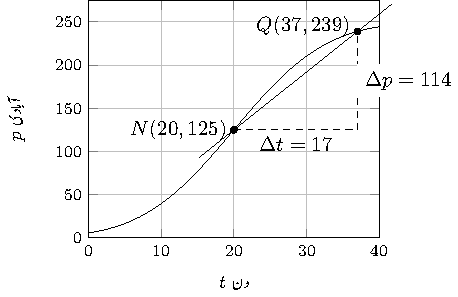
\includegraphics{normalDistributionFlies}
\caption{مکھی کی نمو آبادی}
\label{شکل_حد_مکھی_نمو_آبادی}
\end{minipage}\hfill
\begin{minipage}{0.45\textwidth}
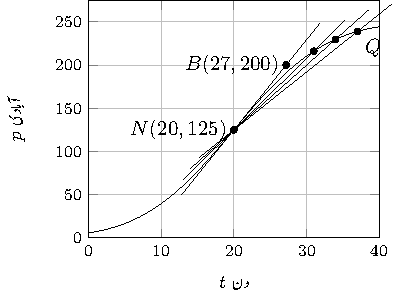
\includegraphics{normalDistributionFliesInstantaneous}
\caption{مکھی کی بیسویں دن نمو آبادی}
\label{شکل_حد_مکھی_نمو_آبادی_بیس}
\end{minipage}%
\end{figure}

حل:\quad
\عددی{20} ویں دن آبادی \عددی{125} تھی جبکہ \عددی{37} ویں دن آبادی \عددی{239} تھی۔ یوں \عددی{37-20=17} دنوں میں آبادی میں \عددی{239-125=114} تبدیل  رونما ہوئی۔یوں شرح تبدیلی درج ذیل ہو گی
\begin{align*}
\frac{\Delta p}{\Delta t}=\frac{114}{17}=6.7 (\text{\RL{مکھیاں فی دن}})
\end{align*}
جو شکل \حوالہ{شکل_حد_مکھی_نمو_آبادی} میں سیکنٹ \عددی{NQ} کی ڈھلوان ہے۔
\انتہا{مثال}
%========================

درج بالا مثال میں \عددی{20} ویں دن سے \عددی{37} ویں دن تک کی اوسط شرح تبدیلی حاصل کی گئی جو ہمیں \عددی{20} ویں دن کی تبدیلی کی شرح کے بارے میں کوئی معلومات فراہم نہیں کرتی ہے۔اس کے لئے ہمیں \عددی{20} ویں دن کے قریب حساب  کرنا ہو گا۔

\ابتدا{مثال}
مثال \حوالہ{مثال_حد_نمو_آبادی_مکھی} میں \عددی{20} ویں دن آبادی میں تبدیلی کی شرح کیا ہے؟\\
حل:\quad
ہمیں نقطہ \عددی{Q} کو نقطہ \عددی{N} کے قریب سے قریب تر کرتے ہوئے شرح حاصل کرنی ہو گی (شکل \حوالہ{شکل_حد_مکھی_نمو_آبادی_بیس})۔یوں درج ذیل حاصل ہوتا ہے۔
\begin{align*}
\begin{array}{ll}
Q&\frac{\Delta p}{\Delta t}\\
\hline
(37,239)&\frac{239-125}{37-20}=6.7\\
(35,230)&\frac{230-125}{35-20}=7\\
(32,216)&\frac{216-125}{32-20}=7.6\\
(27,200)&\frac{200-125}{27-20}=10.7
\end{array}
\end{align*}

جیسے جیسے \عددی{Q} کو بائیں منتقل کیا جائے، خط \عددی{NQ} نقطہ \عددی{N} کے گرد گھڑی کی الٹ رخ گھومتا ہے۔ہم دیکھتے ہیں کہ یہ خط آخر کار \عددی{NB} کو چھوتا ہے۔اس خط کو دیے گئے منحنی کا \اصطلاح{مماس}\فرہنگ{مماس}\حاشیہب{tangent}\فرہنگ{tangent} کہتے ہیں۔اس طرح ہم توقع کرتے ہیں کہ \عددی{20} ویں دن آبادی کی تبدیلی کی شرح \عددی{10.7} مکھیاں فی دن ہو گی۔
\انتہا{مثال}
%=======================

لمحہ \عددی{t=1} اور لمحہ \عددی{t=2} پر گرتے ہوئے پتھر کی رفتار یا \عددی{20} ویں دن شرح تبدیلی کو \اصطلاح{لمحاتی شرح تبدیلی}\فرہنگ{لمحاتی!شرح تبدیلی}\حاشیہب{instantaneous rates of change}\فرہنگ{instantaneous!rate of change} کہتے ہیں۔جیسا آپ نے دیکھا، ہم اوسط شرح تبدیلی کی تحدیدی قیمت سے لمحاتی شرح تبدیلی حاصل کرتے ہیں۔درج بالا مثال میں ہم نے خط مماس کو بطور خط سیکنٹ کی تحدیدی  صورت پیش کیا۔لمحاتی شرح اور مماس کا گہرا تعلق ہے جو دیگر موضوعات میں بھی پیش آتا ہے۔ اس تعلق کو مزید سمجھنے کی خاطر ہمیں  تحدیدی قیمتوں  کا تعین کرنا سیکھنا ہو گا جنہیں ہم \اصطلاح{حد}\فرہنگ{حد}\حاشیہب{limits}\فرہنگ{limits} کہتے ہیں۔ 

\جزوحصہء{تفاعل کی تحدیدی قیمتیں}
تحدیدی قیمت کی تعریف سے پہلی ایک اور مثال دیکھتے ہیں۔

\ابتدا{مثال}\شناخت{مثال_حد_عجیب_تفاعل_الف}
تفاعل \عددی{f(x)=\tfrac{x^2-1}{x-1}} نقطہ \عددی{x=1} کے قریب کیسا رویہ رکھتا ہے؟\\
حل:\quad
چونکہ صفر سے کسی بھی عدد کو تقسیم نہیں کیا جا سکتا ہے لہٰذا ماسوائے \عددی{x=1} کے، یہ کلیہ تمام حقیقی اعداد کے لئے \عددی{f} تعین کرتا ہے۔کسی بھی \عددی{x\ne 1} کے لئے ہم اس کلیہ کی سادہ صورت حاصل کر سکتے ہیں:
\begin{align*}
f(x)=\frac{x^2-1}{x-1}=\frac{(x-1)(x+1)}{x-1}=x+1\quad\quad (x\ne 1)
\end{align*} 
یوں خط \عددی{y=x+1} جس سے نقطہ \عددی{x=1} یعنی \عددی{(1,2)} خارج کیا گیا ہو اس تفاعل کو ظاہر کرتا ہے۔اس نقطہ کو شکل \حوالہ{شکل_مثال_حد_عجیب_تفاعل_الف} میں بطور سوراخ دکھایا گیا ہے۔اگرچہ نقطہ \عددی{f(1)} غیر معین ہے، ہم \عددی{ x} کی قیمت \عددی{1} کے قریب سے قریب لیتے ہوئے \عددی{f(x)} کی قیمت \عددی{2} کے جتنی قریب چاہیں کر سکتے ہیں۔
\begin{figure}
\centering
\begin{tikzpicture}
\draw[-latex](-1.5,0)--(3,0)node[right]{$x$};
\draw[-latex](0,-0.2)--(0,2.5)node[above]{$y$};
\draw[shorten <=-0.5cm,shorten >=-0.5cm](-1,0)--(1,2);
\foreach \x in {-1,1}{\draw(\x,0)node[below]{$\x$}--++(0,0.1);}
\foreach \y in {1,2}{\draw(0,\y)node[left]{$\y$}--++(0.1,0);}
\draw(1,2)node[ocirc]{};
\draw(0.5,1)node[right]{$y=f(x)=\tfrac{x^2-1}{x-1}$};
\end{tikzpicture}
\caption{شکل برائے مثال \حوالہ{مثال_حد_عجیب_تفاعل_الف}}
\label{شکل_مثال_حد_عجیب_تفاعل_الف}
\end{figure}
%
\begin{align*}
\begin{array}{ll}
\multicolumn{1}{c}{x (\ne 1)}&\multicolumn{1}{c}{f(x)=\tfrac{x^2-1}{x-1}=x+1,\,\, (x\ne 1)}\\
\hline
0.9&1.9\\
1.1&2.1\\
0.99&1.99\\
1.01&2.01\\
0.999&1.999\\
1.001&2.001\\
0.999999&1.999999\\
1.000001&2.000001
\end{array}
\end{align*}

ہم کہتے ہیں کہ \عددی{x} کی قیمت \عددی{1} تک پہنچنے سے \عددی{f(x)} کی قیمت \عددی{2} تک پہنچتی ہے یا \عددی{x} ایک تک پہنچنے سے \عددی{f(x)} تحدیدی قیمت \عددی{2} تک پہنچتی ہے یا حد \عددی{2} تک پہنچتی ہے، جس کو درج ذیل لکھا جاتا ہے۔
\begin{align*}
\lim_{x\to 1} f(x)=2 \quad \text{یا}\quad \lim_{x\to 1} \frac{x^2-1}{x-1}=2
\end{align*}
\عددی{x} کی قیمت \عددی{x_0} تک پہنچنے کو \عددی{x\to x_0} لکھا جاتا ہے۔
\انتہا{مثال}
%====================== 

\ابتدا{تعریف}\موٹا{حد کی غیر رسمی تعریف}\\
فرض کریں کہ \عددی{x_0} کی پڑوس میں ایک کھلے وقفہ پر تفاعل \عددی{f(x)} معین ہے۔یہ تفاعل نقطہ \عددی{x_0} پر غیر معین ہو سکتا ہے۔ اگر \عددی{x_0} کے کافی قریب \عددی{x} کی  تمام قیمتوں کے لئے \عددی{f(x)} کی قیمتیں \عددی{L} کے کافی قریب پائی جاتی ہوں تب ہم کہتے ہیں کہ \عددی{x} کی قیمت \عددی{x_0} تک پہنچنے سے \عددی{f} کی قیمت \اصطلاح{حد} \عددی{L} تک پہنچتی ہے۔ اس کو ہم درج ذیل لکھتے ہیں۔
\begin{align*}
\lim_{x\to x_0} f(x)=L
\end{align*}
\انتہا{تعریف}
%========================

اس تعریف کو غیر رسمی اس لئے کہا گیا ہے کہ "کافی قریب" کی طرز کے فقرے بہت ٹھیک نہیں ہیں۔خراد پر کام کرنے والے ماہر کے لئے کافی قریب سے مراد \عددی{\SI{10}{\micro\meter}} ہو سکتا ہے جبکہ ماہر فلکیات کے لئے اس کا مطلب چند ہزار نوری سال ہو سکتا ہے۔البتہ یہ تعریف اتنی درست ضرور ہے کہ ہم حد کو پہچان سکیں اور اس کی قیمت حاصل کر سکیں۔ہم حد کی بالکل ٹھیک تعریف جلد پیش کریں گے۔

\ابتدا{مثال}\شناخت{مثال_حد_عجیب_تفاعل_ب}
\عددی{x\to x_0} کی صورت میں \عددی{f} کی حد کی وجودیت \عددی{x_0} پر \عددی{f} کی تعریف کے تابع نہیں ہے۔ شکل \حوالہ{شکل_مثال_حد_عجیب_تفاعل_ب} میں  \عددی{f} کا \عددی{x\to 1} پر حد \عددی{2} ہے اگرچہ \عددی{x=1} پر \عددی{f} غیر معین ہے۔تفاعل \عددی{g} کا \عددی{x\to 1} پر حد \عددی{2} ہے اگرچہ \عددی{x=1} پر \عددی{g(1)=1} ہے۔یوں \عددی{\lim\limits_{x\to 1}g(x)\ne g(1)} ہو گا۔صرف تفاعل \عددی{h} کا \عددی{x\to 1} پر حد اور قیمت دونوں \عددی{2} کے برابر ہیں یعنی \عددی{\lim\limits_{x\to 1} h(x)=h(1)}۔
\begin{figure}
\centering
\begin{subfigure}{0.33\textwidth}
\centering
\begin{tikzpicture}[x=0.75cm]
\draw[-latex](-1.5,0)--(2,0)node[right]{$x$};
\draw[-latex](0,-0.2)--(0,2.5)node[above]{$y$};
\draw[shorten <=-0.5cm,shorten >=-0.5cm](-1,0)--(1,2);
\foreach \x in {-1,1}{\draw(\x,0)node[below]{$\x$}--++(0,0.1);}
\foreach \y in {1,2}{\draw(0,\y)node[left]{$\y$}--++(0.1,0);}
\draw(1,2)node[ocirc]{};
\draw(0,-1)node[font=\footnotesize]{$\begin{aligned}f(x)=\tfrac{x^2-1}{x-1}\end{aligned}$};
\end{tikzpicture}
\caption{}
\end{subfigure}%
\begin{subfigure}{0.33\textwidth}
\centering
\begin{tikzpicture}[x=0.75cm]
\draw[-latex](-1.5,0)--(2,0)node[right]{$x$};
\draw[-latex](0,-0.2)--(0,2.5)node[above]{$y$};
\draw[shorten <=-0.5cm,shorten >=-0.5cm](-1,0)--(1,2);
\foreach \x in {-1,1}{\draw(\x,0)node[below]{$\x$}--++(0,0.1);}
\foreach \y in {1,2}{\draw(0,\y)node[left]{$\y$}--++(0.1,0);}
\draw(1,2)node[ocirc]{};
\draw(1,1)node[circ]{};
\draw(0,-1)node[font=\footnotesize]{$\begin{aligned}g(x)=\begin{cases}\tfrac{x^2-1}{x-1},&x\ne 1\\ 1,&x=1\end{cases}\end{aligned}$};
\end{tikzpicture}
\caption{}
\end{subfigure}%
\begin{subfigure}{0.33\textwidth}
\centering
\begin{tikzpicture}[x=0.75cm]
\draw[-latex](-1.5,0)--(2,0)node[right]{$x$};
\draw[-latex](0,-0.2)--(0,2.5)node[above]{$y$};
\draw[shorten <=-0.5cm,shorten >=-0.5cm](-1,0)--(1,2);
\foreach \x in {-1,1}{\draw(\x,0)node[below]{$\x$}--++(0,0.1);}
\foreach \y in {1,2}{\draw(0,\y)node[left]{$\y$}--++(0.1,0);}
\draw(1,2)node[circ]{};
\draw(0,-1)node[font=\footnotesize]{$\begin{aligned}h(x)=x+1\end{aligned}$};
\end{tikzpicture}
\caption{}
\end{subfigure}%
\caption{$\lim\limits_{x\to 1} f(x)=\lim\limits_{x\to 1}g(x)=\lim\limits_{x\to 1} h(x)=2\quad $}
\label{شکل_مثال_حد_عجیب_تفاعل_ب}
\end{figure}
\انتہا{مثال}
%============================

بعض اوقات \عددی{\lim\limits_{x\to x_0}f(x)} کی قیمت \عددی{f(x_0)} سے حاصل کی جا سکتی ہے۔اس کی مثال تفاعل \عددی{f(x)} ہے جو کثیر رکنی اور تکونیاتی تفاعل کا الجبرائی مجموعہ  ہے اور جہاں \عددی{x_0} پر \عددی{f(x_0)} معین ہو۔

%===============================
\ابتدا{مثال}\شناخت{مثال_حد_عجیب_تفاعل_پ}
\begin{enumerate}[a.]
\item
$\lim\limits_{x\to 2} (4)=4$
\item
$\lim\limits_{x\to 13}(4)=4$
\item
$\lim\limits_{x\to 3} x=3$
\item
$\lim\limits_{x\to 2} (5x-3)=10-3=7$
\item
$\lim\limits_{x\to -2}\frac{3x+4}{x+5}=\frac{-6+4}{-2+5}=-\frac{2}{3}$
\end{enumerate}
\انتہا{مثال}
%================================
\ابتدا{مثال}\شناخت{مثال_حد_مماثل_تفاعل}
\begin{enumerate}[a.]
\item
اگر \عددی{f} مماثلی تفاعل \عددی{f(x)=x} ہو تب \عددی{x_0} کے کسی بھی قیمت کے لئے  درج ذیل ہو گا (شکل \حوالہ{شکل_مثال_حد_عجیب_تفاعل_پ}-ل)۔
\begin{align*}
\lim\limits_{x\to x_0} f(x)=\lim\limits_{x\to x_0} x=x_0
\end{align*}
\item
اگر \عددی{f} مستقل تفاعل \عددی{f(x)=k} ہو (جہاں \عددی{k} مستقل ہے) تب \عددی{x_0} کے کسی بھی قیمت کے لئے درج ذیل ہو گا (شکل \حوالہ{شکل_مثال_حد_عجیب_تفاعل_پ}-ب)۔
\begin{align*}
\lim\limits_{x\to x_0} f(x)=\lim\limits_{x\to x_0} k=k
\end{align*} 
\end{enumerate}
%
\begin{figure}
\centering
\begin{subfigure}{0.5\textwidth}
\centering
\begin{tikzpicture}
\draw[-latex](-0.25,0)--(3,0)node[right]{$x$};
\draw[-latex](0,-0.2)--(0,2)node[above]{$y$};
\draw[shorten <=-0.5cm](0,0)--(2,2)node[pos=1,left]{$y=x$};
\draw[dashed] (0,1)node[left]{$x_0$}--(1,1)--(1,0)node[below]{$x_0$};
\end{tikzpicture}
\caption{مماثل تفاعل}
\end{subfigure}%
\begin{subfigure}{0.5\textwidth}
\centering
\begin{tikzpicture}
\draw[-latex](-0.25,0)--(3,0)node[right]{$x$};
\draw[-latex](0,-0.2)--(0,2)node[above]{$y$};
\draw(-0.25,1)--(3,1)node[pos=0.9,above]{$y=k$};
\draw(0,1)node[circ]{}node[above left]{$k$};
\draw[dashed](1,0)node[below]{$x_0$}--(1,1)node[circ]{};
\draw(0,0)node[below left]{$M$};
\end{tikzpicture}
\caption{مستقل تفاعل}
\end{subfigure}%
\caption{اشکال برائے مثال \حوالہ{مثال_حد_عجیب_تفاعل_پ}}
\label{شکل_مثال_حد_عجیب_تفاعل_پ}
\end{figure}
\انتہا{مثال}
%==================================
\ابتدا{مثال}\شناخت{مثال_حد_عجیب_تفاعل_ت} \ترچھا{عین ممکن ہے کہ تفاعل کے دائرہ کار میں تفاعل کا حد نہ پایا جاتا ہو۔}\\ 
درج ذیل تفاعل کا \عددی{x\to 0} پر رویہ کیسا ہو گا؟
\begin{enumerate}[a.]
\item
$U(x)=\begin{cases}0,&x<0\\ 1,&x\ge 0  \end{cases}$
\item
$g(x)=\begin{cases} \tfrac{1}{x},&x\ne 0\\ 0,&x=0 \end{cases}$
\item
$f(x)=\begin{cases}0,&x\le 0\\ \sin \tfrac{1}{x},&x>0  \end{cases}$
\end{enumerate}
%

حل:\quad
\begin{enumerate}[a.]
\item
اکائی سیڑھی تفاعل \عددی{U(x)} کا \عددی{x\to 0} پر کوئی حد نہیں پایا جاتا ہے چونکہ اس نقطہ پر تفاعل کی چھلانگ پائی جاتی ہے۔\عددی{0} کے کافی قریب \عددی{x} کی منفی قیمتوں کے لئے \عددی{U} کی قیمت \عددی{0} ہے جبکہ \عددی{0} کے کافی  قریب  \عددی{x}  کی مثبت قیمتوں کے لئے \عددی{U} کی قیمت \عددی{1} ہے۔یوں \عددی{0} کے قریب پہنچنے سے \عددی{U} کی منفرد قیمت نہیں پائی جاتی ہے (شکل \حوالہ{شکل_مثال_حد_عجیب_تفاعل_ت}-ا)۔
\item
\عددی{x=0} کے کافی قریب تفاعل کی قیمت بے قابو بڑھتی ہے اور کسی ایک منفرد قیمت تک پہنچنے کی کوشش نہیں کرتی ہے (شکل \حوالہ{شکل_مثال_حد_عجیب_تفاعل_ت}-ب)۔
\item
\عددی{x=0} کے کافی قریب تفاعل بہت زیادہ ارتعاش کرتا ہے۔اس کی قیمت کسی مخصوص قیمت تک پہنچنے کی کوشش نہیں کرتی ہے (شکل \حوالہ{شکل_مثال_حد_عجیب_تفاعل_ت}-ج)۔ 
\end{enumerate}
%
\begin{figure}
\centering
\begin{subfigure}{0.33\textwidth}
\centering
\begin{tikzpicture}
\begin{axis}[clip=false,small,axis lines=middle,width=4cm,xtick={\empty},ytick={1},xlabel={$x$},ylabel={$y$},xlabel style={at={(current axis.right of origin)},anchor={west}},ylabel style={at={(current axis.above origin)},anchor=south},ymin=-0.5,ymax=2]
\addplot[domain=-2:0]{0};
\addplot[domain=0:2]{1};
\draw(axis cs:0,0)node[ocirc]{};
\draw(axis cs:0,1)node[circ]{};
\draw(axis cs:0,1)node[above right,font=\footnotesize]{$\begin{aligned}y=\begin{cases}0,&x<0\\ 1,&x\ge 1\end{cases}\end{aligned}$};
\end{axis}
\end{tikzpicture}
\caption{اکائی سیڑھی تفاعل $U(x)\,\,$}
\end{subfigure}%
\begin{subfigure}{0.33\textwidth}
\centering
\begin{tikzpicture}
\begin{axis}[clip=false,small,axis lines=middle,width=4cm,xtick={\empty},ytick={\empty},xlabel={$x$},ylabel={$y$},xlabel style={at={(current axis.right of origin)},anchor={west}},ylabel style={at={(current axis.above origin)},anchor=south}]
\addplot[domain=-4:-0.3]{1/x};
\addplot[domain=0.3:4]{1/x};
\draw(axis cs:0,0)node[circ]{}node[below right]{$0$};
\draw(axis cs:0.4,1)node[above right,font=\footnotesize]{$\begin{aligned}y=\begin{cases}\tfrac{1}{x},&x\ne 0\\ 0,&x=0\end{cases}\end{aligned}$};
\end{axis}
\end{tikzpicture}
\caption{$g(x)$}
\end{subfigure}%
\begin{subfigure}{0.33\textwidth}
\centering
\begin{tikzpicture}
\begin{axis}[clip=false,small,axis lines=middle,width=4cm,xtick={\empty},ytick={-1,1},xlabel={$x$},ylabel={$y$},xlabel style={at={(current axis.right of origin)},anchor={west}},ylabel style={at={(current axis.above origin)},anchor=south},ymin=-1.2,ymax=1.2]
\addplot[domain=-0.2:0]{0}node[circ]{};
\addplot[domain=0.052:0.08,samples=100]{sin(180/(pi*x)};
\addplot[domain=0.08:0.5,samples=100]{sin(180/(pi*x)};
\draw(axis cs:0,0)node[circ]{}node[below left]{$0$};
\draw(axis cs:0.2,-0.75)node[right,font=\footnotesize]{$\begin{aligned}y=\begin{cases}0 ,&x\le  0\\  \sin \tfrac{1}{x},&x>0\end{cases}\end{aligned}$};
\end{axis}
\end{tikzpicture}
\caption{$f(x)$}
\end{subfigure}%
\caption{اشکال برائے مثال \حوالہ{مثال_حد_عجیب_تفاعل_ت}}
\label{شکل_مثال_حد_عجیب_تفاعل_ت}
\end{figure}
\انتہا{مثال}
%=================================

\حصہء{سوالات \حوالہ{حصہ_حد_تبدیلی_کی_شرح_اور_حد}}

\موٹا{ترسیم سے حد}

\ابتدا{سوال}\شناخت{سوال_حد_ترسیم_سے_حد_الف}
شکل \حوالہ{شکل_سوال_حد_ترسیم_سے_حد_الف}-ا میں دی گئی ترسیم سے درج ذیل حد تلاش کریں یا حد نا ہونے کی وجہ بیان کریں۔
\begin{multicols}{3}
\begin{enumerate}[a.]
\item
$\lim\limits_{x\to 1} g(x)$
\item
$\lim\limits_{x\to 2} g(x)$
\item
$\lim\limits_{x\to 3}g(x)$
\end{enumerate}
\end{multicols}
%
\begin{figure}
\centering
\begin{subfigure}{0.5\textwidth}
\centering
\begin{tikzpicture}
\draw[-latex](-0.25,0)--(4,0)node[right]{$x$};
\draw[-latex](0,-0.2)--(0,1.5)node[above]{$y$};
\draw[dashed](0,1)node[left]{$1$}--(3,1)node[solid,circ]{};
\draw(-0.2,-0.2)--(1,1)node[ocirc]{};
\draw(1,0)node[circ]{}--(2,1)node[circ]{}node[above,yshift={2mm}]{$y=g(x)$}--(3,0)node[ocirc]{}--(3.9,0.9);
\foreach \x in {1,2,3}{\draw(\x,0)node[below]{$\x$}--++(0,0.1);}
\end{tikzpicture}
\caption{}
\end{subfigure}%
\begin{subfigure}{0.5\textwidth}
\centering
\begin{tikzpicture}
\draw[-latex](-3,0)--(2,0)node[right]{$t$};
\draw[-latex](0,-1.25)--(0,1.5)node[above]{$s$};
\draw(-3,-1)--(-2,0)node[ocirc]{}node[above,yshift={2mm}]{$s=f(t)$}--(-1,-1)node[circ]{}--(0,-1)node[ocirc]{}node[right]{$-1$};
\foreach \x in {-2,-1,1}{\draw(\x,0)node[below]{$\x$}--++(0,0.1);}
\draw(0,0)node[circ]{}node[below left]{$0$};
\draw(0,1)node[ocirc]{}node[left]{$1$}--(2,1);
\end{tikzpicture}
\caption{}
\end{subfigure}%
\caption{اشکال برائے سوال \حوالہ{سوال_حد_ترسیم_سے_حد_الف} اور سوال \حوالہ{سوال_حد_ترسیم_سے_حد_ب}}
\label{شکل_سوال_حد_ترسیم_سے_حد_الف}
\end{figure}
\انتہا{سوال}
%=====================
\ابتدا{سوال}\شناخت{سوال_حد_ترسیم_سے_حد_ب}
شکل \حوالہ{شکل_سوال_حد_ترسیم_سے_حد_الف}-ب میں دی گئی ترسیم سے درج ذیل حد تلاش کریں یا حد نا ہونے کی وجہ بیان کریں۔
\begin{multicols}{3}
\begin{enumerate}[a.]
\item
$\lim\limits_{t\to -2}f(t)$
\item
$\lim\limits_{t\to -1}f(t)$
\item
$\lim\limits_{t\to 0}f(t)$
\end{enumerate}
\end{multicols}
\انتہا{سوال}
%======================
\ابتدا{سوال}\شناخت{سوال_حد_ترسیم_سے_حد_پ}
تفاعل \عددی{y=f(x)}  (شکل \حوالہ{سوال_حد_ترسیم_سے_حد_پ}-ا) کے لئے درج ذیل فقروں میں سے کون سے درست ہیں؟
\begin{multicols}{3}
\begin{enumerate}[a.]
\item
$\lim\limits_{x\to 0}f(x)$ موجود ہے\\
\item
$\lim\limits_{x\to 0}f(x)=0$
\item
$\lim\limits_{x\to 0}f(x)=1$
\item
$\lim\limits_{x\to 1}f(x)=1$
\item
$\lim\limits_{x\to 1}f(x)=0$
\item
$\lim\limits_{x\to x_ 0}f(x)$
وقفہ \عددی{(-1,1)} میں ہر نقطہ \عددی{x_0} پر موجود ہے
\end{enumerate}
\end{multicols}
%
\begin{figure}
\centering
\begin{subfigure}{0.5\textwidth}
\centering
\begin{tikzpicture}
\draw[-latex](-1.2,0)--(3,0)node[right]{$x$};
\draw[-latex](0,-1.2)--(0,1.5)node[above]{$y$};
\draw(-1,-1)node[circ]{}--(0,0)node[ocirc]{}--(1,-1)node[ocirc]{} (1,0)node[circ]{}--(2,1)node[circ]{};
\draw(0,1)node[circ]{}node[left]{$1$}--++(0.1,0);
\foreach \x in {-1,1,2}{\draw(\x,0)node[below]{$\x$}--++(0,0.1);} 
\draw(0,-1)node[left]{$-1$}--++(0.1,0);
\draw(0.5,1.25)node[right]{$y=f(x)$};
\end{tikzpicture}
\caption{}
\end{subfigure}%
\begin{subfigure}{0.5\textwidth}
\centering
\begin{tikzpicture}[]
\draw[-latex](-1.2,0)--(3.5,0)node[right]{$x$};
\draw[-latex](0,-2.2)--(0,1.5)node[above]{$y$};
\foreach \x in {-1,1,2,3}{\draw(\x,0)node[below]{$\x$}--++(0,0.1);} 
\foreach \y in {-2,-1,1}{\draw(0,\y)node[left]{$\y$}--++(0.1,0);}
\draw(-1,-1)node[circ]{}--(0,0)node[circ]{};
\draw[domain=0:1] plot ({\x},{-2*\x*\x});
\draw([shift={(0:1)}]2,0) arc (0:180:1);
\draw(1,0)node[circ]{} (2,0)node[circ]{} (3,0)node[circ]{} (2,1)node[ocirc]{}node[above]{$y=f(x)$};
\end{tikzpicture}
\caption{}
\end{subfigure}%
\caption{اشکال برائے سوال \حوالہ{سوال_حد_ترسیم_سے_حد_پ} اور سوال \حوالہ{سوال_حد_ترسیم_سے_حد_ت}}
\label{شکل_سوال_حد_ترسیم_سے_حد_پ}
\end{figure}
\انتہا{سوال}
%============================
\ابتدا{سوال}\شناخت{سوال_حد_ترسیم_سے_حد_ت}
تفاعل \عددی{y=f(x)} (شکل \حوالہ{سوال_حد_ترسیم_سے_حد_پ}-ب)  کے لئے درج ذیل فقروں میں سے کون سے درست ہیں؟
\begin{multicols}{3}
\begin{enumerate}[a.]
\item
$\lim\limits_{x\to 2} f(x)$
موجود نہیں ہے
\item
$\lim\limits_{x\to 2}f(x)=2$
\item
$\lim\limits_{x\to 1}f(x)$
موجود نہیں ہے
\item
$\lim\limits_{x\to x_0}f(x)$
وقفہ \عددی{(-1,1)} میں ہر نقطہ \عددی{x_0} پر موجود ہے۔
\item
$\lim\limits_{x\to x_0}f(x)$
وقفہ \عددی{(1,3)} میں ہر نقطہ \عددی{x_0} پر موجود ہے۔
\end{enumerate}
\end{multicols}
\انتہا{سوال}
%======================

\موٹا{وجودیت اور حد}

سوال \حوالہ{سوال_حد_غیر_موجود_الف} اور سوال \حوالہ{سوال_حد_غیر_موجود_ب} میں حد کی غیر موجودگی کی وجہ بیان کریں۔

\ابتدا{سوال}\شناخت{سوال_حد_غیر_موجود_الف}
$\lim\limits_{x \to 0}\tfrac{x}{\abs{x}}$
\انتہا{سوال}
%======================
\ابتدا{سوال}\شناخت{سوال_حد_غیر_موجود_ب}
$\lim\limits_{x \to 1}\tfrac{1}{x-1}$
\انتہا{سوال}
%======================
\ابتدا{سوال}
فرض کریں کہ ماسوائے نقطہ \عددی{x=x_0} تفاعل \عددی{f(x)} تمام حقیقی \عددی{x} کے لئے معین ہے۔کیا \عددی{\lim\limits_{x\to x_0}f(x)} کی وجودیت کی وجودیت کے بارے میں کچھ کہنا ممکن ہے؟ اپنے جواب کی وجہ بیان کریں۔ 
\انتہا{سوال}
%======================
\ابتدا{سوال}
فرض کریں کہ  تفاعل \عددی{f(x)} وقفہ \عددی{[-1,1]} میں تمام  \عددی{x} کے لئے معین ہے۔کیا \عددی{\lim\limits_{x\to 0}f(x)} کے بارے میں کچھ کہنا ممکن ہے؟ اپنے جواب کی وجہ بیان کریں۔ 
\انتہا{سوال}
%======================
\ابتدا{سوال}
اگر \عددی{\lim\limits_{x\to 1}f(x)=5} ہو تب کیا \عددی{x=1} پر \عددی{f} کا معین ہونا لازم ہے؟اگر معین ہونا لازم ہو تب کیا \عددی{f(1)=5} ہونا لازم ہے؟ کیا \عددی{x=1} پر ہم \عددی{f} کی قیمت کے بارے میں کچھ کہہ سکتے ہیں؟ وضاحت کریں۔
\انتہا{سوال}
%======================
\ابتدا{سوال}
اگر \عددی{f(1)=5} ہو تب کیا \عددی{\lim\limits_{x\to 1}f(x)} لازماً موجود ہو گا؟ اگر ایسا ہو تب کیا \عددی{\lim\limits_{x\to 1}f(x)=5} لازماً ہو گا؟ کیا ہم  \عددی{\lim\limits_{x\to 1}f(x)} کے بارے میں کوئی نتیجہ اخذ کر سکتے ہیں؟ وضاحت کریں۔
\انتہا{سوال}
%======================

\موٹا{کیلکولیٹر اور کمپیوٹر کا استعمال}

\ابتدا{سوال}
\عددی{f(x)=\tfrac{x^2-9}{x+3}} لیں۔
\begin{enumerate}[a.]
\item
\عددی{f} کی قیمتوں کا جدول نقاط \عددی{x=-3.1,-3.01,-3.001,\cdots} پر وہاں تک تلاش کریں جہاں تک آپ کا کیلکولیٹر جواب حاصل کر سکتا ہو۔اس جدول سے \عددی{\lim\limits_{x\to -3}f(x)} کی اندازاً قیمت حاصل کریں۔اس کے برعکس نقاط \عددی{x=-2.9,-2.99,\cdots} پر \عددی{f} کی قیمتیں استعمال کرتے ہوئے نتیجہ کیا ہو گا؟
\item
تفاعل کو \عددی{x_0=-3} کے قریب ترسیم کریں۔ ترسیم پر \عددی{x\to -3} کے لئے \عددی{y} کی قیمت دیکھ کر  گزشتہ جزو کے نتائج کی تصدیق کریں۔ 
\item
\عددی{\lim\limits_{x\to -3}f(x)} کو الجبرائی طریقہ سے اخذ کریں۔
\end{enumerate}
\انتہا{سوال}
%=========================
\ابتدا{سوال}
\عددی{g(x)=\tfrac{x^2-2}{x-\sqrt{2}}} لیں۔
\begin{enumerate}[a.]
\item
\عددی{\sqrt{2}} کی تخمینی قیمتوں \عددی{x=1.4,1.41,1.414,\cdots} پر تفاعل کی قیمتوں کے جدول سے \عددی{\lim\limits_{x\to \sqrt{2}}g(x)}  کی اندازاً قیمت حاصل کریں۔
\item
نقطہ \عددی{x_0=\sqrt{2}} کے قریب تفاعل ترسیم کریں۔\عددی{x\to \sqrt{2}} کے لئے ترسیم سے \عددی{y} کی قیمت دیکھ کر گزشتہ جزو کی جواب کا تصدیق کریں۔
\item
\عددی{\lim\limits_{x\to\sqrt{2}}g(x)} کو الجبرائی طور پر حاصل کریں۔
\end{enumerate}
\انتہا{سوال}
%====================
\ابتدا{سوال}
\عددی{G(x)=\tfrac{x+6}{x^2+4x-12}} لیں۔
\begin{enumerate}[a.]
\item
نقاط \عددی{x=-5.9,-5.99,-5.999,\cdots} پر \عددی{G} کی قیمتوں کا جدول بنا کر \عددی{\lim\limits_{x\to -6}G(x)} کی اندازاً قیمت حاصل کریں۔ اس کے برعکس \عددی{x=-6.1,-6.01,-6.001,\cdots} پر \عددی{G} کی قیمتیں استعمال کرتے ہوئے کیا نتیجہ حاصل ہو گا؟
\item
\عددی{G} کو \عددی{x_0=6} کے قریبی نقطوں پر تقسیم کرتے ہوئے \عددی{x\to -6} کے لئے \عددی{G} کی قیمت دیکھ کر گزشتہ جزو کے نتائج کی تصدیق کریں۔
\item
\عددی{\lim\limits_{x\to -6}G(x)} کو الجبرائی طریقہ سے حاصل کریں۔
\end{enumerate}
\انتہا{سوال}
%======================
\ابتدا{سوال}
\عددی{h(x)=\tfrac{x^2-2x-3}{x^2-4x+3}} لیں۔
\begin{enumerate}[a.]
\item
نقاط \عددی{x=2.9, 2.99, 2.999,\cdots} پر \عددی{h} کی قیمتوں کے جدول سے \عددی{\lim\limits_{x\to 3}h(x)} کی اندازاً قیمت تلاش کریں۔اس کے برعکس \عددی{x=3.1,3.01,3.001,\cdots} پر \عددی{h} کی قیمتیں لیتے ہوئے نتیجہ کیا ہو گا؟
\item
\عددی{x_0=3} کے قریب \عددی{h} ترسیم کر کے \عددی{x\to 3} کے لئے \عددی{h(x)} کی قیمت دیکھ کر گزشتہ جزو کے نتائج کی تصدیق کریں۔
\item
\عددی{\lim\limits_{x\to 3}h(x)} کو الجبرائی طریقہ سے حاصل کریں۔
\end{enumerate}
\انتہا{سوال}
%=====================
\ابتدا{سوال}
\عددی{f(x)=\tfrac{x^2-1}{\abs{x}-1}} لیں۔
\begin{enumerate}[a.]
\item
\عددی{f} کی قیمتوں کا جدول \عددی{x} کی ان قیمتوں کے لئے بنائیں جو \عددی{x_0=-1} تک نیچے سے اور اوپر سے پہنچنے کی کوشش کرتی ہیں۔اس جدول سے \عددی{\lim\limits_{x\to-1}f(x)} کی اندازاً قیمت تلاش کریں۔  
\item
\عددی{x_0=-1} کے قریب \عددی{f} ترسیم کریں۔ترسیم سے \عددی{x\to -1} کے لئے \عددی{y} کی قیمتیں دیکھ کر گزشتہ جزو کے نتائج کی تصدیق کریں۔
\item
\عددی{\lim\limits_{x\to -1}f(x)} کو الجبرائی طریقہ سے حاصل کریں۔
\end{enumerate}
\انتہا{سوال}
%========================
\ابتدا{سوال}
\عددی{F(x)=\tfrac{x^2+3x+2}{2-\abs{x}}} لیں۔
\begin{enumerate}[a.]
\item
\عددی{F} کی قیمتوں کا جدول \عددی{x} کی ان قیمتوں کے لئے بنائیں جو \عددی{x_0=-2} تک نیچے سے اور اوپر سے پہنچنے کی کوشش کرتی ہیں۔اس جدول سے
 \عددی{\lim\limits_{x\to-2}F(x)} کی اندازاً قیمت تلاش کریں۔  
\item
\عددی{x_0=-2} کے قریب \عددی{F} ترسیم کریں۔ترسیم سے \عددی{x\to -2} کے لئے \عددی{y} کی قیمتیں دیکھ کر گزشتہ جزو کے نتائج کی تصدیق کریں۔
\item
\عددی{\lim\limits_{x\to -2}F(x)} کو الجبرائی طریقہ سے حاصل کریں۔
\end{enumerate}
\انتہا{سوال}
%========================
\ابتدا{سوال}
\عددی{g(\theta)=\tfrac{\sin\theta}{\theta}} لیں۔
\begin{enumerate}[a.]
\item
\عددی{g} کی قیمتوں کا جدول \عددی{\theta} کی ان قیمتوں کے لئے بنائیں جو \عددی{\theta_0=0} تک نیچے سے اور اوپر سے پہنچنے کی کوشش کرتی ہیں۔اس جدول سے
 \عددی{\lim\limits_{x\to 0}g(\theta)} کی اندازاً قیمت تلاش کریں۔  
\item
\عددی{\theta_0=0} کے قریب \عددی{g} ترسیم کریں۔ترسیم سے گزشتہ جزو کے نتائج کی تصدیق کریں۔
\end{enumerate}
\انتہا{سوال}
%========================
\ابتدا{سوال}
\عددی{G(t)=\tfrac{1-\cos t}{t^2}} لیں۔
\begin{enumerate}[a.]
\item
\عددی{G} کی قیمتوں کا جدول \عددی{t} کی ان قیمتوں کے لئے بنائیں جو \عددی{t_0=0} تک نیچے سے اور اوپر سے پہنچنے کی کوشش کرتی ہیں۔اس جدول سے
 \عددی{\lim\limits_{t\to 0}G(t)} کی اندازاً قیمت تلاش کریں۔  
\item
\عددی{t_0=0} کے قریب \عددی{G} ترسیم کریں۔ترسیم سے گزشتہ جزو کے نتائج کی تصدیق کریں۔
\end{enumerate}
\انتہا{سوال}
%===================
\ابتدا{سوال}
\عددی{f(x)=x^{\tfrac{1}{1-x}}} لیں۔
\begin{enumerate}[a.]
\item
\عددی{f} کی قیمتوں کا جدول \عددی{x} کی ان قیمتوں کے لئے بنائیں جو \عددی{x_0=1} تک نیچے سے اور اوپر سے پہنچنے کی کوشش کرتی ہیں۔کیا \عددی{x} کی قیمت \عددی{x\to 1} تک پہنچنے سے \عددی{f} کا تحدیدی نقطہ پایا جاتا ہے؟ اگر تحدیدی نقطہ پایا جاتا ہو، اس کا تلاش کریں۔اگر نہیں پایا جاتا ہو تب وجہ بیان کریں۔
\item
\عددی{x_0=1} کے قریب \عددی{f} ترسیم کریں۔ترسیم سے گزشتہ جزو کے نتائج کی تصدیق کریں۔
\end{enumerate}
\انتہا{سوال}
%=============================
\ابتدا{سوال}
\عددی{f(x)=\tfrac{3^x-1}{x}} لیں۔
\begin{enumerate}[a.]
\item
\عددی{f} کی قیمتوں کا جدول \عددی{x} کی ان قیمتوں کے لئے بنائیں جو \عددی{x_0=0} تک نیچے سے اور اوپر سے پہنچنے کی کوشش کرتی ہیں۔کیا
 \عددی{x} کی قیمت \عددی{x\to 0} تک پہنچنے سے \عددی{f} کا تحدیدی نقطہ پایا جاتا ہے؟ اگر تحدیدی نقطہ پایا جاتا ہو، اس کا تلاش کریں۔اگر نہیں پایا جاتا ہو تب وجہ بیان کریں۔
\item
\عددی{x_0=0} کے قریب \عددی{f} ترسیم کریں۔ترسیم سے گزشتہ جزو کے نتائج کی تصدیق کریں۔
\end{enumerate}
\انتہا{سوال}
%=============================
\موٹا{متغیر کی تحدیدی قیمت پر کرتے ہوئے حد کا تعین}

سوال \حوالہ{سوال_حد_پر_الف} تا سوال \حوالہ{سوال_حد_پر_ب} میں متغیر \عددی{x} کی تحدیدی قیمت کو تفاعل میں پر کرتے ہوئے تفاعل کی حد تلاش کریں۔

\ابتدا{سوال}\شناخت{سوال_حد_پر_الف}
$\lim\limits_{x\to 2} 2x$
\انتہا{سوال}
%========================
\ابتدا{سوال}
$\lim\limits_{x\to 0} 2x$
\انتہا{سوال}
%========================
\ابتدا{سوال}
$\lim\limits_{x\to \tfrac{1}{3}} (3x-1)$
\انتہا{سوال}
%========================
\ابتدا{سوال}
$\lim\limits_{x\to 1} -\tfrac{1}{3x-1}$
\انتہا{سوال}
%========================
\ابتدا{سوال}
$\lim\limits_{x\to -1} 3x(2x-1)$
\انتہا{سوال}
%========================
\ابتدا{سوال}
$\lim\limits_{x\to -1} \tfrac{3x^2}{2x-1}$
\انتہا{سوال}
%========================
\ابتدا{سوال}
$\lim\limits_{x\to \tfrac{\pi}{2}} x\sin x$
\انتہا{سوال}
%========================
\ابتدا{سوال}\شناخت{سوال_حد_پر_ب}
$\lim\limits_{x\to \pi} \tfrac{\cos x}{1-\pi}$
\انتہا{سوال}
%========================

\موٹا{اوسط شرح تبدیلی}

سوال \حوالہ{سوال_حد_اوسط_تبدیلی_شرح_الف} تا سوال \حوالہ{سوال_حد_اوسط_تبدیلی_شرح_ب} میں دیے وقفہ پر تفاعل کی اوسط شرح تبدیلی تلاش کریں۔

\ابتدا{سوال}\شناخت{سوال_حد_اوسط_تبدیلی_شرح_الف}
\عددی{f(x)=x^3+1}؛ (الف) \عددی{[2,3]}، (ب) \عددی{[-1,1]}
\انتہا{سوال}
%======================
\ابتدا{سوال}
\عددی{g(x)=x^2}؛ (الف) \عددی{[-1,1]}، (ب) \عددی{[-2,0]}
\انتہا{سوال}
%======================
\ابتدا{سوال}
\عددی{h(t)=\cos t}؛ (الف) \عددی{[\tfrac{\pi}{4},\tfrac{3\pi}{4}]}، (ب) \عددی{[\tfrac{\pi}{6},\tfrac{\pi}{2}]}
\انتہا{سوال}
%======================
\ابتدا{سوال}
\عددی{g(t)=2+\cos t}؛ (الف) \عددی{[0,\pi]}، (ب) \عددی{[-\pi,\pi]}
\انتہا{سوال}
%======================
\ابتدا{سوال}
\عددی{R(\theta)=\sqrt{4\theta+1}}؛  \عددی{[0,2]}
\انتہا{سوال}
%======================
\ابتدا{سوال}\شناخت{سوال_حد_اوسط_تبدیلی_شرح_ب}
\عددی{P(\theta)=\theta^3-4\theta^2+5\theta}؛  \عددی{[1,2]}
\انتہا{سوال}
%======================
\ابتدا{سوال}\شناخت{سوال_حد_چاند_الف}
چاند پر ساکن حالت سے گرنے والی چیز کا فاصلہ بالمقابل وقت ترسیم شکل \حوالہ{شکل_سوال_حد_چاند_الف} میں دکھایا گیا ہے۔ (الف) سیکنٹ \عددی{NQ_1}، \عددی{NQ_2}، \نقطے \عددی{NQ_6} کی اندازاً ڈھلوان تلاش کر کے جدول میں لکھیں۔ (ب) اس جدول سے \عددی{t=\SI{10}{\second}} پر رفتار کی اندازاً قیمت حاصل کریں۔
\begin{figure}
\centering
\begin{tikzpicture}
\begin{axis}[clip=false,small,axis lines=middle,grid=both,xlabel={ (سیکنڈ)$t$},ylabel={(میٹر)$y$}]
\addplot[domain=0:10]{1/2*1.6*x^2}node[circ]{}node[right]{$N$};
\draw(axis cs:5,20)node[circ]{}node[right]{$Q_1$};
\draw(axis cs:6,28.8)node[circ]{}node[right]{$Q_2$};
\draw(axis cs:7.07,40)node[circ]{}node[right]{$Q_3$};
\draw(axis cs:8,51.2)node[circ]{}node[right]{$Q_4$};
\draw(axis cs:8.66,60)node[circ]{}node[right]{$Q_5$};
\draw(axis cs:9.35,70)node[circ]{}node[right]{$Q_6$};
\end{axis}
\end{tikzpicture}
\caption{چاند پر ساکن حالت سے گرنے والی چیز کا فاصلہ بالمقابل وقت ترسیم}
\label{شکل_سوال_حد_چاند_الف}
\end{figure}
\انتہا{سوال}
%==================
\ابتدا{سوال}
ایک چھوٹی کمپنی کے پہلے چار سال کا منافع درج ذیل ہے۔(الف) منافع بالمقابل سال کو بطور نقطے ترسیم کرتے ہوئے انہیں ہموار ترین لکیر سے ملائیں۔ (ب)  \عددی{1992} اور \عددی{1994} کے بیچ منافع بڑھنے کی اوسط شرح تلاش کریں۔ (پ) ترسیم استعمال کرتے ہوئے \عددی{1992} کے دوران منافع بڑھنے کی شرح تلاش کریں۔
\begin{align*}
\begin{array}{rr}
\multicolumn{1}{c}{\text{سال}}&\multicolumn{1}{c}{\text{\RL{منافع (لاکھ)}}}\\
\hline
1990&6\\
1991&27\\
1992&62\\
1993&111\\
1994&174
\end{array}
\end{align*}
\انتہا{سوال}
%==========================
\ابتدا{سوال}
تفاعل \عددی{F(x)=\tfrac{x+2}{x-2}} کی قیمتیں نقطہ \عددی{x=2}، \عددی{\tfrac{11}{10}}، \عددی{\tfrac{101}{100}}، \عددی{\tfrac{1001}{1000}}، \عددی{\tfrac{10001}{10000}} اور \عددی{x=1} پر  حاصل کر کے جدول میں لکھیں۔(الف) جدول میں پائے جانے والے ہر \عددی{x\ne 1} کے لئے وقفہ \عددی{[1,x]} پر تفاعل کی اوسط شرح تبدیلی حاصل کریں۔ (ب) \عددی{x=1} پر \عددی{F(x)} کی شرح تبدیلی تلاش کریں۔اگر جدول بڑھانے کی ضرورت ہو تو جدول بڑھائیں۔ 
\انتہا{سوال}
%===========================
\ابتدا{سوال}
\عددی{x\ge 0} کے لئے \عددی{g(x)=\sqrt{x}} لیں۔
\begin{enumerate}[a.]
\item
وقفہ \عددی{[1,2]}، \عددی{[1,1.5]} اور \عددی{[1,1+h]} پر \عددی{x} کے  لحاظ سے \عددی{g(x)} کی اوسط شرح تبدیلی تلاش کریں۔
\item
صفر کے قریب \عددی{h} کی قیمتوں، مثلاً \عددی{h=0.1,0.01,0.001,0.0001,0.00001} کے لئے \عددی{x} کے لحاظ سے وقفہ \عددی{[1,1+h]} پر \عددی{g(x)} کی اوسط شرح تبدیلی تلاش کریں۔
\item
جدول سے \عددی{x=1} پر \عددی{g(x)} کی تبدیلی کی شرح کیا ہے؟
\item
\عددی{h\to 0} کے لئے \عددی{g(x)} کی تبدیلی کی شرح الجبرائی طریقہ سے حاصل کریں۔
\end{enumerate}
\انتہا{سوال}
%======================
\ابتدا{سوال}
\عددی{t\ne 0} کے لئے \عددی{f(t)=\tfrac{1}{t}} لیں۔
\begin{enumerate}[a.]
\item
(الف) وقفہ \عددی{t=2} تا \عددی{t=3} اور  (ب) وقفہ \عددی{t=2} تا \عددی{t=T} پر \عددی{t} کے لحاظ سے \عددی{g(t)} کی اوسط شرح تبدیلی تلاش کریں۔ 
\item
\عددی{2} تک پہنچنے والی \عددی{T} کی قیمتوں، مثلاً \عددی{T=2.1}، \عددی{T=2.01}، \عددی{T=2.001}، \عددی{T=2.0001}، \عددی{T=2.00001} اور \عددی{T=2.000001}، کے لئے وقفہ \عددی{[2,T]} پر \عددی{t} کے لحاظ سے \عددی{f(t)} کی اوسط شرح تبدیلی تلاش کر کر جدول میں لکھیں۔
\item
اس جدول سے \عددی{t=2} پر \عددی{t} کے لحاظ سے \عددی{f} کی شرح تبدیلی کیا ہے۔
\item
وقفہ \عددی{[2,T]} پر \عددی{t} کے لحاظ سے \عددی{f} کی شرح تبدیلی کی حد \عددی{T\to 2} کے لئے  تلاش کریں۔(\عددی{T=2} پر کرنے سے پہلے آپ کو کچھ الجبرا کرنا ہو گا۔)
\end{enumerate}
\انتہا{سوال}
%======================
سوال \حوالہ{سوال_حد_الجبرا_الف} تا سوال \حوالہ{سوال_حد_الجبرا_ب} کو کمپیوٹر کی مدد سے حل کریں۔(الف) نقطہ \عددی{x_0} کے قریب تفاعل ترسیم کریں۔ (ب) ترسیم کو دیکھ کر تفاعل کی حد کی اندازاً قیمت تلاش کریں۔ (پ) حد کو الجبرائی طور پر حاصل کریں۔

\ابتدا{سوال}\شناخت{سوال_حد_الجبرا_الف}
$\lim\limits_{x\to 2} \tfrac{x^4-16}{x-2}$
\انتہا{سوال}
%=========================
\ابتدا{سوال}
$\lim\limits_{x\to -1} \tfrac{x^3-x^2-5x-3}{(x+1)^2}$
\انتہا{سوال}
%=========================
\ابتدا{سوال}
$\lim\limits_{x\to 0} \tfrac{\sqrt[\leftroot{-2}3]{1+x}-1}{x}$
\انتہا{سوال}
%=========================
\ابتدا{سوال}
$\lim\limits_{x\to 3} \tfrac{x^2-9}{\sqrt{x^2+7}-4}$
\انتہا{سوال}
%=========================
\ابتدا{سوال}
$\lim\limits_{x\to 0} \tfrac{1-\cos x}{x\sin x}$
\انتہا{سوال}
%=========================
\ابتدا{سوال}\شناخت{سوال_حد_الجبرا_ب}
$\lim\limits_{x\to 0} \tfrac{2x^2}{3-3\cos x}$
\انتہا{سوال}
%=========================

\حصہ{حد تلاش کرنے کے قواعد}\شناخت{حصہ_حد_قواعد}
حد تلاش کرنے کے مسئلوں کو اس حصہ میں پیش کیا جائے گا۔پہلے تین مسئلے مثال \حوالہ{مثال_حد_مماثل_تفاعل} کے نتائج کو لے کر کثیر رکنی، ناطق تفاعل اور طاقتوں  کے حد تلاش کرنے میں ہمیں مدد دیتے ہیں۔چوتھا مسئلہ بعد میں استعمال ہونے والی حساب کے لئے ہمیں تیار کرتا ہے۔

\جزوحصہء{طاقتوں اور الجبرائی مجموعوں کے حد}

\ابتدا{مسئلہ}\شناخت{مسئلہ_حد_قواعد-الف}\موٹا{حد کے خواص}\\
اگر \عددی{\lim\limits_{x\to c}f(x)=L} اور \عددی{\lim\limits_{x\to c}g(x)=M} ہوں،جہاں \عددی{L} اور \عددی{M} حقیقی اعداد ہیں،  تب درج ذیل قواعد مطمئن ہوں گے۔
\begin{description}
\item{قاعدہ مجموعہ:}\quad 
$\lim\limits_{x\to c}[f(x)+g(x)]=L+M$
\item{قاعدہ فرق:}\quad
$\lim\limits_{x\to c}[f(x)-g(x)]=L-M$
\item{قاعدہ ضرب:}\quad
$\lim\limits_{x\to c}[f(x)\cdot g(x)]=L\cdot M$
\item{قاعدہ ضرب مستقل:}\quad
$\lim\limits_{x\to c} k f(x)=kL$
\quad
(\عددی{k} مستقل عدد ہے)
\item{قاعدہ حاصل تقسیم:}\quad
$\lim\limits_{x\to c}\tfrac{f(x)}{g(x)}=\tfrac{L}{M}$
\quad
$M\ne 0$
\item{قاعدہ طاقت:}\quad
اگر \عددی{m} اور \عددی{n} عدد صحیح ہوں تب
$\lim\limits_{x\to c}[f(x)]^{\tfrac{m}{n}}=L^{\tfrac{m}{n}}$
 ہو گا بشرطیکہ  \عددی{L^{\tfrac{m}{n}}} حقیقی عدد ہو۔
\end{description}
\انتہا{مسئلہ}
%============================

الفاظ میں درج بالا مسئلہ درج ذیل کہتا ہے۔
\begin{enumerate}
\item
دو تفاعل کے مجموعے کا حد ان تفاعل کے انفرادی حدوں کا مجموعہ ہو گا۔
\item
دو تفاعل کے فرق  کا حد ان تفاعل کے انفرادی حدوں کا فرق ہو گا۔
\item
دو تفاعل کے حاصل ضرب  کا حد ان تفاعل کے انفرادی حدوں کا حاصل ضرب  ہو گا۔
\item
ایک تفاعل ضرب مستقل کا حد اس تفاعل کے حد ضرب مستقل ہو گا۔
\item
دو تفاعل کے حاصل تقسیم کا حد ان تفاعل کے انفرادی حدوں کا حاصل تقسیم ہو گا بشرطیکہ نسب نما تفاعل کا حد غیر صفر ہو۔
\item
تفاعل کے ناطق طاقت کا حد اس تفاعل کے حد کا ناطق طاقت ہو گا بشرطیکہ حد کا ناطق طاقت  حقیقی عدد ہو۔ 
\end{enumerate}

قاعدہ مجموعہ کو حصہ میں جبکہ قاعدہ \عددی{2} تا \عددی{5}  کو ضمیمہ \حوالہ{ضمیمہ_ب} میں ثابت کیا گیا ہے۔قاعدہ \عددی{6} کا ثبوت اعلٰی درجے کی کتابوں میں پایا جائے گا۔

%===================
\ابتدا{مثال}\شناخت{مثال_حد_لمبا_تفاعل_الف}
\عددی{\lim\limits_{x\to c}\tfrac{x^3+4x^2-3}{x^2+5}} تلاش کریں۔\\
حل:\quad
مثال \حوالہ{مثال_حد_مماثل_تفاعل} کے نتائج \عددی{\lim\limits_{x\to c}x=c} اور \عددی{\lim\limits_{x\to c}k=k}  سے شروع کرتے ہوئے
 مسئلہ \حوالہ{مسئلہ_حد_قواعد-الف} کے مختلف شق استعمال کرتے ہوئے درج ذیل ملتا ہے۔

\begin{enumerate}[a.]
\item 
$\lim\limits_{x\to c} x^2=(\lim\limits_{x\to c} x)(\lim\limits_{x\to c}x)=c\cdot c=c^2$ \hfill 
حاصل ضرب یا طاقت
\item
$\lim\limits_{x\to c}(x^2+5)=\lim\limits_{x\to c}x^2+\lim\limits_{x\to c} 5=c^2+5$ \hfill
مجموعہ اور (ا)
\item
$\lim\limits_{x\to c} 4x^2=4\lim\limits_{x\to c}x^2=4c^2$\hfill
ضرب مستقل اور (ا) 
\item
$\lim\limits_{x\to c}(4x^2-3)=\lim\limits_{x\to c}4x^2-\lim\limits_{x\to c} 3=4c^2-3$ \hfill
فرق اور (ج)
\item
$\lim\limits_{x\to c}x^3=(\lim\limits_{x\to c}x^2)(\lim\limits_{x\to c} x)=c^2\cdot c=c^3$\hfill
حاصل ضرب اور (ا) یا طاقت
\item
$\lim\limits_{x\to c}(x^3+4x-3)=\lim\limits_{x\to c}x^3+\lim\limits_{x\to c}(4x^2-3)=c^3+4c^2-3$\hfill
  مجموعہ، (ج) اور (د)
\item
$\lim\limits_{x\to c}\tfrac{x^3+4x^2-3}{x^2+5}=\tfrac{\lim\limits_{x\to c}(x^3+4x^2-3)}{\lim\limits_{x\to c}(x^2+5)}=\tfrac{c^3+4c^2-3}{c^2+5}$\hfill
حاصل تقسیم، (ہ) اور (ب) 
\end{enumerate}
\انتہا{مثال}
%===================
\ابتدا{مثال}
\عددی{\lim\limits_{x\to -2}\sqrt{4x^2-3}} تلاش کریں۔\\
حل:\quad
\begin{align*}
\lim\limits_{x\to -2}\sqrt{4x^2-3}&=\sqrt{4(-2)^2-3}\quad\quad\quad  \text{\RL{مثال \حوالہ{مثال_حد_لمبا_تفاعل_الف}-د اور $n=\tfrac{1}{2}$ کے ساتھ قاعدہ طاقت}}\\
&=\sqrt{16-3}=\sqrt{13}
\end{align*}
\انتہا{مثال}
%=======================

مسئلہ \حوالہ{مسئلہ_حد_قواعد-الف} کے دو نتائج  کثیر رکنی اور ناطق تفاعل کا حد تلاش کرنے کو مزید آسان بناتے ہیں۔ \عددی{x\to c} کے لئے کثیر رکنی کا حد تلاش کرنے کی خاطر محض تفاعل کے کلیہ میں \عددی{x} کی جگہ \عددی{c} پر کریں۔ناطق تفاعل کا حد \عددی{x\to c} پر تلاش کرنے کی خاطر تفاعل کے کلیہ میں \عددی{x} کی جگہ \عددی{c} پر کریں بشرطیکہ نسب نما اس نقطہ پر غیر صفر ہو۔

\ابتدا{مسئلہ}\شناخت{مسئلہ_حد_قواعد_ب}\موٹا{کثیر رکنی کا حد متغیر میں مستقل پر کرنے سے حاصل ہو گا}\\
اگر \عددی{P(x)=a_nx^n+a_{n-1}x^{n-1}+\cdots+a_0} ہو تب درج ذیل ہو گا۔
\begin{align*}
\lim\limits_{x\to c} P(x)=P(c)=a_nc^n+a_{n-1}c^{n-1}+\cdots+a_0
\end{align*}
\انتہا{مسئلہ}
%==============================
\ابتدا{مسئلہ}\شناخت{مسئلہ_حد_قواعد_پ}\موٹا{غیر صفر نسب نما کی صورت میں ناطق تفاعل کا حد کلیہ میں متغیر کی جگہ مستقل پر کرنے سے حاصل ہو گا}\\
فرض کریں کہ \عددی{P(x)} اور \عددی{Q(x)} کثیر رکنی ہیں اور \عددی{Q(c)\ne 0} ہے تب درج ذیل ہو گا۔
\begin{align*}
\lim\limits_{x\to c} \frac{P(x)}{Q(x)}=\frac{P(c)}{Q(c)}
\end{align*}
\انتہا{مسئلہ}
%============================

\ابتدا{مثال}
\begin{align*}
\lim_{x\to -1}\frac{x^3+4x^2-3}{x^2+5}=\frac{(-1)^3+4(-1)^2-3}{(-1)^2+5}=\frac{0}{6}=0
\end{align*}
یہ ایک ہی قدم میں مثال \حوالہ{مثال_حد_لمبا_تفاعل_الف} کا حل ہے۔
\انتہا{مثال}
%========================

\جزوحصہء{صفر نسب نما کا الجبرائی طریقہ سے اسقاط}
مسئلہ \حوالہ{مسئلہ_حد_قواعد_پ} ناطق تفاعل پر صرف اس صورت قابل اطلاق ہے جب تحدیدی نقطہ  \عددی{c} پر تفاعل کا نسب نما غیر صفر ہو۔صفر نسب نما کی صورت میں بعض اوقات نسب نما اور شمار کنندہ کے مشترک اجزاء ضربی   کاٹتے ہوئے  \عددی{c} پر غیر صفر نسب نما حاصل کیا جا سکتا ہے۔اگر ایسا ممکن ہو تب مشترک اجزاء ضربی کاٹ کر \عددی{x} کی جگہ \عددی{c} پر کرنے سے حد حاصل کیا جا سکتا ہے۔درج ذیل مثال میں نسب نما اور شمار کنندہ دونوں \عددی{x=1} پر صفر ہیں۔یوں \عددی{(x-1)} ان کا مشترک جزو ضربی ہے جس کو کاٹا جا سکتا ہے۔

\ابتدا{مثال}\شناخت{مثال_حد_اجزاء_منسوخ_الف}\ترچھا{یکساں جزو کی منسوخی}\\
\عددی{\lim\limits_{x\to 1}\tfrac{x^2+x-2}{x^2-x}} تلاش کریں۔\\
حل:\quad
ہم \عددی{x=1} پر نہیں کر سکتے ہیں چونکہ ایسا کرنے سے صفر نسب نما حاصل ہو گا اور صفر سے کسی بھی عدد کو تقسیم نہیں کیا جا سکتا ہے۔البتہ ہم نسب نما اور شمار کنندہ کو اجزاء ضربی کی صورت میں لکھ کر ان کے مشترک اجزاء ضربی  کو آپس میں کاٹ سکتے ہیں۔
\begin{align*}
\frac{x^2+x-2}{x^2-x}&=\frac{(x+2)(x-1)}{x(x-1)}=\frac{x+2}{x}
\end{align*}
اب \عددی{x\ne 0} کی صورت میں  درج بالا کو حد تلاش کرنے کے لئے  استعمال کیا جا سکتا ہے۔یوں درج ذیل حاصل ہوتا ہے۔
\begin{align*}
\lim_{x \to 1} \frac{x^2+x-2}{x^2-x}=\lim_{x\to 1}\frac{x+2}{x}=\frac{1+2}{1}=3
\end{align*}
شکل \حوالہ{شکل_مثال_حد_اجزاء_منسوخ_الف} میں \عددی{y=\tfrac{x^2+x-2}{x^2-x}} اور \عددی{y=\tfrac{x+2}{x}} کے ترسیم دکھائے گئے ہیں۔یہ ترسیم صرف نقطہ \عددی{(1,3)} پر ایک دوسرے سے مختلف ہیں۔البتہ اس نقطہ پر دونوں تفاعل کا حد ایک جیسا ہے۔ 
%
\begin{figure}
\centering
\begin{subfigure}{0.5\textwidth}
\centering
\begin{tikzpicture}
\begin{axis}[small,axis lines=middle,xtick={-2,1},ytick={3},xlabel={$x$},ylabel={$y$},ylabel style={at={(current axis.above origin)},anchor=south}]
\addplot[domain=-4:-0.5]{(x+2)/x};
\addplot[domain=0.5:4]{(x+2)/x}node[pos=0.1,right]{$y=\frac{x^2+x-2}{x^2-x}$};
\draw(axis cs:1,3)node[ocirc]{}node[right]{$(1,3)$};
\end{axis}
\end{tikzpicture}
\caption{}
\end{subfigure}%
\begin{subfigure}{0.5\textwidth}
\centering
\begin{tikzpicture}
\begin{axis}[small,axis lines=middle,xtick={-2,1},ytick={3},xlabel={$x$},ylabel={$y$},ylabel style={at={(current axis.above origin)},anchor=south}]
\addplot[domain=-4:-0.5]{(x+2)/x};
\addplot[domain=0.5:4]{(x+2)/x}node[pos=0.1,right]{$y=\frac{x+2}{x}$};
\draw(axis cs:1,3)node[circ]{}node[right]{$(1,3)$};
\end{axis}
\end{tikzpicture}
\caption{}
\end{subfigure}%
\caption{ماسوائے نقطہ $(1,3)$ کے دونوں ترسیم یکساں ہیں}
\label{شکل_مثال_حد_اجزاء_منسوخ_الف}
\end{figure}
\انتہا{مثال}
%=====================
\ابتدا{مثال}\شناخت{مثال_حد_پیدا_مشترک_جزو_ضربی}\موٹا{ایک جیسے اجزاء پیدا کرتے ہوئے انہیں آپس میں منسوخ کرنا}\\
\عددی{\lim\limits_{h\to 0}\tfrac{\sqrt{2+h}-\sqrt{2}}{h}} تلاش کریں۔\\
حل:\quad
ہم \عددی{h=0} پر کرتے ہوئے حد تلاش نہیں کر سکتے ہیں اور نسب نم اور شمار کنندہ کے مشترک جزو ضربی نہیں پائے جاتے ہیں۔البتہ ہم نسب نما (اور شمار کنندہ) کو \ترچھا{جوڑی دار تعلق}\فرہنگ{جوڑی دار تعلق}\حاشیہب{conjugate expression}\فرہنگ{conjugate expression} \عددی{\sqrt{2+h}+\sqrt{2}} سے ضرب دیتے ہوئے  مشترک جزو ضربی پیدا کر سکتے ہیں۔نسب نما میں جذروں  کے بیچ علامت تبدیل کرتے ہوئے جوڑی دار تعلق حاصل ہوتا ہے۔
\begin{align*}
\frac{\sqrt{2+h}-\sqrt{2}}{h}&=\frac{\sqrt{2+h}-\sqrt{2}}{h}\cdot \frac{\sqrt{2+h}+\sqrt{2}}{\sqrt{2+h}+\sqrt{2}}\\
&=\frac{2+h-2}{h(\sqrt{2+h}+\sqrt{2})}\\
&=\frac{h}{h(\sqrt{2+h}+\sqrt{2})}&& \text{\RL{مشترک جزو ضربی پیدا کیا گیا ہے}}\\
&=\frac{1}{\sqrt{2+h}+\sqrt{2}}&& \text{\RL{جس کو ہم کاٹتے ہیں}}
\end{align*}
یوں درج ذیل ہو گا۔
\begin{align*}
\lim_{h\to 0}\frac{\sqrt{2+h}-\sqrt{2}}{h}&=\lim_{h\to 0}\frac{1}{\sqrt{2+h}+\sqrt{2}}\\
&=\frac{1}{\sqrt{2+0}+\sqrt{2}}\quad\quad \text{\RL{نسب نما اب $h=0$ پر صفر نہیں ہے}}\\
&=\frac{1}{2\sqrt{2}}
\end{align*}
%
\begin{figure}
\centering
\begin{tikzpicture}
\begin{axis}[clip=false,small,axis lines=middle,xtick={1,2,3.2},xticklabels={$1$,$2$,$2+h$},ytick={\empty},xlabel={$x$},ylabel={$y$}]
\addplot[domain=0:0.3]{sqrt(x)};
\addplot[domain=0.3:4]{sqrt(x)}node[below]{$y=\sqrt{x}$};
\draw[shorten >=-1cm, shorten <=-1cm](axis cs:2,1.4142)node[circ]{}node[left,yshift={2mm}]{$N(2,\sqrt{2})$}--(axis cs:3.2,1.7888)node[circ]{}node[left,yshift={2mm}]{$Q(2+h,\sqrt{2+h})$};
\draw[dashed](axis cs:2,0)--(axis cs:2,1.4142);
\draw[dashed](axis cs:3.2,0)--(axis cs:3.2,1.7888);
\end{axis}
\end{tikzpicture}
\caption{$Q\to N$ کرنے سے سیکنٹ $NQ$ کی ڈھلوان کا حد $\tfrac{1}{2\sqrt{2}}$ ہے}
\label{شکل_مثال_حد_پیدا_مشترک_جزو_ضربی}
\end{figure}

دھیان رہے کہ تفاعل \عددی{\tfrac{\sqrt{2+h}-\sqrt{2}}{h}} درحقیقت تفاعل \عددی{y=\sqrt{x}} پر نقطہ \عددی{N(2,\sqrt{2})} اور نقطہ \عددی{Q(2+h,\sqrt{2+h})} کے بیچ سیکنٹ کی ڈھلوان ہے اور \عددی{h\to 0} کرنے سے مراد \عددی{Q\to N} ہے۔نقطہ \عددی{Q} ترسیم پر \عددی{N} کے بائیں ہاتھ بھی ہو سکتا ہے۔ہم نے دیکھا کہ اس سیکنٹ کی تحدیدی قیمت \عددی{\tfrac{1}{2\sqrt{2}}} ہے۔ 
\انتہا{مثال}
%=====================

\جزوحصہء{مسئلہ بیچ}
درج ذیل مسئلہ ہمیں بعد میں آنے والے ابواب میں کئی قسم کے حد حاصل کرنے میں مدد دیگا۔اس کو مسئلہ بیچ اس لئے کہتے ہیں کہ اس کا تعلق ایسے تفاعل \عددی{f} سے ہے جس کی قیمتیں  تفاعل \عددی{g} اور تفاعل \عددی{h} کی قیمتوں کے بیچ  ہو اور جن کا نقطہ \عددی{c} پر ایک ہی حد \عددی{L} ہو۔ظاہر ہے کہ نقطہ \عددی{c} پر دونوں تفاعل کے بیچ  پھنسے ہوئے تفاعل کی  قیمت  \عددی{L} ہو گی (شکل \حوالہ{شکل_حد_بیچ})۔اس کا ثبوت ضمیمہ \حوالہ{ضمیمہ_ب} میں دیا گیا ہے۔  
\begin{figure}
\centering
\begin{minipage}{0.45\textwidth}
\centering
\begin{tikzpicture}
\draw[-latex](-0.25,0)--(4.5,0)node[right]{$x$};
\draw[-latex](0,-0.2)--(0,2)node[left]{$y$};
\draw(0.5,2) to [out=0,in=180](2,1) to [out=0,in=180] (2.5,1.3) to [out=0,in=-135](4,2)node[right]{$h$};
\draw(0.25,0.25) to [out=0,in=180](1,0.5) to [out=0,in=180](1.5,0.75) to [out=0,in=180](2,1) to [out=0,in=180](2.5,0.75) to [out=0,in=180] (4,0.25)node[right]{$g$};
\draw[](2,1) to [out=0,in=180](2.5,1.1) to [out=0,in=180]++(0.25,-0.25) to [out=0,in=180]++(0.25,0.4)to [out=0,in=180]++(0.25,-0.6)to [out=0,in=180](4,1.6)node[right]{$f$};
\draw(2,1) to [out=180,in=0] ++(-0.2,0) to [out=180,in=0] ++(-0.4,-0.2)to [out=180,in=0] ++(-0.4,0.2)to [out=180,in=0] ++(-0.4,0.2)to [out=180,in=0] ++(-0.4,-0.3);
\draw[dashed](2,1)--(0,1)node[ocirc,solid]{}node[left]{$L$};
\draw[dashed](2,1)node[ocirc,solid]{}--(2,0)node[ocirc,solid]{}node[below]{$c$};
\end{tikzpicture}
\caption{$f$ کی ترسیم $h$ اور $g$ کی ترسیم کے بیچ ہے۔}
\label{شکل_حد_بیچ}
\end{minipage}\hfill
\begin{minipage}{0.45\textwidth}
\centering
\begin{tikzpicture}
\draw[-latex](-1.5,0)--(3.5,0)node[right]{$x$};
\draw[-latex](0,-0.2)--(0,2.2)node[right]{$y$};
\draw[domain=-1.25:1.25] plot ({\x},{1+\x*\x/2})node[right]{$y=1+\tfrac{x^2}{2}$};
\draw[domain=-1.25:1.25] plot ({\x},{1-\x*\x/2})node[right,yshift={1mm}]{$y=1-\tfrac{x^2}{2}$};
\draw(0,1) to [out=0,in=180]++(0.6,0.03) to [out=0,in=180]++(0.6,0.35) to [out=0,in=145]++(0.2,-0.3)node[right]{$y=u(x)$};
\draw(0,1) to [out=180,in=0]++(-0.6,-0.03) to [out=180,in=0]++(-0.6,-0.35);
\foreach \x in {-1,1}{\draw(\x,0)node[below]{$\x$}--++(0,0.1);}
\draw(0,1)node[below left]{$1$};
\draw(0,2)node[left]{$2$}--++(0.1,0);
\end{tikzpicture}
\caption{شکل برائے مثال \حوالہ{مثال_حد_بیچ_الف}}
\label{شکل_مثال_حد_بیچ_الف}
\end{minipage}%
\end{figure}

%========================
\ابتدا{مسئلہ}\موٹا{مسئلہ بیچ}\\
فرض کریں کسی کھلے وقفہ جس میں \عددی{c} پایا جاتا ہو، میں (ممکن ہے کہ) ماسوائے \عددی{x=c} پر تمام \عددی{x} کے لئے
\begin{align*}
g(x)\le f(x)\le h(x)
\end{align*}
ہے۔مزید فرض کریں کہ 
\begin{align*}
\lim_{x\to c} g(x)=\lim_{x\to c}h(x)=L
\end{align*}
ہے۔تب \عددی{\lim\limits_{x\to c} f(x)=L} ہو گا۔
\انتہا{مسئلہ}
%=====================

\ابتدا{مثال}\شناخت{مثال_حد_بیچ_الف}
اگر تمام \عددی{x\ne 0} کے لئے \عددی{1-\tfrac{x^2}{4}\le u(x)\le 1+\tfrac{x^2}{2}} ہو تب \عددی{\lim\limits_{x\to0}u(x)} تلاش کریں۔\\
حل:\quad
چونکہ
\begin{align*}
\lim_{x\to 0} (1-\tfrac{x^2}{2})=1\quad \text{اور}\quad \lim_{x\to 0} (1+\tfrac{x^2}{2})=1
\end{align*}
ہیں لہٰذا مسئلہ بیچ کے تحت \عددی{\lim\limits_{x\to 0}u(x)=1} ہو گا (شکل \حوالہ{شکل_مثال_حد_بیچ_الف})۔
\انتہا{مثال}
%========================
\ابتدا{مثال}
دکھائیں کہ اگر \عددی{\lim\limits_{x\to c} \abs{f(x)}=0} ہو تب \عددی{\lim\limits_{x\to c} f(x)=0} ہو گا۔\\
حل:\quad
چونکہ \عددی{-\abs{f(x)}\le f(x)\le \abs{f(x)}} ہے، اور \عددی{-\abs{f(x)}} اور \عددی{\abs{f(x)}} کا حد \عددی{0} ہے لہٰذا مسئلہ بیچ کے تحت \عددی{f(x)} کا حد بھی \عددی{0} ہو گا۔ 
\انتہا{مثال}
%============================

\جزوحصہء{سوالات \حوالہ{حصہ_حد_قواعد}}
\موٹا{حد کا حساب}

سوال \حوالہ{سوال_حد_تلاش_الف} تا سوال \حوالہ{سوال_حد_تلاش_ب} میں حد تلاش کریں۔

\ابتدا{سوال}\شناخت{سوال_حد_تلاش_الف}
$\lim\limits_{x\to -7} (2x+5)$
\انتہا{سوال}
%===================
\ابتدا{سوال}
$\lim\limits_{x\to 12} (10-3x)$
\انتہا{سوال}
%===================
\ابتدا{سوال}
$\lim\limits_{x\to 2} (-x^2+5x-2)$
\انتہا{سوال}
%===================
\ابتدا{سوال}
$\lim\limits_{x\to -2} (x^3-2x^2+4x+8)$
\انتہا{سوال}
%===================
\ابتدا{سوال}
$\lim\limits_{t\to 6} 8(t-5)(t-7)$
\انتہا{سوال}
%===================
\ابتدا{سوال}
$\lim\limits_{s\to \tfrac{2}{3}} 3s(2s-1)$
\انتہا{سوال}
%===================
\ابتدا{سوال}
$\lim\limits_{x\to 2} \tfrac{x+3}{x+6}$
\انتہا{سوال}
%===================
\ابتدا{سوال}
$\lim\limits_{x\to 5} \tfrac{4}{x-7}$
\انتہا{سوال}
%===================
\ابتدا{سوال}
$\lim\limits_{y\to -5} \tfrac{y^2}{5-y}$
\انتہا{سوال}
%===================
\ابتدا{سوال}
$\lim\limits_{y\to 2} \tfrac{y+2}{y^2+5y+6}$
\انتہا{سوال}
%===================
\ابتدا{سوال}
$\lim\limits_{x\to -1} 3(2x-1)^2$
\انتہا{سوال}
%===================
\ابتدا{سوال}
$\lim\limits_{x\to -4} (x+3)^{1984}$
\انتہا{سوال}
%===================
\ابتدا{سوال}
$\lim\limits_{y\to -3} (5-y)^{\tfrac{4}{3}}$
\انتہا{سوال}
%===================
\ابتدا{سوال}
$\lim\limits_{z\to 0} (2z-8)^{\tfrac{1}{3}}$
\انتہا{سوال}
%===================
\ابتدا{سوال}
$\lim\limits_{x\to 0} \tfrac{3}{\sqrt{3h+1}+1}$
\انتہا{سوال}
%===================
\ابتدا{سوال}\شناخت{سوال_حد_تلاش_ب}
$\lim\limits_{h\to 0} \tfrac{5}{\sqrt{5h+4}+2}$
\انتہا{سوال}
%===================
سوال \حوالہ{سوال_حد_حساب_الف} تا سوال \حوالہ{سوال_حد_حساب_ب} میں حد تلاش کریں۔

\ابتدا{سوال}\شناخت{سوال_حد_حساب_الف}
$\lim\limits_{x\to 5} \tfrac{x-5}{x^2-25}$
\انتہا{سوال}
%===================
\ابتدا{سوال}
$\lim\limits_{x\to -3} \tfrac{x+3}{x^2+4x+3}$
\انتہا{سوال}
%===================
\ابتدا{سوال}
$\lim\limits_{x\to -5} \tfrac{x^2+3x-10}{x+5}$
\انتہا{سوال}
%===================
\ابتدا{سوال}
$\lim\limits_{x\to 2} \tfrac{x^2-7x+10}{x-2}$
\انتہا{سوال}
%===================
\ابتدا{سوال}
$\lim\limits_{t\to 1} \tfrac{t^2+t-2}{t^2-1}$
\انتہا{سوال}
%===================
\ابتدا{سوال}
$\lim\limits_{t\to -1} \tfrac{t^2+3t+2}{t^2-t-2}$
\انتہا{سوال}
%===================
\ابتدا{سوال}
$\lim\limits_{x\to -2} \tfrac{-2x-4}{x^3+2x^2}$
\انتہا{سوال}
%===================
\ابتدا{سوال}
$\lim\limits_{y\to 0} \tfrac{5y^3+8y^2}{3y^4-16y^2}$
\انتہا{سوال}
%===================
\ابتدا{سوال}
$\lim\limits_{u\to 1} \tfrac{u^4-1}{u^3-1}$
\انتہا{سوال}
%===================
\ابتدا{سوال}
$\lim\limits_{v\to 2} \tfrac{v^3-8}{v^4-16}$
\انتہا{سوال}
%===================
\ابتدا{سوال}
$\lim\limits_{x\to 9} \tfrac{\sqrt{x}-3}{x-9}$
\انتہا{سوال}
%===================
\ابتدا{سوال}
$\lim\limits_{x\to 4} \tfrac{4x-x^2}{2-\sqrt{x}}$
\انتہا{سوال}
%===================
\ابتدا{سوال}
$\lim\limits_{x\to 1} \tfrac{x-1}{\sqrt{x+3}-2}$
\انتہا{سوال}
%===================
\ابتدا{سوال}\شناخت{سوال_حد_حساب_ب}
$\lim\limits_{x\to -1} \tfrac{\sqrt{x^2+8}-3}{x+1}$
\انتہا{سوال}
%===================

\موٹا{قواعد حد کا استعمال}

\ابتدا{سوال}
فرض کریں کہ \عددی{\lim_{x\to 0}f(x)=1} اور \عددی{\lim_{x\to 0}g(x)=5} ہیں۔مسئلہ \حوالہ{مسئلہ_حد_قواعد-الف} کے کون سے اجزاء درج ذیل قدم الف، ب اور پ میں استعمال کیے گئے ہیں؟
\begin{align*}
\lim_{x\to 0}\frac{2f(x)-g(x)}{(f(x)+7)^{\tfrac{2}{3}}}&=\frac{\lim_{x\to 0}(2f(x)-g(x))}{\lim_{x\to 0}(f(x)+7)^{\tfrac{2}{3}}}&& \text{(الف)}\\
&=\frac{\lim_{x\to 0} 2f(x)-\lim_{x\to 0} g(x)}{(\lim_{x\to 0} (f(x)+7))^{\tfrac{2}{3}}}&&\text{(ب)}\\
&=\frac{2\lim_{x\to 0} f(x)-\lim_{x\to 0} g(x)}{(\lim_{x\to 0} f(x)+\lim_{x\to 0} 7)^{\tfrac{2}{3}}}&&\text{(پ)}\\
&=\frac{(2)(1)-(-5)}{(1+7)^{\tfrac{2}{3}}}=\frac{7}{4}
\end{align*}
\انتہا{سوال}
%======================
\ابتدا{سوال}
فرض کریں کہ \عددی{\lim_{x\to 1}h(x)=5}، \عددی{\lim_{x\to 1}p(x)=1} اور \عددی{\lim_{x\to 1}r(x)=2} ہیں۔مسئلہ \حوالہ{مسئلہ_حد_قواعد-الف} کے کون سے اجزاء درج ذیل قدم الف، ب اور پ میں استعمال کیے گئے ہیں؟
\begin{align*}
\lim_{x\to 1}\frac{\sqrt{5h(x)}}{p(x)(4-r(x))}&=\frac{\lim_{x\to 1} \sqrt{5h(x)}}{\lim_{x\to 1}(p(x)(4-r(x)))}&&\text{(الف)}\\
&=\frac{\sqrt{\lim_{x\to 1} 5h(x)}}{(\lim_{x\to 1} p(x))(\lim_{x\to 1}(4-r(x)))}&&\text{(ب)}\\
&=\frac{\sqrt{5\lim_{x\to 1}h(x)}}{(\lim_{x\to 1} p(x))(\lim_{x\to 1}4-\lim_{x\to 1} r(x))}&&\text{(پ)}\\
&=\frac{\sqrt{(5)(5)}}{(1)(4-2)}=\frac{5}{2}
\end{align*}
\انتہا{سوال}
%=======================
\ابتدا{سوال}
\عددی{\lim_{x\to c}f(x)=5} اور \عددی{\lim_{x\to c}g(x)=-2} لیتے ہوئے درج ذیل حاصل کریں۔
\begin{multicols}{2}
\begin{enumerate}[a.]
\item
$\lim_{x\to c} f(x)g(x)$
\item
$\lim_{x\to c} 2f(x)g(x)$
\item
$\lim_{x\to c} (f(x)+3g(x))$
\item
$\lim_{x\to c}\tfrac{f(x)}{f(x)-g(x)}$
\end{enumerate}
\end{multicols}
\انتہا{سوال}
%========================
\ابتدا{سوال}
\عددی{\lim_{x\to 4}f(x)=0} اور \عددی{\lim_{x\to 4}g(x)=-3} لیتے ہوئے درج ذیل حاصل کریں۔
\begin{multicols}{2}
\begin{enumerate}[a.]
\item
$\lim_{x\to 4} (g(x)+3)$
\item
$\lim_{x\to 4} xf(x)$
\item
$\lim_{x\to 4} (g(x))^2$
\item
$\lim_{x\to 4} \tfrac{g(x)}{f(x)-1}$
\end{enumerate}
\end{multicols}

\انتہا{سوال}
%=======================
\ابتدا{سوال}
\عددی{\lim_{x\to b}f(x)=7} اور \عددی{\lim_{x\to b}g(x)=-3} لیتے ہوئے درج ذیل حاصل کریں۔
\begin{multicols}{2}
\begin{enumerate}[a.]
\item
$\lim_{x\to b} (f(x)+g(x))$
\item
$\lim_{x\to b} f(x)\cdot g(x)$
\item
$\lim_{x\to b} 4g(x)$
\item
$\lim_{x\to b} \tfrac{f(x)}{g(x)}$
\end{enumerate}
\end{multicols}

\انتہا{سوال}
%=====================
\ابتدا{سوال}
\عددی{\lim_{x\to -2}p(x)=4}، \عددی{\lim_{x\to -2}r(x)=0} اور \عددی{\lim_{x\to -2}s(x)=-3} لیتے ہوئے درج ذیل حاصل کریں۔
\begin{multicols}{2}
\begin{enumerate}[a.]
\item
$\lim_{x\to -2} (p(x)+r(x)+s(x))$
\item
$\lim_{x\to -2} p(x)\cdot r(x)\cdot s(x)$
\item
$\lim_{x\to -2} \tfrac{-4p(x)+5r(x)}{s(x)}$
\end{enumerate}
\end{multicols}
\انتہا{سوال}
%=========================
\موٹا{اوسط تبدیلی شرح کے حد}

درج ذیل صورت کے حد کا سیکنٹ خطوط، مماس اور لمحاتی شرح کے ساتھ گہرا تعلق ہونے کی بنا یہ احصاء میں عموماً درپیش ہوتا ہے۔
\begin{align*}
\lim_{h\to 0}\frac{f(x+h)-f(x)}{h}
\end{align*}
سوال \حوالہ{سوال_حد_سیکنٹ_الف} تا سوال \حوالہ{سوال_حد_سیکنٹ_ب} میں اس حد کو دیے گئے \عددی{x} پر تفاعل \عددی{f(x)} کے لئے تلاش کریں۔

\ابتدا{سوال}\شناخت{سوال_حد_سیکنٹ_الف}
$f(x)=x^2,\quad x=1$
\انتہا{سوال}
%======================
\ابتدا{سوال}
$f(x)=x^2,\quad x=-2$
\انتہا{سوال}
%======================
\ابتدا{سوال}
$f(x)=3x-4,\quad x=2$
\انتہا{سوال}
%======================
\ابتدا{سوال}
$f(x)=\tfrac{1}{x},\quad x=-2$
\انتہا{سوال}
%======================
\ابتدا{سوال}
$f(x)=\sqrt{x},\quad x=7$
\انتہا{سوال}
%======================
\ابتدا{سوال}\شناخت{سوال_حد_سیکنٹ_ب}
$f(x)=\sqrt{3x+1},\quad x=0$
\انتہا{سوال}
%======================

\موٹا{مسئلہ بیچ کا استعمال}

\ابتدا{سوال}
اگر \عددی{-1\le x\le 1} کے لئے \عددی{\sqrt{5-2x}\le f(x)\le \sqrt{5-x^2}} ہو تب \عددی{\lim_{x\to 0}f(x)} تلاش کریں۔
\انتہا{سوال}
%========================
\ابتدا{سوال}
اگر تمام \عددی{x} کے لئے \عددی{2-x^2\le g(x)\le 2\cos x} ہو تب \عددی{\lim_{x\to 0}g(x)} تلاش کریں۔
\انتہا{سوال}
%===================
\ابتدا{سوال}
(الف) \quad
یہ دکھایا جا سکتا ہے کہ \عددی{0} کے قریب تمام \عددی{x} کے لئے درج ذیل عدم مساوات مطمئن ہوتا ہے۔
\begin{align*}
1-\frac{x^2}{6}<\frac{x\sin x}{2-2\cos x}<1
\end{align*}
اس سے درج ذیل کے بارے میں کیا معلومات فراہم ہوتی ہیں؟اپنے جواب کی وجہ پیش کریں۔
\begin{align*}
\lim_{x\to 0} \frac{x\sin x}{2-2\cos x}
\end{align*}
(ب)\quad
\عددی{-2\le x\le 2} کے لئے \عددی{y=1-\tfrac{x^2}{6}}، \عددی{y=\tfrac{x\sin x}{2-2\cos x}} اور \عددی{y=1} ترسیم کریں۔ \عددی{x\to 0} کرتے ہوئے ان  ترسیم کے رویہ پر تبصرہ کریں۔
\انتہا{سوال}
%=====================
\ابتدا{سوال}
(الف) \quad
درج ذیل عدم مساوات \عددی{0} کے قریب تمام \عددی{x} کے لئے مطمئن ہوتی ہے۔
\begin{align*}
\frac{1}{2}-\frac{x^2}{24}<\frac{1-\cos x}{x^2}<\frac{1}{2}
\end{align*} 
اس سے درج ذیل کے بارے میں کیا معلومات فراہم ہوتی ہیں۔اپنے جواب کی وجہ پیش کریں۔
\begin{align*}
\lim_{x\to 0}\frac{1-\cos x}{x^2}
\end{align*}
(ب)\quad
\عددی{-2\le x\le 2} کے لئے \عددی{y=\tfrac{1}{2}-\tfrac{x^2}{24}}، \عددی{y=\tfrac{1-\cos x}{x^2}} اور \عددی{y=\tfrac{1}{2}} ترسیم کریں۔ان ترسیم کا رویہ  \عددی{x\to 0} کرتے ہوئے کیسا ہے؟
\انتہا{سوال}
%==============

\موٹا{نظریہ اور مثالیں}

\ابتدا{سوال}
اگر \عددی{[-1,1]} میں \عددی{x} کے لئے \عددی{x^4\le f(x)\le x^2} اور \عددی{x<-1} اور \عددی{x>1} کے لئے \عددی{x^2\le f(x)\le x^4} ہو تب کن نقطوں \عددی{c} پر آپ کو \عددی{\lim_{x\to c}f(x)} خود بخود معلوم ہو گا؟ ان نقطوں پر حد کیا ہو گا؟
\انتہا{سوال}
%===============
\ابتدا{سوال}
فرض کریں کہ تمام \عددی{x\ne 2} کے لئے \عددی{g(x)\le f(x)\le h(x)} ہے اور مزید فرض کریں کہ \عددی{\lim_{x\to 2}g(x)=\lim_{x\to 2}h(x)=-5} ہے۔کیا \عددی{2} پر \عددی{f}، \عددی{g} اور \عددی{h} کی قیمتوں کے بارے میں کچھ کہا جا سکتا ہے؟ کیا \عددی{f(2)=0} ہو سکتا ہے؟ کیا \عددی{\lim_{x\to 2}f(2)=0} ہو سکتا ہے؟ اپنے جوابات کی وجہات پیش کریں۔
\انتہا{سوال}
%=================
\ابتدا{سوال}
اگر \عددی{\lim_{x\to 4}\tfrac{f(x)-5}{x-2}=1} ہو تب \عددی{\lim_{x\to 4}f(x)} کیا ہو گا؟
\انتہا{سوال}
%=========================
\ابتدا{سوال}
اگر \عددی{\lim_{x\to -2}\tfrac{f(x)}{x^2}=1} ہو تب (الف) \عددی{\lim_{x\to -2}f(x)} (ب) \عددی{\lim_{x\to -2}\tfrac{f(x)}{x}} تلاش کریں۔
\انتہا{سوال}
%====================
\ابتدا{سوال}
(الف) \quad
اگر \عددی{\lim_{x\to 2}\tfrac{f(x)-5}{x-2}=3} ہو تب \عددی{\lim_{x\to 2}f(x)} کیا ہو گا؟\\
(ب) \quad
اگر \عددی{\lim_{x\to 2} \tfrac{f(x)-5}{x-2}=4} ہو تب \عددی{\lim_{x\to 2}f(x)} کیا ہو گا؟
\انتہا{سوال}
%===================
\ابتدا{سوال}
اگر \عددی{\lim_{x\to 0}\tfrac{f(x)}{x^2}=1} ہو تب (الف) \عددی{\lim_{x\to 0} f(x)} اور (ب) \عددی{\lim_{x\to 0}\tfrac{f(x)}{x}} کیا ہوں گے؟
\انتہا{سوال}
%=======================

\موٹا{کمپیوٹر}

\ابتدا{سوال}
(الف)\quad
\عددی{\lim_{x\to 0}g(x)} حاصل کرنے کی خاطر \عددی{g(x)=x\sin\tfrac{1}{x}} ترسیم کریں۔ \عددی{x} کے قریب ترسیم کو بڑا کرتے ہوئے نتیجہ حاصل کریں۔\\
(ب)\quad
جزو (الف) کے جواب کو الجبرائی طریقہ سے حاصل کریں۔ 
\انتہا{سوال}
%======================
\ابتدا{سوال}
(الف)\quad
\عددی{h(x)=x^2\cos \tfrac{1}{x^3}} ترسیم کرتے ہوئے \عددی{x} کے قریب ترسیم کو بڑا کرتے ہوئے \عددی{\lim_{x\to 0}h(x)} تلاش کریں۔ \\
(ب)\quad
جزو (الف) کے نتیجہ کو الجبرا سے حاصل کریں۔
\انتہا{سوال}
%==========================

\حصہ{مطلوبہ قیمتیں اور حد کی تعریف}\شناخت{حصہ_حد_مطلوبہ_قیمتیں_اور_حد}
اس حصہ میں ہم حد کی با ضابطہ تعریف پیش کرتے ہیں۔یہ تعریف کسی بھی مثال کے لئے قابل استعمال ہو گی۔ اس سے پہلے ہم تفاعل کی خارجی قیمت کو مقررہ حدود کے اندر رکھنے کی خاطر اس کے داخلی قیمتوں پر غور کرتے ہیں۔

\جزوحصہء{خارجی قیمتوں کو مطلوبہ قیمتوں کے قریب رکھنا}
ہم بعض اوقات جاننا چاہتے ہیں کہ \عددی{x} کی کون سی قیمتیں  تفاعل \عددی{y=f(x)} کی قیمتوں کو کسی مخصوص مطلوبہ قیمت کے قریب رکھے گی۔کتنا قریب کا دارومدار درپیش مسئلہ پر ہو گا۔مثلاً پٹرول پمپ پر ہم آخری قطرہ حاصل کرنا چاہیں گے۔مرمت کے دوران  مستری انجن  کی  نلی کا قطر \عددی{\SI{50}{\micro\meter}} درستگی کے اندر رکھنا چاہے گا اور دوا ساز اجزاء کو قریبی ملی گرام تک ناپے گا۔

\ابتدا{مثال}\شناخت{مثال_حد_قابو_الف}\ترچھا{خطی تفاعل قابو کرنا}\\
تفاعل \عددی{y=2x-1} کے خارجی قیمت کو \عددی{y_0=7} کے \عددی{2} اکائی قریب رکھنے کی خاطر \عددی{x} کو \عددی{x_0=4} کے کتنا قریب رکھنا ضروری ہے؟\\
حل:\quad
ہم سے پوچھا گیا ہے کہ \عددی{x} کی کن قیمتوں کے لئے \عددی{\abs{y-7}<2} ہے۔جواب حاصل کرنے سے پہلے ہم  \عددی{\abs{y-7}} کو \عددی{x} کی صورت میں لکھتے ہیں۔
\begin{align*}
\abs{y-7}=\abs{(2x-1)-7}=\abs{2x-8}
\end{align*}
یوں ہم \عددی{x} کی وہ قیمتیں جاننا چاہتے ہیں جو عدم مساوات \عددی{\abs{2x-8}<2} کو مطمئن کرتے ہوں۔اس عدم مساوات کو حل کرتے ہیں۔
\begin{align*}
\abs{2x-8}&<2\\
-2<2x-8&<2\\
6<2x&<10\\
3<x&<5\\
-1<x-4&<1
\end{align*}
\عددی{x} کو \عددی{x_0=4} کے \عددی{1} اکائی کے اندر  رکھتے ہوئے \عددی{y} کی قیمت \عددی{y_0=7} کے \عددی{2} اکائیوں کے اندر رہے گی (شکل \حوالہ{شکل_مثال_حد_قابو_الف})۔
\begin{figure}
\centering
\begin{minipage}{0.45\textwidth}
\centering
\begin{tikzpicture}[x={0.25cm},y={0.25cm}]
\draw[-latex](-1,0)--(12,0)node[right]{$x$};
\draw[-latex](0,-2.5)--(0,12)node[above]{$y$};
\draw[dashed,name path=kA](0,9)node[left]{$9$}--++(12,0)node[pos=0.75,above]{\RL{بالائی سطح}}node[right]{$y=9$};
\draw[dashed,name path=kB](0,5)node[left]{$5$}--++(12,0)node[pos=0.75,above]{\RL{نچلی سطح}}node[right]{$y=5$};
\draw(0,7)node[circ]{}node[left]{$7$};
\draw[name path=kC](-0.5,-2)--(7,13)node[right]{$y=2x-1$};
\draw[dashed](3,0)node[below]{$3$}--(3,12);
\draw[dashed](5,0)node[below]{$5$}--(5,12);
\draw(4,0)node[circ]{}node[below]{$4$};
\draw [decorate,decoration={brace,amplitude=2pt},yshift=0pt](5,-2) -- (3,-2)node [black,midway,yshift=-9pt] {\footnotesize
\RL{یہ قابو کرتے ہوئے}};
\draw [decorate,decoration={brace,amplitude=2pt},xshift=-9pt,yshift=0pt](-1,5) -- (-1,9)node [black,midway,left,xshift=0pt] {\footnotesize
\RL{اس کو قابو کریں}};
\draw(4,7)node[circ]{};
\end{tikzpicture}
\caption{$x$ کی قیمت قابو کرتے ہوئے $y$ کی قیمت قابو کی جاتی ہے (مثال \حوالہ{مثال_حد_قابو_الف})}
\label{شکل_مثال_حد_قابو_الف}
\end{minipage}\hfill
\begin{minipage}{0.45\textwidth}
\centering
\begin{tikzpicture}
\begin{axis}[small,axis lines=middle,xlabel={$x$},ylabel={$y$},xtick={1.75,2.28},ytick={1.8,2.2}]
\addplot[domain=0.6667:0.8] {sqrt(3*x-2)};
\addplot[domain=0.8:3.2] {sqrt(3*x-2)}node[pos=0.9,left,xshift={-1mm}]{$y=\sqrt{3x-2}$};
\addplot[dashed] plot coordinates {(1.75,0) (1.75,1.8)};
\addplot[dashed]plot coordinates {(2.28,0) (2.28,2.2)};
\addplot[dashed] plot coordinates {(0,1.8) (4,1.8)};
\addplot[dashed]plot coordinates {(0,2.2) (4,2.2)};
\end{axis}
\end{tikzpicture}
\caption{$y$ کو $1.8$ اور $2.2$ کے اندر رکھنے کی خاطر $x$ کو $1.75$ اور $2.28$ کے اندر رکھنا ہو گا۔}
\label{شکل_مثال_حد_قابو_ب}
\end{minipage}
\end{figure}
\انتہا{مثال}
%==========================

\جزوحصہء{ٹیکنالوجی}
\ترچھا{مطلوبہ قیمتیں:}\quad
کمپیوٹر پر ترسیم کھینچ کر مطلوبہ قیمتوں پر تجربے کیے جا سکتے ہیں۔درکار تفاعل کی ترسیم پر بالائی اور نچلی مطلوبہ سطحوں کو افقی لکیروں سے ظاہر کریں۔ترسیم کو اتنا بڑا کریں کہ مطلوبہ وقفہ صاف نظر آئے۔یوں مطلوبہ وقفہ میں تفاعل کا رویہ دیکھا جا سکتا ہے۔

مثال کے طور پر \عددی{f(x)=\sqrt{3x-2}} کے ترسیم پر \عددی{y} محور کے مطلوبہ وقفہ \عددی{(1.8,2.2)} پر غور کریں۔یوں \عددی{y_1=f(x)}، \عددی{y_2=1.8} اور \عددی{y_3=2.2} ترسیم کریں (شکل \حوالہ{شکل_مثال_حد_قابو_ب})۔اسی طرح مطلوبہ وقفہ \عددی{(1.98,2.02)} اور \عددی{(1.9998,2.0002)} پر بھی تفاعل کا رویہ دیکھیں۔

\ابتدا{مثال}
\عددی{\SI{6}{\centi\meter}} اندرونی قطر کے ایک لڑر پیمائشی پیالے پر \عددی{\SI{1}{\milli\meter}} وقفہ پر افقی لکیریں کیوں کھینچی گئی ہوتی ہیں۔\\
پیالے میں مائع کا حجم \عددی{H=\pi r^2 h=36\pi h} ہو گا جہاں پیالے کا اندرونی رداس \عددی{r} اور مائع کی گہرائی \عددی{h} ہے۔ ایک لٹر \عددی{(\SI{1000}{\centi\meter\cubed})} پانی ناپنے کی خاطر \عددی{h} کتنا ہو گا؟ ناپ میں خلل \عددی{\SI{1}{\percent}} سے کم ہونا چاہیے۔\\
حل:\quad
ہم \عددی{h} کا ایسا وقفہ تلاش کرنا چاہتے ہیں کہ درج ذیل مطمئن ہوتا ہو۔
\begin{align*}
\abs{H-1000}=\abs{36\pi h-1000}\le 10
\end{align*}
یوں ہمیں درج ذیل عدم مساوات حل کرنی ہو گی۔
\begin{align*}
\abs{36\pi h-1000}&\le 10\\
-10\le 36\pi h-1000&\le 10\\
990\le 36\pi h&\le 1010\\
\tfrac{990}{36\pi}\le h &\le \tfrac{1010}{36\pi}\\
8.8\le h &\le 8.9
\end{align*}
یوں \عددی{\SI{1}{\percent}} درستگی کی خاطر درکار وقفہ گہرائی \عددی{8.9-8.8=\SI{0.1}{\centi\meter}} یعنی \عددی{\SI{1}{\milli\meter}} ہے۔پیالے پر ایک ملی میٹر فاصلے پر افقی لکیریں ہمیں ایک فی صد درستگی تک مائع ناپنے میں مدد دیتی ہیں جو کھانا تیار کرنے کے لئے کافی درستگی ہے۔
\انتہا{مثال}
%================

\جزوحصہء{حد کی با ضابطہ تعریف}
مطلوبہ قیمت مسئلے میں ہم جاننا چاہتے ہیں کہ متغیر \عددی{x} کو کسی مخصوص قیمت \عددی{x_0} کے کتنے قریب رکھتے ہوئے تفاعل \عددی{f(x)} کی قیمت کو مطلوبہ قیمت \عددی{y_0} کے قریب مخصوص وقفہ میں رکھنا ممکن ہو گا۔یہ دکھانے کی خاطر کہ \عددی{x\to x_0} کرنے سے \عددی{f(x)} کا حد \عددی{L} حاصل ہوتا ہے، ہمیں دکھانا ہو گا کہ ہم 
\عددی{x} کو \عددی{x_0} کے بہت قریب کرتے ہوئے  \عددی{f(x)} اور \عددی{L} میں فرق کو \ترچھا{کسی بھی معینہ خلل} سے کم کر سکتے ہیں۔

فرض کریں ہم  \عددی{f(x)} کی قیمت کو دیکھتے ہوئے \عددی{x} کو \عددی{x_0} کے قریب لاتے ہیں (تاہم  ہم \عددی{x} کی قیمت کو کبھی بھی \عددی{x_0} کے برابر نہیں کرتے ہیں)۔ہم چاہیں گے کہ ہم کہہ سکیں کہ \عددی{x_0} سے \عددی{x} کا فاصلہ \عددی{\delta} سے کم رکھنے سے \عددی{f(x)} اور \عددی{L} کی قیمت میں فرق \عددی{L} کی اکائی کے دسویں حصے  سے کم ہو گی (شکل \حوالہ{شکل_حد_تعریف_ایک_قدم})۔البتہ اتنا کافی نہیں ہے چونکہ \عددی{x} کو \عددی{x_0} کے مزید قریب کرنے سے کیا معلوم کہ وقفہ \عددی{L-\tfrac{1}{10}} تا \عددی{L+\tfrac{1}{10}} کے بیچ \عددی{f(x)} کی قیمت  \عددی{L} کے مزید قریب ہونے کی بجائے تھر تھراتی ہو۔
\begin{figure}
\centering
\begin{tikzpicture}
\draw[-latex](-0.25,0)--(4,0)node[right]{$x$};
\draw[-latex](0,-0.2)--(0,3.2)node[above]{$y$};
\draw(2,0)node[ocirc]{}node[below]{$x_0$};
\draw(1,0)node[]{$($}node[below]{$x_0-\delta$};
\draw(3,0)node[]{$)$}node[below]{$x_0+\delta$};
\draw(2.4,0)node[circ]{}node[above]{$x$};
\draw(0,1.5)node[left]{$L$}--++(0.1,0);
\draw(0,0.5)node[rotate=90]{$($}node[left,xshift={-1mm}]{$L-\tfrac{1}{10}$};
\draw(0,2.5)node[rotate=90]{$)$}node[left,xshift={-1mm}]{$L+\tfrac{1}{10}$};
\draw(0,2.1)node[circ]{}node[right]{$f(x)$};
\draw [decorate,decoration={brace,amplitude=10pt},yshift=10pt](1,0) -- (3,0)node [black,midway,yshift=15pt] {\footnotesize
\RL{یہاں تمام $x\ne x_0$ کے لئے}};
\draw [decorate,decoration={brace,amplitude=10pt},xshift=20pt](0,2.5) -- (0,0.5)node [black,midway,right,xshift=9pt] {\footnotesize
\RL{$f(x)$ یہاں رہے گا}};
\end{tikzpicture}
\caption{حد کی تعریف میں ایک قدم}
\label{شکل_حد_تعریف_ایک_قدم}
\end{figure}

ہمیں بتلایا جا سکتا ہے کہ  \عددی{\tfrac{L}{100}} یا \عددی{\tfrac{L}{1000}} یا \عددی{\tfrac{L}{100,000}} سے کم خلل کو برداشت کیا جا سکتا ہے۔ہر مرتبہ ہم \عددی {x_0} کے قریب  ایسا نیا وقفہ \عددی{\delta} تلاش کرتے ہیں جس کے اندر \عددی{x} رکھتے ہوئے قابل برداشت خلل کے اندر رہا جا سکتا ہے۔البتہ ہر مرتبہ اس امکان کو رد نہیں کیا جا سکتا ہے کہ \عددی{x_0} کے مزید قریب جانے سے  \عددی{f(x)} کی قیمت تھر تھراتے ہوئے \عددی{L} سے دور ہو جاتی ہو۔

شکل \حوالہ{شکل_حد_شکی_اور_عالم} میں اس مسئلے کی وضاحت کی گئی ہے جسے آپ ایک شکی انسان اور ایک عالم کے مابین بحث تصور کر سکتے ہیں۔شکی انسان قابل قبول خلل \عددی{\epsilon}  پیش کرتا ہے جس کے مقابلے میں عالم درکار \عددی{\delta} پیش کرتا ہے۔
\begin{figure}
\centering
\begin{subfigure}{0.5\textwidth}
\centering
\begin{tikzpicture}
\pgfmathsetmacro{\dY}{0.75}
\draw[-latex](0,0)--(4,0)node[right]{$x$};
\draw[-latex](0,0)--(0,2)node[above]{$y$};
\draw[name path=kC](0,0.10) to [out=45,in=-170] (2,1) to [out=10,in=-135](4,2);
\draw[dashed,name path=kA] (0,1+\dY)node[left]{$L+\tfrac{1}{10}$}--++(4,0);
\draw[dashed,name path=kB] (0,1-\dY)node[left]{$L-\tfrac{1}{10}$}--++(4,0);
\path[dashed,name path=kL](0,1)--++(4,0);
\draw[dashed,name intersections={of={kC and kL}}](0,1)--(intersection-1)node[circ]{}--($(0,0)!(intersection-1)!(4,0)$)node[below]{$x_0$};
\end{tikzpicture}
\caption{پہلا مقابلہ: $\abs{f(x)-L}< \epsilon=\tfrac{1}{10}$ کریں}
\end{subfigure}%
\begin{subfigure}{0.5\textwidth}
\centering
\begin{tikzpicture}
\pgfmathsetmacro{\dY}{0.75}
\draw[-latex](0,0)--(4,0)node[right]{$x$};
\draw[-latex](0,0)--(0,2)node[above]{$y$};
\draw[name path=kC](0,0.10) to [out=45,in=-170] (2,1) to [out=10,in=-135](4,2);
\draw[dashed,name path=kA] (0,1+\dY)node[left]{$L+\tfrac{1}{10}$}--++(4,0);
\draw[dashed,name path=kB] (0,1-\dY)node[left]{$L-\tfrac{1}{10}$}--++(4,0);
\path[dashed,name path=kL](0,1)--++(4,0);
\draw[dashed,name intersections={of={kC and kL}}](0,1)--(intersection-1)node[circ]{}--($(0,0)!(intersection-1)!(4,0)$)node[below]{$x_0$};
\draw[dashed,name intersections={of={kC and kA}}](0,1+\dY)--(intersection-1)--($(0,0)!(intersection-1)!(4,0)$)node[below]{$x_0-\delta_1$};
\draw[dashed,name intersections={of={kC and kB}}](0,1-\dY)--(intersection-1)--($(0,0)!(intersection-1)!(4,0)$)node[below]{$x_0+\delta_1$};
\end{tikzpicture}
\caption{پہلے جواب: $\abs{x-x_0}<\delta_1$ رکھیں}
\end{subfigure}
\begin{subfigure}{0.5\textwidth}
\centering
\begin{tikzpicture}
\pgfmathsetmacro{\dY}{0.35}
\draw[-latex](0,0)--(4,0)node[right]{$x$};
\draw[-latex](0,0)--(0,2)node[above]{$y$};
\draw[name path=kC](0,0.10) to [out=45,in=-170] (2,1) to [out=10,in=-135](4,2);
\draw[dashed,name path=kA] (0,1+\dY)node[left]{$L+\tfrac{1}{100}$}--++(4,0);
\draw[dashed,name path=kB] (0,1-\dY)node[left]{$L-\tfrac{1}{100}$}--++(4,0);
\path[dashed,name path=kL](0,1)--++(4,0);
\draw[dashed,name intersections={of={kC and kL}}](0,1)--(intersection-1)node[circ]{}--($(0,0)!(intersection-1)!(4,0)$)node[below]{$x_0$};
\end{tikzpicture}
\caption{دوسرا مقابلہ: $\abs{f(x)-L}< \epsilon=\tfrac{1}{100}$ کریں}
\end{subfigure}%
\begin{subfigure}{0.5\textwidth}
\centering
\begin{tikzpicture}
\pgfmathsetmacro{\dY}{0.35}
\draw[-latex](0,0)--(4,0)node[right]{$x$};
\draw[-latex](0,0)--(0,2)node[above]{$y$};
\draw[name path=kC](0,0.10) to [out=45,in=-170] (2,1) to [out=10,in=-135](4,2);
\draw[dashed,name path=kA] (0,1+\dY)node[left]{$L+\tfrac{1}{100}$}--++(4,0);
\draw[dashed,name path=kB] (0,1-\dY)node[left]{$L-\tfrac{1}{100}$}--++(4,0);
\path[dashed,name path=kL](0,1)--++(4,0);
\draw[dashed,name intersections={of={kC and kL}}](0,1)--(intersection-1)node[circ]{}--($(0,0)!(intersection-1)!(4,0)$)node[below]{$x_0$};
\draw[dashed,name intersections={of={kC and kA}}](0,1+\dY)--(intersection-1)--($(0,0)!(intersection-1)!(4,0)$)node[below]{$x_0-\delta_2$};
\draw[dashed,name intersections={of={kC and kB}}](0,1-\dY)--(intersection-1)--($(0,0)!(intersection-1)!(4,0)$)node[below]{$x_0+\delta_2$};
\end{tikzpicture}
\caption{دوسرا جواب: $\abs{x-x_0}<\delta_2$ رکھیں}
\end{subfigure}
\begin{subfigure}{0.5\textwidth}
\centering
\begin{tikzpicture}
\pgfmathsetmacro{\dY}{0.175}
\draw[-latex](0,0)--(4,0)node[right]{$x$};
\draw[-latex](0,0)--(0,2)node[above]{$y$};
\draw[name path=kC](0,0.10) to [out=45,in=-170] (2,1) to [out=10,in=-135](4,2);
\draw[dashed,name path=kA] (0,1+\dY)node[above left,solid]{$L+\tfrac{1}{1000}$}--++(4,0);
\draw[dashed,name path=kB] (0,1-\dY)node[below left,solid]{$L-\tfrac{1}{1000}$}--++(4,0);
\path[dashed,name path=kL](0,1)node[left]{$L$}--++(4,0);
\draw[dashed,name intersections={of={kC and kL}}](0,1)--(intersection-1)node[circ]{}--($(0,0)!(intersection-1)!(4,0)$)node[below]{$x_0$};
\end{tikzpicture}
\caption{تیسرا مقابلہ: $\abs{f(x)-L}< \epsilon=\tfrac{1}{1000}$ کریں}
\end{subfigure}%
\begin{subfigure}{0.5\textwidth}
\centering
\begin{tikzpicture}
\pgfmathsetmacro{\dY}{0.175}
\draw[-latex](0,0)--(4,0)node[right]{$x$};
\draw[-latex](0,0)--(0,2)node[above]{$y$};
\draw[name path=kC](0,0.10) to [out=45,in=-170] (2,1) to [out=10,in=-135](4,2);
\draw[dashed,name path=kA] (0,1+\dY)node[above left,solid]{$L+\tfrac{1}{1000}$}--++(4,0);
\draw[dashed,name path=kB] (0,1-\dY)node[below left,solid]{$L-\tfrac{1}{1000}$}--++(4,0);
\path[dashed,name path=kL](0,1)node[left]{$L$}--++(4,0);
\draw[dashed,name intersections={of={kC and kL}}](0,1)--(intersection-1)node[circ]{}--($(0,0)!(intersection-1)!(4,0)$)node[below]{$x_0$};
\draw[dashed,name intersections={of={kC and kA}}](0,1+\dY)--(intersection-1)--($(0,0)!(intersection-1)!(4,0)$)node[below,xshift={3mm}]{$x_0+\delta_3$};
\draw[dashed,name intersections={of={kC and kB}}](0,1-\dY)--(intersection-1)--($(0,0)!(intersection-1)!(4,0)$)node[below,xshift={-3mm}]{$x_0-\delta_3$};
\end{tikzpicture}
\caption{تیسرا جواب: $\abs{x-x_0}<\delta_3$ رکھیں}
\end{subfigure}%
\caption{شکی شخص اور عالم کا مقابلہ}
\label{شکل_حد_شکی_اور_عالم}
\end{figure}

اس نا ختم ہونے والی بحث کو ہم یوں ختم کر سکتے ہیں کہ ہم ثابت کریں کہ ہر \عددی{\sigma} کے لئے ایسا \عددی{\delta} تلاش کرنا ممکن ہے جو \عددی{f(x)} کو \عددی{L} کے  قریب قابل قبول فاصلہ \عددی{\epsilon} کے اندر رکھتا ہو (شکل \حوالہ{شکل_حد_تعریف})۔
\begin{figure}
\centering
\begin{tikzpicture}
\draw[-latex](-0.25,0)--(4,0)node[right]{$x$};
\draw[-latex](0,-0.2)--(0,3.2)node[above]{$y$};
\draw(2,0)node[ocirc]{}node[below]{$x_0$};
\draw(1,0)node[]{$($}node[below]{$x_0-\delta$};
\draw(3,0)node[]{$)$}node[below]{$x_0+\delta$};
\draw(2.4,0)node[circ]{}node[above]{$x$};
\draw(0,1.5)node[left]{$L$}--++(0.1,0);
\draw(0,0.5)node[rotate=90]{$($}node[left,xshift={-1mm}]{$L-\epsilon$};
\draw(0,2.5)node[rotate=90]{$)$}node[left,xshift={-1mm}]{$L+\epsilon$};
\draw(0,2.1)node[circ]{}node[right]{$f(x)$};
\draw [decorate,decoration={brace,amplitude=10pt},yshift=10pt](1,0) -- (3,0)node [black,midway,yshift=15pt] {\footnotesize
\RL{یہاں تمام $x\ne x_0$ کے لئے}};
\draw [decorate,decoration={brace,amplitude=10pt},xshift=20pt](0,2.5) -- (0,0.5)node [black,midway,right,xshift=9pt] {\footnotesize
\RL{$f(x)$ یہاں رہے گا}};
\end{tikzpicture}
\caption{حد کی تعریف میں $\delta$ اور $\epsilon$ کا تعلق۔}
\label{شکل_حد_تعریف}
\end{figure}

یوں آخر کار ہم ریاضی کی زبان میں یہ کہہ سکتے ہیں کہ \عددی{x} کو \عددی{x_0} کے جتنا زیادہ قریب کیا جائے، \عددی{f(x)} کی قیمت \عددی{L} کے اتنی قریب ہو گی۔

\ابتدا{تعریف}\موٹا{حد کی با ضابطہ تعریف}\\
فرض کریں کہ  \عددی{x_0} پر ایک کھلے وقفہ میں،  ممکنہ طور پر ماسوائے نقطہ \عددی{x_0} پر، \عددی{f(x)} معین ہے۔اگر ہر عدد \عددی{\epsilon>0} کے لئے ایسا مطابقتی عدد \عددی{\delta>0} پایا جاتا ہو کہ تمام \عددی{x} کے لئے درج ذیل مطمئن ہوتے ہوں  
\begin{align*}
0<\abs{x-x_0}<\delta,\quad \abs{f(x)-L}<\epsilon
\end{align*}
تب ہم کہتے ہیں کہ جیسے جیسے \عددی{x} کی قیمت \عددی{x_0} تک پہنچتی ہو ویسے ویسے \عددی{f(x)} کی قیمت حد \عددی{L} تک پہنچتی ہے جس کو الجبرائی طور پر درج ذیل لکھا جاتا ہے۔
\begin{align*}
\lim_{x\to x_0} f(x)=L
\end{align*} 
\انتہا{تعریف}
%=========================

\باب{تفرق}
گزشتہ باب میں ہم نے دیکھا کہ کسی نقطہ پر سیکنٹ کی ڈھلوان کی حد کو اس نقطے پر منحنی کی ڈھلوان کہتے ہیں۔ یہ حد، جس کو تفرق کہتے ہیں، تفاعل تبدیل ہونے کی شرح کی ناپ ہے جو احصاء میں اہم ترین تصورات میں سے ایک ہے۔تفرق کو سائنس، معاشیات اور دیگر شعبوں میں بہت زیادہ استعمال کیا جاتا ہے جہاں سمتی رفتار اور اسراع کا حساب، مشین کی کارکردگی سمجھنے، وغیرہ کے لئے اس کو استعمال میں لایا جاتا ہے۔تفرق کو حد سے تلاش کرنا مشکل کام ہے۔اس باب میں تفرق حاصل کرنے کے طریقوں پر غور کیا جائے گا۔ 

\حصہ{تفاعل کا تفرق}
گزشتہ باب کے آخر میں ہم نے نقطہ \عددی{x=x_0} پر منحنی \عددی{y=f(x)} کی ڈھلوان \عددی{m} کی درج ذیل تعریف پیش کی۔
\begin{align*}
m=\lim_{h\to 0}\frac{f(x_0+h)-f(x_0)}{h}
\end{align*} 
اس حد کو، بشرطیکہ یہ موجود ہو، \عددی{x_0} پر \عددی{f} کا تفرق کہتے ہیں۔اس حصے میں \عددی{f} کی دائرہ کار میں ہر نقطے پر \عددی{f} کی ڈھلوان پر  بطور تفاعل غور کیا جائے گا۔

\ابتدا{تعریف}
متغیر \عددی{x} کے لحاظ سے تفاعل \عددی{f} کا \اصطلاح{تفرق}\فرہنگ{تفرق}\حاشیہب{derivative}\فرہنگ{derivative} درج ذیل  تفاعل \عددی{f'} ہے، بشرطیکہ یہ حد موجود ہو۔
\begin{align*}
f'(x)=\lim_{h\to 0}\frac{f(x+h)-f(x)}{h}
\end{align*}
\انتہا{تعریف}
%===========================

\عددی{f'} کا دائرہ کار، نقطوں کا وہ سلسلہ جہاں یہ حد موجود ہو، تفاعل \عددی{f} کے دائرہ کار سے کم ہو سکتا ہے۔ اگر \عددی{f'(x)} موجود ہو تب ہم کہتے ہیں کہ \عددی{x} پر \عددی{f} کا \اصطلاح{تفرق} پایا جاتا ہے یا کہ \عددی{x} پر \عددی{f} \اصطلاح{قابل تفرق}\فرہنگ{تفرق!قابل}\حاشیہب{differentiable}\فرہنگ{differentiable} ہے۔

\جزوحصہء{علامتیت}
تفاعل \عددی{y=f(x)} کی تفرق کو ظاہر کرنے کے کئی طریقے رائج ہیں۔\عددی{f'(x)} کے علاوہ درج ذیل علامتیں کافی مقبول ہیں۔
\begin{description}
%\begin{labeling}{$\tfrac{\dif}{\dif x} f(x)$}
 \setlength{\labelsep}{4em}

\جزو{$y'$}
یہ مختصر علامت ہے جو غیر تابع متغیر کی نشاندہی نہیں کرتی ہے۔
\جزو{$\tfrac{\dif y}{\dif x}$}
یہ علامت دونوں متغیرات کی نشاندہی کرتی ہے اور تفرق کو \عددی{\dif} سے ظاہر کرتی ہے۔  
\جزو{$\tfrac{\dif f}{\dif x}$}
یہ علامت تفاعل کا نام واضح کرتی ہے۔
\جزو{$\tfrac{\dif}{\dif x} f(x)$}
اس علامت سے ظاہر ہوتا ہے کہ تفرق کا عمل \عددی{f} پر لاگو کیا جاتا ہے (شکل \حوالہ{شکل_تفرق_ڈبہ_صورت})۔
\جزو{$D_xf$}
یہ تفرقی عامل ہے۔
\جزو{$\dot{y}$} 
نیوٹن اس علامت کو استعمال کرتے تھے جو اب وقتی تفرق کو ظاہر کرنے کے لئے استعمال کیا جاتا ہے۔
%\end{labeling}
\end{description} 

ہم \عددی{\tfrac{\dif y}{\dif x}} کو "\عددی{x} کے لحاظ سے \عددی{y} کو تفرق" پڑھتے ہیں۔اسی طرح \عددی{\tfrac{\dif f}{\dif x}} اور \عددی{\tfrac{\dif}{\dif x}f(x)} کو "\عددی{x} کے لحاظ سے \عددی{f} کا تفرق" پڑھا جاتا ہے۔
\begin{figure}
\centering
\begin{tikzpicture}
\draw(0,0) rectangle ++(2,1);
\draw[latex-](0,0.5)--++(-2,0)node[pos=0.5,above,align=center]{\RL{داخلی تفاعل}\\  $y=f(x)$};
\draw[-latex](2,0.5)--++(2,0)node[pos=0.5,above,align=center]{\RL{خارجی تفرق}\\ $y'=\tfrac{\dif f}{\dif x}$};
\draw(1,0.5)node[align=center]{\RL{عمل تفرق}\\ $\tfrac{\dif}{\dif x}$};
\end{tikzpicture}
\caption{تفرق کے عمل کی ڈبہ صورت}
\label{شکل_تفرق_ڈبہ_صورت}
\end{figure}

\جزوحصہء{تفرق کی تعریف سے تفرق کا حصول}
مثال \حوالہ{مثال_حد_سیدھا_خط_الف} اور مثال \حوالہ{مثال_حد_ڈھلوان} میں تفاعل \عددی{y=mx+b} اور \عددی{y=\tfrac{1}{x}} کے تفرق کو تعریف سے حاصل کرنا دکھایا گیا۔مثال \حوالہ{مثال_حد_سیدھا_خط_الف} میں 
\begin{align*}
\frac{\dif}{\dif x}(mx+b)=m
\end{align*}
اور   مثال \حوالہ{مثال_حد_ڈھلوان} میں
\begin{align}
\frac{\dif}{\dif x}\big(\frac{1}{x}\big)=-\frac{1}{x^2}
\end{align}
حاصل کیا گیا۔

\موٹا{تفرق کی تعریف سے  تفرق کا حصول} 
\begin{enumerate}[1.]

\item
\عددی{f(x)} اور \عددی{f(x+h)} لکھیں۔
\item
درج ذیل تفریقی حاصل تقسیم کو پھیلا کر اس کی سادہ ترین صورت حاصل کریں۔
\begin{align*}
\frac{f(x+h)-f(x)}{h}
\end{align*}
\item
سادہ ترین حاصل تقسیم سے \عددی{f'(x)} حاصل کرنے کی خاطر درج ذیل حد تلاش کریں۔
\begin{align*}
f'(x)=\lim_{h\to 0}\frac{f(x+h)-f(x)}{h}
\end{align*}
\end{enumerate}

مزید دو مثال درج ذیل ہیں۔

\ابتدا{مثال}\شناخت{مثال_تفرق_حصول_بذریعہ_تعریف_الف}
\begin{enumerate}[a.]

\item
\عددی{f(x)=\tfrac{x}{x-1}} کو تفرق کریں۔
\item
تفاعل \عددی{y=f(x)} کی ڈھلوان کس نقطے پر \عددی{-1} کے برابر ہے؟
\end{enumerate}
حل:\quad  (ا) \quad  ہم مذکورہ بالا تین اقدام استعمال کرتے ہوئے تعریف سے تفرق حاصل کرتے ہیں۔\\
\موٹا{پہلا قدم:} یہاں \عددی{f(x)=\tfrac{x}{x-1}} ہے جس سے \عددی{f(x+h)=\tfrac{x+h}{(x+h)-1}} لکھا جا سکتا ہے۔\\
\موٹا{دوسرا قدم:}
\begin{align*}
\frac{f(x+h)-f(x)}{h}&=\frac{\tfrac{x+h}{x+h-1}-\tfrac{x}{x-1}}{h}\\
&=\frac{1}{h}\cdot \frac{(x+h)(x-1)-x(x+h-1)}{(x+h-1)(x-1)}\\
&=\frac{1}{h}\cdot \frac{-h}{(x+h-1)(x-1)}
\end{align*}
\موٹا{تیسرا قدم:}
\begin{align*}
f'(x)&=\lim_{h\to 0} \frac{-1}{(x+h-1)(x-)}=-\frac{1}{(x-1)^2}
\end{align*}
(ب) \quad \عددی{y=f(x)} کی ڈھلوان اس صورت \عددی{-1} کے برابر ہو گی جب درج ذیل ہو۔
\begin{align*}
-\frac{1}{(x-1)^2}=-1
\end{align*}
اس مساوات \عددی{(x-1)^2=1} کے مترادف ہے لہٰذا  \عددی{x=2} اور \عددی{x=0} درکار نتائج ہیں (شکل  \حوالہ{شکل_مثال_تفرق_حصول_بذریعہ_تعریف_الف})۔
\begin{figure}
\centering
\begin{tikzpicture}
\begin{axis}[small,axis lines=middle,xlabel={$x$},ylabel={$y$},xtick={1,2},ytick={2},xlabel style={at={(current axis.right of origin)},anchor=west}]
\addplot[domain=-3:0.75,samples=50]{x/(x-1)};
\addplot[domain=1.25:4]{x/(x-1)}node[pos=0.15,right]{$y=\tfrac{x}{x-1}$};
\draw[shorten <=-1.5cm, shorten >=-0.5cm](axis cs:0,0)node[circ]{}node[below left]{$(0,0)$}--(axis cs:1,-1);
\draw[shorten <=-1.5cm](axis cs:2,2)node[circ]{}node[below left]{$(2,2)$}--(axis cs:3,1);
\draw[dashed] (axis cs:1,-3)--(axis cs:1,5);
\draw(axis cs:-1.75,1.5)node[above]{$m=-1$};
\draw(axis cs:3,1)node[below]{$m=-1$};
\end{axis}
\end{tikzpicture}
\caption{
\عددی{x=0} اور \عددی{x=2} پر \عددی{y'=-1} ہو گا (مثال \حوالہ{مثال_تفرق_حصول_بذریعہ_تعریف_الف})۔
}
\label{شکل_مثال_تفرق_حصول_بذریعہ_تعریف_الف}
\end{figure}
\انتہا{مثال}
%=====================
\ابتدا{مثال}\شناخت{مثال_تفرق_حصول_بذریعہ_تعریف_ب}
\begin{enumerate}[1.]

\item
\عددی{x>0} کے لئے \عددی{y=\sqrt{x}} کا تفرق حاصل کریں۔
\item
\عددی{x=4} پر تفاعل \عددی{y=\sqrt{x}} کے مماس کی مساوات حاصل کریں۔
\end{enumerate}
حل:\quad
(ا) \quad \موٹا{پہلا قدم:}\quad
\begin{align*}
f(x)=\sqrt{x},\quad f(x+h)=\sqrt{x+h}
\end{align*}
\موٹا{دوسرا قدم:}
\begin{align*}
\frac{f(x+h)-f(h)}{h}&=\frac{\sqrt{x+h}-\sqrt{x}}{h}&& \text{\RL{$\tfrac{\sqrt{x+h}+\sqrt{x}}{\sqrt{x+h}+\sqrt{x}}$ سے ضرب دیتے ہیں}}\\
&=\frac{(x+h)-x}{h(\sqrt{x+h}+\sqrt{x})}\\
&=\frac{1}{\sqrt{x+h}+\sqrt{x}}
\end{align*}
\موٹا{تیسرا قدم:}
\begin{align*}
f'(x)&=\lim_{h\to 0}\frac{1}{\sqrt{x+h}+\sqrt{x}}=\frac{1}{2\sqrt{x}}
\end{align*}
شکل \حوالہ{شکل_مثال_تفرق_حصول_بذریعہ_تعریف_ب} دیکھیں۔\\
(ب)\quad
\عددی{x=4} پر تفاعل کی ڈھلوان درج ذیل ہے۔
\begin{align*}
\frac{\dif y}{\dif x}|_{x=4}=\frac{1}{2\sqrt{x}}|_{x=4}=\frac{1}{4}
\end{align*}
نقطہ \عددی{(4,2)} سے گزرتا ہوا خط جس کی ڈھلوان \عددی{\tfrac{1}{4}} ہو \عددی{(4,2)} پر \عددی{f} کا مماس ہو گا۔مماس کی مساوات حاصل کرتے ہیں۔
\begin{align*}
y&=2+\frac{1}{4}(x-4)=\frac{1}{4}x+1
\end{align*}
%
\begin{figure}
\centering
\begin{subfigure}{0.5\textwidth}
\centering
\begin{tikzpicture}
\begin{axis}[clip=false,small,axis lines=middle,xlabel={$x$},ylabel={$y$},ymin=-0.3,xtick={\empty},ytick={\empty}]
\addplot[domain=0:0.5]{sqrt(x)};
\addplot[domain=0.5:8]{sqrt(x)}node[pos=0.8,sloped, below]{$y=\sqrt{x}$};
\draw[shorten <=-2.5cm,shorten >=-1.5cm](axis cs:4,2)node[circ]{}--(axis cs:5,2.25)node[pos=1,sloped,above]{$m=\tfrac{1}{2\sqrt{x}}$};
\draw[dashed](axis cs:4,2)--(axis cs:4,0)node[circ]{}node[below]{$x$};
\end{axis}
\end{tikzpicture}
\caption{تفاعل \عددی{y=\sqrt{x}}}
\end{subfigure}%
\begin{subfigure}{0.5\textwidth}
\centering
\begin{tikzpicture}
\begin{axis}[small,axis lines=middle,xlabel={$x$},ylabel={$y'$},xtick={\empty},ytick={\empty},xmin=0,ymin=-0.3,ylabel style={at={(current axis.above origin)},anchor=south}]
\addplot[domain=0.25:8,samples=50]{1/(2*sqrt(x))}node[pos=0.8,sloped, above]{$y'=\tfrac{1}{2\sqrt{x}}$};
\draw[dashed](axis cs:4,0.25)node[circ]{}--(axis cs:4,0)node[circ]{}node[below]{$x$};
\end{axis}
\end{tikzpicture}
\caption{
\عددی{x>0} کے لئے  \عددی{y'=\tfrac{1}{2\sqrt{x}}}
}
\end{subfigure}
\begin{subfigure}{0.55\textwidth}
\centering
\begin{tikzpicture}
\begin{axis}[clip=false,small,axis lines=middle,xlabel={$x$},ylabel={$y$},ymin=-0.3,xtick={4},ytick={1,2},xmin=-1]
\addplot[domain=0:0.5]{sqrt(x)};
\addplot[domain=0.5:8]{sqrt(x)}node[pos=0.8,sloped, below]{$y=\sqrt{x}$};
\draw[shorten <=-3cm,shorten >=-1.75cm](axis cs:4,2)node[circ]{}node[below,xshift={1mm}]{$(4,2)$}--(axis cs:5,2.25)node[pos=1,sloped,above right]{$y=\tfrac{1}{4}x+1$};
\end{axis}
\end{tikzpicture}
\caption{
تفاعل \عددی{y=\sqrt{x}} اور نقطہ \عددی{(4,2)} پر اس کا مماس \عددی{y=\tfrac{1}{4}x+1}۔
}
\end{subfigure}
\caption{اشکال برائے مثال \حوالہ{مثال_تفرق_حصول_بذریعہ_تعریف_ب}۔نقطہ \عددی{x=0} پر تفاعل معین ہے لیکن اس کا تفرق غیر معین ہے۔}
\label{شکل_مثال_تفرق_حصول_بذریعہ_تعریف_ب}
\end{figure}
\انتہا{مثال}

نقطہ \عددی{x=a} پر تفاعل \عددی{y=f(x)} کے تفرق کی قیمت حاصل کرنے کو
\begin{align*}
f'(a)=\lim_{h\to 0}\frac{f(a+h)-f(a)}{h}
\end{align*}
کے علاوہ
\begin{align*}
\left. y' \right \vert_{x=a}=\left. \frac{\dif y}{\dif x} \right\vert_{x=a}=\left. \frac{\dif}{\dif x}f(x) \right\vert_{x=a}
\end{align*}
سے بھی ظاہر کیا جا سکتا ہے جہاں \عددی{|_{x=a}} علامت کی بائیں ہاتھ کی قیمت کو \عددی{x=a} پر حاصل کیا جاتا ہے۔ 
%======================

\جزوحصہء{اندازاً حاصل قیمتوں سے \عددی{f'} کی ترسیم}
تفاعل \عددی{y=f(x)} کی تجربہ سے حاصل قیمتوں (مثلاً دباو بالمقابل وقت یا آبادی بالمقابل وقت) کو ہم بطور نقطے ترسیم کرنے کے بعد عموماً سیدھے خطوط یا ہموار منحنی سے جوڑتے ہیں تا کہ ہمیں \عددی{f} کی صورت نظر آئے۔مختلف مقامات پر تفاعل کی ڈھلوان \عددی{f'} سے ہم عموماً \عددی{f'} کو بھی ترسیم کر پاتے ہیں۔درج ذیل مثال میں اس عمل کو دکھایا گیا ہے۔

\ابتدا{مثال}\شناخت{مثال_تفرق_پرواز}\موٹا{دوا}\\
\عددی{23} اپریل \سن{1988} کو \عددی{31} کلوگرام وزنی،  \ترچھا{ڈیڈلس}\حاشیہد{Daedalus} نامی جہاز کو انسانی جسمانی طاقت سے   یونان کے جنوب مشرق میں جزیرہ \ترچھا{کریتی}\حاشیہد{Crete} سے جزیرہ \ترچھا{سانٹورینی}\حاشیہد{Santorini} تک اڑا کر \عددی{115.11} کلومیٹر  کا فاصلہ \عددی{3} گھنٹوں اور \عددی{54} منٹوں میں طے کرتے ہوئے عالمی کارنامہ سرانجام دیا گیا۔یہ جہاز امریکی یونیورسٹی\حاشیہد{MIT} کے طلبہ نے تیار کیا۔ اس تاریخی پرواز کی تیاری کے لئے ممکنہ ہوا بازوں کی جسمانی برداشت کو \عددی{6} گھنٹوں تک پرکھا جاتا تھا جس دوران ماہرین ہوا بازوں  کی کثافت دموی شکر پر نظر رکھتے تھے۔ان میں سے ایک ہوا باز کی کثافت دموی شکر (ملی گرام فی ڈیسی لٹر) بالمقابل وقت (گھنٹوں) کو شکل \حوالہ{شکل_مثال_تفرق_پرواز}-ا میں دکھایا گیا ہے۔
\begin{figure}
\centering
\begin{subfigure}{0.5\textwidth}
\centering
\begin{tikzpicture}[x=0.5cm,y=0.5cm]
\foreach \y/\ys in {1/80,2/90,3/100,4/110}{\draw[gray](0,\y)node[left,black]{$\ys$}--++(7,0);}
\foreach \x in {1,2,3,4,5,6}{\draw[gray](\x,0)node[below,black]{$\x$}--++(0,5);}
\draw[-latex](-0.25,0)--(7,0)node[right]{$t\,(\si{\hour})$};
\draw[-latex](0,-0.2)--(0,5)node[above]{$y\,(\si{\milli\gram\per\deci\litre})$};
\draw(0,0.9)--(1,2.25)--(2,3.85)--(3,3.25)--(4,2.3)--(5,2.5)--(6,2.5);
\end{tikzpicture}
\caption{}
\end{subfigure}%
\begin{subfigure}{0.5\textwidth}
\centering
\begin{tikzpicture}[x=0.5cm,y=0.5cm]
\draw[-latex](-0.25,0)--(7,0)node[right]{$t\,(\si{\hour})$};
\draw[-latex](0,-2.5)--(0,4)node[above]{$y'\,(\tfrac{\si{\milli\gram\per\deci\litre}}{\si{\hour}})$};
\foreach \y/\ys in {-2/-10,-1/-5,1/5,2/10,3/15}{\draw(0,\y)node[left]{$\ys$}--++(0.2,0);}
\foreach \x in {1,2,3,4,5,6}{\draw(\x,0)node[below]{$\x$}--++(0,0.2);}
\draw[thick](0,2.786)--++(1,0);
\draw[thick](1,3)--++(1,0);
\draw[thick](2,-1.572)--++(1,0);
\draw[thick](3,-1.71)--++(1,0);
\draw[thick](4,0.428)--++(1,0);
\draw[thick](5,0.02)--++(1,0);
\end{tikzpicture}
\caption{}
\end{subfigure}%
\caption{(ا) قبل پرواز پرکھ برداشت کے دوران دموی شکر (ب) دموی شکر کا ڈھلوان مختلف پرکھ میں نہایت تیزی سے بہت زیادہ تبدیل ہوتا ہے۔}
\label{شکل_مثال_تفرق_پرواز}
\end{figure}
موادی نقطوں کو قطعات سے جوڑ کر ترسیم حاصل کی گئی ہے۔ہر قطع کی غیر متغیر ڈھلوان سے اس قطع پر کثافت دموی شکر کے تفرق کا اندازہ کیا جا سکتا ہے۔ تمام قطعات پر اس تفرق کو حاصل کرتے ہوئے شکل \حوالہ{شکل_مثال_تفرق_پرواز}-ب میں ترسیم کیا گیا ہے۔مثال کے طور پر پہلے گھنٹہ میں کثافت دموی شکر \عددی{\SI{79}{\milli\gram\per\deci\litre}} سے بڑھ کر \عددی{\SI{83}{\milli\gram\per\deci\litre}} ہو جاتا ہے۔یوں  تبدیل \عددی{\Delta y=93-79=\SI{14}{\milli\gram\per\deci\litre}} ہے جس کو \عددی{\Delta x=\SI{1}{\hour}} سے تقسیم کرتے ہوئے پہلے گھنٹہ میں کثافت کی شرح تبدیلی  
\begin{align*}
\frac{\Delta y}{\Delta x}=\frac{14}{1}=\frac{\SI{14}{\milli\gram\per\deci\litre}}{\si{\hour}}
\end{align*}    
حاصل ہوتی ہے۔

دھیان رہے کہ لمحات \عددی{t=1,2,\cdots,5} پر، جہاں ترسیم کے کونے پائے جاتے ہیں لہٰذا ہم ڈھلوان حاصل نہیں کر سکتے ہیں، ہم کثافت کی شرح تبدیلی کا اندازہ نہیں لگا سکتے ہیں۔ان نقطوں پر تفرقی سیڑھی تفاعل غیر معین ہے۔   
\انتہا{مثال}
%=========================

جہاں ہمارے پاس اتنے زیادہ تعداد میں نقطے ہوں کہ انہیں قطعات سے جوڑ کر ہموار منحنی حاصل ہوتی ہو وہاں ہم تفرق کو بھی ہموار خط سے ظاہر کرنا چاہیں گے۔اگلے مثال میں ایسا ہی کیا گیا ہے۔

\ابتدا{مثال}\شناخت{مثال_تفرق_ہموار_منحنی_الف}
تفاعل \عددی{y=f(x)} کو شکل \حوالہ{شکل_مثال_تفرق_ہموار_منحنی_الف}-ا میں دکھایا گیا ہے۔اس کے تفرق \عددی{y'=f'(x)} کو ترسیم کریں۔
\begin{figure}
\centering
\begin{subfigure}{0.5\textwidth}
\centering
\begin{tikzpicture}[declare function={
f(\x)=(\x+2)*(\x-1)*(\x-5);
dfdx(\x)=3*\x*\x-8*\x-7;
}]
\begin{axis}[clip=false,grid=both,grid style={draw=gray},small,axis lines=middle,xlabel={$x$},ylabel={$y=f(x)$},xmin=-1.5,ymin=-22,ymax=29,xtick={-1,1,2,3,4,5},,xticklabels={,$1$,$2$,$3$,$4$,},xlabel style={at={(current axis.right of origin)},anchor=west}]
\addplot[domain=-1:5.57]{f(x)};
\draw[shorten <=-0.5cm](axis cs:-0.69425,12.597)node[circ]{}node[above]{$A$};
\draw[](axis cs:0.4514,6.117)node[circ]{}node[above]{$B$};
\draw[](axis cs:1.333,-4.07)node[circ]{}node[above]{$C$};
\draw[](axis cs:3.36092,-20.745)node[circ]{}node[above]{$D$};
\draw[](axis cs:4.616,-9.186)node[circ]{}node[left]{$E$};
%
\addplot[domain=-0.69425-0.5:-0.69425+0.5]{12.597+dfdx(-0.69425)*(x-(-0.69425))};
\addplot[domain=0.4514-0.5:0.4514+0.5]{6.117+dfdx(0.4514)*(x-0.4514)};
\addplot[domain=3.36092-0.7:3.36092+0.7]{-20.745+dfdx(3.36092)*(x-3.36092)};
\addplot[domain=4.0753:5.0753]{-9.186+dfdx(4.616)*(x-4.616)};
%
\draw[thick](axis cs:4.0753,-20)--(axis cs:5.0753,-20)node[pos=0.5,pin=-45:{$\Delta x=1$}]{}--(axis cs:5.0753,0)node[pos=0.35,right,fill=white]{$\Delta y=20$};
\end{axis}
\end{tikzpicture}
\caption{دیا گیا تفاعل \عددی{y=f(x)}}
\end{subfigure}%
\begin{subfigure}{0.5\textwidth}
\centering
\begin{tikzpicture}[declare function={
f(\x)=(\x+2)*(\x-1)*(\x-5);
dfdx(\x)=3*\x*\x-8*\x-7;
}]
\begin{axis}[grid=both,grid style={draw=gray},small,axis lines=middle,xlabel={$x$},ylabel={$y'=f'(x)$},ymin=-15,ymax=29,xmin=-1.5,xmax=5.5,xtick={-1,1,2,3,4,5},xticklabels={,$1$,$2$,$3$,$4$,}]
\addplot[domain=-1:5.57]{dfdx(x)};
\draw[](axis cs:-0.694,0)node[circ]{}node[above,xshift={2mm}]{$A'$};
\draw[](axis cs:0.4514,-10)node[circ]{}node[above]{$B'$};
\draw[](axis cs:1.333,-12)node[circ]{}node[above]{$C'$};
\draw[](axis cs:3.36092,0)node[circ]{}node[above]{$D'$};
\draw[](axis cs:4.616,20)node[circ]{}node[left]{$E'$};
\end{axis}
\end{tikzpicture}
\caption{دیے گئے تفاعل کا تفرق \عددی{y'=f'(x)}}
\label{}
\end{subfigure}%
\caption{اشکال برائے مثال \حوالہ{شکل_مثال_تفرق_ہموار_منحنی_الف}}
\label{شکل_مثال_تفرق_ہموار_منحنی_الف}
\end{figure}

حل:\quad
شکل \حوالہ{شکل_مثال_تفرق_ہموار_منحنی_الف}-ا کے ترسیم پر مختلف نقطوں مثلاً \عددی{A,B,C,D,E} پر منحنی کی ڈھلوان جیومیٹریائی طریقے سے حاصل کرتے ہیں۔شکل-ا کو دیکھ کر ہی وہ خطے نظر آتے ہیں جہاں ڈھلوان مثبت، منفی اور صفر ہیں۔ \عددی{A} سے \عددی{D} تک ڈھلوان منفی ہے جبکہ  \عددی{D} کی دائیں جانب اور \عددی{A} کی بائیں جانب  ڈھلوان مثبت ہے۔اسی طرح وہ خطے بھی واضح ہیں جہاں ڈھلوان بڑھ یا گھٹ رہا ہے۔نقطہ \عددی{A} اور \عددی{D} پر سیکنٹ کی حد کی ڈھلوان \عددی{0} ہیں جو شکل \حوالہ{شکل_مثال_تفرق_ہموار_منحنی_الف}-ب کے مطابقتی نقطے \عددی{A'} اور \عددی{D'} دیتے ہیں جہاں \عددی{y'=0} ہے۔نقطہ \عددی{E} پر سیکنٹ کی ڈھلوان حاصل کرنے کی خاطر قائمہ مثلث مکمل کیا گیا ہے جہاں سے \عددی{\Delta x=1} اور \عددی{\Delta y=20} پڑھے جا سکتے ہیں جن سے \عددی{\tfrac{\Delta y}{\Delta x}=20} حاصل ہوتا ہے۔شکل-ب میں اس کو نقطہ \عددی{E'} دکھایا گیا ہے۔آپ شکل-ا میں نقطہ \عددی{B} پر بھی مثلث بنا کر ڈھلوان حاصل کر سکتے ہیں جو \عددی{-10} ہو گا جس کو شکل-ب میں \عددی{B'} دکھایا گیا ہے۔شکل-ا میں نقطہ \عددی{C} وہ نقطہ ہے جس پر ڈھلوان کی کم تر قیمت حاصل ہوتی ہے جس سے شکل-ب کا نشیب \عددی{C'} حاصل ہوتا ہے۔  
\انتہا{مثال}
%======================

\جزوحصہء{وقفے پر قابل تفرق؛ یک طرفہ تفرق}
کھلے وقفہ (متناہی یا لا متناہی) پر تفاعل \عددی{y=f(x)} اس صورت قابل تفرق ہو گا جب اس وقفے کے ہر نقطے پر \عددی{f} قابل تفرق ہو۔یہ بند وقفہ \عددی{[a,b]} پر اس صورت قابل تفرق ہو گا جب اس وقفے کے ہر اندرونی نقطے پر \عددی{f} قابل تفرق ہو اور درج ذیل تفرق موجود ہوں (شکل \حوالہ{شکل_تفرق_آخری_سر_تفرق_یک_طرفہ})۔
\begin{align*}
\lim_{h\to 0^+}\frac{f(a+h)-f(a)}{h}&&\text{\RL{\عددی{a} پر دائیں ہاتھ تفرق}}\\
\lim_{h\to 0^-}\frac{f(b+h)-f(b)}{h}&&\text{\RL{\عددی{b} پر بائیں ہاتھ تفرق}}
\end{align*}
%
\begin{figure}
\centering
\begin{minipage}{0.45\textwidth}
\centering
\begin{tikzpicture}[declare function={f(\x)=1.5-sin(deg(\x)); dfdx(\x)=-cos(deg(\x));}]
\pgfmathsetmacro{\xA}{pi/4}
\pgfmathsetmacro{\xB}{pi/2+pi/6}
\pgfmathsetmacro{\xC}{3/2*pi-pi/8}
\pgfmathsetmacro{\xD}{2*pi-pi/3}
\pgfmathsetmacro{\yA}{f(\xA)}
\pgfmathsetmacro{\yB}{f(\xB)}
\pgfmathsetmacro{\yC}{f(\xC)}
\pgfmathsetmacro{\yD}{f(\xD)}
\pgfmathsetmacro{\mA}{dfdx(\xA)}
\pgfmathsetmacro{\mD}{dfdx(\xD)}
\begin{axis}[axis y line=none,clip=false,small,axis lines=middle,xlabel={$x$},ylabel={$y$},xmin=0,ymin=0,xtick={\xA,\xB,\xC,\xD},xticklabels={$a$,$a+h$,$b+h$,$b$},xmax=6.3,ytick={\empty}]
\addplot[domain=\xA:\xD,samples=100]{f(x)}node[pos=0.4,right,font=\scriptsize]{$y=f(x)$};
\draw[shorten <=-0.5cm, shorten >=-0.5cm](axis cs:\xA,\yA)--(axis cs:\xB,\yB);
\draw[shorten <=-0.5cm, shorten >=-0.5cm](axis cs:\xC,\yC)--(axis cs:\xD,\yD);
\draw[dashed](axis cs:\xA,0)--(axis cs:\xA,\yA);
\draw[dashed](axis cs:\xB,0)--(axis cs:\xB,\yB);
\draw[dashed](axis cs:\xC,0)--(axis cs:\xC,\yC);
\draw[dashed](axis cs:\xD,0)--(axis cs:\xD,\yD);
\addplot[thick,domain=\xA-pi/6:\xA+pi/4]{\yA+\mA*(x-\xA)}node[pos=0,above,yshift=-2mm,align=left]{\RL{$=$ ڈھلوان}\\ $\lim\limits_{h\to 0^+}\tfrac{f(a+h)-f(a)}{h}$};
\addplot[thick,domain=\xD-pi/4:\xD+pi/4]{\yD+\mD*(x-\xD)}node[pos=0,above,yshift=-2mm,align=left]{\RL{$=$ ڈھلوان}\\ $\lim\limits_{h\to 0^-}\tfrac{f(b+h)-f(b)}{h}$};
\draw(axis cs:\xB,0)node[below,yshift=-4mm,font=\scriptsize]{$h>0$};
\draw(axis cs:\xC,0)node[below,yshift=-4mm,font=\scriptsize]{$h<0$};
\end{axis}
\end{tikzpicture}
\caption{وقفہ کے آخری سر نقطوں پر تفرق یک طرفہ ہوں گے۔}
\label{شکل_تفرق_آخری_سر_تفرق_یک_طرفہ}
\end{minipage}\hfill
\begin{minipage}{0.45\textwidth}
\centering
\begin{tikzpicture}
\begin{axis}[clip=false,small,axis lines=middle,xlabel={$x$},ylabel={$y$},xtick={\empty},ytick={\empty}]
\addplot[domain=-4:0]{-x}node[pos=0.5,below left]{$y'=-1$};
\addplot[domain=0:4]{x}node[pos=0.5,below right]{$y'=1$};
\draw(axis cs:1,3)node[above right]{$y=\abs{x}$};
\end{axis}
\end{tikzpicture}
\caption{چونکہ مبدا پر بائیں ہاتھ اور دائیں ہاتھ تفرق مختلف ہیں لہٰذا مبدا پر تفاعل کا تفرق غیر موجود ہے (مثال \حوالہ{مثال_تفرق_مبدا_پر_غیر_موجود})۔}
\label{شکل_مثال_تفرق_مبدا_پر_غیر_موجود}
\end{minipage}
\end{figure}

تفاعل کے دائرہ کار میں کہیں پر بھی تفاعل کے دائیں ہاتھ اور بائیں ہاتھ تفرق  معین ہو سکتے ہیں۔یک طرفہ اور دو طرفہ حد کا تعلق ان تفرق پر بھی قابل اطلاق ہو گا۔  مسئلہ \حوالہ{مسئلہ_حد_یک_طرفہ_بالمقابل_دو_طرفہ_حد} کی بنا کسی نقطے پر تفاعل کا تفرق صرف اور صرف اس صورت موجود ہو گا جب اس نقطے پر تفاعل کے بائیں ہاتھ تفرق اور دائیں ہاتھ تفرق موجود ہوں اور ایک دوسرے کے برابر ہوں۔

\ابتدا{مثال}\شناخت{مثال_تفرق_مبدا_پر_غیر_موجود}
تفاعل \عددی{y=\abs{x}} وقفہ \عددی{(-\infty,0)} اور \عددی{(0,\infty)} پر قابل تفرق ہے لیکن \عددی{x=0} پر اس کا تفرق موجود نہیں ہے۔مبدا کے دائیں جانب
\begin{align*}
\frac{\dif}{\dif x}(\abs{x})=\frac{\dif }{\dif x} (x)=\frac{\dif}{\dif x}(1\cdot x)=1,&& \tfrac{\dif}{\dif x}(mx+b)=m
\end{align*}
ہے جبکہ مبدا کے بائیں جانب
\begin{align*}
\frac{\dif}{\dif x}(\abs{x})=\frac{\dif }{\dif x} (-x)=\frac{\dif}{\dif x} (-1\cdot x)=-1
\end{align*}
ہے (شکل \حوالہ{شکل_مثال_تفرق_مبدا_پر_غیر_موجود})۔چونکہ مبدا پر تفاعل کا دائیں ہاتھ تفرق اور بائیں ہاتھ تفرق ایک جیسے نہیں ہیں لہٰذا مبدا پر تفاعل کا تفرق نہیں پایا جاتا ہے۔

صفر پر \عددی{\abs{x}} کا دائیں ہاتھ تفرق حاصل کرتے ہیں۔
\begin{align*}
\lim_{h\to 0^+}\frac{\abs{0+h}-\abs{0}}{h}&=\lim_{h\to 0^+}\frac{\abs{h}}{h}\quad\quad \text{\RL{اگر \عددی{h>0}  تب \عددی{\abs{h}=h} ہو گا}}\\
&=\lim_{h\to 0^+}\frac{h}{h}=\lim_{h\to 0^+} 1=1
\end{align*}
صفر پر \عددی{\abs{x}} کا بائیں ہاتھ تفرق حاصل کرتے ہیں۔
\begin{align*}
\lim_{h\to 0^-}\frac{\abs{0+h}-\abs{0}}{h}&=\lim_{h\to 0^-}\frac{\abs{h}}{h}\quad\quad \text{\RL{اگر \عددی{h<0}  تب \عددی{\abs{h}=-h} ہو گا}}\\
&=\lim_{h\to 0^-}\frac{-h}{h}=\lim_{h\to 0^-} -1=-1
\end{align*}
\انتہا{مثال}
%==========================

\جزوحصہء{کسی نقطے پر تفاعل کا تفرق کب نہیں پایا جاتا ہے؟}
اگر نقطہ \عددی{N(x_0,f(x_0))} اور اس کے قریب نقطہ \عددی{Q} سے گزرتے ہوئے سیکنٹ کی ڈھلوان، \عددی{Q} کو \عددی{N} کے نزدیک تر کرنے سے تحدیدی قیمت اختیار کرتی ہو  تب تفاعل \عددی{f(x)} نقطہ \عددی{N} پر قابل تفرق ہو گا۔اگر \عددی{Q} کو \عددی{N} کے نزدیک تر کرنے سے سیکنٹ کی ڈھلوان  تحدیدی قیمت اختیار نہ کرتی ہو یا یہ سیکنٹ انتصابی تحدیدی صورت اختیار کرتی ہو، تب اس تفاعل کا \عددی{N} پر تفرق نہیں پایا جائے گا۔ہموار منحنی والے تفاعل کا درج ذیل صورتوں میں نقطہ \عددی{N} پر تفرق نہیں پایا جائے گا۔
\begin{enumerate}[1.]

\item
نوکدار منحنی۔منحنی کی نوک  پر بائیں تفرق اور دائیں تفرق ایک جیسے نہیں ہوتے ہیں (شکل \حوالہ{شکل_تفرق_نا_قابل_نقطے}-ا)۔
\item
راس، جہاں \عددی{NQ} کی تحدیدی ڈھلوان ایک طرف سے \عددی{\infty} اور دوسری طرف سے \عددی{-\infty} ہوتی ہے (شکل \حوالہ{شکل_تفرق_نا_قابل_نقطے}-ب)۔ 
\item
انتصابی مماس، جہاں دونوں اطراف سے تحدیدی \عددی{NQ} کی ڈھلوان \عددی{\infty} یا \عددی{-\infty} ہوتی ہے (شکل \حوالہ{شکل_تفرق_نا_قابل_نقطے}-ج)۔
\item
عدم استمرار (شکل \حوالہ{شکل_تفرق_نا_قابل_نقطے}-د اور شکل \حوالہ{شکل_تفرق_نا_قابل_نقطے}-ہ)۔
\end{enumerate}

\begin{figure}
\centering
\begin{subfigure}{0.5\textwidth}
\centering
\begin{tikzpicture}
\draw[thick](0,0) to [out=45,in=-110]node[pos=0.2,left]{$Q^-$}coordinate[pos=0.2](kA)coordinate[pos=0.4](kB)coordinate[pos=0.6](kC)coordinate[pos=0.8](kD)coordinate[pos=0.95](kE)(1.5,2)node[shift={(-160:0.3)}]{$N$}coordinate(kN) to [out=-20,in=110]node[pos=0.8,left]{$Q^+$}coordinate[pos=0.8](kAA)coordinate[pos=0.6](kBB)coordinate[pos=0.4](kCC)coordinate[pos=0.2](kDD)coordinate[pos=0.05](kEE)(3,0);
\draw[gray,shorten <=-0.5cm, shorten >=-0.5cm] (kN)--(kA);
\draw[gray,shorten <=-0.5cm, shorten >=-1cm] (kN)--(kB);
\draw[gray,shorten <=-0.5cm, shorten >=-1.5cm] (kN)--(kC);
\draw[gray,shorten <=-0.5cm, shorten >=-2cm] (kN)--(kD);
\draw[shorten <=-0.5cm, shorten >=-2.5cm] (kN)--(kE);
%
\draw[gray,shorten <=-0.5cm, shorten >=-0.5cm] (kN)--(kAA);
\draw[gray,shorten <=-0.5cm, shorten >=-1cm] (kN)--(kBB);
\draw[gray,shorten <=-0.5cm, shorten >=-1.5cm] (kN)--(kCC);
\draw[gray,shorten <=-0.5cm, shorten >=-2cm] (kN)--(kDD);
\draw[shorten <=-0.5cm, shorten >=-2.5cm] (kN)--(kEE);
%
\draw(kA)node[circ]{} (kN)node[circ]{} (kAA)node[circ]{};
\end{tikzpicture}
\caption{نوک پر بائیں اور دائیں تفرق ایک دوسرے سے مختلف ہوتے ہیں۔}
\end{subfigure}%
\begin{subfigure}{0.5\textwidth}
\centering
\begin{tikzpicture}
\draw[thick](0,0) to [out=45,in=-90]node[pos=0.2,left]{$Q^-$}coordinate[pos=0.2](kA)coordinate[pos=0.4](kB)coordinate[pos=0.6](kC)coordinate[pos=0.8](kD)coordinate[pos=0.95](kE)(1.5,2)node[shift={(-160:0.3)}]{$N$}coordinate(kN) to [out=-90,in=135]node[pos=0.8,right,yshift=1mm]{$Q^+$}coordinate[pos=0.8](kAA)coordinate[pos=0.6](kBB)coordinate[pos=0.4](kCC)coordinate[pos=0.2](kDD)coordinate[pos=0.05](kEE)(3,0);
\draw[gray,shorten <=-0.5cm, shorten >=-0.5cm] (kN)--(kA);
\draw[gray,shorten <=-0.5cm, shorten >=-0.75cm] (kN)--(kB);
\draw[gray,shorten <=-0.5cm, shorten >=-1.25cm] (kN)--(kC);
\draw[gray,shorten <=-0.5cm, shorten >=-1.5cm] (kN)--(kD);
\draw[shorten <=-0.5cm, shorten >=-2cm] (kN)--(kE);
%
\draw[gray,shorten <=-0.5cm, shorten >=-0.5cm] (kN)--(kAA);
\draw[gray,shorten <=-0.5cm, shorten >=-0.75cm] (kN)--(kBB);
\draw[gray,shorten <=-0.5cm, shorten >=-1.25cm] (kN)--(kCC);
\draw[gray,shorten <=-0.5cm, shorten >=-1.5cm] (kN)--(kDD);
%
\draw(kA)node[circ]{} (kN)node[circ]{} (kAA)node[circ]{};
\end{tikzpicture}
\caption{راس پر ایک طرف سے ڈھلوان $\infty$ جبکہ دوسری طرف سے $-\infty$ ہوتی ہے۔}
\end{subfigure}
\begin{subfigure}{0.5\textwidth}
\centering
\begin{tikzpicture}
\draw[thick](0,0) to [out=-10,in=90]node[pos=0.2,left]{$Q^-$}coordinate[pos=0.2](kA)coordinate[pos=0.4](kB)coordinate[pos=0.6](kC)coordinate[pos=0.8](kD)coordinate[pos=0.95](kE)++(1.5,-1.5)node[shift={(-160:0.3)}]{$N$}coordinate(kN) to [out=-90,in=170]node[pos=0.8,right,yshift=1mm]{$Q^+$}coordinate[pos=0.8](kAA)coordinate[pos=0.6](kBB)coordinate[pos=0.4](kCC)coordinate[pos=0.2](kDD)coordinate[pos=0.05](kEE)++(1.5,-1.5);
\draw[gray,shorten <=-0.5cm, shorten >=-0.5cm] (kN)--(kA);
\draw[gray,shorten <=-0.5cm, shorten >=-0.75cm] (kN)--(kB);
\draw[gray,shorten <=-0.5cm, shorten >=-1cm] (kN)--(kC);
\draw[gray,shorten <=-0.5cm, shorten >=-1.25cm] (kN)--(kD);
%\draw[shorten <=-0.5cm, shorten >=-1.5cm] (kN)--(kE);
\draw[shorten <=-1.5cm](kN)--++(90:1.5);
%
\draw[gray,shorten <=-0.5cm, shorten >=-0.5cm] (kN)--(kAA);
\draw[gray,shorten <=-0.5cm, shorten >=-0.75cm] (kN)--(kBB);
\draw[gray,shorten <=-0.5cm, shorten >=-1cm] (kN)--(kCC);
\draw[gray,shorten <=-0.5cm, shorten >=-1.25cm] (kN)--(kDD);
%\draw[shorten <=-0.5cm, shorten >=-1.5cm] (kN)--(kEE);
%
\draw(kA)node[circ]{} (kN)node[circ]{} (kAA)node[circ]{};
\end{tikzpicture}
\caption{نقطہ $N$ پر مماس انتصابی ہے۔}
\end{subfigure}%
\begin{subfigure}{0.5\textwidth}
\centering
\begin{tikzpicture}
\draw[thick](0,0) to [out=10,in=-135]node[pos=0.2,shift={(135:0.3)}]{$Q^-$}coordinate[pos=0.2](kA)coordinate[pos=0.4](kB)coordinate[pos=0.6](kC)coordinate[pos=0.8](kD)coordinate[pos=1](kE)++(1.5,1) ++(0,1)node[shift={(-160:0.3)}]{$N$}coordinate(kN) to [out=-10,in=135]node[pos=0.8,left]{$Q^+$}coordinate[pos=0.8](kAA)coordinate[pos=0.6](kBB)coordinate[pos=0.4](kCC)coordinate[pos=0.2](kDD)coordinate[pos=0.05](kEE)++(1.5,-1.5);
\draw[gray,shorten <=-0.5cm, shorten >=-0.5cm] (kN)--(kA);
\draw[gray,shorten <=-0.5cm, shorten >=-0.5cm] (kN)--(kB);
\draw[gray,shorten <=-0.5cm, shorten >=-0.5cm] (kN)--(kC);
\draw[gray,shorten <=-0.5cm, shorten >=-0.75cm] (kN)--(kD);
\draw[shorten <=-0.5cm, shorten >=-1cm] (kN)--(kE);
%
\draw[gray,shorten <=-0.5cm, shorten >=-0.5cm] (kN)--(kAA);
\draw[gray,shorten <=-0.5cm, shorten >=-0.75cm] (kN)--(kBB);
\draw[gray,shorten <=-0.5cm, shorten >=-1cm] (kN)--(kCC);
\draw[gray,shorten <=-0.5cm, shorten >=-1.25cm] (kN)--(kDD);
\draw[shorten <=-0.5cm, shorten >=-1.5cm] (kN)--(kEE);
%
\draw(kA)node[circ]{} (kN)node[circ]{} (kAA)node[circ]{} (kE)node[ocirc]{};
\end{tikzpicture}
\caption{عدم استمرار}
\end{subfigure}
\begin{subfigure}{0.5\textwidth}
\centering
\begin{tikzpicture}
\draw[thick](0,0) to [out=-45,in=-180]node[pos=0.2,above]{$Q^-$}coordinate[pos=0.2](kA)coordinate[pos=0.4](kB)coordinate[pos=0.6](kC)coordinate[pos=0.8](kD)coordinate[pos=1](kE)++(1.5,-1)coordinate(kNN) to [out=0,in=135]node[pos=0.8,above right]{$Q^+$}coordinate[pos=0.8](kAA)coordinate[pos=0.6](kBB)coordinate[pos=0.4](kCC)coordinate[pos=0.2](kDD)coordinate[pos=0.05](kEE)++(1.5,-1);
\draw(kNN)++(0,1.5)coordinate(kN)node[right]{$N$};
\draw[gray,shorten <=-0.5cm, shorten >=-0.5cm] (kN)--(kA);
\draw[gray,shorten <=-0.5cm, shorten >=-0.5cm] (kN)--(kB);
\draw[gray,shorten <=-0.5cm, shorten >=-0.5cm] (kN)--(kC);
\draw[gray,shorten <=-0.5cm, shorten >=-0.75cm] (kN)--(kD);
\draw[shorten <=-0.5cm, shorten >=-1cm] (kN)--(kE);
%
\draw[gray,shorten <=-0.5cm, shorten >=-0.5cm] (kN)--(kAA);
\draw[gray,shorten <=-0.5cm, shorten >=-0.75cm] (kN)--(kBB);
\draw[gray,shorten <=-0.5cm, shorten >=-1cm] (kN)--(kCC);
\draw[gray,shorten <=-0.5cm, shorten >=-1.25cm] (kN)--(kDD);
%\draw[shorten <=-0.5cm, shorten >=-1.5cm] (kN)--(kEE);
%
\draw(kA)node[circ]{} (kN)node[circ]{} (kAA)node[circ]{} (kE)node[ocirc]{};
\end{tikzpicture}
\caption{عدم استمرار}
\end{subfigure}%
\caption{ان نقطوں کی پہچان جہاں تفاعل نا قابل تفرق ہو گا۔}
\label{شکل_تفرق_نا_قابل_نقطے}
\end{figure}

\جزوحصہء{قابل تفرق تفاعل استمراری ہوں گے}
جس نقطے پر ایک تفاعل قابل تفرق ہو اس پر یہ تفاعل استمراری ہو گا۔

\ابتدا{مسئلہ}\شناخت{مسئلہ_تفرق_قابل_تفرق_استمراری_ہے}
اگر \عددی{x=c} پر \عددی{f} کا تفرق موجود ہو تب \عددی{x=c} پر \عددی{f} استمراری ہو گا۔
\انتہا{مسئلہ}
%=========================
\ابتدا{ثبوت}
ہم جانتے ہیں کہ \عددی{f'(c)} موجود ہے اور ہم نے دکھانا ہے کہ \عددی{\lim_{x\to c}f(x)=f(c)} یا اس کا مماثل \عددی{\lim_{h\to 0}f(c+h)=f(c)} درست ہیں۔ اگر \عددی{h\ne 0} ہو تب درج ذیل ہو گا۔
\begin{align*}
f(c+h)&=f(c)+(f(c+h)-f(c))\\
&=f(c)+\frac{f(c+h)-f(c)}{h}\cdot h
\end{align*}
اب \عددی{h\to 0} لیں۔ مسئلہ \حوالہ{مسئلہ_حد_قواعد-الف} کے تحت درج ذیل ہو گا۔
\begin{align*}
\lim_{h\to 0}f(c+h)&=\lim_{h\to 0} f(c)+\lim_{h\to 0} \frac{f(c+h)-f(c)}{h}\cdot \lim_{h\to 0}h\\
&=f(c)+f'(c)\cdot 0\\
&=f(c)
\end{align*}
\انتہا{ثبوت}
%===========================

اسی قسم کی دلیل سے ثابت ہوتا ہے کہ اگر \عددی{x=c} پر \عددی{f} کا یک طرفہ (بایاں یا دایاں) تفرق پایا جاتا ہو تب \عددی{x=c} پر \عددی{f} اسی طرف (بائیں یا دائیں) سے استمراری ہو گا۔

\موٹا{انتباہ}\quad مسئلہ \حوالہ{مسئلہ_تفرق_قابل_تفرق_استمراری_ہے} کا الٹ درست نہیں ہے یعنی جس نقطے پر تفاعل استمراری ہو اس پر تفاعل نا قابل تفرق ہو سکتا ہے جیسے ہم نے مثال \حوالہ{مثال_تفرق_مبدا_پر_غیر_موجود} میں دیکھا۔

\موٹا{استمراری تفاعل کی ترسیم کتنی غیر ہموار ہو سکتی ہے؟} ہم نے دیکھا کہ مطلق قیمت تفاعل \عددی{y=\abs{x}} ایک نقطہ پر نا قابل تفرق ہوتا ہے۔یوں ہم استمراری دندان ترسیم (شکل \حوالہ{شکل_تفرق_دندان_ترسیم}) بنا سکتے ہیں جو لا متناہی تعداد کے نقطوں پر نا قابل تفرق ہو گا۔
\begin{figure}
\centering
\begin{minipage}{0.45\textwidth}
\centering
\begin{tikzpicture}[x=0.5cm]
\draw[-latex](-5,0)--(5,0)node[right]{$x$};
\draw[-latex](0,-0.2)--(0,1.5)node[above]{$y$};
\draw(0,0)--++(1,1)node[above right]{$y=f(x)$}--++(1,-1)--++(1,1)--++(1,-1)--++(0.5,0.5);
\draw(0,0)--++(-1,1)--++(-1,-1)--++(-1,1)--++(-1,-1)--++(-0.5,0.5);
\end{tikzpicture}
\caption{دندان ترسیم استمراری لیکن لا متناہی نقطوں پر نا قابل تفرق ہے۔}
\label{شکل_تفرق_دندان_ترسیم}
\end{minipage}\hfill
\begin{minipage}{0.45\textwidth}
\centering
\begin{tikzpicture}
\draw[-latex](-2,0)--(2,0)node[right]{$x$};
\draw[-latex](0,-0.2)--(0,1.5)node[above]{$y$};
\draw[thick](-2,0)--(0,0)node[ocirc]{} (0,1)node[circ]{}--(2,1)node[pos=0.75,above]{$y=\cup(x)$};
\end{tikzpicture}
\caption{اکائی سیڑھی تفاعل متوسط قیمت خاصیت نہیں رکھتا ہے لہٰذا حقیقی خط پر یہ کسی دوسرے تفاعل کا تفرق نہیں ہو سکتا ہے۔}
\label{شکل_تفرق_اکائی_سیڑھی_تفاعل}
\end{minipage}
\end{figure}

\موٹا{کیا استمراری تفاعل ہر نقطے پر نا قابل تفرق ہو سکتا ہے؟} اس کا جواب ہے "جی ہاں" جیسے  \ترچھا{کارل وائشسٹراس}\حاشیہب{جرمن ریاضی دان کارل وائشسٹراس [1815-1897]} نے \سن{1872} میں درج ذیل کلیہ (اور کئی اور) پیش کرتے ہوئے ثابت کیا۔
\begin{align*}
f(x)=\sum_{n=0}^{\infty}\big(\frac{2}{3}\big)^n\cos (9^n\pi x)
\end{align*}
یہ کلیہ \عددی{f} کو  بڑھتی تعدد کے کوسائن تفاعل کے مجموعے کی صورت میں پیش کرتا ہے۔بل کو بل دینے سے ایسا تفاعل حاصل ہوتا ہے جس کا تحدیدی سیکنٹ کسی بھی نقطے پر حاصل کرنا ممکن نہیں ہوتا ہے لہٰذا اس کا مماس کہیں پر بھی نہیں پایا جاتا ہے۔ 

استمراری تفاعل جن کا کسی بھی نقطے پر مماس نہ پایا جاتا ہو \ترچھا{نظریہ ابتری}\فرہنگ{نظریہ!ابتری}\حاشیہب{chaos theory}\فرہنگ{chaos theory} میں کلیدی کردار ادا کرتے ہیں۔ ایسے تفاعل کو متناہی لمبائی مختص کرنا ممکن نہیں ہوتا ہے۔ہم منحنی کی لمبائی اور تفرق کا تعلق پر بعد میں غور کریں گے۔

\جزوحصہء{تفرق کی متوسط قیمت خاصیت}
ضروری نہیں ہے کہ ایک تفاعل کسی دوسرے کا تفرقی تفاعل ہو۔درج ذیل مسئلہ سے اس حقیقت کو اخذ کیا جا سکتا ہے۔

\ابتدا{مسئلہ}\شناخت{مسئلہ_تفرق_متوسط_قیمت_خاصیت}
اگر جس وقفے پر \عددی{f} قابل تفرق ہو اس وقفے میں نقطہ \عددی{a} اور \عددی{b} پائے جاتے ہیں تب  \عددی{f'(a)} اور \عددی{f'(b)} کے بیچ ہر قیمت کا تفرق \عددی{f'} پایا جائے گا۔ 
\انتہا{مسئلہ}
%===========================

مسئلہ \حوالہ{مسئلہ_تفرق_متوسط_قیمت_خاصیت} (جس کا ثبوت ہم پیش نہیں کریں گے)  کہتا ہے کہ کسی وقفے پر ایک تفاعل اس صورت تک کسی دوسرے تفاعل کا تفرق نہیں ہو گا جب تک اس وقفے پر یہ متوسط قیمت خاصیت نہ رکھتا ہو (شکل \حوالہ{شکل_تفرق_اکائی_سیڑھی_تفاعل})۔ ایک تفاعل کب کسی دوسرے تفاعل کا تفرق ہو گا؟ یہ احصاء کی اہم ترین سوالات میں سے ایک ہے جس کا جواب نیوٹن اور لیبنٹز نے دے کر ریاضیات میں انقلاب برپا کیا۔ان کے جواب کو ہم باب میں دیکھیں گے۔

\حصہء{سوالات}
\موٹا{تفرقی تفاعل اور قیمتوں کی تلاش}\\
سوال \حوالہ{سوال_تفرق_قیمت_تلاش_الف} تا سوال \حوالہ{سوال_تفرق_قیمت_تلاش_ب} میں تفرق کی تعریف استعمال کرتے ہوئے دیے گئے تفاعل کے تفرق کی قیمت تلاش کریں۔  

\ابتدا{سوال}\شناخت{سوال_تفرق_قیمت_تلاش_الف}\quad
$f(x)=4-x^2; \quad f'(-3), f'(0), f'(1)$\\
جواب:\quad
$-2x,6,0,-2$
\انتہا{سوال}
%==================
\ابتدا{سوال}
$F(x)=(x-1)^2+1;\quad F'(-1), F'(0), F'(2)$
\انتہا{سوال}
%====================
\ابتدا{سوال}
$g(t)=\tfrac{1}{t^2};\quad g'(-1), g'(2), g'(\sqrt{3})$\\
جواب:\quad
$-\tfrac{2}{t^3},2,-\tfrac{1}{4},-\tfrac{2}{3\sqrt{3}}$
\انتہا{سوال}
%====================
\ابتدا{سوال}
$k(z)=\tfrac{1-z}{2z};\quad k'(-1), k'(1), k'(\sqrt{2})$
\انتہا{سوال}
%====================
\ابتدا{سوال}
$p(\theta)=\sqrt{3\theta};\quad p'(1), p'(3), p'(\tfrac{2}{3})$\\
جواب:\quad
$\tfrac{3}{2\sqrt{3\theta}},\tfrac{3}{2\sqrt{3}},\tfrac{1}{2},\tfrac{3}{2\sqrt{2}}$
\انتہا{سوال}
%====================
\ابتدا{سوال}\شناخت{سوال_تفرق_قیمت_تلاش_ب}\quad
$r(s)=\sqrt{2s+1};\quad r'(0), r'(1), r'(\tfrac{1}{2})$
\انتہا{سوال}
%====================
سوال \حوالہ{سوال_تفرق_درکار_حاصل_الف} تا سوال \حوالہ{سوال_تفرق_درکار_حاصل_ب} میں دیا گیا تفرق حاصل کریں۔

\ابتدا{سوال}\شناخت{سوال_تفرق_درکار_حاصل_الف}
$y=2x^3;\quad \tfrac{\dif y}{\dif x}$\\
جواب:\quad
$6x^2$
\انتہا{سوال}
%========================
\ابتدا{سوال}
$r=\tfrac{s^3}{2}+1;\quad \tfrac{\dif r}{\dif s}$
\انتہا{سوال}
%========================
\ابتدا{سوال}
$s=\tfrac{t}{2t+1};\quad \tfrac{\dif s}{\dif t}$\\
جواب:\quad
$\tfrac{1}{(2t+1)^2}$
\انتہا{سوال}
%========================
\ابتدا{سوال}
$v=t-\tfrac{1}{t};\quad \tfrac{\dif v}{\dif t}$
\انتہا{سوال}
%========================
\ابتدا{سوال}
$p=\tfrac{1}{\sqrt{q+1}};\quad \tfrac{\dif p}{\dif q}$\\
جواب:\quad
 $-\tfrac{1}{2(q+1)\sqrt{q+1}}$
\انتہا{سوال}
%========================
\ابتدا{سوال}\شناخت{سوال_تفرق_درکار_حاصل_ب}
$z=\tfrac{1}{\sqrt{3w-2}};\quad \tfrac{\dif z}{\dif w}$
\انتہا{سوال}
%========================
\موٹا{ڈھلوان اور مماسی خطوط}\\
سوال \حوالہ{سوال_تفرق_ڈھلوان_تلاش_الف} تا سوال \حوالہ{سوال_تفرق_ڈھلوان_تلاش_ب} میں تفاعل کا تفرق حاصل کرتے ہوئے دیے گئے غیر تابع متغیر پر مماس کی ڈھلوان تلاش کریں۔

\ابتدا{سوال}\شناخت{سوال_تفرق_ڈھلوان_تلاش_الف}
$f(x)=x+\tfrac{9}{x};\quad x=-3$\\
جواب:\quad
$1-\tfrac{9}{x^2},0$
\انتہا{سوال}
%=====================
\ابتدا{سوال}
$k(x)=\tfrac{1}{2+x};\quad x=2$
\انتہا{سوال}
%=====================
\ابتدا{سوال}
$s=t^3-t^2;\quad t=-1$\\
جواب:\quad
$3t^2-2t,5$
\انتہا{سوال}
%=====================
\ابتدا{سوال}\شناخت{سوال_تفرق_ڈھلوان_تلاش_ب}
$y=(x+1)^3;\quad x=-2$
\انتہا{سوال}
%=====================
سوال \حوالہ{سوال_تفرق_مماس_مساوات_الف} تا سوال \حوالہ{سوال_تفرق_مماس_مساوات_ب} میں تفاعل کا تفرق حاصل کریں۔ ترسیم پر دیے گئے نقطے پہ تفاعل کے مماس کی مساوات تلاش کریں۔

\ابتدا{سوال}\شناخت{سوال_تفرق_مماس_مساوات_الف}
$f(x)=\tfrac{8}{\sqrt{x-2}};\quad (x,y)=(6,4)$\\
جواب:\quad
$\tfrac{-4}{(x-2)\sqrt{x-2}},y-4=-\tfrac{1}{2}(x-6)$
\انتہا{سوال}
%======================
\ابتدا{سوال}\شناخت{سوال_تفرق_مماس_مساوات_ب}
$g(z)=1+\sqrt{4-z};\quad (z,w)=(3,2)$
\انتہا{سوال}
%======================
سوال \حوالہ{سوال_تفرق_قیمت_نقطے_پر_تلاش_الف} تا سوال \حوالہ{سوال_تفرق_قیمت_نقطے_پر_تلاش_ب} میں تفرق کی قیمت تلاش کریں۔

\ابتدا{سوال}\شناخت{سوال_تفرق_قیمت_نقطے_پر_تلاش_الف}
$\left. \tfrac{\dif s}{\dif t}\right\vert_{t=-1};\quad s=1-3t^2$\\
جواب:\quad
$6$
\انتہا{سوال}
%======================
\ابتدا{سوال}
$\left. \tfrac{\dif y}{\dif x}\right\vert_{x=\sqrt{3}};\quad y=1-\tfrac{1}{x}$
\انتہا{سوال}
%======================
\ابتدا{سوال}
$\left. \tfrac{\dif r}{\dif \theta}\right\vert_{\theta=0};\quad r=\tfrac{2}{\sqrt{4-\theta}}$\\
جواب:\quad
$\tfrac{1}{8}$
\انتہا{سوال}
%======================
\ابتدا{سوال}\شناخت{سوال_تفرق_قیمت_نقطے_پر_تلاش_ب}
$\left. \tfrac{\dif w}{\dif z}\right\vert_{z=4};\quad w=z+\sqrt{z}$
\انتہا{سوال}
%======================
\موٹا{تفرق کے حصول کا متبادل کلیہ}\\
تحدیدی سیکنٹ سے تفرق کا حاصل کلیہ مستعمل نقطوں کی علامتی اظہار پر منحصر ہوتا ہے۔شکل \حوالہ{شکل_تفرق_متبادل_طریقہ} میں سیکنٹ کی ڈھلوان \عددی{\tfrac{f(x)-f(c)}{x-c}} ہے جس کی \عددی{N} پر  تحدیدی قیمت (\عددی{Q} کو \عددی{N} کے نزدیک تر کرتے ہوئے) \عددی{N} پر تفاعل کا تفرق دیتی ہے۔
\begin{align}\label{مساوات_تفرق_متبادل_کلیہ}
f'(c)=\lim_{x\to c} \frac{f(x)-f(c)}{x-c}
\end{align}
%
\begin{figure}
\centering
\begin{tikzpicture}[font=\small,declare function={f(\x)=2-sin(\x);}]
\pgfmathsetmacro{\kS}{70}
\pgfmathsetmacro{\kE}{260}
\pgfmathsetmacro{\kN}{\kS+0.1*(\kE-\kS)}
\pgfmathsetmacro{\kQ}{\kS+0.7*(\kE-\kS)}
\draw(0,0)--(5,0);
\draw[domain=\kS:\kE] plot ({\x*pi/180},{f(\x)})node[above]{$y=f(x)$};
\draw[shorten <=-0.5cm, shorten >=-0.5cm] ({\kN*pi/180},{f(\kN)})node[circ]{}coordinate(kA)node[above,xshift=-2mm,yshift=2mm]{$N(c,f(c))$}--({\kQ*pi/180},{f(\kQ)})node[circ]{}coordinate(kB)node[left,yshift=2mm]{$Q(x,f(x))$};
\draw[dashed](kA)--($(0,0)!(kA)!(5,0)$)node[circ]{}node[below]{$c$}coordinate[pos=0.4](kL);
\path[name path=kR](kB)--($(0,0)!(kB)!(5,0)$);
\path[name path=kH](kA)--++(5,0);
\draw[name intersections={of={kH and kR}}] (kA)--(intersection-1)--(kB);
\draw[dashed] (intersection-1)--($(0,0)!(intersection-1)!(5,0)$)node[circ]{}node[below]{$x$}coordinate(kRB);
\draw[stealth-stealth](kL)--($(intersection-1)!(kL)!(kRB)$)node[pos=0.5,fill=white]{$h=x-c$};
\draw(kB)++(0.3,0)--++(0.3,0)coordinate[pos=0.5](kTop);
\draw(intersection-1)++(0.3,0)--++(0.3,0)coordinate[pos=0.5](kBot);
\draw[stealth-stealth](kTop)--(kBot)node[pos=0.5,right]{$f(x)-f(c)$};
\end{tikzpicture}
\caption{حصول تفرق کا متبادل کلیہ}
\label{شکل_تفرق_متبادل_طریقہ}
\end{figure} 

اس کلیہ کا استعمال چند تفرق کا حصول آسان بناتا ہے۔سوال \حوالہ{سوال_تفرق_متبادل_الف} تا سوال \حوالہ{سوال_تفرق_متبادل_ب} میں اس کلیہ کی مدد سے \عددی{c} پر تفاعل کا تفرق حاصل کریں۔  

\ابتدا{سوال}\شناخت{سوال_تفرق_متبادل_الف}
$f(x)=\tfrac{1}{x+2},\quad c=-1$\\
جواب:\quad
$-1$
\انتہا{سوال}
%=====================
\ابتدا{سوال}
$f(x)=\tfrac{1}{(x-1)^2},\quad c=2$
\انتہا{سوال}
%=====================
\ابتدا{سوال}
$g(t)=\tfrac{t}{t-1},\quad c=3$\\
جواب:\quad
$-\tfrac{1}{4}$
\انتہا{سوال}
%=====================
\ابتدا{سوال}\شناخت{سوال_تفرق_متبادل_ب}
$k(s)=1+\sqrt{s},\quad c=9$
\انتہا{سوال}
%=====================
\موٹا{ترسیمات}
سوال \حوالہ{سوال_شکل_تفرق_اصل_تلاش_الف} تا سوال \حوالہ{سوال_شکل_تفرق_اصل_تلاش_ب} میں دیے گئے تفاعل کا تفرق شکل \حوالہ{شکل_تفرق_اصل_تلاش} میں تلاش کریں۔
\begin{figure}
\centering
\begin{minipage}{1\textwidth}
\begin{subfigure}{0.25\textwidth}
\centering
\begin{tikzpicture}[]
\begin{axis}[small,width=4cm,axis lines=middle,xlabel={$x$},ylabel={$y$},xtick={\empty},ytick={\empty}]
\addplot[domain=-2:2]{x^3};
\end{axis}
\end{tikzpicture}
\caption{}
\end{subfigure}%
\begin{subfigure}{0.25\textwidth}
\centering
\begin{tikzpicture}[]
\begin{axis}[small,width=4cm,axis lines=middle,xlabel={$x$},ylabel={$y$},xtick={\empty},ytick={\empty}]
\addplot[domain=-2:2]{x};
\end{axis}
\end{tikzpicture}
\caption{}
\end{subfigure}%
\begin{subfigure}{0.25\textwidth}
\centering
\begin{tikzpicture}[]
\begin{axis}[small,width=4cm,axis lines=middle,xlabel={$x$},ylabel={$y$},xtick={\empty},ytick={\empty}]
\addplot[domain=-2:2]{x^2};
\end{axis}
\end{tikzpicture}
\caption{}
\end{subfigure}%
\begin{subfigure}{0.25\textwidth}
\centering
\begin{tikzpicture}[]
\begin{axis}[small,width=4cm,axis lines=middle,xlabel={$x$},ylabel={$y$},xtick={\empty},ytick={\empty},xlabel style={at={(current axis.right of origin)},anchor=west}]
\addplot[domain=-7:7,samples=100]{-sin(deg(x))};
\end{axis}
\end{tikzpicture}
\caption{}
\end{subfigure}
\caption{تفاعل کے تفرق}
\label{شکل_تفرق_اصل_تلاش}
\end{minipage}
\begin{minipage}{1\textwidth}
\begin{subfigure}{0.25\textwidth}
\centering
\begin{tikzpicture}[]
\begin{axis}[small,width=4cm,axis lines=middle,xlabel={$x$},ylabel={$y$},xtick={\empty},ytick={\empty}]
\addplot[domain=-2:2]{1/2*x^2};
\end{axis}
\end{tikzpicture}
\caption{}
\end{subfigure}%
\begin{subfigure}{0.25\textwidth}
\centering
\begin{tikzpicture}[]
\begin{axis}[small,width=4cm,axis lines=middle,xlabel={$x$},ylabel={$y$},xtick={\empty},ytick={\empty},xlabel style={at={(current axis.right of origin)},anchor=west}]
\addplot[domain=-7:7,samples=100]{cos(deg(x))};
\end{axis}
\end{tikzpicture}
\caption{}
\end{subfigure}%
\begin{subfigure}{0.25\textwidth}
\centering
\begin{tikzpicture}[]
\begin{axis}[small,width=4cm,axis lines=middle,xlabel={$x$},ylabel={$y$},xtick={\empty},ytick={\empty}]
\addplot[domain=-2:2]{1/3*x^3};
\end{axis}
\end{tikzpicture}
\caption{}
\end{subfigure}%
\begin{subfigure}{0.25\textwidth}
\centering
\begin{tikzpicture}[]
\begin{axis}[small,width=4cm,axis lines=middle,xlabel={$x$},ylabel={$y$},xtick={\empty},ytick={\empty}]
\addplot[domain=-1:1]{1/4*x^4};
\end{axis}
\end{tikzpicture}
\caption{}
\end{subfigure}%
\caption{اصل تفاعل}
\label{شکل_تفرق_اصل}
\end{minipage}
\end{figure}

\ابتدا{سوال}\شناخت{سوال_شکل_تفرق_اصل_تلاش_الف}
شکل \حوالہ{شکل_تفرق_اصل}-ا\\
جواب:\quad
شکل \حوالہ{شکل_تفرق_اصل_تلاش}-ب
\انتہا{سوال}
%==============================
\ابتدا{سوال}
شکل \حوالہ{شکل_تفرق_اصل}-ب\\
جواب:\quad
شکل \حوالہ{شکل_تفرق_اصل_تلاش}-د
\انتہا{سوال}
%==============================
\ابتدا{سوال}
شکل \حوالہ{شکل_تفرق_اصل}-ج\\
جواب:\quad
شکل \حوالہ{شکل_تفرق_اصل_تلاش}-ج
\انتہا{سوال}
%==============================
\ابتدا{سوال}\شناخت{سوال_شکل_تفرق_اصل_تلاش_ب}
شکل \حوالہ{شکل_تفرق_اصل}-د\\
جواب:\quad
شکل \حوالہ{شکل_تفرق_اصل_تلاش}-ا
\انتہا{سوال}
%==============================
\ابتدا{سوال}\شناخت{سوال_تفرق_کیا_موجود_الف}
قطعات کو جوڑ کر شکل \حوالہ{شکل_سوال_تفرق_کیا_موجود_الف} حاصل کی گئی ہے۔(ا) وقفہ \عددی{[-4,6]} پر کہاں \عددی{f'} غیر معین ہو گا؟ اپنے جواب کی وجہ پیش کریں۔ (ب) انتصابی محور کو \عددی{y'} کہتے ہوئے \عددی{f'} کو ترسیم کریں۔ترسیم سیڑھی نما ہو گا۔
\begin{figure}
\centering
\begin{minipage}{0.45\textwidth}
\begin{tikzpicture}
\begin{axis}[small,axis lines=middle,xlabel={$x$},ylabel={$y$},xmin=-6,xmax=7.5,ymin=-3,ymax=3,xtick={1,6},ytick={\empty}]
\addplot[] plot coordinates {(-4,0) (0,2) (1,-2) (4,-2) (6,2)};
\draw(axis cs:-4,0)node[circ]{}node[below]{$(-4,0)$}  (axis cs:0,2)node[circ]{}node[left]{$(0,2)$} (axis cs:1,-2)node[circ]{}node[below]{$(1,-2)$}  (axis cs:4,-2)node[circ]{}node[right]{$(4,-2)$} (axis cs:6,2)node[circ]{}node[above]{$(6,2)$} (axis cs:3,1.5)node[]{$y=f(x)$};
\end{axis}
\end{tikzpicture}
\caption{ترسیم برائے سوال \حوالہ{سوال_تفرق_کیا_موجود_الف}}
\label{شکل_سوال_تفرق_کیا_موجود_الف}
\end{minipage}\hfill
\begin{minipage}{0.45\textwidth}
\begin{tikzpicture}
\begin{axis}[small,axis lines=middle,xlabel={$x$},ylabel={$y'$},xmin=-6,xmax=7.5,ymin=-3,ymax=3,xtick={-2,1,3,5},ytick={1}]
\draw[thick](axis cs:-2,-2)node[circ]{}--(axis cs:0,-2)node[ocirc]{}node[right]{$-2$} (axis cs:0,0)node[ocirc]{}--(axis cs:1,0)node[ocirc]{} (axis cs:1,1)node[ocirc]{}--(axis cs:3,1)node[ocirc]{} (axis cs:3,-1)node[ocirc]{}--(axis cs:5,-1)node[circ]{} (axis cs:3,2)node[right]{$y=f'(x)$};
\end{axis}
\end{tikzpicture}
\caption{تفاعل کے تفرق کا ترسیم برائے سوال \حوالہ{سوال_تفرق_سے_اصل_کا_حصول}}
\label{شکل_سوال_تفرق_سے_اصل_کا_حصول}
\end{minipage}
\end{figure}

جواب:\quad
(ا) \عددی{x=0,1,4}؛ (ب) شکل \حوالہ{شکل_سوال_تفرق_کیا_موجود_الف_جواب}
\begin{figure}
\centering
\begin{minipage}{0.45\textwidth}
\centering
\begin{tikzpicture}
\begin{axis}[small,axis lines=middle,xlabel={$x$},ylabel={$y'$},xmin=-5,xmax=7,ymin=-5,ymax=3,ytick={-4,1,2}]
\draw[thick](axis cs:-4,0.5)node[ocirc]{}--(axis cs:0,0.5)node[ocirc]{} (axis cs:0,-4)node[ocirc]{}--(axis cs:1,-4)node[ocirc]{} (axis cs:1,0)node[ocirc]{}--(axis cs:4,0)node[ocirc]{} (axis cs:4,2)node[ocirc]{}--(axis cs:6,2)node[ocirc]{};
\end{axis}
\end{tikzpicture}
\caption{جواب برائے سوال \حوالہ{سوال_تفرق_سے_اصل_کا_حصول}}
\label{شکل_سوال_تفرق_کیا_موجود_الف_جواب}
\end{minipage}
\end{figure}
\انتہا{سوال}
%============================
\ابتدا{سوال}\شناخت{سوال_تفرق_سے_اصل_کا_حصول}\ترچھا{تفاعل کے تفرق سے اصل تفرق کی وصولی}\\
(ا) \quad
درج ذیل طریقے سے تفاعل \عددی{f} ترسیم کو وقفہ \عددی{[-2,5]} پر کریں۔
\begin{enumerate}[1.]

\item
بند قطعات کو جوڑ کر ترسیم حاصل کریں۔
\item
ترسیم کو نقطہ \عددی{(-2,3)} سے شروع کریں۔
\item
تفاعل کا تفرق شکل \حوالہ{شکل_سوال_تفرق_سے_اصل_کا_حصول} میں دکھایا گیا ہے۔
\end{enumerate}
(ب)\quad
نقطہ \عددی{(-2,0)} سے شروع کرتے ہوئے جزو (ا) کا ترسیم دوبارہ حاصل کریں۔
\انتہا{سوال}
%======================
سوال \حوالہ{سوال_تفرق_نا_قابل_الف} تا سوال \حوالہ{سوال_تفرق_نا_قابل_د} میں نقطہ \عددی{N} پر بائیں اور دائیں ہاتھ تفرق کا موازنہ کرتے ہوئے دکھائیں کہ اس نقطے پر تفاعل نا قابل تفرق ہے۔

\ابتدا{سوال}\شناخت{سوال_تفرق_نا_قابل_الف}
تفاعل کو شکل  \حوالہ{شکل_سوال_تفرق_نا_قابل_الف} میں دکھایا گیا ہے۔\\
جواب:\quad
چونکہ \عددی{\lim_{x\to 0^+}f'(x)=1} جبکہ \عددی{\lim_{x\to 0^-}f'(x)=0} ہے لہٰذا \عددی{x=0} پر \عددی{f(x)} نا قابل تفرق ہے۔
 \begin{figure}
\centering
\begin{minipage}{0.25\textwidth}
\centering
\begin{tikzpicture}
\begin{axis}[clip=false,small,width=4cm,axis lines=middle,xlabel={$x$},ylabel={$y$},xtick={\empty},ytick={\empty},ymin=-0.5,font=\footnotesize,ylabel style={at={(current axis.above origin)},anchor=south},xlabel style={at={(current axis.right of origin)},anchor=west}]
\addplot[domain=-1.4142:0]{x^2}node[pos=0.5,fill=white]{$y=x^2$};
\addplot[domain=0:2]{x}node[pos=0.5,fill=white]{$y=x$};
\draw(axis cs:0,0)node[circ]{}node[below right]{$N(0,0)$};
\draw(axis cs:0,2)node[right]{$y=f(x)$};
\end{axis}
\end{tikzpicture}
\caption{}
\label{شکل_سوال_تفرق_نا_قابل_الف}
\end{minipage}\hfill
\begin{minipage}{0.25\textwidth}
\centering
\begin{tikzpicture}
\begin{axis}[clip=false,small,width=4cm,axis lines=middle,xlabel={$x$},ylabel={$y$},xtick={\empty},ytick={\empty},ymin=-0.5,font=\footnotesize,ylabel style={at={(current axis.above origin)},anchor=south},xtick={1,2},ytick={1,3},xmax=3,xlabel style={at={(current axis.right of origin)},anchor=west}]
\addplot[] plot coordinates {(-2,2) (1,2)};
\addplot[domain=1:2]{2*x}node[pos=0.5,right]{$y=2x$};
\draw(axis cs:1,2)node[circ]{}node[below right]{$N(1,2)$};
\draw(axis cs:0,4)node[left]{$y=f(x)$};
\draw(axis cs:-2,2)node[above]{$y=2$};
\end{axis}
\end{tikzpicture}
\caption{}
\label{شکل_سوال_تفرق_نا_قابل_ب}
\end{minipage}\hfill
\begin{minipage}{0.25\textwidth}
\centering
\begin{tikzpicture}
\begin{axis}[clip=false,small,width=4cm,axis lines=middle,xlabel={$x$},ylabel={$y$},xtick={\empty},ytick={\empty},ymin=-0.5,font=\footnotesize,ylabel style={at={(current axis.above origin)},anchor=south},xtick={1},ytick={1},xmax=3,xlabel style={at={(current axis.right of origin)},anchor=west}]
\addplot[domain=0:1]{sqrt(x)}node[pos=0.3,right]{$y=\sqrt{x}$};
\addplot[domain=1:2]{2*x-1}node[pos=0.5,fill=white]{$y=2x-1$};
\draw(axis cs:1,1)node[circ]{}node[right]{$N(1,1)$};
\draw(axis cs:0,3)node[right]{$y=f(x)$};
\end{axis}
\end{tikzpicture}
\caption{}
\label{شکل_سوال_تفرق_نا_قابل_ج}
\end{minipage}\hfill
\begin{minipage}{0.25\textwidth}
\centering
\begin{tikzpicture}
\begin{axis}[clip=false,small,width=4cm,axis lines=middle,xlabel={$x$},ylabel={$y$},xtick={\empty},ytick={\empty},ymin=-0.5,font=\footnotesize,ylabel style={at={(current axis.above origin)},anchor=south},xtick={1},ytick={1},xmax=3,ymax=2,xlabel style={at={(current axis.right of origin)},anchor=west}]
\addplot[domain=-1:1]{x}node[pos=0.15,right]{$y=x$};
\addplot[domain=1:2.5]{1/x}node[pos=0.5,above right]{$y=\tfrac{1}{x}$};
\draw(axis cs:1,1)node[circ]{}node[above]{$N(1,1)$};
\draw(axis cs:0,2)node[right]{$y=f(x)$};
\end{axis}
\end{tikzpicture}
\caption{}
\label{شکل_سوال_تفرق_نا_قابل_د}
\end{minipage}%
\end{figure}
\انتہا{سوال}
%======================
\ابتدا{سوال}\شناخت{سوال_تفرق_نا_قابل_ب}
تفاعل کو شکل  \حوالہ{شکل_سوال_تفرق_نا_قابل_ب} میں دکھایا گیا ہے۔
\انتہا{سوال}
%===========================
\ابتدا{سوال}\شناخت{سوال_تفرق_نا_قابل_ج}
تفاعل کو شکل  \حوالہ{شکل_سوال_تفرق_نا_قابل_ج} میں دکھایا گیا ہے۔\\
جواب:\quad
چونکہ \عددی{\lim_{x\to 1^+}f'(x)=2} جبکہ \عددی{\lim_{x\to 1^-}f'(x)=\tfrac{1}{2}} ہے لہٰذا \عددی{x=1} پر \عددی{f(x)} نا قابل تفرق ہے۔
\انتہا{سوال}
%===========================
\ابتدا{سوال}\شناخت{سوال_تفرق_نا_قابل_د}
تفاعل کو شکل  \حوالہ{شکل_سوال_تفرق_نا_قابل_د} میں دکھایا گیا ہے۔
\انتہا{سوال}
%===========================
سوال \حوالہ{سوال_تفرق_کیا_ہے_الف} تا سوال \حوالہ{سوال_تفرق_کیا_ہے_و} میں بند دائرہ کار \عددی{D} پر تفاعل کا ترسیم دکھایا گیا ہے۔کن نقطوں پر تفاعل (ا) قابل تفرق، (ب) استمراری لیکن نا قابل تفرق، (ج) غیر استمراری اور نا قابل تفرق ہے؟

\ابتدا{سوال}\شناخت{سوال_تفرق_کیا_ہے_الف}
ترسیم شکل \حوالہ{شکل_سوال_تفرق_کیا_ہے_الف} میں دکھایا گیا ہے جبکہ \عددی{D:-3\le x\le 2} ہے۔
\begin{figure}
\centering
\begin{minipage}{0.3\textwidth}
\centering
\begin{tikzpicture}
\begin{axis}[clip=false,small,width=4cm,axis lines=middle,xlabel={$x$},ylabel={$y$},xtick={\empty},ytick={\empty},ymin=-0.5,font=\footnotesize,ylabel style={at={(current axis.above origin)},anchor=south},xtick={-3,-2,1,2},ytick={-2,1,2}, xmin=-3.5, xmax=2.5,ymin=-2.5, ymax=2.5,xlabel style={at={(current axis.right of origin)},anchor=west}]
\draw(axis cs:-3,2)node[circ]{}--(axis cs:2,-2)node[circ]{};
\draw(axis cs:0,1.5)node[right]{$y=f(x)$};
\end{axis}
\end{tikzpicture}
\caption{}
\label{شکل_سوال_تفرق_کیا_ہے_الف}
\end{minipage}\hfill
\begin{minipage}{0.3\textwidth}
\centering
\begin{tikzpicture}
\begin{axis}[clip=false,small,width=4cm,axis lines=middle,xlabel={$x$},ylabel={$y$},xtick={\empty},ytick={\empty},ymin=-0.5,font=\footnotesize,ylabel style={at={(current axis.above origin)},anchor=south},xtick={-3,6},xticklabels={$-2$,$3$},ytick={\empty},xlabel style={at={(current axis.right of origin)},anchor=west},xmin=-4,xmax=7]
\addplot[domain=-3:6,samples=100]{e^(-0.1*x)*sin(deg(x+3))}node[pos=0,circ]{}node[pos=1,circ]{};
\draw(axis cs:0,1)node[right]{$y=f(x)$};
\end{axis}
\end{tikzpicture}
\caption{}
\label{شکل_سوال_تفرق_کیا_ہے_ب}
\end{minipage}\hfill
\begin{minipage}{0.3\textwidth}
\centering
\begin{tikzpicture}
\begin{axis}[clip=false,small,width=4cm,axis lines=middle,xlabel={$x$},ylabel={$y$},xtick={\empty},ytick={\empty},ymin=-0.5,font=\footnotesize,ylabel style={at={(current axis.above origin)},anchor=south},xtick={-3,3},xticklabels={$-3$,$3$},ytick={-3,3},xlabel style={at={(current axis.right of origin)},anchor=west},xmin=-4,xmax=4,ymin=-4,ymax=4]
\draw(axis cs:-3,0) to [out=10,in=-100] node[pos=0,circ]{}node[pos=1,ocirc]{}(axis cs:0,3);
\draw(axis cs:0,-3) to [out=80,in=-170]node[pos=0,ocirc]{}node[pos=1,circ]{} (axis cs:3,0);
\draw(axis cs:0,0)node[circ]{};
\draw(axis cs:0,2)node[right]{$y=f(x)$};
\end{axis}
\end{tikzpicture}
\caption{}
\label{شکل_سوال_تفرق_کیا_ہے_ج}
\end{minipage}
\begin{minipage}{0.3\textwidth}
\centering
\begin{tikzpicture}
\begin{axis}[clip=false,small,width=4cm,axis lines=middle,xlabel={$x$},ylabel={$y$},xtick={\empty},ytick={\empty},ymin=-0.5,font=\footnotesize,ylabel style={at={(current axis.above origin)},anchor=south},xtick={-2,-1,2,3},ytick={1,2,3},xlabel style={at={(current axis.right of origin)},anchor=west},xmin=-2.5,xmax=3.5,ymax=5]
\draw(axis cs:-2,3)--(axis cs:-1,0)node[pos=0,circ]{}--(axis cs:0,3)node[pos=1,ocirc]{};
\addplot[domain=0:3]{3/2.25*(2.25-(x-1.5)^2)}node[pos=0,circ]{}node[pos=1,circ]{};
\draw(axis cs:2,2.667)node[ocirc]{} (axis cs:2,1.5)node[circ]{};
\draw(axis cs:0,4)node[right]{$y=f(x)$};
\end{axis}
\end{tikzpicture}
\caption{}
\label{شکل_سوال_تفرق_کیا_ہے_د}
\end{minipage}\hfill
\begin{minipage}{0.3\textwidth}
\centering
\begin{tikzpicture}
\begin{axis}[clip=false,small,width=4cm,axis lines=middle,xlabel={$x$},ylabel={$y$},xtick={\empty},ytick={\empty},ymin=-0.5,font=\footnotesize,ylabel style={at={(current axis.above origin)},anchor=south},xtick={-1,1,2},ytick={1},xlabel style={at={(current axis.right of origin)},anchor=west},xmin=-1.5,xmax=2.5,ymin=-0.2,ymax=4]
\draw(axis cs:-1,1)node[circ]{} to [out=-20,in=90] (axis cs:0,0) to [out=90,in=-170] (axis cs:2,2)node[circ]{};
\draw(axis cs:0,3)node[right]{$y=f(x)$};
\end{axis}
\end{tikzpicture}
\caption{}
\label{شکل_سوال_تفرق_کیا_ہے_ہ}
\end{minipage}\hfill
\begin{minipage}{0.3\textwidth}
\centering
\begin{tikzpicture}
\begin{axis}[clip=false,small,width=4cm,axis lines=middle,xlabel={$x$},ylabel={$y$},xtick={\empty},ytick={\empty},ymin=-0.5,font=\footnotesize,ylabel style={at={(current axis.above origin)},anchor=south},xtick={-3,-2,-1,1,2,3},xticklabels={,$-2$,$-1$,$1$,$2$,},ytick={2,4},xlabel style={at={(current axis.right of origin)},anchor=west},xmin=-3.5,xmax=3.5,ymin=-1.5,ymax=5]
\addplot[domain=-2:2]{x^2};
\addplot[domain=-2:-3]{8-x^2}node[pos=1,circ]{};
\addplot[domain=2:3]{8-x^2}node[pos=1,circ]{};
\draw(axis cs:0,5)node[right]{$y=f(x)$};
\end{axis}
\end{tikzpicture}
\caption{}
\label{شکل_سوال_تفرق_کیا_ہے_و}
\end{minipage}
\end{figure}

جواب:\quad
(ا) \عددی{-3\le x\le 2} (ب) کوئی نہیں (ج) کوئی نہیں۔
\انتہا{سوال}
%==================
\ابتدا{سوال}\شناخت{سوال_تفرق_کیا_ہے_ب}
ترسیم شکل \حوالہ{شکل_سوال_تفرق_کیا_ہے_ب} میں دکھایا گیا ہے جبکہ \عددی{D:-2\le x\le 3} ہے۔
\انتہا{سوال}
%==================================
\ابتدا{سوال}\شناخت{سوال_تفرق_کیا_ہے_ج}
ترسیم شکل \حوالہ{شکل_سوال_تفرق_کیا_ہے_ج} میں دکھایا گیا ہے جبکہ \عددی{D:-3\le x\le 3} ہے۔\\
جواب:\quad
(ا) \عددی{-3\le x<0, 0<x\le 3} (ب) کوئی نہیں (ج) \عددی{x=0}
\انتہا{سوال}
%==================================
\ابتدا{سوال}\شناخت{سوال_تفرق_کیا_ہے_د}
ترسیم شکل \حوالہ{شکل_سوال_تفرق_کیا_ہے_د} میں دکھایا گیا ہے جبکہ \عددی{D:-2\le x\le 3} ہے۔
\انتہا{سوال}
%==================================
\ابتدا{سوال}\شناخت{سوال_تفرق_کیا_ہے_ہ}
ترسیم شکل \حوالہ{شکل_سوال_تفرق_کیا_ہے_ہ} میں دکھایا گیا ہے جبکہ \عددی{D:-1\le x\le 2} ہے۔\\
جواب:\quad
(ا) \عددی{-1\le x<0, 0<x\le 2} (ب) \عددی{x=0} (ج) کوئی نہیں۔
\انتہا{سوال}
%==================================
\ابتدا{سوال}\شناخت{سوال_تفرق_کیا_ہے_و}
ترسیم شکل \حوالہ{شکل_سوال_تفرق_کیا_ہے_و} میں دکھایا گیا ہے جبکہ \عددی{D:-3\le x\le 3} ہے۔
\انتہا{سوال}
%==================================
سوال \حوالہ{سوال_تفرق_معلومات_تلاش_کریں_الف} تا سوال \حوالہ{سوال_تفرق_معلومات_تلاش_کریں_ب} میں درج ذیل کریں۔
\begin{enumerate}[a.]

\item
تفاعل \عددی{y=f(x)} کا تفرق \عددی{y'=f'(x)} تلاش کریں۔
\item
\عددی{y=f(x)} اور \عددی{y'=f'(x)} کو علیحدہ محدد پر قریب قریب ترسیم کرتے ہوئے درج ذیل کا جواب دیں۔
\item
\عددی{x} کی کن قیمتوں کے لئے  \عددی{y'} کی قیمت  مثبت، منفی اور صفر ہے۔
\item
\عددی{x} بڑھنے سے \عددی{x} کی قیمتوں کے کن وقفوں پر \عددی{y=f(x)} بڑھتا ہے؟ گھٹتا ہے؟ اس کا جزو (ج) کے جوابات کے ساتھ کیا تعلق ہے؟ (اگلے باب میں اس تعلق پر غور کیا جائے گا۔)
\end{enumerate} 

\ابتدا{سوال}\شناخت{سوال_تفرق_معلومات_تلاش_کریں_الف}
$y=-x^2$\\
جواب:\quad
(ا) \عددی{y'=-2x} (ج) \عددی{x<0,x=0,x>0} (د) \عددی{-\infty<x<0,0<x<\infty}
\انتہا{سوال}
%======================
\ابتدا{سوال}
$y=-\tfrac{1}{x}$
\انتہا{سوال}
%======================
\ابتدا{سوال}\شناخت{سوال_تفرق_درکار_پ}
$y=\tfrac{x^3}{3}$\\
جواب:\quad
(ا) \عددی{y'=x^2}، (ب) شکل \حوالہ{شکل_سوال_تفرق_درکار_پ} ، (ج) \عددی{x\ne 0}، \عددی{x=0}، کوئی نہیں،  (د) \عددی{-\infty<x<\infty}، کوئی نہیں۔
\begin{figure}
\centering
\begin{subfigure}{0.5\textwidth}
\centering
\begin{tikzpicture}
\begin{axis}[small,width=4cm,axis lines=middle,xlabel={$x$},ylabel={$y$},xtick={-1,1},ytick={-1,1},xlabel style={at={(current axis.right of origin)},anchor=west},ylabel style={at={(current axis.above origin)},anchor=south},ymax=2]
\addplot[domain=-1.5:1.5]{x^3/3};
\draw(axis cs:0,1.5)node[right]{$y=\tfrac{x^3}{3}$};
\end{axis}
\end{tikzpicture}
\end{subfigure}%
\begin{subfigure}{0.5\textwidth}
\centering
\begin{tikzpicture}
\begin{axis}[small,width=4cm,axis lines=middle,xlabel={$x$},ylabel={$y'$},xtick={-1,1},ytick={1},xlabel style={at={(current axis.right of origin)},anchor=west},ylabel style={at={(current axis.above origin)},anchor=south},ymax=2]
\addplot[domain=-1.5:1.5]{x^2};
\draw(axis cs:0,1.75)node[right,fill=white]{$y'=x^2$};
\end{axis}
\end{tikzpicture}
\end{subfigure}%
\caption{ترسیم برائے شکل \حوالہ{سوال_تفرق_درکار_پ}}
\label{شکل_سوال_تفرق_درکار_پ}
\end{figure}
\انتہا{سوال}
%======================
\ابتدا{سوال}\شناخت{سوال_تفرق_معلومات_تلاش_کریں_ب}
$y=\tfrac{x^4}{4}$
\انتہا{سوال}
%======================
\ابتدا{سوال}
کیا \عددی{y=x^3} کا کبھی منفی ڈھلوان ہو گا؟ اگر ہے تو کہاں ہو گا؟ اپنے جواب کی وجہ پیش کریں۔\\
جواب:\quad
\عددی{y'=3x^2} کبھی بھی منفی نہیں ہو گا۔
\انتہا{سوال}
%======================
\ابتدا{سوال}
کیا \عددی{y=2\sqrt{x}} کا افقی مماس پایا جاتا ہے؟ اگر پایا جاتا ہے تو کہاں پایا جاتا ہے۔ اپنے جواب کی وجہ پیش کریں۔
\انتہا{سوال}
%===========================
\ابتدا{سوال}
کیا قطع مکافی \عددی{y=2x^2-13x+5} کے مماس کا ڈھلوان \عددی{-1} ہو سکتا ہے۔اگر ممکن ہے تب اس مماس کی مساوات حاصل کریں اور وہ نقطہ تلاش کریں جہاں مماس منحنی کو مس کرتا ہے۔ اگر ممکن نہیں ہے تب اپنے جواب کی وجہ پیش کریں۔\\
جواب:\quad
ہاں، \عددی{y+16=-(x-3)} نقطہ \عددی{(3,-16)} پر مماس ہے۔
\انتہا{سوال}
%====================
\ابتدا{سوال}
کیا منحنی \عددی{y=\sqrt{x}} کا کوئی مماس \عددی{x} محور کو \عددی{x=-1} پر قطع کرتا ہے؟ ممکن ہونے کی صورت میں نقطہ مماس اور مماس کی مساوات تلاش کریں جبکہ غیر ممکن ہونے کی صورت میں وجہ پیش کریں۔ 
\انتہا{سوال}
%=======================
\ابتدا{سوال}
کیا \عددی{(-\infty,\infty)} پر قابل تفرق تفاعل کا تفرق \عددی{y=\lfloor x\rfloor} ہو سکتا ہے؟ اپنے جواب کی وجہ پیش کریں۔ \\
جواب:\quad
نہیں، چونکہ تفاعل \عددی{y=\lfloor x\rfloor} متوسط قیمت خاصیت پر پورا نہیں اترتا ہے۔
\انتہا{سوال}
%========================
\ابتدا{سوال}
\عددی{f(x)=\abs{x}} کے تفرق کو ترسیم کرنے کے بعد \عددی{y=\tfrac{\abs{x}-0}{x-0}=\tfrac{\abs{x}}{x}} ترسیم کریں۔ان سے آپ کیا نتیجہ اخذ کر سکتے ہیں؟
\انتہا{سوال}
%========================
\ابتدا{سوال}
یہ جانتے ہوئے کہ \عددی{x=x_0} پر تفاعل \عددی{f(x)} قابل تفرق ہے، آپ \عددی{x=x_0} پر تفاعل \عددی{-f} کی قابل تفرق ہونے کے بارے میں کیا کہہ سکتے ہیں؟ اپنے جواب کی وجہ پیش کریں۔\\
جواب:\quad
ہاں؛ 
$(-f)'(x)=-(f'(x))$
\انتہا{سوال}
%==================
\ابتدا{سوال}
کیا \عددی{t=7} پر \عددی{g(t)} کا قابل تفرق ہونے سے آپ \عددی{t=7} پر \عددی{3g} کے قابل تفرق ہونے کے بارے میں کچھ کہہ سکتے ہیں؟ اپنے جواب کی وجہ پیش کریں۔
\انتہا{سوال}
%======================
\ابتدا{سوال}
فرض کریں کہ \عددی{t} کی تمام قیمتوں کے لئے تفاعل \عددی{g(t)} اور \عددی{h(t)} معین ہیں اور \عددی{g(0)=h(0)=0} ہے۔ کیا \عددی{\lim_{t\to 0}\tfrac{g(t)}{h(t)}} موجود ہو گا؟ اگر حد موجود ہو تب کیا یہ حد ضرور صفر کے برابر ہو گا؟ اپنے جواب کی وجہ پیش کریں۔\\
جواب:\quad
\عددی{g(t)=mt} اور \عددی{h(t)=t} کے لئے \عددی{\lim_{t\to 0}\tfrac{g(t)}{h(t)}=m} ہو گا جو غیر صفر ہو سکتا ہے۔ 
\انتہا{سوال}
%======================
\ابتدا{سوال}
(ا) فرض کریں کہ \عددی{-1\le x\le 1} کے لئے تفاعل \عددی{f(x)} شرط \عددی{\abs{f(x)}\le x^2} کو مطمئن کرتا ہے۔ دکھائیں کہ \عددی{x=0} پر \عددی{f} قابل تفرق ہے اور \عددی{f'(0)} حاصل کریں۔ (ب) دکھائیں کہ \عددی{x=0} پر
\begin{align*}
f(x)=
\begin{cases}
x^2\sin \frac{1}{x},&x\ne 0\\
0,&x=0
\end{cases}
\end{align*}
قابل تفرق ہے اور \عددی{f'(0)} تلاش کریں۔


\انتہا{سوال}
%=========================
\موٹا{کمپیوٹر کا استعمال}

\ابتدا{سوال}
\عددی{0\le x\le 2} کے لئے \عددی{y=\tfrac{1}{2\sqrt{x}}} کو ترسیم کریں۔اس کے اوپر پہلے \عددی{h=1,0.5,0.1} لیتے ہوئے \عددی{y=\tfrac{\sqrt{x+h}-\sqrt{x}}{h}} ترسیم کریں اور بعد میں \عددی{h=-1,-0.5,-0.1} لے کر ترسیم کریں۔سمجھائیں کہ کیا ہو رہا ہے۔
\انتہا{سوال}
%=========================
\ابتدا{سوال}
\عددی{-2\le x\le 2} اور \عددی{0\le y\le 3} لیتے ہوئے \عددی{y=3x^2} ترسیم کریں۔اسی کے اوپر پہلے \عددی{h=2,1,0.2} لیتے ہوئے \عددی{y=\tfrac{(x+h)^3-x^3}{h}} ترسیم کریں اور بعد میں \عددی{h=-2,-1,-0.2} لے کر ترسیم کریں۔ سمجھائیں کیا ہو رہا ہے۔ 
\انتہا{سوال}
%=====================
\ابتدا{سوال}\ترچھا{وائشسٹراس کا نا قابل تفرق تفاعل}
وائشسٹراس تفاعل \عددی{f(x)=\sum_{n=0}^{\infty}()^n\cos(9^n\pi x)} کے پہلے آٹھ ارکان کا مجموعہ درج ذیل ہے۔
\begin{multline*}
g(x)=\cos (\pi x)+\big(\frac{2}{3}\big)^1\cos (9\pi x)+\big(\frac{2}{3}\big)^2\cos (9^2\pi x)\\
+\big(\frac{2}{3}\big)^3\cos (9^3\pi x)+\cdots+\big(\frac{2}{3}\big)^7\cos (9^7\pi x)
\end{multline*}
اس تفاعل کو ترسیم کریں۔ترسیم کی جسامت بڑی کرتے ہوئے دیکھیں کہ یہ کتنی بلدار ہے۔
\انتہا{سوال}
%=====================
سوال \حوالہ{سوال_تفرق_کمپیوٹر_سے_تلاش_الف} تا سوال \حوالہ{سوال_تفرق_کمپیوٹر_سے_تلاش_ب} میں کمپیوٹر استعمال کرتے ہوئے درج ذیل کریں۔
\begin{enumerate}[a.]

\item
\عددی{y=f(x)} ترسیم کرتے ہوئے اس کا رویہ دیکھیں۔
\item
عمومی جسامت قدم \عددی{h} لیتے ہوئے عمومی نقطہ \عددی{x}  پر حاصل تقسیم  \عددی{q} متعارف کریں۔
\item
\عددی{h\to 0} کرتے ہوئے حد لینے سے کون سا کلیہ حاصل ہوتا ہے؟
\item
\عددی{x=x_0} پر کرتے ہوئے تفاعل اور اس نقطے پر مماس ترسیم کریں۔
\item
\عددی{x_0} سے \عددی{x} کی بڑی اور چھوٹی قیمتیں جزو (ج) میں پر کریں۔ کیا کلیہ اور ترسیم ایک جیسا مطلب پیش کرتے ہیں؟
\item
جزو (ج) میں حاصل کیا گیا کلیہ ترسیم کریں۔اس کی قیمتیں منفی، مثبت یا صفر ہونے کا کیا مطلب ہے؟ کیا جزو (ا) کی ترسیم کے ساتھ اس کا کوئی مطلب بنتا ہے؟ اپنے جواب کی وجہ پیش کریں۔
\end{enumerate}

\ابتدا{سوال}\شناخت{سوال_تفرق_کمپیوٹر_سے_تلاش_الف}
$f(x)=x^3+x^2-x,\quad x_0=1$
\انتہا{سوال}
%=====================
\ابتدا{سوال}
$f(x)=x^{\tfrac{1}{3}}+x^{\tfrac{2}{3}},\quad x_0=1$
\انتہا{سوال}
%=====================
\ابتدا{سوال}
$f(x)=\tfrac{4x}{x^2+1},\quad x_0=2$
\انتہا{سوال}
%=====================
\ابتدا{سوال}
$f(x)=\tfrac{x-1}{3x^2+1},\quad x_0=-1$
\انتہا{سوال}
%=====================
\ابتدا{سوال}
$f(x)=\sin 2x,\quad x_0=\tfrac{\pi}{2}$
\انتہا{سوال}
%=====================
\ابتدا{سوال}\شناخت{سوال_تفرق_کمپیوٹر_سے_تلاش_ب}
$f(x)=x^2\cos x,\quad x_0=\tfrac{\pi}{4}$
\انتہا{سوال}
%=====================

\حصہ{قواعد تفرق}
اس حصے میں تفرق کی تعریف استعمال کیے بغیر تفاعل کا تفرق حاصل کرنا سکھایا جائے گا۔

\جزوحصہء{طاقت، مجموعے اور تفریق}
تفرق کا پہلا قاعدہ یہ ہے کہ مستقل کا تفرق صفر کے برابر ہے۔

\ابتدا{قاعدہ}\موٹا{مستقل کا تفرق}\فرہنگ{قاعدہ!تفرق مستقل}\فرہنگ{rule!differential of constant}\\
اگر \عددی{c} مستقل ہو تب \عددی{\tfrac{\dif}{\dif x} c=0} ہو گا۔
\انتہا{قاعدہ}
%=====================
\ابتدا{مثال}$\frac{\dif}{\dif x} (8)=0,\quad \frac{\dif}{\dif x}\big(-\frac{1}{2}\big)=0,\quad \frac{\dif}{\dif x}(\sqrt{3})=0$
\انتہا{مثال}
%=======================

\ابتدا{ثبوت قاعدہ}
ہم تفرق کی تعریف استعمال کرتے ہوئے \عددی{f(x)=c} کا تفرق حاصل کرتے ہیں (شکل \حوالہ{شکل_تفرق_مستقل_صفر_ہو_گا})۔ہر \عددی{x} پر درج ذیل ہو گا۔
\begin{align*}
f'(x)=\lim_{h\to 0}\frac{f(x+h)-f(x)}{h}=\lim_{h\to 0}\frac{c-c}{h}=\lim_{h\to 0}0=0
\end{align*} 
%
\begin{figure}
\centering
\begin{tikzpicture}
\draw[-latex](-0.25,0)--(4,0)node[right]{$x$};
\draw[-latex](0,-0.2)--(0,2.5)node[above]{$y$};
\draw(-0.25,1.75)--(4,1.75)node[right]{$y=c$};
\draw[dashed](1.5,1.75)node[above]{$(x,c)$}--(1.5,0)node[below]{$x$} (3,1.75)node[above]{$(x+h,c)$}--(3,0)node[below]{$x+h$};
\draw(0,1.75)node[above left]{$c$};
\end{tikzpicture}
\caption{مستقل کا تفرق صفر ہو گا۔}
\label{شکل_تفرق_مستقل_صفر_ہو_گا}
\end{figure}
\انتہا{ثبوت قاعدہ}

اگلا قاعدہ ہمیں \عددی{x^n} کا تفرق دیتا ہے جہاں \عددی{n} مثبت عدد صحیح ہے۔

\ابتدا{قاعدہ}\موٹا{قاعدہ طاقت برائے مثبت عدد صحیح}\فرہنگ{قاعدہ!طاقت}\فرہنگ{rule!power}\\
اگر \عددی{n} مثبت عدد صحیح ہو تب درج ذیل ہو گا۔
\begin{align*}
\frac{\dif}{\dif x} x^n=nx^{n-1}
\end{align*}
\انتہا{قاعدہ}
%=========================

قاعدہ طاقت استعمال کرتے ہوئے ہم  طاقت \عددی{n} سے \عددی{1} منفی کرتے ہوئے جواب کو \عددی{n} سے ضرب دیتے ہیں۔

\ابتدا{مثال}
\begin{align*}
\begin{array}{c|c|c|c|c|c}
f&x&x^2&x^3&x^4&\cdots\\
\hline
f'&1&2x&3x^2&4x^3&\cdots
\end{array}
\end{align*}
\انتہا{مثال}
%=======================
\ابتدا{ثبوت قاعدہ}
اگر \عددی{f(x)=x^n} ہو تب \عددی{f(x+h)=(x+h)^n} ہو گا۔چونکہ \عددی{n} مثبت عدد صحیح ہے ہم درج ذیل حقیقت 
\begin{align*}
a^n-b^n=(a-b)(a^{n-1+a^{n-2}b}+\cdots+ab^{n-2}+b^{n-1})
\end{align*}
استعمال کرتے ہوئے تفریقی حاصل تقسیم کی سادہ صورت حاصل کرتے ہیں۔ہم \عددی{a=x+h} اور \عددی{b=x} لیتے ہیں۔یوں \عددی{h=a-b} ہو گا۔اس طرح 
\begin{align*}
\frac{f(x+h)-f(x)}{h}&=\frac{(x+h)^n-x^n}{h}\\
&=\frac{(h)[(x+h)^{n-1}+(x+h)^{n-2}x+\cdots+(x+h)x^{n-2}+x^{n-1}]}{h}\\
&=(x+h)^{n-1}+(x+h)^{n-2}x+\cdots+(x+h)x^{n-2}+x^{n-1}
\end{align*}
لکھا جا سکتا ہے جو \عددی{n} ارکان پر مشتمل ہے اور  \عددی{h\to 0} کرتے ہوئے ہر رکن کا  حد \عددی{x^{n-1}} ہے۔یوں درج ذیل  نتیجہ حاصل ہوتا ہے۔ 
\begin{align*}
\frac{\dif}{\dif x}x^n=\lim_{h\to 0}\frac{f(x+h)-f(x)}{h}=nx^{n-1}
\end{align*}
\انتہا{ثبوت قاعدہ}
%=======================
اگلا قاعدہ کہتا ہے کہ قابل تفرق تفاعل کو مستقل سے ضرب دینے سے حاصل تفاعل کا تفرق بھی اس مستقل سے ضرب ہو گا۔

\ابتدا{قاعدہ}\شناخت{قاعدہ_تفرق_مضرب_مستقل}\موٹا{قاعدہ مستقل مضرب}\فرہنگ{قاعدہ!مستقل مضرب}\فرہنگ{rule!constant multiple}\\
اگر \عددی{u} متغیر \عددی{x} کا قابل تفرق تفاعل ہو اور \عددی{c} ایک مستقل ہو تب درج ذیل ہو گا۔
\begin{align*}
\frac{\dif}{\dif x} (cu)=c\frac{\dif u}{\dif x}
\end{align*}
\انتہا{قاعدہ}
%====================

بالخصوص مثبت عدد صحیح \عددی{n} کی صورت میں درج ذیل ہو گا۔
\begin{align*}
\frac{\dif}{\dif x} (cx^n)=cnx^{n-1}
\end{align*}

\ابتدا{مثال}\شناخت{مثال_تفرق_ڈھلوان_اور_مستقل}
تفرقی کلیہ \عددی{\tfrac{\dif}{\dif x}(3x^2)=3\cdot 2x=6x} کہتی ہے کہ \عددی{y} محور کو \عددی{3} سے ضرب دیتے ہوئے ترسیم \عددی{y=x^2} کی پیمائش تبدیل کرنے سے ہر نقطے کی ڈھلوان \عددی{3} سے ضرب ہو گی (شکل \حوالہ{شکل_مثال_تفرق_ڈھلوان_اور_مستقل})۔
\begin{figure}
\centering
\begin{tikzpicture}
\begin{axis}[clip=false,small,axis lines=middle,xlabel={$x$},ylabel={$y$},xtick={1,2},ytick={1,2,3}]
\addplot[domain=-0.25:2]{x^2}node[above,xshift={2mm}]{$y=x^2$};
\addplot[domain=-0.25:1.25]{3*x^2}node[left]{$y=3x^2$};
\draw[dashed](axis cs:1,0)--(axis cs:1,3)node[left]{$(1,3)$};
\draw[dashed](axis cs:1,1)node[circ]{}node[right]{$(1,1)$} (axis cs:1,3)node[circ]{};
\draw[shorten <=-1cm](axis cs:1,1)--(axis cs:1.5,2)node[right]{$m=2$};
\draw[shorten <=-1cm](axis cs:1,3)--(axis cs:1.2,4.2)node[right]{$m=6$};
\end{axis}
\end{tikzpicture}
\caption{ترسیم برائے مثال \حوالہ{مثال_تفرق_ڈھلوان_اور_مستقل}}
\label{شکل_مثال_تفرق_ڈھلوان_اور_مستقل}
\end{figure}
\انتہا{مثال}
%======================
\ابتدا{مثال}
قابل تفرق تفاعل کے منفی کا تفرق اس تفاعل کے تفرق کا منفی ہو گا۔قاعدہ \حوالہ{قاعدہ_تفرق_مضرب_مستقل} میں \عددی{c=-1} لیتے ہوئے درج ذیل ملتا ہے۔
\begin{align*}
\frac{\dif}{\dif x}(-u)=\frac{\dif}{\dif x}(-1\cdot u)=-1\cdot \frac{\dif}{\dif x}(u)=-\frac{\dif u}{\dif x}
\end{align*}
\انتہا{مثال}
%======================

\ابتدا{ثبوت قاعدہ} (قاعدہ \حوالہ{قاعدہ_تفرق_مضرب_مستقل})
\begin{align*}
\frac{\dif}{\dif x} cu&=\lim_{h\to 0}\frac{cu(x+h)-cu(x)}{h}&&\text{\RL{\عددی{f(x)=cu(x)} کے تفرق کی تعریف}}\\
&=c\lim_{h\to 0}\frac{u(x+h)-u(x)}{h} && \text{\RL{تحدیدی خاصیت}}\\
&=c\frac{\dif u}{\dif x}&&\text{\RL{\عددی{u} قابل تفرق ہے}}
\end{align*}
\انتہا{ثبوت قاعدہ}

اگلا قاعدہ کہتا ہے کہ دو قابل تفرق تفاعل کے مجموعے کا تفرق ان کے انفرادی تفرق کا مجموعہ ہو گا۔

\ابتدا{قاعدہ}\شناخت{قاعدہ_تفرق_مجموعہ}\موٹا{قاعدہ مجموعہ}\فرہنگ{قاعدہ!مجموعہ}\فرہنگ{rule!sum}\\
اگر \عددی{u} اور \عددی{v} متغیر \عددی{x} کے قابل تفرق تفاعل ہوں تب ان کا مجموعہ \عددی{u+v} ہر اس نقطے پر قابل تفرق ہو گا جہاں \عددی{u} اور \عددی{v} دونوں قابل تفرق ہوں۔ایسے نقطے پر درج ذیل ہو گا۔
\begin{align*}
\frac{\dif}{\dif x} (u+v)=\frac{\dif u}{\dif x}+\frac{\dif v}{\dif x}
\end{align*}
\انتہا{قاعدہ}
%================================

قاعدہ مجموعہ اور قاعدہ مستقل مضرب کو ملا کر مساوی \اصطلاح{تفریقی قاعدہ} حاصل ہو گا جس کے تحت دو قابل تفرق تفاعل کے حاصل تفریق کا تفرق ان کے تفرق کا تفریق ہو گا:
\begin{align*}
\frac{\dif}{\dif x} (u-v)=\frac{\dif}{\dif x}[u+(-1)v]=\frac{\dif u}{\dif x}+(-1)\frac{\dif v}{\dif x}=\frac{\dif u}{\dif x}-\frac{\dif v}{\dif x}
\end{align*} 

قاعدہ مجموعہ کو وسعت دے کر دو  سے زیادہ تفاعل کے لئے بھی استعمال کیا جا سکتا ہے بس اتنا ضروری ہے کہ مجموعہ میں ارکان کی تعداد متناہی ہو۔اگر \عددی{u_1,u_2,\cdots,u_n} متغیر \عددی{x} کے قابل تفرق تفاعل ہوں تب \عددی{u_1+u_2+\cdots+u_n} بھی قابل تفرق ہو گا اور اس کا تفرق درج ذیل ہو گا۔
\begin{align*}
\frac{\dif}{\dif x}(u_1+u_2+\cdots+u_n)=\frac{\dif u_1}{\dif x}+\frac{\dif u_2}{\dif x}+\cdots+\frac{\dif u_n}{\dif x}
\end{align*}

\ابتدا{مثال}
\begin{gather*}
\begin{aligned}[t]
\text{(ا)}\quad y&=x^4+12x\\
\frac{\dif y}{\dif x}&=\frac{\dif}{\dif x}(x^4)+\frac{\dif}{\dif x}(12x)\\
&=4x^3+12
\end{aligned}
\quad
\begin{aligned}[t]
\text{(ب)}\quad y&=x^3+\frac{4}{3}x^2-5x+1\\
\frac{\dif y}{\dif x}&=\frac{\dif}{\dif x}x^3+\frac{\dif}{\dif x}\big(\frac{4}{3}x^2\big)-\frac{\dif}{\dif x}(5x)+\frac{\dif}{\dif x}(1)\\
&=3x^2+\frac{4}{3}\cdot 2x-5+0\\
&=3x^2+\frac{8}{3}x-5
\end{aligned}
\end{gather*}
\انتہا{مثال}
%======================
آپ نے اس مثال میں دیکھا کہ کسی بھی کثیر رکنی کا جزو در جزو تفرق لیا جا سکتا ہے۔ 

\ابتدا{ثبوت قاعدہ} (قاعدہ \حوالہ{قاعدہ_تفرق_مجموعہ})
ہم تفرق کی تعریف کو \عددی{f(x)=u(x)+v(x)} پر لاگو کرتے ہیں۔
\begin{align*}
\frac{\dif}{\dif x}[u(x)+v(x)]&=\lim_{h\to 0}\frac{[u(x+h)+v(x+h)]-[u(x)+v(x)]}{h}\\
&=\lim_{h\to 0}\left[ \frac{u(x+h)-u(x)}{h}+\frac{v(x+h)-v(x)}{h}\right]\\
&=\lim_{h\to 0}\frac{u(x+h)-u(x)}{h}+\lim_{h\to 0}\frac{v(x+h)-v(x)}{h}\\
&=\frac{\dif u}{\dif x}+\frac{\dif v}{\dif x}
\end{align*}
\انتہا{ثبوت قاعدہ}
%==========================

\موٹا{دو سے زیادہ تفاعل کے مجموعہ کے لئے ثبوت}\\
ہم درج ذیل فقرے کو \اصطلاح{ریاضی ماخوذ}\حاشیہب{mathematical induction} کی مدد سے ثابت کرتے ہیں۔
\begin{align}\label{مساوات_تفرق_مجموعہ_الف}
\frac{\dif}{\dif x}(u_1+u_2+\cdots+u_n)=\frac{\dif u_1}{\dif x}+\frac{\dif u_2}{\dif x}+\cdots+\frac{\dif u_n}{\dif x}
\end{align}
جیسا اوپر ثابت کیا گیا درج بالا فقرہ \عددی{n=2} کے لئے درست ہے۔یہ ریاضی ماخوذ کا پہلا قدم ہے۔

دوسرے قدم میں ہم نے ثابت کرنا ہو گا کہ اگر یہ فقرہ کسی بھی مثبت عدد صحیح \عددی{n=k} (جہاں \عددی{k\ge n_0=2} ہے)  کے لئے درست ہے تب یہ \عددی{n=k+1} کے لئے بھی درست ہو گا۔ فرض کریں کہ
\begin{align*}
\frac{\dif}{\dif x}(u_1+u_2+\cdots+u_k)=\frac{\dif u_1}{\dif x}+\frac{\dif u_2}{\dif x}+\cdots+\frac{\dif u_k}{\dif x}
\end{align*}
ہے تب درج ذیل ہو گا۔
\begin{align*}
&\frac{\dif}{\dif x}(\underbrace{u_1+u_2+\cdots+u_k}_{\text{\RL{اس مجموعہ کو \عددی{u} کہیں}}}+\underbrace{u_{k+1}}_{\text{\RL{اس کو \عددی{v} کہیں}}})\\
&=\frac{\dif}{\dif x}(u_1+u_2+\cdots+u_k)+\frac{\dif u_{k+1}}{\dif x}\\
&=\frac{\dif u_1}{\dif x}+\frac{\dif u_2}{\dif x}+\cdots+\frac{\dif u_k}{\dif x}+\frac{\dif u_{k+1}}{\dif x}
\end{align*}
اس قدم کی تکمیل  ہر عدد صحیح \عددی{n\ge 2} کے لئے  قاعدہ \حوالہ{قاعدہ_تفرق_مجموعہ} کی درستگی کی تصدیق کرتا ہے۔

%=====================
\ابتدا{مثال}\شناخت{مثال_تفرق_ٹیڑی_منحنی}
کیا منحنی \عددی{y=x^4-2x^2+2} کا افقی مماس پایا جاتا ہے؟ اگر پایا جاتا ہے تب کہاں پایا جاتا ہے؟\\
حل:\quad افقی مماس وہاں ہو گا جہاں \عددی{\tfrac{\dif y}{\dif x}} صفر کے برابر ہو۔ان نقطوں کو حاصل کرنے کے لئے ہم \عددی{\tfrac{\dif y}{\dif x}} معلوم کرتے ہیں
\begin{align*}
\frac{\dif y}{\dif x}=\frac{\dif}{\dif x}(x^4-2x^2+2)=4x^3-4x
\end{align*}
اور اس کے بعد مساوات \عددی{\tfrac{\dif y}{\dif x}=0} کو \عددی{x} کے لئے حل کرتے ہیں۔
\begin{align*}
4x^3-4x&=0\\
4x(x^2-1)&=0\\
x&=0,1,-1
\end{align*}
منحنی \عددی{y=x^4-2x^2+2} کا افقی مماس \عددی{x=0,1,-1} پر پایا جاتا ہے جہاں منحنی کے مطابقتی نقطے \عددی{(-1,1)}، \عددی{(1,1)}، \عددی{(0,2)} ہیں (شکل \حوالہ{شکل_مثال_تفرق_ٹیڑی_منحنی})۔
\begin{figure}
\centering
\begin{tikzpicture}
\begin{axis}[small,axis lines=middle,xlabel={$x$},ylabel={$y$},xtick={-1,1},ytick={1,1},ymin=-0.2,xmax=3,xlabel style={at={(current axis.right of origin)},anchor={west}},ylabel style={at={(current axis.above origin)},anchor=south}]
\addplot[domain=-1.5:1.5,samples=50]{x^4-2*x^2+2}node[below,fill=white]{$y=x^4-2x^2+2$};
\draw[shorten <=-0.5cm](axis cs:-1,1)--(axis cs:-0.5,1);
\draw[shorten <=-0.5cm](axis cs:1,1)--(axis cs:1.5,1);
\draw[shorten <=-0.5cm](axis cs:0,2)--(axis cs:0.5,2);
\draw(axis cs:-1,1)node[below]{$(-1,1)$} (axis cs:1,1)node[below]{$(1,1)$} (axis cs:0,2)node[above left]{$(0,2)$};
\end{axis}
\end{tikzpicture}
\caption{افقی مماس (مثال \حوالہ{مثال_تفرق_ٹیڑی_منحنی})}
\label{شکل_مثال_تفرق_ٹیڑی_منحنی}
\end{figure}
\انتہا{مثال}
%=====================
\جزوحصہء{حاصل ضرب اور حاصل تقسیم}
اگرچہ دو تفاعل کے مجموعہ کا تفرق ان تفاعل کے تفرق کا مجموعہ ہے، دو تفاعل کے حاصل ضرب کا تفرق ان تفاعل کے تفرق کا حاصل ضرب \ترچھا{نہیں} ہو گا۔مثال کے طور پر
\begin{align*}
\text{\RL{ہو گا۔}}\quad \frac{\dif}{\dif x}(x)\cdot \frac{\dif}{\dif x}(x)=1\cdot 1=1\quad\text{\RL{ہے جبکہ}}\quad \frac{\dif}{\dif x}(x\cdot x)=\frac{\dif}{\dif x}(x^2)=2x
\end{align*}
دو تفاعل کے حاصل ضرب کا تفرق دو حاصل ضرب کا مجموعہ ہو گا۔

\ابتدا{قاعدہ}\موٹا{قاعدہ حاصل ضرب}\فرہنگ{قاعدہ!حاصل ضرب}\فرہنگ{rule!product}\\
اگر \عددی{u} اور \عددی{v} متغیر \عددی{x} کے قابل تفرق تفاعل ہوں تب ان کا حاصل ضرب \عددی{uv} بھی \عددی{x} کا قابل تفرق تفاعل ہو گا جس کا تفرق درج ذیل ہو گا۔
\begin{align*}
\frac{\dif}{\dif x}(uv)=u\frac{\dif v}{\dif x}+v\frac{\dif u}{\dif x}
\end{align*}
\انتہا{قاعدہ}
%========================
حاصل ضرب \عددی{uv} کا تفرق \عددی{u} ضرب \عددی{v} کا تفرق جمع \عددی{v} ضرب \عددی{u} کا تفرق ہو گا۔اس کو \عددی{(uv)'=uv'+vu'} بھی لکھا جا سکتا ہے۔

\ابتدا{ثبوت قاعدہ}
تفرق کی تعریف کے تحت
\begin{align*}
\frac{\dif}{\dif x}(uv)=\lim_{h\to 0}\frac{u(x+h)v(x+h)-u(x)v(x)}{h}
\end{align*}
ہو گا جس کو \عددی{u} اور \عددی{v} کے تفریقی حاصل تقسیم کی صورت میں لکھنے کی خاطر ہم شمار کنندہ میں \عددی{u(x+h)v(x)} جمع اور منفی کرتے ہیں۔
\begin{align*}
\frac{\dif}{\dif x}(uv)&=\lim_{h\to 0}\frac{u(x+h)v(x+h)-u(x+h)v(x)+u(x+h)v(x)-u(x)v(x)}{h}\\
&=\lim_{h\to 0}\left[u(x+h)\frac{v(x+h)-v(x)}{h}+v(x)\frac{u(x+h)-u(x)}{h} \right]\\
&=\lim_{h\to 0} u(x+h)\cdot \lim_{h\to 0}\frac{v(x+h)-v(x)}{h}+v(x)\cdot\lim_{h\to 0}\frac{u(x+h)-u(x)}{h}
\end{align*}
چونکہ \عددی{x} پر \عددی{u} قابل تفرق ہے لہٰذا \عددی{h\to 0} کرنے سے \عددی{u(x+h)\to u(x)} ہو گا۔ دو کسر کی تحدیدی قیمتیں \عددی{x} پر  \عددی{\tfrac{\dif v}{\dif x}} اور \عددی{\tfrac{\dif u}{\dif x}} ہیں۔مختصراً درج ذیل ملتا ہے۔
\begin{align*}
\frac{\dif}{\dif x}(uv)=u\frac{\dif v}{\dif x}+v\frac{\dif u}{\dif x}
\end{align*}
\انتہا{ثبوت قاعدہ}
%============================
\موٹا{قاعدہ حاصل ضرب کی تصور کشی}\\
اگر \عددی{u(x)} اور \عددی{v(x)} مثبت ہوں اور \عددی{x} بڑھنے سے بڑھتے ہوں تب  \عددی{h>0} کی صورت میں شکل \حوالہ{شکل_تفرق_قاعدہ_ضرب_تصور_کشی} حاصل ہو گا۔\عددی{u(x)} اور \عددی{v(x)} بڑھنے سے رقبہ میں اضافہ
\begin{align*}
u(x+h)v(x+h)-u(x)v(x)=u(x+h)\Delta v+v(x+h)\Delta u-\Delta u\Delta v
\end{align*}
ہو گا جس کو ہلکا سیاہ رنگ دیا گیا ہے۔اس مساوات کے دونوں اطراف کو \عددی{h} سے تقسیم  کرنے سے
\begin{align*}
\frac{u(x+h)v(x+h)-u(x)v(x)}{h}&=u(x+h)\frac{\Delta v}{h}+v(x+h)\frac{\Delta u}{h}-\Delta u\frac{\Delta v}{h}
\end{align*}
حاصل ہو گا۔ اب \عددی{h\to 0^+}  کرنے سے \عددی{\Delta u\cdot \tfrac{\Delta v}{h}\to 0\cdot\tfrac{\dif v}{\dif x}=0} ہو گا لہٰذا درج ذیل باقی رہ جاتا ہے۔
\begin{align*}
\frac{\dif}{\dif x}(uv)=u\frac{\dif v}{\dif x}+v\frac{\dif u}{\dif x}
\end{align*} 
%
\begin{figure}
\centering
\begin{tikzpicture}
\fill[fill=gray!20](0,0) rectangle(4.5,2.5);
\fill[fill=white](0,0) rectangle(3,1.5);
\draw[-latex](-0.5,0)--(6,0)node[right]{$x$};
\draw[-latex](0,-0.2)--(0,3)node[above]{$y$};
\draw[dashed](0,2.5)node[left]{$v(x+h)$}--(4.5,2.5);
\draw[dashed](0,1.5)node[left]{$v(x)$}--(4.5,1.5);
\draw[dashed] (3,2.5)--(3,0)node[below]{$u(x)$};
\draw[dashed](4.5,2.5)--(4.5,0)node[below]{$u(x+h)$}; 
\draw(1.25,0.75)node[]{$u(x)v(x)$};
\draw(3.75,0.75)node[]{$v(x)\Delta u$};
\draw(1.25,2)node[]{$u(x)\Delta v$};
\draw(3.75,2)node[]{$\Delta u\Delta v$};
\draw[stealth-stealth] (3,2.75)--(4.5,2.75)node[pos=0.5,above]{$\Delta u$};
\draw[stealth-stealth] (4.75,2.5)--(4.75,1.5)node[pos=0.5,right]{$\Delta v$};
\end{tikzpicture}
\caption{قاعدہ حاصل ضرب کی تصور کشی۔}
\label{شکل_تفرق_قاعدہ_ضرب_تصور_کشی}
\end{figure}

%=======================
\ابتدا{مثال}\شناخت{مثال_تفرق_قاعدہ_حاصل_ضرب}
تفاعل \عددی{y=(x^2+1)(x^3+3)} کا تفرق تلاش کریں۔\\
حل:\quad
قاعدہ حاصل ضرب میں \عددی{u=x^2+1} اور \عددی{v=x^3+3} لیتے ہوئے درج ذیل ملتا ہے۔
\begin{align*}
\frac{\dif}{\dif x}[(x^2+1)(x^3+3)]&=(x^2+1)(3x^2)+(x^3+3)(2x)\\
&=3x^4+3x^2+2x^4+6x\\
&=5x^4+3x^2+6x
\end{align*}
\انتہا{مثال}
%=============================
 
اس مثال میں  قوسین کھول کر تفرق لینا غالباً زیادہ بہتر ہوتا۔ایسا کرنے سے
\begin{align*}
y&=(x^2+1)(x^3+3)=x^5+x^3+3x^2+3\\
\frac{\dif y}{\dif x}&=5x^4+3x^2+6x
\end{align*}
ملتا ہے جو مثال \حوالہ{مثال_تفرق_قاعدہ_حاصل_ضرب} میں حاصل جواب کی تصدیق کرتا ہے۔

بعض اوقات آپ دیکھیں گے کہ قاعدہ حاصل ضرب استعمال کرنا ضروری ہو گا یا نسبتاً زیادہ آسان ہو گا۔درج ذیل مثال میں ہمارے پاس صرف اعدادی قیمتیں ہیں جن سے ہمیں جواب حاصل کرنا ہے۔

\ابتدا{مثال}
فرض کریں کہ \عددی{y=uv} تفاعل \عددی{u} اور \عددی{v} کا حاصل ضرب ہے۔درج ذیل استعمال کرتے ہوئے \عددی{y'(2)} تلاش کریں۔
\begin{align*}
u(2)=3,\quad u'(2)=-4,\quad v(2)=1,\quad v'(2)=2
\end{align*}
حل:\quad
قاعدہ حاصل ضرب کی درج ذیل صورت
\begin{align*}
y'=(uv)'=uv'+vu'
\end{align*}
استعمال کرتے ہیں۔
\begin{align*}
y'(2)&=u(2)v'(2)+v(2)u'(2)\\
&=(3)(2)+(1)(-4)=6-4=2
\end{align*}
\انتہا{مثال}
%============================

\جزوحصہء{حاصل تقسیم}
جیسا تفاعل کے حاصل ضرب کا تفرق ان کے تفرق کا حاصل ضرب نہیں تھا اسی طرح تفاعل کے حاصل تقسیم کا تفرق ان کے تفرق کا حاصل تقسیم نہیں ہو گا۔درج ذیل قاعدہ اس کا حل دیتا ہے۔

\ابتدا{قاعدہ}\موٹا{قاعدہ حاصل تقسیم}\فرہنگ{قاعدہ!حاصل تقسیم}\فرہنگ{rule!quotient}\\
اگر \عددی{u(x)} اور \عددی{v()} متغیر \عددی{x} کے قابل تفرق تفاعل ہوں تب ان کا حاصل تقسیم \عددی{\tfrac{u}{v}} بھی \عددی{x} کا قابل تفرق تفاعل ہو گا اور یہ تفرق درج ذیل ہو گا۔
\begin{align*}
\frac{\dif}{\dif x}\big(\frac{u}{v}\big)=\frac{v\frac{\dif u}{\dif x}-u\frac{\dif v}{\dif x}}{v^2}
\end{align*}
\انتہا{قاعدہ}
%===========================
\ابتدا{ثبوت قاعدہ}
\begin{align*}
\frac{\dif}{\dif x}\big(\frac{u}{v}\big)&=\lim_{h\to 0}\frac{\frac{u(x+h)}{v(x+h)}-\frac{u(x)}{v(x)}}{h}\\
&=\lim_{h\to 0}\frac{v(x)u(x+h)-u(x)v(x+h)}{hv(x+h)v(x)}
\end{align*}
اس آخری کسر کو یوں تبدیل کرتے ہیں کہ اس میں \عددی{u} اور \عددی{v} کے تفریقی حاصل تقسیم پائے جاتے ہوں۔ایسا کرنے کی خاطر شمار کنندہ میں \عددی{v(x)u(x)} جمع اور منفی کرتے ہیں۔
\begin{align*}
\frac{\dif}{\dif x}\big(\frac{u}{v}\big)&=\lim_{h\to 0}\frac{v(x)u(x+h)-v(x)u(x)+v(x)u(x)-u(x)v(x+h)}{hv(x+h)v(x)}\\
&=\lim_{h\to 0}\frac{v(x)\frac{u(x+h)-u(x)}{h}-u(x)\frac{v(x+h)-v(x)}{h}}{v(x+h)v(x)}
\end{align*}
شمار کنندہ اور نسب نما میں حد لینے سے قاعدہ حاصل تقسیم حاصل ہوتا ہے۔
\انتہا{ثبوت قاعدہ}
%========================

\ابتدا{مثال}
تفاعل \عددی{y=\tfrac{t^2-1}{t^2+1}} کا تفرق تلاش کریں۔\\
حل:\quad
ہم \عددی{u=t^2-1} اور \عددی{v=t^2+1} لیتے ہوئے قاعدہ حاصل تقسیم استعمال کرتے ہیں۔
\begin{align*}
\frac{\dif y}{\dif t}&=\frac{(t^2+1)\cdot 2t-(t^2-1)\cdot 2t}{(t^2+1)^2}&&({\frac{\dif u}{\dif t}=2t,\,\, \frac{\dif v}{\dif t}=2t})\\
&=\frac{2t^3+2t-2t^3+2t}{(t^2+1)^2}\\
&=\frac{4t}{(t^2+1)^2}
\end{align*}
\انتہا{مثال}
%======================
\جزوحصہء{منفی عدد صحیح کے لئے طاقتی قاعدہ}
منفی عدد صحیح کا طاقتی قاعدہ اور مثبت عدد صحیح کا طاقتی قاعدہ ایک ہیں۔

\ابتدا{قاعدہ}\موٹا{منفی عدد صحیح کا طاقتی قاعدہ}\\
اگر \عددی{n} منفی عدد صحیح اور \عددی{x\ne 0} ہوں تب درج ذیل ہو گا۔
\begin{align*}
\frac{\dif}{\dif x}(x^n)=nx^{n-1}
\end{align*}
\انتہا{قاعدہ}
%========================
\ابتدا{ثبوت قاعدہ}
ہم قاعدہ حاصل تقسیم کو استعمال کر کے اس قاعدہ کو ثابت کرتے ہیں۔اگر \عددی{n} منفی عدد صحیح ہو تب \عددی{m=-n} مثبت عدد صحیح ہو گا۔یوں \عددی{x^n=x^{-m}=\tfrac{1}{x^m}} ہو گا لہٰذا درج ذیل لکھا جا سکتا ہے۔
\begin{align*}
\frac{\dif}{\dif x}(x^n)&=\frac{\dif}{\dif x}\big(\frac{1}{x^m}\big)\\
&=\frac{x^m\cdot \frac{\dif}{\dif x}(1)-1\cdot \frac{\dif}{\dif x}(x^m)}{(x^m)^2}&&\text{\RL{قاعدہ حاصل تقسیم جس میں \عددی{u=1} اور \عددی{v=x^m} ہیں}}\\
&=\frac{0-mx^{m-1}}{x^{2m}}&&\text{\RL{چونکہ \عددی{m>0} ہے لہٰذا \عددی{\tfrac{\dif}{\dif x}(x^m)=mx^{m-1}} ہو گا}}\\
&=-mx^{-m-1}\\
&=nx^{n-1}&&\text{\RL{چونکہ \عددی{-m=n} ہے}}
\end{align*}
\انتہا{ثبوت قاعدہ}
%========================

\ابتدا{مثال}
\begin{align*}
\frac{\dif}{\dif x}\big(\frac{1}{x}\big)&=\frac{\dif}{\dif x}(x^{-1})=(-1)x^{-2}=-\frac{1}{x^2}\\
\frac{\dif}{\dif x}\big(\frac{4}{x^3}\big)&=4\frac{\dif}{\dif x}(x^{-3})=4(-3)x^{-4}=-\frac{12}{x^4}
\end{align*}
\انتہا{مثال}
%======================
\ابتدا{مثال}
منحنی \عددی{y=x+\tfrac{2}{x}} کا نقطہ \عددی{(1,3)} پر مماس کی مساوات تلاش کریں۔\\
حل:\quad
منحنی کی ڈھلوان کی مساوات
\begin{align*}
\frac{\dif y}{\dif x}=\frac{\dif}{\dif x}(x)+2\frac{\dif}{\dif x}\big(\frac{1}{x}\big)=1+2\big(-\frac{1}{x^2}\big)=1-\frac{2}{x^2}
\end{align*}
ہے جس کی قیمت نقطہ \عددی{x=1} پر
\begin{align*}
\left.\frac{\dif y}{\dif x}\right\vert_{x=1}=\left[1-\frac{2}{x^2}\right]_{x=1}=1-2=-1
\end{align*}
ہو گی۔نقطہ \عددی{(1,3)} پر ڈھلوان \عددی{m=-1} کے خط کی مساوات حاصل کرتے ہیں۔
\begin{align*}
y-3&=(-1)(x-1)&&\text{\RL{نقطہ-ڈھلوان مساوات}}\\
y&=-x+1+3\\
y&=-x+4
\end{align*}
\انتہا{مثال}
%======================

\موٹا{قاعدہ کا انتخاب}\\
تفرق کے حصول میں موزوں قاعدے کا انتخاب حساب آسان بنا سکتا ہے۔درج ذیل مثال اس کی وضاحت کرتا ہے۔ 

\ابتدا{مثال}
قاعدہ حاصل تقسیم استعمال کرنے کی بجائے
\begin{align*}
y=\frac{(x-1)(x^2-2x)}{x^4}
\end{align*}
کے شمار کنندہ میں قوسین کھول کر \عددی{x^4} سے تقسیم کرتے ہیں
\begin{align*}
y=\frac{(x-1)(x^2-2x)}{x^4}=\frac{x^3-3x^2+2x}{x^4}=x^{-1}-3x^{-2}+2x^{-3}
\end{align*}
اور قاعدہ مجموعہ اور قاعدہ طاقت استعمال کرتے ہوئے تفرق حاصل کرتے ہیں۔
\begin{align*}
\frac{\dif y}{\dif x}&=-x^{-2}-3(-2)x^{-3}+2(-3)x^{-4}\\
&=-\frac{1}{x^2}+\frac{6}{x^3}-\frac{6}{x^4}
\end{align*}
\انتہا{مثال}
%=======================
\جزوحصہء{دو رتبی اور بلند رتبی تفرق}
تفرق \عددی{y'=\tfrac{\dif y}{\dif x}} کو \عددی{x} کے لحاظ سے \عددی{y} کا \اصطلاح{رتبہ اول تفرق}\فرہنگ{تفرق!رتبہ اول}\حاشیہب{first order derivative}\فرہنگ{derivative!first order} یا \اصطلاح{یک رتبی تفرق}\فرہنگ{تفرق!یک رتبی} یا مختصراً \اصطلاح{پہلا تفرق}\فرہنگ{تفرق!پہلا}\حاشیہب{first derivative}\فرہنگ{derivative!first} کہتے ہیں۔یہ تفرق ازخود \عددی{x} کے لحاظ سے قابل تفرق ہو سکتا ہے۔اگر ایسا ہو تب تفرق
\begin{align*}
y''=\frac{\dif y'}{\dif x}=\frac{\dif}{\dif x}\big(\frac{\dif y}{\dif x}\big)=\frac{\dif^{\,2} y}{\dif x^2}
\end{align*}
کو \عددی{x} کے لحاظ سے \عددی{y} کا \اصطلاح{رتبہ دوم تفرق}\فرہنگ{تفرق!رتبہ دوم}\حاشیہب{second order derivative}\فرہنگ{derivative!second order} یا \اصطلاح{دو رتبی تفرق}\فرہنگ{تفرق!دو رتبی} یا مختصراً \اصطلاح{دوسرا تفرق}\فرہنگ{تفرق!دوسرا}\حاشیہب{second derivative}\فرہنگ{derivative!second} کہتے ہیں۔

دو رتبی تفرق کی علامت  \عددی{\tfrac{\dif^{\,2}y}{\dif x^2}} میں شمار کنندہ میں \عددی{\dif} جبکہ نسب نما میں \عددی{x} کی طاقت \عددی{2} لکھی جاتی ہے۔درج بالا مساوات میں \عددی{\tfrac{\dif}{\dif x}\big(\tfrac{\dif y}{\dif x}\big)} سے مراد تفرقی علامتوں کا ضرب نہیں ہے بلکہ یہ تفرق کے تفرق کو ظاہر کرتی ہے۔

اگر \عددی{y''} قبل تفرق ہو تب اس کے تفرق \عددی{y'''=\tfrac{\dif y''}{\dif x}=\tfrac{\dif^{\,3}y}{\dif x^3}} کو \عددی{x} کے لحاظ سے \عددی{y} کا \اصطلاح{رتبہ سوم تفرق} یا \اصطلاح{سہ رتبی تفرق} یا \اصطلاح{تین رتبی تفرق}\فرہنگ{تفرق!تین رتبی} یا مختصراً \اصطلاح{تیسرا تفرق} کہتے ہیں۔اسی طرح بڑھتے ہوئے
\begin{align*}
y^{(n)}=\frac{\dif}{\dif x}y^{(n-1)}
\end{align*}
کو \عددی{x} کے لحاظ سے \عددی{y} کا \اصطلاح{رتبہ \عددی{n} تفرق} یا \اصطلاح{\عددی{n} رتبی تفرق}\فرہنگ{تفرق!این رتبی} یا \اصطلاح{\عددی{n} واں تفرق} کہیں گے جہاں \عددی{n} مثبت عدد صحیح ہے۔آپ نے دیکھا کہ بلند رتبی تفرق کو قوسین میں بند \عددی{y} کا طاقت لکھا جاتا ہے۔

\ابتدا{مثال}
تفاعل \عددی{y=x^3-3x^2+2} کے پہلے چار تفرق درج ذیل ہیں۔
\begin{align*}
y'&=3x^2-6x\\
y''&=6x-6\\
y'''&=6\\
y^{(4)}&=0
\end{align*}
چونکہ \عددی{y^{(4)}=0} ہے اور صفر ایک مستقل ہے لہٰذا اس کا تفرق در حقیقت صفر (یعنی مستال) کا تفرق ہو گا جو صفر ہی ہے۔یوں اس تفاعل کے ہر رتبے کا تفرق پایا جاتا ہے۔اس کا چار رتبی اور اس سے بلند تمام تفرق صفر کے برابر ہیں۔
\انتہا{مثال}
%======================

\حصہء{سوالات}
\موٹا{تفرق کا حساب}\\
سوال \حوالہ{سوال_تفرق_درجہ_اول_دوم_الف} تا سوال \حوالہ{سوال_تفرق_درجہ_اول_دوم_ب} میں تفاعل کا رتبہ اول اور رتبہ دوم تفرق حاصل کریں۔

\ابتدا{سوال}\شناخت{سوال_تفرق_درجہ_اول_دوم_الف}
$y=-x^2+3$\\
جواب:\quad
$y'=-2x,\quad y''=-2$
\انتہا{سوال}
%=======================
\ابتدا{سوال}
$y=x^2+x+8$
\انتہا{سوال}
%===========================
\ابتدا{سوال}
$s=5t^3-3t^5$\\
جواب:\quad
$s'=15t^2-15t^4,\quad s''=30t-60t^3$
\انتہا{سوال}
%===========================
\ابتدا{سوال}
$w=3z^7-7z^3+21z^2$
\انتہا{سوال}
%===========================
\ابتدا{سوال}
$y=\tfrac{4x^3}{3}-x$\\
جواب:\quad
$y'=4x^2-1,\quad y''=8x$
\انتہا{سوال}
%===========================
\ابتدا{سوال}
$y=\tfrac{x^3}{3}+\tfrac{x^2}{2}+\tfrac{x}{4}$
\انتہا{سوال}
%===========================
\ابتدا{سوال}
$w=3z^{-2}-\tfrac{1}{z}$\\
جواب:\quad
$w'=-6z^{-3}+\tfrac{1}{z^2},\quad w''=18z^{-4}-\tfrac{2}{z^3}$
\انتہا{سوال}
%===========================
\ابتدا{سوال}
$s=-2t^{-1}+\tfrac{4}{t^2}$
\انتہا{سوال}
%===========================
\ابتدا{سوال}
$y=6x^2-10x-5x^{-2}$\\
جواب:\quad
$y'=12x-10+10x^{-3},\quad y''=12-30x^{-4}$
\انتہا{سوال}
%===========================
\ابتدا{سوال}
$y=4-2x-x^{-3}$
\انتہا{سوال}
%===========================
\ابتدا{سوال}
$r=\tfrac{1}{3s^2}-\tfrac{5}{2s}$\\
جواب:\quad
$r'=-\tfrac{2}{3s^3}+\tfrac{5}{2s^2},\quad r''=\tfrac{2}{s^4}-\tfrac{5}{s^3}$
\انتہا{سوال}
%===========================
\ابتدا{سوال}\شناخت{سوال_تفرق_درجہ_اول_دوم_ب}
$r=\tfrac{12}{\theta}-\tfrac{4}{\theta^3}+\tfrac{1}{\theta^4}$
\انتہا{سوال}
%===========================

سوال \حوالہ{سوال_تفرق_قاعدہ_حاصل_تقسیم_الف} تا سوال \حوالہ{سوال_تفرق_قاعدہ_حاصل_تقسیم_ب} میں (ا) \عددی{y'} کو قاعدہ حاصل ضرب کی مدد سے حاصل کریں اور (ب) قوسین کو کھول کر سادہ ارکان حاصل کرتے ہوئے دوبارہ تفرق حاصل کریں۔

\ابتدا{سوال}\شناخت{سوال_تفرق_قاعدہ_حاصل_تقسیم_الف}
$y=(3-x^2)(x^3-x+1)$\\
جواب:\quad
$y'=-5x^4+12x^2-2x-3$
\انتہا{سوال}
%=======================
\ابتدا{سوال}
$y=(x-1)(x^2+x+1)$
\انتہا{سوال}
%=======================
\ابتدا{سوال}
$y=(x^2+1)\big(x+5+\tfrac{1}{x}\big)$\\
جواب:\quad
$y'=3x^2+10x+2-\tfrac{1}{x^2}$
\انتہا{سوال}
%=======================
\ابتدا{سوال}\شناخت{سوال_تفرق_قاعدہ_حاصل_تقسیم_ب}
$y=\big(x+\tfrac{1}{x}\big)\big(x-\tfrac{1}{x}+1\big)$
\انتہا{سوال}
%=======================
سوال \حوالہ{سوال_تفرق_تلاش_کریں_الف} تا سوال \حوالہ{سوال_تفرق_تلاش_کریں_ب} میں تفاعل کا تفرق تلاش کریں۔

\ابتدا{سوال}\شناخت{سوال_تفرق_تلاش_کریں_الف}
$y=\tfrac{2x+5}{3x-2}$\\
جواب:\quad
$y'=\tfrac{-19}{(3x-2)^2}$
\انتہا{سوال}
%======================
\ابتدا{سوال}
$z=\tfrac{2x+1}{x^2-1}$
\انتہا{سوال}
%======================
\ابتدا{سوال}
$g(x)=\tfrac{x^2-4}{x+0.5}$\\
جواب:\quad
$g'(x)=\tfrac{x^2+x+4}{(x+0.5)^2}$
\انتہا{سوال}
%======================
\ابتدا{سوال}
$f(t)=\tfrac{t^2-1}{t^2+t-2}$
\انتہا{سوال}
%======================
\ابتدا{سوال}
$v=(1-t)(1+t^2)^{-1}$\\
جواب:\quad
$\tfrac{\dif v}{\dif t}=\tfrac{t^2-2t-1}{(1+t^2)^2}$
\انتہا{سوال}
%======================
\ابتدا{سوال}
$w=(2x-7)^{-1}(x+5)$
\انتہا{سوال}
%======================
\ابتدا{سوال}
$f(s)=\tfrac{\sqrt{s}-1}{\sqrt{s}+1}$\\
جواب:\quad
$f'(s)=\tfrac{1}{\sqrt{s}(\sqrt{s}+1)^2}$
\انتہا{سوال}
%======================
\ابتدا{سوال}
$u=\tfrac{5x+1}{2\sqrt{x}}$
\انتہا{سوال}
%======================
\ابتدا{سوال}
$v=\tfrac{1+x-4\sqrt{x}}{x}$\\
جواب:\quad
$v'=-\tfrac{1}{x^2}+2x^{-3/2}$
\انتہا{سوال}
%======================
\ابتدا{سوال}
$r=2\big(\tfrac{1}{\sqrt{\theta}}+\sqrt{\theta}\big)$
\انتہا{سوال}
%======================
\ابتدا{سوال}
$y=\tfrac{1}{(x^2-1)(x^2+x+1)}$\\
جواب:\quad
$y'=\tfrac{-4x^3-3x^2+1}{(x^2-1)^2(x^2+x+1)^2}$
\انتہا{سوال}
%======================
\ابتدا{سوال}\شناخت{سوال_تفرق_تلاش_کریں_ب}
$y=\tfrac{(x+1)(x+2)}{(x-1)(x-2)}$
\انتہا{سوال}
%======================
\ابتدا{سوال}
تفاعل \عددی{y=\tfrac{x^4}{2}-\tfrac{3}{2}x^2-x} کے تمام بلند رتبی تفرق تلاش کریں۔\\
جواب:\quad
$y'=2x^3-3x-1, y''=6x^2-3,y'''=12x, y^{(4)}=12$
جبکہ تمام \عددی{n\ge 5} کے لئے 
$y^{(n)}=0$
\انتہا{سوال}
%========================
\ابتدا{سوال}
تفاعل \عددی{y=\tfrac{x^5}{120}} کے تمام بلند رتبی تفرق تلاش کریں۔
\انتہا{سوال}
%========================
سوال \حوالہ{سوال_تفرق_یک_درجی_دو_درجی_الف} تا سوال \حوالہ{سوال_تفرق_یک_درجی_دو_درجی_ب} میں یک رتبی اور دو رتبی تفرق تلاش کریں۔

\ابتدا{سوال}\شناخت{سوال_تفرق_یک_درجی_دو_درجی_الف}
$y=\tfrac{x^3+7}{x}$\\
جواب:\quad
$y'=2x-7x^{-2},\quad y''=2+14x^{-3}$
\انتہا{سوال}
%======================
\ابتدا{سوال}
$s=\tfrac{t^2+5t-1}{t^2}$
\انتہا{سوال}
%======================
\ابتدا{سوال}
$r=\tfrac{(\theta-1)(\theta^2+\theta+1)}{\theta^3}$\\
جواب:\quad
$\tfrac{\dif r}{\dif \theta}=3\theta^{-4},\quad \tfrac{\dif^{\,2}r}{\dif \theta^2}=-12\theta^{-5}$
\انتہا{سوال}
%======================
\ابتدا{سوال}
$u=\tfrac{(x^2+x)(x^2-x+1)}{x^4}$
\انتہا{سوال}
%======================
\ابتدا{سوال}
$w=\big(\tfrac{1+3z}{3z}\big)(3-z)$\\
جواب:\quad
$\tfrac{\dif w}{\dif z}=-z^{-2}-1,\quad \tfrac{\dif^{\,2}w}{\dif z^2}=2z^{-3}$
\انتہا{سوال}
%======================
\ابتدا{سوال}
$w=(z+1)(z-1)(z^2+1)$
\انتہا{سوال}
%======================
\ابتدا{سوال}
$p=\big(\tfrac{q^2+3}{12q}\big)\big(\tfrac{q^4-1}{q^3}\big)$\\
جواب:\quad
$\tfrac{\dif p}{\dif q}=\tfrac{1}{6}q+\tfrac{1}{6}q^{-3}+q^{-5},\quad \tfrac{\dif^{\,2}p}{\dif q^2}=\tfrac{1}{6}-\tfrac{1}{2}q^{-4}-5q^{-6}$
\انتہا{سوال}
%======================
\ابتدا{سوال}\شناخت{سوال_تفرق_یک_درجی_دو_درجی_ب}
$p=\tfrac{q^2+3}{(q-1)^3+(q+1)^3}$
\انتہا{سوال}
%======================
\موٹا{اعدادی قیمتوں کا استعمال}

\ابتدا{سوال}
فرض کریں کہ \عددی{u} اور \عددی{v} متغیر \عددی{x} کے تفاعل ہیں جو \عددی{x=0} پر قابل تفرق ہیں۔مزید ہمیں درج ذیل معلومات دی گئی ہے۔
\begin{align*}
u(0)=5,\quad u'(0)=-3,\quad v(0)=-1,\quad v'(0)=2
\end{align*}  
\عددی{x=0} پر درج ذیل تفرق تلاش کریں۔
\begin{align*}
\frac{\dif}{\dif x}(uv),\quad \frac{\dif}{\dif x}\big(\frac{u}{v}\big),\quad \frac{\dif}{\dif x}\big(\frac{v}{u}\big),\quad \frac{\dif}{\dif x}(7v-2u)
\end{align*}
جواب:\quad
\begin{align*}
\frac{\dif}{\dif x}(uv)=13,\,\frac{\dif}{\dif x}\big(\frac{u}{v}\big)=-7,\, \frac{\dif}{\dif x}\big(\frac{v}{u}\big)=\frac{7}{25},\, \frac{\dif}{\dif x}(7v-2u)=20
\end{align*}
\انتہا{سوال}
%=============================
\ابتدا{سوال}
فرض کریں کہ \عددی{u} اور \عددی{v} متغیر \عددی{x} کے قابل تفرق تفاعل ہیں۔مزید ہمیں درج ذیل معلومات دی گئی ہے۔
\begin{align*}
u(1)=2,\quad u'(1)=0,\quad v(1)=5,\quad v'(1)=-1
\end{align*}  
\عددی{x=1} پر درج ذیل تفرق تلاش کریں۔
\begin{align*}
\frac{\dif}{\dif x}(uv),\quad \frac{\dif}{\dif x}\big(\frac{u}{v}\big),\quad \frac{\dif}{\dif x}\big(\frac{v}{u}\big),\quad \frac{\dif}{\dif x}(7v-2u)
\end{align*}
\انتہا{سوال}
%=============================
\موٹا{ڈھلوان اور مماس}

\ابتدا{سوال}
(ا) نقطہ \عددی{(2,1)} پر منحنی \عددی{y=x^3-4x+1} کے مماس کے قائمہ کی مساوات تلاش کریں۔ (ب)   منحنی کی کم تر ڈھلوان  کتنی اور کس نقطے پر ہے؟ (ج) جس نقطے پر منحنی کے مماس کی ڈھلوان \عددی{8} ہے وہاں مماس کی مساوات تلاش کریں۔
\انتہا{سوال}
%=======================
\ابتدا{سوال}
(ا) منحنی \عددی{y=x^3-3x-2} کے افقی مماسوں کی مساواتیں تلاش کریں۔ مماسی نقطے پر مماس کے قائمہ کی مساواتیں بھی تلاش کریں۔ (ب) منحنی کی کم تر ڈھلوان کیا ہے اور کس نقطے پر ہے؟ اس نقطے پر مماس کے قائمہ کی مساوات تلاش کریں۔
\انتہا{سوال}
%========================
\ابتدا{سوال}
مبدا اور \عددی{(1,2)} پر منحنی \عددی{y=\tfrac{4x}{x^2+1}} کے مماسوں کی مساواتیں تلاش کریں۔ 
\انتہا{سوال}
%=====================
\ابتدا{سوال}
نقطہ \عددی{(2,1)} پر \عددی{y=\tfrac{8}{x^2+4}} کے مماس کی مساوات تلاش کریں۔
\انتہا{سوال}
%========================
\ابتدا{سوال}
منحنی \عددی{y=ax^2+bx+c} نقطہ \عددی{ً(1,2)} سے گزرتی ہے اور مبدا پر خط \عددی{y=x} کا مماس ہے۔\عددی{a}، \عددی{b} اور \عددی{c} تلاش کریں۔
\انتہا{سوال}
%======================
\ابتدا{سوال}
نقطہ \عددی{(1,0)} پر \عددی{y=x^2+ax+b} اور \عددی{y=cx-x^2} کا مشترک مماس پایا جاتا ہے۔\عددی{a}، \عددی{b} اور \عددی{c} تلاش کریں۔
\انتہا{سوال}
%=====================
\ابتدا{سوال}
(ا)  نقطہ \عددی{(-1,0)} پر منحنی \عددی{y=x^3-x} کے مماس کی مساوات تلاش کریں۔ (ب) کمپیوٹر پر منحنی اور مماس کو ترسیم کریں۔  مماس اس منحنی کو دوسرے نقطہ پر قطع کرتا ہے۔ ترسیم کو بڑا کرتے ہوئے اس نقطے کے  محدد کا اندازہ لگائیں۔ (ج) مماس اور منحنی کو اکٹھے حل کرتے ہوئے اس نقطے کی تصدیق کریں۔
\انتہا{سوال}
%========================
\ابتدا{سوال}
(ا) مبدا پر منحنی \عددی{y=x^3-6x^2+5x} کے مماس کی مساوات تلاش کریں۔ (ب) منحنی اور مماس کو کمپیوٹر پر ایک ساتھ ترسیم کریں۔ مماس اس منحنی کو دوسرے نقطے پر  قطع کرتا ہے۔ ترسیم کو بڑا کرتے ہوئے اس نقطے کے محدد کی اندازاً قیمت تلاش کریں۔ (ج) مماس اور منحنی کو اکٹھے حل کرتے ہوئے  اس نقطے کی تصدیق کریں۔
\انتہا{سوال}
%=========================
\موٹا{طبعی استعمال}

\ابتدا{سوال}\ترچھا{دباو اور حجم}\quad
بند ڈبہ میں مستقل درجہ حرارت \عددی{T} پر گیس کا حجم \عددی{V} اور دباو \عددی{P} درج ذیل کلیہ کو مطمئن کرتے ہیں جہاں \عددی{a}، \عددی{b} اور \عددی{c} مستقل ہیں۔ \عددی{\tfrac{\dif P}{\dif V}} تلاش کریں۔
\begin{align*}
P=\frac{nRT}{V-nb}-\frac{an^2}{V^2}
\end{align*}
\انتہا{سوال}
%====================
\ابتدا{سوال}\شناخت{سوال_تفرق_دوا_رد_عمل}\ترچھا{دوا کو جسم کا رد عمل}\quad
دوا کو جسم کے رد عمل  کو عموماً درج ذیل کلیہ  سے ظاہر کیا جا سکتا ہے جہاں \عددی{C} مثبت مستقل ہے جبکہ \عددی{M} خون میں جذب دوا کی مقدار ہے۔
\begin{align*}
R=M^2\big(\frac{C}{2}-\frac{M}{3}\big)
\end{align*}
اگر رد عمل فشار خون کی تبدیلی ہو تب \عددی{R} کو ملی میٹر پارہ میں ناپا جاتا ہے۔ اگر رد عمل درجہ حرارت میں تبدیلی ہو تب \عددی{R} کو کیلون میں ناپا جاتا ہے، وغیرہ وغیرہ۔ \عددی{\tfrac{\dif R}{\dif M}} تلاش کریں۔ یہ تفرق جو \عددی{M} کا تفاعل ہے،  دوا کی  مقدار میں تبدیلی کے لئے جسم کی  حساسیت کہلاتا ہے۔ سوال \حوالہ{سوال_استعمال_حساسیت} میں ہم دوا کی وہ مقدار معلوم کریں گے جس کو جسم  زیادہ سے زیادہ حساس ہو۔
\انتہا{سوال}
%========================
\موٹا{نظریہ اور مثالیں}

\ابتدا{سوال}
فرض کریں کہ قاعدہ حاصل ضرب میں \عددی{v} کی قیمت مستقل \عددی{c} ہو۔کیا اس سے قاعدہ مضرب مستقل حاصل کیا جا سکتا ہے؟
\انتہا{سوال}
%=========================
\ابتدا{سوال}\ترچھا{قاعدہ بالعکس متناسب}\\
(ا) \اصطلاح{قاعدہ بالعکس متناسب}\فرہنگ{قاعدہ!بالعکس متناسب}\حاشیہب{reciprocal rule}\فرہنگ{rule!reciprocal} کہتا ہے کہ جس نقطے پر تفاعل \عددی{v(x)} قابل تفرق ہو اس نقطے پر 
\begin{align*}
\frac{\dif}{\dif x}\big(\frac{1}{v}\big)=-\frac{1}{v^2}\frac{\dif v}{\dif x}
\end{align*}
ہو گا۔ دکھائیں کہ قاعدہ بالعکس متناسب در حقیقت قاعدہ حاصل تقسیم کی ایک مخصوص صورت ہے۔ (ب) دکھائیں کہ قاعدہ بالعکس متناسب اور قاعدہ حاصل ضرب کو ملا کر قاعدہ حاصل تقسیم  اخذ کیا جا سکتا ہے۔
\انتہا{سوال}
%====================
\ابتدا{سوال}\ترچھا{مثبت عدد صحیح کا دوسرا ثبوت}\quad
الجبرائی کلیہ
\begin{align*}
cx^n-c^n=(x-c)(x^{n-1}+x^{n-2}c+\cdots+xc^{n-2}+c^{n-1})
\end{align*}
اور صفحہ \حوالہ{مساوات_تفرق_متبادل_کلیہ} پر دیا گیا کلیہ تفرق (مساوات \حوالہ{مساوات_تفرق_متبادل_کلیہ})
\begin{align*}
f'(c)=\lim_{x\to c} \frac{f(x)-f(c)}{x-c}
\end{align*}
استعمال کرتے ہوئے \عددی{\tfrac{\dif}{\dif x}(x^n)=nx^{n-1}} حاصل کریں۔
\انتہا{سوال}
%====================
\ابتدا{سوال}\ترچھا{قاعدہ حاصل ضرب کی عمومی صورت}\quad
قاعدہ حاصل ضرب متغیر \عددی{x} کے قابل تفرق تفاعل \عددی{u} اور \عددی{v} کے لئے  درج ذیل کلیہ دیتا ہے۔
\begin{align*}
\frac{\dif}{\dif x}(uv)=u\frac{\dif v}{\dif x}+v\frac{\dif u}{\dif x}
\end{align*}
(ا) متغیر \عددی{x} کے قابل تفرق تین تفاعل کے حاصل ضرب \عددی{uvw} کے لئے کلیہ کیا ہو گا؟ (ب) متغیر \عددی{x} کے قابل تفرق چار تفاعل کے حاصل ضرب \عددی{u_1u_2u_3u_4} کے لئے کلیہ کیا ہو گا؟ (ج) متغیر \عددی{x} کے قابل تفرق متناہی تعداد  تفاعل کے حاصل ضرب \عددی{u_1u_2\cdots u_n} کے لئے کلیہ کیا ہو گا؟
\انتہا{سوال}
%==========================
\ابتدا{سوال}
\عددی{x^{3/2}} کو \عددی{x\cdot x^{1/2}} لکھ کر قاعدہ حاصل ضرب استعمال کرتے ہوئے \عددی{\tfrac{\dif}{\dif x}(x^{3/2})} حاصل کریں۔ جواب کو ناطق عدد ضرب \عددی{x} کا ناطق طاقت لکھیں۔ جزو (ب) اور (ج) کو بھی اسی طرح حل کریں۔ (ب) \عددی{\tfrac{\dif}{\dif x}(x^{5/2})} تلاش کریں۔ (ج) \عددی{\tfrac{\dif}{\dif x}(x^{7/2})} تلاش کریں۔ (د) درج بالا تین جزو میں آپ کیا نقش دیکھتے ہیں۔
\انتہا{سوال}
%==========================

\حصہ{تبدیلی کی شرح}
اس حصے میں ہم تبدیلی کی شرح پر تفرق کی مدد  سے غور کریں گے۔ وقت کے لحاظ سے فاصلہ میں تبدیلی کی مثالیں سمتی رفتار اور اسراع ہیں۔ہم وقت کے علاوہ دیگر متغیر کے لحاظ سے بھی تبدیلی پر غور کر سکتے ہیں۔مثال کے طور پر حکیم  جاننا چاہے گا کہ دوا میں معمولی تبدیلی سے مریض کی حالت پر کیا اثر ہو گا۔ماہر اقتصادیات  جاننا چاہے گا کہ سرمایہ کاری میں معمولی تبدیلی سے اقتصادی ترقی پر کتنا اثر پایا جائے گا۔ان سوالات کو موزوں متغیر کے لحاظ سے تفرق کی صورت میں ظاہر کیا جائے گا۔

\جزوحصہء{اوسط اور لمحاتی شرح تبدیلی}
ہم کسی دورانیہ پر اوسط شرح تبدیلی سے شروع کرتے ہیں۔اس دورانیے کو صفر کے نزدیک تر کرنے سے حاصل شرح تبدیلی کی حد کو تفاعل کا تفرق کہتے ہیں۔

\ابتدا{تعریف}
\عددی{x} کے لحاظ سے وقفہ \عددی{x_0} تا \عددی{x_0+h} پر تفاعل \عددی{f(x)} کی \اصطلاح{اوسط شرح تبدیلی} سے مراد
\begin{align*}
\text{\RL{اوسط شرح تبدیلی}}=\frac{f(x_0+h)-f(x_0)}{h}
\end{align*}
ہے۔ \عددی{x} کے لحاظ سے \عددی{x_0} پر \عددی{f} کی \اصطلاح{(لمحاتی) شرح تبدیلی}
\begin{align*}
f'(x_0)=\lim_{x\to x_0}\frac{f(x_0+h)-f(x_0)}{h}
\end{align*}
کو کہتے ہیں بشرطیکہ یہ حد موجود ہو۔
\انتہا{تعریف}
%=========================

روایتی طور پر اگر \عددی{x} وقت کو ظاہر نہ کرتا ہو تب بھی لفظ \ترچھا{لمحاتی} استعمال کیا جاتا ہے۔عموماً \عددی{لمحاتی شرح تبدیلی} کو مختصراً \عددی{شرح تبدیلی} کہتے ہیں۔

\ابتدا{مثال}
دائرے کے رقبہ \عددی{S} اور رداس \عددی{r} کا تعلق درج ذیل ہے۔
\begin{align*}
S=\pi r^2
\end{align*}
رقبے کی شرح تبدیلی \عددی{r=\SI{0.1}{\meter}} پر کیا ہو گی؟\\
حل:\quad
رداس کے لحاظ سے رقبے کی (لمحاتی) شرح تبدیلی
\begin{align*}
\frac{\dif S}{\dif r}=2\pi r
\end{align*}
ہے۔یوں \عددی{r=\SI{0.1}{\meter}} کی صورت میں \عددی{r} تبدیل کرنے سے رقبہ تبدیل ہونے کی شرح \عددی{0.2\pi\, \si{\meter\squared/\meter}} ہو گی۔یوں  اس رداس پر رداس میں  \عددی{\Delta r} میٹر چھوٹی تبدیلی  سے رقبے میں  \عددی{0.2\pi\Delta r} مربع میٹر تبدیلی رونما ہو گی۔ 
\انتہا{مثال}
%========================

\جزوحصہء{لکیر پر حرکت۔ہٹاو، سمتی رفتار، رفتار اور اسراع}
فرض کریں کہ محوری خط (جس کو ہم \عددی{s} محور کہتے ہیں)  پر ایک جسم یوں حرکت کرتا ہے کہ اس محور پر مقام \عددی{s} اور وقت \عددی{t} کا تعلق 
\begin{align*}
s=f(t)
\end{align*}
ہے۔دورانیہ \عددی{t} تا \عددی{t+\Delta t} میں جسم کا \اصطلاح{ہٹاو}\فرہنگ{ہٹاو}\حاشیہب{displacement}\فرہنگ{displacement}
\begin{align*}
\Delta s=f(t+\Delta t)-f(t)
\end{align*}
ہو گا (شکل \حوالہ{شکل_تفرق_مقام_محور}) اور اس کی \اصطلاح{اوسط سمتی رفتار}\فرہنگ{سمتی رفتار!اوسط}\حاشیہب{average velocity}\فرہنگ{velocity!average}
\begin{align*}
v_{\text{اوسط}}=\frac{\text{ہٹاو}}{\text{دورانیہ}}=\frac{\Delta s}{\Delta t}=\frac{f(t+\Delta t)-f(t)}{\Delta t}
\end{align*}
ہو گی۔ ٹھیک لمحہ \عددی{t} پر جسم کی سمتی رفتار جاننے کی خاطر ہم \عددی{\Delta t \to 0} کرتے ہوئے دورانیہ \عددی{t} تا \عددی{t+\Delta t} پر اوسط سمتی رفتار کا حد تلاش کرتے ہیں۔یہ حد \عددی{t} کے لحاظ سے \عددی{f} کا تفرق ہے۔

\ابتدا{تعریف}
جسم کی (لمحاتی) سمتی رفتار وقت کے لحاظ سے تعین گر تفاعل \عددی{s=f(t)} کا تفرق ہو گا۔لمحہ \عددی{t} پر سمتی رفتار درج ذیل ہو گی۔
\begin{align*}
v(t)=\frac{\dif s}{\dif t}=\lim_{\Delta t\to 0}\frac{f(t+\Delta t)-f(t)}{\Delta t}
\end{align*} 
\انتہا{تعریف}
%====================

\ابتدا{مثال}\شناخت{مثال_تفرق_رفتار_گاڑھی}
 ایک گاڑھی کی  فاصلہ (میٹر) بالمقابل وقت (سیکنڈ) ترسیم کو شکل \حوالہ{شکل_مثال_تفرق_رفتار_گاڑھی} میں دکھایا گیا ہے۔سیکنٹ \عددی{NQ} کی ڈھلوان دورانیہ \عددی{t=\SI{5}{\second}} تا \عددی{\SI{15}{\second}} کے لئے اوسط سمتی رفتار ہے جو \عددی{\SI{32.5}{\meter\per\second}} یعنی \عددی{\SI{117}{\kilo\meter\per\hour}} کے برابر ہے۔لمحہ \عددی{t=\SI{5}{\second}} پر مماس کی ڈھلوان اس لمحہ پر لمحاتی سمتی رفتار \عددی{\SI{16.25}{\meter\per\second}} یعنی \عددی{\SI{58.5}{\kilo\meter\per\hour}} دیتی ہے۔
\begin{figure}
\centering
\begin{minipage}{0.45\textwidth}
\centering
\begin{tikzpicture}[font=\small]
\draw[-latex](0,0)--(4,0)node[right]{$s$}coordinate[pos=0.1](kL)node[pos=0.1,circ]{}node[pos=0.1,below]{$s=f(t)$}node[pos=0.7,circ]{}node[pos=0.7,below]{$s+\Delta s=f(t+\Delta t)$}coordinate[pos=0.7](kR);
\draw(kL)node[pin=90:{\RL{لمحہ $t$ پر مقام}}]{}   (kR)node[pin=90:{\RL{لمحہ $t+\Delta t$ پر مقام}}]{};
\end{tikzpicture}
\caption{محور پر حرکت کرتے جسم کا  \عددی{t} اور \عددی{t+\Delta t} پر مقام}
\label{شکل_تفرق_مقام_محور}
\end{minipage}\hfill
\begin{minipage}{0.45\textwidth}
\centering
\begin{tikzpicture}
\begin{axis}[grid=both,grid style={draw=gray},small,axis lines=middle,xlabel={$t$},ylabel={$s$},ymin=0,xlabel style={at={(current axis.right of origin)},anchor=west}]
\addplot[domain=0:22]{1/2*3.25*x^2};
\draw[](axis cs:5,40.625)node[circ]{}node[above left]{$N$}--(axis cs:15,365.625)node[circ]{}node[above left]{$Q$}node[pos=0.6,pin={[align=right]135:{\RL{سیکنٹ کی ڈھلوان}\\ \RL{اوسط سمتی رفتار ہے}}}]{};
\draw[shorten <=-0.5cm,shorten >=-0.5cm](axis cs:5,40.625)--(axis cs:10,121.875);
\draw(axis cs:12,180)node[right,align=right]{\RL{مماس کی ڈھلوان}\\  \RL{لمحاتی سمتی رفتار ہے}};
\end{axis}
\end{tikzpicture}
\caption{فاصلہ بالمقابل وقت برائے مثال \حوالہ{مثال_تفرق_رفتار_گاڑھی}}
\label{شکل_مثال_تفرق_رفتار_گاڑھی}
\end{minipage}%
\end{figure}
\انتہا{مثال}
%======================

\موٹا{مقدار معلوم روپ}\\
اگر \عددی{x} اور \عددی{y} دونوں متغیر \عددی{t} کے تفاعل ہوں تب \عددی{(x(t),y(t))} کی ترسیم \اصطلاح{مقدار معلوم ترسیم}\فرہنگ{مقدار معلوم!ترسیم}\حاشیہب{parametric curve}\فرہنگ{parametric!curve} کہلاتی ہے۔منحنی \عددی{y=f(x)} کی \اصطلاح{مقدار معلوم روپ}\فرہنگ{مقدار معلوم!روپ}\حاشیہب{parametric representation}\فرہنگ{parametric!representation} حاصل کرنے کی خاطر ہم \عددی{x=t} اور \عددی{y=f(t)} لیں گے۔چند منحنیات کی مقدار معلوم روپ درج ذیل ہے۔
\begin{align*}
\begin{array}{ll}
\multicolumn{1}{c}{\text{\RL{تفاعل}}}&\multicolumn{1}{c}{\text{\RL{مقدار معلوم روپ}}}\\
\hline
\Tstrut   y=x^2 (\text{\RL{$y$ متغیر $x$ کا تفاعل ہے}}) & x(t)=t,y(t)=t^2,-\infty<t<\infty\Bstrut\\
x^2+y^2=4 (\text{\RL{$y$ متغیر $x$ کا تفاعل نہیں ہے}}) & x(t)=2\cos t,y(t)=2\sin t,0\le t\le 2\pi
\end{array}
\end{align*} 


سمتی رفتار ہمیں فاصلہ طے کرنے کی شرح کے ساتھ ساتھ حرکت کی سمت بھی دیتی ہے۔ اگر جسم آگے (بڑھتے \عددی{s})  کی طرف  حرکت کرتا ہو تب سمتی رفتار مثبت ہو گا؛ اگر جسم پیچھے (گھٹے \عددی{s}) کی طرف حرکت کرتا ہو تب سمتی رفتار منفی ہو گا (شکل \حوالہ{شکل_تفرق_رفتار_مثبت_منفی})۔
\begin{figure}
\centering
\begin{subfigure}{0.5\textwidth}
\centering
\begin{tikzpicture}
\begin{axis}[small,axis lines=middle,xlabel={$t$},ylabel={$s$},xmin=0,ymin=0,xtick={\empty},ytick={\empty}]
\addplot[domain=0.5:2]{0.5+x^2}node[pos=0.8, above left]{$s=f(t)$}node[pos=0.5,below right]{$\frac{\dif s}{\dif t}>0$};
\end{axis}
\end{tikzpicture}
\caption{بڑھتا $s$ مثبت سمتی رفتار $v=\tfrac{\dif s}{\dif t}$ دیگا۔}
\end{subfigure}%
\begin{subfigure}{0.5\textwidth}
\centering
\begin{tikzpicture}
\begin{axis}[small,axis lines=middle,xlabel={$t$},ylabel={$s$},xmin=0,ymin=0,xtick={\empty},ytick={\empty}]
\addplot[domain=0.5:2]{5-x^2}node[pos=0.2, above right]{$s=f(t)$}node[pos=0.5,below left]{$\frac{\dif s}{\dif t}<0$};
\end{axis}
\end{tikzpicture}
\caption{گھٹتا $s$ منفی سمتی رفتار $v=\tfrac{\dif s}{\dif t}$ دیگا۔}
\end{subfigure}%
\caption{}
\label{شکل_تفرق_رفتار_مثبت_منفی}
\end{figure}
سمتی رفتار ایک جسم کتنا تیز فاصلہ طے کرتا ہے۔اس کے علاوہ ہمیں حرکت کرنے کی سمت کی معلومات بھی 

سمتی رفتار کی مطلق قیمت کو \اصطلاح{رفتار}\فرہنگ{رفتار}\حاشیہب{speed}\فرہنگ{speed} کہتے ہیں جو مثبت مقدار ہے۔ اگر آپ اپنے گھر سے  دوست  کے گھر تک \عددی{\SI{60}{\kilo\meter}} کی سمتی رفتار سے گاڑھی چلائیں اور وہاں سے واپسی پر اسی رفتار سے آئیں تو واپسی پر گاڑھی کی سمتی رفتار \عددی{\SI{-60}{\kilo\meter}} ہو گی لیکن گاڑھی کا رفتار پیما واپسی پر  بھی \عددی{\SI{60}{\kilo\meter\per\hour}} دکھائے گا چونکہ وہ رفتار ناپتا ہے نا کہ سمتی رفتار۔

\ابتدا{تعریف}
سمتی رفتار کی مطلق قیمت کو \اصطلاح{رفتار}\فرہنگ{رفتار}\حاشیہب{speed}\فرہنگ{speed} کہتے ہیں۔
\begin{align*}
\text{رفتار}=\abs{v(t)}=\abs{\frac{\dif s}{\dif t}}
\end{align*}
\انتہا{تعریف}
%==================

جس شرح سے ایک جسم کی سمتی رفتار تبدیل ہوتی ہے اس کو جسم کی \اصطلاح{اسراع} کہتے ہیں۔
%============================

\ابتدا{تعریف}
وقت کے لحاظ سے سمتی رفتار کا تفرق \اصطلاح{اسراع}\فرہنگ{اسراع}\حاشیہب{acceleration}\فرہنگ{acceleration} کہلاتا ہے۔اگر لمحہ \عددی{t} پر ایک جسم کا مقام \عددی{s=f(t)} ہو تب \عددی{t} پر اس جسم کی اسراع درج ذیل ہو گی۔
\begin{align*}
a(t)=\frac{\dif v}{\dif t}=\frac{\dif^{\,2}s}{\dif t^2}
\end{align*}
\انتہا{تعریف}
%==========================

ہوا کی مزاحمت کو نظر انداز کرتے ہوئے سطح زمین کے قریب ساکن حال سے گرتے ہوئے کسی بھی جسم سے اس کی وضاحت کی جا سکتی ہے۔ایسے جسم پر صرف کشش ثقل عمل کرتا ہے اور جسم کی حرکت کو \اصطلاح{آزادانہ گرنا}\فرہنگ{آزادانہ گرنا}\حاشیہب{free fall}\فرہنگ{free fall} کہتے ہیں۔آزادی سے گرتا ہوا جسم دورانیہ \عددی{t} میں 
\begin{align*}
s=\frac{1}{2}gt^2
\end{align*}
فاصلہ طے کرتا ہے جہاں مستقل \عددی{g=\SI{9.8}{\meter\per\second\squared}} سطح زمین کے قریب کشش زمین کی بنا اسراع ہے۔خلا میں ہوا کی غیر موجودگی کی بنا ہوا کی مزاحمت نہیں پائے جاتی ہے اور ہر جسم اس کے تحت حرکت کرتی ہے۔زمین کے قریب ہوا کی موجودگی میں ہر کثیف، بھاری جسم مثلاً اینٹ، پتھر، وغیرہ کی حرکت، ابتدائی چند سیکنڈ کے لئے جب تک ہوا کی مزاحمت قابل نظر انداز ہو، اس مساوات کو مطمئن کرتی ہے۔     

اسراع کی اکائی \عددی{\si{\meter\per\second\squared}}  میٹر فی مربع سیکنڈ پڑھی جاتی ہے۔

یہ مساوات ہمیں آزادانہ گرتے ہوئے جسم کی رفتار اور مقام کے بارے میں معلومات فراہم کرتی ہے۔

\ابتدا{مثال}
لمحہ \عددی{t=0} پر  ٹھوس جسم کو ساکن حال سے گرنے کے لئے چھوڑا جاتا ہے۔\\
(ا) پہلے \عددی{2} سیکنڈوں میں جسم کتنا فاصلہ طے کرتا ہے۔ (ب) اس لمحہ پر جسم کی رفتار اور اسراع کتنی ہوں گی؟\\
حل:\quad
(ا)\quad پہلے دو سیکنڈوں میں جسم درج ذیل فاصلہ طے کرتا ہے۔
\begin{align*}
s(2)=\frac{1}{2}(9.8)(2^2)=\SI{19.6}{\meter}
\end{align*}
(ب)\quad لمحہ \عددی{t} پر رفتار \عددی{v(t)} اور اسراع \عددی{a(t)} 
\begin{align*}
v(t)=\frac{\dif s}{\dif t}=9.8 t,\quad a=\frac{\dif v}{\dif t}=\frac{\dif^{\,2}s}{\dif t^2}=9.8
\end{align*}
ہوں گے۔یوں \عددی{t=\SI{2}{\second}} پر رفتار اور اسراع درج ذیل ہوں گے۔
\begin{align*}
v(2)=9.8(2)=\SI{19.6}{\meter},\quad a(2)=\SI{9.8}{\meter\per\second\squared}
\end{align*}
آپ نے دیکھا کہ اسراع \عددی{a} کی قیمت وقت \عددی{t} کا تابع نہیں ہے۔
\انتہا{مثال}
%==========================
\ابتدا{مثال}\شناخت{مثال_تفرق_آزاد_گرنا}
ایک جسم کو \عددی{\SI{49}{\meter\per\second}} کی ابتدائی رفتار کے ساتھ سیدھا اوپر پھینکا جاتا ہے۔ لمحہ \عددی{t} پر جسم  کی بلندی \عددی{s=49-\tfrac{1}{2}gt^2}  ہو گی (شکل \حوالہ{شکل_مثال_تفرق_آزاد_گرنا})۔\\
\begin{enumerate}[a.]

\item
جسم کس بلندی تک پہنچ پائے گا؟
\item
اوپر جاتے ہوئے \عددی{\SI{102.9}{\meter}} کی بلندی پر جسم کی سمتی رفتار کیا ہو گی؟ نیچے آتے ہوئے اتنی ہی بلندی پر سمتی رفتار کیا ہو گی؟
\item
حرکت کے دوران کسی بھی لمحہ \عددی{t} پر جسم کی اسراع کتنی ہو گی؟ 
\item
جسم زمین پر کب گرے گا؟
\end{enumerate}
حل:
\begin{enumerate}[a.]

\item
ہم محددی نظام یوں منتخب کرتے ہیں سطح زمین سے فاصلہ مثبت ہو۔یوں  بلندی \عددی{s} مثبت مقدار ہو گی،  ابتدائی رفتار مثبت ہو گی جبکہ اسراع جو نیچے رخ عمل کرتا ہے منفی ہو گا۔ اوپر جاتے ہوئے سمتی رفتار مثبت جبکہ نیچے گرتے ہوئے سمتی رفتار منفی ہو گی۔بلند ترین مقام پر سمتی رفتار صفر ہو گی۔ اب کسی بھی لمحہ پر سمتی رفتار
\begin{align*}
v(t)=\frac{\dif s}{\dif t}=49-gt
\end{align*}
ہو گی۔رفتار اس لمحہ پر صفر ہو گای جب 
\begin{align*}
49-9.8t=0,\quad \implies \quad t=\frac{49}{9.8}=\SI{5}{\second}
\end{align*} 
ہو۔لمحہ \عددی{t=\SI{5}{\second}} پر جسم کی بلندی درج ذیل ہو گی۔
\begin{align*}
s(5)=49(5)-\frac{1}{2}(9.8)(5^2)=\SI{122.5}{\meter}
\end{align*}
\item
جسم کی رفتار \عددی{\SI{100}{\meter}} پر حاصل کرنے کی خاطر ہم اس بلندی پر لمحہ \عددی{t} تلاش کرتے ہیں۔
\begin{align*}
102.9=49t-4.9t^2,\quad \implies \quad t=\SI{3}{\second},\,\SI{7}{\second}
\end{align*}
یوں \عددی{3} سیکنڈوں میں جسم \عددی{\SI{102.9}{\meter}} بلندی تک پہنچتا ہے جبکہ واپس گرتے ہوئے اسی بلندی پر یہ \عددی{7} سیکنڈ بعد ہوتا ہے۔ان لمحات پر جسم کی سمتی رفتار حاصل کرتے ہیں۔
\begin{align*}
v(3)=49-9.8(3)=\SI{19.6}{\meter\per\second},\quad v(7)=49-9.8(7)=\SI{-19.6}{\meter\per\second}
\end{align*}
آپ نے دیکھا کہ دونوں لمحات پر جسم کی رفتار ایک جیسی ہے۔
\item
جسم کی اسراع تلاش کرتے ہیں۔
\begin{align*}
a(t)=\frac{\dif^{\,2}s}{\dif t^2}=-g=\SI{-9.8}{\meter\per\second\squared}
\end{align*}
جسم کی اسراع مسلسل \عددی{\SI{-9.8}{\meter\per\second\squared}} رہتی ہے۔اوپر جاتے ہوئے یہ سمتی رفتار کو گھٹاتی ہے جبکہ نیچے گرتے کے دوران یہ سمتی رفتار میں اضافہ پیدا کرتا ہے۔ 
\item
جس اس لمحہ زمین پر ہو گا جب \عددی{s=0} ہو یعنی:
\begin{align*}
49t-4.9t^2=0,\quad \implies \quad t(49-4.9t)=0,\quad \implies \quad t=\SI{0}{\second}, \, \SI{10}{\second}
\end{align*}
یوں ابتدائی لمحے پر جسم زمین پر ہو گا اور ٹھیک \عددی{10} سیکنڈ بعد یہ واپس زمین پر گرتا ہے۔آپ دیکھ سکتے ہیں کہ اوپر جانے کا دورانیہ اور نیچے گرنے کا دورانیہ ایک جیسے ہیں۔
\end{enumerate}
%
\begin{figure}
\centering
\begin{tikzpicture}
\begin{axis}[clip=false,small,axis lines=middle,xlabel={$t$},ylabel={$s,v$},xtick={5,10},ytick={-49,49,122.5},xmax=12,ymin=-55,ymax=135,ylabel style={at={(current axis.above origin)},anchor=south}]
\addplot[domain=0:10]{49*x-4.9*x^2}node[pos=0.75,fill=white]{$s=49t-4.9t^2$};
\addplot[domain=0:10]{49-9.8*x}node[pos=1,below left]{$v=\frac{\dif s}{\dif t}=49-9.8t$};
\end{axis}
\end{tikzpicture}
\caption{بلندی اور سمتی رفتار (برائے مثال \حوالہ{مثال_تفرق_آزاد_گرنا})}
\label{شکل_مثال_تفرق_آزاد_گرنا}
\end{figure}
\انتہا{مثال}
%=============================

\موٹا{فنیات} \quad \ترچھا{انتصابی لکیر پر حرکت کی نقل} \\
مقدار معلوم مساوات
\begin{align*}
x(t)=c,\quad y(t)=f(t)
\end{align*}
کو کمپیوٹر پر  \اصطلاح{نقطہ ترسیم}\فرہنگ{ترسیم!نقطہ}\حاشیہب{dot graph}\فرہنگ{graph!dot} کریں جو لمحہ \عددی{t} پر نقطہ \عددی{(x(t),y(t))} دکھائے گی۔نقطہ ترسیم لمحہ با لمحہ صورت حال دکھاتی ہے۔یوں اگر \عددی{f(t)} جسم کی بلندی کو ظاہر کرتا ہو تب \عددی{(x(t),y(t))=(c,f(t))} کی لمحاتی ترسیم جسم کی حقیقی حرکت دکھائے گی۔مثال \حوالہ{مثال_تفرق_آزاد_گرنا} کے لئے اس لمحاتی ترسیم کو پہلے \عددی{0\le t\le 5} اور بعد میں \عددی{0\le t\le 10} وقفے پر دیکھیں۔

دوسرا تجربہ کرنے کی خاطر مقدار معلوم مساوات
\begin{align*}
x(t)=t,\quad y(t)=49t-4.9t^2
\end{align*}
کو نقطہ ترسیم کریں۔

\جزوحصہء{حساسیت}
اگر \عددی{x} میں چھوٹی تبدیلی سے  تفاعل \عددی{f(x)} میں بڑی تبدیلی رونما ہوتی ہو تب ہم کہتے ہیں کہ  \عددی{x} میں تبدیلی کے لئے  تفاعل نسبتاً زیادہ \اصطلاح{حساس}\فرہنگ{حساس}\حاشیہب{sensitive}\فرہنگ{sensitive} ہے۔تفرق \عددی{f'(x)} تفاعل \عددی{f(x)} کی \اصطلاح{حساسیت}\فرہنگ{حساسیت}\حاشیہب{sensitivity}\فرہنگ{sensitivity} کی ناپ ہے۔

\ابتدا{مثال}\quad \ترچھا{تبدیلی کے لئے حساسیت}\\
آسٹریا کے گرگر یوہان مینڈل (1822-1884) نے مٹر پر تجربہ کرتے ہوئے  \اصطلاح{جنیات}\فرہنگ{جنیات}\حاشیہب{genetics}\فرہنگ{genetics} کے میدان کی بنیاد ڈالی۔ ان کے نتائج کے مطابق اگر ہموار جلد والے (\اصطلاح{غالب}\فرہنگ{غالب}\حاشیہب{dominant}\فرہنگ{dominant}) مٹروں   کے \اصطلاح{جین}\فرہنگ{جین}\حاشیہب{gene}\فرہنگ{gene} کی تعدد \عددی{p} ہو (جہاں \عددی{p} کی قیمت \عددی{0} تا \عددی{1} ہو سکتی ہے) اور غیر  ہموار جلد والے (\اصطلاح{مغلوب}\فرہنگ{مغلوب}\حاشیہب{recessive}\فرہنگ{recessive}) مٹروں کی جین کی تعدد \عددی{(1-p)} ہو تب مٹروں کی  آبادی میں ہموار جلد مٹروں کی تناسب
\begin{align*}
y=2p(1-p)+p^2=2p-p^2
\end{align*}
ہے۔

\عددی{y} بالمقابل \عددی{p} کی ترسیم کے مطابق جب \عددی{p} کی قیمت کم ہو تب \عددی{y} زیادہ حساس ہو گا (شکل \حوالہ{شکل_تفرق_مینڈل_تجربہ}-ا)۔ تفاعل \عددی{y} کے تفرق  \عددی{\tfrac{\dif y}{\dif p}} کی ترسیم سے بھی یہی ظاہر ہوتا ہے۔جب \عددی{p} کی قیمت \عددی{0} کے قریب ہو تب \عددی{\tfrac{\dif y}{\dif p}} کی قیمت \عددی{2} کے قریب ہے اور جب \عددی{p} کی قیمت \عددی{1} کے قریب ہو تب \عددی{\tfrac{\dif y}{\dif p}} کی  قیمت \عددی{0} کے قریب ہے (شکل \حوالہ{شکل_تفرق_مینڈل_تجربہ}-ب)۔  
\begin{figure}
\centering
\begin{subfigure}{0.5\textwidth}
\centering
\begin{tikzpicture}
\begin{axis}[small,axis lines=middle,xlabel={$p$},ylabel={$y$},xtick=1,ytick=1,xmax=2,ymax=1.5,xlabel style={at={(current axis.right of origin)},anchor=west},ylabel style={at={(current axis.above origin)},anchor=south}]
\addplot[domain=0:1]{2*x-x^2}node[pos=0.5,right]{$y=2p-p^2$};
\end{axis}
\end{tikzpicture}
\caption{ہموار جلد مٹروں کی تناسب \عددی{y=2p-p^2}}
\end{subfigure}%
\begin{subfigure}{0.5\textwidth}
\centering
\begin{tikzpicture}
\begin{axis}[small,axis lines=middle,xlabel={$p$},ylabel={$\tfrac{\dif y}{\dif p}$},xtick=1,ytick=2,xmax=2,ymax=3,xlabel style={at={(current axis.right of origin)},anchor=west},ylabel style={at={(current axis.above origin)},anchor=south}]
\addplot[domain=0:1]{2-2*x}node[pos=0.5,above right]{$\frac{\dif y}{\dif p}=2-2p$};
\end{axis}
\end{tikzpicture}
\caption{حساسیت}
\end{subfigure}
\caption{مینڈل کے تجربہ نے جنیات کی بنیاد  رکھی۔}
\label{شکل_تفرق_مینڈل_تجربہ}
\end{figure}
\انتہا{مثال}
جیسے تفرق کی بات کرتے ہوئے سمتی رفتار اور اسراع کی اصطلاحات استعمال کی جاتی ہیں،   اقتصادیات کی میدان میں ہم \اصطلاح{حاشیہ}\فرہنگ{حاشیہ }\حاشیہب{marginals}\فرہنگ{marginals} کی بات کرتے ہیں۔ 

عمل پیداوار میں اشیاء پیدا کرنے کی لاگت \عددی{c(x)} متغیر \عددی{x} کا تفاعل ہے جہاں پیدا کردہ اشیاء کی تعداد  \عددی{x} ہے۔ \اصطلاح{حاشیہ لاگت پیداوار}\فرہنگ{حاشیہ لاگت پیداوار}\حاشیہب{marginal cost of production}\فرہنگ{marginal!cost of production} سے مراد پیدا وار کے لحاظ سے لاگت کی شرح تبدیلی \عددی{\tfrac{\dif c}{\dif x}} ہے۔ 

مثال کے طور پر ایک ہفتہ میں \عددی{x} ٹن\حاشیہب{tonne, \SI{1000}{\kilo\gram}} فولاد پیدا کرنے پر \عددی{c(x)} روپیہ  لاگت آتی ہے۔اب \عددی{x+h} ٹن فولاد پیدا کرنے پر زیادہ لاگت آئے گی اور لاگت میں اضافہ (تبدیلی) کو \عددی{h} سے تقسیم کرنے سے فی ہفتہ فی ٹن لاگت میں اوسط اضافہ ہو گا۔
\begin{align*}
\frac{c(x+h)-c(x)}{h}=\text{\RL{ہفتہ میں \عددی{h} ٹن اضافی فولاد پیدا کرنے سے لاگت میں اوسط اضافہ}}
\end{align*} 
فی ہفتہ موجودہ پیداوار \عددی{x} ٹن ہونے کی صورت میں \عددی{h\to 0} کرتے ہوئے اس نسبت کا حد اضافی فولاد پیدا کرنے کی \ترچھا{حاشیہ لاگت}\فرہنگ{حاشیہ لاگت} دے گی (شکل \حوالہ{شکل_تفرق_حاشیہ_لاگت_پیداوار}-ا)۔
\begin{align*}
\frac{\dif c}{\dif x}=\lim_{h\to 0}\frac{c(x+h)-c(x)}{h}=\text{\RL{حاشیہ لاگت پیداوار}}
\end{align*}
بعض اوقات ہم اضافی ایک اکائی پیداوار کی اضافی لاگت
\begin{align*}
\frac{\Delta c}{\Delta x}=\frac{c(x+1)-c(x)}{1}
\end{align*}
 کو ہی حاشیہ لاگت پیداوار کہتے ہیں جو \عددی{x} پر \عددی{\tfrac{\dif c}{\dif x}} کی تخمین ہے۔یہ قابل قبول اس لئے ہے کہ \عددی{x} کے نزدیک \عددی{c} کی ڈھلوان میں تبدیلی زیادہ نہیں ہوتی ہے لہٰذا یہاں \عددی{\Delta x=1} لیتے ہوئے حاصل سیکنٹ کی ڈھلوان کی قیمت حد \عددی{\tfrac{\dif c}{\dif x}} کے  قیمت کے بہت قریب ہو گی۔ عملاً \عددی{x} کی بڑی قیمتوں کے لئے یہ تخمین قابل قبول ہو گی (شکل \حوالہ{شکل_تفرق_حاشیہ_لاگت_پیداوار}-ب)۔
\begin{figure}
\centering
\begin{subfigure}{0.5\textwidth}
\centering
\begin{tikzpicture}
\draw[-latex](-0.5,0)--(3.5,0)node[right]{$x\,$\RL{(ٹن فی ہفتہ)}};
\draw[-latex](0,-0.2)--(0,2)node[above]{$y\,$\RL{(روپیہ)}};
\draw(0.5,0.5) to [out=45,in=-160]coordinate[pos=0.4](kA)coordinate[pos=0.405](kB)coordinate[pos=0.8](kC) (3,2)node[above]{$y=c(x)$};
\draw[shorten <=-1cm, shorten >=-1cm](kA)--(kB)node[rotate=30,above]{\RL{ڈھلوان$\,=\,$حاشیہ لاگت}};
\draw[dashed](kA)node[circ]{}--($(0,0)!(kA)!(3.5,0)$)node[below]{$x$};
\draw[dashed](kC)node[circ]{}--($(0,0)!(kC)!(3.5,0)$)node[below]{$x+h$};
\end{tikzpicture}
\caption{ہفتہ وار پیداوار بالمقابل لاگت}
\end{subfigure}%
\begin{subfigure}{0.5\textwidth}
\centering
\begin{tikzpicture}[font=\small]
\draw[-latex](-0.5,0)--(3.5,0)node[right]{$x$};
\draw[-latex](0,-0.2)--(0,2)node[above]{$y$};
\draw(0.5,0.5) to [out=45,in=-160]coordinate[pos=0.4](kA)coordinate[pos=0.405](kB)coordinate[pos=0.8](kC) (3,2)node[above right]{$y=c(x)$};
\draw[name path=kTan,shorten <=-1cm](kA)--++(35:1.5);
\path[name path=kR](kC)node[circ]{}--++(0,0.5);
\path[name path=kR,name intersections={of=kR and kTan}] (intersection-1)coordinate(kT)--($(0,0)!(intersection-1)!(3.5,0)$);
\draw[dashed](kA)node[circ]{}--($(0,0)!(kA)!(3.5,0)$)node[below]{$x$};
\path[name path=kBot](kA)--++(1.5,0);
\draw[name intersections={of=kBot and kR}] (intersection-1)--(kT)node[circ]{} (intersection-1)--(kA)node[pos=0.5,below,font=\tiny]{$\Delta x=1$};
\draw[dashed] (intersection-1)--($(0,0)!(intersection-1)!(3.5,0)$)node[below]{$x+1$};
\draw[name path=kLL](intersection-1)++(0.1,0)--++(1,0);
\draw(kC)++(0.1,0)--++(0.2,0)coordinate[pos=0.5](kDT);
\path[name path=kDropL](kDT)--++(0,-1.5);
\draw[stealth-stealth,name intersections={of=kDropL and kLL}] (kDT)--(intersection-1)node[pos=0.5,right]{$\Delta c$};
\draw(kT)++(0.1,0)--++(1,0)coordinate[pos=0.75](kTR);
\path[name path=kDropR](kTR)--++(0,-1.5);
\draw[stealth-stealth,name intersections={of=kDropR and kLL}] (kTR)--(intersection-1)node[pos=0.5,right]{$\tfrac{\dif c}{\dif x}$};
\end{tikzpicture}
\caption{\عددی{\Delta x=1} اضافی پیداوار کی اضافی لاگت \عددی{\Delta c} تقریباً \عددی{\tfrac{\dif c}{\dif x}} کے برابر ہے۔}
\end{subfigure}%
\caption{حاشیہ لاگت پیداوار}
\label{شکل_تفرق_حاشیہ_لاگت_پیداوار}
\end{figure}

\ابتدا{مثال}\ترچھا{حاشیہ لاگت}
فرض کریں کہ  \عددی{x} اشیاء پیدا کرنے  پر
\begin{align*}
c(x)=x^3-6x^2+15x
\end{align*}
روپیہ لاگت آتی ہے جب \عددی{x} کی قیمت \عددی{8} تا \عددی{30} ہو۔ ابھی آپ روزانہ \عددی{10} اشیاء پیدا کرتے ہیں۔روزانہ ایک اضافی شہ پیدا کرنے پر کتنی 
 اضافی لاگت آئے گی؟\\
حل:\quad
دس اشیاء بناتے ہوئے مزید ایک شہ پیدا کرنے پر تقریباً \عددی{c'(10)} اضافی لاگت آئے گی
\begin{align*}
c'(x)&=\frac{\dif}{\dif x}(x^3-6x^2+15x)=3x^2-12x+15\\
c'(10)&=3(100)-12(10)+15=195
\end{align*}
جو \عددی{195} روپیہ کے برابر ہے۔
\انتہا{مثال}
%=============================

اگرچہ حقیقی اعمال کے کلیات عموماً نہیں پائے جاتے ہیں، نظریہ اقتصادیات ہمیں متوقع نتائج جاننے میں مدد کرتا ہے۔یہ نظریہ جن تفاعل کا ذکر کرتا ہے انہیں عموماً موزوں وقفہ پر کم درجے کی کثیر رکنیوں سے ظاہر کرنا ممکن ہوتا ہے۔ کعبی کثیر رکنی عموماً اس قابل ہوتی ہے کہ پیچیدہ مسئلے کو ظاہر کر سکے اور کعبی کثیر رکنی  کا  استعمال  زیادہ مشکل بھی نہیں ہوتا ہے۔ 

\ابتدا{مثال}\ترچھا{حاشیہ شرح ٹیکس}\\
اگر آپ نی موجودہ آمدن پر حاشیہ شرح ٹیکس \عددی{\SI{28}{\percent}} ہو اور آپ کی آمدنی میں \عددی{10000} روپیہ کا اضافہ ہو تب آپ کو اضافی \عددی{2800} روپیہ ٹیکس ادا کرنا ہو گا۔  \عددی{\SI{28}{\percent}} حاشیہ ٹیکس کا یہ ہرگز مطلب نہیں ہے کہ آپ کو اپنی آمدن کا \عددی{\SI{28}{\percent}} بطور ٹیکس ادا کرنا ہو گا۔ اس کا مطلب صرف یہ ہے کہ آپ کی موجودہ آمدنی \عددی{I} پر آمدنی بڑھنے کے لحاظ سے ٹیکس کی شرح \عددی{\tfrac{\dif T}{\dif I}=0.28} ہے۔ آپ کو ہر اضافی ایک روپیہ کی آمدن پر \عددی{0.28} روپیہ ٹیکس ادا کرنا ہو گا۔ اب ظاہر ہے کہ اگر آپ کی آمدن بہت بڑھ جائے تب آپ ٹیکس کے نئے قالب میں شامل ہوں جائیں گے جہاں حاشیہ شرح ٹیکس غالباً زیادہ ہو گا۔  
\انتہا{مثال}
%=======================
\ابتدا{مثال}\ترچھا{حاشیہ}
اگر \عددی{x} ہزار مٹھائی فروخت کرنے سے 
\begin{align*}
r(x)=x^3-3x^2+12x
\end{align*}
آمدنی حاصل ہو جہاں \عددی{5\le x\le 20} ہے تب \عددی{10} ہزار مٹھائی فروخت کرتے ہوئے حاشیہ آمدنی
\begin{align*}
r'(x)=\frac{\dif}{\dif x}(x^3-3x^2+12x)=3x^2-6x+12
\end{align*}
ہو گی۔حاشیہ لاگت کی طرح ایک اضافی اکائی فروخت کرنے سے آمدنی میں اضافہ کو حاشیہ آمدنی پیش کرتی ہے۔اگر آپ \عددی{10} ہزار مٹھائیاں فی ہفتہ فروخت کر رہے ہوں تب فی ہفتہ \عددی{11} ہزار مٹھائیاں فروخت کرنے سے آپ کی آمدنی میں درج ذیل روپیہ اضافہ متوقع ہو گا۔
\begin{align*}
r'(10)=3(100)-6(10)+12=252
\end{align*} 
\انتہا{مثال}
%=====================

\حصہء{سوالات}
\موٹا{محددی لکیر پر حرکت}\\
سوال \حوالہ{سوال_تفرق_محددی_لکیر_الف} تا سوال \حوالہ{سوال_تفرق_محددی_لکیر_ب} میں \عددی{a\le t\le b} کے لئے \عددی{s=f(t)} محددی لکیر پر ایک جسم کا مقام دیتی ہے جہاں \عددی{t} کی اکائی سیکنڈ اور \عددی{s} کی اکائی میٹر ہے۔
\begin{enumerate}[a.]

\item
دیے گئے وقفے پر جسم کا ہٹاو اور سمتی رفتار حاصل کریں۔
\item
اس وقفے کے  آخری سروں پر جسم کی رفتار اور اسراع تلاش کریں۔
\item
جسم کب حرکت کی سمت تبدیل کرتا ہے (اگر ایسا کرتا ہو)؟   
\end{enumerate}

\ابتدا{سوال}\شناخت{سوال_تفرق_محددی_لکیر_الف}
$s=0.8t^2,\quad 0\le t\le 10 \quad \text{\RL{چاند پر آزادانہ گرنا}}$\\
جواب:\quad(ا) \عددی{\SI{80}{\meter}}، \عددی{\SI{8}{\meter\per\second}} (ب) \عددی{\SI{0}{\meter\per\second}}، \عددی{\SI{16}{\meter\per\second}}؛ \عددی{\SI{1.6}{\meter\per\second\squared}}، \عددی{\SI{1.6}{\meter\per\second\squared}} (ج) سمت  تبدیلی نہیں ہوتی
\انتہا{سوال}
%======================
\ابتدا{سوال}
$s=1.86t^2,\quad 0\le t\le 0.5\quad \text{\RL{مریخ پر آزادانہ گرنا}}$
\انتہا{سوال}
%========================
\ابتدا{سوال}
$s=-t^3+3t^2-3t,\quad 0\le t\le 3$\\
جواب:\quad
(ا) \عددی{\SI{-9}{\meter}}، \عددی{\SI{-3}{\meter\per\second}} (ب) \عددی{\SI{3}{\meter\per\second}}، \عددی{\SI{12}{\meter\per\second}}؛ \عددی{\SI{6}{\meter\per\second\squared}}، \عددی{\SI{-12}{\meter\per\second\squared}} (ج) سمت  تبدیلی  نہیں ہوتی
\انتہا{سوال}
%=========================
\ابتدا{سوال}
$s=\tfrac{t^4}{4}-t^3+t^2,\quad 0\le t\le 2$
\انتہا{سوال}
%=========================
\ابتدا{سوال}
$s=\tfrac{25}{t^2}-\tfrac{5}{t},\quad 1\le t\le 5$\\
جواب:\quad
(ا) \عددی{\SI{-20}{\meter}}، \عددی{\SI{-5}{\meter\per\second}} (ب) \عددی{\SI{45}{\meter\per\second}}،
 \عددی{\SI{0.2}{\meter\per\second}}؛ \عددی{\SI{140}{\meter\per\second\squared}}، \عددی{\tfrac{4}{25}\,\si{\meter\per\second\squared}} (ج) سمت تبدیل نہیں ہوتی
\انتہا{سوال}
%========================
\ابتدا{سوال}\شناخت{سوال_تفرق_محددی_لکیر_ب}
$s=\tfrac{25}{t+5},\quad -4\le t\le 0$
\انتہا{سوال}
%========================
\ابتدا{سوال}
\عددی{s} محور پر لمحہ \عددی{t} پر  ایک جسم کا مقام \عددی{s=t^3-6t^2+9t} ہے۔ (ا) ان نقطوں پر اس جسم کی اسراع تلاش کریں جن پر جسم کی سمتی رفتار صفر ہو گی۔ (ب) جب جسم کی اسراع صفر ہو اس لمحے پر اس جسم کی رفتار کیا ہو گی؟ (ج) لمحہ \عددی{t=0} تا \عددی{t=2} کے دوران یہ جسم کل کتنا فاصلہ طے کرتی ہے۔\\
جواب:\quad (ا) \عددی{a(1)=\SI{-6}{\meter\per\second\squared}}، \عددی{a(3)=\SI{6}{\meter\per\second\squared}} (ب) \عددی{v(2)=\SI{3}{\meter\per\second}} (ج) \عددی{\SI{6}{\meter}}
\انتہا{سوال}
%==========================
\ابتدا{سوال}
وقت \عددی{t\ge 0} پر \عددی{s} محور پر حرکت کرتے ہوئے جسم کی سمتی رفتار \عددی{v=t^2-4t+3} ہے۔ (ا) جسم کی اسراع وہاں تلاش کریں جہاں جسم کی سمتی رفتار صفر ہے۔ (ب)  جسم کب آگے رخ اور کب پیچھے رخ حرکت کرتی ہے؟ (ج) جسم کی سمتی رفتار کب بڑھتی اور کب گھٹتی ہے؟
\انتہا{سوال}
%============================
\موٹا{آزادانہ گرنا}

\ابتدا{سوال}
مریخ اور مشتری کی سطح کے قریب آزادانہ گرنے کے مساوات بالترتیب \عددی{s=1.86t^2} اور \عددی{s=11.44t^2} ہیں جہاں \عددی{t} کی اکائی سیکنڈ اور \عددی{s} کی اکائی میٹر ہے۔ ساکن حال سے گرتے ہوئے کتنے وقت میں (مریخ اور مشتری میں) ایک جسم کی رفتار \عددی{\SI{27.8}{\meter\per\second}} یعنی تقریباً \عددی{\SI{100}{\kilo\meter\per\hour}} ہو گی؟\\
جواب:\quad مریخ: \عددی{\SI{7.5}{\second}}، مشتری: \عددی{\SI{1.2}{\second}}
\انتہا{سوال}
%========================
\ابتدا{سوال}\شناخت{سوال_تفرق_پتھر_مریخ}
سطح چاند سے  انتصابی رخ \عددی{\SI{25}{\meter\per\second}} کی رفتار سے  پھینکا گیا پتھر \عددی{t} سیکنڈوں میں \عددی{s=24t-0.8t^2} میٹر بلندی پر پہنچے گا۔
\begin{enumerate}[a.]

\item
لمحہ \عددی{t} پر پتھر کی اسراع کیا ہو گی؟ (یہ اسراع چاند پر کشش ثقل کی اسراع ہو گی۔)
\item
پتھر بلند ترین مقام تک کتنے دورانیے میں پہنچے گا؟
\item
پتھر کتنی بلندی تک پہنچ پائے گا؟
\item
بلند ترین مقام کی نصف تک پتھر کتنی دیر میں پہنچے گا؟
\item
پتھر  کتنے وقت میں سطح چاند پر گرے گا؟ 
\end{enumerate}   
\انتہا{سوال}
%=========================
\ابتدا{سوال}
سطح زمین پر ہوا کی  غیر موجودگی میں سوال \حوالہ{سوال_تفرق_پتھر_مریخ} کا پتھر \عددی{t} سیکنڈوں میں \عددی{s=24t-4.9t^2} بلندی پر ہو گا۔
\begin{enumerate}[a.]

\item
لمحہ \عددی{t} پر پتھر کی اسراع کیا ہو گی؟ (یہ اسراع چاند پر کشش ثقل کی اسراع ہو گی۔)
\item
پتھر بلند ترین مقام تک کتنے دورانیے میں پہنچے گا؟
\item
پتھر کتنی بلندی تک پہنچ پائے گا؟
\item
بلند ترین مقام کی نصف تک پتھر کتنی دیر میں پہنچے گا؟
\item
پتھر  کتنے وقت میں سطح چاند پر گرے گا؟ 
\end{enumerate}   
جواب:\quad
(ا) \عددی{2.4-9.8t\,\si{\meter\per\second}}، \عددی{\SI{-9.8}{\meter\per\second\squared}} (ب) \عددی{\SI{2.4}{\second}} (ج) \عددی{\SI{29.4}{\meter}} (د) \عددی{0.7} سیکنڈ اوپر جانب اور \عددی{4.2} سیکنڈ نیچے رخ (ہ) \عددی{\SI{4.9}{\second}} 
\انتہا{سوال}
%========================
\ابتدا{سوال}
ہوا سے خالی ایک دنیا پر ایک ٹھوس جسم کو انتصابی رخ \عددی{\SI{15}{\meter\per\second}} کی ابتدائی رفتار سے پھینکا گیا۔ اس دنیا کے سطح پر ثقلی اسراع  \عددی{g_s \,\si{\meter\per\second\squared}} ہونے کی بنا \عددی{t} سیکنڈوں میں جسم \عددی{s=15t-\tfrac{1}{2}g_st^2}  میٹر بلندی تک پہنچے گا۔یہ جسم بلند ترین مقام تک \عددی{20} سیکنڈوں میں پہنچتا ہے۔ اس دنیا میں ثقلی اسراع کتنی ہے؟
\انتہا{سوال}
%==========================
\ابتدا{سوال}
چاند پر ایک بندوق کو انتصابی رخ چلایا گیا۔بندوق کی گولی \عددی{t} سیکنڈوں میں \عددی{s=300t-4.9t^2} میٹر بلندی پر ہو گی۔چاند پر یہی گولی \عددی{t} سیکنڈ بعد \عددی{s=300t-0.8t^2} میٹر بلندی پر ہو گی۔دونوں صورتوں میں گولی کتنی دیر بعد سطح پر گرے گی؟\\
جواب:\quad
چاند پر \عددی{320} سیکنڈ، زمین پر \عددی{52} سیکنڈ؛  چاند پر \عددی{20287} میٹر، زمین پر \عددی{3297} میٹر
\انتہا{سوال}
%=============================
\ابتدا{سوال}
مشتری پر ہوا کی غیر موجودگی میں یہی گولی \عددی{t} سیکنڈ بعد \عددی{s=300t-11.44t^2} میٹر بلندی پر ہو گی جبکہ مریخ پر یہ \عددی{s=300t-1.86t^2} میٹر کی بلندی پر ہو گی۔دونوں صورتوں میں گولی کتنے بلندی تک پہنچے گی؟
\انتہا{سوال}
%=================
\ابتدا{سوال}\شناخت{سوال_تفرق_تجربہ_گلیلو}\ترچھا{گلیلو کا کلیہ برائے آزادانہ گرنا}
ایک پٹی کو مختلف زاویوں پر رکھتے ہوئے گلیلو نے اس پر گیند کی سمتی رفتار کو ناپتے ہوئے کلیہ اخذ کیا جس کی تحدیدی صورت سے آزادانہ گرتے ہوئے جسم کی سمتی رفتار کا کلیہ حاصل کرنا مقصد تھا (شکل \حوالہ{شکل_سوال_تفرق_تجربہ_گلیلو})۔گلیلو نے دیکھا کہ حرکت کے شروع سے \عددی{t} سیکنڈ بعد سمتی رفتار کی قیمت \عددی{t} کے راست متناسب ہے یعنی  \عددی{v=kt} لکھا جا سکتا ہے۔ مستقل \عددی{k} کی قیمت کا دارومدار پٹی کی ڈھلوان پر ہے۔
\begin{figure}
\centering
\begin{subfigure}[b]{0.45\textwidth}
\centering
\begin{tikzpicture}
\draw(-2,0)--(4,0);
\draw[thick](0,0)--++(160:2)coordinate[pos=0.8](kA);
\draw(kA)++(160-90:0.25)circle(0.25);
\draw[thick](1,0)--++(140:2)coordinate[pos=0.8](kA);
\draw(kA)++(140-90:0.25)circle(0.25);
\draw[thick](2,0)--++(120:2)coordinate[pos=0.8](kA);
\draw(kA)++(120-90:0.25)circle(0.25);
\draw[thick,dashed](3,0)--++(90:2)coordinate[pos=0.8](kA)node[above,solid,align=right]{\RL{آزادانہ گرنے}\\ \RL{کا مقام}};
\draw[dashed](kA)++(90-90:0.25)circle(0.25);
\end{tikzpicture}
\caption{}
\end{subfigure}%
\begin{subfigure}[b]{0.45\textwidth}
\centering
\begin{tikzpicture}
\draw(-0.5,0)--(2,0);
\draw[thick](1.5,0)--++(140:2)coordinate[pos=0.8](kA);
\draw(kA)++(140-90:0.25)circle(0.25);
\draw[stealth-]([shift={(140:0.5)}]1.5,0) arc (140:180:0.5);
\draw(1.5,0)++(160:0.8)node[]{$\theta$};
\end{tikzpicture}
\caption{}
\end{subfigure}%
\caption{گلیلو کا تجربہ برائے آزادانہ گرنا (سوال \حوالہ{سوال_تفرق_تجربہ_گلیلو})}
\label{شکل_سوال_تفرق_تجربہ_گلیلو}
\end{figure}  

موجودہ علامتیت استعمال کرتے ہوئے (شکل \حوالہ{شکل_سوال_تفرق_تجربہ_گلیلو}-ب)  درحقیقت گلیلو نے درج ذیل کلیہ حاصل کیا تھا جہاں فاصلے کی اکائی میٹر اور وقت کی اکائی سیکنڈ ہے۔
\begin{align*}
v=(9.8\sin \theta)t
\end{align*} 
(ا) آزادانہ گرتے ہوئے گیند کی رفتار کیا ہو گی؟ (ب) سطح زمین کے قریب جسم کی اسراع کیا ہو گی؟\\
جواب:\quad
(ا) \عددی{9.8t\,\si{\meter\per\second}} (ب) \عددی{\SI{9.8}{\meter\per\second\squared}}
\انتہا{سوال}
%=======================
\ابتدا{سوال}\ترچھا{پی سا}
اگر گلیلو پی سا سے توپ کی گولی \عددی{\SI{55}{\meter}} بلندی سے گرنے دیتا تب \عددی{t} سیکنڈ بعد سطح زمین سے اس کی بلندی \عددی{s=55-4.9t^2} ہوتی۔ (ا) لمحہ \عددی{t} پر توپ کی گولی کی سمتی رفتار، رفتار اور اسراع کیا ہوتے؟ (ب) یہ زمین تک کتنی دیر میں پہنچتا؟ (ج) زمین پر پہنچنے کے لمحہ پر اس کی سمتی رفتار کیا ہوتی؟ 
\انتہا{سوال}
%=============================
\موٹا{ترسیم سے حرکت کے بارے میں معلومات اخذ کرنا}

\ابتدا{سوال}
ایک محوری لکیر پر ایک جسم کی سمتی رفتار \عددی{v=\tfrac{\dif s}{\dif t}=f(t)} کو درج ذیل شکل میں ترسیم کیا گیا ہے۔
\begin{centering}
\begin{tikzpicture}[x={0.3cm},y={0.5cm}]
\draw[-latex](-1,0)--(12,0)node[right]{$t(\si{\second})$};
\draw[-latex](0,-3.5)--(0,3.5)node[above]{$v(\si{\meter\per\second})$};
\draw(0,0)--(1,3)--(3,-3)--(6,-3)--(8,3)--(10,0);
\foreach \x in {2,4,6,8,10}{\draw(\x,0)node[below]{$\x$}--++(0,0.25);}
\foreach \y in {-3,3}{\draw(0,\y)node[left]{$\y$}--++(0.2,0);}
\end{tikzpicture}
\end{centering}
(ا) جسم کب سمت حرکت تبدیل کرتی ہے؟ (ب) کب جسم تقریباً مستقل رفتار سے حرکت کرتی ہے؟ (ج) دورانیہ \عددی{0\le t\le 10} کے لئے جسم کی رفتار ترسیم کریں۔ (د) جسم کی اسراع (جہاں معین ہو) ترسیم کریں۔\\
جواب:\quad 
(ا) \عددی{t=2,t=7} (ب) \عددی{3\le t\le 6}
\انتہا{سوال}
%============================
\ابتدا{سوال}\شناخت{سوال_تفرق_محوری_لکیر_پر_حرکت}
ایک محوری لکیر پر  نقطہ \عددی{N} حرکت کرتا ہے۔اس نقطے  کا مقام بالمقابل وقت بھی ترسیم کیا گیا ہے (شکل \حوالہ{شکل_سوال_تفرق_محوری_لکیر_پر_حرکت})۔ (ا) \عددی{N} کب بائیں رخ حرکت کرتا ہے؟ کب دائیں رخ حرکت کرتا ہے؟ کب ساکن ہے؟ (ب) اس کی سمتی رفتار اور رفتار (جہاں معین ہوں) ترسیم کریں۔ 
\begin{figure}
\centering
\begin{subfigure}{0.45\textwidth}
\centering
\begin{tikzpicture}
\draw[-latex](-0.5,0)--(3,0)node[right]{$s(\si{\centi\meter})$};
\draw(0,0)node[below]{$0$}--++(0,0.1) (1.5,0)node[circ]{}node[above]{$N$};
\end{tikzpicture}
\caption{}
\end{subfigure}\hfill
\begin{subfigure}{0.45\textwidth}
\centering
\begin{tikzpicture}
\begin{axis}[small,axis lines=middle,xlabel={$t(\si{\second})$},ylabel={$s(\si{\centi\meter})$},xtick={1,2,3,4,5,6},ytick={-4,-2,2},ymin=-5,ymax=4,xmax=9]
\addplot[] plot coordinates {(0,0) (1,2) (2,2) (3,-2) (5,-2) (6,-4)};
\draw(axis cs:6,-4)node[circ]{}node[right]{$(6,-4)$};
\draw(axis cs:4,2)node[]{$s=f(t)$};
\end{axis}
\end{tikzpicture}
\caption{}
\end{subfigure}
\caption{محوری لکیر پر حرکت (سوال \حوالہ{سوال_تفرق_محوری_لکیر_پر_حرکت})}
\label{شکل_سوال_تفرق_محوری_لکیر_پر_حرکت}
\end{figure}
\انتہا{سوال}
%============================
\ابتدا{سوال}\شناخت{سوال_تفرق_راکٹ}
راکٹ میں چند سیکنڈوں کے لئے ایندھن ہوتا ہے جو اس کو کسی خاص بلندی تک پہنچاتا ہے جس کے بعد راکٹ کچھ دیر تک مزید بلند ہو کر واپس زمین کی جانب گرتا ہے۔گرنے کے چند لمحات بعد خود کار پیراشوٹ کھلتا ہے جو راکٹ کو حفاظت کے ساتھ نہایت آہستہ زمین تک پہنچاتا ہے۔ ایک راکٹ کی حرکت کو شکل \حوالہ{شکل_سوال_تفرق_راکٹ} میں ترسیم کیا گیا ہے۔ (ا) ایندھن ختم ہونے کے لمحہ راکت کی رفتار کتنی تھی؟ (ب) ایندھن کتنے سیکنڈوں تک کے لئے تھا؟ (ج)  راکٹ کب بلند ترین مقام تک پہنچا اور بلند ترین مقام پر اس کی رفتار کتنی تھی؟ (د) پیراشوٹ کب کھلا اور اس لمحہ پر راکٹ کی رفتار کتنی تھی؟ (ہ) پیرا شوٹ کھلنے سے پہلے راکٹ کتنی دیر تک گرتا رہا؟ (و) راکٹ کی اسراع کب زیادہ سے زیادہ تھی؟ (ز) اسراع کب مستقل تھی اور اس کی قیمت کیا تھی؟\\
جواب:\quad
(ا) \عددی{\SI{60}{\meter\per\second}} (ب) \عددی{\SI{2}{\second}} (ج) \عددی{t=\SI{8.12}{\second}}، \عددی{v=\SI{0}{\meter\per\second}} (د) \عددی{\SI{12}{\second}}، \عددی{v=\SI{-38}{\meter\per\second}} (ہ) \عددی{\SI{10}{\second}} (و) لمحہ \عددی{t=\SI{2}{\second}} پر (ز) \عددی{\SI{2}{\second}} تا \عددی{\SI{12}{\second}}
\begin{figure}
\centering
\begin{minipage}{0.45\textwidth}
\centering
\begin{tikzpicture}
\begin{axis}[clip=false,small,axis lines=middle,xmax=17,ymin=-40,ymax=70,xmax=20,ytick={-38,-5,60},xtick={2,8.12,12,17},xlabel={$t(\si{\second})$},ylabel={$v(\si{\meter\per\second})$},ylabel style={at={(current axis.above origin)},anchor=south},xlabel style={at={(current axis.right of origin)},anchor=west}]
\pgfmathsetmacro{\k}{0.15}
\addplot[domain=0:2]{12*x/(1-0.3*x)};
\addplot[domain=0:10]({x+2},{60-9.8*x});
\draw(axis cs:12,-38) to [out=70,in=-180](axis cs:17,-5);
\end{axis}
\end{tikzpicture}
\caption{راکٹ کی حرکت (سوال \حوالہ{سوال_تفرق_راکٹ})}
\label{شکل_سوال_تفرق_راکٹ}
\end{minipage}\hfill
\begin{minipage}{0.45\textwidth}
\centering
\begin{tikzpicture}
\begin{axis}[small,axis lines=middle,xlabel={$t(\si{\second})$},ylabel={$v$},xtick={1,2,3,4,5,6,7,8,9},ytick={\empty},xlabel style={at={(current axis.right of origin)},anchor=west},ylabel style={at={(current axis.above origin)},anchor=south},ymin=-2.5,ymax=2.5,xmax=10]
\addplot[thick] plot coordinates {(0,2)(2,-2)(3,-2)(6,1)(7,0) (9,0)};
\draw(axis cs:3,1)node[]{$v=f(t)$};
\end{axis}
\end{tikzpicture}
\caption{جسم کی حرکت (سوال \حوالہ{سوال_تفرق_راکٹ_ب})}
\label{شکل_سوال_تفرق_راکٹ_ب}
\end{minipage}
\end{figure} 
\انتہا{سوال}
%============================
\ابتدا{سوال}\شناخت{سوال_تفرق_راکٹ_ب}
محوری لکیر پر ایک جسم کی رفتار \عددی{v=f(t)} شکل \حوالہ{شکل_سوال_تفرق_راکٹ_ب} ترسیم کی گئی ہے۔ (ا) کب جسم آگے حرکت، پیچھے حرکت کرتی ہے؟ اس کی رفتار کب تیز؟ کب کم ہوتی ہے؟ (ب) جسم کی اسراع کب مثبت؟ کب منفی؟ اور کب صفر ہے؟ (ج) جسم کی رفتار زیادہ سے زیادہ کب ہوتی ہے؟ (د) کم جسم لمحہ سے زیادہ دورانیے کے لئے ساکن رہتا ہے؟
\انتہا{سوال}
%==============================
\ابتدا{سوال}\شناخت{سوال_تفرق_ٹرک}
ایک ٹرک \عددی{t=0} پر اڈے سے نکل کر دوسرے شہر مال پہنچا کر \عددی{15} گھنٹوں بعد اڈے پر واپس پہنچتا ہے۔اس  کے مقام بالمقابل کا شکل \حوالہ{شکل_سوال_تفرق_ٹرک} میں دکھایا گیا ہے۔  مثال \حوالہ{مثال_تفرق_ہموار_منحنی_الف} کی طرح \عددی{0\le t\le 15} کے لئے  ٹرک کی سمتی رفتار \عددی{v=\tfrac{\dif s}{\dif t}} ترسیم کریں۔اسی طریقے کو دہراتے ہوئے سمتی رفتار کی ترسیم سے ٹرک کی اسراع \عددی{a=\tfrac{\dif v}{\dif t}} ترسیم کریں۔ 

\begin{figure}
\centering
\begin{minipage}{0.45\textwidth}
\centering
\begin{tikzpicture}
\begin{axis}[small,axis lines=middle,xmin=0,xmax=16,ymin=0,ymax=600,xlabel={$t(\hour)$},ylabel={$s(\kilo\meter)$},xlabel style={at={(current axis.right of origin)},anchor=west}]
\draw(axis cs:0,0) to [out=0,in=180] (axis cs:10,500) to [out=0,in=95](axis cs:15,0);
\end{axis}
\end{tikzpicture}
\caption{ٹرک کی حرکت (سوال \حوالہ{سوال_تفرق_ٹرک})}
\label{شکل_سوال_تفرق_ٹرک}
\end{minipage}\hfill
\begin{minipage}{0.45\textwidth}
\centering
\begin{tikzpicture}
\begin{axis}[clip=false,small,axis lines=middle,ymin=-2.5]
\addplot[domain=0:4]{-2+x}node[right]{الف};
\addplot[domain=0:4]{1-2*x+1/2*x^2}node[right]{ب};
\addplot[domain=0:4]{x-x^2+1/6*x^3}node[right]{ج};
\end{axis}
\end{tikzpicture}
\caption{اشکال برائے سوال \حوالہ{سوال_تفرق_فاصلہ_رفتار_اسراع}}
\label{شکل_سوال_تفرق_فاصلہ_رفتار_اسراع}
\end{minipage}%
\end{figure}
\انتہا{سوال}
%====================
\ابتدا{سوال}\شناخت{سوال_تفرق_فاصلہ_رفتار_اسراع}
ایک جسم کا فاصل \عددی{s}، رفتار \عددی{v=\tfrac{\dif s}{\dif t}} اور اسراع \عددی{a=\tfrac{\dif v}{\dif t}} بالمقابل وقت \عددی{t} کو شکل \حوالہ{سوال_تفرق_فاصلہ_رفتار_اسراع} میں ترسیم کیا گیا ہے۔ان میں کون سا ترسیم کون سا ہے؟ اپنے جواب کی وجہ پیش کریں۔\\
جواب:\quad
مقام بالمقابل وقت شکل-ج، رفتار بالمقابل وقت شکل-ب اور اسراع بالمقابل وقت شکل-ا ہیں۔
\انتہا{سوال}
%=======================
\موٹا{اقتصادیات}

\ابتدا{سوال}\ترچھا{حاشیہ لاگت} \quad
فرض کریں کہ \عددی{x} مشینوں کو پیدا کرنے پر  \عددی{c(x)=2000+100x-0.1x^2} روپیہ لاگت آتی ہے۔ (ا) پہلے \عددی{100} مشینوں کی اوسط لاگت کیا ہو گی؟ (ب) اگر \عددی{100}  پیدا کیے جا رہے ہوں تب حاشیہ لاگت کیا ہو گی؟ (ج)  دکھائیں کہ \عددی{100} مشین پیدا کرنے کے بعد ایک اضافی مشین پیدا کرنے پر لاگت تقریباً حاشیہ لاگت کے برابر ہے۔\\
جواب:\quad
(ا) \عددی{110} روپیہ فی مشین (ب) \عددی{80} روپیہ  (ج)  \عددی{79.9} روپیہ
\انتہا{سوال}
%=========================
\ابتدا{سوال}\ترچھا{حاشیہ آمدنی}\quad
فرض کریں کہ \عددی{x} کرسیاں فروخت کرنے سے \عددی{r(x)=2000(1-\tfrac{1}{x+1})} روپیہ آمدنی ہوتی ہے۔ (ا) \عددی{x} کرسیوں کی فروخت پر حاشیہ آمدنی کیا ہو گی؟ (ب) فی ہفتہ \عددی{5} کرسیوں  کی بجائے \عددی{6} کرسیاں فروخت کرنے سے آمدنی میں اضافہ کو \عددی{r'(x)} سے حاصل کریں۔ (ج) \عددی{x\to \infty} کرتے ہوئے تفاعل \عددی{r'(x)} کے حد کی قیمت تلاش کریں۔ اس قیمت کا کیا مطلب ہو گا؟
\انتہا{سوال}
%=====================
\موٹا{مزید استعمال}

\ابتدا{سوال}
جرسوموں پر تجربہ کے دوران ان کی خراک میں جرسومہ مار دوا ملائی گئی۔جرسوموں کی تعداد کچھ دیر تک بڑھتی رہی جس کے بعد ان کی تعداد کم ہونا شروع ہوئی۔ لمحہ \عددی{t} پر ان کی تعداد \عددی{b(t)=10^6+10^4t-10^3t^2} تھی جہاں \عددی{t} کی اکائی گھنٹہ ہے۔ شرح نمو کو (ا) \عددی{t=0}؛ (ب) \عددی{t=5}؛ اور \عددی{t=10} پر تلاش کریں۔  \\
جواب:\quad
(ا) \عددی{10^4} جرسومیں فی گھنٹہ؛ (ب) \عددی{0} جرسومیں فی گھنٹہ؛ (ج) \عددی{-10^4} جرسومیں فی گھنٹہ
\انتہا{سوال}
%=======================
\ابتدا{سوال}
لمحہ \عددی{t} پر ایک ٹینکی سے پانی کا انخلا \عددی{Q(t)=200(30-t^2)} لٹر ہے جہاں \عددی{t} کی اکائی منٹ ہے۔ دس منٹ بعد پانی کی انخلا کی شرح کیا ہے؟ پہلے دس منٹوں میں اوسط شرح اخراج کتنی ہے؟ 
\انتہا{سوال}
%=========================
\ابتدا{سوال}
ٹینکی کو خالی کرنے کے لئے گھر کے نلکے کھولے جاتے ہیں۔ نلکے کھولنے کے \عددی{t} منٹوں بعد ٹینکی میں پانی کی گہرائی \عددی{y=150(1-\tfrac{t}{60})^2} سنٹی میٹر ہے۔ (ا) لمحہ \عددی{t} پر ٹینکی سے پانی کی انخلا \عددی{\tfrac{\dif y}{\dif t}} کیا ہو گی؟ (ب) پانی کی گہرائی کب زیادہ سے زیادہ تیزی سے کم ہوتی ہے؟ کب کم سے کم تیزی سے گہرائی گھٹتی ہے؟ ان لمحات پر \عددی{\tfrac{\dif y}{\dif t}} کی قیمت کیا ہے؟ (ج) \عددی{y} اور \عددی{\tfrac{\dif y}{\dif t}} کو ایک ساتھ ترسیم کریں اور \عددی{\tfrac{\dif y}{\dif t}} کی علامت اور قیمتوں کے ساتھ \عددی{y} کے تعلق پر تبصرہ کریں۔\\
جواب:\quad
(ا) \عددی{5(\tfrac{t}{60}-1)} (ب) \عددی{t=0} پر گہرائی تیز ترین گھٹتی ہے  جب شرح \عددی{\tfrac{\dif y}{\dif t}=-5} ہے اور \عددی{t=60} پر گھٹنے کی کم تر شرح \عددی{\tfrac{\dif y}{\dif t}=0} ہو گی۔ 
\انتہا{سوال}
%===========================
\ابتدا{سوال}
گول غبارے کا حجم \عددی{H=\tfrac{4}{3}\pi r^3}  رداس \عددی{r} کے ساتھ تبدیل ہوتا ہے۔ (ا) رداس کے ساتھ حجم کی تبدیلی کی شرح \عددی{r=\SI{10}{\centi\meter}} پر کیا ہو گی؟ (ب) اگر رداس \عددی{\SI{10}{\centi\meter}} سے \عددی{\SI{12}{\centi\meter}} ہو تب حجم میں تبدیلی کتنی ہو گی؟
\انتہا{سوال}
%===========================
\ابتدا{سوال}
پرواز سے پہلے ہوائی جہاز زمین پر دوڑ کر ایک مخصوص رفتار تک پہنچتا ہے۔زمین پر دوڑ کے دوران ایک جہاز \عددی{D=\tfrac{10}{9}t^2} فاصلہ طے کرتا ہے جہاں فاصلے کی اکائی میٹر اور وقت کی اکائی سیکنڈ ہے۔اڑنے کے لئے درکار رفتار \عددی{\SI{200}{\kilo\meter\per\hour}} ہے۔ جہاز کتنے وقت میں اڑ پاتا ہے اور اڑنے سے پہلے یہ زمین پر کتنا فاصلہ طے کرتا ہے؟\\
جواب:\quad
 جہاز \عددی{25} سیکنڈ بعد اڑتا ہے اور جس دوران یہ \عددی{\SI{694}{\meter}} فاصلہ طے کرتا ہے۔
\انتہا{سوال}
%==========================
\ابتدا{سوال}\ترچھا{جزیرہ ہوائی کی آتش فشاں پہاڑی}
\سن{1959}  نومبر کے مہینے میں جزیرہ ہوائی کے ایک آتش فشاں پھٹ پڑا اور ہوا میں \عددی{\SI{580}{\meter}} کی بلندی تک لاوا اگلنے لگا جو عالمی رکارڈ ہے۔ لاوا کی ابتدائی رفتار کتنی تھی؟  
\انتہا{سوال}
%===========================
\موٹا{کمپیوٹر کا استعمال}

سوال \حوالہ{سوال_تفرق_رفتار_اسراع_تلاش_الف} تا سوال \حوالہ{سوال_تفرق_رفتار_اسراع_تلاش_ب} میں \عددی{s} محور پر حرکت کرتے ہوئے جسم کا مقام  لمحہ \عددی{t} پر تعین گر تفاعل \عددی{s=f(t)} دیتا ہے۔ اس تفاعل کو سمتی رفتار تفاعل
 \عددی{v=\tfrac{\dif s}{\dif t}=f'(t)} اور تفاعل اسراع \عددی{a=\tfrac{\dif v}{\dif t}=f''(t)} کے ساتھ اکٹھے ترسیم کریں۔\عددی{v} اور \عددی{a} کی قیمتوں اور علامت کے لحاظ سے \عددی{s} کے رویہ پر بحث کریں۔بحث میں درج ذیل شامل کریں۔
\begin{enumerate}[a.]

\item
کب جسم لمحاتی طور پر ساکن ہے؟
\item
کب جسم بائیں (یا نیچے) اور کب یہ دائیں (یا اوپر) رخ حرکت کرتا ہے؟
\item
یہ سمت کو کب تبدیل کرتا ہے؟
\item
اس کی رفتار کب بڑھتی اور کب گھٹتی ہے؟
\item
یہ کب تیز تر اور کب آہستہ تر حرکت کرتا ہے؟
\item
مبدا سے جسم دور ترین کب ہوتا ہے؟ 
\end{enumerate}

\ابتدا{سوال}\شناخت{سوال_تفرق_رفتار_اسراع_تلاش_الف}
$s=200t-16t^2,\quad 0\le t\le 12.5$
\انتہا{سوال}
%===============================
\ابتدا{سوال}
$s=t^2-3t+2,\quad 0\le t\le 5$\\
جواب:\quad
(ا) \عددی{t=\SI{6.25}{\second}}؛ (ب) \عددی{[ 0,6.25)} پر اوپر رخ اور \عددی{(6.25,12.5]} پر نیچے رخ؛ (ج) \عددی{t=\SI{6.25}{\second}}؛ (د) \عددی{(6.25,12.5]} پر رفتار بڑھتی ہے جبکہ \عددی{[ 0,6.25)} پر رفتار گھٹتی ہے؛ (د) \عددی{t=0,12.5} پر تیز تر اور \عددی{t=6.25} پر آہستہ ترین؛ (ہ) \عددی{t=\SI{6.25}{\second}}
\انتہا{سوال}
%============================
\ابتدا{سوال}
$s=t^3-6t^2+7t,\quad 0\le t\le 4$
\انتہا{سوال}
%==========================
\ابتدا{سوال}\شناخت{سوال_تفرق_رفتار_اسراع_تلاش_ب}
$s=4-7t+6t^2,\quad 0\le t\le 4$\\
جواب:\quad 
(ا) \عددی{t=\tfrac{6\mp\sqrt{15}}{3}}؛  (ب) \عددی{(\tfrac{6-\sqrt{15}}{3},\tfrac{6+\sqrt{15}}{3})} پر بائیں رخ  اور 
$[0,\tfrac{6-\sqrt{15}}{3})\cup(\tfrac{6+\sqrt{15}}{3},4]$
 پر دائیں رخ؛ (ج) \عددی{t=\tfrac{6\mp\sqrt{15}}{3}}؛ (د) 
$(\tfrac{6-\sqrt{15}}{3},2)\cup (\tfrac{6+\sqrt{15}}{3},4]$
پر رفتار بڑھتی ہے جبکہ 
$[0,\tfrac{6-\sqrt{15}}{3})\cup (2,\tfrac{6+\sqrt{15}}{3})$
 پر رفتار گھٹتی ہے؛ (ہ) \عددی{t=0,4} پر تیز ترین اور \عددی{t=\tfrac{6\mp \sqrt{15}}{3}} پر آہستہ ترین؛ (و) \عددی{t=\tfrac{6+\sqrt{15}}{3}}
\انتہا{سوال}
%============================

\حصہ{تکونیاتی تفاعل کا تفرق}
بہت سارے طبعی اعمال، مثلاً برقناطیسی امواج، دل کی دھڑکن، موسم، وغیرہ، دوری ہوتے ہیں۔ اعلٰی احصاء کا ایک مسئلہ کہتا ہے کہ ہر دوری تفاعل جو ہم حقیقت میں استعمال ہوتا ہو کو سائن اور کوسائن تفاعل کا مجموعہ لکھا جا سکتا ہے۔یوں تبدیلی پر غور کرنے میں سائن اور کوسائن تفاعل اہم کردار ادا کرتے ہیں۔اس حصے میں چھ تکونیاتی تفاعل کا تفرق کرنا سکھایا جائے گا۔

\جزوحصہء{چند اہم حد} 
ہم سب سے پہلے چند عدم مساوات اور حد پیش کرتے ہیں۔ زاویوں کی پیمائش ریڈیئن میں ہے۔

\ابتدا{مسئلہ}\شناخت{مسئلہ_تفرق_سائن_زاویہ_سے_کم}
اگر \عددی{\theta} کی پیمائش ریڈیئن میں ہو تب درج ذیل ہوں گے۔
\begin{align*}
-\abs{\theta}<\sin\theta \abs{\theta} \quad \text{اور}\quad -\abs{\theta}<1-\cos\theta<\abs{\theta}
\end{align*}
\انتہا{مسئلہ}
%==========================
 \ابتدا{ثبوت}
ان عدم مساوات کو ثابت کرنے کے لئے ہم  شکل \حوالہ{شکل_تفرق-تکونیاتی_تعلق} پر غور کرتے ہیں جہاں \عددی{\theta} ربع اول میں واقع ہے لہٰذا اکائی دائرے کے قوس \عددی{NA} کی لمبائی \عددی{\abs{\theta}} ہو گی۔چونکہ (سیدھی) قطع  \عددی{AN} کی لمبائی قوس \عددی{AN} کی لمبائی \عددی{\theta} سے کم ہے لہٰذا قائمہ مثلث \عددی{ANQ} میں مسئلہ فیثاغورث کی مدد سے
\begin{align*}
\sin^2\theta+(1-\cos\theta)^2=(AN)^2<\theta^2
\end{align*}
لکھا جا سکتا ہے۔چونکہ مربع کی قیمت مثبت ہوتی ہے لہٰذا بائیں طرف دونوں اجزاء مثبت ہیں۔ دو مثبت قیمتوں کا مجموعہ دونوں کے انفرادی قیمت سے زیادہ ہوتی ہے لہٰذا
\begin{align*}
\sin^2\theta<\theta^2,\quad (1-\cos\theta)^2<\theta^2
\end{align*}
لکھے جا سکتے ہیں جن کا جذر لینے سے
\begin{align*}
\abs{\sin\theta}<\abs{\theta},\quad \abs{1-\cos\theta}<\abs{\theta}
\end{align*}
یعنی
\begin{align*}
-\abs{\theta}<\sin\theta<\abs{\theta},\quad -\abs{\theta}<1-\cos\theta<\abs{\theta}
\end{align*}
حاصل ہوتے ہیں۔
\begin{figure}
\centering
\begin{tikzpicture}
\pgfmathsetmacro{\r}{2.2}
\pgfmathsetmacro{\ang}{60}
\draw[-latex](-\r-0.5,0)--(\r+1.5,0)node[right]{$x$};
\draw[-latex](0,-0.25)--(0,\r+0.5)node[above]{$y$};
\draw([shift={(-10:\r)}]0,0) arc (-10:190:\r);
\draw(0,0)node[below left]{$(0,0)$}--(\ang:\r)coordinate(kA)node[above]{$N$}node[pos=0.4,above left]{$1$}--(\r,0)node[below right]{$A(1,0)$};
\draw[-latex]([shift={(0:0.5)}]0,0) arc (0:\ang:0.5);
\draw(\ang/2:0.7)node[]{$\theta$};
\draw[thick](kA)--($(0,0)!(kA)!(\r,0)$)coordinate(kB)node[below]{$Q$}node[pos=0.6,rotate=-90,above]{$\sin \theta$}--(0,0)node[pos=0.5,below]{$\cos \theta$};
\draw[thick] ([shift={(0:\r)}]0,0) arc (0:\ang:\r);
\draw(25:\r+0.3)node[]{$\theta$};
\RightAngle{(kA)}{(kB)}{(0,0)}
\draw[decoration={brace,mirror,raise=5pt},decorate](kB)++(0,-0.4) -- (\r,-0.4)node[midway,below,yshift=-2mm]{$1-\cos\theta$};
\end{tikzpicture}
\caption{اس شکل کی جیومیٹری، جس میں \عددی{\theta>0} ہے، سے عدم مساوات \عددی{\sin^2\theta+(1-\cos\theta)^2<\theta^2} لکھی جا سکتی ہے۔}
\label{شکل_تفرق-تکونیاتی_تعلق}
\end{figure}
\انتہا{ثبوت}
%==============================

\ابتدا{مثال}
دکھائیں کہ \عددی{\theta=0} پر \عددی{\sin\theta} اور \عددی{\cos\theta} استمراری ہیں یعنی:
\begin{align*}
\lim_{\theta\to 0} \sin\theta=0,\quad \lim_{\theta \to 0} \cos \theta=1
\end{align*}
حل:\quad
\عددی{\theta\to 0} کرنے سے \عددی{\abs{\theta}} اور \عددی{-\abs{\theta}} دونوں صفر کے نزدیک تر ہوتے ہیں۔یوں مسئلہ \حوالہ{مسئلہ_تفرق_سائن_زاویہ_سے_کم} اور مسئلہ  بیچ سے مذکورہ بالا حد ثابت ہوتے ہیں۔
\انتہا{مثال}
%================================

تفاعل \عددی{f(\theta)=\tfrac{\sin\theta}{\theta}} جہاں \عددی{\theta} کی پیمائش ریڈیئن میں ہے کو شکل \حوالہ{شکل_تفرق_سنک_تفاعل} میں ترسیم کیا گیا ہے جس کو دیکھ کر ایسا معلوم ہوتا ہے جیسے \عددی{\theta=0} پر قابل ہٹاو عدم استمرار پایا جاتا ہے۔اس شکل کے مطابق \عددی{\lim\limits_{\theta\to 0}f(\theta)=1} ہو گا۔
\begin{figure}
\centering
\begin{minipage}{0.45\textwidth}
\centering
\begin{tikzpicture}
\begin{axis}[small,axis lines=middle,xlabel={$\theta$},ylabel={$y$},xtick={-9.426,-6.284,-3.142,3.142,6.284,9.426},xticklabels={$-3\pi$,$-2\pi$,$-\pi$,$\pi$,$2\pi$,$3\pi$},ytick={1},xmax=11,ymax=1.25,xlabel style={at={(current axis.right of origin)},anchor=west}]
\addplot[domain=-10:10,samples=100]{sin(deg(x))/x};
\draw(axis cs:0,1)node[circ]{};
\draw(axis cs:3.142,0.75)node[right]{$y=\frac{\sin\theta}{\theta}$};
\end{axis}
\end{tikzpicture}
\caption{تفاعل \عددی{f(\theta)=\tfrac{\sin\theta}{\theta}} جہاں \عددی{\theta} کی پیمائش ریڈیئن میں ہے۔}
\label{شکل_تفرق_سنک_تفاعل}
\end{minipage}\hfill
\begin{minipage}{0.45\textwidth}
\centering
\begin{tikzpicture}
\pgfmathsetmacro{\r}{2.5}
\pgfmathsetmacro{\ang}{45}
\pgfmathsetmacro{\ky}{\r/cos(\ang)}
\draw[-latex](0-0.25,0)--(\r+1,0)node[right]{$x$};
\draw[-latex](0,-0.2)--(0,\r+0.5)node[above]{$y$};
\draw([shift={(0:\r)}]0,0) arc (0:90:\r);
\draw[-stealth]([shift={(0:0.5)}]0,0) arc (0:\ang:0.5);
\draw(\ang/2:0.7)node[]{$\theta$};
\draw(0,0)node[below left]{$M$}--++(\ang:\ky)node[pos=0.4,above left]{$1$}node[right]{$T$}--(\r,0)node[below,xshift={2mm}]{$A(1,0)$}node[pos=0.5,right]{$\tan\theta$};
\draw(\ang:\r)coordinate(kA)node[above]{$N$}--(\r,0);
\draw[thick](kA)--($(0,0)!(kA)!(\r,0)$)coordinate(kB)node[below]{$Q$}node[pos=0.6,left]{$\sin\theta$}--(0,0)node[pos=0.5,below]{$\cos\theta$};
\RightAngle{(kA)}{(kB)}{(0,0)}
\draw(0,1)node[left]{$1$};
\end{tikzpicture}
\caption{برائے مسئلہ \حوالہ{مسئلہ_تفرق_سائن_بٹا_زاویہ}}
\label{شکل_مسئلہ_تفرق_سائن_بٹا_زاویہ}
\end{minipage}%
\end{figure}

\ابتدا{مسئلہ}\شناخت{مسئلہ_تفرق_سائن_بٹا_زاویہ}
\begin{align}
\lim_{\theta\to 0} \frac{\sin\theta}{\theta}=1\quad\quad \text{(\RL{\عددی{\theta} کی پیمائش ریڈیئن میں ہے})}
\end{align}
\انتہا{مسئلہ}
%===============================
\ابتدا{ثبوت}
ہم بائیں ہاتھ حد اور دائیں ہاتھ حد کو \عددی{1} کے برابر ثابت کرتے ہیں۔یوں دو طرفہ حد بھی \عددی{1} ہو گا۔ 

دائیں ہاتھ حد کو \عددی{1} کے برابر ثابت کرنے کی خاطر ہم \عددی{\theta} کی قیمت مثبت اور \عددی{\tfrac{\pi}{2}} سے کم رکھتے ہیں (شکل \حوالہ{شکل_مسئلہ_تفرق_سائن_بٹا_زاویہ})۔ آپ دیکھ سکتے ہیں کہ
\begin{align*}
\Delta MAN \text{رقبہ}<MAN \text{\RL{رقبہ خطہ}}<\Delta MAT \text{رقبہ}
\end{align*}
ہے۔ان رقبوں کو \عددی{\theta} کی صورت
\begin{align*}
\Delta MAN\text{رقبہ}&=\frac{1}{2}\times \text{قاعدہ}\times \text{عمود}=\frac{1}{2}(1)(\sin\theta)=\frac{1}{2}\sin\theta\\
MAN\text{\RL{رقبہ خطہ}}&=\frac{1}{2}r^2\theta=\frac{1}{2}(1)^2\theta=\frac{\theta}{2}\\
\Delta MAT\text{رقبہ}&=\frac{1}{2}\times\text{قاعدہ}\times\text{عمود}=\frac{1}{2}(1)(\tan\theta)=\frac{1}{2}\tan\theta
\end{align*}
میں لکھتے ہوئے درج ذیل تعلق حاصل ہوتا ہے
\begin{align*}
\frac{1}{2}\sin\theta<\frac{1}{2}\theta<\frac{1}{2}\tan\theta
\end{align*}
جس کو \عددی{\tfrac{1}{2}\sin\theta} سے تقسیم کرنے سے
\begin{align*}
1<\frac{\theta}{\sin\theta}<\frac{1}{\cos\theta}
\end{align*}
حاصل ہو گا۔اس کا مقلوب لیتے ہیں جس سے عدم مساوات کی علامتیں الٹ ہوتی ہیں۔
\begin{align*}
1>\frac{\sin\theta}{\theta}>\cos\theta
\end{align*}
چونکہ \عددی{\lim_{\theta\to 0^+}\cos\theta=1} ہے لہٰذا مسئلہ بیچ کے تحت درج ذیل ہو گا۔
\begin{align*}
\lim_{\theta\to 0^+}\frac{\sin\theta}{\theta}=1
\end{align*}
آخر میں دھیان رہے کہ \عددی{\sin\theta} اور \عددی{\theta} دونوں \ترچھا{طاق تفاعل} ہیں لہٰذا \عددی{f(\theta)=\tfrac{\sin\theta}{\theta}} \ترچھا{جفت تفاعل} ہو گا جس کا ترسیم \عددی{y} محور کے دونوں اطراف یکساں ہو گا (شکل \حوالہ{شکل_تفرق_سنک_تفاعل})۔اس تشاکلی کی بنا بائیں ہاتھ حد بھی موجود ہو گا اور اس کی قیمت بھی \عددی{1} ہو گی۔
\begin{align*}
\lim_{\theta\to 0^-}\frac{\sin\theta}{\theta}=1=\lim_{\theta\to 0^+}\frac{\sin\theta}{\theta}
\end{align*}
یوں صفحہ \حوالہصفحہ{مسئلہ_حد_یک_طرفہ_بالمقابل_دو_طرفہ_حد} پر مسئلہ \حوالہ{مسئلہ_حد_یک_طرفہ_بالمقابل_دو_طرفہ_حد} کے تحت \عددی{\lim_{\theta\to 0}\tfrac{\sin\theta}{\theta}=1} ہو گا۔
\انتہا{ثبوت}
%===================================

مسئلہ \حوالہ{مسئلہ_تفرق_سائن_بٹا_زاویہ} کو قواعد حد اور معلوم تکونیاتی مماثل کے ساتھ ملاتے ہوئے دیگر تکونیاتی حد تلاش کیے جا سکتے ہیں۔ 

\ابتدا{مثال}\شناخت{مثال_تفرق_سائن_الف}
دکھائیں کہ \عددی{\lim_{h\to 0}\tfrac{\cos h-1}{h}=0} ہے۔\\
حل:\quad
نصف زاویہ کلیہ استعمال کرتے ہوئے \عددی{\cos h=1-2\sin^2\tfrac{h}{2}} لکھتے ہوئے درج ذیل ہو گا۔
\begin{align*}
\lim_{h\to 0}\frac{\cos h-1}{h}&=\lim_{h\to 0}-\frac{2\sin^2\tfrac{h}{2}}{h}\\
&=-\lim_{\theta\to 0} \frac{\sin\theta}{\theta}\sin\theta\quad\quad (\theta=\frac{h}{2})\\
&=-(1)(0)=0
\end{align*}
\انتہا{مثال}
%===========================

\جزوحصہء{سائن تفاعل کا تفرق}
تفاعل \عددی{y=\sin\theta} کا تفرق جاننے کی خاطر ہم مثال \حوالہ{مثال_تفرق_سائن_الف} کے حد اور  مسئلہ \حوالہ{مسئلہ_تفرق_سائن_بٹا_زاویہ} کو  کلیہ 
\begin{align*}
\sin(x+h)=\sin x\cos h+\cos x\sin h
\end{align*}
کے ساتھ ملا کر حل کرتے ہیں۔
\begin{align*}
\frac{\dif y}{\dif x}&=\lim_{h\to 0}\frac{\sin(x+h)-\sin x}{h}\\
&=\lim_{h\to 0} \frac{(\sin x\cos h+\cos x\sin h)-\sin x}{h}\\
&=\lim_{h\to 0} \frac{\sin x(\cos h-1)+\cos x\sin h}{h}\\
&=\lim_{h\to 0} \big(\sin x\cdot \frac{\cos h-1}{h}\big)+\lim_{h\to 0}\big(\cos x\cdot \frac{\sin h}{h}\big)\\
&=\sin x\cdot \lim_{h\to 0}\frac{\cos h-1}{h}+\cos x\cdot \lim_{h\to 0}\frac{\sin h}{h}\\
&=\sin x\cdot 0+\cos x \cdot 1\\
&=\cos x
\end{align*}
یوں سائن تفاعل کا تفرق کوسائن تفاعل ہے۔
\begin{align*}
\frac{\dif}{\dif x} (\sin x)=\cos x
\end{align*}

\ابتدا{مثال}
\begin{enumerate}[a.]

\item
\begin{gather*}
\begin{aligned}[t]
y=x^2-\sin x:
\end{aligned}
\quad
\begin{aligned}[t]
\frac{\dif y}{\dif x}&=2x-\frac{\dif}{\dif x}(\sin x) \quad (\text{\RL{قاعدہ فرق}})\\
&=2x-\cos x
\end{aligned}
\end{gather*}
\item
\begin{gather*}
\begin{aligned}[t]
y=x^2\sin x:
\end{aligned}\quad
\begin{aligned}[t]
\frac{\dif y}{\dif x}&=x^2\frac{\dif}{\dif x}(\sin x)+2x\sin x\quad (\text{\RL{قاعدہ حاصل ضرب}})\\
&=x^2\cos x+2x\sin x
\end{aligned}
\end{gather*}
\item
\begin{gather*}
\begin{aligned}[t]
y=\frac{\sin x}{x}:
\end{aligned}\quad
\begin{aligned}[t]
\frac{\dif y}{\dif x}&=\frac{x\cdot \tfrac{\dif}{\dif x}(\sin x)-\sin x\cdot 1}{x^2}\quad \text{\RL{قاعدہ حاصل تقسیم}}\\
&=\frac{x\cos x-\sin x}{x^2}
\end{aligned}
\end{gather*}
\end{enumerate}
\انتہا{مثال}
%=========================

آپ نے دیکھا کہ اگر زاویہ کی پیمائش ریڈیئن میں ہو تب \عددی{\lim_{\theta \to 0}\tfrac{\sin\theta}{\theta}=1} ہوتا ہے اور \عددی{\sin x} کا تفرق
 \عددی{\cos x} ہوتا ہے۔یہی وجہ ہے کہ احصاء کی میدان میں زاویہ کو درجات کی بجائے ریڈیئن میں ناپا جاتا ہے۔

\جزوحصہء{کوسائن کا تفرق}
کوسائن کا تفرق حاصل کرنے کی خاطر ہمیں کلیہ
\begin{align*}
\cos(x+h)=\cos x\cos h-\sin x\sin h
\end{align*}
استعمال کرنا ہو گا۔
\begin{align*}
\frac{\dif y}{\dif x}(\cos x)&=\lim_{h\to 0}\frac{\cos(x+h)-\cos x}{h}\quad\text{(\RL{تفرق کی تعریف})}\\
&=\lim_{h\to 0}\frac{(\cos x\cos h-\sin x\sin h)-\cos x}{h}\\
&=\lim_{g\to 0}\frac{\cos x(\cos h-1)-\sin x\sin h}{h}\\
&=\lim_{h\to 0}\cos x\cdot \frac{\cos h-1}{h}-\lim_{h\to 0}\sin x\cdot \frac{\sin h}{h}\\
&=\cos x\cdot \lim_{h\to 0}\frac{\cos h-1}{h}-\sin x\cdot \lim_{h\to 0}\frac{\sin h}{h}\\
&=\cos x\cdot 0-\sin x\cdot 1\quad\quad \quad \text{(\RL{مثال \حوالہ{مثال_تفرق_سائن_الف} اور مسئلہ \حوالہ{مسئلہ_تفرق_سائن_بٹا_زاویہ}})}\\
&=-\sin x
\end{align*}
یوں کوسائن کا تفرق منفی سائن ہو گا۔
\begin{align*}
\frac{\dif}{\dif x}(\cos x)=-\sin x
\end{align*}

درج بالا تعلق کو شکل \حوالہ{شکل_تفرق_کوسائن_کا_تفرق_سائن} میں دکھایا گیا ہے۔آپ دیکھ سکتے ہیں کہ جہاں کوسائن تفاعل کی ڈھلوان صفر ہے (یعنی \عددی{x=-\pi,0,\pi}) وہاں اس کا تفرق یعنی \عددی{y'=-\sin x} کی قیمت صفر ہے۔اسی طرح جہاں کوسائن تفاعل کی ڈھلوان زیادہ سے زیادہ  بڑھتی یا گھٹتی ہے (مثلاً بالترتیب \عددی{x=-\tfrac{\pi}{2}} اور \عددی{x=\tfrac{\pi}{2}} پر) وہاں اس کے تفرق کی  (بالترتیب مثبت اور منفی) چوٹی پائی جاتی ہے۔
\begin{figure}
\centering
\begin{tikzpicture}
\begin{axis}[clip=false,small,axis lines=middle,ymin=-1.25,ymax=1.5,ytick={-1,1},xtick={-3.142,3.142,-1.571,1.571},xticklabels={$-\pi$,$\pi$,$-\tfrac{\pi}{2}$,$\tfrac{\pi}{2}$},xmax=5.5,xlabel={$x$},ylabel={$y$},xlabel style={at={(current axis.right of origin)},anchor=west}]
\addplot[domain=-5:5,samples=100]{-sin(deg(x))}node[right]{$y'=-\sin x$};
\addplot[domain=-5:5,samples=100]{cos(deg(x))}node[right]{$y=\cos x$};
\draw(axis cs:-0.5,1)--(axis cs:0.5,1)  (axis cs:3.142-0.5,-1)--(axis cs:3.142+0.5,-1)  (axis cs:-3.142-0.5,-1)--(axis cs:-3.142+0.5,-1);
\end{axis}
\end{tikzpicture}
\caption{تفاعل \عددی{y=\cos x} کی ڈھلوان تفاعل \عددی{y'=-\sin x} دیتی ہے۔}
\label{شکل_تفرق_کوسائن_کا_تفرق_سائن}
\end{figure} 

\ابتدا{مثال}
\begin{enumerate}[a.]

\item
\begin{align*}
y&=5x+\cos x\\
\frac{\dif y}{\dif x}&=\frac{\dif}{\dif x}(5x)+\frac{\dif}{\dif x}(\cos x)\\
&=5-\sin x
\end{align*}
\item
\begin{align*}
y&=\sin x\cos x\\
\frac{\dif y}{\dif x}&=\sin x\frac{\dif}{\dif x}(\cos x)+\cos x\frac{\dif}{\dif x}(\sin x)\quad \text{(\RL{قاعدہ حاصل ضرب})}\\
&=\sin x(-\sin x)+\cos x(\cos x)\\
&=\cos^2x-\sin^2x
\end{align*}
\item
\begin{align*}
y&=\frac{\cos x}{1-\sin x}\\
\frac{\dif y}{\dif x}&=\frac{(1-\sin x)\tfrac{\dif}{\dif x}(\cos x)-\cos x\tfrac{\dif}{\dif x}(1-\sin x)}{(1-\sin x)^2}\quad \text{(\RL{قاعدہ حاصل تقسیم})}\\
&=\frac{(1-\sin x)(-\sin x)-\cos x(0-\cos x)}{(1-\sin x)^2}\\
&=\frac{1-\sin x}{(1-\sin x)^2}\quad\quad\quad\quad\quad (\sin^2x+\cos^2x=1)\\
&=\frac{1}{1-\sin x}
\end{align*}
\end{enumerate}
\انتہا{مثال}
%============================

\جزوحصہء{سادہ ہارمونی حرکت}
ایک  اسپرنگ سے  لٹکائے گئے جسم کو نیچے  کھینچ کر چھوڑنے سے یہ جسم  اوپر نیچے دہراتا ہوا حرکت کرتا ہے جو \ترچھا{سادہ ہارمونی حرکت} کی ایک مثال ہے۔اگلے مثال میں قوت روک (مثلاً مزاحمت) سے پاک حرکت پر غور کیا گیا ہے۔

\ابتدا{مثال}\شناخت{مثال_تفرق_سادہ_ہارمونی_الف}
ایک اسپرنگ سے لٹکائے گئے  جسم کو  لمحہ \عددی{t=0}  پر ساکن  حال سے \عددی{5} اکائی نیچے کھینچ کر چھوڑا کر اوپر نیچے حرکت کرنے دیا جاتا ہے۔لمحہ \عددی{} پر اس جسم کا مقام
\begin{align*}
s=5\cos t
\end{align*}
ہے۔ جسم کی سمتی رفتار اور اسراع تلاش کریں۔\\
حل:\quad
\begin{align*}
s&=5\cos t &&\text{\RL{ہم مقام}}\\
v&=\frac{\dif s}{\dif t}=\frac{\dif}{\dif t}(5\cos t)=5\frac{\dif}{\dif t}(\cos t)=-5\sin t&&\text{\RL{سے سمتی رفتار}}\\
a&=\frac{\dif v}{\dif t}=\frac{\dif}{\dif t}(-5\sin t)=-5\frac{\dif}{\dif t}(\sin t)=-5\cos t&&\text{\RL{اور اسراع حاصل کرتے ہیں}}
\end{align*} 
\انتہا{مثال}
%=======================

درج بالا مثال میں حاصل مساواتوں سے ہم درج ذیل اخذ کرتے ہیں۔
\begin{enumerate}[1.]

\item
وقت گزرنے کے ساتھ ساتھ \عددی{s} محور پر جسم \عددی{s=5} اور \عددی{s=-5} کے بیچ حرکت کرتا ہے۔ حرکت کا حیطہ \عددی{5} ہے جبکہ اس کی تعدد \عددی{2\pi} ہے جو \عددی{\cos t} کی تعدد ہے۔
\item
تفاعل \عددی{\sin t} کی زیادہ سے زیادہ قیمت اس لمحہ پر ہو گی جب \عددی{\cos t=0} ہو گا۔یوں جسم کی رفتار \عددی{\abs{v}=5\abs{\sin t}} اس لمحہ پر زیادہ سے زیادہ  ہو گی جب \عددی{\cos t=0} ہو یعنی جب جسم ساکن حال کے مقام سے گزرتا ہے۔

جسم کی رفتار اس لمحہ صفر ہوتی ہے جب \عددی{\sin t=0} ہو جو حرکت کے وقفہ کے آخری نقطوں پر ہوتا ہے یعنی جب \عددی{\cos t=\mp 1} ہوتا ہے۔
\item
جسم کی اسراع \عددی{a=-5\cos t} اس لمحہ صفر ہوتی ہے جب \عددی{\cos t=0} ہو گا یعنی جب جسم ساکن حال کے مقام پر ہو۔کسی بھی دوسرے مقام پر اسپرنگ یا تو جسم کو دھکیل رہا ہو گا اور یا اس کو روکنے کی کوشش کر رہا ہو گا۔اسراع کی مطلق قیمت مبدا سے دور ترین نقطے پر زیادہ سے زیادہ ہو گی جہاں \عددی{\cos t=\mp 1} ہو گا۔  
\end{enumerate}

\جزوحصہء{جھٹکا}
اسراع میں یکدم تبدیلی کو "جھٹکا" کہتے ہیں۔ جھٹکے سے مراد زیادہ اسراع نہیں ہے بلکہ اس سے مراد اسراع میں یکدم تبدیلی ہے۔گاڑی میں سواری کے دوران گلاس سے پانی جھٹکا کی وجہ سے  گرتا ہے۔ تفرق \عددی{\tfrac{\dif^{\,3}s}{\dif t^3}} جھٹکا پیدا کرتا ہے۔

\ابتدا{تعریف}
اسراع کے تفرق کو \اصطلاح{جھٹکا}\فرہنگ{جھٹکا}\حاشیہب{jerk}\فرہنگ{jerk} کہتے ہیں۔ اگر لمحہ \عددی{t} پر ایک جسم کا مقام \عددی{s=f(t)} ہو تب لمحہ \عددی{t} پر اس کو جھٹکا درج ذیل ہو گا۔
\begin{align*}
j=\frac{\dif a}{\dif t}=\frac{\dif ^{\,3}s}{\dif t^3}
\end{align*}
\انتہا{تعریف}
%========================

بعض لوگوں کی طبیعت  گاڑی میں صفر کرنے سے  خراب ہوتی ہے۔اس کی وجہ اسراع میں غیر متوقع تبدیلیاں ہیں۔یوں سڑک پر نظر رکھنے سے اسراع میں تبدیلی زیادہ غیر متوقع نہیں ہوتی ہے جس کی وجہ سے سوار کی طبیعت بھی کم خراب ہوتی ہے۔  

\ابتدا{مثال}
\begin{enumerate}[a.]

\item
مستقل ثقلی اسراع \عددی{g=\SI{9.8}{\meter\per\second\squared}} کا جھٹکا صفر ہو گا:
\begin{align*}
j=\frac{\dif g}{\dif t}=0
\end{align*}
اسی لئے ایک جگہ بیٹھ کر ہماری طبیعت خراب نہیں ہوتی ہے۔
\item
مثال \حوالہ{مثال_تفرق_سادہ_ہارمونی_الف} کی سادہ ہارمونی حرکت  کا جھٹکا
\begin{align*}
j&=\frac{\dif a}{\dif t}=\frac{\dif}{\dif t}(-5\cos t)\\
&=5\sin t
\end{align*}
ہو گا جس کی زیادہ سے زیادہ مطلق قیمت اس لمحہ پر ہو گی جب \عددی{\sin t=\mp 1} ہو جو مبدا پر ہو گا جہاں اسراع کی سمت تبدیل ہوتی ہے۔
\end{enumerate}
\انتہا{مثال}
%==============================

\جزوحصہء{دیگر بنیادی تفاعل کے تفرق}
چونکہ \عددی{\sin x} اور \عددی{\cos x} متغیر \عددی{x} کے قابل تفرق تفاعل ہیں لہٰذا ان سے متعلقہ درج ذیل تفاعل ہر اس \عددی{x}  پر قابل تفرق ہوں گے جہاں یہ معین ہوں۔
\begin{align*}
\tan x&=\frac{\sin x}{\cos x}&&\sec x=\frac{1}{\cos x}\\[0.5em]
\cot x&=\frac{\cos x}{\sin x}&& \csc x=\frac{1}{\sin x}
\end{align*} 
ان کے تفرق،  جو درج ذیل ہیں،  کو قاعدہ حاصل تقسیم سے حاصل کیا جا سکتا ہے۔ 
\begin{gather}
\begin{aligned}\label{مساوات_تفرق_تکونیاتی_تفاعل_الف}
\frac{\dif}{\dif x}(\tan x)&=\sec^2 x\\
\frac{\dif}{\dif x}(\cot x)&=-\csc^2x\\
\frac{\dif}{\dif x}(\sec x)&=\sec x\tan x\\
\frac{\dif}{\dif x}(\csc x)&=-\csc x\cot x
\end{aligned}
\end{gather}

درج بالا حاصل کرنے کی ترکیب کو دیکھنے کی خاطر ہم \عددی{\tan x} اور \عددی{\sec x} کے تفرق لینا دکھاتے ہیں۔سوال میں آپ کو باقی تعلق حاصل کرنے کو کہا گیا ہے۔

\ابتدا{مثال}
\عددی{y=\tan x} کا تفرق تلاش کریں۔\\
حل:\quad
\begin{align*}
\frac{\dif}{\dif x}(\tan x)&=\frac{\dif}{\dif x}\big(\frac{\sin x}{\cos x}\big)=\frac{\cos x\tfrac{\dif}{\dif x}(\sin x)-\sin x\tfrac{\dif}{\dif x}(\cos x)}{\cos^2 x}&&\text{(\RL{قاعدہ حاصل تقسیم})}\\
&=\frac{\cos x\cos x-\sin x(-\sin x)}{\cos^2 x}\\
&=\frac{\cos^2x+\sin^2x}{\cos^2x}\\
&=\frac{1}{\cos^2x}=\sec^2x
\end{align*}
\انتہا{مثال}
%============================
\ابتدا{مثال}
اگر \عددی{y=\sec x} ہو تب \عددی{y''} تلاش کریں۔\\
حل:\quad
\begin{align*}
y&=\sec x\\
y'&=\sec x\tan x&&\text{(\RL{مساوات \حوالہ{مساوات_تفرق_تکونیاتی_تفاعل_الف}})}\\
y''&=\frac{\dif}{\dif x}(\sec x\tan x)\\
&=\sec x\frac{\dif}{\dif x}(\tan x)+\tan x\frac{\dif}{\dif x}(\sec x)&&\text{(\RL{قاعدہ حاصل ضرب})}\\
&=\sec x(\sec^2x)+\tan x(\sec x\tan x)\\
&=\sec^3x+\sec x\tan^2x
\end{align*}
\انتہا{مثال}
%===========================
\ابتدا{مثال}
\begin{enumerate}[a.]

\item
\begin{align*}
\tfrac{\dif}{\dif x}(3x+\cot x)&=3+\tfrac{\dif}{\dif x}(\cot x)=3-\csc^2x
\end{align*}
\item
\begin{align*}
\tfrac{\dif}{\dif x}\big(\frac{2}{\sin x}\big)&=\frac{\dif}{\dif x}(2\csc x)=2\tfrac{\dif}{\dif x}(\csc x)\\
&=2(-\csc x\cot x)=-2\csc x\cot x
\end{align*}
\end{enumerate}
\انتہا{مثال}
%===================

\جزوحصہء{تکونیاتی تفاعل کی استمرار}
چونکہ چھ بنیادی تکونیات تفاعل اپنے پورے دائرہ کار میں قابل تفرق ہیں لہٰذا مسئلہ \حوالہ{مسئلہ_تفرق_قابل_تفرق_استمراری_ہے} کے تحت یہ اپنے پورے دائرہ کار میں استمراری بھی ہوں گے۔اس کا مطلب ہے کہ \عددی{\sin x} اور \عددی{\cos x} تمام \عددی{x} کے لئے استمراری ہیں، \عددی{\tan x} اور \عددی{\sec x} تمام \عددی{x} کے لئے استمراری ہیں ماسوائے جب \عددی{x} کی قیمت \عددی{\tfrac{\pi}{2}} کا عددی صحیح مضرب ہو، \عددی{\csc x} اور \عددی{\cot x} تمام \عددی{x} کے لئے استمراری ہیں ماسوائے جب \عددی{x} کی قیمت \عددی{\pi} کا عدد صحیح مضرب ہو۔ہر ان تفاعل کے لئے جہاں \عددی{f(c)} معین ہو وہاں  \عددی{\lim_{x\to c}f(x)=f(x)}  ہو گا۔نتیجتاً ہم تکونیاتی تفاعل کے کئی الجبرائی ملاپ کے حد بلا واسطہ پر کرنے سے   حاصل کر سکتے ہیں۔

\ابتدا{مثال}
$\lim\limits_{x\to 0} \frac{\sqrt{2+\sec x}}{\cos(\pi-\tan x)}=\frac{\sqrt{2+\sec 0}}{\cos(\pi-\tan 0)}=\frac{\sqrt{2+1}}{\cos(\pi-0)}=\frac{\sqrt{3}}{-1}=-\sqrt{3}$
\انتہا{مثال}
%=========================

\موٹا{مسئلہ \حوالہ{مسئلہ_تفرق_سائن_بٹا_زاویہ} کی مدد سے دیگر حد کی تلاش}\\
\عددی{\theta} کو جس طرح بھی ظاہر کیا جائے مساوات \عددی{\lim_{\theta\to 0}\tfrac{\sin\theta}{\theta}=1} مطمئن ہو گی۔یوں درج ذیل ہوں گے
\begin{align*}
\lim_{x\to 0}\frac{\sin x}{x}=1,\, \theta=x;\quad  \lim_{x\to 0}\frac{\sin 7x}{7x}=1,\, \theta=7x; \quad \lim_{x\to0} \frac{\sin \tfrac{2x}{3}}{\tfrac{2x}{3}}=1,\,\theta=\tfrac{2x}{3}
\end{align*}
جہاں \عددی{x\to 0} کرنا \عددی{\theta\to 0} کے مترادف ہے۔یہ جانتے ہوئے اور زاویہ کو ریڈیئن میں ناپتے ہوئے ہم متعلقہ حد تلاش کر سکتے ہیں۔

\ابتدا{مثال}\شناخت{مثال_تفرق_دیگر_الف}
\begin{enumerate}[a.]

\item
\begin{align*}
\lim_{x\to0}\frac{\sin 2x}{5x}&=\lim_{x\to0}\frac{(2/5)\cdot \sin 2x}{(2/5)\cdot 5x}&&
\text{(\RL{تفاعل کو مسئلہ \حوالہ{مسئلہ_تفرق_سائن_بٹا_زاویہ} کی درکار صورت میں لکھا گیا ہے})}\\
&=\frac{2}{5}\lim_{x\to 0}\frac{\sin 2x}{2x}\\
&=\frac{2}{5}\cdot 1=\frac{2}{5}
\end{align*}
\item
\begin{align*}
\lim_{x\to0}\frac{\tan 2x}{5x}&=\lim_{x\to 0}\big(\frac{\sin 2x}{5x}\cdot \frac{1}{\cos 2x}\big)&& (\tan 2x=\tfrac{\sin 2x}{\cos 2x})\\
&=\big(\lim_{x\to0}\frac{\sin 2x}{5x}\big)\big(\lim_{x\to0}\frac{1}{\cos 2x}\big)\\
&=\big(\frac{2}{5}\big)\big(\frac{1}{\cos 0}\big)=\frac{2}{5}
\end{align*}
\end{enumerate}
شکل \حوالہ{شکل_مثال_تفرق_دیگر_الف} سے رجوع کریں۔
%
\begin{figure}
\centering
\begin{tikzpicture}
\begin{axis}[small,axis lines=middle,xlabel={$x$},ylabel={$y$},ytick={\empty},xtick={-0.7853,0.7853},xticklabels={$-\tfrac{\pi}{2}$,$\tfrac{\pi}{2}$},xlabel style={at={(current axis.right of origin)},anchor=west}]
\addplot[domain=-0.1:0.11]{1/(5*x)*tan(deg(2*x))};
\addplot[domain=-0.7853+0.1:-0.1]{1/(5*x)*tan(deg(2*x))};
\addplot[domain=0.1:0.7853-0.1]{1/(5*x)*tan(deg(2*x))}node[pos=0.75,right,xshift=2mm]{$y=\frac{\tan 2x}{5x}$};
\addplot[domain=0.7853+0.1:0.7853+1.5]{1/(5*x)*tan(deg(2*x))};
\addplot[domain=-0.7853-0.1:-0.7853-1.5]{1/(5*x)*tan(deg(2*x))};
\draw[dashed](axis cs:-0.7853,-1.5)--(axis cs:-0.7853,1.5);
\draw[dashed](axis cs:0.7853,-1.5)--(axis cs:0.7853,1.5);
\draw(axis cs:0,0.4)node[ocirc]{}node[left,fill=white,shift={(-1mm,-1mm)}]{$\tfrac{2}{5}$};
\end{axis}
\end{tikzpicture}
\caption{ترسیم برائے مثال \حوالہ{مثال_تفرق_دیگر_الف}}
\label{شکل_مثال_تفرق_دیگر_الف}
\end{figure}
\انتہا{مثال}
%===========================
\ابتدا{مثال}
درج ذیل میں \عددی{\theta=t-\tfrac{\pi}{2}} لے کر حل حاصل کیا گیا ہے۔ یوں \عددی{t\to \tfrac{\pi}{2}} سے مراد \عددی{\theta\to 0} ہو گا۔
\begin{align*}
\lim_{t\to \tfrac{\pi}{2}}\frac{\sin(t-\tfrac{\pi}{2})}{t-\tfrac{\pi}{2}}=\lim_{\theta\to0}\frac{\sin \theta}{\theta}=1
\end{align*}
\انتہا{مثال}
%===========================
احصاء کی میدان کے علاوہ تفاعل \عددی{\tfrac{\sin x}{x}} دیگر میدانوں مثلاً  کوانٹم میکانیات، برقی انجینئری، وغیرہ میں بھی پایا جاتا ہے۔    

\حصہء{سوالات}
سوال \حوالہ{سوال_تفرق_تلاش_کریں_تکونیاتی_الف} تا سوال \حوالہ{سوال_تفرق_تلاش_کریں_تکونیاتی_ب} میں \عددی{\tfrac{\dif y}{\dif x}} تلاش کریں۔

\ابتدا{سوال}\شناخت{سوال_تفرق_تلاش_کریں_تکونیاتی_الف}
$y=-10x+3\cos x$\\
جواب:\quad
$y'=-10-3\sin x$
\انتہا{سوال}
%============================
\ابتدا{سوال}
$y=\tfrac{2}{x}+3\sin x$
\انتہا{سوال}
%=========================
\ابتدا{سوال}
$y=\csc x-4\sqrt{x}+7$\\
جواب:\quad
$y'=-\csc x\cot x-\tfrac{2}{\sqrt{x}}$
\انتہا{سوال}
%=========================
\ابتدا{سوال}
$y=x^2\cot x-\tfrac{1}{x^2}$
\انتہا{سوال}
%=========================
\ابتدا{سوال}
$y=(\sec x+\tan x)(\sec x-\tan x)$\\
جواب:\quad
$y'=0$
\انتہا{سوال}
%=========================
\ابتدا{سوال}
$y=(\sin x+\cos x)\sec x$
\انتہا{سوال}
%=========================
\ابتدا{سوال}
$y=\tfrac{\cot x}{1+\cot x}$\\
جواب:\quad
$\tfrac{-\csc^2x}{(1+\cot x)^2}$
\انتہا{سوال}
%=========================
\ابتدا{سوال}
$y=\tfrac{\cos x}{1+\sin x}$
\انتہا{سوال}
%=========================
\ابتدا{سوال}
$y=\tfrac{4}{\cos x}+\tfrac{1}{\tan x}$\\
جواب:\quad
$4\tan x\sec x-\csc^2x$
\انتہا{سوال}
%=========================
\ابتدا{سوال}
$y=\tfrac{\cos x}{x}+\tfrac{x}{\cos x}$
\انتہا{سوال}
%=========================
\ابتدا{سوال}
$y=x^2\sin x+2x\cos x-2\sin x$\\
جواب:\quad
$x^2\cos x$
\انتہا{سوال}
%=========================
\ابتدا{سوال}\شناخت{سوال_تفرق_تلاش_کریں_تکونیاتی_ب}
$y=x^2\cos x-2x\sin x-2\cos x$
\انتہا{سوال}
%=========================
سوال \حوالہ{سوال_تفرق_فاصلہ_وقت_الف} تا سوال \حوالہ{سوال_تفرق_فاصلہ_وقت_ب} میں \عددی{\tfrac{\dif s}{\dif t}} تلاش کریں۔

\ابتدا{سوال}\شناخت{سوال_تفرق_فاصلہ_وقت_الف}
$s=\tan t-t$\\
جواب:\quad
$\sec^2t-1$
\انتہا{سوال}
%========================
\ابتدا{سوال}
$s=t^2-\sec t+1$
\انتہا{سوال}
%======================
\ابتدا{سوال}
$s=\tfrac{1+\csc t}{1-\csc t}$\\
جواب:\quad
$\tfrac{-2\csc t\cot t}{(1-\csc t)^2}$
\انتہا{سوال}
%======================
\ابتدا{سوال}\شناخت{سوال_تفرق_فاصلہ_وقت_ب}
$s=\tfrac{\sin t}{1-\cos t}$
\انتہا{سوال}
%======================
سوال \حوالہ{سوال_تفرق_زاویہ_وقت_الف} تا سوال \حوالہ{سوال_تفرق_زاویہ_وقت_ب} میں \عددی{\tfrac{\dif r}{\dif \theta}} تلاش کریں۔

\ابتدا{سوال}\شناخت{سوال_تفرق_زاویہ_وقت_الف}
$r=4-\theta^2\sin\theta$\\
جواب:\quad
$-\theta(\theta\cos\theta+2\sin\theta)$
\انتہا{سوال}
%==========================
\ابتدا{سوال}
$r=\theta\sin\theta+\cos\theta$
\انتہا{سوال}
%=======================
\ابتدا{سوال}
$r=\sec\theta\csc\theta$\\
جواب:\quad
$\sec\theta\csc\theta(\tan\theta-\cot\theta)=\sec^2\theta-\csc^2\theta$
\انتہا{سوال}
%=======================
\ابتدا{سوال}\شناخت{سوال_تفرق_زاویہ_وقت_ب}
$r=(1+\sec\theta)\sin\theta$
\انتہا{سوال}
%=======================
سوال \حوالہ{سوال_تفرق_پی_اور_کیو_الف} تا سوال \حوالہ{سوال_تفرق_پی_اور_کیو_ب} میں \عددی{\tfrac{\dif p}{\dif q}} تلاش کریں۔

\ابتدا{سوال}\شناخت{سوال_تفرق_پی_اور_کیو_الف}
$p=5+\tfrac{1}{\cot q}$\\
جواب:\quad
$\sec^2q$
\انتہا{سوال}
%======================
\ابتدا{سوال}
$p=(1+\csc q)\cos q$
\انتہا{سوال}
%=======================
\ابتدا{سوال}
$p=\tfrac{\sin q+\cos q}{\cos q}$\\
جواب:\quad
$\sec^2q$
\انتہا{سوال}
%=======================
\ابتدا{سوال}\شناخت{سوال_تفرق_پی_اور_کیو_ب}
$p=\tfrac{\tan q}{1+\tan q}$
\انتہا{سوال}
%=======================
\ابتدا{سوال}
(ا) \عددی{y=\csc x} اور (ب) \عددی{y=\sec x}  کے لئے \عددی{y''} تلاش کریں۔\\
جواب:\quad
(ا) \عددی{2\csc^3x-\csc x}، (ب) \عددی{2\sec^3x-\sec x}
\انتہا{سوال}
%=====================
\ابتدا{سوال}
(ا) \عددی{y=-2\sin x} اور (ب) \عددی{y=9\cos x} کے لئے \عددی{y^{(4)}=\tfrac{\dif^{\,4}y}{\dif x^4}} تلاش کریں۔
\انتہا{سوال}
%=======================
سوال \حوالہ{سوال_تفرق_حد_تکونیاتی_الف} تا سوال \حوالہ{سوال_تفرق_حد_تکونیاتی_ب} میں حد تلاش کرین۔

\ابتدا{سوال}\شناخت{سوال_تفرق_حد_تکونیاتی_الف}
$\lim\limits_{x\to2}\sin(\tfrac{1}{x}-\tfrac{1}{2})$\\
جواب:\quad
$0$
\انتہا{سوال}
%====================
\ابتدا{سوال}
$\lim\limits_{x\to \pi/6}\sqrt{1+\cos(\pi\csc x)}$
\انتہا{سوال}
%====================
\ابتدا{سوال}
$\lim\limits_{x\to 0}\sec[\cos x+\pi\tan(\tfrac{\pi}{4\sec x})-1]$\\
جواب:\quad
$-1$
\انتہا{سوال}
%====================
\ابتدا{سوال}
$\lim\limits_{x\to 0}\sin\tfrac{\pi+\tan x}{\tan x-2\sec x}$
\انتہا{سوال}
%====================
\ابتدا{سوال}
$\lim\limits_{t\to 0} \tan(1-\tfrac{\sin t}{t})$\\
جواب:\quad
$0$
\انتہا{سوال}
%====================
\ابتدا{سوال}\شناخت{سوال_تفرق_حد_تکونیاتی_ب}
$\lim\limits_{\theta\to 0}\cos(\tfrac{\pi\theta}{\sin\theta})$
\انتہا{سوال}
%====================
سوال \حوالہ{سوال_تفرق_حد_مزید_الف} تا سوال \حوالہ{سوال_تفرق_حد_مزید_ب} میں حد تلاش کریں۔

\ابتدا{سوال}\شناخت{سوال_تفرق_حد_مزید_الف}
$\lim\limits_{\theta\to 0}\tfrac{\sin \sqrt{2}\theta}{\sqrt{2}\theta}$\\
جواب:\quad
$1$
\انتہا{سوال}
%==========================
\ابتدا{سوال}
$\lim\limits_{t\to 0}\tfrac{\sin kt}{t},\quad (k=\text{مستقل})$
\انتہا{سوال}
%==========================
\ابتدا{سوال}
$\lim\limits_{y\to 0}\tfrac{\sin 3y}{4y}$\\
جواب:\quad
$3/4$
\انتہا{سوال}
%========================
\ابتدا{سوال}
$\lim\limits_{h\to 0^-} \tfrac{h}{\sin 3h}$
\انتہا{سوال}
%=======================
\ابتدا{سوال}
$\lim\limits_{x \to 0} \tfrac{\tan 2x}{x}$\\
جواب:\quad
$2$
\انتہا{سوال}
%=======================
\ابتدا{سوال}
$\lim\limits_{t\to 0}\tfrac{2t}{\tan t}$
\انتہا{سوال}
%=======================
\ابتدا{سوال}
$\lim\limits_{x\to 0}\tfrac{x\csc 2x}{\cos 5x}$\\
جواب:\quad
$1/2$
\انتہا{سوال}
%=======================
\ابتدا{سوال}
$\lim\limits_{x\to 0}6x^2\cot x\csc 2x$
\انتہا{سوال}
%=======================
\ابتدا{سوال}
$\lim\limits_{x\to 0} \tfrac{x+x\cos x}{\sin x\cos x}$\\
جواب:\quad
$2$
\انتہا{سوال}
%=======================
\ابتدا{سوال}
$\lim\limits_{x\to0}\tfrac{x^2-x+\sin x}{2x}$
\انتہا{سوال}
%=======================
\ابتدا{سوال}
$\lim\limits_{t\to0} \tfrac{\sin(1-\cos t)}{1-\cos t}$\\
جواب:\quad
$1$
\انتہا{سوال}
%=======================
\ابتدا{سوال}
$\lim\limits_{h\to 0}\tfrac{\sin (\sin h)}{\sin h}$
\انتہا{سوال}
%=======================
\ابتدا{سوال}
$\lim\limits_{\theta \to 0}\tfrac{\sin \theta}{\sin 2\theta}$\\
جواب:\quad
$1/2$
\انتہا{سوال}
%=======================
\ابتدا{سوال}
$\lim\limits_{x\to0}\tfrac{\sin 5x}{\sin 4x}$
\انتہا{سوال}
%=======================
\ابتدا{سوال}
$\lim\limits_{x\to 0}\tfrac{\tan 3x}{\sin 8x}$\\
جواب:\quad
$3/8$
\انتہا{سوال}
%=======================
\ابتدا{سوال}\شناخت{سوال_تفرق_حد_مزید_ب}
$\lim\limits_{y\to 0}\tfrac{\sin 3y\cot 5y}{y\cot 4y}$
\انتہا{سوال}
%=======================
\موٹا{مماسی خطوط}

سوال \حوالہ{سوال_تفرق_مماس_ترسیم_الف} تا سوال \حوالہ{سوال_تفرق_مماس_ترسیم_ب} میں دیے گئے دائرہ کار پر تفاعل ترسیم کریں اور دیے گئے نقطوں پر تفاعل کے مماس بھی ساتھ ہی ترسیم کریں۔تفاعل اور مماس کی مساواتوں کو اپنے اپنے ترسیم کے قریب لکھیں۔

\ابتدا{سوال}\شناخت{سوال_تفرق_مماس_ترسیم_الف}
$y=\sin x,\, -3\pi/2\le x\le 2\pi,\, x=-\pi,0,3\pi/2$
\انتہا{سوال}
%========================
\ابتدا{سوال}
$y=\tan x,\, -\pi/2<x<\pi/2,\,x=-\pi/3,0,\pi/3$
\انتہا{سوال}
%======================
\ابتدا{سوال}
$y=\sec x,\, -\pi/2<x<\pi/2,\, x=-\pi/3,\pi/4$
\انتہا{سوال}
%=======================
\ابتدا{سوال}\شناخت{سوال_تفرق_مماس_ترسیم_ب}
$y=1+\cos x,\, -3\pi/2\le x\le 2\pi,\, x=-\pi/3,3\pi/2$
\انتہا{سوال}
%========================
کیا سوال \حوالہ{سوال_تفرق_افقی_مماس_الف} تا سوال \حوالہ{سوال_تفرق_افقی_مماس_ب} کا دائرہ کار \عددی{0\le x\le 2\pi} میں کوئی افقی مماس پایا جاتا ہے؟اگر ہاں، تو کہاں؟ اگر نہیں تو کیوں نہیں؟ ہو سکتا ہے کہ کمپیوٹر پر تفاعل کو ترسیم کرتے ہوئے آپ کو مدد ملے۔

\ابتدا{سوال}\شناخت{سوال_تفرق_افقی_مماس_الف}
$y=x+\sin x$\\
جواب:\quad
ہاں، نقطہ \عددی{x=\pi} پر
\انتہا{سوال}
%=======================
\ابتدا{سوال}
$y=2x+\sin x$
\انتہا{سوال}
%========================
\ابتدا{سوال}
$y=x-\cot x$\\
جواب:\quad
نہیں
\انتہا{سوال}
%=====================
\ابتدا{سوال}\شناخت{سوال_تفرق_افقی_مماس_ب}
$y=x+2\cos x$
\انتہا{سوال}
%=====================
\ابتدا{سوال}
منحنی \عددی{y=\tan x} پر \عددی{-\pi/2<x<\pi/2} کے بیچ وہ تمام نقطے تلاش کریں جہاں مماس خط \عددی{y=2x} کے متوازی ہے۔منحنی اور ان مماس کو ایک ساتھ ترسیم کریں۔\\
جواب:\quad
$(-\pi/4,-1);(\pi/4,1)$
\انتہا{سوال}
%=======================
\ابتدا{سوال}
منحنی \عددی{y=\cot x,\, 0<x<\pi} پر وہ تمام نقطے تلاش کریں جہاں مماس خط \عددی{y=-x} کے متوازی ہے۔ منحنی اور مماس کو ایک ساتھ ترسیم کریں۔
\انتہا{سوال}
%============================
\ابتدا{سوال}\شناخت{سوال_تفرق_منحنی_مشکل_الف}
نقطہ \عددی{N} اور نقطہ \عددی{Q} پر شکل \حوالہ{شکل_سوال_تفرق_منحنی_مشکل_الف} کی منحنی کی مماس کی مساواتیں حاصل کریں۔ \عددی{Q} پر مماس افقی ہے۔\\
جواب:\quad
(ا) \عددی{y=-x+\pi/2+2}، (ب) \عددی{y=4-\sqrt{3}}
%
\begin{figure}
\centering
\begin{minipage}{0.45\textwidth}
\centering
\begin{tikzpicture}
\begin{axis}[clip=false,small,axis lines=middle,xlabel={$x$},ylabel={$y$},xmin=0,xtick={1.571,2},xticklabels={$\tfrac{\pi}{2}$,$2$},ytick={1,2},xlabel style={at={(current axis.right of origin)},anchor=west}]
\addplot[domain=0.35:2.6]{4+cos(deg(x))-2*cosec(deg(x))};
\draw[shorten <=-0.65cm, shorten >=-0.5cm](axis cs:1.571,2)node[circ]{}node[above right]{$N(\tfrac{\pi}{2},2)$}--(axis cs:1.671,1.8896);
\draw[shorten <=-0.5cm](axis cs:1.15,2.22)node[circ]{}node[above]{$Q$}--(axis cs:1.6,2.22);
\end{axis}
\end{tikzpicture}
\caption{تفاعل \عددی{y=4+\cot x-2\csc x} کی منحنی (سوال \حوالہ{سوال_تفرق_منحنی_مشکل_الف})}
\label{شکل_سوال_تفرق_منحنی_مشکل_الف}
\end{minipage}\hfill
\begin{minipage}{0.45\textwidth}
\centering
\begin{tikzpicture}
\begin{axis}[clip=false,small,axis lines=middle,xlabel={$x$},ylabel={$y$},xmin=0,xtick={0.7855,1,2,3},xticklabels={$\tfrac{\pi}{4}$,$1$,$2$,$3$},ytick={4},xlabel style={at={(current axis.right of origin)},anchor=west},ymin=0,xmin=0,xmax=3.5]
\addplot[domain=0.5:3,smooth]{1+sqrt(2)*cosec(deg(x))+cot(deg(x))};
\draw[shorten <=-0.65cm, shorten >=-0.5cm](axis cs:0.7855,4)node[circ]{}node[right]{$N(\tfrac{\pi}{4},4)$}--(axis cs:0.8855,3.644);
\draw[shorten <=-1cm,shorten >=-0.5cm](axis cs:2.4,2)node[circ]{}node[below]{$Q$}--(axis cs:2.6,2);
\end{axis}
\end{tikzpicture}
\caption{تفاعل \عددی{y=1+\sqrt{2}\csc x+\cot x} کی منحنی (سوال \حوالہ{سوال_تفرق_منحنی_مشکل_ب})}
\label{شکل_سوال_تفرق_منحنی_مشکل_ب}
\end{minipage}
\end{figure}
\انتہا{سوال}
%===========================
\ابتدا{سوال}\شناخت{سوال_تفرق_منحنی_مشکل_ب}
نقطہ \عددی{N} اور نقطہ \عددی{Q} پر شکل \حوالہ{شکل_سوال_تفرق_منحنی_مشکل_ب} کی منحنی کی مماس کی مساواتیں حاصل کریں۔ \عددی{Q} پر مماس افقی ہے۔
\انتہا{سوال}
%==================================
\موٹا{سادہ ہارمونی حرکت}

سوال \حوالہ{سوال_تفرق_جھٹکا_الف} تا سوال \حوالہ{سوال_تفرق_جھٹکا_الف} میں محوری لکیر \عددی{s} پر ایک جسم کا مقام \عددی{s=f(t)} دیا گیا ہے جہاں فاصلے کی اکائی میٹر اور وقت کی اکائی سیکنڈ ہے۔لمحہ \عددی{t=\pi/4} سیکنڈ پر جسم کی سمتی رفتار، رفتار، اسراع اور جھٹکا تلاش کریں۔


\ابتدا{سوال}\شناخت{سوال_تفرق_جھٹکا_الف}
$s=2-2\sin t$\\
جواب:\quad
$-\sqrt{2}\si{\meter\per\second}, \, \sqrt{2}\si{\meter\per\second}, \sqrt{2}\si{\meter\per\second\squared}, \sqrt{2}\si{\meter\per\second\cubed}$
\انتہا{سوال}
%======================
\ابتدا{سوال}
$s=\sin t+\cos t$
\انتہا{سوال}
%=======================
\موٹا{نظریہ اور مزید مثالیں}

\ابتدا{سوال}
کیا \عددی{c} کی کوئی قیمت درج ذیل تفاعل کو \عددی{x=0} پر استمراری بنا سکتی ہے؟ اپنے جواب کی وجہ پیش کریں۔
\begin{align*}
f(x)=
\begin{cases}
\tfrac{\sin^2 3x}{x^2},&x\ne 0\\
c,&x=0
\end{cases}
\end{align*}
جواب:\quad
$c=9$
\انتہا{سوال}
%=======================
\ابتدا{سوال}
کیا \عددی{b} کی کوئی قیمت درج ذیل تفاعل کو \عددی{x=0} پر (ا) استمراری (ب) قابل تفرق  بنا سکتی ہے؟ اپنے جوابات کی وجہ پیش کریں۔ 
\begin{align*}
g(x)=
\begin{cases}
x+b,&x<0\\
\cos x,x\ge 0
\end{cases}
\end{align*}
\انتہا{سوال}
%===========================
\ابتدا{سوال}
$\tfrac{\dif^{\,999}}{\dif x^{999}}(\cos x)$
تلاش کریں۔\\
جواب:\quad
$\sin x$
\انتہا{سوال}
%=======================
\ابتدا{سوال}
$\tfrac{\dif^{\,725}}{\dif x^{725}}(\sin x)$ 
تلاش کریں۔
\انتہا{سوال}
%=====================
\ابتدا{سوال}
\عددی{x} کے لحاظ سے (ا) \عددی{\sec x} اور (ب) \عددی{\csc x} کے تفرق کا کلیہ اخذ کریں
\انتہا{سوال}
%======================
\ابتدا{سوال}
\عددی{x} کے لحاظ سے  \عددی{\cot x} کے تفرق کا کلیہ اخذ کریں
\انتہا{سوال}
%=================
\موٹا{کمپیوٹر کا استعمال}

\ابتدا{سوال}\شناخت{سوال_تفرق_تفریقی_طریقہ_الف}
\عددی{-\pi\le x\le 2\pi} کے لئے \عددی{y=\cos x} ترسیم کریں۔ساتھ ہی \عددی{h=1,0.5,0.3,0.1} لیتے ہوئے درج ذیل ترسیم کریں۔
\begin{align*}
y=\tfrac{\cos(x+h)-\cos x}{h}
\end{align*}
اب \عددی{h=-1,-0.5,-0.3} کے لئے اس کو ترسیم کریں۔ دیکھیں کہ \عددی{h\to 0^+} اور \عددی{h\to 0^-} کرنے سے کیا ہوتا ہے؟ کیا ہو رہا ہے؟
\انتہا{سوال}
%===================
\ابتدا{سوال}\شناخت{سوال_تفرق_تفریقی_طریقہ_ب}\ترچھا{وسطی فرق حاصل تقسیم}
\اصطلاح{وسطی تفریقی حاصل تقسیم}\فرہنگ{تفریقی!وسطی حاصل تقسیم}\حاشیہب{centered difference quotient}\فرہنگ{difference!centered quotient}
\begin{align*}
\frac{f(x+h)-f(x-h)}{2h}
\end{align*}
کو اعدادی تراکیب میں \عددی{f'(x)} کی تخمین کے لئے استعمال کیا جاتا ہے۔اگر \عددی{f'(x)} موجود ہو تب \عددی{h\to 0} کرتے ہوئے یہ تفاعل کا تفرق دیتی ہے  جو \عددی{h} کی کسی بھی قیمت کے لئے عموماً \اصطلاح{فرمٹ تفریقی حاصل تقسیم}\فرہنگ{فرمٹ تفریقی حاصل تقسیم}\حاشیہب{Fermat's difference quotient}\فرہنگ{difference quotient!Fermat's}
\begin{align*}
\frac{f(x+h)-f(x)}{h}
\end{align*}  
سے بہتر ہوتا ہے (شکل \حوالہ{شکل_تفرق_فرمٹ_تفریقی_حاصل_تقسیم})۔
%
\begin{figure}
\centering
\begin{tikzpicture}[font=\small]
\draw[-latex](-0.25,0)--(3.5,0)node[right]{$x$};
\draw[-latex](0,-0.2)--(0,2)node[above]{$y$};
\draw (0.5,0.5) to [out=45,in=135] coordinate[pos=0.15](kA)coordinate[pos=0.85](kB)coordinate[pos=0.5](kC)(3.5,1)node[right]{$y=f(x)$};
\draw(kA)node[left,yshift=1mm]{$A$}--(kB)node[right,yshift=1mm]{$B$}coordinate[pos=0.5](kD);
\draw[shorten <=-1cm](kC)--++(15:1);
\draw(kC)node[above]{$C$}--(kB)coordinate[pos=0.5](kE);
\draw[gray](kC)++(15:-0.75)++(0,0.1)--++(60:0.75)node[above,black]{\RL{ڈھلوان=\عددی{f'(x)}}};
\draw[gray](kD)++(0,-0.1)--++(-45:0.25)node[below,black]{\RL{ڈھلوان=\عددی{\tfrac{f(x+h)-f(x-h)}{2h}}}};
\draw[gray](kE)--++(30:1)node[right,black]{\RL{ڈھلوان=\عددی{\tfrac{f(x+h)-f(x)}{h}}}};
\draw($(0,0)!(kA)!(3.5,0)$)node[below]{$x-h$}--++(0,0.1);
\draw($(0,0)!(kB)!(3.5,0)$)node[below]{$x+h$}--++(0,0.1);
\draw($(0,0)!(kC)!(3.5,0)$)node[below]{$x$}--++(0,0.1);
\end{tikzpicture}
\caption{فرمٹ تفریقی حاصل تقسیم سے وسطی تفریقی حاصل تقسیم بہتر ڈھلوان دیتا ہے۔}
\label{شکل_تفرق_فرمٹ_تفریقی_حاصل_تقسیم}
\end{figure}
(ا) یہ دیکھنے کی خاطر کہ \عددی{f(x)=\sin x} کا وسطی تفریقی  حاصل تقسیم  کتنا تیزی سے \عددی{f'(x)=\cos x} تک پہنچتا ہے، \عددی{h=1,0.5,0.3} لیتے ہوئے وقفہ \عددی{[-\pi,2\pi]} پر \عددی{y=\cos x} اور 
\begin{align*}
y=\frac{\sin(x+h)-\sin(x-h)}{2h}
\end{align*}
کو اکٹھے ترسیم کریں۔سوال \حوالہ{سوال_تفرق_تفریقی_طریقہ_الف} میں \عددی{h} کی انہیں قیمتوں کے ترسیمات کے  ساتھ موازنہ کریں۔\\
(ب)  یہ دیکھنے کی خاطر کہ \عددی{f(x)=\cos x} کا وسطی تفریقی  حاصل تقسیم  کتنا تیزی سے \عددی{f'(x)=-\sin x} تک پہنچتا ہے، \عددی{h=1,0.5,0.3} لیتے ہوئے وقفہ \عددی{[-\pi,2\pi]} پر \عددی{y=-\sin x} اور 
\begin{align*}
y=\frac{\cos(x+h)-\cos(x-h)}{2h}
\end{align*}
کو اکٹھے ترسیم کریں۔سوال \حوالہ{سوال_تفرق_تفریقی_طریقہ_الف} میں \عددی{h} کی انہیں قیمتوں کے ترسیمات کے  ساتھ موازنہ کریں۔
\انتہا{سوال}
%=========================
\ابتدا{سوال}\ترچھا{وسطی تفریقی حاصل تقسیم کے لئے  انتباہ}
بعض اوقات \عددی{x} پر نا قابل تفرق \عددی{f(x)} کے لئے بھی وسطی تفریقی حاصل تقسیم
\begin{align*}
\frac{f(x+h)-f(x-h)}{2h}
\end{align*}
 کا \عددی{h\to 0} کرتے ہوئے حد موجود ہو سکتا ہے۔مثال کے طور پر \عددی{f(x)=\abs{x}} لیں اور 
\begin{align*}
\lim_{h\to 0}\frac{\abs{0+h}-\abs{0-h}}{2h}
\end{align*}
کا حساب لگائیں۔ آپ دیکھیں گے کہ یہ حد موجود ہے اگرچہ \عددی{x=0} پر \عددی{f(x)=\abs{x}} کا تفرق غیر موجود ہے۔
\انتہا{سوال}
%=========================
\ابتدا{سوال}
دائرہ کار \عددی{(-\pi/2,\pi/2)} پر \عددی{y=\tan x} اور اس کا تفرق ایک ساتھ ترسیم کریں۔ کیا ترسیم کا  (ا) کم ترین ڈھلوان (ب) زیادہ سے زیادہ ڈھلوان پایا جاتا ہے؟  کیا ڈھلوان کبھی منفی بھی ہوتا ہے؟ اپنے جواب کی وجہ پیش کریں۔
\انتہا{سوال}
%=====================
\ابتدا{سوال}
دائرہ کار  \عددی{0<x<\pi} پر \عددی{y=\cot x} اور اس کا تفرق ایک ساتھ ترسیم کریں۔ کیا ترسیم کا  (ا) کم ترین ڈھلوان (ب) زیادہ سے زیادہ ڈھلوان پایا جاتا ہے؟  کیا ڈھلوان کبھی مثبت  بھی ہوتا ہے؟ اپنے جواب کی وجہ پیش کریں۔
\انتہا{سوال}
%======================
\ابتدا{سوال}
وقفہ \عددی{-2\le x\le 2} پر \عددی{y=\tfrac{\sin x}{x}}، \عددی{y=\tfrac{\sin 2x}{x}} اور \عددی{y=\tfrac{\sin 4x}{x}} کو اکٹھے ترسیم کریں۔ \عددی{y} محور کو یہ ترسیمات کہاں کہاں قطع کرتا نظر آتی ہیں؟ کیا یہ ترسیمات محور کو حقیقتاً  قطع کرتی ہیں؟ \عددی{x\to 0} کرتے ہوئے آپ \عددی{y=\tfrac{\sin 5x}{x}} اور \عددی{y=\tfrac{\sin(-3x)}{x}} کی ترسیمات سے کیا توقع کرتے ہیں؟ اور کیوں؟ \عددی{k} کی مزید مختلف قیمتوں کے لئے \عددی{y=\tfrac{\sin kx}{x}} سے کیا توقع کیا جا سکتا ہے؟ اپنے جوابات کی وجوہات پیش کریں۔
\انتہا{سوال}
%====================
\ابتدا{سوال}\ترچھا{درجات بالمقابل ریڈیئن}
\عددی{x} کو درجات میں ناپتے ہوئے \عددی{\sin x} اور \عددی{\cos x} کی تفرق پر غور کرنے کی خاطر درج ذیل اقدام کرتے ہیں۔
\begin{enumerate}[a.]

\item
زاویہ کو درجات میں رکھتے ہوئے کمپیوٹر پر
\begin{align*}
f(h)=\frac{\sin h}{h}
\end{align*}
ترسیم کرتے ہوئے \عددی{\lim_{h\to 0}f(h)} کا اندازہ لگائیں۔اس اندازے کا \عددی{\tfrac{\pi}{180}} کے ساتھ موازنہ کریں۔کیا اس حد کی قیمت \عددی{\tfrac{\pi}{180}} کے برابر ہونے کی کوئی وجہ پیش کی جا سکتی ہے۔
\item
زاویہ کو درجات میں ہی رکھتے ہوئے درج ذیل کا اندازہ لگائیں۔
\begin{align*}
\lim_{h\to 0} \frac{\cos h-1}{h}
\end{align*}
\item
اب \عددی{\sin x} کے تفرق کو دوبارہ دیکھیں۔ زاویہ کو درجات میں رکھتے ہوئے اس عمل سے گزرتے ہوئے \عددی{\sin x} کا تفرق حاصل کریں۔
\item
اسی طرح زاویہ کو درجات میں رکھتے ہوئے \عددی{\cos x} کے تفرق کا عمل استعمال کرتے ہوئے \عددی{\cos x} کے تفرق کا کلیہ حاصل کریں۔
\item
بلند رتبی تفرق لیتے ہوئے زاویہ کو درجات میں رکھنے کے مسئلے جلد سامنے آتے ہیں۔\عددی{y=\sin x} اور \عددی{y=\cos x} کے لئے \عددی{y''} اور \عددی{y'''} تلاش کریں۔
\end{enumerate}
\انتہا{سوال}
%=========================

\حصہ{زنجیری قاعدہ}\شناخت{حصہ_تفرق_زنجیری_قاعدہ}
ہم \عددی{\sin x} اور \عددی{x^2-4} کا تفرق لینا جانتے ہیں۔ مرکب تفاعل مثلاً \عددی{\sin(x^2-4)} کا تفرق \اصطلاح{زنجیری قاعدہ}\فرہنگ{زنجیری قاعدہ}\حاشیہب{chain rule}\فرہنگ{chain rule} کی مدد سے حاصل کیا جاتا ہے جس کے تحت قابل تفرق تفاعل کے مرکب کا تفرق ان کے انفرادی تفرق کا حاصل ضرب ہو گا۔احصاء  میں تفرق کے حصول کے لئے  زنجیری قاعدہ  غالباً سب سے زیادہ استعمال کیا جاتا ہے۔ اس حصے میں زنجیری قاعدہ اور اس کی استعمال پر غور کیا جائے گا۔ شروع چند مثالوں سے کرتے ہیں۔

\ابتدا{مثال}
تفاعل \عددی{y=6x-10=2(3x-5)} حقیقتاً تفاعل \عددی{y=2u} اور \عددی{u=3x-5} کا مرکب ہے۔ ان تینوں تفاعل کے تفرق کا آپس میں تعلق کیا ہے؟\\
حل:\quad
ان تفاعل کے تفرق حاصل کرتے ہیں۔
\begin{align*}
\frac{\dif y}{\dif x}=6,\quad \frac{\dif y}{\dif u}=2,\quad \frac{\dif u}{\dif x}=3
\end{align*}
چونکہ \عددی{6=2\cdot 3} ہے لہٰذا اس مثال میں درج ذیل ہے۔
\begin{align*}
\frac{\dif y}{\dif x}=\frac{\dif y}{\dif u}\cdot \frac{\dif u}{\dif x}
\end{align*}
\انتہا{مثال}
%==================

کیا تعلق
\begin{align*}
\frac{\dif y}{\dif x}=\frac{\dif y}{\dif u}\cdot \frac{\dif u}{\dif x}
\end{align*}
ایک اتفاق ہے؟ اگر ہم تفرق کو شرح تبدیلی تصور کریں اور \عددی{y=f(u)}، \عددی{u=g(x)} ہوں تب اگر \عددی{u} سے \عددی{y} دگنا تبدیل ہوتا ہو اور \عددی{x} سے \عددی{y} تین گنا تبدیل ہوتا ہو تب ہم توقع کریں گے کہ \عددی{x} سے \عددی{y} چھ گنا تبدیل ہو گا۔   

آئیں دوسرا تفاعل لے کر دیکھیں۔

\ابتدا{مثال}
\عددی{y=9x^4+6x^2+1=(3x^2+1)^2} کو \عددی{y=u^2} اور \عددی{u=3x^2+1} کا مرکب لکھا جا سکتا ہے۔تفرق لیتے  ہوئے
\begin{align*}
\frac{\dif y}{\dif u}\cdot\frac{\dif u}{\dif x}&=2u\cdot 6x\\
&=2(3x^2+1)\cdot6x\\
&=36x^3+12x
\end{align*}
اور
\begin{align*}
\frac{\dif y}{\dif x}&=\frac{\dif}{\dif x}(9x^4+6x^2+1)\\
&=36x^3+12x
\end{align*}
حاصل ہوتے ہیں اور ایک بار پھر درج ذیل لکھنا ممکن ہے۔
\begin{align*}
\frac{\dif y}{\dif x}=\frac{\dif y}{\dif u}\cdot \frac{\dif u}{\dif x}
\end{align*}
\انتہا{مثال}
%=====================

\عددی{x} پر مرکب تفاعل \عددی{f(g(x))} کا تفرق \عددی{g(x)} پر \عددی{f} کا تفرق اور \عددی{x} پر \عددی{g} کے تفرق کا حاصل ضرب ہے۔اس کو زنجیری قاعدہ کہتے ہیں (شکل \حوالہ{شکل_تفرق_زنجیری_قاعدہ_الف})۔

\begin{figure}
\centering
\begin{tikzpicture}[font=\small]
\pgfmathsetmacro{\lenA}{4}
\pgfmathsetmacro{\lenB}{5}
\pgfmathsetmacro{\ang}{30}
\draw[-stealth,shorten >=1mm](0,0)node[circ]{}node[below]{$x$} to [out=\ang,in=180-\ang]coordinate[pos=0.5](kA)node[pos=0.5,above]{$g$}++(\lenA,0)node[circ]{}node[below]{$u=g(x)$};
\draw[-stealth,shorten >=1mm](\lenA,0) to [out=\ang,in=180-\ang]coordinate[pos=0.5](kB) node[pos=0.5,above]{$f$}++(\lenB,0)node[circ]{}node[below]{$y=f(u)=f(g(x))$};
\draw[-stealth,shorten >=1mm](0,0) to [out=2*\ang,in=180-2*\ang]coordinate[pos=0.5](kC)node[pos=0.5,above]{$f\cdot g$ مرکب}++(\lenA+\lenB,0);
\draw(0-0.5,0)--++(1,0)  (\lenA-0.5,0)--++(1,0)  (\lenA+\lenB-0.5,0)--++(1,0);
\draw(kA)node[below,align=right]{\RL{$x$ پر شرح تبدیل}\\ \RL{$g'(x)$ ہے}};
\draw(kB)node[below,align=right]{\RL{$g(x)$ پر شرح تبدیل}\\ \RL{$f'(g(x))$ ہے}};
\draw(kC)node[below,align=right]{\RL{$x$ پر شرح تبدیلی}\\  \RL{$f'(g(x))\cdot g'(x)$ ہے}};
\end{tikzpicture}
\caption{
\عددی{g(x)} پر \عددی{f} کے تفرق اور \عددی{x} پر \عددی{g} کے تفرق کا حاصل ضرب  \عددی{x} پر  مرکب \عددی{f\cdot g} کا تفرق دے گا۔
}
\label{شکل_تفرق_زنجیری_قاعدہ_الف}
\end{figure}

\ابتدا{مسئلہ}\موٹا{زنجیری قاعدہ}\\
اگر \عددی{u=g(x)} پر \عددی{f(u)} قابل تفرق ہو اور \عددی{x} پر \عددی{g(x)} قابل تفرق ہو تب \عددی{x} پر مرکب تفاعل
\begin{align*}
 (f\circ g)(x)=f(g(x))
\end{align*}
قابل تفرق ہو گا اور
\begin{align}\label{مساوات_تفرق_زنجیری_الف}
(f\circ g)'(x)=f'(g(x))\cdot g'(x)
\end{align}
ہو گا۔ لیبنٹز طرز لکھائی میں اگر \عددی{y=f(u)} اور \عددی{u=g(x)} ہوں تب 
\begin{align}\label{مساوات_تفرق_زنجیری_ب}
\frac{\dif y}{\dif x}=\frac{\dif y}{\dif u}\cdot \frac{\dif u}{\dif x}
\end{align}
ہو گا جہاں \عددی{\tfrac{\dif y}{\dif u}} کو \عددی{u=g(x)} پر حاصل کیا جاتا ہے۔
\انتہا{مسئلہ}
%==========================

زنجیری قاعدہ کو
\begin{align*}
\frac{\Delta y}{\Delta x}=\frac{\Delta y}{\Delta u}\cdot \frac{\Delta u}{\Delta x}
\end{align*}
لکھ کر \عددی{\Delta x\to 0} کرتے ہوئے حد لینے سے زنجیری قاعدے کو ثابت نہیں کیا جا سکتا ہے چونکہ عین ممکن ہے کہ \عددی{x} میں تبدیل سے \عددی{u} میں تبدیل \عددی{\Delta u} صفر ہو۔زنجیری قاعدہ اگلے باب میں ثابت کیا جائے گا۔ 


\ابتدا{مثال}
\عددی{y=\sqrt{x^2+1}} کا تفرق تلاش کریں۔\\
حل:\quad
یہاں \عددی{y=f(g(x))} یعنی \عددی{u=x^2+1} اور \عددی{f(u)=\sqrt{u}} ہیں۔ چونکہ \عددی{f} اور \عددی{g} کے تفرق
\begin{align*}
f'(u)=\frac{1}{2\sqrt{u}},\quad g'(x)=2x
\end{align*}
ہیں لہٰذا زنجیری قاعدہ کے تحت درج ذیل ہو گا۔
\begin{align*}
\frac{\dif y}{\dif x}&=\frac{\dif}{\dif x}f(g(x))=f'(g(x))\cdot g'(x)\\
&=\frac{1}{2\sqrt{g(x)}}\cdot g'(x)=\frac{1}{2\sqrt{x^2+1}}\cdot (2x)\\
&=\frac{x}{\sqrt{x^2+1}}
\end{align*}
\انتہا{مثال}
%======================

\موٹا{باہر، اندر قاعدہ}\\
اگر \عددی{y=f(g(x))} ہو تب مساوات \حوالہ{مساوات_تفرق_زنجیری_ب} درج ذیل کہتی ہے
\begin{align}
\frac{\dif y}{\dif x}=f'[g(x)]\cdot g'(x)
\end{align}
جہاں دائیں طرف \عددی{f} کی اندرون کو نظر انداز کر کے جوں کا توں رکھ کر  \عددی{f} کا تفرق لے کر اس کو \عددی{f} کی اندرون کے تفرق کے ساتھ ضرب کیا جاتا ہے۔یوں پہلے بیرونی تفاعل کا تفرق اور بعد میں اندرونی تفاعل کا تفرق لیا جاتا ہے۔

\ابتدا{مثال}
\begin{align*}
\frac{\dif}{\dif x}\overbrace{\sin}^{\text{بیرونی}}\underbrace{(x^2+x)}_{\text{اندرونی}}=\overbrace{\cos}^{\text{\RL{تفرق بیرونی}}}\underbrace{(x^2+x)}_{\text{\RL{اندرونی نظر انداز}}}\cdot \underbrace{(2x+1)}_{\text{\RL{تفرق اندرونی}}}
\end{align*}
\انتہا{مثال}
%=========================
\موٹا{زنجیری قاعدہ کا بار بار اطلاق}\\
بعض اوقات ہم زنجیری قاعدہ کو دو یا دو سے زیادہ مرتبہ استعمال کرتے ہوئے تفاعل کا تفرق حاصل کرتے ہیں۔درج ذیل مثال میں ایسا ہی کیا گیا ہے۔

\ابتدا{مثال}
\عددی{g(t)=\tan(5-\sin 2t)} کا تفرق تلاش کریں۔
\begin{align*}
g'(t)&=\frac{\dif}{\dif t}(\tan(5-\sin 2t))\\
&=\sec^2(5-\sin 2t)\cdot \frac{\dif}{\dif t}(5-\sin 2t)&&\text{\RL{\عددی{u=5-\sin 2t} لے کر \عددی{\tan u} کا تفرق}}\\
&=\sec^2(5-\sin 2t)\cdot (0-(\cos 2t)\cdot \frac{\dif}{\dif t}(2t))&&\text{\RL{\عددی{u=2t} لے کر \عددی{5-\sin u} کا تفرق}}\\
&=\sec^2(5-\sin 2t)\cdot(-\cos 2t)\cdot 2\\
&=-2 (\cos 2t)\sec^2(5-\sin 2t)
\end{align*}
\انتہا{مثال}
%===================== 
\موٹا{زنجیری قاعدہ پر مبنی تفرق کے کلیات}\\
تفرق کے حصول کے کئی کلیات میں زنجیری قاعدہ در ساختہ موجود ہوتا ہے۔ اگر  \عددی{f} متغیر \عددی{u} کا قابل تفرق تفاعل ہو اور \عددی{u} متغیر \عددی{x} کا قابل تفرق تفاعل ہو تب \عددی{y=f(u)} کو زنجیری قاعدہ 
\begin{align*}
\frac{\dif y}{\dif x}=\frac{\dif y}{\dif u}\cdot \frac{\dif u}{\dif x}
\end{align*}
میں پر کرنے سے  درج ذیل ملتا ہے۔
\begin{align*}
\frac{\dif}{\dif x}f(u)=f'(u)\cdot \frac{\dif u}{\dif x}
\end{align*}
مثال کے طور پر اگر \عددی{u} تغیر \عددی{x} کا قابل تفرق تفاعل ہو اور \عددی{y=u^n} ہو جہاں \عددی{n} عدد صحیح ہے تب زنجیری قاعدہ کے تحت درج ذیل ہو گا۔
\begin{align*}
\frac{\dif y}{\dif x}&=\frac{\dif}{\dif u}(u^n)\cdot \frac{\dif u}{\dif x}\\
&=nu^{n-1}\frac{\dif u}{\dif x}
\end{align*} 

\ابتدا{قاعدہ}\موٹا{طاقت کا زنجیری قاعدہ}\\
اگر \عددی{u(x)} قابل تفرق ہو اور \عددی{n} عدد صحیح ہو تب \عددی{u^n} قابل تفرق ہو گا اور اس کا تفرق درج ذیل ہو گا۔
\begin{align}
\frac{\dif}{\dif x}u^n=nu^{n-1}\frac{\dif u}{\dif x}
\end{align} 
\انتہا{قاعدہ}
%========================

\ابتدا{مثال}
\begin{enumerate}[a.]

\item
\begin{align*}
\frac{\dif}{\dif x}\sin^5x&=5\sin^4x\frac{\dif}{\dif x}(\sin x)\\
&=5\sin^4x\cos x
\end{align*}
\item
\begin{align*}
\frac{\dif}{\dif x}(2x+1)^{-3}&=-3(2x+1)^{-4}\frac{\dif}{\dif x}(2x+1)\\
&=-3(2x+1)^{-4}(2)\\
&=-6(2x+1)^{-4}
\end{align*}
\item
\begin{align*}
\frac{\dif}{\dif x}(5x^3-x^4)^7&=7(5x^3-x^4)^6\cdot \frac{\dif}{\dif x}(5x^3-x^4)\\
&=7(5x^3-x^4)^6(5\cdot 3x^2-4x^3)\\
&=7(5x^3-x^4)^6(15x^2-4x^3)
\end{align*}
\item
\begin{align*}
\frac{\dif}{\dif x}\big(\frac{1}{3x-2}\big)&=\frac{\dif}{\dif x}(3x-2)^{-1}\\
&=-1(3x-2)^{-2}\frac{\dif}{\dif x}(3x-2)\\
&=-1(3x-2)^{-2}(3)\\
&=-\frac{3}{(3x-2)^2}
\end{align*}
\end{enumerate}
\انتہا{مثال}
%==============================
درج بالا مثال میں تفاعل  \عددی{\sin^5x} استعمال کیا گیا جو \عددی{(\sin x)^5} لکھنے کا مختصر طریقہ ہے۔

\ابتدا{مثال}\ترچھا{درجات بالمقابل ریڈیئن}\\
یہ یاد رکھنا ضروری ہے کہ \عددی{\sin x} کا تفرق اس صورت \عددی{\cos x} ہو گا جب زاویہ کی پیمائش ریڈیئن میں ہو نا کہ درجات میں۔زنجیری قاعدہ ان دونوں میں فرق کو سمجھنے میں مدد دیتا ہے۔ چونکہ \عددی{180^{\circ}=\pi \text{ریڈیئن}} ہوتا ہے لہٰذا \عددی{x^{\circ}=\tfrac{\pi x}{180}\text{ریڈیئن}} ہو گا اور زنجیری قاعدہ کے تحت
\begin{align*}
\frac{\dif}{\dif x}\sin(x^{\circ})=\frac{\dif}{\dif x}\sin (\tfrac{\pi x}{180})=\tfrac{\pi}{180}\cos (\tfrac{\pi x}{180})=\tfrac{\pi}{180}\cos (x^{\circ})
\end{align*}
ہو گا۔ اسی طرح \عددی{\cos (x^{\circ})} کا تفرق \عددی{-\tfrac{\pi}{180}\sin(x^{\circ})} ہو گا۔

زاویہ کی پیمائش درجات میں رکھنے سے سائن اور کوسائن کی ایک مرتبہ تفرق میں تنگ کرنے والا \عددی{\tfrac{\pi}{180}} کا جزو آن پڑتا ہے جو زیادہ مرتبہ تفرق کی صورت میں مصیبت بن  جاتا ہے۔آپ دیکھ سکتے ہیں کہ زاویہ کی ناپ ریڈیئن میں رکھنے سے ہماری زندگی زیادہ آسان ہو گی۔
\انتہا{مثال}
%======================
\ابتدا{مثال}\ترچھا{برف کے مکعب  کا پگھلنا}
برف کا مکعب کتنی دیر میں پگھلے گا؟\\
حل:\quad
ہم پہلے اس مسئلے کا ریاضی نمونہ بناتے ہیں۔ہم فرض کرتے ہیں کہ پگھلنے سے مکعب کی شکل تبدیل نہیں ہوتی ہے۔یوں اگر مکعب کے کنارے کی لمبائی \عددی{s} ہو تب اس کا حجم \عددی{H=s^3} ہو گا۔ ہم فرض کرتے ہیں کہ \عددی{s} اور \عددی{H} متغیر \عددی{t} (وقت) کے قابل تفرق تفاعل ہیں۔مزید ہم فرض کرتے ہیں کہ مکعب کے حجم میں کمی  مکعب کی سطح کے راست متناسب ہے۔یہ مفروضہ اس لئے قابل قبول ہو گا کہ مکعب پگھلنے کی وجہ مکعب میں داخل حراری توانائی ہے جو مکعب کی سطح سے مکعب میں داخلی ہوتی ہے۔یوں سطح کا رقبہ تبدیل کرنے سے حجم میں کمی کی رفتار تبدیل ہو گی۔ریاضی کی زبان میں ہم
\begin{align*}
\frac{\dif H}{\dif s}=-k(6s^2),\quad\quad k>0
\end{align*}
لکھتے ہیں جہاں منفی کی علامت حجم میں کمی کو ظاہر کرتی ہے۔ تناسب کا مستقل \عددی{k} مثبت مقدار ہے (جو حقیقتاً کئی عوامل مثلاً ارد گرد کی ہوا، ہوا کا درجہ حرارت، رطوبت اور سورج کی روشنی وغیرہ پر منحصر ہو گا)۔

آخر میں ہمیں مزید (کم سے کم) ایک  معلومات کی ضرورت ہے: کتنی دیر میں مکعب کا کتنا حصہ پگھلتا ہے؟ ہمیں ایک یا ایک سے زیادہ مشاہدہ کر کے یہ معلومات حاصل کرنی ہو گی۔فی الحال ہم فرض کرتے ہیں کہ پہلے ایک گھنٹہ میں ایک چوتھائی حجم پگھل جاتا ہے۔ابتدائی حجم کو \عددی{H_0} لیتے ہوئے ریاضی کی زبان میں اس کو لکھتے ہیں۔
\begin{align*}
H&=s^3,\quad \frac{\dif H}{\dif t}=-k(6s^2)\\
H&=H_0 \quad \text{پر}\quad t=0\\
H&=\frac{3}{4}H_0 \quad \text{پر}\quad t=\SI{1}{\hour}
\end{align*}
اب ہمیں \عددی{H=0} پر \عددی{t} تلاش کرنا ہو گا۔\\
ہم \عددی{H=s^3} کا تفرق زنجیری قاعدہ سے \عددی{t} کے لحاظ سے حاصل کر کے
\begin{align*}
\frac{\dif H}{\dif t}=3s^2\frac{\dif s}{\dif t}
\end{align*} 
تبدیلی کی شرح \عددی{-k(6s^2)} کے برابر پر کرتے ہوئے
\begin{align*}
3s^2\frac{\dif s}{\dif t}&=-6ks^2\\
\frac{\dif s}{\dif t}&=-2k
\end{align*}
حاصل کرتے ہیں۔اطراف کی لمبائی مستقل شرح \عددی{2k} سے کم ہو رہی ہے۔یوں اگر اطراف کی ابتدائی لمبائی \عددی{s_0} ہو تب ایک گھنٹہ بعد لمبائی \عددی{s_1=s_0-2k} ہو گی جس سے
\begin{align*}
2k=s_0-s_1
\end{align*}
لکھا جا سکتا ہے۔ پگھلنے کا وقت \عددی{2kt=s_0} سے حاصل کیا جا سکتا ہے یعنی:
\begin{align*}
t_{\text{پگھلنا}}&=\frac{s_0}{2k}=\frac{s_0}{s_0-s_1}=\frac{1}{1-\tfrac{s_1}{s_0}}
\end{align*}
ہم جانتے ہیں کہ
\begin{align*}
\frac{s_1}{s_0}=\frac{(\tfrac{3}{4}V_0)^{1/3}}{V_0^{1/3}}=(\tfrac{3}{4})^{1/3}\approx 0.91
\end{align*}
ہے لہٰذا پگھلنے کے لئے درکار وقت درج ذیل ہو گا۔
\begin{align*}
t_{\text{پگھلنا}}=\frac{1}{1-0.91}\approx \SI{11}{\hour}
\end{align*}
آپ نے دیکھا کہ اگر \عددی{\tfrac{1}{4}} حجم پہلے  \عددی{1} گھنٹہ میں پگھلتا ہو تب باقی حجم کو پگھلنے کے لئے تقریباً \عددی{10} گھنٹے درکار ہوں گے۔
\انتہا{مثال}
%===========================

اگر ہم سائنسدان ہوتے تب ہمارا اگلا قدم اس ریاضی نمونے کی درستگی کی تصدیق ہوتی۔ ہم برف کے کئی مکعب لے کر ان کا مشاہدہ کرتے اور دیکھتے کہ ریاضی نمونہ کتنا قریبی نتائج دیتا ہے اور اس کو مزید بہتر کس طرح بنایا جا سکتا ہے۔

\حصہء{سوالات}
سوال \حوالہ{سوال_تفرق_زنجیری_سوالات_الف} تا سوال \حوالہ{سوال_تفرق_زنجیری_سوالات_ب} میں \عددی{y=f(u)} اور \عددی{u=g(x)} دیے گئے ہیں۔ \عددی{\tfrac{\dif y}{\dif x}=f'(g(x))g'(x)}  تلاش کریں۔

\ابتدا{سوال}\شناخت{سوال_تفرق_زنجیری_سوالات_الف}
$y=6u-9,\quad u=\tfrac{1}{2}x^4$\\
جواب:\quad
$12x^3$
\انتہا{سوال}
%=====================
\ابتدا{سوال}
$y=2u^3,\quad u=8x-1$
\انتہا{سوال}
%====================
\ابتدا{سوال}
$y=\sin u,\quad u=3x+1$\\
جواب:\quad
$3\cos(3x+1)$
\انتہا{سوال}
%====================
\ابتدا{سوال}
$y=\cos u,\quad u=-\tfrac{x}{3}$
\انتہا{سوال}
%====================
\ابتدا{سوال}
$y=\cos u,\quad u=\sin x$\\
جواب:\quad
$-\sin(\sin x)\cos x$
\انتہا{سوال}
%====================
\ابتدا{سوال}
$y=\sin u,\quad u=x-\cos x$
\انتہا{سوال}
%====================
\ابتدا{سوال}
$y=\tan u,\quad u=10x-5$\\
جواب:\quad
$10\sec^2(10x-5)$
\انتہا{سوال}
%====================
\ابتدا{سوال}\شناخت{سوال_تفرق_زنجیری_سوالات_ب}
$y=-\sec u,\quad u=x^2+7x$
\انتہا{سوال}
%====================
سوال \حوالہ{سوال_تفرق_قدم_با_قدم_الف} تا سوال \حوالہ{سوال_تفرق_قدم_با_قدم_ب} میں تفاعل کو  \عددی{y=f(u)} اور \عددی{u=g(x)} صورت میں لکھ کر \عددی{\tfrac{\dif y}{\dif x}} تلاش کریں۔

\ابتدا{سوال}\شناخت{سوال_تفرق_قدم_با_قدم_الف}
$y=(2x+1)^{-7}$\\
جواب:\quad
\عددی{u=2x+1} لیتے ہوئے \عددی{y=u^5} اور \عددی{\tfrac{\dif y}{\dif x}=\tfrac{\dif y}{\dif u}\tfrac{\dif u}{\dif x}=5u^4\cdot 2=10(2x+1)^4} ہو گا۔
\انتہا{سوال}
%=======================
\ابتدا{سوال}
$y=(4-3x)^9$
\انتہا{سوال}
%============================
\ابتدا{سوال}
$y=(1-\tfrac{x}{7})^{-7}$\\
جواب:\quad
\عددی{u=(1-x/7)} لے کر، \عددی{y=u^{-7}}،
\عددی{\tfrac{\dif y}{\dif x}=\tfrac{\dif y}{\dif u}\tfrac{\dif u}{\dif x}=-7u^{-8}\cdot(\tfrac{1}{7})=(1-x/7)^{-8}} 
\انتہا{سوال}
%============================
\ابتدا{سوال}
$y=(\tfrac{x}{2}-1)^{-10}$
\انتہا{سوال}
%============================
\ابتدا{سوال}
$y=(\tfrac{x^2}{8}+x-\tfrac{1}{x})^4$\\
جواب:\quad
\عددی{u=x^2/8+x-1/x} لے کر، \عددی{y=u^4}، \\
\عددی{\tfrac{\dif y}{\dif x}=\tfrac{\dif y}{\dif u}\tfrac{\dif u}{\dif x}=4(x^2/8+x-1/x)^3(x/4+1+1/{x^2})}
\انتہا{سوال}
%============================
\ابتدا{سوال}
$y=(\tfrac{x}{5}+\tfrac{1}{5x})^5$
\انتہا{سوال}
%============================
\ابتدا{سوال}
$y=\sec(\tan x)$\\
جواب:\quad
\عددی{u=\tan x} لے کر \عددی{y=\sec u} اور \\
\عددی{\tfrac{\dif y}{\dif x}=\tfrac{\dif y}{\dif u}\tfrac{\dif u}{\dif x}=(\sec u\tan u)(\sec^2x)=\sec(\tan x)\tan(\tan x)\sec^2 x}
\انتہا{سوال}
%============================
\ابتدا{سوال}
$y=\cos(\pi-\tfrac{1}{x})$
\انتہا{سوال}
%============================
\ابتدا{سوال}
$y=\sin^3 x$\\
جواب:\quad
\عددی{u=\sin x} لے کر \عددی{y=u^3} اور 
\عددی{\tfrac{\dif y}{\dif x}=\tfrac{\dif y}{\dif u}\tfrac{\dif u}{\dif x}=3u^2\cos x=3\sin^2x\cos x}
\انتہا{سوال}
%============================
\ابتدا{سوال}\شناخت{سوال_تفرق_قدم_با_قدم_ب}
$y=5\cos^{-4} x$
\انتہا{سوال}
%============================
سوال \حوالہ{سوال_تفرق_سیدھا_تلاش_کریں_الف} تا سوال \حوالہ{سوال_تفرق_سیدھا_تلاش_کریں_ب} میں تفاعل کا تفرق تلاش کریں۔

\ابتدا{سوال}\شناخت{سوال_تفرق_سیدھا_تلاش_کریں_الف}
$p=\sqrt{3-t}$\\
جواب:\quad
$-\tfrac{1}{2\sqrt{3-t}}$
\انتہا{سوال}
%=======================
\ابتدا{سوال}
$q=\sqrt{2r-r^2}$
\انتہا{سوال}
%==========================
\ابتدا{سوال}
$s=\tfrac{4}{3\pi}\sin 3t+\tfrac{4}{5\pi}\cos 5t$\\
جواب:\quad
$\tfrac{4}{\pi}(\cos 3t-\sin 5t)$
\انتہا{سوال}
%==========================
\ابتدا{سوال}
$s=\sin(\tfrac{3\pi t}{2})+\cos(\tfrac{3\pi t}{2})$
\انتہا{سوال}
%==========================
\ابتدا{سوال}
$r=(\csc \theta +\cot \theta)^{-1}$\\
جواب:\quad
$\tfrac{\csc \theta}{\cot\theta+\csc\theta}$
\انتہا{سوال}
%==========================
\ابتدا{سوال}
$r=-(\sec \theta+\tan \theta)^{-1}$
\انتہا{سوال}
%==========================
\ابتدا{سوال}
$y=x^2\sin^4 x+x\cos^{-2}x$\\
جواب:\quad
$2x\sin^4x+4x^2\sin^3x\cos x+\cos^{-2}x+2x\cos^{-3}x\sin x$
\انتہا{سوال}
%==========================
\ابتدا{سوال}
$y=\tfrac{1}{x}\sin^{-5}x-\tfrac{x}{3}\cos^3 x$
\انتہا{سوال}
%==========================
\ابتدا{سوال}
$y=\tfrac{1}{21}(3x-2)^7+(4-\tfrac{1}{2x^2})^{-1}$\\
جواب:\quad
$(3x-2)^6-\tfrac{1}{x^3(4-\tfrac{1}{2x^2})^2}$
\انتہا{سوال}
%==========================
\ابتدا{سوال}
$y=(5-2x)^{-3}+\tfrac{1}{8}(\tfrac{2}{x}+1)^4$
\انتہا{سوال}
%==========================
\ابتدا{سوال}
$y=(4x+3)^4(x+1)^{-3}$\\
جواب:\quad
$\tfrac{(4x+3)^3(4x+7)}{(x+1)^4}$
\انتہا{سوال}
%==========================
\ابتدا{سوال}
$y=(2x-5)^{-1}(x^2-5x)^6$
\انتہا{سوال}
%==========================
\ابتدا{سوال}
$h(x)=x\tan(2\sqrt{x})+7$\\
جواب:\quad
$\sqrt{x}\sec^2(2\sqrt{x})+\tan(2\sqrt{x})$
\انتہا{سوال}
%==========================
\ابتدا{سوال}
$k(x)=x^2\sec(\tfrac{1}{x})$
\انتہا{سوال}
%==========================
\ابتدا{سوال}
$f(\theta)=(\tfrac{\sin\theta}{1+\cos\theta})^2$\\
جواب:\quad
$\tfrac{2\sin\theta}{(1+\cos\theta)^2}$
\انتہا{سوال}
%==========================
\ابتدا{سوال}
$g(t)=(\tfrac{1+\cot t}{\sin t})^{-1}$
\انتہا{سوال}
%==========================
\ابتدا{سوال}
$r=\sin (\theta^2)\cos(2\theta)$\\
جواب:\quad
$\tfrac{\dif r}{\dif \theta}=-2\sin(\theta^2)\sin2\theta+2\theta\cos(2\theta)\cos(\theta^2)$
\انتہا{سوال}
%==========================
\ابتدا{سوال}
$r=\sec\sqrt{\theta}\tan(\tfrac{1}{\theta})$
\انتہا{سوال}
%==========================
\ابتدا{سوال}
$q=\sin(\tfrac{t}{\sqrt{t+1}})$\\
جواب:\quad
$\tfrac{\dif q}{\dif t}=(\tfrac{t+2}{2(t+1)^{3/2}})\cos(\tfrac{t}{\sqrt{t+1}})$
\انتہا{سوال}
%==========================
\ابتدا{سوال}\شناخت{سوال_تفرق_سیدھا_تلاش_کریں_ب}
$q=\cot(\tfrac{\sin t}{t})$
\انتہا{سوال}
%==========================
سوال \حوالہ{سوال_تفرق_وقتی_تفرق_الف} تا سوال \حوالہ{سوال_تفرق_وقتی_تفرق_ب} میں \عددی{\tfrac{\dif y}{\dif t}} تلاش کریں۔

\ابتدا{سوال}\شناخت{سوال_تفرق_وقتی_تفرق_الف}
$y=\sin^2(\pi t-2)$\\
جواب:\quad
$2\pi\sin(\pi t-2)\cos(\pi t-2)$
\انتہا{سوال}
%=======================
\ابتدا{سوال}
$y=\sec^2\pi t$
\انتہا{سوال}
%=========================
\ابتدا{سوال}
$y=(1+\cos 2t)^{-4}$\\
جواب:\quad
$\tfrac{8\sin 2t}{(1+\cos 2t)^5}$
\انتہا{سوال}
%=========================
\ابتدا{سوال}
$y=(1+\cot(\tfrac{t}{2}))^{-2}$
\انتہا{سوال}
%=========================
\ابتدا{سوال}
$y=\sin(\cos(2t-5))$\\
جواب:\quad
$-2\cos(\cos(2t-5))\sin(2t-5)$
\انتہا{سوال}
%=========================
\ابتدا{سوال}
$y=\cos(5\sin(\tfrac{t}{3}))$
\انتہا{سوال}
%=========================
\ابتدا{سوال}
$y=(1+\tan^4(\tfrac{t}{12}))^3$\\
جواب:\quad
$(1+\tan^4(\tfrac{t}{12}))^2(\tan^3(\tfrac{t}{12})\sec^2(\tfrac{t}{12}))$
\انتہا{سوال}
%=========================
\ابتدا{سوال}
$y=\tfrac{1}{6}(1+\cos^2(7t))^3$
\انتہا{سوال}
%=========================
\ابتدا{سوال}
$y=\sqrt{1+\cos(t^2)}$\\
جواب:\quad
$\tfrac{-t\sin(t^2)}{\sqrt{1+\cos(t^2)}}$
\انتہا{سوال}
%=========================
\ابتدا{سوال}\شناخت{سوال_تفرق_وقتی_تفرق_ب}
$y=4\sin(\sqrt{1+\sqrt{t}})$
\انتہا{سوال}
%=========================
سوال \حوالہ{سوال_تفرق_دگنا_الف} تا سوال \حوالہ{سوال_تفرق_دگنا_ب} میں \عددی{y''} تلاش کریں۔

\ابتدا{سوال}\شناخت{سوال_تفرق_دگنا_الف}
$y=(1+\tfrac{1}{x})^3$\\
جواب:\quad
$\tfrac{6}{x^3}(1+\tfrac{1}{x})(1+\tfrac{2}{x})$
\انتہا{سوال}
%=======================
\ابتدا{سوال}
$y=(1-\sqrt{x})^{-1}$
\انتہا{سوال}
%========================
\ابتدا{سوال}
$y=\tfrac{1}{9}\cot(3x-1)$\\
جواب:\quad
$2\csc^2(3x-1)\cot(3x-1)$
\انتہا{سوال}
%========================
\ابتدا{سوال}\شناخت{سوال_تفرق_دگنا_ب}
$y=9\tan(\tfrac{x}{3})$
\انتہا{سوال}
%========================
\موٹا{تفرق کی اعدادی قیمتوں کا حصول}

سوال \حوالہ{سوال_تفرق_اعدادی_قیمت_الف} تا سوال \حوالہ{سوال_تفرق_اعدادی_قیمت_ب} میں \عددی{x} کی دی گئی قیمت پر \عددی{(f\circ g)'} تلاش کریں۔

\ابتدا{سوال}\شناخت{سوال_تفرق_اعدادی_قیمت_الف}
$f(u)=u^5+1,\quad u=g(x)=\sqrt{x},\quad x=1$\\
جواب:\quad
$\tfrac{5}{2}$
\انتہا{سوال}
%========================
\ابتدا{سوال}
$f(u)=1-\tfrac{1}{u},\quad u=g(x)=\tfrac{1}{1-x},\quad x=-1$
\انتہا{سوال}
%====================
\ابتدا{سوال}
$f(u)=\cot\tfrac{\pi u}{10},\quad u=g(x)=5\sqrt{x},\quad x=1$\\
جواب:\quad
$-\pi/4$
\انتہا{سوال}
%====================
\ابتدا{سوال}
$f(u)=u+\tfrac{1}{\cos^2u},\quad u=g(x)=\pi x,\quad x=\tfrac{1}{4}$
\انتہا{سوال}
%====================
\ابتدا{سوال}
$f(u)=\tfrac{2u}{u^2+1},\quad u=g(x)=10x^2+x+1,\quad x=0$\\
جواب:\quad
$0$
\انتہا{سوال}
%====================
\ابتدا{سوال}\شناخت{سوال_تفرق_اعدادی_قیمت_ب}
$f(u)=(\tfrac{u-1}{u+1})^2,\quad  u=g(x)=\tfrac{1}{x^2}-1,\quad x=-1$
\انتہا{سوال}
%====================
\ابتدا{سوال}
فرض کریں کہ تفاعل \عددی{f} اور \عددی{g} اور \عددی{x} کے لحاظ سے  ان کے تفرق کا \عددی{x=2} اور \عددی{x=3} پر قیمتیں درج ذیل ہیں۔
\begin{align*}
\begin{array}{c|c|c|c|c}
\hline
x&f(x)&g(x)&f'(x)&g'(x)\\
\hline
2&8&2&\tfrac{1}{3}&-3\\
3&3&-4&2\pi&5\\
\hline
\end{array}
\end{align*}
درج ذیل میں دیے گئے \عددی{x} پر  تفاعل کے تفرق کی قیمت تلاش کریں۔
\begin{multicols}{2}
\begin{enumerate}[a.]

\item
$2f(x),\, x=2$
\item
$f(x)+g(x),\,x=3$
\item
$f(x)\cdot g(x),\, x=3$
\item
$f(x)/g(x),\, x=2$
\item
$f(g(x)),\, x=2$
\item
$\sqrt{f(x)},\, x=2$
\item
$1/g^2(x),\, x=3$
\item
$\sqrt{f^2(x)+g^2(x)},\, x=2$
\end{enumerate}
\end{multicols}
جواب:\quad
(ا) \عددی{2/3}، (ب) \عددی{2\pi+5}، (ج) \عددی{-8\pi}، (د) \عددی{37/6}، (ہ) \عددی{-1}،(و) \عددی{\tfrac{\sqrt{2}}{24}}، (ز) \عددی{5/32}،
 (ح) \عددی{\tfrac{-5}{3\sqrt{17}}}
\انتہا{سوال}
%========================
\ابتدا{سوال}
فرض کریں کہ تفاعل \عددی{f} اور \عددی{g} اور \عددی{x} کے لحاظ سے  ان کے تفرق کا \عددی{x=0} اور \عددی{x=1} پر قیمتیں درج ذیل ہیں۔
\begin{align*}
\begin{array}{c|c|c|c|c}
\hline
x&f(x)&g(x)&f'(x)&g'(x)\\
\hline
0&1&1&5&1/3\\
1&3&-4&-1/3&-8/3\\
\hline
\end{array}
\end{align*}
درج ذیل میں دیے گئے \عددی{x} پر  تفاعل کے تفرق کی قیمت تلاش کریں۔
\begin{multicols}{2}
\begin{enumerate}[a.]

\item
$5f(x)-g(x),\, x=1$
\item
$f(x)g^3(x),\,x=0$
\item
$\tfrac{f(x)}{g(x)+1},\, x=1$
\item
$f(g(x)),\, x=0$
\item
g(f(x)),\,x=0
\item
$(x^{11}+f(x))^{-2},\, x=1$
\item
f(x+g(x)),\, x=0
\end{enumerate}
\end{multicols}

\انتہا{سوال}
%=========================
\ابتدا{سوال}
اگر \عددی{s=\cos\theta} اور \عددی{\tfrac{\dif \theta}{\dif t}=5} ہوں تب \عددی{\theta=3\pi/2} پر \عددی{\tfrac{\dif s}{\dif t}} تلاش کریں۔\\
جواب:\quad
$5$
\انتہا{سوال}
%=======================
\ابتدا{سوال}
اگر \عددی{y=x^2+7x-5} اور \عددی{\tfrac{\dif x}{\dif t}=\tfrac{1}{3}} ہوں تب \عددی{x=1} پر \عددی{\tfrac{\dif y}{\dif t}} تلاش کریں۔
\انتہا{سوال}
%=======================
\موٹا{مرکب کے کئی صورتیں}\\
اگر مرکب تفاعل کو مختلف انداز میں لکھنا ممکن ہو تب کیا ہو گا؟  کیا ہر صورت سے ایک جیسا تفرق حاصل ہو گا؟ زنجیری قاعدہ کہتا ہے کہ ایسا ہی ہو گا۔ اگلے دو سوالات میں اس عمل کو دیکھیں۔

\ابتدا{سوال}
تفاعل \عددی{y=x}  کو درج ذیل کا مرکب لکھتے ہوئے  \عددی{\tfrac{\dif y}{\dif x}} تلاش کریں۔\\
\begin{enumerate}[a.]

\item
$y=\tfrac{u}{5}+7,\quad u=5x-35$
\item
$y=1+\tfrac{1}{u},\quad u=\tfrac{1}{x-1}$

\end{enumerate}
جواب:\quad
(ا) \عددی{1}، (ب) \عددی{1}
\انتہا{سوال}
%============================
\ابتدا{سوال}
تفاعل \عددی{y=x^{3/2}}  کو درج ذیل کا مرکب لکھتے ہوئے  \عددی{\tfrac{\dif y}{\dif x}} تلاش کریں۔\\
\begin{enumerate}[a.]

\item
$y=u^3,\quad u=\sqrt{x}$
\item
$y=\sqrt{u},\quad u=x^3$

\end{enumerate}
\انتہا{سوال}
%============================
\موٹا{مماس اور ڈھلوان}

\ابتدا{سوال}
\begin{enumerate}[a.]

\item
\عددی{x=1} پر منحنی \عددی{y=2\tan(\pi x/4)} کے مماس کی مساوات تلاش کریں۔
\item
وقفہ \عددی{-2<x<2} پر منحنی کی ڈھلوان کی کم سے کم قیمت کیا ممکن ہے؟ اپنے جواب کی وجہ پیش کریں۔
\end{enumerate}
جواب:\quad
(ا) \عددی{y=\pi x+2-\pi}، (ب) \عددی{\pi/2}
\انتہا{سوال}
%=======================
\ابتدا{سوال}
\begin{enumerate}[a.]

\item
مبدا پر \عددی{y=\sin 2x} اور \عددی{y=-\sin\tfrac{x}{2}} کے مماس کی مساواتیں تلاش کریں۔کیا ان مماس کا آپس میں کوئی تعلق پایا جاتا ہے؟ اپنے جواب کی وجہ پیش کریں۔
\item
کیا مبدا پر \عددی{y=\sin mx} اور \عددی{y=-\sin \tfrac{x}{m}} کی مماسوں کے بارے میں کچھ کہا جا سکتا ہے جہاں مستقل \عددی{m\ne 0} ہے؟ اپنے جواب کی وجہ پیش کریں۔
\item
کسی بھی دیے گئے \عددی{m} کے لئے \عددی{y=\sin mx} اور \عددی{y=-\sin\tfrac{x}{m}} کی زیادہ سے زیادہ ڈھلوان کیا ہے؟ اپنے جواب کی وجہ پیش کریں۔
\item
وقفہ \عددی{[0,2\pi]} پر تفاعل \عددی{y=\sin x} ایک  چکر پورا کرتا ہے، تفاعل \عددی{y=\sin 2x} دو چکر پورے کرتا ہے، تفاعل \عددی{y=\sin \tfrac{x}{2}} آدھا چکر پورا کرتا ہے، وغیرہ وغیرہ۔کیا اس وقفے پر تفاعل \عددی{y=\sin mx} کے مکمل چکر اور مبدا پر تفاعل کی ڈھلوان کا آپس میں کوئی تعلق ہے؟ اپنے جواب کی وجہ پیش کریں۔ 
\end{enumerate}
\انتہا{سوال}
%======================
\موٹا{نظریہ، مثالیں اور استعمال}

\ابتدا{سوال}\ترچھا{مشین کا بہت تیز چلنا}\quad
ایک گاڑی کی انجن کا \ترچھا{پسٹن}\فرہنگ{پسٹن}\حاشیہب{piston}\فرہنگ{piston} اوپر نیچے  دوری حرکت کرتا ہے جس کو
\begin{align*}
s=A\cos(2\pi bt)
\end{align*}
لکھا جا سکتا ہے جہاں لمحہ \عددی{t} پر  پسٹن کا مقام \عددی{s} ہے جبکہ \عددی{A} اور \عددی{b} مثبت مستقل ہیں۔حرکت کا حیطہ \عددی{A} اور اس کی تعدد (ایک سیکنڈ میں اوپر نیچے حرکت کی گنتی) \عددی{b} ہے۔ تعدد دگنا کرنے سے پسٹن کی سمتی رفتار، اسراع اور جھٹکا پر کیا اثر ہو گا؟ (یہ جاننے کے بعد آپ سمجھ سکتے ہیں کہ مشین تیز چلانے سے کیوں خراب ہوتی ہے۔)\\
 جواب:\quad
سمتی رفتار دگنی، اسراع چار گنا اور جھٹکا آٹھ گنا ہو جاتا ہے۔
\انتہا{سوال}
%====================
\ابتدا{سوال}\ترچھا{قطب شمالی کے نزدیک ایلاسکا کے ایک شہر میں درجہ حرارت}\quad
\ترچھا{ایلاسکا}\فرہنگ{ایلاسکا}\حاشیہب{alaska}\فرہنگ{alaska} کے ایک شہر میں پورے سال کے ہر دن کے اوسط درجہ حرارت کو شکل \حوالہ{شکل_سوال_تفرق_ایلاسکا_الف} میں ترسیم کیا گیا ہے جس کو درج ذیل تفاعل سے ظاہر کیا جا سکتا ہے۔
\begin{align*}
y=20.56\sin[\tfrac{2\pi}{365}(x-101)]-3.89
\end{align*} 
%
\begin{figure}
\centering
\begin{tikzpicture}
\begin{axis}[ymin=-29,ymax=19,width=\textwidth,height=4cm,axis lines=middle,xlabel={$x$},ylabel={$y,\,(\si{\celsius})$},xmax=370,ytick={-20,-10,10},xtick={31,59,90,120,151,181,212,243,273,304,334,365},xticklabels={جنوری,فروری,مارچ,اپریل,مئی,جون,جولائی,اگست,ستمبر,اکتوبر,نومبر,دسمبر},xticklabel style={below left},xlabel style={at={(current axis.right of origin)},anchor=west},ylabel style={at={(current axis.above origin)},anchor=south}]
\addplot[domain=0:365,smooth]{20.56*sin(x-101)-3.89};
\end{axis}
\end{tikzpicture}
\caption{اوسط درجہ حرارت}
\label{شکل_سوال_تفرق_ایلاسکا_الف}
\end{figure}
%
\begin{enumerate}[a.]

\item
کس دن درجہ حرارت تیز ترین تبدیل ہوتا ہے؟
\item
ایک دن میں درجہ حرارت کی زیادہ سے زیادہ تبدیلی کتنی ہے؟ 
\end{enumerate}

\انتہا{سوال}
%==================
\ابتدا{سوال}
محور لکیر پر ایک جسم کا مقام \عددی{s=\sqrt{1+4t}} ہے جہاں \عددی{t} کی اکائی سیکنڈ اور \عددی{s} کی اکائی میٹر ہے۔لمحہ \عددی{t=\SI{6}{\second}} پر اس جسم کی سمتی رفتار اور اسراع کیا ہیں؟\\
جواب:\quad
$v=\SI{0.4}{\meter\per\second},\,a=-\tfrac{4}{125}\si{\meter\per\second\squared}$
\انتہا{سوال}
%======================
\ابتدا{سوال}
ساکن حال کے \عددی{t} سیکنڈ بعد ایک گرتے ہوئے جسم کی سمتی رفتار \عددی{v=k\sqrt{s}\,\si{\meter\per\second}} ہے جہاں \عددی{k} مستقل اور ساکن مقام سے فاصلہ \عددی{s} ہے۔ دکھائیں کہ جسم کی اسراع مستقل ہے۔ 
\انتہا{سوال}
%=======================
\ابتدا{سوال}
زمین کی فضا میں داخل ہونے والے شہاب ثاقب کی سمتی رفتار \عددی{\sqrt{s}} کے بالعکس متناسب ہے جہاں زمین کی وسط سے شہاب ثاقب کا فاصلہ \عددی{s} ہے۔ دکھائیں کہ شہاب ثاقب کی اسراع \عددی{s^2} کے بالعکس متناسب ہے۔
\انتہا{سوال}
%======================
\ابتدا{سوال}
\عددی{x} محور پر حرکت کرنے والے ایک ذرہ کی  سمتی رفتار \عددی{\tfrac{\dif x}{\dif t}=f(x)} ہے۔دکھائیں کہ اس ذرہ کی اسراع \عددی{f(x)f'(x)} ہے۔
\انتہا{سوال}
%===========================
\ابتدا{سوال}\ترچھا{لٹکن کا دوری عرصہ بالمقابل درجہ حرارت}\quad
ایک لٹکن جس کی لمبائی \عددی{L} ہو کا دوری عرصہ \عددی{T=2\pi\sqrt{\tfrac{L}{g}}} ہو گا جہاں لٹکن کے مقام پر ثقلی اسراع کو \عددی{g} سے ظاہر کیا گیا ہے۔یہاں \عددی{T} کی اکائی سیکنڈ اور \عددی{L} کی اکائی میٹر ہے۔اگر لٹکن کسی دھات سے بنا ہو تب اس کی لمبائی درجہ حرارت کے ساتھ درج ذیل کلیہ کے تحت تبدیل ہو گی
\begin{align*}
\frac{\dif L}{\dif u}=kL
\end{align*}
جہاں درجہ حرارت کو \عددی{u} سے ظاہر کیا گیا ہے اور \عددی{k} مستقل ہے۔دکھائیں کہ حرارت کے ساتھ دوری عرصہ تبدیل ہونے کی شرح \عددی{\tfrac{kT}{2}} ہو گی۔
\انتہا{سوال}
%==========================
\ابتدا{سوال}
اگر \عددی{f(x)=x^2} اور \عددی{g(x)=\abs{x}} ہوں تب مرکبات 
\begin{align*}
(f\circ g)(x)=\abs{x}^2=x^2\quad \text{ور}\quad (g\circ f)(x)=\abs{x^2}=x^2
\end{align*}
دونوں \عددی{x=0} پر قابل تفرق ہیں اگرچہ \عددی{x=0} پر \عددی{g} از خود قابل تفرق نہیں ہے۔کیا یہ زنجیری قاعدہ کے مترادف ہے؟ اپنے جواب کی وجہ پیش کریں۔ 
\انتہا{سوال}
%========================
\ابتدا{سوال}
فرض کریں \عددی{x=1} پر \عددی{u=g(x)} قابل تفرق ہے اور \عددی{u=g(1)} پر \عددی{y=f(u)} قابل تفرق ہے۔اگر \عددی{x=1} پر \عددی{y=f(g(x))} کے منحنی کا مماس افقی ہو تب کیا \عددی{x=1} پر \عددی{g} کے مماس یا \عددی{u=g(1)} پر \عددی{f} کے مماس کے بارے میں کچھ کہنا ممکن ہو گا؟ اپنے جواب کی وجہ پیش کریں۔
\انتہا{سوال}
%=========================
\ابتدا{سوال}
فرض کریں کہ \عددی{x=-5} پر \عددی{u=g(x)} قابل تفرق ہے اور \عددی{u=g(-5)} پر \عددی{y=f(u)} قابل تفرق ہے اور \عددی{(f\circ g)'(-5)} منفی ہے۔ کیا \عددی{g'(-5)} اور \عددی{f'(g(-5))} کی قیمتوں کے بارے میں کچھ کہنا ممکن ہے۔
\انتہا{سوال}
%==========================
زنجیری قاعدہ استعمال کرتے ہوئے اگلے دو سوالات میں دیے گئے تفاعل \عددی{x^n} کے لئے دکھائیں کہ طاقتی قاعدہ  \عددی{\tfrac{\dif}{\dif x}x^n=nx^{n-1}} مطمئن ہوتا ہے۔

\ابتدا{سوال}
$x^{1/4}=\sqrt{\sqrt{x}}$
\انتہا{سوال}
%===============================
\ابتدا{سوال}
$x^{3/4}=\sqrt{x\sqrt{x}}$
\انتہا{سوال}
%===============================
\موٹا{کمپیوٹر کا استعمال}

\ابتدا{سوال}\ترچھا{\عددی{y=\sin 2x} کا تفرق}\quad
وقفہ \عددی{-2\le x\le 3.5} کے لئے تفاعل \عددی{y=2\cos 2x} ترسیم کریں۔ساتھ ہی \عددی{h=1,0.5,0.2} کے لئے
\begin{align*}
y=\frac{\sin3(x+h)-\sin 2x}{h}
\end{align*}
ترسیم کریں۔\عددی{} کی دیگر  (بشمول منفی) قیمتوں کے لئے بھی اس کو ترسیم کریں۔\عددی{h\to 0} کرتے ہوئے آپ کیا دیکھتے ہیں؟ اس کی وجہ پیش کریں۔
\انتہا{سوال}
%======================
\ابتدا{سوال}\شناخت{سوال_تفرق_فوریئر_الف}
درج ذیل کثیر رکنی کو شکل \حوالہ{شکل_سوال_تفرق_فوریئر_الف} میں دکھایا گیا ہے جو وقفہ \عددی{[-\pi,\pi]} پر تقریباً دندان موج \عددی{s=g(t)} نظر آتا ہے۔
\begin{align*}
s=f(t)=0.78540-0.63662\cos 2t-0.07074\cos 6t-0.02546\cos 10t-0.01299\cos 14t
\end{align*}
%
\begin{figure}
\centering
\begin{minipage}{0.45\textwidth}
\centering
\begin{tikzpicture}
\begin{axis}[small,axis lines=middle,xtick={-3.142,-1.571,1.571,3.142},xticklabels={$-\pi$,,,$\pi$},ytick={1.571},yticklabels={$\tfrac{\pi}{2}$},xmin=-3.5,xmax=4,ymin=-0.2,ymax=2,xlabel={$t$},ylabel={$s$}]
\addplot[domain=-3.142:3.142,samples=200]{0.78540-0.63662*cos(deg(2*x))-0.07074*cos(deg(6*x))-0.02546*cos(deg(10*x))-0.01299*cos(deg(14*x))};
\end{axis}
\end{tikzpicture}
\caption{دندان موج کا کثیر رکنی سے اظہار (سوال \حوالہ{سوال_تفرق_فوریئر_الف})}
\label{شکل_سوال_تفرق_فوریئر_الف}
\end{minipage}\hfill
\begin{minipage}{0.45\textwidth}
\centering
\begin{tikzpicture}
\begin{axis}[clip=false,small,axis lines=middle,xlabel={$t$},ylabel={$s$},ymin=-1.5,ymax=2,xmin=-3.5,xmax=3.9,xtick={-3.142,-1.571,1.571,3.142},xticklabels={$-\pi$,$-\tfrac{\pi}{2}$,$\tfrac{\pi}{2}$,$\pi$},ytick={-1,1},yticklabels={,$1$}]
\addplot[domain=-3.142:3.142,samples=400]{1.2732*sin(deg(2*x))+0.4244*sin(deg(6*x))+0.25465*sin(deg(10*x))+0.18186*sin(deg(14*x))+0.14147*sin(deg(18*x))};
\draw[thin] (axis cs:-3.142,1)--(axis cs:-1.571,1)  (axis cs:-1.571,-1)--(axis cs:0,-1)  (axis cs:0,1)--(axis cs:1.571,1)node[pin=45:{$s=k(t)$}]{} (axis cs:1.571,-1)--(axis cs:3.142,-1);
\draw(axis cs:1.571,0.25)node[pin=45:{$y=h(t)$}]{};
\end{axis}
\end{tikzpicture}
\caption{سیڑھی تفاعل \عددی{s=k(t)} کا \عددی{s=h(t)} کثیر رکنی سے اظہار (سوال \حوالہ{سوال_تفرق_فوریئر_ب})}
\label{شکل_سوال_تفرق_فوریئر_ب}
\end{minipage}%
\end{figure}
جہاں دندان موج معین ہو وہاں اس کثیر رکنی کا تفرق دندان موج کی تفرق کو کتنا خوش اسلوبی سے ظاہر کرتا ہے؟ یہ معلوم کرنے کی خاطر درج ذیل اقدام کریں۔
\begin{enumerate}[a.]

\item
وقفہ \عددی{[-\pi,\pi]} پر \عددی{\tfrac{\dif g}{\dif t}} (جہاں معین ہو) ترسیم کریں۔
\item
\عددی{\tfrac{\dif f}{\dif t}} تلاش کر کے ترسیم کریں۔
\item
کہاں پر \عددی{\tfrac{\dif g}{\dif t}} کو \عددی{\tfrac{\dif f}{\dif t}} بہتر ظاہر کرتا ہے؟ کہاں خراب ترین ظاہر کرتا ہے؟ تکونیاتی تفاعل سے عموماً مختلف تفاعل کو ظاہر کیا جاتا ہے البتہ جیسے اگلا سوال میں ظاہر ہو گا اصل تفاعل کے تفرق کو عموماً ان کثیر رکنی کے تفرق سے ظاہر نہیں کیا جا سکتا ہے۔
\end{enumerate}
\انتہا{سوال}
%=========================
\ابتدا{سوال}\شناخت{سوال_تفرق_فوریئر_ب}
  گزشتہ سوال میں دندان موج کو کثیر رکنی سے ظاہر کیا گیا جہاں ہم نے دیکھا کہ دندان موج کے تفرق کو اس کثیر رکنی کا تفرق ظاہر کرتا ہے۔آئیں اب ایسا تفاعل دیکھیں جس کو کثیر رکنی سے ظاہر کیا جا سکتا ہے البتہ تفاعل کے تفرق کو اس کثیر رکنی کا تفرق ظاہر نہیں کرتا ہے۔ شکل \حوالہ{شکل_سوال_تفرق_فوریئر_ب} میں سیڑھی تفاعل کو درج ذیل کثیر رکنی سے ظاہر کیا گیا ہے۔
\begin{align*}
s=h(t)=1.2732\sin 2t+0.4244\sin 6t+0.25465\sin 10t+0.18186\sin 14t+0.14147\sin 18t
\end{align*} 
آئیں دیکھتے ہیں کہ کثیر رکنی کا تفرق ہرگز سیڑھی تفاعل کا تفرق نہیں دیتا ہے۔ایسا کرنے کی خاطر درج ذیل اقدام کریں۔
\begin{enumerate}[a.]

\item
وقفہ \عددی{[-\pi,\pi]} پر \عددی{\tfrac{\dif k}{\dif t}} (جہاں معین ہو) ترسیم کریں۔
\item
\عددی{\tfrac{\dif h}{\dif t}} ترسیم کریں۔
\item
نتائج کو دیکھ کر آپ کیا کہیں گے؟
\end{enumerate}
\انتہا{سوال}
%============================

\حصہ{خفی تفرق اور ناطق قوت نما}
بعض اوقات مساوات \عددی{F(x,y)=0} کو \عددی{y=f(x)} روپ میں لکھنا ممکن نہیں ہوتا ہے۔اس کے باوجود ہم \عددی{\tfrac{\dif y}{\dif x}} کو \ترچھا{خفی تفرق} سے حاصل کر سکتے ہیں۔ اس حصہ میں اس ترکیب پر غور کیا جائے گا اور  اس کے ذریعہ طاقتی قاعدہ کو وسعت دیتے ہوئے تمام ناطق تفاعل کو شامل کیا جائے گا۔

\جزوحصہء{خفی تفرق}
چونکہ مساوات \عددی{x^3+y^3-9xy=0}  درحقیقت تین تفاعل \عددی{y=f_1(x)}، \عددی{y=f_2(x)} اور \عددی{y=f_3(x)} کا ملاپ ہے جو ماسوائے نقطہ \عددی{M} اور \عددی{A} کے قابل تفرق ہیں لہٰذا اس  کے ترسیم کا تقریباً ہر نقطے پر اچھی طرح معین ڈھلوان پایا جاتا ہے  (شکل \حوالہ{شکل_تفرق_خفی_تفاعل_الف})۔ خفی تفاعل کا تفرق لینے کی خاطر \عددی{y} کو \عددی{x} کا تفاعل تصور کرتے ہوئے قواعد برائے قوت نما، طاقت، مجموعہ، تفریق، حاصل ضرب، حاصل تقسیم اور زنجیری قاعدہ زیر استعمال لائے جاتے ہیں۔اس کے بعد \عددی{\tfrac{\dif y}{\dif x}} کے لئے حل کرتے ہوئے کسی بھی نقطہ \عددی{(x,y)} پر تفرق حاصل کیا جا سکتا ہے۔
\begin{figure}
\centering
\includegraphics[width=8cm,height=4cm]{"kcontour-inc"}
\caption{خفی منحنی \عددی{x^3+y^3-9xy=0} جس کو \ترچھا{پتا} بھی کہتے ہیں۔}
\label{شکل_تفرق_خفی_تفاعل_الف}
\end{figure}

اس ترکیب کو \اصطلاح{خفی تفرق}\فرہنگ{خفی!تفرق}\حاشیہب{implicit differentiation}\فرہنگ{implicit!differentiation} کہتے ہیں۔

\ابتدا{مثال}\شناخت{مثال_تفرق_خفی_ب}
\عددی{y^2=x} ہے۔\عددی{\tfrac{\dif y}{\dif x}} تلاش کریں۔\\
حل:\quad
مساوات \عددی{y^2=x} در حقیقت دو تفاعل \عددی{y_1=\sqrt{x}} اور \عددی{y_2=-\sqrt{x}} کو ظاہر کرتی ہے جہاں جذر کی مثبت قیمت لی جاتی ہے۔ہم \عددی{x>0} کے لئے ان دونوں تفاعل کا تفرق لینا جانتے ہیں۔
\begin{align*}
\frac{\dif y_1}{\dif x}=\frac{1}{2\sqrt{x}},\quad \frac{\dif y_2}{\dif x}=-\frac{1}{2\sqrt{x}}
\end{align*}
آئیں اب اس مساوات کو دو تفاعل میں تقسیم کیے بغیر اس کا تفرق حاصل کریں۔ہم {y} کو \عددی{x} کا قابل تفرق تفاعل تصور  کرتے ہوئے مساوات کے دونوں اطراف کا \عددی{x} کے لحاظ سے تفرق زنجیری قاعدہ سے حاصل کرتے ہیں۔یوں \عددی{f(x)=y^2} لکھ کر \عددی{\tfrac{\dif f}{\dif x}=2y} لکھا جا سکتا ہے لہٰذا
\begin{align*}
y^2&=x\\
2y\frac{\dif y}{\dif x}&=1&&\text{\RL{زنجیری قاعدہ}}\\
\frac{\dif y}{\dif x}&=\frac{1}{2y}
\end{align*}
ہو گا۔ یہ کلیہ دونوں  صریح تفاعل  \عددی{y_1=\sqrt{x}} اور \عددی{y_2=-\sqrt{x}} کا تفرق دیتا ہے۔
\begin{align*}
\frac{\dif y_1}{\dif x}=\frac{1}{2y_1}=\frac{1}{2\sqrt{x}},\quad \frac{\dif y_2}{\dif x}=\frac{1}{2y_2}=-\frac{1}{2\sqrt{x}}
\end{align*}
%
\begin{figure}
\centering
\begin{minipage}{0.45\textwidth}
\centering
\begin{tikzpicture}[declare function={f(\x)=sqrt(\x);}]
\pgfmathsetmacro{\A}{1.5}
\pgfmathsetmacro{\nA}{f(\A)}
\pgfmathsetmacro{\nB}{f(\A+0.1)}
\begin{axis}[clip=false,small,axis lines=middle,xtick={\empty},ytick={\empty},xlabel={$x$},ylabel={$y$}]
\addplot[domain=0:0.5]{sqrt(x)};
\addplot[domain=0:0.5]{-sqrt(x)};
\addplot[domain=0.5:3]{sqrt(x)}node[right]{$y_1=\sqrt{x}$};
\addplot[domain=0.5:3]{-sqrt(x)}node[right]{$y_2=-\sqrt{x}$};
\draw[shorten <=-1.5cm, shorten >=-1.5cm](axis cs:\A,\nA)--(axis cs:\A+0.1,\nB);
\draw[shorten <=-1.5cm, shorten >=-1.5cm](axis cs:\A,-\nA)--(axis cs:\A+0.1,-\nB);
\draw[dashed](axis cs:\A,\nA)--(axis cs:\A,-\nA);
\draw(axis cs:\A,\nA)node[below right]{$N(x,\sqrt{x})$}node[pin=90:{$\tfrac{\dif y_1}{\dif x}=\tfrac{1}{2y_1}=\tfrac{1}{2\sqrt{x}}$}]{};
\draw(axis cs:\A,-\nA)node[above right]{$Q(x,-\sqrt{x})$}node[pin=-90:{$\tfrac{\dif y_2}{\dif x}=\tfrac{1}{2y_2}=-\tfrac{1}{2\sqrt{x}}$}]{};
\end{axis}
\end{tikzpicture}
\caption{ترسیم برائے مثال \حوالہ{مثال_تفرق_خفی_ب}}
\label{شکل_مثال_تفرق_خفی_ب}
\end{minipage}\hfill
\begin{minipage}{0.45\textwidth}
\centering
\begin{tikzpicture}[declare function={f(\x)=-sqrt(25-\x^2);},font=\small]
\pgfmathsetmacro{\A}{3}
\pgfmathsetmacro{\nA}{f(\A)}
\pgfmathsetmacro{\nB}{f(\A+0.1)}
\begin{axis}[axis equal,clip=false,small,axis lines=middle,xtick={\empty},ytick={\empty},xlabel={$x$},ylabel={$y$},xmin=-6,xmax=6,ymin=-6,ymax=6.5]
\draw(axis cs:0,0) circle (5);
\draw[shorten <=-1cm, shorten >=-1cm](axis cs:\A,\nA)node[circ]{}node[above left]{$(3,-4)$}node[below right]{$\tfrac{\dif y}{\dif x}=-\tfrac{x}{y}=\tfrac{3}{4}$}--(axis cs:\A+0.1,\nB);
\draw(axis cs:5,0)node[circ]{}node[below left]{$-5$} (axis cs:-5,0)node[circ]{}node[below right]{$5$};
\draw(axis cs:-4,2.5)node[fill=white,font=\footnotesize]{$y_1=\sqrt{25-x^2}$};
\draw(axis cs:-4,-2.5)node[fill=white,font=\footnotesize]{$y_2=-\sqrt{25-x^2}$};
\end{axis}
\end{tikzpicture}
\caption{ترسیم برائے مثال \حوالہ{مثال_تفرق_خفی_ج}}
\label{شکل_مثال_تفرق_خفی_ج}
\end{minipage}
\end{figure}
\انتہا{مثال}
%========================
\ابتدا{مثال}\شناخت{مثال_تفرق_خفی_ج}
نقطہ \عددی{(3,-4)} پر دائرہ \عددی{x^2+y^2=25} کی ڈھلوان تلاش کریں (شکل \حوالہ{شکل_مثال_تفرق_خفی_ج})۔\\
حل:\quad
دائرہ در حقیقت دو قابل تفرق تفاعل \عددی{y_1=\sqrt{25-x^2}} اور \عددی{y_2=-\sqrt{25-x^2}} کو ظاہر کرتا ہے۔ نقطہ \عددی{(3,-4)} تفاعل \عددی{y_2} پر پایا جاتا ہے لہٰذا ہم صریحاً ڈھلوان تلاش کر سکتے ہیں:
\begin{align}\label{مساوات_تفرق_دائرہ_نچلا}
\left. \frac{\dif y_2}{\dif x}\right|_{x=3}=-\frac{-2x}{2\sqrt{25-x^2}}=-\frac{-6}{2\sqrt{25-9}}=\frac{3}{4}
\end{align}
ہم دائرے کی مساوات کا \عددی{x} کے لحاظ سے خفی تفرق
\begin{align*}
\frac{\dif}{\dif x}(x^2)+\frac{\dif }{\dif x}(y^2)&=\frac{\dif}{\dif x}(25)\\
2x+2y\frac{\dif y}{\dif x}&=0\\
\frac{\dif y}{\dif x}&=-\frac{x}{y}
\end{align*}
لے کر \عددی{(3,-4)} پر ڈھلوان کی قیمت تلاش کر سکتے ہیں۔
\begin{align*}
\left. \frac{\dif y}{\dif x}\right|_{(3,-4)}=-\frac{3}{-4}=\frac{3}{4}
\end{align*}
دھیان رہے کہ مساوات \حوالہ{مساوات_تفرق_دائرہ_نچلا} صرف \عددی{x} محور کے نیچے جوابات دیتی ہے جبکہ درج بالا تمام نقطوں پر قابل استعمال ہے۔خفی تفرق کی قیمت عموماً \عددی{x} اور \عددی{y} دونوں پر منحصر ہوتی ہے جبکہ صریحاً حاصل تفرق کے کلیہ میں صرف \عددی{x} درکار ہو گا۔
\انتہا{مثال}
%===========================
دیگر خفی تفاعل کا تفرق بھی درج بالا دو مثالوں کی طرح حاصل کی جاتی ہے۔ہم \عددی{y} کو \عددی{x} کا قابل تفرق تفاعل تصور کرتے ہوئے مساوات کے دونوں اطراف تفرق کے قواعد استعمال کرتے ہیں۔

\ابتدا{مثال}
\عددی{2y=x^2+\sin y} کے لئے \عددی{\tfrac{\dif y}{\dif x}} تلاش کریں۔\\
حل:\quad
\begin{align*}
2y&=x^2+\sin y\\
\frac{\dif}{\dif x}(2y)&=\frac{\dif}{\dif x}(x^2+\sin y)\\
&=\frac{\dif}{\dif x}(x^2)+\frac{\dif}{\dif x}(\sin y)\\
2\frac{\dif y}{\dif x}&=2x+\cos y\frac{\dif y}{\dif x}\\
2\frac{\dif y}{\dif x}-\cos y \frac{\dif y}{\dif x}&=2x\\
\frac{\dif y}{\dif x}(2-\cos y)&=2x\\
\frac{\dif y}{\dif x}&=\frac{2x}{2-\cos y}
\end{align*}
\انتہا{مثال}
%=================
خفی تفرق چار اقدام پر مشتمل ہے۔
\begin{enumerate}[1.]

\item
\عددی{y} کو \عددی{x} کا قابل تفرق تفاعل تصور کرتے ہوئے مساوات کے دونوں اطراف کو تفرق کے قواعد کے مطابق تفرق کریں۔
\item
\عددی{\tfrac{\dif y}{\dif x}} والے اجزاء کو ایک طرف اکٹھا کریں۔\\
\item
\عددی{\tfrac{\dif y}{\dif x}} کو تجزی کریں۔\\
\item
\عددی{\tfrac{\dif y}{\dif x}} کے لئے حل کریں۔
\end{enumerate}

\جزوحصہء{عدسہ، مماس اور عمودی خطوط}
روشنی کی کرن عدسہ میں نقطہ \عددی{N} پر داخل ہوتے ہوئے سمت تبدیل کرتی ہے (شکل \حوالہ{شکل_تفرق_عدسہ})۔ مماس کے ساتھ قائمہ خط کو عمودی خط کہتے ہیں۔
\begin{figure}
\centering
\begin{minipage}{0.45\textwidth}
\centering
\begin{tikzpicture}[font=\small]
\draw([shift={(60:2)}]0,0) arc (60:120:2)node[left,yshift=-1mm]{\RL{قوس سطح عدسہ}};
\draw(-1,2)--(1.5,2)node[right]{مماس};
\draw(0,1)--(0,3)node[above]{عمود};
\RightAngle{(0,3)}{(0,2)}{(1,2)};
\draw[-<-=0.75](0,2)--++(135:1)node[above]{کرن};
\draw[->-=0.75](0,2)--++(-70:1);
\draw([shift={(90:0.5)}]0,2) arc (90:135:0.5);
\draw(0,2)++(110:0.8)node[]{$A$};
\draw([shift={(-70:0.5)}]0,2) arc (-70:-90:0.5);
\draw(0,2)++(-80:0.8)node[]{$B$};
\draw(0,2)node[below left]{$N$};
\end{tikzpicture}
\caption{عدسہ میں کرن داخل ہوتے ہوئے عمود کی طرف جھکتی ہے۔}
\label{شکل_تفرق_عدسہ}
\end{minipage}\hfill
\begin{minipage}{0.45\textwidth}
\centering
\begin{tikzpicture}[]
\pgfmathsetmacro{\lmt}{sqrt(28/3)}
\begin{axis}[clip=false,small,axis lines=middle,xtick={\empty},ytick={\empty},xlabel={$x$},ylabel={$y$},xlabel style={at={(current axis.right of origin)},anchor=west},ylabel style={at={(current axis.above origin)},anchor=south}]
\addplot[domain=\lmt-0.5:\lmt,smooth]{x/2+sqrt(7-3/4*x^2)}node[pos=0.8,fill=white]{$x^2-xy+y^2=7$};
\addplot[domain=-\lmt:-\lmt+0.5,smooth]{x/2+sqrt(7-3/4*x^2)};
\addplot[domain=-\lmt+0.5:\lmt-0.5,smooth]{x/2+sqrt(7-3/4*x^2)};
\addplot[domain=\lmt-0.5:\lmt,smooth]{x/2-sqrt(7-3/4*x^2)};
\addplot[domain=-\lmt:-\lmt+0.5,smooth]{x/2-sqrt(7-3/4*x^2)};
\addplot[domain=-\lmt+0.5:\lmt-0.5,smooth]{x/2-sqrt(7-3/4*x^2)};
\addplot[domain=-3:0.5]{4/5*x+14/5}node[pos=0.15,sloped,above]{مماس};
\addplot[domain=-2:1]{-5/4*x+3/4}node[pos=0.15,sloped,above]{عمود};
\draw(axis cs:-1,2)node[circ]{}node[left]{$(-1,2)$};
\end{axis}
\end{tikzpicture}
\caption{ترسیمات برائے مثال \حوالہ{مثال_تفرق_خفی_تفاعل_د}}
\label{شکل_مثال_تفرق_خفی_تفاعل_د}
\end{minipage}%
\end{figure}

\ابتدا{تعریف}
نقطہ \عددی{N} پر منحنی کے مماس کے ساتھ  قائمہ خط کو \اصطلاح{عمودی}\فرہنگ{عمودی}\حاشیہب{normal}\فرہنگ{normal} کہتے ہیں۔اس خط کو \عددی{N} پر منحنی کا \اصطلاح{عمود} کہتے ہیں۔ 
\انتہا{تعریف}
%=======================

عدسہ کی سطح پر تبصرہ عموماً دو درجی منحنیات کی مدد سے کیا جاتا ہے۔ان منحنیات کے مماس اور عمود کو خفی تفرق سے حاصل کیا جا سکتا ہے۔

\ابتدا{مثال}\شناخت{مثال_تفرق_خفی_تفاعل_د}
نقطہ \عددی{(-1,2)} پر منحنی \عددی{x^2-xy+y^2=7} کا مماس اور عمود تلاش کریں (شکل \حوالہ{شکل_مثال_تفرق_خفی_تفاعل_د})۔\\
حل:\quad
ہم خفی تفرق سے \عددی{\tfrac{\dif y}{\dif x}} تلاش کرتے ہیں۔
\begin{align*}
x^2-xy+y^2&=7\\
\frac{\dif}{\dif x}(x^2)-\frac{\dif}{\dif x}(xy)+\frac{\dif}{\dif x}(y^2)&=\frac{\dif}{\dif x}(7)\\
2x-(x\frac{\dif y}{\dif x}+y\frac{\dif x}{\dif x})+2y\frac{\dif y}{\dif x}&=0\\
(2y-x)\frac{\dif y}{\dif x}&=y-2x\\
\frac{\dif y}{\dif x}&=\frac{y-2x}{2y-x}
\end{align*}
نقطہ \عددی{(x,y)=(-1,2)} پر ڈھلوان حاصل کرنے کی خاطر درج بالا میں  پر کرتے ہیں۔
\begin{align*}
\left.\frac{\dif y}{\dif x}\right|_{(-1,2)}=\left. \frac{y-2x}{2y-x}\right|_{(-1,2)}=\frac{2-2(-1)}{2(2)-(-1)}=\frac{4}{5}
\end{align*}
\عددی{(-1,2)} پر مماس کی مساوات حاصل کرتے ہیں۔
\begin{align*}
y&=2+\frac{4}{5}(x-(-1))\\
y&=\frac{4}{5}+\frac{14}{5}
\end{align*}
اسی طرح منحنی کا عمود نقطہ \عددی{(-1,2)} پر حاصل کرتے ہیں۔
\begin{align*}
y&=2-\frac{5}{4}(x-(-1))\\
y&-\frac{5}{4}+\frac{3}{4}
\end{align*}
\انتہا{مثال}
%=====================
\جزوحصہء{خفی تفرق سے بلند رتبی تفرق کا حصول}
خفی تفرق سے بلند رتبی تفرق حاصل کیا جا سکتا ہے۔

\ابتدا{مثال}
\عددی{2x^3-3y^2=7} کے لئے \عددی{\tfrac{\dif^{\,2}y}{\dif x^2}} تلاش کریں۔\\
حل:\quad
ہم دونوں اطراف کا \عددی{x} کے لحاظ سے تفرق حاصل کرتے ہوئے پہلے \عددی{\tfrac{\dif y}{\dif x}} حاصل کرتے ہیں۔
\begin{align*}
2x^3-3y^2&=7\\
\frac{\dif}{\dif x}(2x^3)-\frac{\dif}{\dif x}(3y^2)&=\frac{\dif}{\dif x}(7)\\
6x62-6yy'&=0\\
x^2-yy'&=0\\
y'&=\frac{x^2}{y}\quad\quad \text{(\RL{اگر $y\ne 0$})}
\end{align*}
ہم اب مساوات \عددی{x^2-yy'=0} کا تفرق لیتے ہوئے \عددی{y''} حاصل کرتے ہیں۔
\begin{align*}
\frac{\dif}{\dif x}(x^2)-\frac{\dif}{\dif x}(yy')&=\frac{\dif}{\dif x}(0)\\
2x-y'y'-yy''&=0\\
yy''&=2x-(y')^2\\
y''&=\frac{2x}{y}-\frac{(y')^2}{y}\quad\quad \text{(\RL{اگر $y\ne 0$})}
\end{align*}
ہم آخر میں \عددی{y'=\tfrac{x^2}{y}} پر کرتے ہوئے \عددی{x} اور \عددی{y} کی روپ میں \عددی{y''} حاصل کرتے ہیں۔
\begin{align*}
y''=\frac{2x}{y}-\frac{(x^2/y)^2}{y}=\frac{2x}{y}-\frac{x^4}{y^3}\quad\quad \text{(\RL{اگر $y\ne 0$})}
\end{align*}
\انتہا{مثال}
%======================
\جزوحصہء{قابل تفرق تفاعل کے ناطق طاقت}
ہم  جانتے ہیں کہ طاقتی قاعدہ
\begin{align*}
\frac{\dif}{\dif x}x^n=nx^{n-1}
\end{align*}
عدد صحیح \عددی{n} کے لئے درست ہے۔ہم اب دکھاتے ہیں کہ یہ قاعدہ کسی بھی ناطق عدد کے لئے درست ہے۔

\ابتدا{مسئلہ}\موٹا{ناطق طاقت کے لئے طاقتی قاعدہ}\\
اگر \عددی{} ناطق عدد ہو تب \عددی{x^{n-1}} کے دائرہ کار کے ہر اندرونی نقطہ \عددی{x} پر \عددی{x^n} قابل تفرق ہو گا اور یہ تفرق درج ذیل ہو گا۔
\begin{align*}
\frac{\dif}{\dif x}x^n=nx^{n-1}
\end{align*}
\انتہا{مسئلہ}
%========================
\ابتدا{ثبوت}
فرض کریں \عددی{p} اور \عددی{q} عدد صحیح ہیں جہاں \عددی{q>0} اور  
$y=\sqrt[q]{x^p}=x^{p/q}$
ہے۔تب 
\begin{align*}
y^q=x^p
\end{align*}
ہو گا۔یہ مساوات \عددی{} اور \عددی{} کے طاقتوں کا ملاپ ہے لہٰذا (اس حصہ کے ابتدا میں اعلٰی مسئلہ کے تحت) \عددی{y} متغیر \عددی{x} کا قابل تفرق تفاعل ہو گا۔ چونکہ \عددی{p} اور \عددی{q} عدد صحیح ہیں (جن کے لئے ہمارے پاس قاعدہ طاقت ہے) ہم خفی مساوات کے دونوں اطراف کا \عددی{x} کے لحاظ سے تفرق لے سکتے ہیں:
\begin{align*}
qy^{q-1}\frac{\dif y}{\dif x}=px^{p-1}
\end{align*} 
اب اگر \عددی{y\ne 0} ہو تب دونوں اطراف کو \عددی{qy^{q-1}} سے تقسیم کیا جا سکتا ہے:
\begin{align*}
\frac{\dif y}{\dif x}&=\frac{px^{p-1}}{qy^{q-1}}\\
&=\frac{p}{q}\cdot\frac{x^{p-1}}{(x^{(p/q)})^{q-1}}\\
&=\frac{p}{q}\cdot \frac{x^{p-1}}{x^{p-p/q}}\\
&=\frac{p}{q}\cdot x^{(p-1)-(p-p/q)}\\
&=\frac{p}{q}\cdot x^{{(p/q)-1}}
\end{align*}
یوں ثبوت مکمل ہوتا ہے۔
\انتہا{ثبوت}
%===========================
\ابتدا{مثال}\شناخت{مثال_تفرق_چند_مثالیں_الف}
\begin{enumerate}[a.]

\item
\begin{align*}
\frac{\dif}{\dif x}(x^{1/2})=\frac{1}{2}x^{-1/2}=\frac{1}{2\sqrt{x}} &&\text{\RL{تفاعل $x\ge 0$  جبکہ تفرق $x>0$ کے لئے معین ہے}}
\end{align*}
\item
\begin{align*}
\frac{\dif}{\dif x}(x^{1/5})=\frac{1}{5}x^{-4/5}&&\text{\RL{تفاعل تمام $x$ جبکہ تفرق $x\ne 0$ کے لئے معین ہے}}
\end{align*}
\end{enumerate}
\انتہا{مثال}
%=========================
طاقتی قاعدہ کی ایک روپ جس میں زنجیری قاعدہ ضم ہے کہتا ہے کہ اگر \عددی{n} ناطق عدد ہو اور \عددی{x} پر \عددی{u} قابل تفرق ہو اور \عددی{(u(x))^{n-1}} معین ہو تب \عددی{x} پر \عددی{u^n} قابل تفرق ہو گا اور یہ تفرق درج ذیل ہو گا۔
\begin{align}
\frac{\dif}{\dif x} u^n=nu^{n-1}\frac{\dif u}{\dif x}
\end{align} 

\ابتدا{مثال}\شناخت{مثال_تفرق_چند_مثالیں_ب}
\begin{enumerate}[a.]

\item
\begin{align*}
\frac{\dif}{\dif x}(1-x^2)^{1/4}=\frac{1}{4}(1-x^2)^{-3/4}(-2x)
\end{align*}
تفاعل وقفہ \عددی{[-1,1]} جبکہ تفرق وقفہ \عددی{(-1,1)} پر معین ہے۔
\item
\begin{align*}
\frac{\dif}{\dif x}(\cos x)^{-1/5}&=-\frac{1}{5}(\cos x)^{-6/5}\frac{\dif}{\dif x} (\cos x)\\
&=-\frac{1}{5}(\cos x)^{-6/5}(-\sin x)\\
&=\frac{1}{5}\sin x(\cos x)^{-6/5}
\end{align*}
\end{enumerate}
\انتہا{مثال}
%==========================

\حصہء{سوالات}
\موٹا{ناطق طاقتوں کا تفرق}\\
سوال \حوالہ{سوال_تفرق_ناطق_طاقت_الف} تا سوال \حوالہ{سوال_تفرق_ناطق_طاقت_ب} میں \عددی{\tfrac{\dif y}{\dif x}} تلاش کریں۔

\ابتدا{سوال}\شناخت{سوال_تفرق_ناطق_طاقت_الف}
$y=x^{9/4}$\\
جواب:\quad
$\tfrac{9}{4}x^{5/4}$
\انتہا{سوال}
%=========================
\ابتدا{سوال}
$y=x^{-3/5}$
\انتہا{سوال}
%===========================
\ابتدا{سوال}
$y=\sqrt[3]{2x}$\\
جواب:\quad
$\tfrac{2^{1/3}}{3x^{2/3}}$
\انتہا{سوال}
%===========================
\ابتدا{سوال}
$y=\sqrt[4]{5x}$
\انتہا{سوال}
%===========================
\ابتدا{سوال}
$y=7\sqrt{x+6}$\\
جواب:\quad
$\tfrac{7}{2(x+6)^{1/2}}$
\انتہا{سوال}
%===========================
\ابتدا{سوال}
$y=-2\sqrt{x-1}$
\انتہا{سوال}
%===========================
\ابتدا{سوال}
$y=(2x+5)^{-1/2}$\\
جواب:\quad
$-(2x+5)^{-3/2}$
\انتہا{سوال}
%===========================
\ابتدا{سوال}
$y=(1-6x)^{2/3}$
\انتہا{سوال}
%===========================
\ابتدا{سوال}
$y=x(x^2+1)^{1/2}$\\
جواب:\quad
$\tfrac{2x^2+1}{(x^2+1)^{1/2}}$
\انتہا{سوال}
%===========================
\ابتدا{سوال}\شناخت{سوال_تفرق_ناطق_طاقت_ب}
$y=x(x^2+1)^{-1/2}$
\انتہا{سوال}
%===========================
سوال \حوالہ{سوال_تفرق_پہلا_تلاش_الف} تا سوال \حوالہ{سوال_تفرق_پہلا_تلاش_ب} میں پہلا تفرق تلاش کریں۔

\ابتدا{سوال}\شناخت{سوال_تفرق_پہلا_تلاش_الف}
$s=\sqrt[7]{t^2}$\\
جواب:\quad
$\tfrac{\dif s}{\dif t}=\tfrac{2}{7}t^{-5/7}$
\انتہا{سوال}
%=========================
\ابتدا{سوال}
$r=\sqrt[4]{\theta^{-3}}$
\انتہا{سوال}
%=========================
\ابتدا{سوال}
$y=\sin[(2t+5)^{-2/3}]$\\
جواب:\quad
$\tfrac{\dif y}{\dif t}=-\tfrac{4}{3}(2t+5)^{-5/3}\cos[(2t+5)^{-2/3}]$
\انتہا{سوال}
%=========================
\ابتدا{سوال}
$z=\cos[(1-6t)^{2/3}]$
\انتہا{سوال}
%=========================
\ابتدا{سوال}
$f(x)=\sqrt{1-\sqrt{x}}$\\
جواب:\quad
$f'(x)=\tfrac{-1}{4\sqrt{x(1-\sqrt{x})}}$
\انتہا{سوال}
%=========================
\ابتدا{سوال}
$g(x)=2(2x^{-1/2}+1)^{-1/3}$
\انتہا{سوال}
%=========================
\ابتدا{سوال}
$h(\theta)=\sqrt[3]{1+\cos(2\theta)}$\\
جواب:\quad
$h'(\theta)=-\tfrac{2}{3}(\sin 2\theta)(1+\cos 2\theta)^{-2/3}$
\انتہا{سوال}
%=========================
\ابتدا{سوال}\شناخت{سوال_تفرق_پہلا_تلاش_ب}
$k(\theta)=(\sin(\theta+5))^{5/4}$
\انتہا{سوال}
%=========================
\موٹا{خفی تفرق}\\
سوال \حوالہ{سوال_تفرق_خفی_الف} تا سوال \حوالہ{سوال_تفرق_خفی_ب} میں \عددی{\tfrac{\dif y}{\dif x}} کو خفی تفرق کی مدد سے حاصل کریں۔

\ابتدا{سوال}\شناخت{سوال_تفرق_خفی_الف}
$x^2y+xy^2=6$\\
جواب:\quad
$\tfrac{-2xy-y^2}{x^2+2xy}$
\انتہا{سوال}
%=======================
\ابتدا{سوال}
$x^3+y^3=18xy$
\انتہا{سوال}
%=============================
\ابتدا{سوال}
$2xy+y^2=x+y$\\
جواب:\quad
$\tfrac{1-2y}{2x+2y-1}$
\انتہا{سوال}
%=============================
\ابتدا{سوال}
$x^3-xy+y^3=1$
\انتہا{سوال}
%=============================
\ابتدا{سوال}
$x^2(x-y)^2=x^2-y^2$\\
جواب:\quad
$\tfrac{-2x^3+3x^2y-xy^2+x}{x^2y-x^3+y}$
\انتہا{سوال}
%=============================
\ابتدا{سوال}
$(3xy+7)^2=6y$
\انتہا{سوال}
%=============================
\ابتدا{سوال}
$y^2=\tfrac{x-1}{x+1}$\\
جواب:\quad
$\tfrac{1}{y(x+1)^2}$
\انتہا{سوال}
%=============================
\ابتدا{سوال}
$x^2=\tfrac{x-y}{x+y}$
\انتہا{سوال}
%=============================
\ابتدا{سوال}
$x=\tan y$\\
جواب:\quad
$\cos^2y$
\انتہا{سوال}
%=============================
\ابتدا{سوال}
$x=\sin y$
\انتہا{سوال}
%=============================
\ابتدا{سوال}
$x+\tan(xy)=0$\\
جواب:\quad
$\tfrac{-\cos^2(xy)-y}{x}$
\انتہا{سوال}
%=============================
\ابتدا{سوال}
$x+\sin y=xy$
\انتہا{سوال}
%=============================
\ابتدا{سوال}
$y\sin(\tfrac{1}{y})=1-xy$\\
جواب:\quad
$\tfrac{-y^2}{y\sin(\tfrac{1}{y})-\cos(\tfrac{1}{y})+xy}$
\انتہا{سوال}
%=============================
\ابتدا{سوال}\شناخت{سوال_تفرق_خفی_ب}
$y^2\cos(\tfrac{1}{y})=2x+2y$
\انتہا{سوال}
%=============================
سوال \حوالہ{سوال_تفرق_خفی_رداس_زاویہ_الف} تا سوال \حوالہ{سوال_تفرق_خفی_رداس_زاویہ_ب} میں \عددی{\tfrac{\dif r}{\dif \theta}} تلاش کریں۔

\ابتدا{سوال}\شناخت{سوال_تفرق_خفی_رداس_زاویہ_الف}
$\theta^{1/2}+r^{1/2}=1$\\
جواب:\quad
$-\tfrac{\sqrt{r}}{\sqrt{\theta}}$
\انتہا{سوال}
%======================
\ابتدا{سوال}
$r-2\sqrt{\theta}=\tfrac{3}{2}\theta^{2/3}+\tfrac{4}{3}\theta^{3/4}$
\انتہا{سوال}
%===================
\ابتدا{سوال}
$\sin(r\theta)=\tfrac{1}{2}$\\
جواب:\quad
$\tfrac{-r}{\theta}$
\انتہا{سوال}
%=======================
\ابتدا{سوال}\شناخت{سوال_تفرق_خفی_رداس_زاویہ_ب}
$\cos r+\cos \theta=r\theta$
\انتہا{سوال}
%============================
\موٹا{بلند رتبی تفرق}\\
سوال \حوالہ{سوال_تفرق_خفی_بلند_الف} تا سوال \حوالہ{سوال_تفرق_خفی_بلند_ب} میں خفی تفرق کی مدد سے  پہلے \عددی{\tfrac{\dif y}{\dif x}} اور بعد میں
 \عددی{\tfrac{\dif^{\,2}y}{\dif x^2}} تلاش کریں۔

\ابتدا{سوال}\شناخت{سوال_تفرق_خفی_بلند_الف}
$x^2+y^2=1$\\
جواب:\quad
$y'=-\tfrac{x}{y},\,y''=\tfrac{-y^2-x^2}{y^3}$
\انتہا{سوال}
%==========================
\ابتدا{سوال}
$x^{2/3}+y^{2/3}=1$
\انتہا{سوال}
%===========================
\ابتدا{سوال}
$y^2=x^2+2x$\\
جواب:\quad
$y'=\tfrac{x+1}{y},\,y''=\tfrac{y^2-(x+1)^2}{y^3}$
\انتہا{سوال}
%======================
\ابتدا{سوال}
$y^2-2x=1-2y$
\انتہا{سوال}
%======================
\ابتدا{سوال}
$2\sqrt{y}=x-y$\\
جواب:\quad
$y'=\tfrac{\sqrt{y}}{\sqrt{y}+1},\,y''=\tfrac{1}{2(\sqrt{y}+1)^3}$
\انتہا{سوال}
%======================
\ابتدا{سوال}\شناخت{سوال_تفرق_خفی_بلند_ب}
$xy+y^2=1$
\انتہا{سوال}
%======================
\ابتدا{سوال}
نقطہ \عددی{(2,2)} پر \عددی{x^3+y^3=16} کے لئے \عددی{\tfrac{\dif^{\,2}y}{\dif x^2}} کی قیمت تلاش کریں۔\\
جواب:\quad
\عددی{-2}
\انتہا{سوال}
%=======================
\ابتدا{سوال}
نقطہ \عددی{(0,-1)} پر \عددی{xy+y^2=1} کے لئے \عددی{\tfrac{\dif^{\,2}y}{\dif x^2}} کی قیمت تلاش کریں۔
\انتہا{سوال}
%=======================
\موٹا{ڈھلوان، مماس اور عمود}\\
سوال \حوالہ{سوال_تفرق_ڈھلوان_خفی_الف} تا سوال \حوالہ{سوال_تفرق_ڈھلوان_خفی_ب} میں دیے گئے نقطوں پر منحنی کی ڈھلوان تلاش کریں۔ 

\ابتدا{سوال}\شناخت{سوال_تفرق_ڈھلوان_خفی_الف}
$y^2+x^2=y^4-2x,\quad (-2,1),\, (-2,-1)$\\
جواب:\quad
$(-2,1):m=-1,\, (-2,-1):m=1$
\انتہا{سوال}
%=========================
\ابتدا{سوال}\شناخت{سوال_تفرق_ڈھلوان_خفی_ب}
$(x^2+y^2)^2=(x-y)^2,\quad (1,0),\, (1,-1)$
\انتہا{سوال}
%============================
سوال \حوالہ{سوال-تفرق_خفی_مماس_عمود_الف} تا سوال \حوالہ{سوال-تفرق_خفی_مماس_عمود_ب} میں تصدیق کریں کہ دیا گیا نقطہ منحنی پر پایا جاتا ہے اور اس نقطے پر منحنی کے مماس اور عمود کی مساواتیں تلاش کریں۔

\ابتدا{سوال}\شناخت{سوال-تفرق_خفی_مماس_عمود_الف}
$x^2+xy-y^2=1,\quad (2,3)$\\
جواب:\quad
(ا)  \عددی{y=\tfrac{7}{4}x-\tfrac{1}{2}}، (ب) \عددی{y=-\tfrac{4}{7}x+\tfrac{29}{7}}
\انتہا{سوال}
%========================
\ابتدا{سوال}
$x^2+y^2=25,\quad (3,-4)$
\انتہا{سوال}
%==========================
\ابتدا{سوال}
$x^2y^2=9,\quad (-1,3)$\\
جواب:\quad
(ا) \عددی{y=3x+6}، (ب) \عددی{y=-\tfrac{1}{3}x+\tfrac{8}{3}}
\انتہا{سوال}
%==========================
\ابتدا{سوال}
$y^2-2x-4y-1=0,\quad (-2,1)$
\انتہا{سوال}
%==========================
\ابتدا{سوال}
$6x^2+3xy+2y^2+17y-6=0,\quad (-1,0)$\\
جواب:\quad
(ا) \عددی{y=\tfrac{6}{7}x+\tfrac{6}{7}}، (ب) \عددی{y=-\tfrac{7}{6}x-\tfrac{7}{6}}
\انتہا{سوال}
%==========================
\ابتدا{سوال}
$x^2-\sqrt{3}xy+2y^2=5,\quad (\sqrt{3},2)$
\انتہا{سوال}
%==========================
\ابتدا{سوال}
$2xy+\pi\sin y=2\pi,\quad (1,\pi/2)$\\
جواب:\quad
(ا) \عددی{y=-\tfrac{\pi}{2}x+\pi}، (ب) \عددی{y=\tfrac{2}{\pi}-\tfrac{2}{\pi}+\tfrac{\pi}{2}}
\انتہا{سوال}
%==========================
\ابتدا{سوال}
$x\sin 2y=y\cos 2x,\quad (\pi/4,\pi/2)$
\انتہا{سوال}
%==========================
\ابتدا{سوال}
$y=2\sin(\pi x-y),\quad (1,0)$\\
جواب:\quad
(ا) \عددی{y=2\pi x-2\pi}، (ب) \عددی{y=-\tfrac{x}{2\pi}+\tfrac{1}{2\pi}}
\انتہا{سوال}
%==========================
\ابتدا{سوال}\شناخت{سوال-تفرق_خفی_مماس_عمود_ب}
$x^2\cos^2y-\sin y=0,\quad (0,\pi)$
\انتہا{سوال}
%==========================
\ابتدا{سوال}
\عددی{x} محور کو \عددی{x^2+xy+y^2=7} دو نقطوں پر قطع کرتی ہے۔ان نقطوں کو تلاش کریں اور دکھائیں کہ ان نقطوں پر منحنی کے مماس آپس میں متوازی ہیں۔ ان مماس کی ڈھلوان کیا ہو گی؟\\
جواب:\quad
نقطہ \عددی{(-\sqrt{7},0)} اور \عددی{\sqrt{7},0}، ڈھلوان:\عددی{-2}
\انتہا{سوال}
%==========================
\ابتدا{سوال}
منحنی \عددی{x^2+y^2+xy=7} پر وہ نقطے تلاش کریں جہاں (ا) مماس \عددی{x} محور کے متوازی ہے، (ب) مماس \عددی{y} محور کے متوازی ہے۔ دوسرے جزو میں \عددی{\tfrac{\dif y}{\dif x}} غیر معین جبکہ \عددی{\tfrac{\dif x}{\dif y}} معین ہے۔ان نقطوں پر \عددی{\tfrac{\dif x}{\dif y}} کی قیمت کیا ہو گی؟ 
\انتہا{سوال}
%=================
\ابتدا{سوال}\شناخت{سوال_تفرق_منحنی_آٹھ}\ترچھا{منحنی آٹھ}\quad
نقطہ \عددی{(\tfrac{\sqrt{3}}{4},\tfrac{\sqrt{3}}{2})} اور \عددی{(\tfrac{\sqrt{3}}{4},\tfrac{1}{2})} پر \عددی{y^4=y^2-x^2} کی ڈھلوان تلاش کریں (شکل \حوالہ{شکل_سوال_تفرق_منحنی_آٹھ})۔\\
جواب:\quad
\عددی{(\tfrac{\sqrt{3}}{4},\tfrac{\sqrt{3}}{2})} پر \عددی{m=-1}، \عددی{(\tfrac{\sqrt{3}}{4},\tfrac{1}{2})} پر \عددی{m=\sqrt{3}}
%
\begin{figure}
\centering
\begin{minipage}{0.45\textwidth}
\centering
\begin{tikzpicture}[font=\small,declare function={fa(\x)=sqrt(1/2+sqrt(1/4-\x^2));fb(\x)=sqrt(1/2-sqrt(1/4-\x^2));}]
\begin{axis}[axis equal,small,axis lines=middle,xlabel={$x$},ylabel={$y$},xtick={\empty},ytick={-1,1},ymin=-1.2,ymax=1.25]
\addplot[domain=0:0.5]{fa(x)};
\addplot[domain=0:0.5]{fb(x)};
\addplot[domain=0:-0.5]{fa(x)}node[pos=0.5,above left]{$y^4=y^2-x^2$};
\addplot[domain=0:-0.5]{fb(x)};
\addplot[domain=0:0.5]{-fa(x)};
\addplot[domain=0:0.5]{-fb(x)};
\addplot[domain=0:-0.5]{-fa(x)};
\addplot[domain=0:-0.5]{-fb(x)};
\draw(axis cs:0.433,0.866)node[circ]{}node[right]{$\tfrac{\sqrt{3}}{4},\tfrac{\sqrt{3}}{2}$};
\draw(axis cs:0.433,0.5)node[circ]{}node[right]{$\tfrac{\sqrt{3}}{4},\tfrac{1}{2}$};
\end{axis}
\end{tikzpicture}
\caption{منحنی آٹھ (سوال \حوالہ{سوال_تفرق_منحنی_آٹھ})}
\label{شکل_سوال_تفرق_منحنی_آٹھ}
\end{minipage}\hfill
\begin{minipage}{0.45\textwidth}
\centering
\begin{tikzpicture}[font=\small,declare function={f(\x)=sqrt(\x^3/(2-\x));}]
\pgfmathsetmacro{\kA}{f(1)};
\pgfmathsetmacro{\kB}{f(1.1)};
\begin{axis}[axis equal,small,axis lines=middle,xlabel={$x$},ylabel={$y$},xtick={1},ytick={1}]
\addplot[domain=0:1.5]{f(x)};
\addplot[domain=0:1.5]{-f(x)}node[pos=0.5,right]{$y^2(2-x)=x^3$};
\draw(axis cs:1,1)node[circ]{}node[right,yshift=1mm]{$(1,1)$};
\draw[shorten <=-1cm, shorten >=-1cm](axis cs:1,\kA)--(axis cs:1.1,\kB);
\addplot[domain=-0.25:2]{3/2-x/2};
\end{axis}
\end{tikzpicture}
\caption{منحنی برائے سوال \حوالہ{سوال_تفرق_منحنی_آٹھ_ب}}
\label{شکل_سوال_تفرق_منحنی_آٹھ_ب}
\end{minipage}
\end{figure}
\انتہا{سوال}
%=======================
\ابتدا{سوال}\شناخت{سوال_تفرق_منحنی_آٹھ_ب}
نقطہ \عددی{(1,1)} پر \عددی{y^2(2-x)=x^3} کے مماس اور عمود کی مساواتیں تلاش کریں (شکل \حوالہ{شکل_سوال_تفرق_منحنی_آٹھ_ب})۔
\انتہا{سوال}
%==========================
\ابتدا{سوال}
چار نقطوں \عددی{(-3,2)}، \عددی{(-3,-2)}، \عددی{(3,2)} اور \عددی{(3,-2)} پر \عددی{y^4-4y^2=x^4-9x^2} کی ڈھلوان تلاش کریں۔\\
جواب:\quad
$(-3,2):m=-\tfrac{27}{8}; (-3,-2):m=\tfrac{27}{8}; (3,2):m=\tfrac{27}{8}; (3,-2):m=-\tfrac{27}{8}$
\انتہا{سوال}
%========================
\ابتدا{سوال}
\begin{enumerate}[a.]

\item
نقطہ \عددی{(4,2)} اور \عددی{(2,4)} پر \ترچھا{پتا} \عددی{x^3+y^3-9xy=0} کی ڈھلوان تلاش کریں (شکل \حوالہ{شکل_تفرق_خفی_تفاعل_الف})۔
\item
مبدا کے علاوہ پتے کا مماس کس نقطے پر افقی ہے؟
\item
کس نقطے پر پتے کا مماس انتصابی ہے؟
\end{enumerate}
\انتہا{سوال}
%====================
\موٹا{نظریہ اور مثالیں}

\ابتدا{سوال}
اگر \عددی{f''(x)=x^{-1/3}} ہو تب درج ذیل میں سے کون سے درست ہوں گے؟
\begin{multicols}{2}
\begin{enumerate}[a.]

\item
$f(x)=\tfrac{3}{2}x^{2/3}-3$
\item
$f(x)=\tfrac{9}{10}x^{5/3}-7$
\item
$f'''(x)=-\tfrac{1}{3}x^{-4/3}$
\item
$f'(x)=\tfrac{3}{2}x^{2/3}+6$
\end{enumerate}
\end{multicols}
جواب:\quad
(ا) غلط، (ب) درست، (ج) درست، (د) درست
\انتہا{سوال}
%======================
\ابتدا{سوال}\شناخت{سوال_تفرق_دائرہ_نما_الف}
کیا نقطہ \عددی{(1,1)} اور \عددی{(1,-1)} پر \عددی{2x^2+3y^2=5} اور \عددی{y^2=x^3} کے مماس میں کوئی خاصیت پائی جاتی ہے؟ اپنے جواب کی وجہ پیش کریں (شکل \حوالہ{شکل_سوال_تفرق_دائرہ_نما_الف})۔
\begin{figure}
\centering
\begin{minipage}{0.45\textwidth}
\centering
\begin{tikzpicture}[font=\small,declare function={f(\x)=sqrt((5-2*\x^2)/3);}]
\pgfmathsetmacro{\kA}{sqrt(5/2)}
\begin{axis}[small,axis lines=middle,xmin=-2,xmax=2,ymin=-1.5,ymax=2,xtick={\empty},ytick={\empty},xlabel={$x$},ylabel={$y$}]
\addplot[domain=-\kA:-\kA+0.2]{f(x)};
\addplot[domain=\kA-0.2:\kA]{f(x)};
\addplot[domain=-\kA+0.2:\kA-0.2,smooth]{f(x)}node[pos=0.5,above left]{$2x^2+3y^2=5$};
\addplot[domain=-\kA:-\kA+0.2]{-f(x)};
\addplot[domain=\kA-0.2:\kA]{-f(x)};
\addplot[domain=-\kA+0.2:\kA-0.2,smooth]{-f(x)};
\addplot[domain=0:1.4]{sqrt(x^3)}node[fill=white]{$y^2=x^3$};
\addplot[domain=0:1.4]{-sqrt(x^3)};
\draw(axis cs:1,1)node[circ]{}node[right]{$(1,1)$};
\draw(axis cs:1,-1)node[circ]{}node[right]{$(1,-1)$};
\end{axis}
\end{tikzpicture}
\caption{ترسیم برائے سوال \حوالہ{سوال_تفرق_دائرہ_نما_الف}}
\label{شکل_سوال_تفرق_دائرہ_نما_الف}
\end{minipage}\hfill
\begin{minipage}{0.45\textwidth}
\centering
\begin{tikzpicture}[font=\small,declare function={f(\x)=sqrt(x);}]
\pgfmathsetmacro{\kA}{sqrt(1)}
\pgfmathsetmacro{\kB}{sqrt(1.1)}
\begin{axis}[axis equal,clip=false,small,axis lines=middle,xlabel={$x$},ylabel={$y$},xtick={\empty},ytick={\empty}]
\addplot[domain=0:0.4]{f(x)};
\addplot[domain=0.4:3]{f(x)}node[pos=0.75,above]{$x=y^2$};
\addplot[domain=0:0.4]{-f(x)};
\addplot[domain=0.4:3]{-f(x)};
\draw[shorten >=-1cm, shorten <=-1cm](axis cs:1,\kA)--(axis cs:1.1,\kB);
\draw[shorten >=-1cm, shorten <=-1cm](axis cs:1,-\kA)--(axis cs:1.1,-\kB);
\draw(axis cs:1.5,0)node[below right]{$(a,0)$}--(axis cs:1,1)  (axis cs:1.5,0)--(axis cs:1,-1);
\RightAngle{(axis cs:1.5,0)}{(axis cs:1,1)}{(axis cs:2,1.5)}
\RightAngle{(axis cs:1.5,0)}{(axis cs:1,-1)}{(axis cs:2,-1.5)}
\RightAngle{(axis cs:1.5,0)}{(axis cs:0,0)}{(axis cs:0,1)}
\end{axis}
\end{tikzpicture}
\caption{منحنی برائے سوال \حوالہ{سوال_تفرق_قطع_مکافی_نما}}
\label{شکل_سوال_تفرق_قطع_مکافی_نما}
\end{minipage}
\end{figure}
\انتہا{سوال}
%======================
\ابتدا{سوال}
نقطہ \عددی{(1,1)} پر منحنی \عددی{x^2+2xy-3y^2=0} کا مماس اس منحنی کو کس دوسرے نقطے پر قطع کرتا ہے؟\\
جواب:\quad
\عددی{(3,-1)}
\انتہا{سوال}
%=====================
\ابتدا{سوال}
منحنی \عددی{xy+2x-y=0} کا ایسا عمود تلاش کریں جو \عددی{2x+y=0} کے متوازی ہو۔
\انتہا{سوال}
%=======================
\ابتدا{سوال}\شناخت{سوال_تفرق_قطع_مکافی_نما}
دکھائیں کہ اگر نقطہ \عددی{(a,0)} سے  قطع مکافی \عددی{x=y^2} تک تین عمود بنانا ممکن ہو تب \عددی{a>\tfrac{1}{2}} ہو گا۔تیسرا عمود \عددی{x} محور ہے۔\عددی{a} کی کس قیمت کے لئے باقی دو عمود آپس میں قائمہ الزاویہ ہیں (شکل \حوالہ{شکل_سوال_تفرق_قطع_مکافی_نما})؟
\انتہا{سوال}
%========================
\ابتدا{سوال}
مثال \حوالہ{مثال_تفرق_چند_مثالیں_الف} اور مثال \حوالہ{مثال_تفرق_چند_مثالیں_ب}-ا میں کس جیومیٹری کی بنا دائرہ کار کے حدود تعین ہوتے ہیں؟
\انتہا{سوال}
%============================
سوال \حوالہ{سوال_تفرق_سیدھا_الٹا_الف} اور سوال \حوالہ{سوال_تفرق_سیدھا_الٹا_ب} میں پہلے \عددی{y} کو \عددی{x} کا تفاعل تصور کرتے ہوئے \عددی{\tfrac{\dif y}{\dif x}} تلاش کریں اور اس کے بعد \عددی{x} کو \عددی{y} کا تفاعل تصور کرتے ہوئے \عددی{\tfrac{\dif x}{\dif y}} تلاش کریں۔کیا \عددی{\tfrac{\dif y}{\dif x}} اور \عددی{\tfrac{\dif x}{\dif y}} کا آپس میں کوئی تعلق پایا جاتا ہے؟ کیا آپ اس تعلق کو منحنی کی ترسیم کی مدد سے جیومیٹری کے ذریعہ سمجھا سکتے ہیں؟

\ابتدا{سوال}\شناخت{سوال_تفرق_سیدھا_الٹا_الف}
$xy^3+x^2y=6$ \\
جواب:\quad
$\tfrac{\dif y}{\dif x}=-\tfrac{y^3+2xy}{x^2+3xy^2},\,\tfrac{\dif x}{\dif y}=-\tfrac{x^2+3xy^2}{y^3+2xy},\, \tfrac{\dif x}{\dif y}=-\tfrac{1}{\dif y/\dif x}$
\انتہا{سوال}
%=======================
\ابتدا{سوال}\شناخت{سوال_تفرق_سیدھا_الٹا_ب}
$x^3+y^2=\sin^2 y$
\انتہا{سوال}
%=======================
\موٹا{کمپیوٹر کا استعمال}

\ابتدا{سوال}
\begin{enumerate}[a.]

\item
منحنی \عددی{x^4+4y^2=1} کا \عددی{\tfrac{\dif y}{\dif x}} عمومی طریقہ اور مخفی طریقہ سے حاصل کریں۔ کیا دونوں جوابات ایک دوسرے جیسے ہیں؟
\item
مساوات \عددی{x^4+4y^2=1} کو \عددی{y} کے لئے حل کرتے ہوئے تمام حاصل تفاعل کو ترسیم کرتے ہوئے \عددی{x^4+4y^2=1} کی مکمل ترسیم کھینچیں۔ اب ساتھ ہی ان تفاعل کے یک رتبی تفرق کی ترسیم بھی شامل کریں۔ کیا \عددی{x^4+4y^2=1} کی ترسیم کو دیکھ کر آپ اس کے تفرق کی صورت کا اندازہ لگا سکتے تھے؟ کیا مساوات کے تفرق کی تقسیم کو دیکھ کر آپ مساوات کی صورت کا اندازہ لگا سکتے تھے؟ اپنے جواب کی وجہ پیش کریں۔
\end{enumerate}
\انتہا{سوال}
%==================
\ابتدا{سوال}
\begin{enumerate}[a.]

\item
\عددی{(x-2)^2+y^2=4} کا تفرق \عددی{\tfrac{\dif y}{\dif x}} دو طریقوں سے تلاش کریں۔ پہلی بار مساوات کو \عددی{y} کے لئے حل کرتے ہوئے تفرق حاصل کریں جبکہ دوسری بار  خفی طریقہ استعمال کریں۔ کیا دونوں بار ایک جیسے جوابات حاصل ہوتے ہیں؟
\item
\عددی{(x-2)^2+y^2=4} کو \عددی{y} کے لئے حل کریں۔ تمام حاصل تفاعل کا ترسیم کھینچ کر مساوات \عددی{(x-2)^2+y^2=4} کی مکمل ترسیم حاصل کریں۔ اب تفاعل کے یک رتبی تفرق کا ترسیم بھی شامل کریں۔ کیا آپ مساوات کی ترسیم کو دیکھ کر اس کے تفرق کی ترسیم کا اندازہ لگا سکتے تھے؟ کیا آپ تفرق کی ترسیم کو دیکھ کر مساوات کی ترسیم کا اندازہ لگا سکتے تھے؟ اپنے جواب کی وجہ پیش کریں۔
\end{enumerate}
\انتہا{سوال}
%======================
سوال \حوالہ{سوال_تفرق_مخفی_ترسیم_الف} تا سوال \حوالہ{سوال_تفرق_مخفی_ترسیم_ب} میں درج ذیل اقدام کریں۔
\begin{enumerate}[a.]

\item
کمپیوٹر پر مساوات کو ترسیم کریں۔ تصدیق کریں کہ نقطہ \عددی{N} مساوات کو مطمئن کرتا ہے۔
\item
مخفی طریقہ سے تفرق \عددی{\tfrac{\dif y}{\dif x}} کا کلیہ حاصل کرتے ہوئے نقطہ \عددی{N} پر اس  کی قیمت تلاش کریں۔
\item
\عددی{N} پر ڈھلوان کی قیمت استعمال کرتے ہوئے اس نقطے پر مماس کی مساوات حاصل کریں۔ مماس اور مساوات کو اکٹھے ترسیم کریں۔
\end{enumerate}


\ابتدا{سوال}\شناخت{سوال_تفرق_مخفی_ترسیم_الف}
$x^3-xy+y^3=7,\quad N(2,1)$
\انتہا{سوال}
%=======================
\ابتدا{سوال}
$x^5+y^3x+yx^2+y^4=4,\quad N(1,1)$
\انتہا{سوال}
%========================
\ابتدا{سوال}
$y^2+y=\tfrac{2+x}{1-x},\quad N(0,1)$
\انتہا{سوال}
%========================
\ابتدا{سوال}
$y^3+\cos (xy)=x^2,\quad N(1,0)$
\انتہا{سوال}
%========================
\ابتدا{سوال}
$x+\tan(\tfrac{y}{x})=2,\quad N(1,\pi/2)$
\انتہا{سوال}
%========================
\ابتدا{سوال}
$xy^3+\tan(x+y)=1,\quad N(\pi/4,0)$
\انتہا{سوال}
%========================
\ابتدا{سوال}
$2y^2+(xy)^{1/3}=x^2+2,\quad N(1,1)$
\انتہا{سوال}
%========================
\ابتدا{سوال}\شناخت{سوال_تفرق_مخفی_ترسیم_ب}
$x\sqrt{1+2y}+y=x^2,\quad N(1,0)$
\انتہا{سوال}
%========================

\حصہ{دیگر شرح تبدیلی}
ٹینکی سے \عددی{\SI{3000}{\liter\per\minute}} پانی کے انعکاس سے ٹینکی میں پانی کی گہرائی کس شرح سے تبدیل ہو گی؟ اس طرح کے سوالات میں ہم اس شرح کو معلوم کرنا چاہتے  ہیں جس کو ہم ناپ نہیں سکتے ہیں۔قابل ناپ شرح استعمال کرتے ہوئے یہ معلومات حاصل کی جاتی ہے۔

\ابتدا{مثال}\شناخت{مثال_تفرق_انعکاس}\ترچھا{انعکاس}\\
\عددی{\SI{3000}{\liter\per\minute}} کی شرح سے انعکاس کی صورت میں ٹینکی میں پانی کی گہرائی کم ہونے کی شرح جاننے کی خاطر ہم رداس \عددی{r} کی ٹینکی لیتے ہیں جس میں پانی کی گہرائی \عددی{h} ہے۔یوں پانی کا حجم \عددی{H=\pi r^2h} ہو گا جہاں حجم کو \عددی{H} سے ظاہر کیا گیا ہے (شکل \حوالہ{شکل_مثال_تفرق_انعکاس})۔اب ہمیں انعکاس
\begin{align*}
\frac{\dif H}{\dif t}=-3000
\end{align*}
بتلایا گیا ہے جہاں \عددی{t} وقت کو ظاہر کرتی ہے اور وقت کے ساتھ حجم کم ہونے کو منفی کی علامت سے ظاہر کیا گیا ہے۔ہمیں
\begin{align*}
\frac{\dif h}{\dif t}
\end{align*}
تلاش کرنا ہے۔ایسا کرنے کی خاطر ہمیں \عددی{H} اور \عددی{h} کا تعلق مساوات کی صورت میں لکھنا ہو گا۔یہ مساوات متغیرات کی اکائیوں پر منحصر ہو گی۔یوں حجم کو لٹر جبکہ رداس اور گہرائی کو میٹر میں رکھتے ہوئے درج ذیل لکھا جا سکتا ہے۔
\begin{align*}
H=1000\pi r^2h
\end{align*}
یاد رہے کہ ایک  مربع میٹر میں \عددی{1000} لٹر ہوتے ہیں۔دونوں اطراف کا وقت کے ساتھ تفرق لیتے ہیں
\begin{align*}
\frac{\dif H}{\dif t}=1000\pi r^2\frac{\dif h}{\dif t}
\end{align*}
جہاں دائیں جانب \عددی{r} مستقل ہے۔اس میں \عددی{\tfrac{\dif H}{\dif t}} کی معلوم قیمت پر کرتے ہوئے نا معلوم شرح \عددی{\tfrac{\dif h}{\dif t}} حاصل کرتے ہیں۔
\begin{align*}
\frac{\dif h}{\dif t}=\frac{-3000}{1000\pi r^2}=-\frac{3}{\pi r^2}
\end{align*}
پانی کی گہرائی \عددی{\tfrac{3}{\pi r^2}} میٹر فی منٹ کی شرح سے کم ہو گی۔آپ دیکھ سکتے ہیں کہ یہ شرح رداس پر منحصر ہے۔ کم رداس کی صورت میں شرح زیادہ اور زیادہ رداس کی صورت میں شرح کم ہو گی۔مثلاً \عددی{r=\SI{1}{\meter}} اور \عددی{r=\SI{10}{\meter}} کی صورت میں شرح درج ذیل ہوں گی۔
\begin{align*}
\frac{\dif h}{\dif t}&=-\frac{3}{\pi}\approx \SI{-0.95}{\meter\per\minute}=\SI{-95}{\centi\meter\per\minute}&&(r=\SI{1}{\meter})\\
\frac{\dif h}{\dif t}&=-\frac{3}{100\pi}\approx \SI{-0.0095}{\meter\per\minute}=\SI{-0.95}{\centi\meter\per\minute}&&(r=\SI{10}{\meter})
\end{align*}
%
\begin{figure}
\centering
\begin{minipage}{0.45\textwidth}
\centering
\begin{tikzpicture}
\draw(0,2.25) circle (1cm and 0.25cm);
\draw([shift={(0:1cm and 0.25cm)}]0,0) arc (0:-180:1cm and 0.25cm);
\draw(-1,0)--(-1,2.25);
\draw(1,0)--(1,2.25);
\draw([shift={(0:1cm and 0.25cm)}]0,1.5) arc (0:-180:1cm and 0.25cm);
\draw[gray]([shift={(0:1cm and 0.25cm)}]0,1.5) arc (0:180:1cm and 0.25cm);
\draw[stealth-stealth] (1.25,0)--(1.25,1.5)node[pos=0.5,right]{$h$};
\draw[-stealth](-1.25,1.5)--(-1.25,1)node[pos=0.5,left]{$\tfrac{\dif h}{\dif t}=?$};
\fill[white](-1.25,0) rectangle++(0.5,0.25);
\draw(-1,0.25)--++(-0.25-0.25,0)--++(0,-0.25-0.25)coordinate(kA);
\draw(-1,0)--++(-0.25,0)--++(0,-0.25)coordinate(kB);
\draw(-1,0) to [out=70,in=-70] (-1,0.25);
\draw(kA) to [out=-20,in=-160] (kB);
\draw[-stealth](kA)++(0.125,-0.1)--++(0,-0.5)node[pos=0.5,right]{$\tfrac{\dif H}{\dif t}=\SI{-3000}{\litre\per\minute}$};
\end{tikzpicture}
\caption{پانی کی ٹینکی (مثال \حوالہ{مثال_تفرق_انعکاس})}
\label{شکل_مثال_تفرق_انعکاس}
\end{minipage}\hfill
\begin{minipage}{0.45\textwidth}
\centering
\begin{tikzpicture}
\pgfmathsetmacro{\ang}{atan(2/3)}
\pgfmathsetmacro{\r}{0.4}
\draw[fill=lgray](0,0) circle (\r);
\draw(-\r,-0.1)--++(0.25,-0.75)coordinate(kA);
\draw(\r,-0.1)--++(-0.25,-0.75);
\draw[fill=lgray](kA)--++(0.3,0)--++(0,-0.15)--++(-0.3,0)--++(0,0.15);
\draw(kA)++(0.15,-0.15)coordinate(kB)--++(0,-2)node[pos=0.5,right]{$y$}--++(-3,0)coordinate(kC)node[pos=0.5,below]{$\SI{100}{\meter}$}node[circ]{}node[left]{\RL{فاصلہ پیما}}--(kB);
\draw[-stealth](kB)++(0.5,0)--++(0,0.25)node[pos=0.5,right]{$\tfrac{\dif y}{\dif t}=?$};
\draw[-stealth]([shift={(0:0.5)}]kC) arc (0:\ang:0.5);
\draw(kC)++(\ang/2:0.8)node[]{$\theta$};
\end{tikzpicture}
\caption{غبارہ (مثال \حوالہ{مثال_تفرق_غبارہ})}
\label{شکل_مثال_تفرق_غبارہ}
\end{minipage}
\end{figure}
\انتہا{مثال}
%=======================
\ابتدا{مثال}\شناخت{مثال_تفرق_غبارہ}\ترچھا{غبارہ کی اڑان}
گرم ہوا کا غبارہ زمین سے سیدھا آسمان کی طرف اٹھتا ہے (شکل \حوالہ{شکل_مثال_تفرق_غبارہ})۔ غبارے کی نقطہ اڑان  سے \عددی{\SI{100}{\meter}}  دور واقع \ترچھا{فاصلہ  پیما}\فرہنگ{پیما!فاصلہ}\حاشیہب{range finder}\فرہنگ{range finder} سے غبارے پر نظر رکھی جاتی ہے۔جس لمحہ فاصلہ پیما کا زاویہ صعود \عددی{\tfrac{\pi}{4}} تھا اس لمحہ زاویہ کی تبدیلی کی شرح \عددی{\SI{0.14}{\radian\per\minute}} تھی۔اس لمحہ پر غبارہ کس رفتار سے اوپر جا رہا تھا؟\\
حل:\quad
ہم اس کا جواب چھ قدموں میں دیتے ہیں۔\\
\موٹا{پہلا قدم:}\quad 
موقع کی تصور کشی کریں اور متغیرات کی نشاندہی کریں۔تصویر میں متغیرات \عددی{\theta} اور \عددی{y} درج ذیل ہیں جو بالترتیب فاصلہ پیما کا زاویہ صعود اور غبارے کی بلندی کو ظاہر کرتے ہیں۔ہم وقت کو \عددی{t} سے ظاہر کرتے ہیں اور فرض کرتے ہیں کہ \عددی{\theta} اور \عددی{y} متغیر \عددی{t} کے قابل تفرق تفاعل ہیں۔فاصلہ پیما سے غبارے کے ابتدائی مقام تک فاصلہ \عددی{\SI{100}{\meter}} ہے جس کر متغیر سے ظاہر کرنے کی ضرورت نہیں ہے۔\\
\موٹا{دوسرا قدم:}\quad
ان معلومات کو الجبرائی روپ میں لکھتے ہیں۔
\begin{align*}
\frac{\dif \theta}{\dif t}=\SI{0.14}{\radian\per\minute}&& (\theta=\tfrac{\pi}{4})
\end{align*}
\موٹا{تیسرا قدم:} \quad
جو ہم سے پوچھا گیا ہے اس کو لکھیں۔ہم سے \عددی{\theta=\pi/4} کی صورت میں \عددی{\tfrac{\dif y}{\dif t}} پوچھا گیا ہے۔\\
\موٹا{چوتھا قدم:}\quad
متغیرات  \عددی{\theta} اور \عددی{y} کا آپس میں تعلق لکھیں۔
\begin{align*}
\frac{y}{100}=\tan\theta\quad \implies \quad y=100\tan\theta
\end{align*}
\موٹا{پانچواں قدم:}\quad
زنجیری قاعدہ استعمال کرتے ہوئے \عددی{t} کے لحاظ سے تفرق حاصل کریں جو \عددی{\tfrac{\dif y}{\dif t}} (درکار معلومات) اور \عددی{\tfrac{\dif \theta}{\dif t}} (معلوم معلومات)  کے بیچ تعلق دیگا۔
\begin{align*}
\frac{\dif y}{\dif t}=100\sec^2\theta\frac{\dif \theta}{\dif t}
\end{align*}
\موٹا{چھٹا قدم:}\quad
\عددی{\theta=\tfrac{\pi}{4}} اور \عددی{\tfrac{\dif \theta}{\dif t}=0.14} پر کرتے ہوئے \عددی{\tfrac{\dif y}{\dif t}} کی قیمت تلاش کریں۔
\begin{align*}
\frac{\dif y}{\dif t}=100(\sec\tfrac{\pi}{4})^2(0.14)=\SI{28}{\meter\per\minute}
\end{align*}
\انتہا{مثال}
%========================

\موٹا{اس طرح کے مسائل حل کرنے کا لائحہ عمل}
\begin{itemize}

\item
مسئلے کی تصور کشی کریں۔وقت کو \عددی{t} سے ظاہر کریں اور تمام متغیرات کو \عددی{t} کے قابل تفرق تفاعل تصور کریں۔
\item
اعدادی معلومات کو منتخب کردہ متغیرات کی روپ میں لکھیں۔
\item
مطلوبہ شرح یا متغیر کو لکھیں (جو شرح کی صورت میں عموماً تفرق کی روپ میں ہو گا)۔
\item
متغیرات کا آپس میں تعلق لکھیں۔کئی بار آپ کو دو یا دو سے زیادہ مساواتوں کو اکٹھے کرتے ہوئے ایک مساوات حاصل کرنا ہو گا۔
\item
اس کا \عددی{t} کے لحاظ سے تفرق لیں۔اس کے بعد درکار شرح کو باقی متغیرات (جن کی قیمتیں آپ جانتے ہیں) کی صورت میں لکھیں۔
\item
معلوم معلومات کو پر کرتے ہوئے نا معلوم شرح کی قیمت دریافت کریں۔
\end{itemize}


%
\ابتدا{مثال}
پولیس ایک گاڑی کا پیچھا کر رہی ہے۔ جب چوک سے پولیس کی گاڑی کا فاصلہ \عددی{\SI{0.6}{\kilo\meter}} اور  بھاگنے والی گاڑی کا فاصلہ \عددی{\SI{0.8}{\kilo\meter}} ہے  اس لمحہ پر دونوں گاڑیوں کے بیچ فاصلہ \عددی{\SI{20}{\kilo\meter\per\hour}} سے بڑھ رہا ہے۔پولیس کی گاڑی کی رفتار \عددی{\SI{60}{\kilo\meter\per\hour}} ہونے کی صورت میں بھاگنے والی گاڑی کی رفتار کیا ہو گی؟\\
حل:\quad
ہم مذکورہ بالا اقدام پر چلتے ہوئے مسئلے کو حل کرتے ہیں۔\\
\موٹا{پہلا قدم:}\quad
\ترچھا{تصویر اور متغیرات۔} ہم کارتیسی محدد پر تصویر کشی کرتے ہیں۔ چوک کو مبدا پر رکھتے ہوئے بھاگنے والی گاڑی کو \عددی{x} محور جبکہ پولیس کی گاڑی کو \عددی{y} محور پر رکھتے ہیں۔ وقت کو \عددی{t} سے ظاہر کرتے ہوئے لمحہ \عددی{t} پر بھاگنے والی گاڑی کا مقام \عددی{x}, پولیس کی گاڑی کا مقام \عددی{y} اور دونوں گاڑیوں کے بیچ فاصلہ \عددی{s} ہے۔ ہم فرض کرتے ہیں کہ \عددی{x}، \عددی{y} اور \عددی{s} متغیر \عددی{t} کے قابل تفرق تفاعل ہیں۔\\
\موٹا{دوسرا قدم:}\quad
\ترچھا{اعدادی معلومات۔} لمحہ \عددی{t} پر درج ذیل ہمیں معلوم ہے۔
\begin{align*}
x=\SI{0.8}{\kilo\meter},\quad y=\SI{0.6}{\kilo\meter},\quad \frac{\dif y}{\dif t}=\SI{-60}{\kilo\meter\per\hour},\quad \frac{\dif s}{\dif t}=\SI{20}{\kilo\meter\per\hour}
\end{align*}  
\عددی{\tfrac{\dif y}{\dif t}} اس لئے منفی ہے کہ پولیس کی گاڑی مبدا کی طرف یعنی گھٹتی \عددی{y}  رخ چل رہی ہے۔\\
\موٹا{تیسرا قدم:}\quad
ہمیں \عددی{\tfrac{\dif x}{\dif t}} تلاش کرنا ہے۔\\
\موٹا{چوتھا قدم:}\quad
مسئلہ فیثاغورث کے تحت متغیرات کا تعلق \عددی{s^2=x^2+y^2} ہے۔\\
\موٹا{پانچواں قدم:}\quad
زنجیری قاعدہ کی مدد سے \عددی{t} کے لحاظ سے تفرق لیتے ہیں۔
\begin{align*}
2s\frac{\dif s}{\dif t}&=2x\frac{\dif x}{\dif t}+2y\frac{\dif y}{\dif t}\\
\frac{\dif s}{\dif t}&=\frac{1}{s}\big(x\frac{\dif x}{\dif t}+y\frac{\dif y}{\dif t}\big)\\
&=\frac{1}{\sqrt{x^2+y^2}}\big(x\frac{\dif x}{\dif t}+y\frac{\dif y}{\dif t}\big)
\end{align*}
\موٹا{چھٹا قدم:}\quad
\عددی{x=0.8}، \عددی{y=0.6}، \عددی{\tfrac{\dif y}{\dif t}=-60} اور \عددی{\tfrac{\dif s}{\dif t}=20} پر کرتے ہوئے \عددی{\tfrac{\dif x}{\dif t}} کی قیمت معلوم کریں۔
\begin{align*}
20&=\frac{1}{\sqrt{0.8^2+0.6^2}}\big(0.8\frac{\dif x}{\dif t}+0.6(-60)\big)\\
20&=0.8\frac{\dif x}{\dif t}-36\\
\frac{\dif x}{\dif t}&=\frac{20+36}{0.8}=70
\end{align*}
اس لمحہ پر بھاگنے والی گاڑی کی رفتار \عددی{\SI{70}{\kilo\meter\per\hour}} ہے۔ 

\انتہا{مثال}
%==================
\ابتدا{مثال}
پانی کی مخروطی ٹینکی  \عددی{\SI{9}{\meter\cubed\per\minute}} شرح سے بھری جاتی ہے۔مخروط کے قاعدہ کا رداس \عددی{\SI{5}{\meter}}، اس کا قد \عددی{\SI{10}{\meter}} ہے  اور اس کی نوک نیچے جانب ہے۔جس لمحہ پانی کی گہرائی \عددی{\SI{6}{\meter}} ہو اس لمحہ گہرائی کس شرح سے بڑھتی ہے؟\\
حل:\quad
ہم مذکورہ بالا اقدام پر چلتے ہوئے اس مسئلہ کو حل کرتے ہیں۔\\
\موٹا{پہلا قدم:}\quad
\ترچھا{تصویر کشی اور متغیرات۔} نیم بھری ٹینکی کی شکل بناتے ہیں۔اس مسئلے کے متغیرات درج ذیل ہیں۔
\begin{description}
\item[$:H$]
لمحہ \عددی{t} (منٹ) پر ٹینکی میں پانی کا حجم (مربع میٹر)۔
\item[$:x$]
لمحہ \عددی{t} (منٹ) پر پانی کی سطح کا رداس (میٹر)۔
\item[$:y$]
لمحہ \عددی{t} (منٹ) پر پانی کی گہرائی (میٹر)۔
\end{description}
ہم فرض کرتے ہیں کہ \عددی{H}، \عددی{x} اور \عددی{y} متغیر \عددی{t} کے قابل تفرق تفاعل ہیں۔ٹینکی کی جسامت مستقل مقدار ہے۔\\
\موٹا{دوسرا قدم:}\quad
\ترچھا{اعدادی معلومات۔} لمحہ \عددی{t} پر ہمیں درج ذیل معلوم ہے۔
\begin{align*}
y=\SI{6}{\meter},\quad \frac{\dif H}{\dif t}=\SI{9}{\meter\cubed\per\minute}
\end{align*}
\موٹا{تیسرا قدم:}\quad
\ترچھا{ہمیں} \عددی{\tfrac{\dif y}{\dif t}} \ترچھا{تلاش کرنا ہے۔}\\
\موٹا{چوتھا قدم:}\quad
متغیرات کا آپس میں تعلق:
\begin{align*}
H=\frac{1}{3}\pi x^2 y
\end{align*}
چونکہ لمحہ \عددی{t} پر ہمیں \عددی{x} اور \عددی{\tfrac{\dif x}{\dif t}} کے بارے میں معلومات فراہم نہیں کی گئی ہے لہٰذا ہمیں \عددی{x} سے چھٹکارا حاصل کرنا ہو گا۔ متشابہ مثلثات استعمال کرتے ہوئے شکل سے
\begin{align*}
\frac{x}{y}=\frac{5}{10}\quad \implies \quad x=\frac{y}{2}
\end{align*}
لکھا جا سکتا ہے۔یوں درج ذیل ہو گا۔
\begin{align*}
H=\frac{1}{3}\pi (\tfrac{y}{2})^2y=\frac{\pi}{12}y^3
\end{align*}
\موٹا{پانچواں قدم:}\quad
\عددی{t} \ترچھا{کے لحاظ سے تفرق۔} درج بالا مساوات کا تفرق لیتے ہیں۔
\begin{align*}
\frac{\dif H}{\dif t}=\frac{\pi}{12} \cdot 3y^2\frac{\dif y}{\dif t}=\frac{\pi}{4}y^2\frac{\dif y}{\dif t}
\end{align*}
اس کو \عددی{\tfrac{\dif y}{\dif t}} کے لئے حل کرتے ہیں۔
\begin{align*}
\frac{\dif y}{\dif t}=\frac{4}{\pi y^2}\frac{\dif H}{\dif t}
\end{align*}
\موٹا{چھٹا قدم:}\quad
\ترچھا{دی گئی معلومات  یعنی}  \عددی{y=6} اور \عددی{\tfrac{\dif H}{\dif t}=9} پر کرتے ہیں۔
\begin{align*}
\frac{\dif y}{\dif t}=\frac{4}{\pi (6^2)}\cdot 9=\frac{1}{\pi}\approx \SI{0.32}{\meter\per\minute}
\end{align*}
اس لمحے پر پانی کی گہرائی  \عددی{\SI{0.32}{\meter\per\minute}} سے بڑھ رہی ہے۔
\انتہا{مثال}
%===================

\حصہء{سوالات}
%
\ابتدا{سوال}
فرض کریں کہ دائرے کا رداس \عددی{r} اور رقبہ \عددی{S=\pi r^2} وقت \عددی{t} کے قابل تفرق تفاعل ہیں۔ \عددی{\tfrac{\dif S}{\dif t}} اور \عددی{\tfrac{\dif r}{\dif t}} کا تعلق لکھیں۔\\
جواب:\quad
$\tfrac{\dif S}{\dif t}=2\pi r\tfrac{\dif r}{\dif t}$
\انتہا{سوال}
%==========================
\ابتدا{سوال}
فرض کریں کرہ کا رداس \عددی{r} اور سطحی رقبہ \عددی{S=\tfrac{4}{3}\pi r^2} وقت \عددی{t} کے قابل تفرق تفاعل ہیں۔\عددی{\tfrac{\dif S}{\dif t}} اور \عددی{\tfrac{\dif r}{\dif t}} کا تعلق لکھیں۔
\انتہا{سوال}
%===================
\ابتدا{سوال}
بیلن کے رداس \عددی{r}، قد \عددی{h} اور حجم \عددی{H} کا تعلق \عددی{H=\pi r^2h} ہے۔
\begin{enumerate}[a.]
\item
\عددی{r} کو مستقل تصور کرتے ہوئے \عددی{\tfrac{\dif H}{\dif t}} اور \عددی{\tfrac{\dif h}{\dif t}} کا آپس میں تعلق تلاش کریں۔
\item
\عددی{h} کو مستقل تصور کرتے ہوئے \عددی{\tfrac{\dif H}{\dif t}} اور \عددی{\tfrac{\dif r}{\dif t}} کا آپس میں تعلق تلاش کریں۔
\item
اگر نا \عددی{r} اور نا \عددی{h} مستقل ہوں تب  \عددی{\tfrac{\dif H}{\dif t}} اور \عددی{\tfrac{\dif r}{\dif t}}  کا آپس میں کیا تعلق ہو گا؟

\end{enumerate}
جواب:\quad
(ا) \عددی{\tfrac{\dif H}{\dif t}=\pi r^2\tfrac{\dif h}{\dif t}}، (ب) \عددی{\tfrac{\dif H}{\dif t}=2\pi r h \tfrac{\dif r}{\dif t}}، (ج) \عددی{\tfrac{\dif H}{\dif t}=\pi r^2\tfrac{\dif h}{\dif t}+2\pi r h \tfrac{\dif r}{\dif t}}
\انتہا{سوال}
%======================
\ابتدا{سوال}
سیدھا کھڑے مخروط جس کا رداس \عددی{r} اور قد \عددی{h} ہوں کا  حجم  \عددی{H=\tfrac{1}{3}\pi r^2h}  ہو گا۔
\begin{enumerate}[a.]
\item
مستقل \عددی{r} کی صورت میں \عددی{\tfrac{\dif H}{\dif t}} اور \عددی{\tfrac{\dif h}{\dif t}} کا آپس میں کیا تعلق ہے؟
\item
مستقل \عددی{h} کی صورت میں \عددی{\tfrac{\dif H}{\dif t}} اور \عددی{\tfrac{\dif r}{\dif t}} کا آپس میں کیا تعلق ہے؟
\item
غیر مستقل \عددی{h} اور \عددی{r} کی صورت میں  \عددی{\tfrac{\dif H}{\dif t}}، \عددی{\tfrac{\dif r}{\dif t}} اور \عددی{\tfrac{\dif h}{\dif t}} کا آپس میں کیا تعلق ہے؟
\end{enumerate}
\انتہا{سوال}
%========================
\ابتدا{سوال}\شناخت{سوال_تفرق_برقی_دور}
مزاحمت \عددی{R} میں برقی رو \عددی{I} اور برقی دباو \عددی{V} کا تعلق \عددی{V=IR} ہے (شکل \حوالہ{شکل_سوال_تفرق_برقی_دور} میں دکھایا گیا برقی دور)۔فرض کریں کہ  برقی دباو \عددی{\SI{1}{\volt\per\second}} سے بڑھ رہا ہو جبکہ برقی رو \عددی{\tfrac{1}{3}\,\si{\ampere\per\second}} سے گھٹ رہی ہے۔
\begin{figure}
\centering
\begin{circuitikz}
\draw(0,0) to [american voltage source,l={$V$}]++(2,0) to [short,i={$I$}]++(0,-1) to [resistor,l={$R$}]++(-2,0) to [short](0,0);
\end{circuitikz}
\caption{برقی دور برائے سوال \حوالہ{سوال_تفرق_برقی_دور}}
\label{شکل_سوال_تفرق_برقی_دور}
\end{figure}
%
\begin{enumerate}[a.]
\item
\عددی{\tfrac{\dif V}{\dif t}} کی قیمت کیا ہے؟
\item
\عددی{\tfrac{\dif I}{\dif t}} کی قیمت کیا ہے؟
\item
\عددی{\tfrac{\dif R}{\dif t}}، \عددی{\tfrac{\dif V}{\dif t}} اور \عددی{\tfrac{\dif R}{\dif t}} کا آپس میں کیا تعلق ہے؟
\item
جب \عددی{V=12} وولٹ اور \عددی{I=2} ایمپیئر ہوں تب \عددی{\tfrac{\dif R}{\dif t}} کیا ہو گا؟ کیا \عددی{R} بڑھ رہا ہو گا یا گھٹ رہا ہو گا؟ 
\end{enumerate}
جواب:\quad
(ا) \عددی{\SI{1}{\volt\per\second}}، (ب) \عددی{-\tfrac{1}{3}\,\si{\ampere\per\second}}، (ج)
 \عددی{\tfrac{\dif R}{\dif t}=\tfrac{1}{I}(\tfrac{\dif V}{\dif t}-\tfrac{V}{I}\tfrac{\dif I}{\dif t})}، (د) \عددی{\tfrac{3}{2}\,\si{\ohm\per\second}}، مزاحمت بڑھ رہی ہے۔
\انتہا{سوال}
%==========================
\ابتدا{سوال}
برقی دور میں طاقت \عددی{P}، مزاحمت \عددی{R} اور برقی رو \عددی{i} کا تعلق \عددی{P=i^2R} ہے۔ طاقت، مزاحمت اور برقی رو کی اکائیاں بالترتیب واٹ \عددی{(\si{\watt})}، اوہم \عددی{\si{\ohm}} اور ایمپیئر \عددی{(\si{\ampere})} ہیں۔
\begin{enumerate}[a.]
\item
\عددی{\tfrac{\dif P}{\dif t}}، \عددی{\tfrac{\dif R}{\dif t}} اور \عددی{\tfrac{\dif i}{\dif t}}  کا تعلق کیا ہے جہاں \عددی{P}، \عددی{R} اور \عددی{i} میں سے کوئی بھی مستقل نہیں ہے۔
\item
مستقل \عددی{P} کی صورت میں \عددی{\tfrac{\dif R}{\dif t}} اور \عددی{\tfrac{\dif i}{\dif t}} کا کیا تعلق ہے؟
\end{enumerate}
\انتہا{سوال}
%========================
\ابتدا{سوال}
کارتیسی محدد میں نقطہ  \عددی{(x,0)} اور \عددی{(0,y)} کے بیچ فاصلہ \عددی{s=\sqrt{x^2+y^2}} ہے۔ وقت کو \عددی{t} سے ظاہر کریں۔
\begin{enumerate}[a.]
\item
مستقل \عددی{y} کی صورت میں \عددی{\tfrac{\dif s}{\dif t}} اور \عددی{\tfrac{\dif x}{\dif t}} کا تعلق کیا ہو گا؟
\item
اگر \عددی{x} اور \عددی{y} دونوں متغیر ہوں تب \عددی{\tfrac{\dif s}{\dif t}} کا \عددی{\tfrac{\dif y}{\dif t}} اور \عددی{\tfrac{\dif x}{\dif t}} کے ساتھ کیا تعلق ہو گا؟
\item
مستقل \عددی{s} کی صورت میں \عددی{\tfrac{\dif y}{\dif t}} اور \عددی{\tfrac{\dif x}{\dif t}} کا کیا تعلق ہو گا؟
\end{enumerate}
جواب:\quad
(ا) \عددی{\tfrac{\dif S}{\dif t}=\tfrac{x}{\sqrt{x^2+y^2}}\tfrac{\dif x}{\dif t}}،
 (ب) \عددی{\tfrac{\dif S}{\dif t}=\tfrac{x}{\sqrt{x^2+y^2}}\tfrac{\dif x}{\dif t}+\tfrac{y}{\sqrt{x^2+y^2}}\tfrac{\dif y}{\dif t}}، 
(ج) \عددی{\tfrac{\dif x}{\dif t}=-\tfrac{y}{x}\tfrac{\dif y}{\dif t}}
\انتہا{سوال}
%==========================
\ابتدا{سوال}
مستطیل ڈبے کے اطراف کی لمبائیاں \عددی{x}، \عددی{y} اور \عددی{z} ہیں۔ ڈبے کے وتر کی لمبائی \عددی{s=\sqrt{x^2+y^2+z^2}} ہو گی۔ 
\begin{enumerate}[a.]
\item
فرض کریں \عددی{x}، \عددی{y} اور \عددی{z} مستقل نہیں ہیں۔ \عددی{\tfrac{\dif s}{\dif t}}، \عددی{\tfrac{\dif x}{\dif t}}، \عددی{\tfrac{\dif y}{\dif t}} اور \عددی{\tfrac{\dif z}{\dif t}} کا آپس میں کیا تعلق ہو گا؟
\item
مستقل \عددی{x} کی صورت میں  \عددی{\tfrac{\dif s}{\dif t}}، \عددی{\tfrac{\dif y}{\dif t}} اور \عددی{\tfrac{\dif z}{\dif t}} کا آپس میں کیا تعلق ہو گا؟
\item
مستقل \عددی{x} کی صورت میں  \عددی{\tfrac{\dif x}{\dif t}}، \عددی{\tfrac{\dif y}{\dif t}} اور \عددی{\tfrac{\dif z}{\dif t}} کا آپس میں کیا تعلق ہو گا؟
\end{enumerate}
\انتہا{سوال}
%============================
\ابتدا{سوال}
ایک مثلث جس کے ضلع \عددی{a} اور \عددی{b} جن کے بیچ زاویہ \عددی{\theta} ہو کا رقبہ \عددی{S=\tfrac{1}{2}ab\sin\theta} ہو گا۔
\begin{enumerate}[a.]
\item
مستقل \عددی{a} اور \عددی{b} کی صورت میں \عددی{\tfrac{\dif S}{\dif t}} اور \عددی{\tfrac{\dif\theta}{\dif t}} کا تعلق کیا ہو گا؟
\item
مستقل  \عددی{b} کی صورت میں \عددی{\tfrac{\dif S}{\dif t}}، \عددی{\tfrac{\dif a}{\dif t}} اور \عددی{\tfrac{\dif\theta}{\dif t}} کا تعلق کیا ہو گا؟
\item
\عددی{a}، \عددی{b} اور \عددی{\theta} غیر مستقل ہونے کی صورت میں \عددی{\tfrac{\dif S}{\dif t}}، \عددی{\tfrac{\dif a}{\dif t}}، \عددی{\tfrac{\dif b}{\dif t}} اور \عددی{\tfrac{\dif\theta}{\dif t}} کا تعلق کیا ہو گا؟
\end{enumerate}
جواب:\quad
(ا) \عددی{\tfrac{\dif S}{\dif t}=\tfrac{1}{2}ab\cos\theta\tfrac{\dif \theta}{\dif t}}، 
(ب) \عددی{\tfrac{\dif S}{\dif t}=\tfrac{1}{2}ab\cos\theta\tfrac{\dif \theta}{\dif t}+\tfrac{1}{2}b\sin\theta\tfrac{\dif a}{\dif t}}،\\
(ج) \عددی{\tfrac{\dif S}{\dif t}=\tfrac{1}{2}ab\cos\theta\tfrac{\dif \theta}{\dif t}+\tfrac{1}{2}b\sin\theta\tfrac{\dif a}{\dif t}+\tfrac{1}{2}a\sin\theta\tfrac{\dif b}{\dif t}}
\انتہا{سوال}
%==================================
\ابتدا{سوال}
دھاتی دائری تختہ جس کا رداس \عددی{r} ہے  جس سے اس کا رداس \عددی{\SI{0.01}{\centi\meter\per\minute}} کی شرح سے بڑھتا ہے۔جب رداس 
\عددی{\SI{50}{\centi\meter}} ہو تب تختے کا رقبہ کس شرح سے بڑھتا ہے۔
\انتہا{سوال}
%===============================
\ابتدا{سوال}
مستطیل کی لمبائی \عددی{l} اور چوڑائی \عددی{w} کی شرح تبدیلی \عددی{\SI{2}{\centi\meter\per\second}} اور \عددی{\SI{2}{\centi\meter\per\second}} ہیں۔ جب \عددی{l=\SI{12}{\centi\meter}} اور \عددی{w=\SI{5}{\centi\meter}} ہو تب شرح تبدیلی (ا) رقبہ، (ب) محیط، (ج) وتر کیا ہوں گے؟ ان میں سے کون سے بڑھ رہے ہیں اور کون سے گھٹ رہے ہیں؟ \\
جواب:\quad
(ا) \عددی{\SI{14}{\centi\meter\squared\per\second}} سے بڑھتا ہے؛ (ب) \عددی{\SI{0}{\centi\meter\per\second}}، مستقل؛
 (ج) \عددی{-\tfrac{14}{13}\,\si{\centi\meter\per\second}}، گھٹ رہا ہے۔ 
\انتہا{سوال}
%========================
\ابتدا{سوال}
مستطیل ڈبے کے ضلع کی لمبائیاں \عددی{x}، \عددی{y} اور \عددی{z} ہیں۔ ان کی شرح تبدیلی
\begin{align*}
\frac{\dif x}{\dif t}=\SI{1}{\meter\per\second},\quad \frac{\dif y}{\dif t}=\SI{-2}{\meter\per\second},\quad \frac{\dif z}{\dif t}=\SI{1}{\meter\per\second}
\end{align*}
ہیں۔ جس لمحہ \عددی{x=4}، \عددی{y=3} اور \عددی{z=2} ہوں اس لمحہ ڈبے کے (ا) حجم، (ب) سطحی رقبہ، (ج) وتر \عددی{s=\sqrt{x^2+y^2+z^2}} کی تبدیلی کی شرح کیا ہو گی؟ 
\انتہا{سوال}
%==========================
\ابتدا{سوال}\شناخت{سوال_تفرق_دیوار_کے_ساتھ_سیڑھی}
دیوار کے ساتھ لگی \عددی{\SI{4}{\meter}} لمبی  سیڑھی زمین پر پھسلنے  لگتی ہے (شکل \حوالہ{شکل_سوال_تفرق_دیوار_کے_ساتھ_سیڑھی})۔جس لمحہ زمین پر دیوار سے سیڑھی کا فاصلہ \عددی{\SI{3}{\meter}} ہو اس لمحہ پر سیڑھی کا یہ سر \عددی{\SI{0.5}{\meter\per\second}} کی  شرح سے حرکت کر رہا ہے۔
\begin{figure}
\centering
\begin{minipage}{0.45\textwidth}
\centering
\begin{tikzpicture}[font=\small]
\pgfmathsetmacro{\ang}{atan(1.75/3.5)}
\draw[-latex](-0.25,0)--(4,0)node[right]{$x$};
\draw[-latex](0,0)--(0,2)node[above]{$y$};
\draw[thick](0,1.75)node[left]{$y(t)$}--++(3.5,-1.75)node[below]{$x(t)$}node[pos=0.5,sloped,above]{\RL{\عددی{\SI{4}{\meter}} لمبی سیڑھی}};
\draw([shift={(180:0.5)}]3.5,0) arc (180:180-\ang:0.5);
\draw(3.5,0)++(180-\ang/2:0.8)node[]{$\theta$};
\draw[-latex](3.5,0.25)--++(0.25,0);
\draw[-latex](-0.25,1.75-0.25)--++(0,-0.25);
\end{tikzpicture}
\caption{دیوار کے ساتھ سیڑھی (سوال \حوالہ{سوال_تفرق_دیوار_کے_ساتھ_سیڑھی})}
\label{شکل_سوال_تفرق_دیوار_کے_ساتھ_سیڑھی}
\end{minipage}\hfill
\begin{minipage}{0.45\textwidth}
\centering
\begin{tikzpicture}[font=\small]
\pgfmathsetmacro{\r}{1.5}
\draw([shift={(180:\r)}]0,0) arc (180:360:\r);
\draw[name path=khor](-20:\r)--(-160:\r)node[pos=0.25,below]{$r$}node[pos=0.75,above]{\RL{سطح پانی}};
\draw(0,0)node[circ]{}--(-20:\r)node[pos=0.5,above]{$13$};
\draw[name path=kver](0,0)node[pin=30:{\RL{وسط کرہ}}]{}--(0,-\r)node[pos=0.75,left]{$y$};
\draw[name intersections={of={khor and kver}}] (0,0)--(intersection-1);
\RightAngle{(0,0)}{(intersection-1)}{(-20:\r)}
\end{tikzpicture}
\caption{نصف کرہ ٹینکی (سوال \حوالہ{سوال_تفرق_نصف_کرہ_ٹینکی})}
\label{شکل_سوال_تفرق_نصف_کرہ_ٹینکی}
\end{minipage}
\end{figure}
%
\begin{enumerate}[a.]
\item
اس لمحے پر سیڑھی کا بالائی سر کس رفتار سے حرکت کرتا ہے؟
\item
سیڑھی، زمین اور دیوار ایک مثلث بناتے ہیں۔ اس لمحے پر اس مثلث کا رقبہ کس شرح سے تبدیل ہوتا ہے؟
\item
اس لمحے پر سیڑھی اور زمین کے بیچ زاویہ \عددی{\theta} کس شرح سے تبدیل ہو رہا ہے؟
\end{enumerate}
جواب:\quad
(ا) \عددی{\tfrac{-3\sqrt{7}}{14}\,\si{\meter\per\second}}، (ب) \عددی{\tfrac{-\sqrt{7}}{14}\,\si{\meter\squared\per\second}}
\انتہا{سوال}
%=============================
\ابتدا{سوال}
دو ہوائی جہاز \عددی{\SI{7000}{\meter}} کی بلند پر آپس میں قائمہ راستوں پر سفر کر رہے ہیں۔ان کے راستے نقطہ \عددی{M} پر ایک دوسرے کو قطع کرتے ہیں۔جہاز الف کی رفتار \عددی{\SI{1000}{\kilo\meter\per\hour}} جبکہ جہاز ب کی رفتار \عددی{\SI{850}{\kilo\meter\per\hour}} ہے۔ جس لمحہ \عددی{M} سے الف کا فاصلہ \عددی{\SI{50}{\kilo\meter}} اور ب کا فاصلہ \عددی{\SI{100}{\kilo\meter}} ہو، ان کے بیچ فاصلہ کس شرح سے تبدیل ہو گا؟
\انتہا{سوال}
%=============================
\ابتدا{سوال}
ایک لڑکی \عددی{\SI{300}{\meter}} بلند پتنگ اڑا رہی ہے۔ہوا پتنگ کو افقی رخ \عددی{\SI{25}{\meter\per\minute}} کی رفتار سے حرکت دے رہی ہے۔اگر لڑکی سے پتنگ کا فاصلہ \عددی{\SI{500}{\meter}} ہو تب لڑکی کس رفتار سے پتنگ کو ڈوری دے رہی ہے؟ \\
جواب:\quad \عددی{\SI{20}{\meter\per\second}}
\انتہا{سوال}
%==========================
\ابتدا{سوال}
پرانے انجن کی بیلن کو خراد کی مشین سے کھلا کر کے اس میں نیا پسٹن ڈالا جاتا ہے۔خراد کی مشین بیلن کا رداس ہر تین منٹ میں \عددی{\SI{25}{\micro\meter}} بڑھاتی ہے۔جب رداس \عددی{\SI{9.8}{\centi\meter}} ہو اس لمحہ بیلن کا حجم کس شرح سے بڑھتا ہے؟
\انتہا{سوال}
%=====================
\ابتدا{سوال}
ریت کو \عددی{\SI{10}{\meter\cubed\per\minute}} سے  ڈھیر  پر ڈالا جاتا ہے۔ڈھیر کی اونچائی ہر وقت قاعدہ کے قطر کی \عددی{\tfrac{3}{8}} ہوتی ہے۔ جب ڈھیر \عددی{\SI{4}{\meter}} اونچا ہو اس لمحہ ڈھیر کی (ا) اونچائی (ب) رداس کس شرح سے تبدیل ہو رہے ہیں؟  جواب \عددی{\si{\centi\meter\per\second}} میں دیں۔ \\
جواب:\quad
(ا) \عددی{\tfrac{\dif h}{\dif t}=\SI{11.19}{\centi\meter\per\minute}}، (ب) \عددی{\tfrac{\dif r}{\dif t}=\SI{14.92}{\centi\meter\per\minute}}
\انتہا{سوال}
%===========================
\ابتدا{سوال}
مخروطی شکل کی ٹینکی جس کی اونچائی \عددی{\SI{6}{\meter}} اور رداس \عددی{\SI{45}{\meter}} ہیں سے پانی  کو \عددی{\SI{50}{\meter\cubed\per\minute}} کی شرح سے نکالا جاتا ہے۔ مخروط کی نوک نیچے جانب ہے۔ (ا) جب پانی \عددی{\SI{5}{\meter}} گہرا ہو تب پانی کی گہرائی کس شرح سے تبدیل ہو گی؟ (ب) اس لمحے پر پانی کی سطح کا رداس کس شرح سے تبدیل ہو گا؟ جواب \عددی{\si{\centi\meter\per\second}} میں دیں۔
\انتہا{سوال}
%==========================
\ابتدا{سوال}\شناخت{سوال_تفرق_نصف_کرہ_ٹینکی}
نصف کرہ جس کا رداس \عددی{R=\SI{13}{\meter}} ہے سے پانی کا انعکاس \عددی{\SI{6}{\meter\cubed\per\minute}} کی  شرح سے کیا جاتا ہے (شکل \حوالہ{شکل_سوال_تفرق_نصف_کرہ_ٹینکی})۔ پانی کا حجم \عددی{H=\tfrac{\pi}{3}y^2(3R-y)} ہے جہاں \عددی{y} پانی کی گہرائی ہے۔
%
\begin{enumerate}[a.]
\item
جب پانی کی گہرائی \عددی{\SI{8}{\meter}} ہو تب گہرائی کس شرح سے تبدیل ہو گی؟
\item
جب پانی کی گہرائی \عددی{y} ہو تب پانی کی سطح کا رداس کیا ہو گا؟
\item
جب پانی \عددی{\SI{8}{\meter}} گہرا ہو تب رداس کس شرح سے تبدیل ہو گا؟
\end{enumerate}
جواب:\quad
(ا) \عددی{-\tfrac{1}{24\pi}\,\si{\meter\per\minute}}، (ب) \عددی{r=\sqrt{26y-y^2}\,\si{\meter}}، (ج) \عددی{\tfrac{\dif r}{\dif t}=-\tfrac{5}{288\pi}\,\si{\meter\per\minute}}
\انتہا{سوال}
%======================
\ابتدا{سوال}
ہوا میں پانی کے باریک قطرے ہمیں دھند کی صورت میں نظر آتے ہیں۔فرض کریں یہ قطرے کرہ نما ہیں اور  ان کی سطح پر مزید پانی جمع ہوتا رہتا ہے جس کی مقدار سطحی رقبے کے راست متناسب ہے۔دکھائیں کہ قطرے کا رداس مستقل شرح سے تبدیل ہوتا ہے۔ 
\انتہا{سوال}
%==========================
\ابتدا{سوال}
ایک غبارے میں \عددی{100\pi\,\si{\meter\cubed\per\minute}} کی شرح سے \ترچھا{ہیلیم}\فرہنگ{ہیلیم}\حاشیہب{helium}\فرہنگ{helium}  گیس بھری جاتی ہے۔ جب غبارے کا رداس \عددی{\SI{5}{\meter}} ہو تب اس کا رداس کس شرح سے تبدیل ہوتا ہے؟ اس لمحے پر غبارے کا حجم کس شرح سے تبدیل ہو گا؟\\
جواب:\quad
\عددی{\SI{1}{\meter\per\min}}، \عددی{40\pi\,\si{\meter\squared\per\minute}}
\انتہا{سوال}
%=============================
\ابتدا{سوال}\شناخت{سوال_تفرق_چھوٹی_کشتی}
ایک چھوٹی کشتی کو پانی کی سطح سے \عددی{\SI{6}{\meter}} اونچائی سے بندرگاہ کی طرح کھینچا جاتا ہے (شکل \حوالہ{شکل_سوال_تفرق_چھوٹی_کشتی})۔رسی کو \عددی{\SI{2}{\meter\per\second}} کی رفتار کھینچا جاتا ہے۔ (ا) جب رسی کی لمبائی \عددی{\SI{10}{\meter}} ہو تب کشتی کتنی تیز حرکت کرتی ہے۔ (ب) اس لمحے پر زاویہ \عددی{\theta} کس شرح سے تبدیل ہو گا؟
\begin{figure}
\centering
\begin{minipage}{0.45\textwidth}
\centering
\begin{tikzpicture}
\pgfmathsetmacro{\ang}{atan(2.75/1.75)}
\draw[dashed](-3,0)--(0,0)--(0,2)node[pos=0.35,right]{$\SI{6}{\meter}$};
\draw(-2.75,0)node[circ]{}node[below]{کشتی}--(0,1.75);
\draw([shift={(-90:0.5)}]0,1.75) arc (-90:-90-\ang:0.5);
\draw(0,1.75)++(-90-\ang/2:0.8)node[]{$\theta$};
\end{tikzpicture}
\caption{کشتی کو بندرگاہ میں کھینچا جاتا ہے (سوال \حوالہ{سوال_تفرق_چھوٹی_کشتی})}
\label{شکل_سوال_تفرق_چھوٹی_کشتی}
\end{minipage}\hfill
\begin{minipage}{0.45\textwidth}
\centering
\begin{tikzpicture}[font=\small]
\pgfmathsetmacro{\ang}{atan(2/3)}
\pgfmathsetmacro{\r}{0.4}
\draw[fill=lgray](0,0) circle (\r);
\draw(-\r,-0.1)--++(0.25,-0.75)coordinate(kA);
\draw(\r,-0.1)--++(-0.25,-0.75);
\draw[fill=lgray](kA)--++(0.3,0)--++(0,-0.15)--++(-0.3,0)--++(0,0.15);
\draw(kA)++(0.15,-0.15)coordinate(kB)--++(0,-2)coordinate(kLow)node[pos=0.5,right]{$y$}--++(3,0)coordinate(kC)node[pos=0.5,below]{$x$}node[circ]{}node[below]{\RL{سائکل سورا}}--(kB)node[pos=0.5,above right]{$s(t)$};
\draw[-stealth](kB)++(0.5,0)--++(0,0.25)node[pos=0.5,right]{$\tfrac{\dif y}{\dif t}=?$};
\RightAngle{(kB)}{(kLow)}{(kC)}
\end{tikzpicture}
\caption{غبارہ کے نیچے سے گاڑی گزرتی ہے (سوال \حوالہ{سوال_تفرق_غبارہ})}
\label{شکل_سوال_تفرق_غبارہ}
\end{minipage}
\end{figure}
\انتہا{سوال}
%=============================
\ابتدا{سوال}\شناخت{سوال_تفرق_غبارہ}
ایک غبارہ سیدھا اوپر رخ \عددی{\SI{1}{\meter\per\second}} سے  حرکت کرتا ہے۔جب یہ \عددی{\SI{65}{\meter}} بلندی پر پہنچتا ہے ٹھیک اسی لمحہ اس کے بالکل نیچے سڑک پر ایک گاڑی \عددی{\SI{17}{\meter\per\second}} کی رفتار سے چلتے ہوئے گزرتی ہے (شکل \حوالہ{شکل_سوال_تفرق_غبارہ})۔تین سیکنڈ بعد غبارے اور گاڑی کے بیچ فاصلہ کس شرح سے بڑھتا ہے؟  \\
جواب:\quad
\عددی{\SI{11}{\meter\per\second}}
\انتہا{سوال}
%=========================
\ابتدا{سوال}\شناخت{سوال_تفرق_مخروط_چھلنی}
مخروط چھلنی میں بیک وقت چائے ڈالی جاتی ہے جہاں سے  چائے گزر کر پیالے میں \عددی{\SI{10}{\centi\meter\cubed\per\minute}} کی  شرح سے بھری جاتی ہے (شکل \حوالہ{شکل_سوال_تفرق_مخروط_چھلنی})۔ (ا) چھلنی میں چائے کی گہرائی \عددی{\SI{5}{\centi\meter}} ہونے کے لمحے پر پیالے میں چائے کی گہرائی کس شرح سے بڑھتی ہے؟ (ب) اس لمحہ پر مخروط میں چائے کی گہرائی کس شرح سے کم ہوتی ہے؟
\begin{figure}
\centering
\begin{tikzpicture}
\pgfmathsetmacro{\h}{1}
\draw(0,0) circle (0.5cm and 0.15cm);
\draw ([shift={(180:0.5cm and 0.15cm)}]0,-\h) arc (180:360:0.5cm and 0.15cm);
\draw(-0.5,0)--++(0,-\h) (0.5,0)--++(0,-\h);
\draw[dashed] (0,-2/3*\h) circle (0.5cm and 0.15cm);
\fill[white](-0.5,2/3*\h)--(-0.05,0)--++(0,-0.1)--++(0.1,0)--++(0,0.1)--(0.5,2/3*\h)--++(-1,0);
\draw[fill=white](0,2/3*\h) circle (0.5cm and 0.15cm);
\draw(-0.5,2/3*\h)--(-0.05,0)--++(0,-0.15);
\draw(0.5,2/3*\h)--(0.05,0)--++(0,-0.15);
\end{tikzpicture}
\caption{مخروط چھلنی (سوال \حوالہ{سوال_تفرق_مخروط_چھلنی})}
\label{شکل_سوال_تفرق_مخروط_چھلنی}
\end{figure}
\انتہا{سوال}
%======================
\ابتدا{سوال}\شناخت{سوال_تفرق_قلب_کا_اخراج}\ترچھا{اخراج قلب}
جرمنی کے اڈولف فک نے \سن{1860} کی دہائی میں دل سے گزرتے ہوئے خون کی  شرح ناپنے کا طریقہ ایجاد کیا جو آج بھی زیر استعمال ہے۔ اس وقت اس جملے کو پڑھتے ہوئے آپ کا دل تقریباً \عددی{\SI{7}{\litre\per\minute}} خون خارج کر رہا ہو گا جبکہ بالکل آرام سے بیٹھ کر \عددی{\SI{6}{\litre\per\minute}} اخراج متوقع ہے۔ بہت لمبی دوڑ لگانے والے کھلاڑی کا قلب  \عددی{\SI{30}{\litre\per\minute}} تک خون خارج کر سکتا ہے۔

قلب کے اخراج کا حساب
\begin{align*}
y=\frac{Q}{D}
\end{align*}
سے کیا جا سکتا ہے جہاں سانس سے خارج \عددی{\ce{CO2}} کی  ملی لٹر فی منٹ میں مقدار کو \عددی{Q} سے ظاہر کیا گیا ہے جبکہ پھیپھڑوں کو فراہم خون میں \عددی{\ce{CO2}} کی کثافت \عددی{\si{\milli\litre/\litre}} اور پھیپھڑوں سے خارج خون میں \عددی{\ce{CO2}} کی کثافت کے فرق کو \عددی{D} سے ظاہر کیا گیا ہے۔ یوں \عددی{Q=\SI{223}{\milli\litre/\minute}} اور \عددی{D=97-56=\SI{41}{\milli\litre/\litre}} کی صورت میں 
\begin{align*}
y=\frac{\SI{223}{\milli\litre/\minute}}{\SI{41}{\milli\litre/\litre}}\approx \SI{5.68}{\litre/\minute}
\end{align*}
ہو گا جو آرام سے بیٹھے شخص کے قلب کے اخراج کے کافی قریب ہے۔

فرض کریں کہ ہم جانتے ہیں کہ جب \عددی{Q=233} اور \عددی{D=41} ہوں تب \عددی{D} کی قیمت \عددی{2} اکائی فی منٹ سے گھٹ رہی ہے جبکہ \عددی{Q} میں کوئی تبدیلی نہیں پائی جاتی ہے۔قلب کے اخراج کو کیا ہو رہا ہے؟\\
جواب:\quad
\عددی{\tfrac{466}{1681}\,\si{\litre\per\minute}} سے بڑھ رہا ہے۔
\انتہا{سوال}
%====================
\ابتدا{سوال}\ترچھا{لاگت، آمدنی اور منافع۔}\quad
ایک ادارہ \عددی{x} اشیاء کو \عددی{c(x)} لاگت، \عددی{r(x)} آمدنی اور \عددی{p(x)=r(x)-c(x)} منافع کے ساتھ تیار کر سکتا ہے (تمام اعداد و شمار کو \عددی{1000} سے ضرب کریں)۔\عددی{x} اور \عددی{\tfrac{\dif x}{\dif t}} کی درج ذیل قیمتوں کے لئے \عددی{\tfrac{\dif c}{\dif t}}، \عددی{\tfrac{\dif r}{\dif t}} اور \عددی{\tfrac{\dif p}{\dif t}} کا حساب کریں۔ 
\begin{enumerate}[a.]
\item
\begin{align*}
r(x)=9x,\quad c(x)=x^3-6x^2+15x;\quad  \frac{\dif x}{\dif t}=0.1,\quad x=2
\end{align*}
\item
\begin{align*}
r(x)=70x,\quad c(x)=x63-6x62+\frac{45}{x};\quad \frac{\dif x}{\dif t}=0.05,\quad x=1.5
\end{align*}
\end{enumerate} 
\انتہا{سوال}
%==============
\ابتدا{سوال}\ترچھا{قطع مکافی پر حرکت۔}\quad
ایک ذرہ  قطع مکافی \عددی{y=x^2} پر ربع اول میں یوں حرکت کرتا ہے کہ اس کا \عددی{x} محدد \عددی{\SI{10}{\meter\per\second}} کی شرح سے بڑھتا جاتا ہے۔مبدا سے ذرہ تک خط، \عددی{x} محور کے ساتھ زاویہ \عددی{\theta} بناتا ہے۔ جب \عددی{x=\SI{3}{\meter}} ہو تب  \عددی{\theta} کس شرح سے تبدیل ہو گا؟\\
جواب:\quad
\عددی{\SI{1}{\radian\per\second}}
\انتہا{سوال}
%==========================
\ابتدا{سوال}\ترچھا{دوسرا قطع مکافی۔}\quad
ایک ذرہ دائیں سے بائیں جانب قطع مکافی \عددی{y=\sqrt{-x}} پر یوں  حرکت کرتا ہے کہ اس کا \عددی{x} محدد \عددی{\tfrac{8}{\meter\per\second}} سے گھٹتا ہے۔ مبدا سے ذرہ تک خط، \عددی{x} محور کے ساتھ زاویہ \عددی{\theta} بناتا ہے۔ جب \عددی{x=\SI{-4}{\meter}} ہو تب  \عددی{\theta} کس شرح سے تبدیل ہو گا؟
\انتہا{سوال}
%==========================
\ابتدا{سوال}\ترچھا{مستوی پر حرکت۔}\quad 
کارتیسی محدد پر حرکت کرتے ہوئے ذرہ کے  تعین گر \عددی{x} اور \عددی{y} محدد وقت \عددی{t} کے قابل تفرق تفاعل ہیں۔اگر \عددی{\tfrac{\dif x}{\dif t}=\SI{-1}{\meter\per\second}} اور \عددی{\tfrac{\dif y}{\dif t}=\SI{-5}{\meter\per\second}} ہوں تب مبدا سے ذرے کا فاصلہ کس شرح سے تبدیل ہو گا؟\\
جواب:\quad
\عددی{\SI{-5}{\meter\per\second}}
\انتہا{سوال}
%==========================
\ابتدا{سوال}\ترچھا{حرکت پذیر سایہ۔}\quad
\عددی{\SI{2}{\meter}} قد کا ایک شخص  گلی  میں روشنی کے کھمبے کی طرف \عددی{\SI{1.5}{\meter\per\second}} رفتار سے چل رہا ہے۔ کھمبے میں نسب بلب زمین سے \عددی{\SI{5}{\meter}} بلندی پر ہے۔جب شخص کھمبے سے \عددی{\SI{4}{\meter}} فاصلے پر ہو، اس کا سایہ کس شرح سے تبدیل ہو گا؟
\انتہا{سوال}
%=======================
\ابتدا{سوال}\شناخت{سوال_تفرق_گرتا_ہوا_گیند}\ترچھا{دوسرا حرکت کرتا سایہ۔}\quad
کھمبے پر بلب \عددی{\SI{15}{\meter}} بلندی پر نسب ہے۔کھمبے سے \عددی{\SI{10}{\meter}} فاصلے پر اتنی ہی بلندی سے ایک گیند کو زمین پر گرنے دیا جاتا ہے (شکل \حوالہ{شکل_سوال_تفرق_گرتا_ہوا_گیند})۔ آدھے سیکنڈ بعد زمین پر گیند کا سایہ کس رفتار سے حرکت کرے گا؟ (\عددی{g=\SI{9.8}{\meter\per\second\squared}})
\begin{figure}
\centering
\begin{minipage}{0.45\textwidth}
\centering
\begin{tikzpicture}[font=\small]
\draw[-latex](0,0)--(3.5,0)node[right]{$x$};
\draw(0,0)--(0,2)node[pos=0.5,left]{$\SI{15}{\meter}$}node[circ]{}node[left]{بلب};
\draw[name path=kslan](0,2)--(3,0)node[below]{$x(t)$}node[circ]{}node[above right]{سایہ};
\path[name path=kver](1,2)--(1,0);
\draw[name intersections={of={kslan and kver}}](1,2)node[ocirc]{}--(intersection-1)node[ocirc]{}node[pin=45:{\RL{آدھے سیکنڈ بعد}}]{};
\draw[dashed](intersection-1)--(1,0)node[below]{$10$};
\draw[-latex] (3,-0.5)--++(-0.5,0);
\end{tikzpicture}
\caption{گیند کا سایہ (سوال \حوالہ{سوال_تفرق_گرتا_ہوا_گیند})}
\label{شکل_سوال_تفرق_گرتا_ہوا_گیند}
\end{minipage}\hfill
\begin{minipage}{0.45\textwidth}
\centering
\begin{tikzpicture}[font=\small]
\pgfmathsetmacro{\ang}{atan(3/2)}
\draw(0,0)node[circ]{}node[below]{گاڑی}--++(3,0)--++(0,2)node[circ]{}node[right]{کیمرہ};
\draw(0,0)--(3,2);
\draw([shift={(-90:0.5)}]3,2) arc (-90:-90-\ang:0.5);
\draw(3,2)++(-90-\ang/2:0.8)node[]{$\theta$};
\draw(3,1)node[right]{$\SI{40}{\meter}$};
\RightAngle{(3,2)}{(3,0)}{(0,0)}
\draw[-latex](0,0.25)--++(0.25,0);
\end{tikzpicture}
\caption{گاڑی کی ویڈیو (سوال \حوالہ{سوال_تفرق_ویڈیو})}
\label{شکل_سوال_تفرق_ویڈیو}
\end{minipage}
\end{figure}
جواب:\quad
$\SI{490}{\meter\per\second}$
\انتہا{سوال}
%========================
\ابتدا{سوال}\شناخت{سوال_تفرق_ویڈیو}
آپ \عددی{\SI{80}{\kilo\meter\per\hour}} رفتار سے چلتی ہوئی  گاڑی سے \عددی{\SI{150}{\meter}} کے فاصلے پر  \عددی{\SI{40}{\meter}} کی بلندی سے گاڑی کی \ترچھا{ویڈیو}\حاشیہب{video} بنا رہے ہیں جو سیدھی آپ کی طرف آ رہی ہے (شکل \حوالہ{شکل_سوال_تفرق_ویڈیو})۔اس لمحے پر کیمرے کا زاویہ میلان سے شرح سے تبدیل ہو گا؟ دو سیکنڈ بعد یہ شرح کیا ہو گی؟  
\انتہا{سوال}
%==============================
\ابتدا{سوال}\ترچھا{برف کی پگھلتی تہہ۔}\quad
ایک لوہے کا کرہ جس کا رداس \عددی{\SI{0.1}{\meter}} ہے پر برف کی یکساں موٹائی کی تہہ جمائی جاتی ہے جو \عددی{\SI{10}{\centi\meter\cubed\per\second}} کی شرح سے پگھلتی ہے۔ جس لمحے پر  تہہ کو موٹائی \عددی{\SI{2}{\centi\meter}} ہو اس لمحے پر تہہ کی موٹائی کس شرح سے تبدیل ہو گی؟\\
جواب:\quad
$\tfrac{\dif r}{\dif t}=\SI{55}{\micro\meter\per\second}, \quad \tfrac{\dif S}{\dif t}=\SI{1.66}{\centi\meter\squared\per\second}$
\انتہا{سوال}
%============================
\ابتدا{سوال}\ترچھا{موٹروے پولیس۔}\quad
\عددی{\SI{1}{\kilo\meter}} بلندی پر ایک جہاز پشاور سے اسلام آباد کی موٹروے کے ٹھیک اوپر \عددی{\SI{500}{\kilo\meter\per\hour}} کی رفتار سے پرواز کرتے ہوئے موٹروے پر  سامنے سے آمد گاڑی کا فاصلہ \عددی{\SI{5}{\kilo\meter}} ناپتا ہے جو اس لمحے پر \عددی{\SI{100}{\kilo\meter\per\hour}} کی شرح سے گھٹ رہا ہے۔گاڑی کی رفتار تلاش کریں۔
\انتہا{سوال}
%============================
\ابتدا{سوال}\شناخت{سوال_تفرق_عمارت_سایہ}\ترچھا{عمارت کا سایہ۔}\quad
سال کے کسی ایک دن سورج \عددی{\SI{80}{\meter}} بلند عمارت کے ٹھیک اوپر سے گزرتا ہے (شکل \حوالہ{شکل_سوال_تفرق_عمارت_سایہ})۔ جب عمارت کا سایہ ہموار زمین پر \عددی{\SI{60}{\meter}} ہو، سایے کے سر سے سورج تک کا خط زمین کے ساتھ زاویہ \عددی{\theta} بناتا ہے جو اس لمحہ \عددی{0.27^{\circ}/\si{\minute}} کی شرح سے تبدیل ہوتا ہے۔ سایے کی لمبائی کس شرح سے گھٹتی ہے؟ جواب \عددی{\si{\centi\meter/\minute}} میں دیں اور ریڈیئن کا استعمال کرنا نہ بھولیں۔
\begin{figure}
\centering
\begin{minipage}{0.45\textwidth}
\centering
\begin{tikzpicture}
\pgfmathsetmacro{\h}{1.5}
\pgfmathsetmacro{\ang}{60}
\pgfmathsetmacro{\len}{\h*tan(\ang)}
\draw(0,0) rectangle ++(0.5,1.5);
\draw(0,0.75)node[left]{$\SI{80}{\meter}$}node[above,rotate=-90]{عمارت};
\draw(0,0)--(\len+0.5,0)coordinate(kA)--++(150:4.5)node[circ]{}node[left]{سورج};
\draw([shift={(150:0.5)}]kA)  arc (150:180:0.5);
\draw(kA)++(150+15:0.8)node[]{$\theta$};
\end{tikzpicture}
\caption{عمارت کا سایہ (سوال \حوالہ{سوال_تفرق_عمارت_سایہ})}
\label{شکل_سوال_تفرق_عمارت_سایہ}
\end{minipage}\hfill
\begin{minipage}{0.45\textwidth}
\centering
\begin{tikzpicture}
\pgfmathsetmacro{\ang}{atan(1.25/3)}
\draw[-latex](-0.25,0)--(3.5,0);
\draw[-latex](0,-0.2)--(0,1.5);
\draw(0,1.25)node[circ]{}node[left]{\RL{عفت بریخنہ}}--(3,0)node[circ]{}node[below]{زریاب};
\draw([shift={(180:0.5)}]3,0) arc (180:180-\ang:0.5);
\draw(3,0)++(180-\ang/2:0.8)node[]{$\theta$};
\RightAngle{(0,1.25)}{(0,0)}{(3,0)}
\draw[-latex](-0.25,1.15)--++(0,-0.25);
\draw[-latex](3,0.2)--++(0.25,0);
\end{tikzpicture}
\caption{عفت اور زریاب کی چال قدمی (سوال \حوالہ{سوال_تفرق_عفت_زریاب})}
\label{شکل_سوال_تفرق_عفت_زریاب}
\end{minipage}
\end{figure}
جواب:\quad
$\SI{58.9}{\centi\meter/\minute}$
\انتہا{سوال}
%======================
\ابتدا{سوال}\شناخت{سوال_تفرق_عفت_زریاب}\ترچھا{چال قدمی۔}\quad
ایک چوراہے پر دو سڑک \عددی{90^{\circ}} زاویے سے آپس میں ملتے ہیں۔ایک سڑک پر عفت بریخنہ چوراہے کی جانب \عددی{\SI{2}{\meter\per\second}} کی رفتار سے بڑھتی ہے جبکہ دوسری سڑک پر اس کا چھوٹا بھائی زریاب خان \عددی{\SI{1.5}{\meter\per\second}} کی رفتار سے چوراہے سے دور چلا جاتا ہے (شکل \حوالہ{شکل_سوال_تفرق_عفت_زریاب})۔جب عفت بریخنہ اور زریاب خان چوراہے سے بالترتیب \عددی{\SI{20}{\meter}} اور \عددی{\SI{15}{\meter}} کے فاصلے پر ہوں، زاویہ \عددی{\theta} کی شرح تبدیلی کیا ہو گی؟ 
\انتہا{سوال}
%======================
\ابتدا{سوال}\شناخت{سوال_تفرق_کھیل}\ترچھا{بچوں کا کھیل۔}
ایک کھیل میں کھلاڑی ابتدائی نقطہ الف سے دوڑ کر گھری کی الٹ رخ چکور راہ پر \عددی{\SI{6}{\meter\per\second}} کی رفتار سے چکر لگاتا ہے۔چکور کے اطراف کی لمبائی \عددی{\SI{30}{\meter}} ہے (شکل \حوالہ{شکل_سوال_تفرق_کھیل})۔
\begin{enumerate}[a.]
\item
جب کھلاڑی ابتدائی نقطہ الف سے \عددی{\SI{10}{\meter}} فاصلے پر ہو، اس کا نقطہ ج سے فاصلہ کس شرح سے تبدیل ہوتا ہے؟
\item
اس لمحے پر زاویہ \عددی{\theta_1} اور \عددی{\theta_2} کس شرح سے تبدیل ہوتے ہیں؟ 
\end{enumerate}
%
\begin{figure}
\centering
\begin{tikzpicture}
\draw(0,0)--++(0,2)node[pos=0.3333,circ]{}coordinate[pos=0.3333](kA)--++(-2,0)--++(0,-2)node[pos=0.5,left]{$\SI{30}{\meter}$}-++(2,0);
\draw(0,0)node[right]{الف};
\draw(0,2)node[right]{ب};
\draw(-2,2)node[left]{ج};
\draw(-2,0)node[left]{د};
\draw(-2,2)--(kA);
\draw([shift={(90:0.5)}]kA) arc (90:146.31:0.5);
\draw(kA)++(110:0.7)node[]{$\theta_2$};
\draw([shift={(0:0.5)}]-2,2) arc (0:-33.69:0.5);
\draw(-2,2)++(-15:0.7)node[]{$\theta_1$};
\end{tikzpicture}
\caption{بچوں کا کھیل (سوال \حوالہ{سوال_تفرق_کھیل})}
\label{شکل_سوال_تفرق_کھیل}
\end{figure}

جواب:\quad
(ا) \عددی{\tfrac{-12}{\sqrt{13}}\,\si{\meter\per\second}}، (ب) \عددی{\tfrac{\dif \theta_1}{\dif t}=\SI{-0.138}{\radian\per\second}}، \عددی{\tfrac{\dif \theta_2}{\dif t}=\SI{0.138}{\radian\per\second}}
\انتہا{سوال}
%=======================
\ابتدا{سوال}
ایک گھڑی کے سیکنڈوں کی سوئی کی لمبائی \عددی{\SI{20}{\centi\meter}} ہے۔جب یہ سوئی چار بجے پر ہو اس لمحہ بارہ بجے کی نشان سے اس کا فاصلہ کس شرح سے تبدیل ہو گا؟ 
\انتہا{سوال}
%============================
\ابتدا{سوال}\ترچھا{بحری جہاز۔}\quad
نقطہ \عددی{M} سے دو بحری جہاز آپس میں \عددی{120^{\circ}} کا زاویہ بناتے ہوئے روانہ ہوتے ہیں۔جہاز الف کی رفتار \عددی{\SI{28}{\kilo\meter\per\hour}} ہے جبکہ جہاز ب کی رفتار \عددی{\SI{20}{\kilo\meter\per\hour}} ہے۔ایک گھنٹہ بعد ان کے بیچ فاصلہ کس شرح سے تبدیل ہو گا؟\\
جواب:\quad
$4\sqrt{109}\,\si{\kilo\meter\per\hour}$
\انتہا{سوال}
%==========================

\باب{تفرق کا استعمال}
اس باب میں ہم تفرق سے نتائج اخذ کرنا سیکھیں گے۔ ہم تفرق کی مدد سے تفاعل کی انتہائی قیمتیں حاصل کرتے ہوئے ان کی ترسیم کی اشکال کی پیش گوئی کرتے ہیں اور ان پر تجزیہ کرتے ہیں، پیچیدہ کلیات کی سادہ صورت اخذ کرتے ہیں، تفاعل کی پیمائشی خلل کو حساسیت پر غور کرتے ہیں اور تفاعل کی صفر کو اعدادی طریقوں سے حاصل کرتے ہیں۔مسئلہ اوسط قیمت ان تمام کو ممکن بناتا ہے جس کا ایک منطقی نتیجہ تکملی احصاء کی راہ ہموار کرتا ہے۔  

\حصہ{تفاعل کی انتہائی قیمتیں}
اس حصہ میں استمراری تفاعل کی انتہائی قیمتوں کا مقام اور اور ان کی پہچان سکھائی جائے گی۔

\جزوحصہء{مسئلہ کم سے کم اور زیادہ سے زیادہ}
بند دائرہ کار کے ہر نقطہ پر استمراری تفاعل کا اس دائرہ کار پر مطلق بلند تر قیمت اور مطلق کم سے کم قیمت ہو گا جن پر ترسیم کھینچتے وقت  نظر رکھا جاتا ہے۔ مسائل کے حل میں ان انتہائی قیمتوں  کے کردار پر اس باب میں  جبکہ تکمل احصاء کی  نظریہ مرتب کرنے میں ان کے کردار پر اگلے دو ابواب میں غور کیا جائے گا۔  

\ابتدا{مسئلہ}\شناخت{مسئلہ_استعمال_بلند_تر_کمتر}\موٹا{استمراری تفاعل کا مسئلہ کم سے کم اور زیادہ سے زیادہ}\\
بند دائرہ کار \عددی{I} کے ہر نقطہ پر استمراری تفاعل \عددی{f} کا \عددی{I} پر مطلق زیادہ سے زیادہ قیمت \عددی{M} اور مطلق کم سے کم  قیمت \عددی{m} پایا جائے گا۔یعنی \عددی{I} میں ایسا \عددی{x_1} اور \عددی{x_2} پایا جائے گا کہ \عددی{f(x_1)=m} اور \عددی{f(x_2)=M} ہوں اور \عددی{I} میں تمام \عددی{x} کے لئے \عددی{m\le f(x)\le M} ہو (شکل \حوالہ{شکل_استعمال_بلند_تر_کم_تر})۔
\انتہا{مسئلہ}
%===================
درج بالا مسئلے کے ثبوت کے لئے حقیقی اعدادی نظام کا تفصیلی علم ضروری ہے لہٰذا اس کا ثبوت پیش نہیں کیا جائے گا۔ 
\begin{figure}
\centering
\begin{subfigure}{0.5\textwidth}
\centering
\begin{tikzpicture}[font=\small,declare function={f(\x)=0.4+sin(deg(\x));}]
\pgfmathsetmacro{\kA}{f(1.571)}
\pgfmathsetmacro{\kB}{f(4.713)}
\begin{axis}[clip=false,small,axis lines=middle,xlabel={$x$},xtick={0.2,1.571,4.713,6.3},xticklabels={$a$,$x_2$,,$b$},ytick={\empty},xmin=0,xmax=7,xlabel style={at={(current axis.right of origin)},anchor=west},y axis line style={draw=none}]
\addplot[domain=0.2:6.3,smooth]{f(x)}node[pos=0.4,right]{$y=f(x)$};
\draw(axis cs:1.571,\kA)node[above]{$(x_2,M)$} (axis cs:4.713,\kB)node[below]{$(x_1,m)$};
\draw[dashed](axis cs:1.571,\kA)--(axis cs:1.571,0)node[pos=0.5,right]{$M$};
\draw[dashed](axis cs:4.713,\kB)--(axis cs:4.713,0)node[pos=0.6,right]{$\abs{m}$}node[above]{$x_1$};
\end{axis}
\end{tikzpicture}
\caption{زیادہ سے زیادہ اور کم سے کم قیمتیں اندرونی نقطوں پر ہیں۔}
\end{subfigure}%
\begin{subfigure}{0.5\textwidth}
\centering
\begin{tikzpicture}[font=\small]
\begin{axis}[small,axis lines=middle,xlabel={$x$},xlabel style={at={(current axis.right of origin)},anchor=west},y axis line style={draw=none},xmin=-0.5,xmax=2.5,ymin=0,ymax=1.5,ytick={\empty},xtick={0.2,2},xticklabels={$a$,$b$}]
\draw(axis cs:0.2,1) to [out=-40,in=170] node[pos=0.5,above right]{$y=f(x)$}(axis cs:2,0.5);
\draw[dashed](axis cs:0.2,1)--(axis cs:0.2,0)node[pos=0.5,right]{$M$};
\draw[dashed](axis cs:2,0.5)--(axis cs:2,0)node[pos=0.6,right]{$m$};
\end{axis}
\end{tikzpicture}
\caption{زیادہ سے زیادہ اور کم سے کم آخری نقطوں پر ہے۔}
\end{subfigure}
\begin{subfigure}{0.5\textwidth}
\centering
\begin{tikzpicture}[font=\small,declare function={f(\x)=1+(\x-1)^2;}]
\pgfmathsetmacro{\kA}{f(1)}
\pgfmathsetmacro{\kB}{f(2)}
\begin{axis}[clip=false,small,axis lines=middle,xlabel={$x$},xtick={0.2,1,2},xticklabels={$a$,$x_1$,$b$},ytick={\empty},xmin=0,xmax=2.5,ymin=0,xlabel style={at={(current axis.right of origin)},anchor=west},y axis line style={draw=none}]
\addplot[domain=0.2:2,smooth]{f(x)}node[pos=0.15,above right]{$y=f(x)$};
\draw[dashed](axis cs:1,\kA)--(axis cs:1,0)node[pos=0.5,right]{$m$};
\draw[dashed](axis cs:2,\kB)--(axis cs:2,0)node[pos=0.6,right]{$M$};
\end{axis}
\end{tikzpicture}
\caption{کم سے کم اندرونی نقطہ جبکہ زیادہ سے زیادہ آخری نقطہ ہے۔}
\end{subfigure}%
\begin{subfigure}{0.5\textwidth}
\centering
\begin{tikzpicture}[font=\small,declare function={f(\x)=sin(deg(\x));}]
\pgfmathsetmacro{\kA}{f(0.2)}
\pgfmathsetmacro{\kB}{f(3.142/2)}
\begin{axis}[clip=false,small,axis lines=middle,xlabel={$x$},xtick={0.2,1.571,2.6},xticklabels={$a$,$x_2$,$b$},ytick={\empty},xmin=0,xmax=3,ymin=0,xlabel style={at={(current axis.right of origin)},anchor=west},y axis line style={draw=none}]
\addplot[domain=0.2:2.6,smooth]{f(x)}node[pos=0.15,below right]{$y=f(x)$};
\draw[dashed](axis cs:0.2,\kA)--(axis cs:0.2,0)node[pos=0.5,right]{$m$};
\draw[dashed](axis cs:1.571,\kB)--(axis cs:1.571,0)node[pos=0.6,right]{$M$};
\end{axis}
\end{tikzpicture}
\caption{زیادہ سے زیادہ اندرونی نقطہ جبکہ کم سے کم  آخری نقطہ پر ہے۔}
\end{subfigure}
\caption{زیادہ سے زیادہ اور کم سے کم نقطوں کے چند ممکنہ مقامات۔}
\label{شکل_استعمال_بلند_تر_کم_تر}
\end{figure}

\ابتدا{مثال}\شناخت{مثال_استعمال_انتہائی_سائن_کوسائن}
وقفہ \عددی{[-\pi/2,\pi/2]} پر تفاعل \عددی{f(x)=\cos x} ایک بار زیادہ سے زیادہ قیمت \عددی{1} اور دو بار کم سے کم  قیمت \عددی{0} اختیار کرتا ہے۔اسی وقفے پر  تفاعل \عددی{g(x)=\sin x} ایک بار زیادہ سے زیادہ  قیمت \عددی{1} اور ایک بار کم سے کم قیمت \عددی{-1} اختیار کرتا ہے (شکل \حوالہ{شکل_مثال_استعمال_انتہائی_سائن_کوسائن})۔ 
\begin{figure}
\centering
\begin{tikzpicture}
\begin{axis}[clip=false,small,axis lines=middle,xlabel={$x$},ylabel={$y$},ytick={-1,1},xtick={-1.571,1.571},xticklabels={$-\tfrac{\pi}{2}$,$\tfrac{\pi}{2}$},ymin=-1.2,ymax=1.5,xmin=-2,xmax=2]
\addplot[domain=-1.571:1.571]{cos(deg(x))}node[pos=0.25,above left]{$y=\cos x$};
\addplot[domain=-1.571:1.571]{sin(deg(x))}node[right]{$y=\sin x$};
\addplot[draw=none,mark=*] plot coordinates{(-1.571,0) (1.571,0) (-1.571,-1) (1.571,1) (0,1)};
\end{axis}
\end{tikzpicture}
\caption{ترسیم برائے مثال \حوالہ{مثال_استعمال_انتہائی_سائن_کوسائن}}
\label{شکل_مثال_استعمال_انتہائی_سائن_کوسائن}
\end{figure}
\انتہا{مثال}
%==============================

جیسا شکل \حوالہ{شکل_استعمال_بلند_تر_کم_تر_غیر_یقینی} اور شکل \حوالہ{شکل_استعمال_استمراری_ضروری_ورنہ} واضح کرتے ہیں مسئلہ \حوالہ{مسئلہ_استعمال_بلند_تر_کمتر} میں دائرہ کار کا بند ہونا اور تفاعل کا استمراری ہونا لازمی ہے۔ان کے بغیر مسئلے سے اخذ نتائج غلط ہو سکتے ہیں۔
\begin{figure}
\centering
\begin{minipage}{0.45\textwidth}
\centering
\begin{tikzpicture}[declare function={f(\x)=\x;}]
\begin{axis}[clip=false,small,axis lines=middle,xlabel={$x$},ylabel={$y$},xtick={1},ytick={1},xmin=-0.2,xmax=1.5,ymin=-0.2,ymax=1.5,ylabel style={at={(current axis.above origin)},anchor=south}]
\addplot[domain=0:1] {f(x)}node[pos=0.6,below right,align=center]{$y=x$\\  $0<x<1$};
\draw(axis cs:0,0)node[ocirc]{}node[pin=135:{\RL{کم سے کم قیمت موجود نہیں}}]{} (axis cs:1,1)node[ocirc]{}node[pin=135:{\RL{زیادہ سے زیادہ قیمت موجود نہیں}}]{};
\end{axis}
\end{tikzpicture}
\caption{کھلا وقفہ پر زیادہ سے زیادہ اور کم سے کم قیمتوں کا ہونا یقینی نہیں ہے۔}
\label{شکل_استعمال_بلند_تر_کم_تر_غیر_یقینی}
\end{minipage}\hfill
\begin{minipage}{0.45\textwidth}
\centering
\begin{tikzpicture}
\begin{axis}[clip=false,small,axis lines=middle,xmin=-1.25,xmax=1.5,ymin=-1.25,ymax=1.5]
\addplot[domain=-1:0]{x+1}node[pos=0.4,above left,align=center]{$y=x+1$\\  $-1\le x<0$};
\addplot[domain=0:1]{x-1}node[pos=0.6,below right,align=center]{$y=x-1$\\  $0<x\le 1$};
\draw(axis cs:-1,0)node[circ]{} (axis cs:0,1)node[ocirc]{}node[pin=0:{\RL{زیادہ سے زیادہ  قیمت موجود نہیں}}]{}  (axis cs:0,-1)node[ocirc]{}node[pin=-30:{\RL{کم سے کم قیمت موجود نہیں}}]{}  (axis cs:1,0)node[circ]{};
\end{axis}
\end{tikzpicture}
\caption{واحد ایک نقطہ عدم استمرار کی بنا زیادہ سے زیادہ اور کم سے کم قیمتیں غیر یقینی ہو سکتے ہیں۔}
\label{شکل_استعمال_استمراری_ضروری_ورنہ}
\end{minipage}
\end{figure} 

شکل \حوالہ{شکل_استعمال_استمراری_ضروری_ورنہ} میں تفاعل
\begin{align*}
f(x)=
\begin{cases}
x+1,&-1\le x<0\\ 
0,&x=0\\
x-1,&0<x\le 1
\end{cases}
\end{align*}
دکھایا گیا ہے جو وقفہ \عددی{[-1,1]} پر استمراری ہے ماسوائے واحد نقطہ \عددی{x=0}  پر، جس کی بنا تفاعل کا نا کوئی زیادہ سے زیادہ قیمت اور نا ہی اس کی کوئی کم سے کم قیمت پائی جاتی ہے۔

\جزوحصہء{مقامی بالمقابل مطلق (عالمگیر) انتہا}
شکل \حوالہ{شکل_استعمال_مقامی_مطلق_انتہا} میں تفاعل کے پانچ انتہا نقطے دکھائے گئے ہیں۔اس تفاعل کا کم سے کم نقطہ \عددی{a} پر ہے اگرچہ \عددی{e} پر بھی \عددی{x} کی مقامی قیمتوں کے لحاظ سے \عددی{f} کی قیمت کم ہے۔نقطہ \عددی{c} پر تفاعل کی مقامی زیادہ سے زیادہ قیمت پائی جاتی ہے جبکہ \عددی{d} پر اس کی مطلق زیادہ سے زیادہ قیمت پائی جاتی ہے۔
\begin{figure}
\centering
\begin{tikzpicture}
\draw[-latex](-0.25,0)--(4,0)node[right]{$x$};
\draw(0,0.5) to [out=45,in=180] (1.25,1.3) to [out=0,in=180] (2,1) to [out=0,in=180] (3,2) to [out=-45,in=170] (3.5,1.5);
\draw[dashed] (0,0.5)--(0,0)node[below]{$a$}  (1.25,1.3)--(1.25,0)node[below]{$c$}  (2,1)--(2,0)node[below]{$e$}  (3,2)--(3,0)node[below]{$d$}   (3.5,1.5)--(3.5,0)node[below]{$b$};
\draw(0.75,1.3)--(1.75,1.3)   (1.5,1)--(2.5,1);
\draw(0,0.5)node[left]{\RL{مطلق کم سے کم}};
\draw(1.25,1.3)node[above]{\RL{مقامی زیادہ سے زیادہ}};
\draw(2,1)node[below]{\RL{مقامی کم سے کم}};
\draw(3,2)node[above]{\RL{مطلق زیادہ سے زیادہ}};
\draw(3.5,1.5)node[right]{\RL{مقامی کم سے کم}};
\end{tikzpicture}
\caption{مقامی اور مطلق انتہا۔}
\label{شکل_استعمال_مقامی_مطلق_انتہا}
\end{figure}

\ابتدا{تعریف}\موٹا{مطلق انتہائی قیمتیں}\\
فرض کریں تفاعل \عددی{f} کا دائرہ کار \عددی{D} ہے۔نقطہ \عددی{c} پر تفاعل \عددی{f} کی مطلق زیادہ سے زیادہ قیمت  تب پائی جائے گی جب \عددی{D} میں تمام \عددی{x} کے لئے درج ذیل ہو
\begin{align*}
f(x)\le f(c)
\end{align*}
اور \عددی{D} میں \عددی{c} پر تب \عددی{f} کی مطلق کم سے کم قیمت  پائی جائے گی  جب \عددی{D} میں تمام \عددی{x} کے لئے درج ذیل ہو۔
\begin{align*}
f(x)\ge f(c)
\end{align*} 
\انتہا{تعریف}
%========================

مطلق زیادہ سے زیادہ  اور مطلق کم سے کم کو  مطلق \اصطلاح{انتہا}\فرہنگ{انتہا}\حاشیہب{extrema}\فرہنگ{extrema} کہتے ہیں۔انہیں \اصطلاح{عالمگیر}\فرہنگ{عالمگیر}\حاشیہب{global}\فرہنگ{global} انتہا بھی کہتے ہیں۔

ایک جیسے قاعدہ کے تفاعل کی انتہا قیمتیں مختلف ہو سکتی ہیں۔ انتہا قیمتیں دائرہ کار پر بھی منحصر ہوں گی۔

\ابتدا{مثال}\شناخت{مثال_استعمال_مطلق_قیمت_دائرہ_کار}
\begin{align*}
\begin{array}{cccr}
&\text{قاعدہ تفاعل}&  D\,\text{دائرہ کار}&\multicolumn{1}{c}{\text{مطلق انتہا}}\\
\hline
\text{(ا)}&y=x^2&(-\infty,\infty)& \text{مطلق زیادہ سے زیادہ نہیں ہے جبکہ \عددی{x=0} پر مطلق کم سے کم قیمت \عددی{0} ہے}\\
\text{(ب)}&y=x^2&[0,2]&\text{مطلق زیادہ سے زیادہ قیمت \عددی{x=2} پر \عددی{4} ہے جبکہ \عددی{x=0} پر مطلق کم سے کم قیمت \عددی{0} ہے}\\
\text{(ج)}&y=x^2&(0,2]&\text{مطلق زیادہ سے زیادہ قیمت \عددی{x=2} پر \عددی{4} ہے جبکہ مطلق کم سے کم قیمت موجود نہیں ہے}\\
\text{(د)}&y=x^2&(0,2)&\text{کوئی مطلق قیمت نہیں پایا جاتا ہے}
\end{array}
\end{align*}
شکل \حوالہ{شکل_مثال_استعمال_مطلق_قیمت_دائرہ_کار} دیکھیں۔
\begin{figure}
\centering
\begin{subfigure}{0.5\textwidth}
\centering
\begin{tikzpicture}
\begin{axis}[small,axis lines=middle,xlabel={$x$},ylabel={$y$},xtick={-2,2},ytick={\empty},xlabel style={at={(current axis.right of origin)},anchor=west},xmin=-2.5,xmax=2.5,ymin=-0.2]
\addplot[domain=-2.25:2.25]{x^2};
\draw(axis cs:0,0)node[circ]{};
\draw(axis cs:0,2)node[fill=white,align=center]{$y=x^2$\\  $D:(-\infty,\infty)$};
\end{axis}
\end{tikzpicture}
\caption{مطلق کم سے کم قیمت پائی جاتی ہے}
\end{subfigure}%
\begin{subfigure}{0.5\textwidth}
\centering
\begin{tikzpicture}
\begin{axis}[small,axis lines=middle,xlabel={$x$},ylabel={$y$},xtick={-2,2},ytick={\empty},xlabel style={at={(current axis.right of origin)},anchor=west},xmin=-2.5,xmax=2.5,ymin=-0.2]
\addplot[domain=-2.25:2.25]{x^2};
\draw(axis cs:0,0)node[circ]{}  (axis cs:2,4)node[circ]{};
\draw(axis cs:0,2)node[fill=white,align=center]{$y=x^2$\\  $D:[0,2]$};
\end{axis}
\end{tikzpicture}
\caption{مطلق کم سے کم اور زیادہ سے زیادہ قیمت پائی جاتی ہیں}
\end{subfigure}
\begin{subfigure}{0.5\textwidth}
\centering
\begin{tikzpicture}
\begin{axis}[small,axis lines=middle,xlabel={$x$},ylabel={$y$},xtick={-2,2},ytick={\empty},xlabel style={at={(current axis.right of origin)},anchor=west},xmin=-2.5,xmax=2.5,ymin=-0.2]
\addplot[domain=-2.25:2.25]{x^2};
\draw(axis cs:0,0)node[ocirc]{}  (axis cs:2,4)node[circ]{};
\draw(axis cs:0,2)node[fill=white,align=center]{$y=x^2$\\  $D:(0,2]$};
\end{axis}
\end{tikzpicture}
\caption{مطلق  زیادہ سے زیادہ قیمت پائی جاتی ہے}
\end{subfigure}%
\begin{subfigure}{0.5\textwidth}
\centering
\begin{tikzpicture}
\begin{axis}[small,axis lines=middle,xlabel={$x$},ylabel={$y$},xtick={-2,2},ytick={\empty},xlabel style={at={(current axis.right of origin)},anchor=west},xmin=-2.5,xmax=2.5,ymin=-0.2]
\addplot[domain=-2.25:2.25]{x^2};
\draw(axis cs:0,0)node[ocirc]{}  (axis cs:2,4)node[ocirc]{};
\draw(axis cs:0,2)node[fill=white,align=center]{$y=x^2$\\  $D:(0,2)$};
\end{axis}
\end{tikzpicture}
\caption{نا مطلق زیادہ سے زیادہ اور نا مطلق کم سے کم قیمت پائی جاتی ہے}
\end{subfigure}
\caption{مطلق قیمت اور دائرہ کار (مثال \حوالہ{مثال_استعمال_مطلق_قیمت_دائرہ_کار})۔}
\label{شکل_مثال_استعمال_مطلق_قیمت_دائرہ_کار}
\end{figure}
\انتہا{مثال}
%========================

\ابتدا{تعریف}\موٹا{مقامی انتہا قیمت}\\
تفاعل \عددی{f} کا کھلے دائرہ کار \عددی{D} میں اندرونی نقطہ \عددی{c} پر اس صورت مقامی زیادہ سے زیادہ قیمت پائی جائے گی جب \عددی{D} میں کسی بھی کھلا وقفہ جس میں \عددی{c} پایا جاتا ہو میں تمام \عددی{x} کے لئے
\begin{align*}
f(x)\le f(c)
\end{align*}
ہو جبکہ (انہیں شرائط کے ساتھ) درج ذیل صورت میں  اندرونی نقطہ \عددی{c} پر مقامی زیادہ سے زیادہ قیمت پائی جائے گی۔
\begin{align*}
f(x)\ge f(c)
\end{align*} 
\انتہا{تعریف}
%===========================

ہم مقامی انتہا کی تعریف کو وقفہ کے آخری سروں تک وسعت دے سکتے ہیں۔یوں آخری سر \عددی{c} پر مقامی انتہا سے مراد نصف کھلا وقفہ میں موزوں عدم مساوات کا مطمئن ہونا ہے۔ شکل \حوالہ{شکل_استعمال_مقامی_مطلق_انتہا} میں تفاعل \عددی{f} کا \عددی{c} اور \عددی{d} پر مقامی زیادہ سے زیادہ قیمت جبکہ  \عددی{a}، \عددی{e} اور \عددی{b} پر اس کی مقامی کم سے کم قیمت پائی جاتی ہیں۔

مطلق زیادہ سے زیادہ قیمت بھی مقامی زیادہ سے زیادہ قیمت ہو گی۔مطلق زیادہ سے زیادہ قیمت اپنی پڑوس میں بھی زیادہ سے زیادہ قیمت ہو گی۔یوں تمام مقامی زیادہ سے زیادہ قیمتوں کی جدول میں مطلق زیادہ سے زیادہ قیمت (اگر موجود ہو) بھی پائی جائے گی۔ اسی طرح تمام مقامی کم سے کم قیمتوں کی جدول میں مطلق کم سے کم قیمت (اگر موجود ہو) بھی پائی جائے گی۔

\جزوحصہء{انتہا کا حصول}
جیسا درج ذیل مسئلہ سمجھاتا ہے تفاعل کے  انتہا کی حصول کے لئے صرف چند قیمتوں کی تحقیق ضروری ہو گی۔

\ابتدا{مسئلہ}\شناخت{مسئلہ_استعمال_یک_درجی_تفرق_انتہا}\موٹا{یک درجی مسئلہ برائے مقامی انتہا}
فرض کریں  تفاعل \عددی{f} کے دائرہ کار کی اندرونی نقطہ \عددی{c} پر \عددی{f} کی کم سے کم یا زیادہ سے زیادہ قیمت پائی جاتی ہو اور \عددی{c} پر \عددی{f'} معین ہو تب درج ذیل ہو گا۔
\begin{align*}
f'(c)=0
\end{align*} 
\انتہا{مسئلہ}
%=====================
\ابتدا{ثبوت}
یہ دکھانے کی خاطر کہ مقامی انتہا پر \عددی{f'(c)} کی قیمت صفر ہو گی ہم  دکھاتے ہیں کہ \عددی{f'(c)} مثبت نہیں ہو سکتا ہے اور  کہ \عددی{f'(c)} منفی نہیں ہو سکتا ہے۔صفر وہ  واحد عدد ہے جو نا مثبت اور نا منفی ہے لہٰذا \عددی{f'(c)} صفر ہو گا۔   

فرض کریں کہ \عددی{c} پر \عددی{f} کی مقامی زیادہ سے زیادہ قیمت پائی جاتی ہے (شکل \حوالہ{شکل_مسئلہ_استعمال_یک_درجی_تفرق_انتہا})۔ یوں \عددی{c} کے قریبی پڑوس میں تمام \عددی{x} پر \عددی{f(x)-f(c)\le 0} ہو گا۔چونکہ \عددی{c} اندرونی نقطہ ہے لہٰذا \عددی{f'(c)} کی تعریف درج ذیل دو طرفہ حد ہو گی۔
\begin{align*}
\lim_{x\to c}\frac{f(x)-f(c)}{x-c}
\end{align*}
اس کا مطلب ہے کہ \عددی{x=c} پر دائیں ہاتھ حد اور بائیں ہاتھ حد دونوں موجود اور \عددی{f'(c)} کے برابر ہیں۔ان حد پر علیحدہ علیحدہ غور کرتے ہیں۔چونکہ \عددی{c} کے دائیں جانب \عددی{x-c>0} اور \عددی{f(x)\le f(c)} ہیں لہٰذا
\begin{align}\label{مساوات_استعمال_یک_درجی_تفرق_الف}
f'(c)=\lim_{x\to c^+}\frac{f(x)-f(c)}{x-c}\le 0
\end{align}
ہو گا۔اسی طرح \عددی{c} کے بائیں جانب \عددی{x-c<0} اور \عددی{f(x)\le f(c)} ہیں لہٰذا
\begin{align}\label{مساوات_استعمال_یک_درجی_تفرق_ب}
f'(c)=\lim_{x\to c^-}\frac{f(x)-f(c)}{x-c}\ge 0
\end{align}
ہو گا۔مساوات \حوالہ{مساوات_استعمال_یک_درجی_تفرق_الف} اور مساوات \حوالہ{مساوات_استعمال_یک_درجی_تفرق_ب} کو ملا کر \عددی{f'(c)=0} ملتا ہے۔

یوں مقامی زیادہ سے زیادہ قیمت کے لئے مسئلہ ثابت ہوا۔مقامی کم سے کم قیمت کے لئے مسئلہ ثابت کرنے کے لئے \عددی{f(x)\ge f(c)} استعمال کرنا ہو گا جس سے مساوات \حوالہ{مساوات_استعمال_یک_درجی_تفرق_الف} اور مساوات \حوالہ{مساوات_استعمال_یک_درجی_تفرق_ب} کی عدم مساوات الٹ ہو جاتی ہیں۔
\begin{figure}
\centering
\begin{tikzpicture}[font=\small,y=2cm,x=2cm,declare function={f(\x)=1.5-\x*\x;}]
\pgfmathsetmacro{\kA}{f(0.2)}
\pgfmathsetmacro{\kB}{f(0.4)}
\pgfmathsetmacro{\kC}{f(0.6)}
\draw[-latex] (-1.5,0)--(1.5,0)node[right]{$x$};
\draw[name path=kC,domain=-1:1] plot ({\x},{1.5-\x*\x})node[right]{$y=f(x)$};
\draw(-1,1.5)--(1,1.5);
\draw[shorten <=-0.5cm, shorten >=-0.5cm](0,1.5)--(0.2,\kA);
\draw[shorten <=-0.5cm, shorten >=-0.5cm](0,1.5)--(0.4,\kB);
\draw[shorten <=-0.5cm, shorten >=-0.5cm](0,1.5)--(0.6,\kC);
\draw[shorten <=-0.5cm, shorten >=-0.5cm](0,1.5)--(-0.2,\kA);
\draw[shorten <=-0.5cm, shorten >=-0.5cm](0,1.5)--(-0.4,\kB);
\draw[shorten <=-0.5cm, shorten >=-0.5cm](0,1.5)--(-0.6,\kC);
\draw[dashed] (-0.6,\kC)--(-0.6,0)node[below]{$x$};
\draw[dashed] (0,1.5)--(0,0)node[below]{$c$};
\draw[dashed] (0.6,\kC)--(0.6,0)node[below]{$x$};
\draw(0,1.5)node[pin=90:{\RL{مقامی انتہا}}]{};
\draw(-0.5,0.5)node[fill=white,align=center]{\RL{غیر منفی}\\ \RL{ڈھلوان سیکنٹ}};
\draw(0.5,0.5)node[fill=white,align=center]{\RL{غیر مثبت}\\ \RL{ڈھلوان سیکنٹ}};
\end{tikzpicture}
\caption{اندرونی نقطہ پر مقامی انتہا پر ڈھلوان صفر ہو گی (مسئلہ \حوالہ{مسئلہ_استعمال_یک_درجی_تفرق_انتہا})۔}
\label{شکل_مسئلہ_استعمال_یک_درجی_تفرق_انتہا}
\end{figure}
\انتہا{ثبوت}
%======================

مسئلہ \حوالہ{مسئلہ_استعمال_یک_درجی_تفرق_انتہا} کہتا ہے کہ اندرونی انتہا پر اگر تفرق معین ہو تب \عددی{f'(c)=0} ہو گا۔ یوں تفاعل کی انتہا (مقامی یا عالمگیر) صرف درج ذیل نقطوں پر ہو سکتی ہیں۔
\begin{enumerate}[1.]
\item
اندرونی نقطہ جہاں \عددی{f'=0} ہو۔\\
\item
اندرونی نقطہ جہاں \عددی{f'} غیر معین ہو۔\\
\item
\عددی{f} کے دائرہ کار کے آخری سروں پر۔
\end{enumerate}

درج ذیل تعریف ان نتائج کو مختصراً پیش کرنے میں مدد کرتی ہے۔

\ابتدا{تعریف}
تفاعل \عددی{f} کے دائرہ کار میں ایسا اندرونی نقطہ جہاں \عددی{f'} غیر معین یا صفر ہو کو \اصطلاح{نقطہ فاصل}\فرہنگ{نقطہ فاصل}\حاشیہب{critical point}\فرہنگ{critical point} کہتے ہیں۔ 
\انتہا{تعریف}

\موٹا{خلاصہ}\\
تفاعل کی انتہا قیمتیں صرف تفاعل کی دائرہ کار میں نقطہ فاصل اور آخری نقطوں  پر پائی جا سکتی ہیں۔ 

عموماً بند دائرہ کار پر تفاعل  کی انتہا  مطلوب ہو گی۔ مسئلہ \حوالہ{مسئلہ_استعمال_بلند_تر_کمتر} ہمیں یقین دلاتا ہے کہ ایسی قیمتیں موجود ہوں گی؛  مسئلہ \حوالہ{مسئلہ_استعمال_یک_درجی_تفرق_انتہا} کہتا ہے کہ یہ صرف آخری نقطوں پر اور نقطہ فاصل پر پائی جائیں گی۔اس قسم کے نقطے عموماً چند ہوں گے جن کی فہرست تیار کر کے دیکھا جا سکتا ہے کہ آیا نقطہ پر زیادہ سے زیادہ یا کم سے کم قیمت پائی جاتی ہے۔

\ابتدا{مثال}
دائرہ کار \عددی{[-2,1]} پر تفاعل \عددی{f(x)=x^2} کی مطلق زیادہ سے زیادہ اور مطلق کم سے کم قیمتیں تلاش کریں۔\\
حل:\quad
تفاعل پورے دائرہ کار پر قابل تفرق ہے لہٰذا واحد نقطہ فاصل \عددی{f'(x)=2x=0} یعنی \عددی{x=0} پر ہو گا۔ہمیں تفاعل کی قیمتیں نقطہ فاصل \عددی{x=0} اور آخری نقطوں \عددی{x=-2} اور \عددی{x=1} پر دیکھنی ہوں گی۔
\begin{align*}
f(0)&=0&&\text{نقطہ فاصل پر قیمت}\\
f(-2)&=4&&\text{آخری نقطہ پر قیمت}\\
f(1)&=1&&\text{آخری نقطہ پر قیمت}
\end{align*}
تفاعل کی مطلق زیادہ سے زیادہ قیمت \عددی{4} ہے جو نقطہ \عددی{x=-2} پر پائی جاتی ہے جبکہ اس کی مطلق کم سے کم قیمت \عددی{0} ہے جو نقطہ \عددی{x=0} پر پائی جاتی ہے۔
\انتہا{مثال}
%===================
\ابتدا{سوال}\شناخت{مثال_استعمال_مطلق_انتہا_الف}
دائرہ کار \عددی{[-2,1]} پر تفاعل \عددی{g(t)=8t-t^4} کی مطلق زیادہ سے زیادہ اور مطلق کم سے کم قیمت تلاش کریں۔\\
حل:\quad تفرق پورے دائرہ کار پر قابل تفرق ہے لہٰذا نقطہ فاصل صرف وہاں ہو گا جہاں \عددی{g'(t)=0} ہو۔ اس مساوات کو حل کرتے ہوئے
\begin{align*}
g'(t)&=8-4t^3=0\\
t^3&=2\\
t&=2^{1/3}
\end{align*}
ملتا ہے جو دائرہ کار کے اندر نہیں ہے۔یوں تفاعل کے مقامی انتہا قیمتیں آخری نقطوں پر پائی جائیں گی: (شکل \حوالہ{شکل_مثال_استعمال_مطلق_انتہا_الف})
\begin{align*}
g(-2)&=-32&&\text{مطلق کم سے کم قیمت}\\
g(1)&=7&&\text{مطلق زیادہ سے زیادہ قیمت}
\end{align*}
%
\begin{figure}
\centering
\begin{minipage}{0.45\textwidth}
\centering
\begin{tikzpicture}[font=\small]
\begin{axis}[clip=false,small,axis lines=middle,xlabel={$t$},ylabel={$y$},xtick={-2,1},ytick={-32,7},xmin=-2.5,xmax=1.5,ymin=-35,ymax=9]
\addplot[domain=-2:1]{8*x-x^4}node[pos=0.25,right]{$g(t)=8t-t^4$};
\draw(axis cs:1,7)node[circ]{}node[above]{$(1,7)$}  (axis cs:-2,-32)node[circ]{}node[below]{$(-2,-32)$};
\end{axis}
\end{tikzpicture}
\caption{ترسیم برائے مثال \حوالہ{مثال_استعمال_مطلق_انتہا_الف}}
\label{شکل_مثال_استعمال_مطلق_انتہا_الف}
\end{minipage}\hfill
\begin{minipage}{0.45\textwidth}
\centering
\begin{tikzpicture}[font=\small]
\begin{axis}[clip=false,small,axis lines=middle,xlabel={$x$},ylabel={$y$},xtick={-2,-1,1,2,3},ytick={1,2},xmin=-3,xmax=4.5]
\addplot[domain=-0.5:0]{(x^2)^(1/3)};
\addplot[domain=0:0.5]{(x^2)^(1/3)};
\addplot[domain=-2:-0.5]{(x^2)^(1/3)};
\addplot[domain=0.5:3]{(x^2)^(1/3)}node[pos=0.25,right]{$y=x^{2/3}$};
\draw(axis cs:-2,1.587)node[circ]{}node[above]{\RL{مقامی زیادہ سے زیادہ}}  (axis cs:3,2.08)node[circ]{}node[above]{\RL{مطلق اور مقامی زیادہ سے زیادہ}};
\end{axis}
\end{tikzpicture}
\caption{ترسیم برائے مثال \حوالہ{مثال_استعمال_مطلق_انتہا_ب}}
\label{شکل_مثال_استعمال_مطلق_انتہا_ب}
\end{minipage}
\end{figure}
\انتہا{سوال}
%======================
\ابتدا{سوال}\شناخت{مثال_استعمال_مطلق_انتہا_ب}
تفاعل \عددی{h(x)=x^{2/3}} کی  \عددی{[-2,-3]} پر مطلق انتہا تلاش کریں۔\\
حل:\quad
یک درجی تفرق
\begin{align*}
h'(x)=\frac{2}{3}x^{-1/3}=\frac{2}{3x^{1/3}}
\end{align*}
کا صفر نہیں پایا جاتا ہے البتہ \عددی{x=0} پر یہ غیر معین ہے۔اس نقطہ پر اور آخری نقطوں \عددی{x=-2} اور \عددی{x=3} پر تفاعل کی قیمتیں درج ذیل ہیں۔
\begin{align*}
h(0)&=0\\
h(-2)&=(-2)^{2/3}=4^{1/3}\\
h(3)&=(3)^{2/3}=9^{1/3}
\end{align*}
مطلق زیادہ سے زیادہ قیمت \عددی{9^{1/3}} ہے جو نقطہ \عددی{x=3} پر پائی جاتی ہے جبکہ مطلق کم سے کم قیمت \عددی{0} ہے جو نقطہ \عددی{x=0} پر پائی جاتی ہے  (شکل \حوالہ{شکل_مثال_استعمال_مطلق_انتہا_ب})۔
\انتہا{سوال}
%=====================

اگرچہ تفاعل کی انتہا صرف نقطہ فاصل اور آخری نقطوں پر پائی جا سکتی ہیں، ضروری نہیں ہے کہ ہر نقطہ فاصل یا ہر آخری نقطہ  پر انتہا قیمت پائی جاتی ہو۔ شکل \حوالہ{شکل_مثال_استعمال_نقطہ_فاصل_نہیں_الف} اور شکل \حوالہ{شکل_مثال_استعمال_نقطہ_فاصل_نہیں_ب} اندرونی نقطوں کے لئے اس حقیقت کی وضاحت کرتی ہے۔
\begin{figure}
\centering
\begin{minipage}{0.45\textwidth}
\centering
\begin{tikzpicture}
\begin{axis}[small,axis lines=middle,xlabel={$x$},ylabel={$y$},xtick={-1,1},ytick={-1,1}]
\addplot[domain=0:0.01]{x^(1/3)};
\addplot[domain=0:0.01]({-x},{-x^(1/3)});
\addplot[domain=0.01:0.5]{x^(1/3)};
\addplot[domain=0.01:0.5]({-x},{-x^(1/3)});
\addplot[domain=0.5:2]{x^(1/3)}node[pos=0.5,below]{$y=x^{1/3}$};
\addplot[domain=0.5:2]({-x},{-x^(1/3)});
\end{axis}
\end{tikzpicture}
\caption{نقطہ فاصل \عددی{x=0} پر انتہائی قیمت نہیں پائی جاتی ہے۔}
\label{شکل_مثال_استعمال_نقطہ_فاصل_نہیں_الف}
\end{minipage}\hfill
\begin{minipage}{0.45\textwidth}
\centering
\begin{tikzpicture}
\begin{axis}[small,axis lines=middle,xlabel={$x$},ylabel={$y$},xtick={-1,1},ytick={-1,1},xmin=-1.5,xmax=1.5,ymin=-1.5,ymax=1.5]
\addplot[domain=-1:1]{x^3}node[pos=0.9,left]{$y=x^3$};
\end{axis}
\end{tikzpicture}
\caption{
\عددی{x=0} پر \عددی{y=x^3} کا کوئی انتہا نہیں پایا جاتا ہے اگرچہ اس نقطے پر \عددی{y'=3x^2=0} ہے۔
}
\label{شکل_مثال_استعمال_نقطہ_فاصل_نہیں_ب}
\end{minipage}
\end{figure} 

\حصہء{سوالات}
\موٹا{ترسیم سے انتہائی نقطوں کا حصول}\\
کیا سوال \حوالہ{سوال_استعمال_ترسیم_سے_مطلق_الف} تا سوال \حوالہ{سوال_استعمال_ترسیم_سے_مطلق_ب} میں \عددی{[a,b]} کے بیچ تفاعل کے مطلق انتہائی قیمتیں پائی جاتی ہیں؟ سمجھائیں کہ آپ کے جواب اور مسئلہ \حوالہ{مسئلہ_استعمال_بلند_تر_کمتر} میں کس طرح تضاد نہیں پایا جاتا ہے۔

\begin{figure}
\centering
\begin{subfigure}{0.33\textwidth}
\centering
\begin{tikzpicture}[x=0.6cm][x=0.6cm]
\draw[-latex] (-0.25,0)--(4.25,0)node[right]{$x$};
\draw[-latex](0,-0.2)--(0,2)node[above]{$y$};
\draw(1,0.5)node[circ]{} to [out=30,in=180] (2,1)node[above]{$y=h(x)$} to [out=0,in=180] (3,0.25) to [out=0,in=-120](4,2)node[circ]{};
\foreach \x/\l in {1/a,2/{c_1},3/{c_2},4/b}{\draw(\x,0)node[below]{$\l$}--++(0,0.1);}
\end{tikzpicture}
\caption{}
\end{subfigure}%
\begin{subfigure}{0.33\textwidth}
\centering
\begin{tikzpicture}[x=0.6cm]
\draw[-latex] (-0.25,0)--(4.25,0)node[right]{$x$};
\draw[-latex](0,-0.2)--(0,2)node[above]{$y$};
\draw(1,1)node[circ]{} to [out=30,in=180] (2.5,2) to [out=0,in=150] node[pos=0.5,right]{$y=f(x)$}(4,0.5)node[circ]{};
\foreach \x/\l in {1/a,2.5/{c},4/b}{\draw(\x,0)node[below]{$\l$}--++(0,0.1);}
\end{tikzpicture}
\caption{}
\end{subfigure}%
\begin{subfigure}{0.33\textwidth}
\centering
\begin{tikzpicture}[x=0.6cm]
\draw[-latex] (-0.25,0)--(4.25,0)node[right]{$x$};
\draw[-latex](0,-0.2)--(0,2)node[above]{$y$};
\draw(1,0.5)node[ocirc]{} to [out=20,in=-110] (3,2) to [out=-70,in=150] node[pos=0.2,right]{$y=f(x)$}(4,0.5)node[ocirc]{};
\foreach \x/\l in {1/a,3/{c},4/b}{\draw(\x,0)node[below]{$\l$}--++(0,0.1);}
\end{tikzpicture}
\caption{}
\end{subfigure}
\begin{subfigure}{0.33\textwidth}
\centering
\begin{tikzpicture}[x=0.6cm]
\draw[-latex] (-0.25,0)--(4.25,0)node[right]{$x$};
\draw[-latex](0,-0.2)--(0,2)node[above]{$y$};
\draw(1,2)node[ocirc]{} to [out=-50,in=180] (3,0.5)node[ocirc]{} to [out=0,in=-140] node[pos=1,above]{$y=h(x)$}(4,1)node[ocirc]{};
\draw(3,1)node[circ]{};
\foreach \x/\l in {1/a,3/{c},4/b}{\draw(\x,0)node[below]{$\l$}--++(0,0.1);}
\end{tikzpicture}
\caption{}
\end{subfigure}%
\begin{subfigure}{0.33\textwidth}
\centering
\begin{tikzpicture}[x=0.6cm]
\draw[-latex] (-0.25,0)--(4.25,0)node[right]{$x$};
\draw[-latex](0,-0.2)--(0,2)node[above]{$y$};
\draw(1,0.5)node[circ]{} to [out=80,in=-150] (2,2)node[circ]{}  (2,1.5)node[ocirc]{}to [out=-30,in=170] node[pos=0.5,above right]{$y=g(x)$}(4,1)node[circ]{};
\foreach \x/\l in {1/a,2/{c},4/b}{\draw(\x,0)node[below]{$\l$}--++(0,0.1);}
\end{tikzpicture}
\caption{}
\end{subfigure}%
\begin{subfigure}{0.33\textwidth}
\centering
\begin{tikzpicture}[x=0.6cm]
\draw[-latex] (-0.25,0)--(4.25,0)node[right]{$x$};
\draw[-latex](0,-0.2)--(0,2)node[above]{$y$};
\draw(1,1.5)node[ocirc]{} to [out=-20,in=110] (2.5,0.5) to [out=80,in=-150] node[pos=1,above left]{$y=g(x)$}(4,1.5)node[circ]{};
\draw(1,2)node[circ]{};
\foreach \x/\l in {1/a,2.5/{c},4/b}{\draw(\x,0)node[below]{$\l$}--++(0,0.1);}
\end{tikzpicture}
\caption{}
\end{subfigure}
\caption{اشکال برائے سوال \حوالہ{سوال_استعمال_ترسیم_سے_مطلق_الف} تا سوال \حوالہ{سوال_استعمال_ترسیم_سے_مطلق_ب}}
\label{شکل_سوال_استعمال_ترسیم_سے_مطلق_الف}
\end{figure}
%
\ابتدا{سوال}\شناخت{سوال_استعمال_ترسیم_سے_مطلق_الف}
شکل \حوالہ{شکل_سوال_استعمال_ترسیم_سے_مطلق_الف}-ا
\انتہا{سوال}
%===================
\ابتدا{سوال}
شکل \حوالہ{شکل_سوال_استعمال_ترسیم_سے_مطلق_الف}-ب
\انتہا{سوال}
%======================================
\ابتدا{سوال}
شکل \حوالہ{شکل_سوال_استعمال_ترسیم_سے_مطلق_الف}-ج
\انتہا{سوال}
%=======================================
\ابتدا{سوال}
شکل \حوالہ{شکل_سوال_استعمال_ترسیم_سے_مطلق_الف}-د
\انتہا{سوال}
%=======================================
\ابتدا{سوال}
شکل \حوالہ{شکل_سوال_استعمال_ترسیم_سے_مطلق_الف}-ہ
\انتہا{سوال}
%=======================================
\ابتدا{سوال}\شناخت{سوال_استعمال_ترسیم_سے_مطلق_ب}
شکل \حوالہ{شکل_سوال_استعمال_ترسیم_سے_مطلق_الف}-و
\انتہا{سوال}
%=======================

\موٹا{بند وقفہ پر مطلق انتہا}
%=======================================

سوال \حوالہ{سوال_استعمال_مطلق_قیمتیں_تلاش_الف} تا سوال \حوالہ{سوال_استعمال_مطلق_قیمتیں_تلاش_ب} میں دیے گئے وقفے پر تفاعل کی مطلق انتہائی قیمتیں تلاش کریں۔تفاعل کو ترسیم کرتے ہوئے انتہائی نقطوں کی نشاندہی کریں۔

\ابتدا{سوال}\شناخت{سوال_استعمال_مطلق_قیمتیں_تلاش_الف}
$f(x)=\frac{2}{3}x-5,\quad -2\le x\le 3$
\انتہا{سوال}
%======================
\ابتدا{سوال}
$f(x)=-x-4,\quad -4\le x\le 1$
\انتہا{سوال}
%======================
\ابتدا{سوال}
$f(x)=x^2-1,\quad -1\le x\le 2$
\انتہا{سوال}
%======================
\ابتدا{سوال}
$f(x)=4-x^2,\quad -3\le x\le 1$
\انتہا{سوال}
%======================
\ابتدا{سوال}
$F(x)=-\tfrac{1}{x^2},\quad 0.5\le x\le 2$
\انتہا{سوال}
%======================
\ابتدا{سوال}
$F(x)=-\tfrac{1}{x},\quad -2\le x\le -1$
\انتہا{سوال}
%======================
\ابتدا{سوال}
$h(x)=\sqrt[3]{x},\quad -1\le x\le 8$
\انتہا{سوال}
%======================
\ابتدا{سوال}
$h(x)=-3x^{2/3},\quad -1\le x\le 1$
\انتہا{سوال}
%======================
\ابتدا{سوال}
$g(x)=\sqrt{4-x^2},\quad -2\le x\le 1$
\انتہا{سوال}
%======================
\ابتدا{سوال}
$g(x)=-\sqrt{5-x^2},\quad -\sqrt{5}\le x\le 0$
\انتہا{سوال}
%======================
\ابتدا{سوال}
$f(\theta)=\sin\theta,\quad -\tfrac{\pi}{2}\le \theta \le \tfrac{5\pi}{6}$
\انتہا{سوال}
%======================
\ابتدا{سوال}
$f(x)=\tan\theta,\quad -\tfrac{\pi}{3}\le \theta\le \tfrac{\pi}{4}$
\انتہا{سوال}
%======================
\ابتدا{سوال}
$g(x)=\csc x,\quad -\tfrac{\pi}{3}\le x \le \tfrac{2\pi}{3}$
\انتہا{سوال}
%======================
\ابتدا{سوال}
$g(x)=\sec x,\quad -\tfrac{\pi}{3}\le x\le \tfrac{\pi}{6}$
\انتہا{سوال}
%======================
\ابتدا{سوال}
$f(t)=2-\abs{t},\quad -1\le t\le 3$
\انتہا{سوال}
%======================
\ابتدا{سوال}\شناخت{سوال_استعمال_مطلق_قیمتیں_تلاش_ب}
$f(t)=\abs{t-5},\quad -4\le t\le 7$
\انتہا{سوال}
%======================
سوال \حوالہ{سوال_استعمال_مطلق_تلاش_الف} تا سوال \حوالہ{سوال_استعمال_مطلق_تلاش_ب} میں تفاعل کی مطلق کم سے کم اور مطلق زیادہ سے زیادہ قیمتیں تلاش کریں۔یہ قیمتیں کن نقطوں پر پائی جاتی ہیں؟

\ابتدا{سوال}\شناخت{سوال_استعمال_مطلق_تلاش_الف}
$f(x)=x^{4/3},\quad -1\le x\le 8$
\انتہا{سوال}
%===================
\ابتدا{سوال}
$f(x)=x^{5/3},\quad -1\le x\le 8$
\انتہا{سوال}
%===================
\ابتدا{سوال}
$g(\theta)=\theta^{3/5},\quad -32\le \theta \le 1$
\انتہا{سوال}
%===================
\ابتدا{سوال}\شناخت{سوال_استعمال_مطلق_تلاش_ب}
$h(\theta)=3\theta^{2/3},\quad -27\le \theta\le 8$
\انتہا{سوال}
%===================
\موٹا{دائرہ کار میں مقامی انتہا}

سوال \حوالہ{سوال_استعمال_مقامی_تلاش_الف} تا سوال \حوالہ{سوال_استعمال_مقامی_تلاش_الف} میں دی گئے دائرہ کار پر مقامی زیادہ سے زیادہ یا کم سے کم قیمت تلاش کریں۔یہ قیمتیں کن نقطوں پر پائی جاتی ہیں؟ ان میں سے کون سی مطلق انتہائی قیمتیں ہیں؟ 

\ابتدا{سوال}\شناخت{سوال_استعمال_مقامی_تلاش_الف}
\begin{multicols}{2}
\begin{enumerate}[a.]
\item
$f(x)=x^2-4,\quad -2\le x\le 2$
\item
$g(x)=x^2-4,\quad -2\le x<2$
\item
$h(x)=x^2-4,\quad -2<x<2$
\item
$k(x)=x^2-4,\quad -2\le x<\infty$
\item
$l(x)=x^2-4,\quad 0<x<\infty$
\end{enumerate}
\end{multicols}
\انتہا{سوال}
%========================
\ابتدا{سوال}
\begin{multicols}{2}
\begin{enumerate}[a.]
\item
$f(x)=2-2x^2,\quad -1\le x\le 1$
\item
$g(x)=2-2x^2,\quad -1<x\le 1$
\item
$h(x)=2-2x^2,\quad -1<x<1$
\item
$k(x)=2-2x^2,\quad -\infty<x\le 1$
\item
$l(x)=2-2x^2,\quad -\infty<x<0$
\end{enumerate}
\end{multicols}
\انتہا{سوال}
%========================
\موٹا{نظریہ اور مثالیں}

\ابتدا{سوال}
اگرچہ \عددی{x=0} پر \عددی{f(x)=\abs{x}} نا قابل تفرق ہے نقطہ \عددی{x=0}  پر \عددی{f} کی مطلق کم سے کم قیمت پائی جاتی ہے۔کیا یہ مسئلہ \حوالہ{مسئلہ_استعمال_یک_درجی_تفرق_انتہا} کے متضاد ہے؟ اپنے جواب کی وجہ پیش کریں۔
\انتہا{سوال}
%=========================== 
\ابتدا{سوال}
اگر تفاعل کے دائرہ کار کا آخری نقطہ \عددی{c} ہو تب مسئلہ \حوالہ{مسئلہ_استعمال_یک_درجی_تفرق_انتہا} کیوں نا قابل استعمال ہو گا؟
\انتہا{سوال}
%========================
\ابتدا{سوال}
اگر جفت تفاعل \عددی{f(x)} کی مقامی زیادہ سے زیادہ قیمت \عددی{x=c} پر پائی جاتی ہو تب \عددی{x=-c} پر اس کی قیمت کے بارے میں کیا کہنا ممکن ہو گا؟ اپنے جواب کی وجہ پیش کریں۔ 
\انتہا{سوال}
%==========================
\ابتدا{سوال}
اگر طاق تفاعل \عددی{g(x)} کی مقامی کم سے کم  قیمت \عددی{x=c} پر پائی جاتی ہو تب کیا  \عددی{x=-c} پر اس کی قیمت کے بارے میں کچھ کہنا ممکن ہو گا؟ اپنے جواب کی وجہ پیش کریں۔ 
\انتہا{سوال}
%==============================
\ابتدا{سوال}
ہم جانتے ہیں کہ نقطہ فاصل اور آخری نقطوں پر تفاعل \عددی{f(x)} کی قیمتوں کی جانچ پڑتال سے تفاعل کی انتہائی قیمتیں حاصل کی جا سکتی ہیں۔ کوئی بھی نقطہ فاصل یا آخری نقطہ نہ ہونا کی صورت میں کیا ہو گا؟ کیا ایسے تفاعل حقیقت میں پائے جاتے ہیں۔ اپنے جواب کی وجہ پیش کریں۔
\انتہا{سوال}
%================================
\ابتدا{سوال}
وقفہ \عددی{[0,1]} پر ایسا معین تفاعل پیش کریں جس کا \عددی{x=0} پر نا کوئی مقامی زیادہ سے زیادہ قیمت اور نا ہی مقامی کم سے کم قیمت پائی جاتی ہو۔
\انتہا{سوال}
%===============================
\موٹا{کمپیوٹر کا استعمال}\\
سوال \حوالہ{سوال_استعمال_کمپیوٹر_انتہائی_الف} تا سوال \حوالہ{سوال_استعمال_کمپیوٹر_انتہائی_ب} میں درج ذیل اقدام سے دیے گئے بند وقفہ میں تفاعل کی انتہائی قیمتیں تلاش کریں۔
\begin{enumerate}[a.]
\item
وقفہ  پر تفاعل تقسیم کرتے ہوئے اس کا رویہ دیکھیں۔
\item
 وہ اندرونی نقطے تلاش کریں جہاں \عددی{f'=0} ہو۔ بعض اوقات \عددی{f'} ترسیم  کرنا مددگار ثابت ہو گا۔
\item
وہ اندرونی نقطے تلاش کریں جہاں \عددی{f'} غیر موجود ہے۔
\item
جزو (ب) اور (ج) میں حاصل تمام نقطوں کے علاوہ دائرہ کار کے آخری نقطوں پر تفاعل کی قیمتیں حاصل کریں۔
\item
وقفہ پر تفاعل کی مطلق انتہائی قیمتیں اور جن نقطوں پر یہ قیمتیں پائی جاتی ہوں تلاش کریں۔ 

\end{enumerate}

\ابتدا{سوال}\شناخت{سوال_استعمال_کمپیوٹر_انتہائی_الف}
$f(x)=x^4-8x62+4x+2,\quad [-\tfrac{20}{25},\tfrac{64}{25}]$
\انتہا{سوال}
%======================
\ابتدا{سوال}
$f(x)=-x^4+4x^3-4x+1,\quad [-\tfrac{3}{4},3]$
\انتہا{سوال}
%=======================
\ابتدا{سوال}
$f(x)=x^{2/3}(3-x),\quad [-2,2]$
\انتہا{سوال}
%=======================
\ابتدا{سوال}
$f(x)=2+2x-3x^{2/3},\quad [-1,\tfrac{10}{3}]$
\انتہا{سوال}
%=======================
\ابتدا{سوال}
$f(x)=\sqrt{x}+\cos x,\quad [0,2\pi]$
\انتہا{سوال}
%=========================
\ابتدا{سوال}\شناخت{سوال_استعمال_کمپیوٹر_انتہائی_ب}
$f(x)=x^{3/4}-\sin x+\tfrac{1}{2},\quad [0,2\pi]$
\انتہا{سوال}
%=========================

\حصہ{مسئلہ اوسط قیمت}
ہم جانتے ہیں کہ سطح زمین کے قریب  ساکن حال (لمحہ \عددی{t=0}) سے گرتا ہوا  جسم ابتدائی \عددی{t} سیکنڈوں میں \عددی{s=4.9t^2\,\si{\meter}}  کا فاصل طے کرے گا۔اس معلومات کو استعمال کرتے ہوئے ہم کہہ سکتے ہیں کہ لمحہ \عددی{t} پر  اس جسم کی سمتی رفتار \عددی{v=\tfrac{\dif s}{\dif t}=\SI{9.8}{\meter\per\second}} اور اسراع
 \عددی{a=\tfrac{\dif^{\,2} s}{\dif t^2}=\SI{9.8}{\meter\per\second\squared}} ہو گی۔ اب فرض کریں کہ ہمیں جسم کی اسراع معلوم ہے۔ کیا ہم الٹ چلتے ہوئے اس کی سمتی رفتار اور ہٹاو تلاش کر سکتے ہیں؟

ہم حقیقت میں جاننا چاہتے ہیں کہ دیا گیا تفرق کس تفاعل کا ہو گا۔ زیادہ عمومی سوال یہ ہو گا کہ کس قسم کے تفاعل کا تفرق مخصوص قسم کا ہو گا۔ کس تفاعل کا تفرق مثبت ہو گا، یا منفی ہو گا، یا ہر نقطے پر صفر ہو گا؟ ان سوالات کے جوابات کو مسئلہ اوسط قیمت سے اخذ نتیجہ صریح  کی مدد سے حاصل کیا جا سکتا ہے۔

\جزوحصہء{مسئلہ رول}
جن دو نقطوں پر تفاعل \عددی{f(x)} محور \عددی{x} کو قطع  کرتا ہے اگر ان کے بیچ تفاعل قابل تفرق ہو تب \عددی{f(x)} کی  ترسیم کی جیومیٹری کو دیکھ کر ایسا معلوم ہوتا ہے کہ ان نقطوں کے بیچ کم سے کم ایک ایسا نقطہ ضرور پایا جائے گا جس پر تفاعل کا مماس افقی ہو۔ \ترچھا{مشل رول} \عددی{(1652-1719)} کا \عددی{300} سال پرانا \اصطلاح{مسئلہ رول} ہمیں یقین دہانی کراتا ہے کہ حقیقتاً ایسا ہی ہو گا۔

\ابتدا{مسئلہ}\شناخت{مسئلہ_استعمال_مسئلہ_رول}\موٹا{مسئلہ رول}\فرہنگ{مسئلہ!رول}\حاشیہب{Rolle's theorem}\فرہنگ{theorem!Rolle's}\\
فرض کریں بند وقفہ \عددی{[a,b]} کے ہر نقطہ پر تفاعل \عددی{y=f(x)} استمراری ہے اور وقفہ کی اندرون \عددی{(a,b)} کے ہر نقطہ پر تفاعل قابل تفرق ہے۔ اگر
\begin{align*}
f(a)=f(b)=0
\end{align*}
تب \عددی{(a,b)} میں کم سے کم ایسا ایک نقطہ \عددی{c} ہو گا جس پر درج ذیل ہو گا (شکل \حوالہ{شکل_مسئلہ_استعمال_مسئلہ_رول})۔
\begin{align*}
f'(c)=0
\end{align*}
%
\begin{figure}
\centering
\begin{subfigure}{0.5\textwidth}
\centering
\begin{tikzpicture}[font=\small,x=0.75cm]
\draw[name path=kx,-latex](-0.25,0)--(5.5,0)node[right]{$x$};
\draw[-latex](0,-0.2)--(0,2)node[above]{$y$};
\draw[name path=kC](0.5,-0.25) to [out=70,in=180] (2.5,2) to [out=0,in=110] node[pos=0.5,right]{$y=f(x)$}(4.5,-0.5);
\draw[name intersections={of={kx and kC}}](intersection-1)node[below right]{$a$} (intersection-2)node[below left]{$b$};
\draw(1.5,2)--(3.5,2)node[pos=0.5,above]{$f'(c)=0$};
\draw[dashed](2.5,2)--(2.5,0)node[below]{$c$};
\end{tikzpicture}
\end{subfigure}%
\begin{subfigure}{0.5\textwidth}
\centering
\begin{tikzpicture}[font=\small,x=0.75cm]
\draw[name path=kx,-latex](-0.25,0)--(5.5,0)node[right]{$x$};
\draw[-latex](0,-0.2)--(0,2)node[above]{$y$};
\draw[name path=kC](0.5,-0.25) to [out=70,in=180] (1.5,1.5) to [out=0,in=180](2.5,0.5) to [out=0,in=180](3.5,2) to [out=0,in=150]node[pos=0.5,right]{$y=f(x)$}(5,-0.5);
\draw[name intersections={of={kx and kC}}](intersection-1)node[below right]{$a$} (intersection-2)node[below left]{$b$};
\draw(1,1.5)--(2,1.5)node[pos=0.5,above]{$f'(c_1)=0$};
\draw(2,0.5)--(3,0.5)node[pos=0.5,above]{$f'(c_2)=0$};
\draw(3,2)--(4,2)node[pos=0.5,above]{$f'(c_3)=0$};
\draw[dashed](1.5,1.5)--(1.5,0)node[below]{$c_1$};
\draw[dashed](2.5,0.5)--(2.5,0)node[below]{$c_2$};
\draw[dashed](3.5,2)--(3.5,0)node[below]{$c_3$};
\end{tikzpicture}
\end{subfigure}
\caption{مسئلہ رول کہتا ہے کہ جن نقطوں پر تفاعل \عددی{x} محور کو قطع کرتا ہے، ان کے بیچ ایک یا ایک سے زیادہ نقطوں پر تفاعل کا تفرق صفر کے برابر ہو گا۔}
\label{شکل_مسئلہ_استعمال_مسئلہ_رول}
\end{figure}
\انتہا{مسئلہ}
%======================
\ابتدا{ثبوت}
چونکہ \عددی{f} استمراری ہے لہٰذا \عددی{[a,b]} پر \عددی{f} کے مطلق زیادہ سے زیادہ اور مطلق کم سے کم قیمتیں ہوں گی۔یہ صرف درج ذیل نقطوں پر پائی جائیں گی۔
\begin{enumerate}[1.]
\item
ان اندرونی نقطوں پر جہاں \عددی{f'} ہو۔
\item
ان اندرونی نقطوں پر جہاں \عددی{f'} غیر معین ہو۔
\item
تفاعل کے دائرہ کار کی آخری نقطوں پر جو موجودہ صورت میں \عددی{a} اور \عددی{b} ہیں۔
\end{enumerate}
قیاس کے تحت ہر اندرونی نقطے پر \عددی{f} کا تفرق پایا جاتا ہے.یوں جزو (2) خارج ہوتا ہے۔

اگر وقفہ کے اندرونی نقطہ \عددی{c} پر تفاعل کی زیادہ سے زیادہ یا کم سے کم قیمت پائی جاتی ہو تب مسئلہ \حوالہ{مسئلہ_استعمال_یک_درجی_تفرق_انتہا} کے تحت \عددی{f'(c)=0} ہو گا جس سے مسئلہ رول کا نقطہ حاصل ہوتا ہے۔

اگر زیادہ سے زیادہ قیمت اور کم سے کم قیمت دونوں \عددی{a} یا \عددی{b} پر پائے جاتے ہوں تب \عددی{f} مستقل ہو گا۔یوں \عددی{f'=0} ہو گا لہٰذا وقفے  کے کسی بھی نقطے کو \عددی{c} لیا جا سکتا ہے۔یوں ثبوت مکمل ہوتا ہے۔
\انتہا{ثبوت}
%=======================

مسئلہ \حوالہ{مسئلہ_استعمال_مسئلہ_رول} میں دیے شرائط لازمی ہیں۔اگر صرف ایک نقطہ پر بھی یہ شرائط مطمئن نہ ہوتے ہوں تب ضروری نہیں کہ ترسیم کا افقی مماس پایا جاتا ہو (شکل \حوالہ{شکل_استعمال_افقی_مماس_نہیں_ہے})۔
\begin{figure}
\centering
\begin{subfigure}[t]{0.33\textwidth}
\centering
\begin{tikzpicture}
\draw[-latex](-0.25,0)--(3,0)node[right]{$x$};
\draw[-latex](0,-0.2)--(0,2)node[above]{$y$};
\draw(0.5,2)node[ocirc]{} to [out=-60,in=110] node[pos=0.5,above right]{$y=f(x)$}(2.5,0)node[circ]{}node[below]{$b$};
\draw(0.5,0)node[circ]{}node[below]{$a$};
\end{tikzpicture}
\caption{ایک آخری نقطہ پر غیر استمراری}
\end{subfigure}%
\begin{subfigure}[t]{0.33\textwidth}
\centering
\begin{tikzpicture}
\draw[-latex](-0.25,0)--(3,0)node[right]{$x$};
\draw[-latex](0,-0.2)--(0,2)node[above]{$y$};
\draw(0.5,0)node[circ]{}node[below]{$a$} to [out=70,in=-110](1.5,2)node[circ]{} (1.5,1.5)node[ocirc]{} to [out=-70,in=150](2.5,0)node[circ]{}node[below]{$b$};
\draw(1.5,0)node[below]{$x_0$}--++(0,0.1);
\draw(2,1)node[right]{$y=f(x)$};
\end{tikzpicture}
\caption{اندرونی نقطہ پر غیر استمراری}
\end{subfigure}%
\begin{subfigure}[t]{0.33\textwidth}
\centering
\begin{tikzpicture}
\draw[-latex](-0.25,0)--(3,0)node[right]{$x$};
\draw[-latex](0,-0.2)--(0,2)node[above]{$y$};
\draw(0.5,0)node[ocirc]{}node[below]{$a$} to [out=45,in=-90] (1.5,2)node[right]{$y=f(x)$} to [out=-90,in=150](2.5,0)node[circ]{}node[below]{$b$};
\draw(1.5,0)node[below]{$x_0$}--++(0,0.1);
\end{tikzpicture}
\caption{
\عددی{[a,b]} پر استمراری لیکن کسی اندرونی نقطہ پر نا قابل تفرق
}
\end{subfigure}%
\caption{کوئی افقی مماس نہیں پایا جاتا ہے۔}
\label{شکل_استعمال_افقی_مماس_نہیں_ہے}
\end{figure}

\ابتدا{مثال}\شناخت{مثال_استعمال_رول_تصدیق_الف}
درج ذیل کثیر رکنی وقفہ \عددی{[-3,3]} کے ہر نقطہ پر استمراری ہے اور \عددی{(-3,3)} کے ہر نقطہ پر قابل تفرق ہے۔
\begin{align*}
f(x)=\frac{x^3}{3}-3x
\end{align*}
چونکہ \عددی{f(-3)=f(3)=0} ہے لہٰذا مسئلہ رول کے تحت \عددی{a=-3} اور \عددی{b=3}  کھلا وقفہ کے بیچ کم سے کم ایک نقطہ پر \عددی{f'=0} ہو گا۔ حقیقتاً اس وقفے میں \عددی{f'(x)=x^2-3} دو نقطوں \عددی{x=\sqrt{3}} اور \عددی{x=-\sqrt{3}}  پر صفر کے برابر ہے (شکل \حوالہ{شکل_مثال_استعمال_رول_تصدیق_الف})۔ 
\begin{figure}
\centering
\begin{minipage}{0.45\textwidth}
\centering
\begin{tikzpicture}
\begin{axis}[clip=false,small,axis lines=middle,xlabel={$x$},ylabel={$y$},xtick={-3,3},ytick={\empty},xmin=-3.5,xmax=4]
\addplot[domain=-3.2:3.2,smooth]{1/3*x^3-3*x}node[above left]{$y=\frac{x^3}{3}-3x$};
\draw(axis cs:-1.732-0.5,3.464)--(axis cs:-1.723+0.5,3.464);
\draw(axis cs:1.732-0.5,-3.464)--(axis cs:1.723+0.5,-3.464);
\draw(axis cs:-1.732,3.464)node[circ]{}node[above]{$(-\sqrt{3},2\sqrt{3})$}  (axis cs:1.732,-3.464)node[circ]{}node[below]{$(\sqrt{3},-2\sqrt{3})$};
\end{axis}
\end{tikzpicture}
\caption{ترسیم برائے مثال \حوالہ{مثال_استعمال_رول_تصدیق_الف}}
\label{شکل_مثال_استعمال_رول_تصدیق_الف}
\end{minipage}\hfill
\begin{minipage}{0.45\textwidth}
\centering
\begin{tikzpicture}
\begin{axis}[clip=false,small,axis lines=middle,xlabel={$x$},ylabel={$y$},xmin=0,ymin=0,xtick={\empty},ytick={\empty}]
\addplot[domain=0.2:2.5]{sin(deg(x))}node[below]{$y=f(x)$};
\addplot[domain=0.5:2]{0.25*x+0.64}node[pos=0.5,above,rotate=25]{ڈھلوان \عددی{f'(c)}};
%\addplot[draw=none,domain=0.5:2.5]{0.25*x+0.354};
\draw[] (axis cs:0.49932,0.4788)node[left]{$A$}--(axis cs:2.08,0.873)node[above]{$B$}node[pos=0.15,pin=-70:{ڈھلوان $\tfrac{f(b)-f(a)}{b-a}$}]{};
\draw[dashed](axis cs:0.49932,0.4788)--(axis cs:0.49932,0)node[below]{$a$};
\draw[dashed](axis cs:2.08,0.873)--(axis cs:2.08,0)node[below]{$b$};
\draw[dashed](axis cs:1.318,0.968)--(axis cs:1.318,0)node[below]{$c$};
\end{axis}
\end{tikzpicture}
\caption{جیومیٹریائی طور پر مسئلہ اوسط قیمت کہتا ہے کہ \عددی{A} اور \عددی{B} کے بیچ کہیں پر تفاعل کا مماس قطع \عددی{AB} کے متوازی ہو گا۔}
\label{شکل_استعمال_مسئلہ_اوسط_جیومیٹری}
\end{minipage}
\end{figure}
\انتہا{مثال}
%================================

\جزوحصہء{مسئلہ اوسط قیمت}
مسئلہ رول کی ترچھی صورت مسئلہ اوسط قیمت ہے (شکل \حوالہ{شکل_استعمال_مسئلہ_اوسط_جیومیٹری})۔ قطع \عددی{AB} کے متوازی نقطہ \عددی{A} اور \عددی{B} کے بیچ کہیں پر  تفاعل کا  ایسا مماس پایا جاتا ہے جس کی ڈھلوان قطع کی ڈھلوان کے برابر ہو گی۔

%================================
\ابتدا{مسئلہ}\شناخت{مسئلہ_استعمال_اوسط_قیمت}\موٹا{مسئلہ اوسط قیمت}
فرض کریں بند وقفہ \عددی{[a,b]} کے ہر نقطہ پر \عددی{y=f(x)} استمراری ہے اور اس کی اندرون \عددی{(a,b)} کے ہر نقطہ پر \عددی{f} قابل تفرق ہے تب \عددی{(a,b)} میں کم سے کم ایک ایسا نقطہ پایا جائے گا جو درج ذیل کو مطمئن کرے گا۔
\begin{align}\label{مساوات_استعمال_مسئلہ_اوسط_قیمت_الف}
\frac{f(b)-f(a)}{b-a}=f'(c)
\end{align}
\انتہا{مسئلہ}
%===========================
\ابتدا{ثبوت}
ہم \عددی{f} کی ترسیم پر دو نقطوں \عددی{A(a,f(a))} اور \عددی{B(b,f(b))} کے بیچ سیدھی لکیر کھینچتے ہیں (شکل \حوالہ{شکل_مسئلہ_استعمال_اوسط_قیمت}-ا)۔یہ لکیر درج ذیل تفاعل کی ترسیم ہو گی۔
\begin{align}\label{مساوات_استعمال_مسئلہ_اوسط_قیمت_ب}
g(x)=f(a)+\frac{f(b)-f(a)}{b-a}(x-a)&&\text{\RL{(نقطہ ڈھلوان صورت)}}
\end{align} 
نقطہ \عددی{x} پر \عددی{f} اور \عددی{g} کے بیچ انتصابی فاصلہ
\begin{gather}
\begin{aligned}\label{مساوات_استعمال_مسئلہ_اوسط_قیمت_ج}
h(x)&=f(x)-g(x)\\
&=f(x)-f(a)-\frac{f(b)-f(a)}{b-a}(x-a)
\end{aligned}
\end{gather}
ہو گا۔شکل \حوالہ{شکل_مسئلہ_استعمال_اوسط_قیمت}-ب میں \عددی{f}، \عددی{g} اور \عددی{h} دکھائے گئے ہیں۔
\begin{figure}
\centering
\begin{subfigure}[t]{0.45\textwidth}
\centering
\begin{tikzpicture}
\begin{axis}[clip=false,small,axis lines=middle,xlabel={$x$},xmin=0,ymin=0,xtick={\empty},ytick={\empty},y axis line style={draw=none}]
\addplot[domain=0.2:2.5]{sin(deg(x))}node[pos=0.4,above left]{$y=f(x)$};
\addplot[domain=0.25:2.5]{0.25*x+0.354};
%\draw[] (axis cs:0.49932,0.4788)node[left]{$A$}--(axis cs:2.08,0.873)node[above]{$B$};
\draw[dashed](axis cs:0.49932,0.4788)node[left,yshift={1mm}]{$A(a,f(a))$}--(axis cs:0.49932,0)node[below]{$a$};
\draw[dashed](axis cs:2.08,0.873)node[right,xshift=2mm]{$B(b,f(b))$}--(axis cs:2.08,0)node[below]{$b$};
\end{axis}
\end{tikzpicture}
\caption{وقفہ \عددی{[a,b]} پر \عددی{f} اور قطع \عددی{AB} کے ترسیم۔}
\end{subfigure}\hfill
\begin{subfigure}[t]{0.45\textwidth}
\centering
\begin{tikzpicture}[font=\small]
\begin{axis}[clip=false,small,axis lines=middle,xlabel={$x$},xmin=0,ymin=0,xtick={\empty},ytick={\empty},y axis line style={draw=none}]
\addplot[domain=0.2:2.5]{sin(deg(x))}node[pos=0.4,sloped,above]{$y=f(x)$};
\addplot[,domain=0.25:2.5]{0.25*x+0.354}node[pos=0.5,sloped,below]{$y=g(x)$};
\addplot[domain=0.4993:2.08]{sin(deg(x))-0.25*x-0.354}node[pos=0.5,sloped,above,font=\scriptsize]{$h(x)=f(x)-g(x)$};
%\draw[] (axis cs:0.49932,0.4788)node[left]{$A$}--(axis cs:2.08,0.873)node[above]{$B$};
\draw[dashed](axis cs:0.49932,0.4788)node[left,yshift={1mm}]{$A(a,f(a))$}--(axis cs:0.49932,0)node[below]{$a$};
\draw[dashed](axis cs:2.08,0.873)node[right,xshift=2mm]{$B(b,f(b))$}--(axis cs:2.08,0)node[below]{$b$};
\end{axis}
\end{tikzpicture}
\caption{\عددی{f(x)} اور \عددی{g(x)} کے بیچ افقی فاصلہ \عددی{h(x)} ہے۔}
\end{subfigure}
\caption{مسئلہ اوسط قیمت۔}
\label{شکل_مسئلہ_استعمال_اوسط_قیمت}
\end{figure}

تفاعل \عددی{h} وقفہ \عددی{[a,b]} پر مسئلہ رول کو مطمئن کرتا ہے۔ تفاعل \عددی{h} وقفہ \عددی{[a,b]} پر استمراری اور \عددی{(a,b)} پر قابل تفرق  ہے (چونکہ اس وقفہ پر \عددی{f} اور \عددی{g} استمراری اور قابل تفرق ہیں)۔ مزید چونکہ \عددی{f} اور \عددی{g} دونوں نقطہ \عددی{A} اور \عددی{B} سے گزرتے ہیں لہٰذا \عددی{h(a)=h(b)=0} ہے۔ یوں \عددی{(a,b)} میں کسی نقطہ \عددی{c} پر \عددی{h'(x)=0} ہو گا۔ یہ وہ نقطہ ہے جو ہمیں مساوات \حوالہ{مساوات_استعمال_مسئلہ_اوسط_قیمت_الف} میں درکار ہے۔

مساوات \حوالہ{مساوات_استعمال_مسئلہ_اوسط_قیمت_الف} کی تصدیق کی خاطر ہم \عددی{x} کے لحاظ سے مساوات \حوالہ{مساوات_استعمال_مسئلہ_اوسط_قیمت_ج} کے دونوں ہاتھ  کا تفرق لے کر اس میں \عددی{x=c} پر کرتے ہیں۔
\begin{align*}
h'(x)&=f'(x)-\frac{f(b)-f(a)}{b-a}&&\text{\RL{(تفرق)}}\\
h'(c)&=f'(c)-\frac{f(b)-f(a)}{b-a}&& (x=c)\\
0&=f'(c)-\frac{f(b)-f(a)}{b-a}&&(h'(c)=0)\\
f'(c)&=\frac{f(b)-f(a)}{b-a}
\end{align*}
یوں ثبوت مکمل ہوتا ہے۔
\انتہا{ثبوت}
%===============================

دھیان رہے کہ مسئلہ اوسط قیمت میں نقطہ \عددی{a} یا \عددی{b} پر \عددی{f} کا قابل تفرق ہونا ضروری نہیں ہے البتہ ان نقطوں پر \عددی{f} کا استمراری ہونا کافی ہے (شکل \حوالہ{شکل_استعمال_تفرق_ضروری_نہیں})۔
\begin{figure}
\centering
\begin{minipage}{0.45\textwidth}
\centering
\begin{tikzpicture}
\begin{axis}[clip=false,axis equal,small,axis lines=middle,xlabel={$x$},ylabel={y},xtick={-1,1},ytick={1},ymax=1.5,xmin=-1.25,xmax=1.5,ylabel style={at={(current axis.above origin)},anchor=south}]
\addplot[domain=-1:-0.9]{sqrt(1-x^2)};
\addplot[domain=0.9:1]{sqrt(1-x^2)};
\addplot[domain=-0.9:0.9]{sqrt(1-x^2)}node[pos=0.5,above right,align=center]{$y=\sqrt{1-x^2}$ \\   $-1\le x\le 1$};
\addplot[] plot coordinates {(-0.5,1) (0.5,1)};
\end{axis}
\end{tikzpicture}
\caption{
اگرچہ \عددی{y=\sqrt{1-x^2}} نقطہ \عددی{-1} اور \عددی{1} پر نا قابل تفرق ہے یہ \عددی{[-1,1]} پر مسئلہ اوسط قیمت کو مطمئن کرتا ہے۔
}
\label{شکل_استعمال_تفرق_ضروری_نہیں}
\end{minipage}\hfill
\begin{minipage}{0.45\textwidth}
\centering
\begin{tikzpicture}
\begin{axis}[clip=false,axis equal,small,axis lines=middle,xlabel={$x$},ylabel={y},xtick={1,2},ytick={1,4},ylabel style={at={(current axis.above origin)},anchor=south},ymin=-0.2,ymax=5]
\addplot[domain=0:2]{x^2}node[pos=0.7,right]{$y=x^2$};
\addplot[domain=0.7:1.5]{2*x-1};
\draw(axis cs:0,0) node[below left]{$A(0,0)$}--(axis cs:2,4)node[above]{$B(2,4)$};
\draw(axis cs:0,0)node[circ]{} (axis cs:1,1)node[circ]{}node[right]{$(1,1)$}  (axis cs:2,4)node[circ]{};
\end{axis}
\end{tikzpicture}
\caption{نقطہ \عددی{c=1} پر مماس قطع \عددی{AB} کے متوازی ہے (مثال \حوالہ{مثال_استعمال_یہاں_نقطہ_دیکھ_سکتے_ہیں})}
\label{شکل_مثال_استعمال_یہاں_نقطہ_دیکھ_سکتے_ہیں}
\end{minipage}
\end{figure}
 ہم عموماً \عددی{c} کے بارے میں صرف اتنا ہی جانتے ہیں جتنا یہ مسئلہ ہمیں بتاتا ہے، یعنی کہ، \عددی{c} موجود ہے۔اگلی مثال کی طرح بعض اوقات ہم \عددی{c} کو جان پاتے ہیں لیکن ایسا شاذونادر ہو گا۔

\ابتدا{مثال}\شناخت{مثال_استعمال_یہاں_نقطہ_دیکھ_سکتے_ہیں}
وقفہ \عددی{0\le x\le 2} پر تفاعل \عددی{f(x)=x^2} استمراری ہے اور \عددی{0<x<2} پر یہ قابل تفرق ہے (شکل \حوالہ{شکل_مثال_استعمال_یہاں_نقطہ_دیکھ_سکتے_ہیں})۔ چونکہ \عددی{f(0)=0} اور \عددی{f(2)=4} ہیں لہٰذا مسئلہ اوسط قیمت کے تحت اس وقفہ میں نقطہ \عددی{c} پر تفرق \عددی{f'(x)=2x} کی قیمت لازماً \عددی{\tfrac{4-0}{2-0}=2} ہو گی۔ موجودہ مثال میں ہم \عددی{2x=2} کو حل کرتے ہوئے
 \عددی{x=c=1} حاصل کر پاتے ہیں۔ 
\انتہا{مثال}
%=======================

\جزوحصہء{طبعی تشریح}

\باب{تکمل}
اس باب میں دو اعمال اور ان کا ایک دوسرے کے ساتھ تعلق پر غور کیا جائے گا۔ پہلے عمل میں  ہم تفرق سے تفاعل  حاصل کرتے ہیں۔ دوسرے عمل میں ہم حجم، رقبہ، وغیرہ کے بالکل درست کلیات، بذریعہ یک بعد دیگرے تخمین، دریافت کرتے ہیں۔ ان دونوں اعمال کو تکمل کہتے ہیں۔

تکمل اور تفرق کا گہرا تعلق ہے۔ یہ تعلق تمام ریاضیات میں اہم ترین حقائق میں سے ایک ہے۔ لیبنٹز اور نیوٹن نے علیحدہ علیحدہ اس تعلق کو دریافت کیا۔

\حصہ{غیر قطعی تکملات}
کسی جسم کے موجودہ مقام اور سمتی رفتار سے اس کے مستقبل کے  مقام کی پیش گوئی کرنا احصاء کی اولین کامیابیوں میں سے ایک تھی۔ آج کل تفاعل کی کسی  ایک معلوم قیمت اور شرح تبدیلی سے تفاعل کے دیگر قیمتوں کا حصول معمول کی بات ہے۔ہم احصاء کی مدد سے  کشش زمین سے نکلنے کے لئے درکار رفتار یا تابکار مادہ کی موجودہ عملیت اور شرح تابکاری تحلیل سے اس کی قابل استعمال زندگی کا حساب لگا سکتے ہیں۔

تفاعل کی معلوم قیمتوں میں سے کسی ایک قیمت اور تفاعل کے تفرق \عددی{f(x)} سے تفاعل کا حصول دو قدموں میں ممکن ہے۔ پہلے قدم میں وہ تمام تفاعل حاصل کیے جاتے ہیں جن کا تفرق \عددی{f} ہے۔ ان تفاعل کو \عددی{f} کے الٹ تفرقات کہتے ہیں اور جس کلیہ سے انہیں اخذ کیا جاتا ہے اس کو \عددی{f} کا غیر قطعی  تکمل  کہتے ہیں۔ دوسرے قدم میں تفاعل کی معلوم قیمت استعمال کرتے ہوئے الٹ تفرقات میں سے مخصوص تفاعل منتخب کیا جاتا ہے۔ اس حصہ میں پہلے قدم پر غور کیا جائے گا جبکہ دوسرے قدم پر اگلے حصہ میں غور کیا جائے گا۔

اگرچہ تفاعل کے تمام الٹ تفرقات حاصل کرنے والا کلیہ دریافت کرنا  ناممکن نظر آتا ہے، حقیقت میں ایسا نہیں ہے۔ مسئلہ اوسط قیمت (مسئلہ \حوالہ{مسئلہ_استعمال_اوسط_قیمت}) کے  پہلا اور دوسرا ضمنی نتائج کی مدد سے تفاعل کے  ایک الٹ تفرق سے اس کے تمام الٹ تفرقات حاصل کیے جا سکتے ہیں۔ 

\جزوحصہء{الٹ تفرق کا حصول۔ غیر قطعی تکمل}
\ابتدا{تعریف}
تفاعل \عددی{f(x)} کا  الٹ تفرق تب \عددی{F(x)} ہو گا جب \عددی{f} کے دائرہ کار میں تمام \عددی{x} کے لئے درج ذیل مطمئن ہوتا ہو۔
\begin{align*}
F'(x)=f(x)
\end{align*}
\عددی{f} کے تمام الٹ تفرقات کا سلسلہ \عددی{x} کے لحاظ سے \عددی{f} کا \اصطلاح{غیر قطعی تکمل}\فرہنگ{تکمل!غیر قطعی}\حاشیہب{indefinite integral}\فرہنگ{integral!indefinite} ہو گا جس کو درج ذیل سے ظاہر کیا جاتا ہے۔
\begin{align*}
\int f(x)\dif x
\end{align*}
علامت \عددی{\int} کو \اصطلاح{علامت تکمل} کہتے ہیں۔ تفاعل \عددی{f} کو \اصطلاح{متکمل}\فرہنگ{متکمل}\حاشیہب{integrand}\فرہنگ{integrand} اور \عددی{x} کو \اصطلاح{تکمل کا متغیر}\فرہنگ{تکمل!متغیر}\حاشیہب{variable of integration}\فرہنگ{integration!variable} کہتے ہیں۔
\انتہا{تعریف}
%======================

مسئلہ اوسط قیمت (مسئلہ \حوالہ{مسئلہ_استعمال_اوسط_قیمت}) کے  دوسرے ضمنی نتیجہ کے تحت تفاعل \عددی{f} کے  حاصل کردہ الٹ تفرق \عددی{F} اور اس کے  کسی دوسرے الٹ تفرق  میں صرف مستقل کا فرق پایا جائے گا۔ اس حقیقت کو تکملی علامتیت میں ظاہر کرتے ہیں:
\begin{align}\label{مساوات_تکمل_غیر_قطعی_الف}
\int f(x)\dif x=F(x)+C
\end{align}
مستقل \عددی{C} کو \اصطلاح{تکمل کا مستقل}\فرہنگ{تکمل!کا مستقل}\حاشیہب{constant of integration}\فرہنگ{integration!constant of} یا  \اصطلاح{اختیاری مستقل}\فرہنگ{مستقل!اختیاری}\حاشیہب{arbitrary constant}\فرہنگ{constant!arbitrary} کہتے ہیں۔ ہم مساوات \حوالہ{مساوات_تکمل_غیر_قطعی_الف} کو یوں پڑھتے ہیں: "\عددی{x} کے لحاظ سے تفاعل \عددی{f} کا غیر قطعی تکمل \عددی{F(x)+C} ہے۔"  \عددی{F(x)+C} کے حصول کو \عددی{f} کے \اصطلاح{تکمل} کا حصول کہتے ہیں۔

\ابتدا{مثال}
\عددی{\int 2x\dif x} تلاش کریں۔\\
حل:
\begin{align*}
\int 2x\dif x=x^2+C
\end{align*}
\عددی{2x} کا الٹ تفرق \عددی{x^2} ہے اور \عددی{C} تکمل کا مستقل ہے۔کلیہ \عددی{x^2+C} تفاعل \عددی{2x} کے تمام تفرقات دیتا ہے۔یوں \عددی{x^2+1}، \عددی{x^2-\pi} اور \عددی{x^2+\sqrt{2}} تفاعل \عددی{2x} کے ممکنہ الٹ تفرق ہیں۔ آپ ان کا تفرق لے کر تصدیق کر سکتے ہیں۔
\انتہا{مثال}
%======================

ہم عموماً تفرق کے کلیات سے الٹ تفرقات کے کلیات اخذ کرتے ہیں۔جدول \حوالہ{جدول_تکمل_کلیات_الف} میں غیر قطعی تکملات کے سامنے موزوں تفرقی کلیات کو الٹ لکھا گیا ہے۔ 
\begin{table}
\caption{تکمل کے کلیات}
\label{جدول_تکمل_کلیات_الف}
\centering
\renewcommand{\arraystretch}{2} 
\begin{tabular}{@{}LLL@{}}
\toprule
&\text{\RL{غیر قطعی تکمل}}&\text{\RL{تفرقی کلیات کو الٹ لکھا گیا ہے}}\\ 
\midrule
1.&{\displaystyle \int x^n\dif x=\frac{x^{n+1}}{n+1}+C}, \quad n\ne -1, \,n\text{ناطق} &\frac{\dif}{\dif x}\big(\frac{x^{n+1}}{n+1}\big)=x^n\\ 
&{\displaystyle \int \dif x=\int 1\dif x=x+C} \quad \text{\RL{(خصوصی صورت)}}&\frac{\dif}{\dif x}(x)=1\\ 
2.&{\displaystyle \int\sin kx\dif x=-\frac{\cos kx}{k}+C}&\frac{\dif}{\dif x}(-\frac{\cos kx}{k})=\sin kx\\ 
3.&{\displaystyle \int\cos kx\dif x=\frac{\sin kx}{k}+C}&\frac{\dif}{\dif x}(\frac{\sin kx}{k})=\cos kx\\ 
4.&{\displaystyle\int\sec^2x\dif x=\tan x+C}&\frac{\dif}{\dif x}\tan x=\sec^2x\\ 
5.&{\displaystyle\int\csc^2x\dif x=-\cot x+C}&\frac{\dif}{\dif x}(-\cot x)=\csc^2x \\ 
6.&{\displaystyle\int\sec x\tan x\dif x=\sec x+C}&\frac{\dif}{\dif x}\sec x=\sec x \tan x\\ 
7.&{\displaystyle\int\csc x\cot x\dif x=-\csc x+C}&\frac{\dif}{\dif x}(-\csc x)=\csc x\cot x\\
\bottomrule
\end{tabular}
\end{table}

\ابتدا{مثال}
\begin{enumerate}[a.]
\item
 جدول \حوالہ{جدول_تکمل_کلیات_الف} کے کلیہ 1 میں $n=5$ لیتے ہوئے:
\begin{align*}\int x^5\dif x=\frac{x^6}{6}+C\end{align*}

\item
کلیہ 1 میں \عددی{n=-\tfrac{1}{2}} لیتے ہوئے:
\begin{align*}\int \frac{1}{\sqrt{x}}\dif x=\int x^{-\tfrac{1}{2}}\dif x=2x^{\tfrac{1}{2}}+C\end{align*}

\item
کلیہ 2 میں \عددی{k=2} لیتے ہوئے:
\begin{align*}\int\sin 2x\dif x=-\frac{\cos 2x}{2}+C\end{align*}

\item
کلیہ 3 میں \عددی{k=\tfrac{1}{2}} لیتے ہوئے:
\begin{align*}\int\cos \frac{x}{2}\dif x=\int\frac{1}{2}x\dif x=\frac{\sin \tfrac{1}{2}x}{\tfrac{1}{2}}+C=2\sin\frac{x}{2}+C\end{align*}
\end{enumerate}
\انتہا{مثال}
%================

بعض اوقات کلیہ تکمل کا حصول مشکل ثابت ہوتا ہے البتہ  اخذ کردہ کلیہ کو پرکھنا مشکل نہیں ہے۔ کلیہ کا تفرق متکمل ہو گا۔

\ابتدا{مثال}
درج ذیل کی بنا
\begin{align*}
\frac{\dif}{\dif x}(x\sin x+\cos x+C)=x\cos x+\sin x-\sin x+0=x\cos x
\end{align*}
درج ذیل ہو گا۔
\begin{align*}
\int x\cos x\dif x=x\sin x+\cos x+C
\end{align*}
\انتہا{مثال}
%================

اس مثال میں تکمل کا کلیہ اخذ کرنا جلد سکھایا جائے گا۔

\جزوحصہء{الٹ تفرقات کے قواعد}
ہم الٹ تفرقات کے بارے میں درج ذیل جانتے ہیں۔
\begin{enumerate}[a.]
\item
ایک تفاعل اس صورت مستقل مضرب \عددی{kf} کا الٹ تفرق ہو گا جب یہ \عددی{f} کے الٹ تفرق ضرب \عددی{k} کے برابر ہو۔
\item
بالخصوص ایک تفاعل اس صورت \عددی{-f} کا الٹ تفرق ہو گا جب یہ \عددی{f} کے الٹ تفرق کا نفی ہو۔ 
\item
ایک تفاعل اس صورت مجموعہ یا فرق \عددی{f\mp g} کا الٹ تفرق ہو گا جب یہ \عددی{f} کے الٹ تفرق اور \عددی{g} کے الٹ تفرق کا مجموعہ یا فرق ہو۔
\end{enumerate}
ان حقائق کو تکملی علامتیت میں لکھنے سے غیر قطعی تکمل کے معیاری ریاضیاتی قواعد حاصل ہوتے ہیں (جدول \حوالہ{جدول_تکمل_غیر_قطعی_قواعد})۔ 
\begin{table}
\caption{غیر قطعی تکمل کے قواعد}
\label{جدول_تکمل_غیر_قطعی_قواعد}
\renewcommand{\arraystretch}{1.5} 
\centering
\begin{tabular}{@{}rrl@{}}
\toprule
1.&مستقل مضرب قاعدہ:& \عددی{{\displaystyle \int kf(x)\dif x=k\int f(x)\dif x}}\\
& (\عددی{k} کی قیمت \عددی{x} کے ساتھ تبدیل نہیں ہوتی)&\\
2.& منفی کے لئے قاعدہ:&\عددی{{\displaystyle \int -f(x)\dif x=-\int f(x)\dif x}}\\
& (قاعدہ 1 میں \عددی{k=-1} لیا گیا ہے۔)&\\
3.& مجموعہ اور فرق کا قاعدہ: & \عددی{{\displaystyle \int [f(x)\mp g(x)]\dif x=\int f(x)\dif x+\int g(x)\dif x}}\\
\bottomrule
\end{tabular}
\end{table}

\ابتدا{مثال}\شناخت{مثال_تکمل_مختلف_اشکال}\ترچھا{تکمل  کا مستقل}\\
\begin{align*}
\int 5\sec x\tan x\dif x&=5\int \sec x\tan x\dif x&&\text{\RL{جدول \حوالہ{جدول_تکمل_غیر_قطعی_قواعد}، قاعدہ 1}}\\
&=5(\sec x+C)&&\text{\RL{جدول \حوالہ{جدول_تکمل_کلیات_الف}، کلیہ 6}}\\
&=5\sec x+5C&&\text{\RL{غیر قطعی الٹ تفرق کی پہلی صورت}}\\
&=5\sec x+C'&&\text{\RL{مستقل $5C$ کو مستقل $C'$ لکھا گیا ہے}}\\
&=5\sec x+C&&\text{\RL{$C'$ ایک مستقل ہے جس کو ہم اب $C$ سے ظاہر کرتے ہیں}}
\end{align*}
\انتہا{مثال}
%=========================

اس مثال کے آخری قدم پر مستقل \عددی{C'} کو بغیر علامت (') لکھا گیا ہے۔

مثال \حوالہ{مثال_تکمل_مختلف_اشکال} میں حاصل چاروں جوابات صحیح ہیں البتہ آخری لکیر پر غیر قطعی الٹ تفرق کی سادہ ترین اور پسندیدہ صورت لکھی گئی ہے  لہٰذا عموماً درج ذیل لکھا جاتا ہے۔
\begin{align*}
\int 5\sec x\tan x\dif x=5\sec x+C
\end{align*}

جیسا مجموعہ اور فرق کے تفرق کا قاعدہ ہمیں اجزاء کو علیحدہ علیحدہ تفرق کی اجازت دیتا ہے، اسی طرح مجموعہ اور فرق کا تکملی قاعدہ ہمیں اجزاء کا علیحدہ علیحدہ تکمل لینے کی اجازت دیتا ہے۔ ایسا کرتے ہوئے ہم انفرادی مستقل تکمل کا مجموعہ یا فرق کو ایک مستقل سے ظاہر کرتے ہیں۔

\ابتدا{مثال}\ترچھا{جزو در جزو تکمل۔}\\
درج ذیل حاصل کریں۔
\begin{align*}
\int(x^2-2x+5)\dif x
\end{align*}
اگر ہم دیکھ کر بتلا سکیں کہ \عددی{x^2-2x+5} کا الٹ تفرق \عددی{\tfrac{x^3}{3}-x^2+5x} ہے تب ہم درج ذیل لکھ سکتے ہیں۔ 
\begin{align*}
\int(x^2-2x+5)\dif x=\underbrace{\frac{x^3}{3}-x^2+5x}_{\text{\RL{الٹ تفرق}}}+\underbrace{C}_{\text{\RL{اختیاری مستقل}}}
\end{align*}
اگر ہم الٹ تفرق پہچان نہ سکیں تب ہم مجموعہ اور فرق کے قاعدہ سے جزو در جزو تکمل لے کر درج ذیل لکھ سکتے ہیں۔
\begin{align*}
\int(x^2-2x+5)\dif x&=\int x^2\dif x-\int 2x\dif x+\int 5\dif x\\
&=\frac{x^3}{3}+C_1-x^2+C_2+5x+C_3
\end{align*}
اس کلیہ میں تین مستقلوں کا مجموعہ از خود ایک مستقل ہو گا جس کو \عددی{C} لکھا جا سکتا ہے یعنی \عددی{C_1+C_2+C_3=C}  جس سے کلیہ کی درج ذیل سادہ صورت حاصل ہوتی ہے۔
 \begin{align*}
\frac{x^3}{3}-x^2+5x+C
\end{align*}
جزو در جزو تکمل لیتے ہوئے ہم علیحدہ علیحدہ مستقل لکھ کر آخر میں انہیں جمع کر کے \عددی{C} لکھنے کی بجائے پہلے قدم پر ہی صرف ایک مستقل \عددی{C} لکھتے ہیں یعنی:
 \begin{align*}
\int(x^2-2x+5)\dif x&=\int x^2\dif x-\int 2x\dif x+\int 5\dif x\\
&=\frac{x^3}{3}-x^2+5x+C
\end{align*}
\انتہا{مثال}
%================
\جزوحصہء{\عددی{\sin^2x} اور \عددی{\cos^2x} کے تکملات}
بعض اوقات جن تکملات کا حصول ہم نہیں جانتے کو تکونیاتی تماثل کی مدد سے ان تکملات میں تبدیل کرنا ممکن ہوتا ہے جن کا حصول ہم جانتے ہیں۔\عددی{\sin^2x} اور \عددی{\cos^2x} کے تکمل عموماً استعمال میں درپیش آتے ہیں۔ آئیں تماثل کی مدد سے انہیں حل کرتے ہیں۔

\ابتدا{مثال}
\begin{enumerate}[a.]
\item
\begin{align*}
\int\sin^2x\dif x&=\int\frac{1-\cos 2x}{2}\dif x&&\sin^2x=\frac{1-\cos 2x}{2}\\
&=\frac{1}{2}\int(1-\cos 2x)\dif x\\
&=\frac{1}{2}\int \dif x-\frac{1}{2}\int \cos 2x\dif x\\
&=\frac{1}{2}x-\frac{1}{2}\frac{\sin 2x}{2}+C\\
&=\frac{x}{2}-\frac{\sin 2x}{4}+C
\end{align*}
\item
\begin{align*}
\int\cos^2x\dif x&=\int\frac{1+\cos 2x}{2}\dif x&&\cos^2x=\frac{1+\cos 2x}{2}\\
&=\frac{x}{2}+\frac{\sin 2x}{4}+C
\end{align*}
\end{enumerate}
\انتہا{مثال} 
%=====================

\حصہء{سوالات}
\موٹا{الٹ تفرق کا حصول}\\
سوال \حوالہ{سوال_تکمل_اور_تصدیق_الف} تا سوال \حوالہ{سوال_تکمل_اور_تصدیق_ب} میں دیے  ہر تفاعل کا الٹ تفرق زبانی (بغیر کسی جدول کی مدد کے) لکھیں۔ جواب کی تصدیق کی خطر جواب کا تفرق لیں۔

\ابتدا{سوال}\شناخت{سوال_تکمل_اور_تصدیق_الف}
(ا) \عددی{2x}، (ب) \عددی{x^2}، (ج) \عددی{x^2-2x+1}\\
جواب:\quad
(ا) \عددی{x^2}، (ب) \عددی{\tfrac{x^3}{3}}، (ج) \عددی{\tfrac{x^3}{3}-x^2+x}
\انتہا{سوال}
%======================
\ابتدا{سوال}
(ا) \عددی{6x}، (ب) \عددی{x^7}، (ج) \عددی{x^7-6x+8}
\انتہا{سوال}
%======================
\ابتدا{سوال}
(ا) \عددی{-3x^{-4}}، (ب) \عددی{x^{-4}}، (ج) \عددی{x^{-4}+2x+3}\\
جواب:\quad
(ا) \عددی{x^{-3}}، (ب) \عددی{-\tfrac{1}{3}x^{-3}}، (ج) \عددی{-\tfrac{1}{3}x^{-3}+x^2+3x}
\انتہا{سوال}
%======================
\ابتدا{سوال}
(ا) \عددی{2x^{-3}}، (ب) \عددی{\tfrac{x^{-3}}{2}+x^2}، (ج) \عددی{-x^{-3}+x-1}
\انتہا{سوال}
%======================
\ابتدا{سوال}
(ا) \عددی{\tfrac{1}{x^2}}، (ب) \عددی{\tfrac{5}{x^2}}، (ج) \عددی{2-\tfrac{5}{x^2}}\\
جواب:\quad
(ا) \عددی{-\tfrac{1}{x}}، (ب) \عددی{-\tfrac{5}{x}}، (ج) \عددی{2x+\tfrac{5}{x}}
\انتہا{سوال}
%======================
\ابتدا{سوال}
(ا) \عددی{-\tfrac{2}{x^3}}، (ب) \عددی{\tfrac{1}{2x^3}}، (ج) \عددی{x^3-\tfrac{1}{x^3}}
\انتہا{سوال}
%======================
\ابتدا{سوال}
(ا) \عددی{\tfrac{3}{2}\sqrt{x}}، (ب) \عددی{\tfrac{1}{2\sqrt{x}}}، (ج) \عددی{\sqrt{x}+\tfrac{1}{\sqrt{x}}}\\
جواب:\quad
(ا) \عددی{\sqrt{x^3}}، (ب) \عددی{\sqrt{x}}، (ج) \عددی{\tfrac{2\sqrt{x^3}}{3}+2\sqrt{x}}
\انتہا{سوال}
%======================
\ابتدا{سوال}
(ا) \عددی{\tfrac{4}{3}\sqrt[3]{x}}، (ب) \عددی{\tfrac{1}{3\sqrt[3]{x}}}، (ج) \عددی{\sqrt[3]{x}+\tfrac{1}{\sqrt[3]{x}}}
\انتہا{سوال}
%======================
\ابتدا{سوال}
(ا) \عددی{\tfrac{2}{3}x^{-\tfrac{1}{3}}}، (ب) \عددی{\tfrac{1}{3}x^{-\tfrac{2}{3}}}،
 (ج) \عددی{-\tfrac{1}{3}x^{-\tfrac{4}{3}}}\\
جواب:\quad
(ا) \عددی{x^{2/3}}، (ب) \عددی{x^{1/3}}، (ج) \عددی{x^{-1/3}}
\انتہا{سوال}
%======================
\ابتدا{سوال}
(ا) \عددی{\tfrac{1}{2}x^{-\tfrac{1}{2}}}، (ب) \عددی{-\tfrac{1}{2}x^{-\tfrac{3}{2}}}، (ج) \عددی{-\tfrac{3}{2}x^{-\tfrac{5}{2}}}
\انتہا{سوال}
%======================
\ابتدا{سوال}
(ا) \عددی{-\pi\sin \pi x}، (ب) \عددی{3\sin x}، (ج) \عددی{\sin \pi x-3\sin 3x}\\
جواب:\quad
(ا) \عددی{\cos (\pi x)}، (ب) \عددی{-3\cos x}، (ج) \عددی{-\tfrac{1}{\pi}\cos (\pi x)+\cos (3x)}
\انتہا{سوال}
%======================
\ابتدا{سوال}
(ا) \عددی{\pi \cos \pi x}، (ب) \عددی{\tfrac{\pi}{2}\cos \tfrac{\pi x}{2}}، (ج) \عددی{\cos\tfrac{\pi x}{2}+\pi\cos x}
\انتہا{سوال}
%======================
\ابتدا{سوال}
(ا) \عددی{\sec^2x}، (ب) \عددی{\tfrac{2}{3}\sec^2\tfrac{x}{3}}، (ج) \عددی{-\sec^2\tfrac{3x}{2}}\\
جواب:\quad
(ا) \عددی{\tan x}، (ب) \عددی{2\tan(\tfrac{x}{3})}، (ج) \عددی{-\tfrac{2}{3}\tan(\tfrac{3x}{2})}
\انتہا{سوال}
%======================
\ابتدا{سوال}
(ا) \عددی{\csc^2x}، (ب) \عددی{-\tfrac{3}{2}\csc^2\tfrac{3x}{2}}، (ج) \عددی{1-8\csc^22x}
\انتہا{سوال}
%======================
\ابتدا{سوال}
(ا) \عددی{\csc x\cot x}، (ب) \عددی{-\csc 5x\cot 5x}، (ج) \عددی{-\pi\csc\tfrac{\pi x}{2}\cot \tfrac{\pi x}{2}}\\
جواب:\quad
(ا) \عددی{-\csc x}، (ب) \عددی{\tfrac{1}{5}\csc (5x)}، (ج) \عددی{2\csc(\tfrac{\pi x}{2})}
\انتہا{سوال}
%======================
\ابتدا{سوال}
(ا) \عددی{\sec x\tan x}، (ب) \عددی{4\sec 3x\tan 3x}، (ج) \عددی{\sec\tfrac{\pi x}{2}\tan\tfrac{\pi x}{2}}
\انتہا{سوال}
%======================
\ابتدا{سوال}
\عددی{(\sin x-\cos x)^2}\\
جواب:\quad
\عددی{x+\tfrac{\cos (2x)}{2}}
\انتہا{سوال}
%======================
\ابتدا{سوال}\شناخت{سوال_تکمل_اور_تصدیق_ب}
\عددی{(1+2\cos x)^2}
\انتہا{سوال}
%======================
\موٹا{تکمل کا حصول}\\
سوال \حوالہ{سوال_تکمل_حاصل_تفرق_تصدیق_الف} تا سوال \حوالہ{سوال_تکمل_حاصل_تفرق_تصدیق_ب} میں تکمل حاصل کریں۔ تکمل کا تفرق لے کر جواب کی تصدیق کریں۔

\ابتدا{سوال}\شناخت{سوال_تکمل_حاصل_تفرق_تصدیق_الف}
$\int (x+1)\dif x$\\
جواب:\quad
$\tfrac{x^2}{2}+x+C$
\انتہا{سوال}
%===========================
\ابتدا{سوال}
$\int(5-6x)\dif x$
\انتہا{سوال}
%============================
\ابتدا{سوال}
$\int(3t^2+\tfrac{t}{2})\dif t$\\
جواب:\quad
$t^3+\tfrac{t^2}{4}+C$
\انتہا{سوال}
%============================
\ابتدا{سوال}
$(\tfrac{t^2}{2}+4t^3)\dif t$
\انتہا{سوال}
%============================
\ابتدا{سوال}
$(2x^3-5x+7)\dif x$\\
جواب:\quad
$\tfrac{x^4}{2}-\tfrac{5x^2}{2}+7x+C$
\انتہا{سوال}
%============================
\ابتدا{سوال}
$\int(1-x^2-3x^5)\dif x$
\انتہا{سوال}
%============================
\ابتدا{سوال}
$\int(\tfrac{1}{x^2}-x^2-\tfrac{1}{3})\dif x$\\
جواب:\quad
$-\tfrac{1}{x}-\tfrac{x^3}{3}-\tfrac{x}{3}+C$
\انتہا{سوال}
%============================
\ابتدا{سوال}
$\int(\tfrac{1}{5}-\tfrac{2}{x^3}+2x)\dif x$
\انتہا{سوال}
%============================
\ابتدا{سوال}
$\int x^{-\tfrac{1}{3}}\dif x$\\
جواب:\quad
$\tfrac{3}{2}x^{2/3}+C$
\انتہا{سوال}
%============================
\ابتدا{سوال}
$\int x^{-\tfrac{5}{4}}\dif x$
\انتہا{سوال}
%============================
\ابتدا{سوال}
$\int(\sqrt{x}+\sqrt[3]{x})\dif x$\\
جواب:\quad
$\tfrac{2}{3}x^{3/2}+\tfrac{3}{4}x^{4/3}+C$
\انتہا{سوال}
%============================
\ابتدا{سوال}
$\int(\tfrac{\sqrt{x}}{2}+\tfrac{2}{\sqrt{x}})\dif x$
\انتہا{سوال}
%============================
\ابتدا{سوال}
$\int(8y-\tfrac{2}{y^{1/4}})\dif y$\\
جواب:\quad
$4y^2-\tfrac{8}{3}y^{3/4}+C$
\انتہا{سوال}
%============================
\ابتدا{سوال}
$\int(\tfrac{1}{7}-\tfrac{1}{y^{5/4}})\dif y$
\انتہا{سوال}
%============================
\ابتدا{سوال}
$\int 2x(1-x^{-3})\dif x$\\
جواب:\quad
$x^2+\tfrac{2}{x}+C$
\انتہا{سوال}
%============================
\ابتدا{سوال}
$\int x^{-3}(x+1)\dif x$
\انتہا{سوال}
%============================
\ابتدا{سوال}
$\int\tfrac{t\sqrt{t}+\sqrt{t}}{t^2}\dif t$\\
جواب:\quad
$2\sqrt{t}-\tfrac{2}{\sqrt{t}}+C$
\انتہا{سوال}
%============================
\ابتدا{سوال}
$\int\tfrac{4+\sqrt{t}}{t^3}\dif t$
\انتہا{سوال}
%============================
\ابتدا{سوال}
$\int(-2\cos t)\dif t$\\
جواب:\quad
$-2\sin t+C$
\انتہا{سوال}
%============================
\ابتدا{سوال}
$\int (-5\sin t)\dif t$
\انتہا{سوال}
%============================
\ابتدا{سوال}
$7\sin\tfrac{\theta}{3}\dif \theta$\\
جواب:\quad
$-21\cos\tfrac{\theta}{3}+C$
\انتہا{سوال}
%============================
\ابتدا{سوال}
$\int3\cos 5\theta\dif\theta$
\انتہا{سوال}
%============================
\ابتدا{سوال}
$\int(-3\csc^2x)\dif x$\\
جواب:\quad
$3\cot x+C$
\انتہا{سوال}
%============================
\ابتدا{سوال}
$\int(-\tfrac{\sec^2x}{3})\dif x$
\انتہا{سوال}
%============================
\ابتدا{سوال}
$\int\tfrac{\csc \theta\cot\theta}{2}\dif\theta$\\
جواب:\quad
$-\tfrac{1}{2}\csc\theta+C$
\انتہا{سوال}
%============================
\ابتدا{سوال}
$\tfrac{2}{5}\sec\theta\tan\theta\dif\theta$
\انتہا{سوال}
%============================
\ابتدا{سوال}
$\int(4\sec x\tan x-2\sec^2x)\dif x$\\
جواب:\quad
$4\sec x-2\tan x+C$
\انتہا{سوال}
%============================
\ابتدا{سوال}
$\int\tfrac{1}{2}(\csc^2x-\csc x\cot x)\dif x$
\انتہا{سوال}
%============================
\ابتدا{سوال}
$\int(\sin 2x-\csc^2 x)\dif x$\\
جواب:\quad
$-\tfrac{1}{2}\cos 2x+\cot x+C$
\انتہا{سوال}
%============================
\ابتدا{سوال}
$\int(2\cos 2x-3\sin 3x)\dif x$
\انتہا{سوال}
%============================
\ابتدا{سوال}
$\int 4\sin^2y\dif y$\\
جواب:\quad
$2y-\sin 2y+C$
\انتہا{سوال}
%============================
\ابتدا{سوال}
$\int\tfrac{\cos^2y}{7}\dif y$
\انتہا{سوال}
%============================
\ابتدا{سوال}
$\int\tfrac{1+\cos 4t}{2}\dif t$\\
جواب:\quad
$\tfrac{t}{2}+\tfrac{\sin 4t}{8}+C$
\انتہا{سوال}
%============================
\ابتدا{سوال}
$\int\tfrac{1-\cos 6t}{2}\dif t$
\انتہا{سوال}
%============================
\ابتدا{سوال}
$\int(1+\tan^2\theta)\dif\theta$\quad
 اشارہ۔ \عددی{1+\tan^2\theta=\sec^2\theta}\\
جواب:\quad
$\tan \theta+C$
\انتہا{سوال}
%============================
\ابتدا{سوال}
$\int (2+\tan^2\theta)\dif\theta$
\انتہا{سوال}
%============================
\ابتدا{سوال}
$\int\cot^2 x\dif x$\\
جواب:\quad
$-\cot x-x+C$
\انتہا{سوال}
%============================
\ابتدا{سوال}
$\int(1-\cot^2x)\dif x$
\انتہا{سوال}
%============================
\ابتدا{سوال}
$\int\cos\theta(\tan\theta+\sec\theta)\dif \theta$\\
جواب:\quad
$-\cos \theta+\theta+C$
\انتہا{سوال}
%============================
\ابتدا{سوال}\شناخت{سوال_تکمل_حاصل_تفرق_تصدیق_ب}
$\int\tfrac{\csc\theta}{\csc\theta-\sin\theta}\dif\theta$
\انتہا{سوال}
%============================
\موٹا{تکملی کلیہ کی تصدیق}\\
سوال \حوالہ{سوال_تکمل_کلیات_تصدیق_الف} تا سوال \حوالہ{سوال_تکمل_کلیات_تصدیق_ب} میں دیے تکملی کلیات کی تصدیق بذریعہ تفرق کریں۔ ان کلیات کا حصول جلد دکھایا جائے گا۔

\ابتدا{سوال}\شناخت{سوال_تکمل_کلیات_تصدیق_الف}
$\int(7x-2)^3\dif x=\tfrac{(7x-2)^4}{28}+C$
\انتہا{سوال}
%========================
\ابتدا{سوال}
$\int (3x+5)^{-2}\dif x=-\tfrac{(3x+5)^{-1}}{3}+C$
\انتہا{سوال}
%=======================
\ابتدا{سوال}
$\int\sec^2(5x-1)\dif x=\tfrac{1}{5}\tan(5x-1)+C$
\انتہا{سوال}
%=======================
\ابتدا{سوال}
$\int \csc^2(\tfrac{x-1}{3})\dif x=-3\cot(\tfrac{x-1}{3})+C$
\انتہا{سوال}
%=======================
\ابتدا{سوال}
$\int \tfrac{1}{(x+1)^2}\dif x=-\tfrac{1}{x+1}+C$
\انتہا{سوال}
%=======================
\ابتدا{سوال}\شناخت{سوال_تکمل_کلیات_تصدیق_ب}
$\int \tfrac{1}{(x+1)^2}\dif x=\tfrac{x}{x+1}+C$
\انتہا{سوال}
%=======================
\ابتدا{سوال}
درج ذیل کلیات میں سے درست اور غلط کی نشاندہی کریں۔ اپنے جوابات کی وجہ پیش کریں۔
\begin{align*}
\int x\sin x\dif x&=\frac{x^2}{2}\sin x+C&& \text{ا۔}\\
\int x\sin x\dif x&=-x\cos x+C&&\text{ب۔}\\
\int x\sin x\dif x&=-x\cos x+\sin x+C &&\text{ج۔}
\end{align*}
جواب:\quad
(ا) غلط، (ب) غلط، (ج) درست
\انتہا{سوال}
%=======================
\ابتدا{سوال}
درج ذیل کلیات میں سے درست اور غلط کی نشاندہی کریں۔ اپنے جوابات کی وجہ پیش کریں۔
\begin{align*}
\int\tan\theta\sec^2\theta\dif\theta&=\frac{\sec^3\theta}{3}+C&&\text{ا۔}\\
\int\tan\theta\sec^2\theta\dif\theta&=\frac{1}{2}\tan^2\theta+C&&\text{ب۔}\\
\int\tan\theta\sec^2\theta\dif\theta&=\frac{1}{2}\sec^2\theta&&\text{ج۔}
\end{align*}
\انتہا{سوال}
%=====================
\ابتدا{سوال}
درج ذیل کلیات میں سے درست اور غلط کی نشاندہی کریں۔ اپنے جوابات کی وجہ پیش کریں۔
\begin{align*}
\int(2x+1)^2\dif x&=\frac{(2x+1)^3}{3}+C&&\text{ا۔}\\
\int 3(2x+1)^2\dif x&=(2x+1)^3+C&&\text{ب۔}\\
\int 6(2x+1)^2\dif x&=(2x+1)^3+C&&\text{ج۔}
\end{align*}
جواب:\quad
(ا) غلط، (ب) غلط، (ج) درست
\انتہا{سوال}
%==========================
\ابتدا{سوال}
درج ذیل کلیات میں سے درست اور غلط کی نشاندہی کریں۔ اپنے جوابات کی وجہ پیش کریں۔
\begin{align*}
\int\sqrt{2x+1}\dif x&=\sqrt{x^2+x+C}&&\text{ا۔}\\
\int\sqrt{2x+1}\dif x&=\sqrt{x^2+x}+C&&\text{ب۔}\\
\int\sqrt{2x+1}\dif x&=\frac{1}{3}(\sqrt{2x+1})^3+C&&\text{ج۔}
\end{align*}
\انتہا{سوال}
%===================
\موٹا{نظریہ اور مثالیں}\\
\ابتدا{سوال}\شناخت{سوال_تکمل_مجموعہ+فرق}
درج ذیل فرض کرتے ہوئے
\begin{align*}
f(x)=\frac{\dif}{\dif x}(1-\sqrt{x}),\quad g(x)=\frac{\dif}{\dif x}(x+2)
\end{align*}
درج ذیل تلاش کریں۔
\begin{gather*}
\begin{aligned}
&\int f(x)\dif x\quad \text{ا۔}\\
&\int g(x)\dif x\quad \text{ب۔}\\
&\int [-f(x)]\dif x\quad \text{ج۔}\\
&\int[-g(x)]\dif x\quad \text{د۔}
\end{aligned}\quad
\begin{aligned}
&\int[f(x)+g(x)]\dif x\quad \text{ہ۔}\\
&\int[f(x)-g(x)]\dif x\quad \text{و۔}\\
&\int[x+f(x)]\dif x\quad \text{ز۔}\\
&\int[g(x)-4]\dif x\quad \text{ح۔}
\end{aligned}
\end{gather*}
جواب:\quad
(ا) \عددی{-\sqrt{x}+C}، (ب) \عددی{x+C}، (ج) \عددی{\sqrt{x}+C}، (د) \عددی{-x+C}،\\
 (ہ) \عددی{x-\sqrt{x}+C}، (و) \عددی{-x-\sqrt{x}+C}، (ز) \عددی{\tfrac{x^2}{2}-\sqrt{x}+C}، (ح) \عددی{-3x+C}
\انتہا{سوال}
%==================
\ابتدا{سوال}
درج ذیل فرض کرتے ہوئے سوال \حوالہ{سوال_تکمل_مجموعہ+فرق} دوبارہ حل کریں۔
\begin{align*}
f(x)=\frac{\dif}{\dif x}e^x,\quad g(x)=\frac{\dif}{\dif x}(x\sin x)
\end{align*}
\انتہا{سوال}
%=====================
\حصہ{تفرقی مساوات، ابتدائی قیمت مسئلے، اور ریاضیاتی نمونہ کشی}
تفاعل کی معلوم قیمت استعمال کرتے ہوئے تفاعل کے غیر قطعی تکمل میں سے مخصوص الٹ تفرق منتخب کرنا اس حصے میں سکھایا جائے گا۔ریاضیاتی نمونہ کشی، جو تحقیق میں مدد دیتی ہے، کے لئے یہ عمل ضروری ہے۔

\جزوحصہء{ابتدائی قیمت مسائل}
درج ذیل صورت کی مساوات جس میں تفرق پایا جاتا ہو \اصطلاح{تفرقی مساوات}\فرہنگ{تفرقی!مساوات}\حاشیہب{differential equation}\فرہنگ{differential!equation} کہلاتی ہے۔
\begin{align*}
\frac{\dif y}{\dif x}=f(x)
\end{align*}
اس مساوات میں \عددی{x} آزاد متغیر جبکہ \عددی{y} تابع متغیر یا درکار تفاعل ہے۔ ہم \عددی{x} کا ایسا تفاعل \عددی{y} جاننا چاہتے ہیں جس کی نقطہ \عددی{x_0} پر قیمت \عددی{y_0} ہو۔اس کو \اصطلاح{ابتدائی قیمت مسئلہ}\فرہنگ{ابتدائی قیمت!مسئلہ}\حاشیہب{initial value problem}\فرہنگ{initial value!problem} کہتے ہیں۔ جیسا مثال \حوالہ{مثال_تکمل_ابتدائی_پہلی_مثال} میں دکھایا گیا ہے، اس مسئلے کو دو قدموں میں حل کیا جاتا ہے۔  

\ابتدا{مثال}\شناخت{مثال_تکمل_ابتدائی_پہلی_مثال}\ترچھا{جسم کی ابتدائی رفتار اور اسراع سے جسم کی سمتی رفتار کا حصول}\\
سطح زمین کے نزدیک ثقلی اسراع کی قیمت \عددی{g=\SI{9.8}{\meter\per\second\squared}} ہے۔ اس کا مطلب ہے کہ سطح زمین کے قریب خلا میں آزادانہ گرتے ہوئے جسم کی سمتی رفتار کی تبدیلی کی شرح درج ذیل ہو گی۔
\begin{align*}
\frac{\dif v}{\dif t}=\SI{9.8}{\meter\per\second\squared}
\end{align*}
اگر جسم کو ساکن حال سے گرنے دیا جائے تب \عددی{t} سیکنڈ بعد اس کی سمتی رفتار کتنی ہو گی؟

حل:\quad
ریاضیاتی طور پر ہم درج ذیل ابتدائی قیمت مسئلہ حل کرتے ہیں۔
\begin{align*}
\frac{\dif v}{\dif t}&=9.8&&\text{\RL{تفرقی مساوات}}\\
v(0)&0&&\text{\RL{ابتدائی معلومات}}
\end{align*}
ابتدائی معلومات سے مراد لمحہ \عددی{t=0} پر ساکن جسم کی سمتی رفتار \عددی{v=0} ہے جس کو مختصراً \عددی{v(0)=0} لکھا جاتا ہے۔ پہلے قدم میں ہم تفرقی مساوات کو حل کرنے کی خاطر دونوں اطراف کا \عددی{t} کے لحاظ سے تکمل لیتے ہیں۔
\begin{align*}
\frac{\dif v}{\dif t}&=9.8&&\text{\RL{تفرقی مساوات}}\\
\int\frac{\dif v}{\dif t}\dif t&=\int 9.8\dif t&&\text{\RL{$t$ کے لحاظ سے تکمل}}\\
v+C_1&=9.8t+C_2&&\text{\RL{تکمل کا نتیجہ}}\\
v&=9.8t+C&&\text{\RL{مستقل یکجا کیے گئے ہیں}}
\end{align*}
آخری مساوات کے تحت لمحہ \عددی{t} پر جسم کی رفتار \عددی{9.8t+C} ہو گی جہاں \عددی{C} نا معلوم مستقل ہے جس کی قیمت ابتدائی معلومات سے حاصل کی جاتی ہے۔
\begin{align*}
v&=9.8t+C\\
0&=9.8(0)+C&&v(0)=0\\
C&=0
\end{align*}
یوں لمحہ \عددی{t} پر جسم کی رفتار درج ذیل ہو گی۔ 
\begin{align*}
v=9.8t+0=9.8t\,\si{\meter\per\second\squared}
\end{align*}
\انتہا{مثال}
%========================

تفاعل \عددی{f(x)} کا غیر قطعی تکمل \عددی{F(x)+C} تفرقی مساوات \عددی{\tfrac{\dif y}{\dif x}=f(x)} کا \اصطلاح{عمومی حل}\فرہنگ{حل!عمومی}\حاشیہب{general solution}\فرہنگ{solution!general} \عددی{y=F(x)+C} دیتا ہے۔ عمومی حل میں تفرقی مساوات کے تمام حل (جن کی تعداد لا متناہی ہے) شامل ہیں۔ تفرقی مساوات کو حل کرتے ہوئے ہم عمومی حل حاصل کرتے ہیں۔ اس کے بعد ہم ابتدائی معلومات استعمال کرتے ہوئے  ابتدائی قیمت مسئلے کا \اصطلاح{مخصوص حل}\فرہنگ{حل!مخصوص}\حاشیہب{particular solution}\فرہنگ{solution!particular} تلاش کرتے ہیں جو ابتدائی معلومات \عددی{y(x_0)=y_0} کو مطمئن کرتا ہے۔ ابتدائی معلومات سے مراد نقطہ \عددی{x_0} پر \عددی{y} کی قیمت \عددی{y_0} ہے جس کو مختصراً \عددی{y(x_0)=y_0} لکھا جاتا ہے۔

\ابتدا{مثال}\شناخت{مثال_تکمل_ڈھلوان_منحنی}\ترچھا{ایک نقطہ اور ڈھلوان سے منحنی کا حصول}\\
ایک منحنی جو نقطہ \عددی{(1,-1)} سے گزرتی ہے کا نقطہ \عددی{(x,y)} پر ڈھلوان \عددی{3x^2} ہے۔ اس منحنی کو تلاش کریں۔

حل:\quad
ریاضی کی زبان میں ہمیں درج ذیل ابتدائی مسئلہ حل کرنے کو کہا گیا ہے۔
\begin{align*}
\frac{\dif y}{\dif x}&=3x^2&&\text{\RL{منحنی کی ڈھلوان}}\\
y(1)&=-1&&\text{\RL{ابتدائی معلومات}}
\end{align*}
ہم پہلے تفرقی مساوات سے عمومی  حل  تلاش کرتے ہیں۔
\begin{align*}
\frac{\dif y}{\dif x}&=3x^2\\
\int\frac{\dif y}{\dif x}\dif x&=\int3x^2\dif x\\
y&=x^3+C&&\text{\RL{تکمل کے مستقلوں کی یکجا کیا گیا ہے}}
\end{align*}
عمومی حل \عددی{y=x^3+C} ہے جس کو \عددی{C} کی مختلف قیمتوں کے لئے شکل \حوالہ{شکل_مثال_تکمل_ڈھلوان_منحنی} میں دکھایا گیا ہے۔ عمومی حل میں ابتدائی معلومات پر کر کے نا معلوم مستقل \عددی{C} حاصل کرتے ہیں۔
\begin{align*}
y&=x^3+C\\
-1&=(1)^3+C\\
C&=-2
\end{align*}
عمومی حل میں \عددی{C} پر کرتے ہوئے درج ذیل مخصوص حل ملتا ہے جس کو شکل \حوالہ{شکل_مثال_تکمل_ڈھلوان_منحنی} میں موٹی لکیر سے ظاہر کیا گیا ہے۔
 \begin{align*}
y=x^3-2
\end{align*}
\انتہا{مثال}
%====================
\begin{figure}
\centering
\begin{minipage}{0.45\textwidth}
\centering
\begin{tikzpicture}
\begin{axis}[small,axis lines=middle,xlabel={$x$},ylabel={$y$},ymin=-3,ymax=3,xmax=2,xtick={\empty},ytick={\empty}]
\addplot[domain=-2:2]{x^3+2}node[pos=0.5,below right,font=\scriptsize]{$C=2$};
\addplot[domain=-2:2]{x^3+1}node[pos=0.5,below right,font=\scriptsize]{$C=1$};
\addplot[domain=-2:2]{x^3}node[pos=0.5,below right,font=\scriptsize]{$C=0$};
\addplot[domain=-2:2]{x^3-1}node[pos=0.5,below right,font=\scriptsize]{$C=-1$};
\addplot[thick,domain=-2:2]{x^3-2}node[pos=0.5,below right,font=\scriptsize]{$C=-2$};
\draw(axis cs:1,-1)node[circ]{}node[right]{$(1,-1)$};
\end{axis}
\end{tikzpicture}
\caption{عمومی اور مخصوص حل برائے مثال \حوالہ{مثال_تکمل_ڈھلوان_منحنی}}
\label{شکل_مثال_تکمل_ڈھلوان_منحنی}
\end{minipage}\hfill
\begin{minipage}{0.45\textwidth}
\centering
\begin{tikzpicture}
\draw(0,0)--(3.5,0)node[above left]{\RL{سطح زمین}};
\draw[-latex](0,0)--(0,2.75)node[left]{$s$};
\draw(0,0.5)node[left]{$3$}--++(0.1,0);
\draw(0.25,0) rectangle ++(1.5,0.5);
\draw[dashed](1,0.5)--(1,2.4) to [out=90,in=180] ++(0.25,0.25) to [out=0,in=90]++(0.25,-0.25)--++(0,-0.5)node[circ]{}node[right]{جسم};
\end{tikzpicture}
\caption{تصویر کشی برائے مثال \حوالہ{مثال_تکمل_گولا}}
\label{شکل_مثال_تکمل_گولا}
\end{minipage}
\end{figure}

اگلی مثال میں ہمیں درکار تفاعل حاصل کرنے کی خاطر دو مرتبہ تکمل لینا ہو گا۔ پہلا تکمل
\begin{align*}
\int\frac{\dif^{\,2}s}{\dif t^2}=\frac{\dif s}{\dif t}+C
\end{align*}
تفاعل کا پہلا تفرق دیتا ہے۔دوسرا تکمل ہمیں تفاعل دے گا۔

\ابتدا{مثال}\شناخت{مثال_تکمل_گولا}\ترچھا{ابتدائی مقام، ابتدائی سمتی رفتار اور اسراع سے جسم کی بلندی کا حصول}\\
زمین سے \عددی{\SI{3}{\meter}} بلندی سے ایک بھاری جسم کو لمحہ \عددی{t=0} پر  سیدھا اوپر \عددی{\SI{160}{\meter\per\second}} کی رفتار سے پھینکا جاتا ہے۔ فرض کریں کہ جسم پر صرف ثقلی قوت زیر اثر ہے جو نیچے رخ \عددی{\SI{9.8}{\meter\per\second\squared}} کی اسراع پیدا کرتا ہے۔ زمین سے جسم کی بلندی کو بطور \عددی{t} کا تفاعل تلاش کریں۔  \عددی{3} سیکنڈ بعد زمین سے جسم کی بلندی کتنی ہو گی؟

حل:\quad
اس مسئلے کا ریاضی نمونہ اخذ کرنے کی خاطر ہم اس کی تصویر کشی کرتے ہیں (شکل \حوالہ{شکل_مثال_تکمل_گولا}) جہاں لمحہ \عددی{t} پر زمین سے جسم کی بلندی کو \عددی{s} سے ظاہر کیا جائے گا۔ ہم فرض کرتے ہیں کہ  \عددی{s} متغیر \عددی{t} کا  دو گنا قابل تفرق تفاعل ہے لہٰذا جسم کی رفتار اور اسراع کو درج ذیل لکھا جا سکتا ہے۔
\begin{align*}
v=\frac{\dif s}{\dif t},\quad a=\frac{\dif v}{\dif t}=\frac{\dif^{\,2}s}{\dif t^2}
\end{align*}
چونکہ ہمارے ریاضی نمونہ میں  اسراع گھٹتے ہوئے \عددی{s} کے رخ عمل کرتی ہے لہٰذا ہمارا ابتدائی قیمت مسئلہ درج ذیل ہو گا۔
\begin{align*}
\frac{\dif^{\,2}s}{\dif t^2}&=-9.8&&\text{\RL{تفرقی مساوات}}\\
\frac{\dif s}{\dif t}(0)&=160,\quad s(0)=3&&\text{\RL{ابتدائی معلومات}}
\end{align*}
ہم تفرقی مساوات کو \عددی{t} کے لحاظ سے تکمل کر کے \عددی{\tfrac{\dif s}{\dif t}} حاصل کرتے ہیں۔
\begin{align*}
\int\frac{\dif^{\,2}s}{\dif t^2}\dif t&=\int (-9.8)\dif t\\
\frac{\dif s}{\dif t}&=-9.8t+C_1
\end{align*}
ہم پہلی ابتدائی معلومات استعمال کرتے ہوئے مستقل \عددی{C_1} تلاش کرتے ہیں۔
\begin{align*}
160&=-9.8(0)+C_1&&\frac{\dif s}{\dif t}(0)=160\\
C_1&=160
\end{align*}
یوں \عددی{\tfrac{\dif s}{\dif t}} کا کلیہ مکمل ہوتا ہے:
\begin{align*}
\frac{\dif s}{\dif t}=-9.8t+160
\end{align*}
ہم \عددی{t} کے لحاظ سے  \عددی{\tfrac{\dif s}{\dif t}} کا تکمل لیتے ہوئے \عددی{s} تلاش کرتے ہیں۔
\begin{align*}
\int\frac{\dif s}{\dif t}\dif t&=\int(-9.8 t+160)\dif t\\
s&=-4.9t^2+160t+C_2
\end{align*}
ہم دوسری ابتدائی معلومات پر کرتے ہوئے \عددی{C_2} حاصل کرتے ہیں۔
\begin{align*}
3&=-4.9(0)^2+160(0)+C_2\\
C_2&=3
\end{align*}
یوں مخصوص حل \عددی{s} کا کلیہ اخذ ہوتا ہے جس کا آزاد متغیر \عددی{t} ہے۔
\begin{align*}
s=-4.9t^2+160t+3
\end{align*}
لمحہ \عددی{t=3} پر زمین سے جسم کی بلندی تلاش کرنے کی خاطر ہم اس کلیہ میں \عددی{t=3} پر کرتے ہیں۔
\begin{align*}
s=-4.9(3)^2+160(3)+3=\SI{438.9}{\meter}
\end{align*}
\انتہا{مثال}
%=================================

یک رتبی تفرق سے تفاعل حاصل کرتے ہوئے ایک اختیاری مستقل حاصل ہوتا ہے، جیسا مثال \حوالہ{مثال_تکمل_ابتدائی_پہلی_مثال} اور مثال \حوالہ{مثال_تکمل_ڈھلوان_منحنی} میں دیکھا گیا،  جبکہ در رتبی تفرق تفرق سے تفاعل کے حصول میں دو اختیاری مستقل حاصل ہوتے ہیں جیسا مثال \حوالہ{مثال_تکمل_گولا} میں دیکھا گیا۔ اسی طرح تین رتبی تفرق سے  حاصل تفاعل میں تین اختیاری مستقل پائے جائیں گے، وغیرہ وغیرہ۔ اختیاری مستقل کی قیمت ابتدائی معلومات سے  حاصل ہو گی۔ ہر بار الٹ تفرق حاصل کرتے ہوئے ہمیں مستقل کی قیمت معلوم کرنے کے لئے ابتدائی قیمت درکار ہو گی۔

\جزوحصہء{منحنی حل کا خاکہ}
تفرقی مساوات کے حل کی ترسیم کو \اصطلاح{منحنی حل}\فرہنگ{منحنی!حل}\حاشیہب{solution curve}\فرہنگ{curve!integral} یا \اصطلاح{منحنی تکمل}\فرہنگ{منحنی!تکمل}\حاشیہب{integral curve}\فرہنگ{curve!integral} کہتے ہیں۔تفرقی مساوات \عددی{\tfrac{\dif y}{\dif x}=3x^2} کے حل \عددی{y=x^3+C} کو شکل \حوالہ{شکل_مثال_تکمل_ڈھلوان_منحنی} میں دکھایا گیا ہے۔ بعض اوقات ہم مساوات \عددی{\tfrac{\dif y}{\dif x}=f(x)} کا صریح حل تلاش کرنے سے قاصر ہوتے ہیں (یعنی ہم \عددی{f(x)} کا الٹ تفرق تلاش کرنے میں ناکام ہوتے ہیں) لیکن اس کے باوجود ہم منحنی حل کی عمومی صورت تفرقی مساوات سے اخذ کر پاتے ہیں۔

\ابتدا{مثال}\شناخت{مثال_تکمل_خاکہ}
درج ذیل تفرقی مساوات کے حل کا خاکہ کھینچیں۔
\begin{align*}
y'=\frac{1}{x^2+1}
\end{align*}
حل:\quad
پہلا قدم:\quad \عددی{y'} اور \عددی{y''}: \quad
منحنی کی عمومی صورت \عددی{y'} اور \عددی{y''} پر منحصر ہوتی ہے (حصہ \حوالہ{حصہ_استعمال_یک_رتبی_دو_رتبی_تفرق})۔ ہم \عددی{y'=\tfrac{1}{x^2+1}} پہلے سے جانتے ہیں جس کا تفرق \عددی{y''} دیتا ہے:
\begin{align*}
y''=\frac{\dif}{\dif x}y'=\frac{\dif}{\dif x}\big(\frac{1}{x^2+1}\big)=\frac{-2x}{(x^2+1)^2}
\end{align*}
دوسرا قدم:\quad \ترچھا{اتار چڑھاو۔} \quad
\عددی{y'} کا دائرہ کار \عددی{(-\infty,\infty)} ہے۔نقطہ فاصل نہیں پایا جاتا ہے لہٰذا منحنی حل میں کنگرہ اور نقاط انتہا نہیں پائے جائیں گے۔چونکہ \عددی{y'>0} ہے لہٰذا منحنی بائیں سے دائیں جاتے ہوئے چڑھتی رہے گی۔  نقطہ \عددی{x=0} پر منحنی کی ڈھلوان \عددی{1} ہے (شکل \حوالہ{شکل_مثال_تکمل_خاکہ}-ا)۔
\begin{figure}
\centering
\begin{subfigure}{0.45\textwidth}
\centering
\begin{tikzpicture}
\pgfmathsetmacro{\len}{1}
\pgfmathsetmacro{\ang}{20}
\draw[-latex](-2,0)--(2,0)node[right]{$x$};
\draw(0,0)node[below]{$0$}--++(0,0.1);
\draw(-1,0.5)node[]{$+$}  (1,0.5)node[]{$+$};
\draw[-latex] (-1,-0.5)++(\ang/2:-\len/2)--++(\ang:\len);
\draw[-latex] (1,-0.5)++(\ang/2:-\len/2)--++(\ang:\len);
\draw(0,-0.3)node[pin=-90:{\RL{ڈھلوان $1=$}}]{};
\draw(0,1.25)node[]{$y'=\frac{1}{x^2+1}$};
\end{tikzpicture}
\caption{}
\end{subfigure}\hfill
\begin{subfigure}{0.45\textwidth}
\begin{tikzpicture}
\draw[-latex](-2,0)--(2,0)node[right]{$x$};
\draw(0,0)node[below]{$0$}--++(0,0.1);
\draw(-1,0.5)node[]{$+$}  (1,0.5)node[]{$-$};
\draw(-1,-0.25)node[below]{\RL{مقعر اوپر}};
\draw(1,-0.25)node[below]{\RL{مقعر نیچے}};
\draw(0,-0.3)node[pin=-90:{\RL{نقطہ تصریف}}]{};
\draw(0,1.25)node[]{$y''=\frac{-2x}{(x^2+1)^2}$};
\end{tikzpicture}
\caption{}
\end{subfigure}
\caption{منحنی کی اتار چڑھاو اور مقعر (مثال \حوالہ{مثال_تکمل_خاکہ})}
\label{شکل_مثال_تکمل_خاکہ}
\end{figure}

تیسرا قدم:\quad \ترچھا{مقعر۔} \quad
دو گنا تفرق \عددی{x=0} پر \عددی{(+)} سے تبدیل ہو کر \عددی{(-)} ہوتا ہے۔ یوں تمام منحنیات کا \عددی{x=0} پر نقطہ تصریف پایا جائے گا (شکل \حوالہ{شکل_مثال_تکمل_خاکہ}-ب)۔

چوتھا قدم: \quad \ترچھا{خلاصہ:} \quad ترسیم حل کی جھکاو شکل \حوالہ{شکل_مثال_تکمل_خاکہ_عمومی}-ا اور اس کی عمومی صورت شکل  \حوالہ{شکل_مثال_تکمل_خاکہ_عمومی}-ب میں دکھائی گئی ہے۔
\begin{figure}
\centering
\begin{subfigure}{0.3\textwidth}
\centering
\begin{tikzpicture}
\pgfmathsetmacro{\len}{1}
\pgfmathsetmacro{\ang}{20}
\draw[-latex](-2,0)--(2,0)node[right]{$x$};
\draw(0,0)node[below]{$0$}--++(0,0.1);
\draw(-1,0)node[above]{\RL{مقعر اوپر}};
\draw(1,0)node[above]{\RL{مقعر نیچے}};
\draw[-latex] (-1,0.75)++(\ang/2:-\len/2)--++(\ang:\len);
\draw[-latex] (1,0.75)++(\ang/2:-\len/2)--++(\ang:\len);
\draw([shift={(-90:0.5)}]-1,-0.25) arc (-90:0:0.5);
\draw([shift={(90:0.5)}]1,-0.75) arc (90:180:0.5);
\draw(0,-0.3)node[pin=-90:{\RL{ڈھلوان نقطہ تصریف = 1}}]{};
\end{tikzpicture}
\caption{}
\end{subfigure}\hfill
\begin{subfigure}{0.3\textwidth}
\centering
\begin{tikzpicture}
\pgfmathsetmacro{\l}{1.5}
\draw(0,0) to [out=10,in=-135]++(\l,1) to [out=45,in=-170]++(\l,1);
\draw(\l,1)node[circ]{}++(45:-1.5)--++(45:3);
\end{tikzpicture}
\caption{}
\end{subfigure}\hfill
\begin{subfigure}{0.3\textwidth}
\centering
\begin{tikzpicture}
\pgfmathsetmacro{\l}{1.5}
\draw[-latex](-2,0)--(2,0)node[right]{$x$};
\draw[-latex](0,-1.5)--(0,1.5)node[left]{$y$};
\draw(0,0) to [out=-135,in=10]++(-\l,-1);
\draw(0,0) to [out=45,in=-170]++(\l,1);
\draw(0,0.5) to [out=-135,in=10]++(-\l,-1);
\draw(0,0.5) to [out=45,in=-170]++(\l,1);
\draw(0,-0.5) to [out=-135,in=10]++(-\l,-1);
\draw(0,-0.5) to [out=45,in=-170]++(\l,1);
\end{tikzpicture}
\caption{}
\end{subfigure}
\caption{منحنی کی عمومی صورت (مثال \حوالہ{مثال_تکمل_خاکہ})}
\label{شکل_مثال_تکمل_خاکہ_عمومی}
\end{figure}

پہلا تفرق مزید معلومات فراہم کرتا ہے:
\begin{align*}
\lim_{x\to \mp \infty}y'=\lim_{x\to \mp\infty}\frac{1}{x^2+1}=0
\end{align*}
یوں \عددی{x\to \mp \infty} پر منحنی افقی ہو گی۔

پانچواں قدم: \quad \ترچھا{مخصوص نقطے اور  منحنی حل۔} \quad
ہم جانتے ہیں کہ \عددی{x=0} پر منحنی کی ڈھلوان \عددی{1} ہے لہٰذا \عددی{y} محور کے کئی مقامات پر اکائی ڈھلوان کی (آپس میں متوازی) منحنیات کھینچتے ہیں شکل \حوالہ{شکل_مثال_تکمل_خاکہ_عمومی}-ج۔ 
\انتہا{مثال}
%=========================
\ابتدا{مثال}\شناخت{مثال_تکمل_مخصوص_خاکہ}
درج ذیل ابتدائی قیمت مسئلے کے حل کا خاکہ کھینچیں۔
\begin{align*}
y'&=\frac{1}{x^2+1}&&\text{\RL{تفرقی مساوات}}\\
y(0)&=0&&\text{\RL{ابتدائی معلومات}}
\end{align*}
حل:\quad
ہم نے مثال \حوالہ{مثال_تکمل_خاکہ} میں عمومی حل کا خاکہ کھینچا جس کو شکل \حوالہ{شکل_مثال_تکمل_خاکہ_عمومی}-ج میں دکھایا گیا ہے۔ان ترسیمات میں سے وہ ترسیم جو نقطہ \عددی{(0,0)} سے گزرتی ہے ابتدائی قیمت مسئلے کی درکار مخصوص حل ہے جس کو شکل \حوالہ{شکل_مثال_تکمل_مخصوص_خاکہ} میں دکھایا گیا ہے۔ 
\انتہا{مثال}
%=======================
\begin{figure}
\centering
\begin{tikzpicture}
\pgfmathsetmacro{\l}{1.5}
\draw[-latex](-2,0)--(2,0)node[right]{$x$};
\draw[-latex](0,-1.5)--(0,1.5)node[left]{$y$};
\draw(0,0)node[circ]{}node[below right]{$(0,0)$} to [out=-135,in=10]++(-\l,-1);
\draw(0,0) to [out=45,in=-170]++(\l,1);
\draw(-1,-1)--(1,1)node[pin=30:{ڈھلوان $=1$}]{};
\end{tikzpicture}
\caption{ابتدائی قیمت مسئلے کے مخصوص حل کا خاکہ (مثال \حوالہ{مثال_تکمل_مخصوص_خاکہ}) }
\label{شکل_مثال_تکمل_مخصوص_خاکہ}
\end{figure}

یہ ترکیب بالخصوص اس موقع پر بہت مددگار ثابت ہوتی ہے جب مساوات \عددی{\tfrac{\dif y}{\dif x}=f(x)} میں تفاعل \عددی{f(x)} کے الٹ تفرق کا بنیادی کلیہ نہیں پایا جاتا ہو۔ تفاعل \عددی{f(x)=\tfrac{1}{x^2+1}} کا الٹ تفرق پایا جاتا ہے، جس پر آگے  ایک باب میں غور کیا جائے گا، جبکہ تفاعل \عددی{g(x)=\sqrt{1+x^4}} کا الٹ تفرق نہیں پایا جاتا ہے۔ یوں تفرقی مساوات \عددی{\tfrac{\dif y}{\dif x}=\sqrt{1+x^4}} کو ہم ترسیمی یا اعدادی طریقہ سے حل کریں گے۔

\جزوحصہء{ریاضیاتی نمونہ کشی}
ریاضیاتی نمونہ کشی عموماً چار اقدام پر مبنی ہوتا ہے۔ ہم پہلے حقیقی دنیا میں کسی عمل (مثلاً گیند کا گرنا یا کھانسی کے دوران سانس کی نالی کا سکڑنا) کا مشاہدہ کرتے ہوئے اس کے اہم خصوصیات کو ظاہر کرنے والے ریاضی متغیرات کا نظام بناتے ہیں اور  معلومات کا ریاضی استعارہ کرتے ہیں۔  اس کے بعد متغیرات کے تعلقات کو  (عموماً) موجودہ ریاضی کی زبان میں لکھتے ہوئے نتائج اخذ کرتے ہیں۔ اس کے بعد ریاضیاتی حاصل نتائج کو زیر غور نظام پر لاگو کرتے ہیں۔ آخر میں ہم ریاضی نمونہ سے حاصل نتائج کا مشاہدے کے ساتھ موازنہ کرتے  ہوئے دیکھتے ہیں کہ آیا نمونہ پیش گوئی کر سکتا ہے۔ ہم یہ بھی دیکھتے ہیں کہ آیا نمونہ دیگر نظام پر قابل اطلاق ہو گا۔ بہترین نمونہ وہ  ہے جس کے نتائج مشاہدے کے عین مطابق ہوں، جو پیش گوئی کر سکے، جس کا استعمال وسیع اور آسان ہو۔ 

گیند کے گرنے کو مثال بناتے ہوئے مذکورہ بالا اقدام وضح کرتے ہیں۔ پہلے قدم پر ہم درج ذیل متغیرات اور مشاہدے اکٹھے کرتے ہیں۔\\
\موٹا{متغیرات:}\\
فاصلہ:\quad \عددی{s}\\
وقت:\quad \عددی{t}\\
\موٹا{ابتدائی قیمتیں:}\\
لمحہ \عددی{t=0} پر \عددی{s=0} اور \عددی{v=0} ہیں۔\\
\موٹا{فرض کیا گیا تعلق:}\quad \عددی{s=4.9t^2}\\
دوسرے قدم پر احصاء استعمال کرتے ہوئے درج ذیل ریاضی نتائج اخذ کرتے ہیں۔
\begin{align*}
v&=9.8t\\
a&=9.8
\end{align*}
تیسرے قدم پر نتائج کی تشریح کرتے ہوئے حقیقی دنیا کے لحاظ سے مفہوم بیان کرتے ہیں۔یوں لمحہ \عددی{t} پر رفتار \عددی{9.8t} میٹر فی سیکنڈ ہو گا جبکہ کسی بھی گرتے ہوئے جسم کی اسراع \عددی{\SI{9.8}{\meter\per\second\squared}} ہو گی۔ 

آخری قدم پر ہم آزادانہ گرنے والے جسم  کی لمحاتی رفتار اور اسراع ناپ کر تصدیق کرتے ہیں کہ ریاضی نمونہ درست نتائج کی پیش گوئی کر سکتا ہے۔

\جزوحصہء{نقل اترنا بذریعہ کمپیوٹر} 
کسی بھی نظام کو سمجھنے کی خاطر ہم مختلف حالات میں اس کا مشاہدہ کرتے ہیں۔ بعض پیچیدہ نظام کا  مشاہدہ کرنا ممکن نہیں ہوتا ہے۔ (مثلاً جب  مشاہدہ بہت مہنگا یا خطرناک ہو یا اس کے لئے بہت وقت درکار ہو۔) ایٹم بم یا سیلابی تباہی یا کہکشاں کا مشاہدہ  اس زمرے میں آتے ہیں۔ ان نظام پر غور کرنے کے لئے ہم ریاضی نمونہ کا سہارا لیتے ہیں۔ جہاں نظام کا حساب پیچیدہ یا بہت لمبا ہو وہاں کمپیوٹر کا استعمال سود مند ثابت ہوتا ہے۔ بلند عمارت، دریا پر پل یا برقیاتی ادوار بنانے سے پہلے ان کے نمونوں پر کمپیوٹر کی مدد سے غور کیا جاتا ہے۔ ہم کہتے ہیں کہ ہم کمپیوٹر پر عمل کا \اصطلاح{نقل اتارتے}\فرہنگ{نقل اتارنا}\حاشیہب{simulation}\فرہنگ{simulation} ہیں۔

\حصہء{سوالات}
\موٹا{ابتدائی قیمت مسائل}\\
\ابتدا{سوال}\شناخت{سوال_تکمل_ترسیمات_حل_الف}
درج ذیل ابتدائی قیمت مسئلے کا حل شکل \حوالہ{شکل_سوال_تکمل_ترسیمات_حل_الف} میں کون سی ترسیم پیش کرتا ہے؟ اپنے جواب کی وجہ پیش کریں۔
\begin{align*}
\frac{\dif y}{\dif x}&=2x\\
y(1)&=4
\end{align*}
جواب:\quad
(ب)
\انتہا{سوال}
%======================
\begin{figure}
\centering
\begin{subfigure}{0.30\textwidth}
\centering
\begin{tikzpicture}[font=\small]
\begin{axis}[clip=false,width=4cm, axis lines=middle,xlabel={$x$},ylabel={$y$},ymin=0,]
\addplot[domain=-1.5:1.5]{4*x^2};
\draw(axis cs:1,4)node[circ]{}node[right,font=\tiny]{$(1,4)$};
\end{axis}
\end{tikzpicture}
\caption{}
\end{subfigure}\hfill
\begin{subfigure}{0.30\textwidth}
\centering
\begin{tikzpicture}[font=\small]
\begin{axis}[clip=false,width=4cm, axis lines=middle,xlabel={$x$},ylabel={$y$},ymin=0,ytick={1,2,3,4}]
\addplot[domain=-1.5:1.5]{x^2+3};
\draw(axis cs:1,4)node[circ]{}node[right,font=\tiny]{$(1,4)$};
\end{axis}
\end{tikzpicture}
\caption{}
\end{subfigure}\hfill
\begin{subfigure}{0.30\textwidth}
\centering
\begin{tikzpicture}[font=\small]
\begin{axis}[clip=false,width=4cm, axis lines=middle,xlabel={$x$},ylabel={$y$},ytick={1,2,3,4}]
\addplot[domain=-1.5:1.5]{2*x+2};
\draw(axis cs:1,4)node[circ]{}node[right,font=\tiny]{$(1,4)$};
\end{axis}
\end{tikzpicture}
\caption{}
\end{subfigure}%
\caption{ترسیمات برائے سوال \حوالہ{سوال_تکمل_ترسیمات_حل_الف}}
\label{شکل_سوال_تکمل_ترسیمات_حل_الف}
\end{figure}

\ابتدا{سوال}\شناخت{سوال_تکمل_ترسیمات_حل_ب}
درج ذیل ابتدائی قیمت مسئلے کا حل شکل \حوالہ{شکل_سوال_تکمل_ترسیمات_حل_ب} میں کون سی ترسیم پیش کرتا ہے؟ اپنے جواب کی وجہ پیش کریں۔
\begin{align*}
\frac{\dif y}{\dif x}&=-x\\
y(-1)&=1
\end{align*}
جواب:\quad
(ب)
\انتہا{سوال}
%======================
\begin{figure}
\centering
\begin{subfigure}{0.30\textwidth}
\centering
\begin{tikzpicture}[font=\small]
\begin{axis}[clip=false,width=4cm, axis lines=middle,xlabel={$x$},ylabel={$y$},ymin=0,]
\addplot[domain=-1.5:1.5]{x^2};
\draw(axis cs:-1,1)node[circ]{}node[left,font=\tiny]{$(-1,1)$};
\end{axis}
\end{tikzpicture}
\caption{}
\end{subfigure}\hfill
\begin{subfigure}{0.30\textwidth}
\centering
\begin{tikzpicture}[font=\small]
\begin{axis}[clip=false,width=4cm, axis lines=middle,xlabel={$x$},ylabel={$y$},ymin=0,ymax=2,ytick={1}]
\addplot[domain=-1.5:1.5]{3/2-1/2*x^2};
\draw(axis cs:-1,1)node[circ]{}node[left,font=\tiny]{$(-1,1)$};
\end{axis}
\end{tikzpicture}
\caption{}
\end{subfigure}\hfill
\begin{subfigure}{0.30\textwidth}
\centering
\begin{tikzpicture}[font=\small]
\begin{axis}[clip=false,width=4cm, axis lines=middle,xlabel={$x$},ylabel={$y$},ytick={1,2,3,4}]
\addplot[domain=-1.5:1.5]{-x};
\draw(axis cs:-1,1)node[circ]{}node[below left,font=\tiny]{$(-1,1)$};
\end{axis}
\end{tikzpicture}
\caption{}
\end{subfigure}%
\caption{ترسیمات برائے سوال \حوالہ{سوال_تکمل_ترسیمات_حل_ب}}
\label{شکل_سوال_تکمل_ترسیمات_حل_ب}
\end{figure}

%=======================
سوال \حوالہ{سوال_تکمل_ابتدائی_قیمت_الف} تا سوال \حوالہ{سوال_تکمل_ابتدائی_قیمت_ب} میں دیے ابتدائی قیمت مسائل حل کریں۔ 

\ابتدا{سوال}\شناخت{سوال_تکمل_ابتدائی_قیمت_الف}
$\tfrac{\dif y}{\dif x}=2x-7,\quad y(2)=0$\\
جواب:\quad
$y=x^2-7x+10$
\انتہا{سوال}
%===================
\ابتدا{سوال}
$\tfrac{\dif y}{\dif x}=10-x,\quad y(0)=-1$
\انتہا{سوال}
%===================
\ابتدا{سوال}
$\tfrac{\dif y}{\dif x}=\tfrac{1}{x^2}+x,\,\, x>0,\quad y(2)=1$\\
جواب:\quad
$y=-\tfrac{1}{x}+\tfrac{x^2}{2}-\tfrac{1}{2}$
\انتہا{سوال}
%===================
\ابتدا{سوال}
$\tfrac{\dif y}{\dif x}=9x^2-4x+5,\quad y(-1)=0$
\انتہا{سوال}
%===================
\ابتدا{سوال}
$\tfrac{\dif y}{\dif x}=3x^{-2/3},\quad y(-1)=-5$\\
جواب:\quad
$y=9x^{1/3}+4$
\انتہا{سوال}
%===================
\ابتدا{سوال}
$\tfrac{\dif y}{\dif x}=\tfrac{1}{2\sqrt{x}},\quad y(4)=0$
\انتہا{سوال}
%===================
\ابتدا{سوال}
$\tfrac{\dif s}{\dif t}=1+\cos t,\quad s(0)=4$\\
جواب:\quad
$s=t+\sin t+4$
\انتہا{سوال}
%===================
\ابتدا{سوال}
$\tfrac{\dif s}{\dif t}=\cos t+\sin t,\quad s(\pi)=1$
\انتہا{سوال}
%===================
\ابتدا{سوال}
$\tfrac{\dif r}{\dif \theta}=-\pi\sin \pi \theta,\quad r(0)=0$\\
جواب:\quad
$r=\cos (\pi \theta)-1$
\انتہا{سوال}
%===================
\ابتدا{سوال}
$\tfrac{\dif  r}{\dif \theta}=\cos \pi\theta,\quad r(0)=1$
\انتہا{سوال}
%===================
\ابتدا{سوال}
$\tfrac{\dif v}{\dif t}=\tfrac{1}{2}\sec t\tan t,\quad v(0)=1$\\
جواب:\quad
$v=\tfrac{1}{2}\sec t+\tfrac{1}{2}$
\انتہا{سوال}
%===================
\ابتدا{سوال}
$\tfrac{\dif v}{\dif t}=8t+\csc^2 t,\quad v(\tfrac{\pi}{2})=-7$
\انتہا{سوال}
%===================
\ابتدا{سوال}
$\tfrac{\dif^{\,2}y}{\dif x^2}=2-6x,\quad y'(0)=4,\, y(0)=1$\\
جواب:\quad
$y=x^2-x^3+4x+1$
\انتہا{سوال}
%===================
\ابتدا{سوال}
$\tfrac{\dif^{\,2}y}{\dif x^2}=0,\quad y'(0)=2,\, y(0)=0$
\انتہا{سوال}
%===================
\ابتدا{سوال}
$\tfrac{\dif^{\,2}r}{\dif  t^2}=\tfrac{2}{t^3},\quad \left.\tfrac{\dif r}{\dif t}\right|_{t=1}=1,\,\, r(1)=1$\\
جواب:\quad
$r=\tfrac{1}{t}+2t-2$
\انتہا{سوال}
%===================
\ابتدا{سوال}
$\tfrac{\dif^{\,2}s}{\dif  t^2}=\tfrac{3t}{8},\quad \left.\tfrac{\dif s}{\dif t}\right|_{t=4}=3,\,\, s(4)=4$
\انتہا{سوال}
%===================
\ابتدا{سوال}
$\tfrac{\dif^{\,3}y}{\dif  x^3}=6,\,\, y''(0)=-8,\,\, y'(0)=0,\,\, y(0)=5$\\
جواب:\quad
$y=x^3-4x^2+5$
\انتہا{سوال}
%===================
\ابتدا{سوال}
$\tfrac{\dif^{\,3}\theta}{\dif  t^3}=0,\,\, \theta''(0)=-2,\,\, \theta'(0)=-\tfrac{1}{2},\,\, \theta(0)=\sqrt{2}$
\انتہا{سوال}
%===================
\ابتدا{سوال}
$y^{(4)}=-\sin t+\cos t,\,\, y'''(0)=7,\,\, y''(0)=y'(0)=-1,\,\, y(0)=0$\\
جواب:\quad
$y=-\sin t+\cos t+t^3-1$
\انتہا{سوال}
%===================
\ابتدا{سوال}\شناخت{سوال_تکمل_ابتدائی_قیمت_ب}
$y^{(4)}=-\cos x+8\sin 2x,\,\, y'''(0)=0, \,\, y''(0)=y'(0)=1,\,\, y(0)=3$
\انتہا{سوال}
%===================
\موٹا{رفتار سے مقام معلوم کرنا}\\
سوال \حوالہ{سوال_تکمل_رفتار_سے_مقام_الف} تا سوال \حوالہ{سوال_تکمل_رفتار_سے_مقام_ب} میں رفتار \عددی{v=\tfrac{\dif s}{\dif t}} اور ابتدائی مقام دیے گیے ہیں۔ لمحہ \عددی{t} پر جسم کا مقام تلاش کریں۔

\ابتدا{سوال}\شناخت{سوال_تکمل_رفتار_سے_مقام_الف}
$v=9.8 t+5,\quad s(0)=10$\\
جواب:\quad
$s=4.9t^2+5t+10$
\انتہا{سوال}
%=======================
\ابتدا{سوال}
$v=32 t-2,\quad s(1/2)=4$
\انتہا{سوال}
%=======================
\ابتدا{سوال}
$v=\sin \pi t,\quad s(0)=0$\\
جواب:\quad
$s=\tfrac{1-\cos (\pi t)}{\pi}$
\انتہا{سوال}
%=======================
\ابتدا{سوال}\شناخت{سوال_تکمل_رفتار_سے_مقام_ب}
$v=\tfrac{2}{\pi}\cos \tfrac{2t}{\pi},\quad s(\pi^2)=1$
\انتہا{سوال}
%=======================
\موٹا{اسراع سے مقام کی تلاش}\\
سوال \حوالہ{سوال_تکمل_اسراع_سے_مقام_الف} تا سوال \حوالہ{سوال_تکمل_اسراع_سے_مقام_ب} میں اسراع \عددی{a=\tfrac{\dif^2 s}{\dif t^2}}، ابتدائی رفتار  اور ابتدائی مقام دیے گئے ہیں۔لمحہ \عددی{t} پر جسم کا مقام تلاش کریں۔

\ابتدا{سوال}\شناخت{سوال_تکمل_اسراع_سے_مقام_الف}
$a=32,\quad v(0)=20,\quad s(0)=5$\\
جواب:\quad
$s=16t^2+20t+5$
\انتہا{سوال}
%=========================
\ابتدا{سوال}
$a=9.8,\quad v(0)=-3,\quad s(0)=0$
\انتہا{سوال}
%=========================
\ابتدا{سوال}
$a=-4\sin 2t,\quad v(0)=2,\quad s(0)=-3$\\
جواب:\quad
$s=\sin (2t)-3$
\انتہا{سوال}
%=========================
\ابتدا{سوال}\شناخت{سوال_تکمل_اسراع_سے_مقام_ب}
$a=\tfrac{9}{\pi^2}\cos\tfrac{3t}{\pi},\quad v(0)=0,\quad s(0)=-1$
\انتہا{سوال}
%=========================
\موٹا{ترسیم کا حصول}\\
\ابتدا{سوال}
ایسی ترسیم \عددی{y=f(x)} تلاش کریں جو نقطہ \عددی{(9,4)} سے گزرتی ہو اور جس کی ڈھلوان \عددی{3\sqrt{x}} ہو۔ \\
جواب:\quad
$y=2x^{3/2}-50$
\انتہا{سوال}
%===================
\ابتدا{سوال}
منحنی \عددی{y=f(x)} نقطہ \عددی{(0,1)} سے گزرتی ہے جہاں اس کا مماس افقی ہے۔یہ ترسیم \عددی{\tfrac{\dif^{\,2}y}{\dif x^2}=6x} کو مطمئن کرتی ہے۔ اس ترسیم کو تلاش کریں۔
\انتہا{سوال}
%================
\موٹا{منحنیات حل (تکملی منحنیات)}\\
سوال \حوالہ{سوال_تکمل_ترسیم_کا_حصول_الف} تا سوال \حوالہ{سوال_تکمل_ترسیم_کا_حصول_د} میں منحنی حل دکھائے گئے ہیں۔ دیے نقطے پر منحنی کی مساوات تلاش کریں۔
\begin{figure}
\centering
\begin{minipage}{0.22\textwidth}
\centering
\begin{tikzpicture}[font=\small,declare function={f(\x)=\x-(\x^2)^(2/3);}]
\begin{axis}[clip=false,width=4cm,axis lines=middle,xlabel={$x$},ylabel={$y$},xlabel style={at={(current axis.right of origin)},anchor=west},ylabel style={at={(current axis.above origin)},anchor=south},ymax=1.5,xmax=2.25,xtick={\empty},ytick={\empty}]
\addplot[domain=-0.5:2]{f(x)};
\addplot[domain=-0.5:2]{f(x)-0.5};
\addplot[domain=-0.5:2]{f(x)-1};
\addplot[domain=-0.5:2]{f(x)-1.5};
\addplot[domain=-0.5:2]{f(x)+0.5};
\addplot[domain=-0.5:2]{f(x)+1};
\draw(axis cs:1,0.5)node[right,fill=white,font=\tiny]{$(1,0.5)$}node[circ]{};
\draw(0.24,1.35)node[right,font=\tiny]{$\frac{\dif y}{\dif x}=1-\frac{4}{3}x^{1/3}$};
\end{axis}
\end{tikzpicture}
\caption{منحنیات برائے سوال \حوالہ{سوال_تکمل_ترسیم_کا_حصول_الف}}
\label{شکل_سوال_تکمل_ترسیم_کا_حصول_الف}
\end{minipage}\hfill
\begin{minipage}{0.22\textwidth}
\centering
\begin{tikzpicture}[font=\small,declare function={f(\x)=1/2*\x^2-\x;}]
\begin{axis}[width=4cm,axis lines=middle,xlabel={$x$},ylabel={$y$},xlabel style={at={(current axis.right of origin)},anchor=west},ylabel style={at={(current axis.above origin)},anchor=south},ymax=1.5,xmax=2.25,xtick={\empty},ytick={\empty}]
\addplot[domain=-1.5:2]{f(x)};
\addplot[domain=-1.5:2]{f(x)-0.5};
\addplot[domain=-1.5:2]{f(x)-1};
\addplot[domain=-1.5:2]{f(x)-1.5};
\addplot[domain=-1.5:2]{f(x)+0.5};
\addplot[domain=-1.5:2]{f(x)+1};
\draw(axis cs:-1,1)node[above,fill=white,font=\tiny]{$(-1,1)$}node[circ]{};
\draw(0.24,1.2)node[right,font=\tiny]{$\frac{\dif y}{\dif x}=x-1$};
\end{axis}
\end{tikzpicture}
\caption{منحنیات برائے سوال \حوالہ{سوال_تکمل_ترسیم_کا_حصول_ب}}
\label{شکل_سوال_تکمل_ترسیم_کا_حصول_ب}
\end{minipage}\hfill
\begin{minipage}{0.22\textwidth}
\centering
\begin{tikzpicture}[font=\small,declare function={f(\x)=-cos(deg(\x))-sin(deg(\x));}]
\begin{axis}[clip=false,width=4cm,axis lines=middle,xlabel={$x$},ylabel={$y$},xlabel style={at={(current axis.right of origin)},anchor=west},ylabel style={at={(current axis.above origin)},anchor=south},ymax=1.5,xmax=5.5,xtick={\empty},ytick={\empty}]
\addplot[domain=-4:5]{f(x)};
\addplot[domain=-4:5]{f(x)-0.5};
\addplot[domain=-4:5]{f(x)-1};
\addplot[domain=-4:5]{f(x)-1.5};
\addplot[domain=-4:5]{f(x)-2};
\addplot[domain=-3:5]{f(x)-2.5};
\addplot[domain=-4.1:5]{f(x)+0.5};
\draw(axis cs:-3.142,-1)node[below,fill=white,font=\tiny]{$(-\pi,-1)$}node[circ]{};
\draw(0.24,1.35)node[right,fill=white,font=\tiny]{$\frac{\dif y}{\dif x}=\sin x-\cos x$};
\end{axis}
\end{tikzpicture}
\caption{منحنیات برائے سوال \حوالہ{سوال_تکمل_ترسیم_کا_حصول_ج}}
\label{شکل_سوال_تکمل_ترسیم_کا_حصول_ج}
\end{minipage}\hfill
\begin{minipage}{0.22\textwidth}
\centering
\begin{tikzpicture}[font=\small,declare function={f(\x)=sqrt(\x)+cos(deg(\x));}]
\begin{axis}[clip=false,width=4cm,axis lines=middle,xlabel={$x$},ylabel={$y$},xlabel style={at={(current axis.right of origin)},anchor=west},ylabel style={at={(current axis.above origin)},anchor=south},ymax=3.5,xmax=3.5,xtick={\empty},ytick={\empty}]
\addplot[domain=0:3]{f(x)};
\addplot[domain=0:3]{f(x)-0.5};
\addplot[domain=0:3]{f(x)-1};
\addplot[domain=0:3]{f(x)+0.5};
\addplot[domain=0:3]{f(x)+1};
\draw(axis cs:1,2)node[below,fill=white,font=\tiny]{$(1,2)$}node[circ]{};
\draw(0.24,3.35)node[right,fill=white,font=\tiny]{$\frac{\dif y}{\dif x}=\tfrac{1}{2\sqrt {x}}+\pi\sin \pi x$};
\end{axis}
\end{tikzpicture}
\caption{منحنیات برائے سوال \حوالہ{سوال_تکمل_ترسیم_کا_حصول_د}}
\label{شکل_سوال_تکمل_ترسیم_کا_حصول_د}
\end{minipage}
\end{figure}

\ابتدا{سوال}\شناخت{سوال_تکمل_ترسیم_کا_حصول_الف}
ترسیمات کو شکل \حوالہ{سوال_تکمل_ترسیم_کا_حصول_الف} میں دکھایا گیا ہے۔\\
جواب:\quad
$y=x-x^{4/3}+\tfrac{1}{2}$
\انتہا{سوال}
%======================
\ابتدا{سوال}\شناخت{سوال_تکمل_ترسیم_کا_حصول_ب}
ترسیمات کو شکل \حوالہ{سوال_تکمل_ترسیم_کا_حصول_ب} میں دکھایا گیا ہے۔
\انتہا{سوال}
%======================
\ابتدا{سوال}\شناخت{سوال_تکمل_ترسیم_کا_حصول_ج}
ترسیمات کو شکل \حوالہ{سوال_تکمل_ترسیم_کا_حصول_ج} میں دکھایا گیا ہے۔\\
جواب:\quad
$y=-\sin x-\cos x-2$
\انتہا{سوال}
%======================
\ابتدا{سوال}\شناخت{سوال_تکمل_ترسیم_کا_حصول_د}
ترسیمات کو شکل \حوالہ{سوال_تکمل_ترسیم_کا_حصول_د} میں دکھایا گیا ہے۔
\انتہا{سوال}
%======================
تفرقی مساوات کے حل کا خاکہ کھینچنا مثال \حوالہ{مثال_تکمل_خاکہ} میں سکھایا گیا۔اس ترکیب کو استعمال کرتے ہوئے سوال \حوالہ{سوال_تکمل_خاکہ_الف} تا سوال \حوالہ{سوال_تکمل_خاکہ_ب} میں دیے گئے تفرقی مساوات کے حل کے خاکے بنائیں۔

\ابتدا{سوال}\شناخت{سوال_تکمل_خاکہ_الف}
$\tfrac{\dif y}{\dif x}=2x$\\
جواب:\quad
شکل \حوالہ{شکل_سوال_تکمل_خاکہ_الف}
\انتہا{سوال}
%==========================
\ابتدا{سوال}
$\tfrac{\dif y}{\dif x}=-2x+2$
\انتہا{سوال}
%=========================
\ابتدا{سوال}
$\tfrac{\dif y}{\dif x}=1-3x^2$\\
جواب:\quad
شکل \حوالہ{شکل_سوال_تکمل_خاکہ_پ}
\انتہا{سوال}
%=========================
\ابتدا{سوال}\شناخت{سوال_تکمل_خاکہ_ب}
$\tfrac{\dif y}{\dif x}=x^2$
\انتہا{سوال}
%=========================
\begin{figure}
\centering
\begin{minipage}{0.22\textwidth}
\centering
\begin{tikzpicture}[font=\small,declare function={f(\x)=\x^2;}]
\begin{axis}[clip=false,width=4cm, axis lines=middle, xlabel={$x$},ylabel={$y$},xlabel style={at={(current axis.right of origin)},anchor=west},ylabel style={at={(current axis.above origin)},anchor=south},xtick={-1,1},ytick={4}]
\addplot[domain=-2:2]{f(x)+0};
\addplot[domain=-2:2]{f(x)-1}node[pos=0.1,pin={[pin distance=0.2cm, font=\tiny]-110:{$C=-1$}}]{};
\addplot[domain=-2:2]{f(x)+1}node[pos=0.2,pin={[pin distance=0.2cm,font=\tiny]70:{$C=1$}}]{};
\draw(axis cs:0,4)node[right,fill=white,font=\tiny]{$y=x^2+C$};
\end{axis}
\end{tikzpicture}
\caption{}
\label{شکل_سوال_تکمل_خاکہ_الف}
\end{minipage}\hfill
\begin{minipage}{0.22\textwidth}
\centering
\begin{tikzpicture}[declare function={f(\x)=-\x^3+\x;}]
\begin{axis}[clip=false,width=4cm, axis lines=middle, xlabel={$x$},ylabel={$y$},xlabel style={at={(current axis.right of origin)},anchor=west},ylabel style={at={(current axis.above origin)},anchor=south},xtick={-1,1},ytick={4}]
\addplot[domain=-2:2]{f(x)+0};
\addplot[domain=-2:2]{f(x)-1}node[pos=0.75,pin={[pin distance=0.2cm,font=\tiny]-110:{$C=-1$}}]{};
\addplot[domain=-2:2]{f(x)+1}node[pos=0.65,pin={[pin distance=0.2cm,font=\tiny]70:{$C=1$}}]{};
\draw(axis cs:0,6)node[right,font=\tiny]{$y=-x^3+x+C$};
\end{axis}
\end{tikzpicture}
\caption{}
\label{شکل_سوال_تکمل_خاکہ_پ}
\end{minipage}\hfill
\begin{minipage}{0.22\textwidth}
\centering
\begin{tikzpicture}[font=\small]
\draw[-latex](-1.1,0)--(1.1,0)node[right]{$x$};
\draw[-latex](0,-1.1)--(0,1.1)node[above]{$y$};
\draw(-1,-1) to [out=90,in=-90](1,1);
\draw(0,0)node[pin=135:{ڈھلوان $=1$}]{};
\foreach \x in {-1,1}{\draw(\x,0)node[below]{$\x$}--++(0,0.1);}
\foreach \y in {-1,1}{\draw(0,\y)node[left]{$\y$}--++(0.1,0);}
\end{tikzpicture}
\caption{}
\label{شکل_سوال_تکمل_خاکہ_تیار_الف}
\end{minipage}\hfill
\begin{minipage}{0.22\textwidth}
\centering
\begin{tikzpicture}[font=\small]
\draw[-latex](-1.1,0)--(1.1,0)node[right]{$x$};
\draw[-latex](0,0)--(0,2.2)node[above]{$y$};
\draw(0,1)node[pin=45:{ڈھلوان $=0$}]{};
\foreach \y in {1}{\draw(0,\y)node[left]{$\y$}--++(0.1,0);}
\draw(-1,1.5) to [out=-45,in=135](1,0.5);
\end{tikzpicture}
\caption{}
\label{شکل_سوال_تکمل_خاکہ_تیار_پ}
\end{minipage}
\end{figure}
سوال \حوالہ{سوال_تکمل_خاکہ_تیار_الف} تا سوال \حوالہ{سوال_تکمل_خاکہ_تیار_ب} میں دیے گئے تفرقی مساوات کے حل کا خاکہ مثال \حوالہ{مثال_تکمل_خاکہ} اور مثال \حوالہ{مثال_تکمل_مخصوص_خاکہ} کی طرح بنائیں۔

\ابتدا{سوال}\شناخت{سوال_تکمل_خاکہ_تیار_الف}
$\tfrac{\dif y}{\dif x}=\tfrac{1}{\sqrt{1-x^2}},\quad -1<x<1;\quad y(0)=0$\\
جواب:\quad
شکل \حوالہ{شکل_سوال_تکمل_خاکہ_تیار_الف}
\انتہا{سوال}
%====================
\ابتدا{سوال}
$\tfrac{\dif y}{\dif x}=\sqrt{1+x^4}, \quad y(0)=1$
\انتہا{سوال}
%====================
\ابتدا{سوال}
$\tfrac{\dif y}{\dif x}=\tfrac{1}{x^2+1}-1,\quad y(0)=1$\\
جواب:\quad
شکل \حوالہ{شکل_سوال_تکمل_خاکہ_تیار_پ}
\انتہا{سوال}
%====================
\ابتدا{سوال}\شناخت{سوال_تکمل_خاکہ_تیار_ب}
$\tfrac{\dif y}{\dif x}=\tfrac{x}{x^2+1},\quad y(0)=0$
\انتہا{سوال}
%====================
\موٹا{عملی استعمال}\\
\ابتدا{سوال}
چاند پر ثقلی اسراع \عددی{\SI{1.6}{\meter\per\second\squared}} ہے۔ ایک پتھر کو چاند پر گہرے شگاف میں گرایا جاتا ہے۔اس کی رفتار اس لمحہ پر کیا ہو گی جب یہ \عددی{30} سیکنڈ بعد شگاف کی تہہ تک پہنچتا ہے؟\\
جواب:\quad
$\SI{48}{\meter\per\second}$
\انتہا{سوال}
%====================
\ابتدا{سوال}
ایک راکٹ سطح زمین سے سیدھا اوپر رخ \عددی{\SI{20}{\meter\per\second\squared}} کی اسراع سے اڑتا ہے۔ ایک منٹ بعد اس کی رفتار کیا ہو گی؟
\انتہا{سوال}
%====================
\ابتدا{سوال}
\عددی{\SI{10}{\meter}} بلندی سے پانی میں کھودا جاتا ہے۔ پانی میں داخل ہوتے ہوئے لمحے پر آپ کی رفتار کیا ہو گی؟ \عددی{g=\SI{9.8}{\meter\per\second\squared}} لیں۔ \\
جواب:\quad
$\SI{14}{\meter\per\second}$
\انتہا{سوال}
%========================
\ابتدا{سوال}
مریخ پر سطح کے نزدیک ثقلی اسراع \عددی{\SI{3.72}{\meter\per\second\squared}} ہے۔ایک راکٹ جس کو مریخ کی سطح سے \عددی{\SI{93}{\meter\per\second}} کی ابتدائی رفتار سے سیدھا اوپر پھینکا جائے کس بلندی تک پہنچے گا؟ 
\انتہا{سوال}
%=======================
\ابتدا{سوال}
آپ اسلام آباد تا لاہور موٹروے پر \عددی{\SI{100}{\kilo\meter\per\hour}} کی رفتار سے صفر کر رہے  ہیں جب آپ کو سامنے ایک حادثہ نظر آتا ہے۔ آپ یکدم گاڑی کو روکنے کی کوشش کرتے ہیں۔ گاڑی \عددی{\SI{75}{\meter}} میں مکمل رک جاتی ہے۔ رکنے کی اسراع تلاش کریں۔ اس کا جواب حاصل کرنے کی خاطر درج ذیل  کرنا ہو گا۔\\
\موٹا{پہلا قدم:}\quad درج ذیل ابتدائی قیمت مسئلہ حل کریں۔
\begin{align*}
\frac{\dif^{\,2}s}{\dif t^2}&=-k&&\text{\RL{$\,k\,$ مستقل}}\\
\frac{\dif s}{\dif t}(0)&=100,\quad s(0)=0&&\text{\RL{ابتدائی معلومات}}
\end{align*}
\موٹا{دوسرا قدم:}\quad \عددی{t} کی وہ قیمت تلاش کریں جس پر \عددی{\tfrac{\dif s}{\dif t}=0} حاصل ہو گا۔(آپ کے جواب میں \عددی{k} پایا جائے گا۔)\\
\موٹا{تیسرا قدم:}\quad \عددی{k} کی وہ قیمت تلاش کریں جس پر \عددی{s=75} حاصل ہوتا ہے۔\\
جواب:\quad
$t=\tfrac{100}{k},\,\,k=\tfrac{200}{3}\,\si{\kilo\meter\per\hour\squared}$
\انتہا{سوال}
%===========================
\ابتدا{سوال}
موٹر سائکل پر با حفاظت صفر کے لئے لازمی ہے کہ آپ \عددی{\SI{50}{\kilo\meter\per\hour}} کی رفتار سے  \عددی{\SI{14}{\meter}} میں رک سکیں۔ ایسا کرنے کے لئے کتنی اسراع درکار ہو گی؟ 
\انتہا{سوال}
%===========================
\ابتدا{سوال}
ایک ذرہ محوری لکیر پر \عددی{\tfrac{\dif^2s}{\dif t^2}=15\sqrt{t}-\tfrac{3}{\sqrt{t}}} اسراع سے حرکت کرتا ہے۔ لمحہ \عددی{t=1} پر \عددی{s=0} اور \عددی{\tfrac{\dif s}{\dif t}=4} ہیں۔ لمحہ \عددی{t} پر \عددی{v=\tfrac{\dif s}{\dif t}} اور \عددی{s} تلاش کریں۔ \\
جواب:\quad
$v=10t^{3/2}-6t^{1/2},\,\, s=4t^{5/2}-4t^{3/2}$
\انتہا{سوال}
%=======================
\ابتدا{سوال}
چاند پر اپالو-15 پرواز کے داؤد سکاٹ نے پر اور  ہتھوڑے کو تقریباً \عددی{\SI{1.25}{\meter}} بلندی سے ایک ساتھ گرنے دیا۔ چاند پر ہوا کی غیر موجودگی کی بنا دونوں کے گرنے کی رفتار یکساں تھی۔ بتائیں گرنے کا دورانیہ کتنا تھا؟ گرنے کا دورانیہ دریافت کرنے کے لئے درج ذیل ابتدائی قیمت مسئلہ حل کرتے ہوئے تفاعل \عددی{s} تلاش کریں جس کا آزاد متغیر \عددی{t} ہو۔ اس کے بعد \عددی{t} کی وہ قیمت تلاش کریں جو \عددی{s=0} دے۔
\begin{align*}
\frac{\dif^{\,2}s}{\dif t^2}&=\SI{-1.6}{\meter\per\second\squared}&&\text{\RL{تفرقی مساوات}}\\
\frac{\dif s}{\dif t}(0)&=0,\,\, s(0)=1.25&&\text{\RL{ابتدائی معلومات}}
\end{align*}
\انتہا{سوال}
%============================
\ابتدا{سوال}
محددی لکیر پر مستقل اسراع \عددی{a} سے حرکت کرتے ہوئے جسم کے مقام \عددی{s} کی معیاری مساوات درج ذیل ہے
\begin{align}\label{مساوات_تکمل_گرتا_ہوا_جسم_الف}
s=\frac{1}{2}at^2+v_0t+s_0
\end{align}
جہاں لمحہ \عددی{t=0}پر جسم کی رفتار \عددی{v_0} اور مقام \عددی{s_0} ہیں۔درج ذیل ابتدائی قیمت مسئلہ حل کرتے ہوئے اس مساوات کو اخذ کریں۔
\begin{align*}
\frac{\dif^{\,2}s}{\dif t^2}&=a&&\text{\RL{تفرقی مساوات}}\\
\frac{\dif s}{\dif t}(0)&=v_0,\,\, s(0)=s_0&&\text{\RL{ابتدائی معلومات}}
\end{align*}
\انتہا{سوال}
%=====================
\ابتدا{سوال}
سیارہ کی سطح کے نزدیک آزادی کے ساتھ گرتے ہوئے جسم کا مقام درج ذیل مساوات دیتی ہے
\begin{align}\label{مساوات_تکمل_گرتا_ہوا_جسم_ب}
s=-\frac{1}{2}gt^2+v_0t+s_0
\end{align}
جہاں ثقلی اسراع \عددی{a}، سطح سیارہ سے جسم کی ابتدائی بلندی \عددی{s_0} اور جسم کی ابتدائی رفتار \عددی{v_0} ہے۔ چونکہ اسراع نیچے رخ (بلندی \عددی{s} کے الٹ) ہے لہٰذا مساوات میں منفی کی علامت پائی جاتی ہے۔ اگر لمحہ \عددی{t=0} پر جسم کی رفتار اوپر رخ ہو تب \عددی{v_0} مثبت ہو گا اور اگر اس کا رخ نیچے کو ہو تب \عددی{v_0} منفی ہو گا۔ 

مساوات \حوالہ{مساوات_تکمل_گرتا_ہوا_جسم_الف} استعمال کیے بغیر آپ مساوات \حوالہ{مساوات_تکمل_گرتا_ہوا_جسم_ب} ایک ابتدائی قیمت مسئلہ حل کرتے ہوئے حاصل کر سکتے ہیں۔ یہ ابتدائی قیمت مسئلہ کیا ہو گا؟ اس مسئلے کو حل کرتے ہوئے مساوات \حوالہ{مساوات_تکمل_گرتا_ہوا_جسم_ب} کو حاصل کریں۔
\انتہا{سوال}
%=========================
\موٹا{نظریہ اور مثالیں}\\
\ابتدا{سوال}\شناخت{سوال_تکمل_رفتار_سے_ہٹاو}\ترچھا{رفتار کی الٹ تفرق سے ہٹاو کا تعین۔}\\
\begin{enumerate}[a.]
\item
فرض کریں محور \عددی{s} پر ایک جسم کی رفتار \عددی{\tfrac{\dif s}{\dif t}=v=9.8t-3} ہے۔
\begin{enumerate}[1.]
\item
اگر \عددی{t=0} پر \عددی{s=5} ہو تب \عددی{t=1} تا \عددی{t=3} جسم کا ہٹاو تلاش کریں۔
\item
اگر \عددی{t=0} پر \عددی{s=-2} ہو تب \عددی{t=1} تا \عددی{t=3} جسم کا ہٹاو تلاش کریں۔
\item
اگر \عددی{t=0} پر \عددی{s=s_0} ہو تب \عددی{t=1} تا \عددی{t=3} جسم کا ہٹاو تلاش کریں۔
\end{enumerate}
\item
فرض کریں محددی لکیر پر ایک جسم کا مقام \عددی{s} متغیر \عددی{t} کا قابل تفرق تفاعل ہے۔کیا یہ درست ہے کہ \عددی{\tfrac{\dif s}{\dif t}} کا الٹ تفرق جانتے ہوئے دورانیہ \عددی{t=a} تا \عددی{t=b} کے لئے آپ جسم کا ہٹاو جان سکتے ہیں اگرچہ ان دونوں لمحات پر آپ کو جسم کا ہٹاو معلوم نہیں ہے؟ اپنے جوان کی وجہ پیش کریں۔  
\end{enumerate}
جواب:\quad
(الف) \عددی{\SI{33.2}{\meter}}، \عددی{\SI{33.2}{\meter}}، \عددی{\SI{33.2}{\meter}} ، (ب)  درست
\انتہا{سوال}
%=====================
\ابتدا{سوال}\ترچھا{یکتائی حل}\\
اگر قابل تفرق تفاعل \عددی{y=F(x)} اور \عددی{y=G(x)} وقفہ \عددی{I} پر درج ذیل ابتدائی قیمت مسئلے کے حل ہوں تب کیا \عددی{I} میں ہر \عددی{x} کے لئے \عددی{F(x)=G(x)} ہو گا؟ اپنے جواب کی وجہ پیش کریں۔
\انتہا{سوال}
%=======================

\حصہ{تکمل بذریعہ ترکیب بدل۔ زنجیری قاعدہ کا الٹ اطلاق}
بعض اوقات انجناے تکمل میں  متغیرات کی تبدیلی سے جانا پہچانا تکمل حاصل ہوتا ہے۔ تکمل کے اس طریقہ کو ترکیب بدل کہتے ہیں۔  تکمل کے حصول کا یہ ایک اہم ترین طریقہ ہے۔ آئیں اس ترکیب کو سمجھتے ہیں۔

\جزوحصہء{عمومی طاقتی قاعدہ کی تکملی صورت}
جب \عددی{u}  متغیر \عددی{x} کا قابل تفرق تفاعل ہو اور \عددی{n} ناطق عدد ہو جس کی قیمت \عددی{-1} نہ ہو تب زنجیری قاعدہ کے تحت درج ذیل ہو گا۔
\begin{align*}
\frac{\dif}{\dif x}\big(\frac{u^{n+1}}{n+1}\big)=u^n\frac{\dif u}{\dif x}
\end{align*}
اس مساوات کو ایک دوسری نقطہ نظر سے دیکھتے ہوئے ہم کہہ سکتے ہیں کہ تفاعل \عددی{u^n\tfrac{\dif u}{\dif x}} کا ایک الٹ تفرق \عددی{\tfrac{u^{n+1}}{n+1}} ہے لہٰذا درج ذیل لکھا جا سکتا ہے۔
\begin{align*}
\int \big(u^n\tfrac{\dif u}{\dif x}\big)\dif x=\frac{u^{n+1}}{n+1}+C
\end{align*}
اس مساوات کے بائیں ہاتھ کو عموماً درج ذیل سادہ تفرقی روپ میں لکھا جاتا ہے
\begin{align*}
\int u^n\dif u
\end{align*}
جہاں دونوں \عددی{\dif x} کو آپس میں کاٹا گیا ہے۔درج بالا دو مساوات کو ملا کر درج ذیل ملتا ہے
\begin{align}\label{مساوات_تکمل_پہلا_کلیہ}
\int u^n\dif u=\frac{u^{n+1}}{n+1}+C,&&(n\ne -1, \,\, \text{\RL{$n$ ناطق}})
\end{align}
جہاں \عددی{u} قابل تفرق تفاعل ہے اور \عددی{\dif u} اس کا تفرق ہے۔

مساوات \حوالہ{مساوات_تکمل_پہلا_کلیہ} حاصل کرتے ہوئے ہم فرض کرتے ہیں کہ \عددی{u} متغیر \عددی{x} کا قابل تفرق تفاعل ہے، اگرچہ یہ متغیر اس کلیہ میں نہیں پایا جاتا ہے اور اس کی علامت اہم نہیں ہے۔ ہم اس متغیر کو کسی بھی علامت مثلاً \عددی{\theta}، \عددی{t}، \عددی{y}وغیرہ سے ظاہر کر سکتے تھے۔ مساوات \حوالہ{مساوات_تکمل_پہلا_کلیہ} کہتی ہے کہ جب بھی ہم کسی تکمل کو درج ذیل روپ میں لکھ سکیں
\begin{align*}
\int u^n\dif u,\quad \quad (n\ne -1)
\end{align*}
جہاں \عددی{u} قابل تفرق تفاعل ہو اور \عددی{\dif u} اس کا تفرق ہو تب اس کا حل \عددی{\tfrac{u^{n+1}}{n+1}+C} ہو گا۔

\ابتدا{مثال}
درج ذیل تکمل حل کریں۔
\begin{align*}
\int(x+2)^5\dif x
\end{align*}
حل:\quad
ہم اس تکمل کو درج ذیل روپ میں لکھتے ہیں۔
\begin{align*}
\int u^n\dif u
\end{align*}
ایسا کرنے کی خاطر ہم \عددی{u=x+2} لیتے ہیں لہٰذا \عددی{\dif u=\dif x} ہو گا۔یوں درج ذیل حاصل ہو گا۔
\begin{align*}
\int (x+2)^5\dif x&=\int u^5\dif u&&u=x+2,\,\,\dif u=\dif x\\
&=\frac{u^6}{6}+C&& \text{\RL{مساوات \حوالہ{مساوات_تکمل_پہلا_کلیہ} میں $n=5$}}\\
&=\frac{(x+2)^6}{6}+C&&\text{\RL{واپس $u=x+2$ پر کریں}}
\end{align*}
\انتہا{مثال}
%==============
\ابتدا{مثال}
\عددی{u=x^2+2x-3} لیتے ہوئے \عددی{\dif u=2x\dif x+2\dif=2(x+1)\dif x} اور \عددی{\tfrac{1}{2}\dif u=(x+1)\dif x} ہو گا۔ یوں تکمل
\begin{align*}
\int (x^2+2x-3)^2(x+1)\dif x
\end{align*}
کو ترکیب بدل سے  حل کیا جا سکتا ہے:
\begin{align*}
\int (x^2+2x-3)^2(x+1)\dif x&=\int u^2\cdot \frac{1}{2}\dif u\\
&=\frac{1}{2}\int u^2\dif u\\
&=\frac{1}{2}\frac{u^3}{3}+C=\frac{1}{6}u^3+C&&\text{\RL{$u$ کے لحاظ سے تکمل}}\\
&=\frac{1}{6}(x^2+2x-3)+C&&\text{\RL{$u$ بدلیں}}
\end{align*}
آخری قدم پر \عددی{u} کی قیمت واپس پر کی گئی ہے۔
\انتہا{مثال}
%===========================
\ابتدا{مثال}
\begin{align*}
\int\sin^4t\cos t\dif t&=\int u^4\dif u&&u=\sin t,\,\, \dif u=\cos t\dif t\\
&=\frac{u^5}{5}+C&&\text{\RL{$u$ کے لحاظ سے تکمل}}\\
&=\frac{\sin^5t}{5}+C&&\text{\RL{$u$ بدلیں}}
\end{align*}
\انتہا{مثال}
%========================

ترکیب بدل کی کامیابی اس بات پر منحصر ہے کہ ہم ایسا بدل تلاش کر سکیں جو مشکل تکمل کو جانے پہچانے تکمل میں تبدیل کرتا ہو۔بعض اوقات پہلے بدل کے بعد دوسرا اور تیسرا بدل بھی درکار ہوتا ہے یا ہم کوئی دوسرا بدل استعمال کرنے کی کوشش کر سکتے ہیں۔ بعض اوقات کئی مختلف بدل قابل استعمال ہوں گے (اگلا مثال)۔

\ابتدا{مثال}
درج ذیل تکمل حل کریں۔
\begin{align*}
\int\frac{2z\dif z}{\sqrt[3]{z^2+1}}
\end{align*}
حل:\quad
ہم متکمل کے مشکل ترین حصے کی سادہ صورت تلاش کرنے کی غرض سے \عددی{u=z^2+1}  لیتے ہیں۔
\begin{align*}
\int\frac{2z\dif z}{\sqrt[3]{z^2+1}}&=\int\frac{\dif u}{u^{1/3}}&&u=z^2+1,\,\,\dif u=2z\dif z\\
&=\int u^{-1/3}\dif u\\
&=\frac{u^{2/3}}{2/3}+C&&\text{\RL{$u$ کے لحاظ سے تکمل}}\\
&=\frac{3}{2}u^{2/3}+C\\
&=\frac{3}{2}(z^2+1)^{3/2}+C&&\text{\RL{$u$ کا بدل $\,z^2+1\,$ پر کریں}}
\end{align*}
\انتہا{مثال}
%=====================
\ابتدا{مثال}
\begin{align*}
\int\sqrt{1+y^2}\cdot 2y\dif y&=\int u^{1/2}\dif u&&u=1+y^2,\,\, \dif u=2y\dif y\\
&=\frac{u^{3/2}}{3/2}+C&&\text{\RL{$u$ کے لحاظ سے تکمل}}\\
&=\frac{2}{3}(1+y^2)^{3/2}+C&&\text{\RL{$\,u\,$ کی جگہ $\,1+y^2\,$ پر کریں}}
\end{align*}
\انتہا{مثال}
%==========================
\ابتدا{مثال}
\begin{align*}
\int\sqrt{4t-1}\dif t&=\int u^{1/2}\cdot \frac{1}{4}\dif u&&u=4t-1,\,\,\dif u=4\dif t,\,\, \frac{1}{4}\dif u=\dif t\\
&=\frac{1}{4}\int u^{1/2}\dif u\\
&=\frac{1}{4}\cdot \frac{u^{3/2}}{3/2}+C&&\text{\RL{$\,u\,$ کے لحاظ سے تکمل}}\\
&=\frac{1}{6}u^{3/2}+C\\
&=\frac{1}{6}(4t-1)^{3/2}+C&&\text{\RL{$\, u$ کی جگہ $\,4t-1\,$ پر کریں}}
\end{align*}
\انتہا{مثال}
%=====================

\جزوحصہء{تکونیاتی تفاعل}
اگر \عددی{u} متغیر \عددی{x} کا قابل تفرق تفاعل ہو تب \عددی{\sin u} بھی \عددی{x} کا قابل تفرق تفاعل ہو گا۔ زنجیری قاعدہ ہمیں \عددی{\sin u} کا تفرق دیتا ہے:
\begin{align*}
\frac{\dif}{\dif x}\sin u=\cos u\frac{\dif u}{\dif x}
\end{align*}
اسی مساوات کو دوسرے نقطہ نظر سے دیکھتے ہوئے ہم کہہ سکتے ہیں کہ \عددی{\sin u} مضرب \عددی{\cos u\cdot \tfrac{\dif u}{\dif x}} کا الٹ تفرق ہے۔یوں درج ذیل لکھا جا سکتا ہے۔
\begin{align*}
\int\big(\cos u\frac{\dif u}{\dif x}\big)\dif x=\sin u+C
\end{align*}
بائیں ہاتھ دونوں \عددی{\dif x} کو با ضابطہ کاٹ کر درج ذیل قاعدہ حاصل ہوتا ہے۔
  \begin{align}\label{مساوات_تکمل_کوسائن_قاعدہ}
\int\cos u\dif u=\sin u+C
\end{align}
مساوات \حوالہ{مساوات_تکمل_کوسائن_قاعدہ} کہتی ہے کہ جب بھی ہم کسی تکمل کو \عددی{\int \cos u \dif u} روپ میں لکھ سکیں، ہم \عددی{u} کے لحاظ سے اس کا تکمل لیتے ہوئے \عددی{\sin u+C} حاصل کریں گے۔

\ابتدا{مثال}
\begin{align*}
\int \cos(7\theta+5)\dif \theta&=\int\cos u\cdot \frac{1}{7}\dif u&& u=7\theta+5, \dif u=7\dif \theta,\frac{1}{7}\dif u=\dif\theta\\
&=\frac{1}{7}\int \cos u\dif u\\
&=\frac{1}{7}\sin u+C&&\text{\RL{$\,u$ کے لحاظ سے تکمل}}\\
&=\frac{1}{7}\sin(7\theta+5)+C&&\text{\RL{$\,u$ کی جگہ $\,7\theta+5\,$ پر کریں}}
\end{align*}
\انتہا{مثال}
%====================
مساوات \حوالہ{مساوات_تکمل_کوسائن_قاعدہ} کی جوڑی مساوات درج ذیل ہے جہاں \عددی{u} قابل تفرق تفاعل ہے۔
  \begin{align}\label{مساوات_تکمل_سائن_قاعدہ}
\int\sin u\dif u=-\cos u+C
\end{align}

\ابتدا{مثال}
\begin{align*}
\int x^2\sin(x^3)\dif x&=\int \sin(x^3)\cdot x^2\dif x\\
&=\int\sin u\cdot \frac{1}{3}\dif u&&u=x^3,\dif u=3x^2\dif x, \frac{1}{3}\dif u=x^2\dif x\\
&=\frac{1}{3}\int\sin u\dif u\\
&=\frac{1}{3}(-\cos u+C')&&\text{\RL{$\,u$ کے لحاظ سے تکمل}}\\
&=-\frac{1}{3}\cos(x^3)+C&&\text{\RL{$u=x^3$ اور $\frac{C'}{3}=C$ پر کریں}}
\end{align*}
\انتہا{مثال}
%====================
قابل تفرق تفاعل \عددی{u} کے لئے زنجیری قاعدہ کی مدد سے درج ذیل کلیات اخذ کیے جا سکتے ہیں۔
\begin{align}
\int \sec^2u\dif u&=\tan u+C\label{مساوات_تکمل_کلیہ+سیکنٹ}\\
\int \csc^2u\dif u&=-\cot u+C\\
\int\sec u\tan u\dif u&=\sec u+C\\
\int\csc u\cot u\dif u&=-\csc u+C
\end{align}
ہر کلیہ میں \عددی{u} حقیقی متغیر کا قابل تفرق تفاعل  ہے۔ کلیہ کو پرکھنے کے لئے دائیں ہاتھ کا \عددی{u} کے لحاظ تفرق حاصل کریں۔ایسا کرنے   سے بائیں ہاتھ کا متکمل حاصل ہو گا۔

\ابتدا{مثال}
\begin{align*}
\frac{1}{\cos^2 2\theta}\dif \theta&=\int \sec^2 2\theta\dif\theta&&\sec2\theta=\frac{1}{\cos 2\theta}\\
&=\int\sec^2 u \cdot \frac{1}{2}\dif u&&u=2\theta,\dif \theta=\frac{1}{2}\dif u\\
&=\frac{1}{2}\int \sec^2u\dif u\\
&=\frac{1}{2}\tan u +C&&\text{\RL{مساوات \حوالہ{مساوات_تکمل_کلیہ+سیکنٹ}}}\\
&=\frac{1}{2}\tan 2\theta+C&&\text{\RL{$u$ کی جگہ $2\theta$ پر کریں}}
\end{align*}
\انتہا{مثال}
%=======================

\جزوحصہء{تکمل کا ترکیب بدل}
مذکورہ بالا تمام مثالیں درج ذیل عمومی کلیہ کی انفرادی مثالیں ہیں۔  
\begin{align*}
\int f(g(x))\cdot g'(x)\dif x&=\int f(u)\dif u&&u=g(x),\, \dif u=g'(x)\dif x\\
&=F(u)+C&&\text{\RL{$f(u)$ کا الٹ تفرق $F(u)$}}\\
&=F(g(x))+C&&\text{\RL{$u$ کی جگہ $g(x)$ پر کریں}}
\end{align*}
یہ تین اقدام تکمل کا ترکیب بدل ہیں۔یہ ترکیب اس لئے کام کرتی ہے کہ \عددی{f(g(x))\cdot g'(x)} کا الٹ تفرق \عددی{F(g(x))} ہے جہاں \عددی{f} کا الٹ تفرق \عددی{F} ہے:
\begin{align*}
\frac{\dif}{\dif x}F(g(x))&=F'(g(x))\cdot g'(x)&&\text{\RL{زنجیری قاعدہ}}\\
&=f(g(x))\cdot g'(x)&&\text{\RL{چونکہ $F'=f$ ہے}}
\end{align*}
ترکیب بدل پر مزید غور اگلے ابواب میں کیا جائے گا۔

\حصہء{سوالات}
سوال \حوالہ{سوال_تکمل_معیاری_الف} تا سوال \حوالہ{سوال_تکمل_معیاری_ب} میں دیا گیا بدل استعمال کرتے ہوئے  غیر قطعی تکمل کو معیاری روپ میں لاتے ہوئے حل کریں۔  

\ابتدا{سوال}\شناخت{سوال_تکمل_معیاری_الف}
$\int \sin 3x\dif x,\quad u=3x$\\
جواب:\quad
$-\tfrac{1}{3}\cos 3x+C$
\انتہا{سوال}
%==========================
\ابتدا{سوال}
$\int x\sin(2x^2)\dif x,\quad u=2x^2$
\انتہا{سوال}
%==================
\ابتدا{سوال}
$\int \sec 2t\tan 2t\dif t,\quad u=2t$\\
جواب:\quad
$\tfrac{1}{2}\sec 2t+C$
\انتہا{سوال}
%==================
\ابتدا{سوال}
$\int (1-\cos\tfrac{t}{2})^2\sin\tfrac{t}{2}\dif t,\quad u=1-\cos\tfrac{t}{2}$
\انتہا{سوال}
%==================
\ابتدا{سوال}
$\int 28(7x-2)^{-5}\dif x,\quad u=7x-2$\\
جواب:\quad
$-(7x-2)^{-4}+C$
\انتہا{سوال}
%==================
\ابتدا{سوال}
$\int x^3(x^4-1)^2\dif x,\quad u=x^4-1$
\انتہا{سوال}
%==================
\ابتدا{سوال}
$\int\tfrac{9r^2}{\sqrt{1-r^3}}\dif r,\quad u=1-r^3$\\
جواب:\quad
$-6(1-r^3)^{1/2}+C$
\انتہا{سوال}
%==================
\ابتدا{سوال}
$\int 12(y^4+4y^2+1)^2(y^3+2y)\dif y,\quad u=y^4+4y^2+1$
\انتہا{سوال}
%==================
\ابتدا{سوال}
$\int\sqrt{x}\sin^2(x^{3/2}-1)\dif x,\quad u=x^{3/2}-1$\\
جواب:\quad
$\tfrac{1}{3}(x^{3/2}-1)-\tfrac{1}{6}\sin(2x^{3/2}-2)+C$
\انتہا{سوال}
%==================
\ابتدا{سوال}
$\int\tfrac{1}{x^2}\cos^2(\tfrac{1}{x})\dif x,\quad u=-\tfrac{1}{x}$
\انتہا{سوال}
%==================
\ابتدا{سوال}
$\int\csc^2 2\theta\cot 2\theta\dif\theta,\quad u=\cot 2\theta,\quad u=\csc 2\theta$\\
جواب:\quad
$-\tfrac{1}{4}(\cot^2 2\theta)+C,\quad -\tfrac{1}{4}(\csc^2 2\theta)+C$
\انتہا{سوال}
%==================
\ابتدا{سوال}\شناخت{سوال_تکمل_معیاری_ب}
$\int\tfrac{\dif x}{\sqrt{5x+8}},\quad u=5x+8,\quad u=\sqrt{5x+8}$
\انتہا{سوال}
%==================
سوال \حوالہ{سوال_تکمل_کا_حل_الف} تا سوال \حوالہ{سوال_تکمل_کا_حل_ب} میں تکمل حل کریں۔

\ابتدا{سوال}\شناخت{سوال_تکمل_کا_حل_الف}
$\int\sqrt{3-2s}\dif s$\\
جواب:\quad
$-\tfrac{1}{3}(3-2s)^{3/2}+C$
\انتہا{سوال}
%========================
\ابتدا{سوال}
$\int(2x+1)^3\dif x$
\انتہا{سوال}
%=======================
\ابتدا{سوال}
$\int\tfrac{1}{\sqrt{5s+4}}\dif s$\\
جواب:\quad
$\tfrac{2}{5}(5s+4)^{1/2}+C$
\انتہا{سوال}
%=======================
\ابتدا{سوال}
$\int\tfrac{3\dif x}{(2-x)^2}$
\انتہا{سوال}
%=======================
\ابتدا{سوال}
$\int\theta\sqrt[4]{1-\theta^2}\dif \theta$\\
جواب:\quad
$-\tfrac{2}{5}(1-\theta^2)^{5/4}+C$
\انتہا{سوال}
%=======================
\ابتدا{سوال}
$\int8\theta\sqrt[3]{\theta^2-1}\dif\theta$
\انتہا{سوال}
%=======================
\ابتدا{سوال}
$\int3y\sqrt{7-3y^2}\dif y$\\
جواب:\quad
$-\tfrac{1}{3}(7-3y^2)^{3/2}+C$
\انتہا{سوال}
%=======================
\ابتدا{سوال}
$\int\tfrac{4y\dif y}{\sqrt{2y^2+1}}$
\انتہا{سوال}
%=======================
\ابتدا{سوال}
$\int\tfrac{1}{\sqrt{x}(1+\sqrt{x})^2}\dif x$\\
جواب:\quad
$(-\tfrac{2}{1+\sqrt{x}})+C$
\انتہا{سوال}
%=======================
\ابتدا{سوال}
$\int\tfrac{(1+\sqrt{x})^3}{\sqrt{x}}\dif x$
\انتہا{سوال}
%=======================
\ابتدا{سوال}
$\int\cos(3z+4)\dif z$\\
جواب:\quad
$\tfrac{1}{3}\sin(3z+4)+C$
\انتہا{سوال}
%=======================
\ابتدا{سوال}
$\int\sin(8z-5)\dif z$
\انتہا{سوال}
%=======================
\ابتدا{سوال}
$\int\sec^2(3x+2)\dif x$\\
جواب:\quad
$\tfrac{1}{3}\tan(3x+2)+C$
\انتہا{سوال}
%=======================
\ابتدا{سوال}
$\int\tan^2x\sec^2x\dif x$
\انتہا{سوال}
%=======================
\ابتدا{سوال}
$\int\sin^5\tfrac{x}{3}\cos\tfrac{x}{3}\dif x$\\
جواب:\quad
$\tfrac{1}{2}\sin^6(\tfrac{x}{3})+C$
\انتہا{سوال}
%=======================
\ابتدا{سوال}
$\int\tan^7\tfrac{x}{2}\sec^2\tfrac{x}{2}\dif x$
\انتہا{سوال}
%=======================
\ابتدا{سوال}
$\int r^2(\tfrac{r^3}{18}-1)^5\dif r$\\
جواب:\quad
$(\tfrac{r^3}{18}-1)^6+C$
\انتہا{سوال}
%=======================
\ابتدا{سوال}
$\int r^4(7-\tfrac{r^5}{10})^3\dif r$
\انتہا{سوال}
%=======================
\ابتدا{سوال}
$\int x^{1/2}\sin(x^{3/2}+1)\dif x$\\
جواب:\quad
$-\tfrac{2}{3}\cos(x^{3/2}+1)+C$
\انتہا{سوال}
%=======================
\ابتدا{سوال}
$\int x^{1/3}\sin(x^{4/3}-8)\dif x$
\انتہا{سوال}
%=======================
\ابتدا{سوال}
$\int\sec(v+\tfrac{\pi}{2})\tan(v+\tfrac{\pi}{2})\dif v$\\
جواب:\quad
$\sec(v+\tfrac{\pi}{2})+C$
\انتہا{سوال}
%=======================
\ابتدا{سوال}
$\int\csc(\tfrac{v-\pi}{2})\cot(\tfrac{v-\pi}{2})\dif v$
\انتہا{سوال}
%=======================
\ابتدا{سوال}
$\int\tfrac{\sin(2t+1)}{\cos^2(2t+1)}\dif t$\\
جواب:\quad
$\tfrac{1}{2\cos(2t+1)}+C$
\انتہا{سوال}
%=======================
\ابتدا{سوال}
$\int\tfrac{6\cos t}{(2+\sin t)^3}\dif t$
\انتہا{سوال}
%=======================
\ابتدا{سوال}
$\int\sqrt{\cot y}\csc^2 y\dif y$\\
جواب:\quad
$-\tfrac{2}{3}(\cot^3y)^{1/2}+C$
\انتہا{سوال}
%=======================
\ابتدا{سوال}
$\int\tfrac{\sec z\tan z}{\sqrt{\sec z}}\dif z$
\انتہا{سوال}
%=======================
\ابتدا{سوال}
$\int \tfrac{1}{t^2}\cos(\tfrac{1}{t}-1)\dif t$\\
جواب:\quad
$-\sin(\tfrac{1}{t}-1)+C$
\انتہا{سوال}
%=======================
\ابتدا{سوال}
$\int\tfrac{1}{\sqrt{t}}\cos(\sqrt{t}+3)\dif t$
\انتہا{سوال}
%=======================
\ابتدا{سوال}
$\int\tfrac{1}{\theta^2}\sin\tfrac{1}{\theta}\cos\tfrac{1}{\theta}\dif\theta$\\
جواب:\quad
$-\tfrac{\sin^2(\tfrac{1}{\theta})}{2}+C$
\انتہا{سوال}
%=======================
\ابتدا{سوال}
$\int\tfrac{\cos\sqrt{\theta}}{\sqrt{\theta}\sin^2\sqrt{\theta}}\dif\theta$
\انتہا{سوال}
%=======================
\ابتدا{سوال}
$\int(s^3+2s^2-5s+5)(3s^2+4s-5)\dif s$\\
جواب:\quad
$\tfrac{(s^3+2s^2-5s+5)^2}{2}+C$
\انتہا{سوال}
%=======================
\ابتدا{سوال}
$\int(\theta^4-2\theta^2+8\theta-2)(\theta^3-\theta+2)\dif\theta$
\انتہا{سوال}
%=======================
\ابتدا{سوال}
$\int t^3(1+t^4)^3\dif t$\\
جواب:\quad
$\tfrac{1}{16}(1+t^4)^4+C$
\انتہا{سوال}
%=======================
\ابتدا{سوال}\شناخت{سوال_تکمل_کا_حل_ب}
$\int\sqrt{\tfrac{x-1}{x^5}}\dif x$
\انتہا{سوال}
%========================
\موٹا{قدم با قدم تکمل کی سادہ روپ کا حصول}\\
اگر آپ تکمل کی سادہ روپ کے لئے درکار بدل نہ جانتے ہوں تب تکمل کی سادہ روپ قدم با قدم تلاش کرنے کی کوشش کریں۔ متکمل کو دیکھ کر اندازے سے بدل منتخب کرتے ہوئے متکمل کو کچھ سادہ بنائیں۔ اگلے قدم میں اس کو مزید سادہ بنانے کی کوشش کریں۔ بدل منتخب کرنے کی صلاحیت اس طرز کے سوالات حل کرنے سے بڑھتی ہے۔ اگلے دو سوالات حل کرنے سے آپ اس طریقے کو سمجھ پائیں گے۔ 

\ابتدا{سوال}
\begin{align*}
\int\frac{18\tan^2x\sec^2x}{(2+\tan^3x)^2}\dif x
\end{align*}
\begin{enumerate}[a.]
\item
\عددی{u=\tan x} پر کر کے  \عددی{v=u^3} اور اس کے بعد \عددی{w=2+v} پر کریں۔
\item
\عددی{u=\tan^3 x} کے بعد \عددی{v=2+u} پر کریں۔
\item
\عددی{u=2+\tan^3x} پر کریں۔
\end{enumerate}
جواب:\quad
(الف) \عددی{-\tfrac{6}{2+\tan^3x}+C}، (ب) \عددی{-\tfrac{6}{2+\tan^3x}+C}، (ج) \عددی{-\tfrac{6}{2+\tan^3x}+C}
\انتہا{سوال}
%======================
\ابتدا{سوال}
\begin{align*}
\int\sqrt{1+\sin^2(x-1)}\sin(x-1)\cos(x-1)\dif x
\end{align*}
\begin{enumerate}[a.]
\item
\عددی{u=x-1} پر کرنے کے بعد \عددی{v=\sin u} اور اس کے بعد \عددی{w=1+v^2} پر کریں۔
\item
\عددی{u=\sin(x-1)} کے بعد \عددی{v=1+u^2} پر کریں۔
\item
\عددی{u=1+\sin^2(x-1)} پر کریں۔
\end{enumerate}
\انتہا{سوال}
%======================
\موٹا{اگلے دو تکملات حل کریں۔}\\
\ابتدا{سوال}
$\int\tfrac{(2r-1)\cos\sqrt{3(2r-1)^2+6}}{\sqrt{3(2r-1)^2+6}}\dif r$\\
جواب:\quad
$\tfrac{1}{6}\sin\sqrt{3(2r-1)^2+6}+C$
\انتہا{سوال}
%=========================
\ابتدا{سوال}
$\int\tfrac{\sin\sqrt{\theta}}{\sqrt{\theta\cos^3\sqrt{\theta}}}\dif\theta$
\انتہا{سوال}
%========================
\موٹا{ابتدائی قیمت مسائل}\\
سوال \حوالہ{سوال_تکمل_ابتدائی_قیمت_تلاش_الف} تا سوال \حوالہ{سوال_تکمل_ابتدائی_قیمت_تلاش_ب} میں دیے گئے ابتدائی قیمت مسائل حل کریں۔\\
\ابتدا{سوال}\شناخت{سوال_تکمل_ابتدائی_قیمت_تلاش_الف}
$\tfrac{\dif s}{\dif t}=12t(3t^2-1)^3,\quad s(1)=3$\\
جواب:\quad
$s=\tfrac{1}{2}(3t^2-1)^4-5$
\انتہا{سوال}
%=========================
\ابتدا{سوال}
$\tfrac{\dif y}{\dif x}=4x(x^2+8)^{-1/3},\quad y(0)=0$
\انتہا{سوال}
%=====================
\ابتدا{سوال}
$\tfrac{\dif s}{\dif t}=8\sin^2(t+\tfrac{\pi}{12}),\quad s(0)=8$\\
جواب:\quad
$s=4t-2\sin(2t+\tfrac{\pi}{6})+9$
\انتہا{سوال}
%=====================
\ابتدا{سوال}
$\tfrac{\dif r}{\dif \theta}=3\cos^2(\tfrac{\pi}{4}-\theta),\quad r(0)=\tfrac{\pi}{8}$
\انتہا{سوال}
%=====================
\ابتدا{سوال}
$\tfrac{\dif^{\,2}s}{\dif t^2}=-4\sin(2t-\tfrac{\pi}{2}),\quad s'(0)=100,\,\, s(0)=0$\\
جواب:\quad
$s=\sin(2t-\tfrac{\pi}{2})+100t+1$
\انتہا{سوال}
%=====================
\ابتدا{سوال}
$\tfrac{\dif^{\,2} y}{\dif x^2}=4\sec^22x\tan 2x,\quad y'(0)=4,\,\,y(0)=-1$
\انتہا{سوال}
%=======================
\ابتدا{سوال}
ایک لکیر پر آگے پیچھے حرکت کرتے ہوئے ذرے کی رفتار تمام \عددی{t} کے لئے \عددی{v=\tfrac{\dif s}{\dif t}=6\sin 2t\,\si{\meter\per\second}} ہے۔ اگر لمحہ \عددی{t=0} پر \عددی{s=0} ہو تب \عددی{t=\tfrac{\pi}{2}} سیکنڈ  پر \عددی{s} کیا ہو گا؟\\
جواب:\quad
$\SI{6}{\meter}$
\انتہا{سوال}
%========================
\ابتدا{سوال}\شناخت{سوال_تکمل_ابتدائی_قیمت_تلاش_ب}
ایک لکیر پر آگے پیچھے حرکت کرتے ہوئے ذرے کی اسراع تمام \عددی{t} کے لئے \عددی{a=\tfrac{\dif^{\,2}s}{\dif t^2}=\pi^2\cos\pi t\,\si{\meter\per\second\squared}} ہے۔ اگر لمحہ \عددی{t=0} پر \عددی{s=0} اور \عددی{v=\SI{8}{\meter\per\second}} ہوں تب \عددی{t=1} سیکنڈ  پر \عددی{s} کیا ہو گا؟
\انتہا{سوال}
%=========================
\موٹا{نظریہ اور مثالیں}\\
\ابتدا{سوال}
ایسا معلوم ہوتا ہے کہ ہم \عددی{2\sin x\cos x} کا تکمل تین مختلف طریقوں سے حاصل کر سکتے ہیں۔
\begin{enumerate}[a.]
\item
\begin{align*}
\int 2\sin x\cos x\dif x&=\int 2u\dif u&&u=\sin x\\
&=u^2+C_1=\sin^2x+C_1
\end{align*}
\item
\begin{align*}
\int 2\sin x\cos x\dif x&=\int -2u\dif u&&u=\cos x\\
&=-u^2+C_2=-\cos^2x+C_2
\end{align*}
\item
\begin{align*}
\int 2\sin x\cos x\dif x&=\int \sin 2x\dif x&&2\sin x\cos x=\sin 2x\\
&=-\frac{\cos 2x}{2}+C_3
\end{align*}
\end{enumerate}
کیا تینوں طریقے درست ہو سکتے ہیں؟ اپنے جواب کی وجہ پیش کریں۔ 
\انتہا{سوال}
%=================
\ابتدا{سوال}
\عددی{u=\tan x} پر کرتے ہوئے درج ذیل ملتا ہے
\begin{align*}
\int \sec^2x\tan x\dif x=\int u\dif u=\frac{u^2}{2}+C=\frac{\tan^2 x}{2}+C
\end{align*}
جبکہ \عددی{u=\sec x} پر کرنے سے درج ذیل ملتا ہے۔
\begin{align*}
\int \sec^2x\tan x\dif x=\int u\dif u=\frac{u^2}{2}+C=\frac{\sec^2x}{2}+C
\end{align*}
کیا دونوں تکمل درست ہو سکتے ہیں۔ اپنے جواب کی وجہ پیش کریں۔
\انتہا{سوال}
%======================

\حصہ{اندازہ بذریعہ متناہی مجموعہ}\شناخت{حصہ_تکمل_اندازہ_بذریعہ_متناہی_مجموعہ}
اس حصہ میں ہم دیکھتے ہیں کہ کس طرح عملی سوالات ہمیں \اصطلاح{متناہی مجموعہ}\فرہنگ{متناہی مجموعہ}\حاشیہب{finite sum}\فرہنگ{finite sum} سے تخمین کے حصول تک لے کر جاتے ہیں۔

\جزوحصہء{رقبہ اور اخراج قلب} 
فی منٹ جتنے لٹر خون آپ کا قلب خارج کرتا ہے اس کو  اخراج قلب  کہتے ہیں۔ سکون کی حالت میں کسی شخص کا اخراج قلب  \عددی{5} یا \عددی{6} لٹر فی منٹ ہو سکتا ہے۔ سخت ورزش کے دوران یہ شرح \عددی{30} لٹر فی منٹ ہو سکتی ہے۔ بیماری بھی اس شرح کو بہت زیادہ متاثر کر سکتی ہے۔ 

اخراج قلب کی پیمائش کے لئے طبیب صفحہ \حوالہصفحہ{سوال_تفرق_قلب_کا_اخراج} پر سوال \حوالہ{سوال_تفرق_قلب_کا_اخراج} میں دیا گیا طریقہ اختیار کرنے کی بجائے رقت رنگ کی ترکیب استعمال کر سکتا ہے۔ رقت رنگ کی ترکیب میں قلب کے قریب مرکزی داخلی رگ میں \عددی{\SI{5}{\milli\gram}} سے \عددی{\SI{10}{\milli\gram}} رنگ کا ٹیکہ لگایا جاتا ہے جو قلب کے دائیں حصے میں داخل ہو کر  کلیجا سے ہوتے ہوئے قلب کے بائیں حصہ سے مرکزی شریان میں خارج کیا جاتا ہے جہاں ہر چند سیکنڈ بعد گزرتے ہوئے خون میں رنگ کی کثافت ناپی جاتی ہے۔جدول \حوالہ{جدول_تکمل_اخراج_قلب_رقت_رنگ_ترکیب} اور شکل \حوالہ{شکل_تکمل_اخراج_قلب_رقت_رنگ_ترکیب} میں ایک تندرست شخص جو آرام کر رہا ہو  کے نتائج دکھائے گئے ہیں جس کو \عددی{\SI{5.6}{\milli\gram}} رنگ  کا ٹیکہ لگایا گیا ہے۔ خون کی دوبارہ گردش کو مد نظر رکھتے ہوئے نتائج پیش کیے گئے ہیں۔
\begin{table}
\caption{رقت رنگ کے ترکیب کے نتائج۔}
\label{جدول_تکمل_اخراج_قلب_رقت_رنگ_ترکیب}
\centering
%\renewcommand{\arraystretch}{2} 
\begin{tabular}{@{}RR|RR@{}}
\toprule
\text{\RL{لمحہ}}&\text{\RL{کثافت رنگ}}&\text{\RL{لمحہ}}&\text{\RL{کثافت رنگ}}\\
\midrule
5&0.0&19&0.91\\
7&3.8&21&0.57\\
9&8.0&23&0.36\\
11&6.1&25&0.23\\
13&3.6&27&0.14\\
15&2.3&29&0.09\\
17&1.45&31&0.00\\
\bottomrule
\end{tabular}
\end{table}
%
\begin{figure}
\centering
\begin{tikzpicture}
\begin{axis}[small,axis lines=middle, xlabel={$t(\si{\second})$},ylabel={$c(\si{\milli\gram\per\litre})$},ymax=9,xmax=33,xmin=0,axis x discontinuity=crunch,xlabel style={at={(current axis.right of origin)},anchor=west},ylabel style={at={(current axis.above origin)},anchor=south},xtick={5,7,9,11,15,19,23,27,31},ytick={2,4,6,8}]
\addplot[smooth] plot coordinates {(5,0) (7,3.8) (9,8) (11,6.1) (13,3.6) (15,2.3) (17,1.45) (19,0.91) (21,0.57) (23,0.36) (25,0.23) (27,0.14) (27,0.14) (29,0.09) (31,0)};
\draw(axis cs:20,6)node[right]{$c=f(t)$};
\end{axis}
\end{tikzpicture}
\caption{جدول میں دی گئی رنگ کی کثافت بالمقابل وقت کو ترسیم کیا گیا ہے۔}
\label{شکل_تکمل_اخراج_قلب_رقت_رنگ_ترکیب}
\end{figure}

مریض کے قلب کا اخراج معلوم کرنے کی خاطر ہم رنگ کی مقدار کو شکل \حوالہ{شکل_تکمل_اخراج_قلب_رقت_رنگ_ترکیب} میں دیے کثافت رنگ کی منحنی کے نیچے رقبے سے تقسیم کر کے \عددی{60} سے ضرب دیتے ہیں۔
\begin{align}
\text{\RL{اخراج قلب}}=\frac{\text{\RL{رنگ کی مقدار}}}{\text{\RL{منحنی کے نیچے رقبہ}}}\times 60
\end{align}
اس مساوات میں مختلف مقداروں کی اکائیوں پر نظر ڈال  کر آپ دیکھ سکتے ہیں کہ یہ مساوات درست جواب دے گی۔ رنگ کی مقدار \عددی{\si{\milli\gram}} میں ہے جبکہ منحنی کے نیچے رقبہ کی اکائی \عددی{\si{\milli\gram\per\litre}\times \si{\second}}  ہو گی لہٰذا درج بالا مساوات خون کا اخراج لٹر فی منٹ میں دے گا۔
\begin{align*}
\frac{\si{\milli\gram}}{\frac{\si{\milli\gram}}{\si{\litre}}\cdot \si{\second}}\cdot \frac{\text{سیکنڈ}}{\text{منٹ}}=
\frac{\text{لٹر}}{\text{منٹ}}
\end{align*}
درج ذیل مثال میں ہم شکل \حوالہ{شکل_تکمل_اخراج_قلب_رقت_رنگ_ترکیب} میں دیے منحنی کے نیچے رقبہ کی تخمینی قیمت تلاش  کرتے  ہوئے مریض کا اخراج قلب معلوم کرتے ہیں۔

\ابتدا{مثال}\شناخت{مثال_تکمل_اخراج_قلب_رقت_رنگ_ترکیب}
جدول \حوالہ{جدول_تکمل_اخراج_قلب_رقت_رنگ_ترکیب} اور شکل \حوالہ{شکل_تکمل_اخراج_قلب_رقت_رنگ_ترکیب} میں ایک مریض کے ترکیب رقت رنگ  کے نتائج دیے گئے ہیں۔ اس کا اخراج قلب تلاش کریں۔

حل:\quad
رنگ کی مقدار \عددی{\SI{5.6}{\milli\gram}} ہے لہٰذا ہمیں صرف منحنی کے نیچے رقبہ چاہیے۔ ہم رقبہ تلاش کرنے کا ایسا کوئی کلیہ نہیں جانتے ہیں جو اس قسم کی ناہموار  منحنی کے لئے قابل استعمال ہو۔ البتہ ہم منحنی کے نیچے رقبے کو مستطیلی حصوں میں تقسیم کر کے تمام مستطیلوں کے رقبے جمع کرتے ہوئے  رقبے کی تخمینی قیمت تلاش کر سکتے ہیں (شکل \حوالہ{شکل_مثال_تکمل_اخراج_قلب_رقت_رنگ_ترکیب})۔ ہر مستطیل کا کچھ حصہ اصل رقبے سے کم رقبہ گھیرتا ہے جبکہ اس کا باقی حصہ اصل رقبے سے زیادہ رقبہ گھیرتا ہے۔ہم نے تمام مستطیلوں کی چوڑائی \عددی{2} منتخب کی ہے۔ ایسا کرنا ضروری نہیں ہے بلکہ ہر مستطیل کی چوڑائی مختلف منتخب کی جا سکتی ہے۔ ہر مستطیل کا قد مستطیل کے چوڑائی کے دوران تفاعل کی تقریباً اوسط قیمت ہو گی۔ہم تمام مستطیلوں کے رقبوں کا مجموعہ لیتے ہیں۔
\begin{align*}
\text{\RL{منحنی کے نیچے رقبہ}}&\approx f(6)\cdot 2+f(8)\cdot 2+f(10)\cdot 2+\cdots+f(28)\cdot 2+f(30)\cdot 2\\
&\approx (1.4)(2)+(6.3)(2)+(7.5)(2)+\cdots+(0.1)(2)+(0.045)(2)\\
&\approx (28.8)(2)=\SI{57.6}{\milli\gram\second\per\litre}
\end{align*}  
\begin{figure}
\centering
\begin{tikzpicture}
\begin{axis}[small,axis lines=middle, xlabel={$t(\si{\second})$},ylabel={$c(\si{\milli\gram\per\litre})$},ymax=9,xmax=33,xmin=0,axis x discontinuity=crunch,xlabel style={at={(current axis.right of origin)},anchor=west},ylabel style={at={(current axis.above origin)},anchor=south},xtick={5,7,9,11,15,19,23,27,31},ytick={2,4,6,8}]
\addplot[smooth] plot coordinates {(5,0) (7,3.8) (9,8) (11,6.1) (13,3.6) (15,2.3) (17,1.45) (19,0.91) (21,0.57) (23,0.36) (25,0.23) (27,0.14) (27,0.14) (29,0.09) (31,0)};
\draw(axis cs:5,0)--(axis cs:5,1.4)--(axis cs:7,1.4);
\draw(axis cs:7,0)--(axis cs:7,6.3)--(axis cs:9,6.3);
\draw(axis cs:9,0)--(axis cs:9,7.5)--(axis cs:11,7.5)--(axis cs:11,0);
\draw(axis cs:11,4.75)--(axis cs:13,4.75)--(axis cs:13,0);
\draw(axis cs:13,2.75)--(axis cs:15,2.75)--(axis cs:15,0);
\draw(axis cs:15,1.75)--(axis cs:17,1.75)--(axis cs:17,0);
\draw(axis cs:17,1.25)--(axis cs:19,1.25)--(axis cs:19,0);
\draw(axis cs:19,0.75)--(axis cs:21,0.75)--(axis cs:21,0);
\draw(axis cs:21,0.5)--(axis cs:23,0.5)--(axis cs:23,0);
\draw(axis cs:23,0.3)--(axis cs:25,0.3)--(axis cs:25,0);
\draw(axis cs:25,0.25)--(axis cs:27,0.25)--(axis cs:27,0);
\draw(axis cs:27,0.2)--(axis cs:29,0.2)--(axis cs:29,0);
\draw(axis cs:29,0.1)--(axis cs:29,0.1)--(axis cs:31,0);
\draw(axis cs:20,6)node[right]{$c=f(t)$};
\end{axis}
\end{tikzpicture}
\caption{منحنی کے نیچے رقبے کو مستطیل رقبوں میں تقسیم کیا گیا ہے۔}
\label{شکل_مثال_تکمل_اخراج_قلب_رقت_رنگ_ترکیب}
\end{figure}
رنگ کی مقدار کو اس رقبہ سے تقسیم کرتے ہوئے \عددی{60} سے ضرب دینے سے اخراج قلب حاصل ہو گا۔
\begin{align*}
\text{\RL{اخراج قلب}}\approx \frac{\text{\RL{رنگ کی مقدار}}}{\text{\RL{رقبہ}}}\times 60=\frac{5.6}{57.6}\times 60\approx \SI{5.8}{\litre\per\minute}
\end{align*}
مریض کا اخراج قلب تقریباً \عددی{\SI{5.8}{\litre\per\minute}} ہے۔
\انتہا{مثال}
%==================

\جزوحصہء{طے شدہ فاصلہ}
فرض کریں ہمیں ایک گاڑی کی رفتار تفاعل \عددی{v=\tfrac{\dif s}{\dif t}=f(t)\,\si{\meter\per\second}} معلوم ہے۔ ہم جاننا چاہتے ہیں کہ وقفہ \عددی{a\le t\le b}  یہ گاڑی کتنا فاصلہ طے کرتی ہے۔ اگر ہمیں \عددی{f} کا الٹ تفرق \عددی{F} معلوم ہو تب تب ہم گاڑی کا مقام تفاعل  \عددی{s=F(t)+C} تلاش کر سکتے ہیں جس کو استعمال کرتے ہوئے کسی بھی دورانیے میں طے شدہ فاصل  تلاش کیا جا سکتا ہے (سوال \حوالہ{سوال_تکمل_رفتار_سے_ہٹاو})۔

رفتار تفاعل \عددی{v=f(t)} کا الٹ تفرق نہ جانتے ہوئے طے شدہ فاصلے کو مجموعہ سے حاصل کیا جا سکتا ہے جس پر اب غور کرتے ہیں۔ہم \عددی{[a,b]} کو چھوٹے چھوٹے ذیلی وقفوں میں یوں تقسیم کرتے ہیں کہ ہر ذیلی وقفے میں رفتار کی قیمت تقریباً غیر متغیر ہو۔ہم ہر ذیلی وقفہ کے دوران فاصلہ درج ذیل کلیہ سے اخذ کرتے ہوئے
\begin{align*}
\text{فاصلہ}=\text{رفتار}\times \text{وقت}=f(t)\cdot  \Delta t
\end{align*}
 وقفہ \عددی{[a,b]} کے تمام ذیلی وقفوں میں طے شدہ فاصلوں کا مجموعہ لیتے ہوئے کل فاصلہ دریافت کرتے ہیں۔ فرض کریں کہ اس وقفہ کو درج ذیل ذیلی وقفوں میں تقسیم کیا جاتا ہے جہاں ہر ذیلی وقفہ \عددی{\Delta t} کے برابر ہے۔
\begin{center}
\begin{tikzpicture}[x=1.25cm]
\draw[-latex](-0.25,0)--(5,0)node[right]{$t(\si{\second})$};
\foreach \x in {0,1,2,3,}{\draw(\x,0)--++(0,0.2) (\x,0.3)--++(0,0.2);}
\draw(0,0)node[below]{$a$};
\draw(4.5,0)node[below]{$b$}--++(0,0.2);
\foreach \x in {0,1,2}{\draw[latex-latex](\x,0.4)--++(1,0)node[pos=0.5,fill=white]{$\Delta t$};} 
\foreach \x/\s in {0.6/t_1, 1.75/t_2,2.5/t_3}{\draw(\x,0)node[circ]{}node[below]{$\s$};}
\end{tikzpicture}
\end{center}
پہلے ذیلی وقفے پر \عددی{t_1} ایک نقطہ ہے۔ اگر یہ ذیلی وقفہ نہایت چھوٹا ہو تب اس دوران رفتار میں تبدیلی قابل نظر انداز ہو گی۔یوں اس دوران گاڑی تقریباً \عددی{f(t_1)\Delta t} فاصلہ طے کرے گی۔ اگر \عددی{t_2} دوسرے ذیلی وقفے میں ایک نقطہ ہو تب اس دوران گاڑی \عددی{f(t_2)\Delta t} فاصل طے کرے گی۔ اسی طرح باقی تمام ذیلی وقفوں کے دوران طے شدہ فاصل بھی حاصل کیا جا سکتا ہے۔ یوں حاصل تمام ذیلی وقفوں کے دوران طے شدہ فاصلوں کا مجموعہ تقریباً  \عددی{[a,b]} کے دوران کل طے فاصل \عددی{D} ہو گا۔ اگر ہم \عددی{n} عدد ذیلی وقفے لیں تب درج ذیل لکھا جا سکتا ہے۔
\begin{align}\label{مساوات_تکمل_طے_شدہ_فاصلہ_عمومی}
D\approx f(t_1)\Delta t+f(t_2)\Delta t+\cdots+f(t_n)\Delta t
\end{align}

آئیں مثال \حوالہ{مثال_تکمل_گولا} کے نتائج پر اس کلیہ کو استعمال کریں۔ ایک گولا کو سیدھا اوپر رخ پھینکا گیا۔ لمحہ \عددی{t} پر اس کی رفتار \عددی{v=f(t)=-9.8t+160} تھی۔ ابتدائی  \عددی{3} سیکنڈوں میں گولا \عددی{\SI{3}{\meter}} کی ابتدائی بلندی سے \عددی{\SI{438.9}{\meter}} کی بلندی تک پہنچا۔ یوں ابتدائی تین سیکنڈوں میں گولے نے \عددی{\SI{438.9}{\meter}} فاصلہ طے کیا۔ 

\ابتدا{مثال}\شناخت{مثال_تکمل_گولا_طے_فاصلہ_مجموعہ}
سیدھا اوپر رخ پھینکے گئے گولے کی رفتار \عددی{v=f(t)=-9.8t+160} ہے۔ مجموعہ کا ترکیب استعمال کرتے ہوئے ابتدائی \عددی{3} سیکنڈوں میں طے شدہ فاصلہ کا تخمینہ لگائیں۔ بالکل ٹھیک جواب \عددی{\SI{435.9}{\meter}} ہے۔

حل:\quad
ہم ذیلی وقفوں کی مختلف تعداد اور ذیلی وقفوں میں مختلف نقطوں کی انتخاب کے لئے اس مسئلے کو حل کرتے ہیں۔\\
\ترچھا{ہم کل \عددی{3} ذیلی وقفے لیتے ہیں اور \عددی{f} کی قیمت ہر ذیلی وقفہ کے بائیں ہاتھ سر پر لیتے ہیں۔ یوں ایک ذیلی وقفے کی لمبائی \عددی{1} ہو گی۔} 
\begin{center}
\begin{tikzpicture}[x=1.25cm]
\draw[-latex](-0.25,0)--(3.5,0)node[right]{$t$};
\foreach \x/\s in {0/t_1, 1/t_2,2/t_3}{\draw(\x,0)node[circ]{}node[below]{$\x$}--++(0,0.2)node[above]{$\s$};}
\draw(3,0)node[below]{$3$}--++(0,0.2);
\draw(0,-0.5)--++(0,-0.2)  (1,-0.5)--++(0,-0.2);
\draw[latex-latex] (0,-0.6)--++(1,0)node[pos=0.5,fill=white]{$\Delta t$};
\end{tikzpicture}
\end{center}
\عددی{f} کی قیمت \عددی{0}، \عددی{1} اور \عددی{2} پر لیتے ہوئے درج ذیل حاصل ہو گا۔
\begin{align*}
D&\approx f(t_1)\Delta t+f(t_2)\Delta t+f(t_3)\Delta t&&(\text{\RL{مساوات \حوالہ{مساوات_تکمل_طے_شدہ_فاصلہ_عمومی}}})\\
&\approx [160-9.8(0)](1)+[160-9.8(1)](1)+[160-9.8(2)](1)\\
&\approx 450.6
\end{align*}

\ترچھا{ہم کل \عددی{3} ذیلی وقفے لیتے ہیں اور \عددی{f} کی قیمت ہر ذیلی وقفے کے بائیں ہاتھ سر پر لیتے ہیں۔ یوں ایک ذیلی وقفے کی لمبائی \عددی{1} ہو گی۔} 
\begin{center}
\begin{tikzpicture}[x=1.25cm]
\draw[-latex](-0.25,0)--(3.5,0)node[right]{$t$};
\foreach \x/\s in {1/t_1, 2/t_2,3/t_3}{\draw(\x,0)node[circ]{}node[below]{$\x$}--++(0,0.2)node[above]{$\s$};}
\draw(0,0)node[below]{$0$}--++(0,0.2);
\draw(0,-0.5)--++(0,-0.2)  (1,-0.5)--++(0,-0.2);
\draw[latex-latex] (0,-0.6)--++(1,0)node[pos=0.5,fill=white]{$\Delta t$};
\end{tikzpicture}
\end{center}
\عددی{f} کی قیمت \عددی{1}، \عددی{2} اور \عددی{3} پر لیتے ہوئے درج ذیل حاصل ہو گا۔
\begin{align*}
D&\approx f(t_1)\Delta t+f(t_2)\Delta t+f(t_3)\Delta t&&(\text{\RL{مساوات \حوالہ{مساوات_تکمل_طے_شدہ_فاصلہ_عمومی}}})\\
&\approx [160-9.8(1)](1)+[160-9.8(2)](1)+[160-9.8(3)](1)\\
&\approx 421.2
\end{align*}
\ترچھا{کل \عددی{6} ذیلی وقفے لیتے ہیں اور \عددی{f} کی قیمت ہر ذیلی وقفے کے پہلے بائیں اور بعد میں دائیں ہاتھ سر پر لیتے ہیں۔ یوں ایک ذیلی وقفے کی لمبائی \عددی{\tfrac{1}{2}} ہو گی۔} نتائج درج ذیل ہیں۔
\begin{align*}
D&\approx 443.25&&\text{\RL{بائیں ہاتھ سروں پر قیمتیں}}\\
D&\approx 428.55&&\text{\RL{دائیں ہاتھ سروں پر قیمتیں}}
\end{align*}
آپ دیکھ سکتے ہیں کہ \عددی{6} ذیلی وقفے  لیتے ہوئے بہتر جواب حاصل ہوتے ہیں۔ مزید زیادہ ذیلی وقفے لینے سے جواب میں مزید بہتری پیدا ہوتی ہے۔ جدول \حوالہ{جدول_مثال_تکمل_گولا_طے_فاصلہ_مجموعہ} میں چند نتائج دکھائے گئے ہیں۔
\begin{table}
\caption{ذیلی وقفوں کی تعداد بڑھانے سے زیادہ بہتر جواب حاصل ہوتا ہے (مثال \حوالہ{مثال_تکمل_گولا_طے_فاصلہ_مجموعہ})۔}
\label{جدول_مثال_تکمل_گولا_طے_فاصلہ_مجموعہ}
\centering
\begin{tabular}{@{}RLLL@{}}
\toprule
\text{\RL{ذیلی وقفوں کی تعداد}}&\text{\RL{ایک ذیلی وقفہ کی لمبائی}}&\text{\RL{بائیں سر نقطی مجموعہ}}&\text{\RL{دائیں سر نقطی مجموعہ}}\\
\midrule
3&1&450.6&421.2\\
6&0.5&443.25&428.55\\
12&0.25&439.58&432.23\\
24&0.125&437.74&434.06\\
48&0.0625&436.82&434.98\\
96&0.03125&436.36&435.44\\
192&0.015625&436.13&435.67\\
\bottomrule
\end{tabular}
\end{table}

جدول \حوالہ{جدول_مثال_تکمل_گولا_طے_فاصلہ_مجموعہ} سے ہم دیکھتے ہیں کہ بائیں سر نقطی مجموعہ اصل جواب تک اوپر سے پہنچتا ہے جبکہ دائیں سر نقطی مجموعہ اصل جواب تک نیچے سے پہنچتا ہے۔ حقیقت میں جواب ان دونوں کے بیچ پایا جاتا ہے۔ جدول میں دیا آخری مجموعہ اور اصل جوان میں فرق درج ذیل ہے۔
\begin{align*}
\text{\RL{فی صد خلل}}=\frac{435.9-435.67}{435.9}\times 100=\SI{0.05}{\percent}
\end{align*}
\انتہا{مثال}
%====================

آپ مثال \حوالہ{مثال_تکمل_اخراج_قلب_رقت_رنگ_ترکیب} اور مثال \حوالہ{مثال_تکمل_گولا_طے_فاصلہ_مجموعہ} میں مشابہت دیکھ سکتے ہیں۔ دونوں میں تفاعل \عددی{f} ایک بند وقفہ میں معین ہے جس کی وقفوں پر قیمت کو وقفہ سے ضرب دے کر تمام کا مجموعہ لیا جاتا ہے۔ ہم اسی ترکیب کو حجم کی تلاش کے لئے بھی استعمال کر سکتے ہیں۔  

\جزوحصہء{حجم}
درج ذیل دو مثالوں میں ہم متناہی مجموعہ استعمال کرتے ہوئے حجم تلاش کرتے ہیں۔ 

\ابتدا{مثال}\شناخت{مثال_تکمل_حجم_عجیب}
ایک ٹھوس جسم  \عددی{x=\mp 2}، \عددی{y=\mp\sqrt{9-x^2}} اور \عددی{z=\mp\sqrt{9-x^2}} سطحوں کے بیچ پایا جاتا ہیں۔ اس کے حجم کی اندازاً قیمت تلاش کریں۔

حل:\quad
ہم \عددی{x} محور پر وقفہ \عددی{[-2,2]} کو چار برابر ذیلی وقفوں میں تقسیم کرتے ہیں۔ یوں ایک ذیلی وقفہ کی لمبائی \عددی{\Delta x=1} ہو گی۔ ہر ذیلی وقفہ  کے بائیں سر نقطے  پر جسم کا رقبہ عمودی تراش ایک چکور شکل کا ہو گا۔ہم ایسے ہر چکور پر فرضی \عددی{1} موٹائی  کا تختہ بناتے ہیں۔ ان تمام تختوں کے حجم کا مجموعہ اندازاً اصل جسم کے مجموعہ  کے برابر ہو گا۔

ایک تختے کا حجم  ہم \عددی{H=Sh} سے اخذ کر سکتے ہیں جہاں \عددی{H}، \عددی{S} اور \عددی{h} بالترتیب تختے کا حجم، رقبہ عمودی تراش اور موٹائی کو ظاہر کرتے ہیں۔ نقطہ \عددی{x} پر تختے کا رقبہ عمودی تراش \عددی{S(x)=(2\sqrt{9-x^2})^2=4(9-x^2)} ہے جبکہ تختے کی موٹائی \عددی{} ہے لہٰذا چار تختوں کے حجم کا مجموعہ درج ذیل ہو گا۔
\begin{align*}
H_4&=S(x_1)\Delta x+S(x_2)\Delta x+S(x_3)\Delta x+S(x_4)\Delta x\\
&=4(9-x_1^2)(1)+4(9-x_2^2)(1)+4(9-x_3^2)(1)+4(9-x_4^2)(1)\\
&=4[(9-(-2)^2])+(9-(-1)^2)+(9-(0)^2)+(9-(1)^2)]\\
&=4[(9-4)+(9-1)+(9-0)+(9-1)]\\
&=4[36-6]=120
\end{align*} 
یہ جواب  جسم کے اصل حجم \عددی{H=\tfrac{368}{3}\approx 122.67} کے بہت نزدیک ہے۔ جواب میں فی صد خلل درج ذیل ہے۔
\begin{align*}
\text{\RL{}}=\frac{\abs{H-H_4}}{H}=\frac{\abs{\tfrac{368}{3}-120}}{\tfrac{368}{3}}\approx \SI{2.2}{\percent}
\end{align*}
وقفہ \عددی{[-2,2]} پر ذیلی وقفوں  کی تعداد بڑھانے سے تختوں کی موٹائی کم ہو گی جبکہ حاصل حجم زیادہ درست ہو گا۔
\انتہا{مثال}
%=========================
\begin{figure}
\centering
\begin{minipage}{0.45\textwidth}
\centering
\begin{tikzpicture}
\pgfmathsetmacro{\w}{1.5}
\pgfmathsetmacro{\l}{2.5}
\pgfmathsetmacro{\h}{2}
\pgfmathsetmacro{\A}{20}
\pgfmathsetmacro{\B}{30}
%
\draw(0,0)--++(\B:\l)--++(0,\h)coordinate(cc)--++(\B:-\l)coordinate(dd)--++(0,-\h);
\draw(0,0) to [out=180-\A+30,in=-\A-30]++(-\A:-\w)--++(0,\h)coordinate(ff);
\draw(cc) to [out=180-\A-30,in=-\A+30]++(-\A:-\w);
\draw(dd) to [out=180-\A-30,in=-\A+30]++(-\A:-\w)--++(\B:\l);
\end{tikzpicture}
\end{minipage}\hfill
\begin{minipage}{0.45\textwidth}
\centering
\begin{tikzpicture}
\pgfmathsetmacro{\angA}{30}
\pgfmathsetmacro{\angB}{120}
\draw[dashed]([shift={(-180+\angB:1.5cm and 0.5cm)}]0,0) arc (-180+\angB:\angA:1.5cm and 0.5cm);
\draw[dashed]([shift={(180-\angB:1.5cm and 0.5cm)}]0,0) arc (180-\angB:180+\angA:1.5cm and 0.5cm);
%\draw([shift={(\angA:1.5cm and 0.5cm)}]0,0) arc (\angA:\angB:1.5cm and 0.5cm);
\end{tikzpicture}
\end{minipage}
\end{figure}

\ابتدا{مثال}\شناخت{مثال_تکمل_حجم_کرہ}
ایک کرہ کا رداس \عددی{4} ہے۔ اس کا حجم تلاش کریں۔

حل:\quad
ہم تفاعل \عددی{f(x)=\sqrt{16-x^2}} کو \عددی{x} محور کے گرد گما کر کرہ کی سطح حاصل کر سکتے ہیں۔ہم وقفہ \عددی{-4\le x\le 4} کو آٹھ برابر ذیلی وقفوں میں تقسیم کرتے ہیں۔ یوں ایک ذیلی وقفہ کی لمبائی \عددی{\Delta x=1} ہو گی۔ ہم ہر ذیلی وقفہ  کے بائیں سر پر کرہ کے رقبہ عمودی تراش کے برابر رقبہ کا بیلن جس کی لمبائی \عددی{1} ہو لیتے ہیں۔ان تمام بیلنوں  کے حجم کا مجموعہ تقریباً کرہ کے حجم کے برابر ہو گا۔ ہر ایک بیلن کا حجم \عددی{H=\pi r^2h} ہو گا جہاں بیلن کا رداس \عددی{r} اور اس کی لمبائی \عددی{h} ہے۔آٹھوں بیلنوں کے حجم کا مجموعہ درج ذیل ہو گا۔
\begin{align*}
H_8&=\pi[f(x_1)]^2\Delta x+\pi[f(x_2)]^2\Delta x+\pi[f(x_3)]^2\Delta x+\cdots+\pi[f(x_8)]^2\Delta x\\
&=\pi\left[\sqrt{16-x_1^2}\right]^2\Delta x+\pi\left[\sqrt{16-x_2^2}\right]^2\Delta x+\pi\left[\sqrt{16-x_3^2}\right]^2\Delta x+\\
&\quad\quad\cdots+\pi\left[\sqrt{16-x_8^2}\right]^2\Delta x\\
&=\pi[(16-(-4)^2)+(16-(-3)^2)+(16-(-2)^2)+\cdots+(16-(3)^2)]\\
&=\pi[0+7+12+15+16+15+12+7]\\
&=84\pi
\end{align*}
کرہ کا اصل حجم درج ذیل ہے۔
\begin{align*}
H=\frac{4}{3}\pi r^3=\frac{4}{3}\pi (4)^3=\frac{256\pi}{3}
\end{align*}
متناہی مجموعہ سے حاصل حجم میں فی صد خلل درج ذیل ہے۔
\begin{align*}
\text{\RL{}}&=\frac{\abs{H-H_8}}{H}\times 100=\frac{\tfrac{256\pi}{3}-84\pi}{\tfrac{256\pi}{3}}\times 100\\
&=\frac{256-252}{256}=\frac{1}{64}\approx \SI{1.6}{\percent}
\end{align*}
\انتہا{مثال}
%==========================

\جزوحصہء{غیر منفی تفاعل کی اوسط قیمت}
متناہی تعداد قیمتوں کی اوسط حاصل کرنے کی خاطر ہم تمام قیمتوں کا مجموعہ لے کر قیمتوں کی تعداد سے تقسیم کرتے ہیں۔ اب لامتناہی تعداد کی قیمتوں کے اوسط سے کیا مراد ہو گا؟ مثال کے طور پر وقفہ \عددی{[-1,1]} پر تفاعل \عددی{f(x)=x^2} کی اوسط قیمت سے کیا مراد ہے؟  ایسے "استمراری" اوسط کا مطلب سمجھنے کی خاطر فرض کریں کہ ہم \عددی{x=-1} تا \عددی{x=1} کے بیچ بلا منصوبہ  \عددی{x} کی مختلف قیمتوں پر تفاعل کی نمونی قیمتوں کے مربع کا اوسط حاصل کرتے ہیں۔ نمونی جسامت بڑھانے سے ہم توقع کرتے ہیں کہ یہ اوسط کسی مخصوص قیمت تک پہنچنے کی کوشش کرے گا۔ اس قیمت کو ہم وقفہ \عددی{[-1,1]} پر تفاعل کا \اصطلاح{اوسط}\فرہنگ{اوسط}\حاشیہب{average}\فرہنگ{average} کہتے ہیں۔

\ابتدا{مثال}\شناخت{مثال_تکمل_استمراری_اوسط}
وقفہ \عددی{[-1,1]} پر تفاعل \عددی{f(x)=x^2} کی اوسط قیمت تلاش کریں۔ 

حل:\quad
ہم وقفہ \عددی{[-1,1]} کو \عددی{6} برابر ذیلی وقفوں میں تقسیم کرتے ہیں (شکل \حوالہ{شکل_مثال_تکمل_استمراری_اوسط})۔ یوں ایک ذیلی وقفہ کی لمبائی \عددی{\Delta x=\tfrac{1}{3}} ہو گی۔

اب تک کی مثالوں میں متناہی مجموعہ حاصل کرتے ہوئے ہم ہر ذیلی وقفہ کے سر پر تفاعل کی قیمت لیتے رہے ہیں۔ اس سے بہتر نتائج اس صورت حاصل ہوتے ہیں جب تفاعل کی قیمت ہر ذیلی وقفہ کی وسط میں لیا جائے۔چھ ذیلی وقفوں کی وسط میں تفاعل کی قیمتوں کے اوسط کی اندازاً قیمت تلاش کرتے ہیں۔
\begin{align*}
\text{\RL{اوسط قیمت}}&\approx \frac{(-\tfrac{5}{6})^2+(-\tfrac{3}{6})^2+(-\tfrac{1}{6})^2+(\tfrac{1}{6})^2+(\tfrac{3}{6})^2+(\tfrac{5}{6})^2}{6}\\
&\approx \frac{1}{6}\cdot \frac{25+9+1+1+9+25}{36}=\frac{70}{216}\approx 0.324
\end{align*} 
اس تفاعل کا اصل اوسط \عددی{\tfrac{1}{3}} ہے۔

درج ذیل پر غور کریں۔
\begin{align*}
 &\frac{(-\tfrac{5}{6})^2+(-\tfrac{3}{6})^2+(-\tfrac{1}{6})^2+(\tfrac{1}{6})^2+(\tfrac{3}{6})^2+(\tfrac{5}{6})^2}{6}\\
&=\frac{1}{2}\left[\big(-\frac{5}{6}\big)^2\cdot\frac{1}{3}+\big(-\frac{3}{6}\big)^2\cdot\frac{1}{3}+\cdots+\big(\frac{5}{6}\big)^2\cdot\frac{1}{3}\right]\\
&=\frac{1}{[-1,1]\, \text{لمبائی}}\cdot \left[f\big(-\frac{5}{6}\big)\cdot\frac{1}{3}+f\big(-\frac{3}{6}\big)\cdot\frac{1}{3}+\cdots+f\big(\frac{5}{6}\big)\cdot\frac{1}{3}\right]\\
&=\frac{1}{[-1,1]\,\text{لمبائی}}\cdot [\text{\RL{تفاعل کی قیمتیں ضرب ذیلی وقفہ کی لمبائی کا مجموعہ}}]
\end{align*}
اس بار بھی اندازاً قیمت حاصل کرنے کی خاطر تفاعل کی قیمت کو ذیلی وقفہ کی لمبائی سے ضرب دیتے ہوئے مجموعہ حاصل کیا گیا ہے۔
\انتہا{مثال}
%========================
\begin{figure}
\centering
\begin{tikzpicture}
\begin{axis}[clip=false,small,axis lines=middle,xlabel={$x$},ylabel={$y$},xmin=-1.25,xmax=1.25,ymax=1.1,xlabel style={at={(current axis.right of origin)},anchor=west},ylabel style={at={(current axis.above origin)},anchor=south},xtick={-1,-0.667,-0.333,0.333,0.667,1},xticklabels={$-1$,$-\tfrac{2}{3}$,$-\tfrac{1}{3}$,$\tfrac{1}{3}$,$\tfrac{2}{3}$,$1$},ytick={1}]
\addplot[domain=-1:1]{x^2}node[left]{$y=x^2$};
\draw(axis cs:-1,0)--(axis cs:-1,1);
\draw(axis cs:-0.667,0)--(axis cs:-0.667,0.4444);
\draw(axis cs:-0.333,0)--(axis cs:-0.333,0.111);
\draw(axis cs:1,0)--(axis cs:1,1);
\draw(axis cs:0.667,0)--(axis cs:0.667,0.4444);
\draw(axis cs:0.333,0)--(axis cs:0.333,0.111);
\draw[dashed](axis cs:-0.1667,0)--(axis cs:-0.1667,0.0278)node[circ]{};
\draw[dashed](axis cs:-0.5,0)--(axis cs:-0.5,0.25)node[circ]{};
\draw[dashed](axis cs:-0.833,0)--(axis cs:-0.833,0.694)node[circ]{};
\draw[dashed](axis cs:0.1667,0)--(axis cs:0.1667,0.0278)node[circ]{};
\draw[dashed](axis cs:0.5,0)--(axis cs:0.5,0.25)node[circ]{};
\draw[dashed](axis cs:0.833,0)--(axis cs:0.833,0.694)node[circ]{};
\end{axis}
\end{tikzpicture}
\caption{تفاعل کا اوسط (مثال \حوالہ{مثال_تکمل_استمراری_اوسط})۔}
\label{شکل_مثال_تکمل_استمراری_اوسط}
\end{figure}

\جزوحصہء{نتیجہ}
اس حصہ میں ہم نے تفاعل کی قیمت کو ذیلی وقفوں کی لمبائی سے ضرب دے کر مجموعہ حاصل کرنے سے درکار قیمتوں کا اندازہ لگایا گیا۔

ہم نے مثال \حوالہ{مثال_تکمل_گولا_طے_فاصلہ_مجموعہ} میں دیکھا کہ ذیلی وقفوں کی لمبائی کم کرنے سے اصل جواب، جس کو ہم الٹ تفرق سے حاصل کر چکے تھے،  کے زیادہ قریب نتائج حاصل ہوتے ہیں۔ کیا ذیلی وقفوں کی لمبائی کم سے کم کرنے سے حاصل نتیجہ کی تحدیدی قیمت اصل جواب تک پہنچتی؟ کیا اس مثال میں مجموعہ اور الٹ تفرق کا تعلق اتفاقی ہے؟ کیا ہم مثال \حوالہ{مثال_تکمل_اخراج_قلب_رقت_رنگ_ترکیب} میں رقبہ، مثال \حوالہ{مثال_تکمل_حجم_عجیب} اور مثال \حوالہ{مثال_تکمل_حجم_کرہ} میں حجم اور مثال \حوالہ{مثال_تکمل_استمراری_اوسط} میں اوسط قیمت کو الٹ تفرق سے حاصل کر سکتے ہیں؟ جیسا ہم دیکھیں گے،  ان سوالات کے جوابات ہیں "جی ہاں ایسا کیا جا سکتا ہے"، "نہیں یہ اتفاق نہیں ہے" اور "جی ہاں ہم ایسا کر سکتے ہیں۔"

\حصہء{سوالات}
\موٹا{اخراج قلب}\\
\ابتدا{سوال}\شناخت{سوال_تکمل_اخراج_قلب_الف}
ایک مریض کے اخراج قلب کو رنگ کی ترکیب سے ناپا گیا۔پیمائش کے نتائج  شکل \حوالہ{شکل_سوال_تکمل_اخراج_قلب_الف}  میں دیے گئے ہیں جہاں خون کی دوبارہ گردش کے اثرات کو مد نظر رکھا گیا ہے۔ ٹیکہ میں رنگ کی مقدار \عددی{\SI{5}{\milli\gram}} تھی۔ کثافت رنگ کی منحنی کے نیچے رقبہ کو مستطیلوں کے رقبوں کا مجموعہ لے کر حاصل کریں۔ اخراج قلب کتنا ہے؟ ( مثال \حوالہ{مثال_تکمل_اخراج_قلب_رقت_رنگ_ترکیب} دیکھیں۔)
\انتہا{سوال}
%=================
\begin{figure}
\centering
\begin{subfigure}{0.45\textwidth}
\centering
\begin{tabular}{C|C}
\toprule
t\,\text{\RL{لمحہ}}&c\,\text{\RL{کثافت رنگ}}\\
\midrule
2&0\\
4&0.6\\
6&1.4\\
8&2.7\\
10&3.7\\
12&4.1\\
14&3.8\\
16&2.9\\
18&1.7\\
20&1.0\\
22&0.5\\
24&0\\
\bottomrule
\end{tabular}
\end{subfigure}\hfill
\begin{subfigure}{0.45\textwidth}
\centering
\begin{tikzpicture}
\begin{axis}[small,axis lines=middle,xlabel={$t(\si{\second})$},ylabel={$c(\si{\milli\gram\per\litre})$}, ymax=4.75,xmax=26,grid=both,xtick={2,4,6,8,10,12,14,16,18,20,22,24}, ytick={0.5,1,1.5,2,2.5,3,3.5,4,4.5}, yticklabels={,$1$,,$2$,,$3$,,$4$},ylabel style={at={(current axis.above origin)},anchor=south}]
\addplot[smooth]plot coordinates {(2,0) (4,0.6) (6,1.4) (8,2.7) (10,3.7) (12,4.1) (14,3.8) (16,2.9) (18,1.7) (20,1.0) (22,0.5) (24,0)};
\draw(axis cs:18,3)node[right]{$c=f(t)$};
\end{axis}
\end{tikzpicture}
\end{subfigure}%
\caption{اخراج قلب جاننے کے لئے کثافت رنگ بالمقابل وقت کی پیمائش (سوال \حوالہ{سوال_تکمل_اخراج_قلب_الف})۔}
\label{شکل_سوال_تکمل_اخراج_قلب_الف}
\end{figure}

\ابتدا{سوال}\شناخت{سوال_تکمل_اخراج_قلب_ب}
ایک مریض کا اخراج قلب جاننے کی خاطر ترکیب رنگ استعمال کیا جاتا ہے۔ کی گئی پیمائش کو جدول \حوالہ{جدول_سوال_تکمل_اخراج_قلب_ب} میں پیش کیا گیا ہے جہاں خوب کی دوبارہ گردش کے اثرات کو مد نظر رکھا گیا ہے۔ ٹیکہ میں رنگ کی مقدار \عددی{\SI{10}{\milli\gram}} ہے۔ پیمائش کو ہموار منحنی سے ترسیم کریں۔ رقبے کا اندازہ مستطیلوں کے رقبوں کا مجموعہ لے کر تلاش کریں۔ اخراج قلب دریافت کریں۔ 
\begin{table}
\caption{وقت بالمقابل کثافت رنگ برائے سوال \حوالہ{سوال_تکمل_اخراج_قلب_ب}۔}
\label{جدول_سوال_تکمل_اخراج_قلب_ب}
\centering
\begin{tabular}{CC|CC}
\toprule
\text{\RL{لمحہ}}&\text{\RL{کثافت رنگ}}&\text{\RL{لمحہ}}&\text{\RL{کثافت رنگ}}\\
t&c&t&c\\
\midrule
0&0&16&7.9\\
2&0&18&7.8\\
4&0.1&20&6.1\\
6&0.6&22&4.7\\
8&2.0&24&3.5\\
10&4.2&26&2.1\\
12&6.3&28&0.7\\
14&7.5&30&0\\
\bottomrule
\end{tabular}
\end{table}
\انتہا{سوال}
%===============
\موٹا{فاصلہ}\\
\ابتدا{سوال}\شناخت{سوال_تکمل_رفتار_ریل_گاڑی}
ایک ریل گاڑی کی رفتار بالمقابل وقت شکل \حوالہ{شکل_سوال_تکمل_رفتار_ریل_گاڑی}-ا میں دی گئی ہے۔ دس سیکنڈ وقفے کو \عددی{10} برابر ذیلی وقفوں میں تقسیم کرتے ہوئے ہر ذیلی وقفہ  کے (ا) بائیں سر، (ب) دائیں سر پر قیمتیں لیتے ہوئے طے فاصل تلاش کریں۔\\
جواب:\quad
(ا) \عددی{\SI{87}{\meter}}، (ب) \عددی{86\meter}
\انتہا{سوال}
%====================
\begin{figure}
\centering
\begin{subfigure}{0.45\textwidth}
\centering
\begin{tabular}{@{}CC|CC@{}}
\toprule
\text{لمحہ}&\text{رفتار}&\text{لمحہ}&\text{رفتار}\\
t(\si{\second})&v(\si{\meter\per\second})&t(\si{\second})&v(\si{\meter\per\second})\\
\midrule
0&0&6&11\\
1&12&7&6\\
2&22&8&2\\
3&10&9&6\\
4&5&10&0\\
5&13&&\\
\bottomrule
\end{tabular}
\caption{رفتار بالمقابل وقت برائے سوال \حوالہ{سوال_تکمل_رفتار_ریل_گاڑی}}
\end{subfigure}\hfill
\begin{subfigure}{0.45\textwidth}
\centering
\begin{tabular}{@{}CC|CC@{}}
\toprule
\text{لمحہ}&\text{رفتار}&\text{لمحہ}&\text{رفتار}\\
t(\si{\minute})&v(\si{\meter\per\second})&t(\si{\minute})&v(\si{\meter\per\second})\\
\midrule
0&1&35&1.2\\
5&1.2&40&1.0\\
10&1.7&45&1.8\\
15&2.0&50&1.5\\
20&1.8&55&1.2\\
25&1.6&60&0\\
30&1.4&&\\
\bottomrule
\end{tabular}
\caption{رفتار بالمقابل وقت برائے سوال \حوالہ{سوال_تکمل_رفتار_بوتل}}
\end{subfigure}
\caption{رفتار بالمقابل وقت کی پیمائشی قیمتیں۔}
\label{شکل_سوال_تکمل_رفتار_ریل_گاڑی}
\end{figure}

\ابتدا{سوال}\شناخت{سوال_تکمل_رفتار_بوتل}
نہر کے پانی میں ایک بوتل کی رفتار بالمقابل وقت کو شکل \حوالہ{شکل_سوال_تکمل_رفتار_ریل_گاڑی}-ب میں دیا گیا ہے۔ ایک گھنٹہ کے وقفہ کو \عددی{12} برابر ذیلی وقفوں میں تقسیم کریں۔ ان ذیلی وقفوں کے (ا) بائیں سر قیمتیں، (ب) دائیں سر قیمتیں استعمال کرتے ہوئے وہ  فاصل تلاش کریں جو بوتل اس گھنٹہ میں طے کرتا ہے۔ 
\انتہا{سوال}
%==========================
\ابتدا{سوال}\شناخت{سوال_تکمل_گاڑی_رفتار_الف}
ایک گاڑی جس کا رفتار پیما کار آمد لیکن مسافت پیما غیر کارآمد ہے میں آپ سفر کر رہے ہیں۔ آپ ہر \عددی{10} سیکنڈ اس کی رفتار قلم بند کرتے ہیں۔ ان نتائج کو شکل \حوالہ{شکل_سوال_تکمل_گاڑی_رفتار_الف}-ا میں دکھایا گیا ہے۔ سڑک کی لمبائی کی اندازاً قیمت کو (ا) بائیں سر نقطی قیمتیں، (ب) دائیں سر نقطی قیمتیں استعمال کرتے ہوئے تلاش کریں۔\\
جواب:\quad
(ا) \عددی{\SI{969}{\meter}}، (ب) \عددی{\SI{1067}{\meter}}
\انتہا{سوال}
%========================
\begin{figure}
\centering
\begin{subfigure}{0.45\textwidth}
\centering
\begin{tabular}{CC|CC}
\toprule
\text{لمحہ}&\text{رفتار}&\text{لمحہ}&\text{رفتار}\\
\text{سیکنڈ}& \si{\kilo\meter\per\hour}&\text{سیکنڈ}& \si{\kilo\meter\per\hour}\\
\midrule
0&0&70&15\\
10&44&80&22\\
20&15&90&35\\
30&35&100&44\\
40&30&110&30\\
50&44&120&35\\
60&35&&\\
\bottomrule
\end{tabular}
\caption{برائے سوال \حوالہ{سوال_تکمل_گاڑی_رفتار_الف}}
\end{subfigure}\hfill
\begin{subfigure}{0.45\textwidth}
\centering
\begin{tabular}{CC|CC}
\toprule
\text{لمحہ}&\text{رفتار}&\text{لمحہ}&\text{رفتار}\\
\text{گھنٹے}& \si{\kilo\meter\per\hour}&\text{گھنٹے}& \si{\kilo\meter\per\hour}\\
\midrule
0&0&0.006&116\\
0.001&40&0.007&125\\
0.002&62&0.008&132\\
0.003&82&0.009&137\\
0.004&96&0.010&142\\
0.005&108&&\\
\bottomrule
\end{tabular}
\caption{برائے سوال \حوالہ{سوال_تکمل_گاڑی_رفتار_ب}}
\end{subfigure}%
\caption{گاڑی کی رفتار بالمقابل وقت۔}
\label{شکل_سوال_تکمل_گاڑی_رفتار_الف}
\end{figure}
\ابتدا{سوال}\شناخت{سوال_تکمل_گاڑی_رفتار_ب}
ساکن حال سے \عددی{36} سیکنڈ میں ایک گاڑی \عددی{\SI{142}{\kilo\meter\per\hour}} کی رفتار تک پہنچتی ہے۔ اس کی رفتار بالمقابل وقت کو شکل \حوالہ{شکل_سوال_تکمل_گاڑی_رفتار_الف}-ب میں دکھایا گیا ہے۔ (ا) مستطیل استعمال کرتے ہوئے ان \عددی{36} سیکنڈوں میں طے شدہ فاصلہ تلاش کریں۔ (ب)  گاڑی تقریباً کتنی دیر میں آدھے فاصلہ تک پہنچی؟  اس لمحے پر گاڑی کی رفتار کتنی تھی؟
\انتہا{سوال}
%========================
\ابتدا{سوال}\شناخت{سوال_تکمل_حجم_دو_ٹکڑے}
فرض کریں ہم مثال \حوالہ{مثال_تکمل_حجم_عجیب} میں حجم کا اندازہ صرف \عددی{2} چکور بیلنوں سے کرتے ہیں (شکل \حوالہ{شکل_سوال_تکمل_حجم_دو_ٹکڑے}-ا)۔ (ا) حجم \عددی{H_2} تلاش کریں۔ (ب) خلل \عددی{\abs{H-H_2}}  کی \عددی{H} کے لحاظ سے فی صد قیمت حاصل کریں۔   
\انتہا{سوال}
%=======================
\begin{figure}
\centering
\begin{subfigure}{0.45\textwidth}
\centering
\begin{tikzpicture}
\pgfmathsetmacro{\w}{4}
\pgfmathsetmacro{\h}{1.5}
\draw[-latex](-0.5,0)--(4.5,0)node[right]{$x$};
\draw[thick](0,0)node[circ]{}node[below]{$-2$}--++(0,\h) to [out=55,in=125]coordinate[pos=0.5](kT)++(\w,0)--++(0,-\h)node[below]{$2$};
\draw(0,\h)--++(\w/2,0);
\draw(kT)--($(0,0)!(kT)!(\w,0)$)node[circ]{}node[below]{$0$};
\draw(kT)--++(\w/2,0)coordinate(kTT)--($(0,0)!(kTT)!(\w/2+0.2,0)$);
\end{tikzpicture}
\caption{جسم کے حجم کو \عددی{2} چکور بیلنوں کے حجم کے مجموعہ سے حاصل کیا گیا ہے۔}
\end{subfigure}\hfill
\begin{subfigure}{0.45\textwidth}
\centering
\begin{tikzpicture}
\pgfmathsetmacro{\w}{4}
\pgfmathsetmacro{\h}{1.5}
\pgfmathsetmacro{\ww}{\w/6}
\draw[-latex](-0.5,0)--(4.5,0)node[right]{$x$};
\draw[thick,name path=dome](0,0)node[circ]{}node[below]{$-2$}--++(0,\h) to [out=55,in=125]++(\w,0)--++(0,-\h)node[below]{$2$};
\path[name path=kA](1*\ww,0)--++(0,1.75*\h);
\path[name path=kB](2*\ww,0)--++(0,1.75*\h);
\path[name path=kC](3*\ww,0)--++(0,1.75*\h);
\path[name path=kD](4*\ww,0)--++(0,1.75*\h);
\path[name path=kE](5*\ww,0)--++(0,1.75*\h);
\draw[name intersections={of=dome and kA}] (1*\ww,0)node[circ]{}node[below]{$-\tfrac{4}{3}$}--(intersection-1)coordinate(kAA);
\draw[name intersections={of=dome and kB}] (2*\ww,0)node[circ]{}node[below]{$-\tfrac{2}{3}$}--(intersection-1)coordinate(kBB);
\draw[name intersections={of=dome and kC}] (3*\ww,0)node[circ]{}node[below]{$0$}--(intersection-1)coordinate(kCC);
\draw[name intersections={of=dome and kD}] (4*\ww,0)node[circ]{}node[below]{$\tfrac{2}{3}$}--(intersection-1)coordinate(kDD);
\draw[name intersections={of=dome and kE}] (5*\ww,0)node[circ]{}node[below]{$\tfrac{4}{3}$}--(intersection-1)coordinate(kEE);
\draw(0,\h)--++(\ww,0);
\draw(kAA)--++(\ww,0);
\draw(kBB)--++(\ww,0);
\path[name path=topC](kCC)--++(3*\ww+0.2,0);
\path[name path=topD](kDD)--++(2*\ww+0.2,0);
\path[name path=topE](kEE)--++(1*\ww+0.2,0);
%
\path[name path=RD](kDD)--++(0,0.2);
\path[name path=RE](kEE)--++(0,0.4);
\path[name path=RF](\w,\h)--++(0,0.8);
%
\draw[name intersections={of=topC and RD}](kDD)--(intersection-1)--++(-\ww,0);
\draw[name intersections={of=topD and RE}](kEE)--(intersection-1)--++(-\ww,0)--(kDD);
\draw[name intersections={of=topE and RF}](\w,\h)--(intersection-1)--++(-\ww,0)--(kEE);
\end{tikzpicture}
\caption{جسم کے حجم کو \عددی{6} چکور بیلنوں کے حجم کے مجموعہ سے حاصل کیا گیا ہے۔}
\end{subfigure}
\caption{حجم کے ذیلی وقفے (سوال \حوالہ{سوال_تکمل_حجم_دو_ٹکڑے} اور سوال \حوالہ{سوال_تکمل_حجم_چھ_ٹکڑے})}
\label{شکل_سوال_تکمل_حجم_دو_ٹکڑے}
\end{figure}
\ابتدا{سوال}\شناخت{سوال_تکمل_حجم_چھ_ٹکڑے}
فرض کریں ہم مثال \حوالہ{مثال_تکمل_حجم_عجیب} میں حجم کا اندازہ صرف \عددی{6} چکور بیلنوں سے کرتے ہیں (شکل \حوالہ{شکل_سوال_تکمل_حجم_دو_ٹکڑے}-ب)۔ (ا) حجم \عددی{H_6} تلاش کریں۔ (ب) خلل \عددی{\abs{H-H_6}} کو \عددی{H} کی فی صد کی صورت میں حاصل کریں۔  
\انتہا{سوال}
%=====================
\ابتدا{سوال}
فرض کریں ہم مثال \حوالہ{مثال_تکمل_حجم_کرہ} میں کرہ کا حجم حاصل کرنے کے لئے وقفہ \عددی{-4\le x\le 4} کو چار برابر ذیلی وقفوں میں تقسیم کرتے ہیں۔ہم ہر ذیلی وقفہ  کے بائیں سر نقطہ پر رقبہ عمودی تراش کے برابر بیلن لیتے ہیں۔ (بائیں ترین بیلن کا رقبہ عمودی تراش صفر ہو گا۔) (ا) ان بیلنوں کا مجموعی حجم \عددی{H_4} تلاش کریں۔ (ب) خلل \عددی{\abs{H-H_4}} کو \عددی{H} کا فی صد لکھیں؟
\انتہا{سوال}
%=====================
\ابتدا{سوال}
ایک کرہ جس کا رداس \عددی{5} ہے کا حجم درکار ہے۔ آپ اس کے قطر کو پانچ برابر ذیلی وقفوں میں تقسیم کرتے ہیں۔یوں ایک ذیلی وقفہ \عددی{2} کے برابر ہو گا۔ آپ ان ذیلی وقفوں  کے بائیں سر نقطوں پر قطر کے عمودی  کرہ کو کاٹ کر رقبہ عمودی تراش حاصل کرتے ہیں۔ آپ اتنی ہی رقبہ عمودی تراش والے ایسے بیلن لیتے ہیں جن کی موٹائی \عددی{2} ہو۔ان بیلنوں کے مجموعی حجم سے آپ کرہ کے حجم کی اندازاً قیمت تلاش کرتے ہیں۔ (ا) بیلنوں کا مجموعی حجم \عددی{H_5} کیا ہو گا؟ (ب)  خلل \عددی{\abs{H-H_5}} کو \عددی{H} کا فی صد لکھیں۔
\انتہا{سوال}
%=====================
\ابتدا{سوال}\شناخت{سوال_تکمل_کرہ_نصف}
رداس \عددی{4} کے کرہ کا حجم درکار ہے۔ اس کا محور تشاکل \عددی{x} محور پر  وقفہ \عددی{[0,4]} ہے۔ آپ اس وقفہ کو \عددی{8} برابر ذیلی وقفوں میں تقسیم کرتے ہیں۔ ہر ذیلی وقفہ  کے بائیں سر نقطہ پر کرہ کے رقبہ عمودی تراش کے برابر بیلن جس کی موٹائی ذیلی وقفہ کی لمبائی جتنی ہو کو استعمال کرتے ہوئے کرہ کا حجم تلاش کیا جاتا ہے (شکل \حوالہ{شکل_سوال_تکمل_کرہ_نصف})۔ (ا) مجموعی حجم \عددی{H_8} تلاش کریں (جو نصف کرہ کا حجم ہو گا)۔ (ب) کیا \عددی{H_8} نصف کرہ کے حجم \عددی{H} سے کم یا زیادہ ہو گا؟ اپنے جواب کی وجہ پیش کریں۔ (ب) خلل \عددی{\abs{H-H_8}} کو \عددی{H} کا فی صد لکھیں۔
\انتہا{سوال}
%=================
\begin{figure}
\centering
\begin{tikzpicture}
\pgfmathsetmacro{\r}{1.25}
\pgfmathsetmacro{\xx}{\r/8}
\pgfmathsetmacro{\yA}{sqrt(\r^2-(1*\xx)^2)}
\pgfmathsetmacro{\yB}{sqrt(\r^2-(2*\xx)^2)}
\pgfmathsetmacro{\yC}{sqrt(\r^2-(3*\xx)^2)}
\pgfmathsetmacro{\yD}{sqrt(\r^2-(4*\xx)^2)}
\pgfmathsetmacro{\yE}{sqrt(\r^2-(5*\xx)^2)}
\pgfmathsetmacro{\yF}{sqrt(\r^2-(6*\xx)^2)}
\pgfmathsetmacro{\yG}{sqrt(\r^2-(7*\xx)^2)}
\draw[-latex](-0.25,0)--(1.5*\r,0)node[right]{$x$};
\draw[-latex](0,-1.1*\r)--(0,1.15*\r)node[above]{$y$};
\draw([shift={(-90:\r)}]0,0) arc (-90:90:\r);
\draw(0,\r)--++(\xx,0)--++(0,-2*\r)--++(-\xx,0);
\draw(1*\xx,\yA)--++(\xx,0)--++(0,-2*\yA)--++(-\xx,0);
\draw(2*\xx,\yB)--++(\xx,0)--++(0,-2*\yB)--++(-\xx,0);
\draw(3*\xx,\yC)--++(\xx,0)--++(0,-2*\yC)--++(-\xx,0);
\draw(4*\xx,\yD)--++(\xx,0)--++(0,-2*\yD)--++(-\xx,0);
\draw(5*\xx,\yE)--++(\xx,0)--++(0,-2*\yE)--++(-\xx,0);
\draw(6*\xx,\yF)--++(\xx,0)--++(0,-2*\yF)--++(-\xx,0);
\draw(7*\xx,\yG)--++(\xx,0)--++(0,-2*\yG)--++(-\xx,0);
\foreach \x in {0,1,2,3,4,5,6,7}{\draw(\x*\xx,0)node[circ]{};}
\draw(0,0)node[below left]{$0$};
\draw(\r,0)node[below right]{$4$};
\draw(\r,2/3*\r)node[right,font=\small]{$y=\sqrt{16-x^2}$};
\end{tikzpicture}
\caption{نصف کرہ (سوال \حوالہ{سوال_تکمل_کرہ_نصف})}
\label{شکل_سوال_تکمل_کرہ_نصف}
\end{figure}
\ابتدا{سوال}
گزشتہ سوال (سوال \حوالہ{سوال_تکمل_کرہ_نصف}) میں ہر ذیلی وقفہ کے دائیں سر نقطے پر رقبہ عمودی تراش کے برابر بیلن لیتے ہوئے  دوبارہ جوابات حاصل کریں۔
\انتہا{سوال}
%=======================
\ابتدا{سوال}\ترچھا{اندازاً حجم میں بہت زیادہ خلل}\\
نقطہ \عددی{x=0} اور \عددی{x=4} پر \عددی{x} محور کے عمودی سطحوں کے بیچ ایک ٹھوس جسم پایا جاتا ہے۔ اس محور کے عمودی جسم کا رقبہ عمودی تراش چکور شکل کا ہے جس کے کنارے  قطع مکافی \عددی{y=-\sqrt{x}} اور \عددی{y=\sqrt{x}} کو مس کرتے ہیں۔ (ا) وقفہ \عددی{0\le x\le 4} کو چار برابر ذیلی وقفوں میں تقسیم کرتے ہوئے دائیں سر نقطی رقبہ عمودی تراش لیتے ہوئے حجم \عددی{H_4} تلاش کریں۔ اصل حجم \عددی{H=32} ہے۔ خلل \عددی{\abs{H-H_4}} کو \عددی{H} کے لحاظ سے فی صد کی صورت میں لکھیں۔ (ج) اس مسئلے کو دوبارہ \عددی{H_8} کے لئے حل کریں۔
\انتہا{سوال}
%=========================
\ابتدا{سوال}\ترچھا{اندازاً حجم میں بہت زیادہ خلل}\\
نقطہ \عددی{x=0} اور \عددی{x=4} پر \عددی{x} محور کے عمودی سطحوں کے بیچ ایک ٹھوس جسم پایا جاتا ہے۔ اس محور کے عمودی جسم کا رقبہ عمودی تراش متساوی الاضلاع شکل کا ہے جس کے قاعدہ  قطع مکافی \عددی{y=-\sqrt{x}} اور \عددی{y=\sqrt{x}} کو مس کرتا ہے۔(ا) وقفہ \عددی{0\le x\le 4} کو چار برابر ذیلی وقفوں میں تقسیم کرتے ہوئے بائیں سر نقطی رقبہ عمودی تراش لیتے ہوئے حجم \عددی{H_4} تلاش کریں۔ اصل حجم \عددی{H=8\sqrt{3}} ہے۔ \عددی{H} کے لحاظ سے خلل \عددی{\abs{H-H_4}} کی فی صد قیمت کتنی ہے؟ (ج) سوال کو دوبارہ \عددی{H_8} کے لئے حل کریں۔
\انتہا{سوال}
%=====================
\ابتدا{سوال}
ایک پانی کی ٹینکی نصف کروی پیالے کی مانند ہے جس کا رداس \عددی{\SI{8}{\meter}} ہے۔اس میں پانی کی گہرائی \عددی{\SI{4}{\meter}} ہے۔ (ا) پانی کی گہرائی کو آٹھ ذیلی وقفوں میں تقسیم کرتے ہوئے ہر ذیلی وقفے کی نچلی سطح کا رقبہ عمودی تراش والے بیلن استعمال کرتے ہوئے \عددی{H_8} تلاش کریں۔  (ب) اصل حجم \عددی{H=\tfrac{320\pi}{3}\,\si{\meter\cubed}} ہے۔ \عددی{H} کے لحاظ سے خلل \عددی{\abs{H-H_8}} کی فی صد قیمت تلاش کریں۔
\انتہا{سوال}
%======================
\ابتدا{سوال}\شناخت{سوال_تکمل_تالاب}
تیراکی کے ایک مستطیل تالاب کی لمبائی \عددی{\SI{10}{\meter}} اور چوڑائی \عددی{\SI{6}{\meter}} ہے۔ تالاب کے ایک سر سے دوسرے سر تک \عددی{\SI{1}{\meter}} وقفوں پر پانی کی گہرائی (میٹر) جدول \حوالہ{جدول_سوال_تکمل_تالاب} میں دی گئی ہے۔ (ا) \عددی{h} کی بائیں سر نقطی قیمتیں استعمال کرتے ہوئے تالاب میں پانی کا حجم  تلاش کریں۔ (ب) دائیں سر نقطی قیمت استعمال کرتے ہوئے حجم تلاش کریں۔
\انتہا{سوال}
%========================
\begin{table}
\caption{تالاب میں پانی کی گہرائی (سوال \حوالہ{سوال_تکمل_تالاب})}
\label{جدول_سوال_تکمل_تالاب}
\centering
\begin{tabular}{CC|CC}
\toprule
\text{مقام}&\text{گہرائی}&\text{مقام}&\text{گہرائی}\\
x&h&x&h\\
\midrule
0&2.0&6&3.83\\
1&2.73&7&3.97\\
2&3.03&8&4.1\\
3&3.3&9&4.23\\
4&3.5&10&4.33\\
5&3.67&&\\
\bottomrule
\end{tabular}
\end{table}
\ابتدا{سوال}\شناخت{سوال_تکمل_راکٹ_نوک}
منحنی \عددی{y=\sqrt{x},\,0\le x\le 2} کو \عددی{y} محور کے گرد گمانے سے ایک راکٹ کی قطع مکافی مجسم نوک حاصل ہوتی ہے جہاں \عددی{x} کی پیمائش میٹروں میں ہے۔ اس نوک کا حجم معلوم کرنے کی خاطر ہم \عددی{[0,2]} کو پانچ  برابر حصوں میں تقسیم کرتے ہیں۔یوں ہر حصے کی لمبائی \عددی{0.4} ہو گی۔ ہر حصہ کے بائیں سر نقطہ پر \عددی{x} محور کے قائمہ جسم کو کاٹا جاتا ہے اور ان نقطوں پر جسم کے رقبہ عمودی تراش کے برابر بیلن استعمال کرتے ہوئے نوک کا حجم دریافت کیا جاتا ہے۔ بیلنوں کی لمبائی \عددی{0.4} ہو گی۔ (ا) مجموعہ \عددی{H_5} تلاش کریں۔ کیا \عددی{H_5} کی قیمت \عددی{H} سے کم یا زیادہ ہو گی؟ اپنے جواب کی وجہ پیش کریں۔ (ب) نوک کا اصل حجم \عددی{H=2\pi\,\si{\meter\cubed}} ہے۔ خلل \عددی{\abs{H-H_5}} کو \عددی{H} کے فی صد کی صورت میں لکھیں۔ \\
جواب:\quad
(ا) \عددی{1.6\pi}، (ب) \عددی{\SI{20}{\percent}}
\انتہا{سوال}
%======================
\ابتدا{سوال}
ہر ذیلی وقفے کے دائیں سر نقطی رقبہ عمودی تراش استعمال کرتے ہوئے سوال \حوالہ{سوال_تکمل_راکٹ_نوک} کو دوبارہ حل کریں۔
\انتہا{سوال}
%======================
\موٹا{تفاعل کی اوسط قیمت}\\
سوال \حوالہ{سوال_تکمل_تفاعل_اوسط_الف} تا سوال \حوالہ{سوال_تکمل_تفاعل_اوسط_ب} میں تفاعل \عددی{f} کی اوسط قیمت درکار ہے۔دیے گئے وقفہ کو چار ذیلی وقفوں میں تقسیم کرتے ہوئے ہر ذیلی وقفے کی وسط میں تفاعل کی قیمت استعمال کرتے ہوئے متناہی مجموعہ استعمال کرتے ہوئے اوسط حاصل کریں۔

\ابتدا{سوال}\شناخت{سوال_تکمل_تفاعل_اوسط_الف}
$f(x)=x^3,\quad [0,1]$
\انتہا{سوال}
%=====================
\ابتدا{سوال}
$f(x)=\tfrac{1}{x},\quad [1,9]$
\انتہا{سوال}
%=====================
\ابتدا{سوال}\شناخت{سوال_تکمل_تفاعل_اوسط_پ}
$f(t)=\tfrac{1}{2}\sin^2\pi t,\quad [0,2]$ 
شکل \حوالہ{شکل_سوال_تکمل_تفاعل_اوسط_پ}
\انتہا{سوال}
%======================
\ابتدا{سوال}\شناخت{سوال_تکمل_تفاعل_اوسط_ب}
$f(t)=1-(\cos\tfrac{\pi t}{4})^4,\quad [0,4]$
شکل \حوالہ{شکل_سوال_تکمل_تفاعل_اوسط_ب}
\انتہا{سوال}
%=================
\begin{figure}
\centering
\begin{minipage}{0.45\textwidth}
\centering
\begin{tikzpicture}
\begin{axis}[clip=false,small,axis lines=middle,xlabel={$t$},ylabel={$y$},ymin=0,xmax=2.5,ymax=1.75]
\addplot[domain=0:2,smooth]{1/2+(sin(deg(pi*x)))^2};
\draw(axis cs:1,0.3)node[font=\small]{$y=\tfrac{1}{2}+\sin^2\pi t$};
\end{axis}
\end{tikzpicture}
\caption{ترسیم برائے سوال \حوالہ{سوال_تکمل_تفاعل_اوسط_پ}}
\label{شکل_سوال_تکمل_تفاعل_اوسط_پ}
\end{minipage}\hfill
\begin{minipage}{0.45\textwidth}
\centering
\begin{tikzpicture}
\begin{axis}[clip=false,small,axis lines=middle,xlabel={$t$},ylabel={$y$},xmax=4.5,ymax=1.25]
\addplot[domain=0:4,smooth]{1-(cos(deg(pi*x/4)))^4};
\draw(axis cs:2,0.3)node[font=\small]{$y=1-\big(\cos\tfrac{\pi t}{4}\big)^4$};
\end{axis}
\end{tikzpicture}
\caption{ترسیم برائے سوال \حوالہ{سوال_تکمل_تفاعل_اوسط_ب}}
\label{شکل_سوال_تکمل_تفاعل_اوسط_ب}
\end{minipage}
\end{figure}

\موٹا{رفتار اور فاصلہ}\\
\ابتدا{سوال}
ایک جسم کو جہاز سے گرنے دیا جاتا ہے۔ جسم کی رفتار مسلسل بڑھتی ہے لیکن ہوائی رگڑ کی بنا گرنے کی اسراع بتدریج کم ہوتی جاتی ہے۔ وقت بالمقابل جسم کی اسراع کو درج ذیل جدول میں پیش کیا گیا ہے۔
\begin{align*}
\begin{array}{c|cccccc}
t(\si{\second})&0&1&2&3&4&5\\
\hline
a(\si{\meter\per\second\squared})&9.8&5.92&3.59&2.18&1.32&0.80
\end{array}
\end{align*} 
(ا) لمحہ \عددی{t=5} پر رفتار کی بالائی حد تلاش کریں۔ (ب) لمحہ \عددی{t=5} پر رفتار کی نچلی حد تلاش کریں۔ (ج) لمحہ \عددی{t=3} میں گرنے والے فاصلہ کی بالائی حد تلاش کریں۔\\ 
جواب:\quad
(ا) \عددی{\SI{22.81}{\meter\per\second}}، (ب) \عددی{\SI{13.81}{\meter\per\second}}، (ج) \عددی{\SI{35.175}{\meter}}
\انتہا{سوال}
%====================
\ابتدا{سوال}
ایک جسم کو سمندری سطح سے سیدھا اوپر \عددی{\SI{125}{\meter\per\second}} کی رفتار سے  پھینکا جاتا ہے۔ فرض کریں کہ اس جسم پر صفر ثقلی قوت اثر انداز ہوتی ہے۔ (ا) پانچ سیکنڈ بعد اس کی رفتار کی بالائی حد تلاش کریں۔ (ب) پانچ سیکنڈ بعد اس کی رفتار کی نچلی حد تلاش کریں۔ ثقلی اسراع کو \عددی{\SI{9.8}{\meter\per\second\squared}} لیں۔
\انتہا{سوال}
%================
\موٹا{آلودگی پر قابو پانا}\\
\ابتدا{سوال}
تیل کے جہاز سے سمندر میں تیل رس رہا ہے۔ رستا تیل کی مقدار (لٹر فی گھنٹہ) بالمقابل وقت (گھنٹہ) کو نیچے جدول میں دیا گیا ہے۔آپ دیکھ سکتے ہیں کہ صورت حال بتدریج خراب ہو رہی ہے۔
\begin{align*}
\begin{array}{c|ccccccccc}
\text{گھنٹہ}&0&1&2&3&4&5&6&7&8\\
\hline
\si{\litre\per\hour}&50&70&97&136&190&265&369&516&720
\end{array}
\end{align*} 
(ا) ان پانچ گھنٹوں میں خارج تیل کی مقدار کی بالائی اور نچلی حد تلاش کریں۔ (ب) آٹھ گھنٹوں میں خارج تیل کی بالائی اور نچلی حد تلاش  کریں۔ (ج) ابتدائی آٹھ گھنٹوں بعد تیل مسلسل \عددی{\SI{720}{\litre\per\hour}} سے رستا ہے۔ اگر جہاز میں ابتدائی طور کل \عددی{\SI{25000}{\litre}} تیل ہو تب تمام تیل خارج ہونے کے لئے زیادہ سے زیادہ اور کم سے کم  کتنا وقت درکار ہو گا۔ \\
جواب:\quad
(ا) \عددی{\SI{758}{\litre}}، \عددی{\SI{543}{\litre}}، (ب) \عددی{\SI{2363}{\litre}}، \عددی{\SI{1693}{\litre}}، (ج) \عددی{\SI{31.4}{\hour}}، \عددی{\SI{32.4}{\hour}}
\انتہا{سوال}
%======================
\ابتدا{سوال}
ایک بجلی گھر تیل کو جلا کر برقی طاقت پیدا کرتا ہے۔ تیل جلنے سے پیدا آلودگی کو کم کرنے کی خاطر دھواں کش کو چھلنی سے گزارا جاتا ہے جو نجاست کو روک دیتا ہے۔ وقت کے ساتھ ساتھ چھلنی کی کارگزاری کم پڑ جاتی ہے اور اس کو تبدیل کرنا لازمی ہو جاتا ہے۔ ہر مہینے کی آخر میں  ہوا میں خارج نجاست کی شرح ناپی جاتی ہے، اگر یہ مقدار سرکاری  حد سے زیادہ ہو تب چھلنی کو تبدیل کیا جاتا ہے۔اس پیمائش کی ایک مثال نچلی جدول میں دکھائی گئی ہے جہاں یومیہ خارج نجاست کی مقدار کی اکائی ٹن (\SI{1000}{\kilo\gram}) ہے۔
\begin{align*}
\begin{array}{c|cccccccccccc}
\text{مہینہ}&1&2&3&4&5&6&7&8&9&10&11&12\\
\hline
\text{\RL{نجاست}}  & 
0.2& 0.25&0.27&0.34&0.45&0.52&0.63&0.70&0.81&0.85&0.89&0.95
\end{array}
\end{align*} 
(ا) تمام مہینوں کو \عددی{30} دنوں کا تصور کریں۔ فرض کریں نئی چھلنی سے یومیہ \عددی{0.05} ٹن نجاست نکل پاتی ہے۔ جون کے مہینے کی آخر تک ہوا میں کل خارج نجاست کی مقدار کی بالائی حد کیا ہو گی؟ اس کی نچلی حد کیا ہو گی؟ (ب)  بہترین حالات میں کل \عددی{125} ٹن نجاست کتنے عرصہ میں ہوا میں خارج ہو گا؟
\انتہا{سوال}
%====================
\موٹا{کمپیوٹر کا استعمال}\\
سوال \حوالہ{سوال_تکمل_اوسط_متعدد_ٹکڑے_الف} تا سوال \حوالہ{سوال_تکمل_اوسط_متعدد_ٹکڑے_ب} میں کمپیوٹر استعمال کرتے ہوئے (ا) دیے گئے وقفے پر تفاعل ترسیم کریں۔ (ب) وقفہ کو \عددی{n=100}، \عددی{n=200} اور \عددی{n=1000} برابر  ذیلی وقفوں میں تقسیم کرتے ہوئے ہر ذیلی وقفے کی وسط میں تفاعل کی قیمت تلاش کریں۔ (ج) جزو-ب میں حاصل قیمتوں سے تفاعل کی اوسط \عددی{\bar{f}} تلاش کریں۔ (د) \عددی{n=1000} کے لئے حاصل اوسط \عددی{\bar{f}} استعمال کرتے ہوئے  مساوات \عددی{f(x)=\bar{f}} کو حل کریں۔ 

\ابتدا{سوال}\شناخت{سوال_تکمل_اوسط_متعدد_ٹکڑے_الف}
$f(x)=\sin x,\quad [0,\pi]$
\انتہا{سوال}
%======================
\ابتدا{سوال}
$f(x)=\sin^2x,\quad [0,\pi]$
\انتہا{سوال}
%====================
\ابتدا{سوال}
$f(x)=x\sin\tfrac{1}{x},\quad [\tfrac{\pi}{4},\pi]$
\انتہا{سوال}
%========================
\ابتدا{سوال}\شناخت{سوال_تکمل_اوسط_متعدد_ٹکڑے_ب}
$f(x)=x\sin^2\tfrac{1}{x},\quad [\tfrac{\pi}{4},\pi]$
\انتہا{سوال}
%========================

\باب{تکمل کا استعمال}

\موٹا{مجموعی جائزہ}\quad
ہم بہت سی معلومات کو تکمل کی مدد سے حاصل کر سکتے ہیں: منحنیات کے بیچ رقبہ، ٹھوس اجسام کے حجم اور سطحی رقبے، منحنیات کی لمبائیاں، زیر زمین پانی کی نکاسی کے لئے درکار کام، سیلاب دروازوں پر اثر انداز قوتیں، ٹھوس اجسام کے نقطہ توازن کے محدد۔ ان تمام کو ہم بند وقفوں پر استمراری تفاعل کے ریمان مجموعوں کے حد یعنی تکمل سے ظاہر کر کے ان حدوں  کو  احصاء سے حل کرتے ہیں۔

عملی استعمال میں ان قطعی تکمل کو ایک مخصوص طرز سے لکھا جاتا ہے جس کو سیکھ کر بوقت ضرورت  نئے تکمل لکھے جا سکتے ہیں۔ مخصوص عملی استعمال پر پہلے غور کیا جائے گا۔ اس کے بعد تکمل لکھنے کی طرز پر اور نئے تکمل لکھنے پر غور کیا جائے گا۔

\حصہ{منحنیات کے بیچ رقبہ}
محددی مستوی میں خطے کی سرحدوں کو ظاہر کرنے والے تفاعل کے تکمل سے خطہ کے رقبہ کا حصول اس حصے میں دکھایا جائے گا۔

\جزوحصہء{بنیادی کلیہ بطور ریمان مجموعوں کا حد} 
فرض کریں ایک خطہ کی بالائی سرحد  منحنی \عددی{y=f(x)} اور زیریں سرحد منحنی \عددی{y=g(x)} ہیں جبکہ اس کا بایاں اور دایاں سرحد بالترتیب خط \عددی{x=a} اور \عددی{x=b} ہیں (شکل \حوالہ{شکل_استعمال_تکمل_منحنیات_بیچ})۔ عین ممکن ہے کہ اس خطے کا رقبہ جیومیٹری سے حاصل کرنا ممکن ہو البتہ اختیاری استمراری \عددی{f} اور \عددی{g} کی صورت میں ہم عموماً رقبے کو تکمل سے حاصل کرتے ہیں۔ 
\begin{figure}
\centering
\begin{tikzpicture}[declare function={f(\x)=-\x^3+4*\x^2+\x-4;g(\x)=-5.5+\x^2;}]
\begin{axis}[axis on top, small,axis lines=middle,xlabel={$x$},ylabel={$y$},xlabel style={at={(current axis.right of origin)},anchor=west},ylabel style={at={(current axis.above origin)},anchor=south},enlargelimits=true,xtick={2.7},xticklabels={$b$}, ytick={\empty},extra x tick style={xticklabel style={yshift=0.5ex,anchor=south}},extra x ticks={-0.7},extra x tick labels={$a$}]
\addplot[domain=-0.7:2.7,draw=none,name path=fup]{f(x)};
\addplot[domain=-0.7:2.7,draw=none,name path=glo]{g(x)};
\addplot[fill=lgray]fill between [of= fup and glo];
\addplot[domain=-1.2:3]{f(x)}node[pos=0.8,above left,align=center]{\RL{بالائی منحنی}\\ $y=f(x)$};
\addplot[domain=-1.2:3]{g(x)}node[pos=0.5,below right,align=center]{\RL{زیریں منحنی}\\ $y=g(x)$};
\draw(axis cs:-0.7,0)--(axis cs:-0.7,{g(-0.7)});
\draw(axis cs:2.7,{f(2.7)})--(axis cs:2.7,0);
\end{axis}
\end{tikzpicture}
\caption{
منحنیات $y=f(x)$، $y=g(x)$ اور لکیر $x=a$، $x=b$ کے بیچ خطہ۔
}
\label{شکل_استعمال_تکمل_منحنیات_بیچ}
\end{figure}

تکمل کی صورت دیکھنے کی خاطر ہم  وقفہ \عددی{[a,b]} پر خانہ بندی \عددی{P=\{x_0,x_1,\cdots,x_n\}} کے تحت خطہ کو \عددی{n} انتصابی مستطیلوں میں تقسیم کرتے ہیں (شکل \حوالہ{شکل_استعمال_تکمل_مستطیل_رقبے}) جہاں \عددی{k} ویں مستطیل کا رقبہ درج ذیل ہو گا (شکل \حوالہ{شکل_استعمال_تکمل_چھوٹا_رقبہ})۔
\begin{align*}
\Delta S_k=\text{قد}\times \text{چوڑائی}=[f(c_k)-g(c_k)]\Delta x_k
\end{align*}
اس کے بعد ہم  خطے کے رقبہ کو تخمیناً ان \عددی{n} مستطیل رقبوں کا مجموعہ لیتے ہیں۔
\begin{align*}
S\approx \sum\limits_{k=1}^n \Delta S_k=\sum\limits_{k=1}^n [f(c_k)-g(c_k)]\Delta x_k\quad\quad \text{\RL{ریمان مجموعہ}}
\end{align*}
چونکہ \عددی{f} اور \عددی{g} استمراری ہیں لہٰذا \عددی{\norm{P}\to 0} کرنے سے دائیں ہاتھ مجموعے کا حد  \عددی{\int_a^b[f(x)-g(x)]\dif x} ہو  گا:
\begin{align*}
S=\lim_{\norm{P}\to 0}\sum\limits_{k=1}^n[f(c_k)-g(c_k)]\Delta x_k=\int\limits_a^bf(x)\dif x
\end{align*}

\begin{figure}
\centering
\begin{minipage}{0.45\textwidth}
\centering
\begin{tikzpicture}[declare function={f(\x)=-\x^3+4*\x^2+\x-4;g(\x)=-5.5+\x^2;}]
\pgfmathsetmacro{\a}{-0.7}
\pgfmathsetmacro{\b}{2.7}
\pgfmathsetmacro{\n}{5}
\pgfmathsetmacro{\k}{(\b-\a)/\n}
\pgfmathsetmacro{\aa}{\a}
\pgfmathsetmacro{\xa}{\a+0.2*\k}
\begin{axis}[axis on top, small,axis lines=middle,xlabel={$x$},ylabel={$y$},xlabel style={at={(current axis.right of origin)},anchor=west},ylabel style={at={(current axis.above origin)},anchor=south},enlargelimits=true,xtick={2.7},xticklabels={$b$}, ytick={\empty},extra x tick style={xticklabel style={yshift=0.5ex,anchor=south}},extra x ticks={-0.7},extra x tick labels={$a$}]
\addplot[domain=-1.2:3]{f(x)};
\addplot[domain=-1.2:3]{g(x)};
\draw[name path=aT](\aa,{f(\xa)})coordinate(aTL)--(\aa+\k,{f(\xa)})coordinate(aTR);
\draw[name path=aB](\aa,{g(\xa)})coordinate(aBL)--(\aa+\k,{g(\xa)})coordinate(aBR);
\addplot[fill=lgray]fill between [of=aT and aB];
\draw(aTL)--(aBL)  (aTR)--(aBR);
\pgfmathsetmacro{\ab}{\aa+\k}
\pgfmathsetmacro{\xb}{\ab+0.5*\k}
\draw[name path=aT](\ab,{f(\xb)})coordinate(aTL)--(\ab+\k,{f(\xb)})coordinate(aTR);
\draw[name path=aB](\ab,{g(\xb)})coordinate(aBL)--(\ab+\k,{g(\xb)})coordinate(aBR);
\addplot[fill=lgray]fill between [of=aT and aB];
\draw(aTL)--(aBL)  (aTR)--(aBR);
\pgfmathsetmacro{\ac}{\ab+\k}
\pgfmathsetmacro{\xc}{\ac+0.3*\k}
\draw[name path=aT](\ac,{f(\xc)})coordinate(aTL)--(\ac+\k,{f(\xc)})coordinate(aTR);
\draw[name path=aB](\ac,{g(\xc)})coordinate(aBL)--(\ac+\k,{g(\xc)})coordinate(aBR);
\addplot[fill=lgray]fill between [of=aT and aB];
\draw(aTL)--(aBL)  (aTR)--(aBR);
\pgfmathsetmacro{\ad}{\ac+\k}
\pgfmathsetmacro{\xd}{\ad+0.7*\k}
\draw[name path=aT](\ad,{f(\xd)})coordinate(aTL)--(\ad+\k,{f(\xd)})coordinate(aTR);
\draw[name path=aB](\ad,{g(\xd)})coordinate(aBL)--(\ad+\k,{g(\xd)})coordinate(aBR);
\addplot[fill=lgray]fill between [of=aT and aB];
\draw(aTL)--(aBL)  (aTR)--(aBR);
\pgfmathsetmacro{\ae}{\ad+\k}
\pgfmathsetmacro{\xe}{\ae+0.7*\k}
\draw[name path=aT](\ae,{f(\xe)})coordinate(aTL)--(\ae+\k,{f(\xe)})coordinate(aTR);
\draw[name path=aB](\ae,{g(\xe)})coordinate(aBL)--(\ae+\k,{g(\xe)})coordinate(aBR);
\addplot[fill=lgray]fill between [of=aT and aB];
\draw(aTL)--(aBL)  (aTR)--(aBR);
\end{axis}
\end{tikzpicture}
\caption{
ہم خطہ کو تخمیناً $x$ محور کے عمودی مستطیلوں کے برابر لیتے ہیں۔
}
\label{شکل_استعمال_تکمل_مستطیل_رقبے}
\end{minipage}\hfill
\begin{minipage}{0.45\textwidth}
\centering
\begin{tikzpicture}[declare function={f(\x)=-\x^3+4*\x^2+\x-4;g(\x)=-5.5+\x^2;}]
\begin{axis}[clip=false,axis on top, small,axis lines=middle,xlabel={$x$},ylabel={$y$},xlabel style={at={(current axis.right of origin)},anchor=west},ylabel style={at={(current axis.above origin)},anchor=south},enlargelimits=true,xtick={2.7},xticklabels={$b$}, ytick={\empty},extra x tick style={xticklabel style={yshift=0.5ex,anchor=south}},extra x ticks={-0.5},extra x tick labels={$a$}]
\addplot[domain=-1.2:3]{f(x)};
\addplot[domain=-1.2:2.7]{g(x)};
\pgfmathsetmacro{\kc}{1.45}
\pgfmathsetmacro{\w}{0.8}
\draw[name path=ktop](axis cs:\kc,{f(\kc+\w/2)})coordinate(kTL)--(axis cs:\kc+\w,{f(\kc+\w/2)})coordinate(kTR);
\draw[name path=kbot](axis cs:\kc,{g(\kc+\w/2)})coordinate(kBL)--(axis cs:\kc+\w,{g(\kc+\w/2)})coordinate(kBR);
\addplot[fill=lgray] fill between [of=ktop and kbot];
\draw(kTL)--(kBL)  (kTR)--(kBR);
\draw(axis cs:\kc+\w/2,{f(\kc+\w/2)})coordinate(kTp)node[circ]{}node[above left]{$(c_k,f(c_k))$};
\draw(axis cs:\kc+\w/2,{g(\kc+\w/2)})coordinate(kBm)node[circ]{}node[pin=-30:{$(c_k,g(c_k))$}]{};
\draw[dashed](kTp)--(kBm);
\draw(axis cs:\kc+\w/2,0)node[circ]{}node[above left,font=\scriptsize]{$c_k$};
\draw[stealth-stealth] (axis cs:\kc,{g(\kc+\w/2)-0.5ex})--(axis cs:\kc+\w,{g(\kc+\w/2)-0.5ex})node[pos=0.5,below]{$\Delta x_k$};
\draw (axis cs:\kc,{g(\kc+\w/2)-0.4ex})--(axis cs:\kc,{g(\kc+\w/2)-0.6ex});
\draw (axis cs:\kc+\w,{g(\kc+\w/2)-0.4ex})--(axis cs:\kc+\w,{g(\kc+\w/2)-0.6ex});
\draw[stealth-stealth] (axis cs:\kc+\w+0.3,{g(\kc+\w/2)})--(axis cs:\kc+\w+0.3,{f(\kc+\w/2)})node[pos=0.8,right]{$f(c_k)-g(c_k)$};
\draw (axis cs:\kc+\w+0.2,{g(\kc+\w/2)})--(axis cs:\kc+\w+0.4,{g(\kc+\w/2)});
\draw (axis cs:\kc+\w+0.2,{f(\kc+\w/2)})--(axis cs:\kc+\w+0.4,{f(\kc+\w/2)});
\draw(axis cs:\kc+0.2,{f(\kc+\w/2)-0.2})node[pin=-145:{$\Delta S_k$}]{};
\end{axis}
\end{tikzpicture}
\caption{
\عددی{k} ویں مستطیل کا قد \عددی{f(c_k)-g(c_k)} اور اس کی چوڑائی \عددی{\Delta x_k} لہٰذا اس کا رقبہ\\ \عددی{\Delta S_k=(f(c_k)-g(c_k))\Delta x_k} ہو گا۔
}
\label{شکل_استعمال_تکمل_چھوٹا_رقبہ}
\end{minipage}
\end{figure}

\ابتدا{تعریف}
اگر پورے \عددی{[a,b]} پر \عددی{f} اور \عددی{g} استمراری ہوں اور \عددی{f(x)\ge g(x)} ہو تب \عددی{a} تا \عددی{b} منحنیات \عددی{f(x)} اور \عددی{g(x)} کے بیچ رقبہ \عددی{a} تا \عددی{b} متکمل \عددی{[f-g]} کا تکمل ہو گا:
\begin{align}\label{مساوات_تکمل_استعمال_رقبہ_تعریف}
S=\int_a^b[f(x)-g(x)]\dif x
\end{align}  
\انتہا{تعریف}
%=====================

مساوات \حوالہ{مساوات_تکمل_استعمال_رقبہ_تعریف} کو استعمال کرنے کے لئے ہم درج ذیل اقدام اٹھاتے ہیں۔

\موٹا{دو منحنیات کے بیچ رقبے کی تلاش}
\begin{enumerate}[1.]
\item
\ترچھا{منحنیات ترسیم کر کے ایک نمائندہ مستطیل بنائیں۔} اس سے معلوم ہو گا کہ کونسی منحنی بالائی \عددی{f} اور کونسی زیریں \عددی{g} ہے۔ اس سے تکمل کے حد تعین کرنے میں بھی مدد ملتی ہے۔
\item
\ترچھا{تکمل کے حد تلاش کریں۔}
\item
\ترچھا{متکمل \عددی{f(x)-g(x)} کا کلیہ لکھیں۔} اگر ممکن ہو اس کی سادہ صورت حاصل کریں۔
\item
\ترچھا{متکمل \عددی{[f(x)-g(x)]} کا تکمل \عددی{a} تا \عددی{b} حاصل کریں۔} قطعی تکمل سے حاصل عدد رقبہ ہو گا۔
\end{enumerate}

\ابتدا{مثال}\شناخت{مثال_استعمال_تکمل_رقبہ_سائن_سیکنٹ}
منحنیات \عددی{y=\sec^2x} اور \عددی{y=\sin x} کے بیچ \عددی{0} تا \عددی{\tfrac{\pi}{4}} رقبہ تلاش کریں۔

حل:\quad
\موٹا{پہلا قدم:}\quad
ہم منحنیات ترسیم کر کے ایک نمائندہ مستطیل بناتے  ہیں (شکل \حوالہ{شکل_مثال_استعمال_تکمل_رقبہ_سائن_سیکنٹ})۔بالائی قوس \عددی{f(x)=\sec^2x} کی منحنی ہے جبکہ زیریں 
قوس \عددی{g(x)=\sin x} کی منحنی ہے۔\\
\موٹا{دوسرا قدم:}\quad
تکمل کے حد \عددی{a=0} اور \عددی{b=\tfrac{\pi}{4}} دیے گئے ہیں۔\\
\موٹا{تیسرا قدم:}\quad
\عددی{f(x)-g(x)=\sec^x-\sin x}\\
\موٹا{چوتھا قدم:}
\begin{align*}
S&=\int_0^{\pi/4}(\sec^2x-\sin x)\dif x=[\tan x+\cos x]_0^{\pi/4}=\big[1+\frac{\sqrt{2}}{2}\big]-[0+1]=\frac{\sqrt{2}}{2}
\end{align*}
\انتہا{مثال}
%=========================
\begin{figure}
\centering
\begin{minipage}{0.45\textwidth}
\centering
\begin{tikzpicture}[declare function={f(\x)=(sec(deg(\x)))^2;g(\x)=sin(deg(\x));}]
\begin{axis}[clip=false,axis on top,small,axis lines=middle,xlabel={$x$},ylabel={$y$},xtick={0.7855},xticklabels={$\tfrac{\pi}{4}$},enlargelimits=true,xlabel style={at={(current axis.right of origin)},anchor=west},ylabel style={at={(current axis.above origin)},anchor=south},ytick={1,2}]
\addplot[name path=kf,domain=0:0.7855,draw=none]{f(x)};
\addplot[name path=kg,domain=0:0.7855,draw=none]{g(x)};
\addplot[fill=lgray] fill between [of =kf and kg];
\draw(axis cs:0.7855,{f(0.7855)})--(axis cs:0.7855,{g(0.7855)});
\addplot[domain=-0.2:0.85]{f(x)}node[left]{$y=\sec^2x$};
\addplot[domain=-0.2:0.85]{g(x)}node[pos=0.95,below]{$y=\sin x$};
\pgfmathsetmacro{\k}{0.35}
\pgfmathsetmacro{\w}{0.15}
\draw(axis cs:\k,{f(\k+\w/2)})--(\k+\w,{f(\k+\w/2)})coordinate(kTR)--(\k+\w,{g(\k+\w/2)})coordinate(kBR)--(\k,{g(\k+\w/2)})coordinate(kBL)--(\k,{f(\k+\w/2)})coordinate(kTL);
\draw[stealth-stealth]($(kBL)!0.75!(kTL)$)--($(kBR)!0.75!(kTR)$)node[pos=0.5,below]{$\Delta x$};
\draw(axis cs:\k+\w/2,{f(\k+\w/2)})node[circ]{}node[pin={[pin distance=0.25cm]110:{$(x,f(x))$}}]{};
\draw(axis cs:\k+\w/2,{g(\k+\w/2)})node[circ]{}node[pin={[pin distance=0.5cm]-95:{$(x,g(x))$}}]{};
\end{axis}
\end{tikzpicture}
\caption{خطہ برائے مثال \حوالہ{مثال_استعمال_تکمل_رقبہ_سائن_سیکنٹ}}
\label{شکل_مثال_استعمال_تکمل_رقبہ_سائن_سیکنٹ}
\end{minipage}\hfill
\begin{minipage}{0.45\textwidth}
\centering
\begin{tikzpicture}[declare function={f(\x)=2-\x^2;g(\x)=-\x;}]
\begin{axis}[clip=false,axis on top,small,axis lines=middle,xlabel={$x$},ylabel={$y$},xtick={-1,2},enlargelimits=true,xlabel style={at={(current axis.right of origin)},anchor=west},ylabel style={at={(current axis.above origin)},anchor=south}]
\addplot[name path=kf,domain=-1:2,draw=none]{f(x)};
\addplot[name path=kg,domain=-1:2,draw=none]{g(x)};
\addplot[fill=lgray] fill between [of =kf and kg];
\addplot[domain=-1.3:2.2]{f(x)}node[pos=0.55,above right]{$y=2-x^2$};
\addplot[domain=-1.3:2.2]{g(x)}node[pos=0,above,xshift={-2ex}]{$y=-x$};
\pgfmathsetmacro{\k}{0.5}
\pgfmathsetmacro{\w}{0.5}
\draw(axis cs:\k,{f(\k+\w/2)})--(\k+\w,{f(\k+\w/2)})coordinate(kTR)--(\k+\w,{g(\k+\w/2)})coordinate(kBR)--(\k,{g(\k+\w/2)})coordinate(kBL)--(\k,{f(\k+\w/2)})coordinate(kTL);
\draw[stealth-stealth]($(kBL)!0.75!(kTL)$)--($(kBR)!0.75!(kTR)$)node[pos=0.5,below]{$\Delta x$};
\draw(axis cs:\k+\w/2,{f(\k+\w/2)})node[circ]{}node[pin={[pin distance=0.25cm]45:{$(x,f(x))$}}]{};
\draw(axis cs:\k+\w/2,{g(\k+\w/2)})node[circ]{}node[below,xshift=-0.75ex,yshift=-1ex]{$(x,g(x))$};
\end{axis}
\end{tikzpicture}
\caption{خطہ برائے مثال \حوالہ{مثال_استعمال_تکمل_رقبہ_تقاطع_تفاعل}}
\label{شکل_مثال_استعمال_تکمل_رقبہ_تقاطع_تفاعل}
\end{minipage}
\end{figure}

\جزوحصہء{باہمی متقاطع منحنیات}
جب ایک دوسرے کو قطع کرنے والی منحنیات کے بیچ خطہ پایا جاتا ہو تب نقاط تقاطع سے تکمل کے حد حاصل ہوں گے۔ 

\ابتدا{مثال}\شناخت{مثال_استعمال_تکمل_رقبہ_تقاطع_تفاعل}
قطع مکافی \عددی{y=2-x^2} اور لکیر \عددی{y=-x} کے بیچ رقبہ تلاش کریں۔

حل:\quad
\موٹا{پہلا قدم:}\quad
منحنیات ترسیم کرتے ہوئے نمائندہ مستطیل بنائیں (شکل \حوالہ{شکل_مثال_استعمال_تکمل_رقبہ_تقاطع_تفاعل})۔ بالائی اور زیریں منحنیات کی نشاندہی کریں۔ ہم \عددی{f(x)=2-x^2} اور \عددی{g(x)=-x}  لیتے ہیں۔ نقاط تقاطع کے \عددی{x} محدد تکمل کے حد ہوں گے۔\\
\موٹا{دوسرا قدم:}\quad
تکمل کے حد جاننے کے لئے ہم \عددی{y=2-x^2} اور \عددی{y=-x} کو ایک ساتھ \عددی{x} کے لئے حل کرتے ہیں۔
\begin{align*}
2-x^2&=-x&&\text{\RL{$f(x)$ اور $g(x)$ کو برابر پر کریں}}\\
x^2-x-2&=0&&\text{\RL{ایک جانب منتقلی}}\\
(x+1)(x-2)&=0&&\text{\RL{تجزی}}\\
x=-1,\quad x&=2&&\text{\RL{حل}}
\end{align*}
خطہ \عددی{x=-1} اور \عددی{x=2} کے بیچ پایا جاتا ہے۔\\
 \موٹا{تیسرا قدم:}\quad
$f(x)-g(x)=(2-x^2)-(-x)=2+x-x^2$\\
\موٹا{چوتھا قدم:}
\begin{align*}
S=\int_a^b[f(x)-g(x)]\dif x&=\int_{-1}^2(2+x-x^2)\dif x=\big[2x+\frac{x^2}{2}-\frac{x^3}{3}\big]_{-1}^2\\
&=\big(4+\frac{4}{2}-\frac{8}{3}\big)-\big(-2+\frac{1}{2}+\frac{1}{3}\big)\\
&=6+\frac{3}{2}-\frac{9}{3}=\frac{9}{2}
\end{align*}
\انتہا{مثال}
%======================

\موٹا{فنیات} \quad \ترچھا{دو ترسیمات کا تقاطع}\\
تکمل کے حصول میں بعض اوقات تکمل کے حد کی تلاش سب سے زیادہ تنگ کرنے والا عمل ثابت ہوتا ہے۔ انہیں معلوم کرنے کے لئے ہمیں یا تو ایک تفاعل کے جذر تلاش کرنے ہوتے ہیں اور یا دو منحنیات کا نقاط تقاطع۔

مساوات \عددی{f(x)=g(x)} حل کرنے کے لئے  ہم \عددی{y=f(x)} اور \عددی{y=g(x)}  کو کمپیوٹر پر ترسیم کرتے ہوئے نقاط تقاطع دیکھ کر معلوم کر سکتے ہیں۔ اس کے علاوہ ہم مساوات \عددی{f(x)-g(x)=0} کا جذر بھی کمپیوٹر کی مدد سے تلاش کر سکتے ہیں۔ ان دونوں تراکیب کو درج ذیل پر لاگو کر کے دیکھیں (شکل \حوالہ{شکل_تکمل_استعمال_نقطہ_قطع})۔
\begin{align*}
f(x)=\ln x,\quad g(x)=3-x
\end{align*}
%
\begin{figure}
\centering
\begin{subfigure}{0.45\textwidth}
\centering
\begin{tikzpicture}[font=\small]
\begin{axis}[small,axis lines=middle,xlabel={$x$},ylabel={$y$},xlabel style={at={(current axis.right of origin)},anchor=west},ylabel style={at={(current axis.above origin)},anchor=south},enlargelimits=true,xtick={1,2,2.2079,3},xticklabels={1,2,,3}]
\addplot[domain=0.5:3.1]{ln(x)}node[pos=0.45,sloped,above]{$y=\ln x$};
\addplot[domain=0.5:3.1]{3-x}node[pos=0.1,above right]{$y=3-x$};
\draw(axis cs:2.2079,0.7921)node[pin={[pin distance=0.75cm]90:{$x=\num{2.2079400316}$}}]{};
\end{axis}
\end{tikzpicture}
\caption{نقطہ قطع}
\end{subfigure}\hfill
\begin{subfigure}{0.45\textwidth}
\centering
\begin{tikzpicture}[font=\small]
\begin{axis}[small,axis lines=middle,xlabel={$x$},ylabel={$y$},xlabel style={at={(current axis.right of origin)},anchor=west},ylabel style={at={(current axis.above origin)},anchor=south},enlargelimits=true,xtick={1,2,2.2079,3},xticklabels={1,2,,3}]
\addplot[domain=0.5:3.1]{ln(x)-3+x}node[pos=0.9,above left]{$y=\ln x-3+x$};
\draw(axis cs:2.2079,0)node[pin={[pin distance=0.75cm]-90:{$x=\num{2.2079400316}$}}]{};
\end{axis}
\end{tikzpicture}
\caption{جذر}
\end{subfigure}
\caption{تفاعل $f(x)$ اور $g(x)$ کے حل کی تلاش۔}
\label{شکل_تکمل_استعمال_نقطہ_قطع}
\end{figure}

\جزوحصہ{تبدیل ہوتے کلیات والا سرحد}
اگر سرحد کا کلیہ ایک یا ایک سے زیادہ نقطوں پر تبدیل ہوتا ہو تب ہم خطہ کو مطابقتی ذیلی خطوں میں تقسیم کرتے ہوئے ہر ذیلی خطے پر علیحدہ علیحدہ مساوات \حوالہ{مساوات_تکمل_استعمال_رقبہ_تعریف} کا اطلاق کرتے ہیں۔

\ابتدا{مثال}\شناخت{مثال_استعمال_تکمل_تبدیل_کلیہ}
ربع اول میں \عددی{y=\sqrt{x}} کے نیچے  اور \عددی{y=x-2} کے اوپر رقبہ تلاش کریں۔

حل:\quad
\موٹا{پہلا قدم:}\quad
ترسیم (شکل \حوالہ{شکل_مثال_استعمال_تکمل_تبدیل_کلیہ}) سے ہم دیکھتے ہیں کہ خطے کی بالائی سرحد \عددی{f(x)=\sqrt{x}} ہے جبکہ \عددی{0\le x\le 2}  پر اس کی نچلی سرحد \عددی{g(x)=0} اور \عددی{2\le x\le 4} پر نچلی سرحد \عددی{g(x)=x-2} ہے (نقطہ \عددی{x=2} پر \عددی{g(x)} کے دونوں کلیات ایک جیسے ہیں)۔ ہم \عددی{x=2} پر خطہ کو دو ذیلی حصوں \عددی{A} اور \عددی{B} میں تقسیم کر کے دونوں ذیلی خطوں کے لئے نمائندہ مستطیل بناتے ہیں۔\\
\موٹا{دوسرا قدم:}\quad
خطہ \عددی{A} میں تکمل کے حد \عددی{a=0} اور \عددی{b=2} ہیں۔ خطہ \عددی{B} کا بایاں حد \عددی{a=2} ہے۔اس کے دایاں حد جاننے کے لئے ہم مساوات  \عددی{y=\sqrt{x}} اور  \عددی{y=x-2} کو ایک ساتھ حل کرتے ہیں۔
\begin{align*}
\sqrt{x}&=x-2&&\text{\RL{$f(x)$ اور $g(x)$ کے برابر پر کریں}}\\
x&=(x-2)^2=x^2-4x+4&&\text{\RL{مربع لیں}}\\
x^2-5x+4&=0&&\text{\RL{ایک جانب منتقلی}}\\
(x-1)(x-4)&=0&&\text{\RL{تجزی}}\\
x=1,\quad x&=4&&\text{\RL{حل}}
\end{align*}
صرف \عددی{x=4} مساوات \عددی{\sqrt{x}=x-2} کو مطمئن کرتا ہے جبکہ مربع لینے کی وجہ سے حل \عددی{x=1} پیدا ہوا ہے جس کو رد کیا جاتا ہے۔ یوں دایاں حد \عددی{b=4} ہے۔\\
\موٹا{تیسرا قدم:}
\begin{align*}
f(x)-g(x)&=\sqrt{x}-0=\sqrt{x},&& 0\le x\le 2\\
f(x)-g(x)&=\sqrt{x}-(x-2)=\sqrt{x}-x+2,&&2\le x\le 4
\end{align*}
\موٹا{چوتھا قدم:}\quad
ہم خطہ \عددی{A} اور \عددی{B} کے رقبوں کا مجموعہ لیتے ہیں۔
\begin{align*}
S&=\int_0^2\sqrt{x}\dif x+\int_2^4(\sqrt{x}-x+2)\dif x\\
&=\big[\frac{2}{3}x^{3/2}\big]_0^2+\big[\frac{2}{3}x^{3/2}-\frac{x^2}{2}+2x\big]_2^4\\
&=\frac{2}{3}(2)^{3/2}-0+\big(\frac{2}{3}(4)^{3/2}-8+8\big)-\big(\frac{2}{3}(2)^{3/2}-2+4\big)\\
&=\frac{2}{3}(8)-2=\frac{10}{3}
\end{align*}
\انتہا{مثال}
%=========================
\begin{figure}
\centering
\begin{tikzpicture}[declare function={f(\x)=sqrt(\x);g(\x)=\x-2;}]
\begin{axis}[clip=false,axis on top,small,axis lines=middle,xlabel={$x$},ylabel={$y$},xtick={2,4},ytick={2,4},enlargelimits=true,xlabel style={at={(current axis.right of origin)},anchor=west},ylabel style={at={(current axis.above origin)},anchor=south}]
\addplot[name path=kfa,domain=0:0.5,draw=none]{f(x)};
\addplot[name path=kfb,domain=0.5:2,draw=none]{f(x)};
\draw[name path=axisfa](axis cs:0,0)--(axis cs:0.5,0);
\draw[name path=axisfb](axis cs:0.5,0)--(axis cs:2,0);
\addplot[fill=lgray] fill between [of =kfa and axisfa];
\addplot[fill=lgray] fill between [of =kfb and axisfb];
\addplot[domain=0:0.5]{f(x)};
\addplot[domain=0.5:4.2]{f(x)};
\addplot[domain=1.8:4.2]{g(x)}node[pos=0.75,right]{$y=x-2$};
\draw(axis cs:2.25,{f(2.25)})node[pin=135:{$y=\sqrt{x}$}]{};
\pgfmathsetmacro{\k}{1}
\pgfmathsetmacro{\w}{0.5}
\draw(axis cs:\k,{f(\k+\w/2)})--(\k+\w,{f(\k+\w/2)})coordinate(kTR)--(\k+\w,0)coordinate(kBR)--(\k,0)coordinate(kBL)--(\k,{f(\k+\w/2)})coordinate(kTL);
\draw[stealth-stealth]($(kBL)!0.75!(kTL)$)--($(kBR)!0.75!(kTR)$)node[pos=0.5,below]{$\Delta x$};
\draw(axis cs:\k+\w/2,{f(\k+\w/2)})node[circ]{}node[above]{$(x,f(x))$};
\draw(axis cs:\k+\w/2,0)node[circ]{}node[below,xshift=-0.75ex,yshift=-1ex]{$(x,g(x))$};
\draw(axis cs:2,{f(2)})--(axis cs:2,0);
\pgfmathsetmacro{\kk}{2.5}
\pgfmathsetmacro{\ww}{0.5}
\draw(axis cs:\kk,{f(\kk+\ww/2)})--(\kk+\ww,{f(\kk+\ww/2)})coordinate(kTR)--
(\kk+\ww, {g(\kk+\ww/2)})coordinate(kBR)--(\kk,{g(\kk+\ww/2)})coordinate(kBL)--(\kk,{f(\kk+\ww/2)})coordinate(kTL);
\draw[stealth-stealth]($(kBL)!0.75!(kTL)$)--($(kBR)!0.75!(kTR)$)node[pos=0.5,below]{$\Delta x$};
\draw(axis cs:\kk+\ww/2,{f(\kk+\ww/2)})node[circ]{}node[above,xshift=-0.5ex,yshift={0.5ex}]{$(x,f(x))$};
\draw(axis cs:\kk+\ww/2,{g(\kk+\ww/2)})node[circ]{}node[below right]{$(x,g(x))$};
\draw(axis cs:0.5,0.35)node[]{$A$};
\draw(axis cs:3.35,1.6)node[]{$B$};
\end{axis}
\end{tikzpicture}
\caption{خطہ برائے مثال \حوالہ{مثال_استعمال_تکمل_تبدیل_کلیہ}}
\label{شکل_مثال_استعمال_تکمل_تبدیل_کلیہ}
\end{figure}
\جزوحصہء{تکمل بلحاظ $y$}
اگر سرحد کی مساواتیں \عددی{y} کی تفاعل ہوں تب تخمینی مستطیل کو انتصابی کی بجائے افقی بنایا جاتا ہے اور بنیادی کلیہ میں \عددی{x} کی جگہ \عددی{y} پایا جائے گا (شکل \حوالہ{شکل_استعمال_تکمل_وائے_سرحد}):
\begin{align}\label{مساوات_تکمل_استعمال_رقبہ_تعریف_دوم}
S=\int_c^d[f(y)-g(y)]\dif y
\end{align}
%
\begin{figure}
\centering
\begin{minipage}{0.3\textwidth}
\centering
\begin{tikzpicture}[font=\small,declare function={g(\x)=-1+\x^3-\x;f(\x)=1+0.5*\x^3-\x;}]
\begin{axis}[clip=false,width=5cm,axis lines=middle,xlabel={$x$},ylabel={$y$},xlabel style={at={(current axis.right of origin)},anchor=west},ylabel style={at={(current axis.above origin)},anchor=south},xtick={\empty},ytick={\empty},enlargelimits=true]
\addplot[domain=-1.2:1.2]({f(x)},{\x})node[pos=0.82,right]{$x=f(y)$};
\addplot[domain=-1.2:1.1]({g(x)},{\x})node[pos=0.35,left]{$x=g(y)$};
\draw(axis cs:{f(1)},1)--(axis cs:{g(1)},1)node[pos=0.6,above]{$d$};
\draw(axis cs:{f(-1)},-1)--(axis cs:{g(-1)},-1)node[pos=0.25,below]{$c$};
\draw(axis cs:{f(0.5)},0.5)--(axis cs:{g(0.5)},0.5);
\draw(axis cs:{f(0.4)},0.4)--(axis cs:{g(0.4)},0.4);
\addplot[name path=funf,domain=0.4:0.5,draw=none]({f(x)},{\x});
\addplot[name path=fung,domain=0.4:0.5,draw=none]({g(x)},{\x});
\addplot[fill=lgray]fill between [of = funf and fung];
\end{axis}
\end{tikzpicture}
\end{minipage}\hfill
\begin{minipage}{0.3\textwidth}
\centering
\begin{tikzpicture}[font=\small,declare function={g(\x)=1+\x^2-3*\x+2;f(\x)=1-\x^2+4*\x-3;}]
\begin{axis}[width=5cm,axis lines=middle,xlabel={$x$},ylabel={$y$},xlabel style={at={(current axis.right of origin)},anchor=west},ylabel style={at={(current axis.above origin)},anchor=south},xtick={\empty},ytick={1,1.8},yticklabels={$c$,$d$},xmin=0,ymin=0,enlargelimits=true]
\addplot[domain=0.9:2]({f(x)},{\x})node[pos=0.3,right,yshift=-0.5ex]{$x=f(y)$};
\addplot[domain=0.9:2]({g(x)},{\x})node[pos=0.35,left]{$x=g(y)$};
\draw(axis cs:{f(1.8)},1.8)--(axis cs:{g(1.8)},1.8);
\draw(axis cs:{f(1.5)},1.5)--(axis cs:{g(1.5)},1.5);
\draw(axis cs:{f(1.6)},1.6)--(axis cs:{g(1.6)},1.6);
\addplot[name path=funf,domain=1.5:1.6,draw=none]({f(x)},{\x});
\addplot[name path=fung,domain=1.5:1.6,draw=none]({g(x)},{\x});
\addplot[fill=lgray]fill between [of = funf and fung];
\end{axis}
\end{tikzpicture}
\end{minipage}\hfill
\begin{minipage}{0.3\textwidth}
\centering
\begin{tikzpicture}[font=\small,declare function={g(\x)=1+\x^2-3*\x+2;f(\x)=1-\x^2+4*\x-3;}]
\begin{axis}[clip=false,width=5cm,axis lines=middle,xlabel={$x$},ylabel={$y$},xlabel style={at={(current axis.right of origin)},anchor=west},ylabel style={at={(current axis.above origin)},anchor=south},xtick={\empty},ytick={1,2.5},yticklabels={$c$,$d$},xmin=0,ymin=0,enlargelimits=true]
\addplot[domain=0.9:2.6]({f(x)},{\x})node[pos=0.3,below right]{$x=f(y)$};
\addplot[domain=0.9:2.6]({g(x)},{\x})node[pos=0.65,above left]{$x=g(y)$};
\draw(axis cs:{f(1.5)},1.5)--(axis cs:{g(1.5)},1.5);
\draw(axis cs:{f(1.6)},1.6)--(axis cs:{g(1.6)},1.6);
\addplot[name path=funf,domain=1.5:1.6,draw=none]({f(x)},{\x});
\addplot[name path=fung,domain=1.5:1.6,draw=none]({g(x)},{\x});
\addplot[fill=lgray]fill between [of = funf and fung];
\end{axis}
\end{tikzpicture}
\end{minipage}
\caption{ان اشکال میں دایاں سرحد $f$ اور بایاں سرحد $g$ ہو گا لہٰذا $f(y)-g(y)$ غیر منفی ہو گا۔}
\label{شکل_استعمال_تکمل_وائے_سرحد}
\end{figure}

\ابتدا{مثال}\شناخت{مثال_استعمال_تکمل_تبدیل_کلیہ_دوم}
درج بالا مثال \حوالہ{مثال_استعمال_تکمل_تبدیل_کلیہ} کو اس بار مساوات \حوالہ{مساوات_تکمل_استعمال_رقبہ_تعریف_دوم} کی مدد سے حل کریں۔

حل:\quad
\موٹا{پہلا قدم:}\quad
ہم خطہ ترسیم کر کے نمائندہ افقی مستطیل بناتے ہیں (شکل \حوالہ{شکل_استعمال_تکمل_وائے_سرحد})۔ خطے کا دایاں سرحد لکیر \عددی{x=y+2} ہے لہٰذا \عددی{f(y)=y+2} ہو گا۔خطے کا بایاں سرحد \عددی{x=y^2} ہے لہٰذا \عددی{g(y)=y^2} ہو گا۔\\
\موٹا{دوسرا قدم:}\quad
تکمل کا زیریں حد \عددی{y=0} ہے۔ تکمل کا بالائی حد جاننے کے لئے ہم \عددی{x=y+2} اور \عددی{x=y^2} کو \عددی{y} کے لئے حل کرتے ہیں:
\begin{align*}
y+2&=y^2&&\text{\RL{$f$ کو $g$ کے برابر پر کرتے ہیں}}\\
y^2-y-2&=0\text{\RL{ایک ہاتھ منتقلی}}\\
(y+1)(y-2)&=0\text{\RL{تجزی}}\\
y=-1,\quad y&=2\text{\RL{حل}}
\end{align*}
تکمل کا بالائی حد \عددی{y=2} ہے (چونکہ \عددی{y=-1} افقی محور سے نیچے تفاعل کا نقطہ قطع دیتا ہے)۔\\
\موٹا{تیسرا قدم:}\quad
\begin{align*}
f(y)-g(y)=y+2-y^2=2+y-y^2
\end{align*}
\موٹا{چوتھا قدم:}\quad
\begin{align*}
S=\int_a^b[f(y)-g(y)]\dif y&=\int_0^2[2+y-y^2]\dif y\\
&=\big[2y+\frac{y^2}{2}-\frac{y^3}{3}\big]_0^2\\
&=4+\frac{4}{2}-\frac{8}{3}=\frac{10}{3}
\end{align*}
یہ وہی جواب ہے جو مثال \حوالہ{مثال_استعمال_تکمل_تبدیل_کلیہ} میں حاصل کی گیا۔ مثال \حوالہ{مثال_استعمال_تکمل_تبدیل_کلیہ} میں دو تکمل حل کرنے کی ضرورت پیش آئی جبکہ یہاں ایک ہی تکمل سے رقبہ معلوم کرنا ممکن تھا۔
\انتہا{مثال}
%======================
\begin{figure}
\centering
\begin{minipage}{0.45\textwidth}
\centering
\begin{tikzpicture}[declare function={f(\x)=\x+2;g(\x)=\x^2;}]
\begin{axis}[clip=false,axis on top,small,axis lines=middle,xlabel={$x$},ylabel={$y$},xtick={2,4},ytick={2,4},enlargelimits=true,xlabel style={at={(current axis.right of origin)},anchor=west},ylabel style={at={(current axis.above origin)},anchor=south}]
\addplot[domain=0:2]({f(x)},x)node[pos=0.75,right]{$x=y+2$};
\addplot[domain=0:2]({g(x)},x)node[pos=0.75,above]{$x=y^2$};
\pgfmathsetmacro{\k}{0.9}
\pgfmathsetmacro{\w}{0.5}
\draw(axis cs:{g(\k)},\k+\w/2)--(axis cs:{f(\k)},\k+\w/2)coordinate(kTR)--(axis cs:{f(\k)},\k-\w/2)coordinate(kBR)--(axis cs:{g(\k)},\k-\w/2)coordinate(kBL)--(axis cs:{g(\k)},\k+\w/2)coordinate(kTL);
\draw[stealth-stealth]($(kBL)!0.75!(kBR)$)--($(kTL)!0.75!(kTR)$)node[pos=0.5,left]{$\Delta y$};
\draw(axis cs:1,0)node[below]{$y=0$};
\draw[stealth-stealth] (axis cs:{g(\k)},\k-0.75*\w)--(axis cs:{f(\k)},\k-0.75*\w)node[pos=0.5,below]{$f(y)-g(y)$};
\draw(axis cs:{f(\k)},\k)node[circ]{}node[right]{$(f(y),y)$};
\draw(axis cs:{g(\k)},\k)node[circ]{}node[left]{$(g(y),y)$};
\draw(axis cs:4,2)node[right]{$(4,2)$};
\draw(axis cs:0,0)node[below left,font=\footnotesize]{$0$};
\end{axis}
\end{tikzpicture}
\caption{خطہ برائے مثال \حوالہ{مثال_استعمال_تکمل_تبدیل_کلیہ_دوم}}
\label{شکل_مثال_استعمال_تکمل_تبدیل_کلیہ_دوم}
\end{minipage}\hfill
\begin{minipage}{0.45\textwidth}
\centering
\begin{tikzpicture}[declare function={f(\x)=sqrt(\x);g(\x)=\x-2;}]
\begin{axis}[clip=false,axis on top,small,axis lines=middle,xlabel={$x$},ylabel={$y$},xtick={2,4},ytick={2,4},enlargelimits=true,xlabel style={at={(current axis.right of origin)},anchor=west},ylabel style={at={(current axis.above origin)},anchor=south}]
\addplot[domain=0.5:4]{f(x)}node[pos=0.5,above left]{$y=\sqrt{x}$};
\addplot[domain=0:0.5]{f(x)};
\addplot[name path=fung,domain=2:4]{g(x)}node[pos=0.3,above left]{$y=x-2$};
\draw(axis cs:1,0)node[below]{$y=0$};
\draw(axis cs:4,2)node[right]{$(4,2)$};
\draw(axis cs:0,0)node[below left,font=\footnotesize]{$0$};
\addplot[name path=funf,domain=2:4,draw=none]{g(x)};
\path[name path=kaxis](axis cs:2,0)--(axis cs:4,0);
\addplot[fill=llgray]fill between[of=kaxis and funf];
\draw(axis cs:3,0)node[above]{$2$}  (axis cs:4,1)node[left]{$2$};
\end{axis}
\end{tikzpicture}
\caption{بالائی منحنی کے نیچے خطہ سے تکون منفی کرنے سے رقبہ حاصل ہو گا۔}
\label{شکل_مثال_استعمال_تکمل_تبدیل_کلیہ_سوم}
\end{minipage}\hfill
\end{figure}

\جزوحصہء{تکمل کے ساتھ جیومیٹریائی کلیات کا استعمال}
تکمل اور جیومیٹریائی کلیات کو ملا کر رقبہ نسبتاً زیادہ جلد حاصل ہوتا ہے۔

\ابتدا{مثال}\شناخت{مثال_استعمال_تکمل_تبدیل_کلیہ_سوم}
مزید ایک بار مثال \حوالہ{مثال_استعمال_تکمل_تبدیل_کلیہ} میں دیے گئے خطے کا رقبہ تلاش کریں۔

حل:\quad
ہم \عددی{0\le x\le 4} محور \عددی{x}  اور \عددی{y=\sqrt{x}} کے بیچ رقبہ سے قاعدہ \عددی{2} اور قد \عددی{2} کے تکون کا رقبہ منفی کرتے ہوئے درکار خطے کا رقبہ تلاش کر سکتے ہیں۔ 
\begin{align*}
S&=\int_0^4\sqrt{x}\dif x-\frac{1}{2}(2)(2)\\
&=\left. \frac{2}{3}x^{3/2}\right]_0^4-2\\
&=\frac{2}{3}(8)-0-2=\frac{10}{3}
\end{align*}
\انتہا{مثال}
%===================================

گزشتہ تین مثالوں میں آپ نے دیکھا کہ دو منحنیات کے بیچ رقبہ بعض اوقات \عددی{x} کی بجائے \عددی{y} کے ساتھ تکمل لے کر نسبتاً آسانی سے حاصل ہوتا ہے۔ اسی طرح بعض اوقات تکمل اور جیومیٹری کے کلیات کو ملا کر جلد جواب حاصل ہوتا ہے۔ یوں تکمل لکھنے سے پہلے مسئلے پر غور کرنا بہتر ہو گا۔

\حصہء{سوالات}
سوال \حوالہ{سوال_استعمال_تکمل_سایہ_دار_الف} تا سوال \حوالہ{سوال_استعمال_تکمل_سایہ_دار_ب} میں سایہ دار رقبہ تلاش کریں۔

\ابتدا{سوال}\شناخت{سوال_استعمال_تکمل_سایہ_دار_الف}
سایہ دار خطہ شکل \حوالہ{شکل_سوال_استعمال_تکمل_سایہ_دار_الف} جہاں سرحد \عددی{y=1} اور \عددی{y=\cos^2x} ہیں۔
\انتہا{سوال}
%========================
\ابتدا{سوال}\شناخت{سوال_استعمال_تکمل_سایہ_دار_پ}
سایہ دار خطہ شکل \حوالہ{شکل_سوال_استعمال_تکمل_سایہ_دار_پ} جہاں سرحد \عددی{y=\tfrac{1}{2}\sec^2t}، \عددی{y=-4\sin^2t}، \عددی{y=-\tfrac{\pi}{3}} اور \عددی{y=\tfrac{\pi}{3}} ہیں۔
\انتہا{سوال}
%========================
\ابتدا{سوال}\شناخت{سوال_استعمال_تکمل_سایہ_دار_ت}
سایہ دار خطہ شکل \حوالہ{شکل_سوال_استعمال_تکمل_سایہ_دار_ت} جہاں سرحد \عددی{x=y^3} اور \عددی{x=y^2} ہیں۔
\انتہا{سوال}
%========================
\ابتدا{سوال}\شناخت{سوال_استعمال_تکمل_سایہ_دار_ٹ}
سایہ دار خطہ شکل \حوالہ{شکل_سوال_استعمال_تکمل_سایہ_دار_ٹ} جہاں سرحد \عددی{x=12y^2-12y^3} اور \عددی{x=2y^2-2y} ہیں۔
\انتہا{سوال}
%========================
\ابتدا{سوال}\شناخت{سوال_استعمال_تکمل_سایہ_دار_ث}
سایہ دار خطہ شکل \حوالہ{شکل_سوال_استعمال_تکمل_سایہ_دار_ث} جہاں سرحد \عددی{y=2x^2} اور \عددی{y=x^4-2x^2} ہیں۔
\انتہا{سوال}
%========================
\ابتدا{سوال}\شناخت{سوال_استعمال_تکمل_سایہ_دار_ج}
سایہ دار خطہ شکل \حوالہ{شکل_سوال_استعمال_تکمل_سایہ_دار_ج} جہاں سرحد \عددی{y=x^2}، \عددی{y=-2x^4}، \عددی{x=-1} اور \عددی{x=1} ہیں۔
\انتہا{سوال}
%========================
\ابتدا{سوال}\شناخت{سوال_استعمال_تکمل_سایہ_دار_چ}
سایہ دار خطہ شکل \حوالہ{شکل_سوال_استعمال_تکمل_سایہ_دار_چ} جہاں سرحد \عددی{y=1}، \عددی{y=x} اور \عددی{y=\tfrac{x^2}{4}} ہیں۔
\انتہا{سوال}
%========================
\ابتدا{سوال}\شناخت{سوال_استعمال_تکمل_سایہ_دار_ب}
سایہ دار خطہ شکل \حوالہ{شکل_سوال_استعمال_تکمل_سایہ_دار_ب} جہاں سرحد \عددی{y=x^2}، \عددی{y=2-x} اور \عددی{y=0} ہیں۔
\انتہا{سوال}
%========================
\begin{figure}
\centering
\begin{minipage}{0.22\textwidth}
\centering
\begin{tikzpicture}[font=\tiny,declare function={f(\x)=(cos(deg(\x)))^2;g(\x)=1;}]
\begin{axis}[axis on top,clip=false,width=4cm,axis lines=middle,xlabel={$x$},ylabel={$y$},xtick={1.571,3.142},xticklabels={$\tfrac{\pi}{2}$,$\pi$},ytick={1},enlargelimits=true,xlabel style={at={(current axis.right of origin)},anchor=west},ylabel style={at={(current axis.above origin)},anchor=south}]
\addplot[domain=-0.25:3.2,smooth]{f(x)}node[pos=0.75,right]{$y=\cos^2x$};
\addplot[domain=-0.25:3.2]{g(x)}node[pos=0.5,above]{$y=1$};
\addplot[name path=funf,domain=0:3.142,draw=none]{f(x)};
\addplot[name path=fung,domain=0:3.142,draw=none]{g(x)};
\addplot[fill=lgray]fill between[of=funf and fung];
\end{axis}
\end{tikzpicture}
\caption{}
\label{شکل_سوال_استعمال_تکمل_سایہ_دار_الف}
\end{minipage}\hfill
\begin{minipage}{0.22\textwidth}
\centering
\begin{tikzpicture}[font=\tiny,declare function={f(\x)=1/2*(sec(deg(\x)))^2;g(\x)=-4*(sin(deg(\x)))^2;}]
\pgfmathsetmacro{\k}{pi/3}
\begin{axis}[axis on top,clip=false,width=4cm,axis lines=middle,xlabel={$t$},ylabel={$y$},xtick={-1.047,1.047},xticklabels={$-\tfrac{\pi}{3}$,$\tfrac{\pi}{3}$},ytick={-2,1,2},enlargelimits=true,xlabel style={at={(current axis.right of origin)},anchor=west},ylabel style={at={(current axis.above origin)},anchor=south}]
\addplot[name path=funf,domain=-\k:\k,smooth]{f(x)}node[pos=0.75,sloped,above,xshift=0.5ex]{$y=\tfrac{1}{2}\sec^2t$};
\addplot[name path=fung,domain=-\k:\k]{g(x)}node[pos=0.75,sloped,below]{$y=-4\sin^2t$};
\addplot[fill=lgray]fill between[of=funf and fung];
\end{axis}
\end{tikzpicture}
\caption{}
\label{شکل_سوال_استعمال_تکمل_سایہ_دار_پ}
\end{minipage}\hfill
\begin{minipage}{0.22\textwidth}
\centering
\begin{tikzpicture}[font=\tiny,declare function={f(\x)=(\x)^(1/3);g(\x)=(\x)^(1/2);}]
\begin{axis}[axis on top,clip=false,width=4cm,axis lines=middle,xlabel={$x$},ylabel={$y$},xtick={1},ytick={1},enlargelimits=true,xlabel style={at={(current axis.right of origin)},anchor=west},ylabel style={at={(current axis.above origin)},anchor=south}]
\addplot[domain=0:0.5]{f(x)};
\addplot[domain=0.5:1.25]{f(x)}node[pos=0.25,above]{$x=y^3$};
\addplot[domain=0:0.5]{g(x)};
\addplot[domain=0.5:1.25]{g(x)}node[pos=0.25,below]{$x=y^2$};
\addplot[name path=funf,domain=0:1,draw=none]{f(x)};
\addplot[name path=fung,domain=0:1,draw=none]{g(x)};
\addplot[fill=lgray]fill between[of=funf and fung];
\draw(axis cs:1,1)node[circ]{}node[below]{$(1,1)$};
\end{axis}
\end{tikzpicture}
\caption{}
\label{شکل_سوال_استعمال_تکمل_سایہ_دار_ت}
\end{minipage}\hfill
\begin{minipage}{0.22\textwidth}
\centering
\begin{tikzpicture}[font=\tiny,declare function={f(\x)=12*\x^2-12*\x^3;g(\x)=2*\x^2-2*\x;}]
\pgfmathsetmacro{\k}{pi/3}
\begin{axis}[axis on top,clip=false,width=4cm,axis lines=middle,xlabel={$t$},ylabel={$y$},xtick={1} ,ytick={1},enlargelimits=true,xlabel style={at={(current axis.right of origin)},anchor=west},ylabel style={at={(current axis.above origin)},anchor=south}]
\addplot[domain=-0.2:1.02]({f(x)},{x})node[pos=0.65,above]{$x=12y^2-12y^3$};
\addplot[domain=-0.1:1.2]({g(x)},{x})node[pos=0.45,sloped,above]{$x=2y^2-2y$};
\addplot[name path=funf,domain=0:1,draw=none]({f(x)},{x});
\addplot[name path=fung,domain=0:1,draw=none]({g(x)},{x});
\addplot[fill=lgray]fill between[of=funf and fung];
\end{axis}
\end{tikzpicture}
\caption{}
\label{شکل_سوال_استعمال_تکمل_سایہ_دار_ٹ}
\end{minipage}
\end{figure}
%
\begin{figure}
\centering
\begin{minipage}{0.22\textwidth}
\centering
\begin{tikzpicture}[font=\tiny,declare function={f(\x)=2*\x^2;g(\x)=\x^4-2*\x^2;}]
\begin{axis}[axis on top,clip=false,width=4cm,axis lines=middle,xlabel={$x$},ylabel={$y$},xtick={-2,2}, xticklabels={$2$,$2$},ytick={-1,8},enlargelimits=true,xlabel style={at={(current axis.right of origin)},anchor=west},ylabel style={at={(current axis.above origin)},anchor=south}]
\addplot[name path=funf,domain=-2:2]{f(x)}node[pos=0.85,left]{$y=2x^2$};
\addplot[name path=fung,domain=-2:2]{g(x)}node[pos=0.85,sloped,below]{$y=x^4-2x^2$};
%\addplot[name path=funf,domain=0:3.142,draw=none]{f(x)};
%\addplot[name path=fung,domain=0:3.142,draw=none]{g(x)};
\addplot[fill=lgray]fill between[of=funf and fung];
\draw(axis cs:-2,8)node[circ]{}node[above]{$(-2,8)$}  (axis cs:2,8)node[circ]{}node[above]{$(2,8)$};
\end{axis}
\end{tikzpicture}
\caption{}
\label{شکل_سوال_استعمال_تکمل_سایہ_دار_ث}
\end{minipage}\hfill
\begin{minipage}{0.22\textwidth}
\centering
\begin{tikzpicture}[font=\tiny,declare function={f(\x)=\x^2;g(\x)=-2*\x^4;}]
\begin{axis}[axis on top,clip=false,width=4cm,axis lines=middle,xlabel={$x$},ylabel={$y$},xtick={-1,1}, xticklabels={$-1$,$1$},ytick={-2,1},enlargelimits=true,xlabel style={at={(current axis.right of origin)},anchor=west},ylabel style={at={(current axis.above origin)},anchor=south}]
\addplot[name path=funf,domain=-1:1]{f(x)}node[pos=0.85,left]{$y=x^2$};
\addplot[name path=fung,domain=-1:1]{g(x)}node[pos=0.85,left]{$y=-2x^4$};
%\addplot[name path=funf,domain=0:3.142,draw=none]{f(x)};
%\addplot[name path=fung,domain=0:3.142,draw=none]{g(x)};
\addplot[fill=lgray]fill between[of=funf and fung];
\end{axis}
\end{tikzpicture}
\caption{}
\label{شکل_سوال_استعمال_تکمل_سایہ_دار_ج}
\end{minipage}\hfill
\begin{minipage}{0.22\textwidth}
\centering
\begin{tikzpicture}[font=\tiny,declare function={f(\x)=\x;g(\x)=1/4*\x^2;}]
\begin{axis}[axis on top,clip=false,width=4cm,axis lines=middle,xlabel={$x$},ylabel={$y$},xtick={1,2}, xticklabels={$1$,$2$},ytick={1},enlargelimits=true,xlabel style={at={(current axis.right of origin)},anchor=west},ylabel style={at={(current axis.above origin)},anchor=south}]
\addplot[domain=0:1.5]{f(x)}node[pos=0.9,left]{$y=x$};
\addplot[domain=0:2.2]{g(x)}node[pos=0.7,below right]{$y=\frac{1}{4}x^2$};
\addplot[name path=funf,domain=0:1,draw=none]{f(x)};
\addplot[name path=fung,domain=0:2,draw=none]{g(x)};
\addplot[fill=lgray]fill between[of=funf and fung];
\draw(axis cs:0.75,1)--(axis cs:2.25,1)node[pos=0.55,above]{$y=1$};
\end{axis}
\end{tikzpicture}
\caption{}
\label{شکل_سوال_استعمال_تکمل_سایہ_دار_چ}
\end{minipage}\hfill
\begin{minipage}{0.22\textwidth}
\centering
\begin{tikzpicture}[font=\tiny,declare function={f(\x)=2-\x;g(\x)=\x^2;}]
\begin{axis}[axis on top,clip=false,width=4cm,axis lines=middle,xlabel={$x$},ylabel={$y$},xtick={1,2}, xticklabels={$1$,$2$},ytick={1},enlargelimits=true,xlabel style={at={(current axis.right of origin)},anchor=west},ylabel style={at={(current axis.above origin)},anchor=south}]
\addplot[domain=0.75:2]{f(x)}node[pos=0.5,right]{$y=2-x$};
\addplot[domain=0:1.1]{g(x)}node[pos=0.6,left]{$y=x^2$};
\addplot[name path=funf,domain=1:2,draw=none]{f(x)};
\addplot[name path=fung,domain=0:1,draw=none]{g(x)};
\draw[name path=axisf](axis cs:1,0)--(axis cs:2,0);
\draw[name path=axisg](axis cs:0,0)--(axis cs:1,0);
\addplot[fill=lgray]fill between[of=funf and axisf];
\addplot[fill=lgray]fill between[of=fung and axisg];
\end{axis}
\end{tikzpicture}
\caption{}
\label{شکل_سوال_استعمال_تکمل_سایہ_دار_ب}
\end{minipage}
\end{figure}

سوال \حوالہ{سوال_استعمال_تکمل_کل_سایہ_دار_رقبہ_الف} تا سوال \حوالہ{سوال_استعمال_تکمل_کل_سایہ_دار_رقبہ_ب} میں کل سایہ دار رقبہ تلاش کریں۔

\ابتدا{سوال}\شناخت{سوال_استعمال_تکمل_کل_سایہ_دار_رقبہ_الف}
سایہ دار رقبہ شکل \حوالہ{شکل_سوال_استعمال_تکمل_کل_سایہ_دار_رقبہ_الف} جہاں سرحد \عددی{y=x^2-4}، \عددی{y=-x^2-2x} اور \عددی{x=-3} ہیں۔
\انتہا{سوال}
%=======================
\ابتدا{سوال}\شناخت{سوال_استعمال_تکمل_کل_سایہ_دار_رقبہ_پ}
سایہ دار رقبہ شکل \حوالہ{شکل_سوال_استعمال_تکمل_کل_سایہ_دار_رقبہ_پ} جہاں سرحد \عددی{y=-x^2+3x} اور \عددی{y=2x^3-x^2-5x} ہیں۔
\انتہا{سوال}
%=======================
\ابتدا{سوال}\شناخت{سوال_استعمال_تکمل_کل_سایہ_دار_رقبہ_ت}
سایہ دار رقبہ شکل \حوالہ{شکل_سوال_استعمال_تکمل_کل_سایہ_دار_رقبہ_ت} جہاں سرحد \عددی{y=4-x^2}، \عددی{y=2-x}، \عددی{x=-2} اور \عددی{x=3} ہیں۔
\انتہا{سوال}
%=======================
\ابتدا{سوال}\شناخت{سوال_استعمال_تکمل_کل_سایہ_دار_رقبہ_ب}
سایہ دار رقبہ شکل \حوالہ{شکل_سوال_استعمال_تکمل_کل_سایہ_دار_رقبہ_ب} جہاں سرحد \عددی{y=\tfrac{x^3}{3}-x}، \عددی{y=\tfrac{x}{3}} اور \عددی{x=3} ہیں۔
\انتہا{سوال}
%=======================
\begin{figure}
\centering
\begin{minipage}{0.22\textwidth}
\centering
\begin{tikzpicture}[font=\tiny,declare function={f(\x)=\x^2-4;g(\x)=-\x^2-2*\x;}]
\begin{axis}[axis on top,clip=false,width=4cm,axis lines=middle,xlabel={$x$},ylabel={$y$},xtick={-3,1},ytick={-4,5}, enlargelimits=true,xlabel style={at={(current axis.right of origin)},anchor=west},ylabel style={at={(current axis.above origin)},anchor=south}]
\addplot[domain=-3:1.1,smooth]{f(x)}node[pos=0.15,right]{$y=x^2-4$};
\addplot[domain=-3:1.1]{g(x)}node[pos=0.5,pin=30:{$y=-x^2-2x$}]{};
\addplot[name path=funf,domain=-3:1,draw=none]{f(x)};
\addplot[name path=fung,domain=-3:1,draw=none]{g(x)};
\addplot[fill=lgray]fill between[of=funf and fung];
\draw(axis cs:-3,-3)--(axis cs:-3,5);
\draw(axis cs:1,-3)node[right]{$(1,-3)$}  (axis cs:-3,5)node[above]{$(-3,5)$} (axis cs:-3,-3)node[below]{$(-3,-3)$};
\end{axis}
\end{tikzpicture}
\caption{}
\label{شکل_سوال_استعمال_تکمل_کل_سایہ_دار_رقبہ_الف}
\end{minipage}\hfill
\begin{minipage}{0.22\textwidth}
\centering
\begin{tikzpicture}[font=\tiny,declare function={f(\x)=-\x^2+3*\x;g(\x)=2*\x^3-\x^2-5*\x;}]
\begin{axis}[axis on top,clip=false,width=4cm,axis lines=middle,xlabel={$x$},ylabel={$y$},xtick={-2,2},ytick={2}, enlargelimits=true,xlabel style={at={(current axis.right of origin)},anchor=west},ylabel style={at={(current axis.above origin)},anchor=south}]
\addplot[domain=-2.02:2.02]{f(x)}node[pos=0.25,right,yshift=-0.5ex]{$y=-x^2+3$};
\addplot[domain=-2.02:2.02]{g(x)}node[pos=0.75,below,yshift=0.5ex]{$y=2x^3-x^2-5x$};
\addplot[name path=funf,domain=-2:2,draw=none]{f(x)};
\addplot[name path=fung,domain=-2:2,draw=none]{g(x)};
\addplot[fill=lgray]fill between[of=funf and fung];
\draw(axis cs:-2,-10)node[right]{$(-2,-10)$}  (axis cs:2,2)node[above]{$(2,2)$};
\end{axis}
\end{tikzpicture}
\caption{}
\label{شکل_سوال_استعمال_تکمل_کل_سایہ_دار_رقبہ_پ}
\end{minipage}\hfill
\begin{minipage}{0.22\textwidth}
\centering
\begin{tikzpicture}[font=\tiny,declare function={f(\x)=4-\x^2;g(\x)=2-\x;}]
\begin{axis}[axis on top,clip=false,width=4cm,axis lines=middle,xlabel={$x$},ylabel={$y$},xtick={-2,-1,1,2,3},ytick={-5,4}, enlargelimits=true,xlabel style={at={(current axis.right of origin)},anchor=west},ylabel style={at={(current axis.above origin)},anchor=south}]
\addplot[domain=-2.2:3.2]{f(x)}node[pos=0.35,above]{$y=4-x^2$};
\addplot[domain=-2.2:4]{g(x)}node[below,xshift=1ex]{$y=2-x$};
\addplot[name path=funf,domain=-2:3,draw=none]{f(x)};
\addplot[name path=fung,domain=-2:3,draw=none]{g(x)};
\addplot[fill=lgray]fill between[of=funf and fung];
\draw(axis cs:-2,4)node[left]{$(-2,4)$}  (axis cs:3,-5)node[left]{$(3,-5)$};
\draw(axis cs:-2,4)--(axis cs:-2,0);
\draw(axis cs:3,-5)--(axis cs:3,-1);
\end{axis}
\end{tikzpicture}
\caption{}
\label{شکل_سوال_استعمال_تکمل_کل_سایہ_دار_رقبہ_ت}
\end{minipage}\hfill
\begin{minipage}{0.22\textwidth}
\centering
\begin{tikzpicture}[font=\tiny,declare function={f(\x)=1/3*\x^3-\x;g(\x)=1/3*\x;}]
\begin{axis}[axis on top,clip=false,width=4cm,axis lines=middle,xlabel={$x$},ylabel={$y$},xtick={-2,3},xticklabels={,$3$},ytick={1,6}, enlargelimits=true,xlabel style={at={(current axis.right of origin)},anchor=west},ylabel style={at={(current axis.above origin)},anchor=south}]
\addplot[domain=-2.2:3]{f(x)}node[pos=0.75,left]{$y=\tfrac{x^3}{3}-x$};
\addplot[domain=-2.3:4]{g(x)}node[above]{$y=\tfrac{x}{3}$};
\addplot[name path=funf,domain=-2:3,draw=none]{f(x)};
\addplot[name path=fung,domain=-2:3,draw=none]{g(x)};
\addplot[fill=lgray]fill between[of=funf and fung];
\draw(axis cs:-2,-0.667)node[circ]{}node[below left]{$(-2,-\tfrac{2}{3})$} (axis cs:3,6)node[circ]{}node[above]{$(3,6)$};
\draw(axis cs:3,6)--(axis cs:3,1);
\end{axis}
\end{tikzpicture}
\caption{}
\label{شکل_سوال_استعمال_تکمل_کل_سایہ_دار_رقبہ_ب}
\end{minipage}
\end{figure}

سوال \حوالہ{سوال_استعمال_تکمل_منحنیات_لکیریں_الف} تا سوال \حوالہ{سوال_استعمال_تکمل_منحنیات_لکیریں_ب} میں محیط خطے کی سرحدی منحنیات اور لکیریں دی گئی ہیں۔ خطے کا رقبہ دریافت کریں۔

\ابتدا{سوال}\شناخت{سوال_استعمال_تکمل_منحنیات_لکیریں_الف}
$y=x^2-2,\quad y=2$
\انتہا{سوال}
%=========================
\ابتدا{سوال}
$y=2x-x^2,\quad y=-3$
\انتہا{سوال}
%=========================
\ابتدا{سوال}
$y=x^4,\quad y=8x$
\انتہا{سوال}
%=========================
\ابتدا{سوال}
$y=x^2-2x,\quad y=x$
\انتہا{سوال}
%=========================
\ابتدا{سوال}
$y=x^2,\quad y=-x^2+4x$
\انتہا{سوال}
%=========================
\ابتدا{سوال}
$y=7-2x^2,\quad y=x^2+4$
\انتہا{سوال}
%=========================
\ابتدا{سوال}
$y=x^4-4x^2+4,\quad y=x^2$
\انتہا{سوال}
%=========================
\ابتدا{سوال}
$y=x\sqrt{a^2-x^2},\quad a>0,\quad y=0$
\انتہا{سوال}
%=========================
\ابتدا{سوال}
$y=\sqrt{\abs{x}},\quad 5y=x+6$\,
کتنے نقاط تقاطع پائے جاتے ہیں؟ 
\انتہا{سوال}
%=========================
\ابتدا{سوال}\شناخت{سوال_استعمال_تکمل_منحنیات_لکیریں_ب}
$y=\abs{x^2-4},\quad y=\tfrac{x^2}{2}+4$
\انتہا{سوال}
%=========================

سوال \حوالہ{سوال_تکمل_استعمال_محیط_رقبہ_الف} تا سوال \حوالہ{سوال_تکمل_استعمال_محیط_رقبہ_ب} میں دی گئی منحنیات اور لکیروں کے بیچ رقبہ تلاش کریں۔

\ابتدا{سوال}\شناخت{سوال_تکمل_استعمال_محیط_رقبہ_الف}
$x=2y^2,\quad x=0,\quad y=3$
\انتہا{سوال}
%=======================
\ابتدا{سوال}
$x=y^2,\quad x=y+2$
\انتہا{سوال}
%=======================
\ابتدا{سوال}
$y^2-4x=4,\quad 4x-y=16$
\انتہا{سوال}
%=======================
\ابتدا{سوال}
$x-y^2=0,\quad x+2y^2=3$
\انتہا{سوال}
%=======================
\ابتدا{سوال}
$x+y^2=0,\quad x+3y^2=2$
\انتہا{سوال}
%=======================
\ابتدا{سوال}
$x-y^{2/3}=0,\quad x+y^4=2$
\انتہا{سوال}
%=======================
\ابتدا{سوال}
$x=y^2-1,\quad x=\abs{y}\sqrt{1-y^2}$
\انتہا{سوال}
%=======================
\ابتدا{سوال}\شناخت{سوال_تکمل_استعمال_محیط_رقبہ_ب}
$x=y^3-y^2,\quad x=2y$
\انتہا{سوال}
%=======================

سوال \حوالہ{سوال_تکمل_استعمال_رقبہ_سرحد_الف} تا سوال \حوالہ{سوال_تکمل_استعمال_رقبہ_سرحد_ب} میں محیط رقبہ تلاش کریں۔ رقبے کی سرحدی منحنیات اور لکیریں دی گئی ہیں۔

\ابتدا{سوال}\شناخت{سوال_تکمل_استعمال_رقبہ_سرحد_الف}
$4x^2+y=4,\quad x^4-y=1$
\انتہا{سوال}
%======================
\ابتدا{سوال}
$x^3-y=0,\quad 3x^2-y=4$
\انتہا{سوال}
%======================
\ابتدا{سوال}
$x+4y^2=4\quad x+y^4=1,\quad x\ge 0$
\انتہا{سوال}
%======================
\ابتدا{سوال}\شناخت{سوال_تکمل_استعمال_رقبہ_سرحد_ب}
$x+y^2=3,\quad 4x+y^2=0$
\انتہا{سوال}
%======================

سوال \حوالہ{سوال_تکمل_استعمال_رقبہ_معلوم_منحنیات_الف} تا سوال \حوالہ{سوال_تکمل_استعمال_رقبہ_معلوم_منحنیات_ب} میں محیط رقبے کی سرحدی منحنیات اور لکیریں دی گئی ہیں۔ رقبہ معلوم کریں۔

\ابتدا{سوال}\شناخت{سوال_تکمل_استعمال_رقبہ_معلوم_منحنیات_الف}
$y=2\sin x,\quad y=\sin 2x,\quad 0\le x\le \pi$
\انتہا{سوال}
%=====================
\ابتدا{سوال}
$y=8\cos x,\quad y=\sec^2x,\quad -\tfrac{\pi}{3}\le x\le \tfrac{\pi}{3}$
\انتہا{سوال}
%=====================
\ابتدا{سوال}
$y=\cos(\tfrac{\pi x}{2}),\quad y=1-x^2$
\انتہا{سوال}
%=====================
\ابتدا{سوال}
$y=\sin(\tfrac{\pi x}{2}),\quad y=x$
\انتہا{سوال}
%=====================
\ابتدا{سوال}
$y=\sec^2x,\quad y=\tan^2x,\quad x=-\tfrac{\pi}{4},\quad x=\tfrac{\pi}{4}$
\انتہا{سوال}
%=====================
\ابتدا{سوال}
$x=\tan^2y,\quad x=-\tan^2y,\quad -\tfrac{\pi}{4}\le y\le \tfrac{\pi}{4}$
\انتہا{سوال}
%=====================
\ابتدا{سوال}
$x=3\sin y\sqrt{\cos y},\quad x=0,\quad 0\le y\le \tfrac{\pi}{2}$
\انتہا{سوال}
%=====================
\ابتدا{سوال}\شناخت{سوال_تکمل_استعمال_رقبہ_معلوم_منحنیات_ب}
$y=\sec^2(\tfrac{\pi x}{3}),\quad y=x^{1/3},\quad -1\le x\le 1$
\انتہا{سوال}
%=====================

\ابتدا{سوال}
ہوائی جہاز کے پنکھے کی طرح کا خطہ \عددی{x-y^3=0} اور \عددی{x-y=0} گھیرتے ہیں۔ اس خطے کا رقبہ دریافت کریں۔
\انتہا{سوال}
%===================
\ابتدا{سوال}
پنکھا نما خطہ \عددی{x-y^{1/3}=0} اور \عددی{x-y^{1/5}=0} کے بیچ پایا جاتا ہے۔ اس خطے کا رقبہ معلوم کریں۔
\انتہا{سوال}
%=======================
\ابتدا{سوال}
ربع اول میں لکیر \عددی{y=x}، لکیر \عددی{x=2}، منحنی \عددی{y=\tfrac{1}{x^2}} اور \عددی{x}  محور کے بیچ رقبہ تلاش کریں۔
\انتہا{سوال}
%=======================
\ابتدا{سوال}
ربع اول میں بائیں جانب \عددی{y} محور اور دائیں جانب منحنیات \عددی{y=\sin x} اور \عددی{y=\cos x} تکون نما خطہ گھیرتے ہیں۔ اس کا رقبہ معلوم کریں۔
\انتہا{سوال}
%======================
\ابتدا{سوال}
بالائی جانب لکیر \عددی{y=4} اور نیچے سے قطع مکافی  \عددی{y=x^2} میں محیط رقبہ کو افقی خط \عددی{y=c} دو برابر ذیلی خطوں میں تقسیم کرتا ہے۔
\begin{enumerate}[a.]
\item
خطے کا خاکہ کھینچیں اور اس پر افقی لکیر \عددی{y=c} اندازاً درست مقام پر بنائیں۔ قطع مکافی اور افقی لکیر جن نقطوں پر متقاطع ہیں، ان نقطوں کو \عددی{c} کی روپ میں دریافت کر کے خاکے پر دکھائیں۔
\item
\عددی{y} کے لحاظ سے تکمل لے کر \عددی{c} کی قیمت معلوم کریں۔ (تکمل کے حد میں \عددی{c} پایا جائے گا۔)
\item
\عددی{x} کے لحاظ سے تکمل لے کر \عددی{c} کی قیمت معلوم کریں۔ (اس بار بھی تکمل کے حد میں \عددی{c} پایا جائے گا۔)
\end{enumerate}
\انتہا{سوال}
%===================
\ابتدا{سوال}
منحنی \عددی{y=3-x^2} اور لکیر \عددی{y=-1} کے بیچ رقبہ (ا) \عددی{x} کے لحاظ سے، (ب) \عددی{y} کے لحاظ سے تکمل لے کر معلوم کریں۔
\انتہا{سوال}
%====================
\ابتدا{سوال}
ربع اول میں بائیں جانب \عددی{y} محور، نیچے لکیر \عددی{y=\tfrac{x}{4}}، بالائی بائیں منحنی \عددی{y=1+\sqrt{x}} اور بالائی دائیں منحنی \عددی{y=\tfrac{2}{\sqrt{x}}} ایک رقبہ گھیرتے ہیں۔ اس رقبہ کو تلاش کریں۔
\انتہا{سوال}
%=====================
\ابتدا{سوال}\شناخت{سوال_تکمل_استعمال_رقبہ_محیط_خاکہ_الف}
ربع اول میں بائیں جانب \عددی{y} محور، نیچے لکیر \عددی{x=2\sqrt{y}}، بالائی بائیں منحنی \عددی{x=(y-1)^2} اور بالائی دائیں
 منحنی \عددی{x=3-y} ایک رقبہ گھیرتے ہیں۔ اس رقبہ کو تلاش کریں (شکل \حوالہ{شکل_سوال_تکمل_استعمال_رقبہ_محیط_خاکہ_الف})۔
\انتہا{سوال}
%=======================
\ابتدا{سوال}\شناخت{سوال_تکمل_استعمال_رقبہ_محیط_خاکہ_ب}
قطع مکافی \عددی{y=x^2} میں محصور تکون \عددی{AOB} شکل \حوالہ{شکل_سوال_تکمل_استعمال_رقبہ_محیط_خاکہ_ب} میں دکھایا گیا ہے۔تکون کا بالائی ضلع لکیر \عددی{y=a^2} ہے۔ تکون اور قطع مکافی کے رقبوں کی  نسبت کی حد \عددی{a\to 0} کر کے  تلاش کریں۔
\انتہا{سوال}
%======================
\begin{figure}
\centering
\begin{minipage}{0.3\textwidth}
\centering
\begin{tikzpicture}[font=\tiny,declare function={fa(\x)=1+sqrt(\x); fb(\x)=3-\x; fc(\x)=x^2/4;}]
\begin{axis}[width=5cm,axis lines=middle,xlabel={$x$},ylabel={$y$},xlabel style={at={(current axis.right of origin)},anchor=west},ylabel style={at={(current axis.above origin)},anchor=south},xtick={1,2},ytick={1,2}]
\addplot[domain=0:0.2]{fa(x)};
\addplot[domain=0.2:2.5]{fa(x)}node[pos=0.75,below]{$x=(y-1)^2$};
\addplot[domain=0.5:2.5]{fb(x)}node[pos=0.5,right]{$x=3-y$};
\addplot[domain=0:2.5]{fc(x)}node[pos=0.5,below,xshift=-0.5ex]{$x=2\sqrt{y}$};
\end{axis}
\end{tikzpicture}
\caption{خطہ برائے سوال \حوالہ{سوال_تکمل_استعمال_رقبہ_محیط_خاکہ_الف}}
\label{شکل_سوال_تکمل_استعمال_رقبہ_محیط_خاکہ_الف}
\end{minipage}\hfill
\begin{minipage}{0.3\textwidth}
\centering
\begin{tikzpicture}[font=\tiny,declare function={fa(\x)=\x^2; fb(\x)=4;}]
\begin{axis}[clip=false,width=5cm,axis lines=middle,xlabel={$x$},ylabel={$y$},xlabel style={at={(current axis.right of origin)},anchor=west},ylabel style={at={(current axis.above origin)},anchor=south},xtick={-2,2},xticklabels={$-a$,$a$},ytick={\empty}]
\addplot[domain=-3:3]{fa(x)}node[pos=0.9,left]{$y=x^2$};
\addplot[domain=-3:3]{fb(x)}node[pos=0.5,above right]{$y=a^2$};
\draw(axis cs:-2,4)node[below left]{$(-a,a^2)$}node[above right]{$A$}--(axis cs:0,0)node[below right]{$O$}--(axis cs:2,4)node[below right]{$(a,a^2)$}node[above left]{$C$};
\end{axis}
\end{tikzpicture}
\caption{خطہ برائے سوال \حوالہ{سوال_تکمل_استعمال_رقبہ_محیط_خاکہ_ب}}
\label{شکل_سوال_تکمل_استعمال_رقبہ_محیط_خاکہ_ب}
\end{minipage}\hfill
\begin{minipage}{0.3\textwidth}
\centering
\begin{tikzpicture}[font=\tiny,declare function={fa(\x)=\x; fb(\x)=-\x;}]
\begin{axis}[clip=false,width=5cm,axis lines=middle,xlabel={$x$},ylabel={$y$},xlabel style={at={(current axis.right of origin)},anchor=west},ylabel style={at={(current axis.above origin)},anchor=south},xtick={-1,1},xticklabels={,},ytick={-1,1}]
\addplot[domain=-1.5:1.5]{fa(x)}node[pos=0.9,left]{$y=x$};
\addplot[domain=-1.5:1.5]{fb(x)}node[pos=0.1,right]{$y=-x$};
\draw(axis cs:-1,-1)--(axis cs:-1,1)  (axis cs:1,-1)--(axis cs:1,1);
\draw(axis cs:-1,0)node[below left,font=\tiny]{$-1$};
\draw(axis cs:1,0)node[below right,font=\tiny]{$1$};
\end{axis}
\end{tikzpicture}
\caption{خطہ برائے سوال \حوالہ{سوال_تکمل_استعمال_رقبہ_محیط_خاکہ_پ}}
\label{شکل_سوال_تکمل_استعمال_رقبہ_محیط_خاکہ_پ}
\end{minipage}
\end{figure}
%
\ابتدا{سوال}
مثبت استمراری تفاعل \عددی{f} اور \عددی{a\le x\le b} پر \عددی{x} محور کے بیچ رقبہ \عددی{4} ہے۔ منحنی \عددی{y=f(x)} اور \عددی{y=2f(x)} کے بیچ رقبہ  \عددی{x=a} تا \عددی{x=b} رقبہ تلاش کریں۔
\انتہا{سوال}
%============================
\ابتدا{سوال}\شناخت{سوال_تکمل_استعمال_رقبہ_محیط_خاکہ_پ}
درج ذیل میں سے کونسا تکمل شکل \حوالہ{شکل_سوال_تکمل_استعمال_رقبہ_محیط_خاکہ_پ} میں دکھایا گیا رقبہ دیتا ہے؟ اپنے جواب کی وجہ پیش کریں۔
\begin{enumerate}[a.]
\item
$\int_{-1}^1(x-(-x))\dif x=\int_{-1}^12x\dif x$
\item
$\int_{-1}^1(-x-(x))\dif x=\int_{-1}^1-2x\dif x$
\end{enumerate}
\انتہا{سوال}
%===========================
\ابتدا{سوال}
کیا استمراری تفاعل \عددی{y=f(x)} اور \عددی{y=g(x)} اور انتصابی لکیروں \عددی{x=a} اور \عددی{x=b} جہاں \عددی{a<b} ہے کے بیچ رقبہ درج ذیل دیتا ہے؟ درست، کبھی کبھار درست یا کبھی نہیں؟ اپنے جواب کی وجہ پیش کریں۔
\begin{align*}
\int_a^b[f(x)-g(x)]\dif x
\end{align*}
\انتہا{سوال}
%====================
\موٹا{کمپیوٹر کا استعمال}\\
سوال \حوالہ{سوال_تکمل_استعمال_کمپیوٹر_الف} تا سوال \حوالہ{سوال_تکمل_استعمال_کمپیوٹر_ب} میں مستوی میں منحنیات کے بیچ رقبہ تلاش کریں۔ جہاں منحنیات کے نقاط تقاطع تلاش کرنا دشوار ہو وہاں کمپیوٹر کا سہارا لیتے ہوئے درج ذیل اقدام سرانجام دیں۔
\begin{enumerate}[a.]
\item
منحنیات کو ایک ساتھ ترسیم کرتے ہوئے خطہ کی عمومی صورت دیکھیں اور نقاط تقاطع کی تعداد جانیں۔
\item
نقاط تقاطع کو اعدادی تراکیب سے تلاش کریں۔
\item
یک بعد دیگرے جوڑی نقاط تقاطع کے بیچ \عددی{\abs{f(x)-g(x)}} کا تکمل حل کریں۔
\item
جزو-ج میں تکمل کی حاصل قیمتوں کا مجموعہ لیں۔
\end{enumerate}

\ابتدا{سوال}\شناخت{سوال_تکمل_استعمال_کمپیوٹر_الف}
$f(x)=\tfrac{x^3}{3}-\tfrac{x^2}{2}-2x+\tfrac{1}{3},\quad g(x)=x-1$
\انتہا{سوال}
%======================
\ابتدا{سوال}
$f(x)=\tfrac{x^4}{2}-3x^3+10,\quad g(x)=8-12x$
\انتہا{سوال}
%===========================
\ابتدا{سوال}
$f(x)=x+\sin(2x),\quad g(x)=x^3$
\انتہا{سوال}
%===========================
\ابتدا{سوال}\شناخت{سوال_تکمل_استعمال_کمپیوٹر_ب}
$f(x)=x^2\cos x,\quad g(x)=x^3-x$
\انتہا{سوال}
%===========================

\حصہ{ٹکیاں کاٹ کر حجم کی تلاش}
قوسی سرحد کے خطوں کے رقبہ عمودی تراش سے بیلنی حجم معلوم کرنے کے لئے رقبہ عمودی تراش کو بیلن کے قد سے ضرب دیا جاتا ہے۔ اس طرز کے بیلنی حجم سے دیگر اشکال کے خطوں کا حجم تلاش کیا جا سکتا ہے۔

\جزوحصہء{ٹکیاں}
فرض کریں ہم شکل میں دکھائے گئے ٹھوس جسم کا حجم دریافت کرنا چاہتے ہیں۔ بند وقفہ \عددی{[a,b]} کے ہر نقطہ \عددی{x} پر جسم کا عمودی تراش خطہ \عددی{R(x)} ہے جس کا رقبہ \عددی{S(x)} ہے۔ یوں \عددی{S} متغیر \عددی{x} کا حقیقی قیمت تفاعل ہو گا جو \عددی{x} کا استمراری تفاعل بھی ہو گا۔اس کو استعمال کرتے ہوئے جسم کے حجم کی تعریف پیش کی جا سکتی ہے جس کو درج ذیل طریقہ سے حاصل کیا جا سکتا ہے۔

ہم \عددی{x} محور کے لحاظ سے وقفہ \عددی{[a,b]} کی خانہ بندی کر کے جسم کو خانہ بند نقطوں پر \عددی{x} محور کے عمودی، سطحوں سے مولی کی طرح  چپٹا ٹکڑے کرتے ہوئے جسم کی ٹکیاں بناتے ہیں۔یوں نقطہ \عددی{x_{k-1}} اور \عددی{x_k} پر سطحوں کے بیچ \عددی{k} ویں ٹکیا کا حجم تقریباً اس بیلن جتنا ہو گا جو ان سطحوں کے بیچ پایا جاتا ہے اور جس کا عمودی تراش خطہ \عددی{R(x_k)} ہے۔ اس بیلن کا حجم درج ذیل ہو گا۔
\begin{align*}
H_k&=\text{\RL{رقبہ قاعدہ}}\times \text{قد}\\
&=S(x_k)\times (\text{\RL{$x_{k-1}$ اور $x_k$ کے بیچ فاصلہ}})\\
&=S(x_k)\Delta x_k
\end{align*}
اس طرح تمام چھوٹے بیلنوں کے حجم کا مجموعہ تخمیناً ٹھوس جسم کے حجم کے برابر ہو گا:
\begin{align*}
\sum_{k=1}^nS(x_k)\Delta x_k
\end{align*} 
یہ وقفہ \عددی{[a,b]} پر تفاعل \عددی{S(x)} کا ریمان مجموعہ ہے۔ ہم توقع کرتے ہیں۔ کہ جیسے جیسے \عددی{[a,b]} کی خانہ بندی کا معیار صفر تک پہنچے ویسے ویسے یہ مجموعے اصل حجم کی بہتر سے بہتر عکاسی کریں گے۔ یوں ٹھوس جسم کے حجم کی تعریف ان مجموعوں کا تحدیدی تکمل ہو گا۔

\ابتدا{تعریف} 
ایسا ٹھوس جسم جس کا رقبہ عمودی تراش \عددی{S(x)} قابل تکمل تفاعل ہو،  کا \عددی{x=a} سے \عددی{x=b} تک حجم  \عددی{x=a} تا \عددی{x=b} تفاعل \عددی{S} کا تکمل ہو گا:
\begin{align}\label{مساوات_تکمل_استعمال_تعریف_حجم_الف}
H=\int_a^b S(x)\dif x
\end{align}
\انتہا{تعریف}
%======================

مساوات \حوالہ{مساوات_تکمل_استعمال_تعریف_حجم_الف} استعمال کرنے کے لئے درج ذیل تین اقدام کرنے ہوں گے۔

\موٹا{ٹھوس جسم کی ٹکیوں سے حجم کی تلاش}\\
\begin{enumerate}[1.]
\item
ٹھوس جسم  اور اس کے نمائندہ عمودی تراش کا خاکہ کھینچیں۔
\item
 رقبہ عمودی تراش \عددی{S(x)} کا کلیہ اخذ کریں۔
\item
تکمل کا زیریں اور بالائی حد تلاش کریں۔
\item
حجم معلوم کرنے کی خاطر \عددی{S(x)} کا تکمل حل کریں۔
\end{enumerate}

\ابتدا{مثال}
ایک اہرام کا قد \عددی{\SI{3}{\meter}} اور اس کے چکور بنیاد کا ضلع \عددی{\SI{3}{\meter}} ہے۔ اہرام کی چوٹی سے \عددی{x} میٹر نیچے اہرام کا رقبہ عمودی تراش چکور ہو گا جس کا ضلع \عددی{x} میٹر ہو گا۔ اس اہرام کا حجم تلاش کریں۔

حل:\quad
\موٹا{پہلا قدم:}\quad
\ترچھا{خاکہ۔}\quad
ہم اہرام کی چوٹی کو مبدا پر رکھ کر اہرام کو \عددی{x} محور پر لیٹا ہوا بنا کر نمائندہ رقبہ عمودی تراش بناتے ہیں۔\\
\موٹا{دوسرا قدم:}\quad
\ترچھا{کلیہ برائے \عددی{S(x)}۔}
\quad
چونکہ چکور رقبہ عمودی تراش کا ضلع \عددی{x} میٹر ہے لہٰذا اس کا رقبہ عمودی تراش \عددی{S(x)=x^2} ہو گا۔\\
\موٹا{تیسرا قدم:}\quad
\ترچھا{تکمل کے حد۔}\quad
چکور \عددی{x=0} تا \عددی{x=3} پائے جاتے ہیں لہٰذا \عددی{a=0} اور \عددی{b=3} ہوں گے۔\\
\موٹا{چوتھا قدم:}\quad \ترچھا{حجم۔}
\begin{align*}
H=\int_a^bS(x)\dif x=\int_0^3x^2\dif x=\left.\tfrac{x^3}{3}\right\vert_0^3=9
\end{align*}
یوں اہرام کا حجم \عددی{\SI{9}{\meter\cubed}} ہو گا۔
\انتہا{مثال}
%==========================
\ابتدا{مثال}
رداس \عددی{3} کے بیلن کو دو مستوی سے کاٹ کر قوسی پچر بنایا جاتا ہے۔ایک مستوی بیلن کے محور کا عمودی ہے جبکہ دوسرا مستوی پہلے مستوی کو بیلن کے وسط پر \عددی{45^{\circ}} سے قطع کرتا ہے۔ پچر کا حجم تلاش کریں۔

حل:\quad
\موٹا{پہلا قدم:} \quad \ترچھا{خاکہ۔}\quad
ہم پچر اور نمائندہ عمودی تراش کا خاکہ بناتے ہیں۔ عمودی تراش \عددی{x} محور کے عمودی ہے۔\\
\موٹا{دوسرا قدم:}\quad \ترچھا{کلیہ برائے \عددی{S(x)}۔}
\quad
نقطہ \عددی{x} پر مستطیل عمودی تراش کا رقبہ درج ذیل ہو گا۔
\begin{align*}
S(x)=(\text{قد})(\text{چوڑائی})=(x)(2\sqrt{9-x^2})=2x\sqrt{9-x^2}
\end{align*}
\موٹا{تیسرا قدم:}\quad
\ترچھا{تکمل کے حد۔}\quad
مستطیل \عددی{x=0} تا \عددی{x=3} پائے جاتے ہیں۔\\
\موٹا{چوتھا قدم:}\quad \ترچھا{حجم۔}
درج ذیل میں \عددی{u=9-x^2} لہٰذا \عددی{\dif u=-2x\dif x} لے کر تکمل حاصل کریں۔
\begin{align*}
H=\int_a^bS(x)\dif x&=\int_0^32x\sqrt{9-x^2}\dif x\\
&=\left.-\frac{2}{3}(9-x^2)^{3/2}\right\vert_0^3\\
&=0+\frac{2}{3}(9)^{3/2}\\
&=18
\end{align*}
\انتہا{مثال}
%========================
\ابتدا{مثال}\ترچھا{مسئلہ کوالئیرے}\حاشیہد{اطالوی ریاضی دان بوناونتورا کوالئیرے [1598-1647]}
محور \عددی{x} پر پڑے ہوئے ایسے دو اجسام جن کا ہر \عددی{x} پر رقبہ عمودی تراش ایک دوسرے جیسا ہو کا حجم بھی ایک دوسرے جیسا ہو گا۔ یہ حقیقت  مساوات \حوالہ{مساوات_تکمل_استعمال_تعریف_حجم_الف} سے صاف ظاہر ہے چونکہ دونوں اجسام کا رقبہ عمودی تراش تفاعل \عددی{S(x)} ایک دوسرے جیسا ہے۔
\انتہا{مثال}
%===========================

\حصہء{سوالات}
\موٹا{رقبہ عمودی تراش}\\
سوال \حوالہ{سوال_تکمل_استعمال_رقبہ_عمودی_تراش_الف} اور سوال \حوالہ{سوال_تکمل_استعمال_رقبہ_عمودی_تراش_ب} میں \عددی{x} محور کے عمودی، ٹھوس جسم کے، رقبہ عمودی تراش \عددی{S(x)} کا کلیہ اخذ کریں۔ 

\ابتدا{سوال}\شناخت{سوال_تکمل_استعمال_رقبہ_عمودی_تراش_الف}
ایک ٹھوس جسم  \عددی{x=-1} اور \عددی{x=1} پر \عددی{x} محور  کے عمودی سطحوں کے بیچ پایا جاتا ہے۔  \عددی{x} محور کے عمودی جسم  کے رقبہ عمودی تراش نصف دائرہ \عددی{y=-\sqrt{1-x^2}} اور نصف دائرہ \عددی{y=\sqrt{1-x^2}} کے بیچ پائے جاتے ہیں۔ 
\begin{enumerate}[a.]
\item
عمودی تراش دائری اقراص ہیں جن کے قطر \عددی{xy} مستوی میں ہیں۔
\item
عمودی تراش چکور ہیں جن کے قاعدے \عددی{xy} مستوی میں ہیں۔
\item
عمودی تراش چکور ہیں جن کے وتر \عددی{xy} مستوی میں ہیں۔ چکور کے وتر کی لمبائی چکور کے ضلع کے \عددی{\sqrt{2}} گنّا ہوتی ہے۔
\item
عمودی تراش مساوی الاضلاع مثلث ہیں جن کے قاعدے \عددی{xy} مستوی میں ہیں۔
\end{enumerate}
\انتہا{سوال}
%======================
\ابتدا{سوال}\شناخت{سوال_تکمل_استعمال_رقبہ_عمودی_تراش_ب}
ایک ٹھوس جسم  \عددی{x=0} اور \عددی{x=4} پر  \عددی{x} محور  کے عمودی  سطحوں کے بیچ پایا جاتا ہے۔ \عددی{x} محور کے عمودی جسم  کے رقبہ عمودی تراش، قطع مکافی  \عددی{y=-\sqrt{x}} اور قطع مکافی \عددی{y=\sqrt{x}} کے بیچ پائے جاتے ہیں۔ 
\begin{enumerate}[a.]
\item
عمودی تراش دائری اقراص ہیں جن کے قطر \عددی{xy} مستوی میں ہیں۔
\item
عمودی تراش چکور ہیں جن کے قاعدے \عددی{xy} مستوی میں ہیں۔
\item
عمودی تراش چکور ہیں جن کے وتر \عددی{xy} مستوی میں ہیں۔
\item
عمودی تراش مساوی الاضلاع مثلث ہیں جن کے قاعدے \عددی{xy} مستوی میں ہیں۔
\end{enumerate}

\انتہا{سوال}
%====================
\موٹا{ٹکیوں سے حجم کی تلاش}\\
سوال \حوالہ{سوال_تکمل_استعمال_ٹھوس_جسم_حجم_الف} تا سوال \حوالہ{سوال_تکمل_استعمال_ٹھوس_جسم_حجم_ب} میں دیے گئے ٹھوس اجسام کے حجم تلاش کریں۔

\ابتدا{سوال}\شناخت{سوال_تکمل_استعمال_ٹھوس_جسم_حجم_الف}
ایک ٹھوس جسم \عددی{x=0} اور \عددی{x=4} پر  \عددی{x} محور کے عمودی سطحوں کے بیچ پایا جاتا ہے۔ جسم کے عمودی تراش کی صورت چکور ہے جو  \عددی{x} محور کے عمودی ہیں اور جن کے وتر قطع مکافی \عددی{y=-\sqrt{x}} سے قطع مکافی \عددی{y=\sqrt{x}} تک ہیں۔   
\انتہا{سوال}
%========================
\ابتدا{سوال}
ایک ٹھوس جسم \عددی{x=-1} اور \عددی{x=1} پر  \عددی{x} محور کے عمودی سطحوں کے بیچ پایا جاتا ہے۔ جسم کے عمودی تراش \عددی{x} محور کے عمودی ہیں جن کے قطر دائری اقراص ہیں جو قطع مکافی \عددی{y=x^2} سے قطع مکافی \عددی{y=2-x^2} تک ہیں۔   
\انتہا{سوال}
%=====================
\ابتدا{سوال}
ایک ٹھوس جسم \عددی{x=-1} اور \عددی{x=1} پر  \عددی{x} محور کے عمودی سطحوں کے بیچ پایا جاتا ہے۔ جسم کے چکور عمودی تراش \عددی{x} محور کے عمودی ہیں جن کے قاعدہ کے کنارے نصف دائرہ \عددی{y=-\sqrt{1-x^2}} سے نصف دائرہ \عددی{y=\sqrt{1-x^2}} تک ہیں۔   
\انتہا{سوال}
%======================
\ابتدا{سوال}
ایک ٹھوس جسم \عددی{x=-1} اور \عددی{x=1} پر  \عددی{x} محور کے عمودی سطحوں کے بیچ پایا جاتا ہے۔ جسم کے چکور عمودی تراش \عددی{x} محور کے عمودی ہیں جن کے وتر نصف دائرہ \عددی{y=-\sqrt{1-x^2}} سے نصف دائرہ \عددی{y=\sqrt{1-x^2}} تک ہیں۔ چکور کے وتر کی لمبائی چکور کے ضلع کے \عددی{\sqrt{2}} گنّا ہوتی ہے۔
\انتہا{سوال}
%======================
\ابتدا{سوال}
ایک ٹھوس جسم کا قاعدہ منحنی \عددی{y=2\sqrt{\sin x}} اور \عددی{x} محور پر وقفہ \عددی{[0,\pi]}  کے بیچ پایا جاتا ہے۔ \عددی{x} محور کے عمودی عمودی تراش درج ذیل ہیں۔
\begin{enumerate}[a.]
\item
مساوی الاضلاع  مثلث جن کے قاعدے \عددی{x} محور سے منحنی تک ہیں۔
\item
انتصابی چکور جن کے قاعدے \عددی{x} محور سے منحنی تک ہیں۔
\end{enumerate}
\انتہا{سوال}
%=====================
\ابتدا{سوال}
ایک ٹھوس جسم \عددی{x=-\tfrac{\pi}{3}} اور \عددی{x=\tfrac{\pi}{3}} پر  \عددی{x} محور کے عمودی سطحوں کے بیچ پایا جاتا ہے۔ جسم کے  عمودی تراش \عددی{x} محور کے عمودی ہیں جن کی خواص درج ذیل ہیں۔
\begin{enumerate}[a.]
\item
دائری اقراص جن کے قطر \عددی{y=\tan x} سے \عددی{y=\sec x} تک ہیں۔
\item
انتصابی چکور کن کے قاعدے  \عددی{y=\tan x} سے \عددی{y=\sec x} تک ہیں۔
\end{enumerate}
\انتہا{سوال}
%=====================
\ابتدا{سوال}
ایک ٹھوس جسم \عددی{y=0} اور \عددی{y=2} پر  \عددی{y} محور کے عمودی سطحوں کے بیچ پایا جاتا ہے۔ جسم کے دائری عمودی تراش \عددی{y} محور کے عمودی ہیں جن کے قطر \عددی{y} محور سے قطع مکافی \عددی{x=\sqrt{5}y^2} تک ہیں۔
\انتہا{سوال}
%======================
\ابتدا{سوال}
ایک ٹھوس جسم کا قاعدہ قرص \عددی{x^2+y^2\le 1} ہے۔ عمودی تراش    \عددی{y=-1} اور \عددی{y=1} کے بیچ \عددی{y} محور کے عمودی ہیں جو مساوی الساقین مثلث ہیں جن کا ایک ضلع قرص میں پایا جاتا ہے۔
\انتہا{سوال}
%=====================
\موٹا{مسئلہ کوالئیرے}\\
\ابتدا{سوال}\ترچھا{بلدار ٹھوس جسم}\\
ایک چکور جس کا ضلع \عددی{s} ہے لکیر \عددی{L} کے عمودی مستوی میں پایا جاتا ہے۔چکور کا ایک راس \عددی{L} پر پایا جاتا ہے۔ یہ چکور \عددی{L} پر \عددی{h} فاصلہ طے کرتے ہوئے ایک چکر کاٹ کر پیچ نما جسم دیتا ہے جس کا رقبہ عمودی تراش چکور ہو گا۔
\begin{enumerate}[a.]
\item
اس جسم کا حجم تلاش کریں۔
\item
اگر چکور ایک کی بجائے دو بار چکر کاٹتا تب حجم کتنا ہوتا؟ اپنے جواب کی وجہ پیش کریں۔ 
\end{enumerate} 

\انتہا{سوال}
%=======================
\ابتدا{سوال}\شناخت{سوال_تکمل_استعمال_ٹھوس_جسم_حجم_ب}
ایک ٹھوس جسم \عددی{x=01} اور \عددی{x=12} پر  \عددی{x} محور کے عمودی سطحوں کے بیچ پایا جاتا ہے۔ جسم کے عمودی تراش \عددی{x} محور کے عمودی ہیں جن کے  قطر لکیر \عددی{y=\tfrac{x}{2}} سے لکیر \عددی{y=x} تک ہیں۔ اس جسم کا حجم کیوں اس قائمہ مخروط جتنا ہو گا جس کا قد \عددی{12} اور جس کے قاعدہ کا رداس \عددی{3} ہو؟ 
\انتہا{سوال}
%======================
\ابتدا{سوال}\شناخت{سوال_تکمل_استعمال_چوڑائی_برابر}\ترچھا{مسئلہ کوالئیرے کی ابتدائی صورت}\\
کوالئیرے نے طالب علمی کے دوران دریافت کیا کہ اگر دو مستوی خطوں کو \عددی{x} محور کے یکساں وقفہ پر یوں رکھنا ممکن ہو کہ کسی بھی \عددی{x} پر دونوں خطوں کی چوڑائی ایک دوسرے جیسی ہو تب دونوں خطوں کا رقبہ ایک دوسرے جیسا ہو گا (شکل \حوالہ{شکل_سوال_تکمل_استعمال_چوڑائی_برابر})۔ ٹھوس اجسام کے لئے یہی مسئلہ کوالئیرے نے کبھی ثابت نہیں کیا۔ اگر شکل \حوالہ{سوال_تکمل_استعمال_چوڑائی_برابر} میں بالائی اور زیریں سرحدیں استمراری تفاعل ہوں تب اس مسئلے کو ثابت کریں۔

\انتہا{سوال}
%======================
\begin{figure}
\centering
\begin{tikzpicture}[declare function={fa(\x)=1.25+\x^3-3*\x^2+2*\x;fb(\x)=1.25+\x^2-2*\x;fc(\x)=4+\x^2-3*\x;fd(\x)=fa(\x)-fb(\x)+fc(\x);}]
\begin{axis}[small,axis lines=middle,xmin=0,ymin=0,xtick={0,0.5,2},xticklabels={$a$,$x$,$b$},ytick={\empty},axis y line=none,enlargelimits=true]
\addplot[domain=0:2]{fa(x)};
\addplot[domain=0:2]{fb(x)};
\addplot[domain=0:2]{fc(x)};
\addplot[domain=0:2]{fd(x)};
\draw[stealth-stealth](axis cs:0.5,{fa(0.5)})--(axis cs:0.5,{fb(0.5)});
\draw[stealth-stealth](axis cs:0.5,{fc(0.5)})--(axis cs:0.5,{fd(0.5)});
\end{axis}
\end{tikzpicture}
\caption{وقفہ $[a,b]$ پر کسی بھی $x$ پر دونوں خطوں کی چوڑائی ایک دوسرے جتنی ہے۔}
\label{شکل_سوال_تکمل_استعمال_چوڑائی_برابر}
\end{figure}
\ابتدا{سوال}\ترچھا{نصف کرہ کا حجم بذریعہ مسئلہ کوالئیرے}\\
نصف کرہ کا حجم \عددی{H=\tfrac{2}{3}\pi R^3} ہے جہاں \عددی{R} رداس ہے۔رداس \عددی{R} اور قد \عددی{R} کے قائمہ بیلن سے  رداس \عددی{R} اور قد \عددی{R} کا قائمہ مخروط ہٹا کر نصف کرہ کا عمودی تراش حاصل ہوتا ہے۔ مخروط کو نوک کے بل رکھا تصور کریں۔اس حقیقت کو استعمال کرتے ہوئے نصف کرہ کا حجم تلاش کریں۔  
\انتہا{سوال}
%===========================

\حصہ{جسم طواف کا حجم}
مستوی خطے کو کسی محور کے گرد گمانے سے \اصطلاح{جسم طواف}\فرہنگ{جسم طواف}\حاشیہب{solid of revolution}\فرہنگ{solid of revolution} پیدا کا جاتا ہے۔ جسم طواف کا حجم ٹکیوں کی ترکیب سے نہایت خوش اسلوبی سے حاصل ہوتا ہے۔

اگر ہم مستوی خطہ کو استمراری تفاعل \عددی{y=R(x),\, a\le x\le b}  اور \عددی{x} کے بیچ خطہ سے ظاہر کر سکیں اور اگر \عددی{x} محور گھومنے کا محور (\اصطلاح{محور طواف}\فرہنگ{محور!طواف}\حاشیہب{axis of revolution}\فرہنگ{axis!of revolution}) بھی ہو تب ٹھوس جسم کا حجم درج ذیل طریقہ سے حاصل کیا جا سکتا ہے۔

محور طواف کے لحاظ سے عمودی تراش کا رداس \عددی{R(x)} اور رقبہ درج ذیل ہو گا۔
\begin{align*}
S(x)=\pi (\text{رداس})^2=\pi[R(x)]^2
\end{align*} 
جسم کا حجم، \عددی{x=a} تا \عددی{x=b}، تفاعل \عددی{S} کا تکمل ہو گا۔

\موٹا{جسم طواف کا حجم (محور طواف \عددی{x} محور ہے)}\\
استمراری تفاعل \عددی{y=R(x),\, a\le x\le b} کو \عددی{x} محور کے گرد گمانے سے پیدا ٹھوس جسم کا حجم درج ذیل ہو گا۔
\begin{align}\label{مساوات_تکمل_استعمال_جسم_گردش_حجم}
H=\int_a^b\pi[\text{رداس}]^2\dif x=\int_a^b\pi[R(x)]^2\dif x
\end{align}

\ابتدا{مثال}
منحنی \عددی{y=\sqrt{x},\,0\le x\le4} کو \عددی{x} محور کے گرد گمانے سے ٹھوس جسم پیدا ہوتا ہے۔ اس جسم کا حجم تلاش کریں۔

حل:\quad
ہم منحنی ترسیم کر کے ٹھوس جسم کا خاکہ بنا کر نمائندہ رداس بناتے ہیں۔ حجم درج ذیل ہو گا۔
\begin{align*}
H&=\int_a^b\pi[R(x)]^2\dif x&&\text{\RL{مساوات \حوالہ{مساوات_تکمل_استعمال_جسم_گردش_حجم}}}\\
&=\int_0^4\pi[\sqrt{x}]^2\dif x&&R(x)=\sqrt{x}\\
&=\pi\int_0^4x\dif x=\left.\pi\frac{x^2}{2}\right\vert_0^4=\pi\frac{(4)^2}{2}=8\pi
\end{align*}
\انتہا{مثال}
%==========================
\موٹا{مساوات \حوالہ{مساوات_تکمل_استعمال_جسم_گردش_حجم} سے حجم حاصل کرنے کا طریقہ}\\
\begin{enumerate}[a.]
\item
خطے کا خاکہ بنائیں اور رداس \عددی{R(x)} کی نشاندہی کریں۔
\item
یوں رقبہ عمودی تراش \عددی{\pi[R(x)]^2} ہو گا۔
\item
رقبہ عمودی تراش کا تکمل حجم ہو گا۔
\end{enumerate}

اگلے مثال میں محور طواف  \عددی{x} محور نہیں ہے، لیکن حجم حاصل کرنے کا اصول تبدیل نہیں ہوتا: تکمل کے موزوں حد استعمال کریں۔

\ابتدا{مثال}
تفاعل \عددی{y=\sqrt{x}}، لکیر \عددی{y=1} اور لکیر \عددی{x=4} کے بیچ خطہ کو لکیر \عددی{y=1} کے گرد گما کر ٹھوس جسم پیدا کیا جاتا ہے۔ اس جسم کا حجم تلاش کریں۔

حل:\quad
ہم خطہ اور نمائندہ رداس بنا کر ٹھوس جسم کا خاکہ بناتے ہیں۔ جسم کا حجم درج ذیل ہو گا۔
\begin{align*}
H&=\int_1^4\pi[R(x)]^2\dif x&&\text{\RL{مساوات \حوالہ{مساوات_تکمل_استعمال_جسم_گردش_حجم}}}\\
&=\int_1^4\pi[\sqrt{x}-1]^2\dif x&&R(x)=\sqrt{x}-1\\
&=\pi\int_1^4[x-2\sqrt{x}+1]\dif x\\
&=\pi\big[\frac{x^2}{2}-2\cdot\frac{2}{3}x^{3/2}+x\big]_1^4=\frac{7\pi}{6}
\end{align*}
\انتہا{مثال}
%==================== 
منحنی \عددی{x=R(y),\, c\le y\le d} کو \عددی{y} محور کے گرد گما کر ٹھوس جسم پیدا ہوتا ہے جس کا حجم تلاش کرتے ہوئے مساوات \حوالہ{مساوات_تکمل_استعمال_جسم_گردش_حجم} میں \عددی{x} کی جگہ \عددی{y} لکھا جاتا ہے۔


\موٹا{جسم طواف کا حجم (محور طواف \عددی{y} محور ہے)}\\
استمراری تفاعل \عددی{x=R(y),\, c\le y\le d} کو \عددی{y} محور کے گرد گمانے سے پیدا ٹھوس جسم کا حجم درج ذیل ہو گا۔
\begin{align}\label{مساوات_تکمل_استعمال_جسم_گردش_حجم_ب}
H=\int_c^d\pi[\text{رداس}]^2\dif x=\int_c^d\pi[R(y)]^2\dif y
\end{align}

\ابتدا{مثال}
منحنی \عددی{x=\tfrac{2}{y},\, 1\le y \le 4} کو \عددی{y} محور کے گرد گھما کر جسم طواف پیدا کیا جاتا ہے۔ اس جسم کا حجم دریافت کریں۔

حل:\quad
ہم منحنی ترسیم کر کے ٹھوس جسم کا خاکہ بنا کر نمائندہ رداس بناتے ہیں۔ جسم کا حجم درج ذیل ہو گا۔
\begin{align*}
H&=\int_1^4\pi[R(y)]^2\dif y&&\text{\RL{مساوات \حوالہ{مساوات_تکمل_استعمال_جسم_گردش_حجم_ب}}}\\
&=\int_1^4\pi\big(\frac{2}{y}\big)^2\dif y&&R(y)=\frac{2}{y}\\
&=\pi\int_1^4\frac{4}{y^2}\dif y=4\pi\big[-\frac{1}{y}\big]_1^4=4\pi\big[\frac{3}{4}\big]=3\pi
\end{align*}
\انتہا{مثال}
%=======================
\ابتدا{مثال}
قطع مکافی \عددی{x=y^2+1}اور لکیر \عددی{x=3}کے بیچ خطہ کو لکیر \عددی{x=3} کے گرد گھما کر جسم طواف پیدا کیا جاتا ہے۔ جسم کا حجم معلوم کریں۔

حل:\quad
ہم منحنی اور لکیر کے بیچ خطے کا  خاکہ بنا کر جسم طواف کا خاکہ بناتے ہیں اور عمودی تراش کی نمائندہ رداس کی نشاندہی کرتے ہیں۔جسم کا حجم درج ذیل ہو گا۔
\begin{align*}
H&=\int_{-\sqrt{2}}^{\sqrt{2}}\pi[R(y)]^2\dif y&&\text{\RL{مساوات \حوالہ{مساوات_تکمل_استعمال_جسم_گردش_حجم_ب}}}\\
&=\int_{-\sqrt{2}}^{\sqrt{2}}\pi[2-y^2]^2\dif y&&R(y)=3-(y^2+1)\\
&=\pi\int_{-\sqrt{2}}^{\sqrt{2}}[4-4y^2+y^4]\dif y\\
&=\pi\big[4y-\frac{4}{3}y^3+\frac{y^5}{5}\big]_{-\sqrt{2}}^{\sqrt{2}}\\
&=\frac{64\pi \sqrt{2}}{15}
\end{align*}
\انتہا{مثال}
%==========================

\جزوحصہء{ترکیب چھلا}
اگر گھمائے جانے والا خطہ محور طواف کو قطع نہ کرتا ہو اور نا ہی محور طواف کو مس کرتا ہو تب جسم طواف میں سوراخ پایا جائے گا۔ایسے جسم کا بیرونی رداس \عددی{R(x)} اور اندرونی رداس \عددی{r(x)} ہو گا۔ یوں اس کا رقبہ عمودی تراش درج ذیل ہو گا۔
\begin{align*}
S(x)=\pi[R(x)]^2-\pi[r(x)]^2=\pi([R(x)]^2-[r(x)]^2)
\end{align*}

\موٹا{حجم تلاش کرنے کا کلیہ}\\
\begin{align}\label{مساوات_تکمل_استعمال_جسم_گردش_حجم_پ}
H=\int_a^b\pi([R(x)]^2-[r(x)]^2)\dif x
\end{align}

دھیان رہے کہ مساوات \حوالہ{مساوات_تکمل_استعمال_جسم_گردش_حجم_پ} میں تفاعل \عددی{\pi(R^2-r^2)} کا تکمل لیا جاتا ہے نا کہ تفاعل \عددی{\pi(R-r)^2} کا۔ اگر پورے وقفہ \عددی{[a,b]} پر  اندرونی رداس صفر ہو تب درج بالا  سے مساوات \حوالہ{مساوات_تکمل_استعمال_جسم_گردش_حجم}  حاصل ہوتی ہے۔ یوں ترکیب ٹکیا در حقیقت ترکیب چھلا کی مخصوص صورت ہے۔

\ابتدا{مثال}
منحنی \عددی{y=x^2+1} اور لکیر \عددی{y=-x+3} کے بیچ خطہ کو \عددی{x} محور کے گرد گھما کر جسم طواف پیدا کیا جاتا ہے۔ اس ٹھوس جسم کا حجم تلاش کریں۔

حل:\quad
\موٹا{پہلا قدم:}\quad
منحنی اور لکیر ترسیم کر کے خطے کا خاکہ بنا کر خطے پر محور طواف کے عمودی لکیر کھینچیں۔\\
\موٹا{دوسرا قدم:}\quad
نقاط تقاطع سے تکمل کے حد تلاش کریں۔
\begin{align*}
x^2+1&=-x+3\\
x^2+x-2&=0\\
(x+2)(x-1)&=0\\
x=-2,\quad x&=1
\end{align*}
\موٹا{تیسرا قدم:}\quad
بیرونی اور اندرونی رداس کی نشاندہی کریں۔ 
\begin{align*}
R(x)&=-x+3&&\text{\RL{بیرونی رداس}}\\
r(x)&=x^2+1&&\text{\RL{اندرونی رداس}}
\end{align*}
\موٹا{چوتھا قدم:}\quad
تکمل سے حجم حاصل کریں۔
\begin{align*}
H&=\int_a^b\pi([R(x)]^2-[r(x)]^2)\dif x\\
&=\int_{-1}^{1}\pi([-x+3]^2-[x^2+1]^2)\dif x\\
&=\int_{-2}^1\pi(8-6x-x^2-x^4)\dif x\\
&=\pi\big[8x-3x^2-\frac{x^3}{3}-\frac{x^5}{5}\big]_{-2}^1=\frac{117\pi}{5}
\end{align*}
\انتہا{مثال}
%============================
\موٹا{ترکیب چھلا سے حجم کی تلاش}\\
\begin{enumerate}[a.]
\item
خطے کا خاکہ بنا کر اس پر محور طواف کے عمودی لکیری قطع کھینچیں۔ خطہ کو محور طواف کے گرد گھمانے سے یہ قطع نمائندہ عمودی تراش دے گا۔
\item
تکمل کے حد دریافت کریں۔
\item
عمودی تراش کا بیرونی اور اندرونی رداس کو لکیری قطع سے حاصل کریں۔
\item
تکمل کی ذریعہ حجم حاصل کریں۔
\end{enumerate}

اگر خطے کو \عددی{y} محور کے گرد گھما کر جسم طواف پیدا کیا جائے تب درج بالا اقدام استعمال کرتے ہوئے \عددی{x} کی بجائے \عددی{y} کے ساتھ تکمل لیں۔

\ابتدا{مثال}
ربع اول میں قطع مکافی \عددی{y=x^2} اور لکیر  \عددی{y=2x} کے بیچ خطے کو \عددی{y}  محور کے گرد گھما کر جسم طواف پیدا کیا جاتا ہے۔ جسم کا حجم معلوم کریں۔

حل:\quad
\موٹا{پہلا قدم:}\quad
خطے کا خاکہ کھینچ کر خطہ پر محور طواف کے عمودی لکیری قطع بنائیں۔ یہاں محور طواف \عددی{y} محور ہے۔\\
\موٹا{دوسرا قدم:}\quad
قطع مکافی اور لکیر ایک دوسرے کو \عددی{y=0} اور \عددی{y=4} پر قطع کرتے ہیں لہٰذا تکمل کے حد \عددی{c=0} اور \عددی{d=4} ہوں گے۔\\
\موٹا{تیسرا قدم:}\quad
رقبہ عمودی تراش کا بیرونی رداس \عددی{R(y)=\sqrt{y}} اور اندرونی رداس \عددی{r(y)=\tfrac{y}{2}} ہے۔\\
\موٹا{چوتھا قدم:}\quad
تکمل سے حجم حاصل کرتے ہیں۔
\begin{align*}
H&=\int_c^d\pi([R(y)]^2-[r(y)]^2)\dif y\\
&=\int_0^4\pi\big([\sqrt{y}]^2-[\tfrac{y}{2}]^2\big)\dif y\\
&=\pi\int_0^4\big(y-\frac{y^2}{4}\big)\dif y=\pi\big[\frac{y^2}{2}-\frac{y^3}{12}\big]_0^4=\frac{8\pi}{3}
\end{align*} 
\انتہا{مثال}
%======================
\ابتدا{مثال}
ربع اول میں قطع مکافی \عددی{y=x^2}، لکیر \عددی{y=1} اور \عددی{y} محور  کے بیچ خطہ کو لکیر \عددی{x=\tfrac{3}{2}} کے گرد گھما کر جسم طواف پیدا کیا جاتا ہے۔ اس ٹھوس جسم کا حجم دریافت کریں۔

حل:\quad
\موٹا{پہلا قدم:}\quad
خطے کے خاکہ پر محور طواف \عددی{x=\tfrac{3}{2}} کے عمودی لکیری قطع بنائیں۔\\
\موٹا{دوسرا قدم:}\quad
تکمل کے حد \عددی{y=0} اور \عددی{y=1} ہیں۔\\
\موٹا{تیسرا قدم:}\quad
عمودی تراش کا بیرونی رداس \عددی{R(y)=\tfrac{3}{2}} اور اندرونی رداس \عددی{r(y)=\tfrac{3}{2}-\sqrt{y}} ہے۔\\
\موٹا{چوتھا قدم:}\quad
تکمل سے حجم حاصل کرتے ہیں۔
\begin{align*}
H&=\int_c^d\pi([R(y)]^2-[r(y)]^2)\dif y\\
&=\int_0^1\pi([\tfrac{3}{2}]^2-[\tfrac{3}{2}-\sqrt{y}]^2)\dif y\\
&=\pi\int_0^1(3\sqrt{y}-y)\dif y=\pi\big[2y^{3/2}-\tfrac{y^2}{2}\big]_0^1=\frac{3\pi}{2}
\end{align*}
\انتہا{مثال}
%=======================

\حصہء{سوالات}


\باب{ماورائی تفاعل}
وہ تفاعل \عددی{y=f(x)} جو درج ذیل روپ کی مساوات کو مطمئن کرتا ہو \اصطلاح{الجبرائی}\فرہنگ{الجبرائی}\حاشیہب{algebraic}\فرہنگ{algebraic} کہلاتا ہے۔
\begin{align*}
P_ny^n+\cdots+P_1y+P_0=0
\end{align*}
اس مساوات میں تمام \عددی{P} متغیر \عددی{x} کے کثیر رکنی ہیں جہاں کثیر رکنیوں کے عددی سر ناطق ہیں۔ یوں \عددی{y=\tfrac{1}{\sqrt{x+1}}} الجبرائی ہے چونکہ یہ مساوات \عددی{(x+1)y^2-1=0} کو مطمئن کرتا ہے جس میں \عددی{P_2=x+1}، \عددی{P_1=0} اور \عددی{P_0=-1} ہیں۔ کثیر رکنی اور ناطق عددی سر والے ناطق تفاعل، الجبرائی ہوں گے۔اسی طرح الجبرائی تفاعل کے مجموعے، حاصل ضرب، حاصل تقسیم، ناطق طاقت اور ناطق جذر بھی الجبرائی ہوں گے۔

وہ تفاعل جو الجبرائی نہیں ہوں \اصطلاح{ماورائی}\فرہنگ{ماورائی}\حاشیہب{transcendental}\فرہنگ{transcendental} کہلاتے ہیں۔ چھ بنیادی تکونیاتی تفاعل \عددی{\sin}، \عددی{\cos}، \عددی{\tan}، \عددی{\csc}، \عددی{\sec}، \عددی{\cot} اور ان کے الٹ ماورائی ہیں۔ اسی طرح قوت نمائی تفاعل اور لوگارتھمی تفاعل بھی ماورائی تفاعل ہیں۔

وہ اعداد جو ناطق عددی سر والے کثیر رکنی مساوات کو مطمئن کرتے ہوں \اصطلاح{الجبرائی} کہلاتے ہیں۔چونکہ \عددی{-2} مساوات \عددی{x+2=0} کو مطمئن کرتا ہے لہٰذا \عددی{-2} الجبرائی عدد ہے۔ اسی طرح \عددی{x^2-3=0} کو \عددی{\sqrt{3}} مطمئن کرتا ہے لہٰذا \عددی{\sqrt{3}} بھی الجبرائی عدد ہے۔ وہ اعداد جو الجبرائی نہ ہوں \اصطلاح{ماورائی} کہلاتے ہیں۔ \عددی{e} اور \عددی{\pi} ماورائی اعداد ہیں۔

  ریاضیات میں بہت سے تفاعل ایک دوسرے کے الٹ ہیں۔ غالباً سب سے زیادہ جانی پہچانی الٹ تفاعل کی جوڑی \عددی{\ln x} اور \عددی{e^x} ہے۔ موزوں وقفہ پر پابند تکونیاتی تفاعل کے اہم الٹ پائے  جاتے ہیں۔ اسی طرح  لوگارتھمی اور قوت نمائی تفاعل کے دیگر الٹ جوڑیاں پائی جاتی ہیں۔ ہذلولی تفاعل اور ان کے الٹ تفاعل کا استعمال آویزاں رسی، منتقلی حرکی توانائی، اور ہوا میں گرتے ہوئے جسم پر قوت رگڑ کے مسائل میں کام آتے ہیں۔ اس باب میں ان تمام تفاعل پر غور کیا جائے گا۔ ان مسئلوں کا بھی ذکر کیا جائے گا جنہیں یہ تفاعل حل کرنے میں مدد گار ثابت ہوتے ہیں۔

\حصہ{الٹ تفاعل اور ان کے تفرق}
اس حصہ میں ہم الٹ تفاعل کی تعریف پیش کرتے ہیں اور ان کی کلیات، ترسیمات، اور الٹ جوڑیوں کے تفرق پر غور کرتے ہیں۔

\جزوحصہء{ایک ایک تفاعل}
تفاعل سے مراد وہ قاعدہ ہے جو اپنی دائرہ کار کے ہر نقطہ کو اپنی سعت میں ایک قیمت مختص کرتا ہو۔بعض تفاعل ایک ہی قیمت کو ایک سے زیادہ  نقطوں  کے لئے مختص کرتے ہیں۔ یوں \عددی{-1} کا مربع اور \عددی{1} کا مربع \عددی{1} ہے؛ اسی طرح \عددی{\tfrac{\pi}{3}} اور \عددی{\tfrac{2\pi}{3}} کا سائن \عددی{\tfrac{\sqrt{3}}{2}} ہے۔ اس کے بر عکس دیگر تفاعل کسی ایک قیمت کو کبھی بھی دو بار مختص نہیں کرتے ہیں۔ مختلف اعداد کے جذر المربع اور جذر الکعب ہر صورت ایک دوسرے سے مختلف ہوتے ہیں۔ ایسا تفاعل جس کے انفرادی نقطوں پر منفرد قیمت ہو کو \اصطلاح{ایک ایک تفاعل}\فرہنگ{ایک ایک تفاعل}\حاشیہب{one to one function}\فرہنگ{one to one} کہتے ہیں۔

\ابتدا{تعریف}
دائرہ کار \عددی{D} پر تفاعل \عددی{f(x)}  تب \اصطلاح{ایک ایک} ہو گا جب \عددی{x_1\ne x_2} کی صورت میں \عددی{f(x_1)\ne f(x_2)} ہو۔
\انتہا{تعریف}
%=====================

\ابتدا{مثال}
چونکہ کسی بھی غیر منفی اعداد کے لئے \عددی{x_1\ne x_2} کی صورت میں \عددی{\sqrt{x_1}\ne \sqrt{x_2}} ہے  لہٰذا \عددی{f(x)=\sqrt{x}} غیر منفی اعداد کے کسی بھی دائرہ کار پر یہ ایک ایک تفاعل ہے۔
\انتہا{مثال}
%====================
\ابتدا{مثال}
چونکہ \عددی{\sin(\tfrac{\pi}{6})=\sin(\tfrac{5\pi}{6})} ہے لہٰذا وقفہ \عددی{[0,\pi]} پر \عددی{g(x)=\sin x} ایک ایک تفاعل نہیں ہے۔ اس کے برعکس چونکہ ربع اول میں تمام زاویوں کے سائن مختلف ہیں لہٰذا وقفہ \عددی{[0,\tfrac{\pi}{2}]} پر \عددی{g(x)=\sin x} ایک ایک تفاعل ہے۔
\انتہا{مثال}
%====================
\begin{figure}
\centering
\begin{subfigure}{0.45\textwidth}
\centering
\begin{tikzpicture}[declare function={f(\x)=\x^3;g(\x)=sqrt{\x};}]
\begin{axis}[clip=false,small,axis lines=middle,enlargelimits=true,xlabel={$x$},ylabel={$y$},xlabel style={at={(current axis.right of origin)},anchor=west},ylabel style={at={(current axis.above origin)},anchor=south},xtick={\empty},ytick={\empty}]
\addplot[domain=0:1.2]{f(x)}node[right]{$y=x^3$};
\addplot[domain=0:1.2](-x,{-f(x)});
\draw(-1.2,1)--(1.2,1);
\end{axis}
\end{tikzpicture}
\caption{ایک ایک تفاعل۔}
\end{subfigure}\hfill
\begin{subfigure}{0.45\textwidth}
\centering
\begin{tikzpicture}[declare function={f(\x)=\x^3;g(\x)=sqrt{\x};}]
\begin{axis}[clip=false,small,axis lines=middle,enlargelimits=true,xlabel={$x$},ylabel={$y$},xlabel style={at={(current axis.right of origin)},anchor=west},ylabel style={at={(current axis.above origin)},anchor=south},xtick={\empty},ytick={\empty}]
\addplot[domain=0:0.5]{g(x)};
\addplot[domain=0.5:2]{g(x)}node[right]{$y=\sqrt{x}$};
\draw(-0.25,1)--(2,1);
\end{axis}
\end{tikzpicture}
\caption{ایک ایک تفاعل۔}
\end{subfigure}
\begin{subfigure}{0.45\textwidth}
\centering
\begin{tikzpicture}[font=\small,declare function={f(\x)=\x^2;g(\x)=sin(deg(\x));}]
\begin{axis}[clip=false,small,axis lines=middle,enlargelimits=true,xlabel={$x$},ylabel={$y$},xlabel style={at={(current axis.right of origin)},anchor=west},ylabel style={at={(current axis.above origin)},anchor=south},xtick={\empty},ytick={\empty}]
\addplot[domain=-1.25:1.25]{f(x)}node[right]{$y=x^2$};
\draw(-1.25,1)--(1.25,1);
\draw[dashed](-1,1)--(-1,0)node[below]{$-1$};
\draw[dashed](1,1)--(1,0)node[below]{$1$};
\draw[](0,1)node[above left]{$1$};
\draw(-1+0.02,1.02)--(-0.25,1.25);
\draw(1-0.02,1.02)--(0.25,1.25);
\draw(0,1.25)node[above,fill=white]{\RL{$y$ کی قیمتیں ایک جیسی ہیں}};
\end{axis}
\end{tikzpicture}
\caption{غیر ایک ایک تفاعل۔}
\end{subfigure}\hfill
\begin{subfigure}{0.45\textwidth}
\centering
\begin{tikzpicture}[font=\small,declare function={f(\x)=\x^2;g(\x)=sin(deg(\x));}]
\pgfmathsetmacro{\a}{pi/6}
\pgfmathsetmacro{\b}{5/6*pi}
\begin{axis}[clip=false,small,axis lines=middle,enlargelimits=true,xlabel={$x$},ylabel={$y$},xlabel style={at={(current axis.right of origin)},anchor=west},ylabel style={at={(current axis.above origin)},anchor=south},xtick={\empty},ytick={\empty}]
\addplot[domain=-0.2:3.3]{g(x)}node[pos=0.5,above]{$y=\sin x$};
\draw(-0.25,0.5)--(3.3,0.5);
\draw[dashed](\a,0.5)--(\a,0)node[below]{$\tfrac{\pi}{6}$} (\b,0.5)--(\b,0)node[below]{$\tfrac{5\pi}{6}$};
\draw(0,0.5)node[above left]{$0.5$};
\draw(\a+0.02,{g(\a)-0.02})--(\a+0.5,0.2);
\draw(\b-0.02,{g(\b)-0.02})--(\b-0.5,0.2);
\draw({1/2*(\a+\b)},0.3)node[below,fill=white]{\RL{$y$ کی قیمتیں ایک جیسی ہیں}};
\end{axis}
\end{tikzpicture}
\caption{غیر ایک ایک تفاعل۔}
\end{subfigure}
\caption{ایک ایک تفاعل کی ترسیم کسی بھی افقی لکیر کو زیادہ سے زیادہ ایک بار قطع کرتی ہے جبکہ غیر ایک ایک تفاعل کی ترسیم، ایک یا ایک سے زیادہ افقی لکیروں کو ایک سے زیادہ بار قطع کرتی ہے۔}
\label{شکل_ماورائی_ایک_ایک_تفاعل_افقی_لکیر_پرکھ}
\end{figure}
ایک ایک تفاعل \عددی{y=f(x)} کی ترسیم کسی بھی افقی لکیر کو زیادہ سے زیادہ ایک بار قطع کرتی ہے ۔ اگر کسی تفاعل کی ترسیم کسی افقی لکیر کو ایک سے زیادہ مرتبہ قطع کرتی ہو تب یہ تفاعل \عددی{y} کی اس قیمت کو ایک سے زیادہ مرتبہ اختیار کرتا ہے لہٰذا یہ ایک ایک تفاعل نہیں ہو گا (شکل \حوالہ{شکل_ماورائی_ایک_ایک_تفاعل_افقی_لکیر_پرکھ})۔

\موٹا{افقی لکیر کا پرکھ}\\
کوئی بھی تفاعل \عددی{y=f(x)} صرف اور صرف اس صورت ایک ایک تفاعل ہو گا جب اس کی ترسیم ہر افقی لکیر کو زیادہ سے زیادہ ایک بار قطع کرتی ہو۔ 

\جزوحصہء{الٹ}
چونکہ ایک ایک تفاعل کا ہر مخارج  انفرادی مداخل  سے آتا ہے لہٰذا ایک ایک تفاعل کو الٹ کرتے ہوئے ہر مخارج کو واپس اس مداخل پر بھیجا جا سکتا ہے جس سے یہ مخارج حاصل ہوتا ہے (شکل \حوالہ{شکل_ماورائی_الٹ_واپس_بھیجتا_ہے})۔ ایک ایک تفاعل \عددی{f} کو الٹ کر کے جو تفاعل حاصل ہوتا ہے اس کو \عددی{f} کا \اصطلاح{الٹ}\فرہنگ{الٹ}\حاشیہب{inverse}\فرہنگ{inverse} کہتے ہیں جس کو \عددی{f^{-1}} سے ظاہر کیا جاتا ہے جہاں \عددی{f^{-1}} میں \عددی{-1} کو طاقت نہ سمجھا جائے: یعنی \عددی{f(x)^{-1}} سے مراد \عددی{\tfrac{1}{f(x)}} نہیں ہے۔ ہم \عددی{f^{-1}} کو "\عددی{f} کا الٹ" پڑھتے ہیں۔
\begin{figure}
\centering
\begin{tikzpicture}
\pgfmathsetmacro{\r}{1}
\draw(0,0) circle (\r);
\draw(3,0) circle (\r);
\draw(0,0)node[circ]{}node[left]{$x$}node[inner sep=0.3mm](kL){};
\draw(3,0)node[circ]{}node[right]{$y$}node[inner sep=0.3mm](kR){};
\draw[-stealth](kL) to [out=30,in=150]node[pos=0.5,above]{$f$}(kR);
\draw[-stealth](kR) to [out=-150,in=-30]node[pos=0.5,below]{$f^{-1}$}(kL);
\draw(0,\r)node[above]{\RL{$f$ کا دائرہ کار}};
\draw(3,\r)node[above]{\RL{$f$ کی سعت}};
\draw(0,-\r)node[below]{\RL{$f^{-1}$ کی سعت}};
\draw(3,-\r)node[below]{\RL{$f^{-1}$ کا دائرہ کار}};
\draw(-\r,0)node[left]{$x=f^{-1}(y)$};
\draw(3+\r,0)node[right]{$y=f(x)$};
\end{tikzpicture}
\caption{
تفاعل \عددی{f} کا الٹ ہر مخارج کو واپس اس مداخل پر بھیجتا ہے جہاں سے وہ آیا و۔
}
\label{شکل_ماورائی_الٹ_واپس_بھیجتا_ہے}
\end{figure}

جیسا شکل \حوالہ{شکل_ماورائی_الٹ_واپس_بھیجتا_ہے} سے ظاہر ہے، \عددی{f} سے \عددی{f^{-1}} یا \عددی{f^{-1}} سے \عددی{f} حاصل کیا جا سکتا ہے۔ یوں کسی بھی \عددی{x} کے لئے \عددی{f(x)} حاصل کر کے اس \عددی{f(x)} کا الٹ \عددی{f^{-1}(f(x))} حاصل کیا جا سکتا ہے جو \عددی{x} ہو گا۔ تفاعل \عددی{f^{-1}(f(x))} یا تفاعل \عددی{f(f^{-1}(x))} میں \عددی{x} پر کرنے سے واپس \عددی{x} ملتا ہے۔ ایسا تفاعل جو ہر عدد کو اسی عدد کے لئے مختص کرتا ہو  \اصطلاح{شناختی تفاعل}\فرہنگ{شناختی تفاعل}\فرہنگ{تفاعل!شناختی}\حاشیہب{identity function}\فرہنگ{identity function}\فرہنگ{function!identity} کہلاتا ہے۔ یوں تفاعل \عددی{f} اور \عددی{g} کو ایک دوسرے  کا الٹ تفاعل ہونے کے لئے پرکھا جا سکتا ہے۔اگر \عددی{(f\circ g)(x)=(g\circ f)(x)=x} ہو تب \عددی{f} اور \عددی{g} ایک دوسرے کے الٹ تفاعل ہوں گے ورنہ یہ ایک دوسرے کے الٹ تفاعل نہیں ہوں گے۔ اگر \عددی{f} اپنے دائرہ کار کا مکعب لیتا ہو تب \عددی{g} اس صورت \عددی{f} کا الٹ ہو گا اگر \عددی{g} جذر الکعب لیتا ہو ورنہ یہ \عددی{f} کا الٹ نہیں ہو گا۔

تفاعل \عددی{f} اور \عددی{g} ایک دوسرے کے الٹ صرف اور صرف اس صورت ہوں گے جب
\begin{align*}
f(g(x))=x\quad \text{اور}\quad g(f(x))=x
\end{align*}
ہوں۔ایسی صورت میں \عددی{g=f^{-1}} اور \عددی{f=g^{-1}} ہوں گے۔

ایک تفاعل کا الٹ صرف اور صرف اس صورت ہو گا جب یہ ایک ایک تفاعل ہو۔ یوں بڑھتے تفاعل کا الٹ تفاعل ہو گا اور  گھٹتے تفاعل کا بھی الٹ تفاعل ہو گا۔ جن تفاعل کا تفرق مثبت ہو وہ اپنے دائرہ کار میں بڑھتے ہیں لہٰذا ان کا الٹ ہو گا (صفحہ \حوالہصفحہ{نتیجہ_صریح_استعمال_سوم} پر مسئلہ اوسط قیمت کا ضمنی نتیجہ \حوالہ{نتیجہ_صریح_استعمال_سوم})۔اسی طرح جن تفاعل کا تفرق منفی ہو وہ اپنے دائرہ کار میں گھٹتے ہیں لہٰذا ان کا الٹ ہو گا۔
\begin{figure}
\centering
\begin{subfigure}{0.45\textwidth}
\centering
\begin{tikzpicture}[declare function={f(\x)=(\x+1)^(1/3);g(\x)=\x^3-1;}]
\begin{axis}[clip=false,small,axis lines=middle,enlargelimits=true,xlabel={$x$},ylabel={$y$},xlabel style={at={(current axis.right of origin)},anchor=west},ylabel style={at={(current axis.above origin)},anchor=south},xtick={\empty},ytick={\empty}, xmin=-1.25, xmax=3.5, ymin=-1.25, ymax=2.25]
%\addplot[domain=0:1.5]{g(x)};
\addplot[domain=-1:-0.8]{f(x)};
\addplot[domain=-0.8:3]{f(x)}node[below]{$y=f(x)$};
\draw(1.5,0)node[below,yshift=-2ex]{\RL{$f$ کا دائرہ کار}};
\draw(0,{f(1.5)})node[rotate=90,above,yshift=2ex]{\RL{$f$ کی سعت}};
\draw[-stealth](1.5,0)node[below]{$x$}--(1.5,{f(1.5)});
\draw[-stealth](1.5,{f(1.5)})--(0,{f(1.5)})node[left]{$y$};
\end{axis}
\end{tikzpicture}
\caption{
نقطہ \عددی{x} پر \عددی{f} کی قیمت جاننے کے لئے ہم \عددی{x} سے انتصابی رخ چلتے ہوئے ترسیم تک پہنچ کر افقی سمت محور \عددی{y} تک پہنچ کر درکار قیمت پڑھتے ہیں۔
}
\end{subfigure}\hfill
\begin{subfigure}{0.45\textwidth}
\centering
\begin{tikzpicture}[declare function={f(\x)=(\x+1)^(1/3);g(\x)=\x^3-1;}]
\begin{axis}[clip=false,small,axis lines=middle,enlargelimits=true,xlabel={$x$},ylabel={$y$},xlabel style={at={(current axis.right of origin)},anchor=west},ylabel style={at={(current axis.above origin)},anchor=south},xtick={\empty},ytick={\empty}, xmin=-1.25, xmax=3.5, ymin=-1.25, ymax=2.25]
%\addplot[domain=0:1.5]{g(x)};
\addplot[domain=-1:-0.8]{f(x)};
\addplot[domain=-0.8:3]{f(x)}node[below]{$x=f^{-1}(y)$};
\draw(1.5,0)node[below,yshift=-2ex]{\RL{$f^{-1}$ کی سعت}};
\draw(0,{f(1.5)})node[rotate=90,above,yshift=2ex,xshift=1ex]{\RL{$f^{-1}$ کا دائرہ کار}};
\draw[stealth-](1.5,0)node[below]{$x$}--(1.5,{f(1.5)});
\draw[stealth-](1.5,{f(1.5)})--(0,{f(1.5)})node[left]{$y$};
\end{axis}
\end{tikzpicture}
\caption{}
تفاعل \عددی{f} کی ترسیم کو \عددی{f^{-1}} کی ترسیم تصور کیا جا سکتا ہے۔ وہ \عددی{x} جو \عددی{y} دیتا ہو کو تلاش کرنے کی خاطر، ہم  \عددی{y} سے افقی رخ  ترسیم تک اور پھر انتصابی رخ محور \عددی{x} تک پہنچ کر درکار \عددی{x} پڑھتے ہیں۔ \عددی{f} کا دائرہ کار \عددی{f^{-1}} کی سعت ہو گی جبکہ \عددی{f} کی سعت \عددی{f^{-1}} کا دائرہ کار ہو گا۔

\end{subfigure}
\begin{subfigure}{0.45\textwidth}
\centering
\begin{tikzpicture}[declare function={f(\x)=(\x+1)^(1/3);g(\x)=\x^3-1;}]
\pgfmathsetmacro{\b}{1.15}
\pgfmathsetmacro{\a}{g(\b)}
\begin{axis}[clip=false,small,axis lines=middle,enlargelimits=true,xlabel={$x$},ylabel={$y$},xlabel style={at={(current axis.right of origin)},anchor=west},ylabel style={at={(current axis.above origin)},anchor=south},xtick={\empty},ytick={\empty}, xmin=-1.25, xmax=3.5, ymin=-1.25, ymax=2.25]
\addplot[domain=0:1.5]{g(x)}node[above]{$x=f^{-1}(y)$};
\addplot[gray,domain=-1:-0.8]{f(x)};
\addplot[gray,domain=-0.8:3]{f(x)};
\draw(1.5,0)node[below,xshift=2ex,yshift=-2ex]{\RL{$f^{-1}$ کا دائرہ کار}};
\draw(0,1.75)node[rotate=90,above]{\RL{$f^{-1}$ کی سعت}};
\draw[](\b,\a)node[circ]{}node[right]{$(b,a)$};
\draw[gray](\a,\b)node[circ]{}node[above]{$(a,b)$};
\draw[dashed](-1,-1)--(2.25,2.2)node[right]{$y=x$};
\end{axis}
\end{tikzpicture}
\caption{
تفاعل \عددی{f^{-1}} کو ترسیم  کرنے کی خاطر ہم \عددی{f} کا لکیر \عددی{y=x} میں عکس لیتے ہیں۔ 
}
\end{subfigure}\hfill
\begin{subfigure}{0.45\textwidth}
\centering
\begin{tikzpicture}[declare function={f(\x)=(\x+1)^(1/3);g(\x)=\x^3-1;}]
\begin{axis}[clip=false,small,axis lines=middle,enlargelimits=true,xlabel={$x$},ylabel={$y$},xlabel style={at={(current axis.right of origin)},anchor=west},ylabel style={at={(current axis.above origin)},anchor=south},xtick={\empty},ytick={\empty}, xmin=-1.25, xmax=3.5, ymin=-1.25, ymax=2.25]
\addplot[domain=0:1.5]{g(x)}node[pos=0.75,right]{$y=f^{-1}(x)$};
%\addplot[domain=-1:-0.8]{f(x)};
%\addplot[domain=-0.8:3]{f(x)}node[below]{$x=f^{-1}(y)$};
\draw(1.5,0)node[below,xshift=2ex,yshift=-2ex]{\RL{$f^{-1}$ کا دائرہ کار}};
\draw(0,1.75)node[rotate=90,above]{\RL{$f^{-1}$ کی سعت}};
\end{axis}
\end{tikzpicture}
\caption{
آخر میں ہم حرف \عددی{x} اور حرف \عددی{y} کا آپس میں تبادلہ  کرتے ہیں۔ یوں متغیر \عددی{x} کے تفاعل \عددی{f^{-1}} کی ترسیم حاصل ہوتی ہے۔ 
}
\end{subfigure}
\caption{تفاعل \عددی{f} کے الٹ \عددی{f^{-1}} کی ترسیم۔}
\label{شکل_ماورائی_تفاعل_کے_الٹ-کی_ترسیم}
\end{figure}
\جزوحصہء{الٹ کی تلاش}
تفاعل کے الٹ کی ترسیم کا تفاعل کے ترسیم کے ساتھ کیا تعلق ہے؟ فرض کریں ایک تفاعل کی ترسیم شکل کی طرح  بڑھتا ہو، یعنی یہ بائیں سے دائیں اوپر اٹھتی  ہو۔ کسی بھی \عددی{x} کے لئے ترسیم سے قیمت پڑھنے کے لئے ہم محور \عددی{x} پر نقطہ \عددی{x} سے شروع ہو کر محور \عددی{y} کے متوازی چل کر ترسیم تک پہنچتے ہیں اور یہاں سے محور \عددی{x} کے متوازی چل کر محور \عددی{y} تک پہنچ کر تفاعل کی قیمت \عددی{y} پڑھتے ہیں۔ہم اس عمل کو الٹ کرتے ہوئے \عددی{y} سے شروع کرتے ہوئے \عددی{x} پڑھ سکتے ہیں۔

تفاعل \عددی{f} کی ترسیم حاصل کرنے کی خاطر ہم \عددی{f^{-1}} کی ترسیم میں مداخل مخارج جوڑیوں کا  کا آپس میں تبادلہ  کرتے ہیں۔ اس ترسیم کو عمومی طرز پر دکھانے کی خاطر ہمیں ان جوڑیوں کا \عددی{45^{\circ}} کی لکیر \عددی{y=x} میں عکس لینا ہو گا اور ساتھ ہی  حرف \عددی{x} اور حرف \عددی{y} کا ایک دوسرے کے ساتھ تبادلہ کرنا ہو گا۔ یوں غیر تابع متغیر، جس کو اب \عددی{x} کہتے ہیں، افقی محور پر دکھایا جائے گا اور تابع متغیر، جس کو اب \عددی{y} کہتے ہیں، کو انتصابی محور پر دکھایا جائے گا۔ تفاعل \عددی{f(c)} اور \عددی{f^{-1}(x)} کی ترسیمات لکیر \عددی{y=x} کے لحاظ سے تشاکلی ہیں۔

شکل \حوالہ{شکل_ماورائی_تفاعل_کے_الٹ-کی_ترسیم} میں \عددی{f^{-1}} کو متغیر \عددی{x} کا تفاعل لکھنا دکھانا گیا ہے جس کو درج ذیل بیان کیا جا سکتا ہے۔
\begin{enumerate}[a.]
\item
مساوات \عددی{y=f(x)} کو  \عددی{x} کے لئے حل کریں۔ یوں \عددی{x} کو \عددی{y} کی صورت میں لکھا جائے گا۔
\item
جزو-ا میں حاصل مساوات میں \عددی{x} اور \عددی{y} کا آپس میں تبادلہ کریں۔ یوں حاصل کلیہ \عددی{y=f^{-1}(x)} ہو گا۔
\end{enumerate} 

\ابتدا{مثال}\شناخت{مثال_ماورائی_الٹ}
تفاعل \عددی{y=\tfrac{x}{2}+1} کا الٹ حاصل کریں جہاں غیر تابع متغیر \عددی{x} ہو۔

حل:\quad
قدم ا:\quad
\عددی{x} کے لئے حل کرتے ہیں۔
\begin{align*}
y&=\frac{x}{2}+1\\
2y&=x+2\\
x&=2y-2
\end{align*}
قدم ب:\quad
حاصل مساوات میں \عددی{x} اور \عددی{y} کا آپس میں تبادلہ کرتے ہیں۔
\begin{align*}
y=2x-2
\end{align*}
یوں تفاعل \عددی{f(x)=\tfrac{x}{2}+1} کا الٹ تفاعل \عددی{f^{-1}(x)=2x-2} ہو گا۔

اس کی تصدیق کرنے کی خاطر ہم دیکھتے ہیں کہ آیا دونوں مرکب تفاعل شناختی تفاعل دیتے ہیں:
\begin{align*}
f^{-1}(f(x))&=2\big(\frac{x}{2}+1\big)-2=x+2-2=x\\
f(f^{-1}(x))&=\frac{1}{2}(2x-2)+1=x-1+1=x
\end{align*}
\انتہا{مثال}
%===================
\ابتدا{مثال}\شناخت{مثال_ماورائی_الٹ_تفاعل_کی_مثال}
تفاعل \عددی{y=x^2,\, x\ge 0} کا الٹ تلاش کریں جہاں غیر تابع متغیر \عددی{x} ہو۔

حل:\quad
قدم ا:\quad
دیے گئے مساوات کو حل کر کے \عددی{x} کو \عددی{y} کی صورت میں لکھتے ہیں۔
\begin{align*}
y&=x^2\\
\sqrt{y}&=\sqrt{x^2}=\abs{x}=x&&\text{\RL{$x\ge 0$ کی بنا $\abs{x}=x$ ہو گا}}
\end{align*}
قدم ب:\quad
جزو-ا میں حاصل نتیجہ میں \عددی{x} اور \عددی{y} کا آپس میں تبادلہ کرتے ہیں۔
\begin{align*}
y=\sqrt{x}
\end{align*}
یوں تفاعل \عددی{y=x^2,\, x\ge 0} کا الٹ \عددی{y=\sqrt{x}} ہو گا (شکل \حوالہ{شکل_ماورائی_الٹ_تفاعل_تعریف})۔

یہاں دھیان رہے کہ پابند تفاعل \عددی{y=\sqrt{x},\,x\ge 0} ایک ایک تفاعل ہے لہٰذا اس کا الٹ پایا جاتا ہے جبکہ تفاعل \عددی{y=x^2} ایک غیر پابند تفاعل ہے جو ایک ایک تفاعل نہیں ہے لہٰذا اس کا الٹ نہیں پایا جاتا ہے۔
\انتہا{مثال}
%=====================                            

\موٹا{کمپیوٹر کا استعمال}\\
تفاعل \عددی{y=f(x)} کا الٹ تفاعل نہایت آسانی سے درج ذیل مقدار معلوم روپ استعمال کرتے ہوئے ترسیم کیا جا سکتا ہے۔
\begin{align*}
x(t)=f(t),\quad y(t)=t
\end{align*}
آپ تفاعل اور تفاعل کے الٹ کو ساتھ ساتھ ترسیم کر سکتے ہیں:
\begin{align*}
x_1(t)&=t,\quad y_1(t)=f(t)&&\text{\RL{تفاعل}}\\
x_2(t)& =f(t),\quad y_2(t)=t&&\text{\RL{تفاعل کا الٹ}}
\end{align*}
اس سے بھی زیادہ بہتر ہو گا کہ تفاعل، تفاعل کا الٹ اور شناختی تفاعل \عددی{y=x} کو ساتھ ساتھ ترسیم کریں جہاں شناختی تفاعل درج ذیل ہو گا۔
\begin{align*}
x_3(t)&=t,\quad y_3(t)=t&&\text{\RL{شناختی تفاعل}}
\end{align*}

تفاعل \عددی{y=\tfrac{x^5}{x^2+1}} اور \عددی{y=x+\cos x} کے ساتھ ان کے الٹ تفاعل اور شناختی تفاعل ایک ساتھ ترسیم کر کے دیکھیں۔ ترسیم میں \عددی{x} اور \عددی{y} محور کے اکائی فاصلے برابر نظر آنے چاہیے تا کہ لکیر \عددی{y=x} کے لحاظ سے تفاعل اور اس کا الٹ تشاکلی  نظر آئیں۔ 
\begin{figure}
\centering
\begin{minipage}{0.45\textwidth}
\centering
\begin{tikzpicture}[font=\small,declare function={f(\x)=\x^2;g(\x)=sqrt(\x);h(\x)=\x;}]
\begin{axis}[clip=false,small,axis lines=middle,enlargelimits=true,xlabel={$x$},ylabel={$y$},xlabel style={at={(current axis.right of origin)},anchor=west},ylabel style={at={(current axis.above origin)},anchor=south},xtick={\empty},ytick={\empty}]
\addplot[domain=0:1.5]{f(x)}node[above left]{$y=x^2,\, x\ge 0$};
\addplot[domain=0:0.25]{g(x)};
\addplot[domain=0.25:1.5]{g(x)}node[below]{$y=\sqrt{x}$};
\addplot[domain=0:1.5]{h(x)}node[right]{$y=x$};
\end{axis}
\end{tikzpicture}
\caption{
تفاعل \عددی{y=\sqrt{x}} اور \عددی{y=x^2,\, x\ge 0} ایک دوسرے کے الٹ ہیں (مثال \حوالہ{مثال_ماورائی_الٹ_تفاعل_کی_مثال})۔
}
\label{شکل_ماورائی_الٹ_تفاعل_تعریف}
\end{minipage}\hfill
\begin{minipage}{0.45\textwidth}
\centering
\begin{tikzpicture}[font=\small,declare function={f(\x)=1+3*(\x-1);g(\x)=\x;}]
\begin{axis}[clip=false,small,axis lines=middle,enlargelimits=true,xlabel={$x$},ylabel={$y$},xlabel style={at={(current axis.right of origin)},anchor=west},ylabel style={at={(current axis.above origin)},anchor=south},xtick={\empty},ytick={\empty}]
\addplot[domain=-0.25:2.25]{f(x)}node[above,align=left,xshift=3ex]{$y=\tfrac{1}{m}x-\tfrac{b}{m}$\\ ڈھلوان $\tfrac{1}{m}$};
\addplot[domain=0.25:3]({f(x)},x)node[pos=0.85,below,align=center,xshift=1ex]{$y=mx+b$\\ ڈھلوان m};
\addplot[domain=-0.5:5]{g(x)}node[right]{$y=x$};
\end{axis}
\end{tikzpicture}
\caption{
لکیر \عددی{y=x} میں منعکس غیر انتصابی لکیروں کے ڈھلوان ایک دوسرے کے بالعکس متناسب ہوتے ہیں۔
}
\label{شکل_ماورائی_عکس_میں_تفرق_تعلق}
\end{minipage}
\end{figure}


\جزوحصہء{قابل تفرق تفاعل کے الٹ کے تفرق}
تفاعل \عددی{f(x)=\tfrac{x}{2}+1}  اور اس کے الٹ \عددی{f^{-1}(x)=2x-2} (مثال \حوالہ{مثال_ماورائی_الٹ}) کے تفرق درج ذیل ہیں۔
\begin{align*}
\frac{\dif}{\dif x}f(x)&=\frac{\dif}{\dif x}\big(\frac{x}{2}+1\big)=\frac{1}{2}\\
\frac{\dif}{\dif x}f^{-1}(x)&=\frac{\dif}{\dif x}(2x-2)=2
\end{align*}
یہ تفرقات ایک دوسرے کے بالعکس متناسب ہیں۔ تفاعل \عددی{f} کی ترسیم لکیر \عددی{y=\tfrac{x}{2}+1} اور \عددی{f^{-1}} کی ترسیم لکیر \عددی{y=2x-2} ہے۔ ان لکیروں کے ڈھلوان ایک دوسرے کے بالعکس متناسب ہیں (شکل \حوالہ{شکل_ماورائی_عکس_میں_تفرق_تعلق})۔

یہ نتیجہ کسی مخصوص تفاعل کے لئے نہیں ہے۔ لکیر \عددی{y=x} میں کسی بھی غیر افقی یا غیر انتصابی لکیر کے عکس کا ڈھلوان اس لکیر کے ڈھلوان کے بالعکس متناسب ہو گا۔ یوں اگر دیے گئے لکیر کا ڈھلوان \عددی{m\ne 0} (شکل \حوالہ{شکل_ماورائی_عکس_میں_تفرق_تعلق}) ہو تب منعکس لکیر کا ڈھلوان \عددی{\tfrac{1}{m}} ہو گا۔ 

تفاعل اور اس کے الٹ کے ڈھلوانوں  کا بالعکس متناسب تعلق دیگر تفاعل کو بھی مطمئن کرتا ہے۔ اگر نقطہ \عددی{(a,f(a))} پر \عددی{y=f(x)} کا ڈھلوان \عددی{f'(a)\ne 0} ہو تب مطابقتی نقطہ \عددی{(f(a),a)} پر \عددی{y=f^{-1}(x)} کا ڈھلوان \عددی{\tfrac{1}{f'(a)}} ہو گا (شکل \حوالہ{شکل_ماورائی_ڈھلوان_بالعکس_متناسب})۔ یوں نقطہ \عددی{f(a)} پر \عددی{f^{-1}} کا تفرق، نقطہ \عددی{a} پر \عددی{f} کے تفرق کا بالعکس متناسب ہو گا۔ یہ تعلق اس صورت درست ہو گا جب \عددی{f} درج ذیل مسئلہ میں پیش   شرائط کو مطمئن کرتا ہو۔ یہ شرائط اعلٰی احصاء سے حاصل ہوتے ہیں۔ 

\begin{figure}
\centering
\begin{subfigure}{0.45\textwidth}
\centering
\begin{tikzpicture}[font=\small,declare function={f(\x)=(\x-1)^2;g(\x)=1+sqrt(\x);ta(\x)=9/16+3/2*(\x-7/4);}]
\pgfmathsetmacro{\a}{1.75}
\pgfmathsetmacro{\b}{f(\a)}
\begin{axis}[clip=false,small,axis lines=middle,enlargelimits=true,xlabel={$x$},ylabel={$y$},xlabel style={at={(current axis.right of origin)},anchor=west},ylabel style={at={(current axis.above origin)},anchor=south},xtick={\a}, xticklabels={$a$}, ytick={\b}, yticklabels={$f(a)$}]
\addplot[domain=1:2.2]{f(x)}node[above left]{$y=f(x)$};
%\addplot[domain=0:0.5]{g(x)};
%\addplot[domain=0.5:1.5]{g(x)};
\draw(\a,\b)node[circ]{}node[right,yshift=-1ex]{$(a,f(a))$};
%\draw(\b,\a)node[circ]{};
\addplot[domain=1.25:2.2]{ta(x)};
%\addplot[domain=1.25:2.25]({ta(x)},x);
\end{axis}
\end{tikzpicture}
\end{subfigure}\hfill
\begin{subfigure}{0.45\textwidth}
\centering
\begin{tikzpicture}[font=\small,declare function={f(\x)=(\x-1)^2;g(\x)=1+sqrt(\x);ta(\x)=9/16+3/2*(\x-7/4);}]
\pgfmathsetmacro{\a}{1.75}
\pgfmathsetmacro{\b}{f(\a)}
\begin{axis}[clip=false,small,axis lines=middle,enlargelimits=true,xlabel={$x$},ylabel={$y$},xlabel style={at={(current axis.right of origin)},anchor=west},ylabel style={at={(current axis.above origin)},anchor=south},xtick={\b},xticklabels={$f(a)$},ytick={\a},yticklabels={$a$}]
%\addplot[domain=1:2.2]{f(x)};
\addplot[domain=0:0.5]{g(x)};
\addplot[domain=0.5:1.5]{g(x)}node[pos=0.75,below right]{$y=f^{-1}(x)$};
%\draw(\a,\b)node[circ]{};
\draw(\b,\a)node[circ]{}node[right,yshift=-1ex]{$(f(a),a)$};
%\addplot[domain=1:2.2]{ta(x)};
\addplot[domain=1.4:2.25]({ta(x)},x);
\end{axis}
\end{tikzpicture}
\end{subfigure}
\caption{
الٹ تفاعل کے مطابقتی نقطوں پر ڈھلوان ایک دوسرے کا بالعکس متناسب 
\عددی{\left.\tfrac{\dif f^{-1}}{\dif x}\right\vert_{f(a)}=\tfrac{1}{\left.\tfrac{\dif f}{\dif x}\right\vert_{a}}} ہو گا۔
}
\label{شکل_ماورائی_ڈھلوان_بالعکس_متناسب}
\end{figure}
\ابتدا{مسئلہ}\شناخت{مسئلہ_ماورائی_الٹ_تفرق_قاعدہ}\موٹا{الٹ تفاعل کے تفرق کا قاعدہ}\\
اگر وقفہ \عددی{I} کے ہر نقطہ پر \عددی{f} قابل تفرق ہو اور \عددی{I} پر \عددی{\tfrac{\dif f}{\dif x}} کبھی بھی صفر  نہ ہو، تب وقفہ \عددی{f(I)} کے ہر نقطہ پر \عددی{f^{-1}} قابل تفرق ہو گا۔ کسی ایک مخصوص نقطہ \عددی{f(a)} پر \عددی{\tfrac{\dif f^{-1}}{\dif x}} کا تفرق نقطہ \عددی{a} پر تفرق \عددی{\tfrac{\dif f}{\dif x}} کا بالعکس متناسب ہو گا:
\begin{align}\label{مساوات_ماورائی_قاعدہ_الٹ_تفرق_الف}
\big(\frac{\dif f^{-1}}{\dif x}\big)_{x=f(a)}=\frac{1}{\big(\frac{\dif f}{\dif x}\big)_{x=a}}
\end{align}
اس کو مختصراً درج ذیل لکھا جا سکتا ہے۔
\begin{align}\label{مساوات_ماورائی_قاعدہ_الٹ_تفرق_ب}
(f^{-1})'=\frac{1}{f'}
\end{align}
\انتہا{مسئلہ}
%==================

\ابتدا{مثال}\شناخت{مثال_ماورائی_تفرق_الٹ_تفرق}
تفاعل \عددی{f(x)=x^2,\,x\ge 0} اور اس کے الٹ \عددی{f^{-1}(x)=\sqrt{x}} کے لئے درج ذیل لکھا جا سکتا ہے۔
\begin{align*}
\frac{\dif f}{\dif x}=\frac{\dif}{\dif x}(x^2)=2x,\quad \frac{\dif f^{-1}}{\dif x}=\frac{\dif}{\dif x}\sqrt{x}=\frac{1}{2\sqrt{x}},\,\,x>0
\end{align*}
نقطہ \عددی{(4,2)} لکیر \عددی{y=x} کی دوسری طرف نقطہ \عددی{(2,4)} کا عکس ہے (شکل \حوالہ{شکل_مثال_ماورائی_تفرق_الٹ_تفرق})۔ان نقطوں پر درج ذیل حاصل ہو گا۔
\begin{align*}
\frac{\dif f}{\dif x}&=2x=2(2)=4&&\text{\RL{نقطہ $(2,4)$ پر}}\\
\frac{\dif f^{-1}}{\dif x}&=\frac{1}{2\sqrt{x}}=\frac{1}{2\sqrt{4}}=\frac{1}{4}=\frac{1}{\dif f/\dif x}&&\text{\RL{نقطہ $(4,2)$ پر}}
\end{align*}
\انتہا{مثال}
%====================
\begin{figure}
\centering
\begin{minipage}{0.45\textwidth}
\centering
\begin{tikzpicture}[font=\small,declare function={f(\x)=\x^2;ta(\x)=4+4*(\x-2);tb(\x)=2+1/4*(\x-4);}]
\begin{axis}[clip=false,small,axis lines=middle,enlargelimits=true,xlabel={$x$},ylabel={$y$},xlabel style={at={(current axis.right of origin)},anchor=west},ylabel style={at={(current axis.above origin)},anchor=south},xtick={2,4},ytick={2,4}]
\addplot[domain=0:2.5]{f(x)}node[above,xshift=3ex]{$y=x^2,\, x \ge 0$};
\addplot[domain=0:3]({f(x)},{x})node[below]{$y=\tfrac{1}{\sqrt{x}}$};
\addplot[thick,domain=1.5:2.5]{ta(x)};
\addplot[thick,domain=2.5:8]{tb(x)};
\draw(2,4)node[circ]{}node[left]{$(2,4)$}node[right]{ڈھلوان 4};
\draw(4,2)node[circ]{}node[below]{$(4,2)$}node[above]{ڈھلوان $\tfrac{1}{4}$};
\end{axis}
\end{tikzpicture}
\caption{
نقطہ \عددی{(4,2)} پر \عددی{f^{-1}(x)=\sqrt{x}} کا تفرق نقطہ \عددی{(2,4)} پر \عددی{f(x)=x^2} کے تفرق کا بالعکس متناسب ہو گا (مثال \حوالہ{مثال_ماورائی_تفرق_الٹ_تفرق})۔
}
\label{شکل_مثال_ماورائی_تفرق_الٹ_تفرق}
\end{minipage}\hfill
\begin{minipage}{0.45\textwidth}
\centering
\begin{tikzpicture}[font=\small,declare function={f(\x)=\x^3-2;g(\x)=(\x+2)^(1/3); ta(\x)=6+12*(\x-2);tb(\x)=2+1/12*(\x-6);}]
\begin{axis}[clip=false,small,axis lines=middle,enlargelimits=true,xlabel={$x$},ylabel={$y$},xlabel style={at={(current axis.right of origin)},anchor=west},ylabel style={at={(current axis.above origin)},anchor=south},xtick={-2,6},ytick={-2,6}]
\addplot[domain=0:2.05]{f(x)}node[above,xshift=3ex]{$y=x^3-2$};
\addplot[domain=-2:-1.5]{g(x)};
\addplot[domain=-1.5:7]{g(x)};
\addplot[thick,domain=1.75:2.05]{ta(x)};
\addplot[thick,domain=3:7]{tb(x)};
\draw(2,6)node[circ]{}node[left]{$(2,6)$}node[right]{ڈھلوان 12};
\draw(6,2)node[circ]{}node[below]{$(6,2)$}node[above]{الٹ ڈھلوان $\tfrac{1}{12}$};
\end{axis}
\end{tikzpicture}
\caption{
نقطہ \عددی{x=2} پر \عددی{f(x)=x^3-2} کا تفرق ہمیں نقطہ \عددی{x=6} پر \عددی{f^{-1}} کا تفرق دیتا  ہے (مثال \حوالہ{مثال_ماورائی_ایک_نقطہ_پر_تفرق_سے_الٹ_تفرق_کا_حصول})۔
}
\label{شکل_مثال_ماورائی_ایک_نقطہ_پر_تفرق_سے_الٹ_تفرق_کا_حصول}
\end{minipage}
\end{figure}

بعض اوقات \عددی{f^{-1}} کا کلیہ نہ جانتے ہوئے بھی مساوات \حوالہ{مساوات_ماورائی_قاعدہ_الٹ_تفرق_الف} کی مدد سے \عددی{\tfrac{\dif f^{-1}}{\dif x}} کی مخصوص قیمتیں تلاش کی جا سکتی ہیں۔

\ابتدا{مثال}\شناخت{مثال_ماورائی_ایک_نقطہ_پر_تفرق_سے_الٹ_تفرق_کا_حصول}
مان لیں \عددی{f(x)=x^3-2} ہے۔ \عددی{f^{-1}(x)} کا کلیہ دریافت کیے بغیر نقطہ \عددی{x=6=f(2)} پر \عددی{\tfrac{\dif f^{-1}}{\dif x}} کی قیمت تلاش کریں۔

حل:  (شکل \حوالہ{شکل_مثال_ماورائی_ایک_نقطہ_پر_تفرق_سے_الٹ_تفرق_کا_حصول})
\begin{align*}
\left.\frac{\dif f}{\dif x}\right\vert_{x=2}&=\left.3x^2\right\vert_{x=2}=12\\
\left.\frac{\dif f^{-1}}{\dif x}\right\vert_{x=f(2)}&=\frac{1}{12}&&\text{\RL{مساوات \حوالہ{مساوات_ماورائی_قاعدہ_الٹ_تفرق_الف}}}
\end{align*}
\انتہا{مثال}
%=======================

مسئلہ \حوالہ{مسئلہ_ماورائی_الٹ_تفرق_قاعدہ} کو ایک مختلف نقطہ نظر سے دیکھا جا سکتا ہے۔ اگر \عددی{x=a} پر \عددی{y=f(x)}  قابل تفرق ہو اور ہم \عددی{x} کی قیمت میں معمولی تبدیلی \عددی{\dif x} لائیں تب \عددی{y} میں مطابقتی تبدیلی تخمیناً
\begin{align*}
\dif y=f'(a)\dif x
\end{align*}
ہو گا۔اس کا مطلب ہے کہ \عددی{y} کی تبدیلی، \عددی{x} کی تبدیلی کے تقریباً \عددی{f'(a)} گنّا ہو گی اور \عددی{x} کی تبدیلی، \عددی{y} کی تبدیلی کے تقریباً  \عددی{\tfrac{1}{f'(a)}} گنّا ہو گی۔

\حصہء{سوالات}
\موٹا{ایک ایک تفاعل کی نشاندہی}\\
سوال \حوالہ{سوال_ماورائی_ایک_ایک_نشاندہی_الف} تا سوال \حوالہ{سوال_ماورائی_ایک_ایک_نشاندہی_ث} میں تفاعل کے ترسیم دیے گئے ہیں۔ ان میں  ایک ایک تفاعل کی نشاندہی کریں۔

\ابتدا{سوال}\شناخت{سوال_ماورائی_ایک_ایک_نشاندہی_الف}
ترسیم شکل \حوالہ{شکل_سوال_ماورائی_ایک_ایک_نشاندہی_الف} میں دی گئی ہے۔\\
جواب:\quad
ایک ایک
\انتہا{سوال}
%=======================
\ابتدا{سوال}\شناخت{سوال_ماورائی_ایک_ایک_نشاندہی_ب}
ترسیم شکل \حوالہ{شکل_سوال_ماورائی_ایک_ایک_نشاندہی_ب} میں دی گئی ہے۔
\انتہا{سوال}
%=======================
\ابتدا{سوال}\شناخت{سوال_ماورائی_ایک_ایک_نشاندہی_پ}
ترسیم شکل \حوالہ{شکل_سوال_ماورائی_ایک_ایک_نشاندہی_پ} میں دی گئی ہے۔\\
جواب:\quad
غیر ایک ایک
\انتہا{سوال}
%=======================
\ابتدا{سوال}\شناخت{سوال_ماورائی_ایک_ایک_نشاندہی_ت}
ترسیم شکل \حوالہ{شکل_سوال_ماورائی_ایک_ایک_نشاندہی_ت} میں دی گئی ہے۔
\انتہا{سوال}
%=======================
\ابتدا{سوال}\شناخت{سوال_ماورائی_ایک_ایک_نشاندہی_ٹ}
ترسیم شکل \حوالہ{شکل_سوال_ماورائی_ایک_ایک_نشاندہی_ٹ} میں دی گئی ہے۔\\
جواب:\quad
ایک ایک
\انتہا{سوال}
%=======================
\ابتدا{سوال}\شناخت{سوال_ماورائی_ایک_ایک_نشاندہی_ث}
ترسیم شکل \حوالہ{شکل_سوال_ماورائی_ایک_ایک_نشاندہی_ث} میں دی گئی ہے۔
\انتہا{سوال}
%=================
\begin{figure}
\centering
\begin{minipage}{0.3\textwidth}
\centering
\begin{tikzpicture}[font=\footnotesize,declare function={f(\x)=-3*\x^3;}]
\begin{axis}[width=4.5cm,axis lines=middle,xlabel={$x$},ylabel={$y$},xlabel style={at={(current axis.right of origin)},anchor=west},ylabel style={at={(current axis.above origin)},anchor=south},xtick={\empty},ytick={\empty}]
\addplot[domain=0:2]{f(x)};
\addplot[domain=0:2]({-x},{-f(x)});
\draw(1,{-1/2*f(2)})node[]{$y=-3x^3$};
\end{axis}
\end{tikzpicture}
\caption{ترسیم سوال \حوالہ{سوال_ماورائی_ایک_ایک_نشاندہی_الف}}
\label{شکل_سوال_ماورائی_ایک_ایک_نشاندہی_الف}
\end{minipage}\hfill
\begin{minipage}{0.3\textwidth}
\centering
\begin{tikzpicture}[font=\footnotesize,declare function={f(\x)=\x^4-\x^2;}]
\begin{axis}[width=4.5cm,axis lines=middle,xlabel={$x$},ylabel={$y$},xlabel style={at={(current axis.right of origin)},anchor=west},ylabel style={at={(current axis.above origin)},anchor=south},xtick={\empty},ytick={\empty}]
\addplot[domain=-1.2:1.2]{f(x)}node[pos=0.9,above left,fill=white]{$y=x^4-x^2$};
\end{axis}
\end{tikzpicture}
\caption{ترسیم سوال \حوالہ{سوال_ماورائی_ایک_ایک_نشاندہی_ب}}
\label{شکل_سوال_ماورائی_ایک_ایک_نشاندہی_ب}
\end{minipage}\hfill
\begin{minipage}{0.3\textwidth}
\centering
\begin{tikzpicture}[font=\footnotesize,declare function={f(\x)=tan(deg(\x));}]
\begin{axis}[clip=false,width=4.5cm,axis lines=middle,xlabel={$x$},ylabel={$y$},xlabel style={at={(current axis.right of origin)},anchor=west},ylabel style={at={(current axis.above origin)},anchor=south},xtick={\empty},ytick={\empty},enlargelimits=true]
\addplot[domain=-3/2*pi+0.2:-pi/2-0.2]{f(x)};
\addplot[domain=-pi/2+0.2:pi/2-0.2]{f(x)};
\addplot[domain=pi/2+0.2:3/2*pi-0.2]{f(x)}node[above  left,xshift=3ex]{$y=\tan x$};
\end{axis}
\end{tikzpicture}
\caption{ترسیم سوال \حوالہ{سوال_ماورائی_ایک_ایک_نشاندہی_پ}}
\label{شکل_سوال_ماورائی_ایک_ایک_نشاندہی_پ}
\end{minipage}
\end{figure}
%======================
\begin{figure}
\centering
\begin{minipage}{0.3\textwidth}
\centering
\begin{tikzpicture}[font=\footnotesize,declare function={f(\x)=-3*\x^3;}]
\pgfmathsetmacro{\k}{1.25/5}
\draw[-latex](-1.25,0)--(1.25,0)node[right]{$x$};
\draw[-latex](0,-1.25)--(0,1.25)node[above]{$y$};
\foreach \x in {-1,-2,-3,-4,0,1,2,3}{\draw(\x*\k,\x*\k)node[circ]{}--++(\k,0)node[ocirc]{};}
\draw(-0.75,0.75)node[]{$y=\lfloor x\rfloor$};
\end{tikzpicture}
\caption{ترسیم سوال \حوالہ{سوال_ماورائی_ایک_ایک_نشاندہی_ت}}
\label{شکل_سوال_ماورائی_ایک_ایک_نشاندہی_ت}
\end{minipage}\hfill
\begin{minipage}{0.3\textwidth}
\centering
\begin{tikzpicture}[font=\footnotesize,declare function={f(\x)=1/\x;}]
\begin{axis}[width=4.5cm,axis lines=middle,xlabel={$x$},ylabel={$y$},xlabel style={at={(current axis.right of origin)},anchor=west},ylabel style={at={(current axis.above origin)},anchor=south},xtick={\empty},ytick={\empty}]
\addplot[domain=0.2:5]{f(x)}node[pos=0.25,right]{$y=\tfrac{1}{x}$};
\addplot[domain=0.2:5](-x,{-f(x)});
\end{axis}
\end{tikzpicture}
\caption{ترسیم سوال \حوالہ{سوال_ماورائی_ایک_ایک_نشاندہی_ٹ}}
\label{شکل_سوال_ماورائی_ایک_ایک_نشاندہی_ٹ}
\end{minipage}\hfill
\begin{minipage}{0.3\textwidth}
\centering
\begin{tikzpicture}[font=\footnotesize,declare function={f(\x)=\x^(1/3);}]
\begin{axis}[clip=false,width=4.5cm,axis lines=middle,xlabel={$x$},ylabel={$y$},xlabel style={at={(current axis.right of origin)},anchor=west},ylabel style={at={(current axis.above origin)},anchor=south},xtick={\empty},ytick={\empty},enlargelimits=true]
\addplot[domain=0:6]{f(x)};
\draw (-3,1)node[]{$y=x^{1/3}$};
\addplot[domain=0:6](-x,{-f(x)});
\end{axis}
\end{tikzpicture}
\caption{ترسیم سوال \حوالہ{سوال_ماورائی_ایک_ایک_نشاندہی_ث}}
\label{شکل_سوال_ماورائی_ایک_ایک_نشاندہی_ث}
\end{minipage}
\end{figure}

\موٹا{الٹ تفاعل کی ترسیم}\\
سوال \حوالہ{سوال_ماورائی_ترسیم_دیا_الف} تا سوال \حوالہ{سوال_ماورائی_ترسیم_دیا_ت} میں \عددی{y=f(x)} کی ترسیم دی گئی ہے۔ اس کو نقل کر کے لکیر  \عددی{y=x} بھی بنائیں۔ لکیر \عددی{y=x} کے لحاظ سے تشاکلی استعمال کرتے ہوئے \عددی{y=f^{-1}(x)} ترسیم کریں۔(\عددی{f^{-1}} کا کلیہ معلوم کرنے کی ضرورت نہیں ہے۔) \عددی{f^{-1}} کے دائرہ کار اور سعت کی نشاندہی  کریں۔

\ابتدا{سوال}\شناخت{سوال_ماورائی_ترسیم_دیا_الف}
تفاعل کی ترسیم شکل \حوالہ{شکل_سوال_ماورائی_ترسیم_دیا_الف} میں دی گئی ہے۔\\
جواب:\quad
دائرہ کار \عددی{(0,1]}، سعت \عددی{[0,\infty)}، شکل \حوالہ{شکل_جواب_ماورائی_ترسیم_دیا_الف}
\انتہا{سوال}
%=======================
\ابتدا{سوال}\شناخت{سوال_ماورائی_ترسیم_دیا_ب}
تفاعل کی ترسیم شکل \حوالہ{شکل_سوال_ماورائی_ترسیم_دیا_ب} میں دی گئی ہے۔
\انتہا{سوال}
%=======================
\ابتدا{سوال}\شناخت{سوال_ماورائی_ترسیم_دیا_پ}
تفاعل کی ترسیم شکل \حوالہ{شکل_سوال_ماورائی_ترسیم_دیا_پ} میں دی گئی ہے۔\\
جواب:\quad
دائرہ کار \عددی{[-1,1]}، سعت \عددی{-\tfrac{\pi}{2},\tfrac{\pi}{2}} ،شکل \حوالہ{شکل_جواب_ماورائی_ترسیم_دیا_پ}
\انتہا{سوال}
%=======================
\ابتدا{سوال}\شناخت{سوال_ماورائی_ترسیم_دیا_ت}
تفاعل کی ترسیم شکل \حوالہ{شکل_سوال_ماورائی_ترسیم_دیا_ت} میں دی گئی ہے۔
\انتہا{سوال}
%=======================
\begin{figure}
\centering
\begin{minipage}{0.2\textwidth}
\centering
\begin{tikzpicture}[font=\tiny,declare function={f(\x)=1/(\x^2+1);}]
\begin{axis}[clip=false,width=4cm,axis lines=middle,xlabel={$x$},ylabel={$y$},xlabel style={at={(current axis.right of origin)},anchor=west},ylabel style={at={(current axis.above origin)},anchor=south},xtick={1},ytick={1},enlargelimits=true,ymin=0]
\addplot[domain=0:2]{f(x)}node[pos=0.5,above right]{$\begin{aligned}y&=f(x)\\ &=\frac{1}{\x^2+1},\, x\ge 0\end{aligned}$};
\end{axis}
\end{tikzpicture}
\caption{ترسیم سوال \حوالہ{سوال_ماورائی_ترسیم_دیا_الف}}
\label{شکل_سوال_ماورائی_ترسیم_دیا_الف}
\end{minipage}\hfill
\begin{minipage}{0.2\textwidth}
\centering
\begin{tikzpicture}[font=\tiny,declare function={f(\x)=1-1/\x;}]
\begin{axis}[clip=false,width=4cm,axis lines=middle,xlabel={$x$},ylabel={$y$},xlabel style={at={(current axis.right of origin)},anchor=west},ylabel style={at={(current axis.above origin)},anchor=south},xtick={1},ytick={1},enlargelimits=true]
\addplot[domain=0.75:4]{f(x)}node[pos=1,above left,yshift=-1ex]{$y=f(x)=1-\frac{1}{x},\, x> 0$};
\end{axis}
\end{tikzpicture}
\caption{ترسیم سوال \حوالہ{سوال_ماورائی_ترسیم_دیا_ب}}
\label{شکل_سوال_ماورائی_ترسیم_دیا_ب}
\end{minipage}\hfill
\begin{minipage}{0.2\textwidth}
\centering
\begin{tikzpicture}[font=\tiny,declare function={f(\x)=sin(deg(\x));}]
\pgfmathsetmacro{\k}{1/2*pi}
\begin{axis}[clip=false,width=4cm,axis lines=middle,xlabel={$x$},ylabel={$y$},xlabel style={at={(current axis.right of origin)},anchor=west},ylabel style={at={(current axis.above origin)},anchor=south},xtick={-\k,\k},xticklabels={$-\tfrac{\pi}{2}$,$\tfrac{\pi}{2}$},ytick={-1,1},enlargelimits=true]
\addplot[domain=-1/2*pi:1/2*pi]{f(x)};
\draw(-1/2*pi,1)node[]{$\begin{aligned}y&=f(x)=\sin x\\  &-\tfrac{\pi}{2}\le x\le \tfrac{\pi}{2}\end{aligned}$};
\draw(-\k,-1)node[circ]{}  (\k,1)node[circ]{};
\end{axis}
\end{tikzpicture}
\caption{ترسیم سوال \حوالہ{سوال_ماورائی_ترسیم_دیا_پ}}
\label{شکل_سوال_ماورائی_ترسیم_دیا_پ}
\end{minipage}\hfill
\begin{minipage}{0.2\textwidth}
\centering
\begin{tikzpicture}[font=\tiny,declare function={f(\x)=tan(deg(\x));}]
\pgfmathsetmacro{\k}{1/2*pi}
\begin{axis}[clip=false,width=4cm,axis lines=middle,xlabel={$x$},ylabel={$y$},xlabel style={at={(current axis.right of origin)},anchor=west},ylabel style={at={(current axis.above origin)},anchor=south}, xtick={-\k,\k},  xticklabels={$-\tfrac{\pi}{2}$,$\tfrac{\pi}{2}$}, ytick={\empty},xmin=-\k-0.1,xmax=\k+0.2]
\addplot[domain=-\k+0.4:\k-0.4]{f(x)};
\draw(-1/2*pi,2)node[]{$\begin{aligned}y&=f(x)=\tan x\\  &-\tfrac{\pi}{2}< x<\tfrac{\pi}{2}\end{aligned}$};
\end{axis}
\end{tikzpicture}
\caption{ترسیم سوال \حوالہ{سوال_ماورائی_ترسیم_دیا_ت}}
\label{شکل_سوال_ماورائی_ترسیم_دیا_ت}
\end{minipage}
\end{figure}
%
\begin{figure}
\centering
\begin{minipage}{0.3\textwidth}
\centering
\begin{tikzpicture}[font=\tiny,declare function={f(\x)=1/(\x^2+1);m(\x)=\x;}]
\begin{axis}[clip=false,width=4cm,axis lines=middle,xlabel={$x$},ylabel={$y$},xlabel style={at={(current axis.right of origin)},anchor=west},ylabel style={at={(current axis.above origin)},anchor=south},xtick={1},ytick={1},enlargelimits=true,ymin=0]
\addplot[domain=0:2]{f(x)}node[pos=0.85,above]{$y=f(x)$};
\addplot[domain=0:2]({f(x)},x)node[pos=0.85,right]{$y=f^{-1}(x)$};
\addplot[domain=0:2]{m(x)}node[pos=0.8,below right]{$y=x$};
\end{axis}
\end{tikzpicture}
\caption{ترسیم جواب \حوالہ{سوال_ماورائی_ترسیم_دیا_الف}}
\label{شکل_جواب_ماورائی_ترسیم_دیا_الف}
\end{minipage}\hfill
\begin{minipage}{0.3\textwidth}
\centering
\begin{tikzpicture}[font=\tiny,declare function={f(\x)=sin(deg(\x));m(\x)=\x;}]
\pgfmathsetmacro{\k}{1/2*pi}
\begin{axis}[clip=false,width=4cm,axis lines=middle,xlabel={$x$},ylabel={$y$},xlabel style={at={(current axis.right of origin)},anchor=west},ylabel style={at={(current axis.above origin)},anchor=south},xtick={-\k,\k},xticklabels={$-\tfrac{\pi}{2}$,$\tfrac{\pi}{2}$},ytick={-1,1},enlargelimits=true]
\addplot[domain=-1/2*pi:1/2*pi]{f(x)}node[right]{$y=f(x)$};
\addplot[domain=-1/2*pi:1/2*pi]({f(x)},x)node[above]{$y=f^{-1}(x)$};
\addplot[domain=-1/2*pi:1/2*pi]{m(x)}node[right]{$y=x$};
%\draw(-1/2*pi,1)node[]{$\begin{aligned}y&=f(x)=\sin x\\  &-\tfrac{\pi}{2}\le x\le \tfrac{\pi}{2}\end{aligned}$};
\end{axis}
\end{tikzpicture}
\caption{ترسیم جواب \حوالہ{سوال_ماورائی_ترسیم_دیا_پ}}
\label{شکل_جواب_ماورائی_ترسیم_دیا_پ}
\end{minipage}\hfill
\begin{minipage}{0.3\textwidth}
\centering
\begin{tikzpicture}[font=\tiny,declare function={f(\x)=sqrt(1-\x^2);m(\x)=\x;}]
\pgfmathsetmacro{\k}{1/2*pi}
\begin{axis}[clip=false,width=4cm,axis lines=middle,xlabel={$x$},ylabel={$y$},xlabel style={at={(current axis.right of origin)},anchor=west},ylabel style={at={(current axis.above origin)},anchor=south},xtick={1},ytick={1},enlargelimits=true]
\addplot[domain=0:0.9]{f(x)}node[pos=0.5,above right]{$\begin{aligned}y&=f(x)\\  0&\le x\le 1\end{aligned}$};
\addplot[domain=0.9:1]{f(x)};
\end{axis}
\end{tikzpicture}
\caption{ترسیم جواب \حوالہ{سوال_ماورائی_تشاکلی_دریافت_الف}}
\label{شکل_جواب_ماورائی_تشاکلی_دریافت_الف}
\end{minipage}
\end{figure}

\ابتدا{سوال}\شناخت{سوال_ماورائی_تشاکلی_دریافت_الف}
(ا) تفاعل \عددی{f(x)=\sqrt{1-x^2},\, 0\le x\le 1} ترسیم کریں۔ اس ترسیم میں کون سی تشاکلی پائی جاتی ہے؟ (ب) دکھائیں کہ \عددی{f} اپنا ہی الٹ ہے۔ (یاد رہے کہ \عددی{x\ge 0} کی صورت میں \عددی{\sqrt{x^2}=x} ہوتا ہے۔)\\
جواب:\quad
لکیر \عددی{y=x} کے لحاظ سے تشاکلی ہے۔ شکل \حوالہ{شکل_جواب_ماورائی_تشاکلی_دریافت_الف}
\انتہا{سوال}
%==============
\ابتدا{سوال}
(ا) تفاعل \عددی{f(x)=\tfrac{1}{x}} ترسیم کریں۔ اس ترسیم میں کون سی تشاکلی پائی جاتی ہے؟ (ب) دکھائیں کہ \عددی{f} اپنا ہی الٹ ہے۔
\انتہا{سوال}
%==================
\موٹا{الٹ تفاعل کے کلیات}\\
سوال \حوالہ{سوال_ماورائی_ترسیم_کلیہ_الف} تا سوال \حوالہ{سوال_ماورائی_ترسیم_کلیہ_ث} میں تفاعل \عددی{y=f(x)} کا کلیہ دیا گیا ہے۔ \عددی{f} اور \عددی{f^{-1}} کی ترسیمات بھی دکھائی گئی ہیں۔ \عددی{f^{-1}} کا کلیہ تلاش کریں۔

\ابتدا{سوال}\شناخت{سوال_ماورائی_ترسیم_کلیہ_الف}
$f(x)=x^2+1,\quad x\ge 0$
ترسیم شکل \حوالہ{شکل_سوال_ماورائی_ترسیم_کلیہ_الف} میں دی گئی ہے۔\\
جواب:\quad
$f^{-1}(x)=\sqrt{x-1}$
\انتہا{سوال}
%===================
\ابتدا{سوال}\شناخت{سوال_ماورائی_ترسیم_کلیہ_ب}
$f(x)=x^2,\quad x\le 0$
ترسیم شکل \حوالہ{شکل_سوال_ماورائی_ترسیم_کلیہ_ب} میں دی گئی ہے۔
\انتہا{سوال}
%===================
\ابتدا{سوال}\شناخت{سوال_ماورائی_ترسیم_کلیہ_پ}
$f(x)=x^3-1$
ترسیم شکل \حوالہ{شکل_سوال_ماورائی_ترسیم_کلیہ_پ} میں دی گئی ہے۔\\
جواب:\quad
$f^{-1}(x)=\sqrt[3]{x+1}$
\انتہا{سوال}
%===================
\ابتدا{سوال}\شناخت{سوال_ماورائی_ترسیم_کلیہ_ت}
$f(x)=x^2-2x+1,\quad x\ge 1$
ترسیم شکل \حوالہ{شکل_سوال_ماورائی_ترسیم_کلیہ_ت} میں دی گئی ہے۔
\انتہا{سوال}
%===================
\ابتدا{سوال}\شناخت{سوال_ماورائی_ترسیم_کلیہ_ٹ}
$f(x)=(x+1)^2,\quad x\ge -1$
ترسیم شکل \حوالہ{شکل_سوال_ماورائی_ترسیم_کلیہ_ٹ} میں دی گئی ہے۔\\
جواب:\quad
$f^{-1}(x)=\sqrt{x}-1$
\انتہا{سوال}
%===================
\ابتدا{سوال}\شناخت{سوال_ماورائی_ترسیم_کلیہ_ث}
$f(x)=x^{2/3},\quad x\ge 0$
ترسیم شکل \حوالہ{شکل_سوال_ماورائی_ترسیم_کلیہ_ث} میں دی گئی ہے۔
\انتہا{سوال}
%===================
\begin{figure}
\centering
\begin{minipage}{0.3\textwidth}
\centering
\begin{tikzpicture}[font=\tiny,declare function={f(\x)=\x^2+1;}]
\begin{axis}[clip=false,width=4cm,axis lines=middle,xlabel={$x$},ylabel={$y$},xlabel style={at={(current axis.right of origin)},anchor=west},ylabel style={at={(current axis.above origin)},anchor=south},xtick={1},ytick={1},enlargelimits=true,ymin=0]
\addplot[domain=0:2]{f(x)}node[pos=0.9,below right]{$y=f(x)$};
\addplot[domain=0:2]({f(x)},x)node[pos=0.75,below]{$y=f^{-1}(x)$};
\end{axis}
\end{tikzpicture}
\caption{ترسیم سوال \حوالہ{سوال_ماورائی_ترسیم_کلیہ_الف}}
\label{شکل_سوال_ماورائی_ترسیم_کلیہ_الف}
\end{minipage}\hfill
\begin{minipage}{0.3\textwidth}
\centering
\begin{tikzpicture}[font=\tiny,declare function={f(\x)=\x^2;}]
\begin{axis}[clip=false,width=4cm,axis lines=middle,xlabel={$x$},ylabel={$y$},xlabel style={at={(current axis.right of origin)},anchor=west},ylabel style={at={(current axis.above origin)},anchor=south},xtick={1},ytick={1},enlargelimits=true]
\addplot[domain=0:2](-x,{f(x)})node[pos=0.85,right]{$y=f(x)$};
\addplot[domain=0:1.4142]({f(x)},-x)node[pos=0.75,below]{$y=f^{-1}(x)$};
\end{axis}
\end{tikzpicture}
\caption{ترسیم سوال \حوالہ{سوال_ماورائی_ترسیم_کلیہ_ب}}
\label{شکل_سوال_ماورائی_ترسیم_کلیہ_ب}
\end{minipage}\hfill
\begin{minipage}{0.3\textwidth}
\centering
\begin{tikzpicture}[font=\tiny,declare function={f(\x)=\x^3-1;g(\x)=\x^3+1;}]
\begin{axis}[clip=false,width=4cm,axis lines=middle,xlabel={$x$},ylabel={$y$},xlabel style={at={(current axis.right of origin)},anchor=west},ylabel style={at={(current axis.above origin)},anchor=south},xtick={1},ytick={1},enlargelimits=true]
\addplot[domain=0:1.5]{f(x)}node[pos=0.25,below right,yshift={-2ex}]{$y=f(x)$};
\addplot[domain=0:1](-x,{-g(x)});
\addplot[domain=0:1.5]({f(x)},x)node[pos=0.25,above left,yshift=2ex]{$y=f^{-1}(x)$};
\addplot[domain=0:1]({-g(x)},-x);
\end{axis}
\end{tikzpicture}
\caption{ترسیم سوال \حوالہ{سوال_ماورائی_ترسیم_کلیہ_پ}}
\label{شکل_سوال_ماورائی_ترسیم_کلیہ_پ}
\end{minipage}
\end{figure}
%==============================
\begin{figure}
\centering
\begin{minipage}{0.3\textwidth}
\centering
\begin{tikzpicture}[font=\tiny,declare function={f(\x)=\x^2-2*\x+1;}]
\begin{axis}[clip=false,width=4cm,axis lines=middle,xlabel={$x$},ylabel={$y$},xlabel style={at={(current axis.right of origin)},anchor=west},ylabel style={at={(current axis.above origin)},anchor=south},xtick={1},ytick={1},enlargelimits=true,ymin=0]
\addplot[domain=1:3]{f(x)}node[pos=0.5,below right]{$y=f(x)$};
\addplot[domain=1:3]({f(x)},x)node[pos=0.4,above,yshift=1ex]{$y=f^{-1}(x)$};
\end{axis}
\end{tikzpicture}
\caption{ترسیم سوال \حوالہ{سوال_ماورائی_ترسیم_کلیہ_ت}}
\label{شکل_سوال_ماورائی_ترسیم_کلیہ_ت}
\end{minipage}\hfill
\begin{minipage}{0.3\textwidth}
\centering
\begin{tikzpicture}[font=\tiny,declare function={f(\x)=(\x+1)^2;g(\x)=(\x-1)^2;}]
\begin{axis}[clip=false,width=4cm,axis lines=middle,xlabel={$x$},ylabel={$y$},xlabel style={at={(current axis.right of origin)},anchor=west},ylabel style={at={(current axis.above origin)},anchor=south},xtick={-1,1},ytick={-1,1},enlargelimits=true]
\addplot[domain=0:1](x,{f(x)})node[pos=0.85,right]{$y=f(x)$};
\addplot[domain=0:1](-x,{g(x)});
\addplot[domain=0:0.5]({f(x)},x)node[pos=0.85,above]{$y=f^{-1}(x)$};
\addplot[domain=0:1]({g(x)},-x);
\end{axis}
\end{tikzpicture}
\caption{ترسیم سوال \حوالہ{سوال_ماورائی_ترسیم_کلیہ_ٹ}}
\label{شکل_سوال_ماورائی_ترسیم_کلیہ_ٹ}
\end{minipage}\hfill
\begin{minipage}{0.3\textwidth}
\centering
\begin{tikzpicture}[font=\tiny,declare function={f(\x)=(\x^2)^(1/3);}]
\begin{axis}[clip=false,width=4cm,axis lines=middle,xlabel={$x$},ylabel={$y$},xlabel style={at={(current axis.right of origin)},anchor=west},ylabel style={at={(current axis.above origin)},anchor=south},xtick={1},ytick={1},enlargelimits=true]
\addplot[domain=0:3]{f(x)}node[pos=0.75,below]{$y=f(x)$};
\addplot[domain=0:3]({f(x)},x)node[pos=0.75,above left,]{$y=f^{-1}(x)$};
\end{axis}
\end{tikzpicture}
\caption{ترسیم سوال \حوالہ{سوال_ماورائی_ترسیم_کلیہ_ث}}
\label{شکل_سوال_ماورائی_ترسیم_کلیہ_ث}
\end{minipage}
\end{figure}

سوال \حوالہ{سوال_ماورائی_تصدیق_الف} تا سوال \حوالہ{سوال_ماورائی_تصدیق_ب} میں تفاعل \عددی{y=f(x)} کا کلیہ دیا گیا ہے۔ \عددی{f^{-1}} دریافت کریں اور اس کے دائرہ کار اور سعت کی نشاندہی کریں۔ تصدیق کی خاطر دکھائیں کہ \عددی{f(f^{-1}(x))=f^{-1}(f(x))=x} ہے۔ 

\ابتدا{سوال}\شناخت{سوال_ماورائی_تصدیق_الف}
$f(x)=x^5$\\
جواب:\quad
$f^{-1}(x)=\sqrt[5]{x}$
 دائرہ کار \عددی{-\infty<x<\infty}، سعت \عددی{-\infty<y<\infty}
\انتہا{سوال}
%======================
\ابتدا{سوال}
$f(x)=x^4,\quad x\ge 0$
\انتہا{سوال}
%======================
\ابتدا{سوال}
$f(x)=x^3+1$\\
جواب:\quad
$f^{-1}(x)=\sqrt[3]{x-1}$
دائرہ کار \عددی{-\infty<x<\infty}، سعت \عددی{-\infty<y<\infty}
\انتہا{سوال}
%======================
\ابتدا{سوال}
$f(x)=\tfrac{x}{2}-\tfrac{7}{2}$
\انتہا{سوال}
%======================
\ابتدا{سوال}
$f(x)=\tfrac{1}{x^2},\quad x>0$\\
جواب:\quad
$f^{-1}(x)=\tfrac{1}{\sqrt{x}}$
دائرہ کار \عددی{x>0}، سعت \عددی{y>0}
\انتہا{سوال}
%======================
\ابتدا{سوال}\شناخت{سوال_ماورائی_تصدیق_ب}
$f(x)=\tfrac{1}{x^3},\quad x\ne 0$
\انتہا{سوال}
%======================
\موٹا{الٹ تفاعل کے تفرق}\\
سوال \حوالہ{سوال_ماورائی_تصدیق_تفرق_الف} تا سوال \حوالہ{سوال_ماورائی_تصدیق_تفرق_ب} میں درج ذیل اقدام کریں۔
\begin{enumerate}[a.]
\item
\عددی{f^{-1}(x)} تلاش کریں۔
\item
\عددی{f} اور \عددی{f^{-1}} کو ایک ساتھ ترسیم کریں۔
\item
نقطہ \عددی{x=a} پر \عددی{\tfrac{\dif f}{\dif x}} اور نقطہ \عددی{x=f(a)} پر \عددی{\tfrac{\dif f^{-1}}{\dif x}} کی قیمت حاصل کریں۔ تصدیق کریں کہ ان نقطوں پر \عددی{\tfrac{\dif f^{-1}}{\dif x}=\tfrac{1}{\big(\tfrac{\dif f}{\dif x}\big)}} ہو گا۔
\end{enumerate}

\ابتدا{سوال}\شناخت{سوال_ماورائی_تصدیق_تفرق_الف}
$f(x)=2x+3,\quad a=-1$\\
جواب:\quad
(ا) \عددی{f^{-1}(x)=\tfrac{x}{2}-\tfrac{3}{2}}، (ب) شکل \حوالہ{شکل_جواب_ماورائی_تصدیق_تفرق_الف}، (ج) \عددی{2,\tfrac{1}{2}}
\انتہا{سوال}
%============================
\ابتدا{سوال}
$f(x)=\tfrac{x}{5}+7,\quad a=-1$
\انتہا{سوال}
%============================
\ابتدا{سوال}\شناخت{سوال_ماورائی_تصدیق_تفرق_درکار_پ}
$f(x)=5-4x,\quad a=\tfrac{1}{2}$\\
جواب:\quad
(ا) \عددی{f^{-1}(x)=-\tfrac{x}{4}+\tfrac{5}{4}}، (ب) شکل \حوالہ{شکل_جواب_ماورائی_تصدیق_تفرق_درکار_پ}،  (ج) \عددی{-4,-\tfrac{1}{4}}
\انتہا{سوال}
%============================
\ابتدا{سوال}\شناخت{سوال_ماورائی_تصدیق_تفرق_ب}
$f(x)=2x^2,\quad x\ge 0,\quad a=5$
\انتہا{سوال}
%============================
\begin{figure}
\centering
\begin{minipage}{0.3\textwidth}
\centering
\begin{tikzpicture}[font=\tiny,declare function={f(\x)=2*\x+3;}]
\begin{axis}[clip=false,width=4cm,axis lines=middle,xlabel={$x$},ylabel={$y$},xlabel style={at={(current axis.right of origin)},anchor=west},ylabel style={at={(current axis.above origin)},anchor=south}, xtick={-1.5,3},xticklabels={$-\tfrac{3}{2}$,$3$},ytick={-1.5,3},yticklabels={$-\tfrac{3}{2}$,$3$}, enlargelimits=true]
\addplot[domain=-1.7:0.5]{f(x)}node[right]{$y=f(x)=2x+3$};
\addplot[domain=-1.7:0.5]({f(x)},x)node[above,]{$y=f^{-1}(x)=\tfrac{x}{2}-\tfrac{3}{2}$};
\end{axis}
\end{tikzpicture}
\caption{ترسیم جواب \حوالہ{سوال_ماورائی_تصدیق_تفرق_الف}}
\label{شکل_جواب_ماورائی_تصدیق_تفرق_الف}
\end{minipage}\hfill
\begin{minipage}{0.3\textwidth}
\centering
\begin{tikzpicture}[font=\tiny,declare function={f(\x)=-4*\x+5;}]
\begin{axis}[clip=false,width=4cm,axis lines=middle,xlabel={$x$},ylabel={$y$},xlabel style={at={(current axis.right of origin)},anchor=west},ylabel style={at={(current axis.above origin)},anchor=south}, xtick={1.25,5},xticklabels={$\tfrac{5}{4}$,$5$},ytick={1.25,5},yticklabels={$\tfrac{5}{4}$,$5$}, enlargelimits=true]
\addplot[domain=-0.5:1.5]{f(x)}node[pos=0.25,right]{$y=f(x)=-4x+5$};
\addplot[domain=-0.25:1.5]({f(x)},x)node[pos=0.5,above right]{$y=f^{-1}(x)=-\tfrac{x}{4}+\tfrac{5}{4}$};
\end{axis}
\end{tikzpicture}
\caption{ترسیم جواب \حوالہ{سوال_ماورائی_تصدیق_تفرق_درکار_پ}}
\label{شکل_جواب_ماورائی_تصدیق_تفرق_درکار_پ}
\end{minipage}\hfill
\begin{minipage}{0.3\textwidth}
\centering
\begin{tikzpicture}[font=\tiny,declare function={f(\x)=\x^3;}]
\begin{axis}[clip=false,width=4cm,axis lines=middle,xlabel={$x$},ylabel={$y$},xlabel style={at={(current axis.right of origin)},anchor=west},ylabel style={at={(current axis.above origin)},anchor=south}, xtick={-1,1},ytick={-1,1}, enlargelimits=true]
\addplot[domain=0:1.25]{f(x)}node[above]{$y=f(x)=x^3$};
\addplot[domain=0:1.25](-x,{-f(x)});
\addplot[domain=0:1.25]({f(x)},x)node[below,xshift=3ex]{$y=f^{-1}(x)=x^{1/3}$};
\addplot[domain=0:1.25]({-f(x)},-x);
\end{axis}
\end{tikzpicture}
\caption{ترسیم جواب \حوالہ{سوال_ماورائی_تصدیق_تفرق_درکار_ت}}
\label{شکل_جواب_ماورائی_تصدیق_تفرق_درکار_ت}
\end{minipage}
\end{figure}
%===================================
\ابتدا{سوال}\شناخت{سوال_ماورائی_تصدیق_تفرق_درکار_ت}
\begin{enumerate}
\item
دکھائیں کہ \عددی{f(x)=x^3} اور \عددی{g(x)=\sqrt[3]{x}} ایک دوسرے کے الٹ ہیں۔
\item
\عددی{f} اور \عددی{g} ترسیم کریں جس میں ان کے نقاط تقاطع \عددی{(1,1)} اور \عددی{(-1,-1)} نظر آئیں۔ آپ کو لکیر \عددی{y=x} میں تشاکلی نظر آنی چاہیے۔
\item
نقاط \عددی{(1,1)} اور \عددی{(-1,-1)} پر \عددی{f} اور \عددی{g} کی ترسیمات کے مماس کی ڈھلوان تلاش کریں۔ (کل چار مماس۔)
\item
مبدا پر ان منحنیات کے مماس تلاش کریں۔
\end{enumerate}
جواب:\quad
(ب) شکل \حوالہ{شکل_جواب_ماورائی_تصدیق_تفرق_درکار_ت}، (ج) \عددی{(1,1)} پر \عددی{f} کی ڈھلوان \عددی{3} ہے؛ \عددی{(1,1)} پر \عددی{g} کی ڈھلوان \عددی{\tfrac{1}{3}} ہے؛ \عددی{-1,-1} پر \عددی{f} کی ڈھلوان \عددی{3} اور \عددی{(-1,-1)} پر \عددی{g} ڈھلوان \عددی{\tfrac{1}{3}} ہے۔  (د) \عددی{x=0} پر \عددی{y=x^3} کا مماس \عددی{y=0} ہے؛ \عددی{x=0} پر \عددی{y=\sqrt[3]{x}} کا مماس \عددی{x=0} ہے۔
\انتہا{سوال}
%========================
\ابتدا{سوال}
\begin{enumerate}
\item
دکھائیں کہ \عددی{h(x)=\tfrac{x^3}{4}} اور \عددی{k(x)=(4x)^{1/3}} ایک دوسرے کے الٹ ہیں۔
\item
\عددی{h} اور \عددی{k} ترسیم کریں جس میں ان کے نقاط تقاطع \عددی{(2,2)} اور \عددی{(-2,-2)} نظر آئیں۔ آپ کو لکیر \عددی{y=x} میں تشاکلی نظر آنی چاہیے۔
\item
نقاط \عددی{(2,2)} اور \عددی{(-2,-2)} پر \عددی{h} اور \عددی{k} کی ترسیمات کے مماس کی ڈھلوان تلاش کریں۔ (کل چار مماس۔)
\item
مبدا پر ان منحنیات کے مماس تلاش کریں۔
\end{enumerate}
\انتہا{سوال}
%========================
\ابتدا{سوال}
مان لیں \عددی{f(x)=x^3-3x^2-1,\,x\ge 2} ہے۔ نقطہ \عددی{x=-1=f(3)} پر \عددی{\tfrac{\dif f^{-1}}{\dif x}} کی قیمت تلاش کریں۔\\
جواب:\quad
$\tfrac{1}{9}$
\انتہا{سوال}
%=======================
\ابتدا{سوال}
مان لیں \عددی{f(x)=x^2-4x-5,\,x> 2} ہے۔ نقطہ \عددی{x=0=f(5)} پر \عددی{\tfrac{\dif f^{-1}}{\dif x}} کی قیمت تلاش کریں۔
\انتہا{سوال}
%=======================
\ابتدا{سوال}
فرض کریں قابل تفرق تفاعل \عددی{y=f(x)} کا الٹ پایا جاتا ہے اور \عددی{f} کی ترسیم نقطہ \عددی{(2,4)} سے گزرتی ہے جہاں اس کی ڈھلوان \عددی{\tfrac{1}{3}} ہے۔ نقطہ \عددی{x=4} پر \عددی{\tfrac{\dif f^{-1}}{\dif x}} کی قیمت تلاش کریں۔\\
جواب:\quad
$3$
\انتہا{سوال}
%=====================
\ابتدا{سوال}
فرض کریں قابل تفرق تفاعل \عددی{y=g(x)} کا الٹ پایا جاتا ہے اور \عددی{g} کی ترسیم مبدا سے گزرتی ہے جہاں اس کی ڈھلوان \عددی{2} ہے۔ مبدا پر \عددی{g^{-1}} کی ترسیم کی ڈھلوان تلاش کریں۔
\انتہا{سوال}
%===================
\ابتدا{سوال}
\begin{enumerate}[a.]
\item
تفاعل \عددی{f(x)=mx} کا الٹ تلاش کریں جہاں \عددی{m} غیر صفر مستقل ہے۔
\item
تفاعل \عددی{y=f(x)} کی ترسیم مبدا سے گزرتی لکیر ہے جس کی ڈھلوان \عددی{m} غیر صفر ہے۔ اس تفاعل کے الٹ کے بارے میں کیا کہا جا سکتا ہے؟
\end{enumerate}
جواب:\quad
(ا) \عددی{f^{-1}(x)=\tfrac{x}{m}}، (ب) \عددی{f^{-1}} کی ترسیم مبدا سے گزرتی ہے اور اس کی ڈھلوان \عددی{\tfrac{1}{m}} ہے۔ 
\انتہا{سوال}
%======================
\ابتدا{سوال}
دکھائیں کہ \عددی{f(x)=mx+b}، جہاں \عددی{m} اور \عددی{b} مستقل ہیں اور \عددی{m\ne 0} ہے، کا الٹ ایک لکیر ہے جس کی
 ڈھلوان \عددی{\tfrac{1}{m}} ہے اور جو محور \عددی{y} کو \عددی{-\tfrac{b}{m}} پر قطع کرتی ہے۔
\انتہا{سوال}
%===================
\ابتدا{سوال}
\begin{enumerate}[a.]
\item
تفاعل \عددی{f(x)=x+1} کا الٹ تلاش کریں۔ \عددی{f} اور اس کا الٹ ایک ساتھ ترسیم کریں۔ لکیر \عددی{y=x} کو بھی شامل کریں۔
\item
تفاعل \عددی{f(x)=x+b}  کا الٹ تلاش کریں جہاں \عددی{b} مستقل ہے۔ \عددی{f^{-1}} کی ترسیم کا \عددی{f} کی ترسیم کے ساتھ کیا تعلق ہے؟
\item
لکیر \عددی{y=x} کے متوازی تفاعل کے الٹ کے بارے میں کیا کہنا ممکن ہو گا؟
\end{enumerate}
جواب:\quad
(ا) \عددی{f^{-1}(x)=x-1}، (ب) \عددی{f^{-1}(x)=x-b}، \عددی{f^{-1}} کی ترسیم \عددی{f} کی ترسیم کے متوازی ہے۔\عددی{f^{-1}} اور \عددی{f} کی ترسیمات لکیر \عددی{y=x} کے مخالف اطراف پر اور اس لکیر سے برابر فاصلہ پر ہیں۔ (ج) ترسیمات ایک دوسرے کے متوازی ہوں گے اور لکیر \عددی{y=x} کے مخالف اطراف اور برابر فاصلہ پر ہوں گے۔
\انتہا{سوال}
%=====================
\ابتدا{سوال}
\begin{enumerate}[a.]
\item
تفاعل \عددی{f(x)=-x+1} کا الٹ معلوم کریں۔ لکیر \عددی{y=-x+1} اور لکیر \عددی{y=x} کو ایک ساتھ ترسیم کریں۔ ان لکیروں کے بیچ زاویہ کتنا ہے۔
\item
تفاعل \عددی{f(x)=-x+b} کا الٹ معلوم کریں جہاں \عددی{b} مستقل ہے۔ لکیر \عددی{y=-x+b} اور لکیر \عددی{y=x} کے مابین زاویہ کتنا ہے؟
\item
لکیر \عددی{y=x} کے عمودی تفاعل کے الٹ کے بارے میں کیا کہا جا سکتا ہے؟
\end{enumerate}
\انتہا{سوال}
%========================
\موٹا{بڑھتا ہوا اور گھٹتا ہوا تفاعل}\\
\ابتدا{سوال}\شناخت{سوال_ماورائی_بڑھتا_گھٹتا_تفاعل}
اگر وقفہ \عددی{I} میں کسی دو نقطوں \عددی{x_1} اور \عددی{x_2} پر 
\begin{align*}
x_2>x_1\quad \implies f(x_2)>f(x_1)
\end{align*}
ہو تب \عددی{I} پر تفاعل \عددی{f(x)} بڑھتا ہو گا (حصہ \حوالہ{حصہ_استعمال_مسئلہ_اوسط_قیمت})۔اسی طرح  درج ذیل صورت میں \عددی{I} پر \عددی{f(x)} گھٹتا ہو گا۔
\begin{align*}
x_2>x_1\quad \implies f(x_2)<f(x_1)
\end{align*}
دکھائیں کہ بڑھتے تفاعل اور گھٹتے تفاعل ایک ایک تفاعل ہیں یعنی دکھائیں کہ \عددی{I} میں کسی بھی دو نقطوں \عددی{x_1} اور \عددی{x_2} کے لئے \عددی{x_2\ne x_1} سے مراد \عددی{f(x_2)\ne f(x_1)} ہو گا۔ 
\انتہا{سوال}
%======================
سوال \حوالہ{سوال_ماورائی_الٹ_پایا_الف} تا سوال \حوالہ{سوال_ماورائی_الٹ_پایا_ب} میں سوال \حوالہ{سوال_ماورائی_بڑھتا_گھٹتا_تفاعل} کے نتائج استعمال کرتے ہوئے دکھائیں کہ دیے تفاعل کا اپنے وقفہ پر الٹ پایا جاتا ہے۔ مسئلہ \حوالہ{مسئلہ_ماورائی_الٹ_تفرق_قاعدہ} کی مدد سے \عددی{\tfrac{\dif f^{-1}}{\dif x}} کا کلیہ تلاش کریں۔

\ابتدا{سوال}\شناخت{سوال_ماورائی_الٹ_پایا_الف}
$f(x)=\tfrac{x}{3}+\tfrac{5}{6}$
\انتہا{سوال}
%============================
\ابتدا{سوال}
$f(x)=27x^3$\\
جواب:\quad
بڑھتا، لہٰذا ایک ایک؛ \عددی{\tfrac{\dif f^{-1}}{\dif x}=\tfrac{1}{9}x^{-2/3}}
\انتہا{سوال}
%============================
\ابتدا{سوال}
$f(x)=1-8x^3$
\انتہا{سوال}
%============================
\ابتدا{سوال}
$f(x)=(1-x)^3$\\
جواب:\quad
گھٹتا، لہٰذا ایک ایک؛ \عددی{\tfrac{\dif f^{-1}}{\dif x}=-\tfrac{1}{3}x^{-2/3}}
\انتہا{سوال}
%============================
\ابتدا{سوال}\شناخت{سوال_ماورائی_الٹ_پایا_ب}
$f(x)=x^{5/3}$
\انتہا{سوال}
%============================
\موٹا{نظریہ اور استعمال}\\
\ابتدا{سوال}
اگر \عددی{f(x)} ایک ایک ہو تب \عددی{g(x)=-f(x)} کے بارے میں کیا کہا جا سکتا ہے؟ اپنے جواب کی وجہ پیش کریں۔
\انتہا{سوال}
%====================
\ابتدا{سوال}
اگر \عددی{} ایک ایک اور غیر صفر ہو تب \عددی{h(x)=\tfrac{1}{f(x)}} کے بارے میں کیا کہنا ممکن ہے؟ اپنے جواب کی وجہ پیش کریں۔
\انتہا{سوال}
%===================
\ابتدا{سوال}
فرض کریں کہ \عددی{g} کی سعت، \عددی{f} کے دائرہ کار میں پائی جاتی ہے لہٰذا مرکب تفاعل \عددی{f\circ g} معین ہے۔ اگر \عددی{f} اور \عددی{g} ایک ایک ہوں تب \عددی{f\circ g} کے بارے میں کیا کہنا ممکن ہو گا؟ اپنے جواب کی وجہ پیش کریں۔
\انتہا{سوال}
%======================
\ابتدا{سوال}
اگر مرکب تفاعل \عددی{f\circ g} ایک ایک ہو تب کیا \عددی{g} لازماً ایک ایک ہو گا؟ اپنے جواب کی وجہ پیش کریں۔
\انتہا{سوال}
%===================
\ابتدا{سوال}
فرض کریں وقفہ \عددی{[a,b]} پر \عددی{f(x)} مثبت، استمراری ور بڑھتا تفاعل  ہے۔ ترسیم کی تاویل کرتے ہوئے درج ذیل دکھائیں۔
\begin{align*}
\int_a^bf(x)\dif x+\int_{f(a)}^{f(b)}f^{-1}\dif x=bf(b)-af(a)
\end{align*}
\انتہا{سوال}
%====================
\ابتدا{سوال}
مستقل \عددی{a}، \عددی{b}، \عددی{c} اور \عددی{d} پر مسلط وہ شرائط تلاش کریں جو ناطق تفاعل
\begin{align*}
f(x)=\frac{ax+b}{cx+d}
\end{align*}
کا الٹ ممکن بناتے ہیں۔
\انتہا{سوال}
%====================
\ابتدا{سوال}
اگر ہم \عددی{f^{-1}(x)} کی جگہ \عددی{g(x)} لکھیں تب مساوات \حوالہ{مساوات_ماورائی_قاعدہ_الٹ_تفرق_الف} کو درج ذیل لکھا جا سکتا ہے۔
\begin{align*}
g'(f(a))=\frac{1}{f'(a)}\quad \implies g'(f(a))\cdot f'(a)=1
\end{align*}
اس میں \عددی{a} کی جگہ \عددی{x} پر کرنے سے  
\begin{align*}
g'(f(x))\cdot f'(x)=1
\end{align*}
ملتا ہے جو زنجیری قاعدہ یاد دلاتی ہے۔ یقیناً درج بالا اور زنجیری قاعدے کے بیچ تعلق پایا جاتا ہے۔

فرض کریں \عددی{f} اور \عددی{g} قابل تفرق اور ایک دوسرے کے الٹ ہیں لہٰذا \عددی{(f\circ g)(x)=x} ہو گا۔ زنجیری قاعدہ استعمال کرتے ہوئے اس مساوات کے دونوں اطراف کا \عددی{x} کے لحاظ سے  تفرق لے کر  \عددی{(f\circ g)'(x)} کو \عددی{f} اور \عددی{g} کے تفرق کی صورت میں لکھ کر دیکھیں  کیا حاصل ہوتا ہے؟ (مسئلہ \حوالہ{مسئلہ_ماورائی_الٹ_تفرق_قاعدہ} کو دیکھنے کا یہ بھی ایک طریقہ ہے۔)
\انتہا{سوال}
%=========================
\ابتدا{سوال}\ترچھا{ترکیب چھلا اور ترکیب خول کی مساوات}\\
فرض کریں وقفہ \عددی{a\le x\le b} پر \عددی{f} قابل تفرق ہے جہاں \عددی{a>0} ہے اور \عددی{f} کا قابل تفرق الٹ \عددی{f^{-1}} پایا جاتا ہے۔ تفاعل \عددی{f}،  لکیر \عددی{x=a} اور لکیر \عددی{y=f(b)} کے بیچ خطہ کو محور \عددی{y} کے گرد گھما کر جسم طواف پیدا کیا جاتا ہے۔ ترکیب چھلا اور ترکیب خول اس جسم کے حجم  کے کلیات ایک جیسا نتیجہ دیتی ہیں:
\begin{align*}
\int_{f(a)}^{f(b)}\big((f^{-1}(y))^2-a^2\big)\dif y=\int_a^b2\pi x(f(b)-f(x))\dif x
\end{align*}
اس مساوات کو ثابت کرنے کی خاطر درج ذیل متعارف کریں۔
\begin{align*}
C(t)&=\int_{f(a)}^{f(t)}\pi\big((f^{-1}(y))^2-a^2\big)\dif y\\
K(t)&=\int_a^t2\pi x(f(t)-f(x))\dif x
\end{align*}
اس کے بعد دکھائیں کہ \عددی{[a,b]} کے کسی نقطہ پر \عددی{C(t)} اور \عددی{K(t)} کی قیمتیں ایک جیسی ہیں اور \عددی{[a,b]} پر ان کے تفرق بھی ایک جیسے ہیں۔ صفحہ \حوالہصفحہ{سوال_تکمل_یکتائی_حل_کی_شرط} پر سوال \حوالہ{سوال_تکمل_یکتائی_حل_کی_شرط} کے نتیجہ کے  مطابق \عددی{[a,b]} میں تمام \عددی{t} کے لئے \عددی{C(t)=K(t)} ہو گا۔ بالخصوص \عددی{C(b)=K(b)} ہو گا۔
\انتہا{سوال}
%========================
\موٹا{کمپیوٹر کا استعمال}\\
سوال \حوالہ{سوال_ماورائی_کمپیوٹر_تخمینی_تفاعل_الف} تا سوال \حوالہ{سوال_ماورائی_کمپیوٹر_تخمینی_تفاعل_ب} میں آپ چند تفاعل اور ان کے الٹ پر غور کریں گے۔ اس کے علاوہ دیے گئے نقطہ پر ان کے تفرق اور خطی تخمینی تفاعل غور کریں گے۔ ان سوالات میں درج ذیل اقدام کریں۔ 
\begin{enumerate}[a.]
\item
دیے گئے وقفہ پر تفاعل \عددی{y=f(x)} اور اس کا تفرق ترسیم کریں۔ بتلائیں کہ آپ کیسے جانتے ہیں کہ اس وقفہ پر \عددی{f} ایک ایک ہے۔
\item
مساوات \عددی{y=f(x)} کو \عددی{x} کے لئے حل کر کے حاصل الٹ تفاعل کو \عددی{g} سے ظاہر کریں۔
\item
دیے گئے نقطہ \عددی{(x_0,f(x_0))} پر \عددی{f} کے مماس کی مساوات دریافت کریں۔
\item
لکیر \عددی{y=x} کے دوسری جانب تشاکلی نقطہ \عددی{(f(x_0),x_0)} پر \عددی{g} کے مماس کی مساوات دریافت کریں۔ مسئلہ \حوالہ{مسئلہ_ماورائی_الٹ_تفرق_قاعدہ} کی مدد سے اس مماسی لکیر کی ڈھلوان معلوم کریں۔
\item
تفاعل \عددی{f}، \عددی{g}، لکیر \عددی{y=x}، دونوں مماسی خط اور نقطہ \عددی{(x_0,f(x_0))} اور \عددی{(f(x_0),x_0)} کو جوڑنے والا سیدھا خط ترسیم کریں۔ آپ کو جو تشاکلی نظر آتی ہے اس پر تبصرہ کریں؟
\end{enumerate}
\ابتدا{سوال}\شناخت{سوال_ماورائی_کمپیوٹر_تخمینی_تفاعل_الف}
   $y=\sqrt{3x-2},\quad\tfrac{2}{3}\le x\le 4,\quad x_0=3$
\انتہا{سوال}
%===========================
\ابتدا{سوال}
$y=\frac{3x+2}{2x-11},\quad -2\le x\le 2,\quad x_0=\frac{1}{2}$
\انتہا{سوال}
%===========================
\ابتدا{سوال}
$y=\frac{4x}{x^2+1},\quad -1\le x\le 1,\quad x_0=\frac{1}{2}$
\انتہا{سوال}
%===========================
\ابتدا{سوال}
$y=\frac{x^3}{x^2+1},\quad -1\le x\le 1,\quad x_0=\frac{1}{2}$
\انتہا{سوال}
%===========================
\ابتدا{سوال}
$y=x^3-3x^2-1,\quad 2\le x\le 5,\quad x_0=\frac{27}{10}$
\انتہا{سوال}
%===========================
\ابتدا{سوال}
$y=2-x-x^3,\quad -2\le x\le 2,\quad x_0=\frac{3}{2}$
\انتہا{سوال}
%===========================
\ابتدا{سوال}
$y=e^x,\quad -3\le x\le 5,\quad x_0=1$
\انتہا{سوال}
%===========================
\ابتدا{سوال}\شناخت{سوال_ماورائی_کمپیوٹر_تخمینی_تفاعل_ب}
$y=\sin x,\quad -\frac{\pi}{2}\le x\le \frac{\pi}{2},\quad x_0=1$
\انتہا{سوال}
%===========================
سوال \حوالہ{سوال_ماورائی_خفی_حل_الف} اور سوال \حوالہ{سوال_ماورائی_خفی_حل_ب} میں درج بالا تمام اقدام بروئے کار لاتے ہوئے دیے گئے وقفہ پر خفی تفاعل تفاعل کو حل کر کے  \عددی{y=f(x)} اور \عددی{x=f^{-1}(y)} حاصل کریں۔

\ابتدا{سوال}\شناخت{سوال_ماورائی_خفی_حل_الف}
$y^{1/3}-1=(x+2)^3,\quad -5\le x\le 5,\quad x_0=-\frac{3}{2}$
\انتہا{سوال}
%==================
\ابتدا{سوال}\شناخت{سوال_ماورائی_خفی_حل_ب}
$\cos y=x^{1/5},\quad 0\le x\le 1,\quad x_0=\frac{1}{2}$
\انتہا{سوال}
%==================

\حصہ{قدرتی لوگارتھم}
علم حساب اور سائنس میں اہم ترین تفاعل اور الٹ کی جوڑی قدرتی لوگارتھم \عددی{\ln x}اور قوت نما تفاعل \عددی{e^x} کی جوڑی ہے۔ تفاعل \عددی{e^x} کی وضاحت  \عددی{\ln x} سے ہوتی ہے لہٰذا ہم پہلے \عددی{\ln x}  متعارف کرتے ہیں۔لوگارتھم نے پہلے علم حساب میں بہتری پیدا کی۔ لوگارتھم کی  خوبیوں نے سترھویں صدی میں آفاقی میکانیات کا حساب اور ساحل سے دور راہ تلاش کرنا ممکن بنایا۔ اگرچہ آج کل پیچیدہ حساب کمپیوٹر کی مدد سے کیا جاتا ہے، بہر حال لوگارتھم کی خوبیاں آج بھی اتنی ہی اہمیت رکھتی ہیں۔

\جزوحصہء{قدرتی لوگارتھمی تفاعل}
مثبت عدد \عددی{x} کے قدرتی لوگارتھم  کو \عددی{\ln x} لکھا جاتا ہے جس کی تعریف  درج ذیل تکمل دیتا ہے۔
\begin{align*}
\ln x&=\int_1^t \frac{1}{x}\dif t,\quad x>0&&\text{\RL{قدرتی لوگارتھمی تفاعل کی تعریف}}
\end{align*}

اگر \عددی{x>1} ہو تب \عددی{t=1} سے \عددی{t=x} تک منحنی \عددی{y=\tfrac{1}{t}} کے نیچے رقبہ \عددی{\ln x} ہو گا (شکل \حوالہ{شکل_ماورائی_قدرتی_لوگارتھمی_تفاعل_تعریف})۔ اگر \عددی{0<x<1}ہو تب \عددی{x} سے \عددی{1} تک منحنی \عددی{y=\tfrac{1}{t}}  کے نیچے رقبے کا منفی \عددی{\ln x} ہو گا۔ قدرتی لوگارتھمی تفاعل وقفہ \عددی{x\le 0} کے لئے غیر معین ہے۔ لوگارتھمی تفاعل کی تعریف سے درج ذیل ملتا ہے۔
\begin{align*}
\ln 1&=\int_1^1\frac{1}{t}\dif t=0&&\text{\RL{بالائی اور زیریں حد ایک جیسے ہیں}}
\end{align*}
%
\begin{figure}
\centering
\begin{subfigure}{0.45\textwidth}
\centering
\begin{tikzpicture}[font=\small,declare function={f(\x)=ln(\x);g(\x)=1/\x;}]
\begin{axis}[clip=false,small,axis lines=middle,xlabel={$x$},ylabel={$y$},xlabel style={at={(current axis.right of origin)},anchor=west},ylabel style={at={(current axis.above origin)},anchor=south},xmin=0,xtick={1,3},xticklabels={$1$,$x$},ytick={1}]
\addplot[name path=curR,domain=1:3,smooth]{g(x)};;
\addplot[name path=axisR]plot coordinates {(1,0) (3,0)};
\addplot[lgray]fill between[of=curR and axisR];
\addplot[domain=0.3:4,smooth]{g(x)}node[pos=0,right]{$y=\frac{1}{x}$};
\addplot[domain=0.3:4,smooth]{f(x)}node[above left]{$y=\ln x$};
\draw(1,{g(1)})--(1,0)  (3,{g(3)})--(3,0);
\draw(1.2,{g(1.5)})--(1.5,1.5)node[above,align=right]{\RL{$x>1$ کی صورت میں}\\  $\ln x=\int_1^x\tfrac{1}{t}\dif t$};
\draw(1.1,-0.1)--(2,-1)node[below,align=center]{\RL{اگر $x=1$ ہو تب}\\  $\ln 1=\int_1^1\tfrac{1}{t}\dif t=0$};
\end{axis}
\end{tikzpicture}
\end{subfigure}\hfill
\begin{subfigure}{0.45\textwidth}
\centering
\begin{tikzpicture}[font=\small,declare function={f(\x)=ln(\x);g(\x)=1/\x;}]
\begin{axis}[clip=false,small,axis lines=middle,xlabel={$x$},ylabel={$y$},xlabel style={at={(current axis.right of origin)},anchor=west},ylabel style={at={(current axis.above origin)},anchor=south},xmin=0,xtick={0.5,1},xticklabels={$x$,$1$},ytick={1}]
\addplot[name path=curL,domain=0.5:1,smooth]{g(x)};
\addplot[name path=axisL]plot coordinates {(0.5,0) (1,0)};
\addplot[lgray]fill between[of=curL and axisL];
\addplot[domain=0.3:4,smooth]{g(x)}node[pos=0,right]{$y=\frac{1}{x}$};
\addplot[domain=0.3:4,smooth]{f(x)}node[pos=0.8,above]{$y=\ln x$};
\draw(0.5,{g(0.5)})--(0.5,0)  (1,{g(1)})--(1,0);
\draw(0.75,1)--(1.75,1.75)node[above,align=right]{\RL{$x<1$ کی صورت میں}\\  $\ln x=-\int_1^x\tfrac{1}{t}\dif t$};
\draw(1.1,-0.1)--(2,-1)node[below,align=center]{\RL{اگر $x=1$ ہو تب}\\  $\ln 1=\int_1^1\tfrac{1}{t}\dif t=0$};
\end{axis}
\end{tikzpicture}
\end{subfigure}
\caption{
تفاعل \عددی{y=\tfrac{1}{x},\,x>0} اور قدرتی لوگارتھمی تفاعل \عددی{y=\ln x} کا تعلق۔ قدرتی لوگارتھمی تفاعل \عددی{x>1} کے لئے مثبت اور \عددی{x<1} کے لئے منفی ہے۔ 
}
\label{شکل_ماورائی_قدرتی_لوگارتھمی_تفاعل_تعریف}
\end{figure}

دھیان رہے کہ ہم شکل \حوالہ{شکل_ماورائی_قدرتی_لوگارتھمی_تفاعل_تعریف} میں \عددی{y=\tfrac{1}{x}} ترسیم کرتے ہیں لیکن تکمل میں \عددی{y=\tfrac{1}{t}} استعمال کرتے ہیں۔ ہر متغیر کو \عددی{x} لکھنے سے
\begin{align*}
\ln x=\int_1^x\frac{1}{x}\dif x
\end{align*}
لکھا جائے گا جہاں  \عددی{x} کے دو مختلف معنی ہیں۔ اسی لئے ہم تکمل میں متغیر کو تبدیل کرتے ہوئے \عددی{t} لکھتے ہیں۔

\عددی{x} کی مختلف قیمتوں کے لئے  تین اعشاریہ درست قدرتی لوگارتھمی قیمتیں درج ذیل ہیں۔
\begin{align*}
\begin{array}{c|cccccccc}
x&0&0.05&0.5&1&2&3&4&10\\
\hline
\ln x&\text{\RL{غیر معین}} & -3.00&-0.69&0&0.69&1.10&1.39&2.30  
\end{array}
\end{align*}

\جزوحصہء{قدرتی لوگارتھمی تفاعل کا تفرق}
احصاء کے بنیادی مسئلہ کے جزو اول (مسئلہ \حوالہ{مسئلہ_تکمل_بنیادی_مسئلہ_جزو_اول}) سے
\begin{align*}
\frac{\dif}{\dif x}\ln x=\frac{\dif}{\dif x}\int_1^x\frac{1}{t}\dif t=\frac{1}{x}
\end{align*}
لکھا جا سکتا ہے لہٰذا \عددی{x} کی ہر مثبت قیمت کے کئے درج ذیل ہو گا۔
\begin{align*}
\frac{\dif}{\dif x}\ln x=\frac{1}{x}
\end{align*}

اگر \عددی{u} متغیر \عددی{x} کا قابل تفرق تفاعل ہو اور \عددی{u} کی قیمتیں مثبت ہوں، تا کہ \عددی{\ln u} معین  ہو، تب تفاعل \عددی{y=\ln u} پر زنجیری قاعدہ
\begin{align*}
\frac{\dif y}{\dif x}=\frac{\dif y}{\dif u}\frac{\dif u}{\dif x}
\end{align*}
 کی اطلاق سے 
\begin{align*}
\frac{\dif}{\dif x}\ln u=\frac{\dif}{\dif u}\ln u\cdot \frac{\dif u}{\dif x}=\frac{1}{u}\frac{\dif u}{\dif x}
\end{align*}
ملتا ہے لہٰذا درج ذیل ہو گا۔
\begin{align}\label{مساوات_ماورائی_لوگارتھمی_تفرق_الف}
\frac{\dif}{\dif x}\ln u=\frac{1}{u}\frac{\dif u}{\dif x},\quad u>0
\end{align}

\ابتدا{مثال}\شناخت{مثال_ماورائی_قدرتی_لوگارتھمی_تفرق}
\begin{align*}
\frac{\dif}{\dif x}\ln 2x=\frac{1}{2x}\frac{\dif}{\dif x}(2x)=\frac{1}{2x}(2)=\frac{1}{x}
\end{align*}
\انتہا{مثال}
%=====================

آپ نے مثال \حوالہ{مثال_ماورائی_قدرتی_لوگارتھمی_تفرق} میں دیکھا کہ تفاعل \عددی{y=\ln 2x} کا تفرق وہی ہے جو تفاعل \عددی{y=\ln x} کا ہے۔ درحقیقت کسی بھی تفاعل \عددی{y=\ln ax} کے لئے درست ہے جہاں \عددی{a} کوئی عدد ہے:
\begin{align}\label{مساوات_ماورائی_لوگارتھمی_تفرق_ب}
\frac{\dif}{\dif x}\ln ax=\frac{1}{ax}\frac{\dif}{\dif x}(ax)=\frac{1}{ax}(ax)=\frac{1}{x}
\end{align}

\ابتدا{مثال}
اگر مساوات \حوالہ{مساوات_ماورائی_لوگارتھمی_تفرق_الف} میں \عددی{u=x^2+3} پر کیا جائے تب درج ذیل ہو گا۔
\begin{align*}
\frac{\dif}{\dif x}\ln(x^2+3)=\frac{1}{x^2+3}\cdot\frac{\dif}{\dif x}(x^2+3)=\frac{1}{x^2+3}\cdot 2x=\frac{2x}{x^2+3}
\end{align*}
\انتہا{مثال}
%=====================

\جزوحصہء{خواص لوگارتھم}
کمپیوٹر کی ایجاد سے پہلے  علم حساب میں سب سے زیادہ بہتری  لوگارتھم کے سر ہے\حاشیہد{اسکاچی ریاضی دان جان نیپر نے سولہویں صدی میں لوگارتھم ایجاد کیا۔ انہوں نے اپنی زندگی کے آخری بیس برس لوگارتھمی جدول مکمل کرنے میں صرف کیے}۔ لوگارتھم کی وہ خوبیاں جن کی بدولت حساب میں بہتری پیدا ہوئی جدول \حوالہ{جدول_ماورائی_خواص_قدرتی_لوگارتھم} میں دی گئی ہیں۔ ان خواص کی بنا مثبت اعداد کے ضرب کی جگہ جمع اور مثبت اعداد کی تقسیم کی جگہ تفریق استعمال ہونے لگا۔ اس کے علاوہ طاقت کی جگہ ضرب استعمال کیا جانے لگا۔ وقتی طور پر ہم جزو د میں طاقت \عددی{n} کو ناطق عدد تصور کرتے ہیں۔ اس کی وضاحت جزو د کے ثبوت کے دوران ہو گی۔  
\begin{table}
\caption{خواص قدرتی لوگارتھم}
\label{جدول_ماورائی_خواص_قدرتی_لوگارتھم}
\centering
\begin{tabular}{crl}
 \toprule
\multicolumn{3}{c}{\RL{کسی بھی اعداد \عددی{a>0} اور \عددی{x>0} کے لئے۔}}\\
\midrule
الف& قاعدہ ضرب& $\ln ax=\ln a+\ln x$\\
ب&قاعدہ حاصل تقسیم & $\ln \frac{a}{x}=\ln a-\ln x$\\
ج&قاعدہ بالعکس متناسب& $\ln \frac{1}{x}=-\ln x$\\
د&قاعدہ طاقت&$\ln x^n=n\ln x$\\
\bottomrule
\end{tabular}
\end{table}

\ابتدا{مثال}
\begin{align*}
\ln 6&=\ln (2\cdot 3)=\ln 2+\ln 3&&\text{\RL{ضرب}}\\
\ln 4-\ln 5&=\ln \frac{4}{5}=\ln 0.8&&\text{\RL{حاصل تقسیم}}\\
\ln \frac{1}{8}&=-\ln 8&&\text{\RL{بالعکس متناسب}}\\
&=-\ln 2^3=-3\ln 2&&\text{\RL{طاقت}}
\end{align*}
\انتہا{مثال}
%====================
\ابتدا{مثال}
\begin{align*}
\ln 4+\ln\sin x&=\ln (4\sin x)&&\text{\RL{ضرب}}\\
\ln\frac{x+1}{2x-3}&=\ln(x+1)-\ln(2x-3)&&\text{\RL{حاصل تقسیم}}\\
\ln \sec x&=\ln \frac{1}{\cos x}=-\ln \cos x&&\text{\RL{بالعکس متناسب}}\\
\ln\sqrt[3]{x+1}&=\ln(x+1)^{1/3}=\frac{1}{3}\ln(x+1)&&\text{\RL{طاقت}}
\end{align*}
\انتہا{مثال}
%====================

\ابتدا{ثبوت}\موٹا{برائے $\ln ax=\ln a+\ln x$}\\
اس کا دلیل عجیب اور  عمدہ ہے۔ ہم دیکھتے ہیں کہ \عددی{\ln ax} کا تفرق اور \عددی{\ln x} کا تفرق ایک دوسرے کے برابر ہیں (مساوات \حوالہ{مساوات_ماورائی_لوگارتھمی_تفرق_ب})۔ مسئلہ اوسط قیمت کے ضمنی نتیجہ دوم (صفحہ \حوالہ{نتیجہ_صریح_استعمال_دوم}) کہتا ہے کہ ان تفاعل میں مستقل کا فرق ہو گا:
\begin{align}\label{مساوات_ماورائی_مستقل_کیا_الف}
\ln ax&=\ln x+C &&\text{\RL{$C$ مستقل}}
\end{align}
اب صرف یہ دکھانا باقی ہے کہ \عددی{C} اور \عددی{\ln a} ایک دوسرے کے برابر ہیں۔

مساوات \حوالہ{مساوات_ماورائی_مستقل_کیا_الف} \عددی{x} کی تمام مثبت قیمتوں کے لئے درست ہے لہٰذا یہ \عددی{x=1} کے لئے بھی درست ہو گا۔یوں درج ذیل ہو گا۔
\begin{align*}
\ln (a\cdot 1)&=\ln 1+C\\
\ln a&=0+C&&\ln 1=0\\
C&=\ln a&&\text{\RL{ترتیب دی گئی ہے}}
\end{align*}
مساوات \حوالہ{مساوات_ماورائی_مستقل_کیا_الف} میں \عددی{C=\ln a} پر کرنے سے ہمیں درکار تعلق حاصل ہوتا ہے۔
\begin{align}\label{مساوات_ماورائی_مستقل_کیا_ب}
\ln ax=\ln a+\ln x
\end{align}
\انتہا{ثبوت}
%====================

\ابتدا{ثبوت}\موٹا{برائے $\ln\tfrac{a}{x}=\ln a-\ln x$}\\
ہم مساوات \حوالہ{مساوات_ماورائی_مستقل_کیا_ب} کو دو بار استعمال کر کے ثبوت پیش کرتے ہیں۔ مساوات \حوالہ{مساوات_ماورائی_مستقل_کیا_ب} میں \عددی{a} کی جگہ \عددی{\tfrac{1}{x}} پر کرنے سے
\begin{align*}
\ln\frac{1}{x}+\ln x&=\ln \big(\frac{1}{x}\cdot x\big)\\
&=\ln 1=0
\end{align*}
ملتا ہے لہٰذا 
\begin{align*}
\ln\frac{1}{x}=-\ln x
\end{align*}
ہو گا۔ مساوات \حوالہ{مساوات_ماورائی_مستقل_کیا_ب} میں \عددی{x} کی جگہ \عددی{\tfrac{1}{x}} پر کرنے سے
\begin{align*}
\ln\frac{a}{x}&=\ln\big(a\cdot \frac{1}{x}\big)=\ln a+\ln \frac{1}{x}\\
&=\ln a-\ln x
\end{align*}
ملتا ہے۔
\انتہا{ثبوت}
%=====================

\ابتدا{ثبوت}\موٹا{برائے $\ln x^n=n\ln x$ جہاں \عددی{n} ناطق ہے}\\
تمام مثبت \عددی{x} قیمتوں کے لئے درج ذیل ہو گا۔ (درج ذیل میں یاد رہے کہ ہم نے طاقتی قاعدہ صرف ناطق اعداد کے لئے ثابت کیا ہے۔)
\begin{align*}
\frac{\dif}{\dif x}\ln x^n&=\frac{1}{x^n}\frac{\dif}{\dif x}(x^n)&&\text{\RL{مساوات \حوالہ{مساوات_ماورائی_لوگارتھمی_تفرق_الف} میں $u=x^n$}}\\
&=\frac{1}{x^n}nx^{n-1}&&\text{\RL{یہاں $n$ کا ناطق ہونا ضروری ہے}}\\
&=n\cdot \frac{1}{x}=\frac{\dif}{\dif x}(n\ln x)
\end{align*}
چونکہ \عددی{\ln x^n} اور \عددی{n\ln x} کے تفرق ایک دوسرے کے برابر ہیں لہٰذا
\begin{align*}
\ln x^n&=n\ln x+C&&\text{\RL{$C$ مستقل}}
\end{align*}
ہو گا جس میں \عددی{x=1} پر کرنے سے \عددی{C=0} ملتا ہے۔
\انتہا{ثبوت}
%=================

اگرچہ ہم نے غیر ناطق \عددی{n} کے لئے قاعدہ \عددی{\ln x^n=n\ln x} ثابت نہیں کیا ہے، یہ قاعدہ غیر ناطق اعداد کے لئے بھی درست ہے لہٰذا اس کو بغیر فقر استعمال کریں۔ 

\جزوحصہء{$\ln x$ کی ترسیم اور سعت}
چونکہ \عددی{x>0} کے لئے  \عددی{\tfrac{\dif}{\dif x}(\ln x)=\tfrac{1}{x}} ہے لہٰذا \عددی{\ln x} متغیر \عددی{x} کا بڑھتا تفاعل ہے۔ اس کا دو رتبی تفرق، \عددی{-\tfrac{1}{x^2}}، منفی ہے لہٰذا \عددی{\ln x} کی ترسیم نیچے مقعر ہے۔

اعدادی تراکیب سے  \عددی{\ln 2} کی قیمت تقریباً \عددی{0.69} حاصل ہوتی ہے۔یوں
\begin{align*}
\ln 2^n=n\ln 2>n\big(\frac{1}{2}\big)=\frac{n}{2}
\end{align*}
اور
\begin{align*}
\ln 2^{-n}=-n\ln 2<-n\big(\frac{1}{2}\big)=-\frac{n}{2}
\end{align*}
ہوں گے۔ان سے درج ذیل اخذ کیے جا سکتے ہیں۔
\begin{align*}
\lim_{x\to \infty}\ln x=\infty\quad \text{اور}\quad \lim_{x\to 0^+}\ln x=-\infty
\end{align*}
\عددی{\ln x} کا دائرہ کار مثبت حقیقی اعداد کا سلسلہ ہے جبکہ \عددی{\ln x} کی سعت پوری حقیقی لکیر ہے۔

\جزوحصہء{لوگارتھمی تفرق}
حاصل ضرب، حاصل تقسیم اور طاقت  پر مبنی مثبت تفاعل کا تفرق لینے سے پہلے  تفاعل کا لوگارتھم لینا سودمند ثابت ہوتا ہے۔ لوگارتھم لیتے ہوئے ہم جدول \حوالہ{جدول_ماورائی_خواص_قدرتی_لوگارتھم} کے قواعد استعمال کرتے ہوئے تفاعل کی سادہ صورت حاصل کرتے ہیں جس کا تفرق نسبتاً آسانی سے حاصل ہوتا ہے۔ اس عمل کو \اصطلاح{لوگارتھمی تفرق}\فرہنگ{لوگارتھمی تفرق}\حاشیہب{logarithmic differentiation}\فرہنگ{differentiation!logarithmic} کہتے ہیں۔ 

\ابتدا{مثال}
تفاعل \عددی{y=\tfrac{(x^2+1)(x+3)^{1/2}}{x-1},\, x>1} کے لئے \عددی{} تلاش کریں۔

حل:\quad
ہم دونوں اطراف کا قدرتی لوگارتھم لے کر جدول \حوالہ{جدول_ماورائی_خواص_قدرتی_لوگارتھم} کے قواعد سے سادہ صورت حاصل کرتے ہیں۔
\begin{align*}
\ln y&=\ln \frac{(x^2+1)(x+3)^{1/2}}{x-1}\\
&=\ln \big((x^2+1)(x+3)^{1/2}\big)-\ln(x-1)&&\text{\RL{قاعدہ حاصل تقسیم}}\\
&=\ln (x^2+1)+\ln (x+3)^{1/2}-\ln(x-1)&&\text{\RL{قاعدہ ضرب}}\\
&=\ln(x^2+1)+\frac{1}{2}\ln (x+3)-\ln(x-1)&&\text{\RL{قاعدہ طاقت}}
\end{align*}
اب ہم دونوں اطراف کا \عددی{x} کے لحاظ سے تفرق لیتے ہیں۔ (بائیں ہاتھ مساوات \حوالہ{مساوات_ماورائی_لوگارتھمی_تفرق_الف} استعمال کرتے ہیں۔)
\begin{align*}
\frac{1}{y}\frac{\dif y}{\dif x}=\frac{1}{x^2+1}\cdot 2x+\frac{1}{2}\cdot\frac{1}{x+3}-\frac{1}{x-1}
\end{align*}
اس کو \عددی{\tfrac{\dif y}{\dif x}} کے لئے حل کرتے ہیں:
\begin{align*}
\frac{\dif y}{\dif x}=y\big(\frac{2x}{x^2+1}+\frac{1}{2x+6}-\frac{1}{x-1}\big)
\end{align*}
آخر میں ہم \عددی{y} کی قیمت پر کرتے ہیں:
\begin{align*}
\frac{\dif y}{\dif x}= \frac{(x^2+1)(x+3)^{1/2}}{x-1}\big(\frac{2x}{x^2+1}+\frac{1}{2x+6}-\frac{1}{x-1}\big)
\end{align*}
\انتہا{مثال}
%======================

\جزوحصہء{تفاعل \عددی{y=f(x)>0} کا لوگارتھمی تفرق}
کسی بھی تفاعل کا لوگارتھمی تفرق درج ذیل اقدام سے حاصل ہو گا۔
\begin{align*}
\ln y&=\ln f(x)&&\text{\RL{دونوں اطراف لوگارتھم لیں}}\\
\frac{\dif}{\dif x}\ln y&=\frac{\dif}{\dif x}(\ln f(x))&&\text{\RL{دونوں اطراف تفرق لیں}}\\
\frac{1}{y}\frac{\dif y}{\dif x}&=\frac{\dif}{\dif x}(\ln f(x))&&\text{\RL{بائیں ہاتھ مساوات \حوالہ{مساوات_ماورائی_لوگارتھمی_تفرق_الف}}}\\
\frac{\dif y}{\dif x}&=y\frac{\dif}{\dif x}(\ln f(x))&&\text{\RL{$\frac{\dif y}{\dif x}$ کے لئے حل کریں}}\\
\frac{\dif y}{\dif x}&=f(x)\frac{\dif}{\dif x}(\ln f(x))&&\text{\RL{$y=f(x)$ پر کریں}}
\end{align*}

\جزوحصہء{تکمل $\int \tfrac{\dif u}{u}$}
مساوات \حوالہ{مساوات_ماورائی_لوگارتھمی_تفرق_الف} سے تکمل کا کلیہ 
\begin{align}\label{مساوات_ماورائی_تفاعل_لوگارتھمی_تکمل_الف}
\int\frac{1}{u}\dif u&=\ln u+C&&\text{\RL{$C$مستقل}}
\end{align}
ملتا ہے  جہاں \عددی{u} مثبت قابل تفرق تفاعل ہے۔ منفی \عددی{u} کی صورت میں کیا ہو گا؟ اگر \عددی{u} منفی ہو تب \عددی{-u} مثبت ہو گا لہٰذا
\begin{gather}
\begin{aligned}\label{مساوات_ماورائی_تفاعل_لوگارتھمی_تکمل_ب}
\int\frac{1}{u}\dif u&=\int\frac{1}{(-u)}\dif (-u)\\
&=\ln (-u)+C&&\text{\RL{مساوات \حوالہ{مساوات_ماورائی_تفاعل_لوگارتھمی_تکمل_الف} میں \عددی{u} کی جگہ \عددی{-u}}}
\end{aligned}
\end{gather}
لکھا جا سکتا ہے۔ مساوات \حوالہ{مساوات_ماورائی_تفاعل_لوگارتھمی_تکمل_الف} اور مساوات \حوالہ{مساوات_ماورائی_تفاعل_لوگارتھمی_تکمل_ب}  میں دائیں ہاتھ کو \عددی{\ln\abs{x}+C} لکھا جا سکتا ہے۔ یوں دونوں مساوات کو
\begin{align}\label{مساوات_ماورائی_تفاعل_لوگارتھمی_تکمل_پ}
\int\frac{1}{u}\dif u=\ln\abs{u}+C
\end{align}
میں ضم کیا جا سکتا ہے جہاں \عددی{u} غیر صفر قابل تفرق تفاعل ہے۔

ہم درج ذیل جانتے ہیں
\begin{align*}
\int u^n\dif u=\frac{u^{n+1}}{n+1}+C,\quad n\ne -1
\end{align*}
اور \عددی{n=-1} کے لئے مساوات \حوالہ{مساوات_ماورائی_تفاعل_لوگارتھمی_تکمل_پ} کی طرف دیکھ سکتے ہیں۔

مساوات \حوالہ{مساوات_ماورائی_تفاعل_لوگارتھمی_تکمل_پ} کے تحت درج ذیل ہو گا
\begin{align*}
\int\frac{f'(x)}{f(x)}\dif x=\ln\abs{f(x)}+C
\end{align*}
جہاں \عددی{f(x)} قابل تفرق تفاعل ہے جس کی علامت پورے دائرہ کار پر تبدیل نہیں ہوتی ہے۔

\ابتدا{مثال}
\begin{align*}
\int_0^2\frac{2x}{x^2-5}\dif x&=\int_{-5}^{-1}\frac{\dif u}{u}=\left.\ln\abs{u}\right\vert_{-5}^{-1}&&u=x^2-5\\
&=\ln\abs{-1}-\ln\abs{-5}=\ln 1-\ln 5=-\ln 5
\end{align*}
\انتہا{مثال}
%======================
\ابتدا{مثال}
\begin{align*}
\int_{-\pi/2}^{\pi/2}\frac{4\cos \theta}{3+2\sin\theta}\dif \theta&=\int_1^5\frac{2}{u}\dif u&&u=3+2\sin\theta\\
&=\left.2\ln\abs{u}\right\vert_{1}^{5}\\
&=2\ln\abs{5}-2\ln\abs{1}=2\ln 5
\end{align*}
\انتہا{مثال}
%=================

\جزوحصہء{$\tan x$ اور $\cot x$ کے تکمل}
ہمیں مساوات \حوالہ{مساوات_ماورائی_تفاعل_لوگارتھمی_تکمل_پ} کی مدد سے \عددی{\tan x} اور \عددی{\cot x} کا تکمل لے سکتے ہیں۔ٹینجنٹ کے لئے درج ذیل ہو گا۔
\begin{align*}
\int\tan x\dif x&=\int\frac{\sin x}{\cos x}\dif x=\int\frac{-\dif u}{u}&&u=\cos x\\
&=-\int\frac{\dif u}{u}=-\ln \abs{u}+C&&\text{\RL{مساوات \حوالہ{مساوات_ماورائی_تفاعل_لوگارتھمی_تکمل_پ}}}\\
&=-\ln\abs{\cos x}+C=\ln\frac{1}{\abs{\cos x}}+C&&\text{\RL{قاعدہ بالعکس متناسب}}\\
&=\ln\abs{\sec x}+C
\end{align*}
کوٹینجنٹ کے لئے درج ذیل ہو گا۔
\begin{align*}
\int\cot x\dif x&=\int\frac{\cos x}{\sin x}\dif x=\int\frac{\dif u}{u}&&u=\sin x\\
&=\ln\abs{u}+C=\ln\abs{\sin x}+C=-\ln\abs{\csc x}+C
\end{align*}
اس طرح درج ذیل کلیات حاصل ہوتے ہیں۔
\begin{align*}
\int \tan u \dif u&=-\ln \abs{\cos u}+C=\ln\abs{\sec u}+C\\
\int\cot u\dif u&=\ln \abs{\sin u}+C=-\ln\abs{\csc x}+C
\end{align*}

\ابتدا{مثال}
\begin{align*}
\int_0^{\pi/6}\tan 2x\dif x&=\int_0^{\pi/3}\tan u\cdot \frac{\dif u}{2}=\frac{1}{2}\int_0^{\pi/3}\tan u \dif u&&u=2x\\
&=\left.\frac{1}{2}\ln\abs{\sec u}\right\vert_0^{\pi/3}=\frac{1}{2}(\ln 2-\ln 1)=\frac{1}{2}\ln 2
\end{align*}
\انتہا{مثال}
%=====================

\حصہء{سوالات}
\موٹا{لوگارتھم کے خواص}

\ابتدا{سوال}
مندرجہ ذیل کو \عددی{\ln 2} اور \عددی{\ln 3} کی صورت میں لکھیں۔
\begin{multicols}{3}
\begin{enumerate}[a.]
\item
$\ln 0.75$
\item
$\ln (4/9)$
\item
$\ln (1/2)$
\item
$\ln\sqrt[3]{9}$
\item
$\ln 3\sqrt{2}$
\item
$\ln\sqrt{13.5}$
\end{enumerate}
\end{multicols}
جواب:\quad
(ا) \عددی{\ln 3-2\ln 2}، (ب) \عددی{2(\ln 2-\ln 3)}، (ج) \عددی{-\ln 2}، (د) \عددی{\tfrac{2}{3}\ln 3}، (ہ) \عددی{\ln 3+\tfrac{1}{2}\ln 2}، (و) \عددی{\tfrac{1}{2}(3\ln 3-\ln 2)}
\انتہا{سوال}
%==================
\ابتدا{سوال}
مندرجہ ذیل کو \عددی{\ln 5} اور \عددی{\ln 7} کی صورت میں لکھیں۔
\begin{multicols}{3}
\begin{enumerate}[a.]
\item
$\ln (1/125)$
\item
$\ln 9.8$
\item
$\ln 7\sqrt{7}$
\item
$\ln1225$
\item
$\ln 0.056$
\item
$ \tfrac{\ln 35+\ln(1/7)}{\ln 25}$
\end{enumerate}
\end{multicols}
\انتہا{سوال}
%==================
سوال \حوالہ{سوال_ماورائی_سادہ_الف} اور سوال \حوالہ{سوال_ماورائی_سادہ_ب} میں خواص لوگارتھم کی مدد سے دیے گئے ریاضی فقرے کی سادہ صورت تلاش کریں۔

\ابتدا{سوال}\شناخت{سوال_ماورائی_سادہ_الف}
\begin{multicols}{3}
\begin{enumerate}[a.]
\item
$\ln \sin\theta-\ln \big(\frac{\sin\theta}{5}\big)$
\item
$\ln(3x^2-9x)+\ln\big(\frac{1}{3x}\big)$
\item
$\frac{1}{2}\ln(4t^4)-\ln 2$
\end{enumerate}
\end{multicols}
جواب:\quad
(ا) \عددی{\ln 5}، (ب) \عددی{\ln(x-3)}، (ج) \عددی{\ln(t^2)}
\انتہا{سوال}
%=============================
\ابتدا{سوال}\شناخت{سوال_ماورائی_سادہ_ب}
\begin{multicols}{2}
\begin{enumerate}[a.]
\item
$\ln \sec\theta+\ln\cos\theta$
\item
$\ln(8x+4)-2\ln2$
\item
$3\ln\sqrt[3]{t^2-1}-\ln(t+1)$
\end{enumerate}
\end{multicols}
\انتہا{سوال}
%========================
\موٹا{لوگارتھم کے تفرق}\\
سوال \حوالہ{سوال_ماورائی_لوگارتھم_تفرق_لیں_الف} تا سوال \حوالہ{سوال_ماورائی_لوگارتھم_تفرق_لیں_ب} میں \عددی{x}، \عددی{t} یا \عددی{\theta} کے لحاظ سے \عددی{y} کا تفرق لیں۔

\ابتدا{سوال}\شناخت{سوال_ماورائی_لوگارتھم_تفرق_لیں_الف}
$y=\ln 3x$\\
جواب:\quad
$\tfrac{1}{x}$
\انتہا{سوال}
%====================
\ابتدا{سوال}
$y=\ln kx,\quad \text{\RL{$k$ مستقل}}$
\انتہا{سوال}
%====================
\ابتدا{سوال}
$y=\ln(t^2)$\\
جواب:\quad
$\tfrac{2}{t}$
\انتہا{سوال}
%====================
\ابتدا{سوال}
$y=\ln(t^{3/2})$
\انتہا{سوال}
%====================
\ابتدا{سوال}
$y=\ln\frac{3}{x}$\\
جواب:\quad
$-\tfrac{1}{x}$
\انتہا{سوال}
%====================
\ابتدا{سوال}
$y=\ln\frac{10}{x}$
\انتہا{سوال}
%====================
\ابتدا{سوال}
$y=\ln(\theta+1)$\\
جواب:\quad
$\tfrac{1}{\theta+1}$
\انتہا{سوال}
%====================
\ابتدا{سوال}
$y=\ln(2\theta+2)$
\انتہا{سوال}
%====================
\ابتدا{سوال}
$y=\ln x^3$\\
جواب:\quad
$\tfrac{3}{x}$
\انتہا{سوال}
%====================
\ابتدا{سوال}
$y=(\ln x)^3$
\انتہا{سوال}
%====================
\ابتدا{سوال}
$y=t(\ln t)^2$\\
جواب:\quad
$2\ln t+(\ln t)^2$
\انتہا{سوال}
%====================
\ابتدا{سوال}
$y=t\sqrt{\ln t}$
\انتہا{سوال}
%====================
\ابتدا{سوال}
$y=\frac{x^4}{4}\ln x-\frac{x^4}{16}$\\
جواب:\quad
$x^3\ln x$
\انتہا{سوال}
%====================
\ابتدا{سوال}
$y=\frac{x^3}{3}\ln x-\frac{x^3}{9}$
\انتہا{سوال}
%====================
\ابتدا{سوال}
$y=\frac{\ln t}{t}$\\
جواب:\quad
$\tfrac{1-\ln t}{t^2}$
\انتہا{سوال}
%====================
\ابتدا{سوال}
$y=\frac{1+\ln t}{t}$
\انتہا{سوال}
%====================
\ابتدا{سوال}
$y=\frac{\ln x}{1+\ln x}$\\
جواب:\quad
$\tfrac{1}{x(1+\ln x)^2}$
\انتہا{سوال}
%====================
\ابتدا{سوال}
$y=\frac{x\ln x}{1+\ln x}$
\انتہا{سوال}
%====================
\ابتدا{سوال}
$y=\ln(\ln x)$\\
جواب:\quad
$\tfrac{1}{x\ln x}$
\انتہا{سوال}
%====================
\ابتدا{سوال}
$y=\ln(\ln(\ln x))$
\انتہا{سوال}
%====================
\ابتدا{سوال}
$y=\theta(\sin(\ln \theta))+\cos(\ln \theta)$\\
جواب:\quad
$2\cos (\ln \theta)$
\انتہا{سوال}
%====================
\ابتدا{سوال}
$y=\ln(\sec\theta+\tan\theta)$
\انتہا{سوال}
%====================
\ابتدا{سوال}
$y=\ln\frac{1}{x\sqrt{x+1}}$\\
جواب:\quad
$-\tfrac{3x+2}{2x(x+1)}$
\انتہا{سوال}
%====================
\ابتدا{سوال}
$y=\frac{1}{2}\ln\frac{1+x}{1-x}$
\انتہا{سوال}
%====================
\ابتدا{سوال}
$y=\frac{1+\ln t}{1-\ln t}$\\
جواب:\quad
$\tfrac{2}{t(1-\ln t)^2}$
\انتہا{سوال}
%====================
\ابتدا{سوال}
$y=\sqrt{\ln\sqrt{t}}$
\انتہا{سوال}
%====================
\ابتدا{سوال}
$y=\ln(\sec(\ln\theta))$\\
جواب:\quad
$\tfrac{\tan(\ln\theta)}{\theta}$
\انتہا{سوال}
%====================
\ابتدا{سوال}
$y=\ln\big(\frac{\sqrt{\sin\theta\cos\theta}}{1+2\ln\theta}\big)$
\انتہا{سوال}
%====================
\ابتدا{سوال}
$y=\ln\big(\frac{(x^2+1)^5}{\sqrt{1-x}}\big)$\\
جواب:\quad
$\tfrac{10x}{x^2+1}+\tfrac{1}{2(1-x)}$
\انتہا{سوال}
%====================
\ابتدا{سوال}
$y=\ln\sqrt{\frac{(x+1)^5}{(x+2)^{20}}}$
\انتہا{سوال}
%====================
\ابتدا{سوال}
$y=\int_{x^2/2}^{x^2}\ln\sqrt{t}\dif t$\\
جواب:\quad
$2x\ln\abs{x}-x\ln\tfrac{\abs{x}}{\sqrt{2}}$
\انتہا{سوال}
%====================
\ابتدا{سوال}\شناخت{سوال_ماورائی_لوگارتھم_تفرق_لیں_ب}
$y=\int_{\sqrt{x}}^{\sqrt[3]{x}}\ln t\dif t$
\انتہا{سوال}
%====================

\موٹا{لوگارتھمی تفرق}\\
سوال \حوالہ{سوال_لوگارتھمی_تفرق_الف} تا سوال \حوالہ{سوال_لوگارتھمی_تفرق_ب} میں لوگارتھمی تفرق استعمال کرتے ہوئے \عددی{y} کا دیے گئے غیر قابو متغیر کے لحاظ سے تفرق لیں۔

\ابتدا{سوال}\شناخت{سوال_لوگارتھمی_تفرق_الف}
$y=\sqrt{x(x+1)}$\\
جواب:\quad
$\tfrac{1}{2}\sqrt{x(x+1)}\big(\tfrac{1}{x}+\tfrac{1}{x+1}\big)=\tfrac{2x+1}{2\sqrt{x(x+1)}}$
\انتہا{سوال}
%=======================
\ابتدا{سوال}
$y=\sqrt{(x^2+1)(x-1)^2}$
\انتہا{سوال}
%=======================
\ابتدا{سوال}
$y=\sqrt{\frac{t}{t+1}}$\\
جواب:\quad
$\tfrac{1}{2}\sqrt{\tfrac{t}{t+1}}\big(\tfrac{1}{t}-\tfrac{1}{t+1}\big)=\tfrac{1}{2\sqrt{t}(t+1)^{3/2}}$
\انتہا{سوال}
%=======================
\ابتدا{سوال}
$y=\sqrt{\frac{1}{t(t+1)}}$
\انتہا{سوال}
%=======================
\ابتدا{سوال}
$y=\sqrt{\theta+3}\sin\theta$\\
جواب:\quad
$\sqrt{\theta+3}(\sin\theta)\big(\tfrac{1}{2(\theta+3)}+\cot \theta\big)$
\انتہا{سوال}
%=======================
\ابتدا{سوال}
$y=(\tan\theta)\sqrt{2\theta+1}$
\انتہا{سوال}
%=======================
\ابتدا{سوال}
$y=t(t+1)(t+2)$\\
جواب:\quad
$t(t+1)(t+2)[\tfrac{1}{t}+\tfrac{1}{t+1}+\tfrac{1}{t+2}]=3t^2+6t+2$
\انتہا{سوال}
%=======================
\ابتدا{سوال}
$y=\frac{1}{t(t+1)(t+2)}$
\انتہا{سوال}
%=======================
\ابتدا{سوال}
$y=\frac{\theta+5}{\theta\cos\theta}$\\
جواب:\quad
$\tfrac{\theta+5}{\theta\cos\theta}[\tfrac{1}{\theta+5}-\tfrac{1}{\theta}+\tan\theta]$
\انتہا{سوال}
%=======================
\ابتدا{سوال}
$y=\frac{\theta\sin\theta}{\sqrt{\sec\theta}}$
\انتہا{سوال}
%=======================
\ابتدا{سوال}
$y=\frac{x\sqrt{x^2+1}}{(x+1)^{2/3}}$\\
جواب:\quad
$\tfrac{x\sqrt{x^2+1}}{(x+1)^{2/3}}[\tfrac{1}{x}+\tfrac{x}{x^2+1}-\tfrac{2}{3(x+1)}]$
\انتہا{سوال}
%=======================
\ابتدا{سوال}
$y=\sqrt{\frac{(x+1)^{10}}{(2x+1)^5}}$
\انتہا{سوال}
%=======================
\ابتدا{سوال}
$y=\sqrt[3]{\frac{x(x-2)}{x^2+1}}$\\
جواب:\quad
$\tfrac{1}{3}\sqrt[3]{\tfrac{x(x-2)}{x^2+1}}\big(\tfrac{1}{x}+\tfrac{1}{x-2}-\tfrac{2x}{x^2+1}\big)$
\انتہا{سوال}
%=======================
\ابتدا{سوال}\شناخت{سوال_لوگارتھمی_تفرق_ب}
$y=\sqrt[3]{\frac{x(x+1)(x-2)}{(x^2+1)(2x+3)}}$
\انتہا{سوال}
%=======================
\موٹا{تکمل}\\
سوال \حوالہ{سوال_ماورائی_تکمل_قیمت_الف} تا سوال \حوالہ{سوال_ماورائی_تکمل_قیمت_ب} میں تکمل حل کریں۔

\ابتدا{سوال}\شناخت{سوال_ماورائی_تکمل_قیمت_الف}
$\int_{-3}^{-2}\frac{\dif x}{x}$\\
جواب:\quad
$\ln\big(\tfrac{2}{3}\big)$
\انتہا{سوال}
%=======================
\ابتدا{سوال}
$\int_{-1}^0\frac{3\dif x}{3x-2}$
\انتہا{سوال}
%=======================
\ابتدا{سوال}
$\int\frac{2y\dif y}{y^2-25}$\\
جواب:\quad
$\ln\abs{y^2-25}+C$
\انتہا{سوال}
%=======================
\ابتدا{سوال}
$\int\frac{8r\dif r}{4r^2-5}$
\انتہا{سوال}
%=======================
\ابتدا{سوال}
$\int_0^{\pi}\frac{\sin t}{2-\cos t}\dif t$\\
جواب:\quad
$\ln 3$
\انتہا{سوال}
%=======================
\ابتدا{سوال}
$\int_0^{\pi/3}\frac{4\sin \theta}{1-4\cos \theta}\dif \theta$
\انتہا{سوال}
%=======================
\ابتدا{سوال}
$\int_1^2\frac{2\ln x}{x}\dif x$\\
جواب:\quad
$(\ln 2)^2$
\انتہا{سوال}
%=======================
\ابتدا{سوال}
$\int_2^4\frac{\dif x}{x\ln x}$
\انتہا{سوال}
%=======================
\ابتدا{سوال}
$\int_2^4\frac{\dif x}{x(\ln x)^2}$\\
جواب:\quad
$\tfrac{1}{\ln 4}$
\انتہا{سوال}
%=======================
\ابتدا{سوال}
$\int_2^{16}\frac{\dif x}{2x\sqrt{\ln x}}$
\انتہا{سوال}
%=======================
\ابتدا{سوال}
$\int\frac{3\sec^2t}{6+3\tan t}\dif t$\\
جواب:\quad
$\ln\abs{6+3\tan t}+C$
\انتہا{سوال}
%=======================
\ابتدا{سوال}
$\int\frac{\sec y\tan y}{2+\sec y}\dif y$
\انتہا{سوال}
%=======================
\ابتدا{سوال}
$\int_{0}^{\pi/2}\tan\frac{x}{2}\dif x$\\
جواب:\quad
$\ln 2$
\انتہا{سوال}
%=======================
\ابتدا{سوال}
$\int_{\pi/4}^{\pi/2}\cot t\dif t$
\انتہا{سوال}
%=======================
\ابتدا{سوال}
$\int_{\pi/2}^{\pi}2\cot \frac{\theta}{3}\dif \theta$\\
جواب:\quad
$\ln 27$
\انتہا{سوال}
%=======================
\ابتدا{سوال}
$\int_0^{\pi/12}6\tan3x\dif x$
\انتہا{سوال}
%=======================
\ابتدا{سوال}
$\int\frac{\dif x}{2\sqrt{x}+2x}$\\
جواب:\quad
$\ln(1+\sqrt{x})+C$
\انتہا{سوال}
%=======================
\ابتدا{سوال}\شناخت{سوال_ماورائی_تکمل_قیمت_ب}
$\int\frac{\sec x\dif x}{\sqrt{\ln(\sec x+\tan x)}}$
\انتہا{سوال}
%=======================

\موٹا{نظریہ اور استعمال}

\ابتدا{سوال}
درج ذیل کے مطلق انتہائی قیمتیں تلاش کریں۔
\begin{multicols}{2}
\begin{enumerate}[a.]
\item
$\ln(\cos x),\quad [-\tfrac{\pi}{4},\tfrac{\pi}{3}]$
\item
$\cos(\ln x),\quad [\tfrac{1}{2},2]$
\end{enumerate}
\end{multicols}
جواب:\quad
  (ا)\عددی{x=0} پر بلند تر \عددی{0} اور  \عددی{x=\tfrac{\pi}{3}} پر کم تر \عددی{-\ln 2}؛ (ب) \عددی{x=1} پر بلند تر \عددی{1} اور \عددی{x=\tfrac{1}{2}} پر کم تر \عددی{\cos(\ln 2)}
\انتہا{سوال}
%==========================
\ابتدا{سوال}
(ا) ثابت کریں کہ \عددی{x>1} کے لئے \عددی{f(x)=x-\ln x} بڑھتا ہے۔ (ب) \عددی{x>1} کی صورت میں جزو-ا استعمال کرتے ہوئے دکھائیں کہ \عددی{\ln x<x} ہو گا۔
\انتہا{سوال}
%========================
\ابتدا{سوال}
منحنی \عددی{y=\ln x} اور \عددی{y=\ln 2x} کے بیچ \عددی{x=1} تا \عددی{x=5} رقبہ تلاش کریں۔\\
جواب:\quad
$\ln 16$
\انتہا{سوال}
%====================
\ابتدا{سوال}
منحنی \عددی{y=\tan x} اور محور \عددی{x} کے بیچ \عددی{x=-\tfrac{\pi}{4}} تا \عددی{x=\tfrac{\pi}{3}} رقبہ تلاش کریں۔
\انتہا{سوال}
%========================
\ابتدا{سوال}
ربع اول میں محددی لکیروں، منحنی \عددی{x=\tfrac{2}{\sqrt{y+1}}} اور لکیر \عددی{y=3} کے بیچ خطہ کو محور \عددی{y} کے گرد گھما کر جسم طواف پیدا کیا جاتا ہے۔اس جسم کا حجم تلاش کریں۔\\
جواب:\quad
$4\pi\ln 4$
\انتہا{سوال}
%========================
\ابتدا{سوال}
منحنی \عددی{y=\sqrt{\cot x}} اور محور \عددی{x} پر \عددی{x=\tfrac{\pi}{6}} تا \عددی{x=\tfrac{\pi}{2}} کے بیچ خطہ کو محور \عددی{x} کے گرد گھما کر جسم طواف پیدا کیا جاتا ہے۔ اس جسم کا حجم تلاش کریں۔
\انتہا{سوال}
%=========================
\ابتدا{سوال}
منحنی \عددی{y=\tfrac{1}{x^2}} اور محور \عددی{x} پر \عددی{x=\tfrac{1}{2}} تا \عددی{x=2} کے بیچ خطہ کو محور \عددی{y} کے گرد گھما کر جسم طواف پیدا کیا جاتا ہے۔ اس جسم کا حجم تلاش کریں۔\\
جواب:\quad
$\pi \ln 16$
\انتہا{سوال}
%========================
\ابتدا{سوال}
منحنی \عددی{y=\tfrac{9x}{\sqrt{x^3+9}}} اور محور \عددی{x} پر \عددی{x=0} تا \عددی{x=3} کے بیچ خطہ  کو صفحہ \حوالہصفحہ{سوال_تکمل_استعمال_ترکیب_چھلا_ث} پر سوال \حوالہ{سوال_تکمل_استعمال_ترکیب_چھلا_ث}  میں محور \عددی{y} کے گرد گھما کر \عددی{36\pi} حجم کا جسم طواف پیدا کیا جاتا ہے۔ اگر اس خطہ کو محور \عددی{x} کے گرد گھمایا کر جسم طواف پیدا کیا جائے تب اس جسم کا حجم کتنا ہو گا؟
\انتہا{سوال}
%==========================
\ابتدا{سوال}
درج ذیل منحنیات کی لمبائی تلاش کریں۔
\begin{multicols}{2}
\begin{enumerate}[a.]
\item
$y=\tfrac{x^2}{8}-\ln x,\quad 4\le x\le 8$
\item
$x=(\tfrac{y}{4})^2-2\ln(\tfrac{y}{4}),\quad 4\le y\le 12$
\end{enumerate}
\end{multicols}
جواب:\quad
(ا) \عددی{6+\ln 2}، (ب) \عددی{8+\ln 9}
\انتہا{سوال}
%=======================
\ابتدا{سوال}
ایک منحنی کی \عددی{x=1} تا \عددی{x=2} لمبائی درج ذیل ہے۔ اس منحنی کو تلاش کریں۔
\begin{align*}
L=\int_1^2\sqrt{1+\frac{1}{x^2}}\dif x
\end{align*}
\انتہا{سوال}
%===================
\ابتدا{سوال}
(ا) منحنی \عددی{y=\tfrac{1}{x}} اور محور \عددی{x} پر \عددی{x=1} تا \عددی{x=2} کے بیچ خطے کا وسطانی مرکز دو اعشاریہ درستگی تک تلاش کریں۔ (ب) خطے کا خاکہ بنا کر وسطانی مرکز دکھائیں۔\\
جواب:\quad
(ا) \عددی{\bar{x}\approx 1.44,\, \bar{y}\approx 0.36}
\انتہا{سوال}
%======================
\ابتدا{سوال}
(ا) ایک پتلی چادر جس کی کثافت مستقل ہے منحنی \عددی{y=\tfrac{1}{\sqrt{x}}} اور محور \عددی{x} پر \عددی{x=1} تا \عددی{=16} کے بیچ پایا جاتا ہے۔ اس چادر کی کمیت کا مرکز تلاش کریں۔ (ب) اگر چادر کی کثافت \عددی{\delta(x)=\tfrac{4}{\sqrt{x}}} ہو تب اس کی کمیت کا مرکز کیا ہو گا؟
\انتہا{سوال}
%========================
سوال \حوالہ{سوال_ماورائی_ابتدائی_قیمت_الف} اور سوال \حوالہ{سوال_ماورائی_ابتدائی_قیمت_ب} میں دیے گئے ابتدائی قیمت مسائل کو حل کریں۔

\ابتدا{سوال}\شناخت{سوال_ماورائی_ابتدائی_قیمت_الف}
$\frac{\dif y}{\dif x}=1+\frac{1}{x},\quad y(1)=3$\\
جواب:\quad
$y=x+\ln\abs{x}+2$
\انتہا{سوال}
%=======================
\ابتدا{سوال}\شناخت{سوال_ماورائی_ابتدائی_قیمت_ب}
$\frac{\dif^{\,2} y}{\dif x^2}=\sec^2 x, \quad y(0)=0,\, y'(0)=1$
\انتہا{سوال}
%=======================
\ابتدا{سوال}
نقطہ \عددی{x=0} پر \عددی{\ln(1+x)} کی خط بندی کی خاطر \عددی{x=1} کے قریب \عددی{x} کی تخمین کی بجائے ہم \عددی{x=0} کے قریب \عددی{\ln(1+x)} کی تخمین لیتے ہیں۔اس طرح نسبتاً سادہ کلیہ حاصل ہوتا ہے۔ (ا) نقطہ \عددی{x=0} کے قریب \عددی{\ln(1+x)\approx x} کی خط بندی کریں۔ (ب) وقفہ \عددی{[0,0.1]} پر \عددی{\ln(1+x)} کی بجائے \عددی{x}  استعمال کرنے سے پیدا خلل کو \عددی{5} اعشاریہ تک تلاش کریں۔ (ج) منحنی \عددی{y=\ln(1+x)} اور \عددی{y=x} کو ایک ساتھ وقفہ \عددی{[0,0.5]} پر ترسیم کریں۔ کس نقطہ پر خط بندی بہتر سے بہتر ہے؟  خراب سے خراب ہے؟ ترسیم سے زیادہ سے زیادہ خلل پڑھ کر تلاش کریں۔\\
جواب:\quad
 (ب)\عددی{0.00469}
\انتہا{سوال}
%=================
\ابتدا{سوال}
اگرچہ لوگارتھمی تفاعل کی خط بندی سے چھوٹے وقفہ پر بہترین نتائج حاصل ہوتے ہیں، قاعدہ سمسن کسی مخصوص \عددی{\ln x} کی زیادہ بہتر قیمت دیتا ہے۔

یہ دیکھنے کی خاطر \عددی{\ln(1.2)} اور \عددی{\ln(0.8)} کی \عددی{5} اعشاریہ قیمتیں بالترتیب \عددی{0.18232} اور \عددی{-0.22314} ہیں۔ ان قیمتوں کہ پہلے کلیہ \عددی{\ln(1+x)\approx x} اور اور بعد میں \عددی{n=2} لیتے ہوئے قاعدہ سمسن سے حاصل کریں۔ (نتائج حیرت کن حد تک درست ہیں!)
\انتہا{سوال}
%========================
\ابتدا{سوال}
\عددی{\lim\limits_{x\to\infty}\tfrac{\ln(x^2)}{\ln x}} کی قیمت تلاش کریں۔ اس نتیجہ کو عمومی بنائیں۔\\
جواب:\quad
$2$
\انتہا{سوال}
%============================
\ابتدا{سوال}
کیا ہر نقطہ پر \عددی{y=\ln 3x} اور \عددی{y=\ln 3x} کے تفرق برابر ہو سکتے ہیں۔ (تفرق لے کر دیکھیں۔) تفاعل \عددی{y=\ln kx} جہاں \عددی{k} مثبت مستقل ہے کے لئے کیا کہا جا سکتا ہے؟ اپنے جواب کی وجہ پیش کریں۔
\انتہا{سوال}
%============================
\ابتدا{سوال}
تفاعل \عددی{\ln x}، \عددی{\ln 2x}، \عددی{\ln 4x}، \عددی{\ln 8x} اور \عددی{\ln 16x} کو \عددی{0<x\le 10} کے لئے ترسیم کریں۔ آپ کیا دیکھتے ہیں؟ وجہ بیان کریں۔
\انتہا{سوال}
%==========================
\ابتدا{سوال}
تفاعل \عددی{y=\ln\abs{\sin x}} کو ترسیم کر کے کمپیوٹر کے شیشہ پر  \عددی{0\le x\le 22} اور \عددی{-2\le y\le 0} کے بیچ نتائج  دیکھیں۔ آپ کو کیا نظر آتا ہے؟ وجہ بیان کریں۔  ترسیم کو الٹا کرنے کے لئے تفاعل میں کیا تبدیلی کرنی ہو گی؟
\انتہا{سوال}
%=======================
\ابتدا{سوال}
(ا) تفاعل \عددی{y=\sin x} اور \عددی{y=\ln(a+\sin x)} کو \عددی{a=2,4,8,20,50} کے لئے ایک ساتھ \عددی{0\le x\le 23} پر ترسیم کریں۔  (ب) \عددی{a} کی قیمت بڑھنے سے ترسیمات افقی صورت کیوں اختیار کرتے ہیں؟ (اشارہ۔ \عددی{a} کے لحاظ سے \عددی{\abs{y'}} کی بالائی حد تلاش کریں۔)
\انتہا{سوال}
%======================
\ابتدا{سوال}
کیا \عددی{y=\sqrt{x}-\ln x,\, x>0} کا نقطہ تصریف پایا جاتا ہے؟ اس کا جواب (ا) ترسیم اور (ب) احصاء سے دیں۔
\انتہا{سوال}
%==========================

\حصہ{قوت نمائی تفاعل}
اگر وقت کے لحاظ سے کسی مقدار \عددی{y} میں تبدیلی اس کی موجودہ قیمت  \عددی{y}  کے راست متناسب ہو تب یہ مقدار ایسا تفاعل ہو گا جو درج ذیل تفرقی مساوات کو مطمئن کرے گا۔
\begin{align*}
\frac{\dif y}{\dif t}&=k y&&\text{\RL{$k$ مستقل}}
\end{align*} 
اگر لمحہ \عددی{t=0} پر \عددی{y=y_0} ہو تب یہ قوت نمائی تفاعل \عددی{y=y_0e^{kt}} ہو گا۔  اس حصہ میں قوت نمائی تفاعل کی تعریف (یہ \عددی{\ln x} کا الٹ ہے) پیش کی جائے گی اور ان خواص پر غور کیا جائے گا جن کی بدولت قوت نمائی تفاعل ریاضیات اور استعمال میں کثرت سے پایا جاتا ہے (حصہ \حوالہ{حصہ_ماورائی_افزائش_تنزل})۔

\جزوحصہء{\عددی{\ln x} کا الٹ اور عدد \عددی{e}}
تفاعل \عددی{\ln x} متغیر \عددی{x} کا بڑھتا تفاعل ہے۔ \عددی{\ln x} کا دائرہ کار \عددی{(0,\infty)} اور سعت \عددی{(-\infty,\infty)}  ہے جبکہ اس کا الٹ \عددی{\ln^{-1} x} ہے جس کا دائرہ کار \عددی{(-\infty,\infty)} اور سعت \عددی{(0,\infty)} ہے۔ لکیر \عددی{y=x} میں \عددی{\ln x} کا عکس تفاعل \عددی{\ln^{-1} x} کی ترسیم دیتی ہے۔ آپ تصدیق کر سکتے ہیں کہ تفاعل \عددی{\ln^{-1} x} کے لئے
\begin{align*}
\lim_{x\to\infty} \ln^{-1}x=\infty,\quad \lim_{x\to-\infty} \ln^{-1}x=0
\end{align*}
ہو گا۔ عدد \عددی{\ln^{-1}1} کو حرف \عددی{e} سے ظاہر کیا جاتا ہے (شکل \حوالہ{شکل_ماورائی_قوت_نمائی_تعریف})۔
\begin{align*}
e&=\ln^{-1}1&&\text{\RL{تعریف}}
\end{align*}
%
\begin{figure}
\centering
\begin{tikzpicture}[font=\small,declare function={f(\x)=ln(\x);g(\x)=\x;}]
\pgfmathsetmacro{\e}{2.718}
\begin{axis}[clip=false,small,axis lines=middle,xlabel={$x$},ylabel={$y$},xlabel style={at={(current axis.right of origin)},anchor=west},ylabel style={at={(current axis.above origin)},anchor=south},xtick={-1,1,2,\e,3,4},xticklabels={$-1$,$1$,$2$,$e$,,$4$}, ytick={1,2,\e,3,4}, yticklabels={$1$,$2$,$e$,,$4$}]
\addplot[smooth,domain=0.4:5]{f(x)}node[above left]{$y=\ln x$};
\addplot[smooth,domain=0.2:6]({f(\x)},x)node[pos=0.95,fill=white,align=center]{$y=\ln^{-1}x$\\  \RL{یا}\\ $x=\ln y$};
\addplot[domain=-1:5]{g(x)}node[pos=0.9,above]{$y=x$};
\draw(1,0)--(1,\e)node[right]{$(1,e)$};
\draw[-stealth](1,\e)--(0,\e);
\draw[dashed](0,1)--(\e,1);
\draw[dashed,-stealth](\e,1)--(\e,0);
\end{axis}
\end{tikzpicture}
\caption{تفاعل $y\ln x$ اور تفاعل $y=\ln^{-1} x$۔ عدد $e$ سے مراد $\ln^{-1} 1$ ہے۔}
\label{شکل_ماورائی_قوت_نمائی_تعریف}
\end{figure}
اگرچہ \عددی{e} ناطق عدد نہیں ہے، ہم باب میں دیکھیں گے کہ درج ذیل کلیہ سے، کمپیوٹر استعمال کرتے ہوئے، ہم  جتنے اعشاریہ تک اس کی قیمت چاہیں معلوم کر سکتے ہیں۔
\begin{align*}
e=\lim_{n\to \infty}\big(1+1+\frac{1}{2}+\frac{1}{6}+\cdots+\frac{1}{n!}\big)
\end{align*}
\عددی{15} اعشاریہ تک \عددی{e} کی قیمت درج ذیل ہے۔
\begin{align*}
e=\num{2.718281828459045}
\end{align*}

\جزوحصہء{تفاعل $y=e^x$}
کسی بھی مثبت عدد کی طرح ہم عدد \عددی{e} کو \عددی{x} کی ناطق طاقت تک بڑھا سکتا ہیں:
\begin{align*}
e^2=e\cdot e,\quad e^{-2}=\frac{1}{e^2},\quad e^{1/2}=\sqrt{e}
\end{align*}
چونکہ \عددی{e} مثبت ہے لہٰذا \عددی{e^x} بھی مثبت ہو گا اور یوں  \عددی{e^x} کا لوگارتھم بھی پایا جائے گا:
\begin{align}\label{مساوات_ماورائی_قوت_نمائی_لوگارتھم_الف}
\ln e^x=x\ln e=x\cdot 1=x
\end{align} 
چونکہ \عددی{\ln x} ایک ایک ہے اور \عددی{\ln(\ln^{-1}x)=x} ہے لہٰذا مساوات \حوالہ{مساوات_ماورائی_قوت_نمائی_لوگارتھم_الف} کے تحت
\begin{align}\label{مساوات_ماورائی_قوت_نمائی_لوگارتھم_ب}
e^x&=\ln^{-1}x&&\text{\RL{ناطق $x$}}
\end{align}
ہو گا۔مساوات \حوالہ{مساوات_ماورائی_قوت_نمائی_لوگارتھم_ب} کی مدد سے \عددی{e^x} کی تعریف کو وسعت دے کر غیر ناطق \عددی{x} کو بھی شامل کیا جا سکتا ہے۔ \عددی{x} کی تمام قیمتوں کے لئے تفاعل \عددی{\ln^{-1}x} معین ہے لہٰذا ہم اس کو استعمال کرتے ہوئے \عددی{e^x} کو ان نقطوں پر بھی قیمت مختص کر سکتے ہیں جہاں پہلے \عددی{e^x} کی کوئی قیمت نہیں پائی جاتی تھی۔ اس طرح قوت نمائی تفاعل کی عالمگیر تعریف درج ذیل ہو گی۔

\موٹا{تعریف $e^x$}
\begin{align*}
e^x&=\ln^{-1}x,&&\text{\RL{ہر حقیقی عدد $x$ کے لئے}}
\end{align*}

\جزوحصہء{ایسی مساواتیں جن میں $\ln x$ اور $e^x$ موجود ہوں}
چونکہ \عددی{\ln x} اور \عددی{e^x} ایک دوسرے کے الٹ ہیں لہٰذا ان کی الٹ مساواتیں درج ذیل ہوں گی۔
\begin{align}
e^{\ln x}&=x&&\text{\RL{تمام $x>0$}}\label{مساوات_ماورائی_الٹ_الف}\\
\ln(e^x)&=x,&&\text{\RL{تمام $x$}}\label{مساوات_ماورائی_الٹ_ب}
\end{align}
ہو گا۔اگلی مثال کے کچھ حصوں کو کیلکولیٹر سے حل کریں۔

\ابتدا{مثال}
\begin{multicols}{2}
\begin{enumerate}[a.]
\item
$\ln e^2=2$,
\item
$\ln e^{-1}=-1$,
\item
$ \ln \sqrt{e}=\frac{1}{2}$,
\item
$\ln e^{\sin x}=\sin x$,
\item
$ e^{\ln 2}=2$,
\item
$ e^{\ln(x^2+1)}=x^2+1$,
\item
$e^{3\ln 2}=e^{\ln 2^3}=e^{\ln 8}=8$ \quad ایک طریقہ
\item
$e^{3\ln 2}=(e^{\ln 2})^3=2^3=8$\quad دوسرا طریقہ
\end{enumerate}
\end{multicols}
\انتہا{مثال}
%========================
\ابتدا{مثال}
مساوات \عددی{\ln y=3t+5} میں \عددی{y} تلاش کریں۔

حل:\quad
دونوں اطراف کا قوت نما لیتے ہیں:
\begin{align*}
e^{\ln y}&=e^{3t+5}\\
y&=e^{3t+5}&&\text{\RL{مساوات \حوالہ{مساوات_ماورائی_الٹ_الف}}}
\end{align*}
\انتہا{مثال}
%======================
\ابتدا{مثال}
اگر \عددی{e^{2k}=10} تب \عددی{k} کتنا ہو گا؟

حل:\quad
دونوں اطراف کا قدرتی لوگارتھم لیتے ہیں:
\begin{align*}
e^{2k}&=10\\
\ln e^{2k}&=\ln 10\\
2k&=\ln 10&&\text{\RL{مساوات\حوالہ{مساوات_ماورائی_الٹ_ب}}}\\
k&=\frac{1}{2}\ln 10
\end{align*}
\انتہا{مثال}
%=======================

\جزوحصہء{قواعد قوت نما}
اگرچہ \عددی{e^x} کی تعریف \عددی{\ln^{-1}x} پر منحصر ہے، یہ الجبرا کے قواعد (جدول \حوالہ{جدول_ماورائی_قواعد_قوت_نما}) برائے قوت نما کو مطمئن کرتا ہے۔
\begin{table}
\caption{قواعد برائے $e^x$ کے قوت نما}
\label{جدول_ماورائی_قواعد_قوت_نما}
\centering
\renewcommand{\arraystretch}{2} 
\begin{tabular}{r|l}
\toprule
\multicolumn{2}{c}{تمام اعداد $x_1$ اور $x_2$ کے لئے}\\
\midrule
ا & $e^{x_1}\cdot e^{x_2}=e^{x_1+x_2}$\\
ب&$e^{-1}=\tfrac{1}{e^x}$\\
ج&$\tfrac{e^{x_1}}{e^{x_2}}=e^{x_1-x_2}$\\
د&
$(e^{x_1})^{x_2}=e^{x_1x_2}=(e^{x_2})^{x_1}$\\
\bottomrule
\end{tabular}
\end{table}

\ابتدا{ثبوت}\موٹا{برائے قاعدہ-ا}
اگر ذیل ذیل
\begin{align*}
y_1=e^{x_1},\quad y_2=e^{x_2}
\end{align*}
ہوں تب مساوات کے دونوں  اطراف کے لوگارتھم لیتے ہوئے 
\begin{align*}
x_1&=\ln y_1\\
x_2&=\ln y_2
\end{align*}
ہوں گے۔یوں درج ذیل ہو گا۔
\begin{align*}
x_1+x_2&=\ln y_1+\ln y_2\\
&=\ln y_1y_2&&\text{\RL{قاعدہ ضرب}}\\
e^{x_1+x_2}&=e^{\ln y_1y_2}&&\text{\RL{قوت نما}}\\
&=y_1y_2&&e^{\ln u}=u\\
&=e^{x_1}e^{x_2}
\end{align*}
\انتہا{ثبوت}
%===========================
قاعدہ-د کا ثبوت بھی اس سے ملتا جلتا ہے۔ قواعد-ب اور ج کو قاعدہ-ا سے حاصل کیا جا سکتا ہے (سوال \حوالہ{سوال_ماورائی_قواعد_قوت_نما})۔

\ابتدا{مثال}
\begin{align*}
e^{x+\ln 2}&=e^x\cdot e^{\ln 2}=2e^x&&\text{\RL{قاعدہ-ا}}\\
e^{-\ln x}&=\frac{1}{e^{\ln x}}=\frac{1}{x}&&\text{\RL{قاعدہ-ب}}\\
\frac{e^{2x}}{e}&=e^{2x-1}&&\text{\RL{قاعدہ-ج}}\\
(e^3)^x&=e^{3x}=(e^x)^3&&\text{\RL{قاعدہ-د}}
\end{align*}
\انتہا{مثال}
%==========================

\جزوحصہء{$e^x$ کا تفرق اور تکمل}
قوت نمائی تفاعل ایک ایسے قابل تفرق تفاعل کا الٹ ہے جس کا تفرق کبھی بھی صفر نہیں ہوتا ہے لہٰذا قوت نمائی تفاعل بھی قابل تفرق ہو گا۔ \عددی{y=e^x} سے شروع کرتے ہوئے درج ذیل لکھا جا سکتا ہے۔
\begin{align*}
y&=e^x\\
\ln y&=x&&\text{\RL{دونوں اطراف لوگارتھم}}\\
\frac{1}{y}\frac{\dif y}{\dif x}&=1&&\text{\RL{دونوں اطراف $x$ کے لحاظ سے تفرق}}\\
\frac{\dif y}{\dif x}&=y\\
\frac{\dif y}{\dif x}&=e^x&&\text{\RL{$y$ کی جگہ $e^x$}}
\end{align*}
یوں ثابت ہوتا ہے کہ \عددی{e^x} کا تفرق ازخود \عددی{e^x} ہے۔ 

ہم حصہ \حوالہ{حصہ_ماورائی_افزائش_تنزل} میں دیکھیں گے کہ یہ خاصیت صرف \عددی{e^x} کے مستقل مضرب تفاعل رکھتا ہے۔
\begin{align}\label{مساوات_ماورائی_قوت_نمائی_تفرق_الف}
\frac{\dif}{\dif x}e^x=e^x
\end{align}
\ابتدا{مثال}
\begin{align*}
\frac{\dif}{\dif x}(5e^{x})=5\frac{\dif}{\dif x}e^x=5e^x
\end{align*}
\انتہا{مثال}
%============================

زنجیری قاعدہ مساوات \حوالہ{مساوات_ماورائی_قوت_نمائی_تفرق_الف} کو وسعت دے کر عمومی روپ دیتا ہے۔ اگر \عددی{u} متغیر \عددی{x} کا قابل تفرق تفاعل ہو تب درج ذیل ہو گا۔
\begin{align}\label{مساوات_ماورائی_قوت_نمائی_تفرق_ب}
\frac{\dif}{\dif x}e^u=e^u\frac{\dif u}{\dif x}
\end{align}

\ابتدا{مثال}\شناخت{مثال_ماورائی_دو_ایک_ساتھ}
\begin{align*}
\text{(ا)}\quad \frac{\dif}{\dif x}e^{-x}&=e^{-x}\frac{\dif}{\dif x}(-x)=e^{-x}(-1)=-e^{-x}&&\text{\RL{مساوات \حوالہ{مساوات_ماورائی_قوت_نمائی_تفرق_ب} میں $u=-x$}}\\
\text{(ب)}\quad \frac{\dif}{\dif x}e^{\sin x}&=e^{\sin x}\frac{\dif}{\dif x}(\sin x)=e^{\sin x}\cdot \cos x&&\text{\RL{مساوات \حوالہ{مساوات_ماورائی_قوت_نمائی_تفرق_ب} میں $u=\sin x$}}
\end{align*}
\انتہا{مثال}
%====================
مساوات \حوالہ{مساوات_ماورائی_قوت_نمائی_تفرق_ب} کا تکملی مساوی درج ذیل ہے جہاں \عددی{C} مستقل ہے۔
\begin{align*}
\int e^u\dif u=e^u+C
\end{align*}
\ابتدا{مثال}
\begin{align*}
\int_0^{\ln 2}e^{3x}\dif x&=\int_0^{\ln 8}e^u\cdot \frac{1}{3}\dif u&&u=3x\\
&=\frac{1}{3}\int_0^{\ln 8}e^u\dif u\\
&=\left.\frac{1}{3}e^u\right\vert_0^{\ln 8}\\
&=\frac{1}{3}[8-1]=\frac{7}{3}
\end{align*}
\انتہا{مثال}
%======================
\ابتدا{مثال}
\begin{align*}
\int_0^{\pi/2}e^{\sin x}\cos x\dif x&=\left.e^{\sin x}\right\vert_0^{\pi/2}&&\text{\RL{مثال \حوالہ{مثال_ماورائی_دو_ایک_ساتھ}}}\\
&=e^1-e^0=e-1
\end{align*}
\انتہا{مثال}
%==========================
\ابتدا{مثال}
درج ذیل ابتدائی قیمت مسئلہ حل کریں۔
\begin{align*}
e^y\frac{\dif y}{\dif x}=2x,\quad x>\sqrt{3},\quad y(2)=0
\end{align*}
حل:\quad
ہم دونوں اطراف کا \عددی{x} کے لحاظ سے تکمل لیتے ہیں۔
\begin{align*}
e^y=x^2+C
\end{align*}
ہم ابتدائی معلومات استعمال کرتے ہوئے مستقل \عددی{C} دریافت کرتے ہیں۔
\begin{align*}
C&=e^0-(2)^2\\
&=1-4=-3
\end{align*}
یوں درج ذیل ہو گا۔
\begin{align}\label{مساوات_ماورائی_مثال_الف}
e^y=x^2-3
\end{align}
\عددی{y} تلاش کرنے کی خاطر ہم دونوں اطراف کا لوگارتھم لیتے ہیں۔
\begin{gather}
\begin{aligned}\label{مساوات_ماورائی_مثال_ب}
\ln e^y&=\ln(x^2-3)\\
y&=\ln(x^2-3)
\end{aligned}
\end{gather}
آپ دیکھ سکتے ہیں کہ \عددی{x>\sqrt{3}} کے لئے حل درست ہے۔

تفرقی مساوات میں حل کو پر کر کے تصدیق کرنا بہتر ثابت ہوتا ہے۔ مساوات \حوالہ{مساوات_ماورائی_مثال_الف} اور مساوات \حوالہ{مساوات_ماورائی_مثال_ب} کو تفرقی مساوات میں پر کرتے ہیں۔
\begin{align*}
e^y\frac{\dif y}{\dif x}&=e^y\frac{\dif}{\dif x}(x^2-3)\\
&=e^y\frac{2x}{x^2-3}\\
&=(x^2-3)\frac{2x}{x^2-3}\\
&=2x
\end{align*}
یوں تفرقی مساوات کو حل مطمئن کرتا ہے۔
\انتہا{مثال}
%====================

\حصہء{سوالات}
\موٹا{قوت نما اور لوگارتھم کے ساتھ الجبرائی حساب}\\
سوال \حوالہ{سوال_ماورائی_سادہ_صورت_الف} تا سوال \حوالہ{سوال_ماورائی_سادہ_صورت_ب} میں سادہ صورت دریافت کریں۔

\ابتدا{سوال}\شناخت{سوال_ماورائی_سادہ_صورت_الف}
(ا) \عددی{e^{\ln 7.2}}، (ب) \عددی{e^{-\ln x^2}}، (ج) \عددی{e^{\ln x-\ln y}}\\
جواب:\quad
(ا) \عددی{7.2}، (ب) \عددی{\tfrac{1}{x^2}}، (ج) \عددی{\tfrac{x}{y}}
\انتہا{سوال}
%======================
\ابتدا{سوال}
(ا) \عددی{e^{\ln (x^2+y^2)}}، (ب) \عددی{e^{-\ln 0.3}}، (ج) \عددی{e^{\ln \pi x-\ln 2}}
\انتہا{سوال}
%======================
\ابتدا{سوال}
(ا) \عددی{2\ln \sqrt{e}}، (ب) \عددی{\ln(\ln e^{\,e})}، (ج) \عددی{\ln(e^{-x^2-y^2})}\\
جواب:\quad
(ا) \عددی{1}، (ب) \عددی{1}، (ج) \عددی{-x^2-y^2}
\انتہا{سوال}
%======================
\ابتدا{سوال}\شناخت{سوال_ماورائی_سادہ_صورت_ب}
(ا) \عددی{\ln(e^{\,\sec\theta})}، (ب) \عددی{\ln(e^{(e^{\,x})})}، (ج) \عددی{\ln(e^{2\ln x})}
\انتہا{سوال}
%======================
\موٹا{لوگارتھمی یا قوت نمائی اجزاء والے مساوات کا حل}\\
سوال \حوالہ{سوال_ماورائی_قوت_نما_لوگارتھم_حل_الف} تا سوال \حوالہ{سوال_ماورائی_قوت_نما_لوگارتھم_حل_ب} میں \عددی{t} یا \عددی{x} (جیسا موزوں ہو) کے لحاظ سے \عددی{y} کے لئے حل کریں۔

\ابتدا{سوال}\شناخت{سوال_ماورائی_قوت_نما_لوگارتھم_حل_الف}
$\ln y=2t+4$\\
جواب:\quad
$e^{2t+4}$
\انتہا{سوال}
%====================
\ابتدا{سوال}
$\ln y=-t+5$
\انتہا{سوال}
%====================
\ابتدا{سوال}
$\ln(y-40)=5t$\\
جواب:\quad
$e^{5t}+40$
\انتہا{سوال}
%====================
\ابتدا{سوال}
$\ln(1-2y)=t$
\انتہا{سوال}
%====================
\ابتدا{سوال}
$\ln(y-1)-\ln 2=x+\ln x$\\
جواب:\quad
$y=2xe^x+1$
\انتہا{سوال}
%====================
\ابتدا{سوال}\شناخت{سوال_ماورائی_قوت_نما_لوگارتھم_حل_ب}
$\ln(y^2-1)-\ln(y+1)=\ln(\sin x)$
\انتہا{سوال}
%====================
سوال \حوالہ{سوال_ماورائی_کے_الف} اور سوال \حوالہ{سوال_ماورائی_کے_ب} کو \عددی{k} کے لئے حل کریں۔

\ابتدا{سوال}\شناخت{سوال_ماورائی_کے_الف}
(ا) \عددی{e^{2k}=4}، (ب) \عددی{100e^{10k}=200}، (ج) \عددی{e^{k/1000}=a}\\
جواب:\quad
(ا) \عددی{k=\ln 2}، (ب) \عددی{k=\tfrac{1}{10}\ln 2}، (ج) \عددی{k=1000\ln a}
\انتہا{سوال}
%==========================
\ابتدا{سوال}\شناخت{سوال_ماورائی_کے_ب}
(ا) \عددی{e^{5k}=\tfrac{1}{4}}، (ب) \عددی{80e^k=1}، (ج) \عددی{e^{(\ln 0.8)k}=0.8}
\انتہا{سوال}
%=======================
سوال \حوالہ{سوال_ماورائی_ٹی_الف} تا سوال \حوالہ{سوال_ماورائی_ٹی_ب} کو \عددی{t} کے لئے حل کریں۔

\ابتدا{سوال}\شناخت{سوال_ماورائی_ٹی_الف}
(ا) \عددی{e^{-0.3t}=27}، (ب) \عددی{e^{kt}=\tfrac{1}{2}}، (ج) \عددی{e^{(\ln 0.2)t}=0.4}\\
جواب:\quad
(ا) \عددی{t=-10\ln 3}، (ب) \عددی{t=-\tfrac{\ln 2}{k}}، (ج) \عددی{t=\tfrac{\ln 0.4}{\ln 0.2}}
\انتہا{سوال}
%========================
\ابتدا{سوال}
(ا) \عددی{e^{-0.01t}=1000}، (ب) \عددی{e^{kt}=\tfrac{1}{10}}، (ج) \عددی{e^{(\ln 2)t}=\tfrac{1}{2}}
\انتہا{سوال}
%========================
\ابتدا{سوال}
$e^{\sqrt{t}}=x^2$\\
جواب:\quad
$4(\ln x)^2$
\انتہا{سوال}
%========================
\ابتدا{سوال}\شناخت{سوال_ماورائی_ٹی_ب}
$e^{(x^2)}e(2x+1)=e^t$
\انتہا{سوال}
%========================
\موٹا{تفرقات}\\
سوال\حوالہ{سوال_ماورائی_تفرقات_الف} تا سوال \حوالہ{سوال_ماورائی_تفرقات_ب} میں \عددی{x}، \عددی{t} یا \عددی{\theta} (جیسا موزوں ہو) کے لحاظ سے \عددی{y} کا تفرق تلاش کریں۔

\ابتدا{سوال}\شناخت{سوال_ماورائی_تفرقات_الف}
$y=e^{-5x}$\\
جواب:\quad
$-5e^{-5x}$
\انتہا{سوال}
%===================
\ابتدا{سوال}
$y=e^{2x/3}$
\انتہا{سوال}
%===================
\ابتدا{سوال}
$y=e^{5-7x}$\\
جواب:\quad
$-7e^{5-7x}$
\انتہا{سوال}
%===================
\ابتدا{سوال}
$y=e^{4\sqrt{x}+x^2}$
\انتہا{سوال}
%===================
\ابتدا{سوال}
$y=xe^x-e^x$\\
جواب:\quad
$xe^x$
\انتہا{سوال}
%===================
\ابتدا{سوال}
$y=(1+2x)e^{-2x}$
\انتہا{سوال}
%===================
\ابتدا{سوال}
$y=(x^2-2x+2)e^x$\\
جواب:\quad
$x^2e^x$
\انتہا{سوال}
%===================
\ابتدا{سوال}
$y=(9x^2-6x+2)e^{3x}$
\انتہا{سوال}
%===================
\ابتدا{سوال}
$y=e^{\theta}(\sin\theta+\cos\theta)$\\
جواب:\quad
$2e^{\theta}\cos\theta$
\انتہا{سوال}
%===================
\ابتدا{سوال}
$y=\ln(3\theta e^{-\theta})$
\انتہا{سوال}
%===================
\ابتدا{سوال}
$y=\cos(e^{-\theta^{\,2}})$\\
جواب:\quad
$2\theta e^{\,-\theta^{\,2}}\sin(e^{\,-\theta^{\,2}})$
\انتہا{سوال}
%===================
\ابتدا{سوال}
$y=\theta^3e^{-2\theta}\cos 5\theta$
\انتہا{سوال}
%===================
\ابتدا{سوال}
$y=\ln(3te^{-t})$\\
جواب:\quad
$\tfrac{1-t}{t}$
\انتہا{سوال}
%===================
\ابتدا{سوال}
$y=\ln(2e^{-t}\sin t)$
\انتہا{سوال}
%===================
\ابتدا{سوال}
$y=\ln\big(\frac{e^{\,\theta}}{1+e^{\,\theta}}\big)$\\
جواب:\quad
$\tfrac{1}{1+e^{\theta}}$
\انتہا{سوال}
%===================
\ابتدا{سوال}
$y=\ln\big(\frac{\sqrt{\theta}}{1+\sqrt{\theta}}\big)$
\انتہا{سوال}
%===================
\ابتدا{سوال}
$y=e^{(\cos t+\ln t)}$\\
جواب:\quad
$e^{\cos t}(1-t\sin t)$
\انتہا{سوال}
%===================
\ابتدا{سوال}
$y=e^{\sin t}(\ln t^2+1)$
\انتہا{سوال}
%===================
\ابتدا{سوال}
$y=\int_0^{\ln x}\sin e^t\dif t$\\
جواب:\quad
$\tfrac{\sin x}{x}$
\انتہا{سوال}
%===================
\ابتدا{سوال}\شناخت{سوال_ماورائی_تفرقات_ب}
$y=\int_{e^{4\sqrt{x}}}^{e^{2x}}\ln t\dif t$
\انتہا{سوال}
%===================
سوال \حوالہ{سوال_ماورائی_تفرق_تلاش_الف} تا سوال \حوالہ{سوال_ماورائی_تفرق_تلاش_ب} میں \عددی{\tfrac{\dif y}{\dif x}} تلاش کریں۔

\ابتدا{سوال}\شناخت{سوال_ماورائی_تفرق_تلاش_الف}
$\ln y=e^y\sin x$\\
جواب:\quad
$\tfrac{ye^y\cos x}{1-ye^y\sin x}$
\انتہا{سوال}
%=================
\ابتدا{سوال}
$\ln xy=e^{x+y}$
\انتہا{سوال}
%=================
\ابتدا{سوال}
$e^{2x}=\sin(x+3y)$\\
جواب:\quad
$\tfrac{2e^{2x}-\cos(x+3y)}{3\cos(x+3y)}$
\انتہا{سوال}
%=================
\ابتدا{سوال}\شناخت{سوال_ماورائی_تفرق_تلاش_ب}
$\tan y=e^{x}+\ln x$
\انتہا{سوال}
%=================
\موٹا{تکملات}\\
سوال\حوالہ{سوال_ماورائی_تکمل_الف} تا سوال \حوالہ{سوال_ماورائی_تکمل_ب} میں تکمل حل کریں۔

\ابتدا{سوال}\شناخت{سوال_ماورائی_تکمل_الف}
  $\int(e^{ex}+5e^{-x})\dif x$\\
جواب:\quad
$\tfrac{1}{3}e^{3x}-5e^{-x}+C$
\انتہا{سوال}
%========================
\ابتدا{سوال}
  $\int(2e^x-3e^{-2x})\dif x$
\انتہا{سوال}
%========================
\ابتدا{سوال}
  $\int_{\ln 2}^{\ln 3}e^x\dif x$\\
جواب:\quad
$1$
\انتہا{سوال}
%========================
\ابتدا{سوال}
  $\int_{-\ln 2}^{0}e^{-x}\dif x$
\انتہا{سوال}
%========================
\ابتدا{سوال}
  $\int8e^{(x+1)}\dif x$\\
جواب:\quad
$8e^{x+1}+C$
\انتہا{سوال}
%========================
\ابتدا{سوال}
  $\int 2e^{2x-1}\dif x$
\انتہا{سوال}
%========================
\ابتدا{سوال}
  $\int_{\ln 4}^{\ln 9}e^{x/2}\dif x$\\
جواب:\quad
$2$
\انتہا{سوال}
%========================
\ابتدا{سوال}
  $\int_0^{\ln 16}e^{x/4}\dif x$
\انتہا{سوال}
%========================
\ابتدا{سوال}
  $\int\frac{e^{\,\sqrt{r}}}{\sqrt{r}}\dif r$\\
جواب:\quad
$2e^{\,\sqrt{r}}+C$
\انتہا{سوال}
%========================
\ابتدا{سوال}
  $\int\frac{e^{-\sqrt{r}}}{\sqrt{r}}\dif r$
\انتہا{سوال}
%========================
\ابتدا{سوال}
  $\int 2te^{-t^2}\dif t$\\
جواب:\quad
$-e^{-t^2}+C$
\انتہا{سوال}
%========================
\ابتدا{سوال}
  $\int t^3e^{\,t^4}\dif t$
\انتہا{سوال}
%========================
\ابتدا{سوال}
  $\int\frac{e^{1/x}}{x^2}\dif x$\\
جواب:\quad
$-e^{1/x}+C$
\انتہا{سوال}
%========================
\ابتدا{سوال}
  $\int\frac{e^{-1/x^2}}{x^3}\dif x$
\انتہا{سوال}
%========================
\ابتدا{سوال}
  $\int_0^{\pi/4}(1+e^{\tan \theta})\sec^2\theta\dif\theta$\\
جواب:\quad
$e$
\انتہا{سوال}
%========================
\ابتدا{سوال}
  $\int_{\pi/4}^{\pi/2}(1+e^{\cot \theta})\csc^2\theta \dif \theta$
\انتہا{سوال}
%========================
\ابتدا{سوال}
  $\int e^{\sec \pi t}\sec\pi t\tan \pi t\dif t$\\
جواب:\quad
$\tfrac{1}{\pi}e^{\,\sec\pi t}+C$
\انتہا{سوال}
%========================
\ابتدا{سوال}
  $\int e^{\csc (\pi+t)}\csc(\pi+t)\cot(\pi+t)\dif t$
\انتہا{سوال}
%========================
\ابتدا{سوال}
  $\int_{\ln(\pi/6)}^{\ln(\pi/2)}2e^y\cos e^y\dif y$\\
جواب:\quad
$1$
\انتہا{سوال}
%========================
\ابتدا{سوال}
  $\int_0^{\sqrt{\ln \pi}}2xe^{\,x^2}\cos(e^{\,x^2})\dif x$
\انتہا{سوال}
%========================
\ابتدا{سوال}
  $\int\frac{e^r}{1+e^r}\dif r$\\
جواب:\quad
$\ln(1+e^r)+C$
\انتہا{سوال}
%========================
\ابتدا{سوال}\شناخت{سوال_ماورائی_تکمل_ب}
  $\int\frac{\dif x}{1+e^x}$
\انتہا{سوال}
%========================
\موٹا{ابتدائی قیمت مسائل}\\
سوال \حوالہ{سوال_ماورائی_ابتدائی_حل_الف} تا سوال \حوالہ{سوال_ماورائی_ابتدائی_حل_ب} میں دیے گئے ابتدائی قیمت مسائل حل کریں۔

\ابتدا{سوال}\شناخت{سوال_ماورائی_ابتدائی_حل_الف}
$\frac{\dif y}{\dif x}=e^t\sin(e^t-2),\quad y(\ln 2)=0$\\
جواب:\quad
$y=1-\cos(e^t-2)$
\انتہا{سوال}
%======================
\ابتدا{سوال}
$\frac{\dif y}{\dif t}=e^{-t}\sec^2(\pi e^{-t}),\quad y(\ln 4)=\tfrac{2}{\pi}$
\انتہا{سوال}
%======================
\ابتدا{سوال}
$\frac{\dif^{\,2}}{\dif x^2}=2e^{-x},\quad y(0)=1,\quad y'(0)=0$\\
جواب:\quad
$y=2(e^{-x}+x)-1$
\انتہا{سوال}
%======================
\ابتدا{سوال}\شناخت{سوال_ماورائی_ابتدائی_حل_ب}
$\frac{\dif^{\,2}}{\dif t^2}=1-e^{2t},\quad y(1)=-1,\quad y'(1)=0$
\انتہا{سوال}
%======================
\موٹا{نظریہ اور استعمال}

\ابتدا{سوال}
وقفہ \عددی{[0,1]} پر \عددی{f(x)=e^x-2x} کی مطلق زیادہ سے زیادہ قیمت اور مطلق کم سے کم قیمت تلاش کریں۔\\
جواب:\quad
نقطہ \عددی{x=0} پر مطلق زیادہ سے زیادہ \عددی{1}؛ نقطہ \عددی{x=\ln 2} پر مطلق کم سے کم \عددی{2-2\ln 2}
\انتہا{سوال}
%=======================
\ابتدا{سوال}\شناخت{سوال_ماورائی_قوت_نما_سائن}
تفاعل \عددی{f(x)=2e^{\sin\tfrac{x}{2}}} کے مطلق انتہا قیمتیں کیا اور کہاں ہیں (شکل \حوالہ{شکل_سوال_ماورائی_قوت_نما_سائن})۔
\انتہا{سوال}
%======================
\begin{figure}
\centering
\begin{minipage}{0.45\textwidth}
\centering
\begin{tikzpicture}[font=\small,declare function={f(\x)=2*e^(sin(deg(1/2*\x)));}]
\begin{axis}[clip=false,small,axis lines=middle,xlabel={$x$},ylabel={$y$},xlabel style={at={(current axis.right of origin)},anchor=west},ylabel style={at={(current axis.above origin)},anchor=south},xtick={\empty},ytick={\empty},axis on top=true,ymin=0]
\addplot[domain=-15:20,smooth]{f(x)}node[pos=0.85,left,xshift=1ex,yshift=2ex]{$y=2e^{\sin\tfrac{x}{2}}$};
\end{axis}
\end{tikzpicture}
\caption{ترسیم برائے سوال \حوالہ{سوال_ماورائی_قوت_نما_سائن}}
\label{شکل_سوال_ماورائی_قوت_نما_سائن}
\end{minipage}\hfill
\begin{minipage}{0.45\textwidth}
\centering
\begin{tikzpicture}[xscale=0.5,font=\small,declare function={f(\x)=1/2*(e^(\x)+e^(-\x));}]
\pgfmathsetmacro{\r}{f(2)}
\pgfmathsetmacro{\ra}{f(0)}
\pgfmathsetmacro{\ya}{ln(2)}
\draw[-latex](-1.75,0)--(2,0)node[right]{$x$};
\draw[-latex](0,-0.2)--(0,2.5)node[above]{$y$};
\draw[thick]plot[domain=0:2]({f(\x)},\x);
\draw[]plot[domain=0:2]({-f(\x)},\x);
\draw(1,0)node[below]{$1$};
\draw(0,\x) circle (\r cm and 1/18*\r cm);
\draw([shift={(180:\ra cm and 1/18*\ra cm)}]0,0) arc (180:360:\ra cm and 1/18*\ra cm);
\draw(0,2)node[left]{$\ln 2$}--++(0.4,0);
\draw(1,1)node[right,xshift=2ex]{$x=\frac{e^y+e^{-y}}{2}$};
\end{tikzpicture}
\caption{برائے سوال \حوالہ{سوال_ماورائی_سطح_طواف_رقبہ}}
\label{شکل_سوال_ماورائی_سطح_طواف_رقبہ}
\end{minipage}
\end{figure}
\ابتدا{سوال}
تفاعل \عددی{f(x)=x^2\ln\tfrac{1}{x}} کی مطلق زیادہ سے زیادہ قیمت تلاش کریں۔ یہ قیمت کہاں پائی جاتی ہے۔\\
جواب:\quad
\عددی{x=\tfrac{1}{\sqrt{e}}} پر مطلق زیادہ سے زیادہ \عددی{\tfrac{1}{2e}}
\انتہا{سوال}
%===================
\ابتدا{سوال}
تفاعل \عددی{f(x)=(x-3)^2e^x} اور اس کا ایک رتبی تفرق ایک ساتھ ترسیم کریں۔ \عددی{f'} کی قیمت اور علامت کے لحاظ سے \عددی{f} کے رویہ پر تبصرہ کریں۔ احصاء کی مدد سے ترسیم پر نمایاں نقطوں کی نشاندہی کریں۔
\انتہا{سوال}
%=====================
\ابتدا{سوال}
ربع اول میں بالائی جانب قوس \عددی{y=e^{2x}}، نچلی جانب قوس \عددی{y=e^x} اور دائیں جانب لکیر \عددی{x=\ln 3} میں محیط تکونی رقبہ تلاش کریں۔ \\
جواب:\quad
$2$
\انتہا{سوال}
%=======================
\ابتدا{سوال}
ربع اول میں بالائی جانب قوس \عددی{y=e^{x/2}}، نچلی جانب قوس \عددی{y=e^{-x/2}} اور دائیں جانب لکیر \عددی{x=2\ln 2} میں محیط تکونی رقبہ تلاش کریں۔ 
\انتہا{سوال}
%=======================
\ابتدا{سوال}
مستوی \عددی{xy} میں مبدا سے گزرتی وہ قوس  تلاش کریں جس کی لمبائی \عددی{x=0} سے \عددی{x=1} تک \عددی{L=\int_0^1\sqrt{1+\tfrac{e^x}{4}}\dif x} ہے۔\\
جواب:\quad
$y=e^{x/2}-1$
\انتہا{سوال}
%========================
\ابتدا{سوال}\شناخت{سوال_ماورائی_سطح_طواف_رقبہ}
منحنی \عددی{x=\tfrac{e^y+e^{-y}}{2},\,0\le y\le \ln 2} کو محور \عددی{y} کے گرد گھما کر سطح طواف پیدا کیا جاتا ہے (شکل \حوالہ{شکل_سوال_ماورائی_سطح_طواف_رقبہ})۔ اس سطح کا رقبہ تلاش کریں۔
\انتہا{سوال}
%========================
\ابتدا{سوال}
(ا) دکھائیں \عددی{\int\ln x\dif x=x\ln x-x+C}، (ب) وقفہ \عددی{[1,e]} پر \عددی{\ln x} کی اوسط قیمت تلاش کریں۔\\
جواب:\quad
(ا) \عددی{\tfrac{\dif}{\dif x}(x\ln x-x+C)=x\cdot\tfrac{1}{x}+\ln x-1+0=\ln x}، (ب) \عددی{\tfrac{1}{e-1}}
\انتہا{سوال}
%====================
\ابتدا{سوال}
وقفہ \عددی{[1,2]} پر \عددی{f(x)=\tfrac{1}{x}} کی اوسط قیمت تلاش کریں۔
\انتہا{سوال}
%====================
\ابتدا{سوال}\ترچھا{نقطہ $x=0$ پر $e^x$ کی خط بندی}\\
\begin{enumerate}[a.]
\item
نقطہ \عددی{x=0} پر خط بندی \عددی{e^x\approx 1+x} حاصل کریں۔
\item
وقفہ \عددی{[0,0.2]} پر \عددی{e^x} کی جگہ \عددی{1+x} استعمال کرنے سے پیدا خلل کو \عددی{5} اعشاریہ تک تلاش کریں۔
\item
وقفہ \عددی{-2\le x\le 2} پر \عددی{e^x} اور \عددی{1+x} کو ایک ساتھ کمپیوٹر پر ترسیم کریں۔ کس وقفہ پر تخمین زیادہ قیمت دیتی ہے؟  کم قیمت دیتی ہے؟
\end{enumerate}
جواب:\quad
(ب) حتمی خلل تقریباً \عددی{0.02140}
\انتہا{سوال}
%====================
\ابتدا{سوال}\شناخت{سوال_ماورائی_قواعد_قوت_نما}\ترچھا{قواعد قوت نما}\\
\begin{enumerate}[a.]
\item
مساوات \عددی{e^{x_1}e^{x_2}=e^{x_1+x_2}} جس کو اس حصہ میں حاصل کیا گیا، سے شروع کر کے دکھائیں کہ کسی بھی حقیقی عدد \عددی{x} کے لئے \عددی{e^{-x}=\tfrac{1}{e^x}} ہو گا۔ اس کے بعد کسی بھی دو اعداد \عددی{x_1} اور \عددی{x_2} کے لئے دکھائیں کہ \عددی{\tfrac{e_{x_1}}{e^{x_2}}=e^{x_1-x_2}} ہو گا۔
\item
کسی بھی دو اعداد \عددی{x_1} اور \عددی{x_2} کے لئے دکھائیں کہ \عددی{(e^{x_1})^{x_2}=e^{x_1x_2}=(e^{x_2})^{x_1}} ہو گا۔
\end{enumerate}
\انتہا{سوال}
%==================
\ابتدا{سوال}\ترچھا{$e$ کا اعشاری اظہار}\\
مساوات\عددی{\ln x=1} کو حل کرتے ہوئے \عددی{e} کی قیمت اتنے اعشاریہ تک تلاش کریں جتنے تک آپ کا کیلکولیٹر استعمال کرتے ہوئے ممکن ہو۔\\
جواب:\quad
$\num{2.71828183}$  
\انتہا{سوال}
%=====================
\ابتدا{سوال}\ترچھا{$\ln x$ اور $e^x$ کے مابین الٹ تعلق}\\
کیلکولیٹر استعمال کرتے ہوئے مرکبات \عددی{e^{\ln x}} اور \عددی{\ln(e^x)} کی قیمت تلاش کریں۔
\انتہا{سوال}
%=======================
\ابتدا{سوال}\شناخت{سوال_ماورائی_قوت_نما_تعلق_الف}
دکھائیں کہ کسی بھی عدد \عددی{a>1} کے لئے درج ذیل ہو گا (شکل \حوالہ{شکل_سوال_ماورائی_قوت_نما_تعلق_الف})۔
\begin{align*}
\int_16a\ln x\dif x+\int_0^{\ln a}e^y\dif y=a\ln a
\end{align*}
\انتہا{سوال}
%============
\begin{figure}
\centering
\begin{minipage}{0.45\textwidth}
\centering
\begin{tikzpicture}[font=\small,declare function={f(\x)=ln(\x);}]
\pgfmathsetmacro{\a}{2}
\pgfmathsetmacro{\b}{ln(\a)}
\begin{axis}[small,axis lines=middle,xlabel={$x$},ylabel={$y$},xlabel style={at={(current axis.right of origin)},anchor=west},ylabel style={at={(current axis.above origin)},anchor=south},xtick={1,\a},xticklabels={$1$,$a$},ytick={\b},yticklabels={$\ln a$},xmin=0,axis on top=true]
\fill[lgray](0,0) rectangle (\a,\b);
\addplot[domain=0.5:3]{f(x)}node[pos=0.85,left,yshift=1ex]{$y=\ln x$};
\draw(\a,0)--(\a,\b)--(0,\b);
\end{axis}
\end{tikzpicture}
\caption{ترسیم برائے سوال \حوالہ{سوال_ماورائی_قوت_نما_تعلق_الف}}
\label{شکل_سوال_ماورائی_قوت_نما_تعلق_الف}
\end{minipage}\hfill
\begin{minipage}{0.45\textwidth}
\centering
\begin{tikzpicture}[font=\small,declare function={f(\x)=\x^3;g(\x)=3.375+6.75*(\x-1.5);}]
\pgfmathsetmacro{\a}{1.2}
\pgfmathsetmacro{\b}{1.8}
\pgfmathsetmacro{\c}{1/2*(\a+\b)}
\begin{axis}[small,axis lines=middle,xlabel={$x$},ylabel={$y$},xlabel style={at={(current axis.right of origin)},anchor=west},ylabel style={at={(current axis.above origin)},anchor=south},xtick={\a,\b,\c},xticklabels={$\ln a$,$\ln b$,$\tfrac{\ln a+\ln b}{2}$},ymin=0,axis on top=true, axis y line=none]
\addplot[domain=1:2]{f(x)}node[pos=0.85,above left]{$y=e^x$};
\draw[name path=kL,dashed](\a,0)--(\a,{f(\a)})node[above]{$E$};
\draw[name path=kR,dashed](\b,0)--(\b,{f(\b)})node[above]{$F$};
\draw(\c,{f(\c)})coordinate[](kT)node[circ]{}node[below]{$M$};
\draw(\a,{f(\a)})--(\b,{f(\b)});
\addplot[domain=\a:\b]{g(x)};
\draw(\a,{g(\a)})node[left,yshift=-1ex]{$B$} (\b,{g(\b)})node[right]{$C$}  (\a,0)node[above right]{$A$}  (\b,0)node[above left]{$D$};
\end{axis}
\end{tikzpicture}
\caption{ترسیم برائے سوال \حوالہ{سوال_ماورائی_قوت_نما_تعلق_ب}}
\label{شکل_سوال_ماورائی_قوت_نما_تعلق_ب}
\end{minipage}
\end{figure}
\ابتدا{سوال}\شناخت{سوال_ماورائی_قوت_نما_تعلق_ب}\ترچھا{تکونیاتی، لوگارتھمی اور حسابی اوسط عدم مساوات}\\
\begin{enumerate}[a.]
\item
دکھائیں کہ \عددی{x} کے ہر وقفہ پر \عددی{e^x} کی ترسیم مقعر اوپر ہے۔
\item
اگر \عددی{0<a<b} ہو تب دکھائیں کہ درج ذیل ہو گا (شکل \حوالہ{شکل_سوال_ماورائی_قوت_نما_تعلق_ب})۔
\begin{align*}
e^{(\ln a+\ln b)/2}\cdot(\ln b-\ln a)<\int_{\ln a}^{\ln b} e^x\dif x<\frac{e^{\ln a}+e^{\ln b}}{2}\cdot (\ln b-\ln a)
\end{align*}
\item
جزو-ب کی عدم مساوات کو استعمال کرتے ہوئے  درج ذیل کی تصدیق کریں۔
\begin{align*}
\sqrt{ab}<\frac{b-1}{\ln b-\ln a}<\frac{a+b}{2}
\end{align*}
یہ عدم مساوات کہتی ہے کہ دو مثبت اعداد کا ہندسی اوسط ان کے لوگارتھمی اوسط سے کم ہو گا جو از خود ان کی حسابی اوسط سے کم ہو گا۔
\end{enumerate}
\انتہا{سوال}
%=========================

\حصہ{$a^x$ \, اور \, $\log_a x$}
اب تک ماسوائے \عددی{e} کے ہم نے مثبت اعداد کو غیر ناطق طاقت دینا نہیں سیکھا ہے۔ قوت نمائی تفاعل کی تعریف \عددی{e^x=\ln^{-1}x}، متغیر  \عددی{x} کی تمام حقیقی قیمتوں، ناطق اور غیر ناطق،  کے لئے درست ہے۔ اس حصہ میں ہم اس تعریف کو استعمال کر کے کسی بھی مثبت عدد کو کسی بھی ناطق یا غیر ناطق کی طاقت دینا سیکھ کر مثبت عدد \عددی{a} کے لئے قوت نمائی تفاعل \عددی{y=a^x} کی تعریف پیش کریں گے۔ اس کے ساتھ ساتھ ہم تفرق کے طاقتی قاعدہ کو حتمی شکل دیں گے (جو تمام قوت نما کے لئے درست ہو گا) اور ایک تفاعل کو دوسرے تفاعل کی طاقت دیں گے مثلاً \عددی{x^x} اور \عددی{(\sin x)^{\tan x}}، وغیرہ۔

جیسا \عددی{e^x} بہت سارے قوت نما تفاعل میں سے ایک ہے، اسی طرح \عددی{\ln x} بھی بہت سارے لوگارتھمی تفاعل،جو تفاعل \عددی{a^x} کے الٹ ہیں،  میں سے ایک ہے۔

\جزوحصہء{تفاعل $a^x$}
چونکہ کسی بھی مثبت عدد \عددی{a} کے لئے \عددی{a=e^{\ln a}} ہوتا ہے لہٰذا  ہم \عددی{a^x} کو \عددی{(e^{\,\ln a})^x=e^{\,x\ln a}} تصور کر سکتے ہیں۔ یوں ہم درج ذیل تعریف پیش کرتے ہیں۔
\begin{align}
a^x&=e^{\,x\ln a},\quad\quad a>0 &&\text{تعریف}
\end{align}

\ابتدا{مثال}
\begin{align*}
\text{(ا)}\quad 2^{\sqrt{3}}&=e^{\,\sqrt{3}\ln 2}\\
\text{(ب)}\quad 2^{\pi}&=e^{\pi\ln 2}
\end{align*}
\انتہا{مثال}
%=======================
تفاعل\عددی{a^x} قوت نما کے عمومی قواعد جنہیں جدول \حوالہ{جدول_ماورائی_قوت_نما_عمومی_قواعد} میں پیش کیا گیا ہے کو مطمئن کرتا ہے۔ ہم ان قواعد کے ثبوت پیش نہیں کریں گے۔
\begin{table}
\caption{قواعد برائے قوت نما}
\label{جدول_ماورائی_قوت_نما_عمومی_قواعد}
\centering
\renewcommand{\arraystretch}{2} 
\begin{tabular}{c|l}
\toprule
\multicolumn{2}{c}{$a>0$ ہے جبکہ $x$ اور $y$ کوئی بھی اعداد ہو سکتے ہیں}\\
\midrule
ا&$a^x\cdot a^y=a^{x+y}$\\
ب&$a^{-x}=\frac{1}{a^x}$\\
ج&$\frac{a^x}{a^y}=a^{x-y}$\\
د&$(a^x)^y=a^{xy}=(a^y)^x$\\
\bottomrule
\end{tabular}
\end{table}

\جزوحصہء{قاعدہ طاقت (حتمی صورت)}
اساس \عددی{a} کے لوگارتھم کا تفرق حاصل کرنے کی خاطر ہمیں اس کو پہلے  قدرتی لوگارتھم  کی صورت میں لکھتے ہیں۔ اگر \عددی{u} متغیر \عددی{x} کا مثبت قابل تفرق تفاعل ہو تب
\begin{align*}
\frac{\dif}{\dif x}(\log_a u)=\frac{\dif}{\dif x}\big(\frac{\ln u}{\ln a}\big)=\frac{1}{\ln a}\cdot\frac{1}{u}\frac{\dif u}{\dif x}
\end{align*}
یعنی
\begin{align}
\frac{\dif}{\dif x}(\log_a u)=\frac{1}{\ln a}\cdot\frac{1}{u}\frac{\dif u}{\dif x}
\end{align}
ہو گا۔

\ابتدا{مثال}
\begin{align*}
\frac{\dif}{\dif x}\log_{10}(3x+1)=\frac{1}{\ln 10}\cdot\frac{1}{3x+1}\frac{\dif}{\dif x}(3x+1)=\frac{3}{(\ln 10)(3x+1)}
\end{align*}
\انتہا{مثال}
%===============
\جزوحصہء{تکمل جہاں \عددی{\log_a x} پایا جاتا ہو}
جب اساس \عددی{a} کا لوگارتھم پایا جاتا ہو تب تکمل لیتے ہوئے ہم اس کو پہلے قدرتی لوگارتھم کی صورت میں بدلتے ہیں۔

\ابتدا{مثال}
\begin{align*}
\int\frac{\log_2x}{x}\dif x&=\frac{1}{\ln 2}\int\frac{\ln x}{x}\dif x&&\log_2x=\frac{\ln x}{\ln 2}\\
&=\frac{1}{\ln 2}\int u\dif u&&u=\ln x\\
&=\frac{1}{\ln 2}\frac{u^2}{2}+C\\
&=\frac{1}{\ln 2}\frac{(\ln x)^2}{2}+C=\frac{(\ln x)^2}{2\ln 2}+C
\end{align*}
\انتہا{مثال}
%===================
\جزوحصہء{اساس $10$ لوگارتھم}
اساس \عددی{10} لوگارتھم جس کو \اصطلاح{عام لوگارتھم}\فرہنگ{لوگارتھم!عام}\حاشیہب{common logarithm}\فرہنگ{logarithm!common} کہتے ہیں کئی سائنسی کلیات میں پایا جاتا ہے۔ مثال کے طور پر زلزلہ کی شدت کو عموماً اساس \عددی{10} کے  لوگارتھمی\حاشیہد{رکٹر پیمائش میں اکائی کا اضافہ حیطہ میں تقریباً \عددیء{10} گنّا  اور توانائی میں تقریباً \عددی{31.623} گنّا کا اضافہ ظاہر کرتا ہے۔} \اصطلاح{رکٹر پیمائش}\فرہنگ{رکٹر پیمائش}\فرہنگ{پیما!رکٹر}\حاشیہب{Richter scale}\فرہنگ{Richter scale} میں پیش جاتا ہے۔ رکٹر پیما کا کلیہ 
\begin{align*}
\text{شدت}\, R=\log_{10}\big(\frac{a}{T}\big)+B
\end{align*}
ہے جہاں زلزلہ پیما کے مقام پر زمینی لرزش کا حیطہ \عددی{a} ہے جس کو مائیکرو میٹر میں ناپا جاتا ہے، زلزلہ کی موج کا دوری عرصہ \عددی{T} ہے جس کو سیکنڈ میں ناپا جاتا ہے جبکہ \عددی{B} ایک تجربی جزو ہے جو مرکز زلزلہ اور زلزلہ پیما کے بیچ شدت کی کمی کو ظاہر کرتا ہے۔ 

جاپان کے شہر ناگاساکی پر گرائے  گئے ایٹمی بم میں \عددی{\SI{1.34e14}{\joule}}  توانائی تھی جو رکٹر پیما پر \عددی{5} کے برابر ہے۔  آج تک سب سے بڑا ایٹمی دھماکہ \عددی{7.1} شدت کا تھا جس میں \عددی{\SI{2.09e17}{\joule}} توانائی تھی۔  اکتوبر 8 \سن{2005} کو آزاد کشمیر میں \عددی{7.6} شدت کا زلزلہ آیا جس میں \عددی{\SI{1.585e16}{\joule}} توانائی تھی۔

\ابتدا{مثال}
مرکز زلزلہ سے زلزلہ پیما تک فاصلہ \عددی{\SI{10000}{\kilo\meter}} ہے جس کے لئے \عددی{B=6.8} ہو گا۔ مقام زلزلہ پیما پر زمین کی انتصابی حرکت \عددی{\SI{10}{\micro\meter}} اور دوری عرصہ \عددی{\SI{1}{\second}} ہیں۔ زلزلہ کی شدت تلاش کریں۔

حل:\quad
\begin{align*}
R=\log_{10}\big(\frac{10}{1}\big)+6.8=1+6.8=7.8
\end{align*}
\انتہا{مثال}
%====================
محلول کی تیزابیت\فرہنگ{تیزابیت} کو \عددی{\pH} (\اصطلاح{طاقت ہائیڈروجن})\فرہنگ{pH}\فرہنگ{طاقت!ہائیڈروجن} میں ناپا جاتا ہے جو اساس \عددی{10} کا لوگارتھمی پیمانہ\حاشیہد{$\pH$ کی جدید تعریف کے تحت اس کو "مخفی قوہ ہائیڈروجن" کہنا زیادہ بہتر ہو گا۔} ہے۔ محلول میں ہائیڈرونیم برق پارہ \عددی{[\ce{H3O^+}]} کے گھنا پن کے بالعکس کا عام لوگارتھم  اس محلول کی \عددی{\pH} قیمت ہو گی:
\begin{align*}
\pH=\log_{10}\frac{1}{[\ce{H3O^+}]}=-\log_{10}[\ce{H3O^+}]
\end{align*}
ہائیڈرونیم برق پارہ کے گھنا پن کو مول فی لٹر (\si{\mole\per\liter}) میں ناپا جاتا ہے۔تیزاب کی \عددی{\pH} قیمت \عددی{7} سے کم جبکہ القلی کی  \عددی{7} سے زیادہ ہوتی ہے۔ سرکہ کی \عددی{\pH} قیمت \عددی{3} جبکہ مقطر پانی کی \عددی{\pH} قیمت \عددی{7} ہوتی ہے۔  \عددی{\pH}  کا  پیمانہ \عددی{0} سے \عددی{14} تک ہوتا ہے۔ جدول \حوالہ{جدول_ماورائی_خوراک_ہائیڈروجن_مخفی_قوہ} میں کئی اجزاء کی \عددی{\pH} دی گئی ہے۔
\begin{table}
\caption{عمومی خوراک کی $\pH<7$ ہے۔}
\label{جدول_ماورائی_خوراک_ہائیڈروجن_مخفی_قوہ}
\centering
\begin{tabular}{rr}
\toprule
خوراک& \multicolumn{1}{c}{$\pH$}\\
\midrule
کیلا& \عددی{4.5-4.7}\\
چکوترہ& \عددی{3.0-3.3}\\
سنترا & \عددی{3.0-4.0}\\
لیموں& \عددی{1.8-2.0}\\
دودھ&\عددی{6.3-6.6}\\
مرچ&\عددی{5.1-5.7}\\
\bottomrule
\end{tabular}
\end{table}

لوگارتھم کی ایک اور مثال ڈیسی بیل \عددی{\si{\deci\bel}} پیمانہ ہے جو صدا کی بلندی کو ناپنے کے لئے استعمال کیا جاتا ہے۔ اگر صدا کی شدت \عددی{I}  واٹ فی مربع میٹر ہو تب
\begin{align}\label{مساوات_ماورائی_سطح_صدا}
\text{\RL{سطح صدا}}=10\log_{10}(I\times 10^{12})\,\si{\deci\bel}
\end{align}
ہو گا۔ جیسا اگلا مثال دکھاتا ہے، شدت صدا کو دگنا کرنے سے سطح صدا میں تقریباً \عددی{\SI{3}{\deci\bel}} کا اضافہ ہوتا ہے۔

\ابتدا{مثال}
صدا کی شدت کو دگنا کرنے سے سطح صدا میں کتنا اضافہ ہو گا؟

حل:\quad
مساوات \حوالہ{مساوات_ماورائی_سطح_صدا} کے تحت \عددی{2I} شدت صدا کے لئے 
\begin{align*}
\text{\RL{دگنی شدت کی سطح صدا}}&=10\log_{10}(2I\times 10^{12})&&\text{\RL{مساوات \حوالہ{مساوات_ماورائی_سطح_صدا} میں $2I$}}\\
&=10\log_{10}2+10\log_{10}(I\times 10^{12})\\
&=\text{\RL{اصل شدت کی سطح صدا}}+10\log_{10}2\\
&\approx \text{\RL{اصل شدت کی سطح صدا}}+3   && \log_{10}\approx 0.3
\end{align*}
ہو گا۔
\انتہا{مثال}
%======================
سطح صدا کی چند قیمتیں جدول \حوالہ{جدول_ماورائی_شدت_صدا} میں دی گئی ہیں۔
\begin{table}
\caption{سطح صدا کی چند قیمتیں۔}
\label{جدول_ماورائی_شدت_صدا}
\centering
\begin{tabular}{rr}
\toprule
سماعت کی کمتر سطح & \عددی{\SI{0}{\deci\bel}}\\
پتوں کا سرسرانا & \عددی{\SI{10}{\deci\bel}}\\
سرگوشی& \عددی{\SI{20}{\deci\bel}}\\
خاموش گاڑی& \عددی{{50}{\deci\bel}}\\
عام بات چیت& \عددی{\SI{65}{\deci\bel}}\\
تین میٹر دور ہوائی برما & \عددی{\SI{90}{\deci\bel}}\\
کانوں میں درد& \عددی{\SI{120}{\deci\bel}}\\
\bottomrule
\end{tabular}
\end{table}



\حصہء{سوالات}
\موٹا{الجبرائی حساب}

سوال \حوالہ{سوال_ماورائی_سادہ_صورت_فقرہ_الف} تا سوال \حوالہ{سوال_ماورائی_سادہ_صورت_فقرہ_ب} میں ریاضی فقرے کی سادہ صورت تلاش کریں۔

\ابتدا{سوال}\شناخت{سوال_ماورائی_سادہ_صورت_فقرہ_الف}
\begin{multicols}{3}
\begin{enumerate}[a.]
\item
$5^{\log_57}$
\item
$8^{\log_8\sqrt{2}}$
\item
$1.3^{\log_{1.3}75}$
\item
$\log_416$
\item
$\log_3\sqrt{3}$
\item
$\log_4\big(\frac{1}{4}\big)$
\end{enumerate}
\end{multicols}
\انتہا{سوال}
%========================
\ابتدا{سوال}
\begin{multicols}{3}
\begin{enumerate}[a.]
\item
$2^{\log_2 3}$
\item
$10^{\log_{10}(1/2)}$
\item
$\pi^{\log_{\pi}7}$
\item
$\log_{11}121$
\item
$\log_{121}11$
\item
$\log_3\big(\frac{1}{9}\big)$
\end{enumerate}
\end{multicols}
\انتہا{سوال}
%========================
\ابتدا{سوال}
\begin{multicols}{3}
\begin{enumerate}[a.]
\item
$2^{\log_4 x}$
\item
$9^{\log 3 x}$
\item
$\log_2(e^{(\ln 2)(\sin x)})$
\end{enumerate}
\end{multicols}
\انتہا{سوال}
%========================
\ابتدا{سوال}\شناخت{سوال_ماورائی_سادہ_صورت_فقرہ_ب}
\begin{multicols}{3}
\begin{enumerate}[a.]
\item
$25^{\log_5(3x^2)}$
\item
$\log_e(e^x)$
\item
$\log_4(2^{e^x\sin x})$
\end{enumerate}
\end{multicols}
\انتہا{سوال}
%========================
سوال \حوالہ{سوال_ماورائی_قدرتی_لوگاتمی_سادہ_الف} اور سوال \حوالہ{سوال_ماورائی_قدرتی_لوگاتمی_سادہ_ب} میں نسبت کو قدرتی لوگارتھمی صورت میں لکھ کر سادہ صورت حاصل کریں۔

\ابتدا{سوال}\شناخت{سوال_ماورائی_قدرتی_لوگاتمی_سادہ_الف}
\begin{multicols}{3}
\begin{enumerate}[a.]
\item
$\tfrac{\log_2x}{\log_3x}$
\item
$\tfrac{\log_2x}{\log_8x}$
\item
$\tfrac{\log_xa}{\log_{x^2}a}$
\end{enumerate}
\end{multicols}
\انتہا{سوال}
%====================
\ابتدا{سوال}\شناخت{سوال_ماورائی_قدرتی_لوگاتمی_سادہ_ب}
\begin{multicols}{3}
\begin{enumerate}[a.]
\item
$\tfrac{\log_9x}{\log_3x}$
\item
$\tfrac{\log_{\sqrt{10}}x}{\log_{\sqrt{2}}x}$
\item
$\tfrac{\log_ab}{\log_ba}$
\end{enumerate}
\end{multicols}
\انتہا{سوال}
%====================
سوال \حوالہ{سوال_ماورائی_مساوات_حل_الف} تا سوال \حوالہ{سوال_ماورائی_مساوات_حل_ب} میں دی گئی مساوات حل کریں۔

\ابتدا{سوال}\شناخت{سوال_ماورائی_مساوات_حل_الف}
$3^{\log_3(7)+2^{\log_2(5)}}=5^{\log_5(x)}$
\انتہا{سوال}
%==================
\ابتدا{سوال}
$8^{\log_8(3)}-e^{\ln 5}=x^2-7^{\log_7(3x)}$
\انتہا{سوال}
%=====================
\ابتدا{سوال}
$3^{\log_3(x^2)=5e^{\ln x}}-3\cdot 10^{\log_{10}(2)}$
\انتہا{سوال}
%====================
\ابتدا{سوال}\شناخت{سوال_ماورائی_مساوات_حل_ب}
 $\ln e+4^{-2\log_4(x)}=\frac{1}{x}\log_{10}(100)$
\انتہا{سوال}
%==================
سوال \حوالہ{سوال_ماورائی_تفرق_بالحظ_تلاش_الف} تا سوال \حوالہ{سوال_ماورائی_تفرق_بالحظ_تلاش_ب} میں دیے گئے غیر تابع متغیر کے لحاظ سے \عددی{y} کا تفرق تلاش کریں۔

\ابتدا{سوال}\شناخت{سوال_ماورائی_تفرق_بالحظ_تلاش_الف}
$y=2^x$
\انتہا{سوال}
%==========================
\ابتدا{سوال}
$y=3^{-x}$
\انتہا{سوال}
%==========================
\ابتدا{سوال}
$y=5^{\sqrt{s}}$
\انتہا{سوال}
%==========================
\ابتدا{سوال}
$y=2^{s^2}$
\انتہا{سوال}
%==========================
\ابتدا{سوال}
$y=x^{\pi}$
\انتہا{سوال}
%==========================
\ابتدا{سوال}
$y=t^{1-e}$
\انتہا{سوال}
%==========================
\ابتدا{سوال}
$y=(\cos\theta)^{\sqrt{2}}$
\انتہا{سوال}
%==========================
\ابتدا{سوال}
$y=(\ln\theta)^{\pi}$
\انتہا{سوال}
%==========================
\ابتدا{سوال}
$y=7{\sec\theta}\ln 7$
\انتہا{سوال}
%==========================
\ابتدا{سوال}
$y=3^{\tan\theta}\ln 3$
\انتہا{سوال}
%==========================
\ابتدا{سوال}
$y=2^{\sin 3t}$
\انتہا{سوال}
%==========================
\ابتدا{سوال}
$y=5^{-\cos 2t}$
\انتہا{سوال}
%==========================
\ابتدا{سوال}
$y=\log_25\theta$
\انتہا{سوال}
%==========================
\ابتدا{سوال}
$y=\log_3(1+\theta\ln 3)$
\انتہا{سوال}
%==========================
\ابتدا{سوال}
$y=\log_4x+\log_4x^2$
\انتہا{سوال}
%==========================
\ابتدا{سوال}
$y=\log_{25}e^x-\log_5\sqrt{x}$
\انتہا{سوال}
%==========================
\ابتدا{سوال}
$y=\log_2r\cdot\log_4r$
\انتہا{سوال}
%==========================
\ابتدا{سوال}
$y=\log_3r\cdot\log_9r$
\انتہا{سوال}
%==========================
\ابتدا{سوال}
$y=\log_3\big((\tfrac{x+1}{x-1})^{\ln 3}\big)$
\انتہا{سوال}
%==========================
\ابتدا{سوال}
$y=\log_5\sqrt{(\tfrac{7x}{3x+2})^{\ln 5}}$
\انتہا{سوال}
%==========================
\ابتدا{سوال}
$y=\theta\sin(\log_7\theta)$
\انتہا{سوال}
%==========================
\ابتدا{سوال}
$y=\log_7(\tfrac{\sin\theta\cos\theta}{e^{\theta}2^{\theta}})$
\انتہا{سوال}
%==========================
\ابتدا{سوال}
$y=\log_5e^x$
\انتہا{سوال}
%==========================
\ابتدا{سوال}
$y=\log_2(\tfrac{x^2e^2}{2\sqrt{x+1}})$
\انتہا{سوال}
%==========================
\ابتدا{سوال}
$y=3^{\log_2 t}$
\انتہا{سوال}
%==========================
\ابتدا{سوال}
$y=3\log_8(\log_2t)$
\انتہا{سوال}
%==========================
\ابتدا{سوال}
$y=\log_2(8t^{\ln 2})$
\انتہا{سوال}
%==========================
\ابتدا{سوال}\شناخت{سوال_ماورائی_تفرق_بالحظ_تلاش_ب}
$y=t\log_3(e^{(\sin t)(\ln 3)})$
\انتہا{سوال}
%==========================
\موٹا{لوگارتھمی تفرق}

سوال \حوالہ{سوال_ماورائی_لوگارتھمی_تفرق_الف} تا سوال \حوالہ{سوال_ماورائی_لوگارتھمی_تفرق_ب} میں \عددی{y} کا لوگارتھمی تفرق دیے گئے غیر تابع متغیر کے لحاظ سے معلوم کریں۔ 

\ابتدا{سوال}\شناخت{سوال_ماورائی_لوگارتھمی_تفرق_الف}
$y=(x+1)^x$
\انتہا{سوال}
%======================
\ابتدا{سوال}
$y=x^{(x+1)}$
\انتہا{سوال}
%======================
\ابتدا{سوال}
$y=(\sqrt{t})^t$
\انتہا{سوال}
%======================
\ابتدا{سوال}
$y=t^{\sqrt{t}}$
\انتہا{سوال}
%======================
\ابتدا{سوال}
$y=(\sin x)^x$
\انتہا{سوال}
%======================
\ابتدا{سوال}
$y=x^{\sin x}$
\انتہا{سوال}
%======================
\ابتدا{سوال}
$y=x^{\ln x}$
\انتہا{سوال}
%======================
\ابتدا{سوال}\شناخت{سوال_ماورائی_لوگارتھمی_تفرق_ب}
$y=(\ln x)^{\ln x}$
\انتہا{سوال}
%======================
\موٹا{تکمل}\\
سوال \حوالہ{سوال_ماورائی_تکمل_تلاش_کریں-الف} تا سوال \حوالہ{سوال_ماورائی_تکمل_تلاش_کریں-ب} میں تکمل تلاش کریں۔

\ابتدا{سوال}\شناخت{سوال_ماورائی_تکمل_تلاش_کریں-الف}
$\int5^x\dif x$
\انتہا{سوال}
%======================
\ابتدا{سوال}
$\int(1.3)^x\dif x$
\انتہا{سوال}
%======================
\ابتدا{سوال}
$\int_0^12^{-\theta}\dif \theta$
\انتہا{سوال}
%======================
\ابتدا{سوال}
$\int_{-2}^05^{-\theta}\dif \theta$
\انتہا{سوال}
%======================
\ابتدا{سوال}
$\int_1^{\sqrt{2}}x2^{(x^2)}\dif x$
\انتہا{سوال}
%======================
\ابتدا{سوال}
$\int_1^4 \frac{2^{\sqrt{x}}}{\sqrt{x}}\dif x$
\انتہا{سوال}
%======================
\ابتدا{سوال}
$\int_0^{\pi/2}7^{\cos t}\sin t\dif t$
\انتہا{سوال}
%======================
\ابتدا{سوال}
$\int_0^{\pi/4}\big(\frac{1}{3}\big)^{\tan t}\sec^2t\dif t$
\انتہا{سوال}
%======================
\ابتدا{سوال}
$\int_2^4x^{2x}(1+\ln x)\dif x$
\انتہا{سوال}
%======================
\ابتدا{سوال}\شناخت{سوال_ماورائی_تکمل_تلاش_کریں-ب}
$\int_1^2\frac{2^{\ln x}}{x}\dif x$
\انتہا{سوال}
%======================
سوال \حوالہ{سوال_ماورائی_تکمل_حل_کریں_الف} تا سوال \حوالہ{سوال_ماورائی_تکمل_حل_کریں_ب} میں دیے گئے تکمل حل کریں۔

\ابتدا{سوال}\شناخت{سوال_ماورائی_تکمل_حل_کریں_الف}
$\int 3x^{\sqrt{3}}\dif x$
\انتہا{سوال}
%====================
\ابتدا{سوال}
$\int x^{\sqrt{2}-1}\dif x$
\انتہا{سوال}
%====================
\ابتدا{سوال}
$\int_0^3(\sqrt{2}+1)x^{\sqrt{2}}\dif x$
\انتہا{سوال}
%====================
\ابتدا{سوال}\شناخت{سوال_ماورائی_تکمل_حل_کریں_ب}
$\int_1^ex^{(\ln 2)-1}$
\انتہا{سوال}
%====================
سوال \حوالہ{سوال_ماورائی_دیا_تکمل_الف} تا سوال \حوالہ{سوال_ماورائی_دیا_تکمل_ب} میں دیے تکمل کو حل کریں۔

\ابتدا{سوال}\شناخت{سوال_ماورائی_دیا_تکمل_الف}
$\int\frac{\log_{10}x}{x}\dif x$
\انتہا{سوال}
%=======================
\ابتدا{سوال}
$\int_1^4\frac{\log_2 x}{x}\dif x$
\انتہا{سوال}
%=====================
\ابتدا{سوال}
$\int_1^4\frac{\ln 2\log_2 x}{x}\dif x$
\انتہا{سوال}
%=====================
\ابتدا{سوال}
$\int_1^e\frac{2\ln 10 \log_{10}x}{x}\dif x$
\انتہا{سوال}
%=================
\ابتدا{سوال}
$\int_0^2\frac{\log_2(x+2)}{x+2}\dif x$
\انتہا{سوال}
%===================
\ابتدا{سوال}
$\int_{1/10}^{10}\frac{\log_{10}(10x)}{x}\dif x$
\انتہا{سوال}
%===================
\ابتدا{سوال}
$\int_0^9\frac{2\log_{10}(x+1)}{x+1}\dif x$
\انتہا{سوال}
%===================
\ابتدا{سوال}
$\int_2^3\frac{2\log_2(x-1)}{x-1}\dif x$
\انتہا{سوال}
%===================
\ابتدا{سوال}
$\int\frac{\dif x}{x\log_{10}x}$
\انتہا{سوال}
%===================
\ابتدا{سوال}\شناخت{سوال_ماورائی_دیا_تکمل_ب}
$\int\frac{\dif x}{x(\log_8x)^2}$
\انتہا{سوال}
%===================
سوال \حوالہ{سوال_ماورائی_تکمل_کی_قیمت_الف} تا سوال \حوالہ{سوال_ماورائی_تکمل_کی_قیمت_ب} میں تکمل کی قیمت تلاش کریں۔

\ابتدا{سوال}\شناخت{سوال_ماورائی_تکمل_کی_قیمت_الف}
$\int_1^{\ln x}\frac{1}{t}\dif t,\quad x>1$
\انتہا{سوال}
%=====================
\ابتدا{سوال}
$\int_1^{e^x}\frac{1}{t}\dif t$
\انتہا{سوال}
%=====================
\ابتدا{سوال}
$\int_1^{1/x}\frac{1}{t}\dif t,\quad x>0$
\انتہا{سوال}
%=====================
\ابتدا{سوال}\شناخت{سوال_ماورائی_تکمل_کی_قیمت_ب}
$\frac{1}{\ln a}\int_1^x\frac{1}{t}\dif t,\quad x>0$
\انتہا{سوال}
%=====================
\موٹا{نظریہ اور استعمال}

\ابتدا{سوال}
منحنی \عددی{y=\tfrac{2x}{1+x^2}} اور محور \عددی{x} پر \عددی{-2\le x\le 2}  کے بیچ خطے کا رقبہ معلوم کریں۔
\انتہا{سوال}
%=====================
\ابتدا{سوال}
منحنی \عددی{y=2^{1-x}} اور محور \عددی{x} پر \عددی{-1\le x\le 1}  کے بیچ خطے کا رقبہ معلوم کریں۔
\انتہا{سوال}
%==========================
\ابتدا{سوال}\ترچھا{انسانی خون کا $\pH$}\\
انسانی خون کے \عددی{\pH} کی قیمت \عددی{7.37} سے \عددی{7.44} تک ہوتی ہے۔ انسانی خون میں برق پارہ \عددی{[\ce{H3O^+}]} کے مطابقتی حدود تلاش کریں۔ 
\انتہا{سوال}
%========================
\ابتدا{سوال}\ترچھا{دماغی سیال کا $\pH$}\\
دماغی سیال میں \عددی{[\ce{H3O^+}]} کا گاڑھا پن تقریباً \عددی{\SI{4.8e-8}{\mole\per\liter}} ہے۔ اس سیال کا \عددی{\pH} تلاش کریں۔
\انتہا{سوال}
%====================
\ابتدا{سوال}
افزائش کار (ایمپلی فائر) سے حاصل صدا کو جزو \عددی{k} سے ضرب دے کر اس سطح صدا کو \عددی{\SI{10}{\deci\bel}} مزید بلن کیا جاتا ہے۔ جزو \عددی{k} کی قیمت تلاش کریں۔
\انتہا{سوال}
%===================
\ابتدا{سوال}
ایک افزائش کار صدا کی شدت کو \عددی{10} سے ضرب دیتا ہے۔ صدا میں کتنے \عددی{\si{\deci\bel}} کا اضافہ پیدا ہو گا؟ 
\انتہا{سوال}
%===================
\ابتدا{سوال}
کسی بھی محلول میں \عددی{[\ce{H3O^+}]}  اور \عددی{[OH^-]} کی گاڑھا پن کا حاصل ضرب \عددی{10^{-14}} ہوتا ہے۔
\begin{enumerate}[a.]
\item
\عددی{[\ce{H3O^+}]} کی کیا قیمت گاڑھا پن کی مجموعی \عددی{S=[\ce{H3O^+}]+[\ce{OH^-}]} کو کم سے کم  کرتی ہے؟
\item
اس محلول کی \عددی{\pH} تلاش کریں  جس میں \عددی{S} کی قیمت کم سے کم ہو۔
\item
\عددی{[\ce{H3O^+}]} اور \عددی{[OH^-]} کی کون سی نسبت \عددی{S} کو کم سے کم بناتی ہے؟
\end{enumerate}
\انتہا{سوال}
%==================
\ابتدا{سوال}
کیا \عددی{\log_ab} کی قیمت \عددی{\tfrac{1}{\log_ba}} کے برابر ہو سکتی ہے؟ اپنے جواب کی وجہ   پیش کریں۔
\انتہا{سوال}
%===================
\موٹا{کمپیوٹر کا استعمال}

\ابتدا{سوال}
مساوات \عددی{x^2=2^x} کے دو حل \عددی{x=2} اور  \عددی{x=4} ہیں جبکہ اس کا تیسرا حل بھی پایا جاتا ہے۔ ترسیم کی مدد سے تیسرا حل تلاش کریں۔
\انتہا{سوال}
%===================
\ابتدا{سوال}
کیا \عددی{x>0} کے لئے  \عددی{x^{\ln 2}} اور \عددی{2^{\ln x}} ایک دوسرے کے برابر ہو سکتے ہیں؟دونوں تفاعل ترسیم کرتے ہوئے بتائیں کیا ہوتا ہے۔
\انتہا{سوال}
%====================
\ابتدا{سوال}\ترچھا{$2^x$ کی خط بندی}\\
(ا) نقطہ \عددی{x=0} پر \عددی{f(x)=2^x} کی خط بندی دریافت کریں۔ اس کے بعد عددی سروں کو \عددی{2} اعشاریہ  پور و پور کریں۔ (ب) وقفہ \عددی{-3\le x\le 3} اور وقفہ \عددی{-1\le x\le 1} کے لئے تفاعل اور خط بندی کو ایک ساتھ ترسیم کریں۔
\انتہا{سوال}
%===================
\ابتدا{سوال}\ترچھا{$f(x)=\log_3 x$ کی خط بندی}\\
(ا) نقطہ \عددی{x=3} پر \عددی{f(x)=\log_3 x} کی خط بندی تلاش کریں۔ اس کے بعد عددی سروں کو \عددی{2} اعشاریہ تک پور و پور کریں۔    (ب) وقفہ \عددی{0\le x\le 8} اور \عددی{2\le x\le} کے لئے تفاعل اور خط بندی کو ایک ساتھ ترسیم کریں۔
\انتہا{سوال}
%====================
\موٹا{دیگر اساس کے ساتھ حساب کتاب}

\ابتدا{سوال}
عموماً کیلکولیٹروں میں \عددی{\log_{10}x} اور \عددی{\ln x} پائے جاتے ہیں۔ دیگر اساس کے لوگارتھم تلاش کرنے کی خاطر ہم درج ذیل مساوات استعمال کرتے ہیں۔
\begin{align*}
\log_ax=\frac{\ln x}{\ln a}
\end{align*}
یوں درج ذیل ہو گا۔
\begin{align*}
\log_25=\frac{\ln 5}{\ln 2}\approx 2.3219
\end{align*}
کیلکولیٹر استعمال کرتے ہوئے  \عددی{5} اعشاریہ درستگی تک 
(ا) \عددی{\log_38}، (ب) \عددی{\log_70.5}، (ج) \عددی{\log_{2-}17}، (د) \عددی{\log_{0.5}7} تلاش کریں۔ درج ذیل معلومات استعمال کرتے ہوئے \عددی{\ln x} تلاش کریں۔
(ہ) \عددی{\log_{10}x=2.3}،  (و) \عددی{\log_2x=1.4}،  (ز) \عددی{\log_2x=-1.5}،  (ح) \عددی{\log_{10}x=-0.7}
\انتہا{سوال}
%=====================
\ابتدا{سوال}\ترچھا{تبدیلی پیمانہ}\\
(ا) دکھائیں کہ اساس \عددی{10} لوگارتھم کو اساس \عددی{2} لوگارتھم میں تبدیل کرنے کی مساوات درج ذیل ہے۔
\begin{align*}
\log_2x=\frac{\ln 10}{\ln 2}\log_{10}x
\end{align*}
(ب) دکھائیں کہ اساس  \عددی{a} لوگارتھم کو اساس \عددی{b} لوگارتھم میں تبدیل کرنے  کی مساوات درج ذیل ہے۔
\begin{align*}
\log_bx=\frac{\ln a}{\ln b}\log_ax
\end{align*}
\انتہا{سوال}
%=======================

\حصہ{افزائش اور تنزل}\شناخت{حصہ_ماورائی_افزائش_تنزل}
اس حصہ میں ہم قوت نما تبدیلی کے قاعدہ کو حاصل کریں گے۔ اس کے علاوہ ان عملی استعمال پر غور کیا جائے گا جن کی بنا لوگارتھمی اور قوت نمائی تفاعل اہمیت کے حامل ہیں۔

\جزوحصہء{قوت نما تبدیلی کا قاعدہ}
فرض کریں ہم کسی مقدار \عددی{y} (جو سمتی رفتار، درجہ حرارت، برقی رو، یا کچھ اور ہو سکتا ہے) میں دلچسپی رکھتے ہیں جس میں کسی بھی لمحہ \عددی{t} پر اضافہ یا کمی اس لمحہ موجود مقدار کے راست متناسب  ہے۔ اگر ہمیں لمحہ \عددی{t=0} پر مقدار کی قیمت \عددی{y_0} بھی معلوم ہو تب ہم متغیر \عددی{t} کے تفاعل \عددی{y} کو درج ذیل ابتدائی قیمت مسئلہ حل کر کے حاصل کر سکتے ہیں۔
\begin{gather}
\begin{aligned}\label{مساوات_ماورائی_قوت_نمائی_مساوات_الف}
\frac{\dif y}{\dif t}&=ky&&\text{\RL{تفرقی مساوات}}\\
y&=y_0,\quad t=0&&\text{\RL{ابتدائی معلومات}}
\end{aligned}
\end{gather}
اگر \عددی{y} مثبت ہو اور بڑھ رہا ہو تب \عددی{k} مثبت ہو گا اور مساوات \حوالہ{مساوات_ماورائی_قوت_نمائی_مساوات_الف} کہتی ہے کہ اضافہ کی شرح جمع کیے گئے مقدار کے راست متناسب ہے۔ اگر \عددی{y} منفی ہو اور گھٹ رہا ہو تب \عددی{k} منفی ہو گا اور مساوات \حوالہ{مساوات_ماورائی_قوت_نمائی_مساوات_الف} کہتی ہے کہ تنزل کی شرح، رہ گئی مقدار کے راست متناسب ہے۔

ہم دیکھ سکتے ہیں کہ مساوات \حوالہ{مساوات_ماورائی_قوت_نمائی_مساوات_الف} کا ایک حل \عددی{y=0}  ہے۔ غیر صفر حل حاصل کرنے کے لئے ہم مساوات \حوالہ{مساوات_ماورائی_قوت_نمائی_مساوات_الف} کے دونوں اطراف کو \عددی{y} سے تقسیم کر کے حل کرتے ہیں:
\begin{align*}
\frac{1}{y}\cdot \frac{\dif y}{\dif t}&=k\\
\ln\abs{y}&=kt+C&&\text{\RL{$t$ کے لحاظ سے تکمل}}\\
\abs{y}&=e^{kt+C}&&\text{\RL{قوت نما صورت}}\\
\abs{y}&=e^C\cdot e^{kt}&& e^{a+b}=e^a\cdot e^b\\
y&=\mp e^Ce^{kt}&&\text{\RL{اگر $\abs{y}=r$ ہو تب $y=\mp r$ ہو گا}}\\
y&=Ae^{kt}&&\text{\RL{مستقل $\mp e^{C}$ کو سادہ علامت $A$ سے ظاہر کرتے ہیں}}
\end{align*}
ہم \عددی{\mp e^C} کی تمام ممکنہ قیمتوں کے علاوہ  \عددی{0} کو بھی \عددی{A} کی قیمت لے کر  حل \عددی{y=0} کو بھی اس کلیہ میں شامل کرتے ہیں۔

ہم ابتدائی قیمت مسئلہ کے لئے \عددی{A} کی قیمت حاصل کرنے کی خاطر \عددی{t=0} پر \عددی{y=y_0} کو پر کرتے ہیں۔ 
\begin{align*}
y_0=Ae^{k\cdot 0}=A
\end{align*}
یوں اس ابتدائی قیمت مسئلے کا حل \عددی{y=y_0e^{kt}} ہو گا۔

درج ذیل \اصطلاح{قوت نما تبدیلی کا قاعدہ} ہے جس میں \عددی{k} کو \اصطلاح{شرحی مستقل}\فرہنگ{مستقل!شرحی}\حاشیہب{rate constant}\فرہنگ{constant!rate} کہتے ہیں۔
\begin{align}\label{مساوات_ماورائی_قوت_نما_تبدیلی_قاعدہ}
y&=y_0e^{kt},\quad k>0\,\text{اضافہ} ,\quad k<0\, \text{تنزل}&&\text{\RL{قوت نما تبدیلی کا قاعدہ}}
\end{align}
مساوات \حوالہ{مساوات_ماورائی_قوت_نما_تبدیلی_قاعدہ} کا حصول ہمیں دکھاتا ہے کہ صرف قوت نما تفاعل کا مستقل مضرب اپنے آپ کا تفرق ہو سکتا ہے۔ 

\جزوحصہء{نمو آبادی}
کوئی بھی آبادی (انسانی، نباتاتی، جراثیمی، وغیرہ) غیر استمراری تفاعل ہو گا چونکہ یہ صرف غیر مسلسل قیمتیں اختیار کرتی ہے۔ اس کے باوجود جب آبادی میں فردی تعداد بہت زیادہ ہو تب اس آبادی کو نا صرف استمراری بلکہ قابل تفرق تفاعل  سے ظاہر کرنا ممکن ہوتا ہے۔ اگر ہم فرض کریں کہ آبادی میں بچے پیدا کرنے والوں کی تناسب برقرار رہتی ہے تب کسی بھی لمحہ \عددی{t} پر بچوں کی پیدائشی شرح اس لمحے پر افراد کی تعداد \عددی{y(t)} کے راست تناسب ہو گی۔ اگر ہم  باہر سے آنے اور جانے والوں کو رد کریں اور ساتھ ہی مرنے والوں کی تعداد کو بھی رد کریں تب نمو آبادی کی شرح \عددی{\tfrac{\dif y}{\dif t}} پیدائشی شرح \عددی{ky} کے برابر ہو گی۔یوں \عددی{\frac{\dif y}{\dif t}=ky} لہٰذا \عددی{y=y_0e^{kt}} ہو گا۔ حقیقت میں کسی بھی آبادی پر دیگر عوامل بھی اثر انداز ہوں گے جن پر یہاں غور نہیں کیا جائے گا۔

\ابتدا{مثال}\شناخت{مثال_ماورائی_پھیلاو_بیماری}
بیماری کی پھیلاو کا ایک نمونہ فرض کرتا ہے کہ بیمار ہونے والوں کی شرح \عددی{\tfrac{\dif y}{\dif t}} اس وقت  کی تعداد \عددی{y} کے راست تناسب ہے۔ یوں جتنے زیادہ افراد کو بیماری لاحق ہو، بیماری اتنی زیادہ تیزی سے پھیلے گی۔

فرض کریں کہ ایک سال کے عرصہ میں کسی بیماری میں مبتلا افراد کی تعداد میں \عددی{\SI{20}{\percent}} کمی رونما ہوتی ہے۔ اگر آج \عددی{\num{10000}} افراد بیمار ہوں تب کتنے سالوں میں بیمار افراد کی تعداد \عددی{1000} ہو گی؟

حل:\quad
ہم مساوات \عددی{y=y_0e^{kt}} استعمال کرتے ہیں۔ہمیں تین چیزیں معلوم کرنی ہیں۔
\begin{enumerate}[a.]
\item
\عددی{y_0} کی قیمت،
\item
\عددی{k} کی قیمت،
\item
\عددی{y=1000} کرنے کے لئے درکار \عددی{t} کی قیمت۔
\end{enumerate}
\موٹا{پہلا قدم:}\quad \ترچھا{$y_0$ کی قیمت:}\quad
ہم آج کو لمحہ \عددی{t=0} لیتے ہیں۔ یوں \عددی{t=0} پر \عددی{y=\num{10000}} ہے۔یوں ہماری مساوات درج ذیل ہے۔
\begin{align*}
y=\num{10000}e^{kt}
\end{align*}
\موٹا{دوسرا قدم:}\quad \ترچھا{$k$ کی قیمت:}\quad
ایک سال کے بعد بیماروں کی تعداد، آج کی تعداد کے  \عددی{\SI{80}{\percent}} یعنی \عددی{8000} ہو گی۔آئیں \عددی{k} حاصل کریں۔
\begin{align*}
8000&=\num{10000}e^{k(1)}\\
e^k&=0.8\\
\ln(e^k)&=\ln 0.8\\
k=\ln 0.8
\end{align*} 
یوں لمحہ \عددی{t} پر درج ذیل ہو گا۔
\begin{align}\label{مساوات_ماورائی_مثال_بیماری}
y=\num{10000}e^{(\ln 0.8)T}
\end{align}
\موٹا{تیسرا قدم:}\quad \ترچھا{$t$ کی وہ قیمت جو $y=1000$ دیتی ہے:}\quad
ہم مساوات \حوالہ{مساوات_ماورائی_مثال_بیماری} میں \عددی{y=1000} پر کر کے \عددی{t} حاصل کرتے ہیں۔
\begin{align*}
1000&=\num{10000}e^{(\ln 0.8)t}\\
e^{(\ln 0.8)t}&=0.1\\
(\ln 0.8)t&=\ln 0.1\\
t&=\frac{\ln 0.1}{\ln 0.8}\approx 10.32
\end{align*}
یوں بیماروں کی تعداد \عددی{1000} کرنے کے لئے ہمیں دس سال سے کچھ زیادہ انتظار کرنا ہو گا۔
\انتہا{مثال}
%======================

\جزوحصہء{مسلسل سود در سود}
اگر آپ \عددی{A_0} روپیہ کاروبار میں ڈالیں اور ایک سال میں اس سے \عددی{r'} روپیہ کمانے کی امید رکھتے ہوں، جہاں \عددی{r'=r\times A_0} ہے، تب ایک سال کے آخر میں آپ کے پاس \عددی{A_0+r'=A_0(1+r)} روپیہ ہوں گے۔ 

ربا پر کاروبار کرنے والا بینک ایک شخص کو \عددی{A_0} روپیہ سود پر دیتا ہے۔ایک سال بعد اس شخص پر \عددی{r\times A_0} کا سود واجب الادا ہو گا لہٰذا ایک سال بعد  اس شخص پر کل \عددی{A_0+rA_0=A_0(1+r)} قرضہ ہو گا۔ ہم کہتے ہیں کہ سالانہ سود کی شرح \عددی{r} ہے۔ فرض کریں کہ یہ شخص سالانہ سود ادا نہیں کرتا ہے۔ یوں دوسرے سال کی ابتدا میں اس شخص پر \عددی{A_0(1+r)} قرضہ ہو گا اور بینک اگلے سال اس مقدار پر سود حاصل کرے گا۔ چونکہ سود کی شرح \عددی{r} ہے لہٰذا دوسرے سال اس شخص پر سود \عددی{r\times A_0(1+r)} ہو گا اور دوسرے سال کے آخر میں اس پر کل قرضہ
\begin{align*}
A_0(1+r)+rA_0(1+r)=A_0(1+r)(1+r)=A_0(1+r)^2
\end{align*}
 ہو گا۔ اسی طرح تین سال بعد قرضہ \عددی{A_0(1+r)^2+rA_0(1+r)^2=A_0(1+r)^3} اور  \عددی{t} سال بعد قرضہ
\begin{align*}
A_0(1+r)^t
\end{align*}
ہو گا۔

اب بینک کہہ سکتا ہے کہ سال میں ایک بار کی بجائے وہ ماہوار \عددی{\tfrac{r}{12}} شرح سے سود وصول کرے  گا (جو ظاہری طور پر ربا کی وہی شرح معلوم ہوتی ہے)۔یوں پہلے مہینے کی آخر میں واجب الادا ربا کی مقدار \عددی{\tfrac{r}{12}A_0} اور قرضہ \عددی{A_t=A_0(1+\tfrac{r}{12})} ہو گا۔ اسی طرح دوسرے مہینے کی آخر میں قرضہ \عددی{A_t=A_0(1+\tfrac{r}{12})^2} ہو گا۔ایک سال بعد قرضہ \عددی{A_t=A_0(1+\tfrac{r}{12})^{12}} اور \عددی{t} سال بعد قرضہ \عددی{A_t=A_0(1+\tfrac{r}{12})^{12t}} ہو گا جس کو \عددی{A_t=A_0(1+\tfrac{r}{k})^{kt}} لکھا جا سکتا ہے جہاں \عددی{k=12} ہو گا۔

یہ بینک ماہوار کی بجائے ہفتہ وار سود بھی وصول کر سکتا ہے۔چونکہ سال میں \عددی{52} ہفتے ہوتے ہیں لہٰذا ایسی صورت میں \عددی{k=52} ہو گا اور \عددی{t} سال بعد قرضہ درج ذیل ہو گا۔
\begin{align*}
A_t=A_0\big(1+\frac{r}{k}\big)^{kt}
\end{align*}
سود پر چلنے والا بینک زیادہ سے زیادہ ربا حاصل کرنے کی خاطر، سال میں  زیادہ سے زیادہ مرتبہ ربا حاصل کرنا چاہے گا۔ آئیں دیکھیں کہ \عددی{k\to \infty} کرنے سے \عددی{t} سال بعد قرضہ کتنا ہو گا؟
\begin{align*}
\lim_{k\to \infty}A_t&=\lim_{k\to \infty} A_0\big(1+\frac{r}{k}\big)^{kt}\\
&=A_0e^{rt}
\end{align*}
درج بالا حد کا حصول اگلے حصہ میں سکھایا جائے گا۔ یوں \عددی{t} سال بعد اس شخص پر قرضہ درج ذیل ہو گا۔
\begin{align}\label{مساوات_ماورائی_سود_در_سود}
A(t)=A_0e^{rt}
\end{align}
اس کلیہ کے تحت ربا کو \اصطلاح{مسلسل سود در سود}\فرہنگ{سود در سود!مسلسل}\حاشیہب{compound continuous interest}\فرہنگ{interest!continuous compound} کہتے ہیں۔

\ابتدا{مثال}
آپ آج بینک سے مسلسل سود در سود کی سالانہ \عددی{\SI{15}{\percent}} شرح پر \عددی{\num{100000}} روپیہ حاصل کرتے ہیں۔ پانچ سال بعد آپ کو کتنی مقدار واپس کرنی ہو گی؟ اگر بینک سالانہ سود وصول کرتا ہو تب پانچ سال بعد قرضہ کتنا ہو گا؟

حل:\quad
ہم \عددی{A_0=\num{100000}}، \عددی{r=0.15} اور \عددی{t=5} لیتے ہوئے مساوات \حوالہ{مساوات_ماورائی_سود_در_سود} استعمال کرتے ہیں۔
\begin{align*}
A(5)=\num{100000}e^{(0.15)(5)}=\num{211700}
\end{align*}
اگر بینک سال میں ایک بار ربا وصول کرے تب پانچ سال بعد آپ کو درج ذیل قرضہ دینا ہو گا۔
\begin{align*}
A(5)=\num{100000}(1+0.15)^5=\num{201136}
\end{align*}
\انتہا{مثال}
%=========================
\ابتدا{مثال}
سالانہ \اصطلاح{افراط زر}\فرہنگ{افراط زر}\حاشیہب{inflation}\فرہنگ{inflation} سے مراد ایک سال میں روپیہ کی قدر میں کمی ہے۔ یوں \عددی{\SI{10}{\percent}} افراط زر کا مطلب ہے کہ ایک سال بعد روپیہ کی قیمت \عددی{\SI{90}{\percent}} ہو گی۔

 ایک شخص \عددی{\num{5000000}} روپیہ بینک میں پانچ سال کے لئے جمع کرتا ہے۔بینک ہر مہینہ اس شخص کو \عددی{\num{40000}} روپیہ دیگا اور پانچ سال کے آخر میں اس کو پورے \عددی{5000000} روپیہ واپس کرے گا۔ اگر سالانہ افراط زر \عددی{\SI{12}{\percent}} ہو تب اس شخص نے کیا پایا اور کیا کھویا؟

حل:\quad
پانچ سالوں میں بینک اس شخص کو
\begin{align*}
\num{40000}\times 12 \times 5=\num{2400000}
\end{align*}
روپیہ دیتا ہے۔پانچ سال بعد شخص کو \عددی{5000000} روپیہ دیے جاتے ہیں جن کی اصل قدر
\begin{align*}
\num{5000000}\times 0.88^5=\num{2638660}
\end{align*}
ہو گی۔ یاد رہے کہ ہر مہینہ روپیہ کا قدر کم ہو گا لہٰذا پہلے مہینہ کے \عددی{40000} اور آخری مہینہ کے \عددی{40000} روپیہ کے قدر ایک جیسے نہیں ہوں گے۔ہم حساب کو آسان بنانے کی خاطر تصور کرتے ہیں کہ اس شخص کو ماہوار کی بجائے ہر سال \عددی{\num{40000}\times 12=\num{480000}} روپیہ ملتے ہیں جن کی اصل قدر
\begin{align*}
\num{480000}\times 0.88^1&=\num{422400}\\
\num{480000}\times 0.88^2&=\num{371712}\\
\num{480000}\times 0.88^3&=\num{327107}\\
\num{480000}\times 0.88^4&=\num{287854}\\
\num{480000}\times 0.88^5&=\num{253311}
\end{align*}
ہو گی لہٰذا پانچ سال میں اس کو ماہوار دیے گئے رقم کی اصل قدر درج بالا کا مجموعہ \عددی{\num{1434404}} ہو گا۔

اس شخص کو کل \عددی{\num{2638660}+\num{1434404}=\num{4073064}} قدر کے روپیہ واپس ہوتے ہیں۔ 
\انتہا{مثال}
%======================
\جزوحصہء{تابکاری}
ایک ایٹم اپنی کمیت کا کچھ حصہ خارج کر کے دوسرے ایٹم میں تبدیل ہوتا ہے۔ اس عمل کو \اصطلاح{تابکاری تحلیل}\فرہنگ{تابکاری تحلیل}\حاشیہب{radioactive decay}\فرہنگ{radioactive decay} کہتے ہیں اور جس ایٹم نے مادہ خارج کیا ہو اس کو \اصطلاح{تابکار}\فرہنگ{تابکار}\حاشیہب{radioactive}\فرہنگ{radioactive} کہتے ہیں۔ تابکار کاربن 14 مادہ خارج کر کے نائٹروجن میں تبدیل ہوتا ہے، ریڈیم کئی درمیانی عمل تابکاری  سے گزر کر آخر کار سیسہ میں تبدیل ہوتا ہے۔  

تجربہ سے دیکھا گیا ہے کہ اکائی وقت میں خارج ذرات کی تعداد،  اس وقت تابکار ایٹموں کی تعداد کے تقریباً  راست تناسب ہوتا ہے۔ یوں تابکار تحلیل کو مساوات  \عددی{\tfrac{\dif y}{\dif t}=-ky,\, k>0} ظاہر کرتی ہے۔ اگر لمحہ \عددی{t=0} پر تابکار ایٹموں کی تعداد \عددی{y_0} ہو تب لمحہ \عددی{t} پر درج ذیل ہو گا۔
\begin{align}\label{مساوات_ماورائی_تابکاری_تحلیل}
y&=y_0e^{-kt},\quad k>0&&\text{\RL{مساوات تابکاری}}
\end{align}


\ابتدا{مثال}\ترچھا{نصف زندگی}\\
کسی  عنصر کے آدھے ایٹموں کو تابکاری کے ذریعہ تبدیل ہونے کے لئے درکار وقت کو اس عنصر کی \اصطلاح{نصف زندگی}\فرہنگ{نصف زندگی}\حاشیہب{half life}\فرہنگ{half life} کہتے ہیں۔ کسی بھی عنصر کی نصف زندگی، ابتدائی ایٹموں کی تعداد پر نہیں  بلکہ عنصر پر منحصر ہوتی ہے۔

یہ دیکھنے کی خاطر کہ ایسا کیوں ہوتا ہے ہم ایک عنصر کو لیتے ہیں جس میں لمحہ \عددی{t=0} پر \عددی{y_0} ایٹم پائے جاتے ہوں۔ ہم جاننا چاہتے ہیں کہ کتنے وقت کے بعد اس میں نصف یعنی \عددی{\tfrac{y_0}{2}} ایٹم پائے جائیں گے۔ ہم مساوات \حوالہ{مساوات_ماورائی_تابکاری_تحلیل} استعمال کرتے ہیں۔
\begin{align*}
y\frac{y_0}{2}&=y_0e^{-kt}\\
e^{-kt}&=\frac{1}{2}\\
-kt&=\ln \frac{1}{2}=-\ln 2\\
t&=\frac{\ln 2}{k}
\end{align*}
اس قیمت \عددی{(t=\tfrac{\ln 2}{k})} کو نصف زندگی کہتے ہیں جو صرف \عددی{k} پر منحصر ہے  نا کہ ابتدائی ایٹموں کی تعداد پر۔
\انتہا{مثال}
%=====================
\begin{align}
\text{\RL{نصف زندگی}}=\frac{\ln 2}{k}
\end{align}

ریڈان 222 گیس کے لئے \عددی{k=0.18} دن ہے لہٰذا اس کی نصف زندگی \عددی{3.8} دن ہو گی جبکہ رات کی تاریکی میں  نظر آنے کی خاطر گھڑیوں میں استعمال ہونے والے ریڈیم 226 کا \عددی{k=4.3\times 10^{-4}} سال ہے لہٰذا اس کی نصف زندگی \عددی{1600} سال ہو گی۔

\ابتدا{مثال}\ترچھا{پولونیم 210}\\
پولونیم 210 کی نصف زندگی کو دنوں میں ناپا جاتا ہے۔ اگر \عددی{t=0} پر پولونیم 210  کے \عددی{} ایٹم پائے جاتے ہوں تب \عددی{t} دنوں بعد اس کے \عددی{y=y_0e^{-5\times 10^{-3}t}} ایٹم ہوں گے۔ اس عنصر کی نصف زندگی تلاش کریں۔

حل:\quad
\begin{align*}
\text{\RL{نصف زندگی}}&=\frac{\ln 2}{k}\\
&=\frac{\ln 2}{5\times 10^{-3}}\\
&\approx \text{\RL{139 دن}}
\end{align*}
\انتہا{مثال}
%===================
\ابتدا{مثال}\ترچھا{کاربن 14 توقیت}\\
کاربن 14 جس کی نصف زندگی \عددی{5700} سال ہے، کو عموماً قدیم چیزوں کی عمر معلوم کرنے کے لئے استعمال کیا جاتا ہے۔ ایک نمونہ میں \عددی{\SI{10}{\percent}} تابکار کاربن کے ایٹم تبدیل تبدیل ہو چکے ہیں۔ اس نمونے کی عمر تلاش کریں۔

حل:\quad
ہمیں پہلے \عددی{k} تلاش کرنا ہے۔اس کے بعد ہم درکار وقت معلوم کریں گے۔ ہم مساوات \حوالہ{مساوات_ماورائی_تابکاری_تحلیل} استعمال کرتے ہیں۔
\موٹا{پہلا قدم:}\quad \ترچھا{$k$ کی تلاش۔}
\begin{align*}
k=\frac{\ln 2}{\text{\RL{}}}=\frac{\ln 2}{5700}\approx 1.2\times 10^{-4}
\end{align*}
\موٹا{دوسرا قدم:}\quad \ترچھا{درکار وقت جس میں $\SI{90}{\percent}$ ایٹم باقی رہ جائے۔}
\begin{align*}
0.9y_0&=y_0e^{-\tfrac{\ln 2}{5700}t}\\
-\frac{\ln 2}{5700}t&=\ln 0.9\\
t&=-\frac{5700(\ln 0.9)}{\ln 2}\approx \text{\RL{$866$ سال}}
\end{align*}
نمونہ \عددی{866} سال پرانا ہے۔
\انتہا{مثال}
%=======================

\جزوحصہء{منتقلی حرارت: نیوٹن کا قانون ٹھنڈک}
کوئی بھی گرم جسم کچھ دیر میں ٹھنڈا ہو کر ارد گرد ماحول کے درجہ حرارت پر آن پہنچتا ہے۔ جسم کے درجہ حرارت میں تبدیلی کی شرح، جسم اور ماحول کے درجہ حرارت میں فرق کے راست متناسب ہوتا ہے۔ اس حقیقت کو \اصطلاح{نیوٹن کا قانون ٹھنڈک} کہتے ہیں۔    

گر لمحہ \عددی{t} پر جسم کا درجہ حرارت متغیر \عددی{T} ہو اور ارد گرد ماحول کا درجہ حرارت مستقل \عددی{T_S} ہو تب
\begin{align}\label{مساوات_ماورائی_قانون_ٹھنڈک}
\frac{\dif T}{\dif t}=-k(T-T_S)
\end{align}
ہو گا۔اگر ہم \عددی{(T-T_S)} کی جگہ \عددی{y} پر کریں تب 
\begin{align*}
\frac{\dif y}{\dif t}&=\frac{\dif}{\dif t}(T-T_S)=\frac{\dif T}{\dif t}-\frac{\dif T_S}{\dif t}\\
&=\frac{\dif T}{\dif t}-0&&\text{\RL{$T_S$ مستقل}}\\
&=\frac{\dif T}{\dif t}
\end{align*}
ہو گا۔یوں \عددی{y} کے لحاظ سے مساوات \حوالہ{مساوات_ماورائی_قانون_ٹھنڈک} درج ذیل ہو گا
\begin{align*}
\frac{\dif y}{\dif t}=-ky
\end{align*} 
جس کا حل \عددی{y=y_0e^{-kt}} ہے۔یوں \اصطلاح{نیوٹن کا قانون ٹھنڈک}\فرہنگ{قانون ٹھنڈک!نیوٹن}\حاشیہب{newton's law of cooling}\فرہنگ{newton!law of cooling} 
\begin{align}\label{مساوات_ماورائی_قانون_ٹھنڈک_ب}
T-T_S&=(T_0-T_S)e^{-kt}&&\text{\RL{نیوٹن کا قانون ٹھنڈک}}
\end{align}
ہو گا جہاں لمحہ \عددی{t=0} پر جسم کا درجہ حرارت \عددی{T_S} ہے۔

\ابتدا{مثال}
ایک انڈے کو \عددی{\SI{98}{\celsius}} پر ابالنے کے بعد  \عددی{\SI{18}{\celsius}} گرم پانی سے بھرے ہوئے بالٹی میں ڈالا جاتا ہے۔پانچ منٹ گزرنے کے بعد انڈے کا درجہ حرارت \عددی{\SI{38}{\celsius}} ہوتا ہے۔ بالٹی میں پانی کے درجہ حرارت میں تبدیلی کو رد کریں۔ انڈا کتنی دیر میں \عددی{\SI{20}{\celsius}} تک پہنچے گا؟

حل:\quad
ہم پانچ منٹ بعد کی معلومات استعمال کرتے ہوئے پہلے \عددی{k} تلاش کرتے ہیں۔ مساوات \حوالہ{مساوات_ماورائی_قانون_ٹھنڈک_ب} کے تحت درج ذیل ہو گا۔
\begin{align*}
T=18+(98-18)e^{-kt}=18+80e^{-kt}
\end{align*} 
پانچ منٹ بعد \عددی{T=38} ہو گا جس سے
\begin{align*}
38&=18+80e^{-5k}\\
e^{-5k}&=\frac{1}{4}\\
-5k&=\ln\frac{1}{4}=-\ln 4\\
k&=\frac{\ln 4}{5}=0.2\ln 4\approx 0.28
\end{align*}
یوں لمحہ \عددی{t} پر \عددی{T=18+80^{-(0.2\ln 4)t}} ہو گا۔ ہمیں وہ \عددی{t} درکار ہے جس پر \عددی{T=20}  ہو گا۔
\begin{align*}
20&=18=80e^{-(0.2\ln 4)t}\\
80e^{-(0.2\ln 4)t}&=2\\
e^{-(0.2\ln 4)t}&=\frac{1}{40}\\
-(0.2\ln 4)t&=\ln \frac{1}{40}=-\ln 40\\
t&=\frac{\ln 40}{0.2\ln 4}\approx \text{\RL{$13$ منٹ}}
\end{align*}
بالٹی میں ڈالنے کے  تقریباً \عددی{13} منٹ بعد انڈے کا درجہ حرارت \عددی{\SI{20}{\celsius}} ہو گا۔
\انتہا{مثال}
%==================

\حصہء{سوالات}

\ابتدا{سوال}\ترچھا{دانت کی جسامت}\\
انسانی دانت کی جسامت گھٹ رہی ہے۔ شمالی یورپ کے لوگوں کے دانتوں کی جسامت \عددی{1000} سال میں \عددی{\SI{1}{\percent}} گھٹتی ہے۔ 
\begin{enumerate}[a.]
\item
دانت کی جسامت کو \عددی{y} اور وقت کو \عددی{t} سے ظاہر کرتے ہوئے \عددی{t=0} پر \عددی{y_0} اور \عددی{t=1000} پر \عددی{y=0.99y_0} لیتے ہوئے مساوات \عددی{y=y_0e^{kt}} میں \عددی{k} تلاش کریں۔ \عددی{k} کی اس قیمت کو استعمال کرتے ہوئے درج ذیل کا جواب دیں۔
\item
کتنے سالوں میں دانت کی جسامت موجودہ جسامت کے \عددی{\SI{90}{\percent}} ہو گی؟
\item
آج سے \عددی{\num{20000}} سال بعد انسان کے دانت کی جسامت موجودہ جسامت کے لحاظ سے کتنی ہو گی؟
\end{enumerate}
جواب:\quad
(ا) \عددی{\num{-0.00001}}، (ب) \عددی{10.536} سال، (ج) \عددی{\SI{82}{\percent}}
\انتہا{سوال}
%============================
\ابتدا{سوال}\ترچھا{فضائی دباو}\\
سطح سمندر سے  \عددی{h} بلندی پر فضائی دباو \عددی{p} کی تبدیلی کی شرح \عددی{\tfrac{\dif p}{\dif h}} کو عموماً \عددی{p} کا راست متناسب تصور کیا جاتا ہے۔ سطح سمندر پر فضائی دباو \عددی{\SI{101293}{\newton\per\meter\squared}} اور \عددی{\SI{20}{\kilo\meter}} بلند پر  \عددی{\SI{9000}{\newton\per\meter\squared}} لیں۔
\begin{enumerate}[a.]
\item
درج ذیل ابتدائی قیمت مسئلہ حل کریں اور دی گئی معلومات سے \عددی{k}  دریافت کریں۔ 
\begin{align*}
\frac{\dif p}{\dif h}&=kp,\quad \text{\RL{$k$ مستقل}} && \text{\RL{تفرقی مساوات}}\\
p&=p_0,\quad h=0&&\text{\RL{ابتدائی معلومات}}
\end{align*}
\item
\عددی{h=\SI{50}{\kilo\meter}} پر فضائی دباو کتنا ہو گا؟
\item
کتنی بلندی پر \عددی{p=\SI{90000}{\newton\per\meter\squared}} ہو گا؟
\end{enumerate}
\انتہا{سوال}
%========================
\ابتدا{سوال}\ترچھا{کیمیائی عمل}\\
بعض کیمیائی اعمال میں اجزاء کی تبدیلی کی شرح اس لمحے پر موجود مواد کی مقدار پر منحصر ہوتی ہے۔ ایسی ایک کیمیائی عمل کو 
\begin{align*}
\frac{\dif y}{\dif t}=-0.6 y
\end{align*}
سے ظاہر کیا جا سکتا ہے جہاں مقدار \عددی{y} کو گرام اور  وقت \عددی{t} کو گھنٹوں میں ناپا گیا ہے۔ اگر لمحہ \عددی{t=0} پر کیمیائی مواد کی مقدار \عددی{\SI{100}{\gram}} ہو تب ایک گھنٹہ بعد اس کی کتنی مقدار پائی جائے گی؟\\
جواب:\quad
$\SI{54.88}{\gram}$
\انتہا{سوال}
%=====================
\ابتدا{سوال}
خام شکر کو  ایک مرحلہ سے گزارا جاتا ہے جس میں شکر کے مالیکیول کی ساخت تبدیل ہوتی ہے۔ اس عمل کے شروع ہونے کے بعد کسی بھی لمحہ پر تبدیلی کی شرح،   خام مال کی باقی مقدار کے راست تناسب ہوتی ہے۔ اگر \عددی{\SI{1000}{\kilo\gram}} خام مال سے شروع کرتے ہوئے ابتدائی \عددی{10} گھنٹوں بعد باقی خام مال کی مقدار  \عددی{\SI{800}{\kilo\gram}} ہو تب مزید \عددی{14} گھنٹوں بعد خام مال کی مقدار کتنی ہو گی؟
\انتہا{سوال}
%=======================
\ابتدا{سوال}\ترچھا{زیر آب کام}\\
سمندری پانی کی سطح سے \عددی{x} میٹر نیچے روشنی \عددی{L(x)} درج ذیل تفرقی مساوات کو مطمئن کرتی ہے۔
\begin{align*}
\frac{\dif L}{\dif x}=-kL
\end{align*}
آپ تجربہ سے جانتے ہیں کہ سطح سے \عددی{\SI{6}{\meter}} نیچے روشنی کی شدت آدھی ہے۔ آپ سطحی روشنی کے \عددی{\tfrac{1}{10}} حصہ میں کام کر سکتے ہیں۔ یوں کتنی گہرائی تک آپ کام کر سکیں گے؟\\
جواب:\quad
$\SI{19.93}{\meter}$
\انتہا{سوال}
%=========================
\ابتدا{سوال}\ترچھا{برق گیر میں برقی دباو}\\
برقی گیر سے برقی نکاسی کی شرح اس پر موجود برقی دباو کے راست تناسب ہے۔ یوں \عددی{t} سیکنڈ بعد اس پر دباو \عددی{V} درج ذیل کلیہ کو مطمئن کرتا ہے۔
\begin{align*}
\frac{\dif V}{\dif t}=-\frac{1}{40}V
\end{align*}
کتنی دیر میں برقی دباو کی قیمت ابتدائی قیمت کے \عددی{\SI{10}{\percent}} ہو گی؟
\انتہا{سوال}
%=============================
\ابتدا{سوال}\ترچھا{ہیضہ کے جراثیم}\\
فرض کریں ہیضہ کے جراثیم بغیر رکاوٹ قوت نمائی طور پر بڑھ سکتے ہیں۔ لمحہ \عددی{t=0} پر ایک جرثومہ ہوتا ہے۔ جرثومہ  آدھا گھنٹہ میں ٹوٹ کر دو جرثوموں میں تبدیل ہوتا ہے۔ \عددی{24} گھنٹوں بعد کتنے جرثومے پائے جائیں گے؟ (اگرچہ بیمار شخص کی جسم میں ہر گھنٹہ متعدد جرثومے مارے جاتے ہیں۔ اس مثال سے آپ دیکھ سکتے ہیں کہ صبح ظاہری طور پر بالکل تندرست شخص، شام کو یک دم کیوں بہت سخت بیمار ہو سکتا ہے۔)\\
جواب:\quad
$2.8147497\times 10^{14}$
\انتہا{سوال}
%=======================
\ابتدا{سوال}\ترچھا{جراثیم کی نمو آبادی}\\
تجربہ گاہ میں ایک قسم کی جرثوموں کو افزائش کے لئے بہترین ماحول مہیا کیا جاتا ہے تا کہ ان کی تعداد قوت نمائی بڑھ سکے۔\عددی{3} گھنٹوں بعد جرثوموں کی تعداد \عددی{\num{10000}} اور \عددی{5} گھنٹوں بعد ان کی تعداد \عددی{\num{40000}} ہوتی ہے۔ ابتدائی جرثوموں کی تعداد دریافت کریں۔
\انتہا{سوال}
%=======================
\ابتدا{سوال}\ترچھا{بیماری کی پھیلاو (مثال \حوالہ{مثال_ماورائی_پھیلاو_بیماری})}\\
فرض کریں کہ مثال \حوالہ{مثال_ماورائی_پھیلاو_بیماری} میں کسی بھی ایک سال میں بیمار افراد کی تعداد میں \عددی{\SI{25}{\percent}} کمی رونما ہوتی ہے۔
\begin{enumerate}[a.]
\item
کتنے سالوں میں بیماروں کی تعداد \عددی{1000} ہو گی؟
\item
کتنے عرصہ میں بیماری کا خاتمہ ہو گا۔ (بیماروں کی تعداد ایک سے کم ہونے کو خاتمہ تصور کیا جاتا ہے۔) 
\end{enumerate}
جواب:\quad
(ا) \عددی{8} سال، (ب) \عددی{32.02} سال
\انتہا{سوال}
%=====================
\ابتدا{سوال}\ترچھا{پاکستان کی آبادی}\\
پاکستان کی آبادی میں \سن{2017} میں ہر \عددی{8} سیکنڈوں میں ایک بچے کا اضافہ ہوا۔
\begin{enumerate}[a.]
\item
 قوت نمائی اضافہ \عددی{y=y_0e^{kt}} تصور کریں جہاں \عددی{t} وقت کو اور \عددی{y} تعداد کو ظاہر کرتی ہے۔ وقت کو سالوں میں لیتے ہوئے \عددی{k} کی قیمت تلاش کریں۔  
\item
\عددی{5} سال بعد پاکستان کی آبادی کتنی ہو گی؟
\end{enumerate}
\انتہا{سوال}
%========================
\ابتدا{سوال}\ترچھا{تیل میں کمی}\\
فرض کریں تیل کی کنواں سے حاصل تیل میں ہر سال \عددی{\SI{10}{\percent}} کمی رونما ہوتی ہے۔کتنے سالوں میں حاصل تیل کی مقدار \عددی{\SI{20}{\percent}} رہ جائے گی؟\\
جواب:\quad
\عددی{15.28} سال
\انتہا{سوال}
%====================
\ابتدا{سوال}\ترچھا{قیمت میں چھوٹ}\\
فروخت میں اضافہ پیدا کرنے کی خاطر آپ کا ادارہ قیمت میں چھوٹ کو خریداری کے ساتھ یوں منسلک کرتا ہے کہ ایک شہ کی قیمت \عددی{p(x)} خریدی گئی اشیاء کی تعداد کا تفاعل ہو۔ ہر اضافی ایک عدد خریداری پر مزید \عددی{\SI{1}{\percent}} چھوٹ دی جاتی ہے۔ \عددی{100} عدد کی خریداری پر فی اکائی قیمت \عددی{p(100)=20.09} روپیہ ہے۔
\begin{enumerate}[a.]
\item
درج ذیل ابتدائی قیمت مسئلہ حل کر کے \عددی{p(x)} تلاش کریں۔
\begin{align*}
\frac{\dif p}{\dif x}&=-\frac{1}{100}p&&\text{\RL{تفرقی مساوات}}\\
p(100)&=20.09&&\text{\RL{ابتدائی معلومات}}
\end{align*}
\item
دس عدد اشیاء کی خریداری پر فی اکائی قیمت \عددی{p(10)} تلاش کریں۔ اسی طرح \عددی{100} کی خریداری پر فی اکائی قیمت \عددی{p(100)} تلاش کریں۔ 
\item
کیا  \عددی{100} کی خریداری پر آمدنی \عددی{r(x)=x\cdot p(x)}  در حقیقت \عددی{90} کی خریداری پر آمدنی سے کم ہو گی؟ دکھائیں کہ حقیقت میں \عددی{100} کی خریداری پر آمدنی زیادہ سے زیادہ ہو گی۔ 
\item
آمدنی \عددی{r(x)=x\cdot p(x)} کو \عددی{0\le x\le 200} کے لئے ترسیم کریں۔
\end{enumerate} 
\انتہا{سوال}
%===================
\ابتدا{سوال}\ترچھا{مسلسل سود در سود}\\
آپ بینک سے \عددی{A_0} روپیہ کا قرضہ لیتے ہیں جس پر آپ کو \عددی{\SI{4}{\percent}} مسلسل سود در سود ادا کرنا ہو گا۔
\begin{enumerate}[a.]
\item
 آپ کو \عددی{5} سال بعد کتنی رقم ادا کرنی ہو گی؟
\item
آپ کو کتنے سالوں میں دگنی رقم ادا کرنی ہو گی؟ کتنے سالوں میں تگنی رقم ادا کرنی ہو گا؟ 
\end{enumerate}
جواب:\quad
(ا) \عددی{A_0e^{0.2}}، (ب) \عددی{17.33} سال، (ج) \عددی{27.74} سال
\انتہا{سوال}
%=======================
\ابتدا{سوال}
اگر کسی رقم پر \عددی{\SI{100}{\percent}} مسلسل سود در سود دیا جائے تب کتنے عرصہ میں رقم دگنی ہو گی؟ ایک سال میں سود کتنا ہو گا؟
\انتہا{سوال}
%===================
\ابتدا{سوال}
ایک شخص نے بینک میں رقم کو \عددی{100} سال کے لئے جمع کیا۔ سو سال بعد اس کے خاندان کو \عددی{90} گنّا رقم حاصل ہوتی ہے۔ مسلسل سود در سود کی شرح تلاش کریں۔\\
جواب:\quad
$\SI{4.50}{\percent}$
\انتہا{سوال}
%=====================
\ابتدا{سوال}
ایک شخص نے بینک میں رقم کو \عددی{100} سال کے لئے جمع کیا۔ سو سال بعد اس کے خاندان کو \عددی{131} گنّا رقم حاصل ہوتی ہے۔ مسلسل سود در سود کی شرح تلاش کریں۔
\انتہا{سوال}
%=====================
\ابتدا{سوال}\ترچھا{ریڈان 222}\\
ریڈان 222 گیس کی تابکاری تحلیل کا کلیہ \عددی{y=y_0e^{-0.18t}} ہے جہاں وقت \عددی{t} کو دنوں میں ناپا جاتا ہے۔ کتنے عرصہ میں ریڈان 222 کے کسی بھی نمونہ میں \عددی{\SI{90}{\percent}} مواد باقی ہو گا؟\\
جواب:\quad
\عددی{0.585} دن
\انتہا{سوال}
%======================
\ابتدا{سوال}\ترچھا{پولونیم 210}\\
پولونیم 210 کی نصف زندگی \عددی{139}  دن ہے۔ اگر آپ کے پاس پولونیم 210 کے نمونہ میں \عددی{\SI{95}{\percent}} مواد تابکاری کی بنا تبدیل ہو جائے تب یہ نمونہ آپ کے کسی کام کا نہیں ہو گا۔ یہ نمونہ کتنے دنوں تک آپ کے کام کا ہو گا؟
\انتہا{سوال}
%===================
\ابتدا{سوال}\شناخت{سوال_ماورائی_اوسط_زندگی}\ترچھا{تابکار مادہ کی اوسط زندگی}\\
تابکاری تحلیل کی مساوات \عددی{y=y_0e^{-kt}} میں  \عددی{\tfrac{1}{k}} کو تابکار مرکزہ کی \اصطلاح{اوسط زندگی}\فرہنگ{اوسط زندگی!مرکزہ}\حاشیہب{mean life}\فرہنگ{mean life!nucleus} کہتے ہیں۔ ریڈان مرکزہ کی اوسط زندگی تقریباً \عددی{\tfrac{1}{0.18}=5.6} دن ہے۔ کاربن 12 کی اوسط زندگی تقریباً \عددی{8000} سال ہے۔ دکھائیں کہ کسی بھی تابکار مادہ کی تین اوسط زندگی کے برابر وقت میں \عددی{\SI{95}{\percent}} مادہ تبدیل ہو جائے گا۔ یوں نصف زندگی سے آپ با آسانی معلوم کر سکتے ہیں کہ مادہ کتنے عرصہ میں  ختم ہو گا۔
\انتہا{سوال}
%=================
\ابتدا{سوال}\ترچھا{کیلی فورنیم 252}\\
کیلی فورنیم 252 کو \سن{1950} میں ایجاد کیا گیا۔ اب تک مغربی دنیا میں اس عنصر کے صرف \عددی{\SI{8}{\gram}} جمع کیے گئے ہیں۔ اس کی قیمت سونے سے \عددی{654} گنّا زیادہ ہے۔ اس کی نصف زندگی \عددی{2.645} سال ہے اور  \عددی{\SI{1}{\micro\gram}} کیلی فورنیم فی سیکنڈ \عددی{170\times 10^6} تعدیلی برقیہ خارج کرتا ہے۔
\begin{enumerate}[a.]
\item
تابکاری تحلیل کی مساوات میں اس عنصر کا \عددی{k} کتنا ہو گا؟
\item
اس عنصر کی اوسط زندگی کتنی ہو گی؟ (سوال \حوالہ{سوال_ماورائی_اوسط_زندگی} سے رجوع کریں۔)
\item
کتنے عرصہ میں \عددی{\SI{95}{\percent}} عنصر تابکاری تحلیل کی بنا تبدیل ہو جائے گا؟
\end{enumerate}
\انتہا{سوال}
%===================

\ابتدا{سوال}\ترچھا{یخنی}\\
ایک کمرہ جس کا درجہ حرارت \عددی{\SI{20}{\celsius}} ہے میں ایک پیالی یخنی کا درجہ حرارت دس منٹ میں \عددی{\SI{90}{\celsius}} سے گر کر \عددی{\SI{60}{\celsius}} ہوتا ہے۔ نیوٹن کا قانون ٹھنڈک استعمال کرتے ہوئے درج ذیل کا جواب دیں۔
\begin{enumerate}[a.]
\item
مزید کتنے وقت میں یخنی کا درجہ حرارت \عددی{\SI{35}{\celsius}}ہو گا؟
\item
اگر \عددی{\SI{90}{\celsius}} گرم یخنی کے پیالہ کو \عددی{\SI{-15}{\celsius}} کے ٹھنڈی فرج میں رکھا جائے تب اس کو \عددی{\SI{35}{\celsius}} تک ٹھنڈا ہونے میں کتنا وقت درکار ہو گا؟ 
\end{enumerate} 
جواب:\quad
(ا)\عددی{17.5} منٹ، (ب) \عددی{13.26} منٹ
\انتہا{سوال}
%====================
\ابتدا{سوال}\ترچھا{نا معلوم درجہ حرارت والا شہتیر}\\
المونیم کے  شہتیر کو باہر سے اندر لایا جاتا ہے۔اندر  درجہ حرارت \عددی{\SI{20}{\celsius}} ہے جبکہ  باہر موسم ٹھنڈا ہے۔دس منٹ بعد شہتیر کا درجہ حرارت \عددی{\SI{2}{\celsius}} ہے جبکہ مزید دس منٹ بعد اس کا درجہ حرارت \عددی{\SI{10}{\celsius}} ہے۔ نیوٹن کا قانون ٹھنڈک استعمال کرتے ہوئے شہتیر کا ابتدائی درجی حرارت تلاش کریں۔
\انتہا{سوال}
%====================
\ابتدا{سوال}\ترچھا{ارد گرد ماحول کا درجہ حرارت نا معلوم}\\
ایک جگ جو \عددی{\SI{46}{\celsius}} درجہ حرارت پانی سے بھرا ہوا ہے کو فرج میں رکھا جاتا ہے۔ دس منٹ بعد اس کا درجہ حرارت \عددی{\SI{39}{\celsius}} ہوتا ہے۔ مزید دس منٹ بعد اس کا درجہ حرارت \عددی{\SI{33}{\celsius}} ہوتا ہے۔ نیوٹن کا قانون ٹھنڈک استعمال کرتے ہوئے فرج کا درجہ حرارت تلاش کریں۔\\
جواب:\quad
$\SI{-3}{\celsius}$
\انتہا{سوال}
%================
\ابتدا{سوال}\ترچھا{فضا میں ٹھنڈا کرنا}\\
چاندی کے سلاخ کا موجودہ درجہ حرارت، کمرے کے درجہ حرارت سے \عددی{\SI{60}{\celsius}} زیادہ ہے۔ بیس منٹ پہلے اس کا درجہ حرارت، کمرے کے درجہ حرارت سے \عددی{\SI{70}{\celsius}} زیادہ تھا۔ (ا) پندرہ منٹ کے بعد اس کا درجہ حرارت، کمرے سے کتنا زیادہ ہو گا؟ (ب) دو گھنٹوں بعد کتنا ہو گا؟ (ج) کتنی دیر بعد کمرے سے سلاخ کا درجہ حرارت \عددی{\SI{10}{\celsius}} زیادہ ہو گا؟  
\انتہا{سوال}
%=================
\ابتدا{سوال}\ترچھا{آتش فشاں}\\
زمانہ قدیم میں ایک آتش فشاں کے پھٹنے سے قریبی درخت جل جاتے ہیں اور آتش فشاں میں ایک جھیل بن جاتا ہے۔ اس جھیل میں موجود کوئلہ میں زندہ درختوں کے لحاظ سے  \عددی{\SI{44.5}{\percent}} کاربن 14 پایا جاتا ہے۔ یہ جھیل کتنا قدیم ہے؟\\
جواب:\quad
تقریباً \عددی{6658} سال
\انتہا{سوال}
%======================
\ابتدا{سوال}\ترچھا{توقیت کاربن 14 کی حساسیت}\\
آئیں دیکھیں کہ نمونہ میں پائے جانے والے کاربن کی مقدار میں معمولی خلل، نتائج میں کس قدر فرق پیدا کرتا ہے۔
\begin{enumerate}[a.]
\item
پتھر میں تبدیل شدہ ایک قدیم ہڈی \سن{2000} میں دریافت کی گئی۔ اس میں ابتدائی کاربن 14 کا \عددی{\SI{17}{\percent}} حصہ باقی تھا۔ یہ جانور کب زندہ تھا؟
\item
اگر جزو-ا میں \عددی{\SI{17}{\percent}} کی بجائے \عددی{\SI{18}{\percent}} حصہ باقی ہو تب کیا جواب ہو گا؟
\item
اگر جزو-ا میں \عددی{\SI{17}{\percent}} کی بجائے \عددی{\SI{16}{\percent}} حصہ باقی ہو تب کیا جواب ہو گا؟
\end{enumerate}
\انتہا{سوال}
%=========================
\ابتدا{سوال}\ترچھا{جعلی تصویر}\\
ایک تصویر جو \سن{1632} اور \سن{1675} کے درمیان بنائی گئی کی نقل میں کاربن \عددی{14} کی ابتدائی قیمت کا \عددی{\SI{99.5}{\percent}} حصہ باقی ہے۔ یہ نقلی تصویر کتنی پرانی ہے؟\\
جواب:\quad
\عددی{41} سال پرانا
\انتہا{سوال}
%===================



\باب{تکمل کے طریقے}
ہم نے دیکھا کہ چیزوں کی ناپ اور روز مرہ زندگی کے اعمال کی نمونہ کشی تکمل کو جنم دیتے ہیں۔ ہم جانتے ہیں کہ الٹ تفرق سے تکمل کو حل کیا جا سکتا ہے۔کسی عمل کی نمونہ کشی میں زیادہ گہرائی تک جانے سے زیادہ پیچیدہ تکمل حاصل ہوتا ہے۔ ہم جاننا چاہتے ہیں کہ اس طرح کے پیچیدہ تکمل کو کس طرح سادہ صورت دی جا سکتی ہے جن کے ساتھ کام کرنا آسان ہو۔ اس باب میں ہم انجانے تکمل سے جانے پہچانے تکمل کا حصول سیکھیں گے جنہیں جدول سے دیکھا جا سکتا ہے یا جس کو کمپیوٹر سے حل کیا جا سکتا ہے۔

\حصہ{تکمل کے بنیادی کلیات}   
ہم نے حصہ \حوالہ{حصہ_تکمل_غیر_قطعی_تکمل} میں دیکھا کہ غیر قطعی تکمل کو حل کرنے کے لئے اس کے الٹ تفرق کے ساتھ مستقل جمع کرنا ہو گا۔ جدول \حوالہ{جدول_طریقے_تکمل_بنیادی_کلیات} میں ان  تکمل کی بنیادی روپ درج کی گئی ہے جنہیں اب تک ہم حل کرتے آ رہے ہیں۔ زیادہ تکملات کا جدول کتاب کی آخر میں پیش کیا گیا ہے جس پر حصہ \حوالہ{حصہ_تراکیب_تکمل_جدول_تکمل_اور_کمپیوٹر} میں غور کیا جائے گا۔

\begin{table}
\caption{تکمل کے بنیادی کلیات}
\label{جدول_طریقے_تکمل_بنیادی_کلیات}
\renewcommand{\arraystretch}{2}
\centering
\begin{tabular}{L|L}
\toprule
\text{شمار}&\text{کلیہ}\\
\midrule
1&\int \dif u=u+C\\
2&\int k\dif u=ku+C \quad \text{\RL{($k$ عدد ہے)}}\\
3&\int(\dif u+\dif v)=\int \dif u+\int \dif v\\
4&\int u^n\dif u=\frac{u^{n+1}}{n+1}+C\quad (n\ne -1)\\
5&\int\frac{\dif u}{u}=\ln \abs{u}+C\\
6&\int\sin u\dif u=-\cos u+C\\
7&\int\cos u\dif u=\sin u+C\\
8&\int \sec^2u\dif u=\tan u +C\\
9&\int \csc^2u\dif u=-\cot u+C\\
10&\int\sec u\tan u\dif u=\sec u+C\\
11&\int \csc u\cot u\dif u=-\csc u+C\\
12&\int \tan u\dif u=-\ln\abs{\cos u}+C=\ln\abs{\sec u}+C\\
13&\int \cot u\dif u=\ln \abs{\sin u}+C=-\ln\abs{\csc u}+C\\
14&\int e^u\dif u=e^u+C\\
15&\int a^u\dif u=\frac{a^u}{\ln a}+C\quad (a>0,\, a\ne 1)\\
16&\int \frac{\dif u}{\sqrt{a^2-u^2}}=\sin^{-1}(\tfrac{u}{a})+C\\
17&\int \frac{\dif u}{a^2+u^2}=\frac{1}{a}\tan^{-1}(\tfrac{u}{a})+C\\
18&\int\frac{\dif u}{u\sqrt{u^2-a^2}}=\frac{1}{a}\sec^{-1}\abs{\tfrac{u}{a}}+C\\
\bottomrule
\end{tabular}
\end{table}
\جزوحصہء{الجبرائی طریقہ}
ہمیں عموماً تکمل کو جانی پہچانی معیاری روپ میں لکھنا ہو گا۔

\ابتدا{مثال}\ترچھا{سادہ روپ حاصل کرنے کا بدل}\\
تکمل \عددی{\int\tfrac{2x-9}{\sqrt{x^2-9x+1}}\dif x} حل کریں۔

حل:
\begin{align*}
\int\frac{2x-9}{\sqrt{x^2-9x+1}}\dif x&=\int\frac{\dif u}{\sqrt{u}}&&u=x^2-9x+1\\
&=\int u^{-1/2}\dif u\\
&=\frac{u^{(-1/2)+1}}{(-1/2)+1}+C&&\text{\RL{جدول \حوالہ{جدول_طریقے_تکمل_بنیادی_کلیات} کلیہ $4$ میں $n=-1/2$}}\\
&=2u^{1/2}+C\\
&=2\sqrt{x^2-9x+1}+C
\end{align*}
\انتہا{مثال}
%================
\ابتدا{مثال}\ترچھا{تکمیل مربع}\\
تکمل \عددی{\int\tfrac{\dif x}{\sqrt{8x-x^2}}} حل کریں۔

حل:\quad
ہم مربع مکمل کرتے ہوئے زیر جذر کو لکھتے ہیں:
\begin{align*}
8x-x^2&=-(x^2-8x)=-(x^2-8x+16-16)\\
&=-(x^2-8x+16)+16=16-(x-4)^2
\end{align*}
\begin{align*}
\int\frac{\dif x}{\sqrt{8x-x^2}}&=\int\frac{\dif x}{\sqrt{16-(x-4)^2}}\\
&=\int\frac{\dif u}{\sqrt{a^2-u^2}}&&a=4,u=(x-4)\\
&=\sin^{-1}(\tfrac{u}{a})+C&&\text{\RL{جدول \حوالہ{جدول_طریقے_تکمل_بنیادی_کلیات} کلیہ $16$}}\\
&=\sin^{-1}(\tfrac{x-4}{4})+C
\end{align*}
\انتہا{مثال}
%================
\ابتدا{مثال}\ترچھا{طاقت پھیلا کر تماثل کا استعمال}\\
تکمل \عددی{\int(\sec x\tan x)^2\dif x} حل کریں۔

حل:\quad
ہم متکمل کو پھیلاتے ہیں۔
\begin{align*}
(\sec x+\tan x)^2=\sec^2x+2\sec x\tan x+\tan^2x
\end{align*}
بائیں ہاتھ پہلے دو اجزاء کا تکمل ہم جانتے ہیں البتہ \عددی{\tan^2x} کا کچھ کرنا ہو گا۔ ہم درج ذیل تماثل کے ذریعہ اس کو جانی پہچانی روپ میں تبدیل کرتے ہیں۔
\begin{align*}
\tan^2x+1=\sec^2x\quad \implies\quad \tan^2x=\sec^2x-1
\end{align*}
یوں درج ذیل ہو گا۔
\begin{align*}
\int (\sec x+\tan x)^2\dif x&=\int(\sec^2x+2\sec x\tan x+\sec^2x-1)\dif x\\
&=2\int \sec^2\dif x+2\int\sec x\tan x\dif x-\int 1\dif x\\
&=2\tan x+2\sec x-x+C
\end{align*}
\انتہا{مثال}
%=================
\ابتدا{مثال}\ترچھا{جذر سے چھٹکارا}\\
تکمل \عددی{\int_0^{\pi/4}\sqrt{1+\cos 4x}\dif x} حل کریں۔

حل:\quad
ہم تماثل
\begin{align*}
\cos^2\theta=\frac{1+\cos 2\theta}{2}\quad \implies 1+\cos 2\theta=2\cos^2\theta
\end{align*}
میں \عددی{\theta=2x} پر کر کے 
\begin{align*}
1+\cos 4x=2\cos^22x
\end{align*}
لکھتے ہیں۔یوں درج ذیل ہو گا جہاں تیسرے قدم پر وقفہ \عددی{[0,\tfrac{\pi}{4}]} پر \عددی{\cos 2x\ge 0} کی بنا \عددی{\abs{\cos 2x}=\cos 2x} ہو گا۔
\begin{align*}
\int_0^{\pi/4}\sqrt{1+\cos 4x}\dif x&=\int_0^{\pi/4}\sqrt{2}\sqrt{\cos^22x}\dif x\\
&=\sqrt{2}\int_0^{\pi/4}\abs{\cos 2x}\dif x&&\sqrt{u^2}=\abs{u}\\
&=\sqrt{2}\int_0^{\pi/4}\cos 2x\dif x\\
&=\sqrt{2}\left.\frac{\sin 2x}{2}\right\vert_0^{\pi/4}\\
&=\sqrt{2}\big[\frac{1}{2}-0\big]=\frac{\sqrt{2}}{2}
\end{align*}
\انتہا{مثال}
%================
\ابتدا{مثال}\ترچھا{غیر مناسب کسر کی مناسب کسر میں تبدیلی}\\
تکمل \عددی{\int\tfrac{3x^2-7x}{3x+2}\dif x} حل کریں۔

حل:\quad 
متکمل غیر مناسب کسر (نسب نما کی طاقت، شمار کنندہ کی طاقت سے زیادہ یا اس کے برابر ہے)  ہے۔ اس کا تکمل لینے سے پہلے ہم پہلے تقسیم کر کے حاصل تقسیم اور باقی حاصل کرتے ہیں جو مناسب کسر ہو گا:
\begin{align*}
\frac{3x^2-7x}{3x+2}=x-3+\frac{6}{3x+2}
\end{align*}
یوں درج ذیل ہو گا۔
\begin{align*}
\int\frac{3x^2-7x}{3x+2}\dif x=\int\big(x-3+\frac{6}{3x+2}\big)\dif x=\frac{x^2}{2}-3x+2\ln\abs{3x+2}+C
\end{align*}
\انتہا{مثال}
%=================
یہ ضروری نہیں ہے کہ غیر مناسب کسر کو بذریعہ تقسیم مناسب  کسر میں تبدیل کرنے سے  ہمیں ایسا تکمل حاصل ہو جسے ہم سیدھا تکمل کر سکیں۔ ایسی صورت پر حصہ  \حوالہ{حصہ_تراکیب_تکمل_جزوی_کسر} میں غور کیا جائے گا۔

\ابتدا{مثال}\ترچھا{ایک کسر کی علیحدگی}\\
تکمل \عددی{\int\tfrac{3x+2}{\sqrt{1-x^2}}\dif x} حل کریں۔

حل:\quad
ہم متکمل کو دو علیحدہ کسر لکھتے ہیں۔
\begin{align*}
\int\frac{3x+2}{\sqrt{1-x^2}}\dif x=3\int\frac{x\dif x}{\sqrt{1-x^2}}+2\int\frac{\dif x}{\sqrt{1-x^2}}
\end{align*}
بائیں ہاتھ پہلے نئے تکمل میں ہم \عددی{u=1-x^2}، \عددی{\dif u=-2x\dif x} اور \عددی{x\dif x=-\frac{1}{2}\dif u} پر کرتے ہیں۔
\begin{align*}
3\int\frac{x\dif x}{\sqrt{1-x^2}}&=3\int\frac{(-1/2)\dif u}{\sqrt{u}}=-\frac{3}{2}\int u^{-1/2}\dif u\\
&=-\frac{3}{2}\cdot \frac{u^{1/2}}{1/2}+C_1=-3\sqrt{1-x^2}+C_1
\end{align*}
دوسرا نیا تکمل معیاری روپ میں ہے لہٰذا
\begin{align*}
2\int\frac{\dif x}{\sqrt{1-x^2}}=2\sin^{-1}x+C_2
\end{align*} 
ہو گا۔یوں پورا تکمل درج ذیل ہو گا جہاں \عددی{C_1+C_2=C} لکھا گیا ہے۔
\begin{align*}
\int\frac{3x+2}{\sqrt{1-x^2}}\dif x=-3\sqrt{1-x^2}+2\sin^{-1}x+C
\end{align*}

\انتہا{مثال}
%================
\ابتدا{مثال}\شناخت{مثال_طریقے_سیکنٹ_کلیہ_تکمل}\ترچھا{اکائی (\عددی{1}) کی ایک روپ سے ضرب}\\
تکمل \عددی{\int\sec x\dif x} حل کریں۔

حل:
\begin{align*}
\int\sec x\dif x&=\int (\sec x)(1)\dif x\\
&=\int \sec x \cdot \frac{\sec x+\tan x}{\sec x+\tan x}\dif x\\
&=\int \frac{\sec^2x+\sec x\tan x}{\sec x+\tan x}\dif x\\
&=\int\frac{\dif u}{u}&&u=\tan x+\sec x\\
&=\ln \abs{u}+C=\ln\abs{\sec x+\tan x}+C
\end{align*}
\انتہا{مثال}
%===================
\begin{table}
\caption{سیکنٹ اور کوسیکنٹ کے کلیات تکمل}
\label{جدول_طریقے_سیکنٹ_کوسیکنٹ_کلیات}
\centering
\renewcommand{\arraystretch}{2}
\begin{tabular}{L|L}
\toprule
\text{شمار}&\text{کلیہ}\\
\midrule
1&\int \sec u\dif u=\ln \abs{\sec u+\tan u}+C\\
2&\int\csc u\dif u=-\ln\abs{\csc u+\cot u}+C\\
\bottomrule
\end{tabular}
\end{table}

ہم مثال \حوالہ{مثال_طریقے_سیکنٹ_کلیہ_تکمل} کی ترکیب استعمال کرتے ہوئے سیکنٹ اور ٹینجنٹ کی جگہ کوسیکنٹ اور کوٹینجنٹ لیتے ہوئے   کوسیکنٹ کے تکمل کا کلیہ معلوم کر سکتے ہیں (سوال \حوالہ{سوال_طریقے_کوسیکنٹ_تکمل})۔

\موٹا{تکمل کو بنیادی کلیہ کی روپ میں لکھنے کا طریقے}
\begin{align*}
\text{مثال}&&\text{طریقہ}\\
\hline
\frac{2x-9}{\sqrt{x^2-9x+1}}\dif x&=\frac{\dif u}{u}&&\text{\RL{سادہ روپ بذریعہ بدل}}\\
\sqrt{8x-x^2}\dif x&=\sqrt{16-(x-4)^2}&&\text{\RL{تکمیل مربع}}\\
(\sec x+\tan x)^2&=\sec^2x+2\sec x\tan x+\tan^2x&&\text{\RL{تکونیاتی تماثل}}\\
&=\sec^2x+2\sec x\tan x+(\sec^2x-1)\\
&=2\sec^2x+2\sec x\tan x-1\\
\sqrt{1+\cos 4x}&=\sqrt{2\cos^22x}=\sqrt{2}\abs{\cos 2x}&&\text{\RL{جذر سے چھٹکارا}}\\
\frac{3x^2-7x}{3x+2}&=x-3+\frac{6}{3x+2}&&\text{\RL{غیر مناسب سے مناسب کسر کا حصول}}\\
\frac{3x+2}{\sqrt{1-x^2}}&=\frac{3x}{\sqrt{1-x^2}}+\frac{2}{\sqrt{1-x^2}}&&\text{\RL{کسر کی علیحدگی}}\\
\sec x&=\sec x\cdot \frac{\sec x+\tan x}{\sec x+\tan x}&&\text{\RL{اکائی ($1$) کی ایک روپ سے ضرب}}\\
&=\frac{\sec^2x+\sec x\tan x}{\sec x+\tan x}
\end{align*}


%====================================
\حصہء{سوالات}
\موٹا{بنیادی بدل}\\
سوال \حوالہ{سوال_طریقے_بدل_معیاری_روپ_حصول_الف} تا سوال \حوالہ{سوال_طریقے_بدل_معیاری_روپ_حصول_ب} میں بدل کی استعمال سے معیاری روپ حاصل کر کے تکمل حل کریں۔ 

\ابتدا{سوال}\شناخت{سوال_طریقے_بدل_معیاری_روپ_حصول_الف}
$\int\frac{16x\dif x}{\sqrt{8x^2+1}}$\\
جواب:\quad
$2\sqrt{8x^2+1}+C$
\انتہا{سوال}
%======================
\ابتدا{سوال}
$\int\frac{3\cos x\dif x}{\sqrt{1+3\sin x}}$
\انتہا{سوال}
%======================
\ابتدا{سوال}
$\int3\sqrt{\sin v}\cos v\dif v$\\
جواب:\quad
$2(\sin v)^{3/2}+C$
\انتہا{سوال}
%======================
\ابتدا{سوال}
$\int\cot^3y\csc^2y\dif y$
\انتہا{سوال}
%======================
\ابتدا{سوال}
$\int_0^1\frac{16x\dif x}{8x^2+2}$\\
جواب:\quad
$\ln 5$
\انتہا{سوال}
%======================
\ابتدا{سوال}
$\int_{\pi/4}^{\pi/3}\frac{\sec^2z}{\tan z}\dif z$
\انتہا{سوال}
%======================
\ابتدا{سوال}
$\int\frac{\dif x}{\sqrt{x}(\sqrt{x}+1)}$\\
جواب:\quad
$2\ln(\sqrt{x}+1)+C$
\انتہا{سوال}
%======================
\ابتدا{سوال}
$\int\frac{\dif x}{x-\sqrt{x}}$
\انتہا{سوال}
%======================
\ابتدا{سوال}
$\int\cot(3-7x)\dif x$\\
جواب:\quad
$-\tfrac{1}{7}\ln\abs{\sin(3-7x)}+C$
\انتہا{سوال}
%======================
\ابتدا{سوال}
$\int\csc(\pi x-1)\dif x$
\انتہا{سوال}
%======================
\ابتدا{سوال}
$\int e^{\theta}\csc(e^{\theta}+1)\dif \theta$\\
جواب:\quad
$-\ln\abs{\csc(e^{\theta}+1)+\cot(e^{\theta}+1)}+C$
\انتہا{سوال}
%======================
\ابتدا{سوال}
$\int\frac{\cot(3+\ln x)}{x}\dif x$
\انتہا{سوال}
%======================
\ابتدا{سوال}
$\int \sec\frac{t}{3}\dif t$\\
جواب:\quad
$3\ln\abs{\sec\tfrac{t}{3}+\tan\tfrac{t}{3}}+C$
\انتہا{سوال}
%======================
\ابتدا{سوال}
$\int x\sec(x^2-5)\dif x$
\انتہا{سوال}
%======================
\ابتدا{سوال}
$\int\csc(s-\pi)\dif s$\\
جواب:\quad
$-\ln\abs{\csc(s-\pi)+\cot(s-\pi)}+C$
\انتہا{سوال}
%======================
\ابتدا{سوال}
$\int \frac{1}{\theta^2}\csc\frac{1}{\theta}\dif \theta$
\انتہا{سوال}
%======================
\ابتدا{سوال}
$\int_0^{\sqrt{\ln 2}}2xe^{x^2}\dif x$\\
جواب:\quad
$1$
\انتہا{سوال}
%======================
\ابتدا{سوال}
$\int_{\pi/2}^{\pi}\sin(y)e^{\cos y}\dif y$
\انتہا{سوال}
%======================
\ابتدا{سوال}
$\int e^{\tan v}\sec^2v\dif v$\\
جواب:\quad
$e^{\tan v}+C$
\انتہا{سوال}
%======================
\ابتدا{سوال}
$\int\frac{e^{\sqrt{t}}}{\sqrt{t}}\dif t$
\انتہا{سوال}
%======================
\ابتدا{سوال}
$\int 3^{x+1}\dif x$\\
جواب:\quad
$\tfrac{e^{x+1}}{\ln 3}+C$
\انتہا{سوال}
%======================
\ابتدا{سوال}
$\int\frac{2^{\ln x}}{x}\dif x$
\انتہا{سوال}
%======================
\ابتدا{سوال}
$\int\frac{2^{\sqrt{w}}}{2\sqrt{w}}\dif w$\\
جواب:\quad
$\tfrac{2^{\sqrt{w}}}{\ln 2}+C$
\انتہا{سوال}
%======================
\ابتدا{سوال}
$\int 10^{2\theta}\dif \theta$
\انتہا{سوال}
%======================
\ابتدا{سوال}
$\int\frac{9\dif u}{1+9u^2}$\\
جواب:\quad
$3\tan^{-1}3u+C$
\انتہا{سوال}
%======================
\ابتدا{سوال}
$\int\frac{4\dif x}{1+(2x+1)^2}$
\انتہا{سوال}
%======================
\ابتدا{سوال}
$\int_0^{1/6}\frac{\dif x}{\sqrt{1-9x^2}}$\\
جواب:\quad
$\tfrac{\pi}{18}$
\انتہا{سوال}
%======================
\ابتدا{سوال}
$\int_0^1\frac{\dif t}{\sqrt{4-t^2}}$
\انتہا{سوال}
%======================
\ابتدا{سوال}
$\int\frac{2s\dif s}{\sqrt{1-s^4}}$\\
جواب:\quad
$\sin^{-1}s^2+C$
\انتہا{سوال}
%======================
\ابتدا{سوال}
$\int\frac{2\dif x}{x\sqrt{1-4\ln^2 x}}$
\انتہا{سوال}
%======================
\ابتدا{سوال}
$\int\frac{6\dif x}{x\sqrt{25x^2-1}}$\\
جواب:\quad
$6\sec^{-1}\abs{5x}+C$
\انتہا{سوال}
%======================
\ابتدا{سوال}
$\int\frac{\dif r}{r\sqrt{r^2-9}}$
\انتہا{سوال}
%======================
\ابتدا{سوال}
$\int\frac{\dif x}{e^x+e^{-x}}$\\
جواب:\quad
$\tan^{-1}e^x+C$
\انتہا{سوال}
%======================
\ابتدا{سوال}
$\int\frac{\dif y}{\sqrt{e^{2y}-1}}$
\انتہا{سوال}
%======================
\ابتدا{سوال}
$\int_{1}^{e^{\pi/3}}\frac{\dif x}{x\cos(\ln x)}$\\
جواب:\quad
$\ln(2+\sqrt{3})$
\انتہا{سوال}
%======================
\ابتدا{سوال}\شناخت{سوال_طریقے_بدل_معیاری_روپ_حصول_ب}
$\int\frac{\ln x\dif x}{x+4x\ln^2x}$
\انتہا{سوال}
%======================
\موٹا{تکمیل مربع}\\
سوال \حوالہ{سوال_طریقے_تکمیل_مربع_بدل_الف} تا سوال \حوالہ{سوال_طریقے_تکمیل_مربع_بدل_ب} میں مربع مکمل کر کے اور بدل استعمال کرتے ہوئے  معیاری روپ حاصل کر کے تکمل حل کریں۔

\ابتدا{سوال}\شناخت{سوال_طریقے_تکمیل_مربع_بدل_الف}
$\int_1^2\frac{8\dif x}{x^2-2x+2}$\\
جواب:\quad
$2\pi$
\انتہا{سوال}
%=========================
\ابتدا{سوال}
$\int_2^4\frac{2\dif x}{x^2-6x+10}$
\انتہا{سوال}
%=========================
\ابتدا{سوال}
$\int\frac{\dif t}{\sqrt{-t^2+4t-3}}$\\
جواب:\quad
$\sin^{-1}(t-2)+C$
\انتہا{سوال}
%=========================
\ابتدا{سوال}
$\int\frac{\dif\theta}{\sqrt{2\theta-\theta^2}}$
\انتہا{سوال}
%=========================
\ابتدا{سوال}
$\int\frac{\dif x}{(x+1)\sqrt{x^2+2x}}$\\
جواب:\quad
$\sec^{-1}\abs{x+1}+C\,\text{تب}\, \abs{x+1}>1\, \text{جب}$
\انتہا{سوال}
%=========================
\ابتدا{سوال}\شناخت{سوال_طریقے_تکمیل_مربع_بدل_ب}
$\int\frac{\dif x}{(x-2)\sqrt{x^2-4x+3}}$
\انتہا{سوال}
%=========================
\موٹا{تکونیاتی تماثل}\\
سوال \حوالہ{سوال_طریقے_تماثل_بدل_الف} تا سوال \حوالہ{سوال_طریقے_تماثل_بدل_ب} میں تکونیاتی تماثل اور بدل استعمال کرتے ہوئے معیاری روپ حاصل کر کے تکمل حل کریں۔

\ابتدا{سوال}\شناخت{سوال_طریقے_تماثل_بدل_الف}
$\int(\sec x+\cot x)^2\dif x$\\
جواب:\quad
$\tan x-2\ln \abs{\csc x+\cot x}-\cot x-x+C$
\انتہا{سوال}
%==========================
\ابتدا{سوال}
$\int(\csc x-\tan x)^2\dif x$
\انتہا{سوال}
%==========================
\ابتدا{سوال}
$\int \csc x\sin 3x\dif x$\\
جواب:\quad
$x+\sin 2x+C$
\انتہا{سوال}
%==========================
\ابتدا{سوال}\شناخت{سوال_طریقے_تماثل_بدل_ب}
$\int(\sin 3x\cos 2x-\cos 3x\sin 2x)\dif x$
\انتہا{سوال}
%==========================
\موٹا{غیر مناسب کسر}\\
سوال \حوالہ{سوال_طریقے_غیر_مناسب_بدل_الف} تا سوال \حوالہ{سوال_طریقے_غیر_مناسب_بدل_ب} میں غیر مناسب کسر سے مناسب کسر کے حصول اور بدل کے ذریعہ معیاری روپ حاصل کر کے تکمل حل کریں۔

\ابتدا{سوال}\شناخت{سوال_طریقے_غیر_مناسب_بدل_الف}
$\int\frac{x}{x+1}\dif x$\\
جواب:\quad
$x-\ln\abs{x+1}+C$
\انتہا{سوال}
%=======================
\ابتدا{سوال}
$\int\frac{x^2}{x^2+1}\dif x$
\انتہا{سوال}
%=======================
\ابتدا{سوال}
$\int_{\sqrt{2}}^{3}\frac{2x^3}{x^2-1}\dif x$\\
جواب:\quad
$7+\ln 8$
\انتہا{سوال}
%=======================
\ابتدا{سوال}
$\int_{-1}^{3}\frac{4x^2-7}{2x+3}\dif x$
\انتہا{سوال}
%=======================
\ابتدا{سوال}
$\int\frac{4t^3-t^2+16t}{t^2+4}\dif t$\\
جواب:\quad
$2t^2-t+2\tan^{-1}(\tfrac{t}{2})+C$
\انتہا{سوال}
%=======================
\ابتدا{سوال}\شناخت{سوال_طریقے_غیر_مناسب_بدل_ب}
$\int\frac{2\theta^3-7\theta^2+7\theta}{2\theta-5}\dif \theta$
\انتہا{سوال}
%=======================
\موٹا{کسر کی علیحدگی}\\
سوال \حوالہ{سوال_طریقے_کسر_علیحدہ_بدل_الف} تا سوال \حوالہ{سوال_طریقے_کسر_علیحدہ_بدل_ب} میں کسر علیحدہ کر کے بدل کے ذریعہ معیاری روپ حاصل کر کے تکمل حل کریں۔

\ابتدا{سوال}\شناخت{سوال_طریقے_کسر_علیحدہ_بدل_الف}
$\int\frac{1-x}{\sqrt{1-x^2}}\dif x$\\
جواب:\quad
$\sin^{-1}x+\sqrt{1-x^2}+C$
\انتہا{سوال}
%=====================
\ابتدا{سوال}
$\int\frac{x+2\sqrt{x-1}}{2x\sqrt{x-1}}\dif x$
\انتہا{سوال}
%=====================
\ابتدا{سوال}
$\int_0^{\pi/4}\frac{1+\sin x}{\cos^2x}\dif x$\\
جواب:\quad
$\sqrt{2}$
\انتہا{سوال}
%=====================
\ابتدا{سوال}\شناخت{سوال_طریقے_کسر_علیحدہ_بدل_ب}
$\int_0^{1/2}\frac{2-8x}{1+4x^2}\dif x$
\انتہا{سوال}
%=====================
\موٹا{اکائی \عددی{(1)} کی ایک روپ سے ضرب}\\
سوال \حوالہ{سوال_طریقے_اکائی_بدل_الف} تا سوال \حوالہ{سوال_طریقے_اکائی_بدل_ب} میں اکائی کی ایک روپ سے ضرب اور بدل کے ذریعہ معیاری روپ حاصل کر کے تکمل حل کریں۔

\ابتدا{سوال}\شناخت{سوال_طریقے_اکائی_بدل_الف}
$\int\frac{1}{1+\sin x}\dif x$\\
جواب:\quad
$\tan x-\sec x+C$
\انتہا{سوال}
%===================
\ابتدا{سوال}
$\int\frac{1}{1+\cos x}\dif x$
\انتہا{سوال}
%===================
\ابتدا{سوال}
$\int\frac{1}{\sec\theta+\tan\theta}\dif \theta$\\
جواب:\quad
$\ln\abs{1+\sin\theta}+C$
\انتہا{سوال}
%===================
\ابتدا{سوال}
$\int\frac{1}{\csc\theta+\cot\theta}\dif \theta$
\انتہا{سوال}
%===================
\ابتدا{سوال}
$\int\frac{1}{1-\sec x}\dif x$\\
جواب:\quad
$\cot x+x+\csc x+C$
\انتہا{سوال}
%===================
\ابتدا{سوال}\شناخت{سوال_طریقے_اکائی_بدل_ب}
$\int\frac{1}{1-\csc x}\dif x$
\انتہا{سوال}
%===================
\موٹا{جذر سے چھٹکارا}\\
سوال \حوالہ{سوال_طریقے_جذر_چھٹکارا_الف} تا سوال \حوالہ{سوال_طریقے_جذر_چھٹکارا_ب} میں جذر سے چھٹکارے کے بعد تکمل حل کریں۔

\ابتدا{سوال}\شناخت{سوال_طریقے_جذر_چھٹکارا_الف}
$\int_{0}^{2\pi}\sqrt{\frac{1-\cos x}{2}}\dif x$\\
جواب:\quad
$4$
\انتہا{سوال}
%=======================
\ابتدا{سوال}
$\int_0^{\pi}\sqrt{1-\cos 2x}\dif x$
\انتہا{سوال}
%=======================
\ابتدا{سوال}
$\int_{\pi/2}^{\pi}\sqrt{1+\cos 2t}\dif t$\\
جواب:\quad
$\sqrt{2}$
\انتہا{سوال}
%=======================
\ابتدا{سوال}
$\int_{-\pi}^0\sqrt{1+\cos t}\dif t$
\انتہا{سوال}
%=======================
\ابتدا{سوال}
$\int_{-\pi}^0\sqrt{1-\cos^2\theta}\dif \theta$\\
جواب:\quad
$2$
\انتہا{سوال}
%=======================
\ابتدا{سوال}
$\int_{\pi/2}^{\pi}\sqrt{1-\sin^2\theta}\dif\theta$
\انتہا{سوال}
%=======================
\ابتدا{سوال}
$\int_{-\pi/4}^{\pi/4}\sqrt{1+\tan^2y}\dif y$\\
جواب:\quad
$\ln\abs{\sqrt{2}+1}-\ln\abs{\sqrt{2}-1}$
\انتہا{سوال}
%=======================
\ابتدا{سوال}\شناخت{سوال_طریقے_جذر_چھٹکارا_ب}
$\int_{-\pi/4}^{0}\sqrt{\sec^2y-1}\dif y$
\انتہا{سوال}
%=======================
\موٹا{مختلف قسم کے تکمل}\\
سوال \حوالہ{سوال_طریقے_موزوں_طریقہ_الف} تا سوال \حوالہ{سوال_طریقے_موزوں_طریقہ_ب} میں کوئی بھی موزوں طریقہ استعمال کرتے ہوئے تکمل حل کریں۔

\ابتدا{سوال}\شناخت{سوال_طریقے_موزوں_طریقہ_الف}
$\int_{\pi/4}^{3\pi/4}(\csc x-\cot x)^2\dif x$\\
جواب:\quad
$4-\tfrac{\pi}{2}$
\انتہا{سوال}
%=====================
\ابتدا{سوال}
$\int_0^{\pi/4}(\sec x+4\cos x)^2\dif x$
\انتہا{سوال}
%=====================
\ابتدا{سوال}
$\int\cos\theta\csc(\sin\theta)\dif\theta$\\
جواب:\quad
$-\ln\abs{\csc(\sin\theta)+\cot(\sin\theta)}+C$
\انتہا{سوال}
%=====================
\ابتدا{سوال}
$\int(1+\tfrac{1}{x})\cot(x+\ln x)\dif x$
\انتہا{سوال}
%=====================
\ابتدا{سوال}
$\int(\csc x -\sec x)(\sin x+\cos x)\dif x$\\
جواب:\quad
$\ln\abs{\sin x}+\ln\abs{\cos x}+C$
\انتہا{سوال}
%=====================
\ابتدا{سوال}
$\int(\csc x+\sec x)(\tan x+\cot x)\dif x$
\انتہا{سوال}
%=====================
\ابتدا{سوال}
$\int\frac{6\dif y}{\sqrt{y}(1+y)}$\\
جواب:\quad
$12\tan^{-1}(\sqrt{y})+C$
\انتہا{سوال}
%=====================
\ابتدا{سوال}
$\int\frac{\dif x}{x\sqrt{4x^2-1}}$
\انتہا{سوال}
%=====================
\ابتدا{سوال}
$\int\frac{7\dif x}{(x-1)\sqrt{x^2-2x-48}}$\\
جواب:\quad
$\sec^{-1}\abs{\tfrac{x-1}{7}}+C$
\انتہا{سوال}
%=====================
\ابتدا{سوال}
$\int\frac{\dif x}{(2x+1)\sqrt{4x^2+4x}}$
\انتہا{سوال}
%=====================
\ابتدا{سوال}
$\int \sec^2t\tan(\tan t)\dif t$\\
جواب:\quad
$\ln\abs{\sec(\tan t)}+C$
\انتہا{سوال}
%=====================
\ابتدا{سوال}\شناخت{سوال_طریقے_موزوں_طریقہ_ب}
$\int\frac{\tan \theta}{2\sec\theta+1}$
\انتہا{سوال}
%=====================
\موٹا{تکونیاتی طاقت}\\
\ابتدا{سوال}
\begin{enumerate}[a.]
\item
حل کریں: \عددی{\int\cos^3\theta\dif\theta} (اشارہ: \عددی{\cos^2\theta=1-\sin^2\theta})
\item
حل کریں:  \عددی{\int\cos^5\theta\dif\theta}
\item
بغیر حل کیے بتائیں کہ آپ \عددی{\int\cos^9\theta\dif \theta} کو کس طرح حل کریں گے۔
\end{enumerate}
جواب:\quad 
(ا) \عددی{\sin\theta-\tfrac{1}{3}\sin^3\theta+C} (ب) \عددی{\sin\theta-\tfrac{2}{3}\sin^3\theta+\tfrac{1}{5}\sin^5\theta+C}\\ (ج) \عددی{\int\cos^9\theta\dif \theta=\int\cos^8\theta(\cos\theta)\dif\theta=\int(1-\sin^2\theta)^4(\cos\theta)\dif\theta}
\انتہا{سوال}
%===================
\ابتدا{سوال}
\begin{enumerate}[a.]
\item
حل کریں: \عددی{\int\sin^3\theta\dif \theta} (اشارہ: \عددی{\sin^2\theta=1-\cos^2\theta}) 
\item
حل کریں \عددی{\int\sin^5\theta\dif\theta}
\item
حل کریں: \عددی{\int\sin^7\theta\dif\theta}
\item
بغیر حل کیے بتائیں آپ \عددی{\int\sin^{13}\theta\dif\theta} کو کس طرح حل کریں گے۔
\end{enumerate}
\انتہا{سوال}
%===============
\ابتدا{سوال}
\begin{enumerate}[a.]
\item
\عددی{\int\tan^3\theta\dif\theta} کو \عددی{\int\tan\theta\dif\theta} کی صورت میں لکھ کر حل کریں۔ (اشارہ: \عددی{\tan^2\theta=\sec^2\theta-1})
\item
\عددی{\int\tan^5\theta\dif\theta} کو \عددی{\int\tan\theta^3\dif\theta} کی صورت میں لکھیں۔
\item
\عددی{\int\tan^7\theta\dif\theta} کو \عددی{\int\tan\theta^5\dif\theta} کی صورت میں لکھیں۔
\item
\عددی{\int\tan^{2k+1}\theta\dif\theta} کو \عددی{\int\tan^{2k-1}\theta\dif\theta} کی صورت میں لکھیں جہاں \عددی{k} مثبت عدد صحیح ہے
\end{enumerate}
جواب:\quad
\begin{enumerate}[a.]
\item
$\int\tan^3\theta\dif\theta=\tfrac{1}{2}\tan^2\theta-\int\tan\theta\dif\theta=\tfrac{1}{2}\tan^2\theta+\ln\abs{\cos \theta}+C$
\item
$\int\tan^5\theta\dif\theta=\tfrac{1}{4}\tan^4\theta\dif\theta-\int\tan^3\theta\dif\theta$
\item
$\int\tan^7\theta\dif\theta=\tfrac{1}{6}\tan^6\theta-\int\tan^5\theta\dif\theta$
\item
$\int\tan^{2k+1}\theta\dif\theta=\tfrac{1}{2k}\tan^{2k}\theta-\int\tan^{2k-1}\theta\dif\theta$
\end{enumerate}
\انتہا{سوال}
%===============
\ابتدا{سوال}
\begin{enumerate}[a.]
\item
\عددی{\int\cot^3\theta\dif\theta} کو \عددی{\int\cot\theta\dif\theta} کی صورت میں لکھ کر حل کریں۔ (اشارہ: \عددی{\cot^2\theta=\sec^2\theta-1})
\item
\عددی{\int\cot^5\theta\dif\theta} کو \عددی{\int\cot\theta^3\dif\theta} کی صورت میں لکھیں۔
\item
\عددی{\int\cot^7\theta\dif\theta} کو \عددی{\int\cot\theta^5\dif\theta} کی صورت میں لکھیں۔
\item
\عددی{\int\cot^{2k+1}\theta\dif\theta} کو \عددی{\int\cot^{2k-1}\theta\dif\theta} کی صورت میں لکھیں جہاں \عددی{k} مثبت عدد صحیح ہے
\end{enumerate}
\انتہا{سوال}
%===============
\موٹا{نظریہ اور استعمال}\\
\ابتدا{سوال}\شناخت{سوال_طریقے_خطہ_بیچ_دو_منحنیات_الف}
بالائی جانب \عددی{y=2\cos x} اور زیریں جانب \عددی{y=\sec x,\, -\tfrac{\pi}{4}\le x\le \tfrac{\pi}{4}} میں گھیرے ہوئے خطے کا رقبہ تلاش کریں۔\\
جواب:\quad
$2\sqrt{2}-\ln(3+2\sqrt{2})$
\انتہا{سوال}
%==============
\ابتدا{سوال}\شناخت{سوال_طریقے_خطہ_بیچ_تین_منحنیات_ب}
ایک تکونی خطہ کا بالائی سرحد \عددی{y=\csc x}، نچلا سرحد \عددی{y=\sin x,\,\tfrac{\pi}{6}\le x\le \tfrac{\pi}{2}} اور بایاں سرحد \عددی{x=\tfrac{\pi}{6}} ہیں۔ اس خطہ کا رقبہ معلوم کریں۔
\انتہا{سوال}
%======================
\ابتدا{سوال}
محور \عددی{x} کے گرد سوال \حوالہ{سوال_طریقے_خطہ_بیچ_دو_منحنیات_الف} کا خطہ گھما کر جسم طواف پیدا کیا جاتا ہے۔ اس جسم کا حجم تلاش کریں۔\\
جواب:\quad
$\pi^2$
\انتہا{سوال}
%===============
\ابتدا{سوال}
محور \عددی{x} کے گرد سوال \حوالہ{سوال_طریقے_خطہ_بیچ_تین_منحنیات_ب} کا خطہ گھما کر جسم طواف پیدا کیا جاتا ہے۔ اس جسم کا حجم تلاش کریں۔
\انتہا{سوال}
%===============
\ابتدا{سوال}
منحنی \عددی{y=\ln(\cos x),\,0\le x\le \tfrac{\pi}{3}} کی لمبائی معلوم کریں۔\\
جواب:\quad
$\ln(2+\sqrt{3})$
\انتہا{سوال}
%=======================
\ابتدا{سوال}
منحنی \عددی{y=\ln(\sec x),\,0\le x\le \tfrac{\pi}{4}} کی لمبائی معلوم کریں۔
\انتہا{سوال}
%=======================
\ابتدا{سوال}
محور \عددی{x}، قوس \عددی{y=\sec x}، لکیر \عددی{x=-\tfrac{\pi}{4}} اور \عددی{x=\tfrac{\pi}{4}} کے بیچ خطہ کا وسطانی مرکز تلاش کریں۔\\
جواب:\quad
$\bar{x}=0,\,\bar{y}=\tfrac{1}{\ln(2\sqrt{2}+3)}$
\انتہا{سوال}
%===================
\ابتدا{سوال}
محور \عددی{x}، قوس \عددی{y=\csc x}، لکیر \عددی{x=\tfrac{\pi}{6}} اور \عددی{x=\tfrac{5\pi}{6}} کے بیچ خطہ کا وسطانی مرکز تلاش کریں۔
\انتہا{سوال}
%===================
\ابتدا{سوال}\شناخت{سوال_طریقے_کوسیکنٹ_تکمل}\ترچھا{تفاعل \عددی{\csc x} کا تکمل}\\
سیکنٹ اور ٹینجنٹ کی جگہ کوسیکنٹ اور کوٹینجنٹ استعمال کرتے ہوئے مثال \حوالہ{مثال_طریقے_سیکنٹ_کلیہ_تکمل} کی طرز پر درج ذیل حاصل کریں۔
\begin{align*}
\int\csc x\dif x=-\ln\abs{\csc x+\cot x}+C
\end{align*}
\انتہا{سوال}
%====================
\ابتدا{سوال}
دکھائیں کہ تکمل
\begin{align*}
\int((x^2-1)(x+1))^{-2/3}\dif x
\end{align*}
کو درج ذیل تمام طریقوں سے حاصل کیا جا سکتا ہے۔
\begin{multicols}{3}
\begin{enumerate}[a.]
\item
$u=\tfrac{1}{x+1}$
\item
$u=\tan^{-1}x$
\item
$u=\tan^{-1}\sqrt{x}$
\item
$u=\tan^{-1}(\tfrac{x-1}{2})$
\item
$u=\cos^{-1}x$
\item
$u=\cosh^{-1}x$
\item
$u=(\tfrac{x-1}{x+1})^k$
\end{enumerate}
\end{multicols}
جہاں جزو-ز میں \عددی{k=1,\tfrac{1}{2},\tfrac{1}{3},-\tfrac{1}{3},-\tfrac{2}{3},-1} ہو سکتا ہے۔
\انتہا{سوال}
%====================

\حصہ{تکمل بالحصص}
تکمل بالحصص کی ترکیب سے تکمل
\begin{align}
\int f(x)g(x)\dif x
\end{align}
جس میں \عددی{f} بار بار قابل تفرق اور \عددی{g} بار بار قابل تکمل ہو کو کی سادہ روپ حاصل کی جا سکتی ہے۔ درج ذیل تکمل
\begin{align*}
\int xe^x\dif x
\end{align*}
اس قسم کا ایک تکمل ہے جہاں \عددی{f(x)=x}  دو بار تفرق کے بعد صفر ہو جاتا ہے  جبکہ \عددی{g(x)=e^x} کا تکمل بار بار لیا جا سکتا ہے۔ تکمل بالحصص کی ترکیب درج ذیل قسم کے تکمل پر بھی قابل اطلاق ہے
\begin{align*}
\int e^x\sin x\dif x
\end{align*}  
جس میں ہر دو بار تفرق اور ہر دو بار تکمل کے بعد وہی \عددی{f} اور \عددی{g} دوبارہ حاصل ہوتے ہیں۔

اس حصہ میں تکمل بالحصص پر غور کیا جائے گا اور اس کا استعمال سکھایا جائے گا۔

\جزوحصہء{تکمل بالحصص کا کلیہ}
\اصطلاح{تکمل بالحصص}\فرہنگ{تکمل!بالحصص}\حاشیہب{integration by parts}\فرہنگ{integration!by parts} کا کلیہ قاعدہ ضرب
\begin{align*}
\frac{\dif}{\dif x}(uv)=u\frac{\dif v}{\dif x}+v\frac{\dif u}{\dif x}
\end{align*}
سے حاصل ہوتا ہے جس کو تفریقی روپ
\begin{align*}
\dif(uv)=u\dif v+v\dif u
\end{align*}
یا
\begin{align*}
u\dif v=\dif(uv)-v\dif u
\end{align*}
میں لکھ کر تکمل  لینے سے درج ذیل کلیہ اخذ ہوتا ہے۔
\begin{align}
\int u\dif v&=uv-\int v\dif u&&\text{\RL{کلیہ تکمل بالحصص}}
\end{align}

تکمل بالحصص کا کلیہ ایک تکمل، \عددی{\int u\dif v} کو دوسرے تکمل، \عددی{\int v\dif u}، کی صورت میں بیان ہے۔ \عددی{u} اور \عددی{v} کی صحیح انتخاب سے دوسرا تکمل حل کرنا زیادہ آسان ہو گا۔ یہی اس کلیہ کی اہمیت کا سبب ہے۔ جب ہمیں کسی تکمل کو حل کرنے میں ناکامی ہو، ہم اس کو دوسرے تکمل میں تبدیل کر کے توقع کرتے ہیں کہ ہم اس نئے تکمل کو حل کر پائیں گے۔

قطعی تکمل کے لئے مساوی کلیہ درج ذیل ہے جس کو شکل \حوالہ{شکل_طریقے_تکمل_بالحصص} میں دکھایا گیا ہے۔
\begin{align}
\int_{v_1}^{v_2}u\dif v=(u_2v_2-u_1v_1)-\int_{u_1}^{u_2}v\dif u
\end{align}  

\begin{figure}
\centering
\begin{tikzpicture}[font=\small,declare function={f(\x)=1-(\x-1)^2;}]
\pgfmathsetmacro{\a}{0.3}
\pgfmathsetmacro{\b}{0.8}
\pgfmathsetmacro{\c}{f(\a)}
\pgfmathsetmacro{\d}{f(\b)}
\begin{axis}[clip=false,small,axis lines=middle,xlabel={$v$},ylabel={$u$},xtick={\a,\b},xticklabels={$v_1$,$v_2$},ytick={\c,\d},yticklabels={$u_1$,$u_2$},xlabel style={at={(current axis.right of origin)},anchor=west},ylabel style={at={(current axis.above origin)}, anchor=south},xmin=0,ymin=0, enlargelimits=true]
\addplot[thick,domain=0.25:0.9]{f(x)}node[above]{$u=f(v),\, v=f^{-1}(u)$};
\addplot[draw=none,name path=fun,domain=\a:\b]{f(x)};
\path[name path=xaxis](\a,0)--(\b,0);
\path[name path=yaxis](0,{f(\a)})--(0,{f(\b)});
\addplot[pattern=north west lines] fill between [of=xaxis and fun];
\addplot[pattern=north east lines] fill between [of=yaxis and fun];
\draw({1/2*(\a+\b)},{1/2*(f(1/2*(\a+\b)))})node[fill=white]{$\int_{v_1}^{v_2}u\dif v$};
\draw(0.05,{1/2*(f(\a)+f(\b))})node[right,fill=white]{$\int_{u_1}^{u_2}v\dif u$};
\end{axis}
\end{tikzpicture}
\caption{بڑے مستطیل سے چھوٹا مستطیل منفی کرنے سے $u_2v_2-u_1v_1$ حاصل ہوتا ہے جس سے $\int v\dif u$ منفی کرنے سے $\int u\dif v$ حاصل ہو گا۔}
\label{شکل_طریقے_تکمل_بالحصص}
\end{figure}

\موٹا{تکمل بالحصص کب اور کیسا استعمال ہو گا}\\
\ترچھا{کب:}\quad 
اگر بدل سے مسئلہ حل نہ ہو تب تکمل بالحصص سے مسئلہ حل کرنے کی کوشش کریں۔

\ترچھا{کیسے:}\quad 
دیے گئے تکمل \عددی{\int f(x)g(x)\dif x} کو تکمل \عددی{\int u\dif v} کی صورت میں لکھیں جہاں \عددی{\dif x} بشمول متکمل کا کچھ حصہ \عددی{\dif v} ہو۔

\ترچھا{\عددی{u} اور \عددی{\dif v} کا انتخاب:}\quad
کلیہ \عددی{\int u\dif v=uv-\int v\dif u} دائیں ہاتھ ایک نیا تکمل دیتا ہے۔ اگر یہ نیا تکمل بائیں ہاتھ تکمل سے زیادہ پیچیدہ ہو تب \عددی{u} اور \عددی{\dif v} کا از سر نو انتخاب کریں۔

%========================
\ابتدا{مثال}\شناخت{مثال_طریقے_تکمل_بالحصص_الف}
تکمل \عددی{\int x\cos x\dif x} حل کریں۔

حل:\quad
ہم تکمل بالحصص کے کلیہ \عددی{\int u\dif v=uv-\int v\dif u} میں
\begin{align*}
u&=x,\quad \dif v=\cos x\dif x,\\
\dif u&=\dif x,\quad v=\sin x&&\text{\RL{$cos x$ کا سادہ ترین الٹ تفرق}}
\end{align*}
لیتے ہیں۔یوں درج ذیل حاصل ہو گا۔
\begin{align*}
\int x\cos x\dif x=x\sin x-\int \sin x\dif x=x\sin x+\cos x+C
\end{align*}
\انتہا{مثال}
%====================

آئیں مثال \حوالہ{مثال_طریقے_تکمل_بالحصص_الف} میں \عددی{u} اور \عددی{\dif v} کے مختلف انتخابات پر غور کرتے ہیں۔  

\ابتدا{مثال}\ترچھا{دوبارہ مثال \حوالہ{مثال_طریقے_تکمل_بالحصص_الف} پر غور کرتے ہیں}
درج ذیل تکمل
\begin{align*}
\int x\cos x\dif x
\end{align*}
میں ہم  انتخاب درج ذیل چار ممکنہ طریقوں سے کر سکتے ہیں۔ 
\begin{enumerate}[a.]
\item
$u=1,\quad \dif v=x\cos x\dif x$
\item
$u=x,\quad \dif v=\cos x\dif x$
\item
$u=x\cos x,\quad \dif v=\dif x$
\item
$u=\cos x,\quad \dif v=x\dif x$
\end{enumerate}
آئیں ان پر باری باری غور کریں۔

چونکہ ہمیں \عددی{\dif v=x\cos x\dif x} کا تکمل معلوم نہیں ہے لہٰذا انتخاب-ا کارآمد نہیں ہو گا۔\\
جیسا ہم نے مثال \حوالہ{مثال_طریقے_تکمل_بالحصص_الف} میں دیکھا، انتخاب-ب کارآمد ہے۔\\
انتخاب-ج درج ذیل دیتا ہے
\begin{align*}
u&=x\cos x,&&\dif v=\dif x\\
\dif u&=(\cos x-x\sin x)\dif x,&&v=x
\end{align*}
لہٰذا نیا تکمل
\begin{align*}
\int v\dif u=\int(x\cos x-x^2\sin x)\dif x
\end{align*}
ہو گا جو دیے گئے تکمل سے زیادہ مشکل ہے۔\\
انتخاب-د درج ذیل دے گا
\begin{align*}
u&=\cos x,&&\dif v=x\dif x\\
\dif u&=-\sin x\dif x,&&v=\tfrac{x^2}{2}
\end{align*}
لہٰذا نیا تکمل
\begin{align*}
\int v\dif u=-\int\frac{x^2}{2}\sin x\dif x
\end{align*}
ہو گا۔ یہ تکمل بھی دیے گئے تکمل سے زیادہ پیچیدہ ہے۔

خلاصہ: یاد رہے کہ ہمارا مقصد \عددی{\int u\dif v} سے تکمل بالحصص کے ذریعہ  نیا نسبتاً سادہ تکمل کا حصول ہے۔ بعض اوقات تکمل بالحصص  ایسا کرنے میں نا کام ہو گا۔ 
\انتہا{مثال}
%===================
\ابتدا{مثال}\شناخت{مثال_طریقے_جسم_طواف_لوگارتھمی_منحنی}
ربع اول میں منحنی \عددی{y=e^x}، لکیر \عددی{x=\ln 2} اور محددی محوروں کے بیچ خطہ کو محور \عددی{y} کے گرد گھما کر جسم طواف پیدا کیا جاتا ہے۔ اس جسم کا حجم تلاش کریں۔

حل:\quad
ہم بیلنی خول کی ترکیب استعمال کرتے ہیں جو درج ذیل دے گا۔
\begin{align*}
H&=\int_a^b2\pi f(x)\dif x\\
&=2\pi\int_0^{\ln 2}xe^x\dif x
\end{align*}
ہم درج ذیل لیتے ہوئے اس  تکمل کو کلیہ \عددی{\int u\dif v=uv-\int v\dif u}سے حل کرتے ہیں۔
\begin{align*}
u&=x,\quad\dif v=e^x\dif x\\
\dif u&=\dif x,\quad v=e^x&&\text{\RL{$e^x$ کا سادہ ترین الٹ تفرق}}
\end{align*}
یوں
\begin{align*}
\int xe^x\dif x&=xe^x-\int e^x\dif x
\end{align*}
ہو گا لہٰذا
\begin{align*}
\int_0^{\ln 2}xe^x\dif x&=\left.xe^x\right\vert_0^{\ln 2}-\int_0^{\ln 2}e^x\dif x\\
&=[\ln 2e^{\ln 2}-0]-[e^x]_0^{\ln 2}\\
&=2\ln 2-[2-1]\\
&=2\ln 2-1
\end{align*}
حاصل ہو گا۔ اس طرح جسم طواف کا حجم درج ذیل ہو گا۔
\begin{align*}
H&=2\pi\int_0^{\ln 2}xe^x\dif x\\
&=2\pi(2\ln 2-1)
\end{align*}
\انتہا{مثال}
%=========================
تکمل بالحصص وہاں بھی کارآمد ہو سکتا ہے جہاں متکمل صرف ایک جزو پر مبنی ہو۔ مثال کے طور پر ہم \عددی{\int \ln x\dif x} (اگلی مثال) یا \عددی{\int\cos^{-1}x\dif x} (سوال \حوالہ{سوال_طریقہ_موازنہ_نتائج_الف}) کو تکمل بالحصص  سے حل کر سکتے ہیں۔

\ابتدا{مثال}
تکمل \عددی{\int\ln x\dif x} حل کریں۔

حل:\quad
ہم اس کو \عددی{\int \ln x\cdot 1\dif x} لکھ کر \عددی{\int u\dif v=uv-\int v\dif u} استعمال کرتے ہیں جس میں
\begin{align*}
u&=\ln x,&&\text{\RL{اس کا تفرق سادہ ہے}}\\
\dif v&\dif x,&&\text{\RL{اس کا تکمل آسان ہے}}\\
\dif u&=\frac{1}{x}\dif,\\
v&=u,&&\text{\RL{سادہ ترین الٹ تفرق}}
\end{align*}
ہوں گے۔یوں درج ذیل حاصل ہو گا۔
\begin{align*}
\int \ln x\dif x=x\ln x-\int x\cdot\frac{1}{x}\dif x=x\ln x-\int \dif x=x\ln x-x+C
\end{align*}
\انتہا{مثال}
%==================

\جزوحصہ{بار بار استعمال}
بعض اوقات ایک سے زیادہ مرتبہ تکمل بالحصص  استعمال کرتے ہوئے مسئلہ حل ہو گا۔

\ابتدا{مثال}
تکمل \عددی{\int x^2e^x\dif x} حل کریں۔ 

حل:\quad
ہم کلیہ \عددی{\int u\dif v=uv-\int v\dif u} میں
\begin{align*}
u&=x^2,\quad \dif v=e^x\dif x,\quad v=e^x,\quad \dif u=2x\dif x
\end{align*}
لیتے ہیں جس سے درج ذیل حاصل ہوتا ہے۔
\begin{align*}
\int x^2e^x\dif x=x^2e^x-2\int xe^x\dif x
\end{align*} 
ہمیں دائیں ہاتھ نیا تکمل حل کرنے کے لئے مزید ایک بار تکمل بالحصص استعمال کرنا ہو گا۔ ہم مثال \حوالہ{مثال_طریقے_جسم_طواف_لوگارتھمی_منحنی} میں دیکھ چکے ہیں کہ اس کی قیمت \عددی{xe^x-e^x+C} ہے۔ یوں درج ذیل ملتا ہے۔
\begin{align*}
\int x^2e^x\dif x=x^2e^x-2xe^x+2e^x+C
\end{align*}
\انتہا{مثال}
%=====================
\جزوحصہء{نا معلوم تکمل کے لئے حل}
برقی انجینئری میں درج ذیل قسم کے تکمل پائے جاتے ہیں جن کے حل میں تکمل بالحصص دو بار استعمال کرنے کے بعد نا معلوم تکمل کے لئے حل درکار ہو تا ہے۔ آئیں اس عمل کو ایک مثال کی مدد سے سمجھیں۔

\ابتدا{مثال}
تکمل \عددی{\int e^x\cos x\dif x} حل کریں۔

حل:\quad
ہم کلیہ \عددی{\int u\dif v=uv-\int v\dif u} میں درج ذیل لیتے ہیں۔
\begin{align*}
u=e^x,\quad \dif v=\cos x\dif x,\quad v=\sin x,\quad \dif u=e^x\dif x
\end{align*}
یوں
\begin{align*}
\int e^x\cos x\dif x=e^x\sin x-\int e^x\sin x\dif x
\end{align*}
ہو گا جہاں نیا تکمل، دیے گئے تکمل کی طرح ہے۔ ان میں فرق صرف اتنا ہے کہ نئے تکمل میں \عددی{\cos x} کی بجائے \عددی{\sin x} ہے۔ ہم درج ذیل لیتے ہوئے اس نئے تکمل کو بھی تکمل بالحصص حل کرتے ہیں۔
\begin{align*}
u=e^x,\quad \dif v=\sin x\dif x,\quad v=-\cos x,\quad \dif v=e^x\dif x
\end{align*}

یوں
\begin{align*}
\int e^x\cos x\dif x&=e^x\sin x-(-e^x\cos x-\int(-\cos x)(e^x\dif x))\\
&=e^x\sin x+e^x\cos x-\int e^x\cos x\dif x
\end{align*}
ہو گا جہاں نا معلوم تکمل  دو بار پایا جاتا ہے۔ ہم نا معلوم تکمل کو ایک طرف منتقل کر کے
\begin{align*}
2\int e^x\cos x\dif x=e^x\sin x+e^x\cos x+C
\end{align*}
دونوں اطراف کو \عددی{2} سے تقسیم کرتے ہیں۔
\begin{align*}
\int e^x\cos x\dif x=\frac{e^x\sin x+e^x\cos x}{2}+C'
\end{align*}
اگرچہ دوسرے تکمل میں \عددی{u=e^x} اور \عددی{\dif v=\sin x\dif x} کا انتخاب اختیاری معلوم ہوتا ہے، حقیقت میں ایسا نہیں ہے۔ اگر ہم \عددی{u=\sin x} اور \عددی{\dif v=e^x\dif x} منتخب کریں تب
\begin{align*}
\int e^x\cos x\dif x&=e^x\sin x-(e^x\sin x-\int e^x\cos x\dif x)\\
&=\int e^x\cos x\dif x
\end{align*} 
حاصل ہو گا، یعنی ہم وہیں ہیں جہاں سے شروع کیا تھا۔ اس طرز کے تکمل میں تفرق اور تکمل کے اجزاء منتخب کرنے کے بعد انہیں تبدیل نہ کریں۔ تفاعل \عددی{e^{ax}\cos bx} اور اس سے ملتا جلتا تفاعل \عددی{e^{ax}\sin bx} کے تکمل آپ کو کتاب کے آخر میں تکمل کے جدول میں ملیں گے۔
\انتہا{مثال}
%====================
\جزوحصہء{جدولی تکمل}
ہم نے دیکھا اگر \عددی{f} کا تفرق بار بار لینے سے صفر ملتا ہو اور \عددی{g} کا تکمل بار بار با آسانی لینا ممکن ہو تب \عددی{\int f(x)g(x)\dif x}  کو تکمل بالحصص سے حل کرنا ممکن ہو گا۔ بعض اوقات بار بات تکمل لینے کی تعداد اتنی زیادہ ہوتی ہے کہ اجزاء پر نظر رکھنا دشوار ہوتا ہے۔ ایسی صورت میں حساب کو ایسی ترتیب دی جا سکتی ہے جس سے کام میں کافی کمی پیدا ہوتی ہے۔ اس کو \اصطلاح{جدولی تکمل}\فرہنگ{تکمل!جدولی}\حاشیہب{tabular integration}\فرہنگ{integration!tabular} کہتے ہیں جس کی وضاحت درج ذیل مثال میں کی گئی ہے۔  

\ابتدا{مثال}
جدولی تکمل سے \عددی{\int x^2e^x\dif x} کو حل کریں۔

حل:\quad
ہم \عددی{f(x)=x^2} اور \عددی{g(x)=e^x} لے کر اجزاء کو جدول میں درج کرتے ہیں۔
\begin{align*}
\begin{array}{ccc}
\toprule
\text{\RL{$f(x)$ اور اس کے تفرق}}&&\text{\RL{$g(x)$ اور اس کے تکمل}}\\
\midrule
x^2\tikzmark{a1}&(+)&e^x\\
2x\tikzmark{a2}&(-)&\tikzmark{b1}e^x\\
2\tikzmark{a3}&(+)&\tikzmark{b2}e^x\\
0&&\tikzmark{b3}e^x
\end{array}
\end{align*}
\begin{tikzpicture}[overlay,remember picture]
  \draw[->] ($(a1.north east)+(-0.1,0.1)$) -- ($(b1.north west)+(0.1,0)$);
  \draw[->] ($(a2.north east)+(-0.1,0.1)$) -- ($(b2.north west)+(0.1,0)$);
  \draw[->] ($(a3.north east)+(-0.1,0.1)$) -- ($(b3.north west)+(0.1,0)$);
\end{tikzpicture}
ہم تیر کے نشان سے جڑے ہوئے اجزاء کا مجموعہ لیتے ہوئے تیر کے وسط پر علامت استعمال کرتے ہیں۔یوں درج ذیل حاصل ہو گا۔
\begin{align*}
\int x^2e^x\dif x=x^2e^x-2xe^x+2e^x+C
\end{align*}
\انتہا{مثال}
%======================
\ابتدا{مثال}
جدولی تکمل سے \عددی{\int x^3\sin x\dif x} حل کریں۔

حل:\quad
ہم \عددی{f(x)=x^3} اور \عددی{g(x)=\sin x} لیتے ہیں۔
\begin{align*}
\begin{array}{ccc}
\toprule
\text{\RL{$f(x)$ اور اس کے تفرق}}&&\text{\RL{$g(x)$ اور اس کے تکمل}}\\
\midrule
x^3\tikzmark{a1}&(+)&\phantom{+}\sin x\\
3x^2\tikzmark{a2}&(-)&\tikzmark{b1}-\cos x\\
6x\tikzmark{a3}&(+)&\tikzmark{b2}-\sin x\\
6\tikzmark{a4}&(-)&\tikzmark{b3}\phantom{-}\cos x\\
0&&\tikzmark{b4}\phantom{-}\sin x
\end{array}
\end{align*}
\begin{tikzpicture}[overlay,remember picture]
  \draw[->] ($(a1.north east)+(-0.1,0.1)$) -- ($(b1.north west)+(0.1,0)$);
  \draw[->] ($(a2.north east)+(-0.1,0.1)$) -- ($(b2.north west)+(0.1,0)$);
  \draw[->] ($(a3.north east)+(-0.1,0.1)$) -- ($(b3.north west)+(0.1,0)$);
  \draw[->] ($(a4.north east)+(-0.1,0.1)$) -- ($(b4.north west)+(0.1,0)$);
\end{tikzpicture}
ہم تیر کے نشان سے جوڑے گئے اجزاء کا مجموعہ لیتے ہوئے تیر کی نشان پر علامت استعمال کرتے ہیں۔ یوں درج ذیل ملتا ہے۔
\begin{align*}
\int x^3\sin x\dif x=-x^3\cos x+3x^2\sin x+6x\cos x-6\sin x+C
\end{align*}
\انتہا{مثال}
%===========================

\حصہء{سوالات}
\موٹا{تکمل بالحصص}\\
سوال \حوالہ{سوال_طریقہ_تکمل_بالحصص_الف} تا سوال \حوالہ{سوال_طریقہ_تکمل_بالحصص_ب} کو حل کریں۔

\ابتدا{سوال}\شناخت{سوال_طریقہ_تکمل_بالحصص_الف}
$\int x\sin\frac{x}{2}\dif x$\\
جواب:\quad
$-2x\cos(\tfrac{x}{2})+4\sin(\tfrac{x}{2})+C$
\انتہا{سوال}
%==================
\ابتدا{سوال}
$\int\theta\cos\pi\theta\dif\theta$
\انتہا{سوال}
%==================
\ابتدا{سوال}
$\int t^2\cos t\dif t$\\
جواب:\quad
$t^2\sin t+2t\cos t-2\sin t+C$
\انتہا{سوال}
%==================
\ابتدا{سوال}
$\int x^2\sin x\dif x$
\انتہا{سوال}
%==================
\ابتدا{سوال}
$\int_1^2 x\ln x\dif x$\\
جواب:\quad
$\ln 4-\tfrac{3}{4}$
\انتہا{سوال}
%==================
\ابتدا{سوال}
$\int_1^e x^3\ln x\dif x$
\انتہا{سوال}
%==================
\ابتدا{سوال}
$\int \tan^{-1} y\dif y$\\
جواب:\quad
$y\tan^{-1}(y)-\ln\sqrt{1+y^2}+C$
\انتہا{سوال}
%==================
\ابتدا{سوال}
$\int \sin^{-1} y\dif y$
\انتہا{سوال}
%==================
\ابتدا{سوال}
$\int x\sec^2x\dif x$\\
جواب:\quad
$x\tan x+\ln\abs{\cos x}+C$
\انتہا{سوال}
%==================
\ابتدا{سوال}
$\int 4x\sec^22x\dif x$
\انتہا{سوال}
%==================
\ابتدا{سوال}
$\int x^3e^x\dif x$\\
جواب:\quad
$(x^3-3x^2+6x-6)e^x+C$
\انتہا{سوال}
%==================
\ابتدا{سوال}
$\int p^4e^{-p}\dif p$
\انتہا{سوال}
%==================
\ابتدا{سوال}
$\int(x^2-5x)e^x\dif x$\\
جواب:\quad
$(x^2-7x+7)e^x+C$
\انتہا{سوال}
%==================
\ابتدا{سوال}
$\int (r^2+r+1)e^r\dif r$
\انتہا{سوال}
%==================
\ابتدا{سوال}
$\int x^5e^x\dif x$\\
جواب:\quad
$(x^5-5x^4+20x^3-60x^2+120x-120)e^x+C$
\انتہا{سوال}
%==================
\ابتدا{سوال}
$\int t^2e^{4t}\dif t$
\انتہا{سوال}
%==================
\ابتدا{سوال}
$\int_0^{\pi/2}\theta^2\sin 2\theta\dif\theta$\\
جواب:\quad
$\tfrac{\pi^2-4}{8}$
\انتہا{سوال}
%==================
\ابتدا{سوال}
$\int_0^{\pi/2}x^3\cos 2x\dif x$
\انتہا{سوال}
%==================
\ابتدا{سوال}
$\int_{2/\sqrt{3}}^2t\sec^{-1}t\dif t$\\
جواب:\quad
$\tfrac{5\pi-3\sqrt{3}}{9}$
\انتہا{سوال}
%==================
\ابتدا{سوال}
$\int_0^{1/\sqrt{2}}2x\sin^{-1}(x^2)\dif x$
\انتہا{سوال}
%==================
\ابتدا{سوال}
$\int e^{\theta}\sin\theta\dif\theta$\\
جواب:\quad
$\tfrac{1}{2}(-e^{\theta}\cos\theta+e^{\theta}\sin\theta)+C$
\انتہا{سوال}
%==================
\ابتدا{سوال}
$\int e^{-y}\cos y\dif y$
\انتہا{سوال}
%==================
\ابتدا{سوال}
$\int e^{2x}\cos 3x\dif x$\\
جواب:\quad
$\tfrac{e^{2x}}{13}(3\sin 3x+2\cos 3x)+C$
\انتہا{سوال}
%==================
\ابتدا{سوال}\شناخت{سوال_طریقہ_تکمل_بالحصص_ب}
$\int e^{-2x}\sin 2x\dif x$
\انتہا{سوال}
%==================
\موٹا{بدل اور تکمل بالحصص}\\
سوال \حوالہ{سوال_طریقہ_بدل_اور_تکمل_بالحصص_الف} تا سوال \حوالہ{سوال_طریقہ_بدل_اور_تکمل_بالحصص_ب} میں تکمل بالحصص سے پہلے بدل استعمال کریں۔

\ابتدا{سوال}\شناخت{سوال_طریقہ_بدل_اور_تکمل_بالحصص_الف}
$\int e^{\sqrt{3s+9}}\dif s$\\
جواب:\quad
$\tfrac{2}{3}(\sqrt{3s+9}\,e^{\sqrt{3s+9}}-e^{\sqrt{3s+9}})+C$
\انتہا{سوال}
%=======================
\ابتدا{سوال}
$\int_0^1x\sqrt{1-x}\dif x$
\انتہا{سوال}
%=======================
\ابتدا{سوال}
$\int_0^{\pi/3}x\tan^2x\dif x$\\
جواب:\quad
$\tfrac{\pi\sqrt{3}}{3}-\ln(2)-\tfrac{\pi^2}{18}$
\انتہا{سوال}
%=======================
\ابتدا{سوال}
$\int \ln(x+x^2)\dif x$
\انتہا{سوال}
%=======================
\ابتدا{سوال}
$\int \sin(\ln x)\dif x$\\
جواب:\quad
$\tfrac{1}{2}[-x\cos(\ln x)+x\sin(\ln x)]+C$
\انتہا{سوال}
%=======================
\ابتدا{سوال}\شناخت{سوال_طریقہ_بدل_اور_تکمل_بالحصص_ب}
$\int z(\ln z)^2\dif z$
\انتہا{سوال}
%=======================
\موٹا{نظریہ اور مثالیں}\\
\ابتدا{سوال}\شناخت{سوال_طریقے_ایکس_سائن}
محور \عددی{x} اور منحنی \عددی{y=x\sin x} کے بیچ (شکل \حوالہ{شکل_سوال_طریقے_ایکس_سائن}) وقفہ (ا) \عددی{0\le x\le \pi}، (ب) \عددی{\pi\le x\le 2\pi}، اور (ج) \عددی{2\pi \le x\le 3\pi} پر رقبہ تلاش کریں۔ (د) آپ کو کیا نقش نظر آتا ہے؟ وقفہ \عددی{n\pi \le x\le (n+1)\pi}، جہاں \عددی{n} غیر منفی عدد صحیح ہے، پر یہ رقبہ کتنا ہو گا؟ اپنے جواب کی وجہ پیش کریں۔\\
جواب:\quad
(ا) \عددی{\pi}، (ب) \عددی{3\pi}، (ج) \عددی{5\pi}، (د) \عددی{(2n+1)\pi}
\انتہا{سوال}
%=====================
\begin{figure}
\centering
\begin{minipage}{0.45\textwidth}
\centering
\begin{tikzpicture}[font=\small,declare function={f(\x)=\x*sin(deg(\x));}]
\pgfmathsetmacro{\k}{3*pi}
\pgfmathsetmacro{\a}{pi}
\pgfmathsetmacro{\b}{2*pi}
\pgfmathsetmacro{\c}{3*pi}
\begin{axis}[small,axis lines=middle, xlabel={$x$},ylabel={$y$},xlabel style={at={(current axis.right of origin)},anchor=west}, ylabel style={at={(current axis.above origin)},anchor=west},ytick={-5,5,10},xtick={\a,\b,\c},xticklabels={$\pi$,$2\pi$,$3\pi$},enlargelimits=true]
\addplot[smooth,domain=0:\k]{f(x)};
\draw(\a,5)node[]{$y=x\sin x$};
\end{axis}
\end{tikzpicture}
\caption{ترسیم برائے سوال \حوالہ{سوال_طریقے_ایکس_سائن}}
\label{شکل_سوال_طریقے_ایکس_سائن}
\end{minipage}\hfill
\begin{minipage}{0.45\textwidth}
\centering
\begin{tikzpicture}[font=\small,declare function={f(\x)=\x*cos(deg(\x));}]
\pgfmathsetmacro{\k}{7/2*pi+0.1}
\pgfmathsetmacro{\a}{1/2*pi}
\pgfmathsetmacro{\b}{3/2*pi}
\pgfmathsetmacro{\c}{5/2*pi}
\pgfmathsetmacro{\d}{7/2*pi}
\begin{axis}[small,axis lines=middle, xlabel={$x$},ylabel={$y$},xlabel style={at={(current axis.right of origin)},anchor=west}, ylabel style={at={(current axis.above origin)},anchor=west},ytick={-10,5},xtick={\a,\b,\c,\d},xticklabels={$\tfrac{\pi}{2}$,\rlap{$\tfrac{3\pi}{2}$},\rlap{$\tfrac{5\pi}{2}$},\rlap{$\tfrac{7\pi}{2}$}},enlargelimits=true]
\addplot[smooth,domain=0:\k]{f(x)};
\draw(0,4)node[right]{$y=x\cos x$};
\end{axis}
\end{tikzpicture}
\caption{ترسیم برائے سوال \حوالہ{سوال_طریقے_ایکس_کوسائن}}
\label{شکل_سوال_طریقے_ایکس_کوسائن}
\end{minipage}
\end{figure}
\ابتدا{سوال}\شناخت{سوال_طریقے_ایکس_کوسائن}
منحنی \عددی{y=x\cos x} اور محور \عددی{x} کے بیچ  (شکل \حوالہ{شکل_سوال_طریقے_ایکس_کوسائن}) وقفہ
 (ا) \عددی{\tfrac{\pi}{2}\le x\le \tfrac{3\pi}{2}}، (ب) \عددی{\tfrac{3\pi}{2}\le x\le \tfrac{5\pi}{2}}، اور (ج) \عددی{\tfrac{5\pi}{2}\le x\le \tfrac{7\pi}{2}}  پر رقبہ معلوم کریں۔ (د) آپ کو کیا نقش نظر آتا ہے؟
 وقفہ \عددی{(\tfrac{2n-1}{2})\pi\le x\le (\tfrac{2n+1}{2})\pi} پر یہ رقبہ کتنا ہو گا، جہاں \عددی{n} اختیاری عدد صحیح ہے؟ اپنے جواب کی وجہ پیش کریں۔
\انتہا{سوال}
%=====================
\ابتدا{سوال}
ربع اول میں محددی محور، منحنی \عددی{y=e^x} اور لکیر \عددی{x=\ln 2} کے بیچ خطہ کو لکیر \عددی{x=\ln 2} کے گرد گھما کر جسم طواف پیدا کیا جاتا ہے۔ اس جسم کا حجم تلاش کریں۔\\
جواب:\quad
$2\pi(1-\ln 2)$
\انتہا{سوال}
%=======================
\ابتدا{سوال}
ربع اول میں محددی محور، منحنی \عددی{y=e^{-x}} اور لکیر \عددی{x=1} کے بیچ خطہ کو (ا) محور \عددی{y}  ، (ب) لکیر \عددی{x=1} کے گرد گھما کر جسم طواف پیدا کیا جاتا ہے۔ ان اجسام کے حجم تلاش کریں۔
\انتہا{سوال}
%=====================
\ابتدا{سوال}
ربع اول میں محددی محور، منحنی \عددی{y=\cos x,\, 0\le x\le \tfrac{\pi}{2}} اور لکیر \عددی{x=\tfrac{\pi}{2}} کے بیچ خطہ کو (ا) محور \عددی{y}  ، (ب) لکیر \عددی{x=\tfrac{\pi}{2}} کے گرد گھما کر جسم طواف پیدا کیا جاتا ہے۔ ان اجسام کے حجم تلاش کریں۔\\
جواب:\quad
(ا) \عددی{\pi(\pi-2)}، (ب) \عددی{2\pi}
\انتہا{سوال}
%=====================
\ابتدا{سوال}
محور \عددی{x} اور منحنی \عددی{y=x\sin x,\, 0\le x\le \pi}  کے بیچ خطہ کو (ا) محور \عددی{y}  ، (ب) لکیر \عددی{x=\pi} کے گرد گھما کر جسم طواف پیدا کیا جاتا ہے (منحنی کے لئے شکل \حوالہ{شکل_سوال_طریقے_ایکس_سائن} دیکھیں)۔ ان اجسام کے حجم تلاش کریں۔
\انتہا{سوال}
%=====================
\ابتدا{سوال}
(ا) ربع اول میں محور \عددی{x}، منحنی \عددی{y=x^2e^x} اور لکیر \عددی{x=1} کے بیچ یکساں کثافت کی چادر پائی جاتی ہے۔ اس چادر کا وسطانی مرکز تلاش کریں۔ (ب) وسطانی مرکز کو \عددی{2} اعشاریہ تک تلاش کریں اور اس کی نشاندہی خطہ کے خاکہ پر کریں۔\\
جواب:\quad
$\bar{x}=\tfrac{6-2e}{e-2}\approx 0.78,\,\bar{y}=\tfrac{e^2-3}{8(e-2)}\approx 0.76$
\انتہا{سوال}
%====================
\ابتدا{سوال}
(ا) محور \عددی{x}، منحنی \عددی{y=\ln x} اور لکیر \عددی{x=e} کے بیچ یکساں کثافت کی چادر پائی جاتی ہے۔ اس چادر کا وسطانی مرکز تلاش کریں۔ (ب) وسطانی مرکز کو \عددی{2} اعشاریہ تک تلاش کریں اور اس کی نشاندہی خطہ کے خاکہ پر کریں۔
\انتہا{سوال}
%====================
\ابتدا{سوال}
ایک چادر کی کثافت \عددی{\delta=1+x} ہے۔ یہ چادر محور \عددی{x} اور منحنی \عددی{y=\sin x,\, 0\le x\le \pi} کے بیچ پائی جاتی ہے۔ محور \عددی{y} کے لحاظ سے اس چادر کا معیار اثر تلاش کریں۔\\
جواب:\quad
$\pi^2+\pi-4$
\انتہا{سوال}
%======================
\ابتدا{سوال}
اگرچہ ہم \عددی{\int \dif v} کو تکمل بالحصص سے حل کر کے \عددی{v} کی تلاش میں تکمل کے مستقل کو صفر تصور کر کے رد کرتے ہیں۔ بعض اوقات اس مستقل کو غیر صفر تصور کرنا بہتر ثابت ہوتا ہے۔ مثال کے طور پر
\begin{align*}
\int x\tan^{-1}x\dif x
\end{align*}
میں \عددی{u=\tan^{-1}x} اور \عددی{v=\tfrac{x^2}{2}+C} لے کر \عددی{C} کی ایسی قیمت منتخب کریں جس سے حاصل کلیہ کی سادہ صورت ملتی ہو۔
\انتہا{سوال}
%==================
\ابتدا{سوال}\شناخت{سوال_طریقہ_اسپرنگ_کمیت_اور_جاذب_الف}                      
چھت سے جڑے ہوئے اسپرنگ کے نچلے سر سے ایک کمیت آویزاں ہے جس کی حرکت میں رکاوٹ پیدا کرنے کی خاطر اسپرنگ کے نچلے سر کو بند بیلن میں چلنے والے ایک بوکا کے ساتھ جوڑا  گیا ہے۔حرکت میں رکاوٹ پیدا کرنے والے اس نظام کو اصطلاح{روک}\فرہنگ{روک}\حاشیہب{dashpot}\فرہنگ{dashpot} یا \اصطلاح{جذب}\فرہنگ{جاذب} کہتے ہیں (شکل \حوالہ{شکل_سوال_طریقہ_اسپرنگ_کمیت_اور_جاذب_الف})۔ یوں لمحہ \عددی{t}  پر کمیت کا مقام
\begin{align*}
y=2e^{-t}\cos t,\quad t\ge 0
\end{align*}
ہو گا۔ (ا) وقفہ \عددی{0\le t\le 2\pi} پر \عددی{y} کی اوسط قیمت تلاش کریں۔ (ب) وقفہ \عددی{0\le t\le 2\pi} پر \عددی{y} ترسیم کر کے محور \عددی{y} پر \عددی{y} کی اوسط قیمت کی نشاندہی کریں۔\\
جواب:\quad
(ا) \عددی{\tfrac{1}{2\pi}(1-e^{-2\pi})}
\انتہا{سوال}
%=============
\begin{figure}
\centering
\begin{tikzpicture}
\pgfmathsetmacro{\width}{0.9}
\pgfmathsetmacro{\height}{0.9}
\node[circle,fill=gray,inner sep=2.5mm] (b) at (0,0) {} ++(-0.37,0) ++(0.74,0) node[right]{کمیت};
\draw[decorate,decoration={coil,aspect=0.3, segment length=1.7mm, amplitude=3mm}] (0,3) -- (b)node[pos=0.5,shift={(-0.8,0)}]{اسپرنگ}node[pos=0.5,shift={(0.6,0)}]{$k$}; 
\fill [pattern = north east lines] (-1,3) rectangle (1,3.2);
\draw[thick] (-1,3) -- (1,3);
%dashboard
\draw[] (b)--++(0,-0.8)coordinate(c);
\draw[ultra thick](c) ++(-\width/2+0.1,0)--++(\width-0.2,0);
\draw[thick] (c)++(-\width/2,\height/3)--++(0,-\height)--++(\width,0)--++(0,\height);
\draw(c)++(\width/2,0)node[right]{\RL{روک (جاذب)}};
%text
\draw[-latex] (-2,-0.25)--++(0,2.5)node[above]{$y$};
\draw[dashed](0,0.37)--++(-2,0)node[left]{$y$};
\draw(-2,1)node[left]{$0$}--++(0.2,0);
\end{tikzpicture}
\caption{اسپرنگ، کمیت اور جاذب کا قصری نظام (سوال \حوالہ{سوال_طریقہ_اسپرنگ_کمیت_اور_جاذب_الف} اور سوال \حوالہ{سوال_طریقہ_اسپرنگ_کمیت_اور_جاذب_ب})۔}
\label{شکل_سوال_طریقہ_اسپرنگ_کمیت_اور_جاذب_الف}
\end{figure}
\ابتدا{سوال}\شناخت{سوال_طریقہ_اسپرنگ_کمیت_اور_جاذب_ب}
اسپرنگ، کمیت اور روک کا نظام شکل \حوالہ{شکل_سوال_طریقہ_اسپرنگ_کمیت_اور_جاذب_الف} میں دکھایا گیا ہے۔ لمحہ \عددی{t} پر کمیت کا مقام درج ذیل ہے۔
\begin{align*}
y=4e^{-t}(\sin t-\cos t),\quad t\ge 0
\end{align*} 
(ا) وقفہ \عددی{0\le t\le 2\pi} پر \عددی{y} کی اوسط قیمت تلاش کریں۔ (ب) وقفہ \عددی{0\le t\le 2\pi} پر \عددی{y} ترسیم کر کے محور \عددی{y} پر \عددی{y} کی اوسط قیمت کی نشاندہی کریں۔
\انتہا{سوال}
%==========================
\موٹا{الٹ تفاعل کے تکمل}\\
تکمل بالحصص کی استعمال سے الٹ تفاعل کا تکمل حاصل کرنے سے ایک قاعدہ اخذ ہوتا ہے جو عموماً اچھے نتائج دیا ہے:
\begin{align*}
\int f^{-1}(x)\dif x&=\int yf'(y)\dif y&&y=f^{-1}(x),\, x=f(y),\, \dif x=f'(y)\dif y\\
&=yf(y)-\int f(y)\dif y&&\text{\RL{$u=y$ اور $\dif v=f'(y)\dif y$ لے کر تکمل بالحصص}}\\
&=xf^{-1}(x)-\int f(y)\dif y
\end{align*} 
ہمارا غرض پہلے متکمل کے پیچیدہ ترین حصہ، جو یہاں \عددی{f^{-1}(x)} ہے، کی سادہ صورت کا حصول ہے۔ یوں  \عددی{\ln x} کا تکمل درج ذیل ہو گا۔
\begin{align*}
\int \ln x\dif x&=\int ye^y\dif y&&y=\ln x,\, x=e^y,\, \dif x=e^y\dif y\\
&=ye^y-e^y+C\\
&=x\ln x-x+C
\end{align*}
تفاعل \عددی{\cos^{-1}x} کا تکمل درج ذیل ہو گا۔
\begin{align*}
\int \cos^{-1}x\dif x&=x\cos^{-1}x-\int \cos y\dif y&&y=\cos^{-1}x\\
&=x\cos^{-1}x-\sin y+C\\
&=x\cos x^{-1}x-\sin(\cos^{-1}x)+C
\end{align*}
سوال \حوالہ{سوال_طریقہ_الٹ_تفاعل_کے_تکمل_الف} تا سوال \حوالہ{سوال_طریقہ_الٹ_تفاعل_کے_تکمل_ب} میں درج ذیل کلیہ 
 استعمال کرتے ہوئے تکمل حل کریں۔ جواب کو \عددی{x} کی صورت میں لکھیں۔
\begin{align}\label{مساوات_طریقہ_قاعدہ_الٹ_تفاعل_تکمل_الف}
\int f^{-1}(x)\dif x&=xf^{-1}(x)-\int f(y)\dif y&&y=f^{-1}(x)
\end{align}
\ابتدا{سوال}\شناخت{سوال_طریقہ_الٹ_تفاعل_کے_تکمل_الف}
$\int \sin^{-1}x\dif x$\\
جواب:\quad
$x\sin^{-1}x+\cos(\sin^{-1}x)+C$
\انتہا{سوال}
%=====================
\ابتدا{سوال}
$\int \tan^{-1}x\dif x$
\انتہا{سوال}
%=====================
\ابتدا{سوال}
$\int \sec^{-1}x\dif x$\\
جواب:\quad
$x\sec^{-1}x-\ln\abs{x+\sqrt{x^2-1}}+C$
\انتہا{سوال}
%=====================
\ابتدا{سوال}\شناخت{سوال_طریقہ_الٹ_تفاعل_کے_تکمل_ب}
$\int \log_2x\dif x$
\انتہا{سوال}
%=====================
قابل تکمل تفاعل \عددی{f^{-1}(x)} کو تکمل بالحصص سے دوسرے طریقہ سے بھی حل کیا جا سکتا ہے جس میں \عددی{u=f^{-1}(x)} اور \عددی{\dif v=\dif x} لیتے ہوئے درج ذیل لکھا جا سکتا ہے۔
\begin{align}\label{مساوات_طریقہ_قاعدہ_الٹ_تفاعل_تکمل_ب}
\int f^{-1}(x)\dif x=xf^{-1}(x)-\int x\big(\frac{\dif}{\dif x}f^{-1}(x)\big)\dif x
\end{align}
سوال\حوالہ{سوال_طریقہ_موازنہ_نتائج_الف} اور سوال \حوالہ{سوال_طریقہ_موازنہ_نتائج_ب} میں مساوات \حوالہ{مساوات_طریقہ_قاعدہ_الٹ_تفاعل_تکمل_الف} اور مساوات \حوالہ{مساوات_طریقہ_قاعدہ_الٹ_تفاعل_تکمل_ب}  سے حاصل نتائج کا موازنہ کیا گیا ہے۔

\ابتدا{سوال}\شناخت{سوال_طریقہ_موازنہ_نتائج_الف}
تفاعل \عددی{\cos^{-1}(x)} کو مساوات \حوالہ{مساوات_طریقہ_قاعدہ_الٹ_تفاعل_تکمل_الف} اور مساوات \حوالہ{مساوات_طریقہ_قاعدہ_الٹ_تفاعل_تکمل_ب} سے حل کرتے ہوئے درج ذیل، ایک دوسرے سے مختلف، نتائج حاصل ہوتے ہیں۔
\begin{gather}
\begin{aligned}
\int \cos^{-1}x\dif x&=x\cos^{-1}x-\sin(\cos^{-1} x)+C\\
\int \cos^{-1}x\dif x&=x\cos^{-1}x-\sqrt{1-x^2}+C
\end{aligned}
\end{gather}
کیا دونوں نتائج درست ہو سکتے ہیں؟ وجہ پیش کریں۔\\
جواب:\quad
جی ہاں
\انتہا{سوال}
%====================
\ابتدا{سوال}\شناخت{سوال_طریقہ_موازنہ_نتائج_ب}
تفاعل \عددی{\tan^{-1}(x)} کو مساوات \حوالہ{مساوات_طریقہ_قاعدہ_الٹ_تفاعل_تکمل_الف} اور مساوات \حوالہ{مساوات_طریقہ_قاعدہ_الٹ_تفاعل_تکمل_ب} سے حل کرتے ہوئے درج ذیل، ایک دوسرے سے مختلف، نتائج حاصل ہوتے ہیں۔
\begin{gather}
\begin{aligned}
\int \tan^{-1}x\dif x&=x\tan^{-1}x-\ln\sec(\tan^{-1}x)+C\\
\int \tan^{-1}x\dif x&=x\tan^{-1}x-\ln{\sqrt{1+x^2}}+C
\end{aligned}
\end{gather}
کیا دونوں نتائج درست ہو سکتے ہیں؟ وجہ پیش کریں۔
\انتہا{سوال}
%====================
سوال \حوالہ{سوال_طریقہ_دونوں_طریقوں_سے_حل_الف} اور سوال \حوالہ{سوال_طریقہ_دونوں_طریقوں_سے_حل_ب} کو مساوات \حوالہ{مساوات_طریقہ_قاعدہ_الٹ_تفاعل_تکمل_الف} اور مساوات \حوالہ{مساوات_طریقہ_قاعدہ_الٹ_تفاعل_تکمل_ب} سے حل کریں۔ ہر بار حاصل نتیجہ کا تفرق لے کر اس کی درستگی کی تصدیق کریں۔

\ابتدا{سوال}\شناخت{سوال_طریقہ_دونوں_طریقوں_سے_حل_الف}
$\int \sin^{-1}x\dif x$\\
جواب:\quad
(ا) \عددی{x\sinh^{-1}x-\cosh(\sinh^{-1}x)+C}، (ب) \عددی{x\sinh^{-1}x+(1+x^2)^{1/2}+C}
\انتہا{سوال}
%=====================
\ابتدا{سوال}\شناخت{سوال_طریقہ_دونوں_طریقوں_سے_حل_ب}
$\int \tan^{-1}x\dif x$
\انتہا{سوال}
%=====================

\حصہ{جزوی کسر}\شناخت{حصہ_تراکیب_تکمل_جزوی_کسر}
اعلٰی الجبرا کا ایک مسئلہ (جس کو زیادہ تفصیل سے بعد میں پیش کیا جائے گا) کہتا ہے کہ کوئی بھی ناطق تفاعل، جو جتنا بھی پیچیدہ کیوں نہ ہو، کو سادہ کسروں کا مجموعہ لکھا جا سکتا ہے جنہیں ہم اب تک جانتے ہوئے تراکیب سے تکمل کر سکتے ہیں۔ مثال کے طور پر
\begin{align}\label{مساوات_طریقہ_جزوی_کسر_الف}
\frac{5x-3}{x^2-2x-3}=\frac{2}{x+1}+\frac{3}{x-3}
\end{align}
ہو گا لہٰذا بائیں ہاتھ ناطق تفاعل کا تکمل حاصل کرنے کی خاطر ہم دائیں ہاتھ سادہ کسروں کا تکمل لیں گے۔

ناطق تفاعل کو اس طرح سادہ کسروں کی صورت میں لکھنے کو \اصطلاح{جزوی کسری ترکیب}\فرہنگ{ترکیب!جزوی کسری}\حاشیہب{method of partial fractions}\فرہنگ{method!partial fractions} کہتے ہیں۔ اس ترکیب میں مستقل \عددی{A} اور \عددی{B} کی وہ قیمتیں حاصل کی جاتی ہیں جو
\begin{align}\label{مساوات_طریقہ_جزوی_کسر_ب}
\frac{5x-3}{x^2-2x-3}=\frac{5x-3}{(x+1)(x-3)}=\frac{A}{x+1}+\frac{B}{x-3}
\end{align}
کو مطمئن کرتے ہوں۔ فرض کریں ہمیں \عددی{A} اور \عددی{B} کی قیمتیں معلوم نہیں ہیں۔ ہم \عددی{\tfrac{A}{x+1}} اور \عددی{\tfrac{B}{x-3}} کو \اصطلاح{جزوی کسر}\فرہنگ{جزوی کسر}\حاشیہب{partial fractions}\فرہنگ{partial fractions} کہتے ہیں جبکہ  \عددی{A} اور \عددی{B} کی قیمتیں حاصل نہ کر دی جائیں انہیں نا معلوم مستقل کہتے ہیں۔ 

نا معلوم مستقل \عددی{} اور \عددی{} دریافت کرنے سے پہلے ہم مساوات \حوالہ{مساوات_طریقہ_جزوی_کسر_ب} میں نسب نما سے چھٹکارا حاصل کرتے ہیں۔
\begin{align*}
5x-3=A(x-3)+B(x+1)=(A+B)x-3A+B
\end{align*}
یہ مساوات تب درست ہو گی جب دونوں اطراف \عددی{x} کے یکساں طاقت کے جزو ضربی ایک دوسرے کے برابر ہوں:
\begin{align*}
A+B=5,\quad -3A+B=-3
\end{align*}
انہیں بیک وقت حل کرتے ہوئے \عددی{A=2} اور \عددی{B=3} حاصل ہوتے ہیں۔

\ابتدا{مثال}\ترچھا{نسب نما میں دو علیحدہ علیحدہ خطی اجزائے ضربی}\\
درج ذیل حل کریں۔
\begin{align*}
\int \frac{5x-3}{(x+1)(x-3)}\dif x
\end{align*}
حل:\quad
مذکورہ بالا تبصرہ سے درج ذیل حاصل ہو گا۔
\begin{align*}
\int\frac{5x-3}{(x+1)(x-3)}\dif x&=\int \frac{2}{x+1}\dif x+\int\frac{3}{x-3}\dif x\\
&=2\ln\abs{x+1}+3\ln\abs{x-3}+C
\end{align*}
\انتہا{مثال}
%=======================
\ابتدا{مثال}\ترچھا{نسب نما میں جزو ضربی کا تکرار}\\
درج ذیل کو جزوی کسروں کا مجموعہ لکھیں۔
\begin{align*}
\frac{6x+7}{(x+2)^2}
\end{align*} 
حل:\quad
چونکہ نسب نما میں \عددی{x+2} ایک سے زیادہ مرتبہ پایا جاتا ہے لہٰذا جزوی کسر کو درج ذیل صورت میں لکھنا لازمی ہے۔
\begin{align}\label{مساوات_طریقہ_جزوی_کسر_دہراتا_الف}
\frac{6x+7}{(x+2)^2}=\frac{A}{x+2}+\frac{B}{(x+2)^2}
\end{align}
مساوات \حوالہ{مساوات_طریقہ_جزوی_کسر_دہراتا_الف} کے نسب نما سے چھٹکارا حاصل کرتے ہیں:
\begin{align*}
6x+7=A(x+2)+B=Ax+(2A+B)
\end{align*} 
دونوں اطراف ایک جیسے طاقتوں کے جزو ضربی کو آپس میں برابر پر کرتے ہوئے  \عددی{A=6} اور 
\begin{align*}
7=2A+B=12+B,\quad \implies \quad B=-5
\end{align*}
ملتا ہے۔یوں درج ذیل ہو گا۔
\begin{align*}
\frac{6x+7}{(x+2)^2}=\frac{6}{x+2}-\frac{5}{(x+2)^2}
\end{align*}
\انتہا{مثال}
%===============
\موٹا{نا معلوم مستقل کی قیمت کی تلاش}
\begin{enumerate}[a.]
\item
دیے گئے مساوات میں نسب نما کو ختم کریں۔
\item
دونوں اطراف \عددی{x} کے یکساں طاقتوں کے اجزائے ضربی کو ایک دوسرے کے برابر پر کریں۔
\item
حاصل مساوات کو بیک وقت حل کے نا معلوم مستقل کی قیمتیں دریافت کریں۔ 
\end{enumerate}

%================
\ابتدا{مثال}\ترچھا{ایک غیر مناسب کسر}\\
درج ذیل کو جزوی کسروں کے مجموعہ کی صورت میں لکھیں۔
\begin{align*}
\frac{2x^3-4x^2-x-3}{x^2-2x-3}
\end{align*}

حل:\quad
ہم شمار کنندہ کو نسب نما سے تقسیم کر کے ایک کثیر رکنی اور ایک مناسب کسر حاصل کرتے ہیں۔ اس کے بعد مناسب کسر کو جزوی کسروں کا مجموعہ لکھتے ہیں۔ 
\begin{align*}
\frac{2x^3-4x^2-x-3}{x^2-2x-3}&=2x+\frac{5x-3}{x^2-2x-3}&&\text{\RL{تقسیم کا نتیجہ}}\\
&=2x+\frac{2}{x+1}+\frac{3}{x-3}&&\text{\RL{مناسب کسر کا جزوی کسری مجموعہ}}
\end{align*}
\انتہا{مثال}
%==============
\ابتدا{مثال}\شناخت{مثال_طریقہ_ناقابل_تخفیف}\ترچھا{نسب نما میں ناقابل تخفیف دو درجی جزو}\\
درج ذیل کو جزوی کسروں کا مجموعہ لکھیں۔
\begin{align*}
\frac{-2x+4}{(x^2+1)(x-1)^2}
\end{align*}
ایسا دو درجی کثیر رکنی جس کو حقیقی عددی سر والے خطی اجزائے ضربی  کا حاصل ضرب لکھنا ممکن نہ ہو \اصطلاح{ناقابل تخفیف}\فرہنگ{تخفیف!ناقابل}\حاشیہب{irreducible}\فرہنگ{irreducible} کہلاتا ہے۔ 

حل:\quad
نسب نما میں ناقابل تخفیف جزو کے علاوہ دہرایا گیا جزو  بھی پایا جاتا ہے۔یوں ہم درج ذیل لکھتے ہیں۔
\begin{align}\label{مساوات_مثال_طریقہ_ناقابل_تخفیف}
\frac{-2x+4}{(x^2+1)(x-1)^2}=\frac{Ax+B}{x^2+1}+\frac{C}{x-1}+\frac{D}{(x-1)^2}
\end{align}
دو درجی جزو ضربی کے لئے ہم یک درجی شمار کنندہ استعمال کرتے ہیں نا کہ مستقل شمار کنندہ، لہٰذا \عددی{x^2+1} کا شمار کنندہ \عددی{Ax+B} لکھا گیا ہے۔  نسب نما سے چھٹکارا حاصل کر کے درج ذیل ملتا ہے۔
\begin{align*}
-2x+4&=(Ax+B)(x-1)^2+C(x-1)(x^2+1)+D(x^2+1)\\
&=(A+C)x^3+(-2A+B-C+D)x^2+(A-2B+C)x+(B-C+D)
\end{align*}
یکساں اجزاء (جن میں \عددی{x} کے طاقت یکساں ہوں) کے ضربی کو ایک دوسرے کے برابر پر کرتے ہیں:
\begin{align*}
0&=A+C&&\text{\RL{$x^3$ کا ضربیہ}}\\
0&=-2A+B-C+D&&\text{\RL{$x^2$ کا ضربیہ}}\\
-2&=A-2B+C&&\text{\RL{$x^1$ کا ضربیہ}}\\
4&=B-C+D&&\text{\RL{$x^0$ کا ضربیہ}}
\end{align*}
ان مساوات کو بیک وقت حل کرتے ہوئے  درج ذیل حاصل ہو گا۔
\begin{align*}
-4&=-2A,\quad A=2&&\text{\RL{چوتھی مساوات کو پہلی سے منفی کریں}}\\
C&=-A=-2&&\text{\RL{پہلی مساوات سے}}\\
B&=1&&\text{\RL{تیسری میں $A=2$ اور $C=-2$}}\\
D&=4-B+C=1&&\text{\RL{چھوتی مساوات سے}}
\end{align*}
ان مستقل کو مساوات \حوالہ{مساوات_مثال_طریقہ_ناقابل_تخفیف} میں پر کر کے نتیجہ حاصل کرتے ہیں۔
\begin{align*}
\frac{-2x+4}{(x^2+1)(x-1)^2}=\frac{2x+1}{x^2+1}-\frac{2}{x-1}+\frac{1}{(x-1)^2}
\end{align*}
\انتہا{مثال}
%==================
\ابتدا{مثال}
تکمل \عددی{\int\frac{-2x+4}{(x^2+1)(x-1)^2}\dif x} حل کریں۔

حل:\quad
ہم مثال \حوالہ{مثال_طریقہ_ناقابل_تخفیف} کی طرح متکمل کو جزوی کسری روپ میں لکھ کر جزو در جزو تکمل لیتے ہیں۔
\begin{align*}
\int\frac{-2x+4}{(x^2+1)(x-1)^2}\dif x&=\int\big(\frac{2x+1}{x^2+1}-\frac{2}{x-1}+\frac{1}{(x-1)^2}\big)\dif x&&\text{\RL{مثال\حوالہ{مثال_طریقہ_ناقابل_تخفیف}}}\\
&=\int\big(\frac{2x}{x^2+1}+\frac{1}{x^2+1}-\frac{2}{x-1}+\frac{1}{(x-1)^2}\big)\dif x\\
&=\ln(x^2+1)+\tan^{-1}x-2\ln\abs{x-1}-\frac{1}{x-1}+C
\end{align*}
\انتہا{مثال}
%===================
\جزوحصہء{ترکیب پر عمومی تبصرہ}
ناطق تفاعل \عددی{\tfrac{f(x)}{g(x)}} کو جزوی کسری مجموعہ کی صورت میں لکھنا دو چیزوں پر منحصر ہے:
\begin{enumerate}[a.]
\item
\عددی{f(x)} کا درجہ \عددی{g(x)} کے درجہ سے کم ہونا ضروری ہے۔ایسا نہ ہونے کی صورت میں \عددی{f} کو \عددی{g} سے تقسیم کر کے باقی کے ساتھ کام کریں۔
\item
\عددی{g(x)} کے اجزائے ضربی معلوم ہونا ضروری ہے۔ کثیر رکنی کا نظریہ کہتا ہے کہ حقیقی عددی سر والے ہر کثیر رکنی کو حقیقی خطی اجزائے ضربی کا حاصل ضرب لکھا جا سکتا ہے۔ حقیقت میں ان اجزائے ضربی کو معلوم کرنا نہایت مشکل ہو سکتا ہے۔
\end{enumerate} 
اعلٰی الجبرا کا ایک مسئلہ کہتا ہے کہ جب یہ شرائط پورے ہوں تب \عددی{\tfrac{f(x)}{g(x)}}  کو درج ذیل اقدام سے جزوی کسری مجموعہ لکھا جا سکتا ہے۔

\جزوحصہء{ترکیب جزوی کسری مجموعہ (مناسب \عددی{\tfrac{f(x)}{g(x)}})}
\begin{enumerate}[a.]
\item
فرض کریں \عددی{g(x)} کا ایک خطی جزو ضربی \عددی{x-r} ہے اور \عددی{x-r} کا بلند تر طاقت جو \عددی{g(x)} کو تقسیم کر سکتا ہو \عددی{(x-r)^m} ہے۔ تب اس جزو ضربی کو درج ذیل اجزاء مختص کریں۔
\begin{align*}
\frac{A_1}{x-r}+\frac{A_2}{(x-r)^2}+\cdots+\frac{A_m}{(x-r)^m}
\end{align*}
\عددی{g(x)} کے ہر منفرد جزو ضربی کے لئے یہی کریں۔
\item
فرض کریں \عددی{g(x)} کا ایک ناقابل تخفیف دو درجی جزو ضربی \عددی{x^2+px+q} ہے اور \عددی{(x^2+px+q)^n} اس جزو کا بلند تر طاقت ہے جو \عددی{g(x)} کو تقسیم کر سکتا ہو۔ تب اس جزو ضربی کو درج ذیل اجزاء مختص کریں:
  \begin{align*}
\frac{B_1x+C_1}{x^2+px+q}+\frac{B_2x+C_2}{(x^2+px+q)^2}+\cdots+\frac{B_nx+C_n}{(x^2+px+q)^n}
\end{align*} 
\عددی{g(x)} کے ہر منفرد دو درجی جزو ضربی، جس کو حقیقی عددی سر والے خطی اجزائے ضربی کا حاصل ضرب لکھنا ممکن نہ ہو، کے لئے یہی کریں۔
\item
اصل کسر \عددی{\tfrac{f(x)}{g(x)}} کو ان تمام کے مجموعہ کے برابر لکھیں۔ حاصل مساوات کے نسب نما سے چھٹکارا حاصل کر کے اجزاء کو \عددی{x} کے گھٹتے  طاقت کے لحاظ سے ترتیب دیں۔
\item
\عددی{x} کے یکساں طاقت کے عددی سر کو برابر پر کر کے حاصل مساوات کو بیک وقت حل کر کے تمام نا معلوم مستقل کی قیمتیں تلاش کریں۔
\end{enumerate}

\جزوحصہء{خطی جزو ضربی کی  "ڈھانپنے" کی ترکیب ہیوی سائیڈ}
جب کثیر رکنی \عددی{f(x)} کا درجہ \عددی{g(x)} کے درجہ سے کم ہو، اور
\begin{align*}
g(x)=(x-r_1)(x-r_2)\cdots(x-r_n)
\end{align*}
\عددی{n} عدد منفرد خطی اجزائے ضربی کا حاصل ضرب ہو جہاں ہر جزو کا طاقت ایک ہو، تب \عددی{\tfrac{f(x)}{g(x)}} کا جزوی کسری  مجموعہ با آسانی حاصل کیا جا سکتا ہے۔ 

\ابتدا{مثال}
درج ذیل کسری جزوی مجموعہ میں \عددی{A}، \عددی{B} اور \عددی{C} تلاش کریں۔
\begin{align}\label{مساوات_طریقہ_آسان_طریقہ_الف}
\frac{x^2+1}{(x-1)(x-2)(x-3)}=\frac{A}{x-1}+\frac{B}{x-2}+\frac{C}{x-3}
\end{align}
حل:\quad
دونوں اطراف کو \عددی{(x-1)} سے ضرب دے کر
\begin{align*}
\frac{x^2+1}{(x-2)(x-3)}=A+\frac{B(x-1)}{x-2}+\frac{C(x-1)}{x-3}
\end{align*}
ملتا ہے جس میں \عددی{x=1} پر کرنے سے \عددی{A} حاصل ہوتا ہے۔
\begin{align*}
\frac{(1)^2+1}{(1-2)(1-3)}=A+0+0,\quad\implies \quad A=1
\end{align*} 
ہم  اصل کسر
\begin{align*}
\frac{x^2+1}{(x-1)(x-2)(x-3)}
\end{align*}
کے نسب نما میں \عددی{(x-1)} کو ڈھانپ کر پوشیدہ کر کے  باقی حصہ میں \عددی{x=1} پر کر کے \عددی{A} کی یہی قیمت حاصل کر سکتے ہیں:
\begin{align*}
A=\frac{(1)^2+1}{\underbrace{\boxed{(x-1)}}_{\text{پوشیدہ}}(1-2)(1-3)} =\frac{2}{(-1)(-2)}=1
\end{align*}
اسی طرح مساوات\حوالہ{مساوات_طریقہ_آسان_طریقہ_الف} میں \عددی{(x-2)} کو ڈھانپ کر باقی حصہ میں \عددی{x=2} پر کر کے \عددی{B} حاصل ہو گا۔
\begin{align*}
B=\frac{(2)^2+1}{(2-1)\underbrace{\boxed{(x-2)}}_{\text{پوشیدہ}}(2-3)} =\frac{5}{(1)(-1)}=-5
\end{align*}
اور آخر میں مساوات\حوالہ{مساوات_طریقہ_آسان_طریقہ_الف} میں \عددی{(x-3)} کو ڈھانپ کر باقی حصہ میں \عددی{x=3} پر کر کے \عددی{C} حاصل ہو گا۔
\begin{align*}
C=\frac{(3)^2+1}{(3-1)(3-2)\underbrace{\boxed{(x-3)}}_{\text{پوشیدہ}}}=\frac{10}{(2)(1)}=5
\end{align*}
\انتہا{مثال}
%===================  

ڈھانپنے کی ترکیب کے اقدام درج ذیل ہیں۔
\begin{enumerate}[a.]
\item
کسر میں \عددی{g(x)} کو اجزائے ضربی کا حاصل ضرب لکھیں:
\begin{align}\label{مساوات_طریقہ_ڈھانپنے_کی_ترکیب_ب}
\frac{f(x)}{g(x)}=\frac{f(x)}{(x-r_1)(x-r_2)\cdots(x-r_n)}
\end{align}
\item
مساوات\حوالہ{مساوات_طریقہ_ڈھانپنے_کی_ترکیب_ب} میں باری باری جزو \عددی{(x-r_i)} کو ڈھانپ کر باقی حصہ میں \عددی{x=r_i} پر کرتے ہوئے مستقل \عددی{A_i} تلاش کریں:
\begin{align*}
A_1&=\frac{f(r_1)}{(r_1-r_2)\cdots (r_1-r_n)}\\
A_2&=\frac{f(r_2)}{(r_2-r_1)(r_2-r_3)\cdots (r_2-r_n)}\\
&\vdots\\
A_n&=\frac{f(r_n)}{(r_n-r_1)(r_n-r_2)\cdots(r_n-r_{n-1})}
\end{align*}
\item
 دیے گئے کسر \عددی{\tfrac{f(x)}{g(x)}} کو درج ذیل جزوی کسری مجموعہ کی صورت میں لکھیں۔
\begin{align*}
\frac{f(x)}{g(x)}=\frac{A_1}{x-r_1}+\frac{A_2}{x-r_2}+\cdots+\frac{A_n}{x-r_n}
\end{align*}
\end{enumerate} 

\ابتدا{مثال}
تکمل \عددی{\int\tfrac{x+4}{x^3+3x^2-10x}\dif x} حل کریں۔

حل:\quad
شمار کنندہ \عددی{f(x)=x+4} کا درجہ نسب نما \عددی{g(x)=x^3-3x^2-10x} کے درجہ سے کم ہے۔ ہم \عددی{g(x)} کو اجزائے ضربی کی صورت میں لکھتے ہیں۔
\begin{align*}
\frac{x+4}{x^3+3x^2-10x}=\frac{x+4}{x(x-2)(x+5)}
\end{align*}
\عددی{g(x)} کے جذر \عددی{r_1=0}، \عددی{r_2=2} اور \عددی{r_3=-5} ہیں۔ ہم نا معلوم مستقل کو ڈھانپنے کی ترکیب سے معلوم کرتے ہیں۔
\begin{align*}
A_1&=\frac{0+4}{\underbrace{\boxed{x}}_{\text{پوشیدہ}}(0-2)(0+5)}=\frac{4}{(-2)(5)}=-\frac{2}{5}\\
A_2&=\frac{2+4}{2\underbrace{\boxed{(x-2)}}_{\text{پوشیدہ}}(2+5)}=\frac{6}{(2)(7)}=\frac{3}{7}\\
A_3&=\frac{-5+4}{(-5)(-5-2)\underbrace{\boxed{(x+5)}}_{\text{پوشیدہ}}}=\frac{-1}{(-5)(-7)}=-\frac{1}{35}
\end{align*}
یوں 
\begin{align*}
\frac{x+4}{x(x-2)(x+5)}=-\frac{2}{5x}+\frac{3}{7(x-2)}-\frac{1}{35(x+5)}
\end{align*}
ہو گا لہٰذا تکمل درج ذیل ہو گا۔
\begin{align*}
\int\frac{x+4}{x(x-2)(x+5)}\dif x=-\frac{2}{5}\ln\abs{x}+\frac{3}{7}\ln\abs{x-2}-\frac{1}{35}\ln\abs{x+5}+C
\end{align*}


\انتہا{مثال}
%============

\جزوحصہء{نا معلوم مستقل تلاش کرنے کے دیگر تراکیب}
نا معلوم مستقل کو تفرق سے حاصل کیا جا سکتا ہے۔ اس ترکیب کو اگلے مثال میں استعمال کیا گیا ہے۔ اس کے علاوہ مختلف قیمتیں پر کرتے ہوئے بھی ان مستقل کو تلاش کیا جا سکتا ہے۔

\ابتدا{مثال}
درج ذیل مساوات میں مستقل \عددی{A}، \عددی{B} اور \عددی{C} تلاش کریں۔
\begin{align*}
\frac{x-1}{(x+1)^3}=\frac{A}{x+1}+\frac{B}{(x+1)^2}+\frac{C}{(x+1)^3}
\end{align*}
حل:\quad
ہم پہلے نسب نما سے چھٹکارا حاصل کرتے ہیں:
\begin{align*}
x-1=A(x+1)^2+B(x+1)+C
\end{align*}
اس میں \عددی{x=-1} پر کرنے سے \عددی{C=-2} حاصل ہوتا ہے۔ اس کے بعد ہم دونوں اطراف کا تفرق لیتے ہیں:
\begin{align*}
1=2A(x+1)+B
\end{align*}
اس میں \عددی{x=-1} پر کرنے سے \عددی{B=1} ملتا ہے۔ مزید ایک مرتبہ تفرق لینے سے \عددی{0=2A} یعنی \عددی{A=0} ملتا ہے۔ یوں درج ذیل ہو گا۔
\begin{align*}
\frac{x-1}{(x+1)^3}=\frac{1}{(x+1)^2}-\frac{2}{(x+1)^3}
\end{align*}
\انتہا{مثال} 
%========================
بعض اوقات \عددی{x} کو چھوٹی قیمتیں، مثلاً \عددی{x=0,\mp 1,\mp 2,\cdots}، مختص کرنے سے \عددی{A}، \عددی{B}، \عددی{C} کے مساوات حاصل کر کے، باقی تراکیب سے زیادہ جلدی، مستقل حاصل کئے جا سکتے ہیں۔

\ابتدا{مثال}
درج ذیل میں مستقل \عددی{A}، \عددی{B} اور \عددی{C} تلاش کریں۔
\begin{align*}
\frac{x^2+1}{(x-1)(x-2)(x-3)}=\frac{A}{x-1}+\frac{B}{x-2}+\frac{C}{x-3}
\end{align*}
حل:\quad
ہم نسب نما سے چھٹکارا حاصل کرتے ہیں۔
\begin{align*}
x^2+1=A(x-2)(x-3)+B(x-1)(x-3)+C(x-1)(x-2)
\end{align*}
اب باری باری \عددی{x=1,2,3} پر کرتے ہوئے \عددی{A,B,C} تلاش کرتے ہیں۔
\begin{align*}
(1)^1+1&=A(-1)(-2)+B(0)+C(0)&&x=1\\
2&=2A\\
A&=1\\
(2)^2+1&=A(0)+B(1)(-1)+C(0)&&x=2\\
5&=-B\\
B&=-5\\
(3)^2+1&=A(0)+B(0)+C(2)(1)&&x=3\\
10&=2C\\
C&=5
\end{align*}
یوں درج ذیل ہو گا۔
\begin{align*}
\frac{x^2+1}{(x-1)(x-2)(x-3)}=\frac{1}{x-1}-\frac{5}{x-2}+\frac{5}{x-3}
\end{align*}
\انتہا{مثال}
%==================

\حصہء{سوالات}
\موٹا{جزوی کسری مجموعہ}\\
سوال \حوالہ{سوال_طریقہ_جزوی_کسری_مجموعہ_تلاش_الف} تا سوال \حوالہ{سوال_طریقہ_جزوی_کسری_مجموعہ_تلاش_ب} میں حاصل تقسیم کا جزوی کسری مجموعہ دریافت کریں۔

\ابتدا{سوال}\شناخت{سوال_طریقہ_جزوی_کسری_مجموعہ_تلاش_الف}
$\frac{5x-13}{(x-3)(x-2)}$\\
جواب:\quad
$\tfrac{2}{x-3}+\tfrac{3}{x-2}$
\انتہا{سوال}
%====================
\ابتدا{سوال}
$\frac{5x-7}{x^2-3x+2}$
\انتہا{سوال}
%====================
\ابتدا{سوال}
$\frac{x+4}{(x+1)^2}$\\
جواب:\quad
$\tfrac{1}{x+1}+\tfrac{3}{(x+1)^2}$
\انتہا{سوال}
%====================
\ابتدا{سوال}
$\frac{2x+2}{x^2-2x+1}$
\انتہا{سوال}
%====================
\ابتدا{سوال}
$\frac{z+1}{z^2(z-1)}$\\
جواب:\quad
$-\tfrac{2}{z}-\tfrac{1}{z^2}+\tfrac{2}{z-1}$
\انتہا{سوال}
%====================
\ابتدا{سوال}
$\frac{z}{z^3-z^2-6z}$
\انتہا{سوال}
%====================
\ابتدا{سوال}
$\frac{t^2+8}{t^2-5t+6}$\\
جواب:\quad
$1+\tfrac{17}{t-3}-\tfrac{12}{t-2}$
\انتہا{سوال}
%====================
\ابتدا{سوال}\شناخت{سوال_طریقہ_جزوی_کسری_مجموعہ_تلاش_ب}
$\frac{t^4+9}{t^4+9t^2}$
\انتہا{سوال}
%====================
\موٹا{غیر دہراتے خطی جزو ضربی}\\
سوال \حوالہ{سوال_طریقہ_جزوی_کسری_مجموعہ_تکمل_الف} تا سوال \حوالہ{سوال_طریقہ_جزوی_کسری_مجموعہ_تکمل_ب} میں متکمل کو جزوی کسری مجموعہ کی صورت میں لکھ کر تکمل حل کریں۔ 

\ابتدا{سوال}\شناخت{سوال_طریقہ_جزوی_کسری_مجموعہ_تکمل_الف}
$\int\frac{\dif x}{1-x^2}$\\
جواب:\quad
$\tfrac{1}{2}[\ln\abs{1+x}-\ln\abs{1-x}]+C$
\انتہا{سوال}
%=====================
\ابتدا{سوال}
$\int \frac{\dif x}{x^2+2x}$
\انتہا{سوال}
%=====================
\ابتدا{سوال}
$\int \frac{x+4}{x^2+5x-6}\dif x$\\
جواب:\quad
$\tfrac{1}{7}\ln\abs{(x+6)^2(x-1)^5}+C$
\انتہا{سوال}
%=====================
\ابتدا{سوال}
$\int \frac{2x+1}{x^2-7x+12}\dif x$
\انتہا{سوال}
%=====================
\ابتدا{سوال}
$\int_4^8\frac{y}{y^2-2y-3}\dif y$\\
جواب:\quad
$\tfrac{\ln 15}{2}$
\انتہا{سوال}
%=====================
\ابتدا{سوال}
$\int_{1/2}^1\frac{y+4}{y^2+y}\dif y$
\انتہا{سوال}
%=====================
\ابتدا{سوال}
$\int\frac{\dif t}{t^3+t^2-2t}$\\
جواب:\quad
$-\tfrac{1}{2}\ln\abs{t}+\tfrac{1}{6}\ln\abs{t+2}+\tfrac{1}{3}\ln\abs{t-1}+C$
\انتہا{سوال}
%=====================
\ابتدا{سوال}\شناخت{سوال_طریقہ_جزوی_کسری_مجموعہ_تکمل_ب}
$\int\frac{x+3}{2x^3-8x}\dif x$
\انتہا{سوال}
%=====================
\موٹا{دہراتے خطی جزو ضربی}\\
سوال \حوالہ{سوال_طریقہ_دہراتے_تکمل_الف} تا سوال \حوالہ{سوال_طریقہ_دہراتے_تکمل_ب} میں متکمل کو جزوی کسی مجموعہ لکھ کر تکمل حل کریں۔

\ابتدا{سوال}\شناخت{سوال_طریقہ_دہراتے_تکمل_الف}
$\int_0^1\frac{x^3\dif x}{x^2+2x+1}$\\
جواب:\quad
$3\ln 2-2$
\انتہا{سوال}
%=====================
\ابتدا{سوال}
$\int_{-1}^0\frac{x^3\dif x}{x^2-2x+1}$
\انتہا{سوال}
%=====================
\ابتدا{سوال}
$\int\frac{\dif x}{(x^2-1)^2}$\\
جواب:\quad
$\tfrac{1}{4}\ln\abs{\tfrac{x+1}{x-1}}-\tfrac{x}{2(x^2-1)}+C$
\انتہا{سوال}
%=====================
\ابتدا{سوال}\شناخت{سوال_طریقہ_دہراتے_تکمل_ب}
$\int\frac{x^2\dif x}{(x-1)(x^2+2x+1)}$
\انتہا{سوال}
%=====================
\موٹا{نا قابل تخفیف دو درجی جزو ضربی}\\
سوال \حوالہ{سوال_طریقہ_نا_قابل_تخفیف_الف} تا سوال \حوالہ{سوال_طریقہ_نا_قابل_تخفیف_ب} میں متکمل کو جزوی کسری مجموعہ لکھ کر تکمل حل کریں۔

\ابتدا{سوال}\شناخت{سوال_طریقہ_نا_قابل_تخفیف_الف}
$\int_0^1\frac{\dif x}{(x+1)(x^2+1)}$\\
جواب:\quad
$\tfrac{\pi+2\ln 2}{8}$
\انتہا{سوال}
%=======================
\ابتدا{سوال}
$\int_1^{\sqrt{3}}\frac{3t^2+t+4}{t^3+t}\dif t$
\انتہا{سوال}
%=======================
\ابتدا{سوال}
$\int\frac{y^2+2y+1}{(y^2+1)^2}\dif y$\\
جواب:\quad
$\tan^{-1}y-\tfrac{1}{y^2+1}+C$
\انتہا{سوال}
%=======================
\ابتدا{سوال}
$\int\frac{8x^2+8x+2}{(4x^2+1)^2}\dif x$
\انتہا{سوال}
%=======================
\ابتدا{سوال}
$\int\frac{2s+2}{(s^2+1)(s-1)^3}\dif s$\\
جواب:\quad
$-(s-1)^{-2}+(s-1)^{-1}+\tan^{-1} s+C$
\انتہا{سوال}
%=======================
\ابتدا{سوال}
$\int\frac{s^4+81}{s(s^2+9)^2}\dif s$
\انتہا{سوال}
%=======================
\ابتدا{سوال}
$\int\frac{2\theta^3+5\theta^2+8\theta+4}{(\theta^2+2\theta+2)^2}\dif\theta$\\
جواب:\quad
$\tfrac{-1}{\theta^2+2\theta+2}+\ln\abs{\theta^2+2\theta+2}-\tan^{-1}(\theta+1)+C$
\انتہا{سوال}
%=======================
\ابتدا{سوال}\شناخت{سوال_طریقہ_نا_قابل_تخفیف_ب}
$\int\frac{\theta^4-4\theta^3+2\theta^2-3\theta+1}{(\theta^2+1)^3}\dif\theta$
\انتہا{سوال}
%=======================
\موٹا{غیر مناسب کسر}\\
سوال \حوالہ{سوال_طریقہ_غیر_مناسب_الف} تا سوال \حوالہ{سوال_طریقہ_غیر_مناسب_ب} میں قلم و کاغذ سے متکمل کو تقسیم کر کے مناسب کسر کو جزوی کسری مجموعہ لکھ کر تکمل حل کریں۔ 

\ابتدا{سوال}\شناخت{سوال_طریقہ_غیر_مناسب_الف}
$\int\frac{2x^3-2x^2+1}{x^2-x}\dif x$\\
جواب:\quad
$x^2+\ln\abs{\tfrac{x-1}{x}}+C$
\انتہا{سوال}
%====================
\ابتدا{سوال}
$\int \frac{x^4}{x^2-1}\dif x$
\انتہا{سوال}
%====================
\ابتدا{سوال}
$\int\frac{9x^2-3x+1}{x^3-x^2}\dif x$\\
جواب:\quad
$9x+2\ln\abs{x}+\tfrac{1}{x}+7\ln\abs{x-1}+C$
\انتہا{سوال}
%====================
\ابتدا{سوال}
$\int\frac{16x^3}{4x^2-4x+1}\dif x$
\انتہا{سوال}
%====================
\ابتدا{سوال}
$\int\frac{y^4+y^2-1}{y^3+y}\dif y$\\
جواب:\quad
$\tfrac{y^2}{2}-\ln\abs{y}+\tfrac{1}{2}\ln(1+y^2)+C$
\انتہا{سوال}
%====================
\ابتدا{سوال}\شناخت{سوال_طریقہ_غیر_مناسب_ب}
$\int\frac{2y^4}{y^3-y^2+y-1}\dif y$
\انتہا{سوال}
%====================
\موٹا{تکمل کا حل}\\
سوال \حوالہ{سوال_طریقہ_حل_تکمل_الف} تا سوال \حوالہ{سوال_طریقہ_حل_تکمل_ب} میں دیے گئے تکمل حل کریں۔

\ابتدا{سوال}\شناخت{سوال_طریقہ_حل_تکمل_الف}
$\int\frac{e^t\dif t}{e^{2t}+3e^t+2}$\\
جواب:\quad
$\ln\abs{\tfrac{e^t+1}{e^t+2}}+C$
\انتہا{سوال}
%=====================
\ابتدا{سوال}
$\int\frac{e^{4t}+2e^{2t}-e^t}{e^{2t}+1}\dif t$
\انتہا{سوال}
%=====================
\ابتدا{سوال}
$\int\frac{\cos y\dif y}{\sin^2y+\sin y-6}$\\
جواب:\quad
$\tfrac{1}{5}\ln\abs{\tfrac{\sin y-2}{\sin y+3}}+C$
\انتہا{سوال}
%=====================
\ابتدا{سوال}
$\int\frac{\sin\theta\dif\theta}{\cos^2\theta+\cos\theta-2}$
\انتہا{سوال}
%=====================
\ابتدا{سوال}
$\int\frac{(x-2)^2\tan^{-1}(2x)-12x^3-3x}{(4x^2+1)(x-2)^2}\dif x$\\
جواب:\quad
$\tfrac{(\tan^{-1}2x)^2}{4}-3\ln\abs{x-2}+\tfrac{6}{x-2}+C$
\انتہا{سوال}
%=====================
\ابتدا{سوال}\شناخت{سوال_طریقہ_حل_تکمل_ب}
$\int\frac{(x+1)^2\tan^{-1}(3x)+9x^3+x}{(9x^2+1)(x+1)^2}\dif x$
\انتہا{سوال}
%=====================
\موٹا{ابتدائی قیمت مسئلہ}\\
سوال \حوالہ{سوال_طریقہ_ابتدائی_قیمت_الف} تا سوال \حوالہ{سوال_طریقہ_ابتدائی_قیمت_ب} میں ابتدائی قیمت مسئلہ حل کرتے ہوئے \عددی{t} کے لحاظ سے \عددی{x} تلاش کریں۔

\ابتدا{سوال}\شناخت{سوال_طریقہ_ابتدائی_قیمت_الف}
$(t^2-3t+2)\frac{\dif x}{\dif t}=1,\quad (t>2),\quad x(3)=0$\\
جواب:\quad
$x=\ln\abs{t-2}-\ln\abs{t-1}+\ln 2$
\انتہا{سوال}
%========================
\ابتدا{سوال}
$(3t^4+4t^2+1)\frac{\dif x}{\dif t}=2\sqrt{3},\quad x(1)=-\tfrac{\pi\sqrt{3}}{4}$
\انتہا{سوال}
%========================
\ابتدا{سوال}
$(t^2+2t)\frac{\dif x}{\dif t}=2x+2,\quad (t,x>0),\quad x(1)=1$\\
جواب:\quad
$x=\tfrac{6t}{t+2}-1$
\انتہا{سوال}
%========================
\ابتدا{سوال}\شناخت{سوال_طریقہ_ابتدائی_قیمت_ب}
$(t+1)\frac{\dif x}{\dif t}=x^2+1,\quad (t>-1),\quad x(0)=\tfrac{\pi}{4}$
\انتہا{سوال}
%========================
\موٹا{استعمال اور مثالیں}\\
سوال \حوالہ{سوال_طریقہ_جسم_طواف_الف} اور سوال \حوالہ{سوال_طریقہ_جسم_طواف_الف} میں سایہ دار خطے کو دیے گئے محور کے گرد گھما کر جسم طواف پیدا کیا گیا ہے۔ 

\ابتدا{سوال}\شناخت{سوال_طریقہ_جسم_طواف_الف}
سایہ دار خطہ شکل \حوالہ{شکل_سوال_طریقہ_جسم_طواف_الف} میں دیا گیا ہے جس کو محور \عددی{x}  کے گرد گھمایا جاتا ہے۔\\
جواب:\quad
$3\pi\ln 25$
\انتہا{سوال}
%=====================
\begin{figure}
\centering
\begin{minipage}{0.3\textwidth}
\centering
\begin{tikzpicture}[font=\small,declare function={f(\x)=3/sqrt(3*\x-\x^2);}]
\begin{axis}[clip=false,width=4.5cm,axis lines=middle, xlabel={$x$},ylabel={$y$},xlabel style={at={(current axis.right of origin)},anchor=west},ylabel style={at={(current axis.above origin)},anchor=south},xmin=0,ymin=0,xtick={0.5,2.5},ytick={2},enlargelimits=true,axis on top];
\addplot[name path=kfun,domain=0.5:2.5]{f(x)}node[pos=0.5,yshift={5ex}]{$y=\frac{3}{\sqrt{3x-x^2}}$};
\draw[name path=kaxis](0.5,0)--(2.5,0);
\addplot[lgray] fill between [of =kaxis and kfun];
\end{axis}
\end{tikzpicture}
\caption{سایہ دار خطہ برائے سوال \حوالہ{سوال_طریقہ_جسم_طواف_الف}}
\label{شکل_سوال_طریقہ_جسم_طواف_الف}
\end{minipage}\hfill
\begin{minipage}{0.3\textwidth}
\centering
\begin{tikzpicture}[font=\small,declare function={f(\x)=2/((\x+1)*(2-\x));}]
\begin{axis}[clip=false,width=4.5cm,axis lines=middle, xlabel={$x$},ylabel={$y$},xlabel style={at={(current axis.right of origin)},anchor=west},ylabel style={at={(current axis.above origin)},anchor=south},xmin=0,ymin=0,xtick={1},ytick={1},enlargelimits=true,axis on top];
\addplot[name path=kfun,domain=0:1]{f(x)}node[pos=0.5,xshift=2ex,yshift={5ex}]{$y=\frac{2}{(x+1)(2-x)}$};
\draw[name path=kaxis](0,0)--(1,0);
\addplot[lgray] fill between [of =kaxis and kfun];
\end{axis}
\end{tikzpicture}
\caption{سایہ دار خطہ برائے سوال \حوالہ{سوال_طریقہ_جسم_طواف_ب}}
\label{شکل_سوال_طریقہ_جسم_طواف_ب}
\end{minipage}\hfill
\begin{minipage}{0.3\textwidth}
\centering
\begin{tikzpicture}[font=\small,declare function={f(\x)=(4*\x^2+13*\x-9)/(\x^3+2*\x^2-3*\x);}]
\begin{axis}[clip=false,width=4.5cm,axis lines=middle, xlabel={$x$},ylabel={$y$},xlabel style={at={(current axis.right of origin)},anchor=west},ylabel style={at={(current axis.above origin)},anchor=south},xmin=2,ymin=0,xtick={3,5},ytick={\empty},enlargelimits=true,axis on top];
\addplot[name path=kfun,domain=3:5]{f(x)}node[pos=0.5,yshift={5ex}]{$y=\frac{4x^2+13x-9}{x^3+2x^2-3x}$};
\draw[name path=kaxis](3,0)--(5,0);
\addplot[lgray] fill between [of =kaxis and kfun];
\end{axis}
\end{tikzpicture}
\caption{سایہ دار خطہ برائے سوال \حوالہ{سوال_طریقہ_وسطانی_مرکز_سایہ_دار}}
\label{شکل_سوال_طریقہ_وسطانی_مرکز_سایہ_دار}
\end{minipage}
\end{figure}

\ابتدا{سوال}\شناخت{سوال_طریقہ_جسم_طواف_ب}
سایہ دار خطہ شکل \حوالہ{شکل_سوال_طریقہ_جسم_طواف_ب} میں دیا گیا ہے جس کو محور \عددی{y}  کے گرد گھمایا جاتا ہے۔
\انتہا{سوال}
%====================
\ابتدا{سوال}
ربع اول میں منحنی \عددی{y=\tan^{-1}x}، محور \عددی{x} اور لکیر \عددی{x=\sqrt{3}}  کے بیچ خطہ کے وسطانی مرکز کا \عددی{x} محدد \عددی{2} اعشاریہ درستگی تک تلاش کریں۔\\
جواب:\quad
$1.10$
\انتہا{سوال}
%======================
\ابتدا{سوال}\شناخت{سوال_طریقہ_وسطانی_مرکز_سایہ_دار}
سایہ دار خطے  (شکل \حوالہ{شکل_سوال_طریقہ_وسطانی_مرکز_سایہ_دار}) کے وسطانی مرکز کا \عددی{2} اعشاریہ درست \عددی{x} محدد  تلاش کریں۔
\انتہا{سوال}
%====================
\ابتدا{سوال}\ترچھا{افواہ}\\
کسی بھی بڑی آبادی \عددی{N} میں اگر \عددی{x} افراد نے ایک افواہ سنی ہو تب  شرح تبدیلی \عددی{x}  اور ان افراد کی تعداد جنہوں نے افواہ نہ سنی ہو کے حاصل ضرب کا راست متناسب ہو گا۔ 
\begin{align*}
\frac{\dif x}{\dif t}=kx(N-x)
\end{align*}
فرض کریں \عددی{t} دنوں میں ہے، \عددی{N=1000} اور \عددی{k=\tfrac{1}{250}} ہے۔ دو افراد ایک افواہ اڑاتے ہیں۔ (ا) متغیر \عددی{t} کے لحاظ سے تفاعل \عددی{x} تلاش کریں۔ (ب) کب آدھی آبادی افواہ سن چکی ہو گی؟ (یہ وہ وقت ہو گا جب افواہ زیادہ سے زیادہ تیزی سے پھیلے گی۔)  \\
جواب:\quad
(ا) \عددی{x=\tfrac{1000e^{4t}}{499+e^{4t}}}، (ب) \عددی{1.55} دن
\انتہا{سوال}
%========================
\ابتدا{سوال}\ترچھا{دو رتبی کیمیائی عمل}\\
بہت سارے کیمیائی اعمال میں دو مختلف قسم کے \اصطلاح{سالمہ}\فرہنگ{سالمہ}\حاشیہب{molecule}\فرہنگ{molecule} ایک تبدیلی سے گزر کر ایک نیا مادہ پیدا کرتے ہیں۔ کیمیائی عمل کی رفتار کا دارومدار ان سالمہ کی ارتکاز پر ہوتا ہے۔ اگر لمحہ \عددی{t=0} پر مادہ \عددی{A} کا ارتکاز \عددی{a} اور مادہ \عددی{B} کا ارتکاز \عددی{b} ہو اور لمحہ \عددی{t} پر حاصل مادہ کی مقدار \عددی{x} ہو تب  تفرقی مساوات
\begin{align*}
\frac{\dif x}{\dif t}&=k(a-x)(b-x)&&\text{\RL{$k$ مستقل}}
\end{align*}
 اس عمل کو ظاہر کرتی ہے جس کو
\begin{align*}
\frac{1}{(a-x)(b-x)}\frac{\dif x}{\dif t}=k
\end{align*}
لکھا جا سکتا ہے۔ دونوں اطراف کا تکمل لیتے ہوئے \عددی{t=0} پر \عددی{x=0}، اور (ا) \عددی{a=b}، (ب) \عددی{a\ne b} تصور کرتے ہوئے  متغیر \عددی{t} کا تفاعل \عددی{x} دریافت کریں۔ 
\انتہا{سوال}
%======================
\ابتدا{سوال}\ترچھا{ایک تکمل جو \عددی{\pi} اور \عددی{\tfrac{22}{7}} کا تعلق دیتا ہے}\\
(ا) تکمل \عددی{\int_0^1\tfrac{x^4(x-1)^4}{x^2+1}\dif x} حل کریں۔ (ب) تخمین \عددی{\pi \approx \tfrac{22}{7}} کتنا درست ہے؟ \عددی{\pi-\tfrac{22}{7}} کو \عددی{\pi} کا فی صد لکھیں۔ (ج) تفاعل \عددی{y=\tfrac{x^4(x-1)^4}{x^2+1}} کو وقفہ \عددی{0\le x\le 1} کے لئے ترسیم کریں۔ محور \عددی{y} پر سعت پہلے \عددی{0} تا \عددی{1} لیں، بعد میں  صفر تا \عددی{0.5} اور اس کے بعد مزید کم کریں حتٰی کہ ترسیم نظر آئے۔ آپ ترسیم کے نیچے رقبہ کے بارے میں کیا کہہ سکتے ہیں؟\\
جواب:\quad
(ا) \عددی{\tfrac{22}{7}-\pi}، (ب) \عددی{\SI{0.04}{\percent}}، (ج) رقبہ \عددی{0.003} سے کم ہے۔
\انتہا{سوال}
%=====================
\ابتدا{سوال}
ایک ایسی دو درجی کثیر رکنی \عددی{P(x)} جو \عددی{P(0)=1} اور \عددی{P'(0)=0} دیتی ہو اور جس کا تکمل 
\begin{align*}
\int \frac{P(x)}{x^3(x-1)^2}\dif x
\end{align*}
ناطق تفاعل ہو تلاش کریں۔
\انتہا{سوال}
%==============

\حصہ{تکونیاتی بدل}\شناخت{حصہ_تراکیب_تکونیاتی_بدل}
ہم \عددی{a^2+x^2}، \عددی{a^2-x^2} اور \عددی{x^2-a^2} میں تکونیاتی بدل پر کر کے  ایک مربع جزو حاصل کرتے ہیں جو ایسے تکمل، جن میں ان کا جذر پایا جاتا ہو، کو سادہ صورت میں بدل دیتا ہے۔ ان سادہ تکمل کا حل نسبتاً آسان  ہوتا ہے۔

\جزوحصہء{تین بنیادی بدل}
تین عمومی بدل \عددی{x=a\tan \theta}، \عددی{x=a\sin\theta} اور \عددی{x=a\sec\theta} ہیں جو شکل \حوالہ{شکل_طریقہ_حوالہ_مثلث} میں قائمہ مثلثوں سے حاصل ہوتے ہیں۔

\عددی{x=a\tan\theta} لیتے ہوئے درج ذیل حاصل ہوتا ہے۔
\begin{align}
a^2+x^2=a^2+a^2\tan^2\theta=a^2(1+\tan^2\theta)=a^2\sec^2\theta
\end{align}

\عددی{x=a\sin\theta} لیتے ہوئے درج ذیل حاصل ہوتا ہے۔
\begin{align}
a^2-x^2=a^2-a^2\sin^2\theta=a^2(1-\sin^2\theta)=a^2\cos^2\theta
\end{align}

\عددی{x=a\sec\theta} لیتے ہوئے درج ذیل حاصل ہوتا ہے۔
\begin{align}
x^2-a^2=a^2\sec^2\theta-a^2=a^2(\sec^2\theta-1)=a^2\tan^2\theta
\end{align}
\موٹا{تکونیاتی بدل}\\
\begin{enumerate}[a.]
\item
\عددی{x=a\tan\theta} لے کر \عددی{a^2+x^2} کی جگہ \عددی{a^2\sec^2\theta} پر کریں۔
\item
\عددی{x=a\sin\theta} لے کر \عددی{a^2-x^2} کی جگہ \عددی{a^2\cos^2\theta} پر کریں۔
\item
\عددی{x=a\sec\theta} لے کر \عددی{x^2-a^2} کی جگہ \عددی{a^2\tan^2\theta} پر کریں۔
\end{enumerate}


\begin{figure}
\centering
\begin{subfigure}{0.3\textwidth}
\centering
\begin{tikzpicture}[font=\small]
\pgfmathsetmacro{\len}{2}
\pgfmathsetmacro{\ang}{30}
\pgfmathsetmacro{\kx}{\len*cos(\ang)}
\pgfmathsetmacro{\ky}{\len*sin(\ang)}
\draw(0,0)--++(\ang:\len)node[pos=0.7,left,yshift=0.5ex]{$\sqrt{a^2+x^2}$}--(\kx,0)node[pos=0.5,right]{$x$}--(0,0)node[pos=0.5,below]{$a$};
\draw([shift={(0:0.5)}]0,0) arc (0:\ang:0.5);
\draw(1/2*\ang:0.7)node[]{$\theta$};
\draw(\x/2,\ky+0.25)node[above]{$\begin{aligned} x&=a\tan\theta\\ \sqrt{a^2+x^2}&=a\abs{\sec\theta} \end{aligned}$};
\end{tikzpicture}
\end{subfigure}\hfill
\begin{subfigure}{0.3\textwidth}
\centering
\begin{tikzpicture}[font=\small]
\pgfmathsetmacro{\len}{2}
\pgfmathsetmacro{\ang}{30}
\pgfmathsetmacro{\kx}{\len*cos(\ang)}
\pgfmathsetmacro{\ky}{\len*sin(\ang)}
\draw(0,0)--++(\ang:\len)node[pos=0.7,left,yshift=0.5ex]{$a$}--(\kx,0)node[pos=0.5,right]{$x$}--(0,0)node[pos=0.5,below]{$\sqrt{a^2-x^2}$};
\draw([shift={(0:0.5)}]0,0) arc (0:\ang:0.5);
\draw(1/2*\ang:0.7)node[]{$\theta$};
\draw(\x/2,\ky+0.25)node[above]{$\begin{aligned} x&=a\sin\theta\\ \sqrt{a^2-x^2}&=a\abs{\cos\theta} \end{aligned}$};
\end{tikzpicture}
\end{subfigure}\hfill
\begin{subfigure}{0.3\textwidth}
\centering
\begin{tikzpicture}[font=\small]
\pgfmathsetmacro{\len}{2}
\pgfmathsetmacro{\ang}{30}
\pgfmathsetmacro{\kx}{\len*cos(\ang)}
\pgfmathsetmacro{\ky}{\len*sin(\ang)}
\draw(0,0)--++(\ang:\len)node[pos=0.7,left,yshift=0.5ex]{$x$}--(\kx,0)node[pos=0.5,right]{$\sqrt{x^2-a^2}$}--(0,0)node[pos=0.5,below]{$a$};
\draw([shift={(0:0.5)}]0,0) arc (0:\ang:0.5);
\draw(1/2*\ang:0.7)node[]{$\theta$};
\draw(\x/2,\ky+0.25)node[above]{$\begin{aligned} x&=a\sec\theta\\ \sqrt{x^2-a^2}&=a\abs{\tan\theta} \end{aligned}$};
\end{tikzpicture}
\end{subfigure}
\caption{تکونیاتی بدل کو حوالہ مثلث۔}
\label{شکل_طریقہ_حوالہ_مثلث}
\end{figure}

ہم ایسا بدل استعمال کرنا چاہیں گے جو قابل واپسی ہو تا کہ آخری قدم پر اس کو واپس کرتے ہوئے اصل متغیرات میں نتیجہ لکھ سکیں۔ مثال کے طور پر اگر \عددی{x=a\tan\theta} کی صورت میں ہم چاہیں گے کہ تکمل لینے کے بعد آخری قدم پر \عددی{\theta=\tan^{-1}\tfrac{x}{a}} لکھنا ممکن ہو۔ اسی طرح \عددی{x=a\sin\theta} کی صورت میں ہم تکمل کے بعد \عددی{\theta=\sin^{-1}\tfrac{x}{a}}  اور \عددی{x=a\sec\theta} کے لئے \عددی{\theta=\sec^{-1}\tfrac{x}{a}} پر کرنا چاہیں گے۔

\begin{figure}
\centering
\begin{subfigure}{0.3\textwidth}
\centering
\begin{tikzpicture}[font=\small,declare function={f(\x)=tan(deg(\x));}]
\pgfmathsetmacro{\k}{pi/2}
\begin{axis}[clip=false,width=4.5cm, axis lines=middle, xlabel={$\tfrac{x}{a}$},ylabel={$\theta$},xlabel style={at={(current axis.right of origin)},anchor=west},ylabel style={at={(current axis.above origin)},anchor=south},xtick={\empty},ytick={-\k,\k},yticklabels={$-\tfrac{\pi}{2}$,$\tfrac{\pi}{2}$},enlargelimits={0.2}]
\addplot[domain=-\k+0.2:\k-0.2]({f(x)},x);
\draw({f(-\k+0.2)},-\k)--({f(\k-0.2)},-\k);
\draw({f(-\k+0.2)},\k)--({f(\k-0.2)},\k);
\draw(0,{1/2*\k})node[left]{$\theta=\tan^{-1}\frac{x}{a}$};
\end{axis}
\end{tikzpicture}
\end{subfigure}\hfill
\begin{subfigure}{0.3\textwidth}
\centering
\begin{tikzpicture}[font=\small,declare function={f(\x)=sin(deg(\x));}]
\pgfmathsetmacro{\k}{pi/2}
\begin{axis}[clip=false,width=4.5cm, axis lines=middle, xlabel={$\tfrac{x}{a}$},ylabel={$\theta$},xlabel style={at={(current axis.right of origin)},anchor=west},ylabel style={at={(current axis.above origin)},anchor=south},xtick={-1,1},ytick={-\k,\k},yticklabels={$-\tfrac{\pi}{2}$,$\tfrac{\pi}{2}$},enlargelimits={0.2}]
\addplot[domain=-\k+0.2:\k-0.2]({f(x)},x);
\draw(0,{1/2*\k})node[left]{$\theta=\sin^{-1}\frac{x}{a}$};
\end{axis}
\end{tikzpicture}
\end{subfigure}\hfill
\begin{subfigure}{0.3\textwidth}
\centering
\begin{tikzpicture}[font=\small,declare function={f(\x)=sec(deg(\x));}]
\pgfmathsetmacro{\k}{pi/2}
\pgfmathsetmacro{\kk}{pi}
\begin{axis}[clip=false,width=4.5cm, axis lines=middle, xlabel={$\tfrac{x}{a}$},ylabel={$\theta$},xlabel style={at={(current axis.right of origin)},anchor=west},ylabel style={at={(current axis.above origin)},anchor=south},xtick={-1,1},ytick={\k,\kk},yticklabels={$\tfrac{\pi}{2}$,$\pi$},enlargelimits={0.2}]
\addplot[domain=0:\k-0.4]({f(x)},x);
\addplot[domain=\k+0.4:2*\k]({f(x)},x);
\draw({f(\k+0.4)},\k)--({f(\k-0.4)},\k);
\draw(0,{6/4*\k})node[right]{$\theta=\sec^{-1}\frac{x}{a}$};
\end{axis}
\end{tikzpicture}
\end{subfigure}
\caption{الٹ تکونیاتی تفاعل کے ترسیمات۔}
\label{شکل_طریقے_الٹ_کے_وقفے}
\end{figure}
جیسا ہم حصہ \حوالہ{حصہ_ماورائی_الٹ_تکونیاتی_تفاعل} سے جانتے ہیں ان تفاعل کے الٹ صرف مخصوص وقفہ پر پائے جاتے ہیں (شکل \حوالہ{شکل_طریقے_الٹ_کے_وقفے})۔ الٹ کے لئے درج ذیل ضروری ہے۔
\begin{enumerate}[a.]
\item
\عددی{x=a\tan\theta} کا الٹ \عددی{\theta=\tan^{-1}\tfrac{x}{a}} وقفہ \عددی{-\frac{\pi}{2}<\theta<\frac{\pi}{2}} پر ہو گا۔ 
\item
\عددی{x=a\sin\theta} کا الٹ \عددی{\theta=\sin^{-1}\tfrac{x}{a}} وقفہ \عددی{-\frac{\pi}{2}<\theta<\frac{\pi}{2}} پر ہو گا۔ 
\item
\عددی{x=a\sec\theta} کا الٹ \عددی{\theta=\sec^{-1}\tfrac{x}{a}} وقفہ
 \عددی{0\le \theta<\frac{\pi}{2}} پر  \عددی{\frac{x}{a}\ge 1} کی صورت میں  اور وقفہ \عددی{\tfrac{\pi}{2}<\theta\le \pi} پر \عددی{\tfrac{x}{a}\le -1} کی صورت میں  ہو گا۔ 
\end{enumerate}

حساب کتاب آسان بنانے کی خاطر ہم  بدل \عددی{x=a\sec\theta} کے استعمال کو ان تکمل تک پابند کرتے ہیں جن میں   \عددی{\tfrac{x}{a}\ge 1} ہو۔اس طرح  \عددی{\theta} وقفہ \عددی{[0,\tfrac{\pi}{2})} میں ہو گا جہاں \عددی{\tan\theta\ge 0} ہو گا۔ یوں \عددی{a>0} کی صورت میں 
\begin{align*}
\sqrt{x^2-a^2}=\sqrt{a^2\tan^2\theta}=\abs{a\tan\theta}=a\tan\theta
\end{align*}
 ہو گا جو مطلق کی علامت سے آزاد ہے۔


\ابتدا{مثال}\شناخت{مثال_طریقہ_حوالہ_مثلث_الف}
تکمل \عددی{\int\tfrac{\dif x}{\sqrt{4+x^2}}} حل کریں۔

حل:\quad
ہم درج ذیل لیتے ہیں۔
\begin{align*}
x=2\tan\theta,\quad \dif x=2\sec^2\theta\dif\theta,\quad -\frac{\pi}{2}<\theta<\frac{\pi}{2}\\
4+x^2=4+4\tan^2\theta=4(1+\tan^2\theta)=4\sec^2\theta
\end{align*}
یوں
\begin{align*}
\int\frac{\dif x}{\sqrt{4+x^2}}&=\int \frac{2\sec^2\theta\dif\theta}{\sqrt{4\sec^2\theta}}=\int\frac{\sec^2\theta\dif \theta}{\abs{\sec\theta}}&& \sqrt{\sec^2\theta}=\abs{\sec\theta}\\
&=\int \sec\theta\dif \theta\\
&=\ln\abs{\sec\theta+\tan\theta}+C\\
&=\ln\abs{\frac{\sqrt{4+x^2}}{2}+\frac{x}{2}}+C&&\text{\RL{شکل \حوالہ{شکل_مثال_طریقہ_حوالہ_مثلث_الف}}}\\
&=\ln\abs{\sqrt{4+x^2}+x}+C'&&C'=C-\ln 2
\end{align*}
ہو گا۔ آپ اس پر دوبارہ نظر ڈالیں کہ ہم نے \عددی{\ln\abs{\sec\theta+\tan\theta}} کو \عددی{x} کی صورت میں کس طرح لکھا۔ ہم نے ابتدائی بدل \عددی{x=2\tan\theta} کے لئے حوالہ مثلث (شکل \حوالہ{شکل_مثال_طریقہ_حوالہ_مثلث_الف}) کا خاکہ بنایا اور اسی سے نسبتیں \عددی{\tan\theta=\tfrac{x}{2}} اور \عددی{\sec\theta=\tfrac{\sqrt{4+x^2}}{2}} پڑھیں۔
\انتہا{مثال}
%======================
\begin{figure}
\centering
\begin{minipage}{0.30\textwidth}
\centering
\begin{tikzpicture}
\pgfmathsetmacro{\r}{2}
\pgfmathsetmacro{\ang}{30}
\draw(0,0)--++(\ang:\r)coordinate(ka)node[pos=0.7,left,yshift=0.5ex]{$\sqrt{4+x^2}$}--($(0,0)!(ka)!(2,0)$)node[pos=0.5,right]{$x$}--(0,0)node[pos=0.5,below]{$2$};
\draw([shift={(0:0.5)}]0,0) arc (0:\ang:0.5);
\draw(1/2*\ang:0.7)node[]{$\theta$};
\draw(\r/2,{\r*sin(\ang)})node[above,yshift=1ex]{$\tan\theta=\frac{x}{2}$};
\end{tikzpicture}
\caption{حوالہ مثلث برائے مثال \حوالہ{مثال_طریقہ_حوالہ_مثلث_الف}}
\label{شکل_مثال_طریقہ_حوالہ_مثلث_الف}
\end{minipage}\hfill
\begin{minipage}{0.30\textwidth}
\centering
\begin{tikzpicture}
\pgfmathsetmacro{\r}{2}
\pgfmathsetmacro{\ang}{30}
\draw(0,0)--++(\ang:\r)coordinate(ka)node[pos=0.7,left,yshift=0.5ex]{$3$}--($(0,0)!(ka)!(2,0)$)node[pos=0.5,right]{$x$}--(0,0)node[pos=0.5,below]{$\sqrt{9-x^2}$};
\draw([shift={(0:0.5)}]0,0) arc (0:\ang:0.5);
\draw(1/2*\ang:0.7)node[]{$\theta$};
\draw(\r/2,{\r*sin(\ang)})node[above,yshift=1ex]{$\tan\sin=\frac{x}{3}$};
\end{tikzpicture}
\caption{حوالہ مثلث برائے مثال \حوالہ{مثال_طریقہ_حوالہ_مثلث_ب}}
\label{شکل_مثال_طریقہ_حوالہ_مثلث_ب}
\end{minipage}\hfill
\begin{minipage}{0.30\textwidth}
\centering
\begin{tikzpicture}
\pgfmathsetmacro{\r}{2}
\pgfmathsetmacro{\ang}{30}
\draw(0,0)--++(\ang:\r)coordinate(ka)node[pos=0.7,left,yshift=0.5ex]{$5x$}--($(0,0)!(ka)!(2,0)$)node[pos=0.5,right]{$\sqrt{25x^2-4}$}--(0,0)node[pos=0.5,below]{$2$};
\draw([shift={(0:0.5)}]0,0) arc (0:\ang:0.5);
\draw(1/2*\ang:0.7)node[]{$\theta$};
\draw(\r/2,{\r*sin(\ang)})node[above,yshift=1ex]{$\sec\theta=\frac{5x}{2}$};
\end{tikzpicture}
\caption{حوالہ مثلث برائے مثال \حوالہ{مثال_طریقہ_حوالہ_مثلث_پ}}
\label{شکل_مثال_طریقہ_حوالہ_مثلث_پ}
\end{minipage}
\end{figure}

\ابتدا{مثال}\شناخت{مثال_طریقہ_حوالہ_مثلث_ب}
تکمل \عددی{\int\tfrac{x^2\dif x}{\sqrt{9-x^2}}} حل کریں۔

حل:\quad
جزو \عددی{9-x^2} کی جگہ ایک مربع جزو پر کرنے کی خاطر ہم درج ذیل لیتے ہیں۔
\begin{align*}
x=3\sin\theta,\quad &\dif x=3\cos\theta\dif\theta,\quad -\frac{\pi}{2}<\theta<\frac{\pi}{2}\\
9-x^2&=9(1-\sin^2\theta)=9\cos^2\theta
\end{align*}
یوں
\begin{align*}
\int\frac{x^2\dif x}{\sqrt{9-x^2}}&=\int\frac{9\sin^2\theta\cdot3\cos\theta\dif\theta}{\abs{3\cos\theta}}\\
&=9\int \sin^2\theta\dif \theta\\
&=9\int \frac{1-\cos2\theta}{2}\dif\theta\\
&=\frac{9}{2}\big(\theta-\frac{\sin2\theta}{2}\big)+C\\
&=\frac{9}{2}(\theta-\sin\theta\cos\theta)+C\\
&=\frac{9}{2}\big(\sin^{-1}\frac{x}{3}-\frac{x}{3}\cdot\frac{\sqrt{9-x^2}}{3}\big)+C&&\text{\RL{شکل \حوالہ{شکل_مثال_طریقہ_حوالہ_مثلث_ب}}}\\
&=\frac{9}{2}\sin^{-1}\frac{x}{3}-\frac{x}{2}\sqrt{9-x^2}+C
\end{align*}
ہو گا۔ ہم نے   بدل \عددی{\sin\theta=\tfrac{x}{3}} کے حوالہ مثلث (شکل \حوالہ{شکل_مثال_طریقہ_حوالہ_مثلث_ب}) سے نسبتیں \عددی{\sin\theta=\tfrac{x}{3}} اور \عددی{\cos\theta=\tfrac{\sqrt{9-x^2}}{3}} پڑھیں۔
\انتہا{مثال}
%===============
\ابتدا{مثال}\شناخت{مثال_طریقہ_حوالہ_مثلث_پ}
تکمل \عددی{\int\tfrac{\dif x}{\sqrt{25x^2-4}},\, x>\tfrac{2}{5}} حل کریں۔

حل:\quad
ہم جذر کو
\begin{align*}
\sqrt{25x^2-4}=\sqrt{25\big(x^2-\frac{4}{25}\big)}=5\sqrt{x^2-\big(\tfrac{2}{5}\big)^2}
\end{align*}
صورت میں لکھتے ہیں تا کہ یہ \عددی{x^2-a^2} روپ میں ہو۔ اس کے بعد درج ذیل بدل استعمال کرتے ہیں۔
\begin{align*}
x&=\frac{2}{5}\sec\theta,\quad \dif x=\frac{2}{5}\sec\theta\tan\theta\dif\theta,\quad 0<\theta<\frac{\pi}{2}\\
x^2-\big(\frac{2}{5}\big)^2&=\frac{4}{25}\sec^2\theta-\frac{4}{25}=\frac{4}{25}(\sec^2\theta-1)=\frac{4}{25}\tan^2\theta\\
\sqrt{x^2-\big(\frac{2}{5}\big)^2}&=\frac{2}{5}\abs{\tan \theta}=\frac{2}{5}\tan\theta&&\tan\theta>0,\, 0<\theta<\frac{\pi}{2}
\end{align*}
یوں
\begin{align*}
\int\frac{\dif x}{\sqrt{25x^2-4}}&=\int\frac{\dif x}{5\sqrt{x^2-(4/25)}}=\int\frac{(2/5)\sec\theta\tan\theta\dif\theta}{5\cdot(2/5)\tan\theta}\\
&=\frac{1}{5}\int \sec\theta\dif\theta=\frac{1}{5}\ln\abs{\sec\theta+\tan\theta}+C\\
&=\frac{1}{5}\ln\abs{\frac{5x}{2}+\frac{\sqrt{25x^2-4}}{2}}+C
\end{align*}
ہو گا۔ ہم نے بدل \عددی{\sec\theta=\tfrac{5x}{2}} کے حوالہ مثلث (شکل \حوالہ{مثال_طریقہ_حوالہ_مثلث_پ}) سے تکونیاتی نسبتیں پڑھیں۔ 
\انتہا{مثال}
%=======================
بعض اوقات دو درجی جزو کے طاقت کا تکمل تکونیاتی بدل سے ممکن ہوتا ہے۔ آئیں اگلی مثال میں اس عمل کو دیکھیں۔

\ابتدا{مثال}\شناخت{مثال_طریقہ_جسم_طواف_حوالہ_مثلث}
منحنی \عددی{y=\tfrac{4}{x^2+4}}، محور \عددی{x}، لکیر \عددی{x=0} اور \عددی{x=2} کے بیچ خطہ کو محور \عددی{x} کے گرد گھما کر جسم طواف پیدا کیا جاتا ہے (شکل \حوالہ{شکل_مثال_طریقہ_جسم_طواف_حوالہ_مثلث})۔ اس جسم کا حجم تلاش کریں۔

حل:\quad
ہم اس خطہ کو ترسیم کر کے ترکیب قرص (حصہ \حوالہ{حصہ_استعمال_تکمل_قرص_اور_چھلا}) سے حجم تلاش کرتے ہیں۔
\begin{align*}
H&=\int_0^2\pi[R(x)]^2\dif x=16\pi\int_0^2\frac{\dif x}{(x^2+4)^2}&&R(x)=\frac{4}{x^2+4}
\end{align*}
اس تکمل کو حل کرنے کی خاطر ہم درج ذیل لیتے ہیں۔
\begin{align*}
x&=2\tan\theta,\quad \dif x=2\sec^2\theta\dif\theta,\quad \theta=\tan^{-1}\frac{x}{2}\\
x^2+4&=4\tan^2\theta+4,\quad 4(\tan^2\theta+1)=4\sec^2\theta 
\end{align*}
یوں درج ذیل حاصل ہو گا۔
\begin{align*}
H&=16\pi\int_0^2\frac{\dif x}{(x^2+4)^2}\\
&=16\pi\int_0^{\pi/4}\frac{2\sec^2\theta\dif\theta}{(4\sec^2\theta)^2}\\
&=16\pi\int_0^{\pi/4}\frac{2\sec^2\theta\dif\theta}{16\sec^4\theta}=\pi\int_0^{\pi/4}2\cos^2\theta\dif\theta\\
&=\pi\int_0^{\pi/4}(1+\cos 2\theta)\dif \theta=\pi\left[\theta+\frac{\sin2\theta}{2}\right]_0^{\pi/4}\\
&=\pi\big[\frac{\pi}{4}+\frac{1}{2}\big]\approx 4.04
\end{align*}
\انتہا{مثال}
%=================
\begin{figure}
\centering
\begin{subfigure}{0.3\textwidth}
\centering
\begin{tikzpicture}[font=\small,declare function={f(\x)=4/(\x^2+4);}]
\draw[-latex](-0.25,0)--(3,0)node[right]{$x$};
\draw[-latex](0,-0.2)--(0,1.5)node[above]{$y$};
\draw[-stealth] ([shift={(-40:1/3*0.3 cm and 0.3 cm)}]2.9,0) arc (-40:240:1/3*0.3 cm and 0.3 cm);
\draw[fill=lgray,domain=0:2] plot({\x},{f(\x)})--(2,0)node[below]{$2$}--(0,0)--(0,1)node[left]{$1$};
\draw(1,1)node[above]{$y=\frac{4}{x^2+4}$};
\end{tikzpicture}
\caption{}
\end{subfigure}\hfill
\begin{subfigure}{0.3\textwidth}
\centering
\begin{tikzpicture}[font=\small,declare function={f(\x)=4/(\x^2+4);}]
\pgfmathsetmacro{\ra}{f(0)}
\pgfmathsetmacro{\rb}{f(2)}
\draw[-latex](-0.25,0)--(3,0)node[right]{$x$};
\draw[-latex](0,-1.1)--(0,1.5)node[above]{$y$};
\draw[-stealth] ([shift={(-40:1/3*0.3 cm and 0.3 cm)}]2.9,0) arc (-40:240:1/3*0.3 cm and 0.3 cm);
\draw[thick,domain=0:2] plot({\x},{f(\x)});
\draw[domain=0:2] plot({\x},{-f(\x)});
\draw([shift={(90:1/4*\ra cm and \ra cm)}]0,0) arc (90:270:1/4*\ra cm and \ra cm);
\draw[dashed]([shift={(-90:1/4*\ra cm and \ra cm)}]0,0) arc (-90:90:1/4*\ra cm and \ra cm);
\draw(2,0) circle (1/4*\rb cm and \rb cm);
\draw(1,1)node[above]{$y=\frac{4}{x^2+4}$};
\draw(2,0)node[below,font=\scriptsize]{$2$}--++(0,0.1);
\end{tikzpicture}
\caption{}
\end{subfigure}\hfill
\begin{subfigure}{0.30\textwidth}
\centering
\begin{tikzpicture}
\pgfmathsetmacro{\r}{2}
\pgfmathsetmacro{\ang}{30}
\draw(0,0)--++(\ang:\r)coordinate(ka)node[pos=0.7,left,yshift=1ex]{$\sqrt{x^2+4}$}--($(0,0)!(ka)!(2,0)$)node[pos=0.5,right]{$x$}--(0,0)node[pos=0.5,below]{$2$};
\draw([shift={(0:0.5)}]0,0) arc (0:\ang:0.5);
\draw(1/2*\ang:0.7)node[]{$\theta$};
\draw(\r/2,{\r*sin(\ang)})node[above,yshift=1ex]{$\tan\theta=\frac{x}{2}$};
\end{tikzpicture}
\caption{}
\end{subfigure}
\caption{خطہ، جسم طواف اور حوالہ مثلث برائے مثال \حوالہ{مثال_طریقہ_جسم_طواف_حوالہ_مثلث}}
\label{شکل_مثال_طریقہ_جسم_طواف_حوالہ_مثلث}
\end{figure}

%==========================

\موٹا{بدل $z=\tan(\tfrac{x}{2})$}\\
\عددی{\sin x} اور \عددی{\cos x} کے ناطق تفاعل کے تکمل کو درج ذیل بدل
\begin{align}\label{مساوات_طریقہ_ٹینجنٹ_بدل}
z=\tan\frac{x}{2}
\end{align}
متغیر \عددی{z} کے ناطق تفاعل کے تکمل میں بدلتا ہے جس کو جزوی کسری مجموعہ لکھ کر حل کیا جا سکتا ہے۔ یوں مساوات \حوالہ{مساوات_طریقہ_ٹینجنٹ_بدل} کا بدل انتہائی طاقتور ثابت ہوتا ہے اگرچہ اس کا استعمال زیادہ آسان نہیں ہے اور صرف وہاں استعمال کیا جاتا ہے جب باقی تراکیب مددگار ثابت نہ ہوں۔

\begin{figure}
\centering
\begin{tikzpicture}[font=\small]
\pgfmathsetmacro{\r}{1.25}
\pgfmathsetmacro{\ang}{60}
\draw[-latex](-\r-0.5,0)--(\r+0.5,0);
\draw(0,0) circle (\r);
\draw(0,0)--++(\ang:\r)node[above right]{$N(\cos x,\sin x)$}node[pos=0.5,left]{$1$}coordinate(kt){}--($(0,0)!(kt)!(\r,0)$)node[pos=0.6,above,sloped]{$\sin x$}--(0,0)node[pos=0.5,below]{$\cos x$};
\draw(kt)--(-\r,0)node[below left] {$A$};
\draw([shift={(0:0.3)}]0,0) arc (0:\ang:0.3);
\draw([shift={(0:0.6)}]-\r,0) arc (0:1/2*\ang:0.6);
\draw(1/2*\ang:0.45)node[]{$x$};
\draw(-\r,0)++(1/4*\ang:0.8)node[]{$\tfrac{x}{2}$};
\end{tikzpicture}
\caption{ہم شکل سے $\tan\tfrac{x}{2}=\tfrac{\sin x}{1+\cos x}$ پڑھ سکتے ہیں۔}
\label{شکل_طریقہ_سوال_بدل_ٹینجنٹ}
\end{figure}
\عددی{\sin x} اور \عددی{\cos x} کے ناطق تفاعل کو \عددی{\tan\tfrac{x}{2}} کی صورت میں لکھنا شکل \حوالہ{شکل_طریقہ_سوال_بدل_ٹینجنٹ} میں دکھایا گیا ہے۔ درج ذیل کی مدد سے ہم بدل کے اثر کو دیکھتے ہیں۔
\begin{gather}
\begin{aligned}\label{مساوات_طریقہ_ٹینجنٹ_بدل_الف}
\cos x&=2\cos^2\frac{x}{2}-1=\frac{2}{\sec^2\frac{x}{2}}-1\\
&=\frac{2}{1+\tan^2\frac{x}{2}}-1=\frac{2}{1+z^2}-1\\
\cos x&=\frac{1-z^2}{1+z^2}
\end{aligned}
\end{gather}
اور
\begin{gather}
\begin{aligned}\label{مساوات_طریقہ_ٹینجنٹ_بدل_ب}
\sin x&=2\sin\frac{x}{2}\cos\frac{x}{2}=2\frac{\sin\frac{x}{2}}{\cos\frac{x}{2}}\cdot\cos^2\frac{x}{2}\\
&=2\tan\frac{x}{2}\cdot\frac{1}{\sec^2\frac{x}{2}}=\frac{2\tan\frac{x}{2}}{1+\tan^2\frac{x}{2}}\\
\sin x&=\frac{2z}{1+z^2}
\end{aligned}
\end{gather}
اور
\begin{align}\label{مساوات_طریقہ_ٹینجنٹ_بدل_پ}
\dif x=\frac{2\dif z}{1+z^2}
\end{align}

\ابتدا{مثال}
\begin{align*}
\text{\RL{(الف)}}\quad \int\frac{\dif x}{1+\cos x}&=\int\frac{1+z^2}{2}\frac{2\dif z}{1+z^2}\\
&=\int \dif z=z+C\\
&=\tan\frac{x}{2}+C\\
\text{\RL{(ب)}}\quad \int\frac{\dif x}{2+\sin x}&=\int\frac{1+z^2}{2+2z+2z^2}\frac{2\dif z}{1+z^2}\\
&=\int\frac{\dif z}{z^2+z+1}=\int\frac{\dif z}{(z+1/2)^2+3/4}\\
&=\int\frac{\dif u}{u^2+a^2}\\
&=\frac{1}{a}\tan^{-1}\frac{u}{a}+C\\
&=\frac{2}{\sqrt{3}}\tan^{-1}\frac{2z+1}{\sqrt{3}}+C\\
&=\frac{2}{\sqrt{3}}\tan^{-1}\frac{1+2\tan(x/2)}{\sqrt{3}}+C
\end{align*}
\انتہا{مثال}
%======================
\حصہء{سوالات}
\موٹا{بنیادی تکونیاتی بدل}\\
سوال \حوالہ{سوال_طریقہ_بنیادی_تکونیاتی_تکمل_الف} تا سوال \حوالہ{سوال_طریقہ_بنیادی_تکونیاتی_تکمل_ب} میں تکمل حل کریں۔

\ابتدا{سوال}\شناخت{سوال_طریقہ_بنیادی_تکونیاتی_تکمل_الف}
$\int\frac{\dif y}{\sqrt{9+y^2}}$\\
جواب:\quad
$\ln\abs{\sqrt{9+y^2}+y}+C$
\انتہا{سوال}
%======================
\ابتدا{سوال}
$\int\frac{3\dif y}{\sqrt{1+9y^2}}$
\انتہا{سوال}
%======================
\ابتدا{سوال}
$\int_{-2}^2\frac{\dif x}{4+x^2}$\\
جواب:\quad
$\tfrac{\pi}{4}$
\انتہا{سوال}
%======================
\ابتدا{سوال}
$\int_0^2\frac{\dif x}{8+2x^2}$
\انتہا{سوال}
%======================
\ابتدا{سوال}
$\int_0^{3/2}\frac{\dif x}{\sqrt{9-x^2}}$\\
جواب:\quad
$\tfrac{\pi}{6}$
\انتہا{سوال}
%======================
\ابتدا{سوال}
$\int_0^{1/2\sqrt{2}}\frac{2\dif x}{\sqrt{1-4x^2}}$
\انتہا{سوال}
%======================
\ابتدا{سوال}
$\int\sqrt{25-t^2}\dif t$\\
جواب:\quad
$\tfrac{25}{2}\sin^{-1}\tfrac{t}{5}+\tfrac{t\sqrt{25-t^2}}{2}+C$
\انتہا{سوال}
%======================
\ابتدا{سوال}
$\int\sqrt{1-9t^2}\dif t$
\انتہا{سوال}
%======================
\ابتدا{سوال}
$\int\frac{\dif x}{\sqrt{4x^2-49}},\quad x>\frac{7}{2}$\\
جواب:\quad
$\tfrac{1}{2}\ln\abs{\tfrac{2x}{7}+\tfrac{\sqrt{4x^2-49}}{7}}+C$
\انتہا{سوال}
%======================
\ابتدا{سوال}
$\int\frac{5\dif x}{\sqrt{25x^2-9}},\quad x>\frac{3}{5}$
\انتہا{سوال}
%======================
\ابتدا{سوال}
$\int\frac{\sqrt{y^2-49}}{y}\dif y,\quad y>7$\\
جواب:\quad
$7[\tfrac{\sqrt{y^2-49}}{7}-\sec^{-1}\tfrac{y}{7}]+C$
\انتہا{سوال}
%======================
\ابتدا{سوال}
$\int\frac{\sqrt{y^2-25}}{y^3}\dif y,\quad y>5$
\انتہا{سوال}
%======================
\ابتدا{سوال}
$\int\frac{\dif x}{x^2\sqrt{x^2-1}},\quad x>1$\\
جواب:\quad
$\tfrac{\sqrt{x^2-1}}{x}+C$ 
\انتہا{سوال}
%======================
\ابتدا{سوال}
$\int\frac{2\dif x}{x^3\sqrt{x^2-1}},\quad x>1$
\انتہا{سوال}
%======================
\ابتدا{سوال}
$\int\frac{x^3\dif x}{\sqrt{x^2+4}}$\\
جواب:\quad
$\tfrac{1}{3}(x^2+4)^{3/2}-4\sqrt{x^2+4}+C$
\انتہا{سوال}
%======================
\ابتدا{سوال}
$\int\frac{\dif x}{x^2\sqrt{x^2+1}}$
\انتہا{سوال}
%======================
\ابتدا{سوال}
$\int\frac{8\dif w}{w^2\sqrt{4-w^2}}$\\
جواب:\quad
$\tfrac{-2\sqrt{4-w^2}}{w}+C$ 
\انتہا{سوال}
%======================
\ابتدا{سوال}
$\int\frac{\sqrt{9-w^2}}{w^2}\dif w$
\انتہا{سوال}
%======================
\ابتدا{سوال}
$\int_0^{\sqrt{3}/2}\frac{4x^2\dif x}{(1-x^2)^{3/2}}$\\
جواب:\quad
$4\sqrt{3}-\tfrac{4\pi}{3}$
\انتہا{سوال}
%======================
\ابتدا{سوال}
$\int_0^1\frac{\dif x}{(4-x^2)^{3/2}}$
\انتہا{سوال}
%======================
\ابتدا{سوال}
$\int\frac{\dif x}{(x^2-1)^{3/2}},\quad x>1$\\
جواب:\quad
$\tfrac{-x}{\sqrt{x^2-1}}+C$
\انتہا{سوال}
%======================
\ابتدا{سوال}
$\int\frac{x^2\dif x}{(x^2-1)^{5/2}},\quad x>1$
\انتہا{سوال}
%======================
\ابتدا{سوال}
$\int\frac{(1-x^2)^{3/2}}{x^6}\dif x$\\
جواب:\quad
$-\tfrac{1}{5}\big(\tfrac{\sqrt{1-x^2}}{x}\big)^5+C$
\انتہا{سوال}
%======================
\ابتدا{سوال}
$\int\frac{(1-x^2)^{1/2}}{x^4}\dif x$
\انتہا{سوال}
%======================
\ابتدا{سوال}
$\int\frac{8\dif x}{(4x^2+1)^2}$\\
جواب:\quad
$2\tan^{-1}2x+\tfrac{4x}{4x^2+1}+C$ 
\انتہا{سوال}
%======================
\ابتدا{سوال}
$\int\frac{6\dif t}{(9t^2+1)^2}$
\انتہا{سوال}
%======================
\ابتدا{سوال}
$\int\frac{v^2\dif v}{(1-v^2)^{5/2}}$\\
جواب:\quad
$\tfrac{1}{3}\big(\tfrac{v}{\sqrt{1-v^2}}\big)^3+C$
\انتہا{سوال}
%======================
\ابتدا{سوال}\شناخت{سوال_طریقہ_بنیادی_تکونیاتی_تکمل_ب}
$\int\frac{(1-r^2)^{5/2}}{r^8}\dif r$
\انتہا{سوال}
%======================
\موٹا{موزوں بدل کے بعد تکونیاتی بدل استعمال کرتے ہوئے سوال \حوالہ{سوال_بدل_تکونیاتی_حل_تکمل_الف} تا سوال \حوالہ{سوال_بدل_تکونیاتی_حل_تکمل_ب}  میں تکمل حل کریں۔}

\ابتدا{سوال}\شناخت{سوال_بدل_تکونیاتی_حل_تکمل_الف}
 $\int_0^{\ln 4}\frac{e^t\dif t}{\sqrt{e^{2t}+9}}$\\
جواب:\quad
$\ln 9-\ln(1+\sqrt{10})$
\انتہا{سوال}
%=======================
\ابتدا{سوال}
 $\int_{\ln(3/4)}^{\ln(4/3)}\frac{e^t\dif t}{(1+e^{2t})^{3/2}}$
\انتہا{سوال}
%=======================
\ابتدا{سوال}
 $\int_{1/12}^{1/4}\frac{2\dif t}{\sqrt{t}+4t\sqrt{t}}$\\
جواب:\quad
$\tfrac{\pi}{6}$
\انتہا{سوال}
%=======================
\ابتدا{سوال}
 $\int_1^e\frac{\dif y}{y\sqrt{1+(\ln y)^2}}$
\انتہا{سوال}
%=======================
\ابتدا{سوال}
 $\int\frac{\dif x}{x\sqrt{x^2-1}}$\\
جواب:\quad
$\sec^{-1}\abs{x}+C$
\انتہا{سوال}
%=======================
\ابتدا{سوال}
 $\int\frac{\dif x}{1+x^2}$
\انتہا{سوال}
%=======================
\ابتدا{سوال}
 $\int\frac{x\dif x}{\sqrt{x^2-1}}$\\
جواب:\quad
$\sqrt{x^2-1}+C$
\انتہا{سوال}
%=======================
\ابتدا{سوال}\شناخت{سوال_بدل_تکونیاتی_حل_تکمل_ب}
 $\int\frac{\dif x}{\sqrt{1-x^2}}$
\انتہا{سوال}
%=======================
\موٹا{ابتدائی قیمت مسائل}\\
سوال \حوالہ{سوال_طریقہ_ابتدائی_قیمت_بدل_الف} تا سوال \حوالہ{سوال_طریقہ_ابتدائی_قیمت_بدل_ب} کے ابتدائی قیمت مسائل حل کرتے ہوئے \عددی{y} حاصل کریں۔

\ابتدا{سوال}\شناخت{سوال_طریقہ_ابتدائی_قیمت_بدل_الف}
$x\frac{\dif y}{\dif x}=\sqrt{x^2-4},\quad x\ge 2,\quad y(2)=0$\\
جواب:\quad
$y=2[\tfrac{\sqrt{x^2-4}}{2}-\sec^{-1}\tfrac{x}{2}]$
\انتہا{سوال}
%=====================
\ابتدا{سوال}
$\sqrt{x^2-9}\frac{\dif y}{\dif x}=1,\quad x>3,\quad y(5)=\ln 3$
\انتہا{سوال}
%=====================
\ابتدا{سوال}
$(x^2+4)\frac{\dif y}{\dif x}=3,\quad y(2)=0$\\
جواب:\quad
$y=\tfrac{3}{2}\tan^{-1}\tfrac{x}{2}-\tfrac{3\pi}{8}$
\انتہا{سوال}
%=====================
\ابتدا{سوال}\شناخت{سوال_طریقہ_ابتدائی_قیمت_بدل_ب}
$(x^2+1)^2\frac{\dif y}{\dif x}=\sqrt{x^2+1},\quad y(0)=1$
\انتہا{سوال}
%=====================
\موٹا{استعمال}

\ابتدا{سوال}
ربع اول میں محددی محور اور منحنی \عددی{y=\tfrac{\sqrt{9-x^2}}{3}} کے بیچ رقبہ تلاش کریں۔\\
جواب:\quad
$\tfrac{3\pi}{4}$
\انتہا{سوال}
%========================
\ابتدا{سوال}
ربع اول میں محددی محور، لکیر \عددی{x=1} اور منحنی \عددی{y=\tfrac{2}{1+x^2}} کے بیچ خطہ کو محور \عددی{x} کے گرد گھما کر جسم طواف پیدا کیا جاتا ہے۔ اس جسم کا حجم تلاش کریں۔
\انتہا{سوال}
%========================
\موٹا{بدل $z=\tan(x/2)$}\\
سوال \حوالہ{سوال_طریقہ_ٹینجنٹ_بدل_الف} تا سوال \حوالہ{سوال_طریقہ_ٹینجنٹ_بدل_ب} کو  مساوات \حوالہ{مساوات_طریقہ_ٹینجنٹ_بدل_الف} تا مساوات \حوالہ{مساوات_طریقہ_ٹینجنٹ_بدل_پ} کی مدد سے حل کریں۔ 

\ابتدا{سوال}\شناخت{سوال_طریقہ_ٹینجنٹ_بدل_الف}
$\int\frac{\dif x}{1-\sin x}$\\
جواب:\quad
$\tfrac{2}{1-\tan\tfrac{x}{2}}+C$
\انتہا{سوال}
%=====================
\ابتدا{سوال}
$\int\frac{\dif x}{1+\sin x+\cos x}$
\انتہا{سوال}
%=====================
\ابتدا{سوال}
$\int_0^{\pi/2}\frac{\dif x}{1+\sin x}$\\
جواب:\quad
$1$
\انتہا{سوال}
%=====================
\ابتدا{سوال}
$\int_{\pi/3}^{\pi/2}\frac{\dif x}{1-\cos x}$
\انتہا{سوال}
%=====================
\ابتدا{سوال}
$\int_0^{\pi/2}\frac{\dif\theta}{2+\cos\theta}$\\
جواب:\quad
$\tfrac{\sqrt{3}\pi}{9}$
\انتہا{سوال}
%=====================
\ابتدا{سوال}
$\int_{\pi/2}^{2\pi/3}\frac{\cos\theta\dif\theta}{\sin\theta\cos\theta+\sin\theta}$
\انتہا{سوال}
%=====================
\ابتدا{سوال}
$\int\frac{\dif t}{\sin t-\cos t}$\\
جواب:\quad
$\tfrac{1}{\sqrt{2}}\ln\abs{\tfrac{\tan(t/2)+1-\sqrt{2}}{\tan(t/2)+1+\sqrt{2}}}+C$
\انتہا{سوال}
%=====================
\ابتدا{سوال}\شناخت{سوال_طریقہ_ٹینجنٹ_بدل_ب}
$\int\frac{\cos t\dif t}{1-\cos t}$
\انتہا{سوال}
%=====================
درج ذیل دو سوالات میں \عددی{z=\tan(\theta/2)} پر کر کے حل کریں۔\\
\ابتدا{سوال}
$\int\sec\theta\dif\theta$\\
جواب:\quad
$\ln\abs{\tfrac{1+\tan(\theta/2)}{1-\tan(\theta/2)}}+C$
\انتہا{سوال}
%=====================
\ابتدا{سوال}
$\int\csc\theta\dif\theta$
\انتہا{سوال}
%=====================

\حصہ{جدول تکمل اور کمپیوٹر}\شناخت{حصہ_تراکیب_تکمل_جدول_تکمل_اور_کمپیوٹر}
جیسا آپ جانتے ہیں تکمل کے بنیادی طریقے بدل اور تکمل بالحصص ہیں۔ان طریقوں سے  ہم انجانے تکمل کو جانے پہچانے تکمل میں بدلتے ہیں جس کو ہم حل کرنا جانتے ہیں یا جس کو جدول سے دیکھا جا سکتا ہے۔ ان جدول میں تکمل کہاں سے آتے ہیں؟ جدول میں تکمل بھی بدل یا تکمل بالحصص سے حاصل کیے گئے ہوتے ہیں۔ ہم ان تمام کو خود حاصل کر سکتے ہیں لیکن جدول کی موجودگی ہمیں بار بار ایک ہی طرز کے تکمل حاصل کرنے سے چھٹکارا فراہم کرتے ہیں۔ جب کوئی تکمل جدول میں پایا جاتا ہو یا الجبرا، تکونیات، بدل اور احصاء کی استعمال سے اس کو جدول میں درج کسی تکمل کی صورت میں لانا ممکن ہو، تب ہم تکمل کا حل جدول سے پڑھ سکتے ہیں۔ اس حصہ کی مثالوں اور سوالات میں جدول میں درج کلیات کو اخذ کرنا اور ان کا استعمال سکھایا جائے گا۔ یہاں استعمال پر زور دیا جائے گا۔ کتاب کے آخر میں کلیات کو مستقل \عددی{a,b,c,m,n}  وغیرہ کی صورت میں لکھ گیا ہے۔ یہ مستقل عموماً حقیقی اعداد ہوں گے جو غیر عدد صحیح ہو سکتے ہیں۔ جہاں ان مستقل پر شرائط مسلط ہو، وہاں اس کا ذکر کیا گیا ہے۔ مثال کے طور پر کلیہ \عددی{5} میں \عددی{n\ne -1} ہونا ضروری ہے جبکہ کلیہ \عددی{11} میں \عددی{n\ne -2} ہونا ضروری ہے۔ 

ان کلیات میں  مستقل وہ قیمت اختیار نہیں کر سکتے ہیں جن کی بنا صفر سے تقسیم کرنا پڑے یا منفی اعداد کا جفت جذر لینا پڑے۔ مثال کے طور پر کلیہ \عددی{8} میں \عددی{a\ne 0} ہو گا جبکہ کلیہ \عددی{13}-الف صرف اس صورت قابل استعمال ہو گا جب \عددی{b} منفی ہو۔ 

بہت سارے غیر قطعی تکمل کو کمپیوٹر کی مدد سے بھی حل کیا جا سکتا ہے جہاں تکمل کو کسی خاص صورت میں لکھنے کی ضرورت پیش نہیں آتی ہے۔ کمپیوٹر الجبرا پر اس حصہ کے آخر میں غور کیا جائے گا۔

\جزوحصہء{جدول کی مدد سے تکمل}
\ابتدا{مثال}
تکمل \عددی{\int x(2x+5)^{-1}\dif x} حل کریں۔

حل:\quad
ہم کلیہ \عددی{8} استعمال کرتے ہیں (نا کہ کلیہ \عددی{7} جہاں \عددی{n\ne -1} ہونا ضروری ہے۔)
\begin{align*}
\int x(ax+b)^{-1}\dif x=\frac{x}{a}-\frac{b}{a^2}\ln\abs{ax+b}+C
\end{align*}
یوں \عددی{a=2} اور \عددی{b=5} کی صورت میں درج ذیل ہو گا۔
\begin{align*}
\int x(2x+5)^{-1}\dif x=\frac{x}{2}-\frac{5}{4}\ln\abs{2x+5}+C
\end{align*}
\انتہا{مثال}
%===============
\ابتدا{مثال}
تکمل \عددی{\int\frac{\dif x}{x\sqrt{2x+4}}} حل کریں۔

حل:\quad
ہم کلیہ \عددی{13}-ب استعمال کرتے ہیں۔
\begin{align*}
\int\frac{\dif x}{x\sqrt{ax+b}}&=\frac{1}{\sqrt{b}}\ln\abs{\frac{\sqrt{ax+b}-\sqrt{b}}{\sqrt{ax+b}+\sqrt{b}}}+C&&\text{\RL{اگر $b>0$ ہو}}
\end{align*}
یوں \عددی{a=2} اور \عددی{b=4} کی صورت میں درج ذیل ہو گا۔
\begin{align*}
\int\frac{\dif x}{x\sqrt{2x+4}}&=\frac{1}{\sqrt{4}}\ln\abs{\frac{\sqrt{2x+4}-\sqrt{4}}{\sqrt{2x+4}+\sqrt{4}}}+C\\
&=\frac{1}{2}\ln\abs{\frac{\sqrt{2x+4}-2}{\sqrt{2x+4}+2}}+C
\end{align*}
کلیہ \عددی{13}-الف یہاں قابل استعمال نہیں ہو گا چونکہ اس میں \عددی{b<0} ضروری ہے، البتہ اگلی مثال میں یہ کارآمد ہو گا۔
\انتہا{مثال}
%====================
\ابتدا{مثال}\شناخت{مثال_طریقہ_تکمل_استعمال_کلیات_تیسرا}
تکمل \عددی{\int\frac{\dif x}{x\sqrt{2x-4}}} حل کریں۔

حل:\quad
ہم کلیہ \عددی{13}-الف استعمال کرتے ہیں۔
\begin{align*}
\int\frac{\dif x}{x\sqrt{ax-b}}=\frac{2}{\sqrt{b}}\tan^{-1}\sqrt{\frac{ax-b}{b}}+C
\end{align*}
یوں \عددی{a=2} اور \عددی{b=4} لیتے ہوئے درج ذیل ہو گا۔
\begin{align*}
\int \frac{\dif x}{x\sqrt{2x-4}}=\frac{2}{\sqrt{4}}\tan^{-1}\sqrt{\frac{2x-4}{4}}+C=\tan^{-1}\sqrt{\frac{x-2}{2}}+C
\end{align*}
\انتہا{مثال}
%=============
\ابتدا{مثال}
تکمل \عددی{\int \frac{\dif x}{x^2\sqrt{2x-4}}} حل کریں۔

حل:\quad
ہم کلیہ \عددی{15} سے شروع کرتے ہیں۔
\begin{align*}
\int\frac{\dif x}{x^2\sqrt{ax+b}}=-\frac{\sqrt{ax+b}}{bx}-\frac{a}{2b}\int\frac{\dif x}{x\sqrt{ax+b}}+C
\end{align*}
یوں \عددی{a=2} اور \عددی{b=-4} لیتے ہوئے
\begin{align*}
\int\frac{\dif x}{x^2\sqrt{2x-4}}=-\frac{\sqrt{2x-4}}{-4x}+\frac{2}{2\cdot 4}\int\frac{\dif x}{x\sqrt{2x-4}}+C
\end{align*}
ملتا ہے۔ اب ہم کلیہ \عددی{13}-الف استعمال کرتے ہوئے دائیں ہاتھ تکمل حل کرتے ہیں (مثال \حوالہ{مثال_طریقہ_تکمل_استعمال_کلیات_تیسرا} سے رجوع کریں):
\begin{align*}
\int\frac{\dif x}{x^2\sqrt{2x-4}}=\frac{\sqrt{2x-4}}{4x}+\frac{1}{4}\tan^{-1}\sqrt{\frac{x-2}{2}}+C
\end{align*}
\انتہا{مثال}
%=================
\ابتدا{مثال}
تکمل \عددی{\int x\sin^{-1}x\dif x} حل کریں۔

حل:\quad
ہم کلیہ \عددی{99} استعمال کرتے ہیں۔
\begin{align*}
\int x^n\sin^{-1}ax\dif x=\frac{x^{n+1}}{n+1}\sin^{-1}ax-\frac{a}{n+1}\int\frac{x^{n+1}\dif x}{\sqrt{1-a^2x^2}},\quad n\ne -1
\end{align*}
یوں \عددی{n=1} اور \عددی{a=1} لے کر
\begin{align*}
\int x\sin^{-1}x\dif x=\frac{x^2}{2}\sin^{-1}x-\frac{1}{2}\int\frac{x^2\dif x}{\sqrt{1-x^2}}
\end{align*}
ہو گا۔ دائیں ہاتھ تکمل جدول میں کلیہ \عددی{33} ہے:
\begin{align*}
\int \frac{x^2}{\sqrt{a^2-x^2}}\dif x=\frac{a^2}{2}\sin^{-1}\frac{x}{a}-\frac{1}{2}x\sqrt{a^2-x^2}+C
\end{align*}
اب \عددی{a=1} کے لئے درج ذیل ہو گا۔
\begin{align*}
\int \frac{x^2}{\sqrt{1-x^2}}\dif x=\frac{1}{2}\sin^{-1}x-\frac{1}{2}x\sqrt{1-x^2}+C
\end{align*}
یوں مجموعی حل درج ذیل ہو گا۔
\begin{align*}
\int x\sin^{-1}x\dif x&=\frac{x^2}{2}\sin^{-1}x-\frac{1}{2}\big(\frac{1}{2}\sin^{-1}x-\frac{1}{2}x\sqrt{1-x^2}\big)+C'\\
&=\big(\frac{x^2}{2}-\frac{1}{4}\big)\sin^{-1}x+\frac{1}{4}x\sqrt{1-x^2}+C'
\end{align*}
\انتہا{مثال}
%=======================

\جزوحصہء{کلیات تخفیف}
دہراتے ہوئے تکمل بالحصص میں درج ذیل صورت کے کلیات مددگار ثابت ہوتے ہیں جنہیں \اصطلاح{کلیات تخفیف}\فرہنگ{کلیات!تخفیف}\فرہنگ{تخفیف!کلیات}\حاشیہب{reduction formulae}\فرہنگ{reduction formulae} کہتے ہیں۔
\begin{align}
\int \tan^n x\dif x&=\frac{1}{n-1}\tan^{n-1}x-\int \tan^{n-2}x\dif x\label{مساوات_طریقہ_کلیات_تخفیف_الف}\\
\int(\ln x)^n\dif x&=x(\ln x)^n-n\int(\ln x)^{n-1}\label{مساوات_طریقہ_کلیات_تخفیف_ب}\\
\int\sin^nx\cos^mx\dif x&=-\frac{\sin^{n-1}x\cos^{m+1}x}{m+n}\dif x\nonumber\\
&\phantom{=}+\frac{n-1}{m+n}\int\sin^{n-2}x\cos^mx\dif x,\quad (n\ne -m)\label{مساوات_طریقہ_کلیات_تخفیف_پ}
\end{align}
کلیات تخفیف کسی تفاعل کے طاقت کے تکمل کو اسی طرز کے تکمل جس میں تفاعل کی طاقت کم ہو سے تبدیل کرتا ہے۔ طاقت کی تخفیف کی بنا انہیں کلیات تخفیف کہتے ہیں۔ کلیات تخفیف بار بار استعمال کرتے ہوئے آخر کار تکمل میں تفاعل کی طاقت اتنی کم ہو جاتی ہے کہ تکمل با آسانی حل ہوتا ہے۔

\ابتدا{مثال}
تکمل \عددی{\int \tan^5x\dif x} حل کریں۔

حل:\quad
ہم \عددی{n=5} لیتے ہوئے کلیہ \عددی{1} استعمال کرتے ہیں۔
\begin{align*}
\int\tan^5x\dif x=\frac{1}{4}\tan^4x-\int\tan^3x\dif x
\end{align*}
ہم \عددی{n=3} لیتے ہوئے  کلیہ \عددی{1} دوبارہ استعمال کرتے ہیں۔
\begin{align*}
\int\tan^3x\dif x=\frac{1}{2}\tan^2x-\int \tan x\dif x=\frac{1}{2}\tan^2x+\ln\abs{\cos x}+C
\end{align*}
یوں مکمل نتیجہ درج ذیل ہو گا۔
\begin{align*}
\int^5x \dif x=\frac{1}{4}\tan^4x-\frac{1}{2}\tan^2x-\ln\abs{\cos x}+C
\end{align*}
\انتہا{مثال}
%==========
کلیات تخفیف کو تکمل بالحصص سے حاصل کیا جاتا ہے۔

\ابتدا{مثال}\ترچھا{کلیات تخفیف کا حصول}\\
کسی بھی مثبت عدد صحیح \عددی{n} کے لئے درج ذیل کی تصدیق کریں۔
\begin{align*}
\int (\ln x)^n\dif x=x(\ln x)^n-n\int (\ln x)^{n-1}\dif x
\end{align*}
حل:\quad
ہم تکمل بالحصص کے کلیہ
\begin{align*}
\int u\dif v=uv-\int v\dif u
\end{align*}
میں
\begin{align*}
u=(\ln x)^n,\quad \dif u=n(\ln x)^{n-1}\frac{\dif x}{x},\quad \dif v=\dif x,\quad v=x
\end{align*}
لے کر درج ذیل حاصل کرتے ہیں۔
\begin{align*}
\int (\ln x)^n\dif x=x(\ln x)^n-n\int (\ln x)^{n-1}\dif x
\end{align*}
\انتہا{مثال}
%===================
بعض اوقات دو کلیات تخفیف کا استعمال ضروری ہو گا۔

\ابتدا{مثال}
تکمل \عددی{\int\sin^2x\cos^3x\dif x} حل کریں۔

حل الف:\quad
ہم کلیہ \عددی{3} میں \عددی{n=2} اور \عددی{m=3} لے کر درج ذیل حاصل کرتے ہیں۔
\begin{align*}
\int \sin^2x\cos^3x\dif x&=-\frac{\sin x\cos^4x}{2+3}+\frac{1}{2+3}\int\sin^0x\cos^3x\dif x\\
&=-\frac{\sin x\cos^4x}{5}+\frac{1}{5}\int\cos^3x\dif x
\end{align*}
ہم باقی تکمل کو کلیہ \عددی{61} سے حل کر سکتے ہیں۔
\begin{align*}
\int\cos^nax\dif x=\frac{\cos^{n-1}ax\sin ax}{na}+\frac{n-1}{n}\int\cos^{n-2}ax\dif x
\end{align*}
یوں \عددی{n=3} اور \عددی{a=1} لیتے ہوئے
 \begin{align*}
\int\cos^3x\dif x&=\frac{\cos^2x\sin x}{3}+\frac{2}{3}\int\cos x\dif x\\
&=\frac{\cos^2x\sin x}{3}+\frac{2}{3}\sin x+C
\end{align*}
حاصل ہو گا۔مجموعی نتیجہ درج ذیل ہو گا۔
\begin{align*}
\int\sin^2x\cos^3x\dif x &=-\frac{\sin x\cos^4x}{5}+\frac{1}{5}\big(\frac{\cos^2x\sin x}{3}+\frac{2}{3}\sin x+C\big)\\
&=-\frac{\sin x\cos^4 x}{5}+\frac{\cos^2x\sin x}{15}+\frac{2}{15}\sin x+C'
\end{align*}

حل ب:\quad
مساوات \حوالہ{مساوات_طریقہ_کلیات_تخفیف_پ} جدول میں کلیہ \عددی{68} ہے ، مگر ہم کلیہ \عددی{69} بھی استعمال کر سکتے ہیں جس میں \عددی{a=1} لیتے ہوئے
\begin{align*}
\int \sin^nx\cos^mx\dif x=\frac{\sin^{n+1}x\cos^{m-1}x}{m+n}+\frac{m-1}{m+n}\int \sin^nx\cos^{m-2}x\dif x
\end{align*}
لکھا جائے گا۔ اب \عددی{n=2} اور \عددی{m=3} لیتے ہوئے درج ذیل ملتا ہے۔
\begin{align*}
\int\sin^2x\cos^3x\dif x&=\frac{\sin^3x\cos^2x}{5}+\frac{2}{5}\int\sin^2x\cos x\dif x\\
&=\frac{\sin^3x\cos^2x}{5}+\frac{2}{5}\big(\frac{\sin^3x}{3}\big)+C\\
&=\frac{\sin^3x\cos^2x}{5}+\frac{2}{15}\sin^3x+C
\end{align*} 
آپ نے دیکھا کہ کلیہ \عددی{69} زیادہ جلدی نتیجہ فراہم کرتا ہے۔ عموماً قبل از وقت یہ جاننا ممکن نہیں ہوتا ہے کہ کونسا کلیہ زیادہ جلدی نتیجہ دیگا گا۔ اس پر وقت ضائع نہ کریں۔ جو بھی کلیہ قابل استعمال نظر آئے، اس کو فوراً استعمال کریں۔

آپ نے یہ بھی دیکھا ہو گا کہ کلیہ \عددی{68} اور کلیہ \عددی{69} کے نتائج مختلف نظر آتے ہیں۔ تکونیاتی تکمل میں عموماً ایسا ہی ہو گا۔ آپ فکر نہ کریں چونکہ ایسے نتائج درحقیقت بالکل ایک دوسرے جیسے ہوں گے۔
\انتہا{مثال}
%=============== 

\جزوحصہء{غیر بنیادی تکمل}
وہ الٹ تفرق جنہیں بنیادی تفاعل (وہ تفاعل جن پر اب تک غور کیا گیا) کی صورت میں لکھنا ممکن نہ ہو \اصطلاح{غیر بنیادی}\فرہنگ{تکمل!غیر بنیادی}\فرہنگ{غیر بنیادی تکمل}\حاشیہب{nonelementary}\فرہنگ{nonelementary} تکمل کہلاتے ہیں۔ غیر بنیادی تکمل کا حل لامتناہی سلسلہ  یا اعدادی تراکیب سے حاصل ہو گا۔ اعدادی تراکیب سے حل ہونے والے تکمل میں تفاعل خلل
\begin{align*}
\erf(x)=\frac{2}{\pi}\int_0^x e^{-t^2}\dif t
\end{align*}
اور درج ذیل قسم کے تکمل شامل ہیں جو انجینئری اور طبیعیات میں پائے جاتے ہیں۔
\begin{align*}
\int\sin x^2\dif x,\quad \int \sqrt{1+x^4}\dif x
\end{align*}
ان کے علاوہ
\begin{align*}
\int\frac{e^x}{x}\dif x,\quad &\int e^{(e^x)}\dif x,\quad \int\frac{1}{\ln x}\dif x,\quad \int \ln(\ln x)\dif x,\quad \int\frac{\sin x}{x}\dif x\\
&\int \sqrt{1-k^2\sin^2x}\dif x,\quad 0<k<1
\end{align*}
بھی غیر بنیادی تکمل ہیں جو بظاہر سادہ نظر آتے ہیں۔ انہیں حل کرنے کی کشش کر کے دیکھیں۔ یہ ثابت کیا جا سکتا ہے کہ مختلف بنیادی تفاعل کو کسی طرح بھی آپس میں جوڑ کر غیر بنیادی تکمل کا حل نہیں لکھا جا سکتا ہے۔وہ تکمل جن میں بدل پر کر کے غیر بنیادی تکمل میں تبدیل کرنا ممکن ہو کے لئے بھی یہی کچھ درست ہو گا۔ چونکہ یہ تمام متکمل استمراری ہیں لہٰذا ان کا الٹ تفرق ضرور پایا جائے گا، لیکن یہ الٹ تفرق غیر بنیادی ہوں گے۔ 

اس باب میں آپ کو کہیں پر بھی غیر بنیادی تکمل حل کرنے کو نہیں کہا جائے گا البتہ حقیقی دنیا میں آپ کو ان سے واسطہ ضرور پڑے گا۔

\حصہء{سوالات}
\موٹا{جدول تکمل کا استعمال}\\
کتاب کے آخر میں دیا گیا جدول تکمل استعمال کرتے ہوئے سوال \حوالہ{سوال_طریقہ_جدول_الف} تا سوال \حوالہ{سوال_طریقہ_جدول_ب} حل کریں۔

\ابتدا{سوال}\شناخت{سوال_طریقہ_جدول_الف}
$\int\frac{\dif x}{x\sqrt{x-3}}$\\
جواب:\quad
$\tfrac{2}{\sqrt{3}}(\tan^{-1}\sqrt{\tfrac{x-3}{3}})+C$
\انتہا{سوال}
%======================
\ابتدا{سوال}
$\int\frac{\dif x}{x\sqrt{x+4}}$
\انتہا{سوال}
%======================
\ابتدا{سوال}
$\int\frac{x\dif x}{\sqrt{x-2}}$\\
جواب:\quad
$\sqrt{x-2}(\tfrac{2(x-2)}{3}+4)+C$
\انتہا{سوال}
%======================
\ابتدا{سوال}
$\int\frac{x\dif x}{(2x+3)^{3/2}}$
\انتہا{سوال}
%======================
\ابتدا{سوال}
$\int x\sqrt{2x-3}\dif x$\\
جواب:\quad
$\tfrac{(2x-3)^{3/2}(x+1)}{5}+C$
\انتہا{سوال}
%======================
\ابتدا{سوال}
$\int x(7x+5)^{3/2}\dif x$
\انتہا{سوال}
%======================
\ابتدا{سوال}
$\int \frac{\sqrt{9-4x}}{x^2}\dif x$\\
جواب:\quad
$\tfrac{-\sqrt{9-4x}}{x}-\tfrac{2}{3}\ln\abs{\tfrac{\sqrt{9-4x}-3}{\sqrt{9-4x}+3}}+C$
\انتہا{سوال}
%======================
\ابتدا{سوال}
$\int\frac{\dif x}{x^2\sqrt{4x-9}}$
\انتہا{سوال}
%======================
\ابتدا{سوال}
$\int x\sqrt{4x-x^2}\dif x$\\
جواب:\quad
$\tfrac{(x+2)(2x-6)\sqrt{4x-x^2}}{6}+4\sin^{-1}(\tfrac{x-2}{2})+C$
\انتہا{سوال}
%======================
\ابتدا{سوال}
$\int\frac{\sqrt{x-x^2}}{x}\dif x$
\انتہا{سوال}
%======================
\ابتدا{سوال}
$\int\frac{\dif x}{x\sqrt{7+x^2}}$\\
جواب:\quad
$-\tfrac{1}{\sqrt{7}}\ln\abs{\tfrac{\sqrt{7}+\sqrt{7+x^2}}{x}}+C$
\انتہا{سوال}
%======================
\ابتدا{سوال}
$\int\frac{\dif x}{x\sqrt{7-x^2}}$
\انتہا{سوال}
%======================
\ابتدا{سوال}
$\int\frac{\sqrt{4-x^2}}{x}\dif x$\\
جواب:\quad
$\sqrt{4-x^2}-2\ln\abs{\tfrac{2+\sqrt{4-x^2}}{x}}+C$
\انتہا{سوال}
%======================
\ابتدا{سوال}
$\int\frac{\sqrt{x^2-4}}{x}\dif x$
\انتہا{سوال}
%======================
\ابتدا{سوال}
$\int\sqrt{25-p^2}\dif x$\\
جواب:\quad
$\tfrac{p}{2}\sqrt{25-p^2}+\tfrac{25}{2}\sin^{-1}\tfrac{p}{5}+C$
\انتہا{سوال}
%======================
\ابتدا{سوال}
$\int q^2\sqrt{25-q^2}\dif x$
\انتہا{سوال}
%======================
\ابتدا{سوال}
$\int \frac{r^2}{\sqrt{4-r^2}}\dif r$\\
جواب:\quad
$2\sin^{-1}\tfrac{r}{2}-\tfrac{1}{2}r\sqrt{4-r^2}+C$
\انتہا{سوال}
%======================
\ابتدا{سوال}
$\int \frac{\dif s}{\sqrt{s^2-2}}$
\انتہا{سوال}
%======================
\ابتدا{سوال}
$\int\frac{\dif \theta}{5+4\sin 2\theta}$\\
جواب:\quad
$-\tfrac{1}{3}\tan^{-1}[\tfrac{1}{3}\tan(\tfrac{\pi}{4}-\theta)]+C$
\انتہا{سوال}
%======================
\ابتدا{سوال}
$\int \frac{\dif \theta}{4+5\sin 2\theta}$
\انتہا{سوال}
%======================
\ابتدا{سوال}
$\int e^{2t}\cos 3t \dif t$\\
جواب:\quad
$\tfrac{e^{2t}}{13}(2\cos 3t+3\sin 3t)+C$
\انتہا{سوال}
%======================
\ابتدا{سوال}
$\int e^{-3t}\sin 4t\dif t$
\انتہا{سوال}
%======================
\ابتدا{سوال}
$\int x \cos^{-1} x\dif x$\\
جواب:\quad
$\tfrac{x^2}{2}\cos^{-1}x+\tfrac{1}{4}\sin^{-1}x-\tfrac{1}{4}x\sqrt{1-x^2}+C$
\انتہا{سوال}
%======================
\ابتدا{سوال}
$\int x\sin^{-1}x\dif x$
\انتہا{سوال}
%======================
\ابتدا{سوال}
$\int\frac{\dif s}{(9-s^2)^2}$\\
جواب:\quad
$\tfrac{s}{18(9-s^2)}+\tfrac{1}{108}\ln\abs{\tfrac{s+3}{s-3}}+C$
\انتہا{سوال}
%======================
\ابتدا{سوال}
$\int \frac{\dif \theta}{(2-\theta^2)^2}$
\انتہا{سوال}
%======================
\ابتدا{سوال}
$\int \frac{\sqrt{4x+9}}{x^2}\dif x$\\
جواب:\quad
$-\tfrac{\sqrt{4x+9}}{x}+\tfrac{2}{3}\ln\abs{\tfrac{\sqrt{4x+9}-3}{\sqrt{4x+9}+3}}+C$
\انتہا{سوال}
%======================
\ابتدا{سوال}
$\int\frac{\sqrt{9x-4}}{x^2}\dif x$
\انتہا{سوال}
%======================
\ابتدا{سوال}
$\int\frac{\sqrt{3t-4}}{t}\dif t$\\
جواب:\quad
$2\sqrt{3t-4}-4\tan^{-1}\sqrt{\tfrac{3t-4}{4}}+C$
\انتہا{سوال}
%======================
\ابتدا{سوال}
$\int\frac{\sqrt{3t+9}}{t}\dif t$
\انتہا{سوال}
%======================
\ابتدا{سوال}
$\int x^2\tan^{-1}x\dif x$\\
جواب:\quad
$\tfrac{x^3}{3}\tan^{-1}x-\tfrac{x^2}{6}+\tfrac{1}{6}\ln(1+x^2)+C$
\انتہا{سوال}
%======================
\ابتدا{سوال}
$\int \frac{\tan^{-1}x}{x^2}\dif x$
\انتہا{سوال}
%======================
\ابتدا{سوال}
$\int \sin 3x\cos 2x\dif x$\\
جواب:\quad
$-\tfrac{\cos5x}{10}-\tfrac{\cos x}{2}+C$
\انتہا{سوال}
%======================
\ابتدا{سوال}
$\int \sin 2x\cos 3x\dif x$
\انتہا{سوال}
%======================
\ابتدا{سوال}
$\int 8\sin 4t\sin\frac{t}{2}\dif t$\\
جواب:\quad
$8[\tfrac{\sin(7t/2)}{7}-\tfrac{\sin(9t/2)}{9}]+C$
\انتہا{سوال}
%======================
\ابتدا{سوال}
$\int \sin\frac{t}{3}\sin \frac{t}{6}\dif t$
\انتہا{سوال}
%======================
\ابتدا{سوال}
$\int \cos\frac{\theta}{3}\cos\frac{\theta}{4}\dif \theta$\\
جواب:\quad
$6\sin(\theta/12)+\tfrac{6}{7}\sin(7\theta/12)+C$
\انتہا{سوال}
%======================
\ابتدا{سوال}\شناخت{سوال_طریقہ_جدول_ب}
$\int \cos\frac{\theta}{2}\cos 7\theta \dif \theta$
\انتہا{سوال}
%======================

\موٹا{بدل اور جدول}\\
سوال \حوالہ{سوال_طریقہ_بدل_جدول_الف} تا سوال \حوالہ{سوال_طریقہ_بدل_جدول_ب} میں بدل استعمال کر کے ایسا تکمل حاصل کریں جو جدول میں پایا جاتا ہو۔ اس نئے تکمل کو جدول کی مدد سے حل کریں۔ 

\ابتدا{سوال}\شناخت{سوال_طریقہ_بدل_جدول_الف}
$\int\frac{x^3+x+1}{(x^2+1)^2}\dif x$\\
جواب:\quad
$\tfrac{1}{2}\ln\abs{x^2+1}+\tfrac{x}{2(1+x^2)}+\tfrac{1}{2}\tan^{-1}x+C$
\انتہا{سوال}
%===================
\ابتدا{سوال}
$\int\frac{x^2+6x}{(x^2+3)^2}\dif x$
\انتہا{سوال}
%===================
\ابتدا{سوال}
$\int\sin^{-1}\sqrt{x}\dif x$\\
جواب:\quad
$(x-\tfrac{1}{2})\sin^{-1}\sqrt{x}+\tfrac{1}{2}\sqrt{x-x^2}+C$
\انتہا{سوال}
%===================
\ابتدا{سوال}
$\int\frac{\cos^{-1}\sqrt{x}}{\sqrt{x}}\dif x$
\انتہا{سوال}
%===================
\ابتدا{سوال}
$\int\frac{\sqrt{x}}{\sqrt{1-x}}\dif x$\\
جواب:\quad
$\sin^{-1}\sqrt{x}-\sqrt{x-x^2}+C$
\انتہا{سوال}
%===================
\ابتدا{سوال}
$\int\frac{\sqrt{2-x}}{\sqrt{x}}\dif x$
\انتہا{سوال}
%===================
\ابتدا{سوال}
$\int \cot t\sqrt{1-\sin^2t}\dif t,\quad 0<t<\frac{\pi}{2}$\\
جواب:\quad
$\sqrt{1-\sin^2t}-\ln\abs{\tfrac{1+\sqrt{1-\sin^2t}}{\sin t}}+C$
\انتہا{سوال}
%===================
\ابتدا{سوال}
$\int\frac{\dif t}{\tan t\sqrt{4-\sin^2t}}$
\انتہا{سوال}
%===================
\ابتدا{سوال}
$\int\frac{\dif y}{y\sqrt{3+(\ln y)^2}}$\\
جواب:\quad
$\ln\abs{\ln y+\sqrt{3+(\ln y)^2}}+C$
\انتہا{سوال}
%===================
\ابتدا{سوال}
$\int\frac{\cos\theta\dif\theta}{\sqrt{5+\sin^2\theta}}$
\انتہا{سوال}
%===================
\ابتدا{سوال}
$\int\frac{3\dif r}{\sqrt{9r^2-1}}$\\
جواب:\quad
$\ln\abs{3r+\sqrt{9r^2-1}}+C$
\انتہا{سوال}
%===================
\ابتدا{سوال}
$\int\frac{3\dif y}{\sqrt{1+9y^2}}$
\انتہا{سوال}
%===================
\ابتدا{سوال}
$\int\cos^{-1}\sqrt{x}\dif x$\\
جواب:\quad
$x\cos^{-1}\sqrt{x}+\tfrac{1}{2}\sin^{-1}\sqrt{x}-\tfrac{1}{2}\sqrt{x-x^2}+C$
\انتہا{سوال}
%===================
\ابتدا{سوال}\شناخت{سوال_طریقہ_بدل_جدول_ب}
$\int\tan^{-1}\sqrt{y}\dif y$
\انتہا{سوال}
%===================

\موٹا{کلیات تخفیف کا استعمال}\\
سوال \حوالہ{سوال_طریقہ_کلیات_تخفیف_الف} تا سوال \حوالہ{سوال_طریقہ_کلیات_تخفیف_ب} کو کلیات تخفیف کی مدد سے حل کریں۔

\ابتدا{سوال}\شناخت{سوال_طریقہ_کلیات_تخفیف_الف}
$\int\sin^52x\dif x$\\
جواب:\quad
$-\tfrac{\sin^42x\cos 2x}{10}-\tfrac{2\sin^22x\cos 2x}{15}-\tfrac{4\cos 2x}{15}+C$
\انتہا{سوال}
%======================
\ابتدا{سوال}
$\int\sin^5\frac{\theta}{2}\dif\theta$
\انتہا{سوال}
%======================
\ابتدا{سوال}
$\int 8\cos^42\pi t\dif t$\\
جواب:\quad
$\tfrac{\cos^32\pi t\sin2\pi t}{\pi}+\tfrac{3}{2}\tfrac{\cos 2\pi t\sin 2\pi t}{\pi}+3t+C$
\انتہا{سوال}
%======================
\ابتدا{سوال}
$\int 3\cos^53y\dif y$
\انتہا{سوال}
%======================
\ابتدا{سوال}
$\int \sin^22\theta\cos^32\theta\dif\theta$\\
جواب:\quad
$\tfrac{\sin^32\theta\cos^22\theta}{10}+\tfrac{\sin^32\theta}{15}+C$
\انتہا{سوال}
%======================
\ابتدا{سوال}
$\int 9\sin^3\theta\cos^{3/2}\theta\dif \theta$
\انتہا{سوال}
%======================
\ابتدا{سوال}
$\int 2\sin^2t\sec^4t\dif t$\\
جواب:\quad
$\tfrac{2}{3}\tan^3t+C$
\انتہا{سوال}
%======================
\ابتدا{سوال}
$\int\csc^2y\cos^5y\dif y$
\انتہا{سوال}
%======================
\ابتدا{سوال}
$\int 4\tan^32x\dif x$\\
جواب:\quad
$\tan^22x-2\ln\abs{\sec 2x}+C$
\انتہا{سوال}
%======================
\ابتدا{سوال}
$\int \tan^4(x/2)\dif x$
\انتہا{سوال}
%======================
\ابتدا{سوال}
$\int 8\cot^4t\dif t$\\
جواب:\quad
$8[-\tfrac{1}{3}\cot^3t+\cot t+t]+C$
\انتہا{سوال}
%======================
\ابتدا{سوال}
$\int 4\cot^32t\dif t$
\انتہا{سوال}
%======================
\ابتدا{سوال}
$\int 2\sec^3\pi x\dif x$\\
جواب:\quad
$\tfrac{(\sec \pi x)(\tan \pi x)}{\pi}+\tfrac{1}{\pi}\ln\abs{\sec \pi x+\tan \pi x}+C$
\انتہا{سوال}
%======================
\ابتدا{سوال}
$\int\frac{1}{2}\csc^3\frac{x}{2}\dif x$
\انتہا{سوال}
%======================
\ابتدا{سوال}
$\int 3\sec^43x\dif x$\\
جواب:\quad
$\tfrac{\sec^23x\tan 3x}{3}+\tfrac{2}{3}\tan 3x+C$
\انتہا{سوال}
%================
\ابتدا{سوال}
$\csc^4\frac{\theta}{3}\dif \theta$
\انتہا{سوال}
%===========================
\ابتدا{سوال}
$\int\csc^5x\dif x$\\
جواب:\quad
$-\tfrac{\csc^3x\cot x}{4}-\tfrac{3\csc x\cot x}{8}-\tfrac{3}{8}\ln\abs{\csc x+\cot x}+C$
\انتہا{سوال}
%======================
\ابتدا{سوال}
$\int\sec^5x\dif x$
\انتہا{سوال}
%======================
\ابتدا{سوال}
$\int 16x^3(\ln x)^2\dif x$\\
جواب:\quad
$4x^4(\ln x)^2-2x^4(\ln x)+\tfrac{x^2}{2}+C$
\انتہا{سوال}
%======================
\ابتدا{سوال}\شناخت{سوال_طریقہ_کلیات_تخفیف_ب}
$\int (\ln x)^3\dif x$
\انتہا{سوال}
%======================

\موٹا{قوت نما ضرب $x$ کے طاقت}\\
سوال\حوالہ{سوال_طریقہ_کلیات_جدول_کی_مدد_الف} تا سوال \حوالہ{سوال_طریقہ_کلیات_جدول_کی_مدد_ب} کو جدول کے کلیات \عددی{103} تا \عددی{106} کی مدد سے حل کریں۔

\ابتدا{سوال}\شناخت{سوال_طریقہ_کلیات_جدول_کی_مدد_الف}
$\int xe^{3x}\dif x$\\
جواب:\quad
$\tfrac{e^{3x}}{9}(3x-1)+C$
\انتہا{سوال}
%======================
\ابتدا{سوال}
$\int xe^{-2x}\dif x$
\انتہا{سوال}
%======================
\ابتدا{سوال}
$\int x^3e^{x/2}\dif x$\\
جواب:\quad
$2x^3e^{x/2}-12x^2e^{x/2}+96e^{x/2}(\tfrac{x}{2}-1)+C$
\انتہا{سوال}
%======================
\ابتدا{سوال}
$\int x^2e^{\pi x}\dif x$
\انتہا{سوال}
%======================
\ابتدا{سوال}
$\int x^22^x\dif x$\\
جواب:\quad
$\tfrac{x^22^x}{\ln 2}-\tfrac{2}{\ln 2}[\tfrac{x2^x}{\ln 2}-\tfrac{2^x}{(\ln 2)^2}]+C$
\انتہا{سوال}
%======================
\ابتدا{سوال}
$\int x^22^{-x}\dif x$
\انتہا{سوال}
%======================
\ابتدا{سوال}
$\int x\pi^x\dif x$\\
جواب:\quad
$\tfrac{x\pi^x}{\ln \pi}-\tfrac{\pi^x}{(\ln \pi)^2}+C$
\انتہا{سوال}
%======================
\ابتدا{سوال}\شناخت{سوال_طریقہ_کلیات_جدول_کی_مدد_ب}
$\int x2^{\sqrt{2}x}\dif x$
\انتہا{سوال}
%======================
\موٹا{بدل اور کلیات تخفیف}\\
سوال \حوالہ{سوال_طریقہ_بدل_تخفیف_حل_الف} تا سوال \حوالہ{سوال_طریقہ_بدل_تخفیف_حل_ب}  میں بدل (ممکنہ تکونیاتی) کے بعد کلیات تخفیف استعمال کرتے ہوئے تکمل حل کریں۔

\ابتدا{سوال}\شناخت{سوال_طریقہ_بدل_تخفیف_حل_الف}
$\int e^t\sec^3(e^t-1)\dif t$\\
جواب:\quad
$\tfrac{1}{2}[\sec(e^t-1)\tan(e^t-1)+\ln\abs{\sec(e^t-1)+\tan(e^t-1)}]+C$
\انتہا{سوال}
%======================
\ابتدا{سوال}
$\int \frac{\csc^3\sqrt{\theta}}{\sqrt{\theta}}\dif \theta$
\انتہا{سوال}
%======================
\ابتدا{سوال}
$\int_0^12\sqrt{x^2+1}\dif x$\\
جواب:\quad
$\sqrt{2}+\ln(\sqrt{2}+1)$
\انتہا{سوال}
%======================
\ابتدا{سوال}
$\int_0^{\sqrt{3}/2}\frac{\dif y}{(1-y^2)^{5/2}}$
\انتہا{سوال}
%======================
\ابتدا{سوال}
$\int_1^2\frac{(r^2-1)^{3/2}}{r}\dif r$\\
جواب:\quad
$\tfrac{\pi}{3}$
\انتہا{سوال}
%======================
\ابتدا{سوال}\شناخت{سوال_طریقہ_بدل_تخفیف_حل_ب}
$\int_0^{1/\sqrt{3}}\frac{\dif t}{(t^2+1)^{7/2}}$
\انتہا{سوال}
%======================
\موٹا{ہذلولی تفاعل}\\
سوال \حوالہ{سوال_طریقہ_جدول_تکمل_الف} تا سوال \حوالہ{سوال_طریقہ_جدول_تکمل_ب} کو جدول تکمل کی مدد سے حل کریں۔

\ابتدا{سوال}\شناخت{سوال_طریقہ_جدول_تکمل_الف}
$\int\frac{1}{8}\sinh^53x\dif x$\\
جواب:\quad
$\tfrac{1}{120}\sinh^43x\cosh3x-\tfrac{1}{90}\sinh^23x\cosh3x+\tfrac{2}{90}\cosh3x+C$
\انتہا{سوال}
%=======================
\ابتدا{سوال}
$\int\frac{\cosh^4\sqrt{x}}{\sqrt{x}}\dif x$
\انتہا{سوال}
%=======================
\ابتدا{سوال}
$\int x^2\cosh 3x\dif x$\\
جواب:\quad
$\tfrac{x^2}{3}\sinh 3x-\tfrac{2x}{9}\cosh 3x+\tfrac{2}{27}\sinh 3x+C$
\انتہا{سوال}
%=======================
\ابتدا{سوال}
$\int x\sinh 5x \dif x$
\انتہا{سوال}
%=======================
\ابتدا{سوال}
$\int \sech^7x\tanh x\dif x$\\
جواب:\quad
$-\tfrac{\sinh^7x}{7}+C$
\انتہا{سوال}
%=======================
\ابتدا{سوال}\شناخت{سوال_طریقہ_جدول_تکمل_ب}
$\int \csch^32x\coth 2x \dif x$
\انتہا{سوال}
%=======================
\موٹا{نظریہ اور مثالیں}\\
سوال \حوالہ{سوال_طریقہ_کلیات_اخذ_الف} تا سوال \حوالہ{سوال_طریقہ_کلیات_اخذ_ب} میں کتاب کے آخر میں جدول تکمل کے کلیات اخذ کرنے کو کہا گیا ہے۔

\ابتدا{سوال}\شناخت{سوال_طریقہ_کلیات_اخذ_الف}
بدل \عددی{u=ax+b} پر کرتے ہوئے کلیہ \عددی{9} اخذ کرتے ہوئے درج ذیل تکمل حل کریں۔
\begin{align*}
\int\frac{x}{(ax+b)^2}\dif x
\end{align*}
\انتہا{سوال}
%=======================
\ابتدا{سوال}
تکونیاتی بدل پر کرتے ہوئے کلیہ \عددی{17} اخذ کرتے ہوئے درج ذیل تکمل حل کریں۔
\begin{align*}
\int\frac{\dif x}{(a^2+x^2)^2}
\end{align*}
\انتہا{سوال}
%=======================
\ابتدا{سوال}
تکونیاتی بدل  پر کرتے ہوئے کلیہ \عددی{29} اخذ کرتے ہوئے درج ذیل تکمل حل کریں۔
\begin{align*}
\int\sqrt{a^2-x^2}\dif x
\end{align*}
\انتہا{سوال}
%=======================
\ابتدا{سوال}
تکونیاتی بدل  پر کرتے ہوئے کلیہ \عددی{46} اخذ کرتے ہوئے درج ذیل تکمل حل کریں۔
\begin{align*}
\int\frac{\dif x}{x^2\sqrt{x^2-a^2}}
\end{align*}
\انتہا{سوال}
%=======================
\ابتدا{سوال}
درج ذیل کو تکمل بالحصص کی مدد سے حل کرتے ہوئے کلیہ \عددی{80} اخذ کریں۔
\begin{align*}
\int x^n \sin ax \dif x
\end{align*}
\انتہا{سوال}
%=======================
\ابتدا{سوال}
تکونیاتی بدل  پر کرتے ہوئے کلیہ \عددی{110} اخذ کرتے ہوئے درج ذیل تکمل حل کریں۔
\begin{align*}
\int\ x^n (\ln ax)^m\dif x
\end{align*}
\انتہا{سوال}
%=======================
\ابتدا{سوال}
تکونیاتی بدل  پر کرتے ہوئے کلیہ \عددی{99} اخذ کرتے ہوئے درج ذیل تکمل حل کریں۔
\begin{align*}
\int x^n\sin^{-1}ax\dif x
\end{align*}
\انتہا{سوال}
%=======================
\ابتدا{سوال}\شناخت{سوال_طریقہ_کلیات_اخذ_ب}
تکونیاتی بدل  پر کرتے ہوئے کلیہ \عددی{101} اخذ کرتے ہوئے درج ذیل تکمل حل کریں۔
\begin{align*}
\int x^n\tan^{-1} ax\dif x
\end{align*}
\انتہا{سوال}
%=======================
\ابتدا{سوال}
منحنی \عددی{y=\sqrt{x^2+2},\,\, 0\le x\le \sqrt{2}} کو محور \عددی{x} کے گرد گھما کر سطح طواف پیدا کیا جاتا ہے۔ اس سطح کا رقبہ تلاش کریں۔\\
جواب:\quad
$\pi(2\sqrt{3}+\sqrt{2})\ln(\sqrt{2}+\sqrt{3})$
\انتہا{سوال}
%=====================
\ابتدا{سوال}
منحنی \عددی{y=x^2,\, 0\le x\le \tfrac{\sqrt{3}}{2}} کی لمبائی تلاش کریں۔
\انتہا{سوال}
%===================
\ابتدا{سوال}
ربع اول میں لکیر \عددی{x=3} اور منحنی \عددی{y=\tfrac{1}{\sqrt{x+1}}} ایک خطہ گھیرتے ہیں۔ اس خطے کا وسطانی مرکز تلاش کریں۔ \\
جواب:\quad
$\bar{x}=\tfrac{4}{3},\,\bar{y}=\ln\sqrt{2}$
\انتہا{سوال}
%================
\ابتدا{سوال}
ربع اول میں لکیر \عددی{x=3} اور منحنی \عددی{y=\tfrac{36}{2x+3}} کے بیچ مستقل کثافت \عددی{\delta=1} کی چادر پائی جاتی ہے۔ محور \عددی{y} کے لحاظ سے اس خطے کا معیار اثر تلاش کریں۔
\انتہا{سوال}
%=====================
\ابتدا{سوال}
محور \عددی{x} کے گرد منحنی \عددی{y=x^2,\, -1\le x\le 1} گھما کر سطح طواف پیدا کیا جاتا ہے۔جدول تکمل اور کیلکولیٹر کی مدد سے اس کا رقبہ \عددی{2} اعشاریہ درستگی تک تلاش کریں۔\\
جواب:\quad
$7.62$
\انتہا{سوال}
%=====================
\ابتدا{سوال}\شناخت{سوال_طریقہ_حوض_تیل}
ایک افقی دائری حوض کا رداس \عددی{r} سنٹی میٹر اور لمبائی \عددی{L} سنٹی میٹر ہے۔ اس میں تیل کی گہرائی \عددی{d} سنٹی میٹر ہے (شکل \حوالہ{شکل_سوال_طریقہ_حوض_تیل})۔ (ا) دکھائیں کہ تیل کا حجم درج ذیل ہے۔
\begin{align*}
H=2L\int_{-r}^{-r+d}\sqrt{r^2-y^2}\dif y
\end{align*}
(ب) اس تکمل کو حل کریں۔
\انتہا{سوال}
%===================
\begin{figure}
\centering
\begin{tikzpicture}
\pgfmathsetmacro{\r}{0.75}
\pgfmathsetmacro{\L}{3}
\draw[-latex](0,-\r-0.25)--(0,\r+0.5)node[above]{$y$};
\draw([shift={(90:1/4*\r cm and \r cm)}]0,0) arc (90:270:1/4*\r cm and \r cm);
\draw(\L,0) circle (1/4*\r cm and \r cm);
\draw(0,-\r)node[left]{$-r$}--++(\L,0);
\draw(0,\r)node[left]{$r$}--++(\L,0);
\draw[stealth-stealth](0,-\r-0.2)--++(\L,0)node[pos=0.5,below]{$L$};
\draw(\L,-\r-0.1)--++(0,-0.2);
\draw[stealth-stealth](\L+0.4,-\r)--++(0,3/4*\r)node[pos=0.5,right]{$d$};
\end{tikzpicture}
\caption{تیل کا حوض (سوال \حوالہ{سوال_طریقہ_حوض_تیل})}
\label{شکل_سوال_طریقہ_حوض_تیل}
\end{figure}

\ابتدا{سوال}
کسی بھی \عددی{a} اور \عددی{b} کے لئے \عددی{\int_a^b\sqrt{x-x^2}\dif x} کی زیادہ سے زیادہ قیمت کیا ممکن ہے؟ اپنے جواب کی وجہ پیش کریں۔\\
جواب:\quad
$\tfrac{\pi}{8}$
\انتہا{سوال}
%==============
\ابتدا{سوال}
کسی بھی \عددی{a} اور \عددی{b} کے لئے \عددی{\int_a^b x\sqrt{x-x^2}\dif x} کی زیادہ سے زیادہ قیمت کیا ممکن ہے؟ اپنے جواب کی وجہ پیش کریں۔
\انتہا{سوال}
%==============
\موٹا{کمپیوٹر الجبرائی نظام}\\
 کمپیوٹر میں الجبرا کے کئی پروگرام پائے جاتے ہیں۔ان میں سے ایک پروگرام \اصطلاح{میکسما}\فرہنگ{میکسما}\حاشیہب{maxima}\فرہنگ{maxima} کہلاتا ہے جو نہایت طاقتور پروگرام ہے۔ متغیر \عددی{x} کے تفاعل \عددی{f(x)} کا غیر قطعی تکمل حاصل کرنے کے لئے میکسما میں \عددی{integrate(f,x)} لکھنا ہو گا۔اسی طرح \عددی{a} تا \عددی{b} قطعی تکمل کے لئے \عددی{integrate(f,x,a,b)} لکھنا ہو گا۔ میکسما یا الجبرا کے کسی دوسرے پروگرام کو سیکھ کر اس کی مدد  سوال \حوالہ{سوال_طریقہ_کمپیوٹر_تکمل_الف} اور سوال \حوالہ{سوال_طریقہ_کمپیوٹر_تکمل_ب} کو حل کریں۔

\ابتدا{سوال}\شناخت{سوال_طریقہ_کمپیوٹر_تکمل_الف}
\begin{multicols}{3}
\begin{enumerate}[a.]
\item
$\int x\ln x\dif x$
\item
$\int x^2\ln x\dif x$
\item
$\int x^3\ln x\dif x$
\item
آپ کو کیا نقش نظر آتا ہے؟ تکمل \عددی{\int x^4\ln x\dif x} کے کلیہ کی پیش گوئی کریں۔ کمپیوٹر سے اس کی تصدیق کریں۔
\item
تکمل \عددی{\int x^n\ln x\dif x,\, n\ge 1} کا کلیہ کیا ہو گا؟ کمپیوٹر سے اس کی تصدیق کریں۔
\end{enumerate}
\end{multicols}
\انتہا{سوال}
%=====================
\ابتدا{سوال}\شناخت{سوال_طریقہ_کمپیوٹر_تکمل_ب}
\begin{multicols}{3}
\begin{enumerate}[a.]
\item
$\int \frac{\ln x}{x^2}\dif x$
\item
$\int \frac{\ln x}{x^3}\dif x$
\item
$\int \frac{\ln x}{x^4}\dif x$
\item
آپ کو کیا نقش نظر آتا ہے؟ تکمل \عددی{\int \frac{\ln x}{x^5}\dif x} کے کلیہ کی پیش گوئی کریں۔ کمپیوٹر سے اس کی تصدیق کریں۔
\item
تکمل \عددی{\int\tfrac{\ln x}{x^n}\dif x,\, n\ge 2} کا کلیہ کیا ہو گا؟ کمپیوٹر سے اس کی تصدیق کریں۔
\end{enumerate}
\end{multicols}
\انتہا{سوال}
%=====================
\ابتدا{سوال}
(ا) درج ذیل تکمل کو کمپیوٹر کی مدد سے حل کریں، جہاں \عددی{n} اختیاری مستقل ہے۔
\begin{align*}
\int_0^{\pi/2}\frac{\sin^n x}{\sin^n x+\cos^n x}\dif x
\end{align*}
کیا آپ کا کمپیوٹر پروگرام اس کو حل کر پاتا ہے؟   (ب) اختیاری مستقل \عددی{n=1,2,3,5,7} لیتے ہوئے تکمل کی قیمت تلاش کریں۔ نتائج کی پیچیدگی پر تبصرہ کریں۔ (ج) اب \عددی{x=\tfrac{\pi}{2}-u} پر کر کے نئے اور پرانے تکمل کا مجموعہ لیں۔ اب درج ذیل تکمل کی  قیمت کیا ہے؟
\begin{align*}
\int_0^{\pi/2}\frac{\sin^nx}{\sin^nx+\cos^nx}\dif x
\end{align*}
آپ دیکھ سکتے ہیں کہ معمولی سی ریاضیاتی عمل سے تکمل کتنا آسان ہو سکتا ہے۔\\
جواب:\quad
$\tfrac{\pi}{4}$
\انتہا{سوال}
%=====================

\حصہ{غیر مناسب تکمل}\شناخت{حصہ_تکمل_کی_ترکیب_غیر_مناسب_تکمل}
اب تک قطعی تکمل پر ہم دو شرائط لاگو کرتے آ رہے ہیں۔ پہلی شرط میں تکمل کا دائرہ کار \عددی{a} تا \عددی{b} کا متناہی ہونا لازمی تھا۔ دوسری شرط میں متکمل کا سعت متناہی ہونا ضروری تھا۔ حقیقت میں ہمیں عموماً ایسی صورت سے واسطہ پڑتا ہے جہاں ان میں سے ایک شرط یا دونوں شرائط  مطمئن نہ ہوتے ہوں۔ زیر منحنی \عددی{y=\tfrac{\ln x}{x^2}} وقفہ \عددی{x=1} تا \عددی{x=\infty} رقبہ، لامتناہی دائرہ کار کی مثال ہے (شکل \حوالہ{شکل_طریقہ_کیا_رقبہ_متناہی}-الف)۔ اسی طرح زیر منحنی \عددی{y=\tfrac{1}{\sqrt{x}}}  وقفہ \عددی{x=0} تا \عددی{x=1} رقبہ، لامتناہی سعت کی مثال ہے (شکل \حوالہ{شکل_طریقہ_کیا_رقبہ_متناہی}-ب)۔ ہم دونوں مثالوں پر ایک ہی طرح  غور کرتے ہیں۔ ہم پوچھتے  ہیں کہ دائرہ کار ذرہ کم کرنے سے تکمل کتنا ہو گا اور اس کے بعد دائرہ کار کو لامتناہی تک پہنچاتے ہوئے تکمل کا حد تلاش کرتے ہیں۔ اسی طرح ہم متکمل کو متناہی رکھتے ہوئے تکمل دریافت کر کے متکمل کو لامتناہی تک پہنچاتے ہوئے تکمل کا حد تلاش کرتے ہیں۔
\begin{figure}
\centering
\begin{subfigure}{0.45\textwidth}
\centering
\begin{tikzpicture}[font=\small,declare function={f(\x)=ln(\x)/(\x^2);}]
\begin{axis}[small, axis lines=middle,xlabel={$x$},ylabel={$y$},xlabel style={at={(current axis.right of origin)},anchor=west},ylabel style={at={(current axis.above origin)},anchor=south},xtick={1,2,3,4,5,6},ytick={0.1,0.2},xmin=0,enlargelimits=true,axis on top]
\addplot[name path=fun,smooth,domain=1:7]{f(x)}node[pos=0.5,right,yshift=1ex]{$y=\frac{\ln x}{x^2}$};
\path[name path=xaxis](1,0)--(7,0);
\addplot[lgray] fill between[of=xaxis and fun];
\end{axis}
\end{tikzpicture}
\caption{}
\end{subfigure}\hfill
\begin{subfigure}{0.45\textwidth}
\centering
\begin{tikzpicture}[font=\small,declare function={f(\x)=1/sqrt(\x);}]
\begin{axis}[small, axis lines=middle,xlabel={$x$},ylabel={$y$},xlabel style={at={(current axis.right of origin)},anchor=west},ylabel style={at={(current axis.above origin)},anchor=south},xtick={1},ytick={1},enlargelimits=true,axis on top]
\addplot[name path=fun,smooth,domain=0.5:1]{f(x)}node[pos=0.5,right,yshift=1ex]{$y=\frac{1}{\sqrt{x}}$};
\draw(1,0)--(1,{f(1)});
\path[name path=xaxis](0.5,0)--(1,0);
\addplot[lgray] fill between[of=xaxis and fun];
\path[name path=kt](0,{f(0.5)})--(0.5,{f(0.5)});
\path[name path=kb](0,0)--(0.5,0);
\addplot[lgray] fill between[of=kt and kb];
\end{axis}
\end{tikzpicture}
\caption{}
\end{subfigure}
\caption{کیا ان منحنیات کے نیچے رقبے متناہی ہیں؟}
\label{شکل_طریقہ_کیا_رقبہ_متناہی}
\end{figure}
%%%%%%%%%%%%%%%%%%%%%%%
\begin{figure}
\centering
\begin{minipage}{0.45\textwidth}
\centering
\begin{tikzpicture}[font=\small,declare function={f(\x)=ln(\x)/(\x^2);}]
\begin{axis}[small, axis lines=middle,xlabel={$x$},ylabel={$y$},xlabel style={at={(current axis.right of origin)},anchor=west},ylabel style={at={(current axis.above origin)},anchor=south},xtick={1,5},xticklabels={$1$,$b$},ytick={0.1,0.2},xmin=0,enlargelimits=true,axis on top]
\addplot[name path=fun,smooth,domain=1:7]{f(x)}node[pos=0.5,right,yshift=1ex]{$y=\frac{\ln x}{x^2}$};
\addplot[name path=fun,smooth,domain=1:5,draw=none]{f(x)};
\path[name path=xaxis](1,0)--(5,0);
\addplot[lgray] fill between[of=xaxis and fun];
\draw(5,0)--(5,{f(5)});
\end{axis}
\end{tikzpicture}
\caption{زیر منحنی رقبہ (مثال \حوالہ{مثال_طریقہ_حد_رقبہ_الف})}
\label{شکل_مثال_طریقہ_حد_رقبہ_الف}
\end{minipage}\hfill
\begin{minipage}{0.45\textwidth}
\centering
\begin{tikzpicture}[font=\small,declare function={f(\x)=1/sqrt(\x);}]
\begin{axis}[small, axis lines=middle,xlabel={$x$},ylabel={$y$},xlabel style={at={(current axis.right of origin)},anchor=west},ylabel style={at={(current axis.above origin)},anchor=south},xtick={0.6,1},xticklabels={$a$,$1$},ytick={1},enlargelimits=true,axis on top]
\addplot[smooth,domain=0.5:1]{f(x)}node[pos=0.5,right,yshift=1ex]{$y=\frac{1}{\sqrt{x}}$};
\addplot[name path=fun,smooth,domain=0.6:1,draw=none]{f(x)};
\path[name path=xaxis](0.6,0)--(1,0);
\draw(0.6,0)--(0.6,{f(0.6)});
\draw(1,0)--(1,{f(1)});
\addplot[lgray] fill between[of=xaxis and fun];
\end{axis}
\end{tikzpicture}
\caption{زیر منحنی رقبہ (مثال \حوالہ{مثال_طریقہ_حد_رقبہ_ب})}
\label{شکل_مثال_طریقہ_حد_رقبہ_ب}
\end{minipage}
\end{figure}

\ابتدا{مثال}\شناخت{مثال_طریقہ_حد_رقبہ_الف}
کیا \عددی{x=1} تا \عددی{x=\infty} منحنی \عددی{y=\tfrac{\ln x}{x^2}} کے نیچے رقبہ متناہی ہے؟ ایسا ہونے کی صورت میں اس کی قیمت تلاش کریں۔

حل:\quad
ہم \عددی{x=1} تا \عددی{x=b} اس منحنی کے نیچے رقبہ تلاش کر کے \عددی{b\to \infty} کی صورت میں رقبے کی حد تلاش کرتے ہیں۔ اگر حد متناہی ہو، ہم اس کو لامتناہی منحنی کے نیچے رقبہ تصور کرتے ہیں (شکل \حوالہ{شکل_مثال_طریقہ_حد_رقبہ_الف})۔ آئیں \عددی{x=1} تا \عددی{x=b} رقبہ تلاش کریں۔ 
\begin{align*}
\int_1^b\frac{\ln x}{x^2}\dif x&=\left[(\ln x)\big(-\frac{1}{x}\big)\right]_1^b-\int_1^b\big(-\frac{1}{x}\big)\big(\frac{1}{x}\big)\dif x\\
&=-\frac{\ln b}{b}-\big[\frac{1}{x}\big]_1^b\\
&=-\frac{\ln b}{b}-\frac{1}{b}+1
\end{align*}
بالائی حد \عددی{b\to \infty} کرتے ہوئے رقبے کی حد تلاش کرتے ہیں۔
\begin{align*}
\lim_{b\to\infty}\big[-\frac{\ln b}{b}-\frac{1}{b}+1\big]&=-\big[\lim_{b\to \infty}\frac{\ln b}{b}\big]-0+1\\
&=-\big[\lim_{b\to\infty}\frac{1/b}{1}\big]+1=0+1=1&&\text{\RL{قاعدہ لھوپیٹال}}
\end{align*}
یوں تکملی اظہار میں \عددی{x=1} تا \عددی{x=\infty} زیر منحنی رقبہ درج ذیل ہو گا۔
\begin{align*}
\int_1^{\infty}\frac{\ln x}{x^2}\dif x=\lim_{b\to\infty}\int_1^b\frac{\ln x}{x^2}\dif x=1
\end{align*} 
\انتہا{مثال}
%====================
\ابتدا{مثال}\شناخت{مثال_طریقہ_حد_رقبہ_ب}
کیا \عددی{x=0} تا \عددی{x=1} زیر منحنی \عددی{y=\tfrac{1}{\sqrt{x}}} رقبہ متناہی ہے؟ اگر ایسا ہو تب رقبہ کتنا ہو گا؟

حل:\quad
ہم \عددی{x=a} تا \عددی{x=1} رقبہ تلاش کر کے \عددی{a\to 0^+} کی صورت میں رقبے کی حد پر نظر ڈالتے ہیں۔ اگر یہ حد متناہی ہو تب ہم اس کو \عددی{0} تا \عددی{1} زیر منحنی رقبہ مانتے ہیں (شکل \حوالہ{شکل_مثال_طریقہ_حد_رقبہ_ب})۔
\begin{align*}
\int_a^1\frac{1}{\sqrt{x}}\dif x=\left.2\sqrt{x}\right\vert_a^1=2-2\sqrt{a}
\end{align*}
اب \عددی{a\to 0^+} کرتے ہوئے رقبے کا حد تلاش کرتے ہیں۔
\begin{align*}
\lim_{a\to 0^+}(2-2\sqrt{a})=2-0=2
\end{align*}
یوں تکملی اظہار میں \عددی{0} تا \عددی{1} زیر منحنی رقبہ درج ذیل ہو گا۔
\begin{align*}
\int_0^1\frac{1}{\sqrt{x}}\dif x=\lim_{a\to 0^+}\int_a^1\frac{1}{\sqrt{x}}\dif x=2
\end{align*}
\انتہا{مثال}
%====================

\جزوحصہء{غیر مناسب تکمل}
مثال \حوالہ{مثال_طریقہ_حد_رقبہ_الف} اور مثال \حوالہ{مثال_طریقہ_حد_رقبہ_ب} میں تکمل غیر مناسب ہیں۔

\ابتدا{تعریف}
وہ تکمل جن کے حد لامتناہی ہوں اور وہ تکمل جن کے متکمل وقفہ تکمل کے کسی نقطہ پر لامتناہی قیمت رکھتا ہو \اصطلاح{غیر مناسب تکمل} کہلاتے ہیں۔ اگر تکمل کا حد موجود ہو تب اس حد کو درج ذیل طریقہ سے حاصل کیا جاتا ہے۔
\begin{enumerate}[a.]
\item
اگر وقفہ \عددی{[a,\infty)} پر \عددی{f} استمراری ہو تب درج ذیل ہو گا۔
\begin{align}
\int_a^{\infty}f(x)\dif x=\lim_{b\to\infty}\int_a^bf(x)\dif x
\end{align}
\item
اگر وقفہ \عددی{(-\infty,b]} پر \عددی{f} استمراری ہو تب درج ذیل ہو گا۔
\begin{align}
\int_{-\infty}^bf(x)\dif x=\lim_{a\to-\infty}\int_a^bf(x)\dif x
\end{align}
\item
اگر وقفہ \عددی{(a,b]} پر \عددی{f} استمراری ہو تب درج ذیل ہو گا۔
\begin{align}
\int_a^bf(x)\dif x=\lim_{c\to a^+}\int_c^bf(x)\dif x
\end{align}
\item
اگر وقفہ \عددی{[a,b)} پر \عددی{f} استمراری ہو تب درج ذیل ہو گا۔
\begin{align}
\int_a^bf(x)\dif x=\lim_{c\to b^-}\int_a^cf(x)\dif x
\end{align}
\end{enumerate}
اگر تکمل کا حد متناہی ہو تب ہم کہتے ہیں کہ یہ غیر مناسب تکمل \اصطلاح{مرتکز}\فرہنگ{مرتکز}\فرہنگ{convergent} ہے اور تکمل کے حد کو اس غیر مناسب تکمل کی قیمت تصور کرتے ہیں۔ اگر تکمل کا حد غیر موجود ہو تب ہم کہتے ہیں کہ یہ غیر مناسب تکمل \اصطلاح{منفرج}\فرہنگ{منفرج}\فرہنگ{divergent}  ہے۔
\انتہا{تعریف}
%=====================

تعریف کی پہلی شق مثال \حوالہ{مثال_طریقہ_حد_رقبہ_الف} میں نظر آتی ہے:
\begin{align*}
\int_1^{\infty}\frac{\ln x}{x^2}\dif x&=\lim_{b\to\infty}\int_1^b\frac{\ln x}{x^2}\dif x=1&&\text{\RL{بالائی حد لا متناہی ہے}}
\end{align*}
تعریف کی تیسری شق مثال \حوالہ{مثال_طریقہ_حد_رقبہ_ب} میں نظر آتی ہے:
\begin{align*}
\int_0^1\frac{1}{\sqrt{x}}\dif x&=\lim_{a\to 0^+}\int_a^1\frac{1}{\sqrt{x}}\dif x=2&&\text{\RL{تکمل کے زیریں حد پر متکمل لامتناہی ہے}}
\end{align*}
مذکورہ بالا دونوں صورتوں میں تکمل کا حد متناہی ہے۔ اگلی مثال میں تکمل منفرج ہے۔

\ابتدا{مثال}\شناخت{مثال_طریقہ_منفرج_غیر_مناسب_تکمل}\ترچھا{منفرج غیر مناسب تکمل}\\
درج ذیل تکمل کی مرکوزیت پر غور کریں۔
\begin{align*}
\int_0^1\frac{1}{1-x}\dif x
\end{align*}
حل:\quad
وقفہ \عددی{[0,1)} پر متکمل \عددی{f(x)=\tfrac{1}{1-x}} استمراری ہے  لیکن \عددی{a\to 1^-} کرنے سے یہ لامتناہی ہوتا ہے (شکل \حوالہ{شکل_مثال_طریقہ_منفرج_غیر_مناسب_تکمل})۔ ہم تکمل کی قیمت حاصل کرنے کی کوشش کرتے ہیں۔
\begin{align*}
\lim_{b\to1^-}\int_0^b\frac{1}{1-x}\dif x&=\lim_{b\to 1^-}\big[-\ln\abs{1-x}\big]_0^b\\
&=\lim_{b\to 1^-}[-\ln(1-b)+0]=\infty
\end{align*}
تکمل کا حد لامتناہی ہے لہٰذا یہ منفرج تکمل ہے۔
\انتہا{مثال}
%==================
\begin{figure}
\centering
\begin{minipage}{0.45\textwidth}
\centering
\begin{tikzpicture}[font=\small,declare function={f(\x)=1/(1-\x);}]
\begin{axis}[small, axis lines=middle,xlabel={$x$},ylabel={$y$},xlabel style={at={(current axis.right of origin)},anchor=west},ylabel style={at={(current axis.above origin)},anchor=south},xtick={0.5,1},xticklabels={$b$,$1$},ytick={1},xmin=0,enlargelimits=true,axis on top]
\addplot[smooth,domain=0:0.6]{f(x)}node[pos=0.9,left,yshift=1ex]{$y=\frac{1}{1-x}$};
\addplot[name path=fun,smooth,domain=0:0.5,draw=none]{f(x)};
\path[name path=xaxis](0,0)--(0.5,0);
\addplot[lgray] fill between[of=xaxis and fun];
\draw(0.5,0)--(0.5,{f(0.5)});
\addplot[] plot coordinates {(1,0) (1,{f(0.5)})};
\end{axis}
\end{tikzpicture}
\caption{غیر مناسب منفرج تکمل (مثال \حوالہ{مثال_طریقہ_منفرج_غیر_مناسب_تکمل})}
\label{شکل_مثال_طریقہ_منفرج_غیر_مناسب_تکمل}
\end{minipage}\hfill
\begin{minipage}{0.45\textwidth}
\centering
\begin{tikzpicture}[font=\small,declare function={f(\x)=1/((\x-1)^(2/3)); g(\x)=1/((1-\x)^(2/3));}]
\begin{axis}[small, axis lines=middle,xlabel={$x$},ylabel={$y$},xlabel style={at={(current axis.right of origin)},anchor=west},ylabel style={at={(current axis.above origin)},anchor=south},xtick={0.5,1,1.6,3},xticklabels={$b$,$1$,$c$,$3$},ytick={1},enlargelimits=true,axis on top]
\addplot[smooth,domain=0:0.6]{g(x)};
\addplot[smooth,domain=1.4:3]{f(x)}node[pos=0.25,right,yshift=1ex]{$y=\frac{1}{(x-1)^{2/3}}$};
\addplot[name path=funG,smooth,domain=0:0.5,draw=none]{g(x)};
\path[name path=xaxisG](0,0)--(0.5,0);
\draw(0.5,0)--(0.5,{g(0.5)});
\addplot[lgray] fill between[of=xaxisG and funG];
\addplot[name path=funF,smooth,domain=1.6:3,draw=none]{f(x)};
\path[name path=xaxisF](1.6,0)--(3,0);
\draw(1.6,0)--(1.6,{f(1.6)});
\addplot[lgray] fill between[of=xaxisF and funF];
\addplot[] plot coordinates {(1,0) (1,{f(1.4)})};
\draw(3,0)--(3,{f(3)});
\end{axis}
\end{tikzpicture}
\caption{اندرون نقطہ پر لامتناہی متکمل (مثال \حوالہ{مثال_طریقہ_اندرون_نقطہ_پر_لا_متناہی})}
\label{شکل_مثال_طریقہ_اندرون_نقطہ_پر_لا_متناہی}
\end{minipage}
\end{figure}
%==================
مذکورہ بالا تعریف کو وسعت دیتے ہوئے ان تکمل جن کے زیریں اور بالائی حدود دونوں لامتناہی ہوں پر لاگو کیا جاتا ہے۔ ہم ان پر اسی حصے میں بعد میں غور کریں گے۔ وقفہ تکمل کے اندر نقطہ \عددی{d} پر لامتناہی متکمل کی صورت پر بھی یہ تعریف لاگو کی جاتی ہے۔ ہم ایسے تکمل کو دو ٹکڑوں میں تقسیم کرتے  ہوئے \عددی{a} تا \عددی{b} تکمل کو \عددی{a} تا \عددی{d} تکمل اور \عددی{d} تا \عددی{b} تکمل کا مجموعہ لیتے ہیں۔

\ابتدا{تعریف}
اگر وقفہ \عددی{[a,b]} کے اندرون کسی نقطہ \عددی{d} پر متکمل \عددی{f} کی قیمت لامتناہی ہو تب درج ذیل ہو گا۔
\begin{align}
\int_a^bf(x)\dif x=\int_a^df(x)\dif x+\int_d^bf(x)\dif x
\end{align}
اگر \عددی{a} تا \عددی{d} اور \عددی{d} تا \عددی{b} تکمل مرتکز ہوں تب \عددی{a} تا \عددی{b} تکمل \اصطلاح{مرتکز} ہو گا ورنہ \عددی{a} تا \عددی{b} تکمل \اصطلاح{منفرج} ہو گا۔
\انتہا{تعریف}
%=====================

\ابتدا{مثال}\شناخت{مثال_طریقہ_اندرون_نقطہ_پر_لا_متناہی}\ترچھا{اندرونی نقطہ پر لامتناہی}\\
درج ذیل تکمل کی مرکوزیت پر غور کریں۔
\begin{align*}
\int_0^3\frac{\dif x}{(x-1)^{2/3}}
\end{align*}
حل:\quad
متکمل \عددی{f(x)=\tfrac{1}{(x-1)^{2/3}}} نقطہ \عددی{x=1} پر لامتناہی ہے جبکہ وقفہ \عددی{[0,1)} اور \عددی{(1,3]} پر یہ استمراری ہے (شکل \حوالہ{شکل_مثال_طریقہ_اندرون_نقطہ_پر_لا_متناہی})۔ وقفہ \عددی{[0,3]} پر تکمل کی مرکوزیت وقفہ \عددی{0} تا \عددی{1} اور وقفہ \عددی{1} تا \عددی{3} پر تکمل کی مرکوزیت پر منحصر ہے۔ وقفہ \عددی{[0,1]} پر 
\begin{align*}
\int_0^1\frac{\dif x}{(x-1)^{2/3}}&=\lim_{b\to 1^-}\int_0^b\frac{\dif x}{(x-1)^{2/3}}\\
&=\lim_{b\to 1^-}[3(b-1)^{1/3}-3(0-1)^{1/3}]=3
\end{align*}
اور وقفہ \عددی{[1,3]} پر
\begin{align*}
\int_1^3\frac{\dif x}{(x-1)^{2/3}}&=\lim_{c\to 1^+}\int_c^3\frac{\dif x}{(x-1)^{2/3}}\\
&=\lim_{c\to 1^+}[3(3-1)^{1/3}-3(c-1)^{1/3}]=3\sqrt[3]{2}
\end{align*}
ہو گا۔دونوں حد متناہی ہیں لہٰذا وقفہ \عددی{0} تا \عددی{3} تفاعل \عددی{f} کا تکمل مرتکز ہو گا اور اس کی قیمت \عددی{3+3\sqrt[3]{2}} ہو گی۔
\انتہا{مثال}
%=================
\ابتدا{مثال}\شناخت{مثال_طریقہ_ٹھوس_بگل}
محور \عددی{x} کے عمودی ایک بگل کا رقبہ عمودی تراش دائری قرص ہیں جن کے قطر وقفہ \عددی{-\infty<x\le \ln 2} پر محور \عددی{x} سے  منحنی \عددی{y=e^x} تک ہیں (شکل \حوالہ{شکل_مثال_طریقہ_ٹھوس_بگل})۔ اس بگل کا حجم تلاش کریں۔

حل:\quad
ایک علامتی رقبہ عمودی تراش کا رقبہ
\begin{align*}
S(x)=\pi (\text{\RL{رداس}})^2=\pi\big(\frac{1}{2}y\big)^2=\frac{\pi}{4}e^{2x}
\end{align*}
ہو گا۔ہم \عددی{b\to-\infty} کرتے ہوئے \عددی{b} تا \عددی{\ln 2} تک حجم کی حد کو بگل کا حجم مانتے ہیں۔ ہم حصہ \حوالہ{حصہ_استعمال_تکمل_ترکیب_ٹکیاں} کی طرح ٹکیاں کاٹ کر حجم تلاش کرتے ہیں۔
\begin{align*}
H&=\int_b^{\ln 2}S(x)\dif x=\int_b^{\ln 2}\frac{\pi}{4}e^{2x}\dif x=\left.\frac{\pi}{8}e^{2x}\right\vert_b^{\ln 2}\\
&=\frac{\pi}{8}(e^{\ln 4}-e^{2b})=\frac{\pi}{8}(4-e^{2b})
\end{align*}
اب \عددی{b\to-\infty} کرنے سے \عددی{e^{2b}\to 0} لہٰذا \عددی{H\to \tfrac{\pi}{8}(4-0)=\tfrac{\pi}{2}} ہوتا ہے۔یوں  بگل کا حجم \عددی{\tfrac{\pi}{2}} ہو گا۔ 
\انتہا{مثال}
%======================
\begin{figure}
\centering
\begin{tikzpicture}[font=\small,declare function={f(\x)=e^(\x);}]
\pgfmathsetmacro{\b}{ln(2)}
\pgfmathsetmacro{\rb}{1/2*f(\b)}
\draw[-latex](-2,0)--(\b+0.5,0)node[right]{$x$};
\draw[-latex](0,{f(0)})node[left]{$1$}--(0,2)node[above]{$y$};
\draw plot [domain=-2:\b]({\x},{f(\x)});
\draw(\b,\rb) circle (1/6*\rb cm and \rb cm);
\draw (-1.5,0)node[below]{$b$}--++(0,0.1)  (\b,0)node[below]{$\ln 2$}--++(0,0.1);
\draw(-0.5,1.5)node[left]{$y=e^x$};
\end{tikzpicture}
\caption{ٹھوس بگل کا حجم (مثال \حوالہ{مثال_طریقہ_ٹھوس_بگل})}
\label{شکل_مثال_طریقہ_ٹھوس_بگل}
\end{figure}

\ابتدا{مثال}
تکمل \عددی{\int_2^{\infty}\tfrac{x+3}{(x-1)(x^2+1)}\dif x} حل کریں۔

حل:
\begin{align*}
\int_2^{\infty}\frac{x+3}{(x-1)(x^2+1)}\dif x&=\lim_{b\to \infty}\int_2^b\frac{x+3}{(x-1)(x^2+1)}\dif x\\
&=\lim_{b\to\infty}\int_2^b\big(\frac{2}{x-1}-\frac{2x+1}{x^2+1}\big)\dif x&&\text{\RL{جزوی کسر}}\\
&=\lim_{b\to\infty}\big[2\ln(x-1)-\ln(x^2+1)-\tan^{-1}x\big]_2^b\\
&=\lim_{b\to\infty}\big[\ln\frac{(x-1)^2}{x^2+1}-\tan^{-1}x\big]_2^b&&\text{\RL{لوگارتھمی اجزاء یکجا}}\\
&=\lim_{b\to \infty}\big[\ln\frac{(b-1)^2}{b^2+1}-\tan^{-1}b\big]-\ln\big(\frac{1}{5}\big)+\tan^{-1}2\\
&=0-\frac{\pi}{2}+\ln 5+\tan^{-1}2\approx 1.1458
\end{align*}
\انتہا{مثال}
%=====================

آپ نے دیکھا کہ \عددی{b\to \infty} کر کے حد کی تلاش سے پہلے ہم نے لوگارتھمی اجزاء کو یکجا کیا۔ اگر ہم ایسا نہ کرتے تب ہمیں درج ذیل نا قابل معلوم مقدار ملتی۔
\begin{align*}
\lim_{b\to \infty} [(2\ln(b-1))-\ln(b^2+1)]=\infty-\infty
\end{align*} 

\جزوحصہء{$-\infty$ سے $\infty$ تک تکمل}
روشنی، بجلی اور  صدا پر غور کرنے سے ایسے تکمل حاصل ہوتے ہیں جن کے دونوں حد لامتناہی ہوتے ہیں۔ اگلا تعریف ان کی مرکوزیت پر ہے۔

\ابتدا{تعریف}
اگر وقفہ \عددی{(-\infty,\infty)} پر \عددی{f} استمراری ہو اور اگر \عددی{\int_{-\infty}^af(x)\dif x} اور \عددی{\int_a^{\infty}f(x)\dif x} دونوں مرتکز ہوں تب ہم کہتے ہیں کہ \عددی{\int_{-\infty}^{\infty}f(x)\dif x} مرتکز ہے اور اس کی قیمت 
\begin{align}\label{مساوات_طریقہ_لامتناہی_حدود_کا_تکمل}
\int_{-\infty}^{\infty}f(x)\dif x=\int_{-\infty}^af(x)\dif x+\int_a^{\infty}f(x)\dif x
\end{align}
مانتے ہیں۔اگر دائیں ہاتھ ایک بھی تکمل منفرج ہو تب \عددی{-\infty} سے \عددی{\infty} تک \عددی{f} کا تکمل منفرج ہو گا۔
\انتہا{تعریف}
%=====================

ہم یہ دکھا سکتے ہیں کہ مساوات \حوالہ{مساوات_طریقہ_لامتناہی_حدود_کا_تکمل} میں \عددی{a} کی قیمت اہمیت نہیں رکھتی ہے۔ ہم \عددی{a} کی کوئی بھی موزوں قیمت لے کر  \عددی{\int_{-\infty}^{\infty}f(x)\dif x} کی مرکوزیت دریافت کر سکتے ہیں۔

تفاعل \عددی{f} کا \عددی{-\infty} سے \عددی{\infty} تک تکمل \عددی{\lim_{b\to\infty}\int_{-b}^bf(x)\dif x} سے مختلف ہو سکتا ہے، جو \عددی{\int_{-\infty}^{\infty}f(x)\dif x} کی عدم مرکوزیت کی صورت میں بھی موجود ہو سکتا ہے (سوال \حوالہ{سوال_طریقہ_عجیب_حقیقت})۔

\ابتدا{مثال}\شناخت{مثال_طریقہ_لامتناہی_خطہ_کا_رقبہ_الف}
\begin{align*}
\int_{-\infty}^{\infty}\frac{\dif x}{1+x^2}&=\int_{-\infty}^0\frac{\dif x}{1+x^2}+\int_0^{\infty}\frac{\dif x}{1+x^2}&&\text{\RL{مساوات \حوالہ{مساوات_طریقہ_لامتناہی_حدود_کا_تکمل} میں $a=0$}}\\
&=\lim_{b\to-\infty}[\tan^{-1}x]_b^0+\lim_{c\to\infty}[\tan^{-1}x]_0^c\\
&=\lim_{b\to-\infty}[\tan^{-1}0-\tan^{-1}b]+\lim_{c\to\infty}[\tan^{-1}c-\tan^{-1}0]\\
&=0-\big(-\frac{\pi}{2}\big)+\frac{\pi}{2}-0=\pi
\end{align*}
ہم محور \عددی{x} اور منحنی \عددی{y=\tfrac{1}{1+x^2}} کے نیچے لامتناہی خطے کے رقبہ کو تکمل کی قیمت مانتے ہیں (شکل \حوالہ{شکل_مثال_طریقہ_لامتناہی_خطہ_کا_رقبہ_الف})۔
\انتہا{مثال}
%====================
\begin{figure}
\centering
\begin{tikzpicture}[font=\small,declare function={f(\x)=1/(1+\x^2);}]
\begin{axis}[small, axis lines=middle,xlabel={$x$},ylabel={$y$},xlabel style={at={(current axis.right of origin)},anchor=west},ylabel style={at={(current axis.above origin)},anchor=south},ytick={1},enlargelimits=true,axis on top]
\addplot[name path=fun,smooth,domain=-3:3]{f(x)}node[pos=0.75,right,yshift=1ex]{$y=\frac{1}{1+x^2}$};
\path[name path=xaxis](-3,0)--(3,0);
\addplot[lgray] fill between[of=xaxis and fun];
\end{axis}
\end{tikzpicture}
\caption{دونوں اطراف لامتناہی منحنی کے نیچے رقبہ متناہی ہے۔}
\label{شکل_مثال_طریقہ_لامتناہی_خطہ_کا_رقبہ_الف}
\end{figure}

\جزوحصہء{تکمل$\int_1^{\infty}\tfrac{\dif x}{x^p}$}
تکمل \عددی{\int_1^{\infty}\tfrac{\dif x}{x^p}} کی مرکوزیت \عددی{p} پر منحصر ہے۔ اگلی مثال میں \عددی{p=1} اور \عددی{p=2} کے لئے اس حقیقت کو دیکھتے ہیں۔

\ابتدا{مثال}\شناخت{مثال_طریقہ_منحنی_کے_نیچے_رقبہ_متناہی_یا_نہیں}
درج ذیل کی مرکوزیت پر غور کریں۔
\begin{align*}
\int_1^{\infty}\frac{\dif x}{x^2} \quad\text{\RL{اور}}\quad  \int_1^{\infty}\frac{\dif x}{x}
\end{align*}
حل:\quad
وقفہ \عددی{[1,\infty)} پر دونوں تفاعل استمراری ہیں اور \عددی{x\to\infty} کرنے سے دونوں کے ترسیم محور \عددی{x} کے قریب آتے ہیں (شکل \حوالہ{شکل_مثال_طریقہ_منحنی_کے_نیچے_رقبہ_متناہی_یا_نہیں}) لہٰذا کیا ہم کہہ سکتے ہیں کہ دونوں منحنیات کے نیچے رقبے متناہی ہوں گے؟ پہلے تکمل کی صورت میں
\begin{align*}
\int_1^{\infty}\frac{\dif x}{x}=\lim_{b\to \infty}\int_1^b\frac{\dif x}{x}=\lim_{b\to \infty}(\ln b-\ln 1)=\infty 
\end{align*}
ہے لہٰذا تکمل منفرج ہو گا۔دوسری تکمل کی صورت میں
\begin{align*}
\int_1^{\infty}\frac{\dif x}{x^2}=\lim_{b\to \infty}\int_1^b \frac{\dif x}{x^2}=\lim_{b\to \infty}\big(-\frac{1}{b}+1\big)=1
\end{align*}
ہے لہٰذا تکمل مرتکز ہے اور اس کی قیمت \عددی{1} ہے۔

عمومی طور \عددی{p>1} کے لئے 
\(\int_1^{\infty}\tfrac{\dif x}{x^p}\)
مرکوز  جبکہ \عددی{p\le 1} کے لئے  منفرج ہو گا (سوال \حوالہ{سوال_تراکیب-تکمل_درکار_مثال_آٹھ})۔
\انتہا{مثال}
%============
\begin{figure}
\centering
\begin{subfigure}{0.45\textwidth}
\centering
\begin{tikzpicture}[font=\small,declare function={f(\x)=1/(\x);}]
\begin{axis}[small, axis lines=middle,xlabel={$x$},ylabel={$y$},xlabel style={at={(current axis.right of origin)},anchor=west},ylabel style={at={(current axis.above origin)},anchor=south},xtick={1,3},xticklabels={$1$,$b$},ytick={1},enlargelimits=true,axis on top]
\addplot[smooth,domain=0.5:3.5]{f(x)}node[pos=0.25,right,yshift=2ex]{$y=\frac{1}{x}$};
\addplot[name path=fun,smooth,domain=1:3,draw=none]{f(x)};
\path[name path=xaxis](1,0)--(3,0);
\addplot[lgray] fill between[of=xaxis and fun];
\draw(1,0)--(1,{f(1)})  (3,0)--(3,{f(3)});
\end{axis}
\end{tikzpicture}
\caption{}
\end{subfigure}\hfill
\begin{subfigure}{0.45\textwidth}
\centering
\begin{tikzpicture}[font=\small,declare function={f(\x)=1/(\x^2);}]
\begin{axis}[small, axis lines=middle,xlabel={$x$},ylabel={$y$},xlabel style={at={(current axis.right of origin)},anchor=west},ylabel style={at={(current axis.above origin)},anchor=south},xtick={1,3},xticklabels={$1$,$b$},ytick={1},enlargelimits=true,axis on top]
\addplot[smooth,domain=0.5:3.5]{f(x)}node[pos=0.25,right,yshift=2ex]{$y=\frac{1}{x^2}$};
\addplot[name path=fun,smooth,domain=1:3,draw=none]{f(x)};
\path[name path=xaxis](1,0)--(3,0);
\addplot[lgray] fill between[of=xaxis and fun];
\draw(1,0)--(1,{f(1)})  (3,0)--(3,{f(3)});
\end{axis}
\end{tikzpicture}
\caption{}
\end{subfigure}
\caption{ایک منحنی کے نیچے رقبہ لا متناہی اور دوسرے کے نیچے متناہی ہے (مثال\حوالہ{مثال_طریقہ_منحنی_کے_نیچے_رقبہ_متناہی_یا_نہیں})۔}
\label{شکل_مثال_طریقہ_منحنی_کے_نیچے_رقبہ_متناہی_یا_نہیں}
\end{figure}

 عموماً \عددی{p>1} کی صورت میں \عددی{\int_1^{\infty}\tfrac{\dif x}{x^p}} مرتکز اور \عددی{p\le 1} کی صورت میں منفرج ہو گا۔

\جزوحصہء{ارتکاز اور انفراج کے پرکھ}
جب کسی غیر مناسب تکمل کی قیمت بلا واسطہ قابل حل نہ ہو (جیسا عموماً ہو گا) تب ہم دو اقدام طریقہ استعمال کرتے ہوئے پہلے ارتکاز ثابت کرتے ہیں اور اس کے بعد اعدادی تراکیب سے تکمل کی قیمت دریافت کرتے ہیں۔ ارتکاز کے بنیادی پرکھ دو ہیں: بلا واسطہ تقابلی پرکھ اور تقابل حد پرکھ ہیں۔

\ابتدا{مثال}\شناخت{مثال_طریقہ_ارتکاز_پرکھ}
تکمل \عددی{\int_1^{\infty}e^{-x^2}\dif x} کے ارتکاز پر غور کریں۔

حل:\quad
تعریف کی رو سے
\begin{align*}
\int_1^{\infty}e^{-x^2}\dif x=\lim_{b\to \infty}\int_1^b e^{-x^2}\dif x
\end{align*}
ہو گا۔ چونکہ یہ تکمل غیر بنیادی ہے لہٰذا اس کو ہم بلا واسطہ حل نہیں کر سکتے ہیں۔ البتہ ہم دکھا سکتے ہیں کہ \عددی{b\to \infty} کرتے ہوئے اس کا حد متناہی ہے۔ہم جانتے ہیں کہ \عددی{\int_1^be^{-x^2}\dif x} متغیر \عددی{b} کا بڑھتا تفاعل ہے لہٰذا \عددی{b\to \infty} کرنے سے یا یہ لامتناہی ہو گا اور یا \عددی{b\to \infty} کرنے سے اس کا حد متناہی ہو گا۔ اب ہر \عددی{ x\ge1} کے لئے \عددی{e^{-x^2}\le e^{-x}} ہے (شکل \حوالہ{شکل_مثال_طریقہ_ارتکاز_پرکھ}) لہٰذا
\begin{align*}
\int_1^be^{-x^2}\dif x\le \int_1^be^{-x}\dif x=e^{-b}+e^{-1}<e^{-1}\approx 0.36788
\end{align*}
ہو گا اور یوں تکمل لامتناہی نہیں ہے۔یوں
\begin{align*}
\int_1^{\infty}e^{-x^2}\dif x=\lim_{b\to\infty}\int_1^be^{-x^2}\dif x
\end{align*}
کسی مخصوص قیمت کو مرتکز ہو گا۔ ہم اس تکمل کی قیمت نہیں جانتے ہیں البتہ اتنا ضرور جانتے ہیں کہ تکمل کی قیمت \عددی{0.37} سے کم ہے۔
\انتہا{مثال}
%======================
\begin{figure}
\centering
\begin{tikzpicture}[font=\small,declare function={f(\x)=e^(-\x^2);g(\x)=e^(-\x);}]
\pgfmathsetmacro{\k}{e^(-1)}
\begin{axis}[small, axis lines=middle,xlabel={$x$},ylabel={$y$},xlabel style={at={(current axis.right of origin)},anchor=west},ylabel style={at={(current axis.above origin)},anchor=south},xtick={1,3},xticklabels={$1$,$b$},ytick={1,\k},yticklabels={$1$,$e^{-1}$},enlargelimits=true,axis on top]
\addplot[smooth,domain=0:3.5]{f(x)}node[pos=0.15,right,yshift=2ex]{$y=e^{-x^2}$};
\addplot[smooth,domain=0:3.5]{g(x)}node[pos=0.75,right,yshift=2ex]{$y=e^{-x}$};
\end{axis}
\end{tikzpicture}
\caption{وقفہ $x>1$ پر ترسیم $e^{-x^2}$ ترسیم $e^{-x}$ کے نیچے ہے۔}
\label{شکل_مثال_طریقہ_ارتکاز_پرکھ}
\end{figure}

تفاعل \عددی{e^-{x^2}} اور \عددی{e^{-x}} کا پرکھ مثال \حوالہ{مثال_طریقہ_ارتکاز_پرکھ}  میں کیا گیا جو درج ذیل کی ایک مخصوص صورت ہے۔


\ابتدا{مسئلہ}\موٹا{بلا واسطہ تقابلی پرکھ}\فرہنگ{پرکھ!بلا واسطہ تقابلی}\فرہنگ{test!direct comparison}\\
فرض کریں وقفہ \عددی{[a,\infty)} پر \عددی{f} اور \عددی{g} استمراری ہیں اور تمام \عددی{x\ge a} پر \عددی{0\le f(x)\le g(x)} ہے۔ تب درج ذیل ہوں  گے۔
\begin{enumerate}[a.]
\item
اگر \عددی{\int_a^{\infty}g(x)\dif x} مرتکز ہو تب \عددی{\int_a^{\infty}f(x)\dif x} مرتکز ہو گا۔
\item
اگر \عددی{\int_a^{\infty}f(x)\dif x} منفرج ہو تب \عددی{\int_a^{\infty}g(x)\dif x} منفرج ہو گا۔
\end{enumerate}
\انتہا{مسئلہ}
%==================

\ابتدا{مثال}
(ا) چونکہ \عددی{[1,\infty)} پر \عددی{0\le \tfrac{\sin^2x}{x^2}\le \tfrac{1}{x^2}} اور  \عددی{\int_1^{\infty}\tfrac{\dif x}{x^2}} مرتکز ہے لہٰذا  \عددی{\int_1^{\infty}\tfrac{\sin^2x}{x^2}\dif x} مرتکز ہو گا۔\\
(ب) چونکہ \عددی{[1,\infty)} پر \عددی{\tfrac{1}{\sqrt{x^2-0.1}}\ge \tfrac{1}{x}} اور  \عددی{\int_1^{\infty}\tfrac{\dif x}{x}} منفرج  ہے لہٰذا  \عددی{\int_1^{\infty}\tfrac{\dif x}{\sqrt{x^2-0.1}}} منفرج ہو گا۔
\انتہا{مثال}
%======================

\ابتدا{مسئلہ}\شناخت{مسئلہ_تراکیب_تکمل_تقابل_حد_پرکھ}\فرہنگ{پرکھ!تقابل حد}\فرہنگ{test!limit comparison}\موٹا{تقابل حد پرکھ}\\
اگر \عددی{[a,\infty)} پر مثبت تفاعل \عددی{f} اور \عددی{g} استمراری ہوں اور اگر
\begin{align*}
\lim_{x\to\infty}\frac{f(x)}{g(x)}&=L&&(0<L<\infty)
\end{align*}
ہو تب \عددی{\int_a^{\infty}f(x)\dif x} اور \عددی{\int_a^{\infty}g(x)\dif x} دونوں یا مرتکز ہوں گے اور یا دونوں منفرج ہوں گے۔
\انتہا{مسئلہ}
%============================

حصہ \حوالہ{حصہ_ماورائی_اضافی_شرح_نمو} کی زبان میں مسئلہ \حوالہ{مسئلہ_تراکیب_تکمل_تقابل_حد_پرکھ} کہتا ہے کہ اگر \عددی{x\to\infty} پر  دو تفاعل ایک ہی شرح سے بڑھتے ہوں تب \عددی{a} سے \عددی{\infty} تک ان دونوں کے تکمل کا رویہ ایک دوسرے جیسا ہو گا۔ دونوں مرتکز یا دونوں منفرج ہوں گے۔ اس کا ہرگز یہ مطلب نہیں ہے کہ ان دو تکمل کی قیمت ایک دوسرے جیسی ہو گی۔

\ابتدا{مثال}\شناخت{مثال_طریقہ_رویہ_تفاعل}
درج ذیل کا آپس میں تقابل حد پرکھ کی مدد سے موازنہ کریں۔
\begin{align*}
\int_1^{\infty}\frac{\dif x}{x^2},\quad \int_1^{\infty}\frac{\dif x}{1+x^2}
\end{align*}
حل:\quad
ہم \عددی{f(x)=\tfrac{1}{x^2}} اور \عددی{g(x)=\tfrac{1}{1+x^2}} لیتے ہیں۔ یوں
\begin{align*}
\lim_{x\to\infty}\frac{f(x)}{g(x)}&=\lim_{x\to \infty}\frac{1/x^2}{1/(1+x^2)}\\
&=\lim_{x\to\infty}\frac{1+x^2}{x^2}=\lim_{x\to\infty}\big(\frac{1}{x^2}+1\big)=0+1=1
\end{align*}
متناہی مثبت حد ہے (شکل \حوالہ{شکل_مثال_طریقہ_رویہ_تفاعل})۔ اب چونکہ \عددی{\int_1^{\infty}\tfrac{\dif x}{x^2}} مرتکز ہے لہٰذا \عددی{\int_1^{\infty}\tfrac{\dif x}{1+x^2}} بھی مرتکز ہو گا۔

دونوں تکمل کی قیمتیں البتہ مختلف ہیں۔
\begin{align*}
\int_1^{\infty}\frac{\dif x}{x^2}&=1&&\text{\RL{مثال \حوالہ{مثال_طریقہ_منحنی_کے_نیچے_رقبہ_متناہی_یا_نہیں}}}\\
\int_1^{\infty}\frac{\dif x}{1+x^2}&=\lim_{b\to \infty}\int_1^b\frac{\dif x}{1+x^2}\\
&=\lim_{b\to\infty}[\tan^{-1}b-\tan^{-1}1]=\frac{\pi}{2}-\frac{\pi}{4}=\frac{\pi}{4}
\end{align*}

\انتہا{مثال}
%=================
\begin{figure}
\centering
\begin{tikzpicture}[font=\small,declare function={f(\x)=1/(\x^2); g(\x)=1/(1+\x^2);}]
\begin{axis}[small, axis lines=middle,xlabel={$x$},ylabel={$y$},xlabel style={at={(current axis.right of origin)},anchor=west},ylabel style={at={(current axis.above origin)},anchor=south},xtick={1,2,3},ytick={1},enlargelimits=true,axis on top]
\addplot[smooth,domain=0.9:3]{f(x)}node[pos=0.25,right,yshift=1ex]{$y=\frac{1}{x^2}$};
\addplot[smooth,domain=0:3]{g(x)}node[pos=0.5,below left,yshift=-1ex]{$y=\frac{1}{1+x^2}$};
\end{axis}
\end{tikzpicture}
\caption{تفاعل برائے مثال \حوالہ{مثال_طریقہ_رویہ_تفاعل}}
\label{شکل_مثال_طریقہ_رویہ_تفاعل}
\end{figure}

\ابتدا{مثال}
چونکہ \عددی{\int_1^{\infty}\tfrac{\dif x}{e^x}} مرتکز ہے اور
\begin{align*}
\lim_{x\to\infty}\frac{1/e^x}{3/(e^x+5)}&=\lim_{x\to\infty}\frac{e^x+5}{3e^x}\\
&=\lim_{x\to\infty}\big(\frac{1}{3}+\frac{5}{3e^x}\big)=\frac{1}{3}+0=\frac{1}{3}
\end{align*}
مثبت متناہی حد ہے لہٰذا \عددی{\int_1^{\infty}\tfrac{3}{e^x+5}\dif x} مرتکز ہو گا۔  جہاں تک غیر متناسب تکمل کی ارتکاز کی بات ہے \عددی{\tfrac{3}{e^x+5}} اور \عددی{\tfrac{1}{e^x}} کا رویہ ایک دوسرے جیسا ہے۔ 
\انتہا{مثال}
%=========================

\حصہء{سوالات}
\موٹا{غیر مناسب تکمل}\\
سوال \حوالہ{سوال_طریقہ_غیر_مناسب_بغیر_جدول_الف} تا سوال \حوالہ{سوال_طریقہ_غیر_مناسب_بغیر_جدول_ب} کو جدول کلیات تکمل کی مدد کے بغیر حل کریں۔

\ابتدا{سوال}\شناخت{سوال_طریقہ_غیر_مناسب_بغیر_جدول_الف}
$\int_0^{\infty}\frac{\dif x}{x^2+1}$\\
جواب:\quad
$\tfrac{\pi}{2}$
\انتہا{سوال}
%==========================
\ابتدا{سوال}
$\int_1^{\infty}\frac{\dif x}{x^{1.001}}$
\انتہا{سوال}
%==========================
\ابتدا{سوال}
$\int_0^1\frac{\dif x}{\sqrt{x}}$\\
جواب:\quad
$2$
\انتہا{سوال}
%==========================
\ابتدا{سوال}
$\int_0^4\frac{\dif x}{\sqrt{4-x}}$
\انتہا{سوال}
%==========================
\ابتدا{سوال}
$\int_{-1}^1\frac{\dif x}{x^{2/3}}$\\
جواب:\quad
$6$
\انتہا{سوال}
%==========================
\ابتدا{سوال}
$\int_{-8}^1\frac{\dif x}{x^{1/3}}$
\انتہا{سوال}
%==========================
\ابتدا{سوال}
$\int_0^1\frac{\dif x}{\sqrt{1-x^2}}$\\
جواب:\quad
$\tfrac{\pi}{2}$
\انتہا{سوال}
%==========================
\ابتدا{سوال}
$\int_0^1\frac{\dif r}{r^{0.999}}$
\انتہا{سوال}
%==========================
\ابتدا{سوال}
$\int_{-\infty}^{-2}\frac{2\dif x}{x^2-1}$\\
جواب:\quad
$\ln 3$
\انتہا{سوال}
%==========================
\ابتدا{سوال}
$\int_{-\infty}^2\frac{2\dif x}{x^2+4}$
\انتہا{سوال}
%==========================
\ابتدا{سوال}
$\int_2^{\infty}\frac{2\dif v}{v^2-v}$\\
جواب:\quad
$\ln 4$
\انتہا{سوال}
%==========================
\ابتدا{سوال}
$\int_2^{\infty}\frac{2\dif t}{t^2-1}$
\انتہا{سوال}
%==========================
\ابتدا{سوال}
$\int_{-\infty}^{\infty}\frac{2x\dif x}{(x^2+1)^2}$\\
جواب:\quad
$0$
\انتہا{سوال}
%==========================
\ابتدا{سوال}
$\int_{-\infty}^{\infty}\frac{x\dif x}{(x^2+4)^{3/2}}$
\انتہا{سوال}
%==========================
\ابتدا{سوال}
$\int_0^1\frac{\theta+1}{\sqrt{\theta^2+2\theta}}\dif\theta$\\
جواب:\quad
$\sqrt{3}$
\انتہا{سوال}
%==========================
\ابتدا{سوال}
$\int_0^2\frac{s+1}{\sqrt{4-s^2}}\dif s$
\انتہا{سوال}
%==========================
\ابتدا{سوال}
$\int_0^{\infty}\frac{\dif x}{(1+x)\sqrt{x}}$\\
جواب:\quad
$\pi$
\انتہا{سوال}
%==========================
\ابتدا{سوال}
$\int_1^{\infty}\frac{\dif x}{x\sqrt{x^2-1}}$
\انتہا{سوال}
%==========================
\ابتدا{سوال}
$\int_0^{\infty}\frac{\dif v}{(1+v^2)(1+\tan^{-1}v)}$\\
جواب:\quad
$\ln(1+\pi/2)$
\انتہا{سوال}
%==========================
\ابتدا{سوال}
$\int_0^{\infty}\frac{16\tan^{-1}x}{1+x^2}\dif x$
\انتہا{سوال}
%==========================
\ابتدا{سوال}
$\int_{-\infty}^0\theta e^{\theta}\dif\theta$\\
جواب:\quad
$-1$
\انتہا{سوال}
%==========================
\ابتدا{سوال}
$\int_0^{\infty}2e^{-\theta}\sin\theta\dif\theta$
\انتہا{سوال}
%==========================
\ابتدا{سوال}
$\int_{-\infty}^{\infty}e^{-\abs{x}}\dif x$\\
جواب:\quad
$1$
\انتہا{سوال}
%==========================
\ابتدا{سوال}
$\int_{-\infty}^{\infty}2xe^{-x^2}\dif x$
\انتہا{سوال}
%==========================
\ابتدا{سوال}
$\int_0^1 x\ln x\dif x$\\
جواب:\quad
$-\tfrac{1}{4}$
\انتہا{سوال}
%==========================
\ابتدا{سوال}
$\int_0^1 (-\ln x)\dif x$
\انتہا{سوال}
%==========================
\ابتدا{سوال}
$\int_0^2 \frac{\dif s}{\sqrt{4-s^2}}$\\
جواب:\quad
$\tfrac{\pi}{2}$
\انتہا{سوال}
%==========================
\ابتدا{سوال}
$\int_0^1 \frac{4r\dif r}{\sqrt{1-r^4}}$
\انتہا{سوال}
%==========================
\ابتدا{سوال}
$\int_1^2\frac{\dif s}{s\sqrt{s^2-1}}$\\
جواب:\quad
$\tfrac{\pi}{3}$
\انتہا{سوال}
%==========================
\ابتدا{سوال}
$\int_2^4\frac{\dif t}{t\sqrt{t^2-4}}$
\انتہا{سوال}
%==========================
\ابتدا{سوال}
$\int_{-1}^4\frac{\dif x}{\sqrt{\abs{x}}}$\\
جواب:\quad
$6$
\انتہا{سوال}
%==========================
\ابتدا{سوال}
$\int_0^2\frac{\dif x}{\sqrt{\abs{x-1}}}$
\انتہا{سوال}
%==========================
\ابتدا{سوال}
$\int_{-1}^{\infty}\frac{\dif \theta}{\theta^2+5\theta+6}$\\
جواب:\quad
$\ln 2$
\انتہا{سوال}
%==========================
\ابتدا{سوال}\شناخت{سوال_طریقہ_غیر_مناسب_بغیر_جدول_ب}
$\int_0^{\infty}\frac{\dif x}{(x+1)(x^2+1)}$
\انتہا{سوال}
%==========================
\موٹا{پرکھ ارتکاز}\\
سوال \حوالہ{سوال_طریقہ_پرکھ_ارتکاز_الف} تا سوال \حوالہ{سوال_طریقہ_پرکھ_ارتکاز_ب} میں تکمل، بلا واسطہ تقابلی پرکھ یا تقابل حد پرکھ کی مدد سے تکمل کو ارتکاز کے لئے پرکھیں۔ اگر ایک سے زیادہ طریقے قابل استعمال ہوں، وہاں اپنی مرضی سے کسی ایک طریقہ کو استعمال کریں۔

\ابتدا{سوال}\شناخت{سوال_طریقہ_پرکھ_ارتکاز_الف}
$\int_0^{\pi/2}\tan\theta\dif\theta$\\
جواب:\quad
منفرج
\انتہا{سوال}
%======================
\ابتدا{سوال}
$\int_0^{\pi/2}\cot\theta\dif \theta$
\انتہا{سوال}
%======================
\ابتدا{سوال}
$\int_0^{\pi}\frac{\sin\theta\dif\theta}{\sqrt{\pi-\theta}}$\\
جواب:\quad
مرتکز
\انتہا{سوال}
%======================
\ابتدا{سوال}
$\int_{-\pi/2}^{\pi/2}\frac{\cos\theta\dif\theta}{(\pi-2\theta)^{1/3}}$
\انتہا{سوال}
%======================
\ابتدا{سوال}
$\int_0^{\ln 2}x^{-2}e^{-1/x}\dif x$\\
جواب:\quad
مرتکز
\انتہا{سوال}
%======================
\ابتدا{سوال}
$\int_0^1\frac{e^{-\sqrt{x}}}{\sqrt{x}}\dif x$
\انتہا{سوال}
%======================
\ابتدا{سوال}
$\int_0^{\pi}\frac{\dif t}{\sqrt{t}+\sin t}$\\
جواب:\quad
مرتکز
\انتہا{سوال}
%======================
\ابتدا{سوال}
$\int_0^1\frac{\dif t}{t-\sin t}$
\quad
اشارہ: \عددی{t\ge 0} کے لئے \عددی{t\ge \sin t} ہو گا۔
\انتہا{سوال}
%======================
\ابتدا{سوال}
$\int_0^2\frac{\dif x}{1-x^2}$\\
جواب:\quad
منفرج
\انتہا{سوال}
%======================
\ابتدا{سوال}
$\int_0^2\frac{\dif x}{1-x}$
\انتہا{سوال}
%======================
\ابتدا{سوال}
$\int_{-1}^1\ln\abs{x}\dif x$\\
جواب:\quad
مرتکز
\انتہا{سوال}
%======================
\ابتدا{سوال}
$\int_{-1}^1-x\ln \abs{x}\dif x$
\انتہا{سوال}
%======================
\ابتدا{سوال}
$\int_1^{\infty}\frac{\dif x}{x^3+1}$\\
جواب:\quad
مرتکز
\انتہا{سوال}
%======================
\ابتدا{سوال}
$\int_4^{\infty}\frac{\dif x}{\sqrt{x}-1}$
\انتہا{سوال}
%======================
\ابتدا{سوال}
$\int_2^{\infty}\frac{\dif v}{\sqrt{v-1}}$\\
جواب:\quad
منفرج
\انتہا{سوال}
%======================
\ابتدا{سوال}
$\int_0^{\infty}\frac{\dif\theta}{1+e^{\theta}}$
\انتہا{سوال}
%======================
\ابتدا{سوال}
$\int_0^{\infty}\frac{\dif x}{\sqrt{x^6+1}}$\\
جواب:\quad
مرتکز
\انتہا{سوال}
%======================
\ابتدا{سوال}
$\int_2^{\infty}\frac{\dif x}{\sqrt{x^2-1}}$
\انتہا{سوال}
%======================
\ابتدا{سوال}
$\int_1^{\infty}\frac{\sqrt{x+1}}{x^2}\dif x$\\
جواب:\quad
مرتکز
\انتہا{سوال}
%======================
\ابتدا{سوال}
$\int_2^{\infty}\frac{x\dif x}{\sqrt{x^4-1}}$
\انتہا{سوال}
%======================
\ابتدا{سوال}
$\int_{\pi}^{\infty}\frac{2+\cos x}{x}\dif x$\\
جواب:\quad
منفرج
\انتہا{سوال}
%======================
\ابتدا{سوال}
$\int_{\pi}^{\infty}\frac{1+\sin x}{x^2}\dif x$
\انتہا{سوال}
%======================
\ابتدا{سوال}
$\int_4^{\infty}\frac{2\dif t}{t^{3/2}-1}$\\
جواب:\quad
مرتکز
\انتہا{سوال}
%======================
\ابتدا{سوال}
$\int_2^{\infty}\frac{\dif x}{\ln x}$
\انتہا{سوال}
%======================
\ابتدا{سوال}
$\int_1^{\infty}\frac{e^x}{x}\dif x$\\
جواب:\quad
منفرج
\انتہا{سوال}
%======================
\ابتدا{سوال}
$\int_{e^e}^{\infty}\ln(\ln x)\dif x$
\انتہا{سوال}
%======================
\ابتدا{سوال}
$\int_1^{\infty}\frac{\dif x}{\sqrt{e^x-x}}$\\
جواب:\quad
مرتکز
\انتہا{سوال}
%======================
\ابتدا{سوال}
$\int_1^{\infty}\frac{\dif x}{e^x-2^x}$
\انتہا{سوال}
%======================
\ابتدا{سوال}
$\int_{-\infty}^{\infty}\frac{\dif x}{\sqrt{x^4+1}}$\\
جواب:\quad
مرتکز
\انتہا{سوال}
%======================
\ابتدا{سوال}\شناخت{سوال_طریقہ_پرکھ_ارتکاز_ب}
$\int_{-\infty}^{\infty}\frac{\dif x}{e^x+e^{-x}}$
\انتہا{سوال}
%======================
\موٹا{نظریہ اور مثالیں}

\ابتدا{سوال}\ترچھا{لامتناہی دائرہ کار کے غیر مناسب تکمل کی قیمت کا اندازہ}\\
(ا) درج ذیل دکھائیں
\begin{align*}
\int_3^{\infty}e^{-3x}\dif x=\frac{1}{3}e^{-9}<\num{0.000042}
\end{align*}
جس کی بنا \عددی{\int_3^{\infty}e^{-x^2}\dif x<0.000042} ہو گا۔ آپ وجہ پیش کریں کہ کیوں \عددی{\int_3^{\infty}e^{-3x}\dif x} کی جگہ \عددی{\int_3^{\infty}e^{-x^2}\dif x} پر کرنے سے پیدا خلل \عددی{\num{0.000042}} سے زیادہ نہیں ہو سکتا ہے۔\\
(ب) تکمل \عددی{\int_0^3e^{-x^2}\dif x} کی قیمت اعدادی تراکیب سے حاصل کریں۔\\
جواب:\quad
(ب) \عددی{\approx \num{0.88621}}
\انتہا{سوال}
%====================
\ابتدا{سوال}\ترچھا{لامتناہی بگل یا رنگ کا لامتناہی ڈبہ}\\
ہم مثال  \حوالہ{مثال_طریقہ_منحنی_کے_نیچے_رقبہ_متناہی_یا_نہیں} میں دیکھ چکے ہیں کہ \عددی{\int_1^{\infty}\tfrac{\dif x}{x}} منفرج ہے۔ یوں منحنی \عددی{y=\tfrac{1}{x},\,\, 1\le x} کو محور \عددی{x} کے گرد گھما کر حاصل سطح طواف کا سطح
\begin{align*}
\int_1^{\infty}2\pi\frac{1}{x}\sqrt{1+\frac{1}{x^4}}\dif x
\end{align*}
منفرج ہو گا۔ ہم دیکھتے ہیں کہ ہر متناہی قیمت \عددی{b>1} کے لئے 
\begin{align*}
\int_1^b2\pi\frac{1}{x}\sqrt{1+\frac{1}{x^4}}\dif x>2\pi\int_1^b\frac{\dif x}{x}
\end{align*}
ہو گا جبکہ ٹھوس جسم کا حجم
\begin{align*}
\int_1^{\infty}\pi\big(\frac{1}{x}\big)^2\dif x
\end{align*}
مرتکز ہے۔ (ا) اس حجم کی قیمت تلاش کریں۔ (ب) بعض اوقات اس جسم طواف کو وہ ڈبہ کہتے ہیں جس میں اتنا رنگ نہیں بھرا جا سکتا ہے جو اسی ڈبے کی اندرون  کو رنگ کر سکے۔ اس پر ایک لمحہ کے لئے غور کریں۔ متناہی مقدار کا رنگ کسی صورت لامتناہی سطح کو رنگ نہیں کر سکتا ہے۔ البتہ اگر ہم اس ڈبے کو رنگ سے بھریں (جو متناہی مقدار ہو گی) تب ڈبے کی اندرونی سطح (جو لامتناہی ہے) کے ہر نقطہ کو رنگ مس کرتا ہے۔ اس ظاہری تضاد کی وجہ پیش کریں۔ 
\انتہا{سوال}
%======================
\ابتدا{سوال}\شناخت{سوال_تراکیب-تکمل_درکار_مثال_آٹھ}
(ا) دکھائیں کہ \عددی{p>1} کے لئے 
\begin{align*}
\int_1^{\infty}\frac{\dif x}{x^p}=\frac{1}{p-1}
\end{align*}
جبکہ \عددی{p<1} کے لئے تکمل لامتناہی ہے۔
ہے۔ مثال  \حوالہ{مثال_طریقہ_منحنی_کے_نیچے_رقبہ_متناہی_یا_نہیں} میں \عددی{p=1} کے لئے تکمل کی قیمت دیکھی گئی۔\\
(ب) دکھائیں کہ \عددی{p<1} کے لئے
\begin{align*}
\int_0^1\frac{\dif x}{x^p}=\frac{1}{1-p}
\end{align*}
جبکہ \عددی{p\ge1} کے لئے تکمل منفرج ہے۔
\انتہا{سوال}
%======================
\ابتدا{سوال}
درج ذیل ہر ایک تکمل کے لئے \عددی{p} کی وہ قیمت تلاش کریں جس کے لئے  تکمل مرتکز ہو۔
\begin{align*}
\int_2^{\infty}\frac{\dif x}{x(\ln x)^p} \quad \text{\RL{(ب)}}\quad\quad \int_1^2\frac{\dif x}{x(\ln x)^p}\quad \text{\RL{(الف)}}
\end{align*}
\انتہا{سوال}
%=================

سوال \حوالہ{سوال_طریقہ_لامتناہی_خطہ_الف} تا سوال \حوالہ{سوال_طریقہ_لامتناہی_خطہ_ب} ربع اول میں منحنی \عددی{y=e^{-x}} اور محور \عددی{x} کے بیچ لامتناہی خطے کے بارے میں ہیں۔

\ابتدا{سوال}\شناخت{سوال_طریقہ_لامتناہی_خطہ_الف}
اس خطے کا رقبہ تلاش کریں۔\\
جواب:\quad
$1$
\انتہا{سوال}
%======================
\ابتدا{سوال}
اس خطے کا وسطانی مرکز تلاش کریں۔
\انتہا{سوال}
%==========================
\ابتدا{سوال}
اس خطے کو محور \عددی{y} کے گرد گھما کر جسم طواف پیدا کیا جاتا ہے۔ اس جسم کا حجم تلاش کریں۔\\
جواب:\quad
$2\pi$
\انتہا{سوال}
%==========================
\ابتدا{سوال}\شناخت{سوال_طریقہ_لامتناہی_خطہ_ب}
اس خطے کو محور \عددی{x} کے گرد گھما کر جسم طواف پیدا کیا جاتا ہے۔ اس جسم کو حجم تلاش کریں۔
\انتہا{سوال}
%==========================
\ابتدا{سوال}
منحنی \عددی{y=\sec x} اور \عددی{y=\tan x} کے بیچ \عددی{x=0} تا \عددی{x=\tfrac{\pi}{2}} خطے کا رقبہ تلاش کریں۔\\
جواب:\quad
$\ln 2$
\انتہا{سوال}
%====================
\ابتدا{سوال}
منحنی \عددی{y=\sec x} اور \عددی{y=\tan x} کے بیچ \عددی{x=0} تا \عددی{x=\tfrac{\pi}{2}} خطے کو محور \عددی{x} کے گرد گھما کر جسم طواف پیدا کیا جاتا ہے۔ (ا) اس جسم کا حجم تلاش کریں۔ (ب) دکھائیں کہ اس جسم کے اندرونی اور بیرونی سطحوں کے رقبے لامتناہی ہیں۔
\انتہا{سوال}
%====================
\ابتدا{سوال}\شناخت{سوال_طریقہ_عجیب_حقیقت}
\عددی{\int_{-\infty}^{\infty}f(x)\dif x} اور \عددی{\lim_{b\to \infty}\int_{-b}^bf(x)\dif x} کی قیمت مختلف ہو سکتی ہے۔ دکھائیں کہ
\begin{align*}
\int_0^{\infty}\frac{2x\dif x}{x^2+1}
\end{align*}
منفرج ہے لہٰذا
\begin{align*}
\int_{-\infty}^{\infty}\frac{2x\dif x}{x^2+1}
\end{align*}
بھی منفرج ہو گا۔ اس کے بعد درج ذیل دکھائیں۔
\begin{align*}
\lim_{b\to \infty}\int_{-b}^b\frac{2x\dif x}{x^2+1}=0
\end{align*}
\انتہا{سوال}
%======================
\ابتدا{سوال}
درج ذیل دلیل پر غور کریں جس کے تحت \عددی{\ln 3=\infty-\infty}  ہو گا۔ اس دلیل میں غلطی تلاش کریں۔ اپنے جواب کی وجہ پیش کریں۔
\begin{align*}
\ln 3&=\ln 1+\ln 3=\ln 1-\ln \frac{1}{3}\\
&=\lim_{b\to \infty}\ln\big(\frac{b-2}{b}\big)-\ln\frac{1}{3}\\
&=\lim_{b\to \infty}\big[\ln \frac{x-2}{x}\big]_3^b\\
&=\lim_{b\to \infty}[\ln(x-2)-\ln x]_3^b\\
&=\lim_{b\to \infty}\int_3^b\big(\frac{1}{x-2}-\frac{1}{x}\big)\dif x\\
&=\int_3^{\infty}\big(\frac{1}{x-2}-\frac{1}{x}\big)\dif x\\
&=\int_3^{\infty}\frac{\dif x}{x-2}-\int_3^{\infty}\frac{\dif x}{x}\\
&=\lim_{b\to \infty}\big[\ln(x-2)\big]_3^b-\lim_{b\to\infty}\big[\ln x\big]_3^b\\
&=\infty-\infty
\end{align*}  
\انتہا{سوال}
%===============
\ابتدا{سوال}
اگر حقیقی اعداد کے ہر وقفہ پر \عددی{f(x)} قابل تکمل ہو اور \عددی{a} اور \عددی{b} حقیقی اعداد ہوں جہاں \عددی{a<b} ہے تب  درج ذیل دکھائیں۔
\begin{enumerate}[a.]
\item
\عددی{\int_{-\infty}^af(x)\dif x} اور \عددی{\int_a^{\infty}f(x)\dif x} صرف اور صرف اس صورت مرتکز ہوں گے جب \عددی{\int_{-\infty}^bf(x)\dif x} اور \عددی{\int_b^{\infty}f(x)\dif x} دونوں مرتکز ہوں۔
\item
اگر مستعمل تکمل مرتکز ہوں تب درج ذیل ہو گا۔
\begin{align*}
\int_{-\infty}^af(x)\dif x+\int_a^{\infty}f(x)\dif x=\int_{-\infty}^bf(x)\dif x+\int_b^{\infty}f(x)\dif x
\end{align*}
\end{enumerate}
\انتہا{سوال}
%====================
\ابتدا{سوال}\شناخت{سوال_طریقہ_جفت_طاق}
(ا) دکھائیں کہ اگر \عددی{f} جفت ہو اور تکمل موجود ہوں تب درج ذیل ہو گا۔
\begin{align*}
\int_{-\infty}^{\infty}f(x)\dif x=2\int_0^{\infty}f(x)\dif x
\end{align*}
(ب) دکھائیں کہ اگر \عددی{f} طاق ہو اور تکمل موجود ہو تب درج ذیل ہو گا۔
\begin{align*}
\int_{-\infty}^{\infty}f(x)\dif x=0
\end{align*}
\انتہا{سوال}
%=========================

سوال\حوالہ{سوال_طریقہ_مرتکز_منفرج_تلاش_الف} تا سوال \حوالہ{سوال_طریقہ_مرتکز_منفرج_تلاش_ب} میں بلا واسطہ حل، تقابلی پرکھ اور سوال \حوالہ{سوال_طریقہ_جفت_طاق} کے نتائج بروئے کار لاتے ہوئے  تکمل کی مرکوزیت یا انفراج معلوم کریں۔ اگر ایک سے زائد طریقہ قابل استعمال ہوں تب اپنی پسند کا طریقہ استعمال کریں۔

\ابتدا{سوال}\شناخت{سوال_طریقہ_مرتکز_منفرج_تلاش_الف}
$\int_{-\infty}^{\infty}\frac{\dif x}{\sqrt{x^2+1}}$\\
جواب:\quad
منفرج
\انتہا{سوال}
%=======================
\ابتدا{سوال}
$\int_{-\infty}^{\infty}\frac{\dif x}{\sqrt{x^6+1}}$
\انتہا{سوال}
%=======================
\ابتدا{سوال}
$\int_{-\infty}^{\infty}\frac{\dif x}{e^x+e^{-x}}$\\
جواب:\quad
مرتکز
\انتہا{سوال}
%=======================
\ابتدا{سوال}
$\int_{-\infty}^{\infty}\frac{e^{-x}\dif x}{x^2+1}$
\انتہا{سوال}
%=======================
\ابتدا{سوال}
$\int_{-\infty}^{\infty}e^{-\abs{x}}\dif x$\\
جواب:\quad
مرتکز
\انتہا{سوال}
%=======================
\ابتدا{سوال}
$\int_{-\infty}^{\infty}\frac{\dif x}{(x+1)^2}$
\انتہا{سوال}
%=======================
\ابتدا{سوال}
$\int_{-\infty}^{\infty}\frac{\abs{\sin x}+\abs{\cos x}}{\abs{x}+1}\dif x$\quad
اشارہ: 
$\abs{\sin \theta}+\abs{\cos\theta}\ge \sin^2\theta+\cos^2\theta$\\
جواب:\quad
منفرج
\انتہا{سوال}
%=======================
\ابتدا{سوال}\شناخت{سوال_طریقہ_مرتکز_منفرج_تلاش_ب}
$\int_{-\infty}^{\infty}\frac{x\dif x}{(x^2+1)(x^2+2)}$
\انتہا{سوال}
%=======================
\موٹا{کمپیوٹر اور استعمال}\\
سوال \حوالہ{سوال_طریقہ_مختلف_اختیاری_مستقل_الف} تا سوال \حوالہ{سوال_طریقہ_مختلف_اختیاری_مستقل_ب} میں کمپیوٹر استعمال کر کے \عددی{p} کی مختلف قیمتوں (بشمول غیر عدد صحیح) کے لئے تکمل پر غور کریں۔ \عددی{p} کی کن قیمتوں کے لئے تکمل مرتکز ہے؟ جب تکمل مرتکز ہو تب اس کی قیمت کتنی ہے؟ \عددی{p} کی مختلف قیمتوں کے لئے تکمل کو ترسیم کریں۔

\ابتدا{سوال}\شناخت{سوال_طریقہ_مختلف_اختیاری_مستقل_الف}
$\int_0^e x^p\ln x\dif x$
\انتہا{سوال}
%======================
\ابتدا{سوال}
$\int_e^{\infty}x^p\ln x\dif x$
\انتہا{سوال}
%============================
\ابتدا{سوال}
$\int_0^{\infty}x^p\ln x\dif x$
\انتہا{سوال}
%============================
\ابتدا{سوال}\شناخت{سوال_طریقہ_مختلف_اختیاری_مستقل_ب}
$\int_{-\infty}^{\infty}x^p\ln\abs{x}\dif x$
\انتہا{سوال}
%============================
\ابتدا{سوال}
درج ذیل  جسے \اصطلاح{سائن تکمل تفاعل}\فرہنگ{تفاعل!سائن تکمل}\حاشیہب{sine integral function}\فرہنگ{function!sine integral} کہتے ہیں بصریات میں اہم کردار ادا کرتا ہے۔
\begin{align*}
\kSi(x)=\int_0^x\frac{\sin t}{t}\dif t
\end{align*}
%
\begin{enumerate}[a.]
\item
متکمل \عددی{\tfrac{\sin t}{t}} کو \عددی{t>0} کے لئے ترسیم کریں۔ \عددی{\kSi} ہر نقطہ پر بڑھتا کہ گھٹتا تفاعل ہے؟ کیا \عددی{x>0} کے لئے آپ کے خیال میں \عددی{\kSi(x)=0} ہو سکتا ہے؟ وقفہ \عددی{0\le x\le 25} پر \عددی{\kSi(x)} ترسیم کر کے اپنے جواب کی تصدیق کریں۔
\item
درج ذیل کی مرکوزیت پر غور کریں۔
\begin{align*}
\int_0^{\infty}\frac{\sin t}{t}\dif t
\end{align*}
ارتکاز کی صورت میں اس کی قیمت تلاش کریں۔
\end{enumerate}
جواب:\quad
(ب) \عددی{\tfrac{\pi}{2}}
\انتہا{سوال}
%====================
\ابتدا{سوال}\شناخت{سوال_تراکیب_تکمل_تفاعل_خلل_اندازاً_قیمت_درکار}
درج ذیل کو \اصطلاح{تفاعل خلل}\فرہنگ{تفاعل!خلل}\حاشیہب{error function}\فرہنگ{function!error} کہتے ہیں۔
\begin{align*}
\erf(x)=\int_0^x\frac{2e^{-t^2}}{\sqrt{\pi}}\dif t
\end{align*}
نظریہ احتمال اور شماریات میں یہ اہم کردار ادا کرتا ہے۔
\begin{enumerate}[a.]
\item
وقفہ \عددی{0\le x\le 25} کے لئے تفاعل خلل کو ترسیم کریں۔
\item
درج ذیل کی مرکوزیت پر غور کریں۔
\begin{align*}
\int_0^{\infty}\frac{2e^{-t^2}}{\sqrt{\pi}}\dif t
\end{align*}
مرکوزیت کی صورت میں اس کی قیمت کیا نظر آتی ہے؟ آپ اپنی (اندازاً) قیمت کی  تصدیق حصہ \عددی{حصہ_بالکثرت_دوہرا_تکملات_قطبی_روپ} کے سوال \حوالہ{سوال_بالکثرت_تفاعل_خلل_قیمت_درکار} میں کر پائیں گے۔
\end{enumerate}
\انتہا{سوال}
%====================
\موٹا{گیما تفاعل اور کلیہ سٹرلنگ}\\
یولر کا \اصطلاح{گیما تفاعل}\فرہنگ{گیما تفاعل}\حاشیہب{Gamma function}\فرہنگ{Gamma function} \عددی{\Gamma(x)} (جس کو \عددی{x} کا گیما کہتے ہیں) تکمل استعمال کرتے ہوئے عدد ضربیہ تفاعل\حاشیہب{factorial function} کو منفی اعداد اور غیر عدد صحیح اعداد تک وسعت دیتا ہے۔ گیما تفاعل کا کلیہ درج ذیل ہے۔
\begin{align*}
\Gamma(x)=\int_0^{\infty}t^{x-1}e^{-1}\dif t,\quad x>0
\end{align*}
ہر مثبت عدد صحیح \عددی{x} کے لئے \عددی{t^{x-1}e^{-t}} کا \عددی{t} کے لحاظ سے \عددی{0} تا \عددی{\infty} تکمل عدد \عددی{\Gamma(x)}  ہو گا۔ شکل \حوالہ{شکل_تکمل_تراکیب_گیما_تفاعل} میں مبدا کے قریب \عددی{\Gamma} کا ترسیم دکھایا گیا ہے۔ 

\begin{figure}
\centering
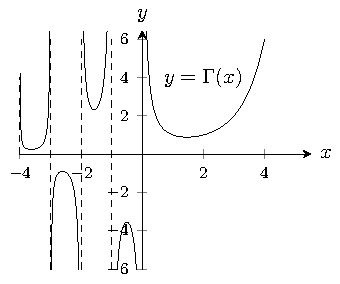
\includegraphics{figOctaveGammaFunction}
\caption{
\عددی{\Gamma(x)} متغیر \عددی{x} کا استمراری تفاعل ہے جس کی قیمت ہر مثبت عدد صحیح \عددی{n+1} پر \عددی{n!} ہے۔ \عددی{\Gamma} کا تعریفی تکمل صرف \عددی{x>0} کے لئے درست ہے لیکن ہم \عددی{\Gamma(x)=\tfrac{\Gamma(x+1)}{x}} (سوال \حوالہ{سوال_تکمل_تراکیب_گیما_وسعت} دیکھیں) کی استعمال سے منفی \عددی{ x} کے لئے \عددی{\Gamma} کو وسعت دے سکتے ہیں۔ 
}
\label{شکل_تکمل_تراکیب_گیما_تفاعل}
\end{figure}


\ابتدا{سوال}\شناخت{سوال_تکمل_تراکیب_گیما_وسعت}\ترچھا{غیر منفی عدد صحیح کے لئے \عددی{\Gamma(n+1)=n!} ہو گا}\\
\begin{enumerate}[a.]
\item
دکھائیں \عددی{\Gamma(1)=1}
\item
اس کے بعد تکمل بالحصص استعمال کرتے ہوئے \عددی{\Gamma(x+1)=x\Gamma(x)} ثابت کریں۔ یوں درج ذیل حاصل ہوں گے۔
\begin{align*}
\Gamma(2)&=1\Gamma(1)=1\\
\Gamma(3)&=2\Gamma(2)=2\\
\Gamma(3)&=3\Gamma(3)=6\\
\vdots&\\
\Gamma(n+1)&=n\Gamma(n)=n!
\end{align*}
\item
الکراجی ماخوذ استعمال کرتے ہوئے ہر غیر منفی عدد صحیح \عددی{n} کے لئے \عددی{\Gamma(n+1)=n\Gamma(n)=n!} کی تصدیق کریں۔
\end{enumerate}
\انتہا{سوال}
%========================
\ابتدا{سوال}\ترچھا{کلیہ سٹرلنگ}\\
اسکاچی ریاضی دان جیمس سٹرلنگ [1692-1770] نے  درج ذیل کلیہ اخذ کیا
\begin{align*}
\lim_{x\to\infty}(\tfrac{e}{x})^x\sqrt{\tfrac{x}{2\pi}}\Gamma(x)=1
\end{align*}
لہٰذا \عددی{x} کی بڑی قیمتوں کے لئے
\begin{gather}
\begin{aligned}\label{مساوات_تکمل_تراکیب_سٹرلنگ_ب}
\Gamma(x)=(\tfrac{x}{e})^x\sqrt{\tfrac{2\pi}{x}}(1+\epsilon(x)),
\end{aligned}\quad\quad
\begin{aligned}
x&\to \infty\\
\epsilon(x)&\to 0
\end{aligned}
\end{gather}

ہو گا۔ اس میں \عددی{\epsilon(x)} رد کرنے سے درج ذیل کلیہ حاصل ہوتا ہے۔
\begin{align}\label{مساوات_تکمل_تراکیب_سٹرلنگ_پ}
\Gamma(x)&\approx (\tfrac{x}{e})^x\sqrt{\tfrac{2\pi}{x}} && \text{\RL{کلیہ سٹرلنگ}}
\end{align}
%
\begin{enumerate}[a.]
\item
مساوات \حوالہ{مساوات_تکمل_تراکیب_سٹرلنگ_پ} اور \عددی{n!=n\Gamma(n)} استعمال کرتے ہوئے  درج ذیل کی تصدیق کریں۔
\begin{align}\label{مساوات_تکمل_تراکیب_سٹرلنگ_ت}
n!&\approx (\tfrac{n}{e})^n\sqrt{2\pi n}&&\text{\RL{تخمین سٹرلنگ}}
\end{align}
جیسا آپ حصہ \حوالہ{حصہ_ترتیب_حد_تلاش_کے_مسائل} کے سوال \حوالہ{سوال_ترتیب_سٹرلنگ} میں دیکھیں گے  مساوات \حوالہ{مساوات_تکمل_تراکیب_سٹرلنگ_ت} سے درج ذیل تخمین حاصل ہوتی ہے۔
\begin{align}\label{مساوات_تکمل_تراکیب_سٹرلنگ_ٹ}
\sqrt[n]{n!}\approx \frac{n}{e}
\end{align}
\item
\عددی{n=10,20,30,\cdots} لیتے ہوئے \عددی{n!} کے لئے  تخمین سٹرلنگ کے نتائج کا کیلکولیٹر سے حاصل نتائج کے ساتھ موازنہ کریں۔
\item
مساوات \حوالہ{مساوات_تکمل_تراکیب_سٹرلنگ_ب} کی بہتر صورت
\begin{align*}
\Gamma(x)=(\tfrac{x}{e})^x\sqrt{\tfrac{2\pi}{x}}e^{1/(12x)}(1+\epsilon(x))
\end{align*}
یا
\begin{align}\label{مساوات_تکمل_تراکیب_سٹرلنگ_ث}
\Gamma(x)=(\tfrac{n}{e})^n\sqrt{2n\pi}e^{1/(12n)}
\end{align}
ہے۔کیلکولیٹر، کلیہ سٹرلنگ اور مساوات \حوالہ{مساوات_تکمل_تراکیب_سٹرلنگ_ث} سے \عددی{10!} کے نتائج کا ایک دوسرے کے ساتھ موازنہ کریں۔ 
\end{enumerate}
\انتہا{سوال}
%==========================

\باب{لامتناہی تسلسل}
اس باب میں ہم ایک حیران کن کلیہ اخذ کرتے ہیں جس کی مدد سے بہت سارے تفاعل کو "لامتناہی کثیر رکنی" کی صورت میں لکھنا ممکن ہو گا اور ساتھ ہی کثیر رکنی کے  ارکان حذف  کر کے کثیر رکنی کو متناہی بنانے سے پیدا خلل بھی جان پائیں گے۔ ان تسلسل کو طاقتی تسلسل کہتے ہیں۔ قابل تفرق تفاعل کو تخمینی طور پر کثیر رکنی سے ظاہر کرنے میں مدد دینے کے علاوہ طاقتی تسلسل دیگر مواقع پر بھی کار آمد ثابت ہوتے ہیں۔ غیر بنیادی تکمل کی قیمت کے حصول کے علاوہ حراری توانائی کی منتقلی، ارتعاش، کیمیائی نفوذ اور ترسیل اشارات کے تفرقی مساوات  کے حل میں یہ موثر کردار ادا کرتے ہیں۔ آپ یہاں وہ ان تفاعل کے بارے میں سیکھ پائیں گے جو سائن اور انجینئری میں بہت زیادہ استعمال ہوتے ہیں۔

\حصہ{اعداد کی ترتیب کی حد}
غیر رسمی طور پر ترتیب سے مراد مرتب چیزوں کا سلسلہ ہے۔ اس باب میں ہمیں اعداد کی ترتیب سے غرض ہو گا۔ ترکیب نیوٹن سے حاصل اعداد کی ترتیب   \عددی{x_0,x_1,\cdots,x_n,\cdots} یا (ہلگے ون کوچ کے) برفانی روئی کے کثیر الاضلاع کی ترتیب \عددی{c_1,c_2,\cdots,c_n,\cdots} ہم دیکھ چکے ہیں۔ ان ترتیبوں کی حد پائی جاتی ہے، البتہ بہت سارے اہم ترتیبوں کے حد نہیں پائے جاتے ہیں۔

\جزوحصہء{تعریف اور علامتیت}
ہم \عددی{3} کے  ہر عدد صحیح مضرب کو ایک مقام مختص کر کے ایک فہرست بنا سکتے ہیں:
\begin{align*}
\begin{array}{rcccccc}
\text{\RL{دائرہ کار}} &1&2&3&\cdots&n&\cdots\\
\text{\RL{سعت}} &3&6&9&&3n&
\end{array}
\end{align*}
پہلا عدد \عددی{3}، دوسرا \عددی{6}، تیسرا \عددی{9}، وغیرہ، وغیرہ ہیں۔ مختص کرنے کا عمل ایک تفاعل ہے جو \عددی{n} ویں مقام کو \عددی{3n} مختص کرتا ہے۔ ترتیب کی بناوٹ کا بنیادی تصور یہی ہے۔ ایک تفاعل ہمیں بتاتا ہے کہ کس مقام پر کونسا عدد ہو گا۔

\ابتدا{تعریف}
ایک تفاعل جس کا دائرہ کار کسی عدد صحیح \عددی{n_0} کے برابر یا اس سے بڑے عدد صحیح پر مشتمل اعداد کا سلسلہ ہو \اصطلاح{لامتناہی ترتیب}\فرہنگ{ترتیب!لامتناہی}\حاشیہب{infinite sequence}\فرہنگ{sequence!infinite} (یا \اصطلاح{ترتیب}\فرہنگ{ترتیب}\حاشیہب{sequence}\فرہنگ{sequence})  کہلاتا ہے۔
\انتہا{تعریف}
%================

عموماً \عددی{n_0=1} ہوتا ہے اور ترتیب کا دائرہ کار مثبت اعداد صحیح پر مشتمل ہو گا۔ البتہ بعض اوقات ہم تسلسل کو کسی دوسرے عدد صحیح سے شروع کرنا چاہتے ہیں۔ ترکیب نیوٹن میں ہم \عددی{n_0=0} لیتے ہیں۔ اگر ہم \عددی{n} اضلاع پر مشتمل کثیر الاضلاع کی ترتیب کی بات کریں تب ہم \عددی{n_0=3} منتخب کرنا چاہیں گے۔

ترتیب کی تعریف کسی بھی تفاعل کی طرح کی جاتی ہے (مثال \حوالہ{مثال_تسلسل_متعدد_ترتیبات} اور شکل \حوالہ{شکل_تسلسل_مرتکز_منفرج_الف} تا شکل \حوالہ{شکل_تسلسل_مرتکز_منفرج_ث})، مثلاً:
\begin{align*}
a(n)=\sqrt{n},\quad a(n)=(-1)^{n+1}\frac{1}{n},\quad a(n)=\frac{n-1}{n}
\end{align*}

یہ ظاہر کرنے کی خاطر کہ دائرہ کار عدد صحیح ہے، ہم حرف \عددی{n} استعمال کرتے ہیں نا کہ دیگر غیر تابع متغیر کے لئے مستعمل حروف \عددی{x}، \عددی{y}، \عددی{z}، \عددی{t}، وغیرہ۔  مذکورہ بالا کی طرح تعریفی قاعدہ میں کلیات عموماً مثبت عدد صحیح سے زیادہ بڑے دائرہ کار کے لئے درست ہوتے ہیں۔ جیسا ہم دیکھیں گے یہ بعض اوقات سود مند ثابت ہوتا ہے۔ 

عدد \عددی{a(n)} ترتیب کا \اصطلاح{\عددی{n} واں جزو} یا اشاریہ \عددی{n} والا جزو ہو گا۔ اگر \عددی{a(n)=\tfrac{n-1}{n}} ہو تب درج ذیل ہو گا۔
\begin{align*}
\begin{array}{ccccc}
\text{\RL{پہلا جزو}}&\text{\RL{دوسرا جزو}}&\text{\RL{تیسرا جزو}}&&\text{\RL{$n$ واں جزو}}\\
\toprule
a(1)=0&a(2)=\frac{1}{2}&a(3)=\frac{2}{3}&\cdots&a(n)=\frac{n-1}{n}
\end{array}
\end{align*}
اشاریہ علامت استعمال کرتے ہوئے ہم \عددی{a(n)} کو \عددی{a_n} لکھتے ہیں۔ اشاریہ علامتی روپ میں یہی ترتیب درج ذیل لکھی جائے گی۔
\begin{align*}
\begin{array}{ccccc}
\text{\RL{پہلا جزو}}&\text{\RL{دوسرا جزو}}&\text{\RL{تیسرا جزو}}&&\text{\RL{$n$ واں جزو}}\\
\toprule
a_1=0&a_2=\frac{1}{2}&a_3=\frac{2}{3}&\cdots&a_n=\frac{n-1}{n}
\end{array}
\end{align*}
ترتیب پر تبصرہ کرتے ہوئے ہم عموماً \عددی{n} ویں جزو کے کلیہ کے ساتھ ساتھ چند ابتدائی اجزاء  لکھتے ہیں۔

\ابتدا{مثال}\شناخت{مثال_تسلسل_متعدد_ترتیبات}
\begin{align*}
\renewcommand{\arraystretch}{2}
\begin{array}{lll}
\text{\RL{اس کے لئے ہم درج ذیل لکھتے ہیں}}&\phantom{kkkk}&\text{\RL{جس ترتیب کا تعریفی کلیہ درج ذیل ہو}}\\
\toprule
1,\sqrt{2},\sqrt{3},\sqrt{4},\cdots,\sqrt{n},\cdots&&a_n=\sqrt{n}\\
1,\frac{1}{2},\frac{1}{3},\cdots,\frac{1}{n},\cdots&&a_n=\frac{1}{n}\\
1,-\frac{1}{2},\frac{1}{3},-\frac{1}{4},\cdots (-1)^{n+1}\frac{1}{n},\cdots&&a_n=(-1)^{n+1}\frac{1}{n}\\
0,\frac{1}{2},\frac{2}{3},\frac{3}{4},\cdots,\frac{n-1}{n},\cdots&&a_n=\frac{n-1}{n}\\
0,-\frac{1}{2},\frac{2}{3},-\frac{3}{4},\cdots,(-1)^{n+1}\big(\frac{n-1}{n}\big),\cdots&&a_n=(-1)^{n+1}\big(\frac{n-1}{n}\big)\\
3,3,3,\cdots,3,\cdots&&a_n=3
\end{array}
\end{align*}
ان تمام ترتیبوں کو دو مختلف انداز میں شکل \حوالہ{شکل_تسلسل_مرتکز_منفرج_الف} تا شکل \حوالہ{شکل_تسلسل_مرتکز_منفرج_ث} میں دکھایا گیا ہے۔
\انتہا{مثال}
%=================== 

\جزوحصہء{علامتیت}
جس ترتیب کا \عددی{n} واں جزو \عددی{a_n} ہو اس ترتیب کو ہم \عددی{\{a_n\}} سے ظاہر کرتے ہیں جو  ترتیب \عددی{a} اشاریہ \عددی{n} پڑھا جاتا ہے۔ مثال \حوالہ{مثال_تسلسل_متعدد_ترتیبات} میں دوسری ترتیب \عددی{\{\tfrac{1}{n}\}} ہے جو ترتیب ایک بٹہ تین پڑھا جاتا ہے۔ آخری ترتیب \عددی{\{3\}} ہے جو مستقل ترتیب \عددی{3} کہلائے گی۔

\begin{figure}
\centering
\begin{subfigure}{0.45\textwidth}
\centering
\begin{tikzpicture}[font=\small,xscale=2]
\draw[-latex](-0.25,0)--(2.5,0);
\foreach \n in {1,2,3,4,5}{\pgfmathsetmacro{\k}{sqrt(\n)} \draw(\k,0)node[circ]{}node[above]{$a_{\n}$};}
\foreach \x in {0,1,2}{\draw(\x,0)++(0,-0.15)node[below]{$\x$}--++(0,0.3);}
\draw(1.25,-0.5)node[below]{$a_n=\sqrt{n}$};
\end{tikzpicture}
\end{subfigure}\hfill
\begin{subfigure}{0.45\textwidth}
\centering
\begin{tikzpicture}[font=\small,xscale=1]
\draw[-latex](-0.25,0)--(5.5,0)node[right]{$n$};
\draw[-latex](0,-0.2)--(0,3.5)node[above]{$a_n$};
\foreach \n in {1,2,3,4,5}{\pgfmathsetmacro{\k}{sqrt(\n)} \draw(\n,\k)node[circ]{}node[above]{$(\n,\sqrt{\n})$};}
\foreach \x in {1,2,3,4,5}{\draw(\x,0)node[below]{$\x$}--++(0,0.2);}
\foreach \y in {1,2,3,}{\draw(0,\y)node[left]{$\y$}--++(0.2,0);}
\draw(3,3)node[above]{منفرج};
\end{tikzpicture}
\end{subfigure}
\caption{جزو $a_n$ آخر کار ہر عدد صحیح سے بڑھتا ہے لہٰذا ترتیب $\{a_n\}$ منفرج ہے۔}
\label{شکل_تسلسل_مرتکز_منفرج_الف}
\end{figure}
%%%%%%%%%%%%%%%%
\begin{figure}
\centering
\begin{subfigure}{0.45\textwidth}
\centering
\begin{tikzpicture}[font=\small,xscale=4]
\draw[-latex](-0.125,0)--(1.125,0);
\foreach \n in {1,2,3,4}{\pgfmathsetmacro{\k}{1/\n} \draw(\k,0)node[circ]{}node[above]{$a_{\n}$};}
\foreach \x in {0,1}{\draw(\x,0)++(0,-0.15)node[below]{$\x$}--++(0,0.3);}
\draw(0.5,-0.5)node[below]{$a_n=\frac{1}{n}$};
\end{tikzpicture}
\end{subfigure}\hfill
\begin{subfigure}{0.45\textwidth}
\centering
\begin{tikzpicture}[font=\small,xscale=1]
\draw[-latex](-0.25,0)--(5.5,0)node[right]{$n$};
\draw[-latex](0,-0.2)--(0,1.5)node[above]{$a_n$};
\foreach \n in {1,2,3,4,5}{\pgfmathsetmacro{\k}{1/\n} \draw(\n,\k)node[circ]{}node[above]{$(\n,\tfrac{1}{\n})$};}
\foreach \x in {1,2,3,4,5}{\draw(\x,0)node[below]{$\x$}--++(0,0.2);}
\foreach \y in {1}{\draw(0,\y)node[left]{$\y$}--++(0.12,0);}
\draw(3,1)node[above]{\RL{$0$ پر مرتکز}};
\end{tikzpicture}
\end{subfigure}
\caption{جزو $a_n=\tfrac{1}{n}$  بتدریج $n$ بڑھنے سے گھٹتے ہوئے $0$ کے قریب پہنچتے ہیں لہٰذا ترتیب $\{a_n\}$ صفر کو مرتکز ہے۔}
\label{شکل_تسلسل_مرتکز_منفرج_ب}
\end{figure}
%%%%%%%%%%%%%%%%%%%%%%%
\begin{figure}
\centering
\begin{subfigure}{0.45\textwidth}
\centering
\begin{tikzpicture}[font=\small,xscale=2]
\draw[-latex](-1.125,0)--(1.125,0);
\foreach \n in {1,2,3,4,5}{\pgfmathsetmacro{\k}{(-1)^(\n+1)/\n} \draw(\k,0)node[circ]{}node[above]{$a_{\n}$};}
\foreach \x in {0,1,-1}{\draw(\x,0)++(0,-0.15)node[below]{$\x$}--++(0,0.3);}
\draw(0,-0.5)node[below]{$a_n=\frac{(-1)^{n+1}}{n}$};
\end{tikzpicture}
\end{subfigure}\hfill
\begin{subfigure}{0.45\textwidth}
\centering
\begin{tikzpicture}[font=\small,xscale=1]
\draw[-latex](-0.25,0)--(5.5,0)node[right]{$n$};
\draw[-latex](0,-0.2)--(0,1.5)node[above]{$a_n$};
\foreach \n in {1,3,5}{\pgfmathsetmacro{\k}{(-1)^(\n+1)/\n} \draw(\n,\k)node[circ]{}node[above]{$(\n,\frac{1}{\n})$};}
\foreach \n in {2,4}{\pgfmathsetmacro{\k}{(-1)^(\n+1)/\n} \draw(\n,\k)node[circ]{}node[below]{$(\n,-\frac{1}{\n})$};}
\foreach \x in {1,2,3,4,5}{\draw(\x,0)--++(0,0.2);}
\foreach \y in {1}{\draw(0,\y)node[left]{$\y$}--++(0.12,0);}
\draw(3,1)node[above]{\RL{$0$ پر مرتکز}};
\end{tikzpicture}
\end{subfigure}
\caption{جزو $\tfrac{(-1)^{n+1}}{n}$ کی علامت ہر مرتبہ تبدیل ہوتی ہے لیکن اس کی قیمت  $0$ پر مرتکز ہے۔}
\label{شکل_تسلسل_مرتکز_منفرج_پ}
\end{figure}
%%%%%%%%%%%%%%%%%%%%%%%
\begin{figure}
\centering
\begin{subfigure}{0.45\textwidth}
\centering
\begin{tikzpicture}[font=\small,xscale=4]
\draw[-latex](-0.125,0)--(1.125,0);
\foreach \n in {1,2,3,4}{\pgfmathsetmacro{\k}{(\n-1)/\n} \draw(\k,0)node[circ]{}node[above]{$a_{\n}$};}
\foreach \x in {0,1}{\draw(\x,0)++(0,-0.15)node[below]{$\x$}--++(0,0.3);}
\draw(0.75,-0.5)node[below]{$a_n=\frac{n-1}{n}$};
\end{tikzpicture}
\end{subfigure}\hfill
\begin{subfigure}{0.45\textwidth}
\centering
\begin{tikzpicture}[font=\small,xscale=1]
\draw[-latex](-0.25,0)--(5.5,0)node[right]{$n$};
\draw[-latex](0,-0.2)--(0,1.5)node[above]{$a_n$};
\draw[gray](0,1)--(5.5,1);
\foreach \n/\nn in {1}{\draw(1,0)node[circ]{}node[above]{$(1,0)$};}
\foreach \n/\nn in {2/1,3/2,4/3,5/4}{\pgfmathsetmacro{\k}{(\n-1)/\n}; \draw(\n,\k)node[circ]{}node[above]{$(\n,\frac{\nn}{\n})$};}
\foreach \x in {1,2,3,4,5}{\draw(\x,0)--++(0,0.2);}
\foreach \y in {1}{\draw(0,\y)node[left]{$\y$}--++(0.12,0);}
\draw(1,1)node[above]{\RL{$1$ پر مرتکز}};
\end{tikzpicture}
\end{subfigure}
\caption{جیسے جیسے $n$ بڑھتا ہے جزو $a_n=\tfrac{n-1}{n}$ بتدریج $1$ تک پہنچتا ہے لہٰذا ترتیب $\{a_n\}$ مرتکز ہے $1$ پر۔}
\label{شکل_تسلسل_مرتکز_منفرج_ت}
\end{figure}
%%%%%%%%%%%%%%%%%%%%%%%%%%%
\begin{figure}
\centering
\begin{subfigure}{0.45\textwidth}
\centering
\begin{tikzpicture}[font=\small,xscale=2]
\draw[-latex](-1.125,0)--(1.125,0);
\foreach \n in {1,2,3,4,5}{\pgfmathsetmacro{\k}{(-1)^(\n+1)*(\n-1)/\n} \draw(\k,0)node[circ]{}node[above]{$a_{\n}$};}
\foreach \x in {-1,0,1}{\draw(\x,0)++(0,-0.15)node[below]{$\x$}--++(0,0.3);}
\draw(0,-0.5)node[below]{$a_n=(-1)^{n+1}\big(\frac{n-1}{n}\big)$};
\end{tikzpicture}
\end{subfigure}\hfill
\begin{subfigure}{0.45\textwidth}
\centering
\begin{tikzpicture}[font=\small,xscale=1]
\draw[-latex](-0.25,0)--(5.5,0)node[right]{$n$};
\draw[-latex](0,-1.25)--(0,1.25)node[above]{$a_n$};
\draw[gray](0,1)node[left,black]{$1$}--(5.5,1)  (0,-1)node[left,black]{$-1$}--(5.5,-1);
\foreach \n/\nn in {1}{\draw(1,0)node[circ]{}node[above]{$(1,0)$};}
\foreach \n/\nn in {3/2,5/4}{\pgfmathsetmacro{\k}{(-1)^(\n+1)*(\n-1)/\n}; \draw(\n,\k)node[circ]{}node[above]{$(\n,\tfrac{\nn}{\n})$};}
\foreach \n/\nn in {2/1,4/3}{\pgfmathsetmacro{\k}{(-1)^(\n+1)*(\n-1)/\n}; \draw(\n,\k)node[circ]{}node[below]{$(\n,-\tfrac{\nn}{\n})$};}
\foreach \x in {1,2,3,4,5}{\draw(\x,0)--++(0,0.2);}
\foreach \y in {3}{\draw(0,\y)node[left]{$\y$}--++(0.12,0);}
\draw(4,1)node[above]{\RL{منفرج}};
\end{tikzpicture}
\end{subfigure}
\caption{جزو $a_n=(-1)^{n+1}[\tfrac{n-1}{n}]$ کی علامت ہر قدم پر تبدیل ہوتی ہے۔ مثبت اجزاء $1$ کو پہنچتے ہیں جبکہ منفی اجزاء $-1$ کو پہنچتے ہیں لہٰذا ترتیب $\{a_n\}$ منفرج ہے۔}
\label{شکل_تسلسل_مرتکز_منفرج_ٹ}
\end{figure}
%%%%%%%%%%%%%%%%%%%%%%%
\begin{figure}
\centering
\begin{subfigure}{0.45\textwidth}
\centering
\begin{tikzpicture}[font=\small,xscale=0.75]
\draw[-latex](-0.25,0)--(5.5,0);
\foreach \n in {3}{\pgfmathsetmacro{\k}{\n} \draw(\k,0)node[circ]{}node[above]{$a_n$};}
\foreach \x in {0,1,2,3,4,5}{\draw(\x,0)++(0,-0.15)node[below]{$\x$}--++(0,0.3);}
\draw(2.5,-0.5)node[below]{$a_n=3$};
\end{tikzpicture}
\end{subfigure}\hfill
\begin{subfigure}{0.45\textwidth}
\centering
\begin{tikzpicture}[font=\small,xscale=1,yscale=0.3]
\draw[-latex](-0.25,0)--(5.5,0)node[right]{$n$};
\draw[-latex](0,-0.2)--(0,4)node[above]{$a_n$};
\foreach \n in {1,2,3,4,5}{\pgfmathsetmacro{\k}{3}; \draw(\n,\k)node[circ]{};}
\foreach \x in {1,2,3,4,5}{\draw(\x,0)--++(0,0.2);}
\foreach \y in {3}{\draw(0,\y)node[left]{$\y$}--++(0.12,0);}
\draw(4.5,1)node[above]{\RL{$3$ پر مرتکز}};
\end{tikzpicture}
\end{subfigure}
\caption{مستقل اجزاء $a_n=3$ کی قیمت $3$ ہی رہتی ہے لہٰذا ترتیب $\{a_n\}$ کی قیمت $3$ پر مرتکز ہے۔}
\label{شکل_تسلسل_مرتکز_منفرج_ث}
\end{figure}
%%%%%%%%%%%%%%%%%%
\جزوحصہء{ارتکاز اور انفراج}
آپ نے شکل \حوالہ{شکل_تسلسل_مرتکز_منفرج_الف} تا شکل \حوالہ{شکل_تسلسل_مرتکز_منفرج_ث} میں دیکھا کہ مثال \حوالہ{مثال_تسلسل_متعدد_ترتیبات} میں دیے گئے ترتیبات ایک جیسا رویہ نہیں رکھتے ہیں۔  متغیر \عددی{n} کی قیمت بڑھانے سے ترتیبات \عددی{\{\tfrac{1}{n}\}}، \عددی{\{\tfrac{(-1)^{n+1}}{n}\}} اور \عددی{\{\tfrac{n-1}{n}\}} میں ہر ایک کی قیمت کسی ایک منفرد تحدیدی قیمت تک پہنچتی ہے جبکہ ترتیب \عددی{\{3\}} ابتدا سے تحدیدی قیمت پر ہے۔ اس کے برعکس \عددی{\{(-1)^{n+1}\tfrac{(n-1)}{n}\}} کے اجزاء دو مختلف قیمتوں، \عددی{-1} اور \عددی{1}، پر جمع ہوتے ہیں جبکہ \عددی{\{\sqrt{n}\}} کے اجزاء بتدریج بڑھتے جاتے ہیں۔ 

ان ترتیبات میں امتیاز کرنے کی خاطر جو \عددی{n} بڑھانے سے کسی ایک منفرد قیمت \عددی{L} تک پہنچتی ہیں اور جو کسی منفرد قیمت تک نہیں پہنچتی ہیں، ہم ان ترتیبات کو جو \عددی{n} بڑھانے سے کسی ایک منفرد قیمت \عددی{L} تک پہنچتی ہو کو \ترچھا{مرتکز} کہتے ہیں۔ \ترچھا{ارتکاز} کی با ضابطہ تعریف درج ذیل ہے۔ 

\ابتدا{تعریف}
اگر ہر مثبت عدد \عددی{\epsilon} کے لئے ایسا  مطابقتی عدد صحیح \عددی{N} پایا جاتا ہو کہ ہر \عددی{n} کے لئے
\begin{align*}
n>N,\quad \implies \quad \abs{a_n-L}<\epsilon
\end{align*}
ہو تب ترتیب \عددی{\{a_n\}} عدد \عددی{L} پر \اصطلاح{مرتکز}\فرہنگ{مرتکز}\حاشیہب{convergent}\فرہنگ{convergent} ہو گی۔ اگر ایسا کوئی عدد \عددی{L} موجود نہ ہو تب ہم کہتے ہیں کہ \عددی{\{a_n\}} \اصطلاح{منفرج}\فرہنگ{منفرج}\حاشیہب{divergent}\فرہنگ{divergent} ہے۔

اگر \عددی{\{a_n\}} عدد \عددی{L} پر مرتکز ہو تب ہم \عددی{\lim_{n\to\infty}a_n=L} یا مختصراً \عددی{a_n\to L} لکھتے ہیں اور \عددی{L} کو اس ترتیب کا \اصطلاح{حد}\فرہنگ{حد}\حاشیہب{limit}\فرہنگ{limit} کہتے ہیں (شکل \حوالہ{شکل_تسلسل_ارتکاز_انفراج_تعریف})۔
\انتہا{تعریف}
%====================
\begin{figure}
\centering
\begin{subfigure}{0.45\textwidth}
\centering
\begin{tikzpicture}[font=\small,xscale=4/5,yscale=1]
\draw[-latex](-0.25,0)--(5,0);
\draw(2,0)node[circ]{}node[below]{$a_1$};
\draw(1,0)node[circ]{}node[below]{$a_2$};
\draw(1.5,0)node[circ]{}node[below]{$a_3$};
\draw(2.5,0)node[circ]{};
\draw(2.75,0)node[circ]{};
\draw(3.2,0)node[circ]{}node[below]{$a_N$};
\draw(3.8,0)node[circ]{}node[below]{$a_n$};
\draw(3.6,0)node[circ]{};
\draw(4.3,0)node[circ]{};
\draw(3.9,0)node[circ]{};
\draw(3.4,0)node[]{$($}node[above,xshift=-2ex,yshift=1ex]{$L-\epsilon$};
\draw(4.6,0)node[]{$)$}node[above,xshift=2ex,yshift=1ex]{$L+\epsilon$};
\draw(4,-0.1)--++(0,0.2)node[above]{$L$};
\draw(0,-0.1)node[below]{$0$}--++(0,0.2);
\end{tikzpicture}
\end{subfigure}\hfill
\begin{subfigure}{0.45\textwidth}
\centering
\begin{tikzpicture}[font=\small,xscale=0.5,yscale=0.5]
\draw[-latex](-0.25,0)--(11,0)node[right]{$n$};
\draw[-latex](0,-0.2)--(0,5)node[above]{$a_n$};
\draw[dashed](-0.25,4)node[left]{$L$}--(11,4);
\draw[](-0.25,3.4)--(11,3.4)node[right]{$L-\epsilon$};
\draw(8,3.6)node[above,fill=white]{$(n,a_n)$};
\draw[](-0.25,4.6)--(11,4.6)node[right]{$L+\epsilon$};
\draw(1,2)node[circ]{};
\draw(2,1)node[circ]{};
\draw(3,1.5)node[circ]{};
\draw(4,2.5)node[circ]{};
\draw(5,2.75)node[circ]{};
\draw(6,3.2)node[circ]{}node[below,xshift=1ex]{$(N,a_N)$};
\draw(7,3.8)node[circ]{};
\draw(8,3.6)node[circ]{};
\draw(9,4.3)node[circ]{};
\draw(10,3.9)node[circ]{};
\foreach \x/\s in {1/1,2/2,3/3,6/N,7/{},8/n}{\draw(\x,-0.1)node[below]{$\s$}--++(0,0.2);} 
\end{tikzpicture}
\end{subfigure}
\caption{
اگر نقاط \عددی{(n,a_n)} کی لکیر \عددی{y=L} افقی متقارب ہو تب \عددی{a_n\to L} ہو گا۔ اس شکل میں \عددی{a_N} کے بعد تمام \عددی{a_n} کا خط \عددی{L} سے فاصلہ \عددی{\epsilon} سے کم ہے۔
}
\label{شکل_تسلسل_ارتکاز_انفراج_تعریف}
\end{figure}

\ابتدا{مثال}\شناخت{مثال_ترتیب_تعریف_کی_پرکھ}\ترچھا{تعریف کی پرکھ}\\
درج ذیل دکھائیں۔
\begin{align*}
\text{\RL{(الف)}}\quad \lim_{n\to\infty}\frac{1}{n}&=0\\
\text{\RL{(ب)}}\quad\lim_{n\to\infty}k&=k&&\text{\RL{($k$ مستقل)}}
\end{align*}
حل:\quad
(الف) \quad
فرض کریں ہمیں \عددی{\epsilon>0} دیا گیا ہے۔ ہم نے دکھانا ہو گا کہ ایک ایسا عدد صحیح \عددی{N} پایا جاتا ہے کہ ہر \عددی{n} کے لئے 
\begin{align*}
n>N\quad \implies\quad \abs{\frac{1}{n}-0}<\epsilon
\end{align*}
ہو گا۔ یہ اس صورت ممکن ہو گا اگر \عددی{\tfrac{1}{n}<\epsilon} یا \عددی{n>\tfrac{1}{\epsilon}} ہو۔ اگر \عددی{\tfrac{1}{\epsilon}} سے \عددی{N} کوئی بھی بڑا عدد صحیح ہو تب کسی بھی \عددی{n>N} کے لئے درج بالا درست ہو گا۔ یوں ثابت ہوا کہ \عددی{\lim_{n\to\infty}(1/n)=0} ہے۔\\
(ب)\quad
فرض کریں ہمیں \عددی{\epsilon>0} دیا گیا ہے۔ ہم نے دکھانا ہو گا کہ ایک ایسا عدد صحیح \عددی{N} پایا جاتا ہے کہ ہر \عددی{n} کے لئے 
\begin{align*}
n>N\quad \implies\quad \abs{k-k}<\epsilon
\end{align*}
ہو گا۔ چونکہ \عددی{k-k=0} ہوتا ہے لہٰذا درج بالا کسی بھی مثبت عدد صحیح \عددی{N} کے لئے درست ہو گا۔یوں ثابت ہوا کہ کسی بھی مستقل \عددی{k} کے لئے \عددی{\lim_{n\to\infty}k=k} ہو گا۔
\انتہا{مثال}
%==================
\ابتدا{مثال}\شناخت{مثال_تسلسل_انفراج}
دکھائیں کہ \عددی{\{(-1)^{n+1}[\tfrac{n-1}{n}]\}} ہے۔

حل:\quad
ہم مثبت عدد \عددی{\epsilon} کو \عددی{1} سے کم چنتے ہیں تا کہ شکل \حوالہ{شکل_مثال_تسلسل_انفراج} میں \عددی{y=-1} اور \عددی{y=1} پر پٹیاں ایک دوسرے کو نہ ڈھانپیں۔ اگر کسی مخصوص \عددی{N} سے کسی بھی بڑے \عددی{n} کے لئے شکل \حوالہ{شکل_مثال_تسلسل_انفراج} میں نقطے بالائی پٹی میں پائے جاتے ہوں تب یہ ترتیب \عددی{1} پر مرتکز ہو گی۔ حقیقت میں جیسا ہی کوئی پہلا نقطہ \عددی{(n,a_n)} بالائی پٹی کے اندر آتا ہے، اس کے بعد \عددی{(n+1,a_{n+1})} سے شروع کرتے ہوئے  ہر متبادل نقطہ نچلی پٹی میں پایا جاتا ہے۔ یوں ترتیب کسی صورت \عددی{1} پر مرتکز نہیں ہو سکتی ہے۔ اسی طرح یہ ترتیب \عددی{-1} پر بھی مرتکز نہیں ہو سکتی ہے۔ ساتھ ہی ساتھ چونکہ ترتیب کے اجزاء \عددی{-1} یا \عددی{1} کے قریب تر ہوتے جاتے ہیں لہٰذا یہ کسی دوسرے نقطے کے قریب نہیں ہو سکتے ہیں لہٰذا یہ ترتیب منفرج ہے۔
\انتہا{مثال}
%===================
\begin{figure}
\centering
\begin{subfigure}{0.60\textwidth}
\centering
\begin{tikzpicture}[font=\small,xscale=2,declare function={f(\x)=(\x-1)/\x;}]
\draw[-latex](-1.5,0)--(1.5,0);
\foreach \n in {1,3,5}{\draw({f(\n)},0)node[circ]{}node[above]{$a_{\n}$};}
\foreach \n in {2,4}{\draw({-f(\n)},0)node[circ]{}node[above]{$a_{\n}$};}
\foreach \n in {6}{\draw({-f(\n)},0)node[circ]{}node[above]{\llap{$a_{\n}$}};}
\foreach \x in {-1,0,1}{\draw(\x,0)++(0,-0.15)node[below]{$\x$}--++(0,0.3);}
\draw(0,-0.5)node[below]{$a_n=(-1)^{n+1}\big(\frac{n-1}{n}\big)$};
\draw(-1-0.4,0)node[]{$($};
\draw(-1+0.4,0)node[]{$)$};
\draw(1-0.4,0)node[]{$($};
\draw(1+0.4,0)node[]{$)$};
\end{tikzpicture}
\end{subfigure}\hfill
\begin{subfigure}{0.30\textwidth}
\centering
\begin{tikzpicture}[font=\small,xscale=1/2,yscale=1,declare function={f(\x)=(\x-1)/\x;}]
\draw[-latex](-0.25,0)--(7,0);
\draw[-latex](0,-1.5)--(0,1.5)node[above]{$a_n$};
\draw(0,1+0.4)--(7,1+0.4)node[right]{$1+\epsilon$};
\draw[dashed](-0.25,1)--(7,1);
\draw(0,1-0.4)--(7,1-0.4)node[right]{$1-\epsilon$};
\draw(0,-1+0.4)--(7,-1+0.4)node[right]{$-1+\epsilon$};
\draw[dashed](-0.25,-1)--(7,-1);
\draw(0,-1-0.4)--(7,-1-0.4)node[right]{$-1-\epsilon$};
\draw(1,{f(1)})node[circ]{}node[above]{$(1,0)$};
\foreach \n/\s in {3/2,5/4}{\draw(\n,{f(\n)})node[circ]{}node[above]{$(\n,\tfrac{\s}{\n})$};}
\foreach \n/\s in {2/1,4/3,6/5}{\draw(\n,{-f(\n)})node[circ]{}node[below]{$(\n,-\tfrac{\s}{\n})$};}
\foreach \x in {1,2,3,4,5}{\draw(\x,0)--++(0,0.2);}
\foreach \y in {-1,1}{\draw(0,\y)node[left]{$\y$}--++(0.12,0);}
\end{tikzpicture}
\end{subfigure}
\caption{
تسلسل \عددی{\{(-1)^{n+1}[\tfrac{n-1}{n}]\}} منفرج ہے (مثال \حوالہ{مثال_تسلسل_انفراج})
}
\label{شکل_مثال_تسلسل_انفراج}
\end{figure}

ترتیب \عددی{\{(-1)^{n+1}[\tfrac{n-1}{n}]\}} کا رویہ \عددی{\{\sqrt{n}\}} کے رویے سے مختلف ہے۔ ترتیب \عددی{\{\sqrt{n}\}} کے منفرج ہونے کی وجہ یہ ہے کہ یہ ہر حقیقی عدد \عددی{L} سے تجاوز کرتا ہے۔اس رویے کو ہم
\begin{align*}
\lim_{n\to\infty}\sqrt{n}=\infty
\end{align*}
لکھتے ہیں۔لامتناہی حد سے یہاں ہمارا ہرگز یہ مطلب نہیں ہے کہ \عددی{n} بڑھانے سے \عددی{a_n} اور لامتناہی کے بیچ فرق کم ہوتا ہے۔ کہنے کا مطلب صرف اتنا ہے کہ  \عددی{n} بڑھانے سے \عددی{a_n} بہت بڑا ہو جاتا ہے۔ 

\جزوحصہء{تکراری تعریف}
اب تک ہم  \عددی{n} سے بلا واسطہ \عددی{a_n} تلاش کرتے آ رہے ہیں اگرچہ ترتیب کی عموماً تکراری تعریف  پیش کی جاتی ہے جہاں
\begin{enumerate}[a.]
\item
ابتدائی جزو یا اجزاء کی قیمتیں دی جاتی ہیں اور
\item
\اصطلاح{کلیہ توالی}\فرہنگ{کلیہ!توالی}\فرہنگ{توالی!کلیہ}\حاشیہب{recursion formula}\فرہنگ{recursion!formula} سے ہر جزو کو گزشتہ اجزاء کی قیمتوں سے حاصل کیا جاتا ہے۔ 
\end{enumerate}

کمپیوٹر پروگرام اور تفرقی مساوات کے اعدادی حل کے طریقوں میں توالی کلیات عموماً پائے جاتے ہیں۔

\ابتدا{مثال}\ترچھا{تواتر سے ترتیب کی بناوٹ}\\
\begin{enumerate}[a.]
\item
\عددی{a_1=1} اور \عددی{a_n=a_{n-1}+1} کا فقرہ مثبت اعداد کی ترتیب \عددی{1,2,3,\cdots,n,\cdots} کی تعریف پیش کرتا ہے۔ یوں \عددی{a_1=1} لیتے ہوئے \عددی{a_2=a_1+1=1+1=2}، \عددی{a_3=a_2+1=2+1=3}، وغیرہ، ہو گا۔
\item
 \عددی{a_1} اور \عددی{a_n=n\cdot a_{n-1}} کا فقرہ \اصطلاح{اعداد ضربیہ}\فرہنگ{اعداد ضربیہ}\حاشیہب{factorials}\فرہنگ{factorials} کی ترتیب \عددی{1,2,6,24,\cdots,n!,\cdots} کی تعریف پیش کرتا ہے۔ یوں \عددی{a_1=1} لیتے ہوئے \عددی{a_2=2\cdot a_1=2}، \عددی{a_3=3\cdot a_2=6}، \عددی{a_4=4\cdot a_3=24} وغیرہ، ہو گا۔
\item
\عددی{a_1=1}، \عددی{a_2=1} اور \عددی{a_{n+1}=a_n+a_{n-1}} کا فقرہ \اصطلاح{فبونیکی اعداد}\فرہنگ{فبونیکی اعداد}\حاشیہب{Fibonacci numbers}\فرہنگ{Fibonacci numbers} کی ترتیب  \عددی{1,1,2,3,5,\cdots} کی تعریف پیش کرتا ہے۔ یوں \عددی{a_1=1} اور \عددی{a_2=1} لیتے ہوئے \عددی{a_3=a_2+a_1=1+1=2}، \عددی{a_4=a_3+a_2=2+1=3}، \عددی{a_5=a_4+a_3=3+2=5}، وغیرہ، ہو گا۔
\item
جیسا ہم ترکیب نیوٹن کی اطلاق سے جانتے ہیں کہ \عددی{x_0=1} اور \عددی{x_{n+1}=x_n-[\tfrac{\sin x_n-x_n^2}{\cos x_n-2x_n}]} کا فقرہ ایسی ترتیب کی تعریف پیش کرتا ہے جو مساوات \عددی{\sin x-x^2=0} کے حل پر مرتکز ہوتی ہے۔
\end{enumerate}
\انتہا{مثال}
%===================

علامت \عددی{n!} (جس کو \عددی{n} کا \اصطلاح{ضربیہ عدد} کہتے ہیں) سے مراد \عددی{1} سے \عددی{n} تک اعداد صحیح کا حاصل ضرب \عددی{1\cdot 2\cdot 3\cdot\cdots \cdot n} ہے۔ آپ دیکھ سکتے ہیں کہ \عددی{(n+1)!=(n+1)\cdot n!} ہو گا لہٰذا
\begin{align*}
4!&=1\cdot 2\cdot 2\cdot 3\cdot 4=24,\\
5!&=1\cdot 2\cdot 3\cdot 4\cdot 5=5\cdot 4!=120
\end{align*}
ہوں گے۔ہم \عددی{0!} کی تعریف \عددی{1} لیتے ہیں۔

 جیسا جدول \حوالہ{جدول_تسلسل_فبونیکی_قوت_نما} میں دکھایا گیا ہے  قوت نما سے بھی زیادہ تیزی سے فبونیکی اعداد  بڑھتے ہیں۔
\begin{table}
\caption{قوت نما سے فبونیکی اعداد زیادہ تیزی سے بڑھتے ہیں۔}
\label{جدول_تسلسل_فبونیکی_قوت_نما}
\centering
\begin{tabular}{RRR}
n&e^n&n!\\
\toprule
1&3&1\\
5&148&120\\
10&\num{22026}&\num{3628800}\\
20&\num{4.9e8}&\num{2.4e18}\\
\bottomrule
\end{tabular}
\end{table}

\جزوحصہء{ذیلی ترتیبات}
اگر ایک ترتیب کے  اجزاء اسی ترتیب سے دوسری ترتیب میں پائے جاتے ہوں تب ہم پہلی ترتیب کو دوسری ترتیب کی \اصطلاح{ذیلی ترتیب}\فرہنگ{ترتیب!ذیلی}\حاشیہب{subsequence}\فرہنگ{sequence!sub} کہتے ہیں۔ 

\ابتدا{مثال}\ترچھا{مثبت اعداد صحیح کی ترتیب کی  ذیلی ترتیبات}\\
\begin{enumerate}[a.]
\item
جفت اعداد صحیح کی ذیلی ترتیب \عددی{2,4,6,\cdots,2n,\cdots}
\item
طاق اعداد صحیح کی ذیلی ترتیب \عددی{1,3,5,\cdots 2n-1,\cdots}
\item
اعداد مفرد کی ذیلی ترتیب \عددی{2,3,5,7,11,\cdots}
\end{enumerate}
\انتہا{مثال}
%===================

ذیلی ترتیبات کی اہمیت کے دو وجوہات ہیں۔
\begin{enumerate}[a.] 
\item
اگر تسلسل \عددی{\{a_n\}} مستقل \عددی{L} کو مرتکز ہو تب اس کے تمام ذیلی ترتیبات بھی \عددی{L} پر مرکوز ہوں گی۔ اگر ہم جانتے ہوں کہ ایک تسلسل مرتکز ہے تب اس کے کسی مخصوص ذیلی تسلسل سے حد کی تلاش یا اس کا تخمینہ لگانا زیادہ آسان ثابت ہو سکتا ہے۔
\item
اگر \عددی{\{a_n\}} کا کوئی بھی ذیلی تسلسل منفرج ہو یا اس کے کسی دو ذیلی ترتیبات کے حد ایک دوسرے سے مختلف ہوں تب \عددی{\{a_n\}} منفرج ہو گا۔ مثال کے طور پر تسلسل \عددی{\{(-1)^n\}} منفرج ہو گا چونکہ طاق اجزاء کی ذیلی تسلسل \عددی{-1,-1,-1,\cdots} کی حد \عددی{-1} ہے جبکہ جفت اجزاء کی ذیلی تسلسل \عددی{1,1,1,\cdots} کی حد \عددی{1} ہے جو ایک مختلف حد ہے۔
\end{enumerate}

ذیلی تسلسل کی مدد سے ارتکاز کو ایک نئی نظر سے دیکھا جا سکتا ہے۔ کسی اشاریہ \عددی{N} کے بعد تمام اجزاء کو تسلسل کی \اصطلاح{دم}\فرہنگ{تسلسل!دم}\حاشیہب{tail}\فرہنگ{sequence!tail} کہتے ہیں جو ایک ذیلی تسلسل ہو گی۔ یوں سلسلہ \عددی{\{a_n|n\ge N\}} میں سے کسی ایک کو دم کہا جا سکتا ہے۔ یوں \عددی{a_n\to L} کی جگہ ہم کہہ سکتے ہیں کہ \عددی{L} کے ارد گرد \عددی{\epsilon} وقفہ میں تسلسل کی دم پائی جائے گی۔

کسی بھی تسلسل کی ارتکاز یا انفراج کا تسلسل کی ابتدا کے ساتھ کوئی تعلق نہیں پایا جاتا ہے۔ تسلسل کی ارتکاز یا انفراج صرف تسلسل کی دم پر منحصر ہو گی۔

\جزوحصہء{محدود غیر گھٹتا تسلسل}
\ابتدا{تعریف}
ایسا تسلسل جو تمام \عددی{n} کے لئے \عددی{a_n\le a_{n+1}} خاصیت رکھتا ہو \اصطلاح{غیر گھٹتا تسلسل}\فرہنگ{تسلسل!غیر گھٹتا}\حاشیہب{nondecreasing sequence}\فرہنگ{sequence!nondecreasing} کہلاتا ہے۔ 
\انتہا{تعریف}
%=======================

\ابتدا{مثال}\ترچھا{غیر گھٹتا تسلسل}\\
\begin{enumerate}[a.]
\item
قدرتی اعداد کا تسلسل \عددی{1,2,3,\cdots,n,\cdots}
\item
تسلسل \عددی{\frac{1}{2},\frac{2}{3},\frac{3}{4},\cdots,\frac{n}{n+1},\cdots}
\item
مستقل تسلسل \عددی{\{3\}}
\end{enumerate}
\انتہا{مثال}
%======================

غیر گھٹتا تسلسل کی دو قسمیں ہیں۔ پہلی قسم کے اجزاء آخر کار ہر متناہی حد بندی سے بڑھ جاتے ہیں جبکہ دوسری قسم کے اجزاء کسی مخصوص حد بندی سے تجاوز نہیں کرتے ہیں۔

\ابتدا{تعریف}
اگر ایک ایسا عدد \عددی{M} موجود ہو کہ تمام \عددی{n} کے لئے \عددی{a_n\le M} ہوں تب تسلسل \عددی{\{a_n\}} کی \اصطلاح{بالائی حد بندی}\فرہنگ{حد بندی!بالائی}\حاشیہب{upper bound}\فرہنگ{bound!upper} \عددی{M} ہو گی۔ ہم کہتے ہیں کہ تسلسل \عددی{\{a_n\}} \اصطلاح{اوپر سے محدود}\فرہنگ{محدود!اوپر سے}\حاشیہب{bounded from above}\فرہنگ{bounded!from above} ہے۔ اگر \عددی{M} سے کم کوئی بھی عدد، \عددی{\{a_n\}} کی بالائی حد بندی نہ ہو، تب \عددی{M} کو \عددی{\{a_n\}} کی \اصطلاح{کم سے کم بالائی حد بندی}\فرہنگ{حد بندی!کم سے کم بالائی}\حاشیہب{least upper bound}\فرہنگ{bound!least upper} کہتے ہیں۔
\انتہا{تعریف}
%==================

\ابتدا{مثال}
\begin{enumerate}[a.]
\item
تسلسل \عددی{1,2,3,\cdots,n,\cdots} کی کوئی بالائی حد بندی نہیں پائی جاتی ہے۔
\item
تسلسل \عددی{\frac{1}{2},\frac{2}{3},\frac{3}{4},\cdots,\frac{n}{n+1},\cdots} اوپر سے محدود ہے اور اس کی بالائی حد بندی \عددی{M=1} ہے۔کوئی بھی عدد جو \عددی{1} سے چھوٹا ہو اس تسلسل کی بالائی حد بندی نہیں ہو سکتی ہے لہٰذا اس تسلسل کی کم سے کم بالائی حد بندی \عددی{1} ہے۔
\end{enumerate}
\انتہا{مثال}
%========================

ایسے غیر گھٹتا تسلسل کی کم سے کم بالائی حد بندی ضرور پایا جائے گا جو اوپر سے محدود ہو۔ یہ حقیقت، جس کو ہم یہاں ثابت نہیں کریں گے، حقیقی اعداد کی مکملیت کی خاصیت کی بنا ہے۔ البتہ ہم یہ ثابت کرتے ہیں کہ اگر \عددی{L} کم سے کم بالائی حد بندی ہو تب  تسلسل \عددی{L} پر مرتکز ہو گا۔

فرض کریں ہم \عددی{(1,s_1),(2,s_2),\cdots,(n,s_n),\cdots}  نقطوں کو \عددی{xy} مستوی میں ترسیم کرتے ہیں۔ اگر اس تسلسل کی بالائی حد بندی  \عددی{M} ہو تب یہ تمام نقطے لکیر \عددی{y=M} کے نیچے پائے جائیں گے (شکل \حوالہ{شکل_تسلسل_بالائی_حد_بندی_اور_حد})۔ لکیر \عددی{y=L} سب سے نچلی ایسی لکیر ہو گی۔ نقاط \عددی{(n,s_n)} میں سے کوئی بھی اس لکیر سے اوپر نہیں ہو گا اگرچہ اس سے نیچے لکیر \عددی{y=L-\epsilon} سے چند نقطے  ضرور اوپر  ہوں گے، جہاں \عددی{\epsilon} مثبت عدد ہے۔ یہ ترتیب درج ذیل وجوہات کی بنا \عددی{L} پر مرتکز ہو گی:
\begin{enumerate}[a.]
\item
تمام \عددی{n} کے لئے \عددی{s_n\le L} ہو گا اور
\item
کسی بھی دیے گئے عدد \عددی{\epsilon>0} کے لئے کم سے کم ایک ایسا عدد \عددی{N} موجود ہو گا جس کے لئے \عددی{s-N>L-\epsilon} ہو گا۔
\end{enumerate}
مزید \عددی{\{s_n\}} غیر گھٹتا ہے لہٰذا
\begin{align*} 
s_n\ge s_N>L-\epsilon\quad\quad  \text{\RL{تمام $n\ge N$ کے لئے}}
\end{align*}
ہو گا۔ یوں \عددی{N} کے بعد تمام اعداد \عددی{s_n} کا \عددی{L} سے فاصلہ عدد \عددی{\epsilon} سے کم ہو گا۔یہی وہ شرط ہے جس کی بنا تسلسل \عددی{s_n} کی حد \عددی{L} ہو گی۔
\begin{figure}
\centering
\begin{tikzpicture}[yscale=2,declare function={f(\x)=(\x-1)/\x;}]
\draw[-latex](-0.25,0)--(9,0)node[right]{$x$};
\draw[-latex](0,-0.2)--(0,1.4)node[above]{$y$};
\foreach \a in {2,3,4,5,6,7,8}{\draw(\a,{f(\a)})node[circ]{};}
\foreach \x in {1,2,3,4,5,6,7,8}{\draw(\x,-0.1)node[below]{$\x$}--++(0,0.2);}
\draw(1,0.3)node[circ]{}node[above]{$(1,s_1)$};
\draw(5,{4/5})node[below]{$(5,s_5)$};
\draw(8,{7/8})node[below]{$(8,s_8)$};
\draw(0,1)node[left]{$L$}--++(9,0)node[right]{$y=L$};
\draw(0,1.2)node[left]{$M$}--++(9,0)node[right]{$y=M$};
\end{tikzpicture}
\caption{اگر غیر گھٹتے تسلسل کی بالائی حد بندی \عددی{M} ہو تب اس کے حد \عددی{L\le M} بھی ہوں گے۔}
\label{شکل_تسلسل_بالائی_حد_بندی_اور_حد}
\end{figure}

\ابتدا{مسئلہ}\شناخت{مسئلہ_تسلسل_غیر_گھٹتا_تسلسل}\ترچھا{غیر گھٹتا تسلسل کا مسئلہ}\\
حقیقی اعداد کا ایک غیر گھٹتا تسلسل صرف اور صرف اس صورت مرتکز ہو گا جب یہ تسلسل اوپر سے محدود ہو۔ اگر ایک غیر گھٹتا تسلسل مرتکز ہو، یہ اپنے کم سے کم بالائی حد بندی پر مرتکز ہو گا۔
\انتہا{مسئلہ}
%=======================

\حصہء{سوالات}
\موٹا{ترتیب کے اجزاء کی تلاش}\\
سوال \حوالہ{سوال_تسلسل_کلیہ_دی_ہے_الف} تا سوال \حوالہ{سوال_تسلسل_کلیہ_دی_ہے_ب} میں ترتیب کی \عددی{n} ویں جزو کا کلیہ دیا گیا ہے۔ اس کے ابتدائی اجزاء \عددی{a_1}، \عددی{a_2}، \عددی{a_3} اور \عددی{a_4} تلاش کریں۔

\ابتدا{سوال}\شناخت{سوال_تسلسل_کلیہ_دی_ہے_الف}
$a_n=\frac{1-n}{n^2}$\\
جواب:\quad
$a_0=0,\, a_2=-\tfrac{1}{4},\,a_3=-\tfrac{2}{9},\,a_4=-\tfrac{3}{16}$
\انتہا{سوال}
%=====================
\ابتدا{سوال}
$a_n=\frac{1}{n!}$
\انتہا{سوال}
%====================
\ابتدا{سوال}
$a_n=\frac{(-1)^{n+1}}{2n-1}$\\
جواب:\quad
$a_1=1,\,a_2=-\tfrac{1}{3},\,a_3=\tfrac{1}{5},\,a_4=-\tfrac{1}{7}$
\انتہا{سوال}
%====================
\ابتدا{سوال}
$a_n=2+(-1)^n$
\انتہا{سوال}
%====================
\ابتدا{سوال}
$a_n=\frac{2^n}{2^{n+1}}$\\
جواب:\quad
$a_1=\tfrac{1}{2},\,a_2=\tfrac{1}{2},\,a_3=\tfrac{1}{2},\,a_4=\tfrac{1}{2}$
\انتہا{سوال}
%====================
\ابتدا{سوال}\شناخت{سوال_تسلسل_کلیہ_دی_ہے_ب}
$a_n=\frac{2^n-1}{2^n}$
\انتہا{سوال}
%====================
سوال \حوالہ{سوال_تسلسل_کلیہ_توالی_دیا_ہے_الف} تا سوال \حوالہ{سوال_تسلسل_کلیہ_توالی_دیا_ہے_ب} میں ابتدائی ایک یا دو اجزاء اور کلیہ توالی دی گئی ہے۔ ابتدائی دس اجزاء تلاش کریں۔

\ابتدا{سوال}\شناخت{سوال_تسلسل_کلیہ_توالی_دیا_ہے_الف}
$a_1=1,\quad a_{n+1}=a_n+\frac{1}{2^n}$\\
جواب:\quad
$1,\tfrac{3}{2},\tfrac{7}{4},\tfrac{15}{8},\tfrac{31}{16},\tfrac{63}{32},\tfrac{127}{64},\tfrac{255}{128},\tfrac{511}{256},\tfrac{1023}{512}$
\انتہا{سوال}
%==========================
\ابتدا{سوال}
$a_1=1,\quad a_{n+1}=\frac{a_n}{n+1}$
\انتہا{سوال}
%======================
\ابتدا{سوال}
$a_1=2,\quad a_{n+1}=(-1)^{n+1}\frac{a_n}{2}$\\
جواب:\quad
$2,1,-\tfrac{1}{2},-\tfrac{1}{4},\tfrac{1}{8},\tfrac{1}{16},-\tfrac{1}{32},-\tfrac{1}{64},\tfrac{1}{128},\tfrac{1}{256}$
\انتہا{سوال}
%======================
\ابتدا{سوال}
$a_1=-2,\quad a_{n+1}=\frac{na_n}{n+1}$
\انتہا{سوال}
%======================
\ابتدا{سوال}
$a_1=a_2=1,\quad a_{n+2}=a_{n+1}+a_n$\\
جواب:\quad
$1,1,2,3,5,8,13,21,34,55$
\انتہا{سوال}
%======================
\ابتدا{سوال}\شناخت{سوال_تسلسل_کلیہ_توالی_دیا_ہے_ب}
$a_1=2,\quad a_2=-1,\quad a_{n+2}=\frac{a_{n+1}}{a_n}$
\انتہا{سوال}
%======================
\موٹا{ترتیب کے کلیہ کی تلاش}\\
سوال \حوالہ{سوال_تسلسل_کلیہ_تلاش_الف} تا سوال \حوالہ{سوال_تسلسل_کلیہ_تلاش_ب} میں دیے گئے ترتیب کے \عددی{n} ویں جزو کا کلیہ تلاش کریں۔

\ابتدا{سوال}\شناخت{سوال_تسلسل_کلیہ_تلاش_الف}
$1,-1,1,-1,1,\cdots$\quad\quad
ہر بار \عددی{1} کی علامت تبدیل ہوتی ہے۔\\
جواب:\quad
$a_n=(-1)^{n+1},\, n\ge 1$
\انتہا{سوال}
%==================
\ابتدا{سوال}
$-1,1,-1,1,-1,\cdots$\quad\quad
ہر بار \عددی{1} کی علامت تبدیل ہوتی ہے۔
\انتہا{سوال}
%==========================
\ابتدا{سوال}
$1,-4,9,-16,25,\cdots$\quad\quad
مثبت عدد صحیح کا مربع جس کی علامت ہر بار تبدیل ہوتی ہے۔\\
جواب:\quad
$a_n=(-1)^{n+1}(n)^2,\, n\ge 1$
\انتہا{سوال}
%======================
\ابتدا{سوال}
$1,-\frac{1}{4},\frac{1}{9},-\frac{1}{16},\frac{1}{25},\cdots$\quad\quad
مثبت عدد صحیح کے مربع کا بالعکس متناسب جس کی علامت ہر بار تبدیل ہوتی ہے۔
\انتہا{سوال}
%======================
\ابتدا{سوال}
$0,3,8,15,24,\cdots$\quad\quad
مثبت عدد صحیح کے مربع سے \عددی{1} کم۔\\
جواب:\quad
$a_n=n^2-1,\, n\ge 1$
\انتہا{سوال}
%======================
\ابتدا{سوال}
$-3,-2,-1,0,1,\cdots$\quad\quad
عدد صحیح \عددی{-3} سے شروع کرتے ہوئے ۔
\انتہا{سوال}
%======================
\ابتدا{سوال}
$1,5,9,13,17,\cdots$\quad\quad
ہر دوسرا طاق مثبت عدد صحیح۔\\
جواب:\quad
$a_n=4n-3,\, n\ge 1$
\انتہا{سوال}
%======================
\ابتدا{سوال}
$2,6,10,14,18,\cdots$\quad\quad
ہر دوسرا جفت مثبت عدد صحیح۔
\انتہا{سوال}
%======================
\ابتدا{سوال}
$1,0,1,0,1,\cdots$\quad\quad
باری باری \عددی{1} اور \عددی{0}\\
جواب:\quad
$a_n=\tfrac{1+(-1)^{n+1}}{2},\, n\ge 1$
\انتہا{سوال}
%======================
\ابتدا{سوال}\شناخت{سوال_تسلسل_کلیہ_تلاش_ب}
$1,1,2,2,3,3,4,\cdots$\quad\quad
ہر مثبت عدد صحیح دو بار۔
\انتہا{سوال}
%======================
\موٹا{کیلکولیٹر کی مدد سے حد کی تلاش}\\
سوال \حوالہ{سوال_تسلسل_کیلکولیٹر_حد_الف} تا سوال \حوالہ{سوال_تسلسل_کیلکولیٹر_حد_ب} میں کیلکولیٹر کے  ساتھ تجربات کرتے ہوئے \عددی{N} کی وہ قیمت تلاش کریں جو دی گئی عدم مساوات کو تمام \عددی{n>N} کے لئے مطمئن کرتا ہو۔ دی گئی عدم مساوات، تسلسل کی حد کی با ضابطہ تعریف کے تحت ہے۔ تسلسل کی تفصیل پیش کریں اور اس کی حد تلاش کریں۔

\ابتدا{سوال}\شناخت{سوال_تسلسل_کیلکولیٹر_حد_الف}
$\abs{\sqrt[n]{0.5}-1}<10^{-3}$\\
جواب:\quad
$N=692,\, a_n=\sqrt[n]{0.5},\,L=1$
\انتہا{سوال}
%=====================
\ابتدا{سوال}
$\abs{\sqrt[n]{n}-1}<10^{-3}$
\انتہا{سوال}
%========================
\ابتدا{سوال}
$(0.9)^n<10^{-3}$\\
جواب:\quad
$N=65,\, a_n=(0.9)^n,\, L=0$
\انتہا{سوال}
%========================
\ابتدا{سوال}\شناخت{سوال_تسلسل_کیلکولیٹر_حد_ب}
$\frac{2^n}{n!}<10^{-7}$
\انتہا{سوال}
%========================
\ابتدا{سوال}\شناخت{سوال_تسلسل_ترکیب_نیوٹن}\ترچھا{ترکیب نیوٹن سے حاصل ترتیبات}\\
ترکیب نیوٹن کی قابل تفرق تفاعل \عددی{f(x)} پر اطلاق  سے ابتدائی قیمت \عددی{x_0} اور اس کے بعد اعداد کی ترتیب \عددی{\{x_n\}} حاصل ہوتی ہے جو موزوں صورت میں \عددی{f} کے صفر پر مرتکز ہو گی۔ اس ترتیب کا کلیہ توالی درج ذیل ہے۔
\begin{align*}
x_{n+1}=x_n-\frac{f(x_n)}{f'(x_n)}
\end{align*}
\begin{enumerate}[a.]
\item
دکھائیں کہ \عددی{f(x)=x^2-a^2,\, a>0} کا کلیہ توالی \عددی{x_{n+1}=\tfrac{x_n+a/{x_n}}{2}} ہے۔
\item
ابتدائی قیمت \عددی{x_0=1} اور \عددی{a=3} لیتے ہوئے وہاں تک یک بعد دیگرے اجزاء تلاش کریں جب اجزاء دہرانے شروع ہو جاتے ہیں۔ کون سے عدد کی تخمین حاصل ہوتی ہے؟ وجہ پیش کریں۔ 
\end{enumerate}
جواب:\quad
(ب) \عددی{\sqrt{3}}
\انتہا{سوال}
%=====================
\ابتدا{سوال} 
گزشتہ سوال (سوال \حوالہ{سوال_تسلسل_ترکیب_نیوٹن}) میں \عددی{a=3} کی بجائے \عددی{a=2} لیتے ہوئے جزو-ب دوبارہ حل کریں۔
\انتہا{سوال}
%========================
\ابتدا{سوال}\شناخت{سوال_تسلسل_پائے}\ترچھا{$\tfrac{\pi}{2}$ کی تعریف توالی}\\
اگر آپ \عددی{x_1=1} سے شروع کر کے  \عددی{\{x_n\}} کے باقی اجزاء کو قاعدہ \عددی{x_n=x_{n-1}+\cos x_{n-1}} سے حاصل کریں تب ایک ایسی ترتیب حاصل ہو گی جو بہت تیزی سے \عددی{\tfrac{\pi}{2}} پر مرتکز ہو گی۔ (ا) ایسا کر کے دیکھیں۔ (ب) اتنی تیز ارتکاز کی وجہ شکل \حوالہ{شکل_سوال_تسلسل_پائے} کی مدد سے پیش کریں۔
\انتہا{سوال}
%====================
\begin{figure}
\centering
\begin{tikzpicture}
\pgfmathsetmacro{\r}{1.5}
\pgfmathsetmacro{\ang}{50}
\draw[-latex](-0.25,0)--(\r+0.5,0)node[right]{$x$};
\draw[-latex](0,-0.2)--(0,2)node[above]{$y$};
\draw(\r,0)node[below]{$1$}  (0,\r)node[left]{$1$};
\draw([shift={(0:\r)}]0,0) arc (0:90:\r);
\draw(0,0)--++(\ang:\r)coordinate(kT)--($(0,0)!(kT)!(0,1.5)$)node[pos=0.6,pin=60:{$\cos x_{n-1}$}]{};
\draw[-stealth]([shift={(0:0.5)}]0,0) arc (0:\ang:0.5);
\draw(1/2*\ang:0.5)node[right]{$x_{n-1}$};
\draw[thick]([shift={(0:\r)}]0,0) arc (0:\ang:\r);
\draw(1/2*\ang:\r)node[right]{$x_{n-1}$};
\end{tikzpicture}
\caption{اکائی دائرہ برائے سوال \حوالہ{شکل_سوال_تسلسل_پائے}}
\label{شکل_سوال_تسلسل_پائے}
\end{figure}
\ابتدا{سوال}
گاڑیاں بنانے والا ایک کارخانہ دھاتی چادر کو دبا کر ایک گاڑی  کا ڈھانچہ  اوسطاً \عددی{7.25} گھنٹوں میں تیار کرتا ہے۔ اگر ڈھانچہ تیار کرنے کے لئے درکار وقت میں سالانہ \عددی{\SI{6}{\percent}}  کمی رونما ہو تب \عددی{n} سالوں بعد
\begin{align*}
S_n=7.25(0.94)^n
\end{align*} 
وقت درکار ہو گا۔ کتنے سالوں بعد تقریباً \عددی{3.5} گھنٹے درکار ہوں گے؟ جواب کو دو مختلف طریقوں سے تلاش کریں:
\begin{enumerate}[a.]
\item
تسلسل \عددی{S_n} کا وہ پہلا جزو تلاش کریں جو \عددی{3.5} کے برابر یا اس سے کم ہو۔
\item
تفاعل \عددی{f(x)=7.25(0.94)^x} ترسیم کر کے دیکھیں یہ کہاں لکیر \عددی{y=3.5} کو مس کرتی ہے۔
\end{enumerate}
\انتہا{سوال}
%=====================
\موٹا{نظریہ اور مثالیں}\\
سوال \حوالہ{سوال_تسلسل_اوپر_سے_محدود_الف} تا سوال \حوالہ{سوال_تسلسل_اوپر_سے_محدود_ب} میں معلوم کریں کہ آیا تسلسل غیر گھٹتی ہے اور کیا یہ اوپر سے محدود ہے۔

\ابتدا{سوال}\شناخت{سوال_تسلسل_اوپر_سے_محدود_الف}
$a_n=\frac{3n+1}{n+1}$\\
جواب:\quad
غیر گھٹتا، محدود
\انتہا{سوال}
%======================
\ابتدا{سوال}
$a_n=\frac{(2n+3)!}{(n+1)!}$
\انتہا{سوال}
%====================
\ابتدا{سوال}
$a_n=\frac{2^n3^n}{n!}$\\
جواب:\quad
غیر گھٹتا نہیں ہے، محدود
\انتہا{سوال}
%====================
\ابتدا{سوال}\شناخت{سوال_تسلسل_اوپر_سے_محدود_ب}
$a_n=2-\frac{2}{n}-\frac{1}{2^n}$
\انتہا{سوال}
%====================
سوال \حوالہ{سوال_تسلسل_مرتکز_منفرج_الف} تا سوال \حوالہ{سوال_تسلسل_مرتکز_منفرج_ب} میں کون سی ترتیب مرتکز ہے اور کون سی منفرج؟ اپنے جواب کی وجہ پیش کریں۔

\ابتدا{سوال}\شناخت{سوال_تسلسل_مرتکز_منفرج_الف}
$a_n=1-\frac{1}{n}$\\
جواب:\quad
مرتکز، غیر گھٹتا، غیر گھٹتا تسلسل کا مسئلہ
\انتہا{سوال}
%===================
\ابتدا{سوال}
$a_n=n-\frac{1}{n}$
\انتہا{سوال}
%====================
\ابتدا{سوال}
$a_n=\frac{2^n-1}{2^n}$\\
جواب:\quad
مرتکز، غیر گھٹتا، غیر گھٹتا تسلسل کا مسئلہ
\انتہا{سوال}
%====================
\ابتدا{سوال}
$a_n=\frac{2^n-1}{3^n}$
\انتہا{سوال}
%====================
\ابتدا{سوال}
$a_n=[(-1)^n+1]\big(\frac{n+1}{n}\big)$\\
جواب:\quad
منفرج، انفراج کی تعریف
\انتہا{سوال}
%====================
\ابتدا{سوال}\شناخت{سوال_تسلسل_مرتکز_منفرج_ب}
ایک ترتیب کا پہلا جزو \عددی{x_1=\cos(1)}، اگلا جزو \عددی{x_2=x_1} یا \عددی{\cos(2)} میں سے جو بھی بڑا ہے، اس سے اگلا جزو \عددی{x_3=x_2} یا \عددی{\cos(3)} میں سے جو بھی بڑا (دائیں جانب زیادہ دور) ہے۔ یوں عمومی جزو درج ذیل ہو گا۔
\begin{align*}
x_{n+1}=\{x_n,\cos(n+1)\}_{\text{\RL{زیادہ بڑا}}}
\end{align*}
\انتہا{سوال}
%==================
\ابتدا{سوال}\شناخت{سوال_تسلسل_غیر_بڑھتا_ترتیب}\ترچھا{غیر بڑھتے ترتیبات}\\
ایک ترتیب جس میں تمام \عددی{n} کے لئے \عددی{a_n>a_{n+1}} ہو \اصطلاح{غیر بڑھتا ترتیب}\فرہنگ{ترتیب!غیر بڑھتا}\حاشیہب{nonincreasing sequence}\فرہنگ{sequence!nonincreasing} کہلاتا ہے۔ اگر ہر \عددی{n} کے لئے \عددی{M\le a_n} ہو جہاں \عددی{M} کوئی عدد ہو تب \عددی{M} کو ترتیب \عددی{\{a_n\}} کی \اصطلاح{زیریں حد بندی}\فرہنگ{حد بندی!زیریں}\حاشیہب{lower bound}\فرہنگ{bound!lower} کہتے ہیں اور ہم کہتے ہیں کہ یہ ترتیب \اصطلاح{نیچے سے محدود}\فرہنگ{ترتیب!نیچے سے محدود}\حاشیہب{bounded from below}\فرہنگ{bounded!from below} ہے۔ مسئلہ \حوالہ{مسئلہ_تسلسل_غیر_گھٹتا_تسلسل} سے اخذ کریں کہ ایسا غیر بڑھتا تسلسل  جو نیچے سے محدود ہو مرتکز ہو گا جبکہ غیر بڑھتا تسلسل جو نیچے سے محدود نہ ہو منفرج ہو گا۔
\انتہا{سوال}
%========================
سوال \حوالہ{سوال_تسلسل_غیر_بڑھتا_الف} تا سوال \حوالہ{سوال_تسلسل_غیر_بڑھتا_ب} میں سوال \حوالہ{سوال_تسلسل_غیر_بڑھتا_ترتیب} کا نتیجہ استعمال کرتے ہوئے معلوم کریں کہ کونسی ترتیب مرتکز اور کونسی سی منفرج ہے۔

\ابتدا{سوال}\شناخت{سوال_تسلسل_غیر_بڑھتا_الف}
$a_n=\frac{n+1}{n}$
\انتہا{سوال}
%===================
\ابتدا{سوال}
$a_n=\frac{1+\sqrt{2n}}{\sqrt{n}}$\\
جواب:\quad
مرتکز
\انتہا{سوال}
%===================
\ابتدا{سوال}
$a_n=\frac{1-4^n}{2^n}$
\انتہا{سوال}
%===================
\ابتدا{سوال}
$a_n=\frac{4^{n+1}+3^n}{4^n}$\\
جواب:\quad
مرتکز
\انتہا{سوال}
%===================
\ابتدا{سوال}\شناخت{سوال_تسلسل_غیر_بڑھتا_ب}
$a_1=1,\quad a_{n+1}=2a_n-3$
\انتہا{سوال}
%=============
\ابتدا{سوال}
ترتیب \عددی{\{\tfrac{n}{n+1}\}} کی کم سے کم بالائی حد بندی \عددی{1} ہے۔ دکھائیں کہ اگر عدد \عددی{M} ایک سے کم ہو تب   \عددی{\{\tfrac{n}{n+1}\}} کے اجزاء آخر کار \عددی{M} سے تجاوز کر جائیں گے۔ یعنی \عددی{M<1} کی صورت میں ایسا عدد صحیح \عددی{N} موجود  ہو گا کہ جب \عددی{n>N} ہو تب \عددی{\tfrac{n}{n+1}>M} ہو گا۔ چونکہ ہر \عددی{n} کے لئے \عددی{\tfrac{n}{n+1}<1} ہے  لہٰذا یوں ثابت ہوتا ہے کہ  \عددی{\{\tfrac{n}{n+1}\}} کی بالائی حد بندی \عددی{1} ہو گی۔
\انتہا{سوال}
%===================
\ابتدا{سوال}\ترچھا{کم سے کم بالائی حد بندی کی یکتائی}\\
دکھائیں کہ اگر \عددی{M_1} اور \عددی{M_2} ترتیب \عددی{\{a_n\}} کے کم سے کم بالائی حد بندی ہوں تب \عددی{M_1=M_2} ہو گا، یعنی، کسی بھی ترتیب کے دو مختلف کم سے کم بالائی حد بندی نہیں ہو سکتی ہیں۔
\انتہا{سوال}
%======================
\ابتدا{سوال}
کیا ضروری ہے کہ اوپر سے محدود، مثبت اعداد کی ترتیب \عددی{\{a_n\}} لازماً  مرتکز ہو گی؟ اپنے جواب کی وجہ پیش کریں۔
\انتہا{سوال}
%======================
\ابتدا{سوال}
اگر \عددی{\{a_n\}} مرتکز ترتیب ہو تب دکھائیں کہ ہر مثبت عدد \عددی{\epsilon} کے لئے ایسا مطابقتی عدد صحیح \عددی{N} ہو گا کہ تمام \عددی{m} اور \عددی{n} کے لئے درج ذیل ہو۔
\begin{align*}
m>N\quad\text{اور}\quad n>N\quad \implies \quad \abs{a_m-a_n}<\epsilon
\end{align*}

\انتہا{سوال}
%==================
\ابتدا{سوال}\ترچھا{حد کی یکتائی}\\
ثابت کریں کہ ہر ترتیب کا حد یکتا ہو گا، یعنی، دکھائیں کہ اگر \عددی{L_1} اور \عددی{L_2} ایسے اعداد ہوں کہ \عددی{a_n\to L_1} اور \عددی{a_m\to L_2} ہوں تب \عددی{L_1=L_2} ہو گا۔
\انتہا{سوال}
%=====================
\ابتدا{سوال}\ترچھا{ترتیبات اور حد}\\
دکھائیں کہ اگر ترتیب \عددی{\{a_n\}} کے دو ذیلی ترتیبات کے حد مختلف ہوں، \عددی{L_1\ne L_2} تب \عددی{\{a_n\}} منفرج ترتیب ہو گی۔ 
\انتہا{سوال}
%=====================
\ابتدا{سوال}
ترتیب \عددی{\{a_n\}} کے جفت اشاریہ کے اجزاء کو \عددی{a_{2k}} اور طاق اشاریہ کے اجزاء کو \عددی{a_{2k+1}} سے ظاہر کیا جاتا ہے۔ ثابت کریں کہ \عددی{a_{2k}\to L} اور \عددی{a_{2k+1}\to L} کی صورت میں \عددی{a_n\to L} ہو گا۔
\انتہا{سوال}
%==================
\ابتدا{سوال}
دکھائیں کہ ترتیب \عددی{\{a_n\}} اس صورت \عددی{0} کو مرتکز ہو گا جب مطلق قیمتیں \عددی{\{\abs{a_n}\}} صفر کو مرتکز ہوں۔
\انتہا{سوال}
%===================
\موٹا{کمپیوٹر کا استعمال}\\
سوال \حوالہ{سوال_تسلسل_کمپیوٹر_اقدام_الف} تا سوال \حوالہ{سوال_تسلسل_کمپیوٹر_اقدام_ب} میں کمپیوٹر کی مدد سے درج ذیل اقدام کریں۔
\begin{enumerate}[a.]
\item
ابتدائی \عددی{25} اجزاء کا حساب لگا کر انہیں ترسیم کریں۔ کیا ترتیب اوپر یا نیچے سے محدود نظر آتی ہے؟ کیا یہ منفرج یا مرتکز نظر آتی ہے؟ ارتکاز کی صورت میں حد \عددی{L} کتنا ہے؟
\item
اگر تسلسل مرتکز ہو تب ایسا عدد صحیح \عددی{N} تلاش کریں کہ \عددی{n\ge N} کے لئے \عددی{\abs{a_n-L}\le 0.01} ہو۔ ترتیب میں کتنا آگے جا کر  \عددی{L} اور اجزاء کے بیچ فاصلہ \عددی{0.0001} سے کم ہو گا؟
\end{enumerate}

\ابتدا{سوال}\شناخت{سوال_تسلسل_کمپیوٹر_اقدام_الف}
$a_n=\sqrt[n]{n}$
\انتہا{سوال}
%=======================
\ابتدا{سوال}
$a_n=\big(1+\frac{0.5}{n}\big)^n$
\انتہا{سوال}
%=====================
\ابتدا{سوال}
$a_1=1,\quad a_{n+1}=a_n+\frac{1}{5^n}$
\انتہا{سوال}
%=====================
\ابتدا{سوال}
$a_1=1,\quad a_{n+1}=a_n+(-2)^n$
\انتہا{سوال}
%=====================
\ابتدا{سوال}
$a_n=\sin n$
\انتہا{سوال}
%=====================
\ابتدا{سوال}
$a_n=n\sin\frac{1}{n}$
\انتہا{سوال}
%=====================
\ابتدا{سوال}
$a_n=\frac{\sin n}{n}$
\انتہا{سوال}
%=====================
\ابتدا{سوال}
$a_n=\frac{\ln n}{n}$
\انتہا{سوال}
%=====================
\ابتدا{سوال}
$a_n=(0.9999)^n$
\انتہا{سوال}
%=====================
\ابتدا{سوال}
$a_n=123456^{1/n}$
\انتہا{سوال}
%=====================
\ابتدا{سوال}
$a_n=\frac{8^n}{n!}$
\انتہا{سوال}
%=====================
\ابتدا{سوال}\شناخت{سوال_تسلسل_کمپیوٹر_اقدام_ب}
$a_n=\frac{n^{41}}{19^n}$
\انتہا{سوال}
%=====================
\ابتدا{سوال}\ترچھا{سود در سود}\\
آپ ایک بینک میں مستقل رقم \عددی{A_0} جمع کرتے ہیں جو سالانہ \عددی{r} فی صد سود کا ایک سال میں \عددی{m} مرتبہ حساب لگا کر  آپ کے رقم میں جمع کرتی ہے۔ مزید آپ ہر سال \عددی{b} رقم بھی بینک میں جمع کرتے ہیں یا \عددی{b<0} کی صورت میں بینک سے نکالتے ہیں۔یوں \عددی{n+1} سال بعد کل رقم درج ذیل ہو گی۔
\begin{align}\label{مساوات_تسلسل_سود_در_سود_الف}
A_{n+1}=\big(1+\frac{r}{m}\big)A_n+b
\end{align}
\begin{enumerate}[a.]
\item
اگر \عددی{A_0=1000}، \عددی{r=0.02015}، \عددی{m=12} اور \عددی{b=50} ہوں تب ابتدائی \عددی{100} نقطوں \عددی{(n,A_n)} کو ترسیم کریں۔ پانچ سال کے آخر میں آپ کی رقم کتنی ہو گی؟ کیا \عددی{\{A_n\}} مرتکز ہے؟ کیا \عددی{\{A_n\}} محدود ہے۔
\item
اگر \عددی{A_0=5000}، \عددی{r=0۔0589}، \عددی{m=12} اور \عددی{b=-50} ہوں تب ابتدائی \عددی{100} نقطوں \عددی{(n,A_n)} کو ترسیم کریں۔
\item
اگر آپ بینک میں \عددی{5000} رقم مستقل طور پر جمع کریں جس  پر سالانہ \عددی{\SI{4.5}{\percent}} سود ہو جس کا ایک سال میں چار مرتبہ  حساب کیا جاتا ہو تب کتنے سالوں بعد آپ کی رقم \عددی{20000} ہو گی۔ اگر سود \عددی{\SI{6.25}{\percent}} ہو؟
\item
سود در سود کا تعلق مساوات \حوالہ{مساوات_تسلسل_سود_در_سود_الف} میں پیش کیا گیا ہے جو \عددی{k\ge 0} کے لئے درج ذیل تعلق کو مطمئن کرتی  ہے
\begin{align}\label{مساوات_تسلسل_سود_در_سود_ب}
A_k=(1+r/m)^k(A_0+mb/r)-\frac{mb}{r}
\end{align}
جس کی تصدیق کی خاطر مساوات \حوالہ{مساوات_تسلسل_سود_در_سود_الف} اور مساوات \حوالہ{مساوات_تسلسل_سود_در_سود_ب} کی ابتدائی \عددی{50} اجزاء کا آپس میں موازنہ کریں۔ اس کے بعد مساوات \حوالہ{مساوات_تسلسل_سود_در_سود_ب} سے مساوات \حوالہ{مساوات_تسلسل_سود_در_سود_الف} اخذ کریں۔
\end{enumerate}
\انتہا{سوال}
%======================
\ابتدا{سوال}
اگر ابتدائی قیمت \عددی{a_0} دیا گیا ہو تب کلیہ توالی \عددی{a_{n+1}=ra_n(1-a_n)} ترتیب \عددی{\{a_n\}} دیتا ہے۔  ہم \عددی{0<a_0<1} لیں گے۔
\begin{enumerate}[a.]
\item
\عددی{a_0=\tfrac{3}{4}} منتخب کریں۔ ترتیب کے ابتدائی \عددی{100} نقطے \عددی{(n,a_n)} ترسیم کریں۔ کیا ترتیب مرتکز  معلوم ہوتا ہے؟ آپ کے خیال میں ترتیب کا حد کیا ہے؟ کیا حد کی قیمت \عددی{a_0} کے انتخاب پر منحصر ہے؟
\item
وقفہ \عددی{1<r<3} میں \عددی{r} کی کئی قیمتیں منتخب کر کے جزو-الف دہرائیں۔ اس وقفہ کے سروں کے قریب ضرور نقطے منتخب کریں۔ ترسیم کے رویہ پر تبصرہ کریں۔
\item
اب وقفہ \عددی{3<r<3.45} کے آخری سروں کے قریب ترتیب کے رویہ پر غور کریں۔ عبوری نقطہ \عددی{r=3} کو  \اصطلاح{دو لختی قیمت}\فرہنگ{دو لختی نقطہ}\حاشیہب{bifurcation value}\فرہنگ{bifurcation value} کہتے ہیں۔ نئے وقفہ میں ترتیب کے رویہ کو \موٹا{\عددی{2} چکر کششی}  کہتے ہیں۔ آپ سمجھائیں کہ یہ فقرہ کیوں ترتیب کے رویہ کو درست بیان کرتا ہے۔
\item
وقفہ \عددی{3.45<r<3.54} اور وقفہ \عددی{3.54<r<3.55} کے آخری سروں کے قریب  \عددی{r} کی قیمتوں کے لئے ترتیب کے رویہ پر غور کریں۔ ترتیب کی ابتدائی \عددی{200} قیمتیں ترسیم کریں۔ ہر ایک وقفہ میں ترتیب کے رویوں پر تبصرہ کریں۔ ہر ایک وقفہ میں کتنی قیمتوں کے بیچ ترتیب  ارتعاش کرتی ہے؟ چونکہ  \عددی{r=3.45} اور \عددی{r=3.54} کو عبور کرنے سے ترتیب کا رویہ تبدیل ہوتا ہے لہٰذا ان نقطوں کو بھی دو لختی قیمتیں کہتے ہیں۔ 
\item
حقیقت میں دو لختی قیمتوں کی ترتیب \عددی{3<3.45<3.54<\cdots<c_n<c_{n+1}\cdots} پائی جاتی ہے جس میں \عددی{c_n<r<c_{n+1}} ہو گا۔ یوں یہ ترتیب \عددی{2^n} قیمتوں، جنہیں \موٹا{\عددی{2^n} چکر کششی} کہتے ہیں، کے بیچ برقرار ارتعاش کرتی ہے۔ مزید دو لختی ترتیب \عددی{\{c_n\}} اوپر سے \عددی{3.57} تک محدود ہے لہٰذا یہ مرتکز ہو گی۔اگر آپ \عددی{r<3.57} منتخب کریں، آپ کو \عددی{2^n} چکر کی کوئی قسم نظر آئے گی۔ آپ \عددی{r=3.5695} منتخب کر کے ابتدائی \عددی{300} نقطے ترسیم کریں۔
\item
آئیں \عددی{r>3.57} کر کے ترتیب کے رویہ پر غور کریں۔ یوں \عددی{r=3.65} منتخب کر کے \عددی{\{a_n\}} کے ابتدائی \عددی{300} نقطے ترسیم کریں۔آپ دیکھیں گے کہ ترتیب کے اجزاء میں کوئی ترتیب نہیں پائی جائے گی۔ آپ \عددی{a_n} کی قیمت سے \عددی{a_{n+1}} کی قیمت کی پیش گوئی نہیں کر سکتے ہیں۔
\item
\عددی{r=3.65} لے کر \عددی{a_0} کی دو قریبی ابتدائی قیمتیں، مثلاً \عددی{a_0=0.3} اور \عددی{a_0=0.301}، منتخب کریں۔ ان ابتدائی قیمتوں سے حاصل دونوں  ترتیب کی ابتدائی \عددی{300} قیمتیں ترسیم کریں۔ دونوں کے رویہ پر غور کریں۔ کتنے اجزاء بعد دونوں ترتیبوں کے اجزاء میں فرق بڑھتا ہوا نظر آتا ہے؟ آپ \عددی{r=3.75} کے لئے یہی کچھ کریں۔ کیا آپ دیکھ سکتے ہیں کہ \عددی{a_0} کی انتخاب سے ترسیم کتنے مختلف نظر آتے ہیں؟ ہم کہتے ہیں کہ یہ ترتیب ابتدائی قیمت کو \اصطلاح{حساس}\فرہنگ{حساس}\حاشیہب{sensitive}\فرہنگ{sensitive} ہے۔
\end{enumerate}                                                    

\انتہا{سوال}
%========================

\حصہ{ترتیب کا حد تلاش کرنے کے مسئلے}\شناخت{حصہ_ترتیب_حد_تلاش_کے_مسائل}
حد پر غور کرتے وقت ہر مرتبہ ارتکاز کو تعریف سے ثابت کرنا مشکل کام ہے۔ خوش قسمتی سے تین مسائل اس عمل سے، کم و بیش ہر  زیادہ تر، چھٹکارا دیتے ہیں۔ پہلا مسئلہ درج ذیل ہے جو حصہ \حوالہ{حصہ_حد_قواعد} میں مسئلہ \حوالہ{مسئلہ_حد_قواعد-الف} کی ایک قسم ہے۔

\ابتدا{مسئلہ}\شناخت{مسئلہ_ترتیب_قواعد_حد_ب}
فرض کریں \عددی{\{a_n\}} اور \عددی{\{b_n\}} حقیقی اعداد کے ترتیب ہیں اور \عددی{A} اور \عددی{B} حقیقی اعداد ہیں۔ اگر \عددی{\lim_{n\to\infty}a_n=A} اور \عددی{   \lim_{n\to\infty}b_n=B} ہوں تب درج ذیل قواعد درست ہوں گے۔
\begin{description}
\item{قاعدہ مجموعہ:}\quad
$\lim\limits_{n\to \infty}(a_n+b_n)=A+B$
\item{قاعدہ فرق:}\quad
$\lim\limits_{n\to\infty}(a_n-b_n)=A-B$
\item{قاعدہ ضرب:}\quad
$\lim\limits_{n\to\infty}(a_n\cdot b_n)=A\cdot B$
\item{قاعدہ ضرب مستقل:}\quad
$\lim\limits_{n\to\infty}(k\cdot b_n)=k\cdot B$\quad
(جہاں \عددی{k} عدد ہے)
\item{قاعدہ حاصل تقسیم:}\quad
$\lim\limits_{n\to\infty}\frac{a_n}{b_n}=\frac{A}{B}$\quad
اگر \عددی{B\ne 0} ہو۔
\end{description}
\انتہا{مسئلہ}
%==========================

\ابتدا{مثال}
ہم مسئلہ \حوالہ{مسئلہ_ترتیب_قواعد_حد_ب} کے ساتھ گزشتہ حصے کی مثال \حوالہ{مثال_ترتیب_تعریف_کی_پرکھ} ملا کر درج ذیل حاصل کرتے ہیں۔
\begin{align*}
\lim_{n\to\infty}\big(-\frac{1}{n}\big)&=1\cdot\lim_{n\to\infty}\frac{1}{n}=-1\cdot0=0\\
\lim_{n\to\infty}\big(\frac{n-1}{n}\big)&=\lim_{n\to\infty}\big(1-\frac{1}{n}\big)=\lim_{n\to\infty} 1-\lim_{n\to\infty}\frac{1}{n}=1-0=1\\
\lim_{n\to\infty}\frac{5}{n^2}&=5\cdot\lim_{n\to\infty}\frac{1}{n}\cdot\lim_{n\to\infty}\frac{1}{n}=5\cdot 0\cdot 0=0\\
\lim_{n\to\infty}\frac{4-7n^6}{n^6+3}&=\lim_{n\to\infty}\frac{\tfrac{4}{n^6}-7}{1+\tfrac{3}{n^6}}=\frac{0-7}{1+0}=-7
\end{align*}
\انتہا{مثال}
%========================

مسئلہ \حوالہ{مسئلہ_ترتیب_قواعد_حد_ب} کے تحت منفرج ترتیب \عددی{\{a_n\}} کو ہر غیر صفر عدد سے ضرب دینے سے منفرج ترتیب ہی حاصل ہوتی ہے۔ مثال کے طور پر اگر اس کے برعکس کسی عدد \عددی{c\ne 0} کے لئے \عددی{\{ca_n\}}  مرتکز ہو تب  مسئلہ \حوالہ{مسئلہ_ترتیب_قواعد_حد_ب} میں قاعدہ ضرب مستقل میں \عددی{k=\tfrac{1}{c}} لیتے ہوئے ہم دیکھتے ہیں درج ذیل ترتیب مرتکز ہو گی۔
\begin{align*}
\left\{\frac{1}{c}\cdot ca_n\right\}=\{a_n\}
\end{align*}
یوں \عددی{\{ca_n\}} صرف اس صورت مرتکز ہو گی جب \عددی{a_n} مرتکز ہو۔ اگر \عددی{\{a_n\}} مرتکز نہ ہو تب \عددی{\{ca_n\}} مرتکز نہیں ہو سکتی ہے۔

اگلا مسئلہ حصہ \حوالہ{حصہ_حد_قواعد} میں مسئلہ بیچ (مسئلہ \حوالہ{مسئلہ_حد_بیچ}) کی ترتیب پر قابل لاگو قسم ہے۔

\ابتدا{مسئلہ}\شناخت{مسئلہ_ترتیب_قواعد_حد_ج}\موٹا{ترتیب کے لئے مسئلہ بیچ}\\
فرض کریں \عددی{\{a_n\}}، \عددی{\{b_n\}} اور \عددی{\{c_n\}} حقیقی اعداد کی ترتیبات ہیں۔ اگر کسی اشاریہ \عددی{N} کے بعد تمام \عددی{n} کے لئے
\begin{align*}
a_n\le b_n\le c_n
\end{align*}
 ہو اور اگر \عددی{\lim_{n\to\infty}a_n=\lim_{n\to\infty}c_n=L} ہو تب \عددی{\lim_{n\to\infty}b_n=L} ہو گا۔
\انتہا{مسئلہ}
%=====================

اگر \عددی{\abs{b_n}\le c_n} ہو اور \عددی{c_n\to 0} ہو تب چونکہ \عددی{-c_n\le b_n\le c_n} ہو گا لہٰذا مسئلہ \حوالہ{مسئلہ_ترتیب_قواعد_حد_ج} کے تحت \عددی{b_n\to 0} ہو گا۔اس حقیقت کو اگلی مثال میں استعمال کیا جائے گا۔

\ابتدا{مثال}
چونکہ \عددی{\tfrac{1}{n}\to0} ہوتا ہے لہٰذا ہم جانتے ہیں کہ درج ذیل ہوں گے۔
\begin{align*}
\text{\RL{(الف)}}&& \frac{\cos n}{n}&\to 0&& \big(\abs{\frac{\cos n}{n}}=\frac{\abs{\cos n}}{n}\le \frac{1}{n}\big)\\
\text{\RL{(ب)}}&&\frac{1}{2^n}&\to 0&&\big(\frac{1}{2^n}\le \frac{1}{n}\big)\\
\text{\RL{(ج)}}&& (-1)^n\frac{1}{n}&\to 0&&\big(\abs{(-1)^n\frac{1}{n}}\le \frac{1}{n}\big)
\end{align*}
\انتہا{مثال}
%=========================

ایک مسئلہ جو کہتا ہے کہ استمراری تفاعل کی مرتکز ترتیب پر اطلاق سے مرتکز ترتیب ملتی ہے مسئلہ \حوالہ{مسئلہ_ترتیب_قواعد_حد_ب} اور مسئلہ \حوالہ{مسئلہ_ترتیب_قواعد_حد_ج} کو وسعت دیتا ہے۔ ہم اس مسئلے کو بغیر ثبوت کے پیش کرتے ہیں۔

\ابتدا{مسئلہ}\شناخت{مسئلہ_ترتیب_قواعد_حد_د}\موٹا{استمراری تفاعل مسئلہ برائے ترتیبات}\\
فرض کریں \عددی{\{a_n\}} حقیقی اعداد کی ترتیب ہے۔ اگر \عددی{a_n\to L} ہو اور \عددی{f} ایسا تفاعل ہو جو \عددی{L} پر استمراری اور تمام \عددی{a_n} پر معین ہو تب \عددی{f(a_n)\to f(L)} ہو گا۔
\انتہا{مسئلہ}
%=========================

\ابتدا{مثال}
دکھائیں کہ \عددی{\sqrt{\tfrac{n+1}{n}}\to 1} ہو گا۔

حل:\quad
ہم جانتے ہیں کہ \عددی{\tfrac{n+1}{n}\to 1} ہے۔ مسئلہ \حوالہ{مسئلہ_ترتیب_قواعد_حد_د} میں \عددی{f(x)=\sqrt{x}} اور \عددی{L=1} لینے سے درج ذیل حاصل ہو گا۔ 
\begin{align*}
\sqrt{\tfrac{n+1}{n}}\to \sqrt{1}=1
\end{align*}
\انتہا{مثال}
%=========================

\جزوحصہء{فنیات}
ترتیب \عددی{\{2^{1/n}\}}:
\quad
کیلکولیٹر میں \عددی{2} لکھ کر بار بار جذر لینے سے کیا حاصل ہو گا؟ آپ دیکھیں گے کہ  جوابات  ایسی ترتیب دیتے ہیں جو \عددی{1} کو مرتکز ہے۔ یہ ترتیب درج ذیل ہے۔ کیلکولیٹر استعمال کر کے اس ترتیب کو خود حاصل کریں۔
\begin{align*}
\begin{array}{rr}
n&2^{1/n}\\
\toprule
2&\num{1.414213562}\\
4&\num{1.189207115}\\
8&\num{1.090507733}\\
64&\num{1.010889286}\\
256&\num{1.002711275}\\
1024&\num{1.000677131}\\
16384&\num{1.000042307}\\
\end{array}
\end{align*}

درج بالا جدول میں کیا ہو رہا ہے؟ ترتیب \عددی{\{\tfrac{1}{n}\}} عدد \عددی{0} کو مرتکز ہے۔ مسئلہ \حوالہ{مسئلہ_ترتیب_قواعد_حد_د} میں \عددی{a_n=\tfrac{1}{n}}، \عددی{f(x)=2^x} اور \عددی{L=0} لینے سے  ہم دیکھتے ہیں کہ \عددی{2^{1/n}=f(\tfrac{1}{n})\to f(L)=2^0=1} ہو گا۔ چونکہ \عددی{2} کے یک بعد دیگرے  جذر، ترتیب \عددی{\{2^{1/n}\}} کی ذیلی ترتیب \عددی{2^{1/2},2^{1/4},2^{1/8},\cdots} دیتے ہیں لہٰذا یہ جذر بھی  \عددی{1} کو مرتکز ہو گا (شکل \حوالہ{شکل_ترتیب_حد_ترتیب})۔
\begin{figure}
\centering
\begin{tikzpicture}[declare function={f(\x)=2^(\x);}]
\begin{axis}[small, axis lines=middle,ymin=0,xtick={0.33,0.5,1},xticklabels={$\tfrac{1}{3}$,$\tfrac{1}{2}$,$1$},ytick={1,2},xlabel={$x$},ylabel={$y$},xlabel style={at={(current axis.right of origin)},anchor=west},ylabel style={at={(current axis.above origin)},anchor=south}]
\addplot[domain=-0.25:1.3]{f(x)}node[pos=0.9,left]{$y=2^x$};
\draw (0.33,{f(0.33)})node[circ]{}node[below,yshift={-0.5ex}]{$(\tfrac{1}{3},2^{1/3})$};
\draw (0.5,{f(0.5)})node[circ]{}node[above,xshift={-0.75ex}]{$(\tfrac{1}{2},2^{1/2})$};
\draw (1,{f(1)})node[circ]{}node[below right]{$(1,2)$};
\end{axis}
\end{tikzpicture}
\caption{
جیسے جیسے \عددی{n\to \infty} ہوتا ہے ویسے ویسے \عددی{\tfrac{1}{n}\to 0} اور \عددی{2^{1/n}\to 2^0} ہوتے ہیں۔ 
}
\label{شکل_ترتیب_حد_ترتیب}
\end{figure}

\جزوحصہء{قاعدہ لھوپیٹال کا استعمال}
اگلا مسئلہ ہمیں قاعدہ لھوپیٹال کی مدد سے چند ترتیبات کے حد تلاش کرنے کے قابل بناتا ہے۔

\ابتدا{مسئلہ}\شناخت{مسئلہ_ترتیب_قواعد_حد_ہ}
فرض کریں کہ تفاعل \عددی{f(x)} تمام \عددی{x\ge n_0} کے لئے معین ہے اور \عددی{\{a_n\}} حقیقی اعداد کی ایک ایسی ترتیب ہے کہ تمام \عددی{n\ge n_0} کے لئے \عددی{a_n=f(n)} ہے۔ ایسی صورت میں درج ذیل ہو گا۔
\begin{align*}
\lim_{x\to\infty}f(x)=L\quad \implies\quad \lim_{n\to \infty}a_n=L
\end{align*}  
\انتہا{مسئلہ}
%========================
\ابتدا{ثبوت}
فرض کریں کہ \عددی{\lim{x\to \infty}f(x)=L} ہے۔ تب ہر مثبت عدد \عددی{\epsilon} کے لئے ایسا عدد \عددی{M} پاتا ہے کہ تمام \عددی{x} کے لئے درج ذیل ہو۔
\begin{align*}
x>M\quad\implies \quad \abs{f(x)-L}<\epsilon
\end{align*}
فرض کریں عدد صحیح \عددی{N} عدد \عددی{M} سے بڑا جبکہ \عددی{n_0} کے برابر یا اس سے بڑا ہے۔ تب درج ذیل ہو گا۔
\begin{align*}
n>N\quad &\implies \quad a_n=f(n)\\
\abs{a_n-L}&=\abs{f(n)-L}<\epsilon
\end{align*}
\انتہا{ثبوت}
%====================

\ابتدا{مثال}\شناخت{مثال_ترتیب_قاعدہ_لھوپیٹال_الف}
دکھائیں \عددی{\lim_{n\to\infty}\tfrac{\ln n}{n}=0}

حل:\quad
تفاعل \عددی{\tfrac{\ln x}{x}} تمام \عددی{x\ge 1} کے لئے معین ہے اور مثبت عدد صحیح کے لئے اس ترتیب سے اتفاق کرتا ہے۔ یوں \عددی{\lim_{n\to\infty}\tfrac{\ln n}{n}} مسئلہ \حوالہ{مسئلہ_ترتیب_قواعد_حد_ہ} کے تحت \عددی{\lim_{x\to \infty}\tfrac{\ln x}{x}} (اگر موجود ہو) کے ساتھ اتفاق کرے گا۔ قاعدہ لھوپیٹال کی ایک استعمال سے درج ذیل حاصل ہو گا۔
\begin{align*}
\lim_{x\to \infty}\frac{\ln x}{x}=\lim_{x\to\infty}\frac{1/x}{1}=\frac{0}{1}=0
\end{align*}  
یوں \عددی{\lim_{n\to \infty}\tfrac{\ln n}{n}=0} ہو گا۔
\انتہا{مثال}
%=====================
قاعدہ لھوپیٹال کی مدد سے ترتیب کا حد تلاش کرتے ہوئے ہم \عددی{n} کو استمراری حقیقی متغیر تصور کر کے اس کو \عددی{n} کے لحاظ سے تفرق کرتے ہیں۔اس طرح ہمیں \عددی{\{a_n\}} کا کلیہ دوبارہ لکھنے کی ضرورت پیش نہیں آتی ہے، جیسا ہمیں مثال \حوالہ{مثال_ترتیب_قاعدہ_لھوپیٹال_الف} میں کرنا پڑا۔

\ابتدا{مثال}
حد \عددی{\lim_{n\to\infty}\tfrac{2^n}{5n}} تلاش کریں۔

حل:\quad
قاعدہ لھوپیٹال استعمال کرتے ہیں۔
\begin{align*}
\lim_{n\to\infty}\frac{2^n}{5n}=\lim_{n\to \infty}\frac{2^n\cdot \ln 2}{5}=\infty
\end{align*}
\انتہا{مثال}
%=====================

\جزوحصہء{عموماً پائے جانے والے حد}
جدول \حوالہ{جدول_ترتیب_عمومی_حد} میں عموماً پائے جانے والے حد دیے گئے ہیں جہاں کلیہ \عددی{3} تا \عددی{6} میں \عددی{n\to\infty} کرتے ہوئے \عددی{x} مستقل رہتا ہے۔ پہلا حد مثال \حوالہ{مثال_ترتیب_قاعدہ_لھوپیٹال_الف} سے ہے۔ اگلے دو حد تلاش کرنے کے لئے لوگارتھم لے کر مسئلہ \حوالہ{مسئلہ_ترتیب_قواعد_حد_د} استعمال کریں۔ باقی ثبوت ضمیمہ میں دیے گئے ہیں۔
\begin{table}
\caption{عموماً پائے جانے والے حد}
\label{جدول_ترتیب_عمومی_حد}
\renewcommand{\arraystretch}{2}
\centering
\begin{tabular}{RL}
\toprule
\text{شمار}&\multicolumn{1}{C}{\text{حد}}\\
\midrule
1&\lim_{n\to\infty}\frac{\ln n}{n}=0\\
2&\lim_{n\to\infty}\sqrt[n]{n}=1\\
3&\lim_{n\to\infty}x^{1/n}=1\quad (x>0)\\
4&\lim_{n\to\infty} x^n=0\quad (\abs{x}<1)\\
5&\lim_{n\to\infty} \big(1+\frac{x}{n}\big)^n=e^x\\
6&\lim_{n\to\infty} \frac{x^n}{n!}=0\\
\bottomrule
\end{tabular}
\end{table}

\ابتدا{مثال}
ایک ترتیب کا \عددی{n} واں جزو \عددی{a_n=(\tfrac{n+1}{n-1})^n} ہے۔ کیا یہ ترتیب مرتکز ہے؟ اگر ترتیب مرتکز ہو تب اس کا حد تلاش کریں۔

حل:\quad
حد کی تلاش نا قابل معلوم قیمت \عددی{1^{\infty}} دیتی ہے۔ ہم \عددی{a_n} کا قدرتی لوگارتھم لے کر \عددی{\infty\cdot 0} حاصل کرتے ہیں لہٰذا  قاعدہ لھوپیٹال استعمال کیا جا سکتا ہے۔
\begin{align*}
\ln a_n&=\ln\big(\frac{n+1}{n-1}\big)^n\\
&=n\ln \big(\frac{n+1}{n-1}\big)
\end{align*}
یوں
\begin{align*}
\lim_{n\to\infty} \ln a_n&=\lim_{n\to\infty} n\ln\big(\frac{n+1}{n-1}\big)&& \infty\cdot 0\\
&=\lim_{n\to\infty}\frac{\ln \big(\frac{n+1}{n-1}\big)}{1/n}&&\frac{0}{0}\\
&=\lim_{n\to\infty}\frac{-2/(n^2-1)}{-1/n^2}&&\text{\RL{قاعدہ لھوپیٹال}}\\
&=\lim_{n\to\infty}\frac{2n^2}{n^2-1}=2
\end{align*}
ہو گا۔چونکہ \عددی{\ln a_n\to 2} ہے اور \عددی{f(x)=e^x} استمراری ہے لہٰذا مسئلہ \حوالہ{مسئلہ_ترتیب_قواعد_حد_د} کے تحت \عددی{a_n=e^{\ln a_n}\to e^2} ہو گا۔ ترتیب \عددی{\{a_n\}} عدد \عددی{e^2} پر مرتکز ہے۔
\انتہا{مثال}
%==========================

\جزوحصہء{جذر تلاش کرنے کی ترکیب پکاغ}
درج ذیل مساوات
\begin{align}\label{مساوات_ترتیب_پکاغ_الف}
f(x)=0
\end{align}
سے مراد 
\begin{align}\label{مساوات_ترتیب_پکاغ_ب}
g(x)=f(x)+x=x
\end{align}
کا حل لیا جا سکتا ہے جہاں دونوں اطراف \عددی{x} جمع کیا گیا ہے۔ اس معمولی تبدیلی کی بنا اس مساوات کو کمپیوٹر پر  \اصطلاح{ترکیب پکاغ}\فرہنگ{ترکیب!پکاغ}\حاشیہب{Picard's method}\فرہنگ{method!Picard's}  سے حل\حاشیہد{فرانسیسی ریاضی دان شاغل مل پکاغ [1856-1941]} کرنا ممکن ہو جاتا ہے۔

اگر \عددی{g} کے دائرہ کار میں \عددی{g} کا سعت بھی شامل ہو تب ہم دائرہ کار میں نقطہ \عددی{x_0} سے شروع کر کے \عددی{g} سے یک بعد دیگرے  درج ذیل حاصل کرتے ہیں۔
\begin{align}\label{مساوات_ترتیب_پکاغ_پ}
x_1=g(x_0),\quad x_2=g(x_1),\quad x_3=g(x_2),\quad \cdots
\end{align} 
سادہ پابندیاں، جنہیں جلد پیش کیا جائے گا، لاگو کرتے ہوئے کلیہ توالی \عددی{x_{n+1}=g(x_n)} سے حاصل ترتیب ایک ایسے نقطہ \عددی{x} پر مرتکز ہو گی جس پر \عددی{g(x)=x} ہو گا۔ چونکہ اس نقطہ پر
\begin{align}\label{مساوات_ترتیب_پکاغ_ت}
f(x)=g(x)-x=x-x=0
\end{align}
ہو گا لہٰذا یہ نقطہ مساوات \عددی{f(x)=0} کا حل ہو گا۔

وہ نقطہ جس پر \عددی{g(x)=x} ہو \عددی{g} کا \اصطلاح{مقررہ نقطہ}\فرہنگ{مقررہ نقطہ}\حاشیہب{fixed point}\فرہنگ{fixed point} کہلاتا ہے۔ہم مساوات \حوالہ{مساوات_ترتیب_پکاغ_ت} سے دیکھتے ہیں کہ \عددی{g} کے مقررہ نقطے \عددی{f} کے جذر ہیں۔

\ابتدا{مثال}\شناخت{مثال_ترتیب_پرکھ_پکاغ}\موٹا{ترکیب کی پرکھ}
درج ذیل مساوات حل کریں۔
\begin{align*}
\frac{x}{4}+3=x
\end{align*}
حل:\quad
الجبرا سے ہم جانتے ہیں کہ اس مساوات کا حل \عددی{x=4} ہے۔ ترکیب پکاغ استعمال کرتے ہوئے  ہم
\begin{align*}
g(x)=\frac{x}{4}+3
\end{align*}
لے کر ابتدائی نقطہ، مثلاً \عددی{x_0=1} منتخب کر کے ترتیب \عددی{x_{n+1}=g(x_n)} کے اجزاء حاصل کرتے ہیں۔ نتائج جدول \حوالہ{جدول_مثال_ترتیب_پرکھ_پکاغ} میں دیے گئے ہیں۔ دس قدموں میں حاصل جواب میں خلل \عددی{3\times 10^{-6}} سے کم ہے۔
\begin{table}
\caption{
ابتدائی نقطہ \عددی{x_0=1} لیتے ہوئے \عددی{g(x)=(1/4)x+3} کے یک بعد دیگرے نتائج۔
}
\label{جدول_مثال_ترتیب_پرکھ_پکاغ}
\centering
\begin{tabular}{LL}
\toprule
x_n&x_{n+1}=g(x_n)=\frac{x_n}{4}+3\\
\midrule
x_0=1&x_1=g(x_0)=(1/4)(1)+3=3.25\\
x_1=3.25&x_2=g(x_1)=(1/4)(3.25)+3=\num{3.8125}\\
x_2=3.8125&x_3=g(x_2)=(1/4)(3.8125)+3=\num{3.953125}\\
x_3=3.953125&x_4=\num{3.98828125}\\
\vdots&x_5=\num{3.997070313}\\
&x_6=\num{3.999267578}\\
&x_7=\num{3.999816895}\\
&x_8=\num{3.999954224}\\
&x_9=\num{3.999988556}\\
&x_{10}=\num{3.999997139}\\
&\vdots\\
\bottomrule
\end{tabular}
\end{table}
%
\begin{figure}
\centering
\begin{subfigure}{0.45\textwidth}
\centering
\begin{tikzpicture}[font=\small,declare function={f(\x)=1/4*\x+3;fa(\x)=\x;}]
\begin{axis}[clip=false,small,axis lines=middle,enlargelimits=true,xlabel={$x$},ylabel={$y$},xlabel style={at={(current axis.right of origin)},anchor=west},ylabel style={at={(current axis.above origin)},anchor=south},xtick={1,2,3,4,5},xticklabels={$x_0=1$,$2$,$3$,$4$,$5$},ytick={1,2,3,4}]
\addplot[name path={fun},domain=0:5]{f(x)}node[right]{$y=\frac{1}{4}x+3$};
\addplot[name path={funa},domain=0:5]{fa(x)}node[right]{$y=x$};
\draw[dashed,->-=0.75](1,0)--(1,{f(1)})node[above]{$(x_0,g(x_0))$};
\draw[dashed,->-=0.5](1,{f(1)})--(3.25,{f(1)})node[right]{$x_1$};
\draw[dashed,gray](3.25,{f(1)})--(3.25,0)node[pin={[pin edge=solid]-80:{$x_1=3.25$}}]{};
\draw[dashed,->-=0.75](3.25,{f(1)})--(3.25,{f(3.25)})node[above,xshift={-1ex}]{$(x_1,g(x_1))$};
\draw[dashed,->-=0.90](3.25,{f(3.25)})--(3.8125,{f(3.25)})node[xshift={1.25ex},yshift={-1ex}]{$x_2$};
\draw[dashed,gray](3.8125,{f(3.25)})--(3.8125,0);
\draw(4,4)node[circ]{}node[pin=-45:{$(4,4)$}]{}node[pin={[pin distance={1cm}]90:{\text{\RL{اس نقطہ پر $g(x)=\tfrac{1}{4}x+3=x$ ہو گا}}}}]{};
\end{axis}
\end{tikzpicture}
\caption{
ترکیب پکاغ سے مساوات \عددی{g(x)=\tfrac{1}{4}x+3=x} کا حل (مثال \حوالہ{مثال_ترتیب_پرکھ_پکاغ})۔
}
\label{شکل_مثال_ترتیب_پرکھ_پکاغ}
\end{subfigure}\hfill
\begin{subfigure}{0.45\textwidth}
\centering
\begin{tikzpicture}[font=\scriptsize,declare function={f(\x)=cos(deg(\x));g(\x)=\x;}]
\pgfmathsetmacro{\ka}{pi/2}
\begin{axis}[clip=false,small,axis lines=middle,xtick={\ka},xticklabels={$\tfrac{\pi}{2}$},ytick={1},xlabel={$x$},ylabel={$y$},xlabel style={at={(current axis.right of origin)},anchor=west},ylabel style={at={(current axis.above origin)},anchor=south}]
\addplot[domain=-0.25:\ka+0.2]{f(x)}node[pos=0.75,above right]{$y=\cos x$};
\addplot[domain=-0.25:1.25]{g(x)}node[right]{$y=x$};
\draw[dashed](1,0)node[below]{$x_0=1$}--(1,{f(1)})node[right]{$(1,0.54)$}--(0.54,{f(1)})node[left]{$(0.54,0.54)$}--(0.54,{f(0.54)})node[left,yshift={-0.5ex}]{$(0.54,0.86)$}--(0.86,0.86)node[right]{$(0.86,0.86)$}--(0.86,0.65)node[right]{$(0.86,0.65)$}--(0.65,0.65)--(0.65,0.80)--(0.80,0.80);
\draw(0.73909,0.73909)node[circ]{}node[pin=90:{$x=0.73909$}]{};
\end{axis}
\end{tikzpicture}
\caption{
ابتدائی نقطہ \عددی{x_0=1} لے کر ترکیب پکاغ سے \عددی{\cos x=x} کا حل (مثال \حوالہ{مثال_ترتیب_پرکھ_پکاغ_دوم})۔}
\label{شکل_مثال_ترتیب_پرکھ_پکاغ_دوم}
\end{subfigure}
\end{figure}

شکل \حوالہ{شکل_مثال_ترتیب_پرکھ_پکاغ} میں ترکیب کی جیومیٹری دکھائی گئی ہے۔ ہم ابتدائی نقطہ \عددی{x_0=1} سے شروع کر کے پہلی قیمت \عددی{g(x_0)} حاصل کرتے ہیں جو \عددی{x} کی دوسری قیمت \عددی{x_1} ہو گی۔ \عددی{y} کی دوسری قیمت \عددی{g(x_1)} کو \عددی{x} کی تیسری قیمت \عددی{x_2} لیں گے، وغیرہ، وغیرہ۔  شکل \حوالہ{شکل_مثال_ترتیب_پرکھ_پکاغ} میں اس عمل کو نقطہ دار لکیر سے دکھایا گیا ہے جس کو \اصطلاح{راہ توالی}\فرہنگ{توالی!راہ}\حاشیہب{iteration path}\فرہنگ{iteration!path} کہتے ہیں۔ راہ توالی ابتدائی نقطہ \عددی{x_0} سے شروع ہو کر انتصابی رخ \عددی{(x_0,g(x_0))=(x_0,x_1)} پہنچ کر افقی رخ \عددی{ (x_1,x_1)} اور یہاں سے دوبارہ  انتصابی رخ \عددی{(x_1,g(x_1))} جاتی ہے، وغیرہ، وغیرہ۔ یہ راہ اس نقطہ پر مرتکز ہو گی جس پر لکیر \عددی{y=x} اور \عددی{g(x)} ایک دوسرے سے ملتے ہیں۔ یہ وہ نقطہ ہے جہاں \عددی{g(x)=x} ہو گا۔  
\انتہا{مثال}
%=======================

\ابتدا{مثال}\شناخت{مثال_ترتیب_پرکھ_پکاغ_دوم}
\عددی{\cos x=x} کو حل کریں۔

حل:\quad
ہم \عددی{g(x)=\cos x} لے کر ابتدائی نقطہ  \عددی{x_0=1} منتخب کر کے کلیہ توالی \عددی{x_{n+1}=g(x_n)} استعمال کرتے ہیں۔ یوں درج ذیل حاصل ہوں گے۔
\begin{align*}
x_0=1,\quad x_1=\cos (1),\quad x_2=\cos(x_1),\quad \cdots
\end{align*}
ہم کیلکولیٹر کو ریڈیئن طرز کارکردگی میں رکھ کر ابتدائی \عددی{50} اجزاء حاصل کرتے ہیں۔ کیلکولیٹر میں \عددی{1} داخل کر کے بار بار کوسائن لینے سے یہ اجزاء حاصل ہوں گے۔ کیلکولیٹر پر دکھایا گیا عدد اس وقت تک تبدیل ہو گا جب تک \عددی{\cos x=x} نہ ہو۔

یہ عمل خود کر کے دیکھیں۔ آپ دیکھیں گے کہ یک بعد دیگرے جوابات مستقل نقطہ \عددی{x=0.739085133\cdots} سے اوپر اور نیچے پائے جائیں گے۔

شکل \حوالہ{شکل_مثال_ترتیب_پرکھ_پکاغ_دوم} میں اس ارتعاش کی وجہ نظر آتی ہے جہاں راہ توالی درکار نقطہ کے گرد گھومتی ہے۔
\انتہا{مثال}
%====================
\ابتدا{مثال}\شناخت{مثال_ترتیب_پرکھ_پکاغ_سوم}
ترکیب پکاغ سے \عددی{g(x)=4x-12=x} حل نہیں ہو گا۔

جیسا شکل \حوالہ{شکل_مثال_ترتیب_پرکھ_پکاغ_سوم} میں دکھایا گیا ہے، ماسوائے \عددی{x_0=4} کے کسی بھی ابتدائی \عددی{x_0} کی انتخاب منفرج ترتیب دیتی ہے جو کبھی بھی \عددی{g(x)} کے مقررہ نقطہ پر نہیں پہنچ پاتی ہے۔مساوات \عددی{g(x)=4x-12} کا مقررہ نقطہ \عددی{x=4} ہے۔ 
\begin{figure}
\centering
\begin{tikzpicture}[font=\scriptsize,declare function={f(\x)=4*\x-12;g(\x)=\x;}]
\begin{axis}[clip=false,small,axis lines=middle,xtick={4},ytick={4},xlabel={$x$},ylabel={$y$},xlabel style={at={(current axis.right of origin)},anchor=west},ylabel style={at={(current axis.above origin)},anchor=south}]
\addplot[name path=fun,domain=-0.25:6]{f(x)}node[above]{$y=4x-12$};
\addplot[name path=funG,domain=-0.25:6]{g(x)}node[right]{$y=x$};
\draw[dashed,->-=0.75](3.5,0)node[below]{$x_0$}--(3.5,{f(3.5)});
\draw[dashed,->-=0.75](3.5,{f(3.5)})--({f(3.5)},{f(3.5)});
\draw[dashed,->-=0.75](2,2)--(2,-4);
\draw[dashed,->-=0.75](2,-4)--(-0.25,-4);
\draw[dashed,->-=0.75](4.25,0)node[below]{$x_0$}--(4.25,{f(4.25)});
\draw[dashed,->-=0.75](4.25,{f(4.25)})--({f(4.25)},{f(4.25)});
\draw[dashed,->-=0.75]({f(4.25)},{f(4.25)})--({f(4.25)},{f(5)});
\draw[dashed,->-=0.75]({f(4.25)},{f(5)})--(6,{f(5)});
\draw(4,4)node[circ]{}node[left,yshift={1ex}]{$(4,4)$};
\end{axis}
\end{tikzpicture}
\caption{
ترکیب پکاغ سے \عددی{g(x)=4x-12} حل نہیں ہو گا ماسوائے جب ابتدائی نقطہ \عددی{4} منتخب کیا جائے (مثال \حوالہ{مثال_ترتیب_پرکھ_پکاغ_سوم})۔ 
}
\label{شکل_مثال_ترتیب_پرکھ_پکاغ_سوم}
\end{figure}
\انتہا{مثال}
%===========================

مثال \حوالہ{مثال_ترتیب_پرکھ_پکاغ_سوم} میں ترکیب پکاغ کی ناکامی لکیر \عددی{y=4x-12} کی ڈھلوان کی بنا ہے جو لکیر \عددی{y=x} کی ڈھلوان \عددی{1} سے زیادہ ہے۔ مثال \حوالہ{مثال_ترتیب_پرکھ_پکاغ} میں لکیر \عددی{y=\tfrac{1}{4}x+3} کی ڈھلوان \عددی{\tfrac{1}{4}} ہے جو \عددی{1} سے کم ہے لہٰذا ترکیب پکاغ کار آمد ثابت ہوتی ہے۔ اعلٰی احصاء کا ایک مسئلہ کہتا ہے کہ اگر بند وقفہ \عددی{I} پر مساوات \عددی{g(x)=x} کا حل پایا جاتا ہو اور اس وقفہ پر  \عددی{g'(x)} استمراری اور \عددی{\abs{g'(x)}<1} ہو، تب \عددی{I} کی اندرون پر کسی بھی نقطہ \عددی{x_0} سے شروع کرتے ہوئے ترکیب پکاغ مساوات  کا  حل دے گی۔

\حصہء{سوالات}
\موٹا{حد کی تلاش}\\
سوال \حوالہ{سوال_ترتیب_مرتکز_منفرج_الف} تا سوال \حوالہ{سوال_ترتیب_مرتکز_منفرج_ب} میں کون سی ترتیب \عددی{\{a_n\}}  مرتکز اور کون سی منفرج ہے؟ ہر مرتکز ترتیب کا حد تلاش کریں۔

\ابتدا{سوال}\شناخت{سوال_ترتیب_مرتکز_منفرج_الف}
$a_n=2+(0.1)^n$\\
جواب:\quad
مرتکز، \عددی{2}
\انتہا{سوال}
%=====================
\ابتدا{سوال}
$a_n=\frac{n+(-1)^n}{n}$
\انتہا{سوال}
%====================
\ابتدا{سوال}
$a_n=\frac{1-2n}{1+2n}$\\
جواب:\quad
مرتکز، \عددی{-1}
\انتہا{سوال}
%====================
\ابتدا{سوال}
$a_n=\frac{2n+1}{1-3\sqrt{n}}$
\انتہا{سوال}
%====================
\ابتدا{سوال}
$a_n=\frac{1-5n^4}{n^4+8n^3}$\\
جواب:\quad
مرتکز، \عددی{-5}
\انتہا{سوال}
%====================
\ابتدا{سوال}
$a_n=\frac{n+3}{n^2+5n+6}$
\انتہا{سوال}
%====================
\ابتدا{سوال}
$a_n=\frac{n^2-2n+1}{n-1}$\\
جواب:\quad
منفرج
\انتہا{سوال}
%====================
\ابتدا{سوال}
$a_n=\frac{1-n^3}{70-4n^2}$
\انتہا{سوال}
%====================
\ابتدا{سوال}
$a_n=1+(-1)^n$\\
جواب:\quad
منفرج
\انتہا{سوال}
%====================
\ابتدا{سوال}
$a_n=(-1)^n(1-\tfrac{1}{n})$
\انتہا{سوال}
%====================
\ابتدا{سوال}
$a_n=(\tfrac{n+1}{2n})(1-\tfrac{1}{n})$\\
جواب:\quad
مرتکز، \عددی{\tfrac{1}{2}}
\انتہا{سوال}
%====================
\ابتدا{سوال}
$a_n=(2-\tfrac{1}{2^n})(3+\tfrac{1}{2^n})$
\انتہا{سوال}
%====================
\ابتدا{سوال}
$a_n=\frac{(-1)^{n+1}}{2n-1}$\\
جواب:\quad
مرتکز، \عددی{0}
\انتہا{سوال}
%====================
\ابتدا{سوال}
$a_n=(-\tfrac{1}{2})^n$
\انتہا{سوال}
%====================
\ابتدا{سوال}
$a_n=\sqrt{\frac{2n}{n+1}}$\\
جواب:\quad
مرتکز، \عددی{\sqrt{2}}
\انتہا{سوال}
%====================
\ابتدا{سوال}
$a_n=\frac{1}{(0.9)^n}$
\انتہا{سوال}
%====================
\ابتدا{سوال}
$a_n=\sin(\tfrac{\pi}{2}+\tfrac{1}{n})$\\
جواب:\quad
مرتکز، \عددی{1}
\انتہا{سوال}
%====================
\ابتدا{سوال}
$a_n=n\pi \cos (n\pi)$
\انتہا{سوال}
%====================
\ابتدا{سوال}
$a_n=\frac{\sin n}{n}$\\
جواب:\quad
مرتکز، \عددی{0}
\انتہا{سوال}
%====================
\ابتدا{سوال}
$a_n=\frac{\sin^2 n}{2^n}$
\انتہا{سوال}
%====================
\ابتدا{سوال}
$a_n=\frac{n}{2^n}$\\
جواب:\quad
مرتکز، \عددی{0}
\انتہا{سوال}
%====================
\ابتدا{سوال}
$a_n=\frac{3^n}{n^3}$
\انتہا{سوال}
%====================
\ابتدا{سوال}
$a_n=\frac{\ln(n+1)}{\sqrt{n}}$\\
جواب:\quad
مرتکز، \عددی{0}
\انتہا{سوال}
%====================
\ابتدا{سوال}
$a_n=\frac{\ln n}{\ln 2n}$
\انتہا{سوال}
%====================
\ابتدا{سوال}
$a_n=8^{1/n}$\\
جواب:\quad
مرتکز، \عددی{1}
\انتہا{سوال}
%====================
\ابتدا{سوال}
$a_n=(0.03)^{1/n}$
\انتہا{سوال}
%====================
\ابتدا{سوال}
$a_n=(1+\tfrac{7}{n})^n$\\
جواب:\quad
مرتکز، \عددی{e^7}
\انتہا{سوال}
%====================
\ابتدا{سوال}
$a_n=(1-\tfrac{1}{n})^n$
\انتہا{سوال}
%====================
\ابتدا{سوال}
$a_n=\sqrt[n]{10n}$\\
جواب:\quad
مرتکز، \عددی{1}
\انتہا{سوال}
%====================
\ابتدا{سوال}
$a_n=\sqrt[n]{n^2}$
\انتہا{سوال}
%====================
\ابتدا{سوال}
$a_n=(\tfrac{3}{n})^{1/n}$\\
جواب:\quad
مرتکز، \عددی{1}
\انتہا{سوال}
%====================
\ابتدا{سوال}
$a_n=(n+4)^{1/(n+4)}$
\انتہا{سوال}
%====================
\ابتدا{سوال}
$a_n=\frac{\ln n}{n^{1/n}}$\\
جواب:\quad
منفرج
\انتہا{سوال}
%====================
\ابتدا{سوال}
$a_n=\ln n-\ln(n+1)$
\انتہا{سوال}
%====================
\ابتدا{سوال}
$a_n=\sqrt[n]{4^nn}$\\
جواب:\quad
مرتکز، \عددی{4}
\انتہا{سوال}
%====================
\ابتدا{سوال}
$a_n=\sqrt[n]{3^{2n+1}}$
\انتہا{سوال}
%====================
\ابتدا{سوال}
$a_n=\frac{n!}{n^n}$\quad
(اشارہ: \عددی{\tfrac{1}{n}} کے ساتھ موازنہ کریں) \\
جواب:\quad
مرتکز، \عددی{0}
\انتہا{سوال}
%====================
\ابتدا{سوال}
$a_n=\frac{(-4)^n}{n!}$
\انتہا{سوال}
%====================
\ابتدا{سوال}
$a_n=\frac{n!}{10^{6n}}$\\
جواب:\quad
منفرج
\انتہا{سوال}
%====================
\ابتدا{سوال}
$a_n=\frac{n!}{2^n\cdot 3^n}$
\انتہا{سوال}
%====================
\ابتدا{سوال}
$a_n=(\tfrac{1}{n})^{1/(\ln n)}$\\
جواب:\quad
مرتکز، \عددی{e^{-1}}
\انتہا{سوال}
%====================
\ابتدا{سوال}
$a_n=\ln(1+\tfrac{1}{n})^n$
\انتہا{سوال}
%====================
\ابتدا{سوال}
$a_n=(\tfrac{3n+1}{3n-1})^n$\\
جواب:\quad
مرتکز، \عددی{e^{2/3}}
\انتہا{سوال}
%====================
\ابتدا{سوال}
$a_n=(\tfrac{n}{n+1})^n$
\انتہا{سوال}
%====================
\ابتدا{سوال}
$a_n=(\tfrac{x^n}{2n+1})^{1/n},\quad x>0$\\
جواب:\quad
مرتکز، \عددی{x}، \عددی{(x>0)}
\انتہا{سوال}
%====================
\ابتدا{سوال}
$a_n=(1-\tfrac{1}{n^2})^n$
\انتہا{سوال}
%====================
\ابتدا{سوال}
$a_n=\frac{3^n\cdot 6^n}{2^{-n}\cdot n!}$\\
جواب:\quad
مرتکز، \عددی{0}
\انتہا{سوال}
%====================
\ابتدا{سوال}
$a_n=\frac{(10/{11})^n}{(9/{10})^n+(11/{12})^n}$
\انتہا{سوال}
%====================
\ابتدا{سوال}
$a_n=\tanh n$\\
جواب:\quad
مرتکز، \عددی{1}
\انتہا{سوال}
%====================
\ابتدا{سوال}
$a_n=\sinh (\ln n)$
\انتہا{سوال}
%====================
\ابتدا{سوال}
$a_n=\frac{n^2}{2n-1}\sin\frac{1}{n}$\\
جواب:\quad
مرتکز، \عددی{\tfrac{1}{2}}
\انتہا{سوال}
%====================
\ابتدا{سوال}
$a_n=n(1-\cos\frac{1}{n})$
\انتہا{سوال}
%====================
\ابتدا{سوال}
$a_n=\tan^{-1}n$\\
جواب:\quad
مرتکز، \عددی{\tfrac{\pi}{2}}
\انتہا{سوال}
%====================
\ابتدا{سوال}
$a_n=\frac{1}{\sqrt{n}}\tan^{-1}n$
\انتہا{سوال}
%====================
\ابتدا{سوال}
$a_n=(\tfrac{1}{3})^n+\frac{1}{\sqrt{2^n}}$\\
جواب:\quad
مرتکز، \عددی{0}
\انتہا{سوال}
%====================
\ابتدا{سوال}
$a_n=\sqrt[n]{n^2+n}$
\انتہا{سوال}
%====================
\ابتدا{سوال}
$a_n=\frac{(\ln n)^{200}}{n}$\\
جواب:\quad
مرتکز، \عددی{0}
\انتہا{سوال}
%====================
\ابتدا{سوال}
$a_n=\frac{(\ln n)^5}{\sqrt{n}}$
\انتہا{سوال}
%====================
\ابتدا{سوال}
$a_n=n-\sqrt{n^2-n}$\\
جواب:\quad
مرتکز، \عددی{\tfrac{1}{2}}
\انتہا{سوال}
%====================
\ابتدا{سوال}
$a_n=\frac{1}{\sqrt{n^2-1}-\sqrt{n^2+n}}$
\انتہا{سوال}
%====================
\ابتدا{سوال}
$a_n=\frac{1}{n}\int_1^n \frac{\dif x}{x}$\\
جواب:\quad
مرتکز، \عددی{0}
\انتہا{سوال}
%====================
\ابتدا{سوال}\شناخت{سوال_ترتیب_مرتکز_منفرج_ب}
$a_n=\int_1^n\frac{\dif x}{x^p},\quad p>1$
\انتہا{سوال}
%====================
\موٹا{نظریہ اور مثالیں}\\
\ابتدا{سوال}
ایک ترتیب کا پہلی جزو  \عددی{x_1=1} ہے۔ ہر اگلا جزو گزشتہ تمام اجزاء کا مجموعہ ہے:
\begin{align*}
x_{n+1}=x_1+x_2+\cdots+x_{n}
\end{align*}
ابتدائی چند اجزاء لکھ کر عمومی جزو \عددی{x_n} کا کلیہ \عددی{n\ge 2} کے لئے تلاش کریں۔ \\
جواب:\quad
$x_n=2^{n-2}$
\انتہا{سوال}
%====================
\ابتدا{سوال}
ناطق اعداد کی درج ذیل ترتیب میں نسب نما ایک ترتیب، شمار کنندہ دوسری ترتیب اور ان کی نسبت تیسری ترتیب ہے۔
\begin{align*}
\frac{1}{1},\frac{3}{2},\frac{7}{5},\frac{17}{12},\cdots,\frac{a}{b},\frac{a+2b}{a+b},\cdots
\end{align*} 
\عددی{x_n} اور \عددی{y_n} کو بالترتیب \عددی{n} ویں نسبت \عددی{r_n=\tfrac{x_n}{y_n}} کا نسب نما اور شمار کنندہ تصور کریں۔
\begin{enumerate}[a.]
\item
\عددی{x_1^2-2y_1^2=-1} اور \عددی{x_2^2-2y_2^2=+1} کی تصدیق کریں۔ ساتھ ہی \عددی{a^2-2b^2=\mp1}  کی صورت  میں  \عددی{(a+2b)^2-2(a+b)^2=\pm1}  کی تصدیق کریں۔
\item
\عددی{n} بڑھانے سے کسر \عددی{r_n=\tfrac{x_n}{y_n}} ایک حد تک پہنچتا ہے۔ یہ حد کیا ہے؟ (اشارہ: جزو-ا استعمال کرتے ہوئے \عددی{r_n^2-2=\pm(\tfrac{1}{y_n})^2} دکھائیں اور دکھائیں کہ \عددی{y_n\ge n} ہے۔)
\end{enumerate}
\انتہا{سوال}
%====================
\ابتدا{سوال}\موٹا{ترکیب نیوٹن}\\
ترکیب نیوٹن درج ذیل کلیہ توالی دیتا ہے۔
\begin{align*}
x_{n+1}=x_n-\frac{f(x_n)}{f'(x_n)}
\end{align*}
کیا یہ ترتیب مرتکز ہے؟ اگر مرتکز ہے تب کس حد کو مرتکز ہے؟  تفاعل \عددی{f} پہچانیں جو درج ذیل ترتیب دیتا ہے۔
\begin{align*}
\text{\RL{(الف)}}&&x_0&=1,&&x_{n+1}=x_n-\frac{x_n^2-2}{2x_n}=\frac{x_n}{2}+\frac{1}{x_n}\\
\text{\RL{(ب)}}&&x_0&=1,&&x_{n+1}=x_n-\frac{\tan x_n-1}{\sec^2x_n}\\
\text{\RL{(ج)}}&&x_0&=1,&&x_{n+1}=x_n-1
\end{align*}
جواب:\quad
(الف) \عددی{f(x)=x^2-2,\, 1.414213562\approx \sqrt{2}}،\\
 (ب) \عددی{f(x)=\tan (x)-1,\, 0.7853981635\approx\tfrac{\pi}{4}}، (ج) \عددی{f(x)=e^x}،  منفرج
\انتہا{سوال}
%========================
\ابتدا{سوال}
(الف) فرض کریں وقفہ \عددی{[0,1]} میں تمام \عددی{x} پر \عددی{f(x)} قابل تفرق ہے اور \عددی{f(0)=0} ہے۔ ترتیب \عددی{\{a_n\}} کی تعریف \عددی{a_n=nf(\tfrac{1}{n})} ہے۔ دکھائیں کہ \عددی{\lim_{n\to\infty}a_n=f'(0)} ہو گا۔

جزو-الف کا نتیجہ استعمال کرتے ہوئے جزو-ب تا جزو-د میں دیے ترتیبات کے حد تلاش کریں۔ (ب) \عددی{a_n=n\tan^{-1}\tfrac{1}{n}}، (ج) \عددی{a_n=n(e^{1/n}-1)}، (د) \عددی{a_n=n\ln (1+\tfrac{2}{n})}
\انتہا{سوال}
%====================
\ابتدا{سوال}\شناخت{سوال_ترکیب_فیثاغورث_جوڑی}\ترچھا{تین کی فیثاغوری جوڑی}\\
اگر \عددی{a^2+b^2=c^2} ہو تب \عددی{a}، \عددی{b} اور \عددی{c} کو تین کی فیثاغوری جوڑی کہتے ہیں۔ فرض کریں \عددی{a} ایک طاق مثبت عدد صحیح  جبکہ
\begin{align*}
c=\lceil\tfrac{a^2}{2}\rceil\quad \text{اور}\quad b=\lfloor\tfrac{a^2}{2}\rfloor^2
\end{align*}
بالترتیب \عددی{\tfrac{a^2}{2}} کے عدد صحیح زمین اور عدد صحیح چھت تفاعل ہیں۔
\begin{enumerate}[a.]
\item
دکھائیں \عددی{a^2+b^2=c^2} (اشارہ:  \عددی{a=2n+1} لے کر \عددی{b} اور \عددی{c} کو \عددی{n} کی صورت میں لکھیں۔)
\item
بلا واسطہ حساب سے یا شکل \حوالہ{شکل_سوال_ترکیب_فیثاغورث_جوڑی} کی مدد سے \عددی{\lim_{a\to\infty}\tfrac{\lfloor a^2/2\rfloor}{\lceil a^2/2\rceil}} تلاش کریں۔
\end{enumerate}
\begin{figure}
\centering
\begin{tikzpicture}
\pgfmathsetmacro{\ang}{atan(1.5)}
\draw(0,0)--(1,0)node[pos=0.5,below]{$a$}--++(0,1.5)node[pos=0.5,right]{$\lfloor \tfrac{a^2}{2}\rfloor$}--(0,0)node[pos=0.4,left]{$\lceil \tfrac{a^2}{2}\rceil$};
\draw([shift={(0:0.3)}]0,0) arc (0:\ang:0.3);
\draw(\ang/2:0.5)node[]{$\theta$};
\end{tikzpicture}
\caption{فیثاغوری تین کی جوڑی (سوال \حوالہ{سوال_ترکیب_فیثاغورث_جوڑی})}
\label{شکل_سوال_ترکیب_فیثاغورث_جوڑی}
\end{figure}
جواب:\quad
(ب) \عددی{1}
\انتہا{سوال}
%=================
\ابتدا{سوال}\شناخت{سوال_ترتیب_سٹرلنگ}\ترچھا{\عددی{n!} کا \عددی{n} واں جذر}\\
\begin{enumerate}[a.]
\item
دکھائیں کہ \عددی{\lim_{a\to\infty}(2n\pi)^{1/(2n)}=1} ہے اور  تخمین سٹرلنگ (مساوات \حوالہ{مساوات_تکمل_تراکیب_سٹرلنگ_ت}) استعمال کرتے ہوئے دکھائیں کہ \عددی{n} کی بڑی قیمتوں کے لئے  \عددی{\sqrt[n]{n!}\approx \tfrac{n}{e}} ہو گا۔
\item
جہاں تک آپ کا کیلکولیٹر نتائج دے سکتا ہے وہاں تک \عددی{n=40,50,60,\cdots} کے لئے کیلکولیٹر سے حاصل \عددی{\sqrt[n]{n!}} کے نتائج کا جزو-الف کے کلیہ سے حاصل نتائج کے ساتھ موازنہ کریں۔ 
\end{enumerate}
\انتہا{سوال}
%==================
\ابتدا{سوال}\شناخت{سوال_تسلسل_لوگارتھم_اور_طاقت_کا_بڑھنا}
(ا) فرض کریں کسی بھی مثبت مستقل \عددی{c} کے لئے \عددی{\lim_{n\to\infty}(\tfrac{1}{n^c})=0} ہے۔ دکھائیں \عددی{\lim_{n\to\infty}\tfrac{\ln n}{n^c}=0} ہو گا۔ (ب) کسی بھی مثبت مستقل \عددی{c} کے لئے ثابت کریں کہ \عددی{\lim_{n\to\infty}(\tfrac{1}{n^c})=0} ہو گا۔ (اشارہ: اگر \عددی{\epsilon=0.001} اور \عددی{c=0.04} ہوں تب \عددی{n>N} کی صورت میں \عددی{\abs{\tfrac{1}{n^c}-0}<\epsilon} کے لئے \عددی{N} کتنا بڑا ہونا چاہیے؟)
\انتہا{سوال}
%===============
\ابتدا{سوال}
اگر \عددی{\{a_n\}} اور \عددی{\{b_n\}} دونوں \عددی{L} پر مرتکز ہوں تب دکھائیں کہ ترتیب \عددی{a_1,b_1,a_2,b_2,\cdots,a_n,b_n,\cdots} بھی \عددی{L} پر مرتکز ہو گی۔
\انتہا{سوال}
%=====================
\ابتدا{سوال}
ثابت کریں \عددی{\lim_{n\to\infty}\sqrt[n]{n}=1}
\انتہا{سوال}
%================
\ابتدا{سوال}
ثابت کریں \عددی{\lim_{n\to\infty}x^{1/n}=1} جہاں \عددی{x>0} ہے۔
\انتہا{سوال}
%======================
\ابتدا{سوال}
ثابت کریں مسئلہ \حوالہ{مسئلہ_ترتیب_قواعد_حد_ج}
\انتہا{سوال}
%=================
\ابتدا{سوال}
ثابت کریں مسئلہ \حوالہ{مسئلہ_ترتیب_قواعد_حد_د}
\انتہا{سوال}
%=================
\موٹا{ترکیب پکاغ}\\
سوال \حوالہ{سوال_ترکیب_ترکیب_پکاغ_الف} تا سوال \حوالہ{سوال_ترکیب_ترکیب_پکاغ_ب} میں دیے گئے مساوات کو ترکیب پکاغ سے حل کریں۔

\ابتدا{سوال}\شناخت{سوال_ترکیب_ترکیب_پکاغ_الف}
$\sqrt{x}=x$\\
جواب:\quad
$1$
\انتہا{سوال}
%======================
\ابتدا{سوال}
$x^2=x$
\انتہا{سوال}
%========================
\ابتدا{سوال}
$\cos x+x=0$\\
جواب:\quad
$-0.73908456$
\انتہا{سوال}
%========================
\ابتدا{سوال}
$\cos x=x+1$
\انتہا{سوال}
%========================
\ابتدا{سوال}
$x-\sin x=0.1$\\
جواب:\quad
$0.853748068$
\انتہا{سوال}
%========================
\ابتدا{سوال}\شناخت{سوال_ترکیب_ترکیب_پکاغ_ب}
$\sqrt{x}=4-\sqrt{1+x}$\quad
(اشارہ: پہلے دونوں اطراف کا مربع لیں۔)
\انتہا{سوال}
%========================
\ابتدا{سوال}
ترکیب پکاغ سے \عددی{\sqrt{x}=x} کا حل \عددی{x=1} تلاش کریں جبکہ اس کے حل \عددی{x=0} اس ترکیب سے تلاش مت کریں۔ کیوں؟ (اشارہ: \عددی{y=x} اور \عددی{y=\sqrt{x}} کو ایک ساتھ ترسیم کریں۔)
\انتہا{سوال}
%========================
\ابتدا{سوال}
ترکیب پکاغ میں \عددی{\abs{x_0}\ne 1} لے کر \عددی{x^2=x} کا حل  \عددی{x=0} تلاش کیا جا سکتا ہے جبکہ اس کے حل \عددی{x=1} اس ترکیب سے تلاش نہیں کیا جا سکتا ہے۔ کیوں؟ (اشارہ: \عددی{y=x} اور \عددی{y=x^2} کو ایک ساتھ ترسیم کریں۔)
\انتہا{سوال}
%========================

\ترچھا{اکائی سے زیادہ ڈھلوان}\\
ہم نے مثال \حوالہ{مثال_ترتیب_پرکھ_پکاغ_سوم} میں دیکھا کہ \عددی{g(x)=4x-12} کے مقررہ نقطہ کو ترکیب پکاغ سے حاصل نہیں کیا جا سکتا ہے جبکہ  \عددی{g^{-1}(x)=\tfrac{1}{4}x+3} کا مقررہ نقطہ ترکیب پکاغ سے حاصل کیا جا سکتا ہے چونکہ کسی بھی وقفہ پر \عددی{g^{-1}} کے تفرق  کی مطلق مقدار \عددی{\tfrac{1}{4}} ہے جو \عددی{1} سے کم ہے۔ مثال \حوالہ{مثال_ترتیب_پرکھ_پکاغ} میں ہم نے دیکھا کہ \عددی{g^{-1}} کا مقررہ نقطہ \عددی{x=4} ہے  جو \عددی{g(4)=4(4)-12=4} کی بنا \عددی{g} کا بھی مقررہ نقطہ ہے۔ یوں \عددی{g^{-1}} کا مقررہ نقطہ تلاش کرتے ہوئے ہم نے \عددی{g} کا مقررہ نقطہ بھی تلاش کیا۔

ایک تفاعل اور اس کے الٹ کے مقررہ نقطے ایک دوسرے جیسے ہوں گے۔ ایک تفاعل اور اس کے الٹ کی ترسیمات لکیر \عددی{y=x} کے لحاظ سے تشاکلی ہوتے ہیں لہٰذا اس لکیر کو ایک ہی نقطہ پر مس کرتے ہیں۔

ہم اب دیکھتے ہیں کہ ترکیب پکاغ کا استعمال وسیع ہے۔ اب فرض کریں \عددی{g} ایک ایک ہے اور اس کا پہلا تفرق استمراری ہے جس کی قیمت کسی ایسے بند وقفہ \عددی{I} پر \عددی{1} سے زیادہ ہے جس پر \عددی{g} کا مقررہ نقطہ پایا جاتا ہے۔ یوں \عددی{g^{-1}} کا تفرق جو \عددی{g'} کا بالعکس متناسب ہو گا، کی مقدار \عددی{I} پر \عددی{1} سے کم ہو گی۔ ترکیب پکاغ سے \عددی{I} پر \عددی{g^{-1}} کا مقررہ نقطہ تلاش کیا جا سکتا ہے جو \عددی{g} کا بھی مقررہ نقطہ ہو گا۔ اس عمل کو سمجھنے کی خاطر ترکیب پکاغ سے سوال \حوالہ{سوال_ترتیب_پکاغ_الف} اور سوال \حوالہ{سوال_ترتیب_پکاغ_ب} میں مقررہ نقطے تلاش کریں۔

\ابتدا{سوال}\شناخت{سوال_ترتیب_پکاغ_الف}
$g(x)=2x+3$\\
جواب:\quad
$-3$
\انتہا{سوال}
%=======================
\ابتدا{سوال}\شناخت{سوال_ترتیب_پکاغ_ب}
$g(x)=1-4x$
\انتہا{سوال}
%====================

\حصہ{لامتناہی تسلسل}
سائنس اور ریاضیات میں تفاعل کو عموماً درج ذیل صورت کی لامتناہی کثیر رکنی کی صورت میں لکھا جاتا ہے۔
\begin{align*}
\frac{1}{1-x}=1+x+x^2+x^3+\cdots+x^n+\cdots,\quad \abs{x}<1
\end{align*}
\عددی{x} کی کسی بھی جائز قیمت کے لئے ہم  لامتناہی تعداد کے مستقلوں کا مجموعہ، جس کو \ترچھا{لامتناہی تسلسل} کہا جاتا ہے، لے کر کثیر رکنی کی قیمت حاصل کرتے ہیں۔  اس حصہ اور اگلے چار حصوں میں ہم لامتناہی تسلسل سے واقف ہونے کی کوشش کرتے ہیں۔

\جزوحصہء{تسلسل اور جزوی مجموعے}
ہم پوچھتے ہیں کہ درج ذیل  فقرے کا کیا مطلب ہے؟
\begin{align*}
1+\frac{1}{2}+\frac{1}{4}+\frac{1}{8}+\frac{1}{16}+\cdots
\end{align*} 
چونکہ ہم لامتناہی مستقلوں کو کبھی بھی جمع نہیں کر سکتے ہیں لہٰذا ہم پہلی جزو سے شروع کر کے بتدریج ایک ایک جزو ساتھ جمع کر کے جزوی مجموعہ میں کسی نقش کو پہچاننے کی کوشش کرتے ہیں۔انہیں جدول \حوالہ{جدول_تسلسل_جزوی_مجموعے} میں دکھایا گیا ہے جن میں یقیناً ایک نقش پایا جاتا ہے۔ جزوی مجموعوں کی ترتیب کا \عددی{n} واں جزو درج ذیل ہے۔
\begin{align*}
a_n=2-\frac{1}{2^{n-1}}
\end{align*}
چونکہ \عددی{\lim_{n\to\infty}(1/{2^n})=0} ہے لہٰذا اس ترتیب کا حد \عددی{2} ہے۔یوں درج ذیل لامتناہی تسلسل کا مجموعہ \عددی{2} ہو گا۔
\begin{align*}
1+\frac{1}{2}+\frac{1}{4}+\cdots+\frac{1}{2^{n-1}}+\cdots
\end{align*}

\begin{table}
\caption{تفاعل کے جزوی مجموعے۔}
\label{جدول_تسلسل_جزوی_مجموعے}
\centering
\renewcommand{\arraystretch}{1.25}
\begin{tabular}{CLL}
\toprule
\text{\RL{جزوی مجموعہ}}&&\text{قیمت}\\
\midrule
\text{پہلا:}&s_1=1&2-1\\
\text{دوسرا:}&s_2=1+\frac{1}{2}&2-\frac{1}{2}\\
\text{تیسرا:}&s_3=1+\frac{1}{2}+\frac{1}{4}&2-\frac{1}{4}\\
\vdots\\
\text{\RL{$n$ واں:}}&s_n=1+\frac{1}{2}+\frac{1}{4}+\cdots+\frac{1}{2^{n-1}}&2-\frac{1}{2^{n-1}}\\
\bottomrule
\end{tabular}
\end{table}

کیا اس تسلسل کے کسی بھی متناہی تعداد کے اجزاء کا مجموعہ \عددی{2} ہو گا؟  نہیں۔ کیا ہم لامتناہی تعداد کے مستقل کو ایک ایک کر کے جمع کر سکتے ہیں؟ نہیں۔ اس کے باوجود ہم تسلسل کے حد کی تعریف کو \عددی{n\to\infty} پر تسلسل کے جزوی مجموعے کا حد لے سکتے ہیں جو مذکورہ بالا تسلسل کے لئے \عددی{2} ہو گا (شکل \حوالہ{شکل_تسلسل_مجموعہ_کی_تعریف})۔ترتیب اور تسلسل کا علم ہمیں متناہی مجموعوں کی قید سے آزاد کرتا ہے۔
\begin{figure}
\centering
\begin{tikzpicture}[font=\small]
\pgfmathsetmacro{\k}{3}
\draw(0,0)--(2.25*\k,0);
\foreach \x in {0,1,1.5,1.75,1.875}{\draw(\x*\k,-0.1)--++(0,0.2);}
\draw(2*\k,0)node[circ]{};
\foreach \x in {0,1,2}{\draw(\x*\k,0)node[below]{$\x$};}
\draw [decoration={brace,raise=0.5cm},decorate](0,0) -- (\k,0) 
node [pos=0.5,anchor=south,yshift=0.55cm] {$1$}; 
\draw [decoration={brace,mirror,raise=0.5cm},decorate](\k,0) -- (1.5*\k,0) 
node [pos=0.5,anchor=north,yshift=-0.55cm] {$1/2$}; 
\draw [decoration={brace,raise=0.5cm},decorate](1.5*\k,0) -- (1.75*\k,0) 
node [pos=0.5,anchor=south,yshift=0.55cm] {$1/4$}; 
\draw [decoration={brace,mirror,raise=0.5cm},decorate](1.75*\k,0) -- (1.875*\k,0) 
node [pos=0.5,anchor=north,yshift=-0.55cm] {$1/8$}; 
\end{tikzpicture}
\caption{جیسے جیسے لمبائیاں \عددی{1}، \عددی{1/2}، \عددی{1/4}، \عددی{1/8}، \نقطے جمع کی جائیں، مجموعہ \عددی{2} کے قریب تر ہوتا جاتا ہے۔}
\label{شکل_تسلسل_مجموعہ_کی_تعریف}
\end{figure}

\ابتدا{تعریف}
دیے گئے اعداد کی ترتیب \عددی{\{a_n\}} کی صورت میں درج ذیل صورت کا فقرہ \اصطلاح{لامتناہی تسلسل}\فرہنگ{تسلسل!لامتناہی}\حاشیہب{infinite series}\فرہنگ{series!infinite} کہلاتا ہے۔
\begin{align*}
a_1+a_2+a_3+\cdots+a_n+\cdots
\end{align*} 
عدد \عددی{a_n} کو اس تسلسل کا \اصطلاح{\عددی{n} واں جزو}\فرہنگ{تسلسل!جزو}\حاشیہب{nth term}\فرہنگ{series!nth term} کہتے ہیں۔ ترتیب \عددی{\{s_n\}} جس کی تعریف درج ذیل ہے
\begin{align*}
s_1&=a_1\\
s_2&=a_1+a_2\\
&\vdots\\
s_n&=a_1+a_2+\cdots+a_n=\sum_{k=1}^n a_k\\
&\vdots
\end{align*}
 کو اس تسلسل کے \اصطلاح{جزوی مجموعوں کی ترتیب} کہتے ہیں اور \عددی{s_n} کو \عددی{n} واں جزوی مجموعہ  کہتے ہیں۔ اگر جزوی مجموعوں کی ترتیب \عددی{L} پر مرتکز ہو تب ہم کہتے ہیں کہ یہ تسلسل \اصطلاح{مرتکز}\فرہنگ{تسلسل!ارتکاز}\فرہنگ{series!convergence} ہے اور اس کا مجموعہ \عددی{L} ہے۔ایسی صورت میں ہم درج ذیل بھی لکھتے ہیں۔
\begin{align*}
a_1+a_2+\cdots+a_n+\cdots=\sum_{k=1}^{\infty} a_n=L
\end{align*}
اگر تسلسل کے جزوی مجموعوں کی ترتیب مرتکز نہ ہو تب ہم کہتے ہیں کہ تسلسل \اصطلاح{منفرج}\فرہنگ{تسلسل!انفراج}\فرہنگ{series!divergence} ہے۔
\انتہا{تعریف}
%=========================


تسلسل \عددی{a_1+a_2+\cdots+a_n+\cdots} پر غور کرنے سے پہلے ضروری نہیں کہ ہمیں معلوم ہو کہ آیا یہ تسلسل مرتکز یا منفرج ہے۔ بہر حال اس تسلسل کو درج ذیل صورت میں لکھنا مفید ہوتا ہے۔
\begin{align*}
\sum_{n=1}^{\infty}a_n,\quad \sum_{k=1}^{\infty}a_k,\quad \sum a_n \,\, \text{\RL{(مجموعہ \عددی{1} تا \عددی{\infty} ہو گا)}}
\end{align*}

\جزوحصہء{ہندسی تسلسل}
درج ذیل صورت کے تسلسل کو \اصطلاح{ہندسی تسلسل}\فرہنگ{تسلسل!ہندسی}\حاشیہب{geometric series}\فرہنگ{series!geometric} کہتے ہیں جہاں \عددی{a} اور \عددی{r} مقررہ حقیقی اعداد ہیں اور \عددی{a\ne 0} ہے۔ 
\begin{align}\label{مساوات_تسلسل_ہندسی_الف}
a+ar+ar^2+\cdots+ar^{n-1}+\cdots=\sum_{n=1}^{\infty}ar^{n-1}
\end{align}
درج ذیل میں نسبت \عددی{r} مثبت ہے
\begin{align*}
a+\frac{1}{2}+\frac{1}{4}+\cdots+\big(\frac{1}{2}\big)^{n-1}+\cdots
\end{align*}
جبکہ درج ذیل میں \عددی{r} منفی  ہے۔
\begin{align*}
a-\frac{1}{3}+\frac{1}{9}-\cdots+\big(-\frac{1}{3}\big)^{n-1}+\cdots
\end{align*}

اگر \عددی{r=1} ہو تب مساوات \حوالہ{مساوات_تسلسل_ہندسی_الف} کا \عددی{n} واں جزوی مجموعہ 
\begin{align*}
s_n=a+a(1)+a(1)^2+\cdots+a(1)^{n-1}=na
\end{align*}
ہو گا جو \عددی{\lim_{n\to\infty}s_n=\mp\infty} کی بنا منفرج ہے جہاں  علامت، \عددی{a} کی علامت پر منحصر ہو گی۔ اگر \عددی{r=-1} ہو تب تسلسل کے  جزوی مجموعے یک بعد دیگرے \عددی{a} اور \عددی{0} ہوں گے لہٰذا تسلسل منفرج ہو گا۔ اگر \عددی{\abs{r}\ne 1} تب تسلسل کا ارتکاز یا انفراج درج ذیل طریقہ سے جاننا ممکن ہو گا۔
\begin{align*}
s_n&=a+ar+ar^2+\cdots+ar^{n-2}+ar^{n-1}\\
rs_n&=ar+ar^2+\cdots+ar^{n-1}+ar^n&&\text{\RL{$s_n$ کو $r$ سے ضرب دیں}}\\
s_n-rs_n&=a-ar^n&&\text{\RL{$s_n$ سے $rs_n$ منفی کریں}}\\
s_n(1-r)&=a(1-r^n)&&\text{\RL{تجزی}}\\
s_n&=\frac{a(1-r^n)}{1-r},\quad (r\ne 1)&& \text{\RL{$r\ne 1$ کی صورت میں $s_n$ کا حل}}
\end{align*}
اگر \عددی{\abs{r}<1} ہو تب \عددی{n\to \infty} سے \عددی{r^n\to 0}  (حصہ \حوالہ{حصہ_ترتیب_حد_تلاش_کے_مسائل}) لہٰذا \عددی{s_n=\tfrac{a}{1-r}} ہوں گے۔ اس کے برعکس \عددی{\abs{r}>1} کی صورت میں \عددی{\abs{r^n}\to\infty} کی بنا تسلسل منفرج ہو گا۔

یوں \عددی{\abs{r}<1} کی صورت میں ہندسی تسلسل \عددی{a+ar+ar^2+\cdots+ar^{n-1}+\cdots} عدد \عددی{\tfrac{a}{1-r}} پر مرتکز ہو گا:
\begin{align}\label{مساوات_تسلسل_مجموعہ_ہندسی_تسلسل}
\sum_{n=1}^{\infty}ar^{n-1}=\frac{a}{1-r},\quad \abs{r}<1
\end{align}
\عددی{\abs{r}>1} کی صورت میں تسلسل منفرج ہو گا۔ مساوات \حوالہ{مساوات_تسلسل_مجموعہ_ہندسی_تسلسل} صرف اس صورت درست ہو گا جب مجموعہ \عددی{n=1} سے شروع ہو۔

\ابتدا{مثال}
درج ذیل ہندسی تسلسل میں \عددی{a=\tfrac{1}{9}} اور \عددی{r=\tfrac{1}{3}} ہیں۔
\begin{align*}
\frac{1}{9}+\frac{1}{27}+\frac{1}{81}+\cdots=\sum_{n=1}^{\infty}\frac{1}{9}\big(\frac{1}{3}\big)^{n-1}=\frac{1/9}{1-(1/3)}=\frac{1}{6}
\end{align*}
\انتہا{مثال}
%========================
\ابتدا{مثال}
درج ذیل ہندسی تسلسل میں \عددی{a=-\tfrac{5}{4}} اور \عددی{r=-\tfrac{1}{4}} ہیں۔
\begin{align*}
\sum_{n=1}^{\infty}\frac{(-1)^n5}{4^n}=-\frac{5}{4}+\frac{5}{16}-\frac{5}{64}+\cdots
\end{align*}
یہ ہندسی تسلسل \عددی{-1} پر مرتکز ہے۔
\begin{align*}
\frac{a}{1-r}=\frac{-5/4}{1+(1/4)}=-1
\end{align*}
\انتہا{مثال}
%========================
\ابتدا{مثال}
آپ ایک گیند کو افقی سطح پر \عددی{a} میٹر بلندی سے گراتے ہیں۔ یہ گیند \عددی{h} بلندی سے گر کر \عددی{rh} بلندی تک اچھلتا  ہے جہاں \عددی{r} مثبت اور \عددی{1} سے کم ہے۔ یہ گیند اوپر اور نیچے سفر کرتے ہوئے کل کتنا فاصلہ طے کرتا ہے؟

حل:\quad
کل فاصلہ درج ذیل ہو گا۔
\begin{align*}
s=a+\underbrace{2ar+2ar^2+2ar^3+\cdots}_{2ar/(1-r)}=a+\frac{2ar}{1-r}=a\,\frac{1+r}{1-r}
\end{align*}
یوں \عددی{a=\SI{6}{\meter}} اور \عددی{r=\tfrac{2}{3}} کی صورت میں طے شدہ فاصل درج ذیل ہو گا۔
\begin{align*}
s=6\,\frac{1+(2/3)}{1-(2/3)}=6\big(\frac{5/3}{1/3}\big)=\SI{30}{\meter}
\end{align*} 
\انتہا{مثال}
%====================
\ابتدا{مثال}\ترچھا{دہراتے اعشاری}\\
دہراتے اعشاری \عددی{5.23\, 23\, 23\cdots} کو دو عدد صحیح کا نسبت لکھیں۔

حل:\quad
\begin{align*}
5.23\,23\,23\cdots&=5+\frac{23}{100}+\frac{23}{(100)^2}+\frac{23}{(100)^3}+\cdots\\
&=5+\frac{23}{100}\underbrace{\big(1+\frac{1}{100}+\big(\frac{1}{100}\big)^2+\cdots\big)}_{1/(1-0.01)}&&a=1,\, r=\tfrac{1}{100}\\
&=5+\frac{23}{100}\big(\frac{1}{0.99}\big)=5+\frac{23}{99}=\frac{518}{99}
\end{align*}
\انتہا{مثال}
%=======================

\جزوحصہء{دوربینی تسلسل}
مرتکز ہندسی تسلسل کے مجموعہ کے کلیہ کی طرح تسلسل کے مجموعوں کے کلیات بہت کم پائے جاتے ہیں لہٰذا ہمیں تسلسل کے مجموعہ کی اندازاً قیمت پر گزارا کرنا ہو گا۔البتہ اگلی مثال میں بھی ایسا تسلسل دیا گیا ہے جس کا بالکل ٹھیک  مجموعہ تلاش کیا جا سکتا ہے۔

\ابتدا{مثال}\شناخت{مثال_تسلسل_جزوی_مجموعہ}
تسلسل \عددی{\sum_{n=1}^{\infty}\tfrac{1}{n(n+1)}} کا مجموعہ تلاش کریں۔

حل:\quad
 جزوی مجموعوں کی ترتیب میں ایسا نقش دیکھنے کی کوشش کرتے ہیں جس سے \عددی{s_n} کا کلیہ اخذ کیا جا سکتا ہو۔ہم جزوی کسر 
\begin{align}
\frac{1}{k(k+1)}=\frac{1}{k}-\frac{1}{k+1}
\end{align}
استعمال کر کے جزوی مجموعہ
\begin{align*}
\sum_{n=1}^{k}\frac{1}{n(n+1)}=\frac{1}{1\cdot 2}+\frac{1}{2\cdot 3}+\cdots+\frac{1}{k\cdot(k+1)}
\end{align*}
کو
\begin{align}
s_k=\big(\frac{1}{1}-\frac{1}{2}\big)+\big(\frac{1}{2}-\frac{1}{3}\big)+\cdots+\big(\frac{1}{k}-\frac{1}{k+1}\big)
\end{align}
 لکھتے ہیں۔قوسین کھول کر یکساں اجزاء کاٹ کر درج ذیل حاصل ہوتا ہے۔
\begin{align}
s_n=1-\frac{1}{k+1}
\end{align}
اب \عددی{k\to \infty} سے \عددی{s_k\to 1} حاصل ہو گا۔ یہ تسلسل منفرج ہے اور اس کا مجموعہ \عددی{1} ہے (شکل \حوالہ{شکل_مثال_تسلسل_جزوی_مجموعہ})۔
\begin{align*}
\sum_{n=1}^{\infty}\frac{1}{n(n+1)}=1
\end{align*}
\انتہا{مثال}
%===================
\begin{figure}
\centering
\begin{tikzpicture}[font=\small]
\pgfmathsetmacro{\k}{8}
\draw(0,0)--(1.05*\k,0);
\foreach \x/\l in {0,0.5,0.667,0.75,0.8}{\draw(\x*\k,-0.1)--++(0,0.2);}
\draw(1*\k,0)node[circ]{};
\draw [decoration={brace,raise=0.5cm},decorate](0,0) -- (0.5*\k,0) node [pos=0.5,anchor=south,yshift=0.55cm] {$\tfrac{1}{1\cdot 2}$}; 
\draw [decoration={brace,raise=0.5cm},decorate](0.5*\k,0) -- (0.667*\k,0) node [pos=0.5,anchor=south,yshift=0.55cm] {$\tfrac{1}{2\cdot 3}$}; 
\draw [decoration={brace,raise=0.5cm},decorate](0.667*\k,0) -- (0.75*\k,0) node [pos=0.5,anchor=south,yshift=0.55cm] {$\tfrac{1}{3\cdot 4}$}; 
\draw [decoration={brace,raise=0.5cm},decorate](0.75*\k,0) -- (0.8*\k,0) node [pos=0.5,anchor=south,yshift=0.55cm] {$\tfrac{1}{4\cdot 5}$}; 
\draw(0,0)node[below]{$0$};
\draw(0.5*\k,0)node[below]{\llap{$s_1=\tfrac{1}{2}$}};
\draw(0.667*\k,0)node[below,xshift={-1.5ex}]{$s_2=\tfrac{2}{3}$};
\draw(0.75*\k,0)node[pin=-90:{$s_3=\tfrac{3}{4}$}]{};
\draw(0.8*\k,0)node[below]{\rlap{$s_4=\tfrac{4}{5}$}};
\draw(1*\k,0)node[below,xshift={2ex}]{$\lim\limits_{k\to\infty}s_k=1$};
\end{tikzpicture}
\caption{جزوی مجموعے (مثال \حوالہ{مثال_تسلسل_جزوی_مجموعہ})}
\label{شکل_مثال_تسلسل_جزوی_مجموعہ}
\end{figure}

\جزوحصہء{منفرج تسلسل}
وہ ہندسی تسلسل جن میں \عددی{\abs{r}\ge 1} ہو کے علاوہ دیگر منفرج تسلسل بھی پائے جاتے ہیں۔

\ابتدا{مثال}
درج ذیل تسلسل اس لئے منفرج ہے کہ اس کے جزوی مجموعے کسی بھی عدد \عددی{L} سے بڑھ جاتے ہیں۔ جزوی مجموعہ \عددی{s_n=1+4+9+\cdots+n^2}  کی قیمت \عددی{n=1} کے بعد \عددی{n^2} سے بڑی ہوتی ہے۔
\begin{align*}
\sum_{n=1}^{\infty}n^2=1+4+9+\cdots+n^2+\cdots
\end{align*}
\انتہا{مثال}
%=====================
\ابتدا{مثال}
درج ذیل تسلسل کے جزوی مجموعے آخر کار ہر منتخب عدد سے بڑھ جاتے ہیں لہٰذا یہ تسلسل منفرج ہے۔چونکہ ہر جزو \عددی{1} سے بڑا ہے لہٰذا \عددی{n} اجزاء کا مجموعہ \عددی{n} سے بڑا ہو گا۔
\begin{align*}
\sum_{n=1}^{\infty}\frac{n+1}{n}=\frac{2}{1}+\frac{3}{2}+\frac{4}{3}+\cdots+\frac{n+1}{1}+\cdots
\end{align*}
\انتہا{مثال}
%========================

\جزوحصہء{انفراج کا \عددی{n} واں جزو پرکھ}
تسلسل \عددی{\sum_{n=1}^{\infty}a_n} صرف اس صورت مرتکز ہو سکتا ہے جب \عددی{\lim_{n\to\infty}a_n} صفر کے برابر ہو۔اس حقیقت کو سمجھنے کی خاطر فرض کریں تسلسل کا مجموعہ \عددی{S} ہے اور اس  کا \عددی{n} واں جزوی مجموعہ \عددی{s_n=a_1+a_2+\cdots+a_n} ہے۔جب \عددی{n} بڑا ہو تب \عددی{s_n} اور \عددی{s_{n-1}} دونوں \عددی{S} کے بہت قریب ہوں گے لہٰذا ان کا فرق \عددی{a_n} بھی صفر کے قریب ہو گا۔ با ضابطہ طور اس کو درج ذیل لکھا جائے گا۔
\begin{align*}
a_n&=s_n-s_{n-1}\quad \to \quad S-S=0&&\text{\RL{قاعدہ فرق برائے ترتیبات}}
\end{align*}

\ابتدا{مسئلہ}\شناخت{مسئلہ_تسلسل_ارتکاز_الف}
اگر \عددی{\sum\limits_{n=1}^{\infty}a_n} مرتکز ہو تب \عددی{a_n\to 0} ہو گا۔
\انتہا{مسئلہ}
%=====================

دھیان رہے کہ مسئلہ \حوالہ{مسئلہ_تسلسل_ارتکاز_الف} یہ نہیں کہتا ہے کہ \عددی{a_n\to 0} کی صورت میں \عددی{\sum_{n=1}^{\infty}a_n} ہو گا۔ عین ممکن ہے کہ \عددی{_n\to 0} ہو اور تسلسل تب بھی منفرج ہو۔

\ابتدا{پرکھ}\موٹا{\عددی{n} واں جزو پرکھ انفراج}\\
اگر \عددی{\lim_{n\to\infty}a_n} غیر موجود ہو یا صفر سے ہٹ کر ہو تب \عددی{\sum_{n=1}^{\infty}a_n} منفرج ہو گا۔
\انتہا{پرکھ}
%===================
\ابتدا{مثال}
\عددی{n} ویں جزو کا پرکھ استعمال کرتے ہوئے درج ذیل حاصل ہوتا ہے۔
\begin{enumerate}[a.]
\item
\عددی{n^2\to\infty} کی بنا \عددی{\sum\limits_{n=1}^{\infty}n^2} منفرج ہو گا۔
\item
\عددی{\tfrac{n+1}{n}\to 1} کی بنا \عددی{\sum\limits_{n=1}^{\infty}\tfrac{n+1}{n}} منفرج ہو گا۔
\item
چونکہ \عددی{\lim\limits_{n\to\infty}(-1)^{n+1}} غیر موجود ہے لہٰذا \عددی{\sum\limits_{n=1}^{\infty}(-1)^{n+1}} منفرج ہو گا۔
\item
چونکہ\عددی{\lim\limits_{n\to\infty}\tfrac{-n}{2n+5}=-\tfrac{1}{2}\ne 0} (صفر نہیں ہے) لہٰذا \عددی{\sum\limits_{n=1}^{\infty}\tfrac{-n}{2n+5}} منفرج ہو گا۔
\end{enumerate}
\انتہا{مثال}
%======================
\ابتدا{مثال}
اگرچہ \عددی{a_n\to 0} ہے لیکن درج ذیل تسلسل منفرج ہے۔ اس تسلسل کے اجزاء ایسی ترتیب دیتے ہیں جو \عددی{0} پر منفرج ہے لیکن تسلسل منفرج ہے۔
\begin{align*}
1+\underbrace{\frac{1}{2}+\frac{1}{2}}_{\text{\RL{$2$ اجزاء}}}+\underbrace{\frac{1}{4}+\frac{1}{4}+\frac{1}{4}+\frac{1}{4}}_{\text{\RL{$4$ اجزاء}}}+\cdots+\underbrace{\frac{1}{2^n}+\frac{1}{2^n}+\cdots+\frac{1}{2^n}}_{\text{\RL{$2^n$ اجزاء}}}+\cdots
\end{align*}

\انتہا{مثال}
%=========================
\جزوحصہء{تسلسل کا ملاپ}
ہم دو منفرج تسلسل کو جزو در جزو جمع کر کے یا  جزو در جزو ایک دوسرے سے منفی کر کے یا انہیں مستقل سے ضرب کرتے ہوئے نئے منفرج تسلسل حاصل کر سکتے ہیں۔

\ابتدا{مسئلہ}\شناخت{مسئلہ_تسلسل_قواعد_مجموعہ_فرق_مستقل_ضرب}
اگر \عددی{\sum a_n=A} اور \عددی{\sum b_n=B} منفرج تسلسل ہوں تب درج ذیل ہوں گے۔
\begin{description}
\item{قاعدہ مجموعہ:}\quad 
$\sum (a_n+b_n)=\sum a_n+\sum b_n=A+B$
\item{قاعدہ فرق:}\quad
$\sum (a_n-b_n)=\sum a_n-\sum b_n=A-B$
\item{قاعدہ ضرب مستقل:}\quad
$\sum ka_n=k\sum a_n=kA$\quad
(کوئی بھی عدد $k$)
\end{description}
\انتہا{مسئلہ}
%=====================
\ابتدا{ثبوت}
یہ تین قواعد  حصہ \حوالہ{حصہ_ترتیب_حد_تلاش_کے_مسائل} میں مسئلہ \حوالہ{مسئلہ_ترتیب_قواعد_حد_ب} میں دیے گئے ترتیبات کے مماثل قواعد سے حاصل ہوتے ہیں۔ تسلسل کے لئے قاعدہ مجموعہ ثابت کرنے کی خاطر ہم درج ذیل لیتے ہیں۔
\begin{align*}
A_n=a_1+a_2+\cdots+a_n,\quad B_n=b_1+b_2+\cdots+b_n
\end{align*}
اب \عددی{\sum(a_n+b_n)} کے جزوی مجموعے درج ذیل ہوں گے۔
\begin{align*}
S_n&=(a_1+b_1)+(a_2+b_2)+\cdots+(a_n+b_n)\\
&=(a_1+a_2+\cdots+a_n)+(b_1+b_2+\cdots+b_n)\\
&=A_n+B_n
\end{align*}
چونکہ \عددی{A_n\to A} اور \عددی{B_n\to B} ہیں لہٰذا قاعدہ مجموعہ برائے ترتیبات کے تحت \عددی{S_n\to A+B} ہو گا۔ قاعدہ فرق کا ثبوت بھی اسی طرح کا ہے۔

تسلسل کے لئے قاعدہ ضرب مستقل ثابت کرنے کی خاطر ہم دیکھتے ہیں کہ \عددی{\sum ka_n} کے جزوی مجموعے درج ذیل ترتیب دیتے ہیں
\begin{align*}
S_n=ka_1+ka_2+\cdots+ka_n=k(a_1+a_2+\cdots+a_n)=kA_n
\end{align*}
جو قاعدہ مستقل مضرب برائے ترتیبات کے تحت \عددی{kA} کو مرتکز ہو گا۔
\انتہا{ثبوت}
%===============

مسئلہ \حوالہ{مسئلہ_تسلسل_قواعد_مجموعہ_فرق_مستقل_ضرب} کے دو ضمنی نتائج  درج ذیل ہیں۔ 
\begin{enumerate}[a.]
\item
منفرج تسلسل کو کسی بھی غیر صفر مستقل سے ضرب دینے سے منفرج تسلسل حاصل ہو گا۔
\item
اگر \عددی{\sum a_n} مرتکز اور \عددی{\sum b_n} منفرج ہوں تب \عددی{\sum(a_n+b_n)} اور \عددی{\sum(a_n-b_n)} دونوں منفرج ہوں گے۔ 
\end{enumerate}

ہم ان کے ثبوت پیش نہیں کریں گے۔

\ابتدا{مثال}
\begin{align*}
\text{\RL{(الف)}}\quad\sum_{n=1}^{\infty}\frac{3^{n-1}-1}{6^{n-1}}&=\sum_{n=1}^{\infty}\big(\frac{1}{2^{n-1}}-\frac{1}{6^{n-1}}\big)\\
&=\sum_{n=1}^{\infty}\frac{1}{2^{n-1}}-\sum_{n=1}^{\infty}\frac{1}{6^{n-1}}&&\text{\RL{قاعدہ فرق}}\\
&=\frac{1}{1-(1/2)}-\frac{1}{1-(1/6)}&&\text{\RL{ہندسی تسلسل میں $a=1$ اور $r=\tfrac{1}{2},\, \tfrac{1}{6}$ ہیں}}\\
&=2-\frac{6}{5}\\
&=\frac{4}{5}\\
\text{\RL{(ب)}}\quad \sum_{n=1}^{\infty}\frac{4}{2^{n-1}}&=4\sum_{n=1}^{\infty}\frac{1}{2^{n-1}}&&\text{\RL{قاعدہ ضرب مستقل}}\\
&=4\big(\frac{1}{1-(1/2)}\big)&&\text{\RL{ہندسی تسلسل میں $a=1$ اور $r=\tfrac{1}{2}$ ہیں}}\\
&=8
\end{align*}
\انتہا{مثال}
%=========================

\جزوحصہء{اجزاء کی شمولیت یا کٹوتی}
تسلسل میں متناہی تعداد کے اجزاء شامل کرنے سے یا تسلسل سے متناہی تعداد کے اجزاء کی کٹوتی کرنے سے تسلسل کی ارتکاز یا انفراج پر کوئی اثر نہیں ہوتا ہے البتہ منفرج تسلسل کی قیمت عموماً تبدیل ہو گی۔  اگر \عددی{\sum_{n=1}^{\infty}a_n} مرتکز ہو تب کسی بھی \عددی{k>1} کے لئے \عددی{\sum_{n=k}^{\infty}a_n} بھی مرتکز ہو گا۔ مزید درج ذیل ہو گا۔
\begin{align}
\sum_{n=1}^{\infty}a_n=a_1+a_2+\cdots+a_{k-1}+\sum_{n=k}^{\infty}a_n
\end{align}
سی طرح اگر کسی بھی \عددی{k} کے لئے \عددی{\sum_{n=k}^{\infty}a_n} مرتکز ہو تب \عددی{\sum_{n=1}^{\infty}a_n} بھی مرتکز ہو گا۔ یوں درج ذیل ہوں گے۔
\begin{align}
\sum_{n=1}^{\infty}\frac{1}{5^n}&=\frac{1}{5}+\frac{1}{25}+\frac{1}{125}+\sum_{n=4}^{\infty}\frac{1}{5^n}\\
\sum_{n=4}^{\infty}\frac{1}{5^n}&=\left(\sum_{n=1}^{\infty}\frac{1}{5^n}\right)-\frac{1}{5}-\frac{1}{25}-\frac{1}{125}
\end{align}

\جزوحصہء{اشاریہ کی ترتیب نو}
جب تک کسی تسلسل کے اجزاء کا نظم تبدیل نہ کیا جائے ہم ارتکاز تبدیل کیے بغیر تسلسل کے اشاریہ کی ترتیب نو کر سکتے ہیں۔ اشاریہ کی ابتدائی قیمت کو \عددی{h} اکائیاں بلند کرنے کے لئے ہم \عددی{a_n} میں \عددی{n} کی جگہ \عددی{n-h} لکھیں گے:
\begin{align*}
\sum_{n=1}^{\infty}a_n=\sum_{n=1+h}^{\infty}a_{n-h}=a_1+a_2+a_3+\cdots
\end{align*}
اشاریہ کی ابتدائی قیمت کو \عددی{h} اکائیاں نیچے کرنے کے لئے ہم \عددی{a_n} میں \عددی{n} کی جگہ \عددی{n+h} لکھیں گے:
\begin{align*}
\sum_{n=1}^{\infty}a_n=\sum_{n=1-h}^{\infty}a_{n+h}=a_1+a_2+a_3+\cdots
\end{align*}
یہ افقی منتقل کے مترادف ہے۔


\ابتدا{مثال}
ہم ہندسی تسلسل
\begin{align*}
a+\frac{1}{2}+\frac{1}{4}+\cdots
\end{align*}
کو درج ذیل لکھ سکتے ہیں۔
\begin{align*}
\sum_{n=0}^{\infty}\frac{1}{2^n},\quad \sum_{n=5}^{\infty}\frac{1}{2^{n-5}},\quad \sum_{n=-4}^{\infty}\frac{1}{2^{n+4}}
\end{align*}
تسلسل کی قیمت پر اشاریہ کے انتخاب کا کوئی اثر نہیں ہو گا۔
\انتہا{مثال}
%======================

ہم اس اشاریہ کو ترجیح دیتے ہیں جو سادہ فقرے دیتا ہو۔
 

\حصہء{سوالات}
\موٹا{$n$ ویں جزوی مجموعہ کی تلاش}\\
سوال \حوالہ{سوال_تسلسل_کلیہ_جزوی_مجموعہ_الف} تا سوال \حوالہ{سوال_تسلسل_کلیہ_جزوی_مجموعہ_ب} میں دیے تسلسل کے \عددی{n} ویں جزوی مجموعہ کا کلیہ تلاش کریں۔اس کلیہ کو استعمال کرتے ہوئے تسلسل (اگر مرتکز ہو) کا مجموعہ حاصل کریں۔

\ابتدا{سوال}\شناخت{سوال_تسلسل_کلیہ_جزوی_مجموعہ_الف}
$2+\frac{2}{3}+\frac{2}{9}+\frac{2}{27}+\cdots+\frac{2}{3^{n-1}}+\cdots$\\
جواب:\quad
$3,\quad s_n=\tfrac{2(1-(1/3)^n)}{1-(1/3)}$
\انتہا{سوال}
%=========================
\ابتدا{سوال}
$\frac{9}{100}+\frac{9}{100^2}+\frac{9}{100^3}+\cdots+\frac{9}{100^n}+\cdots$
\انتہا{سوال}
%=========================
\ابتدا{سوال}
$1-\frac{1}{2}+\frac{1}{4}-\frac{1}{8}+\cdots+(-1)^{n-1}\frac{1}{2^{n-1}}+\cdots$\\
جواب:\quad
$\tfrac{2}{3},\quad s_n=\tfrac{1-(-1/2)^n}{1-(-1/2)}$
\انتہا{سوال}
%=========================
\ابتدا{سوال}
$1-2+4-8+\cdots+(-1)^{n-1}2^{n-1}+\cdots$
\انتہا{سوال}
%=========================
\ابتدا{سوال}\شناخت{سوال_تسلسل_کلیہ_جزوی_مجموعہ_پ}
$\frac{1}{2\cdot 3}+\frac{1}{3\cdot 4}+\frac{1}{4\cdot 5}+\cdots+\frac{1}{(n+1)(n+2)}+\cdots$\\
جواب:\quad
$\tfrac{1}{2},\quad s_n=\tfrac{1}{2}-\tfrac{1}{n+2}$
\انتہا{سوال}
%=========================
\ابتدا{سوال}\شناخت{سوال_تسلسل_کلیہ_جزوی_مجموعہ_ب}
$\frac{5}{1\cdot 2}+\frac{5}{2\cdot 3}+\frac{5}{3\cdot 4}+\cdots+\frac{5}{n(n+1)}+\cdots$
\انتہا{سوال}
%=========================
\موٹا{ہندسی اجزاء والے تسلسل}\\
سوال \حوالہ{سوال_تسلسل_ہندسی_مجموعہ_الف} تا سوال \حوالہ{سوال_تسلسل_ہندسی_مجموعہ_ب} میں تسلسل کے ابتدائی چند اجزاء لکھنے کے بعد تسلسل کا مجموعہ تلاش کریں۔

\ابتدا{سوال}\شناخت{سوال_تسلسل_ہندسی_مجموعہ_الف}
$\sum\limits_{n=0}^{\infty}\frac{(-1)^n}{4^n}$\\
جواب:\quad
$\tfrac{4}{5},\quad 1-\tfrac{1}{4}+\tfrac{1}{16}-\tfrac{1}{64}+\cdots$
\انتہا{سوال}
%=====================
\ابتدا{سوال}
$\sum\limits_{n=2}^{\infty}\frac{1}{4^n}$
\انتہا{سوال}
%=====================
\ابتدا{سوال}
$\sum\limits_{n=1}^{\infty}\frac{7}{4^n}$\\
جواب:\quad
$\tfrac{7}{3},\quad \tfrac{7}{4}+\tfrac{7}{16}+\tfrac{7}{64}+\cdots$
\انتہا{سوال}
%=====================
\ابتدا{سوال}
$\sum\limits_{n=0}^{\infty}(-1)^n\frac{5}{4^n}$
\انتہا{سوال}
%=====================
\ابتدا{سوال}
$\sum\limits_{n=0}^{\infty}\big(\frac{5}{2^n}+\frac{1}{3^n}\big)$\\
جواب:\quad
$\tfrac{23}{2},\quad (5+1)+(\tfrac{5}{2}+\tfrac{1}{3})+(\tfrac{5}{4}+\tfrac{1}{9})+(\tfrac{5}{8}+\tfrac{1}{27})+\cdots$
\انتہا{سوال}
%=====================
\ابتدا{سوال}
$\sum\limits_{n=0}^{\infty}\big(\frac{5}{2^n}-\frac{1}{3^n}\big)$
\انتہا{سوال}
%=====================
\ابتدا{سوال}
$\sum\limits_{n=0}^{\infty}\big(\frac{1}{2^n}+\frac{(-1)^n}{5^n}\big)$\\
جواب:\quad
$\tfrac{17}{6},\quad (1+1)+(\tfrac{1}{2}-\tfrac{1}{5})+(\tfrac{1}{4}+\tfrac{1}{25})+(\tfrac{1}{8}-\tfrac{1}{125})+\cdots$
\انتہا{سوال}
%=====================
\ابتدا{سوال}\شناخت{سوال_تسلسل_ہندسی_مجموعہ_ب}
$\sum\limits_{n=0}^{\infty}\big(\frac{2^{n+1}}{5^n}\big)$
\انتہا{سوال}
%=====================
\موٹا{دور بینی تسلسل}\\
سوال \حوالہ{سوال_تسلسل_دور_بینی_الف} تا سوال \حوالہ{سوال_تسلسل_دور_بینی_ب} میں جزوی کسر استعمال کرتے ہوئے تسلسل کا مجموعہ تلاش کریں۔

\ابتدا{سوال}\شناخت{سوال_تسلسل_دور_بینی_الف}
$\sum\limits_{n=1}^{\infty}\frac{4}{(4n-3)(4n+1)}$\\
جواب:\quad
$1$
\انتہا{سوال}
%========================
\ابتدا{سوال}
$\sum\limits_{n=1}^{\infty}\frac{6}{(2n-1)(2n+1)}$
\انتہا{سوال}
%========================
\ابتدا{سوال}
$\sum\limits_{n=1}^{\infty}\frac{40n}{(2n-1)^2(2n+1)^2}$\\
جواب:\quad
$5$
\انتہا{سوال}
%========================
\ابتدا{سوال}
$\sum\limits_{n=1}^{\infty}\frac{2n+1}{n^2(n+1)^2}$
\انتہا{سوال}
%========================
\ابتدا{سوال}
$\sum\limits_{n=1}^{\infty}\big(\frac{1}{\sqrt{n}}-\frac{1}{\sqrt{n+1}}\big)$\\
جواب:\quad
مرتکز، \عددی{1}
\انتہا{سوال}
%========================
\ابتدا{سوال}
$\sum\limits_{n=1}^{\infty}\big(\frac{1}{2^{1/n}}-\frac{1}{2^{1/(n+1)}}\big)$
\انتہا{سوال}
%========================
\ابتدا{سوال}
$\sum\limits_{n=1}^{\infty}\big(\frac{1}{\ln(n+2)}-\frac{1}{\ln(n+1)}\big)$\\
جواب:\quad
مرتکز، \عددی{-\tfrac{1}{\ln 2}}
\انتہا{سوال}
%========================
\ابتدا{سوال}\شناخت{سوال_تسلسل_دور_بینی_ب}
$\sum\limits_{n=1}^{\infty}(\tan^{-1}(n)-\tan^{-1}(n+1))$
\انتہا{سوال}
%========================
\موٹا{ارتکاز اور انفراج}\\
سوال \حوالہ{سوال_تسلسل_منفرج_تب_مجموعہ_الف} تا سوال \حوالہ{سوال_تسلسل_منفرج_تب_مجموعہ_ب} میں سے کون سے تسلسل مرتکز اور کون سے منفرج ہیں؟ اپنے جواب کی وجہ پیش کریں۔ مرتکز تسلسل کے مجموعے تلاش کریں۔

\ابتدا{سوال}\شناخت{سوال_تسلسل_منفرج_تب_مجموعہ_الف}
$\sum\limits_{n=0}^{\infty}\big(\frac{1}{\sqrt{2}}\big)^n$\\
جواب:\quad
مرتکز، \عددی{2+\sqrt{2}}
\انتہا{سوال}
%============================ 
\ابتدا{سوال}
$\sum\limits_{n=0}^{\infty}(\sqrt{2})^n$
\انتہا{سوال}
%============================ 
\ابتدا{سوال}
$\sum\limits_{n=1}^{\infty}(-1)^{n+1}\frac{3}{2^n}$\\
جواب:\quad
مرتکز، \عددی{1}
\انتہا{سوال}
%============================ 
\ابتدا{سوال}
$\sum\limits_{n=1}^{\infty}(-1)^{n+1}n$
\انتہا{سوال}
%============================ 
\ابتدا{سوال}
$\sum\limits_{n=0}^{\infty}\cos n\pi$\\
جواب:\quad
منفرج
\انتہا{سوال}
%============================ 
\ابتدا{سوال}
$\sum\limits_{n=0}^{\infty}\frac{\cos n\pi}{5^n}$
\انتہا{سوال}
%============================ 
\ابتدا{سوال}
$\sum\limits_{n=0}^{\infty}e^{-2n}$\\
جواب:\quad
مرتکز، \عددی{\tfrac{e^2}{e^2-1}}
\انتہا{سوال}
%============================ 
\ابتدا{سوال}
$\sum\limits_{n=1}^{\infty}\ln \frac{1}{n}$
\انتہا{سوال}
%============================ 
\ابتدا{سوال}
$\sum\limits_{n=1}^{\infty}\frac{2}{10^n}$\\
جواب:\quad
مرتکز، \عددی{\tfrac{2}{9}}
\انتہا{سوال}
%============================ 
\ابتدا{سوال}
$\sum\limits_{n=0}^{\infty}\frac{1}{x^n},\quad \abs{x}>1$
\انتہا{سوال}
%============================ 
\ابتدا{سوال}
$\sum\limits_{n=0}^{\infty}\frac{2^n-1}{3^n}$\\
جواب:\quad
مرتکز، \عددی{\tfrac{3}{2}}
\انتہا{سوال}
%============================ 
\ابتدا{سوال}
$\sum\limits_{n=1}^{\infty}\big(1-\frac{1}{n}\big)^n$
\انتہا{سوال}
%============================ 
\ابتدا{سوال}
$\sum\limits_{n=0}^{\infty}\frac{n!}{1000^n}$\\
جواب:\quad
منفرج
\انتہا{سوال}
%============================ 
\ابتدا{سوال}
$\sum\limits_{n=1}^{\infty}\frac{n^n}{n!}$
\انتہا{سوال}
%============================ 
\ابتدا{سوال}
$\sum\limits_{n=1}^{\infty}\ln\big(\frac{n}{n+1}\big)$\\
جواب:\quad
منفرج
\انتہا{سوال}
%============================ 
\ابتدا{سوال}
$\sum\limits_{n=1}^{\infty}\ln \big(\frac{n}{2n+1}\big)$
\انتہا{سوال}
%============================ 
\ابتدا{سوال}
$\sum\limits_{n=0}^{\infty}\big(\frac{e}{\pi}\big)^n$\\
جواب:\quad
مرتکز، \عددی{\tfrac{\pi}{\pi-e}}
\انتہا{سوال}
%============================ 
\ابتدا{سوال}\شناخت{سوال_تسلسل_منفرج_تب_مجموعہ_ب}
$\sum\limits_{n=0}^{\infty}\frac{e^{n\pi}}{\pi^{ne}}$
\انتہا{سوال}
%============================ 
\موٹا{ہندسی تسلسل}\\
سوال \حوالہ{سوال_تسلسل_ہندسی_عدم_مساوات_الف} تا سوال \حوالہ{سوال_تسلسل_ہندسی_عدم_مساوات_ب} میں ہندسی تسلسل دیے گئے ہیں۔ تسلسل کے چند ابتدائی اجزاء لکھ کر \عددی{a} اور \عددی{r} تلاش کر کے تسلسل کو مجموعہ معلوم کریں۔ اس کے بعد عدم مساوات \عددی{\abs{r}<1} کو \عددی{x} کی صورت میں لکھ کر \عددی{x} کی وہ قیمت دریافت کریں جو عدم مساوات کو مطمئن کرتی ہو اور جس کے لئے تسلسل مرتکز ہو۔  

\ابتدا{سوال}\شناخت{سوال_تسلسل_ہندسی_عدم_مساوات_الف}
$\sum\limits_{n=0}^{\infty}(-1)^nx^n$\\
جواب:\quad
$a=1,\,r=-x$\quad
\عددی{\abs{x}<1} کے لئے \عددی{\tfrac{1}{1+x}} پر مرتکز۔ 

\انتہا{سوال}
%======================
\ابتدا{سوال}
$\sum\limits_{n=0}^{\infty}(-1)^nx^{2n}$
\انتہا{سوال}
%======================
\ابتدا{سوال}
$\sum\limits_{n=0}^{\infty}3\big(\frac{x-1}{2}\big)^n$\\
جواب:\quad
$a=3,\,\,r=\tfrac{x-1}{2}$\quad
\عددی{(-1,3)} میں \عددی{x} کے لئے \عددی{\tfrac{6}{3-x}} پر مرتکز۔
\انتہا{سوال}
%======================
\ابتدا{سوال}\شناخت{سوال_تسلسل_ہندسی_عدم_مساوات_ب}
$\sum\limits_{n=0}^{\infty}\frac{(-1)^n}{2}\big(\frac{1}{3+\sin x}\big)^n$
\انتہا{سوال}
%======================
سوال \حوالہ{سوال_تسلسل_ایکس_قیمت_الف} تا سوال \حوالہ{سوال_تسلسل_ایکس_قیمت_ب} میں \عددی{x} کی وہ قیمتیں معلوم کریں جن کے لئے دیا گیا ہندسی تسلسل مرتکز ہو۔ \عددی{x} کی ان قیمتوں کے لئے تسلسل کے مجموعہ کو \عددی{x} کی صورت میں لکھیں۔

\ابتدا{سوال}\شناخت{سوال_تسلسل_ایکس_قیمت_الف}
$\sum\limits_{n=0}^{\infty}2^nx^n$\\
جواب:\quad
$\abs{x}<\tfrac{1}{2},\,\, \tfrac{1}{1-2x}$
\انتہا{سوال}
%==========================
\ابتدا{سوال}
$\sum\limits_{n=0}^{\infty}(-1)^nx^{-2n}$
\انتہا{سوال}
%==========================
\ابتدا{سوال}
$\sum\limits_{n=0}^{\infty}(-1)^n(x+1)^n$\\
جواب:\quad
$-2<x<0,\,\,\tfrac{1}{2+x}$
\انتہا{سوال}
%==========================
\ابتدا{سوال}
$\sum\limits_{n=0}^{\infty}\big(-\frac{1}{2}\big)^n(x-3)^n$
\انتہا{سوال}
%==========================
\ابتدا{سوال}
$\sum\limits_{n=0}^{\infty}\sin^n x$\\
جواب:\quad
\عددی{x\ne(2k+1)\tfrac{\pi}{2}} جہاں \عددی{k} عدد صحیح ہے؛ \عددی{\tfrac{1}{1-\sin x}}
\انتہا{سوال}
%==========================
\ابتدا{سوال}\شناخت{سوال_تسلسل_ایکس_قیمت_ب}
$\sum\limits_{n=0}^{\infty}(\ln x)^n$
\انتہا{سوال}
%==========================
سوال \حوالہ{سوال_تسلسل_نسبت_الف} تا سوال \حوالہ{سوال_تسلسل_نسبت_ب} میں دیے عدد کو دو عدد صحیح کا نسبت لکھیں۔

\ابتدا{سوال}\شناخت{سوال_تسلسل_نسبت_الف}
$0.\overline{23}=0.23\,\,23\,\,23\,\,\cdots$\\
جواب:\quad
$\tfrac{23}{99}$
\انتہا{سوال}
%=========================
\ابتدا{سوال}
$0.\overline{234}=0.234\,\,234\,\,234\,\,\cdots$
\انتہا{سوال}
%============================
\ابتدا{سوال}
$0.\overline{7}=0.7777\cdots$\\
جواب:\quad
$\tfrac{7}{9}$
\انتہا{سوال}
%============================
\ابتدا{سوال}
$0.\overline{d}=0.dddd\cdots$\quad
جہاں \عددی{d} ایک ہندسہ ہے۔
\انتہا{سوال}
%============================
\ابتدا{سوال}
$0.0\overline{6}=0.06666\cdots$\\
جواب:\quad
$\tfrac{1}{15}$
\انتہا{سوال}
%============================
\ابتدا{سوال}
$1.\overline{414}=1.414\,\,414\,\,414\,\,\cdots$
\انتہا{سوال}
%============================
\ابتدا{سوال}
$1.24\overline{123}\,\,123\,\,123\,\,\cdots$\\
جواب:\quad
$\tfrac{41251}{33300}$
\انتہا{سوال}
%===========================
\ابتدا{سوال}\شناخت{سوال_تسلسل_نسبت_ب}
$3.\overline{142857}=3.142857\,\,142857\,\,142857\,\,\cdots$
\انتہا{سوال}
%============================
\موٹا{نظریہ اور مثالیں}\\
\ابتدا{سوال}
ہم سوال \حوالہ{سوال_تسلسل_کلیہ_جزوی_مجموعہ_پ} کے تسلسل کو درج ذیل لکھ سکتے ہیں۔
\begin{align*}
\sum_{n=-1}^{\infty}\frac{1}{(n+3)(n+4)}\quad \text{اور}\quad  \sum\limits_{n=1}^{\infty}\frac{1}{(n+1)(n+2)}
\end{align*}
اس تسلسل کو یوں لکھیں کہ اس کا پہلا جزو (الف) \عددی{n=-2}، (ب) \عددی{n=0}، (ج) \عددی{n=5} سے شروع ہوتا ہو۔ \\
جواب:\quad
(الف) \عددی{\sum_{n=-2}^{\infty}\tfrac{1}{(n+4)(n+5)}}، (ب) \عددی{\sum_{n=0}^{\infty}\tfrac{1}{(n+2)(n+3)}}،
 (ج) \عددی{\sum_{n=5}^{\infty}\tfrac{1}{(n-3)(n-2)}}
\انتہا{سوال}
%========================
\ابتدا{سوال}
ہم سوال \حوالہ{سوال_تسلسل_کلیہ_جزوی_مجموعہ_ب} کے تسلسل کو درج ذیل لکھ سکتے ہیں۔
\begin{align*}
\sum_{n=0}^{\infty}\frac{5}{(n+1)(n+2)}\quad\text{اور} \quad  \sum_{n=1}^{\infty}\frac{5}{n(n+1)}
\end{align*}
اس تسلسل کو یوں لکھیں کہ اس کا پہلا جزو (الف) \عددی{n=-1}، (ب) \عددی{n=3}، (ج) \عددی{n=20} سے شروع ہوتا ہو۔
\انتہا{سوال}
%=======================
\ابتدا{سوال}
غیر صفر اجزاء کا ایسا لامتناہی تسلسل لکھیں جس کے مجموعہ (الف) \عددی{1}، (ب) \عددی{-3}، (ج) \عددی{0} ہو۔ کیا آپ غیر صفر اجزاء پر مبنی کسی بھی عدد پر مرتکز تسلسل لکھ سکتے ہیں؟ تفصیل پیش کریں۔\\
جواب:\quad
(الف) جواب مختلف ہو سکتے ہیں، (ب) جواب مختلف ہو سکتے ہیں، (ج) جواب مختلف ہو سکتے ہیں۔
\انتہا{سوال}
%=========================
\ابتدا{سوال}
دو ایسے لامتناہی منفرج تسلسل بنائیں جن کا جزو در جزو مجموعہ مرتکز ہو۔
\انتہا{سوال}
%========================
\ابتدا{سوال}
ایسی مثال پیش کریں جہاں \عددی{\sum\tfrac{a_n}{b_n}} منفرج ہو اگرچہ \عددی{\sum a_n} اور \عددی{\sum b_n} دونوں مرتکز ہوں جہاں کوئی \عددی{b_n} بھی صفر نہیں ہے۔
\انتہا{سوال}
%========================
\ابتدا{سوال}
ایسے ہندسی تسلسل \عددی{A=\sum a_n} اور \عددی{B=\sum b_n} تلاش کریں کہ \عددی{\sum a_nb_n} منفرج ہو لیکن \عددی{AB} کے برابر نہ ہو۔
\انتہا{سوال}
%========================
\ابتدا{سوال}
ایسی مثال دیں جہاں \عددی{\sum\tfrac{a_n}{b_n}} کسی عدد، جو  \عددی{\tfrac{A}{B}} نہیں ہو،  پر مرتکز ہو  اگرچہ \عددی{A=\sum a_n}، \عددی{B=\sum b_n\ne 0} ہوں اور کوئی \عددی{b_n} بھی \عددی{0} نہ ہو۔ 
\انتہا{سوال}
%==========================
\ابتدا{سوال}
اگر \عددی{\sum a_n} مرتکز ہو اور تمام \عددی{n} کے لئے \عددی{a_n>0} ہو تب کیا \عددی{\sum \tfrac{1}{a_n}} کے بارے میں کچھ کہا جا سکتا ہے؟ اپنے جواب کی وجہ پیش کریں۔ 
\انتہا{سوال}
%=======================
\ابتدا{سوال}
ایک منفرج تسلسل کے ساتھ متناہی تعداد کے اجزاء شامل کرنے یا کٹوتی کرنے  سے کیا ہو گا؟ اپنے جواب کی وجہ پیش کریں۔ 
\انتہا{سوال}
%=========================
\ابتدا{سوال}
اگر \عددی{\sum a_n} مرتکز اور \عددی{\sum b_n} منفرج ہو تب ان کے جزو در جزو مجموعہ \عددی{\sum (a_n+b_n)} کے بارے میں کیا کہا جا سکتا ہے۔ اپنے جواب کی وجہ پیش کریں۔
\انتہا{سوال}
%========================
\ابتدا{سوال}
ایسا ہندسی تسلسل \عددی{\sum ar^{n-1}} بنائیں جو \عددی{5} پر مرتکز ہو اور جہاں (الف) \عددی{a=2}، (ب) \عددی{a=\tfrac{13}{2}} ہو۔\\
جواب:\quad
(الف) \عددی{r=\tfrac{3}{5}}، (ب) \عددی{r=-\tfrac{3}{10}}
\انتہا{سوال}
%=========================
\ابتدا{سوال}
\عددی{b} کی وہ قیمت دریافت کریں جو درج ذیل کو مطمئن کرتی ہو۔
\begin{align*}
1+e^b+e^{2b}+e^{3b}+\cdots=9
\end{align*}
\انتہا{سوال}
%=========================
\ابتدا{سوال}
\عددی{r} کی کس قیمت کے لئے درج ذیل لامتناہی تسلسل مرتکز ہے؟ مرتکز تسلسل کا مجموعہ تلاش کریں۔ 
\begin{align*}
1+2r+r^2+2r^3+r^4+2r^5+r^6+\cdots
\end{align*}
جواب:\quad
$\abs{r}<1,\, \tfrac{1+2r}{1-r^2}$
\انتہا{سوال}
%============================
\ابتدا{سوال}
دکھائیں کہ ایک مرتکز ہندسی تسلسل کی جگہ اس کا جزوی مجموعہ \عددی{s_n} استعمال کرنے سے پیدا خلل \عددی{L-s_n} کی قیمت \عددی{\tfrac{ar^n}{1-r}} ہو گی۔ 
\انتہا{سوال}
%==============================
\ابتدا{سوال}\شناخت{سوال_تسلسل_گیند_الف}
ایک گیند کو \عددی{\SI{4}{\meter}} بلندی سے گرایا جاتا ہے۔ ہر بار \عددی{h} کی بلندی سے گر کر یہ گیند اچھل کر \عددی{0.75h} بلند تک واپس پہنچتا ہے۔ یہ گیند کل کتنا فاصل طے کرتا ہے؟\\
جواب:\quad
$\SI{28}{\meter}$
\انتہا{سوال}
%=========================
\ابتدا{سوال}
ایک گیند کو \عددی{\SI{4}{\meter}} بلندی سے گرایا جاتا ہے (سوال \حوالہ{سوال_تسلسل_گیند_الف})۔ یہ گیند کتنی دیر کے لئے حرکت میں رہتا ہے۔ (اشارہ: کلیہ \عددی{s=4.9t^2} سے \عددی{t=\sqrt{\tfrac{s}{4.9}}} حاصل ہوتا ہے۔)
\انتہا{سوال}
%=================
\ابتدا{سوال}\شناخت{سوال_تسلسل_چکور}
ایک چکور جس کا رقبہ \عددی{\SI{4}{\meter\squared}} ہے کے اندر تین چکور شکل \حوالہ{سوال_تسلسل_چکور} میں دکھائے گئے ہیں۔ہر چکور کے اضلاع کے وسطی نقطوں کو ملا کر اس کے اندر  چکور حاصل کیا جاتا ہے۔ اس طرح یک بعد دیگرے ہر چکور کے اندر دوسرا چکور بناتے ہوئے لامتناہی چکور حاصل کئے جاتے ہیں۔ ان تمام چکوروں کے رقبوں کا مجموعہ تلاش کریں۔\\
جواب:\quad
$\SI{8}{\meter\squared}$
\انتہا{سوال}
%======================
\begin{figure}
\centering
\begin{minipage}{0.3\textwidth}
\centering
\begin{tikzpicture}
\pgfmathsetmacro{\k}{1.5}
\draw(0,0)--++(\k,0)coordinate[pos=0.5](a)--++(0,\k)coordinate[pos=0.5](b)--++(-\k,0)coordinate[pos=0.5](c)--++(0,-\k)coordinate[pos=0.5](d);
\draw(a)--(b)coordinate[pos=0.5](aa)--(c)coordinate[pos=0.5](bb)--(d)coordinate[pos=0.5](cc)--(a)coordinate[pos=0.5](dd);
\draw(aa)--(bb)coordinate[pos=0.5](aaa)--(cc)coordinate[pos=0.5](bbb)--(dd)coordinate[pos=0.5](ccc)--(aa)coordinate[pos=0.5](ddd);
\draw(aaa)--(bbb)coordinate[pos=0.5](aaaa)--(ccc)coordinate[pos=0.5](bbbb)--(ddd)coordinate[pos=0.5](cccc)--(aaa)coordinate[pos=0.5](dddd);
\end{tikzpicture}
\caption{چکور کے اندر چکور (سوال \حوالہ{سوال_تسلسل_چکور})}
\label{شکل_سوال_تسلسل_چکور}
\end{minipage}\hfill
\begin{minipage}{0.3\textwidth}
\centering
\begin{tikzpicture}[font=\small]
\pgfmathsetmacro{\k}{0.75}
\draw(0,\k+\k/2+\k/4)--(0,0)--(0,0)--(4*\k,0)--(4*\k,\k+\k/2+\k/4);
\draw(0,\k)--++(4*\k,0);
\draw(0,\k+\k/2)--++(4*\k,0);
\draw([shift={(0:\k)}]\k,0) arc (0:180:\k);
\draw([shift={(0:\k)}]3*\k,0) arc (0:180:\k);
\foreach \x in {1,3,5,7}{\draw([shift={(0:\k/2)}]\x*\k/2,\k) arc (0:180:\k/2);}
\foreach \x in {1,3,5,7,9,11,13,15}{\draw([shift={(0:\k/4)}]\x*\k/4,\k+\k/2) arc (0:180:\k/4);}
\draw[thick](0,0)--(\k,0)node[pos=0.5,above]{$1/2$};
\end{tikzpicture}
\caption{نصف دائروں کی قطاریں (سوال \حوالہ{سوال_تسلسل_نصف_دائرے})}
\label{شکل_سوال_تسلسل_نصف_دائرے}
\end{minipage}\hfill
\begin{minipage}{0.3\textwidth}
\centering
\begin{tikzpicture}[font=\scriptsize]
\pgfmathsetmacro{\k}{1.75}
\draw(\k+\k/2,\k/2)--++(0,\k/6+\k/7);
\draw(0,0) rectangle (2*\k,\k);
\draw(\k/2,0)node[below]{$1$}  (0,\k/2)node[left]{$1$} (\k+\k/4,0)node[below]{$\tfrac{1}{2}$} (\k+\k/2+\k/8,0)node[below]{$\tfrac{1}{4}$};
\draw(\k,0)--++(0,\k);
\draw[dashed](\k+\k/2,\k/4+\k/5+\k/6+\k/7)--(\k+\k/2,\k);
\draw[dashed](\k+\k/2+\k/4,\k/4)--(\k+\k/2+\k/4,\k);
\draw(\k,\k/2)--++(\k/2,0)--++(0,-\k/2);
\draw(\k+\k/3,\k/2)--++(0,\k/3)--++(-\k/3,0);
\draw(\k/2,\k/2)node[]{$1$};
\draw(\k+\k/4,\k/4)node[]{$\tfrac{1}{2^2}$};
\draw(\k+\k/6,\k/2+\k/6)node[]{$\tfrac{1}{3^2}$};
\draw(\k+\k/2+\k/4,0)--++(0,\k/4)--++(-\k/4,0);
\draw(\k+\k/2+\k/5,\k/4)--++(0,\k/5)--++(-\k/5,0);
\draw(\k+\k/2+\k/6,\k/4+\k/5)--++(0,\k/6)--++(-\k/6,0);
\draw(\k+\k/2+\k/7,\k/4+\k/5+\k/6)--++(0,\k/7)--++(-\k/7,0);
\draw(\k+\k/2+\k/8,\k/8)node[]{$\tfrac{1}{4^2}$};
\draw(\k+\k/2+\k/10,\k/4+\k/10)node[]{$\tfrac{1}{5^2}$};
\draw(\k+\k/2,\k/4+\k/5)node[pin=45:{$\tfrac{1}{6^2}$}]{};
\draw(\k+\k/2+\k/4+\k/8,0)node[below]{$\cdots$};
\draw(\k+\k/2+\k/4+\k/8,\k/2)node[]{$\cdots$};
\end{tikzpicture}
\caption{رقبوں کا مجموعہ \عددی{2} سے کم ہے (سوال \حوالہ{سوال_تسلسل_رقبہ_دو})}
\label{شکل_سوال_تسلسل_رقبہ_دو}
\end{minipage}
\end{figure}
%====================
\ابتدا{سوال}\شناخت{سوال_تسلسل_نصف_دائرے}
نصف دائروں کی صفوں کو شکل \حوالہ{شکل_سوال_تسلسل_نصف_دائرے} میں دکھایا گیا ہے جہاں نچلی صف میں رداس \عددی{\tfrac{1}{2}} ہے۔ \عددی{n} ویں صف میں نصف دائروں کی تعداد \عددی{2^n}  اور رداس \عددی{1/2^n} ہو گا۔ تمام نصف دائروں کے رقبوں کا مجموعہ تلاش کریں۔
\انتہا{سوال}
%=========================
\ابتدا{سوال}
متناہی رقبہ گھیرنے والی ہلگے ون کوچ برفانی روئی (صفحہ\حوالہصفحہ{حصہ_تفرق_برف_کی_روئی})  کی لمبائی لامتناہی ہوتی ہے۔ اس حقیقت کو سمجھنے کی خاطر فرض کریں ہم ضلع \عددی{1} کی مساوی الاضلاع مثلث سے شروع کرتے ہیں۔
\begin{enumerate}[a.]
\item
\عددی{n} ویں منحنی \عددی{C_n} کی لمبائی \عددی{L_n} تلاش کر کے دکھائیں کہ \عددی{\lim_{n\to \infty}L_n=\infty}  ہو گا۔
\item
\عددی{C_n} کا رقبہ \عددی{S_n} تلاش کر کے \عددی{\lim_{n\to\infty}S_n} معلوم کریں۔
\end{enumerate}
جواب:\quad
(الف) \عددی{3(\tfrac{4}{3})^{n-1}}، (ب) \عددی{A_n=A+\tfrac{1}{3}A+\tfrac{1}{3}(\tfrac{4}{9})A+\cdots+\tfrac{1}{3}(\tfrac{4}{9})^{n-2}A}،\\
  \عددی{\lim_{n\to\infty}A_n=\tfrac{2\sqrt{3}}{5}}
\انتہا{سوال}
%=========================
\ابتدا{سوال}\شناخت{سوال_تسلسل_رقبہ_دو}
ہم اس حقیقت کی غیر رسمی ثبوت کہ \عددی{\sum_{n=1}^{\infty}\tfrac{1}{n^2}} کی قیمت \عددی{2} سے کم ہے شکل \حوالہ{شکل_سوال_تسلسل_رقبہ_دو} کی مدد سے پیش کرتے ہیں۔ آپ کو کیا نظر آتا ہے؟
\انتہا{سوال}
%========================

\حصہ{غیر منفی اجزاء والے تسلسل کا تکملی پرکھ}
ہم تسلسل \عددی{\sum a_n} کے بارے میں دو سوالات کرتے ہیں:
\begin{enumerate}[a.]
\item
کیا یہ تسلسل مرتکز ہے؟
\item
اگر تسلسل مرتکز ہو تب اس کا مجموعہ کیا ہے؟
\end{enumerate}

اس باب کا باقی بیشتر حصہ پہلے سوال کا جواب دے گا۔ حقیقتاً دوسرا سوال بھی اتنا ہی اہم ہے اور ہم اس پر بعد میں غور کریں گے۔

اس حصہ میں اور اگلے دو حصوں میں ایسے تسلسل پر غور کیا جائے گا جن میں منفی اجزاء نہیں پائے جاتے ہوں۔ اس شرط کی بنا ان تسلسل کے جزوی مجموعے غیر گھٹتے ترتیبات دیتے ہیں اور وہ غیر گھٹتے ترتیبات جو  اوپر سے محدود ہوں ہر صورت مرتکز ہوتے ہیں (مسئلہ \حوالہ{مسئلہ_تسلسل_غیر_گھٹتا_تسلسل})۔ یہ دکھانے کی خاطر کہ ایک غیر منفی اجزاء والا تسلسل مرتکز ہے، ہمیں صرف اتنا دکھانا ہو گا کہ اس تسلسل کے جزوی مجموعے اوپر سے محدود ہیں۔

ابتدا میں یوں معلوم ہوتا ہے جیسے اس ترکیب سے ارتکاز کی تصدیق کرنے کے باوجود تسلسل کا مجموعہ نہ جاننا ایک عیب ہے۔ کیا بہتر ہوتا کہ ہم جزوی مجموعوں کے کلیات سے تسلسل کا مجموعہ بلا واسطہ تلاش کرتے۔ حقیقت میں ہمیں عموماً جزوی مجموعوں کے کلیات معلوم نہیں ہوں گے  اور اسی بنا ہمیں دو قدمی طریقہ کار استعمال کرنا ہو گا جہاں پہلے قدم میں تسلسل کا ارتکاز جانا جاتا ہے اور دوسرے قدم میں مجموعے کی تخمینی قیمت تلاش کی جاتی ہے۔ 

\جزوحصہء{غیر گھٹتے جزوی مجموعے}
فرض کریں کہ تمام \عددی{n} کے لئے \عددی{a_n\ge 0} ہو اور \عددی{\sum_{n=1}^{\infty}a_n} لامتناہی تسلسل ہو۔
 تب چونکہ \عددی{s_{n+1}=s_n+a_n} ہے لہٰذا ہر جزوی مجموعہ گزشتہ جزوی مجموعے سے بڑا یا اس کے برابر ہو گا:
\begin{align*}
s_1\le s_2\le s_3\le \cdots\le s_n\le s_{n+1}\le \cdots
\end{align*}
اب جزوی مجموعے غیر گھٹتا ترتیب بناتے ہیں اور مسئلہ \حوالہ{مسئلہ_تسلسل_غیر_گھٹتا_تسلسل} کے تحت یہ تسلسل صرف اور صرف اس صورت مرتکز ہو گا جب اس کے جزوی مجموعات اوپر سے محدود ہوں۔

\ابتدا{ضمنی نتیجہ}\شناخت{ضمنی_تسلسل_نتیجہ_الف} برائے مسئلہ \حوالہ{مسئلہ_تسلسل_غیر_گھٹتا_تسلسل}
غیر منفی اجزاء کا تسلسل \عددی{\sum_{n=1}^{\infty}a_n} صرف اور صرف اس صورت مرتکز ہو گا جب اس کے جزوی مجموعات اوپر سے محدود ہوں۔
\انتہا{ضمنی نتیجہ}
%=========================

\ابتدا{مثال}\ترچھا{ہارمونی تسلسل}\\
درج ذیل تسلسل کو \اصطلاح{ہارمونی تسلسل}\فرہنگ{تسلسل!ہارمونی}\حاشیہب{harmonic series}\فرہنگ{series!harmonic} کہتے ہیں۔
\begin{align*}
\sum_{n=1}^{\infty}\frac{1}{n}=1+\frac{1}{2}+\frac{1}{3}+\cdots+\frac{1}{n}+\cdots
\end{align*}
اس کے جزوی مجموعوں کی کوئی بالائی حد بندی نہیں پائی جاتی ہے لہٰذا یہ  مرتکز  تسلسل ہے۔ اس حقیقت کو جاننے کی خاطر ہم اجزاء کے گروہ بناتے ہیں۔
\begin{align*}
1+\frac{1}{2}+\underbrace{\big(\frac{1}{3}+\frac{1}{4}\big)}_{>\tfrac{2}{4}=\tfrac{1}{2}}+\underbrace{\big(\frac{1}{5}+\frac{1}{6}+\frac{1}{7}+\frac{1}{8}\big)}_{>\tfrac{4}{8}=\tfrac{1}{2}}+\underbrace{\big(\frac{1}{9}+\frac{1}{10}+\cdots+\frac{1}{16}\big)}_{>\tfrac{8}{16}=\tfrac{1}{2}}+\cdots
\end{align*}
پہلے دو اجزاء کا مجموعہ \عددی{1.5} ہے۔اگلے دو اجزاء کا مجموعہ \عددی{\tfrac{1}{3}+\tfrac{1}{4}} ہے جو \عددی{\tfrac{1}{4}+\tfrac{1}{4}=\tfrac{1}{2}} سے بڑا ہے۔ اگلے چار اجزاء کا مجموعہ \عددی{\tfrac{1}{5}+\tfrac{1}{6}+\tfrac{1}{7}+\tfrac{1}{8}} ہے جو \عددی{\tfrac{1}{8}+\tfrac{1}{8}+\tfrac{1}{8}+\tfrac{1}{8}=\tfrac{1}{2}} سے بڑا ہے۔ اگلے آٹھ اجزاء کا مجموعہ
 \عددی{\tfrac{1}{9}+\tfrac{1}{10}+\tfrac{1}{11}+\tfrac{1}{12}+\tfrac{1}{13}+\tfrac{1}{14}+\tfrac{1}{15}+\tfrac{1}{16}} ہے جو  \عددی{\tfrac{1}{16}+\tfrac{1}{16}+\tfrac{1}{16}+\tfrac{1}{16}+\tfrac{1}{16}+\tfrac{1}{16}+\tfrac{1}{16}+\tfrac{1}{16}=\tfrac{1}{2}} سے بڑا ہے۔ اسی طرح اگلے سولہ اجزاء کا مجموعہ بھی \عددی{\tfrac{1}{2}} سے بڑا ہو گا، وغیرہ وغیرہ۔ یوں جزو \عددی{\tfrac{1}{2^{n+1}}} پر اختتام پذیر  \عددی{2^n} اجزاء کا مجموعہ \عددی{\tfrac{2^n}{2^{n+1}}=\tfrac{1}{2}} سے بڑا ہو گا۔جزوی مجموعات کی ترتیب اوپر سے محدود نہیں ہے: اگر \عددی{n=2^k} ہو تب جزوی مجموعہ \عددی{s_n} کی قیمت \عددی{\tfrac{k}{2}} سے بڑی ہو گی۔ ہارمونی تسلسل منفرج ہے۔
\انتہا{مثال}
%===========================

دھیان رہے کہ ہارمونی تسلسل کا \عددی{n} واں جزو \عددی{\tfrac{1}{n}} ہے جو \عددی{0} پر مرتکز ہے لیکن ہارمونی تسلسل منفرج ہے۔یوں ہارمونی تسلسل کے انفراج کو دریافت کرنے میں انفراج کا \عددی{n} ویں جزو پرکھ  نا کام  ہوتا ہے۔

\جزوحصہء{تکملی پرکھ}
ہم ہارمونی تسلسل سے تعلق رکھنے والے ایک تسلسل، جس کا \عددی{n} واں جزو \عددی{\tfrac{1}{n^2}} ہے، کو استعمال کرتے ہوئے تکملی پرکھ کو متعارف کرتے ہیں۔

\ابتدا{مثال}\شناخت{مثال_تسلسل_مرتکز_تسلسل_موازنہ_تکمل}
کیا درج ذیل تسلسل مرتکز ہے؟
\begin{align*}
\sum_{n=1}^{\infty}\frac{1}{n^2}=1+\frac{1}{4}+\frac{1}{9}+\frac{1}{16}+\cdots+\frac{1}{n^2}+\cdots
\end{align*}
حل:\quad
ہم \عددی{\int_1^{\infty}\tfrac{\dif x}{x^2}} کے ساتھ موازنہ کرتے ہوئے \عددی{\sum_{n=1}^{\infty}\tfrac{1}{n^2}} کی ارتکاز دریافت کرتے ہیں۔ موازنہ کرنے کی خاطر ہم تسلسل کے اجزاء کو تفاعل \عددی{f(x)=\tfrac{1}{x^2}} کی قیمتیں تصور کرتے ہیں اور ان قیمتوں کو منحنی \عددی{y=\tfrac{1}{x^2}} کے نیچے مستطیل رقبے تصور کرتے ہیں۔

جیسا شکل \حوالہ{شکل_مثال_تسلسل_مرتکز_تسلسل_موازنہ_تکمل} میں دکھایا گیا ہے درج ذیل ہو گا۔
\begin{align*}
s_n&=\frac{1}{1^2}+\frac{1}{2^2}+\frac{1}{3^2}+\cdots+\frac{1}{n^2}\\
&=f(1)+f(2)+f(3)+\cdots+f(n)\\
&<f(1)+\int_1^{n}\frac{1}{x^2}\dif x\\
&<1+\int_1^{\infty}\frac{1}{x^2}\dif x\\
&<1+1=2&&\text{\RL{(مثال \حوالہ{مثال_طریقہ_منحنی_کے_نیچے_رقبہ_متناہی_یا_نہیں})}}
\end{align*}
یوں \عددی{\sum_{n=1}^{\infty}\tfrac{1}{n^2}} کے جزوی مجموعات اوپر سے (\عددی{2} تک) محدود ہیں لہٰذا یہ تسلسل مرتکز ہو گا۔  اس تسلسل کا مجموعہ درحقیقت \عددی{\tfrac{\pi^2}{6}\approx 1.64493} ہے۔
\انتہا{مثال}
%=======================
\begin{figure}
\centering
\begin{tikzpicture}[font=\small,declare function={f(\x)=1/(\x^2);}]
\begin{axis}[clip=false,small,axis lines=middle,xlabel={$x$},ylabel={$y$},xlabel style={at={(current axis.right of origin)},anchor=west},ylabel style={at={(current axis.above origin)},anchor=south},xmin=0,ymin=0,ytick={\empty},xtick={1,2,3,4,7,8},xticklabels={$1$,$2$,$3$,$4$,$n-1$,$n$}]
\addplot[smooth,domain=0.9:9]{f(x)};
\draw(0,{f(1)})--(1,{f(1)})node[right]{$(1,f(1))$}--(1,0);
\draw(1,{f(2)})--(2,{f(2)})node[pin={[pin distance=1cm]70:{$(2,f(2))$}}]{}--(2,0);
\draw(2,{f(3)})--(3,{f(3)})node[pin={[pin distance=1cm]50:{$(3,f(3))$}}]{}--(3,0);
\draw(3,{f(4)})--(4,{f(4)})--(4,0);
\draw(1/2,{1/2*f(1)})node[]{$\tfrac{1}{1^2}$};
\draw(1+1/2,{1/2*f(2)})node[]{$\tfrac{1}{2^2}$};
\draw(2.2,{1/3*f(3)})node[pin=60:{$\tfrac{1}{3^2}$}]{};
\draw(3.2,{1/4*f(4)})node[pin=30:{$\tfrac{1}{4^2}$}]{};
\draw(8,{f(8)})node[pin=45:{$(n,f(n))$}]{};
\draw(7.5,{0})node[pin=70:{$\tfrac{1}{n^2}$}]{};
\draw(7,{f(1)})node[]{$f(x)=\frac{1}{x^2}$};
\end{axis}
\end{tikzpicture}
\caption{رقبہ کا موازنہ (مثال \حوالہ{مثال_تسلسل_مرتکز_تسلسل_موازنہ_تکمل})}
\label{شکل_مثال_تسلسل_مرتکز_تسلسل_موازنہ_تکمل}
\end{figure}

\ابتدا{پرکھ}\موٹا{تکملی پرکھ}\\
فرض کریں \عددی{\{a_n\}} مثبت اجزاء کی ترتیب ہے۔ مزید فرض کریں کہ \عددی{a_n=f(n)} ہے جہاں تمام \عددی{x\ge N} کے لئے ( \عددی{N} مثبت عدد صحیح ہے)  متغیر \عددی{x} کا \عددی{f}  استمراری، مثبت اور گھٹتا تفاعل ہے۔ تب تسلسل \عددی{\sum_{n=N}^{\infty}a_n} اور تکمل \عددی{\int_N^{\infty}f(x)\dif  x} دونوں مرتکز یا دونوں منفرج ہوں گے۔
\انتہا{پرکھ}
%==================
\ابتدا{ثبوت پرکھ}
ہم \عددی{N=1} کے لئے پہلے اس پرکھ کو ثابت کرتے ہیں۔ عمومی \عددی{N} کے لئے ثبوت اسی طرح کا ہے۔ 

ہم اس مفروضہ سے شروع کرتے ہیں کہ تمام \عددی{n} کے لئے \عددی{f} گھٹتا تفاعل  اور \عددی{f(n)=a_n} ہیں۔ یوں شکل \حوالہ{شکل_تسلسل_تکملی_پرکھ_ثبوت}-الف میں وہ مستطیل جن کے رقبے \عددی{a_1,a_2,\cdots,a_n}  ہیں کا مجموعی رقبہ، \عددی{x=1} تا \عددی{x=n+1} ترسیم \عددی{y=f(x)} کے نیچے رقبہ سے زیادہ ہے یعنی:
\begin{align*}
\int_1^{n+1}f(x)\dif x\le a_1+a_2+\cdots+a_n
\end{align*} 
شکل \حوالہ{شکل_تسلسل_تکملی_پرکھ_ثبوت}-ب میں مستطیلوں کو ہر نقطہ کے بائیں جانب بنایا گیا ہے۔ اگر ہم وقتی طور پر پہلی مستطیل، جس کا رقبہ \عددی{a_1} ہے، کو نظر انداز کریں تب درج ذیل ہو گا۔
\begin{align*}
a_2+a_3+\cdots+a_n\le \int_1^nf(x)\dif x
\end{align*}
اگر ہم \عددی{a_1} کو بھی شامل کریں تب درج ذیل لکھا جا سکتا ہے۔
\begin{align*}
a_1+a_2+a_3+\cdots+a_n\le a_1+\int_1^nf(x)\dif x
\end{align*}
ان نتائج سے 
\begin{align}\label{مساوات_تسلسل_عدم_مساواتیں}
\int_1^{n+1}f(x)\dif x\le a_1+a_2+\cdots+a_n\le  a_1+\int_1^nf(x)\dif x
\end{align}
حاصل ہوتا ہے۔ اگر \عددی{\int_1^{\infty}f(x)\dif x} متناہی ہو تب دائیں عدم مساوات کے تحت \عددی{\sum a_n} متناہی ہو گا۔  اگر \عددی{\int_1^{\infty}f(x)\dif x} لامتناہی ہو تب بائیں عدم مساوات کے تحت \عددی{\sum a_n} لامتناہی ہو گا۔ 

یوں تسلسل اور تکمل دونوں مرتکز یا دونوں منفرج ہوں گے۔
\انتہا{ثبوت پرکھ}
%=======================
\begin{figure}
\centering
\begin{subfigure}{0.45\textwidth}
\centering
\begin{tikzpicture}[declare function={f(\x)=1/(1+\x);}]
\begin{axis}[small,axis lines=middle,xlabel={$x$},ylabel={$y$},xmin=0,ymin=0,enlargelimits=true,xtick={1,2,3,6,7},xticklabels={$1$,$2$,$3$,$n$,$n+1$},ytick={\empty},xlabel style={at={(current axis.right of origin)},anchor=west},ylabel style={at={(current axis.above origin)},anchor=south}]
\addplot[domain=0.5:8]{f(x)}node[pos=0,right]{$y=f(x)$};
\draw(1,0)--(1,{f(1)})--(2,{f(1)})--(2,{f(2)});
\draw(2,0)--(2,{f(2)})--(3,{f(2)})--(3,0);
\draw(5,0)--(5,{f(5)})--(6,{f(5)})--(6,{f(6)});
\draw(6,0)--(6,{f(6)})--(7,{f(6)})--(7,0);
\draw(1.5,{1/2*f(1)})node[]{$a_1$};
\draw(2.5,{1/2*f(2)})node[]{$a_2$};
\draw(6.5,{1/2*f(6)})node[]{$a_n$};
\end{axis}
\end{tikzpicture}
\caption{}
\end{subfigure}\hfill
\begin{subfigure}{0.45\textwidth}
\centering
\begin{tikzpicture}[declare function={f(\x)=1/(1+\x);}]
\begin{axis}[small,axis lines=middle,xlabel={$x$},ylabel={$y$},xmin=0,ymin=0,enlargelimits=true,xtick={1,2,3,5,6},xticklabels={$1$,$2$,$3$,$n-1$,$n$},ytick={\empty},xlabel style={at={(current axis.right of origin)},anchor=west},ylabel style={at={(current axis.above origin)},anchor=south}]
\addplot[domain=0.5:8]{f(x)}node[pos=0,right]{$y=f(x)$};
\draw(0,{f(1)})--(1,{f(1)})--(1,0);
\draw(1,{f(2)})--(2,{f(2)})--(2,0);
\draw(2,{f(3)})--(3,{f(3)})--(3,0);
\draw(5,0)--(5,{f(6)})--(6,{f(6)})--(6,0);
\draw(0.5,{1/2*f(1)})node[]{$a_1$};
\draw(1.5,{1/2*f(2)})node[]{$a_2$};
\draw(2.5,{1/2*f(3)})node[]{$a_3$};
\draw(5.5,{1/2*f(6)})node[]{$a_n$};
\end{axis}
\end{tikzpicture}
\caption{}
\end{subfigure}
\caption{تکملی پرکھ کے تحت تسلسل $\sum_{n=1}^{\infty}a_n$ اور تکمل $\int_1^{\infty}f(x)\dif x$ دونوں مرتکز یا دونوں منفرج ہوں گے۔}
\label{شکل_تسلسل_تکملی_پرکھ_ثبوت}
\end{figure}

%====================
دھیان رہے کہ ارتکاز کی صورت میں تکمل اور تسلسل کی قیمتیں مختلف ہو سکتی ہیں جیسا مثال \حوالہ{مثال_تسلسل_مرتکز_تسلسل_موازنہ_تکمل} میں دیکھا گیا جہاں \عددی{\sum_{n=1}^{\infty}\tfrac{1}{n^2}=\tfrac{\pi^2}{6}} اور \عددی{\int_1^{\infty}\tfrac{1}{x^2}\dif x=1} تھے۔

\ابتدا{مثال}
دکھائیں کہ \عددی{p} تسلسل
\begin{align}
\sum_{n=1}^{\infty}\frac{1}{n^p}=\frac{1}{1^p}+\frac{1}{2^p}+\frac{1}{3^p}+\cdots+\frac{1}{n^p}+\cdots
\end{align}
جہاں \عددی{p} حقیقی مستقل ہے، \عددی{p>1} کی صورت میں مرتکز جبکہ \عددی{p\le 1} کی صورت میں منفرج ہو گا۔

حل:\quad
اگر \عددی{p>1} ہو تب \عددی{f(x)=\tfrac{1}{x^p}} متغیر \عددی{x} کا مثبت گھٹتا تفاعل ہو گا۔ اب چونکہ
\begin{align*}
\int_1^{\infty}\frac{1}{x^p}\dif x&=\int_1^{\infty}x^{-p}\dif x=\lim_{b\to\infty}\big[\frac{x^{-p+1}}{-p+1}\big]_1^b\\
&=\frac{1}{1-p}\lim_{b\to\infty}(\frac{1}{b^{p-1}}-1)\\
&=\frac{1}{1-p}(0-1)=\frac{1}{p-1}
\end{align*}
ہے لہٰذا تکملی پرکھ کے تحت یہ تسلسل مرتکز ہو گا۔

اگر \عددی{p<1}ہو تب \عددی{1-p>0} ہو گا لہٰذا درج ذیل لکھا جا سکتا ہے۔
\begin{align*}
\int_1^{\infty}\frac{1}{x^p}\dif x=\frac{1}{1-p}\lim_{b\to\infty}(b^{1-p}-1)=\infty
\end{align*}
تکملی پرکھ کے تحت یہ تسلسل منفرج ہو گا۔

اگر \عددی{p=1} ہو تب درج ذیل منفرج (ہارمونی) تسلسل پایا جائے گا۔
\begin{align*}
1+\frac{1}{2}+\frac{1}{3}+\cdots+\frac{1}{n}+\cdots
\end{align*} 
یوں \عددی{p>1} لے ارتکاز  لیکن \عددی{p<1} اور \عددی{p=0} کے لئے انفراج پایا جاتا ہے۔
\انتہا{مثال}
%=====================
\حصہء{سوالات}
\موٹا{ارتکاز اور انفراج کی معلومات}\\
سوال \حوالہ{سوال_تسلسل_ارتکاز_یا_انفراج_الف} تا سوال \حوالہ{سوال_تسلسل_ارتکاز_یا_انفراج_ب} میں کون سا تسلسل مرتکز اور کان سا تسلسل منفرج ہے؟ اپنے جواب کی وجہ پیش کریں۔(جوابات دیکھتے ہوئے یاد رہے کہ تسلسل کی ارتکاز یا انفراج جاننے کے کئی طریقے ہو سکتے ہیں)

\ابتدا{سوال}\شناخت{سوال_تسلسل_ارتکاز_یا_انفراج_الف}
$\sum\limits_{n=1}^{\infty}\frac{1}{10^n}$\\
جواب:\quad
مرتکز؛ ہندسی تسلسل، \عددی{r=\tfrac{1}{10}<1}
\انتہا{سوال}
%==========================
\ابتدا{سوال}
$\sum\limits_{n=1}^{\infty}e^{-n}$
\انتہا{سوال}
%==========================
\ابتدا{سوال}
$\sum\limits_{n=1}^{\infty}\frac{n}{n+1}$\\
جواب:\quad
منفرج؛ \عددی{\lim_{n\to\infty}\tfrac{n}{n+1}=1\ne 0} 
\انتہا{سوال}
%==========================
\ابتدا{سوال}
$\sum\limits_{n=1}^{\infty}\frac{5}{n+1}$
\انتہا{سوال}
%==========================
\ابتدا{سوال}
$\sum\limits_{n=1}^{\infty}\frac{3}{\sqrt{n}}$\\
جواب:\quad
منفرج؛ \عددی{p} تسلسل، \عددی{p<1}
\انتہا{سوال}
%==========================
\ابتدا{سوال}
$\sum\limits_{n=1}^{\infty}\frac{-2}{n\sqrt{n}}$
\انتہا{سوال}
%==========================
\ابتدا{سوال}
$\sum\limits_{n=1}^{\infty}-\frac{1}{8^n}$\\
جواب:\quad
مرتکز؛ ہندسی تسلسل، \عددی{r=\tfrac{1}{8}<1}
\انتہا{سوال}
%==========================
\ابتدا{سوال}
$\sum\limits_{n=1}^{\infty}-\frac{8}{n}$
\انتہا{سوال}
%==========================
\ابتدا{سوال}
$\sum\limits_{n=2}^{\infty}\frac{\ln n}{n}$\\
جواب:\quad
منفرج؛ تکملی پرکھ
\انتہا{سوال}
%==========================
\ابتدا{سوال}
$\sum\limits_{n=2}^{\infty}\frac{\ln n}{\sqrt{n}}$
\انتہا{سوال}
%==========================
\ابتدا{سوال}
$\sum\limits_{n=1}^{\infty}\frac{2^n}{3^n}$\\
جواب:\quad
مرتکز؛ ہندسی تسلسل، \عددی{r=\tfrac{2}{3}<1}
\انتہا{سوال}
%==========================
\ابتدا{سوال}
$\sum\limits_{n=1}^{\infty}\frac{5^n}{4^n+3}$
\انتہا{سوال}
%==========================
\ابتدا{سوال}
$\sum\limits_{n=0}^{\infty}\frac{-2}{n+1}$\\
جواب:\quad
منفرج؛ تکملی پرکھ
\انتہا{سوال}
%==========================
\ابتدا{سوال}
$\sum\limits_{n=1}^{\infty}\frac{1}{2n-1}$
\انتہا{سوال}
%==========================
\ابتدا{سوال}
$\sum\limits_{n=1}^{\infty}\frac{2^n}{n+1}$\\
جواب:\quad
منفرج؛ \عددی{\lim_{n\to\infty}\tfrac{2^n}{n+1}\ne 0}
\انتہا{سوال}
%==========================
\ابتدا{سوال}
$\sum\limits_{n=1}^{\infty}\frac{1}{\sqrt{n}(\sqrt{n}+1)}$
\انتہا{سوال}
%==========================
\ابتدا{سوال}
$\sum\limits_{n=2}^{\infty}\frac{\sqrt{n}}{\ln n}$\\
جواب:\quad
منفرج؛ \عددی{\lim_{n\to\infty}(\tfrac{\sqrt{n}}{\ln n})\ne 0}
\انتہا{سوال}
%==========================
\ابتدا{سوال}
$\sum\limits_{n=1}^{\infty}\big(1+\frac{1}{n}\big)^n$
\انتہا{سوال}
%==========================
\ابتدا{سوال}
$\sum\limits_{n=1}^{\infty}\frac{1}{(\ln 2)^n}$\\
جواب:\quad
منفرج؛ ہندسی تسلسل، \عددی{r=\tfrac{1}{\ln2}>1}
\انتہا{سوال}
%==========================
\ابتدا{سوال}
$\sum\limits_{n=1}^{\infty}\frac{1}{(\ln 3)^n}$
\انتہا{سوال}
%==========================
\ابتدا{سوال}
$\sum\limits_{n=3}^{\infty}\frac{1/n}{(\ln n)\sqrt{\ln^2 n-1}}$\\
جواب:\quad
مرتکز؛  تکملی پرکھ
\انتہا{سوال}
%==========================
\ابتدا{سوال}
$\sum\limits_{n=1}^{\infty}\frac{1}{n(1+\ln^2n)}$
\انتہا{سوال}
%==========================
\ابتدا{سوال}
$\sum\limits_{n=1}^{\infty}n\sin\frac{1}{n}$\\
جواب:\quad
منفرج؛ \عددی{n} واں جزو پرکھ
\انتہا{سوال}
%==========================
\ابتدا{سوال}
$\sum\limits_{n=1}^{\infty}n\tan \frac{1}{n}$
\انتہا{سوال}
%==========================
\ابتدا{سوال}
$\sum\limits_{n=1}^{\infty}\frac{e^n}{1+e^{2n}}$\\
جواب:\quad
مرتکز؛ تکملی پرکھ
\انتہا{سوال}
%==========================
\ابتدا{سوال}
$\sum\limits_{n=1}^{\infty}\frac{2}{1+e^n}$
\انتہا{سوال}
%==========================
\ابتدا{سوال}
$\sum\limits_{n=1}^{\infty}\frac{8\tan^{-1}n}{1+n^2}$\\
جواب:\quad
مرتکز؛ تکملی پرکھ
\انتہا{سوال}
%==========================
\ابتدا{سوال}
$\sum\limits_{n=1}^{\infty}\frac{n}{n^2+1}$
\انتہا{سوال}
%==========================
\ابتدا{سوال}
$\sum\limits_{n=1}^{\infty}\sech n$\\
جواب:\quad
مرتکز؛ تکملی پرکھ
\انتہا{سوال}
%==========================
\ابتدا{سوال}\شناخت{سوال_تسلسل_ارتکاز_یا_انفراج_ب}
$\sum\limits_{n=1}^{\infty}\sech^2 n$
\انتہا{سوال}
%==========================
\موٹا{نظریہ اور مثالیں}\\
سوال \حوالہ{سوال_تسلسل_ارتکاز_کا_اے_الف} اور سوال \حوالہ{سوال_تسلسل_ارتکاز_کا_اے_ب} میں اگر کسی \عددی{a} کے لئے تسلسل مرتکز ہو تب \عددی{a} تلاش کریں۔ 

\ابتدا{سوال}\شناخت{سوال_تسلسل_ارتکاز_کا_اے_الف}
$\sum\limits_{n=1}^{\infty}\big(\frac{a}{n+2}-\frac{1}{n+4}\big)$\\
جواب:\quad
(الف) \عددی{a=1}
\انتہا{سوال}
%========================
\ابتدا{سوال}\شناخت{سوال_تسلسل_ارتکاز_کا_اے_ب}
$\sum\limits_{n=3}^{\infty}\big(\frac{1}{n-1}-\frac{2a}{n+1}\big)$
\انتہا{سوال}
%========================
\ابتدا{سوال}
\begin{enumerate}[a.]
\item
شکل \حوالہ{شکل_مثال_تسلسل_مرتکز_تسلسل_موازنہ_تکمل} اور شکل \حوالہ{شکل_تسلسل_تکملی_پرکھ_ثبوت} کی طرز کے اشکال بنا کر دکھائیں کہ ہارمونی تسلسل کے جزوی مجموعات درج ذیل عدم مساواتوں کو مطمئن کرتے ہیں۔ 
\begin{align*}
\ln(n+1)&=\int_1^{n+1}\frac{1}{x}\dif x\le 1+\frac{1}{2}+\cdots+\frac{1}{n}\\
&\le 1+\int_1^n\frac{1}{x}\dif x=1+\ln n
\end{align*}
%
\item
ہارمونی تسلسل کی انفراج  تجرباتی طور نظر نہیں آتی ہے اگرچہ ہم جانتے ہیں کہ یہ تسلسل منفرج ہے۔ بس اس کے جزوی مجموعات بہت آہستہ بڑھتے ہیں۔یہ دیکھنے کی خاطر فرض کریں ہم \عددی{s_1=1} سے شروع کر کے ہر سیکنڈ ہارمونی تسلسل میں ایک جزو شامل کرتے ہیں۔کائنات کی ابتدا سے شروع کرتے ہوئے اب تک (تقریباً \عددی{13} ارب سال بعد) شامل اجزاء کا جزوی مجموعہ کیا ہو گا؟ (ایک سال میں \عددی{365} دن لیں۔)
\end{enumerate}
جواب:\quad
(ب) تقریباً \عددی{41.55}
\انتہا{سوال}
%==============
\ابتدا{سوال}
کیا \عددی{x} کی کسی قیمت کے لئے \عددی{\sum_{n=1}^{\infty}\tfrac{1}{nx}} مرتکز ہو گا؟ اپنے جواب کی وجہ پیش کریں۔
\انتہا{سوال}
%============================
\ابتدا{سوال}\شناخت{سوال_تسلسل_چھوٹا_منفرج_الف}
کیا یہ درست ہے کہ اگر \عددی{\sum_{n=1}^{\infty}a_n} مثبت اعداد کا منفرج تسلسل ہو تب تمام \عددی{n} کے لئے \عددی{b_n<a_n} کی صورت میں مثبت اعداد کا ایک تسلسل \عددی{\sum_{n=1}^{\infty}b_n} بھی منفرج ہو گا؟ کیا مثبت اعداد کا  "چھوٹے سے چھوٹا" منفرج تسلسل پایا جاتا ہے؟ اپنے جواب کی وجہ پیش کریں۔\\
جواب:\quad
درست ہے۔
\انتہا{سوال}
%=========================
\ابتدا{سوال}
کیا مثبت اعداد کا "بڑے سے بڑا" منفرج تسلسل پایا جاتا ہے (سوال \حوالہ{سوال_تسلسل_چھوٹا_منفرج_الف})؟
\انتہا{سوال}
%==========================
\ابتدا{سوال}\شناخت{سوال_تسلسل_کوشی_پرکھ_جمود}\ترچھا{کوشی پرکھ جمود}\\
کوشی پرکھ جمود کہتا ہے: فرض کریں \عددی{\{a_n\}} مثبت اجزاء کی غیر گھٹتی ترتیب ہے  (تمام \عددی{n} کے لئے \عددی{a_n\ge a_{n+1}})  جو \عددی{0} پر مرتکز ہے۔تب \عددی{\sum a_n} صرف اور صرف اس صورت مرتکز ہو گا جب \عددی{\sum 2^n a_{2^n}} مرتکز ہو۔ مثال کے طور پر \عددی{\sum \tfrac{1}{n}}  اس لئے منفرج  ہے کہ \عددی{\sum 2^n\cdot (\tfrac{1}{2^n})=\sum 1} منفرج ہے۔ دکھائیں کہ یہ پرکھ کیوں کام کرتا ہے۔
\انتہا{سوال}
%======================
\ابتدا{سوال}
کوشی پرکھ جمود (سوال \حوالہ{سوال_تسلسل_کوشی_پرکھ_جمود}) استعمال کرتے ہوئے دکھائیں کہ
\begin{enumerate}[a.]
\item
\عددی{\sum\limits_{n=2}^{\infty}\frac{1}{n\ln n}} منفرج ہے۔
\item
\عددی{p>1} کے لئے \عددی{\sum\limits_{n=1}^{\infty}\tfrac{1}{n^p}} مرتکز اور \عددی{p\le 1} کے لئے منفرج ہے۔
\end{enumerate}
\انتہا{سوال}
%=====================
\ابتدا{سوال}\شناخت{سوال_تسلسل_لوگارتھمی_پی_تسلسل}\ترچھا{لوگارتھمی \عددی{p} تسلسل}\\
\begin{enumerate}[a.]
\item
دکھائیں کہ صرف اور صرف \عددی{p>1} کے لئے  \عددی{\int_2^{\infty}\tfrac{\dif x}{x(\ln x)^p}} مرتکز ہو گا۔
\item
تسلسل \عددی{\sum_2^{\infty}\tfrac{1}{n(\ln n)^p}} کی ارتکاز پر جزو-الف کا کیا اثر ہو گا؟ اپنے جواب کی وجہ پیش کریں۔
\end{enumerate}
\انتہا{سوال}
%=====================
\ابتدا{سوال}
درج ذیل میں کون سے تسلسل مرتکز اور کون سے منفرج ہیں۔ سوال \حوالہ{سوال_تسلسل_لوگارتھمی_پی_تسلسل} کے نتائج بروئے کار لائیں۔ اپنے جواب کی وجہ پیش کریں۔
\begin{multicols}{4}
\begin{enumerate}[a.]
\item
$\sum\limits_{n=2}^{\infty}\frac{1}{n\ln n}$
\item
$\sum\limits_{n=2}^{\infty}\frac{1}{n(\ln n)^{1.01}}$
\item
$\sum\limits_{n=2}^{\infty}\frac{1}{n\ln (n^3)}$
\item
$\sum\limits_{n=2}^{\infty}\frac{1}{n(\ln n)^3}$
\end{enumerate}
\end{multicols}
\انتہا{سوال}
%======================
\ابتدا{سوال}\ترچھا{یولر مستقل}\\
ہم شکل \حوالہ{شکل_تسلسل_تکملی_پرکھ_ثبوت} کی طرح اشکال کو دیکھ کر ہمیں خیال آتا ہے کہ \عددی{n} بڑھانے سے  مجموعہ
\begin{align*}
1+\frac{1}{2}+\cdots+\frac{1}{n}
\end{align*}
 اور تکمل
\begin{align*}
\ln n=\int_1^n\frac{1}{x}\dif x
\end{align*}
کے فرق میں کمی کم ہوتی ہے۔اس خیال پر غور کی خاطر درج ذیل اقدام کریں۔
\begin{enumerate}[a.]
\item
عدم مساوات \حوالہ{مساوات_تسلسل_عدم_مساواتیں} میں \عددی{f(x)=\tfrac{1}{x}} لے کر 
\begin{align*}
\ln (n+1)\le 1+\frac{1}{2}+\cdots+\frac{1}{n}\le 1+\ln n
\end{align*}
یا 
\begin{align*}
0<\ln (n+1)-\ln n\le 1+\frac{1}{2}+\cdots+\frac{1}{n}-\ln n\le 1
\end{align*}

دکھائیں۔یوں درج ذیل ترتیب اوپر سے اور نیچے سے محدود ہو گی۔
\begin{align*}
a_n=1+\frac{1}{2}+\cdots+\frac{1}{n}-\ln n
\end{align*}
\item
درج ذیل دکھا کر دکھائیں کہ جز-الف میں ترتیب \عددی{\{a_n\}} گھٹتی ترتیب ہے۔
\begin{align*}
\frac{1}{n+1}<\int_n^{n+1}\frac{1}{x}\dif x=\ln (n+1)-\ln n
\end{align*} 
چونکہ اوپر اور نیچے سے محدود گھٹتی ترتیب مرتکز ہوتی ہے (سوال \حوالہ{سوال_تسلسل_غیر_بڑھتا_ترتیب})  لہٰذا جزو-الف میں اعداد \عددی{a_n} بھی مرتکز ہوں گے:
\begin{align*}
1+\frac{1}{2}+\cdots+\frac{1}{n}-\ln n\to \gamma
\end{align*}
عدد \عددی{\gamma} جس کو \اصطلاح{یولر مستقل}\فرہنگ{یولر!مستقل}\حاشیہب{Euler's constant}\فرہنگ{Euler's!constant} کہتے ہیں کی قیمت \عددی{0.5772\cdots} ہے۔ دیگر مخصوص اعداد مثلاً \عددی{\pi} اور \عددی{e} کے برعکس \عددی{\gamma} کو ظاہر کرنے کا کوئی دوسرا  سادہ کلیہ اب تک دریافت نہیں کیا گیا ہے۔
\end{enumerate}
\انتہا{سوال}
%====================
\ابتدا{سوال}
تکملی پرکھ استعمال کرتے ہوئے دکھائیں کہ \عددی{\sum_{n=0}^{\infty}e^{-n^2}} مرتکز ہے۔
\انتہا{سوال}
%====================

\حصہ{غیر منفی اجزاء کے تسلسل کے تقابلی پرکھ}
گزشتہ حصہ کے ضمنی نتیجہ \حوالہ{ضمنی_تسلسل_نتیجہ_الف} کی استعمال میں اصل سوال یہ  معلوم کرنا ہے کہ \عددی{s_n} اوپر سے محدود ہے۔ بعض اوقات ہم دکھا پاتے ہیں کہ چونکہ دیے گئے تسلسل کا ہر جزوی مجموعہ \عددی{s_n} کسی مرتکز تسلسل کے  مطابقتی جزوی مجموعہ سے کم ہے لہٰذا دیا گیا تسلسل مرتکز ہے۔

\ابتدا{مثال}\شناخت{مثال_تسلسل_پرکھ_موازنہ_استعمال}
درج ذیل تسلسل
\begin{align*}
\sum\limits_{n=0}^{\infty}\frac{1}{n!}=1+\frac{1}{1!}+\frac{1}{2!}+\frac{1}{3!}+\cdots
\end{align*}
 اس لئے مرتکز ہے کہ اس کے تمام اجزاء مثبت اور  درج ذیل تسلسل کے مطابقتی اجزاء سے کم ہیں۔
\begin{align*}
1+\sum_{n=0}^{\infty}\frac{1}{2^n}=1+1+\frac{1}{2}+\frac{1}{2^2}+\cdots
\end{align*}
آئیں دیکھتے ہیں کہ یہ تعلق \عددی{\sum_{n=0}^{\infty}\tfrac{1}{n!}}  کے جزوی مجموعات کو کیسے اوپر سے محدود بناتا ہے۔ درج ذیل فرض کر کے
\begin{align*}
s_n=1+\frac{1}{1!}+\frac{1}{2!}+\cdots+\frac{1}{n!}
\end{align*}
ہم دیکھتے ہیں کہ ہر \عددی{n} کے لئے
\begin{align*}
s_n\le 1+1+\frac{1}{2}+\frac{1}{2^2}+\cdots+\frac{1}{2^{n-1}}<1+\sum_{n=0}^{\infty}\frac{1}{2^n}=1+\frac{1}{1-(1/2)}=3
\end{align*}
ہو گا۔ یوں \عددی{\sum_{n=0}^{\infty}\tfrac{1}{n!}} کے تمام جزوی مجموعات \عددی{3} سے کم ہیں لہٰذا \عددی{\sum_{n=0}^{\infty}\tfrac{1}{n!}} مرتکز ہو گا۔

\عددی{\sum_{n=0}^{\infty}\tfrac{1}{n!}} کے جزوی مجموعات کی بالائی حد بندی \عددی{3} ہونے کا یہ مطلب نہیں کہ یہ تسلسل \عددی{3} پر مرتکز ہو گا۔ جیسا ہم آگے اس باب میں دیکھیں گے یہ تسلسل \عددی{e} پر مرتکز ہے۔ 
\انتہا{مثال}
%======================

\جزوحصہء{بلا واسطہ تقابلی پرکھ}
ہم نے مثال \حوالہ{مثال_تسلسل_پرکھ_موازنہ_استعمال} میں ارتکاز کو تقابلی پرکھ سے ثابت کیا۔ہم نے دیے گئے تسلسل کے اجزاء کا ایک مرتکز تسلسل کے مطابقتی اجزاء کے ساتھ موازنہ کرتے ہوئے ایسا کیا۔ اس طریقہ کار سے کئی تراکیب حاصل کئے جا سکتے ہیں جنہیں \اصطلاح{تقابلی پرکھ}\فرہنگ{پرکھ!تقابلی}\حاشیہب{comparison tests}\فرہنگ{test!comparison} کہتے ہیں۔

\ابتدا{پرکھ}\موٹا{غیر منفی اجزاء کے تسلسل کا بلا واسطہ تقابلی پرکھ}\\
فرض کریں \عددی{\sum a_n} ایک ایسا تسلسل ہے جس میں کوئی منفی جزو نہیں پایا جاتا ہے۔
\begin{enumerate}[a.]
\item
اگر ایسا مرتکز تسلسل \عددی{\sum c_n} پایا جاتا ہو کہ  تمام \عددی{n>N}، جہاں \عددی{N} کوئی عدد صحیح ہے،  کے لئے \عددی{a_n\le c_n} ہو تب تسلسل \عددی{\sum a_n} مرتکز ہو گا۔
\item
اگر غیر منفی اجزاء کا ایسا منفرج تسلسل \عددی{\sum d_n} پایا جاتا ہو کہ  تمام \عددی{n>N}، جہاں \عددی{N} کوئی عدد صحیح ہے،  کے لئے \عددی{a_n\ge d_n} ہو تب  تسلسل \عددی{\sum a_n} منفرج ہو گا۔
\end{enumerate}
\انتہا{پرکھ}
%===========================
\ابتدا{ثبوت پرکھ}
جزو-الف میں جزوی مجموعات \عددی{\sum a_n} کو درج ذیل اوپر سے محدود کرتا ہے
\begin{align*}
M=a_1+a_2+\cdots+a_n+\sum_{n=N+1}^{\infty}c_n
\end{align*}
لہٰذا یہ غیر گھٹتا ترتیب دیتے ہیں جس کا حد \عددی{L\le M} ہے۔

جزو-ب میں جزوی مجموعات \عددی{\sum a_n} اوپر سے محدود نہیں ہیں۔ اگر یہ اوپر سے محدود ہوتے تب جزوی مجموعہ \عددی{\sum d_n}  کو درج ذیل اوپر سے محدود کرتا
\begin{align*}
M'=d_1+d_2+\cdots+d_N+\sum_{n=N+1}^{\infty}a_n
\end{align*} 
اور \عددی{\sum d_n} کو انفراج کی بجائے مرتکز ہونا ہوتا۔
\انتہا{ثبوت پرکھ}
%========================

بلا واسطہ تقابلی پرکھ کو تسلسل پر لاگو کرنے کے لئے ہمیں تسلسل کے ابتدائی اجزاء شامل کرنے ہوں گے۔ ہم کسی بھی اشاریہ \عددی{N} سے پرکھ شروع کر سکتے ہیں جب تک ہم اس کے بعد کے تمام اجزاء شامل کریں۔

\ابتدا{مثال}
کیا درج ذیل تسلسل مرتکز ہے؟
\begin{align*}
5+\frac{2}{3}+1+\frac{1}{7}+\frac{1}{2}+\frac{1}{3!}+\frac{1}{4!}+\cdots+\frac{1}{k!}+\cdots
\end{align*}
حل:\quad
ہم ابتدائی چار اجزاء نظر انداز کر کے باقی اجزاء کا مرتکز ہندسی تسلسل \عددی{\sum_{n=1}^{\infty}\tfrac{1}{2^n}} کے اجزاء کے ساتھ موازنہ کرتے ہیں۔  ہم درج ذیل دیکھتے ہیں۔
\begin{align*}
\frac{1}{2}+\frac{1}{3!}+\frac{1}{4!}+\cdots\le \frac{1}{2}+\frac{1}{4}+\frac{1}{8}+\cdots
\end{align*}
یوں دیا گیا تسلسل بلا واسطہ تقابلی پرکھ کے تحت مرتکز ہو گا۔
\انتہا{مثال}
%===================

بلا واسطہ تقابلی پرکھ استعمال کرنے کی خاطر ہمارے پاس  مرتکز اور منفرج تسلسل کی فہرست ہونی چاہیے۔  اب تک ہم درج ذیل جانتے ہیں:
\begin{center}
\renewcommand{\arraystretch}{2.5}
\begin{tabular}{r|r}
\toprule
مرتکز تسلسل& منفرج تسلسل\\
\midrule
ہندسی تسلسل جس میں \عددی{\abs{r}<1} ہو& ہندسی تسلسل جس میں \عددی{\abs{r}\ge 1} ہو\\
دوربینی تسلسل مثلاً \عددی{\sum_{n=1}^{\infty}\tfrac{1}{n(n+1)}} & ہارمونی تسلسل \عددی{\sum_{n=1}^{\infty}\tfrac{1}{n}} \\
تسلسل \عددی{\sum_{n=0}^{\infty}\tfrac{1}{n!}} & 
\begin{minipage}{0.45\textwidth}
کوئی بھی تسلسل \عددی{\sum a_n} جس کے لئے \عددی{\lim_{n\to\infty}a_n} غیر موجود ہو یا \عددی{\lim_{n\to\infty}a_n\ne 0} ہو
\end{minipage}\\
\عددی{p} تسلسل \عددی{\sum_{n=1}^{\infty}\tfrac{1}{n^p}} جہاں \عددی{p>1} ہو & \عددی{p} تسلسل
 \عددی{\sum_{n=1}^{\infty}\tfrac{1}{n^p}} جہاں \عددی{p\le1} ہو\\
\bottomrule
 \end{tabular}
\end{center}

\جزوحصہء{پرکھ تقابل حد}
ہم اب ایسے تقابلی پرکھ پر غور کرتے ہیں  جس کا استعمال ان تسلسل میں بالخصوص آسان ثابت ہوتا ہے جن میں \عددی{a_n} اشاریہ \عددی{n} کا ناطق تفاعل ہو۔

فرض کریں ہم درج ذیل تسلسل کے ارتکاز پر غور کرنا چاہتے ہیں۔
\begin{align*}
\sum_{n=2}^{\infty}\frac{8n^3+100n^2+1000}{2n^6-n+5} \quad \text{\RL{(ب)}}\quad \quad \sum_{n=2}^{\infty}\frac{2n}{n^2-n+1}\quad \text{\RL{(الف)}}
\end{align*}
ارتکاز یا انفراج جاننے میں صرف دم کارآمد ہوتی ہے۔ جب \عددی{n} بہت بڑا ہو تب نسب نما اور شمار کنندہ میں \عددی{n} کی بلند ترین طاقت سب سے زیادہ اہم ہوں گے۔ یوں (الف) میں بڑے \عددی{n}  کے لئے
\begin{align*}
a_n=\frac{2n}{n^2-n+1}
\end{align*}
کا رویہ \عددی{\tfrac{2n}{n^2}=\tfrac{2}{n}} کی طرح کا ہو گا۔ چونکہ \عددی{\sum\tfrac{1}{n}} منفرج ہے لہٰذا ہم توقع کرتے ہیں کہ \عددی{\sum a_n} بھی منفرج ہو گا۔

اسی طرح (ب) میں بڑے \عددی{n} کے لئے
\begin{align*}
\frac{8n^3+100n^2+1000}{2n^6-n+5} 
\end{align*}
 کا رویہ \عددی{\tfrac{8n^3}{2n^6}=\tfrac{4}{n^3}} کی طرح کا ہو گا۔ چونکہ \عددی{\sum\tfrac{4}{n^3}} مرتکز  ہے(یہ مرتکز \عددی{p} تسلسل کا چار گننا ہے)  لہٰذا ہم توقع کرتے ہیں کہ تسلسل  \عددی{\sum a_n} بھی مرتکز ہو گا۔

درج ذیل پرکھ کے تحت ہماری \عددی{\sum a_n} کے بارے میں توقعات دونوں صورتوں میں درست ہیں۔

\ابتدا{پرکھ}\موٹا{تقابل حد پرکھ}\\
فرض کریں تمام \عددی{n\ge N} کے لئے \عددی{a_n>0} اور \عددی{b_n>0} ہیں جہاں \عددی{N} عدد صحیح ہے۔
\begin{enumerate}[a.]
\item
اگر \عددی{\lim\limits_{n\to\infty}\tfrac{a_n}{b_n}=c>0} ہو تب \عددی{\sum a_n} اور \عددی{\sum b_n} دونوں مرتکز یا دونوں منفرج ہوں گے۔
\item
اگر \عددی{\lim\limits_{n\to\infty}\tfrac{a_n}{b_n}=0} ہو اور \عددی{\sum b_n} مرتکز ہو تب  \عددی{\sum a_n} بھی مرتکز ہو گا۔
\item
اگر \عددی{\lim\limits_{n\to\infty}\tfrac{a_n}{b_n}=\infty} ہو اور \عددی{\sum b_n}  منفرج ہو تب  \عددی{\sum a_n} بھی منفرج ہو گا۔
\end{enumerate}
\انتہا{پرکھ}
%====================
\ابتدا{ثبوت پرکھ}
ہم جزو-الف ثابت کریں گے جبکہ جزو-ب اور جزو-ج آپ کو ثابت کرنے ہوں گے۔

چونکہ \عددی{\tfrac{c}{2}>0} ہے لہٰذا ایک ایسا عدد صحیح \عددی{N} پایا جائے گا کہ تمام \عددی{n} کے لئے درج مطمئن ہو گا۔  
\begin{align*}
n&>N \implies \abs{\frac{a_n}{b_n}-c}<\frac{c}{2}&&\text{\RL{\small{\begin{minipage}{0.25\textwidth}حد کی تعریف جہاں \عددی{\epsilon=\tfrac{c}{2}}، \عددی{L=c} اور \عددی{a_n} کی جگہ \عددی{\tfrac{a_n}{b_n}} ہیں۔  \end{minipage}}}}
\end{align*}
یوں \عددی{n>N} کے لئے درج ذیل ہو گا۔
\begin{align*}
-\frac{c}{2}&<\frac{a_n}{b_n}-c<\frac{c}{2},\\
\frac{c}{2}&<\frac{a_n}{b_n}<\frac{3c}{2},\\
\big(\frac{c}{2}\big)b_n&<a_n<\big(\frac{3c}{2}\big)b_n
\end{align*}
اگر \عددی{\sum b_n} مرتکز ہو، تب \عددی{\sum(3c/2)b_n} مرتکز ہو گا اور بلا واسطہ تقابل کے تحت \عددی{\sum a_n} مرتکز ہو گا۔ اگر \عددی{\sum b_n} منفرج ہو، تب \عددی{\sum(3c/2)b_n} منفرج ہو گا اور بلا واسطہ تقابل کے تحت \عددی{\sum a_n} منفرج ہو گا۔
\انتہا{ثبوت پرکھ}
%=====================

\ابتدا{مثال}
درج ذیل تسلسل میں کون سے مرتکز اور کون سے منفرج ہیں؟
\begin{align*}
\frac{3}{4}+\frac{5}{9}+\frac{7}{16}+\frac{9}{25}+\cdots&=\sum_{n=1}^{\infty}\frac{2n+1}{(n+1)^2}=\sum_{n=1}^{\infty}\frac{2n+1}{n^2+2n+1}&&\text{\RL{(الف)}}\\
\frac{1}{2}+\frac{1}{3}+\frac{1}{7}+\frac{1}{15}+\cdots&=\sum_{n=1}^{\infty}\frac{1}{2^n-1}&&\text{\RL{(ب)}}\\
\frac{1+2\ln 2}{9}+\frac{1+3\ln 3}{14}+\frac{1+4\ln 4}{21}+\cdots&=\sum_{n=2}^{\infty}\frac{1+n\ln n}{n^2+5}&&\text{\RL{(ج)}}
\end{align*}
حل:\quad
\begin{enumerate}[a.]
\item
ہم \عددی{a_n=\tfrac{2n+1}{n^2+2n+1}} لیتے ہیں ۔ بڑے \عددی{n} کے لئے ہم توقع کرتے ہیں کہ \عددی{a_n} کا رویہ 
\عددی{\tfrac{2n}{n^2}=\tfrac{2}{n}} کی طرح ہو گا لہٰذا ہم \عددی{b_n=\tfrac{1}{n}} لیتے ہیں (ہم \عددی{b_n=\tfrac{2}{n}} بھی لے سکتے تھے لیکن \عددی{\tfrac{1}{n}} زیادہ سادہ ہے۔)۔ چونکہ
\begin{align*}
\sum_{n=1}^{\infty}b_n&=\sum_{n=1}^{\infty}\frac{1}{n}
\end{align*}
منفرج ہے اور
\begin{align*}
\lim_{n\to\infty}\frac{a_n}{b_n}=\lim_{n\to\infty}\frac{2n^2+n}{n^2+2n+1}=2
\end{align*}
ہے لہٰذا تقابل حد پرکھ کے جزو-ا کے تحت \عددی{\sum a_n} منفرج ہو گا۔
\item
\عددی{a_n=\tfrac{1}{2^n-1}} لیں۔ بڑے \عددی{n} کے لئے ہم توقع کرتے ہیں کہ \عددی{a_n} کا رویہ \عددی{\tfrac{1}{2^n}} کی طرح ہو گا لہٰذا ہم \عددی{b_n=\tfrac{1}{2^n}} لیتے ہیں۔ چونکہ
\begin{align*}
\sum_{n=1}^{\infty} b_n&=\sum_{n=1}^{\infty}\frac{1}{2^n}
\end{align*}
مرتکز ہے اور
\begin{align*}
\lim_{n\to\infty}\frac{a_n}{b_n}&=\lim_{n\to\infty}\frac{2^n}{2^n-1}\\
&=\lim_{n\to\infty}\frac{1}{1-(1/2^n)}\\
&=1
\end{align*}
ہے لہٰذا تقابل حد پرکھ کے جزو-ا کے تحت \عددی{\sum a_n} مرتکز ہو گا۔
\item
\عددی{a_n=\tfrac{1+n\ln n}{n^2+5}} لیں۔ بڑے \عددی{n} کے لئے ہم توقع کرتے ہیں کہ \عددی{a_n} کا رویہ
 \عددی{\tfrac{n\ln n}{n^2}=\tfrac{\ln n}{n}} کی طرح ہو گا جو \عددی{n\ge 3} کے لئے \عددی{\tfrac{1}{n}} سے بڑا ہے لہٰذا ہم \عددی{b_n=\tfrac{1}{n}} لیتے ہیں۔ چونکہ
\begin{align*}
\sum_{n=2}^{\infty}b_n=\sum_{n=2}^{\infty}\frac{1}{n}
\end{align*}
منفرج ہے اور
\begin{align*}
\lim_{n\to \infty}\frac{a_n}{b_n}&=\lim_{n\to\infty}\frac{n+n^2\ln n}{n^2+5}\\
&=\infty
\end{align*}
ہے لہٰذا تقابل حد پرکھ کے جزو-ج کے تحت \عددی{\sum a_n} منفرج ہو گا۔
\end{enumerate}
\انتہا{مثال}
%====================
\ابتدا{مثال}
کیا \عددی{\sum\limits_{n=1}^{\infty}\tfrac{\ln n}{n^{3/2}}} مرتکز ہے؟

حل:\quad
چونکہ کسی بھی مثبت مستقل \عددی{c} کے لئے \عددی{\ln n} سے \عددی{n^c}  کی بڑھنے کی  شرح زیادہ ہو گی (سوال \حوالہ{سوال_تسلسل_لوگارتھم_اور_طاقت_کا_بڑھنا}) لہٰذا ہم توقع کرتے ہیں کہ کافی بڑے \عددی{n} کے لئے
\begin{align*}
\frac{\ln n}{n^{3/2}}<\frac{n^{1/4}}{n^{3/2}}=\frac{1}{n^{5/4}}
\end{align*}
ہو گا۔ یقیناً \عددی{a_n=\tfrac{\ln n}{n^{3/2}}} اور \عددی{b_n=\tfrac{1}{n^{5/4}}} لے کر
\begin{align*}
\lim_{n\to\infty}\frac{a_n}{b_n}&=\lim_{n\to\infty}\frac{\ln n}{n^{1/4}}\\
&=\lim_{n\to\infty}\frac{1/n}{(1/4)n^{-3/4}}&&\text{\RL{قاعدہ لھوپیٹال}}\\
&=\lim_{n\to\infty}\frac{4}{n^{1/4}}=0
\end{align*}
حاصل ہوتا ہے۔ چونکہ \عددی{\sum b_n=\sum\tfrac{1}{n^{5/4}}} (\عددی{p} تسلسل جہاں \عددی{p>1} ہے) مرتکز ہے لہٰذا تقابل حد پرکھ کے جزو-ب کے تحت \عددی{\sum a_n} مرتکز ہو گا۔
\انتہا{مثال}
%========================

\باب{مخروطی حصے، منحنی مقدار معلوم اور قطبی محدد}

\جزوحصہء{جائزہ}
حرکت پر غور احصاء کی مدد سے کیا جا سکتا ہے۔ اس حصہ میں ہم وقت کے ساتھ ایک ذرے کے بدلتے مقام پر غور کریں گے۔ ہم  مخروطی حصوں کی مساوات سے شروع کرتے ہیں چونکہ بالعکس مربع قوت کی بنا سیارے، مصنوعی سیارے، اور دیگر اجسام  مخروطی راہ پر حرکت کرتے ہیں۔ اگر ہمیں معلوم ہو کہ ایک جسم مخروطی راہ پر حرکت کر رہا ہے  تب ہم اس کی رفتار اور اس پر عمل کرنے والی قوت دریافت کر سکتے ہیں۔  قطبی محدد سیاروں کی حرکت پر غور کو بہت آسان بناتا ہے لہٰذا ہم اس نئے محدد میں منحنیات، تفرق اور تکمل پر بھی غور کریں گے۔

\حصہ{مخروطی حصے اور دو قدری مساواتیں}\شناخت{حصہ_مخروط_حصے_دو_قدری_مساواتیں}
اس حصہ میں دکھایا جائے گا کہ مخروطی حصوں کو کس  طرح محددی سطح پر بطور دو قدری مساوات پیش کیا جاتا ہے۔ دوہرے مخروط کو سطح سے کاٹ کر مخروطی منحنیات پیدا کی جاتی ہیں اور اسی کی بنا مخروطی حصہ کی اصطلاح پیدا ہوئی۔

\جزوحصہء{دائرہ}
\ابتدا{تعریف}
ایک مستوی میں رہتے ہوئے اس مستوی میں کسی مقررہ نقطہ سے مستقل فاصلے پر تمام نقطوں کے سلسلہ کو \اصطلاح{دائرہ}\فرہنگ{دائرہ}\حاشیہب{circle}\فرہنگ{circle} کہتے ہیں۔ اس مقررہ نقطہ کو دائرے کا \اصطلاح{مرکز}\فرہنگ{مرکز}\حاشیہب{center}\فرہنگ{center} کہتے ہیں جبکہ اس مستقل فاصلہ کو \اصطلاح{رداس}\فرہنگ{رداس}\حاشیہب{radius}\فرہنگ{radius} کہتے ہیں۔ 
\انتہا{تعریف}
 
 دائرے کے معیاری مساوات جنہیں حصہ \حوالہ{حصہ_ابتدا_ترسیم_کی_منتقلی} میں فاصلہ کی مساوات \عددی{d=\sqrt{(x_2-x_1)^2+(y_2-y_1)^2}} سے اخذ کیا گیا درج ذیل ہیں۔
\begin{align*}
x^2+y^2&=a^2&&\text{\RL{رداس \عددی{a} اور مرکز \عددی{(0,0)}}}\\
(x-h)^2+(y-k)^2&=a^2&&\text{\RL{رداس \عددی{a} اور مرکز \عددی{(h,k)}}}
\end{align*}

\جزوحصہء{قطع مکافی}
\ابتدا{تعریف}
ایک سطح میں رہتے ہوئے کسی مقررہ سیدھی لکیر اور مقررہ نقطہ (جو اس مقررہ سیدھی لکیر پر نہیں پایا جاتا ہو) سے مستقل فاصلہ پر پائے جانے والے تمام نقطوں کے سلسلہ کو \اصطلاح{قطع مکافی}\فرہنگ{قطع مکافی}\حاشیہب{parabola}\فرہنگ{parabola} کہتے ہیں۔مقررہ نقطے کو قطع مکافی کا \عددی{ماسکہ}\فرہنگ{ماسکہ}\حاشیہب{focus}\فرہنگ{focus} کہتے ہیں جبکہ مقررہ لکیر کو \اصطلاح{ناظمہ}\فرہنگ{ناظمہ}\حاشیہب{directrix}\فرہنگ{directrix} کہتے ہیں۔ 
\انتہا{تعریف}
%==============

جب ماسکہ کسی محددی محور پر ہو اور ناظمہ اس محددی محور کے متوازی ہو تب قطع مکافی کی مساوات سادہ ترین ہوتی ہے۔مثال کے طور پر، فرض کریں کہ ماسکہ \عددی{y} محور پر نقطہ \عددی{F(0,p)} پر پایا جاتا ہے اور لکیر \عددی{y=-p} ناظمہ (شکل \حوالہ{شکل_مخروط_قطع_مکافی_الف})  ہے۔ یوں شکل \حوالہ{شکل_مخروط_قطع_مکافی_الف} میں نقطہ \عددی{N(x,y)} صرف اور صرف اس صورت اس قطع مکافی پر پایا جائے گا جب \عددی{NF=NQ} ہو۔ فاصلہ کے کلیہ سے
\begin{align*}
NF&=\sqrt{(x-0)^2+(y-p)^2}=\sqrt{x^2+(y-p)^2}\\
NQ&=\sqrt{(x-x)^2+(y-(-p))^2}=\sqrt{(y+p)^2}
\end{align*}
لکھا جا سکتا ہے۔ ان مساوات کو ایک دوسرے کے برابر پر کر کے حل کرتے ہوئے درج ذیل حاصل ہو گا۔
\begin{align}\label{مساوات_مخروط_قطع_مکافی_معیاری_الف}
y&=\frac{x^2}{4p}\quad \implies \quad x^2=4py&&\text{\RL{معیاری روپ}}
\end{align}
اس مساوات سے قطع مکافی کی \عددی{y} محور کے لحاظ سے تشاکلی واضح ہے۔ ہم کہتے ہیں کہ محور \عددی{y} اس قطع مکافی کا محور تشاکلی ہے جس کو عموماً چھوٹا کر کے صرف \اصطلاح{محور}\فرہنگ{محور}\حاشیہب{axis}\فرہنگ{axis} پکارا جاتا ہے۔

وہ نقطہ جس پر قطع مکافی اپنے محور کو قطع کرتا ہو \اصطلاح{راس}\فرہنگ{راس}\حاشیہب{vertex}\فرہنگ{vertex} کہلاتا ہے۔ قطع مکافی \عددی{x^2=4py} کا راس مبدا پر پایا جاتا ہے (شکل \حوالہ{شکل_مخروط_قطع_مکافی_الف})۔ مثبت عدد \عددی{p} کو قطع مکافی کا \اصطلاح{طول ماسکہ}\فرہنگ{ماسکہ!طول}\حاشیہب{focal length}\فرہنگ{focal!length} کہتے ہیں۔
\begin{figure}
\centering
\begin{minipage}{0.45\textwidth}
\centering
\begin{tikzpicture}[declare function={f(\x)=1/4*\x^2;}]
\pgfmathsetmacro{\a}{1.5}
\pgfmathsetmacro{\b}{f(\a)}
\begin{axis}[clip=false,small,axis lines=middle, xtick={\empty},ytick={\empty}, enlargelimits=true,ymin=-1.25, xlabel={$x$},ylabel={$y$}, xlabel style={at={(current axis.right of origin)},anchor=west},ylabel style={at={(current axis.above origin)},anchor=south}]
\addplot[domain=-2.5:2.5]{f(x)}node[pos=0.1,left]{$x^2=4py$};
\addplot[]plot coordinates {(0,1)}node[circ]{}node[left]{ماسکہ}node[above right]{$F(0,p)$};
\addplot[]plot coordinates {(0,1)(\a,\b)}node[circ]{}node[right]{$N(x,y)$};
\addplot[]plot coordinates {(-2.5,-1)(2.5,-1)}node[right]{$L$}node[pos=0.25,above]{ناظمہ}node[pos=0.25,yshift={-0.5ex},below]{$y=-p$};
\addplot[dashed] plot coordinates {(\a,\b)(\a,-1)}node[circ]{}node[below]{$Q(x,-p)$};
\addplot[]plot coordinates {(0,0.5)}node[left]{$p$};
\addplot[]plot coordinates {(0,-0.5)}node[left]{$p$};
\addplot[]plot coordinates {(0,0)}node[circ]{}node[below right]{راس};
\end{axis}
\end{tikzpicture}
\caption{قطع مکافی \عددی{x^2=4py}؛ راس کا فاصل ماسکہ اور ناظمہ سے ایک جیسا ہے۔}
\label{شکل_مخروط_قطع_مکافی_الف}
\end{minipage}\hfill
\begin{minipage}{0.45\textwidth}
\centering
\begin{tikzpicture}[declare function={f(\x)=-1/4*\x^2;}]
\pgfmathsetmacro{\a}{1.5}
\pgfmathsetmacro{\b}{f(\a)}
\begin{axis}[clip=false,small,axis lines=middle,xtick={\empty},ytick={\empty},enlargelimits=true,ymin=-1.25,xlabel={$x$},ylabel={$y$},xlabel style={at={(current axis.right of origin)},anchor=west},ylabel style={at={(current axis.above origin)},anchor=south}]
\addplot[domain=-2.5:2.5]{f(x)}node[pos=0.2,left]{$x^2=-4py$};
\addplot[]plot coordinates {(0,-1)}node[circ]{}node[left]{ماسکہ}node[right]{$F(0,-p)$};
\addplot[]plot coordinates {(-2.5,1)(2.5,1)}node[right]{$L$}node[pos=0.25,above]{ناظمہ}node[pos=0.25,yshift={-0.5ex},below]{$y=p$};
\addplot[]plot coordinates {(0,0)}node[circ]{}node[above left]{\RL{راس مبدا پر ہے}};
\end{axis}
\end{tikzpicture}
\caption{قطع مکافی \عددی{x^2=-4py}}
\label{شکل_مخروط_قطع_مکافی_ب}
\end{minipage}
\end{figure}

اگر قطع مکافی نیچے رخ کھلتا ہو اور اس کا ماسکہ \عددی{(0,-p)} جبکہ ناظمہ لکیر \عددی{y=p} ہو تب مساوات \حوالہ{مساوات_مخروط_قطع_مکافی_معیاری_الف} درج ذیل روپ اختیار کرے گی (شکل \حوالہ{شکل_مخروط_قطع_مکافی_ب})۔
\begin{align*}
y=-\frac{x^2}{4p}\quad \implies \quad x^2=-4py
\end{align*}
ہم اسی طرح کے مساوات ہم دائیں اور بائیں کھلنے والے قطع مکافی کے لئے حاصل کر سکتے ہیں (جدول \حوالہ{جدول_مخروط_کھلنے_کی_سمت} اور شکل \حوالہ{شکل_مخروط_قطع+مکافی_بائیں_دائیں})۔

\begin{table}
\caption{مبدا پر راس والے قطع مکافی کے معیاری مساوات (\عددی{p>0})}
\label{جدول_مخروط_کھلنے_کی_سمت}
\centering
\begin{tabular}{LCLCC}
\text{مساوات}&\text{ماسکہ}&\text{ناظمہ}&\text{محور}&\text{\RL{کھلنے کا رخ}}\\
\toprule
x^2=4py&(0,p)&y=-p&\text{\عددی{y} محور}&\text{اوپر}\\
x^2=-4py&(0,-p)&y=p&\text{\عددی{y} محور}&\text{نیچے}\\
y^2=4px&(p,0)&x=-p&\text{\عددی{x} محور}&\text{دائیں}\\
y^2=-4px&(-p,0)&x=p&\text{\عددی{x} محور}&\text{بائیں}
\end{tabular}
\end{table}

\begin{figure}
\centering
\begin{subfigure}{0.45\textwidth}
\centering
\begin{tikzpicture}[declare function={fp(\x)=sqrt(4*\x);fn(\x)=-sqrt(4*\x);}]
\begin{axis}[clip=false,small,axis lines=middle,xlabel={$x$},ylabel={$y$},xtick={\empty},ytick={\empty},xlabel style={at={(current axis.right of origin)},anchor=west},ylabel style={at={(current axis.above origin)},anchor=south},xmin=-1.25]
\addplot[domain=0:0.2]{fp(x)};
\addplot[domain=0:0.2]{fn(x)};
\addplot[domain=0.2:2]{fp(x)}node[pos=0.75,above left]{$y^2=4px$};
\addplot[domain=0.2:2]{fn(x)};
\addplot[]plot coordinates {(1,0)}node[circ]{}node[above]{ماسکہ}node[below]{$F(p,0)$};
\addplot[]plot coordinates {(0,0)}node[circ]{}node[above left]{راس};
\addplot[]plot coordinates {(-1,-3)(-1,3)}node[pos=0.8,left]{ناظمہ}node[pos=0.8,below]{\scriptsize{$x=-p$}};
\end{axis}
\end{tikzpicture}
\end{subfigure}\hfill
\begin{subfigure}{0.45\textwidth}
\centering
\begin{tikzpicture}[declare function={fp(\x)=sqrt(4*\x);fn(\x)=-sqrt(4*\x);}]
\begin{axis}[clip=false,small,axis lines=middle,xlabel={$x$},ylabel={$y$},xtick={\empty},ytick={\empty},xlabel style={at={(current axis.right of origin)},anchor=west},ylabel style={at={(current axis.above origin)},anchor=south},xmax=1.25]
\addplot[domain=0:0.2]({-x},{fp(x)});
\addplot[domain=0:0.2]({-x},{fn(x)});
\addplot[domain=0.2:2]({-x},{fp(x)})node[pos=0.75,above right]{$y^2=-4px$};
\addplot[domain=0.2:2]({-x},{fn(x)});
\addplot[]plot coordinates {(-1,0)}node[circ]{}node[above]{ماسکہ}node[below]{$F(-p,0)$};
\addplot[]plot coordinates {(0,0)}node[circ]{}node[above right]{راس};
\addplot[]plot coordinates {(1,-3)(1,3)}node[pos=0.8,right]{ناظمہ}node[pos=0.8,below right]{\scriptsize{$x=p$}};
\end{axis}
\end{tikzpicture}
\end{subfigure}
\caption{قطع مکافی \عددی{y^2=4px} اور \عددی{y^2=-4px} کے ترسیمات۔}
\label{شکل_مخروط_قطع+مکافی_بائیں_دائیں}
\end{figure}

\ابتدا{مثال}
قطع مکافی \عددی{y^2=10x} کا ماسکہ اور ناظمہ تلاش کریں۔

حل:\quad
ہم معیاری مساوات \عددی{y^2=4px} میں \عددی{p} کی قیمت تلاش کرتے ہیں:
\begin{align*}
4p=10\quad \implies \quad p=\frac{10}{4}=\frac{5}{2}
\end{align*}
اس کے بعد ہم حاصل کردہ \عددی{p} کے لئے ماسکہ اور ناظمہ تلاش کرتے ہیں۔
\begin{align*}
(p,0)&=\big(\frac{5}{2},0\big)&&\text{ماسکہ}\\
x&=-p, \quad \quad x=-\frac{5}{2}&&\text{ناظمہ}
\end{align*}
\انتہا{مثال}
%=======================

جدول \حوالہ{جدول_مخروط_کھلنے_کی_سمت} کے کلیات پر حصہ \حوالہ{حصہ_ابتدا_ترسیم_کی_منتقلی} میں دیے گئے منتقلی کے کلیات لاگو کرتے ہوئے دیگر مقامات پر واقع قطع مکافی کے مساوات حاصل کئے جا سکتے ہیں۔

\جزوحصہء{ترخیم}
\ابتدا{تعریف}
ایک مستوی پر رہتے ہوئے، مستوی پر دو مقررہ نقطوں سے جن نقطوں کے فاصلوں کا مجموعہ مستقل ہو، ان کے سلسلہ کو \اصطلاح{ترخیم}\فرہنگ{ترخیم}\حاشیہب{ellipse}\فرہنگ{ellipse} کہتے ہیں۔ ان دو مقررہ نقطوں کو ترخیم کے \اصطلاح{ماسکے} کہتے ہیں (شکل \حوالہ{شکل_مخروط_ترخیم_کی_تعریف} اور شکل \حوالہ{شکل_مخروط_ترخیم_اہم_نقطے})۔
\انتہا{تعریف}
%================

ترخیم کو اس کی تعریف استعمال کرتے ہوئے بہت جلد ترسیم کیا جا سکتا ہے۔ مقررہ نقطوں \عددی{F_1} اور \عددی{F_2} پر ڈوری باندھیں۔ ڈوری کو قلم سے کھینچ کر رکھتے ہوئے قلم کو بند دائری حرکت دیں۔ چونکہ ڈوری کی لمبائی مستقل ہے لہٰذا قلم ترخیم کو ترسیم کرے گا (شکل \حوالہ{شکل_مخروط_ترخیم_کی_تعریف})۔

\begin{figure}
\centering
\begin{minipage}{0.45\textwidth}
\centering
\begin{tikzpicture}
\draw ([shift={(0:2cm and 1cm)}]0,0)arc  (0:360:2cm and 1cm)coordinate[pos=0.2](a)coordinate[pos=0.55](b); 
\draw(1.25,0)node[circ]{}node[below]{$F_2$};
\draw(-1.25,0)node[circ]{}node[below]{$F_1$};
\draw[dashed](1.25,0)--(a)node[above]{$N$}--(-1.25,0);
\end{tikzpicture}
\caption{دونوں ماسکوں (\عددی{F_1} اور \عددی{F_2}) سے کسی بھی نقطہ \عددی{N} تک فاصلوں کا مجموعہ (نقطہ دار لکیر) ایک مستقل ہے۔}
\label{شکل_مخروط_ترخیم_کی_تعریف}
\end{minipage}\hfill
\begin{minipage}{0.45\textwidth}
\centering
\begin{tikzpicture}
\draw(-2.5,0)--(2.5,0)node[pos=0.5,below]{\RL{محور ماسکہ}};
\draw (0,0)circle (2cm and 1cm); 
\draw(0,0)node[circ]{}node[above]{مرکز};
\draw(1.25,0)node[circ]{}node[above]{ماسکہ};
\draw(-1.25,0)node[circ]{}node[above]{ماسکہ};
\draw(2,0)node[circ]{}node[above right]{راس};
\draw(-2,0)node[circ]{}node[above left]{راس};
\end{tikzpicture}
\caption{ترخیم پر اہم نقطے۔}
\label{شکل_مخروط_ترخیم_اہم_نقطے}
\end{minipage}
\end{figure}

اگر ماسکے \عددی{F_1(-c,0)} اور \عددی{F_2(c,0)} ہوں (شکل \حوالہ{شکل_مخروط_مساوات_ترخیم}) اور فاصلہ \عددی{NF_1+NF_2} کو \عددی{2a} سے ظاہر کیا جائے تب ترخیم پر نقطہ \عددی{N(x,y)} درج ذیل مساوات کو مطمئن کرے گا۔
\begin{align*}
\sqrt{(x+c)^2+y^2}+\sqrt{(x-c)^2+y^2}=2a
\end{align*}
اس مساوات کی سادہ صورت حاصل کرنے کی خاطر ہم دوسرے جذری جزو کو دائیں منتقل کر کے دونوں اطراف کا مربع لے کر حاصل واحد جذری جزو کو ایک ہاتھ رکھتے ہوئے دوبارہ مربع لیتے ہیں۔ نتیجتاً درج ذیل حاصل ہو گا۔ 
\begin{align}\label{مساوات_مخروط_ترخیم_الف}
\frac{x^2}{a^2}+\frac{y^2}{a^2-c^2}=1
\end{align} 
چونکہ \عددی{NF_1+NF_2} کی لمبائی \عددی{F_1F_2} کی لمبائی سے زیادہ ہے (تکون \عددی{NF_1F_2} کے لئے تکونی عدم مساوات) لہٰذا عدد \عددی{2a}  عدد \عددی{2c} سے بڑا ہو گا۔ یوں \عددی{a>c} ہو گا لہٰذا  مساوات \حوالہ{مساوات_مخروط_ترخیم_الف} میں \عددی{a^2-c^2} ایک مثبت عدد ہو گا۔

\begin{figure}
\centering
\begin{tikzpicture}
\draw[-latex](-2.5,0)--(2.75,0)node[right]{$x$};
\draw[-latex](0,-1.25)--(0,1.75)node[left]{$y$};
\draw([shift={(0:2cm and 1cm)}]0,0) arc (0:360:2cm and 1cm)coordinate[pos=0.15](a);
\draw(2,0)node[below right]{$a$};
\draw(0,1)node[above right]{$b$};
\draw(-1.25,0)node[circ]{}node[below]{\small {$F_1(-c,0)$}}  (1.25,0)node[circ]{}node[below]{\small{$F_2(c,0)$}};
\draw(-1.25,0)--(a)node[circ]{}node[above]{\small{$N(x,y)$}}--(1.25,0);
\end{tikzpicture}
\caption{ترخیم کی تعریف\عددی{NF_1+NF_2=2a} اور اس کی مساوات \عددی{\tfrac{x^2}{a^2}+\tfrac{y^2}{b^2}=1}  ہے۔}
\label{شکل_مخروط_مساوات_ترخیم}
\end{figure}

ہم مساوات \حوالہ{مساوات_مخروط_ترخیم_الف} حاصل کرنے کے اقدام کو الٹ کرتے ہوئے دکھا سکتے ہیں کہ ہر وہ نقطہ جو مساوات \حوالہ{مساوات_مخروط_ترخیم_الف}  کو \عددی{0<c<a} کے لئے مطمئن کرتا ہو \عددی{NF_1+NF_2=2a} کو بھی مطمئن کرے گا۔ یوں ایک نقطہ صرف اور صرف اس صورت ترخیم پر پایا جائے گا اگر وہ مساوات \حوالہ{مساوات_مخروط_ترخیم_الف} کو مطمئن کرتا ہو۔

اگر
\begin{align}\label{مساوات_مخروط_ترخیم_ب}
b=\sqrt{a^2-c^2}
\end{align}
ہو تب \عددی{a^2-c^2=b^2} ہو گا اور مساوات \حوالہ{مساوات_مخروط_ترخیم_الف} درج ذیل صورت اختیار کرے گی۔
\begin{align}\label{مساوات_مخروط_ترخیم_پ}
\frac{x^2}{a^2}+\frac{y^2}{b^2}=1
\end{align}

مساوات \حوالہ{مساوات_مخروط_ترخیم_پ} کے تحت  مبدا اور دونوں محوروں کے لحاظ سے تشاکلی ہے۔ یہ \عددی{x=\pm a} اور \عددی{y=\pm b} لکیروں میں بند مستطیل کے اندر پایا جاتا ہے۔ یہ محوروں کو نقطہ \عددی{(\pm a,0)} اور \عددی{(0,\pm b)} پر قطع کرتا ہے۔ چونکہ
\begin{align*}
\frac{\dif y}{\dif x}&=-\frac{b^2x}{a^2y}&&\text{\RL{مساوات \حوالہ{مساوات_مخروط_ترخیم_پ} سے حاصل کیا گیا}}
\end{align*}
کی قیمت \عددی{x=0} پر صفر اور \عددی{y=0} پر لامتناہی ہے  لہٰذا \عددی{(\pm a,0)} اور \عددی{(0,\pm b)} پر  مماثل محوروں کو عمودی ہوں گے۔

\جزوحصہء{ترخیم کا اکبر اور اصغر محور}
مساوات \حوالہ{مساوات_مخروط_ترخیم_پ} کی ترخیم کا \اصطلاح{اکبر محور}\فرہنگ{محور!اکبر}\حاشیہب{major axis}\فرہنگ{axis!major} نقاط \عددی{(\pm 2,0)} کو جوڑنا والی لکیر ہے جس کی لمبائی \عددی{2a} ہے۔ اس کے \اصطلاح{اصغر محور}\فرہنگ{محور!اصغر}\حاشیہب{minor axis}\فرہنگ{axis!minor} کی لمبائی \عددی{2b} ہے جو نقاط \عددی{(0,\pm b)} کے بیچ لکیر ہے۔ عدد \عددی{a} از خود  نصف اکبر محور جبکہ عدد \عددی{ب} نصف اصغر محور کہلاتے ہیں۔ مساوات \حوالہ{مساوات_مخروط_ترخیم_ب} سے عدد \عددی{c}
\begin{align*}
c=\sqrt{a^2-b^2}
\end{align*}
حاصل ہوتا ہے جو مرکز تا ماسکہ فاصلہ ہے۔

\ابتدا{مثال}\شناخت{مثال_مخروط_اکبر_محور_الف}\ترچھا{افقی اکبر محور}\\
درج ذیل ترخیم
\begin{align}\label{مساوات_مخروط_افقی_اکبر_محور}
\frac{x^2}{16}+\frac{y^2}{9}=1
\end{align}
 جس کو شکل \حوالہ{شکل_مثال_مخروط_اکبر_محور_الف} میں دکھایا گیا ہے کے لئے درج ذیل ہوں گے۔
\begin{align*}
a&=\sqrt{16}=4&&\text{\RL{نصف اکبر محور}}\\
b&=\sqrt{9}=3&&\text{\RL{نصف اصغر محور}}\\
c&=\sqrt{16-9}=\sqrt{7}&&\text{\RL{ماسکہ سے مرکز تک فاصلہ}}\\
(\pm c,0)&=(\pm 7,0)&&\text{ماسکے}\\
(\pm a,0)&=(\pm 4,0)&&\text{راس}\\
&(0,0)&&\text{مرکز}
\end{align*}
\انتہا{مثال}
%======================
%======================
\begin{figure}
\centering
\begin{minipage}{0.5\textwidth}
\centering
\begin{tikzpicture}[declare function={f(\x)=3/4*sqrt(16-\x^2);}]
\pgfmathsetmacro{\c}{sqrt(7)}
\begin{axis}[width=7cm,clip=false,axis equal,font=\scriptsize,axis lines=middle,xlabel={$x$},ylabel={$y$},xlabel style={at={(current axis.right of origin)},anchor=west},ylabel style={at={(current axis.above origin)},anchor=south},enlargelimits=true, xtick={-\c,\c},xticklabels={${(-\sqrt{7},0)}$,${(\sqrt{7},0)}$},ytick={\empty}]
\addplot[domain=-4:-3.5]{f(x)};
\addplot[domain=-3.5:3.5]{f(x)};
\addplot[domain=3.5:4]{f(x)};
\addplot[domain=-4:-3.5]({x},{-f(x)});
\addplot[domain=-3.5:3.5]({x},{-f(x)});
\addplot[domain=3.5:4]({x},{-f(x)});
\addplot[]plot coordinates {(0,-3)}node[below right]{$(0,-3)$};
\addplot[]plot coordinates {(0,3)}node[above right]{$(0,3)$};
\addplot[]plot coordinates {(-\c,0)}node[circ]{}node[above]{ماسکہ};
\addplot[]plot coordinates {(\c,0)}node[circ]{}node[above]{ماسکہ};
\addplot[]plot coordinates {(-4,0)}node[circ]{}node[above left]{$(-4,0)$}node[pin=45:{راس}]{};
\addplot[]plot coordinates {(4,0)}node[circ]{}node[above right]{$(4,0)$}node[pin=135:{راس}]{};
\addplot[]plot coordinates {(-1.25,1.5)}node[]{$\tfrac{x^2}{4^2}+\tfrac{y^2}{3^2}=1$};
\addplot[]plot coordinates{(0,0)}node[circ]{}node[below right]{مرکز};
\end{axis}
\end{tikzpicture}
\caption{اکبر محور افقی ہے۔ (مثال \حوالہ{مثال_مخروط_اکبر_محور_الف})}
\label{شکل_مثال_مخروط_اکبر_محور_الف}
\end{minipage}\hfill
\begin{minipage}{0.35\textwidth}
\centering
\begin{tikzpicture}[declare function={f(\x)=4/3*sqrt(9-\x^2);}]
\pgfmathsetmacro{\c}{sqrt(7)}
\begin{axis}[width=7cm,axis equal,font=\scriptsize,axis lines=middle,xlabel={$x$},ylabel={$y$},xlabel style={at={(current axis.right of origin)},anchor=west},ylabel style={at={(current axis.above origin)},anchor=south}, ytick={\empty},xtick={\empty},ymin=-4.75,ymax=4.75]
\addplot[domain=-3:-2.5]{f(x)};
\addplot[domain=-2.5:2.5]{f(x)};
\addplot[domain=2.5:3]{f(x)};
\addplot[domain=-3:-2.5]({x},{-f(x)});
\addplot[domain=-2.5:2.5]({x},{-f(x)});
\addplot[domain=2.5:3]({x},{-f(x)});
\addplot[]plot coordinates {(3,0)}node[above right]{$(3,0)$};
\addplot[]plot coordinates {(-3,0)}node[above left]{$(-3,0)$};
\addplot[]plot coordinates {(0,-\c)}node[circ]{}node[left]{$(0,-\sqrt{7})$}node[right]{ماسکہ};
\addplot[]plot coordinates {(0,\c)}node[circ]{}node[left]{$(0,\sqrt{7})$}node[right]{ماسکہ};
\addplot[]plot coordinates {(0,-4)}node[circ]{}node[below right]{$(0,-4)$}node[below left]{راس};
\addplot[]plot coordinates {(0,4)}node[circ]{}node[above right]{$(0,4)$}node[above left]{راس};
\addplot[]plot coordinates {(-0.75,1.5)}node[fill=white]{$\tfrac{x^2}{3^2}+\tfrac{y^2}{4^2}=1$};
\addplot[]plot coordinates{(0,0)}node[circ]{}node[below right]{مرکز};
\end{axis}
\end{tikzpicture}
\caption{اکبر محور عمودی ہے۔ (مثال \حوالہ{مثال_مخروط_اکبر_محور_ب})}
\label{شکل_مثال_مخروط_اکبر_محور_ب}
\end{minipage}
\end{figure}

\ابتدا{مثال}\شناخت{مثال_مخروط_اکبر_محور_ب}\ترچھا{عمودی اکبر محور}\\
مساوات \حوالہ{مساوات_مخروط_افقی_اکبر_محور} میں \عددی{x} اور \عددی{y} کو ایک دوسرے کے ساتھ بدل کر درج ذیل ترخیم حاصل ہوتا ہے
\begin{align}\label{مساوات_مخروط_عمودی_اکبر_محور}
\frac{x^2}{9}+\frac{y^2}{16}=1
\end{align}
 جس کو شکل \حوالہ{شکل_مثال_مخروط_اکبر_محور_ب} میں دکھایا گیا ہے۔ اس کے لئے درج ذیل ہوں گے۔
\begin{align*}
a&=\sqrt{16}=4&&\text{\RL{نصف اکبر محور}}\\
b&=\sqrt{9}=3&&\text{\RL{نصف اصغر محور}}\\
c&=\sqrt{16-9}=\sqrt{7}&&\text{\RL{ماسکہ سے مرکز تک فاصلہ}}\\
(0,\pm c)&=(0,\pm 7)&&\text{ماسکے}\\
(0,\pm a)&=(0,\pm 4)&&\text{راس}\\
&(0,0)&&\text{مرکز}
\end{align*}
\انتہا{مثال}
%=========================

مساوات \حوالہ{مساوات_مخروط_افقی_اکبر_محور} اور مساوات \حوالہ{مساوات_مخروط_عمودی_اکبر_محور} کو سمجھنے میں کبھی دشواری پیش نہیں آتی ہے۔ ہم محددی محور پر نقطہ قطع معلوم کر کے لمبی محور کو اکبر محور چنتے ہیں۔مرکز ان صورتوں میں مبدا پر ہو گا اور ماسکہ اکبر محور پر پائے جائیں گے۔

\موٹا{مبدا پر مرکز والے ترخیم کے معیاری مساوات}\\
\begin{align*}
\frac{x^2}{a^2}+\frac{y^2}{b^2}&=1\quad (a>b)&&\text{\RL{\عددی{x} محور پر ماسکہ}}\\
c&=\sqrt{a^2-b^2}&&\text{\RL{مرکز سے ماسکہ تک فاصلہ}}\\
&(\pm c,0)  &&\text{ماسکے}\\
&(\pm a,0)  &&\text{راس}\\
\\
\frac{x^2}{b^2}+\frac{y^2}{a^2}&=1\quad (a>b)&&\text{\RL{\عددی{y} محور پر ماسکہ}}\\
c&=\sqrt{a^2-b^2}&&\text{\RL{مرکز سے ماسکہ تک فاصلہ}}\\
&(0,\pm c)  &&\text{ماسکے}\\
&(0,\pm a)  &&\text{راس}
\end{align*}
دونوں صورتوں میں نصف اکبر محور \عددی{a} اور نصف اصغر محور \عددی{b} ہیں۔

\جزوحصہء{قطع زائد}
\ابتدا{تعریف}
ایک مستوی میں رہتے ہوئے مستوی میں دو مقررہ نقطوں سے جن نقطوں کے فاصلوں کا فرق ایک مستقل ہو، ان تمام نقطوں کے سلسلہ کو \اصطلاح{قطع زائد}\فرہنگ{قطع زائد}\حاشیہب{hyperbola}\فرہنگ{hyperbola} کہتے ہیں۔ یہ دو مقررہ نقطے قطع زائد کے \اصطلاح{ماسکہ}\فرہنگ{ماسکہ} کہلاتے ہیں۔  
\انتہا{تعریف}
%==================
\begin{figure}
\centering
\begin{minipage}{0.45\textwidth}
\centering
\begin{tikzpicture}[font=\scriptsize,declare function={f(\x)=sqrt(5)/2*sqrt(\x^2-4);}]
\pgfmathsetmacro{\a}{sqrt(5)/2*sqrt(16-4)}
\pgfmathsetmacro{\n}{sqrt(5)/2*sqrt(3.5*3.5-4)}
\begin{axis}[clip=false,small,axis lines=middle,xlabel={$x$},ylabel={$y$},xlabel style={at={(current axis.right of origin)},anchor=west},ylabel style={at={(current axis.above origin)},anchor=south},xtick={\empty},ytick={\empty}]
\addplot[thick,domain=2:2.25]{f(x)};
\addplot[thick,domain=2.25:4]{f(x)};
\addplot[thick,domain=2:2.25]{-f(x)};
\addplot[thick,domain=2.25:4]{-f(x)};
\addplot[thick,domain=2:2.25](-x,{f(x)});
\addplot[thick,domain=2.25:4](-x,{f(x)});
\addplot[thick,domain=2:2.25](-x,{-f(x)});
\addplot[thick,domain=2.25:4](-x,{-f(x)});
\addplot[]plot coordinates{(2,-\a)(2,\a-0.4)}node[above]{$y=a$};
\addplot[]plot coordinates{(-2,-\a)(-2,\a-0.4)}node[above]{$y=-a$};
\addplot[]plot coordinates{(3,0)(3.5,\n)(-3,0)};
\addplot[]plot coordinates{(3,0)}node[circ]{}node[below]{$F_2(c,0)$};
\addplot[]plot coordinates{(-3,0)}node[circ]{}node[below]{$F_1(-c,0)$};
\addplot[]plot coordinates{(3.5,\n)}node[circ]{}node[right]{$N(x,y)$};
\addplot[]plot coordinates{(0,0)}node[below left]{M};
\end{axis}
\end{tikzpicture}
\caption{قطع زائد کے دائیں بازو کے لئے\\ \عددی{NF_1-NF_2=2a} جبکہ بائیں بازو کے لئے \عددی{NF_2-NF_1=2a} ہو گا۔}
\label{شکل_مخروط_قطع_زائد}
\end{minipage}\hfill
\begin{minipage}{0.45\textwidth}
\centering
\begin{tikzpicture}[font=\scriptsize,declare function={f(\x)=sqrt(5)/2*sqrt(\x^2-4);}]
\pgfmathsetmacro{\a}{sqrt(5)/2*sqrt(16-4)}
\pgfmathsetmacro{\n}{sqrt(5)/2*sqrt(3.5*3.5-4)}
\begin{axis}[clip=false,small,axis lines=middle,xlabel={$x$},ylabel={$y$},xlabel style={at={(current axis.right of origin)},anchor=west},ylabel style={at={(current axis.above origin)},anchor=south},xtick={\empty},ytick={\empty}]
\addplot[thick,domain=2:2.25]{f(x)};
\addplot[thick,domain=2.25:4]{f(x)};
\addplot[thick,domain=2:2.25]{-f(x)};
\addplot[thick,domain=2.25:4]{-f(x)};
\addplot[thick,domain=2:2.25](-x,{f(x)});
\addplot[thick,domain=2.25:4](-x,{f(x)});
\addplot[thick,domain=2:2.25](-x,{-f(x)});
\addplot[thick,domain=2.25:4](-x,{-f(x)});
\addplot[]plot coordinates{(3,0)}node[circ]{}node[below]{ماسکہ};
\addplot[]plot coordinates{(-3,0)}node[circ]{}node[below]{ماسکہ};
\addplot[]plot coordinates{(0,0)}node[circ]{}node[below left]{مرکز};
\addplot[]plot coordinates{(2,0)}node[circ]{}node[pin=135:{راس}]{};
\addplot[]plot coordinates{(-2,0)}node[circ]{}node[pin=45:{راس}]{};
\addplot[]plot coordinates{(1,0)}node[below]{\RL{محور ماسکہ}};
\end{axis}
\end{tikzpicture}
\caption{قطع مکافی کے محور ماسکہ پر نقطے۔}
\label{شکل_مخروط_قطع_زائد_ب}
\end{minipage}
\end{figure}

اگر ماسکے \عددی{F_1(-c,0)} اور \عددی{(F_2(c,0))} ہوں  (شکل \حوالہ{شکل_مخروط_قطع_زائد}) اور مستقل فرق \عددی{2a} ہو تب نقطہ \عددی{(x,y)} صرف اور صرف اس صورت قطع زائد پر پایا جائے گا جب درج ذیل مطمئن ہو۔
\begin{align}\label{مساوات_مخروط_قطع_مکافی_الف}
\sqrt{(x+c)^2+y^2}-\sqrt{(x-c)^2+y^2}=\pm 2a
\end{align} 
اس مساوات کی سادہ روپ حاصل کرنے کی خاطر ہم دوسرے جذر کو دائیں ہاتھ منتقل کر کے دونوں ہاتھ کا مربع لے کر جذر کو ایک ہاتھ رکھ کر دوبارہ دونوں ہاتھ کا مربع لیتے ہیں۔ یوں درج ذیل حاصل ہو گا۔
\begin{align}\label{مساوات_مخروط_قطع_مکافی_ب}
\frac{x^2}{a^2}+\frac{y^2}{a^2-c^2}=1
\end{align}
اب تک یہ مساوات بالکل ترخیم کی مساوات کی طرح ہے۔ البتہ اب چونکہ تکون \عددی{NF_1F_2} کے دو اضلاع کا فرق \عددی{2a} ہے جو تیسرے ضلع \عددی{2c} سے کم ہو گا لہٰذا \عددی{a^2-c^2} منفی قیمت ہے۔

ہم مساوات \حوالہ{مساوات_مخروط_قطع_مکافی_ب} کے حصول کے اقدام کو الٹ کرتے ہوئے دکھا سکتے ہیں کہ ہر وہ نقطہ \عددی{N} جو \عددی{0<a<c} کے لئے اس طرز کی مساوات کو مطمئن کرتا ہو، مساوات \حوالہ{مساوات_مخروط_قطع_مکافی_الف} کو بھی مطمئن کرے گا۔ یوں ایک نقطہ صرف اور صرف اس صورت قطع زائد پر پایا جائے گا اگر اس کے محدد مساوات \حوالہ{مساوات_مخروط_قطع_مکافی_ب} کو مطمئن کرتے ہوں۔

اگر ہم \عددی{c^2-a^2} کے مثبت جذر کو \عددی{b} سے ظاہر کریں،
\begin{align}\label{مساوات_مخروط_قطع_مکافی_پ}
b=\sqrt{c^2-a^2}
\end{align}
تب \عددی{a^2-c^2=-b^2} ہو گا اور مساوات \حوالہ{مساوات_مخروط_قطع_مکافی_ب} درج ذیل روپ اختیار کرے گی۔
\begin{align}\label{مساوات_مخروط_قطع_زائد}
\frac{x^2}{a^2}-\frac{y^2}{b^2}=1
\end{align}
قطع زائد کی مساوات \حوالہ{مساوات_مخروط_قطع_زائد} اور ترخیم کی مساوات \حوالہ{مساوات_مخروط_ترخیم_پ} میں فرق منفی علامت کا اور درج ذیل نئے تعلق کا ہے۔
\begin{align*}
c^2&=a^2+b^2&&\text{\RL{مساوات \حوالہ{مساوات_مخروط_قطع_مکافی_پ} سے حاصل کیا گیا}}
\end{align*}

ترخیم کی طرح قطع زائد بھی مبدا اور محددی محوروں  کے لحاظ سے تشاکلی ہے۔ یہ \عددی{x} محور کو نقطہ \عددی{(\pm a,0)} پر قطع کرتا ہے اور ان نقطوں پر چونکہ
\begin{align*}
\frac{\dif y}{\dif x}&=\frac{b^2x}{a^2y}&&\text{\RL{مساوات \حوالہ{مساوات_مخروط_قطع_زائد} سے حاصل کیا گیا}}
\end{align*}
ہے لہٰذا یہاں مماس عمودی ہوں گے۔

\ابتدا{تعریف}
قطع زائد کے ماسکوں کے بیچ لکیر کو \اصطلاح{محور ماسکہ}\فرہنگ{محور!ماسکہ}\حاشیہب{focal axis}\فرہنگ{axis!focal} کہتے ہیں جس کے وسطی نقطہ کو قطع مکافی کا \اصطلاح{مرکز}\فرہنگ{قطع زائد!مرکز}\حاشیہب{center}\فرہنگ{hyperbola!center}  کہتے ہیں۔ جن نقطوں پر محور ماسکہ اور قطع مکافی ایک دوسرے کو قطع کرتے ہوں، انہیں \اصطلاح{راس}\فرہنگ{راس}\حاشیہب{vertices}\فرہنگ{vertices} کہتے ہیں (شکل \حوالہ{شکل_مخروط_قطع_زائد_ب})۔
\انتہا{تعریف}
%==========================

\جزوحصہء{قطع زائد کے متقارب؛ ترسیم کا عمل}
قطع زائد
\begin{align}\label{مساوات_مخروط_قطع_زائد_مساوات_الف}
\frac{x^2}{a^2}-\frac{y^2}{b^2}=1
\end{align}
کے دو \اصطلاح{متقارب}\فرہنگ{متقارب}\حاشیہب{asymptotes}\فرہنگ{asymptotes} درج ذیل لکیریں ہیں۔
\begin{align*}
y=\pm \frac{b}{a}x
\end{align*}
متقارب کی مدد سے ہم قطع زائد کو جلدی ترسیم کر پاتے ہیں۔ متقارب کی مساوات حاصل کرنے کا آسان ترین طریقہ مساوات \حوالہ{مساوات_مخروط_قطع_زائد_مساوات_الف} میں دائیں ہاتھ \عددی{1} کی جگہ \عددی{0} پر کر کے \عددی{y} کے لئے حل کرنا ہے:
\begin{align*}
\underbrace{\frac{x^2}{a^2}-\frac{y^2}{b^2}=1}_{\text{\RL{قطع زائد}}}\implies \underbrace{\frac{x^2}{a^2}-\frac{y^2}{b^2}=0}_{\text{\RL{\عددی{1} کی جگہ \عددی{0}}}}\implies \underbrace{y=\pm \frac{b}{a}x}_{\text{متقارب}} 
\end{align*}

\موٹا{مرکز پر مبدا والے قطع زائد کی معیاری مساواتیں}
\begin{align*}
\frac{x^2}{a^2}-\frac{y^2}{b^2}&=1&&\text{\RL{محور \عددی{x} پر ماسکے ہیں}}\\
c&=\sqrt{a^2+b^2}&&\text{\RL{مرکز سے ماسکہ تک فاصلہ}}\\
&(\pm c,0)&&\text{ماسکے}\\
&(\pm a,0)&&\text{راس}\\
y&=\pm\frac{b}{a}x&&\text{متقارب}\\
\\
\frac{y^2}{a^2}-\frac{x^2}{b^2}&=1&&\text{\RL{محور \عددی{y} پر ماسکے ہیں}}\\
c&=\sqrt{a^2+b^2}&&\text{\RL{مرکز سے ماسکہ تک فاصلہ}}\\
&(0,\pm c)&&\text{ماسکے}\\
&(0,\pm a)&&\text{راس}\\
y&=\pm\frac{a}{b}x&&\text{متقارب}
\end{align*}

دھیان رہے کہ پہلی صورت میں متقارب کی مساوات میں \عددی{\tfrac{b}{a}} اور دوسری صورت میں \عددی{\tfrac{a}{b}} ہیں۔ 

\جزوحصہء{قطع زائد ترسیم کرنے کا عمل}
قطع زائد \عددی{\tfrac{y^2}{a^2}-\tfrac{x^2}{b^2}=1} ترسیم کرنے کے لئے درج ذیل اقدام کریں (شکل \حوالہ{شکل_مخروط_متقارب_سے_قطع_زائد})۔
\begin{enumerate}[a.]
\item
نقاط \عددی{(\pm a,0)} اور \عددی{0,\pm b} کو ترسیم کرتے ہوئے اس مستطیل کو مکمل کریں جن کے اضلاع میں یہ نقطے پائے جاتے ہوں۔ 
\item
مستطیل کے وتر کو بڑھا کر متقارب  ترسیم کریں۔
\item
مستطیل اور متقارب کو راہ بر لیتے ہوئے قطع زائد ترسیم کریں۔
\end{enumerate}

\begin{figure}
\centering
\begin{subfigure}{0.3\textwidth}
\centering
\begin{tikzpicture}[font=\scriptsize,declare function={f(\x)=sqrt(5)/2*sqrt(\x^2-4);}]
\pgfmathsetmacro{\b}{sqrt(5)}
\pgfmathsetmacro{\a}{2}
\pgfmathsetmacro{\n}{\b/2*sqrt(3.5*3.5-4)}
\begin{axis}[width=5cm,axis lines=middle,xlabel={$x$},ylabel={$y$},xlabel style={at={(current axis.right of origin)},anchor=west},ylabel style={at={(current axis.above origin)},anchor=south},xtick={\empty}, ytick={\empty}, enlargelimits=true, xmin={-5},xmax={5}, ymin={-5.123}, ymax={5.123}]
\addplot[]plot coordinates {(-\a,-\b)(-\a,\b)(\a,\b)(\a,-\b)(-\a,-\b)};
\addplot[]plot coordinates{(-\a,0)}node[above left]{$-a$};
\addplot[]plot coordinates{(\a,0)}node[above right]{$a$};
\addplot[]plot coordinates{(0,\b)}node[above right]{$b$}  {(0,-\b)}node[below right]{$-b$};
\end{axis}
\end{tikzpicture}
\caption{}
\end{subfigure}\hfill
\begin{subfigure}{0.3\textwidth}
\centering
\begin{tikzpicture}[font=\scriptsize,declare function={f(\x)=sqrt(5)/2*sqrt(\x^2-4);fda(\x)=sqrt(5)/2*\x;fdb(\x)=-sqrt(5)/2*\x;}]
\pgfmathsetmacro{\b}{sqrt(5)}
\pgfmathsetmacro{\a}{2}
\pgfmathsetmacro{\n}{\b/2*sqrt(3.5*3.5-4)}
\begin{axis}[width=5cm,axis lines=middle,xlabel={$x$},ylabel={$y$},xlabel style={at={(current axis.right of origin)},anchor=west},ylabel style={at={(current axis.above origin)},anchor=south},xtick={\empty},ytick={\empty},enlargelimits=true, xmin=-5, xmax=5, ymin=-5.123,ymax=5.123]
\addplot[]plot coordinates {(-\a,-\b)(-\a,\b)(\a,\b)(\a,-\b)(-\a,-\b)};
\addplot[]plot coordinates{(-\a,0)}node[above left]{$-a$};
\addplot[]plot coordinates{(\a,0)}node[above right]{$a$};
\addplot[]plot coordinates{(0,\b)}node[above right]{$b$}  {(0,-\b)}node[below right]{$-b$};
\addplot[domain=-5:5]{fda(x)}node[left]{$y=\frac{b}{a}x$};
\addplot[domain=-5:5]{fdb(x)}node[pos=0,right,xshift=0.5ex]{$y=-\frac{b}{a}x$};
\end{axis}
\end{tikzpicture}
\caption{}
\end{subfigure}\hfill
\begin{subfigure}{0.3\textwidth}
\centering
\begin{tikzpicture}[font=\scriptsize,declare function={f(\x)=sqrt(5)/2*sqrt(\x^2-4);fda(\x)=sqrt(5)/2*\x;fdb(\x)=-sqrt(5)/2*\x;}]
\pgfmathsetmacro{\a}{2}
\pgfmathsetmacro{\c}{3}
\pgfmathsetmacro{\b}{sqrt(\c^2-\a^2)}
\pgfmathsetmacro{\n}{\b/2*sqrt(3.5*3.5-4)}
\begin{axis}[width=5cm,axis lines=middle,xlabel={$x$},ylabel={$y$},xlabel style={at={(current axis.right of origin)},anchor=west},ylabel style={at={(current axis.above origin)},anchor=south},xtick={\empty},ytick={\empty},enlargelimits=true]
\addplot[]plot coordinates {(-\a,-\b)(-\a,\b)(\a,\b)(\a,-\b)(-\a,-\b)};
\addplot[]plot coordinates{(-\a,0)}node[above left]{$-a$};
\addplot[]plot coordinates{(\a,0)}node[above right]{$a$};
\addplot[]plot coordinates{(0,\b)}node[above right]{$b$}  {(0,-\b)}node[below right]{$-b$};
\addplot[domain=-5:5]{fda(x)};
\addplot[domain=-5:5]{fdb(x)};
\addplot[thick,domain=2:2.25]{f(x)};
\addplot[thick,domain=2.25:5]{f(x)};
\addplot[thick,domain=2:2.25]{-f(x)};
\addplot[thick,domain=2.25:5]{-f(x)};
\addplot[thick,domain=2:2.25](-x,{f(x)});
\addplot[thick,domain=2.25:5](-x,{f(x)});
\addplot[thick,domain=2:2.25](-x,{-f(x)});
\addplot[thick,domain=2.25:5](-x,{-f(x)});
\end{axis}
\end{tikzpicture}
\caption{}
\end{subfigure}
\caption{متقارب کی مدد سے قطع زائد کی ترسیم۔}
\label{شکل_مخروط_متقارب_سے_قطع_زائد}
\end{figure}

\ابتدا{مثال}\شناخت{مثال_مخروط_ماسکہ_افقی_محور_پر}\ترچھا{محور \عددی{x} پر ماسکے}\\
درج ذیل قطع زائد کی مساوات ہے (شکل \حوالہ{شکل_مثال_مخروط_ماسکہ_افقی_محور_پر})
\begin{align*}
\frac{x^2}{4}-\frac{y^2}{5}=1
\end{align*}
جس میں \عددی{a^2=4} اور \عددی{b^2=5} ہیں (مساوات \حوالہ{مساوات_مخروط_قطع_زائد})۔ یوں درج ذیل ہوں گے۔
\begin{align*}
c&=\sqrt{a^2+b^2}=\sqrt{4+5}=3&&\text{\RL{مرکز سے ماسکہ تک فاصلہ}}\\
(\pm c,0)&=(\pm 3,0)&&\text{ماسکے}\\
(\pm a,0)&=(\pm 2,0)&&\text{راس}\\
y&=\pm \frac{\sqrt{5}}{2}x&&\text{متقارب}
\end{align*}
\انتہا{مثال}
%================
\begin{figure}
\centering
\begin{minipage}{0.45\textwidth}
\centering
\begin{tikzpicture}[declare function={f(\x)=sqrt(5)/2*sqrt(\x^2-4);fd(\x)=sqrt(5/4)*\x;}]
\begin{axis}[clip=false,small,axis lines=middle,xlabel={$x$},ylabel={$y$},xlabel style={at={(current axis.right of origin)},anchor=west}, ylabel style={at={(current axis.above origin)},anchor=south},xtick={\empty},ytick={\empty}]
\addplot[domain=2:2.5]{f(x)};
\addplot[domain=2.5:8]{f(x)};
\addplot[domain=2:2.5]{-f(x)};
\addplot[domain=2.5:8]{-f(x)};
\addplot[domain=2:2.5](-x,{f(x)});
\addplot[domain=2.5:8](-x,{f(x)});
\addplot[domain=2:2.5](-x,{-f(x)});
\addplot[domain=2.5:8](-x,{-f(x)});
\addplot[domain=-8:8]{fd(x)}node[left,yshift=1ex]{$y=\frac{\sqrt{5}}{2}x$};
\addplot[domain=-8:8]{-fd(x)}node[pos=0,right,yshift=1ex]{$y=-\frac{\sqrt{5}}{2}x$};
\addplot[]plot coordinates {(3,0)}node[circ]{}node[above right]{$F(3,0)$}   {(-3,0)}node[circ]{}node[above left]{$F(-3,0)$};
\addplot[]plot coordinates {(2,0)}node[circ]{}node[pin=-40:{$2$}]{}  {(-2,0)}node[circ]{}node[pin=-140:{$-2$}]{};
\addplot[]plot coordinates {(4,4)}node[right,font=\scriptsize]{$\frac{x^2}{4}-\frac{y^2}{5}=1$};
\end{axis}
\end{tikzpicture}
\caption{قطع زائد (مثال \حوالہ{مثال_مخروط_ماسکہ_افقی_محور_پر})}
\label{شکل_مثال_مخروط_ماسکہ_افقی_محور_پر}
\end{minipage}\hfill
\begin{minipage}{0.45\textwidth}
\centering
\begin{tikzpicture}[declare function={f(\x)=2/sqrt(5)*sqrt(\x^2+5);fd(\x)=sqrt(4/5)*\x;}]
\begin{axis}[clip=false,small,axis lines=middle,xlabel={$x$},ylabel={$y$},xlabel style={at={(current axis.right of origin)},anchor=west}, ylabel style={at={(current axis.above origin)},anchor=south},xtick={\empty},ytick={\empty}]
\addplot[domain=-6:6]{f(x)};
\addplot[domain=-6:6]{-f(x)};
\addplot[domain=-6:6]{fd(x)}node[pos=0.75,right,yshift=-0.5ex]{$y=\frac{2}{\sqrt{5}}x$};
\addplot[domain=-6:6]{-fd(x)}node[pos=0.25,left,yshift=-0.5ex]{$y=-\frac{2}{\sqrt{5}}x$};
\addplot[]plot coordinates {(0,3)}node[circ]{}node[above right]{$F(0,3)$}   {(0,-3)}node[circ]{}node[below right]{$F(0,-3)$};
\addplot[]plot coordinates {(0,2)}node[circ]{}node[below left]{$2$}  {(0,-2)}node[circ]{}node[above left]{$-2$};
\addplot[]plot coordinates {(1,5)}node[above right]{$\frac{y^2}{4}-\frac{x^2}{5}=1$};
\end{axis}
\end{tikzpicture}
\caption{قطع زائد (مثال \حوالہ{مثال_مخروط_ماسکہ_عمودی_محور_پر})}
\label{شکل_مثال_مخروط_ماسکہ_عمودی_محور_پر}
\end{minipage}
\end{figure}

\ابتدا{مثال}\شناخت{مثال_مخروط_ماسکہ_عمودی_محور_پر}
درج ذیل قطع زائد کو  مثال \حوالہ{مثال_مخروط_ماسکہ_افقی_محور_پر} کے قطع زائد میں \عددی{x} اور \عددی{y} کو ایک دوسرے کے ساتھ بدل کر حاصل کیا گیا ہے۔ 
\begin{align*}
\frac{y^2}{4}-\frac{x^2}{5}=1
\end{align*}
اس قطع زائد کے راس عمودی محور پر پائے جائیں گے (شکل \حوالہ{شکل_مثال_مخروط_ماسکہ_عمودی_محور_پر})۔ اب بھی \عددی{a^2=4} اور \عددی{b^2=5} ہوں گے۔یوں درج ذیل ہو گا۔
\begin{align*}
c&=\sqrt{a^2+b^2}=\sqrt{4+5}=3&&\text{\RL{مرکز سے ماسکہ تک فاصلہ}}\\
(0,\pm c)&=(0,\pm 3)&&\text{ماسکے}\\
(0,\pm a)&=(0,\pm 2)&&\text{راس}\\
&(0,0)&&\text{مرکز}\\
y&=\pm \frac{2}{\sqrt{5}}x&&\text{متقارب}
\end{align*}
\انتہا{مثال}
%==================

\جزوحصہء{عکسی خواص}
قطع مکافی کا اہم ترین استعمال بطور  شعاع اور ریڈیو امواج کا عاکس ہے۔ قطع مکافی کے ماسکہ سے خارج شعاع، قطع مکافی کے محور کے متوازی منعکس ہوتا ہے (شکل \حوالہ{شکل_مخروط_قطع_مکافی_آئینہ_خاصیت})۔ یہ خاصیت ہاتھ بتی اور گاڑیوں کی اگلی بتیوں میں بروئے کار لایا جاتا ہے۔ اس کے علاوہ خرد امواج نشر کرنے کے لئے بھی قطع مکافی اینٹینا استعمال کیا جاتا ہے جو نقطہ منبع سے خارج برقناطیسی امواج کو ایک محدود شعاع  کی صورت میں خارج کرتا ہے۔ اس کے برعکس قطع مکافی عاکس کے محور کے متوازی آمد  برقناطیسی امواج عاکس کے ماسکہ پر مرکوز کیے جاتے ہیں (شکل \حوالہ{شکل_مخروط_دور_بینی_آئینہ})۔اس خاصیت کی بنا ٹیلی وژن کا ڈش اینٹینا یا ریڈیو دوربین  کمزور اشارات کو اکٹھے کر کے زیادہ طاقتور اشارہ حاصل کرتا ہے۔
اسی طرح سورج کی روشنی کو ایک نقطہ پر مرتکز کیا جا سکتا ہے۔

\begin{figure}
\centering
\begin{minipage}{0.3\textwidth}
\centering
\begin{tikzpicture}[declare function={f(\x)=2*(\x)^2;}]
\pgfmathsetmacro{\a}{0.15}
\pgfmathsetmacro{\b}{0.3}
\pgfmathsetmacro{\c}{0.45}
\begin{axis}[axis equal,width=5cm, axis line style={draw=none},tick style={draw=none},xtick={\empty},ytick={\empty}]
\addplot[thick,domain=0:0.62]({f(x)},x);
\addplot[thick,domain=0:0.62]({f(x)},-x);
\addplot[]plot coordinates{(0.5,0)}node[circ]{};
\addplot[->-=0.75]plot coordinates  {(0.5,0)({f(\a)},\a)};
\addplot[->-=0.75]plot coordinates  {({f(\a)},\a)(1.5,\a)};
\addplot[->-=0.75]plot coordinates  {(0.5,0)({f(\b)},\b)};
\addplot[->-=0.75]plot coordinates  {({f(\b)},\b)(1.5,\b)};
\addplot[->-=0.75]plot coordinates  {(0.5,0)({f(\c)},\c)};
\addplot[->-=0.75]plot coordinates  {({f(\c)},\c)(1.5,\c)};
\addplot[->-=0.75]plot coordinates  {(0.5,0)({f(\a)},-\a)};
\addplot[->-=0.75]plot coordinates  {({f(\a)},-\a)(1.5,-\a)};
\addplot[->-=0.75]plot coordinates  {(0.5,0)({f(\b)},-\b)};
\addplot[->-=0.75]plot coordinates  {({f(\b)},-\b)(1.5,-\b)};
\addplot[->-=0.75]plot coordinates  {(0.5,0)({f(\c)},-\c)};
\addplot[->-=0.75]plot coordinates  {({f(\c)},-\c)(1.5,-\c)};
\end{axis}
\end{tikzpicture}
\caption{قطع مکافی آئینہ کے ماسکہ سے نکلتا شعاع انعکاس کے بعد محور کے متوازی ہو گا۔}
\label{شکل_مخروط_قطع_مکافی_آئینہ_خاصیت}
\end{minipage}\hfill
\begin{minipage}{0.3\textwidth}
\centering
\begin{tikzpicture}[declare function={f(\x)=2*(\x)^2;}]
\pgfmathsetmacro{\a}{0.15}
\pgfmathsetmacro{\b}{0.3}
\pgfmathsetmacro{\c}{0.45}
\begin{scope}[rotate=30]
\begin{axis}[axis equal,width=5cm, axis line style={draw=none},tick style={draw=none},xtick={\empty},ytick={\empty}]
\addplot[thick,domain=0:0.62]({f(x)},x);
\addplot[thick,domain=0:0.62]({f(x)},-x);
\addplot[]plot coordinates{(0.5,0)}node[circ]{};
\addplot[-<-=0.75]plot coordinates  {(0.5,0)({f(\a)},\a)};
\addplot[-<-=0.75]plot coordinates  {({f(\a)},\a)(1.5,\a)};
\addplot[-<-=0.75]plot coordinates  {(0.5,0)({f(\b)},\b)};
\addplot[-<-=0.75]plot coordinates  {({f(\b)},\b)(1.5,\b)};
\addplot[-<-=0.75]plot coordinates  {(0.5,0)({f(\c)},\c)};
\addplot[-<-=0.75]plot coordinates  {({f(\c)},\c)(1.5,\c)};
\addplot[-<-=0.75]plot coordinates  {(0.5,0)({f(\a)},-\a)};
\addplot[-<-=0.75]plot coordinates  {({f(\a)},-\a)(1.5,-\a)};
\addplot[-<-=0.75]plot coordinates  {(0.5,0)({f(\b)},-\b)};
\addplot[-<-=0.75]plot coordinates  {({f(\b)},-\b)(1.5,-\b)};
\addplot[-<-=0.75]plot coordinates  {(0.5,0)({f(\c)},-\c)};
\addplot[-<-=0.75]plot coordinates  {({f(\c)},-\c)(1.5,-\c)};
\end{axis}
\end{scope}
\end{tikzpicture}
\caption{قطع مکافی عاکس پر آمد شعاع ماسکہ پر پہنچتا ہے۔}
\label{شکل_مخروط_دور_بینی_آئینہ}
\end{minipage}\hfill
\begin{minipage}{0.3\textwidth}
\centering
\begin{tikzpicture}[declare function={f(\x)=1.5/2*sqrt(2^2-(\x)^2);}]
\pgfmathsetmacro{\c}{sqrt(2^2-1.5^2)}
\begin{axis}[axis equal,width=5cm,axis line style={draw=none},tick style={draw=none},xtick={\empty},ytick=\empty]
\addplot[thick,domain=-2:-2+0.2]{f(x)};
\addplot[thick,domain=-2+0.2:2-0.2]{f(x)};
\addplot[thick,domain=2-0.2:2]{f(x)};
\addplot[thick,domain=-2:-2+0.2]{-f(x)};
\addplot[thick,domain=-2+0.2:2-0.2]{-f(x)};
\addplot[thick,domain=2-0.2:2]{-f(x)};
\addplot[]plot coordinates{(-\c,0)}node[circ]{}node[below]{$F_1$};
\addplot[]plot coordinates{(\c,0)}node[circ]{}node[below]{$F_2$};
\addplot[->-=0.5]plot coordinates {(-\c,0)(1.3,{f(1.3)})};
\addplot[->-=0.5]plot coordinates {(1.3,{f(1.3)})(\c,0)};
\end{axis}
\end{tikzpicture}
\caption{ترخیم کے ایک ماسکہ سے خارج شعاع دوسرے ماسکہ پر پہنچتا ہے۔}
\label{شکل_مخروط_ترخیم_کمرہ_سرگوشی}
\end{minipage}
\end{figure}

ایک ترخیم کو اس کے محور کے گرد گھما کر سطح طواف پیدا کیا جا سکتا ہے جو \اصطلاح{ترخیمی سطح}\فرہنگ{ترخیمی سطح}\حاشیہب{ellipsoid}\فرہنگ{ellipsoid} کہلاتا ہے۔اس کی اندرونی سطح پر چاندی کی تہہ لگا کر آئینہ بنایا جا سکتا ہے۔ ایک ماسکہ سے خارج شعاع دوسرے ماسکہ پر منعکس ہو گا (شکل \حوالہ{شکل_مخروط_ترخیم_کمرہ_سرگوشی} اور سوال \حوالہ{سوال_مخروط_کمرہ_سرگوشی})۔ ترخیمی سطح اسی طرح آواز کو بھی ایک ماسکہ سے دوسرے ماسکہ منتقل کرتا ہے۔ اس خاصیت کو استعمال کرتے ہوئے کمرہ سرگوشی بنایا جا سکتا ہے جس میں ایک ماسکہ پر بیٹھا شخص دوسرے ماسکہ پر بیٹھے شخص کے ساتھ سرگوشی سے باتیں کر سکتا ہے۔ کمرہ سرگوشی میں موجود باقی لوگ ان کی باتیں سننے  سے قاصر ہوں  گے۔ ہوائی جہازوں کی کارکردگی پر ہوائی سرنگ میں غور کیا جاتا ہے۔ جہاز کے شور پر غور کرتے ہوئے نقطہ غور کو ترخیمی سطح کے ایک ماسکہ پر رکھا جاتا ہے جبکہ مائکروفون  کو  اس کی دوسرے ماسکہ پر رکھا جاتا ہے۔ دیگر نقطوں سے پیدا شور کے اثر کو یوں بہت کم کرنا ممکن ہوتا ہے۔

قطع زائد آئینہ کے ایک ماسکہ پر آمد شعاع کو آئینہ دوسرے ماسکہ پر بھیجتا ہے۔ قطع مکافی سطح، ترخیمی سطح اور قطع مکافی سطحوں کے خواص کو استعمال کرتے ہوئے جدید دور بین تیار کیے جاتے ہیں۔   

\جزوحصہء{سوالات}
\موٹا{ترسیم کی پہچان}\\
سوال \حوالہ{سوال_مخروط_ہم_پلہ_الف} تا سوال \حوالہ{سوال_مخروط_ہم_پلہ_ب} میں دی  گئی قطع مکافی کی مساوات درج ذیل میں تلاش کریں۔
\begin{align*}
x^2=2y,\quad x^2=-6y,\quad y^2=8x,\quad y^2=-4x
\end{align*}
اس کے بعد قطع مکافی کے ماسکہ اور ناظمہ دریافت کریں۔

%=============================
\ابتدا{سوال}\شناخت{سوال_مخروط_ہم_پلہ_الف}
شکل \حوالہ{شکل_مخروط_ترخیم_بائیں_دائیں}-ا\\
جواب:\quad
\عددی{y^2=8x}، ماسکہ \عددی{F(2,0)} اور ناظمہ \عددی{x=-2}
\انتہا{سوال}
%===================
\ابتدا{سوال}
شکل \حوالہ{شکل_مخروط_ترخیم_بائیں_دائیں}-ب
\انتہا{سوال}
%===================
\ابتدا{سوال}
شکل \حوالہ{شکل_مخروط_ترخیم_بائیں_دائیں}-ج\\
جواب:\quad
\عددی{x^2=-6y}، ماسکہ \عددی{F(0,-\tfrac{3}{2})} اور ناظمہ \عددی{y=\tfrac{3}{2}}
\انتہا{سوال}
%===================
\ابتدا{سوال}\شناخت{سوال_مخروط_ہم_پلہ_ب}
شکل \حوالہ{شکل_مخروط_ترخیم_بائیں_دائیں}-د
\انتہا{سوال}
%===================
\begin{figure}
\centering
\begin{subfigure}{0.22\textwidth}
\centering
\begin{tikzpicture}[font=\tiny,declare function={f(\x)=2*sqrt(\x);}]
\begin{axis}[width=4cm,axis lines=middle,xlabel={$x$},ylabel={$y$},xlabel style={at={(current axis.right of origin)},anchor=west},ylabel style={at={(current axis.above origin)},anchor=south},xtick={\empty},ytick={\empty},enlargelimits]
\addplot[domain=0:0.2]{f(x)};
\addplot[domain=0.2:2]{f(x)};
\addplot[domain=0:0.2]{-f(x)};
\addplot[domain=0.2:2]{-f(x)};
\end{axis}
\end{tikzpicture}
\caption{}
\end{subfigure}\hfill
\begin{subfigure}{0.22\textwidth}
\centering
\begin{tikzpicture}[font=\tiny,declare function={f(\x)=2*sqrt(-\x);}]
\begin{axis}[width=4cm,axis lines=middle,xlabel={$x$},ylabel={$y$},xlabel style={at={(current axis.right of origin)},anchor=west},ylabel style={at={(current axis.above origin)},anchor=south},xtick={\empty},ytick={\empty},enlargelimits=true]
\addplot[domain=0:-0.2]{f(x)};
\addplot[domain=-0.2:-2]{f(x)};
\addplot[domain=0:-0.2]{-f(x)};
\addplot[domain=-0.2:-2]{-f(x)};
\end{axis}
\end{tikzpicture}
\caption{}
\end{subfigure}\hfill
\begin{subfigure}{0.22\textwidth}
\centering
\begin{tikzpicture}[font=\tiny,declare function={f(\x)=-1/4*\x^2;}]
\begin{axis}[width=4cm,axis lines=middle,xlabel={$x$},ylabel={$y$},xlabel style={at={(current axis.right of origin)},anchor=west},ylabel style={at={(current axis.above origin)},anchor=south},xtick={\empty},ytick={\empty},enlargelimits]
\addplot[domain=0:0.2]{f(x)};
\addplot[domain=0.2:2]{f(x)};
\addplot[domain=0:0.2](-x,{f(x)});
\addplot[domain=0.2:2](-x,{f(x)});
\end{axis}
\end{tikzpicture}
\caption{}
\end{subfigure}\hfill
\begin{subfigure}{0.22\textwidth}
\centering
\begin{tikzpicture}[font=\tiny,declare function={f(\x)=1/4*\x^2;}]
\begin{axis}[width=4cm,axis lines=middle,xlabel={$x$},ylabel={$y$},xlabel style={at={(current axis.right of origin)},anchor=west},ylabel style={at={(current axis.above origin)},anchor=south},xtick={\empty},ytick={\empty},enlargelimits=true]
\addplot[domain=0:0.2]{f(x)};
\addplot[domain=0.2:2]{f(x)};
\addplot[domain=0:0.2](-x,{f(x)});
\addplot[domain=0.2:2](-x,{f(x)});
\end{axis}
\end{tikzpicture}
\caption{}
\end{subfigure}
\caption{ترسیم برائے سوال \حوالہ{سوال_مخروط_ہم_پلہ_الف} تا سوال \حوالہ{سوال_مخروط_ہم_پلہ_ب}}
\label{شکل_مخروط_ترخیم_بائیں_دائیں}
\end{figure}

سوال \حوالہ{سوال_مخروط_ہم_پلہ_تلاش_الف} تا سوال \حوالہ{سوال_مخروط_ہم_پلہ_تلاش_ب} میں دیے گئے مخروط کی مساوات درج ذیل میں تلاش کریں۔
\begin{align*}
\frac{x^2}{4}+\frac{y^2}{9}=1,\quad \frac{x^2}{2}+y^2=1,\quad \frac{y^2}{4}-x^2=1,\quad \frac{x^2}{4}-\frac{y^2}{9}=1
\end{align*}
دیے گئے مخروط کا ماسکہ اور راس تلاش کریں۔ اگر قطع زائد دیا گیا ہو تب اس کے متقارب بھی دریافت کریں۔

\ابتدا{سوال}\شناخت{سوال_مخروط_ہم_پلہ_تلاش_الف}
ترسیم شکل \حوالہ{شکل_مخروط_کئی_الف}-ا میں دیا گیا ہے۔\\
جواب:\quad
\عددی{\tfrac{x^2}{4}-\tfrac{y^2}{9}=1}، ماسکے \عددی{F(\pm\sqrt{13},0)}، راس \عددی{V(\pm 2,0)} اور متقارب \عددی{y=\pm\tfrac{3}{2}x}
\انتہا{سوال}
%===================
\ابتدا{سوال}
ترسیم شکل \حوالہ{شکل_مخروط_کئی_الف}-ب میں دیا گیا ہے۔
\انتہا{سوال}
%========================
\ابتدا{سوال}
ترسیم شکل \حوالہ{شکل_مخروط_کئی_الف}-ج میں دیا گیا ہے۔\\
جواب:\quad
\عددی{\tfrac{x^2}{2}+y^2=1}، ماسکے \عددی{F(\pm 1,0)}، راس \عددی{V(\pm\sqrt{2},0)}
\انتہا{سوال}
%========================
\ابتدا{سوال}\شناخت{سوال_مخروط_ہم_پلہ_تلاش_ب}
ترسیم شکل \حوالہ{شکل_مخروط_کئی_الف}-د میں دیا گیا ہے۔
\انتہا{سوال}
%========================
\begin{figure}
\centering
\begin{subfigure}{0.22\textwidth}
\centering
\begin{tikzpicture}[font=\tiny,declare function={f(\x)=sqrt(5)/2*sqrt(\x^2-4);}]
\begin{axis}[width=4cm,axis lines=middle,xlabel={$x$},ylabel={$y$},xlabel style={at={(current axis.right of origin)},anchor=west},ylabel style={at={(current axis.above origin)},anchor=south},xtick={\empty},ytick={\empty},enlargelimits]
\addplot[domain=2:2.2]{f(x)};
\addplot[domain=2.2:6]{f(x)};
\addplot[domain=2:2.2]{-f(x)};
\addplot[domain=2.2:6]{-f(x)};
\addplot[domain=2:2.2](-x,{f(x)});
\addplot[domain=2.2:6](-x,{f(x)});
\addplot[domain=2:2.2](-x,{-f(x)});
\addplot[domain=2.2:6](-x,{-f(x)});
\end{axis}
\end{tikzpicture}
\caption{}
\end{subfigure}\hfill
\begin{subfigure}{0.22\textwidth}
\centering
\begin{tikzpicture}[font=\tiny,declare function={f(\x)=4/3*sqrt(9-\x^2);}]
\begin{axis}[width=4cm,axis equal,axis lines=middle,xlabel={$x$},ylabel={$y$},xlabel style={at={(current axis.right of origin)},anchor=west},ylabel style={at={(current axis.above origin)},anchor=south},xtick={\empty},ytick={\empty},enlargelimits]
\addplot[domain=-3:-2.8]{f(x)};
\addplot[domain=-2.8:2.8]{f(x)};
\addplot[domain=2.8:3]{f(x)};
\addplot[domain=-3:-2.8]{-f(x)};
\addplot[domain=-2.8:2.8]{-f(x)};
\addplot[domain=2.8:3]{-f(x)};
\end{axis}
\end{tikzpicture}
\caption{}
\end{subfigure}\hfill
\begin{subfigure}{0.22\textwidth}
\centering
\begin{tikzpicture}[font=\tiny,declare function={f(\x)=3/4*sqrt(16-\x^2);}]
\begin{axis}[width=4cm,axis equal,axis lines=middle,xlabel={$x$},ylabel={$y$},xlabel style={at={(current axis.right of origin)},anchor=west},ylabel style={at={(current axis.above origin)},anchor=south},xtick={\empty},ytick={\empty},enlargelimits]
\addplot[domain=-4:-3.8]{f(x)};
\addplot[domain=-3.8:3.8]{f(x)};
\addplot[domain=3.8:4]{f(x)};
\addplot[domain=-4:-3.8]{-f(x)};
\addplot[domain=-3.8:3.8]{-f(x)};
\addplot[domain=3.8:4]{-f(x)};
\end{axis}
\end{tikzpicture}
\caption{}
\end{subfigure}\hfill
\begin{subfigure}{0.22\textwidth}
\centering
\begin{tikzpicture}[font=\tiny,declare function={f(\x)=2/sqrt(5)*sqrt(5+\x^2);}]
\begin{axis}[width=4cm,axis equal,axis lines=middle,xlabel={$x$},ylabel={$y$},xlabel style={at={(current axis.right of origin)},anchor=west},ylabel style={at={(current axis.above origin)},anchor=south},xtick={\empty},ytick={\empty},enlargelimits]
\addplot[domain=-4:4]{f(x)};
\addplot[domain=-4:4]{-f(x)};
\end{axis}
\end{tikzpicture}
\caption{}
\end{subfigure}
\caption{ترسیمات برائے سوال \حوالہ{سوال_مخروط_ہم_پلہ_تلاش_الف} تا سوال \حوالہ{سوال_مخروط_ہم_پلہ_تلاش_ب}}
\label{شکل_مخروط_کئی_الف}
\end{figure}

\موٹا{قطع مکافی}\\
سوال \حوالہ{سوال_مخروط_قطع_مکافی_دیا_الف} تا سوال \حوالہ{سوال_مخروط_قطع_مکافی_دیا_ٹ} میں دیے گئے قطع مکافی کا ماسکہ اور ناظمہ تلاش کرنے کے بعد  اس کو ترسیم کریں۔ ماسکہ اور ناظمہ کو بھی ترسیم میں شامل کریں۔

\ابتدا{سوال}\شناخت{سوال_مخروط_قطع_مکافی_دیا_الف}
$y^2=12x$\\
جواب:\quad
شکل \حوالہ{شکل_سوال_مخروط_قطع_مکافی_دیا_الف}
\انتہا{سوال}
%=====================
\ابتدا{سوال}
$x^2=6y$
\انتہا{سوال}
%=====================
\ابتدا{سوال}\شناخت{سوال_مخروط_قطع_مکافی_دیا_ب}
$x^2=-8y$\\
جواب:\quad
شکل \حوالہ{شکل_سوال_مخروط_قطع_مکافی_دیا_ب}
\انتہا{سوال}
%=====================
\ابتدا{سوال}
$y^2=-2x$
\انتہا{سوال}
%=====================
\ابتدا{سوال}\شناخت{سوال_مخروط_قطع_مکافی_دیا_پ}
$y=4x^2$\\
جواب:\quad
شکل \حوالہ{شکل_سوال_مخروط_قطع_مکافی_دیا_پ}
\انتہا{سوال}
%=====================
\ابتدا{سوال}
$y=-8x^2$
\انتہا{سوال}
%=====================
\ابتدا{سوال}\شناخت{سوال_مخروط_قطع_مکافی_دیا_ت}
$x=-3y^2$\\
جواب:\quad
شکل \حوالہ{شکل_سوال_مخروط_قطع_مکافی_دیا_ت}
\انتہا{سوال}
%=====================
\ابتدا{سوال}\شناخت{سوال_مخروط_قطع_مکافی_دیا_ٹ}
$x=2y^2$
\انتہا{سوال}
%=====================
\begin{figure}
\centering
\begin{minipage}{0.22\textwidth}
\begin{tikzpicture}[font=\tiny,declare function={f(\x)=sqrt(12*\x);}]
\begin{axis}[clip=false,width=4cm,axis lines=middle,xlabel={$x$},ylabel={$y$},xlabel style={at={(current axis.right of origin)},anchor=west},ylabel style={at={(current axis.above origin)},anchor=south},enlargelimits=true,xtick={-3},ytick={3}]
\addplot[domain=0:0.2]{f(x)};
\addplot[domain=0.2:4]{f(x)}node[pos=0.75,below right]{$y^2=12x$};
\addplot[domain=0:0.2]{-f(x)};
\addplot[domain=0.2:4]{-f(x)};
\addplot[]plot coordinates {(-3,-7)(-3,7)}node[pos=0.85,right]{$x=-3$};
\addplot[]plot coordinates {(3,0)}node[circ]{}node[below]{$F(3,0)$};
\end{axis}
\end{tikzpicture}
\caption{}
\label{شکل_سوال_مخروط_قطع_مکافی_دیا_الف}
\end{minipage}\hfill
\begin{minipage}{0.22\textwidth}
\begin{tikzpicture}[font=\tiny,declare function={f(\x)=-1/8*(\x)^2;}]
\begin{axis}[width=4cm,axis lines=middle,xlabel={$x$},ylabel={$y$},xlabel style={at={(current axis.right of origin)},anchor=west},ylabel style={at={(current axis.above origin)},anchor=south},enlargelimits=true,xtick={2},ytick={2},y tick label style={yshift=0.5ex}]
\addplot[domain=-3:3]{f(x)}node[pos=0.25,below,yshift=-0.5ex]{$x^2=-8y$};
\addplot[]plot coordinates {(-3,2)(3,2)}node[pos=0.85,below]{$y=2$};
\addplot[]plot coordinates {(0,-2)}node[circ]{}node[right]{$F(0,-2)$};
\end{axis}
\end{tikzpicture}
\caption{}
\label{شکل_سوال_مخروط_قطع_مکافی_دیا_ب}
\end{minipage}\hfill
\begin{minipage}{0.22\textwidth}
\begin{tikzpicture}[font=\tiny,declare function={f(\x)=4*(\x)^2;}]
\pgfmathsetmacro{\d}{1/16}
\begin{axis}[clip=false,width=4cm,axis lines=middle,xlabel={$x$},ylabel={$y$},xlabel style={at={(current axis.right of origin)},anchor=west},ylabel style={at={(current axis.above origin)},anchor=south},enlargelimits=true,xtick={0.25},ytick={0.25},xticklabels={$\tfrac{1}{4}$},yticklabels={$\tfrac{1}{4}$}]
\addplot[domain=-0.3:0.3]{f(x)}node[left]{$y=4x^2$};
\addplot[]plot coordinates {(-0.3,-\d)(0.3,-\d)}node[pos=0.15,below]{$y=-\tfrac{1}{16}$};
\addplot[]plot coordinates {(0,\d)}node[circ]{}node[right]{$F(0,\tfrac{1}{16})$};
\end{axis}
\end{tikzpicture}
\caption{}
\label{شکل_سوال_مخروط_قطع_مکافی_دیا_پ}
\end{minipage}\hfill
\begin{minipage}{0.22\textwidth}
\begin{tikzpicture}[font=\tiny,declare function={f(\x)=sqrt(-1/3*\x);}]
\pgfmathsetmacro{\d}{1/12}
\pgfmathsetmacro{\yt}{1/6}
\begin{axis}[clip=false,width=4cm,axis lines=middle,xlabel={$x$},ylabel={$y$},xlabel style={at={(current axis.right of origin)},anchor=west},ylabel style={at={(current axis.above origin)},anchor=south},enlargelimits=true,xtick={\d},ytick={-\yt,\yt},xticklabels={\hspace*{2ex}$\tfrac{1}{12}$},yticklabels={$-\tfrac{1}{6}$,$\tfrac{1}{6}$}]
\addplot[domain=-0.15:0]{f(x)}node[pos=0,below]{$x=-3y^2$};
\addplot[domain=-0.15:0]{-f(x)};
\addplot[]plot coordinates {(\d,-0.2)(\d,0.2)}node[above]{$x=\tfrac{1}{12}$};
\addplot[]plot coordinates {(-\d,0)}node[circ]{}node[below]{$F(-\tfrac{1}{12},0)$};
\end{axis}
\end{tikzpicture}
\caption{}
\label{شکل_سوال_مخروط_قطع_مکافی_دیا_ت}
\end{minipage}
\end{figure}
\موٹا{ترخیم}\\
سوال \حوالہ{سوال_مخروط_ترخیم_دیا_الف} تا سوال \حوالہ{سوال_مخروط_ترخیم_دیا_ٹ} میں دیے گئے ترخیم کی مساوات کو معیاری روپ میں لکھ کر ترسیم کریں۔ ترسیم پر ماسکے  دکھائیں۔ 

\ابتدا{سوال}\شناخت{سوال_مخروط_ترخیم_دیا_الف}
$16x^2+25y^2=400$\\
جواب:\quad
شکل \حوالہ{شکل_سوال_مخروط_ترخیم_دیا_الف}
\انتہا{سوال}
%===================
\ابتدا{سوال}
$7x^2+16y^2=112$
\انتہا{سوال}
%=====================
\ابتدا{سوال}\شناخت{سوال_مخروط_ترخیم_دیا_ب}
$2x^2+y^2=2$\\
جواب:\quad
شکل \حوالہ{شکل_سوال_مخروط_ترخیم_دیا_ب}
\انتہا{سوال}
%=====================
\ابتدا{سوال}
$2x^2+y^2=4$
\انتہا{سوال}
%=====================
\ابتدا{سوال}\شناخت{سوال_مخروط_ترخیم_دیا_پ}
$3x^2+2y^2=6$\\
جواب:\quad
شکل \حوالہ{شکل_سوال_مخروط_ترخیم_دیا_پ}
\انتہا{سوال}
%=====================
\ابتدا{سوال}
$9x^2+10y^2=90$
\انتہا{سوال}
%=====================
\ابتدا{سوال}\شناخت{سوال_مخروط_ترخیم_دیا_ت}
$6x^2+9y^2=54$\\
جواب:\quad
شکل \حوالہ{شکل_سوال_مخروط_ترخیم_دیا_ت}
\انتہا{سوال}
%=====================
\ابتدا{سوال}\شناخت{سوال_مخروط_ترخیم_دیا_ٹ}
$169x^2+25y^2=4225$
\انتہا{سوال}
%=====================
\begin{figure}
\centering
\begin{minipage}{0.22\textwidth}
\begin{tikzpicture}[font=\tiny,declare function={f(\x)=4/5*sqrt(25-(\x)^2);}]
\begin{axis}[clip=false,width=4cm,axis lines=middle,xlabel={$x$},ylabel={$y$},xlabel style={at={(current axis.right of origin)},anchor=west},ylabel style={at={(current axis.above origin)},anchor=south},enlargelimits=true,xtick={-3,3},ytick={-4,4}]
\addplot[domain=-4.8:4.8]{f(x)}node[pos=0.8,above,xshift=1ex]{$\tfrac{x^2}{25}+\tfrac{y^2}{16}=1$};
\addplot[domain=-4.8:4.8]{-f(x)};
\addplot[domain=-5:-4.8]{f(x)};
\addplot[domain=-5:-4.8]{-f(x)};
\addplot[domain=4.8:5]{f(x)};
\addplot[domain=4.8:5]{-f(x)};
\addplot[]plot coordinates {(-3,0)}node[above]{$F_1$}  {(3,0)}node[above]{$F_2$};
\end{axis}
\end{tikzpicture}
\caption{}
\label{شکل_سوال_مخروط_ترخیم_دیا_الف}
\end{minipage}\hfill
\begin{minipage}{0.22\textwidth}
\begin{tikzpicture}[font=\tiny,declare function={f(\x)=sqrt(2-2*(\x)^2);}]
\pgfmathsetmacro{\k}{sqrt(2)}
\begin{axis}[axis equal,clip=false,width=4cm,axis lines=middle,xlabel={$x$},ylabel={$y$},xlabel style={at={(current axis.right of origin)},anchor=west},ylabel style={at={(current axis.above origin)},anchor=south},enlargelimits=true,xtick={-1,1},ytick={-1,1}]
\addplot[domain=-0.8:0.8]{f(x)}node[pos=0.75,above,xshift=3ex]{$x^2+\tfrac{y^2}{2}=1$};
\addplot[domain=-0.8:0.8]{-f(x)};
\addplot[domain=-1:-0.8]{f(x)};
\addplot[domain=0.8:1]{f(x)};
\addplot[domain=-1:-0.8]{-f(x)};
\addplot[domain=0.8:1]{-f(x)};
\addplot[]plot coordinates {(0,1)}node[right]{$F_1$}  {(0,-1)}node[right]{$F_2$};
\addplot[]plot coordinates {(0,\k)}node[shift={(-2ex,0.25ex)}]{$\sqrt{2}$};
\end{axis}
\end{tikzpicture}
\caption{}
\label{شکل_سوال_مخروط_ترخیم_دیا_ب}
\end{minipage}\hfill
\begin{minipage}{0.22\textwidth}
\begin{tikzpicture}[font=\tiny,declare function={f(\x)=sqrt(3/2)*sqrt(2-(\x)^2);}]
\pgfmathsetmacro{\k}{sqrt(2)}
\pgfmathsetmacro{\kk}{sqrt(3)}
\begin{axis}[axis equal,clip=false,width=4cm,axis lines=middle,xlabel={$x$},ylabel={$y$},xlabel style={at={(current axis.right of origin)},anchor=west},ylabel style={at={(current axis.above origin)},anchor=south},enlargelimits=true,xtick={\empty},ytick={-1,1}]
\addplot[domain=-\k+0.2:\k-0.2]{f(x)}node[pos=0.75,above,xshift=3ex]{$\tfrac{x^2}{2}+\tfrac{y^2}{3}=1$};
\addplot[domain=-\k+0.2:\k-0.2]{-f(x)};
\addplot[domain=-\k:-\k+0.2]{f(x)};
\addplot[domain=\k-0.2:\k]{f(x)};
\addplot[domain=-\k:-\k+0.2]{-f(x)};
\addplot[domain=\k-0.2:\k]{-f(x)};
\addplot[]plot coordinates {(0,1)}node[right]{$F_1$}  {(0,-1)}node[right]{$F_2$};
\addplot[]plot coordinates {(\k,0)}node[shift={(1ex,-1ex)}]{$\sqrt{2}$}  {(0,\kk)}node[shift={(-2ex,0.25ex)}]{$\sqrt{3}$};
\end{axis}
\end{tikzpicture}
\caption{}
\label{شکل_سوال_مخروط_ترخیم_دیا_پ}
\end{minipage}\hfill
\begin{minipage}{0.22\textwidth}
\begin{tikzpicture}[font=\tiny,declare function={f(\x)=sqrt(6/9)*sqrt(9-(\x)^2);}]
\pgfmathsetmacro{\k}{sqrt(9)}
\pgfmathsetmacro{\kk}{sqrt(6)}
\pgfmathsetmacro{\kkk}{sqrt(3)}
\begin{axis}[axis equal,clip=false,width=4cm,axis lines=middle,xlabel={$x$},ylabel={$y$},xlabel style={at={(current axis.right of origin)},anchor=west},ylabel style={at={(current axis.above origin)},anchor=south},enlargelimits=true,xtick={-\kkk,\kkk},xticklabels={$-\sqrt{3}$,$\sqrt{3}$},ytick={\empty}]
\addplot[domain=-\k+0.2:\k-0.2]{f(x)}node[pos=0.75,above,xshift=3ex]{$\tfrac{x^2}{9}+\tfrac{y^2}{6}=1$};
\addplot[domain=-\k+0.2:\k-0.2]{-f(x)};
\addplot[domain=-\k:-\k+0.2]{f(x)};
\addplot[domain=\k-0.2:\k]{f(x)};
\addplot[domain=-\k:-\k+0.2]{-f(x)};
\addplot[domain=\k-0.2:\k]{-f(x)};
\addplot[]plot coordinates {(-\kkk,0)}node[above]{$F_1$}  {(\kkk,0)}node[above]{$F_2$};
\addplot[]plot coordinates {(0,\kk)}node[shift={(-2ex,0.25ex)}]{$\sqrt{6}$};
\end{axis}
\end{tikzpicture}
\caption{}
\label{شکل_سوال_مخروط_ترخیم_دیا_ت}
\end{minipage}
\end{figure}

سوال \حوالہ{سوال_مخروط_ترسیم_معلومات_الف} اور سوال \حوالہ{سوال_مخروط_ترسیم_معلومات_ب} میں \عددی{xy} مستوی میں پائے جانے والے  ترخیم کے ماسکہ اور راس  دیے  گئے ہیں۔ ترخیم کا مرکز  \عددی{xy} مستوی کے مبدا پر ہے۔ ترخیم کی معیاری مساوات تلاش کریں۔

\ابتدا{سوال}\شناخت{سوال_مخروط_ترسیم_معلومات_الف}
ماسکے \عددی{(\pm \sqrt{2},0)} اور راس \عددی{(\pm 2,0)}\\
جواب:\quad
$\tfrac{x^2}{4}+\tfrac{y^2}{2}=1$
\انتہا{سوال}
%=======================
\ابتدا{سوال}\شناخت{سوال_مخروط_ترسیم_معلومات_ب}
ماسکے \عددی{(0,\pm 4)} اور راس \عددی{(0,\pm 5)}
\انتہا{سوال}
%========================

\موٹا{قطع زائد}\\
سوال \حوالہ{سوال_مخروط_قطع_زائد_معلومات_الف} تا سوال \حوالہ{سوال_مخروط_قطع_زائد_معلومات_ٹ} میں قطع زائد کی مساواتیں دی گئی ہیں۔ مساوات کو معیاری روپ میں لکھیں اور قطع زائد کا متقارب دریافت کریں۔ قطع زائد کا خاکہ کھینچ کر متقارب اور ماسکہ بھی دکھائیں۔ 

\ابتدا{سوال}\شناخت{سوال_مخروط_قطع_زائد_معلومات_الف}
$x^2-y^2=1$\\
جواب:\quad
متقارب \عددی{y=\pm x} اور شکل \حوالہ{شکل_سوال_مخروط_قطع_زائد_معلومات_الف}
\انتہا{سوال}
%=========================
\ابتدا{سوال}
$9x^2-16y^2=144$
\انتہا{سوال}
%=================================
\ابتدا{سوال}\شناخت{سوال_مخروط_قطع_زائد_معلومات_ب}
$y^2-x^2=8$\\
جواب:\quad
متقارب \عددی{y=\pm x} اور شکل \حوالہ{شکل_سوال_مخروط_قطع_زائد_معلومات_ب}
\انتہا{سوال}
%=================================
\ابتدا{سوال}
$y^2-x^2=4$
\انتہا{سوال}
%=================================
\ابتدا{سوال}\شناخت{سوال_مخروط_قطع_زائد_معلومات_پ}
$8x^2-2y^2=16$\\
جواب:\quad
متقارب \عددی{y=\pm 2x} اور شکل \حوالہ{شکل_سوال_مخروط_قطع_زائد_معلومات_پ}
\انتہا{سوال}
%=================================
\ابتدا{سوال}
$y^2-3x^2=3$
\انتہا{سوال}
%=================================
\ابتدا{سوال}\شناخت{سوال_مخروط_قطع_زائد_معلومات_ت}
$8y^2-2x^2=16$\\
جواب:\quad
متقارب \عددی{y=\pm \tfrac{x}{2}} اور شکل \حوالہ{شکل_سوال_مخروط_قطع_زائد_معلومات_ت}
\انتہا{سوال}
%=================================
\ابتدا{سوال}\شناخت{سوال_مخروط_قطع_زائد_معلومات_ٹ}
$64x^2-36y^2=2304$
\انتہا{سوال}
%=================================
%=====================
\begin{figure}
\centering
\begin{minipage}{0.22\textwidth}
\begin{tikzpicture}[font=\tiny,declare function={f(\x)=sqrt((\x)^2-1);fa(\x)=\x;}]
\pgfmathsetmacro{\f}{sqrt(2)}
\begin{axis}[clip=false,width=4cm,axis lines=middle,xlabel={$x$},ylabel={$y$},xlabel style={at={(current axis.right of origin)},anchor=west},ylabel style={at={(current axis.above origin)},anchor=south},enlargelimits=true,xtick={-\f,\f,1,-1},xticklabels={\llap{$-\sqrt{2}$},\rlap{$\sqrt{2}$},\llap{$1$},},ytick={\empty}]
\addplot[domain=-3:1]{f(x)};
\addplot[domain=-3:1]{-f(x)};
\addplot[domain=1:3]{f(x)}node[pos=0.9,below,xshift=2ex]{$x^2-y^2=1$};
\addplot[domain=1:3]{-f(x)};
\addplot[dashed,domain=-3:3]{fa(x)};
\addplot[dashed,domain=-3:3]{-fa(x)};
\addplot[]plot coordinates {(-\f,0)}node[above,xshift=-1ex]{$F_1$}  {(\f,0)}node[above,xshift=1ex]{$F_2$};
\end{axis}
\end{tikzpicture}
\caption{}
\label{شکل_سوال_مخروط_قطع_زائد_معلومات_الف}
\end{minipage}\hfill
\begin{minipage}{0.22\textwidth}
\begin{tikzpicture}[font=\tiny,declare function={f(\x)=sqrt((\x)^2+8);fa(\x)=\x;}]
\pgfmathsetmacro{\f}{4}
\pgfmathsetmacro{\k}{sqrt(8)}
\begin{axis}[clip=false,width=4cm,axis lines=middle,xlabel={$x$},ylabel={$y$},xlabel style={at={(current axis.right of origin)},anchor=west},ylabel style={at={(current axis.above origin)},anchor=south},enlargelimits=true,ytick={-\f,\f},xtick={\empty}]
\addplot[domain=-4:4]{f(x)}node[above]{$\tfrac{y^2}{8}-\tfrac{x^2}{8}=1$};
\addplot[domain=-4:4]{-f(x)};
\addplot[dashed,domain=-4:4]{fa(x)};
\addplot[dashed,domain=-4:4]{-fa(x)};
\addplot[]plot coordinates {(0,-\f)}node[right]{$F_2$}  {(0,\f)}node[right]{$F_1$};
\end{axis}
\end{tikzpicture}
\caption{}
\label{شکل_سوال_مخروط_قطع_زائد_معلومات_ب}
\end{minipage}\hfill
\begin{minipage}{0.22\textwidth}
\begin{tikzpicture}[font=\tiny,declare function={f(\x)=1/2*sqrt((\x)^2+8);fa(\x)=2*\x;}]
\pgfmathsetmacro{\f}{sqrt(10)}
\pgfmathsetmacro{\k}{sqrt(2)}
\pgfmathsetmacro{\kk}{sqrt(8)}
\begin{axis}[clip=false,width=4cm,axis lines=middle,xlabel={$x$},ylabel={$y$},xlabel style={at={(current axis.right of origin)},anchor=west},ylabel style={at={(current axis.above origin)},anchor=south},enlargelimits=true,xtick={-\f,\f},xticklabels={$-\sqrt{10}$,$\sqrt{10}$},xmax=3,ytick={\empty}]
\addplot[domain=-3:3]({f(x)},x)node[above,xshift={2ex}]{$\tfrac{x^2}{2}-\tfrac{y^2}{8}=1$};
\addplot[domain=-3:3]({-f(x)},x);
\addplot[dashed,domain=-\k:\k]{fa(x)};
\addplot[dashed,domain=-\k:\k]{-fa(x)};
\addplot[]plot coordinates {(-\f,0)}node[above]{$F_1$}  {(\f,0)}node[above]{$F_2$};
\addplot[]plot coordinates {(\k,0)}node[shift={(-1ex,1ex)}]{$\sqrt{2}$};
\end{axis}
\end{tikzpicture}
\caption{}
\label{شکل_سوال_مخروط_قطع_زائد_معلومات_پ}
\end{minipage}\hfill
\begin{minipage}{0.22\textwidth}
\begin{tikzpicture}[font=\tiny,declare function={f(\x)=1/2*sqrt((\x)^2+8);fa(\x)=1/2*\x;}]
\pgfmathsetmacro{\f}{sqrt(10)}
\pgfmathsetmacro{\k}{sqrt(2)}
\pgfmathsetmacro{\kk}{sqrt(8)}
\begin{axis}[clip=false,width=4cm,axis lines=middle,xlabel={$x$},ylabel={$y$},xlabel style={at={(current axis.right of origin)},anchor=west},ylabel style={at={(current axis.above origin)},anchor=south},enlargelimits=true,ytick={-\f,\f},yticklabels={$-\sqrt{10}$,$\sqrt{10}$},ymin=-3,ymax=3,xtick={\empty}]
\addplot[domain=-3:3]{f(x)}node[above,xshift={2ex}]{$\tfrac{y^2}{2}-\tfrac{x^2}{8}=1$};
\addplot[domain=-3:3]{-f(x)};
\addplot[dashed,domain=-3:3]{fa(x)};
\addplot[dashed,domain=-3:3]{-fa(x)};
\addplot[]plot coordinates {(0,-\f)}node[right]{$F_2$}  {(0,\f)}node[right]{$F_1$};
\addplot[]plot coordinates {(0,\k)}node[shift={(-1ex,-1ex)}]{$\sqrt{2}$};
\end{axis}
\end{tikzpicture}
\caption{}
\label{شکل_سوال_مخروط_قطع_زائد_معلومات_ت}
\end{minipage}
\end{figure}
سوال \حوالہ{سوال_مخروط_قطع_زائد_معلومات_سے_مساوات_الف} تا سوال \حوالہ{سوال_مخروط_قطع_زائد_معلومات_سے_مساوات_ب} میں \عددی{xy} مستوی پر پائے جانے والے قطع زائد کے ماسکہ، راس اور متقارب کی معلومات دی گئی ہے۔ قطع زائد کا مرکز \عددی{xy} مستوی کے مبدا پر ہے۔قطع زائد کی معیاری مساوات حاصل کریں۔

\ابتدا{سوال}\شناخت{سوال_مخروط_قطع_زائد_معلومات_سے_مساوات_الف}
ماسکے \عددی{(0,\pm \sqrt{2})} اور متقارب \عددی{y=\pm x}\\
جواب:\quad
$y^2-x^2=1$
\انتہا{سوال}
%========================
\ابتدا{سوال}
ماسکے \عددی{(\pm 2,0)} اور متقارب \عددی{y=\pm\tfrac{1}{\sqrt{3}}x}
\انتہا{سوال}
%========================
\ابتدا{سوال}
راس \عددی{(\pm 3,0)} اور متقارب \عددی{y=\pm\tfrac{4}{3}x}\\
جواب:\quad
$\tfrac{x^2}{9}-\tfrac{y^2}{16}=1$
\انتہا{سوال}
%========================
\ابتدا{سوال}\شناخت{سوال_مخروط_قطع_زائد_معلومات_سے_مساوات_ب}
راس \عددی{(0,\pm 2)} اور متقارب \عددی{y=\pm\tfrac{1}{2}x}
\انتہا{سوال}
%========================
\begin{figure}
\centering
\begin{minipage}{0.22\textwidth}
\begin{tikzpicture}[font=\tiny,declare function={f(\x)=1+1/8*(\x+2)^2;}]
\begin{axis}[clip=false,width=4cm,axis lines=middle,xlabel={$x$},ylabel={$y$},xlabel style={at={(current axis.right of origin)},anchor=west},ylabel style={at={(current axis.above origin)},anchor=south},enlargelimits=true,xtick={1,2,3},ytick={-4,-2,2}]
\addplot[domain=-4:4]({f(x)},x)node[above left]{$(y+2)^2=8(x-1)$};
\addplot[]plot coordinates {(1,-2)}node[circ]{}node[pin=-45:{$V(1,-2)$}]{}  {(3,-2)}node[circ]{}node[right]{$F(3,-2)$};
\end{axis}
\end{tikzpicture}
\caption{}
\label{شکل_سوال_مخروط_ہر_قسم_الف}
\end{minipage}\hfill
\begin{minipage}{0.22\textwidth}
\begin{tikzpicture}[font=\tiny,declare function={fp(\x)=3+3/4*sqrt(16-(\x-4)^2);fn(\x)=3-3/4*sqrt(16-(\x-4)^2);}]
\begin{axis}[clip=false,width=4cm,axis lines=middle,xlabel={$x$},ylabel={$y$},xlabel style={at={(current axis.right of origin)},anchor=west},ylabel style={at={(current axis.above origin)},anchor=south},enlargelimits=true,xtick={4,8},ytick={6}]
\addplot[domain=0.2:8-0.2]{fp(x)}node[pos=0.6,above]{$\tfrac{(x-4)^2}{16}+\tfrac{(y-3)^2}{9}=1$};
\addplot[domain=0.2:8-0.2]{fn(x)};
\addplot[domain=0:0.2]{fp(x)};
\addplot[domain=7.8:8]{fp(x)};
\addplot[domain=0:0.2]{fn(x)};
\addplot[domain=7.8:8]{fn(x)};
\addplot[]plot coordinates {(4-sqrt(7),3)}node[circ]{}node[pin={[pin distance=0.15cm]80:{$F_1(4-\sqrt{7},3)$}}]{};
\addplot[]plot coordinates {(4+sqrt(7),3)}node[circ]{}node[pin={[pin distance=0.15cm]-110:{$F_2(4+\sqrt{7},3)$}}]{};
\addplot[]plot coordinates {(4,3)}node[circ]{}node[above,xshift=2ex]{$C(4,3)$};
\addplot[]plot coordinates {(0,3)}node[circ]{}node[left]{$(0,3)$};
\addplot[]plot coordinates {(8,3)}node[circ]{}node[right]{$(8,3)$};
\end{axis}
\end{tikzpicture}
\caption{}
\label{شکل_سوال_مخروط_ہر_قسم_ب}
\end{minipage}\hfill
\begin{minipage}{0.22\textwidth}
\begin{tikzpicture}[font=\tiny,declare function={fp(\x)=2+4/3*sqrt(9+(\x)^2);fn(\x)=2-4/3*sqrt(9+(\x)^2);fa(\x)=3/4*(\x-2);}]
\pgfmathsetmacro{\k}{5}
\begin{axis}[clip=false,width=4cm,axis lines=middle,xlabel={$x$},ylabel={$y$},xlabel style={at={(current axis.right of origin)},anchor=west},ylabel style={at={(current axis.above origin)},anchor=south},enlargelimits=true,xtick={\empty},ytick={\empty}]
\addplot[domain=-\k:\k]({fp(x)},x)node[above]{$\tfrac{(x-2)^2}{16}-\tfrac{y^2}{9}=1$};
\addplot[domain=-\k:\k]({fn(x)},x);
\addplot[dashed,domain=-5:9]{fa(x)};
\addplot[dashed,domain=-5:9]{-fa(x)}node[pos=0,above,xshift={-1ex}]{$y=-\tfrac{3}{4}(x-2)$};
\addplot[]plot coordinates {(-3,0)}node[circ]{}node[above left]{$(-3,0)$};
\addplot[]plot coordinates {(7,0)}node[circ]{}node[above right]{$(7,0)$};
\addplot[]plot coordinates {(-2,0)}node[circ]{}node[pin=-135:{$(-2,0)$}]{};
\addplot[]plot coordinates {(6,0)}node[circ]{}node[pin=-45:{$(6,0)$}]{};
\end{axis}
\end{tikzpicture}
\caption{}
\label{شکل_سوال_مخروط_ہر_قسم_پ}
\end{minipage}
\end{figure}
%=====================
\موٹا{مخروطی حصوں کا انتقال}\\
\ابتدا{سوال}\شناخت{سوال_مخروط_ہر_قسم_الف}
قطع مکافی \عددی{y^2=8x} کو \عددی{2} اکائیاں نیچے اور \عددی{1} اکائی دائیں منتقل کر کے قطع مکافی  \عددی{(y+2)^2=8(x-1)} پیدا کیا جاتا ہے۔ (الف) نئے قطع مکافی کے راس، ماسکہ اور ناظمہ دریافت کریں۔ (ب) نئے راس، ماسکہ اور ناظمہ کو ترسیم کرتے ہوئے نئے قطع مکافی کا خاکہ بنائیں۔\\
جواب:\quad
(الف) راس \عددی{(1,-2)}، ماسکہ \عددی{(3,-2)}، ناظمہ \عددی{x=-1}؛ (ب) شکل \حوالہ{شکل_سوال_مخروط_ہر_قسم_الف}
\انتہا{سوال}
%====================
\ابتدا{سوال}
قطع مکافی \عددی{x^2=-4y} کو \عددی{1} اکائی بائیں اور \عددی{3} اکائیاں اوپر منتقل کر کے قطع مکافی \عددی{(x+1)^2=-4(y-3)} پیدا کیا جاتا ہے۔   (الف) نئے قطع مکافی کا راس، ماسکہ اور ناظمہ دریافت کریں۔ (ب) نئے راس، ماسکہ اور ناظمہ کو ترسیم کرتے ہوئے نئے قطع مکافی کا خاکہ بنائیں۔
\انتہا{سوال}
%=====================
\ابتدا{سوال}\شناخت{سوال_مخروط_ہر_قسم_ب}
ترخیم \عددی{\tfrac{x^2}{16}+\tfrac{y^2}{9}=1} کو \عددی{4} اکائیاں دائیں اور \عددی{3} اکائیاں اوپر منتقل کر کے ترخیم \عددی{\tfrac{(x-4)^2}{16}+\tfrac{(y-3)^2}{9}=1} پیدا کیا جاتا ہے۔ (الف) نئے ترخیم کے ماسکے، راس اور مرکز دریافت کریں۔ (ب) نئے ماسکے، راس اور مرکز ترسیم کرتے ہوئے نئے ترخیم کا خاکہ بنائیں۔\\
جواب:\quad
(الف) ماسکے \عددی{(4\pm\sqrt{7},3)}، راس \عددی{(8,3)} اور \عددی{(0,3)}، مرکز \عددی{(4,3)}؛ (ب) شکل \حوالہ{شکل_سوال_مخروط_ہر_قسم_ب}
\انتہا{سوال}
%=====================
\ابتدا{سوال}
ترخیم \عددی{\tfrac{x^2}{9}+\tfrac{y^2}{25}=1} کو \عددی{3} اکائیاں بائیں اور \عددی{2} اکائیاں نیچے منتقل کر کے
 ترخیم \عددی{\tfrac{(x+3)^2}{9}+\tfrac{(y+2)^2}{25}=1} پیدا کیا جاتا ہے۔ (الف) نئے ترخیم کے ماسکے، راس اور مرکز دریافت کریں۔ (ب) نئے ماسکے، راس اور مرکز ترسیم کرتے ہوئے نئے ترخیم کا خاکہ بنائیں۔
\انتہا{سوال}
%=====================
\ابتدا{سوال}\شناخت{سوال_مخروط_ہر_قسم_پ}
قطع زائد \عددی{\tfrac{x^2}{16}-\tfrac{y^2}{9}=1} کو \عددی{2} اکائیاں دائیں منتقل کر کے قطع زائد
 \عددی{\tfrac{(x-2)^2}{16}-\tfrac{y^2}{9}=1} پیدا کیا جاتا ہے۔ (الف) نئے قطع زائد کا مرکز، ماسکے، راس اور متقارب دریافت کریں۔ (ب) نئے مرکز، ماسکے، راس اور متقارب ترسیم کرتے ہوئے نئے قطع زائد کا خاکہ بنائیں۔\\
جواب:\quad
(الف) مرکز \عددی{(2,0)}، ماسکے \عددی{(7,0)} اور \عددی{(-3,0)}، راس \عددی{(6,0)} اور \عددی{(-2,0)}،\\
 متقارب \عددی{y=\pm\tfrac{3}{4}(x-2)}؛  (ب) شکل \حوالہ{شکل_سوال_مخروط_ہر_قسم_پ}
\انتہا{سوال}
%======================
\ابتدا{سوال}
قطع زائد \عددی{\tfrac{y^2}{4}-\tfrac{x^2}{5}=1} کو \عددی{2} اکائیاں نیچے منتقل کرتے ہوئے قطع زائد \عددی{\tfrac{(y+2)^2}{4}-\tfrac{x^2}{5}=1} پیدا کیا جاتا ہے۔ (الف) نئے قطع زائد کا مرکز، ماسکے اور متقارب دریافت کریں۔ (ب) نیا مرکز، ماسکے اور متقارب ترسیم کر کے نئے قطع زائد کا خاکہ بنائیں۔
\انتہا{سوال}
%===================

سوال \حوالہ{سوال_مخروط_قطع_مکافی_منتقل_الف} تا سوال \حوالہ{سوال_مخروط_قطع_مکافی_منتقل_ب} میں قطع مکافی کی مساوات اور اس کی منتقلی کی معلومات دی گئی ہے۔ نئے قطع مکافی کی مساوات تلاش کر کے نئے قطع مکافی کا راس، ماسکہ اور ناظمہ معلوم کریں۔

\ابتدا{سوال}\شناخت{سوال_مخروط_قطع_مکافی_منتقل_الف}
\عددی{y^2=4x}، 
\quad
\عددی{2} اکائیاں بائیں اور \عددی{3} اکائیاں  نیچے۔\\
جواب:\quad
\عددی{(y+3)^2=4(x+2)}، راس \عددی{V(-2,-3)}، ماسکہ \عددی{F(-1,-3)}، ناظمہ \عددی{x=-3}
\انتہا{سوال}
%=====================
\ابتدا{سوال}
\عددی{y^2=-12x}، 
\quad
\عددی{4} اکائیاں دائیں اور \عددی{3} اکائیاں  اوپر۔
\انتہا{سوال}
%=====================
\ابتدا{سوال}
\عددی{x^2=8y}، 
\quad
\عددی{1} اکائی دائیں اور \عددی{7} اکائیاں  نیچے۔\\
جواب:\quad
\عددی{(x-1)^2=8(y+7)}، راس \عددی{V(1,-7)}، ماسکہ \عددی{F(1,-5)}، ناظمہ \عددی{y=-9}
\انتہا{سوال}
%=====================
\ابتدا{سوال}\شناخت{سوال_مخروط_قطع_مکافی_منتقل_ب}
\عددی{x^2=6y}، 
\quad
\عددی{3} اکائیاں بائیں اور \عددی{2} اکائیاں  نیچے۔
\انتہا{سوال}
%=====================

سوال \حوالہ{سوال_مخروط_ترخیم_منتقل_الف} تا سوال \حوالہ{سوال_مخروط_ترخیم_منتقل_ب} میں ترخیم کی مساوات اور اس کی منتقلی کی معلومات دی گئی ہے۔ نئے ترخیم کی مساوات تلاش کر کے نئے ترخیم کے ماسکے، راس اور مرکز معلوم کریں۔

\ابتدا{سوال}\شناخت{سوال_مخروط_ترخیم_منتقل_الف}
\عددی{\tfrac{x^2}{6}+\tfrac{y^2}{9}=1}، 
\quad
\عددی{2} اکائیاں بائیں اور \عددی{1} اکائی نیچے۔\\
جواب:\quad
\عددی{\tfrac{(x+2)^2}{6}+\tfrac{(y+1)^2}{9}=1}، \عددی{F(-2,\pm\sqrt{3}-1)}، \عددی{V(-2,\pm 3-1)}، \عددی{C(-2,-1)}
\انتہا{سوال}
%=====================
\ابتدا{سوال}
\عددی{\tfrac{x^2}{2}+y^2=1}، 
\quad
\عددی{3} اکائیاں دائیں اور \عددی{4} اکائیاں اوپر۔
\انتہا{سوال}
%=====================
\ابتدا{سوال}
\عددی{\tfrac{x^2}{3}+\tfrac{y^2}{2}=1}، 
\quad
\عددی{2} اکائیاں دائیں اور \عددی{3} اکائیاں اوپر۔\\
جواب:\quad
\عددی{\tfrac{(x-2)^2}{3}+\tfrac{(y-3)^2}{2}=1}، \عددی{F(3,3)} اور \عددی{F(1,3)}، \عددی{V(\pm\sqrt{3}+2,3)}، \عددی{C(2,3)}
\انتہا{سوال}
%=====================
\ابتدا{سوال}\شناخت{سوال_مخروط_ترخیم_منتقل_ب}
\عددی{\tfrac{x^2}{16}+\tfrac{y^2}{25}=1}، 
\quad
\عددی{43} اکائیاں بائیں اور \عددی{5} اکائیاں نیچے۔
\انتہا{سوال}
%=====================


سوال \حوالہ{سوال_مخروط_قطع_زائد_منتقل_الف} تا سوال \حوالہ{سوال_مخروط_قطع_زائد_منتقل_ب} میں قطع زائد کی مساوات اور اس کی منتقلی کی معلومات دی گئی ہے۔ نئے قطع زائد کی مساوات تلاش کر کے نئے قطع زائد کا مرکز، ماسکے، راس اور متقارب معلوم کریں۔

\ابتدا{سوال}\شناخت{سوال_مخروط_قطع_زائد_منتقل_الف}
$\tfrac{x^2}{4}-\tfrac{y^2}{5}=1$\quad
دائیں \عددی{2} اکائیاں اور اوپر \عددی{2} اکائیاں۔\\
جواب:\quad
\عددی{\tfrac{(x-2)^2}{4}-\tfrac{(y-2)^2}{5}=1}، \عددی{C(2,2)}، \عددی{F(5,2)} اور \عددی{F(-1,2)}، \عددی{V(4,2)} اور \عددی{V(0,2)}، متقارب \عددی{y-2=\pm\tfrac{\sqrt{5}}{2}(x-2)}
\انتہا{سوال}
%=======================
\ابتدا{سوال}
$\tfrac{x^2}{16}-\tfrac{y^2}{9}=1$\quad
بائیں \عددی{5} اکائیاں اور نیچے \عددی{1} اکائی۔
\انتہا{سوال}
%=======================
\ابتدا{سوال}
$y^2-x^2=1$\quad
بائیں \عددی{1} اکائی اور نیچے \عددی{1} اکائی۔\\
جواب:\quad
\عددی{(y+1)^2-(x+1)^2=1}، \عددی{C(-1,-1)}، \عددی{F(-1,\sqrt{2}-1)} اور \عددی{F(-1,-\sqrt{2}-1)}، \عددی{V(-1,0)}، \عددی{V(-1,-2)}، متقارب \عددی{y+1=\pm(x+1)}
\انتہا{سوال}
%=======================
\ابتدا{سوال}\شناخت{سوال_مخروط_قطع_زائد_منتقل_ب}
$\tfrac{y^2}{3}-x^2=1$\quad
دائیں \عددی{1} اکائی اور اوپر \عددی{3} اکائیاں۔
\انتہا{سوال}
%=======================

سوال \حوالہ{سوال_مخروط_مساوات_منتقلی_الف} تا سوال \حوالہ{سوال_مخروط_مساوات_منتقلی_ب} میں دیے گئے مخروط حصوں کا (جیسا مناسب ہو) مرکز، ماسکے، راس، متقارب اور رداس دریافت کریں۔

\ابتدا{سوال}\شناخت{سوال_مخروط_مساوات_منتقلی_الف}
$x^2+4x+y^2=12$\\
جواب:\quad 
\عددی{C(-2,0)}، \عددی{a=4}
\انتہا{سوال}
%====================
\ابتدا{سوال}
$2x^2+2y^2-28x+12y+144$
\انتہا{سوال}
%====================
\ابتدا{سوال}
$x^2+2x+4y-3=0$\\
جواب:\quad
\عددی{V(-1,1)}، \عددی{F(-1,0)}
\انتہا{سوال}
%====================
\ابتدا{سوال}
$y^2-4y-8x-12=0$
\انتہا{سوال}
%====================
\ابتدا{سوال}
$x^2+5y^2+4x=1$\\
جواب:\quad
ترخیم \عددی{\tfrac{(x+2)^2}{5}+y^2=1}، \عددی{C(-2,0)}، \عددی{F(0,0)} اور \عددی{F(-4,0)}، \عددی{V(\sqrt{5}-2,0)} اور \عددی{V(-\sqrt{5}-2,0)}
\انتہا{سوال}
%====================
\ابتدا{سوال}
$9x^2+6y^2+36y=0$
\انتہا{سوال}
%====================
\ابتدا{سوال}
$x^2+2y^2-2x-4y=-1$\\
جواب:\quad
ترخیم \عددی{\tfrac{(x-1)^2}{5}+(y-1)^2=1}، \عددی{C(1,1)}، \عددی{F(2,1)} اور \عددی{F(0,1)}، \عددی{V(\sqrt{2}+1,1)} اور 
\عددی{V(-\sqrt{2}+1,1)}
\انتہا{سوال}
%====================
\ابتدا{سوال}
$4x^2+y^2+8x-2y=-1$
\انتہا{سوال}
%====================
\ابتدا{سوال}
$x^2-y^2-2x+4y=4$\\
جواب:\quad
قطع زائد \عددی{(x-1)^2-(y-2)^2=1}، \عددی{C(1,2)}، \عددی{F(1+\sqrt{2},2)} اور \عددی{F(1-\sqrt{2},2)}، \عددی{V(2,2)} اور \عددی{V(0,2)}، متقارب \عددی{y-2=\pm(x-1)}
\انتہا{سوال}
%====================
\ابتدا{سوال}
$x^2-y^2+4x-6y=6$
\انتہا{سوال}
%====================
\ابتدا{سوال}
$2x^2-y^2+6y=3$\\
جواب:\quad
قطع زائد، \عددی{\tfrac{(y-3)^2}{6}-\tfrac{x^2}{3}=1}، \عددی{C(0,3)}، \عددی{F(0,6)} اور \عددی{F(0,0)}، \عددی{V(0,\sqrt{6}+3)} اور \عددی{V(0,-\sqrt{6}+3)}، متقارب \عددی{y=\sqrt{2}x+3} اور \عددی{y=-\sqrt{2}x+3}
\انتہا{سوال}
%====================
\ابتدا{سوال}\شناخت{سوال_مخروط_مساوات_منتقلی_ب}
$y^2-4x^2+16x=24$
\انتہا{سوال}
%====================

\موٹا{عدم مساوات}\\
سوال \حوالہ{سوال_مخروط_خطے_الف} تا سوال \حوالہ{سوال_مخروط_خطے_ت} میں ایک خطہ کو مطمئن کرنے والی  عدم مساوات یا عدم مساوات کی جوڑی  دی گئی ہے۔ \عددی{xy} مستوی میں اس خطہ کو ترسیم کریں۔

\ابتدا{سوال}\شناخت{سوال_مخروط_خطے_الف}
$9x^2+16y^2\le 144$\\
جواب:\quad
ترسیم شکل \حوالہ{شکل_سوال_مخروط_خطے_الف} میں دی گئی ہے۔
\انتہا{سوال}
%========================
\ابتدا{سوال}
$x^2+y^2\ge 1\quad\text{اور}\quad  4x^2+y^2\le 4$
\انتہا{سوال}
%========================
\ابتدا{سوال}\شناخت{سوال_مخروط_خطے_ب}
$x^2+4y^2\ge 4\quad\text{اور}\quad 4x^2+9y^2\le 36$\\
جواب:\quad
ترسیم شکل \حوالہ{شکل_سوال_مخروط_خطے_ب} میں دی گئی ہے۔
\انتہا{سوال}
%========================
\ابتدا{سوال}
$(x^2+y^2-4)(x^2+9y^2-9)\le 0$
\انتہا{سوال}
%========================
\ابتدا{سوال}\شناخت{سوال_مخروط_خطے_پ}
$4y^2-x^2\ge 4$\\
جواب:\quad
ترسیم شکل \حوالہ{شکل_سوال_مخروط_خطے_پ} میں دی گئی ہے۔
\انتہا{سوال}
%========================
\ابتدا{سوال}\شناخت{سوال_مخروط_خطے_ت}
$\abs{x^2-y^2}\le 1$
\انتہا{سوال}
%========================
%========================
\begin{figure}
\centering
\begin{minipage}{0.22\textwidth}
\centering
\begin{tikzpicture}[font=\tiny,declare function={f(\x)=1/4*sqrt(144-9*(\x)^2);}]
\begin{axis}[axis on top=true,clip=false,width=4cm,axis lines=middle,xlabel={$x$},ylabel={$y$},xlabel style={at={(current axis.right of origin)},anchor=west},ylabel style={at={(current axis.above origin)},anchor=south},enlargelimits=true,xtick={4},ytick={3}]
\addplot[name path=a,domain=-4+0.2:4-0.2]{f(x)}node[pos=0.75,above right]{$9x^2+16y^2\le 144$};
\addplot[name path=aa,domain=-4+0.2:4-0.2]{-f(x)};
\addplot[name path=b,domain=-4:-4+0.2]{f(x)};
\addplot[name path=c,domain=4-0.2:4]{f(x)};
\addplot[name path=bb,domain=-4:-4+0.2]{-f(x)};
\addplot[name path=cc,domain=4-0.2:4]{-f(x)};
\addplot[llgray] fill between [of={a and aa}];
\addplot[llgray] fill between [of={b and bb}];
\addplot[llgray] fill between [of={c and cc}];
\end{axis}
\end{tikzpicture}
\caption{}
\label{شکل_سوال_مخروط_خطے_الف}
\end{minipage}\hfill
\begin{minipage}{0.22\textwidth}
\centering
\begin{tikzpicture}[font=\tiny,declare function={fa(\x)=1/4*sqrt(4-(\x)^2);fb(\x)=1/3*sqrt(36-4*(\x)^2);}]
\pgfmathsetmacro{\k}{2}
\pgfmathsetmacro{\kk}{3}
\begin{axis}[axis on top=true,clip=false,width=4cm,axis lines=middle,xlabel={$x$},ylabel={$y$},xlabel style={at={(current axis.right of origin)},anchor=west},ylabel style={at={(current axis.above origin)},anchor=south},enlargelimits=true,xtick={3},ytick={3}]
\addplot[name path=a,domain=-\kk+0.2:\kk-0.2]{fb(x)}node[pos=0.75,above right]{$4x^2+9y^2\le 36$}node[pos=0.25,above left]{$x^2+4y^2\ge 4$};
\addplot[name path=aa,domain=-\kk+0.2:\kk-0.2]{-fb(x)};
\addplot[name path=b,domain=-\kk:-\kk+0.2]{fb(x)};
\addplot[name path=c,domain=\kk-0.2:\kk]{fb(x)};
\addplot[name path=bb,domain=-\kk:-\kk+0.2]{-fb(x)};
\addplot[name path=cc,domain=\kk-0.2:\kk]{-fb(x)};
\addplot[llgray] fill between [of={a and aa}];
\addplot[llgray] fill between [of={b and bb}];
\addplot[llgray] fill between [of={c and cc}];
\addplot[name path=a,domain=-\k+0.2:\k-0.2]{fa(x)};
\addplot[name path=aa,domain=-\k+0.2:\k-0.2]{-fa(x)};
\addplot[name path=b,domain=-\k:-\k+0.2]{fa(x)};
\addplot[name path=c,domain=\k-0.2:\k]{fa(x)};
\addplot[name path=bb,domain=-\k:-\k+0.2]{-fa(x)};
\addplot[name path=cc,domain=\k-0.2:\k]{-fa(x)};
\addplot[white] fill between [of={a and aa}];
\addplot[white] fill between [of={b and bb}];
\addplot[white] fill between [of={c and cc}];
\end{axis}
\end{tikzpicture}
\caption{}
\label{شکل_سوال_مخروط_خطے_ب}
\end{minipage}\hfill
\begin{minipage}{0.22\textwidth}
\centering
\begin{tikzpicture}[font=\tiny,declare function={f(\x)=1/2*sqrt(4+(\x)^2);}]
\begin{axis}[axis on top=true,clip=false,width=4cm,axis lines=middle,xlabel={$x$},ylabel={$y$},xlabel style={at={(current axis.right of origin)},anchor=west},ylabel style={at={(current axis.above origin)},anchor=south},enlargelimits=true]
\addplot[name path=a,domain=-4:4]{f(x)}node[pos=0.85,below]{$4y^2-x^2\ge 4$};
\addplot[name path=aa,domain=-4:4]{-f(x)};
\addplot[name path=t,draw=none] plot coordinates {(-4,3)(4,3)};
\addplot[name path=b,draw=none] plot coordinates {(-4,-3)(4,-3)};
\addplot[llgray] fill between [of={t and b}];
\addplot[white] fill between [of={a and aa}];
\end{axis}
\end{tikzpicture}
\caption{}
\label{شکل_سوال_مخروط_خطے_پ}
\end{minipage}
\end{figure}

\موٹا{نظریہ اور مثالیں}

\ابتدا{سوال}\شناخت{سوال_مخروط_قطع_مکافی_حجم}\ترچھا{قطع مکافی ٹھوس جسم کے حجم کا کلیہ آرشمیدسی }\\
قطع مکافی \عددی{y=\tfrac{4h}{b^2}x^2} اور لکیر \عددی{y=h} میں  گھیرے ہوئے خطے کو \عددی{y} محور کے گرد گھما کر جسم طواف پیدا کیا جاتا ہے۔ دکھائیں کہ اس جسم کا حجم مطابقتی مخروط کے حجم کا\عددی{\tfrac{3}{2}} گنّا ہو گا (شکل \حوالہ{شکل_سوال_مخروط_قطع_مکافی_حجم})۔ 
\انتہا{سوال}
%=======================


\begin{figure}
\centering
\begin{minipage}{0.45\textwidth}
\centering
\begin{tikzpicture}[yscale=0.75,declare function={f(\x)=\x^2;}]
\draw[-latex](0,0)--(2.5,0)node[right]{$x$};
\draw[-latex](0,{f(2)})--++(0,0.75)node[above]{$y$};
\draw[thick,domain=0:2]plot ({\x},{f(\x)});
\draw[domain=0:2]plot ({-\x},{f(\x)});
\draw (0,4)circle (2cm and 0.25cm);
\draw(-2,4)--(0,0)--(2,4)coordinate[pos=0.5](ka);
\draw(ka)node[pin={[pin distance=1cm]30:{مخروط}}]{};
\draw(1.25,{f(1.25)})node[right]{$y=\frac{4h}{b^2}x^2$};
\draw(2,{f(2)})node[right]{$(\tfrac{b}{2},h)$};
\end{tikzpicture}
\caption{جسم طواف برائے سوال \حوالہ{سوال_مخروط_قطع_مکافی_حجم}}
\label{شکل_سوال_مخروط_قطع_مکافی_حجم}
\end{minipage}\hfill
\begin{minipage}{0.45\textwidth}
\centering
\begin{tikzpicture}[declare function={f(\x)=sqrt(\x);}]
\begin{axis}[clip=false,small, axis lines=middle,xtick={\empty},ytick={\empty},xlabel={$x$},ylabel={$y$},xlabel style={at={(current axis.right of origin)},anchor=west},ylabel={$y$},ylabel style={at={(current axis.above origin)},anchor=south},enlargelimits=true]
\addplot[domain=0:0.5]{f(x)};
\addplot[domain=0.5:4]{f(x)}node[pos=0.5,below right]{$y^2=kx$};
\addplot[]plot coordinates {(3.75,{f(3.75)})}node[circ]{}node[below right]{$N$};
\addplot[]plot coordinates {(3.75,{f(3.75)})(3.75,0)};
\addplot[]plot coordinates {(3.75,{f(3.75)})(0,{f(3.75)})};
\addplot[]plot coordinates {(2,0.75)}node[]{$B$}  {(1,1.5)}node[]{$A$};
\end{axis}
\end{tikzpicture}
\caption{خطے برائے سوال \حوالہ{سوال_مخلوط_قطع_مکافی_خطے}}
\label{شکل_سوال_مخلوط_قطع_مکافی_خطے}
\end{minipage}
\end{figure}

\ابتدا{سوال}\ترچھا{معلق پل کی رسیاں قطع مکافی کی صورت میں لٹکی ہوتی ہیں۔}\\
ایک معلق پل کی کمیت \عددی{m} کلو گرام فی میٹر ہے۔ اس پل کو رسیوں سے لٹکایا گیا ہے۔ اگر مبدا پر رسی کا افقی تناو \عددی{H} ہو تب رسی کی منحنی درج ذیل مساوات کو مطمئن کرتی ہے جہاں \عددی{g=\SI{9.8}{\meter\per\second\squared}} ہے۔
\begin{align*}
\frac{\dif y}{\dif x}=\frac{mg}{H}x
\end{align*}
اس تفرقی مساوات کو حل کرتے ہوئے دکھائیں کہ رسی کی منحنی کی مساوات ایک قطع مکافی ہے۔ \عددی{x=0} پر \عددی{y=0} ابتدائی معلومات ہے۔
\انتہا{سوال}
%========================
\ابتدا{سوال}
نقاط \عددی{(1,0)}، \عددی{(0,1)} اور \عددی{(2,2)} سے گزرتے دائرے کی مساوات دریافت کریں۔\\
جواب:\quad
$3x^2+3y^2-7x-7y+4=0$
\انتہا{سوال}
%=======================
\ابتدا{سوال}
نقاط \عددی{(2,3)}، \عددی{(3,2)} اور \عددی{(-4,3)} سے گزرتے دائرے کی مساوات دریافت کریں۔
\انتہا{سوال}
%=======================
\ابتدا{سوال}
ایک دائرہ جس کا مرکز \عددی{(-2,1)} پر ہے نقطہ \عددی{(1,3)} سے گزرتا ہے۔  کیا نقطہ \عددی{(1.1,2.8)} اس دائرے پر، اس کے اندر یا اس کے باہر پایا جاتا ہے؟\\
جواب:\quad
$(x+2)^2+(y-1)^2=13$\quad
نقطہ دائرے کے اندر ہے۔ 
\انتہا{سوال}
%====================
\ابتدا{سوال}
جہاں دائرہ \عددی{(x-2)^2+(y-1)^2=5} محددی محوروں کو قطع کرتا ہے وہاں اس دائرے کے مماس معلوم کریں۔ 
\انتہا{سوال}
%===================
\ابتدا{سوال}\شناخت{سوال_مخلوط_قطع_مکافی_خطے}
قطع مکافی \عددی{y^2=kx,\, k>0} پر نقطہ \عددی{N} سے محددی محور کے متوازی لکیریں کھینچی جاتی ہیں۔ ان لکیروں اور محددی محوروں کے کے بیچ مستطیل خطہ کو قطع مکافی دو حصوں \عددی{A} اور \عددی{B} میں تقسیم کرتا ہے (شکل \حوالہ{شکل_سوال_مخلوط_قطع_مکافی_خطے})۔ (الف) دکھائیں کہ ان خطوں کو \عددی{y} محور کے گرد گھما کر حاصل اجسام طواف کے حجم کی نسبت \عددی{4:1} ہے۔ (ب) ان خطوں کو \عددی{x} محور کے گرد گھما کر حاصل اجسام طواف کے حجم کی نسبت کیا ہو گی؟\\
جواب:\quad
(ب)\عددی{1:1}
\انتہا{سوال}
%===================
\ابتدا{سوال}
دکھائیں کہ لکیر \عددی{x=-p} پر  کسی بھی نقطہ سے منحنی \عددی{y^2=4px} پر دو مماس، آپس میں عمودی ہوں گے۔  
\انتہا{سوال}
%=================
\ابتدا{سوال}
ترخیم \عددی{x^2+4y^2=4} میں محصور زیادہ سے زیادہ رقبے کے مستطیل کے اضلاع معلوم کریں۔مستطیل کے اضلاع محددی محور کے متوازی ہیں۔ \\
جواب:\quad
لمبائی \عددی{2\sqrt{2}}، چوڑائی \عددی{\sqrt{2}}، رقبہ \عددی{4}
\انتہا{سوال}
%====================
\ابتدا{سوال}
ترخیم \عددی{9x^2+4y^2=36} کو (الف) \عددی{x} محور، (ب) \عددی{y} محور کے گرد گھما کر جسم طواف پیدا کیا جاتا ہے۔ اس کا حجم معلوم کریں۔
\انتہا{سوال}
%=====================
\ابتدا{سوال}
ربع اول میں \عددی{x} محور، لکیر \عددی{x=4} اور قطع زائد \عددی{9x^2-4y^2=36} کے بیچ تکونی خطہ کو \عددی{x} محور کے گرد گھما کر جسم طواف پیدا کیا جاتا ہے۔  اس جسم کا حجم تلاش کریں۔\\
جواب:\quad
\عددی{24\pi}
\انتہا{سوال}
%====================
\ابتدا{سوال}
ایک خطہ کا بایاں سرحد محور \عددی{y}، دایاں سرحد قطع زائد \عددی{x^2-y^2=1}  جبکہ اس کا نچلا اور بالائی سرحد لکیر \عددی{y=\pm 3} ہیں۔ اس خطہ کو \عددی{y} محور کے گرد گھما کر جسم طواف پیدا کیا جاتا ہے۔ اس جسم کا حجم تلاش کریں۔ 
\انتہا{سوال}
%=======================
\ابتدا{سوال}
محور \عددی{x} کے بالائی اور ترخیم \عددی{\tfrac{x^2}{9}+\tfrac{y^2}{16}=1} کے نیچے  خطے کا وسطانی مرکز تلاش کریں۔\\
جواب:\quad
\عددی{(0,\tfrac{16}{3\pi})}
\انتہا{سوال}
%================
\ابتدا{سوال}
قطع زائد \عددی{y^2-x^2=1} کے بالائی شاخ \عددی{y=\sqrt{x^2+1},\, 0\le x\le \sqrt{2}} کو \عددی{x} محور کر گرد گھما کر سطح طواف پیدا کیا جاتا ہے۔ اس سطح کا رقبہ تلاش کریں۔
\انتہا{سوال}
%==================
\ابتدا{سوال}\شناخت{سوال_مخروط_امواج}
پانی کی سطح کو پہلے \عددی{A} اور بعد میں \عددی{B} پر چھو کر شکل \حوالہ{شکل_سوال_مخروط_امواج} میں دکھائے گئے امواج پیدا کئے گئے۔ جیسے جیسے یہ امواج پھیلتے ہیں، ان کا نقطہ قطع ایک منحنی بناتا ہے جو قطع زائد کی طرح معلوم ہوتا ہے۔ کیا ایسا حقیقتاً ہو گا؟  یہ جاننے کے کئے ہم \عددی{A} اور \عددی{B} پر مرکز دائروں کو امواج کا نمونہ لے سکتے ہیں۔

لمحہ \عددی{t} پر نقطہ \عددی{N} مرکز \عددی{A} سے \عددی{r_A(t)}  اور \عددی{B} سے \عددی{r_B(t)} فاصلہ پر ہو گا۔ چونکہ دائروں کے رداس ایک مستقل رفتار (موج کی رفتار) سے بڑھتے ہیں لہٰذا \عددی{\tfrac{\dif r_A}{\dif t}=\tfrac{\dif r_B}{\dif t}} ہو گا۔ اس سے اخذ کریں کہ
 \عددی{r_A-r_B} ایک مستقل ہو گا لہٰذا \عددی{N} اس قطع زائد پر پایا جائے گا جس کے ماسکہ \عددی{A} اور \عددی{B} ہیں۔
\انتہا{سوال}
%============
\begin{figure}
\centering
\begin{minipage}{0.45\textwidth}
\centering
\begin{tikzpicture}
\draw[name path=a] (0,0)node[circ]{}node[below]{$A$} circle (1.5);
\draw[name path=b] (0.75,0)node[circ]{}node[below]{$B$} circle (1.25);
\draw[name intersections={of={a and b}}](0,0)--(intersection-1)node[circ]{}node[above]{$N(t)$}node[pos=0.5,shift={(-1ex,1ex)},font=\scriptsize]{$r_A(t)$};
\draw(0.75,0)--(intersection-1)node[pos=0.4,xshift=1ex,,fill=white,font=\scriptsize]{$r_B(t)$};
\end{tikzpicture}
\caption{امواج برائے سوال \حوالہ{سوال_مخروط_امواج}}
\label{شکل_سوال_مخروط_امواج}
\end{minipage}\hfill
\begin{minipage}{0.45\textwidth}
\centering
\begin{tikzpicture}[font=\scriptsize,declare function={f(\x)=sqrt(\x);ft(\x)=1/2*(\x+1);}]
\pgfmathsetmacro{\B}{atan(0.5)}
\pgfmathsetmacro{\P}{atan(1/0.75)}
\pgfmathsetmacro{\D}{\P-\B}
\draw[-latex](0,0)--(2,0)node[right]{$x$};
\draw[-latex](0,0)--(0,1.5)node[above]{$y$};
\draw[domain=0:2]plot (\x,{ft(\x)});
\draw[domain=0.2:2]plot (\x,{f(\x)});
\draw[domain=0:0.2]plot(\x,{f(\x)});
\draw[domain=0:0.2]plot(\x,{-f(\x)});
\draw[domain=0.2:2]plot (\x,{-f(\x)});
\draw[]plot coordinates {(0.25,0)(1,{f(1)})};
\draw[]plot coordinates {(0,{f(1)})(2,{f(1)})}node[right]{$L'$};
\draw([shift={(0:0.7)}]1,1) arc (0:\B:0.7);
\draw(1,1)++(0.9,0.15)node[]{$\beta$};
\draw(1.75,{-f(1.25)})node[above]{$y^2=4px$};
\draw(0.25,0)node[circ]{}node[below,xshift=2ex]{$F(p,0)$};
\draw(1,1)node[above,xshift=-2ex]{$N(x_0,y_0)$};
\draw(2,{ft(2)})node[above]{$L$};
\draw(1,1)--(1,0)node[pos=0.5,right]{$y_0$};
\draw([shift={(0:0.3)}]0.25,0) arc (0:\P:0.3);
\draw(20:0.7)node[]{$\phi$};
\draw([shift={(180:0.5)}]1,1) arc (180:180+\D:0.5);
\draw(1,1)++(-0.6,-0.15)node[]{$\beta$};
\draw([shift={(180+\B:0.7)}]1,1) arc (180+\B:180+2*\B:0.7);
\draw(1,1)++(-0.6,-0.6)node[]{$\alpha$};
\end{tikzpicture}
\caption{قطع مکافی میں انعکاس (سوال \حوالہ{سوال_مخروط_قطع_مکافی_انعکاس})}
\label{شکل_سوال_مخروط_قطع_مکافی_انعکاس}
\end{minipage}
\end{figure}


\ابتدا{سوال}\شناخت{سوال_مخروط_قطع_مکافی_انعکاس}\ترچھا{قطع مکافی کے خواص انعکاس}\\
قطع مکافی \عددی{y^2=4px} پر عمومی نقطہ \عددی{N(x_0,y_0)} کو شکل \حوالہ{شکل_سوال_مخروط_قطع_مکافی_انعکاس} میں دکھایا گیا ہے۔ نقطہ \عددی{N} پر لکیر \عددی{L} اس قطع مکافی کا مماس ہے۔ قطع مکافی کا ماسکہ \عددی{F(p,0)} ہے۔نقطہ \عددی{N} سے دائیں منعکس شعاع \عددی{L'}، محور \عددی{x} کے متوازی  ہے۔ ہم دکھاتے ہیں کہ \عددی{F} سے خارج، \عددی{N} پر پہنچتا شعاع انعکاس کے بعد \عددی{L'} کا ہم مکان ہو گا۔ یہ دکھانے کی خاطر ہم دکھاتے ہیں کہ \عددی{\beta=\alpha} ہو گا۔ اس مساوات کی تصدیق درج ذیل اقدام کے ذریعہ کریں۔
\begin{enumerate}[a.]
\item
دکھائیں کہ \عددی{\tan \beta=\tfrac{2p}{y_0}} ہو گا۔
\item
دکھائیں کہ \عددی{\tan \phi=\tfrac{y_0}{x_0-p}} ہو گا۔
\item
درج ذیل مماثل
\begin{align*}
\tan \alpha=\frac{\tan \phi-\tan\beta}{1+\tan\phi\tan\beta}
\end{align*}
استعمال کرتے ہوئے دکھائیں کہ \عددی{\tan\alpha=\tfrac{2p}{y_0}} ہو گا۔چونکہ \عددی{\alpha} اور \عددی{\beta} دونوں زاویہ حادہ ہیں لہٰذا
 \عددی{\tan\beta=\tan\alpha} یعنی \عددی{\beta=\alpha} ہو گا۔ 
\end{enumerate}  
\انتہا{سوال}
%======================

\حصہ{سنک لے لحاظ سے مخروط حصوں کی جماعت بندی}ہم ہر مخروط حصہ کے ساتھ ایک عدد منسلک کر سکتے ہیں جس کو مخروط حصے کا سنک کہتے ہیں۔ سنک سے مخروط حصے کی قسم (دائرہ، ترخیم، قطع مکافی یا قطع زائد) معلوم کی جا سکتی ہے۔ ترخیم اور قطع زائد کی صورت میں یہ عدد مخروط کی عمومی جسامت کی معلومات بھی فراہم کرتا ہے۔

\جزوحصہء{سنک}
اگرچہ مرکز سے ماسکہ تک فاصلہ \عددی{c} درج ذیل مساوات میں نہیں پایا جاتا ہے
\begin{align*}
\frac{x^2}{a^2}+\frac{y^2}{b^2}=1\quad (a>b)
\end{align*}
ترخیم کے لئے ہم \عددی{c} کو \عددی{c=\sqrt{a^2-b^2}} سے معلوم کر سکتے ہیں۔ اگر \عددی{a} کو مستقل رکھ کر \عددی{c} کو وقفہ \عددی{0\le c\le a} پر تبدیل کیا جائے تب حاصل ترخیم کی صورت  بھی تبدیل ہو گی (شکل \حوالہ{شکل_مخروط_تبدیلی_صورت_ترخیم})۔ اگر \عددی{c=0} (یعنی \عددی{a=b}) ہو تب یہ دائرہ ہو گا جبکہ \عددی{c} بڑھانے سے یہ چپٹا ہو گا۔ اگر \عددی{c=a} ہو تب راس اور ماسکے ایک دوسرے کے اوپر ہوں گے اور ترخیم ایک سیدھی لکیر کی صورت اختیار کرے گا۔

ہم \عددی{c} اور \عددی{a} کی نسبت سے ترخیم کی صورت بیان کرتے ہیں۔ یہ نسبت ترخیم کی \اصطلاح{سنک} کہلاتی ہے۔
\begin{figure}
\centering
\begin{subfigure}{0.3\textwidth}
\centering
\begin{tikzpicture}
\draw(-2,0)--(2,0);
\draw(0,0)node[circ]{}node[below]{$F_1=F_2$} circle (1.5cm);
\draw(1.5,0)node[circ]{}  (-1.5,0)node[circ]{};
\draw(0,0.5)node[left,xshift=-2ex]{$c=0$}node[right,xshift=2ex]{$e=0$};
\end{tikzpicture}
\end{subfigure}\hfill
\begin{subfigure}{0.3\textwidth}
\centering
\begin{tikzpicture}
\pgfmathsetmacro{\a}{1.5}
\pgfmathsetmacro{\b}{3/5*\a}
\pgfmathsetmacro{\c}{sqrt(\a^2-\b^2)}
\draw(-2,0)--(2,0);
\draw(0,0)node[circ]{} circle (\a cm and \b cm);
\draw(-\c,0)node[circ]{}node[below]{$F_1$};
\draw(\c,0)node[circ]{}node[below,xshift={-0.25ex}]{$F_2$};
\draw(1.5,0)node[circ]{}  (-1.5,0)node[circ]{};
\draw(0,0.4)node[left,xshift=-0.5ex]{$c=\tfrac{4a}{5}$}node[right,xshift=0.5ex]{$e=\tfrac{4}{5}$};
\end{tikzpicture}
\end{subfigure}\hfill
\begin{subfigure}{0.3\textwidth}
\centering
\begin{tikzpicture}
\pgfmathsetmacro{\a}{1.5}
\pgfmathsetmacro{\b}{3/5*\a}
\pgfmathsetmacro{\c}{sqrt(\a^2-\b^2)}
\draw(-2,0)--(2,0);
\draw(0,0)node[circ]{};
\draw(-\a,0)node[circ]{}node[below]{$F_1$};
\draw(\a,0)node[circ]{}node[below,xshift={-0.25ex}]{$F_2$};
\draw(1.5,0)node[circ]{}  (-1.5,0)node[circ]{};
\draw(0,0.4)node[left,xshift=-0.5ex]{$c=a$}node[right,xshift=0.5ex]{$e=1$};
\end{tikzpicture}
\end{subfigure}
\caption{اگر \عددی{c} کو \عددی{0} سے بڑھا کر \عددی{a} کیا جائے تب ترخیم کی صورت دائرہ سے لکیر کی ہو جاتی ہے۔}
\label{شکل_مخروط_تبدیلی_صورت_ترخیم}
\end{figure}

\ابتدا{تعریف}
ترخیم \عددی{\tfrac{x^2}{a^2}+\tfrac{y^2}{b^2}=1,\,\, (a>b)} کی \اصطلاح{سنک}\فرہنگ{سنک}\حاشیہب{eccentricity}\فرہنگ{eccentricity} درج ذیل ہے۔
\begin{align*}
e=\frac{c}{a}=\frac{\sqrt{a^2-b^2}}{a}
\end{align*}
\انتہا{تعریف}
%==========

نظام شمسی میں سورج کے گرد سیاروں کا مدار ترخیمی ہے۔  جیسا جدول \حوالہ{جدول_مخروط_سنک} میں ان مدار کی سنک سے دیکھا جا سکتا ہے  یہ زیادہ تر تقریباً دائری ہیں۔ پلوٹو کا مدار بہت سنکی ہے اور اس  کی سنک \عددی{e=0.21} ہے۔اسی طرح عطارہ کی سنک \عددی{0.21} ہے۔ نظام شمسی کے دیگر ارکان کے مدار مزید زیادہ سنکی ہیں۔مثال کے طور پر سیارچہ آئکارس  جو تقریباً \عددی{1.4} کلومیٹر چوڑا  اور سورج کے گرد \عددی{409} زمینی دنوں میں ایک چکر کاٹتا ہے کی سنک \عددی{0.83} ہے۔

\begin{table}
\caption{سورج کے گرد سیاروں کے مداروں کی سنک}
\label{جدول_مخروط_سنک}
\centering
\begin{tabular}{lllllllll}
\toprule
عطارہ&زھرہ&زمین&مریخ&مشتری&زحل&یورانس&نیپچون&پلوٹو\\
 $0.21$&$0.01$&$0.02$&$0.09$&$0.05$&$0.06$&$0.05$&$0.01$&$0.25$\\
\bottomrule
\end{tabular}
\end{table}

\ابتدا{مثال}
دم دار ستارہ ہالی کا مدار \عددی{36.18} فلکیاتی اکائیاں لمبا اور \عددی{9.12} فلکیاتی اکائیاں چوڑا ہے۔ فلکیاتی اکائی سے مراد زمین کے مدار کے نصف  اکبر محور کی لمبائی ہے جو \عددی{\num{149597870}} کلومیٹر ہے۔ اس کی سنک
\begin{align*}
e=\frac{\sqrt{a^2-b^2}}{a}=\frac{\sqrt{(36.18/2)^2+(9.12/2)^2}}{36.18/2}\approx 0.97
\end{align*}
\انتہا{مثال}
%======================

قطع مکافی کا ایک ماسکہ اور ایک ناظمہ ہوتے ہیں جبکہ ترخیم کے دو ماسکے اور دو ناظمہ ہوتے ہیں جو محور اکبر کے متوازی، مرکز سے \عددی{\tfrac{a}{e}} فاصلے پر ہوتے ہیں۔ قطع مکافی کی ایک خاصیت درج ذیل ہے
\begin{align}\label{مساوات_مخروط_قطع_مکافی_خاصیت_الف}
NF=1\cdot ND
\end{align}
یعنی ترخیم پر کسی بھی نقطہ \عددی{N} کا ماسکہ سے فاصلہ  اور \عددی{N} کا ناظمہ پر قریبی نقطہ \عددی{  D} سے  فاصلہ ایک جیسا ہو گا۔  ترخیم کے لئے یہ دکھایا جا سکتا ہے کہ  مساوات \حوالہ{مساوات_مخروط_قطع_مکافی_خاصیت_الف} کی جگہ درج ذیل ہو گا۔
\begin{align}\label{مساوات_مخروط_ترخیم_خاصیت_الف}
NF_1=e\cdot ND_1,\quad \quad NF_2=e\cdot ND_2
\end{align}
یہاں \عددی{e} سنک ہے، \عددی{N} ترخیم پر کوئی نقطہ ہے، \عددی{F_1} اور \عددی{F_2} ماسکے ہیں اور ناظمہ پر \عددی{N} کے قریب ترین نقطے   \عددی{D_1} اور \عددی{D_2}  ہیں (شکل \حوالہ{شکل_مخروط_مطابقتی_ناظمہ_ماسکہ})۔

\begin{figure}
\centering
\begin{minipage}{0.45\textwidth}
\centering
\begin{tikzpicture}[declare function={f(\x)=1/2*sqrt(4-(\x)^2);}]
\pgfmathsetmacro{\a}{2}
\pgfmathsetmacro{\b}{1}
\pgfmathsetmacro{\c}{sqrt(\a^2-\b^2)}
\pgfmathsetmacro{\e}{\c/\a}
\begin{axis}[clip=false,small,axis lines=middle,xlabel={$x$},ylabel={$y$},xlabel style={at={(current axis.right of origin)},anchor=west},ylabel style={at={(current axis.above origin)},anchor=south},enlargelimits=true,xtick={\empty},ytick={\empty}]
\addplot[domain=-2+0.2:2-0.2]{f(x)};
\addplot[domain=-2+0.2:2-0.2]{-f(x)};
\addplot[domain=-2:-2+0.2]{f(x)};
\addplot[domain=2-0.2:2]{f(x)};
\addplot[domain=-2:-2+0.2]{-f(x)};
\addplot[domain=2-0.2:2]{-f(x)};
\addplot[]plot coordinates {(-\c,0)}node[circ]{}node[shift={(3.5ex,1.5ex)},font=\scriptsize]{$F_1(-c,0)$};
\addplot[]plot coordinates {(\c,0)}node[circ]{}node[shift={(-3ex,1.5ex)},font=\scriptsize]{$F_2(c,0)$};
\addplot[]plot coordinates {(0,\b)}node[above left]{$b$} {(0,-\b)}node[below left]{$-b$};
\addplot[]plot coordinates {({-\a/\e},-3.2)({-\a/\e},2)}node[above]{$x=-\frac{a}{e}$}node[above,yshift=4ex]{\RL{ناظمہ 1}};
\addplot[]plot coordinates {({\a/\e},-3.2)({\a/\e},2)}node[above]{$x=\frac{a}{e}$}node[above, yshift=4ex]{\RL{ناظمہ 2}};
\addplot[]plot coordinates {(-\c,0) (-1.5,{-f(-1.5)})}node[circ]{}node[below]{$N(x,y)$};
\addplot[thick]plot coordinates {(-1.5,{-f(-1.5)})({-\a/\e},{-f(-1.5)})}node[circ]{}node[left]{$D_1$};
\addplot[]plot coordinates {(-1.5,{-f(-1.5)})({\a/\e},{-f(-1.5)})}node[circ]{}node[right]{$D_2$};
\addplot[]plot coordinates {(\c,-0.25)(\c,-2)};
\addplot[latex-latex]plot coordinates {(0,-1.75)(\c,-1.75)}node[pos=0.5,fill=white]{$c=ae$};
\addplot[]plot coordinates {(\a,-0.25)(\a,-2.5)};
\addplot[latex-latex]plot coordinates {(0,-2.25)(\a,-2.25)}node[pos=0.5,fill=white]{$a$};
\addplot[latex-latex]plot coordinates {(0,-2.9)({\a/\e},-2.9)}node[pos=0.5,fill=white]{$\frac{a}{e}$};
\end{axis}
\end{tikzpicture}
\caption{ترخیم \عددی{\tfrac{x^2}{a^2}+\tfrac{y^2}{b^2}=1} کے ناظمہ اور ماسکے۔ ناظمہ 1 کا مطابقتی ماسکہ \عددی {F_1} ہے جبکہ ناظمہ 2 کا مطابقتی ماسکہ \عددی{F_2} ہے۔}
\label{شکل_مخروط_مطابقتی_ناظمہ_ماسکہ}
\end{minipage}\hfill
\begin{minipage}{0.45\textwidth}
\centering
\begin{tikzpicture}[declare function={f(\x)=sqrt(4+(\x)^2);}]
\pgfmathsetmacro{\a}{2}
\pgfmathsetmacro{\b}{2}
\pgfmathsetmacro{\c}{sqrt(\a^2+\b^2)}
\pgfmathsetmacro{\e}{\c/\a}
\pgfmathsetmacro{\k}{\c-0.25}
\pgfmathsetmacro{\kk}{4}
\begin{axis}[clip=false,small,axis lines=middle,xlabel={$x$},ylabel={$y$},xlabel style={at={(current axis.right of origin)},anchor=west},ylabel style={at={(current axis.above origin)},anchor=south},enlargelimits=true,xtick={\empty},ytick={\empty}]
\addplot[domain=-\kk:\kk]({f(x)},x);
\addplot[domain=-\kk:\kk]({-f(x)},x);
\addplot[]plot coordinates {(-\c,0)}node[circ]{}node[below,xshift=-2ex,font=\scriptsize]{$F_1(-c,0)$};
\addplot[]plot coordinates {(\c,0)}node[circ]{}node[below,xshift=3ex,font=\scriptsize]{$F_2(c,0)$};
\addplot[]plot coordinates {({-\a/\e},-3.2)({-\a/\e},5)}node[left]{$x=-\frac{a}{e}$}node[left, yshift=4ex]{\RL{ناظمہ 1}};
\addplot[]plot coordinates {({\a/\e},-1.5)({\a/\e},5)}node[right]{$x=\frac{a}{e}$}node[right,yshift=4ex]{\RL{ناظمہ 2}};
\addplot[]plot coordinates {(\c,0) ({f(\k)},\k)}node[circ]{}node[right]{$N(x,y)$};
\addplot[thick]plot coordinates {({f(\k)},\k)({\a/\e},\k)}node[circ]{}node[above,xshift=1.5ex]{$D_2$};
\addplot[]plot coordinates {({f(\k)},\k)({-\a/\e},\k)}node[circ]{}node[above,xshift=-1.5ex]{$D_1$};
\addplot[]plot coordinates {(\c,-0.5)(\c,-4)};
\addplot[latex-latex]plot coordinates {(0,-3.75)(\c,-3.75)}node[pos=0.5,fill=white,font=\scriptsize]{$c=ae$};
\addplot[]plot coordinates {(\a,-0.25)(\a,-2.75)};
\addplot[latex-latex]plot coordinates {(0,-2.5)(\a,-2.5)}node[pos=0.5,fill=white]{$a$};
\addplot[latex-latex]plot coordinates {(0,-1.25)({\a/\e},-1.25)}node[pos=0.5,fill=white]{$\frac{a}{e}$};
\end{axis}
\end{tikzpicture}
\caption{قطع زائد \عددی{\tfrac{x^2}{a^2}-\tfrac{y^2}{b^2}=1} کے ماسکے اور ناظمہ۔ قطع زائد پر ہر \عددی{N} کے لئے \عددی{NF_1=e\cdot ND_1} اور \عددی{NF_2=e\cdot ND_2} ہوں گے۔}
\label{شکل_قطع_مکافی_ناظمہ_ماسکہ}
\end{minipage}
\end{figure}

مساوات \حوالہ{مساوات_مخروط_ترخیم_خاصیت_الف} کے دونوں اجزاء میں ماسکہ اور ناظمہ میں مطابقت لازمی ہے، یعنی، اگر ہم \عددی{N} سے \عددی{F_1} تک فاصلہ لیں تب ہم \عددی{N} سے ناظمہ تک فاصلہ لیتے ہوئے ترخیم کا وہ ناظمہ لیں گے جو ترخیم کے اسی ہاتھ ہو۔ ناظمہ \عددی{x=-\tfrac{a}{e}} اور ماسکہ \عددی{F_1(-c,0)} مطابقت رکھتے ہیں جبکہ ناظمہ \عددی{x=\tfrac{a}{e}} اور ناظمہ \عددی{F_2(c,0)} مطابقت رکھتے ہیں۔ 

قطع زائد کی سنک بھی \عددی{e=\tfrac{c}{a}} ہے، البتہ اب \عددی{c} کی قیمت  \عددی{\sqrt{a^2+b^2}}  نا کہ \عددی{\sqrt{a^2-b^2}} ہو گی۔ مزید ترخیم کی سنک کے برعکس،  قطع زائد کی سنک ہر صورت \عددی{1} سے زیادہ ہو گی۔

\ابتدا{تعریف}
قطع زائد \عددی{\tfrac{x^2}{a^2}-\tfrac{y^2}{b^2}=1} کی سنک درج ذیل ہو گی۔
\begin{align*}
e=\frac{c}{a}=\frac{\sqrt{a^2+b^2}}{a}
\end{align*}
\انتہا{تعریف}
%================

ترخیم اور قطع زائد دونوں میں ماسکوں کے بیچ فاصلہ اور راس کے بیچ فاصلہ کا نسبت، سنک کے برابر ہو گا۔
\begin{align*}
\text{سنک}=\frac{\text{ماسکوں کے بیچ فاصلہ}}{\text{راس کے بیچ فاصلہ}}
\end{align*}  

ترخیم میں راس دور اور ماسکے قریب ہوتے ہیں اور ان کی نسبت \عددی{1} سے کم ہوتی ہے۔ قطع مکافی میں ماسکے دور اور راس قریب ہوتے ہیں لہٰذا سنک \عددی{1} سے زیادہ ہوتا ہے۔ 

\ابتدا{مثال}
ایک ترخیم کی سنک \عددی{0.8} اور ماسکے \عددی{(0,\pm 7)} ہیں۔ اس کے راس تلاش کریں۔

حل:\quad
چونکہ \عددی{e=\tfrac{c}{a}} ہے لہٰذا راس \عددی{(0,\pm a)} پر ہوں گے جہاں
\begin{align*}
a=\frac{c}{e}=\frac{7}{0.8}=8.75
\end{align*}
یعنی \عددی{(0,\pm 8.75)} ہو گا۔
\انتہا{مثال}
%==================
\ابتدا{مثال}
قطع زائد \عددی{9x^2-16y^2=144} کی سنک معلوم کریں۔

حل:\quad
ہم قطع زائد کی مساوات کے دونوں اطراف کو \عددی{144} سے تقسیم کر کے معیاری مساوات حاصل کرتے ہیں۔
\begin{align*}
\frac{9x^2}{144}-\frac{16y^2}{144}=1,\quad \implies \quad \frac{x^2}{16}-\frac{y^2}{9}=1
\end{align*}
یوں \عددی{a^2=16} اور \عددی{b^2=9} ہیں  لہٰذا \عددی{c=\sqrt{a^2+b^2}=\sqrt{16+9}=5} ہو گا جس سے درج ذیل ملتا ہے۔
\begin{align*}
e=\frac{c}{a}=\frac{5}{4}
\end{align*}
\انتہا{مثال}
%=========================

ترخیم کی طرح یہاں بھی دکھایا جا سکتا ہے کہ لکیریں \عددی{x=\pm \tfrac{a}{e}} قطع زائد کے ناظمہ ہوں گے، یعنی:
\begin{align}\label{مساوات_مخروط_قطع_زائد_ناظمہ_ماسکہ_خاصیت}
NF_1=e\cdot ND_1,\quad NF_2=e\cdot ND_2
\end{align}
یہاں قطع زائد پر \عددی{N} کوئی نقطہ ہے، \عددی{F_1} اور \عددی{F_2} ماسکے ہیں جبکہ  ناظمہ پر \عددی{N} کے قریب ترین نقطے  \عددی{D_1} اور \عددی{D_2} ہیں (شکل \حوالہ{شکل_قطع_مکافی_ناظمہ_ماسکہ})۔ 

تصویر مکمل کرنے کی خاطر ہم قطع مکافی کی سنک کی تعریف \عددی{e=1} لیتے ہیں۔ مساوات \حوالہ{مساوات_مخروط_قطع_مکافی_خاصیت_الف} تا مساوات \حوالہ{مساوات_مخروط_قطع_زائد_ناظمہ_ماسکہ_خاصیت} کو یوں ایک ہی روپ \عددی{NF=e\cdot ND} میں لکھا جا سکتا ہے۔

\ابتدا{تعریف}
قطع مکافی کی سنک \عددی{e=1} ہے۔
\انتہا{تعریف}
%======================

ماسکہ اور ناظمہ کی مساوات \عددی{NF=e\cdot ND}، قطع مکافی، ترخیم اور قطع زائد کو ایک دوسرے کے ساتھ درج ذیل طریقہ سے ملاتی ہے۔ فرض کریں نقطہ \عددی{N} سے کسی مقررہ لکیر (ناظمہ) تک فاصلہ ضرب \عددی{e} اس نقطے  سے کسی مقررہ نقطہ \عددی{F} (ماسکہ) کے فاصلہ کے برابر ہو یعنی:
\begin{align}\label{مساوات_مخروط_سنکی_تعلق} 
NF=e\cdot ND
\end{align}
جہاں \عددی{e} ایک مستقل ہے۔ تب \عددی{N} درج ذیل راہ کھینچے گا۔
\begin{enumerate}[a.]
\item
قطع مکافی اگر \عددی{e=1} ہو،
\item
ترخیم اگر \عددی{<1} ہو،
\item
قطع زائد اگر \عددی{e>1} ہو۔
\end{enumerate} 

مساوات \حوالہ{مساوات_مخروط_سنکی_تعلق} ظاہری طور پر زیادہ دلچسپ نظر نہیں آتی ہے۔ اس میں کوئی محدد نہیں پائے جاتے ہیں اور اس کو کارتیسی محدد میں لکھنے سے، \عددی{e} کی قیمت پر منحصر، مختلف مساوات حاصل ہوتے ہیں۔ البتہ، قطبی محدد میں، \عددی{e} کی قیمت سے قطع نظر، مساوات \عددی{NF=e\cdot ND} کی ترجمانی ایک ہی انتہائی سادہ مساوات کرتی ہے جو تقریباً \عددی{300} سالوں سے  فلکی سائنسدانوں  کی پسندیدہ مساوات رہی ہے۔

ایک قطع مکافی جس کا مرکز مبدا پر ہو کا \عددی{x} محور پر ماسکہ اور مطابقتی ناظمہ جانتے ہوئے ہم شکل سے \عددی{e} کی قیمت معلوم کر سکتے ہیں۔ سنک \عددی{e} کی قیمت جانتے ہوئے ہم کارتیسی نظام میں  قطع زائد کی مساوات کو، اگلی مثال کی طرح، مساوات \عددی{NF=e\cdot ND} سے  حاصل کر سکتے ہیں۔ ہم اسی طرح شکل \حوالہ{شکل_مخروط_مطابقتی_ناظمہ_ماسکہ} کی مدد سے  اس ترخیم کی مساوات بھی کارتیسی محدد میں حاصل کر سکتے ہیں جس کا مرکز مبدا پر اور ماسکے \عددی{x} محور پر ہوں۔

\begin{figure}
\centering
\begin{tikzpicture}[font=\scriptsize,declare function={f(\x)=sqrt(3/6)*sqrt(6+(\x)^2);}]
\pgfmathsetmacro{\a}{sqrt(3)}
\pgfmathsetmacro{\b}{sqrt(6)}
\pgfmathsetmacro{\c}{sqrt(\a^2+\b^2)}
\pgfmathsetmacro{\e}{\c/\a}
\pgfmathsetmacro{\k}{1}
\pgfmathsetmacro{\kk}{2}
\begin{axis}[clip=false,small,axis lines=middle,xlabel={$x$},ylabel={$y$},xlabel style={at={(current axis.right of origin)},anchor=west},ylabel style={at={(current axis.above origin)},anchor=south},enlargelimits=true,xtick={1},xticklabels={\llap{$1$}},ytick={\empty}]
\addplot[thick,domain=-\kk:\kk]({f(x)},x);
\addplot[thick,domain=-\kk:\kk]({-f(x)},x)node[above]{$\tfrac{x^2}{3}-\tfrac{y^2}{6}=1$};;
\addplot[]plot coordinates {(\c,0)}node[circ]{}node[below,xshift=3ex,font=\scriptsize]{$F(3,0)$};
\addplot[]plot coordinates {({\a/\e},-1.5)({\a/\e},2)}node[pos=0,below]{$x=1$};
\addplot[]plot coordinates {(\c,0) ({f(\k)},\k)}node[circ]{}node[right]{$N(x,y)$};
\addplot[thick]plot coordinates {({f(\k)},\k)({\a/\e},\k)}node[circ]{}node[pin={[xshift=-1ex]80:{$D(1,y)$}}]{};
\end{axis}
\end{tikzpicture}
\caption{قطع زائد برائے مثال \حوالہ{مثال_مخروط_قطع_زائد_سنک_سے_حصول_مساوات}}
\label{شکل_مثال_مخروط_قطع_زائد_سنک_سے_حصول_مساوات}
\end{figure}

%========================
\ابتدا{مثال}\شناخت{مثال_مخروط_قطع_زائد_سنک_سے_حصول_مساوات}
ایک قطع زائد جس کا مرکز مبدا پر ہے کا ماسکہ \عددی{(3,0)} اور مطابقتی ناظمہ \عددی{x=1} ہے۔ اس قطع زائد کی مساوات تلاش کریں۔

حل:\quad
ہم شکل \حوالہ{شکل_قطع_مکافی_ناظمہ_ماسکہ} کو دیکھ کر اس کی سنک معلوم کرتے ہیں۔ چونکہ ماسکہ \عددی{(c,0)=(3,0)} ہے لہٰذا \عددی{c=3} ہو گا۔ناظمہ درج ذیل لکیر ہو گی
\begin{align*}
x=\frac{a}{e}=1
\end{align*}
لہٰذا \عددی{a=e} ہو گا۔ سنک کی مساوات \عددی{e=\tfrac{c}{a}} کے ساتھ ملا کر  \عددی{e=\tfrac{c}{a}=\tfrac{3}{e}} لہٰذا \عددی{e^2=3} یعنی \عددی{e=\sqrt{3}} حاصل ہوتا ہے۔ سنک \عددی{e} جانتے ہوئے ہم شکل \حوالہ{شکل_مثال_مخروط_قطع_زائد_سنک_سے_حصول_مساوات} کو دیکھ کر  \عددی{NF=e\cdot ND} سے مساوات حاصل کرتے ہیں۔
\begin{align*}
NF&=e\cdot ND&&\text{\RL{مساوات \حوالہ{مساوات_مخروط_سنکی_تعلق}}}\\
\sqrt{(x-3)^2+(y-0)^2}&=\sqrt{3}\abs{x-1}&&e=\sqrt{3}\\
x^2-6x+9+y^2&=3(x^2-2x+1)\\
2x^2-y^2&=6\\
\frac{x^2}{3}-\frac{y^2}{6}&=1
\end{align*}
\انتہا{مثال}
%======================

\حصہء{سوالات}
\موٹا{ترخیم}\\
سوال \حوالہ{سوال_مخروط_ترخیم_ماسکے_ناظمہ_الف} تا سوال \حوالہ{سوال_مخروط_ترخیم_ماسکے_ناظمہ_ب} میں ترخیم کی سنک تلاش کریں۔ اس کے بعد ترخیم کے ماسکے اور ناظمہ تلاش کر کے ترسیم کریں۔

\ابتدا{سوال}\شناخت{سوال_مخروط_ترخیم_ماسکے_ناظمہ_الف}
$16x^2+25y^2=400$\\
جواب:\quad
$e=\tfrac{3}{5},\, F(\pm 3,0),\, x=\pm\tfrac{25}{3}$
\انتہا{سوال}
%====================
\ابتدا{سوال}
$7x^2+16y^2=112$
\انتہا{سوال}
%====================
\ابتدا{سوال}
$2x^2+y^2=2$\\
جواب:\quad
$e=\tfrac{1}{\sqrt{2}},\, F(0,\pm 1),\, y=\pm 2$
\انتہا{سوال}
%====================
\ابتدا{سوال}
$2x^2+y^2=4$
\انتہا{سوال}
%====================
\ابتدا{سوال}
$3x^2+2y^2=6$\\
جواب:\quad
$e=\tfrac{1}{\sqrt{3}},\, F(0,\pm 1),\,y=\pm 3$
\انتہا{سوال}
%====================
\ابتدا{سوال}
$9x^2+10y^2=90$
\انتہا{سوال}
%====================
\ابتدا{سوال}
$6x^2+9y^2=54$\\
جواب:\quad
$e=\tfrac{\sqrt{3}}{3},\, F(\pm \sqrt{3},0),\, x=\pm3\sqrt{3}$
\انتہا{سوال}
%====================
\ابتدا{سوال}\شناخت{سوال_مخروط_ترخیم_ماسکے_ناظمہ_ب}
$169x^2+25y^2=4225$
\انتہا{سوال}
%====================

سوال \حوالہ{سوال_مخروط_ترخیم_مساوات_حاصل_الف} تا سوال \حوالہ{سوال_مخروط_ترخیم_مساوات_حاصل_ب} میں ترخیم کے ماسکے یا راس اور سنک دیا گیا ہے۔ ترخیم \عددی{xy} مستوی میں پایا جاتا ہے اور اس کا  مرکز مبدا پر ہے۔ان میں ترخیم کی معیاری مساوات حاصل کریں۔

\ابتدا{سوال}\شناخت{سوال_مخروط_ترخیم_مساوات_حاصل_الف}
ماسکے \عددی{(0,\pm 3)} اور سنک \عددی{0.5}\\
جواب:\quad
$\tfrac{x^2}{27}+\tfrac{y^2}{36}=1$
\انتہا{سوال}
%======================
\ابتدا{سوال}
ماسکے \عددی{(\pm 8,0)} اور سنک \عددی{0.2}
\انتہا{سوال}
%======================
\ابتدا{سوال}
راس \عددی{(0,\pm 70)} اور سنک \عددی{0.1}\\
جواب:\quad
$\tfrac{x^2}{4851}+\tfrac{y^2}{4900}=1$
\انتہا{سوال}
%======================
\ابتدا{سوال}\شناخت{سوال_مخروط_ترخیم_مساوات_حاصل_ب}
راس \عددی{(\pm 10,0)} اور سنک \عددی{0.24}
\انتہا{سوال}
%======================

سوال \حوالہ{سوال_مخروط_ترخیم_ماسکہ_ناظمہ_دیا_الف} تا سوال \حوالہ{سوال_مخروط_ترخیم_ماسکہ_ناظمہ_دیا_ب} میں ترخیم کے ماسکے اور مطابقتی ناظمہ دیے گئے ہیں۔ ترخیم \عددی{xy} مستوی میں پایا جاتا ہے اور اس کا مرکز مبدا پر ہے۔ شکل \حوالہ{شکل_مخروط_مطابقتی_ناظمہ_ماسکہ} کو دیکھ کر ترخیم کی سنک معلوم کریں۔ اس کے بعد ترخیم کی معیاری مساوات حاصل کریں۔

\ابتدا{سوال}\شناخت{سوال_مخروط_ترخیم_ماسکہ_ناظمہ_دیا_الف}
ماسکہ \عددی{(\sqrt{5},0)}، ناظمہ \عددی{x=\tfrac{9}{\sqrt{5}}}\\
جواب:\quad
$e=\tfrac{\sqrt{5}}{3},\, \tfrac{x^2}{9}+\tfrac{y^2}{4}=1$
\انتہا{سوال}
%=====================
\ابتدا{سوال}
ماسکہ \عددی{(4,0)}، ناظمہ \عددی{x=\tfrac{16}{3}}
\انتہا{سوال}
%=====================
\ابتدا{سوال}
ماسکہ \عددی{(-4,0)}، ناظمہ \عددی{x=-16}\\
جواب:\quad
$e=\tfrac{1}{2},\, \tfrac{x^2}{64}+\tfrac{y^2}{48}=1$
\انتہا{سوال}
%=====================
\ابتدا{سوال}\شناخت{سوال_مخروط_ترخیم_ماسکہ_ناظمہ_دیا_ب}
ماسکہ \عددی{(-\sqrt{2},0)}، ناظمہ \عددی{x=-2\sqrt{2}}
\انتہا{سوال}
%=====================

\ابتدا{سوال}
ایک ترخیم جس کی سنک \عددی{\tfrac{4}{5}} ہو کو ترسیم کریں۔ اپنی حکمت عملی کی وضاحت  کریں۔
\انتہا{سوال}
%====================
\ابتدا{سوال}
سیارہ پلوٹو (جس کی سنک \عددی{0.25} ہے) کا مدار ترسیم کریں۔  اپنی حکمت عملی کی وضاحت  کریں۔
\انتہا{سوال}
%==================
\ابتدا{سوال}
ایک ترخیم کے آخری سر \عددی{(1,1)}، \عددی{(3,4)}، \عددی{(1,7)} اور \عددی{(-1,4)} ہیں۔ اس ترخیم کا خاکہ کھینچیں، اس کی معیاری مساوات، ماسکے، سنک اور ناظمہ تلاش کریں۔\\
جواب:\quad
$\tfrac{(x-1)^2}{4}+\tfrac{(y-4)^2}{9}=1,\, F(1,4\pm\sqrt{5}),\,e=\tfrac{\sqrt{5}}{3},\, y=4\pm\tfrac{9\sqrt{5}}{5}$
\انتہا{سوال}
%==================
\ابتدا{سوال}
ایک ترخیم کی سنک \عددی{\tfrac{2}{3}}  جبکہ لکیر \عددی{x=9} اس کی ناظمہ اور \عددی{(4,0)} مطابقتی ماسکہ ہے۔ اس ترخیم کی مساوات تلاش کریں۔
\انتہا{سوال}
%=======================
\ابتدا{سوال}
درج ذیل ترخیم \عددی{a}، \عددی{b} اور \عددی{c} کی کن قیمتوں کے لئے مبدا پر \عددی{x} محور کے متوازی ہو گا اور نقطہ \عددی{(-1,2)} سے گزرے گا؟
\begin{align*}
4x^2+y^2+ax+by+c=0
\end{align*}
اس ترخیم کی سنک  کیا ہے؟\\
جواب:\quad
$a=0,\, b=-4,\, c=0,\, e=\tfrac{\sqrt{3}}{2}$
\انتہا{سوال}
%======================
\ابتدا{سوال}\شناخت{سوال_مخروط_کمرہ_سرگوشی}\ترچھا{ترخیم کی خاصیت انعکاس}\\
 ایک ترخیم کو اس کے محور اکبر کے گرد گھما کر جسم طواف پیدا کیا جاتا ہے۔ اس ترخیمی جسم کی اندرونی سطح پر چاندی لگا کر ترخیمی آئینہ بنایا جاتا ہے۔ دکھائیں کہ اس ترخیمی آئینہ کے ایک ماسکہ سے خارج شعاع انعکاس کے بعد دوسرے ماسکہ پر پہنچتا ہے۔ صدا بھی اسی راہ کو اپناتا ہے۔ اس حقیقت کو بروئے کار لاتے ہوئے کمرہ سرگوشی بنایا جاتا ہے۔ (اشارہ: ترخیم کو \عددی{xy} مستوی پر معیاری مقام پر رکھ کر دکھائیں کہ کسی بھی نقطہ \عددی{N} سے دونوں ماسکوں تک لکیر، \عددی{N} پر ترخیم کے مماس کے ساتھ ایک جیسے زاویے بناتے ہیں۔)
\انتہا{سوال}
%======================

\موٹا{قطع زائد}\\
سوال \حوالہ{سوال_مخروط_قطع_زائد_ماسکہ_ناظمہ_الف} تا سوال \حوالہ{سوال_مخروط_قطع_زائد_ماسکہ_ناظمہ_ب} میں قطع زائد کی سنک تلاش کریں۔ اس کے بعد قطع زائد کے ماسکہ اور ناظمہ معلوم کر کے ترسیم کریں۔

\ابتدا{سوال}\شناخت{سوال_مخروط_قطع_زائد_ماسکہ_ناظمہ_الف}
$x^2-y^2=1$\\
جواب:\quad
$e=\sqrt{2},\, F(\pm\sqrt{2},0),\,x=\pm\tfrac{1}{\sqrt{2}}$
\انتہا{سوال}
%=====================
\ابتدا{سوال}
$9x^2-16y^2=144$
\انتہا{سوال}
%=====================
\ابتدا{سوال}
$y^2-x^2=8$\\
جواب:\quad
$e=\sqrt{2},\, F(0,\pm 4),\, y=\pm 2$
\انتہا{سوال}
%=====================
\ابتدا{سوال}
$y^2-x^2=4$
\انتہا{سوال}
%=====================
\ابتدا{سوال}
$8x^2-2y^2=16$\\
جواب:\quad
$e=\sqrt{5},\, F(\pm \sqrt{10},0),x=\pm\tfrac{2}{\sqrt{10}}$
\انتہا{سوال}
%=====================
\ابتدا{سوال}
$y^2-3x^2=3$
\انتہا{سوال}
%=====================
\ابتدا{سوال}
$8y^2-2x^2=16$\\
جواب:\quad
$e=\sqrt{5},\, F(0,\pm\sqrt{10}),\,y=\pm\tfrac{2}{\sqrt{10}}$
\انتہا{سوال}
%=====================
\ابتدا{سوال}\شناخت{سوال_مخروط_قطع_زائد_ماسکہ_ناظمہ_ب}
$64x^2-36y^2=2304$
\انتہا{سوال}
%=====================

سوال\حوالہ{سوال_مخروط_قطع_زائد_سنک_راس_الف} تا سوال \حوالہ{سوال_مخروط_قطع_زائد_سنک_راس_ب} میں قطع زائد کی سنک اور راس یا ماسکے دیے گئے ہیں۔ یہ قطع زائد \عددی{xy} مستوی میں پائے جاتے ہیں جن کا مرکز مبدا پر ہے۔ ان قطع زائد کی  معیاری مساوات تلاش کریں۔

\ابتدا{سوال}\شناخت{سوال_مخروط_قطع_زائد_سنک_راس_الف}
سنک \عددی{3} راس \عددی{(0,\pm 1)}\\
جواب:\quad
$y^2-\tfrac{x^2}{8}=1$
\انتہا{سوال}
%====================
\ابتدا{سوال}
سنک \عددی{2} راس \عددی{(\pm 2,0)}
\انتہا{سوال}
%====================
\ابتدا{سوال}
سنک \عددی{3} ماسکے \عددی{(\pm 3,0)}\\
جواب:\quad
$x^2-\tfrac{y^2}{8}=1$
\انتہا{سوال}
%====================
\ابتدا{سوال}\شناخت{سوال_مخروط_قطع_زائد_سنک_راس_ب}
سنک \عددی{1.25} ماسکے \عددی{(0,\pm 5)}
\انتہا{سوال}
%====================

سوال \حوالہ{سوال_مخروط_سنک_معیاری_الف} تا سوال \حوالہ{سوال_مخروط_سنک_معیاری_ب} میں قطع زائد کے ماسکے اور مطابقتی ناظمہ دیے گئے ہیں۔ یہ قطع زائد \عددی{xy} مستوی میں پائے جاتے ہیں اور ان کا مرکز مبدا پر پایا جاتا ہے۔ قطع زائد کی سنک اور معیاری مساوات تلاش کریں۔

\ابتدا{سوال}\شناخت{سوال_مخروط_سنک_معیاری_الف}
ماسکہ \عددی{(4,0)}، ناظمہ \عددی{x=2}\\
جواب:\quad
$e=\sqrt{2},\,\tfrac{x^2}{8}-\tfrac{y^2}{8}=1$
\انتہا{سوال}
%======================
\ابتدا{سوال}
ماسکہ \عددی{(\sqrt{10},0)}، ناظمہ \عددی{x=\sqrt{2}}
\انتہا{سوال}
%======================
\ابتدا{سوال}
ماسکہ \عددی{(-2,0)}، ناظمہ \عددی{x=-\tfrac{1}{2}}\\
جواب:\quad
$e=2,\,x^2-\tfrac{y^2}{3}=1$
\انتہا{سوال}
%======================
\ابتدا{سوال}\شناخت{سوال_مخروط_سنک_معیاری_ب}
ماسکہ \عددی{(-6,0)}، ناظمہ \عددی{x=-2}
\انتہا{سوال}
%======================

\ابتدا{سوال}
ایک قطع زائد کی سنک \عددی{\tfrac{3}{2}}  اور ایک ماسکہ \عددی{(1,-3)} ہے۔ اس کا مطابقتی ناظمہ لکیر \عددی{y=2} ہے۔ اس قطع زائد کی مساوات تلاش کریں۔\\
جواب:\quad
$\tfrac{(y-6)^2}{36}-\tfrac{(x-1)^2}{45}=1$
\انتہا{سوال}
%=================
\ابتدا{سوال}\ترچھا{سنک کی قطع زائد کی صورت پر اثر}\\
سنک بڑھانے سے قطع زائد کی صورت پر کیا اثر ہوتا ہے؟ یہ جاننے کے لئے مساوات \عددی{\tfrac{x^2}{a^2}-\tfrac{y^2}{b^2}=1} کو \عددی{a} اور \عددی{b} کی بجائے \عددی{a} اور \عددی{e} کی صورت میں لکھیں۔ مختلف \عددی{e} کی قیمتوں کے لئے قطع زائد ترسیم کریں (\عددی{a} مستقل لیں)۔
\انتہا{سوال}
%=======================
\ابتدا{سوال}\شناخت{سوال_مخروط_قطع_زائد_آئینہ_الف}\ترچھا{قطع زائد کی خاصیت انعکاس}\\
دکھائیں کہ قطع زائد کے ایک ماسکہ کی طرف گامزن شعاع، قطع زائد سے انعکاس کے بعد  دوسرے ماسکہ پر پہنچتا ہے (شکل\حوالہ{شکل_سوال_مخروط_قطع_زائد_آئینہ_الف})۔ (اشارہ: دکھائیں کہ نقطہ \عددی{N} پر قطع زائد کا مماس  قطع \عددی{NF_1} اور \عددی{NF_2} کے بیچ زاویہ کو نصف میں تقسیم کرتا ہے۔)
\انتہا{سوال}
%===================
\ابتدا{سوال}\شناخت{سوال_مخروط_قطع_زائد_آئینہ_ب}\ترچھا{ہم ماسکہ ترخیم اور قطع زائد}\\
دکھائیں کہ ایک ترخیم اور قطع زائد جن کے  ایک جیسے ماسکے \عددی{A} اور \عددی{B} ہوں، ایک دوسرے کو \عددی{90} درجہ پر قطع کرتے ہیں (شکل \حوالہ{شکل_سوال_مخروط_قطع_زائد_آئینہ_ب})۔ (اشارہ: ماسکہ \عددی{A} سے خارج شعاع قطع زائد کے نقطہ \عددی{N} پر پہنچ کر قطع زائد سے یوں منعکس ہو گا جیسا یہ شعاع ماسکہ \عددی{B} سے خارج ہوا ہو (سوال \حوالہ{سوال_مخروط_قطع_زائد_آئینہ_الف})۔ یہی شعاع ترخیم سے منعکس ہو کر ماسکہ \عددی{B} پر پہنچتا ہے (سوال \حوالہ{سوال_مخروط_کمرہ_سرگوشی})۔)
\انتہا{سوال}
%====================
\begin{figure}
\centering
\begin{minipage}{0.45\textwidth}
\centering
\begin{tikzpicture}[font=\scriptsize,declare function={f(\x)=sqrt(3/6)*sqrt(6+(\x)^2);}]
\pgfmathsetmacro{\a}{sqrt(3)}
\pgfmathsetmacro{\b}{sqrt(6)}
\pgfmathsetmacro{\c}{sqrt(\a^2+\b^2)}
\pgfmathsetmacro{\e}{\c/\a}
\pgfmathsetmacro{\k}{2}
\pgfmathsetmacro{\kk}{5}
\pgfmathsetmacro{\kN}{f(2)}
\begin{axis}[clip=false,small,axis lines=middle,xlabel={$x$},ylabel={$y$},xlabel style={at={(current axis.right of origin)},anchor=west},ylabel style={at={(current axis.above origin)},anchor=south},enlargelimits=true,xtick={\empty},xticklabels={\llap{$1$}},ytick={\empty}]
\addplot[thick,domain=-\kk:\kk]({f(x)},x);
\addplot[thick,domain=-\kk:\kk]({-f(x)},x);
\addplot[]plot coordinates {(-\c,0)}node[circ]{}node[below]{$F_1(-c,0)$};
\addplot[]plot coordinates {(\c,0)}node[circ]{}node[below]{$F_2(c,0)$};
\addplot[]plot coordinates {({f(\k)},\k)}node[circ]{}node[right]{$N(x,y)$};
\addplot[-<-=0.5]plot coordinates {(-\c,0) ({f(\k)},\k)};
\addplot[->-=0.25](1,5)--(\c,0);
\end{axis}
\end{tikzpicture}
\caption{قطع زائد برائے سوال \حوالہ{سوال_مخروط_قطع_زائد_آئینہ_الف}}
\label{شکل_سوال_مخروط_قطع_زائد_آئینہ_الف}
\end{minipage}\hfill
\begin{minipage}{0.45\textwidth}
\centering
\begin{tikzpicture}[font=\scriptsize,declare function={f(\x)=sqrt(3/6)*sqrt(6+(\x)^2);fp(\x)=sqrt(4/13)*sqrt((13-(\x)^2));}]
\pgfmathsetmacro{\a}{sqrt(3)}
\pgfmathsetmacro{\b}{sqrt(6)}
\pgfmathsetmacro{\c}{sqrt(\a^2+\b^2)}
\pgfmathsetmacro{\e}{\c/\a}
\pgfmathsetmacro{\k}{1.6}
\pgfmathsetmacro{\kk}{5}
\pgfmathsetmacro{\kN}{f(2)}
\begin{axis}[clip=false,small,axis lines=middle,xlabel={$x$},ylabel={$y$},xlabel style={at={(current axis.right of origin)},anchor=west},ylabel style={at={(current axis.above origin)},anchor=south},enlargelimits=true,xtick={\empty},xticklabels={\llap{$1$}},ytick={\empty}]
\addplot[thick,domain=-\kk:\kk]({f(x)},x);
\addplot[thick,domain=-\kk:\kk]({-f(x)},x);
\addplot[]plot coordinates {(-\c,0)}node[circ]{}node[below]{$A$};
\addplot[]plot coordinates {(\c,0)}node[circ]{}node[below]{$B$};
\addplot[]plot coordinates {({f(\k)},\k)}node[circ]{}node[right,yshift=0.5ex]{$N(x,y)$};
\addplot[->-=0.5]plot coordinates {(-\c,0) ({f(\k)},\k)};
\addplot[-<-=0.25](1,3.5)--(\c,0);
\addplot[thick,domain=-sqrt(13)+0.2:sqrt(13)-0.2]{fp(x)};
\addplot[thick,domain=-sqrt(13)+0.2:sqrt(13)-0.2]{-fp(x)};
\addplot[thick,domain=-sqrt(13):-sqrt(13)+0.2]{fp(x)};
\addplot[thick,domain=sqrt(13)-0.2:sqrt(13)]{fp(x)};
\addplot[thick,domain=-sqrt(13):-sqrt(13)+0.2]{-fp(x)};
\addplot[thick,domain=sqrt(13)-0.2:sqrt(13)]{-fp(x)};
\end{axis}
\end{tikzpicture}
\caption{قطع زائد اور ترخیم برائے سوال \حوالہ{سوال_مخروط_قطع_زائد_آئینہ_ب}}
\label{شکل_سوال_مخروط_قطع_زائد_آئینہ_ب}
\end{minipage}
\end{figure}


\حصہ{دو درجی مساوات اور گھومنا}
ہم اس حصہ میں تحلیلی جیومیٹری کی اس حیرت کن نتیجہ پر غور کریں گے کہ درج ذیل مساوات کی کارتیسی ترسیم
\begin{align}\label{مساوات_مخروط_مخروطی_حصہ_عمومی_مساوات_الف}
Ax^2+Bxy+Cy^2+Dx+Ey+F=0
\end{align}
جہاں \عددی{A}، \عددی{B}، \عددی{C} اور \عددی{D} بیک وقت تمام صفر نہ ہوں، تقریباً ہر بار مخروطی حصہ ہو گا۔ ایسا تب نہیں ہوتا جب یا ترسیم ہی نہ پائی جاتی ہو اور یا جب ترسیم دو متوازی لکیروں پر مشتمل ہو۔ مساوات \حوالہ{مساوات_مخروط_مخروطی_حصہ_عمومی_مساوات_الف} کی تمام ترسیمات، چاہیں وہ قوسی ہو یا نہیں، \اصطلاح{دو درجی منحنیات}\فرہنگ{دو درجی!منحنیات}\حاشیہب{quadratic curves}\فرہنگ{quadratic!curves} کہلاتی ہیں۔

\جزوحصہء{جزو \عددی{Bxy}}
آپ نے دیکھا کہ حصہ \حوالہ{حصہ_مخروط_حصے_دو_قدری_مساواتیں} میں مخروطی حصوں کی مساواتوں میں جزو \عددی{Bxy} نہیں پایا جاتا، چونکہ ان کے محور  ، محددی نظام کے محور کے متوازی (بلکہ ہم مکان) ہیں۔ 

مخروط حصہ کے محور، محددی محور  کے غیر متوازی ہونے کی صورت کو دیکھنے کی خاطر ہم ایک قطع زائد کی مساوات حاصل کرتے ہیں جس کا \عددی{a=3} ہو اور جس کے ماسکے \عددی{F_1(-3,-3)} اور \عددی{F_2(3,3)} ہوں (شکل \حوالہ{شکل_مخروط_ترچھا_قطع_زائد})۔ مساوات \عددی{\abs{NF_1-NF_2}=2a} اب \عددی{\abs{NF_1-NF_2}=2(3)=6} یا
\begin{align*}
\sqrt{(x+3)^2+(y+3)^2}-\sqrt{(x-3)^2+(y-3)^2}=\pm 6
\end{align*}
روپ اختیار کرتا ہے۔ہم ایک جذر کو دوسرے ہاتھ منتقل کر کے دونوں اطراف کا مربع لے کر حاصل واحد جذر کو  اکیلے ایک طرف رکھ کر دونوں اطراف کا مربع لے کر
\begin{align}\label{مساوات_مخروط_قطع_زائد_ب}
2xy=9
\end{align}
حاصل کرتے ہیں جو مساوات \حوالہ{مساوات_مخروط_مخروطی_حصہ_عمومی_مساوات_الف} کی ایک روپ ہے جس میں جزو \عددی{Bxy} پایا جاتا ہے۔ مساوات \حوالہ{مساوات_مخروط_قطع_زائد_ب} میں دیے گئے قطع زائد کے متقارب \عددی{x} اور \عددی{y} محور ہیں، جبکہ اس کا  محور ماسکہ مثبت \عددی{x} محور کے ساتھ \عددی{\tfrac{\pi}{4}} ریڈیئن زاویہ بناتا ہے۔ اس مثال کی طرح مساوات \حوالہ{مساوات_مخروط_مخروطی_حصہ_عمومی_مساوات_الف} میں جزو \عددی{Bxy} صرف اس صورت پایا جاتا ہے جب مخروط کے محور ترچھے ہوں۔

\begin{figure}
\centering
\begin{minipage}{0.45\textwidth}
\centering
\begin{tikzpicture}[declare function={f(\x)=9/(2*\x);g(\x)=sqrt(4-(\x)^2);}]
\pgfmathsetmacro{\k}{0.75}
\begin{axis}[clip=false,axis equal,small,axis lines=middle,xtick={\empty},ytick={\empty},xlabel={$x$},ylabel={$y$},xlabel style={at={(current axis.right of origin)},anchor=west},ylabel style={at={(current axis.above origin)},anchor=south}]
\addplot[smooth,thick,domain=0.5:10]{f(x)}node[pos=0,right]{$2xy=9$};
\addplot[smooth,thick,domain=0.5:10](-x,{-f(x)});
\addplot[]plot coordinates {(-3,-3)}node[circ]{}node[left]{$F_1(-3,-3)$};
\addplot[]plot coordinates {(3,3)}node[circ]{}node[right,yshift=-0.5ex]{$F_2(3,3)$};
\addplot[]plot coordinates {(-7,-7)(10,10)}node[above]{\RL{محور ماسکہ}};
\addplot[]plot coordinates {(3,3)(\k,{f(\k)})(-3,-3)};
\addplot[]plot coordinates {(\k,{f(\k)})}node[circ]{}node[right,yshift=0.5ex]{N(x,y)};
\addplot[stealth-,domain=sqrt(2):2]{g(x)}node[font=\scriptsize,shift={(1ex,1ex)}]{$^\pi\!/\!_4$};
\end{axis}
\end{tikzpicture}
\caption{قطع زائد \عددی{2xy=9} کا محور ماسکہ، مثبت \عددی{x} محور کے ساتھ \عددی{\tfrac{\pi}{4}} زاویہ بناتا ہے۔}
\label{شکل_مخروط_ترچھا_قطع_زائد}
\end{minipage}\hfill
\begin{minipage}{0.45\textwidth}
\centering
\begin{tikzpicture}
\pgfmathsetmacro{\ka}{atan(2/1.5)}
\draw[-latex](0,0)--(3,0)node[right]{$x$};
\draw[-latex](0,0)--(0,2)node[above]{$y$};
\draw[-latex](0,0)--++(30:3)coordinate[](kx)node[above]{$x'$};
\draw[-latex](0,0)--++(120:2)node[above]{$y'$};
\draw(1.5,2)node[circ]{}node[above]{$\begin{aligned} &N(x,y)\\ &N(x',y')\end{aligned}$}--($(0,0)!(1.5,2)!(4,0)$)node[below]{$M$};
\draw(1.5,2)--($(0,0)!(1.5,2)!(kx)$)node[below]{$M'$};
\draw(1.5,2)--(0,0)node[below]{$O$};
\draw[-stealth]([shift={(0:0.5)}]0,0) arc (0:30:0.5);
\draw(15:0.7)node[]{$\alpha$};
\draw[-stealth]([shift={(30:0.6)}]0,0) arc (30:\ka:0.6);
\draw(42.5:0.8)node[]{$\theta$};
\end{tikzpicture}
\caption{مبدا کے گرد گھڑی کی الٹ رخ محور کو \عددی{\alpha} زاویہ گھمانا۔}
\label{شکل_مخروط_محور_گھمانا}
\end{minipage}
\end{figure}

\جزوحصہء{محددی محور گھمانے سے جزو \عددی{Bxy} سے نجات}
مخروط کی مساوات سے جزو \عددی{Bxy} ہٹانے کی خاطر ہم محددی محور کر گھما کر مخروط کے محور کو محددی محور کے متوازی بناتے ہیں۔ گھمانے کی مساواتوں کو ہم درج ذیل طریقہ سے حاصل کرتے ہیں۔ شکل \حوالہ{شکل_مخروط_محور_گھمانا} میں گھڑی کی سوئیوں کے گھومنے کی الٹ رخ، مبدا کے گرد زاویہ \عددی{\alpha} گھمانا دکھایا گیا ہے۔اس شکل سے درج ذیل لکھا جا سکتا ہے۔
\begin{gather}
\begin{aligned}\label{مساوات_مخروط_گھمانا_الف}
x&=OM=ON\cos(\theta+\alpha)=ON\cos\theta\cos \alpha-ON\sin\theta\sin\alpha\\
y&=MN=ON\sin(\theta+\alpha)=ON\cos\theta\sin\alpha+ON\sin\theta\cos\alpha
\end{aligned}
\end{gather}
چونکہ 
\begin{align*}
ON\cos\theta=OM'=x'
\end{align*}
اور
\begin{align*}
ON\sin\theta=M'N=y'
\end{align*}
ہیں لہٰذا مساوات \حوالہ{مساوات_مخروط_گھمانا_الف} درج ذیل دیں گے۔

\موٹا{محددی محور مبدا کے گرد گھمانے کی مساواتیں}

\begin{gather}
\begin{aligned}\label{مساوات_مخروط_محور_کی_گھمائی}
x&=x'\cos \alpha-y'\sin\alpha\\
y&=x'\sin\alpha+y'\cos\alpha
\end{aligned}
\end{gather}


\ابتدا{مثال}\شناخت{مثال_مخروط_محور_گھما_کر_قطع_زائد}
مبدا کے گرد، گھڑی کے الٹ رخ، \عددی{x} اور \عددی{y} محور کو \عددی{\tfrac{\pi}{4}} ریڈیئن گھمایا جاتا ہے۔ قطع زائد \عددی{2xy=9} کا ان نئے محور میں مساوات تلاش کریں۔  

حل:\quad
چونکہ \عددی{\cos\tfrac{\pi}{4}=\sin\tfrac{\pi}{4}=\tfrac{1}{\sqrt{2}}} لہٰذا ہم مساوات \حوالہ{مساوات_مخروط_محور_کی_گھمائی} سے
\begin{align*}
x=\frac{x'-y'}{\sqrt{2}},\quad y=\frac{x'+y'}{\sqrt{2}}
\end{align*}
کو \عددی{2xy=9} میں پر کر کے درج ذیل حاصل کرتے ہیں (شکل \حوالہ{شکل_مثال_مخروط_محور_گھما_کر_قطع_زائد})۔
\begin{align*}
2\big(\frac{x'-y'}{\sqrt{2}}\big)\big(\frac{x'+y'}{\sqrt{2}}\big)&=9\\
x'^2-y'^2&=0\\
\frac{x'^2}{9}-\frac{y'^2}{9}&=1
\end{align*}

\انتہا{مثال}
%=====================
\begin{figure}
\centering
\begin{minipage}{0.45\textwidth}
\centering
\begin{tikzpicture}[declare function={f(\x)=9/(2*\x);g(\x)=sqrt(4-(\x)^2);}]
\pgfmathsetmacro{\k}{0.75}
\begin{axis}[clip=false,axis equal,small,axis lines=middle,xtick={\empty},ytick={\empty},xlabel={$x$},ylabel={$y$},xlabel style={at={(current axis.right of origin)},anchor=west},ylabel style={at={(current axis.above origin)},anchor=south}]
\addplot[smooth,thick,domain=0.5:10]{f(x)}node[pos=0.9,above]{$2xy=9$}node[pos=0.25,right,rotate=45]{$\tfrac{x'^2}{9}-\tfrac{y'^2}{9}=1$};
\addplot[smooth,thick,domain=0.5:10](-x,{-f(x)});
\addplot[-latex]plot coordinates {(-7,-7)(10,10)}node[right]{$x'$};
\addplot[stealth-,domain=sqrt(2):2]{g(x)}node[font=\scriptsize,shift={(1ex,1ex)}]{$^\pi\!/\!_4$};
\addplot[-latex]plot coordinates {(5,-5)(-5,5)}node[above]{$y'$};
\end{axis}
\end{tikzpicture}
\caption{نئے محور \عددی{x'} اور \عددی{y'} میں قطع زائد کی مساوات (مثال \حوالہ{مثال_مخروط_محور_گھما_کر_قطع_زائد})}
\label{شکل_مثال_مخروط_محور_گھما_کر_قطع_زائد}
\end{minipage}\hfill
\begin{minipage}{0.45\textwidth}
\centering
\begin{tikzpicture}[rotate=30,scale=0.5,declare function={f(\x)=sqrt(5)*sqrt(4-(\x)^2);}]
\draw[domain=-2+0.2:2-0.2]plot (\x,{f(\x)});
\draw[domain=-2:-2+0.2]plot (\x,{f(\x)});
\draw[domain=2:2-0.2]plot (\x,{f(\x)});
\draw[domain=-2+0.2:2-0.2]plot (\x,{-f(\x)});
\draw[domain=-2:-2+0.2]plot (\x,{-f(\x)});
\draw[domain=2:2-0.2]plot (\x,{-f(\x)});
\draw[-latex](-4,0)--(4,0)node[right]{$x'$};
\draw[-latex](0,-5)--(0,5)node[above]{$y'$};
\draw[-latex](150:4)--++(-30:8)node[above]{$x$};
\draw[-latex](-120:4)--++(60:8)node[above]{$y$};
\draw[-stealth]([shift={(-30:1)}]0,0) arc (-30:0:1);
\draw(-15:1.5)node[font=\small]{$\tfrac{\pi}{6}$};
\end{tikzpicture}
\caption{مخروط کو \عددی{\tfrac{\pi}{6}} زاویہ گھڑی کے الٹ رخ گھمایا گیا ہے (مثال \حوالہ{مثال_مخروط_گھماو})}
\label{شکل_مثال_مخروط_گھماو}
\end{minipage}
\end{figure}

دو درجی مساوات \حوالہ{مساوات_مخروط_مخروطی_حصہ_عمومی_مساوات_الف} پر مساوات \حوالہ{مساوات_مخروط_محور_کی_گھمائی} لاگو کرنے سے درج ذیل نئی دو درجی مساوات حاصل ہوتی ہے
\begin{align}\label{مساوات_مخروط_گھمانے_کے_بعد}
A'x'^2+B'x'y'+C'y'^2+D'x'+E'y'+F'=0
\end{align}
جہاں پرانے اور نئے مستقلوں کے رشتے درج ذیل ہوں گے۔
\begin{gather}
\begin{aligned}\label{مساوات_مخروط_گھما_کر_مستقل_کے_تعلق}
A'&=A\cos^2\alpha+B\cos\alpha\sin\alpha+C\sin^2\alpha\\
B'&=B\cos2\alpha+(C-A)\sin2\alpha\\
C'&=A\sin^2\alpha-B\sin\alpha\cos\alpha+C\cos^2\alpha\\
D'&=D\cos\alpha+E\sin\alpha\\
E'&=-D\sin\alpha+E\cos\alpha\\
F'&=F
\end{aligned}
\end{gather}

یہ مساوات دیگر معلومات کے ساتھ ہمیں \عددی{B'=0} کے حصول کا طریقہ بھی دیتے ہیں۔یوں \عددی{Bxy} جزو والی مساوات سے شروع کر کے ہم اس کو  زاویہ \عددی{\alpha} گھما کر ایسی دو درجی مساوات حاصل کر سکتے ہیں جس میں \عددی{B'xy} کا جزو نہیں پایا جاتا ہو۔ ایسا زاویہ جاننے کے لئے ہم مساوات \حوالہ{مساوات_مخروط_گھما_کر_مستقل_کے_تعلق} میں \عددی{B'=0} لے کر \عددی{\alpha} کے حاصل مساوات
\begin{align*}
B\cos2\alpha+(C-A)\sin2\alpha=0
\end{align*}
کو  \عددی{\alpha} کے لئے حل کرتے ہیں۔ یوں ہمیں در حقیقت مندرجہ ذیل دو مساوات میں سے کسی ایک کا حل درکار ہو گا۔
\begin{align}\label{مساوات_مخروط_زاویہ_جو_سادہ_مساوات_دیگا}
\cot 2\alpha=\frac{A-C}{B},\quad \tan2\alpha=\frac{B}{A-C}
\end{align} 

\ابتدا{مثال}\شناخت{مثال_مخروط_گھماو}
درج ذیل دو درجی مساوات میں \عددی{\sqrt{3}xy} کے جزو کے خاتمہ کے لئے محددی محور کو زاویہ \عددی{\alpha} گھمایا جاتا ہے۔ اس زاویہ کو تلاش کریں۔
\begin{align*}
2x^2+\sqrt{3}xy+y^2-10=0
\end{align*}
نئی مساوات تلاش کریں اور اس کو پہچانیں۔

حل:\quad
دی گئی مساوات میں \عددی{A=2}، \عددی{B=\sqrt{3}} اور \عددی{C=1} ہیں۔ مساوات \حوالہ{مساوات_مخروط_زاویہ_جو_سادہ_مساوات_دیگا} میں ان قیمتوں کو پر کر کے \عددی{\alpha} معلوم کرتے ہیں۔
\begin{align*}
\cot2\alpha=\frac{A-C}{B}=\frac{2-1}{\sqrt{3}}=\frac{1}{\sqrt{3}},\implies 2\alpha=\frac{\pi}{3}
\end{align*}
یوں \عددی{\alpha=\tfrac{\pi}{6}}، \عددی{A=2}، \عددی{B=\sqrt{3}}، \عددی{C=1}، \عددی{D=E=0} اور \عددی{F=-10} کو مساوات \حوالہ{مساوات_مخروط_گھما_کر_مستقل_کے_تعلق} میں پر کر کے
\begin{align*}
A'=\frac{5}{2},\, B'=0,\, C'=\frac{1}{2},\, D'=E'=0,\, F'=-10
\end{align*}
حاصل ہوں گے اور مساوات \حوالہ{مساوات_مخروط_گھمانے_کے_بعد} درج ذیل دے گا۔
\begin{align*}
\frac{x'^2}{4}+\frac{y'^2}{20}=1\quad \text{یا}\quad \frac{5}{2}x'^2+\frac{1}{2}y'^2-10=0
\end{align*}
یہ منحنی ترخیم ہے جس کے ماسکے نئی \عددی{y'} محور پر پائے جاتے ہیں (شکل \حوالہ{شکل_مثال_مخروط_گھماو})۔
\انتہا{مثال}
%==========================

\جزوحصہء{دو درجی مساوات کے ممکنہ ترسیمات}
ہم اب عمومی دو درجی مساوات کی ترسیمات پر آتے ہیں۔

چونکہ محور کو گھما کر \عددی{Bxy} طرز کے جزو کو ہٹایا جا سکتا ہے لہٰذا ہم تصور کرتے ہیں کہ یہی کرتے ہوئے درج ذیل عمومی دو درجی مساوات حاصل کی گئی ہے
\begin{align}\label{مساوات_مخروط_عمومی_سادہ_دو_درجی_الف}
Ax^2+Cy^2+Dx+Ey+F=0
\end{align}
جہاں \عددی{A'} تا \عددی{F'} کو بالترتیب \عددی{A} تا \عددی{F} لکھا گیا ہے۔ مساوات \حوالہ{مساوات_مخروط_عمومی_سادہ_دو_درجی_الف} درج ذیل کو ظاہر کرتی ہے۔
\begin{enumerate}[a.]
\item
جب \عددی{A=C\ne 0} ہو تب دائرہ (مخصوص حالات میں یہ نقطہ مانند ہو سکتا ہے یا اس کی کوئی ترسیم نہیں ہو گی۔)
\item
اگر مساوات \حوالہ{مساوات_مخروط_عمومی_سادہ_دو_درجی_الف} ایک متغیر میں خطی اور دوسرے میں دو درجی ہو تب یہ قطع مکافی کو ظاہر کرتی ہے۔ 
\item
اگر \عددی{A} اور \عددی{C} دونوں مثبت یا دونوں منفی ہوں تب یہ ترخیم کو ظاہر کرتی ہے۔(مخصوص حالات میں یہ دائرہ، واحد نقطہ دے سکتی ہے یا اس کی کوئی ترسیم نہیں ہو سکتی ہے۔)
\item
اگر \عددی{A} اور \عددی{C} کی علامتیں ایک دوسرے کی الٹ ہوں تب یہ قطع زائد کو ظاہر کرتی ہے۔(مخصوص حالات میں یہ دو منقطع لکیروں کو ظاہر کر سکتی ہے۔)
\item
اگر\عددی{A} اور \عددی{C} دونوں صفر ہوں جبکہ \عددی{D} اور \عددی{E} میں سے کم از کم ایک غیر صفر ہو تب یہ سیدھی لکیر کو ظاہر کرتی ہے۔
\item
اگر مساوات \حوالہ{مساوات_مخروط_عمومی_سادہ_دو_درجی_الف} کے بائیں ہاتھ کو دو خطی اجزاء کا حاصل ضرب لکھنا ممکن ہو تب یہ ایک یا دو سیدھی لکیروں کو ظاہر کرتی ہے۔
\end{enumerate}

دو درجی ترسیمات کی مثالوں کے لئے صفحہ \حوالہصفحہ{جدول_مخروط_اقسام_دو_درجی} پر جدول \حوالہ{جدول_مخروط_اقسام_دو_درجی}  دیکھیں۔

\جزوحصہء{ممیز پرکھ}
درج ذیل مساوات کی قسم جاننے کے لئے ہمیں اس کا جزو \عددی{Bxy} ہٹانے کی ضرورت نہیں۔
\begin{align}\label{مساوات_مخروط_ممیز_پرکھ_الف}
Ax^2+Bxy+Cy^2+Dx+Ey+F=0
\end{align}
 اگر ہمیں یہی معلومات درکار ہو تب ہم درج  ذیل پرکھ بروئے کار لا سکتے ہیں۔

جیسا ہم دیکھ چکے، \عددی{B\ne 0} کی صورت میں ہم محددی محور کو مبدا کے گرد \عددی{\alpha} زاویہ گھما کر جہاں \عددی{\alpha} درج ذیل مساوات
\begin{align}\label{مساوات_مخروط_ممیز_پرکھ_ب}
\cot 2\alpha=\frac{A-C}{B}
\end{align}
کو مطمئن کرتا ہو، مساوات \حوالہ{مساوات_مخروط_ممیز_پرکھ_الف} کو درج ذیل روپ میں بدلتا ہے
\begin{align}\label{مساوات_مخروط_ممیز_پرکھ_پ}
A'x'^2+C'y'^2+D'x'E'y'+F'=0
\end{align}
جس میں \عددی{Bxy} طرز کا جزو نہیں پایا جاتا ہے۔

اب مساوات \حوالہ{مساوات_مخروط_ممیز_پرکھ_پ} کی ترسیم (حقیقی یا انحطاطی) درج ذیل ہو سکتی ہیں۔
\begin{enumerate}[a.]
\item
اگر \عددی{A'=0} یا \عددی{C'=0} یعنی \عددی{A'C'=0} ہو تب قطع مکافی،
\item
اگر \عددی{A'} اور \عددی{C'} کی علامتیں ایک دوسری جیسی ہوں یعنی اگر \عددی{A'C'>0} ہو تب ترخیم،
\item
اور اگر \عددی{A'} اور \عددی{C'} کی علامتیں ایک دوسری کی الٹ ہوں یعنی اگر \عددی{A'C'<0} ہو تب قطع زائد۔
\end{enumerate}

مساوات \حوالہ{مساوات_مخروط_گھما_کر_مستقل_کے_تعلق} سے کسی بھی زاویہ کے لئے 
\begin{align}\label{مساوات_مخروط_تبدیل_نہیں_ہوتا}
B^2-4AC=B'^2-4A'C'
\end{align}
حاصل ہوتا ہے۔ یوں محددی محور گھمانے سے مقدار \عددی{B^2-4AC} تبدیل نہیں ہوتی ہے البتہ مساوات \حوالہ{مساوات_مخروط_ممیز_پرکھ_ب} کو مطمئن کرتا زاویہ \عددی{\alpha} سے محور گھمانے سے \عددی{B'} صفر اور درج ذیل حاصل ہو گا۔
\begin{align*}
B^2-4AC=-4A'C'
\end{align*}  
چونکہ \عددی{A'C'=0} کی صورت میں ترسیم قطع مکافی، \عددی{A'C'>0} کی صورت میں ترخیم اور \عددی{A'C'<0} کی صورت میں قطع زائد ہو گی لہٰذا \عددی{B^2-4AC=0} کی صورت میں ترسیم لازمی طور پر قطع مکافی، \عددی{B^2-4AC<0} کی صورت میں ترخیم اور \عددی{B^2-4AC>0} کی صورت میں قطع زائد۔ عدد \عددی{B^2-4AC} کو مساوات \حوالہ{مساوات_مخروط_ممیز_پرکھ_الف} کا \اصطلاح{ممیز}\فرہنگ{ممیز}\حاشیہب{discriminant}\فرہنگ{discriminant} کہتے ہیں۔

\ابتدا{پرکھ}\موٹا{ممیز پرکھ}\\
یہ جانتے ہوئے کہ کبھی کبھار انحطاطی صورت پائی جائے گی، درج ذیل دو قدری مساوات 
\begin{align*}
Ax^2+Bxy+Cy^2+Dx+Ey+F=0
\end{align*}
\begin{enumerate}[a.]
\item
\عددی{B^2-4AC=0} کی صورت میں ترخیم،
\item
\عددی{B^2-4AC<0} کی صورت میں قطع مکافی اور
\item
\عددی{B^2-4AC>0} کی صورت میں قطع زائد کو ظاہر کرے گی۔
\end{enumerate}
\انتہا{پرکھ}
%=====================

\ابتدا{مثال}
(الف) درج ذیل کی بنا \عددی{3x^2-6xy+3y^2+2x-7=0} قطع مکافی کو ظاہر کرتی ہے۔
\begin{align*}
B^2-4AC=(-6)^2-4(3)(3)=36-36=0
\end{align*}
(اب) درج ذیل کی بنا \عددی{x^2+xy+y^2-1=0} ترخیم کو ظاہر کرتی ہے۔
\begin{align*}
B^2-4AC=(1)^2-4(1)(1)=-3<0
\end{align*}
(ج) درج ذیل کی بنا \عددی{xy-y^2-5y+1=0} قطع زائد کو ظاہر کرتی ہے۔
\begin{align*}
B^2-4AC=(1)^2-4(0)(-1)=1>0
\end{align*}
\انتہا{مثال}
%======================

\begin{table}
\caption{دو درجی منحنیات کی مثالیں۔}
\label{جدول_مخروط_اقسام_دو_درجی}
\centering
\renewcommand{\arraystretch}{1.2}
\begin{tabular}{RRRRRRRRR}
\multicolumn{9}{C}{Ax^2+Bxy+Cy^2+Dx+Ey+F=0}\\
\midrule
&A&B&C&D&E&F&\text{مساوات}&\text{رائے}\\
\midrule
\text{دائرہ}
& 1 && 1&&&-4& x^2+y^2=4 &A=C; F<0\\
 \text{\RL{قطع مکافی}}
&&&1&-9&&&y^2=9x & 
\text{\RL{\عددی{y} میں دو درجی، \عددی{x} میں خطی}}\\
\text{\RL{ترخیم}}
&4&&9&&&-36&4x^2+9y^2=36&
\text{\RL{
\begin{tabular}{r}
\عددی{A}، \عددی{C} یکساں علامت،\\
\عددی{A\ne C}؛ \عددی{F<0}
\end{tabular}
}}\\
\text{قطع زائد}
&1&&-1&&&-1&x^2-y^2=1&
\text{\RL{\عددی{A}، \عددی{C} الٹ علامت}}\\
\text{\RL{ایک لکیر}}
&1&&&&&&x^2=0&
\text{\RL{\عددی{y} محور}}\\
\text{\RL{مقطع لکیریں}}
&&1&&1&-1&-1&xy+x-y-1=0&
\text{\RL{
\begin{tabular}{r}
\عددی{(y+1)(x-1)=0}\\
لہٰذا \عددی{x=1}، \عددی{y=-1}
\end{tabular}
}}\\
\text{\RL{متوازی لکیریں}}
&1&&&-3&&2&x^2-3x+2=0&
\text{\RL{
\begin{tabular}{r}
\عددی{(x-2)(x-1)=0}\\
لہٰذا \عددی{x=1}، \عددی{x=2}
\end{tabular}
}}\\
\text{نقطہ}
&1&&1&&&&x^2+y^2=0&
\text{مبدا}
\\
\text{\RL{بلا ترسیم}}
&1&&&&&1&x^2=-1&
\text{\RL{ترسیم نہیں کیا جا سکتی ہے}}\\
\bottomrule
\end{tabular}
\end{table}

\جزوحصہء{فنیات}
بعض کیلکولیٹر گھمانے کی عمل سے سائن اور کوسائن معلوم کرتا ہے۔ یہ عمل  درج ذیل ہے۔
\begin{enumerate}[a.]
\item
کیلکولیٹر میں تقریباً \عددی{10} زاویے محفوظ ہوتے ہیں مثلاً 
\begin{align*}
\alpha_1=\sin^{-1}(10^{-1}), \quad \alpha_2=\sin^{-1}(10^{-2}),\quad \cdots, \quad \alpha_{10}=\sin^{-1}(10^{-10})
\end{align*}  
\item
اسی طرح اس میں \عددی{\alpha_1} تا \عددی{\alpha_{10}} کے سائن اور کوسائن بھی محفوظ ہوتے ہیں۔
\end{enumerate}

کسی بھی زاویہ \عددی{\theta} کا سائن یا کوسائن معلوم کرنے کی خاطر ہم کیلکولیٹر میں \عددی{\theta} ریڈیئن داخل کرتے ہیں۔ کیلکولیٹر \عددی{2\pi} کا  مضرب \عددی{\theta} کے ساتھ جمع کر کے \عددی{0} اور \عددی{2\pi} کے بیچ زاویہ حاصل کرتا ہے جس کا سائن اور کوسائن وہی ہو گا جو اصل زاویہ \عددی{\theta} کا ہو گا (لہٰذا ہم اس نئے زاویہ کو \عددی{\theta} ہی کہتے ہیں)۔ اب \عددی{\theta} سے تجاوز کئے بغیر کیلکولیٹر \عددی{\theta} کو \عددی{\alpha_1} کا مضرب جمع \عددی{\alpha_2} کا مضرب اور اسی طرح چلتے ہوئے، جمع  \عددی{\alpha_{10}} کا مضرب  لکھتا ہے۔یوں درج ذیل حاصل ہو گا۔
\begin{align*}
\theta\approx m_1\alpha_1+m_2\alpha_2+\cdots+m_{10}\alpha_{10}
\end{align*}
اس کے بعد کیلکولیٹر نقطہ \عددی{1,0} کو \عددی{m_1} گنّا \عددی{\alpha_1} زاویہ گھماتا ہے۔اس کے بعد  \عددی{m_2} گنّا \عددی{\alpha_2} زاویہ گھماتا ہے، اور اسی طرح چلتے ہوئے، \عددی{m_{10}} گنّا \عددی{\alpha_{10}} زاویہ گھماتا ہے۔ اکائی دائرہ پر پائے جانے والے نقطہ \عددی{(1,0)}  کے آخری مقام کے محدد \عددی{(\cos\theta,\sin\theta)} ہوں گے (شکل \حوالہ{شکل_مخروط_کیلکولیٹر_سائن_کوسائن})۔

\begin{figure}
\centering
\begin{tikzpicture}[scale=4]
\draw[-latex](0,0)--(1.25,0)node[right]{$x$};
\draw([shift={(0:1)}]0,0) arc (0:40:1)node[right]{$(\cos\theta,\sin\theta)$};
\draw(10:0.3)--(10:1);
\draw(18:0.3)--(18:1);
\draw([shift={(0:0.5)}]0,0) arc (0:10:0.5);
\draw(5:0.6)node[]{$m_1\alpha_1$};
\draw([shift={(10:0.6)}]0,0) arc (10:18:0.6);
\draw(14:0.7)node[]{$m_2\alpha_2$};
\draw(25:0.3)--(25:1);
\draw(29:0.3)--(29:1);
\draw(33:0.3)--(33:1);
\draw(36:0.3)--(36:1);
\draw(0,0)--(40:1)node[circ]{};
\draw[-stealth]([shift={(0:0.2)}]0,0) arc (0:40:0.2);
\draw(20:0.25)node[]{$\theta$};
\draw(1,0)node[circ]{}node[below]{$(1,0)$};
\draw(0,0)node[below]{$(0,0)$};
\end{tikzpicture}
\caption{سائن اور کوسائن حاصل کرنے کا عمل۔}
\label{شکل_مخروط_کیلکولیٹر_سائن_کوسائن}
\end{figure}

\حصہء{سوالات}
{ممیز کا استعمال}\\
ممیز \عددی{B^2-4AC}  استعمال کرتے ہوئے دریافت کریں آیا سوال \حوالہ{سوال_مخروط_ممیز_الف} تا سوال \حوالہ{سوال_مخروط_ممیز_ب} میں دی گئی مساوات قطع مکافی، ترخیم یا قطع زائد کو ظاہر کرتی ہے۔

\ابتدا{سوال}\شناخت{سوال_مخروط_ممیز_الف}
$x^2-3xy+y^2-x=0$\\
جواب:\quad
قطع زائد
\انتہا{سوال}
%======================
\ابتدا{سوال}
$3x^2-18xy+27y^2-5x+7y=-4$
\انتہا{سوال}
%======================
\ابتدا{سوال}
$3x^2-7xy+\sqrt{17}y^2=1$\\
جواب:\quad
ترخیم
\انتہا{سوال}
%======================
\ابتدا{سوال}
$2x^2-\sqrt{15}xy+2y^2+x+y=0$
\انتہا{سوال}
%======================
\ابتدا{سوال}
$x^2+2xy+y^2+2x-y+2=0$\\
جواب:\quad
قطع مکافی
\انتہا{سوال}
%======================
\ابتدا{سوال}
$2x^2-y^2+4xy-2x+3y=6$
\انتہا{سوال}
%======================
\ابتدا{سوال}
$x^2+4xy+4y^2-3x=6$\\
جواب:\quad
قطع مکافی
\انتہا{سوال}
%======================
\ابتدا{سوال}
$x^2+y^2+3x-2y=10$
\انتہا{سوال}
%======================
\ابتدا{سوال}
$xy+y^2-3x=5$\\
جواب:\quad
قطع زائد
\انتہا{سوال}
%======================
\ابتدا{سوال}
$3x^2+6xy+3y^2-4x+5y=12$
\انتہا{سوال}
%======================
\ابتدا{سوال}
$3x^2-5xy+2y^2-7x-14y=-1$\\
جواب:\quad
قطع زائد
\انتہا{سوال}
%======================
\ابتدا{سوال}
$2x^2-4.9xy+3y^2-4x=7$
\انتہا{سوال}
%======================
\ابتدا{سوال}
$x^2-3xy+3y^2+6y=7$\\
جواب:\quad
ترخیم
\انتہا{سوال}
%======================
\ابتدا{سوال}
$25x^2+21xy+4y^2-350x=0$
\انتہا{سوال}
%======================
\ابتدا{سوال}
$6x^2+3xy+2y^2+17y+2=0$\\
جواب:\quad
ترخیم
\انتہا{سوال}
%======================
\ابتدا{سوال}\شناخت{سوال_مخروط_ممیز_ب}
$3x^2+12xy+12y^2+435x-9y+72=0$
\انتہا{سوال}
%======================

\موٹا{محددی محور گھمانا}\\
سوال \حوالہ{سوال_مخروط_گھما_الف} تا سوال \حوالہ{سوال_مخروط_گھما_ب} میں محددی محور کو گھما کر دی گئی مساوات سے \عددی{Bxy} طرز کا جزو ختم کریں۔ اس کے بعد مساوات کی ترسیم کو پہچانیں۔(نئی مساوات گھمانے کے رخ اور مقدار پر منحصر ہو گی۔) 

\ابتدا{سوال}\شناخت{سوال_مخروط_گھما_الف}
$xy=2$\\
جواب:\quad
$x'^2-y'^2=4$\quad
قطع زائد
\انتہا{سوال}
%=======================
\ابتدا{سوال}
$x^2+xy+y^2=1$
\انتہا{سوال}
%=======================
\ابتدا{سوال}
$3x^2+2\sqrt{3}xy+y^2-8x+8\sqrt{3}y=0$\\
جواب:\quad
$4x'^2+16y'^2=0$\quad
قطع مکافی
\انتہا{سوال}
%=======================
\ابتدا{سوال}
$x^2-\sqrt{3}xy+2y^2=1$
\انتہا{سوال}
%=======================
\ابتدا{سوال}
$x^2-2xy+y^2=2$\\
جواب:\quad
$y'^2=1$\quad
متوازی لکیریں
\انتہا{سوال}
%=======================
\ابتدا{سوال}
$3x^2-2\sqrt{3}xy+y^2=1$
\انتہا{سوال}
%=======================
\ابتدا{سوال}
$\sqrt{2}x^2+2\sqrt{2}xy+\sqrt{2}y^2-8x+8y=0$\\
جواب:\quad
$2\sqrt{2}x'^2+8\sqrt{2}y'^2=0$\quad
قطع مکافی
\انتہا{سوال}
%=======================
\ابتدا{سوال}
$xy-y-x+1=0$
\انتہا{سوال}
%=======================
\ابتدا{سوال}
$3x^2+2xy+3y^2=19$\\
جواب:\quad
$4x'^2+2y'^2=19$\quad
ترخیم
\انتہا{سوال}
%=======================
\ابتدا{سوال}\شناخت{سوال_مخروط_گھما_ب}
$3x^2+4\sqrt{3}xy-y^2=7$
\انتہا{سوال}
%=======================
\ابتدا{سوال}
اس زاویہ کا سائن اور کوسائن دریافت کریں جس پر درج ذیل مساوات کو گھما کر \عددی{Bxy} طرز کا جزو ہٹایا جا سکتا ہے۔ نئی مساوات معلوم نہ کریں۔
\begin{align*}
14x^2+16xy+2y^2-10x+26370y-17=0
\end{align*}
جواب:\quad
$\sin\alpha=\tfrac{1}{\sqrt{5}},\,\cos\alpha=\tfrac{2}{\sqrt{5}}$\quad \text{یا}\quad
$\sin\alpha=-\tfrac{2}{\sqrt{5}},\, \cos\alpha=\tfrac{1}{\sqrt{5}}$
\انتہا{سوال}
%===========================
\ابتدا{سوال}
اس زاویہ کا سائن اور کوسائن دریافت کریں جس پر درج ذیل مساوات کو گھما کر \عددی{Bxy} طرز کا جزو ہٹایا جا سکتا ہے۔ نئی مساوات حاصل نہ کریں۔
\begin{align*}
4x^2-4xy+y^2-8\sqrt{5}x-16\sqrt{5}y=0
\end{align*}
\انتہا{سوال}
%===========================
\موٹا{کیلکولیٹر}\\
سوال \حوالہ{سوال_مخروط_گھما_مشکل_الف} تا سوال \حوالہ{سوال_مخروط_گھما_مشکل_ب} میں وہ زاویہ \عددی{\alpha} دریافت کریں جس پر محددی محور کو گھما کر جزو \عددی{Bxy}  کو مساوات سے ہٹایا جا سکتا ہے۔ اس کے بعد \عددی{\sin \alpha} اور \عددی{\cos\alpha} کو \عددی{2} اعشاریہ درست دریافت کریں۔ مساوات \حوالہ{مساوات_مخروط_گھما_کر_مستقل_کے_تعلق} استعمال کرتے ہوئے نئی مساوات کے عددی سر ایک اعشاریہ تک تلاش کریں۔ اب بتائیں آیا مساوات قطع مکافی، ترخیم یا قطع زائد کو ظاہر کرتی ہے۔

\ابتدا{سوال}\شناخت{سوال_مخروط_گھما_مشکل_الف}
$x^2-xy+3y^2+x-y-3=0$\\
جواب:\quad
$A'=0.88,\, B'=0.00,\, C'=3.10,\, D'=0.74,\, E'=-1.20,\, F'=-3$ \\
$0.88x'^2+3.01y'^2+0.74x'-1.20y'-3=0$\quad
ترخیم
\انتہا{سوال}
%========================
\ابتدا{سوال}
$2x^2+xy-3y^2+3x-7=0$
\انتہا{سوال}
%========================
\ابتدا{سوال}
$x^2-4xy+4y^2-5=0$\\
جواب:\quad
$A'=0.00,\, B'=0.00,\, C'=5.00,\, D'=0,\, E'=0,\, F'=-5$\\
 $5.00y'^2-5=0$\quad \text{یا}\quad $y'=\pm 1$\quad 
متوازی لکیریں
\انتہا{سوال}
%========================
\ابتدا{سوال}
$2x^2-12xy+18y^2-49=0$
\انتہا{سوال}
%========================
\ابتدا{سوال}
$3x^2+5xy+2y^2-8y-1=0$\\
جواب:\quad
$A'=5.05,\, B'=0.00,\, C'=-0.05,\, D'=-5.07,\, E'=-6.18,\, F'=-1$\\
\quad $5.05x'^2-0.05y'^2-5.07x'-6.18y'-1=0$\quad
قطع زائد
\انتہا{سوال}
%========================
\ابتدا{سوال}\شناخت{سوال_مخروط_گھما_مشکل_ب}
$2x^2+7xy+9y^2+20x-86=0$
\انتہا{سوال}
%========================
\موٹا{نظریہ اور مثالیں}

\ابتدا{سوال}
مبدا کے گرد \عددی{90^{\circ}} گھمانے سے درج ذیل مساوات پر کیا اثر ہو گا؟ نئی مساوات تلاش کریں۔
\begin{enumerate}[a.]
\item
$\tfrac{x^2}{a^2}+\tfrac{y^2}{b^2}=1,\, (a>b)$\quad
ترخیم
\item
$\tfrac{x^2}{a^2}-\tfrac{y^2}{b^2}=1$\quad
قطع زائد
\item
$x^2+y^2=a^2$\quad 
دائرہ
\item
$y=mx$\quad
لکیر
\item
$y=mx+b$\quad
لکیر
\end{enumerate} 
جواب:\quad
(الف) \عددی{\tfrac{x'^2}{b^2}+\tfrac{y'^2}{a^2}=1}، (ب) \عددی{\tfrac{y'^2}{a^2}-\tfrac{x'^2}{b^2}=1}، (ج) \عددی{x'^2+y'^2=a^2}، (د) \عددی{y'=-\tfrac{1}{m}x'} (ہ) \عددی{y'=-\tfrac{1}{m}x'+\tfrac{b}{m}}
\انتہا{سوال}
%===================
\ابتدا{سوال}
مبدا کے گرد \عددی{180^{\circ}} گھمانے سے درج ذیل مساوات پر کیا اثر ہو گا؟ نئی مساوات تلاش کریں۔
\begin{enumerate}[a.]
\item
$\tfrac{x^2}{a^2}+\tfrac{y^2}{b^2}=1,\, (a>b)$\quad
ترخیم
\item
$\tfrac{x^2}{a^2}-\tfrac{y^2}{b^2}=1$\quad
قطع زائد
\item
$x^2+y^2=a^2$\quad
دائرہ
\item
$y=mx$\quad
لکیر
\item
$y=mx+b$\quad
لکیر
\end{enumerate}
\انتہا{سوال}
%========================
\ابتدا{سوال}
قطع زائد \عددی{xy=a}  سائنس اور ریاضیات میں بہت اہمیت رکھتا ہے۔ اس  کی ایک صورت \عددی{xy=1} ہے۔ 
\begin{enumerate}[a.]
\item
محددی محور کو\عددی{45^{\circ}} زاویہ گھما کر  مساوات \عددی{xy=1} کی  ایسی صورت تلاش کریں جس میں \عددی{Bxy} طرز کا جزو نہیں پایا جاتا ہو۔ اس نئی مساوات کو حاصل کریں۔
\item
مساوات \عددی{xy=a} کے لئے بھی یہی کریں۔
\end{enumerate}
جواب:\quad
(الف) \عددی{x'^2-y'^2=2}، (ب) \عددی{x'^2-y'^2=2a}
\انتہا{سوال}
%======================
\ابتدا{سوال}
قطع زائد \عددی{xy=2} کی سنک دریافت کریں۔
\انتہا{سوال}
%====================
\ابتدا{سوال}
کیا \عددی{AC<0} کی صورت میں مساوات \عددی{Ax^2+Bxy+Cy^2+Dx+Ey+F=0} کی ترسیم کے بارے میں کچھ کہا جا سکتا ہے؟ اپنے جواب کی وجہ پیش کریں۔
\انتہا{سوال}
%=======================
\ابتدا{سوال}
کیا کسی بھی غیر انحطاطی مخروط حصہ  \عددی{Ax^2+Bxy+Cy^2+Dx+Ey+F=0} میں درج ذیل تمام خواص پائے جاتے ہیں؟
\begin{enumerate}[a.]
\item
یہ مبدا کے لحاظ سے تشاکلی ہے۔
\item
یہ نقطہ \عددی{(1,0)} سے گزرتا ہے۔
\item
یہ نقطہ \عددی{(-2,1)} پر لکیر \عددی{y=1} کو مماسی ہے۔
\end{enumerate} 
اپنے جواب کی وجہ پیش کریں۔
\انتہا{سوال}
%===================
\ابتدا{سوال}
دکھائیں کہ مبدا کے گرد محور کو گھمانے کی مساوات \حوالہ{مساوات_مخروط_محور_کی_گھمائی} میں ہر زاویہ \عددی{\alpha} کے لئے \عددی{x^2+y^2=a^2} سے \عددی{x'^2+y'^2=a^2} حاصل ہو گا۔
\انتہا{سوال}
%====================
\ابتدا{سوال}
دکھائیں کہ جب بھی \عددی{A=C} ہو، محور کو \عددی{\tfrac{\pi}{4}} ریڈیئن گھمانے سے مساوات \حوالہ{مساوات_مخروط_مخروطی_حصہ_عمومی_مساوات_الف} کا \عددی{Bxy} جزو ختم ہوتا ہے۔
\انتہا{سوال}
%====================
\ابتدا{سوال}
\begin{enumerate}[a.]
\item
معلوم کریں کہ آیا درج ذیل مساوات ترخیم، قطع کافی یا قطع زائد کو ظاہر کرتی ہے۔
\begin{align*}
x^2+4xy+4y^2+6x+12y+9=0
\end{align*}
\item
دکھائیں کہ جزو-ا میں مساوات کی ترسیم لکیر \عددی{2y=-x-3} ہے۔
\end{enumerate}
جواب:\quad
(الف) قطع مکافی
\انتہا{سوال}
%======================
\ابتدا{سوال}
\begin{enumerate}[a.]
\item
معلوم کریں کہ آیا درج ذیل مساوات ترخیم، قطع کافی یا قطع زائد کو ظاہر کرتی ہے۔
\begin{align*}
9x^2+6xy+y^2-12x-4y+4=0
\end{align*}
\item
دکھائیں کہ جزو-ا میں مساوات کی ترسیم لکیر \عددی{y=-3x+2} ہے۔
\end{enumerate}
\انتہا{سوال}
%===================
\ابتدا{سوال}\شناخت{سوال_مخروط_پہچان_قسم}
(الف) منحنی \عددی{xy+2x-y=0} کس قسم کا مخروط حصہ ہے؟ (ب) مساوات \عددی{xy+2x-y=0} کو \عددی{y} کے لئے حل کر کے اس کو \عددی{x} کے ناطق تفاعل کے طور پر ترسیم کریں۔ (ج) اس منحنی کے عمودی اور لکیر \عددی{y=-2x} کے متوازی لکیروں کی مساواتیں معلوم کریں۔ ان لکیروں کو بھی ترسیم کا حصہ بنائیں۔\\
جواب:\quad
(الف) قطع زائد، (ب) شکل \حوالہ{شکل_سوال_مخروط_پہچان_قسم}، (ج) \عددی{y=-2x-3}، \عددی{y=-2x+3}
\انتہا{سوال}
%========================
\begin{figure}
\centering
\begin{tikzpicture}[font=\small,declare function={f(\x)=-2*\x/(\x-1);fa(\x)=-2*\x+3;fb(\x)=-2*\x-3;}]
\begin{axis}[clip=false,small,axis lines=middle,xlabel={$x$},ylabel={$y$},xlabel style={at={(current axis.right of origin)},anchor=west},ylabel style={at={(current axis.above origin)},anchor=south}]
\addplot[smooth,domain=1.25:4]{f(x)};
\addplot[smooth,domain=-4:0.8]{f(x)}node[pos=0.9,right,xshift=3ex]{$y=\frac{2x}{x-1}$};
\addplot[dashed]plot coordinates {(1,-10)(1,7)};
\addplot[domain=-1.25:4]{fa(x)}node[pos=0,left]{$y=-2x+3$};
\addplot[domain=-2.25:2]{fb(x)}node[pos=0,left]{$y=-2x-3$};
\end{axis}
\end{tikzpicture}
\caption{ترسیمات برائے سوال \حوالہ{سوال_مخروط_پہچان_قسم}}
\label{شکل_سوال_مخروط_پہچان_قسم}
\end{figure}
%===================
\ابتدا{سوال}
ترسیم \عددی{Ax^2+Bxy+Cy^2+Dx+Ey+F=0} کے بارے میں درج ذیل فقروں کو ثابت کریں یا ان کے مخالف فقرے تلاش کریں۔
\begin{enumerate}[a.]
\item
اگر \عددی{AC>0} ہو تب ترسیم ترخیم ہو گا۔
\item
اگر \عددی{AC>0} ہو تب ترسیم قطع زائد ہو گی۔
\item
اگر \عددی{AC<0} ہو تب ترسیم قطع زائد ہو گی۔
\end{enumerate}
\انتہا{سوال}
%=======================
\ابتدا{سوال}
جب \عددی{B^2-4AC} منفی ہو تب مساوات \عددی{Ax^2+Bxy+Cy^2=1}  ترخیم کو ظاہر کرتی ہے۔ اگر اس ترخیم کے نصف محور \عددی{a} اور \عددی{b} ہوں تب اس کا رقبہ \عددی{\pi ab} ہو گا (معیاری کلیہ)۔ دکھائیں کہ اس رقبہ کو \عددی{\tfrac{2\pi}{\sqrt{4AC-B^2}}} بھی لکھا جا سکتا ہے۔ (اشارہ: محور کو گھما کر جزو \عددی{Bxy} ہٹا کر مساوات \حوالہ{مساوات_مخروط_تبدیل_نہیں_ہوتا} استعمال کریں۔)
\انتہا{سوال}
%=======================
\ابتدا{سوال}
ہم مبدا کے گرد محور گھما کر \عددی{B'^2-4A'C'=B^2-4AC} کی بات کرتے ہوئے کہتے ہیں کہ دو درجی مساوات کا ممیز \اصطلاح{غیر متغیر} ہے۔ مساوات \حوالہ{مساوات_مخروط_گھما_کر_مستقل_کے_تعلق} کی مدد لیتے ہوئے دکھائیں کہ عدد (الف) \عددی{A+C} اور (ب) \عددی{D^2+E^2} بھی غیر متغیر ہیں، یعنی:
\begin{align*}
A'+C'=A+C,\quad D'^2+E'^2=D^2+E^2
\end{align*}
 حقائق کو استعمال کرتے ہوئے مبدا کے گرد محور گھمانے کے بعد حاصل عددی سروں کی تصدیق کی جا سکتی ہے۔ انہیں حقائق کو استعمال کرتے ہوئے \عددی{A'} سے \عددی{C'} اور \عددی{D'} سے \عددی{E'} کی قیمتیں جلد معلوم کی جا سکتی ہیں۔
\انتہا{سوال}
%=====================
\ابتدا{سوال}
مبدا کے گرد محور کو کسی بھی زاویہ گھمانے کے بعد \عددی{B'^2-4A'C'=B^2-4AC} ثابت کرنے کے لئے مساوات \حوالہ{مساوات_مخروط_گھما_کر_مستقل_کے_تعلق} کی مدد لیں۔ یہ ثابت کرتے ہوئے کچھ دیر ضرور لگے گی۔
\انتہا{سوال}
%====================

\حصہ{مستوی منحنیات کے مقدار معلوم روپ کا حصول}\شناخت{حصہ_مخروط_مستوی_منحنیات_کے_مقدار_معلوم_روپ}
جب ایک ذرہ شکل \حوالہ{شکل_مخروط_غیر_تفاعل_راہ} میں دکھائی گئی راہ پر چلتا ہو، ہم اس کی حرکت کو کارتیسی کلیہ کی صورت میں لکھنے کی توقع نہیں کر سکتے ہیں جو \عددی{y} کو بلا واسطہ \عددی{x} کی صورت میں یا \عددی{x} کو بلا واسطہ \عددی{y} کی صورت میں پیش کرتا ہو۔ ایسی صورت میں ہم ذرے کی راہ کے ہر محدد کو وقت \عددی{t} کا تفاعل لکھ کر اس راہ کو ایک جوڑی مساوات \عددی{x=f(x)}، \عددی{y=g(t)} کی صورت میں لکھتے ہیں۔چونکہ یہ مساوات ہر لمحہ \عددی{t} پر ذرے کا مقام دیتے ہیں لہٰذا حرکت پر غور کے لئے یہ مساوات زیادہ مفید ثابت ہوتے ہیں۔
\begin{figure}
\centering
\begin{tikzpicture}
\draw[->-=0.9]plot[smooth] coordinates{(0,0)(0.5,0.5)(1,1.5)(2,1.25)(1.25,0.5)(2,0.7)(3,1)(3.5,0.5)(4,1)(3,1.5)(1.5,2)};
\draw(1,1.5)node[circ]{}node[left]{$(f(t),g(t))$};
\end{tikzpicture}
\caption{مستوی \عددی{xy} میں ضروری نہیں کہ ذرے کی راہ \عددی{x} یا \عددی{y} کا تفاعل ہو۔}
\label{شکل_مخروط_غیر_تفاعل_راہ}
\end{figure}
\ابتدا{تعریف}
اگر \عددی{t} کے ایک وقفہ  پر \عددی{x} اور \عددی{y} استمراری تفاعل
\begin{align*}
x=f(t),\quad y=g(t)
\end{align*}
ہوں تب نقاط \عددی{(x,y)=(f(t),g(t))} کا سلسلہ، جن کی تعریف مذکورہ بالا مساوات پیش کرتی ہیں، محددی مستوی میں ایک منحنی ہو گی۔ ان مساوات کو اس منحنی کی \اصطلاح{مقدار معلوم مساوات}\فرہنگ{مقدار معلوم!مساوات}\حاشیہب{parametric equations}\فرہنگ{parametric!equations} کہتے ہیں۔ متغیر \عددی{t} منحنی کا \اصطلاح{مقدار معلوم}\فرہنگ{مقدار معلوم}\حاشیہب{parameter}\فرہنگ{parameter} ہے اور اس کا وقفہ \عددی{I} \اصطلاح{مقدار معلوم وقفہ}\فرہنگ{مقدار معلوم!وقفہ}\حاشیہب{parameter interval}\فرہنگ{parameter!interval} کہلاتا ہے۔ اگر \عددی{I} بند وقفہ \عددی{a\le t\le b}  ہو تب نقطہ \عددی{(f(a),g(a))} منحنی کا \اصطلاح{ابتدائی نقطہ}\فرہنگ{ابتدائی نقطہ}\حاشیہب{initial point}\فرہنگ{initial point} اور نقطہ \عددی{(f(b),g(b))} اس کا \اصطلاح{اختتامی نقطہ}\فرہنگ{اختتامی نقطہ}\حاشیہب{terminal point}\فرہنگ{terminal point} ہو گا۔ منحنی کو \اصطلاح{مقدار معلوم روپ دینے}\فرہنگ{مقدار معلوم!روپ دینا}\حاشیہب{parametrization}\فرہنگ{parametrization} سے مراد مستوی میں منحنی کی مقدار معلوم مساوات اور مقدار معلوم وقفہ بیان کرنا ہے۔  
\انتہا{تعریف}
%==========================

بہت سارے مواقع پر \عددی{t} وقت کو ظاہر کرتا ہے جبکہ دیگر مواقع پر یہ کسی اور متغیر مثلاً زاویہ (اگلی مثال) کو ظاہر کر سکتا ہے۔

\begin{figure}
\centering
\begin{minipage}{0.45\textwidth}
\centering
\begin{tikzpicture}[font=\small]
\pgfmathsetmacro{\r}{1.25}
\draw[-latex](-1.25*\r,0)--(\r+1,0)node[right]{$x$};
\draw[-latex](0,-1.25*\r)--(0,\r+0.75)node[above]{$y$};
\draw[thick](0,0) circle (\r);
\draw(\r,0)node[circ]{}node[below right]{$(1,0)$}node[above right]{$t=0$};
\draw(0,\r)node[above left]{$t=\tfrac{\pi}{2}$};
\draw(-\r,0)node[above right]{$t=\pi$};
\draw(0,-\r)node[left,yshift=-1ex]{$t=\tfrac{3}{2}\pi$};
\draw(0,0)node[below left]{$O$}--++(30:\r)node[circ]{}node[right]{$N(\cos t,\sin t)$};
\draw[-stealth]([shift={(0:0.5)}]0,0) arc (0:30:0.5);
\draw(15:0.8)node[]{$t$};
\draw[-stealth]([shift={(140:\r)}]0,0) arc (140:142:\r);
\end{tikzpicture}
\caption{گھڑی کے الٹ رخ حرکت (مثال \حوالہ{مثال_مخروط_گھڑی_کے_الٹ_رخ})}
\label{شکل_مثال_مخروط_گھڑی_کے_الٹ_رخ}
\end{minipage}\hfill
\begin{minipage}{0.45\textwidth}
\centering
\begin{tikzpicture}[font=\small]
\pgfmathsetmacro{\r}{1.25}
\draw[-latex](-1.25*\r,0)--(\r+1,0)node[right]{$x$};
\draw[-latex](0,-1.25*\r)--(0,\r+0.75)node[above]{$y$};
\draw[](0,0)node[below left]{$O$} circle (\r);
\draw[thick]([shift={(0:\r)}]0,0)arc(0:-180:\r);
\draw(\r,0)node[circ]{}node[above right]{$t=0$}node[above left]{ابتدا};
\draw(0,-\r)node[below right]{$t=\tfrac{\pi}{2}$}node[below left]{$(0,-1)$};
\draw(-\r,0)node[circ]{}node[above right]{$t=\pi$}node[above left]{اختتام};
\draw(-30:\r)node[circ]{}node[right]{$N(\cos t,-\sin t)$};
\draw[-stealth]([shift={(-140:\r)}]0,0) arc (-140:-142:\r);
\end{tikzpicture}
\caption{گھڑی کے  رخ حرکت (مثال \حوالہ{مثال_مخروط_گھڑی_کے_رخ})}
\label{شکل_مثال_مخروط_گھڑی_کے_رخ}
\end{minipage}
\end{figure}
\ابتدا{مثال}\شناخت{مثال_مخروط_گھڑی_کے_الٹ_رخ}\ترچھا{دائرہ \عددی{x^2+y^2=1}}\\
درج ذیل مقدار معلوم مساوات اور مقدار معلوم وقفہ
\begin{align*}
x=\cos t,\quad y=\sin t,\quad 0\le t\le 2\pi
\end{align*}
بڑھتے \عددی{t} کے لئے دائرہ \عددی{x^2+y^2=1} پر  گھڑی کی الٹ رخ ایک ذرہ کا مقام \عددی{N(x,y)} ظاہر کرتے ہیں (شکل \حوالہ{شکل_مثال_مخروط_گھڑی_کے_الٹ_رخ})۔ 

چونکہ ہر \عددی{t} کے لئے
\begin{align*}
x^2+y^2=\cos^2t+\sin^2t=1
\end{align*}
ہوتا ہے لہٰذا ہم جانتے ہیں کہ یہ ذرہ اس دائرے پر حرکت کرتا ہے۔ ہم جاننا چاہتے ہیں کہ دائرے کے کتنے حصہ پر ذرہ حرکت کرتا ہے۔

یہ جاننے کے لئے ہم \عددی{t} کو \عددی{0} تا \عددی{2\pi} کر کے ذرے کی مقام پر نظر رکھتے ہیں۔ مقدار معلوم \عددی{t} کی ناپ ریڈیئن میں ہے  جو \عددی{ON} اور مثبت \عددی{x} محور کے بیچ  زاویہ ہے۔ یہ ذرہ \عددی{t=0} پر نقطہ \عددی{(x,y)=(\cos 0,\sin 0)=(1,0)} سے شروع  کر کے اوپر اور بائیں چلتے ہوئے \عددی{t=\tfrac{\pi}{2}} پر  \عددی{(x,y)=(\cos \tfrac{\pi}{2},\sin\tfrac{\pi}{2})=(0,1)} پہنچتا ہے۔یہاں سے یہ بائیں اور نیچے چلتے ہوئے \عددی{t=\pi} پر  \عددی{(x,y)=(\cos \pi,\sin\pi)=(-1,0)} پہنچتا ہے۔ اس کے بعد ذرہ نیچے اور دائیں چل کر \عددی{(0,-1)} پہنچ کر یہاں سے اوپر اور دائیں چل کر آخر کار \عددی{t=2\pi} پر نقطہ \عددی{(x,y)=(\cos2\pi,\sin 2\pi)=(1,0)} پر واپس آن پہنچتا ہے۔ یوں \عددی{0\le t\le 2\pi} کرنے سے یہ ذرہ ٹھیک ایک بار دائرہ پر گھڑی کے الٹ رخ چلتا ہے۔
\انتہا{مثال}
%================
\ابتدا{مثال}\شناخت{مثال_مخروط_گھڑی_کے_رخ}\ترچھا{نصف دائرہ}\\
درج ذیل مقدار معلوم مساوات اور مقدار معلوم وقفہ
\begin{align*}
x=\cos t,\quad y=-\sin t,\quad 0\le t\le \pi
\end{align*}
ایک ذرے کا مقام دیتے ہیں جو \عددی{t} کو \عددی{0} سے بڑھا کر \عددی{\pi} کرنے سے بڑھانے سے  گھڑی کے رخ دائرہ \عددی{x^2+y^2=1} پر حرکت کرتا ہے (شکل \حوالہ{شکل_مثال_مخروط_گھڑی_کے_رخ})۔

چونکہ مذکورہ بالا مقدار معلوم مساوات سے حاصل محدد دائرہ کی مساوات کو مطمئن کرتے ہیں لہٰذا یہ ذرہ دائرے پر حرکت کرتا ہے۔ یہ جاننے کے لئے کہ دائرے کے کتنے حصے پر ذرہ حرکت کرتا ہے، ہم \عددی{t} کو \عددی{0} تا \عددی{\pi} کرتے ہوئے ذرہ کے مقام پر نظر رکھتے ہیں۔ لمحہ \عددی{t=0} پر مذکورہ بالا مساوات سے \عددی{(x,y)=(1,0)} ملتا ہے جو ذرے کا ابتدائی مقام ہے۔ البتہ اب \عددی{ t} بڑھانے سے \عددی{x} کی قیمت گھٹتی ہے جبکہ \عددی{y} کی قیمت منفی ہو کر \عددی{-1} تک پہنچ کر \عددی{t=\pi} پر واپس \عددی{0} ہوتی ہے۔ چونکہ \عددی{t=\pi} وقفے کا اختتامی نقطہ ہے لہٰذا ذرہ یہیں رہتا ہے۔ یوں ذرہ دائرے کے نچلے نصف حصے پر سفر کرتا ہے۔ 
\انتہا{مثال}                           
%============
\ابتدا{مثال}\شناخت{مثال_مخروط_نصف_قطع_مکافی_راہ}\ترچھا{نصف قطع مکافی}\\
مستوی \عددی{xy} میں ایک ذرے کا مقام \عددی{N(x,y)} درج ذیل مقدار مساوات اور مقدار معلوم وقفہ دیتے ہیں۔
\begin{align*}
x=\sqrt{t},\quad y=t,\quad t\ge 0
\end{align*}
اس ذرے کی راہ کو پہچان کر اس کو بیان کریں۔

حل:\quad
ہم مساوات \عددی{x=\sqrt{t}} اور \عددی{y=t} سے \عددی{t} خارج کرتے ہوئے راہ کی مساوات تلاش کرتے ہیں۔ اگر ہماری قسمت اچھی ہو، ایسا کرنے سے کوئی جانی پہچانی مساوات حاصل ہو سکتی ہے۔
\begin{align*}
y=t=(\sqrt{t})^2=x^2
\end{align*}
اس سے ظاہر ہے کہ ذرے کے مقام کے محدد مساوات \عددی{y=x^2} کو مطمئن کرتے ہیں لہٰذا ذرہ قطع مکافی \عددی{y=x^2} پر حرکت کرتا ہے۔

البتہ یہ کہنا غلط ہو گا کہ یہ ذرہ پورے قطع مکافی \عددی{y=x^2} پر حرکت کرتا ہے۔ یہ ذرہ حقیقت میں نصف قطع مکافی پر حرکت کرتا ہے۔ ذرے کے مقام کا \عددی{x} محدد کبھی بھی منفی نہیں ہوتا ہے۔ لمحہ \عددی{t=0} پر ذرہ \عددی{(0,0)} سے شروع کرتے ہوئے \عددی{t} بڑھنے سے  ربع اول میں رہ کر اوپر بڑھتا جاتا ہے (شکل \حوالہ{شکل_مثال_مخروط_نصف_قطع_مکافی_راہ})۔ 
\انتہا{مثال}
%===================
\begin{figure}
\centering
\begin{minipage}{0.45\textwidth}
\centering
\begin{tikzpicture}[declare function={f(\x)=(\x)^2;}]
\begin{axis}[clip=false,small,axis lines=middle,xtick={\empty},ytick={\empty},xlabel={$x$},ylabel={$y$},xlabel style={at={(current axis.right of origin)},anchor=west},ylabel style={at={(current axis.above origin)},anchor=south}]
\addplot[domain=-3:3]{f(x)};
\addplot[->-=0.85,thick,domain=0:3]{f(x)}node[above]{$y=x^2,\, x\ge 0$};
\addplot[]plot coordinates {(0,0)}node[circ]{}node[below]{\begin{minipage}{1cm}$t=0$\\ ابتدا  \end{minipage}};
\addplot[]plot coordinates {(1,1)}node[circ]{}node[right]{$(1,1)$}node[left]{$t=1$};
\addplot[]plot coordinates {(1.5,{f(1.5)})}node[circ]{}node[right]{$N(\sqrt{t},t)$};
\end{axis}
\end{tikzpicture}
\caption{نصف قطع مکافی راہ (مثال \حوالہ{مثال_مخروط_نصف_قطع_مکافی_راہ})}
\label{شکل_مثال_مخروط_نصف_قطع_مکافی_راہ}
\end{minipage}\hfill
\begin{minipage}{0.45\textwidth}
\centering
\begin{tikzpicture}[declare function={f(\x)=(\x)^2;}]
\begin{axis}[clip=false,small,axis lines=middle,xtick={\empty},ytick={\empty},xlabel={$x$},ylabel={$y$},xlabel style={at={(current axis.right of origin)},anchor=west},ylabel style={at={(current axis.above origin)},anchor=south}]
\addplot[->-=0.1,->-=0.9,thick,domain=-3:3]{f(x)}node[above]{$y=x^2$};
\addplot[]plot coordinates {(0,0)}node[circ]{}node[below left]{$O$};
\addplot[]plot coordinates {(1,1)}node[circ]{}node[right]{$(1,1)$}node[left]{$t=1$};
\addplot[]plot coordinates {(1.5,{f(1.5)})}node[circ]{}node[right]{$N(t,t^2)$};
\addplot[]plot coordinates {(-2,f{-2})}node[circ]{}node[left]{$(-2,4)$}node[pin=60:{$t=-2$}]{};
\end{axis}
\end{tikzpicture}
\caption{مکمل قطع مکافی راہ (مثال \حوالہ{مثال_مخروط_مکمل_قطع_مکافی_راہ})}
\label{شکل_مثال_مخروط_مکمل_قطع_مکافی_راہ}
\end{minipage}
\end{figure}
%================
\ابتدا{مثال}\شناخت{مثال_مخروط_مکمل_قطع_مکافی_راہ}\ترچھا{مکمل قطع مکافی راہ}\\
مستوی \عددی{xy} میں ایک ذرے کا مقام \عددی{N(x,y)} درج ذیل مساوات اور مقدار معلوم وقفہ دیتے ہیں۔
\begin{align*}
x=t,\quad y=t^2,\quad -\infty <t< \infty
\end{align*}
اس ذرے کی راہ کو پہچان کر اس کو بیان کریں۔

حل:\quad
ہم مساوات \عددی{x=t} اور \عددی{y=t^2} سے \عددی{t} خارج کر کے \عددی{x} اور \عددی{y} کے بیچ مساوات حاصل کرتے ہیں۔
\begin{align*}
y=(t)^2=x^2
\end{align*}
ذرے کا مقام مساوات \عددی{y=x^2} کو مطمئن کرتی ہے لہٰذا ذرہ قطع مکافی \عددی{y=x^2} پر حرکت کرتا ہے۔

البتہ اب مثال \حوالہ{مثال_مخروط_نصف_قطع_مکافی_راہ} کے برعکس ذرہ مکمل قطع مکافی پر حرکت کرتا ہے۔ جیسے جیسے \عددی{t} کی قیمت \عددی{-\infty} سے بڑھ کر \عددی{\infty}  پہنچتی ہے، ذرہ بائیں سے نیچے آتے ہوئے مبدا سے گزر کر اوپر دائیں حرکت کرتا ہے (شکل \حوالہ{شکل_مثال_مخروط_مکمل_قطع_مکافی_راہ})۔
\انتہا{مثال}
%=================

جیسا ہم نے مثال \حوالہ{مثال_مخروط_مکمل_قطع_مکافی_راہ} میں دیکھا، کسی بھی منحنی \عددی{y=f(x)} کی مقدار معلوم روپ \عددی{x=t,\, y=f(t)} ہو گی۔ یہ اتنی سادہ صورت ہے کہ اس کو ہم حقیقت میں استعمال نہیں کرتے ہیں لیکن اس سے نظریہ با آسانی سمجھ آتا ہے۔

\ابتدا{مثال}\شناخت{مثال_مخروط_ترخیم_راہ}
ایک ذرے کا مقام لمحہ \عددی{t} پر  \عددی{N(x,y)} درج ذیل  دیتے ہیں۔
\begin{align*}
x=a\cos t,\quad y=b\sin t,\quad 0\le t\le 2\pi
\end{align*}
اس ذرے کی حرکت کو بیان کریں۔

حل:\quad
ہم مساوات \عددی{\cos t=\tfrac{x}{a}} اور \عددی{\sin t=\tfrac{y}{b}} سے \عددی{t} خارج کر کے کارتیسی مساوات حاصل کرتے ہیں۔
\begin{align*}
\big(\frac{x}{a}\big)^2+\big(\frac{y}{b}\big)^2=1,\quad \implies\quad \frac{x^2}{a^2}+\frac{y^2}{b^2}=1
\end{align*}
ذرے کا مقام مساوات ترخیم \عددی{\tfrac{x^2}{a^2}+\tfrac{y^2}{b^2}=1} کو مطمئن کرتا ہے لہٰذا یہ ذرہ ترخیم پر حرکت کرتا ہے۔ لمحہ \عددی{t=0} پر ذرے کے مقام کے محدد
\begin{align*}
x=a\cos (0)=a,\quad y=b\sin(0)=0
\end{align*}
ہوں گے لہٰذا یہ ابتدائی نقطہ \عددی{(a,0)} سے حرکت شروع کرتا ہے۔ \عددی{t} بڑھانے سے ذرہ اوپر اور بائیں گھڑی کے الٹ رخ حرکت کرتا ہے۔ یہ قطع مکافی کے گرد ایک بار چل کر لمحہ \عددی{t=2\pi} پر واپس نقطہ \عددی{(a,0)} پہنچ کر رک جاتا ہے (شکل \حوالہ{شکل_مثال_مخروط_ترخیم_راہ})۔ 
\انتہا{مثال}
%=======================
\begin{figure}
\centering
\begin{minipage}{0.45\textwidth}
\centering
\begin{tikzpicture}[declare function={f(\x)=1/2*sqrt(2^2-(\x)^2);}]
\pgfmathsetmacro{\ang}{50}
\pgfmathsetmacro{\kx}{2*cos(\ang)}
\pgfmathsetmacro{\ky}{2*sin(\ang)}
\begin{axis}[axis equal,clip=false,small,axis lines=middle,xtick={1,2},xticklabels={$b$,$a$},ytick={\empty}, xlabel={$x$},ylabel={$y$},xlabel style={at={(current axis.right of origin)},anchor=west},ylabel style={at={(current axis.above origin)},anchor=south},enlargelimits=true,yticklabel style={yshift=1ex},xticklabel style={xshift=2pt},xmax=2.5,ymax=2.5]
\draw (axis cs: 0, 0) circle [radius=2];
\draw (axis cs: 0, 0) circle [radius=1];
\addplot[-<-=0.25,thick,domain=-2+0.2:2-0.2]{f(x)};
\addplot[thick,domain=-2:-2+0.2]{f(x)};
\addplot[thick,domain=2-0.2:2]{f(x)};
\addplot[thick,domain=-2+0.2:2-0.2]{-f(x)};
\addplot[thick,domain=-2:-2+0.2]{-f(x)};
\addplot[thick,domain=2-0.2:2]{-f(x)};
\draw(axis cs:0,0)node[below left]{$O$}--(axis cs:\kx,\ky);
\draw(axis cs:{cos(\ang)},{sin(\ang)})--(axis cs:\kx,{sin(\ang)})node[circ]{}node[shift={(1.2ex,1.2ex)}]{$N$}--(2.3,{sin(\ang)});
\draw(axis cs:\kx,{sin(\ang)})--(axis cs:\kx,2.5);
\draw[stealth-stealth](axis cs:0,2.25)--(axis cs:\kx,2.25)node[pos=0.5,above]{$a\cos t$};
\draw[stealth-stealth](axis cs:2.2,0)--(axis cs:2.2,{sin(\ang)})node[pos=0.5,right]{$b\sin t$};
\addplot[-stealth,domain=0:\ang] ({0.4*cos(x)},{0.4*sin(x)})node[pos=0.6,right]{$t$};
\addplot[]plot coordinates {(-0.75,{f(-0.75)})}node[pin={[pin distance=1.0cm,xshift=3ex]100:{$\tfrac{x^2}{a^2}+\tfrac{y^2}{b^2}=1$}}]{};
\end{axis}
\end{tikzpicture}
\caption{ترخیمی راہ (مثال \حوالہ{مثال_مخروط_ترخیم_راہ})}
\label{شکل_مثال_مخروط_ترخیم_راہ}
\end{minipage}\hfill
\begin{minipage}{0.45\textwidth}
\centering
\begin{tikzpicture}[declare function={f(\x)=sqrt(1+(\x)^2);}]
\begin{axis}[axis equal,clip=false,small,axis lines=middle,xtick={1},ytick={\empty}, xlabel={$x$},ylabel={$y$},xlabel style={at={(current axis.right of origin)},anchor=west},ylabel style={at={(current axis.above origin)},anchor=south},enlargelimits=true]
\addplot[->-=0.25,->-=0.75,thick,domain=-2:2]({f(x)},x)node[above]{$x^2-y^2=1$};
\addplot[domain=-2:2]({-f(x)},x);
\addplot[]plot coordinates {({f(1.5)},1.5)}node[circ]{}node[right]{$N(\sec t,\tan t)$};
\addplot[]plot coordinates {(1,0)}node[pin={[xshift=2ex]110:{$t=0$}}]{};
\addplot[]plot coordinates {(1.5,-0.75)}node[right]{$-\frac{\pi}{2}<t<0$};
\addplot[]plot coordinates {(1.5,0.75)}node[right]{$0<t<\tfrac{\pi}{2}$};
\end{axis}
\end{tikzpicture}
\caption{قطع زائد راہ (مثال \حوالہ{مثال_مخروط_قطع_زائد_راہ})}
\label{شکل_مثال_مخروط_قطع_زائد_راہ}
\end{minipage}
\end{figure}
\ابتدا{مثال}
درج ذیل مقدار معلوم مساوات اور مقدار معلوم وقفہ، جو مثال \حوالہ{مثال_مخروط_ترخیم_راہ} میں \عددی{b=a} پر کرنے سے حاصل ہوتے ہیں،
\begin{align*}
x=a\cos t,\quad y=a\sin t,\quad 0\le t\le 2\pi
\end{align*}
دائرہ \عددی{x^2+y^2=a^2} کو ظاہر کرتے ہیں۔
\انتہا{مثال}
%======================
\ابتدا{مثال}\شناخت{مثال_مخروط_قطع_زائد_راہ}
ایک ذرے کا مقام لمحہ \عددی{t} پر درج ذیل مقدار معلوم مساوات دیتے ہیں۔
\begin{align*}
x=\sec t,\quad y=\tan t,\quad -\frac{\pi}{2}<t<\frac{\pi}{2}
\end{align*}
حل:\quad
ہم درج ذیل مساوات
\begin{align*}
\sec t=x,\quad \tan t=y
\end{align*}
 سے \عددی{t} خارج کر کے کارتیسی مساوات حاصل کرتے ہیں۔ ایسا مماثل \عددی{\sec^2t-\tan^2t=1} کی مدد سے کیا جائے گا۔
\begin{align*}
\sec^2t-\tan^2t=x^2-y^2=1
\end{align*}
چونکہ ذرے کے مقام کے محدد \عددی{(x,y)} مساوات \عددی{x^2-y^2=1} کو مطمئن کرتے ہیں لہٰذا یہ ذرہ قطع زائد پر حرکت کرتا ہے۔ متغیر \عددی{t} کی قیمت \عددی{-\tfrac{\pi}{2}} سے بڑھ کر \عددی{\tfrac{\pi}{2}} تک پہنچنے سے \عددی{x=\sec t} کی قیمت مثبت اور \عددی{y=\tan t} کی قیمت \عددی{-\infty} سے \عددی{\infty} پہنچتی ہے لہٰذا \عددی{N} قطع زائد کے دایاں نصف حصہ پر رہے گا (شکل \حوالہ{شکل_مثال_مخروط_قطع_زائد_راہ})۔  
\انتہا{مثال}
%===================
\ابتدا{مثال}\شناخت{مثال_مخروط_تدویر}\ترچھا{تدویر}\\
ایک پہیا جس کا رداس \عددی{a} ہے افقی لکیر پر چل رہا ہے۔ اس کے محیط پر نقطہ \عددی{N} کی راہ کے مقدار معلوم مساوات معلوم کریں۔ اس راہ کو \اصطلاح{تدویر}\فرہنگ{تدویر}\حاشیہب{cycloid}\فرہنگ{cycloid} کہتے ہیں۔

حل:\quad
ہم \عددی{x} محور کو وہ لکیر لیتے ہیں جس پر پہیا چل رہا ہے اور لمحہ \عددی{t=0} پر نقطہ \عددی{N} کو مبدا پر لیتے ہیں۔ ہم زاویہ \عددی{t} کو مقدار معلوم لیتے ہیں جو پہیا  گھومنے کا زاویہ ہے اور اس کو ریڈیئن میں ناپا جاتا ہے۔شکل \حوالہ{شکل_مثال_مخروط_تدویر} میں پہیے کو کچھ دیر بعد دکھایا گیا ہے جہاں اس کا قاعدہ، مبدا سے \عددی{at} فاصلہ پر ہے۔ پہیے کا مرکز \عددی{(at,a)} ہر ہو گا اور \عددی{N} کے محدد درج ذیل ہوں گے۔
\begin{align*}
x=at+a\cos \theta,\quad y=a+a\sin \theta 
\end{align*}
زاویہ \عددی{\theta} کو \عددی{t} کی صورت میں ظاہر کرنے کے لئے ہم شکل سے 
\begin{align*}
\theta=\frac{3\pi}{2}-t
\end{align*}
لکھ سکتے ہیں۔یوں
\begin{align*}
\cos\theta=\cos\big(\frac{3\pi}{2}-t\big)=-\sin t,\quad \sin\theta=\sin\big(\frac{3\pi}{2}-t\big)=-\cos t
\end{align*}
ہوں گے۔درکار مساوات 
\begin{align*}
x=at-a\sin t,\quad y=a-a\cos t
\end{align*}
ہیں جنہیں عموماً
\begin{align}\label{مساوات_مخروط_تدویر_الف}
x=a(t-\sin t),\quad y=a(1-\cos t)
\end{align}
لکھا جاتا ہے۔شکل \حوالہ{شکل_مثال_مخروط_تدویر} میں اس تدویر کا کچھ حصہ دکھایا گیا ہے۔
\انتہا{مثال}
%=======================
\begin{figure}
\centering
\begin{subfigure}{0.45\textwidth}
\centering
\begin{tikzpicture}[font=\small]
\pgfmathsetmacro{\r}{1.2}
\pgfmathsetmacro{\kx}{\r*cos(30)}
\pgfmathsetmacro{\ky}{\r*sin(30)}
\draw[-latex](0,0)--(3,0)node[right]{$x$};
\draw[-latex](0,0)node[below left]{$O$}--(0,2)node[above]{$y$};
\draw(2,\r)node[below right]{$C(at,a)$}node[shift={(3.5ex,1ex)}]{$\theta$} circle (\r); 
\draw(2,\r)node[circ]{}--++(30:\r)node[circ]{}node[right]{$N(x,y)$}node[pos=0.6,above]{$a$};
\draw[stealth-stealth](0,-0.3)--++(2,0)node[pos=0.5,below]{$at$};
\draw(0,-0.1)--++(0,-0.3)  (2,-0.1)--++(0,-0.3);
\draw(2,0)node[below right]{$M$}--++(0,\r);
\draw[stealth-]([shift={(30:0.3)}]2,\r) arc (30:270:0.3);
\draw(2,\r)++(120:0.5)node[]{$t$};
\draw[dashed](2,\r)--++(\kx,0)--++(0,\ky);
\end{tikzpicture}
\end{subfigure}\hfill
\begin{subfigure}{0.45\textwidth}
\centering
\begin{tikzpicture}[declare function={f(\x)=\x-sin(deg(\x));g(\x)=1-cos(deg(\x));}]
\pgfmathsetmacro{\k}{2*pi}
\pgfmathsetmacro{\r}{1.2}
\pgfmathsetmacro{\kx}{\r*cos(30)}
\pgfmathsetmacro{\ky}{\r*sin(30)}
\begin{axis}[axis equal,small,axis lines=middle,xlabel={$x$},ylabel={$y$},xlabel style={at={(current axis.right of origin)},anchor=west},ylabel style={at={(current axis.above origin)},anchor=south},enlargelimits=true,xtick={\k},xticklabels={$2\pi a$},ytick={\empty}, axis y line=none]
\addplot[->-=0.25,smooth,domain=0:8]({f(x)},{g(x)})node[pos=0,below]{$O$};
\draw(axis cs:3.3,\r) circle [radius=\r];
\draw(axis cs:3.3,\r)++(axis cs:\kx,\ky)node[circ]{}node[above right]{$N$};
\draw(axis cs:3.3,0)--(axis cs:3.3,\r)node[circ]{}--++(axis cs:\kx,\ky);
\draw[-latex](axis cs:0,0)--(axis cs:0,2*\r)node[above]{$y$};
\end{axis}
\end{tikzpicture}
\end{subfigure}
\caption{پہیے کے محیط پر نقطے کا مقام اور تدویر۔}
\label{شکل_مثال_مخروط_تدویر}
\end{figure}

\جزوحصہء{کمتر وقتی منحنی اور یکساں وقتی منحنی}
اگر ہم شکل \حوالہ{شکل_مثال_مخروط_تدویر} کی تدویر کو الٹ کریں، مساوات \حوالہ{مساوات_مخروط_تدویر_الف} اس پر بھی لاگو ہو گی (شکل \حوالہ{شکل_مخروط_سر_نیچے_تدویر_پر_حرکت}) جہاں مثبت \عددی{y} نیچے رخ ہے۔ حاصل سر نیچے منحنی کے دو اہم خواص ہیں۔پہلی خاصیت مبدا \عددی{O} اور پہلی قوس میں سب سے گہرا نقطہ \عددی{B} سے تعلق رکھتا ہے۔ ایک بلا رگڑ گیند جس پر صرف کشش ثقل عمل کرتا ہو، ان دو نقطوں کو جوڑنے والی تمام منحنیات میں سب سے جلد اس تدویر پر چلتے ہوئے \عددی{O} سے \عددی{B} پہنچتا ہے۔ یوں اس تدویر کو \اصطلاح{کمتر وقتی منحنی}\فرہنگ{منحنی!کمتر وقتی} کہتے ہیں۔ اس کی دوسری خاصیت یہ ہے کہ اگر گیند کو \عددی{O} کی بجائے کسی دوسرے نقطہ سے چلنے دیا جائے یہ گیند \عددی{B} تک پہنچتے ہوئے اتنا ہی وقت لے گا جو یہ \عددی{O} سے \عددی{B} تک پہنچتے ہوئے لیتا ہے۔ یوں اس کو تدویر کو  \اصطلاح{یکساں وقتی منحنی}\فرہنگ{منحنی!یکساں وقتی} بھی کہتے ہیں۔

کیا \عددی{O} اور \عددی{B} کے بیچ اس کے علاوہ بھی کوئی  کمتر وقت کی منحنی پائی جاتی ہے؟ ہم اس کو بطور ریاضیاتی پیش کر سکتے ہیں: ابتدا میں چونکہ گیند کی رفتار صفر ہے لہٰذا اس کی حرکی توانائی صفر ہو گی۔ مبدا \عددی{(0,0)} سے کسی بھی نقطہ \عددی{(x,y)} تک گیند کو پہنچانے کی خاطر \عددی{mgy} کام ثقلی کشش کو کرنا ہو گا اور یہ توانائی لازماً حرکی توانائی میں تبدیلی کے برابر ہو گی، یعنی:
\begin{align*}
mgy=\frac{1}{2}mv^2-\frac{1}{2}m(0)^2
\end{align*}
یوں \عددی{(x,y)} پر پہنچ کر گیند کی سمتی رفتار
\begin{align*}
v=\sqrt{2gy}
\end{align*}
ہو گی جس کو 
\begin{align*}
\frac{\dif s}{\dif t}&=\sqrt{2gy}&& \text{\small{\RL{\begin{minipage}{2cm} گیند کی راہ پر چلتے ہوئے \عددی{\dif s} تفرقی فاصلہ ہے \end{minipage}}}}
\end{align*}
بھی لکھا جا سکتا ہے۔ کسی بھی مخصوص راہ \عددی{y=f(x)} پر \عددی{O} سے \عددی{B(a\pi,2a)} تک چلتے ہوئے درکار وقت \عددی{T_f} درج ذیل ہو گا۔
\begin{align}\label{مساوات_مخروط_یکساں_وقتی}
T_f=\int_{x=0}^{x=a\pi} \sqrt{\frac{1+\big(\tfrac{\dif y}{\dif x}\big)^2}{2gy}}\dif x
\end{align}
اس وقت (تکمل کی قیمت) کو کونسی منحنی \عددی{y=f(x)} کمتر کرتی ہے؟

پہلی نظر میں یوں معلوم ہوتا ہے جیسا \عددی{O} سے \عددی{B} تک سیدھی لکیر (جو یقیناً کمتر فاصلہ ہے) پر گیند کمتر وقت میں \عددی{O} سے \عددی{B} تک پہنچے گا لیکن کیا ایسا ہوتا ہے۔ عین ممکن ہے کہ شروع میں  گیند کو سیدھا نیچے گرنے دینے سے جلد زیادہ رفتار حاصل کیا جا سکتا ہے  جس کی بنا نسبتاً لمبی راہ بھی کم قوت میں طے کی جا سکتی ہو۔ حقیقت میں یہی درست جواب ہے۔ یہ ثابت کیا جا سکتا ہے (ثبوت کو پیش نہیں کیا جائے گا) کہ \عددی{O} سے \عددی{B} تک تدویر  \عددی{O} اور \عددی{B} کے بیچ  واحد کمتر وقتی منحنی ہے۔
\begin{figure}
\centering
\begin{minipage}{0.45\textwidth}
\centering
\begin{tikzpicture}[declare function={f(\x)=\x-sin(deg(\x));g(\x)=1-cos(deg(\x));}]
\pgfmathsetmacro{\ka}{1*pi}
\pgfmathsetmacro{\kb}{2*pi}
\pgfmathsetmacro{\r}{1.2}
\pgfmathsetmacro{\kx}{\r*cos(30)}
\pgfmathsetmacro{\ky}{\r*sin(30)}
\begin{axis}[axis equal,small,axis lines=middle,xlabel={$x$},ylabel={$y$},xlabel style={at={(current axis.right of origin)},anchor=west},ylabel style={at={(current axis.above origin)},anchor=south},enlargelimits=true,xtick={1,2,\ka,\kb},xticklabels={$a$,$2a$,$\pi a$,$2\pi a$},ytick={\empty}, axis y line=none, x tick label style={yshift={3ex}}]
\addplot[->-=0.25,smooth,domain=0:8]({f(x)},{-g(x)})node[pos=0,above]{$O$}node[pos=0.1,circ]{}node[pos=0.1,right,font=\scriptsize]{$N(at-a\sin t,a-a\cos t)$};
\draw[-latex](axis cs:0,0)--(axis cs:0,-2*\r)node[below]{$y$};
\addplot[]plot coordinates {({f(pi)},{-g(pi)})}node[circ]{}node[below,font=\scriptsize]{$B(a\pi, 2a)$};
\end{axis}
\end{tikzpicture}
\caption{سر نیچے تدویر پر کشش ثقل کی بنا حرکت۔}
\label{شکل_مخروط_سر_نیچے_تدویر_پر_حرکت}
\end{minipage}\hfill
\begin{minipage}{0.45\textwidth}
\centering
\begin{tikzpicture}[declare function={f(\x)=\x-sin(deg(\x));g(\x)=1-cos(deg(\x));}]
\pgfmathsetmacro{\ka}{1*pi}
\pgfmathsetmacro{\kb}{2*pi}
\pgfmathsetmacro{\r}{1.2}
\pgfmathsetmacro{\kx}{\r*cos(30)}
\pgfmathsetmacro{\ky}{\r*sin(30)}
\begin{axis}[axis equal,small,axis lines=middle,xlabel={$x$},ylabel={$y$},xlabel style={at={(current axis.right of origin)},anchor=west},ylabel style={at={(current axis.above origin)},anchor=south},enlargelimits=true,xtick={\empty},ytick={\empty}, axis y line=none]
\addplot[smooth,domain=0:8]({f(x)},{-g(x)})node[pos=0,above]{$O$}node[pos=0.1,circ]{}node[pos=0.1,right,font=\scriptsize]{$A$};
\draw[-latex](axis cs:0,0)--(axis cs:0,-2*\r)node[below]{$y$};
\addplot[]plot coordinates {({f(pi)},{-g(pi)})}node[circ]{}node[below,font=\scriptsize]{$B$};
\addplot[]plot coordinates {({f(1.4*pi)},{-g(1.4*pi)})}node[circ]{}node[below,font=\scriptsize]{$C$};
\end{axis}
\end{tikzpicture}
\caption{سر نیچے تدویر پر کسی بھی نقطہ سے \عددی{B} تک پہنچنے کے لئے ایک جیسا وقت درکار ہوتا ہے۔}
\label{شکل_مخروط_یکساں_وقت}
\end{minipage}
\end{figure}
اگرچہ تدویر کو \عددی{O} اور \عددی{B} کے بیچ واحد کم وقتی منحنی ثابت کرنا اس کتاب میں پیش نہیں کیا جائے گا، ہم دکھا سکتے ہیں کہ یہ تدویر یکساں وقتی منحنی ہے۔ تدویر کے لئے مساوات \حوالہ{مساوات_مخروط_یکساں_وقتی} درج ذیل صورت اختیار کرتی ہے۔
\begin{align*}
T_{\text{تدویر}}&=\int_{x=0}^{x=a\pi}\sqrt{\frac{\dif x^2+\dif y^2}{2gy}}\\
&=\int_{t=0}^{t=\pi}\sqrt{\frac{a^2(2-2\cos t)}{2ga(1-\cos t)}}\dif t&&\text{\RL{\begin{minipage}{4cm}  
مساوات\حوالہ{مساوات_مخروط_تدویر_الف} سے\\ \عددی{\dif x=a(1-\cos t)\dif t}،\\
 \عددی{\dif y=a\sin t\dif t} اور \\
\عددی{y=a(1-\cos t)} ہوں گے
\end{minipage}}}\\
&=\int_0^{\pi}\sqrt{\frac{a}{g}}\dif t=\pi\sqrt{\frac{a}{g}}
\end{align*}
یوں بے رگڑ گیند کو تدویر پر چلتے ہوئے \عددی{O} سے \عددی{B} تک پہنچنے کے لئے \عددی{\pi\sqrt{\tfrac{a}{g}}} وقت درکار ہو گا۔

فرض کریں ہم \عددی{O} کی بجائے تدویر پر نقطہ \عددی{(x_0,y_0)} سے گیند کو چلنے دیں جس کی مطابقتی مقدار معلوم قیمت \عددی{t_0>0} ہے۔ تدویر پر اس کے بعد کسی نقطہ \عددی{(x,y)} پر گیند کی سمتی رفتار 
\begin{align*}
v&=\sqrt{2g(y-y_0)}=\sqrt{2ga(\cos t_0-\cos t)}&&(y=(1-\cos t))
\end{align*}
ہو گی۔ یوں \عددی{(x_0,y_0)} سے \عددی{B} تک پہنچنے کے لئے درکار وقت درج ذیل ہو گا۔
\begin{align*}
T&=\int_{t_0}^{\pi}\sqrt{\frac{a^2(2-2\cos t)}{2ga(\cos t_0-\cos t)}}\dif t=\sqrt{\frac{a}{g}}\int_{t_0}^{\pi}\sqrt{\frac{1-\cos t}{\cos t_0-\cos t}}\dif t\\
&=\sqrt{\frac{a}{g}}\int_{t_0}^{\pi}\sqrt{\frac{2\sin^2\tfrac{t}{2}}{(2\cos^2\tfrac{t_0}{2}-1)-(2\cos^2\tfrac{t}{2}-1)}}\dif t\\
&=\sqrt{\frac{a}{g}}\int_{t_0}^{\pi}\frac{\sin\tfrac{t}{2}\dif t}{\sqrt{\cos^2\tfrac{t_0}{2}-\cos^2\tfrac{t}{2}}}\\
&=\sqrt{\frac{a}{g}}\int_{t=t_0}^{t=\pi}\frac{-2\dif u}{\sqrt{a^2-u^2}}\quad \quad \quad [
u=\cos(t/2),\, c=\cos(t_0/2)]\\
&=2\sqrt{\frac{a}{g}}\left[-\sin^{-1}\frac{u}{c}\right]_{t=t_0}^{t=\pi}\\
&=2\sqrt{\frac{a}{g}}\big[-\sin^{-1}\frac{\cos(t/2)}{\cos(t_0/2)}\big]_{t_0}^{\pi}\\
&=2\sqrt{\frac{a}{g}}(-\sin^{-1}0+\sin^{-1}1)=\pi\sqrt{\frac{a}{g}}
\end{align*}
یہ ٹھیک اتنا ہی وقت ہے جو گیند کو \عددی{O} سے \عددی{B} تک پہنچتے ہوئے درکار ہوتا ہے۔ نقطہ \عددی{B} تک پہنچنے کے لئے درکار وقت پر ابتدائی نقطے کا کوئی اثر نہیں پایا جاتا ہے۔ یوں شکل \حوالہ{شکل_مخروط_یکساں_وقت} میں \عددی{O}، \عددی{A} اور \عددی{C} سے ابتدا کرتے ہوئے تینوں گیند \عددی{B} تک ایک جتنے وقت میں پہنچیں گے۔ 

\موٹا{معیاری مقدار معلوم روپ}\\
\begin{gather*}
\begin{aligned}
\text{دائرہ}&\\
x^2+y^2&=a^2\\
x&=a\cos t\\
y&=a\sin t\\
0&\le t\le 2\pi
\end{aligned}\quad \quad \quad 
\begin{aligned} 
\text{ترخیم}&\\
\frac{x^2}{a^2}+\frac{y^2}{b^2}&=1\\
 x&=a\cos t\\
y&=b\sin t\\
0&\le t\le 2\pi
\end{aligned}
\end{gather*}
%
\begin{align*}
\text{\RL{
رداس \عددی{a} کے دائرہ کا پیدا کردہ تدویر
}}\\
x=a(t-\sin t),\quad y=a(1-\cos t)
\end{align*}

\حصہء{سوالات}
\موٹا{مقدار معلوم مساوات سے کارتیسی مساوات کا حصول}\\
سوال \حوالہ{سوال_مخروط_مقدار_معلوم_سے_کارتیسی_الف} تا سوال \حوالہ{سوال_مخروط_مقدار_معلوم_سے_کارتیسی_ذ} میں \عددی{xy} مستوی میں ایک ذرہ کی حرکت کی مقدار معلوم مساوات دی گئی ہیں۔ اس ذرے کی راہ کی کارتیسی مساوات حاصل کرتے ہوئے راہ کو پہچانئے۔ کارتیسی مساوات کو ترسیم کرتے ہوئے اس پر ذرے کی راہ اور رخ دکھائیں۔ 

\ابتدا{سوال}\شناخت{سوال_مخروط_مقدار_معلوم_سے_کارتیسی_الف}
$x=\cos t,\quad y=\sin t,\quad 0\le t\le \pi$\\
جواب:\quad
شکل \حوالہ{شکل_سوال_مخروط_مقدار_معلوم_سے_کارتیسی_الف}
\انتہا{سوال}
%========================
\ابتدا{سوال}
$x=\cos 2t,\quad y=\sin 2t,\quad 0\le t\le \pi$
\انتہا{سوال}
%========================
\ابتدا{سوال}\شناخت{سوال_مخروط_مقدار_معلوم_سے_کارتیسی_ب}
$x=\sin(2\pi(1-t)),\quad y=\cos(2\pi(1-t)),\quad 0\le t\le 1$\\
جواب:\quad
شکل \حوالہ{شکل_سوال_مخروط_مقدار_معلوم_سے_کارتیسی_ب}
\انتہا{سوال}
%========================
\ابتدا{سوال}
$x=\cos(\pi-t),\quad y=\sin(\pi-t),\quad 0\le t\le \pi$
\انتہا{سوال}
%========================
\ابتدا{سوال}\شناخت{سوال_مخروط_مقدار_معلوم_سے_کارتیسی_پ}
$x=4\cos t,\quad y=2\sin t,\quad 0\le t\le 2\pi$\\
جواب:\quad
شکل \حوالہ{شکل_سوال_مخروط_مقدار_معلوم_سے_کارتیسی_پ}
\انتہا{سوال}
%========================
\ابتدا{سوال}
$x=4\sin t,\quad y=2\cos t,\quad 0\le t\le \pi$
\انتہا{سوال}
%========================
\ابتدا{سوال}\شناخت{سوال_مخروط_مقدار_معلوم_سے_کارتیسی_ت}
$x=4\cos t,\quad y=5\sin t,\quad 0\le t\le \pi$\\
جواب:\quad
شکل \حوالہ{شکل_سوال_مخروط_مقدار_معلوم_سے_کارتیسی_ت}
\انتہا{سوال}
%========================
\ابتدا{سوال}
$x=4\sin t,\quad y=5\cos t,\quad 0\le t\le 2\pi$
\انتہا{سوال}
%========================
\ابتدا{سوال}\شناخت{سوال_مخروط_مقدار_معلوم_سے_کارتیسی_ٹ}
$x=3t,\quad y=9t^2,\quad -\infty<t<\infty$\\
جواب:\quad
شکل \حوالہ{شکل_سوال_مخروط_مقدار_معلوم_سے_کارتیسی_ٹ}
\انتہا{سوال}
%========================
\ابتدا{سوال}
$x=-\sqrt{t},\quad y=t,\quad t\ge 0$
\انتہا{سوال}
%========================
\ابتدا{سوال}\شناخت{سوال_مخروط_مقدار_معلوم_سے_کارتیسی_ث}
$x=t,\quad y=\sqrt{t},\quad t\ge 0$\\
جواب:\quad
شکل \حوالہ{شکل_سوال_مخروط_مقدار_معلوم_سے_کارتیسی_ث}
\انتہا{سوال}
%========================
\ابتدا{سوال}
$x=\sec^2t-1,\quad y=\tan t,\quad -\tfrac{\pi}{2}<t<\tfrac{\pi}{2}$
\انتہا{سوال}
%========================
\ابتدا{سوال}\شناخت{سوال_مخروط_مقدار_معلوم_سے_کارتیسی_ج}
$x=-\sec t,\quad y=\tan t,\quad -\tfrac{\pi}{2}<t<\tfrac{\pi}{2}$\\
جواب:\quad
شکل \حوالہ{شکل_سوال_مخروط_مقدار_معلوم_سے_کارتیسی_ج}
\انتہا{سوال}
%========================
\ابتدا{سوال}
$x=\csc t,\quad y=\cot t,\quad 0<t<\pi$
\انتہا{سوال}
%========================
\ابتدا{سوال}\شناخت{سوال_مخروط_مقدار_معلوم_سے_کارتیسی_چ}
$x=2t-5,\quad y=4t-7,\quad -\infty<t<\infty$\\
جواب:\quad
شکل \حوالہ{شکل_سوال_مخروط_مقدار_معلوم_سے_کارتیسی_چ}
\انتہا{سوال}
%========================
\ابتدا{سوال}
$x=1-t,\quad y=1+t,\quad -\infty<t<\infty$
\انتہا{سوال}
%========================
\ابتدا{سوال}\شناخت{سوال_مخروط_مقدار_معلوم_سے_کارتیسی_ح}
$x=t,\quad y=1-t,\quad 0\le t\le 1$\\
جواب:\quad
شکل \حوالہ{شکل_سوال_مخروط_مقدار_معلوم_سے_کارتیسی_ح}
\انتہا{سوال}
%========================
\ابتدا{سوال}
$x=3-3t,\quad y=2t,\quad 0\le t\le 1$
\انتہا{سوال}
%========================
\ابتدا{سوال}\شناخت{سوال_مخروط_مقدار_معلوم_سے_کارتیسی_خ}
$x=t,\quad y=\sqrt{1-t^2},\quad -t\le t\le 0$\\
جواب:\quad
شکل \حوالہ{شکل_سوال_مخروط_مقدار_معلوم_سے_کارتیسی_خ}
\انتہا{سوال}
%========================
\ابتدا{سوال}
$x=t,\quad y=\sqrt{4-t^2},\quad 0\le t\le 2$
\انتہا{سوال}
%========================
\ابتدا{سوال}\شناخت{سوال_مخروط_مقدار_معلوم_سے_کارتیسی_د}
$x=t^2,\quad y=\sqrt{t^4+1},\quad t\ge 0$\\
جواب:\quad
شکل \حوالہ{شکل_سوال_مخروط_مقدار_معلوم_سے_کارتیسی_د}
\انتہا{سوال}
%========================
\ابتدا{سوال}
$x=\sqrt{t+1},\quad y=\sqrt{t},\quad t\ge 0$
\انتہا{سوال}
%========================
\ابتدا{سوال}\شناخت{سوال_مخروط_مقدار_معلوم_سے_کارتیسی_ڈ}
$x=-\cosh t,\quad y=\sinh t,\quad -\infty<t<\infty$\\
جواب:\quad
شکل \حوالہ{شکل_سوال_مخروط_مقدار_معلوم_سے_کارتیسی_ڈ}
\انتہا{سوال}
%========================
\ابتدا{سوال}\شناخت{سوال_مخروط_مقدار_معلوم_سے_کارتیسی_ذ}
$x=2\sinh t,\quad y=2\cosh t,\quad -\infty<t<\infty$
\انتہا{سوال}
%========================
\begin{figure}
\centering
\begin{minipage}{0.22\textwidth}
\centering
\begin{tikzpicture}[font=\scriptsize,declare function={f(\x)=sqrt(1-(\x)^2);}]
\pgfmathsetmacro{\k}{1}
\begin{axis}[clip=false,axis equal,axis lines=middle, width=4cm,xlabel={$x$},ylabel={$y$},xlabel style={at={(current axis.right of origin)},anchor=west},ylabel style={at={(current axis.above origin)},anchor=south},xtick={1},xticklabels={\rlap{$1$}}, ytick={\empty},enlargelimits=true, ymax=1.25]
\addplot[-<-=0.85,domain=-\k+0.15:\k-0.15]{f(x)}node[pos=0.75,above right]{$x^2+y^2=1$};
\addplot[domain=-\k:-\k+0.15]{f(x)}node[pos=0,circ]{}node[pos=0,above left]{$t=\pi$};
\addplot[domain=\k-0.15:\k]{f(x)}node[pos=1,circ]{}node[pos=1,above right]{$t=0$};
\addplot[dashed,domain=-\k+0.15:\k-0.15]{-f(x)};
\addplot[dashed,domain=-\k:-\k+0.15]{-f(x)};
\addplot[dashed,domain=\k-0.15:\k]{-f(x)};
\end{axis}
\end{tikzpicture}
\caption{}
\label{شکل_سوال_مخروط_مقدار_معلوم_سے_کارتیسی_الف}
\end{minipage}\hfill
\begin{minipage}{0.22\textwidth}
\centering
\begin{tikzpicture}[font=\scriptsize,declare function={f(\x)=sqrt(1-(\x)^2);}]
\pgfmathsetmacro{\k}{1}
\begin{axis}[clip=false,axis equal,axis lines=middle, width=4cm,xlabel={$x$},ylabel={$y$},xlabel style={at={(current axis.right of origin)},anchor=west},ylabel style={at={(current axis.above origin)},anchor=south},xtick={1},xticklabels={\rlap{$1$}},ytick={\empty}, enlargelimits=true, ymax=\k+0.25]
\addplot[-<-=0.25,domain=-\k+0.15:\k-0.15]{f(x)}node[pos=0.75,right]{$x^2+y^2=1$}node[pos=0.5,circ]{}node[pos=0.5,above right]{$t=0.1$};
\addplot[domain=-\k:-\k+0.15]{f(x)};
\addplot[domain=\k-0.15:\k]{f(x)};
\addplot[domain=-\k+0.15:\k-0.15]{-f(x)};
\addplot[domain=-\k:-\k+0.15]{-f(x)};
\addplot[domain=\k-0.15:\k]{-f(x)};
\end{axis}
\end{tikzpicture}
\caption{}
\label{شکل_سوال_مخروط_مقدار_معلوم_سے_کارتیسی_ب}
\end{minipage}\hfill
\begin{minipage}{0.22\textwidth}
\centering
\begin{tikzpicture}[font=\scriptsize,declare function={f(\x)=1/2*sqrt(16-(\x)^2);}]
\pgfmathsetmacro{\k}{4}
\begin{axis}[clip=false,axis lines=middle, width=4cm,xlabel={$x$},ylabel={$y$},xlabel style={at={(current axis.right of origin)},anchor=west},ylabel style={at={(current axis.above origin)},anchor=south},xtick={4},xticklabels={\rlap{$4$}}, ytick={2},enlargelimits=true]
\addplot[-<-=0.85,domain=-\k+0.15:\k-0.15]{f(x)}node[pos=0.75,above right]{$\tfrac{x^2}{16}+\tfrac{y^2}{4}=1$};
\addplot[domain=-\k:-\k+0.15]{f(x)};
\addplot[domain=\k-0.15:\k]{f(x)}node[pos=1,circ]{}node[pos=1,above left]{$t=0,\,2\pi$};
\addplot[domain=-\k+0.15:\k-0.15]{-f(x)};
\addplot[domain=-\k:-\k+0.15]{-f(x)};
\addplot[domain=\k-0.15:\k]{-f(x)};
\end{axis}
\end{tikzpicture}
\caption{}
\label{شکل_سوال_مخروط_مقدار_معلوم_سے_کارتیسی_پ}
\end{minipage}\hfill
\begin{minipage}{0.22\textwidth}
\centering
\begin{tikzpicture}[font=\scriptsize,declare function={f(\x)=5/4*sqrt(16-(\x)^2);}]
\pgfmathsetmacro{\k}{4}
\begin{axis}[axis equal,clip=false,axis lines=middle, width=4cm,xlabel={$x$},ylabel={$y$},xlabel style={at={(current axis.right of origin)},anchor=west},ylabel style={at={(current axis.above origin)},anchor=south},xtick={4},xticklabels={\rlap{$4$}}, ytick={5},enlargelimits=true]
\addplot[-<-=0.85,domain=-\k+0.5:\k-0.5]{f(x)}node[pos=0.75,above right]{$\tfrac{x^2}{16}+\tfrac{y^2}{25}=1$};
\addplot[domain=-\k:-\k+0.5]{f(x)}node[pos=0,circ]{}node[pos=0,above left]{$t=\pi$};
\addplot[domain=\k-0.5:\k]{f(x)}node[pos=1,circ]{}node[pos=1,above right]{$t=0$};
\addplot[dashed,domain=-\k+0.2:\k-0.2]{-f(x)};
\addplot[dashed,domain=-\k:-\k+0.2]{-f(x)};
\addplot[dashed,domain=\k-0.2:\k]{-f(x)};
\end{axis}
\end{tikzpicture}
\caption{}
\label{شکل_سوال_مخروط_مقدار_معلوم_سے_کارتیسی_ت}
\end{minipage}\hfill
\end{figure}
%==========================
\begin{figure}
\centering
\begin{minipage}{0.22\textwidth}
\centering
\begin{tikzpicture}[font=\scriptsize,declare function={f(\x)=(\x)^2;}]
\pgfmathsetmacro{\k}{2}
\begin{axis}[clip=false,axis lines=middle, width=4cm,xlabel={$x$},ylabel={$y$},xlabel style={at={(current axis.right of origin)},anchor=west},ylabel style={at={(current axis.above origin)},anchor=south},xtick={1}, ytick={1},enlargelimits=true]
\addplot[->-=0.25,->-=0.75,domain=-\k:\k]{f(x)}node[pos=0.95,left]{$y=x^2$}node[pos=0.25,left]{$t<0$}node[pos=0.75,right]{$t>0$};
\end{axis}
\end{tikzpicture}
\caption{}
\label{شکل_سوال_مخروط_مقدار_معلوم_سے_کارتیسی_ٹ}
\end{minipage}\hfill
\begin{minipage}{0.22\textwidth}
\centering
\begin{tikzpicture}[font=\scriptsize,declare function={f(\x)=sqrt(\x);}]
\pgfmathsetmacro{\k}{4}
\begin{axis}[clip=false,axis lines=middle, width=4cm,xlabel={$x$},ylabel={$y$},xlabel style={at={(current axis.right of origin)},anchor=west},ylabel style={at={(current axis.above origin)},anchor=south},xtick={1}, ytick={1},enlargelimits=true]
\addplot[domain=0:0.2]{f(x)}node[pos=0,circ]{}node[pos=0,above left]{$t=0$};
\addplot[->-=0.25,domain=0.2:\k]{f(x)}node[pos=0.75,above]{$y=\sqrt{x}$};
\end{axis}
\end{tikzpicture}
\caption{}
\label{شکل_سوال_مخروط_مقدار_معلوم_سے_کارتیسی_ث}
\end{minipage}\hfill
\begin{minipage}{0.22\textwidth}
\centering
\begin{tikzpicture}[font=\scriptsize,declare function={f(\x)=sqrt(1+(\x)^2);}]
\pgfmathsetmacro{\k}{1}
\begin{axis}[clip=false,axis lines=middle, width=4cm,xlabel={$x$},ylabel={$y$},xlabel style={at={(current axis.right of origin)},anchor=west},ylabel style={at={(current axis.above origin)},anchor=south},xtick={1}, ytick={1},enlargelimits=true]
\addplot[->-=0.25,->-=0.75,domain=-\k:\k]({-f(x)},x)node[pos=0.95,above]{$x^2-y^2=1$}node[pos=0.5,circ]{}node[pos=0.5,above right]{$t=0$};
\addplot[dashed,domain=-\k:\k]({f(x)},x);
\end{axis}
\end{tikzpicture}
\caption{}
\label{شکل_سوال_مخروط_مقدار_معلوم_سے_کارتیسی_ج}
\end{minipage}\hfill
\begin{minipage}{0.22\textwidth}
\centering
\begin{tikzpicture}[font=\scriptsize,declare function={f(\x)=2*\x+3;}]
\pgfmathsetmacro{\k}{1}
\begin{axis}[clip=false,axis lines=middle, width=4cm,xlabel={$x$},ylabel={$y$},xlabel style={at={(current axis.right of origin)},anchor=west},ylabel style={at={(current axis.above origin)},anchor=south},xtick={-1.5},xticklabels={$-\tfrac{3}{2}$}, ytick={3},enlargelimits=true]
\addplot[->-=0.5,domain=-2:0.5]{f(x)}node[pos=0.5,left]{$y=2x+3$};
\end{axis}
\end{tikzpicture}
\caption{}
\label{شکل_سوال_مخروط_مقدار_معلوم_سے_کارتیسی_چ}
\end{minipage}
\end{figure}
%==========================
\begin{figure}
\centering
\begin{minipage}{0.22\textwidth}
\centering
\begin{tikzpicture}[font=\scriptsize,declare function={f(\x)=1-\x;}]
\pgfmathsetmacro{\k}{2}
\begin{axis}[clip=false,axis lines=middle, width=4cm,xlabel={$x$},ylabel={$y$},xlabel style={at={(current axis.right of origin)},anchor=west},ylabel style={at={(current axis.above origin)},anchor=south},xtick={1}, ytick={1},enlargelimits=true]
\addplot[->-=0.5,domain=0:1]{f(x)}node[pos=0.4,right]{$y=1-x$}node[pos=0,circ]{}node[pos=0,right]{$t=0$}node[pos=1,circ]{}node[pos=1,above right]{$t=1$};
\addplot[dashed,domain=-0.25:0]{f(x)};
\addplot[dashed,domain=1:1.25]{f(x)};
\end{axis}
\end{tikzpicture}
\caption{}
\label{شکل_سوال_مخروط_مقدار_معلوم_سے_کارتیسی_ح}
\end{minipage}\hfill
\begin{minipage}{0.22\textwidth}
\centering
\begin{tikzpicture}[font=\scriptsize,declare function={f(\x)=sqrt(1-(\x)^2);}]
\pgfmathsetmacro{\k}{1}
\begin{axis}[axis equal,axis lines=middle, width=4cm,xlabel={$x$},ylabel={$y$},xlabel style={at={(current axis.right of origin)},anchor=west},ylabel style={at={(current axis.above origin)},anchor=south},xtick={-1,1}, ytick={\empty},enlargelimits=true]
\addplot[domain=-\k:-\k+0.2]{f(x)}node[pos=0,circ]{}node[pos=0,above left]{$t=-1$};
\addplot[->-=0.25,domain=-\k+0.2:0]{f(x)}node[pos=1,circ]{}node[pos=1,left]{$t=0$};
\addplot[dashed,domain=0:\k-0.2]{f(x)};
\addplot[dashed,domain=\k-0.2:\k]{f(x)};
\addplot[]plot coordinates {(0,0.5)}node[fill=white]{$y=\sqrt{1-x^2}$};
\end{axis}
\end{tikzpicture}
\caption{}
\label{شکل_سوال_مخروط_مقدار_معلوم_سے_کارتیسی_خ}
\end{minipage}\hfill
\begin{minipage}{0.22\textwidth}
\centering
\begin{tikzpicture}[font=\scriptsize,declare function={f(\x)=sqrt(1+(\x)^2);}]
\pgfmathsetmacro{\k}{1}
\begin{axis}[clip=false,axis lines=middle, width=4cm,xlabel={$x$},ylabel={$y$},xlabel style={at={(current axis.right of origin)},anchor=west},ylabel style={at={(current axis.above origin)},anchor=south},xtick={\empty}, ytick={1},enlargelimits=true]
\addplot[->-=0.5,domain=0:\k]{f(x)}node[above]{$y=\sqrt{1+x^2}$}node[pos=0,circ]{}node[pos=0,above left]{$t=0$};
\addplot[dashed,domain=-\k:0]{f(x)};
\end{axis}
\end{tikzpicture}
\caption{}
\label{شکل_سوال_مخروط_مقدار_معلوم_سے_کارتیسی_د}
\end{minipage}\hfill
\begin{minipage}{0.22\textwidth}
\centering
\begin{tikzpicture}[font=\scriptsize,declare function={f(\x)=sqrt(1+(\x)^2);}]
\pgfmathsetmacro{\k}{1}
\begin{axis}[clip=false,axis lines=middle, width=4cm,xlabel={$x$},ylabel={$y$},xlabel style={at={(current axis.right of origin)},anchor=west},ylabel style={at={(current axis.above origin)},anchor=south},xtick={-1,1}, ytick={\empty},enlargelimits=true]
\addplot[->-=0.25,->-=0.75,domain=-\k:\k]({-f(x)},x)node[pos=0.5,circ]{}node[pos=0.5,above right]{$t=0$}node[above]{$x^2-y^2=1$};
\addplot[dashed,domain=-\k:\k]({f(x)},x);
\end{axis}
\end{tikzpicture}
\caption{}
\label{شکل_سوال_مخروط_مقدار_معلوم_سے_کارتیسی_ڈ}
\end{minipage}
\end{figure}
%=======================
\موٹا{مقدار معلوم مساوات کا حصول}

\ابتدا{سوال}
ایک ذرہ \عددی{(a,0)} سے ابتدا کرتے ہوئے دائرہ \عددی{x^2+y^2=a^2}  پر (ا) ایک بار گھڑی کے رخ، (ب) ایک بار گھڑی کے الٹ رخ، (ج) دو بار گھڑی کے رخ یا (د) دو بار گھڑی کے الٹ رخ صفر کرتا ہے۔ ہر ایک صورت میں اس ذرے کی راہ کی مقدار معلوم مساوات اور حرکت کا وقفہ تلاش کریں۔ (اس کو حل کرنے کے کئی طریقے ہیں لہٰذا آپ کا  جواب دیے گئے جواب سے مختلف ہو سکتا ہے۔)\\
جواب:\quad
(ا) \عددی{x=a\cos t,\, y=-a\sin t,\, 0\le t\le 2\pi}، (ب) \عددی{x=a\cos t,\, y=a\sin t,\, 0\le t\le 2\pi}، (ج) \عددی{x=a\cos t,\, y=-a\sin t,\, 0\le t\le 4\pi}،\\ (د) \عددی{x=a\cos t,\, y=a\sin t,\, 0\le t\le 4\pi}
\انتہا{سوال}
%=======================
\ابتدا{سوال}
ایک ذرہ \عددی{(a,0)} سے ابتدا کرتے ہوئے ترخیم \عددی{\tfrac{x^2}{a^2}+\tfrac{y^2}{b^2}=1}  پر  (ا) ایک بار گھڑی کے رخ، (ب) ایک بار گھڑی کے الٹ رخ، (ج) دو بار گھڑی کے رخ یا (د) دو بار گھڑی کے الٹ رخ صفر کرتا ہے۔ ہر ایک صورت میں اس ذرے کی راہ کی مقدار معلوم مساوات اور حرکت کا وقفہ تلاش کریں۔ (اس کو حل کرنے کے کئی طریقے ہیں لہٰذا آپ کا  جواب دیے گئے جواب سے مختلف ہو سکتا ہے۔)
\انتہا{سوال}
%======================
\ابتدا{سوال}
درج ذیل نصف دائرے کی مقدار معلوم مساوات تلاش کریں۔ ایسا کرتے  ہوئے \عددی{(x,y)} پر منحنی کے مماس کی ڈھلوان \عددی{t=\tfrac{\dif y}{\dif x}} کو مقدار معلوم لیں۔
\begin{align*}
x^2+y^2=a^2,\quad y>0
\end{align*}
جواب:\quad
$x=\tfrac{-at}{\sqrt{1+t^2}},\, y=\tfrac{a}{\sqrt{1+t^2}},\, -\infty<t<\infty$
\انتہا{سوال}
%======================
\ابتدا{سوال}
دائرہ \عددی{x^2+y^2=a^2} پر نقطہ \عددی{(a,0)} سے نقطہ \عددی{(x,y)} تک گھڑی کے الٹ رخ  فاصلہ \عددی{s} کو مقدار معلوم لیتے ہوئے  اس دائرے کی مقدار معلوم مساوات حاصل کریں۔
\انتہا{سوال}
%====================
\ابتدا{سوال}\شناخت{سوال_مخروط_چڑیل}
ایک دائرہ جس کا رداس \عددی{1} اور مرکز \عددی{(0,1)} ہو کو شکل \حوالہ{شکل_سوال_مخروط_چڑیل} میں دکھایا گیا ہے۔ ساتھ ہی لکیر \عددی{y=2} بھی دکھائی گئی ہے۔ اس لکیر پر کوئی نقطہ \عددی{A} لیں اور اس کو مبدا \عددی{O} کے ساتھ سیدھی لکیر سے ملائیں۔ خط \عددی{OA} اکائی دائرہ کو نقطہ \عددی{N} پر قطع کرتا ہے۔ نقطہ \عددی{A} کو لکیر \عددی{y=2} پر چلانے سے نقطہ \عددی{N} جس راہ پر چلتا ہے اس کو مریا اگنیسی کی چڑیل کہتے ہیں۔ مریا اگنیسی کی چڑیل کی مقدار معلوم مساوات اور اس کا مقدار معلوم وقفہ تلاش کریں۔ قطع \عددی{OA} اور مثبت \عددی{x} محور کے بیچ زاویہ \عددی{t} کو مقدار معلوم لیں جہاں \عددی{t} کو ریڈیئن میں ناپا جاتا ہے۔درج ذیل مساوات فرض کرنے سے آپ کو مدد مل سکتی ہے۔
\begin{align*}
x=AQ,\quad y=2-AB\sin t,\quad AB\cdot OA=(AQ)^2
\end{align*}
جواب:\quad
$x=2\cos t,\, y=2\sin^2t,\, 0<t<\pi$
\انتہا{سوال}
%=====================
\begin{figure}
\centering
\begin{minipage}{0.45\textwidth}
\centering
\begin{tikzpicture}
\draw[name path=c](0,1)node[circ]{}node[left]{$(0,1)$} circle (1);
\draw[-latex](-1.5,0)--(1.5,0)node[right]{$x$};
\draw[-latex](0,-0.2)node[left]{$O$}--(0,2.5)node[above]{$y$};
\draw(0,2)node[above left]{$Q$};
\draw(-2,2)node[above]{$y=2$}--(2,2)coordinate[pos=0.85](ka)node[pos=0.85,above]{$A$}coordinate[pos=0.85](kA);
\draw[thick](0,2) to [out=0,in=140] (2,0.77);
\draw(0,2) to [out=180,in=40] (-2,0.77);
\draw[name path=st](ka)--(0,0);
\path[name intersections={of={st and c}}] (intersection-1)node[left]{$B$}coordinate(kB)--++(1,0)coordinate(kBB);
\path(kA)--($(kB)!(kA)!(kBB)$)coordinate(kR);
\draw[dashed](kB)--(kR)node[circ]{}node[right]{$N(x,y)$}--(kA);
\draw[-stealth]([shift={(0:0.5)}]0,0) arc (0:55:0.5)node[right,xshift=0.5ex]{$t$};
\end{tikzpicture}
\caption{ترسیم برائے سوال \حوالہ{سوال_مخروط_چڑیل}}
\label{شکل_سوال_مخروط_چڑیل}
\end{minipage}\hfill
\begin{minipage}{0.45\textwidth}
\centering
\begin{tikzpicture}[declare function={f(\x)=cos(deg(\x))+\x*sin(deg(\x));g(\x)=sin(deg(\x))-\x*cos(deg(\x));}]
\draw[-latex](-1.25,0)--(2.5,0)node[right]{$x$};
\draw[-latex](0,-1.2)--(0,1.5)node[above]{$y$};
\draw(0,0) circle (1);
\draw[name path=c,->-=0.75,thick,domain=0:2.5] plot ({f(\x)},{g(\x)});
\path[name path=t](70:1)--++(-20:2);
\draw[name intersections={of=c and t}](intersection-1)node[circ]{}node[right]{$N(x,y)$}--(70:1)node[above]{$Q$}node[pos=0.5,above,sloped]{دھاگہ};
\draw(0,0)node[below left]{$O$}--(70:1);
\draw[-stealth]([shift={(0:0.3)}]0,0) arc (0:70:0.3)node[right,xshift=0.5ex]{$t$};
\draw(1,0)node[below right]{$(1,0)$};
\end{tikzpicture}
\caption{اکائی دائرے کا در پیچیدہ (سوال \حوالہ{سوال_دائرے_کا_در_پیچیدہ})}
\label{شکل_سوال_دائرے_کا_در_پیچیدہ}
\end{minipage}
\end{figure}
\ابتدا{سوال}\شناخت{سوال_دائرے_کا_در_پیچیدہ}\ترچھا{دائرے کا در پیچیدہ}\\
ایک غیر تغیر پذیر دائرہ کے گرد لپٹے گئے دھاگے کو تان کر، دائرے کی مستوی میں رہتے ہوئے،  کھولنے سے دھاگے کا سر \عددی{N} جس راہ پر چلتا ہے، اس کو دائرے کا \اصطلاح{در پیچیدہ}\فرہنگ{در پیچیدہ}\حاشیہب{involute}\فرہنگ{involute} کہتے ہیں۔  شکل \حوالہ{سوال_دائرے_کا_در_پیچیدہ} میں دائرہ \عددی{x^2+y^2=1} اور ابتدائی نقطہ \عددی{(1,0)} ہے۔ کھولا گیا دھاگہ \عددی{Q} پر دائرے کا مماس ہے۔ قطع \عددی{OQ} اور مثبت \عددی{x} محور کے بیچ زاویہ \عددی{t} ہے۔ نقطہ \عددی{N(x,y)} کے محدد \عددی{x} اور \عددی{y} کو \عددی{t} کی روپ میں لکھ کر در پیچیدہ کی مقدار معلوم مساوات تلاش کریں۔ در پیچیدہ کی مقدار معلوم کا  وقفہ \عددی{t\ge 0} لیں۔ 
\انتہا{سوال}
%==================
\ابتدا{سوال}\شناخت{سوال_مخروط_مقدار_معلوم_سیدھی_لکیر} \ترچھا{مستوی میں لکیروں کی مقدار معلوم روپ}\\
(الف) دکھائیں کہ درج ذیل ایک ایسی لکیر کو ظاہر کرتی ہیں جو نقطہ \عددی{(x_0,y_0)} اور \عددی{(x_1,y_1)} سے گزرتی ہے (شکل \حوالہ{شکل_سوال_مخروط_مقدار_معلوم_سیدھی_لکیر})۔
\begin{align*}
x=x_0+(x_1-x_0)t,\quad y=y_0+(y_1-y_0)t,\quad -\infty<t<\infty
\end{align*}
 (ب)اسی مقدار معلوم وقفہ کو استعمال کرتے ہوئے نقطہ \عددی{(x_1,y_1)} اور مبدا سے گزرتی لکیر کی مقدار معلوم مساوات لکھیں۔ (ج) اسی مقدار معلوم وقفہ کے لئے \عددی{(-1,0)} اور \عددی{(0,1)} سے گزرتی لکیر کی مقدار معلوم مساوات معلوم کریں۔ شکل \حوالہ{شکل_سوال_مخروط_مقدار_معلوم_سیدھی_لکیر} میں تیر کا نشان بڑھتے \عددی{t} کا رخ ظاہر کرتا ہے۔\\
جواب:\quad
(ب) \عددی{x=x_1t,\, y=y_1t} آپ کا جواب مختلف ہو سکتا ہے، (ج) \عددی{x=-1+t,\, y=t} آپ کا جواب مختلف ہو سکتا ہے۔
\انتہا{سوال}
%====================
\begin{figure}
\centering
\begin{minipage}{0.45\textwidth}
\centering
\begin{tikzpicture}[font=\scriptsize]
\draw[->-=0.85](0,0)--(3,2)node[pos=0.1,circ]{}node[pos=0.1,above left]{$t=0$}node[pos=0.1,below right]{$(x_0,y_0)$}node[pos=0.3,circ]{}node[pos=0.3,above left]{$t=1$}node[pos=0.3,below right]{$(x_1,y_1)$}node[pos=0.7,circ]{}node[pos=0.7,above left,font=\scriptsize]{$N(x_0+(x_1-x_0)t,y_0+(y_1-y_0)t)$};
\end{tikzpicture}
\caption{مستوی میں سیدھی لکیر (سوال \حوالہ{سوال_مخروط_مقدار_معلوم_سیدھی_لکیر})۔}
\label{شکل_سوال_مخروط_مقدار_معلوم_سیدھی_لکیر}
\end{minipage}\hfill
\begin{minipage}{0.45\textwidth}
\centering
\begin{tikzpicture}
\draw[-latex,name path=kx](-0.25,0)--(4,0)node[right]{$x$};
\draw[-latex](0,-1.25)--(0,1.5)node[above]{$y$};
\draw[thick,name path=kr](0,-0.75)--(25:3.75)node[right]{$N$};
\draw[-stealth,name intersections={of={kx and kr}}] ([shift={(0:0.5)}]intersection-1) arc (0:35:0.5)node[right,shift={(0.5ex,-0.25ex)}]{$\theta$};
\draw($(0,-0.75)!0.5!(intersection-1)$) node[below right]{$R$};
\draw(intersection-1)node[circ]{};
\draw[fill=gray](0,-0.75) circle (0.1);
\draw(0,-0.75) circle (0.15);
\draw[fill=gray](intersection-1) circle (0.1);
\draw(intersection-1) circle (0.15);
\end{tikzpicture}
\caption{آرشمیدسی روک برائے سوال \حوالہ{سوال_مخروط_پہیا_سلاخ}}
\label{شکل_سوال_مخروط_پہیا_سلاخ}
\end{minipage}
\end{figure}
\ابتدا{سوال}\شناخت{سوال_مخروط_پہیا_سلاخ}\ترچھا{آرشمیدسی روک}\\
آرشمیدسی روک کو شکل \حوالہ{شکل_سوال_مخروط_پہیا_سلاخ} میں دکھایا گیا ہے جو ایک مضبوط سلاخ جس کی لمبائی \عددی{L} ہو پر مشتمل ہے۔محور \عددی{x} اور \عددی{y}  کے ساتھ اس کو پہیوں کے ساتھ منسلک کیا گیا ہے۔ اس سلاخ کا آزاد سر \عددی{N} ہے۔ سلاخ اور مثبت \عددی{x} محور کے بیچ زاویہ \عددی{\theta} ہے۔
\begin{enumerate}[a.]
\item
مقدار معلوم \عددی{\theta} کی صورت میں \عددی{N} کی راہ کی مساوات تلاش کریں۔
\item
\عددی{N} کی راہ کی کارتیسی مساوات تلاش کر کے اس کی ترسیم کو پہچانیں۔
\end{enumerate}
\انتہا{سوال}
%====================
\ابتدا{سوال}\شناخت{سوال_مخروط_ستارہ_نما}\ترچھا{فلک تدویر}\\
ایک غیر تغیر پذیر دائرے کے محیط کی اندرون پر چلتے ہوئے دائرہ کی محیط پر کسی بھی نقطہ \عددی{N} کی راہ \اصطلاح{فلک تدویر}\فرہنگ{تدویر!فلک}\فرہنگ{فلک تدویر}\حاشیہب{hypocycloid}\فرہنگ{hypocycloid} کہلاتی ہے۔ غیر تغیر پذیر دائرہ \عددی{x^2+y^2=a^2} لیں جبکہ دوسرے دائرے کا رداس \عددی{b} ہے۔ \عددی{N} کا ابتدائی مقام نقطہ \عددی{A(a,0)} لیں۔ دونوں دائروں کے مراکز کو ملانے والے خط اور مثبت \عددی{x} محور کے بیچ زاویہ \عددی{\theta} ہے۔  فلک تدویر کی مقدار معلوم مساوات تلاش کریں جہاں مقدار معلوم \عددی{\theta} ہے۔ بالخصوص \عددی{b=\tfrac{a}{4}} کی صورت میں فلک تدویر درج ذیل \اصطلاح{ستارہ نم}\فرہنگ{ستارہ نما}\حاشیہب{stroid}\فرہنگ{astroid} ہو گا (شکل \حوالہ{شکل_سوال_مخروط_ستارہ_نما})۔
\begin{align*}
x=a\cos^3\theta,\quad y=a\sin^3\theta
\end{align*}
جواب:\quad
$x=(a-b)\cos \theta+b\cos\big(\tfrac{a-b}{b}\theta\big),\, y=(a-b)\sin\theta-b\sin\big(\tfrac{a-b}{b}\theta\big)$
\انتہا{سوال}
%====================
\begin{figure}
\centering
\begin{minipage}{0.30\textwidth}
\centering
\begin{tikzpicture}[font=\scriptsize,scale=1.5,declare function={f(\x)=(cos(deg(\x)))^3;g(\x)=(sin(deg(\x)))^3;}]
\pgfmathsetmacro{\ang}{25}
\draw[-latex](-1.25,0)--(1.5,0)node[right]{$x$};
\draw[-latex](0,0)--(0,1.25)node[above]{$y$};
\draw(0,0) circle (1);
\draw(0,0)node[below]{$O$}--(\ang:1);
\draw[name path=kc](\ang:0.75)node[shift={(\ang+90:0.2)}]{$C$} circle (0.25);
\draw[name path=kf,thick,domain=0:pi]plot ({f(\x)},{g(\x)});
\draw[name intersections={of={kc and kf}}] (\ang:0.75)--(intersection-2)node[circ]{}node[below,yshift=-0.5ex]{$N$};
\draw(1,0)node[below right,xshift=-0.5ex]{$A(a,0)$};
\draw[-stealth]([shift={(0:0.3)}]0,0) arc (0:\ang:0.3)node[shift={(1ex,-0.5ex)}]{$\theta$};
\end{tikzpicture}
\caption{ستارہ نما۔ سوال \حوالہ{سوال_مخروط_ستارہ_نما}}
\label{شکل_سوال_مخروط_ستارہ_نما}
\end{minipage}\hfill
\begin{minipage}{0.30\textwidth}
\centering
\begin{tikzpicture}[scale=0.5]
\draw(0,0) circle (2);
\draw(1,0) circle (1);
\draw(0,0)--(1,0)node[circ]{}node[pos=0.5,above]{$a$}--(2,0)node[right]{$N$}node[pos=0.5,above]{$a$};
\end{tikzpicture}
\caption{تدویر برائے سوال \حوالہ{سوال_مخروط_مزید_تدویر}}
\label{شکل_سوال_مخروط_مزید_تدویر}
\end{minipage}\hfill
\begin{minipage}{0.30\textwidth}
\centering
\begin{tikzpicture}[font=\scriptsize,declare function={f(\x)=(sin(deg(\x)))^2*tan(deg(\x));g(\x)=(sin(deg(\x)))^2;}]
\pgfmathsetmacro{\r}{0.75}
\draw[-latex](-1.5,0)--(1.5,0)node[right]{$x$};
\draw[-latex](0,0)node[below]{$O$}--(0,2.15)node[above]{$y$};
\draw[name path=k,->-=0.95,-<-=0.7](-1.5,2*\r)--(1.5,2*\r);
\draw[name path=A](0,\r)circle (\r);
\draw[name path=B,thick,domain=0:1]plot ({2*\r*f(\x)},{2*\r*g(\x)});
\draw[thick,domain=0:1]plot ({-2*\r*f(\x)},{2*\r*g(\x)});
\draw(0,2*\r)node[above left]{$A(0,a)$};
\draw[name path=C](0,0)--(1,2*\r)node[circ]{}node[above]{$N$}node[pos=0.3,circ]{}node[pos=0.3,xshift=1ex,yshift=-0.5ex]{$P$};
\draw[name intersections={of={A and C}}](intersection-1)node[xshift=1ex]{$M$};
\draw[-stealth]([shift={(90:0.75)}]0,0) arc (90:55:0.75);
\draw(75:0.9)node[]{$t$};
\end{tikzpicture}
\caption{ترسیمات برائے سوال \حوالہ{سوال_مخروط_عجیب_صورت}}
\label{شکل_سوال_مخروط_عجیب_صورت}
\end{minipage}
\end{figure}
\ابتدا{سوال}\شناخت{سوال_مخروط_مزید_تدویر}\ترچھا{تدویر پر مزید معلومات}\\
ایک دائرہ جس کا رداس \عددی{2a} ہے کے اندر دوسرا دائرہ جس کا رداس \عددی{a} ہے شکل \حوالہ{شکل_سوال_مخروط_مزید_تدویر} میں دکھایا گیا ہے۔ نقطہ \عددی{N} پر یہ دائرے آپس میں ملتے ہیں۔ اندرونی دائرہ بیرونی دائرے کے اندر محیط پر چلتا ہے۔ نقطہ \عددی{N} کے مقام کی مساوات تلاش کریں۔
\انتہا{سوال}
%=======================
\ابتدا{سوال}\شناخت{سوال_مخروط_عجیب_صورت}
نقطہ \عددی{N} لکیر \عددی{y=a} پر چلتا ہے (شکل \حوالہ{شکل_سوال_مخروط_عجیب_صورت})۔ نقطہ \عددی{P} یوں حرکت کرتا ہے کہ \عددی{OP=MN} ہو۔زاویہ \عددی{t} کو مقدار معلوم لیتے ہوئے نقطہ \عددی{P} کی مقدار معلوم مساوات معلوم کریں۔لکیر \عددی{ON} اور \عددی{y} محور کے بیچ زاویہ \عددی{t} ہے۔\\
جواب:\quad
$x=a\sin^2t\tan t,\, y=a\sin^2t$
\انتہا{سوال}
%===================
\ابتدا{سوال}\شناخت{تدویری راہ}
ایک پہیا جس کا رداس \عددی{a} ہے ایک سیدھی لکیر پر بغیر پھسلے چل رہا ہے۔پہیے کے مرکز سے \عددی{b} اکائی دور نقطہ \عددی{N} کی راہ کی مقدار معلوم مساوات تلاش کریں۔ پہیا جتنا زاویہ (\عددی{\theta}) گھومتا ہے، اس کو مقدار معلوم لیں۔   
\انتہا{سوال}
%=====================

\موٹا{مقدار معلوم مساوات سے فاصلے کا حصول}

\ابتدا{سوال}
قطع مکافی \عددی{x=t,\, y=t^2,\, -\infty<t<\infty} پر \عددی{(2,\tfrac{1}{2})} کا قریبی نقطہ تلاش کریں۔ (اشارہ: فاصلہ کے مربع کا \عددی{t} کے لحاظ سے تفرق لیں۔)\\
جواب:\quad
$(1,1)$
\انتہا{سوال}
%==============
\ابتدا{سوال}
ترخیم \عددی{x=2\cos t,\, y=\sin t,\, 0\le t\le 2\pi} پر \عددی{(\tfrac{3}{4},0)} کا قریبی نقطہ تلاش کریں۔  (اشارہ: فاصلہ کے مربع کا \عددی{t} کے لحاظ سے تفرق لیں۔)
\انتہا{سوال}
%=============

\موٹا{کمپیوٹر کا استعمال}

درج ذیل مقدار معلوم مساوات کو کمپیوٹر پر ترسیم کریں۔

\ابتدا{سوال}
ترخیم \عددی{x=4\cos t,\, y=2\sin t} وقفہ (ا) \عددی{0\le t\le 2\pi}،\\
 (ب) \عددی{0\le t\le \pi}، (ج) \عددی{-\tfrac{\pi}{2}\le t\le \tfrac{\pi}{2}}
\انتہا{سوال}
%=================
\ابتدا{سوال}
قطع زائد \عددی{x=\sec t,\, y=\tan t} کا ایک بازو وقفہ (ا) \عددی{-1.5\le t\le 1.5}،\\
 (ب) \عددی{-0.5\le t\le 0.5}، (ج) \عددی{-0.1\le t\le 0.1}
\انتہا{سوال}
%===============
\ابتدا{سوال}
قطع مکافی \عددی{x=2t+3,\, y=t^2-1} وقفہ \عددی{-2\le t\le 2}
\انتہا{سوال}
%====================
\ابتدا{سوال}
تدویر \عددی{x=t-\sin t,\, y=1-\cos t} وقفہ (ا) \عددی{0\le t\le 2\pi}، (ب) \عددی{0\le t\le 4\pi}، \\
(ج) \عددی{\pi\le t\le 3\pi}
\انتہا{سوال}
%==================
\ابتدا{سوال}
ستارہ نما \عددی{x=\cos^3t,\, y=\sin^3t} وقفہ (ا) \عددی{0\le t\le 2\pi}، (ب) \عددی{-\tfrac{\pi}{2}\le t \le \tfrac{\pi}{2}}
\انتہا{سوال}
%==============
\ابتدا{سوال}\ترچھا{ایک خوبصورت منحنی یا \اصطلاح{مثلثی}\فرہنگ{مثلثی}\حاشیہب{deltoid}\فرہنگ{deltoid}}\\
اگر درج ذیل مساوات کے \عددی{x} اور \عددی{y} میں \عددی{2} کی جگہ \عددی{-2} ہو تب کیا ہو گا؟
\begin{align*}
x=2\cos t+\cos 2t,\quad y=2\sin t-\sin 2t,\quad 0\le t\le 2\pi
\end{align*}
اس نئی مساوات کو  ترسیم کر کے دریافت کریں۔
\انتہا{سوال}
%================
\ابتدا{سوال}\ترچھا{مزید خوبصورت منحنی}\\
اگر درج ذیل مساوات کے \عددی{x} اور \عددی{y} میں \عددی{3} کی جگہ \عددی{-3} ہو تب کیا ہو گا؟
\begin{align*}
x=3\cos t+\cos 3t,\quad y=3\sin t-\sin 3t,\quad 0\le t\le 2\pi
\end{align*}
اس نئی مساوات کو  ترسیم کر کے دریافت کریں۔

\انتہا{سوال}
%========================
\ابتدا{سوال}\ترچھا{گولا}\\
توپ کے  گولے کا مدار درج ذیل ہے۔
\begin{align*}
x=(64\cos \alpha)t,\quad y=-4.9t^2+(64\sin\alpha)t,\quad 0\le t\le 4\sin \alpha
\end{align*}
توپ کے مدار کو زاویہ (ا) \عددی{\alpha=\tfrac{\pi}{4}}، (ب) \عددی{\alpha=\tfrac{\pi}{6}}، (ج) \عددی{\alpha=\tfrac{\pi}{3}} اور (د) \عددی{\alpha=\tfrac{\pi}{2}}  کے لئے ترسیم کریں۔
\انتہا{سوال}
%==================
\ابتدا{سوال}\ترچھا{تین خوبصورت منحنیات}\\
\begin{enumerate}[a.]
\item
بر تدویر:
\begin{align*}
x=9\cos t-\cos 9t,\quad y=9\sin t-\sin 9t,\quad 0\le t\le 2\pi
\end{align*}
\item
فلک تدویر:
\begin{align*}
x=8\cos t+2\cos 4t,\quad y=8\sin t-2\sin 4t,\quad 0\le t\le 2\pi
\end{align*}
\item
زیر تدویر:
\begin{align*}
x=\cos t+5\cos 3t,\quad y=6\cos t-5\sin 3t,\quad 0\le t\le 2\pi
\end{align*}
\end{enumerate}
\انتہا{سوال}
%=================
\ابتدا{سوال}\ترچھا{خوبصورت ترین منحنیات}\\
\begin{enumerate}[a.]
\item
$x=6\cos t+5\cos 3t,\quad y=6\sin t-5\sin 3t,\quad 0\le t\le 2\pi$
\item
$x=6\cos 2t+5\cos 6t,\quad y=6\sin 2t-5\sin 6t,\quad 0\le t\le \pi$
\item
$x=6\cos t+5\cos 3t,\quad y=6\sin 2t-5\sin 3t,\quad 0\le t\le 2\pi$
\item
$x=6\cos 2t+5\cos 6t,\quad y=6\sin 4t-5\sin 6t,\quad 0\le t\le \pi$
\end{enumerate}
\انتہا{سوال}
%======================

\حصہ{احصاء اور مقدار معلوم منحنیات}\شناخت{حصہ_مخروط_مقدار_معلوم_منحنیات}
اس حصہ میں مقدار معلوم منحنیات کے ساتھ وابستہ ڈھلوان، لمبائی اور سطحی رقبے کی تلاش پر غور کیا جائے گا۔

\جزوحصہء{مقدار معلوم منحنیات کی ڈھلوان} 
\ابتدا{تعریف}
نقطہ \عددی{t=t_0} پر مقدار معلوم منحنی \عددی{x=f(t),\, y=g(t)}  اس صورت \اصطلاح{قابل تفرق}\فرہنگ{تفرق!قابل} ہو گی جب \عددی{t=t_0} پر \عددی{f} اور \عددی{g} قابل تفرق ہوں۔ یہ منحنی تب \اصطلاح{قابل تفرق} ہو گی جب ہر مقدار معلوم قیمت پر یہ قابل تفرق ہو۔ یہ منحنی اس صورت \اصطلاح{ہموار}\فرہنگ{ہموار}\حاشیہب{smooth}\فرہنگ{smooth} ہو گی جب \عددی{f'} اور \عددی{g'} استمراری ہوں اور دونوں بیک وقت صفر نہ ہوں۔
\انتہا{تعریف}
%=================

ایک قابل تفرق منحنی پر اس نقطہ پر جہاں \عددی{x} کے لحاظ سے بھی \عددی{y} قابل تفرق تفاعل ہو، تفرقات \عددی{\tfrac{\dif x}{\dif t}}، \عددی{\tfrac{\dif y}{\dif t}} اور \عددی{\tfrac{\dif z}{\dif t}} کا تعلق درج ذیل زنجیری قاعدہ دیتا ہے:
\begin{align*}
\frac{\dif y}{\dif t}=\frac{\dif y}{\dif x}\frac{\dif x}{\dif t}
\end{align*} 
اگر \عددی{\tfrac{\dif x}{\dif t}\ne 0} ہو تب ہم دونوں اطراف کو \عددی{\tfrac{\dif x}{\dif t}} سے تقسیم کر کے \عددی{\tfrac{\dif y}{\dif x}} حاصل کر سکتے ہیں۔
\begin{align}\label{مساوات_مخروط_زنجیری_قاعدہ_الف}
\frac{\dif y}{\dif x}&=\frac{\dif y/\dif t}{\dif x/\dif t}&&\text{\RL{\عددی{\tfrac{\dif y}{\dif t}} اور \عددی{\tfrac{\dif x}{\dif t}} سے \عددی{\tfrac{\dif y}{\dif x}} کا حصول  \عددی{(\tfrac{\dif x}{\dif t}\ne 0)}}}
\end{align}

\ابتدا{مثال}\شناخت{مثال_مخروط_قطع_زائد_دایاں_بازو}
نقطہ \عددی{(\sqrt{2},1)} جہاں \عددی{t=\tfrac{\pi}{4}} ہے پر درج ذیل قطع زائد کے دائیں بازو کے مماس کی مساوت معلوم کریں (شکل \حوالہ{شکل_مثال_مخروط_قطع_زائد_دایاں_بازو})۔
\begin{align*}
x=\sec t,\quad y=\tan t,\quad -\frac{\pi}{2}<t<\frac{\pi}{2}
\end{align*}
حل: \quad
اس منحنی کی \عددی{t} پر ڈھلوان
\begin{align*}
\frac{\dif y}{\dif x}&=\frac{\dif y/\dif t}{\dif x/\dif t}=\frac{\sec^2t}{\sec t\tan t}=\frac{\sec t}{\tan t}&& \text{\RL{مساوات \حوالہ{مساوات_مخروط_زنجیری_قاعدہ_الف}}}
\end{align*}
ہے جس میں \عددی{t=\tfrac{\pi}{4}} پر کرتے ہوئے
\begin{align*}
\left.\frac{\dif y}{\dif x}\right\vert_{t=\tfrac{\pi}{4}}&=\frac{\sec(\tfrac{\pi}{4})}{\tan(\tfrac{\pi}{4})}\\
&=\frac{\sqrt{2}}{1}=\sqrt{2}
\end{align*}
حاصل ہو گا۔مماس کی نقطہ-ڈھلوان مساوات درج ذیل ہو گی۔
\begin{align*}
y-y_0&=m(x-x_0)\\
y-1&=\sqrt{2}(x-\sqrt{2})\\
y&=\sqrt{2}x-2+1\\
y&=\sqrt{2}x-1
\end{align*}
\انتہا{مثال}
%===========================
\begin{figure}
\centering
\begin{tikzpicture}[declare function={f(\x)=sec(deg(\x)); g(\x)=tan(deg(\x));ft(\x)=sqrt(2)*\x-1;}]
\pgfmathsetmacro{\k}{1.2}
\begin{axis}[clip=false,small,axis lines=middle,xlabel={$x$},ylabel={$y$},xlabel style={at={(current axis.right of origin)},anchor=west},ylabel style={at={(current axis.above origin)},anchor=south},xmin=0,xtick={1,2},ytick={1,2}]
\addplot[domain=-\k:\k]({f(x)},{g(x)})node[pos=0.15,fill=white]{$\begin{aligned} x=\sec t,&\, y=\tan t\\ -\tfrac{\pi}{2}&<t<\tfrac{\pi}{2} \end{aligned}$};
\addplot[]plot coordinates {(sqrt(2),1)}node[circ]{}node[right,yshift=-0.5ex]{$(\sqrt{2},1)$}node[left,yshift=0.5ex]{$t=\tfrac{\pi}{4}$};
\addplot[domain=0.25:2.75]{ft(x)};
\end{axis}
\end{tikzpicture}
\caption{مثال \حوالہ{مثال_مخروط_قطع_زائد_دایاں_بازو} کا قطع زائد بازو۔}
\label{شکل_مثال_مخروط_قطع_زائد_دایاں_بازو}
\end{figure}

\جزوحصہء{مقدار معلوم کلیہ برائے \عددی{\tfrac{\dif^{\,2}y}{\dif x^2}}}
اگر ایک مقدار معلوم مساوات \عددی{y}  کو \عددی{x} کا دو گنّا قابل تفرق تفاعل پیش کرتی ہو، ہم \عددی{\tfrac{\dif^{\,2}y}{\dif x^2}} کو \عددی{t} کا تفاعل درج ذیل طریقہ سے معلوم کر سکتے ہیں۔  
\begin{align*}
\frac{\dif^{\,2}y}{\dif x^2}&=\frac{\dif}{\dif x}(y')=\frac{\dif y'/\dif t}{\dif x/\dif t}&&\text{\RL{مساوات \حوالہ{مساوات_مخروط_زنجیری_قاعدہ_الف} میں \عددی{y} کی جگہ \عددی{y'} لیا گیا ہے}}
\end{align*}
یوں \عددی{y'=\tfrac{\dif y}{\dif x}} اور \عددی{\tfrac{\dif x}{\dif t}} سے \عددی{\tfrac{\dif^{\,2}y}{\dif x^2}} کے حصول کا کلیہ درج ذیل ہو گا جہاں \عددی{\tfrac{\dif x}{\dif t}\ne 0} ہے۔
\begin{align}\label{مساوات_مخروط_زنجیری_قاعدہ_ب}
\frac{\dif^{\,2} y}{\dif x^2}&=\frac{\dif y'/\dif t}{\dif x/\dif t}
\end{align}

\عددی{\tfrac{\dif^{\,2}y}{\dif x^2}} کو \عددی{t} کی صورت میں لکھنے کے لئے درج ذیل اقدام لیں۔
\begin{enumerate}[a.]
\item
\عددی{y'=\tfrac{\dif y}{\dif x}} کو \عددی{t} کے لحاظ سے لکھیں۔
\item
\عددی{\tfrac{\dif y'}{\dif t}} معلوم کریں۔
\item
\عددی{\tfrac{\dif y'}{\dif t}} کو \عددی{\tfrac{\dif x}{\dif t}} سے تقسیم کریں۔ ان کا حاصل تقسیم \عددی{\tfrac{\dif^{\,2}y}{\dif x^2}} ہو گا۔ 
\end{enumerate}

\ابتدا{مثال}
\عددی{x=t-t^2} اور \عددی{y=t-t^3} کی صورت میں \عددی{\tfrac{\dif^{\,2}y}{\dif x^2}} تلاش کریں۔

حل:\quad
قدم ا: \عددی{y'} کو \عددی{t} لے لحاظ سے لکھیں:
\begin{align*}
y'&=\frac{\dif y}{\dif x}=\frac{\dif y/\dif t}{\dif x/\dif t}=\frac{1-3t^2}{1-2t}&&\text{\RL{مساوات \حوالہ{مساوات_مخروط_زنجیری_قاعدہ_الف} میں \عددی{x=t-t^2} اور \عددی{y=t-t^3}}}
\end{align*}
قدم ب: \عددی{t} کے لحاظ سے \عددی{y'} کا تفرق لیں:
\begin{align*}
\frac{\dif y'}{\dif t}&=\frac{\dif}{\dif t}\big(\frac{1-3t^2}{1-2t}\big)\\
&=\frac{2-6t+6t^2}{(1-2t)^2}
\end{align*}
قدم ج: \عددی{\tfrac{\dif y'}{\dif t}} کو \عددی{\tfrac{\dif x}{\dif t}} سے تقسیم کریں۔ چونکہ
\begin{align*}
\frac{\dif x}{\dif t}&=\frac{\dif}{\dif t}(t-t^2)=1-2t&& (x=t-t^2)
\end{align*}
ہے لہٰذا درج ذیل ہو گا۔
\begin{align*}
\frac{\dif^{\,2}y}{\dif x^2}&=\frac{\dif y'/\dif t}{\dif x/\dif t}&&\text{\RL{مساوات \حوالہ{مساوات_مخروط_زنجیری_قاعدہ_ب}}}\\
&=\frac{2-6t+6t^2}{(1-2t)^2}\cdot\frac{1}{1-2t}\\
&=\frac{2-6t+6t^2}{(1-2t)^3}
\end{align*}
\انتہا{مثال}
%===================

\جزوحصہء{مقدار معلوم منحنیات کی لمبائیاں}
ہم ہموار منحنی \عددی{x=f(t),\, y=g(t),\, a\le t\le b} کی لمبائی کا تکمل حاصل کرنے کی خاطر ہم حصہ \حوالہ{حصہ_استعمال_تکمل_لمبائی_منحنی} کے تکمل  \عددی{L=\int \dif s} کو درج ذیل صورت میں لکھتے ہیں۔ 
\begin{align*}
L&=\int_{t=a}^{t=b}\dif s=\int_a^b\sqrt{\dif x^2+\dif y^2}\\
&=\int_a^b\sqrt{\big(\frac{(\dif x)^2}{(\dif t)^2}+\frac{(\dif y)^2}{(\dif t)^2}\big)\dif t^2}=\int_a^b\sqrt{\big(\frac{\dif x}{\dif t}\big)^2+\big(\frac{\dif y}{\dif t}\big)^2}\dif t
\end{align*}
درج بالا متکمل استمراری ہونے کے علاوہ ضروری ہے کہ جب \عددی{t} کی قیمت \عددی{a} سے \عددی{b} تک بڑھتی ہو تب نقطہ \عددی{N(x,y)=N(f(t),g(t))}، منحنی کے کسی بھی حصہ پر ایک سے زیادہ مرتبہ نہ گزرتا ہو۔

\موٹا{لمبائی}\\
اگر \عددی{t} کی قیمت \عددی{a} تا \عددی{b} کرنے سے ہموار منحنی \عددی{x=f(t),\, y=g(t),\, a\le t\le b} پر ٹھیک ایک بار چلا جائے  تب اس منحنی کی لمبائی درج ذیل ہو گی۔
\begin{align}\label{مساوات_مخروط_لمبائی_منحنی}
L=\int_a^b\sqrt{\big(\frac{\dif x}{\dif t}\big)^2+\big(\frac{\dif y}{\dif t}\big)^2}\dif t
\end{align}  
حصہ \حوالہ{حصہ_استعمال_تکمل_لمبائی_منحنی} میں لمبائی کے کلیات مساوات \حوالہ{مساوات_مخروط_لمبائی_منحنی} کی مخصوص صورتیں ہیں (سوال \حوالہ{سوال_مخروط_مقدار_معلوم_لمبائی_کلیہ_الف} اور سوال \حوالہ{سوال_مخروط_مقدار_معلوم_لمبائی_کلیہ_ب})۔

اعلٰی احصاء کہتی ہے کہ منحنی کی ایک سے زائد مقدار معلوم مساوات سے حاصل لمبائیاں ایک دوسری جیسی ہوں گی۔ پس انہیں مساوات \حوالہ{مساوات_مخروط_لمبائی_منحنی} سے قبل دیے گئے شرائط پر پورا اترنا ہو گا۔

\ابتدا{مثال}\شناخت{مثال_مخروط_ستارہ_نما_لمبائی}
ستارہ نما \عددی{x=\cos^3t,\, y=\sin^3t,\, 0\le t\le 2\pi} کی لمبائی معلوم کریں (شکل \حوالہ{شکل_مثال_مخروط_ستارہ_نما_لمبائی})۔

حل:\quad
محددی محور کے لحاظ سے منحنی کی تشاکلی کی بنا کل منحنی کی لمبائی کسی ایک ربع میں اس کی لمبائی کے چار گنّا ہو گی۔ہم  ربع اول میں لمبائی معلوم کرتے ہیں۔ہمارے پاس
\begin{align*}
x&=\cos^3t,\quad y=\sin^3t\\
\big(\frac{\dif x}{\dif t}\big)^2&=[3\cos^2t(-\sin t)]^2=9\cos^4t\sin^2t\\
\big(\frac{\dif y}{\dif t}\big)^2&=[3\sin^2t(\cos t)]^2=9\sin^4t\cos^2t\\
\sqrt{\big(\frac{\dif x}{\dif t}\big)^2+\big(\frac{\dif y}{\dif t}\big)^2}&=\sqrt{9\cos^2t\sin^2t(\cos^2t+\sin^2t)}&&\cos^2t+\sin^2t=1\\
&=\sqrt{9\cos^2t\sin^2t}\\
&=3\abs{\cos t\sin t}\\
&=3\cos t\sin t&
\end{align*} 
ہے جہاں آخری قدم میں \عددی{0\le t\le \tfrac{\pi}{2}} پر \عددی{\cos t\sin t\ge 0} ہے۔یوں ربع اول میں لمبائی درج ذیل ہو گی۔
\begin{align*}
L&=\int_{0}^{\pi/2}3\cos t\sin t\dif t\\
&=\frac{3}{2}\int_0^{\pi/2}\sin 2t\dif t\\
&=\left.-\frac{3}{4}\cos 2t\right\vert_{0}^{\pi/2}=\frac{3}{2}
\end{align*}
ستارہ نما کی لمبائی چار گنّا ہو گی: \عددی{4(3/2)=6}
\انتہا{مثال}
%============
\begin{figure}
\centering
\begin{minipage}{0.45\textwidth}
\centering
\begin{tikzpicture}[font=\scriptsize,declare function={f(\x)=(cos(deg(\x)))^3;g(\x)=(sin(deg(\x)))^3;}]
\pgfmathsetmacro{\k}{pi/2}
\begin{axis}[small,axis lines=middle,xlabel={$x$},ylabel={$y$},xlabel style={at={(current axis.right of origin)},anchor=west},ylabel style={at={(current axis.above origin)},anchor=south},xtick={-1,1},ytick={-1,1},enlargelimits=true]
\addplot[domain=0:\k]({f(x)},{g(x)})node[pos=0.5,above right]{$\begin{aligned} x&=\cos^3t\\ y&=\sin^3t\\ 0&\le t\le 2\pi \end{aligned}$};
\addplot[domain=0:\k]({-f(x)},{g(x)});
\addplot[domain=0:\k]({f(x)},{-g(x)});
\addplot[domain=0:\k]({-f(x)},{-g(x)});
\end{axis}
\end{tikzpicture}
\caption{ستارہ نما برائے مثال \حوالہ{مثال_مخروط_ستارہ_نما_لمبائی}}
\label{شکل_مثال_مخروط_ستارہ_نما_لمبائی}
\end{minipage}\hfill
\begin{minipage}{0.45\textwidth}
\centering
\begin{tikzpicture}[font=\scriptsize,declare function={f(\x)=(cos(deg(\x)))^3;g(\x)=(sin(deg(\x)))^3;}]
\pgfmathsetmacro{\k}{pi/2}
\pgfmathsetmacro{\ka}{0.65*pi/2}
\begin{axis}[small,axis lines=middle,xlabel={$x$},ylabel={$y$},xlabel style={at={(current axis.right of origin)},anchor=west},ylabel style={at={(current axis.above origin)},anchor=south},xtick={0.4,1},xticklabels={$\tfrac{2}{5}$,$1$},ytick={0.4,1},yticklabels={$\tfrac{2}{5}$,$1$},enlargelimits=true]
\addplot[domain=0:\k]({f(x)},{g(x)})node[pos=0.7,circ]{}node[pos=0.7,pin=45:{$(\bar{x},\bar{y})=(\cos^3t,\sin^3t)$}]{};
\addplot[dashed]plot coordinates {(1,0)(0,1)};
\addplot[]plot coordinates {(0.4,0.4)}node[circ]{}node[pin=40:{\RL{وسطانی مرکز}}]{};
\addplot[thick,domain=\ka-0.1:\ka+0.05]({f(x)},{g(x)})node[pos=0.5,sloped,below]{لمبائی};
\end{axis}
\end{tikzpicture}
\caption{ستارہ نما کا وسطانی مرکز۔}
\label{شکل_مثال_مخروط_ستارہ_نما_وسطانی_مرکز}
\end{minipage}
\end{figure}
\ابتدا{مثال}\شناخت{مثال_مخروط_ستارہ_نما_وسطانی_مرکز}
ربع اول میں مثال \حوالہ{مثال_مخروط_ستارہ_نما_لمبائی} کے ستارہ نما کا وسطانی مرکز معلوم کریں۔

حل:\quad
ہم منحنی کی کثافت \عددی{\delta=1} لے کر حصہ \حوالہ{حصہ_استعمال_تکمل_معیار_اثر_اور_مرکز_کمیت} کی طرح اس کی کمیت اور محددی محور کے لحاظ سے معیار اثر معلوم کرتے ہیں۔

لکیر \عددی{y=x} کے لحاظ سے کمیت کا تقسیم تشاکلی ہے لہٰذا \عددی{\bar{x}=\bar{y}} ہو گا۔ منحنی کے کسی عمومی قطع کی کمیت درج ذیل ہو گی (شکل \حوالہ{شکل_مثال_مخروط_ستارہ_نما_وسطانی_مرکز})۔
\begin{align*}
\dif m&=1\cdot \dif s=\sqrt{\big(\frac{\dif x}{\dif t}\big)^2+\big(\frac{\dif y}{\dif t}\big)^2}\dif t=3\cos t\sin t\dif t&&\text{\RL{مثال \حوالہ{مثال_مخروط_ستارہ_نما_لمبائی} دیکھیں}}
\end{align*} 
یوں منحنی کی کمیت
\begin{align*}
M&=\int_0^{\pi/2}\dif m=\int_0^{\pi/2}3\cos t\sin t\dif t=\frac{3}{2}&&\text{\RL{مثال \حوالہ{مثال_مخروط_ستارہ_نما_لمبائی} دیکھیں}}
\end{align*}
ہو گی۔محور \عددی{x} کے لحاظ سے منحنی کا معیار اثر
\begin{align*}
M_x=\int \bar{y}\dif m&=\int_0^{\pi/2}\sin^3t\cdot 3\cos t\sin t\dif t\\
&=3\int_0^{\pi/2}\sin^4t\cos t\dif t=\left. 3\cdot \frac{\sin^5t}{5}\right\vert_0^{\pi/2}=\frac{3}{5} 
\end{align*}
ہو گا۔ یوں 
\begin{align*}
\bar{y}=\frac{M_x}{M}=\frac{3/5}{3/2}=\frac{2}{5}
\end{align*}
اور وسطانی نقطہ \عددی{(\tfrac{2}{5},\tfrac{2}{5})} ہو گا۔
\انتہا{مثال}
%========================

\جزوحصہء{سطح طواف کا رقبہ}
ہموار مقدار معلوم منحنیات کے لئے لمبائی کے کلیہ (مساوات \حوالہ{مساوات_مخروط_لمبائی_منحنی}) سے، حصہ \حوالہ{حصہ_استعمال_تکمل_سطح_طواف_کا_رقبہ} میں کارتیسی کلیات کی طرح،  سطح طواف کے درج ذیل کلیات  اخذ ہوتے ہیں۔

\موٹا{سطحی رقبہ}\\
اگر \عددی{t} کی قیمت \عددی{a} تا \عددی{b} کرنے سے ہموار منحنی \عددی{x=f(t),\, y=g(t),\, a\le t\le b} پر ٹھیک ایک بار چلا جائے تب اس منحنی کو محددی محور کے گرد گھمانے سے پیدا سطح طواف کے رقبے درج ذیل ہوں گے۔
\begin{align}
S&=\int_a^b2\pi y\sqrt{\big(\frac{\dif x}{\dif t}\big)^2+\big(\frac{\dif y}{\dif t}\big)^2}\dif t&&
\text{\RL{محور \عددی{x} کے گرد (\عددی{y\ge 0})}}\label{مساوات_مخروط_رقبہ_سطح_طواف_الف}\\
S&=\int_a^b2\pi x\sqrt{\big(\frac{\dif x}{\dif t}\big)^2+\big(\frac{\dif y}{\dif t}\big)^2}\dif t&&\text{\RL{محور \عددی{y} کے گرد (\عددی{x\ge 0})}}\label{مساوات_مخروط_رقبہ_سطح_طواف_ب}
\end{align}
لمبائی کی طرح ہم سطح طواف کی کسی بھی مقدار معلوم مساوات، جو درکار شرائط مطمئن کرتی ہو، سے سطح طواف کا رقبہ تلاش کر سکتے ہیں۔

\ابتدا{مثال}
مستوی \عددی{xy} میں رداس \عددی{1} کا دائرہ جس کا مرکز \عددی{(0,1)} پر ہو کی مقدار معلوم مساوات درج ذیل ہیں۔
\begin{align*}
x=\cos t,\quad y=1+\sin t,\quad 0\le t\le 2\pi
\end{align*}
اس دائرے کو محور \عددی{x} کے گرد گھما کر سطح طواف پیدا کیا جاتا ہے۔ درج بالا مقدار معلوم مساوات استعمال کرتے ہوئے پیدا سطح طواف کا رقبہ تلاش کریں۔

حل:\quad
سطح طواف کا رقبہ درج ذیل ہو گا۔
\begin{align*}
S&=\int_a^b2\pi y\sqrt{\big(\frac{\dif x}{\dif t}\big)^2+\big(\frac{\dif y}{\dif t}\big)^2}\dif t&&\text{\RL{مساوات \حوالہ{مساوات_مخروط_رقبہ_سطح_طواف_الف}}}\\
&=\int_0^{2\pi}2\pi (1+\sin t)\sqrt{(-\sin t)^2+(\cos t)^2}\dif t&&\sin^2t+\cos^2t=1\\
&=2\pi \int_0^{2\pi}(1+\sin t)\dif t\\
&=2\pi\left[t-\cos t\right]_0^{2\pi}=4\pi^2
\end{align*}
\انتہا{مثال}
%====================

\حصہء{سوالات}
\موٹا{مقدار معلوم منحنیات کے مماس}\\
سوال \حوالہ{سوال_مخروط_مقدار_معلوم_مماس_الف} تا سوال \حوالہ{سوال_مخروط_مقدار_معلوم_مماس_ب} میں \عددی{t}  پر مقدار معلوم منحنی کے مماس کی مساوات  دریافت کریں گے۔ اس نقطہ پر \عددی{\tfrac{\dif^{\,2}y}{\dif x^2}} بھی معلوم کریں۔

\ابتدا{سوال}\شناخت{سوال_مخروط_مقدار_معلوم_مماس_الف}
$x=2\cos t,\quad y=2\sin t,\quad t=\tfrac{\pi}{4}$\\
جواب:\quad
$y=-x+2\sqrt{2},\, \frac{\dif^{\,2}y}{\dif x^2}=-\sqrt{2}$
\انتہا{سوال}
%=======================
\ابتدا{سوال}
$x=\sin 2\pi t,\quad y=\cos 2\pi t,\quad t=-\frac{1}{6}$
\انتہا{سوال}
%=======================
\ابتدا{سوال}
$x=4\sin t,\quad y=2\cos t,\quad t=\frac{\pi}{4}$\\
جواب:\quad
$y=-\tfrac{1}{2}x+2\sqrt{2},\, \frac{\dif^{\,2}y}{\dif x^2}=-\frac{\sqrt{2}}{4}$
\انتہا{سوال}
%=======================
\ابتدا{سوال}
$x=\cos t,\quad y=\sqrt{3}\cos t,\quad t=\frac{2\pi}{3}$
\انتہا{سوال}
%=======================
\ابتدا{سوال}
$x=t,\quad y=\sqrt{t},\quad t=\frac{1}{4}$\\
جواب:\quad
$y=x+\frac{1}{4},\, \frac{\dif^{\,2}y}{\dif x^2}=-2$
\انتہا{سوال}
%=======================
\ابتدا{سوال}
$x=\sec^2t-1,\quad y=\tan t,\quad t=-\frac{\pi}{4}$
\انتہا{سوال}
%=======================
\ابتدا{سوال}
$x=\sec t,\quad y=\tan t,\quad t=\frac{\pi}{6}$\\
جواب:\quad
$y=2x-\sqrt{3},\, \frac{\dif^{\,2}y}{\dif x^2}=-3\sqrt{3}$
\انتہا{سوال}
%=======================
\ابتدا{سوال}
$x=-\sqrt{t+1},\quad y=\sqrt{3t},\quad t=3$
\انتہا{سوال}
%=======================
\ابتدا{سوال}
$x=2t^2+3,\quad y=t^4,\quad t=-1$\\
جواب:\quad
$y=x-4,\, \frac{\dif^{\,2}y}{\dif x^2}=\tfrac{1}{2}$
\انتہا{سوال}
%=======================
\ابتدا{سوال}
$x=\frac{1}{t},\quad y=-2+\ln t,\quad t=1$
\انتہا{سوال}
%=======================
\ابتدا{سوال}
$x=t-\sin t,\quad y=1-\cos t,\quad t=\frac{\pi}{3}$\\
جواب:\quad
$y=\sqrt{3}x-\tfrac{\pi\sqrt{3}}{3}+2,\, \frac{\dif^{\,2}y}{\dif x^2}=-4$
\انتہا{سوال}
%=======================
\ابتدا{سوال}\شناخت{سوال_مخروط_مقدار_معلوم_مماس_ب}
$x=\cos t,\quad y=1+\sin t,\quad t=\frac{\pi}{2}$
\انتہا{سوال}
%=======================

\موٹا{خفی مقدار معلوم مساوات}\\
سوال \حوالہ{سوال_مخروط_خفی_مقدار_معلوم_ڈھلوان_الف} تا سوال \حوالہ{سوال_مخروط_خفی_مقدار_معلوم_ڈھلوان_ب} میں \عددی{x} اور \عددی{y} بطور قابل تفرق خفی مقدار معلوم  تفاعل \عددی{x=f(t)}، \عددی{y=g(t)} دیے گئے ہیں۔  دیے گئے \عددی{t} پر منحنی \عددی{x=f(t),\, t=g(t)} کی ڈھلوان تلاش کریں۔

\ابتدا{سوال}\شناخت{سوال_مخروط_خفی_مقدار_معلوم_ڈھلوان_الف}
$x^2-2tx+2t^2=4,\quad 2y^3-3t^2=4,\quad t=2$\\
جواب:\quad
$0$
\انتہا{سوال}
%=====================
\ابتدا{سوال}
$x=\sqrt{5-\sqrt{t}},\quad y(t-1)=\ln y,\quad t=1$
\انتہا{سوال}
%=====================
\ابتدا{سوال}
$x+2x^{3/2}=t^2+t,\quad y\sqrt{t+1}+2t\sqrt{y}=4,\quad t=0$\\
جواب:\quad
$-6$
\انتہا{سوال}
%=====================
\ابتدا{سوال}\شناخت{سوال_مخروط_خفی_مقدار_معلوم_ڈھلوان_ب}
$x\sin t+2x=t,\quad t\sin t-2t=y,\quad t=\pi$
\انتہا{سوال}
%=====================

\موٹا{منحنیات کی لمبائیاں}\\
سوال \حوالہ{سوال-مخروط_منحنی_لمبائی_درکار_الف} تا سوال \حوالہ{سوال-مخروط_منحنی_لمبائی_درکار_ب} میں منحنیات کی لمبائیاں تلاش کریں۔

\ابتدا{سوال}\شناخت{سوال-مخروط_منحنی_لمبائی_درکار_الف}
$x=\cos t,\quad y=t+\sin t,\quad 0\le t\le \pi$\\
جواب:\quad
$4$
\انتہا{سوال}
%=====================
\ابتدا{سوال}
$x=t^3,\quad y=\frac{3t^2}{2},\quad 0\le t\le \sqrt{3}$
\انتہا{سوال}
%=====================
\ابتدا{سوال}
$x=\frac{t^2}{2},\quad y=\frac{(2t+1)^{3/2}}{3},\quad 0\le t\le 4$\\
جواب:\quad
$12$
\انتہا{سوال}
%=====================
\ابتدا{سوال}
$x=\frac{(2t+3)^{3/2}}{3},\quad y=t+\frac{t^2}{2},\quad 0\le t\le 3$
\انتہا{سوال}
%=====================
\ابتدا{سوال}
$x=8\cos t+8t\sin t,\, y=8\sin t-8t\cos t,\, 0\le t\le \frac{\pi}{2}$\\
جواب:\quad
$\pi^2$
\انتہا{سوال}
%=====================
\ابتدا{سوال}\شناخت{سوال-مخروط_منحنی_لمبائی_درکار_ب}
$x=\ln(\sec t+\tan t)-\sin t,\, y=\cos t,\, 0\le t\le \frac{\pi}{3}$
\انتہا{سوال}
%=====================

\موٹا{سطحی رقبے}\\
سوال \حوالہ{سوال_مخروط_سطح_طواف_الف} تا سوال \حوالہ{سوال_مخروط_سطح_طواف_ب} میں دیے گئے محور کے گرد منحنی گھما کر سطح طواف پیدا کیا جاتا ہے۔ اس سطح کا رقبہ معلوم کریں۔

\ابتدا{سوال}\شناخت{سوال_مخروط_سطح_طواف_الف}
محور \عددی{x}؛ \quad
$x=\cos t,\quad y=2+\sin t,\quad 0\le t\le 2\pi$\\
جواب:\quad
$8\pi^2$
\انتہا{سوال}
%======================
\ابتدا{سوال}
محور\عددی{y}؛ \quad
$x=\frac{2}{3}t^{3/2},\quad y=2\sqrt{t},\quad 0\le t\le \sqrt{3}$
\انتہا{سوال}
%======================
\ابتدا{سوال}
محور \عددی{y}؛ \quad
$x=t+\sqrt{2},\quad y=\frac{t^2}{2}+\sqrt{2}t,\quad -\sqrt{2}\le t\le \sqrt{2}$\\
جواب:\quad
$\tfrac{52\pi}{3}$
\انتہا{سوال}
%======================
\ابتدا{سوال}\شناخت{سوال_مخروط_سطح_طواف_ب}
محور \عددی{x}؛ \quad
$x=\ln(\sec t+\tan t)-\sin t,\quad y=\cos t,\quad 0\le t\le \frac{\pi}{3}$
\انتہا{سوال}
%======================
\ابتدا{سوال}\ترچھا{مخروط مقطوع}\\
نقطہ \عددی{(0,1)} اور \عددی{(2,2)} کے بیچ لکیر کو محور \عددی{x} کے گرد گھما کر مخروط مقطوع کا سطح طواف پیدا کیا جاتا ہے۔مقدار معلوم مساوات \عددی{x=2t,\, y=t+1,\, 0\le t\le 1} استعمال کرتے ہوئے سطح طواف کا رقبہ معلوم کریں۔ نتیجہ کا جیومیٹری کے کلیہ \عددی{S=\pi(r_1+r_2)(\text{\RL{ترچھا قد}})} کے ساتھ موازنہ کریں۔\\
جواب:\quad
$3\pi\sqrt{5}$
\انتہا{سوال}
%====================
\ابتدا{سوال}\ترچھا{مخروط}\\
مبدا اور نقطہ \عددی{(h,r)} کے بیچ قطع کو محور \عددی{x} کے گرد گھما کر مخروط سطح طواف پیدا کیا جاتا ہے جس کے قاعدے کا رداس \عددی{r} اور  قد \عددی{h} ہوں گے۔ مقدار معلوم مساوات \عددی{x=ht,\, y=rt,\, 0\le t\le 1} استعمال کرتے ہوئے سطح طواف کا رقبہ تلاش کریں۔  نتیجے کا موازنہ جیومیٹری کے کلیہ \عددی{S=\pi r(\text{\RL{ترچھا قد}})} کے ساتھ کریں۔
\انتہا{سوال}
%========================

\موٹا{وسطانی مراکز}\\
\ابتدا{سوال}
(ا) درج ذیل منحنی کے وسطانی مرکز کے محدد تلاش کریں۔
\begin{align*}
x=\cos t+t\sin t,\quad y=\sin t-t\cos t,\quad 0\le t\le\frac{\pi}{2}
\end{align*}
(ب) یہ منحنی شکل \حوالہ{شکل_سوال_دائرے_کا_در_پیچیدہ} میں دکھائی گئی در پیچیدہ کا حصہ ہے۔ اس منحنی کو  ترسیم کریں۔ منحنی کا وسطانی مرکز \عددی{1} اعشاریہ تک تلاش کر کے ترسیم  پر دکھائیں۔\\
جواب:\quad
(ا) \عددی{(\bar{x},\bar{y})=(\tfrac{12}{\pi}-\tfrac{24}{\pi^2},\tfrac{24}{\pi^2}-2)}، (ب) وسطانی مرکز \عددی{(1.4,0.4)}
\انتہا{سوال}
%=====================
\ابتدا{سوال}
(ا) درج ذیل منحنی کے وسطانی مرکز کے محدد تلاش کریں۔
\begin{align*}
x=e^t\cos t,\quad y=e^t\sin t,\quad 0\le t\le\pi
\end{align*}
(ب) اس منحنی کو  ترسیم کریں۔ منحنی کا وسطانی مرکز  \عددی{1} اعشاریہ تک تلاش کر کے ترسیم  پر دکھائیں۔
\انتہا{سوال}
%==================
\ابتدا{سوال}
(ا) درج ذیل منحنی کے وسطانی مرکز کے محدد تلاش کریں۔
\begin{align*}
x=\cos t,\quad y=t+\sin t,\quad 0\le t\le\pi
\end{align*}
(ب) اس منحنی کو  ترسیم کریں۔ منحنی کا وسطانی مرکز  \عددی{1} اعشاریہ تک تلاش کر کے ترسیم  پر دکھائیں۔\\
جواب:\quad
(ا) \عددی{(\bar{x},\bar{y})=(\tfrac{1}{3},\pi-\tfrac{4}{3})}
\انتہا{سوال}
%==================
\ابتدا{سوال}\ترچھا{تکمل کی قیمت}\\
وسطانی مراکز کے مسائل کو عموماً کیلکولیٹر یا کمپیوٹر کی مدد سے حل کیا جاتا ہے۔درج ذیل منحنی کا وسطانی مرکز \عددی{2} اعشاریہ تک کیلکولیٹر یا کمپیوٹر کی مدد سے تلاش کریں۔
\begin{align*}
x=t^3,\, y=\tfrac{3}{2}t^2,\, 0\le t\le \sqrt{3}
\end{align*}
\انتہا{سوال}
%===================

\موٹا{نظریہ اور مثالیں}\\
\ابتدا{سوال}\ترچھا{لمبائی کا دارومدار مقدار معلوم مساوات پر نہیں ہوتا ہے۔}\\
نصف دائرہ \عددی{y=\sqrt{1-x^2}} کی لمبائی درج ذیل مقدار معلوم مساوات استعمال کرتے ہوئے تلاش کریں۔
\begin{enumerate}[a.]
\item
$x=\cos 2t,\, y=\sin 2t,\, 0\le t\le \tfrac{\pi}{2}$
\item
$x=\sin \pi t,\, y=\cos \pi t,\, -\frac{1}{2}\le t\le \frac{1}{2}$
\end{enumerate}
آپ دیکھیں گے کہ دونوں جوابات یکساں ہیں۔\\
جواب:\quad
(ا) \عددی{\pi}، (ب) \عددی{\pi}
\انتہا{سوال}
%=================
\ابتدا{سوال}\ترچھا{ترخیمی تکمل}\\
ترخیم \عددی{x=a\cos t,\, y=b\sin t,\, 0\le t\le 2\pi} کی لمبائی درج ذیل ہے
\begin{align*}
L=4a\int_0^{\pi/2}\sqrt{1-e^2\cos^2t}\dif t
\end{align*}
جہاں \عددی{e} ترخیم کی سنک ہے۔ ماسوائے \عددی{e=0} یا \عددی{e=1} یہ تکمل، جو \اصطلاح{ترخیمی تکمل}\فرہنگ{تکمل!ترخیمی}\فرہنگ{ترخیمی!تکمل}\حاشیہب{elliptic integral}\فرہنگ{elliptic!integral} کہلاتا ہے، غیر بنیادی ہے۔ 
\begin{enumerate}[a.]
\item
قاعدہ ذوزنقہ میں \عددی{n=10} لے کر \عددی{a=1} اور \عددی{e=\tfrac{1}{2}} کے لئے  اس ترخیم کی لمبائی کا اندازہ لگائیں۔
\item
تفاعل \عددی{f(t)=\sqrt{1-e^2\cos^2t}} کے دو گنّا تفرق کی قیمت \عددی{1} سے کم ہے۔ اس حقیقت کو استعمال کرتے ہوئے جزو-ا میں حاصل قیمت میں خلل کا بالائی حد تلاش کریں۔
\end{enumerate}
\انتہا{سوال}
%======================
\ابتدا{سوال}\شناخت{سوال_مخروط_مقدار_معلوم_لمبائی_کلیہ_الف}
جیسا حصہ \حوالہ{حصہ_مخروط_مستوی_منحنیات_کے_مقدار_معلوم_روپ} میں ذکر کیا گیا، وقفہ \عددی{[a,b]} پر تفاعل \عددی{y=f(x)} کے ترسیم کی مقدار معلوم روپ درج ذیل ہو گی۔
\begin{align*}
x=x,\quad y=f(x),\quad a\le x\le b
\end{align*} 
یہاں \عددی{x} از خود مقدار معلوم ہے۔

اس مقدار معلوم روپ کے لئے دکھائیں کہ مقدار معلوم لمبائی
\begin{align*}
L=\int_a^b\sqrt{\big(\frac{\dif x}{\dif t}\big)^2+\big(\frac{\dif y}{\dif t}\big)^2}\dif t
\end{align*}
درج ذیل کارتیسی صورت اختیار کرتی ہے جس کو حصہ \حوالہ{حصہ_استعمال_تکمل_لمبائی_منحنی} میں حاصل کیا گیا۔
\begin{align*}
L=\int_a^b\sqrt{1+\big(\frac{\dif y}{\dif x}\big)^2}\dif x
\end{align*}
یوں کارتیسی کلیہ در حقیقت مقدار معلوم کلیہ کی ایک مخصوص صورت ہے۔
\انتہا{سوال}
%================
\ابتدا{سوال}\شناخت{سوال_مخروط_مقدار_معلوم_لمبائی_کلیہ_ب}
دکھائیں کہ منحنی \عددی{x=g(y),\, c\le y\le d} کی لمبائی کا کارتیسی کلیہ (مساوات \حوالہ{مساوات_تکمل_استعمال_لمبائی_قوس_پ})
\begin{align*}
L=\int_c^d\sqrt{1+\big(\frac{\dif x}{\dif y}\big)^2}\dif y
\end{align*}
در حقیقت درج ذیل مقدار  معلوم کلیہ کی مخصوص صورت ہے۔
\begin{align*}
L=\int_a^b\sqrt{\big(\frac{\dif x}{\dif t}\big)^2+\big(\frac{\dif y}{\dif t}\big)^2}\dif t
\end{align*}
\انتہا{سوال}
%=====================
\ابتدا{سوال}
درج ذیل تدویر کی ایک محراب کے نیچے رقبہ تلاش کریں۔
\begin{align*}
x=a(\theta-\sin\theta),\quad y=a(1-\cos\theta)
\end{align*} \quad
(اشارہ:\عددی{\dif x=\tfrac{\dif x}{\dif \theta}\dif \theta} استعمال کریں۔)\\
جواب:\quad
\عددی{3\pi a^2}
\انتہا{سوال}
%=====================
\ابتدا{سوال}
درج ذیل تدویر کی ایک محراب کی لمبائی معلوم کریں۔
\begin{align*}
x=a(\theta-\sin\theta),\quad y=a(1-\cos\theta)
\end{align*}
\انتہا{سوال}
%===================
\ابتدا{سوال}
تدویر \عددی{x=\theta-\sin\theta,\, y=1-\cos\theta} کی ایک محراب کو محور \عددی{x} کے گرد گھما کر سطح طواف پیدا کیا جاتا ہے۔ اس سطح کا رقبہ تلاش کریں۔\\
جواب:\quad
\عددی{\tfrac{64\pi}{3}}
\انتہا{سوال}
%======================
\ابتدا{سوال}
محور \عددی{x} اور تدویر \عددی{x=\theta-\sin\theta,\, y=1-\cos\theta} کے ایک محراب کے بیچ خطہ کو محور \عددی{x} کے گرد گھما کر جسم طواف پیدا کیا جاتا ہے۔ اس ٹھوس جسم کا حجم تلاش کریں۔ (اشارہ: \عددی{\dif H=\pi y^2\dif x=\pi y^2\tfrac{\dif x}{\dif \theta}\dif \theta})
\انتہا{سوال}
%======================

\موٹا{کمپیوٹر کا استعمال}\\
سوال \حوالہ{سوال_مخروط_لساجس_الف} اور سوال \حوالہ{سوال_مخروط_لساجس_الف} میں \اصطلاح{لساجس اشکال}\فرہنگ{لساجس اشکال}\حاشیہب{Lissajous figures}\فرہنگ{Lissajous figures} دکھائی گئی ہیں۔  دونوں سوالات میں ربع اول میں وہ نقطہ تلاش کریں جہاں منحنی کا مماس افقی ہو۔ مبدا پر دو مماس کی مساوات تلاش کریں۔

\ابتدا{سوال}\شناخت{سوال_مخروط_لساجس_الف}
ترسیم شکل \حوالہ{شکل_سوال_مخروط_لساجس_الف} میں دی گئی ہے۔\\
جواب:\quad
\عددی{(\tfrac{\sqrt{2}}{2},1)}، \عددی{t=0} پر \عددی{y=2x}، \عددی{t=\pi} پر \عددی{y=-2x}
\انتہا{سوال}
%===================
\ابتدا{سوال}\شناخت{سوال_مخروط_لساجس_ب}
ترسیم شکل \حوالہ{شکل_سوال_مخروط_لساجس_ب} میں دی گئی ہے۔
\انتہا{سوال}
%===================
\begin{figure}
\centering
\begin{minipage}{0.45\textwidth}
\centering
\begin{tikzpicture}[font=\scriptsize,declare function={f(\x)=sin(deg(\x)); g(\x)=sin(deg(2*\x));}]
\pgfmathsetmacro{\k}{2*pi}
\begin{axis}[clip=false,width=4cm,axis lines=middle, xlabel={$x$},ylabel={$y$},xlabel style={at={(current axis.right of origin)},anchor=west},ylabel style={at={(current axis.above origin)},anchor=south},enlargelimits=true,ytick={\empty}]
\addplot[smooth,domain=0:\k]({f(x)},{g(x)});
\addplot[]plot coordinates {(1,1)}node[right]{$\begin{aligned}x&=\sin t\\ y&=\sin 2t  \end{aligned}$};;
\end{axis}
\end{tikzpicture}
\caption{ترسیم سوال \حوالہ{سوال_مخروط_لساجس_الف}}
\label{شکل_سوال_مخروط_لساجس_الف}
\end{minipage}\hfill
\begin{minipage}{0.45\textwidth}
\centering
\begin{tikzpicture}[font=\scriptsize,declare function={f(\x)=sin(deg(2*\x)); g(\x)=sin(deg(3*\x));}]
\pgfmathsetmacro{\k}{2*pi}
\begin{axis}[clip=false,width=4cm,axis lines=middle, xlabel={$x$},ylabel={$y$},xlabel style={at={(current axis.right of origin)},anchor=west},ylabel style={at={(current axis.above origin)},anchor=south},enlargelimits=true,ytick={\empty}]
\addplot[smooth,domain=0:\k]({f(x)},{g(x)});
\addplot[]plot coordinates {(1,1)}node[right]{$\begin{aligned}x&=\sin 2t\\ y&=\sin 3t  \end{aligned}$};;
\end{axis}
\end{tikzpicture}
\caption{ترسیم سوال \حوالہ{سوال_مخروط_لساجس_ب}}
\label{شکل_سوال_مخروط_لساجس_ب}
\end{minipage}
\end{figure}

سوال \حوالہ{سوال_مخروط_لساجس_ترسیم_الف} تا سوال \حوالہ{سوال_مخروط_لساجس_ترسیم_ب} میں تفاعل کو اپنی مرضی کے مقدار معلوم وقفہ پر ترسیم کریں۔ یہ ترسیمات لساجس اشکال ہیں جن کا عمومی کلیہ درج ذیل ہے
\begin{align*}
x=a\sin(mt+d),\quad y=b\sin nt
\end{align*}
جہاں \عددی{m} اور \عددی{n} عدد صحیح ہیں۔

\ابتدا{سوال}\شناخت{سوال_مخروط_لساجس_ترسیم_الف}
$x=\sin 2t,\quad y=\sin t$
\انتہا{سوال}
%=========================
\ابتدا{سوال}
$x=\sin 3t,\quad y=\sin 4t$
\انتہا{سوال}
%=========================
\ابتدا{سوال}
$x=\sin t,\quad y=\sin 4t$
\انتہا{سوال}
%=========================
\ابتدا{سوال}
$x=\sin t,\quad y=\sin 5t$
\انتہا{سوال}
%=========================
\ابتدا{سوال}
$x=\sin 3t,\quad y=\sin 5t$
\انتہا{سوال}
%=========================
\ابتدا{سوال}
$x=\sin (3t+\pi/2),\quad y=\sin 5t$
\انتہا{سوال}
%=========================
\ابتدا{سوال}\شناخت{سوال_مخروط_لساجس_ترسیم_ب}
$x=\sin (3t+\pi/4),\quad y=\sin 5t$
\انتہا{سوال}
%=========================

سوال \حوالہ{سوال_مخروط_لمبائی_مقدار_معلوم_الف} تا سوال \حوالہ{سوال_مخروط_لمبائی_مقدار_معلوم_ب} میں دیے مقدار معلوم منحنیات پر کمپیوٹر کی مدد سے درج ذیل اقدام کریں۔
\begin{enumerate}[a.]
\item
منحنی کو \عددی{t}  کے دیے گئے وقفہ پر ترسیم کریں۔ 
\item
نقطہ \عددی{t_0} پر \عددی{\tfrac{\dif y}{\dif x}} اور \عددی{\tfrac{\dif^{\,2}y}{\dif x^2}} تلاش کریں۔
\item
نقطہ \عددی{t_0} پر منحنی کے مماس کی مساوات تلاش کریں۔ منحنی کی ترسیم پر اس مماس کو دکھائیں۔ 
\item
منحنی کی لمبائی دیے گئے وقفہ پر معلوم کریں۔
\end{enumerate}

\ابتدا{سوال}\شناخت{سوال_مخروط_لمبائی_مقدار_معلوم_الف}
 $x=\frac{1}{3}t^3,\quad y=\frac{1}{2}t^2,\quad 0\le t\le 1,\quad t_0=\frac{1}{2}$
\انتہا{سوال}
%======================
\ابتدا{سوال}
 $x=2t^3-16t^2+25t+5,\quad y=t^2+t-3,\quad 0\le t\le 6,\quad t_0=\frac{3}{2}$
\انتہا{سوال}
%======================
\ابتدا{سوال}
 $x=e^t-t^2,\quad y=t+e^{-t},\quad -1\le t\le 2,\quad t_0=1$
\انتہا{سوال}
%======================
\ابتدا{سوال}
 $x=t-\cos t,\quad y=1+\sin t,\quad -\pi\le t\le \pi,\quad t_0=\frac{\pi}{4}$
\انتہا{سوال}
%======================
\ابتدا{سوال}
 $x=e^t+\sin 2t,\quad y=e^t+\cos(t^2),\quad -\sqrt{2}\pi\le t\le \pi/4,\quad t_0=-\frac{\pi}{4}$
\انتہا{سوال}
%======================
\ابتدا{سوال}\شناخت{سوال_مخروط_لمبائی_مقدار_معلوم_ب}
 $x=e^t\cos t,\quad y=e^t\sin t,\quad 0\le t\le \pi,\quad t_0=\frac{\pi}{2}$
\انتہا{سوال}
%======================

سوال \حوالہ{سوال_مخروط_منحنی_مماس_الف} اور سوال \حوالہ{سوال_مخروط_منحنی_مماس_ب} میں \عددی{x} اور \عددی{y} کو \عددی{t} کا خفی مقدار معلوم تفاعل دیا گیا ہے۔ کمپیوٹر کی مدد سے درج ذیل اقدام کریں۔
\begin{enumerate}[a.]
\item
پہلی مساوات کو \عددی{x} کے لئے اور دوسری مساوات کو \عددی{y} کے لئے حل کر کے \عددی{x=f(t)} اور \عددی{y=g(t)} معلوم کریں۔
\item
نقطہ \عددی{t_0} پر منحنی \عددی{x=f(t)} اور \عددی{y=g(t)} کی ڈھلوان معلوم کریں۔ 
\item
نقطہ \عددی{t_0} پر منحنی کے مماس کی مساوات معلوم کریں۔
\item
دیے گئے وقفہ پر منحنی اور نقطہ \عددی{t_0} پر مماس ترسیم کریں۔ 
\end{enumerate}

\ابتدا{سوال}\شناخت{سوال_مخروط_منحنی_مماس_الف}
$x^2-2tx+3t^2=4,\quad y^3-2t^2=7,\quad -1\le t\le 2,\quad t_0=1$
\انتہا{سوال}
%===========================
\ابتدا{سوال}\شناخت{سوال_مخروط_منحنی_مماس_ب}
$x^2\cos t+2x=t,\quad t\sin t+2\sqrt{y}=y,\quad -2\pi\le t\le 2\pi,\quad t_0=-\frac{\pi}{4}$
\انتہا{سوال}
%===========================

\حصہ{قطبی محدد}
اس حصہ میں ہم قطبی محدد اور کارتیسی محدد کے ساتھ ان کے تعلق پر غور کریں گے۔ اگرچہ مستوی پر ایک نقطہ کے صرف ایک جوڑی کارتیسی محدد ہوتے ہیں، اسی نقطہ کے قطبی محدد کی جوڑیوں کی تعداد لامتناہی ہوتی ہے۔ جیسا ہم اگلے حصہ میں دیکھیں گے، ترسیم پر اس کے دلچسپ اثرات مرتب ہوتے ہیں۔

\جزوحصہء{قطبی محدد کی تعریف}
قطبی محدد متعارف کرنے کی خاطر ہم ایک \اصطلاح{مبدا}\فرہنگ{مبدا}\حاشیہب{origin}\فرہنگ{origin} \عددی{O}  جو \اصطلاح{قطب}\فرہنگ{قطب}\حاشیہب{pole}\فرہنگ{pole} کہلائے گا اور  \عددی{O} سے ایک \اصطلاح{ابتدائی شعاع} مقرر کرتے ہیں (شکل \حوالہ{شکل_مخروط_قطبی_محدد_تعریف})۔ اب ہر نقطہ \عددی{N} کے مقام کو \اصطلاح{قطبی محددی جوڑی} \عددی{(r,\theta)} سے ظاہر کیا جا سکتا ہے جہاں \عددی{O} سے \عددی{N} تک فاصلہ \عددی{r} اور ابتدائی شعاع سے \عددی{ON} تک زاویہ \عددی{\theta} ہوں گے۔
\begin{figure}
\centering
\begin{minipage}{0.45\textwidth}
\centering
\begin{tikzpicture}
\draw[-latex](0,0)node[below]{$O$}--(4,0)node[pos=0.85,below]{\RL{ابتدائی شعاع}};
\draw(0,0)--++(30:3)node[circ]{}node[right]{$N(r,\theta)$}node[pos=0.5,above]{$r$};
\draw[-stealth]([shift={(0:0.5)}]0,0) arc (0:30:0.5);
\draw(15:0.8)node[]{$\theta$};
\draw(0,0)node[left]{\RL{مبدا (قطب)}};
\end{tikzpicture}
\caption{قطبی محدد کی تعریف کے لئے ہم مبدا اور ابتدائی شعاع لیتے ہیں۔}
\label{شکل_مخروط_قطبی_محدد_تعریف}
\end{minipage}\hfill
\begin{minipage}{0.45\textwidth}
\centering
\begin{tikzpicture}
\draw[-latex](0,0)node[below]{$O$}--(4,0)node[below]{\begin{minipage}{2cm}\RL{ابتدائی شعاع} \\ $\theta=0$\end{minipage}};
\draw(0,0)--++(30:3)node[circ]{}node[above]{$N(2,\tfrac{\pi}{6})=N(2,-\tfrac{11\pi}{6})$}node[pos=0.5,above]{$r$};
\draw[-stealth]([shift={(0:0.9)}]0,0) arc (0:30:0.9);
\draw(15:1)node[right]{$\theta=\frac{\pi}{6}$};
\draw[-stealth]([shift={(0:0.7)}]0,0) arc (0:-330:0.7);
\draw(135:0.8)node[left]{$-\frac{11\pi}{6}$};
\end{tikzpicture}
\caption{قطبی محدد یکتا نہیں ہیں۔}
\label{شکل_مخروط_قطبی_محدد_غیر_یکتا}
\end{minipage}
\end{figure}

تکونیات کی طرح یہاں بھی گھڑی کے الٹ رخ \عددی{\theta} کو مثبت جبکہ گھڑی کے رخ اس کو منفی تصور کیا جاتا ہے۔ کسی ایک نقطہ کے ساتھ منسلک زاویہ یکتا نہیں ہوتا ہے۔ مثال کے طور پر مبدا سے \عددی{2} اکائی دور شعاع \عددی{\theta=\tfrac{\pi}{6}} پر واقع نقطہ کے قطبی محدد \عددی{r=2}، \عددی{\theta=\tfrac{\pi}{6}} ہیں۔ اسی نقطہ کے قطبی محدد \عددی{r=2}، \عددی{\theta=-\tfrac{11\pi}{6}} بھی ہوں گے (شکل \حوالہ{شکل_مخروط_قطبی_محدد_غیر_یکتا})۔

\جزوحصہء{\عددی{r} کی منفی قیمتیں}
بعض اوقات ہم \عددی{r} کو منفی رکھنا چاہتے ہیں۔ مثال کے طور پر نقطہ \عددی{N(2,\tfrac{7\pi}{6})} تک پہنچنے کے لئے ہم ابتدائی شعاع سے گھڑی کے الٹ رخ \عددی{\tfrac{7\pi}{6}} گھوم کر آگے رخ \عددی{2} اکائیاں چلتے ہیں۔ اسی نقطہ تک پہنچنے کی خاطر ہم گھڑی کے الٹ رخ \عددی{\tfrac{\pi}{6}} گھوم کر پیچھے رخ \عددی{2} اکائیاں چلیں گے (شکل \حوالہ{شکل_مخروط_منفی_قطبی_رداس})۔ یوں اس نقطے کے قطبی محدد \عددی{r=-2}، \عددی{\theta=\tfrac{\pi}{6}} بھی ہوں گے۔
\begin{figure}
\centering
\begin{minipage}{0.45\textwidth}
\centering
\begin{tikzpicture}
\draw[-latex](0,0)node[below]{$O$}--(4,0)node[below left]{$\theta=0$};
\draw[-latex](0,0)--++(30:2)node[right]{$\theta=\frac{\pi}{6}$};
\draw[-stealth]([shift={(0:1)}]0,0) arc (0:30:1);
\draw(15:1.1)node[right]{$\theta=\frac{\pi}{6}$};
\draw[-stealth]([shift={(0:0.7)}]0,0) arc (0:210:0.7);
\draw(135:0.8)node[left]{$\frac{7\pi}{6}$};
\draw[-latex](0,0)--(210:3)node[below]{$\theta=\tfrac{7\pi}{6}$};
\draw[thick](0,0)--(210:2)node[circ]{}node[right,yshift=-1ex]{$N(2,\tfrac{7\pi}{6})=N(-2,\tfrac{\pi}{6})$};
\end{tikzpicture}
\caption{قطبی محدد میں \عددی{r} منفی ہو سکتا ہے۔}
\label{شکل_مخروط_منفی_قطبی_رداس}
\end{minipage}
\end{figure}

\ابتدا{مثال}
نقطہ \عددی{N(2,\tfrac{\pi}{6})} کے قطبی محدد تلاش کریں۔

حل:\quad
ہم قطبی محدد کا مبدا اور ابتدائی شعاع ترسیم کرتے ہیں۔ ابتدائی شعاع  کے ساتھ \عددی{\tfrac{\pi}{6}} زاویے پر شعاع ترسیم کر کے اس پر مبدا سے \عددی{2} اکائیاں فاصلہ پر نقطہ \عددی{N(2,\tfrac{\pi}{6})} ہو گا۔ ہم اب \عددی{r=2} اور \عددی{r=-2} لیتے ہوئے اس نقطہ کے لئے  دیگر قطبی محدد تلاش کرتے ہیں۔

\عددی{r=2} کے لئے درج ذیل زاویے ہوں گے۔
\begin{align*}
\frac{\pi}{6},\quad \frac{\pi}{6}\pm 2\pi,\quad \frac{\pi}{6}\pm 4\pi,\quad \frac{\pi}{6}\pm 6\pi,\quad \cdots
\end{align*}

\عددی{r=-2} کے لئے درج ذیل زاویے ہوں گے۔
\begin{align*}
-\frac{5\pi}{6},\quad -\frac{5\pi}{6}\pm 2\pi,\quad -\frac{5\pi}{6}\pm 4\pi,\quad -\frac{5\pi}{6}\pm 6\pi,\quad \cdots
\end{align*}
یوں \عددی{N} کے مطابقتی محددی جوڑیاں
\begin{align*}
(2,\tfrac{\pi}{6}+ 2n\pi),\quad n=0,\, \pm 1,\, \pm 2,\,\cdots
\end{align*}
اور
\begin{align*}
(-2,-\tfrac{5\pi}{6}+2n\pi),\quad n=0,\, \pm 1,\, \pm 2,\,\cdots
\end{align*}
ہوں گی۔ یہ کلیات \عددی{n=0} کے لئے \عددی{(2,\tfrac{\pi}{6})} اور \عددی{(-2,-\tfrac{5\pi}{6})} دیتے ہیں۔ اسی طرح \عددی{n=1} کے لئے یہ کلیات  \عددی{(2,\tfrac{13\pi}{6})} اور \عددی{(-2,\tfrac{7\pi}{6})}  دیتے ہیں، وغیرہ، وغیرہ۔ یوں نقطہ \عددی{N(2,\tfrac{\pi}{6})} کی لامتناہی قطبی محددی جوڑیاں پائی جاتی ہیں۔
\انتہا{مثال}
%==================

\جزوحصہء{بنیادی محددی مساوات اور عدم مساوات}
اگر ہم \عددی{r} کو کسی مقررہ قیمت \عددی{r=a\ne 0} پر رکھیں تب نقطہ \عددی{N(r,\theta)} مبدا سے \عددی{\abs{a}} فاصلہ پر ہو گا۔ زاویہ \عددی{\theta} کو وقفہ \عددی{0} تا \عددی{2\pi} پر تبدیل کرنے سے نقطہ \عددی{N(r,\theta)} مبدا سے رداس \عددی{\abs{a}} کے دائرہ پر چلے گا (شکل \حوالہ{شکل_مخروط_قطبی_محدد_دائرہ})۔   

اگر ہم \عددی{\theta} کو مقررہ قیمت \عددی{\theta=\theta_0} پر رکھ کر \عددی{r} کو \عددی{-\infty} تا \عددی{\infty} کریں تب \عددی{N(r,\theta)} مبدا سے گزرتی ہوئی اس سیدھی لکیر پر حرکت کرے گا جو ابتدائی شعاع کے ساتھ زاویہ \عددی{\theta_0} بناتی ہے (شکل \حوالہ{شکل_مخروط_قطبی_محدد_لکیر})۔

\begin{figure}
\centering
\begin{minipage}{0.45\textwidth}
\centering
\begin{tikzpicture}
\pgfmathsetmacro{\r}{1.25}
\draw[-latex](0,0)--(\r+0.5,0)node[right]{$x$};
\draw(0,0)node[below]{$O$} circle (\r);
\draw(0,0)--(45:\r)node[pos=0.4,above,yshift={0.5ex}]{$\abs{a}$};
\draw(60:\r)node[above,xshift=1ex]{$r=a$};
\end{tikzpicture}
\caption{قطبی محدد پر \عددی{r=a} دائرہ ہو گا۔}
\label{شکل_مخروط_قطبی_محدد_دائرہ}
\end{minipage}\hfill
\begin{minipage}{0.45\textwidth}
\centering
\begin{tikzpicture}
\draw[-latex](-1,0)--(1,0)node[right]{$x$};
\draw(-0.5,-0.5)--(0.5,0.5);
\draw[dashed](-1,-1)--(-0.5,-0.5);
\draw[dashed](1,1)--(0.5,0.5);
\draw[-stealth]([shift={(0:0.3)}]0,0) arc (0:45:0.3);
\draw(25:0.5)node[xshift=1ex]{$\theta_0$};
\end{tikzpicture}
\caption{قطبی محدد پر \عددی{\theta=\theta_0} سیدھی لکیر ہے۔}
\label{شکل_مخروط_قطبی_محدد_لکیر}
\end{minipage}
\end{figure}

\begin{align*}
&\text{مساوات}&&\text{ترسیم}\\
r&=a&&\text{\RL{رداس \عددی{\abs{a}} کا دائرہ جس کا مرکز \عددی{O} ہے}}\\
\theta&=\theta_0&&\text{\RL{ابتدائی شعاع کے ساتھ \عددی{\theta_0} زاویے کی لکیر}}
\end{align*}

\ابتدا{مثال}
(ا)\عددی{r=1} اور \عددی{r=-1} رداس \عددی{1} کے دائرے کی مساوات ہے جس کا مرکز مبدا پر ہے۔\\
(ب) \عددی{\theta=\tfrac{\pi}{6}}،  \عددی{\theta=\tfrac{7\pi}{6}} اور \عددی{\theta=-\tfrac{5\pi}{6}} اس سیدھی لکیر کی مساوات ہے جو مبدا سے گزرتی ہے اور ابتدائی شعاع کے ساتھ زاویہ \عددی{\tfrac{\pi}{6}} بناتی ہے۔
\انتہا{مثال}
%==============

مساوات \عددی{r=a} اور \عددی{\theta=\theta_0} کو جوڑ کر دیگر قطعات، حصے اور شعاع بیان کیے جا سکتے ہیں۔

\ابتدا{مثال}\شناخت{مثال_مخروط_قطبی_خطے}
ان نقطوں کے سلسلہ کو ترسیم کریں جن کے قطبی محدد درج ذیل کو مطمئن کرتے ہوں۔ 
\begin{enumerate}[a.]
\item
$1\le r\le 2\quad \text{اور}\quad  0\le \theta\le \frac{\pi}{2}$
\item
$-3\le r\le 2\quad \text{اور}\quad  \theta=\frac{\pi}{4}$
\item
$r\le  0\quad \text{اور}\quad  \theta=\frac{\pi}{4}$
\item
$\frac{2\pi}{3}\le \theta\le \frac{5\pi}{6}\quad \text{اور} -\infty<r<\infty$
\end{enumerate}

حل:\quad
ترسیمات کو شکل \حوالہ{شکل_مثال_مخروط_قطبی_خطے} میں دکھایا گیا ہے۔
\انتہا{مثال}
%=======================
\begin{figure}
\centering
\begin{subfigure}{0.22\textwidth}
\centering
\begin{tikzpicture}[font=\small,declare function={f(\x)=cos(\x);g(\x)=sin(\x);}]
\begin{axis}[clip=false,axis equal,width=4cm,axis lines=middle, xlabel={$x$},ylabel={$y$},xlabel style={at={(current axis.right of origin)},anchor=west},ylabel style={at={(current axis.above origin)},anchor=south},xtick={1,2},ytick={\empty},enlargelimits=true, axis on top]
\addplot[name path =a,domain=0:90]({2*f(x)},{2*g(x)})node[above right,xshift=2ex]{$\begin{aligned} 1&\le r\le 2\\ 0&\le \theta\le \tfrac{\pi}{2} \end{aligned}$};
\addplot[name path=b,domain=0:90]({f(x)},{g(x)});
\addplot[lgray] fill between [of=a and b];
\end{axis}
\end{tikzpicture}
\end{subfigure}\hfill
\begin{subfigure}{0.22\textwidth}
\centering
\begin{tikzpicture}[font=\small,declare function={f(\x)=\x;fc(\x)=cos(\x);fs(\x)=sin(\x);}]
\begin{axis}[clip=false,axis equal,width=4cm,axis lines=middle, xlabel={$x$},ylabel={$y$},xlabel style={at={(current axis.right of origin)},anchor=west},ylabel style={at={(current axis.above origin)},anchor=south},xtick={\empty},ytick={\empty},enlargelimits=true, axis on top]
\addplot[domain=-3:2]{f(x)}node[pos=0,circ]{}node[circ]{}node[pos=0.4,left]{$3$}node[pos=0.9,left]{$2$};
\addplot[-stealth,domain=0:45]({1*fc(x)},{1*fs(x)})node[pos=0.5,right,yshift=0.5ex]{$\tfrac{\pi}{4}$};
\addplot[]plot coordinates {(0,1)}node[above left]{$\begin{aligned} \theta&=\tfrac{\pi}{4}\\ -3&\le r\le 2 \end{aligned}$};
\end{axis}
\end{tikzpicture}
\end{subfigure}\hfill
\begin{subfigure}{0.22\textwidth}
\centering
\begin{tikzpicture}[font=\small,declare function={f(\x)=\x;fc(\x)=cos(\x);fs(\x)=sin(\x);}]
\begin{axis}[clip=false,axis equal,width=4cm,axis lines=middle, xlabel={$x$},ylabel={$y$},xlabel style={at={(current axis.right of origin)},anchor=west},ylabel style={at={(current axis.above origin)},anchor=south},xtick={\empty},ytick={\empty},enlargelimits=true, axis on top]
\addplot[latex-,domain=-3:0]{f(x)}node[pos=1,circ]{};
\addplot[dashed,domain=0:2]{f(x)};
\addplot[-stealth,domain=0:45]({1*fc(x)},{1*fs(x)})node[pos=0.5,right,yshift=0.5ex]{$\tfrac{\pi}{4}$};
\draw(-0.5,0)node[above left]{$\begin{aligned} \theta&=\tfrac{\pi}{4}\\ r&\le 0 \end{aligned}$};
\end{axis}
\end{tikzpicture}
\end{subfigure}\hfill
\begin{subfigure}{0.22\textwidth}
\centering
\begin{tikzpicture}[font=\small,declare function={f(\x)=-0.6*\x;g(\x)=-1.5*\x;}]
\begin{axis}[clip=false,axis equal,width=4cm,axis lines=middle, xlabel={$x$},ylabel={$y$},xlabel style={at={(current axis.right of origin)},anchor=west},ylabel style={at={(current axis.above origin)},anchor=south},xtick={\empty},ytick={\empty},enlargelimits=true, axis on top]
\addplot[name path=a,domain=-2:2]{f(x)}node[pos=0,left]{$\tfrac{5\pi}{6}$};
\addplot[name path=b,domain=-2:2]{g(x)}node[pos=0,left]{$\tfrac{2\pi}{3}$};
\addplot[lgray] fill between [of=a and b];
\draw(0.5,0.5)node[above right,font=\scriptsize]{$\tfrac{2\pi}{3}\le \theta\le \tfrac{5\pi}{6}$};
\end{axis}
\end{tikzpicture}
\end{subfigure}
\caption{ترسیمات برائے مثال \حوالہ{مثال_مخروط_قطبی_خطے}}
\label{شکل_مثال_مخروط_قطبی_خطے}
\end{figure}

\جزوحصہء{کارتیسی بالمقابل قطبی محدد}
ایک مستوی میں بیک وقت کارتیسی اور قطبی محدد استعمال کرتے ہوئے ہم دونوں محدد کے مبدا ایک ہی نقطہ پر رکھتے ہیں اور ابتدائی شعاع کو مثبت \عددی{x} محور پر رکھتے ہیں۔ یوں شعاع \عددی{\theta=\tfrac{\pi}{2},\, r>0} مثبت \عددی{y} محور  ہو گا (شکل \حوالہ{شکل_مخروط_کارتیسی_قطبی_تعلق})۔ اب ان محددی نظام کے تعلقات درج ذیل ہوں گے۔
\begin{align}\label{مساوات_مخروط_کارتیسی_قطبی_تعلق}
x&=r\cos \theta,\quad y=r\sin \theta,\quad x^2+y^2=r^2,\quad \frac{y}{x}=\tan\theta
\end{align}
ہم مساوات \حوالہ{مساوات_مخروط_کارتیسی_قطبی_تعلق} استعمال کرتے ہوئے قطبی مساوات سے کارتیسی  مساوات اور کارتیسی مساوات سے قطبی مساوات حاصل کر سکتے ہیں۔
\begin{figure}
\centering
\begin{tikzpicture}[font=\small]
\pgfmathsetmacro{\r}{1.5}
\pgfmathsetmacro{\a}{50}
\draw[-latex](-\r,0)--(\r+2,0)node[right]{$x$}node[above left]{$\theta=0,\, r\ge 0$}node[below left]{\RL{ابتدائی شعاع}};
\draw[-latex](0,-\r-0.1)--(0,\r+0.5)node[above]{$y$}node[below left]{\RL{شعاع \عددی{\tfrac{\pi}{2}}}};
\draw(0,0)node[pin={[pin distance=0.25cm]120:{\RL{مشترک مبدا}}}]{} circle (\r);
\draw(0,0)node[below left]{$O$}--(\a:\r)coordinate(k)node[right]{$N(x,y)=N(r,\theta)$}node[pos=0.7,left]{$r$};
\draw[-stealth]([shift={(0:0.5)}]0,0) arc (0:\a:0.5);
\draw(0.5*\a:0.7)node[]{$\theta$};
\draw(k)--($(0,0)!(k)!(\r,0)$)coordinate(kk)node[pos=0.6,right]{$y$};
\RightAngle{(k)}{(kk)}{(0,0)}
\draw($(0,0)!0.5!(kk)$)node[below]{$x$};
\end{tikzpicture}
\caption{کارتیسی اور قطبی محدد کے تعلقات معلوم کرنے کا عمومی طریقہ۔}
\label{شکل_مخروط_کارتیسی_قطبی_تعلق}
\end{figure}

\ابتدا{مثال}
\begin{align*}
&\text{\RL{قطبی مساوات}}&&\text{\RL{کارتیسی مساوات}}\\
\hline
r\cos\theta&=2&&x=2\\
r^2\cos\theta\sin\theta&=4&&xy=4\\
r^2\cos^2\theta-r^2\sin^2\theta&=1&&x^2-y^2=1\\
r=1+2r&\cos\theta&&y^2-3x^2-4x-1=0\\
r=1-&\cos\theta&&x^4+y^4+2x^2y^2+2x^3+2xy^2-y^2=0
\end{align*}
آپ دیکھ سکتے ہیں کہ بعض اوقات کارتیسی اور بعض اوقات قطبی مساوات زیادہ سادہ ہوتے ہیں۔ 
\انتہا{مثال}
%================
\ابتدا{مثال}
دائرہ \عددی{x^2+(y-3)^2=9} کی قطبی مساوات معلوم کریں۔

حل:
\begin{align*}
x^2+y^2-6y+9&=0 &&\text{\RL{مساوات کی سادہ صورت}}\\
x^2+y^2-6y&=0\\
r^2-6r\sin\theta&=0&&x^2+y^2=r^2\\
r=0\quad \text{یا}\quad r-6\sin\theta&=0\\
r&=6\sin\theta
\end{align*}
مخروط حصوں کی قطبی مساوات پر بعد میں غور کیا جائے گا۔
\انتہا{مثال}
%=================
\ابتدا{مثال}
دی گئی قطبی مساوات سے کارتیسی مساوات حاصل کر کے ترسیم کو پہچانئے۔ 
\begin{enumerate}[a.]
\item
$r\cos\theta=-4$
\item
$r^2=4r\cos\theta$
\item
$r=\frac{4}{2\cos\theta-\sin\theta}$
\end{enumerate}
حل: \quad
ہم \عددی{r\cos\theta=x}، \عددی{r\sin\theta=y} اور \عددی{r^2=x^2+y^2} استعمال کرتے ہیں۔
\begin{enumerate}[a.]
\item
\begin{align*}
\underbrace{r\cos\theta}_{x}&=-4\\
x&=-4
\end{align*}
ترسیم:\quad
انتصابی لکیر جو \عددی{x} محور کر \عددی{x=-4} پر قطع کرتی ہے۔
\item
\begin{align*}
&r^2=4r\cos\theta\\
&x^2+y^2=4x\\
&x^2-4x+y^2=0\\
&x^2-4x+4+y^2=4\\
&(x-2)^2+y^2=4
\end{align*}
ترسیم:\quad
ایک دائرہ جس کا مرکز \عددی{(2,0)} اور رداس \عددی{2} ہے۔
\item
\begin{align*}
r(2\cos\theta-\sin\theta)&=4\\
2r\cos\theta-r\sin\theta&=4\\
2x-y&=4\\
y&=2x-4
\end{align*}
ترسیم:\quad
ایک سیدھی لکیر جس کی ڈھلوان \عددی{m=2} ہے اور جو \عددی{y} محور کو \عددی{y=-4} پر قطع کرتی ہے۔
\end{enumerate}
\انتہا{مثال}

\حصہء{سوالات}
\موٹا{قطبی محددی جوڑیاں}\\
\ابتدا{سوال}\شناخت{سوال_مخروط_قطبی_کارتیسی_الف}
کون سی محددی جوڑیاں ایک ہی نقطہ کو ظاہر کرتی ہیں۔\\
\begin{multicols}{4}
\begin{enumerate}[a.]
\item
$(3,0)$
\item
$(-3,0)$
\item
$(2,\tfrac{2\pi}{3})$
\item
$(2,\tfrac{7\pi}{3})$
\item
$(-3,\pi)$
\item
$(2,\tfrac{\pi}{3})$
\item
$(-3,2\pi)$
\item
$(-2,-\tfrac{\pi}{3})$
\end{enumerate}
\end{multicols}
جواب:\quad
ا اور ہ؛  ب اور ز؛ ج اور ح؛ د اور و 
\انتہا{سوال}
%===================
\ابتدا{سوال}
کون سی محددی جوڑیاں ایک ہی نقطہ کو ظاہر کرتی ہیں۔\\
\begin{multicols}{4}
\begin{enumerate}[a.]
\item
$(-2,\tfrac{\pi}{3})$
\item
$(2,-\tfrac{\pi}{3})$
\item
$(r,\theta)$
\item
$(r,\theta+\pi)$
\item
$(-r,\theta)$
\item
$(2,-\tfrac{2\pi}{3})$
\item
$(-r,\theta+\pi)$
\item
$(-2,\tfrac{2\pi}{3})$
\end{enumerate}
\end{multicols}
\انتہا{سوال}
%===================
\ابتدا{سوال}\شناخت{سوال_مخروط_قطبی_نقطے}
درج ذیل قطبی محدد میں دیے گئے نقطے ترسیم کریں۔ ان نقطوں کے تمام قطبی محدد تلاش کریں۔ 
\begin{multicols}{4}
\begin{enumerate}[a.]
\item
$(2,\tfrac{\pi}{2})$
\item
$(2,0)$
\item
$(-2,\tfrac{\pi}{2})$
\item
$(-2,0)$
\end{enumerate}
\end{multicols}
جواب:\quad
شکل \حوالہ{شکل_سوال_مخروط_قطبی_نقطے}\\
(ا) \عددی{(2,\tfrac{\pi}{2}+2n\pi)} اور \عددی{(-2,\tfrac{\pi}{2}+(2n+1)\pi)} جہاں \عددی{n} عدد صحیح ہے۔\\
(ب) \عددی{(2,2n\pi)} اور \عددی{(-2,(2n+1)\pi)} جہاں \عددی{n} عدد صحیح ہے۔\\
(ج) \عددی{(2,\tfrac{3\pi}{2}+2n\pi)} اور \عددی{(-2,\tfrac{3\pi}{2}+(2n+1)\pi)} جہاں \عددی{n} عدد صحیح ہے۔\\
(د) \عددی{(2,(2n+1)\pi)} اور \عددی{(-2,2n\pi)} جہاں \عددی{n} عدد صحیح ہے۔
\انتہا{سوال}
%=================
\ابتدا{سوال}
درج ذیل قطبی محدد میں دیے گئے نقطے ترسیم کریں۔ ان نقطوں کے تمام قطبی محدد تلاش کریں۔ 
\begin{multicols}{4}
\begin{enumerate}[a.]
\item
$(3,\tfrac{\pi}{4})$
\item
$(-3,\tfrac{\pi}{4})$
\item
$(3,-\tfrac{\pi}{4})$
\item
$(-3,-\tfrac{\pi}{4})$
\end{enumerate}
\end{multicols}
\انتہا{سوال}
%=================
\موٹا{قطبی سے کارتیسی محدد}\\
\ابتدا{سوال}
ان نقطوں کے کارتیسی محدد معلوم کریں جنہیں سوال \حوالہ{سوال_مخروط_قطبی_کارتیسی_الف} میں پیش کیا گیا ہے۔\\
جواب:\quad
(ا) \عددی{(3,0)}، (ب) \عددی{(-3,0)}، (ج) \عددی{(-1,\sqrt{3})}، (د) \عددی{(1,\sqrt{3})}، (ہ) \عددی{(3,0)}، (و) \عددی{(1,\sqrt{3})}، (ز) \عددی{(-3,0)}، (ح) \عددی{(-1,\sqrt{3})}
\انتہا{سوال}
%==================
\ابتدا{سوال}
درج ذیل نقطے قطبی محدد میں دیے گئے ہیں۔ ان کی کارتیسی محدد تلاش کریں۔
\begin{multicols}{4}
\begin{enumerate}[a.]
\item
$(\sqrt{2},\tfrac{\pi}{4})$
\item
$(1,0)$
\item
$(0,\tfrac{\pi}{2})$
\item
$(-\sqrt{2},\tfrac{\pi}{4})$
\item
$(-3,\tfrac{5\pi}{6})$
\item
$(5,\tan^{-1}(\tfrac{4}{3}))$
\item
$(-1,7\pi)$
\item
$(2\sqrt{3},\tfrac{2\pi}{3})$
\end{enumerate}
\end{multicols}
\انتہا{سوال}
%======================
\موٹا{قطبی مساوات اور عدم مساوات کی ترسیم}\\
سوال \حوالہ{سوال_مخروط_عدم_مساوات_الف} تا سوال \حوالہ{سوال_مخروط_عدم_مساوات_ب} میں دیے مساوات اور عدم مساوات کو مطمئن کرنے والے نقطوں کے سلسلہ کو ترسیم کریں۔ 

\ابتدا{سوال}\شناخت{سوال_مخروط_عدم_مساوات_الف}
$r=2$\\
جواب:\quad 
شکل \حوالہ{شکل_سوال_مخروط_عدم_مساوات_الف}
\انتہا{سوال}
%======================
\ابتدا{سوال}
$0\le r\le 2$
\انتہا{سوال}
%======================
\ابتدا{سوال}
$r\ge 1$\\
جواب:\quad 
شکل \حوالہ{شکل_سوال_مخروط_قطبی_نقطے_پ}
\انتہا{سوال}
%======================
\ابتدا{سوال}
$1\le r \le 2$
\انتہا{سوال}
%======================
\ابتدا{سوال}
$0\le \theta\le \tfrac{\pi}{6},\quad r\ge 0$\\
جواب:\quad 
شکل \حوالہ{شکل_سوال_مخروط_قطبی_نقطے_ت}
\انتہا{سوال}
%======================
\ابتدا{سوال}
$\theta=\tfrac{2\pi}{3},\quad r\le -2$
\انتہا{سوال}
%======================
\ابتدا{سوال}
$\theta=\tfrac{\pi}{3},\quad -1\le r\le 3$\\
جواب:\quad 
شکل \حوالہ{شکل_سوال_مخروط_قطبی_نقطے_ٹ}
\انتہا{سوال}
%======================
\ابتدا{سوال}
$\theta=\tfrac{11\pi}{4},\quad r\ge -1$
\انتہا{سوال}
%======================
\ابتدا{سوال}
$\theta=\tfrac{\pi}{2},\quad r\ge 0$\\
جواب:\quad 
شکل \حوالہ{شکل_سوال_مخروط_قطبی_نقطے_ث}
\انتہا{سوال}
%======================
\ابتدا{سوال}
$\theta=\tfrac{\pi}{2},\quad r\le 0$
\انتہا{سوال}
%======================
\ابتدا{سوال}
$0\le \theta\le \pi,\quad r=1$\\
جواب:\quad 
شکل \حوالہ{شکل_سوال_مخروط_قطبی_نقطے_ج}
\انتہا{سوال}
%======================
\ابتدا{سوال}
$0\le \theta\le \pi,\quad r=-1$
\انتہا{سوال}
%======================
\ابتدا{سوال}
$\tfrac{\pi}{4}\le \theta \le \tfrac{3\pi}{4},\quad 0\le r\le 1$\\
جواب:\quad 
شکل \حوالہ{شکل_سوال_مخروط_قطبی_نقطے_چ}
\انتہا{سوال}
%======================
\ابتدا{سوال}
$-\tfrac{\pi}{4}\le \theta \le \tfrac{\pi}{4},\quad -1\le r\le 1$
\انتہا{سوال}
%======================
\ابتدا{سوال}
$-\tfrac{\pi}{2}\le \theta \le \tfrac{\pi}{2},\quad 1\le r\le 2$\\
جواب:\quad 
شکل \حوالہ{شکل_سوال_مخروط_قطبی_نقطے_ح}
\انتہا{سوال}
%======================
\ابتدا{سوال}\شناخت{سوال_مخروط_عدم_مساوات_ب}
$0\le \theta \le \tfrac{\pi}{2},\quad 1\le \abs{r}\le 2$
\انتہا{سوال}
%======================
\begin{figure}
\centering
\begin{minipage}{0.22\textwidth}
\centering
\begin{tikzpicture}[font=\scriptsize]
\pgfmathsetmacro{\k}{pi/2}
\begin{axis}[clip=false,width=4cm, axis lines=middle,xlabel={$x$},ylabel={$y$},enlargelimits=true,xtick={\empty},ytick={\empty}, xlabel style={at={(current axis.right of origin)},anchor=west},ylabel style={at={(current axis.above origin)},anchor=south}]
\addplot[]plot coordinates {(-2,0)}node[circ]{}node[below]{$(-2,0)$};
\addplot[]plot coordinates {(2,0)}node[circ]{}node[below]{$(2,0)$};
\addplot[]plot coordinates {(0,-2)}node[circ]{}node[right]{$(-2,\tfrac{\pi}{2})$};
\addplot[]plot coordinates {(0,2)}node[circ]{}node[right]{$(2,\tfrac{\pi}{2})$};
\end{axis}
\end{tikzpicture}
\caption{}
\label{شکل_سوال_مخروط_قطبی_نقطے}
\end{minipage}\hfill
\begin{minipage}{0.22\textwidth}
\centering
\begin{tikzpicture}[font=\scriptsize,declare function={f(\x)=2*cos(\x);g(\x)=2*sin(\x);}]
\pgfmathsetmacro{\k}{360}
\begin{axis}[axis equal,clip=false,width=4cm, axis lines=middle,xlabel={$x$},ylabel={$y$},enlargelimits=true,xtick={2},ytick={2}, xlabel style={at={(current axis.right of origin)},anchor=west},ylabel style={at={(current axis.above origin)},anchor=south}]
\addplot[domain=0:\k]({f(x)},{g(x)})node[pos=0.15,above right]{$r=2$};
\end{axis}
\end{tikzpicture}
\caption{}
\label{شکل_سوال_مخروط_عدم_مساوات_الف}
\end{minipage}\hfill
\begin{minipage}{0.22\textwidth}
\centering
\begin{tikzpicture}[font=\scriptsize,declare function={f(\x)=cos(\x);g(\x)=sin(\x);}]
\pgfmathsetmacro{\k}{1.5}
\begin{axis}[axis on top,axis equal,clip=false,width=4cm, axis lines=middle,xlabel={$x$},ylabel={$y$},enlargelimits=true,xtick={1},ytick={\empty}, xlabel style={at={(current axis.right of origin)},anchor=west},ylabel style={at={(current axis.above origin)},anchor=south}]
\addplot[fill=lgray,draw=none]plot coordinates {(-\k,-\k)(\k,-\k)(\k,\k)(-\k,\k)(-\k,-\k)};
\addplot[fill=white,domain=0:360]({f(x)},{g(x)});
\addplot[] plot coordinates {(1.25,0.25)}node[pin=45:{$r\ge 1$}]{};
\end{axis}
\end{tikzpicture}
\caption{}
\label{شکل_سوال_مخروط_قطبی_نقطے_پ}
\end{minipage}
\end{figure}
%==================
\begin{figure}
\centering
\begin{minipage}{0.22\textwidth}
\centering
\begin{tikzpicture}[font=\scriptsize]
\pgfmathsetmacro{\kx}{cos(30)}
\pgfmathsetmacro{\ky}{sin(30)}
\begin{axis}[axis on top,clip=false,width=4cm, axis lines=middle,xlabel={$x$},ylabel={$y$},xtick={\empty},ytick={\empty}, xlabel style={at={(current axis.right of origin)},anchor=west},ylabel style={at={(current axis.above origin)},anchor=south}]
\addplot[-latex,name path=a]plot coordinates {(0,0) (\kx,\ky)}node[pos=0.7,left]{$\begin{aligned}  0\le &\theta\le \tfrac{\pi}{6} \\ r&\ge 0 \end{aligned}$};
\path[name path=xaxis](axis cs:0,0)--(axis cs:\kx,0);
\addplot[lgray] fill between [of=a and xaxis];
\end{axis}
\end{tikzpicture}
\caption{}
\label{شکل_سوال_مخروط_قطبی_نقطے_ت}
\end{minipage}\hfill
\begin{minipage}{0.22\textwidth}
\centering
\begin{tikzpicture}[font=\scriptsize,declare function={f(\x)=0.6*cos(\x);g(\x)=0.6*sin(\x);}]
\pgfmathsetmacro{\kxa}{-1*cos(60)}
\pgfmathsetmacro{\kya}{-1*sin(60)}
\pgfmathsetmacro{\kxb}{3*cos(60)}
\pgfmathsetmacro{\kyb}{3*sin(60)}
\begin{axis}[axis on top,clip=false,width=4cm, axis lines=middle,xlabel={$x$},ylabel={$y$},xtick={-1,2},ytick={-1,3}, xlabel style={at={(current axis.right of origin)},anchor=west},ylabel style={at={(current axis.above origin)},anchor=south},enlargelimits=true,xmin=-1.1,xmax=2.2,ymax=3.2]
\addplot[]plot coordinates {(\kxa,\kya)(\kxb,\kyb)}node[pos=0,circ]{}node[pos=1,circ]{}node[pos=1,above]{$\begin{aligned} \theta&=\tfrac{\pi}{3}\\ -1&\le r\le 3 \end{aligned}$};
\addplot[-stealth,domain=0:60]({f(x)},{g(x)})node[pos=0.75,right]{$\theta$};
\end{axis}
\end{tikzpicture}
\caption{}
\label{شکل_سوال_مخروط_قطبی_نقطے_ٹ}
\end{minipage}\hfill
\begin{minipage}{0.22\textwidth}
\centering
\begin{tikzpicture}[font=\scriptsize,declare function={f(\x)=0.6*cos(\x);g(\x)=0.6*sin(\x);}]
\pgfmathsetmacro{\kxa}{-1*cos(60)}
\pgfmathsetmacro{\kya}{-1*sin(60)}
\pgfmathsetmacro{\kxb}{3*cos(60)}
\pgfmathsetmacro{\kyb}{3*sin(60)}
\begin{axis}[axis on top,clip=false,width=4cm, axis lines=middle,xlabel={$x$},ylabel={$y$},xtick={\empty},ytick={\empty}, xlabel style={at={(current axis.right of origin)},anchor=west},ylabel style={at={(current axis.above origin)},anchor=south},enlargelimits=true,ymax=1.25]
\addplot[-stealth,thick]plot coordinates {(0,0)(0,1)}node[pos=0,circ]{}node[pos=0.5,right]{$\begin{aligned} \theta&=\tfrac{\pi}{2}\\ r&\ge 0\end{aligned}$};
\end{axis}
\end{tikzpicture}
\caption{}
\label{شکل_سوال_مخروط_قطبی_نقطے_ث}
\end{minipage}
\end{figure}
%==============================
\begin{figure}
\centering
\begin{minipage}{0.22\textwidth}
\centering
\begin{tikzpicture}[font=\scriptsize,declare function={f(\x)=cos(\x);g(\x)=sin(\x);}]
\begin{axis}[axis equal,axis on top,clip=false,width=4cm, axis lines=middle,xlabel={$x$},ylabel={$y$},xtick={1},ytick={\empty}, xlabel style={at={(current axis.right of origin)},anchor=west},ylabel style={at={(current axis.above origin)},anchor=south},enlargelimits=true]
\addplot[domain=0:180]({f(x)},{g(x)})node[pos=0.25,above right]{$\begin{aligned}r&=1\\ 0&\le \theta\le \pi   \end{aligned}$};
\end{axis}
\end{tikzpicture}
\caption{}
\label{شکل_سوال_مخروط_قطبی_نقطے_ج}
\end{minipage}\hfill
\begin{minipage}{0.22\textwidth}
\centering
\begin{tikzpicture}[font=\scriptsize,declare function={f(\x)=cos(\x);g(\x)=sin(\x);}]
\begin{axis}[axis equal,axis on top,clip=false,width=4cm, axis lines=middle,xlabel={$x$},ylabel={$y$},xtick={\empty},ytick={1}, xlabel style={at={(current axis.right of origin)},anchor=west},ylabel style={at={(current axis.above origin)},anchor=south},enlargelimits=true]
\addplot[name path=c,domain=45:135]({f(x)},{g(x)})node[pos=0.25,above right]{$\begin{aligned}\tfrac{\pi}{4}&\le\theta\le\tfrac{3\pi}{4}\\  0&\le r\le 1  \end{aligned}$};
\addplot[name path=b]plot coordinates {({cos(135)},{sin(135)})(0,0) ({cos(45)},{sin(45)})};
\addplot[lgray]fill between[of=b and c];
\end{axis}
\end{tikzpicture}
\caption{}
\label{شکل_سوال_مخروط_قطبی_نقطے_چ}
\end{minipage}\hfill
\begin{minipage}{0.22\textwidth}
\centering
\begin{tikzpicture}[font=\scriptsize,declare function={f(\x)=cos(\x);g(\x)=sin(\x);}]
\begin{axis}[axis equal,axis on top,clip=false,width=4cm, axis lines=middle,xlabel={$x$},ylabel={$y$},xtick={1,2},xticklabels={\llap{$1$},\rlap{$2$}},ytick={1,2}, xlabel style={at={(current axis.right of origin)},anchor=west},ylabel style={at={(current axis.above origin)},anchor=south},enlargelimits=true]
\addplot[name path=b,domain=-90:90]({2*f(x)},{2*g(x)})node[pos=0.75,above right]{$\begin{aligned}-\tfrac{\pi}{2}&\le\theta\le\tfrac{\pi}{2}\\  1&\le r\le 2  \end{aligned}$};
\addplot[name path=c,domain=-90:90]({f(x)},{g(x)});
\addplot[lgray]fill between[of=b and c];
\end{axis}
\end{tikzpicture}
\caption{}
\label{شکل_سوال_مخروط_قطبی_نقطے_ح}
\end{minipage}
\end{figure}
\موٹا{قطبی سے کارتیسی مساوات}\\
سوال \حوالہ{سوال_مخروط_قطبی_سے_کارتیسی_الف} تا سوال \حوالہ{سوال_مخروط_قطبی_سے_کارتیسی_ب} میں مطابقتی کارتیسی مساوات دریافت کریں۔ اس کے بعد ترسیم کو پہچانئے۔

\ابتدا{سوال}\شناخت{سوال_مخروط_قطبی_سے_کارتیسی_الف}
$r\cos\theta=2$\\
جواب:\quad
\عددی{x=2}، نقطہ \عددی{(2,0)} سے گزرتی انتصابی خط
\انتہا{سوال}
%===================
\ابتدا{سوال}
$r\sin\theta=-1$
\انتہا{سوال}
%===================
\ابتدا{سوال}
$r\sin\theta=0$\\
جواب:\quad
\عددی{y=0}، محور \عددی{x}
\انتہا{سوال}
%===================
\ابتدا{سوال}
$r\cos\theta=0$
\انتہا{سوال}
%===================
\ابتدا{سوال}
$r=4\csc \theta$\\
جواب:\quad
\عددی{y=4}، نقطہ \عددی{(0,4)} سے گزرتی افقی خط
\انتہا{سوال}
%===================
\ابتدا{سوال}
$r=-3\sec\theta$
\انتہا{سوال}
%===================
\ابتدا{سوال}
$r\cos\theta+r\sin\theta=1$\\
جواب:\quad
\عددی{x+y=1}، لکیر، جہاں \عددی{m=-1} اور \عددی{b=1} ہیں۔
\انتہا{سوال}
%===================
\ابتدا{سوال}
$r\sin\theta=r\cos\theta$
\انتہا{سوال}
%===================
\ابتدا{سوال}
$r^2=1$\\
جواب:\quad
\عددی{x^2+y^2=1}، دائرہ، رداس \عددی{1}، مرکز \عددی{(0,0)}
\انتہا{سوال}
%===================
\ابتدا{سوال}
$r^2=4r\sin\theta$
\انتہا{سوال}
%===================
\ابتدا{سوال}
$r=\tfrac{5}{\sin\theta-2\cos\theta}$\\
جواب:\quad
\عددی{y-2x=5}، لکیر، \عددی{m=2}، \عددی{b=5}
\انتہا{سوال}
%===================
\ابتدا{سوال}
$r^2\sin2\theta=2$
\انتہا{سوال}
%===================
\ابتدا{سوال}
$r=\cot\theta\csc\theta$\\
جواب:\quad
\عددی{y^2=x}، قطع مکافی، راس \عددی{(0,0)}، دائیں کھلتا ہے۔
\انتہا{سوال}
%===================
\ابتدا{سوال}
$r=4\tan\theta\sec\theta$
\انتہا{سوال}
%===================
\ابتدا{سوال}
$r=\csc\theta e^{r\cos\theta}$\\
جواب:\quad
\عددی{y=e^x}، قدرتی قوت نمائی تفاعل۔
\انتہا{سوال}
%===================
\ابتدا{سوال}
$r\sin\theta=\ln r+\ln\cos\theta$
\انتہا{سوال}
%===================
\ابتدا{سوال}
$r^2+2r^2\cos\theta\sin\theta=1$\\
جواب:\quad
\عددی{x+y=\pm 1}، دو متوازی سیدھی لکیریں جن کی ڈھلوان \عددی{m=-1} اور \عددی{b=\pm 1} ہیں۔
\انتہا{سوال}
%===================
\ابتدا{سوال}
$\cos^2\theta=\sin^2\theta$
\انتہا{سوال}
%===================
\ابتدا{سوال}
$r^2=-4r\cos\theta$\\
جواب:\quad
\عددی{(x+2)^2+y^2=4}، دائرہ، رداس \عددی{2}، مرکز \عددی{(-2,0)}
\انتہا{سوال}
%===================
\ابتدا{سوال}
$r^2=-6r\sin\theta$
\انتہا{سوال}
%===================
\ابتدا{سوال}
$r=8\sin\theta$\\
جواب:\quad
\عددی{x^2+(y-4)^2=16}، دائرہ، رداس \عددی{4}، مرکز \عددی{(0,4)}
\انتہا{سوال}
%===================
\ابتدا{سوال}
$r=3\cos\theta$
\انتہا{سوال}
%===================
\ابتدا{سوال}
$r=2\cos\theta+2\sin\theta$\\
جواب:\quad
\عددی{(x-1)^2+(y-1)^2=2}، دائرہ، رداس \عددی{\sqrt{2}}، مرکز \عددی{(1,1)}
\انتہا{سوال}
%===================
\ابتدا{سوال}
$r=2\cos\theta-\sin\theta$
\انتہا{سوال}
%===================
\ابتدا{سوال}
$r\sin(\theta+\tfrac{\pi}{6})=2$\\
جواب:\quad
\عددی{\sqrt{3}y+x=4}
\انتہا{سوال}
%===================
\ابتدا{سوال}\شناخت{سوال_مخروط_قطبی_سے_کارتیسی_ب}
$r\sin(\tfrac{2\pi}{3}-\theta)=5$
\انتہا{سوال}
%===================

\موٹا{کارتیسی سے قطبی مساوات}\\
سوال \حوالہ{سوال_مخروط_کارتیسی_سے_قطبی_الف} تا سوال \حوالہ{سوال_مخروط_کارتیسی_سے_قطبی_ب} میں کارتیسی مساوات سے قطبی مساوات حاصل کریں۔ 

\ابتدا{سوال}\شناخت{سوال_مخروط_کارتیسی_سے_قطبی_الف}
$x=7$\\
جواب:\quad
\عددی{r\cos\theta=7}
\انتہا{سوال}
%========================
\ابتدا{سوال}
$y=1$
\انتہا{سوال}
%========================
\ابتدا{سوال}
$x=y$\\
جواب:\quad
\عددی{\theta=\tfrac{\pi}{4}}
\انتہا{سوال}
%========================
\ابتدا{سوال}
$x-y=3$
\انتہا{سوال}
%========================
\ابتدا{سوال}
$x^2+y^2=4$\\
جواب:\quad
\عددی{r=2} یا \عددی{r=-2}
\انتہا{سوال}
%========================
\ابتدا{سوال}
$x^2-y^2=1$
\انتہا{سوال}
%========================
\ابتدا{سوال}
$\tfrac{x^2}{9}+\tfrac{y^2}{4}=1$\\
جواب:\quad
\عددی{4r^2\cos^2\theta+9r^2\sin^2\theta=36}
\انتہا{سوال}
%========================
\ابتدا{سوال}
$xy=2$
\انتہا{سوال}
%========================
\ابتدا{سوال}
$y^2=4x$\\
جواب:\quad
\عددی{r\sin^2\theta=4\cos\theta}
\انتہا{سوال}
%========================
\ابتدا{سوال}
$x^2+xy+y^2=1$
\انتہا{سوال}
%========================
\ابتدا{سوال}
$x^2+(y-2)^2=4$\\
جواب:\quad
\عددی{r=4\sin\theta}
\انتہا{سوال}
%========================
\ابتدا{سوال}
$(x-5)^2+y^2=25$
\انتہا{سوال}
%========================
\ابتدا{سوال}
$(x-3)^2+(y+1)^2=4$\\
جواب:\quad
\عددی{r^2=6r\cos\theta-2r\sin\theta-6}
\انتہا{سوال}
%========================
\ابتدا{سوال}\شناخت{سوال_مخروط_کارتیسی_سے_قطبی_ب}
$(x+2)^2+(y-5)^2=16$
\انتہا{سوال}
%========================

\موٹا{نظریہ اور مثالیں}\\
\ابتدا{سوال}
مبدا کے تمام قطبی محدد تلاش کریں۔\\
جواب:\quad
\عددی{(0,\theta)} جہاں \عددی{\theta} زاویہ ہے۔
\انتہا{سوال}
%=============
\ابتدا{سوال}\ترچھا{افقی اور انتصابی خط}\\
\begin{enumerate}[a.]
\item
دکھائیں کہ \عددی{xy} مستوی میں ہر انتصابی خط کی قطبی مساوات کو \عددی{r=a\sec\theta} لکھا جا سکتا ہے۔
\item
\عددی{xy} مستوی میں ہر افقی خط کی  قطبی مساوات کس صورت کی ہو گی؟
\end{enumerate}
\انتہا{سوال}
%==================

\باب{سمتیات اور خلا میں تحلیلی جیومیٹری}
اس حصہ میں سمتیات اور سہ بعدی محددی نظام متعارف کئے جائیں گے۔ جیسا ایک متغیر کے تفاعل پر غور کے لئے محددی مستوی موزوں ہے، اسی طرح دو (یا دو سے زیادہ) متغیرات کے تفاعل پر غور کے لئے محددی خلاء موزوں ہے۔ ہم محددی مستوی میں ایک تیسرا محور شامل کر کے محددی خلاء پیدا کرتے ہیں۔ یہ محور \عددی{xy} مستوی سے نیچے اور اس سے اوپر فاصلہ ناپتا ہے۔

\حصہ{مستوی میں سمتیات} 
بعض چیزیں جنہیں ہم ناپتے ہیں کا تعین ان کی مقدار سے ہوتا ہے۔مثال کے طور پر کمیت، لمبائی اور وقت قلم بند کرنے کے لئے  ہم صرف ایک عدد اور موزوں اکائی لکھتے ہیں۔ اس کے برعکس قوت، ہٹاو، یا سمتی رفتار جاننے کے لئے ہمیں مزید معلوم درکار ہو گی۔ قوت کو بیان کرنے کے لئے ہمیں اس کی مقدار کے ساتھ وہ رخ بھی جاننا ہو گا جس رخ یہ عمل کرتی ہے۔ کسی جسم کا ہٹاو بیان کرنے کے لئے ہمیں اس سمت کا ذکر کرنا ہو گا جس سمت یہ جسم حرکت کرتا ہے اور ساتھ اس فاصلہ کا ذکر کرنا ہو گا جتنا یہ طے کرتا ہے۔ ایک جسم کی سمتی رفتار بیان کرنے کے لئے ہم حرکت کی سمت اور جسم کی رفتار کی بات کرتے ہیں۔

وہ مقدار جس کی جسامت اور سمت دونوں ہوں کو عموماً تیر کے نشان سے ظاہر کیا جاتا ہے جہاں مقدار کے رخ کو  تیر کا رخ  مقدار  کی جسامت کو، موزوں اکائیوں میں، تیر کی لمبائی ظاہر کرتی ہے۔

تیر دار لکیروں کو ہم سمت بند خطوط تصور کرتے اور \اصطلاح{سمتیات} کہتے ہیں۔

\ابتدا{تعریف}
ایک مستوی میں سمت بند خط کو \اصطلاح{سمتیہ}\فرہنگ{سمتیہ}\حاشیہب{vector}\فرہنگ{vector} کہتے ہیں۔ دو سمتیات صرف اس صورت ایک دوسرے کے برابر یا یکساں ہوں گے جب ان کی مقداریں ایک جیسی ہوں اور ان کے رخ ایک جیسے ہوں۔
\انتہا{تعریف}
%===================

یوں اگر سمتیات کو ظاہر کرنے والے تیر  آپس میں متوازی ہوں، ان کی لمبائیاں ایک جیسی ہوں اور ان کا رخ بھی ایک جیسا ہو تب یہ ایک ہی  سمتیہ کو ظاہر کرتے ہیں۔اس  کتاب میں سمتیہ کو موٹی لکھائی میں رومن حروف تہجی، مثلاً   \عددی{\kvec{v}}،  سے ظاہر کیا جائے گا\حاشیہد{قلم و کاغذ استعمال کرتے ہوئے سمتیہ کو رومن حروف تہجی پر تیر کا نشان \عددی{\vec{v}} یا نصف تیر کا نشان
$\krightharpoonup{v}$
 ڈال کر ظاہر کیا جاتا ہے۔)}۔نقطہ \عددی{A} سے نقطہ \عددی{B} تک تیر کو ہم 
$\krightharpoonup{AB}$
 لکھیں گے۔

\ابتدا{مثال}\شناخت{مثال_سمتیہ_یکساں_چار}
چار تیروں کو شکل \حوالہ{شکل_مثال_سمتیہ_یکساں_چار} میں دکھایا گیا ہے جن کی لمبائیاں اور رخ ایک جیسی ہیں۔ یوں یہ چاروں ایک ہی سمتیہ کو ظاہر کرتے ہیں جس کو ہم درج ذیل لکھتے ہیں۔
\begin{align*}
\krightharpoonup{AB}=\krightharpoonup{CD}=\krightharpoonup{ON}=\krightharpoonup{EF}
\end{align*}
\انتہا{مثال}
%=====================
\begin{figure}
\centering
\begin{minipage}{0.45\textwidth}
\centering
\begin{tikzpicture}
\pgfmathsetmacro{\k}{1.5}
\pgfmathsetmacro{\a}{30}
\draw[-latex](-1.5,0)--(2,0)node[right]{$x$};
\draw[-latex](0,-0.75)--(0,1.5)node[above]{$y$};
\draw[-latex](-0.25,1)node[left]{$A$}--++(\a:\k)node[right]{$B$};
\draw[-latex](-0.25,0.4)node[left]{$C$}--++(\a:\k)node[right]{$D$};
\draw[-latex](0,0)node[below left]{$O$}--++(\a:\k)node[right]{$N$};
\draw[-latex](-0.75,-0.8)node[left]{$E$}--++(\a:\k)node[below]{$F$};
\end{tikzpicture}
\caption{یکساں لمبائی اور یکساں رخ کے سمتیات ایک ہی سمتیہ کو ظاہر کرتے ہیں۔}
\label{شکل_مثال_سمتیہ_یکساں_چار}
\end{minipage}\hfill
\begin{minipage}{0.45\textwidth}
\centering
\begin{tikzpicture}
\pgfmathsetmacro{\k}{1.2}
\pgfmathsetmacro{\a}{45}
\draw[-latex](0,0)--++(\a:\k)node[pos=0.5,below right]{$\kvec{v}$};
\draw[-latex](0,0.75)--++(\a:1.5*\k)node[pos=0.5,above left]{$1.5\kvec{v}$};
\draw[-latex](1.5,0)--++(\a:2*\k)node[pos=0.75,above left]{$2\kvec{v}$};
\draw[latex-](2.5,0)--++(\a:2*\k)node[pos=0.5,below right]{$-2\kvec{v}$};
\end{tikzpicture}
\caption{سمتیہ کے غیر سمتی مضرب۔}
\label{شکل_سمتیہ_غیر_سمتی_مضرب}
\end{minipage}
\end{figure}
\جزوحصہء{غیر سمتیہ اور غیر سمتی مضرب}
ہم کسی سمتیہ کو مثبت حقیقی عدد سے ضرب دینے کے لئے اس کی لمبائی کو اس عدد سے ضرب دیتے ہیں (شکل \حوالہ{شکل_سمتیہ_غیر_سمتی_مضرب})۔ سمتیہ کو \عددی{2} سے ضرب دینے کے لئے ہم اس کی لمبائی دگنی کرتے ہیں۔ ایک سمتیہ کو \عددی{1.5} سے ضرب دینے کے لئے ہم اس کی لمبائی \عددی{\SI{50}{\percent}} بڑھاتے ہیں، وغیرہ، وغیرہ۔ ایک سمتیہ کو منفی  عدد سے ضرب دینے کے لئے ہم اس کا رخ الٹ کر کے اس کی لمبائی کو عدد کی مطلق قیمت سے ضرب دیتے ہیں۔

اگر \عددی{c} غیر صفر حقیقی عدد اور \عددی{\kvec{v}} ایک سمتیہ ہو تب مثبت \عددی{c} کی صورت میں \عددی{\kvec{v}} اور \عددی{c\kvec{v}} کے رخ ایک جیسے ہوں گے جبکہ منفی \عددی{c} کی صورت میں ان کے رخ ایک دوسرے کے مخالف ہوں گے۔ یہاں حقیقی اعداد تبدیلی پیمانہ کے طور پر کام کرتے ہیں اور یہ  \اصطلاح{غیر سمتی}\فرہنگ{غیر سمتی}\حاشیہب{scalar}\فرہنگ{scalar} کہلاتے ہیں جبکہ \عددی{c\kvec{v}} کے مضرب کو \عددی{\kvec{v}} کا \اصطلاح{غیر سمتی مضرب}\فرہنگ{غیر سمتی!مضرب}\حاشیہب{scalar multiple}\فرہنگ{scalar multiple} کہتے ہیں۔

صفر سے ضرب کو شامل کرنے کی خاطر ہم  اس روایت کو اپناتے ہیں جس کے  مطابق کسی بھی سمتیہ کو صفر سے ضرب دینے سے \اصطلاح{صفر سمتیہ} \عددی{\kvec{0}} حاصل ہو گا، جو ایک نقطہ پر مشتمل ہو گا جس کی لمبائی صفر ہو گی۔ دیگر سمتیہ کے برعکس صفر سمتیہ \عددی{\kvec{0}} کا کوئی رخ نہیں ہوتا ہے۔  

\جزوحصہء{جیومیٹریائی مجموعہ: قاعدہ متوازی الاضلاع}
دو غیر صفر سمتیات \عددی{\kvec{v}_1} اور \عددی{\kvec{v}_2} کا جیومیٹریائی مجموعہ لینے کی خاطر \عددی{\kvec{v}_1} کا نمائندہ، مثلاً \عددی{A} سے \عددی{B} تک، ترسیم کر کے \عددی{\kvec{v}_1} کے اختتامی نقطہ (سر) \عددی{B} پر \عددی{\kvec{v}_2}  کے نمائندہ کا ابتدائی نقطہ (دم)  رکھ کر ترسیم کریں۔ شکل \حوالہ{شکل_سمتیات_کا_مجموعہ} میں
$\kvec{v}_2=\krightharpoonup{BC}$
ہے۔ مجموعہ \عددی{\kvec{v}_1+\kvec{v}_2} اب \عددی{\kvec{v}_1} کے دم  \عددی{A} سے \عددی{\kvec{v}_2} کے سر  \عددی{C} تک سمتیہ ہو گا۔ یوں اگر
\begin{align*}
\kvec{v}_1=\overset{\rightharpoonup}{\rule{0pt}{.9ex}\smash{AB}},\quad \kvec{v}_2=\krightharpoonup{BC}
\end{align*}
ہوں تب
\begin{align*}
\kvec{v}_1+\kvec{v}_2=\krightharpoonup{AB}+\krightharpoonup{BC}=\krightharpoonup{AC}
\end{align*}
ہو گا۔چونکہ اس عمل میں \عددی{\kvec{v}_1+\kvec{v}_2} متوازی الاضلاع کا وتر ہوتا ہے لہٰذا اس عمل کو بعض اوقات \اصطلاح{قاعدہ متوازی الاضلاع}\فرہنگ{قاعدہ!متوازی الاضلاع}\حاشیہب{parallelogram law}\فرہنگ{law!parallelogram} کہتے ہیں (شکل \حوالہ{شکل_سمتیہ_قاعدہ_متوازی_الاضلاع})۔
\begin{figure}
\centering
\begin{minipage}{0.45\textwidth}
\centering
\begin{tikzpicture}
\draw[-latex](0,0)node[below]{A}--(20:2)node[pos=0.5,below]{$\kvec{v}_1$}node[right]{B};
\draw[-latex](20:2)--++(90:1)node[above]{C}node[pos=0.5,right]{$\kvec{v}_2$};
\draw[latex-](20:2)++(90:1)--(0,0)node[pos=0.4,left,yshift=0.5ex]{$\kvec{v}_1+\kvec{v}_2$};
\end{tikzpicture}
\caption{سمتیات \عددی{\kvec{v}_1} اور \عددی{\kvec{v}_2} کا مجموعہ۔}
\label{شکل_سمتیات_کا_مجموعہ}
\end{minipage}\hfill
\begin{minipage}{0.45\textwidth}
\centering
\begin{tikzpicture}
\pgfmathsetmacro{\da}{3.5}
\pgfmathsetmacro{\aa}{30}
\pgfmathsetmacro{\db}{2}
\pgfmathsetmacro{\ab}{140}
\draw[-latex](0,0)node[below]{A}--++(\aa:\da)node[right]{B}node[pos=0.5,below]{$\kvec{v}_1$}coordinate(kB);
\draw[-latex](kB)--++(\ab:\db)node[above]{C}node[pos=0.5,above]{$\kvec{v}_2$}coordinate(kC);
\draw[-latex](0,0)--++(\ab:\db)node[left]{D}node[pos=0.5,below]{$\kvec{v}_2$}coordinate(kD);
\draw[-latex](kD)--++(\aa:\da)node[pos=0.5,above]{$\kvec{v}_1$};
\draw[-latex](0,0)--(kC)node[pos=0.5,left]{$\kvec{v}_1+\kvec{v}_2$};
\end{tikzpicture}
\caption{قاعدہ متوازی الاضلاع۔ مخالف اضلاع یکساں لمبائی ہونے کی بنا \عددی{ABCD} متوازی الاضلاع ہو گا۔}
\label{شکل_سمتیہ_قاعدہ_متوازی_الاضلاع}
\end{minipage}
\end{figure}
\جزوحصہء{اجزاء}
دو سمتیات اس صورت متوازی ہوں گے جب یہ ایک دوسرے کے غیر صفر، غیر سمتی مضرب ہوں، یعنی جب ان کو ظاہر کرنے والے خطوط متوازی ہوں۔

جب بھی ایک سمتیہ \عددی{\kvec{v}} کو دو غیر متوازی سمتیات کا مجموعہ
\begin{align*}
\kvec{v}=\kvec{v}_1+\kvec{v}_2
\end{align*}
لکھنا ممکن ہو، سمتیات \عددی{\kvec{v}_1} اور \عددی{\kvec{v}_2} سمتیہ \عددی{\kvec{v}} کے اجزاء کہلائیں گے  اور ہم کہتے ہیں کہ  سمتیہ  \عددی{\kvec{v}} کو اس کے  اجزاء \عددی{\kvec{v}_1} اور \عددی{\kvec{v}_2} میں تحلیل کیا گیا ہے۔

سمتیات کے  مقبول ترین الجبرا میں ہر سمتیہ کو کارتیسی محور کے متوازی اجزاء کی صورت میں بیان کیا جاتا ہے اور یہ اجزاء از خود موزوں \اصطلاح{اساسی}\فرہنگ{اساسی}\حاشیہب{basic}\فرہنگ{basic} سمتیہ، جن کی لمبائی \عددی{1} ہوتی ہے، کے مضرب ہوتے ہیں۔ مثبت \عددی{x} محور کے رخ اساسی سمتیہ نقطہ \عددی{(0,0)} سے نقطہ \عددی{(1,0)} تک تیر سے ظاہر کیا جاتا ہے  اور اس اساسی سمتیہ کی علامت  \عددی{\ai} ہے۔ مثبت \عددی{y} محور کے رخ اساسی سمتیہ نقطہ \عددی{(0,0)} سے نقطہ \عددی{(0,1)} تک تیر سے ظاہر کیا جاتا ہے اور اس اساسی سمتیہ کی علامت  \عددی{\aj} ہے۔ اب غیر سمتی \عددی{a} کے لئے  محور \عددی{x} کے متوازی  سمتیہ \عددی{a\ai}  کی لمبائی \عددی{\abs{a}} ہو گی جبکہ اس کا رخ \عددی{a>0} کے لئے  دایاں اور  \عددی{a<0} کے لئے بایاں ہو گا۔ اس طرح غیر سمتی \عددی{b} کے لئے  محور \عددی{y} کے متوازی  سمتیہ \عددی{b\aj}  کی لمبائی \عددی{\abs{b}} ہو گی جبکہ اس کا رخ \عددی{b>0} کے لئے  اوپر اور  \عددی{b<0} کے لئے نیچے ہو گا۔ شکل \حوالہ{شکل_سمتیہ_اساسی} میں سمتیہ 
$\kvec{v}=\krightharpoonup{AC}$
کو اجزاء \عددی{\ai} اور \عددی{\aj} میں تحلیل کیا گیا ہے:
\begin{align*}
\kvec{v}=a\ai+b\aj
\end{align*}

\begin{figure}
\centering
\begin{minipage}{0.45\textwidth}
\centering
\begin{tikzpicture}
\pgfmathsetmacro{\a}{2.5}
\pgfmathsetmacro{\b}{1}
\draw[-latex](-0.25,0)--(3.5,0)node[right]{$x$};
\draw[-latex](0,-0.2)--(0,2)node[above]{$y$};
\draw[-latex] (0.75,0.75)coordinate(kA)node[left]{A}--++(\a,0)node[pos=0.5,below]{$a\ai$}node[right]{B}coordinate(kB);
\draw[-latex](kB)--++(0,\b)node[above]{C}node[pos=0.5,right]{$b\aj$};
\draw[-latex](kA)--++(\a,\b)node[pos=0.6,above left]{$a\ai+b\aj$};
\draw[-latex,thick](0,0)--(1,0)node[below,xshift={1ex}]{$(1,0)$}node[pos=0.5,below]{$\ai$};
\draw[-latex,thick](0,0)--(0,1)node[left]{$(0,1)$}node[pos=0.5,left]{$\aj$};
\end{tikzpicture}
\caption{اساس سمتیات \عددی{\ai} اور \عددی{\aj} کو استعمال کر کے کسی بھی سمتیہ \عددی{\krightharpoonup{AC}} کو لکھا جا سکتا ہے۔}
\label{شکل_سمتیہ_اساسی}
\end{minipage}\hfill
\begin{minipage}{0.45\textwidth}
\centering
\begin{tikzpicture}
\pgfmathsetmacro{\a}{2}
\pgfmathsetmacro{\b}{0.75}
\pgfmathsetmacro{\c}{0.75}
\pgfmathsetmacro{\d}{1.5}
\draw[-latex,gray] (0,0)coordinate(kA)--++(\a,0)node[pos=0.5,below]{$a_1\ai$}coordinate(kB);
\draw[-latex,gray](kB)--++(0,\b)coordinate(kC)node[pos=0.4,left]{$b_1\aj$};
\draw[-latex](kA)--++(\a,\b)node[pos=0.85,shift={(-1ex,1ex)}]{$\kvec{v}_1$};
\draw[-latex,gray] (kC)coordinate(kAA)--++(\c,0)node[pos=0.5,below]{$a_2\ai$}coordinate(kBB);
\draw[-latex,gray](kBB)--++(0,\d)node[pos=0.5,right]{$b_2\aj$};
\draw[-latex](kAA)--++(\c,\d)node[pos=0.3,shift={(-1ex,1ex)}]{$\kvec{v}_2$}coordinate(kCC);
\draw[-latex](kA)--(kCC)node[pos=0.5,sloped,above]{$\kvec{v}_1+\kvec{v}_2$};
\draw[-latex](0,-0.75)--++(\a+\c,0)node[pos=0.5,below]{$(a_1+a_2)\ai$};
\draw[-latex](\a+\c+1,0)--++(0,\b+\d)node[pos=0.5,right]{$(b_1+b_2)\aj$};
\end{tikzpicture}
\caption{سمتیات کا مجموعہ ان کے مطابقتی اجزاء کے مجموعہ لے کر حاصل ہو گا۔}
\label{شکل_سمتیات_مجموعی_اجزاء}
\end{minipage}
\end{figure}

\ابتدا{تعریف}
اگر \عددی{\kvec{v}=a\ai+b\aj} ہو تب \عددی{\ai} اور \عددی{\aj} کے رخ، سمتیہ \عددی{\kvec{v}} کے اجزاء  سمتیات \عددی{a\ai} اور \عددی{b\aj} ہوں گے۔ اعداد \عددی{a} اور \عددی{b}، اساسی سمتیات \عددی{\ai} اور \عددی{\aj} کے رخ، سمتیہ \عددی{\kvec{v}} کے غیر سمتی اجزاء ہوں گے۔ 
\انتہا{تعریف}
%================

\ابتدا{تعریف}
سمتیات کی برابری یا یکسانیت (الجبرائی تعریف)۔
\begin{align}
a\ai+b\aj=a'\ai+b'\aj\quad \Leftrightarrow\quad a=a',\quad b=b'
\end{align}
\انتہا{تعریف}
%=======

دو سمتیات صرف اور صرف اس صورت ایک دوسرے کے برابر ہوں گے جب \عددی{\ai} اور \عددی{\aj} کے رخ، ان کے مطابقتی غیر سمتی اجزاء ایک دوسرے کے برابر ہوں۔

\جزوحصہء{الجبرائی مجموعہ}
سمتیات کے مطابقتی غیر سمتی اجزاء کا مجموعہ لے کر ان سمتیات  کا مجموعہ حاصل کیا جا سکتا ہے (شکل \حوالہ{شکل_سمتیات_مجموعی_اجزاء})۔

اگر \عددی{\kvec{v}_1=a_1\ai+b_1\aj} اور \عددی{\kvec{v}_2=a_2\ai+b_2\aj} ہوں تب درج ذیل ہو گا۔ 
\begin{align*}
\kvec{v}_1+\kvec{v}_2=(a_1+a_2)\ai+(b_1+b_2)\aj
\end{align*}

\ابتدا{مثال}
\begin{align*}
(2\ai-4\aj)+(5\ai+3\aj)=(2+5)\ai+(-4+3)\aj=7\ai-\aj
\end{align*}
\انتہا{مثال}

\begin{figure}
\centering
\begin{subfigure}{0.30\textwidth}
\centering
\begin{tikzpicture}
\pgfmathsetmacro{\a}{1.5}
\pgfmathsetmacro{\b}{0.75}
\pgfmathsetmacro{\aa}{0}
\pgfmathsetmacro{\bb}{1.5}
\draw[-latex](0,0)node[left]{$A$}--++(\a,\b)node[pos=0.6,above left]{$\kvec{v}_1$}node[above]{$B$}coordinate(kB);
\draw[-latex](0,0)--++(\aa,\bb)node[pos=0.5,left]{$\kvec{v}_2$};
\draw[-latex](kB)--++(\aa,-\bb)node[pos=0.5,right]{$-\kvec{v}_2$}coordinate(kD)node[below]{$D$};
\draw[-latex](0,0)--(kD)node[pos=0.4,below,xshift={-1ex}]{$\kvec{v}_1-\kvec{v}_2$};
\end{tikzpicture}
\caption{}
\end{subfigure}\hfill
\begin{subfigure}{0.30\textwidth}
\centering
\begin{tikzpicture}
\pgfmathsetmacro{\a}{1.5}
\pgfmathsetmacro{\b}{0.75}
\pgfmathsetmacro{\aa}{0}
\pgfmathsetmacro{\bb}{1.5}
\draw[-latex](0,0)node[left]{$A$}--++(\a,\b)node[right]{$B$}node[pos=0.6,below right]{$\kvec{v}_1$}coordinate(kB);
\draw[-latex](0,0)--++(\aa,\bb)node[above]{$C$}node[pos=0.5,left]{$\kvec{v}_2$}coordinate(kC);
\draw[-latex](kC)--(kB)node[pos=0.6,above,yshift={1ex}]{$\kvec{v}_1-\kvec{v}_2$};
\end{tikzpicture}
\caption{}
\end{subfigure}\hfill
\begin{subfigure}{0.30\textwidth}
\centering
\begin{tikzpicture}
\pgfmathsetmacro{\a}{1.5}
\pgfmathsetmacro{\b}{0.75}
\pgfmathsetmacro{\aa}{0}
\pgfmathsetmacro{\bb}{1.5}
\draw[-latex](0,0)node[below]{$E$}--++(\a,\b)node[right]{$D$}node[pos=0.6,below right]{$\kvec{v}_1$}coordinate(kD);
\draw[latex-](0,0)--++(\aa,\bb)node[left]{$A$}node[pos=0.5,left]{$-\kvec{v}_2$}coordinate(kA);
\draw[-latex](kA)--(kD)node[pos=0.6,above,yshift={1ex}]{$\kvec{v}_1-\kvec{v}_2$};
\draw[-latex](kA)--++(\aa,\bb)node[pos=0.5,left]{$\kvec{v}_2$};
\end{tikzpicture}
\caption{}
\end{subfigure}
\caption{سمتیہ \عددی{\kvec{v}_1-\kvec{v}_2} کو ترسیم کرنے کے کئی طریقوں میں سے تین طریقے۔}
\label{شکل_سمتیہ_تفریق_طریقے}
\end{figure}

\جزوحصہء{تفریق}
ایک سمتیہ \عددی{\kvec{v}} کا منفی سمتیہ \عددی{-\kvec{v}=(-1)\kvec{v}} ہو گا۔ اس کی لمبائی \عددی{\kvec{v}} کی لمبائی ہو گی البتہ اس کا رخ \عددی{\kvec{v}} کا مخالف ہو گا۔سمتیہ \عددی{\kvec{v}_2} کو سمتیہ \عددی{\kvec{v}_1} سے منفی کرنے کی خاطر ہم  \عددی{-\kvec{v}_2} اور \عددی{\kvec{v}_1} کا مجموعہ لیں گے۔ جیومیٹریائی طور پر ہم \عددی{\kvec{v}_1} کے سر سے \عددی{-\kvec{v}_2} کھینچ کر \عددی{\kvec{v}_1} کے دم سے \عددی{-\kvec{v}_2} کے سر تک سمتیہ ترسیم کریں گے۔ یہ عمل شکل \حوالہ{شکل_سمتیہ_تفریق_طریقے}-ا میں دکھایا گیا ہے جہاں 
\begin{align*}
\krightharpoonup{AD}=\krightharpoonup{AB}+\krightharpoonup{BD}=\kvec{v}_1+(-\kvec{v}_2)=\kvec{v}_1-\kvec{v}_2
\end{align*}

اس کے علاوہ  \عددی{\kvec{v}_1} اور \عددی{\kvec{v}_2} کے دم مشترکہ  نقطہ پر رکھ  کر \عددی{\kvec{v}_1} اور \عددی{\kvec{v}_2} ترسیم کر کے \عددی{\kvec{v}_2} کے سر سے \عددی{\kvec{v}_1} کے سر تک سمتیہ \عددی{\kvec{v}_1-\kvec{v}_2} ہو گا۔ یہ عمل  شکل \حوالہ{شکل_سمتیہ_تفریق_طریقے}-ب میں پیش  کیا گیا ہے جہاں درج ذیل ہے۔
 \begin{align*}
\krightharpoonup{CB}=\krightharpoonup{CA}+\krightharpoonup{AB}=-\kvec{v}_2+\kvec{v}_1=\kvec{v}_1-\kvec{v}_2
\end{align*}
مزید، \عددی{-\kvec{v}_2} کے سر سے \عددی{\kvec{v}_1} ترسیم کر کے \عددی{\kvec{v}_1-\kvec{v}_2} حاصل کیا جا سکتا ہے (شکل \حوالہ{شکل_سمتیہ_تفریق_طریقے}-ج)۔

درج ذیل قاعدہ سمتیات کی تفریق کو اجزاء کی صورت میں پیش کرتا ہے۔
\begin{align}
\kvec{v}_1-\kvec{v}_2=(a_1-a_2)\ai+(b_1-b_2)\aj
\end{align}
اس قاعدہ کے تحت دو سمتیات تفریق کرنے کی خاطر ان کے مطابقتی اجزاء تفریق کیے جائیں گے۔

\ابتدا{مثال}
\begin{align*}
(6\ai+2\aj)-(3\ai-5\aj)=(6-3)\ai+(2-(-5))\aj=3\ai+7\aj
\end{align*}
\انتہا{مثال}
%============================

ہم نقطہ \عددی{N_1(x_1,y_1)} سے نقطہ \عددی{N_2(x_2,y_2)} تک سمتیہ کے اجزاء حاصل کرنے کے لئے \عددی{\krightharpoonup{ON_1}=x_1\ai+y_1\aj} کے اجزاء کو \عددی{\krightharpoonup{ON_2}=x_2\ai+y_2\aj} کے اجزاء سے منفی کرتے ہیں۔

\عددی{N_1(x_1,y_1)} سے \عددی{N_2(x_2,y_2)} تک سمتیہ درج ذیل ہو گا۔
\begin{align}
\krightharpoonup{N_1N_2}=(x_2-x_1)\ai+(y_2-y_1)\aj
\end{align}

\begin{figure}
\centering
\begin{minipage}{0.55\textwidth}
\centering
\begin{tikzpicture}[font=\small]
\pgfmathsetmacro{\a}{2}
\pgfmathsetmacro{\b}{-1}
\pgfmathsetmacro{\aa}{2.5}
\pgfmathsetmacro{\bb}{2}
\draw[-latex](-0.25,0)--(3,0)node[right]{$x$};
\draw[-latex](0,-0.2)--(0,2)node[above]{$y$};
\draw[-latex](0,0)node[below left]{$O$}--++(\a,\b)node[pos=0.6,below left]{$\krightharpoonup{ON_1}=x_1\ai+y_1\aj$}node[right]{$N_1(x_1,y_1)$}coordinate(kA);
\draw[-latex](0,0)--++(\aa,\bb)node[pos=0.5,sloped, above]{$\krightharpoonup{ON_2}=x_2\ai+y_2\aj$}node[right]{$N_2(x_2,y_2)$}coordinate(kB);
\draw[-latex](kA)--(kB)node[pos=0.6,fill=white,right,xshift=-6ex,font=\scriptsize]{$\krightharpoonup{N_1N_2}=(x_2-x_1)\ai+(y_2-y_1)\aj$};
\end{tikzpicture}
\caption{}
\end{minipage}\hfill
\begin{minipage}{0.35\textwidth}
\centering
\begin{tikzpicture}[font=\small]
\pgfmathsetmacro{\a}{3}
\pgfmathsetmacro{\b}{2}
\draw[-latex](0,0)--++(\a,0)node[pos=0.5,below]{$a\ai$}coordinate(kA);
\draw[-latex](kA)--++(0,\b)node[pos=0.5,right]{$b\aj$}coordinate(kB);
\draw[-latex](0,0)--(kB)node[pos=0.5,above left]{$\kvec{v}$};
\draw[stealth-stealth](0,-0.75)--++(\a,0)node[pos=0.5,fill=white]{$\abs{a}$};
\draw[stealth-stealth](\a+1,0)--++(0,\b)node[pos=0.5,fill=white]{$\abs{b}$};
\draw(0,-0.6)--++(0,-0.3);
\draw(\a,-0.6)--++(0,-0.3);
\draw(\a+0.85,0)--++(0.3,0);
\draw(\a+0.85,\b)--++(0.3,0);
\end{tikzpicture}
\caption{سمتیہ کی لمبائی مسئلہ فیثاغورث سے حاصل کی جا سکتی ہے۔}
\label{شکل_سمتیہ_کی_لمبائی}
\end{minipage}
\end{figure}
\ابتدا{مثال}
نقطہ \عددی{N_1(3,4)} سے نقطہ \عددی{N_2(5,1)} تک سمتیہ درج ذیل ہے۔
\begin{align*}
\krightharpoonup{N_1N_2}=(5-3)\ai+(1-4)\aj=2\ai-3\aj
\end{align*}
\انتہا{مثال}
%===============

\جزوحصہء{مقدار}
سمتیہ \عددی{\kvec{v}=a\ai+b\aj} کی \اصطلاح{لمبائی}\فرہنگ{سمتیہ!لمبائی}\حاشیہب{length}\فرہنگ{vector!length} یا \اصطلاح{مقدار}\فرہنگ{سمتیہ!مقدار}\حاشیہب{magnitude}\فرہنگ{vector!magnitude} \عددی{\abs{\kvec{v}}=\sqrt{a^2+b^2}} ہے۔  سمتیہ \عددی{\kvec{v}} اور اس کے دو سمتیہ اجزاء کے قائمہ مثلث پر مسئلہ فیثاغورث لاگو کرنے سے یہ کلیہ اخذ ہوتا ہے (شکل \حوالہ{شکل_سمتیہ_کی_لمبائی})۔ سمتیہ کی لمبائی \عددی{\abs{\kvec{v}}} میں دو انتصابی لکیریں وہی ہیں جو مطلق قیمت کو ظاہر کرنے کے لئے استعمال کی جاتی ہیں۔ 

\begin{align}
\abs{\kvec{v}}&=\sqrt{a^2+b^2}&&\kvec{v}=a\ai+b\aj
\end{align}

\ابتدا{مثال}\شناخت{مثال_سمتیہ_ہاتھ_ریڑھی}
آپ زمین کے ساتھ \عددی{30^{\circ}} زاویہ پر \عددی{\SI{20}{\newton}} کی قوت \عددی{\kvec{F}} سے ہاتھ ریڑھی کو دکھا لگاتے ہیں (شکل \حوالہ{شکل_مثال_سمتیہ_ہاتھ_ریڑھی}-ا)۔ قوت کا افقی جزو ریڑھی کو حرکت دیتا ہے جبکہ اس کا انتصابی جزو ریڑھی کا وزن بڑھاتا ہے۔ اس قوت کا افقی اور انتصابی جزو معلوم کریں۔

حل:\quad
ہم قوت \عددی{\kvec{F}=a\ai+b\aj} اور اس کے اجزاء کے لئے مثلث  بناتے ہیں (شکل \حوالہ{شکل_مثال_سمتیہ_ہاتھ_ریڑھی}-ب اور شکل \حوالہ{شکل_مثال_سمتیہ_ہاتھ_ریڑھی}-ج)۔ اس مثلث سے \عددی{a=10\sqrt{3}} اور \عددی{b=10} حاصل ہوتے ہیں۔ قوت کا افقی جزو \عددی{10\sqrt{3}\ai} اور انتصابی جزو \عددی{-10\aj} ہے۔یوں \عددی{\kvec{F}=10\sqrt{3}\ai-10\aj} ہو گا۔  انتصابی جزو کا رخ نیچے ہے لہٰذا یہ منفی ہے۔ 
\انتہا{مثال}
%==================
\begin{figure}
\centering
\begin{subfigure}{0.30\textwidth}
\centering
\begin{tikzpicture}
\pgfmathsetmacro{\kx}{1.5}
\pgfmathsetmacro{\ky}{0.5}
\pgfmathsetmacro{\r}{0.1}
\pgfmathsetmacro{\len}{2}
\pgfmathsetmacro{\ang}{150}
\draw(0,0)--++(\kx,0)--++(0,-\ky)--++(-\kx,0)--++(0,\ky);
\draw(1/2*\kx,-1/2*\ky)node[]{\RL{ہاتھ ریڑھی}};
\draw([shift={(180:\r)}]1/4*\kx,-\ky) arc (180:360:\r);
\draw([shift={(180:\r)}]3/4*\kx,-\ky) arc (180:360:\r);
\draw[latex-](0,0)--++(\ang:\len)node[pos=0.5,above right]{$\abs{\kvec{F}}=20$};
\draw[dashed](0,0)--(-2,0);
\draw[]([shift={(\ang:0.5)}]0,0) arc (\ang:180:0.5)node[pos=0.3,left]{$30^{\circ}$};
\end{tikzpicture}
\caption{}
\end{subfigure}\hfill
\begin{subfigure}{0.30\textwidth}
\centering
\begin{tikzpicture}
\pgfmathsetmacro{\len}{2}
\pgfmathsetmacro{\ang}{150}
\pgfmathsetmacro{\a}{\len*cos(180-\ang)}
\pgfmathsetmacro{\b}{\len*sin(\ang)}
\draw[-latex](0,0)--(\a,0)node[pos=0.5,above]{$a\ai$};
\draw[-latex](0,0)--(0,-\b)node[pos=0.5,left]{$b\aj$};
\draw[-latex](0,0)--++(\ang-180:\len)node[below]{$\kvec{F}=a\ai+b\aj$};
\end{tikzpicture}
\caption{}
\end{subfigure}\hfill
\begin{subfigure}{0.30\textwidth}
\centering
\begin{tikzpicture}[font=\small]
\pgfmathsetmacro{\len}{2}
\pgfmathsetmacro{\ang}{150}
\pgfmathsetmacro{\a}{\len*cos(180-\ang)}
\pgfmathsetmacro{\b}{\len*sin(\ang)}
\draw[](0,-\b)--++(\a,0)node[pos=0.5,below]{$\abs{a\ai}=a$};
\draw[](0,0)--(0,-\b)node[below left]{$B$}node[pos=0.5,left]{$\abs{b\aj}=b$};
\draw[](0,0)node[above]{$A$}--++(\ang-180:\len)node[below right]{$C$}node[pos=0.3,above right]{$\abs{\kvec{F}}=20$};
\draw([shift={(270:0.3)}]0,0) arc (270:330:0.3)node[pos=0.6,below]{$\tfrac{\pi}{3}$};
\draw([shift={(\ang:0.6)}]\a,-\b) arc (\ang:180:0.6)node[pos=0.35,left]{$\tfrac{\pi}{6}$};
\end{tikzpicture}
\caption{}
\end{subfigure}
\caption{ہاتھ ریڑھی (مثال \حوالہ{مثال_سمتیہ_ہاتھ_ریڑھی})}
\label{شکل_مثال_سمتیہ_ہاتھ_ریڑھی}
\end{figure}
\جزوحصہء{غیر سمتی ضرب}
غیر سمتی ضرب جزو در جزو حاصل کیا جا سکتا ہے۔ اگر \عددی{c} ایک غیر سمتی اور \عددی{\kvec{v}=a\ai+b\aj} ایک سمتیہ ہو تب درج ذیل ہو گا۔
\begin{align}
c\kvec{v}=c(a\ai+b\aj)=(ca)\ai+(cb)\aj
\end{align}
سمتیہ \عددی{c\kvec{v}} کی لمبائی سمتیہ \عددی{\kvec{v}} کی لمبائی ضرب \عددی{\abs{c}} ہو گا:
\begin{align*}
\abs{c\kvec{v}}&=\abs{(ca)\ai+(cb)\aj}\\
&=\sqrt{(ca)^2+(cb)^2}\\
&=\sqrt{c^2(a^2+b^2)}\\
&=\sqrt{c^2}\sqrt{a^2+b^2}\\
&=\abs{c}\abs{\kvec{v}}
\end{align*}

یوں اگر \عددی{c} غیر سمتی ہو اور \عددی{\kvec{v}} ایک سمتیہ ہو تب \عددی{\abs{c\kvec{v}}=\abs{c}\abs{\kvec{v}}} ہو گا۔

\ابتدا{مثال}
اگر \عددی{c=-2} اور \عددی{\kvec{v}=-3\ai+4\aj} ہوں تب درج ذیل ہو گا۔
\begin{align*}
\abs{\kvec{v}}&=\abs{-3\ai+4\aj}=\sqrt{(-3)^2+(4)^2}=\sqrt{9+16}=\sqrt{25}=5\\
\abs{-2\kvec{v}}&=\abs{(-2)(-3\ai+4\aj)}=\abs{6\ai-8\aj}=\sqrt{(6)^2+(-8)^2}\\
&=\sqrt{36+64}=\sqrt{100}=10=\abs{-2}\abs{5}=\abs{c}\abs{\kvec{v}}
\end{align*}
\انتہا{مثال}
%======================

\جزوحصہء{صفر سمتیہ}
صفر سمتیہ سے مراد درج ذیل سمتیہ ہے۔
\begin{align*}
\kvec{0}=0\ai+0\aj
\end{align*}
دھیان رہے کہ صفر سمتیہ \عددی{\kvec{0}} کو ظاہر کرنے کے لئے \عددی{0} کو موٹی لکھائی میں لکھا جاتا ہے۔صفر سمتیہ وہ واحد سمتیہ ہے جس کی لمبائی صفر ہے۔ یہ حقیقت درج ذیل سے واضح ہے۔
\begin{align*}
\abs{a\ai+b\aj}=\sqrt{a^2+b^2}=0\quad \Leftrightarrow\quad a=b=0
\end{align*}

\begin{figure}
\centering
\begin{tikzpicture}[font=\small]
\pgfmathsetmacro{\r}{1.5}
\pgfmathsetmacro{\ang}{40}
\pgfmathsetmacro{\a}{\r*cos(\ang)}
\pgfmathsetmacro{\b}{\r*sin(\ang)}
\draw[-latex](-1.25*\r,0)--(1.75*\r,0)node[right]{$x$};
\draw[-latex](0,-1.1*\r)--(0,1.5*\r)node[above]{$y$};
\draw(0,0) circle (\r);
\draw[-latex,thick](0,0)--(\r,0)node[below right]{$(1,0)$};
\draw[-latex,thick](0,0)--(0,\r)node[above left]{$(0,1)$}node[pos=0.5,left]{$\aj$};
\draw[-latex,thick](0,0)--++(\ang:\r)node[pos=0.65,above]{$\kvec{u}$};
\draw[-latex,thick](0,0)--++(\a,0)node[pos=0.5,below]{$(\cos\theta)\ai$};
\draw[-latex,thick](\a,0)--++(0,\b)node[pos=0.5,right,fill=white]{$(\sin\theta)\aj$};
\draw[-stealth]([shift={(0:0.5)}]0,0) arc (0:\ang:0.5)node[pos=0.6,right]{$\theta$};
\draw(135:\r)node[pin=135:{\RL{اکائی دائرہ}}]{};
\end{tikzpicture}
\caption{مستوی میں ہر اکائی سمتیہ کو \عددی{\kvec{u}=(\cos\theta)\ai+(\sin\theta)\aj} روپ میں لکھا جا سکتا ہے۔}
\label{شکل_سمتیہ_اکائی_دائرہ}
\end{figure}
\جزوحصہء{اکائی سمتیات}
کوئی بھی سمتیہ جس کی لمبائی \عددی{1} ہو \اصطلاح{اکائی سمتیہ}\فرہنگ{سمتیہ!اکائی}\حاشیہب{unit vector}\فرہنگ{vector!unit} کہلائے گا۔ سمتیات \عددی{\ai} اور \عددی{\aj} اکائی سمتیات ہیں۔
\begin{align*}
\abs{\ai}=\abs{1\ai+0\aj}=\sqrt{1^2+0^2}=1,\quad \abs{\aj}=\abs{0\ai+1\aj}=\sqrt{0^2+1^2}=1
\end{align*}

سمتیہ \عددی{\kvec{u}} جو اکائی سمتیہ \عددی{\ai} کو  \عددی{\theta} زاویہ مثبت رخ گھما کر حاصل ہو گا،  کے سمتی اجزاء درج ذیل ہوں گے (شکل \حوالہ{شکل_سمتیہ_اکائی_دائرہ})۔
\begin{align}
\kvec{u}=(\cos\theta)\ai+(\sin\theta)\aj
\end{align}
چونکہ اکائی سمتیہ کو گھمانے سے اس کی لمبائی تبدیل نہیں ہوتی لہٰذا \عددی{\kvec{u}} بھی اکائی سمتیہ ہو گا یعنی:
\begin{align*}
\abs{\kvec{u}}=\sqrt{(\cos\theta)^2+(\sin\theta)^2}=\sqrt{1^2}=1
\end{align*}
زاویہ \عددی{\theta} کو \عددی{0} تا \عددی{2\pi} کرنے سے \عددی{\kvec{u}} کا سر \عددی{N} مبدا کے گرد، گھڑی کے الٹ رخ،  دائرہ \عددی{x^2+y^2=1} پر چلتا ہے جو مستوی میں ہر ممکنہ رخ  کا اکائی سمتیہ دے گا۔

\جزوحصہء{لمبائی اور رخ}
اگر \عددی{\kvec{v}\ne \kvec{0}} ہو تب
\begin{align*}
\abs{\frac{\kvec{v}}{\abs{\kvec{v}}}}=\abs{\frac{1}{\abs{\kvec{v}}}\kvec{v}}=\frac{1}{\abs{\kvec{v}}}\abs{\kvec{v}}=1
\end{align*}
ہو گا لہٰذا \عددی{\tfrac{\kvec{v}}{\abs{\kvec{v}}}} اکائی سمتیہ ہو گا جس کا رخ \عددی{\kvec{v}} کا رخ ہو گا۔یوں ہم \عددی{\kvec{v}} کو اس کی دو اہم خواص، لمبائی اور رخ، کی صورت میں درج ذیل لکھ سکتے ہیں۔
\begin{align*}
\kvec{v}=\abs{\kvec{v}}\big(\tfrac{\kvec{v}}{\abs{\kvec{v}}}\big)
\end{align*}

یوں اگر \عددی{\kvec{u}\ne \kvec{0}} ہو تب
\begin{enumerate}[a.]
\item
\عددی{\tfrac{\kvec{v}}{\abs{\kvec{v}}}} اکائی سمتیہ ہو گا جس کا رخ \عددی{\kvec{v}} کا رخ ہو گا۔ یوں ہم \عددی{\tfrac{\kvec{v}}{\abs{\kvec{v}}}} کو \عددی{\kvec{v}} کو رخ کہتے ہیں۔
\item
مساوات \عددی{\kvec{v}=\abs{\kvec{v}}(\tfrac{\kvec{v}}{\abs{\kvec{v}}})} سمتیہ \عددی{\kvec{v}} کو اس کی لمبائی اور رخ کی صورت میں  بیان کرتی ہے۔
\end{enumerate}

\ابتدا{مثال}
سمتیہ \عددی{\kvec{v}=3\ai-4\aj} کو اس کی لمبائی اور رخ کا حاصل ضرب لکھیں۔
 
حل:\quad
\begin{align*}
\abs{\kvec{v}}&=\sqrt{(3)^2+(-4)^2}=\sqrt{9+16}=5&&\text{\RL{\عددی{\kvec{v}} کی لمبائی}}\\
\frac{\kvec{v}}{\abs{\kvec{v}}}&=\frac{3\ai-4\aj}{5}=\frac{3}{5}\ai-\frac{4}{5}\aj&&\text{\RL{\عددی{\kvec{v}} کا رخ}}\\
\kvec{v}&=3\ai-4\aj=\underbrace{5}_{\text{لمبائی}}\big(\underbrace{\frac{3}{5}\ai-\frac{4}{5}\aj}_{\text{رخ}}\big)
\end{align*}
\انتہا{مثال}
%====================

\جزوحصہء{ڈھلوان، مماس اور عمود}
ایک سمتیہ اس صورت ایک خط کے متوازی ہو گا جب سمتیہ کو ظاہر کرنے والا قطع اور یہ خط متوازی ہوں۔ ایک غیر انتصابی سمتیہ کی ڈھلوان ان خطوط کی ڈھلوان ہو گی جو اس سمتیہ کے متوازی ہوں۔ یوں \عددی{a\ne 0} کی صورت میں سمتیہ \عددی{\kvec{v}=a\ai+b\aj} کا ڈھلوان \عددی{\tfrac{b}{a}} ہو گا (شکل \حوالہ{شکل_سمتیہ_ڈھلوان_تعریف})۔

کسی نقطہ پر ایک منحنی کو ایک سمتیہ تب \اصطلاح{مماسی}\فرہنگ{مماس}\حاشیہب{tangent}\فرہنگ{tangent} یا \اصطلاح{عمودی}\فرہنگ{عمودی}\حاشیہب{normal}\فرہنگ{normal} ہو گا جب اس نقطہ پر منحنی کا مماس  اور یہ سمتیہ متوازی یا عمودی ہوں۔ اگلی مثال میں ایسی سمتیہ کو تلاش کرنا دکھایا گیا ہے۔
\begin{figure}
\centering
\begin{minipage}{0.45\textwidth}
\centering
\begin{tikzpicture}
\pgfmathsetmacro{\a}{3}
\pgfmathsetmacro{\b}{2}
\pgfmathsetmacro{\ang}{atan(\b/\a)}
\draw[-latex](0,0)--++(\a,0)node[pos=0.5,below]{$a\ai$};
\draw[-latex](\a,0)--++(0,\b)node[pos=0.5,right]{$b\aj$};
\draw[-latex](0,0)--(\a,\b)node[pos=0.5,left,xshift={-0.5ex}]{$a\ai+b\aj$};
\draw(\ang:2.5)node[pin=135:{ڈھلوان\,\عددی{\tfrac{b}{a}}}]{};
\draw[-stealth]([shift={(0:0.6)}]0,0) arc (0:\ang:0.6)node[pos=0.6,right]{$\theta$};
\end{tikzpicture}
\caption{اگر \عددی{a\ne 0} ہو تب سمتیہ \عددی{\kvec{v}=a\ai+b\aj} کی ڈھلوان \عددی{\tfrac{b}{a}} ہو گی۔}
\label{شکل_سمتیہ_ڈھلوان_تعریف}
\end{minipage}\hfill
\begin{minipage}{0.45\textwidth}
\centering
\begin{tikzpicture}[declare function={f(\x)=1/2*\x^3+1/2;}]
\begin{axis}[clip=false,small,axis equal,axis lines=middle,ymin=0,xlabel={$x$},ylabel={$y$},xlabel style={at={(current axis.right of origin)},anchor=west},ylabel style={at={(current axis.above origin)},anchor=south},xtick={1},ytick={1}]
\addplot[domain=0:1.5] {f(x)}node[above]{$y=\tfrac{x^3}{2}+\tfrac{1}{2}$};
\draw[-stealth](axis cs:1,1)--(axis cs:{1+2/sqrt(13)},{1+3/sqrt(13)})coordinate(ka)node[pos=0.5,right]{$\kvec{u}=\tfrac{2}{\sqrt{13}}\ai+\tfrac{3}{\sqrt{13}}\aj$};
\draw[-stealth](axis cs:1,1)--(axis cs:{1-2/sqrt(13)},{1-3/sqrt(13)})node[pos=0.5,right]{$-\kvec{u}$};
\draw[-stealth](axis cs:1,1)--(axis cs:{1-3/sqrt(13)},{1+2/sqrt(13)})node[above]{$\kvec{n}=-\tfrac{3}{\sqrt{13}}\ai+\tfrac{2}{\sqrt{13}}\aj$};
\draw[-stealth](axis cs:1,1)--(axis cs:{1+3/sqrt(13)},{1-2/sqrt(13)})coordinate(kb)node[pos=0.5,above]{$-\kvec{n}$};
\RightAngle{({1+2/sqrt(13)},{1+3/sqrt(13)})}{(1,1)}{({1+3/sqrt(13)},{1-2/sqrt(13)})}
\end{axis}
\end{tikzpicture}
\caption{ایک نقطہ پر ترسیم کا اکائی مماسی اور اکائی عمودی سمتیہ (مثال \حوالہ{مثال_سمتیہ_مماس_عمود})}
\label{شکل_مثال_سمتیہ_مماس_عمود}
\end{minipage}
\end{figure}
\ابتدا{مثال}\شناخت{مثال_سمتیہ_مماس_عمود}
نقطہ \عددی{(1,1)} پر منحنی \عددی{y=\tfrac{x^3}{2}+\tfrac{1}{2}} کو مماسی اور عمودی اکائی سمتیات تلاش کریں۔

حل:\quad
ہم نقطہ \عددی{(1,0)} پر منحنی کے مماس کے متوازی اور عمودی اکائی سمتیات معلوم کرتے ہیں (شکل \حوالہ{شکل_مثال_سمتیہ_مماس_عمود})۔

اس نقطہ پر منحنی کے مماس کی ڈھلوان درج ذیل ہو گی۔
\begin{align*}
y'=\left.\frac{3x^2}{2}\right\vert_{x=1}=\frac{3}{2}
\end{align*}
ہم اتنی ڈھلوان کی اکائی سمتیہ تلاش کرتے ہیں۔ سمتیہ \عددی{\kvec{v}=2\ai+3\aj} اور اس کے ہر غیر صفر مضرب کی ڈھلوان \عددی{\tfrac{3}{2}} ہے۔ سمتیہ  \عددی{\kvec{v}} کا ایسا مضرب معلوم کرنے کے لئے جس کی لمبائی \عددی{1} ہو ہم \عددی{\kvec{v}} کو 
\begin{align*}
\abs{\kvec{v}}=\sqrt{2^2+3^2}=\sqrt{13}
\end{align*}
سے تقسیم کرتے ہیں۔ یوں درج ذیل حاصل ہو گا۔
\begin{align*}
\kvec{u}=\frac{\kvec{v}}{\abs{\kvec{v}}}=\frac{2}{\sqrt{13}}\ai+\frac{3}{\sqrt{13}}\aj
\end{align*}
سمتیہ \عددی{\kvec{u}} کی لمبائی \عددی{1} ہے اور یہ \عددی{(1,1)} پر منحنی کا مماس ہے۔ درج ذیل سمتیہ
\begin{align*}
-\kvec{u}=-\frac{2}{\sqrt{13}}\ai-\frac{3}{\sqrt{13}}\aj
\end{align*}
جو مخالف  رخ ہے بھی \عددی{(1,1)} پر منحنی کا مماس ہو گا۔ کسی اضافی شرط کے بغیر ان میں سے کسی ایک اکائی مماسی سمتیہ کو دوسری اکائی مماسی سمتیہ پر فوقیت نہیں دی جا سکتی ہے۔

نقطہ \عددی{(1,1)} پر منحنی کا عمودی سمتیہ تلاش کرنے کی خاطر ہم ایسا اکائی سمتیہ معلوم کرتے ہیں جس کی ڈھلوان \عددی{\kvec{u}} کی ڈھلوان کے بالعکس متناسب کے منفی کے برابر ہو۔ ہم \عددی{\kvec{u}} کے غیر سمتی اجزاء کے مقامات آپس میں تبدیل کر کے اور ان میں سے کسی ایک کی علامت بدل کر ایسا سمتیہ معلوم کر سکتے ہیں۔ یوں درج ذیل حاصل ہو گا۔
\begin{align*}
\kvec{n}=-\frac{3}{\sqrt{13}}\ai+\frac{2}{\sqrt{13}}\aj,\quad \text{}\quad -\kvec{n}=\frac{3}{\sqrt{13}}\ai-\frac{2}{\sqrt{13}}\aj
\end{align*}  
یہاں بھی دونوں اکائی سمتیات دیے گئے نقطہ پر منحنی کو عمودی ہیں۔ ان دو عمودی اکائی سمتیات کا رخ ایک دوسرے کے الٹ ہے لیکن دونوں \عددی{(1,1)} پر منحنی کو عمودی ہیں۔
\انتہا{مثال}
%====================

\حصہء{سوالات}
\موٹا{جیومیٹری اور حساب}\\
\ابتدا{سوال}\شناخت{سوال_سمتیہ_الف}
مستوی میں پائے جانے والے سمتیات \عددی{\kvec{A}}، \عددی{\kvec{B}} اور \عددی{\kvec{C}} کو شکل \حوالہ{شکل_سوال_سمتیہ_الف} میں دکھایا گیا ہے۔ انہیں کاغذ پر اتار کر سر کے ساتھ دم جوڑ کر درج ذیل ترسیم کریں۔
\begin{multicols}{4}
\begin{enumerate}[a.]
\item
$\kvec{A}+\kvec{B}$
\item
$\kvec{A}+\kvec{B}+\kvec{C}$
\item
$\kvec{A}-2\kvec{B}$
\item
$\frac{1}{2}\kvec{A}-\kvec{C}$
\end{enumerate}
\end{multicols}
جوابات:\quad
شکل \حوالہ{شکل_سوال_سمتیہ_جوابات_چند_جمع_منفی}
\انتہا{سوال}
%=======================
\ابتدا{سوال}\شناخت{سوال_سمتیہ_ب}
مستوی میں پائے جانے والے سمتیات \عددی{\kvec{A}}، \عددی{\kvec{B}} اور \عددی{\kvec{C}} کو شکل \حوالہ{شکل_سوال_سمتیہ_ب} میں دکھایا گیا ہے۔ انہیں کاغذ پر اتار کر سر کے ساتھ دم جوڑ کر درج ذیل ترسیم کریں۔
\begin{multicols}{4}
\begin{enumerate}[a.]
\item
$\kvec{A}-\kvec{B}$
\item
$\kvec{A}+\kvec{B}+\kvec{C}$
\item
$2\kvec{A}-\frac{1}{2}\kvec{B}$
\item
$\kvec{A}-(\kvec{B}-\kvec{C})$
\end{enumerate}
\end{multicols}
\انتہا{سوال}
%=======================
\begin{figure}
\centering
\begin{minipage}{0.22\textwidth}
\centering
\begin{tikzpicture}
\pgfmathsetmacro{\a}{135}
\pgfmathsetmacro{\b}{1}
\pgfmathsetmacro{\aa}{0}
\pgfmathsetmacro{\bb}{2}
\pgfmathsetmacro{\aaa}{90}
\pgfmathsetmacro{\bbb}{1}
\draw[-latex](0,0)--(\a:\b)node[pos=0.5,left]{$A$};
\draw[-latex](0,0)--(\aa:\bb)node[pos=0.5,below]{$B$};
\draw[-latex](0,0)--(\aaa:\bbb)node[pos=0.5,right]{$C$};
\end{tikzpicture}
\caption{}
\label{شکل_سوال_سمتیہ_الف}
\end{minipage}\hfill
\begin{minipage}{0.22\textwidth}
\centering
\begin{tikzpicture}
\pgfmathsetmacro{\a}{0}
\pgfmathsetmacro{\b}{1}
\pgfmathsetmacro{\aa}{120}
\pgfmathsetmacro{\bb}{1}
\pgfmathsetmacro{\aaa}{-120}
\pgfmathsetmacro{\bbb}{1}
\draw[-latex](0,0)--(\a:\b)node[pos=0.5,above]{$A$};
\draw[-latex](0,0)--(\aa:\bb)node[pos=0.5,right]{$B$};
\draw[-latex](0,0)--(\aaa:\bbb)node[pos=0.5,left]{$C$};
\end{tikzpicture}
\caption{}
\label{شکل_سوال_سمتیہ_ب}
\end{minipage}
\begin{minipage}{0.22\textwidth}
\centering
\begin{tikzpicture}
\draw[-latex](0,0)node[below]{$A$}--(1.5,0)node[pos=0.5,below]{$\kvec{w}$}node[below]{$C$};
\draw[-latex](0,0)--(0.5,1)node[pos=0.5,left]{$\kvec{u}$}node[above]{$B$};
\draw[-latex](0.5,1)--(1.5,0)node[pos=0.5,right]{$\kvec{v}$};
\end{tikzpicture}
\caption{}
\label{شکل_سوال_سمتیہ_پ}
\end{minipage}
\begin{minipage}{0.22\textwidth}
\centering
\begin{tikzpicture}
\draw[-latex](0,0)node[left]{$A$}--(2,0)node[pos=0.5,below]{$\kvec{w}$}node[right]{$C$};
\draw[-latex](0,0)--(0.5,1)node[pos=0.5,left]{$\kvec{u}$}node[above]{$B$};
\draw[-latex](0.5,1)--(2,0);
\draw[-latex](0,0)--(1.25,0.5)node[pos=0.5,above]{$\kvec{a}$}node[circ]{}node[right]{$N$};
\end{tikzpicture}
\caption{}
\label{شکل_سوال_سمتیہ_ت}
\end{minipage}
\end{figure}
%==================================================
\begin{figure}
\centering
\begin{subfigure}{0.45\textwidth}
\centering
\begin{tikzpicture}[font=\scriptsize]
\pgfmathsetmacro{\a}{135}
\pgfmathsetmacro{\b}{1}
\pgfmathsetmacro{\aa}{0}
\pgfmathsetmacro{\bb}{2}
\pgfmathsetmacro{\aaa}{90}
\pgfmathsetmacro{\bbb}{1}
\draw[-latex](0,0)--(\a:\b)node[pos=0.5,left]{$A$};
\draw[-latex](\a:\b)--++(\aa:\bb)coordinate(khead)node[pos=0.5,above]{$B$};
\draw[thick,-latex](0,0)--++(khead)node[pos=0.4,right]{$A+B$};
\end{tikzpicture}
\caption{}
\end{subfigure}\hfill
\begin{subfigure}{0.45\textwidth}
\centering
\begin{tikzpicture}[font=\scriptsize]
\pgfmathsetmacro{\a}{135}
\pgfmathsetmacro{\b}{1}
\pgfmathsetmacro{\aa}{0}
\pgfmathsetmacro{\bb}{2}
\pgfmathsetmacro{\aaa}{90}
\pgfmathsetmacro{\bbb}{1}
\draw[-latex](0,0)--(\a:\b)node[pos=0.5,left]{$A$};
\draw[-latex](\a:\b)--++(\aa:\bb)coordinate(ka)node[pos=0.3,above]{$B$};
\draw[-latex](ka)--++(\aaa:\bbb)coordinate(kb)node[pos=0.5,right]{$C$};
\draw[thick,-latex](0,0)--(kb)node[pos=0.8,left]{$A+B+C$};
\end{tikzpicture}
\caption{}
\end{subfigure}
\begin{subfigure}{0.45\textwidth}
\centering
\begin{tikzpicture}
\pgfmathsetmacro{\a}{135}
\pgfmathsetmacro{\b}{1}
\pgfmathsetmacro{\aa}{0}
\pgfmathsetmacro{\bb}{2}
\pgfmathsetmacro{\aaa}{90}
\pgfmathsetmacro{\bbb}{1}
\draw[-latex](0,0)--(\a:\b)node[pos=0.5,right]{$A$};
\draw[-latex](\a:\b)--++(\aa:-2*\bb)coordinate(ka)node[pos=0.3,above]{$-2B$};
\draw[thick,-latex](0,0)--(ka)coordinate(kb)node[pos=0.5,below]{$A-2B$};
\end{tikzpicture}
\caption{}
\end{subfigure}%
\begin{subfigure}{0.45\textwidth}
\centering
\begin{tikzpicture}
\pgfmathsetmacro{\a}{135}
\pgfmathsetmacro{\b}{1}
\pgfmathsetmacro{\aa}{0}
\pgfmathsetmacro{\bb}{2}
\pgfmathsetmacro{\aaa}{90}
\pgfmathsetmacro{\bbb}{1}
\draw[-latex](0,0)--(\a:1/2*\b)node[pos=0.5,above right]{$\tfrac{1}{2}A$};
\draw[-latex](\a:1/2*\b)--++(\aaa:-\bbb)coordinate(ka)node[pos=0.3,left]{$-C$};
\draw[thick,-latex](0,0)--(ka)coordinate(kb)node[pos=0.5,right]{$\tfrac{1}{2}A-C$};
\end{tikzpicture}
\caption{}
\end{subfigure}
\caption{}
\label{شکل_سوال_سمتیہ_جوابات_چند_جمع_منفی}
\end{figure}
سوال \حوالہ{سوال_سمتیہ_مجموعات_الف} تا سوال \حوالہ{سوال_سمتیہ_مجموعات_ب} میں \عددی{\kvec{A}=2\ai-7\aj}، \عددی{\kvec{B}=\ai+6\aj} اور \عددی{\kvec{C}=\sqrt{3}\ai-\pi\aj} لیں۔ نتائج کو \عددی{a\ai+b\aj} روپ میں لکھیں۔

\ابتدا{سوال}\شناخت{سوال_سمتیہ_مجموعات_الف}
$\kvec{A}+2\kvec{B}$\\
جواب:\quad
$4\ai+5\aj$
\انتہا{سوال}
%====================
\ابتدا{سوال}
$\kvec{A}+\kvec{B}-\kvec{C}$
\انتہا{سوال}
%====================
\ابتدا{سوال}
$3\kvec{A}-\frac{1}{\pi}\kvec{C}$\\
جواب:\quad
$(6-\tfrac{\sqrt{3}}{\pi})\ai-20\aj$
\انتہا{سوال}
%====================
\ابتدا{سوال}\شناخت{سوال_سمتیہ_مجموعات_ب}
$2\kvec{A}-3\kvec{B}+32\aj$
\انتہا{سوال}
%====================
\ابتدا{سوال}\شناخت{سوال_سمتیہ_پ}
مثلث \عددی{ABC}  کے اضلاع سمتیات \عددی{\kvec{u}}، \عددی{\kvec{v}} اور \عددی{\kvec{w}} دیتے ہیں (شکل \حوالہ{شکل_سوال_سمتیہ_پ})۔
\begin{enumerate}[a.]
\item
\عددی{\kvec{w}} کو \عددی{\kvec{u}} اور \عددی{\kvec{v}} کی صورت میں لکھیں۔
\item
\عددی{\kvec{v}} کو \عددی{\kvec{u}} اور \عددی{\kvec{w}} کی صورت میں لکھیں۔
\end{enumerate}
جواب:\quad
(ا) \عددی{\kvec{w}=\kvec{v}+\kvec{u}} (ب) \عددی{\kvec{v}=\kvec{w}-\kvec{u}}
\انتہا{سوال}
%===================
\ابتدا{سوال}\شناخت{سوال_سمتیہ_ت}
مثلث \عددی{ABC} کے اضلاع  سمتیات \عددی{\kvec{u}} اور \عددی{\kvec{w}} دیتے ہیں جبکہ \عددی{BC} کا وسطی نقطہ \عددی{N} ہے (شکل \حوالہ{شکل_سوال_سمتیہ_ت})۔ سمتیہ \عددی{\kvec{a}} کو \عددی{\kvec{u}} اور \عددی{\kvec{w}} کی صورت میں لکھیں۔
\انتہا{سوال}
%==================

سوال \حوالہ{سوال_سمتیہ_نقطہ_الف} تا سوال \حوالہ{سوال_سمتیہ_نقطہ_ٹ} میں سمتیہ کو \عددی{a\ai+b\aj} روپ میں لکھیں۔ محددی سطح پر مبدا سے شروع کرتے ہوئے  انہیں ترسیم کریں۔

\ابتدا{سوال}\شناخت{سوال_سمتیہ_نقطہ_الف}
نقاط \عددی{N_1(5,7)} اور \عددی{N_2(2,9)} کے بیچ قطع \عددی{\krightharpoonup{N_1N_2}} تلاش کریں۔\\
جواب:\quad
شکل \حوالہ{شکل_سوال_سمتیہ_نقطہ_الف}
\انتہا{سوال}
%======================
\ابتدا{سوال}
نقاط \عددی{N_1(1,2)} اور \عددی{N_2(-3,5)} کے بیچ قطع \عددی{\krightharpoonup{N_1N_2}}  تلاش کریں۔
\انتہا{سوال}
%======================
\ابتدا{سوال}\شناخت{سوال_سمتیہ_نقطہ_ب}
نقاط \عددی{A(-5,3)} اور \عددی{B(-10,8)} کے بیچ قطع \عددی{\krightharpoonup{AB}}  تلاش کریں۔\\
جواب:\quad
شکل \حوالہ{شکل_سوال_سمتیہ_نقطہ_ب}
\انتہا{سوال}
%======================
\ابتدا{سوال}
نقاط \عددی{A(-7,-8)} اور \عددی{B(6,11)} کے بیچ قطع \عددی{\krightharpoonup{AB}}  تلاش کریں۔
\انتہا{سوال}
%======================
\ابتدا{سوال}\شناخت{سوال_سمتیہ_نقطہ_پ}
نقاط \عددی{N_1(1,3)} اور \عددی{N_2(2,-1)} کے بیچ قطع \عددی{\krightharpoonup{N_1N_2}}  تلاش کریں۔\\
جواب:\quad
شکل \حوالہ{شکل_سوال_سمتیہ_نقطہ_پ}
\انتہا{سوال}
%======================
\ابتدا{سوال}
نقاط \عددی{N_3(1,3)} اور \عددی{N_4} کے بیچ قطع \عددی{\krightharpoonup{N_3N_4}}  تلاش کریں جہاں \عددی{N_1(2,-1)} اور \عددی{N_2(-4,3)} کو ملانے والے قطع کا وسطی نقطہ \عددی{N_4} ہے۔
\انتہا{سوال}
%======================
\ابتدا{سوال}\شناخت{سوال_سمتیہ_نقطہ_ت}
نقاط \عددی{A(1,-1)}، \عددی{B(2,0)}، \عددی{C(-1,3)} اور \عددی{D(-2,2)} دیے گئے ہیں۔ سمتیات \عددی{\krightharpoonup{CD}} اور \عددی{\krightharpoonup{AB}} کا مجموعہ تلاش کریں۔\\
جواب:\quad
شکل \حوالہ{شکل_سوال_سمتیہ_نقطہ_ت}
\انتہا{سوال}
%==================
\ابتدا{سوال}\شناخت{سوال_سمتیہ_نقطہ_ٹ}
نقطہ \عددی{A} سے مبدا تک سمتیہ، جہاں \عددی{\krightharpoonup{AB}=4\ai-2\aj} اور \عددی{B(-2,5)} ہیں۔
\انتہا{سوال}
%=====================
\ابتدا{سوال}
سمتیہ \عددی{\krightharpoonup{AB}=3\ai-\aj} اور نقطہ \عددی{A(2,9)} دیا گیا ہے۔نقطہ \عددی{B} تلاش کریں۔\\
جواب:\quad
$(5,8)$
\انتہا{سوال}
%=======================
\ابتدا{سوال}
سمتیہ \عددی{\krightharpoonup{NQ}=-6\ai-4\aj} اور نقطہ \عددی{Q(3,3)} دیا گیا ہے۔نقطہ \عددی{N} تلاش کریں۔
\انتہا{سوال}
%====================
\begin{figure}
\centering
\begin{minipage}{0.22\textwidth}
\centering
\begin{tikzpicture}[font=\scriptsize]
\begin{axis}[width=4cm,axis lines=middle,xlabel={$x$},ylabel={$y$},xlabel style={at={(current axis.right of origin)},anchor=west},ylabel style={at={(current axis.above origin)},anchor=south},xtick={-3},ytick={2},enlargelimits=true]
\addplot[-latex] plot coordinates {(0,0)(-3,2)}node[pos=0.5,below left]{$-3\ai+2\aj$};
\end{axis}
\end{tikzpicture}
\caption{}
\label{شکل_سوال_سمتیہ_نقطہ_الف}
\end{minipage}\hfill
\begin{minipage}{0.22\textwidth}
\centering
\begin{tikzpicture}[font=\scriptsize]
\begin{axis}[width=4cm,axis lines=middle,xlabel={$x$},ylabel={$y$},xlabel style={at={(current axis.right of origin)},anchor=west},ylabel style={at={(current axis.above origin)},anchor=south},xtick={-5},ytick={5},enlargelimits=true]
\addplot[-latex] plot coordinates {(0,0)(-5,5)}node[pos=0.5,below left]{$-5\ai+5\aj$};
\end{axis}
\end{tikzpicture}
\caption{}
\label{شکل_سوال_سمتیہ_نقطہ_ب}
\end{minipage}\hfill
\begin{minipage}{0.22\textwidth}
\centering
\begin{tikzpicture}[font=\scriptsize]
\begin{axis}[width=4cm,axis lines=middle,xlabel={$x$},ylabel={$y$},xlabel style={at={(current axis.right of origin)},anchor=west},ylabel style={at={(current axis.above origin)},anchor=south},xtick={1},ytick={-4},enlargelimits=true]
\addplot[-latex] plot coordinates {(0,0)(1,-4)}node[pos=0.5,below left]{$\ai-4\aj$};
\end{axis}
\end{tikzpicture}
\caption{}
\label{شکل_سوال_سمتیہ_نقطہ_پ}
\end{minipage}\hfill
\begin{minipage}{0.22\textwidth}
\centering
\begin{tikzpicture}[font=\scriptsize]
\begin{axis}[clip=false,width=4cm,axis lines=middle,xlabel={$x$},ylabel={$y$},xlabel style={at={(current axis.right of origin)},anchor=west},ylabel style={at={(current axis.above origin)},anchor=south},xtick={-1,1},ytick={-1,1},enlargelimits=true]
\addplot[-latex] plot coordinates {(0,0)(1,1)}node[above left]{$\krightharpoonup{AB}$};
\addplot[-latex] plot coordinates {(0,0)(-1,-1)}node[below right]{$\krightharpoonup{CD}$};
\addplot[]plot coordinates {(0,0)}node[circ]{}node[pin={[font=\tiny,pin distance=0.1cm]135:{$\krightharpoonup{AB}+\krightharpoonup{CD}=0$}}]{};
\end{axis}
\end{tikzpicture}
\caption{}
\label{شکل_سوال_سمتیہ_نقطہ_ت}
\end{minipage}
\end{figure}
\موٹا{اکائی سمتیات}\\
سوال \حوالہ{سوال_سمتیہ_اکائی_الف} تا سوال \حوالہ{سوال_سمتیہ_اکائی_پ} میں دیے سمتیات ترسیم کریں۔ ان سمتیات کو \عددی{a\ai+b\aj} روپ میں لکھیں۔

\ابتدا{سوال}\شناخت{سوال_سمتیہ_اکائی_الف}
زاویہ \عددی{\theta=\tfrac{\pi}{6}} اور \عددی{\theta=\tfrac{2\pi}{3}} کے لئے اکائی سمتیات \عددی{\kvec{u}=(\cos\theta)\ai+(\sin\theta)\aj} ترسیم کریں۔ دائرہ \عددی{x^2+y^2=1} کی ترسیم بھی شامل کریں۔\\
جواب:\quad
شکل \حوالہ{شکل_سوال_سمتیہ_اکائی_الف}
\انتہا{سوال}
%===================
\ابتدا{سوال}
زاویہ \عددی{\theta=-\tfrac{\pi}{4}} اور \عددی{\theta=-\tfrac{3\pi}{4}} کے لئے اکائی سمتیات \عددی{\kvec{u}=(\cos\theta)\ai+(\sin\theta)\aj} ترسیم کریں۔ دائرہ \عددی{x^2+y^2=1} کی ترسیم بھی شامل کریں۔
\انتہا{سوال}
%======================
\ابتدا{سوال}\شناخت{سوال_سمتیہ_اکائی_ب}
سمتیہ \عددی{\aj} کو مبدا کے گرد گھڑی کے الٹ رخ \عددی{\tfrac{3\pi}{4}} ریڈیئن  گھما کر حاصل اکائی سمتیہ ترسیم کریں۔\\
جواب:\quad
شکل \حوالہ{شکل_سوال_سمتیہ_اکائی_ب}
\انتہا{سوال}
%===================
\ابتدا{سوال}\شناخت{سوال_سمتیہ_اکائی_پ}
سمتیہ \عددی{\aj} کو مبدا کے گرد گھڑی کے رخ \عددی{\tfrac{2\pi}{3}} ریڈیئن  گھما کر حاصل اکائی سمتیہ ترسیم کریں۔
\انتہا{سوال}
%===================
\begin{figure}
\centering
\begin{minipage}{0.22\textwidth}
\centering
\begin{tikzpicture}[font=\tiny]
\begin{axis}[clip=false,axis equal,width=4cm,axis lines=middle,xlabel={$x$},ylabel={$y$},xlabel style={at={(current axis.right of origin)},anchor=west},ylabel style={at={(current axis.above origin)},anchor=south},xtick={1},ytick={\empty},enlargelimits=true]
\addplot[-latex,thick,data cs=polar]plot coordinates{(0,0)(30,1)}node[above,xshift=2ex,yshift=1ex]{$\kvec{u}=\tfrac{\sqrt{3}}{2}\ai+\tfrac{1}{2}\aj$};
\addplot[-latex,thick,data cs=polar]plot coordinates{(0,0)(120,1)}node[above,xshift=-3ex]{$\kvec{u}=-\tfrac{1}{2}\ai+\tfrac{\sqrt{3}}{2}\aj$};
\addplot[domain=0:360]({1*cos(x)},{1*sin(x)});
\addplot[-stealth,domain=0:30]({0.5*cos(x)},{0.5*sin(x)})node[pos=0.6,right]{$\tfrac{\pi}{6}$};
\addplot[-stealth,domain=0:120]({0.3*cos(x)},{0.3*sin(x)})node[pos=0.5,above]{$\tfrac{2\pi}{3}$};
\end{axis}
\end{tikzpicture}
\caption{}
\label{شکل_سوال_سمتیہ_اکائی_الف}
\end{minipage}\hfill
\begin{minipage}{0.22\textwidth}
\centering
\begin{tikzpicture}[font=\tiny]
\pgfmathsetmacro{\k}{-1/sqrt(2)}
\begin{axis}[clip=false,axis equal,width=4cm,axis lines=middle,xlabel={$x$},ylabel={$y$},xlabel style={at={(current axis.right of origin)},anchor=west},ylabel style={at={(current axis.above origin)},anchor=south},xtick={\k},ytick={\k},xticklabels={$-\tfrac{\sqrt{2}}{2}$},yticklabels={$-\tfrac{\sqrt{2}}{2}$},enlargelimits=true]
\addplot[-latex]plot coordinates {(0,0)(\k,\k)}node[pos=0.5,left]{$-\tfrac{\sqrt{2}}{2}\ai-\tfrac{\sqrt{2}}{2}\aj$};
\end{axis}
\end{tikzpicture}
\caption{}
\label{شکل_سوال_سمتیہ_اکائی_ب}
\end{minipage}\hfill
\begin{minipage}{0.22\textwidth}
\centering
\begin{tikzpicture}[font=\tiny,declare function={f(\x)=(\x)^2;}]
\pgfmathsetmacro{\k}{1/sqrt(17)}
\begin{axis}[clip=false,axis equal,width=4cm,axis lines=middle,xlabel={$x$},ylabel={$y$},xlabel style={at={(current axis.right of origin)},anchor=west},ylabel style={at={(current axis.above origin)},anchor=south},enlargelimits=true]
\addplot[domain=-2.3:2.3]{f(x)};
\draw[-latex] (axis cs:2,4)--(axis cs:2+\k,4+4*\k)node[above right]{$\kvec{u}$};
\draw[-latex] (axis cs:2,4)--(axis cs:2-\k,4-4*\k)node[xshift=1.5ex]{$-\kvec{u}$};
\draw[-latex] (axis cs:2,4)--(axis cs:2+4*\k,4-\k)node[right]{$\kvec{n}$};
\draw[-latex] (axis cs:2,4)--(axis cs:2-4*\k,4+\k)node[yshift=1ex]{$-\kvec{n}$};
\end{axis}
\end{tikzpicture}
\caption{}
\label{شکل_سوال_سمتیہ_عمودی_مماسی_الف}
\end{minipage}\hfill
\begin{minipage}{0.22\textwidth}
\centering
\begin{tikzpicture}[font=\tiny,declare function={f(\x)=rad(atan(\x));}]
\pgfmathsetmacro{\k}{2/sqrt(5)}
\pgfmathsetmacro{\a}{pi/4}
\begin{axis}[clip=false,width=4cm,axis lines=middle,xlabel={$x$},ylabel={$y$},xlabel style={at={(current axis.right of origin)},anchor=west},ylabel style={at={(current axis.above origin)},anchor=south},enlargelimits=true, xtick={1},ytick={\a},yticklabels={$\tfrac{\pi}{4}$}]
\addplot[smooth,samples=100,domain=-1:2.5]{f(x)}node[below]{$y=\tan^{-1}(x)$};
\addplot[-latex] plot coordinates {(1,pi/4)(1+\k,pi/4+1/2*\k)}node[above]{$\kvec{u}$};
\addplot[-latex] plot coordinates {(1,pi/4)(1-\k,pi/4-1/2*\k)}node[left]{$-\kvec{u}$};
\addplot[-latex] plot coordinates {(1,pi/4)(1+1/2*\k,pi/4-\k)}node[below]{$\kvec{n}$};
\addplot[-latex] plot coordinates {(1,pi/4)(1-1/2*\k,pi/4+\k)}node[above]{$-\kvec{n}$};
\end{axis}
\end{tikzpicture}
\caption{}
\label{شکل_سوال_سمتیہ_عمودی_مماسی_ب}
\end{minipage}
\end{figure}
%==========================
سوال \حوالہ{سوال_سمتیہ_اکائی_گھوم_الف} اور سوال \حوالہ{سوال_سمتیہ_اکائی_گھوم_ب} میں اکائی سمتیہ \عددی{\kvec{u}=(\cos\theta)\ai+(\sin\theta)\aj} اسی رخ تلاش کریں۔

\ابتدا{سوال}\شناخت{سوال_سمتیہ_اکائی_گھوم_الف}
$6\ai-8\aj$\\
جواب:\quad
$\tfrac{3}{5}\ai-\tfrac{4}{5}\aj$
\انتہا{سوال}
%==================
\ابتدا{سوال}\شناخت{سوال_سمتیہ_اکائی_گھوم_ب}
$-\ai+3\aj$
\انتہا{سوال}
%=====================

سوال \حوالہ{سوال_سمتیہ_عمودی_مماسی_الف} تا سوال \حوالہ{سوال_سمتیہ_عمودی_مماسی_پ} میں دیے گئے نقطہ پر منحنی کے مماسی اکائی سمتیات اور عمودی اکائی سمتیات تلاش کریں۔ منحنی اور اکائی سمتیات کو ایک ساتھ ترسیم کریں۔ (سمتیات کی تعداد چار ہو گی۔)

\ابتدا{سوال}\شناخت{سوال_سمتیہ_عمودی_مماسی_الف}
$y=x^2,\quad (2,4)$\\
جواب:\quad
$\kvec{u}=\tfrac{1}{\sqrt{17}}\ai+\tfrac{4}{\sqrt{17}}\aj,\quad -\kvec{u}=-\tfrac{1}{\sqrt{17}}\ai-\tfrac{4}{\sqrt{17}}\aj,$\\
$ \kvec{n}=\tfrac{4}{\sqrt{17}}\ai-\tfrac{1}{\sqrt{17}}\aj,\quad -\kvec{n}=-\tfrac{4}{\sqrt{17}}\ai+\tfrac{1}{\sqrt{17}}\aj$\quad
شکل \حوالہ{شکل_سوال_سمتیہ_عمودی_مماسی_الف}
\انتہا{سوال}
%======================
\ابتدا{سوال}
$x^2+2y^2=6,\quad (2,1)$
\انتہا{سوال}
%======================
\ابتدا{سوال}\شناخت{سوال_سمتیہ_عمودی_مماسی_ب}
$y=\tan^{-1}x,\quad (1,\tfrac{\pi}{4})$\\
جواب:\quad
$\kvec{u}=\tfrac{1}{\sqrt{5}}(2\ai+\aj),\quad -\kvec{u}=\tfrac{1}{\sqrt{5}}(-2\ai-\aj),$\\
$\kvec{n}=\tfrac{1}{\sqrt{5}}(-\ai+2\aj),\quad -\kvec{n}=\tfrac{1}{\sqrt{5}}(\ai-2\aj),$\quad 
شکل \حوالہ{شکل_سوال_سمتیہ_عمودی_مماسی_ب}
\انتہا{سوال}
%======================
\ابتدا{سوال}\شناخت{سوال_سمتیہ_عمودی_مماسی_پ}
$y=\sum_{n=0}^{\infty}\frac{x^n}{n!},\quad (0,1)$
\انتہا{سوال}
%======================
سوال \حوالہ{سوال_سمتیہ_عمودی_مماسی_نقطہ_الف} تا سوال \حوالہ{سوال_سمتیہ_عمودی_مماسی_نقطہ_ب} میں دیے گئے نقطہ پر منحنی کے مماسی اور عمودی اکائی سمتیات تلاش کریں۔ 

\ابتدا{سوال}\شناخت{سوال_سمتیہ_عمودی_مماسی_نقطہ_الف}
$3x^2+8xy+2y^2-3=0,\quad (1,0)$\\
جواب:\quad
$\kvec{u}=\pm\tfrac{1}{5}(-4\ai+3\aj),\quad \kvec{v}=\pm\tfrac{1}{5}(3\ai+4\aj)$
\انتہا{سوال}
%=====================
\ابتدا{سوال}
$x^2-6xy+8y^2-2x-1=0,\quad (1,1)$
\انتہا{سوال}
%=====================
\ابتدا{سوال}
$y=\int_{0}^{x}\sqrt{3+t^4}\dif t,\quad (0,0)$\\
جواب:\quad
$\kvec{u}=\pm\tfrac{1}{2}(\ai+\sqrt{3}\aj),\quad \kvec{v}=\pm\tfrac{1}{2}(-\sqrt{3}\ai+\aj)$
\انتہا{سوال}
%=====================
\ابتدا{سوال}\شناخت{سوال_سمتیہ_عمودی_مماسی_نقطہ_ب}
$y=\int_{e}^{x}\ln (\ln t)\dif t,\quad (e,0)$
\انتہا{سوال}
%=====================

\موٹا{لمبائی اور رخ}\\
سوال \حوالہ{سوال_سمتیہ_لمبائی_رخ_الف} اور سوال \حوالہ{سوال_سمتیہ_لمبائی_رخ_ب} میں دیے سمتیہ کو لمبائی ضرب رخ کی صورت میں لکھیں۔

\ابتدا{سوال}\شناخت{سوال_سمتیہ_لمبائی_رخ_الف}
$5\ai+12\aj$\\
جواب:\quad
$13(\tfrac{5}{13}\ai+\tfrac{12}{13}\aj)$
\انتہا{سوال}
%====================
\ابتدا{سوال}\شناخت{سوال_سمتیہ_لمبائی_رخ_ب}
$2\ai-3\aj$
\انتہا{سوال}
%====================
\ابتدا{سوال}
سمتیہ \عددی{3\ai-4\aj} کے متوازی دو اکائی سمتیات دریافت کریں۔\\
جواب:\quad
$\tfrac{3}{5}\ai-\tfrac{4}{5}\aj,\quad -\tfrac{3}{5}\ai+\tfrac{4}{5}\aj$
\انتہا{سوال}
%=======================
\ابتدا{سوال}
سمتیہ \عددی{\kvec{A}=-\ai+2\aj} کے مخالف رخ ایسا سمتیہ تلاش کریں جس کی لمبائی \عددی{2} ہو۔ ایسے کتنے سمتیات ممکن ہیں؟
\انتہا{سوال}
%=========================
\ابتدا{سوال}
دکھائیں کہ \عددی{\kvec{A}=3\ai+6\j} اور \عددی{\kvec{B}=-\ai-2\aj} ایک دوسرے کے مخالف رخ ہیں۔ دونوں کا خاکہ بنائیں۔
\انتہا{سوال}
%=======================
\ابتدا{سوال}
دکھائیں کہ \عددی{\kvec{A}=3\ai+6\j} اور \عددی{\kvec{B}=\tfrac{1}{2}\ai+\aj} کے رخ ایک دوسرے جیسے ہیں۔
\انتہا{سوال}
%=======================

\موٹا{نظریہ اور مثالیں}\\
\ابتدا{سوال}
آپ ایک ریڑھی کو قوت \عددی{\kvec{F}} سے کھینچ رہے ہیں جس کی مقدار \عددی{\abs{\kvec{F}}=\SI{10}{\newton}} ہے۔زمین کے ساتھ قوت کا زاویہ \عددی{30^{\circ}} ہے۔ اس قوت کے \عددی{x} اور \عددی{y} اجزاء تلاش کریں۔\\
جواب:\quad
$5\sqrt{3}\ai,\quad 5\aj$
\انتہا{سوال}
%===================
\ابتدا{سوال}
پتنگ کی ڈوری آپ کو زمین کے ساتھ \عددی{45^{\circ}} زاویہ پر \عددی{\SI{5}{\newton}} قوت سے کھینچتی ہے۔ اس قوت کے افقی اور انتصابی اجزاء تلاش کریں۔
\انتہا{سوال}
%===============
\ابتدا{سوال}\شناخت{سوال_سمتیہ_سمتیات_دیگر}
سمتیہ \عددی{\kvec{A}=2\ai+\aj}، \عددی{\kvec{B}=\ai+\aj} اور \عددی{\kvec{C}=\ai-\aj} دیے گئے ہیں۔ ایسے غیر سمتیات \عددی{\alpha} اور \عددی{\beta} کہ \عددی{\kvec{A}=\alpha\kvec{B}+\beta\kvec{C}} ہو۔\\
جواب:\quad
$\alpha=\tfrac{3}{2},\quad \beta=\tfrac{1}{2}$
\انتہا{سوال}
%=================
\ابتدا{سوال}
سمتیات \عددی{\kvec{A}=\ai-2\aj}، \عددی{\kvec{B}=2\ai+3\aj} اور \عددی{\kvec{C}=\ai+\aj} دیے گئے ہیں۔ سمتیہ \عددی{\kvec{A}=\kvec{A}_1+\kvec{A}_2} لکھیں جہاں \عددی{\kvec{A}_1} سمتیہ \عددی{\kvec{B}} کے متوازی اور \عددی{\kvec{A}_2} سمتیہ \عددی{\kvec{C}} کے متوازی ہے۔ (سوال \حوالہ{سوال_سمتیہ_سمتیات_دیگر} دیکھیں۔)
\انتہا{سوال}
%====================
\ابتدا{سوال}
 ایک پرندہ اپنے گھونسلے سے اڑ کر، مشرق سے شمال کی طرف \عددی{60^{\circ}} پر  \عددی{5} کلومیٹر دور ایک درخت پر آرام کے لئے بیٹھتا ہے۔ اس کے بعد یہ جنوب مشرق رخ \عددی{10} کلومیٹر دور ایک کھنبے پر اڑ کر  بیٹھتا ہے۔ مستوی \عددی{xy} کے مبدا پر گھونسلا، مثبت \عددی{x} محور پر مشرق اور مثبت \عددی{y} محور پر شمال  رکھ (ا) درخت کا مقام تلاش کریں۔ (ب) کھنبے کا مقام تلاش کریں۔\\
جواب:\quad
(ا) \عددی{(5\cos 60^{\circ},5\sin 60^{\circ})=(\tfrac{5}{2},\tfrac{5\sqrt{3}}{2}}،\\
 (ب) \عددی{(5\cos 60^{}+10\cos 315^{},5\sin 60^{\circ}+10\sin 315^{\circ})=(\tfrac{5+\sqrt{2}}{2},\tfrac{5\sqrt{3}-10\sqrt{2}}{2})}
\انتہا{سوال}
%===================
\ابتدا{سوال}
 ایک پرندہ اپنے گھونسلے سے اڑ کر، شمال مشرق رخ \عددی{7} کلومیٹر دور ایک درخت پر آرام کرتا ہے۔ اس کے بعد یہ مغرب سے  \عددی{30^{\circ}} زاویہ جنوب کے رخ \عددی{8} کلومیٹر دور ایک کھنبے پر اڑ کر بیٹھتا ہے۔ مستوی \عددی{xy} کے مبدا پر گھونسلا، مثبت \عددی{x} محور پر مشرق اور مثبت \عددی{y} محور پر شمال  رکھ (ا) درخت کا مقام تلاش کریں۔ (ب) کھنبے کا مقام تلاش کریں۔
\انتہا{سوال}
%===================
\ابتدا{سوال}
مستوی میں \عددی{\kvec{v}} ایک سمتیہ ہے جو \عددی{y} محور کے متوازی نہیں ہے۔ سمتیہ \عددی{\kvec{v}} کی ڈھلوان اور سمتیہ \عددی{-\kvec{v}} کی ڈھلوان کا آپس میں کیا تعلق ہو گا؟ اپنے جواب کی وجہ پیش کریں۔\\
جواب:\quad
\عددی{-\kvec{v}=-a\ai-b\aj} کی ڈھلوان \عددی{\tfrac{(-b)}{(-a)}} ہے۔ یہی \عددی{\kvec{v}} کی بھی ڈھلوان ہے۔
\انتہا{سوال}
%==============

\begin{figure}
\centering
\begin{minipage}{0.3\textwidth}
\centering
\begin{tikzpicture}[font=\small,x={(-0.5cm,-0.5cm)},y={(1cm,0cm)},z={(0cm,1cm)}]
\pgfmathsetmacro{\a}{1}
\pgfmathsetmacro{\b}{1.5}
\pgfmathsetmacro{\c}{1.2}
\draw[-latex](0,0,0)node[below]{$O$}--(\a+0.75,0,0)node[below]{$x$};
\draw[-latex](0,0,0)--(0,\b+1,0)node[below]{$y$};
\draw[-latex](0,0,0)--(0,0,\c+0.75)node[above]{$z$};
\draw[opacity=0.5,fill=gray](\a,0,0)--++(0,\b,0)--++(0,0,\c)--++(0,-\b,0)--++(0,0,-\c);
\draw[opacity=0.5,fill=gray](\a,\b,0)--++(-\a,0,0)--++(0,0,\c)--++(\a,0,0)--++(0,0,-\c);
\draw[opacity=0.5,fill=gray](\a,0,\c)--++(0,\b,0)--++(-\a,0,0)--++(0,-\b,0)--++(\a,0,0);
\draw(\a,0,0)node[left]{$(x,0,0)$};
\draw(0,\b,0)node[above right]{$(0,y,0)$};
\draw(0,0,\c)node[left]{$(0,0,z)$};
\draw(\a,0.75*\b,0.1*\c) to [out=-135,in=90]++(0.25,-0.25,-0.25)node[below]{$x=$مستقل};
\draw(0.1*\a,0.5*\b,\c) to [out=45,in=-135]++(-0.25,0.25,0.25)node[above]{$z=$مستقل};
\draw(0.1*\a,\b,0.7*\c) to [out=45,in=180]++(0.25,0.5,0.25)node[right]{$y=$مستقل};
\draw(\a,\b,0)node[right]{$(x,y,0)$};
\draw(0,\b,\c)node[right,yshift=1ex]{$(0,y,z)$};
\draw(\a,0,\c)node[left]{$(x,0,z)$};
\end{tikzpicture}
\caption{دایاں ہاتھ کارتیسی نظام۔}
\label{شکل_سمتیہ_دایاں_کارتیسی_نظام}
\end{minipage}\hfill
\begin{minipage}{0.6\textwidth}
\centering
\begin{tikzpicture}[x={(-0.5cm,-0.5cm)},y={(1cm,0cm)},z={(0cm,1cm)}]
\pgfmathsetmacro{\xc}{2}
\pgfmathsetmacro{\xh}{2.5}
\pgfmathsetmacro{\xl}{0}
\pgfmathsetmacro{\yc}{1.75}
\pgfmathsetmacro{\yh}{2.5}
\pgfmathsetmacro{\yl}{0}
\pgfmathsetmacro{\zc}{2}
\pgfmathsetmacro{\zh}{2.5}
\pgfmathsetmacro{\zl}{0}

\coordinate (xa) at (\xc,\yl,\zl);
\coordinate (xb) at (\xc,\yl,\zh);
\coordinate (xc) at (\xc,\yh,\zh);
\coordinate (xd) at (\xc,\yh,\zl);

\coordinate (ya) at (\xh,\yc,\zl);
\coordinate (yb) at (\xh,\yc,\zh);
\coordinate (yc) at (\xl,\yc,\zh);
\coordinate (yd) at (\xl,\yc,\zl);

\coordinate (za) at (\xh,\yl,\zc);
\coordinate (zb) at (\xl,\yl,\zc);
\coordinate (zc) at (\xl,\yh,\zc);
\coordinate (zd) at (\xh,\yh,\zc);

%==========
\path [name path={x}]  (xa) -- (xb)--(xc)--(xd)--cycle;
\path [name path={y}]  (ya) -- (yb)--(yc)--(yd)--cycle;
\path [name path={z}]  (za) -- (zb)--(zc)--(zd)--cycle;
%dashed intersections
\path [name path={xy},name intersections={of=x and y, by={xy1, xy2, xy3,xy4}}](xy1)--(xy4);
\path [name path={xz},name intersections={of=x and z, by={xz1, xz2, xz3,xz4}}] (xz4) -- (xz1);
\path [name path={yz},name intersections={of=y and z, by={yz1, yz2, yz3,yz4}}](yz1) -- (yz3);
\path[name intersections={of=xy and xz, by={xyz}}];
%surfaces
\draw (xa)--(xb)--(xc)--(xd)--cycle;   %yz surface
\draw (ya)--(yb)--(yc)--(yd)--cycle;     %xz surface
\draw (za)--(zb)--(zc)--(zd)--cycle;     %xy surface
%hide edges
\filldraw[fill=white,fill opacity=1](za)--(xz1)--(xb)--(xy1)--(yb)--(yz1)--cycle;
\filldraw[fill=white,fill opacity=1](xy1)--(yc)--(yz3)--(zc)--(xz4)--(xc)--cycle;
\filldraw[fill=white,fill opacity=1](xd)--(xy4)--(ya)--(yz1)--(zd)--(xz4)--cycle;
%intersections
\draw[gray,dashed] (xy1)--(xyz);
\draw[gray,dashed] (xz4) -- (xyz);
\draw[gray,dashed]  (yz1) -- (xyz);
\draw[gray,dashed,shorten <=-0.5cm,name intersections={of=xz and y, by={xz_y}}](xz1) -- (xz_y)node[black,pos=0,xshift={-0.5cm},left]{\RL{خط $x=2,\,z=5$}};
\draw[gray,dashed,shorten <=-0.75cm,name intersections={of=yz and x, by={yz_x}}](yz3) -- (yz_x)node[black,yshift=1cm,above right]{\RL{خط $y=3,\, z=5$}};
\draw[gray,dashed,shorten <=-0.5cm,name intersections={of=xy and z, by={xy_z}}](xy4) -- (xy_z)node[pos=0,yshift=-0.5cm,black,below]{\RL{خط $x=2,\, y=3$}};
%axis
\draw[lgray](0,0,0)--(\xc,0,0) node[circ]{}node [black,left]{$(2,0,0)$};
\draw[lgray](0,0,0)--(0,\yc,0)node[circ]{}node[black,below,xshift=3ex]{$(0,3,0)$};
\draw[lgray](0,0,0)--(0,0,\zc)node[circ]{}node[black,left]{$(0,0,5)$};
\draw[gray](\xc,0,0)--(3,0,0)node[left]{$x$};
\draw[gray](0,\yc,0)--(0,3,0)node[right]{$y$};
\draw[gray](0,0,\zc)--(0,0,3)node[right]{$z$};
%text
\draw[<-] ($(xa)!0.2!(xb)$) to [out=150,in=-10]++(0,-0.5,0.5)node[black,left]{\RL{سطح $x=2$}};
\draw[gray,<-] ($(yd)!0.2!(yc)$) to [out=10,in=150]++(0,0.5,0.5)node[black,right]{\RL{سطح $y=3$}};
\draw[gray,<-](zc) to [out=20,in=-150]++(0,0.5,0.25)node[right,black]{\RL{سطح $z=5$}};
%\draw[gray,<-] ($(xy4)!0.2!(xy1)$) to [out=-10,in=150]++(0,1,-0.5)node[black,right,align=right]{\RL{$x=2$ اور $y=3$ سطحیں }\\ \RL{اس لکیر پر آپس میں ملتی ہیں}};
\draw[fill] (xyz) circle (1pt);
\draw[gray,<-]  (xyz)++(0,0.1,0.1) to [out=20,in=180] ++(0,2,0.5) node[right,black] {$(2,3,5)$};
\end{tikzpicture}%
\caption{سطح \عددی{x=2}، \عددی{y=3} اور \عددی{z=5} نقطہ \عددی{(2,3,5)} سے گزرتی تین خط تعین کرتے ہیں۔}
\label{شکل_سمتیہ_تین_سطحیں_لکیروں_پر_ملتی_ہیں}
\end{minipage}
\end{figure}
\حصہ{کارتیسی (مستطیل) محدد اور فضا میں سمتیات}
ہم اب سہ بعدی کارتیسی محدد بیان کرتے ہیں اور فضا میں اپنا راستہ تلاش کرنا سیکھتے ہیں۔ ہم فاصلہ کی تعریف جانیں گے،  فضا میں سمتیات کے ساتھ کام کرنا (مستوی کے قواعد اب بھی لاگو ہوں گے، پس اب ایک محدد بڑھ جائے گا)، اور نقطوں کے سلسلہ کا مساوات اور عدم مساوات کے ساتھ تعلق سیکھیں گے۔

\جزوحصہء{کارتیسی محدد} 
فضا میں نقطہ کی تلاش کے لئے تین آپس میں عمودی محددی محور استعمال کیے جاتے ہیں۔  شکل \حوالہ{شکل_سمتیہ_دایاں_کارتیسی_نظام} میں محور \عددی{Ox}، \عددی{Oy} اور \عددی{Oz} دایاں ہاتھ محددی نظام دیتے ہیں۔ دائیں ہاتھ کے نظام میں، انگوٹھے کو باقی انگلیوں کے ساتھ زاویہ قائمہ پر رکھتے ہوئے، اگر آپ اپنے دائیں ہاتھ کی چار انگلیوں کو مثبت \عددی{x} محور پر رکھ کر انہیں مثبت \عددی{y} محور کی جانب موڑیں تب آپ کا انگوٹھا مثبت \عددی{z} محور پر ہو گا۔

فضا میں نقطہ \عددی{N} سے گزرتی، محوروں کے قائمہ سطحیں ان محور کو اعداد  \عددی{(x,y,z)} پر قطع کریں گی۔ یہی اعداد نقطہ \عددی{N} کے کارتیسی محدد ہوں گے۔  

محور \عددی{x} پر نقطوں کے \عددی{y} اور \عددی{z} محدد صفر ہوں گے لہٰذا ان کے محدد کی صورت \عددی{(x,0,0)} ہو گی۔ اسی طرح محور \عددی{y} پر نقطوں کے \عددی{x} اور \عددی{z} محدد صفر ہوں گے لہٰذا ان نقطوں کے محدد کی صورت \عددی{(0,y,0)} ہو گی۔ محور \عددی{z} پر نقطوں کے \عددی{x} اور \عددی{y} محدد صفر ہوں گے لہٰذا ان کے محددی کی صورت \عددی{(0,0,z)} ہو گی۔

محور \عددی{x} کے عمودی سطح پر تمام نقطوں کا \عددی{x} محدد وہی ہو گا جس \عددی{x} محدد  پر یہ سطح \عددی{x} محور کو قطع کرتا ہے۔ اس سطح پر نقطوں کے \عددی{y} اور \عددی{z} محدد کچھ بھی ہو سکتے ہیں۔ اسی طرح محور \عددی{y} کے عمودی سطح پر تمام نقطوں کا مشترک \عددی{y} محدد ہو گا اور  محور \عددی{z} کے عمودی سطح پر تمام نقطوں کا مشترک \عددی{z} محدد ہو گا۔ ان سطحوں کی مساوات لکھتے ہوئے ہم اس مشترکہ محدد کی قیمت لکھتے ہیں۔ یوں مستوی \عددی{x=2} محور \عددی{x} کو عمودی ہے اور یہ مستوی محور \عددی{x} کو نقطہ \عددی{x=2} پر قطع کرتا ہے۔ مستوی \عددی{y=3} محور \عددی{y} کو عمودی ہے اور اس کو نقطہ \عددی{y=3} پر قطع کرتا ہے۔مستوی \عددی{z=5} محور \عددی{z} کو عمودی ہے اور اس محور کو نقطہ \عددی{z=5} پر قطع کرتا ہے۔ شکل \حوالہ{شکل_سمتیہ_تین_سطحیں_لکیروں_پر_ملتی_ہیں} میں مستوی \عددی{x=2}، \عددی{y=3} اور \عددی{z=5} دکھائے گئے ہیں۔ ان کا مشترک نقطہ بھی دکھایا گیا ہے جہاں یہ تینوں ایک دوسرے کو قطع کرتے ہیں۔

مستوی \عددی{x=2} اور \عددی{y=3} ایک دوسرے کو ایک لکیر پر قطع کرتے ہیں (شکل \حوالہ{شکل_سمتیہ_تین_سطحیں_لکیروں_پر_ملتی_ہیں}) جو محور \عددی{z} کے متوازی ہے۔ اس لکیر کو جوڑی مساوات \عددی{x=2}، \عددی{y=3} ظاہر کرتے ہیں۔ نقطہ \عددی{(x,y,z)} صرف اور صرف اس صورت اس لکیر پر پایا جائے گا جب \عددی{x=2} اور \عددی{y=3} ہوں۔ اسی طرح مستوی \عددی{y=3} اور \عددی{z=5} ایک لکیر پر ایک دوسرے کو قطع کرتے ہیں اور اس لکیر کو جوڑی مساوات \عددی{y=3}، \عددی{z=5} ظاہر کرتے ہیں۔ یہ لکیر محور \عددی{x} کے متوازی ہو گی۔ مستوی \عددی{x=2} اور \عددی{z=5} ایک لکیر پر ایک دوسرے کو قطع کرتے ہیں اور اس لکیر کو جوڑی مساوات \عددی{x=2}، \عددی{z=5} ظاہر کرتے ہیں۔ یہ لکیر محور \عددی{y} کے متوازی ہو گی۔

محددی محوروں کے بیچ \اصطلاح{مستوی \عددی{xy}}\فرہنگ{مستوی!ایکس وائے}\حاشیہب{xy-plane}\فرہنگ{plane!xy} جس کی معیاری مساوات \عددی{z=0}؛ \اصطلاح{مستوی \عددی{yz}} جس کی معیاری مساوات \عددی{x=0}؛ اور \اصطلاح{مستوی \عددی{xz}} جس کی معیاری مساوات \عددی{y=0} ہے پائی جاتی ہیں۔ یہ تینوں مستوی مبدا \عددی{(0,0,0)} پر آپس میں ملتے ہیں (شکل \حوالہ{شکل_سمتیہ_آٹھ_ثمن})۔

تین \اصطلاح{محددی مستوی}\فرہنگ{مستوی!محددی}\حاشیہب{coordinate planes}\فرہنگ{planes!coordinate} \عددی{x=0}، \عددی{y=0} اور \عددی{z=0} فضا کو آٹھ حصوں میں تقسیم کرتے ہیں جنہیں \اصطلاح{ثُمن}\فرہنگ{ثمن}\حاشیہب{octant}\فرہنگ{octant} کہتے ہیں۔ وہ ثمن جس میں تمام محدد مثبت ہیں \اصطلاح{پہلا ثمن}\فرہنگ{ثمن!پہلا}\حاشیہب{first octant}\فرہنگ{octant!first} کہلاتا ہے۔ باقی سات ثمن کو نام دینے کا کوئی روایتی طریقہ نہیں پایا جاتا ہے۔

چونکہ فضا کے کارتیسی محدد ایک دوسرے کو زاویہ قائمہ پر ملتے ہیں لہٰذا ان محدد  کو \اصطلاح{مستطیل محدد}\فرہنگ{محدد!مستطیل}\حاشیہب{rectangular coordinates}\فرہنگ{coordinates!rectangular} بھی کہتے ہیں۔  

درج ذیل مثال میں ہم مساواتوں اور عدم مساواتوں کا خلا میں ہم پلہ نقطے تلاش کرتے ہیں۔ 
\begin{figure}
\centering
\begin{minipage}{0.45\textwidth}
\centering
\begin{tikzpicture}[x={(-0.5cm,-0.5cm)},y={(1cm,0cm)},z={(0cm,1cm)}]
\pgfmathsetmacro{\a}{1}
\pgfmathsetmacro{\b}{2}
\pgfmathsetmacro{\c}{1.5}
\coordinate (a) at (\a,0,\c);
\coordinate (b) at (\a,0,-\c);
\coordinate (c) at (-\a,0,-\c);
\coordinate (d) at (-\a,0,\c);
\coordinate (aa) at (0,-\b,\c);
\coordinate (bb) at (0,-\b,-\c);
\coordinate (cc) at (0,\b,-\c);
\coordinate (dd) at (0,\b,\c);
\coordinate (aaa) at (\a,-\b,0);
\coordinate (bbb) at (\a,\b,0);
\coordinate (ccc) at (-\a,\b,0);
\coordinate (ddd) at (-\a,-\b,0);
\path[name path=ab](a)--(b);
\path[name path=bc](b)--(c);
\path[name path=cd](c)--(d);
\path[name path=da](d)--(a);
\path[name path=aabb](aa)--(bb);
\path[name path=bbcc](bb)--(cc);
\path[name path=ccdd](cc)--(dd);
\path[name path=ddaa](dd)--(aa);
\path[name path=aaabbb](aaa)--(bbb);
\path[name path=bbbccc](bbb)--(ccc);
\path[name path=cccddd](ccc)--(ddd);
\path[name path=dddaaa](ddd)--(aaa);
\draw[-latex](0,0,0)--++(\a+0.75,0,0)node[below]{$x$};
\draw[-latex](0,0,0)--++(0,\b+0.75,0)node[right]{$y$};
\draw[-latex](0,0,0)--++(0,0,\c+0.75)node[above]{$z$};
%\draw[lgray](a)--(b)--(c)--(d)--(a);
%\draw[lgray](aa)--(bb)--(cc)--(dd)--(aa);
%\draw[lgray](aaa)--(bbb)--(ccc)--(ddd)--(aaa);
\draw(0,0,-\c)--++(\a,0,0)--++(0,0,2*\c)--++(-2*\a,0,0);
\draw[name intersections={of=cd and ddaa}] (d)--(intersection-1);
\draw(0,0,-\c)--(cc)--(dd)--(aa)--(0,-\b,0);
\draw[name intersections={of=aabb and aaabbb}](intersection-1)--(bb);
\draw[name intersections={of=bbcc and ab}](intersection-1)--(bb);
\draw(0,-\b,0)--(aaa)--(bbb)--(ccc);
\draw[name intersections={of=cccddd and ccdd}](intersection-1)--(ccc);
\path[name path=minusY](0,0,0)--(0,-\b,0);
\draw[name intersections={of=minusY and ab}](intersection-1)--(0,-\b,0);
\path[name path=minusZ](0,0,0)--(0,0,-\c);
\draw[name intersections={of=minusZ and aaabbb}](intersection-1)--(0,0,-\c);
\draw(0,\b,-\c)node[right]{$x=0$};
\draw(-\a,0,\c)node[right]{$y=0$};
\draw(\a,-\b,0)node[left]{$z=0$};
\draw(0,0,0)node[pin={[pin distance=0.25cm]45:{$(0,0,0)$}}]{};
\end{tikzpicture}
\caption{سطح \عددی{x=0}، \عددی{y=0} اور \عددی{z=0} فضا کو آٹھ ثمن میں تقسیم کرتے ہیں۔}
\label{شکل_سمتیہ_آٹھ_ثمن}
\end{minipage}\hfill
\begin{minipage}{0.45\textwidth}
\centering
\begin{tikzpicture}[font=\small]
\draw[-latex](0,0)--(-0.75,-0.75)node[below]{$x$};
\draw[-latex](0,0)--(1.5,0)node[right]{$y$};
\draw(0,0)--(0,0.75);
\draw[fill=lgray](-2,-0.5+1)--++(3,0)--++(1,1)node[pos=0.75,right]{\RL{سطح $z=3$}}--++(-3,0)--cycle;
\draw[-latex](0,1)--(0,2)node[above]{$z$};
\draw[dashed](0,0) circle (1cm and 0.25cm);
\draw[thick](0,1) circle (1cm and 0.25cm);
\draw(0,1)++(60:1cm and 0.25cm)node[pin=45:{$x^2+y^2=4,\, z=3$}]{};
\draw(-60:1cm and 0.25cm)node[pin=-45:{$x^2+y^2=4,\, z=0$}]{};
\end{tikzpicture}
\caption{بلند دائرہ (مثال \حوالہ{مثال_سمتیہ_بلند_دائرہ})}
\label{شکل_مثال_سمتیہ_بلند_دائرہ}
\end{minipage}
\end{figure}
\ابتدا{مثال}\\
\begin{centering}
\renewcommand{\arraystretch}{2}
\begin{tabular}{rr}
مساوات اور عدم مساوات&تفصیل\\
\midrule
$z\ge 0$ &
\عددی{xy} مستوی میں اور اس سے اوپر نصف فضا میں تمام نقطے۔\\
$x=-3$&
\begin{minipage}{0.7\textwidth}
مستوی \عددی{x} کو نقطہ \عددی{x=-3} پر عمودی سطح۔یہ سطح \عددی{yz} مستوی کے متوازی اور  \عددی{3} اکائیاں اس کے پیچھے ہے۔ 
\end{minipage}\\
$z=0,\,x\le 0,\, y\ge 0$&
مستوی \عددی{xy} کا ربع دوم۔\\
$x\ge 0,\, y\ge 0,\, z\ge 0$&
پہلا ثمن۔\\
$-1\le y\le 1$&
سطح \عددی{y=-1} اور \عددی{y=1} کے بیچ پٹی بشمول ان سطحوں کے۔\\
$y=-2,\, z=2$&
\begin{minipage}{0.7\textwidth}
وہ خط جس میں سطح \عددی{y=-2} اور سطح \عددی{z=2} ایک دوسرے کو قطع کرتے ہیں، یا وہ خط جو نقطہ \عددی{(0,-2,2)} سے گزرتا ہے اور محور \عددی{x} کے متوازی ہے۔
\end{minipage}
\end{tabular}
\end{centering}
\انتہا{مثال}
%================
\ابتدا{مثال}\شناخت{مثال_سمتیہ_بلند_دائرہ}
کون سے نقاط \عددی{N(x,y,z)} درج ذیل مساوات کو مطمئن کرتے ہیں؟
\begin{align*}
x^2+y^2=4\quad \text{اور}\quad z=3
\end{align*}
حل:\quad
یہ نقطے افقی سطح \عددی{z=3} میں پائے جاتے ہیں اور اس سطح میں یہ دائرہ \عددی{x^2+y^2=4} بناتے ہیں۔ ہم ان نقطوں کو "سطح \عددی{z=3} میں دائرہ \عددی{x^2+y^2=4}" یا مختصراً "دائرہ \عددی{x^2+y^2=4,\, z=3}" کہتے ہیں (شکل \حوالہ{شکل_مثال_سمتیہ_بلند_دائرہ})۔ 
\انتہا{مثال}
%=================

\جزوحصہء{فضا میں سمتیات}
سمت بند خطوط کا سلسلہ جو قوت، ہٹاو، اور سمتی رفتار ظاہر کرتے ہوں سمتیات کہلاتے ہیں، جیسے یہ مستوی میں کہلائے جاتے ہیں۔ سمتی مجموعہ، سمتی تفریق اور غیر سمتی ضرب کے وہی قواعد یہاں بھی کارآمد ہوں گے۔

مبدا سے نقاط \عددی{(1,0,0)}، \عددی{(0,1,0)} اور \عددی{(0,0,1)} تک سمت بند خطوط \اصطلاح{اساسی سمتیات}\فرہنگ{سمتیہ!اساس} ہیں (شکل \حوالہ{شکل_سمتیہ_فضا_تعین_گر}) جنہیں بالترتیب \عددی{\ai}، \عددی{\aj} اور \عددی{\ak} سے ظاہر کیا جاتا ہے۔ مبدا \عددی{O} سے عمومی نقطہ \عددی{N(x,y,z)} تک \اصطلاح{تعین گر سمتیہ}\فرہنگ{سمتیہ!تعین گر}\حاشیہب{position vector}\فرہنگ{vector!position} \عددی{\kvec{r}} درج ذیل ہو گا۔
\begin{align}
\kvec{r}=\krightharpoonup{ON}=x\ai+y\aj+z\ak
\end{align}
\ابتدا{تعریف}
\موٹا{فضا میں سمتیات کا مجموعہ اور تفریق}\\
کسی بھی سمتیات \عددی{\kvec{A}=a_1\ai+a_2\aj+a_3\ak} اور \عددی{\kvec{B}=b_1\ai+b_2\aj+b_3\ak} کے لئے درج ذیل ہوں گے۔
\begin{align*}
\kvec{A}+\kvec{B}&=(a_1+b_1)\ai+(a_2+b_2)\aj+(a_3+b_3)\ak\\
\kvec{A}-\kvec{B}&=(a_1-b_1)\ai+(a_2-b_2)\aj+(a_3-b_3)\ak
\end{align*}
\انتہا{تعریف}
%=======
\begin{figure}
\centering
\begin{minipage}{0.45\textwidth}
\centering
\begin{tikzpicture}[font=\small,x={(-0.5cm,-0.5cm)},y={(1cm,0)},z={(0,1cm)}]
\pgfmathsetmacro{\a}{1.75}
\pgfmathsetmacro{\b}{2.75}
\pgfmathsetmacro{\c}{1.75}
\draw[-latex](0,0,0)--(2.5,0,0)node[below]{$x$};
\draw[-latex](0,0,0)--(0,3.5,0)node[right]{$y$};
\draw[-latex](0,0,0)--(0,0,2)node[above]{$z$};
\draw[thick,-latex](0,0,0)--(1,0,0)node[circ]{}node[pos=0.6,right]{$\ai$}node[left,yshift=1ex]{$(1,0,0)$};
\draw[thick,-latex](0,0,0)--(0,1,0)node[circ]{}node[pos=0.4,below]{$\aj$}node[below,xshift=2ex]{$(0,1,0)$};
\draw[thick,-latex](0,0,0)--(0,0,1)node[circ]{}node[pos=0.5,left]{$\ak$}node[left]{$(0,0,1)$};
\draw[dashed](\a,0,0)node[left]{$x$}--++(0,\b,0)--++(-\a,0,0)node[above]{$y$};
\draw[dashed](\a,\b,0)--++(0,0,\c)node[circ]{}node[right]{$N(x,y,z)$}--(0,0,\c)node[left]{$z$};
\draw[-latex,thick](0,0,0)--(\a,\b,\c)node[pos=0.5,above]{$\kvec{r}$};
\end{tikzpicture}
\caption{فضا میں نقطے کا تعین گر سمتیہ۔}
\label{شکل_سمتیہ_فضا_تعین_گر}
\end{minipage}\hfill
\begin{minipage}{0.45\textwidth}
\centering
\begin{tikzpicture}[font=\small,x={(-0.5cm,-0.5cm)},y={(1cm,0)},z={(0,1cm)}]
\pgfmathsetmacro{\a}{0.5}
\pgfmathsetmacro{\b}{2}
\pgfmathsetmacro{\c}{-0.5}
\pgfmathsetmacro{\aa}{1}
\pgfmathsetmacro{\bb}{3}
\pgfmathsetmacro{\cc}{2}
\draw[-latex](0,0,0)node[below]{$O$}--(2.5,0,0)node[below]{$x$};
\draw[-latex](0,0,0)--(0,3.5,0)node[right]{$y$};
\draw[-latex](0,0,0)--(0,0,2)node[above]{$z$};
\draw[thick,-latex](0,0,0)--(1,0,0)node[pos=0.6,left,yshift=1ex]{$\ai$};
\draw[thick,-latex](0,0,0)--(0,1,0)node[above]{$\aj$};
\draw[thick,-latex](0,0,0)--(0,0,1)node[pos=0.5,left]{$\ak$};
\draw[-latex](0,0,0,)--(\a,\b,\c)node[right]{$N_1(x_1,y_1,z_1)$};
\draw(1/2*\a,1/2*\b,1/2*\c)node[pin=-90:{$\krightharpoonup{ON_1}=x_1\ai+y_1\aj+z_1\ak$}]{};
\draw[-latex](0,0,0,)--(\aa,\bb,\cc)node[right,yshift=-1ex]{$N_2(x_2,y_2,z_2)$};
\draw(2/3*\aa,2/3*\bb,2/3*\cc)node[pin={[xshift=3ex]90:{$\krightharpoonup{ON_2}=x_2\ai+y_2\aj+z_2\ak$}}]{};
\draw[-latex](\a,\b,\c)--(\aa,\bb,\cc)node[pos=0.6,right]{$\krightharpoonup{N_1N_2}$};
\end{tikzpicture}
\caption{دو نقطوں کے بیچ سمتیہ۔}
\label{شکل_سمتیہ_دو_نقطوں_کے_بیچ}
\end{minipage}
\end{figure}
\جزوحصہء{دو نقاط کے بیچ سمتیہ}
ہم نقاط \عددی{N_1(x_1,y_1,z_1)} اور \عددی{N_2(x_2,y_2,z_2)} کے بیچ سمتیہ \عددی{\krightharpoonup{N_1N_2}} کو
\begin{align*}
\krightharpoonup{N_1N_2}&=\krightharpoonup{ON_1}-\krightharpoonup{ON_2}\\
&=(x_2\ai+y_2\aj+z_2\ak)-(x_1\ai+y_1\aj+z_1\ak)\\
&=(x_2-x_1)\ai+(y_2-y_1)\aj+(z_2-z_1)\ak
\end{align*}
لکھ سکتے ہیں جو  \عددی{N_1} اور \عددی{N_2} کے محدد کی صورت میں ہے  (شکل \حوالہ{شکل_سمتیہ_دو_نقطوں_کے_بیچ})۔

یوں نقطہ \عددی{N_1(x_1,y_1,z_1)} اور \عددی{N2(x_2,y_2,z_2)} کے بیچ سمتیہ درج ذیل ہو گا۔
\begin{align}
\krightharpoonup{N_1N_2}=&=(x_2-x_1)\ai+(y_2-y_1)\aj+(z_2-z_1)\ak
\end{align}

\جزوحصہء{مقدار}
جیسا ہم جانتے ہیں، سمتیہ کی مقدار اور سمت اس کے اہم خصوصیات ہیں۔ ہم مسئلہ فیثاغورث کی مدد سے شکل \حوالہ{شکل_سمتیہ_مسئلہ_فیثاغورث_لمبائی} میں  سمتیہ \عددی{a_1\ai+a_2\aj+a_3\ak} کی مقدار (لمبائی) کا کلیہ تلاش کرتے ہیں۔ مثلث \عددی{ABC} سے
\begin{align*}
\abs{\krightharpoonup{AC}}=\sqrt{a_1^2+a_2^2}
\end{align*} 
ہو گا لہٰذا  مثلث \عددی{ACD} سے
\begin{align*}
\abs{a_1\ai+a_2\aj+a_3\ak}=\abs{\krightharpoonup{AD}}=\sqrt{\abs{\krightharpoonup{AC}}^2+\abs{\krightharpoonup{CD}}^2}=\sqrt{a_1^2+a_2^2+a_3^2}
\end{align*} 
ہو گا۔

یوں \عددی{\kvec{A}=a_1\ai+a_2\aj+a_3\ak} کی مقدار (لمبائی) درج ذیل ہو گی۔
\begin{align}\label{مساوات_سمتیہ_تین_بعدی_مقدار}
\abs{\kvec{A}}=\abs{a_1\ai+a_2\aj+a_3\ak}=\sqrt{a_1^2+a_2^2+a_3^2}
\end{align}

\begin{figure}
\centering
\begin{tikzpicture}[font=\small]
\draw[-latex](0,0)node[left]{$A$}--(3,-2)node[below]{$B$}node[pos=0.5,below,xshift=-1ex]{$a_1\ai$};
\draw[-latex](3,-2)--(4,-1)node[right]{$C$}node[pos=0.5,right]{$a_2\aj$};
\draw[-latex](4,-1)--(4,1)node[right]{$D$}node[pos=0.5,right]{$a_3\ak$};
\draw[-latex](0,0)--(4,-1)node[pos=0.5,above,xshift=1ex]{$a_1\ai+a_2\aj$};
\draw[-latex](0,0)--(4,1)node[pos=0.5,above,yshift=1ex]{$a_1\ai+a_2\aj+a_3\ak$};
\RightAngle{(4,-1)}{(3,-2)}{(0,0)}
\RightAngle{(4,1)}{(4,-1)}{(0,0)}
\end{tikzpicture}
\caption{قائمہ مثلث \عددی{ABC} اور \عددی{ACD} پر مسئلہ فیثاغورث کے اطلاق سے \عددی{\krightharpoonup{AD}} کی لمبائی حاصل ہوتی ہے۔}
\label{شکل_سمتیہ_مسئلہ_فیثاغورث_لمبائی}
\end{figure}
\جزوحصہء{غیر سمتی ضرب}
\ابتدا{تعریف}
اگر \عددی{c} غیر سمتی اور \عددی{\kvec{A}} ایک سمتیہ ہو تب درج ذیل ہو گا۔
\begin{align*}
c\kvec{A}=(ca_1)\ai+(ca_2)\aj+(ca_3)\ak
\end{align*}
\انتہا{تعریف}
%===============

\ابتدا{مثال}\شناخت{مثال_سمتیہ_لمبائی_سمتیہ_الف}
سمتیہ \عددی{\kvec{A}=\ai-2\aj+3\ak} کی لمبائی درج ذیل ہے۔
\begin{align*}
\abs{\kvec{A}}=\sqrt{(1)^2+(-2)^2+(3)^2}=\sqrt{1+4+9}=\sqrt{14}
\end{align*}
\انتہا{مثال}
%=====================

اگر ہم سمتیہ \عددی{\kvec{A}=a_1\ai+a_2\aj+a_3\k} کو غیر سمتی \عددی{c} سے ضرب دیں تب، مستوی میں غیر سمتی ضرب کی طرح اور انہیں وجوہات کی بنا،  \عددی{c\kvec{A}} کی لمبائی \عددی{\abs{c}} ضرب \عددی{\kvec{A}} کی لمبائی ہو گی:
\begin{gather}
\begin{aligned}
c\kvec{A}&=ca_1\ai+ca_2\aj+ca_3\ak\\
\abs{c\kvec{A}}&=\sqrt{(ca_1)^2+(ca_2)^2+(ca_3)^2}=\sqrt{c^2a_1^2+c^2a_2^2+c^2a_3^2}\\
&=\abs{c}\sqrt{a_1^2+a_2^2+a_3^2}=\abs{c}\abs{\kvec{A}}
\end{aligned}
\end{gather}

\ابتدا{مثال}
سمتیہ \عددی{\kvec{A}} مثال \حوالہ{مثال_سمتیہ_لمبائی_سمتیہ_الف} میں دیا گیا ہے۔یوں 
\begin{align*}
2\kvec{A}=2(\ai-2\aj+3\ak)=2\ai-4\aj+6\ak
\end{align*}
کی لمبائی درج ذیل ہو گی:
\begin{align*}
\sqrt{(2)^2+(-4)^2+(6)^2}&=\sqrt{4+16+36}=\sqrt{56}\\
&=\sqrt{4\cdot 14}=2\sqrt{14}=2\abs{\kvec{A}}
\end{align*}
\انتہا{مثال}
%======================

\جزوحصہء{صفر سمتیہ}
فضا میں \اصطلاح{صفر سمتیہ}\فرہنگ{سمتیہ!صفر} سے مراد سمتیہ \عددی{\kvec{0}=0\ai+0\aj+0\ak} ہے۔ مستوی میں صفر سمتیہ کی طرح فضا میں \عددی{\kvec{0}} کی لمبائی صفر ہو گی اور اس کا کوئی رخ نہیں ہو گا۔

\جزوحصہء{اکائی سمتیات}
فضا میں اکائی سمتیہ کی لمبائی \عددی{1} ہو گی۔ اساسی سمتیات درج ذیل کی بنا اکائی سمتیات ہیں۔
\begin{align*}
\abs{\ai}&=\abs{1\ai+0\aj+0\ak}=\sqrt{1^2+0^2+0^2}=1\\
\abs{\aj}&=\abs{0\ai+1\aj+0\ak}=\sqrt{0^2+1^2+0^2}=1\\
\abs{\ak}&=\abs{0\ai+0\aj+1\ak}=\sqrt{0^2+0^2+1^2}=1
\end{align*}

\جزوحصہء{مقدار اور رخ}
اگر \عددی{\kvec{A}\ne \kvec{0}} ہو تب \عددی{\tfrac{\kvec{A}}{\abs{\kvec{A}}}} ایک اکائی سمتیہ ہو گا جس کا رخ وہی ہو گا جو \عددی{\kvec{A}} کا رخ ہے۔ یوں ہم \عددی{\kvec{A}} کو اس کی مقدار ضرب رخ کی صورت میں درج ذیل لکھ سکتے ہیں۔
\begin{align}\label{مساوات_سمتیہ_فضا_لمبائی_ضرب_رخ}
\kvec{A}=\abs{\kvec{A}}\cdot\frac{\kvec{A}}{\abs{\kvec{A}}}
\end{align}

\ابتدا{مثال}
سمتیہ \عددی{\kvec{A}=\ai-2\aj+3\ak} کو اس کی مقدار ضرب رخ کی صورت میں لکھیں۔

حل:\quad
\begin{align*}
\kvec{A}&=\abs{\kvec{A}}\cdot \frac{\kvec{A}}{\abs{\kvec{A}}}&&\text{\RL{مساوات \حوالہ{مساوات_سمتیہ_فضا_لمبائی_ضرب_رخ}}}\\
&=\sqrt{14}\cdot \frac{\ai-2\aj+3\ak}{\sqrt{14}}&&\text{\RL{مثال \حوالہ{مثال_سمتیہ_لمبائی_سمتیہ_الف}}}\\
&=\sqrt{14}\big(\frac{1}{\sqrt{14}}\ai-\frac{2}{\sqrt{14}}\aj+\frac{3}{\sqrt{14}}\ak\big)=(\text{\RL{لمبائی \عددی{\kvec{A}}}})\cdot(\text{\RL{رخ \عددی{\kvec{A}}}})
\end{align*}
\انتہا{مثال}
%==============
\ابتدا{مثال}
نقطہ \عددی{N_1(1,0,1)} سے نقطہ \عددی{N_2(3,2,0)} تک سمتیہ کے رخ میں اکائی سمتیہ\عددی{\kvec{u}} تلاش کریں۔

حل:\quad
ہم \عددی{\krightharpoonup{N_1N_2}} کو اس کی لمبائی سے تقسیم کر کے \عددی{\kvec{u}} حاصل کرتے ہیں:
\begin{align*}
\krightharpoonup{N_1N_2}&=(3-1)\ai+(2-0)\aj+(0-1)\ak=2\ai+2\aj-\ak\\
\abs{\krightharpoonup{N_1N_2}}&=\sqrt{(2)^2+(2)^2+(-1)^2}=\sqrt{4+4+1}=\sqrt{9}=3\\
\kvec{u}&=\frac{\krightharpoonup{N_1N_2}}{\abs{\krightharpoonup{N_1N_2}}}=\frac{2\ai+2aj-\ak}{3}=\frac{2}{3}\ai+\frac{2}{3}\aj-\frac{1}{3}\ak
\end{align*}
\انتہا{مثال}
%===============
\ابتدا{مثال}
سمتیہ \عددی{\kvec{A}=2\ai+2\aj-\ak} کے رخ ایسا سمتیہ تلاش کریں جس کی لمبائی \عددی{6} ہو۔

حل:\quad
ہم اس سمتیہ کے رخ اکائی سمتیہ کو \عددی{6} سے ضرب کر کے جواب حاصل کرتے ہیں:
\begin{align*}
6\,\frac{\kvec{A}}{\abs{\kvec{A}}}=6\,\frac{2\ai+2\aj-\ak}{\sqrt{2^2+2^2+(-1)^2}}=6\,\frac{2\ai+2\aj-\ak}{3}=4\ai+4\aj-2\ak
\end{align*}
\انتہا{مثال}
%===========

\جزوحصہء{فضا میں فاصلہ}
فضا میں نقاط \عددی{N_1} اور \عددی{N_2} کے بیچ فاصلہ، سمتیہ \عددی{\krightharpoonup{N_1N_2}} کی  لمبائی \عددی{\abs{\krightharpoonup{N_1N_2}}} ہو گی۔

\موٹا{نقاط \عددی{N_1(x_1,y_1,z_1)} اور \عددی{N_2(x_2,y_2,z_2)} کے بیچ فاصلہ درج ذیل ہو گا۔}
\begin{align}\label{مساوات_سمتیہ_فاصلہ_فضا_میں}
\abs{\krightharpoonup{N_1N_2}}=\sqrt{(x_2-x_1)^2+(y_2-y_1)^2+(z_2-z_1)^2}
\end{align}

\ابتدا{مثال}
نقاط \عددی{N_1(2,1,5)} اور \عددی{N_2(-2,3,0)} کے بیچ فاصلہ درج ذیل ہے۔
\begin{align*}
\abs{\krightharpoonup{N_1N_2}}&=\sqrt{(-2-2)^2+(3-1)^2+(0-5)^2}\\
&=\sqrt{16+4+25}\\
&=\sqrt{45}=3\sqrt{5}
\end{align*}
\انتہا{مثال}


\جزوحصہ{کرہ}
ہم مساوات \حوالہ{مساوات_سمتیہ_فاصلہ_فضا_میں} استعمال کر کے اس کرہ کی مساوات لکھتے ہیں جس کا مرکز \عددی{N_0(x_0,y_0,z_0)} اور رداس \عددی{a} ہو۔ نقطہ \عددی{N(x,y,z)} اس صورت اس کرہ پر پایا جائے گا جب \عددی{\abs{\krightharpoonup{N_0N_1}}=a} ہو یعنی:
\begin{align*}
(x-x_0)^2+(y-y_0)^2+(z-z_0)^2=a^2
\end{align*}

\موٹا{ایک کرہ جس کا مرکز \عددی{(x_0,y_0,z_0)} اور رداس \عددی{a} ہو کی معیاری مساوات درج ذیل ہے۔}
\begin{align}\label{مساوات_سمتیہ_کرہ_معیاری}
(x-x_0)^2+(y-y_0)^2+(z-z_0)^2=a^2
\end{align}

\ابتدا{مثال}
درج ذیل کرہ کا مرکز اور رداس تلاش کریں۔
\begin{align*}
x^2+y^2+z^2+3x-4z+1=0
\end{align*}
حل:\quad
ہم مستوی میں دائرے کا مرکز اور رداس حاصل کرنے کی طرح یہاں بھی \عددی{x}، \عددی{y} اور \عددی{z} کے مربع مکمل کر کے معیاری مساوات کے ساتھ موازنہ کر کے مرکز اور رداس دریافت کرتے ہیں۔
\begin{align*}
x^2+y^2+z^2+3x-4z+1&=0\\
(x^2+3x\phantom{xx})+y^2+(z^2-4z\phantom{xx})&=-1\\
\big(x^2+3x+(\tfrac{3}{2})^2\big)+y^2+\big(z^2-4z+(-\tfrac{4}{2})^2\big)&=-1+(\tfrac{3}{2})^2+(-\tfrac{4}{2})^2\\
(x+\tfrac{3}{2})^2+y^2+(z-2)^2&=-1+\tfrac{9}{4}+4=\tfrac{21}{4}
\end{align*} 
یہ مساوات \حوالہ{مساوات_سمتیہ_کرہ_معیاری} ہے لہٰذا  \عددی{x_0=-\tfrac{3}{2}}، \عددی{y_0=0}، \عددی{z_0=2} اور \عددی{a=\tfrac{\sqrt{21}}{2}} ہیں۔ یوں مرکز \عددی{(-\tfrac{3}{2},0,2)} اور رداس \عددی{\tfrac{\sqrt{21}}{2}} ہو گا۔ 
\انتہا{مثال}
%===================
\ابتدا{مثال}\\
\begin{centering}
\renewcommand{\arraystretch}{1.25}
\begin{tabular}{lr}
مساوات اور عدم مساوات & تفصیل\\
\midrule
$x^2+y^2+z^2<4$&
کرہ \عددی{x^2+y^2+z^2=4} کا اندرون۔\\
$x^2+y^2+z^2\le4$&
سطح \عددی{x^2+y^2+z^2=4}  اور اس کے اندرون پر مشتمل ٹھوس کرہ یا کرہ \عددی{x^2+y^2+z^2=4} میں محدود گیند۔ \\
$x^2+y^2+z^2>4$&
کرہ \عددی{x^2+y^2+z^2=4} کا بیرون۔\\
$x^2+y^2+z^2=4,\, z\le 0$&
کرہ \عددی{x^2+y^2+z^2=4} کا نچلا نصف حصہ۔
\end{tabular}
\end{centering}
\انتہا{مثال}
%==================
\begin{figure}
\centering
\begin{tikzpicture}
\draw[-latex](0,0)node[left]{$O$}--(2,1)node[right]{$N_2(x_2,y_2,z_2)$};
\draw[-latex](0,0)--(-0.5,2)node[left]{$N_1(x_1,y_1,z_1)$};
\draw[gray](-0.5,2)--(2,1);
\draw[-latex](0,0)--($(-0.5,2)!0.5!(2,1)$)coordinate(ka)node[above right]{$M\big(\frac{x_1+x_2}{2},\frac{y_1+y_2}{2},\frac{z_1+z_2}{2}\big)$};
\draw[-latex](-0.5,2)--(ka);
\end{tikzpicture}
\caption{نقاط \عددی{N_1} اور \عددی{N_2} کے محدد کی اوسط قطع \عددی{N_1N_2} کے وسطی نقطہ کے محدد ہوں گے۔}
\label{شکل_سمتیہ_قطع_کا_وسطی_نقطہ}
\end{figure}
\جزوحصہء{وسطی نقاط}
کسی بھی قطع کا وسطی نقطہ اوسط کی مدد سے حاصل کیا جاتا ہے۔ نقطہ \عددی{N_1(x_1,y_1,z_1)} اور \عددی{N_2(x_2,y_2,z_2)} کا وسطی نقطہ درج ذیل ہو گا۔
\begin{align*}
\big(\frac{x_1+x_2}{2},\frac{y_1+y_2}{2},\frac{z_1+z_2}{2}\big)
\end{align*}
اس کی وجہ درج ذیل ہے (شکل \حوالہ{شکل_سمتیہ_قطع_کا_وسطی_نقطہ})۔
\begin{align*}
\krightharpoonup{OM}&=\krightharpoonup{ON_1}+\frac{1}{2}\krightharpoonup{N_1N_2}=\krightharpoonup{ON_1}+\frac{1}{2}(\krightharpoonup{ON_2}-\krightharpoonup{ON_1})\\
&=\frac{1}{2}(\krightharpoonup{ON_1}+\krightharpoonup{ON_2})\\
&=\frac{x_1+x_2}{2}\ai+\frac{y_1+y_2}{2}\aj+\frac{z_1+z_2}{2}\ak
\end{align*}

\ابتدا{مثال}
نقطہ \عددی{N_1(3,-2,0)} اور \عددی{N_2(7,4,4,)} کو ملانے والی قطع کا وسطی نقطہ درج ذیل ہو گا۔
\begin{align*}
\big(\frac{3+7}{2},\frac{-2+4}{2},\frac{0+4}{2}\big)=(5,1,2)
\end{align*}
\انتہا{مثال}
%=====================

\حصہء{سوالات}
\موٹا{سلسلہ، مساوات اور عدم مساوات}\\
سوال \حوالہ{سوال_سمتیہ_جوڑی_دار_مطمئن_الف} تا سوال \حوالہ{سوال_سمتیہ_جوڑی_دار_مطمئن_ب} میں ان نقطوں کے سلسلہ کی جیومیٹریائی تفصیل بیان کریں جو دی گئی جوڑی مساوات کو مطمئن کرتے ہیں۔

\ابتدا{سوال}\شناخت{سوال_سمتیہ_جوڑی_دار_مطمئن_الف}
$x=2,\quad y=3$\\
جواب:\quad
محور \عددی{z} کے متوازی نقطہ \عددی{(2,3,0)} سے گزرتا ہوا خط۔
\انتہا{سوال}
%==================
\ابتدا{سوال}
$x=-1,\quad z=0$
\انتہا{سوال}
%==================
\ابتدا{سوال}
$y=0,\quad z=0$\\
جواب:\quad
محور \عددی{x}
\انتہا{سوال}
%==================
\ابتدا{سوال}
$x=1,\quad y=0$
\انتہا{سوال}
%==================
\ابتدا{سوال}
$x^2+y^2=4,\quad z=0$\\
جواب:\quad
مستوی \عددی{xy} میں دائرہ \عددی{x^2+y^2=4}
\انتہا{سوال}
%==================
\ابتدا{سوال}
$x^2+y^2=4,\quad z=-2$
\انتہا{سوال}
%==================
\ابتدا{سوال}
$x^2+z^2=4,\quad y=0$\\
جواب:\quad
مستوی \عددی{xz} میں دائرہ \عددی{x^2+z^2=4}
\انتہا{سوال}
%==================
\ابتدا{سوال}
$y^2+z^2=1,\quad x=0$
\انتہا{سوال}
%==================
\ابتدا{سوال}
$x^2+y^2+z^2=1,\quad x=0$\\
جواب:\quad
مستوی \عددی{yz} میں دائرہ \عددی{y^2+z^2=1}
\انتہا{سوال}
%==================
\ابتدا{سوال}
$x^2+y^2+z^2=25,\quad y=-4$
\انتہا{سوال}
%==================
\ابتدا{سوال}
$x^2+y^2+(z+3)^2=25,\quad z=0$\\
جواب:\quad
مستوی \عددی{xy} میں دائرہ \عددی{x^2+y^2=16}
\انتہا{سوال}
%==================
\ابتدا{سوال}\شناخت{سوال_سمتیہ_جوڑی_دار_مطمئن_ب}
$x^2+(y-1)^2+z^2=4,\quad y=0$
\انتہا{سوال}
%==================

سوال \حوالہ{سوال_سمتیہ_مساوات_عدم_مساوات_الف} تا سوال \حوالہ{سوال_سمتیہ_مساوات_عدم_مساوات_ب} میں ان نقاط کے سلسلہ کو جیومیٹریائی بیان کریں جو دی گئی عدم مساوات یا مساوات اور عدم مساوات کی جوڑی کو مطمئن کرتے ہیں۔   

\ابتدا{سوال}\شناخت{سوال_سمتیہ_مساوات_عدم_مساوات_الف}
(ا) 
$x\ge 0,\quad y\ge 0,\quad z=0$\quad
(ب) $x\ge 0,\quad y\le 0,\quad z=0$\\
جواب:\quad
(ا) مستوی \عددی{xy} کا ربع اول۔ (ب) مستوی \عددی{xy} کا ربع چہارم۔
\انتہا{سوال}
%=========================
\ابتدا{سوال}
\begin{enumerate}[a.]
\item
$0\le x\le 1$
\item
$0\le x\le 1,\quad 0\le y\le 1$
\item
$0\le x\le 1,\quad 0\le y\le 1,\quad 0\le z\le 1$
\end{enumerate}
\انتہا{سوال}
%=========================
\ابتدا{سوال}
\begin{enumerate}[a.]
\item
$x^2+y^2+z^2\le 1$
\item
$x^2+y^2+z^2> 1$
\end{enumerate}
جواب:\quad
(ا) رداس \عددی{1} کا گیند جس کا مرکز مبدا پر ہے۔ (ب) مبدا سے \عددی{1} اکائی سے زیادہ دور تمام نقاط۔
\انتہا{سوال} 
%=========================
\ابتدا{سوال}
(ا) 
$x^2+y^2\le 1,\, z=0$\quad
(ب)
$x^2+y^2\le 1,\, z=3$\quad
(ج) 
$x^2+y^2\le 1,\,$
جہاں \عددی{z} پر کوئی شرط لاگو نہیں ہے۔
\انتہا{سوال}
%==================
\ابتدا{سوال}
(ا)
$x^2+y^2+z^2=1,\, z\ge 0$
(ب)
$x^2+y^2+z^2\le 1,\, z\ge 0$\\
جواب:\quad
(ا) رداس \عددی{1} کا نصف بالائی کرہ جس کا مرکز مبدا پر ہے۔ (ب)  رداس \عددی{1} کا نصف بالائی ٹھوس کرہ جس کا مرکز مبدا پر ہے۔
\انتہا{سوال}
%==========
\ابتدا{سوال}\شناخت{سوال_سمتیہ_مساوات_عدم_مساوات_ب}
(ا) 
$x=y,\, z=0$
 (ب)
$x=y,\,$ 
جہاں \عددی{z} پر کوئی شور لاگو نہیں ہے۔
\انتہا{سوال}
%=====================

سوال \حوالہ{سوال_سمتیہ_جوڑی_سے_ظاہر_الف} تا سوال \حوالہ{سوال_سمتیہ_جوڑی_سے_ظاہر_ب} میں دیے گئے سلسلہ کو ایک مساوات یا جوڑی مساوات سے ظاہر کریں۔

\ابتدا{سوال}\شناخت{سوال_سمتیہ_جوڑی_سے_ظاہر_الف}
وہ مستوی جو (ا) نقطہ \عددی{(3,0,0)} پر محور \عددی{x}، (ب) نقطہ \عددی{(0,-1,0)} پر محور \عددی{y}، (ج) نقطہ \عددی{(0,0,-2)} پر محور \عددی{z} کو عمودی ہے۔\\
جواب:\quad
(ا) \عددی{x=3}، (ب) \عددی{y=-1}، (ج) \عددی{z=-2}
\انتہا{سوال}
%==================
\ابتدا{سوال}
ایک مستوی جو نقطہ \عددی{(3,-1,2)} پر (ا) محور \عددی{x}، (ب) محور \عددی{y}، (ج) محور \عددی{z} کو عمودی ہے۔ 
\انتہا{سوال}
%=============
\ابتدا{سوال}
ایک مستوی جو نقطہ \عددی{(3,-1,1)} پر (ا) مستوی \عددی{xy}، (ب) مستوی \عددی{yz}، (ج) مستوی \عددی{xz} کے متوازی ہے۔\\
جواب:\quad
(ا) \عددی{z=1}، (ب) \عددی{x=3}، (ج) \عددی{y=-1}
\انتہا{سوال}
%=============
\ابتدا{سوال}
وہ دائرہ جس کا رداس \عددی{2} اور مرکز \عددی{(0,0,0)} ہو اور جو (ا) مستوی \عددی{xy}، (ب) مستوی \عددی{yz}، (ج) مستوی \عددی{xz} میں پایا جاتا ہو۔
\انتہا{سوال}
%================
\ابتدا{سوال}
وہ دائرہ جس کا رداس \عددی{2} اور مرکز \عددی{(0,2,0)} ہو اور جو (ا) مستوی \عددی{xy}، (ب) مستوی \عددی{yz}، (ج) مستوی \عددی{y=2} میں پایا جاتا ہو۔\\
جواب:\quad
(ا) \عددی{x^2+(y-2)^2=4,\, z=0}، (ب) \عددی{(y-2)^2+z^2=4,\, x=0}،\\
 (ج) \عددی{x^2+z^2=4,\,y=2}
\انتہا{سوال}
%================
\ابتدا{سوال}
وہ دائرہ جس کا رداس \عددی{1} اور مرکز \عددی{(-3,4,1)} ہو اور جو (ا) مستوی \عددی{xy}، (ب) مستوی \عددی{yz}، (ج) مستوی \عددی{xz} کے متوازی سطح میں پایا جاتا ہو۔
\انتہا{سوال}
%================
\ابتدا{سوال}
نقطہ \عددی{(1,3,-1)} سے گزرتا خط جو (ا) محور \عددی{x}، (ب) محور \عددی{y}، (ج) محور \عددی{z} کے متوازی ہو۔\\
جواب:\quad
(ا) \عددی{y=3,\, z=-1}، (ب) \عددی{x=1,\,z=-1}، (ج) \عددی{x=1,\,y=3}
\انتہا{سوال}
%=================
\ابتدا{سوال}
فضا میں وہ نقطے معلوم کریں جن کا فاصلہ مبدا اور نقطہ \عددی{(0,2,0)} سے یکساں ہو۔  
\انتہا{سوال}
%=============
\ابتدا{سوال}
وہ دائرہ  معلوم کریں جس میں نقطہ \عددی{(1,1,3)} سے گزرتا ہوا ایسا مستوی جو محور \عددی{z} کے عمودی ہو ایک ایسے دائرہ کو جا ملتا ہو  جس کا رداس \عددی{5} اور مرکز \عددی{(0,0,0)} ہو۔\\
جواب:\quad
$x^2+y^2+z^2=25,\,z=3$
\انتہا{سوال}
%==================
\ابتدا{سوال}\شناخت{سوال_سمتیہ_جوڑی_سے_ظاہر_ب}
فضا میں ان نقطوں کا سلسلہ جن کا فاصلہ \عددی{(0,0,1)} سے \عددی{2}  اور \عددی{(0,0,-1)} سے \عددی{2} ہو۔  
\انتہا{سوال}
%==========

سوال \حوالہ{سوال_سمتیہ_عدم_مساوات_پیش_الف} تا سوال \حوالہ{سوال_سمتیہ_عدم_مساوات_پیش_ب} میں دیے سلسلہ کی عدم مساوات پیش کریں۔

\ابتدا{سوال}\شناخت{سوال_سمتیہ_عدم_مساوات_پیش_الف}
سطح \عددی{z=0} اور \عددی{z=1} کے بیچ پٹی بشمول ان سطحوں کے۔\\
جواب:\quad
$0\le z\le 1$
\انتہا{سوال}
%=====================
\ابتدا{سوال}
پہلے ثمن میں محددی سطحوں اور سطحوں \عددی{x=2}، \عددی{y=2} اور \عددی{z=2} میں محدود ٹھوس مکعب۔
\انتہا{سوال}
%===============
\ابتدا{سوال}
نصف فضا جو مستوی \عددی{xy} اور اس کے نیچے  نقطوں پر مشتمل ہے۔ \\
جواب:\quad
$z\le 0$
\انتہا{سوال}
%==================
\ابتدا{سوال}
رداس \عددی{1} کا کرہ جس کا مرکز مبدا پر ہو کا بالائی نصف حصہ۔
\انتہا{سوال}
%====================
\ابتدا{سوال}
رداس \عددی{1} کا کرہ جس کا مرکز \عددی{(1,1,1)} ہو کا (ا) اندرون، (ب) بیرون۔\\
جواب:\quad
(ا) \عددی{(x-1)^2+(y-1)^2+(z-1)^2<1}، \\
(ب) \عددی{(x-1)^2+(y-1)^2+(z-1)^2>1}
\انتہا{سوال}
%=====================
\ابتدا{سوال}\شناخت{سوال_سمتیہ_عدم_مساوات_پیش_ب}
رداس \عددی{1} اور \عددی{2} کے کرہ جن کے مراکز مبدا پر ہوں میں بند خطہ۔ (بند خطہ سے مراد ہے کہ کرہ کی سطحیں بھی اس خطہ میں شامل ہوں گی۔ کروی سطحوں کو شامل نہ کرنے کے لئے ہم آزاد خطے کی اصطلاح استعمال کرتے ہیں۔)
\انتہا{سوال}
%======================

\موٹا{لمبائی اور رخ}\\
سوال \حوالہ{سوال_سمتیہ_لمبائی_رخ_صورت_الف} تا سوال \حوالہ{سوال_سمتیہ_لمبائی_رخ_صورت_ب} میں دیے سمتیہ کو اس کی لمبائی ضرب رخ کی صورت میں لکھیں۔

\ابتدا{سوال}\شناخت{سوال_سمتیہ_لمبائی_رخ_صورت_الف}
$2\ai+\aj-2\ak$\\
جواب:\quad
$3(\tfrac{2}{3}\ai+\tfrac{1}{3}\aj-\tfrac{2}{3}\ak)$
\انتہا{سوال}
%=====================
\ابتدا{سوال}
$3\ai-6\aj+2\ak$
\انتہا{سوال}
%=========================
\ابتدا{سوال}
$\ai+4\aj-8\ak$\\
جواب:\quad
$9(\tfrac{1}{9}\ai+\tfrac{4}{9}\aj-\tfrac{8}{9}\ak)$
\انتہا{سوال}
%=========================
\ابتدا{سوال}
$9\ai-2\aj+6\ak$
\انتہا{سوال}
%=========================
\ابتدا{سوال}
$5\ak$\\
جواب:\quad
$5(\ak)$
\انتہا{سوال}
%=========================
\ابتدا{سوال}
$-4\aj$
\انتہا{سوال}
%=========================
\ابتدا{سوال}
$\tfrac{3}{5}\ai+\tfrac{4}{5}\ak$\\
جواب:\quad
$1(\tfrac{3}{5}\ai+\tfrac{4}{5}\ak)$
\انتہا{سوال}
%=========================
\ابتدا{سوال}
$\tfrac{1}{\sqrt{2}}\ai-\tfrac{1}{\sqrt{2}}\ak$
\انتہا{سوال}
%=========================
\ابتدا{سوال}
$\tfrac{1}{\sqrt{6}}\ai-\tfrac{1}{\sqrt{6}}\ai-\tfrac{1}{\sqrt{6}}\ak$\\
جواب:\quad
$\sqrt{\tfrac{1}{2}}(\tfrac{1}{\sqrt{3}}\ai-\tfrac{1}{\sqrt{3}}\aj-\tfrac{1}{\sqrt{3}}\ak)$
\انتہا{سوال}
%=========================
\ابتدا{سوال}\شناخت{سوال_سمتیہ_لمبائی_رخ_صورت_ب}
$\tfrac{\ai}{\sqrt{3}}+\tfrac{\aj}{\sqrt{3}}+\tfrac{\ak}{\sqrt{3}}$
\انتہا{سوال}
%=========================

\ابتدا{سوال}
سمتیات کی لمبائیاں اور رخ دیے گئے ہیں۔ ان سمتیات کو تلاش کریں۔ کوشش کریں کہ حساب زبانی کریں۔\\
\begin{center}
\renewcommand{\arraystretch}{1.5}
\begin{tabular}{rLL}
\text{شمار}&\text{لمبائی}&\text{رخ}\\
\midrule
(ا)&
2&\ai\\
(ب)&
\sqrt{3}&-\ak\\
(ج)&
\tfrac{1}{2}&\tfrac{3}{5}\aj+\tfrac{4}{5}\ak\\
(د)&
7&\tfrac{6}{7}\ai-\tfrac{2}{7}\aj+\tfrac{3}{7}\ak
\end{tabular}
\end{center}
جواب:\quad
(ا) \عددی{2\ai}، (ب) \عددی{-\sqrt{3}\ak}، (ج) \عددی{\tfrac{3}{10}\aj+\tfrac{2}{5}\ak}، (د) \عددی{6\ai-2\aj+3\ak} 
\انتہا{سوال}
%======================
\ابتدا{سوال}
سمتیات کی لمبائیاں اور رخ دیے گئے ہیں۔ ان سمتیات کو تلاش کریں۔ کوشش کریں کہ حساب زبانی کریں۔\\
\begin{center}
\renewcommand{\arraystretch}{1.5}
\begin{tabular}{rLL}
\text{شمار}&\text{لمبائی}&\text{رخ}\\
\midrule
(ا)&
7&-\aj\\
(ب)&
\sqrt{2}&-\tfrac{3}{5}\ai-\tfrac{4}{5}\ak\\
(ج)&
\tfrac{13}{12}&\tfrac{3}{13}\ai-\tfrac{4}{13}\aj-\tfrac{12}{13}\ak\\
(د)&
a>0&\tfrac{1}{\sqrt{2}}\ai+\tfrac{1}{\sqrt{3}}\aj-\tfrac{1}{\sqrt{6}}\ak
\end{tabular}
\end{center}
\انتہا{سوال}
%======================
\ابتدا{سوال}
سمتیہ \عددی{\kvec{A}=12\ai-5\ak} کے رخ ایسا سمتیہ تلاش کریں جس کی لمبائی \عددی{7} ہو۔\\
جواب:\quad
$\tfrac{7}{13}(12\ai-5\ak)$
\انتہا{سوال}
%=================
\ابتدا{سوال}
سمتیہ \عددی{\kvec{A}=\ai+\aj+\ak} کے رخ ایسا سمتیہ تلاش کریں جس کی لمبائی \عددی{\sqrt{5}} ہو۔
\انتہا{سوال}
%=================
\ابتدا{سوال}
سمتیہ \عددی{\kvec{A}=2\ai-3\aj+6\ak} کے مخالف رخ ایسا سمتیہ تلاش کریں جس کی لمبائی \عددی{5} ہو۔\\
جواب:\quad
$-\tfrac{10}{7}\ai+\tfrac{15}{7}\aj-\tfrac{30}{7}\ak$
\انتہا{سوال}
%=================
\ابتدا{سوال}
سمتیہ \عددی{\kvec{A}=\tfrac{1}{2}\ai-\tfrac{1}{2}\aj-\tfrac{1}{2}\ak} کے مخالف رخ ایسا سمتیہ تلاش کریں جس کی لمبائی \عددی{3} ہو۔
\انتہا{سوال}
%=================

\موٹا{سمتیات کا تعین بذریعہ نقاط، وسطی نقاط اور فاصلہ}

سوال \حوالہ{سوال_سمتیہ_معلوم_کریں_الف} تا سوال \حوالہ{سوال_سمتیہ_معلوم_کریں_ب} میں درج ذیل معلوم کریں۔
\begin{enumerate}[a.]
\item
نقاط \عددی{N_1} اور \عددی{N_2} کے بیچ فاصلہ،
\item
رخ \عددی{\krightharpoonup{N_1N_2}}،
\item
قطع \عددی{N_1N_2} کا وسطی نقطہ۔
\end{enumerate}

\ابتدا{سوال}\شناخت{سوال_سمتیہ_معلوم_کریں_الف}
$N_1(1,1,1),\quad N_2(3,3,0)$\\
جواب:\quad
(ا) \عددی{3}، (ب) \عددی{\tfrac{2}{3}\ai+\tfrac{2}{3}\aj-\tfrac{1}{3}\ak}، (ج) \عددی{(2,2,\tfrac{1}{2})}
\انتہا{سوال}
%======================
\ابتدا{سوال}
$N_1(-1,1,5),\quad N_2(2,5,0)$
\انتہا{سوال}
%======================
\ابتدا{سوال}
$N_1(1,4,5),\quad N_2(4,-2,7)$\\
جواب:\quad
(ا) \عددی{7}، (ب) \عددی{\tfrac{3}{7}\ai-\tfrac{6}{7}\aj+\tfrac{2}{7}\ak}، (ج) \عددی{(\tfrac{5}{2},1,6)}
\انتہا{سوال}
%======================
\ابتدا{سوال}
$N_1(3,4,5),\quad N_2(2,3,4)$
\انتہا{سوال}
%======================
\ابتدا{سوال}
$N_1(0,0,0),\quad N_2(2,-2,-2)$\\
جواب:\quad
(ا) \عددی{2\sqrt{3}}، (ب) \عددی{\tfrac{1}{\sqrt{3}}\ai-\tfrac{1}{\sqrt{3}}\aj-\tfrac{1}{\sqrt{3}}\ak}، (ج) \عددی{(1,-1,-1)}
\انتہا{سوال}
%======================
\ابتدا{سوال}\شناخت{سوال_سمتیہ_معلوم_کریں_ب}
$N_1(5,3,-2),\quad N_2(0,0,0)$
\انتہا{سوال}
%======================

\ابتدا{سوال}
اگر \عددی{\krightharpoonup{AB}=\ai+4\aj-2\ak} اور \عددی{B} نقطہ \عددی{(5,1,3)} ہو تب نقطہ \عددی{A} تلاش کریں۔\\
جواب:\quad
$A(4,-3,5)$
\انتہا{سوال}
%===========
\ابتدا{سوال}
اگر \عددی{\krightharpoonup{AB}=-7\ai+3\aj+8\ak} اور \عددی{A} نقطہ \عددی{(-2,-3,6)} ہو تب نقطہ \عددی{B} تلاش کریں۔
\انتہا{سوال}
%===========

\موٹا{کرہ}\\
سوال \حوالہ{سوال_سمتیہ_رداس_مرکز_الف} تا سوال \حوالہ{سوال_سمتیہ_رداس_مرکز_ب} میں کرہ کے رداس اور مراکز تلاش کریں۔

\ابتدا{سوال}\شناخت{سوال_سمتیہ_رداس_مرکز_الف}
$(x+2)^2+y^2+(z-2)^2=8$\\
جواب:\quad
$C(-2,0,2),\quad a=2\sqrt{2}$
\انتہا{سوال}
%====================
\ابتدا{سوال}
$(x+\tfrac{1}{2})^2+(y+\tfrac{1}{2})^2+(z+\tfrac{1}{2})^2=\tfrac{21}{4}$
\انتہا{سوال}
%====================
\ابتدا{سوال}
$(x-\sqrt{2})^2+(y-\sqrt{2})^2+(z+\sqrt{2})^2=2$\\
جواب:\quad
$C(\sqrt{2},\sqrt{2},-\sqrt{2}),\quad a=\sqrt{2}$
\انتہا{سوال}
%====================
\ابتدا{سوال}\شناخت{سوال_سمتیہ_رداس_مرکز_ب}
$x^2+(y+\tfrac{1}{3})^2+(z-\tfrac{1}{3})^2=\tfrac{29}{9}$
\انتہا{سوال}
%====================

سوال \حوالہ{سوال_سمتیہ_کرہ_رداس_مرکز_سے_معلوم_الف} تا سوال \حوالہ{سوال_سمتیہ_کرہ_رداس_مرکز_سے_معلوم_ب} میں کرہ کے رداس اور مراکز دیے گئے ہیں۔ ان کرہ کی مساوات حاصل کریں۔

\ابتدا{سوال}\شناخت{سوال_سمتیہ_کرہ_رداس_مرکز_سے_معلوم_الف}
رداس \عددی{\sqrt{14}}، مرکز \عددی{(1,2,3)}\\
جواب:\quad
$(x-1)^2+(y-2)^2+(z-3)^2=14$
\انتہا{سوال}
%======================
\ابتدا{سوال}
رداس \عددی{2}، مرکز \عددی{(0,-1,5)}
\انتہا{سوال}
%======================
\ابتدا{سوال}
رداس \عددی{\sqrt{3}}، مرکز \عددی{(-2,0,0)}\\
جواب:\quad
$(x+2)^2+y^2+z^2=3$
\انتہا{سوال}
%======================
\ابتدا{سوال}\شناخت{سوال_سمتیہ_کرہ_رداس_مرکز_سے_معلوم_ب}
رداس \عددی{7}، مرکز \عددی{(0,-7,0)}
\انتہا{سوال}
%======================

سوال \حوالہ{سوال_سمتیہ_کرہ_رداس_تلاش_الف} تا سوال \حوالہ{سوال_سمتیہ_کرہ_رداس_تلاش_ب} میں دیے کرہ کے رداس اور مراکز دریافت کریں۔

\ابتدا{سوال}\شناخت{سوال_سمتیہ_کرہ_رداس_تلاش_الف}
$x^2+y^2+z^2+4x-4z=0$\\
جواب:\quad
$C(-2,0,2),\quad a=\sqrt{8}$
\انتہا{سوال}
%=========================
\ابتدا{سوال}
$x^2+y^2+z^2-6y+8z=0$
\انتہا{سوال}
%=========================
\ابتدا{سوال}
$2x^2+2y^2+2z^2+x+y+z=9$\\
جواب:\quad
$C(-\tfrac{1}{4},-\tfrac{1}{4},-\tfrac{1}{4}),\quad a=\tfrac{5\sqrt{3}}{4}$
\انتہا{سوال}
%=========================
\ابتدا{سوال}\شناخت{سوال_سمتیہ_کرہ_رداس_تلاش_ب}
$3x^2+3y^2+3z^2+2y-2z=9$
\انتہا{سوال}
%=========================

\ابتدا{سوال}
نقطہ \عددی{N(x,y,z)} سے (ا) محور \عددی{x}، (ب) محور \عددی{y}، (ج) محور \عددی{z} تک فاصلہ تلاش کریں۔\\
جواب:\quad
(ا) \عددی{\sqrt{y^2+z^2}}، (ب) \عددی{\sqrt{x^2+z^2}}، (ج) \عددی{\sqrt{x^2+y^2}}
\انتہا{سوال}
%==========================
\ابتدا{سوال}
نقطہ \عددی{N(x,y,z)} سے (ا) سطح \عددی{xy}، (ب) سطح \عددی{yz}، (ج) سطح \عددی{xz} تک فاصلہ تلاش کریں۔
\انتہا{سوال}
%==========================

\موٹا{سمتیات اور جیومیٹری}\\
\ابتدا{سوال}
نقاط \عددی{A(4,2,0)}، \عددی{B(1,3,0)} اور \عددی{C(1,1,3)}  یکساں کثافت کے باریک مثلث کے راس ہیں۔ 
\begin{enumerate}[a.]
\item
نقطہ \عددی{C} سے \عددی{AB} کے وسطی نقطہ \عددی{M} تک سمتیہ تلاش کریں۔
\item
نقطہ \عددی{C} سے وسطانیہ \عددی{CM} پر \عددی{C} سے \عددی{\tfrac{2}{3}} فاصلہ تک سمتیہ تلاش کریں۔
\item
مثلث \عددی{ABC} کے وسطانیوں کے نقطہ تقاطع کے محدد تلاش کریں۔
\end{enumerate}
جواب:\quad
(ا) \عددی{\tfrac{3}{2}\ai+\tfrac{3}{2}\aj-3\ak}، (ب) \عددی{\ai+\aj-2\ak}، (ج) \عددی{(2,2,1)}
\انتہا{سوال}
%=======================
\ابتدا{سوال}
ایک مثلث جس کے راس \عددی{A(1,-1,2)}، \عددی{B(2,1,3)} اور \عددی{C(-1,2,-1)} ہیں کے وسطانیوں کے نقطہ تقاطع تک مبدا سے سمتیہ تلاش کریں۔ 
\انتہا{سوال}
%===================
\ابتدا{سوال}
فضا میں چار الاضلاع کے راس \عددی{A}، \عددی{B}، \عددی{C} اور \عددی{D} ہیں۔ یہ چار الاضلاع ضروری نہیں کہ مستوی ہو۔ دکھائیں کہ مخالف اضلاع کے وسطانی نقطوں کو جوڑنے والے قطعات ایک دوسرے کو نصف میں قطع کرتے ہیں۔ (اشارہ: دکھائیں کہ ان قطعات کے وسطی نقاط یکساں ہیں۔)
\انتہا{سوال}
%=====================
\ابتدا{سوال}
منظم \عددی{n} کثیر الاضلاع کے مرکز سے اس کے راس تک سمتیات بنائے جاتے ہیں۔ دکھائیں کہ ان سمتیات کا مجموعہ صفر ہو گا۔ (اشارہ: کثیر الاضلاع کو اپنے مرکز کے گرد گھمانے سے اس مجموعہ پر کیا اثر ہو گا؟)
\انتہا{سوال}
%=================
\ابتدا{سوال}
فرض کریں ایک مثلث کے راس \عددی{A}، \عددی{B} اور \عددی{C} ہیں جبکہ مطابقتی مخالف اضلاع کے وسطی نقاط \عددی{a}، \عددی{b} اور \عددی{c} ہیں۔ دکھائیں کہ \عددی{\krightharpoonup{Aa}+\krightharpoonup{Bb}+\krightharpoonup{Cc}=0} ہو گا۔
\انتہا{سوال}
%==================

\حصہ{ضرب نقطہ}
ہم اب ضرب نقطہ پر غور کرتے ہیں جو سمتیات کو آپس میں ضرب دینے کے دو طریقوں میں سے ایک ہے۔ چونکہ ضرب نقطہ کا نتیجہ غیر سمتی ہوتا ہے لہٰذا ضرب نقطہ کو \اصطلاح{غیر سمتی ضرب}\فرہنگ{غیر سمتی!ضرب}\فرہنگ{ضرب!غیر سمتی}\حاشیہب{scalar product}\فرہنگ{scalar!product} بھی کہتے ہیں۔

\جزوحصہء{ضرب نقطہ}
جب دو غیر صفر سمتیات \عددی{\kvec{A}} اور \عددی{\kvec{B}} کے ابتدائی نقاط  کو ایک ہی نقطہ پر رکھا جائے تب ان سمتیات کے بیچ زاویہ \عددی{0\le \theta\le \pi} پایا جاتا ہے۔ یہ زاویہ \عددی{\kvec{A}} اور \عددی{\kvec{B}} کے بیچ زاویہ کہلاتا ہے۔
\begin{figure}
\centering
\begin{minipage}{0.45\textwidth}
\centering
\begin{tikzpicture}
\draw[-latex](0,0)--(20:1.5)node[pos=0.75,below]{$\kvec{B}$};
\draw[-latex](0,0)--(80:2)node[pos=0.5,left]{$\kvec{A}$};
\draw([shift={(20:0.3)}]0,0) arc (20:80:0.3)node[pos=0.6,above right]{$\theta$};
\end{tikzpicture}
\caption{سمتیات \عددی{\kvec{A}} اور \عددی{\kvec{B}} کے بیچ زاویہ۔}
\label{شکل_سمتیہ_سمتیات_کے_بیچ_زاویہ}
\end{minipage}\hfill
\begin{minipage}{0.45\textwidth}
\centering
\begin{tikzpicture}[font=\small,y={(0,0.6cm)}]
\draw[-latex](0,0)--(-1,-1)node[left]{$x$};
\draw[-latex](0,0)--(1,0)node[right]{$y$};
\draw[-latex](0,0)--(0,3.5)node[left]{$z$};
\draw[thick,-latex](0,0)--(0,3)node[pos=0.8,right]{\kvec{A}=$3\ak$};
\draw[thick,-latex](0,0)--(-{1/sqrt(2)},{1/sqrt(2)})node[pos=0.6,below]{$2$}node[left]{\kvec{B}=$\sqrt{2}\ai+\sqrt{2}\ak$}coordinate(kt);
\draw[dashed](kt)--(-{1/sqrt(2)},{-1/sqrt(2)})node[right]{$\sqrt{2}$};
\draw[dashed](kt)--(0,{2*1/sqrt(2)})node[right]{$\sqrt{2}$};
\draw([shift={(90:0.3)}]0,0) arc (90:135:0.3)node[pos=0.7,above]{$\tfrac{\pi}{4}$};
\end{tikzpicture}
\caption{سمتیات برائے مثال \حوالہ{مثال_سمتیہ_ضرب_نقطہ}}
\label{شکل_مثال_سمتیہ_ضرب_نقطہ}
\end{minipage}
\end{figure}

\ابتدا{تعریف}
سمتیات \عددی{\kvec{A}} اور \عددی{\kvec{B}} کے غیر سمتی ضرب (ضرب نقطہ) سے مراد درج ذیل عدد ہے
\begin{align}\label{مساوات_سمتیہ_غیر_سمتی_ضرب_تعریف}
\kvec{A}\cdot\kvec{B}=\abs{\kvec{A}}\abs{\kvec{B}}\cos\theta
\end{align}
جہاں \عددی{\theta} سمتیات \عددی{\kvec{A}} اور \عددی{\kvec{B}} کے بیچ زاویہ  ہے (شکل \حوالہ{شکل_سمتیہ_سمتیات_کے_بیچ_زاویہ})۔
\انتہا{تعریف}
%===========================  

الفاظ میں،  \عددی{\kvec{A}\cdot\kvec{B}} سے مراد \عددی{\kvec{A}} کی لمبائی ضرب \عددی{\kvec{B}} کی لمبائی ضرب اس زاویہ کا کوسائن جو ان سمتیات کے بیچ پایا جاتا ہے۔

سمتیات \عددی{\kvec{A}} اور \عددی{\kvec{B}} کے ضرب نقطہ کو \عددی{\kvec{A}} اور \عددی{\kvec{B}} کے بیچ نقطہ سے ظاہر کیا جاتا ہے یعنی \عددی{\kvec{A}\cdot\kvec{B}} جس کی بنا یہ ضرب نقطہ کہلاتا ہے۔

\ابتدا{مثال}\شناخت{مثال_سمتیہ_ضرب_نقطہ}
سمتیات \عددی{\kvec{A}=3\ak} اور \عددی{\kvec{B}=\sqrt{2}\ai+\sqrt{2}\ak} کے ضرب نقطہ درج ذیل ہو گا (شکل \حوالہ{شکل_مثال_سمتیہ_ضرب_نقطہ})۔
\begin{align*}
\kvec{A}\cdot\kvec{A}=\abs{\kvec{A}}\abs{\kvec{B}}\cos\theta=(3)(2)\cos\frac{\pi}{4}=6\cdot\frac{\sqrt{2}}{2}=3\sqrt{2}
\end{align*}
\انتہا{مثال}
%=======================

چونکہ غیر سمتی ضرب کی علامت \عددی{\cos\theta} پر منحصر ہے لہٰذا غیر سمتی ضرب کا نتیجہ زاویہ حادہ کی صورت میں مثبت، زاویہ منفرجہ کی صورت میں  منفی (اور زاویہ قائمہ کی صورت میں صفر ہو گا)۔

چونکہ سمتیہ \عددی{\kvec{A}} کا اپنے ساتھ زاویہ صفر ہے  اور \عددی{\cos 0=1} ہوتا ہے لہٰذا
\begin{align*}
\kvec{A}\cdot \kvec{A}=\abs{\kvec{A}}\abs{\kvec{A}}\cos 0=\abs{\kvec{A}}\abs{\kvec{A}}(1)=\abs{\kvec{A}}^2
\end{align*}
یعنی
\begin{align}
\abs{\kvec{A}}=\sqrt{\kvec{A}\cdot \kvec{A}}
\end{align}
ہو گا۔

\جزوحصہ{حساب}
کارتیسی نظام میں \عددی{\kvec{A}\cdot\kvec{B}} کا حساب \عددی{\kvec{A}} اور \عددی{\kvec{B}} کے اجزاء سے حاصل کرنے کی خاطر ہم درج ذیل لیتے ہیں۔
\begin{align*}
\kvec{A}&=a_1\ai+a_2\aj+a_3\ak,\\
\kvec{B}&=b_1\ai+b_2\aj+b_3\ak,\\
\kvec{C}&=\kvec{B}-\kvec{A}=(b_1-a_1)\ai+(b_2-a_2)\aj+(b_3-a_3)\ak
\end{align*}

ایک مثلث جس کے اضلاع \عددی{\kvec{A}}، \عددی{\kvec{B}} اور \عددی{\kvec{C}} ہوں کے لئے قاعدہ کوسائن درج ذیل ہو گا (شکل \حوالہ{شکل_سمتیہ_قاعدہ_کوسائن})۔
\begin{align*}
\abs{\kvec{C}}^2&=\abs{\kvec{A}}^2+\abs{\kvec{B}}^2-2\abs{\kvec{A}}\abs{\kvec{B}}\cos\theta\\
\abs{\kvec{A}}\abs{\kvec{B}}\cos\theta&=\frac{\abs{\kvec{A}}^2+\abs{\kvec{B}}^2-\abs{\kvec{C}}^2}{2}
\end{align*} 

اس مساوات کا بایاں ہاتھ \عددی{\kvec{A}\cdot\kvec{B}} ہے۔ ہم \عددی{\kvec{A}}، \عددی{\kvec{B}} اور \عددی{\kvec{C}} کے اجزاء کا مربع لے کر مساوات کے دائیں ہاتھ کی قیمت حاصل کرتے ہیں (مساوات \حوالہ{مساوات_سمتیہ_تین_بعدی_مقدار})۔ یوں
\begin{align}\label{مساوات_سمتیہ_غیر_سمتی_ضرب_کا_کلیہ}
\kvec{A}\cdot\kvec{B}=a_1b_1+a_2b_2+a_3b_3
\end{align}
حاصل ہوتا ہے لہٰذا دو سمتیات کا غیر سمتی ضرب لینے کی خاطر ہم اس کے مطابقتی \عددی{\ai}، \عددی{\aj} اور \عددی{a\k} اجزاء کو ضرب دے کر ان کا مجموعہ لیتے ہیں۔
\begin{figure}
\centering
\begin{tikzpicture}[font=\small,]
\draw[-latex](0,0)--(-20:2)coordinate(a)node[pos=0.5,below]{$\kvec{A}$};
\draw[-latex](0,0)--(40:3)coordinate(b)node[pos=0.5,above]{$\kvec{B}$};
\draw[-latex](a)--(b)node[pos=0.5,right]{$\kvec{C}=\kvec{B}-\kvec{A}$};
\draw([shift={(-20:0.5)}]0,0) arc (-20:40:0.5)node[pos=0.6,right]{$\theta$};
\end{tikzpicture}
\caption{ایک مثلث جس کے اضلاع \عددی{\kvec{A}}، \عددی{\kvec{B}} اور \عددی{\kvec{C}=\kvec{B}-\kvec{A}} ہوں پر قاعدہ کوسائن کے اطلاق سے مساوات \حوالہ{مساوات_سمتیہ_غیر_سمتی_ضرب_کا_کلیہ} حاصل ہو گا۔}
\label{شکل_سمتیہ_قاعدہ_کوسائن}
\end{figure}

مساوات \حوالہ{مساوات_سمتیہ_غیر_سمتی_ضرب_تعریف} کو \عددی{\theta} کے لئے حل کر کے ان سمتیات کے بیچ زاویہ حاصل ہو گا۔
\begin{align}\label{مساوات_سمتیہ_بیچ_زاویہ}
\theta&=\cos^{-1}\big(\frac{\kvec{A}\cdot\kvec{B}}{\abs{\kvec{A}}\abs{\kvec{B}}}\big)&&\text{\RL{سمتیات کے بیچ زاویہ}}
\end{align}

چونکہ  الٹ کوسائن کی قیمت \عددی{[0,\pi]} میں پائی جاتی ہے  لہٰذا مساوات \حوالہ{مساوات_سمتیہ_بیچ_زاویہ} خود بخود \عددی{\kvec{A}} اور \عددی{\kvec{B}} کے بیچ زاویہ دیتی ہے۔

\ابتدا{مثال}
سمتیات\عددی{\kvec{A}=\ai-2\aj-2\ak} اور \عددی{\kvec{B}=6\ai+3\aj+2\ak} کے بیچ زاویہ تلاش کریں۔

حل:\quad
ہم مساوات \حوالہ{مساوات_سمتیہ_بیچ_زاویہ} استعمال کرتے ہیں۔
\begin{align*}
\kvec{A}\cdot\kvec{B}&=(1)(6)+(-2)(3)+(-2)(2)=6-6-4=-4\\
\abs{\kvec{A}}&=\sqrt{(1)^2+(-2)^2+(-2)^2}=\sqrt{9}=3\\
\abs{\kvec{B}}&=\sqrt{(6)^2+(3)^2+(2)^2}=\sqrt{49}=7\\
\theta&=\cos^{-1}\big(\frac{\kvec{A}\cdot\kvec{B}}{\abs{\kvec{A}}\abs{\kvec{B}}}\big)\\
&=\cos^{-1}\big(\frac{-4}{(3)(7)}\big)=\cos^{-1}\big(-\frac{4}{21}\big)\approx 1.76 \, \text{ریڈیئن}
\end{align*}
\انتہا{مثال}
%====================

\جزوحصہء{قواعد ضرب نقطہ}
ہم ضرب نقطہ کی مساوات \عددی{\kvec{A}\cdot\kvec{B}=a_1b_1+a_2b_2+c_1c_2} سے  درج ذیل لکھ سکتے ہیں۔
\begin{align}\label{مساوات_سمتیہ_قواعد_ضرب_نقطہ_الف}
\kvec{A}\cdot\kvec{B}=\kvec{B}\cdot\kvec{A}
\end{align}
دوسرے لفظوں میں، ضرب نقطہ \اصطلاح{قابل تبادل}\فرہنگ{قابل تبادل}\حاشیہب{commutative}\فرہنگ{commutative} ہے۔ ہم مساوات \حوالہ{مساوات_سمتیہ_غیر_سمتی_ضرب_کا_کلیہ} سے  یہ بھی دیکھتے ہیں کہ مستقل (یا غیر سمتی) عدد \عددی{c} کی صورت میں درج ذیل ہو گا۔
\begin{align}\label{مساوات_سمتیہ_قواعد_ضرب_نقطہ_ب}
(c\kvec{A})\cdot\kvec{B}=\kvec{A}\cdot(c\kvec{B})=c(\kvec{A}\cdot\kvec{B})
\end{align}
اگر \عددی{\kvec{C}=c_1\ai+c_2\aj+c_3\ak} کوئی تیسرا سمتیہ ہو تب درج ذیل لکھا جا سکتا ہے۔
\begin{align*}
\kvec{A}\cdot(\kvec{B}+\kvec{C})&=a_1(b_1+c_1)+a_2(b_2+c_2)+a_3(b_3+c_3)\\
&=(a_1b_1+a_2b_2+a_3b_3)+(a_1c_1+a_2c_2+a_3c_3)\\
&=\kvec{A}\cdot\kvec{B}+\kvec{A}\cdot\kvec{C}
\end{align*}
اس طرح ضرب نقطہ قانون تقسیم (درج ذیل)  کو مطمئن کرتا ہے۔
\begin{align}\label{مساوات_سمتیہ_قواعد_ضرب_نقطہ_پ}
\kvec{A}\cdot(\kvec{B}+\kvec{C})=\kvec{A}\cdot\kvec{B}+\kvec{A}\cdot\kvec{C}
\end{align}
اس کو مساوات \حوالہ{مساوات_سمتیہ_قواعد_ضرب_نقطہ_الف} کے ساتھ ملا کر درج ذیل لکھا جا سکتا ہے۔
\begin{align}\label{مساوات_سمتیہ_قواعد_ضرب_نقطہ_ت}
(\kvec{A}+\kvec{B})\cdot\kvec{C}=\kvec{A}\cdot\kvec{C}+\kvec{B}\cdot\kvec{C}
\end{align}
مساوات \حوالہ{مساوات_سمتیہ_قواعد_ضرب_نقطہ_پ} اور مساوات \حوالہ{مساوات_سمتیہ_قواعد_ضرب_نقطہ_ت} ہمیں سمتیات کے مجموعوں کو، الجبرا کے قواعد کے مطابق، آپس میں ضرب دینے کی اجازت دیتے ہیں۔ مثال کے طور پر:
\begin{align}\label{مساوات_سمتیہ_قواعد_ضرب_نقطہ_ٹ}
(\kvec{A}+\kvec{B})\cdot(\kvec{C}+\kvec{D})=\kvec{A}\cdot\kvec{C}+\kvec{A}\cdot\kvec{D}+\kvec{B}\cdot\kvec{C}+\kvec{B}\cdot\kvec{D}
\end{align}

\جزوحصہء{عمودی سمتیات}
دو غیر صفر سمتیات \عددی{\kvec{A}} اور \عددی{\kvec{B}} تب \اصطلاح{عمودی}\فرہنگ{عمودی}\حاشیہب{orthogonal}\فرہنگ{orthogonal} ہوں گے جب ان  کے بیچ زاویہ \عددی{\tfrac{\pi}{2}} ہو ۔ یوں \عددی{\cos\tfrac{\pi}{2}=0} کی بنا عمودی سمتیات کے لئے \عددی{\kvec{A}\cdot\kvec{B}=0} ہو گا۔ اسی طرح  اگر \عددی{\kvec{A}} اور \عددی{\kvec{B}} غیر صفر سمتیات ہوں اور \عددی{\kvec{A}\cdot\kvec{B}=\abs{\kvec{A}}\abs{\kvec{B}}\cos\theta=0} ہو تب \عددی{\cos\theta=0} یعنی \عددی{\theta=\cos^{-1}0=\tfrac{\pi}{2}} ہو گا۔

دو غیر صفر سمتیات \عددی{\kvec{A}} اور \عددی{\kvec{B}} صرف اور صرف اس صورت عمودی ہوں گے جب \عددی{\kvec{A}\cdot\kvec{B}=0} ہو۔

\ابتدا{مثال}
سمتیات \عددی{\kvec{A}=3\ai-2\aj+\ak} اور \عددی{\kvec{B}=2\aj+4\ak} درج ذیل کی بنا عمودی ہیں۔
\begin{align*}
\kvec{A}\cdot\kvec{B}=(3)(0)+(-2)(2)+(1)(4)=0
\end{align*}
\انتہا{مثال}
%======================
\begin{figure}
\centering
\begin{subfigure}{0.30\textwidth}
\centering
\begin{tikzpicture}
\draw[thin](-0.25,0)--(3,0);
\draw[-latex](0,0)node[below]{$N$}--++(45:2)coordinate(k)node[pos=0.5,above left]{$\kvec{B}$}node[right]{$Q$};
\draw[dashed](k)--($(0,0)!(k)!(2,0)$)coordinate(ka)node[below]{$R$};
\RightAngle{(k)}{(ka)}{(2,0)}
\draw[ultra thick,gray,-latex](0,0)--(ka);
\draw[-latex](0,0)--(2.5,0)node[below]{$S$}node[pos=0.8,above]{$\kvec{A}$};
\end{tikzpicture}
\caption{}
\end{subfigure}\hfill
\begin{subfigure}{0.30\textwidth}
\centering
\begin{tikzpicture}
\draw[thin](-0.25,0)--(3,0);
\draw[-latex](0,0)node[below]{$N$}--++(30:2.5)coordinate(k)node[pos=0.5,above left]{$\kvec{B}$}node[right]{$Q$};
\draw[dashed](k)--($(0,0)!(k)!(2,0)$)coordinate(ka)node[below]{$R$};
\RightAngle{(k)}{(ka)}{(3,0)}
\draw[ultra thick,gray,-latex](0,0)--(ka);
\draw[-latex](0,0)--(1.5,0)node[below]{$S$}node[pos=0.65,above]{$\kvec{A}$};
\end{tikzpicture}
\caption{}
\end{subfigure}
\begin{subfigure}{0.30\textwidth}
\centering
\begin{tikzpicture}
\draw[thin](-1.75,0)--(1,0);
\draw[-latex](0,0)node[below]{$N$}--++(135:1.75)coordinate(k)node[pos=0.5,above right]{$\kvec{B}$}node[left]{$Q$};
\draw[dashed](k)--($(0,0)!(k)!(-1.5,0)$)coordinate(ka)node[below]{$R$};
\RightAngle{(k)}{(ka)}{(-1.5,0)}
\draw[ultra thick,gray,-latex](0,0)--(ka);
\draw[-latex](0,0)--(0.75,0)node[below]{$S$}node[pos=0.65,above]{$\kvec{A}$};
\end{tikzpicture}
\caption{}
\end{subfigure}
\caption{\عددی{\kvec{B}} کا \عددی{\kvec{A}} پر سمتی تظلیل}
\label{شکل_سمتیہ_تظلیل_تعریف}
\end{figure}
\جزوحصہء{تظلیل سمتیہ}
سمتیہ \عددی{\kvec{B}=\krightharpoonup{NQ}} کا غیر صفر سمتیہ \عددی{\kvec{A}=\krightharpoonup{NS}} پر تظلیل سمتیہ \عددی{\krightharpoonup{NR}} تعین کرنے کی خاطر \عددی{Q} سے (مبسوط) خط \عددی{NS}  پر  عمود گرایا جاتا ہے (شکل \حوالہ{شکل_سمتیہ_تظلیل_تعریف})۔   اس سمتیہ کو درج ذیل سے ظاہر کیا جاتا ہے۔
\begin{align*}
&\proj_{\kvec{A}}\,\,\kvec{B}&&\text{\RL{\عددی{\kvec{B}} کا \عددی{\kvec{A}} پر سمتی تظلیل}}
\end{align*}

اگر \عددی{\kvec{B}} قوت کو ظاہر کرتا ہو، تب 
$\proj_{\kvec{A}}\,\,\kvec{B}$
سمتیہ \عددی{\kvec{A}} کے رخ اثر انداز ہونے والی قوت ہو گی۔

\begin{figure}
\centering
\begin{subfigure}{0.45\textwidth}
\centering
\begin{tikzpicture}
\draw[thin](-0.25,0)--(4,0);
\draw[-latex](0,0)--++(30:2.5)coordinate(k)node[pos=0.5,above left]{$\kvec{B}$};
\draw[dashed](k)--($(0,0)!(k)!(4,0)$)coordinate(ka);
\RightAngle{(k)}{(ka)}{(4,0)}
\draw[ultra thick,gray,-latex](0,0)--(ka);
\draw [decorate,decoration={brace,amplitude=5pt},yshift=0pt,xshift=0pt]($(ka)+(0,-0.15)$) -- ($(0,0)+(0,-0.15)$)node [black,midway,yshift=-11pt]{لمبائی$=\abs{\kvec{B}}\cos\theta$};
\draw[-latex](0,0)--(3.5,0)node[pos=0.8,above]{$\kvec{A}$};
\draw[-stealth] ([shift={(0:0.7)}]0,0) arc (0:30:0.7)node[pos=0.6,right]{$\theta$};
\end{tikzpicture}
\caption{زاویہ حادہ}
\end{subfigure}\hfill
\begin{subfigure}{0.45\textwidth}
\centering
\begin{tikzpicture}
\draw[thin](-3.5,0)--(2,0);
\draw[-latex](0,0)--++(150:2.5)coordinate(k)node[pos=0.5,above right]{$\kvec{B}$};
\draw[dashed](k)--($(0,0)!(k)!(-3.5,0)$)coordinate(ka);
\RightAngle{(k)}{(ka)}{(-3.5,0)}
\draw[ultra thick,gray,-latex](0,0)--(ka);
\draw[-latex](0,0)--(1.5,0)node[pos=0.65,above]{$\kvec{A}$};
\draw [decorate,decoration={brace,amplitude=5pt},yshift=0pt,xshift=0pt] ($(0,0)+(0,-0.15)$)--($(ka)+(0,-0.15)$)node [black,midway,yshift=-11pt]{لمبائی$=-\abs{\kvec{B}}\cos\theta$};
\draw[-stealth] ([shift={(0:0.5)}]0,0) arc (0:150:0.5)node[pos=0.5,above right]{$\theta$};
\end{tikzpicture}
\caption{زاویہ منفرجہ}
\end{subfigure}
\caption{\عددی{\kvec{A}} پر \عددی{\kvec{B}} کے تظلیل کی لمبائی}
\label{شکل_سمتیہ_تظلیل_لمبائی_اور_رخ}
\end{figure}

اگر \عددی{\kvec{A}} اور \عددی{\kvec{B}} کے بیچ زاویہ حادہ ہو تب \عددی{\kvec{A}} پر تظلیل \عددی{\kvec{B}} کی لمبائی \عددی{\abs{\kvec{B}}\cos\theta} اور رخ \عددی{\tfrac{\kvec{A}}{\abs{\kvec{A}}}} ہو گا (شکل \حوالہ{شکل_سمتیہ_تظلیل_لمبائی_اور_رخ})۔ اگر \عددی{\theta} زاویہ منفرجہ ہو  تب \عددی{\cos\theta<0} ہو گا اور \عددی{\kvec{A}} پر تظلیل \عددی{\kvec{B}} کی لمبائی \عددی{-\abs{\kvec{B}}\cos\theta} اور رخ \عددی{-\tfrac{\kvec{A}}{\abs{\kvec{A}}}} ہو گا۔ ان دونوں صورتوں میں درج ذیل ہو گا۔
\begin{align*}
\proj_{\kvec{A}}\,\,\kvec{B}&=(\abs{\kvec{B}}\cos\theta)\frac{\kvec{A}}{\abs{\kvec{A}}}\\
&=\big(\frac{\kvec{A}\cdot\kvec{B}}{\abs{\kvec{A}}}\big)\frac{\kvec{A}}{\abs{\kvec{A}}}&&\mbox{\small $ \abs{\kvec{B}}\cos\theta=\frac{\abs{\kvec{A}}\abs{\kvec{B}}\cos\theta}{\abs{\kvec{A}}}=\frac{\kvec{A}\cdot\kvec{B}}{\abs{\kvec{A}}}$}\\
&=\big(\kvec{B}\cdot\frac{\kvec{A}}{\abs{\kvec{A}}}\big)\frac{\kvec{A}}{\abs{\kvec{A}}}
\end{align*}

\begin{align}\label{مساوات_سمتیہ_تظلیل_الف}
\proj_{\kvec{A}}\,\,\kvec{B}=\big(\kvec{B}\cdot\frac{\kvec{A}}{\abs{\kvec{A}}}\big)\frac{\kvec{A}}{\abs{\kvec{A}}}=\big(\frac{\kvec{B}\cdot\kvec{A}}{\kvec{A}\cdot\kvec{A}}\big)\kvec{A}
\end{align}

عدد \عددی{\abs{\kvec{B}}\cos\theta} کو \اصطلاح{\عددی{\kvec{B}} کا \عددی{\kvec{A}} کے رخ غیر سمتی جزو} کہتے ہیں۔ درج ذیل کی بنا
\begin{align}\label{مساوات_سمتیہ_غیر_سمتی_جزو}
\abs{\kvec{B}}\cos\theta=\kvec{B}\cdot\frac{\kvec{A}}{\abs{\kvec{A}}}
\end{align}
ہم غیر سمتی جزو حاصل کرنے کی خاطر \عددی{\kvec{B}} کا ضرب نقطہ \عددی{\kvec{A}} کے رخ کے ساتھ لیں گے۔ مساوات \حوالہ{مساوات_سمتیہ_تظلیل_الف} کہتی ہے کہ \عددی{\kvec{B}} کا \عددی{\kvec{A}} پر تظلیل، \عددی{\kvec{A}} کے رخ \عددی{\kvec{B}} کے غیر سمتی جزو ضرب رخ \عددی{\kvec{A}} کے برابر ہو گا۔ 

جہاں مساوات \حوالہ{مساوات_سمتیہ_تظلیل_الف} کا پہلا حصہ \عددی{\kvec{A}} کے رخ \عددی{\kvec{B}} کے اثر کی بات کرتی ہے، اس کا دوسرا حصہ حساب کے لئے موزوں ہے چونکہ یہ جذر سے چھٹکارا دیتا ہے۔

\ابتدا{مثال}
سمتیہ \عددی{\kvec{B}=6\ai+3\aj+2\ak} کا \عددی{\kvec{A}=\ai-2\aj-2\ak} پر سمتی تظلیل تلاش کریں اور \عددی{\kvec{A}} کے رخ \عددی{\kvec{B}} کا غیر سمتی جزو تلاش کریں۔

حل:\quad
ہم مساوات \حوالہ{مساوات_سمتیہ_تظلیل_الف} استعمال کر کے سکتی تظلیل تلاش کرتے ہیں۔
\begin{align*}
\proj_{\kvec{A}}\,\kvec{B}&=\frac{\kvec{B}\cdot\kvec{A}}{\kvec{A}\cdot\kvec{A}}\kvec{A}=\frac{6-6-4}{1+4+4}(\ai-2\aj-2\ak)\\
&=-\frac{4}{9}(\ai-2\aj-2\ak)=-\frac{4}{9}\ai+\frac{8}{9}\aj+\frac{8}{9}\ak
\end{align*}
ہم \عددی{\kvec{A}} کے رخ \عددی{\kvec{B}} کا غیر سمتی جزو مساوات \حوالہ{مساوات_سمتیہ_غیر_سمتی_جزو} کی مدد سے حاصل کرتے ہیں۔
\begin{align*}
\abs{\kvec{B}}\cos\theta&=\kvec{B}\cdot\frac{\kvec{A}}{\abs{\kvec{A}}}=(6\ai+3\aj+2\ak)\cdot\big(\frac{1}{3}\ai-\frac{2}{3}\aj-\frac{2}{3}\ak\big)\\
&=2-2-\frac{4}{3}=-\frac{4}{3}
\end{align*}
\انتہا{مثال}
%===========

\جزوحصہء{سمتیہ کو عمودی سمتیات کا مجموعہ لکھنا}
میکانیات میں ہمیں عموماً ایک سمتیہ \عددی{\kvec{B}} کو سمتیہ \عددی{\kvec{A}} کے متوازی سمتیہ  اور \عددی{\kvec{A}} کے عمودی سمتیہ کا مجموعہ کی صورت میں لکھنا ہوتا ہے۔ ہم ایسا درج ذیل مساوات کی مدد سے کر سکتے ہیں (شکل \حوالہ{شکل_سمتیہ_عمودی_متوازی_مجموعہ})۔
\begin{gather}
\begin{aligned}\label{مساوات_سمتیہ_متوازی_عمودی_مجموعہ}
\kvec{B}&=\proj_{\kvec{A}}\,\kvec{B}+(\kvec{B}-\proj_{\kvec{A}}\,\kvec{B})\\
&=\underbrace{\big(\frac{\kvec{B}\cdot\kvec{A}}{\kvec{A}\cdot\kvec{A}}\big)\kvec{A}}_{\text{\RL{\عددی{\kvec{A}} کا متوازی}}}+\underbrace{\big(\kvec{B}-\big(\frac{\kvec{B}\cdot\kvec{A}}{\kvec{A}\cdot\kvec{A}}\big)\kvec{A}\big)}_{\text{\RL{\عددی{\kvec{A}} کا عمودی}}}
\end{aligned}
\end{gather}

\begin{figure}
\centering
\begin{tikzpicture}
\pgfmathsetmacro{\ang}{40}
\pgfmathsetmacro{\len}{3}
\pgfmathsetmacro{\kx}{\len*cos(\ang)}
\draw[-latex](0,0)--++(\ang:\len)coordinate(k)node[pos=0.6,above left]{$\kvec{B}$};
\draw[-latex,ultra thick,gray](\kx,0)--(k)node[pos=0.5,right,black]{$\kvec{B}-\proj_{\kvec{A}}\,\kvec{B}$};
\draw[-latex,ultra thick,gray](0,0)--(\kx,0)node[pos=0.5,below,black]{$\proj_{\kvec{A}}\,\kvec{B}$};
\draw[-latex](0,0)--(4,0)node[pos=0.8,above]{$\kvec{A}$};
\RightAngle{(k)}{(\kx,0)}{(4,0)}
\end{tikzpicture}
\caption{سمتیہ \عددی{\kvec{B}} کو سمتیہ \عددی{\kvec{A}} کے عمودی اور متوازی سمتیات کا مجموعہ لکھنا۔}
\label{شکل_سمتیہ_عمودی_متوازی_مجموعہ}
\end{figure}

\ابتدا{مثال}
سمتیہ \عددی{\kvec{B}=2\ai+\aj-3\ak} کو سمتیہ \عددی{\kvec{A}=3\ai-\aj} کے متوازی سمتیہ اور \عددی{\kvec{A}} کے عمودی سمتیہ کا مجموعہ لکھیں۔

حل:\quad
ہم درج ذیل 
\begin{align*}
\kvec{A}\cdot\kvec{B}=6-1=5,\quad \kvec{A}\cdot\kvec{A}=9+1=10
\end{align*}
کو مساوات \حوالہ{مساوات_سمتیہ_متوازی_عمودی_مجموعہ} میں پر کرتے ہیں۔
\begin{align*}
\kvec{B}=\frac{\kvec{B}\cdot\kvec{A}}{\kvec{A}\cdot\kvec{A}}\kvec{A}+\big(\kvec{B}-\frac{\kvec{B}\cdot\kvec{A}}{\kvec{A}\cdot\kvec{A}}\kvec{A}\big)&=\frac{5}{10}(3\ai-\aj)+\big(2\ai+\aj-3\ak-\frac{5}{10}(3\i-\aj)\big)\\
&=\big(\frac{3}{2}\ai-\frac{1}{2}\aj\big)+\big(\frac{1}{2}\ai+\frac{3}{2}\aj-3\ak\big)
\end{align*}
آپ تسلی کر لیں کہ دائیں ہاتھ پہلا جزو \عددی{\tfrac{1}{2}\kvec{A}} کے برابر ہے۔دائیں ہاتھ دوسرا جزو درج ذیل کی بنا \عددی{\kvec{A}} کو عمودی ہے۔
\begin{align*}
\big(\frac{1}{2}\ai+\frac{3}{2}\aj-3\ak\big)\cdot (3\ai-\aj)=\frac{3}{2}-\frac{3}{2}=0
\end{align*}
\انتہا{مثال}
%==============

\جزوحصہء{کام}
ہم نے حصہ \حوالہ{حصہ_تکمل_استعمال_کام} میں مستقل قوت \عددی{F} جو ایک جسم پر عمل کر کے اس کو قوت کے رخ  \عددی{d} فاصلہ منتقل کرتی  ہے کا کام کلیہ \عددی{W=Fd} سے دریافت کیا۔ یہ کلیہ صرف اس صورت درست ہو گا جب قوت کا رخ اور حرکت کا رخ ایک ہوں۔ اگر مستقل قوت \عددی{\kvec{F}} اور جسم کے ہٹاو \عددی{\kvec{D}=\krightharpoonup{NQ}} کے رخ مختلف ہوں تب \عددی{\kvec{D}} کے رخ،  \عددی{\kvec{F}} کا جزو کام کرے گا۔ اگر \عددی{\kvec{F}} اور \عددی{\kvec{D}} کے بیچ زاویہ \عددی{\theta} ہو تب  کام درج ذیل ہو گا (شکل \حوالہ{شکل_سمتیہ_کام_کی_تعریف})۔
\begin{align*}
\text{کام}&=(\text{\RL{\عددی{\kvec{D}} کے رخ \عددی{\kvec{F}} کا غیر سمتی جزو}})(\text{\RL{\عددی{\kvec{D}} کی لمبائی}})\\
&=(\abs{\kvec{F}}\cos\theta)\abs{\kvec{D}}\\
&=\kvec{F}\cdot\kvec{D}
\end{align*} 

\begin{figure}
\centering
\begin{tikzpicture}
\pgfmathsetmacro{\d}{1.5}
\pgfmathsetmacro{\f}{2}
\pgfmathsetmacro{\ang}{30}
\draw[-latex](0,0)node[circ]{}node[above]{$N$}--(\d,0)node[above]{$Q$}node[pos=0.5,above]{$\kvec{D}$};
\draw[-latex](\d,0)node[circ]{}--++(\ang:\f)node[pos=0.5,above]{$\kvec{F}$}coordinate(a);
\draw[dashed](a)--($(0,0)!(a)!(3,0)$)coordinate(b)--(\d,0);
\draw[stealth-stealth] ($(b)+(0,-0.3)$)--($(\d,0)+(0,-0.3)$)node[pos=0.5,below]{$\abs{\kvec{F}}\cos\theta$};
\draw(b)++(0,-0.2)--++(0,-0.2);
\draw(\d,-0.2)--++(0,-0.2);
\draw([shift={(0:0.5)}]\d,0) arc (0:\ang:0.5)node[pos=0.7,right]{$\theta$};
\end{tikzpicture}
\caption{ہٹاو \عددی{\kvec{D}} کے دوران مستقل قوت \عددی{\kvec{F}} کا کام \عددی{(\abs{\kvec{F}}\cos\theta)\abs{\kvec{D}}} ہو گا۔}
\label{شکل_سمتیہ_کام_کی_تعریف}
\end{figure}

\ابتدا{تعریف}
ہٹاو \عددی{\kvec{D}=\krightharpoonup{NQ}} کے دوران مستقل قوت \عددی{\kvec{F}} کا کام
\begin{align}\label{مساوات_سمتیہ_کام_کی_تعریف}
W=\kvec{F}\cdot\kvec{D}=\abs{\kvec{F}}\abs{\kvec{D}}\cos\theta
\end{align}
ہو گا جہاں ہٹاو اور قوت کے بیچ زاویہ \عددی{\theta} ہے۔
\انتہا{تعریف}
%====================

کام کی اکائی نیوٹن ضرب میٹر ہے جس کو عموماً \اصطلاح{جاول}\فرہنگ{جاول}\حاشیہب{joule}\فرہنگ{joule} کہتے ہیں۔

\ابتدا{مثال}
اگر \عددی{\abs{\kvec{F}}=\SI{40}{\newton}} اور \عددی{\abs{\kvec{D}}=\SI{3}{\meter}} ہوں اور \عددی{\theta=60^{\circ}} ہو تب کام درج ذیل ہو گا۔
\begin{align*}
\text{کام}&=\abs{\kvec{F}}\abs{\kvec{D}}\cos\theta\\
&=(40)(3)\cos 60^{\circ}\\
&=(120)(\tfrac{1}{2})\\
&=\SI{60}{\joule}
\end{align*}
\انتہا{مثال}
%===================

\حصہء{سوالات}
سوال \حوالہ{سوال_سمتیہ_غیر_سمتی_الف} تا سوال \حوالہ{سوال_سمتیہ_غیر_سمتی_ب} میں درج ذیل دریافت کریں۔
\begin{enumerate}[a.]
\item
\عددی{\kvec{A}\cdot\kvec{B}}، \عددی{\abs{\kvec{A}}}، \عددی{\abs{\kvec{B}}}
\item
\عددی{\kvec{A}} اور \عددی{\kvec{B}} کے بیچ زاویہ کا کوسائن۔
\item
\عددی{\kvec{A}} کے رخ \عددی{\kvec{B}} کا غیر سمتی جزو۔
\item
سمتیہ \عددی{\proj_{\kvec{A}}\,\kvec{B}}
\end{enumerate}

\ابتدا{سوال}\شناخت{سوال_سمتیہ_غیر_سمتی_الف}
$\kvec{A}=2\ai-4\aj+\sqrt{5}\ak,\quad \kvec{B}=-2\ai+4\aj-\sqrt{5}\ak$\\
جواب:\quad
(ا) \عددی{-25,\, 5,\,5}، (ب) \عددی{-1}، (ج) \عددی{-5}، (د) \عددی{-2\ai+4\aj-\sqrt{5}\ak}
\انتہا{سوال}
%===================
\ابتدا{سوال}
$\kvec{A}=\tfrac{3}{5}\ai+\tfrac{4}{5}\ak,\quad \kvec{B}=5\ai+12\aj$
\انتہا{سوال}
%==================
\ابتدا{سوال}
$\kvec{A}=10\ai+11\aj-2\ak,\quad \kvec{B}=3\aj+4\ak$\\
جواب:\quad
(ا) \عددی{25,\,15,\,5}، (ب) \عددی{\tfrac{1}{3}}، (ج) \عددی{\tfrac{5}{3}}، (د) \عددی{\tfrac{1}{9}(10\ai+11\aj-2\ak)}
\انتہا{سوال}
%==================
\ابتدا{سوال}
$\kvec{A}=2\ai+10\aj-11\ak,\quad \kvec{B}=2\ai+2\aj+\ak$
\انتہا{سوال}
%==================
\ابتدا{سوال}
$\kvec{A}=-2\ai+7\aj,\quad \kvec{B}=\ak$\\
جواب:\quad
(ا) \عددی{0,\,\sqrt{53}}، (ب) \عددی{0}، (ج) \عددی{0}، (د) \عددی{0}
\انتہا{سوال}
%==================
\ابتدا{سوال}
$\kvec{A}=\tfrac{1}{\sqrt{2}}\ai+\tfrac{1}{\sqrt{3}}\aj+\tfrac{1}{\sqrt{6}}\ak,\quad \kvec{B}=\tfrac{1}{\sqrt{2}}\aj-\ak$
\انتہا{سوال}
%==================
\ابتدا{سوال}
$\kvec{A}=5\aj-3\ak,\quad \kvec{B}=\ai+\aj+\ak$\\
جواب:\quad
(ا) \عددی{2,\,\sqrt{34},\,\sqrt{3}}، (ب) \عددی{\tfrac{2}{\sqrt{3}\sqrt{34}}}، (ج) \عددی{\tfrac{2}{\sqrt{34}}}، (د) \عددی{\tfrac{1}{17}(5\aj-3\ak)}
\انتہا{سوال}
%==================
\ابتدا{سوال}
$\kvec{A}=\ai+\ak,\quad \kvec{B}=\ai+\aj+\ak$
\انتہا{سوال}
%==================
\ابتدا{سوال}
$\kvec{A}=-\ai+\aj,\quad \kvec{B}=\sqrt{2}\ai+\sqrt{3}\aj+2\ak$\\
جواب:\quad
(ا) \عددی{\sqrt{3}-\sqrt{2},\,\sqrt{2},\,3}، (ب) \عددی{\tfrac{\sqrt{3}-\sqrt{2}}{3\sqrt{2}}}، (ج) \عددی{\tfrac{\sqrt{3}-\sqrt{2}}{\sqrt{2}}}، (د) \عددی{\tfrac{\sqrt{3}-\sqrt{2}}{2}(-\ai+\aj)}
\انتہا{سوال}
%==================
\ابتدا{سوال}\شناخت{سوال_سمتیہ_غیر_سمتی_ب}
$\kvec{A}=-5\ai+\aj,\quad \kvec{B}=2\ai+\sqrt{17}\aj+10\ak$
\انتہا{سوال}
%==================

\ابتدا{سوال}
سمتیہ \عددی{\kvec{B}=3\aj+4\ak} کو سمتیہ \عددی{\kvec{A}=\ai+\aj} کے عمودی سمتیہ اور \عددی{\kvec{A}} کے متوازی سمتیہ کا مجموعہ لکھیں۔\\
جواب:\quad
$(\tfrac{3}{2}\ai+\tfrac{3}{2}\aj)+(-\tfrac{3}{2}\ai+\tfrac{3}{2}\aj+4\ak)$
\انتہا{سوال}
%=====================
\ابتدا{سوال}
سمتیہ \عددی{\kvec{B}=\aj+\ak} کو سمتیہ \عددی{\kvec{A}=\ai+\aj} کے عمودی سمتیہ اور \عددی{\kvec{A}} کے متوازی سمتیہ کا مجموعہ لکھیں۔
\انتہا{سوال}
%=====================
\ابتدا{سوال}
سمتیہ \عددی{\kvec{B}=8\ai+4\aj-12\ak} کو سمتیہ \عددی{\kvec{A}=\ai+2\aj-\ak} کے عمودی سمتیہ اور \عددی{\kvec{A}} کے متوازی سمتیہ کا مجموعہ لکھیں۔\\
جواب:\quad
$(\tfrac{14}{3}\ai+\tfrac{28}{3}\aj-\tfrac{14}{3}\ak)+(\tfrac{10}{3}\ai-\tfrac{16}{3}\aj-\tfrac{22}{3}\ak)$
\انتہا{سوال}
%=====================
\ابتدا{سوال}
سمتیہ \عددی{\kvec{B}=\ai+(\aj+\ak)} پہلے سے سمتیہ \عددی{\ai} کے متوازی سمتیہ اور \عددی{\ai} کے عمودی سمتیہ کا مجموعہ ہے۔  اگر مساوات \حوالہ{مساوات_سمتیہ_متوازی_عمودی_مجموعہ} میں \عددی{\kvec{A}=\ai} ہو تب کیا \عددی{\kvec{B}_{\parallel,\kvec{A}}=\ai} اور \عددی{\kvec{B}_{\perp,\kvec{A}}=\aj+\ak} ملتے ہیں۔ (متوازی اور عمودی اجزاء کو بالترتیب زیر نوشت \عددی{\parallel} اور \عددی{\perp} سے ظاہر کیا جاتا ہے۔)
\انتہا{سوال}
%==================

\موٹا{جیومیٹری}\\
\ابتدا{سوال}\شناخت{سوال_سمتیہ_جیومیٹری_فرق_مجموعہ_الف}
\ترچھا{مجموعات اور فرق۔}\quad
ایسا معلوم ہوتا ہے کہ شکل \حوالہ{شکل_سوال_سمتیہ_جیومیٹری_فرق_مجموعہ_الف} میں \عددی{\kvec{v}_1+\kvec{v}_2} اور \عددی{\kvec{v}_1-\kvec{v}_2} عمودی ہیں۔ کیا یہ محض ایک اتفاق ہے یا ہم توقع کر سکتے ہیں کہ کسی بھی دو سمتیات کا مجموعہ اور فرق عمودی ہوں گے؟ اپنے جواب کی وجہ پیش کریں۔\\
جواب:\quad
یکساں مقدار کے دو سمتیات کا مجموعہ اور تفریق ہر صورت ایک دوسرے کے عمودی  ہوتے ہیں۔ یہ حقیقت درج ذیل سے واضح ہو گا۔
\begin{align*}
(\kvec{v}_1-\kvec{v}_2)\cdot(\kvec{v}_1+\kvec{v}_2)=\kvec{v}_1\cdot\kvec{v}_1+\kvec{v}_1\cdot\kvec{v}_2-\kvec{v}_2\cdot\kvec{v}_1-\kvec{v}_2\cdot\kvec{v}_2=\abs{\kvec{v}_1}^2-\abs{\kvec{v}_2}^2
\end{align*}
\انتہا{سوال}
%==========
\ابتدا{سوال}\شناخت{سوال_سمتیہ_دائرہ_پر_نقطہ}
ایک دائرہ جس کا مرکز \عددی{O}  ہے کا قطر \عددی{AB} ہے۔ نقطہ \عددی{C} دائرے پر پایا جاتا ہے (شکل \حوالہ{شکل_سوال_سمتیہ_دائرہ_پر_نقطہ})۔ دکھائیں کہ \عددی{\krightharpoonup{CA}} اور \عددی{\krightharpoonup{CB}} عمودی ہوں گے۔
\انتہا{سوال}
%======================
\begin{figure}
\centering
\begin{minipage}{0.30\textwidth}
\centering
\begin{tikzpicture}
\pgfmathsetmacro{\da}{1.5}
\pgfmathsetmacro{\a}{30}
\pgfmathsetmacro{\db}{1.5}
\pgfmathsetmacro{\b}{90}
\draw[-latex](0,0)--++(\a:\da)coordinate(ka)node[pos=0.5,above]{$\kvec{v}_1$};
\draw[-latex](ka)--++(\b:\db)coordinate(kb)node[pos=0.5,right]{$\kvec{v}_2$};
\draw[-latex](ka)--++(-\b:\db)coordinate(kc)node[pos=0.5,right]{$-\kvec{v}_2$};
\draw[-latex](0,0)--(kb)node[pos=0.5,sloped, above]{$\kvec{v}_1+\kvec{v}_2$};
\draw[-latex](0,0)--(kc)node[pos=0.5,sloped,below]{$\kvec{v}_1-\kvec{v}_2$};
\end{tikzpicture}
\caption{سمتیات برائے سوال \حوالہ{سوال_سمتیہ_جیومیٹری_فرق_مجموعہ_الف}}
\label{شکل_سوال_سمتیہ_جیومیٹری_فرق_مجموعہ_الف}
\end{minipage}\hfill
\begin{minipage}{0.30\textwidth}
\centering
\begin{tikzpicture}
\pgfmathsetmacro{\r}{1.5}
\draw(0,0)node[circ]{}node[below]{$O$}circle (\r);
\draw[-latex](0,0)--(\r,0)node[right]{$B$}node[pos=0.5,below]{$\kvec{u}$};
\draw[-latex](0,0)--(-\r,0)node[left]{$A$}node[pos=0.5,below]{$-\kvec{u}$};
\draw[-latex](0,0)--++(140:\r)node[above]{$C$}node[pos=0.5,right]{$\kvec{v}$};
\end{tikzpicture}
\caption{دائرہ برائے سوال \حوالہ{سوال_سمتیہ_دائرہ_پر_نقطہ}}
\label{شکل_سوال_سمتیہ_دائرہ_پر_نقطہ}
\end{minipage}\hfill
\begin{minipage}{0.30\textwidth}
\centering
\begin{tikzpicture}
\pgfmathsetmacro{\len}{2}
\pgfmathsetmacro{\ang}{30}
\pgfmathsetmacro{\angX}{-130}
%\draw[-latex](0,0)node[left]{$O$}--(-1.25,-1.25)node[below]{$x$};
\draw[-latex](0,0)node[left]{$O$}--++(\angX:1.5)node[below]{$x$};
\draw[-latex](0,0)--(2.5,0)node[right]{$y$};
\draw[-latex](0,0)--(0,1.75)node[above]{$z$};
\draw[-latex,thick](0,0)--++(\ang:\len)coordinate(kt)node[pos=0.65,above]{$\kvec{v}$};
\draw(kt)--(2,0);
\draw(kt)--(0,1.25);
\draw(kt)--(\angX:1)coordinate(kk);
\RightAngle{(kt)}{(2,0)}{(0,0)}
\RightAngle{(kt)}{(0,1.25)}{(0,0)}
\RightAngle{(kt)}{(kk)}{(\angX:1.25)}
\draw[-stealth]([shift={(90:0.5)}]0,0) arc (90:\ang:0.5)node[pos=0.6,above]{$\gamma$};
\draw[-stealth]([shift={(0:0.8)}]0,0) arc (0:\ang:0.8)node[pos=0.6,right]{$\beta$};
\draw[-stealth](\angX:0.3) to [out=20,in=-100]node[pos=0.3,below,xshift=1ex]{$\alpha$}(\ang:0.3);
\end{tikzpicture}
\caption{زاویات رخ اور کوسائن رخ کی تعریف برائے سوال \حوالہ{سوال_سمتیہ_کوسائن_رخ}۔}
\label{شکل_سوال_سمتیہ_کوسائن_رخ}
\end{minipage}

\end{figure}

\ابتدا{سوال}
دکھائیں کہ یکساں اضلاع کے متوازی الاضلاع کے وتر ایک دوسرے کے عمودی ہوتے ہیں۔ 
\انتہا{سوال}
%========
\ابتدا{سوال}
دکھائیں کہ مربع وہ واحد مستطیل ہے جس کے وتر عمودی ہوتے ہیں۔
\انتہا{سوال}
%===============
\ابتدا{سوال}
ثابت کریں کہ ایک متوازی الاضلاع صرف اور صرف اس صورت مستطیل ہو گا جب اس کے وتروں  کی لمبائی ایک جیسی ہو۔ ترکھان اس حقیقت کو عموماً استعمال کرتا ہے۔
\انتہا{سوال}
%==========
\ابتدا{سوال}
متوازی الاضلاع کے قریبی ضلع \عددی{\kvec{u}} اور \عددی{\kvec{v}} ہیں۔ دکھائیں کہ ان کے مشترکہ راس سے مخالف راس تک وتر، سمتیات  \عددی{\kvec{u}} اور \عددی{\kvec{v}} کے بیچ زاویہ کو دو برابر حصوں میں تقسیم کرتا ہے۔ 
\انتہا{سوال}
%=============
\ابتدا{سوال}
ایک اہرام کے مربع قاعدہ \عددی{OABC} کے ضلع  کی لمبائی \عددی{1} اکائی ہے  اور اہرام کی چوٹی \عددی{D} ہے۔اہرام کا قد بھی \عددی{1} اکائی ہے۔ یوں نقطہ  \عددی{D} ٹھیک وتر \عددی{OB} کے وسطی نقطہ کے سیدھا اوپر  ہو گا۔ قطع \عددی{\krightharpoonup{OB}} اور \عددی{\krightharpoonup{OD}} کے بیچ زاویہ تلاش کریں۔\\
جواب:\quad
$\tan^{-1}\sqrt{2}$
\انتہا{سوال}
%===================
\ابتدا{سوال}\شناخت{سوال_سمتیہ_کوسائن_رخ}\ترچھا{زاویات رخ اور کوسائن رخ}\\
سمتیہ \عددی{\kvec{v}=a\ai+b\aj+c\ak} کے زاویات رخ \عددی{\alpha}، \عددی{\beta} اور \عددی{\gamma} کی تعریف درج ذیل ہے (شکل \حوالہ{شکل_سوال_سمتیہ_کوسائن_رخ})۔
\begin{enumerate}[]
\item
مثبت محور \عددی{x} اور \عددی{\kvec{v}} کے بیچ زاویہ \عددی{\alpha} ہے (\عددی{0\le\alpha\le\pi})،
\item
مثبت محور \عددی{y} اور \عددی{\kvec{v}} کے بیچ زاویہ \عددی{\beta} ہے (\عددی{0\le\beta\le\pi})،
\item
مثبت محور \عددی{z} اور \عددی{\kvec{v}} کے بیچ زاویہ \عددی{\gamma} ہے (\عددی{0\le\gamma\le\pi})۔
\end{enumerate}
\begin{enumerate}[a.]
\item
درج ذیل
\begin{align*}
\cos\alpha=\frac{a}{\abs{\kvec{v}}},\quad \cos\beta=\frac{b}{\abs{\kvec{v}}},\quad \cos\gamma=\frac{c}{\abs{\kvec{v}}}
\end{align*} 
اور \عددی{\cos^2\alpha+\cos^2\beta+\cos^2\gamma=1} دکھائیں۔ ان کوسائن کو \اصطلاح{کوسائن رخ}\فرہنگ{کوسائن!رخ}\حاشیہب{direction cosines}\فرہنگ{direction!cosines} کہتے ہیں۔
\item
\ترچھا{کوسائن رخ اور اکائی سمتیات۔} دکھائیں کہ اگر \عددی{\kvec{v}=a\ai+b\aj+c\ak} ایک اکائی سمتیہ ہو تب \عددی{a}، \عددی{b} اور \عددی{c} سمتیہ \عددی{\kvec{v}} کے کوسائن رخ ہوں گے۔
\end{enumerate}
\انتہا{سوال}
%======================

\موٹا{سمتیات کے بیچ زاویے}\\
سوال \حوالہ{سوال_سمتیہ_زاویات_بیچ_سمتیات_الف} تا سوال \حوالہ{سوال_سمتیہ_زاویات_بیچ_سمتیات_ب} میں کیلکولیٹر کی مدد سے سمتیات کے بیچ زاویات کو، ایک فی صد درست، ریڈیئن میں  تلاش کریں۔

\ابتدا{سوال}\شناخت{سوال_سمتیہ_زاویات_بیچ_سمتیات_الف}
$\kvec{A}=2\ai+\aj,\quad \kvec{B}=\ai+2\aj-\ak$\\
جواب:\quad
\عددی{0.75} ریڈیئن
\انتہا{سوال}
%===================
\ابتدا{سوال}
$\kvec{A}=2\ai-2\aj+\ak,\quad \kvec{B}=3\ai+4\ak$
\انتہا{سوال}
%===================
\ابتدا{سوال}
$\kvec{A}=\sqrt{3}\ai-7\aj,\quad \kvec{B}=\sqrt{3}\ai+\aj-2\ak$\\
جواب:\quad
\عددی{1.77} ریڈیئن
\انتہا{سوال}
%===================
\ابتدا{سوال}\شناخت{سوال_سمتیہ_زاویات_بیچ_سمتیات_ب}
$\kvec{A}=\ai+\sqrt{2}\aj-\sqrt{2}\ak,\quad \kvec{B}=-\ai+\aj+\ak$
\انتہا{سوال}
%===================

سوال \حوالہ{سوال_سمتیہ_زاویات_بیچ_الف} تا سوال \حوالہ{سوال_سمتیہ_زاویات_بیچ_ب} میں کیلکولیٹر کی مدد سے سمتیات کے بیچ زاویات کو، ایک فی صد درست، ریڈیئن میں  تلاش کریں۔

\ابتدا{سوال}\شناخت{سوال_سمتیہ_زاویات_بیچ_الف}
مثلث \عددی{ABC} کے اندرونی زاویات۔ مثلث کے راس \عددی{A(-1,0,2)}، \عددی{B(2,1,-1)} اور \عددی{C(1,-2,2)} ہیں۔\\
جواب:\quad
$\phase{A}\approx 1.24,\,\phase{B}\approx 0.66,\,\phase{C}\approx 1.24$
\انتہا{سوال}
%=====================
\ابتدا{سوال}
سمتیات \عددی{\kvec{A}=2\ai+2\aj+\ak} اور \عددی{\kvec{B}=2\ai+10\aj-11\ak} کے بیچ زاویہ۔
\انتہا{سوال}
%====================
\ابتدا{سوال}\شناخت{سوال_سمتیہ_زاویات_بیچ_ب}
مکعب کے وتر اور مکعب کی ایک سطح کے وتر کے بیچ زاویہ۔ (اشارہ: ایسا مکعب استعمال کریں جس کے کنارے \عددی{\ai}، \عددی{\aj} اور \عددی{\ak} ہوں۔)\\
جواب:\quad
\عددی{0.62} ریڈیئن
\انتہا{سوال}
%====================
\ابتدا{سوال}
پانی کی نالی میں ایک جوڑ ہے۔اس جوڑ سے  شمال رخ نالی کی ڈھلوان \عددی{\SI{10}{\percent}} ہے جبکہ جوڑ سے مشرق رخ نالی کی ڈھلوان \عددی{\SI{20}{\percent}} ہے۔ اس جوڑ پر نالی کے دو حصوں کے بیچ زاویہ کتنا ہو گا؟
\انتہا{سوال}
%==================

\موٹا{نظریہ اور مثالیں}\\
\ابتدا{سوال}
\begin{enumerate}[a.]
\item
کسی بھی سمتیات \عددی{\kvec{u}} اور \عددی{\kvec{v}} کے لئے عدم مساوات \عددی{\abs{\kvec{u}\cdot\kvec{v}}\le \abs{\kvec{u}}\abs{\kvec{v}}} کو \عددی{\kvec{u}\cdot\kvec{v}=\abs{\kvec{u}}\abs{\kvec{v}}\cos\theta} کی مدد سے دکھائیں۔
\item
کیا کبھی \عددی{\abs{\kvec{u}\cdot\kvec{v}}=\abs{\kvec{u}}\abs{\kvec{v}}} ہو سکتا ہے؟ اگر ہو سکتا ہے تب کب ایسا ہو گا؟  اپنے جواب کی وجہ پیش کریں۔
\end{enumerate}
جواب:\quad
(ا) چونکہ \عددی{\abs{\cos\theta}\le 1}  ہوتا ہے لہٰذا 
$\abs{\kvec{u}\cdot\kvec{v}}=\abs{\kvec{u}}\abs{\kvec{v}}\abs{\cos\theta}\le\abs{\kvec{u}}\abs{\kvec{v}}(1)=\abs{\kvec{u}}\abs{\kvec{v}}$
ہو گا۔ (ب) جب \عددی{\abs{\cos \theta}=1} ہو یا \عددی{\kvec{u}} اور \عددی{\kvec{v}} میں سے ایک یا دونوں صفر ہوں۔ غیر صفر سمتیات کی صورت میں مساوات تب درست ہو گا جب سمتیات متوازی ہوں یعنی جب \عددی{\theta=0} یا \عددی{\theta=\pi} ہو۔
\انتہا{سوال}
%=========
\ابتدا{سوال}
مستوی \عددی{xy} میں عمومی سمتیہ \عددی{\kvec{v}} بنائیں۔ اب ان نقطوں \عددی{(x,y)} کی نشاندہی کریں جن پر \عددی{(x\ai+y\aj)\cdot \kvec{v}=0} ہو گا۔ اپنے جواب کی وجہ پیش کریں۔
\انتہا{سوال}
%===============
\ابتدا{سوال}
اگر \عددی{\kvec{u}_1} اور \عددی{\kvec{u}_2} عمودی اکائی سمتیات ہوں اور \عددی{\kvec{v}=a\kvec{u}_1+b\kvec{u}_2} ہو تب \عددی{\kvec{v}\cdot\kvec{u}_1} تلاش کریں۔\\
جواب:\quad
$a $
\انتہا{سوال}
%===================
\ابتدا{سوال}\ترچھا{ضرب نقطہ میں مشترک اجزاء کی منسوخی}\\
حقیقی اعداد کے ضرب میں اگر \عددی{ab_1=ab_2} ہو اور \عددی{a} غیر صفر ہو تب دونوں اطراف \عددی{a} کو منسوخ کر کے \عددی{b_1=b_2} لکھا جا سکتا ہے۔ کیا ضرب نقطہ میں ایسا کرنا ممکن ہو گا: یعنی اگر \عددی{\kvec{A}\cdot\kvec{B}_1=\kvec{A}\cdot\kvec{B}_2} ہو تب کیا دونوں اطراف \عددی{\kvec{A}} منسوخ کر کے \عددی{\kvec{B}_1=\kvec{B}_2} لکھا جا سکتا ہے؟۔ اپنے جواب کی وجہ پیش کریں۔
\انتہا{سوال}
%====================
\ابتدا{سوال}
فرض کریں \عددی{\kvec{A}}، \عددی{\kvec{B}} اور \عددی{\kvec{C}} آپس میں عمودی سمتیات ہیں۔ اب \عددی{\kvec{D}=5\kvec{A}-6\kvec{B}+3\kvec{C}} لیں۔
\begin{enumerate}[a.]
\item
اگر \عددی{\kvec{A}}، \عددی{\kvec{B}} اور \عددی{\kvec{C}} اکائی سمتیات ہوں تب \عددی{\kvec{D}} کی مقدار \عددی{\abs{\kvec{D}}} تلاش کریں۔
\item
اگر \عددی{\abs{\kvec{A}}=2}، \عددی{\abs{\kvec{B}}=3} اور \عددی{\abs{\kvec{C}}=4} ہوں تب \عددی{\abs{\kvec{D}}} کتنا ہو گا؟
\end{enumerate}
جواب:\quad
(ا) \عددی{\sqrt{70}}، (ب) \عددی{\sqrt{568}}
\انتہا{سوال}
%==========
\ابتدا{سوال}
فرض کریں \عددی{\kvec{A}}، \عددی{\kvec{B}} اور \عددی{\kvec{C}} آپس میں عمودی اکائی سمتیات ہیں۔ اگر \عددی{\kvec{D}=\alpha\kvec{A}+\beta\kvec{B}+\gamma\kvec{C}} ہو جہاں \عددی{\alpha}، \عددی{\beta} اور \عددی{\gamma} غیر سمتی ہیں تب دکھائیں کہ \عددی{\alpha=\kvec{D}\cdot\kvec{A}}، \عددی{\beta=\kvec{D}\cdot\kvec{B}} اور \عددی{\gamma=\kvec{D}\cdot\kvec{C}} ہوں گے۔ 
\انتہا{سوال}
%===================

\موٹا{کام}\\
\ابتدا{سوال}
قوت \عددی{\kvec{F}=5\ak} (مقدار \عددی{5} نیوٹن) سیدھی لکیر پر مبدا سے نقطہ \عددی{(1,1,1)} تک  ایک جسم کو منتقل کرتا ہے (فاصلہ میٹر میں ہے)۔ یہ قوت کتنا کام کرتی ہے؟\\
جواب:\quad
\عددی{\SI{5}{\joule}}
\انتہا{سوال}
%============
\ابتدا{سوال}
ایک ریل گاڑی کا انجن \عددی{6000} ٹن کمیت کی ریل گاڑی کو \عددی{\SI{602148}{\newton}} قوت سے کھینچ سکتا ہے۔ ایک افقی سیدھی پٹڑی پر \عددی{605} کلو میٹر فاصلہ طے کر کے یہ انجن کتنا کام کرتا ہے؟
\انتہا{سوال}
%======================
\ابتدا{سوال}
ایک بوجھ کو \عددی{\SI{20}{\meter}} لمبی ڈھلوان پر \عددی{\SI{200}{\newton}} قوت کھینچتی ہے۔افقی سطح کے ساتھ یہ قوت \عددی{30^{\circ}} کا زاویہ بناتی ہے۔ یہ قوت کتنا کام کرتی ہے؟ \\
جواب:\quad
$\SI{3464.10}{\joule}$
\انتہا{سوال}
%================
\ابتدا{سوال}
ایک کشتی کے  بادبان پر ہوا \عددی{\SI{2000}{\newton}} قوت لگاتی ہے۔ افقی سطح کے ساتھ قوت کا زاویہ \عددی{60^{\circ}} ہے۔ ایک کلومیٹر فاصل طے کرنے میں یہ قوت کتنا کام کرتی ہے؟
\انتہا{سوال}
%===================

\موٹا{مستوی میں خط کی مساواتیں}\\
\ابتدا{سوال}\شناخت{سوال_سمتیہ_لکیر_عمودی_سمتیہ}
دکھائیں کہ سمتیہ \عددی{\kvec{v}=a\ai+b\aj} لکیر \عددی{ax+by=c} کو عمودی ہے۔ ایسا کرنے کی خاطر دکھائیں کہ اس لکیر کی ڈھلوان، اس سمتیہ کی ڈھلوان کے بالعکس متناسب کا نفی ہے۔
\انتہا{سوال}
%==========================
\ابتدا{سوال}\شناخت{سوال_سمتیہ_لکیر_متوازی_سمتیہ}
دکھائی کہ سمتیہ \عددی{\kvec{v}=a\ai+b\aj} لکیر \عددی{bx-ay=c} کے متوازی ہے۔ ایسا کرنے کی خاطر دکھائیں کہ لکیر کی ڈھلوان اور سمتیہ کی ڈھلوان ایک دوسرے جیسے  ہیں۔
\انتہا{سوال}
%====================

سوال \حوالہ{سوال_سمتیہ_عمودی_خط_الف} تا سوال \حوالہ{سوال_سمتیہ_عمودی_خط_پ} میں سوال \حوالہ{سوال_سمتیہ_لکیر_عمودی_سمتیہ} کا نتیجہ استعمال کر کے نقطہ \عددی{N} پر  \عددی{\kvec{v}} کے عمودی خط کی مساوات دریافت کریں۔ اس لکیر کو ترسیم کر کے مبدا پر اس عمودی سمتیہ کا بھی خاکہ بنائیں۔

\ابتدا{سوال}\شناخت{سوال_سمتیہ_عمودی_خط_الف}
$N(2,1),\quad \kvec{v}=\ai+2\aj$\\
جواب:\quad
$x+2y=4$\quad
شکل \حوالہ{شکل_سوال_سمتیہ_عمودی_خط_الف}
\انتہا{سوال}
%====================== 
\ابتدا{سوال}
$N(-1,2),\quad \kvec{v}=-2\ai-\aj$
\انتہا{سوال}
%====================== 
\ابتدا{سوال}\شناخت{سوال_سمتیہ_عمودی_خط_ب}
$N(-2,-7),\quad \kvec{v}=-2\ai+\aj$\\
جواب:\quad
$-2x+y=-3$\quad
شکل \حوالہ{شکل_سوال_سمتیہ_عمودی_خط_ب}
\انتہا{سوال}
%====================== 
\ابتدا{سوال}\شناخت{سوال_سمتیہ_عمودی_خط_پ}
$N(11,10),\quad \kvec{v}=2\ai-3\aj$
\انتہا{سوال}
%====================== 


سوال \حوالہ{سوال_سمتیہ_متوازی_خط_الف} تا سوال \حوالہ{سوال_سمتیہ_متوازی_خط_پ} میں سوال \حوالہ{سوال_سمتیہ_لکیر_متوازی_سمتیہ} کا نتیجہ استعمال کر کے نقطہ \عددی{N} پر  \عددی{\kvec{v}} کے متوازی خط کی مساوات دریافت کریں۔ اس لکیر کو ترسیم کر کے مبدا پر اس متوازی سمتیہ کا بھی خاکہ بنائیں۔

\ابتدا{سوال}\شناخت{سوال_سمتیہ_متوازی_خط_الف}
$N(-2,1),\quad \kvec{v}=\ai-\aj$\\
جواب:\quad
$x+y=-1$\quad
شکل \حوالہ{شکل_سوال_سمتیہ_متوازی_خط_الف}
\انتہا{سوال}
%=========================
\ابتدا{سوال}
$N(0,-2),\quad \kvec{v}=2\ai+3\aj$
\انتہا{سوال}
%=========================
\ابتدا{سوال}\شناخت{سوال_سمتیہ_متوازی_خط_ب}
$N(1,2),\quad \kvec{v}=-\ai-2\aj$\\
جواب:\quad
$2x-y=0$\quad
شکل \حوالہ{شکل_سوال_سمتیہ_متوازی_خط_ب}
\انتہا{سوال}
%=========================
\ابتدا{سوال}\شناخت{سوال_سمتیہ_متوازی_خط_پ}
$N(1,3),\quad \kvec{v}=3\ai-2\aj$
\انتہا{سوال}
%=========================

\موٹا{مستوی میں خطوط کے بیچ زاویے}\\
دو مستوی خط جن کے بیچ زاویہ حادہ جو قائمہ نہ ہو  وہی ہو گا جو ان خطوط کے عمودی دو سمتیات کے بیچ یا ان خطوط کے متوازی دو سمتیات کے بیچ ہو گا۔اس حقیقت کے ساتھ  سوال \حوالہ{سوال_سمتیہ_لکیر_عمودی_سمتیہ} یا سوال \حوالہ{سوال_سمتیہ_لکیر_متوازی_سمتیہ} کا نتیجہ استعمال کرتے ہوئے  سوال \حوالہ{سوال_سمتیہ_تلاش_زاویہ_الف} تا سوال \حوالہ{سوال_سمتیہ_تلاش_زاویہ_ب} میں خطوط کے بیچ زاویہ تلاش کریں۔

\ابتدا{سوال}\شناخت{سوال_سمتیہ_تلاش_زاویہ_الف}
$3x+y=5,\quad 2x-y=4$\\
جواب:\quad
$\tfrac{\pi}{4}$
\انتہا{سوال}
%=====================
\ابتدا{سوال}
$y=\sqrt{3}x-1,\quad y=-\sqrt{3}x+2$
\انتہا{سوال}
%=====================
\ابتدا{سوال}
$\sqrt{3}x-y=-2,\quad x-\sqrt{3}y=1$\\
جواب:\quad
$\tfrac{\pi}{6}$
\انتہا{سوال}
%=====================
\ابتدا{سوال}\شناخت{سوال_سمتیہ_تلاش_زاویہ_ب}
$x+\sqrt{3}y=1,\quad (1-\sqrt{3})x+(1+\sqrt{3})y=8$
\انتہا{سوال}
%=====================

سوال \حوالہ{سوال_سمتیہ_زاویہ_خط_الف} اور سوال \حوالہ{سوال_سمتیہ_زاویہ_خط_ب} میں خطوط کے بیچ  ایک ریڈیئن کے سواں حصہ تک زاویہ حادہ تلاش کریں۔

\ابتدا{سوال}\شناخت{سوال_سمتیہ_زاویہ_خط_الف}
$3x-4y=3,\quad x-y=7$\\
جواب:\quad
$0.14$
\انتہا{سوال}
%=====================
\ابتدا{سوال}\شناخت{سوال_سمتیہ_زاویہ_خط_ب}
$12x+5y=1,\quad 2x-2y=3$
\انتہا{سوال}
%=====================

\موٹا{قابل تفرق منحنیات کے بیچ زاویہ}\\
دو قابل تفرق منحنیات کے نقطہ تقاطع پر ان کے بیچ زاویہ سے مراد اس نقطہ پر منحنیات کے مماس کے بیچ زاویہ ہے۔ سوال \حوالہ{سوال_سمتیہ_بیچ_زاویہ_الف} تا سوال \حوالہ{سوال_سمتیہ_بیچ_زاویہ_ب} میں منحنیات کے بیچ زاویات دو نقاط تقاطع پر معلوم کریں۔  (آپ کو کیلکولیٹر کی ضرورت پیش نہیں آئے گی۔)

\ابتدا{سوال}\شناخت{سوال_سمتیہ_بیچ_زاویہ_الف}
$y=\tfrac{3}{2}-x^2,\quad y=x^2$\\
جواب:\quad
\عددی{\tfrac{\pi}{3}} اور \عددی{\tfrac{2\pi}{3}} دونوں نقطوں پر۔
\انتہا{سوال}
%=======================
\ابتدا{سوال}
$x=\tfrac{3}{4}-y^2,\quad x=y^2-\tfrac{3}{4}$
\انتہا{سوال}
%======================
\ابتدا{سوال}
$y=x^3,\quad x=y^2$\\
جواب:\quad
نقطہ \عددی{(0,0)} پر \عددی{\tfrac{\pi}{2}}؛ نقطہ \عددی{(1,1)} پر \عددی{\tfrac{\pi}{4}} اور \عددی{\tfrac{3\pi}{4}}
\انتہا{سوال}
%======================
\ابتدا{سوال}\شناخت{سوال_سمتیہ_بیچ_زاویہ_ب}
$y=-x^2,\quad y=\sqrt[3]{x}$
\انتہا{سوال}
%======================
\begin{figure}
\centering
\begin{minipage}{0.22\textwidth}
\centering
\begin{tikzpicture}[font=\tiny,declare function={f(\x)=2-1/2*\x;}]
\begin{axis}[axis equal,width=4cm,axis lines=middle,xlabel={$x$},ylabel={$y$},xlabel style={at={(current axis.right of origin)},anchor=west},ylabel style={at={(current axis.above origin)},anchor=south},xtick={1,4},ytick={2}]
\addplot[domain=-0.5:4.5]{f(x)};
\draw[-latex,thick](axis cs:0,0)--(axis cs:1,2)node[right]{$\ai+2\aj$};
\end{axis}
\end{tikzpicture}
\caption{}
\label{شکل_سوال_سمتیہ_عمودی_خط_الف}
\end{minipage}\hfill
\begin{minipage}{0.22\textwidth}
\centering
\begin{tikzpicture}[font=\tiny,declare function={f(\x)=2*\x-3;}]
\begin{axis}[axis equal,width=4cm,axis lines=middle,xlabel={$x$},ylabel={$y$},xlabel style={at={(current axis.right of origin)},anchor=west},ylabel style={at={(current axis.above origin)},anchor=south},xtick={-2,1.5},xticklabels={$-1$,$\tfrac{3}{2}$},ytick={-3,1}]
\addplot[domain=-0.5:2]{f(x)};
\draw[-latex,thick](axis cs:0,0)--(axis cs:-2,1)node[above]{$-2\ai+\aj$};
\end{axis}
\end{tikzpicture}
\caption{}
\label{شکل_سوال_سمتیہ_عمودی_خط_ب}
\end{minipage}\hfill
\begin{minipage}{0.22\textwidth}
\centering
\begin{tikzpicture}[font=\tiny,declare function={f(\x)=-1-\x;}]
\begin{axis}[clip=false,axis equal,width=4cm,axis lines=middle,xlabel={$x$},ylabel={$y$},xlabel style={at={(current axis.right of origin)},anchor=west},ylabel style={at={(current axis.above origin)},anchor=south},xtick={-2,1},xticklabels={$-2$,$1$},ytick={-1,1}]
\addplot[domain=-2.5:0.75]{f(x)};
\draw[-latex,thick](axis cs:0,0)--(axis cs:1,-1)node[below]{$\ai-\aj$};
\addplot[]plot coordinates {(-2,1)}node[circ]{}node[right]{$N(-2,1)$};
\end{axis}
\end{tikzpicture}
\caption{}
\label{شکل_سوال_سمتیہ_متوازی_خط_الف}
\end{minipage}\hfill
\begin{minipage}{0.22\textwidth}
\centering
\begin{tikzpicture}[font=\tiny,declare function={f(\x)=2*\x;}]
\begin{axis}[clip=false,axis equal,width=4cm,axis lines=middle,xlabel={$x$},ylabel={$y$},xlabel style={at={(current axis.right of origin)},anchor=west},ylabel style={at={(current axis.above origin)},anchor=south},xtick={\empty},ytick={\empty}]
\addplot[domain=-1.5:1.5]{f(x)};
\draw[-latex,thick](axis cs:0,0)--(axis cs:-1,-2)node[left]{$-\ai-2\aj$};
\addplot[]plot coordinates {(1,2)}node[circ]{}node[right]{$N(1,2)$};
\end{axis}
\end{tikzpicture}
\caption{}
\label{شکل_سوال_سمتیہ_متوازی_خط_ب}
\end{minipage}
\end{figure}

\باب{سمتی  قیمت تفاعل اور فضا میں حرکت}

\موٹا{سر سری جائزہ}\quad
جب کوئی جسم فضا میں حرکت کرتا ہو،   مساوات   \عددی{x=f(t)}، \عددی{y=g(t)} اور \عددی{z=h(t)}  جو اس جسم کے محدد  کو بطور وقت کا تفاعل  دیتی ہیں،  اس جسم کی راہ اور حرکت کی مقدار معلوم مساوات ہوں گی۔ سمتیہ   علامتیت  کی مدد سے ہم انہیں ایک مساوات \عددی{\kvec{r}(t)=f(t)\ai+g(t)\aj+h(t)\ak} کی صورت میں لکھ سکتے ہیں جو اس جسم کا مقام بطور وقت کا سمتی تفاعل دیتی ہے۔

اس باب میں  ہم احصاء استعمال کرتے ہوئے حرکت پذیر اجسام کی راہ، سمتی رفتار اور اسراع پر غور کریں گے۔ ہم  گولا،  سیارہ  اور مصنوعی سیارہ کی راہ اور حرکت کے عمومی سوالات کے جوابات جان سکے گے۔آخر حصہ میں ہم نیوٹن کے قوانین اور    تجاذب کی مدد سے سیاروں کی مدار کے  قوانین کپلر دریافت کریں گے۔ 


\حصہ{سمتی قیمت تفاعل اور فضائی منحنیات}
فضا میں متحرک ذرہ    کی حرکت جاننے کی خاطر ہم  مبدا سے  اس ذرہ  تک سمتیہ \عددی{\kvec{r}} لے کر \عددی{\kvec{r}} میں تبدیلی پر غور کرتے ہیں (شکل \حوالہ{شکل_سمتی_تفاعل_تعین_گر_سمتیہ})۔اگر اس ذرہ  کے محدد مقام  وقت کے ساتھ دو بار قابل تفرق ہوں،  تب  \عددی{\kvec{r}} بھی ایسا ہو گا، اور ہم کسی بھی لمحہ پر وقت کے لحاظ سے  \عددی{\kvec{r}}   کے  تفرق لے کر اس ذرہ  کی سمتی رفتار اور اسراع جان سکتے ہیں۔اگر ہمیں اس ذرہ  کی سمتیہ  سمتی رفتار یا سمتیہ  اسراع   بطور  وقت کے استمراری تفاعل معلوم ہو اور ہمیں ذرے کی ابتدائی  مقام اور سمتیہ رفتار کے بارے میں معقول معلومات ہو، تب ہم تکمل کی مدد سے، وقت کا تفاعل  \عددی{\kvec{r}} جان سکتے ہیں۔
\begin{figure}
\centering
\begin{minipage}{0.45\textwidth}
\centering
\pgfmathsetmacro{\a}{-0.25/360}
\pgfmathsetmacro{\ka}{1}
\pgfmathsetmacro{\b}{0.5/360}
\pgfmathsetmacro{\kb}{0.5}
\pgfmathsetmacro{\c}{1/360}
\pgfmathsetmacro{\d}{150}
\begin{tikzpicture}[declare function={fx(\r,\t)=(\ka+\a*\t+\r*cos(\t));fy(\r,\t)=(\kb+\b*\t+\r*sin(\t));fz(\r,\t)=\c*\t;}]
\begin{axis}[clip=false,small,axis lines =center,view/h=135,xlabel={$x$},ylabel={$y$},zlabel={$z$},xlabel style={anchor=east},ylabel style={anchor=west},zlabel style={anchor=west},xtick={\empty},ytick={\empty},ztick={\empty},enlargelimits=true,xmin=0,ymin=0,
axis x line=none,axis y line=none,axis z line=none]
\addplot3[smooth,domain y=0:460,variable=\r,variable y=\t,samples y=50]({fx(1,t)},{fy(1,t)},{fz(1,t)});
\addplot3[-latex]coordinates {(0,0,0)({fx(1,\d)},{fy(1,\d)},{fz(1,\d)})}node[pos=0.5,yshift=1ex]{$\kvec{r}$}node[right]{$N(f(t),g(t),h(t))$}node[pos=0,left,yshift=1ex]{$O$};
\addplot3[-latex]coordinates {(0,0,0)(2,0,0)}node[left]{$x$};
\addplot3[-latex]coordinates {(0,0,0)(0,2,0)}node[right]{$y$};
\addplot3[-latex]coordinates {(0,0,0)(0,0,1)}node[left]{$z$};
\end{axis}
\end{tikzpicture}
\caption{فضا میں متحرک ذرہ کا تعین گر سمتیہ \عددی{\kvec{r}=\krightharpoonup{ON}} متغیر \عددی{t} کا تفاعل  ہو گا۔}
\label{شکل_سمتی_تفاعل_تعین_گر_سمتیہ}
\end{minipage}\hfill
\begin{minipage}{0.45\textwidth}
\centering
\begin{tikzpicture}[font=\small,declare function={fx(\ra,\t)=\ra*cos(\t);fy(\rb,\t)=\rb*sin(\t);fz(\rc,\t)=\rc*\t;}]
\pgfmathsetmacro{\h}{2}
\pgfmathsetmacro{\ra}{2}
\pgfmathsetmacro{\rb}{0.25*\ra}
\pgfmathsetmacro{\rc}{\h/470}
\pgfmathsetmacro{\ta}{-110}
\pgfmathsetmacro{\tb}{0}
\pgfmathsetmacro{\tc}{180}
\pgfmathsetmacro{\td}{360}
\pgfmathsetmacro{\te}{-20}
\pgfmathsetmacro{\tf}{360+\ta}
\draw[-latex](0,0)--++(-145:2)node[left]{$x$};
\draw[-latex](0,0)--++(0:2.5)node[right]{$y$};
\draw[-latex](0,0)--++(0,3)node[left]{$z$};
\draw[thick,-stealth]([shift={(\ta:0.75cm and 0.185cm)}]0,0) arc (\ta:-20:0.75cm and 0.185 cm)node[pos=0.5,fill=white]{$t$};
 \draw[-latex](0,0,0)node[left,yshift=1ex]{$O$}--({fx(\ra,\te)},{fz(\rc,\te-\ta)+fy(\rb,\te)})node[circ]{}node[pos=0.4,above]{$\kvec{r}$};
 \draw[dashed,thick](0,0,0)--({fx(\ra,\te)},{fy(\rb,\te)})--({fx(\ra,\te)},{fz(\rc,\te-\ta)+fy(\rb,\te)});
\draw[dashed,domain=40:180,variable=\t]plot ({fx(\ra,\t)},{fy(\rb,\t)});
\draw[domain=180:360,variable=\t]plot ({fx(\ra,\t)},{fy(\rb,\t)});
\draw[domain=0:360,variable=\t]plot ({fx(\ra,\t)},{\h+fy(\rb,\t)});
\draw  ({fx(\ra,300)},{fy(\rb,300)})node[below]{$x^2+y^2=1$};
\draw(-\ra,0)--++(0,\h);
\draw(\ra,0)--++(0,\h);
\draw[domain=\ta:\tb,variable=\t]plot ({fx(\ra,\t)},{fz(\rc,\t-\ta)+fy(\rb,\t)});
\draw[dashed,domain=\tb:\tc,variable=\t]plot ({fx(\ra,\t)},{fz(\rc,\t-\ta)+fy(\rb,\t)});
\draw[domain=\tc:\td,variable=\t]plot ({fx(\ra,\t)},{fz(\rc,\t-\ta)+fy(\rb,\t)});
\draw  ({fx(\ra,\ta)},{fz(\rc,\ta-\ta)+fy(\rb,\ta)})node[circ]{}node[below,xshift=1ex]{$t=0$}node[left,xshift=-2ex,yshift=-1ex]{$(1,0,0)$};
\draw  ({fx(\ra,\tb)},{fz(\rc,\tb-\ta)+fy(\rb,\tb)})node[circ]{}node[right]{$t=\frac{\pi}{2}$};
\draw  ({fx(\ra,\tf)},{fz(\rc,\tf-\ta)+fy(\rb,\tf)})node[circ]{}node[below]{$t=2\pi$};
\end{tikzpicture}
\caption{پیچدار منحنی \عددی{\kvec{r}(t)=(\cos t)\ai+(\sin t)\aj} کا بالائی نصف حصہ}
\label{شکل_سمتی_تفاعل_پیچدار}
\end{minipage}
\end{figure}
\جزوحصہء{تعریف}
جب وقفہ \عددی{I} کے دوران ایک ذرہ فضا میں حرکت  کرتا ہو، ہم اس ذرہ کے محدد جو وقت کے تفاعل ہو گے کی تعریف درج ذیل کرتے ہیں۔
\begin{align}\label{مساوات_سمتی_تفاعل_مقدار_معلوم_راہ}
x=f(t),\quad y=g(t),\quad z=h(t),\quad t\in I
\end{align}
نقاط \عددی{(x,y,z)=(f(t),g(t),h(t)),\,t\in I}  فضا میں وہ  \اصطلاح{منحنی} دیتے ہیں جنہیں ہم اس ذرے کی \اصطلاح{راہ}\فرہنگ{راہ}\حاشیہب{path}\فرہنگ{path} کہتے ہیں۔ مساوات \حوالہ{مساوات_سمتی_تفاعل_مقدار_معلوم_راہ} اس منحنی  کی \اصطلاح{مقدار معلوم روپ }\فرہنگ{مقدار معلوم!روپ}  ہے۔ مبدا سے ذرے  کے \اصطلاح{ مقام}  \عددی{N(f(t),g(t),h(t))}  تک لمحہ \عددی{t} پر   سمتیہ 
\begin{align*}
\kvec{r}(t)=\krightharpoonup{ON}=f(t)\ai+g(t)\aj+h(t)\ak
\end{align*} 
اس ذرے کا\اصطلاح{   تعین گر سمتیہ}\فرہنگ{تعین گر!سمتیہ}\حاشیہب{position vector}\فرہنگ{vector!position}  ہے۔تفاعل \عددی{f}، \عددی{g} اور \عددی{h}  تعین گر سمتیہ کے\اصطلاح{ اجزاء}  ہیں۔
 ذرے کی راہ سے مراد وقفہ \عددی{t} کے دوران   \عددی{\kvec{r}}  کی  پیداکردہ منحنی ہے۔


مساوات \حوالہ{مساوات_سمتی_تفاعل_مقدار_معلوم_راہ}  سمتیہ \عددی{\kvec{r}} کی تعریف وقفہ \عددی{I} پر  حقیقی متغیر \عددی{t} کی صورت میں دیتی ہے۔ زیادہ عمومی طور پر  دائرہ کار،   سلسلہ \عددی{D}،  پر  \اصطلاح{سمتی تفاعل}\فرہنگ{سمتی!تفاعل}\حاشیہب{vector function}\فرہنگ{vector!function} یا  \اصطلاح{سمتی  قیمت تفاعل}\فرہنگ{سمتی قیمت تفاعل}\حاشیہب{vector-valued function}\فرہنگ{vector-valued!function}   سے مراد وہ قاعدہ ہو گا   جو \عددی{D} کے  ہر رکن کو فضا میں ایک سمتیہ مختص کرتا ہو۔موجودہ استعمال میں دائرہ کار حقیقی اعداد  کے وقفوں    پر مشتمل ہوں  گے۔ بعد کے ایک باب میں دائرہ کار، مستوی یا فضا میں خطوں پر مشتمل ہوں گے   جہاں ہم  سمتی تفاعل کو سمتی میدان  کہیں گے۔

ہم حقیقی قیمت تفاعل کو \اصطلاح{غیر سمتی تفاعل}\فرہنگ{غیر سمتی! تفاعل}\حاشیہب{scalar functions}\فرہنگ{scalar!functions} کہتے ہیں تا کہ ان میں اور سمتی تفاعل میں فرق کرنا ممکن ہو۔  سمتیہ \عددی{\kvec{r}} کے اجزاء \عددی{t}  کے غیر سمتی تفاعل ہیں۔سمتی تفاعل کی تعریف  اس کے  ارکان تفاعل کی صورت میں دیتے وقت ہم فرض کرتے ہیں کہ   سمتی تفاعل کا دائرہ کار ہی  ارکان کے دائرہ کار   ہیں۔

\ابتدا{مثال}\ترچھا{پیچ دار تفاعل}\\
تمام حقیقی متغیر  \عددی{t} کے لئے سمتی تفاعل
\begin{align*}
\kvec{r}(t)=(\cos t)\ai+(\sin t)\aj+t\ak
\end{align*}
معین ہے اور  \عددی{\kvec{r}}   دائری نلکی \عددی{x^2+y^2=1} کے گرد  لپٹ کر چلتا ہے (شکل \حوالہ{شکل_سمتی_تفاعل_پیچدار})۔  سمتی تفاعل \عددی{\kvec{r}} کے \عددی{\ai} اور \عددی{\aj} اجزاء  جو \عددی{\kvec{r}} کے سر  کے  \عددی{x} اور \عددی{y} محدد ہیں   دائری نلکی  کی مساوات
\begin{align*}
x^2+y^2=(\cos t)^2+(\sin t)^2=1
\end{align*}
کو مطمئن کرتے ہیں لہٰذا \عددی{\kvec{r}} اس نلکی پر پایا جاتا ہے۔ متغیر \عددی{t} بڑھنے  \عددی{\ak}  جزو بڑھتا ہے  جس کی بنا   منحنی   اوپر بلند ہو گی۔ نلکی کے گرد ایک دائرہ \عددی{t=2\pi}  پر مکمل ہو گا۔  درج ذیل مساوات  پیچ دار تفاعل  کی مقدار معلوم  مساوات ہے، جہاں وقفہ \عددی{-\infty\le t\le \infty} ہے۔
\begin{align*}
x=\cos t,\quad y=\sin t,\quad z=t
\end{align*}
\انتہا{مثال}
%==============

\جزوحصہء{حد اور استمرار}
ہم  سمتی  قیمت تفاعل کے حد کی تعریف  حقیقی قیمت تفاعل کے حد  کی طرح کرتے ہیں۔

\ابتدا{تعریف}
فرض کریں \عددی{\kvec{r}=f(t)\ai+g(t)\aj+h(t)\ak} ایک سمتی تفاعل اور \عددی{\kvec{L}} ایک سمتیہ ہے۔ اگر  ہر عدد \عددی{\epsilon >0} کے لئے   ایک ایسا مطابقتی  عدد \عددی{\delta>0} پایا جاتا ہو کہ تمام \عددی{t} کے لئے
\begin{align*}
0<\abs{t-t_0}<\delta\quad \implies \quad \abs{\kvec{r}(t)-\kvec{L}}<\epsilon
\end{align*}
ہو تب ہم کہتے ہیں کہ جب \عددی{t}  کی قیمت \عددی{t_0} کے قریب تر ہو تب  \عددی{\kvec{r}} کا  \اصطلاح{حد}\فرہنگ{حد}\حاشیہب{limit}\فرہنگ{limit} \عددی{\kvec{L}} ہو گا جس کو درج ذیل لکھا جاتا ہے۔
\begin{align*}
\lim_{t\to t_0}\kvec{r}(t)=\kvec{L}
\end{align*}
\انتہا{تعریف}
%================

اگر \عددی{\kvec{L}=L_1\ai+L_2\aj+L_3\ak} ہو تب \عددی{\lim_{t\to t_0}\kvec{r}(t)=\kvec{L}} ٹھیک اس صورت ہو گا جب درج ذیل ہو۔
\begin{align*}
\lim_{t\to t_0}f(t)=L_1,\quad \lim_{t\to t_0}g(t)=L_2,\quad \lim_{t\to t_0}h(t)=L_3
\end{align*}
درج ذیل مساوات سمتی تفاعل کا حد تلاش کرنے کی  عملی ترکیب دیتی ہے۔
\begin{align}
\lim_{t\to t_0}\kvec{r}(t)=\big(\lim_{t\to t_0}f(t)\big)\ai+\big(\lim_{t\to t_0}g(t)\big)\aj+\big(\lim_{t\to t_0}h(t)\big)\ak
\end{align}


\ابتدا{مثال}
اگر \عددی{\kvec{r}(t)=(\cos t)\ai+(\sin t)\aj+t\ak} ہو تب درج ذیل ہو گا۔
\begin{align*}
\lim_{t\to \tfrac{\pi}{4}}&=\big(\lim_{t\to \tfrac{\pi}{4}}\cos t\big)\ai+\big(\lim_{t\to \tfrac{\pi}{4}}\sin t\big)\aj+\big(\lim_{t\to \tfrac{\pi}{4}}t\big)\ak\\
&=\frac{\sqrt{2}}{2}\ai+\frac{\sqrt{2}}{2}\aj+\frac{\pi}{4}\ak
\end{align*}
\انتہا{مثال}
%==============

ہم سمتی تفاعل کی استمرار کی تعریف  حقیقی قیمت تفاعل کی استمرار کی تعریف کی طرح کرتے ہیں۔

\ابتدا{تعریف}
اگر \عددی{\kvec{r}(t)} کے دائرہ کار میں نقطہ \عددی{t_0} پر   \عددی{\lim_{t\to t_0}\kvec{r}(t)=\kvec{r}(t_0)}  ہو تب  \عددی{\kvec{r}(t)}  اس\اصطلاح{ نقطہ پر استمراری}\فرہنگ{استمرار!نقطہ پر}\حاشیہب{continuous at a point}\فرہنگ{continuity!at a point} ہو گا۔ اگر  اپنے پورے دائرہ کار میں ہر نقطہ پر  \عددی{\kvec{r}(t)}  استمراری ہو تب یہ تفاعل \اصطلاح{استمراری}\فرہنگ{استمراری}\حاشیہب{continuous}\فرہنگ{continuous} ہو گا۔
\انتہا{تعریف}
%===================


چونکہ حد کو اجزاء کی صورت میں لکھا جا سکتا ہے لہٰذا  سمتی تفاعل کو استمرار کے لئے پرکھنے کی خاطر ہم اس  کے اجزاء  پر نظر ڈالتے ہیں۔

\موٹا{ایک نقطہ پر ارکان  کے  استمرار کا  پرکھ }\\
نقطہ \عددی{t_0} پر سمتی  تفاعل \عددی{\kvec{r}(t)=f(t)\ai+g(t)\aj+h(t)\ak}  اس صورت استمراری ہو گا جب  \عددی{t_0} پر \عددی{f}، \عددی{g} اور \عددی{h} استمراری ہوں۔

\ابتدا{مثال}
(ا) درج ذیل تفاعل اس لئے استمراری  ہے کہ \عددی{\cos t}، \عددی{\sin t} اور \عددی{t} استمراری ہیں۔
\begin{align*}
\kvec{r}(t)=(\cos t)\ai+(\sin t)\aj+t \ak
\end{align*}
(ب) درج ذیل  تفاعل ہر عدد صحیح پر  عدم استمراری ہے۔
\begin{align*}
\kvec{r}(t)=(\cos t)\ai+(\sin t)\aj+\abs{t} \ak
\end{align*}
\انتہا{مثال}
%========================

\جزوحصہء{تفرقات اور حرکت}
فرض کریں فضا میں ایک متحرک  ذرہ جو  ایک منحنی پر چل رہا ہو کا    تعین گر سمتیہ \عددی{\kvec{r}(t)=f(t)\ai+g(t)\aj+h(t)\ak} ہو     جہاں \عددی{f}، \عددی{g} اور \عددی{h} متغیر \عددی{t} کے قابل تفرق تفاعل ہیں۔ایسی  صورت میں لمحات  \عددی{t} اور \عددی{t+\Delta t}  پر اس ذرے کے مقام  میں فرق 
\begin{align*}
\Delta \kvec{r}(t)=\kvec{r}(t+\Delta t)-\kvec{r}(t)
\end{align*}
ہو گا جس کو اجزاء کی صورت میں درج ذیل لکھا جا سکتا ہے (شکل \حوالہ{شکل_سمتی_تفاعل_فضا_میں_حرکت})۔
\begin{align*}
\Delta \kvec{r}&=\kvec{r}(t+\Delta t)-\kvec{r}(t)\\
&=[f(t+\Delta t)\ai+g(t+\Delta t)\aj+h(t+\Delta t)\ak]-[f(t)\ai+g(t)\aj+h(t)\ak]\\
&=[f(t+\Delta t)-f(t)]\ai+[g(t+\Delta t)-g(t)]\aj+[h(t+\Delta t)-h(t)]\ak
\end{align*}
اب اگر \عددی{\Delta t} صفر کے قریب  ہونے کی کوشش کرے تب تین  اقدام بیکوقت ہوتے نظر آئیں گے۔اول،  منحنی پر چلتے ہوئے \عددی{Q} نقطہ \عددی{N} تک پہنچے گا۔ دوسرا،  سیکنٹ خط \عددی{NQ}  نقطہ \عددی{N} پر منحنی کے تحدیدی   مماسی مقام پر پہنچے گا۔ تیسرا، حاصل تقسیم \عددی{\tfrac{\Delta \kvec{r}}{\Delta t}} درج ذیل حد  تک پہنچے گا۔
\begin{align*}
\lim_{\Delta t\to 0}\frac{\Delta \kvec{r}}{\Delta t}&=\big[\lim_{\Delta t\to 0}\frac{f(t+\Delta t)-f(t)}{\Delta t}\big]\ai+\big[\lim_{\Delta t\to 0}\frac{g(t+\Delta t)-g(t)}{\Delta t}\big]\aj\\
&\quad +\big[\lim_{\Delta t\to 0}\frac{h(t+\Delta t)-h(t)}{\Delta t}\big]\ak\\
&=\big[\frac{\dif f}{\dif t}\big]\ai+\big[\frac{\dif g}{\dif t}\big]\aj+\big[\frac{\dif h}{\dif t}\big]\ak
\end{align*}
یوں ماضی  کے تجربات ہمیں  درج ذیل تعریف تک پہنچاتے  ہیں۔

\begin{figure}
\centering
\begin{minipage}{0.45\textwidth}
\centering
\begin{tikzpicture}
\draw[->-=0.95](0,0) to [out=20,in=-110]coordinate[pos=0.3](ka)coordinate[pos=0.7](kb)node[pos=0.95,right]{\RL{بڑھتے \عددی{t} کا رخ}}++(2,2);
\draw[-latex](-1,1)node[left]{$O$}--(ka)node[pos=0.5,below]{$\kvec{r}(t)$}node[below]{$N$};
\draw[-latex](-1,1)--(kb)node[pos=0.5,above]{$\kvec{r}(t+\Delta t)$}node[right]{$Q$};
\draw[-latex](ka)--(kb)node[pos=0.3,right,xshift=1ex]{$\Delta \kvec{r}$\,\, \RL{سمتیہ ہٹاو}};
\end{tikzpicture}
\caption{لمحات \عددی{t} اور \عددی{t+\Delta t} کے بیچ ایک ذرے کا ہٹاو \عددی{\krightharpoonup{NQ}=\Delta \kvec{r}} ہو گا۔نیا سمتی مجموعہ \عددی{\kvec{r}(t)+\Delta \kvec{r}}، ذرے کا نیا مقام \عددی{\kvec{r}(t+\Delta t)} دے گا۔}
\label{شکل_سمتی_تفاعل_فضا_میں_حرکت}
\end{minipage}\hfill
\begin{minipage}{0.45\textwidth}
\centering
\begin{tikzpicture}
\draw(0,0)node[circ]{}to [out=70,in=-135]node[circ]{}node[pos=0.5,above left]{$C_1$} ++(1,1)to [out=-110,in=120]node[circ]{}node[pos=0.5,below left]{$C_2$}++(1,-0.75) to [out=30,in=-100]node[circ]{}node[pos=0.5,above left]{$C_3$}++(1,1)--++(1,-1)node[circ]{}node[pos=0.6,left]{$C_4$} to [out=45,in=60]node[circ]{}node[pos=0.5,above]{$C_5$}++(1,-0.5)node[circ]{};
\end{tikzpicture}
\caption{پانچ ہموار منحنیات کو ساتھ ساتھ جوڑ کر ٹکڑوں میں ہموار منحنی حاصل کی گئی ہے۔}
\label{شکل_سمتی_تفاعل_ٹکڑوں_میں_ہموار}
\end{minipage}
\end{figure}

\ابتدا{تعریف}
نقطہ \عددی{t_0} پر سمتی تفاعل \عددی{\kvec{r}(t)=f(t)\ai+g(t)\aj+h(t)\ak}  اس صورت قابل تفرق ہو گا جب \عددی{t_0} پر \عددی{f}، \عددی{g} اور \عددی{h} قابل تفرق ہوں۔ اس طرح اگر \عددی{\kvec{r}} اپنے دائرہ کار میں ہر نقطہ پر قابل تفرق ہو تب \عددی{\kvec{r}} قابل تفرق ہو گا۔ کسی بھی نقطہ \عددی{t}  پر جہاں \عددی{\kvec{r}} قابل تفرق ہو، اس کا تفرق درج ذیل سمتیہ ہو گا۔
\begin{align*}
\frac{\dif \kvec{r}}{\dif t}=\lim_{\Delta t\to 0}\frac{\kvec{r}(t+\Delta t)-\kvec{r}(t)}{\Delta t}=\frac{\dif f}{\dif t}\ai+\frac{\dif g}{\dif t}\aj+\frac{\dif h}{\dif t}\ak
\end{align*}

اگر \عددی{\tfrac{\dif \kvec{r}}{\dif t}} استمراری  اور کبھی بھی  \عددی{\kvec{0}} نہ ہو، یعنی جب \عددی{f}، \عددی{g} اور \عددی{h} کے استمراری  پہلے تفرق پائے جاتے ہوں اور جو بیکوقت \عددی{0}  نہ ہوں،    تب   جس منحنی پر  \عددی{\kvec{r}} چلتا  ہو وہ   \اصطلاح{ہموار}\فرہنگ{ہموار}\حاشیہب{smooth}\فرہنگ{smooth} ہو گی۔
\انتہا{تعریف}
%==========

سمتیہ \عددی{\tfrac{\dif \kvec{r}}{\dif t}} جب \عددی{\kvec{0}} سے مختلف ہو، یہ منحنی کا مماسی سمتیہ ہو گا۔ نقطہ \عددی{(f(t_0),g(t_0),h(t_0))} پر ایک منحنی کے \اصطلاح{مماسی خط} سے مراد  وہ خط ہے جو اس نقطہ سے گزرتا ہو اور جو \عددی{t_0} پر \عددی{\tfrac{\dif \kvec{r}}{\dif t}}  کے متوازی ہو۔  ہم ہموار منحنی    پر   \عددی{\tfrac{\dif \kvec{r}}{\dif t}\ne \kvec{0}} کی شرط    رکھ    کر اس بات کو یقینی بناتے ہیں کہ ہر نقطہ پر منحنی کا مماس استمراری طور پر مڑے گا۔ ایک ہموار منحنی پر   سخت  موڑ نہیں پایا جاتا ہے اور نا ہی اس پر کوئی کنگرہ پایا جاتا ہے۔

ایک منحنی  جو متناہی تعداد کی  ہموار  منحنیات  (بغیر خالی فاصلہ چھوڑے، ساتھ ساتھ )    ملا کر حاصل  کی گئی ہو  \اصطلاح{ٹکڑوں میں  ہموار}\فرہنگ{ہموار!ٹکڑوں میں}\حاشیہب{piecewise smooth}\فرہنگ{smooth!piecewise}   کہلاتی ہے (شکل \حوالہ{شکل_سمتی_تفاعل_ٹکڑوں_میں_ہموار})۔

شکل \حوالہ{شکل_سمتی_تفاعل_ٹکڑوں_میں_ہموار}  پر ایک بار دوبارہ نظر ڈالیں۔ ہم نے اس  شکل کو مثبت \عددی{\Delta t} کے لئے بنایا لہٰذا \عددی{\Delta \kvec{r}}   آگے چلنے  کی طرف    اشارہ کرے گا۔سمتیہ \عددی{\tfrac{\Delta \kvec{r}}{\Delta t}} (جسے دکھایا نہیں گیا ہے اور)  جس کا وہی رخ ہے جو \عددی{\Delta \kvec{r}} کا ہے  بھی آگے کی رخ اشارہ کرے گا۔ اگر \عددی{\Delta t} منفی ہوتا تب \عددی{\Delta \kvec{r}}  چلنے کے مخالف  رخ اشارہ کرے گا  البتہ حاصل تقسیم \عددی{\tfrac{\Delta \kvec{r}}{\Delta t}}  جو \عددی{\Delta \kvec{r}} کا منفی غیر سمتی مضرب  ہے اب بھی چلنے کے رخ اشارہ کرے  گا۔ ہم نے دیکھا کہ \عددی{\Delta \kvec{r}}  جس رخ بھی اشارہ کرتا ہو، \عددی{\tfrac{\Delta \kvec{r}}{\Delta t}}  ہر صورت چلنے کے رخ اشارہ کرتا ہے اور ہم توقع کرتے ہیں کہ سمتیہ \عددی{\tfrac{\dif \kvec{r}}{\dif t}=\lim_{\Delta t\to 0}\tfrac{\Delta \kvec{r}}{\Delta t}} جب \عددی{\kvec{0}} نہ ہو،  بھی ہر صورت  چلنے کے رخ اشارہ کرے گا۔ اس طرح ایک ذرہ کی سمتی رفتار کو ہم \عددی{\tfrac{\dif \kvec{r}}{\dif t}} سے ظاہر کر سکتے ہیں۔ یہ چلنے کی رخ دیتا ہے اور اس کی شرح، وقت کے لحاظ سے مقام  کی تبدیلی دیتا ہے۔ ایک ہموار منحنی  کے  لئے سمتی رفتار کبھی بھی صفر نہیں ہو گا؛   یہ ذرہ نا کبھی رکتا ہے اور نا ہی یہ واپسی اختیار کرتا ہے۔

\ابتدا{تعریف}
اگر فضا میں ہموار منحنی پر  چلتے ہوئے ذرے کا  تعین گر سمتیہ \عددی{\kvec{r}} ہو تب
\begin{align*}
\kvec{v}(t)=\frac{\dif \kvec{r}}{\dif t}
\end{align*}
اس ذرے کی \اصطلاح{سمتی رفتار}\فرہنگ{سمتی رفتار}\حاشیہب{velocity}\فرہنگ{velocity} ہو گی  جو   اس منحنی کو مماسی ہو گی۔ کسی بھی لمحہ \عددی{t} پر،  \عددی{\kvec{v}} کا رخ \اصطلاح{چلنے کا رخ} ہو گا، \عددی{\kvec{v}} کی مقدار اس ذرے کی رفتار ہو گی، اور تفرق \عددی{\kvec{a}=\tfrac{\dif \kvec{v}}{\dif t}}،   جب پایا جاتا ہو،  اس ذرے کی \اصطلاح{اسراع}\فرہنگ{اسراع}\حاشیہب{acceleration}\فرہنگ{acceleration} ہو گی۔  مختصراً  درج ذیل ہو گا۔
\begin{enumerate}[a.]
\item
مقام کا تفرق،  سمتی رفتار ہو گا:
\quad
$\kvec{v}=\frac{\dif \kvec{r}}{\dif t}$
\item
سمتی رفتار کی مقدار،  ذرے کی رفتار ہو گی:
\quad
$\text{رفتار}=\abs{\kvec{v}}$
\item
سمتی رفتار کا تفرق،  اسراع ہو گا:
\quad
$\kvec{a}=\frac{\dif \kvec{v}}{\dif t}=\frac{\dif^{\,2}\kvec{r}}{\dif t^2}$
\item
لمحہ \عددی{t} پر چلنے کا رخ سمتیہ \عددی{\tfrac{\kvec{v}}{\abs{\kvec{v}}}} دیگا۔
\end{enumerate}
\انتہا{تعریف}
%=================

ہم متحرک ذرے کی سمتی رفتار کو اس کی رفتار اور رخ کا حاصل ضرب لکھ سکتے ہیں۔
\begin{align*}
\text{\RL{سمتی رفتار}}=\abs{\kvec{v}}\big(\frac{\kvec{v}}{\abs{\kvec{v}}}\big)=(\text{رفتار})(\text{رخ})
\end{align*}

\ابتدا{مثال}
لمحہ \عددی{t} پر ایک متحرک جسم کا مقام  سمتیہ
\begin{align*}
\kvec{r}(t)=(3\cos t)\ai+(3\sin t)\aj+t^2\ak
\end{align*}
دیتا ہے۔ اس جسم کی رفتار اور رخ لمحہ \عددی{t=2} پر معلوم کریں۔ کس لمحہ پر  (اگر کبھی  ایسا ہو بھی ) اس جسم کی سمتی رفتار اور اسراع آپس میں عمودی  ہوں گے؟

حل:\quad
\begin{align*}
\kvec{r}(t)&=(3\cos t)\ai+(3\sin t)\aj+t^2\ak\\
\kvec{v}&=\frac{\dif \kvec{r}}{\dif t}=-(3\sin t)\ai+(3\cos t)\aj+2t\ak\\
\kvec{a}&=\frac{\dif^{\,2}\kvec{r}}{\dif t^2}=-(3\cos t)\ai-(3\sin t)\aj+2\ak
\end{align*}
لمحہ \عددی{t=2} پر اس جسم کی رفتار اور رخ درج ذیل ہیں۔
\begin{align*}
\abs{\kvec{v}(2)}&=\sqrt{(-3\sin 2)^2+(-3\cos 2)^2+(4)^2}=5&&\text{رفتار}\\
\frac{\kvec{v}(2)}{\abs{\kvec{v}(2)}}&=-\big(\frac{3}{5}\sin 2\big)\ai+\big(\frac{3}{5}\cos 2\big)\aj+\frac{4}{5}\ak&&\text{رخ}
\end{align*}
جس لمحہ پر \عددی{\kvec{v}} اور \عددی{\kvec{a}} ایک دوسرے کے عمودی ہوں اس لمحہ پر \عددی{\kvec{v}\cdot\kvec{a}=0} ہو گا۔یوں
\begin{align*}
\kvec{v}\cdot\kvec{a}=9\sin t\cos t-9\cos t\sin t+4t=4t=0
\end{align*}
سے \عددی{t=0} حاصل ہوتا ہے۔  اس  لمحہ  پر سمتی رفتار اور اسراع ایک دوسرے کے عمودی   ہوں گے۔
\انتہا{مثال}
%======================

\جزوحصہء{قواعد تفرقات}
چونکہ سمتی تفاعل کے تفرقات  جزو در جزو حاصل کرنا ممکن  ہے لہٰذا  سمتی تفاعل کے تفرقات کے قواعد کی نوعیت  غیر سمتی تفاعل کے تفرقات کے قواعد کی طرح ہو گی۔

\موٹا{سمتی تفاعل کے تفرقات کے قواعد}\\
\begin{description}
\item{قاعدہ مستقل تفاعل:}\quad
$\frac{\dif}{\dif t}\kvec{C}=\kvec{0}$\quad
جہاں \عددی{\kvec{C}} ایک مستقل سمتیہ ہے۔

اگر \عددی{\kvec{u}} اور \عددی{\kvec{v}} متغیر \عددی{t} کے  قابل تفرق سمتی تفاعل ہوں اور \عددی{f} متغیر \عددی{t} کا قابل تفرق غیر سمتی تفاعل ہو  تب
\item{قاعدہ غیر سمتی مضرب:}\quad
$\frac{\dif}{\dif t}(c\kvec{u})=c\frac{\dif \kvec{u}}{\dif t}$\quad
جہاں \عددی{c}  مستقل عدد ہے۔

\phantom{\hspace{1.5cm}}$\frac{\dif}{\dif t}(f\kvec{u})=\frac{\dif f}{\dif t}\kvec{u}+f\frac{\dif \kvec{u}}{\dif t}$
\item{قاعدہ مجموعہ:}\quad
$\frac{\dif}{\dif t}(\kvec{u}+\kvec{v})=\frac{\dif \kvec{u}}{\dif t}+\frac{\dif \kvec{v}}{\dif t}$
\item{قاعدہ فرق:}\quad
$\frac{\dif}{\dif t}(\kvec{u}-\kvec{v})=\frac{\dif \kvec{u}}{\dif t}-\frac{\dif \kvec{v}}{\dif t}$
\item{قاعدہ  ضرب نقطہ:}\quad
$\frac{\dif}{\dif t}(\kvec{u}\cdot \kvec{v})=\frac{\dif \kvec{u}}{\dif t}\cdot \kvec{v}+\kvec{u}\cdot\frac{\dif \kvec{v}}{\dif t}$
\item{قاعدہ  ضرب صلیبی:}\quad
$\frac{\dif}{\dif t}(\kvec{u}\times \kvec{v})=\frac{\dif \kvec{u}}{\dif t}\times \kvec{v}+\kvec{u}\times\frac{\dif \kvec{v}}{\dif t}$
\item{قاعدہ  زنجیر:}\quad
$\frac{\dif \kvec{r}}{\dif s}=\frac{\dif \kvec{r}}{\dif t}\frac{\dif t}{\dif s}$\quad
جہاں \عددی{\kvec{r}}  متغیر \عددی{t} کا قابل تفرق تفاعل ہے اور \عددی{t} متغیر \عددی{s} کا قابل تفرق تفرق ہے۔
\end{description}

صلیبی ضرب میں سمتیات کی ترتیب نہایت اہم ہے۔یوں اگر بائیں ہاتھ \عددی{\kvec{u}} کے بعد \عددی{\kvec{v}} آئے، تب دائیں ہاتھ بھی \عددی{\kvec{u}} کے بعد \عددی{\kvec{v}}ہو    گا۔ایسا نہ کرنے سے قیمت کی علامت تبدیل ہو گی۔

ہم قاعدہ  ضرب اور زنجیری قاعدہ کو ثابت کرتے ہیں۔ باقی ثبوت  آپ کو مشق میں پیش کرنے ہوں گے۔

\ابتدا{ثبوت}\ترچھا{قاعدہ ضرب نقطہ}\\
درج ذیل سمتیات فرض کریں۔
\begin{align*}
\kvec{u}&=u_1(t)\ai+u_2(t)\aj+u_3(t)\ak\\
\kvec{v}&=v_1(t)\ai+v_2(t)\aj+v_3(t)\ak
\end{align*} 
تب درج  ذیل ہو گا۔
\begin{align*}
\frac{\dif}{\dif t}(\kvec{u}\cdot \kvec{v})&=\frac{\dif}{\dif t}(u_1v_1+u_2v_2+u_3v_3)\\
&=\underbrace{u_1'v_1+u_2'v_2+u_3'v_3}_{\kvec{u}'\cdot \kvec{v}}+\underbrace{u_1v_1'+u_2v_2'+u_3v_3'}_{\kvec{u}\cdot\kvec{v}'}
\end{align*}
\انتہا{ثبوت}
%===================

\ابتدا{ثبوت}\ترچھا{قاعدہ ضرب صلیبی}\\
ہم غیر سمتی تفاعل کے قاعدہ ضرب کی طرح اس کو ثابت کرتے ہیں۔ تفرق کی تعریف کی رو سے
\begin{align*}
\frac{\dif}{\dif t}(\kvec{u}\times \kvec{v})=\lim_{h\to 0}\frac{\kvec{u}(t+h)\times \kvec{v}(t+h)-\kvec{u}(t)-\kvec{v}(t)}{h}
\end{align*}
ہو گا۔ ہم  شمار کنندہ  کے ساتھ   \عددی{\kvec{u}(t)\times \kvec{v}(t+h)} جمع اور منفی کرتے ہیں تا کہ درج بالا   کو ایسی حاصل تقسیمات  کی صورت میں لکھنا ممکن ہو جن میں  \عددی{\kvec{u}} اور \عددی{\kvec{v}} کے تفرقات    پائے جاتے ہوں۔یوں درج ذیل ہو گا۔
\begin{align*}
\frac{\dif}{\dif t}&(\kvec{u}\times \kvec{v})\\
&=\lim_{h\to 0}\frac{\kvec{u}(t+h)\times \kvec{v}(t+h)-\kvec{u}(t)\times \kvec{v}(t+h)+\kvec{u}(t)\times \kvec{v}(t+h)-\kvec{u}(t)\times \kvec{v}(t)}{h}\\
&=\lim_{h\to 0}\big[\frac{\kvec{u}(t+h)-\kvec{u}(t)}{h}\times \kvec{v}(t+h)+\kvec{u}(t)\times \frac{\kvec{v}(t+h)-\kvec{v}(t)}{h}\big]\\
&=\lim_{h\to 0}\frac{\kvec{u}(t+h)-\kvec{u}(t)}{h}\times \lim_{h\to 0}\kvec{v}(t+h)+\lim_{h\to 0}\kvec{u}(t)\times \lim_{h\to 0}\frac{\kvec{v}(t+h)-\kvec{v}(t)}{h}
\end{align*}
آخری لکیر پر دونوں مساوات اس لئے ٹھیک ہیں کہ دو سمتیات کے سمتی ضرب کا حد،  ان کے حدوں کا سمتی ضرب ہوتا ہے۔  چونکہ \عددی{t} پر \عددی{\kvec{v}} قابل تفرق لہٰذا استمراری ہے، اس لئے   جیسے جیسے \عددی{h} کی قیمت صفر تک پہنچتی ہے ویسے ویسے  \عددی{\kvec{v}(t+h)} کی قیمت \عددی{\kvec{v}(t)} تک پہنچتی ہے۔ ان  دو حاصل تقسیم کی قیمتیں  \عددی{t} پر  \عددی{\tfrac{\dif \kvec{u}}{\dif t}} اور \عددی{\tfrac{\dif \kvec{v}}{\dif t}} تک پہنچتی ہیں۔مختصراً درج ذیل ہو گا۔
\begin{align*}
\frac{\dif}{\dif t}(\kvec{u}\times\kvec{v})=\frac{\dif \kvec{u}}{\dif t}\times \kvec{v}+\kvec{u}\times\frac{\dif \kvec{v}}{\dif t}
\end{align*} 
\انتہا{ثبوت}
%====================

\ابتدا{ثبوت}\ترچھا{زنجیری قاعدہ}\\
فرض کریں \عددی{\kvec{r}(t)=f(t)\ai+g(t)\aj+h(t)\ak} متغیر \عددی{t} کا قابل تفرق سمتی  تفاعل ہے اور \عددی{t} از خود کسی متغیر \عددی{s} کا قابل تفرق غیر سمتی تفاعل ہے۔ تب \عددی{f}، \عددی{g} اور \عددی{h} متغیر \عددی{s} کے قابل تفرق تفاعل ہوں گے  اور حقیقی قیمت تفاعل کے زنجیری قاعدہ کے تحت درج ذیل ہو گا۔
\begin{align*}
\frac{\dif \kvec{r}}{\dif s}&=\frac{\dif f}{\dif s}\ai+\frac{\dif g}{\dif s}\aj+\frac{\dif h}{\dif s}\ak\\
&=\frac{\dif f}{\dif t}\frac{\dif t}{\dif s}\ai+\frac{\dif g}{\dif t}\frac{\dif t}{\dif s}\aj+\frac{\dif h}{\dif t}\frac{\dif t}{\dif s}\ak\\
&=\big(\frac{\dif f}{\dif t}\ai+\frac{\dif g}{\dif t}\aj+\frac{\dif h}{\dif t}\ak\big)\frac{\dif t}{\dif s}\\
&=\frac{\dif \kvec{r}}{\dif t}\frac{\dif t}{\dif s}
\end{align*}
\انتہا{ثبوت}
%===================

\begin{figure}
\centering
\begin{tikzpicture}[font=\small]
\pgfmathsetmacro{\r}{1.5}
\draw(0,0) circle (\r);
\draw(-160:\r) to [out=85,in=-110]coordinate[pos=0.4](ka)coordinate[pos=0.41](kb)(60:\r);
\draw[-latex](0,0)--(ka)node[pos=0.6,below]{$\kvec{r}(t)$}node[circ]{}node[left,yshift=0.5ex]{$N$};
\RightAngle{(0,0)}{(ka)}{(kb)}
\draw[-latex](ka)--++(20:1.5)node[pos=0.75,below right]{$\frac{\dif \kvec{r}}{\dif t}$};
\draw[dashed](0,0)--(-0.5*\r,-0.5*\r);
\draw[dashed](0,0)--++(-10:0.9*\r);
\draw[dashed](0,0)--++(0,\r);
\draw[-latex](-0.5*\r,-0.5*\r)--++(-0.5,-0.5)node[left]{$x$};
\draw[-latex](-10:0.9*\r)--++(-10:0.5)node[right]{$y$};
\draw[-latex](0,\r)--++(0,0.25)node[left]{$z$};
\end{tikzpicture}
\caption{اگر ایک ذرہ ایک کرہ پر یوں حرکت کرتا ہو کہ اس کی مقام \عددی{\kvec{r}} وقت کا قابل تفرق تفاعل ہو، تب \عددی{\kvec{r}\cdot (\tfrac{\dif \kvec{r}}{\dif t})=0} ہو گا۔}
\label{شکل_سمتی_تفاعل_مستقل_لمبائی}
\end{figure}

\جزوحصہء{مستقل لمبائی کے سمتی تفاعل}  
 ایک کرہ   جس کا مرکز مبدا پر ہو، پر  جو جسم حرکت کرتا ہو، اس جسم  کے  تعین گر سمتیہ کی لمبائی اس کرہ کے رداس جتنی ہو گی  (شکل \حوالہ{شکل_سمتی_تفاعل_مستقل_لمبائی})۔اس کا سمتی رفتار سمتیہ  \عددی{\tfrac{\dif \kvec{r}}{\dif t}}،  جو حرکت کی راہ کو مماسی ہو گا، اس کرہ کو مماسی   لہٰذا  \عددی{\kvec{r}}   کو قائمہ ہو گا۔ مستقل لمبائی والے قابل تفرق سمتی تفاعل کے لئے  ہر بار ایسا ہی ہو گا۔ ایسا سمتیہ اور اس کا پہلا تفرق ایک دوسرے کو عمودی  ہوں گے۔ لمبائی مستقل ہونے کی بدولت، سمتیہ میں تبدیلی درحقیقت سمتیہ کے رخ میں تبدیلی ہو گی اور رخ کی یہ تبدیلی سمتی تفاعل کے ساتھ  زاویہ قائمہ پر ہو گی۔

\ابتدا{قانون}
اگر \عددی{\kvec{u}} متغیر \عددی{t} کا قابل تفرق سمتی تفاعل ہو اور اس کی لمبائی اٹل ہو تب درج ذیل ہو گا۔
\begin{align}\label{مساوات_سمتی_تفاعل_مستقل_لمبائی}
\kvec{u}\cdot\frac{\dif \kvec{u}}{\dif t}=0
\end{align}
\انتہا{قانون}
%=================== 


یہ دیکھنے کی خاطر کہ مساوات \حوالہ{مساوات_سمتی_تفاعل_مستقل_لمبائی} کیوں درست ہے ہم فرض کرتے ہیں کہ سمتی تفاعل  \عددی{\kvec{u}} متغیر \عددی{t} کا قابل تفرق تفاعل ہے  اور \عددی{\abs{\kvec{u}}} ایک مستقل  قیمت ہے۔ یوں \عددی{\kvec{u}\cdot\kvec{u}=\abs{\kvec{u}}^2} ایک مستقل ہو گا اور ہم اس مساوات کی دونوں اطراف کا تفرق لے  کر درج ذیل حاصل کرتے ہیں۔
\begin{align*}
\frac{\dif}{\dif t}(\kvec{u}\cdot\kvec{u})&=\frac{\dif}{\dif t}(\text{مستقل})=0\\
\frac{\dif \kvec{u}}{\dif t}\cdot\kvec{u}+\kvec{u}\cdot\frac{\dif \kvec{u}}{\dif t}&=0&&\text{\RL{قاعدہ ضرب نقطہ میں \عددی{\kvec{v}=\kvec{u}} لیتے ہوئے}}\\
2\kvec{u}\cdot\frac{\dif\kvec{u}}{\dif t}&=0&&\text{\RL{ضرب نقطہ قابل تبادل ہے}}\\
\kvec{u}\cdot\frac{\dif \kvec{u}}{\dif t}&=0
\end{align*}

\ابتدا{مثال}
دکھائیں کہ درج ذیل سمتیہ  کی لمبائی مستقل ہے اور  اس سمتیہ  کا تفرق اور \عددی{\kvec{u}} آپس میں عمودی ہیں۔
\begin{align*}
\kvec{u}(t)=(\sin t)\ai+(\cos t)\aj+\sqrt{3}\ak
\end{align*}
حل:\quad
\begin{align*}
\kvec{u}(t)&=(\sin t)\ai+(\cos t)\ak+\sqrt{3}\ak\\
\abs{\kvec{u}(t)}&=\sqrt{(\sin t)^2+(\cos t)^2+(\sqrt{3})^2}=\sqrt{+3}=2\\
\frac{\dif \kvec{u}}{\dif t}&=(\cos t)\ai-(\sin t)\aj\\
\kvec{u}\cdot\frac{\dif \kvec{u}}{\dif t}&=\sin t\cos t-\sin t \cos t=0
\end{align*}
\انتہا{مثال}
%====================

\جزوحصہء{سمتی تفاعل کے تکملات}
اگر وقفہ \عددی{I}کے ہر نقطہ  پر \عددی{\tfrac{\dif \kvec{R}}{\dif t}=\kvec{r}} ہو تب    قابل تفرق سمتی تفاعل \عددی{\kvec{R}(t)}،وقفہ \عددی{I}   پر  سمتی تفاعل \عددی{\kvec{r}(t)} کا الٹ تفرق ہو گا۔ اگر \عددی{I} پر \عددی{\kvec{r}} کا الٹ تفرق \عددی{\kvec{R}} ہو تب ،ایک  وقت میں ایک جزو  کے ساتھ کام کرتے ہوئے،  یہ دکھایا جا سکتا ہے کہ \عددی{I} پر \عددی{\kvec{r}} کے الٹ تفرق  کی صورت \عددی{\kvec{R}+\kvec{C}} ہو گی جہاں \عددی{\kvec{C}} کوئی مستقل سمتیہ ہو گا۔وقفہ \عددی{I} پر \عددی{\kvec{r}} کے الٹ تفرقات کا سلسلہ \عددی{I} پر \عددی{\kvec{r}} کا \اصطلاح{غیر قطعی تکمل}\فرہنگ{تکمل!غیر قطعی}\حاشیہب{indefinite integral}\فرہنگ{integral!indefinite} ہو گا۔ 

\ابتدا{تعریف}
متغیر \عددی{t} کے لحاض سے \عددی{\kvec{r}} کا غیر قطعی تکمل، \عددی{\kvec{r}} کے تمام الٹ تفرقات کا سلسلہ ہو گا، جس کو \عددی{\int\kvec{r}(t)\dif t} سے ظاہر کیا جاتا ہے۔ اگر \عددی{\kvec{r}} کا الٹ تفرق \عددی{\kvec{R}} ہو تب درج ذیل ہو گا۔
\begin{align*}
\int\kvec{r}(t)\dif t&=\kvec{R}(t)+\kvec{C}&&\text{\RL{\عددی{\kvec{C}} مستقل سمتیہ ہے}}
\end{align*}
\انتہا{تعریف}
%=====================

غیر قطعی تکملات کے تمام حسابی  اصول یہاں قابل اطلاق ہوں گے۔

\ابتدا{مثال}
\begin{align*}
\int((\cos t)\ai&+\aj-2t\ak)\dif t=\big(\int \cos t\dif t\big)\ai+\big(\int \dif t\big)\aj-\big(\int 2t\dif t\big)\ak\\
&=(\sin t+C_1)\ai+(t+C_2)\aj-(t^2+C_3)\ak\\
&=(\sin t)\ai+t\aj-t^2\ak+\kvec{C}\quad\quad\quad\kvec{C}=C_1\ai+C_2\aj-C_3\ak
\end{align*}
غیر سمتی تفاعل کے  تکمل کی طرح یہاں بھی، درمیانے  دو  قدم کے بغیر،   آپ  بائیں ہاتھ سے   سیدھا نتیجہ لکھ سکتے ہیں۔
\انتہا{مثال}
%============

سمتی تفاعل کے قطعی تکمل کی تعریف اس کے اجزاء کی صورت میں کی  جاتی ہے۔

\ابتدا{تعریف}
اگر وقفہ \عددی{[a,b]} پر \عددی{\kvec{r}(t)=f(t)\ai+g(t)\aj+h(t)\ak} کے اجزاء قابل تفرق ہوں تب اس وقفہ پر \عددی{\kvec{r}} بھی قابل تفرق ہو گا اور \عددی{a} تا \عددی{b}  سمتی تفاعل \عددی{\kvec{r}} کا قطعی تکمل درج ذیل ہو گا۔
\begin{align*}
\int_a^b\kvec{r}(t)\dif t=\big(\int_a^b f(t)\dif t\big)\ai+\big(\int_a^b g(t)\dif t\big)\aj+\big(\int_a^b h(t)\dif t\big)\ak
\end{align*}
\انتہا{تعریف}
%==========

قطعی تکملات کے تمام حسابی  اصول یہاں قابل اطلاق ہوں گے۔

\ابتدا{مثال}
\begin{align*}
\int_0^{\pi}((\cos t)\ai+\aj-2t\ak)\dif t&=\big(\int_0^{\pi}\cos t\dif t \big)\ai+\big(\int_0^{\pi}\dif t \big)\aj-\big(\int_0^{\pi}2t\dif t \big)\ak\\
&=\big[\sin t\big]_0^{\pi}\ai+\big[t\big]_0^{\pi}\aj-\big[t^2\big]_0^{\pi}\\
&=[0-0]\ai+[\pi-0]\aj-[\pi^2-0^2]\ak\\
&=\pi \aj-\pi^2\ak
\end{align*}
\انتہا{مثال}
%=================
\ابتدا{مثال}\ترچھا{ذرے کے ابتدائی مقام اور ابتدائی سمتی رفتار سے اس کے مقام کا حصول}\\
فضا  میں حرکت کرتے ہوئے ایک  ذرے کا سمتی رفتار
\begin{align*}
\frac{\dif \kvec{r}}{\dif t}=(\cos t)\ai-(\sin t)\aj+\ak
\end{align*}
ہے۔اگر  لمحہ \عددی{t=0} پر اس ذرے کا مقام \عددی{\kvec{r}=2\ai+\ak} ہو تب لمحہ \عددی{t} پر اس کا مقام کیا ہو گا؟

حل:\quad
ہمیں  درج ذیل ابتدائی قیمت مسئلہ حل کرنا ہو گا۔
\begin{align*}
\frac{\dif \kvec{r}}{\dif t}&=(\cos t)\ai-(\sin t)\aj+\ak&&\text{\RL{تفرقی مساوات}}\\
\kvec{r}(0)&=2\ai+\ak&&\text{\RL{ابتدائی معلومات}}
\end{align*} 
دونوں اطراف  کا  \عددی{t} کے لحاض سے تکمل  لے کر
\begin{align*}
\kvec{r}(t)=(\sin t)\ai+(\cos t)\aj+t\ak+\kvec{C}
\end{align*}
حاصل ہوتا ہے۔ہم ابتدائی معلومات استعمال کرتے ہوئے تکمل کا مستقل \عددی{\kvec{C}} معلوم کرتے ہیں۔
\begin{align*}
(\sin 0)\ai+(\cos 0)\aj+(0)\ak+\kvec{C}&=2\ai+\ak&&\kvec{r}(0)=2\ai+\ak\\
\aj+\kvec{C}&=2\ai+\ak\\
\kvec{C}&=2\ai-\aj+\ak
\end{align*}
وقت \عددی{t} کے لحاض سے ذرے کا مقام درج ذیل ہو گا۔
\begin{align*}
\kvec{r}(t)=(\sin t+2)\ai+(\cos t-1)\aj+(t+1)\ak
\end{align*}
حاصل نتیجہ کو پرکھنے کی خاطر  ہم اس سے
\begin{align*}
\frac{\dif \kvec{r}}{\dif t}&=(\cos t+0)\ai+(-\sin t-0)\aj+(1+0)\ak\\
&=(\cos t)\ai-(\sin t)\aj+\ak
\end{align*}
اور
\begin{align*}
\kvec{r}(0)&=(\sin 0+2)\ai+(\cos 0-1)\aj+(0+1)\ak\\
&=2\ai+\ak
\end{align*}
حاصل کرتے ہیں۔
\انتہا{مثال}
%=============
\حصہء{سوالات}
\ابتدا{سوالات}
\موٹا{مستوی \عددی{xy} میں حرکت}\\
سوال \حوالہ{سوال_سمتی_تفاعل_مقام_سے_سمتی_رفتار_اسراع_الف} تا سوال \حوالہ{سوال_سمتی_تفاعل_مقام_سے_سمتی_رفتار_اسراع_ب} میں مستوی \عددی{xy} میں لمحہ \عددی{t} پر  ایک ذرے کا مقام \عددی{\kvec{r}(t)} ہے۔ اس ذرے کی راہ کی ترسیم کے \عددی{x} اور \عددی{y} محدد کی مساواتیں تلاش کریں۔ اس کے بعد دیے گئے لمحہ  پر ذرے کی سمتی رفتار اور اسراع سمتیات دریافت کریں۔

\ابتدا{سوال}\شناخت{سوال_سمتی_تفاعل_مقام_سے_سمتی_رفتار_اسراع_الف}
$\kvec{r}(t)=(t+1)\ai+(t^2-1)\aj,\quad t=1$
\ابتدا{جواب}
\wf{\unexpanded{
$y=x^2-2x,\, \kvec{v}=\ai+2\aj,\, \kvec{a}=2\aj$
}}
\انتہا{جواب}
\انتہا{سوال}
%===================
\ابتدا{سوال}
$\kvec{r}(t)=(t^2+1)\ai+(2t-1)\aj,\quad t=\frac{1}{2}$
\انتہا{سوال}
%===================
\ابتدا{سوال}
$\kvec{r}(t)=e^t\ai+\frac{2}{9}e^{2t}\aj,\quad t=\ln 3$
\ابتدا{جواب}
\wf{\unexpanded{
$y=\tfrac{2}{9}x^2,\,\kvec{v}=3\ai+4\aj,\,\kvec{a}=3\ai+8\aj$
}}
\انتہا{جواب}
\انتہا{سوال}
%===================
\ابتدا{سوال}\شناخت{سوال_سمتی_تفاعل_مقام_سے_سمتی_رفتار_اسراع_ب}
$\kvec{r}(t)=(\cos 2t)\ai+(3\sin 2t)\aj,\quad t=0$
\انتہا{سوال}
%===================

سوال \حوالہ{سوال_سمتی_تفاعل_تعین_گر_سمتیہ_الف} تا سوال \حوالہ{سوال_سمتی_تفاعل_تعین_گر_سمتیہ_ب} میں مستوی \عددی{xy} میں مختلف منحنیات پر حرکت کرتے ہوئے  ایک ذرے کا  تعین گر سمتیہ  دیا گیا ہے۔دیے گئے لمحات  پر اس ذرے کے  سمتی رفتار اور اسراع کے سمتیات دریافت کریں۔ ان سمتیات کو منحنی پر ترسیم کریں۔

\ابتدا{سوال}\شناخت{سوال_سمتی_تفاعل_تعین_گر_سمتیہ_الف}\ترچھا{دائرہ \عددی{x^2+y^2=1} پر حرکت}\\
$\kvec{r}(t)=(\sin t)\ai+(\cos t)\aj,\quad t=\frac{\pi}{4},\frac{\pi}{2}$
\ابتدا{جواب}
\wf{\unexpanded{
$t=\tfrac{\pi}{4}:\,\kvec{v}=\tfrac{\sqrt{2}}{2}\ai-\tfrac{\sqrt{2}}{2}\aj,\,\kvec{a}=-\tfrac{\sqrt{2}}{2}\ai-\tfrac{\sqrt{2}}{2}\aj;\, t=\tfrac{\pi}{2}:\,\kvec{v}=-\aj,\,\kvec{a}=-\ai$
\begin{center}
\begin{tikzpicture}[font=\small]
\pgfmathsetmacro{\r}{1.25}
\draw[-latex](-1.25*\r,0)--(1.75*\r,0)node[right]{$x$};
\draw[-latex](0,-1.25*\r)--(0,1.5*\r)node[right]{$y$};
\draw(0,\r)node[left,yshift=1ex]{$1$};
\draw(0,0)node[below left]{$O$} circle (\r);
\draw[thick,latex-](0,0)--++(45:\r)node[pos=0.6,shift={(135:0.2)},yshift=1ex]{$\kvec{a}(\tfrac{\pi}{4})$};
\draw[thick,-latex](45:\r)-++(-45:\r)node[pos=0.5,above right]{$\kvec{v}(\tfrac{\pi}{4})$};
\draw[thick,-latex](\r,0)--++(0,-\r)node[pos=0.5,right]{$\kvec{v}(\tfrac{\pi}{2})$};
\draw[thick,-latex](\r,0)--(0,0)node[pos=0.5,below]{$\kvec{a}(\tfrac{\pi}{1})$};
\end{tikzpicture}
\end{center}
}}
\انتہا{جواب}
\انتہا{سوال}
%==================
\ابتدا{سوال}\ترچھا{دائرہ \عددی{x^2+y^2=16} پر حرکت}\\
$\kvec{r}(t)=(4\cos\tfrac{t}{2})\ai+(4\sin\tfrac{t}{2})\aj,\quad t=\pi,\frac{3\pi}{2}$
\انتہا{سوال}
%=================
\ابتدا{سوال}\ترچھا{تدویر \عددی{x=t-\sin t,\, y=1-\cos t} پر حرکت}\\
$\kvec{r}(t)=(t-\sin t)\ai+(1-\cos t)\aj,\quad t=\pi,\frac{3\pi}{2}$
\ابتدا{جواب}
\wf{\unexpanded{
$t=\pi:\, \kvec{v}=2\ai,\,\kvec{a}=-\aj; \, t=\tfrac{3\pi}{2}:\,\kvec{v}=\ai-\aj,\, \kvec{a}=-\ai$
\begin{center}
\begin{tikzpicture}[scale=0.75,declare function={fx(\x)=2*pi/360*\x-sin(\x);fy(\x)=1-cos(\x);}]
\draw[-latex](0,0)--(7,0)node[right]{$x$};
\draw[-latex](0,0)--(0,2.25)node[right]{$y$};
\draw(0.1,1)--++(-0.2,0)node[left]{$1$};
\draw(0.1,2)--++(-0.2,0)node[left]{$2$};
\draw(pi,0.1)--++(0,-0.2)node[below]{$\pi$};
\draw(2*pi,0.1)--++(0,-0.2)node[below]{$2\pi$};
\draw[domain=0:360]plot ({fx(\x)},{fy(\x)});
\draw[-latex]({fx(180)},{fy(180)})node[circ]{}node[pin={[pin edge=-]135:{$t=\pi$}}]{}--++(2,0)node[pos=0.5,above]{$\kvec{v}(\pi)$};
\draw[-latex]({fx(180)},{fy(180)})--++(0,-1)node[pos=0.5,left]{$\kvec{a}(\pi)$};
\draw[-latex]({fx(270)},{fy(270)})node[circ]{}node[pin={[pin edge=-]45:{$t=\tfrac{3\pi}{2}$}}]{}--++(1,-1)node[pos=0.5,above right]{$\kvec{v}(\tfrac{3\pi}{2})$};
\draw[-latex]({fx(270)},{fy(270)})--++(-1,0)node[pos=0.5,below]{$\kvec{a}(\tfrac{3\pi}{2})$};
\end{tikzpicture}
\end{center}
}}
\انتہا{جواب}
\انتہا{سوال}
%===================
\ابتدا{سوال}\شناخت{سوال_سمتی_تفاعل_تعین_گر_سمتیہ_ب}\ترچھا{قطع مکافی \عددی{y=x^2+1} پر حرکت}\\
$\kvec{r}(t)=t\ai+(t^2+1)\aj,\,\, t=-1,0,1$
\انتہا{سوال}
%================

\موٹا{فضا میں سمتی رفتار اور اسراع}\\
سوال \حوالہ{سوال_سمتی_تفاعل_رفتار_رخ_الف} تا سوال \حوالہ{سوال_سمتی_تفاعل_رفتار_رخ_ب} میں لمحہ \عددی{t} پر ایک ذرے کا تعین گر سمتیہ \عددی{\kvec{r}(t)} ہے۔اس ذرے کی سمتی رفتار اور اسراع تلاش کریں۔ دئے گئے لمحہ  پر اس کی   رفتار اور رخ کی قیمت تلاش کریں۔اس لمحہ پر ذرے کی سمتی رفتار کو رفتار اور رخ کا حاصل ضرب لکھیں۔

\ابتدا{سوال}\شناخت{سوال_سمتی_تفاعل_رفتار_رخ_الف}
$\kvec{r}(t)=(t+1)\ai+(t^2-1)\aj+2t\ak,\quad t=1$
\ابتدا{جواب}
\wf{\unexpanded{
$\kvec{v}=\ai+2t\aj+2\ak;\, \kvec{a}=2\aj;\, \text{رفتار} 3; \text{رخ} \tfrac{1}{3}\ai+\tfrac{2}{3}\aj+\tfrac{2}{3}\ak;\kvec{v(1)}=3(\tfrac{1}{3}\ai+\tfrac{2}{3}\aj+\tfrac{2}{3}\ak)$
}}
\انتہا{جواب}
\انتہا{سوال}
%===================
\ابتدا{سوال}
$\kvec{r}(t)=(1+t)\ai+\frac{t^2}{\sqrt{2}}\aj+\frac{t^2}{3}\ak,\quad t=1$
\انتہا{سوال}
%==================
\ابتدا{سوال}
$\kvec{r}(t)=(2\cos t)\ai+(3\sin t)\aj+4t\ak,\quad t=\frac{\pi}{2}$
\ابتدا{جواب}
\wf{\unexpanded{
$\kvec{v}=(-2\sin t)\ai+(3\cos t)\aj+4\ak;\, \kvec{a}=(-2\cos t)\ai-(3\sin t)\aj;\text{رفتار}2\sqrt{5};$\\
$ \text{رخ}\tfrac{-1}{\sqrt{5}}\ai+\tfrac{2}{\sqrt{5}}\ak;\kvec{v}(\pi/2)=2\sqrt{5}[-\tfrac{1}{\sqrt{5}}\ai+\tfrac{2}{\sqrt{5}}\ak]$
}}
\انتہا{جواب}
\انتہا{سوال}
%====================
\ابتدا{سوال}
$\kvec{r}(t)=(\sec t)\ai+(\tan t)\aj+\frac{4}{3}t \ak,\quad t=\frac{\pi}{6}$
\انتہا{سوال}
%=================
\ابتدا{سوال}
$\kvec{r}(t)=(2\ln(t+1))\ai+t^2\aj+\frac{t^2}{2}\ak,\quad t=1$
\ابتدا{جواب}
\wf{\unexpanded{
$\kvec{v}=(\tfrac{2}{t+1})\ai+2t\aj+t\ak;\kvec{a}=\tfrac{-2}{(t+1)^2}\ai+2\aj+\ak; \text{رفتار} \sqrt{6};\text{رخ} \tfrac{1}{\sqrt{6}}\ai+\tfrac{2}{\sqrt{6}}\aj+\tfrac{1}{\sqrt{6}}\ak;\, \kvec{v}(1)=\sqrt{6}(\tfrac{1}{\sqrt{6}}\ai+\tfrac{2}{\sqrt{6}}\aj+\tfrac{1}{\sqrt{6}}\ak)$
}}
\انتہا{جواب}
\انتہا{سوال}
%====================
\ابتدا{سوال}\شناخت{سوال_سمتی_تفاعل_رفتار_رخ_ب}
$\kvec{r}(t)=(e^{-t})\ai+(2\cos 3t)\aj+(2\sin 3t)\ak,\quad t=0$
\انتہا{سوال}
%====================

سوال \حوالہ{سوال_سمتی_رفتار_زاویہ_الف} تا سوال \حوالہ{سوال_سمتی_رفتار_زاویہ_ب} میں  لمحہ \عددی{t} پر فضا میں ایک ذرے کا تعین گر سمتیہ \عددی{\kvec{r}(t)} ہے۔لمحہ \عددی{t=0} پر اس کی سمتی رفتار اور اسراع کے بیچ زاویہ تلاش کریں۔

\ابتدا{سوال}\شناخت{سوال_سمتی_رفتار_زاویہ_الف}
$\kvec{r}(t)=(3t+1)\ai+\sqrt{3}t\aj+t^2\ak$
\ابتدا{جواب}
\wf{\unexpanded{
$\tfrac{\pi}{2}$
}}
\انتہا{جواب}
\انتہا{سوال}
%===================
\ابتدا{سوال}
$\kvec{r}(t)=(\tfrac{\sqrt{2}}{2}t)\ai+(\tfrac{\sqrt{2}}{2}t-16t^2)\aj$
\انتہا{سوال}
%========================
\ابتدا{سوال}
$\kvec{r}(t)=(\ln(t^2+1))\ai+(\tan^{-1}t)\aj+\sqrt{t^2+1}\ak$\ابتدا{جواب}
\wf{\unexpanded{
$\tfrac{\pi}{2}$
}}
\انتہا{جواب}
\انتہا{سوال}
%========================
\ابتدا{سوال}\شناخت{سوال_سمتی_رفتار_زاویہ_ب}
$\kvec{r}(t)=\tfrac{4}{9}(1+t)^{3/2}\ai+\tfrac{4}{9}(1-t)^{3/2}\aj+\tfrac{1}{3}t\ak$
\انتہا{سوال}
%========================

سوال \حوالہ{سوال_سمتی_تفاعل_عمودی_رفتار_اسراع_الف} اور سوال \حوالہ{سوال_سمتی_تفاعل_عمودی_رفتار_اسراع_ب} میں لمحہ \عددی{t} پر فضا میں ایک  ذرے کا تعین گر سمتیہ \عددی{\kvec{r}(t)} ہے۔دیے گئے وقفہ میں وہ لمحہ یا لمحات تلاش کریں جن پر سمتی رفتار سمتیہ اور اسراع سمتیہ ایک دوسرے کے عمودی  ہوں گے۔

\ابتدا{سوال}\شناخت{سوال_سمتی_تفاعل_عمودی_رفتار_اسراع_الف}
$\kvec{r}(t)=(t-\sin t)\ai+(1-\cos t)\aj,\quad 0\le t\le 2\pi$
\ابتدا{جواب}
\wf{\unexpanded{
$t=0,\, \pi,\, 2\pi$
}}
\انتہا{جواب}
\انتہا{سوال}
%================
\ابتدا{سوال}\شناخت{سوال_سمتی_تفاعل_عمودی_رفتار_اسراع_ب}
$\kvec{r}(t)=(\sin t)\ai+t\aj+(\cos t)\ak,\quad t\ge 0$
\انتہا{سوال}
%=====================

\موٹا{سمتی  قیمت تفاعل کا تکمل}\\
سوال \حوالہ{سوال_سمتی_تفاعل_سمتی_قیمت_الف} تا سوال \حوالہ{سوال_سمتی_تفاعل_سمتی_قیمت_ب} میں تکمل حاصل کریں۔

\ابتدا{سوال}\شناخت{سوال_سمتی_تفاعل_سمتی_قیمت_الف}
$\int_0^1[t^3\ai+7\aj+(t+1)\ak]\dif t$
\ابتدا{جواب}
\wf{\unexpanded{
$\tfrac{1}{4}\ai+7\aj+\tfrac{3}{2}\ak$
}}
\انتہا{جواب}
\انتہا{سوال}
%=====================
\ابتدا{سوال}
$\int_1^2\big[(6-6t)\ai+3\sqrt{t}\aj+\tfrac{4}{t^2}\ak\big]\dif t$
\انتہا{سوال}
%==========================
\ابتدا{سوال}
$\int_{-\pi/4}^{\pi/4}[(\sin t)\ai+(1+\cos t)\aj+(\sec^2 t)\ak]\dif t$
\ابتدا{جواب}
\wf{\unexpanded{
$\tfrac{\pi+2\sqrt{2}}{2}\aj+2\ak$
}}
\انتہا{جواب}
\انتہا{سوال}
%==========================
\ابتدا{سوال}
$\int_0^{\pi/3}[(\sec t\tan t)\ai+(\tan t)\aj+(2\sin t\cos t)\ak]\dif t$
\انتہا{سوال}
%==========================
\ابتدا{سوال}
$\int_1^4[\tfrac{1}{t}\ai+\tfrac{1}{5-t}\aj+\tfrac{1}{2t}\ak]\dif t$
\ابتدا{جواب}
\wf{\unexpanded{
$(\ln 4)\ai+(\ln 4)\aj+(\ln 2)\ak$
}}
\انتہا{جواب}
\انتہا{سوال}
%==========================
\ابتدا{سوال}\شناخت{سوال_سمتی_تفاعل_سمتی_قیمت_ب}
$\int_0^1[\tfrac{2}{\sqrt{1-t^2}}\ai+\tfrac{\sqrt{3}}{1+t^2}\ak]\dif t$
\انتہا{سوال}
%==========================

\موٹا{سمتی تفاعل کے ابتدائی قیمت مسائل}\\
سوال \حوالہ{سوال_سمتی_تفاعل_ابتدائی_قیمت_مسئلہ_الف} تا سوال \حوالہ{سوال_سمتی_تفاعل_ابتدائی_قیمت_مسئلہ_ب} میں \عددی{t} کے سمتی تفاعل \عددی{\kvec{r}} کے ابتدائی قیمت مسائل دیے گئے ہیں۔ انہیں حل کریں۔

\ابتدا{سوال}\شناخت{سوال_سمتی_تفاعل_ابتدائی_قیمت_مسئلہ_الف}
\begin{align*}
\frac{\dif \kvec{r}}{\dif t}&=-t\ai-t\aj-t\ak&&\text{\RL{تفرقی مساوات}}\\
\kvec{r}(0)&=\ai+2\aj+3\ak&&\text{\RL{ابتدائی شرط}}
\end{align*}
\ابتدا{جواب}
\wf{\unexpanded{
$\kvec{r}(t)=(\tfrac{-t^2}{2}+1)\ai+(\tfrac{-t^2}{2}+2)\aj+(\tfrac{-t^2}{2}+3)\ak$
}}
\انتہا{جواب}
\انتہا{سوال}
%===================
\ابتدا{سوال}
\begin{align*}
\frac{\dif \kvec{r}}{\dif t}&=(180t)\ai+(180t-16t^2)\aj&&\text{\RL{تفرقی مساوات}}\\
\kvec{r}(0)&=100\aj&&\text{\RL{ابتدائی شرط}}
\end{align*}
\انتہا{سوال}
%===================
\ابتدا{سوال}
\begin{align*}
\frac{\dif \kvec{r}}{\dif t}&=\tfrac{3}{2}(t+1)^{1/2}\ai+e^{-t}\aj+\tfrac{1}{t+1}\ak&&\text{\RL{تفرقی مساوات}}\\
\kvec{r}(0)&=\ak&&\text{\RL{ابتدائی شرط}}
\end{align*}
\ابتدا{جواب}
\wf{\unexpanded{
$\kvec{r}(t)=((t+1)^{3/2}-1)\ai+(-e^{-t}+1)\aj+(\ln(t+1)+1)\ak$
}}
\انتہا{جواب}
\انتہا{سوال}
%===================
\ابتدا{سوال}
\begin{align*}
\frac{\dif \kvec{r}}{\dif t}&=(t^3+4t)\ai+t\aj+2t^2\ak&&\text{\RL{تفرقی مساوات}}\\
\kvec{r}(0)&=\ai+\aj&&\text{\RL{ابتدائی شرط}}
\end{align*}
\انتہا{سوال}
%===================
\ابتدا{سوال}
\begin{align*}
\frac{\dif ^{\,2}\kvec{r}}{\dif t^2}&=-32\ak&&\text{\RL{تفرقی مساوات}}\\
\kvec{r}(0)&=100\ak&&\text{\RL{ابتدائی شرائط}}\\
\left. \tfrac{\dif \kvec{r}}{\dif t}\right\vert_{t=0}&=8\ai+8\aj
\end{align*}
\ابتدا{جواب}
\wf{\unexpanded{
$\kvec{r}(t)=8t\ai+8t\aj+(-16t^2+100)\ak$
}}
\انتہا{جواب}
\انتہا{سوال}
%===================
\ابتدا{سوال}\شناخت{سوال_سمتی_تفاعل_ابتدائی_قیمت_مسئلہ_ب}
\begin{align*}
\frac{\dif ^{\,2}\kvec{r}}{\dif t^2}&=-(\ai+\aj+\ak)&&\text{\RL{تفرقی مساوات}}\\
\kvec{r}(0)&=10\ai+10\aj+10\ak&&\text{\RL{ابتدائی شرائط}}\\
\left. \tfrac{\dif \kvec{r}}{\dif t}\right\vert_{t=0}&=\kvec{0}
\end{align*}
\انتہا{سوال}
%=====================

\موٹا{ہموار منحنیات کے مماسی خط}\\
ہموار منحنی \عددی{\kvec{r}(t)=f(t)\ai+g(t)\aj+h(t)\ak} کا \عددی{t=t_0}  پر مماسی خط نقطہ \عددی{(f(t_0),g(t_0),h(t_0))} سے گزرتا ہے اور،  \عددی{t_0} پر  اس منحنی کے سمتی رفتار سمتیہ \عددی{\kvec{v}(t_0)}،  کا متوازی ہوتا ہے  (متن میں بتایا گیا)۔ سوال \حوالہ{سوال_سمتی_تفاعل_مماس_الف} تا سوال \حوالہ{سوال_سمتی_تفاعل_مماس_ب} میں \عددی{t=t_0} پر  دیے گئے منحنی کے مماسی خط کی مقدار معلوم مساوات حاصل کریں۔

\ابتدا{سوال}\شناخت{سوال_سمتی_تفاعل_مماس_الف}
$\kvec{r}(t)=(\sin t)\ai+(t^2-\cos t)\aj+e^t\ak,\quad t_0=0$
\ابتدا{جواب}
\wf{\unexpanded{
$x=t,\, y=-1,\, z=1+t$
}}
\انتہا{جواب}
\انتہا{سوال}
%===============
\ابتدا{سوال}
$\kvec{r}(t)=(2\sin t)\ai+(2\cos t)\aj+5t\ak,\quad t_0=4\pi$
\انتہا{سوال}
%===============
\ابتدا{سوال}
$\kvec{r}(t)=(a\sin t)\ai+(a\cos t)\aj+bt\ak,\quad t_0=2\pi$
\ابتدا{جواب}
\wf{\unexpanded{
$x=at,\, y=a,\, z=2\pi b+bt$
}}
\انتہا{جواب}
\انتہا{سوال}
%===============
\ابتدا{سوال}\شناخت{سوال_سمتی_تفاعل_مماس_ب}
$\kvec{r}(t)=(\cos t)\ai+(\sin t)\aj+(\sin 2t)\ak,\quad t_0=\tfrac{\pi}{2}$
\انتہا{سوال}
%===============

\موٹا{دائری راہ پر حرکت}\\
\ابتدا{سوال}
اکائی دائرہ \عددی{x^2+y^2=1} پر ایک ذرہ کے  حرکت کو  (ا) تا (د) میں دی گئی  مساوات ظاہر کرتی ہیں۔اگرچہ (ا) تا (د) میں ذرے کا  راہ ایک ہے، ان راہ پر  اس کا حرکی رویہ مختلف ہے۔ ہر راہ پر درج ذیل کے جوابات دیں۔
\begin{enumerate}[1.]
\item
کیا ذرے کی رفتار مستقل ہے؟ اگر ایسا ہو، تب اس کی رفتار کتنی ہے؟
\item
کیا ذرے کا سمتی رفتار سمتیہ اور اسراع آپس میں ہر جگہ  عمودی ہیں؟
\item
کیا یہ ذرہ اکائی دائرے پر گھڑی کے رخ   یا اس کے مخالف رخ گھومتا ہے؟ 
\item
کیا ذرہ نقطہ \عددی{(1,0)} سے ابتدا کرتا ہے؟
\end{enumerate}  
\begin{enumerate}[a.]
\item
$\kvec{r}(t)=(\cos t)\ai+(\sin t)\aj,\quad t\ge 0$
\item
$\kvec{r}(t)=\cos (2t)\ai+\sin(2t)\aj,\quad t\ge 0$
\item
$\kvec{r}(t)=\cos(t-\pi/2)\ai+\sin (t-\pi/2)\aj,\quad t\ge 0$
\item
$\kvec{r}(t)=(\cos t)\ai-(\sin t)\aj,\quad t\ge 0$
\item
$\kvec{r}(t)=\cos(t^2)\ai+\sin(t^2)\aj,\quad t\ge 0$
\end{enumerate}
\ابتدا{جواب}
\wf{\unexpanded{
ا)  (1) مستقل رفتار \عددی{1}؛  (2) جی ہاں  (3)  گھڑی کے مخالف  رخ (4)  جی ہاں\\
ب) (1) مستقل رفتار \عددی{2} (2)  جی  ہاں   (3) گھڑی کے مخالف  رخ (4)  جی  ہاں\\
ج)  (1) مستقل رفتار \عددی{1}  (2) جی ہاں (3)  گھڑی کے مخالف رخ  (4) یہ \عددی{(1,0)} کی بجائے \عددی{(0,-1)} سے ابتدا کرتا ہے\\
د) (1) مستقل رفتار \عددی{1} (2) جی ہاں (3) گھڑی کے رخ (4) جی ہاں\\
ہ) (1) متغیر رفتار (2) نہیں (3) گھڑی کے مخالف رخ (4) جی ہاں
}}
\انتہا{جواب}
\انتہا{سوال}
%===========
\ابتدا{سوال}
دکھائیں کہ درج ذیل ابتدائی قیمت سمتی قیمت تفاعل، مستوی \عددی{x+y-2z=2}  میں  رداس \عددی{1} کے دائرہ پر حرکت کو ظاہر کرتا ہے جہاں دائرے کا مرکز \عددی{(2,2,1)} ہے۔
\begin{align*}
\kvec{r}(t)=(2\ai+2\aj+\ak)+\cos t(\tfrac{1}{\sqrt{2}}\ai-\tfrac{1}{\sqrt{2}}\aj)+\sin t(\tfrac{1}{\sqrt{3}}\ai+\tfrac{1}{\sqrt{3}}\aj+\tfrac{1}{\sqrt{3}}\ak)
\end{align*} 
\انتہا{سوال}
%==================

\موٹا{خط مستقیم پر حرکت}\\
\ابتدا{سوال}
لمحہ \عددی{t=0} پر ایک ذرہ نقطہ \عددی{(1,2,3)} پر واقع ہے۔ یہ خط مستقیم پر حرکت کرتا ہوا نقطہ \عددی{(4,1,4)} پہنچتا ہے۔ اس کا رفتار \عددی{(1,2,3)} پر \عددی{2} اور  اس کی اسراع مستقل \عددی{3\ai-\aj+\ak} ہے۔ لمحہ \عددی{t} پر اس کا تعین گر سمتیہ \عددی{\kvec{r}(t)} دریافت کریں۔
\ابتدا{جواب}
\wf{\unexpanded{
$\kvec{r}(t)=(\tfrac{3}{2}t^2+\tfrac{6}{\sqrt{11}}t+1)\ai-(\tfrac{1}{2}t^2+\tfrac{2}{\sqrt{11}}t-2)\aj+(\tfrac{1}{2}t^2+\tfrac{2}{\sqrt{11}}t+3)\ak=(\tfrac{1}{2}t^2+\tfrac{2t}{\sqrt{11}})(3\ai-\aj+\ak)+(\ai+2\aj+3\ak)$
}}
\انتہا{جواب}
\انتہا{سوال}
%================
\ابتدا{سوال}
لمحہ \عددی{t=0} پر ایک ذرہ نقطہ \عددی{(1,-1,2)} پر پایا جاتا ہے  اور  اس کا رفتار \عددی{2} ہے۔ یہ نقطہ \عددی{(3,0,3)} کی طرف یکساں اسراع  \عددی{2\ai+\aj+\ak}سے بڑھتا ہے۔ لمحہ \عددی{t} پر اس کا تعین گر سمتیہ \عددی{\kvec{r}(t)} تلاش کریں۔
\انتہا{سوال}
%=================

\موٹا{نظریہ اور مثالیں}\\
\ابتدا{سوال}
ایک ذرہ قطع مکافی \عددی{y^2=2x} کے بالائی حصہ پر بائیں سے دائیں رخ، \عددی{5} اکائیاں فی سیکنڈ کے  مستقل رفتار   سے  حرکت کرتا ہے۔اس ذرہ کی سمتی رفتار اس لمحہ  پر تلاش کریں جب یہ نقطہ \عددی{(2,2)} سے گزرتا ہے۔
\ابتدا{جواب}
\wf{\unexpanded{
$\kvec{v}(t)=2\sqrt{5}\ai+\sqrt{5}\aj$
}}
\انتہا{جواب}
\انتہا{سوال}
%===================
\ابتدا{سوال}
ایک ذرہ  مستوی \عددی{xy} میں ایک  تدویر پر یوں حرکت کرتا ہے کہ لمحہ \عددی{t} اس کا تعین گر سمتیہ 
\begin{align*}
\kvec{r}(t)=(t-\sin t)\ai+(1-\cos t)\aj
\end{align*}
ہوتا ہے۔ \عددی{\abs{\kvec{r}}} اور \عددی{\abs{\kvec{a}}} کی کم سے کم اور زیادہ سے زیادہ قیمتیں تلاش کریں۔(اشارہ: پہلے \عددی{\abs{\kvec{v}}^2} اور \عددی{\abs{\kvec{a}}^2} کی انتہائی قیمتیں تلاش کریں اور بعد میں جذر لیں۔)
\انتہا{سوال}
%=============
\ابتدا{سوال}
ایک ذرہ  مستوی \عددی{yz} میں ترخیم \عددی{\tfrac{y^2}{9}+\tfrac{z^2}{4}=1} پر یوں  حرکت  کرتا ہے کہ لمحہ \عددی{t} پر اس کا  تعین گر سمتیہ 
\begin{align*}
\kvec{r}(t)=(3\cos t)\aj+(2\sin t)\ak
\end{align*}
ہوتا ہے۔ \عددی{\abs{\kvec{r}}} اور \عددی{\abs{\kvec{a}}} کی کم سے کم اور زیادہ سے زیادہ قیمتیں تلاش کریں۔ (بالائی سوال میں اشارہ  دیکھیں۔)
\ابتدا{جواب}
\wf{\unexpanded{
زیادہ سے زیادہ \عددی{\abs{\kvec{v}}=3}، کم سے کم \عددی{\abs{\kvec{v}}=2}، زیادہ سے زیادہ \عددی{\abs{\kvec{a}}=3}، کم سے کم \عددی{\abs{\kvec{a}}=2}
}}
\انتہا{جواب}

\انتہا{سوال}
%====================
\ابتدا{سوال}\ترچھا{مصنوعی سیارہ کا  دائری  مدار}\\
ایک مصنوعی سیارہ جس کی کمیت \عددی{m} ہے ایک جسم جس کی کمیت \عددی{M} ہے کے گرد دائری مدار  پر  مستقل رفتار \عددی{v} سے  طواف کرتا ہے۔دائری مدار کا رداس \عددی{r_0} ہے۔ اس مصنوعی سیارہ کے مدار کا    دوری عرصہ  \عددی{T} (ایک چکر کے لئے درکار وقت)   درج ذیل اقدام کے ذریعہ تلاش کریں۔
\begin{enumerate}[a.]
\item
کمیت \عددی{M} کے جسم کو مبدا پر   اور لمحہ \عددی{t=0} پر   مصنوعی سیارہ کو محور  \عددی{x} پر رکھیں۔حرکت کو گھڑی کے رخ تصور کریں (شکل دیکھیں)۔لمحہ \عددی{t} پر سیارہ کا تعین گر سمتیہ \عددی{\kvec{r}(t)} لیں۔ دکھائیں کہ \عددی{\theta=\tfrac{vt}{r_0}} ہو گا  لہٰذا درج ذیل  ہو گا۔
\begin{align*}
\kvec{r}(t)=(r_0\cos\tfrac{vt}{r_0})\ai+(r_0\sin\tfrac{vt}{r_0})\aj
\end{align*}
\item
سیارے کی اسراع معلوم کریں۔
\item
نیوٹن کے قانون تجاذب  کے تحت سیارہ پر قوت درج ذیل ہو گی جہاں \عددی{G}  تجاذب کا عالمگیر مستقل ہے۔
\begin{align*}
\kvec{F}=\big(-\frac{GMm}{r_0^2}\big)\frac{\kvec{r}}{r_0}
\end{align*}
نیوٹن کے دوسرے قانون سے \عددی{\kvec{F}=m\kvec{a}} ہو گا  جس سے \عددی{v^2=\tfrac{GM}{r_0}} حاصل کریں۔ 
\item
دکھائیں کہ \عددی{T}مساوات \عددی{vT=2\pi r_0} کو مطمئن کرتا ہے۔
\item
جزو- ج اور جزو- د سے درج ذیل حاصل کریں جو دوری عرصہ کا مربع ہے۔
\begin{align*}
T^2=\frac{4\pi^2}{GM}r_0^3
\end{align*}
\end{enumerate}
%
\begin{center}
\begin{tikzpicture}
\pgfmathsetmacro{\r}{1.25}
\draw(0,0) circle (\r);
\draw[-latex](-1.25*\r,0)--(1.5*\r,0)node[right]{$x$};
\draw[-latex](0,-1.15*\r)--(0,1.25*\r)node[left]{$y$};
\draw[-latex](0,0)node[circ]{}node[below left]{$M$}--++(45:\r)node[pos=0.6,shift={(135:0.3)}]{$\kvec{r}(t)$}node[circ]{}node[right]{$m$};
\draw[-stealth]([shift={(0:0.4)}]0,0) arc (0:45:0.4)node[pos=0.6,right]{$\theta$};
\draw(\r,0)node[pin=45:{$t=0$}]{};
\draw(0.6*\r,0)node[below]{$r_0$};
\end{tikzpicture}
\end{center}
\انتہا{سوال}
%=================
\ابتدا{سوال}
فرض کریں \عددی{\kvec{v}} متغیر \عددی{t} کا قابل تفرق سمتی تفاعل ہے۔دکھائیں کہ اگر \عددی{\kvec{v}\cdot \tfrac{\dif \kvec{v}}{\dif t}=0} ہو تب \عددی{\abs{\kvec{v}}} ایک مستقل ہو گا۔
\انتہا{سوال}
%====================
\ابتدا{سوال}\شناخت{سوال_سمتی_تفاعل_سہ_ضرب_تفرق}\ترچھا{غیر سمتی سہ ضرب کا تفرق}\\
\begin{enumerate}[a.]
\item
دکھائیں کہ اگر \عددی{\kvec{u}}، \عددی{\kvec{v}} اور \عددی{\kvec{w}} قابل تفرق سمتی تفاعل ہوں تب درج ذیل ہو گا۔
\begin{align}\label{مساوات_سمتی_تفاعل_سہ_ضرب_تفرق_الف}
\frac{\dif}{\dif t}(\kvec{u}\cdot\kvec{v}\times\kvec{w})=\frac{\dif \kvec{u}}{\dif t}\cdot\kvec{v}\times\kvec{w}+\kvec{u}\cdot\frac{\dif \kvec{v}}{\dif t}\times\kvec{w}+\kvec{u}\cdot\kvec{v}\times\frac{\dif \kvec{w}}{\dif t}
\end{align}
\item
دکھائیں مساوات \حوالہ{مساوات_سمتی_تفاعل_سہ_ضرب_تفرق_الف} درج ذیل کا معادل ہے۔
\begin{align}\label{مساوات_سمتی_تفاعل_سہ_ضرب_تفرق_ب}
\frac{\dif}{\dif t}\begin{vmatrix}u_1&u_2&u_3\\v_1&v_2&v_3\\w_1&w_2&w_3  \end{vmatrix}=
\begin{vmatrix}
\frac{\dif u_1}{\dif t}&\frac{\dif u_2}{\dif t}&\frac{\dif u_3}{\dif t}\\v_1&v_2&v_3\\w_1&w_2&w_3
\end{vmatrix}+
\begin{vmatrix}
u_1&u_2&u_3\\
\frac{\dif v_1}{\dif t}&\frac{\dif v_2}{\dif t}&\frac{\dif v_3}{\dif t}\\w_1&w_2&w_3
\end{vmatrix}+
\begin{vmatrix}
u_1&u_2&u_3\\
v_1&v_2&v_3\\
\frac{\dif w_1}{\dif t}&\frac{\dif w_2}{\dif t}&\frac{\dif w_3}{\dif t}
\end{vmatrix}
\end{align}
مساوات \حوالہ{مساوات_سمتی_تفاعل_سہ_ضرب_تفرق_ب} کہتی ہے  3 ضرب 3 قابل تفرق مقطع کا تفرق ان تین مقطع کا مجموعہ ہو گا جو ایک وقت میں  ایک  صف کا تفرق لے کر حاصل کیے گئے ہوں۔اس نتیجہ  کو بلند رتبی  مقطع تک وسعت دی جا سکتی ہے۔ 
\end{enumerate}
\انتہا{سوال}
%==================
\ابتدا{سوال}
فرض کریں \عددی{\kvec{r}(t)=f(t)\ai+g(t)\aj+h(t)\ak} ہو جہاں \عددی{f}، \عددی{g} اور \عددی{h} قابل تین رتبی تفرق ہوں۔ مساوات \حوالہ{مساوات_سمتی_تفاعل_سہ_ضرب_تفرق_الف} یا مساوات \حوالہ{مساوات_سمتی_تفاعل_سہ_ضرب_تفرق_ب} استعمال کرتے ہوئے  درج ذیل دکھائیں۔
\begin{align}\label{مساوات_سمتی_تفاعل_سہ_ضرب_تفرق_پ}
\frac{\dif}{\dif t}\big(\kvec{r}\cdot\frac{\dif \kvec{r}}{\dif t}\times \frac{\dif^{\,2}\kvec{r}}{\dif t^2}\big)=\kvec{r}\cdot\big(\frac{\dif \kvec{r}}{\dif t}\times \frac{\dif^{\,3}\kvec{r}}{\dif t^3}\big)
\end{align}
(اشارہ:بائیں ہاتھ تفرق لے کر ان سمتیات کی نشاندہی کریں جن کے  حاصل ضرب صفر ہو۔ )
\انتہا{سوال}
%=====================
\ابتدا{سوال}\ترچھا{قاعدہ مستقل تفاعل}\\
دکھائیں کہ اگر \عددی{\kvec{u}} ایک ایسا سمتی تفاعل ہو جس کی قیمت مستقل \عددی{\kvec{C}} ہو  تب \عددی{\frac{\dif \kvec{u}}{\dif t}=\kvec{0}} ہو گا۔
\انتہا{سوال}
%============
\ابتدا{سوال}\ترچھا{قواعد  غیر سمتی ضرب}\\
\begin{enumerate}[a.]
\item
دکھائیں اگر \عددی{\kvec{u}} متغیر \عددی{t} کا قابل تفرق تفاعل ہو اور \عددی{c} کوئی حقیقی عدد ہو تب درج ذیل ہو گا۔
\begin{align*}
\frac{\dif(c\kvec{u})}{\dif t}=c\frac{\dif \kvec{u}}{\dif t}
\end{align*}
\item
ثابت کریں کہ  اگر \عددی{t} کا \عددی{\kvec{u}} قابل تفرق تفاعل ہو اور \عددی{t} کا \عددی{f} قابل تفرق  غیر سمتی  تفاعل ہو تب درج ذیل ہو گا۔
\begin{align*}
\frac{\dif}{\dif t}(f\kvec{u})=\frac{\dif f}{\dif t}\kvec{u}+f\frac{\dif \kvec{u}}{\dif t}
\end{align*}
\end{enumerate}
\انتہا{سوال}
%===================
\ابتدا{سوال}\ترچھا{قواعد مجموعہ اور  فرق}\\
ثابت کریں کہ اگر \عددی{\kvec{u}} اور \عددی{\kvec{v}} متغیر \عددی{t} کے قابل تفرق تفاعل ہوں تب درج ذیل ہوں  گے۔
\begin{align*}
\frac{\dif}{\dif t}(\kvec{u}+\kvec{v})=\frac{\dif \kvec{u}}{\dif t}+\frac{\dif \kvec{v}}{\dif t}\\
\frac{\dif}{\dif t}(\kvec{u}-\kvec{v})=\frac{\dif \kvec{u}}{\dif t}-\frac{\dif \kvec{v}}{\dif t}
\end{align*}
\انتہا{سوال}
%==============
\ابتدا{سوال}\ترچھا{ایک نقطہ پر استمرار کا پرکھ اجزاء}\\
دکھائیں کہ سمتی تفاعل \عددی{\kvec{r}} جس کو قاعدہ \عددی{\kvec{r}(t)=f(t)\ai+g(t)\aj+h(t)\ak} بیان کرتا ہو نقطہ \عددی{t_0} پر تب استمراری ہو گا جب \عددی{f}، \عددی{g} اور \عددی{h} اس نقطہ پر استمراری ہوں۔
\انتہا{سوال}
%===============
\ابتدا{سوال}\ترچھا{سمتی تفاعل کا صلیبی ضرب کے حد}\\
فرض کریں \عددی{\kvec{r}_1(t)=f_1(t)\ai+f_2(t)\aj+f_3(t)\ak}،    \عددی{\kvec{r}_2(t)=g_1(t)\ai+g_2(t)\aj+g_3(t)\ak}،  \عددی{\lim_{t\to t_0}\kvec{r}_1(t)=\kvec{A}}  اور \عددی{\lim_{t\to t_0}\kvec{r}_2(t)=\kvec{B}} ہیں۔صلیبی ضرب کا کلیہ مقطع اور غیر سمتی تفاعل کے لئے قاعدہ حد حاصل ضرب استعمال کرتے ہوئے  درج ذیل دکھائیں۔
\begin{align*}
\lim_{t\to t_0}(\kvec{r}_1(t)\times \kvec{r}_2(t))=\kvec{A}\times \kvec{B}
\end{align*}
\انتہا{سوال}
%====================
\ابتدا{سوال}\ترچھا{قابل تفرق سمتی تفاعل استمراری ہوتے ہیں۔}\\
دکھائیں کہ اگر\عددی{t=t_0} پر  \عددی{\kvec{r}(t)=f(t)\ai+g(t)\aj+h(t)\ak} قابل تفرق ہو تب  \عددی{t_0} پر یہ استمراری بھی ہو گا۔ 
\انتہا{سوال}
%=====================
\ابتدا{سوال}
قابل تکمل سمتی تفاعل  کے  درج ذیل خواص کی تصدیق کریں۔
\begin{enumerate}[a.]
\item
قاعدہ مستقل غیر سمتی مضرب:
\begin{align*}
\int_a^b k\kvec{r}(t)\dif t&=k\int_a^b \kvec{r}(t)\dif t&&\text{\RL{\عددی{k} کوئی مستقل ہے}}
\end{align*}
نفی کا قاعدہ \عددی{k=-1} لے کر حاصل ہو گا:
\begin{align*}
\int_a^b (-\kvec{r}(t))\dif t=-\int_a^b\kvec{r}(t)\dif t
\end{align*}
\item
قواعد مجموعہ اور فرق:
\begin{align*}
\int_a^b(\kvec{r}_1(t)\mp\kvec{r}_2(t))\dif t=\int_a^b\kvec{r}_1(t)\dif t\mp\int_a^b\kvec{r}_2(t)\dif t
\end{align*}
\item
قاعدہ مستقل سمتیہ  مضرب:
\begin{align*}
\int_a^b\kvec{C}\cdot \kvec{r}(t)\dif t&=\kvec{C}\cdot\int_a^b\kvec{r}(t)\dif t&&\text{\RL{\عددی{\kvec{C}} کوئی سمتی مستقل ہے}}
\end{align*}
اور
\begin{align*}
\int_a^b\kvec{C}\times \kvec{r}(t)\dif t&=\kvec{C}\times \int_a^b\kvec{r}(t)\dif t&&\text{\RL{\عددی{\kvec{C}} کوئی سمتی مستقل ہے}}
\end{align*}
\end{enumerate}
\انتہا{سوال}
%===============
\ابتدا{سوال}\ترچھا{غیر سمتی اور سمتی تفاعل کے حاصل ضرب}\\
فرض کریں  وقفہ \عددی{a\le t\le b} پر غیر سمتی تفاعل \عددی{u(t)} اور سمتی تفاعل \عددی{\kvec{r}(t)} معین ہیں۔
\begin{enumerate}[a.]
\item
دکھائیں کہ \عددی{[a,b]} پر \عددی{u\kvec{r}} تب استمراری ہو گا  جب   \عددی{[a,b]} پر \عددی{u} اور \عددی{\kvec{r}} استمراری ہوں۔
\item
اگر غیر سمتی تفاعل  \عددی{u} اور سمتی تفاعل  \عددی{\kvec{r}} دونوں \عددی{[a,b]} پر قابل تفرق ہوں تب دکھائیں کہ  \عددی{[a,b]} پر \عددی{u\kvec{r}} قابل تفرق ہو گا    اور  مزید درج ذیل بھی ہو گا۔
\begin{align*}
\frac{\dif}{\dif t}(u\kvec{r})=u\frac{\dif \kvec{r}}{\dif t}+\kvec{r}\frac{\dif u}{\dif t}
\end{align*}
\end{enumerate}
\انتہا{سوال}
%=============
\ابتدا{سوال}\شناخت{سوال_سمتی_تفاعل_الٹ_تفرقات}\ترچھا{سمتی تفاعل کے الٹ تفرقات}\\
\begin{enumerate}[a.]
\item
غیر سمتی تفاعل کے مسئلہ اوسط قیمت کا ضمنی نتیجہ  \عددی{2} استعمال کرتے ہوئے  دکھائیں کہ اگر  وقفہ \عددی{I} پر دو سمتی تفاعل \عددی{\kvec{R}_1(t)} اور \عددی{\kvec{R}_2(t)}  کے تفرقات  متماثل  ہوں  تب پورے  \عددی{I} پر ان تفاعل میں صرف ایک مستقل  سمتی قیمت کا فرق ہو گا۔
\item
جزو-ا کا نتیجہ استعمال کرتے ہوئے  دکھائیں کہ اگر\عددی{I} پر \عددی{\kvec{r}(t)} کا الٹ تفرق  \عددی{\kvec{R}(t)} ہو تب \عددی{I} پر \عددی{\kvec{r}} کا ہر الٹ تفرق \عددی{\kvec{R}(t)+\kvec{C}} کے برابر ہو گا جہاں \عددی{\kvec{C}} کوئی مستقل سمتیہ ہو گا۔
\end{enumerate}
\انتہا{سوال}
%===============
\ابتدا{سوال}\ترچھا{احصاء کا بنیادی مسئلہ}\\
احصاء کا بنیادی مسئلہ برائے  حقیقی  متغیر کا غیر سمتی تفاعل، حقیقی متغیر کے سمتی تفاعل کے لئے بھی کارآمد ہو گا۔یہ ثابت کرنے کی خاطر غیر سمتی تفاعل کے لئے اس مسئلہ کو استعمال کر کے پہلے دکھائیں کہ اگر  \عددی{a\le t\le b} پر سمتی تفاعل \عددی{\kvec{r}(t)} استمراری ہو تب \عددی{[a,b]} پر ہر نقطہ \عددی{t} کے لئے  درج ذیل ہو گا۔
\begin{align*}
\frac{\dif}{\dif t}\int_a^t\kvec{r}(t)\dif \tau=\kvec{r}(t)
\end{align*}    
اس کے بعد  سوال \حوالہ{سوال_سمتی_تفاعل_الٹ_تفرقات} کے جزو-ب  کا نتیجہ استعمال کر کے  دکھائیں کہ اگر \عددی{[a,b]} پر \عددی{\kvec{r}(t)} کا \عددی{\kvec{R}}  کوئی  الٹ تفرق   ہو تب درج ذیل ہو گا۔
\begin{align*}
\int_a^b\kvec{r}(t)\dif t=\kvec{R}(b)-\kvec{R}(a)
\end{align*}
\انتہا{سوال}
%=======================

\موٹا{کمپیوٹر کا استعمال }\\
کمپیوٹر استعمال کرتے ہوئے سوال \حوالہ{سوال_سمتی_تفاعل_فضائی_راہ_الف} تا سوال \حوالہ{سوال_سمتی_تفاعل_فضائی_راہ_ب} میں درج ذیل اقدام کریں۔
\begin{enumerate}[a.]
\item
تعین گر سمتیہ \عددی{\kvec{r}}  کی  فضائی راہ کی منحنی  ترسیم کریں۔
\item
سمتی رفتار سمتیہ  \عددی{\tfrac{\dif \kvec{r}}{\dif t}} کے اجزاء تلاش کریں۔
\item
دیے گئے نقطہ \عددی{t_0} پر سمتی رفتار \عددی{\tfrac{\dif \kvec{r}}{\dif t}} کی قیمت معلوم کر کے نقطہ \عددی{\kvec{r}(t_0)} پر مماسی خط کی مساوات تلاش کریں۔
\item
دیے گئے وقفہ پر منحنی اور خط مماس ترسیم کریں۔ 
\end{enumerate}

\ابتدا{سوال}\شناخت{سوال_سمتی_تفاعل_فضائی_راہ_الف}
$\kvec{r}(t)=(\sin t-t\cos t)\ai+(\cos t+t\sin t)\aj+t^2\ak,\quad 0\le t\le 6\pi,\, t_0=\frac{3\pi}{2}$
\انتہا{سوال}
%==================
\ابتدا{سوال}
$\kvec{r}(t)=\sqrt{2}t\ai+e^t\aj+e^{-t}\ak,\quad -2\le t\le 3,\, t_0=1$
\انتہا{سوال}
%===================
\ابتدا{سوال}
$\kvec{r}(t)=(\sin 2t)\ai+(\ln(1+t))\aj+t\ak,\quad 0\le t\le 4\pi,\, t_0=\frac{\pi}{4}$
\انتہا{سوال}
%==================
\ابتدا{سوال}\شناخت{سوال_سمتی_تفاعل_فضائی_راہ_ب}
$\kvec{r}(t)=(\ln(t^2+2))\ai+(\tan^{-1}3t)\aj+\sqrt{t^2+1}\ak,\quad -3\le t\le 5,\, t_0=3$
\انتہا{سوال}
%=====================
سوال \حوالہ{سوال_سمتی_تفاعل_کیا_کہوں_الف} اور سوال \حوالہ{سوال_سمتی_تفاعل_کیا_کہوں_ب}   میں  آپ  \عددی{a} اور \عددی{b} کی قیمتیں تبدیل کرتے ہوئے پیچ دار منحنی
\begin{align*}
\kvec{r}(t)=(\cos at)\ai+(\sin at)\aj+bt \ak
\end{align*}
کے رویہ پر غور کریں گے۔کمپیوٹر کو استعمال کریں۔

\ابتدا{سوال}\شناخت{سوال_سمتی_تفاعل_کیا_کہوں_الف}
وقفہ \عددی{0\le t\le 4\pi} کے لئے نقطہ  \عددی{t=\tfrac{3\pi}{2}} پر پیچ دار منحنی اور اس کا مماسی خط،  \عددی{b=1} اور \عددی{a=1,2,4,6} لیتے ہوئے    ترسیم کریں۔ اپنے الفاظ میں بتلائیں کہ \عددی{a} کی قیمت ان مثبت  قیمتوں پر بڑھانے سے منحنی   کی ترسیم اور مماسی خط کے مقام  پر کیا اثر پیدا ہوتا ہے۔ 
\انتہا{سوال}
%=================
\ابتدا{سوال}\شناخت{سوال_سمتی_تفاعل_کیا_کہوں_ب}
وقفہ \عددی{0\le t\le 4\pi} کے لئے نقطہ  \عددی{t=\tfrac{3\pi}{2}} پر پیچ دار منحنی اور اس کا مماسی خط،  \عددی{a=1} اور \عددی{b=1/4,1/2,2,4} لیتے ہوئے    ترسیم کریں۔ اپنے الفاظ میں بتلائیں کہ \عددی{b} کی قیمت ان مثبت  قیمتوں   پر بڑھانے سے منحنی   کی ترسیم اور مماسی خط کے مقام  پر کیا اثر پیدا ہوتا ہے۔ 
\انتہا{سوال}

\انتہا{سوالات}
%=======================

\حصہ{گولا کے حرکت کی نمونہ کشی}
ایک گولا چلانے سے پہلے  ہم جاننا چاہیں گے کہ آیا وہ حدف کو مار سکے گا (کیا حدف تک پہنچے گا)؟   یہ گولا کس  بلندی  تک  پہنچے گا (کیا یہ  پہاڑی کو پار کر پائے گا)؟ اور  یہ حدف پر کتنی دیر میں پہنچے گا (نتائج   کب حاصل  ہوں گے)؟ یہ تمام معلومات  گولے کی ابتدائی سمتیہ رفتار سے نیوٹن کے دوسرے قانون کی مدد سے حاصل کی جا سکتی ہیں۔

\جزوحصہء{گولا کی حرکت کی مقدار معلوم مثالی  مساوات}
حرکت  گولا کی مثالی مساوات حاصل کرتے ہوئے ہم  فرض کرتے ہیں کہ یہ ایک ذرہ کی مانند مستوی میں حرکت کرتا ہے اور اس پر صرف  مستقل   قوت کشش   سیدھا نیچے رخ عمل   کرتی ہے۔ حقیقت میں یہ مفروضے  درست نہیں  ہیں۔ زمین گھومنے کی بنا گولے کے نیچے    زمین  حرکت میں ہوتی  ہے، ہوائی  رگڑ  جو  گولے کی رفتار اور بلندی پر منحصر ہے گولا    پر عمل کرتی ہے، اور قوت کشش ایک مستقل نہیں ہے بلکہ اس کی قیمت  گولا کی بلندی پر منحصر ہے۔اگرچہ ان تمام کے اثرات کو بھی دیکھنا ہو گا، ہم یہاں انہیں نظر انداز کرتے ہیں۔

\begin{figure}
\centering
\begin{subfigure}{0.35\textwidth}
\centering
\pgfmathsetmacro{\v}{7}
\pgfmathsetmacro{\a}{45}
\pgfmathsetmacro{\g}{9.8}
\pgfmathsetmacro{\ta}{2/\g*\v*sin(\a)}
\pgfmathsetmacro{\k}{1.5}
\pgfmathsetmacro{\kx}{\k*cos(\a)}
\begin{tikzpicture}[font=\small,declare function={fx(\t)=\v*cos(\a)*\t;fy(\t)=\v*sin(\a)*\t-1/2*\g*\t^2;}]
\draw[smooth,domain=0:\ta/2,variable=\t]plot ({fx(\t)},{fy(\t)});
\draw[-latex](0,0)--(3,0)node[right]{$x$};
\draw[-latex](0,0)--(0,1.25)node[right]{$y$};
\draw[thick,-latex](0,0)--++(\a:\k)node[pos=0.6,shift={(\a+90:0.2)}]{$\kvec{v}_0$};
\draw[thick,latex-](\a:\k)--(\kx,0)node[pos=0.5,right]{$\abs{\kvec{v}_0}\sin\alpha\aj$};
\draw[thick,-latex](0,0)--(\kx,0)node[pos=0.5,below,xshift=2ex]{$\abs{\kvec{v}_0}\cos\alpha\ai$};
\draw[]([shift={(0:0.4)}]0,0) arc (0:\a:0.4)node[pos=0.6,right]{$\alpha$};
\draw[thick,-latex](0,0)--++(0,-0.75)node[right]{$\kvec{a}=-g\aj$};
\draw(0,0)node[pin={[align=center]135:{\RL{لمحہ \عددی{t=0}}\\  \RL{پر \عددی{\kvec{r}=\kvec{0}}}}}]{};
\end{tikzpicture}
\caption{لمحہ \عددی{t=0} پر مقام، سمتی رفتار اور اسراع۔}
\end{subfigure}\hfill
\begin{subfigure}{0.55\textwidth}
\centering
\pgfmathsetmacro{\v}{7}
\pgfmathsetmacro{\a}{45}
\pgfmathsetmacro{\g}{9.8}
\pgfmathsetmacro{\ta}{2/\g*\v*sin(\a)}
\pgfmathsetmacro{\k}{1.5}
\pgfmathsetmacro{\kx}{\k*cos(\a)}
\begin{tikzpicture}[font=\small,declare function={fx(\t)=\v*cos(\a)*\t;fy(\t)=\v*sin(\a)*\t-1/2*\g*\t^2;}]
\draw[smooth,domain=0:\ta,variable=\t]plot ({fx(\t)},{fy(\t)});
\draw[-latex](0,0)node[left]{$O$}--(5.5,0)node[right]{$x$};
\draw[-latex](0,0)--(0,1.25)node[left]{$y$};
\draw[-latex](0,0)--({fx(0.6*\ta)},{fy(0.6*\ta)})node[pos=0.6,sloped,below]{$\kvec{r}=x\ai+y\aj$}node[above]{$(x,y)$}coordinate(ka);
\draw[-latex](ka)--++(-15:1)node[above]{$\kvec{v}$};
\draw[-latex](ka)--++(0,-0.65)node[xshift=3ex,yshift=-1ex]{$\kvec{a}=-g\aj$};
\draw(0,-0.1)--++(0,-0.2);
\draw({fx(\ta)},-0.1)--++(0,-0.2);
\draw[stealth-stealth](0,-0.2)--++({fx(\ta)},0)node[pos=0.5,below]{\RL{افقی مار}};
\end{tikzpicture}
\caption{کچھ دیر بعد لمحہ \عددی{t} پر مقام، سمتی رفتار اور اسراع۔}
\end{subfigure}
\caption{گولا کی مثالی پرواز۔}
\label{شکل_سمتی_تفاعل_گولا_مثالی_پرواز}
\end{figure}
ہم فرض کرتے ہیں کہ لمحہ \عددی{t=0} پر ابتدائی سمتیہ رفتار \عددی{\kvec{v}_0} کے ساتھ  مبدا سے گولا      ربع اول میں مارا   جاتا ہے (شکل \حوالہ{شکل_سمتی_تفاعل_گولا_مثالی_پرواز})۔ اگر  افقی زمین کے ساتھ \عددی{\kvec{v}_0} کا زاویہ \عددی{\alpha} ہو تب
\begin{align}\label{مساوات_سمتی_تفاعل_گولا_الف}
\kvec{v}_0=(\abs{\kvec{v}_0}\cos\alpha)\ai+(\abs{\kvec{v}_0}\sin\alpha)\aj
\end{align}
ہو گا۔اس میں \عددی{\abs{\kvec{v}_0}} کو سادہ علامت   \عددی{v_0} سے ظاہر کرتے ہوئے درج ذیل لکھا جا سکتا ہے۔
 \begin{align}\label{مساوات_سمتی_تفاعل_گولا_ب}
\kvec{v}_0=(v_0\cos\alpha)\ai+(v_0\sin\alpha)\aj
\end{align}
گولا کا ابتدائی مقام  درج ذیل ہے۔
\begin{align}\label{مساوات_سمتی_تفاعل_گولا_پ}
\kvec{r}_0=0\ai+0\aj=\kvec{0}
\end{align}

نیوٹن کا دوسرا قانون برائے حرکت کے تحت کمیت ضرب اسراع   یعنی \عددی{m\tfrac{\dif^{\,2}\kvec{r}}{\dif t^2}}عامل   قوت کے برابر ہو گا جہاں لمحہ \عددی{t} پر گولے کا تعین گر سمتیہ  \عددی{\kvec{r}(t)} ہے۔ اگر صرف قوت کشش  \عددی{-mg\aj} عمل کرتی ہو تب
\begin{align}\label{مساوات_سمتی_تفاعل_گولا_ت}
\frac{\dif^{\,2}\kvec{r}}{\dif t^2}=-g\aj  \quad \text{یا}\quad  m\frac{\dif^{\,2}\kvec{r}}{\dif t^2}=-mg\aj
\end{align}
ہو گا۔ ہم  درج ذیل ابتدائی قیمت مسئلہ حل کر کے متغیر \عددی{t} کا تفاعل \عددی{\kvec{r}} حاصل کرتے ہیں۔
\begin{align*}
\frac{\dif^{\,2}\kvec{r}}{\dif t^2}&=-g\aj&&\text{\RL{اتفرقی مساوات}}\\
\kvec{r}=\kvec{r}_0,\,\, \frac{\dif \kvec{r}}{\dif t}&=\kvec{v}_0\quad \text{پر}\quad t=0&&\text{\RL{ابتدائی معلومات}}
\end{align*}
پہلا تکمل
\begin{align*}
\frac{\dif \kvec{r}}{\dif t}=-(gt)\aj+\kvec{v}_0
\end{align*}
دیگا۔ دوسرا تکمل
\begin{align*}
\kvec{r}=-\frac{1}{2}gt^2\aj+\kvec{v}_0t+\kvec{r}_0
\end{align*}
دیگا۔ ہم مساوات \حوالہ{مساوات_سمتی_تفاعل_گولا_ب} اور مساوات \حوالہ{مساوات_سمتی_تفاعل_گولا_پ} سے  \عددی{\kvec{v}_0} اور \عددی{\kvec{r}_0} کی قیمتیں پر کر کے
\begin{align*}
\kvec{r}=-\frac{1}{2}gt^2\aj+\underbrace{(v_0\cos\alpha)t\ai+(v_0\sin\alpha)t\aj}_{\kvec{v}_0t}+\kvec{0}
\end{align*}
یعنی
\begin{align}\label{مساوات_سمتی_تفاعل_گولا_ٹ}
\kvec{r}=(v_0\cos\alpha)t\ai+\big((v_0\sin\alpha)t-\frac{1}{2}gt^2\big)\aj
\end{align}
حاصل کرتے ہیں۔

مساوات  \حوالہ{مساوات_سمتی_تفاعل_گولا_ٹ}  گولے کی مثالی حرکت کی سمتی مساوات ہے۔ زاویہ \عددی{\alpha} گولا   \اصطلاح{چلانے  کا زاویہ} ہے  جبکہ \عددی{v_0} اس کی \اصطلاح{ابتدائی رفتار} ہے۔

مساوات \حوالہ{مساوات_سمتی_تفاعل_گولا_ٹ} درج ذیل دو غیر سمتی مساواتوں کے برابر ہے۔
\begin{align}\label{مساوات_سمتی_تفاعل_گولا_ث}
x=(v_0\cos\alpha)t,\quad y=(v_0\sin\alpha)t-\frac{1}{2}gt^2
\end{align}
انہیں   گولا کی مثالی پرواز  کی مقدار معلوم مساوات کہتے ہیں۔اگر وقت کو سیکنڈوں میں اور فاصلہ کو میٹروں میں ناپا جائے تب \عددی{g=\SI{9.8}{\meter\per\second\squared}} ہو گا اور مساوات \حوالہ{مساوات_سمتی_تفاعل_گولا_ث} میں \عددی{x} اور \عددی{y} میٹر میں ہوں گے۔

\ابتدا{مثال}\شناخت{مثال_سمتی_تفاعل_گولا_الف}
افقی میدان میں  مبدا سے ایک گولا \عددی{\SI{500}{\meter\per\second}} کی رفتار سے \عددی{60^{\circ}}کے  زاویہ پر  داغا  جاتا ہے۔یہ گولا \عددی{10} سیکنڈ بعد کہاں  ہو گا؟

حل:\quad
ہم \عددی{v_0=500}،    \عددی{\alpha=60}، \عددی{g=9.8} لیتے ہوئے     مساوات \حوالہ{مساوات_سمتی_تفاعل_گولا_ث} استعمال کر کے لمحہ \عددی{t=10} پر گولے  کا مقام معلوم کرتے  ہیں۔
\begin{align*}
x&=(v_0\cos \alpha)t=500\cdot\frac{1}{2}\cdot 10=\SI{2500}{\meter}\\
y&=(v_0\sin\alpha)t-\frac{1}{2}gt^2\\
&=500\cdot\frac{\sqrt{3}}{2}\cdot 10-\frac{1}{2}\cdot 9.8\cdot(10)^2\\
&=2500\sqrt{3}-490\\
&\approx \SI{3840}{\meter}
\end{align*}
گولا چلانے کے دس سیکنڈ بعد \عددی{3840} میٹر کی بلندی پر حدف  کی طرف \عددی{2500} میٹر دور ہو گا۔
\انتہا{مثال}
%==================

\جزوحصہء{بلندی، دورانیہ پرواز اور فاصلہ   مار}
ہم مساوات \حوالہ{مساوات_سمتی_تفاعل_گولا_ث} سے  مثالی گولا کی پرواز کے بارے میں عموماً سوالات کے جوابات حاصل کر سکتے ہیں۔

گولا اپنی بلند ترین مقام پر اس لمحہ پہنچتا ہے جب اس کی رفتار کا انتصابی  حصہ صفر ہو:
\begin{align*}
t=\frac{v_0\sin\alpha}{g}\quad \text{یعنی}\quad \frac{\dif y}{\dif t}=v_0\sin\alpha-gt=0
\end{align*} 
اس لمحہ پر \عددی{y} کی قیمت درج ذیل ہو گی۔
\begin{align}\label{مساوات_سمتی_تفاعل_گولا_ج}
y_{\text{بلندتر}}=(v_0\sin\alpha)\big(\frac{v_0\sin\alpha}{g}\big)-\frac{1}{2}g\big(\frac{v_0\sin\alpha}{g}\big)^2=\frac{(v_0\sin\alpha)^2}{2g}
\end{align}
افقی میدان میں داغے گئے گولا کی پرواز کا دورانیہ جاننے کی خاطر ہم  مساوات \حوالہ{مساوات_سمتی_تفاعل_گولا_ث} میں \عددی{y=0} پر کے \عددی{t} حاصل کرتے ہیں۔
\begin{align}
(v_0\sin\alpha)t-\frac{1}{2}gt^2&=0\nonumber\\
t\big(v_0\sin\alpha-\frac{1}{2}gt\big)&=0\nonumber\\
t=0,\quad t=\frac{2v_0\sin\alpha}{g}&\label{مساوات_سمتی_تفاعل_گولا_چ}
\end{align}
چونکہ \عددی{t=0} وہ لمحہ ہے جب گولا داغا  گیا لہٰذا \عددی{t=\tfrac{2v_0\sin\alpha}{g}} وہ لمحہ ہو گا جب گولا واپس زمین پر گرتا ہے۔

گولے کی مار \عددی{R} جاننے کی خاطر ہم مبدا سے گولا گرنے کے مقام تک فاصلہ معلوم کرتے ہیں۔ ہم \عددی{t=\tfrac{2v_0\sin\alpha}{g}} پر \عددی{x} تلاش کرتے ہیں۔
\begin{align}
x&=(v_0\cos\alpha)t\nonumber\\
R&=(v_0\cos\alpha)\big(\frac{2v_0\sin\alpha}{g}\big)\nonumber\\
&=\frac{v_0^2}{g}(2\sin\alpha\cos\alpha)=\frac{v_0^2}{g}\sin2\alpha\label{مساوات_سمتی_تفاعل_گولا_ح}
\end{align}
زیادہ سے زیادہ فاصلہ مار \عددی{\sin 2\alpha=1} یعنی \عددی{\alpha=45^{\circ}} پر حاصل ہو گا۔

\ابتدا{مثال}
افقی میدان میں  مبدا سے ایک گولا \عددی{\SI{500}{\meter\per\second}} کی رفتار سے \عددی{60^{\circ}}کے  زاویہ پر چلایا جاتا ہے۔ گولا  کی زیادہ سے زیادہ بلندی، دورانیہ پرواز  اور فاصلہ مار تلاش کریں (مثال \حوالہ{مثال_سمتی_تفاعل_گولا_الف})۔

حل:\quad
\begin{align*}
y_{\text{بلندتر}}&=\frac{(v_0\sin\alpha)^2}{2g}&&\text{\RL{زیادہ سے زیادہ بلندی  (مساوات \حوالہ{مساوات_سمتی_تفاعل_گولا_ج})}}\\
&=\frac{(500\sin 60^{\circ})^2}{2(9.8)}\approx \SI{9566}{\meter}\\
t&=\frac{2v_0\sin\alpha}{g}&&\text{\RL{دورانیہ پرواز (مساوات \حوالہ{مساوات_سمتی_تفاعل_گولا_چ})}}\\
&=\frac{2(500)\sin 60^{\circ}}{9.8}\approx \SI{88}{\second}\\
R&=\frac{v_0^2}{g}\sin2\alpha&&\text{\RL{فاصلہ مار (مساوات \حوالہ{مساوات_سمتی_تفاعل_گولا_ح})}}\\
&=\frac{(500)^2\sin 120^{\circ}}{9.8}\approx \SI{22092}{\meter}
\end{align*}
\انتہا{مثال}
%============
\جزوحصہء{گولا کی مثالی پرواز قطع مکافی ہو گی}
ہوائی رگڑ کو نظر انداز کرتے ہوئے ہم کہہ سکتے ہیں کہ مثالی پرواز، قطع مکافی راہ اپناتی ہے۔ مساوات \حوالہ{مساوات_سمتی_تفاعل_گولا_ث}  کی ایک   جزو  سے \عددی{t=\tfrac{x}{v_0\cos\alpha}} حاصل کر کے دوسرے جزو  میں پر کرتے ہوئے
\begin{align*}
y=-\big(\frac{g}{2v_0^2\cos^2\alpha}\big)x^2+(\tan\alpha)x
\end{align*}
حاصل ہوتا ہے جس کی روپ \عددی{y=ax^2+bx} ہے جو ایک قطع مکافی کو ظاہر کرتی ہے۔

\جزوحصہء{نقطہ \عددی{(x_0,y_0)} سے گولا چلانا}
مبدا کی بجائے نقطہ \عددی{(x_0,y_0)} سے گولا چلانے  سے مساوات \حوالہ{مساوات_سمتی_تفاعل_گولا_ث} کی جگہ درج ذیل مساوات حاصل ہوں  گی (شکل \حوالہ{شکل_سمتی_تفاعل_بلندی_سے_مار})۔
\begin{align}\label{مساوات_سمتی_تفاعل_گولا_خ}
x=x_0+(v_0\cos\alpha)t,\quad y=y_0+(v_0\sin\alpha)t-\frac{1}{2}gt^2
\end{align}

\begin{figure}
\centering
\pgfmathsetmacro{\xa}{1}
\pgfmathsetmacro{\ya}{0.75}
\pgfmathsetmacro{\v}{7}
\pgfmathsetmacro{\a}{45}
\pgfmathsetmacro{\g}{9.8}
\pgfmathsetmacro{\ta}{2/\g*\v*sin(\a)+0.135}
\pgfmathsetmacro{\k}{1.5}
\pgfmathsetmacro{\kx}{\k*cos(\a)}
\begin{tikzpicture}[font=\small,declare function={fx(\t)=\xa+\v*cos(\a)*\t;fy(\t)=\ya+\v*sin(\a)*\t-1/2*\g*\t^2;}]
\draw[smooth,domain=0:\ta,variable=\t]plot ({fx(\t)},{fy(\t)});
\draw[-latex](0,0)--(7,0)node[right]{$x$};
\draw[-latex](0,0)--(0,2)node[right]{$y$};
\draw[thick,-latex](\xa,\ya)--++(\a:\k)node[pos=0.6,shift={(\a+90:0.2)}]{$\kvec{v}_0$};
\draw[]([shift={(0:0.4)}]\xa,\ya) arc (0:\a:0.4)node[pos=0.6,right]{$\alpha$};
\draw(\xa,\ya)node[below]{$(x_0,y_0)$}--++(1,0);
\draw(\xa,\ya)--++(0,0.5);
\end{tikzpicture}
\caption{نقطہ \عددی{(x_0,y_0)} سے ابتدائی سمتی رفتار \عددی{\kvec{v}_0} کے ساتھ مارے گئے گولا کی راہ۔}
\label{شکل_سمتی_تفاعل_بلندی_سے_مار}
\end{figure}

%----------------------

\ابتدا{مثال}\شناخت{مثال_سمتی_تفاعل_نشانہ_باز}
ایک  نشانہ  باز \عددی{\SI{2}{\meter}}  بلندی سے  \عددی{\SI{30}{\meter}} دور  درخت   پر     \عددی{\SI{20}{\meter}} بلندی   پر لگائی گئی نشانی  کو   تیر کا نشانہ بناتا ہے۔ تیر نشانہ پر عین اس لمحہ پہنچتا ہے جب اس کی بلندی زیادہ سے زیادہ ہو۔  (ا) ابتدائی رفتار \عددی{v_0} اور زاویہ  \عددی{\alpha} کی صورت میں زیادہ سے زیادہ بلندی \عددی{y_{\text{بلندتر}}} لکھیں۔ (ب) اگر \عددی{y_{\text{بلندتر}}=\SI{20}{\meter}} ہو  تب جزو-ا کے نتیجہ سے \عددی{v_0\sin\alpha} معلوم کریں۔ (ج) تیر \عددی{\SI{30}{\meter}} افقی فاصلہ طے کر کے  درخت تک پہنچتا ہے۔ اس حقیقت کو استعمال کرتے ہوئے \عددی{v_0\cos\alpha} کی قیمت معلوم کریں۔ (د)  تیر کا ابتدائی زاویہ تلاش کریں۔

حل:\quad
(ا) ہم  نشانہ باز کو مبدا پر تصور کرتے ہیں۔ یوں\عددی{t=0} پر  \عددی{x_0=0} اور \عددی{y_0=2} ہو گا لہٰذا درج ذیل لکھا جا سکتا ہے۔
\begin{align*}
y&=y_0+(v_0\sin \alpha)t-\frac{1}{2}gt^2&&\text{\RL{مساوات \حوالہ{مساوات_سمتی_تفاعل_گولا_خ}}}\\
&=2+(v_0\sin \alpha)t-\frac{1}{2}gt^2&&y_0=2
\end{align*}
ہم  \عددی{\tfrac{\dif y}{\dif t}=0} سے وہ لمحہ \عددی{t} تلاش کرتے ہیں جب تیر زیادہ سے زیادہ بلندی  پر ہو گا:
\begin{align*}
t=\frac{v_0\sin\alpha}{g}
\end{align*} 
اس لمحہ پر \عددی{y}    کی قیمت درج ذیل ہو گی۔
\begin{align*}
y_{\text{بلندتر}}=2+(v_0\sin\alpha)\big(\frac{v_0\sin\alpha}{g}\big)-\frac{1}{2}g\big(\frac{v_0\sin\alpha}{g}\big)^2=2+\frac{(v_0\sin\alpha)^2}{2g}
\end{align*}
(ب)  ہم مساوات  \حوالہ{مساوات_سمتی_تفاعل_گولا_خ}  میں \عددی{g=9.8} اور \عددی{y_{\text{بلندتر}}=20} پر  کر کے جزو-ا سے
\begin{align*}
20=2+\frac{(v_0\sin\alpha)^2}{2(9.8)}
\end{align*}
یعنی
\begin{align*}
v_0\sin\alpha=\sqrt{(18)(19.6)}
\end{align*}
(ج) ہم جزو-ا میں حاصل زیادہ سے زیادہ بلندی تک پہنچنے کے لئے درکار وقت \عددی{t}  اور  افقی فاصلہ \عددی{x=\SI{30}{\meter}}  مساوات \حوالہ{مساوات_سمتی_تفاعل_گولا_خ} میں پر کرتے ہیں۔
\begin{align*}
x&=x_0(\cos \alpha)t&&\text{\RL{مساوات \حوالہ{مساوات_سمتی_تفاعل_گولا_خ}}}\\
30&=0+(v_0\cos\alpha)t&&x=30,\, x_0=0\\
&=(v_0\cos\alpha)\big(\frac{v_0\sin\alpha}{g}\big)&&t=(v_0\sin\alpha)/g
\end{align*}
اس مساوات کو \عددی{v_0\cos\alpha} کے حل کر کے اس میں جزو-ب کا نتیجہ پر کر کے درج ذیل حاصل کرتے ہیں۔
\begin{align*}
v_0\cos\alpha=\frac{30g}{v_0\sin\alpha}
\end{align*}
(د) ہم جزو-ب اور جزو-ج سے
\begin{align*}
\tan\alpha&=\frac{(18)(19.6)}{(30)(9.8)}\approx 0.876
\end{align*}
یعنی
\begin{align*}
\alpha\approx \tan^{-1}(0.876)=50.2^{\circ}
\end{align*}
حاصل کرتے ہیں۔
\انتہا{مثال}
%================


\حصہء{سوالات}
\ابتدا{سوالات}
درج ذیل سوالات میں گولا کی حرکت کو مثالی تصور کیا جائے۔ تمام زاویات افقی میدان سے ناپے جائیں گے۔ جہاں  اس کے برعکس ذکر نہ کیا گیا ہو، گولا کو مبدا سے افقی  میدان میں چلایا جاتا ہے۔

\ابتدا{سوال}
ایک گولا \عددی{60^{\circ}} زاویہ پر \عددی{\SI{840}{\meter\per\second}} رفتار سے داغا  جاتا ہے۔یہ حدف کے رخ کتنی دیر میں \عددی{\SI{21}{\kilo\meter}} فاصلہ طے کرے گا؟
\ابتدا{جواب}
\wf{\unexpanded{
$\SI{50}{\second}$
}}
\انتہا{جواب}
\انتہا{سوال}
%==============
\ابتدا{سوال}
ایک توپ  کی زیادہ سے زیادہ فاصلہ مار \عددی{\SI{24.5}{\kilo\meter}} ہے۔ اس کے نالی میں  گولے کی   رفتار معلوم کریں۔
\انتہا{سوال}
%=============
\ابتدا{سوال}
ایک گولا \عددی{45^{\circ}} زاویہ پر \عددی{\SI{500}{\meter\per\second}} رفتار سے داغا  جاتا ہے۔ (ا)  اس کا فاصلہ مار کتنا ہو گا؟ (ب) افقی رخ \عددی{\SI{5}{\kilo\meter}} فاصلہ پر گولا کتنا بلند ہو گا؟ (ج)  یہ گولا کتنی بلندی تک پہنچے گا؟
\ابتدا{جواب}
\wf{\unexpanded{
(ا) \عددی{\SI{72.2}{\second}}، \عددی{\SI{25510}{\meter}}؛ (ب) \عددی{\SI{4020}{\meter}}؛ (ج) \عددی{\SI{6378}{\meter}}
}}
\انتہا{جواب}
\انتہا{سوال}
%===================
\ابتدا{سوال}
ایک گیند \عددی{\SI{10}{\meter}} کی بلندی سے \عددی{30^{\circ}} زاویہ اور \عددی{\SI{10}{\meter\per\second}}کی  رفتار سے پھینکی جاتی ہے۔ یہ گیند کب اور کتنے  فاصلہ پر زمین کو مس کرے گی؟ 
\انتہا{سوال}
%==================
\ابتدا{سوال}\شناخت{سوال_سمتی_تفاعل_کھلاڑی_الف}
ایک کھلاڑی  \عددی{\SI{7}{\kilo\gram}} کا گولا \عددی{\SI{2}{\meter}} بلندی سے \عددی{45^{\circ}} زاویہ پر \عددی{\SI{13.4}{\meter\per\second}} رفتار سے پھینکتا ہے۔ یہ گیند کتنی دیر بعد اور کتنے فاصلہ پر زمین پر گرے گی؟

\ابتدا{جواب}
\wf{\unexpanded{
$t\approx \SI{2.1257}{\second},\quad x\approx \SI{20.14}{\meter}$
}}
\انتہا{جواب}
\انتہا{سوال}
%===============
\ابتدا{سوال}
اگر  سوال \حوالہ{سوال_سمتی_تفاعل_کھلاڑی_الف} میں گیند \عددی{40^{\circ}} پر پھینکی جاتی تب یہ نسبتاً زیادہ دور گرتی۔ فاصلہ میں اضافہ کتنا ہو گا؟
\انتہا{سوال}
%===========
\ابتدا{سوال}
ایک گیند کو  \عددی{45^{\circ}} زاویہ پر پھینکا جاتا ہے۔یہ \عددی{\SI{10}{\meter}} فاصلہ پر گرتا ہے۔ اس کی ابتدائی رفتار تلاش کریں۔ کن دو  زاویات  پر پھینکنے سے اس گیند کا فاصلہ مار \عددی{\SI{6}{\meter}} ہو گا؟
\ابتدا{جواب}
\wf{\unexpanded{
$v_0=\SI{9.9}{\meter\per\second},\,\alpha=18.4^{\circ},\alpha=71.6^{\circ}$
}}
\انتہا{جواب}
\انتہا{سوال}
%================
\ابتدا{سوال}
ٹیلی ویژن  کے ٹیوب میں  ایک الیکٹران \عددی{\SI{5e6}{\meter\per\second}} رفتار سے \عددی{\SI{40}{\centi\meter}} دور    ٹیلی ویژن کے شیشہ  کے رخ   افقی سمت  خارج ہوتا ہے۔ یہ الیکٹران شیشہ پر لگنے سے پہلے کتنا نیچے گرتا ہے؟
\انتہا{سوال}
%==================
\ابتدا{سوال}
تجربہ گاہ  میں گالف  گیند کو پرکھنے کے دوران   \اصطلاح{\عددی{100} داب}\حاشیہب{100 compression} کی گیند کو \عددی{\SI{160}{\kilo\meter\per\hour}} رفتار پر چلتے ہوئے لاٹھ سے مار کر  \عددی{9^{\circ}} زاویہ پر پھینکا جاتا ہے۔ یہ گیند    \عددی{\SI{227}{\meter}}  دور گرتا ہے۔ گیند کی ابتدائی رفتار کتنی تھی؟  

\ابتدا{جواب}
\wf{\unexpanded{
$\SI{174}{\kilo\meter\per\hour}$
}}
\انتہا{جواب}
\انتہا{سوال}
%===========
\ابتدا{سوال}
ایک  تماش گاہ   میں  ایک مسخرہ  کو انسانی  توپ سے \عددی{\SI{25}{\meter\per\second}} رفتار سے داغا جاتا  ہے۔ توقع کی جاتی ہے کہ یہ \عددی{\SI{60}{\meter}} دور نرم  گدی  پر جا گرے گا۔ یہ تماش گاہ  ایک بڑے کمرہ میں منعقد ہوتا ہے جس کی چھت \عددی{\SI{23}{\meter}} بلند ہے۔  کیا مسخرہ کو یوں داغا جا سکتا ہے کہ یہ چھت کو نہ لگے؟ اگر ایسا ممکن ہو تب توپ کا زاویہ کتنا ہونا چاہیے؟
\انتہا{سوال}
%====================
\ابتدا{سوال}
ایک گالف گیند  زمین سے \عددی{30^{\circ}}  پر \عددی{\SI{35}{\meter\per\second}}   سے روانہ ہوتا ہے۔ کیا یہ \عددی{\SI{45}{\meter}} میٹر دور \عددی{\SI{15.2}{\meter}} اونچے درخت کو پار کر پائے گا؟

\ابتدا{جواب}
\wf{\unexpanded{
گیند درخت کے پتوں کو چھوتا ہوا اسے پار کر پائے گا۔
}}
\انتہا{جواب}
\انتہا{سوال}
%================
\ابتدا{سوال}
ایک گیند کو \عددی{\SI{15}{\meter}} کی گہرائی  سے \عددی{45^{\circ}} پر \عددی{\SI{40}{\meter\per\second}} کی رفتار سے اچھال  کر میدان میں پھینکا جاتا ہے۔یہ گیند کتنا افقی فاصلہ طے کر کے زمین پر گرے گا؟
\انتہا{سوال}
%===================
\ابتدا{سوال}
ایک گیند کو \عددی{\SI{2.5}{\meter}} اونچائی  سے     \عددی{40^{\circ}} زاویہ سے نیچے میدان میں  پھینکا   جاتے ہے۔ یہ  ٹھیک \عددی{\SI{65}{\meter}} دور جا گرتا ہے۔ گیند کی ابتدائی رفتار کتنی تھی؟
\ابتدا{جواب}
\wf{\unexpanded{
\عددی{\SI{24.87}{\meter\per\second}}
}}
\انتہا{جواب}
\انتہا{سوال}
%==========
\ابتدا{سوال}
کرکٹ کا کھلاڑی  گیند کو \عددی{\SI{50}{\centi\meter}} اونچائی سے \عددی{30^{\circ}}  زاویہ پر  مارتا ہے۔  یہ گیند \عددی{\SI{90}{\meter}} دور \عددی{\SI{12}{\meter}} اونچی  دیوار کو پار کرتی ہے۔گیند کی ابتدائی رفتار تلاش کریں۔
\انتہا{سوال}
%================
\ابتدا{سوال}
دکھائیں کہ زاویہ \عددی{\alpha}  اور زاویہ \عددی{90-\alpha} پر داغے گئے گولوں کا فاصلہ مار ایک دوسرے کے برابر ہے۔ (اگر ہوائی رگڑ کو شامل  کیا جائے تب ایسا نہیں ہو گا۔)
\انتہا{سوال}
%=============
\ابتدا{سوال}
ایک گولا  کی ابتدائی رفتار \عددی{\SI{400}{\meter\per\second}} ہے۔ اس کا نشانہ  \عددی{\SI{16}{\kilo\meter}} دور ایک   مورچا ہے۔ گولے کی ابتدائی دو ایسے  زاویات تلاش کریں جن پر یہ نشانہ کو مار پائے گا۔
\انتہا{سوال}
%============
\ابتدا{سوال}
دکھائیں کہ ابتدائی زاویہ تبدیل کیے بغیر ایک گولا کی ابتدائی رفتار دگنی کرنے سے اس کا فاصلہ  مار \عددی{4} گنّا ہو گا۔ گولے کی زیادہ سے زیادہ اونچائی اور فاصلہ مار دگنی کرنے کے لئے اس کی ابتدائی رفتار کتنے فی صد بڑھانی ہو گی؟
\ابتدا{جواب}
\wf{\unexpanded{
 \عددی{\SI{141}{\percent}} 
}}
\انتہا{جواب}
\انتہا{سوال}
%=============
\ابتدا{سوال}
دکھائیں کہ زیادہ سے زیادہ بلندی تک پہنچنے کے لئے درکار وقت  کے نصف وقت میں گولا اس اونچائی کے \عددی{\tfrac{3}{4}} تک پہنچ پاتا ہے۔
\انتہا{سوال}
%===========
\ابتدا{سوال}
 ابتدائی قیمت مسئلہ
\begin{align*}
\frac{\dif^{\,2}\kvec{r}}{\dif t^2}&=-g\aj&&\text{\RL{تفرقی مساوات}}\\
\kvec{r}&=x_0\ai+y_0\aj&&\text{\RL{ابتدائی معلومات}}\\
\frac{\dif \kvec{r}}{\dif t}&=(v_0\cos \alpha)\ai+(v_0\sin\alpha)\aj\quad t=0
\end{align*}
 کو مستوی میں سمتیہ \عددی{\kvec{r}} کے لئے حل کرتے ہوئے  مساوات   \حوالہ{مساوات_سمتی_تفاعل_گولا_خ} حاصل کریں۔
\انتہا{سوال}
%=========
\ابتدا{سوال}
ابتدائی زاویہ \عددی{\alpha=50.2^{\circ}} لیتے ہوئے مثال \حوالہ{مثال_سمتی_تفاعل_نشانہ_باز} میں  تیر کی ابتدائی رفتار تلاش کریں۔
\انتہا{سوال}
%======================
\ابتدا{سوال}
مثال  \حوالہ{مثال_سمتی_تفاعل_نشانہ_باز}میں تیر کب نشانہ سے \عددی{\SI{2}{\meter}} کے افقی فاصلہ پر ہو گا؟ اس لمحہ یہ کتنا بلند ہو گا؟
\ابتدا{جواب}
\wf{\unexpanded{
\عددی{1.789} سیکنڈ،   \عددی{\SI{19.92}{\meter}}
}}
\انتہا{جواب}
\انتہا{سوال}
%===============
\ابتدا{سوال}
ایک گیند کو \عددی{\SI{5}{\meter}} کی بلندی سے سیدھا اوپر پھینکا جاتا ہے۔ یہ کتنی دیر بعد زمین پر گرے گا؟
\انتہا{سوال}
%=================
\ابتدا{سوال}\شناخت{سوال_سمتی_تفاعل_دو_گیند}
گیند  \عددی{A} کو \عددی{\alpha} زاویہ پر \عددی{v_0} ابتدائی رفتار سے پھینکا جاتا ہے۔ اسی لمحہ \عددی{R} افقی فاصلہ  دور  \عددی{R\tan\alpha} اونچائی سے  گیند  \عددی{B} کو گرنے دیا جاتا ہے (شکل \حوالہ{شکل_سوال_سمتی_تفاعل_دو_گیند})۔ یہ دیکھا گیا ہے کہ یہ دونوں گیند کسی بھی \عددی{v_0} کے لئے ایک دوسرے کو ٹکراتے ہیں۔ کیا یہ اتفاق ہے یا ایسا ہونا لازم ہے؟ جواب پیش کریں۔ 
\انتہا{سوال}
%====================
\begin{figure}
\centering
\begin{minipage}{0.45\textwidth}
\centering
\pgfmathsetmacro{\v}{5}
\pgfmathsetmacro{\a}{45}
\pgfmathsetmacro{\g}{9.8}
\pgfmathsetmacro{\vx}{\v*cos(\a)}
\pgfmathsetmacro{\ta}{2.25/\vx}
\begin{tikzpicture}[declare function={fx(\t)=\v*cos(\a)*\t;fy(\t)=\v*sin(\a)*\t-1/2*\g*\t^2;}]
\draw(0,0)node[circ]{}node[above left]{$A$}--++(3.5,0);
\draw(2.25,1.5)node[circ]{}node[above]{$B$};
\draw(0,-0.1)--++(0,-0.2);
\draw(2.25,-0.1)--++(0,-0.2);
\draw[stealth-stealth](0,-0.2)--++(2.25,0)node[pos=0.5,below]{$R$};
\draw[stealth-stealth](3.4,0)--++(0,1.5)node[pos=0.5,right]{$R\tan\alpha$};
\draw(2.25+0.1,1.5)--++(1.2,0);
\draw[-latex](0,0)--++(45:1)node[above]{$v_0$};
\draw([shift={(0:0.4)}]0,0) arc (0:45:0.4)node[pos=0.6,right]{$\alpha$};
\draw[smooth,domain=0:\ta,variable=\t]plot ({fx(\t)},{fy(\t)});
\draw[dashed](2.25,1.5)--({fx(\ta)},{fy(\ta)})coordinate(ka);
\draw[stealth-stealth](2.5,1.5)--(2.5,{fy(\ta)})node[pos=0.5,right]{$\tfrac{1}{2}gt^2$};
\draw(ka)++(0.1,0)--++(0.3,0);
\end{tikzpicture}
\caption{دو گیند (سوال \حوالہ{سوال_سمتی_تفاعل_دو_گیند})}
\label{شکل_سوال_سمتی_تفاعل_دو_گیند}
\end{minipage}\hfill
\begin{minipage}{0.45\textwidth}
\centering
\begin{tikzpicture}
\draw(0,0)node[left]{$O$}--(0,1)node[left]{$A$}node[pos=0.5,left]{\RL{انتصابی  خط}};
\draw(0,0)--++(-30:2)node[left,xshift=-1ex]{$R$}node[pos=0.5,left,yshift=-1ex]{پہاڑی};
\draw[-latex](0,0)--++(20:1)node[above]{$\kvec{v}_0$};
\draw([shift={(-30:0.4)}]0,0) arc (-30:20:0.4)node[pos=0.3,right]{$\alpha$};
\draw(0,0) to [out=20, in=100](-30:1.75);
\end{tikzpicture}
\caption{پہاڑی سے گیند پھینکا جاتا ہے (سوال \حوالہ{سوال_سمتی_تفاعل_پہاڑی})}
\label{شکل_سوال_سمتی_تفاعل_پہاڑی}
\end{minipage}
\end{figure}
\ابتدا{سوال}\شناخت{سوال_سمتی_تفاعل_پہاڑی}
ایک گیند کو پہاڑی  سے نیچے پھینکا جاتا ہے (شکل \حوالہ{شکل_سوال_سمتی_تفاعل_پہاڑی})۔ (ا)  دکھائیں کہ زیادہ سے زیادہ  فاصلہ طے کرنے کے لئے ابتدائی  سمتی رفتار ، زاویہ \عددی{AOR} کو نصف میں قطع کرتا ہو۔ (ب) اگر گیند کو پہاڑی پر اوپر پھینکا جائے تب زیادہ سے زیادہ فاصلہ طے کرنے کے لئے ابتدائی زاویہ کیا ہونا چاہیے؟ 
\انتہا{سوال}
%==========
\ابتدا{سوال}
مبدا سے لمحہ \عددی{t=0} پر \عددی{\kvec{v}_0}سمتی رفتار سے ایک مثالی گولا کو داغا جاتا ہے۔ قوت کشش کی بنا اس گولا  کی نیچے رخ اسراع  \عددی{\kvec{a}=-g\ak} ہو گی۔ لمحہ \عددی{} پر گولے کی سمتی رفتار  اور مقام تلاش کریں۔
\ابتدا{جواب}
\wf{\unexpanded{
$\kvec{v}(t)=-gt\ak+\kvec{v}_0,\, \kvec{r}(t)=-\tfrac{1}{2}gt^2\ak+\kvec{v}_0t$
}}
\انتہا{جواب}
\انتہا{سوال}
%==============
\ابتدا{سوال}\ترچھا{رفتار کی راست متناسب ہوائی مزاحمت}\\
 ایک گولا جس کی کمیت \عددی{m} اور ابتدائی رفتار \عددی{\kvec{v}_0} کو   رفتار کی راست متناسب ہوائی مزاحمت کا سامنا ہے۔گولے پر کل قوت \عددی{m\tfrac{\dif^{\,2}\kvec{r}}{\dif t^2}} درج ذیل مساوات کو مطمئن کرے گا جہاں \عددی{k} تناسبی  مستقل ہے۔
\begin{align*}
m\frac{\dif^{\,2}\kvec{r}}{\dif t^2}=-mg\aj-k\frac{\dif \kvec{r}}{\dif t}
\end{align*}
دکھائیں کہ اس کا پہلا تکمل درج ذیل دے گا۔
\begin{align*}
\frac{\dif \kvec{r}}{\dif t}+\frac{k}{m}\kvec{r}=\kvec{v}_0-gt\aj
\end{align*}
اس مساوات کو حل کریں۔ایسا کرنے کی خاطر مساوات کے دونوں اطراف کو \عددی{e^{(k/m)t}} سے  ضرب دیں۔بایاں ہاتھ اب  ایک تفاعل کا تفرق ہو گا لہٰذا دونوں اطراف قابل تکمل ہوں گے۔اب دوسرا تکمل لیں۔تفاعل \عددی{e^{(k/m)t}} کو اس تفرقی مساوات کا جزو تکمل کہتے ہیں۔
\انتہا{سوال}
%=========
\ابتدا{سوال}
ایک گولا کو زمین سے \عددی{\alpha} زاویہ  پر \عددی{v_0} رفتار سے داغا جاتا ہے۔ زاویہ \عددی{\alpha} کو متغیر اور \عددی{v_0} کو مستقل  تصور  کریں۔ ہر \عددی{\alpha,\, 0\le \alpha\le \pi/2} کے لئے ہمیں قطع مکافی راہ ملی ہے۔ دکھائیں کہ مستوی میں زیادہ سے زیادہ اونچائی کے تمام نقطے درج ذیل  ترخیم پر پائے جاتے ہیں  جہاں \عددی{x\ge 0} ہے۔
\begin{align*}
x^2+4\big(y-\frac{v_0^2}{4g}\big)^2=\frac{v_0^4}{4g^2}
\end{align*}
\انتہا{سوال}
%============

\انتہا{سوالات}

\باب{کثیر المتغیر تفاعل اور جزوی تفرقات}
\موٹا{جائزہ}\\
سائنس میں دو یا دو سے زائد غیر تابع  متغیرات کے تفاعل    ایک متغیر کے تفاعل سے زیادہ کثرت سے پائے جاتے ہیں اور ان کی علم   احصاء  زیادہ  عمدہ   ہوتی  ہے۔زیادہ متغیرات ایک دوسرے پر زیادہ طریقوں سے اثر انداز ہو سکتے ہیں جس کی بنا ان کے تفرقات    مختلف اور زیادہ دلچسپ  صورتیں اختیار  کر سکتے ہیں۔ ان کے تکملات  زیادہ اقسام کے عملی  مسائل میں کام آتے ہیں۔ احتمال،  سیالی حرکیات، اور برقیات، وغیرہ،    پر غور کے دوران  ایک سے زائد متغیرات  کے تفاعل قدرتی طور پر رونما ہوتے ہیں۔ان تفاعل کی  ریاضیات، سائنس کی عظیم  کامیابیوں میں  سے ایک ہے۔


\حصہ{کثیر متغیرات کے تفاعل}
کئی تفاعل ایک سے زائد متغیرات کے تابع  ہوتے ہیں۔دائری نلکی کا حجم،  اس    کے رداس اور قد سے،   تفاعل  \عددی{H=\pi r^2h}   دیتا ہے۔ مستوی \عددی{xy} میں نقطہ \عددی{N(x,y)} کے دو محدد سے،   قطع مکافی   \عددی{z=x^2+y^2}  کا قد  تفاعل \عددی{f(x,y)=x^2+y^2} دیتا ہے۔اس حصہ میں ہم ایک سے زیادہ متغیرات کے تابع تفاعل متعارف کرتے ہیں  اور ان کو ترسیم کرنے کے طریقوں پر غور کرتے ہیں۔

\جزوحصہء{تفاعل اور متغیرات} 
کثیر غیر تابع حقیقی متغیرات  کے حقیقی قیمت تفاعل کی تعریف  بالکل واحد متغیر کے تفاعل کی طرح کی جاتی ہے۔ان کے وقفے  حقیقی   (تین، چار، وغیرہ)    اعداد کے  مرتب جوڑی  کے سلسلے ہوں گے اور ان  کی  سعت  ، اس طرح  کے حقیقی اعداد کے سلسلے ہوں گے جن کے ساتھ ہم کام کرتے آ رہے ہیں۔

\ابتدا{تعریفات}
فرض کریں \عددی{n} عدد حقیقی اعداد \عددی{x_1,x_2,\cdots,x_n} کا سلسلہ \عددی{D} ہے۔  تب \عددی{D} پر \اصطلاح{حقیقی قیمت تفاعل}\فرہنگ{تفاعل!حقیقی قیمت}\حاشیہب{real valued function}\فرہنگ{function!real valued} \عددی{f} سے مراد وہ قاعدہ ہے جو \عددی{D} کے ہر رکن کو حقیقی عدد
\begin{align*}
w=f(x_1,x_2,\cdots,x_n)
\end{align*}
مختص کرتا ہو۔سلسلہ \عددی{D} اس تفاعل کا \اصطلاح{دائرہ کار}\فرہنگ{دائرہ کار}\حاشیہب{domain}\فرہنگ{domain} ہو گا۔  تفاعل  \عددی{f} کی  \عددی{w} قیمتوں کا سلسلہ  \عددی{f} کی \اصطلاح{سعت}\فرہنگ{سعت}\حاشیہب{range}\فرہنگ{range} ہو گی۔ علامت \عددی{w} تفاعل \عددی{f} کا \اصطلاح{تابع متغیر}\فرہنگ{متغیر!تابع}\حاشیہب{dependent variable}\فرہنگ{variable!dependent} ہو گا اور \عددی{f} کو  \عددی{n}  \اصطلاح{غیر تابع متغیرات}\فرہنگ{متغیر!غیر تابع}\حاشیہب{independent variable}\فرہنگ{variable!independent} \عددی{x_1} تا \عددی{x_n}   کا تفاعل کہتے ہیں۔ ہم  ان \عددی{x} کو تفاعل کے \اصطلاح{داخلی متغیرات}\فرہنگ{متغیر!داخلی}\حاشیہب{input variable}\فرہنگ{variable!input} اور \عددی{w} کو تفاعل کا \اصطلاح{خارجی متغیر}\فرہنگ{متغیر!خارجی}\حاشیہب{output variable}\فرہنگ{variable!output}  بھی کہتے ہیں۔
\انتہا{تعریفات}
%==================

اگر \عددی{f} دو غیر تابع متغیرات کا تفاعل ہو تب عموماً ہم  ان غیر تابع متغیرات کو \عددی{x} اور \عددی{y} کہتے ہیں اور \عددی{f} کے دائرہ کار  کو مستوی \عددی{xy} میں ایک خطہ تصور کرتے ہیں۔ اگر \عددی{f} تین غیر تابع متغیرات کا تفاعل ہو تب ہم  ان متغیرات کو \عددی{x}، \عددی{y} اور \عددی{z} کہتے ہیں اور تفاعل کے  دائرہ کار کو فضا میں ایک خطہ تصور کرتے ہیں۔

عملی استعمال میں ہم  وہ حروف استعمال کرتے ہیں جو ہمیں ان چیزوں  کی یاد  دلا سکیں جن کے لئے یہ متغیرات استعمال  کیے گئے ہوں۔ یہ  کہنے  کی خاطر کہ دائری نلکی کا حجم اس کے رداس \عددی{r}  اور قد \عددی{h}   کا تفاعل ہو گا، ہم \عددی{H=f(r,h)} لکھ سکتے ہیں۔بالخصوص  ہم \عددی{f(r,h)} کی جگہ وہ کلیہ استعمال کر سکتے ہیں جو \عددی{r} اور \عددی{h} کی قیمتوں سے \عددی{H} کی  قیمت دیتا ہو، یعنی ہم  \عددی{H=\pi r^2h} لکھ سکتے ہیں۔دونوں صورتوں میں \عددی{r} اور \عددی{h} غیر تابع متغیرات ہوں گے اور \عددی{H} تابع متغیر ہو گا۔

ہمیشہ کی طرح،ہم  تفاعل کی تعریفی کلیہ میں غیر تابع متغیرات کی قیمتیں پر کر  کے مطابقتی تابع متغیر کی قیمت حاصل کرتے ہیں۔

\ابتدا{مثال}
نقطہ \عددی{(3,0,4)} پر تفاعل \عددی{f(x,y,z)=\sqrt{x^2+y^2+z^2}} کی قیمت درج ذیل ہو گی۔
\begin{align*}
f(3,0,4)=\sqrt{(3)^2+(0)^2+(4)^2}=\sqrt{25}=5
\end{align*}
\انتہا{مثال}
%===============
\جزوحصہء{وقفے}
ایک سے زیادہ متغیرات کے تفاعل  کی تعریف  میں، ہمیشہ کی طرح، ہم  ان مداخل کو  شامل نہیں  کرتے ہیں  جو مخلوط اعداد دیتے ہوں یا جن کی وجہ سے   تقسیم صفر  کا عمل  پیدا ہوتا ہو۔یوں \عددی{f(x,y)=\sqrt{y-x^2}} میں \عددی{y} کی قیمت \عددی{x^2} کی قیمت سے کم نہیں ہو سکتی ہے اور \عددی{f(x,y)=\tfrac{1}{xy}} میں \عددی{xy} کی قیمت صفر نہیں ہو سکتی ہے۔ان شرائط کو مطمئن کرتے ہوئے، تفاعل کے  دائرہ کار سے مراد  وہ بڑے سے بڑا سلسلہ ہو گا جس پر تفاعل کا  تعریفی قاعدہ حقیقی اعداد  پیدا کرتا ہو۔ 

\ابتدا{مثال}\ترچھا{دو متغیرات کے تفاعل}\\
\begin{center}
\renewcommand{\arraystretch}{1.2} 
\begin{tabular}{LLL}
\multicolumn{1}{C}{\text{\RL{تفاعل}}}&\text{\RL{دائرہ کار}}&\multicolumn{1}{C}{\text{\RL{سعت}}}\\
\midrule
w=\sqrt{y-x^2}&y\ge x^2&[0,\infty)\\
w=\tfrac{1}{xy}&xy\ne 0&(-\infty,0)\cup(0,\infty)\\
w=\sin xy&\text{\RL{پورا مستوی}}&[-1,1]
\end{tabular}
\end{center}
\انتہا{مثال}
%===============
\ابتدا{مثال}\ترچھا{تین متغیرات کے  تفاعل}\\
\begin{center}
\renewcommand{\arraystretch}{1.2} 
\begin{tabular}{LLL}
\multicolumn{1}{C}{\text{\RL{تفاعل}}}&\multicolumn{1}{C}{\text{\RL{دائرہ کار}}}&\multicolumn{1}{C}{\text{\RL{سعت}}}\\
\midrule
w=\sqrt{x^2+y^2+z^2}&\text{\RL{پوری فضا}}&[0,\infty)\\
w=\dfrac{1}{x^2+y^2+z^2}&(x,y,z)\ne (0,0,0)&(0,\infty)\\
w=xy\ln z&\text{\RL{نصف فضا z>0}}&(-\infty,\infty)
\end{tabular}
\end{center}
\انتہا{مثال}
%===========
بالکل حقیقی لکیر کے وقفوں  پر معین تفاعل کے دائرہ کار کی طرح، مستوی  کے حصوں پر معین تفاعل کے دائرہ کار کے اندرونی نقطے اور  سرحدی نقطے  ہو سکتے ہیں۔
\begin{figure}
\centering
\begin{subfigure}{0.45\textwidth}
\centering
\begin{tikzpicture}[scale=0.75]
\draw[smooth cycle,fill=llgray]plot coordinates {(0,0)(1,-2)(2,-1.5)(3,-2)(5,-1)(4.5,0)(5,1)(2,2)(1,1.5)};
\draw[dashed,fill=lgray](3,-0.5)node[circ]{}node[pin={[pin edge=solid]135:{$(x_0,y_0)$}}]{} circle (0.5);
\draw(1,-1)node[]{$R$};
\end{tikzpicture}
\caption{اندرونی نقطہ}
\end{subfigure}\hfill
\begin{subfigure}{0.45\textwidth}
\centering
\begin{tikzpicture}[scale=0.75]
\draw[name path=kout,smooth cycle,fill=llgray]plot coordinates {(0,0)(1,-2)(2,-1.5)(3,-2)(5,-1)(4.5,0)(5,1)(2,2)(1,1.5)};
\draw(1,-1)node[]{$R$};
\begin{scope}
\path[clip,smooth cycle]plot coordinates {(0,0)(1,-2)(2,-1.5)(3,-2)(5,-1)(4.5,0)(5,1)(2,2)(1,1.5)};
\fill[lgray](3,-2) circle (0.5);
\end{scope}
\draw[dashed,name path=kin](3,-2)node[circ]{}node[pin={[pin edge=solid,above]70:{$(x_0,y_0)$}}]{} circle (0.5);
\end{tikzpicture}
\caption{سرحدی  نقطہ}
\end{subfigure}
\caption{مستوی خطہ \عددی{R}  کا اندرونی نقطہ اور سرحدی نقطہ۔اندرونی نقطہ لازماً \عددی{R} کا حصہ ہو گا جبکہ ضروری نہیں کہ سرحدی نقطہ \عددی{} کا حصہ ہو۔}
\label{شکل_کثیرالمتغیر_اندرونی_سرحدی_نقاط}
\end{figure}

\ابتدا{تعریفات}
مستوی \عددی{xy} میں خطہ (سلسلہ) \عددی{R}  میں نقطہ \عددی{(x_0,y_0)}  تب \عددی{R} کا \اصطلاح{اندرونی نقطہ}\فرہنگ{نقطہ!اندرونی}\حاشیہب{interior point}\فرہنگ{point!interior} ہو گا جب  یہ اس قرص کا مرکز  ہو جو مکمل طور پر \عددی{R} میں پایا جاتا ہو (شکل \حوالہ{شکل_کثیرالمتغیر_اندرونی_سرحدی_نقاط})۔  نقطہ \عددی{(x_0,y_0)} تب \عددی{R} کا  \اصطلاح{سرحدی نقطہ}\فرہنگ{نقطہ!سرحدی}\حاشیہب{boundary point}\فرہنگ{point!boundary} ہو گا جب ہر اس  قرص  میں، جس کا مرکز \عددی{(x_0,y_0)} ہو ،  \عددی{R} کے بیرونی  اور \عددی{R} کے اندرونی نقطے پائے جاتے ہوں۔(ضروری نہیں کہ سرحدی نقطہ ازخود \عددی{R} میں شامل  ہو۔ )

ایک خطہ کے اندرونی نقطے، بطور ایک سلسلہ، اس خطہ  کی\اصطلاح{ اندرون}\فرہنگ{اندرون}\حاشیہب{interior}\فرہنگ{interior} ہوں گے۔ اس خطہ کے سرحدی نقطے اس کی \اصطلاح{سرحد}\فرہنگ{سرحد}\حاشیہب{boundary}\فرہنگ{boundary}  ہیں۔ایسا خطہ  جو مکمل طور پر اندرونی نقطوں پر مشتمل ہو \اصطلاح{کھلا}\فرہنگ{کھلا}\حاشیہب{open}\فرہنگ{open} خطہ کہلاتا ہے۔ ایسا خطہ جس میں  اس کے تمام سرحدی نقطے شامل ہوں \اصطلاح{بند}\فرہنگ{بند}\حاشیہب{closed}\فرہنگ{closed} خطہ کہلاتا ہے۔ 
\انتہا{تعریفات}
%===================
\begin{figure}
\centering
\begin{subfigure}{0.30\textwidth}
\centering
\begin{tikzpicture}
\draw(0,0)node[below left]{$O$};
\fill[llgray](0,0) circle (1);
\draw[dashed,fill=lgray](0.4,0.4)node[circ]{} circle (0.25);
\draw[-latex](-1.5,0)--(1.5,0)node[right]{$x$};
\draw[-latex](0,-1.25)--(0,1.5)node[left]{$y$};
\end{tikzpicture}
\caption{
\عددی{\{(x,y)|x^2+y^2<1\}}\\
کھلا قرص۔ ہر نقطہ اندرونی نقطہ ہے۔
}
\end{subfigure}\hfill
\begin{subfigure}{0.30\textwidth}
\centering
\begin{tikzpicture}
\draw(0,0)node[below left]{$O$};
\begin{scope}
\draw[clip](0,0) circle (1);
\fill[lgray](45:1) circle (0.25);
\end{scope}
\draw[dashed](45:1)node[circ]{} circle (0.25);
\draw[-latex](-1.5,0)--(1.5,0)node[right]{$x$};
\draw[-latex](0,-1.25)--(0,1.5)node[left]{$y$};
\end{tikzpicture}
\caption{
\عددی{\{(x,y)|x^2+y^2=1\}}\\
اکائی قرص کی  سرحد۔ (اکائی دائرہ۔)
}
\end{subfigure}\hfill
\begin{subfigure}{0.30\textwidth}
\centering
\begin{tikzpicture}
\draw(0,0)node[below left]{$O$};
\draw[fill=llgray](0,0) circle (1);
\draw[-latex](-1.5,0)--(1.5,0)node[right]{$x$};
\draw[-latex](0,-1.25)--(0,1.5)node[left]{$y$};
\end{tikzpicture}
\caption{
\عددی{\{(x,y)|x^2+y^2\le 1\}}\\
بند اکائی قرص۔تمام سرحدی نقطے اس میں شامل ہیں۔
}
\end{subfigure}
\caption{مستوی میں اکائی قرص کے اندرونی نقطے اور سرحدی نقطے۔}
\label{شکل_کثیرالمتغیر_اکائی_قرص_اندرونی_سرحدی}
\end{figure}

حقیقی اعداد کے وقفوں کی طرح، مستوی میں بعض خطے نا کھلا اور نا ہی بند ہوتے ہیں۔ شکل \حوالہ{شکل_کثیرالمتغیر_اکائی_قرص_اندرونی_سرحدی} کے کھلا قرص   میں چند،   نا کہ  تمام،    سرحدی نقطے شامل کرنے سے ایسا خطہ حاصل ہو گا جو نا کھلا ہو گا اور نا ہی بند ہو گا۔اس میں شامل سرحدی نقطے اس کو کھلا وقفہ بننے  سے روکتے  ہیں جبکہ اس میں نا  شامل سرحدی نقطے اس کو  بند  خطہ بننے سے روکتے ہیں۔

\ابتدا{تعریف}
مستوی میں  مقررہ رداس کے قرص  میں پائے جانے والا خطہ  \اصطلاح{محدود}\فرہنگ{محدود}\حاشیہب{bounded}\فرہنگ{bounded} ہو گا۔  ایسا خطہ جو محدود نا ہو \اصطلاح{غیر محدود}\فرہنگ{غیر محدود}\حاشیہب{unbounded}\فرہنگ{unbounded}  ہو گا۔
\انتہا{تعریف}
%================
\begin{figure}
\centering
\begin{tikzpicture}[font=\small,declare function={f(\x)=(\x)^2;}]
 \pgfmathsetseed{42}
\begin{axis}[clip=false,axis on top,small,axis lines=middle,xtick={-1,1},ytick={1},enlargelimits=true,xlabel={$x$},ylabel={$y$},xlabel style={at={(current axis.right of origin)},anchor=north},ylabel style={at={(current axis.above origin)},anchor=south}]
\addplot[thick,name path=kc,domain=-2:2]{f(x)}node[pos=0.85,pin={[align=right,below]-45:{\RL{قطع مکافی}\\ $y-x^2=0$\\   \RL{سرحد ہے}}}]{};
    \draw[name path=kl,decorate,decoration={random steps,segment length=4pt,amplitude=2pt}] (-2,{f(-2)}) -- (2,{f(2)});
\addplot[fill=llgray]fill between[of=kc and kl];
\draw(1,{f(1.9)})node[pin={[align=center]45:{\RL{اندرونی نقاط، جہاں}\\  $y-x^2>0$}}]{};
\draw(-1,1)node[left,align=center]{\RL{باہر،}\\$y-x^2<0$};
\end{axis}
\end{tikzpicture}
\caption{تفاعل \عددی{f(x,y)=\sqrt{y-x^2}} کا دائرہ کار سایہ دار خطہ ہے اور اس کی سرحد قطع مکافی \عددی{y=x^2} ہے۔}
\label{شکل_مثال_کثیرالمتغیر_سایہ_دار_دائرہ_کار}
\end{figure}

\ابتدا{مثال}
\begin{description}
\item{مستوی میں محدود سلسلے:}
خطی قطعات؛ مثلثیں؛ مثلثوں کی اندرون؛  مستطیلیں؛ ا قراص۔
\item{مستوی میں غیر محدود سلسلے:}
خطوط،؛ محددی محور؛  لا متناہی وقفہ پر معین تفاعل کی ترسیم؛   ربعات،  نصف مستوی؛ مستوی از خود۔
\end{description}
\انتہا{مثال}
%================
\ابتدا{مثال}
تفاعل \عددی{f(x,y)=\sqrt{y-x^2}} کا دائرہ کار بند اور غیر محدود ہے (شکل \حوالہ{شکل_مثال_کثیرالمتغیر_سایہ_دار_دائرہ_کار})۔ قطع مکافی \عددی{y=x^2} اس دائرہ کار کی سرحد ہے۔ قطع مکافی سے اوپر نقطے دائرہ کار کی اندرون ہیں۔
\انتہا{مثال}
%=================

فضا میں  اندرون، سرحد ، کھلا، بند، محدود  اور غیر محدود کی تعریفیں عین مستوی میں انہیں کی تعریفوں کی طرح ہیں۔ اضافی بعد کی بنا ہم قرص کی  بجائے گیند لیتے ہیں۔ \اصطلاح{بند گیند}\فرہنگ{بند!گیند}\حاشیہب{closed ball}\فرہنگ{closed!ball} میں کرہ کی اندرونی نقطوں کے ساتھ  گیند بھی شامل ہو گا۔ \اصطلاح{کھلا گیند}\فرہنگ{کھلا!گیند}\حاشیہب{open ball}\فرہنگ{open!ball} میں گیند کی اندرونی نقطے شامل ہوں گے جبکہ گیند از خود اس میں شامل نہیں ہو گا۔ 

\ابتدا{تعریفات}
فضا میں خطہ \عددی{D} میں نقطہ \عددی{(x_0,y_0,z_0)}  اس صورت \عددی{D} کا \اصطلاح{اندرونی نقطہ}\فرہنگ{اندرونی!نقطہ}\حاشیہب{interior point}\فرہنگ{interior!point} ہو گا جب  یہ نقطہ  ایسے گیند کا مرکز ہو جو مکمل طور پر \عددی{D} میں پایا جاتا ہو۔اگر ہر  گیند، جس کا مرکز   \عددی{(x_0,y_0,z_0) }  ہو، میں شامل نقطوں میں کچھ  نقطے     \عددی{D} کے اندرونی    اور کچھ  اس کے بیرونی نقطے   ہوں تب یہ نقطہ \عددی{D} کا \اصطلاح{سرحدی نقطہ}\فرہنگ{سرحدی!نقطہ}\حاشیہب{boundary point}\فرہنگ{boundary!point} ہو گا۔خطہ \عددی{D} کے اندرونی نقطوں کا  سلسلہ  \عددی{D} کا  \اصطلاح{اندرون}\فرہنگ{اندرون}\حاشیہب{interior}\فرہنگ{interior} ہو گا۔ خطہ \عددی{D} کے سرحدی نقطوں کا سلسلہ \عددی{D} کا \اصطلاح{سرحد}\فرہنگ{سرحد}\حاشیہب{boundary}\فرہنگ{boundary} ہو گا۔

ایک ایسا خطہ جو صرف اندرونی نقطوں پر مشتمل ہو  \اصطلاح{کھلا}\فرہنگ{کھلا}\حاشیہب{open}\فرہنگ{open} خطہ کہلائے  گا۔ ایک  خطہ جس میں خطے کا پورا سرحد شامل ہو\اصطلاح{ بند}\فرہنگ{بند}\حاشیہب{closed}\فرہنگ{closed} خطہ کہلائے گا۔
\انتہا{تعریفات}
%===============

\ابتدا{مثال}
\begin{description}
\item{فضا میں کھلا سلسلے}
کھلا گیند؛کھلا نصف فضا \عددی{z>0}؛ ربع اول (بغیر تحدیدی  سطحیں)  ؛ فضا  ا زخود
\item{فضا میں بند سلسلے}  
خطوط؛ مستوی؛ بند گیند؛ بند نصف فضا \عددی{z\ge 0}؛ ربع اول بمع اس کے تحدیدی  سطحیں؛ فضا از خود
\item{نا کھلا اور نا بند}
بند گیند جس میں تحدیدی کرہ کا کچھ حصہ شامل نہ ہو؛ ٹھوس مربع جس میں ایک  تحدیدی سطح یا کنارہ   یا کونا شامل نہ ہو 
\end{description}
\انتہا{مثال}
%=========

\جزوحصہء{دو متغیرات کے تفاعل کی ترسیمات اور   ہم قد منحنیات}
تفاعل \عددی{f(x,y)}   کی  تصویر کشی دو طریقوں سے کی جا سکتی ہے۔اول،   ہم اس دائرہ کار میں   \عددی{f} کی  منحنیات ترسیم کر سکتے ہیں جس پر \عددی{f}  کی قیمت مستقل ہو۔ دوم،    ہم فضا میں سطح \عددی{z=f(x,y)} ترسیم کر سکتے ہیں۔

\ابتدا{تعریفات}
اس مستوی  میں  نقطوں کا سلسلہ جہاں \عددی{f(x,y)}  کی قیمت ایک مستقل  \عددی{f(x,y)=c}  ہو،   \عددی{f} کی  \اصطلاح{ہم قد منحنی}\فرہنگ{ہم قد!منحنی}\حاشیہب{level curve}\فرہنگ{curve!level} کہلاتا ہے۔فضا میں \عددی{f} کے دائرہ کار میں \عددی{(x,y)} کے لئے  تمام نقطوں \عددی{(x,y,f(x,y))} کا سلسلہ  \عددی{f} کی \اصطلاح{ترسیم}\فرہنگ{ترسیم}\حاشیہب{graph}\فرہنگ{graph} کہلاتا ہے۔تفاعل \عددی{f} کی ترسیم کو \اصطلاح{سطح}\فرہنگ{سطح}\حاشیہب{surface}\فرہنگ{surface} \عددی{z=f(x,y)} بھی کہتے ہیں۔
\انتہا{تعریفات}
%===============

دھیان رہے کہ   ہم قد منحنیات اس مستوی میں پائی جاتی ہیں جس پر تفاعل کا  دائرہ کار پایا جاتا ہو۔
 %======================


\حصہء{سوالات}
\begin{figure}
\centering
\begin{tikzpicture}[declare function={fx(\r,\t)=\r*cos(\t);fy(\r,\t)=\r*sin(\t);fz(\r,\t)=100-(\r)^2;}]
\pgfmathsetmacro{\ra}{10}
\pgfmathsetmacro{\rb}{7}
\pgfmathsetmacro{\rc}{5}
\begin{axis}[clip=false,view/h=120,small,axis lines=center,colormap={}{gray(0cm)=(0.6);gray(1cm)=(0.8);},enlargelimits=true,xlabel={$x$},ylabel={$y$},zlabel={$z$},xmax=12,ymax=12,zmax=120,xlabel style={anchor=east},ylabel style={anchor=west},zlabel style={anchor=west},xtick={10},ytick={10},zticklabel style={yshift=1ex}]
\addplot3[surf,shader=interp,z buffer=sort,domain=0:10,domain y=0:360]({fx(x,y)},{fy(x,y)},{fz(x,y)});
\addplot3[domain y=0:360] ({fx(\ra,y)},{fy(\ra,y)},0)node[pos=0.125,pin=-45:{$f(x,y)=0$}]{};
\addplot3[domain y=0:360] ({fx(\rb,y)},{fy(\rb,y)},0)node[pos=0.3,pin={[align=center,right,pin distance=1.5cm]55:{$f(x,y)=51$\\   \RL{ہم قد منحنی تفاعل کے}\\   \RL{دائرہ کار میں پائی جاتی ہے۔}}}]{};
\addplot3[domain y=0:360] ({fx(\rc,y)},{fy(\rc,y)},0);
\addplot3[]({fx(7,270)},{fy(7,270)},{fz(7,270)})node[pin={[align=center]135:{\RL{سطح}\\  $z=100-x^2-y^2$\\  \RL{\عددی{f} کی ترسیم ہے۔}}}]{};
\end{axis}
\end{tikzpicture}
\caption{تفاعل کی ترسیم اور منتخب ہم قد منحنیات۔}
\label{شکل_مثال_کثیرالمتغیر_تفاعل_کی_ہم_قد_منحنیات}
\end{figure}
\ابتدا{مثال}
تفاعل \عددی{f(x,y)=100-x^2-y^2} ترسیم کریں اور مستوی میں  \عددی{f} کے دائرہ کار میں  ہم قد  منحنیات \عددی{f(x,y)=0}، \عددی{f(x,y)=51} اور \عددی{f(x,y)=75}   ترسیم کریں۔

حل:\quad
تفاعل \عددی{f} کا دائرہ کار پورا  \عددی{xy} مستوی ہے جبکہ اس کی سعت   \عددی{100}  جتنا  یا اس سے کم   تمام حقیقی اعداد کا سلسلہ ہے۔ قطع مکافی \عددی{z=100-x^2-y^2} اس کی ترسیم ہے جس کا کچھ حصہ شکل \حوالہ{شکل_مثال_کثیرالمتغیر_تفاعل_کی_ہم_قد_منحنیات}  میں دکھایا گیا ہے۔

مستوی \عددی{xy} میں ان نقطوں کا سلسلہ جن پر  درج ذیل ہو،    ہم قد منحنی \عددی{f(x,y)=0}  ہو گی جو ایک دائرہ ہے جس کا رداس \عددی{10} اور جس کا مرکز مبدا پر ہے۔
\begin{align*}
x^2+y^2=100\quad \text{یعنی}\quad f(x,y)=100-x^2-y^2=0
\end{align*}
اسی طرح  ہم قد  منحنیات  \عددی{f(x,y)=51} اور \عددی{f(x,y)=75} درج ذیل دائرے ہوں گے جو \عددی{xy} مستوی میں پائے جاتے ہیں اور جن کے  مراکز عین مبدا پر پائے  جاتے ہیں۔
\begin{align*}
x^2+y^2&=49\quad \text{یعنی}\quad f(x,y)=100-x^2-y^2=51\\
x^2+y^2&=25\quad\text{یعنی}\quad f(x,y)=100-x^2-y^2=75
\end{align*}
ہم قد  منحنی \عددی{f(x,y)=100} صرف مبدا پر مشتمل ہے۔(اس کے باوجود یہ ایک ہم قد منحنی ہے۔)
\انتہا{مثال}
%================
\begin{figure}
\centering
\begin{tikzpicture}[declare function={fx(\r,\t)=\r*cos(\t);fy(\r,\t)=\r*sin(\t);fz(\r,\t)=100-(\r)^2;}]
\pgfmathsetmacro{\rc}{5}
\begin{axis}[clip=false,view/h=120,small,axis lines=center,colormap={}{gray(0cm)=(0.6);gray(1cm)=(0.8);},enlargelimits=true,xlabel={$x$},ylabel={$y$},zlabel={$z$},xmax=12,ymax=12,zmax=120,xlabel style={anchor=east},ylabel style={anchor=west},zlabel style={anchor=west},xtick={10},ytick={10},ztick={75,100},zticklabel style={yshift=1ex}]
\addplot3[surf,shader=interp,z buffer=sort,domain=5:10,domain y=0:360]({fx(x,y)},{fy(x,y)},{fz(x,y)});
\addplot3[dashed,domain y=0:360] ({fx(\rc,y)},{fy(\rc,y)},0)node[pos=0.125,pin={[align=center,below,pin edge={black,solid}]-45:{\RL{ہم قد منحنی}\\   $f(x,y)=100-x^2-y^2$\\ \RL{مستوی \عددی{xy} میں دائرہ}\\  \RL{$x^2+y^2=25$ ہو گی۔}}}]{};
\addplot3[]({fx(9,90)},{fy(9,90)},{fz(9,90)})node[pin=45:{$z=100-x^2-y^2$}]{};
\addplot3[fill=lgray] coordinates {(-10,-10,75) (10,-10,75) (10,10,75) (-10,10,75)  (-10,-10,75)}node[pos=0.8,pin=20:{\RL{مستوی $z=75$}}]{};
\addplot3[fill=gray,dashed,domain y=0:360]({fx(\rc,y)},{fy(\rc,y)},{fz(\rc,y)})node[pos=0.75,pin={[align=center,pin edge={black,solid}]135:{\RL{خط ارتفاع}\\  $f(x,y)=100-x^2-y^2=75$\\  \RL{مستوی  $z=75$ میں دائرہ $x^2+y^2=25$ ہو گا۔}}}]{};
\addplot3[dashed]coordinates{(0,0,0)(10,0,0)};
\addplot3[dashed]coordinates{(0,0,0)(0,10,0)};
\addplot3[dashed]coordinates{(0,0,0)(0,0,100)};
\addplot3[]coordinates{(0,0,75)}node[circ]{}node[right,font=\scriptsize]{$75$};
\end{axis}
\end{tikzpicture}
\caption{تفاعل \عددی{f(x,y)=100-x^2-y^2} کی ترسیم اور مستوی \عددی{z=75} کے ساتھ اس کا تقاطع۔}
\label{شکل_کثیرالمتغیر_خط_ارتفاع_اور_ہم_قد_منحنی}
\end{figure}

\جزوحصہء{خطوط  ارتفاع}
فضا میں وہ منحنی جس میں  مستوی \عددی{z=c}  سطح \عددی{z=f(x,y)} کو مس کرتا   ہو،  ان نقطوں پر مشتمل ہو گی  جو تفاعل \عددی{f(x,y)=c} کو ظاہر کرتی ہے۔ اس کو\اصطلاح{  خط ارتفاع}\فرہنگ{خط!ارتفاع}\حاشیہب{contour line}\فرہنگ{contour!line} \عددی{f(x,y)=c} کہتے ہیں تا کہ اس کے   بیچ  اور   \عددی{f} کے دائرہ کار  میں  ہم قد منحنی \عددی{f(x,y)=c}کے بیچ  تمیز کرنا ممکن ہو۔شکل \حوالہ{شکل_کثیرالمتغیر_خط_ارتفاع_اور_ہم_قد_منحنی}  میں تفاعل \عددی{f(x,y)=100-x^2-y^2} کی سطح \عددی{z=100-x^2-y^2} پر  خط ارتفاع \عددی{f(x,y)=75}  دکھایا گیا ہے۔ یہ خط ارتفاع ٹھیک دائرہ \عددی{x^2+y^2=25} ، جو تفاعل کے دائرہ کار میں  ہم قد  منحنی \عددی{f(x,y)=75} ہے، کے اوپر کچھ بلندی پر پایا جاتا ہے۔

 بعض ریاضی دان  خط ارتفاع اور  ہم قد  منحنی میں تمیز نہیں کرتے ہیں اور دونوں کو کسی ایک نام سے پکارتے ہیں۔ایسی صورت میں   متن سے آپ جان سکتے ہیں کہ کس کی بات کی گئی ہے۔ عموماً نقشات  پر  (سطح سمندر سے )   مستقل بلندی کو ظاہر کرنے والی منحنیات کو  خط ارتفاع  پکارا جاتا ہے نا کہ  ہم قد  منحنیات۔

\جزوحصہء{سہ  متغیری   تفاعل کی ہم قد منحنیات}
مستوی میں جن نقطوں پر   دو غیر تابع  متغیرات کے  تفاعل  کی قیمت ایک مستقل \عددی{f(x,y)=c} ہو اس تفاعل کے دائرہ کار میں ایک منحنی تشکیل دیتے ہیں۔فضا میں  جن نقطوں پر تین غیر تابع متغیرات کے تفاعل کی قیمت ایک مستقل  \عددی{f(x,y,z)=c} ہو  اس تفاعل کے دائرہ کار  ایک سطح تشکیل دیتے ہیں۔

\ابتدا{تعریف}
فضا میں ان نقطوں  \عددی{(x,y,z)}  کا سلسلہ جن پر تین غیر تابع متغیرات کے تفاعل کی قیمت ایک مستقل \عددی{f(x,y,z)=c} ہو، \عددی{f} کی \اصطلاح{ ہم قد سطح}\فرہنگ{ہم قد!سطح}\حاشیہب{level surface}\فرہنگ{surface!level} کہلاتا ہے۔
\انتہا{تعریف}
%=====================

\ابتدا{مثال}
درج ذیل تفاعل کے ہم قد  سطحوں پر تبصرہ کریں۔
\begin{align*}
f(x,y,z)=\sqrt{x^2+y^2+z^2}
\end{align*}
حل:\quad
تفاعل \عددی{f} کی قیمت،   مبدا سے نقطہ \عددی{(x,y,z)} تک فاصلہ   ہو گا۔ ہر  ہم قد  سطح \عددی{\sqrt{x^2+y^2+z^2}=c,\, c>0} رداس \عددی{c} کا کرہ ہو گا جس کا مرکز مبدا پر ہو گا۔   ہم قد  سطح \عددی{\sqrt{x^2+y^2+z^2}=0}  صرف مبدا پر مشتمل ہے۔

ہم یہاں تفاعل کو ترسیم نہیں کر رہے ہیں۔ایک تفاعل جو نقاط  \عددی{(x,y,z,\sqrt{x^2+y^2+z^2})} پر مشتمل ہو،  چار متغیری فضا  میں پایا جائے گا۔اس کی بجائے  ہم تفاعل کے دائرہ کار میں  ہم قد  سطحوں کو دیکھ رہے ہیں۔

 اس تفاعل کی  ہم قد  سطحیں ہمیں   تفاعل کے دائرہ کار  میں  چلتے ہوئے تفاعل کی قیمت کی تبدیلی  دکھاتی ہیں۔اگر ہم رداس \عددی{c} کے کرہ ،جس کا مرکز مبدا پر ہو،   پر چہل قدمی  کریں  تب تفاعل کی قیمت بدستور \عددی{c} رہے گی۔ ایک کرہ سے دوسری کرہ  منتقل ہونے پر تفاعل کی قیمت تبدیل ہو گی۔مبدا سے دوری    تفاعل کی قیمت بڑھاتی ہے جبکہ مبدا کے قریب ہونے سے اس کی قیمت کم ہوتی ہے۔تفاعل کی قیمت میں تبدیلی کا دارومدار ہمارے چلنے کے رخ پر ہو گا۔تفاعل کی قیمت میں تبدیلی کا رخ پر انحصار ایک اہم حقیقت ہے جس پر بعد کے حصہ میں غور کیا جائے گا۔ 
\انتہا{مثال}
%===============

\جزوحصہء{کمپیوٹر ترسیم کشی}
کمپیوٹر کی مدد سے  دو متغیرات کا  تفاعل با آسانی   ترسیم کیا جا سکتا ہے۔عموماً  ترسیم ہمیں   کلیہ سے زیادہ معلومات   جلدی فراہم کرتی ہے۔

\begin{figure}
\centering
\begin{tikzpicture}[declare function={f(\x,\y)=(cos(deg(0.017*\y-0.656*\x)))*e^(-0.656*\x);}]
\begin{axis}[view/h=135,small,axis lines=center,colormap={}{gray(0cm)=(0.6);gray(1cm)=(0.8);},enlargelimits=true,xlabel={\RL{گہرائی (میٹر)}},ylabel={دن},zlabel={\RL{درجہ حرارت}},xtick={9},ytick={\empty},ztick={\empty},ylabel style={anchor=west},zlabel style={anchor=east}]
\addplot3[surf,domain=0:9,domain y=0:1440]{f(x,y)};
\end{axis}
\end{tikzpicture}
\caption{سطح زمین کی نسبت سے گہرائی میں درجہ حرارت کی تبدیلی بالمقابل وقت۔}
\label{شکل_مثال_کثیر_المتغیر_گہرائی_درجہ_حرارت}
\end{figure}

\ابتدا{مثال}
تفاعل \عددی{w=\cos(1.7\times 10^{-2}t-0.656x)e^{-0.656x}} کی  ترسیم کو شکل \حوالہ{شکل_مثال_کثیر_المتغیر_گہرائی_درجہ_حرارت}  میں دکھایا گیا ہے ، جہاں وقت  کو  \عددی{t}   اور  فاصلہ کو  \عددی{x}    ظاہر کرتے ہیں۔یہ ترسیم  سطح زمین سے نیچے درجہ حرارت کی تبدیلی بالمقابل وقت دکھاتی ہے۔گہرائی میں درجہ حرارت کی تبدیلی \عددی{w}  کو سطحی تبدیلی کی نسبت سے دکھایا گیا ہے۔چار  میٹر کی گہرائی پر سطح تبدیلی کے \عددی{6.3} فی صد جتنی تبدیلی پائی جاتی ہے۔نو  میٹر گہرائی پر  پورے سال  درجہ حرارت میں تبدیلی  قابل نظر انداز ہے۔

آپ دیکھ سکتے ہیں کہ \عددی{4} میٹر گہرائی پر درجہ حرارت سطحی درجہ حرارت سے تقریباً آدھا سال پیچھے    ہے۔ یوں اس گہرائی پر  گرمی کی موسم میں  کم سے کم اور  سردی کی موسم میں  زیادہ سے زیادہ درجہ حرارت ہو گا۔(میں مشورہ  دوں گا کہ زیر زمین ایک کمرہ ضرور بنائیں۔ )
\انتہا{مثال}
%=============

\حصہء{سوالات}
\ابتدا{سوالات}
\موٹا{دائرہ کار، سعت اور ہم قد منحنیات}\\
سوال \حوالہ{سوال_کثیرالمتغیر_دائرہ_کار_الف} تا سوال \حوالہ{سوال_کثیرالمتغیر_دائرہ_کار_ب} میں (ا) تفاعل کا دائرہ کار تلاش کریں، (ب) تفاعل کی سعت تلاش کریں، (ج) تفاعل کی ہم قد  منحنی پر تبصرہ کریں، (د)  تفاعل کے دائرہ کار کی سرحد معلوم کریں، (ہ) کیا دائرہ کار کھلا خطہ، بند خطہ یا دونوں میں سے کوئی نہیں ہے، (و) کیا دائرہ کار محدود یا غیر محدود ہے؟

\ابتدا{سوال}\شناخت{سوال_کثیرالمتغیر_دائرہ_کار_الف}
$f(x,y)=y-x$
\انتہا{سوال}  
   %======== 
  \ابتدا{جواب}
\wf{\unexpanded{
(ا) مستوی \عددی{xy} میں تمام نقاط،  (ب) تمام حقیقی، (ج) خطوط \عددی{y-x=c}، (د)  کوئی سرحدی نقطہ نہیں  ہے (ہ) کھلا اور بند دونوں، (و) غیر محدود 
}}
\انتہا{جواب}
%=================
\ابتدا{سوال}
$f(x,y)=\sqrt{y-x}$
\انتہا{سوال}
%=================
\ابتدا{سوال}
$f(x,y)=4x^2+9y^2$
\انتہا{سوال}  
   %======== 
  \ابتدا{جواب}
\wf{\unexpanded{
(ا) مستوی \عددی{xy} میں تمام نقاط، (ب) \عددی{z\ge 0}، (ج)  \عددی{f(x,y)=0} کے لئے مرکز عین  مبدا پر ہے؛ \عددی{f(x,y)\ne 0} کے لئے وہ ترخیم جس کا مرکز \عددی{(0,0)}  جبکہ محور اکبر اور محور اصغر بالترتیب محور \عددی{x} اور محور \عددی{y} پر ہوں، (د)  کوئی سرحدی نقطہ نہیں ہے، (ہ) کھلا اور بند دونوں، (و) غیر محدود
}}
\انتہا{جواب}
%=================
\ابتدا{سوال}
$f(x,y)=x^2-y^2$
\انتہا{سوال}
%=================
\ابتدا{سوال}
$f(x,y)=xy$
\انتہا{سوال}  
   %======== 
  \ابتدا{جواب}
\wf{\unexpanded{
(ا) مستوی \عددی{xy} میں تمام نقاط، (ب)  تمام حقیقی، (ج) \عددی{f(x,y)=0} کے لئے محور \عددی{x} اور محور \عددی{y} جبکہ \عددی{f(x,y)\ne 0} کے لئے قطع  زائد جس کے متقارب محور \عددی{ x} اور محور \عددی{y} ہیں ،  (د)  کوئی سرحدی نقطہ نہیں ہے، (ہ)  کھلا اور بند دونوں، (و) غیر محدود
}}
\انتہا{جواب}
%=================
\ابتدا{سوال}
$f(x,y)=\tfrac{y}{x^2}$
\انتہا{سوال}
%=================
\ابتدا{سوال}
$f(x,y)=\tfrac{1}{\sqrt{16-x^2-y^2}}$
\انتہا{سوال}  
   %======== 
  \ابتدا{جواب}
\wf{\unexpanded{
(ا) وہ تمام  \عددی{(x,y)}  جو \عددی{x^2+y^2<16} کو مطمئن کرتے ہوں، (ب) \عددی{z\ge \tfrac{1}{4}}، (ج) وہ دائرے جن  کے مرکز مبدا پر ہوں اور جن  کے رداس \عددی{r<4} ہوں، (د) دائرہ \عددی{x^2+y^2=16} سرحد ہے، (ہ) کھلا، (و) محدود 
}}
\انتہا{جواب}
%=================
\ابتدا{سوال}
$f(x,y)=\sqrt{9-x^2-y^2}$
\انتہا{سوال}
%=================
\ابتدا{سوال}
$f(x,y)=\ln(x^2+y^2)$
\انتہا{سوال}  
   %======== 
  \ابتدا{جواب}
\wf{\unexpanded{
(ا) \عددی{(x,y)\ne (0,0)}، (ب)  تمام حقیقی، (ج) وہ دائرے جن کے مراکز مبدا پر ہوں اور جن کے رداس \عددی{r>0} ہوں، (د) واحد نقطہ \عددی{(0,0)} سرحدی نقطہ ہے، (ہ) کھلا، (و) غیر محدود
}}
\انتہا{جواب}
%=================
\ابتدا{سوال}
$f(x,y)=e^{-(x^2+y^2)}$
\انتہا{سوال}
%=================
\ابتدا{سوال}
$f(x,y)=\sin^{-1}(y-x)$
\انتہا{سوال}  
   %======== 
  \ابتدا{جواب}
\wf{\unexpanded{
(ا) وہ تمام \عددی{(x,y)} جو \عددی{-1\le y-x\le 1} کو مطمئن کرتے ہوں، (ب) \عددی{-\tfrac{\pi}{2}\le z\le \tfrac{\pi}{2}}، (ج) \عددی{y-x=c} طرز کے خطوط جہاں \عددی{-1\le c\le 1} ہے، (د) دو سیدھے خطوط \عددی{y=1+x} اور \عددی{y=-1+x} سرحد ہیں، (ہ) بند، (و) غیر محدود 
}}
\انتہا{جواب}
%=================
\ابتدا{سوال}\شناخت{سوال_کثیرالمتغیر_دائرہ_کار_ب}
$f(x,y)=\tan^{-1}(\tfrac{y}{x})$
\انتہا{سوال}
%=================
\موٹا{ہم قد ترسیمات اور تفاعل کی پہچان}\\
سوال \حوالہ{سوال_شکل_سوال_کثیرالمتغیر_ہم_قد_الف} تا سوال \حوالہ{سوال_شکل_سوال_کثیرالمتغیر_ہم_قد_و} میں دی گئی  ہم قد ترسیمات کی سطحیں   شکل \حوالہ{شکل_سوال_کثیرالمتغیر_الف} تا شکل \حوالہ{شکل_سوال_کثیرالمتغیر_و}  میں دی گئی ہیں۔ ہم قد ترسیمات کی سطح پہچانیے۔



%====================
\ابتدا{سوال}\شناخت{سوال_شکل_سوال_کثیرالمتغیر_ہم_قد_الف}
ہم قد ترسیم شکل \حوالہ{شکل_سوال_کثیرالمتغیر_ہم_قد_الف} میں دی گئی ہے۔
\انتہا{سوال}  
   %======== 
  \ابتدا{جواب}
\wf{\unexpanded{
شکل \حوالہ{شکل_سوال_کثیرالمتغیر_الف} جو  تفاعل \عددی{z=\cos x\cos ye^{-\sqrt{x^2+y^2}/4}} ہے۔
}}
\انتہا{جواب}
%====================
\ابتدا{سوال}\شناخت{سوال_شکل_سوال_کثیرالمتغیر_ہم_قد_ب}
ہم قد ترسیم شکل \حوالہ{شکل_سوال_کثیرالمتغیر_ہم_قد_ب} میں دی گئی ہے۔
\انتہا{سوال}  
   %======== 
  \ابتدا{جواب}
\wf{\unexpanded{
شکل \حوالہ{شکل_سوال_کثیرالمتغیر_ب} جو تفاعل  \عددی{z=-\tfrac{xy^2}{x^2+y^2}} ہے۔
}}
\انتہا{جواب}
%====================
\ابتدا{سوال}\شناخت{سوال_شکل_سوال_کثیرالمتغیر_ہم_قد_ج}
ہم قد ترسیم شکل \حوالہ{شکل_سوال_کثیرالمتغیر_ہم_قد_ج} میں دی گئی ہے۔
\انتہا{سوال}  
   %======== 
  \ابتدا{جواب}
\wf{\unexpanded{
شکل \حوالہ{شکل_سوال_کثیرالمتغیر_ج} جو  تفاعل \عددی{z=\tfrac{1}{4x^2+y^2}} ہے۔
}}
\انتہا{جواب}
%====================
\ابتدا{سوال}\شناخت{سوال_شکل_سوال_کثیرالمتغیر_ہم_قد_د}
ہم قد ترسیم شکل \حوالہ{شکل_سوال_کثیرالمتغیر_ہم_قد_د} میں دی گئی ہے۔
\انتہا{سوال}  
   %======== 
  \ابتدا{جواب}
\wf{\unexpanded{
شکل \حوالہ{شکل_سوال_کثیرالمتغیر_د} جو  تفاعل \عددی{z=e^{-y}\cos x} ہے۔
}}
\انتہا{جواب}
%====================
\ابتدا{سوال}\شناخت{سوال_شکل_سوال_کثیرالمتغیر_ہم_قد_ہ}
ہم قد ترسیم شکل \حوالہ{شکل_سوال_کثیرالمتغیر_ہم_قد_ہ} میں دی گئی ہے۔
\انتہا{سوال}  
   %======== 
  \ابتدا{جواب}
\wf{\unexpanded{
شکل \حوالہ{شکل_سوال_کثیرالمتغیر_ہ} جو تفاعل \عددی{z=\tfrac{xy(x^2-y^2)}{x^2+y^2}}  ہے۔
}}
\انتہا{جواب}
%====================
\ابتدا{سوال}\شناخت{سوال_شکل_سوال_کثیرالمتغیر_ہم_قد_و}
ہم قد ترسیم شکل \حوالہ{شکل_سوال_کثیرالمتغیر_ہم_قد_و} میں دی گئی ہے۔
\انتہا{سوال}  
   %======== 
  \ابتدا{جواب}
\wf{\unexpanded{
شکل \حوالہ{شکل_سوال_کثیرالمتغیر_و} جو   تفاعل \عددی{z=y^2-y^4-x^2} ہے۔
}}
\انتہا{جواب}
%====================
\begin{figure}
\centering
\begin{minipage}{0.3\textwidth}
\centering
\begin{tikzpicture}[declare function={f(\x,\y)=cos(deg(\x))*sin(deg(\y))*e^(-1/4*sqrt((\x)^2+(\y)^2));}]
  \begin{axis}[view/h=135,width=6cm,axis lines=center,domain=-7:7,domain y=-7:7,colormap={kgray}{gray(0.2cm)=(0.6);gray(1cm)=(0.9);},xtick={\empty},ytick={\empty},ztick={\empty},enlargelimits=true, hide z axis]
\addplot3[contour gnuplot={output point meta=rawz,number=20,labels=false,},samples=41,z filter/.code=\def\pgfmathresult{0},]{f(x,y)};
 %\addplot3[surf,samples=25]{f(x,y)};
%\addplot3[contour gnuplot={draw color = red,levels={0.1,0.2,0.4}}]{f(x,y)};
\end{axis}
\end{tikzpicture}
\caption{}
\label{شکل_سوال_کثیرالمتغیر_ہم_قد_الف}
\end{minipage}\hfill
\begin{minipage}{0.3\textwidth}
\centering
\begin{tikzpicture}[declare function={f(\x,\y)=-\x*(\y)^2/((\x)^2+(\y)^2);}]
  \begin{axis}[view/h=135,width=6cm,axis lines=center,domain=-2:2,domain y=-2:2,colormap={kgray}{gray(0.2cm)=(0.6);gray(1cm)=(0.9);},xtick={\empty},ytick={\empty},ztick={\empty},enlargelimits=true, hide z axis]
\addplot3[contour gnuplot={output point meta=rawz,number=20,labels=false,},samples=41,z filter/.code=\def\pgfmathresult{0},]{f(x,y)};
% \addplot3[surf,samples=25]{f(x,y)};
%\addplot3[contour gnuplot={draw color = red,levels={0.1,0.2,0.4}}]{f(x,y)};
\end{axis}
\end{tikzpicture}
\caption{}
\label{شکل_سوال_کثیرالمتغیر_ہم_قد_ب}
\end{minipage}\hfill
\begin{minipage}{0.3\textwidth}
\centering
\begin{tikzpicture}[declare function={f(\x,\y)=1/(4*(\x)^2+(\y)^2);}]
  \begin{axis}[view/h=135,width=6cm,axis lines=center,domain=-2:2,domain y=-2:2,colormap={kgray}{gray(0.2cm)=(0.6);gray(1cm)=(0.9);},xtick={\empty},ytick={\empty},ztick={\empty},enlargelimits=true, hide z axis]
\addplot3[contour gnuplot={output point meta=rawz,number=20,labels=false,},samples=41,z filter/.code=\def\pgfmathresult{0},]{f(x,y)};
% \addplot3[surf,samples=25]{f(x,y)};
%\addplot3[contour gnuplot={draw color = red,levels={0.1,0.2,0.4}}]{f(x,y)};
\end{axis}
\end{tikzpicture}
\caption{}
\label{شکل_سوال_کثیرالمتغیر_ہم_قد_ج}
\end{minipage}
\begin{minipage}{0.3\textwidth}
\centering
\begin{tikzpicture}[declare function={f(\x,\y)=e^(-\y)*cos(deg(\x));}]
  \begin{axis}[view/h=135,width=6cm,axis lines=center,domain=-7:7,domain y=-2:2,colormap={kgray}{gray(0.2cm)=(0.6);gray(1cm)=(0.9);},xtick={\empty},ytick={\empty},ztick={\empty},enlargelimits=true, hide z axis]
\addplot3[contour gnuplot={output point meta=rawz,number=20,labels=false,},samples=41,z filter/.code=\def\pgfmathresult{0},]{f(x,y)};
% \addplot3[surf,samples=25]{f(x,y)};
%\addplot3[contour gnuplot={draw color = red,levels={0.1,0.2,0.4}}]{f(x,y)};
\end{axis}
\end{tikzpicture}
\caption{}
\label{شکل_سوال_کثیرالمتغیر_ہم_قد_د}
\end{minipage}\hfill
\begin{minipage}{0.3\textwidth}
\centering
\begin{tikzpicture}[declare function={f(\x,\y)=\x*\y*((\x)^2-(\y)^2)/((\x)^2+(\y)^2);}]
  \begin{axis}[view/h=135,width=6cm,axis lines=center,domain=-2:2,domain y=-2:2,colormap={kgray}{gray(0.2cm)=(0.6);gray(1cm)=(0.9);},xtick={\empty},ytick={\empty},ztick={\empty},enlargelimits=true, hide z axis]
\addplot3[contour gnuplot={output point meta=rawz,number=20,labels=false,},samples=41,z filter/.code=\def\pgfmathresult{0},]{f(x,y)};
% \addplot3[surf,samples=25]{f(x,y)};
%\addplot3[contour gnuplot={draw color = red,levels={0.1,0.2,0.4}}]{f(x,y)};
\end{axis}
\end{tikzpicture}
\caption{}
\label{شکل_سوال_کثیرالمتغیر_ہم_قد_ہ}
\end{minipage}\hfill
\begin{minipage}{0.3\textwidth}
\centering
\begin{tikzpicture}[declare function={f(\x,\y)=(\y)^2-(\y)^4-(\x)^2;}]
  \begin{axis}[view/h=135,width=6cm,axis lines=center,domain=-2:2,domain y=-1:1,colormap={kgray}{gray(0.2cm)=(0.6);gray(1cm)=(0.9);},xtick={\empty},ytick={\empty},ztick={\empty},enlargelimits=true, hide z axis]
\addplot3[contour gnuplot={output point meta=rawz,number=20,labels=false,},samples=41,z filter/.code=\def\pgfmathresult{0},]{f(x,y)};
% \addplot3[surf,samples=25]{f(x,y)};
%\addplot3[contour gnuplot={draw color = red,levels={0.1,0.2,0.4}}]{f(x,y)};
\end{axis}
\end{tikzpicture}
\caption{}
\label{شکل_سوال_کثیرالمتغیر_ہم_قد_و}
\end{minipage}
\end{figure}

%==========================

%====================
\begin{figure}
\centering
\begin{minipage}{0.3\textwidth}
\centering
\begin{tikzpicture}[declare function={f(\x,\y)=-\x*(\y)^2/((\x)^2+(\y)^2);}]
  \begin{axis}[view/h=135,width=6cm,axis lines=center,domain=-2:2,domain y=-2:2,colormap={kgray}{gray(0.2cm)=(0.6);gray(1cm)=(0.9);},xtick={\empty},ytick={\empty},ztick={\empty},enlargelimits=true]
%\addplot3[contour gnuplot={output point meta=rawz,number=20,labels=false,},samples=41,z filter/.code=\def\pgfmathresult{-1.6},]{f(x,y)};
 \addplot3[surf,samples=25]{f(x,y)};
%\addplot3[contour gnuplot={draw color = red,levels={0.1,0.2,0.4}}]{f(x,y)};
\end{axis}
\end{tikzpicture}
\caption{}
\label{شکل_سوال_کثیرالمتغیر_ب}
\end{minipage}\hfill
\begin{minipage}{0.3\textwidth}
\centering
\begin{tikzpicture}[declare function={f(\x,\y)=\x*\y*((\x)^2-(\y)^2)/((\x)^2+(\y)^2);}]
  \begin{axis}[view/h=135,width=6cm,axis lines=center,domain=-2:2,domain y=-2:2,colormap={kgray}{gray(0.2cm)=(0.6);gray(1cm)=(0.9);},xtick={\empty},ytick={\empty},ztick={\empty},enlargelimits=true]
%\addplot3[contour gnuplot={output point meta=rawz,number=20,labels=false,},samples=41,z filter/.code=\def\pgfmathresult{-1.6},]{f(x,y)};
 \addplot3[surf,samples=25]{f(x,y)};
%\addplot3[contour gnuplot={draw color = red,levels={0.1,0.2,0.4}}]{f(x,y)};
\end{axis}
\end{tikzpicture}
\caption{}
\label{شکل_سوال_کثیرالمتغیر_ہ}
\end{minipage}\hfill
\begin{minipage}{0.3\textwidth}
\centering
\begin{tikzpicture}[declare function={f(\x,\y)=e^(-\y)*cos(deg(\x));}]
  \begin{axis}[view/h=135,width=6cm,axis lines=center,domain=-7:7,domain y=-2:2,colormap={kgray}{gray(0.2cm)=(0.6);gray(1cm)=(0.9);},xtick={\empty},ytick={\empty},ztick={\empty},enlargelimits=true]
%\addplot3[contour gnuplot={output point meta=rawz,number=20,labels=false,},samples=41,z filter/.code=\def\pgfmathresult{-1.6},]{f(x,y)};
 \addplot3[surf,samples=25]{f(x,y)};
%\addplot3[contour gnuplot={draw color = red,levels={0.1,0.2,0.4}}]{f(x,y)};
\end{axis}
\end{tikzpicture}
\caption{}
\label{شکل_سوال_کثیرالمتغیر_د}
\end{minipage}
\begin{minipage}{0.3\textwidth}
\centering
\begin{tikzpicture}[declare function={f(\x,\y)=1/(4*(\x)^2+(\y)^2);}]
  \begin{axis}[view/h=135,width=6cm,axis lines=center,domain=-2:2,domain y=-2:2,colormap={kgray}{gray(0.2cm)=(0.6);gray(1cm)=(0.9);},xtick={\empty},ytick={\empty},ztick={\empty},enlargelimits=true]
%\addplot3[contour gnuplot={output point meta=rawz,number=20,labels=false,},samples=41,z filter/.code=\def\pgfmathresult{-1.6},]{f(x,y)};
 \addplot3[surf,samples=25]{f(x,y)};
%\addplot3[contour gnuplot={draw color = red,levels={0.1,0.2,0.4}}]{f(x,y)};
\end{axis}
\end{tikzpicture}
\caption{}
\label{شکل_سوال_کثیرالمتغیر_ج}
\end{minipage}\hfill
\begin{minipage}{0.3\textwidth}
\centering
\begin{tikzpicture}[declare function={f(\x,\y)=(\y)^2-(\y)^4-(\x)^2;}]
  \begin{axis}[view/h=135,width=6cm,axis lines=center,domain=-2:2,domain y=-1:1,colormap={kgray}{gray(0.2cm)=(0.6);gray(1cm)=(0.9);},xtick={\empty},ytick={\empty},ztick={\empty},enlargelimits=true]
%\addplot3[contour gnuplot={output point meta=rawz,number=20,labels=false,},samples=41,z filter/.code=\def\pgfmathresult{-1.6},]{f(x,y)};
 \addplot3[surf,samples=25]{f(x,y)};
%\addplot3[contour gnuplot={draw color = red,levels={0.1,0.2,0.4}}]{f(x,y)};
\end{axis}
\end{tikzpicture}
\caption{}
\label{شکل_سوال_کثیرالمتغیر_و}
\end{minipage}\hfill
\begin{minipage}{0.3\textwidth}
\centering
\begin{tikzpicture}[declare function={f(\x,\y)=cos(deg(\x))*sin(deg(\y))*e^(-1/4*sqrt((\x)^2+(\y)^2));}]
  \begin{axis}[view/h=135,width=6cm,axis lines=center,domain=-7:7,domain y=-7:7,colormap={kgray}{gray(0.2cm)=(0.6);gray(1cm)=(0.9);},xtick={\empty},ytick={\empty},ztick={\empty},enlargelimits=true]
%\addplot3[contour gnuplot={output point meta=rawz,number=20,labels=false,},samples=41,z filter/.code=\def\pgfmathresult{-1.6},]{f(x,y)};
 \addplot3[surf,samples=25]{f(x,y)};
%\addplot3[contour gnuplot={draw color = red,levels={0.1,0.2,0.4}}]{f(x,y)};
\end{axis}
\end{tikzpicture}
\caption{}
\label{شکل_سوال_کثیرالمتغیر_الف}
\end{minipage}
\end{figure}

%=====================
\موٹا{دو متغیرات کے تفاعل کی پہچان}\\
سوال \حوالہ{سوال_کثیرالمتغیر_ہم_قد_منحنیات_الف} تا سوال \حوالہ{سوال_کثیرالمتغیر_ہم_قد_منحنیات_ب} میں تفاعل کی قیمتوں کو دو طرح دکھائیں۔ (ا)  سطح \عددی{z=f(x,y)} کو ترسیم کرتے ہوئے اور (ب) تفاعل کے دائرہ کار میں منتخب ہم قد منحنیات ترسیم کرتے ہوئے۔ ہر ایک  ہم قد  منحنی  کی نشاندہی  تفاعل کی قیمت سے کریں۔  

\ابتدا{سوال}\شناخت{سوال_کثیرالمتغیر_ہم_قد_منحنیات_الف}
$f(x,y)=y^2$
\انتہا{سوال}  
   %======== 
  \ابتدا{جواب}
\wf{\unexpanded{
\begin{minipage}{0.45\textwidth}
\centering
\begin{tikzpicture}[declare function={f(\x,\y)=(\y)^2;}]
  \begin{axis}[view/h=135,small,axis lines=center,domain=-1:1,domain y=-1:1,colormap={kgray}{gray(0.2cm)=(0.6);gray(1cm)=(0.9);},xtick={\empty},ytick={\empty},ztick={\empty},enlargelimits=true,xlabel={$x$},ylabel={$y$},zlabel={$z$},xlabel style={anchor=north east},ylabel style={anchor=north west},zlabel style={anchor=south}]
%\addplot3[, contour gnuplot={output point meta=rawz,number=4,labels=false,},samples=41,z filter/.code=\def\pgfmathresult{-1.6},]{f(x,y)};
 \addplot3[mesh,samples=25]{f(x,y)};
%\addplot3[, contour gnuplot={draw color = red,levels={0.1,0.2,0.4}}]{f(x,y)};
\end{axis}
\end{tikzpicture}
\end{minipage}\hfill
\begin{minipage}{0.45\textwidth}
\centering
\begin{tikzpicture}[declare function={f(\x,\y)=(\y)^2;}]
  \begin{axis}[view/h=135,small,axis lines=center,domain=-1:1,domain y=-1:1,colormap={kgray}{gray(0.2cm)=(0.6);gray(1cm)=(0.9);},xtick={\empty},ytick={\empty},ztick={\empty},enlargelimits=true,hide z axis,,xlabel={$x$},ylabel={$y$},zlabel={$z$},xlabel style={anchor=north east},ylabel style={anchor=north west},zlabel style={anchor=south},colormap={kdark}{gray(0.2cm)=(0.2);gray(1cm)=(0.2);}]
\addplot3[, contour gnuplot={output point meta=rawz,number=4,labels=true,},samples=41,z filter/.code=\def\pgfmathresult{0},]{f(x,y)};
 %\addplot3[mesh,samples=25]{f(x,y)};
%\addplot3[, contour gnuplot={draw color = red,levels={0.1,0.2,0.4}}]{f(x,y)};
\end{axis}
\end{tikzpicture}
\end{minipage}
}}
\انتہا{جواب}
%===================
\ابتدا{سوال}
$f(x,y)=4-y^2$
\انتہا{سوال}
%===================
\ابتدا{سوال}
$f(x,y)=x^2+y^2$
\انتہا{سوال}  
   %======== 
  \ابتدا{جواب}
\wf{\unexpanded{
\begin{minipage}{0.45\textwidth}
\centering
\begin{tikzpicture}[declare function={f(\x,\y)=(\x)^2+(\y)^2;}]
  \begin{axis}[view/h=135,small,axis lines=center,domain=-1:1,domain y=-1:1,colormap={kgray}{gray(0.2cm)=(0.6);gray(1cm)=(0.9);},xtick={\empty},ytick={\empty},ztick={\empty},enlargelimits=true,xlabel={$x$},ylabel={$y$},zlabel={$z$},xlabel style={anchor=north east},ylabel style={anchor=north west},zlabel style={anchor=south}]
%\addplot3[, contour gnuplot={output point meta=rawz,number=4,labels=false,},samples=41,z filter/.code=\def\pgfmathresult{-1.6},]{f(x,y)};
 \addplot3[mesh,samples=25]{f(x,y)};
%\addplot3[, contour gnuplot={draw color = red,levels={0.1,0.2,0.4}}]{f(x,y)};
\end{axis}
\end{tikzpicture}
\end{minipage}\hfill
\begin{minipage}{0.45\textwidth}
\centering
\begin{tikzpicture}[declare function={f(\x,\y)=(\x)^2+(\y)^2;}]
  \begin{axis}[view/h=135,small,axis lines=center,domain=-1:1,domain y=-1:1,colormap={kgray}{gray(0.2cm)=(0.6);gray(1cm)=(0.9);},xtick={\empty},ytick={\empty},ztick={\empty},enlargelimits=true,hide z axis,xlabel={$x$},ylabel={$y$},zlabel={$z$},xlabel style={anchor=north east},ylabel style={anchor=north west},zlabel style={anchor=south},colormap={kdark}{gray(0.2cm)=(0.2);gray(1cm)=(0.2);}]
\addplot3[, contour gnuplot={output point meta=rawz,number=4,labels=true,},samples=41,z filter/.code=\def\pgfmathresult{0},]{f(x,y)};
 %\addplot3[mesh,samples=25]{f(x,y)};
%\addplot3[, contour gnuplot={draw color = red,levels={0.1,0.2,0.4}}]{f(x,y)};
\end{axis}
\end{tikzpicture}
\end{minipage}
}}
\انتہا{جواب}
%===================
\ابتدا{سوال}
$f(x,y)=\sqrt{x^2+y^2}$
\انتہا{سوال}
%===================
\ابتدا{سوال}
$f(x,y)=-(x^2+y^2)$
\انتہا{سوال}  
   %======== 
  \ابتدا{جواب}
\wf{\unexpanded{
\begin{minipage}{0.45\textwidth}
\centering
\begin{tikzpicture}[declare function={f(\x,\y)=-(\x)^2-(\y)^2;}]
  \begin{axis}[view/h=135,small,axis lines=center,domain=-1:1,domain y=-1:1,colormap={kgray}{gray(0.2cm)=(0.6);gray(1cm)=(0.9);},xtick={\empty},ytick={\empty},ztick={\empty},enlargelimits=true,xlabel={$x$},ylabel={$y$},zlabel={$z$},xlabel style={anchor=north east},ylabel style={anchor=north west},zlabel style={anchor=south}]
%\addplot3[, contour gnuplot={output point meta=rawz,number=4,labels=false,},samples=41,z filter/.code=\def\pgfmathresult{-1.6},]{f(x,y)};
 \addplot3[mesh,samples=25]{f(x,y)};
%\addplot3[, contour gnuplot={draw color = red,levels={0.1,0.2,0.4}}]{f(x,y)};
\end{axis}
\end{tikzpicture}
\end{minipage}\hfill
\begin{minipage}{0.45\textwidth}
\centering
\begin{tikzpicture}[declare function={f(\x,\y)=-(\x)^2-(\y)^2;}]
  \begin{axis}[view/h=135,width=6cm,axis lines=center,domain=-1:1,domain y=-1:1,colormap={kgray}{gray(0.2cm)=(0.6);gray(1cm)=(0.9);},xtick={\empty},ytick={\empty},ztick={\empty},enlargelimits=true,hide z axis,xlabel={$x$},ylabel={$y$},zlabel={$z$},xlabel style={anchor=north east},ylabel style={anchor=north west},zlabel style={anchor=south},colormap={kdark}{gray(0.2cm)=(0.2);gray(1cm)=(0.2);}]
\addplot3[, contour gnuplot={output point meta=rawz,number=4,labels=true,},samples=41,z filter/.code=\def\pgfmathresult{0},]{f(x,y)};
 %\addplot3[mesh,samples=25]{f(x,y)};
%\addplot3[, contour gnuplot={draw color = red,levels={0.1,0.2,0.4}}]{f(x,y)};
\end{axis}
\end{tikzpicture}
\end{minipage}
}}
\انتہا{جواب}
%===================
\ابتدا{سوال}
$f(x,y)=4-x^2-y^2$
\انتہا{سوال}
%===================
\ابتدا{سوال}
$f(x,y)=4x^2+y^2$
\انتہا{سوال}  
   %======== 
  \ابتدا{جواب}
\wf{\unexpanded{
\begin{minipage}{0.45\textwidth}
\centering
\begin{tikzpicture}[declare function={f(\x,\y)=4*(\x)^2+(\y)^2;}]
  \begin{axis}[view/h=135,small,axis lines=center,domain=-1:1,domain y=-1:1,colormap={kgray}{gray(0.2cm)=(0.6);gray(1cm)=(0.9);},xtick={\empty},ytick={\empty},ztick={\empty},enlargelimits=true,xlabel={$x$},ylabel={$y$},zlabel={$z$},xlabel style={anchor=north east},ylabel style={anchor=north west},zlabel style={anchor=south}]
%\addplot3[, contour gnuplot={output point meta=rawz,number=4,labels=false,},samples=41,z filter/.code=\def\pgfmathresult{-1.6},]{f(x,y)};
 \addplot3[mesh,samples=25]{f(x,y)};
%\addplot3[, contour gnuplot={draw color = red,levels={0.1,0.2,0.4}}]{f(x,y)};
\end{axis}
\end{tikzpicture}
\end{minipage}\hfill
\begin{minipage}{0.45\textwidth}
\centering
\begin{tikzpicture}[declare function={f(\x,\y)=4*(\x)^2+(\y)^2;}]
  \begin{axis}[view/h=135,small,axis lines=center,domain=-1:1,domain y=-1:1,colormap={kgray}{gray(0.2cm)=(0.6);gray(1cm)=(0.9);},xtick={\empty},ytick={\empty},ztick={\empty},enlargelimits=true,hide z axis,xlabel={$x$},ylabel={$y$},zlabel={$z$},xlabel style={anchor=north east},ylabel style={anchor=north west},zlabel style={anchor=south},colormap={kdark}{gray(0.2cm)=(0.2);gray(1cm)=(0.2);}]
\addplot3[, contour gnuplot={output point meta=rawz,number=4,labels=true,},samples=41,z filter/.code=\def\pgfmathresult{0},]{f(x,y)};
 %\addplot3[mesh,samples=25]{f(x,y)};
%\addplot3[, contour gnuplot={draw color = red,levels={0.1,0.2,0.4}}]{f(x,y)};
\end{axis}
\end{tikzpicture}
\end{minipage}
}}
\انتہا{جواب}
%===================
\ابتدا{سوال}
$f(x,y)=4x^2+y^2+1$
\انتہا{سوال}
%===================
\ابتدا{سوال}
$f(x,y)=1-\abs{y}$
\انتہا{سوال}  
   %======== 
  \ابتدا{جواب}
\wf{\unexpanded{
\begin{minipage}{0.45\textwidth}
\centering
\begin{tikzpicture}[declare function={f(\x,\y)=1-abs(\y);}]
  \begin{axis}[view/h=135,small,axis lines=center,domain=-1:1,domain y=-1:1,colormap={kgray}{gray(0.2cm)=(0.6);gray(1cm)=(0.9);},xtick={\empty},ytick={\empty},ztick={\empty},enlargelimits=true,xlabel={$x$},ylabel={$y$},zlabel={$z$},xlabel style={anchor=north east},ylabel style={anchor=north west},zlabel style={anchor=south}]
%\addplot3[, contour gnuplot={output point meta=rawz,number=4,labels=false,},samples=41,z filter/.code=\def\pgfmathresult{-1.6},]{f(x,y)};
 \addplot3[mesh,samples=25]{f(x,y)};
%\addplot3[, contour gnuplot={draw color = red,levels={0.1,0.2,0.4}}]{f(x,y)};
\end{axis}
\end{tikzpicture}
\end{minipage}\hfill
\begin{minipage}{0.45\textwidth}
\centering
\begin{tikzpicture}[declare function={f(\x,\y)=1-abs(\y);}]
  \begin{axis}[view/h=135,small,axis lines=center,domain=-1:1,domain y=-1:1,colormap={kgray}{gray(0.2cm)=(0.6);gray(1cm)=(0.9);},xtick={\empty},ytick={\empty},ztick={\empty},enlargelimits=true,hide z axis,xlabel={$x$},ylabel={$y$},zlabel={$z$},xlabel style={anchor=north east},ylabel style={anchor=north west},zlabel style={anchor=south},colormap={kdark}{gray(0.2cm)=(0.2);gray(1cm)=(0.2);}]
\addplot3[, contour gnuplot={output point meta=rawz,number=4,labels=true,},samples=41,z filter/.code=\def\pgfmathresult{0},]{f(x,y)};
 %\addplot3[mesh,samples=25]{f(x,y)};
%\addplot3[, contour gnuplot={draw color = red,levels={0.1,0.2,0.4}}]{f(x,y)};
\end{axis}
\end{tikzpicture}
\end{minipage}
}}
\انتہا{جواب}
%===================
\ابتدا{سوال}\شناخت{سوال_کثیرالمتغیر_ہم_قد_منحنیات_ب}
$f(x,y)=1-\abs{x}-\abs{y}$
\انتہا{سوال}
%===================

\موٹا{ہم قد سطحیں}\\
سوال \حوالہ{سوال_کثیر_المتغیر_ہم_قد_سطح_الف} تا سوال \حوالہ{سوال_کثیر_المتغیر_ہم_قد_سطح_ب} میں تفاعل کا  ایک علامتی  ہم قد سطح  کا خاکہ بنائیں۔

\ابتدا{سوال}\شناخت{سوال_کثیر_المتغیر_ہم_قد_سطح_الف}
$f(x,y,z)=x^2+y^2+z^2$
\انتہا{سوال}  
   %======== 
  \ابتدا{جواب}
\wf{\unexpanded{
\begin{center}
\begin{tikzpicture}[declare function={fx(\x,\y)=sin(\x)*cos(\y);fy(\x,\y)=sin(\x)*sin(\y);fz(\x,\y)=cos(\x);}]
  \begin{axis}[view/h=135,small,axis lines=center,domain=0:180,domain y=0:360,colormap={kgray}{gray(0.2cm)=(0.6);gray(1cm)=(0.6);},xtick={\empty},ytick={\empty},ztick={\empty},enlargelimits=true,xlabel={$x$},ylabel={$y$},zlabel={$z$},xlabel style={anchor=north east},ylabel style={anchor=north west},zlabel style={anchor=south}]
%\addplot3[, contour gnuplot={output point meta=rawz,number=4,labels=false,},samples=41,z filter/.code=\def\pgfmathresult{0},]{f(x,y)};
 \addplot3[mesh,samples=15]({fx(x,y)},{fy(x,y)},{fz(x,y)});
%\addplot3[, contour gnuplot={draw color = red,levels={0.1,0.2,0.4}}]({fx(x,y)},{fy(x,y)},{fz(x,y)});
\end{axis}
\end{tikzpicture}
\end{center}
$f(x,y,z)=x^2+y^2+z^2=1$
}}
\انتہا{جواب}
%==================
\ابتدا{سوال}
$f(x,y,z)=\ln(x^2+y^2+z^2)$
\انتہا{سوال}
%================
\ابتدا{سوال}
$f(x,y,z)=x+z$
\انتہا{سوال}  
   %======== 
  \ابتدا{جواب}
\wf{\unexpanded{
\begin{center}
\begin{tikzpicture}[declare function={f(\x,\y)=1-\x;}]
  \begin{axis}[view/h=135,small,axis lines=center,domain=-1:1,domain y=-1:1,colormap={kgray}{gray(0.2cm)=(0.6);gray(1cm)=(0.6);},xtick={\empty},ytick={\empty},ztick={\empty},enlargelimits=true,xlabel={$x$},ylabel={$y$},zlabel={$z$},xlabel style={anchor=north east},ylabel style={anchor=north west},zlabel style={anchor=south}]
%\addplot3[, contour gnuplot={output point meta=rawz,number=4,labels=false,},samples=41,z filter/.code=\def\pgfmathresult{0},]{f(x,y)};
 \addplot3[mesh,samples=10]{f(x,y)};
%\addplot3[, contour gnuplot={draw color = red,levels={0.1,0.2,0.4}}]{f(x,y)};
\end{axis}
\end{tikzpicture}
\end{center}
$f(x,y,z)=x+z=1$
}}
\انتہا{جواب}
%================
\ابتدا{سوال}
$f(x,y,z)=z$
\انتہا{سوال}
%================
\ابتدا{سوال}
$f(x,y,z)=x^2+y^2$
\انتہا{سوال}  
   %======== 
  \ابتدا{جواب}
\wf{\unexpanded{
\begin{center}
\begin{tikzpicture}[declare function={fx(\x,\y)=cos(\x);fy(\x,\y)=sin(\x);fz(\x,\y)=\y;}]
  \begin{axis}[view/h=135,small,axis lines=center,domain=0:360,domain y=-1:1,colormap={kgray}{gray(0.2cm)=(0.6);gray(1cm)=(0.6);},xtick={\empty},ytick={\empty},ztick={\empty},enlargelimits=true,xlabel={$x$},ylabel={$y$},zlabel={$z$},xlabel style={anchor=north east},ylabel style={anchor=north west},zlabel style={anchor=south}]
%\addplot3[, contour gnuplot={output point meta=rawz,number=4,labels=false,},samples=41,z filter/.code=\def\pgfmathresult{0},]{f(x,y)};
 \addplot3[smooth,mesh,samples=25,samples y=5]({fx(x,y)},{fy(x,y)},{fz(x,y)});
%\addplot3[, contour gnuplot={draw color = red,levels={0.1,0.2,0.4}}]({fx(x,y)},{fy(x,y)},{fz(x,y)});
\end{axis}
\end{tikzpicture}
\end{center}
$f(x,y,z)=x^2+y^2=1$
}}
\انتہا{جواب}
%================
\ابتدا{سوال}
$f(x,y,z)=y^2+z^2$
\انتہا{سوال}
%================
\ابتدا{سوال}
$f(x,y,z)=z-x^2-y^2$
\انتہا{سوال}  
   %======== 
  \ابتدا{جواب}
\wf{\unexpanded{
\begin{center}
\begin{tikzpicture}[declare function={f(\x,\y)=1+(\x)^2+(\y)^2;}]
  \begin{axis}[view/h=135,small,axis lines=center,domain=-1:1,domain y=-1:1,colormap={kgray}{gray(0.2cm)=(0.6);gray(1cm)=(0.6);},xtick={\empty},ytick={\empty},ztick={\empty},enlargelimits=true,xlabel={$x$},ylabel={$y$},zlabel={$z$},xlabel style={anchor=north east},ylabel style={anchor=north west},zlabel style={anchor=south}]
%\addplot3[, contour gnuplot={output point meta=rawz,number=4,labels=false,},samples=41,z filter/.code=\def\pgfmathresult{0},]{f(x,y)};
 \addplot3[mesh,samples=15]{f(x,y)};
%\addplot3[, contour gnuplot={draw color = red,levels={0.1,0.2,0.4}}]{f(x,y)};
\end{axis}
\end{tikzpicture}
\end{center}
$f(x,y,z)=z-x^2-y^2=1$\\
یعنی
$z=x^2+y^2+1$
}}
\انتہا{جواب}
%================
\ابتدا{سوال}\شناخت{سوال_کثیر_المتغیر_ہم_قد_سطح_ب}
$f(x,y,z)=\tfrac{x^2}{25}+\tfrac{y^2}{16}+\tfrac{z^2}{9}$
\انتہا{سوال}
%================
\موٹا{ہم قد منحنی کی  تلاش}\\
سوال \حوالہ{سوال_کثیر_المتغیر_ہم_قد_منحنی_تلاش_الف} تا سوال \حوالہ{سوال_کثیر_المتغیر_ہم_قد_منحنی_تلاش_ب} میں  تفاعل \عددی{f(x,y)} کی اس  ہم قد منحنی کی مساوات تلاش کریں جو  دیے گئے نقطہ سے گزرتی  ہو۔

\ابتدا{سوال}\شناخت{سوال_کثیر_المتغیر_ہم_قد_منحنی_تلاش_الف}
$f(x,y)=16-x^2-y^2,\quad (2\sqrt{2},\sqrt{2})$
\انتہا{سوال}  
   %======== 
  \ابتدا{جواب}
\wf{\unexpanded{
$x^2+y^2=10$
}}
\انتہا{جواب}
%================
\ابتدا{سوال}
$f(x,y)=\sqrt{x^2-1},\quad (1,0)$
\انتہا{سوال}
%================
\ابتدا{سوال}
$f(x,y)=\int\limits_x^y\frac{\dif t}{1+t^2},\quad (-\sqrt{2},\sqrt{2})$
\انتہا{سوال}  
   %======== 
  \ابتدا{جواب}
\wf{\unexpanded{
$\tan^{-1}y-\tan^{-1}x=2\tan^{-1}\sqrt{2}$
}}
\انتہا{جواب}
%================
\ابتدا{سوال}\شناخت{سوال_کثیر_المتغیر_ہم_قد_منحنی_تلاش_ب}
$f(x,y)=\sum\limits_{n=0}^{\infty}\big(\frac{x}{y}\big)^n,\quad (1,2)$
\انتہا{سوال}
%================
\موٹا{ہم قد سطح کی تلاش}\\
سوال \حوالہ{سوال_کثیر_المتغیر_ہم_قد_سطح_تلاش_الف} تا سوال \حوالہ{سوال_کثیر_المتغیر_ہم_قد_سطح_تلاش_ب} میں دیے گئے نقطہ سے گزرتی ہم قد سطح کی مساوات تلاش کریں۔

\ابتدا{سوال}\شناخت{سوال_کثیر_المتغیر_ہم_قد_سطح_تلاش_الف}
$f(x,y,z)=\sqrt{x-y}-\ln z,\quad (3,-1,1)$
\انتہا{سوال}  
   %======== 
  \ابتدا{جواب}
\wf{\unexpanded{
$\sqrt{x-y}-\ln z=2$
}}
\انتہا{جواب}
%=================
\ابتدا{سوال}
$f(x,y,z)=\ln(x^2+y+z^2),\quad (-1,2,1)$
\انتہا{سوال}
%==================
\ابتدا{سوال}
$g(x,y,z)=\sum\limits_{n=0}^{\infty}\frac{(x+y)^n}{n!z^n},\quad (\ln 2,\ln 4,3)$
\انتہا{سوال}  
   %======== 
  \ابتدا{جواب}
\wf{\unexpanded{
$\tfrac{x+y}{z}=\ln 2$
}}
\انتہا{جواب}
%==================
\ابتدا{سوال}\شناخت{سوال_کثیر_المتغیر_ہم_قد_سطح_تلاش_ب}
$g(x,y,z)=\int\limits_x^y\frac{\dif \theta}{\sqrt{1-\theta^2}}+\int\limits_{\sqrt{2}}^{z}\frac{\dif t}{t\sqrt{t^2-1}},\quad (0,\tfrac{1}{2},2)$
\انتہا{سوال}
%==================

\موٹا{نظریہ اور مثالیں}\\
\ابتدا{سوال}\ترچھا{فضا میں ایک لکیر پر تفاعل کی زیادہ سے زیادہ قیمت۔}\\
کیا لکیر \عددی{x=20-t,\,y=t,\,z=20} پر تفاعل \عددی{f(x,y,z)=xyz} کی  زیادہ سے زیادہ قیمت پائی جاتی ہے؟ اگر  ہو، تب اس کی قیمت کتنی ہو گی؟ اپنے جواب کی وجہ پیش کریں۔ (اشارہ:اس لکیر پر \عددی{w=(f,y,z)} متغیر \عددی{t} کا قابل تفرق تفاعل ہے۔)
\انتہا{سوال}  
   %======== 
  \ابتدا{جواب}
\wf{\unexpanded{
جی ہاں، \عددی{2000}
}}
\انتہا{جواب}
%==============
\ابتدا{سوال}\ترچھا{فضا میں ایک لکیر پر تفاعل کی کم سے کم  قیمت۔}\\
کیا لکیر \عددی{x=t-1,\,y=t-2,\,z=t+7} پر تفاعل \عددی{f(x,y,z)=xy-z} کی کم سے کم  قیمت پائی جاتی ہے؟ اگر  ہو، تب اس کی قیمت کتنی ہو گی؟ اپنے جواب کی وجہ پیش کریں۔ (اشارہ:اس لکیر پر \عددی{w=(f,y,z)} متغیر \عددی{t} کا قابل تفرق تفاعل ہے۔)
\انتہا{سوال}
%=================
\ابتدا{سوال}\ترچھا{جہاز کا صوتی دھماکا}\\
ایک جہاز کے نیچے زمین پر اس خطہ کی چوڑائی \عددی{w}  جہاں  جہاز کا   صوتی دھماکا   انسان  برائے راست (جو   فضا میں ہوا کی مختلف  سطحوں سے منعکس نہ ہو)  سن سکتا ہو  ، درج ذیل کا  تفاعل ہو گا۔
\begin{itemize}
\item
\عددی{T} زمین پر ہوا کی  درجہ حرارت (کیلون) 
\item
\عددی{h} جہاز کی بلندی (کلو میٹر)
\item
\عددی{d}  درجہ حرارت کی انتصابی  شرح تبدیلی (کیلون فی کلومیٹر)
\end{itemize}
اس چوڑائی کا  کلیہ درج ذیل ہے۔
\begin{align*}
w=4\sqrt{\tfrac{Th}{d}}
\end{align*}
یہ جہاز \عددی{\SI{16.8}{\kilo\meter}} کی بلندی پر پرواز کرتا ہوا  بحیرہ عرب  سے کراچی  شہر    پہنچ رہا ہے۔ اگر سطحی درجہ حرارت \عددی{\SI{290}{\kelvin}} اور انتصابی شرح حرارت \عددی{\SI{5}{\kelvin\per\kilo\meter}} ہو تب   جہاز ساحل سے کتنا دور ہو گا جب اس کا صوتی دھماکا سنائی دے۔
\انتہا{سوال}  
   %======== 
  \ابتدا{جواب}
\wf{\unexpanded{
$\SI{63}{\kilo\meter}$
}}
\انتہا{جواب}
%================
\ابتدا{سوال}
جیسا کہ آپ جانتے ہیں، واحد حقیقی متغیر کے حقیقی قیمت تفاعل کی ترسیم دو محددی فضا کا سلسلہ ہو تا ہے۔ دو غیر تابع حقیقی متغیرات کے حقیقی قیمت تفاعل  کی ترسیم تین محددی فضا کا سلسلہ ہوتا ہے۔    تین غیر تابع حقیقی متغیرات کے حقیقی قیمت تفاعل  کی ترسیم چار  محددی فضا کا سلسلہ ہوتا ہے۔   آپ چار غیر تابع متغیرات کے تفاعل \عددی{f(x_1,x_2,x_3,x_4)}  کی ترسیم کے بارے میں کیا کہیں گے؟ ۔   آپ \عددی{n}  غیر تابع متغیرات کے تفاعل \عددی{f(x_1,x_2,x_3,\cdots,x_n)}  کی ترسیم کے بارے میں کیا کہیں گے؟
\انتہا{سوال}
%==========
\موٹا{کمپیوٹر کا استعمال۔صریح سطح}\\
کمپیوٹر استعمال کرتے ہوئے سوال \حوالہ{سوال_کثیرالمتغیر_صریح_سطح_الف} تا سوال \حوالہ{سوال_کثیرالمتغیر_صریح_سطح_ب} میں درج ذیل اقدام کریں۔
\begin{enumerate}[a.]
\item
دیے گئے مستطیل پر سطح ترسیم کریں۔
\item
اس مستطیل میں کئی ہم قد منحنیات ترسیم کریں۔
\item
دیے گئے نقطہ سے گزرتی  ہوئی   \عددی{f} کی   ہم قد منحنی ترسیم کریں۔ 
\end{enumerate}

\ابتدا{سوال}\شناخت{سوال_کثیرالمتغیر_صریح_سطح_الف}
$f(x,y)=x\sin\tfrac{y}{2}+y\sin 2x,\quad 0\le x\le 5\pi,\quad 0\le y\le 5\pi$
\انتہا{سوال}
%=================
\ابتدا{سوال}
$f(x,y)=(\sin x)(\cos x)e^{\sqrt{x^2+y^2}/8},\quad 0\le x\le 5\pi,\quad 0\le y\le 5\pi$
\انتہا{سوال}
%==================
\ابتدا{سوال}
$f(x,y)=\sin(x+2\cos y),\quad -2\pi\le x\le 2\pi,\quad -2\pi\le y\le 2\pi$
\انتہا{سوال}
%==================
\ابتدا{سوال}\شناخت{سوال_کثیرالمتغیر_صریح_سطح_ب}
$f(x,y)=e^{(x^{0.1}-y)}\sin (x^2+y^2),\quad 0\le x\le 2\pi,\quad -2\pi\le y\le \pi$
\انتہا{سوال}
%==================
\موٹا{کمپیوٹر کا استعمال۔خفی  سطح}\\
سوال \حوالہ{سوال_کثیرالمتغیر_ہم_قد_سطحیں_ترسیم_الف} تا سوال \حوالہ{سوال_کثیرالمتغیر_ہم_قد_سطحیں_ترسیم_ب} میں کمپیوٹر استعمال کرتے ہوئے ہم قد سطحیں  ترسیم کریں۔

\ابتدا{سوال}\شناخت{سوال_کثیرالمتغیر_ہم_قد_سطحیں_ترسیم_الف}
$4\ln(x^2+y^2+z^2)=1$
\انتہا{سوال}
%================
\ابتدا{سوال}
$x^2+z^2=1$
\انتہا{سوال}
%=====================
\ابتدا{سوال}
$x+y^2-3z^2=1$
\انتہا{سوال}
%=====================
\ابتدا{سوال}\شناخت{سوال_کثیرالمتغیر_ہم_قد_سطحیں_ترسیم_ب}
$\sin\big(\frac{x}{2}\big)-(\cos y)\sqrt{x^2+z^2}=2$
\انتہا{سوال}
%=====================
\موٹا{کمپیوٹر کا استعمال۔مقدار معلوم   سطح}\\
جیسا آپ کسی مقدار معلوم وقفہ \عددی{I} پر  مستوی میں منحنیات کو مقدار معلوم مساوات \عددی{x=f(t),\,y=g(t)} کی    روپ میں لکھتے ہیں، آپ بعض اوقات کسی مقدار معلوم مستطیل \عددی{a\le u\le b,\, c\le v\le d}وقفہ  پر  فضا میں سطحوں کو    مقدار معلوم تین مساوات \عددی{x=f(u,v),\,y=g(u,v),\,z=h(u,v)}  کی روپ میں لکھ سکتے ہیں۔کمپیوٹر اس قسم کی مقدار معلوم مساواتوں سے سطح  ترسیم کر سکتا ہے۔سوال \حوالہ{سوال_کثیرالمتغیر_مقدار_معلوم_الف} تا سوال \حوالہ{سوال_کثیرالمتغیر_مقدار_معلوم_ب} میں کمپیوٹر کی مدد سے سطحیں ترسیم کریں۔ساتھ ہی \عددی{xy} مستوی میں چند ہم قد منحنیات ترسیم کریں۔

\ابتدا{سوال}\شناخت{سوال_کثیرالمتغیر_مقدار_معلوم_الف}
$x=u\cos v,\quad y=u\sin v,\quad z=u,\quad 0\le u\le 2,\quad 0\le v\le 2\pi$
\انتہا{سوال}
%===================
\ابتدا{سوال}
$x=u\cos v,\quad y=u\sin v,\quad z=v,\quad 0\le u\le 2,\quad 0\le v\le 2\pi$
\انتہا{سوال}
%===================
\ابتدا{سوال}
$x=(2+\cos u)\cos v,\,y=(2+\cos u)\sin v,\, z=\sin u,$\\
$ 0\le u\le 2\pi,\, 0\le v\le 2\pi$
\انتہا{سوال}
%===================
\ابتدا{سوال}\شناخت{سوال_کثیرالمتغیر_مقدار_معلوم_ب}
$x=2\cos u\cos v,\quad y=2\cos u\sin v,\quad z=2\sin u$\\
$0\le u\le 2\pi,\quad 0\le v\le \pi$
\انتہا{سوال}
%======================
\انتہا{سوالات}




\حصہ{حد اور استمرار}
اس حصہ میں کثیر المتغیر تفاعل کی حد اور استمرار پر غور کیا جائے گا۔

\جزوحصہء{حد}
اگر نقطہ \عددی{(x_0,y_0)} کے قریب   تمام نقاط \عددی{(x,y) } کے لئے تفاعل \عددی{f(x,y)}  کی قیمتیں کسی  مقررہ حقیقی عدد \عددی{L} کے  بہت  زیادہ  قریب ہوں تب ہم کہتے ہیں کہ جیسے جیسے \عددی{(x,y)} نقطہ \عددی{(x_0,y_0)} تک  پہنچنے کی کوشش کرتا ہے، تفاعل \عددی{f} کی قیمت \عددی{L} تک پہنچنے کی کوشش کرتی ہے۔ یہ تعریف، واحد متغیر کے تفاعل کی حد کی تعریف کی مانند ہے۔البتہ، دھیان رہے کہ اگر \عددی{(x_0,y_0)} تفاعل \عددی{f}  کے دائرہ کار  کی اندرون میں پایا جاتا ہو تب \عددی{(x,y)} نقطہ \عددی{(x_0,y_0)} تک کسی بھی رخ سے پہنچنے کی کوشش کر سکتا ہے۔جیسا آپ نیچے  دی گئی   مثالوں میں سے چند  میں دیکھیں گے،  قریب پہنچنے کا رخ بعض اوقات مسئلہ کھڑا کر سکتا ہے۔

\ابتدا{تعریف}
اگر ہر عدد \عددی{\epsilon>0} کے لئے ایسا مطابقتی عدد \عددی{\delta>0} پایا جاتا ہو کہ \عددی{f} کے دائرہ کار میں تمام \عددی{(x,y)} کے لئے 
\begin{align}\label{مساوات_کثیرالمتغیر_تعریف_حد_الف}
0<\sqrt{(x-x_0)^2+(y-y_0)^2}<\delta\implies \abs{f(x,y)-L}<\epsilon
\end{align}
ہو ، تب ہم کہتے ہیں کہ \عددی{(x_0,y_0)} تک  \عددی{(x,y)}    پہنچنے سے \عددی{f(x,y)} کی قیمت \اصطلاح{حد}\فرہنگ{حد}\حاشیہب{limit}\فرہنگ{limit} \عددی{L} تک پہنچتی ہے جس کو ہم درج ذیل لکھتے ہیں۔
\begin{align*}
\lim_{(x,y)\to(x_0,y_0)}f(x,y)=L
\end{align*}
\انتہا{تعریف}
%====================

حد کی تعریف میں \عددی{\delta \sigma} کی شرط  اس کی  معادل ہے  کہ، کسی بھی \عددی{\epsilon>0} کے لئے ایسا مطابقتی \عددی{\delta>0} پایا جاتا ہو کہ تمام \عددی{x} کے لئے درج ذیل ہو۔
\begin{align}\label{مساوات_کثیرالمتغیر_تعریف_حد_ب}
0<\abs{x-x_0}<\delta\quad \text{اور}\quad 0<\abs{y-y_0}<\delta\implies \abs{f(x,y)-L}<\epsilon
\end{align}
یوں حد کی قیمت  تلاش کرتے   ہوئے ہم مستوی میں فاصلوں کی صورت یا محدد میں فرق کی صورت میں سوچ سکتے ہیں۔

حد کی تعریف، تفاعل \عددی{f} کے دائرہ کار کی اندرون  کے ساتھ   سرحدی نقاط \عددی{(x_0,y_0)} کے لئے بھی   کارآمد  ہے۔  بس اتنا ضروری ہے کہ نقطہ \عددی{(x,y)} ہر وقت دائرہ کار کے اندر رہے۔

واحد متغیر کے تفاعل کی طرح  درج ذیل دکھائے جا  سکتے ہیں۔
\begin{gather}
\begin{aligned}\label{مساوات_کثیر_المتغیر_قواعد_حد}
\lim_{(x,y)\to(x_0,y_0)}x&=x_0\\
\lim_{(x,y)\to(x_0,y_0)}y&=y_0\\
\lim_{(x,y)\to(x_0,y_0)}k&=k\quad \text{\RL{\عددی{k} کوئی بھی عدد ہو سکتا ہے}}
\end{aligned}
\end{gather}
یہ بھی دکھایا جا سکتا ہے کہ دو تفاعل کے مجموعہ کا حد، ان تفاعل کے انفرادی حد   (اگر دونوں موجود ہوں)کا مجموعہ ہو گا۔اسی طرح   کے نتائج   فرق، حاصل ضرب، حاصل تقسیم، مستقل مضرب اور طاقت کے لئے بھی دکھائے جا سکتے ہیں۔

\ابتدا{مسئلہ}\شناخت{مسئلہ_کثیر_المتغیر_قواعد_حد}\موٹا{دو متغیرات کے تفاعل کی حد کے خواص}\\
اگر 
\begin{align*}
\lim_{(x,y)\to(x_0,y_0)}f(x,y)=L\quad \text{اور}\quad \lim_{(x,y)\to(x_0,y_0)}g(x,y)=M
\end{align*}
ہوں تب درج ذیل قواعد کارآمد  ہوں گے۔
\begin{description}
\item{قاعدہ مجموعہ:}
$\lim[f(x,y)+g(x,y)]=L+M$
\item{قاعدہ فرق:}
$\lim[f(x,y)-g(x,y)]=L-M$
\item{قاعدہ مستقل مضرب:}
$\lim kf(x,y)=kL$
جہاں \عددی{k} کوئی مستقل ہے۔
\item{قاعدہ حاصل تقسیم:}
$\lim\frac{f(x,y)}{g(x,y)}=\frac{L}{M}$
اگر  \عددی{M\ne 0} ہو۔
\item{قاعدہ طاقت:}
$\lim[f(x,y)]^{m/n}=L^{m/n}$
اگر  \عددی{m} اور \عددی{n}ا عداد صحیح   اور \عددی{L^{m/n}} ایک حقیقی عدد ہو۔
\end{description}
تمام حد \عددی{(x,y)\to (x_0,y_0)} کی صورت میں حاصل کیے جائیں گے اور \عددی{L}، \عددی{M} کا حقیقی اعداد ہونا لازمی ہے۔
\انتہا{مسئلہ}
%==========

 مساوات \حوالہ{مساوات_کثیر_المتغیر_قواعد_حد} پر   مسئلہ \حوالہ{مسئلہ_کثیر_المتغیر_قواعد_حد} کے اطلاق سے ہمیں معلوم ہوتا ہے کہ  \عددی{(x,y)\to(x_0,y_0)} کرتے ہوئے  کثیر رکنی اور ناطق تفاعل کی حد     ہم \عددی{(x_0,y_0)} پر  تفاعل کی قیمت   سے حاصل کرتے  ہیں۔ بس اتنا ضروری  ہے کہ  نقطہ \عددی{(x_0,y_0)} پر تفاعل  معین ہو۔

\ابتدا{مثال}
\begin{align*}
\lim_{(x,y)\to(0,1)}\frac{x-xy+3}{x^2y+5xy-y^3}&=\frac{0-(0)(1)+3}{(0)^2(1)+5(0)(1)-(1)^3}=-3\\
\lim_{(x,y)\to(3,-4)}\sqrt{x^2+y^2}&=\sqrt{(3)^2+(-4)^2}=\sqrt{25}=5
\end{align*}
\انتہا{مثال}
%=================
\ابتدا{مثال}
درج ذیل حاصل کریں۔
\begin{align*}
\lim_{(x,y)\to(0,0)}\frac{x^2-xy}{\sqrt{x}-\sqrt{y}}
\end{align*}
حل:\quad
چونکہ \عددی{(x,y)\to(0,0)} پر نسب نما   \عددی{ 0} کو پہنچتا ہے لہٰذا  ہم  قاعدہ حاصل تقسیم (مسئلہ \حوالہ{مسئلہ_کثیر_المتغیر_قواعد_حد})  استعمال نہیں کر سکتے ہیں۔ البتہ نسب نما اور شمار کنندہ کو \عددی{\sqrt{x}+\sqrt{y}} سے ضرب  دے کر ایسا معادل حاصل تقسیم حاصل ہوتا ہے جس کا حد ہم تلاش کر سکتے ہیں:
\begin{align*}
\lim_{(x,y)\to(0,0)}\frac{x^2-xy}{\sqrt{x}-\sqrt{y}}&=\lim_{(x,y)\to(0,0)}\frac{(x^2-xy)(\sqrt{x}+\sqrt{y})}{(\sqrt{x}-\sqrt{y})(\sqrt{x}+\sqrt{y})}\\
&=\lim_{(x,y)\to(0,0)}\frac{x(x-y)(\sqrt{x}+\sqrt{y})}{x-y}&&\text{الجبرا}\\
&=\lim_{(x,y)\to(0,0)}x(\sqrt{x}+\sqrt{y})&&\text{\RL{جزو \عددی{(x-y)} کاٹا گیا}}\\
&=0(\sqrt{0}+\sqrt{0})=0
\end{align*} 
\انتہا{مثال}
%================

\جزوحصہء{استمرار}
واحد متغیر کے تفاعل کی طرح، استمرار کی تعریف  حد کی صورت میں کی جاتی ہے۔

\ابتدا{تعریف}
اگر 
\begin{enumerate}[a.]
\item
\عددی{(x_0,y_0)} پر \عددی{f} معین ہو،
\item
\عددی{\lim_{(x,y)\to(x_0,y_0)}f(x,y)} موجود ہو،
\item
\عددی{\lim_{(x,y)\to(x_0,y_0)}f(x,y)=f(x_0,y_0)} ہو،
\end{enumerate} 
تب تفاعل  \عددی{f}    \اصطلاح{نقطہ \عددی{(x_0,y_0)} پر استمراری}\فرہنگ{استمراری!نقطہ پر}\حاشیہب{continuous}\فرہنگ{continuous!at a point} ہو گا۔ ایک  تفاعل  جو اپنے دائرہ کار کے  ہر نقطہ پر استمراری ہو\اصطلاح{ استمراری}\فرہنگ{استمراری}\حاشیہب{continuous}\فرہنگ{continuous} ہو گا۔
\انتہا{تعریف}
%===============

حد کی تعریف کی طرح،  استمرار کی تعریف بھی \عددی{f} کے دائرہ کار کے تمام اندرونی نقاط کے ساتھ  ساتھ  سرحدی نقاط پر بھی قابل اطلاق  ہوتا ہے بس اتنا ضروری ہے کہ پورے  وقت  نقطہ \عددی{(x,y)}تفاعل کے دائرہ کار میں رہے۔

جیسا آپ  دیکھ سکتے ہیں، مسئلہ \حوالہ{مسئلہ_کثیر_المتغیر_قواعد_حد}    کا ایک نتیجہ  یہ ہے  کہ استمراری تفاعل  کے الجبرائی  جوڑ  ہر اس نقطہ پر استمراری ہوں گے جس پر تمام شامل تفاعل استمراری ہوں۔اس کا مطلب ہے کہ جہاں  تمام   استمراری تفاعل استمراری ہوں وہاں ان  کے مجموعہ، فرق، حاصل ضرب،  مستقل مضرب، حاصل تقسیم اور طاقت استمراری ہوں گے۔   بالخصوص دو متغیرات کی کثیر رکنی اور ناطق تفاعل ان تمام نقطوں پر استمراری ہوں گے جہاں یہ معین ہوں۔

اگر  \عددی{x} اور \عددی{y} کا استمراری تفاعل  \عددی{z=f(x,y)} ہو  جبکہ \عددی{z}  کا استمراری تفاعل \عددی{z=g(z)} ہو، تب  مرکب   \عددی{w=g(f(x,y))}  استمراری ہو گا۔یوں  ہر نقطہ \عددی{(x,y)} پر درج ذیل استمراری ہوں گے۔
\begin{align*}
e^{x-y},\quad \cos\frac{xy}{x^2+1},\quad \ln(1+x^2y^2)
\end{align*}

واحد متغیر کے تفاعل کی طرح، استمراری تفاعل کا  مرکب  بھی استمراری ہو گا،  بس اتنا ضروری ہے کہ وہاں  ہر  تفاعل  استمراری ہو۔

\begin{figure}
\centering
\begin{subfigure}{0.45\textwidth}
\centering
\begin{tikzpicture}[declare function={f(\x,\y)=2*\x*\y/((\x)^2+(\y)^2);}]
  \begin{axis}[small,axis lines=center,colormap={}{gray(0.2cm)=(0.6);gray(1cm)=(0.9);},enlargelimits=true,xlabel={$x$},ylabel={$y$},zlabel={$z$},hide y axis,xlabel style={anchor={west}},zlabel style={anchor=south},xtick={\empty},ytick={\empty},ztick={\empty}]
    \addplot3[surf] { (x==0&&y==0) ?0 : f(x,y) } ;
  \end{axis}
\end{tikzpicture}
\end{subfigure}\hfill
\begin{subfigure}{0.45\textwidth}
\centering
\begin{tikzpicture}[declare function={f(\x,\y)=2*\x*\y/((\x)^2+(\y)^2);}]
  \begin{axis}[small,axis lines=center,colormap={}{gray(0.2cm)=(0.6);gray(1cm)=(0.9);},enlargelimits=true,xlabel={$x$},ylabel={$y$},zlabel={$z$},xlabel style={anchor={west}},ylabel style={anchor=south west},zlabel style={anchor=south},xtick={\empty},ytick={\empty},ztick={\empty},hide z axis]
\addplot3[contour gnuplot={output point meta=rawz,number=5,labels=false,},samples=41,z filter/.code=\def\pgfmathresult{0},]{f(x,y)};
\addplot3[] coordinates {(0,0,0)}coordinate(ka);
  \end{axis}
\draw[fill=white](ka) circle (2pt);
\end{tikzpicture}
\end{subfigure}
\caption{ماسوائے نقطہ \عددی{(0,0)} تفاعل \عددی{f(x,y)} استمراری ہے۔}
\label{شکل_مثال_کثیرالمتغیر_حد_یکتا_ضروری}
\end{figure}

\ابتدا{مثال}\شناخت{مثال_کثیرالمتغیر_حد_یکتا_ضروری}
دکھائیں کہ ماسوائے مبدا   درج ذیل ہر نقطہ پر استمراری ہے (شکل \حوالہ{شکل_مثال_کثیرالمتغیر_حد_یکتا_ضروری})۔
\begin{align*}
f(x,y)=
\begin{cases}
\frac{2xy}{x^2+y^2},&(x,y)\ne (0,0)\\
0,&(x,y)=(0,0)
\end{cases}
\end{align*}
حل:\quad
ہر نقطہ \عددی{(x,y)\ne (0,0)} پر تفاعل کی قیمت \عددی{x} اور \عددی{y}کے  ناطق تفاعل سے حاصل کی جاتی ہے لہٰذا   \عددی{f}   استمراری ہو گا۔

نقطہ \عددی{(0,0)} پر \عددی{f}  کی قیمت معین ہے، لیکن ہم دعویٰ کرتے ہیں کہ \عددی{(x,y)\to(0,0)} کرتے ہوئے اس کا حد غیر موجود ہے۔اس کی وجہ، جیسا ہم دیکھیں گے،   یہ ہے کہ مبدا تک مختلف راہوں سے پہنچتے ہوئے مختلف  نتائج حاصل ہوتے ہیں۔

درج ذیل کی بنا، سوراخ دار لکیر \عددی{y=mx,\, x\ne 0} پر \عددی{m} کی ہر قیمت کے لئے تفاعل \عددی{f} کی ایک مستقل قیمت  ہو گی۔
\begin{align*}
\left. f(x,y)\right\vert_{y=mx}=\left. \frac{2xy}{x^2+y^2}\right\vert_{y=mx}=\frac{2x(mx)}{x^2+(mx)^2}=\frac{2mx^2}{x^2+m^2x^2}=\frac{2m}{1+m^2}
\end{align*}
یوں  اس لکیر  پر جیسے جیسے   \عددی{(x,y)} مبدا تک پہنچتا ہے،  \عددی{f} کی حد اتنی ہو گی:
\begin{align*}
\lim_{\substack{(x,y)\to(0,0)\\ \text{\RL{خط $y=mx$ پر}}}} f(x,y)=\lim_{(x,y)\to(0,0)}\big[\left.f(x,y)\right\vert_{y=mx}\big]=\frac{2m}{1+m^2}
\end{align*}
ہم دیکھتے ہیں کہ حد کی قیمت \عددی{m} پر منحصر ہے۔یوں ایسی کوئی   یکتا قیمت حاصل نہیں ہوتی  جس کو    مبدا تک \عددی{(x,y)} پہنچنے   پر ہم  \عددی{f}  کی حد کہہ سکیں۔ مبدا پر حد غیر موجود ہے لہٰذا مبدا  پر تفاعل غیر استمراری ہو گا۔
\انتہا{مثال}
%=============

دو  (یا دو سے زیادہ)متغیرات کے تفاعل کے حد کے بارے میں ایک اہم نقطہ مثال \حوالہ{مثال_کثیرالمتغیر_حد_یکتا_ضروری} میں  اجاگر ہوا۔ ایک نقطہ پر حد کی موجودگی کے لئے  ضروری ہے کہ اس نقطہ تک  تمام آمد    راہوں  پر  حد  کی قیمت ایک جیسی ہو۔  یوں جب بھی ہم ایک نقطہ  تک  ایسی راہیں  تلاش  کریں جن  پر حد ایک دوسرے سے  مختلف ہوں  تب  اس نقطہ پر تفاعل کا حد غیر موجود ہو گا۔

\ابتدا{پرکھ}\موٹا{حد کی غیر موجودگی کی  دو راہ  پرکھ}\\
اگر \عددی{(x_0,y_0)} تک نقطہ \عددی{(x,y)} ایسی دو مختلف راہوں سے پہنچے جن پر \عددی{f(x,y)} کے حد ایک دوسرے سے مختلف ہوں تب \عددی{\lim\limits_{(x,y)\to(x_0,y_0)}f(x,y)} غیر موجود ہو گا۔
\انتہا{پرکھ}
%===================

\ابتدا{مثال}\شناخت{مثال_کثیرالمتغیر_مبدا_پر_غیر_استمراری_سطح_ب}
دکھائیں کہ \عددی{(0,0)} تک \عددی{(x,y)} پہنچنے سے درج ذیل تفاعل کا کوئی حد حاصل نہیں ہوتا ہے (شکل \حوالہ{شکل_مثال_کثیرالمتغیر_مبدا_پر_غیر_استمراری_سطح_ب})۔
\begin{align*}
f(x,y)=\frac{2x^2y}{x^4+y^2}
\end{align*}
حل:\quad
منحنی \عددی{y=kx^2,\, x\ne 0} پر اس تفاعل کی قیمت ایک مستقل ہے:
\begin{align*}
\left.f(x,y)\right\vert_{y=kx^2}=\left.\frac{2x^2y}{x^4+y^2}\right\vert_{y=kx^2}=\frac{2x^2(kx^2)}{x^4+(kx^2)^2}=\frac{2kx^4}{x^4+k^2x^4}=\frac{2k}{1+k^2}
\end{align*}  
یوں
\begin{align*}
\lim_{\substack{(x,y)\to (0,0)\\ \text{\RL{$y=kx^2$ پر}}}}f(x,y)=\lim_{(x,y)\to(0,0)}\big[\left.f(x,y)\right\vert_{y=kx^2}\big]=\frac{2k}{1+k^2}
\end{align*}
ہو گا  جو   آمد راہ  پر منحصر ہے۔ اگر \عددی{(x,y)} نقطہ \عددی{(0,0)} تک قطع مکافی \عددی{y=x^2}  راہ پر چلتے ہوئے پہنچے، جہاں \عددی{k=1} ہے،  تب حد \عددی{1} کے برابر حاصل ہوتا ہے۔ اگر \عددی{(x,y)} نقطہ \عددی{(0,0)} تک محور \عددی{x} پر چلتے ہوئے پہنچے، جہاں \عددی{k=0} ہے،  تب حد \عددی{0} کے برابر حاصل ہوتا ہے۔ یوں دو راہ پرکھ کے تحت \عددی{(0,0)} تک \عددی{(x,y)} کے پہنچنے سے \عددی{f} کا کوئی حد حاصل نہیں ہو گا۔  
\انتہا{مثال}
%=================
\begin{figure}
\centering
\begin{subfigure}{0.45\textwidth}
\centering
\begin{tikzpicture}[declare function={f(\x,\y)=2*\x*\y/((\x)^4+(\y)^2);}]
  \begin{axis}[view/h=90,small,axis lines=center,colormap={}{gray(0.2cm)=(0.6);gray(1cm)=(0.9);},enlargelimits=true,xlabel={$x$},ylabel={$y$},zlabel={$z$},hide y axis,xlabel style={anchor={north}},zlabel style={anchor=south},xtick={\empty},ytick={\empty},ztick={\empty}]
    \addplot3[surf,domain=-2:2,domain y=-1:1] { (x==0&&y==0) ?0 : f(x,y) } ;
  \end{axis}
\end{tikzpicture}
\end{subfigure}\hfill
\begin{subfigure}{0.45\textwidth}
\centering
\begin{tikzpicture}[declare function={f(\x,\y)=2*\x*\y/((\x)^4+(\y)^2);}]
  \begin{axis}[view/h=90,small,axis lines=center,colormap={kdark}{gray(0.2cm)=(0.6);gray(1cm)=(0.6);},enlargelimits=true,xlabel={$x$},ylabel={$y$},zlabel={$z$},xlabel style={anchor={west}},ylabel style={anchor=south west},zlabel style={anchor=south},xtick={\empty},ytick={\empty},ztick={\empty},hide z axis]
\addplot3[contour gnuplot={output point meta=rawz,number=10,labels=false,},samples=41,z filter/.code=\def\pgfmathresult{0},]{f(x,y)};
  \end{axis}
\end{tikzpicture}
\end{subfigure}
\caption{ماسوائے نقطہ \عددی{(0,0)} تفاعل \عددی{f(x,y)=2x^2y/(x^4+y^2)} استمراری ہے۔}
\label{شکل_مثال_کثیرالمتغیر_مبدا_پر_غیر_استمراری_سطح_ب}
\end{figure}
یہاں آپ سوال اٹھا سکتے ہیں کہ مبدا تک نقطہ \عددی{(x,y)} کے پہنچنے سے بہت سارے مختلف حد ملتے ہیں لہٰذا یہ کہنا درست نہیں کہ \عددی{f} کا حد غیر موجود ہے۔ یہی وہ نقطہ ہے جسے سمجھنا ضروری ہے۔ حد کی تعریف  کہتی ہے کہ حد کی قیمت راہ پر منحصر نہیں ہو سکتی۔

\جزوحصہء{دو سے زیادہ متغیرات کے تفاعل}
دو متغیرات کے تفاعل  کے حد اور استمرار کی تعریف  اور ان  تفاعل کے مجموعہ،  فرق، حاصل ضرب، حاصل تقسیم، طاقت اور مرکب کے بارے میں حاصل نتائج  تین یا تین سے زیادہ متغیرات کے تفاعل کے لئے بھی کارآمد  ہیں۔ درج ذیل تفاعل اپنے پورے دائرہ کار میں استمراری ہیں
\begin{align*}
\ln(x+y+z)\quad \text{اور}\quad \frac{y\sin z}{x-1}
\end{align*} 
اور  درج ذیل طرز کا حد ، جہاں \عددی{N} نقطہ \عددی{(x,y,z)} کو ظاہر کرتا ہے،   حاصل کرنے کے لئے  تفاعل میں نقطہ پر  کیا جاتا ہے۔
\begin{align*}
\lim_{N\to(1,0,-1)}\frac{e^{x+z}}{z^2+\cos\sqrt{xy}}=\frac{e^{1-1}}{(-1)^2+\cos 0}=\frac{1}{2}
\end{align*}

\جزوحصہء{سوالات}
\ابتدا{سوالات}
\موٹا{حد کی قیمت کی تلاش}\\
سوال \حوالہ{سوال_کثیرالمتغیر_حد_قیمت_تلاش_الف} تا سوال \حوالہ{سوال_کثیرالمتغیر_حد_قیمت_تلاش_ب} میں حد کی قیمت تلاش کریں۔

\ابتدا{سوال}\شناخت{سوال_کثیرالمتغیر_حد_قیمت_تلاش_الف}
$\lim\limits_{(x,y)\to(0,0)}\frac{3x^2-y^2+5}{x^2+y^2+2}$
\انتہا{سوال}  
   %======== 
  \ابتدا{جواب}
\wf{\unexpanded{
$\tfrac{5}{2}$
}}
\انتہا{جواب}
%==================
\ابتدا{سوال}
$\lim\limits_{(x,y)\to(0,4)}\frac{x}{\sqrt{y}}$
\انتہا{سوال}
%===================
\ابتدا{سوال}
$\lim\limits_{(x,y)\to(3,4)}\sqrt{x^2+y^2-1}$
\انتہا{سوال}  
   %======== 
  \ابتدا{جواب}
\wf{\unexpanded{
$2\sqrt{6}$
}}
\انتہا{جواب}
%===================
\ابتدا{سوال}
$\lim\limits_{(x,y)\to(2,-3)}\big(\frac{1}{x}+\frac{1}{y}\big)^2$
\انتہا{سوال}
%===================
\ابتدا{سوال}
$\lim\limits_{(x,y)\to(0,\pi/4)}\sec x\tan y$
\انتہا{سوال}  
   %======== 
  \ابتدا{جواب}
\wf{\unexpanded{
$1$
}}
\انتہا{جواب}
%===================
\ابتدا{سوال}
$\lim\limits_{(x,y)\to(0,0)}\cos\frac{x^2+y^3}{x+y+1}$
\انتہا{سوال}
%===================
\ابتدا{سوال}
$\lim\limits_{(x,y)\to(0,\ln 2)}e^{x-y}$
\انتہا{سوال}  
   %======== 
  \ابتدا{جواب}
\wf{\unexpanded{
$\tfrac{1}{2}$
}}
\انتہا{جواب}
%===================
\ابتدا{سوال}
$\lim\limits_{(x,y)\to(1,1)}\ln\abs{1+x^2y^2}$
\انتہا{سوال}
%===================
\ابتدا{سوال}
$\lim\limits_{(x,y)\to(0,0)} \frac{e^y\sin x}{x}$
\انتہا{سوال}  
   %======== 
  \ابتدا{جواب}
\wf{\unexpanded{
$1$
}}
\انتہا{جواب}
%===================
\ابتدا{سوال}
$\lim\limits_{(x,y)\to(1,1)}\cos\sqrt[3]{\abs{xy}-1}$
\انتہا{سوال}
%===================
\ابتدا{سوال}
$\lim\limits_{(x,y)\to(1,0)}\frac{x\sin y}{x^2+1}$
\انتہا{سوال}  
   %======== 
  \ابتدا{جواب}
\wf{\unexpanded{
$0$
}}
\انتہا{جواب}
%===================
\ابتدا{سوال}\شناخت{سوال_کثیرالمتغیر_حد_قیمت_تلاش_ب}
$\lim\limits_{(x,y)\to(\pi/2,0)}\frac{\cos y+1}{y-\sin x}$
\انتہا{سوال}
%===================

\موٹا{حاصل تقسیم کے حد}\\
حاصل تقسیم کو ترتیب دیتے ہوئے سوال \حوالہ{سوال_کثیرالمتغیر_ترتیب_حد_تلاش_الف} تا سوال \حوالہ{سوال_کثیرالمتغیر_ترتیب_حد_تلاش_ب} میں حد تلاش کریں۔

\ابتدا{سوال}\شناخت{سوال_کثیرالمتغیر_ترتیب_حد_تلاش_الف}
$\lim\limits_{\substack{(x,y)\to(1,1)\\ x\ne y}}\frac{x^2-2xy+y^2}{x-y}$
\انتہا{سوال}  
   %======== 
  \ابتدا{جواب}
\wf{\unexpanded{
$0$
}}
\انتہا{جواب}
%=================
\ابتدا{سوال}
$\lim\limits_{\substack{(x,y)\to(1,1)\\ x\ne y}}\frac{x^2-y^2}{x-y}$
\انتہا{سوال}
%=================
\ابتدا{سوال}
$\lim\limits_{\substack{(x,y)\to(1,1)\\x\ne 1}}\frac{xy-y-2x+2}{x-1}$
\انتہا{سوال}  
   %======== 
  \ابتدا{جواب}
\wf{\unexpanded{
$-1$
}}
\انتہا{جواب}
%=================
\ابتدا{سوال}
$\lim\limits_{\substack{(x,y)\to(2,-4)\\y\ne -4,\, x\ne x^2}}\frac{y+4}{x^2y-xy+4x^2-4x}$
\انتہا{سوال}
%=================
\ابتدا{سوال}
$\lim\limits_{\substack{(x,y)\to(0,0)\\x\ne y}}\frac{x-y+2\sqrt{x}-2\sqrt{y}}{\sqrt{x}-\sqrt{y}}$
\انتہا{سوال}  
   %======== 
  \ابتدا{جواب}
\wf{\unexpanded{
$2$
}}
\انتہا{جواب}
%=================
\ابتدا{سوال}
$\lim\limits_{\substack{(x,y)\to(2,2)\\x+y\ne 4}}\frac{x+y-4}{\sqrt{x+y}-2}$
\انتہا{سوال}
%=================
\ابتدا{سوال}
$\lim\limits_{\substack{(x,y)\to(2,0)\\2x-y\ne 4}}\frac{\sqrt{2x-y}-2}{2x-y-4}$
\انتہا{سوال}  
   %======== 
  \ابتدا{جواب}
\wf{\unexpanded{
$\tfrac{1}{4}$
}}
\انتہا{جواب}
%=================
\ابتدا{سوال}\شناخت{سوال_کثیرالمتغیر_ترتیب_حد_تلاش_ب}
$\lim\limits_{\substack{(x,y)\to(4,3)\\x\ne y+1}}\frac{\sqrt{x}-\sqrt{y+1}}{x-y-1}$
\انتہا{سوال}
%=================

\موٹا{تین متغیرات کے تفاعل کا حد}\\
سوال \حوالہ{سوال_کثیرالمتغیر_تین_متغیر_حد_الف} تا سوال \حوالہ{سوال_کثیرالمتغیر_تین_متغیر_حد_ب} میں حد تلاش کریں۔

\ابتدا{سوال}\شناخت{سوال_کثیرالمتغیر_تین_متغیر_حد_الف}
$\lim\limits_{N\to (1,3,4)}\big(\frac{1}{x}+\frac{1}{y}+\frac{1}{z}\big)$
\انتہا{سوال}  
   %======== 
  \ابتدا{جواب}
\wf{\unexpanded{
$\tfrac{19}{12}$
}}
\انتہا{جواب}
%=====================
\ابتدا{سوال}
$\lim\limits_{N\to(1,-1,-1)}\frac{2xy+yz}{x^2+z^2}$
\انتہا{سوال}
%================
\ابتدا{سوال}
$\lim\limits_{N\to(3,3,0)}(\sin^2x+\cos^2y+\sec^2z)$
\انتہا{سوال}  
   %======== 
  \ابتدا{جواب}
\wf{\unexpanded{
$2$
}}
\انتہا{جواب}
%======================
\ابتدا{سوال}
$\lim\limits_{N\to(-1/4,\pi/2,2)}\tan^{-1}xyz$
\انتہا{سوال}
%======================
\ابتدا{سوال}
$\lim\limits_{N\to(\pi,0,3)}ze^{-2y}\cos 2x$
\انتہا{سوال}  
   %======== 
  \ابتدا{جواب}
\wf{\unexpanded{
$3$
}}
\انتہا{جواب}
%======================
\ابتدا{سوال}\شناخت{سوال_کثیرالمتغیر_تین_متغیر_حد_ب}
$\lim\limits_{N\to(0,-2,0)}\ln\sqrt{x^2+y^2+z^2}$
\انتہا{سوال}
%======================

\موٹا{مستوی میں استمرار}\\
سوال \حوالہ{سوال_کثیرالمتغیر_استمراری_سطح_الف} تا سوال \حوالہ{سوال_کثیرالمتغیر_استمراری_سطح_ب} میں  کس نقطہ \عددی{(x,y)} پر مستوی میں تفاعل استمراری ہیں؟

\ابتدا{سوال}\شناخت{سوال_کثیرالمتغیر_استمراری_سطح_الف}
(ا)
$f(x,y)=\sin(x+y)$\quad
(ب)
$f(x,y)=\ln(x^2+y^2)$
\انتہا{سوال}  
   %======== 
  \ابتدا{جواب}
\wf{\unexpanded{
(ا)   تمام \عددی{(x,y)}، (ب) ماسوائے \عددی{(0,0)} تمام \عددی{(x,y)}
}}
\انتہا{جواب}
%==================
\ابتدا{سوال}
(ا)
$f(x,y)=\frac{x+y}{x-y}$\quad
(ب)
$f(x,y)=\frac{y}{x^2+1}$
\انتہا{سوال}
%=================
\ابتدا{سوال}
(ا)
$g(x,y)=\sin\frac{1}{xy}$\quad
(ب)
$g(x,y)=\frac{x+y}{2+\cos x}$
\انتہا{سوال}  
   %======== 
  \ابتدا{جواب}
\wf{\unexpanded{
(ا) تمام \عددی{(x,y)} ماسوائے جہاں \عددی{x=0} یا \عددی{y=0} ہو، (ب) تمام \عددی{(x,y)}
}}
\انتہا{جواب}
%=================
\ابتدا{سوال}\شناخت{سوال_کثیرالمتغیر_استمراری_سطح_ب}
(ا)
$g(x,y)=\frac{x^2+y^2}{x^2-3x+2}$\quad
(ب)
$g(x,y)=\frac{1}{x^2-y}$
\انتہا{سوال}
%=================

\موٹا{فضا میں استمرار}\\
سوال \حوالہ{سوال_کثیرالمتغیر_استمراری_فضا_الف} تا سوال \حوالہ{سوال_کثیرالمتغیر_استمراری_فضا_ب} میں  کس نقطہ \عددی{(x,y,z)} پر فضا  میں تفاعل استمراری ہیں؟

\ابتدا{سوال}\شناخت{سوال_کثیرالمتغیر_استمراری_فضا_الف}
(ا)
$f(x,y,z)=x^2+y^2-2z^2$\quad
(ب)
$f(x,y,z)=\sqrt{x^2+y^2-1}$
\انتہا{سوال}  
   %======== 
  \ابتدا{جواب}
\wf{\unexpanded{
(ا) تمام \عددی{(x,y,z)}، (ب) نلکی \عددی{x^2+y^2=1} کی اندرون کے علاوہ تمام \عددی{(x,y,z)}
}}
\انتہا{جواب}
%=================
\ابتدا{سوال}
(ا)
$f(x,y,z)=\ln xyz$\quad
(ب)
$f(x,y,z)=e^{x+y}\cos z$
\انتہا{سوال}
%=====================
\ابتدا{سوال}
(ا)
$h(x,y,z)=xy\sin\frac{1}{z}$\quad
(ب)
$h(x,y,z)=\frac{1}{x^2+z^2-1}$
\انتہا{سوال}  
   %======== 
  \ابتدا{جواب}
\wf{\unexpanded{
(ا) وہ تمام \عددی{(x,y,z)} جہاں \عددی{z\ne 0} ہو، (ب)   وہ تمام \عددی{(x,y,z)} جہاں \عددی{x^2+y^2\ne 1} ہو۔
}}
\انتہا{جواب}
%=====================
\ابتدا{سوال}\شناخت{سوال_کثیرالمتغیر_استمراری_فضا_ب}
(ا)
$h(x,y,z)=\frac{1}{\abs{y}+\abs{z}}$\quad
(ب)
$h(x,y,z)=\frac{1}{\abs{xy}+\abs{z}}$
\انتہا{سوال}
%=====================

\موٹا{نقطہ پر حد غیر موجود}\\
نقطہ تک   مختلف راہ پر پہنچتے ہوئے سوال \حوالہ{سوال_کثیرالمتغیر_غیر_موجود_حد_الف} تا سوال \حوالہ{سوال_کثیرالمتغیر_غیر_موجود_حد_ب} میں دکھائیں کہ \عددی{(x,y)\to(0,0)} کرتے ہوئے تفاعل کا کوئی حد نہیں پایا جاتا ہے۔

\ابتدا{سوال}\شناخت{سوال_کثیرالمتغیر_غیر_موجود_حد_الف}
$f(x,y)=-\frac{x}{\sqrt{x^2+y^2}}$\quad
(شکل \حوالہ{شکل_سوال_کثیرالمتغیر_غیر_موجود_حد_الف}-ا)
\انتہا{سوال}  
   %======== 
  \ابتدا{جواب}
\wf{\unexpanded{
راہ \عددی{y=x,x>0} اور \عددی{y=x,x<0}  لیں۔ 
}}
\انتہا{جواب}
%===================
\begin{figure}
\centering
\begin{subfigure}{0.45\textwidth}
\centering
\begin{tikzpicture}[declare function={f(\x,\y)=-\x/sqrt((\x)^2+(\y)^2);}]
\begin{axis}[small,axis lines=center,view/h=165,colormap={}{gray(0.2cm)=(0.6);gray(1cm)=(0.9);},enlargelimits=true,xlabel={$x$},ylabel={$y$},zlabel={$z$},xlabel style={anchor=south},ylabel style={anchor=north west},zlabel style={anchor=south},xtick={\empty},ytick={\empty},ztick={\empty}]
\addplot3[z buffer=sort,surf,domain=-0.1:0.1,domain y=-0.1:0.1]{f(x,y)};
\end{axis}
\end{tikzpicture}
\caption{}
\end{subfigure}\hfill
\begin{subfigure}{0.45\textwidth}
\centering
\begin{tikzpicture}[declare function={f(\x,\y)=(\x)^4/((\x)^4+(\y)^2);}]
\begin{axis}[small,axis lines=center,view/h=145,colormap={}{gray(0.2cm)=(0.6);gray(1cm)=(0.9);},enlargelimits=true,xlabel={$x$},ylabel={$y$},zlabel={$z$},xlabel style={anchor=south},ylabel style={anchor=north west},zlabel style={anchor=south},xtick={\empty},ytick={\empty},ztick={\empty}]
\addplot3[z buffer=sort,surf]{f(x,y)};
\end{axis}
\end{tikzpicture}
\caption{}
\end{subfigure}
\caption{}
\label{شکل_سوال_کثیرالمتغیر_غیر_موجود_حد_الف}
\end{figure}
\ابتدا{سوال}
$h(x,y)=\frac{x^4}{x^4+y^2}$\quad
(شکل \حوالہ{شکل_سوال_کثیرالمتغیر_غیر_موجود_حد_الف}-ب)
\انتہا{سوال}
%=================
\ابتدا{سوال}
$h(x,y)=\frac{x^4-y^2}{x^4+y^2}$
\انتہا{سوال}  
   %======== 
  \ابتدا{جواب}
\wf{\unexpanded{
راہ \عددی{y=kx^2} لیں جہاں \عددی{k} ایک  مستقل ہو۔
}}
\انتہا{جواب}
%================
\ابتدا{سوال}
$f(x,y)=\frac{xy}{\abs{xy}}$
\انتہا{سوال}
%=================
\ابتدا{سوال}
$g(x,y)=\frac{x-y}{x+y}$
\انتہا{سوال}  
   %======== 
  \ابتدا{جواب}
\wf{\unexpanded{
راہ \عددی{y=mx} لیں جہاں \عددی{m} ایک مستقل    \عددی{m\ne -1} ہو۔
}}
\انتہا{جواب}
%=================
\ابتدا{سوال}
$g(x,y)=\frac{x+y}{x-y}$
\انتہا{سوال}
%=================
\ابتدا{سوال}
$h(x,y)=\frac{x^2+y}{y}$
\انتہا{سوال}  
   %======== 
  \ابتدا{جواب}
\wf{\unexpanded{
راہ \عددی{y=kx^2} لیں جہاں \عددی{k} ایک مستقل  \عددی{k\ne 0} ہو۔ 
}}
\انتہا{جواب}
%=================
\ابتدا{سوال}\شناخت{سوال_کثیرالمتغیر_غیر_موجود_حد_ب}
$h(x,y)=\frac{x^2}{x^2-y}$
\انتہا{سوال}
%=================
\موٹا{نظریہ اور مثالیں}\\
\ابتدا{سوال}
کیا  \عددی{\lim_{(x,y)\to(x_0,y_0)}f(x,y)=L} کی صورت میں \عددی{(x_0,y_0)} کا معین ہونا لازمی ہے؟ اپنے جواب کی وجہ پیش کریں۔
\انتہا{سوال}  
   %======== 
  \ابتدا{جواب}
\wf{\unexpanded{
نہیں
}}
\انتہا{جواب}
%=====================
\ابتدا{سوال}
اگر \عددی{f(x_0,y_0)=3} ہو تب درج ذیل کے بارے میں  (ا)   \عددی{(x_0,y_0)} پر استمراری \عددی{f} کی صورت میں،
\begin{align*}
\lim_{(x,y)\to(x_0,y_0)} f(x,y)
\end{align*}
(ب)  \عددی{(x_0,y_0)} پر غیر استمراری \عددی{f} کی صورت میں کیا کہا جا  سکتا ہے۔ اپنے جواب کہ وجہ پیش کریں۔
\انتہا{سوال}
%===============
دو متغیرات کے تفاعل کا مسئلہ بیچ  کہتا ہے کہ اگر ایک قرص، جس کا  مرکز  \عددی{(x_0,y_0)} ہو، کے اندر تمام \عددی{(x,y)\ne (x_0,y_0)} پر \عددی{g(x,y)\le f(x,y)\le h(x,y)} ہو،  اور \عددی{(x,y)\to (x_0,y_0)} کرتے ہوئے  \عددی{g} اور \عددی{h} دونوں کا  حد  متناہی اور \عددی{L} ہو   تب
\begin{align*}
\lim_{(x,y)\to(x_0,y_0)}f(x,y)=L
\end{align*}
ہو گا۔سوال \حوالہ{سوال_کثیرالمتغیر_مسئلہ_بیچ_الف} تا سوال \حوالہ{سوال_کثیرالمتغیر_مسئلہ_بیچ_ب} میں  اس نتیجہ  کا سہارا لیتے ہوئے جواب دیں۔ 

\ابتدا{سوال}\شناخت{سوال_کثیرالمتغیر_مسئلہ_بیچ_الف}
کیا 
\begin{align*}
1-\frac{x^2y^2}{3}<\frac{\tan^{-1}xy}{xy}<1
\end{align*}
جانتے ہوئے آپ
\begin{align*}
\lim\limits_{(x,y)\to(0,0)}\frac{\tan^{-1}xy}{xy}
\end{align*}
کے بارے میں کچھ کہہ سکتے ہیں؟ اپنے جواب کی وجہ پیش کریں۔
\انتہا{سوال}  
   %======== 
  \ابتدا{جواب}
\wf{\unexpanded{
حد \عددی{1} ہے۔
}}
\انتہا{جواب}
%============
\ابتدا{سوال}
کیا
\begin{align*}
2\abs{xy}-\frac{x^2y^2}{6}<4-4\cos\sqrt{\abs{xy}}<2\abs{xy}
\end{align*}
جانتے ہوئے
\begin{align*}
\lim\limits_{(x,y)\to(0,0)}\frac{4-4\cos\sqrt{\abs{xy}}}{\abs{xy}}
\end{align*}
کے بارے میں کچھ کہا جا سکتا ہے؟ اپنے جواب کی وجہ پیش کریں۔
\انتہا{سوال}
%===============
\ابتدا{سوال}
کیا \عددی{\abs{\sin(1/x)}\le 1} جانتے ہوئے درج ذیل کے بارے میں کچھ کہا جا سکتا ہے؟ اپنے جواب کی وجہ پیش کریں۔
\begin{align*}
\lim\limits_{(x,y)\to(0,0)}y\sin\frac{1}{x}
\end{align*}
\انتہا{سوال}  
   %======== 
  \ابتدا{جواب}
\wf{\unexpanded{
حد \عددی{0} ہے۔
}}
\انتہا{جواب}
%==============
\ابتدا{سوال}
کیا \عددی{\abs{\cos(1/y)}\le 1} جانتے ہوئے درج ذیل کے بارے میں کچھ کہا جا سکتا ہے؟ اپنے جواب کی وجہ پیش کریں۔
\begin{align*}
\lim\limits_{(x,y)\to(0,0)}x\cos\frac{1}{y}
\end{align*}
\انتہا{سوال}
%==============
\ابتدا{سوال}
(ا)دوبارہ  مثال \حوالہ{مثال_کثیرالمتغیر_حد_یکتا_ضروری} کو  پڑھیں۔اب درج ذیل کلیہ میں \عددی{m=\tan\theta} پر کر کے اس کی سادہ صورت حاصل کرتے ہوئے دکھائیں کہ \عددی{f} کی قیمت  لکیر کے زاویہ میلان  پر منحصر ہی گی۔
\begin{align*}
\left.f(x,y)\right\vert_{y=mx}=\frac{2m}{1+m^2}
\end{align*}
(ب) جزو-ا میں حاصل کلیہ استعمال کرتے ہوئے دکھائیں کہ لکیر \عددی{y=mx} پر چلتے ہوئے \عددی{(x,y)\to (0,0)} کرنے سے \عددی{f} کے  حد کی قیمت \عددی{-1} تا \عددی{1} ہو سکتی ہے جو قریب پہنچنے کی راہ کے  زاویہ پر منحصر ہو گی۔  
\انتہا{سوال}  
   %======== 
  \ابتدا{جواب}
\wf{\unexpanded{
(ا) \عددی{\left. f(x,y)\right\vert_{y=mx}=\sin2\theta} جہاں\\  
 \عددی{\tan\theta=m} ہے۔
}}
\انتہا{جواب}
%=================
\ابتدا{سوال}\شناخت{سوال_کثیرالمتغیر_مسئلہ_بیچ_ب}
\عددی{f(0,0)} کی ایسی تعریف پیش کریں جو درج ذیل کو مبدا پر بھی استمراری بناتا ہو۔
\begin{align*}
f(x,y)=xy\frac{x^2-y^2}{x^2+y^2}
\end{align*}
\انتہا{سوال}
%==============

\موٹا{قطبی محدد میں تبادلہ}\\
اگر کارتیسی محدد میں \عددی{\lim_{(x,y)\to(0,0)}f(x,y)}  کے حصول میں پیش رفت  نہ ہو تب قطبی محدد میں حد تلاش کرنے کی کوشش کریں۔ ایسا کرنے  کی خاطر \عددی{x=r\cos\theta} اور \عددی{y=r\sin\theta} کرتے ہوئے \عددی{r\to 0}  کے لئے حاصل تفاعل کا حد تلاش کریں۔دوسرے الفاظ میں یہ دیکھنے کی کوشش کریں کہ آیا کوئی ایسا عدد \عددی{L} پایا جاتا ہے جو درج ذیل کو مطمئن کرتا ہو:

کسی بھی دیے گئے عدد \عددی{\epsilon>0} کا ایسا مطابقتی عدد \عددی{\delta>0} پایا جاتا ہو کہ تمام \عددی{r} اور \عددی{\theta} کے لئے درج ذیل ہو۔
\begin{align*}
\abs{r}<\delta\implies \abs{f(r,\theta)-L}<\epsilon
\end{align*}
اگر ایسا \عددی{L} موجود ہو تب
\begin{align}\label{مساوات_کثیرالمتغیر_قطبی_حد_الف}
\lim_{(x,y)\to(0,0)}f(x,y)=\lim_{r\to 0}f(r,\theta)=L
\end{align}
ہو گا۔مثال کے طور پر 
\begin{align*}
\lim_{(x,y)\to(0,0)}\frac{x^3}{x^2+y^2}=\lim_{r\to 0}\frac{r^3\cos^3\theta}{r^2}=\lim_{r\to 0}r\cos^3\theta=0
\end{align*}
ہو گا۔ آخری عدم مساوات  کی تصدیق کرنے کی خاطر ہمیں دکھانا  ہو گا کہ \عددی{f(r,\theta)=r\cos^3\theta} اور \عددی{L}  مساوات \حوالہ{مساوات_کثیرالمتغیر_قطبی_حد_الف} کو مطمئن کرتے ہیں۔ یعنی ہمیں دکھانا ہو گا کہ کسی بھی دیے گئے عدد \عددی{\epsilon>0} کے لئے ایسا مطابقتی  عدد \عددی{\delta>0} موجود ہے کہ  تمام \عددی{r} اور \عددی{\theta} کے لئے درج ذیل  مطمئن ہو۔
\begin{align}\label{مساوات_کثیرالمتغیر_قطبی_حد_ب}
\abs{r}<\delta\implies \abs{r\cos^3\theta-0}<\epsilon
\end{align}
چونکہ
\begin{align*}
\abs{r\cos^3\theta}=\abs{r}\abs{\cos^3\theta}\le \abs{r}\cdot 1=\abs{r}
\end{align*}
ہوتا ہے لہٰذا  \عددی{\delta=\epsilon} لینے سے تمام \عددی{r} اور \عددی{\theta} کے لئے مساوات \حوالہ{مساوات_کثیرالمتغیر_قطبی_حد_ب} مطمئن ہو گا۔

اس کے برعکس    \عددی{\abs{r}} جتنا بھی چھوٹا کیوں نا ہو   درج ذیل تفاعل کی قیمت \عددی{0}  سے  \عددی{1} تک ہو سکتی ہے لہٰذا \عددی{\lim_{(x,y)\to (0,0)}\tfrac{x^2}{x^2+y^2}} غیر موجود ہو گا۔
\begin{align*}
\frac{x^2}{x^2+y^2}=\frac{r^2\cos^2\theta}{r^2}=\cos^2\theta
\end{align*}

درج بالا دو تفاعل میں \عددی{r\to 0} کرتے ہوئے  حد کی موجودگی یا غیر موجودگی کا مسئلہ سیدھا تھا۔البتہ ضروری نہیں کہ  قطبی محدد میں تبادلہ سودمند ثابت ہو، بلکہ بعض اوقات ایسا کرنے سے ہم بالکل غلط نتیجہ کی طرف راغب ہو سکتے ہیں۔ مثال کے طور پر، تمام سیدھے خطوط \عددی{\theta=c}، جہاں \عددی{c} مستقل ہے، پر حد موجود ہو سکتا ہے اگرچہ وسیع معنوں میں حد غیر موجود ہو گا۔ مثال \حوالہ{مثال_کثیرالمتغیر_مبدا_پر_غیر_استمراری_سطح_ب} میں اس حقیقت کی وضاحت کی گئی ہے۔قطبی محدد میں \عددی{r\ne 0} کے لئے  \عددی{f(x,y)=\tfrac{2x^2y}{x^4+y^2}} درج ذیل ہو گا۔
\begin{align*}
f(r\cos\theta,r\sin\theta)=\frac{r\cos\theta\sin2\theta}{r^2\cos^4\theta+\sin^2\theta}
\end{align*}
اب \عددی{\theta}  برقرار رکھتے ہوئے  \عددی{r\to 0} کرنے سے حد \عددی{0} ملتا ہے۔البتہ راہ \عددی{y=x^2} پر \عددی{r\sin\theta=r^2\cos^2\theta}لہٰذا درج ذیل ہو گا۔
\begin{align*}
f(r\cos\theta,r\sin\theta)&=\frac{r\cos\theta\sin 2\theta}{r^2\cos^4\theta+(r\cos^2\theta)^2}\\
&=\frac{2r\cos^2\theta\sin\theta}{2r^2\cos^4\theta}=\frac{r\sin\theta}{r^2\cos^2\theta}=1
\end{align*}

سوال \حوالہ{سوال_کثیرالمتغیر_قطبی_محدد_حد_الف} تا سوال \حوالہ{سوال_کثیرالمتغیر_قطبی_محدد_حد_ب} میں \عددی{(x,y)\to(0,0)} کرتے ہوئے \عددی{f} کا حد تلاش کریں یا دکھائیں کہ اس کا حد غیر موجود ہے۔

\ابتدا{سوال}\شناخت{سوال_کثیرالمتغیر_قطبی_محدد_حد_الف}
$f(x,y)=\frac{x^3-xy^2}{x^2+y^2}$
\انتہا{سوال}  
   %======== 
  \ابتدا{جواب}
\wf{\unexpanded{
$0$
}}
\انتہا{جواب}
%==================
\ابتدا{سوال}
$f(x,y)=\cos\big(\frac{x^3-y^3}{x^2+y^2}\big)$
\انتہا{سوال}
%====================
\ابتدا{سوال}
$f(x,y)=\frac{y^2}{x^2+y^2}$
\انتہا{سوال}  
   %======== 
  \ابتدا{جواب}
\wf{\unexpanded{
غیر موجود ہے۔
}}
\انتہا{جواب}
%====================
\ابتدا{سوال}
$f(x,y)=\frac{2x}{x^2+x+y^2}$
\انتہا{سوال}
%====================
\ابتدا{سوال}
$f(x,y)=\tan^{-1}\big(\frac{\abs{x}+\abs{y}}{x^2+y^2}\big)$
\انتہا{سوال}  
   %======== 
  \ابتدا{جواب}
\wf{\unexpanded{
$\tfrac{\pi}{2}$
}}
\انتہا{جواب}
%====================
\ابتدا{سوال}\شناخت{سوال_کثیرالمتغیر_قطبی_محدد_حد_ب}
$f(x,y)=\frac{x^2-y^2}{x^2+y^2}$
\انتہا{سوال}
%====================

سوال \حوالہ{سوال_کثیرالمتغیر_مبدا_پر_استمراری_الف} اور سوال \حوالہ{سوال_کثیرالمتغیر_مبدا_پر_استمراری_ب} میں \عددی{f(0,0)} کی ایسی تعریف پیش کریں کہ \عددی{f} مبدا پر بھی استمراری ہو۔

\ابتدا{سوال}\شناخت{سوال_کثیرالمتغیر_مبدا_پر_استمراری_الف}
$f(x,y)=\ln\big(\frac{3x^2-x^2y^2+3y^2}{x^2+y^2}\big)$
\انتہا{سوال}  
   %======== 
  \ابتدا{جواب}
\wf{\unexpanded{
$f(0,0)=\ln 3$
}}
\انتہا{جواب}
%====================
\ابتدا{سوال}\شناخت{سوال_کثیرالمتغیر_مبدا_پر_استمراری_ب}
$f(x,y)=\frac{2xy^2}{x^2+y^2}$
\انتہا{سوال}
%=================

\موٹا{\عددی{\delta\epsilon}  تعریفات  کا استعمال}\\
\ابتدا{سوال}
دکھائیں کہ حد کی تعریف  (مساوات \حوالہ{مساوات_کثیرالمتغیر_تعریف_حد_الف}) میں \عددی{\delta\epsilon} پر عائد  شرط مساوات \حوالہ{مساوات_کثیرالمتغیر_تعریف_حد_ب} میں دی گئی شرط کے مترادف ہے۔
\انتہا{سوال}
%===================
\ابتدا{سوال}
\عددی{(x,y)\to (x_0,y_0)} کرتے ہوئے تفاعل \عددی{f(x,y)}کے حد  کی باضابطہ \عددی{\delta\epsilon} تعریف کو مد نظر رکھتے ہوئے  \عددی{(x,y,z)\to(x_ 0,y_0,z_0)} کرتے ہوئے \عددی{g(x,y,z)} کے حد کی تعریف پیش کریں۔چار غیر تابع متغیرات کے تفاعل \عددی{h(x,y,z,t)} کی حد کی تعریف کیا ہو گی؟  
\انتہا{سوال}
%=========

سوال \حوالہ{سوال_کثیرالمتغیر_حد_دو_متغیرات_الف} تا سوال \حوالہ{سوال_کثیرالمتغیر_حد_دو_متغیرات_ب} میں  تفاعل \عددی{f(x,y)} اور مثبت عدد \عددی{\epsilon} دیے گئے ہیں۔ ہر ایک سوال میں یا دکھائیں کہ  ایسا \عددی{\delta>0} موجود ہے  کہ  \عددی{(x,y)} کے لئے 
\begin{align*}
\sqrt{x^2+y^2}<\delta\implies \abs{f(x,y)-f(0,0)}<\epsilon
\end{align*}
مطمئن ہوتا ہے  یا دکھائیں کہ ایسا \عددی{\delta>0} موجود ہے کہ تمام \عددی{(x,y)} کے لئے
\begin{align*}
\abs{x}<\delta,\quad \abs{y}<\delta \implies \abs{f(x,y)-f(0,0)}<\epsilon
\end{align*}
مطمئن ہوتا ہے۔ان میں سے وہ دکھائیں  جو آپ کو زیادہ  آسان لگے۔ دونوں دکھانے  کی ضرورت نہیں ہے۔ 

\ابتدا{سوال}\شناخت{سوال_کثیرالمتغیر_حد_دو_متغیرات_الف}
$f(x,y)=x^2+y^2,\quad \epsilon=0.01$
\انتہا{سوال}  
   %======== 
  \ابتدا{جواب}
\wf{\unexpanded{
$\delta=0.1$
}}
\انتہا{جواب}
%==================
\ابتدا{سوال}
$f(x,y)=\frac{y}{x^2+1},\quad \epsilon=0.05$
\انتہا{سوال}
%==============
\ابتدا{سوال}
$f(x,y)=\frac{x+y}{x^2+1},\quad \epsilon=0.01$
\انتہا{سوال}  
   %======== 
  \ابتدا{جواب}
\wf{\unexpanded{
$\delta=0.005$
}}
\انتہا{جواب}
%================
\ابتدا{سوال}\شناخت{سوال_کثیرالمتغیر_حد_دو_متغیرات_ب}
$f(x,y)=\frac{x+y}{2+\cos x},\quad \epsilon=0.02$
\انتہا{سوال}
%=================


سوال \حوالہ{سوال_کثیرالمتغیر_حد_تین_متغیرات_الف} تا سوال \حوالہ{سوال_کثیرالمتغیر_حد_تین_متغیرات_ب} میں  تفاعل \عددی{f(x,y,z)} اور مثبت عدد \عددی{\epsilon} دیے گئے ہیں۔ ہر ایک سوال میں یا دکھائیں کہ  ایسا \عددی{\delta>0} موجود ہے  کہ  \عددی{(x,y,z)} کے لئے 
\begin{align*}
\sqrt{x^2+y^2+z^2}<\delta\implies \abs{f(x,y,z)-f(0,0,0)}<\epsilon
\end{align*}
مطمئن ہوتا ہے  یا دکھائیں کہ ایسا \عددی{\delta>0} موجود ہے کہ تمام \عددی{(x,y,z)} کے لئے
\begin{align*}
\abs{x}<\delta,\quad \abs{y}<\delta,\quad \abs{z}<\delta  \implies \abs{f(x,y,z)-f(0,0,0)}<\epsilon
\end{align*}
مطمئن ہوتا ہے۔ان میں سے وہ دکھائیں  جو آپ کو زیادہ  آسان لگے۔ دونوں دکھانے کی ضرورت نہیں ہے۔ 

\ابتدا{سوال}\شناخت{سوال_کثیرالمتغیر_حد_تین_متغیرات_الف}
$f(x,y,z)=x^2+y^2+z^2,\quad \epsilon=0.015$
\انتہا{سوال}  
   %======== 
  \ابتدا{جواب}
\wf{\unexpanded{
$\delta=\sqrt{0.015}$
}}
\انتہا{جواب}
%=================
\ابتدا{سوال}
$f(x,y,z)=xyz,\quad \epsilon=0.008$
\انتہا{سوال}
%===================
\ابتدا{سوال}
$f(x,y,z)=\frac{x+y+z}{x^2+y^2+z^2+1},\quad \epsilon=0.015$
\انتہا{سوال}  
   %======== 
  \ابتدا{جواب}
\wf{\unexpanded{
$\delta=0.005$
}}
\انتہا{جواب}
%===================
\ابتدا{سوال}\شناخت{سوال_کثیرالمتغیر_حد_تین_متغیرات_ب}
$f(x,y,z)=\tan^2x+\tan^2y+\tan^2z,\quad \epsilon=0.03$
\انتہا{سوال}
%===================
\ابتدا{سوال}
دکھائیں کہ ہر نقطہ  \عددی{(x_0,y_0,z_0)} پر تفاعل \عددی{f(x,y,z)=x+y-z} استمراری ہے۔ 
\انتہا{سوال}
%===============
\ابتدا{سوال}
دکھائیں کہ مبدا پر \عددی{f(x,y,z)=x^2+y^2+z^2} استمراری ہے۔
\انتہا{سوال}
%==================
\انتہا{سوالات}


\حصہ{جزوی تفرقات}
جب ہم   ماسوائے ایک غیر تابع متغیر  کے باقی تمام  کو برقرار رکھیں اور اس ایک متغیر کے لحاظ سے تفاعل کا تفرق لیں تو ہمیں "جزوی" تفرق حاصل ہوتا ہے۔ اس حصہ میں دکھایا جائے گا کہ جزوی تفرقات کیسے  پائے جاتے ہیں اور واحد متغیر کے تفاعل کے تفرق کے قواعد بروئے کار لاتے ہوئے   جزوی تفرقات   کی قیمت کے حصول کے بارے میں بتایا جائے گا۔

\جزوحصہء{تعریفات اور علامتیت }
اگر تفاعل \عددی{f(x,y)} کے دائرہ کار میں \عددی{(x_0,y_0)} ایک نقطہ ہو تب انتصابی سطح \عددی{y=y_0}  سطح \عددی{z=f(x,y)} کو منحنی \عددی{z=f(x,y_0)} میں مس کرے گا (شکل \حوالہ{شکل_کثیرالمتغیر_تقاطع_سطح_اور_مستوی})۔ یہ منحنی مستوی \عددی{y=y_0} میں   تفاعل \عددی{z=f(x,y_0)} کی ترسیم ہو گی۔اس مستوی میں  افقی محدد \عددی{x}  ہے؛   انتصابی محدد \عددی{z} ہے۔
\begin{figure}
\centering
\pgfmathsetmacro{\xa}{1}
\pgfmathsetmacro{\ya}{1.25}
\pgfmathsetmacro{\m}{-3*\xa^2}
\pgfmathsetmacro{\za}{8-\xa^3}
\pgfmathsetmacro{\xb}{\xa+0.4}
\begin{tikzpicture}[declare function={f(\x,\y)=8-(\x)^3;g(\x)=\za+\m*(\x-\xa);}]
\begin{axis}[font=\small,clip=false,view/h=155,small,axis lines=center,xlabel={$x$},ylabel={$y$},zlabel={$z$},enlargelimits=true,zmax=9,colormap={lgray}{gray(0.2cm)=(0.9);gray(1cm)=(0.9);},xtick={\empty},ytick={\empty},ztick={\empty},xlabel style={anchor=north east},ylabel style={anchor=north west},zlabel style={anchor=east}]
\addplot3[surf,domain=0:1.75,domain y=0.4:2]{f(x,y)};
\addplot3[black,domain=0:1.75,samples y=0](x,\ya,{f(x,\ya)})node[pin={[align=right]-135:{\RL{مستوی \عددی{y=y_0} میں}\\  \RL{منحنی \عددی{z=f(x,y_0)}}}}]{};
\addplot3[black,domain=-0.2:1.75,samples y=0](x,\ya,{g(x)})node[pos=0,right]{\RL{مماسی خط}};
\addplot3[-latex]coordinates {(0,\ya,0)(1.75,\ya,0)}node[pos=0.3,pin={[below,align=right,font=\small,pin edge=-]-60:{\RL{مستوی \عددی{y=y_0} }\\  \RL{میں افقی محور}}}]{};
\addplot3[-latex]coordinates {(0,\ya,0)(0,\ya,12)}node[pos=0,below]{$y_0$}node[pos=0.15,pin={[align=right,font=\small,pin edge=-]45:{\RL{مستوی \عددی{y=y_0} }\\  \RL{میں انتصابی  محور}}}]{};
\addplot3[dashed]coordinates{(\xa,\ya,{f(\xa,\ya)})(\xa,\ya,0)}node[below]{$(x_0,y_0)$};
\addplot3[dashed]coordinates{(\xb,\ya,{f(\xb,\ya)})(\xb,\ya,0)}node[pin={[pin edge={-,solid},below]-110:{$(x_0+h,y_0)$}}]{};
\addplot3[]coordinates{(\xa,\ya,{f(\xa,\ya)})}node[pin=125:{$N(x_0,y_0,f(x_0,y_0))$}]{};
\addplot3[]coordinates {(1.75,0.4,{f(1.75,0.4)})}node[pin=170:{$z=f(x,y)$}]{};
\end{axis}
\end{tikzpicture}
\caption{مستوی \عددی{y=y_0} اور سطح \عددی{z=f(x,y)} کا تقاطع۔}
\label{شکل_کثیرالمتغیر_تقاطع_سطح_اور_مستوی}
\end{figure}

ہم نقطہ \عددی{(x_0,y_0)} پر \عددی{x} کے لحاظ سے \عددی{f} کے جزوی تفرق سے مراد  نقطہ \عددی{x=x_0} پر  \عددی{f(x,y_0)} کا سادہ تفرق لیتے ہیں۔

\ابتدا{تعریف}
نقطہ \عددی{(x_0,y_0)} پر\اصطلاح{ \عددی{x} کے لحاظ سے \عددی{f(x,y)} کا جزوی تفرق}\فرہنگ{تفرق!جزوی}\حاشیہب{partial derivative}\فرہنگ{derivative!partial}
\begin{align}\label{مساوات_کثیرالمتغیر_جزوی_تفرق_الف}
\left.\frac{\partial f}{\partial x}\right\vert_{(x_0,y_0)}=\left.\frac{\dif}{\dif x}f(x,y_0)\right\vert_{x=x_0}=\lim_{h\to 0}\frac{f(x_0+h,y_0)-f(x_0,y_0)}{h}
\end{align}
ہو گا بشرطیکہ  یہ حد موجود ہو۔ (آپ \عددی{\partial} کو \عددی{\dif} کی ایک قسم تصور کریں۔)
\انتہا{تعریف}
%================

نقطہ \عددی{N(x_0,y_0,f(x_0,y_0))} پر مستوی \عددی{y=y_0} میں منحنی \عددی{z=f(x,y_0)} کی ڈھلوان  سے مراد نقطہ \عددی{(x_0,y_0)} پر \عددی{x} کے لحاظ سے \عددی{f} کے جزوی تفرق کی قیمت ہے۔  نقطہ \عددی{N} پر منحنی کا مماسی خط، مستوی \عددی{y=y_0} میں وہ خط ہے جو \عددی{N} سے گزرتا ہو اور جس کی ڈھلوان یہی ہو۔ جب \عددی{y} کی قیمت برقرار \عددی{y_0} رکھی جائے  تب \عددی{x} کے لحاظ سے \عددی{f} کی شرح تبدیلی نقطہ \عددی{(x_0,y_0)} پر جزوی تفرق \عددی{\tfrac{\partial f}{\partial x}}    دیتا ہے۔ یہ نقطہ \عددی{(x_0,y_0)} پر \عددی{\ai} کے رخ \عددی{f} کی شرح تبدیلی  ہے۔

جزوی تفرق کی علامت اس چیز  پر منحصر ہو گی جس پر ہم زور دینا چاہتے ہیں۔یوں درج ذیل علامت اس وقت استعمال کیے جائیں گے  جب ہم نقطہ \عددی{(x_0,y_0)} پر زور دینا چاہیں۔
\begin{align*}
\frac{\partial f}{\partial x}(x_0,y_0),\quad f_x(x_0,y_0)
\end{align*}
سائنس اور انجینئری میں درج ذیل علامت مقبول ہے جہاں تفاعل کا صریحاً  ذکر  کیے  بغیر نقطہ \عددی{(x_0,y_0)} پر \عددی{x} کے لحاظ سے  \عددی{z} کا  جزوی تفرق لیا  گیا ہے۔
\begin{align*}
\left.\frac{\partial z}{\partial x}\right\vert_{(x_0,y_0)}
\end{align*}
جہاں جزوی تفرق  کو ایک تفاعل تصور کرنا مقصود  ہو وہاں درج ذیل علامت استعمال کیے جائیں گے، جہاں  \عددی{x} لے لحاظ سے \عددی{f} (یا \عددی{z}) کے جزوی تفرقات لیے گئے ہیں۔
\begin{align*}
f_x,\quad \frac{\partial f}{\partial x},\quad z_x,\quad \frac{\partial z}{\partial x}
\end{align*}

نقطہ \عددی{(x_0,y_0)} پر \عددی{y} کے لحاظ سے \عددی{f(x,y)} کے جزوی تفرق کی تعریف ، \عددی{x} کے لحاظ سے \عددی{f} کی جزوی تفرق کی تعریف کی طرح ہے۔ہم \عددی{x} کو \عددی{x_0} رکھتے ہوئے \عددی{y_0} پر \عددی{y} کے لحاظ سے \عددی{f(x_0,y)} کا سادہ تفرق لیتے ہیں۔

\ابتدا{تعریف}
نقطہ \عددی{(x_0,y_0)} پر\اصطلاح{ \عددی{y} کے لحاظ سے \عددی{f(x,y)} کا جزوی تفرق}\فرہنگ{تفرق!جزوی}\حاشیہب{partial derivative}\فرہنگ{derivative!partial}
\begin{align}\label{مساوات_کثیرالمتغیر_جزوی_تفرق_ب}
\left.\frac{\partial f}{\partial y}\right\vert_{(x_0,y_0)}=\left.\frac{\dif}{\dif y}f(x_0,y)\right\vert_{y=y_0}=\lim_{h\to 0}\frac{f(x_0,y_0+h)-f(x_0,y_0)}{h}
\end{align}
ہو گا بشرطیکہ  یہ حد موجود ہو۔ 
\انتہا{تعریف}
%=================

\begin{figure}
\centering
\pgfmathsetmacro{\ya}{1}
\pgfmathsetmacro{\xa}{1.25}
\pgfmathsetmacro{\m}{-3*\ya^2}
\pgfmathsetmacro{\za}{8-\ya^3}
\pgfmathsetmacro{\yb}{\ya+0.4}
\begin{tikzpicture}[declare function={f(\x,\y)=8-(\y)^3;g(\y)=\za+\m*(\y-\ya);}]
\begin{axis}[font=\small,clip=false,view/h=110,small,axis lines=center,xlabel={$x$},ylabel={$y$},zlabel={$z$},enlargelimits=true,zmax=9,colormap={lgray}{gray(0.2cm)=(0.9);gray(1cm)=(0.9);},xtick={\empty},ytick={\empty},ztick={\empty},xlabel style={anchor=east},ylabel style={anchor=west},zlabel style={anchor=east}]
\addplot3[surf,domain y=0:1.75,domain=0.4:2]{f(x,y)};
\addplot3[black,domain y=0:1.75](\xa,y,{f(\xa,y)})node[pin={[align=right]-45:{\RL{مستوی \عددی{x=x_0} میں}\\  \RL{منحنی \عددی{z=f(x_0,y)}}}}]{};
\addplot3[black,domain y=-0.2:1.75](\xa,y,{g(y)})node[pos=0,left]{مماسی خط };
\addplot3[-latex]coordinates {(\xa,0,0)(\xa,1.75,0)}node[pos=0,left]{$x_0$}node[pos=0.3,pin={[pin distance=1cm,pin edge={-},below,align=right]-135:{\RL{مستوی \عددی{x=x_0}}\\  \RL{میں افقی محور}}}]{};
\addplot3[-latex]coordinates {(\xa,0,0)(\xa,0,12)}node[pos=0.2,pin={[pin distance=1cm,pin edge={-},left,align=right]135:{\RL{مستوی \عددی{x=x_0}}\\  \RL{میں انتصابی  محور}}}]{};
\addplot3[dashed]coordinates{(\xa,\ya,{f(\xa,\ya)})(\xa,\ya,0)}node[below]{$(x_0,y_0)$};
\addplot3[dashed]coordinates{(\xa,\yb,{f(\xa,\yb)})(\xa,\yb,0)}node[pin={[pin edge={-,solid},below]-80:{$(x_0,y_0+h)$}}]{};
\addplot3[]coordinates{(\xa,\ya,{f(\xa,\ya)})}node[pin=45:{$N(x_0,y_0,f(x_0,y_0))$}]{};
\addplot3[]coordinates {(0.4,1.75,{f(0.4,1.75)})}node[pin=10:{$z=f(x,y)$}]{};
\end{axis}
\end{tikzpicture}
\caption{مستوی \عددی{x=x_0} اور سطح \عددی{z=f(x,y)} کا تقاطع۔}
\label{شکل_کثیرالمتغیر_تقاطع_سطح_اور_مستوی_دوم}
\end{figure}

نقطہ \عددی{N(x_0,y_0,f(x_0,y_0))} پر مستوی \عددی{x=x_0} میں منحنی \عددی{z=f(x_0,y)} کی ڈھلوان  سے مراد نقطہ \عددی{(x_0,y_0)} پر \عددی{y} کے لحاظ سے \عددی{f} کے جزوی تفرق کی قیمت ہے (شکل \حوالہ{شکل_کثیرالمتغیر_تقاطع_سطح_اور_مستوی_دوم})۔  نقطہ \عددی{N} پر منحنی کا مماسی خط، مستوی \عددی{x=x_0} میں وہ خط ہے جو \عددی{N} سے گزرتا ہو اور جس کی ڈھلوان یہی ہو۔ جب \عددی{x} کی قیمت برقرار \عددی{x_0} رکھی جائے  تب \عددی{y} کے لحاظ سے \عددی{f} کی شرح تبدیلی نقطہ \عددی{(x_0,y_0)} پر جزوی تفرق \عددی{\tfrac{\partial f}{\partial y}}    دیتا ہے۔ یہ نقطہ \عددی{(x_0,y_0)} پر \عددی{\aj} کے رخ \عددی{f} کی شرح تبدیلی  ہے۔

متغیر \عددی{y} کے لحاظ سے جزوی تفرق کو \عددی{x} کے لحاظ سے جزوی تفرق کی طرح لکھا جاتا ہے:
\begin{align*}
\frac{\partial f}{\partial y}(x_0,y_0),\quad f_y(x_0,y_0),\quad \frac{\partial f}{\partial y},\quad f_y
\end{align*}

دھیان رہے کہ نقطہ \عددی{(x_0,y_0)} پر اب سطح \عددی{z=f(x,y)} کے ساتھ دو مماسی خط منسلک ہیں (شکل \حوالہ{شکل_کثیرالمتغیر_دو_مماس}) ۔شکل \حوالہ{شکل_کثیرالمتغیر_دو_مماس} میں ظاہری طور پر دو مماس کا تعین کردہ سطح نقطہ \عددی{N} پر \عددی{z=f(x,y)} کو مماسی نظر آتا ہے۔کیا  ایسے دو  مماسی  کا تعین کردہ سطح نقطہ \عددی{N} پر \عددی{z=f(x,y)} کو مماسی ہو گا؟  جزوی تفرق کے بارے میں مزید معلومات جاننے کے بعد ہم اس سوال کا جواب دے پائیں گے۔

\begin{figure}
\centering
\pgfmathsetmacro{\xa}{1}
\pgfmathsetmacro{\ya}{1}
\pgfmathsetmacro{\m}{-3*\xa^2}
\pgfmathsetmacro{\my}{-3*\ya^2}
\pgfmathsetmacro{\za}{8-\xa^3-\ya^3}
\pgfmathsetmacro{\xb}{\xa+0.4}
\begin{tikzpicture}[declare function={f(\x,\y)=8-(\x)^3-(\y)^3;g(\x)=\za+\m*(\x-\xa);h(\y)=\za+\my*(\y-\ya);}]
\begin{axis}[font=\small,clip=false,view/h=155,small,axis lines=center,xlabel={$x$},ylabel={$y$},zlabel={$z$},enlargelimits=true,zmax=9,colormap={lgray}{gray(0.2cm)=(0.9);gray(1cm)=(0.9);},xtick={\empty},ytick={\empty},ztick={\empty},xlabel style={anchor=north east},ylabel style={anchor=north west},zlabel style={anchor=east},ymax=1.25]
\addplot3[surf,domain=0:1.5,domain y=0:1.5]{f(x,y)};
\addplot3[black,domain=0:1.5,samples y=0](x,\ya,{f(x,\ya)})node[pos=0,pin={[align=right]-45:{\RL{مستوی \عددی{y=y_0} میں}\\  \RL{منحنی \عددی{z=f(x,y_0)}}}}]{};
\addplot3[black,domain=-0.2:1.5,samples y=0](x,\ya,{g(x)})node[pos=0,right,align=right]{\RL{اس خط مماس کی ڈھلوان}\\  \RL{\عددی{f_x(x_0,y_0)} ہے}};
\addplot3[black,domain y=0:1.5](\xa,y,{f(\xa,y)})node[pin={[align=right,below]-80:{\RL{مستوی \عددی{x=x_0} میں}\\  \RL{منحنی \عددی{z=f(x_0,y)}}}}]{};
\addplot3[black,domain y=-0.2:1.75](\xa,y,{h(y)})node[pos=0,left,align=right]{\RL{اس مماسی خط کی ڈھلوان}\\  \RL{\عددی{f_y(x_0,y_0)} ہے}};
\addplot3[]coordinates{(\xa,\ya,{f(\xa,\ya)})}node[pin={[pin distance=2cm]170:{$N(x_0,y_0,f(x_0,y_0))$}}]{};
\addplot3[]coordinates {(1.5,0.4,{f(1.5,0.4)})}node[pin={[left]-170:{$z=f(x,y)$}}]{};
\end{axis}
\end{tikzpicture}
\caption{نقطہ \عددی{N} پر  دو مماس کا تعین کردہ سطح ظاہری طور پر \عددی{z=f(x,y)} کو مماسی نظر آتا ہے۔}
\label{شکل_کثیرالمتغیر_دو_مماس}
\end{figure}
\جزوحصہء{حساب}
جیسا ہم مساوات \حوالہ{مساوات_کثیرالمتغیر_جزوی_تفرق_الف} سے جانتے ہیں،   \عددی{y} کو مستقل تصور کرتے ہوئے \عددی{x} کے لحاظ سے \عددی{f} کا سادہ تفرق  ہمیں  \عددی{\tfrac{\partial f}{\partial x}} دیگا۔اسی طرح مساوات \حوالہ{مساوات_کثیرالمتغیر_جزوی_تفرق_ب} کہتی ہے کہ \عددی{x} کو مستقل رکھتے ہوئے \عددی{y} کے لحاظ سے \عددی{f} کا سادہ تفرق ہمیں \عددی{\tfrac{\partial f}{\partial y}} دیگا۔ 

\ابتدا{مثال}
نقطہ \عددی{(4,-5)} پر درج ذیل کے لئے \عددی{\tfrac{\partial f}{\partial x}} اور \عددی{\tfrac{\partial f}{\partial y}} کی قیمتیں تلاش کریں۔
\begin{align*}
f(x,y)=x^2+3xy+y-1
\end{align*}
حل:\quad
ہم \عددی{y} کو مستقل تصور کرتے ہوئے \عددی{x} کے لحاظ سے \عددی{f} کا تفرق لے کر   \عددی{\tfrac{\partial f}{\partial x}} حاصل کرتے ہیں۔
\begin{align*}
\frac{\partial f}{\partial x}=\frac{\partial}{\partial x}(x^2+3xy+y-1)=2x+3\cdot 1\cdot y+0-0=2x+3y
\end{align*}
نقطہ \عددی{(4,-5)} پر \عددی{\tfrac{\partial f}{\partial x}} کی قیمت \عددی{2(4)+3(-5)=-7} ہو گی۔

اسی طرح ہم \عددی{x} کو مستقل تصور کرتے ہوئے \عددی{y} کے لحاظ سے \عددی{f} کا تفرق لے کر   \عددی{\tfrac{\partial f}{\partial y}} حاصل کرتے ہیں۔
\begin{align*}
\frac{\partial f}{\partial y}=\frac{\partial}{\partial x}(x^2+3xy+y-1)=0+3\cdot x\cdot 1+1-0=3x+1
\end{align*}
نقطہ \عددی{(4,-5)} پر \عددی{\tfrac{\partial f}{\partial y}} کی قیمت \عددی{3(4)+1=13} ہو گی۔
\انتہا{مثال}
%=============
\ابتدا{مثال}
تفاعل \عددی{f(x,y)=y\sin xy} کا \عددی{\tfrac{\partial f}{\partial y}} معلوم کریں۔

حل:\quad
ہم \عددی{x} کو مستقل  تصور جبکہ  \عددی{f} کو \عددی{y} اور \عددی{\sin xy} کا حاصل ضرب تصور کرتے ہیں:
\begin{align*}
\frac{\partial f}{\partial y}&=\frac{\partial}{\partial y}(y\sin xy)=y\frac{\partial}{\partial y}\sin xy+(\sin xy)\frac{\partial}{\partial y}(y)\\
&=(y\cos xy)\frac{\partial}{\partial y}(xy) +\sin xy=xy\cos xy+\sin xy
\end{align*}
\انتہا{مثال}
%==================

\جزوحصہء{فنیات}
\ترچھا{جزوی تفرق}\quad کمپیوٹر آپ کو حساب میں کئی بعد  تک مدد فراہم کر سکتا ہے۔ آپ ایک غیر تابع متغیر کے علاوہ تمام متغیرات کی قیمتیں فراہم کر کے واحد  متغیر کے لحاظ سے جزوی تفرق معلوم کر  کے  ترسیم کر سکتے ہیں۔ جزوی تفرق اور سادہ تفرق کے لئے کمپیوٹر کی زبان میں عموماً  ایک جیسی اصطلاح استعمال کی جاتی ہے۔  جزوی تفرقات کے حصول میں کمپیوٹر ضرور استعمال کریں۔

\ابتدا{مثال}
تفاعل \عددی{f(x,y)=\tfrac{2y}{y+\cos x}} کے لئے \عددی{f_x} تلاش کریں۔

حل:\quad
ہم \عددی{f} کو حاصل تقسیم تصور کر کے \عددی{y} کو مستقل رکھ کر درج ذیل حاصل کرتے ہیں۔
\begin{align*}
f_x&=\frac{\partial}{\partial x}\big(\frac{2y}{y+\cos x}\big)=\frac{(y+\cos x)\tfrac{\partial}{\partial x}(2y)-2y\tfrac{\partial}{\partial x}(y+\cos x)}{(y+\cos x)^2}\\
&=\frac{(y+\cos x)(0)-2y(-\sin x)}{(y+\cos x)^2}=\frac{2y\sin x}{(y+\cos x)^2}
\end{align*}
\انتہا{مثال}
%=================

\ابتدا{مثال}\شناخت{مثال_کثیر_المتغیر_پیالہ_جزوی_تفرق}
مستوی \عددی{x=1} قطع مکافی سطح  \عددی{z=x^2+y^2} کو قطع مکافی میں قطع کرتا ہے۔نقطہ \عددی{(1,2,5)} پر اس قطع مکافی کے مماس کی ڈھلوان تلاش کریں۔

حل:\quad
مماس کی ڈھلوان نقطہ \عددی{(1,2)} پر جزوی تفرق \عددی{\tfrac{\partial z}{\partial y}} کی قیمت ہو گی (شکل \حوالہ{شکل_مثال_کثیر_المتغیر_پیالہ_جزوی_تفرق}):
\begin{align*}
\left.\frac{\partial z}{\partial y}\right\vert_{(1,2)}=\left.\frac{\partial}{\partial y}(x^2+y^2)\right\vert_{(1,2)}=\left.2y\right\vert_{(1,2)}=2(2)=4
\end{align*}
تصدیق کی خاطر ہم قطع مکافی کو  واحد متغیر تفاعل \عددی{z=(1)^2+y^2=1+y^2} کی مستوی \عددی{x=1} میں ترسیم تصور کر کے \عددی{y=2} پر اس کی ڈھلوان حاصل کرتے ہیں۔ یہ ڈھلوان جس کو سادہ تفرق سے حاصل کیا جاتا ہے درج ذیل ہو گا۔
\begin{align*}
\left.\frac{\dif z}{\dif y}\right\vert_{y=2}=\left.\frac{\dif}{\dif y}(1+y^2)\right\vert_{y=2}=\left.2y\right\vert_{y=2}=4
\end{align*}
\انتہا{مثال}
%==============
\begin{figure}
\centering
\begin{tikzpicture}[declare function={f(\x,\y)=(\x)^2+(\y)^2;fx(\r,\t)=\r*cos(\t);fy(\r,\t)=\r*sin(\t);fz(\r,\t)=(\r)^2;ft(\y)=5+4*(\y-2);}]
\pgfmathsetmacro{\k}{2.4}
\begin{axis}[small,clip=false,axis lines=center,colormap={}{gray(0cm)=(0.6);gray(1cm)=(0.8);},view/h=110,xtick={\empty},ytick={\empty},ztick={\empty},xlabel={$x$},ylabel={$y$},zlabel={$z$},xlabel style={anchor=west},zlabel style={anchor={south}},enlargelimits=true,hide z axis]
\addplot3[z buffer=sort,surf,domain=0:2.6,domain y=-45:360]({fx(x,y)},{fy(x,y)},{fz(x,y)});
\addplot3[thick,domain y=-\k:\k](1,\y,{1+(\y)^2});
\addplot3[]coordinates {(1,\k,0)(1,\k,0)(1,\k,7)(1,-\k,7)(1,-\k,0)}node[pos=0.75,pin={[align=center]190:{\RL{مستوی}\\ $x=1$}}]{};
\addplot3[domain y=0.75:2](1,y,{ft(y)})node[pos=0,pin={-45:{\RL{مماسی خط}}}]{};
\addplot3[]coordinates{(1,2,5)}node[circ]{}node[right]{$(1,2,5)$};
\end{axis}
\end{tikzpicture}
\caption{مستوی \عددی{x=1} اور سطح \عددی{z=x^2+y^2} کے تقاطع منحنی کا نقطہ \عددی{(1,2,5)} پر  مماس (مثال \حوالہ{مثال_کثیر_المتغیر_پیالہ_جزوی_تفرق})۔}
\label{شکل_مثال_کثیر_المتغیر_پیالہ_جزوی_تفرق}
\end{figure}
سادہ تفرق کی طرح جزوی تفرق کے لئے بھی  خفی تفرق کار آمد ہے۔

\ابتدا{مثال}
اگر درج ذیل مساوات  دو غیر تابع متغیرات \عددی{x} اور \عددی{y} کا تفاعل  \عددی{z} دیتی ہو  جس کا  جزوی تفرق موجود ہو تب \عددی{\tfrac{\partial z}{\partial x}} تلاش کریں۔
\begin{align*}
yz-\ln z=x+y
\end{align*}
حل:\quad
ہم \عددی{y} کو مستقل اور \عددی{z} کو \عددی{x} کا تفاعل تصور کرتے ہوئے  مساوات کے دونوں اطراف کا \عددی{x} کے لحاظ سے تفرق لیتے ہیں:
\begin{align*}
\frac{\partial}{\partial x}(yz)-\frac{\partial}{\partial x}\ln z&=\frac{\partial x}{\partial x}+\frac{\partial y}{\partial x}\\
y\frac{\partial z}{\partial x}-\frac{1}{z}\frac{\partial z}{\partial x}&=1+0&&\text{\RL{\عددی{y} مستقل}}\\
\big(y-\frac{1}{z}\big)\frac{\partial z}{\partial x}&=1&&\tfrac{\partial}{\partial x}(yz)=y\tfrac{\partial z}{\partial x}\\
\frac{\partial z}{\partial x}&=\frac{z}{yz-1}
\end{align*}
\انتہا{مثال}
%===================
\جزوحصہء{دو سے زیادہ متغیرات کے تفاعل}
دو سے زیادہ متغیرات کے تفاعل کے جزوی تفرق کی تعریف ،  دو متغیرات کے تفاعل کے جزوی تفرق کی طرح ہے۔یہ ایک متغیر کے لحاظ سے سادہ تفرق ہوتے ہیں جبکہ باقی  تمام  متغیرات کو مستقل تصور کیا جاتا ہے۔

\ابتدا{مثال}
اگر \عددی{x}، \عددی{y} اور \عددی{z} غیر تابع متغیرات ہوں  جن کا تفاعل
\begin{align*}
f(x,y,z)=x\sin(y+3z)
\end{align*}
ہو تب درج ذیل ہو گا۔
\begin{align*}
\frac{\partial f}{\partial z}&=\frac{\partial}{\partial z}[x\sin(y+3z)]=x\frac{\partial}{\partial z}\sin(y+3z)\\
&=x\cos(y+3z)\frac{\partial}{\partial z}(y+3z)=3x\cos(y+3z)
\end{align*}
\انتہا{مثال}
%==========
\ابتدا{مثال}\شناخت{مثال_کثیرالمتغیر_متوازی_مزاحمت}\ترچھا{متوازی جڑے برقی مزاحمت}\\
اگر \عددی{R_1}، \عددی{R_2} اور \عددی{R_3} مزاحمت متوازی جڑے ہوں  تب ان کا معادل مزاحمت \عددی{R} درج ذیل کلیہ سے حاصل کیا جا سکتا ہے (شکل \حوالہ{شکل_مثال_کثیرالمتغیر_متوازی_مزاحمت})۔ 
\begin{align}\label{مساوات_کثیرالمتغیر_متوازی_مزاحمت}
\frac{1}{R}=\frac{1}{R_1}+\frac{1}{R_2}+\frac{1}{R_3}
\end{align}
برقی مزاحمتوں کی قیمتیں \عددی{R_1=\SI{30}{\ohm}}، \عددی{R_2=\SI{45}{\ohm}}، \عددی{R_3=\SI{90}{\ohm}} لیتے ہوئے  جزوی تفرق \عددی{\tfrac{\partial R}{\partial R_2}} حاصل کریں۔

حل:\quad
ہم \عددی{R_1} اور \عددی{R_3} کو مستقل تصور کرتے ہوئے \عددی{\tfrac{\partial R}{\partial R_2}} تلاش کرنے کی خاطر  مساوات \حوالہ{مساوات_کثیرالمتغیر_متوازی_مزاحمت} کے دونوں اطراف کا \عددی{R_2}  کے لحاظ سے تفرق لیتے ہیں۔
\begin{align*}
\frac{\partial}{\partial R_2}\big(\frac{1}{R}\big)&=\frac{\partial}{\partial R_2}\big(\frac{1}{R_1}+\frac{1}{R_2}+\frac{1}{R_3}\big)\\
-\frac{1}{R^2}\frac{\partial R}{\partial R_2}&=0-\frac{1}{R_2^2}+0\\
\frac{\partial R}{\partial R_2}&=\frac{R^2}{R_2^2}=\big(\frac{R}{R_2}\big)^2
\end{align*}
مزاحمتوں کی دی گئی قیمتیں پر کرتے ہیں۔
\begin{align*}
\frac{1}{R}=\frac{1}{30}+\frac{1}{45}+\frac{1}{90}=\frac{3+2+1}{90}=\frac{6}{90}=\frac{1}{15}
\end{align*}
یوں \عددی{R=\SI{15}{\ohm}} حاصل ہوتا ہے لہٰذا   درج ذیل نتیجہ حاصل ہو گا۔
\begin{align*}
\frac{\partial R}{\partial R_2}=\big(\frac{15}{45}\big)^2=\big(\frac{1}{3}\big)^2=\frac{1}{9}
\end{align*}
\انتہا{مثال}
%====================
\begin{figure}
\centering
\begin{minipage}{0.45\textwidth}
\centering
\begin{tikzpicture}
\pgfmathsetmacro{\k}{1.5}
\draw(0,0) to [american voltage source,l_={$V_S$}]++(0,\k) to [short,i>={$I$}]++(\k,0) to [resistor,l={$R_1$}]++(0,-\k) to [short](0,0);
\ctikzset{bipoles/length=1.25cm}
\draw(\k,0) to [short,*-]++(\k,0) to [resistor,l_={$R_2$}]++(0,\k) to [short,-*]++(-\k,0);
\draw(2*\k,0) to [short,*-]++(\k,0) to [resistor,l_={$R_3$}]++(0,\k) to [short,-*]++(-\k,0);
\end{tikzpicture}
\caption{اس طرح جوڑے گئے مزاحمتوں کو متوازی جڑا کہتے ہیں۔}
\label{شکل_مثال_کثیرالمتغیر_متوازی_مزاحمت}
\end{minipage}\hfill
\begin{minipage}{0.45\textwidth}
\centering
\begin{tikzpicture}
\begin{axis}[small,view/h=135,axis lines=center,colormap={}{gray(0.2cm)=(0.6);gray(1cm)=(0.9);},xlabel={$x$},ylabel={$y$},zlabel={$z$},enlargelimits=true,xtick={\empty},ytick={\empty},ztick={0,1},xlabel style={anchor={north east}},ylabel style={anchor={north west}},zlabel style={anchor={south}}]
\addplot3[surf,domain=-1:1,domain y=-1:1]{0};
\addplot3[thick,white,domain=-1:1](x,0,0);
\addplot3[thick,white,domain y=-1:1](0,y,0);
\addplot3[domain=-1:1](x,0,1)node[left]{$L_1$};
\addplot3[domain y=-1:1](0,y,1)node[right]{$L_2$};
\end{axis}
\end{tikzpicture}
\caption{تفاعل \عددی{f} چار کھلے ربعات اور لکیر \عددی{L_1}، \عددی{L_2} پر مشتمل ہے (مثال \حوالہ{مثال_کثیرالمتغیر_ٹکڑوں_میں_استمراری})۔}
\label{شکل_مثال_کثیرالمتغیر_ٹکڑوں_میں_استمراری}
\end{minipage}
\end{figure}
\جزوحصہء{استمرار اور جزوی تفرق کی موجودگی کا تعلق}
ایک نقطہ پر ایک تفاعل کا \عددی{x} اور \عددی{y} دونوں کے لحاظ سے جزوی تفرق موجود ہونے کے باوجود تفاعل غیر استمراری ہو سکتا ہے۔ یہ واحد متغیر  تفاعل سے مختلف ہے جہاں تفاعل کے تفرق کی موجودگی اس کی استمرار یقینی بناتی ہے۔ہاں (جیسا ہم اگلے حصہ میں دیکھیں گے)، اگر ایک قرص میں،  جس کا مرکز   \عددی{(x_0,y_0)} ہو،  \عددی{f(x,y)} کے جزوی تفرق موجود ہوں  جو پورے قرص میں استمراری ہوں تب \عددی{(x_0,y_0)} پر \عددی{f} استمراری ہو گا۔ 

\ابتدا{مثال}\شناخت{مثال_کثیرالمتغیر_ٹکڑوں_میں_استمراری}
درج ذیل تفاعل
\begin{align*}
f(x,y)=
\begin{cases}
0,&xy\ne 0\\
1,& xy=0
\end{cases}
\end{align*}
نقطہ \عددی{(0,0)} پر غیر استمراری ہے (شکل \حوالہ{شکل_مثال_کثیرالمتغیر_ٹکڑوں_میں_استمراری})۔ لکیر \عددی{y=x} پر چلتے ہوئے  نقطہ  \عددی{(x,y)} کا  \عددی{(x_0,y_0)} تک پہنچنے سے \عددی{f} کا حد \عددی{0} حاصل ہوتا ہے جبکہ \عددی{f(0,0)=1} ہے۔   نقطہ \عددی{(0,0)} پر \عددی{f} کے جزوی تفرقات \عددی{f_x}، \عددی{f_y}، جو شکل میں خط \عددی{L_1} اور \عددی{L_2} کی ڈھلوان ہیں،  دونوں موجود ہیں۔
\انتہا{مثال}
%===============

\جزوحصہء{دو رتبی جزوی  تفرقات}
تفاعل \عددی{f(x,y)} کو دو بار تفرق کرنے سے ہمیں  اس تفاعل کا دو رتبی تفرق ملتا ہے۔ان تفرقات کو عموماً درج ذیل سے ظاہر کیا جاتا ہے۔
\begin{align*}
\frac{\partial^{\,2}f}{\partial x^2}\quad \text{یا}\quad f_{xx}\\
\frac{\partial^{\,2}f}{\partial y^2}\quad \text{یا}\quad f_{yy}\\
\frac{\partial^{\,2}f}{\partial x \partial y}\quad \text{یا}\quad f_{yx}\\
\frac{\partial^{\,2}f}{\partial y \partial x}\quad \text{یا}\quad f_{xy}
\end{align*}
ان کی تعریفی مساوات درج ذیل ہیں
\begin{align*}
\frac{\partial^{\,2}f}{\partial x^2}=\frac{\partial}{\partial x}\big(\frac{\partial f}{\partial x}\big),\quad \frac{\partial^{\,2}f}{\partial x\partial y}=\frac{\partial}{\partial x}\big(\frac{\partial f}{\partial y}\big)
\end{align*}
جہاں تفرق لینے کی ترتیب  دھیان سے دیکھیں۔
\begin{align*}
\frac{\partial^{\,2}f}{\partial x\partial y}&=\frac{\partial}{\partial x}\big(\frac{\partial f}{\partial y}\big)&&\text{\RL{پہلے \عددی{y} اور بعد میں \عددی{x} کے ساتھ تفرق لیں}}\\
f_{yx}&=(f_y)_x&&\text{\RL{ان کا بھی یہی مطلب ہے۔}}
\end{align*}

\ابتدا{مثال}\شناخت{مثال_کثیرالمتغیر_مدغم_دو_رتبی}
اگر \عددی{f(x,y)=x\cos y+ye^x} ہو تب
\begin{align*}
\frac{\partial f}{\partial x}&=\cos y+ye^x\\
\frac{\partial^{\,2} f}{\partial y\partial x}&=\frac{\partial}{\partial y}\big(\frac{\partial f}{\partial x}\big)=-\sin y+e^x\\
\frac{\partial^{\,2} f}{\partial x^2}&=\frac{\partial}{\partial x}\big(\frac{\partial f}{\partial x}\big)=ye^x
\end{align*}
اور  درج ذیل ہوں گے۔
\begin{align*}
\frac{\partial f}{\partial y}&=-x\sin y+e^x\\
\frac{\partial^{\,2} f}{\partial x\partial y}&=\frac{\partial}{\partial x}\big(\frac{\partial f}{\partial y}\big)=-\sin y+e^x\\
\frac{\partial^{\,2} f}{\partial y^2}&=\frac{\partial}{\partial y}\big(\frac{\partial f}{\partial y}\big)=-x\cos y
\end{align*}
\انتہا{مثال}
%=================================

\جزوحصہء{مسئلہ یولر}
آپ نے مثال \حوالہ{مثال_کثیرالمتغیر_مدغم_دو_رتبی} میں دھیان دیا ہو گا کہ    مدغم      دو رتبی جزوی تفرقات
\begin{align*}
\frac{\partial^{\,2}f}{\partial y\partial x}\quad \text{}\quad \frac{\partial^{\,2}f}{\partial x\partial y}
\end{align*}
 کی قیمتیں ایک جیسی تھیں۔یہ محض اتفاق نہیں ہے۔جہاں  بھی \عددی{f}، \عددی{f_x}، \عددی{f_y}، \عددی{f_{xy}} اور \عددی{f_{yx}} استمراری ہوں یہ ایک دوسرے کے برابر ہوں گے۔

\ابتدا{مسئلہ}\شناخت{مسئلہ_کثیرالمتغیر_یولر}\موٹا{مدغم تفرق مسئلہ یا مسئلہ یولر}\\
اگر   ایک  کھلے  خطہ میں،  جس میں نقطہ \عددی{(a,b)} پایا جاتا ہو، \عددی{f(x,y)} اور اس کے جزوی تفرقات \عددی{f_x}، \عددی{f_y}، \عددی{f_{xy}} اور \عددی{f_{yx}} معین ہوں اور    \عددی{(a,b)}  پر یہ تمام  استمراری ہوں تب درج ذیل ہو گا۔
\begin{align}
f_{xy}(a,b)=f_{yx}(a,b)
\end{align} 
\انتہا{مسئلہ}
%================= 

مسئلہ یولر (مسئلہ \حوالہ{مسئلہ_کثیرالمتغیر_یولر}) کا ثبوت آپ کو  ضمیمہ \حوالہ{ضمیمہ_ط} میں ملے گا۔

مسئلہ \حوالہ{مسئلہ_کثیرالمتغیر_یولر} کہتا ہے کہ مدغم دو رتبی جزوی تفرق کے حصول میں ہم کسی بھی ترتیب سے تفرق لے سکتے ہیں۔ بعض اوقات ایسا مدد گار ثابت ہوتا ہے۔ 

\ابتدا{مثال}
درج ذیل تفاعل کے لئے \عددی{\tfrac{\partial^{\,2}w}{\partial x\partial y}} تلاش کریں۔
\begin{align*}
w=xy+\frac{e^y}{y^2+1}
\end{align*}
حل:\quad
ہمیں  \عددی{\tfrac{\partial^{\,2}w}{\partial x\partial y}} کہتا ہے کہ کہ پہلے \عددی{y} کے لحاظ سے تفرق لیں اور بعد میں \عددی{x} کے لحاظ سے تفرق لیں۔البتہ اگر ہم پہلے \عددی{x} اور بعد میں \عددی{y} کے لحاظ  سے تفرق لیں تب  نتیجہ زیادہ جلدی   اور زیادہ  آسانی سے صرف دو  قدموں  میں   حاصل ہوتا ہے۔ 
\begin{align*}
\frac{\partial w}{\partial x}&=y\\
\frac{\partial^{\,2}w}{\partial y\partial x}&=1
\end{align*}
اب  پہلے \عددی{y} اور بعد میں \عددی{x} کا تفرق لیتے ہوئے اسی کو دوبارہ حل کر کے دیکھیں۔
\انتہا{مثال}
%=================

\جزوحصہء{مزید بلند رتبہ کے جزوی تفرقات}
عملی استعمال میں یک رتبی اور دو رتبی جزوی تفرقات   زیادہ کثرت سے پائے جاتے ہیں لہٰذا ہمیں عموماً انہیں سے واسطہ ہو گا ۔جہاں تک تفاعل کے بلند تفرقات  کی بات ہے، ہم ایک تفاعل کا تفرق  جتنی بار چاہیں لیں سکتے ہیں بشرطیکہ ایسے تفرقات موجود ہوں۔ یوں ہم تین رتبی اور چار رتبی تفرقات لے سکتے ہیں جنہیں درج ذیل علامتوں  کی طرز    پر  ظاہر کیا جائے گا۔
 \begin{align*}
\frac{\partial^{\,3}f}{\partial x\partial^{\,2}y}&=f_{yyx}\\
\frac{\partial^{\,4}f}{\partial^{\,2}x\partial^{\,2}y}&=f_{yyxx}
\end{align*}
دو رتبی تفرق کی طرح،   تفرق کی ترتیب غیر اہم ہے جب تک تمام  تفرقات استمراری ہوں۔


\جزوحصہء{سوالات}
\ابتدا{سوالات}
\موٹا{یک رتبی جزوی تفرق کی تلاش}\\
سوال \حوالہ{ سوال_کثیرالمتغیر_یک_رتبی_جزوی_الف}  تا سوال  \حوالہ{سوال_کثیرالمتغیر_یک_رتبی_جزوی_ب} میں \عددی{\tfrac{\partial f}{\partial x}} اور \عددی{\tfrac{\partial f}{\partial y}} تلاش کریں۔

\ابتدا{سوال}\شناخت{ سوال_کثیرالمتغیر_یک_رتبی_جزوی_الف}
$f(x,y)=2x^2-3y-4$
\انتہا{سوال}  
   %======== 
  \ابتدا{جواب}
\wf{\unexpanded{
$\tfrac{\partial f}{\partial x}=4x,\quad \tfrac{\partial f}{\partial y}=-3$
}}
\انتہا{جواب}
%===================
\ابتدا{سوال}
$f(x,y)=x^2-xy+y^2$
\انتہا{سوال}
%====================
\ابتدا{سوال}
$f(x,y)=(x^2-1)(y+2)$
\انتہا{سوال}  
   %======== 
  \ابتدا{جواب}
\wf{\unexpanded{
$\tfrac{\partial f}{\partial x}=2x(y+2),\quad \tfrac{\partial f}{\partial y}=x^2-1$
}}
\انتہا{جواب}
%====================
\ابتدا{سوال}
$f(x,y)=5xy-7x^2-y^2+3x-6y+2$
\انتہا{سوال}
%====================
\ابتدا{سوال}
$f(x,y)=(xy-1)^2$
\انتہا{سوال}  
   %======== 
  \ابتدا{جواب}
\wf{\unexpanded{
$\tfrac{\partial f}{\partial x}=2y(xy-1),\quad \tfrac{\partial f}{\partial y}=2x(xy-1)$
}}
\انتہا{جواب}
%====================
\ابتدا{سوال}
$f(x,y)=(2x-3y)^3$
\انتہا{سوال}
%====================
\ابتدا{سوال}
$f(x,y)=\sqrt{x^2+y^2}$
\انتہا{سوال}  
   %======== 
  \ابتدا{جواب}
\wf{\unexpanded{
$\tfrac{\partial f}{\partial x}=\tfrac{x}{\sqrt{x^2+y^2}},\quad \tfrac{\partial f}{\partial y}=\tfrac{y}{\sqrt{x^2+y^2}}$
}}
\انتہا{جواب}
%====================
\ابتدا{سوال}
$f(x,y)=(x^3+y/2)^{2/3}$
\انتہا{سوال}
%====================
\ابتدا{سوال}
$f(x,y)=\frac{1}{x+y}$
\انتہا{سوال}  
   %======== 
  \ابتدا{جواب}
\wf{\unexpanded{
$\tfrac{\partial f}{\partial x}=\tfrac{-1}{(x+y)^2},\quad \tfrac{\partial f}{\partial y}=\tfrac{-1}{(x+y)^2}$
}}
\انتہا{جواب}
%====================
\ابتدا{سوال}
$f(x,y)=\frac{x}{x^2+y^2}$
\انتہا{سوال}
%====================
\ابتدا{سوال}
$f(x,y)=\frac{x+y}{xy-1}$
\انتہا{سوال}  
   %======== 
  \ابتدا{جواب}
\wf{\unexpanded{
$\tfrac{\partial f}{\partial x}=\tfrac{-y^2-1}{(xy-1)^2},\quad \tfrac{\partial f}{\partial y}=\tfrac{-x^2-1}{(xy-1)^2}$
}}
\انتہا{جواب}
%====================
\ابتدا{سوال}
$f(x,y)=\tan^{-1}\frac{y}{x}$
\انتہا{سوال}
%====================
\ابتدا{سوال}
$f(x,y)=e^{x+y+1}$
\انتہا{سوال}  
   %======== 
  \ابتدا{جواب}
\wf{\unexpanded{
$\tfrac{\partial f}{\partial x}=e^{x+y+1},\quad \tfrac{\partial f}{\partial y}=e^{x+y+1}$
}}
\انتہا{جواب}
%====================
\ابتدا{سوال}
$f(x,y)=e^{-x}\sin(x+y)$
\انتہا{سوال}
%====================
\ابتدا{سوال}
$f(x,y)=\ln(x+y)$
\انتہا{سوال}  
   %======== 
  \ابتدا{جواب}
\wf{\unexpanded{
$\tfrac{\partial f}{\partial x}=\tfrac{1}{x+y},\quad \tfrac{\partial f}{\partial y}=\tfrac{1}{x+y}$
}}
\انتہا{جواب}
%====================
\ابتدا{سوال}
$f(x,y)=e^{xy}\ln y$
\انتہا{سوال}
%====================
\ابتدا{سوال}
$f(x,y)=\sin^2(x-3y)$
\انتہا{سوال}  
   %======== 
  \ابتدا{جواب}
\wf{\unexpanded{
$\tfrac{\partial f}{\partial x}=2\sin(x-3y)\cos(x-3y),$\\
$\tfrac{\partial f}{\partial y}=-6\sin(x-3y)\cos(x-3y)$
}}
\انتہا{جواب}
%====================
\ابتدا{سوال}
$f(x,y)=\cos^2(3x-y^2)$
\انتہا{سوال}
%====================
\ابتدا{سوال}
$f(x,y)=x^y$
\انتہا{سوال}  
   %======== 
  \ابتدا{جواب}
\wf{\unexpanded{
$\tfrac{\partial f}{\partial x}=yx^{y-1},\quad \tfrac{\partial f}{\partial y}=x^y\ln x$
}}
\انتہا{جواب}
%====================
\ابتدا{سوال}
$f(x,y)=\log_y x$
\انتہا{سوال}
%====================
\ابتدا{سوال}
$f(x,y)=\int_x^yg(t)\dif t\quad \text{\RL{تمام \عددی{t} کے لئے \عددی{g} استمراری ہے}}$
\انتہا{سوال}  
   %======== 
  \ابتدا{جواب}
\wf{\unexpanded{
$\tfrac{\partial f}{\partial x}=-g(x),\quad \tfrac{\partial f}{\partial y}=g(y)$
}}
\انتہا{جواب}
%====================
\ابتدا{سوال}\شناخت{سوال_کثیرالمتغیر_یک_رتبی_جزوی_ب}
$f(x,y)=\sum\limits_{n=0}^{\infty}(xy)^n\quad (\abs{xy}<1)$
\انتہا{سوال}
%====================

سوال \حوالہ{سوال_کثیرالمتغیر_یک_رتبی_تین_متغیر_تفاعل_الف} تا سوال \حوالہ{سوال_کثیرالمتغیر_یک_رتبی_تین_متغیر_تفاعل_ب} میں \عددی{f_x}، \عددی{f_y}  اور \عددی{f_z} تلاش کریں۔

\ابتدا{سوال}\شناخت{سوال_کثیرالمتغیر_یک_رتبی_تین_متغیر_تفاعل_الف}
$f(x,y,z)=1+xy^2-2z^2$
\انتہا{سوال}  
   %======== 
  \ابتدا{جواب}
\wf{\unexpanded{
$f_x=y^2,\quad f_y=2xy,\quad f_z=-4z$
}}
\انتہا{جواب}
%===================
\ابتدا{سوال}
$f(x,y,z)=xy+yz+xz$
\انتہا{سوال}
%=====================
\ابتدا{سوال}
$f(x,y,z)=x-\sqrt{y^2+z^2}$
\انتہا{سوال}  
   %======== 
  \ابتدا{جواب}
\wf{\unexpanded{
$f_x=1,f_y=-y(y^2+z^2)^{-1/2},$\\
$f_z=-z(y^2+z^2)^{-1/2}$
}}
\انتہا{جواب}
%=====================
\ابتدا{سوال}
$f(x,y,z)=(x^2+y^2+z^2)^{-1/2}$
\انتہا{سوال}
%=====================
\ابتدا{سوال}
$f(x,y,z)=\sin^{-1}(xyz)$
\انتہا{سوال}  
   %======== 
  \ابتدا{جواب}
\wf{\unexpanded{
$f_x=\tfrac{yz}{\sqrt{1-x^2y^2z^2}}, f_y=\tfrac{xz}{\sqrt{1-x^2y^2z^2}},$\\
$f_z=\tfrac{xy}{\sqrt{1-x^2y^2z^2}}$
}}
\انتہا{جواب}
%=====================
\ابتدا{سوال}
$f(x,y,z)=\sec^{-1}(x+yz)$
\انتہا{سوال}
%=====================
\ابتدا{سوال}
$f(x,y,z)=\ln(x+2y+3z)$
\انتہا{سوال}  
   %======== 
  \ابتدا{جواب}
\wf{\unexpanded{
$f_x=\tfrac{1}{x+2y+3z},f_y=\tfrac{2}{x+2y+3z},$\\
$f_z=\tfrac{3}{x+2y+3z}$
}}
\انتہا{جواب}
%=====================
\ابتدا{سوال}
$f(x,y,z)=yz\ln(xy)$
\انتہا{سوال}
%=====================
\ابتدا{سوال}
$f(x,y,z)=e^{-(x^2+y^2+z^2)}$
\انتہا{سوال}  
   %======== 
  \ابتدا{جواب}
\wf{\unexpanded{
$f_x=-2xe^{-(x^2+y^2+z^2)},$\\
$f_y=-2ye^{-(x^2+y^2+z^2)},$\\
$f_z=-2ze^{-(x^2+y^2+z^2)}$
}}
\انتہا{جواب}
%=====================
\ابتدا{سوال}
$f(x,y,z)=e^{-xyz}$
\انتہا{سوال}
%=====================
\ابتدا{سوال}
$f(x,y,z)=\tanh(x+2y+3z)$
\انتہا{سوال}  
   %======== 
  \ابتدا{جواب}
\wf{\unexpanded{
$f_x=\sech^2(x+2y+3z),$\\
$f_y=2\sech^2(x+2y+3z),$\\
$f_z=3\sech^2(x+2y+3z)$
}}
\انتہا{جواب}
%=====================
\ابتدا{سوال}\شناخت{سوال_کثیرالمتغیر_یک_رتبی_تین_متغیر_تفاعل_ب}
$f(x,y,z)=\sinh(xy-z^2)$
\انتہا{سوال}
%=====================

سوال \حوالہ{سوال_کثیر_المتغیر_ہر_متغیر_جزوی_الف} تا سوال \حوالہ{سوال_کثیر_المتغیر_ہر_متغیر_جزوی_ب} میں ہر متغیر کے لحاظ سے تفاعل کا جزوی تفرق تلاش کریں۔

\ابتدا{سوال}\شناخت{سوال_کثیر_المتغیر_ہر_متغیر_جزوی_الف}
$f(t,\alpha)=\cos(2\pi t-\alpha)$
\انتہا{سوال}  
   %======== 
  \ابتدا{جواب}
\wf{\unexpanded{
$\tfrac{\partial f}{\partial t}=-2\pi\sin(2\pi t-\alpha),$\\
$\tfrac{\partial f}{\partial \alpha}=\sin(2\pi t-\alpha)$
}}
\انتہا{جواب}
%=================
\ابتدا{سوال}
$g(u,v)=v^2e^{2u/v}$
\انتہا{سوال}
%=================
\ابتدا{سوال}
$h(\rho,\theta,\phi)=\rho\sin\theta\cos\phi$
\انتہا{سوال}  
   %======== 
  \ابتدا{جواب}
\wf{\unexpanded{
$\tfrac{\partial h}{\partial \rho}=\sin\theta\cos\phi,$\\
$\tfrac{\partial h}{\partial \theta}=\rho\cos\theta\cos\phi,$\\
$\frac{\partial h}{\partial \phi}=-\rho\sin\theta\sin\phi$
}}
\انتہا{جواب}
%=================
\ابتدا{سوال}
$g(r,\theta,z)=r(1-\cos\theta)-z$
\انتہا{سوال}
%=================
\ابتدا{سوال}\ترچھا{قلب کا کام}\\
$W(P,H,\delta,v,g)=PH+\frac{H\delta v^2}{2g}$
\انتہا{سوال}  
   %======== 
  \ابتدا{جواب}
\wf{\unexpanded{
$W_P(P,H,\delta,v,g)=H,$\\
$W_H(P,H,\delta,v,g)=P+\tfrac{\delta v^2}{2g},$\\
$W_{\delta}(P,H,\delta,v,g)=\tfrac{Hv^2}{2g},$\\
$W_v(P,H,\delta,v,g)=\tfrac{H\delta v}{g},$\\
$W_g(P,H,\delta,v,g)=-\tfrac{H\delta v^2}{2g^2}$
}}
\انتہا{جواب}
%=================
\ابتدا{سوال}\شناخت{سوال_کثیر_المتغیر_ہر_متغیر_جزوی_ب}
$A(c,h,k,m,q)=\frac{km}{q}+cm+\frac{hq}{2}$
\انتہا{سوال}
%=================

\موٹا{دو رتبی جزوی تفرق کا حصول}\\
سوال \حوالہ{سوال_کثیرالمتغیر_تمام_جزوی_تلاش_الف} تا سوال \حوالہ{سوال_کثیرالمتغیر_تمام_جزوی_تلاش_ب} میں تفاعل کے تمام دو رتبی جزوی تفرقات تلاش کریں۔

\ابتدا{سوال}\شناخت{سوال_کثیرالمتغیر_تمام_جزوی_تلاش_الف}
$f(x,y)=x+y+xy$
\انتہا{سوال}  
   %======== 
  \ابتدا{جواب}
\wf{\unexpanded{
$\tfrac{\partial f}{\partial x}=1+y, \tfrac{\partial f}{\partial y}=1+x,\frac{\partial^{\,2} f}{\partial x^2}=0,$\\
$\frac{\partial^{\,2} f}{\partial y^2}=0,\frac{\partial^{\,2} f}{\partial y\partial x}=\frac{\partial^{\,2} f}{\partial x\partial y}=1$
}}
\انتہا{جواب}
%=================
\ابتدا{سوال}
$f(x,y)=\sin xy$
\انتہا{سوال}
%=================
\ابتدا{سوال}
$g(x,y)=x^2y+\cos y+y\sin x$
\انتہا{سوال}  
   %======== 
  \ابتدا{جواب}
\wf{\unexpanded{
$\tfrac{\partial g}{\partial x}=2xy+y\cos x,$\\
$\tfrac{\partial g}{\partial y}=x^2-\sin y+\sin x,$\\
$\frac{\partial^{\,2} g}{\partial x^2}=2y-y\sin x,\frac{\partial^{\,2} g}{\partial y^2}=-\cos y,$\\
$\frac{\partial^{\,2} g}{\partial y\partial x}=\frac{\partial^{\,2} f}{\partial x\partial y}=2x+\cos x$
}}
\انتہا{جواب}
%=================
\ابتدا{سوال}
$h(x,y)=xe^y+y+1$
\انتہا{سوال}
%=================
\ابتدا{سوال}
$r(x,y)=\ln(x,y)$
\انتہا{سوال}  
   %======== 
  \ابتدا{جواب}
\wf{\unexpanded{
$\tfrac{\partial r}{\partial x}=\tfrac{1}{x+y},\tfrac{\partial r}{\partial y}=\tfrac{1}{x+y},\frac{\partial^{\,2} r}{\partial x^2}=\tfrac{-1}{(x+y)^2}$\\
$\frac{\partial^{\,2} r}{\partial y^2}=\tfrac{-1}{(x+y)^2},\frac{\partial^{\,2} r}{\partial y\partial x}=\frac{\partial^{\,2} f}{\partial x\partial y}=\tfrac{-1}{(x+y)^2}$
}}
\انتہا{جواب}
%=================
\ابتدا{سوال}\شناخت{سوال_کثیرالمتغیر_تمام_جزوی_تلاش_ب}
$s(x,y)=\tan^{-1}\frac{y}{x}$
\انتہا{سوال}
%=================

\موٹا{مدغم جزوی تفرقات}\\
سوال \حوالہ{سوال_کثیرالمتغیر_تصدیق_مدغم_الف} تا سوال \حوالہ{سوال_کثیرالمتغیر_تصدیق_مدغم_ب}   میں \عددی{w_{xy}=w_{yx}} کی   تصدیق کریں۔

\ابتدا{سوال}\شناخت{سوال_کثیرالمتغیر_تصدیق_مدغم_الف}
$w=\ln(2x+3y)$
\انتہا{سوال}  
   %======== 
  \ابتدا{جواب}
\wf{\unexpanded{
$\tfrac{\partial w}{\partial x}=\tfrac{2}{2x+3y},\tfrac{\partial w}{\partial y}=\tfrac{3}{2x+3y},$\\
$\frac{\partial^{\,2} w}{\partial y\partial x}=\frac{\partial^{\,2} f}{\partial x\partial y}=\tfrac{-6}{(2x+3y)^2}$
}}
\انتہا{جواب}
%===============
\ابتدا{سوال}
$w=e^x+x\ln y+y\ln x$
\انتہا{سوال}
%==================
\ابتدا{سوال}
$w=xy^2+x^2y^3+x^3y^4$
\انتہا{سوال}  
   %======== 
  \ابتدا{جواب}
\wf{\unexpanded{
$\tfrac{\partial w}{\partial x}=y^2+2xy^3+3x^2y^4,$\\
$\tfrac{\partial w}{\partial y}=2xy+3x^2y^2+4x^3y^3,$\\
$\frac{\partial^{\,2} w}{\partial y\partial x}=2y+6xy^2+12x^2y^3,$\\
$\frac{\partial^{\,2} f}{\partial x\partial y}=2y+6xy^2+12x^2y^3$
}}
\انتہا{جواب}
%==================
\ابتدا{سوال}\شناخت{سوال_کثیرالمتغیر_تصدیق_مدغم_ب}
$w=x\sin y+y\sin x+xy$
\انتہا{سوال}
%==================
\ابتدا{سوال}
بغیر قلم اٹھائے   بتائیں کہ درج ذیل میں \عددی{x} کے لحاظ سے پہلے اور \عددی{y} کے  لحاظ سے بعد میں یا اس کے الٹ حل کرتے ہوئے  \عددی{f_{xy}} زیادہ جلدی حاصل ہو گا۔
\begin{enumerate}[a.]
\item
$f(x,y)=x\sin y+e^y$
\item
$f(x,y)=\frac{1}{x}$
\item
$f(x,y)=y+\frac{x}{y}$
\item
$f(x,y)=y+x^2y+4y^3-\ln(y^2+1)$
\item
$f(x,y)=x^2+5xy+\sin x+7e^x$
\item
$f(x,y)=x\ln xy$
\end{enumerate}
\انتہا{سوال}  
   %======== 
  \ابتدا{جواب}
\wf{\unexpanded{
(ا) پہلے \عددی{x}، (ب) پہلے \عددی{y}، (ج) پہلے \عددی{x}، (د) پہلے \عددی{x}، (ہ) پہلے \عددی{y}، (ہ) پہلے \عددی{y} 
}}
\انتہا{جواب}
%===============
\ابتدا{سوال}
درج ذیل میں تمام کا پانچ رتبی جزوی تفرق \عددی{\tfrac{\partial^{\,5}f}{\partial x^2\partial y^3}} صفر کے برابر ہے۔ اس کی تصدیق کرنے کی خاطر آپ کس متغیر کے لحاظ سے پہلے جزوی تفرق لیں گے؟ بغیر کچھ لکھے جواب دینے کی کوشش کریں۔
\begin{enumerate}[a.]
\item
$f(x,y)=y^2x^4e^x+2$
\item
$f(x,y)=y^2+y(\sin x-x^4)$
\item
$f(x,y)=x^2+5xy+\sin x+7e^x$
\item
$f(x,y)=xe^{y^2/2}$
\end{enumerate}
\انتہا{سوال}
%==============

\موٹا{جزوی تفرق کی تعریف کا استعمال}\\
سوال \حوالہ{سوال_کثیرالمتغیر_تعریف_حد_جزوی_تفرق_الف} اور سوال \حوالہ{سوال_کثیرالمتغیر_تعریف_حد_جزوی_تفرق_ب} میں جزوی تفرق کی تعریف بذریعہ حد استعمال کرتے ہوئے دیے گئے نقطہ پر تفاعل کا جزوی تفرق حاصل کریں۔

\ابتدا{سوال}\شناخت{سوال_کثیرالمتغیر_تعریف_حد_جزوی_تفرق_الف}
$f(x,y)=1-x+y-3x^2y,\quad \frac{\partial f}{\partial x},\,\frac{\partial f}{\partial y},\quad (1,2)$
\انتہا{سوال}  
   %======== 
  \ابتدا{جواب}
\wf{\unexpanded{
$f_x(1,2)=-13, f_y(1,2)=-2$
}}
\انتہا{جواب}
%==================
\ابتدا{سوال}\شناخت{سوال_کثیرالمتغیر_تعریف_حد_جزوی_تفرق_ب}
$f(x,y)=4+2x-3y-xy^2,\quad \frac{\partial f}{\partial x},\,\frac{\partial f}{\partial y},\quad (-2,1)$
\انتہا{سوال}
%=================
\ابتدا{سوال}
فرض کریں \عددی{w=f(x,y,z)} تین غیر تابع متغیرات کا تفاعل ہے۔ نقطہ \عددی{(x_0,y_0,z_0)} پر جزوی تفرق  \عددی{\tfrac{\partial f}{\partial z}} کی باضابطہ تعریف  لکھیں کریں۔ اس تعریف کو استعمال کرتے ہوئے \عددی{(1,2,3)} پر \عددی{f(x,y,z)=x^2yz^2} کا \عددی{\tfrac{\partial f}{\partial z}} تلاش کریں۔
\انتہا{سوال}  
   %======== 
  \ابتدا{جواب}
\wf{\unexpanded{
$12$
}}
\انتہا{جواب}
%===================
\ابتدا{سوال}
فرض کریں \عددی{w=f(x,y,z)} تین غیر تابع متغیرات کا تفاعل ہے۔ نقطہ \عددی{(x_0,y_0,z_0)} پر جزوی تفرق  \عددی{\tfrac{\partial f}{\partial y}} کی باضابطہ تعریف  لکھیں کریں۔ اس تعریف کو استعمال کرتے ہوئے \عددی{(-1,0,3)} پر \عددی{f(x,y,z)=-2xy^2+yz^2} کا \عددی{\tfrac{\partial f}{\partial z}} تلاش کریں۔
\انتہا{سوال}
%===============
\موٹا{خفی جزوی تفرقات}\\
\ابتدا{سوال}
 ذیل مساوات  میں     غیر تابع متغیرات \عددی{x} اور \عددی{y} کا تفاعل \عددی{z} پیش کیا گیا ہے۔ نقطہ \عددی{(1,1,1)} پر \عددی{\tfrac{\partial z}{\partial x}} کی قیمت تلاش کریں۔ اس نقطہ پر   یہ  جزوی تفرق  موجود ہے۔  
\begin{align*}
xy+z^3x-2yz=0
\end{align*}
\انتہا{سوال}  
   %======== 
  \ابتدا{جواب}
\wf{\unexpanded{
$-2$
}}
\انتہا{جواب}
%====================
\ابتدا{سوال}
 ذیل مساوات  میں     غیر تابع متغیرات \عددی{x} اور \عددی{y} کا تفاعل \عددی{z} پیش کیا گیا ہے۔ نقطہ \عددی{(1,-1,-3)} پر \عددی{\tfrac{\partial z}{\partial x}} کی قیمت تلاش کریں۔ اس نقطہ پر   یہ  جزوی تفرق  موجود ہے۔  
\begin{align*}
xz+y\ln x-x^2+4=0
\end{align*}
\انتہا{سوال}
%===================
سوال \حوالہ{سوال_کثیرالمتغیر_مثلث_الف} اور سوال \حوالہ{سوال_کثیرالمتغیر_مثلث_الف} درج ذیل مثلث  کے بارے میں ہے۔
\begin{center}
\begin{tikzpicture}
\draw(0,0)node[below]{$C$}--(2,0)node[below]{$A$}node[pos=0.5,below]{$b$}--(-1,1.5)node[left]{$B$}node[pos=0.5,above right]{$c$}--(0,0)node[pos=0.5,below left]{$a$};
\end{tikzpicture}
\end{center}

\ابتدا{سوال}\شناخت{سوال_کثیرالمتغیر_مثلث_الف}
\عددی{A} کو خفی طور پر \عددی{a}، \عددی{b} اور \عددی{c} کا تفاعل لکھ کر \عددی{\tfrac{\partial A}{\partial a}} اور \عددی{\tfrac{\partial A}{\partial b}} تلاش کریں۔
\انتہا{سوال}  
   %======== 
  \ابتدا{جواب}
\wf{\unexpanded{
$\tfrac{\partial A}{\partial a}=\tfrac{a}{bc\sin A},\tfrac{\partial A}{\partial b}=\tfrac{c\cos A-b}{bc\sin A}$
}}
\انتہا{جواب}
%=================
\ابتدا{سوال}\شناخت{سوال_کثیرالمتغیر_مثلث_ب}
\عددی{a} کو خفی طور پر \عددی{A}، \عددی{b} اور \عددی{B} کا تفاعل لکھ کر \عددی{\tfrac{\partial a}{\partial A}} اور \عددی{\tfrac{\partial a}{\partial B}} تلاش کریں۔
\انتہا{سوال}
%=================
\ابتدا{سوال}\شناخت{سوال_کثیرالمتغیر_پیچیدہ_مساوات}
غیر تابع متغیرات \عددی{x} اور \عددی{y} کی صورت میں تفاعل  \عددی{u} اور \عددی{v} مساوات \عددی{x=v\ln u} اور \عددی{y=u\ln v} دیتی ہیں۔ جزوی تفرق \عددی{v_x} ،  جو موجود ہے، کو \عددی{u} اور \عددی{v} کی صورت میں لکھیں۔ (اشارہ: دونوں مساوات کا تفرق  \عددی{x} ا کے لحاظ سے لے کر \عددی{v_x} کے لئے حل کریں۔)
\انتہا{سوال}  
   %======== 
  \ابتدا{جواب}
\wf{\unexpanded{
$v_x=\tfrac{\ln v}{(\ln u)(\ln v)-1}$
}}
\انتہا{جواب}
%=====================
\ابتدا{سوال}
غیر تابع متغیرات \عددی{u} اور \عددی{v} کی صورت میں تفاعل  \عددی{x} اور \عددی{y} مساوات \عددی{u=x^2-y^2} اور \عددی{v=x^2-y} دیتی ہیں۔ جزوی تفرق \عددی{\tfrac{\partial x}{\partial u}} اور  \عددی{\tfrac{\partial y}{\partial u}} ،  جو موجود  ہیں تلاش کریں۔ (اشارہ:سوال \حوالہ{سوال_کثیرالمتغیر_پیچیدہ_مساوات} میں دیا گیا اشارہ دیکھیں۔)   اب \عددی{s=x^2+y} لیتے ہوئے \عددی{\tfrac{\partial s}{\partial u}} حاصل کریں۔
\انتہا{سوال}
%=====================
\موٹا{مساوات لاپلاس}\\
\ترچھا{تین بعدی مساوات لاپلاس}
\begin{align}\label{مساوات_کثیر_المتغیر_مساوات_لاپلاس_الف}
\frac{\partial^{\,2}f}{\partial x^2}+\frac{\partial^{\,2}f}{\partial y^2}+\frac{\partial^{\,2}f}{\partial z^2}=0
\end{align}
کو فضا میں  برقرار حال حراری تقسیم \عددی{T=f(x,y,z)}، تجاذبی  مخفی قوہ اور برقی ساکن مخفی قوہ   مطمئن کرتے ہیں۔ مساوات \حوالہ{مساوات_کثیر_المتغیر_مساوات_لاپلاس_الف} سے جزو \عددی{\tfrac{\partial f}{\partial z}} نکالنے سے    \ترچھا{دو بعدی مساوات لاپلاس}
 \begin{align}\label{مساوات_کثیر_المتغیر_مساوات_لاپلاس_ب}
\frac{\partial^{\,2}f}{\partial x^2}+\frac{\partial^{\,2}f}{\partial y^2}=0
\end{align}
حاصل ہوتی ہے جو مستوی میں  خفی قوہ اور برقرار حال حراری تقسیم  بیان کرتی ہے (شکل \حوالہ{شکل_کثیر_المتغیر_لاپلاس_اور_حرارت})۔

دکھائیں کہ سوال \حوالہ{سوال_کثیرالمتغیر_مطمئن_لاپلاس_الف} تا سوال \حوالہ{سوال_کثیرالمتغیر_مطمئن_لاپلاس_ب} میں  دیا ہر ایک  تفاعل مساوات لاپلاس میں سے کسی ایک کو مطمئن کرتا ہے۔ 

\ابتدا{سوال}\شناخت{سوال_کثیرالمتغیر_مطمئن_لاپلاس_الف}
$f(x,y,z)=x^2+y^2-2z^2$
\انتہا{سوال}
%==============
\ابتدا{سوال}
$f(x,y,z)=2z^3-3(x^2+y^2)z$
\انتہا{سوال}
%=====================
\ابتدا{سوال}
$f(x,y)=e^{-2y}\cos 2x$
\انتہا{سوال}
%=====================
\ابتدا{سوال}
$f(x,y)=\ln\sqrt{x^2+y^2}$
\انتہا{سوال}
%=====================
\ابتدا{سوال}
$f(x,y,z)=(x^2+y^2+z^2)^{-1/2}$
\انتہا{سوال}
%=====================
\ابتدا{سوال}\شناخت{سوال_کثیرالمتغیر_مطمئن_لاپلاس_ب}
$f(x,y,z)=e^{2x+4y}\cos 5z$
\انتہا{سوال}
%=====================
\begin{figure}
\centering
\begin{subfigure}{0.45\textwidth}
\centering
\begin{tikzpicture}[font=\small]
\pgfmathsetmacro{\a}{2.5}
\pgfmathsetmacro{\b}{1.25}
\pgfmathsetmacro{\t}{0.1}
\pgfmathsetmacro{\ang}{45}
\draw[fill=llgray](0,0)coordinate(aa)--++(\a,0)coordinate(bb)--++(\ang:\b)coordinate(cc)--++(-\a,0)coordinate(dd)--(0,0);
\draw(0,0)--++(0,-\t)coordinate(aaa)--++(\a,0)coordinate(bbb)--++(\ang:\b)coordinate(ccc)--(cc);
\draw[fill=llgray](aa)--(aaa)--(bbb)--(ccc)--(cc)--(bb)--(aa);
\draw(bb)--(bbb);
\draw(\a/2,-0.8) circle (0.3cm and 0.1cm);
\draw(\a/2-0.3,-0.8)--++(0,-0.5);
\draw(\a/2+0.3,-0.8)--++(0,-0.5);
\draw[fill=white](\a/2,-0.3)to [out=-135,in=110]++(0,-0.5) to [out=80,in=-45]++(0,0.5);
\draw(3/4*\a,\b/2)node[circ]{}node[pin=60:{$\frac{\partial^{\,2}f}{\partial x^2}+\frac{\partial^{\,2}f}{\partial y^2}=0$}]{};
\end{tikzpicture}
\caption{}
\end{subfigure}\hfill
\begin{subfigure}{0.45\textwidth}
\centering
\begin{tikzpicture}[font=\small]
\pgfmathsetmacro{\a}{2.5}
\pgfmathsetmacro{\b}{1.25}
\pgfmathsetmacro{\c}{0.6}
\pgfmathsetmacro{\t}{0.1}
\pgfmathsetmacro{\ang}{45}
\draw(0,0)coordinate(aa)--++(\a,0)coordinate(bb)--++(\ang:\b)coordinate(cc)--++(-\a,0)coordinate(dd)--++(\ang:-\b);
\draw(0,\c)coordinate(taa)--++(\a,0)coordinate(tbb)--++(\ang:\b)coordinate(tcc)--++(-\a,0)coordinate(tdd)--++(\ang:-\b);
\draw[fill=llgray,opacity=0.5](0,\c/2)coordinate(maa)--++(\a,0)coordinate(mbb)--++(\ang:\b)coordinate(mcc)--++(-\a,0)coordinate(mdd)--++(\ang:-\b);
\draw[dashed](0,\c/2-\t)--++(\ang:\b)--++(\a,0);
\draw[fill=llgray,opacity=0.5](0,\c/2-\t)--++(\a,0)--++(\ang:\b)--++(0,\t)--++(\ang:-\b)--++(-\a,0)--++(0,-\t);
\draw(aa)--(taa)  (bb)--(tbb)  (cc)--(tcc)  (dd)--(tdd);
\draw(1/2*\a,\b/2+\t)node[circ]{}node[pin={[pin distance=1cm]70:{$\frac{\partial^{\,2}f}{\partial x^2}+\frac{\partial^{\,2}f}{\partial y^2}+\frac{\partial^{\,2}f}{\partial z^2}=0$}}]{};
\end{tikzpicture}
\caption{مستوی کی سرحدی (کناروں کی) حرارت قابو کی گئی ہے۔}
\end{subfigure}
\caption{مستوی اور ٹھوس اجسام میں برقرار حال حرارت، مساوات لاپلاس کو مطمئن کرتی ہے۔}
\label{شکل_کثیر_المتغیر_لاپلاس_اور_حرارت}
\end{figure}

\موٹا{مساوات موج}\\
سمندر  کے کنارے کھڑے  ہو کر سمندری امواج کی لی گئی  تصویر  میں نشیب و فراز کا   ایک منظم نقش نظر آتا ہے۔ہمیں  فضا میں  فاصلہ کے لحاظ سے   دوری انتصابی حرکت نظر آتی ہے۔ پانی میں کھڑے ہو کر ہم گزرتی امواج کی بنا پانی کا اتار چھڑاو محسوس کرتے ہیں۔ ہم وقت کے لحاظ سے دوری انتصابی حرکت  دیکھتے ہیں۔طبیعیات  میں اس خوبصورت   تشاکلی کو \ترچھا{یک بعدی مساوات موج}
\begin{align}
\frac{\partial^{\,2}u}{\partial t^2}=c^2\frac{\partial ^{\,2}w}{\partial x^2}
\end{align}
بیان کرتی ہے جہاں  قد موج  \عددی{w}، فاصلاتی متغیر  \عددی{x}، لمحاتی متغیر \عددی{t} اور موج کی رفتار  \عددی{c}  ہے۔ 

سمندری سطح پر فاصلہ \عددی{x} ہو گا لیکن دیگر عملی استعمال میں \عددی{x}  ارتعاش پذیر  تار کے ساتھ ساتھ  فاصلہ، ہوا میں فاصلہ (صوتی امواج)، یا فضا میں فاصلہ  (امواج نور)  ہو سکتا ہے۔  عدد \عددی{c} کی قیمت موج کی قسم اور  ذریعہ پر منحصر ہو  گا۔

دکھائیں کہ سوال \حوالہ{سوال_کثیرالمتغیر_مساوات_موج_الف} تا سوال \حوالہ{سوال_کثیرالمتغیر_مساوات_موج_ب}  میں تمام  تفاعل مساوات موج کو مطمئن کرتے ہیں۔ 

\ابتدا{سوال}\شناخت{سوال_کثیرالمتغیر_مساوات_موج_الف}
$w=\sin(x+ct)$
\انتہا{سوال}
%===================
\ابتدا{سوال}
$w=\cos(2x+2ct)$
\انتہا{سوال}
%==================
\ابتدا{سوال}
$w=\sin(x+ct)+\cos(2x+2ct)$
\انتہا{سوال}
%==================
\ابتدا{سوال}
$w=\ln(2x+2ct)$
\انتہا{سوال}
%==================
\ابتدا{سوال}
$w=\tan(2x-2ct)$
\انتہا{سوال}
%==================
\ابتدا{سوال}
$w=5\cos(3x+3ct)+e^{x+ct}$
\انتہا{سوال}
%==================
\ابتدا{سوال}\شناخت{سوال_کثیرالمتغیر_مساوات_موج_ب}
\عددی{w=f(u)}؛ جہاں \عددی{f} متغیر \عددی{u} کا قابل تفرق تفاعل ،  \عددی{u=a(x+ct)} اور  \عددی{a} مستقل ہیں۔
\انتہا{سوال}
%==================

\انتہا{سوالات}

%===============================


\حصہ{تفرق  پذیری، خط بندی، اور تفرقات}\شناخت{حصہ_کثیرالمتغیر_تفرق_پذیری_خط_بندی_تفرقات}
اس حصہ میں ہم تفرق پذیری کی تعریف    کے بعد  خط بندی اور تفریقیں  پیش کرتے ہیں۔ اس حصہ کے  ریاضی نتائج مسئلہ  بڑھوتری کی بنا ہیں۔ جیسا ہم اگلے حصہ میں دیکھیں گے، کثیر المتغیر تفاعل کے  زنجیری قاعدہ  کی بنیاد بھی یہی مسئلہ ہے۔

\جزوحصہء{تفرق پذیری}
 نقطہ  بڑھوتری کا تصور،   تفرق پذیری کی   ابتدا ہے۔آپ کو یاد ہو گا کہ اگر \عددی{x=x_0} پر ایک متغیر کا تفاعل \عددی{y=f(x)} قابل تفرق ہو  تب \عددی{x} کی قیمت \عددی{x_0} سے \عددی{x_0+\Delta x}   کرنے سے \عددی{f} کی قیمت میں تبدیلی 
\begin{align}
\Delta y=f'(x_0)\Delta x+\epsilon \Delta x
\end{align}
لکھی جا سکتی ہے جہاں \عددی{\Delta x\to 0} اور \عددی{\epsilon \to 0} ہیں۔دو متغیرات کے تفاعل  کے لئے   یہی خاصیت تفرق پذیری کی تعریف  بنتی ہے۔اعلٰی  احصاء کا   مسئلہ بڑھوتری ہمیں یقین دلاتا ہے کہ یہ خاصیت  کار آمد رہے گی:

\ابتدا{مسئلہ}\شناخت{مسئلہ_کثیرالمتغیر_بڑھوتری}\موٹا{دو متغیرات کے تفاعل کا مسئلہ بڑھوتری}\\
فرض کریں    پورا کھلا  خطہ \عددی{R} میں، جس میں نقطہ \عددی{(x_0,y_0)} پایا جاتا ہو،     \عددی{f(x,y)} کے    جزوی  اول تفرقات  معین  ہیں اور \عددی{(x_0,y_0)} پر \عددی{f_x} اور \عددی{f_y} استمراری ہیں۔تب نقطہ \عددی{(x_0,y_0)} کو \عددی{R} میں    دوسری جگہ  \عددی{(x_0+\Delta x,y_0+\Delta y)} منتقل کرنے سے \عددی{f} میں رونما ہونے والی تبدیلی
\begin{align*}
\Delta z=f(x_0+\Delta x,y_0+\Delta y)-f(x_0,y_0)
\end{align*}
 درج ذیل روپ  کی مساوات کو مطمئن کرے گی جہاں \عددی{\Delta x,\, \Delta y\to 0}  کرنے سے \عددی{\epsilon_1,\,\epsilon_2\to 0} ہوں  گے۔
\begin{align}\label{مساوات_کثیرالمتغیر_تفریق_تعریف_الف}
\Delta z=f_x(x_0,y_0)\Delta x+f_y(x_0,y_0)\Delta y+\epsilon_1\Delta x+\epsilon_2\Delta y
\end{align}
\انتہا{مسئلہ}
%=================

آپ ضمیمہ \حوالہ{ضمیمہ_ط} میں  اس کا ثبوت  دیکھ کر جان سکیں گے کہ \عددی{\epsilon_1}، \عددی{\epsilon_2} کہاں سے آتے ہیں۔  آپ یہ بھی دیکھ پائیں گے کہ اسی طرح کے نتائج دو سے زیادہ  غیر تابع متغیرات کے تفاعل کے لئے کار آمد ہوں گے۔

\ابتدا{تعریف}
اگر   \عددی{f_x(x_0,y_0)} اور \عددی{f_y(x_0,y_0)}  موجود ہوں اور \عددی{(x_0,y_0)} پر \عددی{f} مساوات \حوالہ{مساوات_کثیرالمتغیر_تفریق_تعریف_الف}  کو مطمئن کرتا ہو تب \اصطلاح{\عددی{(x_0,y_0)} پر \عددی{f(x,y)} قابل تفرق}  ہو گا۔  اگر \عددی{f} اپنے دائرہ کار کے اندر ہر نقطہ پر قابل تفرق ہو تب \عددی{f}\اصطلاح{ قابل تفرق}\فرہنگ{قابل تفرق}\حاشیہب{differentiable}\فرہنگ{differentiable} ہو گا۔
\انتہا{تعریف}
%===============

اس تعریف کی روشنی میں ہمیں مسئلہ \حوالہ{مسئلہ_کثیرالمتغیر_بڑھوتری} کا  ضمنی نتیجہ ملتا ہے جس کے تحت  جس تفاعل کے   جزوی اول   تفرقات استمراری ہوں وہ تفاعل قابل تفرق ہو گا۔

\ابتدا{ضمنی نتیجہ}\موٹا{برائے مسئلہ \حوالہ{مسئلہ_کثیرالمتغیر_بڑھوتری}}
اگر پورے کھلا وقفہ \عددی{R} میں تفاعل \عددی{f(x,y)} کے جزوی تفرقات \عددی{f_x} اور \عددی{f_x} استمراری ہوں تب \عددی{R} کے ہر نقطہ پر \عددی{f} تفرق پذیر ہو گا۔
\انتہا{ضمنی نتیجہ}
%=============

  ہم مساوات \حوالہ{مساوات_کثیرالمتغیر_تفریق_تعریف_الف} میں \عددی{z} کی جگہ \عددی{f(x,y)-f(x_0,y_0)} پر کر کے اس کو
\begin{align}\label{مساوات_کثیرالمتغیر_نقطہ_پر_تفاعل_کی_قیمت}
f(x,y)=f(x_0,y_0)+f_x(x_0,y_0)\Delta x+f_y(x_0,y_0)\Delta y+\epsilon_1\Delta x+\epsilon_2\Delta y
\end{align}
لکھتے ہوئے دیکھتے ہیں کہ   اگر \عددی{\Delta x} اور \عددی{\Delta y} صفر کے قریب پہنچنے کی کوشش کرے   تب نئی مساوات کا دایاں ہاتھ \عددی{f(x_0,y_0)} کے قریب پہنچتا ہے۔اس سے ہمیں معلوم ہوتا ہے کہ تفاعل  \عددی{f(x,y)} ان تمام نقطوں پر  استمراری ہو  ہو گا جہاں یہ تفرق پذیر  ہو ۔

\ابتدا{مسئلہ}\شناخت{مسئلہ_کثیرالمتغیر_تفاعل_استمرار}
اگر نقطہ \عددی{(x_0,y_0)} پر تفاعل \عددی{f(x,y)} تفرق پذیر ہو تب \عددی{(x_0,y_0)} پر \عددی{f} استمراری ہو گا۔
\انتہا{مسئلہ}
%============

ہم مسئلہ \حوالہ{مسئلہ_کثیرالمتغیر_بڑھوتری} اور مسئلہ  \حوالہ{مسئلہ_کثیرالمتغیر_تفاعل_استمرار} سے دیکھتے ہیں کہ  اگر اس پورے  خطہ میں، جس میں  نقطہ \عددی{(x_0,y_0)} پایا جاتا ہو،     \عددی{f_x} اور \عددی{f_y} استمراری ہوں تب  \عددی{(x_0,y_0)} پر \عددی{f(x,y)} لازماً استمراری ہو گا۔  یاد رہے کہ  دو متغیرات کا تفاعل اس نقطہ پر غیر استمراری ہو سکتا ہے جہاں اس  کا جزوی اول تفرق موجود ہو (مثال \حوالہ{مثال_کثیرالمتغیر_ٹکڑوں_میں_استمراری})۔ صرف موجودگی کافی نہیں ہے۔ 
\begin{figure}
\centering
\begin{tikzpicture}[font=\small]
\pgfmathsetmacro{\a}{5.25}
\pgfmathsetmacro{\b}{3}
\draw[fill=llgray](0,0)--++(\a,0)--++(0,\b)--++(-\a,0)--+(0,-\b);
\draw(1.25,0.5)node[circ]{}node[left]{$(x_0,y_0)$}node[pin={[align=center,pin distance=0.25cm]80:{\RL{نقطہ جہاں}\\   \RL{\عددی{f} قابل تفرق ہے}}}]{}--++(2,0)node[pos=0.5,below]{$\Delta x=x-x_0$}--++(0,2)node[pos=0.5,right]{$\Delta y=y-y_0$}node[circ]{}node[right]{$(x,y)$}node[pin={[align=center,left]-170:{\RL{\عددی{(x_0,y_0)} کے}\\   \RL{قریب نقطہ}}}]{};
\end{tikzpicture}
\caption{
اگر \عددی{(x_0,y_0)} پر \عددی{f} قابل تفرق ہو تب قریبی نقطہ \عددی{(x,y)} پر \عددی{f} کی قیمت تقریباً\\
\عددی{f(x_0,y_0)+f_x(x_0,y_0)\Delta x+f_y(x_0,y_0)\Delta y} ہو گی۔
}
\label{شکل_کثیرالمتغیر_نقطہ_کے_قریب_قیمت}
\end{figure}

\جزوحصہء{دو متغیرات کے تفاعل کی خط بندی}
دو متغیرات کے تفاعل پیچیدہ ہو سکتے ہیں اور بعض اوقات    ہم چاہیں گے کہ  ان کی جگہ  ایسے نسبتاً  سادہ  تفاعل استعمال کریں  جن کے ساتھ کام کرنا  آسان ہو  اور جو  مخصوص عملی  استعمال میں درکار درستگی دیتے ہوں۔ہم      واحد متغیر کے تفاعل  کی خط بند ی  کی طرز پر ایسا    کرتے ہیں (حصہ \حوالہ{حصہ_استعمال_خط_بندی_اور_تفرقات})۔


فرض کریں   تفاعل \عددی{z=f(x,y)} نقطہ \عددی{(x_0,y_0)} پر  قابل تفرق ہے  اور ہم اس نقطہ پر     \عددی{f}، \عددی{f_x} اور \عددی{f_y} کی  قیمتیں  جانتے ہیں۔ ہم  اس تفاعل کا ایسا متبادل  چاہتے ہیں جو  \عددی{(x_0,y_0)}    کے قریب  موثر ہو۔ چونکہ \عددی{f} قابل تفرق ہے لہٰذا نقطہ \عددی{(x_0,y_0)} پر مساوات \حوالہ{مساوات_کثیرالمتغیر_نقطہ_پر_تفاعل_کی_قیمت}  تفاعل \عددی{f} کے لئے کار آمد ہو گا۔یوں \عددی{\Delta x=x-x_0} اور \عددی{\Delta y=y-y_0} کی بڑھوتری  سے   \عددی{(x_0,y_0)} سے نقطہ  \عددی{(x,y)}  منتقل  (شکل \حوالہ{شکل_کثیرالمتغیر_نقطہ_کے_قریب_قیمت})    ہونے سے \عددی{f} کی نئی قیمت
\begin{align*}
f(x,y)&=f(x_0,y_0)+f_x(x_0,y_0)(x-x_0)+f_y(x_0,y_0)(y-y_0)+\epsilon_1\Delta x+\epsilon_2\Delta y
\end{align*}
ملتی ہے جہاں \عددی{\Delta x,\Delta y\to 0} کرنے سے \عددی{\epsilon_1,\epsilon_2\to 0} ہو گا۔ اگر \عددی{\Delta x} اور \عددی{\Delta y} چھوٹے ہوں تب \عددی{\epsilon_1\Delta x} اور \عددی{\epsilon_2\Delta y} آخر کار مزید چھوٹے ہوں گے لہٰذا ہم درج ذیل لکھ سکتے ہیں۔
\begin{align*}
f(x,y)&\approx \underbrace{f(x_0,y_0)+f_x(x_0,y_0)(x-x_0)+f_y(x_0,y_0)(y-y_0)}_{L(x,y)}
\end{align*}
دوسرے لفظوں میں، جب تک \عددی{\Delta x} اور \عددی{\Delta y} چھوٹے ہوں، \عددی{f} کی قیمت تقریباً وہی ہو گی جو خطی تفاعل \عددی{L} کی ہو گی۔ اگر \عددی{f} کے ساتھ کام کرنا دشوار ہو اور \عددی{L} ہمیں درکار درستگی دیتا ہو تب ہم \عددی{f} کی جگہ \عددی{L} استعمال کر سکتے ہیں۔

\ابتدا{تعریف}
نقطہ \عددی{(x_0,y_0)}پر  ،  جہاں تفاعل \عددی{f(x,y)} قابل تفرق ہو، \عددی{f} کا\اصطلاح{  خط بند}\فرہنگ{خط بند!تفاعل}\حاشیہب{linearization}\فرہنگ{linearization} تفاعل درج ذیل ہو گا۔
\begin{align}\label{مساوات_کثیرالمتغیر_خط_بند_تخمین}
L(x,y)=f(x_0,y_0)+f_x(x_0,y_0)(x-x_0)+f_y(x_0,y_0)(y-y_0)
\end{align}
درج ذیل  تخمین
\begin{align*}
f(x,y)\approx L(x,y)
\end{align*}
  نقطہ \عددی{(x_0,y_0)} پر تفاعل \عددی{f}  کی \اصطلاح{معیاری خطی تخمین}\فرہنگ{خطی تخمین!معیاری}\حاشیہب{standard linear approximation}\فرہنگ{linear approximation!standard} ہے۔ 
\انتہا{تعریف}
%=====================

ہم دیکھیں گے کہ مستوی \عددی{z=L(x,y)} سطح \عددی{z=f(x,y)} کو  نقطہ \عددی{(x_0,y_0)} پر مماسی ہے۔یوں  جیسا واحد متغیر کی خط بندی مماسی خط تخمین دیتی ہے، اسی طرح  دو متغیرات کے تفاعل کی خط بندی ہمیں مماسی مستوی  تخمین دیتی ہے۔

\ابتدا{مثال}\شناخت{مثال_کثیرالمتغیر_خط_بند_تخمین}
نقطہ \عددی{(3,2)} پر درج ذیل کی خط بند تخمین تلاش کریں۔
\begin{align*}
f(x,y)=x^2-xy+\frac{1}{2}y^2+3
\end{align*}
حل:\quad
ہم  مساوات \حوالہ{مساوات_کثیرالمتغیر_خط_بند_تخمین} میں درج ذیل  پر کرتے ہیں۔
\begin{align*}
f(x_0,y_0)&=\big(x^2-xy+\frac{1}{2}y^2+3\big)_{(3,2)}=8\\
f_x(x_0,y_0)&=\frac{\partial}{\partial x}\big(x^2-xy+\frac{1}{2}y^2+3\big)_{(3,2)}=(2x-y)_{(3,2)}=4\\
f_y(x_0,y_0)&=\frac{\partial}{\partial y}\big(x^2-xy+\frac{1}{2}y^2+3\big)_{(3,2)}=(-x+y)_{(3,2)}=-1
\end{align*}
یوں درج ذیل حاصل ہو گا۔
\begin{align*}
L(x,y)&=f(x_0,y_0)+f_x(x_0,y_0)(x-x_0)+f_y(x_0,y_0)(y-y_0)&&\text{\RL{مساوات \حوالہ{مساوات_کثیرالمتغیر_خط_بند_تخمین}}}\\
&=8+(4)(x-3)+(-1)(y-2)=4x-y-2
\end{align*}
نقطہ \عددی{(3,2)} پر \عددی{f} کی خط بندی \عددی{L(x,y)=4x-y-2} ہے۔
\انتہا{مثال}
%================
\begin{figure}
\centering
\begin{tikzpicture}
\pgfmathsetmacro{\a}{2.75}
\pgfmathsetmacro{\b}{2}
\draw[-latex](0,0)--(3.5,0)node[right]{$x$};
\draw[-latex](0,0)--(0,2.5)node[left]{$y$};
\draw[fill=llgray,opacity=0.5](0.5,0.25)node[above right,black]{$R$}--++(\a,0)--++(0,\b)--++(-\a,0)--++(0,-\b);
\draw[-latex](0.5,0.25)++(\a/2,\b/2)--++(\a/2,0)node[pos=0.5,above]{$h$};
\draw[-latex](0.5,0.25)++(\a/2,\b/2)node[ocirc]{}node[below]{$(x_0,y_0)$}--++(0,\b/2)node[pos=0.5,left]{$k$};
\end{tikzpicture}
\caption{
مستوی \عددی{xy} میں مستطیل خطہ  \عددی{R}:
$\abs{x-x_0}\le h,\,\abs{y-y_0}\le k$
جہاں  میں ہم اپنی تخمین کے خلل کی کارآمد  حد بندی تلاش کر سکتے ہیں
}
\label{شکل_کثیرالمتغیر_تخمین_درستگی}
\end{figure}

\جزوحصہء{معیاری خطی تخمین کی درستگی}
تخمین \عددی{f(x,y)\approx L(x,y)}  میں خلل کی تلاش میں ہم \عددی{f} کے دو  رتبی  جزوی تفرقات استعمال کرتے ہیں۔ فرض کریں ایک  کھلا  سلسلہ  میں \عددی{f} کے یک رتبی اور دو رتبی جزوی تفرقات استمراری ہوں اور اس سلسلہ   میں ایک  مستطیل خطہ \عددی{R}   جس کا مرکز \عددی{(x_0,y_0)} ہو پایا جاتا ہو۔ اس مستطیل خطہ کو  درج ذیل عدم مساوات  ظاہر کرتے ہیں (شکل \حوالہ{شکل_کثیرالمتغیر_تخمین_درستگی})۔
\begin{align*}
\abs{x-x_0}\le h,\quad \abs{y-y_0}\le k
\end{align*}
چونکہ \عددی{R} بند اور محدود ہے لہٰذا \عددی{R} میں    تمام دو رتبی جزوی تفرقات  کی مطلق   زیادہ سے زیادہ قیمتیں ہوں گی۔ اگر ان میں \عددی{B} سب سے بڑی قیمت ہو تب، جیسا   آگے حصہ میں سمجھایا گیا ہے،پورے \عددی{R} میں   معیاری خطی تخمین میں خلل \عددی{E(x,y)=f(x,y)-L(x,y)}  درج ذیل عدم مساوات کو مطمئن کرے گا۔ 
\begin{align*}
\abs{E(x,y)}\le \frac{1}{2}B(\abs{x-x_0}+\abs{y-y_0})^2
\end{align*}

جب ہم اس عدم مساوات کو  \عددی{E} کی اندازاً قیمت حاصل کرنے کے لئے استعمال کریں تب ہم \عددی{f_{xx}}، \عددی{f_{yy}} اور \عددی{f_{xy}}، جو \عددی{B} تعین کرتے ہیں،  حاصل کرنے سے قاصر ہوں گے لہٰذا ہمیں  بالائی حد بندی  یعنی  بد ترین قیمت  پر گزارہ کرنا ہو گا۔   اگر   \عددی{R} میں  \عددی{\abs{f_{xx}}}، \عددی{\abs{f_{yy}}} اور \عددی{\abs{f_{xy}}}    کی مشترک بالائی حد بندی \عددی{M} ہو، تب \عددی{B} کی قیمت \عددی{M} کے برابر یا اس سے کم ہو گی لہٰذا درج ذیل ہو گا۔
\begin{align*}
\abs{E(x,y)}\le\frac{1}{2}M(\abs{x-x_0}+\abs{y-y_0})^2
\end{align*}
اس  عدم مساوات سے عموماً   \عددی{E}کی  تخمینی  قیمت حاصل کی جاتی ہے۔  کسی \عددی{M} کے لئے \عددی{\abs{E(x,y)}} کی قیمت کم کرنے کے لئے ہم \عددی{\abs{x-x_0}} اور \عددی{\abs{y-y_0}} کو چھوٹا بناتے ہیں۔

\موٹا{معیاری خطی تخمین میں خلل}\\
اگر   ایک  کھلا  سلسلہ  میں \عددی{f} کے یک رتبی اور دو رتبی جزوی تفرقات استمراری ہوں اور اس سلسلہ   میں ایک  مستطیل خطہ \عددی{R}   جس کا مرکز \عددی{(x_0,y_0)} ہو پایا جاتا ہو  اور \عددی{R} پر \عددی{\abs{f_{xx}}}، \عددی{\abs{f_{yy}}} اور \عددی{\abs{f_{xy}}}  کی بالائی حد  بندی \عددی{M} ہو   تب  \عددی{R}  پر \عددی{f(x,y)} کا متبادل 
\begin{align*}
L(x,y)=f(x_0,y_0)+f_x(x_0y_0)(x-x_0)+f_y(x_0,y_0)(y-y_0)
\end{align*}
استعمال کرنے سے پیدا خلل \عددی{E(x,y)} درج ذیل مساوات کو مطمئن کرے گا۔
\begin{align}\label{مساوات_کثیرالمتغیر_بالائی_حد_بندی_عدم_مساوات}
\abs{E(x,y)}\le \frac{1}{2}M(\abs{x-x_0}+\abs{y-y_0})^2
\end{align}


\ابتدا{مثال}
ہم نے مثال \حوالہ{مثال_کثیرالمتغیر_خط_بند_تخمین} میں \عددی{(3,2)} پر درج ذیل کی خط بندی کی۔
\begin{align*}
f(x,y)=x^2-xy+\frac{1}{2}y^2+3
\end{align*}
مستطیل 
\begin{align*}
R:\quad \abs{x-3}\le 0.1,\quad \abs{y-2}\le 0.1
\end{align*}
پر تخمین \عددی{f(x,y)\approx L(x,y)} کے خلل کی بالائی حد بندی  تلاش کریں۔اس حد بندی کو  مستطیل کے مرکز پر  \عددی{f} کی قیمت \عددی{f(3,2)} کا فی صد لکھیں۔

حل:\quad
ہم درج ذیل عدم مساوات استعمال کرتے ہیں۔
\begin{align*}
\abs{E(x,y)}&\le \frac{1}{2}M(\abs{x-x_0}+\abs{y-y_0})^2&&\text{\RL{مساوات \حوالہ{مساوات_کثیرالمتغیر_بالائی_حد_بندی_عدم_مساوات}}}
\end{align*}
ہم معمول کے تفرق سے دیکھتے ہیں کہ   \عددی{f_{xx}}، \عددی{f_{yy}} اور \عددی{f_{xy}}  تینوں مستقل  ہیں:
\begin{align*}
\abs{f_{xx}}=\abs{2}=2,\quad \abs{f_{xy}}=\abs{-1}=1,\quad \abs{f_{yy}}=\abs{1}=1
\end{align*}
ان تمام میں  سب سے بڑی قیمت   \عددی{2} ہے لہٰذا ہم \عددی{M} کو \عددی{2} کے برابر رکھ سکتے ہیں۔ اب \عددی{(x_0,y_0)=(3,2)} کے لئے \عددی{R} میں درج ذیل ہو گا۔
\begin{align*}
\abs{E(x,y)}&\le \frac{1}{2}(2)(\abs{x-3}+\abs{y-2})^2
\end{align*}
آخر میں چونکہ \عددی{\abs{x-3}\le 0.1} اور \عددی{\abs{y-2}\le 0.1} ہیں لہٰذا \عددی{R} پر 
\begin{align*}
\abs{E(x,y)}\le (0.1+0.1)^2=0.04
\end{align*}
ہو گا۔جب تب \عددی{(x,y)} مستطیل \عددی{R} میں رہے تخمین \عددی{f(x,y)\approx L(x,y)}  میں خلل \عددی{0.04} سے زیادہ نہیں ہو گی جو \عددی{R} کے مرکز پر \عددی{f} کی قیمت کا \عددی{\SI{0.5}{\percent}} ہے۔
\انتہا{مثال}
%==========

\جزوحصہء{تفریق سے تبدیلی کی پیش گوئی}
فرض  کریں ہم   نقطہ \عددی{(x_0,y_0)}   پر قابل تفرق تفاعل  \عددی{f(x,y)} اور اس کے یک رتبی تفرقات  کی قیمتیں جانتے ہیں اور ہم قریبی نقطہ \عددی{(x_0+\Delta x,y_0+\Delta y)}  پر   منتقل ہونے سے \عددی{f} کی قیمت میں تبدیلی  جاننا چاہتے  ہیں۔ اگر \عددی{\Delta x} اور \عددی{\Delta y} چھوٹے ہوں تب\عددی{(x_0,y_0)} پر  \عددی{f} اور اس کی خط بندی کی  قیمت  میں تبدیلی تقریباً ایک دوسرے جیسی ہو گی لہٰذا \عددی{L} کی تبدیلی سے ہمیں عملاً  \عددی{f} کی تبدیلی حاصل ہو گی۔

تفاعل \عددی{f}  میں تبدیلی درج ذیل ہو گی۔
\begin{align*}
\Delta f=f(x_0+\Delta x,y_0+\Delta y)-f(x_0,y_0)
\end{align*}
ہم مساوات \حوالہ{مساوات_کثیرالمتغیر_خط_بند_تخمین} میں \عددی{x-x_0=\Delta x} اور \عددی{y-y_0=\Delta y} لیتے ہوئے  \عددی{L} میں تبدیلی
\begin{align*}
\Delta L&=L(x_0+\Delta x,y_0+\delta y)-L(x_0,y_0)\\
&=f_x(x_0,y_0)\Delta x+f_y(x_0,y_0)\Delta y
\end{align*}
حاصل کرتے ہیں۔عموماً \عددی{\Delta L} کے  کلیہ  کے ساتھ کام کرنا اتنا ہی مشکل ہو گا جتنا  \عددی{\Delta f} کے کلیہ کے ساتھ کام کرنا مشکل ہو گا۔البتہ \عددی{L} میں تبدیلی \عددی{f} کے کلیہ سے حاصل کرنا زیادہ مشکل ثابت ہوتا ہے۔ خطی تخمین \عددی{L} میں تبدیلی،  ایک معلوم  مستقل ضرب \عددی{\Delta x} جمع دوسرا  معلوم  مستقل ضرب \عددی{\Delta y} ہوتا ہے۔  

ہم  تبدیلی \عددی{\Delta L} کو عموماً درج ذیل خیال آفریں  علامتی روپ    سے ظاہر کرتے ہیں جہاں\عددی{x} اور \عددی{y} میں تبدیلی \عددی{\Delta x} اور \عددی{\Delta y} کی بنا     خط بندی میں   تبدیلی کو \عددی{\dif f} ظاہر کرتی ہے۔ 
\begin{align*}
\dif f=f_x(x_0,y_0)\dif x+f_y(x_0,y_0)\dif y
\end{align*}
حسب معمول ہم \عددی{\dif x} اور \عددی{\dif y} کو \عددی{x} اور \عددی{y} کی  تفریق کہتے ہیں اور \عددی{\dif f} کو \عددی{f} کی مطابقتی  تفریق کہتے ہیں۔

\ابتدا{تعریف}
نقطہ  \عددی{(x_0,y_0)} سے قریبی نقطہ \عددی{(x_0+\Delta x,y_0+\Delta y)} منتقلی  کی بنا \عددی{f} کی  \اصطلاح{تفریق}\فرہنگ{تفریق}\حاشیہب{differential}\فرہنگ{differential} درج ذیل ہو گی۔
\begin{align}\label{مساوات_کثیرالمتغیر_کل_تفریق}
\dif f=f_x(x_0,y_0)\dif x+f_y(x_0,y_0)\dif y
\end{align}
تفاعل \عددی{f} کی خط بندی میں اس تبدیلی کو\اصطلاح{ \عددی{f} کی کل تفریق}\فرہنگ{تفریق!کل}\حاشیہب{total differential}\فرہنگ{differential!total} کہتے ہیں۔
\انتہا{تعریف}
%=================
\begin{figure}
\centering
\begin{subfigure}{0.45\textwidth}
\centering
\begin{tikzpicture}[font=\small]
\pgfmathsetmacro{\ra}{0.5}
\pgfmathsetmacro{\rb}{\ra/2}
\pgfmathsetmacro{\h}{1.25}
\draw([shift={(180:\ra cm and \rb cm)}]0,0) arc (180:360:\ra cm and \rb cm);
\draw(0,\h) circle (\ra cm and \rb cm);
\draw(-\ra,0)--++(0,\h)  (\ra,0)--++(0,\h);
\draw(0,\h)--++(\ra,0)node[pos=0.25,pin=45:{$r=5$}]{};
\draw(\ra,\h/2)node[right]{$h=25$};
\end{tikzpicture}
\caption{}
\end{subfigure}\hfill
\begin{subfigure}{0.45\textwidth}
\centering
\begin{tikzpicture}[font=\small]
\pgfmathsetmacro{\ra}{1.25}
\pgfmathsetmacro{\rb}{\ra/2}
\pgfmathsetmacro{\h}{0.5}
\draw([shift={(180:\ra cm and \rb cm)}]0,0) arc (180:360:\ra cm and \rb cm);
\draw(0,\h) circle (\ra cm and \rb cm);
\draw(-\ra,0)--++(0,\h)  (\ra,0)--++(0,\h);
\draw(0,\h)--++(\ra,0)node[pos=0.45,above]{$r=25$};
\draw(\ra,\h/2)node[right]{$h=5$};
\end{tikzpicture}
\caption{}
\end{subfigure}
\caption{
بیلن-ا کا حجم \عددی{r} میں چھوٹی تبدیلی کو زیادہ حساس ہے جبکہ بیلن-ب کا حجم \عددی{h} میں چھوٹی تبدیلی کو زیادہ حساس ہے۔
}
\label{شکل_مثال_کثیرالمتغیر_تبدیلی_کو_حساسیت}
\end{figure}

\ابتدا{مثال}\شناخت{مثال_کثیرالمتغیر_تبدیلی_کو_حساسیت}\ترچھا{تبدیلی کے لئے حساسیت }\\
آپ کا ادارہ       دائری نلکی حوض   بناتا ہے جس کا قد \عددی{\SI{25}{\meter}} اور رداس \عددی{\SI{5}{\meter}} ہے۔ قد اور رداس میں چھوٹی تبدیلی کو حوض کے حجم کی حساسیت تلاش کریں۔ 

حل:\quad
حوض کا حجم درج ذیل ہو گا۔
\begin{align*}
H(r,h)=\pi r^2 h
\end{align*}
قد اور رداس میں چھوٹی تبدیلیوں  \عددی{\dif h} اور \عددی{\dif r} کی بنا حوض کے حجم میں تبدیلی درج ذیل ہو گی۔
\begin{align*} 
\dif H&=H_r(5,25)\dif r+H_h(5,25)\dif h&&\text{\RL{مساوات \حوالہ{مساوات_کثیرالمتغیر_کل_تفریق}}}\\
&=(2\pi rh)_{(5,25)}\dif r+(\pi r^2)_{(5,25)}\dif h\\
&=250\pi\dif r+25\pi \dif h
\end{align*}
یوں \عددی{r} میں \عددی{1} اکائی تبدیلی \عددی{H} میں \عددی{250\pi} اکائیاں تبدیلی پیدا کرتی ہے جبکہ   \عددی{h} میں \عددی{1} اکائی تبدیلی \عددی{H} میں \عددی{25\pi} اکائیاں تبدیلی پیدا کرتی ہے۔ حوض کا حجم \عددی{r} میں  چھوٹی تبدیلی کو،  \عددی{h}  میں چھوٹی  تبدیلی کے لحاظ سے  \عددی{10} گنّا زیادہ حساس ہے۔ یوں آپ کو رداس پر کھڑی نظر رکھنی ہو گی۔

اس کے برعکس اگر \عددی{r} اور \عددی{h} کی قیمتیں آپس میں بدل دی جائیں تا کہ \عددی{r=\SI{25}{\meter}} اور \عددی{h=\SI{5}{\meter}} ہوں تب   کل تفریقی حجم
\begin{align*}
\dif H=(2\pi r h)_{(25,5)}\dif h+(\pi r^2)_{(25,5)}\dif r=250\pi\dif r+625\pi\dif h
\end{align*}
ہو گا۔اب حوض کا حجم قد میں تبدیلی کو زیادہ حساس ہے (شکل \حوالہ{شکل_مثال_کثیرالمتغیر_تبدیلی_کو_حساسیت})۔

اس مثال سے ہم یہ قاعدہ سیکھتے ہیں کہ تفاعل ان متغیرات کو زیادہ حساس ہوتے ہیں جو سب سے بڑا جزوی  تفرق دیتا ہو۔
\انتہا{مثال}
%==========

\جزوحصہء{مطلق،  نسبتی اور فی صف تبدیلی}
ایک نقطہ \عددی{(x_0,y_0)} سے قریبی نقطہ منتقلی  کی بنا تفاعل \عددی{f(x,y)}  کی قیمت میں تبدیلی کو تین مختلف طریقوں سے بیان کیا جا سکتا ہے:
\begin{center}
\renewcommand{\arraystretch}{1.5}
\begin{tabular}{RCC}
&\text{درست}&\text{اندازاً}\\
\cline{2-3}
\text{\RL{مطلق تبدیلی}}&\Delta f&\dif f\\
\text{\RL{نسبتی تبدیلی}}&\frac{\Delta f}{f(x_0,y_0)}&\frac{\dif f}{f(x_0,y_0)}\\
\text{\RL{فی صد تبدیلی}}&\frac{\Delta f}{f(x_0,y_0)}\times 100&\frac{\dif f}{f(x_0,y_0)}\times 100
\end{tabular}
\end{center}

\ابتدا{مثال}
فرض کریں متغیرات \عددی{r} اور \عددی{h} کی   قیمتوں  \عددی{(r_0,h_0)=(1,5)}  میں تبدیلی  \عددی{\dif r=0.03} اور \عددی{\dif h=-0.1} ہو۔ تفاعل \عددی{H=\pi r^2h}  کی قیمت میں مطلق، نسبتی اور فی صد تبدیلی کتنی ہو گی؟

حل:\quad
تفاعل \عددی{H} میں تبدیلی جاننے کے لئے ہم
\begin{align*}
\dif H=H_r(r_0,h_0)\dif r+H_h(r_0,h_0)\dif h
\end{align*}
کی قیمت تلاش کر کے
\begin{align*}
\dif H&=2\pi r_0h_0\dif r+\pi r_0^2h\dif h\\
&=2\pi(1)(5)(0.03)+\pi(1)^2(-0.1)=0.3\pi-0.1\pi=0.2\pi
\end{align*}
حاصل کرتے ہیں جبکہ   \عددی{H(1,5)=\pi(1)^2(5)=5\pi} ہے۔  یوں مطلق تبدیلی \عددی{0.2\pi}،  نسبتی تبدیلی \عددی{\tfrac{0.2\pi}{5\pi}=0.04} اور فی صف تبدیلی \عددی{\SI{4}{\percent}} ہو گی۔ 
\انتہا{مثال}
%==========
\ابتدا{مثال}
ایک دائری بیلن  کا حجم \عددی{H=\pi r^2h}  اس کا رداس اور قد ناپ کر حاصل کیا جاتا ہے۔ فرض کریں رداس اور قد  کی ناپ میں خلل  بالترتیب \عددی{\SI{2}{\percent}}  اور  \عددی{\SI{0.5}{\percent}} سے زیادہ نہیں ہو سکتا ہے۔حجم  کی قیمت حاصل کرنے میں خلل کتنا ہو سکتا ہے؟

حل:\quad
ہمیں درج ذیل معلومات دی گئی ہیں۔
\begin{align*}
\abs{\frac{\dif r}{r}\times 100}\le 2,\quad \abs{\frac{\dif h}{h}\times 100}\le 0.5
\end{align*}
چونکہ
\begin{align*}
\frac{\dif H}{H}=\frac{2\pi rh\dif r+\pi r^2\dif h}{\pi r^2h}=\frac{2\dif r}{r}+\frac{\dif h}{h}
\end{align*}
ہے لہٰذا 
\begin{align*}
\abs{\frac{\dif H}{H}\times 100}&=\abs{2\frac{\dif r}{r}\times 100+\frac{\dif h}{h}\times 100}\\
&\le 2\abs{\frac{\dif r}{r}\times 100}+\abs{\frac{\dif h}{h}\times 100}\le 2(2)+0.5=4.5
\end{align*}
ہو گا۔ہمارا اندازہ  ہے کہ حجم  کے حساب میں خلل  \عددی{\SI{4.5}{\percent}} سے زیادہ نہیں ہو گا۔
\انتہا{مثال}
%================

ہمیں \عددی{r} اور \عددی{h} کتنی درستگی سے ناپنا ہو گا تا کہ حجم کے حساب میں خلل  مثلاً \عددی{\SI{2}{\percent}} سے زیادہ نہ ہو؟ اس طرح کے سوالات کا جواب دینا مشکل ہے چونکہ اس کا کوئی ایک صحیح جواب نہیں پایا جاتا ہے۔چونکہ
\begin{align*}
\frac{\dif H}{H}=2\frac{\dif r}{r}+\frac{\dif h}{h}
\end{align*}
ہے لہٰذا \عددی{\tfrac{\dif H}{H}} کو \عددی{\tfrac{\dif r}{r}} اور \عددی{\tfrac{\dif h}{h}}  مل کر قابو کرتے ہیں۔اگر ہم \عددی{h} درست  ناپ سکیں تب  عین  ممکن ہے کہ \عددی{r} کی ناپ زیادہ درست نہ ہونے کی صورت میں بھی ہمیں درکار نتائج  ملیں۔ اس کے برعکس    \عددی{h} کی ناپ اتنی ناقص ہو سکتی ہے کہ ہم جتنا چاہیں \عددی{r} کی ناپ درست رکھیں، نتائج قابل قبول نہ ہوں۔

ایسی صورت میں ہم ناپی گئی قیمتوں  \عددی{(r_0,h_0)}  کو مرکز رکھتے ہوئے ایک مربع  منتخب کرتے ہیں جس میں \عددی{H} کی  قیمت \عددی{\pi r_0^2h_0} سے قابل قبول حد سے زیادہ تجاوز نہ کرتا ہو۔
%=================
\begin{figure}
\centering
\begin{tikzpicture}
\pgfmathsetmacro{\a}{1.75}
\pgfmathsetmacro{\b}{1.5}
\draw[-latex](0,0)--(3,0)node[right]{$x$};
\draw[-latex](0,0)--(0,2.5)node[left]{$y$};
\draw[fill=llgray,opacity=0.5](1,1)--++(\a,0)--++(0,\b)--++(-\a,0)--++(0,-\b);
\draw[-latex](1,1)++(\a/2,\b/2)--++(\a/2,0)node[pos=0.5,above]{$\dif r$};
\draw[-latex](1,1)++(\a/2,\b/2)node[ocirc]{}node[below]{$(5,12)$}--++(0,\b/2)node[pos=0.5,left]{$\dif h$};
\end{tikzpicture}
\caption{نقطہ \عددی{(5,12)} کے گرد چھوٹا مربع (مثال \حوالہ{مثال_کثیرالمتغیر_موزوں_مستطیل_تلاش})}
\label{شکل_مثال_کثیرالمتغیر_موزوں_مستطیل_تلاش}
\end{figure}
\ابتدا{مثال}\شناخت{مثال_کثیرالمتغیر_موزوں_مستطیل_تلاش}
نقطہ \عددی{(r_0,h_0=(5,12)} کو مرکز رکھتے ہوئے ایسا مربع تلاش کریں جس میں حجم \عددی{H=\pi r^2h} کی   قیمت \عددی{\pm 0.1} سے زیادہ تجاوز نہ کرے (شکل \حوالہ{شکل_مثال_کثیرالمتغیر_موزوں_مستطیل_تلاش})۔

حل:\quad
ہم \عددی{\dif H} کی درج ذیل تخمین  لیتے ہیں۔
\begin{align*}
\dif H=2\pi r_0h_0\dif r+\pi r_0^2\dif h=2\pi(5)(12)\dif r+\pi(5)^2\dif h=120\pi\dif r+25\pi\dif h
\end{align*}
چونکہ ہم جس خطہ کے اندر رہنا چاہتے ہیں وہ خطہ ایک  مربع  ہے لہٰذا ہم \عددی{\dif h=\dif r} لے  کر
\begin{align*}
\dif H=120\pi \dif r+25\pi\dif r=145\pi\dif r
\end{align*}
حاصل کرتے ہیں۔ ہم اب پوچتھے  ہیں، \عددی{\dif r} کتنا چھوٹا ہونا چاہیے تا کہ \عددی{\abs{\dif H}} ی قیمت \عددی{0.1} سے کسی صورت زیادہ نہ ہو؟ ہم عدم مساوات
\begin{align*}
\abs{\dif H}\le 0.1
\end{align*}
سے شروع کر کے \عددی{\dif H} کو \عددی{\dif r} کی صورت 
\begin{align*}
\abs{145\pi\dif r}\le 0.1
\end{align*}
میں لکھ کر \عددی{\dif r} کی بالائی حد بندی تلاش کرتے ہیں:
\begin{align*}
\abs{\dif r}\le \frac{0.1}{145\pi}&\approx 2.1\times 10^{-4}&&\text{\RL{نیچے  پورا کرتے ہیں تا کہ غلطی سے \عددی{\dif r} بڑا نہ ہو جائے}}
\end{align*}
اب \عددی{\dif h=\dif r} کی بنا ہمارا مربع درج ذیل مساوات دیں گے۔
\begin{align*}
\abs{r-5}\le 2.1\times 10^{-4},\quad \abs{h-12}\le 2.1\times 10^{-4}
\end{align*}
جب تک \عددی{(r,h)} اس مربع میں رہیں، ہم توقع کر سکتے ہیں کہ \عددی{\abs{\dif H}} کی قیمت \عددی{0.1} کے برابر یا اس سے کم ہو گی اور ہم توقع کر سکتے ہیں کہ \عددی{\abs{\Delta H}}  بھی تقریباً اتنا ہو گا۔
\انتہا{مثال}
%=====================
\جزوحصہء{دو سے زیادہ متغیرات کے تفاعل}
دو سے زیادہ متغیرات کے تفاعل کے لئے بھی ایسا ہو گا۔
\begin{enumerate}[1.]
\item
نقطہ \عددی{N_0(x_0,y_0,z_0)} پر تفاعل \عددی{f(x,y,z)} کی خط بندی  درج ذیل ہو گی۔
{\small{
\begin{align}\label{مساوات_کثیرالمتغیر_تین_متغیر_تفاعل_تخمین}
L(x,y,z)=f(N_0)+f_x(N_0)(x-x_0)+f_y(N_0)(y-y_0)+f_z(N_0)(z-z_0)
\end{align}
}}
\item
فرض کریں بند  ٹھوس مستطیل  \عددی{R} کا مرکز \عددی{N_0} ہے۔ یہ مستطیل ایسے خطہ میں پایا جاتا ہے جہاں \عددی{f} کے دو رتبی جزوی تفرقات استمراری ہیں۔ مزید فرض کریں کہ پورے \عددی{R} پر \عددی{\abs{f_{xx}}}،  \عددی{\abs{f_{yy}}}،  \عددی{\abs{f_{zz}}}،  \عددی{\abs{f_{xy}}}،  \عددی{\abs{f_{xz}}} اور  \عددی{\abs{f_{yz}}} کی قیمتیں \عددی{M} کے برابر یا اس سے کم ہیں۔تب پورے \عددی{R} میں   \عددی{f} کی تخمین \عددی{L} میں \اصطلاح{خلل}\فرہنگ{خلل}\حاشیہب{error}\فرہنگ{error} \عددی{ٰE(x,y,z)=f(x,y,z)-L(x,y,z)}کی بالائی حد بندی   درج ذیل عدم مساوات دے گی۔
\begin{align}\label{مساوات_کثیرالمتغیر_تین_متغیر_تفاعل_خلل}
\abs{E}\le \frac{1}{2}M(\abs{x-x_0}+\abs{y-y_0}+\abs{z-z_0})^2
\end{align} 
\item
اگر \عددی{f} کے  دو رتبی جزوی تفرقات استمراری ہوں اور \عددی{x}، \عددی{y}، \عددی{z} کی قیمتیں  چھوٹی تبدیلیوں \عددی{\dif x}، \عددی{\dif y}، \عددی{\dif z} کی بنا  \عددی{x_0}، \عددی{y_0}، \عددی{z_0} سے تبدیل ہو جائیں ، تب کل  تفریق
\begin{align*}
\dif =f_x(N_0)\dif x+f_y(N_0)\dif y+f_z(N_0)\dif z
\end{align*}
تفاعل \عددی{f} میں نتیجتاً تبدیلی کی اچھی تخمین ہو گی۔
\end{enumerate}

\ابتدا{مثال}
نقطہ \عددی{(x_0,y_0,z_0)=(2,1,0)} پر درج ذیل تفاعل کی خط بندی \عددی{L(x,y,z)} تلاش کریں۔
\begin{align*}
f(x,y,z)=x^2-xy+3\sin z
\end{align*}
تفاعل \عددی{f} کی جگہ تخمین \عددی{L} استعمال کرنے سے درج ذیل مستطیل میں   پیدا خلل کی بالائی حد بندی دریافت کریں۔
\begin{align*}
R:\quad \abs{x-2}\le 0.01,\quad \abs{y-1}\le 0.02,\quad \abs{z}\le 0.01
\end{align*}
حل:\quad
ہم پلہے درج ذیل معلوم کرتے ہیں۔
\begin{align*}
f(2,1,0)=2, f_x(2,1,0)=3, f_y(2,1,0)=-2,f_z(2,1,0)=3
\end{align*}
ان قیمتوں کو استعمال کرتے ہوئے  مساوات \حوالہ{مساوات_کثیرالمتغیر_تین_متغیر_تفاعل_تخمین} درج ذیل دیتی ہے۔
\begin{align*}
L(x,y,z)=2+3(x-2)+(-2)(y-1)+3(z-0)=3x-2y+3z-2
\end{align*}
اسی طرح پہلے دو رتبی جزوی تفرقات حاصل کرتے ہیں۔
\begin{align*}
f_{xx}=2, f_{yy}=0, f_{zz}=-3\sin z, f_{xy}=-1,f_{xz}=0,f_{yz}=0
\end{align*}
مساوات \حوالہ{مساوات_کثیرالمتغیر_تین_متغیر_تفاعل_خلل} میں \عددی{M} کو \عددی{\abs{-3\sin z}} کی زیادہ سے زیادہ قیمت یعنی \عددی{3} لے سکتے ہیں۔یوں 
\begin{align*}
\abs{E}\le \frac{1}{2}(3)(0.01+0.02+0.01)^2=0.0024
\end{align*}
ہو گا لہٰذا خلل \عددی{0.0024} سے زیادہ نہیں ہو گا۔
\انتہا{مثال}
%===========
\begin{figure}
\centering
\begin{subfigure}{0.45\textwidth}
\centering
\begin{tikzpicture}
\pgfmathsetmacro{\len}{3.75}
\pgfmathsetmacro{\w}{0.25}
\pgfmathsetmacro{\h}{0.5}
\pgfmathsetmacro{\ang}{60}
\pgfmathsetmacro{\sa}{-10}
\pgfmathsetmacro{\sb}{-170}
\draw(0,0)to [out=\sa,in=\sb]coordinate[pos=0.5](kM)++(\len,0)--++(0,\h)coordinate(k)to [out=\sb,in=\sa]++(-\len,0)--++(0,-\h);
\draw(\len,0)--++(\ang:\w)node[pos=0.5,right]{$w$}--++(0,\h)node[pos=0.5,right]{$h$}to [out=\sb,in=\sa]++(-\len,0)--++(\ang:-\w);
\draw(k)--++(\ang:\w);
\draw[dashed](0,\h/2)--++(\len,0);
\draw(0,\h)++(\ang:\w)++(0,0.1)--++(0,0.2)coordinate[pos=0.5](kL);
\draw(\len,\h)++(\ang:\w)++(0,0.1)--++(0,0.2)coordinate[pos=0.5](kR);
\draw[stealth-stealth](kL)--(kR)node[pos=0.5,fill=white]{$x$};
\draw[stealth-stealth](\len/2,\h/2)--(kM)node[pos=0.3,pin={[pin edge=-]-45:{جھول\,$=S$}}]{};
\end{tikzpicture}
\caption{شہتیر کا جھول}
\end{subfigure}\hfill
\begin{subfigure}{0.45\textwidth}
\centering
\begin{tikzpicture}
\pgfmathsetmacro{\len}{3.75}
\pgfmathsetmacro{\w}{0.25}
\pgfmathsetmacro{\h}{0.5}
\pgfmathsetmacro{\ang}{60}
\draw(0,0)--++(\len,0)node[pos=0.5,below]{$x_0=\SI{4}{\meter}$}--++(0,\h)coordinate(k)--++(-\len,0)--++(0,-\h);
\draw(\len,0)--++(\ang:\w)node[pos=0.5,pin={[pin distance=0.25cm]-45:{$w_0=\SI{10}{\centi\meter}$}}]{}--++(0,\h)node[pos=0.5,right]{$h_0=\SI{20}{\centi\meter}$}--++(-\len,0)--++(\ang:-\w);
\draw(k)--++(\ang:\w);
\end{tikzpicture}
\caption{شہتیر کی جسامت}
\end{subfigure}
\caption{}
\label{شکل_مثال_کثیرالمتغیر_شہتیر_جھول}
\end{figure}

\ابتدا{مثال}\شناخت{مثال_کثیرالمتغیر_شہتیر_جھول}\ترچھا{یکساں بار بردار شہتیر کی جھول }\\
ایک افقی مستطیل شہتیر جس کے  دونوں سروں کو  سہارا دیا گیا  اور جس پر یکساں بوجھ (یکساں وزن فی میٹر لمبائی) ڈالا گیا ہو  اس  بوجھ کے نیچے جھک جائے گا (شکل \حوالہ{شکل_مثال_کثیرالمتغیر_شہتیر_جھول}-ا)۔ جھکاو \عددی{S}  کو درج ذیل کلیہ سے معلوم کیا جا سکتا ہے ۔
\begin{align*}
S=C\frac{px^4}{wh}
\end{align*}
اس مساوات میں متغیرات کی تفصیل درج ذیل ہے۔
\begin{description}
\item{p}\quad
بوجھ (شہتیر کے ایک میٹر پر وزن ۔وزن کی اکائی نیوٹن ہے۔)
\item{x}\quad
دونوں سروں پر سہارا کے بیچ فاصلہ (میٹر)
\item{w}\quad
شہتیر کی چوڑائی (میٹر)
\item{h}\quad
شہتیر کا قد (میٹر)
\item{C}\quad
ایک مستقل  جو اس مادہ پر منحصر ہو گا جس سے شہتیر بنایا گیا ہو۔
\end{description}
ایک شہتیر کی   لمبائی \عددی{\SI{4}{\meter}}، چوڑائی  \عددی{\SI{10}{\centi\meter}}  اور   قد  \عددی{\SI{20}{\centi\meter}}  ہیں۔اس پر \عددی{\SI{100}{\newton\per\meter}} بوجھ ڈالا گیا ہے (شکل \حوالہ{شکل_مثال_کثیرالمتغیر_شہتیر_جھول}-ب)۔ جھول میں تبدیلی  \عددی{\dif S}  سے شہتیر کے بارے میں کیا نتیجہ حاصل کیا جا سکتا ہے؟

حل:\quad
چونکہ \عددی{S} چار متغیرات \عددی{p}، \عددی{x}، \عددی{w}، \عددی{h} کا تفاعل ہے لہٰذا اس  کی  کل تفریق \عددی{\dif S} درج ذیل ہو گی۔
\begin{align*}
\dif S=S_p\dif p+S_x\dif x+S_w\dif w+S_h\dif h
\end{align*}
کسی مخصوص \عددی{p_0}، \عددی{x_0}، \عددی{w_0}، \عددی{h_0} کے لئے اس کو حل کرتے ہوئے  مساوات کی سادہ صورت حاصل کرنے سے  
\begin{align*}
\dif S=S_0\big(\frac{\dif p}{p_0}+\frac{4\dif x}{x_0}-\frac{\dif w}{w_0}-\frac{3\dif h}{h_0}\big)
\end{align*}
ملتا ہے جہاں \عددی{S_0=S(p_0,x_0,w_0,h_0)=Cp_0x_0^4/(w_0h_0^3)} ہے۔

اگر \عددی{p_0=\SI{100}{\newton\per\meter}}، \عددی{x_0=\SI{4}{\meter}}، \عددی{w_0=\SI{0.1}{\meter}} اور \عددی{h_0=\SI{0.2}{\meter}} ہوں تب
\begin{align}
\dif S=S_0\big(\frac{\dif p}{100}+\dif x-10\dif w-15\dif h\big)
\end{align}
اس مساوات میں چونکہ \عددی{\dif p} اور \عددی{\dif x} کے عددی سر  مثبت ہیں لہٰذا \عددی{p} اور \عددی{x} جھول بڑھاتے ہیں۔ اس کے برعکس \عددی{\dif w} اور \عددی{\dif h} کے عددی سر  منفی ہیں لہٰذا \عددی{w} اور \عددی{h} جھول کم کرتے ہیں۔ چونکہ \عددی{\dif p} کا عددی سر \عددی{\tfrac{1}{100}} ہے لہٰذا بوجھ کا جھول پر زیادہ اثر نہیں ہو گا۔ چونکہ \عددی{\dif h} کا عددی سر \عددی{\dif w} کے عدی سر سے بڑا ہے لہٰذا  شہتیر کا قد \عددی{\SI{1}{\centi\meter}} بڑھانے سے جھول زیادہ کم ہو گا۔
\انتہا{مثال}
%========================

\جزوحصہء{سوالات}
\ابتدا{سوالات}
\موٹا{خط بندی کی تلاش}\\
سوال \حوالہ{سوال_کثیرالمتغیر_خط_بندی_الف} تا سوال \حوالہ{سوال_کثیرالمتغیر_خط_بندی_ب} میں ایک ایک نقطہ پر خط  بندی \عددی{L(x,y)} تلاش کریں۔

\ابتدا{سوال}\شناخت{سوال_کثیرالمتغیر_خط_بندی_الف}
$f(x,y)=x^2+y^2+1$\quad
(ا) \عددی{(0,0)}، (ب) \عددی{(1,1)}
\انتہا{سوال}  
   %======== 
  \ابتدا{جواب}
\wf{\unexpanded{
(ا) \عددی{L(x,y)=1}،\\ 
(ب) \عددی{L(x,y)=2x+2y-1}
}}
\انتہا{جواب}
%=======================
\ابتدا{سوال}
$f(x,y)=(x+y+2)^2$\quad
(ا) \عددی{(0,0)}، (ب) \عددی{(1,2)}
\انتہا{سوال}
%=======================
\ابتدا{سوال}
$f(x,y)=3x-4y+5$\quad
(ا) \عددی{(0,0)}، (ب) \عددی{(1,1)}
\انتہا{سوال}  
   %======== 
  \ابتدا{جواب}
\wf{\unexpanded{
(ا) \عددی{L(x,y)=3x-4y+5}،\\
 (ب) \عددی{L(x,y)=3x-4y+5}
}}
\انتہا{جواب}
%=======================
\ابتدا{سوال}
$f(x,y)=x^3y^4$\quad
(ا) \عددی{(1,1)}، (ب) \عددی{(0,0)}
\انتہا{سوال}
%=======================
\ابتدا{سوال}
$f(x,y)=e^x\cos y$\quad
(ا) \عددی{(0,0)}، (ب) \عددی{(0,\pi/2)}
\انتہا{سوال}  
   %======== 
  \ابتدا{جواب}
\wf{\unexpanded{
(ا) \عددی{L(x,y)=1+x}،\\
 (ب) \عددی{L(x,y)=-y+\tfrac{\pi}{2}}
}}
\انتہا{جواب}
%=======================
\ابتدا{سوال}\شناخت{سوال_کثیرالمتغیر_خط_بندی_ب}
$f(x,y)=e^{2y-x}$\quad
(ا) \عددی{(0,0)}، (ب) \عددی{(1,2)}
\انتہا{سوال}
%=======================

\موٹا{خطی تخمین کی بالائی حد بندی}\\
سوال \حوالہ{سوال_کثیرالمتغیر_خلل_بالائی_حد_بندی_الف} تا سوال \حوالہ{سوال_کثیرالمتغیر_خلل_بالائی_حد_بندی_ب} میں \عددی{N_0} پر تفاعل \عددی{f(x,y)} کی خط بندی \عددی{L(x,y)} تلاش کریں۔ اس کے بعد مربع \عددی{R} میں تخمین \عددی{f(x,y)\approx L(x,y)} کی بنا   خلل کی مقدار \عددی{\abs{E}} کی بالائی  حد بندی عدم مساوات \حوالہ{مساوات_کثیرالمتغیر_بالائی_حد_بندی_عدم_مساوات}  سے دریافت کریں۔

\ابتدا{سوال}\شناخت{سوال_کثیرالمتغیر_خلل_بالائی_حد_بندی_الف}
$f(x,y)=x^2-3xy+5,\quad N_0(2,1),\,R:\,\abs{x-2}\le 0.1,\,\abs{y-1}\le 0.1$
\انتہا{سوال}  
   %======== 
  \ابتدا{جواب}
\wf{\unexpanded{
\عددی{L(x,y)=7+x-6y;0.06}
}}
\انتہا{جواب}
%====================
\ابتدا{سوال}
$f(x,y)=\tfrac{x^2}{2}+xy+\tfrac{y^2}{4}+3x-3y+4,$\\
$N_0(2,2),R:\abs{x-2}\le 0.1,\abs{y-2}\le 0.1$
\انتہا{سوال}
%=======================
\ابتدا{سوال}
$f(x,y)=1+y+x\cos y, N_0(0,0), R:\abs{x}\le 0.2, \abs{y}\le 0.2$\\
(خلل \عددی{E} کے حصول میں \عددی{\abs{\cos y}\le 1} اور \عددی{\abs{\sin y}\le 1} استعمال کریں۔)
\انتہا{سوال}  
   %======== 
  \ابتدا{جواب}
\wf{\unexpanded{
\عددی{L(x,y)=x+y+1;0.08}
}}
\انتہا{جواب}
%===================
\ابتدا{سوال}
$f(x,y)=xy^2+y\cos(x-1), N_0(1,2), R:\abs{x-1}\le 0.1, \abs{y-2}\le 0.1$
\انتہا{سوال}
%===================
\ابتدا{سوال}
$f(x,y)=e^x\cos y, N_0(0,0), R:\abs{x}\le 0.1,\abs{y}\le 0.1$\\
(خلل \عددی{E} کے حصول میں \عددی{e^x\le 1.11} اور \عددی{\abs{\cos y}\le 1} استعمال کریں۔)
\انتہا{سوال}  
   %======== 
  \ابتدا{جواب}
\wf{\unexpanded{
 \عددی{L(x,y)=1+x;0.0222}
}}
\انتہا{جواب}
%===================
\ابتدا{سوال}\شناخت{سوال_کثیرالمتغیر_خلل_بالائی_حد_بندی_ب}
$f(x,y)=\ln x+\ln y, N_0(1,1), R:\abs{x-1}\le 0.2,\abs{y-1}\le 0.2$
\انتہا{سوال}
%===================
\موٹا{تبدیلی کو حساسیت، اندازہ}\\
\ابتدا{سوال}
آپ ایک لمبی  اور  پتلی مستطیل کا رقبہ ناپنا چاہتے ہیں۔ کس  ضلع  کی ناپ میں زیادہ احتیاط   ضروری ہے؟ اپنے جواب کی وجہ پیش کریں۔
\انتہا{سوال}  
   %======== 
  \ابتدا{جواب}
\wf{\unexpanded{
چھوٹے ضلع پر زیادہ توجہ دیں۔یہ زیادہ بڑا جزوی تفرق دے گا۔
}}
\انتہا{جواب}
%==================
\ابتدا{سوال}
(ا) نقطہ \عددی{(1,0)} کے قریب تفاعل \عددی{f(x,y)=x^2(y+1)} متغیر \عددی{x} یا \عددی{y}  میں تبدیلی کو زیادہ حساس ہے؟ اپنے جواب کی وجہ پیش کریں۔ (ب) نقطہ \عددی{(1,0)} پر \عددی{\dif f} کو صفر بنانے کے لئے \عددی{\dif x} اور \عددی{\dif y} نسبت تلاش کریں۔
\انتہا{سوال}
%=====================
\ابتدا{سوال}
تفاعل   \عددی{T=x(e^y+e^{-y})} کی قیمت \عددی{x} اور \عددی{y} ناپ کر حاصل کی جاتی ہے۔ یہ ناپ بالترتیب \عددی{2} اور \عددی{\ln 2} ہیں  جن میں زیادہ سے زیادہ خلل \عددی{\abs{\dif x}=0.1} اور \عددی{\abs{\dif y}=0.02} ممکن ہے۔ تفاعل کی قیمت میں زیادہ سے زیادہ خلل کتنا متوقع ہے؟
\انتہا{سوال}  
   %======== 
  \ابتدا{جواب}
\wf{\unexpanded{
خلل کی زیادہ سے زیادہ  مقدار (اندازاً)    \عددی{\le 0.31} ہو گی۔
}}
\انتہا{جواب}
%===================
\ابتدا{سوال}
متغیرات \عددی{r} اور \عددی{h} کی ناپ میں \عددی{\SI{1}{\percent}} خلل کی بنا  \عددی{H=\pi r^2h} میں کتنا خلل متوقع ہے؟
\انتہا{سوال}
%=======================
\ابتدا{سوال}
رداس \عددی{r=\SI{5}{\centi\meter}} اور قد \عددی{h=\SI{12}{\centi\meter}} ایک ملی میٹر درستگی تک ناپے جاتے ہیں۔ حجم \عددی{H=\pi r^2h} میں کتنا خلل متوقع ہے؟ 
\انتہا{سوال}  
   %======== 
  \ابتدا{جواب}
\wf{\unexpanded{
زیادہ سے زیادہ فی صد خلل \عددی{\mp\SI{4.83}{\percent}} ہو گا۔ 
}}
\انتہا{جواب}
%============
\ابتدا{سوال}
ایک بیلن کا رداس  تقریباً \عددی{r=\SI{2}{\meter}} اور قد تقریباً  \عددی{h=\SI{3}{\meter}} ہے۔  رداس اور قد کی ناپ میں خلل کو یکساں تصور کریں۔ رداس اور قد کی ناپ میں زیادہ سے زیادہ کتنا خلل  قابل برداشت ہو گا اگر یوں ناپی گئی حجم میں خلل \عددی{\SI{0.1}{\meter\cubed}} سے کم رکھنا ہو۔ 
\انتہا{سوال}
%=================
\ابتدا{سوال}
نقطہ \عددی{(1,1)} کو  مربع  کا مرکز لیتے ہوئے ایسا مربع تلاش کریں جس میں \عددی{f(x,y)=x^3y^4}  کی قیمت میں  \عددی{\mp 0.1} سے زیادہ تبدیل نہ ہو۔
\انتہا{سوال}  
   %======== 
  \ابتدا{جواب}
\wf{\unexpanded{
\عددی{\abs{x-1}\le 0.014} اور \عددی{\abs{y-1}\le 0.014} لیں۔
}}
\انتہا{جواب}
%===============
\ابتدا{سوال}\شناخت{سوال_کثیرالمتغیر_متوازی_دو_مزاحمت_الف}
دو برقی مزاحمت متوازی جوڑ کر ایک برقی دور حاصل کیا  جاتا  ہے۔ ان کی کل مزاحمت \عددی{\tfrac{1}{R}=\tfrac{1}{R_1}+\tfrac{1}{R_2}} ہو گی۔ (ا) درج ذیل دکھائیں۔
\begin{align*}
\dif R=\big(\frac{R}{R_1}\big)^2\dif R_1+\big(\frac{R}{R_2}\big)^2\dif r_2
\end{align*}
(ب) آپ  \عددی{R_1=\SI{100}{\ohm}} اور \عددی{R_2=\SI{400}{\ohm}} رکھنا چاہتے ہیں لیکن   دستیاب مزاحمت کبھی بھی سو فی صد درست  نہیں ہوتے۔ کیا \عددی{R} کی قیمت \عددی{R_1} کو یا \عددی{R_2} کو زیادہ حساس ہو گی؟ اپنے جواب کی وجہ پیش کریں۔
\انتہا{سوال}
%===============
\ابتدا{سوال}
آپ سوال \حوالہ{سوال_کثیرالمتغیر_متوازی_دو_مزاحمت_الف} کے برقی دور کی طرح دوسرے دور  میں  \عددی{R_1} کی قیمت  \عددی{\SI{20}{\ohm}} سے تبدیل کر کے \عددی{\SI{20.1}{\ohm}} کرتے ہیں جبکہ \عددی{R_2} کی قیمت \عددی{\SI{25}{\ohm}} سے تبدیل کر کے \عددی{\SI{24.9}{\ohm}} کرتے ہیں۔ ان تبدیلیوں کی بنا کل مزاحمت \عددی{R} میں  کتنے فی صد تبدیلی رونما  ہو گی؟
\انتہا{سوال}  
   %======== 
  \ابتدا{جواب}
\wf{\unexpanded{
$\approx \SI{0.1}{\percent}$
}}
\انتہا{جواب}
%======================
\ابتدا{سوال}\شناخت{سوال_قطبی_محدد_میں_خلل}\ترچھا{محدد کی تبدیلی میں خلل کی منتقل}\\
(ا) اگر \عددی{x=3\mp 0.01} اور \عددی{y=4\mp 0.01} ہوں تب  نقطہ \عددی{N(x,y)} کے قطبی محدد \عددی{r}، \عددی{\theta} کتنی درستگی  تک   کلیات \عددی{r^2=x^2+y^2}، \عددی{\theta=\tan^{-1}\tfrac{y}{x}} سے   حاصل ہوں گے؟   حاصل قطبی محدد  میں تبدیلی کو  نقطہ \عددی{(x_0,y_0)=(3,4)} پر مطابقتی قیمتوں کا فی صد  لکھیں۔ (ب) نقطہ \عددی{(x_0,y_0)=(3,4)} پر \عددی{r} اور \عددی{\theta} کی قیمتیں \عددی{x} یا \عددی{y} کو زیادہ حساس ہیں؟ اپنے جواب کی وجہ پیش کریں (شکل \حوالہ{شکل_سوال_قطبی_محدد_میں_خلل})۔ 
\انتہا{سوال}
%======================
\begin{figure}
\centering
\begin{minipage}{0.45\textwidth}
\centering
\begin{tikzpicture}[font=\small]
\pgfmathsetmacro{\r}{2.5}
\pgfmathsetmacro{\ang}{30}
\pgfmathsetmacro{\kx}{\r*cos(\ang)}
\pgfmathsetmacro{\ky}{\r*sin(\ang)}
\draw[-latex](0,0)--(3,0)node[right]{$x$};
\draw[-latex](0,0)--(0,2)node[left]{$y$};
\draw(0,0)--++(\ang:\r)node[pos=0.5,above left]{$r$}node[circ]{}node[above]{$N(3\mp0.01,4\mp0.01)$};
\draw[-stealth]([shift={(0:0.6)}]0,0) arc (0:\ang:0.6)node[pos=0.6,right]{$\theta$};
\draw(\kx,0)node[below]{$3$}--++(0,0.2);
\draw(0,\ky)node[left]{$4$}--++(0.2,0);
\end{tikzpicture}
\caption{}
\label{شکل_سوال_قطبی_محدد_میں_خلل}
\end{minipage}\hfill
\begin{minipage}{0.45\textwidth}
\centering
\begin{tikzpicture}[font=\small]
\pgfmathsetmacro{\a}{2.5}
\pgfmathsetmacro{\b}{1.75}
\pgfmathsetmacro{\angA}{10}
\pgfmathsetmacro{\angB}{50}
\draw(0,0)--++(180+\angA:\a)coordinate(a)node[pos=0.5,below right]{$b=200\mp 0.5$};
\draw(0,0)--++(180-\angB:\b)coordinate(b)node[pos=0.7,above right]{$a=150\mp 0.5$};
\draw(a)--(b);
\draw([shift={(180-\angB:0.5)}]0,0) arc (180-\angB:180+\angA:0.5)node[pos=0.5,xshift=0.5ex,left,font=\scriptsize]{$C=60^{\circ}\mp 2^{\circ}$};
\end{tikzpicture}
\caption{}
\label{شکل_سوال_کثیرالمتغیر_تکون_رقبہ_میں_خلل}
\end{minipage}
\end{figure}


\موٹا{تین متغیرات کے تفاعل}\\
سوال \حوالہ{سوال_کثیرالمتغیر_خط_بندی_تین_متغیراتی_تفاعل_الف} تا سوال \حوالہ{سوال_کثیرالمتغیر_خط_بندی_تین_متغیراتی_تفاعل_ب} میں دیے نقاط  پر تفاعل کی خط بندی \عددی{L(x,y)} تلاش کریں۔ 

\ابتدا{سوال}\شناخت{سوال_کثیرالمتغیر_خط_بندی_تین_متغیراتی_تفاعل_الف}
$f(x,y,z)=xy+yz+xz$\quad
(ا) \عددی{(1,1,1)}، (ب) \عددی{(1,0,0)}، (ج) \عددی{(0,0,0)}
\انتہا{سوال}  
   %======== 
  \ابتدا{جواب}
\wf{\unexpanded{
(ا) \عددی{L(x,y,z)=2x+2y+2z-3}،\\
(ب)  \عددی{L(x,y,z,)=y+z}،  \\
(ج) \عددی{L(x,y,z)=0}
}}
\انتہا{جواب}
%=====================
\ابتدا{سوال}
$f(x,y,z)=x^2+y^2+z^2$\quad
(ا) \عددی{(1,1,1)}، (ب) \عددی{(0,1,0)}، (ج) \عددی{(1,0,0)}
\انتہا{سوال}
%==================
\ابتدا{سوال}
$f(x,y,z)=\sqrt{x^2+y^2+z^2}$\quad 
(ا) \عددی{(1,0,0)}، (ب) \عددی{(1,1,0)}، (ج) \عددی{(1,2,2)}
\انتہا{سوال}  
   %======== 
  \ابتدا{جواب}
\wf{\unexpanded{
(ا) \عددی{L(x,y,z)=x}،\\
 (ب) \عددی{L(x,y,z)=\tfrac{x}{\sqrt{2}}+\tfrac{y}{\sqrt{2}}}،\\
 (ج)  \عددی{L(x,y,z)=\tfrac{x}{3}+\tfrac{2y}{3}+\tfrac{2z}{3}}
}}
\انتہا{جواب}
%====================
\ابتدا{سوال}
$f(x,y,z)=\frac{\sin xy}{z}$\quad 
(ا) \عددی{(\tfrac{\pi}{2},1,1)}، (ب) \عددی{(2,0,1)}
\انتہا{سوال}
%====================
\ابتدا{سوال}
$f(x,y,z)=e^x+\cos(y+z)$\quad 
(ا) \عددی{(0,0,0)}، (ب) \عددی{(0,\tfrac{\pi}{2},0)}، (ج) \عددی{(0,\tfrac{\pi}{4},\tfrac{\pi}{4})}
\انتہا{سوال}  
   %======== 
  \ابتدا{جواب}
\wf{\unexpanded{
(ا) \عددی{L(x,y,z)=2+x}،\\
 (ب) \عددی{L(x,y,z)=x-y-z+\tfrac{\pi}{2}+1}،\\
 (ج) \عددی{L(x,y,z)=x-y-z+\tfrac{\pi}{2}+1}
}}
\انتہا{جواب}
%====================
\ابتدا{سوال}\شناخت{سوال_کثیرالمتغیر_خط_بندی_تین_متغیراتی_تفاعل_ب}
$f(x,y,z)=\tan^{-1}(xyz)$\quad 
(ا) \عددی{(1,0,0)}، (ب) \عددی{(1,1,0)}، (ج) \عددی{(1,1,1)}
\انتہا{سوال}
%====================

سوال \حوالہ{سوال_کثیرالمتغیر_خط_بندی_تلاش_تفاعل_الف} تا سوال \حوالہ{سوال_کثیرالمتغیر_خط_بندی_تلاش_تفاعل_ب} میں \عددی{N_0} پر تفاعل \عددی{f(x,y,z)} کی خط بندی \عددی{L(x,y,z)} تلاش کریں۔ اس کے بعد خطہ \عددی{R} میں تخمین \عددی{f(x,y,z)\approx L(x,y,z)} سے پیدا خلل \عددی{E}  کی مقدار کی بالائی حد بندی عدم مساوات \حوالہ{مساوات_کثیرالمتغیر_تین_متغیر_تفاعل_خلل} سے حاصل کریں۔

\ابتدا{سوال}\شناخت{سوال_کثیرالمتغیر_خط_بندی_تلاش_تفاعل_الف}
$f(x,y,z)=xz-3yz+2, \quad N_0(1,1,2),$\\
$R:\quad \abs{x-1}\le 0.01, \abs{y-1}\le 0.01,\abs{z-2}\le 0.02$
\انتہا{سوال}  
   %======== 
  \ابتدا{جواب}
\wf{\unexpanded{
$L(x,y,z)=2x-6y-2z+6,\, 0.0024$
}}
\انتہا{جواب}
%=====================
\ابتدا{سوال}
$f(x,y,z)=x^2+xy+yz+\tfrac{1}{4}z^2,\quad N_0(1,1,2),$\\
$R:\quad \abs{x-1}\le 0.01, \abs{y-1}\le 0.01,\abs{z-2}\le 0.08$
\انتہا{سوال}
%==================
\ابتدا{سوال}
$f(x,y,z)=xy+2yz-3xz,\quad N_0(1,1,0)$\\
$R:\quad \abs{x-1}\le 0.01,\abs{y-1}\le 0.01,\abs{z}\le 0.01$
\انتہا{سوال}  
   %======== 
  \ابتدا{جواب}
\wf{\unexpanded{
$L(x,y,z)=x+y-z-1,\,0.00135$
}}
\انتہا{جواب}
%===================
\ابتدا{سوال}\شناخت{سوال_کثیرالمتغیر_خط_بندی_تلاش_تفاعل_ب}
$f(x,y,z)=\sqrt{2}\cos x\sin(y+z),\quad N_0(0,0,\tfrac{\pi}{4})$\\
$R:\quad \abs{x}\le 0.01,\abs{y}\le 0.01,\abs{z-\tfrac{\pi}{4}}\le 0.01$
\انتہا{سوال}
%=================

\موٹا{نظریہ اور مثالیں}\\
\ابتدا{سوال}
مثال \حوالہ{مثال_کثیرالمتغیر_شہتیر_جھول} کی شہتیر کو پلٹا دیا جاتا ہے  ۔ یوں  \عددی{h=\SI{0.1}{\meter}} اور \عددی{w=\SI{0.2}{\meter}} ہوں گے۔ (ا) اب \عددی{\dif S} کی کیا قیمت ہو گی؟ (ب) قد میں چھوٹی تبدیلی کی حساسیت     اور  چوڑائی میں تبدیلی  کی  حساسیت کا آپس میں  موازنہ کریں۔  
\انتہا{سوال}  
   %======== 
  \ابتدا{جواب}
\wf{\unexpanded{
(ا)
$S_0(\tfrac{1}{100}\dif p+\dif x-5\dif w-30\dif h)$\\
(ب) قد میں تبدیلی کو زیادہ حساس ہے۔
}}
\انتہا{جواب}
%===================
\ابتدا{سوال}
ایک نلکی ڈبے کا رداس \عددی{r=\SI{2.54}{\centi\meter}} اور قد \عددی{h=\SI{12.7}{\centi\meter}} ہے۔ (ا)  اس کے  حجم کی    رداس میں تبدیلی کو حساسیت  بالمقابل قد میں تبدیلی   کو  حساسیت کتنی  ہے؟ (ب)  کیا آپ ایسا نلکی ڈبہ تخلیق دے سکتے ہیں جس کا حجم  ظاہری طور پر زیادہ   لیکن حقیقت میں  وہی ہو۔ (اس کے کئی جواب ممکن ہیں۔)
\انتہا{سوال}
%==============
\ابتدا{سوال}
اگر \عددی{\abs{a}} کی قیمت \عددی{\abs{b}}، \عددی{\abs{c}}، \عددی{\abs{d}} سے بہت زیادہ ہو تب   مقطع 
\begin{align*}
f(a,b,c,d)=\begin{vmatrix}a&b\\ c&d \end{vmatrix}
\end{align*}
متغیرات \عددی{a}، \عددی{b}، \عددی{c} اور \عددی{d} میں کس متغیر کو زیادہ حساس ہے؟ اپنے جواب  کی وجہ پیش کریں۔
\انتہا{سوال}  
   %======== 
  \ابتدا{جواب}
\wf{\unexpanded{
\عددی{d} میں تبدیلی کو \عددی{f} زیادہ حساس ہے۔
}}
\انتہا{جواب}
%=====================
\ابتدا{سوال}
حاصل ضرب \عددی{p(a,b,c)=abc} متغیرات \عددی{a}، \عددی{b} اور \عددی{c} میں بیکوقت  \عددی{\SI{2}{\percent}} خلل  کو کتنا حساس ہے؟
\انتہا{سوال}
%====================
\ابتدا{سوال}
بغیر ڈھکن ایک خول    \عددی{\SI{0.5}{\centi\meter}}  موٹی چادر سے بنایا جاتا ہے۔ اس خول کی اندرونی لمبائی \عددی{\SI{10}{\centi\meter}}،  اندرونی چوڑائی \عددی{\SI{10}{\centi\meter}} اور اندرونی گہرائی \عددی{\SI{5}{\centi\meter}} ہے۔ اس خول میں کتنی چادر استعمال کی گئی؟
\انتہا{سوال}
%===========
\ابتدا{سوال}
مثلث  کا رقبہ \عددی{\tfrac{1}{2}ab\sin C}  کے برابر ہوتا ہے جہاں \عددی{a} اور \عددی{b} مستطیل کے دو اضلاع کی لمبائی جبکہ \عددی{C} ان  اضلاع  کے بیچ زاویہ ہے (شکل \حوالہ{شکل_سوال_کثیرالمتغیر_تکون_رقبہ_میں_خلل})۔ آپ \عددی{a=150}،
 \عددی{b=200} اور \عددی{C=60^{\circ}} ناپتے ہیں۔ اگر \عددی{a} اور \عددی{b} کی ناپ میں \عددی{\mp 0.5} اور \عددی{C} کی ناپ میں \عددی{\mp 2^{\circ}}  خلل متوقع ہو تب  رقبہ میں کتنا کلل ہو سکتا ہے؟ (یاد رہے کہ زاویہ   ریڈیئن میں لینا ضروری ہے۔) 
\انتہا{سوال}
%==================
\ابتدا{سوال}
فرض کریں \عددی{u=xe^y+y\sin z} ہے جہاں \عددی{x}، \عددی{y} اور \عددی{z} کی ناپ میں بالترتیب زیادہ سے زیادہ \عددی{\mp 0.2}، \عددی{\mp 0.6} اور \عددی{\mp \tfrac{\pi}{180}} خلل ممکن ہے۔ آپ \عددی{x=2}، \عددی{y=\ln 3} اور \عددی{z=\tfrac{\pi}{2}} ناپتے ہیں۔ بتائیں \عددی{u}  میں  زیادہ سے زیادہ کتنا خلل ممکن ہے؟
\انتہا{سوال}  
   %======== 
  \ابتدا{جواب}
\wf{\unexpanded{
ممکنہ خلل کی مقدار \عددی{\le 4.8} ہو گی۔
}}
\انتہا{جواب}
%=====================
\ابتدا{سوال}\ترچھا{ولسن کا کلیہ برائے  جسامت کھیپ}\\
اقتصادیات کی میدان میں ولسن کا کلیہ برائے جسامت کھیپ  کہتا ہے کہ   مال   (جوتے، برتن، وغیرہ)  کی بہترین  تعداد  \عددی{Q}   جو ایک دکان  منگوا  سکتا ہے  \عددی{Q=\sqrt{\tfrac{2KM}{h}}} ہے  جہاں  مال منگواتے وقت ادائگی  \عددی{K} ، ہفتہ وار فروخت کی تعداد  \عددی{M}،  اور ایک رکن  کو دکان میں رکھنے کا ہفتہ وار خرچ (دکان کا کرایا، دکان میں مزدوروں کی تنخواہ، وغیرہ) \عددی{h} ہو۔ نقطہ \عددی{(K_0,M_0,h_0)=(2,20,0.05)}  کے قریب \عددی{Q} کس متغیر کو زیادہ حساس ہے؟ اپنے جواب کی وجہ پیش کریں۔
\انتہا{سوال}
%=====================
\ابتدا{سوال}
کیا پورے  کھلا خطہ \عددی{R} میں استمراری دو رتبی جزوی تفرقات والا   تفاعل \عددی{f(x,y)} خطہ \عددی{R} میں لازماً استمراری ہو گا؟ اپنے جواب کی وجہ پیش کریں۔
\انتہا{سوال}  
   %======== 
  \ابتدا{جواب}
\wf{\unexpanded{
جی ہاں
}}
\انتہا{جواب}
%=====================
\ابتدا{سوال}
کیا پورے کھلا خطہ \عددی{R} میں استمراری دو رتبی جزوی تفرقات والے ا   تفاعل \عددی{f(x,y)}کے  خطہ \عددی{R} میں لازماً استمراری یک رتبی جزوی تفرقات پائے جائیں گے؟ اپنے جواب کی وجہ پیش کریں۔
\انتہا{سوال}
%=============
\انتہا{سوالات}

%%%%%%%%%%%

\حصہ{زنجیری قاعدہ}\شناخت{حصہ_کثیرالمتغیر_زنجیری_قاعدہ}
جب ہم  فضا میں کسی   منحنی \عددی{x=g(t),\, y=h(t),\, z=k(t)}  کے مختلف نقطوں پر درجہ حرارت \عددی{w=f(x,y,z)} جاننا چاہتے ہوں، یا   کسی مائع  یا گیس میں   کسی راہ پر دباو میں دلچسپی رکھتے ہوں،  ہم \عددی{f} کو واحد متغیر \عددی{t} کا تفاعل تصور کر سکتے ہیں۔ یوں \عددی{t} کی ہر قیمت کے لئے نقطہ \عددی{(g(t),h(t),k(t))} پر    حرارت کی قیمت  مرکب تفاعل \عددی{f(g(t),h(t),k(t))} کی قیمت دے گی۔اس راہ پر \عددی{t} کے لحاظ سے \عددی{f} کی شرح تبدیلی  ہمیں \عددی{t} کے لحاظ سے  \عددی{f} کا تفرق دیگا، بشرطیکہ ایسا تفرق موجود ہو۔

بعض اوقات ہم \عددی{g}، \عددی{h} اور \عددی{k} کے کلیات کو \عددی{f} کے کلیہ میں پر کر کے \عددی{t}  کے لحاظ سے \عددی{f} کا  بلا واسطہ تفرق لے سکتے ہیں۔لیکن زیادہ  تر  \عددی{g}، \عددی{h} اور \عددی{k} کے کلیات اتنا پیچیدہ ہوتے ہیں یا ان کے کلیات با آسانی دستیاب نہیں ہوتے ہیں لہٰذا   انہیں \عددی{f} میں پر کر کے \عددی{t} کے لحاظ سے \عددی{f} کا بلا واسطہ  تفرق لینا ممکن  نہیں ہو گا۔ ایسی صورتوں میں تفاعل کا تفرق حاصل کرنے کی خاطر ہم زنجیری قاعدہ کی مدد لیتے ہیں۔زنجیری قاعدہ کا روپ متغیرات کی تعداد پر منحصر ہو گا۔ ماسوائے اضافی متغیرات کے زنجیری قاعدہ عین حصہ \حوالہ{حصہ_تفرق_زنجیری_قاعدہ} کے زنجیری قاعدہ کی طرح کام کرتا ہے۔

\جزوحصہء{دو متغیرات کے تفاعل کا زنجیری قاعدہ}
ہم نے حصہ \حوالہ{حصہ_تفرق_زنجیری_قاعدہ} میں زنجیری قاعدہ استعمال کیا جہاں  \عددی{w=f(x)} متغیر \عددی{x} کا قابل تفرق تفاعل تھا  اور \عددی{x=g(t)}  متغیر \عددی{t} کا قابل تفرق تفاعل تھا۔ یوں \عددی{w} متغیر \عددی{t} کا قابل تفرق تفاعل تھا اور زنجیری قاعدہ کے تحت \عددی{\tfrac{\dif w}{\dif t}} کو درج ذیل کلیہ سے حاصل کیا جا سکتا تھا۔
\begin{align*}
\frac{\dif w}{\dif t}=\frac{\dif w}{\dif x}\frac{\dif x}{\dif t}
\end{align*}
تفاعل \عددی{w=f(x,y)} کے لئے   ایسا کلیہ مسئلہ \حوالہ{مسئلہ_کثیرالمتغیر_زنجیری_قاعدہ_دو_متغیرات} پیش کرتا ہے۔

\ابتدا{مسئلہ}\شناخت{مسئلہ_کثیرالمتغیر_زنجیری_قاعدہ_دو_متغیرات}\موٹا{دو غیر تابع متغیرات کے تفاعل کا زنجیری قاعدہ}\\
اگر \عددی{w=f(x,y)}  قابل تفرق ہو اور  \عددی{x}، \عددی{y} متغیر \عددی{t} کے قابل تفرق تفاعل ہوں تب \عددی{w} متغیر \عددی{t} کا قابل تفرق تفاعل ہو گا اور \عددی{\tfrac{\dif w}{\dif t}} درج ذیل ہو گا۔
\begin{align}\label{مساوات_کثیرالمتغیر_زنجیری_دو_متغیرات_الف}
\frac{\dif w}{\dif t}=\frac{\partial f}{\partial x}\frac{\dif x}{\dif t}+\frac{\partial f}{\partial y}\frac{\dif y}{\dif t}
\end{align}
\انتہا{مسئلہ}
%==================
\ابتدا{ثبوت}
ہم نے اتنا دکھانا ہو گا کہ اگر  \عددی{x} اور \عددی{y} نقطہ \عددی{t=t_0} پر قابل تفرق ہوں تب \عددی{w} بھی \عددی{t_0} پر قابل تفرق ہو گا اور \عددی{N_0=(x(t_0,y(t_0))} پر درج ذیل ہو گا۔
\begin{align}\label{مساوات_کثیرالمتغیر_زنجیری_دو_متغیرات_ب}
\big(\frac{\dif w}{\dif t}\big)_{t_0}=\big(\frac{\partial w}{\partial x}\big)_{N_0}\big(\frac{\dif x}{\dif t}\big)_{t_0}+\big(\frac{\partial w}{\partial y}\big)_{N_0}\big(\frac{\dif y}{\dif t}\big)_{t_0}
\end{align}

ہم \عددی{t} کو \عددی{t_0} سے \عددی{t_0+\Delta t} منتقل کرنے سے پیدا بڑھوتری \عددی{\Delta x}، \عددی{\Delta y} اور \عددی{\Delta w} لیتے  ہیں۔ چونکہ \عددی{f} قابل تفرق ہے  (حصہ \حوالہ{حصہ_کثیرالمتغیر_تفرق_پذیری_خط_بندی_تفرقات} میں دی گئی تعریف ذہن میں رکھتے ہوئے)
\begin{align}\label{مساوات_کثیرالمتغیر_زنجیری_دو_متغیرات_پ}
\Delta w=\big(\frac{\partial w}{\partial x}\big)_{N_0}\Delta x+\big(\frac{\partial w}{\partial y}\big)_{N_0}\Delta y+\epsilon_1\Delta x+\epsilon_2\Delta y
\end{align}
ہو گا، جہاں \عددی{\Delta x,\Delta y\to 0} کرنے سے \عددی{\epsilon_1,\epsilon_2\to 0} ہوں گے۔ہم مساوات \حوالہ{مساوات_کثیرالمتغیر_زنجیری_دو_متغیرات_پ} کے دونوں اطراف کو \عددی{\Delta t} سے تقسیم کر کے \عددی{\Delta t} کو صفر کے قریب پہنچا کر \عددی{\tfrac{\dif w}{\dif t}} حاصل کرتے ہیں۔تقسیم سے
\begin{align*}
\frac{\Delta w}{\Delta t}=\big(\frac{\partial w}{\partial x}\big)_{N_0}\frac{\Delta x}{\Delta t}+\big(\frac{\partial w}{\partial y}\big)_{N_0}\frac{\Delta y}{\Delta t}+\epsilon_1\frac{\Delta x}{\Delta t}+\epsilon_2\frac{\Delta y}{\Delta t}
\end{align*}
حاصل ہو گا اور \عددی{\Delta t} کو صفر کے قریب پہنچانے سے درج  ذیل ملے گا۔
\begin{align*}
\big(\frac{\dif w}{\dif t}\big)_{t_0}&=\lim_{\Delta t\to 0}\frac{\Delta w}{\Delta t}\\
&=\big(\frac{\partial w}{\partial x}\big)_{N_0}\big(\frac{\dif x}{\dif t}\big)_{t_0}+\big(\frac{\partial w}{\partial y}\big)_{N_0}\big(\frac{\dif y}{\dif t}\big)_{t_0}+0\cdot \big(\frac{\dif x}{\dif t}\big)_{t_0}+0\cdot \big(\frac{\dif y}{\dif t}\big)_{t_0}
\end{align*}
یہ مساوات \حوالہ{مساوات_کثیرالمتغیر_زنجیری_دو_متغیرات_ب} کی  تصدیق کرتی ہے لہٰذا ثبوت مکمل ہوتا ہے۔
\انتہا{ثبوت}
%===================

تفرق \عددی{\tfrac{\dif w}{\dif t}} میں حقیقی غیر تابع متغیر \عددی{t} اور تابع متغیر \عددی{w} ہے جبکہ \عددی{x} اور \عددی{y}  درمیانی متغیرات ہیں جنہیں \عددی{t} قابو کرتا ہے۔زنجیری قاعدہ کا  درج ذیل روپ ہمیں  مساوات \حوالہ{مساوات_کثیرالمتغیر_زنجیری_دو_متغیرات_الف} میں مختلف تفرقات کے حصول کا صحیح طریقہ دیتا ہے۔
\begin{align*}
\frac{\dif w}{\dif t}(t_0)=\frac{\partial f}{\partial x}(x_0,y_0)\cdot\frac{\dif x}{\dif t}(t_0)+\frac{\partial f}{\partial y}(x_0,y_0)\cdot\frac{\dif y}{\dif t}(t_0)
\end{align*} 
یوں \عددی{\tfrac{\dif x}{\dif t}} اور \عددی{\tfrac{\dif y}{\dif t}} نقطہ \عددی{t_0} پر حاصل کیے جائیں گے۔ حقیقی غیر تابع متغیر کی قیمت  \عددی{t_0}،  درمیانی متغیرات \عددی{x} اور \عددی{y} کی   \عددی{x_0} اور \عددی{y_0} قیمتیں  تعین کرتا ہے۔ جزوی تفرقات \عددی{\tfrac{\partial w}{\partial x}} اور \عددی{\tfrac{\partial w}{\partial y}} نقطہ \عددی{(x_0,y_0)} پر حاصل کیے جاتے ہیں۔ 

زنجیری  قاعدہ کو شکل \حوالہ{شکل_کثیر_المتغیر_زنجیری_قاعدہ_یاد_رکھنا} کی  مدد سے یاد رکھنا زیادہ آسان  ہو گا۔اس طرح شکل  کو  \اصطلاح{شکل شجرہ}\فرہنگ{شکل شجرہ}\حاشیہب{tree diagram}\فرہنگ{tree diagram}  کہتے ہیں۔  آپ شکل شجرہ سے  دیکھ سکتے ہیں کہ جب \عددی{t=t_0} ہو تفرقات \عددی{\tfrac{\dif x}{\dif t}} اور \عددی{\tfrac{\dif y}{\dif t}} کی قیمتیں   \عددی{t_0} پر حاصل کیا جاتا ہے۔ اب  قابل تفرق تفاعل \عددی{x} کے لئے \عددی{x_0} کی قیمت \عددی{t_0} تعین کرتا ہے اور قابل تفرق تفاعل \عددی{y} کے لئے \عددی{y_0}  کی قیمت \عددی{t_0} تعین کرتا ہے۔ جزوی تفرقات \عددی{\tfrac{\partial w}{\partial x}}، \عددی{\tfrac{\partial w}{\partial y}} (جو از خود \عددی{x} اور \عددی{y} کے تفاعل ہیں)  کی قیمتیں نقطہ \عددی{N_0(x_0,y_0)} پر حاصل کی جاتی ہیں جو \عددی{t_0} کا مطابقتی نقطہ ہے۔ حقیقی  غیر تابع متغیر \عددی{t} ہے جبکہ \عددی{x} اور \عددی{y} درمیانے متغیرات اور \عددی{w}  تابع متغیر ہے۔
\begin{figure}
\centering
\begin{tikzpicture}[font=\small]
\pgfmathsetmacro{\h}{1.25}
\pgfmathsetmacro{\w}{1}
\coordinate(kT) at (0,\h);
\coordinate(ka) at (-\w,0);
\coordinate(kc) at (\w,0);
\coordinate(kB) at (0,-\h);
\draw(kT)node[circ]{}node[above right,xshift=-1ex]{$w=f(x,y)$}--(ka)node[circ]{}node[left]{$x$}node[left,pos=0.5]{$\tfrac{\partial w}{\partial x}$};
\draw(kT)--(kc)node[circ]{}node[right]{$y$}node[right,pos=0.5]{$\tfrac{\partial w}{\partial y}$};
\draw(ka)--(kB)node[circ]{}node[below]{$t$}node[pos=0.5,left]{$\tfrac{\dif x}{\dif t}$};
\draw(kc)--(kB)node[pos=0.5,right]{$\tfrac{\dif y}{\dif t}$};
\draw(2*\w,\h)node[right]{\RL{تابع متغیر}};
\draw(2*\w,0)node[right]{\RL{درمیانے  متغیرات}};
\draw(2*\w,-\h)node[right]{\RL{غیر تابع متغیر}};
\draw(0,-\h)node[below,yshift={-0.5cm}]{$\frac{\dif w}{\dif t}=\frac{\partial w}{\partial x}\frac{\dif x}{\dif t}+\frac{\partial w}{\partial y}\frac{\dif y}{\dif t}$};
\draw(0,\h)node[above,yshift=0.5cm]{\RL{\موٹا{زنجیری قاعدہ}}};
\end{tikzpicture}
\caption{
زنجیری قاعدہ یاد رکھنے کی خاطر اس شکل کو ذہن میں رکھیں۔اب \عددی{\tfrac{\dif w}{\dif t}}  معلوم کرنے کی خاطر \عددی{w} سے شروع ہو کر \عددی{t} تک باری باری دونوں راہ پر  چل  کر  تفرقات کا  حاصل ضرب لیں ۔  آخر میں دونوں راہ کے حاصل ضرب کا  مجموعہ لیں۔ 
}
\label{شکل_کثیر_المتغیر_زنجیری_قاعدہ_یاد_رکھنا}
\end{figure}

\ابتدا{مثال}\شناخت{مثال_کثیرالمتغیر_زنجیری_حاصل_ضرب_تفاعل}
زنجیری قاعدہ استعمال کرتے ہوئے راہ \عددی{x=\cos t,\,y=\sin t} پر درج ذیل کا تفرق \عددی{\tfrac{\dif w}{\dif t}} حاصل کریں۔
\begin{align*}
w=xy
\end{align*}
نقطہ \عددی{t=\tfrac{\pi}{2}} پر اس تفرق کی قیمت کیا ہو گی؟

حل:\quad
ہم مساوات \حوالہ{مساوات_کثیرالمتغیر_زنجیری_دو_متغیرات_الف} کا دایاں ہاتھ  \عددی{w=xy}، \عددی{x=\cos t} اور \عددی{y=\sin t} لیتے ہوئے معلوم کرتے ہیں:
\begin{align*}
\frac{\partial w}{\partial x}&=y=\sin t,\quad \frac{\partial w}{\partial y}=x=\cos t,\quad \frac{\dif x}{\dif t}=-\sin t,\quad \frac{\dif y}{\dif t}=\cos t\\
\frac{\dif w}{\dif t}&=\frac{\partial w}{\partial x}\frac{\dif x}{\dif t}+\frac{\partial w}{\partial y}\frac{\dif y}{\dif t}=(\sin t)(-\sin t)+(\cos t)(\cos t)\\
&=-\sin^2t+\cos^2t=\cos 2t
\end{align*}

آپ نے دیکھا کہ ہم نے \عددی{x=\cos t} اور \عددی{y=\sin t} کو جزوی تفرقات \عددی{\tfrac{\partial w}{\partial x}} اور \عددی{\tfrac{\partial w}{\partial y}} میں پر کیا (شکل \حوالہ{شکل_مثال_کثیرالمتغیر_زنجیری_حاصل_ضرب_تفاعل})۔ یوں حاصل تفرق \عددی{\tfrac{\dif w}{\dif t}}  کا اظہار غیر تابع متغیر \عددی{t} کی صورت میں   کیا جاتا ہے (جس میں  درمیا نے    متغیرات \عددی{x} اور \عددی{y} نہیں پائے  جاتے ہیں۔ )

اس مثال میں ہم حاصل نتیجہ کی تصدیق زیادہ بلا واسطہ طریقہ سے  کر سکتے ہیں۔ہم \عددی{w} کو \عددی{t} کا تفاعل لکھتے ہیں:
\begin{align*}
w=xy=\cos t\sin t=\frac{1}{2}\sin 2t
\end{align*}
یوں
\begin{align*}
\frac{\dif w}{\dif t}=\frac{\dif}{\dif t}\big(\frac{1}{2}\sin 2t\big)=\frac{1}{2}\cdot 2\cos 2t=\cos 2t
\end{align*}
ہو گا۔دونوں صورتوں میں \عددی{t=\tfrac{\pi}{2}} پر درج ذیل ہو گا۔
\begin{align*}
\big(\frac{\dif w}{\dif t}\big)_{t=\pi/2}=\cos(2\cdot\tfrac{\pi}{2})=\cos \pi=-1
\end{align*}
\انتہا{مثال}
%==========
\begin{figure}
\centering
\begin{minipage}{0.45\textwidth}
\centering
\begin{tikzpicture}[font=\small]
\pgfmathsetmacro{\h}{1.25}
\pgfmathsetmacro{\w}{1}
\coordinate(kT) at (0,\h);
\coordinate(ka) at (-\w,0);
\coordinate(kb) at (0,0);
\coordinate(kc) at (\w,0);
\coordinate(kB) at (0,-\h);
\draw(kT)node[circ]{}node[above right,xshift=-2ex]{$w=f(x,y,z)$}--(ka)node[circ]{}node[left]{$x$}node[left,pos=0.5]{$\tfrac{\partial w}{\partial x}$};
\draw(kT)--(kb)node[circ]{}node[right]{$y$}node[left,pos=0.7,xshift=0.25ex]{$\tfrac{\partial w}{\partial y}$};
\draw(kT)--(kc)node[circ]{}node[right]{$z$}node[right,pos=0.5]{$\tfrac{\partial w}{\partial z}$};
\draw(ka)--(kB)node[circ]{}node[below]{$t$}node[pos=0.5,left]{$\tfrac{\dif x}{\dif t}$};
\draw(kb)--(kB)node[pos=0.4,left,xshift=0.5ex]{$\tfrac{\dif y}{\dif t}$};
\draw(kc)--(kB)node[pos=0.5,right]{$\tfrac{\dif z}{\dif t}$};
\draw(2*\w,\h)node[right]{\RL{تابع متغیر}};
\draw(2*\w,0)node[right]{\RL{درمیانے  متغیرات}};
\draw(2*\w,-\h)node[right]{\RL{غیر تابع متغیر}};
\draw(0,-\h)node[below,yshift={-0.5cm}]{$\frac{\dif w}{\dif t}=\frac{\partial w}{\partial x}\frac{\dif x}{\dif t}+\frac{\partial w}{\partial y}\frac{\dif y}{\dif t}+\frac{\partial w}{\partial z}\frac{\dif z}{\dif t}$};
\draw(0,\h)node[above,yshift=0.5cm]{\RL{\موٹا{زنجیری قاعدہ}}};
\end{tikzpicture}
\caption{یہاں \عددی{w} سے \عددی{t} تک تین راستے ہیں۔اب بھی \عددی{\tfrac{\dif w}{\dif t}} حاصل کرنے کی خاطر ہر راہ پر چلتے ہوئے تفرقات کا ضرب لے کر تمام    کا مجموعہ لیں۔}
\label{شکل_مثال_کثیرالمتغیر_زنجیری_حاصل_ضرب_تفاعل}
\end{minipage}\hfill
\begin{minipage}{0.45\textwidth}
\centering
\begin{tikzpicture}[declare function={fx(\x)=cos(\x);fy(\x)=1/360*\x+0.25*sin(\x);}]
\pgfmathsetmacro{\ra}{1}
\pgfmathsetmacro{\rb}{0.25}
\pgfmathsetmacro{\h}{1}
\draw([shift={(180:\ra cm and \rb cm)}]0,-\h) arc (180:360:\ra cm and \rb cm);
\draw([shift={(0:\ra cm and \rb cm)}]0,\h) arc (0:360:\ra cm and \rb cm);
\draw(-\ra,-\h)--(-\ra,\h);
\draw(\ra,-\h)--(\ra,\h);
\draw[dashed,domain=-360:-180] plot ({fx(\x)},{fy(\x)});
\draw[domain=-180:0] plot ({fx(\x)},{fy(\x)});
\draw[dashed,domain=0:180] plot ({fx(\x)},{fy(\x)});
\draw[domain=180:360] plot ({fx(\x)},{fy(\x)});
\end{tikzpicture}
\caption{پیچدار منحنی}
\label{شکل_مثال_کثیرالمتغیر_پیچدار_پر_پابند_راہ}
\end{minipage}
\end{figure}



\جزوحصہء{تین متغیرات کے تفاعل کا زنجیری قاعدہ}
ہم مساوات \حوالہ{مساوات_کثیرالمتغیر_زنجیری_دو_متغیرات_الف} کے ساتھ ایک جزو جمع  کرتے ہوئے  زنجیری قاعدہ حاصل  کرتے ہیں۔

\موٹا{تین غیر تابع متغیرات کے تفاعل کا زنجیری قاعدہ}\\
\begin{align}\label{مساوات_کثیرالمتغیر_زنجیری_تین_متغیرات_الف}
\frac{\dif w}{\dif t}=\frac{\partial f}{\partial x}\frac{\dif x}{\dif t}+\frac{\partial f}{\partial y}\frac{\dif y}{\dif t}+\frac{\partial f}{\partial z}\frac{\dif z}{\dif t}
\end{align}

اس کا ثبوت مساوات \حوالہ{مساوات_کثیرالمتغیر_زنجیری_دو_متغیرات_الف} کی ثبوت کی طرح ہے، بس اب دو کی بجائے تین  درمیانے  متغیرات ہوں گے۔

\ابتدا{مثال}\شناخت{مثال_کثیرالمتغیر_پیچدار_پر_پابند_راہ}\ترچھا{پیچ دار منحنی پر تفاعل کی قیمت میں تبدیلی}\\
درج ذیل لیتے ہوئے \عددی{\tfrac{\dif w}{\dif t}} تلاش کریں۔
\begin{align*}
w=xy+z,\quad x=\cos t,\quad y=\sin t,\quad z=t
\end{align*}
نقطہ \عددی{t=0} پر اس تفرق کی قیمت کیا ہو گی (شکل \حوالہ{شکل_مثال_کثیرالمتغیر_پیچدار_پر_پابند_راہ})؟

حل:\quad
\begin{align*}
\frac{\dif w}{\dif t}&=\frac{\partial w}{\partial x}\frac{\dif x}{\dif t}+\frac{\partial w}{\partial y}\frac{\dif y}{\dif t}+\frac{\partial w}{\partial z}\frac{\dif z}{\dif t}&&\text{\RL{مساوات \حوالہ{مساوات_کثیرالمتغیر_زنجیری_تین_متغیرات_الف}}}\\
&=(y)(-\sin t)+(x)(\cos t)+(1)(1)\\
&=(\sin t)(-\sin t)+(\cos t)(\cos t)+1\\
&=-\sin^2t+\cos^2t+1=1+\cos 2t
\end{align*}
یوں \عددی{t=0} پر درج ذیل ہو گا۔
\begin{align*}
\big(\frac{\dif w}{\dif t}\big)_{t=0}=1+\cos (0)=2
\end{align*}
\انتہا{مثال}
%============

\جزوحصہء{سطح پر معین تفاعل کا زنجیری قاعدہ}
اگر ہماری دلچسپی  فضا میں ایک کرہ  پر نقطہ \عددی{(x,y,z)}  کے  حرارت \عددی{w=f(x,y,z)}سے ہو، ہم  \عددی{x}، \عددی{y} اور \عددی{z} کو  متغیرات \عددی{r} اور \عددی{s} کے تفاعل تصور کر سکتے ہیں جو  اس نقطہ کے عرض بلند اور  طول بلند قیمتیں دیتے ہیں۔ اگر \عددی{x=g(r,s)}، \عددی{y=h(r,s)} اور \عددی{z=k(r,s)} ہوں  تب ہم حرارت کو \عددی{r} اور \عددی{s} کا  مرکز تفاعل
\begin{align*}
w=f(g(r,s),h(r,s),k(r,s))
\end{align*}
 تصور کر سکتے ہیں۔ موزوں حالات میں  \عددی{r} اور \عددی{s} دونوں کے لحاظ سے \عددی{w} کے جزوی تفرقات موجود ہوں گے جنہیں درج ذیل طریقہ سے حاصل کیا جا سکتا ہے۔

\موٹا{دو غیر تابع متغیرات اور تین درمیانے متغیرات کا زنجیری قاعدہ}\\
فرض کریں \عددی{w=f(x,y,z)}، \عددی{x=g(r,s)}، \عددی{y=h(r,s)} اور \عددی{z=k(r,s)} ہوں۔ اگر چاروں تفاعل قابل تفرق ہوں، تب \عددی{r} اور \عددی{s} کے لحاظ سے \عددی{w} کے جزوی تفرقات قابل  پائے جائیں گے جنہیں درج ذیل مساوات سے حاصل کیا جا سکتا ہے۔
\begin{align}
\frac{\partial w}{\partial r}&=\frac{\partial w}{\partial x}\frac{\partial x}{\partial r}+\frac{\partial w}{\partial y}\frac{\partial y}{\partial r}+\frac{\partial w}{\partial z}\frac{\partial z}{\partial r}\label{مساوات_کثیرالمتغیر_دو_غیر_تابع_تین_درمیانے_متغیر_الف}\\
\frac{\partial w}{\partial s}&=\frac{\partial w}{\partial x}\frac{\partial x}{\partial s}+\frac{\partial w}{\partial y}\frac{\partial y}{\partial s}+\frac{\partial w}{\partial z}\frac{\partial z}{\partial s}\label{مساوات_کثیرالمتغیر_دو_غیر_تابع_تین_درمیانے_متغیر_ب}
\end{align}

 ہم \عددی{s} کو مستقل  تصور کر کے  اور \عددی{r}  کو \عددی{t}لیتے  ہوئے مساوات \حوالہ{مساوات_کثیرالمتغیر_دو_غیر_تابع_تین_درمیانے_متغیر_الف} کو   مساوات \حوالہ{مساوات_کثیرالمتغیر_زنجیری_تین_متغیرات_الف} سے   حاصل کر سکتے ہیں۔اسی طرح   ہم \عددی{r} کو مستقل  تصور کر کے  اور \عددی{s}  کو \عددی{t}لیتے  ہوئے مساوات \حوالہ{مساوات_کثیرالمتغیر_دو_غیر_تابع_تین_درمیانے_متغیر_ب} کو   مساوات \حوالہ{مساوات_کثیرالمتغیر_زنجیری_تین_متغیرات_الف} سے   حاصل کر سکتے ہیں۔ مساوات \حوالہ{مساوات_کثیرالمتغیر_دو_غیر_تابع_تین_درمیانے_متغیر_الف} اور مساوات \حوالہ{مساوات_کثیرالمتغیر_دو_غیر_تابع_تین_درمیانے_متغیر_ب} کے اشکال شجرہ  شکل \حوالہ{شکل_کثیرالمتغیر اور اشکال شجرہ_برائے} میں دکھائی گئی ہیں۔

\begin{figure}
\centering
\begin{subfigure}{0.30\textwidth}
\centering
\begin{tikzpicture}
\pgfmathsetmacro{\h}{1.25}
\pgfmathsetmacro{\w}{1}
\coordinate (kT) at (0,\h);
\coordinate (kB) at (0,-\h);
\coordinate (ka) at (-\w,0);
\coordinate (kb) at (0,0);
\coordinate (kc) at (\w,0);
\draw[-latex](kB)node[circ]{}node[below]{$r,s$}--(ka)node[pos=0.5,left]{$g$}node[circ]{}node[left]{$x$};
\draw[-latex](kB)--(kb)node[pos=0.5,left]{$h$}node[circ]{}node[left]{$y$};
\draw[-latex](kB)--(kc)node[pos=0.5,right]{$k$}node[circ]{}node[right]{$z$};
\draw[dashed](-\w-0.35,-0.25) rectangle (\w+0.35,0.25);
\draw[-latex](0,0.25)--(kT)node[circ]{}node[above]{$w$}node[pos=0.5,right]{$f$};
\draw(1.5*\w,\h)node[right]{\RL{تابع متغیر}};
\draw(1.5*\w,0)node[right]{\RL{درمیانے  متغیرات}};
\draw(1.5*\w,-\h)node[right]{\RL{غیر تابع متغیرات}};
\draw(\w,-\h)node[below,yshift={-0.5cm}]{$w=f(g(r,s),h(r,s),k(r,s))$};
\end{tikzpicture}
\caption{}
\end{subfigure}\hfill
\begin{subfigure}{0.30\textwidth}
\centering
\begin{tikzpicture}[font=\small]
\pgfmathsetmacro{\h}{1.25}
\pgfmathsetmacro{\w}{1}
\coordinate(kT) at (0,\h);
\coordinate(ka) at (-\w,0);
\coordinate(kb) at (0,0);
\coordinate(kc) at (\w,0);
\coordinate(kB) at (0,-\h);
\draw(kT)node[circ]{}node[above right,xshift=-2ex]{$w=f(x,y,z)$}--(ka)node[circ]{}node[left]{$x$}node[left,pos=0.5]{$\tfrac{\partial w}{\partial x}$};
\draw(kT)--(kb)node[circ]{}node[right]{$y$}node[left,pos=0.7,xshift=0.25ex]{$\tfrac{\partial w}{\partial y}$};
\draw(kT)--(kc)node[circ]{}node[right]{$z$}node[right,pos=0.5]{$\tfrac{\partial w}{\partial z}$};
\draw(ka)--(kB)node[circ]{}node[below]{$r$}node[pos=0.5,left]{$\tfrac{\dif x}{\dif r}$};
\draw(kb)--(kB)node[pos=0.4,left,xshift=0.5ex]{$\tfrac{\dif y}{\dif r}$};
\draw(kc)--(kB)node[pos=0.5,right]{$\tfrac{\dif z}{\dif r}$};
\draw(0,-\h)node[below,yshift={-0.5cm}]{$\frac{\dif w}{\dif r}=\frac{\partial w}{\partial x}\frac{\dif x}{\dif r}+\frac{\partial w}{\partial y}\frac{\dif y}{\dif r}+\frac{\partial w}{\partial z}\frac{\dif z}{\dif r}$};
\end{tikzpicture}
\caption{}
\end{subfigure}\hfill
\begin{subfigure}{0.30\textwidth}
\centering
\begin{tikzpicture}[font=\small]
\pgfmathsetmacro{\h}{1.25}
\pgfmathsetmacro{\w}{1}
\coordinate(kT) at (0,\h);
\coordinate(ka) at (-\w,0);
\coordinate(kb) at (0,0);
\coordinate(kc) at (\w,0);
\coordinate(kB) at (0,-\h);
\draw(kT)node[circ]{}node[above right,xshift=-2ex]{$w=f(x,y,z)$}--(ka)node[circ]{}node[left]{$x$}node[left,pos=0.5]{$\tfrac{\partial w}{\partial x}$};
\draw(kT)--(kb)node[circ]{}node[right]{$y$}node[left,pos=0.7,xshift=0.25ex]{$\tfrac{\partial w}{\partial y}$};
\draw(kT)--(kc)node[circ]{}node[right]{$z$}node[right,pos=0.5]{$\tfrac{\partial w}{\partial z}$};
\draw(ka)--(kB)node[circ]{}node[below]{$s$}node[pos=0.5,left]{$\tfrac{\dif x}{\dif s}$};
\draw(kb)--(kB)node[pos=0.4,left,xshift=0.5ex]{$\tfrac{\dif y}{\dif s}$};
\draw(kc)--(kB)node[pos=0.5,right]{$\tfrac{\dif z}{\dif s}$};
\draw(0,-\h)node[below,yshift={-0.5cm}]{$\frac{\dif w}{\dif s}=\frac{\partial w}{\partial x}\frac{\dif x}{\dif s}+\frac{\partial w}{\partial y}\frac{\dif y}{\dif s}+\frac{\partial w}{\partial z}\frac{\dif z}{\dif s}$};
\end{tikzpicture}
\caption{}
\end{subfigure}
\caption{مرکب  تفاعل اور شکل شجرہ برائے مساوات \حوالہ{مساوات_کثیرالمتغیر_دو_غیر_تابع_تین_درمیانے_متغیر_الف} اور مساوات \حوالہ{مساوات_کثیرالمتغیر_دو_غیر_تابع_تین_درمیانے_متغیر_ب}}
\label{شکل_کثیرالمتغیر اور اشکال شجرہ_برائے}
\end{figure}

%======================
\ابتدا{مثال}
درج ذیل لیتے ہوئے \عددی{\tfrac{\partial w}{\partial r}} اور \عددی{\tfrac{\partial w}{\partial s}} کو \عددی{r} اور \عددی{s} کی صورت میں لکھیں۔
\begin{align*}
w=x+2y+z^2,\quad x=\frac{r}{x},\quad y=r62+\ln s,\quad z=2r
\end{align*}
حل:\quad
\begin{align*}
\frac{\partial w}{\partial r}&=\frac{\partial w}{\partial x}\frac{\partial x}{\partial r}+\frac{\partial w}{\partial y}\frac{\partial y}{\partial r}+\frac{\partial w}{\partial z}\frac{\partial z}{\partial r}&&\text{\RL{مساوات \حوالہ{مساوات_کثیرالمتغیر_دو_غیر_تابع_تین_درمیانے_متغیر_الف}}}\\
&=(1)\big(\frac{1}{s}\big)+(2)(2r)+(2z)(2)\\
&=\frac{1}{s}+4r+(4r)(2)=\frac{1}{s}+12r\\
\frac{\partial w}{\partial s}&=\frac{\partial w}{\partial x}\frac{\partial x}{\partial s}+\frac{\partial w}{\partial y}\frac{\partial y}{\partial s}+\frac{\partial w}{\partial z}\frac{\partial z}{\partial s}&&\text{\RL{مساوات \حوالہ{مساوات_کثیرالمتغیر_دو_غیر_تابع_تین_درمیانے_متغیر_ب}}}\\
&=(1)\big(-\frac{r}{s^2}\big)+(2)\big(\frac{1}{s}\big)+(2z)(0)=\frac{2}{s}-\frac{r}{s^2}
\end{align*}
\انتہا{مثال}
%=====================

اگر \عددی{f} تین کی بجائے دو متغیرات کا تفاعل ہو تب درمیانہ متغیر \عددی{z} نہیں پایا جائے گا لہٰذا   مساوات \حوالہ{مساوات_کثیرالمتغیر_دو_غیر_تابع_تین_درمیانے_متغیر_الف} اور مساوات \حوالہ{مساوات_کثیرالمتغیر_دو_غیر_تابع_تین_درمیانے_متغیر_ب} میں ایک ایک جزو کم ہو گا۔

اگر \عددی{w=f(x,y)}، \عددی{x=g(r,s)} اور \عددی{y=h(r,s)} ہوں تب درج ذیل ہوں گے۔
\begin{gather}
\begin{aligned}\label{مساوات_کثیرالمتغیر_دو_غیر_تابع_تین_درمیانے_متغیر_پ}
\frac{\partial w}{\partial s}&=\frac{\partial w}{\partial x}\frac{\partial x}{\partial s}+\frac{\partial w}{\partial y}\frac{\partial y}{\partial s}
\end{aligned}\quad\text{اور}\quad
\begin{aligned}
\frac{\partial w}{\partial r}&=\frac{\partial w}{\partial x}\frac{\partial x}{\partial r}+\frac{\partial w}{\partial y}\frac{\partial y}{\partial r}
\end{aligned}
\end{gather}

  شکل \حوالہ{شکل_کثیرالمتغیر_شکل_شجرہ_دو_متغیرات}   میں  مساوات \حوالہ{مساوات_کثیرالمتغیر_دو_غیر_تابع_تین_درمیانے_متغیر_پ} کی  شکل شجرہ  دکھائی  گئی  ہے۔

\begin{figure}
\centering
\begin{minipage}{0.30\textwidth}
\centering
\begin{tikzpicture}[font=\small]
\pgfmathsetmacro{\h}{1.25}
\pgfmathsetmacro{\w}{1}
\coordinate(kT) at (0,\h);
\coordinate(ka) at (-\w,0);
\coordinate(kc) at (\w,0);
\coordinate(kB) at (0,-\h);
\draw(kT)node[circ]{}node[above right,xshift=-1.5ex]{$w=f(x,y)$}--(ka)node[circ]{}node[left]{$x$}node[left,pos=0.5]{$\tfrac{\partial w}{\partial x}$};
\draw(kT)--(kc)node[circ]{}node[right]{$y$}node[right,pos=0.5]{$\tfrac{\partial w}{\partial y}$};
\draw(ka)--(kB)node[circ]{}node[below]{$r$}node[pos=0.5,left]{$\tfrac{\dif x}{\dif r}$};
\draw(kc)--(kB)node[pos=0.5,right]{$\tfrac{\dif y}{\dif r}$};
\draw(0,-\h)node[below,yshift={-0.5cm}]{$\frac{\dif w}{\dif r}=\frac{\partial w}{\partial x}\frac{\dif x}{\dif r}+\frac{\partial w}{\partial y}\frac{\dif y}{\dif r}$};
\end{tikzpicture}
\caption{مساوات \حوالہ{مساوات_کثیرالمتغیر_دو_غیر_تابع_تین_درمیانے_متغیر_پ} کی پہلی مساوات کی شکل شجرہ۔}
\label{شکل_کثیرالمتغیر_شکل_شجرہ_دو_متغیرات}
\end{minipage}\hfill
\begin{minipage}{0.30\textwidth}
\centering
\begin{tikzpicture}[font=\small]
\pgfmathsetmacro{\h}{1.25}
\pgfmathsetmacro{\w}{1}
\coordinate(kT) at (0,\h);
\coordinate(ka) at (0,0);
\coordinate(kb) at (-\w,-\h);
\coordinate(kc) at (\w,-\h);
\draw(kT)node[circ]{}node[above right,xshift=-1ex]{$w=f(x)$}--(ka)node[circ]{}node[right]{$x$}node[left,pos=0.5]{$\tfrac{\dif w}{\dif x}$};
\draw(ka)--(kb)node[circ]{}node[below]{$r$}node[left,pos=0.5]{$\tfrac{\partial x}{\partial r}$};
\draw(ka)--(kc)node[circ]{}node[below]{$s$}node[right,pos=0.5]{$\tfrac{\partial x}{\partial s}$};

\draw(0,-\h)node[below,yshift={-0.5cm}]{$\begin{aligned}\frac{\dif w}{\dif r}&=\frac{\dif w}{\dif x}\frac{\partial x}{\partial r}\\
\frac{\dif w}{\dif s}&=\frac{\dif w}{\dif x}\frac{\partial x}{\partial s}  \end{aligned}$};
\end{tikzpicture}
\caption{شجرہ برائے مساوات \حوالہ{مساوات_کثیر_المتغیر_دو_مساوات_شجرہ}}
\label{شکل_کثیرالمتغیر_شکل_شجرہ_واحد_متغیر}
\end{minipage}\hfill
\begin{minipage}{0.30\textwidth}
\centering
\begin{tikzpicture}[font=\small]
\pgfmathsetmacro{\h}{1.25}
\pgfmathsetmacro{\w}{1}
\coordinate(kT) at (0,\h);
\coordinate(ka) at (-\w,0);
\coordinate(kc) at (\w,0);
\coordinate(kB) at (0,-\h);
\draw(kT)node[circ]{}node[above]{$w=F(x,y)$}--(ka)node[circ]{}node[left]{$x$}node[left,pos=0.5]{$\tfrac{\partial w}{\partial x}=F_x$};
\draw(kT)--(kc)node[circ]{}node[right]{$y=h(x)$}node[right,pos=0.5]{$F_y=\tfrac{\partial w}{\partial y}$};
\draw(ka)--(kB)node[circ]{}node[below]{$x$}node[pos=0.5,left]{$\tfrac{\dif x}{\dif x}=1$};
\draw(kc)--(kB)node[pos=0.5,right]{$\tfrac{\dif y}{\dif x}=h(x)$};
\draw(0,-\h)node[below,yshift={-0.5cm}]{$\frac{\dif w}{\dif x}=F_x\cdot 1+F_y\cdot \frac{\dif y}{\dif x}$};
\end{tikzpicture}
\caption{شجرہ برائے مساوات \حوالہ{مساوات_کثیر_المتغیر_خفی_الف}}
\label{شکل_کثیرالمتغیر_شکل_شجرہ_مرکب}
\end{minipage}
\end{figure}



\ابتدا{مثال}
درج ذیل لیتے ہوئے \عددی{\tfrac{\partial w}{\partial r}} اور \عددی{\tfrac{\partial w}{\partial s}} کو \عددی{r} اور \عددی{s} کی صورت میں لکھیں۔
\begin{align*}
w=x^2+y^2,\quad x=r-s,\quad y=r+s
\end{align*}
حل:\quad
ہم مساوات \حوالہ{مساوات_کثیرالمتغیر_دو_غیر_تابع_تین_درمیانے_متغیر_پ} استعمال کرتے ہیں۔
\begin{gather*}
\begin{aligned}
\frac{\partial w}{\partial r}&=\frac{\partial w}{\partial x}\frac{\partial x}{\partial r}+\frac{\partial w}{\partial y}\frac{\partial y}{\partial r}\\
&=(2x)(1)+(2y)(1)\\
&=2(r-s)+2(r+s)\\
&=4r
\end{aligned}\quad\quad
\begin{aligned}
\frac{\partial w}{\partial s}&=\frac{\partial w}{\partial x}\frac{\partial x}{\partial s}+\frac{\partial w}{\partial y}\frac{\partial y}{\partial s}\\
&=(2x)(-1)+(2y)(1)\\
&=-2(r-s)+2(r+s)\\
&=4s
\end{aligned}
\end{gather*}
\انتہا{مثال}
%====================

اگر \عددی{f} صرف \عددی{x} کا تفاعل ہو تب مساوات \حوالہ{مساوات_کثیرالمتغیر_دو_غیر_تابع_تین_درمیانے_متغیر_الف} اور مساوات \حوالہ{مساوات_کثیرالمتغیر_دو_غیر_تابع_تین_درمیانے_متغیر_ب} مزید سادہ صورت اختیار کرتے ہیں۔

اگر \عددی{w=f(x)} اور \عددی{x=g(r,s)} ہوں  تب
\begin{align}\label{مساوات_کثیر_المتغیر_دو_مساوات_شجرہ}
\frac{\partial w}{\partial s}=\frac{\dif w}{\dif x}\frac{\partial x}{\partial s} \quad \text{اور}\quad \frac{\partial w}{\partial r}=\frac{\dif w}{\dif x}\frac{\partial x}{\partial r}
\end{align}
ہوں گے جہاں \عددی{\tfrac{\dif w}{\dif x}} سادہ  (ایک متغیر کا) تفرق ہے (شکل \حوالہ{شکل_کثیرالمتغیر_شکل_شجرہ_واحد_متغیر})۔

\جزوحصہء{خفی تفرق (باب \حوالہ{باب_تفرق})}
یقین کیجیے  مساوات \حوالہ{مساوات_کثیرالمتغیر_زنجیری_دو_متغیرات_الف} میں دیا گیا دو متغیرات کا زنجیری قاعدہ سے ایک ایسا کلیہ اخذ ہوتا ہے جو خفی تفرق کا حصول نہایت آسان بناتا ہے۔ فرض کریں
\begin{enumerate}[1.]
\item
تفاعل \عددی{F(x,y)} قابل تفرق ہے اور
\item
مساوات \عددی{F(x,y)=0}   تابع متغیر \عددی{y} کو خفی طور پر غیر تابع متغیر \عددی{x}  کے  قابل تفرق مساوات کی کی صورت،  مثلاً \عددی{y=h(x)}،  میں پیش کرتا ہو۔
\end{enumerate} 

چونکہ \عددی{w=F(x,y)=0}  ہے، تفرق \عددی{\tfrac{\dif w}{\dif x}} صفر ہو گا۔ زنجیری قاعدہ (شکل \حوالہ{شکل_کثیرالمتغیر_شکل_شجرہ_مرکب}) سے تفرق حاصل کرتے ہوئے درج ذیل حاصل ہو گا:
\begin{align}
0&=\frac{\dif w}{\dif x}=F_x\frac{\dif x}{\dif x}+F_y\frac{\dif y}{\dif x}&&
\text{\RL{مساوات \حوالہ{مساوات_کثیرالمتغیر_زنجیری_دو_متغیرات_الف} میں \عددی{t=x} اور \عددی{f=F}}}\nonumber\\
&=F_x\cdot 1+F_y\cdot\frac{\dif y}{\dif x}\label{مساوات_کثیر_المتغیر_خفی_الف}
\end{align}
اگر \عددی{F_y=\tfrac{\partial w}{\partial y}\ne 0} ہو تب ہم مساوات \حوالہ{مساوات_کثیر_المتغیر_خفی_الف} کو \عددی{\tfrac{\dif y}{\dif x}} کے لئے حل کر کے درج ذیل حاصل کرتے ہیں۔
\begin{align*}
\frac{\dif y}{\dif x}=-\frac{F_x}{F_y}
\end{align*}

فرض کریں \عددی{F(x,y)} قابل تفرق ہو اور مساوات \عددی{F(x,y)=0}  تابع متغیر \عددی{y} کو غیر تابع متغیر \عددی{x}  کے قابل تفرق تفاعل کی صورت میں پیش کرتی ہو، تب ایسا نقطہ پر جہاں \عددی{F_y\ne 0} ہو درج ذیل ہو گا۔
\begin{align}\label{مساوات_کثیرالمتغیر_خفی_تفرق_کا_حصول}
\frac{\dif y}{\dif x}=-\frac{F_x}{F_y}
\end{align}

\ابتدا{مثال}
\عددی{x^2+\sin y-2y=0} لیتے ہوئے \عددی{\tfrac{\dif y}{\dif x}} تلاش کریں۔
حل:\quad
ہم \عددی{F(x,y)=x^2+\sin y-2y} لیتے ہیں۔یوں
\begin{align*}
\frac{\dif y}{\dif x}&=-\frac{F_x}{F_y}=-\frac{2x}{\cos y-2}&&\text{\RL{مساوات \حوالہ{مساوات_کثیرالمتغیر_خفی_تفرق_کا_حصول}}}
\end{align*}
ہو گا۔ ہم  مثال \حوالہ{مثال_تفرق_خفی_جو_بعد_میں_درکار} میں اس کو پہلے حل کر  چکے ہیں ۔ آپ دیکھ سکتے ہیں کہ موجودہ طریقہ زیادہ جلدی  جواب مہیا کرتا ہے۔
\انتہا{مثال}
%==========

\جزوحصہء{متعدد متغیرات کے تفاعل کا زنجیری قاعدہ}
فرض کریں \عددی{f(x,y,\cdots,v)} غیر تابع (متناہی تعداد کے)  متغیرات \عددی{x,y,\cdots,v}  کا قابل تفرق تفاعل ہے اور \عددی{x,y,\cdots,v}  (ایک دوسرے متناہی تعداد کے)  متغیرات \عددی{p,q,\cdots,t} کے قابل تفرق تفاعل ہیں۔ تب \عددی{w} متغیرات \عددی{p,q,\cdots,t} کا قابل تفرق تفاعل ہو گا اور ان متغیرات کے لحاظ سے \عددی{w} کے جزوی تفرقات  کی  صورت درج ذیل ہو گی۔
\begin{align}\label{مساوات_کثیرالمتغیر_متعدد_متغیرات_کا_تفاعل}
\frac{\partial w}{\partial p}=\frac{\partial w}{\partial x}\frac{\partial x}{\partial p}+\frac{\partial w}{\partial y}\frac{\partial y}{\partial p}+\cdots+\frac{\partial w}{\partial v}\frac{\partial v}{\partial p}
\end{align}
باقی مساوات حاصل کرنے کے لئے \عددی{p} کی جگہ باری باری \عددی{q,\cdots,t} پر کریں۔

مساوات \حوالہ{مساوات_کثیرالمتغیر_متعدد_متغیرات_کا_تفاعل} کو یاد رکھنے کا  ایک طریقہ یہ ہے کہ اس کے دائیں ہاتھ کو دو سمتیات،جن کے اجزاء درج ذیل ہوں،  کا ضرب  نقطہ تصور کیا جائے ۔
\begin{align*}
\underbrace{\big(\frac{\partial w}{\partial x},\frac{\partial w}{\partial y},\cdot,\frac{\partial w}{\partial v}\big)}_{\text{\RL{درمیانی  متغیرات کے لحاظ سے \عددی{w} کے تفرقات}}}\quad \text{اور}\quad \underbrace{\big(\frac{\partial x}{\partial p},\frac{\partial y}{\partial p},\cdot,\frac{\partial v}{\partial p}\big)}_{\text{\RL{منتخب غیر تابع متغیر کے لحاظ سے درمیانی متغیرات کے تفرقات}}}
\end{align*}

\جزوحصہء{سوالات}
\ابتدا{سوالات}
\موٹا{زنجیری قاعدہ: ایک غیر تابع متغیر}\\
سوال \حوالہ{سوال_کثیرالمتغیر_زنجیری_بلا_واسطہ_الف} تا سوال \حوالہ{سوال_کثیرالمتغیر_زنجیری_بلا_واسطہ_ب} میں (ا)   پہلے زنجیری قاعدہ استعمال کرتے ہوئے اور  بعد میں \عددی{w} کو \عددی{t} کا تفاعل لکھ کر \عددی{t} کے لحاظ سے  بلا واسطہ تفرق لیتے ہوئے،    \عددی{\tfrac{\dif w}{\dif t}} کو \عددی{t} کا تفاعل لکھیں۔ (ب) اس کے بعد \عددی{t} کی دی گئی قیمت پر \عددی{\tfrac{\dif w}{\dif t}} کی قیمت تلاش کریں۔

\ابتدا{سوال}\شناخت{سوال_کثیرالمتغیر_زنجیری_بلا_واسطہ_الف}
$w=x^2+y^2,\quad x=\cos t,\quad y=\sin t; \quad t=\pi$
\انتہا{سوال}  
   %======== 
  \ابتدا{جواب}
\wf{\unexpanded{
$\tfrac{\dif w}{\dif t}=0,\, \tfrac{\dif w}{\dif t}(\pi)=0$
}}
\انتہا{جواب}
%====================
\ابتدا{سوال}
$w=x^2+y^2,\quad x=\cos t+\sin t,\quad y=\cos t-\sin t; \quad t=0$
\انتہا{سوال}
%===================
\ابتدا{سوال}
$w=\frac{x}{z}+\frac{y}{z},\quad x=\cos^2t,\quad y=\sin^2t,\quad z=\frac{1}{t};\quad t=3$
\انتہا{سوال}  
   %======== 
  \ابتدا{جواب}
\wf{\unexpanded{
$\tfrac{\dif w}{\dif t}=1,\, \tfrac{\dif w}{\dif t}(3)=1$
}}
\انتہا{جواب}
%===================
\ابتدا{سوال}
$w=\ln(x^2+y^2+z^2),\quad x=\cos t,\quad y=\sin t,\quad z=4\sqrt{t},\quad t=3$ 
\انتہا{سوال}
%===================
\ابتدا{سوال}
$w=2ye^x-\ln z,\quad x=\ln(t^2+1),\quad y=\tan^{-1}t,\quad z=e^t;\quad t=1$
\انتہا{سوال}  
   %======== 
  \ابتدا{جواب}
\wf{\unexpanded{
$\tfrac{\dif w}{\dif t}=4t\tan^{-1}t+1,\, \tfrac{\dif w}{\dif t}(1)=\pi+1$
}}
\انتہا{جواب}
%===================
\ابتدا{سوال}\شناخت{سوال_کثیرالمتغیر_زنجیری_بلا_واسطہ_ب}
$w=z-\sin xy,\quad x=t,\quad y=\ln t,\quad z=e^{t-1};\quad t=1$
\انتہا{سوال}
%===================
\موٹا{زنجیری قاعدہ: دو اور تین غیر تابع متغیرات}\\
سوال \حوالہ{سوال_کثیرالمتغیر_دو_اور_تین-متغیرات_زنجیری_الف} اور سوال \حوالہ{سوال_کثیرالمتغیر_دو_اور_تین-متغیرات_زنجیری_ب}  میں (ا)  \عددی{\tfrac{\partial z}{\partial r}} اور \عددی{\tfrac{\partial z}{\partial \theta}} کو  \عددی{r} اور \عددی{\theta} کی صورت میں (پہلے)   زنجیری قاعدہ استعمال کرتے ہوئے  اور (بعد میں)  \عددی{z} کو \عددی{r} اور \عددی{\theta} کا تفاعل لکھ کر بلا واسطہ تفرق لیتے ہوئے  لکھیں۔ (ب) اس کے بعد  دیے گئے نقطہ \عددی{(r,\theta)} پر    \عددی{\tfrac{\partial z}{\partial r}} اور \عددی{\tfrac{\partial z}{\partial \theta}}  کی قیمتیں تلاش کریں۔

\ابتدا{سوال}\شناخت{سوال_کثیرالمتغیر_دو_اور_تین-متغیرات_زنجیری_الف}
$z=4e^x\ln y,\,x=\ln(r\cos\theta),\,y=r\sin\theta;\, (r,\theta)=(2,\tfrac{\pi}{4})$
\انتہا{سوال}  
   %======== 
  \ابتدا{جواب}
\wf{\unexpanded{
(ا) 
$\tfrac{\partial z}{\partial r}=4\cos \theta\ln(r\sin \theta)+4\cos\theta,$\\
$\tfrac{\partial z}{\partial \theta}=-4r\sin\theta\ln(r\sin\theta)+\tfrac{4r\cos^2\theta}{\sin\theta}$\\
(ب)
$\tfrac{\partial z}{\partial r}=\sqrt{2}(\ln 2+2),$\\
$\tfrac{\partial z}{\partial \theta}=-2\sqrt{2}\ln 2+4\sqrt{2}$
}}
\انتہا{جواب}
%===================
\ابتدا{سوال}\شناخت{سوال_کثیرالمتغیر_دو_اور_تین-متغیرات_زنجیری_ب}
$z=\tan^{-1}\frac{x}{y},\, x=r\cos\theta,\,y=r\sin\theta;\,(r,\theta)=(1.3,\tfrac{\pi}{6})$
\انتہا{سوال}
%=================
سوال \حوالہ{سوال_کثیرالمتغیر_دو_اور_تین-متغیرات_دوبارہ_زنجیری_الف} اور سوال \حوالہ{سوال_کثیرالمتغیر_دو_اور_تین-متغیرات_دوبارہ_زنجیری_ب}  میں (ا)  \عددی{\tfrac{\partial w}{\partial u}} اور \عددی{\tfrac{\partial w}{\partial v}} کو  \عددی{u} اور \عددی{v} کی صورت میں (پہلے)   زنجیری قاعدہ استعمال کرتے ہوئے  اور (بعد میں)  \عددی{w} کو \عددی{u} اور \عددی{v} کا تفاعل لکھ کر بلا واسطہ تفرق لیتے ہوئے  لکھیں۔ (ب) اس کے بعد  دیے گئے نقطہ \عددی{(u,v)} پر    \عددی{\tfrac{\partial w}{\partial u}} اور \عددی{\tfrac{\partial w}{\partial v}}  کی قیمتیں تلاش کریں۔

\ابتدا{سوال}\شناخت{سوال_کثیرالمتغیر_دو_اور_تین-متغیرات_دوبارہ_زنجیری_الف}
$w=xy+yz+xz,\,x=u+v,\,y=u-v,\,z=uv;\,(u,v)=(\tfrac{1}{2},1)$
\انتہا{سوال}  
   %======== 
  \ابتدا{جواب}
\wf{\unexpanded{
(ا) 
$\tfrac{\partial w}{\partial u}=2u+4uv,$\\
$\tfrac{\partial w}{\partial v}=-2v+2u^2$\\
(ب)
$\tfrac{\partial w}{\partial u}=3,\,\tfrac{\partial w}{\partial v}=-\tfrac{3}{2}$
}}
\انتہا{جواب}
%===================
\ابتدا{سوال}\شناخت{سوال_کثیرالمتغیر_دو_اور_تین-متغیرات_دوبارہ_زنجیری_ب}
$w=\ln(x^2+y^2+z^2),\, x=ue^v\sin u,\,y=ue^v\cos u,$\\
$z=ue^v;\,(u,v)=(-2,0)$
\انتہا{سوال}
%===============
سوال \حوالہ{سوال_کثیرالمتغیر_تین-متغیرات_دوبارہ_زنجیری_الف} اور سوال \حوالہ{سوال_کثیرالمتغیر_تین-متغیرات_دوبارہ_زنجیری_ب}  میں (ا)  \عددی{\tfrac{\partial u}{\partial x}}،
 \عددی{\tfrac{\partial u}{\partial y}} اور \عددی{\tfrac{\partial u}{\partial z}} کو  \عددی{x}، و  \عددی{y}  اور \عددی{z} کی صورت میں (پہلے)   زنجیری قاعدہ استعمال کرتے ہوئے  اور (بعد میں)  \عددی{u} کو \عددی{x}، و  \عددی{y}  اور \عددی{z} کا تفاعل لکھ کر بلا واسطہ تفرق لیتے ہوئے  لکھیں۔ (ب) اس کے بعد  دیے گئے نقطہ \عددی{(x,y,z)} پر    \عددی{\tfrac{\partial u}{\partial x}}، \عددی{\tfrac{\partial u}{\partial y}}  اور \عددی{\tfrac{\partial u}{\partial z}}  کی قیمتیں تلاش کریں۔

\ابتدا{سوال}\شناخت{سوال_کثیرالمتغیر_تین-متغیرات_دوبارہ_زنجیری_الف}
{\small{$u=\frac{p-q}{q-r},\, p=x+y+z,\, q=x-y+z,\, r=x+y-z;\, (x,y,z)=(\sqrt{3},2,1)$}}
\انتہا{سوال}  
   %======== 
  \ابتدا{جواب}
\wf{\unexpanded{
(ا) 
$\tfrac{\partial u}{\partial x}=0,\,\tfrac{\partial u}{\partial y}=\tfrac{z}{(z-y)^2}$\\
$\tfrac{\partial u}{\partial z}=\tfrac{-y}{(z-y)^2}$\\
(ب)
$\tfrac{\partial u}{\partial x}=0,\tfrac{\partial u}{\partial y}=1,\tfrac{\partial u}{\partial z}=-2$
}}
\انتہا{جواب}
%==================
\ابتدا{سوال}\شناخت{سوال_کثیرالمتغیر_تین-متغیرات_دوبارہ_زنجیری_ب}
$u=e^{qr}\sin^{-1}p,\,p=\sin x,\,q=z^2\ln y,\,r=\tfrac{1}{z};\, (x,y,z)=(\tfrac{\pi}{4},\tfrac{1}{2},-\tfrac{1}{2})$
\انتہا{سوال}
%===============================

\موٹا{ شجرہ کا  استعمال}\\
سوال \حوالہ{سوال_کثیرالمتغیر_قاعدہ_سے_اخذ_الف} تا سوال \حوالہ{سوال_کثیرالمتغیر_قاعدہ_سے_اخذ_ب} میں شکل شجرہ  بناتے ہوئے   ہر ایک  تفرق کا    کلیہ  اخذ کریں۔

\ابتدا{سوال}\شناخت{سوال_کثیرالمتغیر_قاعدہ_سے_اخذ_الف}
\عددی{\tfrac{\dif z}{\dif t}}؛ \عددی{z=f(x,y)}، \عددی{x=g(t)}، \عددی{y=h(t)}
\انتہا{سوال}  
   %======== 
  \ابتدا{جواب}
\wf{\unexpanded{
$\tfrac{\partial z}{\partial t}=\tfrac{\partial z}{\partial x}\tfrac{\dif x}{\dif t}+\tfrac{\partial z}{\partial y}\tfrac{\dif y}{\dif t}$
}}
\انتہا{جواب}
%==================
\ابتدا{سوال}
\عددی{\tfrac{\dif z}{\dif t}}؛   \عددی{z=f(u,v,w)}، \عددی{u=g(t)}، \عددی{v=h(t)}،  \عددی{w=k(t)}
\انتہا{سوال}
%=================
\ابتدا{سوال}
\عددی{\tfrac{\partial w}{\partial u}}، \عددی{\tfrac{\partial w}{\partial v}}؛   \عددی{w=h(x,y,z)}، \عددی{x=f(u,v)}، \عددی{y=g(u,v)}،  \عددی{z=k(u,v)} 
\انتہا{سوال}  
   %======== 
  \ابتدا{جواب}
\wf{\unexpanded{
$\tfrac{\partial w}{\partial u}=\tfrac{\partial w}{\partial x}\tfrac{\partial x}{\partial  u}+\tfrac{\partial w}{\partial y}\tfrac{\partial y}{\partial  u}+\tfrac{\partial w}{\partial z}\tfrac{\partial z}{\partial  u}$\\
$\tfrac{\partial w}{\partial v}=\tfrac{\partial w}{\partial x}\tfrac{\partial  x}{\partial  v}+\tfrac{\partial w}{\partial y}\tfrac{\partial  y}{\partial v}+\tfrac{\partial w}{\partial z}\tfrac{\partial  z}{\partial  v}$
}}
\انتہا{جواب}
%=====================
\ابتدا{سوال}
\عددی{\tfrac{\partial w}{\partial x}}،  \عددی{\tfrac{\partial w}{\partial y}}؛   \عددی{w=f(r,s,t)}، \عددی{r=g(x,y)}، \عددی{s=h(x,y)}،  \عددی{t=k(x,y)} 
\انتہا{سوال}
%=================
\ابتدا{سوال}
\عددی{\tfrac{\partial w}{\partial u}}،  \عددی{\tfrac{\partial w}{\partial v}}؛   \عددی{w=g(x,y)}، \عددی{x=h(u,v)}، \عددی{y=k(u,v)}
\انتہا{سوال}  
   %======== 
  \ابتدا{جواب}
\wf{\unexpanded{
$\tfrac{\partial w}{\partial u}=\tfrac{\partial w}{\partial x}\tfrac{\partial  x}{\partial  u}+\tfrac{\partial w}{\partial y}\tfrac{\partial  y}{\partial  u}$\\
$\tfrac{\partial w}{\partial v}=\tfrac{\partial w}{\partial x}\tfrac{\partial  x}{\partial v}+\tfrac{\partial w}{\partial y}\tfrac{\partial y}{\partial  v}$
}}
\انتہا{جواب}
%=================
\ابتدا{سوال}
\عددی{\tfrac{\partial w}{\partial x}}،  \عددی{\tfrac{\partial w}{\partial y}}؛   \عددی{w=g(u,v)}، \عددی{u=h(x,y)}، \عددی{v=k(x,y)} 
\انتہا{سوال}
%===================
\ابتدا{سوال}
\عددی{\tfrac{\partial z}{\partial t}}،  \عددی{\tfrac{\partial z}{\partial s}}؛   \عددی{z=f(x,y)}، \عددی{x=g(t,s)}، \عددی{y=h(t,s)} 
\انتہا{سوال}  
   %======== 
  \ابتدا{جواب}
\wf{\unexpanded{
$\tfrac{\partial z}{\partial t}=\tfrac{\partial z}{\partial x}\tfrac{\partial  x}{\partial  t}+\tfrac{\partial z}{\partial y}\tfrac{\partial  y}{\partial t}$\\
$\tfrac{\partial z}{\partial s}=\tfrac{\partial z}{\partial x}\tfrac{\partial  x}{\partial  s}+\tfrac{\partial z}{\partial y}\tfrac{\partial y}{\partial  s}$
}}
\انتہا{جواب}
%===================
\ابتدا{سوال}
\عددی{\tfrac{\partial y}{\partial r}}؛   \عددی{y=f(u)}، \عددی{u=g(r,s)}
\انتہا{سوال}
%===================
\ابتدا{سوال}
\عددی{\tfrac{\partial w}{\partial s}}،  \عددی{\tfrac{\partial w}{\partial t}}؛   \عددی{w=g(u)}، \عددی{u=h(s,t)}
\انتہا{سوال}  
   %======== 
  \ابتدا{جواب}
\wf{\unexpanded{
$\tfrac{\partial w}{\partial s}=\tfrac{\dif w}{\dif u}\tfrac{\partial  u}{\partial s},\,\tfrac{\partial w}{\partial t}=\tfrac{\dif w}{\dif u}\tfrac{\partial  u}{\partial  t}$
}}
\انتہا{جواب}
%===================
\ابتدا{سوال}
\عددی{\tfrac{\partial w}{\partial p}}؛   \عددی{w=f(x,y,z,v)}، \عددی{x=g(p,q)}، \عددی{y=h(p,q)}،\\
  \عددی{z=j(p,q)}، \عددی{v=k(p,q)} 
\انتہا{سوال}
%===================
\ابتدا{سوال}
\عددی{\tfrac{\partial w}{\partial r}}،  \عددی{\tfrac{\partial w}{\partial s}}؛   \عددی{w=f(x,y)}، \عددی{x=g(r)}، \عددی{y=h(s)} 
\انتہا{سوال}  
   %======== 
  \ابتدا{جواب}
\wf{\unexpanded{
چونکہ \عددی{\tfrac{\dif y}{\dif r}=0} ہے لہٰذا \\
$\tfrac{\partial w}{\partial r}=\tfrac{\partial w}{\partial x}\tfrac{\dif x}{\dif r}+\tfrac{\partial w}{\partial y}\tfrac{\dif y}{\dif r}=\tfrac{\partial w}{\partial x}\tfrac{\dif x}{\dif r}$\\
چونکہ \عددی{\tfrac{\dif x}{\dif s}=0} ہے لہٰذا \\
$\tfrac{\partial w}{\partial s}=\tfrac{\partial w}{\partial x}\tfrac{\dif x}{\dif s}+\tfrac{\partial w}{\partial y}\tfrac{\dif y}{\dif s}=\tfrac{\partial w}{\partial y}\tfrac{\dif y}{\dif s}$
}}
\انتہا{جواب}
%===================
\ابتدا{سوال}\شناخت{سوال_کثیرالمتغیر_قاعدہ_سے_اخذ_ب}
\عددی{\tfrac{\partial w}{\partial s}}؛   \عددی{w=g(x,y)}، \عددی{x=h(r,s,t)}، \عددی{y=k(r,s,t)} 
\انتہا{سوال}
%===================

\موٹا{خفی تفرق}\\
سوال \حوالہ{سوال_کثیرالمتغیر_خفی_الف} تا سوال \حوالہ{سوال_کثیرالمتغیر_خفی_ب} میں تصور کریں کہ دی گئی مساوات \عددی{y} کو غیر تابع متغیر \عددی{x} کا قابل تفرق تفاعل پیش کرتی ہے۔دیے گئے نقطہ پر  مساوات \حوالہ{مساوات_کثیرالمتغیر_خفی_تفرق_کا_حصول} کی مدد سے \عددی{\tfrac{\dif y}{\dif x}} کی قیمت تلاش کریں۔

\ابتدا{سوال}\شناخت{سوال_کثیرالمتغیر_خفی_الف}
$x^3-2y^2+xy=0,\quad (1,1)$
\انتہا{سوال}  
   %======== 
  \ابتدا{جواب}
\wf{\unexpanded{
$\tfrac{4}{3}$
}}
\انتہا{جواب}
%===================
\ابتدا{سوال}
$xy+y^2-3x-3=0,\quad (-1,1)$
\انتہا{سوال}
%======================
\ابتدا{سوال}
$x^2+xy+y^2-7=0,\quad (1,2)$
\انتہا{سوال}  
   %======== 
  \ابتدا{جواب}
\wf{\unexpanded{
$-\tfrac{4}{5}$
}}
\انتہا{جواب}
%======================
\ابتدا{سوال}\شناخت{سوال_کثیرالمتغیر_خفی_ب}
$xe^y+\sin xy+y-\ln 2=0,\quad (0,\ln 2)$
\انتہا{سوال}
%======================

ہم تین یا اس سے زیادہ متغیرات  کے تفاعل کے لئے  مساوات \حوالہ{مساوات_کثیرالمتغیر_خفی_تفرق_کا_حصول} کی موزوں صورتیں   لکھ سکتے ہیں۔ تین متغیرات کے تفاعل کے لئے کچھ یوں ہو گا:

اگر مساوات \عددی{F(x,y,z)=0}  تابع متغیر \عددی{z} کو غیر تابع متغیرات \عددی{x}، \عددی{y} کی صورت میں پیش کرتی ہو تب جن نقطوں پر \عددی{F_z\ne 0} ہو وہاں درج ذیل ہوں گے:
\begin{align}
\frac{\partial z}{\partial x}=-\frac{F_x}{F_z},\quad \frac{\partial z}{\partial y}=-\frac{F_y}{F_z}
\end{align}
اس مساوات کو  استعمال کرتے ہوئے سوال \حوالہ{سوال_کثیرالمتغیر_زیادہ_خفی_الف} تا سوال \حوالہ{سوال_کثیرالمتغیر_زیادہ_خفی_ب} میں دیے گئے نقطہ پر  \عددی{\tfrac{\partial z}{\partial x}} اور \عددی{\tfrac{\partial z}{\partial y}} کی قیمتیں تلاش کریں۔ 
  
\ابتدا{سوال}\شناخت{سوال_کثیرالمتغیر_زیادہ_خفی_الف}
$z^3-xy+yz+y^3-2=0,\quad (1,1,1)$
\انتہا{سوال}  
   %======== 
  \ابتدا{جواب}
\wf{\unexpanded{
$\tfrac{\partial z}{\partial x}=\tfrac{1}{4},\,\tfrac{\partial z}{\partial y}=-\tfrac{3}{4}$
}}
\انتہا{جواب}
%=================
\ابتدا{سوال}
$\frac{1}{x}+\frac{1}{y}+\frac{1}{z}-1=0,\quad (2,3,6)$
\انتہا{سوال}
%=================
\ابتدا{سوال}
$\sin(x+y)+\sin(y+z)+\sin(x+z)=0,\quad (\pi,\pi,\pi)$
\انتہا{سوال}  
   %======== 
  \ابتدا{جواب}
\wf{\unexpanded{
$\tfrac{\partial z}{\partial x}=-1,\,\tfrac{\partial z}{\partial y}=-1$
}}
\انتہا{جواب}
%=================
\ابتدا{سوال}\شناخت{سوال_کثیرالمتغیر_زیادہ_خفی_ب}
$xe^y+ye^z+2\ln x-2-3\ln 2=0,\quad (1,\ln 2,\ln 3)$
\انتہا{سوال}
%=================
\موٹا{منتخب جزوی تفرقات}\\
\ابتدا{سوال}
  \عددی{w=(x+y+z)^2}، \عددی{x=r-s}، \عددی{y=\cos(r+s)} اور \عددی{z=\sin(r+s)} لیتے ہوئے  \عددی{r=1}،   \عددی{s=-1}  پر  \عددی{\tfrac{\partial w}{\partial r}} تلاش کریں۔
\انتہا{سوال}  
   %======== 
  \ابتدا{جواب}
\wf{\unexpanded{
$12$
}}
\انتہا{جواب}
%==================
\ابتدا{سوال}
\عددی{w=xy+\ln z}، \عددی{x=\tfrac{v^2}{u}}، \عددی{y=u+v} اور \عددی{z=\cos u} لیتے ہوئے \عددی{u=-1}،    \عددی{v=2} پر \عددی{\tfrac{\partial w}{\partial v}} تلاش کریں۔
\انتہا{سوال}
%===================
\ابتدا{سوال}
\عددی{w=x^2+\tfrac{y}{x}}، \عددی{x=u-2v+1} اور \عددی{y=2u+v-2} لیتے ہوئے \عددی{u=0}، \عددی{v=0} پر \عددی{\tfrac{\partial w}{\partial v}} تلاش کریں۔
\انتہا{سوال}  
   %======== 
  \ابتدا{جواب}
\wf{\unexpanded{
$-7$
}}
\انتہا{جواب}
%===================
\ابتدا{سوال}
\عددی{z=\sin xy+x\sin y}، \عددی{x=u^2+v^2} اور \عددی{y=uv} لیتے ہوئے \عددی{u=0}، \عددی{v=1} پر \عددی{\tfrac{\partial z}{\partial u}} تلاش کریں۔
\انتہا{سوال}
%===================
\ابتدا{سوال}
\عددی{z=5\tan^{-1}x}  اور \عددی{x=e^u+\ln v}  لیتے ہوئے \عددی{u=\ln 2}، \عددی{v=1} پر \عددی{\tfrac{\partial z}{\partial u}} اور \عددی{\tfrac{\partial z}{\partial v}}  تلاش کریں۔
\انتہا{سوال}  
   %======== 
  \ابتدا{جواب}
\wf{\unexpanded{
$\tfrac{\partial z}{\partial u}=2,\,\tfrac{\partial z}{\partial v}=1$
}}
\انتہا{جواب}
%===================
\ابتدا{سوال}
\عددی{z=\ln q}  اور \عددی{q=\sqrt{v+3}\tan^{-1}u}  لیتے ہوئے \عددی{u=1}، \عددی{v=-2} پر \عددی{\tfrac{\partial z}{\partial u}} اور \عددی{\tfrac{\partial z}{\partial v}}  تلاش کریں۔
\انتہا{سوال}
%===================

\موٹا{نظریہ اور مثالیں}\\
\ابتدا{سوال}\ترچھا{دور میں برقی دباو کی تبدیلی}\\
ایک برقی  دور جو \عددی{V=IR} کو مطمئن  کرتا ہو میں  بیٹری کمزور پڑنے سے برقی دباو \عددی{V} آہستہ آہستہ  گھٹتا ہے۔ساتھ ہی ساتھ مزاحمت گرم ہونے کی بنا بڑھتا ہے۔درج ذیل مساوات استعمال کرتے ہوئے اس لمحہ پر برقی رو کی شرح تبدیلی دریافت کریں جب \عددی{R=\SI{600}{\ohm}}، \عددی{I=\SI{0.04}{\ampere}}، \عددی{\tfrac{\dif R}{\dif t}=\SI{0.5}{\ohm\per\second}} اور \عددی{\tfrac{\dif V}{\dif t}=\SI{-0.01}{\volt\per\second}} ہوں۔
\begin{align*}
\frac{\dif V}{\dif t}=\frac{\partial V}{\partial I}\frac{\dif I}{\dif t}+\frac{\partial V}{\partial R}\frac{\dif R}{\dif t}
\end{align*}
\begin{center}
\begin{tikzpicture}
\draw(0,0) to [american voltage source,l={$V$}]++(0,2) to [short,i>={$I$}]++(2,0) to [resistor,l={$R$}]++(0,-2) to [short]++(-2,0);
\end{tikzpicture}
\end{center}
\انتہا{سوال}  
   %======== 
  \ابتدا{جواب}
\wf{\unexpanded{
$\SI{-0.00005}{\ampere\per\second}$
}}
\انتہا{جواب}
%==================
\ابتدا{سوال}\ترچھا{ایک ڈبے کی اضلاع کی تبدیلی}\\
ایک مستطیل ڈبے کے اضلاع \عددی{a}، \عددی{b} اور \عددی{c}  وقت کے ساتھ تبدیل ہو رہے ہیں۔اس ڈبے کا   حجم اور  سطحی رقبہ کس شرح سے اس لمحہ تبدیل ہوں  گے  جب \عددی{a=\SI{1}{\meter}}، \عددی{b=\SI{2}{\meter}}، \عددی{c=\SI{3}{\meter}}، \عددی{\tfrac{\dif a}{\dif t}=\tfrac{\dif b}{\dif t}=\SI{1}{\meter\per\second}} اور \عددی{\tfrac{\dif c}{\dif t}=\SI{-3}{\meter\per\second}}  ہوں؟ کیا اس لمحہ پر  ڈبے کے اندرونی  وتروں کی لمبائیاں بڑھ رہی ہیں یا گھٹ رہی ہیں؟
\انتہا{سوال}
%=================
\ابتدا{سوال}
اگر \عددی{f(u,v,w)} قابل تفرق ہو اور \عددی{u=x-y}، \عددی{v=y-z} اور \عددی{w=z-x} ہوں تب دکھائیں کہ درج ذیل ہو گا۔
\begin{align*}
\frac{\partial f}{\partial x}+\frac{\partial f}{\partial y}+\frac{\partial f}{\partial z}=0
\end{align*}
\انتہا{سوال}
%====================
\ابتدا{سوال}
(ا) دکھائیں کہ قابل تفرق تفاعل \عددی{w=f(x,y)} میں قطبی محدد \عددی{x=r\cos\theta} اور \عددی{y=r\sin\theta}  پر کر کے درج ذیل حاصل کیے جا سکتے ہیں۔
\begin{align*}
\frac{\partial w}{\partial r}=f_x\cos\theta+f_y\sin\theta,\quad  \frac{1}{r}\frac{\partial w}{\partial \theta}=-f_x\sin\theta+f_y\cos\theta
\end{align*}
(ب) جزو-ا میں دی گئی مساواتوں کو حل کرتے ہوئے  \عددی{f_x} اور \عددی{f_y} کو \عددی{\tfrac{\partial w}{\partial r}} اور \عددی{\tfrac{\partial w}{\partial \theta}} کی صورت میں لکھیں۔ 
(ج) درج ذیل دکھائیں۔
\begin{align*}
(f_x)^2+(f_y)^2=\big(\frac{\partial w}{\partial r}\big)^2+\frac{1}{r^2}\big(\frac{\partial w}{\partial \theta}\big)^2
\end{align*}
\انتہا{سوال}
%====================
\ابتدا{سوال}
اگر  \عددی{w=f(u,v)}مساوات  لاپلاس \عددی{f_{uu}+f_{vv}=0}   کو مطمئن کرتا ہو اور \عددی{u=\tfrac{x^2-y^2}{2}} اور \عددی{v=xy} ہوں   تب دکھائیں کہ  \عددی{w} مساوات لاپلاس \عددی{w_{xx}+w_{yy}=0} کو بھی مطمئن کرے گا۔
\انتہا{سوال}
%=====================
\ابتدا{سوال}
فرض کریں \عددی{w=f(u)+g(v)} ہے جہاں \عددی{u=x+iy}، \عددی{v=x-iy} اور \عددی{i=\sqrt{-1}} ہیں۔ دکھائیں کہ \عددی{w} مساوات لاپلاس \عددی{w_{xx}+w_{yy}=0} کو مطمئن کرتا ہے، بشرطیکہ تمام درکار تفاعل قابل تفرق ہوں۔
\انتہا{سوال}
%===================

\موٹا{منحنی پر چلتے ہوئے تفاعل کی قیمت میں تبدیلی }\\
\ابتدا{سوال}
فرض کریں پیچدار منحنی \عددی{x=\cos t,\,y=\sin t,\, z=t} پر  پائے جانے والے نقطوں پر تفاعل \عددی{f(x,y,z)}  کے جزوی تفرقات درج ذیل ہیں۔
\begin{align*}
f_x=\cos t,\quad f_y=\sin t,\quad f_z=t^2+t-2
\end{align*}
اس منحنی پر ، کس نقطوں پر  (اگر ایسا ہو) \عددی{f}  کی انتہائی  قیمتیں ہوں گی؟
\انتہا{سوال}  
   %======== 
  \ابتدا{جواب}
\wf{\unexpanded{
\عددی{(\cos 1,\sin 1,1)}  اور \عددی{(\cos(-2),\sin(-2),-2)}
}}
\انتہا{جواب}
%===============
\ابتدا{سوال}
تفاعل \عددی{w=x^2e^{2y}\cos 3z} لیتے ہوئے  دائرہ \عددی{x=\cos t,\, y=\ln(t+2),\,z=t,\,}  کے  نقطہ \عددی{(1,\ln2 ,0)} پر \عددی{\tfrac{\dif w}{\dif t}} تلاش کریں۔  
\انتہا{سوال}
%================
\ابتدا{سوال}
دائرہ \عددی{x=\cos t,\, y=\sin t,\, 0\le t\le 2\pi} کے نقطہ \عددی{(x,y)}  پر درجہ حرارت  \عددی{T=f(x,y)} لیں اور درج ذیل فرض کریں۔
\begin{align*}
\frac{\partial T}{\partial x}=8x-4y,\quad \frac{\partial T}{\partial y}=8y-4x
\end{align*}
\begin{enumerate}[a.]
\item
تفرقات \عددی{\tfrac{\dif T}{\dif t}} اور \عددی{\tfrac{\dif^{\,2}T}{\dif t^2}} کو دیکھ کر بتائیں کہ اس دائرہ پر کہاں زیادہ سے زیادہ اور کہاں کم سے کم درجہ حرارت ہو گا۔
\item
حرارت \عددی{T=4x^2-4xy+4y^2}   لیتے ہوئے دائرہ پر زیادہ سے زیادہ اور کم سے کم \عددی{T} تلاش کریں۔
\end{enumerate}
\انتہا{سوال}  
   %======== 
  \ابتدا{جواب}
\wf{\unexpanded{
(ا) 
\عددی{(-\tfrac{\sqrt{2}}{2},\tfrac{\sqrt{2}}{2})} اور \عددی{(\tfrac{\sqrt{2}}{2},-\tfrac{\sqrt{2}}{2})} پر زیادہ سے زیادہ،\\
\عددی{(\tfrac{\sqrt{2}}{2},\tfrac{\sqrt{2}}{2})} اور \عددی{(-\tfrac{\sqrt{2}}{2},-\tfrac{\sqrt{2}}{2})} کم سے کم۔\\
(ب)
زیادہ =\عددی{6}، کم =\عددی{2}
}}
\انتہا{جواب}
%==================
\ابتدا{سوال}
درج ذیل ترخیم  کے نقطہ \عددی{(x,y)} پر درجہ حرارت \عددی{T=g(x,y)} لیں۔
\begin{align*}
x=2\sqrt{2}\cos t,\quad y=\sqrt{2}\sin t,\quad 0\le t\le 2\pi
\end{align*}
مزید  درج ذیل فرض کریں۔
\begin{align*}
\frac{\partial T}{\partial x}=y,\quad \frac{\partial T}{\partial y}=x
\end{align*}
\begin{enumerate}[a.]
\item
تفرقات \عددی{\tfrac{\dif T}{\dif t}} اور \عددی{\tfrac{\dif^{\,2}T}{\dif t^2}} کو دیکھ کر بتائیں  ترخیم پر  کہاں زیادہ سے زیادہ  اور  کہاں کم سے کم    \عددی{T} ہو گا۔
\item
حرارت \عددی{T=xy-2} لیتے ہوئے ترسیم کر کہاں زیادہ سے زیادہ اور کم سے کم \عددی{T} ہو گا؟
\end{enumerate}
\انتہا{سوال}
%============
\موٹا{تکملات کے تفرقات}\\
استمرار کی  نرم شرائط  پر پورا کرتے  ہوئے  اگر
\begin{align*}
F(x)=\int_a^bg(t,x)\dif t
\end{align*}
ہو  تب \عددی{F'(x)=\int_a^bg_x(t,x)\dif t} ہو گا۔ اس حقیقت کو اور زنجیری قاعدہ کو استعمال کرتے  ہوئے ہم
\begin{align*}
F(x)=\int_a^{f(x)}g(t,x)\dif t
\end{align*}
کا تفرق  درج ذیل لے کر حاصل کر سکتے ہیں جہاں \عددی{u=f(x)} ہو گا۔
\begin{align*}
G(u,x)=\int_a^ug(t,x)\dif t
\end{align*}
سوال \حوالہ{سوال_کثیرالمتغیر_تکمل_کا_تفرق_الف} اور سوال \حوالہ{سوال_کثیرالمتغیر_تکمل_کا_تفرق_ب} میں تفاعل کے تفرق تلاش کریں۔

\ابتدا{سوال}\شناخت{سوال_کثیرالمتغیر_تکمل_کا_تفرق_الف}
$F(x)=\int_0^{x^2}\sqrt{t^4+x^3}\dif t$
\انتہا{سوال}  
   %======== 
  \ابتدا{جواب}
\wf{\unexpanded{
$2x\sqrt{x^8+x^3}+\int_0^{x^2}\tfrac{3x^2}{2\sqrt{t^4+x^3}}\dif t$
}}
\انتہا{جواب}
%====================
\ابتدا{سوال}\شناخت{سوال_کثیرالمتغیر_تکمل_کا_تفرق_ب}
$F(x)=\int_{x^2}^1\sqrt{t^3+x^2}\dif t$
\انتہا{سوال}
%====================

\انتہا{سوالات}
%%%%%%%%%%%%%%%%%%%%%%

\حصہ{پابند متغیرات کے تفاعل کے جزوی تفرقات}
اب تک تفاعل، مثلاً  \عددی{w=f(x,y)}،    کے جزوی تفرقات تلاش کرتے ہوئے  ہم \عددی{x} اور \عددی{y} کو بالکل آزاد  غیر تابع متغیرات تصور کرتے رہے ہیں، اگرچہ  عملی زندگی میں ضروری نہیں کہ ایسا ہو۔ مثال کے طور پر ہم گیس کی اندرونی  توانائی  \عددی{U} کو دباو \عددی{P}، حجم \عددی{H} اور حرارت \عددی{T} کا تفاعل \عددی{U=f(P,H,T)} لکھ سکتے ہیں۔ اگر گیس کے انفرادی مالیکیول ایک دوسرے  پر اثر انداز نہ ہوں تب  \عددی{P}، \عددی{H} اور \عددی{T}  مثالی گیس کے    قانون
\begin{align*}
PH&=nRT&&\text{\RL{\عددی{n,R} مستقل ہیں}}
\end{align*}
 کو مطمئن کریں گے لہٰذا یہ متغیرات بالکل آزاد ہرگز نہیں ہوں گے۔ایسی صورت میں جزوی تفرقات کی تلاش  پیچیدہ ثابت ہوتے ہیں۔بہر حال ان سے نمٹنا ضروری ہے۔ 

\جزوحصہء{فیصلہ کریں کہ کون سے متغیرات غیر تابع اور کون سے تابع ہیں}
اگر تفاعل \عددی{w=f(x,y,z)} کے متغیرات کسی تعلق، مثلاً \عددی{z=x^2+y^2}، کے پابند ہوں تب \عددی{f} کے جزوی تفرقات کی جیومیٹریائی  معنی اور عددی قیمت  اس پر منحصر ہوں گے کہ کن متغیرات کو غیر تابع اور کن کو تابع متغیرات تصور کیا جاتا ہے۔ اس انتخاب کے اثرات کو دیکھنے کی خاطر آئیں \عددی{w=x^2+y^2+z^2}  اور \عددی{z=x^2+y^2} کی صورت میں \عددی{\tfrac{\partial w}{\partial x}} تلاش کریں۔ 
 
\ابتدا{مثال}\شناخت{مثال_کثیرالمتغیر_سطح_پابند_جزوی_تفرق}
تفاعل \عددی{w=x^2+y^2+z^2} اور متغیرات کو پابند کرنے والی مساوات \عددی{z=x^2+y^2} کی صورت میں \عددی{\tfrac{\partial w}{\partial x}} تلاش کریں۔

حل:\quad
ہمیں چار متغیرات کی دو مساوات دی گئی ہیں جنہیں ہم دو ( تابع)  متغیرات کے لئے  باقی (غیر تابع ) متغیرات کی صورت میں  حل کر سکتے ہیں۔ جب ہمیں \عددی{\tfrac{\partial w}{\partial x}} تلاش کرنے کو کہا جائے،  اس کا مطلب ہے کہ \عددی{w} تابع متغیر اور \عددی{x} تابع متغیر ہے۔ یوں ہمارے پاس تابع اور غیر تابع متغیرات منتخب کرنے کے درج ذیل ممکنات ہیں۔
\begin{center}
\begin{tabular}{CC}
\text{\RL{تابع}}&\text{\RL{غیر تابع}}\\
w,z&x,y\\
w,y&x,z
\end{tabular}
\end{center}
ہم دونوں صورتوں میں   \عددی{w} کو منتخب غیر تابع متغیرات کی صورت میں  صریحاً لکھ سکتے ہیں۔ایسا کرنے کی خاطر ہم دوسری مساوات   استعمال کرتے ہوئے پہلی مساوات کا    دوسرا تابع متغیر   حذف کرتے ہیں۔ 

پہلی انتخاب میں \عددی{z} دوسرا تابع متغیر ہو گا۔ ہم پہلی مساوات میں اس کی جگہ \عددی{x^2+y^2} پر کر کے اس کو حذف  کرتے ہیں۔یوں
\begin{align*}
w&=x^2+y^2+z^2=x^2+y^2+(x^+y^2)^2\\
&=x^2+y^2+x^4+2x^2y^2+y^4
\end{align*}
حاصل ہو گا جس سے
\begin{align}\label{مساوات_کثیرالمتغیر_پہلا_جواب}
\frac{\partial w}{\partial x}=2x+4x^3+4xy^2
\end{align}
 حاصل ہو گا جو  \عددی{x} اور \عددی{y} غیر تابع متغیرات لیتے ہوئے \عددی{\tfrac{\partial w}{\partial x}} کی مساوات ہے۔

دوسری  انتخاب میں غیر تابع متغیرات \عددی{x} اور \عددی{z} ہیں جبکہ دوسرا تابع تغیر \عددی{y} ہے۔یوں \عددی{y} حذف  کرنے کی خاطر ہم پہلی مساوات میں \عددی{y^2} کی جگہ \عددی{z-x^2} پر کر کے
\begin{align}
w&=x^2+y^2+z^2=x^2+(z-x^2)+z^2=z+z^2\nonumber\\
\tfrac{\partial w}{\partial x}&=0\label{مساوات_کثیرالمتغیر_دوسرا_جواب}
\end{align}
حاصل کرتے ہیں۔ یوں  غیر تابع متغیرات \عددی{x} اور \عددی{z} منتخب کرنے سے \عددی{\tfrac{\partial w}{\partial x}=0} حاصل ہوتا ہے۔

مساوات \حوالہ{مساوات_کثیرالمتغیر_پہلا_جواب} اور مساوات \حوالہ{مساوات_کثیرالمتغیر_دوسرا_جواب} ایک دوسرے سے بالکل مختلف ہیں۔ ہم \عددی{z=x^2+y^2} استعمال کرتے ہوئے ایک سے دوسری مساوات حاصل نہیں کر سکتے ہیں۔یوں ہمارے پاس  ایک \عددی{\tfrac{\partial w}{\partial x}} کی بجائے  دو نتائج موجود ہیں۔ہم دیکھتے ہیں کہ ہمیں   پوری معلومات فراہم کیے بغیر  جزوی تفرق حاصل کرنے کو کہا گیا۔ہمیں پوچھنا ہو گا کہ کونسا \عددی{\tfrac{\partial w}{\partial x}} درکار ہے؟

ہم مساوات \حوالہ{مساوات_کثیرالمتغیر_پہلا_جواب} اور مساوات \حوالہ{مساوات_کثیرالمتغیر_دوسرا_جواب} کی جیومیٹریائی (شکل \حوالہ{شکل_مثال_کثیرالمتغیر_سطح_پابند_جزوی_تفرق})  مطلب کو دیکھ کر جان سکتے ہیں کہ یہ جوابات ایک دوسرے سے مختلف  کیوں ہیں۔ تفاعل \عددی{w=x^2+y^2+z^2} مبدا  سے نقطہ \عددی{(x,y,z)} کا فاصلہ ناپتا ہے۔ شرط \عددی{z=x^2+y^2} کہتا  ہے کہ نقطہ \عددی{(x,y,z)}  قطع مکافی  کے جسم طواف پر پایا جاتا ہے۔ صرف اس سطح پر چلتے ہوئے نقطہ \عددی{N(x,y,z)} پر  \عددی{\tfrac{\partial w}{\partial x}} سے کیا مراد ہے؟مثال کے طور پر نقطہ \عددی{(1,0,1)} پر \عددی{\tfrac{\partial w}{\partial x}} کی کیا قیمت ہو گی؟

اگر ہم \عددی{x} اور \عددی{y} کو غیر تابع متغیرات لیں تب ہم  \عددی{y} کو مستقل (موجودہ صورت میں \عددی{y=0})  تصور کرتے ہوئے \عددی{x} تبدیل کرتے ہوئے \عددی{\tfrac{\partial w}{\partial x}} تلاش کرتے ہیں۔اس کا مطلب ہے کہ \عددی{N} مستوی \عددی{xz} میں قطع مکافی \عددی{z=x^2} پر حرکت کرے گا۔اس قطع مکافی پر چلتے ہوئے ، \عددی{w} جو مبدا سے \عددی{N} تک فاصلے کا مربع ہے تبدیل ہو گا۔ہم ایسی صورت میں  درج ذیل حاصل کرتے ہیں (جو مذکورہ بالا  ا پہلا نتیجہ ہے۔ )
\begin{align*}
\frac{\partial w}{\partial x}=2x+4x^3+4xy^2
\end{align*}
نقطہ \عددی{(1,0,1)} پر اس کی قیمت درج ذیل ہو گی۔
\begin{align*}
\frac{\partial w}{\partial x}=2+4+0=6
\end{align*}

اگر ہم \عددی{x} اور \عددی{z} کو غیر تابع متغیرات منتخب کریں تب ہم \عددی{z} کو مستقل رکھتے ہوئے \عددی{x} تبدیل کر کے \عددی{\tfrac{\partial w}{\partial x}} تلاش کرتے ہیں۔ چونکہ \عددی{N} کا \عددی{z} محدد \عددی{1} ہے لہٰذا \عددی{x} تبدیل کرنے سے  \عددی{N}  مستوی \عددی{z=1} میں ایک دائرہ پر حرکت کرے گا۔اس دائرہ پر چلتے ہوئے مبدا سے \عددی{N} تک  فاصلہ تبدیل نہیں ہوتا ہے لہٰذا \عددی{w} جو اس فاصلے کا مربع ہے بھی تبدیل نہیں ہو گا۔یوں
\begin{align*}
\frac{\partial w}{\partial x}=0
\end{align*}
ہو گا جو دوسرا انتخاب  کرتے ہوئے ہم حاصل کر چکے ہیں۔
\انتہا{مثال}

%=====================
\begin{figure}
\centering
\begin{tikzpicture}[declare function={f(\x,\y)=(\x)^2+(\y)^2;fx(\r,\t)=\r*cos(\t);fy(\r,\t)=\r*sin(\t);fz(\r,\t)=(\r)^2;}]
\begin{axis}[small,clip=false,axis lines=center,colormap={}{gray(0cm)=(0.6);gray(1cm)=(0.8);},view/h=110,xtick={\empty},ytick={\empty},ztick={\empty},xlabel={$x$},ylabel={$y$},zlabel={$z$},xlabel style={anchor=west},zlabel style={anchor={south}},enlargelimits=true,hide z axis]
\addplot3[z buffer=sort,surf,domain=0:1.2,domain y=-45:360]({fx(x,y)},{fy(x,y)},{fz(x,y)});
\addplot3[domain y=-70:110]({fx(1,\y)},{fy(1,\y)},{fz(1,\y)})node[pin={[align=center,right]20:{\RL{مستوی \عددی{z=1} میں دائرہ}\\ $x^2+y^2=1$}}]{};
\addplot3[dashed,domain y=110:290]({fx(1,\y)},{fy(1,\y)},{fz(1,\y)});
\addplot3[dashed,thick,domain=-1.25:0,samples y=0](\x,0,{(\x)^2})node[pos=0,above,align=center,xshift=1ex]{$z=x^2$\\ $y=0$};
\addplot3[thick,domain=0:1.25,samples y=0](\x,0,{(\x)^2});
\addplot3[]coordinates{(1,0,1)}node[circ]{}node[pin={[fill=white]-145:{$N(1,0,1)$}}]{};
\addplot3[]coordinates{(0,-1.25,{f(0,1.25)})}node[left]{$z=x^2+y^2$};
\end{axis}
\end{tikzpicture}
\caption{نقطہ \عددی{N} کو پابند کرنے سے جزوی تفرقات کے مختلف نتائج حاصل ہوں گے۔}
\label{شکل_مثال_کثیرالمتغیر_سطح_پابند_جزوی_تفرق}
\end{figure}

\جزوحصہء{جزوی تفرق \عددی{\tfrac{\partial w}{\partial x}} جب تفاعل  \عددی{w=f(x,y,z)}}  کے متغیرات کو دوسری مساوات قابو کرتی ہو
جیسا ہم نے مساوات \حوالہ{مثال_کثیرالمتغیر_سطح_پابند_جزوی_تفرق} میں دیکھا، جب تفاعل  \عددی{w=f(x,y,z)} کے متغیرات کو ایک دوسری مساوات قابو کرتی ہو تب \عددی{\tfrac{\partial w}{\partial x}}   تین قدموں میں  حاصل ہو گا۔۔یہ اقدام \عددی{\tfrac{\partial w}{\partial y}} اور \عددی{\tfrac{\partial w}{\partial z}} کے حصول کے لئے بھی کارآمد ہوں گے۔
\begin{enumerate}[1.]
\item
پہلے فیصلہ کریں کہ کون سے متغیرات تابع اور کون سے غیر تابع تصور کئے جائیں گے۔ (حقیقت میں ایسا فیصلہ طبیعی یا نظریاتی سیاق و سباق پر منحصر   ہو گا۔  )
\item
باقی تابع متغیرات کو \عددی{w} کی مساوات سے خارج کریں۔
\item
تفرق کو معمول کے مطابق حاصل کریں۔
\end{enumerate}

اگر دوسرے قدم پر ہم باقی تابع متغیرات کو حدف نہ کر  سکیں تب  ہم  دونوں مساوات کا تفرق لے  کر     \عددی{\tfrac{\partial w}{\partial x}} کے لئے حل کرنے کی کوشش کرتے ہیں۔اگلی مثال میں ایسا کرنا دکھایا گیا ہے۔

\ابتدا{مثال}
اگر درج ذیل ہوں تب نقطہ \عددی{(x,y,z)=(2,-1,1)} پر   \عددی{\tfrac{\partial w}{\partial x}}کیا ہو گا؟
\begin{align*}
w=x^2+y^2+z^2,\quad z^3-xy+yz+y^3=1
\end{align*}
حل:\quad
یہاں \عددی{w} کی مساوات سے \عددی{z} حذف کرنا  آسان نہیں ہے۔ ہم اس لئے  \عددی{x} اور \عددی{y} کو غیر تابع متغیرات  جبکہ \عددی{w} اور \عددی{z} کو تابع متغیرات  تصور کرتے ہوئے دونوں مساوات   کا \عددی{x} کے لحاظ سے تفرق لیتے ہیں۔یوں 
\begin{align}\label{مساوات_کثیرالمتغیر_اصل_الف}
\frac{\partial w}{\partial x}=2x+2z\frac{\partial z}{\partial x}
\end{align}
اور
\begin{align}\label{مساوات_کثیرالمتغیر_اصل_ب}
3z^2\frac{\partial z}{\partial x}-y+y\frac{\partial z}{\partial x}+0=0
\end{align}
حاصل ہوں گے۔ان  مساوات کو   ملا کر \عددی{x}، \عددی{y} اور \عددی{z} کی صورت میں \عددی{\tfrac{\partial w}{\partial x}} کے لئے حل کرتے ہیں۔ہم مساوات \حوالہ{مساوات_کثیرالمتغیر_اصل_ب} کو \عددی{\tfrac{\partial z}{\partial x}} کے لئے حل کر  کے
\begin{align*}
\frac{\partial z}{\partial x}=\frac{y}{y+3z^2}
\end{align*}
حاصل کرتے ہیں جس کو مساوات \حوالہ{مساوات_کثیرالمتغیر_اصل_الف}  میں پر کرنے سے درج ذیل حاصل ہو گا۔
\begin{align*}
\big(\frac{\partial w}{\partial x}\big)_{(2,-1,1)}=2(2)+\frac{2(-1)(1)}{-1+3(1)^2}=4+\frac{-2}{2}=3
\end{align*}
\انتہا{مثال}
%============  

تفرق کے حصول میں غیر تابع متغیرات واضح کرنے کی خاطر ہم درج ذیل علامتیت استعمال کرتے ہیں۔
\begin{description}
\item{$\big(\frac{\partial w}{\partial x}\big)_y$}\quad
\عددی{\tfrac{\partial w}{\partial x}} جہاں \عددی{x} اور \عددی{y} غیر تابع ہیں۔
\item{$\big(\frac{\partial f}{\partial x}\big)_{x,t}$}\quad
\عددی{\tfrac{\partial f}{\partial x}} جہاں \عددی{y}، \عددی{x}  اور \عددی{t} غیر تابع ہیں۔
\end{description}

\ابتدا{مثال}\شناخت{مثال_کثیرالمتغیر_کئی_تابع}
جزوی تفرق \عددی{(\tfrac{\partial w}{\partial x})_{y,z}} تلاش کریں جہاں \عددی{w=x^2+y-z+\sin t} اور \عددی{x+y=t} ہیں۔

حل:\quad
متغیرات \عددی{x}، \عددی{y} اور \عددی{z} کو غیر تابع لیتے ہوئے درج ذیل حاصل  ہو گا۔
\begin{align*}
t&=x+y,\quad w=x^2+y-z+\sin(x+y)\\
\big(\frac{\partial w}{\partial x}\big)_{y,z}&=2x+0-0+\cos(x+y)\frac{\partial}{\partial x}(x+y)\\
&=2x+\cos(x+y)
\end{align*}
\انتہا{مثال}
%===================

\جزوحصہء{تیر دار  اشکال}
مثال \حوالہ{مثال_کثیرالمتغیر_کئی_تابع} کی طرح مسائل حل کرتے ہوئے تیر دار اشکال استعمال کرنا مدد گار ثابت ہوتا ہے۔تیر دار اشکال تفاعل اور متغیرات کے بیچ تعلق دکھاتے ہیں۔اگر
\begin{align*}
x+y=t\quad \text{اور}\quad w=x*2+y-z+\sin t
\end{align*}
ہوں  ہمیں \عددی{x}، \عددی{y} اور \عددی{z}  غیر تابع لیتے ہوئے \عددی{\tfrac{\partial w}{\partial x}} تلاش کرنے کو کہا جائے تب درکار اشکال درج ذیل ہوں گے:
\begin{align}\label{مساوات_کثیرالمتغیر_تیر_دار}
\underset{\text{\RL{غیر تابع متغیرات}}}{\begin{pmatrix}
x\\y\\z
\end{pmatrix}} \to
\underset{\underset{\begin{matrix}x=x\\y=y\\z=z\\t=x+y  \end{matrix}}{\text{\RL{درمیانے متغیرات اور تعلق}}}}{
\begin{pmatrix}
x\\y\\z\\t
\end{pmatrix}}\to \underset{\text{\RL{تابع متغیر}}}{w}
\end{align} 
اس تیر دار شکل میں غیر تابع متغیرات دائیں ہاتھ، درمیانے متغیرات اور ان کا غیر تابع متغیرات کے ساتھ تعلق  درمیان میں اور تابع متغیرات دائیں ہاتھ ہیں۔

جزوی تفرق \عددی{\tfrac{\partial w}{\partial x}} حاصل کرنے کے لئے ہم چار متغیرات کا زنجیری قاعدہ \عددی{w} پر لاگو  کرتے ہیں۔
\begin{align}
\frac{\partial w}{\partial x}=\frac{\partial w}{\partial x}\frac{\partial x}{\partial x}+\frac{\partial w}{\partial y}\frac{\partial y}{\partial x}+\frac{\partial w}{\partial z}\frac{\partial z}{\partial x}+\frac{\partial w}{\partial t}\frac{\partial t}{\partial x}
\end{align}
اس کلیہ کے  دائیں ہاتھ میں \عددی{w} کے جزوی تفرقات کو  \عددی{w=x^2+y-z+\sin t} کے لئے حاصل کر کے  اس کلیہ میں پر کرتے ہوئے  درج ذیل حاصل کرتے ہیں۔
\begin{gather}
\begin{aligned}\label{مساوات_کثیرالمتغیر_درمیانی_مساوات}
\frac{\partial w}{\partial x}&=2x\frac{\partial x}{\partial x}+(1)\frac{\partial y}{\partial x}+(-1)\frac{\partial z}{\partial x}+\cos t\frac{\partial t}{\partial x}\\
&=2x\frac{\partial x}{\partial x}+\frac{\partial y}{\partial x}-\frac{\partial z}{\partial x}+\cos t\frac{\partial t}{\partial x}
\end{aligned}
\end{gather}
باقی جزوی تفرقات حاصل کرنے کے لئے  ہم متغیرات کی غیر تابعیت اور تابعیت  بروئے کار لاتے ہیں۔ ہم مساوات \حوالہ{مساوات_کثیرالمتغیر_تیر_دار} سے دیکھتے ہیں کہ \عددی{x}، \عددی{y} اور \عددی{z} غیر تابع  ہیں اور \عددی{t=x+y}  ہے۔ یوں
\begin{align*}
\frac{\partial x}{\partial x}=1,\quad \frac{\partial y}{\partial x}=0,\quad \frac{\partial z}{\partial x}=0,\quad \frac{\partial t}{\partial x}=\frac{\partial}{\partial x}(x+y)=(1+0)=1
\end{align*}
ہو گا۔ہم انہیں مساوات \حوالہ{مساوات_کثیرالمتغیر_درمیانی_مساوات} میں پر کر کے \عددی{\frac{\partial x}{\partial x}} حاصل کرتے ہیں:
\begin{align*}
\big(\frac{\partial x}{\partial x}\big)_{y,z}&=2x(1)+0-0+(\cos t)(1)\\
&=2x+\cos t\\
&=2x+\cos(x+y)&&\text{\RL{غیر تابع متغیر کی صورت میں}}
\end{align*}

\جزوحصہء{سوالات}
\ابتدا{سوالات}
\موٹا{پابند متغیرات کے تفاعل کے جزوی تفرقات}\\
سوال \حوالہ{سوال_کثیرالمتغیر_پابند_تفرق_الف} تا سوال \حوالہ{سوال_کثیرالمتغیر_پابند_تفرق_ب} میں  تیر دار اشکال سے شروع کرتے ہوئے دیے تفرقات تلاش کریں۔

\ابتدا{سوال}\شناخت{سوال_کثیرالمتغیر_پابند_تفرق_الف}
$w=x^2+y^2+z^2,\quad z=x^2+y^2$\\
(ا) \عددی{\big(\frac{\partial w}{\partial y}\big)_z}، (ب) \عددی{ \big(\frac{\partial w}{\partial z}\big)_x}، (ج) \عددی{\big(\frac{\partial w}{\partial z}\big)_y}
\انتہا{سوال}  
   %======== 
  \ابتدا{جواب}
\wf{\unexpanded{
(ا) \عددی{0}، (ب) \عددی{1+2z}، (ج) \عددی{1+2z}
}}
\انتہا{جواب}
%===============
\ابتدا{سوال}
$w=x^2+y-z+\sin t,\quad x+y=t$\\
(ا) \عددی{\big(\frac{\partial w}{\partial y}\big)_{x,z}}، (ب) \عددی{ \big(\frac{\partial w}{\partial y}\big)_{z,t}}،
 (ج) \عددی{\big(\frac{\partial w}{\partial z}\big)_{x,y}}،\\
(د) \عددی{\big(\frac{\partial w}{\partial z}\big)_{y,t}}، (ہ) \عددی{ \big(\frac{\partial w}{\partial t}\big)_{x,z}}،
 (و) \عددی{\big(\frac{\partial w}{\partial t}\big)_{y,z}}،
\انتہا{سوال}
%===============
\ابتدا{سوال}\شناخت{سوال_کثیرالمتغیر_پابند_تفرق_ب}
ایک  گیس جو مثالی گیس کے کلیہ \عددی{PH=nRT} پر پورا اترتا ہو، جہاں \عددی{n}، \عددی{R} مستقل ہیں، کی اندرونی توانائی \عددی{U=f(P,H,T)}  ہو گی۔\\
(ا) \عددی{\big(\frac{\partial U}{\partial P}\big)_H}، (ب) \عددی{ \big(\frac{\partial U}{\partial T}\big)_H}
\انتہا{سوال}  
   %======== 
  \ابتدا{جواب}
\wf{\unexpanded{
(ا)
$\tfrac{\partial U}{\partial P}+\tfrac{\partial U}{\partial T}(\tfrac{H}{nR})$
(ب)
$\tfrac{\partial U}{\partial P}(\tfrac{nR}{H})+\tfrac{\partial U}{\partial T}$
}}
\انتہا{جواب}
%===============
\ابتدا{سوال}
نقطہ \عددی{(x,y,z)=(0,1,\pi)}  اور \عددی{w=x^2+y^2+z^2}، \عددی{y\sin z+z\sin x=0}   لیں۔ اس نقطہ پر (ا)  \عددی{\big(\frac{\partial w}{\partial x}\big)_{y}}، (ب)  \عددی{\big(\frac{\partial w}{\partial z}\big)_{y}} تلاش کریں۔
\انتہا{سوال}
%================
\ابتدا{سوال}
نقطہ \عددی{(w,x,y,z)=(4,2,1,-1)} اور  \عددی{w=x^2y^2+yz-z^3} اور \عددی{x^2+y^2+z^2=6}  لیتے ہوئے اس نقطہ پر  (ا)   \عددی{\big(\frac{\partial w}{\partial y}\big)_{x}}، (ب)  \عددی{\big(\frac{\partial w}{\partial y}\big)_{z}} تلاش کریں۔
\انتہا{سوال}  
   %======== 
  \ابتدا{جواب}
\wf{\unexpanded{
(ا) \عددی{5}، (ب) \عددی{5}
}}
\انتہا{جواب}
%============
\ابتدا{سوال}
نقطہ \عددی{(u,v)=(\sqrt{2},1)} پر \عددی{\big(\tfrac{\partial u}{\partial y}\big)_x} تلاش کریں  جہاں  \عددی{x=u^2+v^2} اور \عددی{y=uv} ہیں۔
\انتہا{سوال}
%======================
\ابتدا{سوال}
فرض کریں \عددی{x^2+y^2=r^2} اور \عددی{x=r\cos\theta} ہیں۔ جزوی تفرقات  \عددی{\big(\tfrac{\partial x}{\partial r}\big)_{\theta}} اور 
\عددی{\big(\tfrac{\partial r}{\partial x}\big)_y} تلاش کریں۔
\انتہا{سوال}  
   %======== 
  \ابتدا{جواب}
\wf{\unexpanded{
$\tfrac{x}{\sqrt{x^2+y^2}}$
}}
\انتہا{جواب}
%=====================
\ابتدا{سوال}
فرض کریں \عددی{w=x^2-y^2+4z+t} اور \عددی{x+2z+t=25} ہیں۔ دکھائیں کہ مساوات
\begin{align*}
\tfrac{\partial w}{\partial x}=2x-1\quad \text{اور}\quad \tfrac{\partial w}{\partial x}=2x-2
\end{align*}
مختلف متغیرات کو تابع اور غیر تابع تصور کرتے ہوئے   \عددی{\tfrac{\partial w}{\partial x}} دیتے ہیں۔ دونوں صورتوں  میں غیر تابع متغیرات تلاش کریں۔
\انتہا{سوال}
%=========== 
\موٹا{ بغیر کسی مخصوص کلیہ جزوی تفرقات کا حصول}\\
\ابتدا{سوال}
ماقوا حرکیات  کی میدان میں  ایک  مستمل حقیقت کہتا ہے کہ اگر \عددی{f(x,y,z)=0} ہو تب
\begin{align*}
\big(\frac{\partial x}{\partial y}\big)_z \big(\frac{\partial y}{\partial z}\big)_x  \big(\frac{\partial z}{\partial x}\big)_y=-1
\end{align*}
ہو گا۔اس حقیقت  کی تصدیق کریں۔ (اشارہ:تمام تفرقات کو باضابطہ جزوی تفرقات \عددی{\tfrac{\partial f}{\partial x}}،  \عددی{\tfrac{\partial f}{\partial y}} اور \عددی{\tfrac{\partial f}{\partial z}} کی صورت میں لکھیں۔)
\انتہا{سوال}
%=============
\ابتدا{سوال}
اگر  \عددی{z=x+f(u)} اور \عددی{u=xy} ہوں تب درج ذیل دکھائیں۔
\begin{align*}
x\frac{\partial z}{\partial x}-y\frac{\partial z}{\partial y}=x
\end{align*}
\انتہا{سوال}
%===========
\ابتدا{سوال}
فرض کریں  مساوات \عددی{g(x,y,z)=0}  غیر تابع متغیرات \عددی{x} اور \عددی{y} کا قابل تفرق تفاعل \عددی{z} تعین کرتی ہے اور \عددی{g_z\ne 0} ہے۔ درج ذیل دکھائیں۔
\begin{align*}
\big(\frac{\partial z}{\partial y}\big)_x=-\frac{\partial g/\partial y}{\partial g/\partial z}
\end{align*}
\انتہا{سوال}
%================
\ابتدا{سوال}
فرض کریں  \عددی{f(x,y,z,w)=0} اور \عددی{g(x,y,z,w)=0}  غیر تابع متغیرات  \عددی{x} اور \عددی{y}  کے قابل  تفاعل تفاعل \عددی{z} اور \عددی{w} تعین کرتے  ہیں۔مزید  
\begin{align*}
\frac{\partial f}{\partial z}\frac{\partial g}{\partial w}-\frac{\partial f}{\partial w}\frac{\partial g}{\partial z}\ne 0
\end{align*}
فرض کرتے ہوئے درج ذیل دکھائیں۔
\begin{align*}
\big(\frac{\partial z}{\partial x}\big)_y&=-\frac{\frac{\partial f}{\partial x}\frac{\partial g}{\partial w}-\frac{\partial f}{\partial w}\frac{\partial g}{\partial x}}{\frac{\partial f}{\partial z}\frac{\partial g}{\partial w}-\frac{\partial f}{\partial w}\frac{\partial g}{\partial z}}\\
\big(\frac{\partial w}{\partial y}\big)_x&=-\frac{\frac{\partial f}{\partial z}\frac{\partial g}{\partial y}-\frac{\partial f}{\partial y}\frac{\partial g}{\partial z}}{\frac{\partial f}{\partial z}\frac{\partial g}{\partial w}-\frac{\partial f}{\partial w}\frac{\partial g}{\partial z}}
\end{align*}
\انتہا{سوال}
%================
\انتہا{سوالات}

%%%%%%%%%%%%%%%%%%%%%%%

\حصہ{ رخی تفرقات، سمتیہ ڈھلوان، اور مماسی سطحیں}\شناخت{حصہ_کثیرالمتغیر_رخی_تفرقات_سمتیہ_ڈھلوان_مماسی_سطحیں}
ہم حصہ \حوالہ{حصہ_کثیرالمتغیر_زنجیری_قاعدہ} سے جانتے ہیں کہ قابل تفرق تفاعل \عددی{f(x,y)}  منحنی \عددی{x=g(t),\,y=h(t)} کے ساتھ ساتھ چلتے ہوئے \عددی{t}  کے لحاظ سے شرح تبدیلی درج ذیل ہو گی۔
\begin{align*}
\frac{\dif f}{\dif t}=\frac{\partial f}{\partial x}\frac{\dif x}{\dif t}+\frac{\partial f}{\partial y}\frac{\dif y}{\dif t}
\end{align*} 
نقطہ \عددی{N_0(x_0,y_0)=N_0(g(t_0),h(t_0))}  پر یہ مساوات بڑھتی \عددی{t} کے لحاظ سے \عددی{f} کی شرح تبدیلی دیتی ہے،  جو دیگر  چیزوں کے ساتھ  منحنی پر چلنے کے رخ پر بھی منحصر ہے۔ یہ  مشاہدہ   اس صورت خصوصاً     اہم  ہو  گا  جب یہ    منحنی ایک سیدھی  لکیر ہو  اور نقطہ  \عددی{N_0} سے منحنی پر اکائی سمتیہ \عددی{\uu} کے رخ  چلتے ہوئے  مقدار معلوم لمبائی قوس   \عددی{t}  ہو۔چونکہ تب  \عددی{\uu} کے رخ \عددی{f} کے دائرہ کار میں  فاصلہ کے لحاظ  سے   \عددی{f} کی شرح تبدیلی  \عددی{\tfrac{\dif f}{\dif t}} ہو گی۔ ہم    \عددی{\uu}  تبدیل کرتے ہوئے نقطہ \عددی{N_0} پر،     فاصلہ کے لحاظ سے \عددی{f} کی مختلف رخ میں  شرح تبدیلی    دریافت کر سکتے ہیں۔   ان  \اصطلاح{رخی تفرقات}\فرہنگ{تفرق!رخی}\حاشیہب{directional derivative}\فرہنگ{derivative!directional} کی  سائنس،  انجینئری اور ریاضیات   میں کارآمد  تشریحات  کی جاتی ہیں۔ اس حصہ میں ان کی قیمت دریافت کرنے کا کلیہ اخذ کیا جائے گا جس کے بعد فضا میں سطحوں کی مماسی سطحیں اور عمودی سطحیں تلاش کی جائیں گی۔

\جزوحصہء{مستوی میں رخی تفرقات}
فرض کریں  مستوی \عددی{xy} میں پورے خطہ \عددی{R} میں  تفاعل \عددی{f(x,y)} معین ہے، \عددی{N_0(x_0,y_0)} خطہ \عددی{R} میں ایک نقطہ ہے، اور \عددی{\uu=u_1\ai+u_2\aj} ایک اکائی سمتیہ ہے۔  تب \عددی{\uu} کے متوازی نقطہ \عددی{N_0}  سے گزرتے  خط کی مقدار معلوم مساواتیں درج ذیل ہوں گی۔
\begin{align*}
x=x_0+su_1,\quad y=y_0+su_2
\end{align*}
 اکائی سمتیہ \عددی{\uu} کے رخ  نقطہ \عددی{N_0} سے فاصلہ  کو مقدار معلوم \عددی{s}سے ظاہر کیا جاتا ہے۔ ہم نقطہ \عددی{N_0} پر \عددی{\uu} کے رخ \عددی{f} کی شرح تبدیلی   \عددی{\tfrac{\dif f}{\dif s}}  سے حاصل کرتے ہیں (شکل \حوالہ{شکل_کثیرالمتغیر_کسی_رخ_بڑھنے_کی_شرح})۔
\begin{figure}
\centering
\begin{tikzpicture}[font=\small]
\draw[-latex](0,0)--++(4.5,0)node[right]{$x$};
\draw[-latex](0,0)--++(0,3)node[left]{$y$};
\draw[smooth cycle] plot coordinates {(-0.25,1.5)(1,0)(2.5,0.2)(4.5,1.5)(2,3)(1.6,2.2) };
\draw(1,0.75)++(45:-1)--++(45:4.5)node[above,align=left]{$x=x_0+su_1,$\\$y=y_0+su_2$};
\draw[-latex,thick](1,0.75)node[circ]{}node[right,yshift=-0.5ex]{$N_0(x_0,y_0)$}--++(45:2)node[below right,xshift=-4ex,align=right]{\text{\RL{\عددی{s} بڑھنے کا رخ}}\\$\uu=u_1\ai+u_2\aj$};
\draw(0.5,1.5)node[]{$R$};
\end{tikzpicture}
\caption{نقطہ \عددی{N_0} پر \عددی{\uu} کے رخ \عددی{f} کی شرح تبدیلی  \عددی{N_0} پر لکیر کے ساتھ \عددی{f} کی شرح تبدیلی ہو گی۔}
\label{شکل_کثیرالمتغیر_کسی_رخ_بڑھنے_کی_شرح}
\end{figure}

\ابتدا{تعریف}
نقطہ \عددی{N_0(x_0,y_0)} پر اکائی سمتیہ \عددی{\uu=u_1\ai+u_2\aj} کے رخ \عددی{f} کا تفرق درج ذیل عدد ہو گا
\begin{align}\label{مساوات_کثیرالمتغیر_رخی_تفرق_تعریف}
\big(\frac{\dif f}{\dif s}\big)_{\uu,N_0}=\lim_{s\to 0}\frac{f(x_0+su_1,y_0+su_2)-f(x_0,y_0)}{s}
\end{align}
 بشرطیکہ یہ حد موجود ہو۔
\انتہا{تعریف}
%==============

رخی تفرق کو درج ذیل سے بھی ظاہر کیا جاتا ہے۔
\begin{align*}
&(D_{\uu}f)_{N_0}&&\text{\RL{\عددی{N_0} پر \عددی{\uu} کے رخ \عددی{f} کا تفرق}}
\end{align*}

\ابتدا{مثال}
نقطہ \عددی{N_0(1,2)} پر اکائی سمتیہ \عددی{\uu=\tfrac{1}{\sqrt{2}}\ai+\tfrac{1}{\sqrt{2}}\aj} کے رخ درج ذیل کا تفرق تلاش کریں۔
\begin{align*}
f(x,y)=x^2+xy
\end{align*}
حل:\quad
\begin{align*}
\big(\frac{\dif f}{\dif s}\big)_{\uu,N_0}&=\lim_{s\to 0}\frac{f(x_0+su_1,y_0+su_2)-f(x_0,y_0)}{s}&&\text{\RL{مساوات \حوالہ{مساوات_کثیرالمتغیر_رخی_تفرق_تعریف}}}\\
&=\lim_{s\to 0}\frac{f\big(1+s\cdot \frac{1}{\sqrt{2}},2+s\cdot\frac{1}{\sqrt{2}}\big)-f(1,2)}{s}\\
&=\lim_{s\to 0}\frac{\big(1+\frac{s}{\sqrt{2}}\big)^2+\big(1+\frac{s}{\sqrt{2}}\big)\big(2+\frac{s}{\sqrt{2}}\big)-(1^2+1\cdot 2)}{s}\\
&=\lim_{s\to 0}\frac{\big(1+\frac{2s}{\sqrt{2}}+\frac{s^2}{2}\big)+\big(2+\frac{3s}{\sqrt{2}}+\frac{s^2}{2}\big)-3}{s}\\
&=\lim_{s\to 0}\frac{\frac{5s}{\sqrt{2}}+s^2}{s}=\lim_{s\to 0}\big(\frac{5}{\sqrt{2}}+s\big)=\big(\frac{5}{\sqrt{2}}+0\big)=\frac{5}{\sqrt{2}}
\end{align*}
نقطہ \عددی{N_0(1,2)} پر \عددی{\uu=\tfrac{1}{\sqrt{2}}\ai+\tfrac{1}{\sqrt{2}}\aj} کے رخ \عددی{f(x,y)=x^2+xy} کی تبدیلی کی شرح \عددی{\tfrac{5}{\sqrt{2}}} ہے۔
\انتہا{مثال}
%========================

\جزوحصہء{رخی تفرق کی جیومیٹریائی  تشریح}
مساوات  \عددی{z=f(x,y)} فضا میں ایک سطح \عددی{S}  کو ظاہر کرتی ہے۔ اگر \عددی{z_0=f(x_0,y_0)} ہو تب نقطہ \عددی{N_0(x_0,y_0,z_0)}  سطح \عددی{S}  پر واقع ہو گا۔ اکائی سمتیہ \عددی{\uu} کے متوازی انتصابی مستوی،   جو \عددی{N(x,y)} اور \عددی{N_0(x_0,y_0)} سے گزرتا  ہو،  \عددی{S} کو منحنی \عددی{C} میں قطع کرے گا۔اکائی سمتیہ \عددی{\uu} کے رخ \عددی{f} کی شرح تبدیلی \عددی{N} پر \عددی{C} کے مماس کی ڈھلوان ہو گی۔

دھیان رہے کہ جب \عددی{\uu=\ai} ہو، \عددی{N_0} پر  رخی تفرق \عددی{\tfrac{\partial f}{\partial x}} ہو گا جس کی قیمت \عددی{(x_0,y_0)} پر حاصل کی جائے گی۔ اسی طرح  جب   \عددی{\uu=\aj} ہو، \عددی{N_0} پر  رخی تفرق \عددی{\tfrac{\partial f}{\partial y}} ہو گا جس کی قیمت \عددی{(x_0,y_0)} پر حاصل کی جائے گی۔ رخی تفرق ان دو جزوی تفرقات کو عمومی بناتا ہے۔ ہم اب \عددی{\ai} اور \عددی{\aj} کے علاوہ کسی بھی رخ  \عددی{\uu}،    تفاعل \عددی{f} کی تبدیلی شرح  جان سکتے ہیں۔

\جزوحصہء{حساب}
جیسا آپ جانتے ہیں، تفرق کی تعریف بطور حد سے کسی بھی تفرق کا حصول اتنا آسان نہیں ہوتا ہے۔   رخی تفرق   کی تعریف سے بھی رخی تفرق کا حصول مشکل کام ہے۔ آئیں  رخی تفرق کا زیادہ  آسان کلیہ اخذ کریں۔  ہم  خط
\begin{align}\label{مساوات_کثیرالمتغیر_خط_مقدار_معلوم_الف}
x=x_0+su_1,\quad y=y_0+su_2
\end{align}
سے شروع کرتے ہیں جو نقطہ \عددی{N_0(x_0,y_0)} سے گزرتے خط کی مقدار معلوم مساوات ہے جس میں  اکائی سمتیہ \عددی{\uu=u_1\ai+u_2\aj} کے رخ بڑھتا ہوا  \عددی{s}  مقدار معلوم لمبائی قوس  ہے۔ تب درج ذیل ہو گا۔
\begin{align}
\big(\frac{\dif f}{\dif s}\big)_{\uu,N_0}&=\big(\frac{\partial f}{\partial x}\big)_{N_0}\frac{\dif x}{\dif s}+\big(\frac{\partial f}{\partial y}\big)_{N_0}\frac{\dif y}{\dif s}&&\text{\RL{زنجیری قاعدہ}}\nonumber\\
&=\big(\frac{\partial f}{\partial x}\big)_{N_0}\cdot u_1+\big(\frac{\partial f}{\partial y}\big)_{N_0}\cdot u_2&&\text{\RL{مساوات \حوالہ{مساوات_کثیرالمتغیر_خط_مقدار_معلوم_الف} سے \عددی{\tfrac{\dif x}{\dif s}=u_1} اور \عددی{\tfrac{\dif y}{\dif s}=u_2}}}\nonumber\\
&=\underbrace{\big[\big(\frac{\partial f}{\partial x}\big)_{N_0}\ai+\big(\frac{\partial f}{\partial y}\big)_{N_0}\cdot \aj\big]}_{\text{\RL{\عددی{N_0} پر \عددی{f} کی ڈھلوان}}}\cdot\underbrace{\big[u_1\ai+u_2\aj\big]}_{\text{\RL{\عددی{\uu} کا رخ}}}\label{مساوات_کثیرالمتغیر_خط_مقدار_معلوم_ب}
\end{align}

\ابتدا{تعریف}
نقطہ \عددی{N_0(x_0,y_0)} پر \عددی{f(x,y)} کا سمتیہ ڈھلوان (ڈھلوان)  درج ذیل سمتیہ ہو گا
\begin{align*}
\nabla f=\frac{\partial f}{\partial x}\ai+\frac{\partial f}{\partial y}\aj
\end{align*}
جس کی قیمت \عددی{N_0} پر \عددی{f} کے رخی تفرق سے حاصل کی جائے گی۔
\انتہا{تعریف}
%===================

سمتی  ڈھلوان \عددی{\nabla f} کو "ڈھلوان \عددی{f}"  پڑھتے  ہیں۔ علامت \عددی{\nabla}  یونانی حرف "نیبلا" ہے۔

مساوات \حوالہ{مساوات_کثیرالمتغیر_خط_مقدار_معلوم_ب} کہتی ہے کہ \عددی{N_0} پر \عددی{\uu} کے رخ \عددی{f} کا تفرق  \عددی{N_0} پر \عددی{f}  کی ڈھلوان اور \عددی{\uu} کا حاصل ضرب ہو گا۔

\ابتدا{مسئلہ}
اگر \عددی{N_0(x_0,y_0)} پر \عددی{f(x,y)} کے جزوی تفرقات معین ہوں تب \عددی{N_0} پر \عددی{\uu} کے رخ \عددی{f} کا تفرق،   \عددی{N_0} پر \عددی{f} کی ڈھلوان اور \عددی{\uu} کا  غیر سمتی  ضرب    ہو گا:
\begin{align}
\big(\frac{\dif f}{\dif s}\big)_{\uu,N_0}=\big(\nabla\big)_{N_0}\cdot \uu
\end{align}
\انتہا{مسئلہ}
%===============

\ابتدا{مثال}\شناخت{مثال_کثیرالمتغیر_سمتیہ_کے_رخ_شرح_تبدیلی}
نقطہ \عددی{(2,0)} پر \عددی{\kvec{A}=3\ai-4\aj} رخ \عددی{f(x,y)=xe^y+\cos(xy)} کا رخی تفرق تلاش کریں۔

حل:\quad
ہم \عددی{\kvec{A}} کی لمبائی سے \عددی{\kvec{A}} کو تقسیم کرتے ہوئے \عددی{\kvec{A}} کے رخ اکائی سمتیہ تلاش کرتے ہیں۔
\begin{align*}
\uu=\frac{\kvec{A}}{\abs{\kvec{A}}}=\frac{\kvec{A}}{5}=\frac{3}{5}\ai--\frac{4}{5}\aj
\end{align*}
نقطہ \عددی{(2,0)} پر \عددی{f} کے جزوی تفرقات
\begin{align*}
f_x(2,0)&=(e^y-y\sin(xy))_{(2,0)}=e^0-0=1\\
f_y(2,0)&=(xe^y-x\sin(xy))_{(2,0)}=2e^0-2\cdot 0=2
\end{align*}
ہوں گے لہٰذا نقطہ \عددی{(2,0)} پر \عددی{f} کی ڈھلوان 
\begin{align*}
\left.\nabla f\right\vert_{(2,0)}=f_x(2,0)\ai+f_y(2,0)\aj=\ai+2\aj
\end{align*}
ہو گی (شکل \حوالہ{شکل_مثال_کثیرالمتغیر_سمتیہ_کے_رخ_شرح_تبدیلی})۔نقطہ \عددی{(2,0)} پر \عددی{\kvec{A}} رخ \عددی{f} کا تفرق درج ذیل ہو گا۔
\begin{align*}
\left.\big(D_{\uu}f\big)\right\vert_{(2,0)}&=\left.\nabla f\right\vert_{(2,0)}\cdot \uu\\
&=(\ai+2\aj)\cdot\big(\frac{3}{5}\ai-\frac{4}{5}\aj\big)=\frac{3}{5}-\frac{8}{5}=-1
\end{align*}
\انتہا{مثال}
%====================
\begin{figure}
\centering
\begin{tikzpicture}[font=\small,declare function={f(\x,\y)=\x*e^(\y)+cos(deg(\x*\y));}]
\begin{axis}[view={0}{90},axis on top,clip=false,axis lines=center,small,colormap={}{gray(0cm)=(0.6);gray(1cm)=(0.9);},enlargelimits=true,xlabel={$x$},ylabel={$y$},zlabel={$z$},xlabel style={anchor=west},ylabel style={anchor=south},zlabel style={anchor=east},xtick={1,2,3,4},ytick={-1,1,2},ztick={\empty},domain=0:4,domain y=-1:2]
%\addplot3[surf,z buffer=sort,domain=0:3,domain y=-1:3]{f(x,y)};
\addplot3[-latex,thick]coordinates {(2,0,{f(2,0)})(2+3/5,0-4/5,{f(2+3/5,0-4/5)})}node[pos=0,circ]{}node[pos=0,above,xshift=-0.75ex,yshift=0.5ex]{$N_0$}node[below,xshift=-2ex]{$\uu=\tfrac{3}{5}\ai-\tfrac{4}{5}\aj$};
\addplot3[-latex,thick]coordinates {(2,0,{f(2,0)})(2+1,0+2,{f(2+1,0+2)})}node[above]{$\nabla f=\ai+2\aj$};
\addplot3[contour gnuplot={draw color = black,labels=false,levels={1,2,3,4,5,7,10,15,20,25}}]{f(x,y)};
\end{axis}
\end{tikzpicture}
\caption{روایتی طور  پر \عددی{\nabla f} کو \عددی{f} کے دائرہ کار میں دکھایا  جاتا ہے۔ موجودہ تفاعل کے لئے مکمل مستوی \عددی{xy} دائرہ کار ہو گا۔ سمتیہ \عددی{\uu=\tfrac{3}{5}\ai-\tfrac{4}{5}\aj} کے رخ \عددی{f} کی شرح تبدیلی \عددی{\nabla f\cdot \uu=-1} ہو گی (مثال \حوالہ{مثال_کثیرالمتغیر_سمتیہ_کے_رخ_شرح_تبدیلی})۔}
\label{شکل_مثال_کثیرالمتغیر_سمتیہ_کے_رخ_شرح_تبدیلی}
\end{figure}
\جزوحصہء{رخی تفرقات  کے خواص}
رخی تفرق کے کلیہ
\begin{align*}
D_{\uu}f=\nabla f\cdot\uu=\abs{\nabla f}\abs{\uu}\cos\theta=\abs{\nabla f}\cos\theta
\end{align*}
کی قیمت  تلاش  کرنے سے درج ذیل خواص   دریافت ہوتے ہیں:

\موٹا{رخی تفرق \عددی{D_{\uu}f=\nabla f\cdot\uu=\abs{\nabla f}\cos\theta} کے خواص}\\
\begin{enumerate}[1.]
\item
تفاعل \عددی{f} اس صورت تیز ترین بڑھتا ہے جب \عددی{\cos\theta=1} ہو، یعنی جب \عددی{\uu} اور \عددی{\nabla f} ایک ہی رخ ہوں۔اس طرح، اپنے دائرہ کار میں، نقطہ \عددی{N} پر  سمتیہ ڈھلوان \عددی{\nabla f} کے رخ،  \عددی{f}  تیز ترین بڑھتا ہے۔ اس رخ تفرق درج ذیل ہو گا۔
\begin{align*}
D_{\uu}f=\abs{\nabla f}\cos(0)=\abs{\nabla f}
\end{align*}
\item
اسی طرح  \عددی{-\nabla f} کے رخ  \عددی{f}  تیز ترین  گھٹتا ہے۔اس رخ تفرق \عددی{D_{\uu}f=\abs{\nabla f}\cos(\pi)=-\abs{\nabla f}} ہو گا۔
\item
ڈھلوان کے عمودی  کسی بھی رخ \عددی{\uu}  کوئی تبدیلی نہیں پائی جائے گی۔ایسے رخ \عددی{\theta} کی قیمت \عددی{\tfrac{\pi}{2}} ہو گی  لہٰذا درج ذیل ہو گا:
\begin{align*}
D_{\uu}f=\abs{\nabla f}\cos(\pi/2)=\abs{\nabla f}\cdot 0 =0
\end{align*}
\end{enumerate}

جیسا ہم دیکھیں گے، یہ خواص تین بعدی فضا میں بھی کارآمد  ہوں گی۔

\begin{figure}
\centering
\begin{tikzpicture}[font=\small,declare function={fx(\r,\t)=sqrt(2)*\r*cos(\t);fy(\r,\t)=sqrt(2)*\r*sin(\t);fz(\r,\t)=\r^2;f(\x,\y)=0.5*(\x)^2+0.5*(\y)^2;g(\x)=sqrt(1.5-(\x)^2);}]
\pgfmathsetmacro{\ra}{1}
\begin{axis}[view/h=110,clip=false,axis lines=center,small,colormap={}{gray(0cm)=(0.6);gray(1cm)=(0.9);},enlargelimits=true,xlabel={$x$},ylabel={$y$},zlabel={$z$},xlabel style={anchor=north},ylabel style={anchor=west},zlabel style={anchor=south},xtick={\empty},ytick={\empty},ztick={\empty},hide z axis]
%\addplot3[surf,z buffer=sort,domain=-1:1,domain y=-1:1]{f(x,y)};
\addplot3[surf,z buffer=sort,domain=0:1.1,domain y=0:360]({fx(x,y)},{fy(x,y)},{fz(x,y)});
\addplot3[-latex] coordinates {(0,0,0.6)(0,0,2)}node[left]{$z$};
\addplot3[thin,domain y=0:360]({fx(\ra,y)},{fy(\ra,y)},{fz(\ra,y)})node[pos=0.25,pin={[pin distance=0.25cm]-45:{\RL{دائرہ پر تبدیلی صفر ہے}}}]{};
\addplot3[]coordinates {(1,1,1)}node[circ]{}node[above]{$(1,1,1)$};
\addplot3[dashed]coordinates {(1,1,1)(1,1,0)}node[circ]{}node[below]{$(1,1)$};
\addplot3[-latex]coordinates {(1,1,0)(2,2,0)}node[below right]{$\nabla f=\ai+\aj$}node[pos=0.95,pin={[pin edge=-]-100:{\RL{تیز ترین بڑھنا}}}]{};
\addplot3[-latex]coordinates {(1,1,0)(0,0,0)}node[pos=0.5,pin={[pin distance=1.5cm,pin edge=-]-170:{\RL{تیز ترین گٹھنا}}}]{};
%\addplot3[contour gnuplot={draw color = black,labels=false,levels={1,2,3,4,5,7,10,15,20,25}}]{f(x,y)};
%\addplot3[-latex,domain y=45:65]({fx(\ra,y)},{fy(\ra,y)},{0});
\addplot3[-latex]coordinates {(1,1,0)(0.5,1.5,0)}node[pos=0.25,pin={[pin edge=-,right]-20:{\RL{صفر تبدیلی}}}]{};
\addplot3[-latex]coordinates {(1,1,0)(1.5,0.5,0)};
\addplot3[]({fx(1.1,270)},{fy(1.1,270)},{fz(1.1,270)})node[left]{$\begin{aligned}z&=f(x,y)\\  &=\tfrac{x^2}{2}+\tfrac{y^2}{2}\end{aligned}$};
\end{axis}
\end{tikzpicture}
\caption{نقطہ \عددی{(1,1,1)} پر \عددی{f} تیز ترین \عددی{\nabla f} رخ بڑھتا ہے جو سطح پر سیدھا چڑھنے کا  مطابقتی رخ ہے (مثال \حوالہ{مثال_کثیرالمتغیر_تیز_ترین_بڑھنے_کا_رخ})۔}
\label{شکل_مثال_کثیرالمتغیر_تیز_ترین_بڑھنے_کا_رخ}
\end{figure}


%==================
\ابتدا{مثال}\شناخت{مثال_کثیرالمتغیر_تیز_ترین_بڑھنے_کا_رخ}
نقطہ \عددی{(1,1)} پر  وہ رخ تلاش کریں جس رخ  تفاعل \عددی{f(x,y)=\tfrac{x^2}{2}+\tfrac{y^2}{2}}        (ا) تیز ترین بڑھتا ہو، (ب)  تیز ترین گھٹتا ہو، (ج)  میں کوئی تبدیلی رونما نہیں ہوتی ہو۔

حل:\quad
(ا) یہ تفاعل نقطہ \عددی{(1,1)} پر  \عددی{\nabla f} کے   رخ تیز ترین بڑھے گا ۔اس نقطہ پر   ڈھلوان
\begin{align*}
(\nabla f)_{(1,1)}=(x\ai+y\aj)_{(1,1)}=\ai+\aj
\end{align*}
ہے  لہٰذا تیز ترین بڑھنے کا رخ   درج ذیل اکائی سمتیہ دیگا۔
\begin{align*}
 \uu=\frac{\ai+\aj}{\abs{\ai+\aj}}=\frac{1}{\sqrt{2}}\ai+\frac{1}{\sqrt{2}}\aj
\end{align*}
(ب) یہ تفاعل \عددی{-\nabla f}  رخ تیز ترین گھٹے گا۔ یہ رخ درج ذیل ہو گا۔
\begin{align*}
-\uu=-\frac{1}{\sqrt{2}}\ai-\frac{1}{\sqrt{2}}\aj
\end{align*}
(ج) نقطہ \عددی{(1,1)} پر صفر تبدیلی کا رخ  \عددی{\nabla f}   کو عمودی ہو گا۔یہ رخ درج ذیل ہوں گے (شکل \حوالہ{شکل_مثال_کثیرالمتغیر_تیز_ترین_بڑھنے_کا_رخ})۔
\begin{align*}
\kvec{n}=-\frac{1}{\sqrt{2}}\ai+\frac{1}{\sqrt{2}}\aj,\quad -\kvec{n}=\frac{1}{\sqrt{2}}\ai-\frac{1}{\sqrt{2}}\aj
\end{align*}
\انتہا{مثال}
%==================

\جزوحصہء{ہم قد منحنی کے ڈھلوان اور مماس}
اگر ہموار منحنی \عددی{\kvec{r}=g(t)\ai+h(t)\aj}  پر قابل تفرق تفاعل \عددی{f(x,y)}  کی قیمت  مستقل ہو (جس کی بنا یہ منحنی،  \عددی{f} کی ہم قد منحنی ہو گی)،  تب  \عددی{f(g(t),h(t))=0} ہو گا۔دونوں اطراف کا \عددی{t}  کے لحاظ سے تفرق درج ذیل مساوات دیگا:
\begin{gather}
\begin{aligned}\label{مساوات_کثیرالمتغیر_ڈھلوان_مماس}
\frac{\dif}{\dif t}f(g(t),h(t))&=\frac{\dif}{\dif t}(c)\\
\frac{\partial f}{\partial x}\frac{\dif g}{\dif t}+\frac{\partial f}{\partial y}\frac{\dif h}{\dif t}&=0&&\text{\RL{زنجیری قاعدہ}}\\
\underbrace{\big(\frac{\partial f}{\partial x}\ai+\frac{\partial f}{\partial y}\aj\big)}_{\nabla f}\cdot\underbrace{\big(\frac{\dif g}{\dif t}\ai+\frac{\dif h}{\dif t}\aj\big)}_{\tfrac{\dif \kvec{r}}{\dif t}}&=0
\end{aligned}
\end{gather}
مساوات \حوالہ{مساوات_کثیرالمتغیر_ڈھلوان_مماس} کہتی ہے  کہ مماسی سمتیہ \عددی{\tfrac{\dif\kvec{r}}{\dif t}} کو  \عددی{\nabla f} عمودی ہو گا، لہٰذا  \عددی{\nabla f}   نقطہ \عددی{(x_0,y_0)} پر  منحنی کو عمودی ہو گا۔

تفاعل \عددی{f(x,y)} کے دائرہ کار میں ہر نقطہ \عددی{(x_0,y_0)} پر \عددی{f} کی ڈھلوان نقطہ \عددی{(x_0,y_0)} پر ہم قد منحنی کو عمودی ہو گی (شکل \حوالہ{شکل_کثیر_المتغیر_ہم_قد__ڈھلوان_عمودی})۔

ہم اس  مشاہدہ   کی بنا  ہم قد منحنیات  کی مماسات   کی مساواتیں  دریافت کر سکتے ہیں۔یہ ڈھلوان کو عمودی خطوط ہوں گے۔ نقطہ \عددی{N_0(x_0,y_0)} سے گزرتا ہوا،  سمتیہ \عددی{\kvec{N}=A\ai+B\aj} کو عمودی خط  کی مساوات درج ذیل ہو گی (سوال \حوالہ{سوال_کثیرالمتغیر_خط_کی_مساوات})۔
\begin{align*}
A(x-x_0)+B(y-y_0)=0
\end{align*}
اگر \عددی{\kvec{N}} ڈھلوان \عددی{(\nabla f)_{(x_0,y_0)}=f_x(x_0,y_0)\ai+f_y(x_0,y_0)\aj} ہو  تب اس مساوات کی صورت درج ذیل ہو گی۔
\begin{align}\label{مساوات_کثیرالمتغیر_ہم_قد_کی_خط_مماس}
f_x(x_0,y_0)(x-x_0)+f_y(x_0,y_0)(y-y_0)=0
\end{align}
%===========
\begin{figure}
\centering
\begin{minipage}{0.45\textwidth}
\centering
\begin{tikzpicture}[font=\small]
\pgfmathsetmacro{\ra}{1.25}
\pgfmathsetmacro{\a}{0.75}
\pgfmathsetmacro{\b}{0.5}
\pgfmathsetmacro{\ang}{50}
\pgfmathsetmacro{\w}{4}
\pgfmathsetmacro{\h}{3.5}
\pgfmathsetmacro{\angA}{70}
\draw[smooth cycle] plot coordinates {(20:\ra)(40:0.75*\ra)(60:0.85*\ra)(80:1*\ra)(100:0.8*\ra)(120:\ra)(140:0.85*\ra)(160:\ra)(180:0.75*\ra) (200:\ra)(220:0.85*\ra)(240:0.75*\ra)(260:1*\ra)(280:0.9*\ra)(300:\ra)(320:0.8*\ra)(340:\ra)};
\draw[smooth cycle] plot coordinates {(20:\a*\ra)(40:\a*0.75*\ra)(60:\a*0.85*\ra)(80:\a*1*\ra)(100:\a*0.8*\ra)(120:\a*\ra)(140:\a*0.85*\ra)(160:\a*\ra)(180:\a*0.75*\ra) (200:\a*\ra)(220:\a*0.85*\ra)(240:\a*0.75*\ra)(260:\a*1*\ra)(280:\a*0.9*\ra)(300:\a*\ra)(320:\a*0.8*\ra)(340:\a*\ra)};
\draw[smooth cycle] plot coordinates {(20:\b*\ra)(40:\b*0.75*\ra)(60:\b*0.85*\ra)(80:\b*1*\ra)(100:\b*0.8*\ra)(120:\b*\ra)(140:\b*0.85*\ra)(160:\b*\ra)(180:\b*0.75*\ra) (200:\b*\ra)(220:\b*0.85*\ra)(240:\b*0.75*\ra)(260:\b*1*\ra)(280:\b*0.9*\ra)(300:\b*\ra)(320:\b*0.8*\ra)(340:\b*\ra)};
\draw[-latex](40:0.75*\ra)node[circ]{}node[right,yshift=1ex,xshift=1ex]{$(x_0,y_0)$}--++(\ang:0.75)node[above,xshift=2ex]{$\nabla f(x_0,y_0)$};
\draw[](260:1*\ra)node[pin={-70:{\RL{منحنی $f(x,y)=f(x_0,y_0)$}}}]{};
\draw(-2,-1.5)--++(\w,0)--++(\angA:\h)--++(-\w,0)--++(\angA:-\h);
\end{tikzpicture}
\caption{دو متغیرات کے تفاعل کی ڈھلوان ہر صورت ہم قد منحنیات کی عمودی ہو گی۔}
\label{شکل_کثیر_المتغیر_ہم_قد__ڈھلوان_عمودی}
\end{minipage}\hfill
\begin{minipage}{0.45\textwidth}
\centering
\begin{tikzpicture}[font=\small,declare function={fx(\t)=sqrt(8)*cos(\t);fy(\t)=sqrt(2)*sin(\t);g(\x)=1/2*\x+2;}]
\pgfmathsetmacro{\xa}{2*sqrt(2)}
\begin{axis}[axis equal,view/h=110,clip=false,axis lines=center,small,colormap={}{gray(0cm)=(0.6);gray(1cm)=(0.9);},enlargelimits=true,xlabel={$x$},ylabel={$y$},zlabel={$z$},xlabel style={anchor=west},ylabel style={anchor=west},zlabel style={anchor=south},xtick={-2,-1,1,2,\xa},xticklabels={$-2$,$-1$,$1$,$2$,\rlap{$2\sqrt{2}$}},ytick={-1,1},ztick={\empty},hide z axis]
%\addplot3[surf,z buffer=sort,domain=-1:1,domain y=-1:1]{f(x,y)};
\addplot[smooth,domain=0:360]({fx(x)},{fy(x)})node[pos=0.125,above right]{$\frac{x^2}{4}+y^2=2$};
\addplot[domain=-3:2]{g(x)}node[above,xshift=3ex]{$x-2y=-4$};
\addplot[-latex,thick] coordinates{(-2,1)(-3,3)}node[pos=0,circ]{}node[pos=0,below,xshift=2ex]{$(-2,1)$}node[above]{$\nabla f_{(-2,1)}=-\ai+2\aj$};
\end{axis}
\end{tikzpicture}
\caption{ہم قطع مکافی کو تفاعل \عددی{f(x,y)=\tfrac{x^2}{4}+y^2} کی  ہم قد منحنی تصور کر کے اس کا مماس تلاش کر سکتے ہیں (مثال \حوالہ{مثال_کثیر_المتغیر_ترخیم_مماسی_ہم_قد})۔}
\label{شکل_مثال_کثیر_المتغیر_ترخیم_مماسی_ہم_قد}
\end{minipage}
\end{figure}

%====================
\ابتدا{مثال}\شناخت{مثال_کثیر_المتغیر_ترخیم_مماسی_ہم_قد}
نقطہ \عددی{(-2,1)} پر درج ذیل ترخیم کے مماس کی مساوات تلاش کریں (شکل \حوالہ{شکل_مثال_کثیر_المتغیر_ترخیم_مماسی_ہم_قد})۔
\begin{align*}
\frac{x^2}{4}+y^2=2
\end{align*}
حل:\quad
یہ ترخیم درج ذیل تفاعل کی ہم قد منحنی ہے۔
\begin{align*}
f(x,y)=\frac{x^2}{4}+y^2
\end{align*}
نقطہ \عددی{(-2,1)} پر  \عددی{f} کی ڈھلوان 
\begin{align*}
\left.\nabla f\right\vert_{(-2,1)}=\big(\frac{x}{2}\ai+2y\aj\big)_{(-2,1)}=-\ai+2\aj
\end{align*}
ہو گی لہٰذا مماسی خط کی مساوات درج ذیل ہو گی۔
\begin{align*}
(-1)(x+2)+(2)(y-1)&=0&&\text{\RL{مساوات \حوالہ{مساوات_کثیرالمتغیر_ہم_قد_کی_خط_مماس}}}\\
x-2y&=-4
\end{align*}
\انتہا{مثال}
%==================

\جزوحصہء{تین متغیرات کا تفاعل}
ہم دو متغیرات کلیات کے ساتھ جزو \عددی{z} شامل کر کے تین متغیرات کلیات حاصل کرتے ہیں۔فضا میں قابل تفرق تفاعل \عددی{f(x,y,z)} اور اکائی سمتیہ \عددی{\uu=u_1\ai+u_2\aj+u_3\ak}  کے لئے ہم
\begin{align*}
\nabla f&=\frac{\partial f}{\partial x}\ai+\frac{\partial f}{\partial y}\aj+\frac{\partial f}{\partial z}\ak\\
D_{\uu}f&=\nabla f\cdot \uu=\frac{\partial f}{\partial x}u_1+\frac{\partial f}{\partial y}u_2+\frac{\partial f}{\partial z}u_3&&\text{اور}
\end{align*}
لکھیں گے۔ رخی تفرق اب بھی
\begin{align*}
D_{\uu}f=\nabla f\cdot \uu=\abs{\nabla f}\abs{\uu}\cos\theta=\abs{\nabla f}\cos\theta
\end{align*}
ہو گا لہٰذا دو متغیرات کے خواص  (جن کا ہم ذکر کر چکے ہیں)، تین متغیرات کے تفاعل کے لئے بھی کارآمد ہوں گے۔کسی بھی نقطہ پر  \عددی{\nabla f} رخ تفاعل تیز ترین بڑھتا ہے اور \عددی{-\nabla f} رخ تیز ترین گھٹتا ہے، جبکہ \عددی{\nabla f} کے عمودی کسی بھی رخ، تفرق صفر ہو گا۔

\ابتدا{مثال}
(ا) نقطہ \عددی{(N_0(1,1,0))} پر \عددی{\kvec{A}=2\ai-3\aj+6\ak} رخ \عددی{f(x,y,z)=x^3-xy^2-z} کا تفرق تلاش کریں۔ (ب) نقطہ \عددی{N_0} پر \عددی{f} کس رخ تیز ترین بڑھتا ہے؟ اس رخ شرح تبدیلی کیا ہو گی؟

حل:\quad
(ا) سمتیہ \عددی{\kvec{A}}  کو اس کی لمبائی سے تقسیم کر کے  اس کے  رخ اکائی سمتیہ \عددی{\uu} تلاش کرتے ہیں۔
\begin{align*}
\abs{\kvec{A}}&=\sqrt{(2)^2+(-3)^2+(6)^2}=\sqrt{49}=7\\
\uu&=\frac{\kvec{A}}{\abs{\kvec{A}}}=\frac{2}{7}\ai-\frac{3}{7}\aj+\frac{6}{7}\ak
\end{align*}  
نقطہ \عددی{N_0} پر جزوی تفرقات
\begin{align*}
f_x&=\left. 3x^2-y^2\right\vert_{(1,1,0)}=2,\quad f_y=\left. -2xy\right\vert_{(1,1,0)}=-2,\quad f_z=\left.-1\right\vert_{(1,1,0)}=-1
\end{align*}
ہوں گے لہٰذا \عددی{N_0} پر \عددی{f} کی ڈھلوان درج ذیل ہو گی۔
\begin{align*}
\left.\nabla f\right\vert_{(1,1,0)}=2\ai-2\aj-\ak
\end{align*}
نقطہ \عددی{N_0} پر \عددی{\kvec{A}} کے رخ \عددی{f} کا تفرق درج ذیل ہو گا۔
\begin{align*}
\left.D_{\uu}f\right\vert_{(1,1,0)}&=\left.\nabla f\right\vert_{(1,1,0)}\cdot\uu=(2\ai-2\aj-\ak)\cdot\big(\frac{2}{7}\ai-\frac{3}{7}\aj+\frac{6}{7}\ak\big)\\
&=\frac{4}{7}+\frac{6}{7}-\frac{6}{7}=\frac{4}{7}
\end{align*}
(ب) تفاعل تیز ترین \عددی{\nabla f=2\ai-2\aj-\ak} رخ بڑھتا ہے اور \عددی{-\nabla f=-2\ai+2\aj+\ak} رخ تیز ترین گھٹتا ہے۔ ان رخ تبدیلی  کی شرح بالترتیب درج ذیل ہوں گی۔
\begin{align*}
\abs{\nabla f}&=\sqrt{(2)^2+(-2)^2+(-1)^2}=\sqrt{9}=3\\
-\abs{\nabla f}&=-3
\end{align*}
\انتہا{مثال}
%================

\جزوحصہء{مماسی مستوی  اور عمودی خطوط کی مساواتیں}
اگر قابل تفرق تفاعل \عددی{f}  کی ہم قد منحنی \عددی{f(x,y,z)=c}  پر \عددی{\kvec{r}=g(t)\ai+h(t)\aj+k(t)\ak} ایک ہموار منحنی ہو تب \عددی{f(g(t),h(t),k(t))=0} ہو گا۔ دونوں اطراف کا \عددی{t} کے لحاظ سے تفرق درج ذیل  دیگا:
\begin{align}
\frac{\dif}{\dif t}f(g(t),h(t),k(t))&=\frac{\dif}{\dif t}(c)\nonumber\\
\frac{\partial f}{\partial x}\frac{\dif g}{\dif t}+\frac{\partial f}{\partial y}\frac{\dif h}{\dif t}+\frac{\partial f}{\partial z}\frac{\dif k}{\dif t}&=0&&\text{\RL{زنجیری قاعدہ}}\nonumber\\
\underbrace{\big(\frac{\partial f}{\partial x}\ai+\frac{\partial f}{\partial y}\aj+\frac{\partial f}{\partial z}\ak\big)}_{\nabla f}\cdot\underbrace{\big(\frac{\dif g}{\dif t}\ai+\frac{\dif h}{\dif t}\aj+\frac{\dif k}{\dif t}\ak\big)}_{\tfrac{\dif \kvec{r}}{\dif t}}&=0\label{مساوات_کثیرالمتغیر_مماسی_مستوی_عمودی_خط}
\end{align}
منحنی  کے ساتھ ساتھ  ہر نقطہ  پر \عددی{\nabla f}،  منحنی کی سمتیہ  رفتار   کو عمودی ہو گا۔

آئیں اب نقطہ \عددی{N_0}  سے گزرتی منحنی تک اپنے آپ کو محدود رکھتے ہیں (شکل \حوالہ{شکل_کثیرالمتغیر_نقطہ_پر_مماسی_سطح_کی_تعریف})۔نقطہ \عددی{N_0} پر تمام سمتیات  رفتار،  \عددی{N_0} پر \عددی{\nabla f} کو عمودی ہوں گے لہٰذا منحنی  کے تمام مماسی خط  اس مستوی میں پائے جائیں گے جو \عددی{N_0} پر \عددی{\nabla f} کو عمودی ہو۔ اس مستوی کو ہم \عددی{N_0} پر سطح کا مماسی مستوی کہتے ہیں۔ نقطہ \عددی{N_0} سے گزرتا ہوا ایسا خط جو  اس مستوی کو عمودی ہو، \عددی{N_0} پر سطح کا عمودی خط ہو گا۔

\ابتدا{تعریف}
نقطہ \عددی{N_0(x_0,y_0,z_0)}  پر  \عددی{\left.\nabla f\right\vert_{N_0}} کا  عمودی مستوی،   نقطہ \عددی{N_0}   پر  ہم قد منحنی \عددی{f(x,y,z)=c}  کا مماسی مستوی  ہو گا۔

نقظہ \عددی{N_0} پر \عددی{\left.\nabla f\right\vert_{N_0}} کا متوازی خط ،  نقطہ \عددی{N_0} پر سطح کا عمودی خط ہو گا۔
\انتہا{تعریف}
%==================
 یوں حصہ \حوالہ{حصہ_سمتیہ_فضا_خطوط_مستوی}  کے تحت، مماسی مستوی اور عمودی خط کی بالترتیب مساوات درج ذیل ہوں گی۔
\begin{align}
f_x(N_0)(x-x_0)+f_y(N_0)(y-y_0)+f_z(N_0)(z-z_0)=0\\
x=x_0+f_x(N_0)t,\quad y=y_0+f_y(N_0)t,\quad z=z_0+f_z(N_0)t
\end{align}

%===============
\begin{figure}
\centering
\begin{minipage}{0.45\textwidth}
\centering
\begin{tikzpicture}[font=\small,declare function={fx(\r,\t)=\r*cos(\t);fy(\r,\t)=\r*sin(\t);fz(\r,\t)=9-(\r)^2;g(\x,\y)=14-2*\x-4*\y;hx(\t)=1+\t;hy(\t)=2+\t*sin(deg(\t));hz(\t)=9-(hx(\t))^2-(hy(\t))^2;kx(\t)=1+\t*sin(deg(\t));ky(\t)=2+\t;kz(\t)=9-(kx(\t))^2-(ky(\t))^2;}]
\pgfmathsetmacro{\ra}{1}
\pgfmathsetmacro{\ang}{300}
\pgfmathsetmacro{\ks}{-1.1}
\pgfmathsetmacro{\ke}{0.65}
\begin{axis}[view/h=115,clip=false,axis lines=center,small,colormap={}{gray(0cm)=(0.6);gray(1cm)=(0.9);},enlargelimits=true,xlabel={$x$},ylabel={$y$},zlabel={$z$},xlabel style={anchor=north},ylabel style={anchor=west},zlabel style={anchor=south},xtick={\empty},ytick={\empty},ztick={\empty},hide axis]
%\addplot3[surf,z buffer=sort,domain=-1:1,domain y=-1:1]{f(x,y)};
\addplot3[surf,z buffer=sort,domain=0:3,domain y=0:360]({fx(x,y)},{fy(x,y)},{fz(x,y)});
\addplot3[surf,domain=-0.75:2,domain y=1:2.5]{g(x,y)};
\addplot3[]coordinates{(-0.75,1,{g(-0.75,1)})}node[right]{\RL{مماسی مستوی}};
\addplot3[]coordinates{({fx(\ra,\ang)},{fy(\ra,\ang)},{fz(\ra,\ang)})}node[above left]{$f(x,y,z)=c$};
\addplot3[-latex]coordinates {(1,2,4)(1+2,2+4,4+1)}node[pos=0,circ]{}node[pos=0,below left,font=\scriptsize]{$N_0$}node[right,yshift=1ex]{$\nabla f$};
\addplot3[domain=\ks:\ke,samples y=0]({hx(x)},{hy(x)},{hz(x)});
\addplot3[domain=\ks:\ke,samples y=0]({kx(x)},{ky(x)},{kz(x)});
\draw[-latex](axis cs:1,2,4)--++(axis cs:-2,-1,4)node[right]{$v_1$};
\draw[-latex](axis cs:1,2,4)--++(axis cs:0,-2,7)node[right]{$v_2$};
\end{axis}
\end{tikzpicture}
\caption{نقطہ \عددی{N_0} سے گزرتی ہوئی  سطح میں ہر ہموار منحنی کا سمتیہ رفتار  \عددی{\nabla f} کو عمودی ہو گا۔یوں \عددی{N_0} پر سمتیات رفتار ایک مشترک مستوی میں پائے جائیں گے جس کو ہم مماسی مستوی کہتے ہیں۔}
\label{شکل_کثیرالمتغیر_نقطہ_پر_مماسی_سطح_کی_تعریف}
\end{minipage}\hfill
\begin{minipage}{0.45\textwidth}
\centering
\begin{tikzpicture}[font=\small,declare function={fx(\r,\t)=\r*cos(\t);fy(\r,\t)=\r*sin(\t);fz(\r,\t)=9-(\r)^2;g(\x,\y)=14-2*\x-4*\y;}]
\pgfmathsetmacro{\ra}{1}
\pgfmathsetmacro{\ang}{300}
\begin{axis}[view/h=115,clip=false,axis lines=center,small,colormap={}{gray(0cm)=(0.6);gray(1cm)=(0.9);},enlargelimits=true,xlabel={$x$},ylabel={$y$},zlabel={$z$},xlabel style={anchor=north},ylabel style={anchor=west},zlabel style={anchor=south},xtick={\empty},ytick={\empty},ztick={\empty}]
%\addplot3[surf,z buffer=sort,domain=-1:1,domain y=-1:1]{f(x,y)};
\addplot3[surf,z buffer=sort,domain=0:3,domain y=0:360]({fx(x,y)},{fy(x,y)},{fz(x,y)});
\addplot3[surf,domain=-0.75:2.25,domain y=1:3]{g(x,y)};
\addplot3[]coordinates{(-0.75,1,{g(-0.75,1)})}node[right]{\RL{مماسی مستوی}};
\addplot3[]coordinates{({fx(\ra,\ang)},{fy(\ra,\ang)},{fz(\ra,\ang)})}node[above left]{\RL{دائری قطع مکافی}};
\addplot3[]coordinates {(1,2,4)(1+2,2+4,4+1)}node[pos=0,circ]{}node[pos=0,above,font=\scriptsize]{$N_0(1,2,4)$}node[right,yshift=1ex]{\RL{عمودی خط}};
\end{axis}
\end{tikzpicture}
\caption{نقطہ \عددی{N_0} پر دائری قطع مکافی سطح   کا مماسی مستوی اور عمودی خط (مثال \حوالہ{مثال_کثیرالمتغیر_عمودی_خط_مماسی_مستوی_دائری_قطع_مکافی})۔}
\label{شکل_مثال_کثیرالمتغیر_عمودی_خط_مماسی_مستوی_دائری_قطع_مکافی}
\end{minipage}
\end{figure}
%==================
\ابتدا{مثال}\شناخت{مثال_کثیرالمتغیر_عمودی_خط_مماسی_مستوی_دائری_قطع_مکافی}
نقطہ \عددی{N_0(1,2,4)} پر درج ذیل کا مماسی مستوی اور عمودی خط دریافت کریں (شکل \حوالہ{شکل_مثال_کثیرالمتغیر_عمودی_خط_مماسی_مستوی_دائری_قطع_مکافی})۔
\begin{align*}
f(x,y,z)&=x^2+y^2+z-9=0&&\text{\RL{دائری قطع مکافی}}
\end{align*}
حل:\quad
نقطہ \عددی{N_0} پر \عددی{f} کی ڈھلوان کو عمودی سطح، نقطہ \عددی{N_0} پر مستوی   ہو گا۔ ڈھلوان
\begin{align*}
\left.\nabla f\right\vert_{N_0}=(2x\ai+2y\aj+\ak)_{(1,2,4)}=2\ai+4\aj+\ak
\end{align*}
ہے لہٰذا مستوی درج ذیل ہو گا۔
\begin{align*}
2x+4y+z=14\quad \text{یعنی}\quad 2(x-1)+4(y-2)+(z-4)=0
\end{align*}
نقطہ \عددی{N_0} پر سطح کا عمودی خط درج ذیل ہو گا۔
\begin{align*}
x=1+2t,\quad y=2+4t,\quad z=4+t
\end{align*}
\انتہا{مثال}
%======================
\begin{figure}
\centering
\pgfmathsetmacro{\ra}{1}
\pgfmathsetmacro{\rb}{0.25}
\pgfmathsetmacro{\h}{2}
\pgfmathsetmacro{\w}{3.25}
\pgfmathsetmacro{\l}{2}
\pgfmathsetmacro{\ang}{45}
\begin{tikzpicture}[font=\small,declare function={fx(\r,\t)=\ra*cos(\t);fy(\r,\t)=\rb*sin(\t);fz(\r,\t)=1/360*\t;}]
\draw[name path=bottomArc] ([shift={(180:\ra cm and \rb cm)}]0,0) arc (180:360:\ra cm and \rb cm)
node[pos=0.5,pin=-45:{$x^2+y^2-2=0$}]{};
\draw[] ([shift={(0:\ra cm and \rb cm)}]0,\h) arc (0:360:\ra cm and \rb cm);
\path(-2.5,\h/4)--++(\w,0)--++(\ang:\l)coordinate(kTR)--++(-\w,0)coordinate(kTL)--++(\ang:-\l);
\draw(-2.5,\h/4)--++(\w,0)--++(\ang:\l)node[right]{$x+z-4=0$};%--++(-\w,0)--++(\ang:-\l);
\draw(-\ra,\h/3) to [out=-20,in=-90]coordinate[pos=0.5](N)coordinate[pos=0.75](NN)++(2*\ra,\h/2);
\path[name path=kLow](-2.5,\h/4)--++(\w,0);
\path[name path=kRight](-2.5,\h/4)++(\w,0)--++(\ang:\l);
\path[name path=kTop](-2.5,\h/4)++(\w,0)++(\ang:\l)--++(-\w,0);
\path[name path=kLeft](-2.5,\h/4)++(\w,0)++(\ang:\l)++(-\w,0)--++(\ang:-\l);
\path[name path=leftVertical](-\ra,0)--++(0,\h);
\path[name path=rightVertical](\ra,0)--++(0,\h);
\draw[name intersections={of={leftVertical and kLow}}](-\ra,0)--(intersection-1)  (-\ra,\h/3)--(-\ra,\h);
\draw[name intersections={of={rightVertical and kRight}}] (\ra,0)--(intersection-1)  (\ra,5/6*\h)--(\ra,\h);
\draw[name intersections={of={kTop and rightVertical}}](kTR)--(intersection-1);
\draw[name intersections={of={kTop and leftVertical}}](intersection-1)--(kTL)--++(\ang:-\l);
\path[name path=kx](0,0)--++(-135:1);
\draw[-latex,name intersections={of=kx and bottomArc}] (intersection-1)--++(-135:0.5)node[below]{$x$};
\draw[-latex](\ra,0)--++(0.5,0)node[right]{$y$};
\draw[-latex](0,\h)--++(0,0.5)node[left]{$z$};
\draw[-latex](N)node[circ]{}node[right,xshift=0.5ex,font=\scriptsize]{$N_0$}--++(-0.125,0.5)node[left]{$\nabla g$};
\draw[-latex](N)--++(0.5,-0.5)node[below,xshift=-1ex,yshift=0.5ex]{$\nabla f$};
\draw[-latex](N)--++(\ang:-1)node[left]{$\nabla f\times \nabla g$};
\draw(NN)node[pin={[pin distance=1.25cm,right]10:{\RL{ترخیم}}}]{};
\end{tikzpicture}
\caption{بیلن \عددی{f(x,y,z)=x^2+y^2-2=0} اور مستوی \عددی{g(x,y,z)=x+z-4=0} ایک دوسرے کو  ترخیم میں  قطع کرتے ہیں۔}
\label{شکل_مثال_کثیرالمتغیر_بیلن_مستوی_تقاطع}
\end{figure}


\ابتدا{مثال}\شناخت{مثال_کثیرالمتغیر_بیلن_مستوی_تقاطع}
بیلنی سطح
\begin{align*}
f(x,y,z)=x^2+y^2-2=0
\end{align*}
اور مستوی
\begin{align*}
g(x,y,z)=x+z-4=0
\end{align*}
ایک ترخیم \عددی{T} میں ملتے ہیں (شکل \حوالہ{مثال_کثیرالمتغیر_بیلن_مستوی_تقاطع})۔ نقطہ \عددی{N_0(1,1,3)} پر \عددی{T} کے مماسی خط کی مقدار معلوم مساوات تلاش کریں۔

حل:\quad
نقطہ \عددی{N_0} پر مماسی خط \عددی{\nabla f} اور \عددی{\nabla g} دونوں کو  عمودی  لہٰذا \عددی{\kvec{v}=\nabla f\times \nabla g} کو متوازی ہو گا۔ نقطہ \عددی{N_0} کے محدد اور  \عددی{\kvec{v}} کے اجزاء ہمیں  مماسی  خط کی مساوات دیتے ہیں۔ ہمارے پاس درج ذیل ہے۔
\begin{align*}
\nabla f_{(1,1,3)}&=(2x\ai+2y\aj)_{(1,1,3)}=2\ai+2\aj\\
\nabla g_{(1,1,3)}&=(\ai+\ak)_{(1,1,3)}=\ai+\ak\\
\kvec{v}&=(2\ai+2\aj)\times (\ai+\ak)=\begin{vmatrix}\ai&\aj&\ak\\ 2&2&0\\ 1&0&1  \end{vmatrix}=2\ai-2\aj-2\ak
\end{align*}
مماسی خط درج ذیل ہو گا۔
\begin{align*}
x=1+2t,\quad y=1-2t,\quad z=3-2t
\end{align*}
\انتہا{مثال}
%================

\جزوحصہء{سطح \عددی{z=f(x,y)} کا مماسی مستوی}
نقطہ \عددی{N_0(x_0,y_0,z_0)} پر     سطح \عددی{z=f(x,y)}  کے مماسی مستوی کی مساوات تلاش کریں۔ اس نقطہ پر  \عددی{z_0=f(x_0,y_0)}  ہو گا۔ ہم دیکھتے ہیں کہ مساوات \عددی{z=f(x,y)}  کو \عددی{f(x,y)-z=0} لکھا  جا سکتا ہے۔ یوں سطح \عددی{z=f(x,y)}  درحقیقت تفاعل \عددی{F(x,y,z)=f(x,y)-z} کا صفر ہم قد مستوی ہو گا۔تفاعل \عددی{F}  کے جزوی تفرقات
\begin{align*}
F_x&=\frac{\partial}{\partial x}(f(x,y)-z)=f_x-0=f_x\\
F_y&=\frac{\partial}{\partial y}(f(x,y)-z)=f_y-0=f_y\\
F_z&=\frac{\partial}{\partial z}(f(x,y)-z)=0-1=-1
\end{align*}
ہوں گے۔ نقطہ \عددی{N_0} پر مماسی مستوی کا کلیہ
\begin{align*}
F_x(N_0)(x-x_0)+F_y(N_0)(y-y_0)+F_z(N_0)(z-z_0)=0
\end{align*}
یوں درج ذیل صورت اختیار کرے گا۔
\begin{align}\label{مساوات_کثیرالمتغیر_مماسی_مستوی}
f_x(x_0,y_0)(x-x_0)+f_y(x_0,y_0)(y-y_0)+(z-z_0)
\end{align}
%====================
\ابتدا{مثال}
نقطہ \عددی{(0,0,0)} پر سطح \عددی{z=x\cos y-ye^x} کا مماسی مستوی تلاش کریں۔

حل:\quad
ہم  جزوی تفرقات معلوم کر کے مساوات \حوالہ{مساوات_کثیرالمتغیر_مماسی_مستوی} استعمال کریں گے:
\begin{align*}
f_x(0,0)&=(\cos y-ye^x)_{(0,0)}=1-0\cdot 1=1\\
f_y(0,0)&=(-x\sin y-e^x)_{(0,0)}=0-1=-1
\end{align*}
یوں مماسی مستوی  
\begin{align*}
1\cdot(x-0)-1\cdot(y-0)-(z-0)&=0&&\text{\RL{مساوات \حوالہ{مساوات_کثیرالمتغیر_مماسی_مستوی}}}
\end{align*}
یعنی درج ذیل ہو گا۔
\begin{align*}
x-y-z=0
\end{align*}
\انتہا{مثال}
%======================

\جزوحصہء{بڑھوتری اور فاصلہ}
نقطہ \عددی{N_0} سے فاصلہ \عددی{\dif s} دور  قریبی نقطہ منتقلی  کے دوران  تفاعل \عددی{f} کی قیمت میں تبدیلی  جاننے کی خاطر رخی تفرق ایک سادہ تفرق کا کردار ادا کرتا ہے۔ اگر \عددی{f}  ایک متغیر کا تفاعل ہوتا تب درج ذیل ہوتا۔
\begin{align*}
\dif f&=f'(N_0)\dif s&&\text{\RL{سادہ تفرق\عددی{\times} بڑھوتری}}
\end{align*}
دو یا دو سے زیادہ متغیرات کے تفاعل کے لئے ہم  درج ذیل کلیہ استعمال کریں گے
\begin{align*}
\dif f&=(\left.\nabla f\right\vert_{N_0}\cdot \uu)\cdot \dif s &&\text{\RL{رخی تفرق\عددی{\times} بڑھوتری}}
\end{align*}
جہاں \عددی{N_0} سے حرکت کا رخ \عددی{\uu} ہو گا۔

\موٹا{رخ \عددی{\uu} میں \عددی{f} کی تبدیلی کا اندازہ}\\
ہم نقطہ \عددی{N_0} سے رخ \عددی{\uu}  چھوٹا فاصلہ \عددی{\dif x}  حرکت  کرنے سے \عددی{f}  کی قیمت میں تبدیلی درج ذیل کلیہ سے حاصل کرتے  ہیں۔
\begin{align}
\dif f&=\underbrace{(\left.\nabla f\right\vert_{N_0}\cdot \uu)}_{\text{\RL{رخی تفرق}}}\cdot \underbrace{\dif s}_{\text{\RL{فاصلاتی بڑھوتری}}}
\end{align}

\ابتدا{مثال}
نقطہ \عددی{N(x,y,z)} ابتدائی نقطہ \عددی{N_0(2,0,0)} سے \عددی{0.1} اکائی  دور \عددی{N_1(4,1,-4)} کے رخ منتقل ہوتا ہے۔ درج ذیل تفاعل کی قیمت میں کتنی تبدیلی رونما ہو گی؟
\begin{align*}
f(x,y,z)=xe^y+yz
\end{align*}
حل:\quad
ہم \عددی{N_0} پر   سمتیہ 
\begin{align*}
\krightharpoonup{N_0N_1}=2\ai+\aj-2\ak
\end{align*}
  کے رخ \عددی{f} کا تفرق حاصل کرتے ہیں۔اس سمتیہ کا رخ
\begin{align*}
\uu=\frac{\krightharpoonup{N_0N_1}}{\abs{\krightharpoonup{N_0N1}}}=\frac{\krightharpoonup{N_0N_1}}{3}=\frac{2}{3}\ai+\frac{1}{3}\aj-\frac{2}{3}\ak
\end{align*}
ہو گا۔نقطہ \عددی{N_0} پر \عددی{f} کی ڈھلوان 
\begin{align*}
\left.\nabla f\right\vert_{(2,0,0)}=\left.(e^y\ai+(xe^y+z)\aj+y\ak)\right\vert_{(2,0,0)}=\ai+2\aj
\end{align*}
ہو گی لہٰذا 
\begin{align*}
\left.\nabla f\right\vert_{N_0}\cdot\uu=(\ai+2\aj)\cdot\big(\frac{2}{3}\ai+\frac{1}{3}\aj-\frac{2}{3}\ak\big)=\frac{2}{3}+\frac{2}{3}=\frac{4}{3}
\end{align*}
ہو گا۔نقطہ \عددی{N_0} سے    \عددی{\uu} رخ \عددی{0.1} اکائی دور منتقلی سے \عددی{f} کی قیمت تقریباً درج ذیل تبدیلی رونما ہو گی۔
\begin{align*}
\dif f=(\left.\nabla f\right\vert_{N_0}\cdot\uu)(\dif s)=\big(\frac{4}{3}\big)(0.1)\approx 0.13
\end{align*}
\انتہا{مثال}
%========

\جزوحصہء{ڈھلوان کے  الجبرائی قواعد}
اگر ہم دو تفاعل \عددی{f} اور \عددی{g} کی  ڈھلوان جانتے ہوں تب ہم ان کے مستقل مضرب، مجموعہ،فرق،   حاصل ضرب، اور حاصل تقسیم کی ڈھلوان بھی جانتے ہیں۔ 

\موٹا{ڈھلوان کے الجبرائی قواعد}\\
\begin{description}
\item{قاعدہ مستقل مضرب}\quad
$\nabla(kf)=k\nabla f$\quad
جہاں \عددی{k} مستقل ہے
\item{قاعدہ مجموعہ}\quad
$\nabla (f+g)=\nabla f+\nabla g$
\item{قاعدہ فرق}\quad
$\nabla (f-g)=\nabla f-\nabla g$
\item{قاعدہ ضرب}\quad
$\nabla (fg)=f\nabla g+g\nabla f$
\item{قاعدہ حاصل تقسیم}\quad
$\nabla\big(\frac{f}{g}\big)=\frac{g\nabla f-f\nabla g}{g^2}$
\end{description}

\ابتدا{مثال}
ہم  درج ذیل تفاعل لیتے ہوئے ان قواعد کو  دکھاتے ہیں۔
\begin{align*}
f(x,y,z)=x-y,\quad g(x,y,z)=z,\quad \nabla f=\ai-\aj,\quad \nabla g=\ak
\end{align*}
یوں درج ذیل ہوں گے۔
\begin{align*}
\nabla(2f)&=\nabla(2x-2y)=2\ai-2\aj=2\nabla f\\
\nabla(f+g)&=\nabla(x-y+z)=\ai-\aj+\ak=\nabla f+\nabla g \\
\nabla(f-g)&=\nabla(x-y-z)=\ai-\aj-\ak=\nabla f-\nabla g\\
\nabla (fg)&=\nabla(xz-yz)=z\ai-z\aj+(x-y)\ak=g\nabla f+f\nabla g\\
\nabla\big(\frac{f}{g}\big)&=\nabla\big(\frac{x-y}{z}\big)=\frac{\partial}{\partial x}\big(\frac{x-y}{z}\big)\ai+\frac{\partial}{\partial y}\big(\frac{x-y}{z}\big)\aj+\frac{\partial}{\partial z}\big(\frac{x-y}{z}\big)\ak\\
&=\frac{1}{z}\ai-\frac{1}{z}\aj+\frac{z\cdot 0-(x-y)\cdot 1}{z^2}\ak\\
&=\frac{z\ai-z\aj-(x-y)\ak}{z^2}=\frac{g\nabla f-f\nabla g}{g^2}
\end{align*}
\انتہا{مثال}
%====================


\جزوحصہء{سوالات}
\ابتدا{سوالات}
\موٹا{نقطہ پر ڈھلوان کا حصول}\\
سوال \حوالہ{سوال_کثیرالمتغیر_ڈھلوان_ہم_قد_الف} تا سوال \حوالہ{سوال_کثیرالمتغیر_ڈھلوان_ہم_قد_ب} میں دیے نقطہ پر تفاعل کی ڈھلوان  تلاش کریں۔اس  نقطہ پر ڈھلوان اور اس نقطہ سے گزرتی   ہم قد منحنی  ترسیم کریں۔

\ابتدا{سوال}\شناخت{سوال_کثیرالمتغیر_ڈھلوان_ہم_قد_الف}
$f(x,y)=y-x,\quad (2,1)$
\انتہا{سوال}
%=======================
\ابتدا{جواب}
\wf{\unexpanded{
\begin{minipage}{0.45\textwidth}
\centering
\begin{tikzpicture}[font=\scriptsize,declare function={f(\x)=\x-1;}]
\begin{axis}[axis equal,small,axis lines=middle,xtick={1,2},ytick={1,2},xlabel={$x$},ylabel={$y$},ymax=3,xlabel style={anchor=west},ylabel style={anchor=east},xmax=5]
\addplot[domain=-0.25:3]{f(x)}node[right]{$y-x=-1$};
\addplot[-latex,thick] coordinates{(2,1)(1,2)}node[above,xshift=2ex]{$\nabla f=-\ai+\aj$};
\addplot[]coordinates{(2,1)}node[circ]{}node[right]{$(2,1)$};
\end{axis}
\end{tikzpicture}
\end{minipage}
}}
\انتہا{جواب}
%=======================
\ابتدا{سوال}
$f(x,y)=\ln(x^2+y^2),\quad (1,1)$
\انتہا{سوال}
%===================
\ابتدا{سوال}
$g(x,y)=y-x^2,\quad (-1,0)$
\انتہا{سوال}
%===================
\ابتدا{جواب}
\wf{\unexpanded{
\begin{minipage}{0.45\textwidth}
\centering
\begin{tikzpicture}[font=\scriptsize,declare function={f(\x)=(\x)^2-1;}]
\begin{axis}[axis equal,small,axis lines=middle,xtick={1},ytick={-1},xlabel={$x$},ylabel={$y$},xlabel style={anchor=west},ylabel style={anchor=east},xmax=2,ymax=1.5]
\addplot[domain=-1.25:1.25]{f(x)}node[above,xshift=2ex]{$y-x^2=-1$};
\addplot[-latex,thick] coordinates{(-1,0)(1,1)}node[above,xshift=2ex]{$\nabla f=2\ai+\aj$};
\addplot[]coordinates{(-1,0)}node[circ]{}node[below]{$(-1,0)$};
\end{axis}
\end{tikzpicture}
\end{minipage}
}}
\انتہا{جواب}
%=======================
\ابتدا{سوال}\شناخت{سوال_کثیرالمتغیر_ڈھلوان_ہم_قد_ب}
$g(x,y)=\frac{x^2}{2}-\frac{y^2}{2},\quad (\sqrt{2},1)$
\انتہا{سوال}
%===================
سوال \حوالہ{سوال_کثیرالمتغیر_ڈھلوان_الف} تا سوال \حوالہ{سوال_کثیرالمتغیر_ڈھلوان_ب} میں دیے نقطہ پر \عددی{\nabla f} تلاش کریں۔

\ابتدا{سوال}\شناخت{سوال_کثیرالمتغیر_ڈھلوان_الف}
$f(x,y,z)=x^2+y^2-2z^2+z\ln x,\quad (1,1,1)$
\انتہا{سوال}
%================
\ابتدا{جواب}
\wf{\unexpanded{
$\nabla f=3\ai+2\aj-4\ak$
}}
\انتہا{جواب}
%=======================
\ابتدا{سوال}
$f(x,y,z)=2z^3-3(x^2+y^2)z+\tan^{-1}xz,\quad (1,1,1)$
\انتہا{سوال}
%===================
\ابتدا{سوال}
$f(x,y,z)=(x^2+y^2+z^2)^{-1/2}+\ln(xyz),\quad (-1,2,-2)$
\انتہا{سوال}
%===================
\ابتدا{جواب}
\wf{\unexpanded{
$\nabla f=-\frac{26}{27}\ai+\frac{23}{54}\aj-\frac{23}{54}\ak$
}}
\انتہا{جواب}
%====================
\ابتدا{سوال}\شناخت{سوال_کثیرالمتغیر_ڈھلوان_ب}
$f(x,y,z)=e^{x+y}\cos z+(y+1)\sin^{-1}x,\quad (0,0,\pi/6)$
\انتہا{سوال}
%===================

\موٹا{مستوی \عددی{xy} میں رخی تفرق کی تلاش}\\
سوال \حوالہ{سوال_کثیرالمتغیر_رخی_تفرق_الف} تا سوال \حوالہ{سوال_کثیرالمتغیر_رخی_تفرق_ب} میں \عددی{N_0} پر \عددی{\kvec{A}} کے رخ تفاعل کا رخی تفرق دریافت کریں۔

\ابتدا{سوال}\شناخت{سوال_کثیرالمتغیر_رخی_تفرق_الف}
$f(x,y)=2xy-3y^2,\quad N_0(5,5),\quad \kvec{A}=4\ai+3\aj$
\انتہا{سوال}
%======================
\ابتدا{جواب}
\wf{\unexpanded{
$-4$
}}
\انتہا{جواب}
%====================
\ابتدا{سوال}
$f(x,y)=2x^2+y^2,\quad N_0(-1,1),\quad \kvec{A}=3\ai-4\aj$
\انتہا{سوال}
%==========================
\ابتدا{سوال}
$g(x,y)=x-\frac{y^2}{x}+\sqrt{3}\sec^{-1}(2xy),\quad N_0(1,1),\quad \kvec{A}=12\ai+5\aj$
\انتہا{سوال}
%==========================
\ابتدا{جواب}
\wf{\unexpanded{
$\frac{31}{13}$
}}
\انتہا{جواب}
%=======================
\ابتدا{سوال}
$h(x,y)=\tan^{-1}\frac{y}{x}+\sqrt{3}\sin^{-1}\frac{xy}{2},\quad N_0(1,1),\quad \kvec{A}=3\ai-2\aj$
\انتہا{سوال}
%==========================
\ابتدا{سوال}
$f(x,y,z)=xy+yz+zx,\quad N_0(1,-1,2),\quad \kvec{A}=3\ai+6\aj-2\ak$
\انتہا{سوال}
%==========================
\ابتدا{جواب}
\wf{\unexpanded{
$3$
}}
\انتہا{جواب}
%========================
\ابتدا{سوال}
$f(x,y,z)=x^2+2y^2-3z^2,\quad N_0(1,1,1),\quad \kvec{A}=\ai+\aj+\ak$
\انتہا{سوال}
%==========================
\ابتدا{سوال}
$g(x,y,z)=3e^x\cos yz,\quad N_0(0,0,0),\quad \kvec{A}=2\ai+\aj-2\ak$
\انتہا{سوال}
%==========================
\ابتدا{جواب}
\wf{\unexpanded{
$2$
}}
\انتہا{جواب}
%==========================
\ابتدا{سوال}\شناخت{سوال_کثیرالمتغیر_رخی_تفرق_ب}
$h(x,y,z)=\cos xy+e^{yz}+\ln zx,\quad N_0(1,0,1/2),\quad \kvec{A}=\ai+2\aj+2\ak$
\انتہا{سوال}
%==========================

\موٹا{تیز بڑھنے اور گھٹنے کے رخ}\\
سوال \حوالہ{سوال_کثیرالمتغیر_تیز_ترین_بڑھنا_الف} تا سوال \حوالہ{سوال_کثیرالمتغیر_تیز_ترین_بڑھنا_ب} میں نقطہ \عددی{N_0}  پر  وہ رخ تلاش کریں جس رخ تفاعل کے بڑھنے اور گھٹنے کی تبدیلی تیز ترین ہو۔ ان رخ تفاعل کے تفرق دریافت کریں۔

\ابتدا{سوال}\شناخت{سوال_کثیرالمتغیر_تیز_ترین_بڑھنا_الف}
$f(x,y)=x^2+xy+y^2,\quad N_0(-1,1)$
\انتہا{سوال}
%==================
\ابتدا{جواب}
\wf{\unexpanded{
$\uu=-\tfrac{1}{\sqrt{2}}\ai+\tfrac{1}{\sqrt{2}}\aj,\,(D_{\uu}f)_{N_0}=\sqrt{2};$\\
 $-\uu=\tfrac{1}{\sqrt{2}}\ai-\tfrac{1}{\sqrt{2}}\aj,$\\
$(D_{-\uu}f)_{N_0}=-\sqrt{2}$
}}
\انتہا{جواب}
%===================
\ابتدا{سوال}
$f(x,y)=x^2y+e^{xy}\sin y,\quad N_0(1,0)$
\انتہا{سوال}
%==================
\ابتدا{سوال}
$f(x,y,z)=\frac{x}{y}-yz,\quad N_0(4,1,1)$
\انتہا{سوال}
%======================
\ابتدا{جواب}
\wf{\unexpanded{
$\uu=\tfrac{1}{3\sqrt{3}}\ai-\tfrac{5}{3\sqrt{3}}\aj-\tfrac{1}{3\sqrt{3}}\ak,$\\
$(D_{\uu}f)_{N_0}=3\sqrt{3};$\\
 $-\uu=-\tfrac{1}{3\sqrt{3}}\ai+\tfrac{5}{3\sqrt{3}}\aj+\tfrac{1}{3\sqrt{3}}\ak,$\\
$(D_{-\uu}f)_{N_0}=-3\sqrt{3};$
}}
\انتہا{جواب}
%============
\ابتدا{سوال}
$g(x,y,z)=xe^y+z^2,\quad N_0(1,\ln 2,1/2)$
\انتہا{سوال}
%======================
\ابتدا{سوال}
$f(x,y,z)=\ln xy+\ln yz+\ln xz,\quad N_0(1,1,1)$
\انتہا{سوال}
%======================
\ابتدا{جواب}
\wf{\unexpanded{
$\uu=\tfrac{1}{\sqrt{3}}(\ai+\aj+\ak),\,(D_{\uu}f)_{N_0}=2\sqrt{3};$\\
$-\uu=-\tfrac{1}{\sqrt{3}}(\ai+\aj+\ak),$\\
$(D_{-\uu}f)_{N_0}=-2\sqrt{3};$
}}
\انتہا{جواب}
%=========================
\ابتدا{سوال}\شناخت{سوال_کثیرالمتغیر_تیز_ترین_بڑھنا_ب}
$h(x,y,z)=\ln(x^2+y^2-1)+y+6z,\quad N_0(1,1,0)$
\انتہا{سوال}
%======================

\موٹا{تبدیلی کا اندازہ}\\
\ابتدا{سوال}
نقطہ \عددی{N(x,y,z)}  کو \عددی{N_0(3,4,12)} سے\عددی{3\ai+6\aj-2\ak} رخ   \عددی{\dif s=0.1} اکائیاں دور منتقل کرنے سے  \عددی{f(x,y,z)=\ln\sqrt{x^2+y^2+z^2}} کی قیمت میں کتنی تبدیلی رونما ہو گی؟
\انتہا{سوال}
%=============
\ابتدا{جواب}
\wf{\unexpanded{
$\dif f=\tfrac{9}{910}\approx 0.01$
}}
\انتہا{جواب}
%=============
\ابتدا{سوال}
نقطہ \عددی{N(x,y,z)}  کو مبدا  سے\عددی{2\ai+2\aj-2\ak} رخ   \عددی{\dif s=0.1} اکائیاں دور منتقل کرنے سے تفاعل   \عددی{f(x,y,z)=e^x\cos yz} کی قیمت میں کتنی تبدیلی رونما ہو گی؟
\انتہا{سوال}
%=============
\ابتدا{سوال}
نقطہ \عددی{N(x,y,z)}  کو  \عددی{N_0(2,-1,0)}سے  \عددی{N_1(0,1,2)} جانب      \عددی{\dif s=0.2} اکائیاں دور منتقل کرنے سے تفاعل   \عددی{g(x,y,z)=x+x\cos z-y\sin z+y} کی قیمت میں کتنی تبدیلی رونما ہو گی؟
\انتہا{سوال}
%=============
\ابتدا{جواب}
\wf{\unexpanded{
$\dif g=0$
}}
\انتہا{جواب}
%=============
\ابتدا{سوال}
نقطہ \عددی{N(x,y,z)}  کو\عددی{N_0(-1,-1,-1)} سے مبدا  کے   رخ   \عددی{\dif s=0.1} اکائیاں دور منتقل کرنے سے تفاعل   \عددی{h(x,y,z)=\cos(\pi xy)+xz^2} کی قیمت میں کتنی تبدیلی رونما ہو گی؟
\انتہا{سوال}
%=============

\موٹا{سطح کا مماسی مستوی اور  عمودی خط}\\
سوال \حوالہ{سوال_کثیرالمتغیر_مماسی_مستوی_عمودی_خط_الف} تا سوال \حوالہ{سوال_کثیرالمتغیر_مماسی_مستوی_عمودی_خط_ب} میں  نقطہ \عددی{N_0} پر دیے گئے   سطح کا  (ا) مماسی مستوی اور (ب) عمودی خط تلاش کریں۔

\ابتدا{سوال}\شناخت{سوال_کثیرالمتغیر_مماسی_مستوی_عمودی_خط_الف}
$x^2+y^2+z^2=3,\quad N_0(1,1,1)$
\انتہا{سوال}
%=============
\ابتدا{جواب}
\wf{\unexpanded{
مماس \عددی{x+y+z=3}، عمودی خط\\
 \عددی{x=1+2t,\,y=1+2t,\,z=1+2t}
}}
\انتہا{جواب}
%=================
\ابتدا{سوال}
$x^2+y^2-z^2=18,\quad N_0(3,5,-4)$
\انتہا{سوال}
%===================
\ابتدا{سوال}
$2z-x^2=0,\quad N_0(2,0,2)$
\انتہا{سوال}
%=============
\ابتدا{جواب}
\wf{\unexpanded{
مماس \عددی{2x-z-2=0}، عمودی خط\\
 \عددی{x=2-4t,\,y=0,\,z=2+2t}
}}
\انتہا{جواب}
%===================
\ابتدا{سوال}
$x^2+2xy-y^2+z^2=7,\quad N_0(1,-1,3)$
\انتہا{سوال}
%===================
\ابتدا{سوال}
$\cos \pi x-x^2y+e^{xz}+yz=4,\quad N_0(0,1,2)$
\انتہا{سوال}
%=============
\ابتدا{جواب}
\wf{\unexpanded{
مماس \عددی{2x+2y+z-4=0}، عمودی خط\\
 \عددی{x=2t,\,y=1+2t,\,z=2+t}
}}
\انتہا{جواب}
%===================
\ابتدا{سوال}
$x^2-xy-y^2-z=0,\quad N_0(1,1,-1)$
\انتہا{سوال}
%===================
\ابتدا{سوال}
$x+y+z=1,\quad N_0(0,1,0)$
\انتہا{سوال}
%=============
\ابتدا{جواب}
\wf{\unexpanded{
مماس \عددی{x+y+z-1=0}، عمودی خط\\
 \عددی{x=t,\,y=1+t,\,z=t}
}}
\انتہا{جواب}
%===================
\ابتدا{سوال}\شناخت{سوال_کثیرالمتغیر_مماسی_مستوی_عمودی_خط_ب}
$x^2+y^2-2xy-x+3y-z=-4,\quad N_0(2,-3,18)$
\انتہا{سوال}
%===================

سوال \حوالہ{سوال_کثیرالمتغیر_مماسی_مستوی_کی_مساوات_الف} تا سوال \حوالہ{سوال_کثیرالمتغیر_مماسی_مستوی_کی_مساوات_ب} میں دیے گئے نقطہ پر سطح کے مماسی مستوی کی مساوات تلاش کریں۔

\ابتدا{سوال}\شناخت{سوال_کثیرالمتغیر_مماسی_مستوی_کی_مساوات_الف}
$z=\ln(x^2+y^2),\quad (1,0,0)$
\انتہا{سوال}
%=============
\ابتدا{جواب}
\wf{\unexpanded{
$2x-z-2=0$
}}
\انتہا{جواب}
%=====================
\ابتدا{سوال}
$z=e^{-(x^2+y^2)},\quad (0,0,1)$
\انتہا{سوال}
%======================
\ابتدا{سوال}
$z=\sqrt{y-x},\quad (1,2,1)$
\انتہا{سوال}
%=============
\ابتدا{جواب}
\wf{\unexpanded{
$x-y+2z-1=0$
}}
\انتہا{جواب}
%======================
\ابتدا{سوال}\شناخت{سوال_کثیرالمتغیر_مماسی_مستوی_کی_مساوات_ب}
$z=4x^2+y^2,\quad (1,1,5)$
\انتہا{سوال}
%======================

\موٹا{منحنیات کے مماسی خط}\\
سوال \حوالہ{سوال_کثیرالمتغیر_مماسی_خط_نیبلا_الف} تا سوال \حوالہ{سوال_کثیرالمتغیر_مماسی_خط_نیبلا_ب} میں منحنی  \عددی{f(c,y)=c}  ترسیم کریں۔ ساتھ ہی دیے گئے نقطہ پر  \عددی{\nabla f} اور مماسی خط ترسیم کریں۔

\ابتدا{سوال}\شناخت{سوال_کثیرالمتغیر_مماسی_خط_نیبلا_الف}
$x^2+y^2=4,\quad (\sqrt{2},\sqrt{2})$
\انتہا{سوال}
%=============
\ابتدا{جواب}
\wf{\unexpanded{
\begin{minipage}{0.45\textwidth}
\centering
\begin{tikzpicture}[font=\scriptsize,scale=0.25,declare function={f(\x)=2*sqrt(2)-\x;}]
\draw[-latex](-3,0)--(5,0)node[right]{$x$};
\draw[-latex](0,-2.5)--(0,4)node[right]{$y$};
\draw[thick,-latex]({sqrt(2)},{sqrt(2)})node[circ]{}node[right]{$(2\sqrt{2},2\sqrt{2})$}--++({2*sqrt(2)},{2*sqrt(2)})node[above]{$\nabla f=2\sqrt{2}\ai+2\sqrt{2}\aj$};
\draw(0,0) circle (2);
\draw(-135:2)node[left]{$x^2+y^2=4$};
\draw[domain=-1:4]plot (\x,{f(\x)})node[below,xshift=2ex]{$y=-x+2\sqrt{2}$};
\end{tikzpicture}
\end{minipage}
}}
\انتہا{جواب}
%===================
\ابتدا{سوال}
$x^2-y=1,\quad (\sqrt{2},1)$
\انتہا{سوال}
%=================
\ابتدا{سوال}
$xy=-4,\quad (2,-2)$
\انتہا{سوال}
%=============
\ابتدا{جواب}
\wf{\unexpanded{
\begin{minipage}{0.45\textwidth}
\centering
\begin{tikzpicture}[font=\scriptsize,declare function={f(\x)=-4/\x;g(\x)=\x-4;}]
\begin{axis}[axis equal,small,axis lines=middle,xlabel={$x$},ylabel={$y$},xlabel style={anchor=west},ylabel style={anchor=east},xtick={\empty},ytick={\empty}]
\addplot[domain=-4:-1]{f(x)}node[pos=0.5,left]{$xy=-4$};
\addplot[domain=1:4]{f(x)};
\addplot[domain=-1:5]{g(x)}node[above,xshift=-1ex]{$y=x-4$};
\addplot[-latex,thick]coordinates {(2,-2)(0,0)}node[pos=0,circ]{}node[pos=0,right]{$(2,-2)$}node[below left]{$\nabla f=-2\ai+2\aj$};
\end{axis}
\end{tikzpicture}
\end{minipage}
}}
\انتہا{جواب}
%=================
\ابتدا{سوال}\شناخت{سوال_کثیرالمتغیر_مماسی_خط_نیبلا_ب}
$x^2-xy+y^2=7,\quad (-1,2)$\quad
(یہ مثال \حوالہ{مثال_تفرق_خفی_تفاعل_د} کی منحنی ہے۔)
\انتہا{سوال}
%=================

سوال \حوالہ{سوال_کثیرالمتغیر_متقاطع_منحنی_مماسی_خط_الف} تا سوال \حوالہ{سوال_کثیرالمتغیر_متقاطع_منحنی_مماسی_خط_ب} میں دیے نقطہ پر  سطحوں کی متقاطع منحنی  کے مماسی خط کی مقدار معلوم مساوات

\ابتدا{سوال}\شناخت{سوال_کثیرالمتغیر_متقاطع_منحنی_مماسی_خط_الف}
$x+y^2+2z=4,\quad x=1;\quad (1,1,1)$
\انتہا{سوال}
%=============
\ابتدا{جواب}
\wf{\unexpanded{
$x=1,y=1+2t,z=1-2t$
}}
\انتہا{جواب}
%==================
\ابتدا{سوال}
$xyz=1,\quad x^2+2y^2+3z^2=6;\quad (1,1,1)$
\انتہا{سوال}
%======================
\ابتدا{سوال}
$x^2+2y+2z=4,\quad y=1;\quad (1,1,1/2)$
\انتہا{سوال}
%=============
\ابتدا{جواب}
\wf{\unexpanded{
$x=1-2t,y=1,z=\tfrac{1}{2}+2t$
}}
\انتہا{جواب}
%======================
\ابتدا{سوال}
$x+y^2+z=2,\quad y=1;\quad (1/2,1,1/2)$
\انتہا{سوال}
%======================
\ابتدا{سوال}
$x^3+3x^2y^2+y^3+4xy-z^2=0,\quad x^2+y^2+z^2=11;\quad (1,1,3)$
\انتہا{سوال}
%=============
\ابتدا{جواب}
\wf{\unexpanded{
$x=1+90t,y=1-90t,z=3$
}}
\انتہا{جواب}
%======================
\ابتدا{سوال}\شناخت{سوال_کثیرالمتغیر_متقاطع_منحنی_مماسی_خط_ب}
$x^2+y^2=4,\quad x^2+y^2-z=0;\quad (\sqrt{2},\sqrt{2},4)$
\انتہا{سوال}
%======================

\موٹا{نظریہ اور مثالیں}\\
\ابتدا{سوال}
نقطہ \عددی{N(3,2)} پر کس رخ \عددی{f(x,y)=xy+y^2} کا تفرق صفر ہو گا؟
\انتہا{سوال}
%=============
\ابتدا{جواب}
\wf{\unexpanded{
$\uu=\tfrac{7}{\sqrt{53}}\ai-\tfrac{2}{\sqrt{53}}\aj,$\\
$-\uu=-\tfrac{7}{\sqrt{53}}\ai+\tfrac{2}{\sqrt{53}}\aj$
}}
\انتہا{جواب}
%===============
\ابتدا{سوال}
نقطہ \عددی{N(1,1)} پر کن دو رخ تفاعل \عددی{f(x,y)=\tfrac{x^2-y^2}{x^2+y^2}} کے تفرقات  صفر ہوں گے؟
\انتہا{سوال}
%=============
\ابتدا{سوال}
کیا \عددی{N(1,2)} پر ایسا کوئی  رخ \عددی{\kvec{A}} ہے جس رخ \عددی{f(x,y)=x^2-3xy+4y^2}  کا تفرق \عددی{14} کے برابر ہو؟ اپنے جواب کی وجہ پیش کریں۔
\انتہا{سوال}
%=============
\ابتدا{جواب}
\wf{\unexpanded{
نہیں، زیادہ سے زیادہ شرح تبدیلی \عددی{\sqrt{185}<14} ہے۔
}}
\انتہا{جواب}
%=============
\ابتدا{سوال}
کیا کسی رخ \عددی{\kvec{A}}،  نقطہ \عددی{N(1,-1,1)} پر  درجہ حرارت  \عددی{T(x,y,z)=2xy-yz}   کی شرح تبدیلی \عددی{\SI{-3}{\celsius\per\meter}} ہو گی؟ اپنے جواب کی وجہ پیش کریں۔
\انتہا{سوال}
%==========
\ابتدا{سوال}
نقطہ \عددی{N_0(1,2)} پر \عددی{\ai+\aj} رخ  \عددی{f(x,y)} کا تفرق \عددی{2\sqrt{2}}  اور \عددی{-2\aj} رخ \عددی{-3} ہے۔   سمتیہ \عددی{-\ai-2\aj}  رخ \عددی{f} کا تفرق کیا ہو گا؟ اپنے جواب کی وجہ پیش کریں۔
\انتہا{سوال}
%=============
\ابتدا{جواب}
\wf{\unexpanded{
$-\tfrac{7}{\sqrt{5}}$
}}
\انتہا{جواب}
%==========
\ابتدا{سوال}
کسی نقطہ پر \عددی{f(x,y,z)} کے تفرق کی قیمت \عددی{\kvec{A}=\ai+\aj-\ak} رخ  زیادہ سے زیادہ ہے۔ اس رخ تفرق کی قیمت \عددی{2\sqrt{3}} ہے۔ (ا) اس نقطہ پر \عددی{\nabla f} کتنا ہو گا؟ اپنے جواب کی وجہ پیش کریں۔ (ب) سمتیہ \عددی{\ai+\aj}   کے رخ  اس نقطہ پر \عددی{f}  کا تفرق کیا ہو گا؟
\انتہا{سوال}
%=========
\ابتدا{سوال}\ترچھا{دائرہ پر درجہ حرارت کی تبدیلی}\\
فرض کریں مستوی \عددی{xy} میں  نقطہ \عددی{(x,y)}  پر درجہ حرارت   \عددی{T(x,y)=x\sin 2y} ہے۔  ایک ذرہ  ایک میٹر رداس کے دائرہ پر  گھڑی کے رخ  \عددی{\SI{2}{\meter\per\second}} کی  رفتار سے حرکت کرتا ہے۔ اس دائرے کا مرکز مبدا پر ہے۔ (ا)  نقطہ \عددی{N(1/2,\sqrt{3}/2)} پر یہ ذرہ  کس شرح حرارت   \عددی{\si{\celsius\per\meter}} سے گزرتا ہے؟ (ب)     نقطہ \عددی{N(1/2,\sqrt{3}/2)} پر یہ ذرہ  کس شرح حرارت   \عددی{\si{\celsius\per\second}} سے گزرتا ہے؟ 
\انتہا{سوال}
%=============
\ابتدا{جواب}
\wf{\unexpanded{
(ا) 
{\scriptsize{$\tfrac{\sqrt{3}}{2}\sin\sqrt{3}-\tfrac{1}{2}\cos\sqrt{3}\approx \SI{0.935}{\celsius\per\meter}$}}\\
(ب)
{\scriptsize{$\sqrt{3}\sin\sqrt{3}-\cos\sqrt{3}\approx\SI{1.87}{\celsius\per\second}$}}
}}
\انتہا{جواب}
%==================
\ابتدا{سوال}\شناخت{سوال_کثیرالمتغیر_دائرے_کا_درپیچیدہ}\ترچھا{دائرہ کے درپیچیدہ  پر تبدیلی}\\
درج ذیل منحنی  کے   اکائی مماسی سمتیہ  کے رخ تفاعل \عددی{f(x,y)=x^2+y^2} کا تفرق   تلاش کریں (شکل \حوالہ{شکل_سوال_کثیرالمتغیر_دائرے_کا_درپیچیدہ})۔
\begin{align*}
\kvec{r}(t)=(\cos t+t\sin t)\ai+(\sin t-t\cos t)\aj,\,t>0
\end{align*}
\انتہا{سوال}
%=========
\begin{figure}
\centering
\begin{minipage}{0.45\textwidth}
\centering
\begin{tikzpicture}[font=\small,declare function={fx(\t)=cos(deg(\t))+\t*sin(deg(\t));fy(\t)=sin(deg(\t))-\t*cos(deg(\t));}]
\pgfmathsetmacro{\ang}{120}
\pgfmathsetmacro{\angR}{\ang*pi/180}
\pgfmathsetmacro{\kx}{cos(\ang)}
\pgfmathsetmacro{\ky}{sin(\ang)}
\draw[-latex](-1.25,0)--(1.5,0)node[right]{$x$};
\draw[-latex](0,-1.25)--(0,1.75)node[left]{$y$};
\draw[domain=0:2.5]plot ({fx(\x)},{fy(\x)});
\draw(0,0) circle (1);
\draw(0,0)node[below left]{$O$}--(\ang:1)node[circ]{}node[above left]{$Q$}--({fx(\angR)},{fy(\angR)})node[pos=0.6,above]{\RL{دھاگہ}}coordinate(N)node[circ]{}node[right]{$N(x,y)$};
\draw[-stealth]([shift={(0:0.3)}]0,0) arc (0:\ang:0.3)node[pos=0.3,right]{$t$};
\draw[-latex,thick](0,0)--(N)node[pos=0.75,below]{$\kvec{r}$};
\draw(0.5,0)node[below]{$1$};
\draw[-latex,thick](N)--++(\ang:1)node[right]{$\kvec{T}$};
\end{tikzpicture}
\caption{دائرے کا درپیچیدہ (سوال \حوالہ{سوال_کثیرالمتغیر_دائرے_کا_درپیچیدہ})}
\label{شکل_سوال_کثیرالمتغیر_دائرے_کا_درپیچیدہ}
\end{minipage}\hfill
\begin{minipage}{0.45\textwidth}
\centering
\begin{tikzpicture}[font=\small]
\pgfmathsetmacro{\ra}{1.5}
\pgfmathsetmacro{\rb}{\ra/4}
\pgfmathsetmacro{\a}{4/5*\ra}
\pgfmathsetmacro{\b}{2/6*\ra}
\pgfmathsetmacro{\ang}{20}
\draw(0,0) circle (\ra cm and \rb cm);
\draw([shift={(180:\ra)}]0,0) arc (180:360:\ra);
\path(0,-0.85*\ra)coordinate(N)++(-\a/2,-\b/2)coordinate(L)--++(90+\ang:\b)coordinate(kL);
\path(0,-0.85*\ra)++(\a/2,-\b/2)coordinate(R)--++(90+-\ang:\b)coordinate(kR);
\draw[fill=white](L)--(kL)--(kR)--(R)coordinate[pos=0.75](kk)--(L);
\draw(kk)++(-0.125,0)node[pin={[right]-10:{$z=L(x,y)$}}]{};
\draw(N)node[circ]{}node[pin={[pin distance=1.75cm,left]145:{$(x_0,y_0,f(x_0,y_0))$}}]{};
\draw[dashed](L)--++(0,-0.5)coordinate(LL);
\draw[dashed](R)--++(0,-0.5)coordinate(RR);
\draw[dashed](kL)--++(0,-1.5)coordinate(kLL);
\draw[dashed](kR)--++(0,-1.5)coordinate(kRR);
\draw(LL)--(kLL)--(kRR)--(RR)--(LL);
\draw($(LL)!0.5!(kRR)$)node[circ]{}node[pin=-45:{$(x_0,y_0)$}]{};
\draw[-latex](-1.25*\ra,-1.25*\ra)--++(3*\ra,0)node[below]{$y$};
\draw[-latex](-1.25*\ra,-1.25*\ra)--++(-0.5,-0.5)node[left]{$x$};
\draw[-latex](-1.25*\ra,-1.25*\ra)--++(0,1)node[left]{$z$};
\draw(\ra,0)node[right]{$z=f(x,y)$};
\end{tikzpicture}
\caption{تفاعل \عددی{z=f(x,y)} اور نقطہ \عددی{(x_0,y_0)} پر  اس کی خط بندی \عددی{z=L(x,y)} کی ترسیم۔  خط بند مستوی \عددی{L}،  نقطہ \عددی{(x_0,y_0)} کے سیدھا اوپر بلندی پر   سطح \عددی{z=f(x,y)} کو مماسی ہو گا۔یوں آپ جیومیٹریائی طور پر دیکھ سکتے ہیں کہ \عددی{(x_0,y_0)} کی پڑوس میں \عددی{L} اور \عددی{f} کی قیمتیں یکساں ہوں گی۔}
\label{شکل_سوال_کثیرالمتغیر_خط_بندی-تفاعل}
\end{minipage}
\end{figure}
\ابتدا{سوال}\ترچھا{پیچدار منحنی کے ساتھ ساتھ تبدیلی}\\
نقاط  \عددی{t=-\pi/4,0,\pi/4} پر پیچ دار  منحنی \عددی{\kvec{r}(t)=(\cos t)\ai+(\sin t)\aj+t\ak}  کے اکائی مماسی سمتیات کے رخ     تفاعل \عددی{f(x,y,z)=x^2+y^2+z^2} کے تفرقات   تلاش کریں۔ یہ تفاعل مبدا سے پیچدار منحنی کے نقطہ \عددی{N(x,y,z)} کے  فاصلہ کا مربع  دیتا ہے۔اس منحنی پر چلتے ہوئے   تفرق   \عددی{t} کے لحاظ سے فاصلے کے مربع کی شرح تبدیلی دے گا۔
\انتہا{سوال}
%=============
\ابتدا{جواب}
\wf{\unexpanded{
\عددی{-\tfrac{\pi}{4}} پر \عددی{-\tfrac{\pi}{2\sqrt{2}}}؛ \عددی{0} پر \عددی{0}؛ \عددی{\tfrac{\pi}{4}} پر \عددی{\tfrac{\pi}{2\sqrt{2}}}
}}
\انتہا{جواب}
%============
\ابتدا{سوال}
فضا میں درجہ حرارت \عددی{T(x,y,z)=2x^2-xyz} ہے۔ ایک  متحرک ذرے کا مقام لمحہ \عددی{t} پر  \عددی{x=2t^2}،   \عددی{y=3t}،   \عددی{z=-t^2} ہے، جہاں وقت کی اکائی سیکنڈ اور فاصلہ کی اکائی میٹر ہے۔ (ا)  نقطہ \عددی{N(8,6,-4)} پر یہ ذرہ کس شرح تبدیلی \عددی{\si{\celsius\per\meter}} سے گزرتا ہے؟  (ب)  نقطہ \عددی{N(8,6,-4)} پر یہ ذرہ کس شرح تبدیلی \عددی{\si{\celsius\per\second}} سے گزرتا ہے؟ 
\انتہا{سوال}
%=============
\ابتدا{سوال}\شناخت{سوال_کثیرالمتغیر_خط_کی_مساوات}
دکھائیں کہ مستوی \عددی{xy} میں  نقطہ \عددی{(x_0,y_0)}   پر سمتیہ \عددی{\kvec{N}=A\ai+B\aj}  کے عمودی خط کی مساوات درج ذیل ہو گی۔
\begin{align*}
A(x-x_0)+B(y-y_0)=0
\end{align*}
\انتہا{سوال}
%=================
\ابتدا{سوال}\ترچھا{عمودی منحنیات  اور مماسی منحنیات}\\
ایک منحنی اس صورت ایک سطح \عددی{f(x,y,z)=c} کو نقطہ تقاطع پر عمودی ہو گی جب منحنی کا سمتیہ رفتار اس نقطہ پر \عددی{\nabla f} کا مستقل مضرب ہو۔ نقطہ تقاطع پر ایک منحنی اس صورت  سطح \عددی{f} کی مماسی منحنی ہو گی جب  منحنی کا سمتیہ رفتار  اس نقطہ پر \عددی{\nabla f} کو عمودی ہو۔ (ا) دکھائیں کہ منحنی \عددی{\kvec{r}(t)=\sqrt{t}\ai+\sqrt{t}\aj-\tfrac{1}{4}(t+3)\ak}  نقطہ \عددی{t=1} پر سطح \عددی{x^2+y^2-z=3}   کو عمودی ہے۔ (ب) دکھائیں کہ منحنی \عددی{\kvec{r}(t)=\sqrt{t}\ai+\sqrt{t}\aj+(2t-1)\ak} نقطہ \عددی{t=1} پر سطح \عددی{x^2+y^2-z=1}  کو مماسی ہے۔
\انتہا{سوال}
%=============
\ابتدا{سوال}\ترچھا{ہم قد منحنیات اور ڈھلوان ایک دوسرے کے عمودی کیوں ہوتے ہیں۔ دوسرا نقطہ نظر۔}\\
فرض کریں \عددی{t} کی تمام قیمتوں کے لئے قابل تفرق منحنی \عددی{x=g(t),\, y=h(t)} پر  قابل تفرق تفاعل \عددی{f(x,y)} کی قیمت  مستقل \عددی{c} ہو۔ مساوات \عددی{f(g(t),h(t))=c} کے دونوں اطراف کا \عددی{t} کے لحاظ سے تفرق لے کر دکھائیں کہ ہر نقطہ پر منحنی کا مماس اور  \عددی{\nabla f} آپس میں عمودی ہیں۔ 
\انتہا{سوال}
%==================
\ابتدا{سوال}\شناخت{سوال_کثیرالمتغیر_خط_بندی-تفاعل}\ترچھا{تفاعل \عددی{f(x,y)} کی خط بندی، مماسی مستوی تخمین ہو گی۔}\\
دکھائیں کہ نقطہ \عددی{N_0(x_0,y_0,f(x_0,y_0))} پر سطح \عددی{z=f(x,y)}  کا مماسی مستوی  درج ذیل ہو گا جہاں \عددی{f} قابل تفرق ہے۔
\begin{align*}
&f_x(x_0,y_0)(x-x_0)+f_y(x_0,y_0)(y-y_0)-(z-f(x_0,y_0))=0\\
z&=f(x_0,y_0)+f_x(x_0,y_0)(x-x_0)+f_y(x_0,y_0)(y-y_0)&&\text{یعنی}
\end{align*} 
یوں \عددی{N_0} پر مماسی مستوی  نقطہ \عددی{N_0} پر \عددی{f} کی خط بندی کی ترسیم ہو گی (شکل \حوالہ{شکل_سوال_کثیرالمتغیر_خط_بندی-تفاعل})۔
\انتہا{سوال}
%============
\ابتدا{سوال}\ترچھا{رخی تفرقات اور غیر سمتی اجزاء}\\
نقطہ \عددی{N_0} پر اکائی سمتیہ \عددی{\uu}  کے رخ قابل تفرق تفاعل \عددی{f(x,y,z)}  کے تفرقات  کا  \عددی{\uu} کے رخ \عددی{(\nabla f)_{N_0}}  کے غیر سمتی اجزاء کے ساتھ کیا  تعلق ہے؟ اپنے جواب کی وجہ پیش کریں۔
\انتہا{سوال}
%==============
\ابتدا{سوال}\ترچھا{رخی تفرقات اور جزوی تفرقات}\\
فرض کریں کہ \عددی{f(x,y,z)} کے مطلوبہ تفرقات موجود ہیں۔ تفرقات \عددی{D_{\ai}f}، \عددی{D_{\aj}f} اور \عددی{D_{\ak}f} کا تفرقات \عددی{f_x}، \عددی{f_y} اور \عددی{f_z} کے ساتھ کیا تعلق ہے؟ اپنے جواب کی وجہ پیش کریں۔
\انتہا{سوال}
%=======================
\ابتدا{سوال}\ترچھا{الجبرائی قواعد برائے ڈھلوان}\\
مستقل \عددی{k} اور ڈھلوان \عددی{\nabla f=\tfrac{\partial f}{\partial x}\ai+\tfrac{\partial f}{\partial y}\aj+\tfrac{\partial f}{\partial z}\ak} اور  \عددی{\nabla g=\tfrac{\partial g}{\partial x}\ai+\tfrac{\partial g}{\partial y}\aj+\tfrac{\partial g}{\partial z}\ak}  دیے گئے ہیں۔  غیر سمتی مساوات
\begin{align*}
\frac{\partial}{\partial x}(kf)=k\frac{\partial f}{\partial x},\quad \frac{\partial}{\partial x}(f\mp g)=\frac{\partial f}{\partial x}\mp \frac{\partial g}{\partial x},\\
\frac{\partial}{\partial x}(fg)=f\frac{\partial g}{\partial x}+g\frac{\partial f}{\partial x},\quad \frac{\partial}{\partial x}\big(\frac{f}{g}\big)=\frac{g\frac{\partial f}{\partial x}-f\frac{\partial g}{\partial x}}{g^2},
\end{align*}
وغیرہ،  استعمال کرتے ہوئے درج ذیل قواعد کی تصدیق کریں۔
\begin{enumerate}[a.]
\item
$\nabla(kf)=k\nabla f$\quad
جہاں \عددی{k} مستقل ہے
\item
$\nabla (f+g)=\nabla f+\nabla g$
\item
$\nabla (f-g)=\nabla f-\nabla g$
\item
$\nabla (fg)=f\nabla g+g\nabla f$
\item
$\nabla\big(\frac{f}{g}\big)=\frac{g\nabla f-f\nabla g}{g^2}$
\end{enumerate}
\انتہا{سوال}
%=============
\انتہا{سوالات}
%%%%%%%%%%%%%%%%%%%%%%%

\حصہ{انتہائی قیمتیں اور  نقاط زین}\شناخت{حصہ_کثیرالمتغیر_انتہائی_قیمتیں_اور_نقاط_زین}
مستوی \عددی{xy} میں محدود   بند خطہ میں استمراری تفاعل  کی اس دائرہ کار میں مطلق زیادہ سے زیادہ اور مطلق کم سے کم قیمتیں پائی جائیں گی (شکل \حوالہ{شکل_کثیرالمتغیر_پہاڑی_وادی_الف} اور شکل \حوالہ{شکل_کثیرالمتغیر_پہاڑی_وادی_ب})۔ ان قیمتوں  کا جاننا اور ان نقطوں کا  جاننا،   جہاں یہ قیمتیں پائی جاتی ہیں،  ضروری ہے۔ہم جزوی تفرقات  سے  عموماً انہیں جان سکتے ہیں۔

\begin{figure}
\centering
\begin{minipage}{0.45\textwidth}
\centering
\begin{tikzpicture}[declare function={f(\x,\y)=(cos(deg(\x)))*(cos(deg(\y)))*e^(-sqrt((\x)^2+(\y)^2));}]
\pgfmathsetmacro{\k}{2*pi}
\begin{axis}[view/h=135,small,axis lines=center,colormap={}{gray(0cm)=(0.6);gray(1cm)=(0.8);},xtick={\empty},ytick={\empty},ztick={\empty},xlabel={$x$},ylabel={$y$},zlabel={$z$},enlargelimits=true,xlabel style={anchor=east},ylabel style={anchor=west},zlabel style={anchor=south west}]
\addplot3[surf,domain=-\k:\k,domain y=-\k:\k]{f(x,y)};
\end{axis}
\end{tikzpicture}
\caption{چکور خطہ \عددی{\abs{x}\le \tfrac{3\pi}{2},\,\abs{y}\le \tfrac{3\pi}{2}} پر تفاعل \عددی{z=(\cos x)(\cos y)e^{-\sqrt{x^2+y^2}}} کی زیادہ سے زیادہ قیمت \عددی{1} اور کم سے کم قیمت تقریباً  \عددی{-0.067} ہے۔}
\label{شکل_کثیرالمتغیر_پہاڑی_وادی_الف}
\end{minipage}\hfill
\begin{minipage}{0.45\textwidth}
\centering
\begin{tikzpicture}[declare function={f(\x,\y)=1/2*(abs(abs(\x)-abs(\y))-abs(\x)-abs(\y));}]
\pgfmathsetmacro{\k}{1}
\begin{axis}[axis on top,view/h=135,small,axis lines=center,colormap={}{gray(0cm)=(0.6);gray(1cm)=(0.8);},xtick={\empty},ytick={\empty},ztick={\empty},xlabel={$x$},ylabel={$y$},zlabel={$z$},enlargelimits=true,xlabel style={anchor=east},ylabel style={anchor=west},zlabel style={anchor=south},xmax=1.5*\k,ymax=1.5*\k, hide z axis]
\addplot3[surf,domain=-\k:\k,domain y=-\k:\k]{f(x,y)};
\addplot3[-stealth]coordinates {(0,0,0)(0,0,0.25)}node[left]{$z$};
\end{axis}
\end{tikzpicture}
\caption{
چکور خطہ \عددی{\abs{x}\le a,\, \abs{y}\le a} پر "تفاعل چھت"   \عددی{z=\tfrac{1}{2}(\abs{\abs{x}-\abs{y}}-\abs{x}-\abs{y})} کی زیادہ سے زیادہ قیمت \عددی{0} اور کم سے کم قیمت \عددی{-a} ہے۔}
\label{شکل_کثیرالمتغیر_پہاڑی_وادی_ب}
\end{minipage}
\end{figure}
\جزوحصہء{تفرقی پرکھ}
واحد متغیری   تفاعل  کا  مقامی  انتہائی نقطہ تلاش کرنے کی  خاطر ہم  ان نقطوں پر نظر رکھتے ہیں جہاں  اس تفاعل کا مماس  افقی ہو۔ان نقطوں پر ہم مقامی مطلق زیادہ سے زیادہ قیمت، مطلق کم سے کم قیمت  یا نقطہ زین  تلاش کرتے ہیں۔ دو متغیری تفاعل \عددی{z=f(x,y)} کے لئے ہم ان نقطوں پر نظر رکھتے ہیں جہاں اس     تفاعل کا مماسی  مستوی  افقی ہو۔  ان نقطوں پر ہم  مقامی مطلق زیادہ سے زیادہ قیمت، مطلق کم سے کم قیمت  یا نقطہ زین  تلاش کرتے ہیں۔ (نقطہ زین پر مزید بات جلد کی جائے گی۔)

\ابتدا{تعریفات}
فرض کریں    خطہ \عددی{R}، جس میں نقطہ \عددی{(a,b)}  پایا جاتا ہو،  میں  تفاعل \عددی{f(x,y)} معین   ہے ۔ تب
\begin{enumerate}[1.]
\item
   اگر کھلا قرص، جس کا مرکز \عددی{(a,b)} ہو،  میں  دائرہ کار  کے تمام نقاط \عددی{(x,y)}پر    \عددی{f(a,b)\ge f(x,y)} ہو تب \عددی{f(a,b)} تفاعل \عددی{f} کا مقامی زیادہ سے زیادہ قیمت   نقطہ ہو گا۔
\item
   اگر کھلا قرص، جس کا مرکز \عددی{(a,b)} ہو،  میں  دائرہ کار  کے تمام نقاط \عددی{(x,y)}پر    \عددی{f(a,b)\le f(x,y)} ہو تب \عددی{f(a,b)} تفاعل \عددی{f} کا  مقامی کم سے کم  قیمت   نقطہ ہو گا۔
\end{enumerate}
\انتہا{تعریفات}
%============

مقامی زیادہ سے زیادہ قیمت نقطہ کو سطح \عددی{z=f(x,y)} پر  پہاڑی  جبکہ مقامی کم سے کم نقطہ کو وادی میں گھاٹی  تصور کیا جا سکتا ہے۔ ایسے نقطوں پر مماسی مستوی  افقی ہوں گے، بشرطیکہ یہ موجود ہوں۔ 

واحد  متغیر تفاعل کی طرح، مقامی انتہا کی تلاش  ایک رتبی تفرقی پرکھ پر منحصر ہو گا۔


\begin{figure}
\centering
\begin{tikzpicture}[font=\small,declare function={f(\x,\y)=4-(\x-1)^2-(\y-1)^2;}]
  \begin{axis}[clip=false,axis on top,view/h=110,small,axis lines=center,colormap={kgray}{gray(0.2cm)=(0.6);gray(1cm)=(0.9);},xtick={\empty},ytick={\empty},ztick={\empty},enlargelimits=true,xlabel={$x$},ylabel={$y$},zlabel={$z$},xlabel style={anchor=east},ylabel style={anchor=west},zlabel style={anchor=east},hide x axis]
\addplot3[-stealth]coordinates {(0,0,0)(2,0,0)}node[left]{$x$};
\addplot3[surf,domain=0:1.75,domain y=0:1.75]{f(x,y)};
\addplot3[]coordinates {(-1,1,{f(1,1)})(2.5,1,{f(1,1)})}node[right,pos=0]{$\tfrac{\partial f}{\partial x}=0$};
\addplot3[]coordinates {(1,0.5,{f(1,1)})(1,2,{f(1,1)})}node[right]{$\tfrac{\partial f}{\partial y}=0$};
\addplot3[domain=0:1.85,samples y=1] ({x},{1},{f(x,1)})node[below]{$z=f(x,b)$};
\addplot3[domain y=0:2] ({1},{y},{f(1,y)})node[right]{$z=f(a,y)$};
\addplot3[]coordinates{(1,1,{f(1,1)})}node[above,xshift=-2ex]{$(a,b)$};
\addplot3[]coordinates {(1.7,1.7,{f(1.7,1.7)})}node[pin=-20:{$z=f(x,y)$}]{};
\end{axis}
\end{tikzpicture}
\caption{تفاعل \عددی{f} کی زیادہ سے زیادہ قیمت  \عددی{x=a} ، \عددی{y=b} پر ہے۔}
\label{شکل_کثیرالمتغیر_زیادہ_سے_زیادہ_قیمتی_نقطہ}
\end{figure}

\ابتدا{مسئلہ}\شناخت{مسئلہ_کثیرالمتغیر_مقامی_انتہائی_قیمت_یک_رتبی_تفرقی_پرکھ}\موٹا{مقامی انتہائی قیمت کا یک رتبی تفرقی پرکھ}
اگر تفاعل \عددی{f(x,y)} کے دائرہ کار کی اندرونی نقطہ \عددی{(a,b)} پر مقامی زیادہ سے زیادہ یا کم سے کم  قیمت پائی جاتی ہو، اور اگر تفاعل کے  یک رتبی تفرقات  موجود ہوں، تب \عددی{f_x(a,b)=0} اور \عددی{f_y(a,b)=0} ہوں گے۔ 
\انتہا{مسئلہ}
%===================

\ابتدا{ثبوت}
فرض کریں تفاعل \عددی{f} کی دائرہ  کار کے ایک  اندرونی نقطہ \عددی{(a,b)}  پر تفاعل کی مقامی زیادہ سے زیادہ قیمت  پائی جاتی ہے۔ تب
\begin{enumerate}[1.]
\item
مستوی \عددی{y=b} سطح \عددی{z=f(x,y)} کو جس منحنی \عددی{z=f(x,b)} میں قطع کرتا ہے،  نقطہ \عددی{x=a} اس منحنی کے دائرہ کار کا اندرونی نقطہ ہو گا (شکل \حوالہ{شکل_کثیرالمتغیر_زیادہ_سے_زیادہ_قیمتی_نقطہ})۔
\item
نقطہ \عددی{x=a} پر تفاعل \عددی{z=f(x,b)} متغیر \عددی{x} کے لحاظ سے قابل تفرق ہو گا (اور یہ تفرق \عددی{f_x(a,b)} ہو گا)۔
\item
نقطہ \عددی{x=a} پر تفاعل \عددی{z=f(x,b)} کی مقامی زیادہ سے زیادہ قیمت پائی جائے گی۔  
\item
یوں \عددی{x=a} پر \عددی{z=f(x,b)} کا تفرق صفر ہو گا (مسئلہ \حوالہ{مسئلہ_استعمال_یک_درجی_تفرق_انتہا})۔ چونکہ یہ تفرق \عددی{f_x(a,b)} ہے لہٰذا \عددی{f_x(a,b)=0} ہو گا۔
نقطہ \عددی{x=a}  منحنی  \عددی{z=f(x,b)}  کے دائرہ کار کا اندرونی نقطہ ہو گا۔
\end{enumerate}
تفاعل \عددی{z=f(a,y)}  لیتے ہوئے اسی طرح کی دلیل سے \عددی{f_y(a,b)=0} ثابت کیا جا سکتا ہے۔

یوں مقامی زیادہ سے زیادہ قیمت کے لئے مسئلے  کا  ثابت مکمل ہوتا ہے۔ مقامی کم سے کم قیمت کے لئے مسئلے کا ثبوت آپ سے سوالات میں مانگا  گیا ہے۔
\انتہا{ثبوت}
%==============

ا نقطہ \عددی{(a,b)} پر سطح \عددی{z=f(x,y)}  کے مماسی مستوی  کی مساوات
\begin{align*}
f_x(a,b)(x-a)+f_y(a,b)(y-b)-(z-f(a,b))=0
\end{align*}
میں \عددی{f_x(a,b)=0} اور \عددی{f_y(a,b)=0} پر کرنے سے
\begin{align*}
0\cdot(x-a)+0\cdot(y-b)-z+f(a,b)=0
\end{align*}
یعنی
\begin{align*}
z=f(a,b)
\end{align*}
حاصل ہوتا ہے۔ اس طرح مسئلہ \حوالہ{مسئلہ_کثیرالمتغیر_مقامی_انتہائی_قیمت_یک_رتبی_تفرقی_پرکھ} کہتا ہے  کہ مقامی انتہا پر  یقیناً افقی مماسی مستوی ہو گا، بشرطیکہ اس نقطہ پر مماسی مستوی موجود ہو۔

واحد متغیر تفاعل کی صورت کی  طرح، مسئلہ \حوالہ{مسئلہ_کثیرالمتغیر_مقامی_انتہائی_قیمت_یک_رتبی_تفرقی_پرکھ} کہتا ہے کہ تفاعل \عددی{f(x,y)} کی  انتہائی قیمت صرف اور صرف   درج ذیل  نقطوں پر پائی جا سکتی ہے:
\begin{enumerate}[1.]
\item
اندرونی نقاط جہاں \عددی{f_x=f_y=0} ہو،
\item
اندرونی نقاط جہاں \عددی{f_x} اور \عددی{f_y} میں سے ایک یا دونوں غیر موجود ہوں،
\item
تفاعل کے دائرہ کار کے سرحدی نقاط۔
\end{enumerate}

\ابتدا{تعریف}
تفاعل \عددی{f(x,y)} کے دائرہ کار  کا     وہ اندرونی نقطہ  جہاں \عددی{f_x} اور \عددی{f_y} دونوں  صفر ہوں یا جہاں    \عددی{f_x} اور \عددی{f_y}میں سے ایک یا  دونوں غیر موجود ہوں، \عددی{f} کا \اصطلاح{ نقطہ فاصل}\فرہنگ{نقطہ!فاصل}\حاشیہب{critical point}\فرہنگ{point!critical} ہو گا۔
\انتہا{تعریف}
%====================

اس طرح تفاعل \عددی{f(x,y)}  کی انتہائی قیمتیں صرف  نقاط فاصل اور سرحدی نقاط  پر پائی جائیں گی۔ واحد متغیر  کے قابل تفرق تفاعل کی طرح، ضروری نہیں کہ ہر نقطہ فاصل پر مقامی انتہا   ہو۔ واحد متغیر کے قابل تفرق تفاعل کا نقطہ تصریف  ممکن ہے۔ دو متغیرات کے قابل تفرق تفاعل  کا نقطہ زین ممکن ہو گا۔  

\ابتدا{تعریف}
  نقطہ فاصل  \عددی{(a,b)} پر اس صورت قابل تفرق تفاعل \عددی{f(x,y)} کا \اصطلاح{ نقطہ زین}\فرہنگ{نقطہ!زین}\حاشیہب{saddle point}\فرہنگ{point!saddle}پایا جائے گا جب ہر کھلے  قرص میں، جس  کا مرکز \عددی{(a,b)} ہو،   ایسے  دائرہ کاری  نقاط \عددی{(x,y)} پائے جاتے ہوں جن پر  \عددی{f(x,y)>f(a,b)} ہو، اور ایسے دائرہ کاری  نقاط \عددی{(x,y)} پائے جاتے ہوں جن پر  \عددی{f(x,y)<f(a,b)}ہو۔ سطح \عددی{z=f(x,y)} پر مطابقتی نقطہ  \عددی{(a,b,f(a,b))}  اس  سطح کا نقطہ زین کہلاتا ہے (شکل \حوالہ{شکل_کثیرالمتغیر_مبدا_نقاط_زین})۔ 
\انتہا{تعریف}
%==================
\begin{figure}
\centering
\begin{minipage}{0.3\textwidth}
\centering
\begin{tikzpicture}[declare function={f(\x,\y)=\x*\y*((\x)^2-(\y)^2)/((\x)^2+(\y)^2);}]
  \begin{axis}[axis on top,view/h=110,small,axis lines=center,colormap={kgray}{gray(0.2cm)=(0.6);gray(1cm)=(0.9);},xtick={\empty},ytick={\empty},ztick={\empty},enlargelimits=true,xlabel={$x$},ylabel={$y$},zlabel={$z$},xlabel style={anchor=east},ylabel style={anchor=west},zlabel style={anchor=east}]
\addplot3[surf]{f(x,y)};
\end{axis}
\end{tikzpicture}
\caption{$z=\tfrac{xy(x^2-y^2)}{x^2+y^2}$}
\end{minipage}\hfill
\begin{minipage}{0.3\textwidth}
\centering
\begin{tikzpicture}[declare function={f(\x,\y)=(\y)^2-(\y)^4-(\x)^2;}]
  \begin{axis}[axis on top,view/h=110,small,axis lines=center,colormap={kgray}{gray(0.2cm)=(0.6);gray(1cm)=(0.9);},xtick={\empty},ytick={\empty},ztick={\empty},enlargelimits=true,xmax=2,ymax=1.5,zmax=0.5,xlabel={$x$},ylabel={$y$},zlabel={$z$},xlabel style={anchor=east},ylabel style={anchor=west},zlabel style={anchor=east}]
\addplot3[surf,domain=-1:1,domain y=-1:1]{f(x,y)};
\end{axis}
\end{tikzpicture}
\caption{$z=y^2-y^4-x^2$}
\end{minipage}
\caption{مبدا پر نقاط زین۔}
\label{شکل_کثیرالمتغیر_مبدا_نقاط_زین}
\end{figure}

\ابتدا{مثال}\شناخت{مثال_کثیرالمتغیر_مقامی_کم_سے_کم_قیمت_نقطہ}
تفاعل \عددی{f(x,y)=x^2+y^2} کی  مقامی انتہائی  قیمتیں تلاش کریں۔

حل:\quad
 پورا مستوی \عددی{xy} تفاعل \عددی{f} کا دائرہ کار  ہے ( لہٰذا کوئی سرحدی نقاط نہیں پائے جاتے ہیں) اور جزوی تفرقات \عددی{f_x=2x} اور \عددی{f_y=2y} ہر  نقطہ پر موجود ہوں گے۔ یوں مقامی انتہائی قیمتیں صرف اس صورت ممکن ہوں گی جب 
\begin{align*}
f_y=2y=0 \quad \text{اور}\quad f_x=2x=0
\end{align*}
ہوں۔ایسا  صرف مبدا پر ممکن ہے جہاں \عددی{f} کی قیمت \عددی{0} ہے۔ چونکہ \عددی{f} کبھی بھی منفی نہیں ہو سکتا ہے لہٰذا مبدا پر تفاعل کی کم سے کم  قیمت پائی جائے گی (شکل \حوالہ{شکل_مثال_کثیرالمتغیر_مقامی_کم_سے_کم_قیمت_نقطہ})۔
\انتہا{مثال}
%======================
\begin{figure}
\centering
\begin{minipage}{0.45\textwidth}
\centering
\begin{tikzpicture}[font=\small,declare function={f(\x,\y)=(\x)^2+(\y)^2;}]
  \begin{axis}[view/h=110,small,axis lines=center,colormap={kgray}{gray(0.2cm)=(0.6);gray(1cm)=(0.9);},xtick={\empty},ytick={\empty},ztick={\empty},enlargelimits=true,xlabel={$x$},ylabel={$y$},zlabel={$z$},xlabel style={anchor=east},ylabel style={anchor=west},zlabel style={anchor=east},title={$z=x^2+y^2$}]
\addplot3[surf]{f(x,y)};
\end{axis}
\end{tikzpicture}
\caption{تفاعل \عددی{f(x,y)=x^2+y^2} کی ترسیم  قطع مکافی سطح \عددی{z=x^2+y^2} ہے۔ اس تفاعل کا ایک فاصل نقطہ پایا جاتا  ہے، جو مبدا پر ہے اور  جس پر مقامی کم سے کم قیمت \عددی{0} پائی جاتی ہے۔}
\label{شکل_مثال_کثیرالمتغیر_مقامی_کم_سے_کم_قیمت_نقطہ}
\end{minipage}\hfill
\begin{minipage}{0.45\textwidth}
\centering
\begin{tikzpicture}[font=\small,declare function={f(\x,\y)=(\y)^2-(\x)^2;}]
  \begin{axis}[axis on top,view/h=110,small,axis lines=center,colormap={kgray}{gray(0.2cm)=(0.6);gray(1cm)=(0.9);},xtick={\empty},ytick={\empty},ztick={\empty},enlargelimits=true,xlabel={$x$},ylabel={$y$},zlabel={$z$}, xlabel style={anchor=east}, ylabel style={anchor=west}, zlabel style={anchor=east}, title={$z=y^2-x^2$}]
\addplot3[surf,domain=-1:1,domain y=-1:1]{f(x,y)};
\end{axis}
\end{tikzpicture}
\caption{مبدا اس تفاعل کا نقطہ زین ہے۔ اس تفاعل کے کوئی بھی  مقامی انتہائی قیمتیں موجود نہیں ہیں۔}
\label{شکل_مثال_کثیرالمتغیر_نقطہ_زین_مبدا}
\end{minipage}
\end{figure}


\ابتدا{مثال}\شناخت{مثال_کثیرالمتغیر_نقطہ_زین_مبدا}
تفاعل \عددی{f(x,y)=y^2-x^2} کی انتہائی قیمتیں، اگر موجود ہوں، تلاش کریں۔

حل:\quad
 پورا مستوی \عددی{xy} تفاعل \عددی{f} کا دائرہ کار   ہے ( لہٰذا کوئی سرحدی نقاط نہیں پائے جاتے ہیں) اور جزوی تفرقات \عددی{f_x=-2x} اور \عددی{f_y=2y} ہر  نقطہ پر موجود ہوں گے۔یوں مقامی انتہا قیمت صرف مبدا پر ممکن ہے۔ البتہ، مثبت \عددی{x} محور پر  \عددی{f} کی قیمت \عددی{f(x,0)=-x^2<0} اور مثبت \عددی{y} محور پر اس کی قیمت \عددی{f(0,y)=y^2>0} ہو گی۔ یوں  مستوی \عددی{xy} میں ہر  کھلا قرص، جس کا مرکز  \عددی{(0,0)} ہو، میں  ایسا نقاط پائے جاتے ہیں جہاں \عددی{f} مثبت ہو اور ایسے نقاط بھی پائے جاتے ہیں جہاں \عددی{f} منفی ہو۔  اس طرح مبدا پر مقامی انتہائی قیمت کی بجائے  تفاعل کا نقطہ زین پایا جاتا ہے (شکل \حوالہ{شکل_مثال_کثیرالمتغیر_نقطہ_زین_مبدا})۔ ہم دیکھتے ہیں کہ اس تفاعل کی  کوئی مقامی انتہائی قیمت نہیں پائی جاتی ہے۔
\انتہا{مثال}
%=================

ہم  دائرہ کار \عددی{R} کے اندرونی نقطہ \عددی{(a,b)} پر \عددی{f_x=f_y=0}  جانتے ہوئے یہ نہیں  کہہ سکتے ہیں کہ آیا اس نقطہ پر انتہائی قیمت پائی جاتی ہے۔ البتہ اگر \عددی{R} پر \عددی{f}  اور اس کے یک رتبی اور دو رتبی  جزوی تفرقات استمراری ہوں  تب ہم باقی معلومات درج ذیل مسئلہ سے دریافت کر سکتے ہیں۔

%===================
\ابتدا{مسئلہ}\شناخت{مسئلہ_کثیرالمتغیر_انتہائی_قیمت_دو_رتبی_تفرقی_پرکھ}\موٹا{مقامی انتہائی قیمت کا دو رتبی تفرقی پرکھ}\\
فرض کریں کہ ایک قرص میں، جس  کا مرکز \عددی{(a,b)} ہے،  تفاعل \عددی{f} اور اس کے یک رتبی اور دو رتبی   جزوی تفرقات ہر نقطہ پر  استمراری ہیں  اور \عددی{f_x(a,b)=f_y(a,b)=0} ہے۔ اب
\begin{enumerate}[1.]
\item
اگر \عددی{(a,b)} پر \عددی{f_{xx}<0} اور \عددی{f_{xx}f_{yy}-f_{xy}^2>0} ہوں    تب \عددی{(a,b)} پر \عددی{f} کی\اصطلاح{ مقامی زیادہ سے زیادہ قیمت}\فرہنگ{زیادہ سے زیادہ!مقامی}\حاشیہب{local maximum}\فرہنگ{maximum!local} پائی جائے گی۔
\item
اگر \عددی{(a,b)} پر \عددی{f_{xx}>0} اور \عددی{f_{xx}f_{yy}-f_{xy}^2>0} ہوں   تب \عددی{(a,b)} پر \عددی{f} کی\اصطلاح{ مقامی کم سے کم  قیمت}\فرہنگ{کم سے کم !مقامی}\حاشیہب{local minimum}\فرہنگ{minimum!local} پائی جائے گی۔
\item
اگر \عددی{(a,b)} پر  \عددی{f_{xx}f_{yy}-f_{xy}^2>0} ہو   تب \عددی{(a,b)} پر \عددی{f} کا\اصطلاح{نقطہ زین}\فرہنگ{نقطہ!زین}\حاشیہب{saddle point}\فرہنگ{point!saddle} پایا جائے گا۔
\item
اگر  \عددی{(a,b)} پر \عددی{f_{xx}f_{yy}-f_{xy}^2=0} ہو تب یہ پرکھ غیر فیصلہ کن ہو  گا اور ہمیں \عددی{(a,b)} پر \عددی{f} کا رویہ  کسی دوسرے طریقہ سے جاننا ہو گا۔
\end{enumerate}
\انتہا{مسئلہ}
%=============

ہم \عددی{f_{xx}f_{yy}-f_{xy}^2} کو \عددی{f} کا    \اصطلاح{ممیز}\فرہنگ{ممیز}\حاشیہب{descriminant}\فرہنگ{descriminant} کہتے ہیں جس کو درج ذیل مقطع کی  صورت میں  یاد رکھنا زیادہ آسان ہے۔
\begin{align*}
f_{xx}f_{yy}-f_{xy}^2=\begin{vmatrix}f_{xx}&f_{xy}\\ f_{xy}&f_{yy} \end{vmatrix}
\end{align*}

مسئلہ \حوالہ{مسئلہ_کثیرالمتغیر_انتہائی_قیمت_دو_رتبی_تفرقی_پرکھ} کہتا ہے کہ \عددی{(a,b)} پر  مثبت ممیز کی صورت میں  سطح تمام اطراف ایک ہی رخ مڑتا ہے: \عددی{f_{xx}<0}  کی صورت میں یہ نیچے کو مڑتا ہے جس کی بنا مقامی زیادہ سے زیادہ قیمت پائی جاتی ہے، اور \عددی{f_{xx}>0} کی صورت میں سطح اوپر کو مڑتا ہے جس کی بنا اس نقطہ پر کم سے کم قیمت پائی جاتی ہے۔اس کے برعکس \عددی{(a,b)} پر منفی ممیز کی صورت میں  سطح بعض اطراف او  پر اور اور بعض اطراف    نیچے مڑتا ہے جس کی بنا   \عددی{(a,b)} پر نقطہ زین پایا جاتا ہے۔

\ابتدا{مثال}
درج ذیل تفاعل کے مقامی انتہائی قیمتیں تلاش کریں۔
\begin{align*}
f(x,y)=xy-x^2-y^2-2x-2y+4
\end{align*}
حل:\quad
یہ تفاعل تمام \عددی{x} اور \عددی{y}  پر معین اور قابل تفرق ہے اور  اس  کے دائرہ کار کا کوئی سرحدی نقطہ نہیں پایا جاتا ہے۔یوں اس تفاعل کے انتہائی نقاط صرف وہاں    ممکن ہوں گے  جہاں \عددی{f_x} اور \عددی{f_y} دونوں بیک وقت  صفر ہوں۔ اس سے
\begin{align*}
f_x=y-2x-2=0,\quad f_y=x-2y-2=0
\end{align*}
یعنی
\begin{align*}
x=y=-2
\end{align*}
ملتا ہے۔یوں  \عددی{(-2,-2)} وہ واحد نقطہ ہے جہاں \عددی{f} کی انتہائی قیمت ممکن ہے۔یہ دیکھنے کی خاطر کہ ایسا ہے، ہمیں درج ذیل معلوم کرنا ہو گا۔
\begin{align*}
f_{xx}=-2,\quad f_{yy}=-2,\quad f{xy}=1
\end{align*}
نقطہ \عددی{(a,b)=(-2,-2)} پر \عددی{f} کا ممیز
\begin{align*}
f_{xx}f_{yy}-f_{xy}^2=(-2)(-2)-(1)^2=4-1-3
\end{align*}
ہو گا ۔یوں
\begin{align*}
f_{xx}f_{yy}-f_{xy}^2>0\quad\text{اور}\quad f_{xx}<0
\end{align*}
کو دیکھ کر ہم کہہ سکتے ہیں کہ \عددی{(-2,-2)} پر \عددی{f} کی  مقامی زیادہ سے زیادہ قیمت ہو گی جو  \عددی{f(-2,-2)=8}کے برابر ہو گی۔
\انتہا{مثال}
%==================
\ابتدا{مثال}\شناخت{مثال_کثیرالمتغیر_مبدا_پر_نقطہ_زین}
تفاعل \عددی{f(x,y)=xy} کی مقامی انتہائی قیمتیں تلاش کریں۔

حل:\quad
چونکہ \عددی{f} ہر نقطہ پر قابل تفرق ہے  (شکل \حوالہ{شکل_مثال_کثیرالمتغیر_مبدا_پر_نقطہ_زین}) لہٰذا  اس کی انتہائی قیمتیں صرف ان نقطوں پر پائی جائیں گی جہاں
\begin{align*}
f_y=x=0\quad\text{اور}\quad f_x=y=0
\end{align*}
ہوں۔یوں مبدا وہ واحد نقطہ ہے جہاں  تفاعل کی انتہائی قیمت ممکن ہے۔ اس نقطہ پر تفاعل کا  رویہ  جاننے کی خاطر ہم درج ذیل معلوم کرتے ہیں۔
\begin{align*}
f_{xx}=0,\quad f_{yy}=0,\quad f_{xy}=1
\end{align*}
یوں ممیز
\begin{align*}
f_{xx}f_{yy}-f_{xy}^2=-1
\end{align*}
منفی ہے  لہٰذا \عددی{(0,0)} پر نقطہ زین پایا جائے گا۔ہم کہہ سکتے ہیں کہ  تفاعل \عددی{f(x,y)=xy} کی کوئی مقامی انتہائی قیمت نہیں پائی جاتی ہے۔
\انتہا{مثال}
%===================

\جزوحصہء{بند اور  محدود خطہ میں مطلق زیادہ سے زیادہ اور کم سے کم نقاط}
ہم بند اور  محدود خطہ \عددی{R} میں تفاعل \عددی{f(x,y)} کی مطلق انتہائی قیمتوں کی تلاش تین قدموں میں کرتے ہیں۔
\begin{itemize}
\item[قدم 1:]
خطہ \عددی{R} کی ان اندرونی نقاط کے سلسلہ پر \عددی{f} کی قیمتیں تلاش کریں جہاں \عددی{f} کے مقامی انتہائی قیمت متوقع ہو۔ یہ وہ نقطے ہوں گے جہاں \عددی{f_x=f_y=0}  ہو یا جہاں \عددی{f_x} اور \عددی{f_y} دونوں یا ان میں سے ایک  غیر موجود ہو (جو \عددی{f} کا نقطہ زین ہو گا)۔ 
\item[قدم 2:]
خطہ \عددی{R}  کی ان سرحدی نقاط کے سلسلہ پر  \عددی{f} کی قیمتیں تلاش کریں جہاں \عددی{f} کی مقامی  انتہائی قیمتیں متوقع ہوں۔اس قدم کی تفصیل جلد فراہم کی جائے گی۔
\item[قدم 3:]
نقطوں کے دونوں سلسلوں  پر \عددی{f} کی قیمتوں  کو دیکھ کر زیادہ سے زیادہ  اور  کم سے کم قیمتیں معلوم کریں۔ یہ قیمتیں \عددی{R} پر \عددی{f} کی مطلق زیادہ سے زیادہ اور مطلق کم سے کم قیمتیں ہوں گی۔ چونکہ مطلق انتہائی قیمتیں مقامی انتہائی قیمتیں بھی ہوتی ہیں لہٰذا  مطلق انتہائی قیمتیں پہلے دو قدموں میں کہیں نا کہیں پائی جائیں گی۔ 
\end{itemize}

\begin{figure}
\centering
\begin{minipage}{0.45\textwidth}
\centering
\begin{tikzpicture}[font=\small,declare function={f(\x,\y)=\x*\y;}]
  \begin{axis}[axis on top,view/h=100,small,axis lines=center,colormap={kgray}{gray(0.2cm)=(0.6);gray(1cm)=(0.9);},xtick={\empty},ytick={\empty},ztick={\empty},enlargelimits=true,xlabel={$x$},ylabel={$y$},zlabel={$z$}, xlabel style={anchor=north}, ylabel style={anchor=west}, zlabel style={anchor=east}]
\addplot3[surf,domain=-1:1,domain y=-1:1]{f(x,y)};
\addplot3[]coordinates {({-1},{0.5},{f(-1,-1)})}node[]{$z=xy$};
\end{axis}
\end{tikzpicture}
\caption{مبدا پر \عددی{z=xy} کا نقطہ زین پایا جاتا ہے۔}
\label{شکل_مثال_کثیرالمتغیر_مبدا_پر_نقطہ_زین}
\end{minipage}\hfill
\begin{minipage}{0.45\textwidth}
\centering
\begin{tikzpicture}[font=\small,declare function={f(\x)=9-\x;}]
  \begin{axis}[clip=false,axis on top,view/h=100,small,axis lines=center,xtick={1},ytick={1},ztick={\empty},enlargelimits=true,xlabel={$x$},ylabel={$y$},zlabel={$z$}, xlabel style={anchor=west}, ylabel style={anchor=west}, zlabel style={anchor=east}]
\addplot[domain=0:9]{f(x)}node[pos=0.25,above right]{$y=9-x$};
\addplot[]coordinates{(4.5,0)}node[below]{$y=0$};
\addplot[]coordinates{(0,4.5)}node[left]{$x=0$};
\addplot[]coordinates{(0,0)}node[circ]{}node[below left]{$O$};
\addplot[]coordinates{(9,0)}node[circ]{}node[below]{$A(9,0)$};
\addplot[]coordinates{(0,9)}node[circ]{}node[left]{$B(0,9)$};
\addplot[]coordinates{(4.5,4.5)}node[circ]{}node[above right]{$\big(\frac{9}{2},\frac{9}{2}\big)$};
\addplot[]coordinates{(0,1)}node[circ]{};
\addplot[]coordinates{(1,0)}node[circ]{};
\addplot[]coordinates{(1,1)}node[circ]{};
\end{axis}
\end{tikzpicture}
\caption{تکونی خطہ میں تفاعل کی انتہائی قیمتوں کی تلاش (مثال \حوالہ{مثال_کثیرالمتغیر_تکونی_خطہ_انتہائی_قیمتیں})۔}
\label{شکل_مثال_کثیرالمتغیر_تکونی_خطہ_انتہائی_قیمتیں}
\end{minipage}
\end{figure}
\ابتدا{مثال}\شناخت{مثال_کثیرالمتغیر_تکونی_خطہ_انتہائی_قیمتیں}
ربع اول میں   \عددی{x=0}، \عددی{y=0} اور \عددی{y=9-x}  لکیروں کے بیچ تکونی خطہ میں درج ذیل تفاعل کی مطلق زیادہ سے زیادہ اور مطلق کم سے کم قیمت تلاش کریں۔
\begin{align*}
f(x,y)=2+2x+2y-x^2-y^2
\end{align*}
حل:\quad
چونکہ \عددی{f} قابل تفرق ہے لہٰذا مطلق انتہائی قیمتیں صرف   تکونی خطہ کی سرحدی نقاط پر یا خطہ کے  اندر  وہاں ممکن ہوں گی جہاں \عددی{f_x=f_y=0} ہو (شکل \حوالہ{شکل_مثال_کثیرالمتغیر_تکونی_خطہ_انتہائی_قیمتیں})۔

\ترچھا{اندرونی نقاط:}\quad
ان   کے لئے
\begin{align*}
f_x=2-2x=0,\quad f_y=2-2y=0
\end{align*}
سے \عددی{(x,y)=(1,1)}  حاصل ہوتا ہے جہاں \عددی{f(1,1)=4} ہو گا۔
\ترچھا{سرحدی نقاط:}\quad
ہم  ایک وقت میں تکون کا یک ضلع  لیتے ہیں۔
\begin{enumerate}[1.]
\item
قطع \عددی{OA} پر \عددی{y=0}  لہٰذا تفاعل
\begin{align*}
f(x,y)=f(x,0)=2+2x-x^2
\end{align*}
ہو گا جس کو اب ہم واحد متغیر \عددی{x} کا تفاعل تصور کر سکتے ہیں اور جس کا دائرہ کار \عددی{0\le x\le 9} ہو گا۔ جیسا ہم باب \حوالہ{باب_تفرق_کا_استعمال} سے جانتے ہیں، اس کی انتہائی قیمتیں  آخری سروں پر
\begin{align*}
f(0,0)=2\quad \text{جہاں}\quad x=0\\
f(9,0)=2+18-81=-61\quad \text{جہاں}\quad x=9
\end{align*}
 اور اندرونی نقاط پر جہاں \عددی{f'(x,0)=2-2x=0} ہو۔ وہ واحد اندرونی نقطہ جہاں \عددی{f'(x,0)=0} ہو \عددی{x=1} ہے جہاں \عددی{f(x,0)=f(1,0)=3} ہے۔
\item
قطع \عددی{OB} پر \عددی{x=0}  لہٰذا
\begin{align*}
f(x,y)=f(0,y)=2+2y-y^2
\end{align*}
ہو گا۔ ہم \عددی{x} اور \عددی{y} میں \عددی{f} کی تشاکلی سے، مذکورہ بالا کی بنا،  توقع کرتے ہیں کہ یہ نقاط درج ذیل ہوں گے۔
\begin{align*}
f(0,0)=2,\quad f(0,9)=-61,\quad f(0,1)=3
\end{align*} 
\item
ہم \عددی{AB} کے آخری  سروں پر \عددی{f} کی قیمت پر غور کر چکے ہیں لہٰذا ہمیں صرف \عددی{AB} کی اندرونی نقطوں پر غور کرنا ہو گا۔ اب \عددی{y=9-x} لیتے ہوئے
\begin{align*}
f(x,y)=2+2x+2(9-x)-x^2-(9-x)^2=-61+18x-2x^2
\end{align*}
ہو گا۔یوں \عددی{f'(x,9-x)=18-4x=0} سے \عددی{x=\tfrac{18}{4}=\tfrac{9}{2}} حاصل ہو گا جس پر  
\begin{align*}
f(x,y)=f(\frac{9}{2},\frac{9}{2}=-\frac{41}{2})\quad \text{اور}\quad y=9-\frac{9}{2}=\frac{9}{2}
\end{align*}
ہوں گے۔
\end{enumerate}

خلاصہ: ہم تمام متوقع قیمتوں کے سلسلہ \عددی{4,2,-61,3,-\tfrac{41}{2}} کو  دیکھ کر زیادہ سے زیادہ قیمت \عددی{4}  معلوم کرتے ہیں جو نقطہ \عددی{(1,1)} پر پائی جاتی  ہے۔ اسی طرح کم سے کم قیمت \عددی{-61} نقاط  \عددی{(0.9)} اور \عددی{(9,0)}  پر پائی جاتی ہے۔ 
\انتہا{مثال}
%=====================

\جزوحصہ{نتیجہ}
  اگرچہ مسئلہ \حوالہ{مسئلہ_کثیرالمتغیر_انتہائی_قیمت_دو_رتبی_تفرقی_پرکھ}   طاقتور  ہے لیکن  اس کی کمزوری کو  نہ بھولیں۔یہ تفاعل کے دائرہ کار کے سرحدی نقطوں پر کارآمد نہیں ہوتا ہے جہاں تفاعل کے انتہائی قیمتیں اور غیر صفر تفرقات پائے جا  سکتے   ہیں۔  ساتھ ہی  اگر \عددی{f_x} یا \عددی{f_y} غیر موجود ہو تب بھی یہ مسئلہ کارآمد نہیں ہو گا۔
 
\موٹا{زیادہ سے زیادہ، کم سے کم پرکھ کا خلاصہ}\\
تفاعل \عددی{f(x,y)} کی انتہائی قیمتیں صرف درج ذیل نقطوں پر ممکن ہیں۔
\begin{enumerate}[1.]
\item
تفاعل \عددی{f} کے \اصطلاح{سرحدی نقاط}،
\item
نقاط فاصل (اندرونی نقاط جہاں \عددی{f_x=f_y=0} ہو یا \عددی{f_x} اور یا  \عددی{f_y} غیر موجود ہو) 
\end{enumerate}
اگر ایک قرص  میں، جس کا مرکز \عددی{(a,b)} ہو، ہر نقطہ پر \عددی{f}  کے یک رتبی اور دو رتبی جزوی تفرقات استمراری ہوں اور \عددی{f_x(a,b)=f_y(a,b)=0} ہو، آپ \عددی{f(a,b)}  کی  جماعت بندی \اصطلاح{دو رتبی تفرقی پرکھ} سے کر پائیں گے:
\begin{enumerate}[1.]
\item
اگر \عددی{(a,b)} پر \عددی{f_{xx}<0} اور \عددی{f_{xx}f_{yy}-f_{xy}^2>0} ہوں تب\اصطلاح{ مقامی زیادہ سے زیادہ قیمت} پائی جائے گی۔
\item
اگر \عددی{(a,b)} پر \عددی{f_{xx}>0} اور \عددی{f_{xx}f_{yy}-f_{xy}^2>0} ہوں تب \اصطلاح{مقامی کم سے کم  قیمت} پائی جائے گی۔
\item
اگر \عددی{(a,b)} پر \عددی{f_{xx}f_{yy}-f_{xy}^2<0} ہو تب \اصطلاح{نقطہ زین}  پایا جائے گا۔
\item
اگر \عددی{(a,b)} پر \عددی{f_{xx}f{yy}-f_{xy}^2=0} ہو پرکھ \موٹا{غیر فیصلہ کن}  ہو گا۔
\end{enumerate}


\جزوحصہء{سوالات}
\ابتدا{سوالات}
\موٹا{مقامی انتہا کی تلاش}\\
سوال \حوالہ{سوال_کثیرالمتغیر_تمام_زیادہ_کم_زین_الف} تا سوال  \حوالہ{سوال_کثیرالمتغیر_تمام_زیادہ_کم_زین_ب} میں تفاعل کے  تمام مقامی زیادہ سے زیادہ قیمت  نقاط، مقامی کم سے کم قیمت  نقاط  اور نقاط زین تلاش کریں۔

\ابتدا{سوال}\شناخت{سوال_کثیرالمتغیر_تمام_زیادہ_کم_زین_الف}
$f(x,y)=x^2+xy+y^2+3x-3y+4$
\انتہا{سوال}
%==================
\ابتدا{جواب}
\wf{\unexpanded{
$f(-3,3)=-5$
مقامی کم سے کم قیمت نقطہ
}}
\انتہا{جواب}
%======================
\ابتدا{سوال}
$f(x,y)=x^2+3xy+3y^2-6x+3y-6$
\انتہا{سوال}
%====================
\ابتدا{سوال}
$f(x,y)=2xy-5x^2-2y^2+4x+4y-4$
\انتہا{سوال}
%====================
\ابتدا{جواب}
\wf{\unexpanded{
$f(\tfrac{2}{3},\tfrac{4}{3})=0$
مقامی زیادہ سے زیادہ قیمت نقطہ
}}
\انتہا{جواب}
%======================
\ابتدا{سوال}
$f(x,y)=2xy-5x^2-2y^2+4x-4$
\انتہا{سوال}
%====================
\ابتدا{سوال}
$f(x,y)=x^2+xy+3x+2y+5$
\انتہا{سوال}
%====================
\ابتدا{جواب}
\wf{\unexpanded{
$f(-2,1)$
نقطہ زین
}}
\انتہا{جواب}
%======================
\ابتدا{سوال}
$f(x,y)=y^2+xy-2x-2y+2$
\انتہا{سوال}
%====================
\ابتدا{سوال}
$f(x,y)=5xy-7x^2+3x-6y+2$
\انتہا{سوال}
%====================
\ابتدا{جواب}
\wf{\unexpanded{
$f(\tfrac{6}{5},\tfrac{69}{25})$
نقطہ زین
}}
\انتہا{جواب}
%======================
\ابتدا{سوال}
$f(x,y)=2xy-x^2-2y^2+3x+4$
\انتہا{سوال}
%====================
\ابتدا{سوال}
$f(x,y)=x^2-4xy+y^2+6y+2$
\انتہا{سوال}
%====================
\ابتدا{جواب}
\wf{\unexpanded{
$f(2,1)$
نقطہ زین
}}
\انتہا{جواب}
%======================
\ابتدا{سوال}
$f(x,y)=3x^2+6xy+7y^2-2x+4y$
\انتہا{سوال}
%====================
\ابتدا{سوال}
$f(x,y)=2x^2+3xy+4y^2-5x+2y$
\انتہا{سوال}
%====================
\ابتدا{جواب}
\wf{\unexpanded{
$f(2,-1)=-6$
مقامی کم سے کم قیمت نقطہ
}}
\انتہا{جواب}
%======================
\ابتدا{سوال}
$f(x,y)=4x^2-6xy+5y^2-20x+26y$
\انتہا{سوال}
%====================
\ابتدا{سوال}
$f(x,y)=x^2-y^2-2x+4y+6$
\انتہا{سوال}
%====================
\ابتدا{جواب}
\wf{\unexpanded{
$f(1,2)$
نقطہ زین
}}
\انتہا{جواب}
%======================
\ابتدا{سوال}
$f(x,y)=x^2-2xy+2y^2-2x+2y+1$
\انتہا{سوال}
%====================
\ابتدا{سوال}
$f(x,y)=x^2+2xy$
\انتہا{سوال}
%====================
\ابتدا{جواب}
\wf{\unexpanded{
\عددی{f(0,0)} نقطہ زین
}}
\انتہا{جواب}
%======================
\ابتدا{سوال}
$f(x,y)=3+2x+2y-2x^2-2xy-y^2$
\انتہا{سوال}
%====================
\ابتدا{سوال}
$f(x,y)=x^3-y^3-2xy+6$
\انتہا{سوال}
%====================
\ابتدا{جواب}
\wf{\unexpanded{
\عددی{f(0,0)}نقطہ زین؛ \عددی{f(-\tfrac{2}{3},\tfrac{2}{3})=\tfrac{170}{27}} مقامی زیادہ سے زیادہ قیمت نقطہ
}}
\انتہا{جواب}
%======================
\ابتدا{سوال}
$f(x,y)=x^3+3xy+y^3$
\انتہا{سوال}
%====================
\ابتدا{سوال}
$f(x,y)=6x^2-2x^3+3y^2+6xy$
\انتہا{سوال}
%====================
\ابتدا{جواب}
\wf{\unexpanded{
\عددی{f(0,0)=0} مقامی کم سے کم قیمت نقطہ؛ \عددی{f(1,-1)}  نقطہ زین
}}
\انتہا{جواب}
%======================
\ابتدا{سوال}
$f(x,y)=3y^2-2y^3-3x^2+6xy$
\انتہا{سوال}
%====================
\ابتدا{سوال}
$f(x,y)=9x^3+\tfrac{y^3}{3}-4xy$
\انتہا{سوال}
%====================
\ابتدا{جواب}
\wf{\unexpanded{
\عددی{f(0,0)}نقطہ زین؛ \عددی{f(\tfrac{4}{9},\tfrac{4}{3})=-\tfrac{64}{81}} مقامی کم سے کم  قیمت نقطہ
}}
\انتہا{جواب}
%======================
\ابتدا{سوال}
$f(x,y)=8x^3+y^3+6xy$
\انتہا{سوال}
%====================
\ابتدا{سوال}
$f(x,y)=x^3+y^3+3x^2-3y^2-8$
\انتہا{سوال}
%====================
\ابتدا{جواب}
\wf{\unexpanded{
\عددی{f(0,0)}نقطہ زین؛ \عددی{f(0,2)=-12} مقامی  کم سے کم  قیمت نقطہ؛  \عددی{f(-2,0)=-4} مقامی زیادہ سے زیادہ قیمت نقطہ؛ \عددی{f(-2,2)} نقطہ زین
}}
\انتہا{جواب}
%======================
\ابتدا{سوال}
$f(x,y)=2x^3+2y^3-9x^2+3y^2-12y$
\انتہا{سوال}
%====================
\ابتدا{سوال}
$f(x,y)=4xy-x^4-y^4$
\انتہا{سوال}
%====================
\ابتدا{جواب}
\wf{\unexpanded{
\عددی{f(0,0)}نقطہ زین؛ \عددی{f(1,1)=2}، \عددی{f(-1,-1)=2}   مقامی زیادہ سے زیادہ قیمت نقطہ
}}
\انتہا{جواب}
%======================
\ابتدا{سوال}
$f(x,y)=x^4+y^4+4xy$
\انتہا{سوال}
%====================
\ابتدا{سوال}
$f(x,y)=\frac{1}{x^2+y^2-1}$
\انتہا{سوال}
%====================
\ابتدا{جواب}
\wf{\unexpanded{
\عددی{f(0,0)=-1}  مقامی زیادہ سے زیادہ قیمت نقطہ
}}
\انتہا{جواب}
%======================
\ابتدا{سوال}
$f(x,y)=\frac{1}{x}+xy+\frac{1}{y}$
\انتہا{سوال}
%====================
\ابتدا{سوال}
$f(x,y)=y\sin x$
\انتہا{سوال}
%====================
\ابتدا{جواب}
\wf{\unexpanded{
\عددی{f(n\pi,0)}نقطہ زین؛ ہر \عددی{n} پر  \عددی{f(n\pi,0)=0}
}}
\انتہا{جواب}
%======================
\ابتدا{سوال}\شناخت{سوال_کثیرالمتغیر_تمام_زیادہ_کم_زین_ب}
$f(x,y)=e^{2x}\cos y$
\انتہا{سوال}
%====================

\موٹا{مطلق انتہا کی تلاش}\\
سوال \حوالہ{سوال_کثیرالمتغیر_مطلق_انتہا_الف} تا سوال \حوالہ{سوال_کثیرالمتغیر_مطلق_انتہا_ب} میں تفاعل کی مطلق انتہا دیے گئے خطہ میں  تلاش کریں۔

\ابتدا{سوال}\شناخت{سوال_کثیرالمتغیر_مطلق_انتہا_الف}
 تفاعل  \عددی{f(x,y)=2x^2-4x+y^2-4y+1}؛ ربع اول میں بند تکون، جس کے  سرحد   \عددی{x=0}، \عددی{y=2} اور \عددی{y=2x} ہیں۔
\انتہا{سوال}
%=================
\ابتدا{جواب}
\wf{\unexpanded{
\عددی{(0,0)} پر مطلق زیادہ سے زیادہ قیمت \عددی{1} جبکہ  \عددی{(1,2)} پر مطلق کم سے کم قیمت \عددی{-5}
}}
\انتہا{جواب}
%======================
\ابتدا{سوال}
 تفاعل \عددی{f(x,y)=x^2-xy+y^2+1}؛ ربع اول میں بند تکون، جس کے اطراف \عددی{x=0}، \عددی{y=4} اور \عددی{y=x} ہیں۔
\انتہا{سوال}
%===================
\ابتدا{سوال}
 تفاعل \عددی{f(x,y)=x^2+y^2}؛ ربع اول میں بند تکون، جس کے اطراف \عددی{x=0}، \عددی{y=0} اور \عددی{y+2x=2} ہیں۔ 
\انتہا{سوال}
%===========
\ابتدا{جواب}
\wf{\unexpanded{
\عددی{(0,2)} پر مطلق زیادہ سے زیادہ قیمت \عددی{4} جبکہ  \عددی{(0,0)} پر مطلق کم سے کم قیمت \عددی{0}
}}
\انتہا{جواب}
%======================
\ابتدا{سوال}
 تفاعل \عددی{T(x,y)=x^2+xy+y^2-6x}؛ مستطیل پٹی \عددی{0\le x\le 5,\, -3\le y\le 3} پر۔
\انتہا{سوال}
%==================
\ابتدا{سوال}
تفاعل \عددی{T(x,y)=x^2+xy+y^2-6x+2}؛ مستطیل \عددی{0\le x\le 5,\, -3\le y\le 0} پر۔
\انتہا{سوال}
%=================
\ابتدا{جواب}
\wf{\unexpanded{
\عددی{(0,-3)} پر مطلق زیادہ سے زیادہ قیمت \عددی{11} جبکہ  \عددی{(4,-2)} پر مطلق کم سے کم قیمت \عددی{-10}
}}
\انتہا{جواب}
%======================
\ابتدا{سوال}
 تفاعل \عددی{f(x,y)=48xy-32x^3-24y^2}; مستطیل \عددی{0\le x\le 1,\, 0\le y\le 1} پر۔
\انتہا{سوال}
%=================
\ابتدا{سوال}
 تفاعل \عددی{f(x,y)=(4x-x^2)\cos y}; مستطیل \عددی{1\le x\le 3,\, -\tfrac{\pi}{4}\le y\le  \tfrac{\pi}{4}} پر۔
\انتہا{سوال}
%===============
\ابتدا{جواب}
\wf{\unexpanded{
\عددی{(2,0)} پر مطلق زیادہ سے زیادہ قیمت \عددی{4}  جبکہ  \عددی{(3,-\tfrac{\pi}{4})}، \عددی{(3,\tfrac{\pi}{4})}، \عددی{(1,-\tfrac{\pi}{4})} اور \عددی{(1,\tfrac{\pi}{4})}  پر مطلق کم سے کم قیمت \عددی{(\tfrac{3\sqrt{2}}{2})}
}}
\انتہا{جواب}
%======================
\ابتدا{سوال}\شناخت{سوال_کثیرالمتغیر_مطلق_انتہا_ب}
 تفاعل \عددی{f(x,y)=4x-8xy+2y+1}،   اضلاع \عددی{x=0}، \عددی{y=0} اور \عددی{x+y=1} میں بند تکونی خطہ میں۔
\انتہا{سوال}
%===================
\ابتدا{سوال}
دو ایسے  اعداد \عددی{a} اور \عددی{b}، جہاں \عددی{a\le b} ہو،  تلاش کریں تا کہ درج ذیل کی قیمت زیادہ سے زیادہ ہو۔
\begin{align*}
\int_a^b(6-x-x^2)\dif x
\end{align*}
\انتہا{سوال}
%====================
\ابتدا{جواب}
\wf{\unexpanded{
\عددی{a=-3,\, b=2}
}}
\انتہا{جواب}
%======================
\ابتدا{سوال}
دو ایسے  اعداد \عددی{a} اور \عددی{b}، جہاں \عددی{a\le b} ہو،  تلاش کریں تا کہ درج ذیل کی قیمت زیادہ سے زیادہ ہو۔
\begin{align*}
\int_a^b(24-2x-x^2)^{1/3}\dif x
\end{align*}
\انتہا{سوال}
%====================
\ابتدا{سوال}\ترچھا{درجہ حرارت}\\
ایک دائری پٹی \عددی{x^2+y^2\le 1}  اور اس کی سرحد \عددی{x^2+y^2=1} کو یوں گرم کیا جاتا ہے کہ نقطہ \عددی{(x,y)} پر درجہ حرارت \عددی{T(x,y)=x^2+2y^2-x} ہو۔اس پٹی پر زیادہ سے زیادہ اور کم سے کم درجہ حرارت  تلاش کریں۔
\انتہا{سوال}
%=============
\ابتدا{جواب}
\wf{\unexpanded{
\عددی{(-\tfrac{1}{2},\tfrac{\sqrt{3}}{2})} اور \عددی{(-\tfrac{1}{2},-\tfrac{\sqrt{3}}{2})} پر گرم ترین \عددی{ \SI{2.25}{\celsius}} جبکہ \عددی{(\tfrac{1}{2},0)} پر سرد  ترین \عددی{\SI{-0.25}{\celsius}}
}}
\انتہا{جواب}
%======================
\ابتدا{سوال}
کھلا  ربع اول \عددی{x>0,\, y>0} میں  \عددی{f(x,y)=xy+2x-\ln x^2y} کا نقطہ  فاصل تلاش کریں اور دکھائیں کہ اس نقطہ پر تفاعل کی قیمت کم سے کم ہو گی۔
\انتہا{سوال}
%==========

\موٹا{نظریہ اور مثالیں}\\
\ابتدا{سوال}
درج ذیل معلومات استعمال کرتے ہوئے    زیادہ سے زیادہ قیمت  نقاط، کم سے کم قیمت  نقاط اور نقاط زین، اگر موجود ہوں، تلاش کریں۔
\begin{enumerate}[a.]
\item
$f_x=2x-4y,\quad f_y=2y-4x$
\item
$f_x=2x-2,\quad f_y=2y-4$
\item
$f_x=9x^2-9,\quad f_y=2y+4$
\end{enumerate}
ہر جواب کی وجہ بیان کریں۔
\انتہا{سوال}
%===============
\ابتدا{جواب}
\wf{\unexpanded{
(ا) \عددی{f(0,0)} نقطہ زین، (ب)  \عددی{f(1,2)} مقامی کم سے کم  قیمت نقطہ، (ج) \عددی{f(1,-2)} مقامی کم سے کم قیمت نقطہ، (د)  \عددی{f(-1,-2)} نقطہ زین
}}
\انتہا{جواب}
%======================
\ابتدا{سوال}
درج ذیل تفاعل کے لئے مبدا پر ممیز \عددی{f_{xx}f_{yy}-f_{xy}^2}   صفر ہے لہٰذا دو رتبی تفرقی پرکھ غیر  فیصلہ کن ہو گا۔ مبدا پر سطح \عددی{z=f(x,y)} کی ذہنی  تصویر کشی کرتے ہوئے  دریافت کریں کہ مبدا پر زیادہ سے زیادہ قیمت  نقطہ، کم سے کم قیمت  نقطہ یا نقطہ زین پایا جائے گا۔  ہر جواب کی وجہ پیش کریں۔
\begin{multicols}{2}
\begin{enumerate}[a.]
\item
$f(x,y)=x^2y^2$
\item
$f(x,y)=1-x^2y^2$
\item
$f(x,y)=xy^2$
\item
$f(x,y)=x^3y^2$
\item
$f(x,y)=x^3y^3$
\item
$f(x,y)=x^4y^4$
\end{enumerate}
\end{multicols}
\انتہا{سوال}
%============
\ابتدا{سوال}
دکھائیں کہ \عددی{k}  کی ہر قیمت کے لئے  \عددی{(0,0)} تفاعل \عددی{f(x,y)=x^2+kxy+y^2} کا نقطہ فاصل ہو گا۔ (اشارہ: دو صورتوں پر غور کریں: \عددی{k=0} اور \عددی{k\ne 0})
\انتہا{سوال}
%==================
\ابتدا{سوال}
مستقل \عددی{k} کی کن قیمتوں کے لئے دو رتبی تفرقی پرکھ ضمانت دیتا ہے کہ  \عددی{(0,0)} پر درج ذیل تفاعل  کا (ا)  نقطہ زین (ب) مقامی کم سے کم قیمت  کا نقطہ   پایا جائے گا؟
\begin{align*}
f(x,y)=x^2+kxy+y^2
\end{align*}
  مستقل \عددی{k} کی کن قیمتوں کے لئے دو رتبی تفرقی پرکھ غیر  فیصلہ کن ہو گا؟ اپنے جوابات کی وجہ پیش کریں۔
\انتہا{سوال}
%==============
\ابتدا{سوال}
(ا) کیا \عددی{f_x(a,b)=f_y(a,b)=0} ہوتے ہوئے ہر   صورت \عددی{(a,b)} پر \عددی{f} کا مقامی زیادہ سے  زیادہ قیمت  نقطہ یا کم سے کم قیمت  نقطہ پایا جائے گا؟ اپنے جواب کی وجہ پیش کریں۔   (ب)  اگر ایک قرص  میں ، جس کا مرکز  \عددی{(a,b)} ہو،  ہر نقطہ پر \عددی{f}  اور اس کے یک رتبی اور دو رتبی جزوی تفرقات استمراری ہوں، اور \عددی{f_{xx}(a,b)} اور \عددی{f_{yy}(a,b)} کی علامتیں ایک دوسرے سے مختلف ہوں  تب کیا \عددی{f} کے بارے میں کچھ کہنا ممکن ہو گا؟ اپنے جواب کی وجہ پیش کریں۔
\انتہا{سوال}
%=================
\ابتدا{سوال}
نقطہ \عددی{(a,b)} پر  \عددی{f} کا   مقامی  زیادہ سے زیادہ قیمت  نقطہ ہونے کی صورت میں  مسئلہ \حوالہ{مسئلہ_کثیرالمتغیر_مقامی_انتہائی_قیمت_یک_رتبی_تفرقی_پرکھ} کا دیا گیا  ثبوت استعمال کرتے ہوئے  اس مسئلہ کو \عددی{(a,b)} پر مقامی کم سے کم قیمت  نقطہ ہونے کی صورت کے لئے ثابت کریں۔
\انتہا{سوال}
%================
\ابتدا{سوال}
مستوی \عددی{x+2y+3z=0}  سے   زیادہ بلندی  پر  \عددی{z=10-x^2-y^2} کی ترسیم کے تمام نقاط میں وہ نقطہ تلاش کریں جو اس مستوی سے دور ترین ہو۔
\انتہا{سوال}
%=================
\ابتدا{جواب}
\wf{\unexpanded{
$(\tfrac{1}{6},\tfrac{1}{3},\tfrac{355}{36})$
}}
\انتہا{جواب}
%======================
\ابتدا{سوال}
مستوی \عددی{x+2y-z=0} سے \عددی{z=x^2+y^2+10} کی ترسیم کا قریب ترین نقطہ تلاش کریں۔
\انتہا{سوال}
%===============
\ابتدا{سوال}
بند ربع اول \عددی{x\ge 0,\, y\ge 0} میں تفاعل \عددی{f(x,y)=x+y} کی کوئی مطلق زیادہ سے زیادہ قیمت نہیں پائی جاتی ہے۔ کیا  اس حقیقت میں اور    کتاب میں  مطلق انتہا کی تلاش پر کی گئی گفتگو  میں تضاد پایا جاتا ہے؟ اپنے جواب کی وجہ پیش کریں۔
\انتہا{سوال}
%============
\ابتدا{سوال}
مربع \عددی{0\le x\le 1,\, 0\le y\le 1} میں تفاعل \عددی{f(x,y)=x^2+y^2+2xy-x-y+1} پر غور کریں۔
\begin{enumerate}[a.]
\item
دکھائیں کہ  اس مربع میں خطی قطع \عددی{2x+2y=1} پر \عددی{f} کی مطلق کم سے کم  قیمت پائی جاتی ہے۔ اس کم سے کم قیمت کو تلاش کریں۔
\item
مربع پر \عددی{f} کی مطلق زیادہ سے زیادہ قیمت تلاش کریں۔
\end{enumerate}
\انتہا{سوال}
%==============

\موٹا{مقدار معلوم منحنیات پر انتہائی قیمتیں}\\
منحنی \عددی{x=x(t),\,y=y(t)} پر تفاعل \عددی{f(x,y)}  کی انتہائی قیمتیں تلاش کرنے کی خاطر  ہم \عددی{f} کو واحد متغیر \عددی{t} کا تفاعل تصور کرتے ہوئے   زنجیری قاعدہ سے \عددی{\tfrac{\dif f}{\dif t}}  معلوم کر کے صفر کے برابر  رکھتے  ہیں۔کسی بھی واحد متغیر تفاعل کی طرح، انتہائی قیمتوں کو درج ذیل نقطوں پر تلاش کیا جاتا ہے۔
\begin{enumerate}[a.]
\item
نقطہ فاصل پر  (جہاں \عددی{\tfrac{\dif f}{\dif t}} صفر ہو یا غیر موجود ہو)،   اور
\item
مقدار معلوم دائرہ کار کے آخری سروں پر۔
\end{enumerate}
سوال \حوالہ{سوال_کثیرالمتغیر_تفاعل_منحنی_انتہائی_الف} تا سوال \حوالہ{سوال_کثیرالمتغیر_تفاعل_منحنی_انتہائی_ب} میں تفاعل کی مطلق زیادہ سے زیادہ قیمت اور مطلق کم سے کم قیمتیں دی گئی منحنیات پر  دریافت کریں۔

\ابتدا{سوال}\شناخت{سوال_کثیرالمتغیر_تفاعل_منحنی_انتہائی_الف}
تفاعل:
\begin{multicols}{3}
\begin{enumerate}[a.]
\item
$f(x,y)=x+y$
\item
$g(x,y)=xy$
\item
$h(x,y)=2x^2+y^2$
\end{enumerate}
\end{multicols}
منحنیات:
\begin{multicols}{2}
\begin{enumerate}[a.]
\item
$x^2+y^2=4,\,y\ge 0$
\item
$x^2+y^2=4,\,x\ge 0,\,y\ge 0$
\end{enumerate}
\end{multicols}
مقدار معلوم مساوات \عددی{x=2\cos t,\, y=2\sin t} استعمال کریں۔
\انتہا{سوال}
%====================
\ابتدا{جواب}
\wf{\unexpanded{
(ا) نصف دائرہ : \عددی{t=\tfrac{\pi}{4}} پر مقامی زیادہ سے زیادہ قیمت \عددی{f=2\sqrt{2}} جبکہ \عددی{t=\pi} پر مقامی کم سے کم قیمت \عددی{f=-2}؛ چوتھائی  دائرہ: \عددی{t=\tfrac{\pi}{4}} پر مقامی زیادہ سے زیادہ قیمت \عددی{f=2\sqrt{2}} جبکہ \عددی{t=0} اور \عددی{t=\tfrac{\pi}{2}} پر مقامی کم سے کم قیمت \عددی{f=2} (ب)  نصف دائرہ: \عددی{t=\tfrac{\pi}{4}} پر مقامی زیادہ سے زیادہ قیمت \عددی{g=2} جبکہ \عددی{t=\tfrac{3\pi}{4}} پر مقامی کم سے کم قیمت \عددی{g=-2}؛  چوتھائی دائرہ: \عددی{t=\tfrac{\pi}{4}} پر مقامی زیادہ سے زیادہ قیمت \عددی{g=2} جبکہ \عددی{t=0} اور \عددی{t=\tfrac{\pi}{2}}   پر مقامی کم سے کم قیمت \عددی{g=0}؛ (ج) نصف دائرہ: \عددی{t=0} اور \عددی{t=\pi} پر مقامی زیادہ سے زیادہ قیمت  \عددی{h=8} جبکہ \عددی{t=\tfrac{\pi}{2}} پر کم سے کم قیمت \عددی{h=4}؛ چوتھائی دائرہ: \عددی{t=0} پر مقامی زیادہ سے زیادہ قیمت \عددی{h=8}  جبکہ \عددی{t=\tfrac{\pi}{2}} پر مقامی کم سے کم قیمت \عددی{h=4}
}}
\انتہا{جواب}
%======================
\ابتدا{سوال}
تفاعل:
\begin{multicols}{3}
\begin{enumerate}[a.]
\item
$f(x,y)=2x+3y$
\item
$g(x,y)=xy$
\item
$h(x,y)=x^2+3y^2$
\end{enumerate}
\end{multicols}
منحنیات:
\begin{multicols}{2}
\begin{enumerate}[a.]
\item
$\frac{x^2}{9}+\frac{y^2}{4}=1,\,y\ge 0$
\item
$\frac{x^2}{9}+\frac{y^2}{4}=1,\,x\ge 0,\,y\ge 0$
\end{enumerate}
\end{multicols}
مقدار معلوم مساوات \عددی{x=3\cos t,\, y=2\sin t} استعمال کریں۔
\انتہا{سوال}
%====================
\ابتدا{سوال}
تفاعل:
$f(x,y)=xy$\\
منحنیات:
\begin{multicols}{2}
\begin{enumerate}[a.]
\item
$x=2t,\,y=t+1$
\item
$x=2t,\,y=t+1,\,-1\le t\le 0$
\item
$x=2t,\,y=t+1,\,0\le t\le 1$
\end{enumerate}
\end{multicols}
\انتہا{سوال}
%====================
\ابتدا{جواب}
\wf{\unexpanded{
(ا) \عددی{t=-\tfrac{1}{2}} پر کم سے کم قیمت \عددی{f=-\tfrac{1}{2}} جبکہ کوئی  زیادہ سے زیادہ قیمت نہیں پائی جاتی ہے۔ (ب)  \عددی{t=-1} اور \عددی{t=0} پر زیادہ سے زیادہ  \عددی{f=0} جبکہ \عددی{t=-\tfrac{1}{2}} پر کم سے کم \عددی{f=-\tfrac{1}{2}}  پائی جاتی ہے۔ (ج) \عددی{t=1} پر زیادہ سے زیادہ \عددی{f=4} جبکہ \عددی{t=0} پر کم سے کم  قیمت \عددی{f=0} پائی جاتی ہے۔
}}
\انتہا{جواب}
%======================
\ابتدا{سوال}\شناخت{سوال_کثیرالمتغیر_تفاعل_منحنی_انتہائی_ب}
تفاعل:
\begin{multicols}{2}
\begin{enumerate}[a.]
\item
$f(x,y)=x^2+y^2$
\item
$g(x,y)=\frac{1}{x^2+y^2}$
\end{enumerate}
\end{multicols}
منحنیات:
\begin{multicols}{2}
\begin{enumerate}[a.]
\item
$x=t,\,y=2-2t$
\item
$x=t,\,y=2-2t,\,0\le t\le 1$
\end{enumerate}
\end{multicols}
\انتہا{سوال}
%====================
\begin{figure}
\centering
\begin{minipage}{0.45\textwidth}
\centering
\begin{tikzpicture}[font=\scriptsize,declare function={f(\x)=0.375*\x+0.5;}]
\draw[-latex](0,0)--(3.25,0)node[right]{$x$};
\draw[-latex](0,0)--(0,2)node[left]{$y$};
\draw[thick,domain=0.125:3.45] plot (\x,{f(\x)})node[above]{$y=mx+b$};
\foreach \x/\y/\l in {0.6/1/{P_1(x_1,y_1)},1.85/1.8/{P_3(x_3,y_3)}} \draw(\x,\y)node[circ]{}node[above]{$\l$}--(\x,{f(\x)});
\foreach \x/\y/\l in {1.25/0.5/{P_2(x_2,y_2)},2.5/1.15/{P_4(x_4,y_4)},3.25/1.5/{P_5(x_5,y_5)}} \draw(\x,\y)node[circ]{}node[below]{$\l$}--(\x,{f(\x)});
\end{tikzpicture}
\caption{غیر ہم خطی نقاط پر سیدھا خط بٹھانے کے لئے ہم وہ لکیر منتخب کرتے ہیں جس میں انتصابی فرق کے مربع کا مجموعہ کم سے کم ہو۔}
\label{شکل_کثیرالمتغیر_کمتر_مربع_ترکیب_الف}
\end{minipage}\hfill
\begin{minipage}{0.45\textwidth}
\centering
\begin{tikzpicture}[x={0.75cm},y={0.4cm},font=\scriptsize,declare function={f(\x)=0.9*\x+1.2;}]
\draw[-latex](0,0)--(4.5,0)node[right]{$x$};
\draw[-latex](0,0)--(0,5)node[left]{$y$};
\draw[thick,domain=0:4.25] plot (\x,{f(\x)});
\draw(0,1)node[circ]{}node[right]{$P_1(0,1)$};
\draw(1,3)node[circ]{}node[above]{$P_2(1,3)$};
\draw(2,2)node[circ]{}node[right]{$P_3(2,2)$};
\draw(3,4)node[circ]{}node[above left]{$P_4(3,4)$};
\draw(4,5)node[circ]{}node[above]{$P_5(4,5)$};
\draw(3,4)node[below right]{$y=0.9x+1.2$};
\end{tikzpicture}
\caption{کمتر مربع خط۔}
\label{شکل_کثیرالمتغیر_کمتر_مربع_ترکیب_ب}
\end{minipage}
\end{figure}
\موٹا{کمتر مربعے  اور خطوط  رجعت }\\
 اعدادی  نقاط  مواد \عددی{(x_1,y_1),(x_2,y_2),\cdots,(x_n,y_n)}  پر  سیدھا خط \عددی{y=mx+b} بٹھاتے ہوئے  ہم  نقطوں سے خط تک افقی فاصلوں  کے مربع کے مجموعہ کو کم سے کم رکھتے ہیں (شکل \حوالہ{شکل_کثیرالمتغیر_کمتر_مربع_ترکیب_الف})۔ ایسا کرنے کی خاطر ہمیں \عددی{m} اور \عددی{b} کی وہ قیمتیں تلاش کرنی ہوں گی جو درج ذیل کی قیمت کم سے کم کرتے ہوں۔
\begin{align}\label{مساوات-کثیرالمتغیر_خط_رجعت_الف}
w=(mx_1+b-y_1)^2+\cdots+(mx_n+b-y_n)^2
\end{align}
یک رتبی اور دو رتبی تفرقی پرکھ سے\عددی{m} اور \عددی{b} کی   مطلوبہ    قیمتیں
\begin{align}
m&=\frac{(\sum x_k)(\sum y_k)-n\sum x_ky_k}{(\sum x_k)^2-n\sum x_k^2}\label{مساوات-کثیرالمتغیر_خط_رجعت_ب}\\
b&=\frac{1}{n}(\sum y_k-m\sum x_k)\label{مساوات-کثیرالمتغیر_خط_رجعت_پ}
\end{align} 
حاصل ہوتی ہیں جہاں تمام مجموعے \عددی{k=1} تا \عددی{k=n} لئے جاتے  ہیں۔ عموماً کیلکولیٹر میں یہ کلیات دیے گئے ہوں گے۔

وہ خط  \عددی{y=mx+b} جس میں \عددی{m} اور \عددی{b}  کی مذکورہ بالا قیمتیں استعمال کی گئی ہوں  زیر غور مواد کا  \اصطلاح{خط رجعت}\فرہنگ{رجعت!خط}\فرہنگ{خط رجعت}\حاشیہب{regression line}\فرہنگ{line!regression}  کہلاتا ہے۔  کمتر مربعی خط کی مدد سے (ا) آپ مواد کو ایک سادہ مساوات سے ظاہر کر  پاتے  ہیں، (ب) متغیر \عددی{x} کی دیگر قیمتوں کے لئے \عددی{y} کی قیمت کی پیش گوئی کر پاتے ہیں، (ج) اور مواد پر  تحلیلی غور کر سکتے ہیں۔  مثال کے طور پر نقاط \عددی{(0,1)}، \عددی{(1,3)}، \عددی{(2,2)}، \عددی{(3,4)}، \عددی{(4,5)}  کو    جدول
\begin{center}
\begin{tabular}{RRRRR}
k&x_k&y_k&x_k^2&x_ky_k\\
\midrule
1&0&1&0&0\\
2&1&3&1&3\\
3&2&2&4&4\\
4&3&4&9&12\\
5&4&5&16&20\\
\bottomrule
\sum&10&15&30&39
\end{tabular}
\end{center}
کی صورت میں لکھ کر
\begin{align*}
m&=\frac{(10)(15)-5(39)}{(10)^2-5(30)}=0.9&&\text{\RL{مساوات \حوالہ{مساوات-کثیرالمتغیر_خط_رجعت_ب}}}\\
b&=\frac{1}{5}(15-(0.9)(10))=1.2&&\text{\RL{مساوات \حوالہ{مساوات-کثیرالمتغیر_خط_رجعت_پ}}}
\end{align*}
حاصل ہوں گے۔ یوں ان  نقاطی  مواد  کا  خط رجعت \عددی{y=0.9x+1.2} ہو گا (شکل \حوالہ{شکل_کثیرالمتغیر_کمتر_مربع_ترکیب_ب})۔

سوال \حوالہ{سوال_کثیرالمتغیر_خط_رجعت_الف} تا سوال \حوالہ{سوال_کثیرالمتغیر_خط_رجعت_ب} میں مساوات \حوالہ{مساوات-کثیرالمتغیر_خط_رجعت_ب} اور مساوات \حوالہ{مساوات-کثیرالمتغیر_خط_رجعت_پ}  استعمال کرتے ہوئے  ہر نقاطی مواد کے لئے خط رجعت تلاش کریں۔یوں حاصل خطی مساوات استعمال کرتے ہوئے \عددی{x=4} کے لئے \عددی{y} کی قیمت کی پیش گوئی کریں۔

\ابتدا{سوال}\شناخت{سوال_کثیرالمتغیر_خط_رجعت_الف}
$(-1,2),(0,1),(3,-4)$
\انتہا{سوال}
%====================
\ابتدا{جواب}
\wf{\unexpanded{
$y=-\frac{20}{13}x+\frac{9}{13},\quad \left.y\right\vert_{x=4}=-\frac{71}{13}$
}}
\انتہا{جواب}
%======================
\ابتدا{سوال}
$(-2,0),(0,2),(2,3)$
\انتہا{سوال}
%====================
\ابتدا{سوال}
$(0,0),(1,2),(2,3)$
\انتہا{سوال}
%====================
\ابتدا{جواب}
\wf{\unexpanded{
$y=\frac{3}{2}x+\frac{1}{6},\quad \left.y\right\vert_{x=4}=\frac{37}{6}$
}}
\انتہا{جواب}
%======================
\ابتدا{سوال}\شناخت{سوال_کثیرالمتغیر_خط_رجعت_ب}
$(0,1),(2,2),(3,2)$
\انتہا{سوال}
%====================
\ابتدا{سوال}\شناخت{سوال_کثیرالمتغیر_پیداوار_پانی}
جدول \حوالہ{جدول_سوال_کثیرالمتغیر_پیداوار_پانی}   میں  پانی کی مقدار (گہرائی)  بالمقابل لوسن  کی اوسط   پیداوار (کلوگرام فی ایکڑ) دی گئی ہے۔ اس کی خطی مساوات تلاش کریں۔ اس مواد کو اور  خطی مساوات کو  ترسیم کریں۔
\انتہا{سوال}
%=========
\ابتدا{جواب}
\wf{\unexpanded{
$y=51.3x+3467$
}}
\انتہا{جواب}
%======================
\begin{table}
\centering
\begin{subtable}{0.45\textwidth}
\caption{لوسن کی پیداوار}
\label{جدول_سوال_کثیرالمتغیر_پیداوار_پانی}
\centering
\begin{tabular}{CC}
\text{\RL{پانی کی گہرائی}}&\text{\RL{فی ایکڑ پیداوار}}\\
x,\,[\si{\centi\meter}]&y,\,[\si{\kilo\gram}]\\
\midrule
30&5270\\
45&5680\\
60&6250\\
75&7210\\
90&8200\\
100&8710\\
\bottomrule
\end{tabular}
\end{subtable}\hfill
\begin{subtable}{0.45\textwidth}
\caption{مریخ پر گڑھے}
\label{جدول_سوال_کثیرالمتغیر_مریخ_گڑھے}
\centering
\begin{tabular}{CCC}
\toprule
&\text{\RL{جماعتی وقفہ کی }}&\\
\text{قطر}&\text{\RL{بایاں قیمت کے لئے}}&\text{تعدد}\\
D\,[\si{\kilo\meter}]&\frac{1}{D^2}&F\\
\midrule
32-45&0.001&51\\
45-64&0.0005&22\\
64-90&0.00024&14\\
90-128&0.000123&4\\
\bottomrule
\end{tabular}
\end{subtable}
\end{table}
\ابتدا{سوال}\شناخت{سوال_کثیرالمتغیر_مریخ_گڑھے}\ترچھا{مریخ  پر گڑھے}\\
ایک نظریہ کہتا ہے کہ  گڑھوں کی تعدد قطر کے مربع کی بالعکس متناسب ہو گی۔ مریخ کی سطح کی تصویر سے جدول \حوالہ{جدول_سوال_کثیرالمتغیر_مریخ_گڑھے} میں دی گئی معلومات حاصل کی جاتی ہے۔ اس مواد پر \عددی{F=m(1/D^2)+b}  طرز کی لکیر بٹھائیں۔ مواد اور اس لکیر کو ترسیم کریں۔
\انتہا{سوال}
%=======================

\موٹا{کمپیوٹر کا استعمال}\\
سوال \حوالہ{سوال_کثیرالمتغیر_کمپیوٹر_نقاط_زین_فاصل_ہم_قد_الف} تا سوال \حوالہ{سوال_کثیرالمتغیر_کمپیوٹر_نقاط_زین_فاصل_ہم_قد_ب} میں تفاعل پر غور کرتے ہوئے  ان کے مقامی انتہائی نقاط تلاش کرنا مقصود ہے۔ کمپیوٹر استعمال کرتے ہوئے درج ذیل اقدام کریں۔
\begin{enumerate}[a.]
\item
دیے گئے  مستطیل پر تفاعل ترسیم کریں۔
\item
مستطیل میں چند ہم قد منحنیات ترسیم کریں۔
\item
تفاعل کا یک رتبی تفرق لے کر  کمپیوٹر کی مدد سے اس مساوات کو حل کر کے  نقاط فاصل تلاش کریں۔ نقاط فاصل اور ہم قد منحنیات کے بیچ  کیا تعلق نظر آتا ہے؟ کون سے نقاط فاصل پر نقاط زین پائے جاتے ہیں؟ اپنے جوابات کی وجہ پیش کریں۔ 
\item
تفاعل کے دو رتبی تفرقات تلاش کر کے ممیز \عددی{f_{xx}f_{yy}-f_{xy}^2} معلوم کریں۔
\item
زیادہ سے زیادہ اور کم سے کم پرکھ استعمال کرتے ہوئے جزو-ج کے نقاط فاصل کی جماعت بندی کریں۔ کیا  یہ   معلومات آپ کی جزو-ج میں دی گئی وجوہات سے مطابقت رکھتی ہے۔
\end{enumerate}

\ابتدا{سوال}\شناخت{سوال_کثیرالمتغیر_کمپیوٹر_نقاط_زین_فاصل_ہم_قد_الف}
$f(x,y)=x^2+y^3-3xy,\quad -5\le x\le 5,\, -5\le y\le 5$
\انتہا{سوال}
%===============
\ابتدا{سوال}
$f(x,y)=x^3-3xy^2+y^2,\quad -2\le x\le 2,\quad -2\le y\le 2$
\انتہا{سوال}
%===============
\ابتدا{سوال}
$f(x,y)=x^4+y^2-8x^2-6y+16,\quad -3\le x\le 3,\quad -6\le y\le 6$
\انتہا{سوال}
%===============
\ابتدا{سوال}
$f(x,y)=2x^4+y^4-2x^2-2y^2+3,\quad -\frac{3}{2}\le x\le \frac{3}{2},\quad -\frac{3}{2}\le y\le \frac{3}{2}$
\انتہا{سوال}
%===============
\ابتدا{سوال}
$f(x,y)=5x^6+18x^5-30x^4+30xy^2-120x^3,$\\
$ -4\le x\le 3,\quad -2\le y\le 2$
\انتہا{سوال}
%===============
\ابتدا{سوال}\شناخت{سوال_کثیرالمتغیر_کمپیوٹر_نقاط_زین_فاصل_ہم_قد_ب}
\begin{align*}
&f(x,y)=\begin{cases}x^5\ln(x^2+y^2) &(x,y)\ne (0,0)\\ 0&(x,y)=(0,0)\end{cases}\\
&-2\le x\le 2,\quad -2\le y\le y
\end{align*}
\انتہا{سوال}
%===============
\انتہا{سوالات}
%%%%%%%%%%%%%%%%%%%

\حصہ{لیگرینج   ضاربین}
جیسا ہم  حصہ \حوالہ{حصہ_کثیرالمتغیر_انتہائی_قیمتیں_اور_نقاط_زین} میں دیکھ چکے،  بعض اوقات ہمیں تفاعل کی انتہائی قیمت ایسی صورت  درکار ہو گی جب اس کے دائرہ کار کو مستوی کے کسی مخصوص  ذیلی  حصہ، مثلاً قرص یا  بند تکونی خطہ،  پر رہنے کا پابند بنایا    گیا ہو۔  لیکن جیسا شکل \حوالہ{شکل_کثیرالمتغیر_مشروط_زیادہ_سے_زیادہ_قیمت}   میں دکھایا گیا ہے،   تفاعل پر  دیگر  پابندیاں بھی عائد کی جا سکتی ہیں۔

اس حصہ میں ہم پابند تفاعل کی انتہائی قیمتیں تلاش کرنے کے ایک طاقتور ترکیب پر غور کریں گے جس کو \ترچھا{لیگرینج ضاربین} کی ترکیب کہتے ہیں۔  جیومیٹری  کے  انتہا   قیمت مسائل حل کرتے ہوئے     یوسف  لوئی لیگرینج  نے \سن{1755} میں  اس ترکیب کو دریافت کیا۔  موجودہ دور میں اس کا استعمال اقتصادیات، انجینئری  (جہاں  کثیرالمراحل راکٹ کی تخلیق میں اسے استعمال کیا جاتا ہے) اور ریاضیات  میں پایا جاتا ہے۔

\begin{figure}
\centering
\begin{tikzpicture}[font=\small,declare function={fx(\r,\t)=\r*cos(\t);fy(\r,\t)=\r*sin(\t);fz(\r,\t)=49-(\r)^2;gx(\y)=10-3*\y;gz(\y)=49-(10-3*\y)^2-(\y)^2;}]
\pgfmathsetmacro{\ka}{1}
\pgfmathsetmacro{\kb}{5}
\begin{axis}[view/h=135,axis on top,clip=false,axis lines=center,small,colormap={}{gray(0cm)=(0.6);gray(1cm)=(0.9);},enlargelimits=true,xlabel={$x$},ylabel={$y$},zlabel={$z$},xlabel style={anchor=north},ylabel style={anchor=north},zlabel style={anchor=west},xtick={\empty},ytick={\empty},ztick={\empty},hide axis]
\addplot3[z buffer=sort,surf,domain=0:7,domain y=0:400]({fx(x,y)},{fy(x,y)},{fz(x,y)});
\addplot3[domain y=\ka:\kb] ({gx(y)},{y},{gz(y)});
\addplot3[domain y=0.5:7] ({gx(y)},{y},0)node[pos=0.95,pin={[align=center,above]60:{\RL{شرطی مساوات}\\$x+3y-10=0$}}]{};
\addplot3[] ({gx(3)},{3},{gz(3)})node[circ]{}node[pin=70:{\RL{مشروط زیادہ سے زیادہ قیمت}}]{};
\addplot3[](0,0,49)node[circ]{}node[pin={[pin distance=0.25cm]135:{\RL{آزادانہ زیادہ سے زیادہ قیمت}}}]{};
\addplot3[]({3},{-3},{fz(3,-3)})node[left,font=\scriptsize]{$f(x,y)=49-x^2-y^2$};
\addplot3[-latex] coordinates{(7,0,0)(11,0,0)}node[below]{$x$};
\addplot3[-latex] coordinates{(0,7,0)(0,11,0)}node[below]{$y$};
\addplot3[-latex] coordinates{(0,0,49)(0,0,60)}node[right]{$z$};
\end{axis}
\end{tikzpicture}
\caption{تفاعل \عددی{f(x,y)=49-x^2-y^2} کی شرطی مساوات \عددی{x+3y-10=0} کے تحت زیادہ سے زیادہ قیمت۔}
\label{شکل_کثیرالمتغیر_مشروط_زیادہ_سے_زیادہ_قیمت}
\end{figure}


\جزوحصہء{تفاعل کی مشروط   زیادہ سے زیادہ  قیمت نقاط اور کم سے کم قیمت نقاط }
\ابتدا{مثال}\شناخت{مثال_کثیرالمتغیر_کم_سے_کم_پابند_نقطہ}
مبدا کے قریب ترین نقطہ \عددی{N(x,y,z)}مستوی \عددی{2x+y-z=0}  پر تلاش کریں۔

حل:\quad
ہمیں  تفاعل 
\begin{align*}
\abs{\krightharpoonup{ON}}&=\sqrt{(x-0)^2+(y-0)^2+(z-0)^2}\\
&=\sqrt{x^2+y^2+z^2}
\end{align*}
کی کم سے کم قیمت درج ذیل شرط  کے تحت    تلاش کرنے کو کہا گیا ہے۔
\begin{align*}
2x+y-z-5=0
\end{align*}
چونکہ  جب بھی تفاعل
\begin{align*}
f(x,y,z)=x^2+y^2+z^2
\end{align*}
کی قیمت کم سے کم ہو، \عددی{\krightharpoonup{ON}} کی قیمت بھی کم سے کم ہوتی ہے لہٰذا  ہم \عددی{2x+y-z-5=0}  کی شرط کو مطمئن کرتے   ہوئے \عددی{f(x,y,z)} کی کم سے کم قیمت تلاش کر کے  اس مسئلہ کو  حل کر سکتے ہیں۔   اس مساوات میں \عددی{x} اور \عددی{y} کو غیر تابع متغیرات تصور کرتے ہوئے  \عددی{z} کو
\begin{align*}
z=2x+y-5
\end{align*}
لکھ کر ہمیں وہ نقطہ \عددی{(x,y)} تلاش کرنا ہو گا جس پر تفاعل
\begin{align*}
h(x,y)=f(x,y,2x+y-5)=x^2+y^2+(2x+y-5)^2
\end{align*}
کی قیمت کم سے کم ہو۔ چونکہ پورا \عددی{xy} مستوی \عددی{h} کا دائرہ کار ہے لہٰذا  یک رتبی تفرقی پرکھ کے تحت \عددی{h} کی کم سے کم قیمت ان نقاط پر پائی جائے گی جن پر
\begin{align*}
h_x=2x+2(2x+y-5)(2)=0,\quad h_y=2y+2(2x+y-5)=0
\end{align*}
ہو۔ان سے
\begin{align*}
10x+4y=20,\quad 4x+4y=10
\end{align*}
یعنی
\begin{align*}
x=\frac{5}{3},\quad y=\frac{5}{6}
\end{align*}
حاصل ہو گا۔ ہم دو رتبی تفرقی پرکھ کے ساتھ ساتھ جیومیٹریائی دلیل  دیتے ہوئے  دکھا سکتے ہیں کہ ان قیمتوں پر \عددی{h} کی قیمت کم سے کم ہو گی۔ مستوی \عددی{z=2x+y-5} پر مطابقتی \عددی{z} محدد
\begin{align*}
z=2\big(\frac{5}{3}\big)+\frac{5}{6}-5=-\frac{5}{6}
\end{align*}
ہو گا۔یوں  مطلوبہ  نقطہ
\begin{align*}
N\big(\frac{5}{3},\frac{5}{6},-\frac{5}{6}\big)
\end{align*}
ہو گا جو مبدا سے \عددی{\tfrac{5}{\sqrt{6}}\approx 2.04} فاصلہ  پر ہو گا۔
\انتہا{مثال}
%=============

ہم نے  مثال \حوالہ{مثال_کثیرالمتغیر_کم_سے_کم_پابند_نقطہ} میں       پابندی کے شرط کی قیمتیں پر کرتے ہوئے کم سے کم قیمت نقطہ تلاش کیا۔ یہ ترکیب بعض اوقات ہمیں آسانی  سے  جواب نہیں دے پاتی۔یہی وجہ ہے کہ اس حصہ میں ایک  نئی ترکیب متعارف کی جائے گی۔


\begin{figure}
\centering
\begin{subfigure}{0.45\textwidth}
\centering
\begin{tikzpicture}[font=\scriptsize,declare function={fz(\x,\y)=sqrt((\x)^2-1);}]
\begin{axis}[view/h=135,clip=false,axis lines=center,small,colormap={}{gray(0cm)=(0.6);gray(1cm)=(0.9);},enlargelimits=true,xlabel={$x$},ylabel={$y$},zlabel={$z$},xlabel style={anchor=north},ylabel style={anchor=north},zlabel style={anchor=west},xtick={\empty},ytick={\empty},ztick={\empty},hide axis]
\addplot3[z buffer=sort,surf,domain=-1:-2,domain y=-1:1](x,y,{fz(x,y)});
\addplot3[z buffer=sort,surf,domain=-1:-2,domain y=-1:1](x,y,{-fz(x,y)});
\addplot3[-latex]coordinates{(0,0,0)(0,1.25,0)}node[right]{$y$};
\addplot3[-latex]coordinates{(0,0,0)(0,0,1)}node[above]{$z$};
\addplot3[]coordinates {(-1,0,0)(1,0,0)};
\addplot3[z buffer=sort,surf,domain=1:2,domain y=-1:1](x,y,{fz(x,y)});
\addplot3[z buffer=sort,surf,domain=1:2,domain y=-1:1](x,y,{-fz(x,y)});
\addplot3[-latex]coordinates{(1,0,0)(1.5,0,0)}node[below]{$x$};
\addplot3[domain=-1:-2,black,samples y=0](x,0,{fz(x,0)});
\addplot3[domain=-1:-2,black,samples y=0](x,0,{-fz(x,0)});
\addplot3[domain=1:2,black,samples y=0](x,0,{fz(x,0)});
\addplot3[domain=1:2,black,samples y=0](x,0,{-fz(x,0)});
\addplot3[]coordinates {(1,0,0)}node[circ]{}node[left,yshift=1ex]{$(1,0,0)$};
\addplot3[]coordinates {(-1,0,0)}node[circ]{}node[right]{$(-1,0,0)$};
\addplot3[]coordinates {(-2,-1,{fz(-2,-1)})}{}node[left]{$x^2-z^2=1$};
\end{axis}
\end{tikzpicture}
\caption{قطع زائد بیلن۔}
\end{subfigure}\hfill
\begin{subfigure}{0.45\textwidth}
\centering
\begin{tikzpicture}[font=\scriptsize,declare function={fz(\x,\y)=sqrt((\x)^2-1);}]
\begin{axis}[view/h=160,clip=false,axis lines=center,small,colormap={}{gray(0cm)=(0.6);gray(1cm)=(0.9);},enlargelimits=true,xlabel={$x$},ylabel={$y$},zlabel={$z$},xlabel style={anchor=east},ylabel style={anchor=north},zlabel style={anchor=west},xtick={\empty},ytick={\empty},ztick={\empty},axis on top]
\addplot3[fill=llgray]coordinates{(-1,-1,0)(-1,1,0)(-2,1,0)(-2,-1,0)(-1,-1,0)};
\addplot3[z buffer=sort,surf,domain=-1:-2,domain y=-1:1](x,y,{fz(x,y)});
\addplot3[z buffer=sort,surf,domain=-1:-2,domain y=-1:1](x,y,{-fz(x,y)});
\addplot3[fill=llgray]coordinates{(1,-1,0)(1,1,0)(-1,1,0)(-1,-1,0)(1,-1,0)};
\addplot3[z buffer=sort,surf,domain=1:2,domain y=-1:1](x,y,{fz(x,y)});
\addplot3[z buffer=sort,surf,domain=1:2,domain y=-1:1](x,y,{-fz(x,y)});
\addplot3[fill=llgray]coordinates{(2,-1,0)(2,1,0)(1,1,0)(1,-1,0)(2,-1,0)};
\addplot3[]coordinates{(2,-1,{fz(2,-1)})}node[above]{$x=\sqrt{z^2+1}$};
\addplot3[]coordinates{(-2,-1,{fz(-2,-1)})}node[above]{$x=-\sqrt{z^2+1}$};
\addplot3[]coordinates{(-1,1,0)}node[pin={[right]-45:{$x=-1$}}]{};
\addplot3[]coordinates{(1,1,0)}node[pin={[left]-135:{$x=1$}}]{};
\end{axis}
\end{tikzpicture}
\caption{
قطع زائد  \عددی{x^2-z^2=1}  پر مستوی \عددی{xy} میں نقطہ \عددی{(x,y,z)}کے پہلے دو محدد  کے انتخاب میں  مستوی \عددی{xy} کی پٹی \عددی{-1<x<1}  شامل نہیں ہو گی۔ 
}
\end{subfigure}
\caption{مشروط انتہائی قیمت۔}
\label{شکل_مثال_کثیرالمتغیر_پیچیدہ_بدل_حل}
\end{figure}
\ابتدا{مثال}\شناخت{مثال_کثیرالمتغیر_پیچیدہ_بدل_حل}
درج ذیل  قطع زائد بیلن پر مبدا کا قریب ترین نقطہ تلاش کریں۔
\begin{align*}
x^2-z^2-1=0
\end{align*}
پہلا حل:\quad
بیلن کو شکل \حوالہ{شکل_مثال_کثیرالمتغیر_پیچیدہ_بدل_حل}-ا   میں دکھایا گیا ہے۔ ہمیں اس بیلن پر مبدا کے قریب تر  نقاط تلاش کرنے ہیں۔یہ وہ نقاط ہوں گے  جو   \عددی{x^2-z^2-1=0}  کو مطمئن کرتے ہوئے  تفاعل
\begin{align*}
f(x,y,z)&=x^2+y^2+z^2&&\text{\RL{فاصلے کا مربع}}
\end{align*}
کی قیمت کو  کم سے کم بناتے ہوں۔ اگر ہم  شرطی  مساوات میں \عددی{x } اور \عددی{y} کو غیر تابع متغیرات تصور کریں تب
\begin{align*}
z^2=x^2-1
\end{align*}
لکھا جا سکتا ہے۔یوں بیلن پر  نقاط کو درج ذیل لکھا جا سکتا ہے۔
\begin{align*}
h(x,y)=x^2+y^2+(x^2-1)=2x^2+y^2-1
\end{align*}
بیلن پر ان نقاط کے محدد جو \عددی{f} کی قیمت کو کم سے کم بناتے ہوں تلاش کرنے کی خاطر ہمیں  \عددی{xy} مستوی میں وہ نقاط معلوم کرنے ہوں گے جن پر \عددی{h} کی قیمت کم سے کم ہو۔ ہم جانتے ہیں کہ \عددی{h} کی انتہائی قیمتیں صرف ان نقاط پر ممکن ہیں جن پر
\begin{align*}
h_x=4x=0,\quad h_y=2y=0
\end{align*}
ہو، یعنی، نقطہ \عددی{(0,0)}  لیکن بیلن پر ایسا کوئی نقطہ نہیں پایا جاتا ہے جہاں \عددی{x} اور \عددی{y} بیکوقت صفر ہوں۔ ایسا کیوں کر ہوا؟

کیا  ہو ا کہ یک رتبی تفرقی پرکھ  سے ہم نے (درست طور پر)   \عددی{h} \ترچھا{کے دائرہ کار میں}  وہ نقطہ  معلوم کیا  جس پر \عددی{h} کی قیمت کم سے کم   تھی   جبکہ ہمیں \ترچھا{بیلن پر}  وہ نقطہ درکار  تھا  جس پر \عددی{h} کی قیمت کم سے کم ہو۔ اگرچہ \عددی{h} کا دائرہ کار  مکمل  \عددی{xy} مستوی پر مشتمل  ہے، ہمیں مستوی \عددی{xy} میں بیلن کے سایہ  کو  دائرہ کار لیتے ہوئے  نقطہ \عددی{(x,y,z)} کے پہلے دو محدد   تلاش کرنے تھے۔  بیلن کے سایہ میں خطوط  \عددی{x=-1} اور \عددی{x=1} کے بیچ خطہ شامل نہیں ہو گا (شکل \حوالہ{شکل_مثال_کثیرالمتغیر_پیچیدہ_بدل_حل}-ب)۔

ہم (\عددی{x} اور \عددی{y} کی بجائے)    \عددی{y} اور \عددی{z} کو غیر تابع متغیرات تصور کرتے ہوئے اس  پریشانی سے نجات حاصل کر سکتے ہیں۔یوں
\begin{align*}
x^2=z^2+1
\end{align*}
لکھ کر \عددی{f(x,y,z)=x^2+y^2+z^2} سے 
\begin{align*}
k(y,z)=(z^2+1)+y^2+z^2=1+y^2+2z^2
\end{align*}
حاصل  ہو گا۔ اب  ہم وہ نقاط تلاش کرتے ہیں جن پر \عددی{k} کی قیمت کم سے کم ہو۔ اب \عددی{yz} مستوی میں \عددی{k} کے دائرہ کار میں وہ حصہ جس میں \عددی{y} اور \عددی{z} دریافت کئے جاتے ہیں، بیلن  پر اس دائرہ کار جس پر \عددی{(x,y,z)}  مطلوب ہے،   ایک دوسرے    جیسے ہیں۔ یوں جو نقاط \عددی{k} کی قیمت کو کم سے کم بناتے ہوں، بیلن پر مطابقتی نقاط  دیں گے۔ اب \عددی{k} کی کم سے کم قیمت ان نقطوں پر ہو گی جہاں
\begin{align*}
k_y=2y=0,\quad k_z=4z=0
\end{align*}
یعنی \عددی{y=z=0} ہو۔یوں
\begin{align*}
x^2=z^2+1=1,\quad x=\mp 1
\end{align*}
ہو گا۔بیلن پر مطابقتی نقاط \عددی{(\mp 1,0,0)} ہوں گے۔ ہم عدم مساوات
\begin{align*}
k(y,z)=1+y^2+2z^2\ge 1
\end{align*}
سے دیکھ سکتے ہیں کہ نقاط \عددی{(\mp 1,0,0)} ہمیں \عددی{k} کی کم سے کم قیمت دیں گے۔ ہم  دیکھتے  ہیں کہ مبدا سے بیلن کا کم سے کم فاصلہ \عددی{1} ہو گا۔

دوسرا حل:\quad
مبدا سے بیلن تک کم ترین فاصلہ یوں بھی تلاش کیا جا سکتا ہے کہ آپ مبدا پر ایک بلبلا  تصور کریں۔ اس بلبلا میں اتنی ہوا بھڑیں  کہ یہ بیلن کو   بس چھوئے (شکل \حوالہ{شکل_کثیرالمتغیر_بلبلا_قطع_زائد_مس})۔ جس نقطہ پر یہ بلبلا بیلن کو چھوتا ہے اس نقطہ پر  بلبلے اور بیلن کا ایک ہی مماسی مستوی  اور ایک ہی عمودی خط ہو گا۔یوں اگر
\begin{align*}
g(x,y,z)=x^2-z^2-1\quad \text{}\quad f(x,y,z)=x^2+y^2+z^2-a^2
\end{align*}
کو \عددی{0} کے برابر رکھ کر   حاصل ہم قد منحنیات کو   بلبلا اور بیلن تصور کیا جائے  تب ڈھلوان \عددی{\nabla f} اور \عددی{\nabla g}  اس نقطہ پر متوازی ہوں گے جہاں یہ سطحیں ایک دوسرے کو چھوتی  ہیں۔ یوں  نقطہ مس  پر ہم ایسا غیر سمتی  \عددی{\lambda} تلاش کر سکتے ہیں جو
\begin{align*}
\nabla f=\lambda \nabla g
\end{align*}
یعنی
\begin{align*}
2x\ai+2y\aj+2z\ak=\lambda(2x\ai-2z\ak)
\end{align*}
کو مطمئن کرتا ہو۔اس طرح نقطہ مماس پر \عددی{x}، \عددی{y} اور \عددی{z} محدد درج ذیل تین مساوات کو مطمئن کریں گے۔
\begin{align}\label{مساوات_کثیرالمتغیر_مماسی_نقطہ_شرط}
2x=2\lambda x,\quad 2y=0,\quad 2z=-2\lambda z
\end{align}

نقطہ \عددی{(x,y,z)} جس کے محدد  مساوات \حوالہ{مساوات_کثیرالمتغیر_مماسی_نقطہ_شرط} کو مطمئن کرتے  ہوں    \عددی{\lambda} کی کس قیمت کے لئے سطح \عددی{x^2-z^2-1=0} پر پائے جائیں گے؟   اس کا جواب  دینے   کی خاطر ہم اس حقیقت کو  استعمال کرتے ہوئے  کہ  اس سطح پر کسی بھی نقطہ کا \عددی{x} محدد صفر نہیں ہے، فیصلہ کرتے ہیں   کہ مساوات \حوالہ{مساوات_کثیرالمتغیر_مماسی_نقطہ_شرط} کی پہلی مساوات میں \عددی{x\ne 0} ہو گا۔یوں \عددی{2x=2\lambda x}  صرف
\begin{align*}
\lambda=1\quad \text{یعنی}\quad 2=2\lambda
\end{align*}
کی صورت  میں ممکن ہو گا۔اب \عددی{\lambda=1} لیتے ہوئے مساوات \عددی{2z=-2\lambda z} سے \عددی{2z=-2z} حاصل ہو گا جس کو صرف \عددی{z=0} مطمئن کرتا ہے۔ ساتھ ہی  مساوات \عددی{2y=0}  سے \عددی{y=0} حاصل ہو گا۔ ان معلومات سے ہم دیکھتے ہیں کہ مطلوبہ نقطہ  کا روپ درج ذیل ہو گا۔
\begin{align*}
(x,0,0)
\end{align*}
سطح \عددی{x^2-z^2=1} پر کن  نقاط کے محدد کا یہی  روپ ہے؟ ان نقاط پر
\begin{align*}
x^2-(0)^2=1,\quad x^2=1,\quad x=\mp 1
\end{align*}
ہو گا۔بیلن پر مبدا کے   قریب ترین نقاط \عددی{(\mp 1,0,0)} ہوں  گے۔ 
\انتہا{مثال}
%========================

\begin{figure}
\centering
\begin{tikzpicture}[font=\scriptsize,declare function={fz(\x,\y)=sqrt((\x)^2-1);gz(\x,\y)=sqrt(1-(\x)^2-(\y)^2);}]
\pgfmathsetmacro{\a}{3}
\pgfmathsetmacro{\b}{2.5}
\pgfmathsetmacro{\c}{-0.5}
\pgfmathsetmacro{\angO}{100}
\pgfmathsetmacro{\angI}{-130}
\pgfmathsetmacro{\angC}{70}
\draw(0,0)coordinate(ka) to [out=\angO,in=\angI]++(\angC:\b)--++(\a,\c)coordinate(kb) to [out=\angI,in=\angO]++(\angC:-\b)--++(-\a,-\c);
\draw[fill=white]($(ka)!0.5!(kb)$)coordinate(kC) circle (1);
\pgfmathsetmacro{\angO}{80}
\pgfmathsetmacro{\angI}{50}
\pgfmathsetmacro{\angC}{110}
\path[](-0.5,-1)to[out=\angO,in=\angI]coordinate[pos=0.8](kL)++(\angC:\b)coordinate(kA) --++(\a,\c)coordinate(kB)to [out=\angI,in=\angO]coordinate[pos=0.2](kR)++(\angC:-\b)--++(-\a,-\c);
\fill[white](kL)--(kA)--(kB)--(kR)--cycle;
\draw[fill=white](-0.5,-1)to[out=\angO,in=\angI]coordinate[pos=0.8](kL)++(\angC:\b)coordinate(kA) --++(\a,\c)coordinate(kB)to [out=\angI,in=\angO]coordinate[pos=0.2](kR)++(\angC:-\b)--++(-\a,-\c);
\draw(kL)--(kR);
\draw[-latex](kC)++(0,1)--++(0,0.5)node[left]{$z$};
\draw[-latex](kC)++(45:-1)--++(45:-0.5)node[left]{$x$};
\draw[-latex](kC)++(0.5,0)--++(0.75,0)node[right]{$y$};
\end{tikzpicture}
\caption{مبدا پر ایک بلبلا جو قطع زائد \عددی{x^2-z^2-1=0} کو مس کرتا ہے۔}
\label{شکل_کثیرالمتغیر_بلبلا_قطع_زائد_مس}
\end{figure}


\جزوحصہء{لیگرینج ضاربین}
ہم نے مثال \حوالہ{مثال_کثیرالمتغیر_پیچیدہ_بدل_حل} کا دوسرا حل   \اصطلاح{لیگرینج ضاربین}\فرہنگ{لیگرینج!ضاربین کی ترکیب}\حاشیہب{method of Lagrange multipliers}
\فرہنگ{Lagrange!multipliers' method} کی ترکیب سے حاصل کیا۔  عمومی طور پر یہ ترکیب کہتی  ہے  تفاعل \عددی{f(x,y,z)}،    جس کے متغیرات پر  شرط \عددی{g(x,y,z)=0} لاگو کی گئی ہو،   کی انتہائی قیمتیں،  سطح \عددی{g=0} پر  ان  نقاط پر پائی جائیں گی جو 
\begin{align*}
\nabla f=\lambda \nabla g
\end{align*}
کو کسی غیر سمتی مستقل \عددی{\lambda} (جس کو \اصطلاح{لیگرینج  ضارب}\فرہنگ{لیگرینج!ضارب}\حاشیہب{Lagrange!multiplier}\فرہنگ{Lagrange!multiplier} کہتے ہیں)  کے لئے مطمئن کرتے ہوں۔

اس ترکیب  کو مزید جاننے کے لئے  اور یہ  دیکھتے  کی خاطر  کہ  یہ ترکیب کیوں کام کرتی ہے، ہم درج ذیل  مشاہدہ کرتے ہیں جس کو ایک مسئلہ کی صورت میں پیش کیا گیا ہے۔

\ابتدا{مسئلہ}\شناخت{مسئلہ_کثیرالمتغیر_عمودی_ڈھلوان_کا_مسئلہ}\موٹا{عمودی ڈھلوان کا مسئلہ}\\
 فرض کریں  \عددی{f(x,y,z)}  ایک ایسے خطہ میں قابل تفرق ہے جس کی اندرون میں ہموار منحنی
\begin{align*}
C:\quad \kvec{r}=g(t)\ai+h(t)\aj+k(t)\ak
\end{align*}
پائی جاتی ہے۔ اگر \عددی{C} پر \عددی{N_0} ایک ایسا  نقطہ ہو جہاں \عددی{C} کے لحاظ سے  (یعنی \عددی{f} کے متغیرات \عددی{x}، \عددی{y} اور \عددی{z} منحنی  \عددی{C} کو مطمئن کرتے ہوں)      \عددی{f} کی  مقامی  (مشروط)    زیادہ سے زیادہ یا مقامی کم سے کم قیمت ہو تب \عددی{N_0} پر \عددی{\nabla f} منحنی \عددی{C} کو عمودی ہو گا۔ 
\انتہا{مسئلہ}
%=================
\ابتدا{ثبوت}
ہم دکھاتے ہیں کہ \عددی{N_0} پر منحنی  کے  سمتیہ رفتار کو \عددی{\nabla f} عمودی ہو گا۔منحنی \عددی{C} پر \عددی{f} کی قیمتیں  مرکب تفاعل \عددی{f(g(t),h(t),k(t))}  دیتا ہے جس کا \عددی{t} کے لحاظ سے تفرق
\begin{align*}
\frac{\dif f}{\dif t}=\frac{\partial f}{\partial x}\frac{\dif g}{\dif t}+\frac{\partial f}{\partial y}\frac{\dif h}{\dif t}+\frac{\partial f}{\partial z}\frac{\dif k}{\dif t}=\nabla f\cdot \kvec{v}
\end{align*}
ہو گا۔  ایک نقطہ \عددی{N_0} جس پر  \عددی{f} کی  ،  \عددی{C}  کے لحاظ  سے،   (مشروط)   مقامی زیادہ سے زیادہ قیمت یا مقامی کم سے کم قیمت ہو، \عددی{\tfrac{\dif f}{\dif t}=0} ہو گا    لہٰذا
\begin{align*}
\nabla f\cdot \kvec{v}=0
\end{align*}
ہو گا۔

ہم مسئلہ \حوالہ{مسئلہ_کثیرالمتغیر_عمودی_ڈھلوان_کا_مسئلہ} میں جزو \عددی{z} کو حذف  کر کے دو متغیری  تفاعل  کے لئے اسی طرح کا نتیجہ حاصل کرتے ہیں۔
\انتہا{ثبوت}
%===================

\ابتدا{ضمنی نتیجہ}برائے مسئلہ \حوالہ{مسئلہ_کثیرالمتغیر_عمودی_ڈھلوان_کا_مسئلہ}\\
ہموار منحنی \عددی{\kvec{r}=g(t)\ai+h(t)\aj}  پر   قابل تفرق تفاعل \عددی{f(x,y)} کی قیمتوں کے لحاظ سے،   جن نقاط پر \عددی{f}   کی (مشروط)  زیادہ سے زیادہ یا کم سے کم قیمتیں ہوں وہاں \عددی{\nabla f\cdot \kvec{v}=0} ہو گا۔
\انتہا{ضمنی نتیجہ}

ترکیب لیگرینج  ضاربین کا انحصار مسئلہ \حوالہ{مسئلہ_کثیرالمتغیر_عمودی_ڈھلوان_کا_مسئلہ}  پر ہے۔  فرض کریں \عددی{f(x,y,z)} اور \عددی{g(x,y,z)} قابل تفرق تفاعل  ہیں اور  سطح \عددی{g(x,y,z)=0} پر \عددی{N_0} ایک ایسا نقطہ ہے،   جہاں  سطح پر دیگر قیمتوں کے لحاظ سے،  \عددی{f} کی (مشروط) مقامی زیادہ سے زیادہ قیمت یا مقامی کم سے کم قیمت پائی جاتی ہو۔ تب  سطح \عددی{g(x,y,z)=0} پر \عددی{N_0} سے  گزرتی ہوئی  ہر قابل تفرق منحنی پر،   \عددی{f} کی قیمتوں کے لحاظ  سے،  \عددی{N_0} پر \عددی{f} کی (مشروط)   مقامی زیادہ سے زیادہ قیمت یا مقامی کم سے کم قیمت پائی جائے گی۔ یوں \عددی{N_0} سے گزرتی ہوئی ایسی ہر قابل تفرق  منحنی کا  سمتیہ رفتار  ڈھلوان  \عددی{\nabla f}  کو عمودی ہو گا  ۔ لیکن \عددی{\nabla g}  (جیسا ہم حصہ \حوالہ{حصہ_کثیرالمتغیر_رخی_تفرقات_سمتیہ_ڈھلوان_مماسی_سطحیں} میں دیکھ چکے ہیں \عددی{\nabla g}  ہم قد سطح \عددی{g=0} کو عمودی ہو گا) بھی ان سمتیات  رفتار کو عمودی ہے لہٰذا \عددی{N_0} پر \عددی{\nabla g} اور غیر سمتی \عددی{\lambda}  کا حاصل ضرب \عددی{\nabla f} کے برابر ہو گا۔ 

\موٹا{لیگرینج ضاربین کی ترکیب}\\
فرض کریں \عددی{f(x,y,z)} اور \عددی{g(x,y,z)} قابل تفرق ہیں۔ شرط \عددی{g(x,y,z)=0}  پر پورا اترتے ہوئے \عددی{f} کی مقامی زیادہ سے زیادہ قیمت یا  مقامی کم سے کم قیمت تلاش کرنے کی خاطر  \عددی{x}، \عددی{y}، \عددی{z} اور \عددی{\lambda} کی ایسی قیمتیں معلوم کریں جو درج ذیل مساوات کو  بیکوقت مطمئن کرتی  ہوں۔ 
\begin{align*}
\nabla f=\lambda \nabla g,\quad g(x,y,z)=0
\end{align*}
دو متغیری تفاعل  کے لئے موزوں مساوات درج ذیل ہوں گی۔
\begin{align*}
\nabla f=\lambda \nabla g,\quad g(x,y)=0
\end{align*}

%====================

\begin{figure}
\centering
\begin{subfigure}{0.45\textwidth}
\centering
\begin{tikzpicture}[scale=0.75,font=\small,declare function={f(\x)=sqrt(2-1/4*(\x)^2);}]
 \pgfmathsetmacro{\k}{2*sqrt(2)}
 \pgfmathsetmacro{\ky}{sqrt(2)}
 \pgfmathsetmacro{\kd}{2*sqrt(2)-0.1}
 \pgfmathsetmacro{\ky}{sqrt(2)}
\draw[-latex](-3,0)--(3.5,0)node[right]{$x$};
\draw[-latex](0,-1.5)--(0,2.125)node[above]{$y$};
\draw(\k,0)--++(0,-0.1)node[below right,font=\scriptsize]{$2\sqrt{2}$};
\draw(0,\ky)node[above left,font=\scriptsize]{$\sqrt{2}$}--++(0.1,0);
\draw[domain=-\k:-\kd] plot (\x,{f(\x)});
\draw[domain=\kd:\k]plot (\x,{f(\x)});
\draw[domain=-\k:-\kd]plot (\x,{-f(\x)});
\draw[domain=\kd:\k]plot (\x,{-f(\x)});
\draw[domain=-\kd:\kd]plot (\x,{f(\x)});
\draw[domain=-\kd:\kd]plot (\x,{-f(\x)});
\draw(2,2)node[]{$\frac{x^2}{8}+\frac{y^2}{2}=1$};
\end{tikzpicture}
\caption{}
\end{subfigure}\hfill
\begin{subfigure}{0.45\textwidth}
\centering
\begin{tikzpicture}[scale=0.75,font=\small,declare function={f(\x)=sqrt(2-1/4*(\x)^2);}]
 \pgfmathsetmacro{\k}{2*sqrt(2)}
 \pgfmathsetmacro{\kd}{2*sqrt(2)-0.05}
 \pgfmathsetmacro{\ky}{sqrt(2)}
 \pgfmathsetmacro{\kv}{0.75}
 \pgfmathsetmacro{\a}{0.8}
 \pgfmathsetmacro{\b}{3}
 \pgfmathsetmacro{\c}{1.5}
 \pgfmathsetmacro{\d}{3}
 \pgfmathsetmacro{\e}{0.6}
 \pgfmathsetmacro{\f}{3}
%
\draw[domain=-\kd:\kd] plot (\x,{f(\x)});
\draw[domain=-\kd:\kd]plot (\x,{-f(\x)});
\draw[domain=-\k:-\kd]plot (\x,{f(\x)});
\draw[domain=\kd:\k]plot (\x,{f(\x)});
\draw[domain=-\k:-\kd]plot (\x,{-f(\x)});
\draw[domain=\kd:\k]plot (\x,{-f(\x)});
%
\draw[thick,domain=\a:\b]plot(\x,{2/\x});
\draw[thick,domain=\a:\b]plot(\x,{-2/\x});
\draw[thick,domain=\a:\b]plot(-\x,{2/\x});
\draw[thick,domain=\a:\b]plot(-\x,{-2/\x});
\draw[domain=\c:\d]plot(\x,{3/\x});
\draw[domain=\c:\d]plot(\x,{-3/\x});
\draw[domain=\c:\d]plot(-\x,{3/\x});
\draw[domain=\c:\d]plot(-\x,{-3/\x});
\draw[domain=\e:\f]plot(\x,{1/\x});
\draw[domain=\e:\f]plot(\x,{-1/\x});
\draw[domain=\e:\f]plot(-\x,{1/\x});
\draw[domain=\e:\f]plot(-\x,{-1/\x});
\draw[-latex,thick](2,1)--++(1*\kv,2*\kv)coordinate[pos=0.5](kT)node[right]{$\nabla f=(\ai+2\aj)$};
\draw[-latex,very thick,gray](2,1)--(kT)node[pos=0.75,right,xshift=1ex]{$\nabla g=(\frac{1}{2}\ai+\aj)$};
\draw[-latex,thick](-2,1)--++(1*\kv,-2*\kv);
\draw[-latex,very thick,gray](-2,1)--++(-0.5*\kv,0.5*2*\kv);
\draw[-latex,thick](2,-1)--++(-1*\kv,2*\kv);
\draw[-latex,very thick,gray](2,-1)--++(0.5*\kv,-0.5*2*\kv);
\draw[-latex,thick](-2,-1)--++(-1*\kv,-2*\kv);
\draw[-latex,very thick,gray](-2,-1)--++(-0.5*\kv,-0.5*2*\kv);
\draw(\a,2/\a)node[pin=45:{$xy=2$}]{};
\draw(-\a,2/\a)node[pin=135:{$xy=-2$}]{};
\draw(\a,-2/\a)node[pin=-45:{$xy=-2$}]{};
\draw(-\a,-2/\a)node[pin=-135:{$xy=2$}]{};
\draw(1,0)node[below]{$1$}--++(0,0.1);
\draw(2,0)--++(0,0.1);
\draw(-1,0)--++(0,0.1);
\draw(-2,0)--++(0,0.1);
\draw(0,1)node[left]{$1$}--++(0.1,0);
\draw(0,-1)--++(0.1,0);
\end{tikzpicture}
\caption{}
\end{subfigure}
\caption{
تفاعل \عددی{f(x,y)=xy} پر شرط \عددی{g(x,y)=x^2/8+y^2/2-1=0} لاگو کرنے سے  تفاعل \عددی{f} کی انتہائی قیمتیں چار نقاط \عددی{(\mp2,\mp 1)}  پر حاصل ہوتی ہیں۔  یہ ترخیم پر وہ نقاط ہیں جہاں \عددی{\nabla g}  کا غیر سمتی مضرب \عددی{\nabla f} ہو گا۔
}
\label{شکل_مثال_کثیرالمتغیر_ترخیم_انتہائی_مشروط}
\end{figure}
\ابتدا{مثال}\شناخت{مثال_کثیرالمتغیر_ترخیم_انتہائی_مشروط}
ترخیم
\begin{align*}
\frac{x^2}{8}+\frac{y^2}{2}=1
\end{align*}
پر درج ذیل تفاعل کی زیادہ سے زیادہ اور کم سے کم قیمتیں تلاش کریں (شکل \حوالہ{شکل_مثال_کثیرالمتغیر_ترخیم_انتہائی_مشروط}-ا)۔
\begin{align*}
f(x,y)=xy
\end{align*}
حل:\quad
ہم \عددی{f(x,y)=xy} کی انتہائی قیمتیں  درج ذیل شرط  پر پورا اترتے ہوئے تلاش کرنا چاہتے ہیں۔
\begin{align*}
g(x,y)=\frac{x^2}{8}+\frac{y^2}{2}-1=0
\end{align*}
ایسا کرنے کی خاطر ہم پہلے \عددی{x}، \عددی{y} اور \عددی{\lambda} کی وہ قیمتیں دریافت کرتے ہیں جو درج ذیل کو مطمئن کرتی ہوں۔
\begin{align*}
\nabla f=\lambda \nabla g,\quad g(x,y)=0
\end{align*}
مساوات ڈھلوان ہمیں
\begin{align*}
y\ai+x\aj=\frac{\lambda}{4}x\ai+\lambda y\aj
\end{align*}
دیتی ہے جس سے
\begin{align*}
y=\frac{\lambda}{4}x,\quad x=\lambda y, \quad y=\frac{\lambda}{4}(\lambda y)=\frac{\lambda^2}{4}y
\end{align*}
حاصل ہوتے ہیں لہٰذا \عددی{y=0} یعنی \عددی{\lambda=\mp2} ہو گا۔ ہم اب درج ذیل دو صورتوں پر غور کرتے ہیں۔\\
\موٹا{پہلی صورت:}  اگر \عددی{y=0} ہو تب \عددی{x=y=0} ہو گا۔لیکن \عددی{(0,0)} ترخیم پر نہیں پایا جاتا ہے لہٰذا \عددی{y\ne 0} ہو گا۔\\
\موٹا{دوسری صورت:}  اگر \عددی{y\ne 0} ہو تب \عددی{\lambda=\mp 2} اور \عددی{x=\mp 2y} ہو گا۔ انہیں مساوات \عددی{g(x,y)=0} میں پر کرنے سے درج ذیل حاصل ہو گا۔
\begin{align*}
\frac{(\mp 2y)^2}{8}+\frac{y^2}{2}=1,\quad 4y^2+4y^2=8,\quad y=\mp 1
\end{align*}
یوں ترخیم پر تفاعل \عددی{f(x,y)=xy} کی انتہائی قیمتیں چار نقطوں  \عددی{(\mp 2,1)}، \عددی{(\mp 2,-1)} پر پائی جائیں گی۔ یہ انتہائی قیمتیں \عددی{f(x,y)=xy=2} اور \عددی{f(x,y)=xy=-2} ہوں گی۔ 

\موٹا{حل کی جیومیٹری}\\
تفاعل \عددی{f(x,y)=xy} کی ہم قد منحنیات قطع زائد \عددی{xy=c} ہیں (شکل \حوالہ{شکل_مثال_کثیرالمتغیر_ترخیم_انتہائی_مشروط}-ب)۔ مبدا سے یہ قطع زائد جتنے دور ہوں، \عددی{f} کی مطلق قیمت اتنی بڑی ہو گی۔ ہم \عددی{f(x,y)} کی وہ  انتہائی قیمتیں جاننا چاہتے ہیں جو ترخیم \عددی{x^2+4y^2=8} پر پائی جاتی ہوں۔ مبدا سے دور ترین وہ کونسی قطع زائد ہیں،   جو ترخیم کو قطع کرتی ہیں؟ وہ قطع زائد جو ترخیم کو مس کرتی  ہوئی گزرتی ہوں، جو ترخیم کی مماسی ہوں۔ان نقطوں پر جو بھی سمتیہ قطع زائد کو عمودی ہو، ترخیم کو بھی عمودی ہو گا، لہٰذا \عددی{\nabla f=y\ai+x\aj}  سمتیہ \عددی{\nabla g=\tfrac{x}{4}\ai+y\aj} کا مستقل مضرب (\عددی{\lambda=\mp 2}) ہو گا۔مثلاً  نقطہ \عددی{(2,1)} پر
\begin{align*}
\nabla f=\ai+2\aj,\quad \nabla g=\frac{1}{2}\ai+\aj,\quad \nabla f=2\nabla g
\end{align*}
ہو گا  جبکہ  نقطہ \عددی{(-2,1)} پر درج ذیل ہو گا۔
\begin{align*}
\nabla f=\ai-2\aj,\quad \nabla g=-\frac{1}{2}\ai+\aj,\quad \nabla f= -2\nabla g
\end{align*}
\انتہا{مثال}
%====================


\ابتدا{مثال}\شناخت{مثال_کثیرالمتغیر_دائرہ_پر_انتہائی_قیمتیں_درکار}
دائرہ \عددی{x^2+y^2=1} پر تفاعل \عددی{f(x,y)=3x+4y} کی زیادہ سے زیادہ اور کم سے کم قیمتیں تلاش کریں۔

حل:\quad
ہم ترکیب لیگرینج ضاربین  میں
\begin{align*}
f(x,y)=3x+4y,\quad g(x,y)=x^2+y^2-1=0
\end{align*} 
لیتے ہوئے \عددی{x}، \عددی{y} اور \عددی{\lambda} کی وہ قیمتیں تلاش کرتے ہیں جو  درج ذیل  مساوات کو مطمئن کرتی ہوں۔
\begin{align*}
\nabla f&=\lambda \nabla g:\quad 3\ai+4\aj=2x\lambda\ai+2y\lambda \aj,\\
g(x,y)&=0:\quad x^2+y^2-1=0
\end{align*}
مساوات ڈھلوان سے مراد \عددی{\lambda\ne 0} لیا جا سکتا ہے لہٰذا یہ مساوات
\begin{align*}
x=\frac{3}{2\lambda},\quad y=\frac{2}{\lambda}
\end{align*}
دیتی ہے  جو  دیگر حقائق کے ساتھ ساتھ ہمیں بتاتی ہے  کہ \عددی{x} اور \عددی{y} کی علامتیں ایک دوسرے جیسی ہیں۔مساوات \عددی{g(x,y)=0} میں \عددی{x} اور \عددی{y} کی  قیمتیں پر کرتے ہوئے
\begin{align*}
\big(\frac{3}{2\lambda}\big)^2+\big(\frac{2}{\lambda}\big)^2-1=0
\end{align*}
یعنی
\begin{align*}
\frac{9}{4\lambda^2}+\frac{4}{\lambda^2}=1,\quad 9+16=4\lambda^2,\quad \lambda=\mp\frac{5}{2}
\end{align*}
حاصل ہو گا۔ یوں 
\begin{align*}
x=\frac{3}{2\lambda}=\mp\frac{3}{5},\quad y=\frac{2}{\lambda}=\mp\frac{4}{5}
\end{align*}
ہوں گے اور \عددی{f(x,y)=3x+4y} کی انتہائی قیمتیں نقاط \عددی{\mp(\tfrac{3}{5},\tfrac{4}{5})} پر پائی جائیں گی۔

نقاط   \عددی{\mp(\tfrac{3}{5},\tfrac{4}{5})} پر \عددی{3x+4y} کی قیمتیں معلوم کر کے ہم دیکھتے ہیں کہ دائرہ \عددی{x^2+y^2=1} پر  زیادہ سے زیادہ  اور کم سے کم قیمتیں درج ذیل ہوں گی۔
\begin{align*}
3\big(\frac{3}{5}\big)+4\big(\frac{4}{5}\big)=\frac{25}{5}=5,\quad  3\big(-\frac{3}{5}\big)+4\big(-\frac{4}{5}\big)=-\frac{25}{5}=-5
\end{align*}  
\موٹا{حل کی  جیومیٹری}\\
تفاعل \عددی{f(x,y)=3x+4y} کی ہم قد منحنیات،  خطوط \عددی{3x+4y=c} ہیں (شکل \حوالہ{شکل_مثال_کثیرالمتغیر_دائرہ_پر_انتہائی_قیمتیں_درکار})۔ مبدا سے یہ خطوط جتنے دور ہوں، \عددی{f} کی مطلق قیمت اتنی زیادہ ہو گی۔ ہم \عددی{f} کی وہ انتہائی قیمتیں جاننا چاہتے ہیں جو دائرہ \عددی{x^2+y^2=1} پر پائے جاتے ہوں۔ وہ کون سے خطوط ہیں جو مبدا سے دور ترین ہوتے ہوئے دائرہ کو قطع کرتے ہیں؟ وہ خطوط جو دائرے کے مماس ہیں۔ نقطہ مماس پر ہر وہ سمتیہ  جو  خط  کو  عمودی ہو، دائرہ کو بھی عمودی ہو گا لہٰذا ڈھلوان \عددی{\nabla f}  ڈھلوان \عددی{\nabla g} کا مستقل مضرب  (\عددی{\lambda=\mp\tfrac{5}{2}})  ہو گا۔
  مثلاً نقطہ \عددی{(\tfrac{3}{5},\tfrac{4}{5})} پر درج ذیل ہوں گے۔
\begin{align*}
\nabla f=3\ai+4\aj,\quad \nabla g=\frac{6}{5}\ai+\frac{8}{5}\aj,\quad \nabla f=\frac{5}{2}\nabla g
\end{align*} 
\انتہا{مثال}
%============
\begin{figure}
\centering
\begin{tikzpicture}[font=\small,scale=0.5,declare function={f(\x,\k)=\k/4-3/4*\x;}]
\pgfmathsetmacro{\a}{3}
\pgfmathsetmacro{\b}{2.5}
\pgfmathsetmacro{\ang}{50}
\pgfmathsetmacro{\v}{0.6}
\pgfmathsetmacro{\k}{2/5}
\draw[-latex](-1.5,0)--(2.25,0)node[right]{$x$};
\draw[-latex](0,-1.25)--(0,2.75)node[above]{$y$};
\draw(0,0) circle (1);
\foreach \k in {-7,-5,-3,-1,1,3,5,7}{\draw[domain=-1.25:1.25]plot (\x,{f(\x,\k)});}
\foreach \k in {-5,5}{\draw[thick,domain=-1.25:1.25]plot (\x,{f(\x,\k)});}
\draw(-1.25,{f(-1.25,5)})node[left]{3x+4y=5};
\draw(1.25,{f(1.25,-5)})node[right]{3x+4y=-5};
\draw(3/5,4/5)node[circ,pin={[right]20:{$(\tfrac{3}{5},\tfrac{4}{5})$}}]{};
\draw[-latex,thick,gray](3/5,4/5)--++(\k*3*\v,\k*4*\v)node[pos=1,left,gray]{$\nabla g$};
\draw[-latex](3/5,4/5)--++(3*\v,4*\v)node[pos=0.9,right]{$\nabla f=3\ai+4\aj=\tfrac{5}{2}\nabla g$};
\draw[](-3/5,-4/5)node[circ]{};
\end{tikzpicture}
\caption{
دائرہ \عددی{x^2+y^2=1} پر تفاعل \عددی{f(x,y)=3x+4y} کی زیادہ سے زیادہ قیمت نقطہ \عددی{(3/5,4/5)}   اور کم سے کم قیمت نقطہ \عددی{(-3/5,-4/5)} پر پائی جاتی ہیں۔ ان نقطوں پر  \عددی{\nabla g} کا مستقل مضرب \عددی{\nabla f} ہو گا۔ اس شکل میں پہلے نقطہ پر ڈھلوان دکھائی گئی ہے جبکہ دوسرے نقطہ پر ڈھلوان نہیں دکھائی گئی ہے۔ 
}
\label{شکل_مثال_کثیرالمتغیر_دائرہ_پر_انتہائی_قیمتیں_درکار}
\end{figure}

\جزوحصہء{دو  شرائط  کے ساتھ لیگرینج ضاربین}
متعدد مسائل میں ہمیں قابل تفرق تفاعل \عددی{f(x,y,z)}  کی انتہائی قیمتیں  اس صورت درکار ہوتی ہیں جہاں تفاعل کے متغیرات دو شرائط کو مطمئن کرتے ہوں۔ اگر یہ شرائط
\begin{align*}
g_2(x,y,z)=0,\quad \text{اور}\quad g_1(x,y,z)=0
\end{align*}
ہوں اور \عددی{g_1}، \عددی{g_2} قابل تفرق ہوں اور ساتھ ہی \عددی{\nabla g_1} اور \عددی{\nabla g_2}  آپس میں متوازی نہ ہوں تب ہم \عددی{f} کی  مشروط مقامی زیادہ سے زیادہ اور مقامی کم سے کم قیمت نقاط تلاش کرنے کی خاطر دو لیگرینج مستقل \عددی{\lambda} اور \عددی{\mu} (جس کا تلفظ  "میو" ہے)  متعارف کرتے ہیں۔ اس طرح \عددی{f} کی انتہائی قیمت نقاط تلاش کرنے کی خاطر ہم  \عددی{x}، \عددی{y}، \عددی{z}، \عددی{\lambda} اور \عددی{\mu} کی وہ قیمتیں دریافت کرتے ہیں جو درج ذیل مساوات کو بیکوقت مطمئن کرتے ہوں۔
\begin{align}\label{مساوات_کثیرالمتغیر_دو_مستقل_لیگرینج_الف}
\nabla f=\lambda\nabla g_1+\mu\nabla g_2,\quad g_1(x,y,z)=0,\quad g_2(x,y,z)=0
\end{align}

درج بالا (مساوات \حوالہ{مساوات_کثیرالمتغیر_دو_مستقل_لیگرینج_الف}) کا  ایک خوبصورت جیومیٹریائی مطلب ہے (شکل \حوالہ{شکل_کثیرالمتغیر_قطعی_منحنی_کو_عمودی_مستوی})۔  سطح \عددی{g_1=0} اور سطح \عددی{g_2=0} (عموماً)  ایک ہموار منحنی  میں، جسے ہم \عددی{C} کہیں گے،  ایک دوسرے کو قطع کرتی ہیں اور اس منحنی پر چلتے ہوئے ہم وہ نقاط تلاش کرنا چاہتے ہیں، جہاں \عددی{C} پر \عددی{f} کی قیمتوں کے لحاظ سے،    \عددی{f} کی (مشروط)  زیادہ سے زیادہ اور کم سے کم قیمت  پائی جاتی ہو۔ جیسا ہم مسئلہ \حوالہ{مسئلہ_کثیرالمتغیر_عمودی_ڈھلوان_کا_مسئلہ} سے جانتے ہیں، ان نقاط پر \عددی{\nabla f}،  منحنی \عددی{C} کو عمودی ہو گا۔ لیکن ان نقاط پر چونکہ  منحنی \عددی{C}، سطح  \عددی{g_1=0} اور  سطح \عددی{g_2=0} میں پائی جاتی ہے لہٰذا     \عددی{\nabla g_1} اور \عددی{\nabla g_2} بھی \عددی{C} کو عمودی ہوں گے۔ یوں \عددی{\nabla f} اس مستوی میں پایا جائے گا جسے \عددی{\nabla g_1} اور \عددی{\nabla g_2} تعین کرتے ہیں لہٰذا \عددی{\nabla f=\lambda \nabla g_1+\mu\nabla g_2} ہو گا جہاں \عددی{\lambda} اور \عددی{\mu} کوئی مستقل ہوں گے۔ چونکہ  مطلوبہ نقاط بھی ان دونوں سطحوں میں پائے جاتے ہیں لہٰذا  ان کے محدد مساوات \عددی{g_1(x,y,z)=0} اور \عددی{g_2(x,y,z)=0} کو لازماً مطمئن کریں گے  (جو مساوات \حوالہ{مساوات_کثیرالمتغیر_دو_مستقل_لیگرینج_الف} کے باقی شرائط ہیں)۔

%==========
\begin{figure}
\centering
\begin{minipage}{0.45\textwidth}
\centering
\begin{tikzpicture}[font=\small]
\pgfmathsetmacro{\a}{2}
\pgfmathsetmacro{\b}{-1}
\pgfmathsetmacro{\c}{2}
\pgfmathsetmacro{\d}{1}
\pgfmathsetmacro{\angA}{-10}
\pgfmathsetmacro{\angB}{135}
\pgfmathsetmacro{\angC}{70}
\pgfmathsetmacro{\angD}{-175}
\pgfmathsetmacro{\angP}{70}
\draw[name path=kbot](0,0) to [out=\angA,in=\angB]++(\a,\b) to [out=\angC,in=\angD]coordinate[pos=0.4](kmR)++(\c,\d)node[right]{$g_1=0$} to [out=\angB,in=\angA]++(-\a,-\b)coordinate(kT) to [out=\angD,in=\angC]coordinate[pos=0.6](kmL)++(-\c,-\d);
\draw[thick](kT) to [out=\angD,in=\angC]coordinate[pos=0.9](kpin)coordinate[pos=0.6](kmL)++(-\c,-\d);
\draw(kpin)node[pin=-\angP:{$C$}]{};
\draw(0,0) to [out=80,in=-80]++(0,2)coordinate(kA);
\draw(kT) to [out=80,in=-80]++(0,2)coordinate(kB)node[above]{$g_2=0$};
\draw[name path=topL](kA) to [out=20,in=-135]coordinate[pos=0.4](kmT)(kB);
\draw[fill=white](kmT) to [out=-80,in=\angP] (kmL) to [out=\angA,in=\angB](kmR)--++(\angP:2)coordinate(ktest)--++(162.5:3)coordinate(kTopLeft)node[pos=0.1,pin=60:{\RL{منحنی \عددی{C} کو عمودی مستوی}}]{};
\draw[thick,-latex](kmL)--++(50:1)node[above,xshift=1ex]{$\nabla g_1$};
\draw[thick,-latex](kmL)--++(5:0.75)node[right]{$\nabla g_2$};
\draw[thick,-latex](kmL)--++(30:1.5)node[right]{$\nabla f$};
\draw(kmR)--++(\angP:-0.5);
\path[name path=kbotL](kmR)++(\angP:-0.5)--++(162.5:0.5);
\draw[name intersections={of=kbotL and kbot}] (kmR)++(\angP:-0.5)--(intersection-1);
\path[name path=kvert](kTopLeft)--++(\angP:-0.75);
\draw[name intersections={of={kvert and topL}}] (kTopLeft)--(intersection-1);
\end{tikzpicture}
\caption{
چونکہ \عددی{\nabla g_1} سطح \عددی{g_1=0} کو عمودی ہے اور \عددی{\nabla g_2} سطح \عددی{g_2=0} کو عمودی ہے لہٰذا سمتیات \عددی{\nabla g_1} اور \عددی{\nabla g_2} منحنی \عددی{C} کے  عمودی مستوی میں پائے جاتے ہیں۔
}
\label{شکل_کثیرالمتغیر_قطعی_منحنی_کو_عمودی_مستوی}
\end{minipage}\hfill
\begin{minipage}{0.45\textwidth}
\centering
\begin{tikzpicture}[font=\small]
\pgfmathsetmacro{\ra}{1.25}
\pgfmathsetmacro{\rb}{1/4*\ra}
\pgfmathsetmacro{\h}{3}
\pgfmathsetmacro{\a}{2}
\pgfmathsetmacro{\b}{3.75}
\pgfmathsetmacro{\angA}{110}
\pgfmathsetmacro{\angB}{20}
\pgfmathsetmacro{\angC}{5}
\path[](-1.5,0)coordinate(A)++(\angA:\a)coordinate(B)++(\angB:\b)coordinate(C)++(\angA:-\a)coordinate(D);
\draw([shift={(180:\ra cm and \rb cm)}]0,0) arc (180:360:\ra cm and \rb cm);
\draw[name path=lid]([shift={(0:\ra cm and \rb cm)}]0,\h) arc (0:360:\ra cm and \rb cm);
\path[name path=leftV](-\ra,0)--++(0,\h);
\path[name path=rightV](\ra,0)--++(0,\h)coordinate(kRVtop);
\draw(-1.5,0)--++(\angA:\a)coordinate(kL);
\draw(-1.5,0)--++(\angB:\b)--++(\angA:\a)coordinate(kR);
\path[name path=kleft](kL)--++(\angB:\b);
\draw[name intersections={of={kleft and leftV}}](kL)--(intersection-1);
\path[name path=topFromR](C)--++(\angB:-1);
\draw[name intersections={of=topFromR and lid}](C)--(intersection-1);
\draw[name path=kloop](-\ra,2/3*\h) to [out=-90+\angC,in=180]coordinate[pos=0.25](kLoopN)(0,1/4*\h) to [out=0,in=-90-\angC](\ra,2/3*\h);
\draw(kLoopN)node[pin={[pin distance=1cm]-170:{ترخیم}}]{};
\path[name path=leftVLow](-\ra,0)--++(0,1);
\path[name path=rightVLow](\ra,0)--++(0,2);
\path[name path=bot](A)--(D);
\draw[name intersections={of=leftVLow and bot}](-\ra,0)--(intersection-1)    (-\ra,2/3*\h)--(-\ra,\h);
\draw[name intersections={of=rightVLow and bot}](\ra,0)--(intersection-1)    (\ra,2/3*\h)--(\ra,\h);
\draw[-latex](0,\h)--++(0,0.5)node[left]{$z$};
\path[name path=kx](0,\h/2)--++(-145:1.5)coordinate(kxTip);
\path[name path=ky](0,\h/2)--++(-10:1.5)coordinate(kyTip);
\draw[-latex,name intersections={of=kloop and kx}](intersection-1)node[circ]{}node[left,font=\scriptsize]{$(1,0,0)$}--(kxTip)node[below]{$x$};
\draw[-latex,name intersections={of=kloop and ky}](intersection-1)node[circ]{}node[left,font=\scriptsize]{$(0,1,0)$}--(kyTip)node[above]{$y$};
\draw(B)node[left,align=center]{\text{مستوی}\\  $x+y+z=1$};
\draw(-\ra,\h)node[left,align=center]{\text{بیلن}\\  $x^2+y^2=1$};
\end{tikzpicture}
\caption{
جس ترخیم پر بیلن اور مستوی ایک دوسرے کو قطع کرتے ہیں اس پر مبدا سے دور تر اور نزدیک تر نقاط کی تلاش۔
}
\label{شکل_مثال_کثیرالمتغیر_ترخیم_پر_دور_تر_قریب_تر_نقاط}
\end{minipage}
\end{figure}
%===================
\ابتدا{مثال}\شناخت{مثال_کثیرالمتغیر_ترخیم_پر_دور_تر_قریب_تر_نقاط}
مستوی \عددی{x+y+z=1} بیلن \عددی{x^2+y^2=1} کو ایک ترخیم میں قطع کرتا ہے۔ اس ترخیم پر وہ نقاط  تلاش کریں جو مبدا سے دور تر  اور نزدیک تر ہوں (شکل \حوالہ{شکل_مثال_کثیرالمتغیر_ترخیم_پر_دور_تر_قریب_تر_نقاط})۔

حل:\quad
ہم (مبدا سے نقطہ \عددی{(x,y,z)} کے  فاصلے کے مربع) 
\begin{align*}
f(x,y,z)=x^2+y^2+z^2
\end{align*}
کی وہ انتہائی قیمتیں معلوم کرتے ہیں جو درج ذیل شرائط پر پورا اترتی ہوں۔
\begin{align}
g_1(x,y,z)&=x^2+y^2-1=0\label{مساوات_کثیر_المتغیر_مثال_شرط_الف}\\
g_2(x,y,z)&=x+y+z-1=0\label{مساوات_کثیر_المتغیر_مثال_شرط_ب}
\end{align}
یوں مساوات \حوالہ{مساوات_کثیرالمتغیر_دو_مستقل_لیگرینج_الف} میں  ڈھلوان  کی مساوات
\begin{align*}
\nabla f&=\lambda \nabla g_1+\mu\nabla g_2&&\text{\RL{مساوات \حوالہ{مساوات_کثیرالمتغیر_دو_مستقل_لیگرینج_الف}}}\\
2x\ai+2y\aj+2z\ak&=\lambda(2x\ai+2y\aj)+\mu(\ai+\aj+\ak)\\
2x\ai+2y\aj+2z\ak&=(2\lambda x+\mu)\ai+(2\lambda y+\mu)\aj+\mu \ak
\end{align*}
یعنی
\begin{align}\label{مساوات_کثیر_المتغیر_مثال_شرط_پ}
2x=2\lambda x+\mu,\quad 2y=2\lambda y+\mu,\quad 2z=\mu
\end{align}
دے گی۔غیر سمتی  مساوات \حوالہ{مساوات_کثیر_المتغیر_مثال_شرط_پ}ہمیں درج ذیل دیتی ہیں۔
\begin{gather}
\begin{aligned}\label{مساوات_کثیر_المتغیر_مثال_شرط_ت}
2x&=2\lambda x+2z\quad \implies \quad (1-\lambda)x=z\\
2y&=2\lambda y+2z\quad \implies\quad (1-\lambda)y=z
\end{aligned}
\end{gather}
مساوات \حوالہ{مساوات_کثیر_المتغیر_مثال_شرط_ت} بیکوقت اس صورت مطمئن ہوں گی جب یا \عددی{\lambda=1} اور \عددی{z=0} ہوں   یا \عددی{\lambda\ne 1} اور \عددی{x=y=\tfrac{z}{1-\lambda}} ہوں۔

اگر \عددی{z=0} ہو تب مساوات \حوالہ{مساوات_کثیر_المتغیر_مثال_شرط_الف} اور مساوات \حوالہ{مساوات_کثیر_المتغیر_مثال_شرط_ب}  کو ایک ساتھ حل کرتے ہوئے  ترخیم پر مطابقتی نقاط  \عددی{(1,0,0)} اور \عددی{(0,1,0)} حاصل ہوتے ہیں جو شکل کو دیکھ کر معنی خیز نظر آتے ہیں۔

اگر \عددی{x=y} ہو  تب  مساوات \حوالہ{مساوات_کثیر_المتغیر_مثال_شرط_الف} اور مساوات \حوالہ{مساوات_کثیر_المتغیر_مثال_شرط_ب} درج ذیل دیں گے۔
\begin{align*}
x^2+x^2-1&=0&&x+x+z-1=0\\
2x^2&=1&&z=1-2x\\
x&=\mp\frac{\sqrt{2}}{2}&&z=1\mp\sqrt{2}
\end{align*}
ترخیم پر مطابقتی نقاط
\begin{align*}
N_2=\big(-\frac{\sqrt{2}}{2},-\frac{\sqrt{2}}{2},1+\sqrt{2}\big)\quad \text{اور}\quad N_1=\big(\frac{\sqrt{2}}{2},\frac{\sqrt{2}}{2},1-\sqrt{2}\big)
\end{align*}
ہوں گے۔ یہاں  احتیاط کی ضرورت ہے۔ اگرچہ \عددی{N_1} اور \عددی{N_2} دونوں ترخیم پر \عددی{f} کی  مقامی زیادہ سے زیادہ قیمتیں  دیتے ہیں، نقطہ \عددی{N_2} مبدا سے  زیادہ دور ہے۔

ترخیم پر مبدا کے قریب تر  نقاط \عددی{(1,0,0)} اور \عددی{(0,1,0)} ہیں۔ ترخیم پر مبدا سے دور تر نقطہ \عددی{N_2} ہے۔
\انتہا{مثال}
%================

\جزوحصہء{سوالات}
\ابتدا{سوالات}
\موٹا{دو غیر تابع متغیرات اور ایک شرط}\\
\ابتدا{سوال}
ترخیم \عددی{x^2+2y^2=1} پر وہ نقاط تلاش  کریں جن پر \عددی{f(x,y)=xy} کی انتہائی قیمتیں پائی جاتی ہوں۔
\انتہا{سوال}
%======================
\ابتدا{جواب}
\wf{\unexpanded{
$(\mp\tfrac{1}{\sqrt{2}},\tfrac{1}{2})$,$(\mp\tfrac{1}{\sqrt{2}},-\tfrac{1}{2})$
}}
\انتہا{جواب}
%====================
\ابتدا{سوال}
تفاعل  \عددی{f(x,y)=xy} کی شرطی مساوات  \عددی{g(x,y)=x^2+y^2-10=0} کے لحاظ سے   مشروط انتہائی  قیمتیں تلاش کریں ۔
\انتہا{سوال}
%==================
\ابتدا{سوال}
 لکیر \عددی{x+3y=10} پر چلتے ہوئے  تفاعل \عددی{f(x,y)=49-x^2-y^2} کی زیادہ سے زیادہ قیمت تلاش کریں۔
\انتہا{سوال}
%======================
\ابتدا{جواب}
\wf{\unexpanded{
$39$
}}
\انتہا{جواب}
%============
\ابتدا{سوال}
خط \عددی{x+y=3} پر  \عددی{f(x,y)=x^2y} کی مقامی  انتہائی قیمتیں تلاش کریں۔
\انتہا{سوال}
%=============
\ابتدا{سوال}
منحنی \عددی{xy^2=54} پر مبدا کے  قریب تر نقاط تلاش کریں۔
\انتہا{سوال}
%======================
\ابتدا{جواب}
\wf{\unexpanded{
$(3,\mp3\sqrt{2})$
}}
\انتہا{جواب}
%==================
\ابتدا{سوال}
منحنی \عددی{x^2y=2} پر مبدا کے قریب تر نقاط تلاش کریں۔
\انتہا{سوال}
%=============
\ابتدا{سوال}
ترکیب لیگرینج ضاربین کی مدد سے 
\begin{enumerate}[a.]
\item
\عددی{x+y} کی مشروط کم سے کم  قیمت   \عددی{xy=16,\, x>0,\, y>0} پر پورا اترتے ہوئے تلاش کریں۔ 
\item
\عددی{xy} کی زیادہ سے زیادہ قیمت شرط   \عددی{x+y=16}  کے لحاظ سے تلاش کریں۔
\end{enumerate}
\انتہا{سوال}
%======================
\ابتدا{جواب}
\wf{\unexpanded{
(ا) \عددی{8}، (ب) \عددی{64}
}}
\انتہا{جواب}
%=================
\ابتدا{سوال}
مستوی \عددی{xy} میں رہتے ہوئے منحنی \عددی{x^2+xy+y^2=1} پر مبدا  سے دور تر اور نزدیک تر نقاط تلاش کریں۔
\انتہا{سوال}
%=============
\ابتدا{سوال}
ایک بند دائری قائمہ  بیلن کا حجم \عددی{16\pi,\,\si{\centi\meter\cubed}} ہے۔ اس کی وہ جسامت تلاش کریں جس سے اس بیلن کا سطحی رقبہ کم سے کم ہو۔
\انتہا{سوال}
%======================
\ابتدا{جواب}
\wf{\unexpanded{
$r=\SI{2}{\centi\meter},\,h=\SI{4}{\centi\meter}$
}}
\انتہا{جواب}
%===============
\ابتدا{سوال}
رداس \عددی{a} کے کرہ میں محصور   زیادہ سے زیادہ سطح کے  کھلا دائری قائمہ بیلن  کا سطحی رقبہ کتنا ہو گا؟ 
\انتہا{سوال}
%=================
\ابتدا{سوال}
ترکیب لیگرینج ضاربین استعمال کرتے ہوئے  ترخیم \عددی{\tfrac{x^2}{16}+\tfrac{y^2}{9}=1}  میں   محصور  زیادہ سے زیادہ محیط کا ایسا    مستطیل  تلاش کریں  جس کے اضلاع محددی محور کے متوازی ہوں۔ اس مستطیل کا محیط کتنا ہو گا؟ 
\انتہا{سوال}
%======================
\ابتدا{جواب}
\wf{\unexpanded{
$l=4\sqrt{2},\, w=3\sqrt{2}$
}}
\انتہا{جواب}
%===================
\ابتدا{سوال}
ترخیم \عددی{\tfrac{x^2}{a^2}+\tfrac{y^2}{b^2}=1}  میں محصور  زیادہ سے زیادہ محیط کا مستطیل جس کے اضلاع محددی  محور کے متوازی ہوں کے اضلاع  تلاش کریں۔ اس مستطیل کا محیط کتنا ہو گا؟
\انتہا{سوال}
%===============
\ابتدا{سوال}
شرط \عددی{x^2-2x+y^2-4y=0}   پر پورا  اترتے ہوئے  \عددی{x^2+y^2} کی زیادہ سے زیادہ اور کم سے کم قیمتیں تلاش کریں۔
\انتہا{سوال}
%======================
\ابتدا{جواب}
\wf{\unexpanded{
کم سے کم \عددی{f(0,0)=0}، زیادہ سے زیادہ \عددی{f(2,4)=20}
}}
\انتہا{جواب}
%==========
\ابتدا{سوال}
شرط \عددی{x^2+y^2=4} کے لحاظ سے \عددی{3x-y+6} کی زیادہ سے زیادہ اور کم سے کم قیمتیں تلاش کریں۔
\انتہا{سوال}
%=============
\ابتدا{سوال}
ایک دھاتی چادر کے نقطہ \عددی{(x,y)} پر درجہ حرارت \عددی{T(x,y)=4x^2-4xy+y^2} ہے۔ ایک چیونٹی  رداس \عددی{5}  کے دائرہ پر،   جس کا مرکز مبدا پر ہے،   حرکت کرتی ہے۔ اس چیونٹی کو زیادہ سے زیادہ اور کم سے کم کتنے درجہ حرارت کا سامنا کرنا ہو گا؟ 
\انتہا{سوال}
%======================
\ابتدا{جواب}
\wf{\unexpanded{
کم  سے کم \عددی{0^{\circ}}، زیادہ سے زیادہ \عددی{125^{\circ}}
}}
\انتہا{جواب}
%===========
\ابتدا{سوال}
آپ کو  تیل ذخیرہ کرنے  کے لئے حوض  بنانے کو کہا گیا ہے۔یہ حوض بیلنی ہو گا جس کے آخری سر نصف کروی ہوں گے۔ اس کا حجم \عددی{\SI{8000}{\meter\cubed}} ہو گا۔ آپ کو کم سے کم چادر استعمال کر کے حوض بنانا ہے۔ اس حوض کا رداس اور قد کتنا ہو گا؟ 
\انتہا{سوال}
%====================

\موٹا{تین متغیرات اور ایک شرط}\\
\ابتدا{سوال}
مستوی \عددی{x+2y+3z=13} پر \عددی{(1,1,1)} کو  نزدیک تر نقطہ تلاش کریں۔
\انتہا{سوال}
%======================
\ابتدا{جواب}
\wf{\unexpanded{
$(\tfrac{3}{2},2,\tfrac{5}{2})$
}}
\انتہا{جواب}
%============= 
\ابتدا{سوال}
کرہ \عددی{x^2+y^2+z^2=4}  پر وہ نقطہ تلاش کریں جو \عددی{(1,-1,1)} سے  دور تر ہو۔
\انتہا{سوال}
%=============
\ابتدا{سوال}
مبدا سے سطح \عددی{x^2+y^2-z^2=1} کا کم تر فاصلہ تلاش کریں۔
\انتہا{سوال}
%======================
\ابتدا{جواب}
\wf{\unexpanded{
$1$
}}
\انتہا{جواب}
%==================
\ابتدا{سوال}
سطح \عددی{z=xy+1} پر مبدا کو قریب تر نقطہ تلاش کریں۔
\انتہا{سوال}
%============
\ابتدا{سوال}
سطح \عددی{z^2=xy+4} پر مبدا کو قریب تر نقطہ تلاش کریں۔
\انتہا{سوال}
%======================
\ابتدا{جواب}
\wf{\unexpanded{
$(0,0,2),\, (0,0,-2)$
}}
\انتہا{جواب}
%============
\ابتدا{سوال}
سطح \عددی{xyz=1} پر مبدا کو قریب تر نقطہ تلاش کریں۔
\انتہا{سوال}
%============
\ابتدا{سوال}
کرہ \عددی{x^2+y^2+z^2=30} پر \عددی{f(x,y,z)=x-2y+5z}کی زیادہ سے زیادہ اور کم سے کم قیمتیں تلاش کریں۔
\انتہا{سوال}
%======================
\ابتدا{جواب}
\wf{\unexpanded{
کم سے کم \عددی{f(-1,2,-5)=-30}، زیادہ سے زیادہ \عددی{f(1,-2,5)=30}
}}
\انتہا{جواب}
%=================
\ابتدا{سوال}
کرہ \عددی{x^2+y^2+z^2=25} پر وہ نقاط تلاش کریں جن پر  \عددی{f(x,y,z)=x+2y+3z}کی زیادہ سے زیادہ اور کم سے کم قیمتیں پائی جاتی ہوں۔
\انتہا{سوال}
%=================
\ابتدا{سوال}
تین ایسے حقیقی اعداد تلاش کریں جن کا مجموعہ \عددی{9}  اور ان کے مربعوں کا مجموعہ کم سے کم ہو۔ 
\انتہا{سوال}
%======================
\ابتدا{جواب}
\wf{\unexpanded{
$3,3,3$
}}
\انتہا{جواب}
%==========
\ابتدا{سوال}
اگر \عددی{x+y+z^2=16} ہو تب مثبت اعداد  \عددی{x}، \عددی{y} اور \عددی{z} کا زیادہ سے زیادہ حاصل ضرب کتنا ہو گا؟
\انتہا{سوال}
%===========
\ابتدا{سوال}
اکائی کرہ میں محصور   زیادہ سے زیادہ حجم کے  بند مستطیلی ڈبہ کے اضلاع تلاش کریں۔
\انتہا{سوال}
%======================
\ابتدا{جواب}
\wf{\unexpanded{
\عددی{\tfrac{2}{\sqrt{3}}} ضرب \عددی{\tfrac{2}{\sqrt{3}}} ضرب \عددی{\tfrac{2}{\sqrt{3}}} اکائیاں
}}
\انتہا{جواب}
%=========
\ابتدا{سوال}
ربع اول میں  زیادہ سے زیادہ حجم کے ایسے بند  مستطیل ڈبہ کا حجم تلاش کریں جس کی دیواریں مستوی سطحوں میں ہوں اور جس کا راس \عددی{\tfrac{x}{a}+\tfrac{y}{b}+\tfrac{z}{c}=1}، جہاں \عددی{a>0,b>0,c>0} ہے، کو چھوتا ہو۔
\انتہا{سوال}
%==========
\ابتدا{سوال}
خلائی تحقیق کے اختتام  پر ترخیمی  صورت
\begin{align*}
4x^2+y^2+4z^2=16
\end{align*}
کا خلائی جہاز  زمینی ہوا میں داخل ہوتے ہی گرم ہونا شروع ہوتا ہے۔ ایک گھنٹہ بعد  خلائی جہاز کی سطحی  نقطہ \عددی{(x,y,z)} پر درجہ حرارت
\begin{align*}
T(x,y,z)=8x^2+4yz-16z+600
\end{align*}
ہے۔اس جہاز کی  سطح پر گرم ترین نقطہ تلاش کریں۔
\انتہا{سوال}
%======================
\ابتدا{جواب}
\wf{\unexpanded{
$(\mp\tfrac{4}{3},-\tfrac{4}{3},-\tfrac{4}{3})$
}}
\انتہا{جواب}
%=================
\ابتدا{سوال}
کرہ \عددی{x^2+y^2+z^2=1}  کے سطحی نقطہ \عددی{(x,y,z)} پر درجہ حرارت \عددی{T(x,y,z)=400xyz^2}  سیلسیئس ہے۔ اس کرہ پر زیادہ سے زیادہ اور کم سے کم درجہ حرارت تلاش کریں۔
\انتہا{سوال}
%===========
\ابتدا{سوال}\ترچھا{اقتصادیات سے ایک مثال}\\
دو   اشیاء \عددی{G_1} اور \عددی{G_2} کی تعداد \عددی{x} اور \عددی{y} کی افادیت   کو بعض اوقات تفاعل \عددی{U(x,y)}  سے ناپا جاتا ہے۔مثال کے طور پر \عددی{G_1} اور \عددی{G_2}وہ دو   کیمیا ہو سکتے ہیں جن کی مختلف مقداریں  استعمال کرتے ہوئے   دواساز ادارہ  مختلف  تراکیب   استعمال  کرتے ہوئے    دوائی تیار کرتا ہو اور مطابقتی  منافع \عددی{U(x,y)} ہو۔ اگر \عددی{G_1}  پر \عددی{a} اور \عددی{G_2} پر \عددی{b} روپیہ فی کلوگرام لاگت آتی ہو اور ان دونوں کی خریداری کے لئے  \عددی{c} روپیہ مختص کیے  گئے ہوں تب ادارے  کا سربراہ \عددی{ax+by=c} کی زیر  شرط  \عددی{U(x,y)} کی قیمت کو زیادہ سے زیادہ بنانا چاہے گا جو  ترکیب لیگرینج ضاربین سے حاصل کرنا ممکن ہو گا۔

فرض کریں 
\begin{align*}
U(x,y)=xy+2x, \quad ax+by=c=2x+y=30
\end{align*}
ہوں تب \عددی{U} کی مشروط  زیادہ سے زیادہ قیمت  اور مطابقتی \عددی{x} اور \عددی{y} تلاش کریں۔
\انتہا{سوال}
%======================
\ابتدا{جواب}
\wf{\unexpanded{
$U(8,14)=128$
}}
\انتہا{جواب}
%===============
\ابتدا{سوال}
ایک  سیارہ پر آپ   ریڈیائی دوربین  کو اس مقام پر نسب کرنا چاہتے ہو جہاں  سیارہ  کی مقناطیسی میدان کمزور ترین ہو تا کہ     دوربین کی کارکردگی میں خلل اندازی کو کم سے کم ہو۔ اس سیارہ کا رداس \عددی{6} اکائیاں ہے۔ محددی نظام کے مبدا کو سیارہ کے مرکز پر  رکھتے ہوئے ، سیارہ  کا  مقناطیسی میدان \عددی{M(x,y,z)=6x-y^2+xz+60} ہے۔ آپ ریڈیائی دوربین کو کہاں نسب کریں گے؟
\انتہا{سوال}
%=========
\موٹا{لیگرینج ضاربین بمع دو شرائط}\\
\ابتدا{سوال}
تفاعل \عددی{f(x,y,z)=x^2+2y-z^2} کی قیمت کو  زیر  شرائط \عددی{2x-y=0} اور \عددی{y+z=0} زیادہ سے زیادہ بنائیں۔ 
\انتہا{سوال}
%======================
\ابتدا{جواب}
\wf{\unexpanded{
$f(\tfrac{2}{3},\tfrac{4}{3},-\tfrac{4}{3})=\tfrac{4}{3}$
}}
\انتہا{جواب}
%===============
\ابتدا{سوال}
  زیر   \عددی{x+2y+3z=6} اور \عددی{x+3y+9z=9}تفاعل \عددی{f(x,y,z)=x^2+y^2+z^2} کی قیمت کو کم سے کم  بنائیں۔ 
\انتہا{سوال}
%================
\ابتدا{سوال}
سطح \عددی{y+2z=12} اور سطح  \عددی{x+y=6} کی  تقاطع  پر مبدا کو قریب تر نقطہ تلاش کریں۔
\انتہا{سوال}
%======================
\ابتدا{جواب}
\wf{\unexpanded{
$(2,4,4)$
}}
\انتہا{جواب}
%================
\ابتدا{سوال}
سطح \عددی{2x-y=0} اور سطح  \عددی{y+z=0} کی منحنی تقاطع  پر \عددی{f(x,y,z)=x^2+2y-z^2} کی زیادہ سے زیادہ قیمت تلاش کریں۔
\انتہا{سوال}
%=============
\ابتدا{سوال}
مستوی \عددی{z=1} اور کرہ \عددی{x^2+y^2+z^2=10} کے تقاطع پر \عددی{f(x,y,z)=x^2yz+1} کی انتہائی قیمتیں تلاش کریں۔
\انتہا{سوال}
%======================
\ابتدا{جواب}
\wf{\unexpanded{
\عددی{(\mp\sqrt{6},-\sqrt{3},1)} پر کم سے کم \عددی{1-6\sqrt{3}} اور \عددی{(\mp\sqrt{6},\sqrt{3},1)} پر زیادہ سے زیادہ \عددی{1+6\sqrt{3}}
}}
\انتہا{جواب}
%=============
\ابتدا{سوال}
(ا) سطح \عددی{x+y+z=40} اور سطح \عددی{x+y-z=0} کی خط تقاطع پر   \عددی{w=xyz} کی زیادہ سے زیادہ قیمت تلاش کریں۔  (ب)  جیومیٹریائی دلیل دیتے ہوئے ثابت کریں کہ آپ نے  \عددی{w} کی زیادہ سے زیادہ قیمت حاصل کی ہے نا کہ اس کی کم سے کم قیمت۔
\انتہا{سوال}
%===============
\ابتدا{سوال}
مستوی \عددی{y-x=0} کرہ \عددی{x^2+y^2+z^2=4} کو ایک دائرہ میں قطع کرتا ہے۔ اس دائرہ پر \عددی{f(x,y,z)=xy+z^2}  کی انتہائی قیمتیں تلاش کریں۔
\انتہا{سوال}
%======================
\ابتدا{جواب}
\wf{\unexpanded{
\عددی{(\mp\sqrt{2},\mp\sqrt{2},0)} پر کم سے کم \عددی{2} اور \عددی{(0,0,\mp 2)} پر زیادہ سے زیادہ \عددی{4}
}}
\انتہا{جواب}
%====================
\ابتدا{سوال}
مستوی  \عددی{2y+4z=5} اور  مخروط \عددی{z^2=4x^2+4y^2} کے تقاطع پر مبدا کو قریب تر نقطہ تلاش کریں۔
\انتہا{سوال}
%=================
\موٹا{نظریہ اور مثالیں}\\
\ابتدا{سوال}\ترچھا{\عددی{\nabla f=\lambda \nabla g} کافی نہیں ہے۔}\\
اگرچہ زیر  شرط \عددی{g(x,y)=0} تفاعل \عددی{f(x,y)}  کی انتہائی قیمتوں کے ہونے کے  لئے  تعلق \عددی{\nabla f=\lambda \nabla g} لازمی ہے،  یہ تعلق  ازخود  اس بات کی ضمانت نہیں دیتا کہ  اس تفاعل کی انتہائی قیمتیں موجود ہوں گی۔ مثال کے طور پر زیر شرط \عددی{xy=16} ترکیب لیگرینج  ضاربین کی مدد سے \عددی{f(x,y)=x+y} کی زیادہ سے زیادہ قیمت تلاش کرنے کی کوشش کریں۔ یہ ترکیب آپ کو دو نقاط \عددی{(4,4)} اور \عددی{(-4,-4)} دے  گی جن پر توقع کی جا سکتی ہے کہ \عددی{f} کی زیادہ سے زیادہ قیمت پائی جاتی ہو۔اس کے باوجود قطع زائد \عددی{xy=16}  پر \عددی{x+y} کی کوئی  زیادہ سے زیادہ قیمت نہیں پائی جاتی ہے۔آپ ربع اول میں مبدا سے جتنے دور چلتے ہیں، \عددی{f} کی قیمت اتنی زیادہ ہو گی۔
\انتہا{سوال}
%==============
\ابتدا{سوال}\ترچھا{کمتر مربعی مستوی}\\
مستوی \عددی{z=Ax+By+C} کو درج ذیل نقاط \عددی{(x_k,y_k,z_k)} پر بٹھانا مقصود ہے۔ 
\begin{align*}
(0,0,0),\quad (0,1,1),\quad (1,1,1),\quad (1,0,-1)
\end{align*}
مستقل \عددی{A}، \عددی{B} اور \عددی{C} کی وہ قیمتیں تلاش کریں جو  انحرافات  کے  مربع کے مجموعہ
\begin{align*}
\sum_{k=1}^4 (Ax_k+By_k+C-z_k)^2
\end{align*}
کی قیمت کو کم سے کم بناتے ہوں۔
\انتہا{سوال}
%==============
\ابتدا{سوال}
(ا) کارتیسی محددی \عددی{abc} نظام کے مبدا پر  رداس \عددی{r} کا کرہ رکھا گیا ہے۔ دکھائیں کہ اس کرہ پر \عددی{a^2b^2c^2} کی زیادہ سے زیادہ قیمت \عددی{(\tfrac{r^2}{3})^3} ہو گی۔  (ب) جزو-ا استعمال کرتے ہوئے دکھائیں کہ غیر منفی اعداد \عددی{a}، \عددی{b} اور \عددی{c} کے لئے
\begin{align*}
(abc)^{1/3}\le \frac{a+b+c}{3}
\end{align*}
ہو گا، یعنی،  تین اعداد کا \ترچھا{  ہندسی  اوسط} اس کے   \ترچھا{حسابی اوسط} جتنا یا اس سے کم ہو گا۔
\انتہا{سوال}
%===========
\ابتدا{سوال}
فرض کریں \عددی{a_1,a_2,\cdots,a_n} مثبت \عددی{n} اعداد ہیں۔زیر شرط \عددی{\sum_{i=1}^n x_i^2=1}  مجموعہ \عددی{\sum_{i=1}^n a_ix_i}  کی زیادہ سے زیادہ قیمت تلاش کریں۔
\انتہا{سوال}
%===============
\موٹا{کمپیوٹر کا استعمال}\\
سوال \حوالہ{سوال_کثیرالمتغیر_کمپیوٹر_لیگرینج_الف} تا سوال \حوالہ{سوال_کثیرالمتغیر_کمپیوٹر_لیگرینج_ب} میں کمپیوٹر کی مدد سے  ترکیب لیگرینج ضاربین استعمال کرتے ہوئے   مشروط انتہائی  قیمتیں دریافت کریں۔
\begin{enumerate}[a.]
\item
تفاعل \عددی{f}،  جس کی قیمت کو زیر شرائط \عددی{g_1=0} اور \عددی{g_2=0} بہتر بنانا مقصود ہے، سے تفاعل \عددی{h=f-\lambda_1g_1-\lambda_2g_2} حاصل کریں۔
\item
 بشمول \عددی{\lambda_1} اور \عددی{\lambda_2} کے لحاظ سے، \عددی{h} کی تمام جزوی یک رتبی تفرقات حاصل کر کے \عددی{0} کے برابر رکھیں۔
\item
جزو-ب میں حاصل نظام مساوات کو،  بشمول \عددی{\lambda_1} اور \عددی{\lambda_2}،  تمام متغیرات کے لئے حل کریں۔
\item
جزو-ج میں ہر نقطہ حل پر \عددی{f} کی قیمت حاصل کر کے مشروط انتہائی قیمتیں دریافت کریں۔
\end{enumerate}

\ابتدا{سوال}\شناخت{سوال_کثیرالمتغیر_کمپیوٹر_لیگرینج_الف}
زیر شرائط \عددی{x^2+y^2-2=0} اور \عددی{x^2+z^2-2=0}  تفاعل \عددی{f(x,y,z)=xy+yz}  کی کم سے کم قیمت تلاش کریں۔
\انتہا{سوال}
%=================
\ابتدا{سوال}
زیر شرائط \عددی{x^2+y^2-1=0} اور \عددی{x-z=0}  تفاعل \عددی{f(x,y,z)=xyz}  کی کم سے کم قیمت تلاش کریں۔
\انتہا{سوال}
%================
\ابتدا{سوال}
زیر شرائط \عددی{2y+4z-5=0} اور \عددی{4x^2+4y^2-z^2=0}  تفاعل \عددی{f(x,y,z)=x^2+y^2+z^2}  کی زیادہ سے زیادہ  قیمت تلاش کریں۔
\انتہا{سوال}
%================
\ابتدا{سوال}
زیر شرائط \عددی{x^2-xy+y^2-z^2-1=0} اور \عددی{x^2+y^2-1=0}  تفاعل \عددی{f(x,y,z)=x^2+y^2+z^2}  کی کم سے کم قیمت تلاش کریں۔
\انتہا{سوال}
%================
\ابتدا{سوال}
زیر شرائط \عددی{2x-y+z-w-1=0} اور \عددی{x+y-z+w-1=0}  تفاعل   \عددی{f(x,y,z,w)=x^2+y^2+z^2+w^2}  کی کم سے کم قیمت تلاش کریں۔
\انتہا{سوال}
%================
\ابتدا{سوال}\شناخت{سوال_کثیرالمتغیر_کمپیوٹر_لیگرینج_ب}
لکیر \عددی{y=x+1} سے قطع مکافی \عددی{y^2=x} تک فاصلہ تلاش کریں۔ (اشارہ: فرض کریں لکیر پر \عددی{(x,y)} ایک نقطہ ہے اور \عددی{(w,z)} قطع مکافی  پر ایک نقطہ ہے۔آپ \عددی{(x-w)^2+(y-z)^2} کی قیمت  کم سے کم چاہتے ہیں۔)
\انتہا{سوال}
%===========
\انتہا{سوالات}
%%%%%%%%%%%%%%%%%%%%%%

\حصہ{کلیہ  ٹیلر}
اس حصہ میں کلیہ ٹیلر  (حصہ \حوالہ{حصہ_تسلسل_ٹیلر_اور_اندازہ_خلل})  استعمال کرتے ہوئے ہم  مقامی انتہائی قیمتوں (حصہ \حوالہ{حصہ_کثیرالمتغیر_انتہائی_قیمتیں_اور_نقاط_زین})  کا دو رتبی تفرقی پرکھ اور دو غیر تابع  متغیرات کے تفاعل کی خط بندی   کا کلیہ  (مساوات \حوالہ{مساوات_کثیرالمتغیر_بالائی_حد_بندی_عدم_مساوات})   خلل اخذ کرتے ہیں۔ کلیہ ٹیلر کی استعمال  سے  دو متغیری تفاعل کی تمام رتبہ کی  کثیر رکنی تخمین کے کلیہ  کو وسعت ملتی ہے۔ 

\جزوحصہء{دو رتبی تفرقی پرکھ کا  اشتقاق}
فرض کریں  خطہ \عددی{R} میں  تفاعل \عددی{f(x,y)}  کے  استمراری جزوی تفرقات  پائے جاتے ہیں اور اس خطہ میں نقطہ \عددی{N(a,b)}  پایا جاتا ہے جس پر \عددی{f_x=f_y=0} ہے۔ مزید فرض کریں کہ \عددی{h} اور \عددی{k} اتنے  چھوٹے ہیں کہ نقطہ \عددی{S(a+h,y+k)}اور \عددی{S}   سے \عددی{N} تک قطع،   \عددی{R} میں پائے جاتے ہیں۔ہم قطع  \عددی{NS} کی مقدار معلوم مساوات لکھتے ہیں:
\begin{align*}
x=a+th,\quad y=b+tk,\quad 0\le t\le 1
\end{align*}
 اگر \عددی{F(t)=f(a+th,b+tk)} ہو  تب زنجیری قاعدہ سے درج ذیل ہو گا۔
\begin{align*}
F'(t)=f_x\frac{\dif x}{\dif t}+f_y\frac{\dif y}{\dif t}=hf_x+kf_y
\end{align*}

چونکہ \عددی{f_x} اور \عددی{f_y}  قابل تفرق   ہیں (ان کے استمراری جزوی تفرقات پائے جاتے ہیں)     لہٰذا \عددی{t} کے لحاظ سے \عددی{F'} قابل تفرق ہو گا۔یوں درج ذیل لکھا جا سکتا ہے۔
\begin{align*}
F''&=\frac{\partial F'}{\partial x}\frac{\dif x}{\dif t}+\frac{\partial F'}{\partial y}\frac{\dif y}{\dif t}=\frac{\partial}{\partial x}(hf_x+kf_y)\cdot h+\frac{\partial}{\partial y}(hf_x+kf_y)\cdot k\\
&=h^2f_{xx}+2hkf_{xy}+k^2f_{yy}&&f_{xy}=f_{yx}
\end{align*} 
چونکہ \عددی{[0,1]} پر \عددی{F} اور \عددی{F''} استمراری ہیں اور \عددی{(0,1)} پر \عددی{F'} قابل تفرق ہے، ہم \عددی{n=2} اور \عددی{a=0} لیتے ہوئے   \عددی{0} اور \عددی{1} کے بیچ کسی \عددی{c} کے لئے کلیہ ٹیلر سے
\begin{align}
F(1)&=F(0)+F'(0)(1-0)+F''(c)\frac{(1-0)^2}{2}\nonumber\\
F(1)&=F(0)+F'(0)+\frac{1}{2}F''(c)\label{مساوات_کثیرالمتغیر_ٹیلر_الف}
\end{align}
 حاصل کر سکتے ہیں۔ مساوات \حوالہ{مساوات_کثیرالمتغیر_ٹیلر_الف} کو \عددی{f} کی صورت میں لکھنے سے
\begin{multline}\label{مساوات_کثیرالمتغیر_ٹیلر_ب}
f(a+h,b+k)=f(a,b)+hf_x(a,b)+kf_y(a,b)\\
+\left.\frac{1}{2}(h^2f_{xx}+2hkf_{xy}+k^2f_{yy})\right\vert_{(a+ch,b+ck)}
\end{multline}
حاصل ہو گا۔چونکہ \عددی{f_x=f_y=0} ہے  لہٰذا اس سے درج ذیل حاصل ہو گا۔
\begin{align}\label{مساوات_کثیرالمتغیر_ٹیلر_پ}
f(a+h,b+k)-f(a,b)=\left.\frac{1}{2}(h^2f_{xx}+2hkf_{xy}+k^2f_{yy})\right\vert_{(a+ch,b+ck)}
\end{align}

نقطہ \عددی{(a,b)} پر \عددی{f} کی انتہائی قیمت  \عددی{f(a+h,b+k)-f(a,b)}  کی علامت تعین کرتی ہے جو مساوات \حوالہ{مساوات_کثیرالمتغیر_ٹیلر_پ} کے تحت درج ذیل کی علامت ہو گی۔
\begin{align*}
Q(c)=\left. (h^2f_{xx}+2hkf_{xy}+k^2f_{yy})\right\vert_{(a+ch,b+ck)}
\end{align*}
اب اگر \عددی{Q(0)\ne 0} ہو تب  کافی چھوٹی \عددی{h} اور  چھوٹی \عددی{k} کے لئے \عددی{Q(c)} کی علامت  وہی ہو گی جو \عددی{Q(0)} کی ہو گی۔ ہم
\begin{align}\label{مساوات_کثیرالمتغیر_ٹیلر_ت}
Q(0)=h^2f_{xx}(a,b)+2hkf_{xy}(a,b)+k^2f_{yy}(a,b)
\end{align}
کی علامت  کی پیش گوئی  \عددی{(a,b)} پر \عددی{f_{xx}} اور \عددی{f_{xx}f_{yy}-f_{xy}^2} کی علامتوں سے کر سکتے ہیں۔ مساوات \حوالہ{مساوات_کثیرالمتغیر_ٹیلر_پ} کے دونوں اطراف  کو \عددی{f_{xx}} سے ضرب دینے کے بعد دائیں ہاتھ کی ترتیب نو سے درج ذیل لکھا جا سکتا ہے۔
\begin{align}\label{مساوات_کثیرالمتغیر_ٹیلر_ٹ}
f_{xx}Q(0)=(hf_{xx}+kf_{xy})^2+(f_{xx}f_{yy}-f_{xy}^2)k^2
\end{align}
مساوات \حوالہ{مساوات_کثیرالمتغیر_ٹیلر_ٹ} سے درج ذیل معلومات حاصل ہوتی ہیں۔
\begin{enumerate}[1.]
\item
اگر \عددی{(a,b)} پر \عددی{f_{xx}<0} اور \عددی{f_{xx}f_{yy}-f_{xy}^2>0} ہوں تب \عددی{h} اور \عددی{k} کی تمام غیر صفر  انتہائی چھوٹی قیمتوں کے لئے   \عددی{Q(0)<0} ہو گا  اور \عددی{(a,b)} پر \عددی{f} کی مقامی زیادہ سے زیادہ قیمت پائی جائے گی۔
\item
 اگر \عددی{(a,b)} پر \عددی{f_{xx}>0} اور \عددی{f_{xx}f_{yy}-f_{xy}^2>0} ہوں تب \عددی{h} اور \عددی{k} کی تمام غیر صفر  انتہائی چھوٹی قیمتوں کے لئے   \عددی{Q(0)>0} ہو گا  اور \عددی{(a,b)} پر \عددی{f} کی مقامی کم سے کم  قیمت پائی جائے گی۔
\item
اگر \عددی{(a,b)} پر \عددی{f_{xx}f_{yy}-f_{xy}^2<0} ہو تب  \عددی{h} اور \عددی{k} کی ایسی  غیر صفر انتہائی چھوٹی قیمتیں پائی جائیں گی جن کے لئے \عددی{Q(0)>0} ہو گا  اور   \عددی{h} اور \عددی{k} کی ایسی  غیر صفر انتہائی چھوٹی قیمتیں بھی  پائی جائیں گی جن کے لئے \عددی{Q(0)<0} ہو گا۔ نقطہ \عددی{N_0(a,b,f(a,b))} کے بہت نزدیک سطح \عددی{z=f(x,y)} پر  \عددی{N_0}  سے بلندی پر  اور اس سے نیچے نقطے پائے جائیں گے لہٰذا \عددی{(a,b)} پر \عددی{f} کا نقطہ زین ہو گا۔
\item
اگر \عددی{f_{xx}f_{yy}-f_{xy}^2=0} ہو تب یہ پرکھ غیر نتیجہ کن ہو گا اور ہمیں کوئی دوسرا پرکھ درکار ہو گا۔ \عددی{Q(0)} کی ممکنہ صفر قیمت ہمیں  \عددی{Q(c)} کی علامت جاننے سے روکتی ہے۔ 
\end{enumerate}

\جزوحصہء{خطی تخمین کا کلیہ خلل}
ہم دکھانا چاہتے ہیں کہ \عددی{(x_0,y_0)} پر  تفاعل \عددی{f(x,y)}   اور اس کی خطی تخمین \عددی{L(x,y)}  کی قیمتوں میں فرق \عددی{E(x,y)}  درج ذیل مساوات کو مطمئن کرتا ہے۔
\begin{align*}
\abs{E(x,y)}\le \frac{1}{2}B(\abs{x-x_0}+\abs{y-y_0})^2
\end{align*}
ہم فرض کرتے ہیں کہ بند مستطیل خطہ \عددی{R} جس کا مرکز \عددی{(x_0,y_0)}  ایک ایسے کھلے سلسلہ میں پایا جاتا ہے جس کے ہر نقطہ پر   \عددی{f}  کے استمراری دو رتبی جزوی تفرقات پائے جاتے ہیں۔ خطہ \عددی{R} میں \عددی{\abs{f_{xx}}}، \عددی{\abs{f_{yy}}} اور \عددی{\abs{f_{xy}}}  کی سب سے بڑی قیمت \عددی{B} ہے۔

ہمیں  مساوات \حوالہ{مساوات_کثیرالمتغیر_ٹیلر_ب} مطلوبہ عدم مساوات دیتی ہے۔ ہم \عددی{a} اور \عددی{b} کی جگہ بالترتیب  \عددی{x_0} اور \عددی{y_0} جبکہ \عددی{h} اور \عددی{k} کی جگہ بالترتیب  \عددی{x-x_0} اور \عددی{y-y_0} پر کر کے  ترتیب نو سے درج ذیل حاصل کرتے ہیں۔
\begin{multline*}
f(x,y)=\underbrace{f(x_0,y_0)+f_x(x_0,y_0)(x-x_0)+f_y(x_0,y_0)(y-y_0)}_{\text{\RL{خط بندی \عددی{L(x,y)}}}}\\
+\underbrace{\left.\frac{1}{2}\big((x-x_0)^2f_{xx}+2(x-x_0)(y-y_0)f_{xy}+(y-y_0)^2f_{yy}\big)\right\vert_{(x_0+c(x-x_0),y_0+c(y-y_0))}}_{\text{\RL{خلل \عددی{E(x,y)}}}}
\end{multline*}
اس مساوات سے ہمیں درج ذیل معلوم ہوتا ہے۔
\begin{align*}
\abs{E}\le \frac{1}{2}\big(\abs{x-x_0}^2\abs{f_{xx}}+2\abs{x-x_0}\abs{y-y_0}\abs{f_{xy}}+\abs{y-y_0}^2\abs{f_{yy}}\big)
\end{align*}
یوں اگر \عددی{R} پر \عددی{\abs{f_{xx}}}، \عددی{\abs{f_{yy}}} اور \عددی{\abs{f_{xy}}}  کی قیمتوں کی   بالائی حد بندی \عددی{B} ہو تب درج ذیل ہو گا۔
\begin{align*}
\abs{E}&\le \frac{1}{2}\big(\abs{x-x_0}^2B+2\abs{x-x_0}\abs{y-y_0}B+\abs{y-y_0}^2B\big)\\
&\le \frac{1}{2}B(\abs{x-x_0}+\abs{y-y_0})^2
\end{align*}

\جزوحصہء{دو متغیری تفاعل کے لئے کلیہ ٹیلر}
ہم \عددی{f(x,y)} پر  درج ذیل\اصطلاح{ عاملین}\فرہنگ{عاملین}\حاشیہب{operators}\فرہنگ{operators}   لاگو کرتے ہوئے \عددی{F'} اور \عددی{F''} کے لئے،   پہلے  اخذ  کیے گئے،  کلیات  حاصل کر سکتے ہیں۔
\begin{align*}
\big(h\frac{\partial}{\partial x}+k\frac{\partial}{\partial y}\big),\quad \big(h\frac{\partial}{\partial x}+k\frac{\partial}{\partial y}\big)^2=h^2\frac{\partial^{\,2}}{\partial x^2}+2hk\frac{\partial^{\,2}}{\partial x\partial y}+k^2\frac{\partial^{\,2}}{\partial y^2}
\end{align*}
یہ عاملین زیادہ عمومی کلیہ
\begin{align}\label{مساوات_کثیرالمتغیر_عمومی_ٹیلر_عاملین}
F^{(n)}(t)=\frac{\dif^{\,n}}{\dif t^n}F(t)=\big(h\frac{\partial}{\partial x}+k\frac{\partial}{\partial y}\big)^nf(x,y)
\end{align}
کے  پہلے  دو کلیات ہیں جو کہتا ہے کہ \عددی{F(t)} پر \عددی{\tfrac{\dif^{\,n}}{\dif t^n}} لاگو کرنا    \عددی{f(x,y)} پر درج ذیل عامل، مسئلہ ثنائی سے پھیلانے کے بعد،   لاگو کرنے کے مترادف ہے۔
\begin{align*}
\big(h\frac{\partial}{\partial x}+k\frac{\partial}{\partial y}\big)^n
\end{align*}

اگر ایک مستطیل، جس کا مرکز \عددی{(a,b)} ہو، میں  \عددی{f}  کے \عددی{n+1} رتبہ تک جزوی تفرقات ہر نقطہ پر  استمراری ہوں، تب ہم \عددی{F(t)} کے  کلیہ ٹیلر کو وسعت  دے کر
\begin{align*}
F(t)=F(0)+F'(0)t+\frac{F''(0)}{2!}t^2+\cdots+\frac{F^{(n)}}{n!}t^n+\text{باقی}
\end{align*} 
لکھتے ہوئے \عددی{t=1}  لے کر
\begin{align*}
F(1)=F(0)+F'(0)+\frac{F''(0)}{2!}+\cdots+\frac{F^{(n)}(0)}{n!}+\text{باقی}
\end{align*}
حاصل کرتے ہیں۔ اس آخری  تسلسل   کے  دائیں ہاتھ    اولین \عددی{n} تفرقات میں   \عددی{t=0} پر  مساوات \حوالہ{مساوات_کثیرالمتغیر_عمومی_ٹیلر_عاملین} سے حاصل مطابقتی  تعلقات  پر   کر کے موزوں باقی جزو جمع کرتے ہوئے درج ذیل کلیہ حاصل ہو گا۔

\موٹا{نقطہ \عددی{(a,b)} پر \عددی{f(x,y)} کے لئے کلیہ ٹیلر}\\
\begin{gather}
{\small{
\begin{aligned}\label{مساوات_کثیرالمتغیر_دو_متغیری_تفاعل_ٹیلر_کلیہ_الف}
f(a+h,b+k)=&f(a,b)+(hf_x+kf_y)\vert_{(a,b)}+\frac{1}{2!}(h^2f_{xx}+2hkf_{xy}+k^2f_{yy})\vert_{(a,b)}\\
&+\frac{1}{3!}(h^2f_{xxx}+3h^2kf_{xxy}+3hk^2f_{xyy}+k^3f_{yyy})\vert_{(a,b)}+\cdots\\
&+\left.\frac{1}{n!}\big(h\frac{\partial}{\partial x}+k\frac{\partial}{\partial y}\big)^nf\right\vert_{(a,b)}+\left.\frac{1}{(n+1)!}\big(h\frac{\partial}{\partial x}+k\frac{\partial}{\partial y}\big)^{n+1}f\right\vert_{(a+ch,b+ck)}
\end{aligned}
}}
\end{gather}
اولین \عددی{n} تفرقی اجزاء کی قیمتیں   \عددی{(a,b)} پر حاصل کی جاتی ہیں۔ آخری جزو  کی قیمت \عددی{(a,b)}  اور \عددی{(a+h,b+k)} کے بیچ قطع پر کسی نقطہ \عددی{(a+ch,b+ck)}  پر حاصل کی جاتی ہے۔

اگر \عددی{(a,b)=(0,0)}  ہو اور ہم \عددی{h} اور\عددی{k} کو غیر تابع متغیرات تصور کر  کے بالترتیب \عددی{x} اور \عددی{y} سے ظاہر کریں تب  مساوات \حوالہ{مساوات_کثیرالمتغیر_دو_متغیری_تفاعل_ٹیلر_کلیہ_الف} درج ذیل سادہ  صورت اختیار کرتی ہے۔

\موٹا{مبدا  پر \عددی{f(x,y)} کے لئے کلیہ ٹیلر}\\
\begin{gather}
\begin{aligned}\label{مساوات_کثیرالمتغیر_دو_متغیری_تفاعل_ٹیلر_کلیہ_ب}
f(x,y)=&f(0,0)+xf_x+yf_y+\frac{1}{2!}(x^2f_{xx}+2xyf_{xy}+y^2f_{yy})\\
&+\frac{1}{3!}(x^3f_{xxx}+3x^2yf_{xxy}+3xy^2f_{xyy}+y^3f_{yyy})+\cdots\\
&+\frac{1}{n!}\big(x\frac{\partial}{\partial x}+y\frac{\partial}{\partial y}\big)^nf+\left.\frac{1}{(n+1)!}\big(x\frac{\partial}{\partial x}+y\frac{\partial}{\partial y}\big)^{n+1}f\right\vert_{(cx,cy)}
\end{aligned}
\end{gather}
اولین \عددی{n} تفرقی اجزاء  کی قیمتیں \عددی{(0,0)} پر حاصل کی جاتی ہیں۔ آخری جو کی قیمت  مبدا سے \عددی{(x,y)} تک قطع پر کسی نقطہ \عددی{(cx,cy)} پر حاصل کی جاتی ہے۔

کلیہ ٹیلر ہمیں دو متغیری تفاعل  کی کثیر رکنی تخمین مہیا کرتا ہے۔ اولین \عددی{n} تفرقی اجزاء کثیر رکنی دیتے ہیں جبکہ آخری جزو تخمینی خلل دیتا ہے۔ کلیہ ٹیلر کے اولین تین اجزاء  تفاعل کی خط بندی   دیتے ہیں۔ خط بندی سے بہتر نتائج کے حصول کے لئے ہم مزید اجزاء شامل کرتے ہیں۔

\ابتدا{مثال}
تفاعل \عددی{f(x,y)=\sin x\sin y} کی مبدا کے قریب مربعی (دو درجی) تخمین تلاش کریں۔ یہ تخمین \عددی{\abs{x}\le 0.1} اور \عددی{\abs{y}\le 0.1} کی صورت میں کتنی درست ہو گی؟

حل:\quad
ہم مساوات \حوالہ{مساوات_کثیرالمتغیر_دو_متغیری_تفاعل_ٹیلر_کلیہ_ب} میں \عددی{n=2} لیتے ہیں:
\begin{align*}
f(x,y)=&f(0,0)+(xf_x+yf_y)+\frac{1}{2}(x^2f_{xx}+2xyf_{xy}+y^2f_{yy})\\
&+\frac{1}{6}(x^3f_{xxx}+3x^2yf_{xxy}+3xy^2f_{xyy}+y^3f_{yyy})\vert_{(cx,yx)}
\end{align*}
اس میں
\begin{align*}
f(0,0)&=\sin x\sin y\vert_{(0,0)}=0,&&f_{xx}(0,0,)=-\sin x\sin y\vert_{(0,0)}=0,\\
f_x(0,0)&=\cos x\sin y\vert_{(0,0)}=0,&&f_{xy}(0,0)=\cos x\cos y\vert_{(0,0)}=1,\\
f_y(0,0)&=\sin x\cos y\vert_{(0,0)}=0,&&f_{yy}(0,0)=-\sin x\sin y\vert_{(0,0)}=0
\end{align*}
لیتے ہوئے
\begin{align*}
f(x,y)=\sin x\sin y&\approx 0+0+0+\frac{1}{2}(x^2(0)+2xy(1)+y^2(0)),\\
f(x,y)=\sin x\sin y&\approx xy
\end{align*}
حاصل ہوتا ہے۔ اس تخمین میں خلل
\begin{align*}
E(x,y)=\frac{1}{6}(x^3f_{xxx}+3x^2yf_{xxy}+3xy^2f_{xyy}+y^3f_{yyy})\vert_{(cx,cy)}
\end{align*}
ہو گا۔ چونکہ تین رتبی تفرقات \عددی{\sin} اور \عددی{\cos} کے حاصل ضرب ہیں لہٰذا   ان کی  مطلق قیمتیں کسی صورت \عددی{1} سے زیادہ نہیں ہو سکتی ہیں۔ مزید \عددی{\abs{x}\le 0.1} اور \عددی{\abs{y}\le 0.1} ہیں لہٰذا
\begin{align*}
E(x,y)&\le \frac{1}{6}((0.1)^3+3(0.1)^3+3(0.1)^3+(0.1)^3)\le \frac{8}{6}(0.1)^3\le 0.00134&&\text{\RL{\small{(اوپر کو  پور و   پور)}}}
\end{align*}
ہو گا۔ اگر \عددی{\abs{x}\le 0.1} اور \عددی{\abs{y}\le 0.1} ہوں تب خلل کسی صورت \عددی{0.00134} سے تجاوز نہیں کرے گا۔
 \انتہا{مثال}
%===========

\جزوحصہء{سوالات}
\ابتدا{سوالات}
\موٹا{مربعی اور کعبی تخمین}\\
سوال \حوالہ{سوال_کثیرالمتغیر_مربعی_کعبی_تخمین_الف} تا سوال \حوالہ{سوال_کثیرالمتغیر_مربعی_کعبی_تخمین_ب}  میں مبدا پر کلیہ ٹیلر استعمال کرتے ہوئے مبدا  کے قریب \عددی{f} کی مربعی اور کعبی تخمین تلاش کریں۔

\ابتدا{سوال}\شناخت{سوال_کثیرالمتغیر_مربعی_کعبی_تخمین_الف}
$f(x,y)=xe^y$
\انتہا{سوال}
%=====================
\ابتدا{جواب}
\wf{\unexpanded{
مربعی \عددی{x+xy}، کعبی \عددی{x+xy+\tfrac{1}{2}xy^2}
}}
\انتہا{جواب}
%===================
\ابتدا{سوال}
$f(x,y)=e^x\cos y$
\انتہا{سوال}
%=======================
\ابتدا{سوال}
$f(x,y)=y\sin x$
\انتہا{سوال}
%=======================
\ابتدا{جواب}
\wf{\unexpanded{
مربعی \عددی{xy}، کعبی \عددی{xy}
}}
\انتہا{جواب}
%===================
\ابتدا{سوال}
$f(x,y)=\sin x\cos y$
\انتہا{سوال}
%=======================
\ابتدا{سوال}
$f(x,y)=e^x\ln(1+y)$
\انتہا{سوال}
%=======================
\ابتدا{جواب}
\wf{\unexpanded{
مربعی \عددی{y+\tfrac{1}{2}(2xy-y^2)}، کعبی\\
 \عددی{y+\tfrac{1}{2}(2xy-y^2)+\tfrac{1}{6}(3x^2y-3xy^2+2y^3)}
}}
\انتہا{جواب}
%===================
\ابتدا{سوال}
$f(x,y)=\ln(2x+y+1)$
\انتہا{سوال}
%=======================
\ابتدا{سوال}
$f(x,y)=\sin(x^2+y^2)$
\انتہا{سوال}
%=======================
\ابتدا{جواب}
\wf{\unexpanded{
مربعی \عددی{x^2+y^2}، کعبی \عددی{x^2+y^2}
}}
\انتہا{جواب}
%===================
\ابتدا{سوال}
$f(x,y)=\cos(x^2+y^2)$
\انتہا{سوال}
%=======================
\ابتدا{سوال}
$f(x,y)=\frac{1}{1-x-y}$
\انتہا{سوال}
%=======================
\ابتدا{جواب}
\wf{\unexpanded{
مربعی \عددی{1+(x+y)+(x+y)^2}، کعبی \\
\عددی{1+(x+y)+(x+y)^2+(x+y)^3}
}}
\انتہا{جواب}
%===================
\ابتدا{سوال}\شناخت{سوال_کثیرالمتغیر_مربعی_کعبی_تخمین_ب}
$f(x,y)=\frac{1}{1-x-y+xy}$
\انتہا{سوال}
%=======================
\ابتدا{سوال}
مبدا پر \عددی{f(x,y)=\cos x\cos y} کی مربعی تخمین کلیہ ٹیلر کی مدد سے حاصل کریں۔ تخمین کی خلل \عددی{\abs{x}\le 0.1} اور \عددی{\abs{y}\le 0.1} کی صورت میں تلاش کریں۔
\انتہا{سوال}
%=================
\ابتدا{جواب}
\wf{\unexpanded{
مربعی \عددی{1-\tfrac{1}{2}x^2-\tfrac{1}{2}y^2}؛  \\
خلل \عددی{E(x,y)\le 0.00134}
}}
\انتہا{جواب}
%===================
\ابتدا{سوال}
مبدا پر \عددی{f(x,y)=e^x\sin y} کی مربعی تخمین کلیہ ٹیلر کی مدد سے حاصل کریں۔ تخمین کی خلل \عددی{\abs{x}\le 0.1} اور \عددی{\abs{y}\le 0.1} کی صورت میں تلاش کریں۔
\انتہا{سوال}
%==============
\انتہا{سوالات}
%%%%%%%%%%%%%%%%%%%%5

\باب{تکمل بالکثرت}
\جزوحصہء{جائزہ}
تکمل سے حل دو اور تین متغیری تفاعل کی نوعیت   تکمل سے حل ایک متغیری تفاعل کے مسائل  کی طرح ہوتی ہے، بس یہ زیادہ عمومی  ہوتے ہیں۔ گزشتہ ابواب کی طرح ہم  ایک متغیری تفاعل   کی معلومات استعمال کرتے ہوئے  دو اور تین متغیری تفاعل کا حساب  آگے بڑھا سکتے ہیں۔

\حصہ{دوہرا تکملات}
ہم  \عددی{xy} مستوی میں محدود  خطہ  پر استمراری تفاعل \عددی{f(x,y)}  کا تکمل حاصل کرنا سکھاتے ہیں۔یہاں متعارف کیے جانے والا  دوہرا  (دو گنّا) تکمل اور باب \حوالہ{باب_تکمل} میں متعارف کردہ  ایک گنّا تکمل میں بہت ساری یکساں خوبیاں پائی جاتی ہیں۔ ہر دوہرا  تکمل کی قیمت  ایک گنّا تکمل کی ترکیب سے مراحل میں حاصل کی  جا سکتی ہے۔

\جزوحصہء{مستطیل پر دوہرا تکملات}
فرض کریں تفاعل \عددی{f(x,y)}درج ذیل  مستطیل خطہ \عددی{R} میں معین ہے۔
\begin{align*}
R:\quad a\le x\le b,\quad c\le y\le d
\end{align*}
ہم تصور میں   \عددی{R} پر \عددی{x} اور \عددی{y} محور کے متوازی لکیروں کا  ایک جال بچھاتے ہیں جو  \عددی{R} کو چھوٹے چھوٹے رقبوں \عددی{\Delta S=\Delta x\Delta y} میں تقسیم کرتے ہیں (شکل \حوالہ{شکل_بالکثرت_مستطیل_جال})۔ ہم ان رقبوں کو کسی ترتیب \عددی{\Delta S_1}، \عددی{\Delta S_2}، \نقطے، \عددی{\Delta S_n} سے  شمار کر کے ہر چھوٹے رقبہ  \عددی{\Delta S_k} میں  ایک نقطہ \عددی{(x_k,y_k)} منتخب کر کے  درج ذیل مجموعہ  \عددی{J_n} لیتے ہیں۔
\begin{align}\label{مساوات_کثیرالمتغیر_مجموعہ_الف}
J_n=\sum_{k=1}^{n}f(x_k,y_k)\Delta S_k
\end{align}
اگر پورے \عددی{R} میں \عددی{f} استمراری ہو، تب، ہم جال  کے خانوں  کو اتنا چھوٹا کر سکتے ہیں کہ   \عددی{\Delta x} اور \عددی{\Delta y}  دونوں صفر  تک پہنچنے کی کوشش کریں۔ ایسا کرنے سے  مساوات \حوالہ{مساوات_کثیرالمتغیر_مجموعہ_الف}  میں دیا گیا   مجموعہ ایک تحدیدی قیمت تک پہنچے گا جس کو \عددی{R} پر \عددی{f} کا د\اصطلاح{دوہرا تکمل}\فرہنگ{تکمل!دوہرا}\حاشیہب{double integral}\فرہنگ{integral!double} کہتے ہیں۔  اس کو علامتی طور پر
\begin{align*}
\iint\limits_R f(x,y)\dif S \quad \text{یا}\quad \iint\limits_R f(x,y)\dif x\dif y
\end{align*}
لکھا جاتا ہے۔یوں درج ذیل ہو گا۔
\begin{align}\label{مساوات_کثیرالمتغیر_مجموعہ_ب}
\iint\limits_R f(x,y)\dif S=\lim\limits_{\Delta S\to 0}\sum_{k=1}^n f(x_k,y_k)\Delta S_k
\end{align}
واحد متغیری تفاعل کی طرح،   جب تک  خانہ بندی کے دونوں معیار صفر تک پہنچتے ہوں،  وقفات   \عددی{[a,b]} اور \عددی{[c,d]} کی طرز تقسیم کا   مجموعہ کی  حد پر کوئی اثر نہیں پایا جائے گا۔ مساوات \حوالہ{مساوات_کثیرالمتغیر_مجموعہ_ب} میں  حد کی قیمت، نا تو  رقبات \عددی{\Delta S_k} کی ترتیب شمار پر اور نا ہی ہر \عددی{\Delta S_k} میں نقطہ \عددی{(x_k,y_k)}  کے مقام پر منحصر ہو گی۔ انفرادی مجموعات \عددی{J_n} کی قیمتیں ان پر ضرور منحصر ہوں گی لیکن   ان مجموعات  کا حد آخر میں  وہی ایک  ہو گا۔استمراری \عددی{f} کے لئے  اس حد کی وجودیت اور  یکتائی کے  ثبوت اعلٰی  نصاب میں دیے   جاتے ہیں۔دوہرا تکمل کی وجودیت  کے لئے   \عددی{f} کا  استمرار کافی لیکن غیر لازمی شرط  ہے۔ یہ حد بہت سارے غیر استمراری تفاعل کے لئے بھی موجود  ہے۔

\begin{figure}
\centering
\begin{minipage}{0.55\textwidth}
\centering
\begin{tikzpicture}[font=\small]
\pgfmathsetmacro{\a}{3.75}
\pgfmathsetmacro{\b}{2.5}
\draw[-latex](0,0)--++(4.5,0)node[right]{$x$};
\draw[-latex](0,0)--++(0,3.25)node[right]{$y$};
\draw[thick](0.4,0.25) rectangle ++(\a,\b)node[right]{$R$};
\draw(0.4,0)node[below]{$a$}--++(0,0.1)  (0.4,0)++(\a,0)node[below]{$b$}--++(0,0.1); 
\draw(0,0.25)node[left]{$c$}--++(0.1,0)  (0,0.25)++(0,\b)node[left]{$d$}--++(0.1,0); 
\foreach \x in {0.125,0.2,0.3,0.45,0.6,0.8,0.9} {\draw(0.4+\a*\x,0.125)--++(0,\b+0.25);}
\foreach \y in {0.2,0.3,0.5,0.7,0.8,0.9}{\draw(0.25,0.25+\b*\y)--++(\a+0.25,0);}
\draw[fill=lgray](0.4+0.45*\a,0.25+0.3*\b) rectangle (0.4+0.6*\a,0.25+0.5*\b);
\draw[stealth-stealth](0.4+0.45*\a,-0.1)--(0.4+0.6*\a,-0.1)node[pos=0.5,below]{$\Delta x_k$};
\draw[stealth-stealth](-0.1,0.25+0.3*\b)--(-0.1,0.25+0.5*\b)node[pos=0.5,left]{$\Delta y_k$};
\draw(0.4+0.475*\a,0.25+0.4*\b)--++(-0.3,0.3)node[above,fill=white]{$\Delta S_k$};
\draw(0.4+0.55*\a,0.25+0.45*\b)node[circ]{}--++(0.3,0.2)node[above right,fill=white]{$(x_k,y_k)$};
\end{tikzpicture}
\caption{
خطہ \عددی{R} کو مستطیل جال  چھوٹے  مستطیل خانوں میں تقسیم کرتا ہے جن کے رقبے   \عددی{\Delta S_k=\Delta x_k\Delta y_k}ہوں گے۔
}
\label{شکل_بالکثرت_مستطیل_جال}
\end{minipage}\hfill
\begin{minipage}{0.4\textwidth}
\centering
\begin{tikzpicture}
\pgfmathsetmacro{\a}{2.5}
\pgfmathsetmacro{\b}{2}
\draw(0,0) rectangle (\a,\b);
\draw(0.65*\a,0)--++(0,\b);
\draw(0.325*\a,0.5*\b)node[]{$R_1$};
\draw(0.82*\a,0.5*\b)node[]{$R_2$};
\draw(0.5*\a,0)node[below,font=\scriptsize]{$\iint\limits_{R_1\cup R_2}f(x,y)\dif S=\iint\limits_{R_1}f(x,y)\dif S+\iint\limits_{R_2}f(x,y)\dif S$};
\end{tikzpicture}
\caption{
دوہرا تکملات بھی ایک گنّا تکملات کی طرح  مجموعیت دائرہ کار کی خاصیت رکھتے ہیں۔
}
\label{شکل_بالکثرت_مجموعیت_دائرہ_کار}
\end{minipage}
\end{figure}


\جزوحصہء{دوہرا تکملات کے خواص}
ایک گنّا تکملات کی طرح، دوہرا تکملات کے ایسا الجبرائی خواص پائے جاتے ہیں جو حساب اور عملی استعمال کے لئے کارآمد ثابت ہوتے ہیں۔
\begin{enumerate}[a.]
\item\quad
$\iint\limits_R kf(x,y)\dif S=k\iint\limits_R f(x,y)\dif S$\quad
جہاں \عددی{k} کوئی مستقل ہے۔
\item\quad
$\iint\limits_R (f(x,y)\mp g(x,y))\dif S=\iint\limits_R f(x,y)\dif S\mp\iint\limits_R g(x,y)\dif S$
\item\quad
اگر \عددی{R} پر \عددی{f(x,y)\ge 0} ہو تب  \عددی{\iint\limits_R f(x,y)\dif S\ge 0} ہو گا۔
\item\quad
اگر \عددی{R} پر \عددی{f(x,y)\ge g(x,y)} ہو تب  \عددی{\iint\limits_R f(x,y)\dif S\ge \iint\limits_R g(x,y)\dif S} ہو گا۔\\
یہ خواص ایک گنّا تکملات  کے خواص کی طرح ہیں (حصہ \حوالہ{حصہ_تکمل_خصوصیات_رقبہ_اوسط_قیمت_مسئلہ})۔ ان کے علاوہ  درج ذیل مجموعیت کا خواص بھی پایا جاتا ہے
\item\quad
$\iint\limits_R f(x,y)\dif S=\int\limits_{R_1}f(x,y)\dif S+\iint\limits_{R_2} f(x,y)\dif S$\\
جہاں  ایک دوسرے کو نا ڈھانپنے والے مستطیل   \عددی{R_1} اور \عددی{R_2} خطوں  کا  اشتراک    \عددی{R} ہے (شکل \حوالہ{شکل_بالکثرت_مجموعیت_دائرہ_کار})۔ یہاں بھی ہم ثبوت پیش نہیں کریں گے۔
\end{enumerate}

\جزوحصہء{دوہرا تکملات بطور حجم}
مثبت \عددی{f(x,y)} کی صورت میں ہم مستطیل خطہ \عددی{R} پر \عددی{f} کے دوہرا تکمل کو  ٹھوس  منشور نما  کا حجم تصور کر سکتے ہیں جس کی  نچلا سطح \عددی{R} اور بالائی سطح \عددی{z=f(x,y)} ہو گی (شکل \حوالہ{شکل_بالکثرت_ٹھوس_جسم_حجم_منشور})۔ مجموعہ \عددی{J_n=\sum f(x_k,y_k)\Delta S_k} میں ہر رکن \عددی{f(x_k,y_k)\Delta S_k} ایک   انتصابی مستطیلی   منشور نما  کا حجم ہو گا جو   جو    بنیاد \عددی{\Delta S_k} پر  سیدھا کھڑے ٹھوس خطے  کے حجم کی تخمینی قیمت  ہو گی۔     یوں مجموعہ \عددی{J_n}   پورے ٹھوس جسم کے حجم کی تخمین  ہو گی۔ اس حجم کی تعریف درج ذیل  ہے۔
\begin{align}\label{مساوات_دوہرا_فوبینی_الف}
\text{حجم}=\lim J_n=\iint\limits_R f(x,y)\dif S
\end{align}
جیسا ہم توقع کرتے ہیں، حجم تلاش کرنے کی  مذکورہ بالا زیادہ عمومی ترکیب  سے حاصل نتائج ، باب \حوالہ{باب_تکمل_کا_استعمال} میں پیش کی گئی ترکیب کے نتائج کے عین مطابق ہیں۔ ہم اس حقیقت کا ثبوت یہاں پیش نہیں کریں گے۔ 

\begin{figure}
\centering
\begin{tikzpicture}[font=\small,declare function={f(\x,\y)=4-(\x)^2-(\y)^2;}]
\pgfmathsetmacro{\a}{0.25}
\pgfmathsetmacro{\b}{0.8}
\pgfmathsetmacro{\c}{0.4}
\pgfmathsetmacro{\d}{0.8}
\pgfmathsetmacro{\aa}{0.5}
\pgfmathsetmacro{\bb}{0.62}
\pgfmathsetmacro{\cc}{0.5}
\pgfmathsetmacro{\dd}{0.62}
\pgfmathsetmacro{\delA}{0.1}
\pgfmathsetmacro{\delB}{0.15}
\pgfmathsetmacro{\delC}{1/2*(\delA+\delB)}
\pgfmathsetmacro{\mx}{\aa+1/3*(\bb-\aa)}
\pgfmathsetmacro{\my}{\cc+2/3*(\dd-\cc)}
\begin{axis}[clip=false,small,axis lines=center,view/h=130,colormap={}{gray(0cm)=(0.6);gray(1cm)=(0.9);},enlargelimits=true,xlabel={$x$},ylabel={$y$},zlabel={$z$},xtick={\a,\b},ytick={\c,\d},ztick={\empty},xticklabels={$a$,$b$},yticklabels={$c$,$d$},xmin=0,ymin=0,zmin=0,xlabel style={anchor=east},ylabel style={anchor=west}]
\addplot3[]coordinates{(\a,\c,{f(\a,\c)})(\a,\c,0)};
\addplot3[]coordinates{(\b,\c,{f(\b,\c)})(\b,\c,0)};
\addplot3[]coordinates{(\b,\d,{f(\b,\d)})(\b,\d,0)};
\addplot3[]coordinates{(\a,\d,{f(\a,\d)})(\a,\d,0)};
\addplot3[surf,domain=\a:\b,domain y=\c:\d]{f(x,y)};
\addplot3[fill=llgray]coordinates{(\a,\c,0)(\b,\c,0)(\b,\d,0)(\a,\d,0)(\a,\c,0)};
\addplot3[]coordinates{(\aa,\cc,{f(\aa,\cc)})(\bb,\cc,{f(\bb,\cc)})(\bb,\dd,{f(\bb,\dd)})(\aa,\dd,{f(\aa,\dd)})(\aa,\cc,{f(\aa,\cc)})};
\addplot3[]coordinates{(\aa,\cc,0)(\bb,\cc,0)(\bb,\dd,0)(\aa,\dd,0)(\aa,\cc,0)};
\addplot[dashed]coordinates{(\a,0)(\a,\c)};
\addplot[dashed]coordinates{(\b,0)(\b,\c)};
\addplot[dashed]coordinates{(\a,\c)(0,\c)};
\addplot[dashed]coordinates{(\a,\d)(0,\d)};
\addplot3[]coordinates{(\mx,\my,{f(\mx,\my)})}node[circ]{};
\addplot3[]coordinates{(\mx,\my,0)}node[circ]{}node[pin=-45:{$(x_k,y_k)$}]{}node[pin=-130:{$\Delta S_k$}]{};
\addplot3[]coordinates{(\mx,\my+\delA,{f(\mx,\my+\delA)})(\mx,\my+\delB,{f(\mx,\my+\delB)})};
\addplot3[]coordinates{(\mx,\my+\delA,0)(\mx,\my+\delB,0)};
\addplot3[stealth-stealth] coordinates{(\mx,\my+\delC,{f(\mx,\my+\delC)})(\mx,\my+\delC,0)}node[pos=0.3,pin={[pin edge=-,right,pin distance=1.25cm]30:{$z=f(x_k,y_k)$}}]{};
\addplot3[]coordinates{(\a,\c+0.1,{f(\a,\c+0.1)})}node[pin={30:{$z=f(x,y)$}}]{};
\addplot3[]coordinates {(\aa,\cc,{f(\aa,\cc)})(\aa,\cc,0)};
\addplot3[]coordinates {(\bb,\cc,{f(\bb,\cc)})(\bb,\cc,0)};
\addplot3[]coordinates {(\bb,\dd,{f(\bb,\dd)})(\bb,\dd,0)};
\addplot3[]coordinates {(\aa,\dd,{f(\aa,\dd)})(\aa,\dd,0)};
\addplot3[] coordinates{(\a,\d,0)}node[left,xshift=-2ex]{$R$};
\end{axis}
\end{tikzpicture}
\caption{
ٹھوس جسم کو تخمینی طور پر  متعدد مستطیل منشور نما  سے ظاہر کرتے ہوئے ہم  زیادہ عمومی منشور نما کے حجم کو بطور دوہرا تکمل  تعین کر سکتے ہیں۔ یہاں منشور کا حجم \عددی{R} پر \عددی{f(x,y)} کا دوہرا تکمل ہو گا۔
}
\label{شکل_بالکثرت_ٹھوس_جسم_حجم_منشور}
\end{figure}
%====================================

\begin{figure}
\centering
\begin{minipage}{0.45\textwidth}
\centering
\begin{tikzpicture}[font=\small,declare function={f(\x,\y)=4-\x-\y;}]
\pgfmathsetmacro{\a}{0}
\pgfmathsetmacro{\b}{2}
\pgfmathsetmacro{\c}{0}
\pgfmathsetmacro{\d}{1}
\pgfmathsetmacro{\del}{0.2}
\pgfmathsetmacro{\kx}{0.6}
\begin{axis}[clip=false,small,axis lines=center,view/h=130,colormap={}{gray(0cm)=(0.6);gray(1cm)=(0.9);},enlargelimits=true,xlabel={$x$},ylabel={$y$},zlabel={$z$},xtick={\kx,\b},ytick={\d},ztick={4},xticklabels={$x$,$2$},xmin=0,ymin=0,zmin=0,xlabel style={anchor=east},ylabel style={anchor=west},zlabel style={anchor=south}]
\addplot3[fill=lgray]coordinates{(\kx,\c,{f(\kx,\c)})(\kx,\d,{f(\kx,\d)})(\kx,\d,0)(\kx,\c,0)(\kx,\c,{f(\kx,\c)})};
\addplot3[]coordinates{(\a,\c,{f(\a,\c)})(\a,\c,0)};
\addplot3[]coordinates{(\b,\c,{f(\b,\c)})(\b,\c,0)};
\addplot3[]coordinates{(\b,\d,{f(\b,\d)})(\b,\d,0)};
\addplot3[]coordinates{(\a,\d,{f(\a,\d)})(\a,\d,0)};
\addplot3[]coordinates{(\a,\c,{f(\a,\c)})(\b,\c,{f(\b,\c)})(\b,\d,{f(\b,\d)})(\a,\d,{f(\a,\d)})(\a,\c,{f(\a,\c)})};
\addplot3[]coordinates{(\a,\c,0)(\b,\c,0)(\b,\d,0)(\a,\d,0)(\a,\c,0)};
\addplot3[thick] coordinates {(\kx,\c,{f(\kx,\c)})(\kx,\d,{f(\kx,\d)})}node[pos=0.5,pin={[pin distance=0.75cm]45:{$z=4-x-y$}}]{};
\addplot3[]coordinates{(\kx,\d-\del,{1/4*f(\kx,\d-\del)})}  node[pin={[below,pin distance=1cm]-110:{$S(x)=\int_{y=0}^{y=1}(4-x-y)\dif y$}}]{};
\end{axis}
\end{tikzpicture}
\caption{
رقبہ عمودی تراش \عددی{S(x)} حاصل کرنے کے لئے ہم \عددی{x} کو مستقل ٹھراتے  ہوئے \عددی{y} کے لحاظ سے  تکمل لیتے ہیں۔
}
\label{شکل_بالکثرت_فوبینی_ایکس_مستقل}
\end{minipage}\hfill
\begin{minipage}{0.45\textwidth}
\centering
\begin{tikzpicture}[font=\small,declare function={f(\x,\y)=4-\x-\y;}]
\pgfmathsetmacro{\a}{0}
\pgfmathsetmacro{\b}{2}
\pgfmathsetmacro{\c}{0}
\pgfmathsetmacro{\d}{1}
\pgfmathsetmacro{\del}{0.2}
\pgfmathsetmacro{\ky}{0.6}
\begin{axis}[clip=false,small,axis lines=center,view/h=130,colormap={}{gray(0cm)=(0.6);gray(1cm)=(0.9);},enlargelimits=true,xlabel={$x$},ylabel={$y$},zlabel={$z$},xtick={\b},ytick={\ky,\d},yticklabels={$y$,$1$},ztick={4},xmin=0,ymin=0,zmin=0,xlabel style={anchor=east},ylabel style={anchor=west},zlabel style={anchor=south}]
\addplot3[fill=lgray]coordinates{(\a,\ky,{f(\a,\ky)})(\b,\ky,{f(\b,\ky)})(\b,\ky,0)(\a,\ky,0)(\a,\ky,{f(\a,\ky)})};
\addplot3[]coordinates{(\a,\c,{f(\a,\c)})(\a,\c,0)};
\addplot3[]coordinates{(\b,\c,{f(\b,\c)})(\b,\c,0)};
\addplot3[]coordinates{(\b,\d,{f(\b,\d)})(\b,\d,0)};
\addplot3[]coordinates{(\a,\d,{f(\a,\d)})(\a,\d,0)};
\addplot3[]coordinates{(\a,\c,{f(\a,\c)})(\b,\c,{f(\b,\c)})(\b,\d,{f(\b,\d)})(\a,\d,{f(\a,\d)})(\a,\c,{f(\a,\c)})};
\addplot3[]coordinates{(\a,\c,0)(\b,\c,0)(\b,\d,0)(\a,\d,0)(\a,\c,0)};
\addplot3[thick] coordinates {(\a,\ky,{f(\a,\ky)})(\b,\ky,{f(\b,\ky)})}node[pos=0.25,pin={[]45:{$z=4-x-y$}}]{};
\addplot3[]coordinates{(\b-\del,\ky,{1/4*f(\b-\del,\ky)})}  node[pin={[below,pin distance=1cm]-45:{$S(y)=\int_{x=0}^{x=2} (4-x-y)\dif x$}}]{};
\end{axis}
\end{tikzpicture}
\caption{
رقبہ عمودی تراش \عددی{S(y)} حاصل کرنے کے لئے ہم \عددی{y} کو مستقل ٹھراتے  ہوئے \عددی{x} کے لحاظ سے  تکمل لیتے ہیں۔
}
\label{شکل_بالکثرت_فوبینی_وائے_مستقل}
\end{minipage}
\end{figure}


\جزوحصہء{دوہرا تکمل کے حصول کا مسئلہ فوبینی}
فرض کریں ہم  مستوی \عددی{xy} میں  مستطیل خطہ \عددی{R:0\le x\le 2,\, 0\le y\le 1} پر مستوی \عددی{z=4-x-y}  کے نیچے حجم تلاش کرنا چاہتے ہیں۔ اگر ہم حصہ \حوالہ{حصہ_استعمال_تکمل_ترکیب_ٹکیاں} کی ترکیب استعمال کرتے ہوئے  محور \عددی{x} کے عمودی ٹکیاں  لیں  (شکل \حوالہ{شکل_بالکثرت_فوبینی_ایکس_مستقل})    تب حجم
\begin{align}\label{مساوات_دوہرا_فوبینی_ب}
\int_{x=0}^{x=2}S(x)\dif x
\end{align}
ہو گا  جہاں \عددی{x} پر رقبہ عمودی تراش \عددی{S(x)} ہے۔ہم    \عددی{x}  کی ہر قیمت کے لئے    درج ذیل تکمل سے  \عددی{S(x)}  معلوم کر سکتے ہیں
\begin{align}\label{مساوات_دوہرا_فوبینی_پ}
S(x)=\int_{y=0}^{y=1}(4-x-y)\dif y
\end{align}
جو منحنی \عددی{z=4-x-y} کے نیچے،  \عددی{x} پر عمودی تراش کے مستوی میں،  رقبہ ہو گا۔ رقبہ \عددی{S(x)} کے حصول میں \عددی{x} کو مستقل   تصور کرتے ہوئے \عددی{y} کے لحاظ سے تکمل حاصل کیا جاتا ہے۔ مساوات \حوالہ{مساوات_دوہرا_فوبینی_الف} اور مساوات \حوالہ{مساوات_دوہرا_فوبینی_ب} کو ملا کر  پورے ٹھوس جسم کا حجم درج ذیل حاصل ہو گا۔
\begin{gather}
\begin{aligned}\label{مساوات_دوہرا_فوبینی_ت}
\text{حجم}&=\int_{x=0}^{x=2}S(x)\dif x=\int_{x=0}^{x=2}\big(\int_{y=0}^{y=1}(4-x-y)\dif y\big)\dif x\\
&=\int_{x=0}^{x=2}\left[4y-xy-\frac{y^2}{2}\right]_{y=0}^{y=1}\dif x=\int_{x=0}^{x=2}\big(\frac{7}{2}-x\big)\dif x=\left[\frac{7}{2}x-\frac{x^2}{2}\right]_0^2=5
\end{aligned}
\end{gather}

اگر ہم    حجم تلاش کرنے کی  صرف بات کرنا چاہتے ہوں تب ہم درج ذیل لکھیں گے۔
\begin{align*}
\text{حجم}=\int_0^2\int_0^1 (4-x-y)\dif y\dif x
\end{align*}
دائیں ہاتھ الجبرائی فقرہ، جسے  \اصطلاح{بارہا تکمل}\فرہنگ{تکمل!بارہا}\حاشیہب{repeated integral}\فرہنگ{integral!repeated} یا  \اصطلاح{اعادہ تکمل}\فرہنگ{تکمل!اعادہ}\حاشیہب{iterated integral}\فرہنگ{integral!iterated} کہتے ہیں، کہتا ہے  کہ حجم تلاش کرنے کی خاطر، پہلے  \عددی{x} کو مستقل  ٹھراتے  ہوئے \عددی{y} کے لحاظ سے \عددی{4-x-y} کا   تکمل \عددی{y=0} تا \عددی{y=1}   لیں اور اس کے بعد  \عددی{y} کو مستقل ٹھراتے  ہوئے، \عددی{x} کے لحاظ سے حاصل نتیجہ کا تکمل   \عددی{x=0} تا \عددی{x=2}  لیں۔

 اگر ہم  محور  \عددی{y}  کے عمودی ٹکیاں لیتے تب نتیجہ کیا ہوتا (شکل \حوالہ{شکل_بالکثرت_فوبینی_وائے_مستقل})؟    ایسی صورت میں   ایک علامتی عمودی تراش رقبہ، \عددی{y} کا تفاعل ہو گا:
\begin{align}
S(y)=\int_{x=0}^{x=2}(4-x-y)\dif x=\left[4x-\frac{x^2}{2}-xy\right]_{x=0}^{x=2}=6-2y
\end{align} 
یوں پورے جسم کا حجم 
\begin{align}
\text{حجم}=\int_{y=0}^{y=1}S(y)\dif y=\int_{y=0}^{y=1}(6-2y)\dif y=\left[6y-y^2\right]_0^1=5
\end{align}
ہو گا جو ہماری گزشتہ حساب کے عین مطابق ہے۔

ہم  اب  حجم کی بات کرتے ہوئے
\begin{align*}
\text{حجم}=\int_0^1\int_0^2(4-x-y)\dif x\dif y
\end{align*}
لکھ سکتے ہیں۔ دائیں ہاتھ الجبرائی فقرہ کہتا ہے کہ حجم تلاش کرنے کی خاطر،  پہلے \عددی{y} کو مستقل ٹھراتے  ہوئے \عددی{x} کے لحاظ سے \عددی{4-x-y} کا تکمل \عددی{x=0} تا \عددی{x=2} لیں۔ اس کے بعد \عددی{x} کو مستقل  ٹھراتے  ہوئے  \عددی{x} کے لحاظ سے  حاصل  نتیجہ کا تکمل \عددی{y=0} تا \عددی{y=1}  لیں۔ اس بار ہم بارہا تکمل کے حصول میں پہلے \عددی{x} اور بعد میں \عددی{y} کے لحاظ سے تکمل لیتے ہیں جو  مساوات \حوالہ{مساوات_دوہرا_فوبینی_ت} میں تکمل کے ترتیب کا  الٹ ہے۔

مذکورہ بالا  دو بار حجم کے حساب کا مستطیل خطہ \عددی{R:\,0\le x\le 2,\,0\le y\le 1} پر    درج ذیل دوہرا تکمل کے ساتھ کیا تعلق ہے؟
\begin{align*}
\iint\limits_R(4-x-y)\dif S
\end{align*}
اس کا جواب ہے کہ یہ دونوں تکمل اس دوہرا تکمل کی قیمت دیتے ہیں۔ مسئلہ فوبینی کہتا ہے کہ   مستطیل خطہ   پر استمراری   تفاعل  کا  دوہرا تکمل،   کسی بھی ترتیب سے،  بارہا تکمل  سے  حاصل کیا جا سکتا ہے۔ (جناب فوبینی نے اس مسئلہ کو  زیادہ عمومیت کے ساتھ ثابت کیا لیکن  فی الحال اس کو ہم درج ذیل بیان کرتے ہیں۔)

\ابتدا{مسئلہ}\موٹا{مسئلہ فوبینی (پہلا روپ)}\\
 اگر مستطیل خطہ \عددی{R:\, a\le x\le b,\, c\le y\le d} پر \عددی{f(x,y)} استمراری ہو تب درج ذیل ہوگا۔
\begin{align*}
\iint\limits_Rf(x,y)\dif S=\int_c^d\int_a^bf(x,y)\dif x\dif y=\int_a^b\int_c^d f(x,y)\dif y\dif x
\end{align*}
\انتہا{مسئلہ}
%===================

مسئلہ فوبینی کہتا ہے کہ مستطیل خطہ پر  دوہرا تکمل کی قیمت   بارہا تکمل سے حاصل کی جا سکتی ہے۔ یوں دوہرا تکمل کے حصول میں ہم باری باری   ایک ایک متغیر کے لحاظ سے تکمل لے سکتے ہیں۔

مسئلہ فوبینی مزید کہتا ہے کہ  دوہرا تکمل کی قیمت حاصل کرتے ہوئے ہم بارہا تکمل کسی بھی ترتیب سے حل کر سکتے ہیں، جو بہت کار آمد ثابت ہوتا ہے (جیسا ہم جلد ایک  مثال میں دیکھتے ہیں)۔بالخصوص حجم کی تلاش میں ہم \عددی{x} محور یا \عددی{y} محور کے عمودی سطحیں لے کر ٹکیاں کاٹ سکتے ہیں۔

\ابتدا{مثال}
خطہ \عددی{R:\, 0\le x\le 2,\, -1\le y\le 1} میں \عددی{f(x,y)=1-6x^2y} کے دوہرا تکمل \عددی{\iint_R f(x,y)\dif S}  کی قیمت تلاش کریں۔

حل:\quad
مسئلہ فوبینی کے تحت درج ذیل ہو گا:
\begin{align*}
\iint\limits_R f(x,y)\dif S&=\int_{-1}^1 \int_0^2(1-6x^2y)\dif x\dif y=\int_{-1}^1 \left[x-2x^3y\right]_{x=0}^{x=2}\dif y\\
&=\int_{-1}^1 (2-16y)\dif y=\left[2y-8y^2\right]_{-1}^1=4
\end{align*}
تکمل کی ترتیب بدلنے سے بھی یہی نتیجہ حاصل ہوتا ہے:
\begin{align*}
\int_0^2\int_{-1}^1 (1-6x^2y)\dif y\dif x&=\int_0^2 \left[y-3x^2y^2\right]_{y=-1}^{y=1}\dif x\\
&=\int_0^2\left[(1-3x^2)-(-1-3x^2)\right]\dif x=\int_0^2 2\dif x=4
\end{align*}
\انتہا{مثال}
%=================

آپ سے گزارش کی جاتی ہے کہ کمپیوٹر پر دوہرا تکملات  کا حصول سیکھیں۔ کمپیوٹر الجبرائی   پروگرام  \ترچھا{میکسما}\حاشیہب{wxMaxima} میں یہ عمل درج ذیل ہو گا۔
\begin{center}
\begin{tabular}{LL}
\text{\RL{درکار دوہرا تکمل}}&\text{\RL{میکسما  احکامات}}\\
\midrule
\iint x^2y\dif x\dif y&\textup{integrate} (\textup{integrate}(x^2*y,x),y);\\
\int_{-\pi/3}^{\pi/4}\int_0^1 x\cos y\dif x\dif y&\textup{integrate}(\textup{integrate}(x*\cos(y),x,0,1),y,-\%pi/3,\%pi/4);

\end{tabular}
\end{center}



\begin{figure}
\centering
\begin{minipage}{0.55\textwidth}
\centering
\begin{tikzpicture}[font=\small]
\pgfmathsetmacro{\a}{3.75}
\pgfmathsetmacro{\b}{2.5}
\draw[-latex](0,0)--++(4.5,0)node[right]{$x$};
\draw[-latex](0,0)--++(0,3.25)node[right]{$y$};
\draw[fill=lgray](0.4+\a*0.07,0.25+\b*0.97)
\foreach \x/\y in{0.07/0.97,0.8/0.97,0.8/0.8,0.9/0.8,0.9/0.7,0.97/0.7,0.97/0.2,0.8/0.2,0.8/0.1,0.6/0.1,
0.6/0.02,0.2/0.02,0.2/0.1,0.07/0.1,0.07/0.3,0/0.3,0/0.8,0.07/0.8,0.07/0.97} {--(0.4+\a*\x,0.25+\b*\y)};
\draw(0.4,0)node[below]{$a$}--++(0,0.1)  (0.4,0)++(\a,0)node[below]{$b$}--++(0,0.1); 
\draw(0,0.25)node[left]{$c$}--++(0.1,0)  (0,0.25)++(0,\b)node[left]{$d$}--++(0.1,0); 
\foreach \x in {0,0.07,0.125,0.2,0.3,0.45,0.6,0.8,0.9,0.97} {\draw(0.4+\a*\x,0.125)--++(0,\b+0.25);}
\foreach \y in {0.02,0.1,0.2,0.3,0.5,0.7,0.8,0.97}{\draw(0.25,0.25+\b*\y)--++(\a+0.25,0);}
\draw[fill=gray](0.4+0.45*\a,0.25+0.3*\b) rectangle (0.4+0.6*\a,0.25+0.5*\b);
\draw[stealth-stealth](0.4+0.45*\a,-0.1)--(0.4+0.6*\a,-0.1)node[pos=0.5,below]{$\Delta x_k$};
\draw[stealth-stealth](-0.1,0.25+0.3*\b)--(-0.1,0.25+0.5*\b)node[pos=0.5,left]{$\Delta y_k$};
\draw(0.4+0.475*\a,0.25+0.4*\b)--++(-0.3,0.3)node[above]{$\Delta S_k$};
\draw(0.4+0.55*\a,0.25+0.45*\b)node[circ]{}--++(0.3,0.2)node[above right]{$(x_k,y_k)$};
\draw[thick](0.3,1/2*\b) to [out=-90,in=170](1/3*\a,0.25) to [out=-10,in=-170](2/3*\a,0.265) to [out=10,in=-90] (\a+0.45,1/2*\b) to [out=90,in=-10](\a-0.5,\b+0.25) to [out=170,in=5](1/4*\a,\b+0.25) to [out=-175,in=90](0.3,1/2*\b);
\draw(0.4+\a*0.54,0.25+\b*0.87)node[]{$R$};
\end{tikzpicture}
\caption{
غیر مستطیل محدود  خطہ کو  مستطیل جال سے   خانہ بند کیا گیا ہے۔
}
\label{شکل_بالکثرت_غیر_مستطیل_دائرہ_کار}
\end{minipage}\hfill
\begin{minipage}{0.4\textwidth}
\centering
\begin{tikzpicture}
\pgfmathsetmacro{\a}{3}
\pgfmathsetmacro{\b}{2}
\draw(\a*0,\b*0.75) to [out=90,in=180] coordinate[pos=0.85](kT)(\a*0.4,\b*1)node[above right]{$R=R_1\cup R_2$} to [out=0,in=90](\a*1,\b*0.4) to [out=-90,in=0](\a*0.8,\b*0) to [out=180,in=-45]coordinate[pos=0.2](kB)(\a*0.4,\b*0.5) to [out=145,in=-90](\a*0,\b*0.75);
\draw[-latex](0.2,0.2)--++(3.5,0)node[right]{$x$};
\draw[-latex](0.2,0.2)--++(0,2.5)node[left]{$y$};
\draw(kT) to [out=-45,in=70]node[pos=0.3,left,xshift=-3ex]{$R_1$}node[pos=0.7,right,xshift=1ex]{$R_2$}(kB)node[below,yshift=-2ex,font=\scriptsize]{$\iint\limits_{R}f(x,y)\dif S=\iint\limits_{R_1}f(x,y)\dif S+\iint\limits_{R_2}f(x,y)\dif S$};
\end{tikzpicture}
\caption{
مستطیل خطہ کی مجموعیت کی خاصیت ان غیر مستطیل  خطوں کے لئے بھی کارآمد ہے جن کی پوری  سرحد استمراری منحنیات سے بنی ہو۔
}
\label{شکل_بالکثرت_مجموعیت_غیر_مستطیل_دائرہ_کار}
\end{minipage}
\end{figure}

\جزوحصہء{محدود غیر مستطیل  خطہ پر دوہرا تکملات }
محدود غیر مستطیل خطہ پر تفاعل \عددی{f(x,y)}  کا دوہرا تکمل تعین کرنے کی خاطر  ہم اب بھی \عددی{R} پر مستطیل جال بچھاتے ہیں (شکل \حوالہ{شکل_بالکثرت_غیر_مستطیل_دائرہ_کار})    لیکن جزوی مجموعہ میں صرف ان چھوٹے رقبوں  \عددی{\Delta S=\Delta x\Delta y}کو شامل کرتے ہیں جو مکمل طور پر اس خطہ میں پائے جاتے ہوں۔ ہم ان چھوٹے رقبوں کو کسی بھی  ترتیب سے شمار کرتے  ہوئے، ہر رقبہ \عددی{\Delta S_k} میں کوئی نقطہ \عددی{(x_k,y_k)} منتخب کر کے   درج ذیل مجموعہ حاصل کرتے ہیں۔
\begin{align*}
J_n=\sum_{k=1}^n f(x_k,y_k)\Delta S_k
\end{align*}
اس مجموعہ میں اور مستطیل خطے  پر مجموعہ (مساوات \حوالہ{مساوات_کثیرالمتغیر_مجموعہ_الف})  میں صرف اتنا فرق ہے کہ  اب شامل کردہ تمام \عددی{\Delta S_k} مل کر خطہ \عددی{R} کو  مکمل طور پر نہیں ڈھانپتے ہیں۔البتہ جیسے جیسے جال کے  خانوں کا رقبہ چھوٹے سے چھوٹا ہو،  \عددی{J_n} میں  اجزاء کی تعداد بڑھتی جائے گی  اور \عددی{R} کا زیادہ سے زیادہ حصہ  \عددی{J_n} میں شامل ہو گا۔ اگر \عددی{f} استمراری ہو اور \عددی{R} کی سرحد،     متغیر \عددی{x} کی  متناہی تعداد کے  استمراری تفاعل اور (یا) متغیر \عددی{y} کی  متناہی تعداد کے استمراری تفاعل کی ترسیمات،  ایک دوسرے کے ساتھ جوڑ کر حاصل کی گئی ہو، تب، بشرطیکہ  مستطیل جال کے خانوں کے   معیار  غیر  مختارانہ  طور پر صفر کو پہنچتے ہوں،  مجموعہ \عددی{J_n} کا حد موجود  ہو گا۔ ہم اس حد کو \عددی{R} پر \عددی{f} کا \اصطلاح{ دوہرا تکمل} کہتے ہیں:
\begin{align*}
\iint\limits_R f(x,y)\dif S=\lim_{\Delta S\to 0}\sum f(x_,y_k)\Delta S_k
\end{align*}
یہ حد کم  پابندی کی صورت میں بھی موجود ہو سکتا ہے۔

غیر مستطیل خطہ پر استمراری  تفاعل کے دوہرا تکملات کے وہی خواص ہوں گے جو مستطیل خطہ پر  دوہرا تکملات کے ہوتے ہیں۔ دائرہ کار کی  خواص مجموعیت  کہتی ہے کہ اگر \عددی{R} کو ایسے   دو  خطوں  \عددی{R_1} اور \عددی{R_2} میں تقسیم کیا جائے جو ایک دوسرے کو نہ ڈھانپتے   ہوں  اور  جن کی سرحدیں  متناہی تعداد کے قطعات یا ہموار منحنیات  سے بنی ہوئی  ہوں (مثال کے لئے  شکل \حوالہ{شکل_بالکثرت_مجموعیت_غیر_مستطیل_دائرہ_کار} دیکھیں)        تب  درج ذیل ہو گا۔
\begin{align*}
\iint\limits_R f(x,y)\dif S=\iint\limits_{R_1}f(x,y)\dif S+\iint\limits_{R_2}f(x,y)\dif S
\end{align*}

ہم  \عددی{R} پر استمراری اور مثبت  \عددی{f} کی صورت میں  \عددی{R} اور \عددی{z=f(x,y)} کے بیچ ٹھوس جسم کے حجم  کی تعریف پہلے کی طرح اب بھی   \عددی{\iint_R f(x,y)\dif S} کرتے ہیں۔



\begin{figure}
\centering
\begin{tikzpicture}[font=\small,declare function={fx(\x,\y)=\x;fy(\x,\y)=\y;fz(\x,\y)=1-(\y-1)^2;}]
\pgfmathsetmacro{\a}{0}
\pgfmathsetmacro{\b}{0}
\pgfmathsetmacro{\c}{1}
\pgfmathsetmacro{\d}{2}
\pgfmathsetmacro{\e}{1}
\pgfmathsetmacro{\f}{0.5}
\pgfmathsetmacro{\h}{1}
\pgfmathsetmacro{\angA}{90}
\pgfmathsetmacro{\angB}{-100}
\pgfmathsetmacro{\angC}{30}
\pgfmathsetmacro{\angD}{-135}
\pgfmathsetmacro{\angE}{20}
\pgfmathsetmacro{\angF}{130}
\pgfmathsetmacro{\angX}{-117}
\pgfmathsetmacro{\angY}{-27}
\draw(\a,\b)coordinate(ka) to [out=\angA,in=\angB] coordinate[pos=0.75](kL)++(\c,\d)coordinate(kc);
\draw(\a+\e,\b-\f)coordinate(kb) to [out=\angC,in=\angD] coordinate[pos=0.75](kR)++(\c,\d)coordinate(kd);
\draw(ka) to [out=\angE,in=\angF](kb);
\draw(kc) to [out=\angE,in=\angF](kd);
\draw[thick](kL) to [out=\angE,in=\angF]coordinate[pos=0.5](kM)(kR);
\draw[gray](kM)--++(30:1)node[black,above,xshift=2ex]{$z=f(x,y)$};
\draw(ka)--++(0,-\h)coordinate(kka);
\draw(kb)--++(0,-\h)coordinate(kkb);
\draw(kc)--++(0,-\h)coordinate(kkc);
\draw(kd)--++(0,-\h)coordinate(kkd);
\draw(kL)--++(0,-\h)coordinate(kkL);
\draw(kR)--++(0,-\h)coordinate(kkR);
\draw(kka)--(kkb);
\draw(kkc)--(kkd);
\draw(kkL)--(kkR);
\draw[thick](kka)to [out=\angA,in=\angB] coordinate[pos=0.25](kLeft)(kkc);
\draw[thick](kkb)to [out=\angC,in=\angD]coordinate[pos=0.25](kRight) (kkd);
\draw(kRight)node[pin=20:{$y=g_2(x)$}]{};
\draw[gray](kLeft)--++(135:0.75)node[above,black,xshift=-2ex]{$y=g_1(x)$};
\draw[fill=lgray,opacity=0.5](kL) to [out=\angE,in=\angF](kR)--(kkR)--(kkL)--(kL);
\draw($(kka)!0.5!(kkb)$)node[above]{$R$};
\draw[dashed](kka)--++(\angY:-2)node[left]{$b$};
\draw[dashed](kkc)--++(\angY:-2)node[left]{$a$};
\draw[dashed](kkL)--++(\angY:-2)node[left]{$x$};
\draw[-latex](kkc)++(\angY:-2)--++(\angX:2.75)node[below]{$x$};
\draw[-latex](kkc)++(\angY:-2)--++(\angX:-1)--++(\angY:1)node[right]{$y$};
\draw[-latex](kkc)++(\angY:-2)++(\angX:-1)--++(0,0.5)node[left]{$z$};
\end{tikzpicture}
\caption{
سایہ دار انتصابی ٹکیہ  کا رقبہ \عددی{S(x)=\int_{g_1(x)}^{g_2(x)}f(x,y)\dif y} ہو گا۔ اس ٹھوس  جسم کا حجم تلاش کرنے کے لئے ہم  \عددی{x=a} سے \عددی{x=b} تک \عددی{S(x)} کا تکمل لیں گے۔ 
}
\label{شکل_بالکثرت_انتصابی_ٹکیہ_کا_رقبہ}
\end{figure}


اگر شکل \حوالہ{شکل_بالکثرت_انتصابی_ٹکیہ_کا_رقبہ}  میں  مستوی \عددی{xy} میں دکھائے گئے خطہ کی طرح \عددی{R}ہو  اور حجم کی   "بالائی"   حد \عددی{y=g_2(x)}،  "زیریں"  حد \عددی{y=g_1(x)}، اور اطراف کے حدود  خط \عددی{x=a} اور خط  \عددی{x=b} ہوں تب  ہم حجم \عددی{H}  کو  ٹکیوں کی ترکیب سے حاصل کر سکتے ہیں۔ ہم پہلے رقبہ عمودی تراش تلاش کرتے ہیں
\begin{align*}
S(x)=\int_{y=g_1(x)}^{y=g_2(x)} f(x,y)\dif y
\end{align*}
اور اس کے بعد \عددی{x=a}  سے \عددی{x=b} تک \عددی{S(x)} کا تکمل لیتے   ہوئے بارہا تکمل سے حجم حاصل کرتے ہیں۔
\begin{align}\label{مساوات_بالکثرت_حجم_ٹکیاں_الف}
H=\int_a^b S(x)\dif x=\int_a^b\int_{g_1(x)}^{g_2(x)} f(x,y)\dif y\dif x
\end{align}

\begin{figure}
\centering
\begin{tikzpicture}[font=\small,declare function={fx(\x,\y)=\x;fy(\x,\y)=\y;fz(\x,\y)=1-(\y-1)^2;}]
\pgfmathsetmacro{\a}{0}
\pgfmathsetmacro{\b}{0}
\pgfmathsetmacro{\c}{2}
\pgfmathsetmacro{\d}{1}
\pgfmathsetmacro{\e}{1}
\pgfmathsetmacro{\f}{1}
\pgfmathsetmacro{\h}{1}
\pgfmathsetmacro{\angA}{10}
\pgfmathsetmacro{\angB}{170}
\pgfmathsetmacro{\angC}{-10}
\pgfmathsetmacro{\angD}{100}
\pgfmathsetmacro{\angE}{20}
\pgfmathsetmacro{\angF}{130}
\pgfmathsetmacro{\angX}{-120}
\draw[thick](\a,\b)coordinate(ka)to [out=\angA,in=\angB]coordinate[pos=0.4](kFL)coordinate[pos=0.75](kFM)++(\c,-\d)coordinate(kb)++(\angX:-2)coordinate(kd);
\draw[gray](kFM)--++(-135:0.5)node[below,black]{$x=h_2(y)$};
\draw[thick](\a,\b)++(\angX:-0.75)coordinate(kc)to [out=\angC,in=\angD]coordinate[pos=0.85](kBM)coordinate[pos=0.325](kBL)(kd);
\draw[gray](kBM)--++(20:0.75)node[right,black]{$x=h_1(y)$};
\draw(kb)--++(0,\h)coordinate(kf);
\draw(ka)--++(0,1/2*\h)coordinate(ke);
\draw(kd)--++(0,\h)coordinate(kh);
\draw(ke) to [out=-\angA,in=-\angB]coordinate[pos=0.4](kFH)(kf);
\draw(ka)--(kc)--++(0,1/2*\h)coordinate(kg) to [out=-\angA,in=-\angB]coordinate[pos=0.4](kBH)(kh);
\draw (kb)--(kd);
\draw(ke)to [out=50,in=-170](kg)    (kf)to [out=40,in=-160](kh);
\draw[fill=lgray,opacity=0.5](kFL)--(kFH) to [out=45,in=-165](kBH)--(kBL)--(kFL); 
\draw[thick](kFH) to [out=45,in=-165]coordinate[pos=0.75](kM)(kBH);
\draw[gray](kM)--++(135:0.75)node[above,xshift=-2ex,black,font=\scriptsize]{$z=f(x,y)$};
\draw[latex-latex](\a,\b)++(-1.5,0)node[below]{$x$}--++(\angX:-2.5)coordinate(kO)node[left]{$O$}--++(5,0)node[right]{$y$};
\draw[-latex](kO)--++(0,1)node[left]{$z$};
\draw[dashed](kc)--++(\angX:-1.75)node[above]{$c$};
\draw[dashed](kd)--++(\angX:-1.6)node[above]{$d$};
\draw[dashed](kBL)--++(\angX:-1.55)node[above]{$x$};
\end{tikzpicture}
\caption{
سایہ دار ٹکیہ کا رقبہ \عددی{S(y)=\int_{h_1(y)}^{h_2(y)}f(x,y)\dif x} ہے۔ \\
ٹھوس جسم کا حجم \عددی{\int_c^dS(y)\dif y=\int_c^d\int_{h_1(y)}^{h_2(y)}f(x,y)\dif x\dif y} ہو گا۔
}
\label{شکل_بالکثرت_انتصابی_ٹکیہ_ٹھوس_حجم}
\end{figure}

اسی طرح اگر  شکل \حوالہ{شکل_بالکثرت_انتصابی_ٹکیہ_ٹھوس_حجم} میں  دکھائے گئے خطہ کی طرح \عددی{R} ہو اور حجم کے حدود \عددی{x=h_2(y)}، \عددی{x=h_1(y)} اور خط \عددی{y=c} اور \عددی{y=d} ہوں تب  ٹکیوں کی ترکیب سے بارہا تکمل سے حجم تلاش کیا جا سکتا ہے:
\begin{align}\label{مساوات_بالکثرت_حجم_ٹکیاں_ب}
H=\int_c^d\int_{h_1(y)}^{h_2(y)}f(x,y)\dif x\dif y
\end{align}

ہم نے دیکھا کہ مساوات \حوالہ{مساوات_بالکثرت_حجم_ٹکیاں_الف} اور مساوات \حوالہ{مساوات_بالکثرت_حجم_ٹکیاں_الف}، جو \عددی{R} پر \عددی{f} کے دوہرا تکمل ہیں ،   دونوں حجم  دیتے ہیں ۔ اس کی وجہ مسئلہ فوبینی   کی درج ذیل  زیادہ مضبوط  صورت ہے۔

\ابتدا{مسئلہ}\موٹا{مسئلہ فوبینی (مضبوط روپ)}\\
فرض کریں خطہ \عددی{R} پر \عددی{f} استمراری ہے۔
\begin{enumerate}[a.]
\item
اگر  \عددی{R} کو  \عددی{a\le x\le b}، \عددی{g_1(x)\le y\le g_2(x)} تعین کرتے ہوں جہاں \عددی{[a,b]} پر \عددی{g_1} اور \عددی{g_2} استمراری ہوں  تب درج ذیل ہو گا۔
\begin{align*}
\iint\limits_R f(x,y)\dif S=\int_a^b\int_{g_1(x)}^{g_2(x)}f(x,y)\dif y\dif x
\end{align*} 
\item

اگر  \عددی{R} کو  \عددی{c\le y\le d}، \عددی{h_1(y)\le y\le h_2(y)} تعین کرتے ہوں جہاں \عددی{[c,d]} پر \عددی{h_1} اور \عددی{h_2} استمراری ہوں  تب درج ذیل ہو گا۔
\begin{align*}
\iint\limits_R f(x,y)\dif S=\int_c^d\int_{h_1(y)}^{h_2(y)}f(x,y)\dif x\dif y
\end{align*} 
\end{enumerate}
\انتہا{مسئلہ}
%===========

\begin{figure}
\centering
\begin{subfigure}{0.45\textwidth}
\centering
\begin{tikzpicture}[font=\small,declare function={f(\x,\y)=3-\x-\y;}]
\pgfmathsetmacro{\m}{0.6}
\pgfmathsetmacro{\n}{0.25}
\pgfmathsetmacro{\a}{0.2}
\begin{axis}[clip=false,small,axis lines=center,view={100}{15},colormap={}{gray(0cm)=(0.6);gray(1cm)=(0.9);},enlargelimits=true, xlabel={$x$}, ylabel={$y$}, zlabel={$z$}, xtick={\empty},ytick={\empty},ztick={\empty}, xmin=0,ymin=0,zmin=0,xmax=1.5,ymax=1.125,xlabel style={anchor=north}, ylabel style={anchor=west},zlabel style={anchor=south}]
\addplot3[fill=llgray,opacity=0.5]coordinates{(0,0,0)(1,1,0)(1,0,0)};
\addplot3[fill=lgray,opacity=0.5]coordinates {(0,0,3)(1,0,2)(1,1,1) (0,0,3)}node[pos=0.9,pin={[black,right]20:{$\begin{aligned}z&=f(x,y)\\ &=3-x-y\end{aligned}$}}]{};
\addplot3[]coordinates{(0,0,0)(1.25,1.25,0)}node[below]{$y=x$};
\addplot3[]coordinates {(1,0,0)(1,0,2)}node[pos=0,left,yshift=0.5ex]{$(1,0,0)$}node[left]{$(1,0,2)$};
\addplot3[]coordinates {(1,1,0)(1,1,1)}node[pos=0,right,yshift=1ex]{$(1,1,0)$}node[right,yshift=1ex]{$(1,1,1)$};
\addplot3[]coordinates{(0,0,3)}node[left]{$(0,0,3)$};
\addplot3[]coordinates{(0.6,0.6,0)}node[pin=-135:{$R$}]{};
\addplot3[]coordinates{(\m,\n,{f(\m,\n)})(\m+\a,\n,{f(\m+\a,\n)})(\m+\a,\n+\a,{f(\m+\a,\n+\a)})(\m,\n+\a,{f(\m,\n+\a)})(\m,\n,{f(\m,\n)})};
\addplot3[]coordinates{(\m,\n,0)(\m+\a,\n,0)(\m+\a,\n+\a,0)(\m,\n+\a,0)(\m,\n,0)};
\addplot3[]coordinates{(\m,\n,{f(\m,\n)})(\m,\n,0)};
\addplot3[]coordinates{(\m+\a,\n,{f(\m+\a,\n)})(\m+\a,\n,0)};
\addplot3[]coordinates{(\m+\a,\n+\a,{f(\m+\a,\n+\a)})(\m+\a,\n+\a,0)};
\addplot3[]coordinates{(\m,\n+\a,{f(\m,\n+\a)})(\m,\n+\a,0)};
\end{axis}
\end{tikzpicture}
\caption{}
\end{subfigure}\hfill
\begin{subfigure}{0.25\textwidth}
\centering
\begin{tikzpicture}[scale=2,font=\small]
\fill[lgray](0,0)--(1,0)--(1,1)--(0,0);
\draw[-latex](0,0)--(1.25,0)node[below]{$x$};
\draw[-latex](0,0)--(0,1.25)node[right]{$y$};
\draw(0,0)--(1.25,1.25)node[above,xshift=-1ex]{$y=x$};
\draw(1,0)node[below]{$1$}--(1,1.125)node[left]{$x=1$};
\draw[thick](0.6,0)node[below,xshift=-1ex]{$y=0$}--(0.6,0.6);
\draw[gray](0.6,0.6)++(0,0.02)--++(-0.1,0.125)node[above,black]{$y=x$};
\draw(0.4,0)node[above]{$R$};
\end{tikzpicture}
\caption{}
\end{subfigure}\hfill
\begin{subfigure}{0.25\textwidth}
\centering
\begin{tikzpicture}[scale=2,font=\small]
\fill[lgray](0,0)--(1,0)--(1,1)--(0,0);
\draw[-latex](0,0)--(1.25,0)node[below]{$x$};
\draw[-latex](0,0)--(0,1.25)node[right]{$y$};
\draw(0,0)--(1.25,1.25)node[above,xshift=-1ex]{$y=x$};
\draw(1,0)node[below]{$1$}--(1,1.125)node[left]{$x=1$};
\draw[thick](0.6,0.6)node[left]{$x=y$}--(1,0.6)node[right]{$x=1$};
\draw(0.5,0)node[above]{$R$};
\end{tikzpicture}
\caption{}
\end{subfigure}
\caption{منشور کا حجم (مثال \حوالہ{مثال_بالکثرت_فوبینی_مثلث})}
\label{شکل_مثال_بالکثرت_فوبینی_مثلث}
\end{figure}

\ابتدا{مثال}\شناخت{مثال_بالکثرت_فوبینی_مثلث}
ایک منشور جس کا قاعدہ  مستوی \عددی{xy} میں ایک مثلث   ہو،  جس کے اضلاع محور \عددی{x}، خط \عددی{x=1} اور خط \عددی{y=x} ہوں اور جس کا راس  درج ذیل مستوی میں پایا جاتا ہو، کا حجم تلاش کریں۔
\begin{align*}
z=f(x,y)=3-x-y
\end{align*}
حل:\quad
ہم دیکھتے ہیں (شکل \حوالہ{شکل_مثال_بالکثرت_فوبینی_مثلث}-ا)  کہ  \عددی{0} اور \عددی{1} تک کسی بھی  \عددی{x} کے لئے \عددی{y} کی قیمت \عددی{y=0} تا \عددی{y=x} ہو گی (شکل \حوالہ{شکل_مثال_بالکثرت_فوبینی_مثلث}-ب)۔ یوں درج ذیل ہو گا۔
\begin{align*}
H&=\int_0^1\int_0^x(3-x-y)\dif y\dif x=\int_0^1\big[3y-xy-\frac{y^2}{2}\big]_{y=0}^{y=x}\dif x\\
&=\int_0^1\big(3x-\frac{3x^2}{2}\big)\dif x=\big[\frac{3x^2}{2}-\frac{x^3}{2}\big]_{x=0}^{x=1}=1
\end{align*}
تکملات  کی ترتیب الٹ کرنے سے درج ذیل  ہو گا (شکل \حوالہ{شکل_مثال_بالکثرت_فوبینی_مثلث}-ج)۔
\begin{align*}
H&=\int_0^1\int_y^1(3-x-y)\dif x\dif y=\int_0^1\big[3x-\frac{x^2}{2}-xy\big]_{x=y}^{x=1}\dif y\\
&=\int_0^1\big(3-\frac{1}{2}-y-3y+\frac{y^2}{2}+y^2\big)\dif y\\
&=\int_0^1\big(\frac{5}{4}-4y+\frac{3}{2}y^2\big)\dif y=\big[\frac{5}{2}y-2y^2+\frac{y^3}{2}\big]_{y=0}^{y=1}=1
\end{align*}
دونوں تکملات کے جواب ایک جیسے ہیں۔ہمیں یہی توقع تھی۔
\انتہا{مثال}
%==============

اگرچہ مسئلہ فوبینی ہمیں یقین دھیانی  کرتا ہے کہ دوہرا تکمل کی قیمت    بارہا تکمل میں    کسی بھی ترتیب سے  تکملات لیتے ہوئے حاصل کیا جا سکتا ہے، حقیقت میں ایک تکمل کا حصول  دوسرے سے آسان ہو سکتا ہے۔ اگلی مثال میں آپ ایسی صورت حال دیکھتے ہیں۔

\begin{figure}
\centering
\begin{tikzpicture}[scale=2,font=\small]
\fill[lgray](0,0)--(1,0)--(1,1)--(0,0);
\draw[-latex](0,0)--(1.5,0)node[right]{$x$};
\draw[-latex](0,0)--(0,1.25)node[left]{$y$};
\draw(0,0)node[left]{$O$}--(1.25,1.25)node[right]{$y=x$};
\draw(1,0)node[below]{$1$}--(1,1.125)node[above,xshift=-2ex]{$x=1$};
\draw(0.5,0)node[above]{$R$};
\end{tikzpicture}
\caption{تکمل کا دائرہ کار برائے مثال \حوالہ{مثال_بالکثرت_غیر_بنیادی_تفاعل}}
\label{شکل_مثال_بالکثرت_غیر_بنیادی_تفاعل}
\end{figure}
\ابتدا{مثال}\شناخت{مثال_بالکثرت_غیر_بنیادی_تفاعل}
مستوی \عددی{xy} میں محور \عددی{x}، خط \عددی{x=1} اور خط \عددی{y=x} کے بیچ خطہ \عددی{R} ہے۔ درج ذیل کی قیمت تلاش کریں۔
\begin{align*}
\iint\limits_R \frac{\sin x}{x}\dif S
\end{align*}
حل:\quad
تکمل کا خطہ شکل \حوالہ{شکل_مثال_بالکثرت_غیر_بنیادی_تفاعل}  میں دکھایا گیا ہے۔ اگر ہم پہلے \عددی{y} اور بعد میں \عددی{x} کے لحاظ سے تکمل لیں تب
\begin{align*}
\int_0^1\big(\int_0^x \frac{\sin x}{x}\dif y\big)\dif x&=\int_0^1\big(y\frac{\sin x}{x}\big]_{y=0}^{y=x}\big)\dif x=\int_0^1\sin x\dif x\\
&=-\cos(1)+1\approx 0.46
\end{align*}
ہو گا۔اگر ہم تکمل لینے کی ترتیب الٹ کریں تب 
\begin{align*}
\int_0^1\int_y^1\frac{\sin x}{x}\dif x\dif y
\end{align*}
ہو گا اور چونکہ \عددی{\int ((\sin x)/x)\dif x} کو  بنیادی تفاعل کی صورت میں نہیں لکھا جا سکتا ہے لہٰذا  ہم اس کو حل کرنے سے قاصر ہیں۔

قبل از وقت یہ جاننا ممکن نہیں    کہ کس ترتیب سے تکمل لینے سے ہمیں آسانی ہو گی لہٰذا  اس پر زیادہ  مت سوچیں اور کسی  ایک ترتیب سے حل کرنے کی کوشش کریں اور اگر  مشکلات  پیش آئیں تب تکمل کی ترتیب الٹ کر کے دوبارہ کوشش کریں۔
\انتہا{مثال}
%================
\begin{figure}
\centering
\begin{subfigure}{0.45\textwidth}
\centering
\begin{tikzpicture}[font=\small,declare function={fx(\r,\t)=\r*cos(\t);fy(\r,\t)=\r*sin(\t);}]
\begin{axis}[axis equal,clip=false,small,axis lines=center,enlargelimits=true, xlabel={$x$}, ylabel={$y$}, zlabel={$z$}, xtick={1},ytick={1},ztick={\empty},xlabel style={anchor=west}, ylabel style={anchor=south},zlabel style={anchor=south},xmin=-0.125]
\addplot[thick,fill=lgray,domain=0:90,variable=\t]({fx(1,t)},{fy(1,t)})node[pos=0.75,above right]{$x^2+y^2=1$}--(1,0)node[pos=0.25,above right]{$R$}node[pos=0.5,sloped,below]{$x+y=1$};
\addplot[]coordinates{(0,0)}node[below left]{$0$};
\end{axis}
\end{tikzpicture}
\caption{تکمل کے خطہ کا خاکہ بنائیں اور تحدیدی منحنیات کی نشاندہی کریں۔}
\end{subfigure}\hfill
\begin{subfigure}{0.45\textwidth}
\centering
\begin{tikzpicture}[font=\small,declare function={fx(\r,\t)=\r*cos(\t);fy(\r,\t)=\r*sin(\t);}]
\begin{axis}[axis equal,clip=false,small,axis lines=center,enlargelimits=true, xlabel={$x$}, ylabel={$y$}, zlabel={$z$}, xtick={1},ytick={1},ztick={\empty},xlabel style={anchor=west}, ylabel style={anchor=south},zlabel style={anchor=south},xmin=-0.125]
\addplot[thick,fill=lgray,domain=0:90,variable=\t]({fx(1,t)},{fy(1,t)})--(1,0)node[pos=0.3,above right]{$R$};
\addplot[-latex]coordinates {(0.6,-0.125)(0.6,1)}node[pos=0.25,left]{$L$};
\addplot[]coordinates{(0.6,0)}node[below right]{$x$};
\addplot[]coordinates {(0.6,0.4)}node[pin={[align=center,pin distance=1cm]10:{\text{دخول}\\  $y=1-x$}}]{};
\addplot[]coordinates {(0.6,0.8)}node[pin={[align=center,pin distance=0.25cm]45:{\text{خروج}\\  $y=\sqrt{1-x^2}$}}]{};
\addplot[]coordinates{(0,0)}node[below left]{$0$}node[pin={[align=center]-70:{\RL{\text{کم سے کم}}}\\$x$}]{};
\addplot[]coordinates{(1,0)}node[pin={[align=center]-110:{\RL{\text{زیادہ سے زیادہ}}\\$x$}}]{};
\end{axis}
\end{tikzpicture}
\caption{خطہ \عددی{R} میں جس نقاط پر انتصابی لکیر داخل اور خارج ہوتی ہے، ان کی نشاندہی کریں۔یہی  تکمل کے \عددی{y} حد  ہوں گے۔تمام    انتصابی لکیروں کو شامل کرنے والے \عددی{x} حدود کی نشاندہی کریں۔ یہی تکمل کے \عددی{x} حد ہوں گے۔}
\end{subfigure}
\caption{تکمل کے حدوں کی تلاش۔}
\label{شکل_بالکثرت_تکمل_کے_حدوں_کی_تلاش}
\end{figure}

\جزوحصہء{تکمل کی  حدوں  کی تلاش}
دوہرا تکمل کی قیمت کے حصول میں سب سے مشکل کام تکمل کی  حدیں  تلاش کرنا ہو سکتا ہے۔ خوش قسمتی سے   ایک  اچھا  طریقہ کار موجود ہے جس پر ہم چل سکتے ہیں۔ 

\موٹا{تکمل کی  حدیں   تلاش کرنے کا طریقہ کار }\\
(ا) \quad
   خطہ \عددی{R} پر \عددی{\iint_R f(x,y)\dif S} کی قیمت حاصل کرتے ہوئے  پہلے \عددی{y} اور بعد میں \عددی{x} کے لحاظ سے تکمل لینے کے لئے درج ذیل اقدام کریں۔
\begin{enumerate}[1.]
\item
\ترچھا{خاکہ:}\quad
تکمل کے   خطہ کا خاکہ بنائیں اور اس کی سرحدی منحنیات   پر نام و نشان لگائیں (شکل \حوالہ{شکل_بالکثرت_تکمل_کے_حدوں_کی_تلاش}-ا)۔
\item
\ترچھا{تکمل کی  \عددی{y} حدیں:}\quad
بڑھتی \عددی{y} رخ خطہ \عددی{R} سے گزرتا ہوا انتصابی  خط \عددی{L} کھینچیں۔ جن مقامات  پر \عددی{L}  اس خطہ میں داخل   اور اس سے     خارج ہوتا ہے، یہ تکمل کی  \عددی{y} حدیں  ہوں گی (شکل \حوالہ{شکل_بالکثرت_تکمل_کے_حدوں_کی_تلاش}-ب)۔
\item
 \ترچھا{تکمل کی  \عددی{x} حدیں:}\quad
متغیر   \عددی{x} کی وہ قیمتیں  منتخب کریں جن میں \عددی{R} سے گزرتی ہوئی تمام انتصابی  لکیریں شامل ہوں (شکل \حوالہ{شکل_بالکثرت_تکمل_کے_حدوں_کی_تلاش}-ب)۔ یہ قیمتیں تکمل کی \عددی{x} حدیں ہوں گی۔
\end{enumerate}
 تکمل درج ذیل ہو گا۔
\begin{align*}
\iint\limits_R f(x,y)\dif S=\int_{x=0}^{x=1}\int_{y=1-x}^{y=\sqrt{1-x^2}}f(x,y)\dif y\dif x
\end{align*}

(ب) \quad 
اسی دوہرا تکمل کو   بطور  بارہا تکمل حل کرتے ہوئے، ترتیب الٹ کرنے سے، انتصابی لکیروں کی بجائے  افقی لکیریں استعمال کریں (شکل \حوالہ{شکل_بالکثرت_بار_بار_تکمل_الٹ_ترتیب})۔ تکمل درج ذیل ہو گا۔
\begin{align*}
\iint\limits_R f(x,y)\dif S=\int_0^1\int_{1-y}^{\sqrt{1-y^2}}f(x,y)\dif x\dif y
\end{align*} 

\begin{figure}
\centering
\begin{tikzpicture}[font=\small,declare function={fx(\r,\t)=\r*cos(\t);fy(\r,\t)=\r*sin(\t);}]
\begin{axis}[axis equal,clip=false,small,axis lines=center,enlargelimits=true, xlabel={$x$}, ylabel={$y$}, zlabel={$z$}, xtick={1},ytick={1},ztick={\empty},xlabel style={anchor=west}, ylabel style={anchor=south},zlabel style={anchor=south},xmin=-0.125]
\addplot[thick,fill=lgray,domain=0:90,variable=\t]({fx(1,t)},{fy(1,t)})--(1,0)node[pos=0.3,above right]{$R$};
\addplot[-latex]coordinates {(-0.125,0.6)(1.25,0.6)}node[pos=0,left]{$y$};
\addplot[]coordinates{(0.6,0)}node[below right]{$x$};
\addplot[]coordinates {(0.4,0.6)}node[pin={[align=center,pin distance=1cm]60:{\text{دخول}\\  $x=1-y$}}]{};
\addplot[]coordinates {(0.8,0.6)}node[pin={[align=center,pin distance=0.5cm]10:{\text{خروج}\\  $x=\sqrt{1-y^2}$}}]{};
\addplot[]coordinates{(0,0)}node[below left]{$0$}node[pin={[align=center]170:{\RL{\text{کم سے کم}}}\\$y$}]{};
\addplot[]coordinates{(0,1)}node[pin={[align=center]-170:{\RL{\text{زیادہ سے زیادہ}}\\$y$}}]{};
\end{axis}
\end{tikzpicture}
\caption{بارہا تکمل میں ترتیب الٹ کرنے سے  \عددی{R} پر افقی لکیریں کھینچی جائیں گی۔}
\label{شکل_بالکثرت_بار_بار_تکمل_الٹ_ترتیب}
\end{figure}
%===============
\begin{figure}
\centering
\begin{subfigure}{0.45\textwidth}
\centering
\begin{tikzpicture}[font=\small,declare function={f(\x)=2*\x;g(\x)=(\x)^2;}]
\begin{axis}[clip=false,small,axis lines=center,enlargelimits=true, xlabel={$x$}, ylabel={$y$}, zlabel={$z$}, xtick={2},ytick={4},ztick={\empty},xlabel style={anchor=west}, ylabel style={anchor=south},zlabel style={anchor=south}]
\addplot[name path=kL,domain=0:2.15](x,{f(x)})node[pos=0.5,above left]{$y=2x$};
\addplot[name path=kR,domain=0:2.15](x,{g(x)})node[pos=0.5,below right]{$y=x^2$};
\addplot[lgray] fill between[of=kL and kR,soft clip={domain=0:2}];
\addplot[]coordinates{(2,4)}node[below right]{$(2,4)$};
\addplot[]coordinates{(0,0)}node[below left]{$0$};
\end{axis}
\end{tikzpicture}
\caption{}
\end{subfigure}\hfill
\begin{subfigure}{0.45\textwidth}
\centering
\begin{tikzpicture}[font=\small,declare function={f(\x)=2*\x;g(\x)=(\x)^2;}]
\begin{axis}[clip=false,small,axis lines=center,enlargelimits=true, xlabel={$x$}, ylabel={$y$}, zlabel={$z$}, xtick={2},ytick={4},ztick={\empty},xlabel style={anchor=west}, ylabel style={anchor=south},zlabel style={anchor=south}]
\addplot[name path=kL,domain=0:2.15](x,{f(x)});
\addplot[name path=kR,domain=0:2.15](x,{g(x)});
\addplot[lgray] fill between[of=kL and kR,soft clip={domain=0:2}];
\addplot[]coordinates{(2,4)}node[below right]{$(2,4)$};
\addplot[-latex]coordinates {(-0.125,2)(2.5,2)};
\addplot[]coordinates{(1,2)}node[pin=110:{$x=\frac{y}{2}$}]{};
\addplot[]coordinates{(sqrt(2),2)}node[pin=20:{$x=\sqrt{y}$}]{};
\addplot[]coordinates{(0,0)}node[below left]{$0$};
\end{axis}
\end{tikzpicture}
\caption{}
\end{subfigure}
\caption{دو منحنیات کے بیچ خطہ (مثال \حوالہ{مثال_بالکثرت_منحنیات_بیچ_خطہ_دوہرا_تکمل})}
\label{شکل_مثال_بالکثرت_منحنیات_بیچ_خطہ_دوہرا_تکمل}
\end{figure}
\ابتدا{مثال}\شناخت{مثال_بالکثرت_منحنیات_بیچ_خطہ_دوہرا_تکمل}
درج ذیل   تکمل کے خطہ تکمل  کا خاکہ  بنائیں اور تکمل کی ترتیب الٹ کرتے ہوئے اس   کا مساوی تکمل لکھیں۔
\begin{align*}
\int_0^2\int_{x^2}^{2x}(4x+2)\dif y\dif x
\end{align*}
حل:\quad
تکمل کا خطہ،  عدم مساوات \عددی{x^2\le y\le 2x}  اور \عددی{0\le x\le 2} دیتے ہیں۔ یوں اس خطہ کی  حدیں، خط \عددی{x=0}،  خط  \عددی{x=2} اور منحنیات \عددی{y=x^2} اور \عددی{y=2x} ہوں گی (شکل \حوالہ{شکل_مثال_بالکثرت_منحنیات_بیچ_خطہ_دوہرا_تکمل}-ا)۔

تکمل کی ترتیب الٹ کرتے ہوئے ہم اس خطہ  پر افقی لکیریں کھینچتے ہیں۔ یہ لکیریں اس خطہ میں \عددی{x=\tfrac{y}{2}} پر داخلی ہوتی ہیں اور \عددی{x=\sqrt{y}} پر اس سے خارج ہوتی ہیں۔ ان تمام افقی لکیریں کو شامل کرنے کے لئے ہمیں \عددی{y=0} سے \عددی{y=4} تک لینا ہو گا (شکل \حوالہ{شکل_مثال_بالکثرت_منحنیات_بیچ_خطہ_دوہرا_تکمل}-ب)۔ یوں  متبادل تکمل درج ذیل ہو گا۔
\begin{align*}
\int_0^4\int_{y/2}^{\sqrt{y}}(4x+2)\dif x\dif y
\end{align*}
ان دونوں تکملات کے جواب \عددی{8} ہے۔
\انتہا{مثال}
%=====================

\جزوحصہء{سوالات}
\ابتدا{سوالات}
\موٹا{تکمل کے  خطہ کی تلاش اور دوہرا تکملات}\\
سوال \حوالہ{سوال_بالکثرت_خطہ_خاکہ_الف} تا سوال \حوالہ{سوال_بالکثرت_خطہ_خاکہ_ب} میں تکمل کے  خطے کا خاکہ بنائیں اور تکمل کی قیمت تلاش کریں۔ 

\ابتدا{سوال}\شناخت{سوال_بالکثرت_خطہ_خاکہ_الف}
$\int_0^3\int_0^2(4-y^2)\dif y\dif x$
\انتہا{سوال}
%=================
\ابتدا{جواب}
\wf{\unexpanded{
$16$
\begin{center}
\begin{tikzpicture}[font=\scriptsize]
\pgfmathsetmacro{\a}{2.5}
\pgfmathsetmacro{\b}{1.5}
\draw[-latex](0,0)--(3,0)node[right]{$x$};
\draw[-latex](0,0)--(0,2)node[above]{$y$};
\draw[fill=lgray](0,0) rectangle++(\a,\b)node[above right]{$(3,2)$};
\draw(0,0)node[below left]{$0$} (\a,0)node[below]{$3$}  (0,\b)node[left]{$2$};
\end{tikzpicture}
\end{center}
}}
\انتہا{جواب}
%====================
\ابتدا{سوال}
$\int_0^3\int_{-2}^0 (x^2y-2xy)\dif y\dif x$
\انتہا{سوال}
%=================
\ابتدا{سوال}
$\int_{-1}^{0}\int_{-1}^1(x+y+1)\dif x\dif y$
\انتہا{سوال}
%=================
\ابتدا{جواب}
\wf{\unexpanded{
$1$
\begin{center}
\begin{tikzpicture}[font=\scriptsize]
\pgfmathsetmacro{\a}{2}
\pgfmathsetmacro{\b}{1}
\draw[-latex](-1.25,0)--(1.5,0)node[right]{$x$};
\draw[-latex](0,-1.25)--(0,0.5)node[above]{$y$};
\draw[fill=lgray](-1,0) rectangle++(\a,-\b)node[right]{$(1,-1)$};
\draw(-1,0)node[below left]{$-1$} (-1,-\b)node[left]{$(-1,-1)$} (1,0)node[below right]{$1$};
\end{tikzpicture}
\end{center}
}}
\انتہا{جواب}
%====================
\ابتدا{سوال}
$\int_{\pi}^{2\pi}\int_0^{\pi}(\sin x+\cos y)\dif x\dif y$
\انتہا{سوال}
%=================
\ابتدا{سوال}
$\int_0^{\pi}\int_0^x x\sin y\dif y\dif x$
\انتہا{سوال}
%=================
\ابتدا{جواب}
\wf{\unexpanded{
$\frac{\pi^2}{2}+2$
\begin{center}
\begin{tikzpicture}[font=\scriptsize]
\pgfmathsetmacro{\a}{1}
\pgfmathsetmacro{\b}{1}
\draw[-latex](0,0)--(1.5,0)node[right]{$x$};
\draw[-latex](0,0)--(0,1.5)node[above]{$y$};
\draw[fill=lgray](0,0)--(\a,\b)node[right]{$(\pi,\pi)$}--(\a,0)node[below]{$\pi$}--cycle;
\draw(0,1)node[left]{$\pi$}--++(0.1,0) (0,0)node[below left]{$0$};
\end{tikzpicture}
\end{center}
}}
\انتہا{جواب}
%====================
\ابتدا{سوال}
$\int_0^{\pi}\int_0^{\sin x}y\dif y\dif x$
\انتہا{سوال}
%=================
\ابتدا{سوال}
$\int_1^{\ln 8}\int_0^{\ln y}e^{x+y}\dif x\dif y$
\انتہا{سوال}
%=================
\ابتدا{جواب}
\wf{\unexpanded{
$8\ln 8-16+e$
\begin{center}
\begin{tikzpicture}[font=\scriptsize,declare function={f(\y)=ln(\y);}]
\pgfmathsetmacro{\a}{ln(8)}
\pgfmathsetmacro{\b}{ln(ln(8))}
\begin{axis}[axis on top,small,axis lines=middle,xlabel={$x$},ylabel={$y$},xtick={\b},xticklabels={$\ln\ln 8$},ytick={1,\a},yticklabels={$1$,$\ln 8$},ymin=0,enlargelimits=true,xlabel style={at={(current axis.right of origin)},anchor=west},ylabel style={at={(current axis.above origin)},anchor=south},xmax=1.2]
\addplot[name path=kf,domain=1:ln(8)]({f(x)},{x})node[pos=0.25,below right]{$x=\ln y$}node[right]{$(\ln\ln8,\ln 8)$};
\addplot[draw=none,name path=ky]coordinates{(0,1)(0,\a)};
\addplot[]coordinates{(0,\a)(\b,\a)};
\addplot[lgray]fill between[of={kf and ky}];
\end{axis}
\end{tikzpicture}
\end{center}
}}
\انتہا{جواب}
%====================
\ابتدا{سوال}
$\int_1^2\int_y^{y^2}\dif x\dif y$
\انتہا{سوال}
%=================
\ابتدا{سوال}
$\int_0^1\int_0^{y^2}3y^3e^{xy}\dif x\dif y$
\انتہا{سوال}
%=================
\ابتدا{جواب}
\wf{\unexpanded{
$e-2$
\begin{center}
\begin{tikzpicture}[font=\scriptsize,declare function={f(\y)=(\y)^2;}]
\pgfmathsetmacro{\a}{0}
\pgfmathsetmacro{\b}{1}
\begin{axis}[axis on top,small,axis lines=middle,xlabel={$x$},ylabel={$y$},xtick={1},xticklabels={$1$},ytick={1},yticklabels={$1$}, ymin=0,enlargelimits=true,xlabel style={at={(current axis.right of origin)},anchor=west},ylabel style={at={(current axis.above origin)},anchor=south},xmax=1.1]
\addplot[name path=kf,domain=0:1]({f(x)},{x})node[pos=0.5,below right]{$x=y^2$}node[right]{$(1,1)$};
\addplot[draw=none,name path=ky]coordinates{(0,0)(0,1)};
\addplot[]coordinates{(0,1)(1,1)};
\addplot[lgray]fill between[of={kf and ky}];
\end{axis}
\end{tikzpicture}
\end{center}
}}
\انتہا{جواب}
%====================
\ابتدا{سوال}\شناخت{سوال_بالکثرت_خطہ_خاکہ_ب}
$\int_1^4\int_0^{\sqrt{x}}\frac{3}{2}e^{y/\sqrt{x}}\dif y\dif x$
\انتہا{سوال}
%=================

سوال \حوالہ{سوال_بالکثرت_دیا_خطہ_تکمل_الف} تا سوال \حوالہ{سوال_بالکثرت_دیا_خطہ_تکمل_ب} میں \عددی{f} کو دیے ہوئے خطہ پر تکمل کریں۔\\
\ابتدا{سوال}\شناخت{سوال_بالکثرت_دیا_خطہ_تکمل_الف}
ربع اول میں لکیر \عددی{y=x}، \عددی{y=2x}، \عددی{x=1} اور \عددی{x=2}  کے بیچ خطہ پر تفاعل \عددی{f(x,y)=\tfrac{x}{y}} کا تکمل۔
\انتہا{سوال}
%=================
\ابتدا{جواب}
\wf{\unexpanded{
$\frac{3}{2}\ln 2$
}}
\انتہا{جواب}
%====================
\ابتدا{سوال}
چکور \عددی{1\le x\le 2,\, 1\le y\le 2} پر تفاعل \عددی{f(x,y)=\tfrac{1}{xy}}  کا تکمل۔
\انتہا{سوال}
%==================
\ابتدا{سوال}
مثلث خطہ جس کے راس \عددی{(0,0)}، \عددی{(1,0)} اور \عددی{(0,1)} ہیں میں تفاعل \عددی{f(x,y)=x^2+y^2} کا تکمل۔
\انتہا{سوال}
%=================
\ابتدا{جواب}
\wf{\unexpanded{
$\frac{1}{6}$
}}
\انتہا{جواب}
%====================
\ابتدا{سوال}
مستطیل \عددی{0\le x\le \pi,\, 0\le y\le 1} پر تفاعل \عددی{f(x,y)=y\cos xy} کا تکمل۔
\انتہا{سوال}
%==================
\ابتدا{سوال}
مستوی \عددی{uv} کے ربع اول میں  لکیر \عددی{u+v=1} کے نیچے تفاعل \عددی{f(u,v)=v-\sqrt{u}} کا تکمل۔ 
\انتہا{سوال}
%================
\ابتدا{جواب}
\wf{\unexpanded{
$-\frac{1}{10}$
}}
\انتہا{جواب}
%====================
\ابتدا{سوال}\شناخت{سوال_بالکثرت_دیا_خطہ_تکمل_ب}
مستوی \عددی{st} کے ربع اول میں  منحنی \عددی{s=\ln t} کے اوپر جانب \عددی{t=1} سے \عددی{t=2} تک تفاعل \عددی{f(s,t)=e^s\ln t} کا تکمل۔
\انتہا{سوال}
%==============
سوال \حوالہ{سوال_بالکثرت_خاکہ_بنائیں_قیمت_حاصل_کریں_الف} تا سوال \حوالہ{سوال_بالکثرت_خاکہ_بنائیں_قیمت_حاصل_کریں_ب} میں تکملات دیے گئے ہیں۔ ان تکملات کے خطوں کا خاکہ  بنائیں اور تکمل کی قیمت حاصل کریں۔

\ابتدا{سوال}\شناخت{سوال_بالکثرت_خاکہ_بنائیں_قیمت_حاصل_کریں_الف}
$\int_{-2}^0\int_v^{-v}2\dif p\dif v$\quad
مستوی \عددی{pv}
\انتہا{سوال}
%=================
\ابتدا{جواب}
\wf{\unexpanded{
$8$
\begin{center}
\begin{tikzpicture}[font=\scriptsize,declare function={f(\y)=ln(\y);}]
\pgfmathsetmacro{\a}{ln(8)}
\pgfmathsetmacro{\b}{ln(ln(8))}
\begin{axis}[clip=false,axis on top,small,axis lines=middle,xlabel={$p$},ylabel={$v$},xtick={-2,2},xticklabels={$-2$,$2$},ytick={-2}, yticklabels={$-2$},enlargelimits=true,xlabel style={at={(current axis.right of origin)},anchor=west},ylabel style={at={(current axis.above origin)},anchor=south}]
\addplot[fill=lgray]coordinates{(0,0)(2,-2)(-2,-2)(0,0)};
\addplot[]coordinates{(-2,-2)}node[left]{$(-2,-2)$};
\addplot[]coordinates{(2,-2)}node[right]{$(2,-2)$};
\addplot[]coordinates{(-1,-1)}node[above left]{$v=p$};
\addplot[]coordinates{(1,-1)}node[above right]{$v=-p$};
\end{axis}
\end{tikzpicture}
\end{center}
}}
\انتہا{جواب}
%====================
\ابتدا{سوال}
$\int_0^1\int_0^{\sqrt{1-s^2}}8t\dif t\dif s$\quad
مستوی \عددی{st}
\انتہا{سوال}
%====================
\ابتدا{سوال}
$\int_{-\pi/3}^{\pi/3}\int_0^{\sec t}3\cos t\dif u\dif t$\quad
مستوی \عددی{tu}
\انتہا{سوال}
%====================
\ابتدا{جواب}
\wf{\unexpanded{
$2\pi$
\begin{center}
\begin{tikzpicture}[font=\scriptsize,declare function={f(\x)=1/(cos(deg(\x)));}]
\pgfmathsetmacro{\a}{-pi/3}
\pgfmathsetmacro{\b}{pi/3}
\begin{axis}[clip=false,axis on top,small,axis lines=middle,xlabel={$t$},ylabel={$u$},xtick={\a,\b},xticklabels={$-\tfrac{\pi}{3}$,$\tfrac{\pi}{3}$},ytick={1,2},yticklabels={$1$,$2$}, ymin=0,enlargelimits=true,xlabel style={at={(current axis.right of origin)},anchor=west},ylabel style={at={(current axis.above origin)},anchor=south},xmax=1.1]
\addplot[name path=kf,domain=\a:\b](x,{f(x)})node[pos=0.75,above left]{$u=\sec t$}node[above,pos=0]{$(-\tfrac{\pi}{3},2)$}node[above]{$(\tfrac{\pi}{3},2)$};
\addplot[draw=none,name path=kx]coordinates{(\a,0)(\b,0)};
\addplot[lgray]fill between[of={kf and kx}];
\addplot[]coordinates{(\a,0)(\a,2)};
\addplot[]coordinates{(\b,0)(\b,2)};
\end{axis}
\end{tikzpicture}
\end{center}
}}
\انتہا{جواب}
%====================
\ابتدا{سوال}\شناخت{سوال_بالکثرت_خاکہ_بنائیں_قیمت_حاصل_کریں_ب}
$\int_0^3\int_{-2}^{4-2u}\frac{4-2u}{v^2}\dif v\dif u$\quad
مستوی \عددی{uv}
\انتہا{سوال}
%====================

\موٹا{تکمل کی الٹ ترتیب}\\
سوال \حوالہ{سوال_بالکثرت_الٹ_لکھیں_الف} تا سوال \حوالہ{سوال_بالکثرت_الٹ_لکھیں_ب} میں تکمل کے خطہ کا خاکہ بنا کر معادل الٹ ترتیب کا تکمل لکھیں۔

\ابتدا{سوال}\شناخت{سوال_بالکثرت_الٹ_لکھیں_الف}
$\int_0^1\int_2^{4-2x}\dif y\dif x$
\انتہا{سوال}
%===============
\ابتدا{جواب}
\wf{\unexpanded{
$\int_2^4\int_0^{(4-y)/2}\dif x\dif y$
\begin{center}
\begin{tikzpicture}[font=\scriptsize,declare function={f(\x)=4-2*\x;}]
\pgfmathsetmacro{\a}{0}
\pgfmathsetmacro{\b}{1}
\begin{axis}[clip=false,axis on top,small,axis lines=middle,xlabel={$x$},ylabel={$y$},xtick={1},xticklabels={$1$},ytick={2,4},yticklabels={$2$,$4$}, ymin=0,enlargelimits=true,xlabel style={at={(current axis.right of origin)},anchor=west},ylabel style={at={(current axis.above origin)},anchor=south},xmax=1.1]
\addplot[name path=kf,domain=\a:\b](x,{f(x)})node[pos=0.5,above right]{$y=4-2x$}node[right]{$(1,2)$};
\addplot[name path=kx]coordinates{(0,2)(1,2)};
\addplot[lgray]fill between[of={kf and kx}];
\end{axis}
\end{tikzpicture}
\end{center}
}}
\انتہا{جواب}
%====================
\ابتدا{سوال}
$\int_0^2\int_{y-2}^0\dif x\dif y$
\انتہا{سوال}
%================
\ابتدا{سوال}
$\int_0^1\int_y^{\sqrt{y}}\dif x\dif y$
\انتہا{سوال}
%================
\ابتدا{جواب}
\wf{\unexpanded{
$\int_0^1\int_{x^2}^{x}\dif y\dif x$
\begin{center}
\begin{tikzpicture}[font=\scriptsize,declare function={f(\x)=\x^2;g(\x)=\x;}]
\pgfmathsetmacro{\a}{0}
\pgfmathsetmacro{\b}{1}
\begin{axis}[clip=false,axis on top,small,axis lines=middle,xlabel={$x$},ylabel={$y$},xtick={1},xticklabels={$1$},ytick={1},yticklabels={$1$}, ymin=0,enlargelimits=true,xlabel style={at={(current axis.right of origin)},anchor=west},ylabel style={at={(current axis.above origin)},anchor=south},xmax=1.1]
\addplot[name path=kf,domain=\a:\b](x,{f(x)})node[pos=0.5,below right]{$y=x^2$}node[above,right]{$(1,1)$};
\addplot[name path=kg,domain=\a:\b](x,{g(x)})node[pos=0.5,above left]{$y=x$};
\addplot[lgray]fill between[of={kf and kg}];
\end{axis}
\end{tikzpicture}
\end{center}
}}
\انتہا{جواب}
%====================
\ابتدا{سوال}
$\int_0^1\int_{1-x}^{1-x^2}\dif y\dif x$
\انتہا{سوال}
%================
\ابتدا{سوال}
$\int_0^1\int_1^{e^x}\dif y\dif x$
\انتہا{سوال}
%================
\ابتدا{جواب}
\wf{\unexpanded{
$\int_1^e\int_{\ln y}^{1}\dif x\dif y$
\begin{center}
\begin{tikzpicture}[font=\scriptsize,declare function={f(\x)=e^(\x);}]
\pgfmathsetmacro{\a}{0}
\pgfmathsetmacro{\b}{1}
\pgfmathsetmacro{\e}{2.718}
\begin{axis}[clip=false,axis on top,small,axis lines=middle,xlabel={$x$},ylabel={$y$},xtick={1},xticklabels={$1$},ytick={1,\e},yticklabels={$1$,$e$}, ymin=0,enlargelimits=true,xlabel style={at={(current axis.right of origin)},anchor=west},ylabel style={at={(current axis.above origin)},anchor=south},xmax=1.1]
\addplot[name path=kf,domain=\a:\b](x,{f(x)})node[pos=0.5,above left]{$y=e^x$}node[above,right]{$(1,e)$};
\addplot[name path=kx]coordinates{(0,1)(1,1)}node[right]{$(1,1)$};
\addplot[lgray]fill between[of={kf and kx}];
\addplot[]coordinates{(1,1)(1,\e)};
\end{axis}
\end{tikzpicture}
\end{center}
}}
\انتہا{جواب}
%====================
\ابتدا{سوال}
$\int_0^{\ln 2}\int_{e^y}^2\dif x\dif y$
\انتہا{سوال}
%================
\ابتدا{سوال}
$\int_0^{3/2}\int_0^{9-4x^2}16x\dif y\dif x$
\انتہا{سوال}
%================
\ابتدا{جواب}
\wf{\unexpanded{
$\int_0^9\int_{0}^{(\sqrt{9-y})/2}16x\dif x\dif y$
\begin{center}
\begin{tikzpicture}[font=\scriptsize,declare function={f(\x)=9-4*(\x)^2;}]
\pgfmathsetmacro{\a}{0}
\pgfmathsetmacro{\b}{3/2}
\pgfmathsetmacro{\e}{2.718}
\begin{axis}[clip=false,axis on top,small,axis lines=middle,xlabel={$x$},ylabel={$y$},xtick={1.5},xticklabels={$\tfrac{3}{2}$},ytick={9},yticklabels={$9$}, ymin=0,enlargelimits=true,xlabel style={at={(current axis.right of origin)},anchor=west},ylabel style={at={(current axis.above origin)},anchor=south}]
\addplot[name path=kf,domain=\a:\b](x,{f(x)})node[pos=0.5,above right]{$y=9-4x^2$};
\addplot[name path=kx,draw=none]coordinates{(0,0)(1.5,0)};
\addplot[lgray]fill between[of={kf and kx}];
\end{axis}
\end{tikzpicture}
\end{center}
}}
\انتہا{جواب}
%====================
\ابتدا{سوال}
$\int_0^2\int_0^{4-y^2}y\dif x\dif y$
\انتہا{سوال}
%================
\ابتدا{سوال}
$\int_0^1\int_{-\sqrt{1-y^2}}^{\sqrt{1-y^2}}3y\dif x\dif y$
\انتہا{سوال}
%================
\ابتدا{جواب}
\wf{\unexpanded{
$\int_{-1}^{1}\int_{0}^{\sqrt{1-x^2}}3y\dif y\dif x$
\begin{center}
\begin{tikzpicture}[font=\scriptsize,declare function={fx(\x)=cos(\x);fy(\x)=sin(\x);}]
\pgfmathsetmacro{\a}{0}
\pgfmathsetmacro{\b}{180}
\pgfmathsetmacro{\e}{2.718}
\begin{axis}[axis equal,clip=false,axis on top,small,axis lines=middle,xlabel={$x$},ylabel={$y$},xtick={-1,1},xticklabels={$-1$,$1$},ytick={1},yticklabels={$1$}, ymin=0,ymax=1.25,enlargelimits=true,xlabel style={at={(current axis.right of origin)},anchor=west},ylabel style={at={(current axis.above origin)},anchor=south}]
\addplot[name path=kf,domain=\a:\b]({fx(x)},{fy(x)})node[pos=0.25,above right]{$x^2+y^2=1$};
\addplot[name path=kx]coordinates{(-1,0)(1,0)};
\addplot[lgray]fill between[of={kf and kx}];
\end{axis}
\end{tikzpicture}
\end{center}
}}
\انتہا{جواب}
%====================
\ابتدا{سوال}\شناخت{سوال_بالکثرت_الٹ_لکھیں_ب}
$\int_0^2\int_{-\sqrt{4-x^2}}^{\sqrt{4-x^2}}6x\dif y\dif x$
\انتہا{سوال}
%================

\موٹا{دوہرا تکمل کی قیمت کا حصول}\\
سوال \حوالہ{سوال_بالکثرت_ترتیب_تعین_الف} تا سوال \حوالہ{سوال_بالکثرت_ترتیب_تعین_ب} میں  تکمل کے خطہ کا خاکہ بنا کر تکمل کی ترتیب تعین کرتے ہوئے  تکمل کی قیمت تلاش کریں۔

\ابتدا{سوال}\شناخت{سوال_بالکثرت_ترتیب_تعین_الف}
$\int_0^{\pi}\int_x^{\pi}\frac{\sin y}{y}\dif y\dif x$
\انتہا{سوال}
%==================
\ابتدا{جواب}
\wf{\unexpanded{
$2$
\begin{center}
\begin{tikzpicture}[font=\scriptsize,declare function={f(\x)=\x;}]
\pgfmathsetmacro{\a}{0}
\pgfmathsetmacro{\b}{pi}
\begin{axis}[clip=false,axis on top,small,axis lines=middle,xlabel={$x$},ylabel={$y$},xtick={\b},xticklabels={$\pi$},ytick={\b},yticklabels={$\pi$}, ymin=0,enlargelimits=true,xlabel style={at={(current axis.right of origin)},anchor=west},ylabel style={at={(current axis.above origin)},anchor=south},xmax=4]
\addplot[name path=kf,domain=\a:\b](x,{f(x)})node[pos=0.5,below right]{$y=x$}node[right]{$(\pi,\pi)$};
\addplot[name path=kx]coordinates{(0,\b)(\b,\b)};
\addplot[lgray]fill between[of={kf and kx}];
\addplot[]coordinates{(0,\b)(\b,\b)};
\end{axis}
\end{tikzpicture}
\end{center}
}}
\انتہا{جواب}
%====================
\ابتدا{سوال}
$\int_0^2\int_x^22y^2\sin xy\dif y\dif x$
\انتہا{سوال}
%================
\ابتدا{سوال}
$\int_0^1\int_y^1 x^2e^{xy}\dif x\dif y$
\انتہا{سوال}
%================
\ابتدا{جواب}
\wf{\unexpanded{
$\frac{e-2}{2}$
\begin{center}
\begin{tikzpicture}[font=\scriptsize,declare function={f(\x)=\x;}]
\pgfmathsetmacro{\a}{0}
\pgfmathsetmacro{\b}{1}
\begin{axis}[clip=false,axis on top,small,axis lines=middle,xlabel={$x$},ylabel={$y$},xtick={1},xticklabels={$1$},ytick={1},yticklabels={$1$}, ymin=0,enlargelimits=true,xlabel style={at={(current axis.right of origin)},anchor=west},ylabel style={at={(current axis.above origin)},anchor=south},xmax=1.25]
\addplot[name path=kf,domain=\a:\b](x,{f(x)})node[pos=0.5,above left]{$y=x$}node[above,right]{$(1,1)$};
\addplot[name path=kx]coordinates{(0,0)(1,0)};
\addplot[lgray]fill between[of={kf and kx}];
\addplot[]coordinates{(1,0)(1,1)};
\end{axis}
\end{tikzpicture}
\end{center}
}}
\انتہا{جواب}
%====================
\ابتدا{سوال}
$\int_0^2\int_0^{4-x^2}\frac{xe^{2y}}{4-y}\dif y\dif x$
\انتہا{سوال}
%================
\ابتدا{سوال}
$\int_0^{2\sqrt{\ln 3}}\int_{y/2}^{\sqrt{\ln 3}}e^{x^2}\dif x\dif y$
\انتہا{سوال}
%================
\ابتدا{جواب}
\wf{\unexpanded{
$2$
\begin{center}
\begin{tikzpicture}[font=\scriptsize,declare function={f(\x)=2*\x;}]
\pgfmathsetmacro{\a}{0}
\pgfmathsetmacro{\b}{sqrt(ln(3))}
\pgfmathsetmacro{\c}{2*\b}
\begin{axis}[clip=false,axis on top,small,axis lines=middle,xlabel={$x$},ylabel={$y$},xtick={\b},xticklabels={$\sqrt{\ln 3}$},ytick={\c},yticklabels={$2\sqrt{\ln 3}$}, ymin=0,enlargelimits=true,xlabel style={at={(current axis.right of origin)},anchor=west},ylabel style={at={(current axis.above origin)},anchor=south},xmax=1.5]
\addplot[name path=kf,domain=\a:\b](x,{f(x)})node[pos=0.5,above left]{$y=2x$}node[above,right]{$(\sqrt{\ln 3},2\sqrt{\ln 3})$};
\addplot[name path=kx]coordinates{(0,0)(\b,0)};
\addplot[lgray]fill between[of={kf and kx}];
\addplot[]coordinates{(\b,0)(\b,\c)};
\end{axis}
\end{tikzpicture}
\end{center}
}}
\انتہا{جواب}
%====================
\ابتدا{سوال}
$\int_0^3\int_{\sqrt{x/3}}^1e^{y^3}\dif y\dif x$
\انتہا{سوال}
%================
\ابتدا{سوال}
$\int_0^{1/{16}}\int_{y^{1/4}}^{1/2}\cos(16\pi x^5)\dif x\dif y$
\انتہا{سوال}
%================
\ابتدا{جواب}
\wf{\unexpanded{
$\tfrac{1}{80\pi}$
\begin{center}
\begin{tikzpicture}[font=\scriptsize,declare function={f(\x)=\x^4;}]
\pgfmathsetmacro{\a}{0}
\pgfmathsetmacro{\b}{0.5}
\pgfmathsetmacro{\c}{0.0625}
\begin{axis}[scaled y ticks=false,clip=false,axis on top,small,axis lines=middle,xlabel={$x$},ylabel={$y$},xtick={\b},xticklabels={$0.5$},ytick={\c},yticklabels={$0.0625$}, ymin=0,enlargelimits=true,xlabel style={at={(current axis.right of origin)},anchor=west},ylabel style={at={(current axis.above origin)},anchor=south},xmax=0.75]
\addplot[name path=kf,domain=\a:\b](x,{f(x)})node[pos=0.75,above left]{$y=x^4$}node[above,]{$(0.5,0.0625)$};
\addplot[name path=kx]coordinates{(0,0)(\b,0)};
\addplot[lgray]fill between[of={kf and kx}];
\addplot[]coordinates{(\b,0)(\b,\c)};
\end{axis}
\end{tikzpicture}
\end{center}
}}
\انتہا{جواب}
%====================
\ابتدا{سوال}
$\int_0^8\int_{\sqrt[3]{x}}^2\frac{\dif y\dif x}{y^4+1}$
\انتہا{سوال}
%================
\ابتدا{سوال}
$\iint\limits_R (y-2x^2)\dif S$
جہاں \عددی{R} چکور \عددی{\abs{x}+\abs{y}=1} کا اندرونی خطہ  ہے۔
\انتہا{سوال}
%================
\ابتدا{جواب}
\wf{\unexpanded{
$-\tfrac{2}{3}$
}}
\انتہا{جواب}
%====================
\ابتدا{سوال}\شناخت{سوال_بالکثرت_ترتیب_تعین_ب}
$\iint\limits_R xy\dif S$
جہاں لکیر \عددی{y=x}، \عددی{y=2x} اور \عددی{x+y=2} کے بیچ خطہ \عددی{R} ہے۔
\انتہا{سوال}
%================

\موٹا{سطح \عددی{z=f(x,y)} کے نیچے حجم}\\
\ابتدا{سوال}
مستوی \عددی{xy} میں لکیر \عددی{y=x}، \عددی{x=0} اور \عددی{x+y=2} کے بیچ مثلث کے اور  قطع مکافی سطح  \عددی{z=x^2+y^2} کے نیچے  خطہ کا حجم تلاش کریں۔
\انتہا{سوال}
%===========
\ابتدا{جواب}
\wf{\unexpanded{
$\tfrac{4}{3}$
}}
\انتہا{جواب}
%====================
\ابتدا{سوال}
ایک ٹھوس جسم  اوپر سے بیلن \عددی{z=x^2} اور نیچے سے مستوی \عددی{xy} میں لکیر \عددی{y=x} اور قطع مکافی \عددی{y=2-x^2}  کے بیچ مثلث   خطہ کے درمیان پایا جاتا ہے۔ اس جسم  کا حجم تلاش کریں۔
\انتہا{سوال}
%===============
\ابتدا{سوال}
ایک ٹھوس جسم  کا قاعدہ مستوی \عددی{xy} میں  لکیر \عددی{y=3x} اور قطع مکافی \عددی{y=4-x^2} کے بیچ خطہ ہے جبکہ اس کا بالائی سر مستوی \عددی{z=x+4} پر مشتمل ہے۔  اس جسم کا حجم تلاش کریں۔
\انتہا{سوال}
%=============
\ابتدا{جواب}
\wf{\unexpanded{
$\tfrac{625}{12}$
}}
\انتہا{جواب}
%====================
\ابتدا{سوال}
ثُمن  اول میں  محددی مستویات،  بیلن \عددی{x^2+y^2=4} اور مستوی \عددی{z+y=3} کے بیچ ٹھوس جسم کا حجم تلاش کریں۔ 
\انتہا{سوال}
%============
\ابتدا{سوال}
ثُمن اول میں  محددی مستویات، مستوی \عددی{x=3}  اور قطع مکافی بیلن \عددی{z=4-y^2} کے بیچ ٹھوس جسم کا حجم تلاش کریں۔
\انتہا{سوال}
%===========
\ابتدا{جواب}
\wf{\unexpanded{
$16$
}}
\انتہا{جواب}
%====================
\ابتدا{سوال}
ثُمن اول سے  سطح \عددی{z=4-x^2-y} ایک ٹھوس جسم کاٹتی ہے۔ اس جسم کا حجم تلاش کریں۔
\انتہا{سوال}
%=================
\ابتدا{سوال}
ثُمن اول سے بیلن \عددی{z=12-3y^2} اور مستوی \عددی{x+y=2}  ایک  پچر کاٹتے ہیں۔ اس پچر کا حجم تلاش کریں۔
\انتہا{سوال}
%===========
\ابتدا{جواب}
\wf{\unexpanded{
$20$
}}
\انتہا{جواب}
%====================
\ابتدا{سوال}
چکور ستون   \عددی{\abs{x}+\abs{y}\le 1} سے مستویات  \عددی{z=0} اور \عددی{3x+z=3}  جس ٹھوس جسم کو کاٹتے ہیں اس کا حجم تلاش کریں۔
\انتہا{سوال}
%==============
\ابتدا{سوال}
ایک ٹھوس جسم  سامنے اور پشت سے  مستویات \عددی{x=2} اور \عددی{x=1}،  اطراف سے بیلن \عددی{y=\mp\tfrac{1}{x}}، اوپر سے مستوی \عددی{z=x+1} اور نیچے سے مستوی \عددی{z=0} میں گھیرا ہوا ہے۔ اس جسم کا حجم تلاش کریں۔
\انتہا{سوال}
%=============
\ابتدا{جواب}
\wf{\unexpanded{
$2(1+\ln 2)$
}}
\انتہا{جواب}
%====================
\ابتدا{سوال}
ایک جسم سامنے اور پشت سے مستویات \عددی{x=\pm \tfrac{\pi}{3}}، اطراف سے بیلن \عددی{y=\mp\sec x} ، اوپر سے بیلن \عددی{z=1+y^2} اور نیچے سے مستوی \عددی{xy} میں گھیرا ہوا ہے۔ اس جسم کا حجم تلاش کریں۔
\انتہا{سوال}
%==========
\موٹا{غیر محدود خطوں پر تکملات}\\
سوال \حوالہ{سوال_بالکثرت_غیر_مناسب_الف} تا سوال \حوالہ{سوال_بالکثرت_غیر_مناسب_ب} میں غیر مناسب تکملات کو بارہا تکمل تصور کرتے ہوئے ان  کی قیمت تلاش کریں۔

\ابتدا{سوال}\شناخت{سوال_بالکثرت_غیر_مناسب_الف}
$\int_1^{\infty}\int_{e^{-x}}^1\frac{1}{x^3y}\dif y\dif x$
\انتہا{سوال}
%==================
\ابتدا{جواب}
\wf{\unexpanded{
$1$
}}
\انتہا{جواب}
%====================
\ابتدا{سوال}
$\int_{-1}^1\int_{-1/\sqrt{1-x^2}}^{1/\sqrt{1-x^2}}(2y+1)\dif y\dif x$
\انتہا{سوال}
%=======================
\ابتدا{سوال}
$\int_{-\infty}^{\infty}\int_{-\infty}^{\infty}\frac{1}{(x^2+1)(y^2+1)}\dif x\dif y$
\انتہا{سوال}
%=======================
\ابتدا{جواب}
\wf{\unexpanded{
$\pi^2$
}}
\انتہا{جواب}
%====================
\ابتدا{سوال}\شناخت{سوال_بالکثرت_غیر_مناسب_ب}
$\int_0^{\infty}\int_0^{\infty}xe^{-(x+2y)}\dif x\dif y$
\انتہا{سوال}
%=======================

\موٹا{دوہرا تکملات کی تخمین}\\
سوال \حوالہ{سوال_بالکثرت_تخمینی_دوہرا_الف} اور سوال \حوالہ{سوال_بالکثرت_تخمینی_دوہرا_ب} میں تفاعل  \عددی{f(x,y)} کے  دوہرا تکمل   کے خطہ \عددی{R} کو انتصابی خط \عددی{x=a} اور افقی خط \عددی{y=c} خانہ بند کرتی ہیں۔ ہر  ذیلی مستطیل میں دکھائے گئے   \عددی{(x_k,y_k)} لیتے ہوئے  درج  ذیل تخمین استعمال کر کے دوہرا تکملات کی تخمینی قیمتیں تلاش کریں۔
\begin{align*}
\iint\limits_R f(x,y)\dif S\approx \sum\limits_{k=1}^{n}f(x_k,y_k)\Delta S_k
\end{align*}

\ابتدا{سوال}\شناخت{سوال_بالکثرت_تخمینی_دوہرا_الف}
تفاعل \عددی{f(x,y)=x+y}  اور خطہ \عددی{R}،   جو   نصف دائرہ \عددی{y=\sqrt{1-x^2}} اور    محور \عددی{x} کے بیچ ہے۔ خانہ بندی \عددی{x=-1,-1/2,0,1/4,1/2,1} اور \عددی{y=0,1/2,1} لیں۔ نقطہ \عددی{(x_k,y_k) } کو \عددی{k} واں  خانے  کا نچلا بایاں کونا لیں بشرطیکہ یہ مستطیل \عددی{R} کے اندر پایا جاتا ہو ۔
\انتہا{سوال}
%================
\ابتدا{جواب}
\wf{\unexpanded{
$-\tfrac{1}{4}$
}}
\انتہا{جواب}
%====================
\ابتدا{سوال}\شناخت{سوال_بالکثرت_تخمینی_دوہرا_ب}
تفاعل \عددی{f(x,y)=x+2y} ہے جبکہ   اور دائرہ \عددی{(x-2)^2+(y-3)^2=1} کا اندرونی  خطہ \عددی{R} ہے۔ خانہ بندی \عددی{x=1,3/2,2,5/2,3} اور \عددی{y=2,5/2,3,7/2,4} لیں ۔بشرطیکہ \عددی{k} واں مستطیل \عددی{R} میں پایا جاتا ہو، \عددی{k} ویں مستطیل کے وسطانی مرکز کو   \عددی{(x_k,y_k)}  لیں۔
\انتہا{سوال}
%=======================
\موٹا{نظریہ اور مثالیں}\\
\ابتدا{سوال}
قرص \عددی{x^2+y^2\le 4}  کو  شعاع \عددی{\theta=\tfrac{\pi}{6}} اور \عددی{\theta=\tfrac{\pi}{2}}  دو ٹکڑوں میں تقسیم کرتے ہیں۔ ان میں سے چھوٹے ٹکڑے پر \عددی{f(x,y)=\sqrt{4-x^2}}  کا تکمل لیں۔ 
\انتہا{سوال}
%===========
\ابتدا{جواب}
\wf{\unexpanded{
$\tfrac{20\sqrt{3}}{9}$
}}
\انتہا{جواب}
%====================
\ابتدا{سوال}
لا متناہی مستطیل \عددی{2\le x\le \infty,\, 0\le y\le 2} پر \عددی{f(x,y)=\tfrac{1}{(x^2-x)(y-1)^{2/3}}} کا تکمل لیں۔ 
\انتہا{سوال}
%===================
\ابتدا{سوال}
ایک ٹھوس (غیر دائری) قائمہ بیلن کا قاعدہ \عددی{xy} مستوی ہے جبکہ اس کی بالائی سرحد قطع مکافی سطح  \عددی{z=x^2+y^2} ہے۔ اس بیلن کا حجم
\begin{align*}
H=\int_0^1\int_0^y (x^2+y^2)\dif x\dif y+\int_1^2\int_0^{2-y}(x^2+y^2)\dif x\dif y
\end{align*}
ہے۔ خطہ \عددی{R}  کا خاکہ بنائیں اور بیلن کے  حجم کو ،  تکمل کی ترتیب الٹ کرتے ہوئے ،  ایک بارہا تکمل کی صورت میں لکھ کر  حل کریں۔
\انتہا{سوال}
%======================
\ابتدا{جواب}
\wf{\unexpanded{
$\int_0^1\int_x^{2-x}(x^2+y^2)\dif y\dif x=\tfrac{4}{3}$
\begin{center}
\begin{tikzpicture}[font=\scriptsize,declare function={f(\x)=2-\x;g(\x)=\x;}]
\pgfmathsetmacro{\a}{0}
\pgfmathsetmacro{\b}{1}
\begin{axis}[clip=false,axis on top,small,axis lines=middle,xlabel={$x$},ylabel={$y$},xtick={\b},xticklabels={$1$},ytick={1,2},yticklabels={$1$,$2$}, ymin=0,enlargelimits=true,xlabel style={at={(current axis.right of origin)},anchor=west},ylabel style={at={(current axis.above origin)},anchor=south}]
\addplot[name path=kf,domain=\a:\b](x,{f(x)})node[pos=0.5,sloped,above]{$y=2-x$};
\addplot[name path=kg,domain=\a:\b](x,{g(x)})node[pos=0.5,sloped,below]{$y=x$};
\addplot[lgray]fill between[of={kf and kg}];
\end{axis}
\end{tikzpicture}
\end{center}
}}
\انتہا{جواب}
%====================
\ابتدا{سوال}
درج  ذیل کی قیمت تلاش کریں۔ (اشارہ: متکمل کو ایک تکمل کی صورت میں لکھیں۔)
\begin{align*}
\int_0^2 (\tan^{-1}\pi x-\tan^{-1}x)\dif x
\end{align*}
\انتہا{سوال}
%================
\ابتدا{سوال}
مستوی \عددی{xy} میں کونسا خطہ \عددی{R} درج ذیل تکمل کی قیمت کو زیادہ سے زیادہ بناتا ہے؟
\begin{align*}
\iint\limits_R (4-x^2-2y^2)\dif S
\end{align*}
اپنے جواب کی وجہ پیش کریں۔
\انتہا{سوال}
%=============
\ابتدا{سوال}
مستوی \عددی{xy} میں کونسا خطہ \عددی{R} درج ذیل تکمل کی قیمت کو کم سے کم  بناتا ہے؟
\begin{align*}
\iint\limits_R (x^2+y^2-9)\dif S
\end{align*}
اپنے جواب کی وجہ پیش کریں۔
\انتہا{سوال}
%=============
\ابتدا{سوال}
کیا استمراری تفاعل \عددی{f(x,y)} کا مستوی \عددی{xy} میں مستطیل خطہ پر  تکمل کی ترتیب بدلتے ہوئے مختلف نتائج کا حصول ٹھیک ہو گا؟ اپنے جواب کی وجہ بنائیں۔
\انتہا{سوال}
%================
\ابتدا{سوال}
ایک مثلث جس کے راس  \عددی{(0,1)}، \عددی{(2,0)} اور \عددی{(1,2)} ہوں پر استمراری تفاعل \عددی{f(x,y)} کے  دوہرا  تکمل  کی قیمت درکار ہے۔ آپ یہ قیمت کیسے حاصل کریں گے؟ اپنے جواب کی وجہ پیش کریں۔
\انتہا{سوال}
%================
\ابتدا{سوال}
درج ذیل تعلق کو ثابت کریں۔
\begin{align*}
\int_{-\infty}^{\infty}\int_{-\infty}^{\infty} e^{-x^2-y^2}\dif x\dif y=\lim_{b\to\infty}\int_{-b}^b\int_{-b}^b e^{-x^2-y^2}\dif x\dif y=4\left(\int_0^{\infty}e^{-x^2}\dif x\right)^2
\end{align*}
\انتہا{سوال}
%=============
\ابتدا{سوال}
درج ذیل غیر مناسب تکمل کی قیمت تلاش کریں۔
\begin{align*}
\int_0^1\int_0^3\frac{x^2}{(y-1)^{2/3}}\dif y\dif x
\end{align*}
\انتہا{سوال}
%===============
\موٹا{اعدادی تراکیب سے تکمل کی قیمت کی تلاش}\\
سوال \حوالہ{سوال_بالکثرت_اعدادی_تراکیب_الف} تا سوال \حوالہ{سوال_بالکثرت_اعدادی_تراکیب_ب} میں کمپیوٹر استعمال کرتے ہوئے اعدادی تراکیب سے دوہرا تکملات کی قیمتیں دریافت کریں۔

\ابتدا{سوال}\شناخت{سوال_بالکثرت_اعدادی_تراکیب_الف}
$\int_1^3\int_1^x\frac{1}{xy}\dif y\dif x$
\انتہا{سوال}
%===============
\ابتدا{جواب}
\wf{\unexpanded{
$0.603$
}}
\انتہا{جواب}
%===================
\ابتدا{سوال}
$\int_0^1\int_0^1e^{-x^2-y^2}\dif y\dif x$
\انتہا{سوال}
%==============
\ابتدا{سوال}
$\int_0^1\int_0^1\tan^{-1}xy\dif y\dif x$
\انتہا{سوال}
%==================
\ابتدا{جواب}
\wf{\unexpanded{
$0.233$
}}
\انتہا{جواب}
%===================
\ابتدا{سوال}\شناخت{سوال_بالکثرت_اعدادی_تراکیب_ب}
$\int_{-1}^1\int_0^{\sqrt{1-x^2}}3\sqrt{1-x^2-y^2}\dif y\dif x$
\انتہا{سوال}
%===============
\انتہا{سوالات}


\حصہ{رقبات،  معیار اثر، اور  مراکز کمیت}\شناخت{حصہ_بالکثرت_رقبات_معیار_اثر_مرکز_کمیت}
اس حصہ میں دوہرا تکملات استعمال کرتے ہوئے  مستوی میں محدود  خطوں کے رقبات اور ان خطوں  پر باریک چادروں کی کمیت، معیار اثر، مرکز کمیت، اور  \اصطلاح{حرکت دواری}\فرہنگ{حرکت!دواری}\فرہنگ{دوار}\حاشیہب{gyration}\فرہنگ{gyration} کے رداس معلوم کرنا دکھایا جائے گا۔ ان کا حساب باب \حوالہ{باب_تکمل_کا_استعمال}  کے حساب کی طرح ہو گا لیکن اب ہم زیادہ قسم کے اشکال کے لئے حساب کر پائیں گے۔

\جزوحصہء{مستوی میں محدود خطوں کے رقبات} 
گزشتہ حصہ میں خطہ \عددی{R} پر   دوہرا تکمل کی تعریف میں \عددی{f(x,y)=1} لینے سے جزوی مجموعات  کی تخفیف شدہ صورت
\begin{align}
J_n=\sum_{k=1}^{n}f(x_k,y_k)\Delta S_k=\sum_{k=1}^{n}\Delta S_k
\end{align}
حاصل ہو گی۔یہ  تخمینی طور پر \عددی{R} کا رقبہ ہو گا۔ جوں جوں  شکل \حوالہ{شکل_بالکثرت_خانہ_بندی_پہلے} میں \عددی{\Delta x} اور \عددی{\Delta y} صفر کے قریب تر ہوتے جاتے ہیں توں توں \عددی{R} کے زیادہ سے زیادہ حصہ کو  تمام  \عددی{\Delta S_k} مل کر  کو ڈھانپتے ہیں، اور ہم \عددی{R} کی رقبہ کی تعریف درج ذیل لیتے ہیں۔
\begin{align}
\text{رقبہ}=\lim_{n\to\infty}\sum_{k=1}^n \Delta S_k=\iint\limits_R\dif S
\end{align}

\ابتدا{تعریف}
بند محدود خطہ \عددی{R} کا رقبہ درج ذیل ہو گا۔
\begin{align}\label{مساوات_بالکثرت_رقبہ_تعریف}
S=\iint\limits_R \dif S
\end{align}
\انتہا{تعریف}
%============

اس باب  کے دیگر تعریفات کی  طرح،     رقبے کی یک متغیری  تعریف   کے  لحاظ سے، جو ہم پہلے پیش کر چکے ہیں،    موجودہ تعریف زیادہ  اقسام کے خطوں پر قابل اطلاق  ہو  گی، لیکن،  جن خطوں پر دونوں تعریفات قابل اطلاق ہوں، وہاں موجودہ تعریف گزشتہ تعریف کے عین موافق  ہو گی۔

مساوات \حوالہ{مساوات_بالکثرت_رقبہ_تعریف} میں دی گئی تکمل کی قیمت کے حصول میں  ہم \عددی{R} پر \عددی{f(x,y)=1} لیتے ہیں۔

\ابتدا{مثال}\شناخت{مثال_بالکثرت_رقبہ_بیچ_دو_تفاعل}
ربع اول میں \عددی{y=x} اور \عددی{y=x^2} کے بیچ محیط   رقبہ تلاش کریں۔

حل:\quad
ہم اس خطہ کا خاکہ (شکل \حوالہ{شکل_مثال_بالکثرت_رقبہ_بیچ_دو_تفاعل})  بنا کر رقبہ تلاش کرتے ہیں۔
\begin{align*}
S=\int_0^1\int_{x^2}^x\dif y\dif x=\int_0^1\big[y\big]_{x^2}^x\dif x=\int_0^1 (x-x^2)\dif x=\big[\frac{x^2}{2}-\frac{x^3}{3}\big]_0^1=\frac{1}{6}
\end{align*}
\انتہا{مثال}
%==================
\begin{figure}
\centering
\begin{minipage}{0.45\textwidth}
\centering
\begin{tikzpicture}[font=\small]
\pgfmathsetmacro{\a}{3.75}
\pgfmathsetmacro{\b}{2.5}
\draw[-latex](0,0)--++(4.5,0)node[right]{$x$};
\draw[-latex](0,0)--++(0,3.25)node[right]{$y$};
\draw[fill=lgray](0.4+\a*0.07,0.25+\b*0.97)
\foreach \x/\y in{0.07/0.97,0.8/0.97,0.8/0.8,0.9/0.8,0.9/0.7,0.97/0.7,0.97/0.2,0.8/0.2,0.8/0.1,0.6/0.1,
0.6/0.02,0.2/0.02,0.2/0.1,0.07/0.1,0.07/0.3,0/0.3,0/0.8,0.07/0.8,0.07/0.97} {--(0.4+\a*\x,0.25+\b*\y)};
\draw(0.4,0)node[below]{$a$}--++(0,0.1)  (0.4,0)++(\a,0)node[below]{$b$}--++(0,0.1); 
\draw(0,0.25)node[left]{$c$}--++(0.1,0)  (0,0.25)++(0,\b)node[left]{$d$}--++(0.1,0); 
\foreach \x in {0,0.07,0.125,0.2,0.3,0.45,0.6,0.8,0.9,0.97} {\draw(0.4+\a*\x,0.125)--++(0,\b+0.25);}
\foreach \y in {0.02,0.1,0.2,0.3,0.5,0.7,0.8,0.97}{\draw(0.25,0.25+\b*\y)--++(\a+0.25,0);}
\draw[fill=gray](0.4+0.45*\a,0.25+0.3*\b) rectangle (0.4+0.6*\a,0.25+0.5*\b);
\draw[stealth-stealth](0.4+0.45*\a,-0.1)--(0.4+0.6*\a,-0.1)node[pos=0.5,below]{$\Delta x_k$};
\draw[stealth-stealth](-0.1,0.25+0.3*\b)--(-0.1,0.25+0.5*\b)node[pos=0.5,left]{$\Delta y_k$};
\draw(0.4+0.475*\a,0.25+0.4*\b)--++(-0.3,0.3)node[above]{$\Delta S_k$};
\draw(0.4+0.55*\a,0.25+0.45*\b)node[circ]{}--++(0.3,0.2)node[above right]{$(x_k,y_k)$};
\draw[thick](0.3,1/2*\b) to [out=-90,in=170](1/3*\a,0.25) to [out=-10,in=-170](2/3*\a,0.265) to [out=10,in=-90] (\a+0.45,1/2*\b) to [out=90,in=-10](\a-0.5,\b+0.25) to [out=170,in=5](1/4*\a,\b+0.25) to [out=-175,in=90](0.3,1/2*\b);
\draw(0.4+\a*0.54,0.25+\b*0.87)node[]{$R$};
\end{tikzpicture}
\caption{
ایک خطہ کے رقبے کی تلاش میں پہلا قدم خطے کی اندرون کی خانہ بندی ہے۔
}
\label{شکل_بالکثرت_خانہ_بندی_پہلے}
\end{minipage}\hfill
\begin{minipage}{0.45\textwidth}
\centering
\begin{tikzpicture}[font=\small,declare function={f(\x)=\x;g(\x)=\x^2;}]
\pgfmathsetmacro{\a}{0}
\pgfmathsetmacro{\b}{1.1}
\pgfmathsetmacro{\c}{0.5}
\begin{axis}[clip=false,small,axis lines=middle,enlargelimits=true, xlabel={$x$}, ylabel={$y$}, zlabel={$z$}, xtick={1},ytick={1},ztick={\empty},xlabel style={anchor=north}, ylabel style={anchor=west},zlabel style={anchor=south}]
\addplot[name path=kf,domain=\a:\b]{f(x)}node[pos=0.8,left]{$y=x$};
\addplot[name path=kg,domain=\a:\b]{g(x)}node[pos=0.65,below right]{$y=x^2$};
\addplot[]coordinates {(1,1)}node[right,yshift=-1ex]{$(1,1)$};
\addplot[]coordinates{(\c,0)(\c,{\c*\c})};
\addplot[-latex]coordinates{(\c,\c)(\c,0.75)};
\addplot[thick]coordinates{(\c,{\c*\c})(\c,\c)}node[pos=0,pin={[right]-10:{$y=x^2$}}]{}node[pos=1,pin={135:{$y=x$}}]{};
\addplot[lgray]fill between[of={kf and kg},soft clip={domain=0:1}];
\end{axis}
\end{tikzpicture}
\caption{قطع مکافی اور لکیر کے بیچ رقبہ (مثال \حوالہ{مثال_بالکثرت_رقبہ_بیچ_دو_تفاعل})۔}
\label{شکل_مثال_بالکثرت_رقبہ_بیچ_دو_تفاعل}
\end{minipage}
\end{figure}

\ابتدا{مثال}\شناخت{مثال_بالکثرت_قطع_مکافی_لکیر_بیچ}
قطع مکافی \عددی{y=x^2} اور لکیر \عددی{y=x+2} کے بیچ محیط رقبہ تلاش کریں۔

حل:\quad
اگر ہم پہلے \عددی{x} کے لحاظ سے تکمل لیں تب ہمیں اس خطہ کو \عددی{R_1} اور \عددی{R_2} میں تقسیم کر کے  درج ذیل دو علیحدہ علیحدہ تکملات کی  ضرورت پیش آئے گی (شکل \حوالہ{شکل_مثال_بالکثرت_قطع_مکافی_لکیر_بیچ}-ا)۔
\begin{align*}
S=\iint\limits_{R_1}\dif S+\iint\limits_{R_2}\dif S=\int_0^1\int_{-\sqrt{y}}^{\sqrt{y}}\dif x\dif y+\int_1^4\int_{y-2}^{\sqrt{y}}\dif x\dif y
\end{align*}
اس کے برعکس تکمل کی ترتیب الٹ کرنے سے صرف   ایک تکمل
\begin{align*}
S=\int_{-1}^2\int_{x^2}^{x+2}\dif y\dif x
\end{align*}
 کی ضرورت پیش آئے گی (شکل \حوالہ{شکل_مثال_بالکثرت_قطع_مکافی_لکیر_بیچ}-ب)۔ہم   اسی سے  رقبہ تلاش کرتے ہیں۔
\begin{align*}
S=\int_{-1}^2\big[y\big]_{x^2}^{x+2}\dif x=\int_{-1}^2(x+2-x^2)\dif x=\big[\frac{x^2}{2}+2x-\frac{x^3}{3}\big]_{-1}^2=\frac{9}{2}
\end{align*}

\انتہا{مثال}
%=================
\begin{figure}
\centering
\begin{subfigure}{0.45\textwidth}
\centering
\begin{tikzpicture}[font=\small,declare function={f(\x)=\x+2;g(\x)=\x^2;}]
\pgfmathsetmacro{\a}{-1}
\pgfmathsetmacro{\b}{2.1}
\pgfmathsetmacro{\c}{0.5}
\begin{axis}[clip=false,small,axis lines=middle,enlargelimits=true, xlabel={$x$}, ylabel={$y$}, zlabel={$z$}, xtick={2},ytick={4},ztick={\empty},xlabel style={anchor=north}, ylabel style={anchor=west},zlabel style={anchor=south}]
\addplot[name path=kf,domain=\a:\b]{f(x)}node[pos=0.85,left,yshift=1ex]{$y=x+2$};
\addplot[name path=kg,domain=\a:\b]{g(x)}node[above]{$y=x^2$}node[pos=0,left]{$(-1,1)$};
\addplot[]coordinates {(2,4)}node[right,yshift=-1ex]{$(2,4)$};
\addplot[lgray,opacity=0.5]fill between[of={kf and kg},soft clip={domain=-1:2}];
\addplot[draw=none,name path=kx]coordinates{(-1,1)(1,1)}node[pos=0.25,below]{$R_1$}node[pos=0.75,above]{$R_2$};
\addplot[gray,opacity=0.5]fill between[of={kx and kg},soft clip={domain=-1:1}];
\addplot[-latex]coordinates {(-1,0.4)(1,0.4)};
\addplot[-latex]coordinates {(0.25,3)(2,3)};
\addplot[]coordinates{(0.7,0.8)}node[pin={[right]10:{$\int_0^1\int_{-\sqrt{y}}^{\sqrt{y}}\dif x\dif y$}}]{};
\addplot[]coordinates{(1.25,2.2)}node[pin={[right]-10:{$\int_1^4\int_{y-2}^{\sqrt{y}}\dif x\dif y$}}]{};
\end{axis}
\end{tikzpicture}
\caption{}
\end{subfigure}\hfill
\begin{subfigure}{0.45\textwidth}
\centering
\begin{tikzpicture}[font=\small,declare function={f(\x)=\x+2;g(\x)=\x^2;}]
\pgfmathsetmacro{\a}{-1}
\pgfmathsetmacro{\b}{2.1}
\pgfmathsetmacro{\c}{0.5}
\begin{axis}[clip=false,small,axis lines=middle,enlargelimits=true, xlabel={$x$}, ylabel={$y$}, zlabel={$z$}, xtick={2},ytick={4},ztick={\empty},xlabel style={anchor=north}, ylabel style={anchor=west},zlabel style={anchor=south}]
\addplot[name path=kf,domain=\a:\b]{f(x)}node[pos=0.8,left,yshift=1ex]{$y=x+2$};
\addplot[name path=kg,domain=\a:\b]{g(x)}node[above]{$y=x^2$}node[pos=0,left]{$(-1,1)$};
\addplot[]coordinates {(2,4)}node[right,yshift=-1ex]{$(2,4)$};
\addplot[lgray,opacity=0.5]fill between[of={kf and kg},soft clip={domain=-1:2}];
\addplot[-latex]coordinates {(0.5,-0.25)(0.5,3)};
\addplot[]coordinates{(1.25,2.2)}node[pin={[right]-10:{$\int_{-1}^{2}\int_{x^2}^{x+2}\dif y\dif x$}}]{};
\end{axis}
\end{tikzpicture}
\caption{}
\end{subfigure}
\caption{(ا) اگر ہم پہلے \عددی{x} کے لحاظ سے تکمل لیں تب رقبے کے حصول کے لئے دو  تکملات کا مجموعہ درکار ہو گا۔ (ب) البتہ پہلے \عددی{y} کے لحاظ سے تکمل لیتے ہوئے  صرف ایک تکمل سے حاصل ہو گا۔}
\label{شکل_مثال_بالکثرت_قطع_مکافی_لکیر_بیچ}
\end{figure}

\جزوحصہء{اوسط قیمت}
بند وقفہ پر  قابل تکمل واحد متغیر تفاعل   کی اوسط قیمت اس وقفہ پر تفاعل کا تکمل تقسیم  لمبائی وقفہ ہو گی۔ بند اور محدود خطہ پر، جس کا رقبہ قابل ناپ ہو،    معین قابل تکمل دو متغیر تفاعل کی اوسط قیمت اس خطہ پر تفاعل کا تکمل تقسیم خطہ کا رقبہ ہو گی۔ اگر خطہ \عددی{R} اور تفاعل \عددی{f} ہوں تب درج ذیل  ہو گا۔
\begin{align}
\text{\RL{\عددی{R} پر \عددی{f} کی\موٹا{ اوسط قیمت}}}=\frac{1}{\text{\RL{\عددی{R} کا رقبہ}}}\iint\limits_{R}f\dif S
\end{align}
اگر  خطہ  \عددی{R}  پر باریک (پتلی) چادر کی  کثافت رقبہ  \عددی{f} ہو تب \عددی{R} پر \عددی{f} کے دوہرا تکمل کو \عددی{R} کے رقبہ سے تقسیم کرنے سے اس چادر کی اوسط کثافت حاصل ہو گی جس کی اکائی  کمیت فی اکائی رقبہ  ہو گی۔ اگر نقطہ \عددی{(x,y)} سے مقررہ نقطہ \عددی{N} تک فاصلہ \عددی{f(x,y)} ہو تب \عددی{R} پر \عددی{f} کی اوسط قیمت، \عددی{N} سے \عددی{R} کے نقاط کا اوسط فاصلہ ہو گا۔ 

\ابتدا{مثال}
مستطیل \عددی{R:\,0\le x\le \pi,\,0\le y\le 1} پر \عددی{f(x,y)=x\cos xy} کی اوسط قیمت تلاش کریں۔

حل:\quad
خطہ \عددی{R} پر \عددی{f} کا تکمل 
\begin{align*}
\int_0^{\pi}\int_0^1 x\cos xy\dif x\dif y&=\int_0^{\pi}\big[\sin xy\big]_{y=0}^{y=1}\dif x\\
&=\int_0^{\pi}(\sin x-0)\dif x=-\cos x\big]_{0}^{\pi}1+1=2
\end{align*}
ہو گا جبکہ مستطیل \عددی{R}  کا رقبہ \عددی{\pi} ہے۔یوں \عددی{R} پر \عددی{f} کی اوسط قیمت \عددی{\tfrac{2}{\pi}} ہو گی۔
\انتہا{مثال}
%===========================

\جزوحصہء{مراکز کمیت کے  معیار اثر اول اور دوم}
باریک چادروں کی کمیت اور معیار اثر تلاش کرنے کے لئے ہم  باب \حوالہ{باب_تکمل_کا_استعمال} کے کلیات کی طرح کلیات استعمال کرتے ہیں۔ فرق صرف اتنا ہے کہ دوہرا تکمل کی بنا اب ہم زیادہ  اشکال اور  کثافتی تفاعل کو  عمل میں لا  سکتے ہیں۔   جدول میں ان کلیات درج ذیل ہیں۔

\موٹا{مستوی \عددی{xy} میں باریک چادر کی \اصطلاح{کمیت}\فرہنگ{کمیت} ،   \اصطلاح{معیار اثر اول}\فرہنگ{معیار اثر!اول}\حاشیہب{first moment}\فرہنگ{moment!first}،\اصطلاح{ معیار اثر دوم}\فرہنگ{معیار اثر!دوم}\حاشیہب{second moment}\فرہنگ{moment!second} اور\اصطلاح{ رداس دوار}\فرہنگ{دوار!رداس}\فرہنگ{رداس!دوار}\حاشیہب{radius of gyration}\فرہنگ{gyration!radius}  کے کلیات}\\
\begin{description}
\item{کثافت:}\quad
$\delta(x,y)$
\item{کمیت:}\quad
$M=\iint \delta(x,y)\dif S$
\item{معیار اثر اول:}\quad
$M_x=\iint y\delta(x,y)\dif S,\quad M_y=\iint x\delta(x,y)\dif S$
\item{مرکز کمیت:}\quad
$\bar{x}=\frac{M_y}{M},\quad \bar{y}=\frac{M_x}{M}$
\item{معیار اثر دوم (جمودی معیار اثر):}\quad
\begin{align*}
I_x&=\iint y^2\delta(x,y)\dif S&&\text{\RL{بلحاظ محور \عددی{x}}}\\
I_y&=\int x^2\delta(x,y)\dif S&&\text{\RL{بلحاظ محور \عددی{y}}}\\
I_L&=\iint r^2(x,y)\delta(x,y)\dif S,\quad \text{\small\RL{{(جہاں \عددی{L} سے \عددی{(x,y)} کا فاصلہ \عددی{r(x,y)} ہے)}}}&&\text{\RL{بلحاظ  خط  \عددی{L}}}\\
I_0&=\int (x^2+y^2)\delta(x,y)\dif S=I_x+I_y&&\text{\RL{(قطبی معیار اثر) بلحاظ مبدا}}
\end{align*}
\item{رداس دوار:}\quad
\begin{align*}
R_x&=\sqrt{\frac{I_x}{M}}&&\text{\RL{بلحاظ محور \عددی{x}}}\\
R_y&=\sqrt{\frac{I_y}{M}}&&\text{\RL{بلحاظ محور \عددی{y}}}\\
R_0&=\sqrt{\frac{I_0}{M}}&&\text{\RL{بلحاظ مبدا}}\\
\end{align*}
\end{description}
ان کلیات کا استعمال مثالوں کی مدد سے سمجھایا جائے گا۔

معیار اثر اول \عددی{M_x} اور   \عددی{M_y} اور معیار اثر دوم  (جمودی معیار اثر) \عددی{I_x} اور \عددی{I_y}  میں  ریاضیاتی فرق یہ ہے کہ معیار اثر دور  "بیرم کے بازوؤں" کے فاصلوں،      \عددی{x} اور \عددی{y}،      کا مربع لیتا ہے۔ 

معیار اثر \عددی{I_0} کو \اصطلاح{قطبی معیار اثر}\فرہنگ{معیار اثر!قطبی}\حاشیہب{polar moment}\فرہنگ{moment!polar} بھی کہتے ہیں۔ کمیتی کثافت \عددی{\delta(x,y)}  (کمیت فی اکائی رقبہ)   ضرب \عددی{x^2+y^2}، جو  نمائندہ نقطہ  \عددی{(x,y)}  سے مبدا تک فاصلہ ہے،  کا تکمل قطبی معیار اثر کہلاتا ہے۔ چونکہ \عددی{I_0=I_x+I_y}  ہے لہٰذا ان میں سے کسی دو کے حصول کے بعد تیسرے کو اس تعلق سے اخذ کیا جا سکتا ہے۔ (معیار اثر \عددی{I_0}  بعض اوقات \عددی{I_z} لکھا جاتا  اور بلحاظ محور \عددی{z} معیار اثر کہلاتا ہے۔ تب تماثل \عددی{I_z=I_x+I_y}  \اصطلاح{مسئلہ عمودی محور}\فرہنگ{مسئلہ!عمودی محور}\حاشیہب{Perpendicular Axis Theorem}\فرہنگ{theorem!perpendicular axis} کہلاتا ہے۔)

\اصطلاح{رداس دوار}  \عددی{R_x} کی تعریف درج ذیل مساوات  ہے۔
\begin{align*}
I_x=MR_x^2
\end{align*}
رداس دوار ہمیں بتاتا ہے کہ محور \عددی{x}  کتنا دور   پوری چادر کی کمیت منجمد کرتے ہوئے  وہی \عددی{I_x} حاصل ہو گا۔ رداس دوار استعمال کرتے ہوئے ہم معیار اثر کو کمیت اور لمبائی کی صورت میں لکھ پاتے ہیں۔ رداس \عددی{R_y} اور \عددی{R_0} کی تعریفات بھی اسی طرح ہیں:
\begin{align*}
I_y=MR_y^2,\quad I_0=MR_0^2
\end{align*}
ہم ان تعریفی مساوات کے جذر سے \عددی{R_x}، \عددی{R_y} اور \عددی{R_0} کے    کلیات لکھتے ہیں۔

\begin{figure}
\centering
\begin{tikzpicture}
\pgfmathsetmacro{\b}{1}
\pgfmathsetmacro{\a}{\b/2}
\pgfmathsetmacro{\bb}{3/4*\b}
\pgfmathsetmacro{\aa}{\bb/2}
\pgfmathsetmacro{\h}{4}
\pgfmathsetmacro{\m}{0.2}
\pgfmathsetmacro{\n}{0.125}
\pgfmathsetmacro{\t}{0.4}
\pgfmathsetmacro{\s}{1/2*\t}
\pgfmathsetmacro{\ang}{45}
\draw([shift={(90:\a cm and \b cm)}]0,0) arc (90:270:\a cm and \b cm);
\draw([shift={(0:\a cm and \b cm)}]\h,0) arc (0:360:\a cm and \b cm);
\draw(0,\b)--++(\h,0)  (0,-\b)--++(\h,0);
\draw[-stealth]([shift={(-155:\s cm and \t cm)}]\h+2.2,0) arc (-155:155:\s cm and \t cm);
\draw[line width=0.4cm,white](\h+\a+0.5,0)--++(2.4,0);
\draw(\h,0)--++(2.6,0)node[above,pos=0.5]{\RL{گھومنے کا محور}};
\draw([shift={(0:\aa cm and \bb cm)}]2/3*\h,0) arc (0:360:\aa cm and \bb cm)coordinate[pos=0.1](kS)coordinate[pos=0.32](k);
\draw(k)node[circ]{}node[left,xshift=-1ex]{$\Delta m_k$}++(-1/2*\m,-1/2*\m)--++(\m,0)coordinate(kFR)--++(0,\m)coordinate(kFT)--++(-\m,0)--++(0,-\m);
\draw(kFR)--++(\ang:\n)--++(0,\m)--++(-\m,0)--++(\ang:-\n)  (kFT)--++(\ang:\n);
\draw(k)--(2/3*\h,0)coordinate(kk)coordinate[pos=0.75](kkB)node[shift={(160:0.2)},yshift=0.5ex]{$r_k$};
\draw(kk)--(kS)coordinate[pos=0.75](kkA);
\draw[-stealth](kkA) to [out=135,in=60]node[pos=0.6,above,yshift=-0.5ex]{$\theta$}(kkB); 
\draw[-latex](k)--++(-0.5,-0.5)node[left]{$\kvec{v}_k$};
\draw[dashed](-\a,0)--(\h,0) ;
\draw(-\a,0)--++(-0.5,0);
\end{tikzpicture}
\caption{گھومتے ہوئے دھرے میں ذخیرہ توانائی دریافت کرنے کی خاطر ہم اس کو متعدد چھوٹے کمیتوں میں تقسیم کر کے ہر تمام چھوٹے کمیتوں کی حرکی توانائی کا مجموعہ لیتے ہیں۔}
\label{شکل_بالکثرت_دھرے_کی_حرکی_توانائی}
\end{figure}
ہمیں معیار اثر میں کیا  دلچسپی ہے؟ ایک جسم کا  پہلا معیار ا اثر  ہمیں ثقلی میدان میں اس جسم کے  توازن  اور مختلف محوروں کے لحاظ  سے اس کی  قوت مروڑ کے بارے میں معلومات فراہم کرتا ہے۔  اب اگر یہ جسم  گھومتا ہوا دھرا ہو تب ہمیں اس   میں ذخیرہ توانائی جاننے میں زیادہ دلچسپی ہو گی تا کہ ہم جان سکیں کہ اس کو روکنے کے لئے یا اس کو کسی خاص زاویاتی رفتار تک پہنچانے میں کتنی توانائی درکار ہو گی۔ایسی صورت میں معیار اثر دوم  استعمال ہو گا۔

اس دھرا کو متعدد چھوٹی کمیتوں \عددی{\Delta m_k} میں  تقسیم کریں  اور  گھومنے کے محور سے \عددی{k} ویں کمیتی ٹکڑے کے  فاصلہ کو  \عددی{r_k} سے ظاہر کریں (شکل \حوالہ{شکل_بالکثرت_دھرے_کی_حرکی_توانائی})۔ اگر دھرا کی زاویاتی سمتی  رفتار \عددی{\omega=\tfrac{\dif\theta}{\dif t}}  ریڈیئن فی سیکنڈ ہو، تب اس ٹکڑے کا کمیتی مرکز اپنے مدار میں  خطی رفتار
\begin{align*}
v_k=\frac{\dif}{\dif t}(r_k\theta)=r_k\frac{\dif \theta}{\dif t}=r_k\omega
\end{align*}
سے  حرکت کرے گا۔اس ٹکڑے کی حرکی توانائی تخمیناً
\begin{align}
\frac{1}{2}\Delta m_kv_k^2=\frac{1}{2}\Delta m_k(r_k\omega)^2=\frac{1}{2}\omega^2r_k^2\Delta m_k
\end{align}
ہو گی۔دھرا کی حرکی توانائی تخمیناً
\begin{align}
\sum \frac{1}{2}\omega^2r_k^2\Delta m_k
\end{align}
ہو گی۔دھرا کو زیادہ سے زیادہ ٹکڑوں میں تقسیم کرنے سے اس مجموعہ کی قیمت ایک حد تک پہنچتی ہے جسے تکمل
\begin{align}\label{مساوات_بالکثرت_حرکی_توانائی_تعریف_الف}
\text{\RL{دھرا کی حرکی توانائی}}=\int\frac{1}{2}\omega^2r^2\dif m=\frac{1}{2}\omega^2\int r^2\dif m
\end{align}
لکھا جا سکتا ہے۔ جزو
\begin{align}
I=\int r^2\dif m
\end{align}
درحقیقت گھومنے کے محور کے لحاظ  سے دھرے کا جمودی  معیار اثر ہے جس کو استعمال کرتے ہوئے مساوات \حوالہ{مساوات_بالکثرت_حرکی_توانائی_تعریف_الف} درج ذیل صورت اختیار کرتی ہے۔
\begin{align}
\text{\RL{دھرا کی حرکی توانائی}}=\frac{1}{2}I\omega^2
\end{align}

ایک دھرا،  جس کا جمودی معیار اثر \عددی{I} ہو،  کو \عددی{\omega} زاویاتی سمتی رفتار  تک پہنچانے  کے لئے \عددی{\tfrac{1}{2}I\omega^2} حرکی  توانائی درکار ہو گی اور اس رفتار پر چلتے ہوئے دھرا کو روکنے کے لئے  ہمیں دھرا سے اتنی ہی  حرکی توانائی   نکالنی ہو گی۔ کمیت \عددی{m} کی گاڑی کو سمتی رفتار \عددی{v} تک پہنچانے کے لئے اس کو \عددی{\tfrac{1}{2}mv^2}  حرکی توانائی درکار ہو گی اور اس کو روکنے کے لئے  اس  گاڑی سے اتنی ہی حرکی  توانائی نکالنی ہو گی۔ دھرے کا جمودی معیار اثر  گاڑی کی کمیت کا مماثل ہے۔ گاڑی کی رفتار تیز یا کم کرنے  کو   گاڑی  کی کمیت مشکل بناتی ہے۔اسی طرح دھرے کی زاویاتی رفتار تیز یا کم کرنے  کو  دھرے کا جمودی معیار اثر مشکل بناتا ہے۔ جمودی معیار اثر کمیت کے علاوہ کمیت کی تقسیم  کا بھی حساب رکھتا ہے۔

بوجھ بردار افقی  دھاتی شہتیر کے  جھکاو کو  بھی جمودی معیار اثر تعین کرتا ہے۔ شہتیر کا اکڑا پن  \عددی{I} ضرب ایک مستقل ہوتا ہے، جہاں  شہتیر کے افقی محور  کے لحاظ سے عمودی تراش کا قطبی معیار اثر \عددی{I} ہے۔ جمودی معیار اثر \عددی{I} کی قیمت جتنی زیادہ ہو، شہتیر اتنا زیادہ  اکڑ ہو گا اور اتنا کم جھکے گا۔  یہی وجہ ہے کہ ہم شکل \حوالہ{شکل_بالکثرت_اکڑ_شہتیر}-ا  میں دکھایا گیا   شہتیر استعمال کرتے ہیں نا کہ ایسے شہتیر جن کا عمودی تراش  چکور ہو (شکل \حوالہ{شکل_بالکثرت_اکڑ_شہتیر}-ب)۔ شہتیر کے بالائی اور زیریں کگر زیادہ تر کمیت کو افقی محور سے دور رکھتے ہوئے \عددی{I} کی قیمت کو زیادہ سے زیادہ بناتے ہیں۔

 جمودی معیار اثر  کو سمجھنے کے لئے ایک تجربہ کریں۔ ایک قلم کے دونوں سروں کے ساتھ  سکے    چپکا   کر  قلم کو انگلیوں میں  تیزی سے آگے پیچھے گھمائیں۔  گھومنے کا رخ تبدیل کرتے وقت آپ کو جو مزاحمت محسوس ہوتی ہے وہ جمودی معیار اثر کی بنا ہے۔ اب ان سکوں کو  قلم کے  سروں سے دور اور آپس میں  قریب کریں۔ قلم اور سکوں کی کمیت تبدیل نہیں ہوئی ہے البتہ  اس نظام کا جمودی معیار اثر کم ہو ہے۔ اب   آپ دیکھیں گے کہ انہیں آگے پیچھے گھمانا زیادہ آسان ہو گا۔


آپ کہہ سکتے ہیں کہ  معیار اثر اول  کا تعلق توازن سے ہے جبکہ معیار اثر دوم  کا تعلق گھومنے سے ہے۔

\begin{figure}
\centering
\begin{subfigure}{0.45\textwidth}
\centering
\begin{tikzpicture}
\pgfmathsetmacro{\l}{3}
\pgfmathsetmacro{\h}{0.75}
\pgfmathsetmacro{\w}{1}
\pgfmathsetmacro{\t}{0.4}
\pgfmathsetmacro{\ang}{45}
\draw(0,0)coordinate(kS)--(\l,0)--++(\ang:\w)--++(0,\t)--++(-\l,0)--++(\ang:-\w)--++(0,-\t);
\draw(kS)++(0,\t)--++(\l,0)coordinate(kL)--++(\ang:1/2*\w-1/2*\t)coordinate(kBL)++(\ang:\t)coordinate(kBR)--++(\ang:1/2*\w-1/2*\t)  (kL)--++(0,-\t);  
\draw[name path=top,fill=white](kBR)--++(0,\h)coordinate[pos=0.5](kAxis)--++(\ang:1/2*\w-1/2*\t)--++(0,\t)coordinate(kTR)--++(-\l,0)--++(\ang:-\w)--++(0,-\t)--++(\l,0)--++(\ang:1/2*\w-1/2*\t)--(kBL);
\path[name path=leftEdge](kS)++(0,\t)--++(\ang:1/2*\w-1/2*\t)coordinate(BL)--++(0,\h);
\draw[fill=white,name intersections={of={top and leftEdge}}](intersection-1)--(BL)--(kBL)--++(0,\h)--++(\ang:-1/2*\w+1/2*\t)--(intersection-1);
\draw(kTR)--++(\ang:-\w)coordinate(kTF)--++(-\l,0)  (kTF)--++(0,-\t);
\draw(kAxis)++(\ang:-1/2*\t)node[circ]{}--++(1,0)node[pos=0.75,above]{محور};
\end{tikzpicture}
\caption{}
\end{subfigure}\hfill
\begin{subfigure}{0.45\textwidth}
\centering
\begin{tikzpicture}
\pgfmathsetmacro{\l}{3}
\pgfmathsetmacro{\h}{0.75}
\pgfmathsetmacro{\w}{1}
\pgfmathsetmacro{\t}{0.4}
\pgfmathsetmacro{\ang}{45}
\pgfmathsetmacro{\kl}{sqrt(2*\w*\t+\h*\t)}
\draw(0,0)--++(\l,0)--++(\ang:\kl)--++(0,\kl)coordinate(kTR)--++(-\l,0)--++(\ang:-\w)coordinate(kkL)--(0,0);
\draw(kkL)--++(\l,0)coordinate(kkR)--(kTR)  (kkR)--++(0,-\kl)coordinate[pos=0.5](kRM)   (kRM)++(\ang:1/2*\kl)node[circ]{}--++(1,0)node[pos=0.75,above]{محور};
\end{tikzpicture}
\caption{}
\end{subfigure}
\caption{دونوں شہتیر کا رقبہ عمودی تراش ایک جیسا ہے لیکن شہتیر -ا  کا جمودی معیار اثر زیادہ ہے لہٰذا  شہتیر- ا  زیادہ اکڑ ہو گا۔}
\label{شکل_بالکثرت_اکڑ_شہتیر}
\end{figure}
\ابتدا{مثال}\شناخت{مثال_بالکثرت_تکون_رداس_دوار}
محور \عددی{x}، لکیر \عددی{x=1} اور لکیر \عددی{y=2x}  کے بیچ تکونی چادر پائی جاتی ہے۔ نقطہ \عددی{(x,y)} پر اس چادر کی کثافت \عددی{\delta(x,y)=6x+6y+6} ہے۔ اس چادر کی کمیت، پہلا معیار اثر، مرکز کمیت، جمودی معیار اثر اور محددی  محوروں کے لحاظ سے رداس دوار  تلاش کریں۔

حل:\quad
ہم اس خطہ کا خاکہ بنا کر (شکل \حوالہ{شکل_مثال_بالکثرت_تکون_رداس_دوار})   اس پر اتنی معلومات درج کرتے ہیں کہ تکمل کے حد  جان سکیں۔

چادر کی کمیت درج ذیل ہو گی۔
\begin{align*}
M&=\int_0^1\int_0^{2x}\delta(x,y)\dif y\dif x=\int_0^1\int_0^{2x}(6x+6y+6)\dif y\dif x\\
&=\int_0^1\big[6xy+3y^2+6y\big]_{y=0}^{y=2x}\dif x\\
&=\int_0^1(24x^2+12x)\dif x=\big[8x^3+6x^2\big]_0^1=14
\end{align*}
محور \عددی{x} کے لحاظ سے پہلا معیار اثر درج ذیل ہو گا۔
\begin{align*}
M_x&=\int_0^1\int_0^{2x}y\delta(x,y)\dif y\dif x=\int_0^1\int_0^{2x}(6xy+6y^2+6y)\dif y\dif x\\
&=\int_0^1\big[3xy^2+2y^3+3y^2\big]_{y=0}^{y=2x}\dif x=\int_0^1 (28x^3+12x^2)\dif x\\
&=\big[7x^4+4x^3\big]_0^1=11
\end{align*}
اسی طرح محور \عددی{y} کے  لحاظ سے پہلا معیار اثر درج ذیل حاصل ہو گا۔
\begin{align*}
M_y=\int_0^1\int_0^{2x}x\delta(x,y)\dif y\dif x=10
\end{align*}
مرکز کمیت کے محدد درج ذیل ہوں گے۔
\begin{align*}
\bar{x}=\frac{M_y}{M}=\frac{10}{14}=\frac{5}{7},\quad \bar{y}=\frac{M_x}{M}=\frac{11}{14}
\end{align*} 
محور \عددی{x} کے لحاظ  سے جمودی معیار اثر درج ذیل ہو گا۔
\begin{align*}
I_x&=\int_0^1\int_0^{2x}y^2\delta(x,y)\dif y\dif x=\int_0^1\int_0^{2x}(6xy^2+6y^3+6y^2)\dif y\dif x\\
&=\int_0^1\big[2xy^3+\frac{3}{2}y^4+2y^3\big]_{y=0}^{y=2x}\dif x=\int_0^1(40x^4+16x^3)\dif x\\
&=\big[8x^5+4x^4\big]_0^1=12
\end{align*}
اسی طرح  محور \عددی{y} کے لحاظ سے جمودی معیار اثر درج ذیل حاصل ہو گا۔
\begin{align*}
I_y=\int_0^1\int_0^{2x}x^2\delta(x,y)\dif y\dif x=\frac{39}{5}
\end{align*}
ہم \عددی{I_x} اور \عددی{I_y} کی قیمتوں سے \عددی{I_0} کی قیمت کلیہ \عددی{I_0=I_x+I_y} کی مدد  سے  حاصل کرتے ہیں۔
\begin{align*}
I_0=12+\frac{39}{5}=\frac{60+39}{5}=\frac{99}{5}
\end{align*}
تین رداس دوار درج ذیل ہوں گے۔
\begin{align*}
R_x&=\sqrt{\frac{I_x}{M}}=\sqrt{\frac{12}{14}}=\sqrt{\frac{6}{7}}\\
R_y&=\sqrt{\frac{I_y}{M}}=\sqrt{\big(\frac{39}{5}\big)/14}=\sqrt{\frac{39}{70}}\\
R_0&=\sqrt{\frac{I_0}{M}}=\sqrt{\big(\frac{99}{5}\big)/14}=\sqrt{\frac{99}{70}}
\end{align*}
\انتہا{مثال}
%================
\begin{figure}
\centering
\begin{minipage}{0.45\textwidth}
\centering
\begin{tikzpicture}[font=\small]
\begin{axis}[axis on top,clip=false,small,axis lines=center,view/h=130,colormap={}{gray(0cm)=(0.6);gray(1cm)=(0.9);},enlargelimits=true,xlabel={$x$},ylabel={$y$},zlabel={$z$},xtick={1},ytick={2},ztick={\empty},xlabel style={anchor=west},ylabel style={anchor=south}]
\addplot[fill=lgray]coordinates{(0,0)(1,0)(1,2)(0,0)};
\addplot[]coordinates{(1,1)}node[right]{$x=1$};
\addplot[]coordinates{(1,2)}node[above]{$(1,2)$};
\addplot[]coordinates{(0.5,1)}node[above left]{$y=2x$};
\end{axis}
\end{tikzpicture}
\caption{خطہ برائے مثال \حوالہ{مثال_بالکثرت_تکون_رداس_دوار}}
\label{شکل_مثال_بالکثرت_تکون_رداس_دوار}
\end{minipage}\hfill
\begin{minipage}{0.45\textwidth}
\centering
\begin{tikzpicture}[font=\small,declare function={f(\x)=x;g(\x)=\x^2;}]
\begin{axis}[axis on top,clip=false,small,axis lines=center,view/h=130,colormap={}{gray(0cm)=(0.6);gray(1cm)=(0.9);},enlargelimits=true,xlabel={$x$},ylabel={$y$},zlabel={$z$},xtick={1},ytick={1},ztick={\empty},xlabel style={anchor=west},ylabel style={anchor=south}]
\addplot[name path=kf,domain=0:1.1]{f(x)}node[pos=0.5,above left]{$y=x$};
\addplot[name path=kg,domain=0:1.1]{g(x)}node[pos=0.5,below right]{$y=x^2$};
\addplot[lgray]fill between[of={kf and kg},soft clip={domain=0:1}];
\addplot[]coordinates{(1,1)}node[below right]{$(1,1)$};
\end{axis}
\end{tikzpicture}
\caption{خطہ برائے مثال \حوالہ{مثال_بالکثرت_مربع_خطی_بیچ}}
\label{شکل_مثال_بالکثرت_مربع_خطی_بیچ}
\end{minipage}
\end{figure}

\جزوحصہء{جیومیٹریائی اشکال کے وسطانی مراکز}
مستقل کثافت کی صورت میں \عددی{\bar{x}} اور \عددی{\bar{y}} کے کلیات میں  شمارکنندہ اور نسب نما   میں موجود کثافت ایک دوسرے کو منسوخ  کرتے ہیں۔    \عددی{\bar{x}} اور \عددی{\bar{y}}  کے نقطہ نظر سے    \عددی{\delta} کی قیمت \عددی{1} ہو سکتی ہے۔ یوں مستقل \عددی{\delta} کی صورت میں مرکز کمیت کا دارومدار جسم کی شکل و صورت پر منحصر ہو گا نا کہ جسم کے مادہ پر۔ایسی صورت میں    مرکز کمیت  عموماً   شکل کا    \اصطلاح{وسطانی مرکز}\فرہنگ{مرکز!وسطانی}\حاشیہب{centroid}\فرہنگ{centroid}  پکارا جاتا ہے۔ وسطانی مرکز کی تلاش میں ہم \عددی{\delta=1} لے کر، پہلے کی طرح،  معیار اثر اول کو کمیت سے تقسیم کرتے ہوئے  \عددی{\bar{x}} اور \عددی{\bar{y}} دریافت کرتے ہیں۔

\ابتدا{مثال}\شناخت{مثال_بالکثرت_مربع_خطی_بیچ}
ربع اول میں اوپر سے لکیر \عددی{y=x}  اور نیچے سے قطع مکافی \عددی{y=x^2}  ایک خطہ کو محدود کرتے ہیں۔ اس خطہ کا وسطانی مرکز تلاش کریں۔

حل:\quad
ہم خطے کا خاکہ بنا کر تکمل کے حد جانتے ہیں (شکل \حوالہ{شکل_مثال_بالکثرت_مربع_خطی_بیچ})۔ اس کے بعد \عددی{\delta=1} لے کر آگے بڑھتے ہیں۔
\begin{align*}
M&=\int_0^1\int_{x^2}^x1\dif y\dif x=\int_0^1\big[y\big]_{y=x^2}^{y=x}\dif x=\int_0^1(x-x^2)\dif x=\big[\frac{x^2}{2}-\frac{x^3}{3}\big]_0^1=\frac{1}{6}\\
M_x&=\int_0^1\int_{x^2}^xy\dif y\dif x=\int_0^1\big[\frac{y^2}{2}\big]_{y=x^2}^{y=x}\dif x\\
&=\int_0^1\big(\frac{x^2}{2}-\frac{x^4}{2}\big)\dif x=\big[\frac{x^3}{6}-\frac{x^5}{10}\big]_0^1=\frac{1}{15}\\
M_y&=\int_0^1\int_{x^2}^xx\dif y\dif x=\int_0^1\big[xy\big]_{y=x^2}^{y=x}\dif x=\int_0^1(x^2-x^3)\dif x=\big[\frac{x^3}{3}-\frac{x^4}{4}\big]_0^1=\frac{1}{12}
\end{align*}
ان قیمتوں کو استعمال کرتے ہوئے ہم وسطانی مرکز کے محدد دریافت کرتے ہیں۔
\begin{align*}
\bar{x}=\frac{M_y}{M}=\frac{1/12}{1/6}=2,\quad \bar{y}=\frac{M_x}{M}=\frac{1/15}{1/6}=\frac{2}{5}
\end{align*}
نقطہ \عددی{(\tfrac{1}{2},\tfrac{2}{5})} اس خطے کا وسطانی مرکز ہو گا۔
\انتہا{مثال}
%==================

\جزوحصہء{سوالات}
\ابتدا{سوالات}
\موٹا{رقبہ بذریعہ دوہرا تکمل}\\
سوال \حوالہ{سوال_بالکثرت_رقبہ_بطور_دوہرا_تکمل_الف} تا سوال \حوالہ{سوال_بالکثرت_رقبہ_بطور_دوہرا_تکمل_ب} میں  منحنیات اور لکیروں کے بیچ خطے کا خاکہ بنا کر اس خطے کے رقبہ کو بطور دوہرا بارہا  تکمل لکھیں۔ اس تکمل کی قیمت دریافت کریں۔

\ابتدا{سوال}\شناخت{سوال_بالکثرت_رقبہ_بطور_دوہرا_تکمل_الف}
محددی محور اور لکیر \عددی{x+y=2}
\انتہا{سوال}
%==================
\ابتدا{جواب}
\wf{\unexpanded{
$\int_0^2\int_0^{2-x}\dif y\dif x=2,\,\, \int_0^2\int_0^{2-y}\dif x\dif y=2$
\begin{center}
\begin{tikzpicture}[font=\small]
\draw[-latex](0,0)--(3,0)node[right]{$x$};
\draw[-latex](0,0)--(0,2.5)node[left]{$y$};
\draw[fill=lgray](0,2)node[left]{$2$}--(2,0)node[pos=0.5,above right,font=\scriptsize]{$y=2-x$}node[below]{$2$}--(0,0)--(0,2);
\end{tikzpicture}
\end{center}
}}
\انتہا{جواب}
%====================
\ابتدا{سوال}
لکیر \عددی{x=0}، \عددی{y=2x} اور \عددی{y=4}
\انتہا{سوال}
%====================
\ابتدا{سوال}
قطع  مکافی \عددی{x=-y^2} اور لکیر \عددی{y=x+2}
\انتہا{سوال}
%====================
\ابتدا{جواب}
\wf{\unexpanded{
$\int_{-2}^1\int_{y-2}^{-y^2}\dif x\dif y=\frac{9}{2}$
\begin{center}
\begin{tikzpicture}[font=\small,declare function={f(\y)=-\y^2;}]
\begin{axis}[axis on top,clip=false,small,axis lines=center,view/h=130,colormap={}{gray(0cm)=(0.6);gray(1cm)=(0.9);},enlargelimits=true,xlabel={$x$},ylabel={$y$},zlabel={$z$},xtick={-2,-4},ytick={-2,1},ztick={\empty},xlabel style={anchor=west},ylabel style={anchor=south}]
\addplot[name path=kf,domain=-2:1]({f(x)},x)node[pos=0.25,below right]{$x=-y^2$};
\addplot[name path=kg]coordinates{(-1,1)(-4,-2)}node[pos=0,above]{$(-1,1)$}node[below]{$(-4,-2)$}node[pos=0.75,above left]{$y=x+2$};
\addplot[lgray]fill between[of={kf and kg}];
\end{axis}
\end{tikzpicture}
\end{center}
}}
\انتہا{جواب}
%====================
\ابتدا{سوال}
قطع مکافی \عددی{x=y-y^2} اور لکیر \عددی{y=-x}
\انتہا{سوال}
%====================
\ابتدا{سوال}
منحنی \عددی{y=e^x} اور لکیر \عددی{y=0}، \عددی{x=0} اور \عددی{x=\ln 2}
\انتہا{سوال}
%====================
\ابتدا{جواب}
\wf{\unexpanded{
$\int_0^{\ln 2}\int_0^{e^x}\dif y\dif x=1$
\begin{center}
\begin{tikzpicture}[font=\small,declare function={f(\x)=e^(\x);}]
\pgfmathsetmacro{\k}{ln(2)}
\begin{axis}[axis on top,clip=false,small,axis lines=center,view/h=130,colormap={}{gray(0cm)=(0.6);gray(1cm)=(0.9);},enlargelimits=true,xlabel={$x$},ylabel={$y$},zlabel={$z$},xtick={\k},xticklabels={$\ln 2$},ytick={1,2},ztick={\empty},xlabel style={anchor=west},ylabel style={anchor=south},ymin=0]
\addplot[name path=kf,domain=0:\k](x,{f(x)})node[pos=0.5,above left]{$y=e^x$}node[above]{$(\ln 2,2)$};
\addplot[name path=kg]coordinates{(\k,2)(\k,0)};
\addplot[draw=none,name path=kx]coordinates{(0,0)(\k,0)};
\addplot[lgray]fill between[of={kf and kx}];
\end{axis}
\end{tikzpicture}
\end{center}
}}
\انتہا{جواب}
%====================
\ابتدا{سوال}
ربع اول میں منحنیات \عددی{y=\ln x}، \عددی{y=2\ln x} اور لکیر \عددی{x=e}
\انتہا{سوال}
%====================
\ابتدا{سوال}
قطع مکافی \عددی{x=y^2} اور \عددی{x=2y-y^2}
\انتہا{سوال}
%====================
\ابتدا{جواب}
\wf{\unexpanded{
$\int_0^1\int_{y^2}^{2y-y^2}\dif x\dif y=\frac{1}{3}$
\begin{center}
\begin{tikzpicture}[font=\small,declare function={f(\y)=\y^2;g(\y)=2*\y-\y^2;}]
\pgfmathsetmacro{\k}{ln(2)}
\begin{axis}[axis on top,clip=false,small,axis lines=center,view/h=130,colormap={}{gray(0cm)=(0.6);gray(1cm)=(0.9);},enlargelimits=true,xlabel={$x$},ylabel={$y$},zlabel={$z$},xtick={1},ytick={1},ztick={\empty},xlabel style={anchor=west},ylabel style={anchor=south},ymin=0]
\addplot[name path=kf,domain=0:1]({f(x)},x)node[pos=0.5,above left]{$x=y^2$}node[above]{$(1,1)$};
\addplot[name path=kg,domain=0:1](g(x),x)node[pos=0.45,below right]{$x=2y-y^2$};
\addplot[lgray]fill between[of={kf and kg}];
\end{axis}
\end{tikzpicture}
\end{center}
}}
\انتہا{جواب}
%====================
\ابتدا{سوال}\شناخت{سوال_بالکثرت_رقبہ_بطور_دوہرا_تکمل_ب}
قطع مکافی \عددی{x=y^2-1} اور \عددی{x=2y^2-2}
\انتہا{سوال}
%====================

سوال \حوالہ{سوال_بالکثرت_رقبہ_سے_خطہ_الف} تا سوال \حوالہ{سوال_بالکثرت_رقبہ_سے_خطہ_ب} میں مستوی \عددی{xy} میں   خطوں کے رقبات کو تکمل یا تکملات کے مجموعوں کی کی صورت میں پیش کیا گیا ہے۔  ان خطوں کا خاکہ بنا کر    سرحدی منحنیات  پر ان  کی مساواتیں لکھیں اور ان نقطوں کی نشاندہی کریں جہاں منحنیات ایک دوسرے کو قطع کرتی ہیں۔ اس کے بعد ان خطہ کا رقبہ تلاش کریں۔ 

\ابتدا{سوال}\شناخت{سوال_بالکثرت_رقبہ_سے_خطہ_الف}
$\int_0^6\int_{y^2/3}^{2y}\dif x\dif y$
\انتہا{سوال}
%===================
\ابتدا{جواب}
\wf{\unexpanded{
$12$
\begin{center}
\begin{tikzpicture}[font=\small,declare function={f(\x)=sqrt(3*\x);g(\x)=1/2*\x;}]
\pgfmathsetmacro{\k}{ln(2)}
\begin{axis}[axis on top,clip=false,small,axis lines=center,view/h=130,colormap={}{gray(0cm)=(0.6);gray(1cm)=(0.9);},enlargelimits=true,xlabel={$x$},ylabel={$y$},zlabel={$z$},xtick={12},ytick={6},ztick={\empty},xlabel style={anchor=west},ylabel style={anchor=south},ymin=0]
\addplot[name path=kfa,domain=0:1](x,{f(x)});
\addplot[name path=kf,domain=1:12](x,{f(x)})node[pos=0.5,above left]{$y^2=3x$}node[above]{$(12,6)$};
\addplot[name path=kg,domain=0:12](x,{g(x)})node[pos=0.45,below right]{$y=\tfrac{x}{2}$};
\addplot[lgray]fill between[of={kfa and kg},soft clip={domain=0:1}];
\addplot[lgray]fill between[of={kf and kg},soft clip={domain=1:12}];
\end{axis}
\end{tikzpicture}
\end{center}
}}
\انتہا{جواب}
%====================
\ابتدا{سوال}
$\int_0^3\int_{-x}^{x(2-x)}\dif y\dif x$
\انتہا{سوال}
%====================
\ابتدا{سوال}
$\int_0^{\pi/4}\int_{\sin x}^{\cos x}\dif y\dif x$
\انتہا{سوال}
%===============
\ابتدا{جواب}
\wf{\unexpanded{
$\sqrt{2}-1$
\begin{center}
\begin{tikzpicture}[font=\small,declare function={f(\x)=cos(deg(\x));g(\x)=sin(deg(\x));}]
\pgfmathsetmacro{\k}{pi/4}
\pgfmathsetmacro{\kk}{1/sqrt(2)}
\begin{axis}[axis on top,clip=false,small,axis lines=center,view/h=130,colormap={}{gray(0cm)=(0.6);gray(1cm)=(0.9);},enlargelimits=true,xlabel={$x$},ylabel={$y$},zlabel={$z$},xtick={\k},xticklabels={$\tfrac{\pi}{4}$},ytick={\kk},yticklabels={$\tfrac{\sqrt{2}}{2}$},ztick={\empty},xlabel style={anchor=west},ylabel style={anchor=south},ymin=0]
\addplot[name path=kf,domain=0:\k](x,{f(x)})node[pos=0.5,above right]{$y=\cos x$}node[right]{$(\tfrac{\pi}{4},\tfrac{\sqrt{2}}{2})$};
\addplot[name path=kg,domain=0:\k](x,{g(x)})node[pos=0.45,below right]{$y=\sin x$};
\addplot[lgray]fill between[of={kf and kg}];
\end{axis}
\end{tikzpicture}
\end{center}
}}
\انتہا{جواب}
%====================
\ابتدا{سوال}
$\int_{-1}^2\int_{y^2}^{y+2}\dif x\dif y$
\انتہا{سوال}
%===============
\ابتدا{سوال}
$\int_{-1}^0\int_{-2x}^{1-x}\dif y\dif x+\int_0^2\int_{-x/2}^{1-x}\dif y\dif x$
\انتہا{سوال}
%===============
\ابتدا{جواب}
\wf{\unexpanded{
$\frac{3}{2}$
\begin{center}
\begin{tikzpicture}[font=\small,declare function={f(\x)=1-\x;g(\x)=-1/2*\x;h(\x)=-2*\x;}]
\begin{axis}[axis on top,clip=false,small,axis lines=center,view/h=130,colormap={}{gray(0cm)=(0.6);gray(1cm)=(0.9);},enlargelimits=true,xlabel={$x$},ylabel={$y$},zlabel={$z$},xtick={-1,2},ytick={2},ztick={\empty},xlabel style={anchor=west},ylabel style={anchor=south}]
\addplot[name path=kf,domain=-1:2](x,{f(x)})node[pos=0.5,above right]{$y=1-x$}node[pos=0,above]{$(-1,2)$}node[right]{$(2,-1)$};
\addplot[name path=kg,domain=0:2](x,{g(x)})node[pos=0.55,below left]{$y=-\tfrac{x}{2}$};
\addplot[name path=kh,domain=-1:0](x,{h(x)})node[pos=0.5,below left]{$y=-2x$};
\addplot[lgray]fill between[of={kf and kg},soft clip={domain=0:2}];
\addplot[lgray]fill between[of={kf and kh},soft clip={domain=-1:0}];
\end{axis}
\end{tikzpicture}
\end{center}
}}
\انتہا{جواب}
%====================
\ابتدا{سوال}\شناخت{سوال_بالکثرت_رقبہ_سے_خطہ_ب}
$\int_0^2\int_{x^2-4}^0\dif y\dif x+\int_0^4\int_0^{\sqrt{x}}\dif y\dif x$
\انتہا{سوال}
%===============

\موٹا{اوسط قیمت}\\
\ابتدا{سوال}
تفاعل \عددی{f(x,y)=\sin(x+y)} کی اوسط قیمت درج ذیل خطوں پر تلاش کریں۔
\begin{enumerate}[a.]
\item
مستطیل \عددی{0\le x\le \pi,\, 0\le y\le \pi}
\item
مستطیل \عددی{0\le x\le \pi,\, 0\le y\le \pi/2}
\end{enumerate}
\انتہا{سوال}
%==========
\ابتدا{جواب}
\wf{\unexpanded{
(ا) \عددی{0}، (ب) \عددی{\tfrac{4}{\pi^2}}
}}
\انتہا{جواب}
%====================
\ابتدا{سوال}
کیا چکور \عددی{0\le x\le 1,\, 0\le y\le 1} یا ربع اول میں دائرہ \عددی{x^2+y^2=1}  میں \عددی{f(x,y)=xy}  کی اوسط قیمت زیادہ ہو گی؟ ان دونوں خطوں میں اوسط کی قیمت تلاش کریں۔
\انتہا{سوال}
%================
\ابتدا{سوال}
چکور \عددی{0\le x\le 2,\, 0\le y\le 2} میں قطع مکافی \عددی{z=x^2+y^2} کا  اوسط قد تلاش کریں۔
\انتہا{سوال}
%===========
\ابتدا{جواب}
\wf{\unexpanded{
$\tfrac{8}{3}$
}}
\انتہا{جواب}
%====================
\ابتدا{سوال}
چکور \عددی{\ln 2\le x\le 2\ln 2,\, \ln 2\le y\le 2\ln 2} میں \عددی{f(x,y)=\tfrac{1}{xy}} کی اوسط قیمت تلاش کریں۔
\انتہا{سوال}
%================
\موٹا{مستقل کثافت}\\
\ابتدا{سوال}
ربع اول میں قطع مکافی \عددی{y=2-x^2} اور لکیر \عددی{x=0}، \عددی{y=x} کے بیچ ایک باریک چادر جس کی کثافت \عددی{\delta=3} ہو  پائی جاتی ہے۔اس کا مرکز کمیت تلاش کریں۔
\انتہا{سوال}
%================
\ابتدا{جواب}
\wf{\unexpanded{
$\bar{x}=\tfrac{5}{14},\,\bar{y}=\tfrac{38}{35}$
}}
\انتہا{جواب}
%====================
\ابتدا{سوال}
ربع اول میں محددی محور اور  لکیر \عددی{x=3} اور \عددی{y=3}  کے بیچ  مستقل کثافت کی باریک  مستطیل چادر پائی جاتی ہے۔ اس کے جمودی  معیار اثر اور رداس دوار تلاش کریں۔
\انتہا{سوال}
%============
\ابتدا{سوال}
ربع اول میں محور \عددی{x}، قطع مکافی \عددی{y^2=2x} اور لکیر \عددی{x+y=4} کے بیچ خطہ کا وسطانی مرکز تلاش کریں۔
\انتہا{سوال}
%==========
\ابتدا{جواب}
\wf{\unexpanded{
$\bar{x}=\tfrac{64}{35},\,\bar{y}=\tfrac{5}{7}$
}}
\انتہا{جواب}
%====================
\ابتدا{سوال}
ربع اول سے لکیر \عددی{x+y=3} ایک تکونی خطہ کاٹتی ہے۔ اس خطہ کا وسطانی مرکز تلاش کریں۔
\انتہا{سوال}
%=================
\ابتدا{سوال}
محور \عددی{x} اور  منحنی \عددی{y=\sqrt{1-x^2}} کے بیچ خطہ کا وسطانی مرکز تلاش کریں۔
\انتہا{سوال}
%=================
\ابتدا{جواب}
\wf{\unexpanded{
$\bar{x}=0,\,\bar{y}=\tfrac{4}{3\pi}$
}}
\انتہا{جواب}
%====================
\ابتدا{سوال}
ربع اول میں قطع مکافی \عددی{y=6x-x^2}  اور لکیر \عددی{y=x} کے بیچ خطے کا رقبہ \عددی{\tfrac{125}{6}} ہے۔ اس کا وسطانی مرکز تلاش کریں۔
\انتہا{سوال}
%===================
\ابتدا{سوال}
ربع اول سے دائرہ \عددی{x^2+y^2=a^2}  ایک خطہ کاٹتا ہے۔ اس خطہ کا وسطانی مرکز تلاش کریں۔
\انتہا{سوال}
%===========
\ابتدا{جواب}
\wf{\unexpanded{
$\bar{x}=\bar{y}=\tfrac{4a}{3\pi}$
}}
\انتہا{جواب}
%====================
\ابتدا{سوال}
دائرہ \عددی{x^2+y^2=4} کے بیچ کثافت \عددی{\delta=1}  کی باریک چادر کی محور \عددی{x} کے لحاظ سے جمودی معیار اثر تلاش کریں۔ اس نتیجہ کو استعمال کرتے ہوئے اس خطہ کی \عددی{I_y} اور \عددی{I_0} دریافت کریں۔
\انتہا{سوال}
%==================
\ابتدا{سوال}
محور \عددی{x} اور قوس \عددی{y=\sin x,\, 0\le x\le \pi} کے بیچ خطہ کا وسطانی مرکز تلاش کریں۔
\انتہا{سوال}
%=================
\ابتدا{جواب}
\wf{\unexpanded{
$\bar{x}=\tfrac{\pi}{2},\,\bar{y}=\tfrac{\pi}{8}$
}}
\انتہا{جواب}
%====================
\ابتدا{سوال}
محور \عددی{x} اور  منحنی \عددی{y=\tfrac{\sin^2x}{x^2}} کے بیچ وقفہ \عددی{\pi\le x\le 2\pi} پر کثافت \عددی{\delta=1} کی باریک چادر پائی جاتی ہے۔ محور \عددی{y} کے لحاظ سے اس کی جمودی معیار اثر تلاش کریں۔
\انتہا{سوال}
%=============
\ابتدا{سوال}\ترچھا{لامتناہی خطہ کا وسطانی مرکز}\\
ربع دوم میں محددی محور اور منحنی \عددی{y=e^x} کے بیچ خطہ کا وسطانی مرکز تلاش کریں۔ (کمیت اور معیار اثر کے کلیات میں آپ کو غیر مناسب تکملات استعمال کرنے ہوں گے۔)
\انتہا{سوال}
%============
\ابتدا{جواب}
\wf{\unexpanded{
$\bar{x}=-1,\,\bar{y}=\tfrac{1}{4}$
}}
\انتہا{جواب}
%====================
\ابتدا{سوال}\ترچھا{لامتناہی چادر کا پہلا معیار اثر}\\
ربع اول میں منحنی \عددی{y=e^{-x^2/2}} کے نیچے  کثافت \عددی{\delta=1} کے لامتناہی جسامت کی چادر   کا محور \عددی{y} کے لحاظ سے پہلا معیار اثر تلاش کریں۔
\انتہا{سوال}
%===============
\موٹا{متغیر کثافت}\\
\ابتدا{سوال}
قطع مکافی \عددی{x=y-y^2} اور لکیر \عددی{x+y=0} کے بیچ باریک چادر کی کثافت \عددی{\delta(x,y)=x+y} ہے۔ محور \عددی{x} کے لحاظ سے اس کی جمودی معیار اثر اور رداس دوار تلاش کریں۔ 
\انتہا{سوال}
%===========
\ابتدا{جواب}
\wf{\unexpanded{
$I_x=\tfrac{64}{105},\,R_x=2\sqrt{\frac{2}{7}}$
}}
\انتہا{جواب}
%====================
\ابتدا{سوال}
ترخیم \عددی{x^2+4y^2=12} سے قطع مکافی \عددی{x=4y^2}  جس چھوٹے حصہ کو کاٹتا ہے، اس کی کثافت \عددی{\delta(x,y)=5x} ہے۔ اس کی کمیت تلاش کریں۔
\انتہا{سوال}
%============
\ابتدا{سوال}
محور \عددی{y} اور  لکیر \عددی{y=x} اور \عددی{y=2-x} کے بیچ تکونی چادر کی کثافت \عددی{\delta(x,y)=6x+3y+3} ہے۔ اس چادر کا مرکز کمیت تلاش کریں۔
\انتہا{سوال}
%===================
\ابتدا{جواب}
\wf{\unexpanded{
$\bar{x}=\tfrac{3}{8},\,\bar{y}=\tfrac{17}{16}$
}}
\انتہا{جواب}
%====================
\ابتدا{سوال}\شناخت{سوال_بالکثرت_درکار_رقبہ}
منحنیات  \عددی{x=y^2} اور \عددی{x=2y-y^2} کے بیچ باریک چادر کی کثافت \عددی{\delta(x,y)=y+1} ہے۔ اس کی کمیت اور محور \عددی{x} کے لحاظ سے جمودی معیار اثر تلاش کریں۔
\انتہا{سوال}
%=============
\ابتدا{سوال}
ربع اول سے خطوط \عددی{x=6} اور \عددی{y=1} ایک مستطیل  باریک چادر کاٹتے ہیں جس کی کثافت \عددی{\delta(x,y)=x+y+1} ہے۔ اس کی مرکز کمیت اور محور \عددی{y} کے لحاظ سے جمودی معیار اثر  اور رداس دوار تلاش کریں۔
\انتہا{سوال}
%============
\ابتدا{جواب}
\wf{\unexpanded{
$\bar{x}=\tfrac{11}{3},\,\bar{y}=\tfrac{14}{27},\, I_y=432,\,R_y=4$
}}
\انتہا{جواب}
%====================
\ابتدا{سوال}
قطع مکافی \عددی{y=x^2} اور لکیر \عددی{y=1} کے بیچ باریک چادر کی کثافت \عددی{\delta(x,y)=y+1} ہے۔ اس کا مرکز کمیت اور محور \عددی{y} کے لحاظ سے جمودی معیار اثر اور رداس  دوار تلاش کریں۔
\انتہا{سوال}
%=============
\ابتدا{سوال}
قطع مکافی \عددی{y=x^2}، محور \عددی{x} اور  لکیر \عددی{x=\mp 1} کے بیچ باریک چادر کی کثافت \عددی{\delta(x,y)=7y+1} ہے۔ اس کا مرکز کمیت اور محور \عددی{y} کے لحاظ سے جمودی معیار اثر اور رداس  دوار تلاش کریں۔
\انتہا{سوال}
%================
\ابتدا{جواب}
\wf{\unexpanded{
$\bar{x}=0,\,\bar{y}=\tfrac{13}{31},\, I_y=\tfrac{7}{5},\,R_y=\sqrt{\frac{21}{31}}$
}}
\انتہا{جواب}
%====================
\ابتدا{سوال}
خطوط  \عددی{x=0}،   \عددی{x=20}، \عددی{y=-1} اور  \عددی{y=1} کے بیچ باریک چادر کی کثافت \عددی{\delta(x,y)=1+x/20} ہے۔ اس کا مرکز کمیت اور محور \عددی{x} کے لحاظ سے جمودی معیار اثر اور رداس  دوار تلاش کریں۔
\انتہا{سوال}
%================
\ابتدا{سوال}\شناخت{سوال_بالکثرت_قطبی_الف}
لکیر \عددی{y=x}، \عددی{y=-x} اور \عددی{y=1} کے بیچ تکونی چادر کی کثافت \عددی{\delta(x,y)=y+1} ہے۔ اس کا مرکز کمیت  اور محددی محوروں کے لحاظ سے جمودی معیار اثر اور رداس دوار تلاش کریں۔ اس کا قطبی جمودی معیار اثر اور  رداس دوار بھی تلاش کریں۔
\انتہا{سوال}
%=================
\ابتدا{جواب}
\wf{\unexpanded{
$\bar{x}=0,\,\bar{y}=\tfrac{7}{10},\,I_x=\frac{9}{10},\, I_y=\frac{3}{10}$\\
$I_0=\frac{6}{5},\, R_x=\frac{3\sqrt{6}}{10},\,R_y=\frac{3\sqrt{2}}{10},\,R_0=\frac{3\sqrt{2}}{5}$
}}
\انتہا{جواب}
%====================
\ابتدا{سوال}
کثافت \عددی{\delta(x,y)=3x^2+1} لیتے ہوئے سوال \حوالہ{سوال_بالکثرت_قطبی_الف} کو دوبارہ حل کریں۔
\انتہا{سوال}
%=================

\موٹا{نظریہ اور مثالیں}\\
\ابتدا{سوال}
مستوی \عددی{xy} میں جراثیم   کی تعدادی کثافت \عددی{f(x,y)=\tfrac{10000e^y}{1+\abs{x}/2}} ہے جہاں \عددی{x} اور \عددی{y} کی ناپ سنٹی میٹر میں ہے۔ مستطیل \عددی{-5\le x\le 5,\, -2\le y\le 0} میں جراثیم کی کل تعداد تلاش کریں۔
\انتہا{سوال}
%=================
\ابتدا{جواب}
\wf{\unexpanded{
$\num{40000}(1-e^{-2})\ln(\tfrac{7}{2})\approx \num{43329}$
}}
\انتہا{جواب}
%====================
\ابتدا{سوال}
سطح زمین پر  کثافت آبادی \عددی{f(x,y)=100(y+1)} ہے جہاں \عددی{x} اور \عددی{y} کلومیٹر میں ہیں۔منحنیات \عددی{x=y^2} اور \عددی{x=2y-y^2} کے بیچ کل آبادی کتنی ہو گی؟
\انتہا{سوال}
%==============
\ابتدا{سوال}
مستقل کثافت کا ایک برتن مستوی \عددی{xy} میں خطہ \عددی{0\le y\le a(1-x^2),\, -1\le x\le 1} پر واقع ہے۔ یہ برتن \عددی{45^{\circ}}   تک ٹیڑھا کرنے تک واپس اپنی جگہ پر آن گرتا ہے۔ مستقل \عددی{a} کی قیمت تلاش کریں۔
\انتہا{سوال}
%================
\ابتدا{جواب}
\wf{\unexpanded{
 \عددی{0<a\le \tfrac{5}{2}}  
}}
\انتہا{جواب}
%====================
\ابتدا{سوال}\ترچھا{جمودی معیار اثر کم سے کم کرنا}\\
ربع اول میں کثافت \عددی{\delta(x,y)=1} کی چادر  لکیر \عددی{x=4} اور \عددی{y=2} کے بیچ  پائی جاتی ہے۔ لکیر \عددی{y=a} کے لحاظ سے اس چادر کی جمودی معیار اثر \عددی{I_a} درج ذیل ہے۔
\begin{align*}
I_a=\int_0^4\int_0^2(y-a)^2\dif y\dif x
\end{align*}
مستقل \عددی{a} کی وہ قیمت تلاش کریں جو \عددی{I_a} کو کم سے کم کرتا ہو۔
\انتہا{سوال}
%================
\ابتدا{سوال}
مستوی \عددی{xy} میں لکیر \عددی{y=\tfrac{1}{\sqrt{1-x^2}}}، \عددی{y=-\tfrac{1}{\sqrt{1-x^2}}}، \عددی{x=0} اور \عددی{x=1}  کے بیچ لامتناہی خطہ کا وسطانی مرکز تلاش کریں۔
\انتہا{سوال}
%================
\ابتدا{جواب}
\wf{\unexpanded{
$(\bar{x},\bar{y})=(2/\pi,0)$
}}
\انتہا{جواب}
%====================
\ابتدا{سوال}
ایک پتلی چھڑی   کی مستقل  خطی کثافت \عددی{\delta} گرام فی  سنٹی میٹر   اور لمبائی \عددی{L} ہے۔  اس کا رداس دوار  دیے گئے محور کے لحاظ سے تلاش کریں۔
\begin{enumerate}[a.]
\item
چھڑی کے محور کو عمودی اور اس کی مرکز کمیت سے گزرتے ہوا خط۔
\item
چھڑی کے ایک سر پر چھڑی کے محور کو عمودی خط۔ 
\end{enumerate}
\انتہا{سوال}
%================
\ابتدا{سوال}
مستوی \عددی{xy} میں مستقل کثافت \عددی{\delta}  کی چادر منحنیات \عددی{x=y^2} اور \عددی{x=2y-y^2} کے بیچ پائی جاتی ہے۔
\begin{enumerate}[a.]
\item
ایسا  \عددی{\delta} دریافت کریں کہ چادر کی  کمیت   سوال \حوالہ{سوال_بالکثرت_درکار_رقبہ} کے چادر کی کمیت کے برابر ہو۔
\item
جزو-ا میں حاصل \عددی{\delta} کی قیمت کا اس خطہ پر \عددی{\delta(x,y)=y+1}  کی اوسط قیمت کے ساتھ موازنہ کریں۔
\end{enumerate}
\انتہا{سوال}
%=========
\ابتدا{جواب}
\wf{\unexpanded{
(ا) \عددی{\tfrac{3}{2}}، (ب) ایک جیسے ہیں۔
}}
\انتہا{جواب}
%====================
\ابتدا{سوال}
دائرہ \عددی{x^2+(y-1)^2=1}  کی کثافت مستقل ہے۔ محوروں کے لحاظ سے اس کے جمودی معیار اثر تلاش کریں۔ 
\انتہا{سوال}
%================
\موٹا{مسئلہ متوازی محور}\\
مستوی \عددی{xy} میں  ایک خطہ  پر  کمیت \عددی{m} کی باریک چادر پائی جاتی ہے۔ اس کے مرکز کمیت سے خط \عددی{L_{c,m}}  گزرتا ہے۔ خط \عددی{L_{c,m}} کے متوازی   \عددی{h} اکائیاں دور خط \عددی{L} پایا جاتا ہے۔ مسئلہ متوازی محور کہتا ہے  کہ \عددی{L_{c,m}} اور \عددی{L} کے لحاظ سے  بالترتیب جمودی معیار اثر \عددی{I_{c,m}} اور \عددی{I_L} درج ذیل کلیہ کو مطمئن کریں گے۔
\begin{align}
I_L=I_{c,m}+mh^2
\end{align}
اس کلیہ کو استعمال کرتے ہوئے ایک جمودی معیار اثر سے دوسرا با آسانی دریافت کیا جا سکتا ہے۔

\ابتدا{سوال}\ترچھا{مسئلہ متوازی محور کا ثبوت}\\
(ا) دکھائیں کہ باریک چادر کے مرکز کمیت سے گزرتی خط کے لحاظ سے  چادر کا جمودی معیار اثر صفر ہو گا۔ (اشارہ: مرکز کمیت کو مبدا پر رکھیں اور  خط کو محور \عددی{y} پر رکھیں۔ کلیہ \عددی{\bar{x}=\tfrac{M_y}{M}} کیا دیگا؟) (ب)  جزو-ا کے نتیجہ سے مسئلہ متوازی محور  اخذ کریں۔(اشارہ:  خط \عددی{L_{c,m}} کو محور \عددی{y} اور \عددی{L} کو \عددی{x=h} پر رکھ کر \عددی{I_L} کے تکمل کو دو حصوں میں  لکھیں۔)
\انتہا{سوال}
%==================
\ابتدا{سوال}
(ا) مسئلہ متوازی محور استعمال کرتے ہوئے مثال \حوالہ{مثال_بالکثرت_تکون_رداس_دوار} کے نتائج استعمال کرتے ہوئے  اس مثال میں چادر کے مرکز کمیت سے گزرتی افقی اور انتصابی خطوط کے لحاظ سے چادر کی جمودی معیار اثر تلاش کریں۔ (ب) جزو-ا کے نتائج استعمال کرتے ہوئے خطوط \عددی{x=1} اور \عددی{y=2} کے لحاظ سے چادر کی جمودی معیار اثر دریافت کریں۔
\انتہا{سوال}
%==============
\موٹا{کلیہ پاپس}\\
جناب پاپس نے حصہ  \حوالہ{حصہ_استعمال_تکمل_بنیادی_نقش_دیگر_نمونی_استعمال} کا مسئلہ پاپس بیان کیا۔ اس کے علاوہ وہ جانتے تھے کہ  ایک دوسرے کو نہ ڈھانپتے ہوئے دو  مستوی خطوں  کا وسطانی مرکز ان خطوں کے وسطانی مراکز سے گزرتے ہوئے خط پر پایا جاتا ہے۔مستوی \عددی{xy} میں ایک دوسرے کو نہ ڈھانپتی ہوئی   دو باریک چادر  \عددی{P_1} اور \عددی{P_2} فرض کریں،  جن کی کمیت بالترتیب \عددی{m_1} اور \عددی{m_2} ہو۔مبدا سے بالترتیب  ان چادروں کے مراکز کمیت تک سمتیات    \عددی{\kvec{c}_1} اور \عددی{\kvec{c}_2} لیں۔اب اشتراک \عددی{P_1\cup P_2} کے مرکز کمیت کا تعین گر سمتیہ  درج ذیل   دیگا۔
\begin{align}\label{مساوات_بالکثرت_کلیہ_پاپس}
\kvec{c}=\frac{m_1\kvec{c}_1+m_2\kvec{c}_2}{m_1+m_2}
\end{align}
مساوات \حوالہ{مساوات_بالکثرت_کلیہ_پاپس} کو \اصطلاح{کلیہ پاپس}\فرہنگ{کلیہ!پاپس}\حاشیہب{Pappus's formula}\فرہنگ{Pappus!formula} کہتے ہیں۔ایک دوسرے کو نہ ڈھانپتی ہوئی دو سے زیادہ (لیکن متناہی تعداد کی)  چادروں کے لئے درج ذیل کلیہ ہو گا۔
\begin{align}\label{مساوات_بالکثرت_عمومی_کلیہ_پاپس}
\kvec{c}=\frac{m_1\kvec{c}_1+m_2\kvec{c}_2+\cdots+m_n\kvec{c}_n}{m_1+m_2+\cdots+m_n}
\end{align}
یہ کلیہ بالخصوص وہاں فائدہ مند ہو گا جہاں   غیر منظم  شکل و صورت کی چادر کے حصوں کے وسطانی مراکز ہم  جیومیٹری سے علیحدہ علیحدہ طور پر جانتے ہوں اور جہاں  ہر حصہ از خود  مستقل کثافت کا ہو۔ ہم اس کلیہ کو استعمال کرتے ہوئے پوری چادر کا وسطانی مرکز معلوم کر سکتے ہیں۔ 

\ابتدا{سوال}
کلیہ پاپس (مساوات \حوالہ{مساوات_بالکثرت_کلیہ_پاپس})  اخذ کریں۔ (اشارہ:  ربع اول میں ان خطوں کو ترسیم کر کے ان کے  مراکز کمیت  \عددی{(\bar{x}_1,\bar{y}_1)} اور \عددی{(\bar{x}_2,\bar{y}_2)} کی نشاندہی کریں۔  محددی محور کے لحاظ سے \عددی{P_1\cup P_2} کے معیار اثر کیا ہوں گے؟)
\انتہا{سوال}
%==================
\ابتدا{سوال}
ریاضی (الکراجی)  ماخوذ اور مساوات \حوالہ{مساوات_بالکثرت_کلیہ_پاپس} استعمال کرتے ہوئے دکھائیں کہ کسی بھی عدد صحیح \عددی{n>2} کے لئے  مساوات \حوالہ{مساوات_بالکثرت_عمومی_کلیہ_پاپس} مطمئن ہو گا۔
\انتہا{سوال}
%===================
\ابتدا{سوال}\شناخت{سوال_بالکثرت_تین_خطے_الف}
فرض کریں \عددی{A} ، \عددی{B} اور \عددی{C} تین اشکال ہیں (شکل \حوالہ{شکل_سوال_بالکثرت_تین_خطے_الف}-ا)۔ کلیہ پاپس کی مدد سے  درج ذیل کے وسطانی مراکز دریافت کریں۔
\begin{multicols}{4}
\begin{enumerate}[a.]
\item
$A\cup B$
\item
$A\cup C$
\item
$B\cup C$
\item
$A\cup B\cup C$
\end{enumerate}
\end{multicols}
\انتہا{سوال}
%==============
\ابتدا{جواب}
\wf{\unexpanded{
(ا)  \عددی{(\tfrac{7}{5},\tfrac{31}{10})}، (ب) \عددی{(\tfrac{19}{7},\tfrac{18}{7})}، (ج) \عددی{(\tfrac{9}{2},\tfrac{19}{8})}، (د) \عددی{(\tfrac{11}{4},\tfrac{43}{16})}
}}
\انتہا{جواب}
%====================
\begin{figure}
\centering
\begin{subfigure}{0.45\textwidth}
\centering
\begin{tikzpicture}[font=\small]
\begin{axis}[axis on top,clip=false,small,axis lines=center,view/h=130,colormap={}{gray(0cm)=(0.6);gray(1cm)=(0.9);},enlargelimits=true,xlabel={$x$},ylabel={$y$},zlabel={$z$},xtick={2,4,7},ytick={1,2,3,4,5},ztick={\empty},xlabel style={anchor=west},ylabel style={anchor=south}]
\addplot[fill=lgray]coordinates{(0,1)(2,1)(2,5)(0,5)(0,1)}node[pos=0,above right]{$A$};
\addplot[fill=lgray]coordinates{(2,3)(4,3)(4,4)(2,4)(2,3)}node[pos=0,above right]{$B$};
\addplot[fill=lgray]coordinates{(4,0)(7,2)(4,4)(4,0)}node[pos=0,above right,yshift=1ex]{$C$};
\end{axis}
\end{tikzpicture}
\caption{}
\end{subfigure}\hfill
\begin{subfigure}{0.45\textwidth}
\centering
\begin{tikzpicture}[font=\small]
\begin{axis}[axis on top,clip=false,small,axis lines=center,view/h=130,colormap={}{gray(0cm)=(0.6);gray(1cm)=(0.9);},enlargelimits=true,xlabel={$x$},ylabel={$y$},zlabel={$z$},xtick={24},ytick={2,12},ztick={\empty},xlabel style={anchor=west},ylabel style={anchor=south}]
\addplot[fill=lgray]coordinates{(0,0)(0,12)(1.5,12)(1.5,2)(24,2)(24,0) (0,0)};
\addplot[]coordinates {(1.5,13)(1.5,15)};
\addplot[-stealth]coordinates{(-2,14)(0,14)};
\addplot[-stealth]coordinates{(5,14)(1.2,14)}node[pos=0,right]{$\tfrac{1}{2}$};
\end{axis}
\end{tikzpicture}
\caption{}
\end{subfigure}
\caption{اشکال برائے سوال \حوالہ{سوال_بالکثرت_تین_خطے_الف} اور سوال \حوالہ{سوال_بالکثرت_تین_خطے_ب}}
\label{شکل_سوال_بالکثرت_تین_خطے_الف}
\end{figure}
\ابتدا{سوال}\شناخت{سوال_بالکثرت_تین_خطے_ب}
وسطانی مرکز دریافت کریں (شکل \حوالہ{شکل_سوال_بالکثرت_تین_خطے_الف}-ب)۔
\انتہا{سوال}
%=================
\ابتدا{سوال}\شناخت{سوال_بالکثرت_مثلث_دائرہ}
ایک مساوی الساقین  مثلث  \عددی{T} کا قاعدہ \عددی{2a} اور قد \عددی{h} ہے۔ اس کا قاعدہ ، رداس \عددی{a} کے  نصف دائرہ \عددی{D}   کے قطر پر   پایا جاتا ہے۔ مثلث دائرہ کے باہر ہے۔  \عددی{T\cup D}  کا وسطانی مرکز (ا)  \عددی{T} اور \عددی{D} کی مشترک سرحد پر  (ب)  \عددی{T} کے اندر ہونے کے لئے \عددی{a} اور \عددی{h} کا تعلق دریافت کریں۔
\انتہا{سوال}
%==========
\ابتدا{جواب}
\wf{\unexpanded{
مشترک سرحد پر ہونے کے لئے \عددی{h=a\sqrt{2}}، مثلث کے اندر ہونے کے لئے \عددی{h>a\sqrt{2}}
}}
\انتہا{جواب}
%====================
\ابتدا{سوال}\شناخت{سوال_بالکثرت_چکور_قاعدہ}
ایک مساوی الساقین مثلث  \عددی{T} جس کا قد \عددی{h} ہے کا قاعدہ  چکور \عددی{Q}  کا ایک ضلع ہے۔ چکور کے   ضلع کی لمبائی  \عددی{s}  ہے۔ (چکور اور مثلث ایک دوسرے کو نہیں ڈھانپتے ہیں۔) \عددی{T\cup Q}  کا  وسطانی مرکز مثلث کے قاعدہ پر رکھنے کی خاطر \عددی{h} کا  \عددی{s} کے ساتھ کیا  تعلق   گا؟  اپنے جواب کا موازنہ سوال \حوالہ{سوال_بالکثرت_مثلث_دائرہ} کے جواب کے ساتھ کریں۔
\انتہا{سوال}
%==========
\انتہا{سوالات}




\حصہ{دوہرا تکملات کا قطبی   روپ}\شناخت{حصہ_بالکثرت_دوہرا_تکملات_قطبی_روپ}
بعض اوقات تکمل کو قطبی روپ میں تبدیل کرنے سے  اس کا حل آسان ہو جاتا ہے۔اس حصہ میں یہ تبدیلی دکھائی جائے گی اور ان تکملات کی قیمت کا حصول دکھایا جائے گا جن کے سرحد قطبی روپ میں دیے گئے ہوں۔

\جزوحصہء{قطبی روپ میں تکملات} 
مستوی \عددی{xy} میں دوہرا تکمل کا ذکر کرتے ہوئے  ہم نے خطہ \عددی{R} کو  مستطیلی ٹکڑوں میں اس طرح   کاٹا کہ مستطیل کے اضلاع محددی محوروں کے متوازی ہوں۔اس طرح   ان مستطیلوں کے اضلاع  مستقل \عددی{x} اور یا مستقل \عددی{y} لکھے جا سکتے  ہیں۔ کارتیسی محدد میں مستطیل قدرتی صورت ہے۔ قطبی محددی نظام میں "قطبی مستطیل" قدرتی صورت ہے جس کے اضلاع مستقل \عددی{r} اور مستقل \عددی{\theta} لکھے جا سکتے ہیں۔

فرض کریں تفاعل  \عددی{f(r,\theta)} خطہ \عددی{R} پر معین ہے  جس  کے سرحد شعاع \عددی{\theta=\alpha} اور \عددی{\theta=\beta} اور استمراری منحنیات \عددی{r=g_1(\theta)} اور \عددی{r=g_2(\theta)}  ہیں۔مزید \عددی{\alpha} اور \عددی{\beta} کے بیچ ہر قیمت کے لئے \عددی{0\le g_1(\theta)\le g_2(\theta)\le a} ہے۔ یوں  \عددی{R} پنکھا نما  خطہ \عددی{Q} میں، جس کو عدم مساوات \عددی{0\le r\le a,\, \alpha\le\theta\le\beta} ظاہر کرتی ہیں، پایا جائے گا (شکل \حوالہ{مساوات_بالکثرت_قطبی_مستطیل_خانے_الف})۔

\begin{figure}
\centering
\begin{minipage}{0.60\textwidth}
\centering
\begin{tikzpicture}[font=\small]
\pgfmathsetmacro{\r}{2.5}
\pgfmathsetmacro{\A}{30}
\pgfmathsetmacro{\B}{180-\A}
\pgfmathsetmacro{\C}{\B-\A}
\fill[lgray,opacity=0.5]([shift={(\A:0.4*\r)}]0,0) arc (\A:\B:0.4*\r)--++(\B:0.3*\r) arc (\B:\A:0.7*\r)--cycle;
\fill[lgray,opacity=0.5]([shift={(\A+0.2*\C:0.3*\r)}]0,0) arc (\A+0.2*\C:\B:0.3*\r)--++(\B:0.1*\r) arc (\B:\A+0.2*\C:0.4*\r)--cycle;
\fill[lgray,opacity=0.5]([shift={(\A+0.4*\C:0.2*\r)}]0,0) arc (\A+0.4*\C:\B-0.2*\C:0.2*\r)--++(\B-0.2*\C:0.1*\r) arc (\B-0.2*\C:\A+0.4*\C:0.3*\r)--cycle;
\fill[lgray,opacity=0.5]([shift={(\A:0.7*\r)}]0,0) arc (\A:\A+0.2*\C:0.7*\r)--++(\A+0.2*\C:0.1*\r) arc (\A+0.2*\C:\A:0.8*\r)--cycle;
\fill[gray,opacity=0.5]([shift={(\A+0.2*\C:0.5*\r)}]0,0) arc (\A+0.2*\C:\A+0.4*\C:0.5*\r)--++(\A+0.4*\C:0.1*\r) arc (\A+0.4*\C:\A+0.2*\C:0.6*\r)--cycle;
\draw[-latex](-1.1*\r,0)node[left]{$\theta=\pi$}--(1.1*\r,0)node[right]{$\theta=0$};
\draw([shift={(0:\r)}]0,0) arc (0:180:\r)node[pos=0.07,right]{$r=a$};
\draw(0,0)--++(\A:1.1*\r)coordinate[pos=0.3](kRA)coordinate[pos=0.8](kRB)node[right]{$\theta=\beta$};
\draw(0,0)--++(\B:1.1*\r)coordinate[pos=0.25](kLA)coordinate[pos=0.7](kLB)node[left]{$\theta=\alpha$};
\foreach \k in {0.1,0.2,0.3,0.4,0.5,0.6,0.7,0.8,0.9}{\draw([shift={(\A:\k*\r)}]0,0) arc (\A:\B:\k*\r);}
\foreach \kk in {0.2,0.4,0.6,0.8}{\draw(0,0)--++(\A+\kk*\C:\r);}
\draw(\A+0.2*\C:\r+0.1)--++(\A+0.2*\C:0.4);
\draw(\A+0.4*\C:\r+0.1)--++(\A+0.4*\C:0.4);
\draw[stealth-stealth]([shift={(\A+0.2*\C:\r+0.3)}]0,0) arc (\A+0.2*\C:\A+0.4*\C:\r+0.3)node[pos=0.4,above]{$\Delta \theta$};
\draw([shift={(\A-0.05*\C:0.5*\r)}]0,0) arc (\A-0.05*\C:\A-0.15*\C:0.5*\r)coordinate[pos=0.5](kL);
\draw([shift={(\A-0.05*\C:0.6*\r)}]0,0) arc (\A-0.05*\C:\A-0.15*\C:0.6*\r)coordinate[pos=0.5](kH);
\draw[stealth-](kL)--++(\A-0.1:-0.2);
\draw[stealth-](kH)--++(\A-0.1:0.3)node[right,xshift=-0.75ex]{$\Delta r$};
\draw(\A+0.3*\C:0.55*\r)node[circ]{}node[pin={[pin distance=0.25cm]170:{$(r_k,\theta_k)$}}]{}node[pin={[pin distance=0.3cm]0:{$\Delta S_k$}}]{};
\draw[thick](kLA)to[out=-10,in=160]coordinate[pos=0.35](Ga)(kRA);
\draw[thick](kLB) to [out=80,in=130]coordinate[pos=0.20](Gb)(kRB);
\draw(Ga)node[pin=-135:{$r=g_1(\theta)$}]{};
\draw(Gb)node[pin=135:{$r=g_2(\theta)$}]{};
\end{tikzpicture}
\caption{
خطہ \عددی{R:\, g_1(\theta)\le r\le g_2(\theta)}، \عددی{\alpha\le \theta\le \beta}  پنکھا نما خطہ \عددی{Q:\, 0\le r\le a}، \عددی{\alpha\le \theta\le \beta}  میں پایا جاتا ہے۔ خطہ \عددی{Q} کی خانہ بندی شعاعوں اور دائری قوسین سے کرتے ہوئے \عددی{R} کی خانہ بندی کی جاتی ہے۔
}
\label{مساوات_بالکثرت_قطبی_مستطیل_خانے_الف}
\end{minipage}\hfill
\begin{minipage}{0.30\textwidth}
\centering
\begin{tikzpicture}[font=\small]
\pgfmathsetmacro{\ra}{2.5}
\pgfmathsetmacro{\rb}{\ra+1}
\pgfmathsetmacro{\angA}{30}
\pgfmathsetmacro{\angB}{55}
\pgfmathsetmacro{\angC}{1/2*(\angA+\angB)}
\pgfmathsetmacro{\rc}{1/2*(\ra+\rb)}
\pgfmathsetmacro{\rd}{1.15*\rb}
\draw(0,0)node[below left]{$O$}--++(\angA:\ra) arc (\angA:\angB:\ra)--(0,0);
\draw[fill=lgray](\angA:\ra)--(\angA:\rb) arc (\angA:\angB:\rb)--(\angB:\ra)node[pos=0.35,shift={(\angB+90:0.25)}]{$\Delta r$} arc (\angB:\angA:\ra);
\draw[decorate,decoration={brace,amplitude=10pt,raise=3pt}](\angA:\rb)--(0,0)node[pos=0.5,shift={(\angA-90:0.75)}]{\text{\RL{بڑا خطہ}}};
\draw[decorate,decoration={brace,amplitude=10pt,raise=3pt}](0,0)--++(\angB:\ra)node[pos=0.5,shift={(\angB+90:0.80)}]{\text{\RL{چھوٹا  خطہ}}};
\draw(\angA:\rb+0.1*\rb)--++(\angA:0.1*\rb);
\draw(\angB:\rb+0.1*\rb)--++(\angB:0.1*\rb);
\draw[stealth-stealth]([shift={(\angA:\rd)}]0,0) arc (\angA:\angB:\rd)node[pos=0.5,shift={(\angC:0.3)}]{$\Delta \theta$};
\draw(\angC:\rc)node[circ]{}node[shift={(\angC+90:0.3)}]{$r_k$}node[shift={(\angC-90:0.35)}]{$\Delta S_k$};
\draw[thick](0,0)--++(\angC:\rb)node[circ]{}node[pin={[pin distance=1cm]100:{$r_k+\tfrac{\Delta r}{2}$}}]{};
\draw(\angC:\ra)node[circ]{}node[pin={[pin distance=1.25cm]115:{$r_k-\tfrac{\Delta r}{2}$}}]{};
\end{tikzpicture}
\caption{
سایہ دار خطے کا رقبہ \عددی{\Delta S_k} حاصل کرنے کے لئے بڑے خطے سے چھوٹے خطے  کا رقبہ منفی کریں۔
}
\label{مساوات_بالکثرت_قطبی_مستطیل_خانے_ب}
\end{minipage}
\end{figure}

ہم \عددی{Q} پر  دائری قوسین  اور شعاعوں  کا جال بچھاتے ہیں۔  یہ قوسین ان دائروں سے کاٹے جاتے ہیں جن کا مرکز مبدا    پر ہے اور جن کے رداس \عددی{\Delta r}، \عددی{2\Delta r}، \نقطے،\عددی{m\Delta r} ہیں جہاں \عددی{\Delta r=\tfrac{a}{m}} ہے۔ان شعاع کو درج ذیل لکھا جا سکتا ہے جہاں \عددی{\Delta\theta=\tfrac{\beta-\alpha}{m'}} ہے۔
\begin{align*}
\theta=\alpha,\, \theta=\alpha+\Delta \theta,\,\theta=\alpha+2\Delta \theta,\cdots, \theta=\alpha+m'\Delta\theta=\beta
\end{align*}
یہ شعاع اور قوسین \عددی{Q} کو  "قطبی مستطیلوں" میں تقسیم کرتے ہیں۔

ہم ان قطبی مستطیلوں کو \عددی{1} تا \عددی{n}  کی   شمار سے ظاہر کرتے ہیں جو مکمل طور پر  \عددی{R} کے اندر پائے جاتے ہوں اور ان کے رقبوں کو \عددی{\Delta S_1}، \عددی{\Delta S_2}، \نقطے، \عددی{\Delta S_n} سے ظاہر کرتے ہیں۔ شمار کرنے کی ترتیب غیر ضروری ہے۔  ہم   \عددی{\Delta S_k}  رقبے کی قطبی مستطیل  کے  مرکز کو  \عددی{(r_k,\theta_k)} سے ظاہر کرتے ہیں۔ قطبی مستطیل کے مرکز سے مراد وہ نقطہ ہے جو  دونوں دائری قوسین کی اوسط  رداس کے قوس  اور  اس شعاع پر پایا جاتا ہو جو دونوں قوسین کو درمیان سے کاٹتی ہو۔  ہم اب  درج ذیل مجموعہ لیتے ہیں۔
\begin{align}\label{مساوات_بالکثرت_قطبی_مجموعہ_الف}
J_n=\sum_{k=1}^n f(r,\theta)\Delta S_n
\end{align}
اگر  پورے \عددی{R} پر \عددی{f} استمراری ہو، تب جال کے خانے چھوٹے سے چھوٹے کر کے    \عددی{\Delta r} اور \عددی{\Delta \theta} کو صفر تک پہنچانے سے  یہ مجموعہ ایک حد تک پہنچتا ہے۔ یہ حد \عددی{R} پر \عددی{f} کا دوہرا تکمل کہلاتا ہے جس کو علامتی طور پر درج ذیل لکھا جاتا ہے۔
\begin{align*}
\lim_{n\to\infty} J_n=\iint\limits_R f(r,\theta)\dif S
\end{align*}

اس حد کی قیمت تلاش کرنے کی خاطر ہمیں  مجموعہ \عددی{J_n}  یوں لکھنا ہو گا کہ \عددی{\Delta S_k}  کی قیمت \عددی{\Delta r} اور \عددی{\Delta\theta} کی روپ میں ہو۔ رقبہ \عددی{\Delta S_k} کی  اندرونی قوسی سرحد کا رداس \عددی{r_k-\tfrac{\Delta r}{2}} جبکہ اس کی   بیرونی قوسی سرحد کا رداس \عددی{r_k+\tfrac{\Delta r}{2}} ہے (شکل \حوالہ{مساوات_بالکثرت_قطبی_مستطیل_خانے_ب})۔ ان قوسین سے مبدا تک دائری تکونی خطوں کے رقبے
\begin{gather}
\begin{aligned}
&\frac{1}{2}\big(r_k-\frac{\Delta r}{2}\big)^2\Delta \theta&&\text{\RL{اندرونی تکونی رقبہ}}\\
&\frac{1}{2}\big(r_k+\frac{\Delta r}{2}\big)^2\Delta\theta&&\text{\RL{بیرونی تکونی رقبہ}}
\end{aligned}
\end{gather}
ہوں گے۔ یوں درج  ہو گا۔
\begin{align*}
\Delta S_k&=\text{\RL{بیرونی تکونی رقبہ}}-\text{\RL{اندرونی تکونی رقبہ}}\\
&=\frac{\Delta \theta}{2}\left[\big(r_k+\frac{\Delta r}{2}\big)^2-\big(r_k-\frac{\Delta r}{2}\big)^2\right]=\frac{\Delta\theta}{2}(2r_k\Delta r)=r_k\Delta r_k\Delta \theta
\end{align*}
اس نتیجہ کو مساوات \حوالہ{مساوات_بالکثرت_قطبی_مجموعہ_الف} میں پر کرنے سے درج ذیل حاصل ہو گا۔
\begin{align}
J_n=\sum_{k=1}^nf(r_k,\theta_k)r_k\Delta r\Delta \theta
\end{align}

مسئلہ فوبینی کی ایک صورت کہتی ہے کہ اس مجموعہ  کی حد  \عددی{r} اور \عددی{\theta} کے لحاظ سے  درج ذیل  بارہا تکمل  دیگا۔
\begin{align}
\iint\limits_Rf(r,\theta)\dif S=\int_{\theta=\alpha}^{\theta=\beta}\int_{r=g_1(\theta)}^{r=g_2(\theta)}f(r,\theta)r\dif r\dif \theta
\end{align}

\جزوحصہء{تکمل کی حدیں}
کارتیسی محدد میں تکمل کی حدیں تلاش کرنے کا طریقہ کار  قطبی محدد کے لئے  بھی کارآمد ہے۔

%========================================

\begin{figure}
\centering
\begin{subfigure}{0.30\textwidth}
\centering
\begin{tikzpicture}[font=\small,declare function={f(\x)=sqrt(4-\x^2);}]
\pgfmathsetmacro{\k}{sqrt(2)}
\begin{axis}[clip=false,width=4.5cm,axis lines=middle,xtick={\k},ytick={\k,2},xticklabels={$\sqrt{2}$},yticklabels={$\sqrt{2}$,$2$},xmin=0,ymin=0,enlargelimits=true, xlabel={$x$}, ylabel={$y$}, xlabel style={at={(current axis.right of origin)},anchor=west},ylabel style={at={(current axis.above origin)},anchor=south}]
\addplot[domain=0:sqrt(2)]{f(x)}node[pos=0.5,above]{$x^2+y^2=4$};
\addplot[]coordinates{(0,\k)(\k,\k)}node[pos=0.5,below]{$y=\sqrt{2}$}node[below,xshift=1ex,font=\scriptsize]{$(\sqrt{2},\sqrt{2})$}node[pos=0.5,above]{$R$};
\end{axis}
\end{tikzpicture}
\caption{}
\end{subfigure}\hfill
\begin{subfigure}{0.30\textwidth}
\centering
\begin{tikzpicture}[font=\small,declare function={f(\x)=sqrt(4-\x^2);}]
\pgfmathsetmacro{\k}{sqrt(2)}
\pgfmathsetmacro{\ang}{60}
\pgfmathsetmacro{\ra}{sqrt(2)/(sin(\ang))}
\begin{axis}[clip=false,width=4.5cm,axis lines=middle,xtick={\k},ytick={\k,2},xticklabels={$\sqrt{2}$},yticklabels={$\sqrt{2}$,$2$},xmin=0,ymin=0,enlargelimits=true, xlabel={$x$}, ylabel={$y$}, xlabel style={at={(current axis.right of origin)},anchor=west},ylabel style={at={(current axis.above origin)},anchor=south}]
\addplot[domain=0:sqrt(2)]{f(x)};
\addplot[]coordinates{(0,\k)(\k,\k)}node[pos=0.5,above]{$R$};
\draw[-latex](0,0)--(\ang:2.5)node[right,yshift=-1ex]{$L$};
\draw(\ang:\ra)node[pin={[align=center,pin distance=0.5cm,yshift=2ex]-45:{\text{\RL{شعاع \عددی{\sqrt{2}\csc\theta} }}\\  \text{\RL{پر داخل ہوتی ہے}}}}]{};
\draw(\ang:2)node[pin={[above,yshift=2ex]100:{\text{\RL{شعاع \عددی{r=2} پر خارج ہوتی ہے}}}}]{};
\draw[-stealth]([shift={(0:0.5)}]0,0) arc (0:\ang:0.5)node[pos=0.6,right,yshift=0.5ex]{$\theta$};
\end{axis}
\end{tikzpicture}
\caption{}
\end{subfigure}\hfill
\begin{subfigure}{0.30\textwidth}
\centering
\begin{tikzpicture}[font=\small,declare function={f(\x)=sqrt(4-\x^2);}]
\pgfmathsetmacro{\k}{sqrt(2)}
\pgfmathsetmacro{\ang}{60}
\pgfmathsetmacro{\ra}{sqrt(2)/(sin(\ang))}
\begin{axis}[clip=false,width=4.5cm,axis lines=middle,xtick={\k},ytick={\k,2},xticklabels={$\sqrt{2}$},yticklabels={$\sqrt{2}$,$2$},xmin=0,ymin=0,ymax=2.25,enlargelimits=true, xlabel={$x$}, ylabel={$y$}, xlabel style={at={(current axis.right of origin)},anchor=west},ylabel style={at={(current axis.above origin)},anchor=south}]
\addplot[domain=0:sqrt(2)]{f(x)};
\addplot[]coordinates{(0,\k)(\k,\k)}node[pos=0.5,above]{$R$};
\draw[-latex](0,0)--(\ang:2.5)node[above left]{$L$};
\draw[-stealth]([shift={(0:0.5)}]0,0) arc (0:45:0.5)node[pos=0.6,right,yshift=0.5ex]{\text{\RL{کم سے کم \عددی{\theta}}}};
\draw[dashed](0,0)--(45:2.5)node[above]{$y=x$};
\draw(0,2.2)node[pin=20:{\RL{زیادہ سے زیادہ زاویہ \عددی{\tfrac{\pi}{2}} ہے}}]{};
\end{axis}
\end{tikzpicture}
\caption{}
\end{subfigure}
\caption{قطبی محدد میں تکمل کی قیمت کے قدم۔}
\label{شکل_بالکثرت_قطبی_دوہرا_اقدام}
\end{figure}


%==============
\موٹا{قطبی محدد میں تکمل حاصل کرنے  کا طریقہ}\\
قطبی محدد میں خطہ \عددی{R} پر \عددی{\iint_Rf(r,\theta)\dif S} کی قیمت حاصل کرنے کے لئے    پہلے \عددی{r} کے لحاظ سے اور بعد میں \عددی{\theta} کے لحاظ سے تکمل لیتے ہوئے ہمیں  درج ذیل اقدام کرنے ہوں گے۔
\begin{enumerate}[1.]
\item
\ترچھا{خاکہ:}\quad
تکمل کے  خطہ کا خاکہ بنائیں اور اس کی سرحدی منحنیات   پر نام و نشان لگائیں  (شکل \حوالہ{شکل_بالکثرت_قطبی_دوہرا_اقدام}-ا)۔
\item
\ترچھا{تکمل کی  \عددی{r} حدیں:}\quad
مبدا سے بڑھتی ہوئی  \عددی{r} کے رخ خطہ \عددی{R} سے گزرتا ہوا   شعاع  \عددی{L} کھینچیں۔ جن مقامات  پر \عددی{L}  اس خطہ میں داخل   اور اس سے     خارج ہوتا ہے، یہ تکمل کی  \عددی{r} حدیں  ہوں گے۔ ان کی قیمتیں عموماً \عددی{\theta} پر منحصر ہو گی (شکل \حوالہ{شکل_بالکثرت_قطبی_دوہرا_اقدام}-ب)۔
\item
\ترچھا{تکمل کی  \عددی{\theta} حدیں:}\quad
وہ \عددی{\theta} حدیں  منتخب کریں جن میں \عددی{R} سے گزرتی ہوئی تمام شعاعیں  شامل ہوں (شکل \حوالہ{شکل_بالکثرت_قطبی_دوہرا_اقدام}-ج)۔
\end{enumerate}

 تکمل درج ذیل ہو گا۔
\begin{align*}
\int\limits_R f(r,\theta)\dif S=\int_{\theta=\pi/4}^{\theta=\pi/2}\int_{r=\sqrt{2}\csc\theta}^{r=2}f(r,\theta)r\dif r\dif \theta
\end{align*}

%===================
\ابتدا{مثال}\شناخت{مثال_بالکثرت_دائرہ_قلب_نما}
دائرہ \عددی{r=1} کے باہر اور قلب نما \عددی{r=1+\cos\theta} کے اندر خطہ میں  \عددی{f(r,\theta)} کے تکمل کی  حدیں  تلاش کریں۔ 

حل:\quad
\begin{enumerate}[1.]
\item
\ترچھا{خاکہ:}\quad
ہم خطے کا خاکہ بنا کر  سرحدی منحنیات پر نام و نشان لکھتے ہیں (شکل \حوالہ{شکل_مثال_بالکثرت_دائرہ_قلب_نما})۔
\item
\ترچھا{تکمل کی  \عددی{r} حدیں:}\quad
مبدا سے  نکلتی ہوئی  علامتی شعاع خطہ \عددی{R} میں \عددی{r=1} کے مقام پر داخل اور \عددی{r=1+\cos\theta} کے مقام پر خارج ہو گی۔
\item
\ترچھا{تکمل کی \عددی{\theta} حدیں:}\quad
مبدا سے نکلتی ہوئی وہ شعاعیں جو \عددی{R} سے گزرتی ہوں، \عددی{\theta=-\tfrac{\pi}{2}} تا \عددی{\theta=\tfrac{\pi}{2}} میں پائی جاتی ہیں۔
\end{enumerate}
یوں تکمل درج ذیل ہو گا۔
\begin{align*}
\int_{-\pi/2}^{\pi/2}\int_{1}^{1+\cos\theta}f(r,\theta)r\dif r\dif \theta
\end{align*}
\انتہا{مثال}
%=====================

\begin{figure}
\centering
\begin{minipage}{0.50\textwidth}
\centering
\begin{tikzpicture}[font=\small,declare function={f(\x)=1+cos(\x);}]
\pgfmathsetmacro{\ang}{-40}
\pgfmathsetmacro{\ra}{1+cos(\ang)}
\begin{axis}[axis on top,axis equal,clip=false,small,axis lines=middle,xtick={1,2},xticklabels={\rlap{$1$},\rlap{$2$}},ytick={\empty},enlargelimits=true, xlabel={$x$}, ylabel={$y$}, xlabel style={at={(current axis.right of origin)},anchor=west},ylabel style={at={(current axis.above origin)},anchor=south}]
\addplot[opacity=0.5,fill=lgray,data cs=polar,domain=0:360,smooth]{f(x)}node[pos=0.2,above right]{$r=1+\cos\theta$};
\draw[fill=white](0,0) circle (1);
\addplot[data cs=polar,domain=90:270,smooth]{f(x)};
\draw[-latex](0,0)--(\ang:2.2);
\addplot[-stealth,domain=0:\ang] ({0.4*cos(x)},{0.4*sin(x)})node[pos=0.6,right]{$\theta$}; 
\draw(\ang:\ra)node[pin={[right,align=center]20:{\text{\RL{خارج}}\\ $r=1+\cos\theta$}}]{};
\draw(\ang:1)node[pin={[below,pin distance=1cm]-110:{\text{\RL{داخل \عددی{r=1}}}}}]{};
\draw(0,1)node[pin=135:{$\theta=\tfrac{\pi}{2}$}]{};
\draw(0,-1)node[pin=-135:{$\theta=-\tfrac{\pi}{2}$}]{};
\end{axis}
\end{tikzpicture}
\caption{دائرہ اور قلب نما (مثال \حوالہ{مثال_بالکثرت_دائرہ_قلب_نما})}
\label{شکل_مثال_بالکثرت_دائرہ_قلب_نما}
\end{minipage}\hfill
\begin{minipage}{0.40\textwidth}
\centering
\begin{tikzpicture}[font=\small,declare function={f(\x)=sqrt(4*cos(2*\x));}]
\pgfmathsetmacro{\ang}{20}
\pgfmathsetmacro{\ra}{sqrt(4*cos(2*\ang))}
\begin{axis}[axis equal,axis on top,clip=false,small,axis lines=middle,xtick={\empty},ytick={\empty},enlargelimits=true, xlabel={$x$}, ylabel={$y$}, xlabel style={at={(current axis.right of origin)},anchor=west},ylabel style={at={(current axis.above origin)},anchor=south}]
\addplot[opacity=0.5,fill=lgray,data cs=polar,domain=0:90,smooth]{f(x)};
\addplot[data cs=polar,domain=90:360,smooth]{f(x)}node[pos=0.9,below right]{$r^2=4\cos 2\theta$};
\draw[-latex](0,0)--(\ang:2.5);
\draw(\ang:\ra)node[pin={[above,pin distance=1cm]70:{\text{\RL{خارج \عددی{r=\sqrt{4\cos 2\theta}}}}}}]{};
\draw(0,0)node[pin={[below,pin distance=1cm]-130:{\text{\RL{داخل \عددی{r=0}}}}}]{};
\draw(0,0)--(45:1.25)node[above]{$\tfrac{\pi}{4}$};
\draw(0,0)--(-45:1.25)node[below]{$-\tfrac{\pi}{4}$};
\end{axis}
\end{tikzpicture}
\caption{
تکمل کی قیمت کے حصول میں ہم \عددی{r} کو \عددی{0} تا \عددی{\sqrt{4\cos 2\theta}} جبکہ \عددی{\theta} کو 0 تا \عددی{\tfrac{\pi}{4}} لیتے ہیں۔
}
\label{شکل_مثال_بالکثرت_دو_چشمہ}
\end{minipage}
\end{figure}

اگر \عددی{f(r,\theta)} ایک مستقل تفاعل ہو جس کی قیمت \عددی{1} ہو  تب \عددی{R} پر \عددی{f} کا تکمل \عددی{R} کا رقبہ ہو گا۔

\موٹا{قطبی محدد میں رقبہ}\\
قطبی محددی مستوی میں بند اور محدود خطہ \عددی{R} کا  رقبہ درج ذیل ہو گا۔
\begin{align}
S=\iint\limits_R r\dif r\dif\theta
\end{align}

جیسا آپ توقع کرتے ہوں گے یہ کلیہ، پہلے دیے گئے کلیات کے عین مطابق ہے۔ ہم اس حقیقت کا ثبوت پیش نہیں کریں گے۔

\ابتدا{مثال}\شناخت{مثال_بالکثرت_دو_چشمہ}
دو  چشمہ  \عددی{r^2=4\cos 2\theta}میں گھیرا ہوا  رقبہ تلاش کریں۔

حل:\quad
ہم دو چشمہ کا خاکہ بنا کر تکمل کی حدیں معلوم کرتے ہیں (شکل \حوالہ{شکل_مثال_بالکثرت_دو_چشمہ})۔ہم دیکھتے ہیں کہ ربع اول میں دو چشمہ کے رقبہ کو \عددی{4} سے ضرب دے کر پورا رقبہ حاصل کیا جا سکتا ہے۔
\begin{align*}
S&=4\int_{0}^{\pi/4}\int_0^{\sqrt{4\cos2\theta}}r\dif r\dif \theta=4\int_0^{\pi/4}\big[\frac{r^2}{2}\big]_{r=0}^{r=\sqrt{4\cos2\theta}}\dif\theta\\
&=4\int_0^{\pi/4}2\cos2\theta\dif\theta=4\sin2\theta\big]_0^{\pi/4}=4
\end{align*}
\انتہا{مثال}
%=============

\جزوحصہء{کارتیسی تکملات کی قطبی تکملات میں تبدیلی}
کارتیسی تکمل \عددی{\iint_Rf(x,y)\dif x\dif y} کو قطبی تکمل میں  دو قدموں میں تبدیل کیا جاتا ہے:
\begin{enumerate}[1.]
\item
کارتیسی تکمل میں  \عددی{x=r\cos\theta} اور \عددی{y=r\sin\theta} پر کرتے ہوئے  \عددی{\dif x\dif y} کی جگہ \عددی{r\dif r\dif \theta} لکھیں۔
\item
خطہ \عددی{R} کی سرحد کی قطبی حدیں مہیا کریں۔
\end{enumerate}
 
یوں کارتیسی تکمل سے درج ذیل حاصل ہو گا جہاں تکمل کے خطہ کو قطبی محدد میں \عددی{G} سے ظاہر کیا گیا ہے۔
\begin{align}
\iint\limits_R f(x,y)\dif x\dif y=\iint\limits_G f(r\cos\theta,r\sin\theta)r\dif r\dif \theta
\end{align}
یہ  باب \حوالہ{باب_تکمل} میں ترکیب بدل کی طرح ہے البتہ یہاں ایک کی بجائے دو متغیرات ہیں۔دھیان رہے کہ \عددی{\dif x\dif y} کی جگہ \عددی{\dif r\dif\theta} نہیں بلکہ \عددی{r\dif r\dif \theta} پر کیا جاتا ہے۔ اس کی وجہ آگے پیش کی جائے گی۔

\ابتدا{مثال}\شناخت{مثال_بالکثرت_چوتھائی_دائرہ}
ربع اول میں دائرہ \عددی{x^2+y^2=1} کی ایک چوتھائی   میں کثافت \عددی{\delta(x,y)=1} کی باریک چادر کی مبدا کے لحاظ سے  قطبی  معیار اثر تلاش کریں۔

حل:\quad
ہم چادر  کا خاکہ بنا کر تکمل کی حدیں معلوم کرتے ہیں (شکل \حوالہ{شکل_مثال_بالکثرت_چوتھائی_دائرہ})۔ کارتیسی محدد میں اس خطہ  کا قطبی معیار اثر سے مراد درج ذیل تکمل ہے۔
\begin{align*}
\int_0^1\int_0^{\sqrt{1-x^2}}(x^2+y^2)\dif y\dif x
\end{align*}
ہم  \عددی{y} کے لحاظ سے تکمل لے  کر
\begin{align*}
\int_0^1 (x^2\sqrt{1-x^2}+\frac{(1-x^2)^{3/2}}{3})\dif x
\end{align*}
حاصل کرتے ہیں جس کا حل، جدول کی مدد کے بغیر، مشکل ہے۔

 اس تکمل کو قطبی تکمل میں تبدیل کرنے  سے  حالات بہتر ہوتے ہیں۔ ہم \عددی{x=r\cos\theta} اور \عددی{y=r\sin\theta}  پر کر کے \عددی{\dif x\dif y} کی جگہ \عددی{r\dif r\dif \theta} لکھ کر
\begin{align*}
\int_0^1\int_0^{\sqrt{1-x^2}}(x^2+y^2)\dif y\dif x&=\int_0^{\pi/2}\int_0^{1} (r^2)r\dif r\dif \theta\\
&=\int_0^{\pi/2}\big[\frac{r^2}{4}\big]_{r=0}^{r=1}\dif\theta=\int_{0}^{\pi/2}\frac{1}{4}\dif\theta=\frac{\pi}{8}
\end{align*}
حاصل کرتے ہیں۔قطبی محدد میں تکمل اتنا آسان کیوں ہوا۔ ایک وجہ یہ ہے کہ \عددی{x^2+y^2}  سادہ صورت \عددی{r^2} اختیار کرتا ہے۔ دوسری وجہ یہ کہ تکمل کی حدیں اب مستقل ہیں۔
\انتہا{مثال}
%=====================
\begin{figure}
\centering
\begin{minipage}{0.45\textwidth}
\centering
\begin{tikzpicture}[font=\small,declare function={fx(\x)=cos(\x);fy(\x)=sin(\x);}]
\begin{axis}[axis equal,axis on top,clip=false,small,axis lines=middle,xtick={1},ytick={1},enlargelimits=true, xlabel={$x$}, ylabel={$y$}, xlabel style={at={(current axis.right of origin)},anchor=west},ylabel style={at={(current axis.above origin)},anchor=south}]
\addplot[domain=0:90,smooth]({fx(x)},{fy(x)})node[pos=0.5,right,align=center]{$x^2+y^2=1$\\ $r=1$}node[pos=0,pin=45:{$\theta=0$}]{}node[pos=1,pin={[right]45:{$\theta=\tfrac{\pi}{2}$}}]{};
\draw(0,0)node[below left]{$O$};
\end{axis}
\end{tikzpicture}
\caption{
قطبی محدد میں یہ خطہ \عددی{0\le r\le 1}، \عددی{0\le\theta\le\tfrac{\pi}{2}} ہے ۔
}
\label{شکل_مثال_بالکثرت_چوتھائی_دائرہ}
\end{minipage}\hfill
\begin{minipage}{0.45\textwidth}
\centering
\begin{tikzpicture}[font=\small,declare function={fx(\x)=cos(\x);fy(\x)=sin(\x);}]
\begin{axis}[axis equal,axis on top,clip=false,small,axis lines=middle,xtick={-1,1},ytick={1},enlargelimits=true, xlabel={$x$}, ylabel={$y$}, xlabel style={at={(current axis.right of origin)},anchor=west},ylabel style={at={(current axis.above origin)},anchor=south}]
\addplot[domain=0:180,smooth]({fx(x)},{fy(x)})node[pos=0.4,pin={[align=center,above,pin distance=0.25cm,xshift=2ex]45:{$y=\sqrt{1-x^2}$\\  $r=1$}}]{}node[pos=0,pin={[above]45:{$\theta=0$}}]{}node[pos=1,pin={[above]135:{$\theta=\pi$}}]{};
\draw(0,0)node[below left]{$O$};
\end{axis}
\end{tikzpicture}
\caption{
نصف دائری  خطہ \عددی{0\le r\le 1}، \عددی{0\le \theta\le \pi} ہے۔
}
\label{شکل_مثال_بالکثرت_نصف_دائرہ}
\end{minipage}
\end{figure}

\ابتدا{مثال}\شناخت{مثال_بالکثرت_نصف_دائرہ}
محور \عددی{x} اور منحنی \عددی{y=\sqrt{1-x^2}}  کے بیچ نصف دائری خطہ \عددی{R} پر درج ذیل تکمل کی قیمت تلاش کریں (شکل \حوالہ{شکل_مثال_بالکثرت_نصف_دائرہ})۔
\begin{align*}
\iint\limits_R e^{x^2+y^2}\dif y\dif x
\end{align*}

حل:\quad
کارتیسی محدد میں یہ تکمل غیر بنیادی ہے اور \عددی{e^{x^2+y^2}} کا \عددی{x} یا  \عددی{y} کے لحاظ سے تکمل، سیدھا طریقے سے،   حاصل نہیں کیا جا سکتا ہے۔ اس کے باوجود یہ تکمل اور اس طرح کے دیگر تکملات ریاضیات میں اہمیت رکھتے ہیں اور ان کا حل ضروری ہے۔ قطبی محدد یہاں مدد گار ثابت ہوتے ہیں۔ہم \عددی{x=r\cos\theta} اور \عددی{y=r\sin\theta} پر کر کے \عددی{\dif y\dif x} کی جگہ \عددی{r\dif r\dif\theta} لکھ کر تکمل کی قیمت حاصل کرتے ہیں:
\begin{align*}
\iint\limits_R e^{x^2+y^2}\dif y\dif x&=\int_0^{\pi}\int_0^1 e^{r^2}r\dif r\dif \theta=\int_0^{\pi}\big[\frac{1}{2}e^{r^2}\big]_0^1\dif\theta\\
&=\int_0^{\pi}\frac{1}{2}(e-1)\dif\theta=\frac{\pi}{2}(e-1)
\end{align*}
آپ نے دیکھا کہ   \عددی{e^{r^2}}  کے تکمل میں ہمیں   \عددی{r\dif r\dif \theta} کا \عددی{r} درکار  تھا  جس کے بغیر ہم تکمل حاصل نہیں کر سکتے  تھے۔
\انتہا{مثال}
%===============

\جزوحصہء{سوالات}
\ابتدا{سوالات}
\موٹا{قطبی تکملات کی قیمت کی تلاش}\\
سوال \حوالہ{سوال_بالکثرت_کارتیسی_سے_قطبی_الف} تا سوال \حوالہ{سوال_بالکثرت_کارتیسی_سے_قطبی_ب}  میں دیے گئے تکملات کو  قطبی روپ میں تبدیل کر کے حل کریں۔

\ابتدا{سوال}\شناخت{سوال_بالکثرت_کارتیسی_سے_قطبی_الف}
$\int_{-1}^1\int_0^{\sqrt{1-x^2}}\dif y\dif x$
\انتہا{سوال}
%===================
\ابتدا{جواب}
\wf{\unexpanded{
$\tfrac{\pi}{2}$
}}
\انتہا{جواب}
%==================
\ابتدا{سوال}
$\int_{-1}^1\int_{-\sqrt{1-x^2}}^{\sqrt{1-x^2}}\dif y\dif x$
\انتہا{سوال}
%=======================
\ابتدا{سوال}
$\int_{0}^{1}\int_{0}^{\sqrt{1-y^2}}(x^2+y^2)\dif x\dif y$
\انتہا{سوال}
%=======================
\ابتدا{جواب}
\wf{\unexpanded{
$\tfrac{\pi}{8}$
}}
\انتہا{جواب}
%==================
\ابتدا{سوال}
$\int_{-1}^{1}\int_{-\sqrt{1-y^2}}^{\sqrt{1-y^2}}(x^2+y^2)\dif x\dif y$
\انتہا{سوال}
%=======================
\ابتدا{سوال}
$\int_{-a}^{a}\int_{-\sqrt{a^2-x^2}}^{\sqrt{a^2-x^2}}\dif y\dif x$
\انتہا{سوال}
%=======================
\ابتدا{جواب}
\wf{\unexpanded{
$\pi a^2$
}}
\انتہا{جواب}
%==================
\ابتدا{سوال}
$\int_{0}^{2}\int_{0}^{\sqrt{4-y^2}}(x^2+y^2)\dif x\dif y$
\انتہا{سوال}
%=======================
\ابتدا{سوال}
$\int_{0}^{6}\int_{0}^{y}x\dif x\dif y$
\انتہا{سوال}
%=======================
\ابتدا{جواب}
\wf{\unexpanded{
$36$
}}
\انتہا{جواب}
%==================
\ابتدا{سوال}
$\int_{0}^{2}\int_{0}^{x}y\dif y\dif x$
\انتہا{سوال}
%=======================
\ابتدا{سوال}
$\int_{-1}^{0}\int_{-\sqrt{1-x^2}}^{0}\frac{2}{1+\sqrt{x^2+y^2}}\dif y\dif x$
\انتہا{سوال}
%=======================
\ابتدا{جواب}
\wf{\unexpanded{
$(1-\ln 2)\pi$
}}
\انتہا{جواب}
%==================
\ابتدا{سوال}
$\int_{-1}^{1}\int_{-\sqrt{1-y^2}}^{0}\frac{4\sqrt{x^2+y^2}}{1+x^2+y^2}\dif x\dif y$
\انتہا{سوال}
%=======================
\ابتدا{سوال}
$\int_{0}^{\ln 2}\int_{0}^{\sqrt{(\ln 2)^2-y^2}}e^{\sqrt{x^2+y^2}}\dif x\dif y$
\انتہا{سوال}
%=======================
\ابتدا{جواب}
\wf{\unexpanded{
$(2\ln 2-1)(\pi/2)$
}}
\انتہا{جواب}
%==================
\ابتدا{سوال}
$\int_{0}^{1}\int_{0}^{\sqrt{1-x^2}}e^{-(x^2+y^2)}\dif y\dif x$
\انتہا{سوال}
%=======================
\ابتدا{سوال}
$\int_{0}^{2}\int_{0}^{\sqrt{1-(x-1)^2}}\frac{x+y}{x^2+y^2}\dif y\dif x$
\انتہا{سوال}
%=======================
\ابتدا{جواب}
\wf{\unexpanded{
$\tfrac{\pi}{2}+1$
}}
\انتہا{جواب}
%==================
\ابتدا{سوال}
$\int_{0}^{2}\int_{-\sqrt{1-(y-1)^2}}^{0} xy^2\dif x\dif y$
\انتہا{سوال}
%=======================
\ابتدا{سوال}
$\int_{-1}^{1}\int_{-\sqrt{1-y^2}}^{\sqrt{1-y^2}}\ln(x^2+y^2+1)\dif x\dif y$
\انتہا{سوال}
%=======================
\ابتدا{جواب}
\wf{\unexpanded{
$\pi(\ln(4)-1)$
}}
\انتہا{جواب}
%==================
\ابتدا{سوال}\شناخت{سوال_بالکثرت_کارتیسی_سے_قطبی_ب}
$\int_{-1}^{1}\int_{-\sqrt{1-x^2}}^{\sqrt{1-x^2}}\frac{2}{(1+x^2+y^2)^2}\dif y\dif x$
\انتہا{سوال}
%=======================

\موٹا{قطبی محدد میں رقبات کی تلاش}\\
\ابتدا{سوال}
ربع اول سے منحنی \عددی{r=2(2-\sin 2\theta)^{1/2}} جس خطہ کو کاٹتی ہے، اس کا رقبہ تلاش کریں۔
\انتہا{سوال}
%=================
\ابتدا{جواب}
\wf{\unexpanded{
$2(\pi-1)$
}}
\انتہا{جواب}
%==================
\ابتدا{سوال}
قلب نما \عددی{r=1+\cos\theta} کے اندر اور دائرہ \عددی{r=1} کے باہر خطہ کا رقبہ تلاش کریں۔
\انتہا{سوال}
%=================
\ابتدا{سوال}
گلاب \عددی{r=12\cos 3\theta} کے ایک پتے  کا رقبہ تلاش کریں۔
\انتہا{سوال}
%=================
\ابتدا{جواب}
\wf{\unexpanded{
$12\pi$
}}
\انتہا{جواب}
%==================
\ابتدا{سوال}
مثبت محور \عددی{x} اور پیچ دار \عددی{r=\tfrac{4\theta}{3},\, 0\le\theta\le 2\pi}  کے بیچ رقبہ تلاش کریں۔ اس  خطہ کی صورت گھونگا  کے خول سے ملتی جلتی ہے۔  
\انتہا{سوال}
%=================
\ابتدا{سوال}
ربع اول میں قلب نما \عددی{r=1+\sin\theta} جس خطہ کو کاٹتا ہے، اس کا رقبہ تلاش کریں۔
\انتہا{سوال}
%=========
\ابتدا{جواب}
\wf{\unexpanded{
$\tfrac{3\pi}{8}+1$
}}
\انتہا{جواب}
%==================
\ابتدا{سوال}
قلب نما \عددی{r=1+\cos\theta} اور \عددی{r=1-\cos\theta} کے مشترکہ خطہ کا رقبہ تلاش کریں۔ 
\انتہا{سوال}
%==========
\موٹا{کمیت  اور معیار اثر}\\
\ابتدا{سوال}
مستقل کثافت \عددی{\delta(x,y)=3} کی باریک چادر جس کی زیریں سرحد محور \عددی{x} اور بالائی سرحد قلب نما \عددی{r=1-\cos\theta} ہے، کا محور \عددی{x} کے لحاظ سے معیار اثر اول تلاش کریں۔
\انتہا{سوال}
%===============
\ابتدا{جواب}
\wf{\unexpanded{
$4$
}}
\انتہا{جواب}
%==================
\ابتدا{سوال}
دائرہ \عددی{x^2+y^2=a^2} کے اندر باریک  دائرہ قرص  کی کثافت \عددی{\delta(x,y)=k(x^2+y^2)} ہے جہاں \عددی{k} ایک مستقل ہے۔ اس قرص  کی محور \عددی{x} کے لحاظ سے جمودی معیار اثر اور مبدا کے لحاظ سے قطبی معیار اثر تلاش کریں۔
\انتہا{سوال}
%============
\ابتدا{سوال}
دائرہ \عددی{r=3} کے باہر اور دائرہ \عددی{r=6\sin\theta} کے اندر  چادر کی کثافت \عددی{\delta(r,\theta)=\tfrac{1}{r}} ہے۔ اس  چادر کی کمیت تلاش کریں۔
\انتہا{سوال}
%===============
\ابتدا{جواب}
\wf{\unexpanded{
$6\sqrt{3}-2\pi$
}}
\انتہا{جواب}
%==================
\ابتدا{سوال}
قلب نما \عددی{r=1-\cos\theta} کے اندر اور دائرہ \عددی{r=1} کے باہر باریک چادر کی کثافت \عددی{\delta(r,\theta)=\tfrac{1}{r^2}} ہے۔ مبدا کے لحاظ سے اس چادر کی قطبی معیار اثر تلاش کریں۔ 
\انتہا{سوال}
%===========
\ابتدا{سوال}
قلب نما \عددی{r=1+\cos\theta} کا وسطانی مرکز تلاش کریں۔
\انتہا{سوال}
%=================
\ابتدا{جواب}
\wf{\unexpanded{
$\bar{x}=\tfrac{5}{6},\,\bar{y}=0$
}}
\انتہا{جواب}
%==================
\ابتدا{سوال}
قلب نما \عددی{r=1+\cos\theta} کے اندر باریک چادر کی کثافت \عددی{\delta(x,y)=1} ہے۔ مبدا کے لحاظ سے اس چادر کی قطبی معیار اثر تلاش کریں۔
\انتہا{سوال}
%==================

\موٹا{اوسط قیمتیں}\\
\ابتدا{سوال}
مستوی \عددی{xy} میں قرص  \عددی{x^2+y^2\le a^2} کے اوپر نصف کرہ \عددی{z=\sqrt{a^2-x^2-y^2}}  کا اوسط قد تلاش کریں۔
\انتہا{سوال}
%============
\ابتدا{جواب}
\wf{\unexpanded{
$\tfrac{2a}{3}$
}}
\انتہا{جواب}
%==================
\ابتدا{سوال}
مستوی \عددی{xy} میں قرص \عددی{x^2+y^2\le a^2} کے اوپر (ایک)  مخروط \عددی{z=\sqrt{x^2+y^2}}  کا اوسط قد تلاش کریں۔ 
\انتہا{سوال}
%=============
\ابتدا{سوال}
قرص \عددی{x^2+y^2\le a^2} میں مبدا سے نقطہ \عددی{N(x,y)} کا  اوسط  فاصلہ تلاش کریں۔
\انتہا{سوال}
%============
\ابتدا{جواب}
\wf{\unexpanded{
$\tfrac{2a}{3}$
}}
\انتہا{جواب}
%==================
\ابتدا{سوال}
قرص \عددی{x^2+y^2\le a} میں نقطہ \عددی{N(x,y)} کا سرحدی نقطہ \عددی{A(1,0)} سے  فاصلے کے مربع   کی اوسط  قیمت تلاش کریں۔
\انتہا{سوال}
%=============

\موٹا{نظریہ اور مثالیں}\\
\ابتدا{سوال}
خطہ \عددی{1\le x^2+y^2\le e} پر \عددی{f(x,y)=\tfrac{\ln(x^2+y^2)}{\sqrt{x^2+y^2}}}   کے تکمل کی قیمت  دریافت کریں۔
\انتہا{سوال}
%===============
\ابتدا{جواب}
\wf{\unexpanded{
$2\pi$
}}
\انتہا{جواب}
%==================
\ابتدا{سوال}
خطہ \عددی{1\le x^2+y^2\le e^2} پر \عددی{f(x,y)=\tfrac{\ln(x^2+y^2)}{x^2+y^2}} کا تکمل حل کریں۔
\انتہا{سوال}
%===============
\ابتدا{سوال}
قلب نما \عددی{r=1+\cos\theta} کے اندر اور دائرہ \عددی{r=1} کے باہر خطہ ٹھوس قائمہ بیلن کا قاعدہ ہے۔ اس بیلن کی چوٹی مستوی \عددی{z=x} میں پائی جاتی  ہے۔ اس بیلن کا حجم تلاش کریں۔ 
\انتہا{سوال}
%=============
\ابتدا{جواب}
\wf{\unexpanded{
$\tfrac{4}{3}+\tfrac{5\pi}{8}$
}}
\انتہا{جواب}
%==================
\ابتدا{سوال}
دو چشمہ \عددی{r^2=2\cos 2\theta} کے اندر خطہ ٹھوس قائمہ بیلن کا قاعدہ ہے۔ اس بیلن کی چوٹی کرہ \عددی{z=\sqrt{2-r^2}} کی سطح  کو مس کرتی ہے۔اس بیلن کا حجم تلاش کریں۔ 
\انتہا{سوال}
%===============
\ابتدا{سوال}\شناخت{سوال_بالکثرت_تفاعل_خلل_قیمت_درکار}
(ا) غیر مناسب تکمل \عددی{I=\int_0^{\infty} e^{-x^2}\dif x}  کے حل کا درست طریقہ یہ ہے کہ پہلے اس کا مربع لیں:
\begin{align*}
I^2=\big(\int_0^{\infty}e^{-x^2}\dif x\big)\big(\int_0^{\infty}e^{-y^2}\dif y\big)=\int_0^{\infty}\int_0^{\infty}e^{-(x^2+y^2)}\dif x\dif y
\end{align*}
اس تکمل کو قطبی روپ میں لکھ کر حل کریں۔  (ب) درج ذیل تکمل  کی قیمت تلاش کریں۔  (حصہ \حوالہ{حصہ_تکمل_کی_ترکیب_غیر_مناسب_تکمل} کا سوال \حوالہ{سوال_تراکیب_تکمل_تفاعل_خلل_اندازاً_قیمت_درکار} جاری)۔
\begin{align*}
\lim_{x\to\infty}\erf(x)=\lim_{x\to \infty}\int_0^{x}\frac{2e^{-t^2}}{\sqrt{\pi}}\dif t
\end{align*}
\انتہا{سوال}
%=================
\ابتدا{جواب}
\wf{\unexpanded{
(ا) \عددی{\sqrt{\pi/2}}، (ب) \عددی{1}
}}
\انتہا{جواب}
%==================
\ابتدا{سوال}
درج ذیل تکمل کی قیمت   تلاش   کریں۔
\begin{align*}
\int_{0}^{\infty}\int_{0}^{\infty}\frac{1}{(1+x^2+y^2)^2}\dif x\dif y
\end{align*}
\انتہا{سوال}
%=================
\ابتدا{سوال}
قرص \عددی{x^2+y^2\le \tfrac{3}{4}} پر  تفاعل \عددی{f(x,y)=1/(1-x^2-y^2)} کا   تکمل حل کریں۔ کیا قرص \عددی{x^2+y^2\le 1} پر \عددی{f(x,y)} کا تکمل موجود ہے؟ اپنے جواب کی وجہ پیش کریں۔
\انتہا{سوال}
%================
\ابتدا{جواب}
\wf{\unexpanded{
$\pi\ln 4$\quad نہیں
}}
\انتہا{جواب}
%==================
\ابتدا{سوال}
قطبی محدد میں دوہرا تکمل استعمال کرتے ہوئے قطبی   منحنی \عددی{r=f(\theta),\, \alpha\le\theta\le\beta} اور مبدا کے بیچ پنکھا نما خطہ کے رقبہ کا درج ذیل  کلیہ اخذ کریں۔
\begin{align*}
S=\int_{\alpha}^{\beta}\frac{1}{2}r^2\dif\theta
\end{align*}
\انتہا{سوال}
%===========
\ابتدا{سوال}
رداس \عددی{a} کے دائرہ میں \عددی{N_0} ایک نقطہ  ہے اور \عددی{N_0} سے دائرہ کے مرکز تک فاصلہ \عددی{h} ہے۔ کسی بھی اختیاری نقطہ  \عددی{N} سے \عددی{N_0} تک فاصلہ  کو \عددی{d} سے ظاہر کریں۔ دائرہ میں محیط خطہ پر \عددی{d^2} کی اوسط قیمت تلاش کریں۔ (اشارہ:  دائرے کے مرکز کو مبدا پر اور \عددی{N_0} کو محور \عددی{x} پر  رکھ کر اپنے لئے آسانی پیدا کریں۔)
\انتہا{سوال}
%==============
\ابتدا{جواب}
\wf{\unexpanded{
$\tfrac{1}{2}(a^2+2h^2)$
}}
\انتہا{جواب}
%==================
\ابتدا{سوال}
فرض کریں ایک قطبی خطے کا  رقبہ درج ذیل ہے۔
\begin{align*}
S=\int_{\pi/4}^{3\pi/4}\int_{\csc\theta}^{2\sin\theta}r\dif r\dif\theta
\end{align*}
(ا) اس تکمل  کے خطہ کا خاکہ بنائیں۔ (ب) پاپس کے ایک مسئلہ اور حصہ \حوالہ{حصہ_استعمال_تکمل_بنیادی_نقش_دیگر_نمونی_استعمال} میں سوال \حوالہ{سوال_تکمل_استعمال_وسطانی_مرکز_درکار_الف} میں وسطانی مرکز کی معلومات استعمال کرتے ہوئے  اس خطہ کو محور \عددی{x} کے گرد گھمانے سے حاصل ٹھوس  جسم طواف کا حجم تلاش کریں۔
\انتہا{سوال}
%================
\موٹا{کمپیوٹر کا استعمال}\\
سوال \حوالہ{سوال_بالکثرت_کمپیوٹر_کارتیسی_سے_قطبی_الف} تا سوال \حوالہ{سوال_بالکثرت_کمپیوٹر_کارتیسی_سے_قطبی_ب} میں کمپیوٹر استعمال کرتے ہوئے  کارتیسی  تکملات کو قطبی تکملات میں تبدیل کر کے ان قطبی تکملات کی قیمتیں تلاش کریں۔ آپ کو درج ذیل اقدام کرنے ہوں گے۔
\begin{enumerate}[a.]
\item
کارتیسی تکمل کے خطہ کا خاکہ  مستوی   \عددی{xy}  پر  بنائیں۔
\item
جزو-ا میں خطہ کی ہر سرحد کی کارتیسی مساوات کو \عددی{r} اور \عددی{\theta} کے لئے حل کرتے  ان کی قطبی مساوات تلاش کریں۔
\item
جزو-ب کے نتائج استعمال کرتے ہوئے تکمل کے خطہ  کے  خاکہ کو قطبی \عددی{r\theta} مستوی میں  بنائیں۔
\item
متکمل کو کارتیسی سے قطبی روپ میں تبدیل کریں۔ جزو-ج کے خاکہ سے تکمل کی حدیں معلوم کر کے قطبی تکمل کی قیمت کمپیوٹر کی مدد سے  حاصل کریں۔
\end{enumerate} 
\ابتدا{سوال}\شناخت{سوال_بالکثرت_کمپیوٹر_کارتیسی_سے_قطبی_الف}
$\int_0^1\int_x^1\frac{y}{x^2+y^2}\dif y\dif x$
\انتہا{سوال}
%=====
\ابتدا{سوال}
$\int_{0}^{1}\int_{0}^{x/2}\frac{x}{x^2+y^2}\dif y\dif x$
\انتہا{سوال}
%==================
\ابتدا{سوال}
$\int_{0}^{1}\int_{-y/3}^{y/3}\frac{y}{\sqrt{x^2+y^2}}\dif x\dif y$
\انتہا{سوال}
%==================
\ابتدا{سوال}\شناخت{سوال_بالکثرت_کمپیوٹر_کارتیسی_سے_قطبی_ب}
$\int_{0}^{1}\int_{y}^{2-y}\sqrt{x+y}\dif x\dif y$
\انتہا{سوال}
%==================
\انتہا{سوالات}


\حصہ{تہرا تکمل}
ہم تہرا تکملات کی مدد سے تین بعدی اجسام کے حجم، کمیت اور معیار اثر  اور تین متغیری تفاعل کی اوسط قیمت معلوم کرتے ہیں۔ اگلے باب میں ہم دیکھیں گے کہ سمتی میدان   اور  حرکت سیال  کے مطالعہ میں ہمیں ان تکملات سے کیسا واسطہ پڑتا ہے۔

\جزوحصہء{تہرا تکمل}   
فرض کریں فضا میں بند محدود   خطہ \عددی{D}  پر تفاعل \عددی{F(x,y,z)} معین ہے، تب \عددی{D} پر تکمل \عددی{F}  کی تعریف کچھ یوں ہو گی۔ہم ایک مستطیل خطہ  جس میں \عددی{D} پایا جاتا ہو کو محددی مستویات کے متوازی  مستویات  سے مستطیل خانوں میں تقسیم کرتے ہیں (شکل \حوالہ{شکل_بالکثرت_تہرا_تکمل_مستطیل_خانے}-ا)۔ ہم \عددی{D} کے اندر پائے جانے والے  خانوں کو  (کسی بھی ترتیب سے) \عددی{1} تا \عددی{n} کی  شمار سے ظاہر  کرتے ہیں۔   یوں ایک علامتی مستطیل خانے کے اضلاع \عددی{\Delta x_k}، \عددی{\Delta y_k} اور \عددی{\Delta z_k} جبکہ اس کا حجم \عددی{\Delta H_h} ہو گا (شکل \حوالہ{شکل_بالکثرت_تہرا_تکمل_مستطیل_خانے}-ب)۔ ہم ہر مستطیل خانے میں کوئی نقطہ \عددی{(x_k,y_k,z_k)} منتخب کر کے درج ذیل مجموعہ  لیتے  ہیں۔
\begin{align}\label{مساوات_بالکثرت_تہرا_مجموعہ_الف}
J_n=\sum_{k=1}^{n} F(x_k,y_k,z_k)\Delta H_k
\end{align}
اگر \عددی{F} استمراری ہو اور \عددی{D} کی تحدیدی سطح ہموار سطحوں پر مشتمل ہو جو ایک دوسرے کے ساتھ استمراری منحنیات میں جڑتے ہوں، تب جوں جوں \عددی{\Delta x_k}، \عددی{\Delta y_k} اور \عددی{\Delta z_k} صفر کے قریب پہنچتے ہوں  توں توں  مجموعات \عددی{J_n}   ایک حد تک پہنچتے ہیں:
\begin{align}
\lim_{n\to \infty}J_n=\iiint\limits_D F(x,y,z)\dif H
\end{align} 
ہم اس حد کو\اصطلاح{ \عددی{D} پر \عددی{F} کا تہرا تکمل}\فرہنگ{تکمل!تہرا}\حاشیہب{triple integral}\فرہنگ{integral!triple} کہتے ہیں۔ یہ حد چند غیر استمراری تفاعل کے لئے بھی موجود ہے۔
\begin{figure}
\centering
\begin{subfigure}{0.45\textwidth}
\centering
\begin{tikzpicture}[x={(-0.5cm,-0.7071cm)},y={(1cm,0)},z={(0,1cm)}]
\pgfmathsetmacro{\kkx}{2}
\pgfmathsetmacro{\kky}{3}
\pgfmathsetmacro{\kkz}{2}
\pgfmathsetmacro{\kx}{\kkx/3}
\pgfmathsetmacro{\ky}{\kky/4}
\pgfmathsetmacro{\kz}{\kkz/3}
\foreach \x in {0,1,2,3}{\draw(\x*\kx,0,0)--++(0,\kky,0)--++(0,0,\kkz)--++(0,-\kky,0)--++(0,0,-\kkz);}
\foreach \y in {0,1,2,3,4}{\draw(0,\y*\ky,0)--++(\kkx,0,0)--++(0,0,\kkz)--++(-\kkx,0,0)--++(0,0,-\kkz);}
\foreach \z in {0,1,2,3}{\draw(0,0,\z*\kz)--++(\kkx,0,0)--++(0,\kky,0)--++(-\kkx,0,0)--++(0,-\kky,0);}
\draw[-latex](\kkx,0,0)--++(0.5,0,0)node[left]{$x$};
\draw[-latex](0,\kky,0)--++(0,0.5,0)node[right]{$y$};
\draw[-latex](0,0,\kkz)--++(0,0,0.25)node[left]{$z$};
\end{tikzpicture}
\caption{
ایک حجم جس میں \عددی{D} پایا جاتا ہے کو محددی مستویات کے متوازی سطحوں سے  مستطیل  مکعب خلیوں میں تقسیم کیا جاتا ہے۔
}
\end{subfigure}\hfill
\begin{subfigure}{0.45\textwidth}
\centering
\begin{tikzpicture}[x={(-0.5cm,-0.7071cm)},y={(1cm,0)},z={(0,1cm)}]
\pgfmathsetmacro{\kkx}{2}
\pgfmathsetmacro{\kky}{3}
\pgfmathsetmacro{\kkz}{2}
\pgfmathsetmacro{\kx}{\kkx/3}
\pgfmathsetmacro{\ky}{\kky/4}
\pgfmathsetmacro{\kz}{\kkz/3}
\draw[](\kx,0,0)--++(0,\ky,0)--++(0,0,\kz)--++(0,-\ky,0)--++(0,0,-\kz);
\draw(0,0,\kz)--++(\kx,0);
\draw(0,\ky,\kz)--++(\kx,0);
\draw(0,\ky,0)--++(\kx,0);
\draw(0,0,\kz)--++(0,\ky,0)--++(0,0,-\kz);
\draw[stealth-stealth](\kx,0,-0.2)--++(0,\ky,0)node[below,pos=0.5]{$\Delta y$};
\draw[stealth-stealth](\kx,-0.2,0)--++(0,0,\kz)node[left,pos=0.5]{$\Delta z$};
\draw[stealth-stealth](0,\ky+0.2,0)--++(\kx,0,0)node[right,pos=0.5]{$\Delta x$};
\draw(\kx,0.8*\ky,0.7*\kz)node[circ]{}node[pin=135:{$(x_k,y_k)$}]{};
\draw(0,\ky,\kz)node[above right]{$\Delta H_k$};
\end{tikzpicture}
\caption{
ایک مستطیل مکعب خلیہ کا حجم۔
}
\end{subfigure}
\caption{ٹھوس جسم کو \عددی{\Delta H_k} حجم کے مستطیل خانوں میں تقسیم کیا جاتا ہے۔}
\label{شکل_بالکثرت_تہرا_تکمل_مستطیل_خانے}
\end{figure}
\جزوحصہء{تہرا تکملات کے خواص}
تہرا تکملات کے خواص وہی ہیں جو واحد تکملات اور دوہرا تکملات کے ہیں۔ اگر \عددی{F=F(x,y,z)} اور \عددی{G=G(x,y,z)} استمراری ہوں، تب
\begin{enumerate}[1.]
\item
$\iiint\limits_D kF\dif H=k\iiint\limits_D F\dif H$\quad \text{\RL{(\عددی{k} کوئی عدد ہے)}}
\item
$\iiint\limits_D (F\mp G)\dif H=\iiint\limits_D F\dif H\mp \iiint\limits_D G\dif H$
\item
$\iiint\limits_D F\dif H\ge 0\quad \text{\RL{اگر \عددی{D} پر \عددی{F\ge 0} تب}}$
\item
$\iiint\limits_D F\dif H\ge \iiint\limits_D G\dif H\quad \text{\RL{اگر \عددی{D} پر \عددی{F\ge D} ہو تب}}$
\item
تہرا تکملات مجموعیت کی  خاصیت بھی رکھتے ہیں جو طبیعیات،  انجینئری اور ریاضیات  کے میدان میں کام آتی ہے۔ اگر استمراری تفاعل \عددی{F} کے دائرہ کار \عددی{D} کو  ہموار سطحوں سے  متناہی تعداد کے   علیحدہ علیحدہ ٹکڑوں   \عددی{D_1}، \عددی{D_2}، \نقطے، \عددی{D_n} میں تقسیم کیا جائے تب درج ذیل ہو گا۔\\
$\iiint\limits_D F\dif H=\iiint\limits_{D_1}F\dif H+\iiint\limits_{D_2}F\dif H+\cdots+\iiint\limits_{D_n}F\dif H$
\end{enumerate}

\جزوحصہء{فضا میں خطے کا حجم}
اگر \عددی{F} ایک مستقل تفاعل ہو جس کی قیمت \عددی{1} ہو تب مساوات \حوالہ{مساوات_بالکثرت_تہرا_مجموعہ_الف} کے تہرا مجموعہ کی تخفیف صورت درج ذیل ہو گی۔
\begin{align}
J_n=\sum F(x_k,y_k,z_k)\Delta H_k=\sum 1\cdot \Delta H_k=\sum \Delta H_k
\end{align}

جوں جوں \عددی{\Delta x_k}، \عددی{\Delta y_k} اور \عددی{\Delta z_k} صفر تک پہنچتے ہیں  توں توں  \عددی{\Delta H_k}  جسامت میں چھوٹے  اور تعداد میں زیادہ ہوتے جاتے ہیں اور \عددی{D} کے زیادہ حصہ کو بھرتے ہیں۔اسی لئے ہم \عددی{D} کے حجم  کی تعریف درج ذیل لیتے ہیں۔
\begin{align*}
\lim\limits_{n\to\infty}\sum_{k=1}^{n}\Delta H_k=\iiint\limits_D \dif H
\end{align*}

\ابتدا{تعریف}
فضا میں بند  محدود خطہ \عددی{D}  کا \اصطلاح{حجم}\فرہنگ{حجم}\حاشیہب{volume}\فرہنگ{volume} درج ذیل ہو گا۔
\begin{align}
H=\iiint\limits_D \dif H
\end{align}
\انتہا{تعریف}
%=================

جیسا ہم جلد دیکھیں گے،   قوسی سطحوں میں  ملفوف  ٹھوس اجسام کا حجم اس تکمل سے حاصل  کیا جاتا ہے۔

\جزوحصہء{تہرا تکمل کی قیمت کا حصول}
ہم تہرا تکمل کی تعریف سے اس کی قیمت شاذ و نادر حاصل کرتے ہیں۔ اس کی بجائے ہم مسئلہ فوبینی کی  تین بعدی روپ استعمال کرتے ہوئے تین بار ایک گنّا تکملات سے اس کی قیمت معلوم کرتے ہیں۔ دہرا تکمل کی طرح، تکمل کے حدیں  معلوم کرنے کا جیومیٹریائی طریقہ کار پایا جاتا  ہے۔
 \begin{figure}
\centering
\begin{subfigure}{0.30\textwidth}
\centering
\begin{tikzpicture}[font=\scriptsize]
\pgfmathsetmacro{\angA}{-170}
\pgfmathsetmacro{\angB}{100}
\pgfmathsetmacro{\angC}{-10}
\pgfmathsetmacro{\angD}{-135}
\pgfmathsetmacro{\angE}{-100}
\pgfmathsetmacro{\angF}{-40}
\draw[-latex,name path=kx](0,0)--++(-1.5,-1.5)node[right]{$x$};
\draw[-latex](0,0)--++(2.5,0)node[right]{$y$};
\draw[-latex](0,0)--++(0,2)node[left]{$z$};
\draw[fill=lgray,draw=black,text=black,opacity=0.5](2.25,-0.25)coordinate(kA) to [out=\angA,in=\angB]node[pos=0.75,above left,yshift=-1ex,font=\scriptsize]{$y=g_1(x)$}++(-1.5,-0.75)coordinate(kB)node[above right,xshift=1ex,yshift=0.5ex]{$R$} to [out=\angC,in=\angD]node[pos=0.5,right]{$y=g_2(x)$}(kA);
\path[dashed](kA)--++(0,2.25)coordinate(kC)coordinate[pos=0.5](kE);
\path[dashed](kB)--++(0,3)coordinate(kD)coordinate[pos=0.5](kF);
\draw[dashed](kA)--(kE)  (kB)--(kF);
\draw(kC)--(kE)  (kD)--(kF);
\draw[dashed](kE) to [out=\angA,in=\angB](kF);
\draw(kF) to [out=\angC,in=\angD](kE); 
\draw(kE) to [out=\angE,in=\angF]coordinate[pos=0.25](kLower)(kF);
\draw(kC) to [out=110,in=60]coordinate[pos=0.25](kUpper)(kD);
\draw[](kC) to [out=-\angA,in=-\angB](kD);
\draw[dashed](kD) to [out=-\angC,in=-\angD](kC);
\draw(kLower)node[pin={[right,pin distance=0.25cm,font=\scriptsize]10:{$z=f_1(x,y)$}}]{};
\draw(kUpper)node[pin={[above]35:{$z=f_2(x,y)$}}]{};
\draw($(kC)!0.5!(kE)$)node[right]{$D$};
\path[name path=kLa](kA)--++(-3.5,0);
\path[name path=kLb](kB)--++(-2.5,0);
\draw[dashed,name intersections={of=kx and kLa}] (kA)--(intersection-1)node[left]{$a$};
\draw[dashed,name intersections={of=kx and kLb}] (kB)--(intersection-1)node[left]{$b$};
\end{tikzpicture}
\caption{}
\end{subfigure}\hfill
\begin{subfigure}{0.30\textwidth}
\centering
\begin{tikzpicture}[font=\scriptsize]
\pgfmathsetmacro{\angA}{-170}
\pgfmathsetmacro{\angB}{100}
\pgfmathsetmacro{\angC}{-10}
\pgfmathsetmacro{\angD}{-135}
\pgfmathsetmacro{\angE}{-100}
\pgfmathsetmacro{\angF}{-40}
\draw[-latex,name path=kx](0,0)--++(-1.5,-1.5)node[right]{$x$};
\draw[-latex](0,0)--++(2.5,0)node[right]{$y$};
\draw[-latex](0,0)--++(0,2)node[left]{$z$};
\draw[fill=lgray,draw=black,text=black,opacity=0.5](2.25,-0.25)coordinate(kA) to [out=\angA,in=\angB]node[pos=0.5, left,xshift=-2ex,yshift=-1ex,font=\scriptsize]{$y=g_1(x)$}++(-1.5,-0.75)coordinate(kB)node[above right,xshift=1ex,yshift=0.5ex]{$R$} to [out=\angC,in=\angD]node[pos=0.75,right,font=\scriptsize]{$y=g_2(x)$}(kA);
\path[dashed](kA)--++(0,2.25)coordinate(kC)coordinate[pos=0.5](kE);
\path[dashed](kB)--++(0,3)coordinate(kD)coordinate[pos=0.5](kF);
%\draw[dashed](kA)--(kE)  (kB)--(kF);
\draw(kC)--(kE)  (kD)--(kF);
\draw[dashed](kE) to [out=\angA,in=\angB](kF);
\draw(kF) to [out=\angC,in=\angD](kE); 
\draw(kE) to [out=\angE,in=\angF]coordinate[pos=0.25](kLower)(kF);
\draw(kC) to [out=110,in=60]coordinate[pos=0.25](kUpper)(kD);
\draw[](kC) to [out=-\angA,in=-\angB](kD);
\draw[dashed](kD) to [out=-\angC,in=-\angD](kC);
\draw($(kC)!0.5!(kE)$)node[right]{$D$};
\path[name path=kLa](kA)--++(-3.5,0);
\path[name path=kLb](kB)--++(-2.5,0);
\draw[dashed,name intersections={of=kx and kLa}] (kA)--(intersection-1)node[left]{$a$};
\draw[dashed,name intersections={of=kx and kLb}] (kB)--(intersection-1)node[left]{$b$};
\draw($(kA)!0.5!(kB)$)node[circ]{}node[pin={[pin distance=0.25cm]-45:{$(x,y)$}}]{}--($(kE)!0.5!(kF)+(0,-0.3)$)coordinate(kMm)node[circ]{};
\draw[dashed](kMm)node[pin={[right,pin edge={-,solid},align=center,pin distance=1cm]30:{\text{\RL{داخل}}\\ $z=f_1(x,y)$}}]{}--($(kC)!0.5!(kD)$)node[circ]{}node[pin={[align=center,pin edge={-,solid}]35:{\text{\RL{خارج}}\\ $z=f_2(x,y)$}}]{};
\draw[-latex]($(kC)!0.5!(kD)$)--++(0,1)node[left]{$M$};
\end{tikzpicture}
\caption{}
\end{subfigure}\hfill
\begin{subfigure}{0.30\textwidth}
\centering
\begin{tikzpicture}[font=\scriptsize]
\pgfmathsetmacro{\angA}{-170}
\pgfmathsetmacro{\angB}{100}
\pgfmathsetmacro{\angC}{-10}
\pgfmathsetmacro{\angD}{-135}
\pgfmathsetmacro{\angE}{-100}
\pgfmathsetmacro{\angF}{-40}
\draw[-latex,name path=kx](0,0)--++(-1.5,-1.5)node[right]{$x$};
\draw[-latex](0,0)--++(2.5,0)node[right]{$y$};
\draw[-latex](0,0)--++(0,2)node[left]{$z$};
\draw[name path=kR,fill=lgray,draw=black,text=black,opacity=0.5](2.25,-0.25)coordinate(kA) to [out=\angA,in=\angB]++(-1.5,-0.75)coordinate(kB)node[above right,xshift=1ex,yshift=-0.25ex]{$R$} to [out=\angC,in=\angD](kA);
\path[dashed](kA)--++(0,2.25)coordinate(kC)coordinate[pos=0.5](kE);
\path[dashed](kB)--++(0,3)coordinate(kD)coordinate[pos=0.5](kF);
\draw(kC)--(kE)  (kD)--(kF);
\draw[dashed](kE) to [out=\angA,in=\angB](kF);
\draw(kF) to [out=\angC,in=\angD](kE); 
\draw(kE) to [out=\angE,in=\angF]coordinate[pos=0.25](kLower)(kF);
\draw(kC) to [out=110,in=60]coordinate[pos=0.25](kUpper)(kD);
\draw[](kC) to [out=-\angA,in=-\angB](kD);
\draw[dashed](kD) to [out=-\angC,in=-\angD](kC);
\draw($(kC)!0.5!(kE)$)node[right]{$D$};
\path[name path=kLa](kA)--++(-3.5,0);
\path[name path=kLb](kB)--++(-2.5,0);
\draw[dashed,name intersections={of=kx and kLa}] (kA)--(intersection-1)node[left]{$a$};
\draw[dashed,name intersections={of=kx and kLb}] (kB)--(intersection-1)node[left]{$b$};
\draw($(kA)!0.5!(kB)$)coordinate(kLM)node[circ]{}node[pin=-120:{$(x,y)$}]{}--($(kE)!0.5!(kF)+(0,-0.3)$)coordinate(kMm)node[circ]{};
\draw[dashed](kMm)--($(kC)!0.5!(kD)$)node[circ]{};
\draw[-latex]($(kC)!0.5!(kD)$)--++(0,1)node[left]{$M$};
\path[name path=kL](kLM)--++(-3,0);
\draw[-latex,name intersections={of=kL and kx}](intersection-1)--++(3,0)node[right]{$L$};
\path[name path=kLeft](kLM)--(intersection-1);
\path[name path=kRight](kLM)--++(1.5,0);
\draw[name intersections={of=kLeft and kR}](intersection-1)node[pin={[align=center]-135:{\text{داخل}\\$y=g_1(x)$}}]{};
\draw[name intersections={of=kRight and kR}](intersection-1)node[pin={[align=center,pin distance=0.25cm,below]-70:{\text{خارج}\\  $y=g_2(x)$}}]{};
\end{tikzpicture}
\caption{}
\end{subfigure}
\caption{تہرا تکملات کی حدوں کی تلاش۔}
\label{شکل_بالکثرت_تہرا_تکمل_کی_حدوں_کی_تلاش}
\end{figure}

\موٹا{تہرا تکملات کی حدوں کی تلاش}\\
دائرہ کار \عددی{D} پر درج ذیل تکمل میں  پہلے  \عددی{z}، اس کے بعد \عددی{y} اور آخر میں \عددی{x}   کے لحاظ سے تکمل لیتے ہوئے  درج ذیل اقدام کرنے ہوں گے۔
\begin{align*}
\iiint\limits_D F(x,y,z)\dif H
\end{align*}
\begin{enumerate}[1.]
\item
\ترچھا{خاکہ:}\quad
خطہ \عددی{D} کا خاکہ بنائیں اور مستوی \عددی{xy} پر  اس کا انتصابی سایہ \عددی{R}  دکھائیں۔  خطہ \عددی{D} کی بالائی اور زیریں تحدیدی سطحوں کی نشاندہی کریں اور \عددی{R} کی بالائی اور زیریں تحدیدی منحنیات  کی نشاندہی کریں (شکل \حوالہ{شکل_بالکثرت_تہرا_تکمل_کی_حدوں_کی_تلاش}-ا)۔
\item
\ترچھا{تکمل کی \عددی{z} حدیں:}\quad
خطہ \عددی{R} میں  علامتی نقطہ \عددی{(x,y)} سے \عددی{z} محور کے متوازی  لکیر \عددی{M} کھینچیں۔  بڑھتے  \عددی{z} رک چلتے ہوئے،  یہ لکیر \عددی{z=f_1(x,y)} پر \عددی{D} میں داخل ہو گی اور  \عددی{z=f_2(x,y)} پر \عددی{D} سے خارج ہو گی۔یہی تکمل کی  \عددی{z} حدیں ہیں (شکل \حوالہ{شکل_بالکثرت_تہرا_تکمل_کی_حدوں_کی_تلاش}-ب)۔
\item
\ترچھا{تکمل کی \عددی{y} حدیں:}\quad
 نقطہ \عددی{(x,y)} سے گزرتی ہوئی  \عددی{y} محور کے متوازی  لکیر \عددی{L} کھینچیں۔ بڑھتے \عددی{y} رخ چلتے ہوئے  یہ لکیر \عددی{R} میں \عددی{y=g_1(x)} پر داخل اور \عددی{y=g_2(x)} پر خارج ہو گی۔ یہی تکمل کی \عددی{y} حدیں ہیں (شکل \حوالہ{شکل_بالکثرت_تہرا_تکمل_کی_حدوں_کی_تلاش}-ج)۔
\item
\ترچھا{تکمل کی \عددی{x} حدیں:}\quad
وہ \عددی{x} حدیں منتخب کریں جس میں  محور \عددی{y} کے متوازی،  \عددی{R} سے گزرتی ہوئی تمام لکیریں \عددی{L}   شامل ہوں۔ ہماری مثال میں  یہ حدیں  \عددی{x=a} اور \عددی{x=b} ہیں۔
\end{enumerate}
یوں تکمل درج ذیل ہو گا۔
\begin{align*}
\int_{x=a}^{x=b}\int_{y=g_1(x)}^{y=g_2(x)}\int_{z=f_1(x,y)}^{z=f_2(x,y)}F(x,y,z)\dif z\dif y\dif x
\end{align*}
تکملات کی ترتیب  تبدیل کرنے کی صورت میں اسی طرح کی طریقہ کار سے تکملات کی حدیں تلاش کریں۔بارہا تکمل میں آخری دو متغیرات،  جن کے لحاظ سے تکمل لیا  گیا ہو، کے مستوی میں \عددی{D} کا سایہ درکار ہو گا۔

\begin{figure}
\centering
\begin{tikzpicture}[font=\small]
\pgfmathsetmacro{\kx}{1.5}
\pgfmathsetmacro{\kxm}{0.4*\kx}
\pgfmathsetmacro{\kyL}{1.5}
\pgfmathsetmacro{\kyH}{1.5}
\pgfmathsetmacro{\angAL}{-70}
\pgfmathsetmacro{\angBL}{-110}
\pgfmathsetmacro{\angAH}{70}
\pgfmathsetmacro{\angBH}{110}
\pgfmathsetmacro{\angX}{-160}
\pgfmathsetmacro{\angY}{-30}
\draw(-\kx,0) to [out=\angAL,in=180](0,-\kyL) to [out=0,in=\angBL]coordinate[pos=0.75](kkL) (\kx,0);
\draw(-\kx,0) to [out=\angAH,in=180] (0,\kyH) to [out=0,in=\angBH]coordinate[pos=0.75](kkH)(\kx,0);
\draw(0,0) circle (\kx cm and \kxm cm);
\draw[name path=kc](0,-\kyL) circle (\kx cm and \kxm cm);
\draw(kkL)node[pin={[align=center]10:{\text{\RL{زیریں سطح}}\\$z=x^2+3y^2$}}]{};
\draw(kkH)node[pin={[right,align=center]45:{\text{\RL{بالائی سطح}}\\$z=8-x^2-y^2$}}]{};
\draw(120:\kx cm and \kxm cm)node[pin={[align=center,pin distance=1cm]150:{\text{\RL{منحنی تقاطع}}\\$x^2+2y^2=4$}}]{};
\draw(-110:\kx cm and \kxm cm)++(0,-\kyL)node[below right]{$R$}node[pin=-135:{$x^2+2y^2=4$}]{};
\draw(0,-\kyL-0.25)++(\angY:0.25)coordinate(N)node[circ]{}node[left,font=\scriptsize]{$(x,y)$};
\draw[-latex,name path=kxAxis](0,-\kyL)--++(\angX:2.5)node[left]{$x$};
\draw[name path=knegX](0,-\kyL)--++(\angX:-1.75);
\draw[-latex](0,-\kyL)--++(\angY:2)node[right]{$y$};
\path[name path=kLa](N)--++(\angY:-1.75);
\path[name path=kLb](N)--++(\angY:1.75);
\draw[-latex](N)++(\angY:-1.75)--++(\angY:3)node[below]{$L$};
\draw[name intersections={of={kc and kLa}}](intersection-1)node[pin={[align=center,pin distance=1cm]170:{\text{\RL{داخل}}\\$y=-\sqrt{(4-x^2)/2}$}}]{};
\draw[name intersections={of=kc and kLb}](intersection-1)node[pin={[align=center,pin distance=1cm]-100:{\text{\RL{خارج}}\\$y=\sqrt{(4-x^2)/2}$}}]{};
\draw(N)--++(0,1.15)coordinate(kEnter)node[circ]{};
\draw[dashed](N)++(0,1)--++(0,1.75);
\draw[-latex](N)++(0,1)++(0,1.75)node[circ]{}coordinate(kExit)--++(0,1)node[above]{$M$};
\draw(kExit)node[pin={[pin distance=1cm,align=center]45:{\text{\RL{خارج}}\\$8-x^2-y^2$}}]{};
\draw(kEnter)node[pin={[align=center,pin distance=3cm]165:{\text{\RL{داخل}}\\$z=x^2+3y^2$}}]{};
\draw[name intersections={of=kxAxis and kc}](intersection-1)node[left,xshift=-1ex,font=\scriptsize]{$(2,0,0)$};
\draw[name intersections={of=knegX and kc}](intersection-1)node[right,yshift=-0.5ex,xshift=1ex,font=\scriptsize]{$(-2,0,0)$};
\end{tikzpicture}
\caption{دو سطحوں کے بیچ حجم (مثال \حوالہ{مثال_بالکثرت_دو_سطحوں_کے_بیچ_خطہ})}
\label{شکل_مثال_بالکثرت_دو_سطحوں_کے_بیچ_خطہ}
\end{figure}

\ابتدا{مثال}\شناخت{مثال_بالکثرت_دو_سطحوں_کے_بیچ_خطہ}
خطہ \عددی{D} سطح \عددی{z=x^2+3y^2} اور سطح \عددی{z=8-x^2-y^2} میں  ملفوف ہے۔ اس کا حجم تلاش کریں۔

حل:\quad
ہم \عددی{F(x,y,z)=1} لیتے ہوئے حجم کے لئے درج ذیل تکمل لکھتے ہیں۔
\begin{align*}
H=\iiint\limits_D \dif z\dif y\dif x
\end{align*} 
ہم تکمل کی حدیں درج ذیل اقدام سے معلوم کرتے ہیں۔
\begin{enumerate}[1.]
\item
\ترچھا{خاکہ:}\quad
یہ سطحیں ایک دوسرے کو قطع مکافی \عددی{x^2+3y^2=8-x^2-y^2} یعنی \عددی{x^2+2y^2=4} میں قطع کرتی ہیں (شکل \حوالہ{شکل_مثال_بالکثرت_دو_سطحوں_کے_بیچ_خطہ})۔ مستوی \عددی{xy} میں  \عددی{D} کے سایہ \عددی{R}  کی سرحد کی مساوات
  یہی (\عددی{x^2+2y^2=4})  ہو گی۔ خطہ \عددی{R} کی بالائی سرحد منحنی \عددی{y=\sqrt{(4-x^2)/2}} اور اس کی زیریں سرحد منحنی \عددی{y=-\sqrt{(4-x^2)/2}} ہو گی۔ 
\item
\ترچھا{تکمل کی \عددی{z} حدیں:}\quad
خطہ \عددی{R} میں  علامتی نقطہ \عددی{(x,y)} سے گزرتی ہوئی   محور \عددی{z} کی  متوازی   لکیر \عددی{M}  خطہ \عددی{D} میں \عددی{z=x^2+3y^2} پر داخل اور \عددی{z=8-x^2-y^2} پر خارج ہوتی ہے۔
\item
\ترچھا{تکمل کی \عددی{y} حدیں:}\quad
 نقطہ \عددی{(x,y)} سے گزرتی ہوئی محور \عددی{y} کی متوازی  لکیر \عددی{L} خطہ  \عددی{R} میں  \عددی{y=-\sqrt{(4-x^2)/2}} پر داخل  اور  \عددی{y=\sqrt{(4-x^2)/2}} پر خارج ہوتی ہے۔
\item
\ترچھا{تکمل کی \عددی{x} حدیں:}\quad
   محور \عددی{y} کی متوازی لکیریں \عددی{L}  خطہ \عددی{R}   میں  \عددی{x=-2} (نقطہ (-2,0,0)) سے \عددی{x=2} (نقطہ (2,0,0))   تک گزرتی ہیں۔
\end{enumerate}
یوں حجم درج ذیل ہو گا۔
\begin{align*}
H&=\iiint\limits_D \dif z\dif y\dif x\\
&=\int_{-2}^{2}\int_{-\sqrt{(4-x^2)/2}}^{\sqrt{(4-x^2)/2}}\int_{x^2+3y^2}^{8-x^2-y^2}\dif z\dif y\dif x\\
&=\int_{-2}^{2}\int_{-\sqrt{(4-x^2)/2}}^{\sqrt{(4-x^2)/2}}(8-2x^2-4y^2)\dif y\dif x\\
&=\int_{-2}^{2}\big[(8-2x^2)y-\frac{4}{3}y^3\big]_{y=-\sqrt{(4-x^2)/2}}^{y=\sqrt{(4-x^2)/2}}\dif x\\
&=\int_{-2}^2\big(2(8-2x^2)]\sqrt{\frac{4-x^2}{2}}-\frac{8}{3}\big(\frac{4-x^2}{2}\big)^{3/2}\big)\dif x\\
&=\int_{-2}^2\left[8\big(\frac{4-x^2}{2}\big)^{3/2}-\frac{8}{3}\big(\frac{4-x^2}{2}\big)^{3/2}\right]\dif x\\
&=\frac{4\sqrt{2}}{3}\int_{-2}^2(4-x^2)^{3/2}\dif x\\
&=8\pi\sqrt{2}&&\text{\RL{\عددی{x=2\sin u} پر کر کے تکمل لیا گیا ہے}}
\end{align*}
\انتہا{مثال}
%================

اگلی مثال میں ہم  مستوی \عددی{xy} کی بجائے مستوی \عددی{xz} میں \عددی{D} کا سایہ لیتے ہیں۔

\ابتدا{مثال}\شناخت{مثال_بالکثرت_چو_سطحہ}
چو سطحہ  \عددی{D} کے راس \عددی{(0,0,0)}، \عددی{(1,1,0)}، \عددی{(0,1,0)} اور \عددی{(0,1,1)} ہیں۔ تفاعل \عددی{F(x,y,z)} کے تہرا تکمل کی حدیں معلوم کریں۔

حل:\quad
\begin{enumerate}[1.]
\item
\ترچھا{خطہ:}\quad
ہم \عددی{D} اور مستوی \عددی{xz} میں اس کے  سایہ \عددی{R} کا خاکہ بناتے ہیں (شکل \حوالہ{شکل_مثال_بالکثرت_چو_سطحہ})۔ خطہ \عددی{D} کی بالائی (دائیں ہاتھ)  تحدیدی سطح    مستوی \عددی{y=1} میں پائی جاتی ہے۔ اس کی زیریں (بائیں ہاتھ) تحدیدی سطح مستوی \عددی{y=x+z} میں پائی جاتی ہے۔ خطہ \عددی{R} کی بالائی  سرحد لکیر \عددی{z=1-x}  اور زیریں سرحد لکیر \عددی{z=0} ہیں۔
\item
\ترچھا{تکمل   کی \عددی{y} حدیں:}\quad
خطہ \عددی{R} میں علامتی نقطہ \عددی{(x,y)}  سے گزرتی لکیر  جو محور \عددی{y} کے متوازی ہو \عددی{D} میں \عددی{y=x+z} پر داخل اور \عددی{y=1} پر خارج ہوتی ہے۔
\item
\ترچھا{تکمل کی \عددی{z} حدیں:}\quad
محور \عددی{z} کے متوازی نقطہ \عددی{(x,y)} سے گزرتی لکیر \عددی{L} خطہ  \عددی{R} میں \عددی{z=0} پر داخل اور \عددی{z=1-x} پر خارج ہوتی ہے۔
\item
\ترچھا{تکمل کی \عددی{x} حدیں:}\quad
خطہ \عددی{R} میں  \عددی{x=0} سے \عددی{x=1} تک \عددی{} گزرتی ہیں۔
\end{enumerate}
یوں تکمل درج ذیل ہو گا۔
\begin{align*}
\int_0^1\int_0^{1-x}\int_{x+z}^1F(x,y,z)\dif y\dif z\dif x
\end{align*}
\انتہا{مثال}
%=================
\begin{figure}
\centering
\begin{tikzpicture}[font=\small]
\pgfmathsetmacro{\kx}{0.55}
\pgfmathsetmacro{\kz}{0.125}
\pgfmathsetmacro{\ky}{\kx+\kz}
\begin{axis}[clip=false,view/h=145,small,axis lines=middle,xtick={1},ytick={\empty},ztick={1},enlargelimits=true, xlabel={$x$}, ylabel={$y$},zlabel={$z$}, xlabel style={anchor=north},ylabel style={anchor=west},zlabel style={anchor=south},xmax=1.25,ymax=1.25,zmax=1.25,hide y axis]
\addplot3[]coordinates{(0,0,0)(1,1,0)(0,1,1)(0,0,0)};
\addplot3[]coordinates{(1,1,0)(0,1,0)(0,1,1)};
\addplot3[]coordinates{(1,0,0)(0,0,1)}node[pos=0.75,pin=120:{\text{\RL{لکیر \عددی{x+z=1}}}}]{}node[pos=0.8,below right]{$R$};
\addplot3[]coordinates{(0,1,1)}node[right]{$(0,1,1)$};
\addplot3[]coordinates{(1,1,0)}node[below]{$(1,1,0)$};
\addplot3[]coordinates{(0,1,0)}node[above right]{$(0,1,0)$};
\addplot3[dashed]coordinates{(0,0,0)(0,1,0)};
\addplot3[-latex]coordinates{(0,1,0)(0,1.5,0)}node[right]{$y$};
\addplot3[]coordinates{(0,0.65,0.5)}node[pin={[above]100:{$y=x+z$}}]{};
\addplot3[]coordinates{(\kx,0,\kz)(\kx,\ky,\kz)}node[pos=0,circ]{}node[pos=0,pin=145:{$(x,y)$}]{}node[pos=1,circ]{};
\addplot3[dashed]coordinates{(\kx,\ky,\kz)(\kx,1,\kz)}node[pos=0,pin={[align=center,pin distance=2cm,below,pin edge=solid]-160:{\text{داخل}\\$y=x+z$}}]{}node[pos=1,pin={[align=center,below,pin edge=solid]-60:{\text{خارج}\\$y=1$}}]{};
\addplot3[-latex]coordinates{(\kx,1,\kz)(\kx,1.75,\kz)}node[pos=0,circ]{}node[right]{$M$};
\addplot3[-latex]coordinates{(\kx,0,-0.25)(\kx,0,1)}node[left]{$L$};
%\addplot3[dashed]coordinates{(1,1,0)(1,0,0)};
%\addplot3[dashed]coordinates{(0,0,1)(0,1,1)};
\end{axis}
\end{tikzpicture}
\caption{چو سطحہ (مثال \حوالہ{مثال_بالکثرت_چو_سطحہ})}
\label{شکل_مثال_بالکثرت_چو_سطحہ}
\end{figure}
جیسا ہم جانتے ہیں، دہرا تکمل کا حصول عموماً (لیکن ضروری نہیں)    ایک گنّا تکملات کو دو مختلف  ترتیب سے حاصل کر کے حاصل کرنا ممکن ہوتا ہے۔ تہرا تکمل کے لئے اس طرح کے چھ  ترتیب ممکن ہو سکتے ہیں۔

\ابتدا{مثال}\شناخت{مثال_بالکثرت_چھ_اعادے}
درج  ذیل چھ تکملات شکل \حوالہ{شکل_مثال_بالکثرت_چھ_اعادے} میں دکھائے گئے منشور  کا حجم دیتے ہیں۔
\begin{align*}
&\int_0^1\int_0^{1-z}\int_0^2 \dif x\dif y\dif z&&\int_0^1\int_0^{1-y}\int_0^2\dif x\dif z\dif y\\
&\int_0^1\int_0^2\int_0^{1-z}\dif y\dif x\dif z&&\int_0^2\int_0^1\int_0^{1-z}\dif y\dif z\dif x\\
&\int_0^1\int_0^2\int_0^{1-y}\dif z\dif x\dif y&&\int_0^2\int_0^1\int_0^{1-y}\dif z\dif y\dif x
\end{align*}
\انتہا{مثال}
%==============

\جزوحصہء{فضا میں تفاعل کی اوسط قیمت}
فضا میں خطہ \عددی{D} پر تفاعل \عددی{F} کی  اوسط قیمت درج ذیل کلیہ دیتا ہے۔
\begin{align}\label{مساوات-بالکثرت_تین_بعدی_اوسط}
\text{\RL{\عددی{D} پر \عددی{F} کی \موٹا{ اوسط قیمت}}}=\frac{1}{\text{\RL{\عددی{D} کا حجم}}}\iiint\limits_D F\dif H
\end{align}
مثال کے طور پر اگر \عددی{F(x,y,z)=\sqrt{x^2+y^2+z^2}} ہو تب \عددی{D} پر \عددی{F} کی اوسط قیمت سے مراد مبدا سے  \عددی{D} میں نقطوں کا اوسط فاصلہ ہے۔ اگر \عددی{D} میں  \عددی{F(x,y,z)} ایک ٹھوس جسم کی کمیتی کثافت ہو تب \عددی{D} میں  \عددی{F} کی اوسط قیمت اس جسم کی اوسط کمیتی  کثافت ہو گی جس کی اکائی  کمیت فی اکائی حجم ہو گی۔
\begin{figure}
\centering
\begin{minipage}{0.45\textwidth}
\centering
\begin{tikzpicture}[font=\small]
\pgfmathsetmacro{\k}{sqrt(2)}
\begin{axis}[clip=false,view/h=135,small,axis lines=middle,xtick={2},ytick={1},ztick={1},enlargelimits=true, xlabel={$x$}, ylabel={$y$},zlabel={$z$}, xlabel style={anchor=north},ylabel style={anchor=west},zlabel style={anchor=east},xmax=2.2,ymax=1.5,zmax=1.5]
\addplot3[]coordinates{(2,0,0)(2,1,0)(2,0,1)(2,0,0)};
\addplot3[]coordinates{(2,0,1)(0,0,1)(0,1,0)(2,1,0)};
\addplot3[]coordinates{(0.5,0.6,0.5)}node[pin=45:{$y+z=1$}]{};
\end{axis}
\end{tikzpicture}
\caption{منشور کے حجم کی چھ بارہا تہرا تکملات مثال \حوالہ{مثال_بالکثرت_چھ_اعادے} میں دیے گئے ہیں۔}
\label{شکل_مثال_بالکثرت_چھ_اعادے}
\end{minipage}\hfill
\begin{minipage}{0.45\textwidth}
\centering
\begin{tikzpicture}[font=\small]
\begin{axis}[clip=false,view/h=145,small,axis lines=middle,xtick={2},ytick={2},ztick={2},enlargelimits=true, xlabel={$x$}, ylabel={$y$},zlabel={$z$}, xlabel style={anchor=north},ylabel style={anchor=west},zlabel style={anchor=south},xmax=2.5,ymax=2.5,zmax=2.5]
\addplot3[]coordinates{(2,0,0)(2,2,0)(2,2,2)(2,0,2)(2,0,0)};
\addplot3[]coordinates{(0,2,0)(0,2,2)(0,0,2)};
\addplot3[]coordinates{(2,0,2)(0,0,2)};
\addplot3[]coordinates{(2,2,2)(0,2,2)};
\addplot3[]coordinates{(2,2,0)(0,2,0)};
\end{axis}
\end{tikzpicture}
\caption{تکمل کا خطہ (مثال \حوالہ{مثال_بالکثرت_مکعب_حجم})}
\label{شکل_مثال_بالکثرت_مکعب_حجم}
\end{minipage}
\end{figure}
\ابتدا{مثال}\شناخت{مثال_بالکثرت_مکعب_حجم}
ثُمن  اول میں محددی مستویات  اور مستویات \عددی{x=2}،  \عددی{y=2} اور \عددی{z=2} کے بیچ   \عددی{F(x,y,z)=xyz} کی اوسط قیمت تلاش کریں۔

حل:\quad
ہم اس مکعب  کا خاکہ بنا کر اس پر  تکمل کی حدوں کی نشاندہی کرتے ہیں (شکل \حوالہ{شکل_مثال_بالکثرت_مکعب_حجم})۔ اس کے بعد مساوات \حوالہ{مساوات-بالکثرت_تین_بعدی_اوسط} سے مکعب  پر \عددی{F} کی   اوسط قیمت حاصل کرتے ہیں۔

مکعب کا حجم \عددی{(2)(2)(2)=8} ہو گا۔مکعب پر \عددی{F} کی قیمت درج ذیل ہو گا۔
\begin{align*}
\int_0^2\int_0^2\int_0^2 xyz\dif x\dif y\dif z&=\int_0^2\int_0^2\big[\frac{x^2}{2}yz\big]_{x=0}^{x=2}\dif y\dif z=\int_0^2\int_0^22yz\dif y\dif z\\
&=\int_0^2\big[y^2z\big]_{y=0}^{y=2}\dif z=\int_0^24z\dif z=\big[2z^2\big]_{0}^{2}=8
\end{align*}
ان قیمتوں کو استعمال کرتے ہوئے مساوات \حوالہ{مساوات-بالکثرت_تین_بعدی_اوسط} سے درج  ذیل اوسط قیمت حاصل ہو گی۔
\begin{align*}
\text{\RL{مکعب پر اوسط قیمت}}=\frac{1}{\text{حجم}}\iiint_{}xyz\dif H=\big(\frac{1}{8}\big)(8)=1
\end{align*}
ہم نے اس  تکمل کو  \عددی{\dif x}، \عددی{\dif y}، \عددی{\dif z} ترتیب سے حاصل کیا۔ ہم باقی پانچ ترتیب میں سے کسی ایک ترتیب کو استعمال کرتے ہوئے بھی اس تکمل کو حل کر سکتے ہیں۔
\انتہا{مثال}
%================


\جزوحصہء{سوالات}
\ابتدا{سوالات}
\موٹا{مختلف اعادوں سے تہرا تکمل کی قیمت کا   حصول}\\
\ابتدا{سوال}
چھ مختلف اعادوں سے مثال \حوالہ{مثال_بالکثرت_چھ_اعادے} میں حجم کا حل دیا گیا ہے۔ ان تمام کا مشترک جواب کیا ہے؟
\انتہا{سوال}
%=========
\ابتدا{جواب}
\wf{\unexpanded{
$1$
}}
\انتہا{جواب}
%=================
\ابتدا{سوال}
ثُمن  اول میں محددی مستویات اور  مستویات \عددی{x=1}، \عددی{y=2} اور \عددی{z=3} کے بیچ ٹھوس مستطیل  جسم کے حجم  کے چھ مختلف اعادہ   تہرا  تکملات لکھیں۔ ان میں سے ایک تکمل کی قیمت معلوم کریں۔
\انتہا{سوال}
%================
\ابتدا{سوال}
ثُمن  اول  سے مستوی \عددی{6x+3y+2z=6} ایک چو سطحہ کاٹتا ہے۔ اس کے حجم کے چھ مختلف اعادہ تہرا تکملات لکھیں۔ ان میں سے ایک تکمل کی قیمت حاصل کریں۔
\انتہا{سوال}
%===============
\ابتدا{جواب}
\wf{\unexpanded{
$\int_{0}^{1}\int_{0}^{2-2x}\int_{0}^{3-3x-3y/2}\dif z\dif y\dif x,$\\
$\int_{0}^{2}\int_{0}^{1-y/2}\int_{0}^{3-3x-3y/2}\dif z\dif x\dif y,$\\
$\int_{0}^{1}\int_{0}^{3-3x}\int_{0}^{2-2x-2z/3}\dif y\dif z\dif x,$\\
$\int_{0}^{3}\int_{0}^{1-z/3}\int_{0}^{2-2x-2z/3}\dif y\dif x\dif z,$\\
$\int_{0}^{2}\int_{0}^{3-3y/2}\int_{0}^{1-y/2-z/3}\dif x\dif z\dif y,$\\
$\int_{0}^{3}\int_{0}^{2-2z/3}\int_{0}^{1-y/2-z/3}\dif x\dif y\dif z$\quad
تمام  تکملات کا جواب  \عددی{1} ہے۔
}}
\انتہا{جواب}
%=================
\ابتدا{سوال}
ثُمن اول  سے بیلن \عددی{x^2+z^2=4} اور مستوی \عددی{y=3}  ایک خطہ کاٹتے ہیں۔ اس خطہ کے حجم کے چھ مختلف اعادہ تہرا ا تکملات  لکھیں۔ ان میں سے ایک تکمل کی قیمت تلاش کریں۔
\انتہا{سوال}
%==============
\ابتدا{سوال}
قطعات  مکافی \عددی{z=8-x^2-y^2} اور \عددی{z=x^2+y^2} میں محیط خطہ \عددی{D}  کے حجم کا چھ مختلف  تہرا اعادہ تکملات لکھیں۔ان میں سے ایک تکمل کی قیمت معلوم کریں۔
\انتہا{سوال}
%==========
\ابتدا{جواب}
\wf{\unexpanded{
$\int_{-2}^{2}\int_{-\sqrt{4-x^2}}^{\sqrt{4-x^2}}\int_{x^2+y^2}^{8-x^2-y^2}1 \dif z\dif y\dif x,$\\
$\int_{-2}^{2}\int_{-\sqrt{4-y^2}}^{\sqrt{4-y^2}}\int_{x^2+y^2}^{8-x^2-y^2} 1\dif z\dif x\dif y,$\\
$\int_{-2}^{2}\int_{4}^{8-y^2}\int_{-\sqrt{8-z-y^2}}^{\sqrt{8-z-y^2}}1\dif x\dif z\dif y+\int_{-2}^{2}\int_{y^2}^{4}\int_{-\sqrt{z-y^2}}^{\sqrt{z-y^2}}1\dif x\dif z\dif y,$\\
$\int_{4}^{8}\int_{-\sqrt{8-z}}^{\sqrt{8-z}}\int_{-\sqrt{8-z-y^2}}^{\sqrt{8-z-y^2}}1\dif x\dif y\dif z+\int_{0}^{4}\int_{-\sqrt{z}}^{\sqrt{z}}\int_{-\sqrt{z-y^2}}^{\sqrt{z-y^2}}1\dif x\dif y\dif z,$\\
$\int_{-2}^{2}\int_{4}^{8-x^2}\int_{-\sqrt{8-z-x^2}}^{\sqrt{8-z-x^2}}1\dif y\dif z\dif x+\int_{-2}^{2}\int_{x^2}^{4}\int_{-\sqrt{z-x^2}}^{\sqrt{z-x^2}}1\dif y\dif z\dif x,$\\
$\int_{4}^{8}\int_{-\sqrt{8-z}}^{\sqrt{8-z}}\int_{-\sqrt{8-z-x^2}}^{\sqrt{8-z-x^2}}1\dif y\dif x\dif z+\int_{0}^{4}\int_{-\sqrt{z}}^{\sqrt{z}}\int_{-\sqrt{z-x^2}}^{\sqrt{z-x^2}}1\dif y\dif x\dif zS$\quad
تمام تکملات کا جواب \عددی{16\pi} ہے۔
}}
\انتہا{جواب}
%=================
\ابتدا{سوال}
قطع مکافی \عددی{z=x^2+y^2} اور مستوی \عددی{z=2y}  میں  ملفوف خطہ \عددی{D} کے حجم کی تہرا اعادہ تکملات ترتیب  \عددی{\dif z\dif x\dif y} اور  \عددی{\dif z\dif y\dif x} میں لکھیں۔ ان میں سے کسی بھی تکمل کی قیمت حاصل نہ کریں۔
\انتہا{سوال}
%===================
\موٹا{تہرا اعادہ تکمل کی قیمت کی تلاش}\\
سوال \حوالہ{سوال_بالکثرت_تہرا_قیمت_الف} تا سوال \حوالہ{سوال_بالکثرت_تہرا_قیمت_ب} میں تکملات کی قیمتیں تلاش کریں۔

\ابتدا{سوال}\شناخت{سوال_بالکثرت_تہرا_قیمت_الف}
$\int_0^1\int_0^1\int_0^1 (x^2+y^2+z^2)\dif z\dif y\dif x$
\انتہا{سوال}
%====================
\ابتدا{جواب}
\wf{\unexpanded{
$1$
}}
\انتہا{جواب}
%=================
\ابتدا{سوال}
$\int_{0}^{\sqrt{2}}\int_{0}^{3y}\int_{x^2+3y^2}^{8-x^2-y^2}\dif z\dif x\dif y$
\انتہا{سوال}
%===================
\ابتدا{سوال}
$\int_{1}^{e}\int_{1}^{e}\int_{1}^{e}\tfrac{1}{xyz}\dif x\dif y\dif z$
\انتہا{سوال}
%===================
\ابتدا{جواب}
\wf{\unexpanded{
$1$
}}
\انتہا{جواب}
%=================
\ابتدا{سوال}
$\int_{0}^{1}\int_{0}^{3-3x}\int_{0}^{3-3x-y}\dif z\dif y\dif x$
\انتہا{سوال}
%===================
\ابتدا{سوال}
$\int_{0}^{1}\int_{0}^{\pi}\int_{0}^{\pi}y\sin z\dif x\dif y\dif z$
\انتہا{سوال}
%===================
\ابتدا{جواب}
\wf{\unexpanded{
$\tfrac{\pi^3}{2}(1-\cos 1)$
}}
\انتہا{جواب}
%=================
\ابتدا{سوال}
$\int_{-1}^{1}\int_{-1}^{1}\int_{-1}^{1}(x+y+z)\dif y\dif x\dif z$
\انتہا{سوال}
%===================
\ابتدا{سوال}
$\int_{0}^{3}\int_{0}^{\sqrt{9-x^2}}\int_{0}^{\sqrt{9-x^2}}\dif z\dif y\dif x$
\انتہا{سوال}
%===================
\ابتدا{جواب}
\wf{\unexpanded{
$18$
}}
\انتہا{جواب}
%=================
\ابتدا{سوال}
$\int_{0}^{2}\int_{-\sqrt{4-y^2}}^{\sqrt{4-x^2}}\int_{0}^{2x+y}\dif z\dif x\dif y$
\انتہا{سوال}
%===================
\ابتدا{سوال}
$\int_{0}^{1}\int_{0}^{2-x}\int_{0}^{2-x-y}\dif z\dif y\dif x$
\انتہا{سوال}
%===================
\ابتدا{جواب}
\wf{\unexpanded{
$\tfrac{7}{6}$
}}
\انتہا{جواب}
%=================
\ابتدا{سوال}
$\int_{0}^{1}\int_{0}^{1-x^2}\int_{3}^{4-x^2-y}x\dif z\dif y\dif x$
\انتہا{سوال}
%===================
\ابتدا{سوال}
$\int_{0}^{\pi}\int_{0}^{\pi}\int_{0}^{\pi}\cos(u+v+w)\dif u\dif v\dif w$\quad
(\عددی{uvw} فضا)
\انتہا{سوال}
%===================
\ابتدا{جواب}
\wf{\unexpanded{
$0$
}}
\انتہا{جواب}
%=================
\ابتدا{سوال}
$\int_{1}^{e}\int_{1}^{e}\int_{1}^{e}\ln r\ln s\ln t\dif t\dif r\dif s$\quad
(\عددی{rst} فضا)
\انتہا{سوال}
%===================
\ابتدا{سوال}
$\int_{0}^{\pi/4}\int_{0}^{\ln \sec v}\int_{-\infty}^{2t}e^x\dif x\dif t\dif v$\quad
(\عددی{tvx} فضا)
\انتہا{سوال}
%===================
\ابتدا{جواب}
\wf{\unexpanded{
$\tfrac{1}{2}-\tfrac{\pi}{8}$
}}
\انتہا{جواب}
%=================
\ابتدا{سوال}\شناخت{سوال_بالکثرت_تہرا_قیمت_ب}
$\int_{0}^{7}\int_{0}^{2}\int_{0}^{\sqrt{4-q^2}}\tfrac{q}{r+1}\dif p\dif q\dif r$\quad
(\عددی{pqr} فضا)
\انتہا{سوال}
%===================

\موٹا{حجم بذریعہ تہرا تکملات}\\
\ابتدا{سوال}\شناخت{سوال_بالکثرت_حجم_بالتکمل_الف}
درج  ذیل تکمل کا خطہ شکل \حوالہ{شکل_سوال_بالکثرت_حجم_بالتکمل_الف} میں  دکھایا گیا ہے۔
\begin{align*}
\int_{-1}^1\int_{x^2}^1\int_0^{1-y}\dif z\dif y\dif x
\end{align*}
اس تکمل کو درج ذیل  ترتیب کے اعادہ  معادل روپ میں لکھیں۔
\begin{multicols}{3}
\begin{enumerate}[a.]
\item
$\dif y\dif z\dif x$
\item
$\dif y\dif x\dif z$
\item
$\dif x\dif y\dif z$
\item
$\dif x\dif z\dif y$
\item
$\dif z\dif x\dif y$
\end{enumerate}
\end{multicols}
\انتہا{سوال}
%======
\ابتدا{جواب}
\wf{\unexpanded{
\begin{enumerate}[a.]
\item
$\int_{-1}^1\int_0^{1-x^2}\int_{x^2}^{1-z}\dif y\dif z\dif x$
\item
$\int_0^1\int_{-\sqrt{1-z}}^{\sqrt{1-z}}\int_{x^2}^{1-z}\dif y\dif x\dif z$
\item
$\int_0^1\int_0^{1-z}\int_{-\sqrt{y}}^{\sqrt{y}}\dif y\dif z\dif x$
\item
$\int_0^1\int_0^{1-y}\int_{-\sqrt{y}}^{\sqrt{y}}\dif x\dif z\dif y$
\item
$\int_0^1\int_{-\sqrt{y}}^{\sqrt{y}}\int_{0}^{1-y}\dif z\dif x\dif y$
\end{enumerate}
}}
\انتہا{جواب}
%=================

\begin{figure}
\centering
\begin{minipage}{0.45\textwidth}
\centering
\begin{tikzpicture}[font=\small,declare function={fx(\x,\y)=\x;fy(\x,\y)=\x^2;fz(\x,\y)=1-\x^2;}]
\pgfmathsetmacro{\kx}{0.35}
\pgfmathsetmacro{\ky}{\kx^2}
\pgfmathsetmacro{\kz}{1-\ky}
\begin{axis}[clip=false,view/h=145,small,axis lines=middle,xtick={1},ytick={1},ztick={1},enlargelimits=true, xlabel={$x$}, ylabel={$y$},zlabel={$z$}, xlabel style={anchor=north},ylabel style={anchor=west},zlabel style={anchor=south},colormap={}{gray(0cm)=(0.6);gray(1cm)=(0.9);},xmax=1.25,ymax=1.25,zmax=1.25]
\addplot3[black,domain=-1:1,domain y=0:1]({fx(x,y)},{fy(x,y)},{fz(x,y)});
\addplot3[domain=-1:1,samples y=0]({x},{x^2},{0})node[pos=0,right]{$(-1,1,0)$}node[pos=1,below]{$(1,1,0)$};
\addplot3[]coordinates{(\kx,\ky,0)(\kx,\ky,\kz)}node[pos=0.5,pin={[align=center]135:{\text{\RL{اطراف}}\\$y=x^2$}}]{};
\addplot3[]coordinates{(-0.4,0.5,0.5)}node[pos=0.8,pin={[align=center]45:{\text{\RL{بالائی سطح}}\\$y+z=1$}}]{};
\end{axis}
\end{tikzpicture}
\caption{خاکہ برائے سوال \حوالہ{سوال_بالکثرت_حجم_بالتکمل_الف}}
\label{شکل_سوال_بالکثرت_حجم_بالتکمل_الف}
\end{minipage}\hfill
\begin{minipage}{0.45\textwidth}
\centering
\begin{tikzpicture}[font=\small]
\begin{axis}[clip=false,view/h=145,small,axis lines=middle,xtick={1},ytick={1},ztick={\empty},enlargelimits=true, xlabel={$x$}, ylabel={$y$},zlabel={$z$}, xlabel style={anchor=north},ylabel style={anchor=west},zlabel style={anchor=south},colormap={}{gray(0cm)=(0.6);gray(1cm)=(0.9);},xmax=1.25,ymax=0.25,zmax=1.5]
\addplot3[black,domain y=-1:0](1,{y},{y^2});
\addplot3[black,domain y=-1:0](0,{y},{y^2});
\addplot3[]coordinates{(1,-1,0)(1,-1,1)(0,-1,1)(0,-1,0)(1,-1,0)(1,0,0)};
\addplot3[]coordinates{(1,-1,0)}node[left]{$(1,-1,0)$};
\addplot3[]coordinates{(1,-1,1)}node[left]{$(1,-1,1)$};
\addplot3[]coordinates{(0,-1,1)}node[above]{$(0,-1,1)$};
\addplot3[]coordinates{(0.3,-0.5,0.5)}node[pin=70:{$z=y^2$}]{};
\end{axis}
\end{tikzpicture}
\caption{خاکہ برائے سوال \حوالہ{سوال_بالکثرت_حجم_بالتکمل_ب}}
\label{شکل_سوال_بالکثرت_حجم_بالتکمل_ب}
\end{minipage}
\end{figure}
\ابتدا{سوال}\شناخت{سوال_بالکثرت_حجم_بالتکمل_ب}
درج ذیل تکمل  کا خطہ شکل \حوالہ{شکل_سوال_بالکثرت_حجم_بالتکمل_ب} میں  دکھایا گیا ہے۔
\begin{align*}
\int_0^1\int_{-1}^0\int_0^{y^2}\dif z\dif y\dif x
\end{align*}
اس تکمل کو درج ذیل  ترتیب کے اعادہ  معادل روپ میں لکھیں۔
\begin{multicols}{3}
\begin{enumerate}[a.]
\item
$\dif y\dif z\dif x$
\item
$\dif y\dif x\dif z$
\item
$\dif x\dif y\dif z$
\item
$\dif x\dif z\dif y$
\item
$\dif z\dif x\dif y$
\end{enumerate}
\end{multicols}
\انتہا{سوال}
%=============

\begin{figure}
\centering
\begin{minipage}{0.30\textwidth}
\centering
\begin{tikzpicture}[font=\small,declare function={fx(\x,\y)=\x;fy(\x,\y)=\y;fz(\x,\y)=(\y)^2;}]
\begin{axis}[clip=false,view/h=145,width=5cm,axis lines=middle,xtick={\empty},ytick={\empty},ztick={\empty},enlargelimits=true, xlabel={$x$}, ylabel={$y$},zlabel={$z$}, xlabel style={anchor=north},ylabel style={anchor=west},zlabel style={anchor=south},colormap={}{gray(0cm)=(0.6);gray(1cm)=(0.9);},xmax=1.25,ymax=1.25,zmax=0.85]
\addplot3[black,domain y=-1:1]({fx(0,y)},{fy(0,y)},{fz(0,y)});
\addplot3[black,domain y=-1:1]({fx(1,y)},{fy(1,y)},{fz(1,y)});
\addplot3[]coordinates{({fx(0,-1)},{fy(0,-1)},{fz(0,-1)})(0,-1,0)};
\addplot3[]coordinates{(0,1,0)({fx(0,1)},{fy(0,1)},{fz(0,1)})};
\addplot3[]coordinates{({fx(1,-1)},{fy(1,-1)},{fz(1,-1)})(1,-1,0)(1,1,0)({fx(1,1)},{fy(1,1)},{fz(1,1)})};
\addplot3[]coordinates{({fx(0,1)},{fy(0,1)},{fz(0,1)})({fx(1,1)},{fy(1,1)},{fz(1,1)})};
\addplot3[]coordinates{({fx(0,-1)},{fy(0,-1)},{fz(0,-1)})({fx(1,-1)},{fy(1,-1)},{fz(1,-1)})};
\addplot3[]coordinates{(1,-1,0)(0,-1,0)};
\addplot3[]coordinates{(1,1,0)(0,1,0)};
\end{axis}
\end{tikzpicture}
\caption{خاکہ برائے سوال \حوالہ{سوال_بالکثرت_خطہ_کا_حجم_الف}}
\label{شکل_سوال_بالکثرت_خطہ_کا_حجم_الف}
\end{minipage}\hfill
\begin{minipage}{0.30\textwidth}
\centering
\begin{tikzpicture}[font=\small]
\begin{axis}[axis equal,clip=false,view/h=145,width=5cm,axis lines=middle,xtick={\empty},ytick={\empty},ztick={\empty},enlargelimits=true, xlabel={$x$}, ylabel={$y$},zlabel={$z$}, xlabel style={anchor=north},ylabel style={anchor=west},zlabel style={anchor=south},colormap={}{gray(0cm)=(0.6);gray(1cm)=(0.9);},xmax=1.15,ymax=2.25,zmax=1.25,xmin=0]
\addplot3[]coordinates{(0,0,1)(1,0,0)(1,2,0)(0,0,1)};
\addplot3[]coordinates{(1,2,0)(0,2,0)(0,0,1)};
\end{axis}
\end{tikzpicture}
\caption{خاکہ برائے سوال \حوالہ{سوال_بالکثرت_خطہ_کا_حجم_درکار_پ}}
\label{شکل_سوال_بالکثرت_خطہ_کا_حجم_درکار_پ}
\end{minipage}\hfill
\begin{minipage}{0.30\textwidth}
\centering
\begin{tikzpicture}[font=\small,declare function={fx(\x,\y)=4-(\y)^2;fy(\x,\y)=\y;fz(\x,\y)=2-\y;}]
\begin{axis}[clip=false,view/h=145,width=5cm,axis lines=middle,xtick={\empty},ytick={\empty},ztick={\empty},enlargelimits=true, xlabel={$x$}, ylabel={$y$},zlabel={$z$}, xlabel style={anchor=north},ylabel style={anchor=west},zlabel style={anchor=south},colormap={}{gray(0cm)=(0.6);gray(1cm)=(0.9);}]
\addplot3[domain y=0:2]({fx(x,y)},{fy(x,y)},{fz(x,y)});
\addplot3[domain y=0:2]({fx(x,y)},{fy(x,y)},0);
\addplot3[]coordinates{({fx(0,0)},{fy(0,0)},{fz(0,0)})({fx(0,0)},{fy(0,0)},0)};
\addplot3[domain y=0:2]({0},{fy(0,y)},{fz(0,y)});
\addplot3[]coordinates{({fx(0,0)},{fy(0,0)},{fz(0,0)})({0},{0},{fz(0,0)})};
\end{axis}
\end{tikzpicture}
\caption{خاکہ برائے سوال \حوالہ{سوال_بالکثرت_خطہ_کا_حجم_درکار_ت}}
\label{شکل_سوال_بالکثرت_خطہ_کا_حجم_درکار_ت}
\end{minipage}
\end{figure}
سوال \حوالہ{سوال_بالکثرت_خطہ_کا_حجم_الف} تا سوال \حوالہ{سوال_بالکثرت_خطہ_کا_حجم_ب} میں خطوں کا حجم تلاش کریں۔

\ابتدا{سوال}\شناخت{سوال_بالکثرت_خطہ_کا_حجم_الف}
بیلن \عددی{z=y^2} اور مستوی \عددی{xy}  کے بیچ خطہ  جس کی سرحدیں  مستویات\عددی{x=0}، \عددی{x=1}، \عددی{y=-1} اور \عددی{y=1} ہیں (شکل \حوالہ{شکل_سوال_بالکثرت_خطہ_کا_حجم_الف})۔
\انتہا{سوال}
%================
\ابتدا{جواب}
\wf{\unexpanded{
$\tfrac{2}{3}$
}}
\انتہا{جواب}
%=================
\ابتدا{سوال}\شناخت{سوال_بالکثرت_خطہ_کا_حجم_درکار_پ}
ثُمن اول  میں محددی مستویات اور مستویات \عددی{x+z=1}، \عددی{y+2z=2}   کے بیچ خطہ (شکل \حوالہ{شکل_سوال_بالکثرت_خطہ_کا_حجم_درکار_پ})۔
\انتہا{سوال}
%=================
\ابتدا{سوال}\شناخت{سوال_بالکثرت_خطہ_کا_حجم_درکار_ت}
ثُمن اول  میں محددی مستویات اور مستوی \عددی{y+z=2} اور بیلن \عددی{x=4-y^2}   کے بیچ خطہ (شکل \حوالہ{شکل_سوال_بالکثرت_خطہ_کا_حجم_درکار_ت})۔
\انتہا{سوال}
%=================
\ابتدا{جواب}
\wf{\unexpanded{
$\tfrac{20}{3}$
}}
\انتہا{جواب}
%=================

\begin{figure}
\centering
\begin{minipage}{0.30\textwidth}
\centering
\begin{tikzpicture}[font=\small,declare function={fx(\x,\y)=sqrt(1-(\y)^2);fy(\x,\y)=\y;fz(\x,\y)=-\y;}]
\pgfmathsetmacro{\ky}{-0.9}
\begin{axis}[clip=false,view/h=135,width=5cm,axis lines=middle,xtick={\empty},ytick={\empty},ztick={\empty},enlargelimits=true, xlabel={$x$}, ylabel={$y$},zlabel={$z$}, xlabel style={anchor=north},ylabel style={anchor=west},zlabel style={anchor=south},colormap={}{gray(0cm)=(0.6);gray(1cm)=(0.9);},zmax=1]
\addplot3[domain y=0:-1,samples y=75]({fx(x,y)},{fy(x,y)},{fz(x,y)});
\addplot3[domain y=0:-1]({fx(x,y)},{fy(x,y)},0);
\addplot3[domain y=0:-1]({-fx(x,y)},{fy(x,y)},{fz(x,y)});
\addplot3[domain y=0:-1]({-fx(x,y)},{fy(x,y)},0);
\addplot3[]coordinates{({fx(0,\ky)},{fy(0,\ky)},{fz(0,\ky)})({fx(0,\ky)},{fy(0,\ky)},0)};
\end{axis}
\end{tikzpicture}
\caption{خاکہ برائے سوال \حوالہ{سوال_بالکثرت_خطہ_کا_حجم_درکار_ٹ}}
\label{شکل_سوال_بالکثرت_خطہ_کا_حجم_درکار_ٹ}
\end{minipage}\hfill
\begin{minipage}{0.3\textwidth}
\centering
\begin{tikzpicture}[font=\small,declare function={fx(\x,\y)=\y;fy(\x,\y)=\y;fz(\x,\y)=3-3*\x-3/2*\y;}]
\pgfmathsetmacro{\ky}{-0.9}
\begin{axis}[clip=false,view/h=135,width=5cm,axis lines=middle,xtick={\empty},ytick={\empty},ztick={\empty},enlargelimits=true, xlabel={$x$}, ylabel={$y$},zlabel={$z$}, xlabel style={anchor=north},ylabel style={anchor=west},zlabel style={anchor=south},colormap={}{gray(0cm)=(0.6);gray(1cm)=(0.9);}]
\addplot3[]coordinates{(1,0,0)(0,2,0)(0,0,3)(1,0,0)};
\end{axis}
\end{tikzpicture}
\caption{خاکہ برائے سوال \حوالہ{سوال_بالکثرت_خطہ_کا_حجم_درکار_ث}}
\label{شکل_سوال_بالکثرت_خطہ_کا_حجم_درکار_ث}
\end{minipage}\hfill
\begin{minipage}{0.3\textwidth}
\centering
\begin{tikzpicture}[font=\small,declare function={fx(\x)=\x;fy(\x)=1-\x;fz(\x)=cos(90*\x);}]
\begin{axis}[clip=false,view/h=135,width=5cm,axis lines=middle,xtick={\empty},ytick={\empty},ztick={\empty},enlargelimits=true, xlabel={$x$}, ylabel={$y$},zlabel={$z$}, xlabel style={anchor=north},ylabel style={anchor=west},zlabel style={anchor=south},colormap={}{gray(0cm)=(0.6);gray(1cm)=(0.9);}]
\addplot3[domain=0:1,samples y=0]({fx(x)},{fy(x)},{fz(x)});
\addplot3[domain=0:1,samples y=0]({fx(x)},{0},{fz(x)});
\addplot3[domain=0:1]({fx(x)},{fy(x)},0);
\addplot3[]coordinates{({0},{0},{fz(x)})(0,{fy(0)},{fz(0)})};
\addplot3[]coordinates{(0,{fy(0)},{fz(0)})(0,{fy(0)},0)};
\end{axis}
\end{tikzpicture}
\caption{خاکہ برائے سوال \حوالہ{سوال_بالکثرت_خطہ_کا_حجم_درکار_ج}}
\label{شکل_سوال_بالکثرت_خطہ_کا_حجم_درکار_ج}
\end{minipage}
\end{figure}

\ابتدا{سوال}\شناخت{سوال_بالکثرت_خطہ_کا_حجم_درکار_ٹ}
بیلن \عددی{x^2+y^2=1} سے مستویات \عددی{z=-y} اور \عددی{z=0} جو پچر  کاٹتے ہیں (شکل \حوالہ{شکل_سوال_بالکثرت_خطہ_کا_حجم_درکار_ٹ})۔
\انتہا{سوال}
%=================
\ابتدا{سوال}\شناخت{سوال_بالکثرت_خطہ_کا_حجم_درکار_ث}
ثُمن اول میں  محددی مستویات اور مستوی \عددی{x+\tfrac{y}{2}+\tfrac{z}{3}=1}  کے بیچ چو سطحہ  (شکل \حوالہ{شکل_سوال_بالکثرت_خطہ_کا_حجم_درکار_ث})۔
\انتہا{سوال}
%=================
\ابتدا{جواب}
\wf{\unexpanded{
$1$
}}
\انتہا{جواب}
%=================
\ابتدا{سوال}\شناخت{سوال_بالکثرت_خطہ_کا_حجم_درکار_ج}
ثُمن اول میں محددی مستویات، مستوی \عددی{y=1-x}  اور سطح \عددی{z=\cos(\pi x/2),\, 0\le x\le 1} کے بیچ خطہ  (شکل \حوالہ{شکل_سوال_بالکثرت_خطہ_کا_حجم_درکار_ج})۔
\انتہا{سوال}
%=================
\ابتدا{سوال}\شناخت{سوال_بالکثرت_خطہ_کا_حجم_درکار_چ}
بیلن \عددی{x^2+y^2=1} اور بیلن \عددی{x^2+z^2=1}  کا مشترک  اندرون (شکل \حوالہ{شکل_سوال_بالکثرت_خطہ_کا_حجم_درکار_چ})۔
\انتہا{سوال}
%=================
\ابتدا{جواب}
\wf{\unexpanded{
$\tfrac{16}{3}$
}}
\انتہا{جواب}
%=================
\begin{figure}
\centering
\begin{tikzpicture}[font=\small,declare function={fx(\x)=\x;fy(\x)=sqrt(1-(\x)^2);gx(\x)=\x;gz(\x)=sqrt(1-\x^2);}]
\begin{axis}[clip=false,view/h=135,small,axis lines=middle,xtick={\empty},ytick={\empty},ztick={\empty},enlargelimits=true, xlabel={$x$}, ylabel={$y$},zlabel={$z$}, xlabel style={anchor=north},ylabel style={anchor=west},zlabel style={anchor=south},colormap={}{gray(0cm)=(0.6);gray(1cm)=(0.9);}]
\addplot3[domain=0:1,samples y=0]({fx(x)},{fy(x)},0);
\addplot3[domain=0:1,samples y=0]({fx(x)},{fy(x)},{2});
\addplot3[]coordinates{(0,0,2)(1,0,2)(1,0,0)};
\addplot3[]coordinates{(0,0,2)(0,1,2)(0,1,0)};
\addplot3[domain=0:1,samples y=0]({gx(x)},0,{gz(x)});
\addplot3[domain=0:1,samples y=0]({gx(x)},3,{gz(x)});
\addplot3[]coordinates{(1,0,0)(1,3,0)(0,3,0)(0,3,1)(0,0,1)};
\addplot3[domain=0:1,samples y=0]({x},{sqrt(1-x^2)},{sqrt(1-x^2)});
\end{axis}
\end{tikzpicture}
\caption{خاکہ برائے سوال \حوالہ{سوال_بالکثرت_خطہ_کا_حجم_درکار_چ}}
\label{شکل_سوال_بالکثرت_خطہ_کا_حجم_درکار_چ}
\end{figure}
%=======================
\begin{figure}
\centering
\begin{minipage}{0.30\textwidth}
\centering
\begin{tikzpicture}[font=\small,declare function={fx(\x,\y)=\x;fy(\x,\y)=\y;fz(\x,\y)=4-\x^2-\y;}]
\begin{axis}[clip=false,view/h=135,width=5cm,axis lines=middle,xtick={\empty},ytick={\empty},ztick={\empty},enlargelimits=true, xlabel={$x$}, ylabel={$y$},zlabel={$z$}, xlabel style={anchor=north},ylabel style={anchor=west},zlabel style={anchor=south},colormap={}{gray(0cm)=(0.6);gray(1cm)=(0.9);}]
\addplot3[domain=0:2,samples y=0]({fx(x,0)},{fy(x,0)},{fz(x,0)});
\addplot3[domain=0:2,samples y=0]({x},{4-x^2},{0});
\addplot3[]coordinates{(0,4,0)(0,0,4)};
\end{axis}
\end{tikzpicture}
\caption{خاکہ برائے سوال \حوالہ{سوال_بالکثرت_خطہ_کا_حجم_درکار_ح}}
\label{شکل_سوال_بالکثرت_خطہ_کا_حجم_درکار_ح}
\end{minipage}\hfill
\begin{minipage}{0.30\textwidth}
\centering
\begin{tikzpicture}[font=\small,declare function={fx(\z)=4-sqrt(16-4*\z^2);fy(\z)=sqrt(16-4*\z^2);fz(\z)=\z;}]
\begin{axis}[clip=false,view/h=135,width=5cm,axis lines=middle,xtick={\empty},ytick={\empty},ztick={\empty},enlargelimits=true, xlabel={$x$}, ylabel={$y$},zlabel={$z$}, xlabel style={anchor=north},ylabel style={anchor=west},zlabel style={anchor=south},colormap={}{gray(0cm)=(0.6);gray(1cm)=(0.9);}]
\addplot3[domain=0:2,samples y=0,variable=\z]({fx(z)},{fy(z)},{fz(z)});
\addplot3[domain=0:2,samples y=0,variable=\z]({fx(z)},{fy(z)},{0});
\addplot3[domain=0:2,samples y=0,variable=\z]({0},{fy(z)},{fz(z)});
\addplot3[]coordinates{(0,0,2)(4,0,2)(4,0,0)};
\end{axis}
\end{tikzpicture}
\caption{خاکہ برائے سوال \حوالہ{سوال_بالکثرت_خطہ_کا_حجم_درکار_خ}}
\label{شکل_سوال_بالکثرت_خطہ_کا_حجم_درکار_خ}
\end{minipage}\hfill
\begin{minipage}{0.30\textwidth}
\centering
\begin{tikzpicture}[font=\small,declare function={fx(\x)=\x;fy(\x)=sqrt(4-(\x)^2);fz(\x)=3-\x;}]
\pgfmathsetmacro{\kxa}{1.5}
\pgfmathsetmacro{\kxb}{-1.5}
\begin{axis}[clip=false,view/h=135,width=5cm,axis lines=middle,xtick={\empty},ytick={\empty},ztick={\empty},enlargelimits=true, xlabel={$x$}, ylabel={$y$},zlabel={$z$}, xlabel style={anchor=north},ylabel style={anchor=west},zlabel style={anchor=south},colormap={}{gray(0cm)=(0.6);gray(1cm)=(0.9);},zmax=6]
\addplot3[domain=-2:2,samples y=0,smooth]({fx(x)},{fy(x)},{fz(x)});
\addplot3[domain=-2:2,samples y=0,smooth]({fx(x)},{-fy(x)},{fz(x)});
\addplot3[domain=-2:2,samples y=0,smooth]({fx(x)},{fy(x)},{0});
\addplot3[domain=-2:2,samples y=0,smooth]({fx(x)},{-fy(x)},{0});
\addplot3[]coordinates{(\kxa,{-fy(\kxa)},{fz(\kxa)})(\kxa,{-fy(\kxa)},0)};
\addplot3[]coordinates{(\kxb,{fy(\kxb)},{fz(\kxb)})(\kxb,{fy(\kxb)},0)};
\end{axis}
\end{tikzpicture}
\caption{خاکہ برائے سوال \حوالہ{سوال_بالکثرت_خطہ_کا_حجم_درکار_د}}
\label{شکل_سوال_بالکثرت_خطہ_کا_حجم_درکار_د}
\end{minipage}
\end{figure}
\ابتدا{سوال}\شناخت{سوال_بالکثرت_خطہ_کا_حجم_درکار_ح}
ثُمن اول میں محددی مستویات اور سطح \عددی{z=4-x^2-y} کے بیچ خطہ (شکل \حوالہ{شکل_سوال_بالکثرت_خطہ_کا_حجم_درکار_ح})۔
\انتہا{سوال}
%=================
\ابتدا{سوال}\شناخت{سوال_بالکثرت_خطہ_کا_حجم_درکار_خ}
ثُمن اول میں محددی مستویات، مستوی \عددی{x+y=4} اور بیلن \عددی{y^2+4z^2=16}  کے بیچ خطہ (شکل \حوالہ{شکل_سوال_بالکثرت_خطہ_کا_حجم_درکار_خ})۔
\انتہا{سوال}
%=================
\ابتدا{جواب}
\wf{\unexpanded{
$8\pi-\tfrac{32}{3}$
}}
\انتہا{جواب}
%=================
\ابتدا{سوال}\شناخت{سوال_بالکثرت_خطہ_کا_حجم_درکار_د}
بیلن \عددی{x^2+y^2=4} سے مستویات \عددی{z=0} اور \عددی{x+z=3} جو خطہ کاٹتے ہیں (شکل \حوالہ{شکل_سوال_بالکثرت_خطہ_کا_حجم_درکار_د})۔
\انتہا{سوال}
%=================
\ابتدا{سوال}
ثُمن اول میں مستویات \عددی{x+y+2z=2} اور \عددی{2x+2y+z=4} کے بیچ خطہ۔
\انتہا{سوال}
%=================
\ابتدا{جواب}
\wf{\unexpanded{
$2$
}}
\انتہا{جواب}
%=================
\ابتدا{سوال}
مستویات \عددی{z=x}، \عددی{x+z=8}، \عددی{z=y}،  \عددی{y=8}  اور \عددی{z=0} کے بیچ متناہی خطہ۔
\انتہا{سوال}
%=================
\ابتدا{سوال}
ٹھوس ترخیمی بیلن \عددی{x^2+4y^2\le 4}  سے \عددی{xy} مستوی اور مستوی \عددی{z=x+2} جو خطہ کاٹتے ہیں۔
\انتہا{سوال}
%=================
\ابتدا{جواب}
\wf{\unexpanded{
$4\pi$
}}
\انتہا{جواب}
%=================
\ابتدا{سوال}\شناخت{سوال_بالکثرت_خطہ_کا_حجم_ب}
وہ خطہ جس کا پشت مستوی \عددی{x=0}، سامنے اور اطراف  قطع مکافی بیلن \عددی{x=1-y^2}،  بالا  قطع مکافی  سطح  \عددی{z=x^2+y^2} اور نیچے  مستوی  \عددی{xy} ہوں۔
\انتہا{سوال}
%=================

\موٹا{اوسط قیمتیں}\\
سوال \حوالہ{سوال_بالکثرت_اوسط_تین_بعدی_الف} تا سوال \حوالہ{سوال_بالکثرت_اوسط_تین_بعدی_ب} میں دیے گئے خطہ پر \عددی{F(x,y,z)} کی اوسط قیمت تلاش کریں۔

\ابتدا{سوال}\شناخت{سوال_بالکثرت_اوسط_تین_بعدی_الف}
ثُمن اول میں محددی مستویات اور مستویات \عددی{x=2}، \عددی{y=2} اور \عددی{z=2} کے بیچ مکعب  خطہ اور  تفاعل \عددی{F(x,y,z)=x^2+9}لیں۔
\انتہا{سوال}
%====================
\ابتدا{جواب}
\wf{\unexpanded{
$\tfrac{31}{3}$
}}
\انتہا{جواب}
%=================
\ابتدا{سوال}
ثُمن اول میں محددی مستویات اور مستویات \عددی{x=1}، \عددی{y=1} اور \عددی{z=2} کے بیچ خطہ  اور  تفاعل \عددی{F(x,y,z)=x+y-z}لیں۔
\انتہا{سوال}
%=================
\ابتدا{سوال}
ثُمن اول میں محددی مستویات اور مستویات \عددی{x=1}، \عددی{y=1}اور \عددی{z=1} کے بیچ  خطہ  اور  تفاعل \عددی{F(x,y,z)=x^2+y^2+z^2}لیں۔
\انتہا{سوال}
%=================
\ابتدا{جواب}
\wf{\unexpanded{
$1$
}}
\انتہا{جواب}
%=================
\ابتدا{سوال}\شناخت{سوال_بالکثرت_اوسط_تین_بعدی_ب}
ثُمن اول میں محددی مستویات اور مستویات \عددی{x=2}، \عددی{y=2} اور \عددی{z=2} کے بیچ خطہ  اور  تفاعل \عددی{F(x,y,z)=xyz} لیں۔
\انتہا{سوال}
%=================

\موٹا{تکمل کی ترتیب بدلنا}\\
سوال \حوالہ{سوال_بالکثرت_ترتیب_بدل_کر_حل_الف} تا سوال \حوالہ{سوال_بالکثرت_ترتیب_بدل_کر_حل_ب} میں موزوں طریقہ سے تکمل کی ترتیب تبدیل کر کے تکمل کی قیمت تلاش کریں۔

\ابتدا{سوال}\شناخت{سوال_بالکثرت_ترتیب_بدل_کر_حل_الف}
$\int_0^4\int_0^1\int_{2y}^2 \frac{4\cos(x^2)}{2\sqrt{z}}\dif x\dif y\dif z$
\انتہا{سوال}
%=================
\ابتدا{جواب}
\wf{\unexpanded{
$2\sin 4$
}}
\انتہا{جواب}
%=================
\ابتدا{سوال}
$\int_{0}^{1}\int_{0}^{1}\int_{x^2}^{1}12xze^{zy^2}\dif y\dif x\dif z$
\انتہا{سوال}
%=================
\ابتدا{سوال}
$\int_{0}^{1}\int_{\sqrt[3]{z}}^{1}\int_{0}^{\ln 3}\frac{\pi e^{2x}\sin \pi y^2}{y^2}\dif x\dif y\dif z$
\انتہا{سوال}
%=================
\ابتدا{جواب}
\wf{\unexpanded{
$4$
}}
\انتہا{جواب}
%=================
\ابتدا{سوال}\شناخت{سوال_بالکثرت_ترتیب_بدل_کر_حل_ب}
$\int_{0}^{2}\int_{0}^{4-x^2}\int_{0}^{x}\frac{\sin 2z}{4-z}\dif y\dif z\dif x$
\انتہا{سوال}
%=================

\موٹا{نظریہ اور مثالیں}\\
\ابتدا{سوال}
درج ذیل کو \عددی{ a} کے لئے حل کریں۔
\begin{align*}
\int_0^1\int_0^{4-a-x^2}\int_a^{4-x^2-y}\dif z\dif y\dif x=\frac{4}{15}
\end{align*}
\انتہا{سوال}
%==========
\ابتدا{جواب}
\wf{\unexpanded{
\عددی{a=3} یا \عددی{a=\tfrac{13}{3}}
}}
\انتہا{جواب}
%=================
\ابتدا{سوال}
ترخیمی سطح \عددی{x^2+\tfrac{y^2}{4}+\tfrac{z^2}{c^2}=1} کا حجم  \عددی{c} کی کس قیمت کے لئے \عددی{8\pi} ہو گا؟
\انتہا{سوال}
%===================
\ابتدا{سوال}
فضا میں  کونسا دائرہ کار \عددی{D} درج ذیل تکمل کی قیمت کو کم سے کم بناتا ہے؟ اپنے جواب کی وجہ پیش کریں۔
\begin{align*}
\iiint\limits_D (4x^2+4y^2+z^2-4)\dif H
\end{align*}
\انتہا{سوال}
%=============
\ابتدا{سوال}
فضا میں کونسا دائرہ کار \عددی{D} درج ذیل تکمل کی قیمت کو زیادہ سے زیادہ بناتا ہے؟ اپنے جواب کی وجہ پیش کریں۔
\begin{align*}
\iiint\limits_D (1-x^2-y^2-z^2)\dif H
\end{align*}
\انتہا{سوال}
%==========
\موٹا{کمپیوٹر}\\
سوال \حوالہ{سوال_بالکثرت_کمپیوٹر_تہرا_الف} تا سوال \حوالہ{سوال_بالکثرت_کمپیوٹر_تہرا_ب} میں دیے گئے خطہ پر  تفاعل کا تہرا تکمل کمپیوٹر کی مدد سے حل کریں۔

\ابتدا{سوال}\شناخت{سوال_بالکثرت_کمپیوٹر_تہرا_الف}
مستویات \عددی{z=0} اور \عددی{z=1}  اور سطح \عددی{x^2+y^2=1} کے بیچ ٹھوس بیلن پر تفاعل \عددی{F(x,y,z)=x^2y^2z}  لیں۔
\انتہا{سوال}
%=================
\ابتدا{سوال}
ٹھوس خطہ جو نیچے سے   قطع مکافی سطح \عددی{z=x^2+y^2}  اور اوپر سے مستوی \عددی{z=1}  میں ملفوف ہو اور تفاعل \عددی{F(x,y,z)=\abs{xyz}} لیں۔
\انتہا{سوال}
%==================
\ابتدا{سوال}
ٹھوس خطہ جو نیچے سے مخروط \عددی{z=\sqrt{x^2+y^2}} اور اوپر سے مستوی \عددی{z=1} میں ملفوف ہو  اور تفاعل \عددی{ F(x,y,z)=\frac{z}{(x^2+y^2+z^2)^{3/2}}}لیں۔ 
\انتہا{سوال}
%==================
\ابتدا{سوال}\شناخت{سوال_بالکثرت_کمپیوٹر_تہرا_ب}
ٹھوس کرہ \عددی{x^2+y^2+z^2\le 1}  اور تفاعل \عددی{F(x,y,z)=x^4+y^2+z^2} لیں۔
\انتہا{سوال}
%==================
\انتہا{سوالات}

%%%%
\حصہ{تعین بعدی کمیت اور معیار اثر}
اس حصہ میں تین بعدی اجسام کی  کمیت اور معیار اثر کا حصول کارتیسی محدد میں سکھایا جائے گا۔ یہ کلیات دو بعدی  اجسام کے کلیات کی طرح ہیں۔ کروی اور نلکی محدد میں حساب کرنا  اگلے حصہ میں دکھایا جائے گا۔

\جزوحصہء{کمیت اور معیار اثر}
فضا میں خطہ \عددی{D} میں پائے جانے والے ایک جسم کی  کمیتی کثافت \عددی{\delta(x,y,z)} ہے۔ خطہ \عددی{D} پر \عددی{\delta} کا تکمل اس جسم کی کمیت دیگا۔ یہ دیکھنے کی خاطر کہ ایسا کیوں  کر ہو گا  ہم  اس جسم کو \عددی{n} ٹکڑوں  میں تقسیم کرتے ہیں (شکل \حوالہ{شکل_بالکثرت_ٹھوس_جسم_کے_ٹکڑے})۔ جسم کی کمیت درج ذیل حد ہو گی۔
\begin{align}\label{مساوات_بالکثرت_تین_بعدی_کمیت}
M=\lim_{n\to\infty}\sum_{k=1}^{n}\Delta m_k=\lim_{n\to\infty}\sum_{k=1}^{n}\delta(x_k,y_k,z_k)\Delta H_k=\iiint\limits_D \delta(x,y,z) \dif H
\end{align}

اگر \عددی{D} میں لکیر \عددی{L} سے نقطہ \عددی{(x,y,z)} کا فاصلہ \عددی{r(x,y,z)} ہو، تب  \عددی{L} کے لحاظ سے کمیت \عددی{\Delta m_k=\delta(x_,y_k,z_k)\Delta H_k} تقریباً \عددی{\Delta I_k=r^2(x_k,y_k,z_k)\Delta m_k} ہو گا۔ یوں \عددی{L} کے لحاظ سے پورے جسم کا معیار اثر درج ذیل ہو گا۔
\begin{align*}
I_L=\lim_{n\to\infty}\sum_{k=1}^{n}\Delta I_k=\lim_{n\to\infty}\sum_{k=1}^{n} r^2(x_k,y_k,z_k)\delta(x_k,y_k,z_k)\Delta H_k=\iiint\limits_D r^2\delta \dif H
\end{align*}
اگر \عددی{L} محور \عددی{x} ہو تب \عددی{r^2=y^2+z^2} ہو گا  اور
\begin{align*}
I_x=\iiint\limits_D (y^2+z^2)\delta \dif H
\end{align*}
ہو گا۔اسی طرح
\begin{align*}
I_z=\iiint\limits_D (x^2+y^2)\delta \dif H\quad  \text{اور}\quad I_y=\iiint\limits_D (x^2+z^2)\delta \dif H
\end{align*}
ہوں گے۔ان کلیات کو   دیگر کلیات کے ساتھ  یہاں  یکجا کیا گیا ہے۔
\begin{description}
\item{کمیت:}\quad
$M=\iiint\limits_D \delta \dif H$\quad
(\عددی{\delta}=کثافت)
\item{محددی مستویات کے لحاظ سے معیار اثر اول:}\\
$M_{yz}=\iiint\limits_D x\delta \dif H,\quad M_{xz}=\iiint\limits_D y\delta \dif H,\quad M_{xy}=\iiint\limits_D z\delta \dif H$
\item{مرکز کمیت:}\quad
$\bar{x}=\frac{M_{yz}}{M},\quad \bar{y}=\frac{M_{xz}}{M},\quad \bar{z}=\frac{M_{xy}}{M}$
\item{جمودی معیار اثر (معیار اثر دوم):}\quad
\begin{align*}
I_x&=\iiint(y^2+z^2)\delta \dif H\\
I_y&=\iiint(x^2+z^2)\delta \dif H\\
I_z&=\iiint(x^2+y^2)\delta \dif H
\end{align*}
\item{خط \عددی{L} کے لحاظ سے معیار اثر:}\quad
$I_L=\iiint r^2\delta \dif H$\quad
(جہاں  \عددی{L} سے نقطہ \عددی{(x,y,z)} کا فاصلہ \عددی{r(x,y,z)} ہے۔)
\item{خط \عددی{L} کے لحاظ سے رداس دوار:}\quad
$R_L=\sqrt{\frac{I_L}{M}}$
\end{description}

%================
\begin{figure}
\centering
\begin{tikzpicture}[font=\small]
\pgfmathsetmacro{\a}{0.1}
\pgfmathsetmacro{\b}{0.2}
\pgfmathsetmacro{\c}{0.2}
\pgfmathsetmacro{\kx}{1}
\pgfmathsetmacro{\ky}{2}
\pgfmathsetmacro{\kz}{1.5}
\begin{axis}[clip=false,view/h=110,small,axis lines=center,xlabel={$x$},ylabel={$y$},zlabel={$z$},xlabel style={anchor=east},ylabel style={anchor=west},zlabel style={anchor=east},enlargelimits=true,xtick={\empty},ytick={\empty},ztick={\empty}]
\addplot3[]coordinates{(\kx-\a,\ky+\b,\kz-\c)(\kx-\a,\ky+\b,\kz+\c)(\kx-\a,\ky-\b,\kz+\c)};
\addplot3[]coordinates{(\kx+\a,\ky-\b,\kz-\c)(\kx+\a,\ky+\b,\kz-\c)(\kx+\a,\ky+\b,\kz+\c)(\kx+\a,\ky-\b,\kz+\c)(\kx+\a,\ky-\b,\kz-\c)};
\addplot3[]coordinates{(\kx-\a,\ky-\b,\kz+\c)(\kx+\a,\ky-\b,\kz+\c)};
\addplot3[]coordinates{(\kx-\a,\ky+\b,\kz+\c)(\kx+\a,\ky+\b,\kz+\c)};
\addplot3[]coordinates{(\kx-\a,\ky+\b,\kz-\c)(\kx+\a,\ky+\b,\kz-\c)};
\addplot3[]coordinates{(\kx,0,0)(\kx,\ky,0)(\kx,\ky,\kz)(\kx,0,\kz)(\kx,0,0)};
\addplot3[]coordinates{(\kx,\ky,0)(0,\ky,0)};
\addplot3[]coordinates{(\kx,0,\kz)(0,0,\kz)}node[pos=0.5,left]{$x$};
\addplot3[]coordinates{(0,0,\kz)(\kx,\ky,\kz)}node[pos=0.5,above right]{$\sqrt{x^2+y^2}$};
\addplot3[]coordinates{(\kx,\ky,\kz)(0,\ky,0)}node[pos=0.5,above right]{$\sqrt{x^2+y^2}$};
\addplot3[]coordinates{(\kx,\ky,\kz)(\kx,0,0)}node[pos=0.55,sloped,below]{$\sqrt{y^2+z^2}$};
\RightAngle{(\kx,\ky,\kz)}{(\kx,0,\kz)}{(0,0,\kz)}
\addplot3[draw=none]coordinates{(\kx,0,0)(\kx,0,\kz)}node[pos=0.5,left]{$z$};
\addplot3[draw=none]coordinates{(\kx,0,0)(\kx,\ky,0)}node[pos=0.5,below]{$y$};
\addplot3[]coordinates{(\kx-\a,\ky+\b,\kz+\c)}node[above right]{$\Delta H$};
\end{axis}
\end{tikzpicture}
\caption{محددی محور اور محددی مستویات سے ایک ٹکڑے کے فاصلے۔}
\label{شکل_بالکثرت_ٹھوس_جسم_کے_ٹکڑے}
\end{figure}

\ابتدا{مثال}\شناخت{مثال_بالکثرت_تین_بعدی_ٹھوس_جسم_الف}
مستقل کثافت \عددی{\delta} کا مستطیل ٹھوس جسم  شکل \حوالہ{شکل_مثال_بالکثرت_تین_بعدی_ٹھوس_جسم_الف}  میں دکھایا گیا ہے۔ اس  کے \عددی{I_x}، \عددی{I_y} اور \عددی{I_z} دریافت کریں۔

حل:\quad
ہم مذکورہ بالا کلیات استعمال کرتے ہیں۔یوں
\begin{align}\label{مساوات_بالکثرت_جمودی_معیار_ایکس}
I_x&=\int_{-c/2}^{c/2}\int_{-b/2}^{b/2}\int_{-a/2}^{a/2} (y^2+z^2)\delta \dif x\dif y\dif z
\end{align}
ہو گا۔چونکہ \عددی{\delta (y^2+z^2)}  متغیرات \عددی{x}، \عددی{y} اور \عددی{z} کا جفت تفاعل ہے لہٰذا درج ذیل لکھا جا سکتا ہے۔
\begin{align*}
I_x&=8\int_{0}^{c/2}\int_{0}^{b/2}\int_{0}^{a/2} (y^2+z^2)\delta \dif x\dif y\dif z=4a\delta \int_{0}^{c/2}\int_{0}^{b/2}(y^2+z^2)\dif y\dif z\\
&=4a\delta \int_0^{c/2}\big[\frac{y^3}{3}+z^2y\big]_{y=0}^{y=b/2}\dif z\\
&=4a\delta \int_0^{c/2}\big(\frac{b^3}{24}+\frac{z^2b}{2}\big)\dif z\\
&=4a\delta \big(\frac{b^3c}{48}+\frac{c^3b}{48}\big)=\frac{abc\delta}{12}(b^2+c^2)=\frac{M}{12}(b^2+c^2)
\end{align*}
اسی طرح درج ذیل ہوں گے۔
\begin{align*}
I_z=\frac{M}{12}(a^2+b^2)\quad \text{اور}\quad I_y=\frac{M}{12}(a^2+c^2)
\end{align*}
\انتہا{مثال}
%=============
\begin{figure}
\centering
\begin{minipage}{0.45\textwidth}
\centering
\begin{tikzpicture}[font=\small]
\pgfmathsetmacro{\a}{1}
\pgfmathsetmacro{\b}{2}
\pgfmathsetmacro{\c}{1.5}
\pgfmathsetmacro{\kx}{0}
\pgfmathsetmacro{\ky}{0}
\pgfmathsetmacro{\kz}{0}
\begin{axis}[clip=false,view/h=110,small,axis lines=center,xlabel={$x$},ylabel={$y$},zlabel={$z$},xlabel style={anchor=north},ylabel style={anchor=west},zlabel style={anchor=east},enlargelimits=true,xtick={\empty},ytick={\empty},ztick={\empty},hide axis]
\addplot3[]coordinates{(\kx-\a,\ky+\b,\kz-\c)(\kx-\a,\ky+\b,\kz+\c)(\kx-\a,\ky-\b,\kz+\c)};
\addplot3[]coordinates{(\kx+\a,\ky-\b,\kz-\c)(\kx+\a,\ky+\b,\kz-\c)(\kx+\a,\ky+\b,\kz+\c)(\kx+\a,\ky-\b,\kz+\c)(\kx+\a,\ky-\b,\kz-\c)};
\addplot3[]coordinates{(\kx-\a,\ky-\b,\kz+\c)(\kx+\a,\ky-\b,\kz+\c)};
\addplot3[]coordinates{(\kx-\a,\ky+\b,\kz+\c)(\kx+\a,\ky+\b,\kz+\c)};
\addplot3[]coordinates{(\kx-\a,\ky+\b,\kz-\c)(\kx+\a,\ky+\b,\kz-\c)};
\addplot3[-latex]coordinates{(\a,0,0)(\a+3,0,0)}node[left]{$x$};
\addplot3[-latex]coordinates{(0,\b,0)(0,\b+2,0)}node[right]{$y$};
\addplot3[-latex]coordinates{(0,0,\c)(0,0,\c+2)}node[above]{$z$};
\addplot3[]coordinates{(\a,0,-\c)}node[below]{$b$};
\addplot3[]coordinates{(0,\b,-\c)}node[right]{$a$};
\addplot3[]coordinates{(-\a,\b,0)}node[right]{$c$};
\end{axis}
\end{tikzpicture}
\caption{ٹھوس جسم برائے مثال \حوالہ{مثال_بالکثرت_تین_بعدی_ٹھوس_جسم_الف}}
\label{شکل_مثال_بالکثرت_تین_بعدی_ٹھوس_جسم_الف}
\end{minipage}\hfill
\begin{minipage}{0.45\textwidth}
\centering
\begin{tikzpicture}[font=\small,declare function={fx(\r,\t)=\r*cos(\t);fy(\r,\t)=\r*sin(\t);fz(\t,\t)=4-(\r)^2;}]
\pgfmathsetmacro{\ra}{1.2}
\pgfmathsetmacro{\ta}{45}
\begin{axis}[clip=false,view/h=135,small,axis lines=center,xlabel={$x$},ylabel={$y$},zlabel={$z$},xlabel style={anchor=north},ylabel style={anchor=west},zlabel style={anchor=east},enlargelimits=true,xtick={\empty},ytick={\empty},ztick={\empty},colormap={}{gray(0cm)=(0.6);gray(1cm)=(0.9);}]
\addplot3[z buffer=sort,surf,domain=0:2,domain y=0:360,variable=\r,variable y=\t]({fx(r,t)},{fy(r,t)},{fz(r,t)});
\addplot3[domain y=0:360,variable=\r,variable y=\t]({fx(2,t)},{fy(2,t)},0);
\addplot3[]coordinates{(0,1,3)}node[pin=45:{$z=4-x^2-y^2$}]{};
\addplot3[]coordinates{(2,2,0)}node[pin=-45:{$x^2+y^2=4$}]{};
\end{axis}
\end{tikzpicture}
\caption{ٹھوس جسم برائے مثال \حوالہ{مثال_بالکثرت_تین_بعدی_ٹھوس_جسم_ب}}
\label{شکل_مثال_بالکثرت_تین_بعدی_ٹھوس_جسم_ب}
\end{minipage}
\end{figure}


\ابتدا{مثال}\شناخت{مثال_بالکثرت_تین_بعدی_ٹھوس_جسم_ب}
مستقل کثافت \عددی{\delta} کے جسم کی  نچلی سرحد مستوی \عددی{z=0} میں قرص \عددی{R:\, x^2+y^2\le 4} ہے جبکہ اس کی بالائی حد  قطع مکافی \عددی{z=4-x^2-y^2} ہے (شکل  \حوالہ{شکل_مثال_بالکثرت_تین_بعدی_ٹھوس_جسم_ب})۔ اس جس کا مرکز کمیت تلاش کریں۔

حل:\quad
تشاکلی کی بنا \عددی{\bar{x}=\bar{y}=0} ہو گا۔ ہمیں \عددی{\bar{z}}  معلوم  کرنے کے لئے پہلے درج ذیل دریافت  کرنے ہوں گے۔
\begin{align*}
M_{xy}&=\iint\limits_R\int_{z=0}^{z=4-x^2-y^2} z\delta \dif z\dif y\dif x=\iint\limits_R \big[\frac{z^2}{2}\big]_{z=0}^{z=4-x^2-y^2}\delta \dif y\dif x\\
&=\frac{\delta}{2}\iint\limits_R (4-x^2-y^2)^2\dif y\dif x\\
&=\frac{\delta}{2}\int_{0}^{2\pi}\int_{0}^{2}(4-r)^2r\dif r\dif\theta&&\text{\RL{قطبی محدد}}\\
&=\frac{\delta}{2}\int_0^{2\pi}\big[-\frac{1}{6}(4-r^2)^3\big]_{r=0}^{r=2}\dif\theta=\frac{16\delta}{3}\int_0^{2\pi}\dif\theta=\frac{32\pi\delta}{3}
\end{align*}
اسی طرح
\begin{align*}
M=\iint\limits_R\int_{0}^{4-x^2-y^2}\delta \dif z\dif y\dif x=8\pi\delta
\end{align*}
ہو گا۔یوں \عددی{\bar{z}=\tfrac{M_{xy}}{M}=\tfrac{4}{3}} اور مرکز کمیت \عددی{(\bar{x},\bar{y},\bar{z})=(0,0,4/3)} ہو گا۔
\انتہا{مثال}
%===========

جب جسم کی کثافت  اٹل ہو (جیسا مثال \حوالہ{مثال_بالکثرت_تین_بعدی_ٹھوس_جسم_الف}  اور مثال \حوالہ{مثال_بالکثرت_تین_بعدی_ٹھوس_جسم_ب} میں تھا)، تب (دو  بعدی اجسام کی طرح)   مرکز کمیت اس جسم کا \اصطلاح{وسطانی مرکز}\فرہنگ{مرکز!وسطانی}\حاشیہب{centroid}\فرہنگ{centroid} ہو گا۔

\جزوحصہء{سوالات}
\موٹا{مستقل کثافت}\\
سوال \حوالہ{سوال_بالکثرت_اکائی_کثافت_الف} تا سوال \حوالہ{سوال_بالکثرت_اکائی_کثافت_ب} میں کثافت \عددی{\delta=1} ہے۔

\ابتدا{سوال}\شناخت{سوال_بالکثرت_اکائی_کثافت_الف}
جمودی معیار اثر کی مساوات \حوالہ{مساوات_بالکثرت_جمودی_معیار_ایکس} کو سیدھا حل کر کے  مثال \حوالہ{مثال_بالکثرت_تین_بعدی_ٹھوس_جسم_الف} میں مستعمل چھوٹے    طریقہ کے نتیجہ کی تصدیق کریں۔   مثال \حوالہ{مثال_بالکثرت_تین_بعدی_ٹھوس_جسم_الف} کے نتائج استعمال کرتے ہوئے  تینوں محددی محوروں کے لحاظ سے اس جسم کے  رداس دوار تلاش کریں۔ 
\انتہا{سوال}
%=================
\ابتدا{سوال}\شناخت{سوال_بالکثرت_اکائی_کثافت_درکار_پ}
ایک پچر کے وسطانی مرکز  گزرتے محددی محور پچر کے کناروں کے متوازی ہیں۔اگر \عددی{a=b=6} اور \عددی{c=4} تب \عددی{I_x}، \عددی{I_y} اور \عددی{I_z} کیا ہوں گے۔
\انتہا{سوال}
%===================
\ابتدا{سوال}\شناخت{سوال_بالکثرت_اکائی_کثافت_درکار_ت}
مستطیل ٹھوس جسم کے \عددی{I_x}، \عددی{I_y} اور \عددی{I_z} دریافت کرتے ہوئے جسم کے کناروں کے لحاظ سے جمودی معیار اثر تلاش کریں۔
\انتہا{سوال}
%=======================
\ابتدا{سوال}
(ا) ایک چو سطحہ جس کے راس \عددی{(0,0,0)}، \عددی{(1,0,0)}، \عددی{(0,1,0)  } اور \عددی{(0,0,1)}  ہیں کا وسطانی مرکز اور \عددی{I_x}، \عددی{I_y} اور \عددی{I_z} تلاش کریں۔ (ب) محور \عددی{x} کے لحاظ سے اس چو سطحہ کا رداس دوار معلوم کریں۔ محور \عددی{x} سے وسطانی مرکز  تک  فاصلہ کے ساتھ اس کا موازنہ کریں۔
\انتہا{سوال}
%=========================
\ابتدا{سوال}
مستقل کثافت کے ایک ٹھوس "کونڈا"  کی زیریں سرحدی سطح \عددی{z=4y^2}،  بالائی سرحدی سطح \عددی{z=4} اور اطراف  مستویات \عددی{x=1} اور \عددی{x=-1} ہیں۔ اس کی مرکز کمیت  اور تینوں محوروں کے لحاظ سے جمودی معیار اثر تلاش کریں۔
\انتہا{سوال}
%============================
\ابتدا{سوال}
مستقل کثافت کے ایک ٹھوس جسم کی زیریں سرحد مستوی \عددی{z=0}، بالائی سرحد مستوی \عددی{z=2-x} اور اس کے اطراف ترخیمی بیلن \عددی{x^2+4y^2=4} ہے۔ (ا)  \عددی{\bar{x}} اور \عددی{\bar{y}} دریافت کریں۔ (ب)  درج ذیل تکمل کی قیمت حاصل کریں۔آخری تکمل میں \عددی{x} کے لحاظ سے تکمل لیتے ہوئے   آپ کو  تکملات کا جدول استعمال کرنا ہو گا۔
$M_{xy}=\int_{-2}^{2}\int_{-(1/2)\sqrt{4-x^2}}^{(1/2)\sqrt{4-x^2}}\int_{0}^{2-x}z\dif z\dif y\dif x$
اس کے بعد \عددی{M_{xy}} کو \عددی{M} سے تقسیم کر کے تصدیق کریں کہ \عددی{\bar{z}=\tfrac{5}{4}} ہو گا۔
\انتہا{سوال}
%======================
\ابتدا{سوال}
(ا) مستقل کثافت کے ایک ٹھوس جسم کی زیریں سرحد قطع مکافی \عددی{z=x^2+y^2} اور بالائی سرحد مستوی \عددی{z=4} ہے۔ اس جسم  کا مرکز کمیت تلاش کریں۔ (ب)  وہ مستوی \عددی{z=c} دریافت کریں جو اس جسم کو برابر حجم کے دو ٹکڑوں میں تقسیم کرتا ہو۔ یہ مستوی اس جسم کے  مرکز کمیت سے نہیں گزرتا ہے۔
\انتہا{سوال}
%====================
\ابتدا{سوال}
ایک ٹھوس مکعب کے اضلاع  کی لمبائیاں \عددی{2}  اکائیاں ہے۔ یہ مستویات \عددی{x=\mp1}، \عددی{z=\mp1}،  \عددی{y=3} اور \عددی{y=5}  کے بیچ واقع ہے۔ اس مکعب کا مرکز کمیت اور محددی محوروں کے لحاظ سے مکعب کے  رداس دوار تلاش کریں۔
\انتہا{سوال}
%=====================
\ابتدا{سوال}
ایک پچر  کے \عددی{a=4}، \عددی{b=6} اور \عددی{c=3} ہیں     (سوال \حوالہ{سوال_بالکثرت_اکائی_کثافت_درکار_پ} دیکھیں)۔  اس کا خاکہ بنا کر تصدیق کریں کہ  پچر کے کسی علامتی  نقطہ \عددی{(x,y,z)}  سے  لکیر \عددی{L:\, y=6,\, z=0}  تک  فاصلے کا مربع  \عددی{ r^2=(y-6)^2+z^2} ہو گا۔ لکیر \عددی{L} کے لحاظ سے اس پچر کا جمودی معیار اثر اور رداس دوار معلوم کریں۔
\انتہا{سوال}
%================
\ابتدا{سوال}
ایک پچر  کے \عددی{a=4}، \عددی{b=6} اور \عددی{c=3} ہیں     (سوال \حوالہ{سوال_بالکثرت_اکائی_کثافت_درکار_پ} دیکھیں)۔  اس کا خاکہ بنا کر تصدیق کریں کہ  پچر کے کسی علامتی  نقطہ \عددی{(x,y,z)}  سے  لکیر \عددی{L:\, x=4,\, y=0}  تک  فاصلے کا مربع  \عددی{ r^2=(x-4)^2+y^2} ہو گا۔ لکیر \عددی{L} کے لحاظ سے اس پچر کا جمودی معیار اثر اور رداس دوار معلوم کریں۔
\انتہا{سوال}
%================
\ابتدا{سوال}
ایک مستطیل  ٹھوس جسم کے \عددی{a=4}، \عددی{b=2} اور \عددی{c=1} ہیں (سوال \حوالہ{سوال_بالکثرت_اکائی_کثافت_درکار_ت} دیکھیں)۔ اس جسم کا خاکہ بنا کر تصدیق کریں  کہ اس جسم کے کسی علامتی نقطہ \عددی{(x,y,z)} سے لکیر \عددی{L:\, y=2,\, z=0}  تک فاصلہ کا مربع \عددی{r^2=(y-2)^2+z^2} ہو گا۔ لکیر \عددی{L} کے لحاظ سے اس جسم کا جمودی معیار اثر اور رداس دوار تلاش کریں۔
\انتہا{سوال}
%============
\ابتدا{سوال}\شناخت{سوال_بالکثرت_اکائی_کثافت_ب}
ایک مستطیل  ٹھوس جسم کے \عددی{a=4}، \عددی{b=2} اور \عددی{c=1} ہیں (سوال \حوالہ{سوال_بالکثرت_اکائی_کثافت_درکار_ت} دیکھیں)۔  اس جسم کا خاکہ بنا کر تصدیق کریں  کہ اس جسم کے کسی علامتی نقطہ \عددی{(x,y,z)} سے لکیر \عددی{L:\, x=4,\, y=0}  تک فاصلہ کا مربع \عددی{r^2=(x-4)^2+y^2} ہو گا۔ لکیر \عددی{L} کے لحاظ سے اس جسم کا جمودی معیار اثر اور رداس دوار تلاش کریں۔
\انتہا{سوال}
%========================

\موٹا{متغیر کثافت}\\
سوال \حوالہ{سوال_بالکثرت_متغیر_کثافت_الف} اور سوال \حوالہ{سوال_بالکثرت_متغیر_کثافت_ب} میں (ا) جسم کی کمیت اور (ب)  اس کا مرکز کمیت تلاش کریں۔

\ابتدا{سوال}\شناخت{سوال_بالکثرت_متغیر_کثافت_الف}
ثُمن اول میں ایک ٹھوس جسم  جو محددی مستویات اور مستوی \عددی{x+y+z=2}     کے بیچ واقع ہے۔ اس جسم کی کثافت \عددی{\delta(x,y,z)=2x} ہے۔
\انتہا{سوال}
%=================
\ابتدا{سوال}\شناخت{سوال_بالکثرت_متغیر_کثافت_ب}
ثُمن اول میں مستویات \عددی{y=0} اور \عددی{z=0}  اور سطح \عددی{z=4-x^2} اور سطح \عددی{x=y^2} کے بیچ واقع  جسم کی کثافت \عددی{\delta(x,y,z)=kxy} ہے  جہاں \عددی{k} ایک مستقل ہے۔
\انتہا{سوال}
%=======================
سوال \حوالہ{سوال_بالکثرت_ٹھوس_جسم_اقدام_الف} اور سوال \حوالہ{سوال_بالکثرت_ٹھوس_جسم_اقدام_ب} میں درج ذیل تلاش کریں۔
\begin{enumerate}[a.]
\item
اس جسم کی کمیت۔
\item
اس جسم کا مرکز کمیت۔
\item
محددی محوروں کے لحاظ سے جمودی معیار اثر۔
\item
محددی محوروں کے لحاظ سے رداس دور۔
\end{enumerate}

\ابتدا{سوال}\شناخت{سوال_بالکثرت_ٹھوس_جسم_اقدام_الف}
ثُمن اول میں محددی مستویات اور مستویات \عددی{x=1}،  \عددی{y=1} اور \عددی{z=1}  کے بیچ ٹھوس مکعب  جس کی کثافت \عددی{\delta(x,y,z)=x+y+z+1} ہے۔
\انتہا{سوال}
%==================
\ابتدا{سوال}\شناخت{سوال_بالکثرت_ٹھوس_جسم_اقدام_ب}
ایک مستطیل ٹھوس جسم جس کے \عددی{a=2}، \عددی{b=6} اور \عددی{c=3} ہیں (سوال \حوالہ{سوال_بالکثرت_اکائی_کثافت_درکار_پ} دیکھیں)  کی کثافت \عددی{\delta(x,y,z)=x+1} ہے۔ آپ دیکھ سکتے ہیں کہ مستقل کثافت کی صورت میں اس جسم کا مرکز  کمیت \عددی{(0,0,0)} ہو گا۔
\انتہا{سوال}
%===========
\ابتدا{سوال}
مستویات \عددی{x+z=1}، \عددی{x-z=-1}، \عددی{y=0} اور سطح \عددی{y=\sqrt{z}} کے بیچ واقع ٹھوس جسم جس کی کثافت \عددی{\delta(x,y,z)=2y+5} ہے۔
\انتہا{سوال}
%========================
\ابتدا{سوال}
قطع مکافی سطح \عددی{z=16-2x^2-2y^2}  اور \عددی{z=2x^2+2y^2} کے بیچ ٹھوس جسم کی کثافت \عددی{\delta(x,y,z)=\sqrt{x^2+y^2}} ہے۔ اس جسم کی کمیت تلاش کریں۔
\انتہا{سوال}
%==============
\موٹا{کام}\\
سوال \حوالہ{سوال_بالکثرت_کام_الف} اور  سوال \حوالہ{سوال_بالکثرت_کام_ب} میں درج ذیل معلوم کریں۔
\begin{enumerate}[a.]
\item
    مکمل بھرے ہوئے برتن سے   سیال  کو مستوی \عددی{xy} میں منتقل کرنے کے لئے مستقل  تجاذب  \عددی{g}  کتنا  کام کرے گا؟   (اشارہ: برتن میں سیال  کو چھوٹے چھوٹے حجم کے ٹکڑوں \عددی{\Delta H_k}  میں تقسیم کرتے ہوئے  ہر ٹکڑے کو منتقل کرنے کے لئے درکار کام دریافت کریں۔ ان تمام کا مجموعہ پورے سیال کو منتقل کرنے کا کام ہو گا۔ یہ مجموعہ، حد کی صورت میں، تہرا تکمل دیگا جس کی قیمت آپ کو معلوم کرنی ہو گی۔)
\item
مکمل بھرے ہوئے برتن میں  سیال کے مرکز کمیت کو مستوی \عددی{xy} میں منتقل کرنے کے لئے مستقل تجاذب \عددی{g} کتنا کام کرے گا؟
\end{enumerate}

\ابتدا{سوال}\شناخت{سوال_بالکثرت_کام_الف}
برتن ثُمن اول میں کعبی ڈبہ کی صورت کا ہے جو محددی مستویات اور مستویات \عددی{x=1}، \عددی{y=1} اور \عددی{z=1} کے بیچ پایا جاتا ہے۔ سیال کی کثافت \عددی{\delta(x,y,z)=x+y+z+1} ہے (سوال \حوالہ{سوال_بالکثرت_ٹھوس_جسم_اقدام_الف} دیکھیں)۔
\انتہا{سوال}
%====================
\ابتدا{سوال}\شناخت{سوال_بالکثرت_کام_ب}
مستویات \عددی{y=0}، \عددی{z=0} اور سطحوں \عددی{z=4-x^2}، \عددی{x=y^2} کے بیچ برتن پایا جاتا ہے۔ سیال کی کثافت \عددی{\delta(x,y,z)=kxy} ہے جہاں \عددی{k} ایک مستقل ہے (سوال \حوالہ{سوال_بالکثرت_متغیر_کثافت_ب} دیکھیں )۔
\انتہا{سوال}
%==========================

\موٹا{مسئلہ متوازی محور}\\
مسئلہ متوازی محور (حصہ \حوالہ{حصہ_بالکثرت_رقبات_معیار_اثر_مرکز_کمیت} کے سوالات دیکھیں)   دو بعدی صورت  کے ساتھ ساتھ تین بعدی صورت  کے لئے بھی کارآمد ہے۔فرض کریں ایک جسم جس کی کمیت \عددی{m} ہو کے مرکز کمیت سے خط \عددی{L_{c,m}} گزرتا ہو  جس کے متوازی  \عددی{h} فاصلہ پر خط \عددی{L} پایا جاتا ہو ۔ مسئلہ متوازی محور کہتا ہے کہ \عددی{L_{c,m}} اور \عددی{L} کے لحاظ سے اس جسم کے جمودی معیار اثر درج ذیل کلیہ کو مطمئن کرتے ہیں۔
\begin{align}\label{مساوات_بالکثرت_مسئلہ_متوازی_محور_الف}
I_L=I_{c,m}+mh^2
\end{align}
دو بعدی  صورت کی طرح اگر ہمیں ایک جمودی معیار اثر، فاصلہ \عددی{h} اور جسم کی کمیت \عددی{m} معلوم ہو تب   ہم اس  مسئلہ کی  مدد سے  دوسرا جمودی معیار اثر با آسانی  دریافت کر سکتے ہیں۔

\ابتدا{سوال}\ترچھا{مسئلہ متوازی محور کا ثبوت}\\
\begin{enumerate}[a.]
\item
پہلے دکھائیں کہ جسم کے مرکز کمیت سے گزرتے ہوئے  فضا میں کسی بھی مستوی کے لحاظ سے  معیار اثر اول صفر ہو گا۔ (اشارہ: جسم کے مرکز کمیت کو مبدا پر اور مستوی کو مستوی \عددی{yz} لیں۔ تب کلیہ \عددی{ \bar{x}=\tfrac{M_{yz}}{M}} کیا معلومات فراہم کرتا ہے؟)
\item
جسم کے مرکز کمیت کو بدا پر،  خط \عددی{L_{c,m}} کو محور \عددی{z} پر، اور نقطہ \عددی{(h,0,0)} پر  \عددی{L} کو مستوی \عددی{xy} کا متوازی رکھیں۔ فرض کریں یہ جسم  فضا میں خطہ \عددی{D} میں پایا جاتا ہے۔ تب شکل کے لحاظ سے  درج ذیل ہو گا۔
\begin{align}\label{مساوات_بالکثرت_مسئلہ_متوازی_محور_ب}
I_L=\iiint\limits_D \abs{\kvec{v}-h\ai}^2\dif m
\end{align}
اس تکمل کو   پھیلا   کر حل کر کرتے ہوئے ثبوت مکمل کریں۔
\end{enumerate}
\انتہا{سوال}
%====================
\ابتدا{سوال}
مستقل کثافت  ، رداس \عددی{a} کے کرہ قطر کے لحاظ سے جمودی معیار اثر \عددی{\tfrac{2}{5}ma^2} ہو گا جہاں کرہ کی کمیت \عددی{m} ہے۔ کرہ کو مماسی خط کے لحاظ سے کرہ کا جمودی معیار اثر تلاش کریں۔
\انتہا{سوال}
%=============
\ابتدا{سوال}
محور \عددی{z} کے لحاظ سے سوال \حوالہ{سوال_بالکثرت_اکائی_کثافت_درکار_ت} کے جسم کا جمودی معیار اثر \عددی{I_z=\tfrac{1}{3}abc(a^2+b^2)} ہے۔
\begin{enumerate}[a.]
\item
مساوات \حوالہ{مساوات_بالکثرت_مسئلہ_متوازی_محور_الف} استعمال کرتے ہوئے اس ٹھوس جسم کے مرکز کمیت سے گزرتے ہوئے، محور \عددی{z} کے متوازی  خط کے لحاظ سے جسم  کا جمودی معیار اثر اور رداس دوار تلاش کریں۔
\item
جزو-ا کے نتائج اور مساوات \حوالہ{مساوات_بالکثرت_مسئلہ_متوازی_محور_الف} استعمال کرتے ہوئے  خط \عددی{x=0,\,y=2b} کے لحاظ سے اس جسم کا جمودی معیار اثر اور رداس دوار تلاش کریں۔
\end{enumerate}
\انتہا{سوال}

%===============
\ابتدا{سوال}
اگر سوال \حوالہ{سوال_بالکثرت_اکائی_کثافت_درکار_پ} کے پچر میں \عددی{a=b=6} اور \عددی{c=4} ہوں محور \عددی{x} کے لحاظ سے \عددی{I_x=208} ہو گا۔ اس پچر کا خط \عددی{y=4,\, z=-4/3} (پچر کے  تنگ سر کے  کنارہ) کے لحاظ سے جمودی معیار اثر تلاش کریں۔
\انتہا{سوال}
%===================

\موٹا{کلیہ پاپس}\\

کلیہ پاپس  (حصہ \حوالہ{حصہ_بالکثرت_رقبات_معیار_اثر_مرکز_کمیت} کے سوالات دیکھیں)   دو بعدی صورت  کے ساتھ ساتھ تین بعدی صورت  کے لئے بھی کارآمد ہے۔ فرض کریں دو اجسام \عددی{B_1} اور \عددی{B_2} جن کی  کمیتیں   بالترتیب \عددی{m_1} اور \عددی{m_2} ہوں  فضا میں ایک دوسرے کو  نہ ڈھانپتے ہوئے خطوں  میں پائے جاتے ہیں۔ مبدا سے ان اجسام کے مراکز کمیت تک سمتیات بالترتیب \عددی{\kvec{c}_1} اور \عددی{\kvec{c}_2} ہیں۔تب ان کے اشتراک  \عددی{B_1\cup B_2}  کے مرکز کمیت کا تعین گر سمتیہ درج ذیل ہو گا۔
\begin{align}\label{مساوات_بالکثرت_کلیہ_تین_بعدی_کلیہ_پاپس_الف}
\kvec{c}=\frac{m_1\kvec{c}_1+m_2\kvec{c}_2}{m_1+m_2}
\end{align}
پہلے کی طرح، اس کو \اصطلاح{کلیہ پاپس}\فرہنگ{کلیہ!پاپس}\حاشیہب{Pappus's formula}\فرہنگ{Pappus's formula} کہتے ہیں۔ دو بعدی صورت کی طرح،  \عددی{n} عدد اجسام کے لئے   اس کلیہ کی عمومی روپ درج ذیل ہو گی۔
\begin{align}\label{مساوات_بالکثرت_کلیہ_تین_بعدی_کلیہ_پاپس_ب}
\kvec{c}=\frac{m_1\kvec{c}_1+m_2\kvec{c}_2+\cdots+m_n\kvec{c}_n}{m_1+m_2+\cdots+m_n}
\end{align}
\ابتدا{سوال}
کلیہ پاپس (مساوات  \حوالہ{مساوات_بالکثرت_کلیہ_تین_بعدی_کلیہ_پاپس_الف}) اخذ کریں۔ (اشارہ:ثُمن اول میں ایک دوسرے کو نہ ڈھانپتے ہوئے اجسام \عددی{B_1} اور \عددی{B_2} کا خاکہ بنا کر ان کے مراکز کمیت کو \عددی{(\bar{x}_1,\bar{y}_1,\bar{z}_1)} اور \عددی{(\bar{x}_2,\bar{y}_2,\bar{z}_2)} سے ظاہر کریں۔ کمیت \عددی{m_1} اور \عددی{m_2} اور ان کمیت کے مراکز کے محدد  کی صورت میں محددی مستویات کے لحاظ سے \عددی{B_1\cup B_2} کے  معیار اثر حاصل کریں۔)
\انتہا{سوال}
%===============
\ابتدا{سوال}
مستقل کثافت \عددی{\delta=1} کے تین مستطیل ٹھوس اجسام سے ایک جسم حاصل کیا گیا ہے۔ کلیہ پاپس استعمال کرتے ہوئے درج  ذیل کے مراکز کمیت تلاش کریں۔
\begin{multicols}{4}
\begin{enumerate}[a.]
\item
$A\cup B$
\item
$A\cup C$
\item
$B\cup C$
\item
$A\cup B\cup C$
\end{enumerate}
\end{multicols}
\انتہا{سوال}
%=============
\ابتدا{سوال}\شناخت{سوال_بالکثرت_قلفی}
\begin{enumerate}[a.]
\item
 قد \عددی{h} اور رداس \عددی{r} کے قاعدہ کا  دائری ٹھوس  مخروط \عددی{C}، رداس \عددی{a} کے    ٹھوس  نصف کرہ \عددی{S}  پر قلفی کی طرح جمایا گیا ہے۔ٹھوس مخروط کا وسطانی مرکز قاعدہ سے راس کے رخ  ایک 
چوتھائی (\عددی{\tfrac{1}{4}})  فاصلہ پر واقع ہے۔ نصف کرہ کے وسطانی مرکز قاعدہ سے سر کے رخ  تین آٹھواں (\عددی{\tfrac{3}{8}})  فاصلہ دور ہے۔ مشترک جسم \عددی{C\cup S} کا مرکز مشترک قاعدہ پر رکھنے کی خاطر \عددی{a} اور \عددی{h} کے بیچ تعلق معلوم کریں۔ 
\item
اگر آپ نے حصہ \حوالہ{حصہ_بالکثرت_رقبات_معیار_اثر_مرکز_کمیت} میں معادل    سوال \حوالہ{سوال_بالکثرت_مثلث_دائرہ} کو اب تک حل نہ کیا ہو، تب اس کو حل کریں۔ دونوں کے جواب ایک جیسے نہیں ہیں۔
\end{enumerate}
\انتہا{سوال}
%================
\ابتدا{سوال}
ایک ٹھوس اہرام \عددی{P}   جس کا  قد \عددی{h}   اور مماثل چار اضلاع ہیں کا قاعدہ ٹھوس    مکعب \عددی{C}   کا ایک مربعی  سطح ہے جس کے اضلاع کی  لمبائیاں \عددی{s} ہے۔  ٹھوس اہرام کا وسطانی مرکز قاعدہ سے راس کے رخ ایک چوتھائی فاصلہ پر ہے۔ ٹھوس جسم \عددی{P\cup C} کا وسطانی مرکز اہرام کے قاعدہ پر رکھنے کی خاطر \عددی{s} اور \عددی{h} کا تعلق دریافت کریں۔ سوال \حوالہ{سوال_بالکثرت_قلفی} کے نتیجہ کے ساتھ موازنہ کریں۔ حصہ \حوالہ{حصہ_بالکثرت_رقبات_معیار_اثر_مرکز_کمیت} میں سوال \حوالہ{سوال_بالکثرت_چکور_قاعدہ} کے نتیجہ کے ساتھ بھی موازنہ کریں۔
\انتہا{سوال}
%============

\حصہ{نلکی اور کروی محدد میں تہرا تکمل}
انجینئری،  طبیعیات اور جیومیٹری میں  مخروط ، بیلن یا کرہ کے ساتھ کام  نلکی اور کروی محدد میں زیادہ آسان ہوتا ہے۔

\جزوحصہء{نلکی محدد}
جن  بیلن  کا محور  \عددی{z} محدد   پر پایا جاتا ہو اور وہ مستویات جن میں \عددی{z} محدد پایا جاتا ہو یا جو \عددی{z} محدد کے عمودی ہوں، کو نلکی محدد میں بیان کرنا  نہایت  آسان ہوتا ہے۔


جیسا ہم دیکھ چکے ہیں ان سطحوں کی مساوات  مستقل محددی صورت رکھتی ہیں۔
\begin {align*}
\rho  & = 4\\
\phi & =\frac{\pi}{3}\\
z &=2
\end {align*}

فضا میں خطہ کی نلکی محدد  میں مستطیلی خانہ بندی  کر کے  ایک خانے کا  حجم 
\begin {align*}
\dif H = \dif z \,\rho \dif \rho \dif \phi
\end {align*}


ہو گا۔تب نلکی محدد میں تہرا تکملات کو  بطور بارہا تکملات حل کیا جائے گا۔ ایسا  اگلی مثال میں دکھایا گیا ہے۔


\ابتدا {مثال}
خطہ \عددی{D} پر تفاعل  \عددی{f(\rho,\phi,z)} کی نلکی محدد میں تکمل  کی حدیں تلاش کریں۔ خطہ \عددی{D} نیچے سے مستوی  
\(z=0\)
اور اطراف سے دائری بیلن
\(x^2+(y-1)^2=1\)
 جبکہ اوپر سے قطع مکافی
\(z=x^2+y^2\)
 کے بیچ پایا جاتا ہے۔


حل
\begin {enumerate}[1.]
\item
\ترچھا {خاکہ بنانا:}\quad
\عددی{D}  کا  قاعدہ ہی  مستوی \عددی{xy} پر \عددی{D} کی تظلیل \عددی{R}  ہو  گی۔تظلیل \عددی{R} کی سرحد دائرہ \عددی{x^2+(y-1)^2=2} ہو گی جس کی قطبی مساوات درج ذیل ہے۔


\begin {align*}
x^2+(y-1)^2&=1\\
x^2+y^2-2y+1&=1\\
\rho^2-2\rho\sin\phi&=0\\
\rho&=2\sin\phi
\end {align*}
\item
\ترچھا {تکمل کی \عددی{z} حدیں:}\quad
خطہ \عددی{R} میں عمومی نقطہ \عددی{(\rho,\phi)} سے گزرتی ہوئی لکیر \عددی{M}، جو \عددی{z} محدد کے متوازی  ہو \عددی{D} میں   \عددی{z=0} پر داخل اور \عددی{z=x^2+y^2=\rho^2} پر خارج  ہو گی۔
\item
\ترچھا{تکمل کی \عددی{\rho} حدیں:}\quad
مبدا سے  خط \عددی{L} جو نقطہ \عددی{(\rho,\phi)}  سے گزرتا ہو، \عددی{R} میں \عددی{\rho=0} پر داخل اور \عددی{\rho=2\sin\phi} پر خارج ہو گا۔
\item
\ترچھا{تکمل کی \عددی{\phi} حدیں:}\quad
خط \عددی{L}  جھاڑو کی طرح \عددی{R} کو جھاڑتے ہوئے مثبت \عددی{x} محور کے ساتھ \عددی{\phi=0} اور \عددی{\phi=\pi}کے بیچ رہتا ہے۔
\end {enumerate}
یوں تکمل درج ذیل ہو گا۔
\begin{align*}
\iiint\limits_D f(\rho,\phi,z)\dif H=\int_{0}^{\pi}\int_0^{2\sin\phi}\int_{0}^{\rho^2}f(\rho,\phi,z)\dif z \,\rho\dif \rho\dif \phi
\end{align*}
\انتہا{مثال}


اس مثال میں ہم نے نلکی محدد میں تکمل کی حدیں تلاش کرنا سیکھا۔


\ابتدا{مثال}
بیلن
\(x^2+y^2=4\)
 میں بند ٹھوس جسم  جو اوپر سے  قطع مکافی سطح 
\(z=x^2+y^2\)
اور نیچے سے مستوی
\(xy\)
 کے بیچ پایا جاتا ہو، کا وسطانی مرکز تلاش  کریں۔ ٹھوس جسم کی کثافت \عددی{\delta=1} ہے۔


حل


ہم اوپر سے قطع کافی
\(z = \rho^2\)
 اور نیچے سے مستوی
\(z=0\)
 میں ملفوف ٹھوس جسم  کا خاکہ بناتے ہیں۔اس کا قاعدہ  
\(R\)
 مستوی
\(xy\)
 میں قرص
\(\abs{\rho}\le 2\)
 ہوگا۔


ٹھوس جسم کا وسطانی مرکز  تشاکلی محور پر ہو گا جو محور \عددی{z} ہے۔ یوں \عددی{\bar{x}=\bar{y}=0} ہوگا۔ ہم معیار اثر \عددی{M_{xy}} کو کمیت \عددی{M} سے تقسیم کر کے \عددی{\bar{z}}  تلاش کرتے ہیں۔


کمیت اور معیار اثر کے تکملات کی حدیں تلاش کرنے کی خاطر  ہم وہی چار مخصوص قدم لیتے ہیں۔  خاکہ بنا  کر ہم پہلا قدم مکمل کر چکے ہیں۔باقی اقدام  درج ذیل  ہیں۔
\begin{enumerate}
 \setcounter{enumi}{1}
\item
\ترچھا{تکمل کی \عددی{z} حدیں:}\quad
علامتی نقطہ \عددی{(\rho,\phi)} سے گزرتی ہوئی، محدد \عددی{z} کی متوازی  لکیر \عددی{M}،  ٹھوس جسم میں  \عددی{z=0} سے  داخل اور  \عددی{z=\rho^2} سے  خارج ہو گی۔ 
\item
\ترچھا{تکمل کی \عددی{\rho} حدیں:}\quad
مبدا سے شروع نقطہ \عددی{\rho,\phi} سے گزرتی ہوئی لکیر \عددی{L} خطہ \عددی{R} میں \عددی{\rho=0} سے داخل اور \عددی{\rho=2} سے خارج ہو گی۔
\item
\ترچھا{تکمل کی \عددی{\phi} حدیں:}\quad
لکیر \عددی{L} قاعدہ پر گھڑی کی سوئی کی طرح گھومتی  ہوئی    \عددی{\phi=0} سے  \عددی{\phi=2\pi} تک طے کرتی ہے۔
\end{enumerate}
یوں  \عددی{M_{xy}}کی قیمت
\begin{align*} 
 M_{xy}&=\int_0^{2\pi}\int_0^{2}\int_0^{\rho^2}z\dif z \,\rho\dif \rho\dif \phi =\int_0^{2\pi}\int_0^2\big[\frac{z^2}{2}\big]_{0}^{\rho^2} \rho\dif \rho\dif \phi\\
&=\int_0^{2\pi}\int_0^2\frac{\rho^5}{2}\dif \rho\dif \phi=\int_0^{2\pi}\big[\frac{\rho^6}{12}\big]_0^{\rho^2}\dif \phi=\int_0^{2\pi}\frac{16}{3}\dif\phi=\frac{32\pi}{3}
\end{align*}
اور \عددی{M} کی قیمت
\begin{align*}
M&=\int_0^{2\pi}\int_0^2\int_0^{\rho^2}\dif z \,\rho\dif \rho\dif \phi=\int_0^{2\pi}\int_0^2\big[z\big]_{0}^{\rho^2} \rho\dif \rho\dif \phi\\
&=\int_0^{2\pi}\int_0^2 \rho^3\dif \rho\dif \phi=\int_0^{2\pi}\big[\frac{\rho^4}{4}\big]_0^2\dif\phi=\int_0^{2\pi}4\dif\phi=8\pi
\end{align*}
ہو گی لہٰذا
\begin {align*}
\bar {z}=\frac  {M_{xy}} {M}=\frac{32\pi}{3}\frac{1}{8\pi}=\frac{4}{3}
\end {align*}
ہو گا۔ وسطانی مرکز \عددی{(0,0,4/3)} ہو گا جو  ٹھوس جسم سے باہر ہے۔
\انتہا {مثال}
%===================

\جزوحصہء{نلکی محدد میں تکمل کی قیمت کا حصول}
فضا میں خطہ \عددی{D} پر  تکمل
\[\iiint\limits_D f(\rho,\phi,z)\dif H\]
کی قیمت  حاصل کرتے ہوئے نلکی محدد میں پہلے \عددی{z}، اس کے بعد \عددی{\rho} اور آخر میں \عددی{\phi} کے لحاظ سے تکمل لیتے ہوئے  درج ذیل اقدام کرنے ہوں گے۔
\begin{enumerate}[1.]
\item
\ترچھا{خاکہ:}\quad
خطہ \عددی{D} اور مستوی \عددی{xy} پر اس کی تظلیل \عددی{R}  کا خاکہ بنائیں۔ \عددی{D} اور \عددی{R} کی سرحدی  سطحوں  اور منحنیات کی نشاندہی کریں۔
\item
\ترچھا{تکمل کی \عددی{z} حدیں:}\quad
\عددی{R} میں علامتی نقطہ \عددی{(\rho,\phi)} پر محور \عددی{z} کے متوازی  ایک علامتی لکیر \عددی{M} کھینچیں جو بڑھ کر  \عددی{D} میں \عددی{z=g_1(\rho,\phi)} سے داخل اور \عددی{z=g_2(\rho,\phi)} سے خارج ہو گی۔یہی تکمل کی \عددی{z} حدیں ہوں گی۔
\item
\ترچھا{تکمل کی \عددی{\rho} حدیں:}\quad
مبدا سے ایک لکیر \عددی{L} کھینچیں جو نقطہ \عددی{(\rho,\phi)} سے گزرتی ہو۔ یہ شعاع  خطہ \عددی{R} میں \عددی{\rho=h_1(\phi)} سے داخل اور \عددی{\rho=h_2(\phi)} سے خارج ہو گی۔ یہی تکمل کی \عددی{\rho} حدیں ہوں گی۔
\item
\ترچھا{تکمل کی \عددی{\phi} حدیں:}\quad
لکیر \عددی{L} خطہ \عددی{R} کو جھاڑتے ہوئے  مثبت \عددی{x} محور کے ساتھ زاویہ \عددی{\phi=\alpha} اور \عددی{\phi=\beta}  کے بیچ رہتی ہے۔ یہی تکمل کی \عددی{\phi} حدیں ہوں گی۔
\end{enumerate}
یوں تکمل درج ذیل ہو گا۔
\begin{align}
\iiint\limits_D f(\rho,\phi,z)\dif H=\int_{\phi=\alpha}^{\phi=\beta}\int_{\rho=h_1(\phi)}^{\rho=h_2(\phi)}\int_{z=g_1(\rho,\phi)}^{z=g_2(\rho,\phi)}f(\rho,\phi,z)\dif z \,\rho\dif \rho \dif\phi
\end{align}

\جزوحصہء{کروی محدد}
ایسے کرہ جن   کے مراکز مبدا پر ہوں، وہ نصف چادر جن کا چول محور \عددی{z} ہو، اور وہ مخروط جن کا راس  مبدا پر  اور محور محددی نظام کے محور \عددی{z} پر ہو، کو کروی محدد میں بیان کرنا آسان ہوتا ہے۔ ان سطحوں کی مساواتیں درج ذیل ہوں گی۔
\begin{align*}
r&=4&&\text{\RL{کرہ ،جس کا رداس \عددی{4} اور مرکز مبدا پر ہے}}\\
\phi&=\frac{\pi}{3}&&\text{\RL{مبدا سے اوپر رخ کھلتا ہوا مخروط جو مثبت \عددی{z} محور کے ساتھ \عددی{\pi/3} زاویہ بناتا ہے}}\\
\phi&=\frac{\pi}{3}&&\text{\RL{نصف چادر جس کا چول محور \عددی{z} ہے اور جو مثبت \عددی{x} محور کے ساتھ \عددی{\pi/3} زاویہ بناتا ہے}}
\end{align*}

کروی محدد میں  چھوٹے مستطیل حجم  سے  مراد  وہ \اصطلاح{کروی  پچر}\فرہنگ{کروی!پچر}\حاشیہب{spherical wedge}\فرہنگ{spherical!wedge}   ہے جس کو \عددی{\dif r}، \عددی{\dif \phi} اور \عددی{\dif \phi} تعین کرتے ہیں۔ یہ پچر تقریباً مستطیلی ہو گا جس کے ایک اطراف  کی  قوسی لمبائی  \عددی{r\dif\phi}، دوسرے طرف کی قوسی لمبائی  \عددی{r\sin\phi\dif\phi} اور موٹائی  \عددی{\dif r} ہو گی۔ یوں   کروی محدد میں چھوٹے ٹکڑے کا حجم 
\begin{align}
\dif H=r^2\sin\phi \dif r\dif \phi\dif \phi
\end{align}
ہو گا اور تہرا تکمل کی صورت درج ذیل ہو گی۔
\begin{align*}
\iiint F(r,\phi,\phi)\dif H=\iiint F(r,\phi,\phi) r^2\sin\phi\dif r \dif \phi\dif \phi
\end{align*}
ہم عموماً پہلے \عددی{r} کے لحاظ سے تکمل لیتے ہیں۔ ہم  صرف ان تکملات  پر غور کریں گے  جو \عددی{z} محور کے لحاظ سے اجسام طواف  (یا ان کا حصہ) ہوں اور جن کے \عددی{\phi} اور \عددی{\phi} حدیں مستقل ہوں۔

\جزوحصہء{کروی محدد میں تکمل کی قیمت کا حصول}
فضا میں خطہ \عددی{D} پر تکمل
\begin{align*}
\iiint\limits_D F(r,\phi,\phi)\dif H
\end{align*}
کی قیمت حاصل کرتے ہوئے  پہلے \عددی{r}، اس کے بعد \عددی{\phi}، اور آخر میں \عددی{\phi} کے لحاظ سے تکمل لیتے ہوئے ہمیں درج ذیل اقدام کرنے ہوں گے۔
\begin{enumerate}[1.]
\item
\ترچھا{خاکہ:}\quad
خطہ \عددی{D} اور مستوی \عددی{xy} میں \عددی{D} کی تظلیل \عددی{R}  کا خاکہ بنا کر \عددی{D} کی سرحدی سطحوں کی نشاندہی کریں۔
\item
\ترچھا{تکمل کی \عددی{r} حدیں:}\quad
مبدا سے ایک لکیر \عددی{M} کھینچیں جو مثبت محور \عددی{z} کے ساتھ زاویہ \عددی{\phi} بناتی ہو۔ ساتھ ہی \عددی{R} پر \عددی{M} کی تظلیل \عددی{L} کا خاکہ بنائیں جو مثبت \عددی{x} محور کے ساتھ زاویہ \عددی{\phi} بنائی گی۔ جیسے جیسے \عددی{r} بڑھے گا \عددی{M} خطہ \عددی{D} میں \عددی{r=g_1(\phi,\phi)} سے داخل اور \عددی{r=g_2(\phi,\phi)} سے خارج ہو گی۔ یہی تکمل کی \عددی{r} حدیں ہوں گی۔
\item
\ترچھا{تکمل کی \عددی{\phi} حدیں:}\quad
کسی بھی مخصوص \عددی{\phi} کے لئے  \عددی{M} مثبت محور \عددی{z} کے ساتھ \عددی{\phi=\phi_1} سے \عددی{\phi=\phi_2} تک زاویہ بنائے گی۔یہی تکمل کی \عددی{\phi} حدیں ہوں گی۔
\item
\ترچھا{تکمل کی \عددی{\phi} حدیں:}\quad
کسی بھی مخصوص \عددی{\phi} کے لئے \عددی{L}  خطہ \عددی{R} پر جھاڑو کی طرح چلتے ہوئے \عددی{\phi=\alpha} سے \عددی{\phi=\beta} تک چلتی ہے۔  یہی تکمل کی \عددی{\phi} حدیں ہوں گی۔
\end{enumerate}
یوں تکمل درج ذیل ہو گا۔
\begin{align*}
\iiint\limits_D F(r,\phi,\phi)\dif H=\int_{\phi=\alpha}^{\phi=\beta}\int_{\phi_1}^{\phi_2}\int_{r=g_1(\phi,\phi)}^{r=g_2(\phi,\phi)} F(r,\phi,\phi) r^2\sin\phi \dif r\dif \phi \dif \phi
\end{align*} 

\ابتدا{مثال}\شناخت{مثال_بالکثرت_کروی_کرہ_مخروط}
ٹھوس کرہ \عددی{r\le 1} سے مخروط \عددی{\theta=\pi/3} بالائی     خطہ \عددی{D} کاٹتا ہے۔ اس خطہ کا حجم تلاش کریں۔

حل:\quad
اس خطے کا حجم \عددی{\iiint\limits_D r^2\sin\phi\dif r\dif \phi \dif \phi} ہو گا۔تکمل کی قیمت معلوم کرنے کے لئے درج ذیل اقدام کرنے ہوں گے۔
\begin{enumerate}[1.]
\item
\ترچھا{خاکہ:}\quad
ہم \عددی{D} اور مستوی \عددی{xy} میں اس کی تظلیل  \عددی{R} کا خاکہ بناتے ہیں۔
\item
\ترچھا{تکمل کی \عددی{r} حدیں:}\quad
ہم مثبت \عددی{z} محور کے ساتھ \عددی{\phi} زاویہ پر  مبدا سے شعاع \عددی{M}  کھینچتے ہیں اور ساتھ ہی  \عددی{xy} مستوی میں اس کی تظلیل \عددی{L}  کھینچتے ہیں جو مثبت \عددی{x} محور کے ساتھ زاویہ \عددی{\phi} بناتا ہے۔ شعاع \عددی{M} خطہ \عددی{D}میں \عددی{r=0)} سے داخل اور \عددی{r=1} سے خارج ہو گا۔
\item
\ترچھا{تکمل کی \عددی{\phi} حدیں:}\quad
 مخروط \عددی{\theta=\pi/3}  مثبت \عددی{z} محور کے ساتھ  زاویہ \عددی{\pi/3} بناتا ہے۔ یوں شعاع \عددی{M}  زاویہ \عددی{\phi=0} سے \عددی{\phi=\pi/3} تک چل سکتی ہے۔
\item
\ترچھا{تکمل کی \عددی{\phi} حدیں:}\quad
شعاع \عددی{L} خطہ \عددی{R} پر   \عددی{\phi=0} سے \عددی{2\pi} تک چلتی ہے۔
\end{enumerate}
یوں تکمل درج ذیل ہو گا۔
\begin{align*}
H&=\iiint\limits_D r^2\sin\phi\dif r\dif \phi\dif \phi=\int_{0}^{2\pi}\int_{0}^{\pi/3}\int_{0}^{1} r^2\sin\phi\dif r\dif \phi\dif \phi\\
&=\int_{0}^{2\pi}\int_{0}^{\pi/3}\big[\frac{r^3}{3}\big]_0^1 \sin\phi\dif \phi\dif\phi=\int_{0}^{2\pi}\int_{0}^{\pi/3}\frac{1}{3} \sin\phi\dif\phi\dif\phi\\
&=\int_{0}^{2\pi}\big[-\frac{1}{3}\cos\phi\big]_{0}^{\pi/3} \dif\phi=\int_{0}^{2\pi} \big(-\frac{1}{6}+\frac{1}{3}\big)\dif\phi=\frac{1}{6}(2\pi)=\frac{\pi}{3}
\end{align*}
\انتہا{مثال}
%======
\ابتدا{مثال}
مستقل کثافت \عددی{\delta=1} کا ایک ٹھوس جسم مثال \حوالہ{مثال_بالکثرت_کروی_کرہ_مخروط} کے خطہ \عددی{D} میں پایا جاتا ہے۔ محور \عددی{z} کے لحاظ سے اس جسم کا جمودی معیار اثر تلاش کریں۔

حل:\quad
کارتیسی محدد  میں جمودی معیار اثر
\begin{align*}
I_z=\iiint (x^2+y^2)\dif H
\end{align*}
ہو گا۔کروی محدد میں \عددی{x^2+y^2=(r\sin\phi\cos\phi)^2+(r\sin\phi\sin\phi)^2=r^2\sin^2\phi} کی بنا  جمودی معیار اثر
\begin{align*}
I_z&=\iiint (r^2\sin^2\phi)r^2\sin\phi\dif r\dif \phi\dif\phi=\iiint r^4\sin^3\phi\dif r\dif\phi\dif\phi
\end{align*}
ہو گا جس کی قیمت  مثال \حوالہ{مثال_بالکثرت_کروی_کرہ_مخروط} کے خطہ کے لئے درج ذیل ہو گی۔
\begin{align*}
I_z&=\int_{0}^{2\pi}\int_{0}^{\pi/3}\int_{0}^{1}r^4\sin^3\phi\dif r\dif \phi\dif\phi=\int_{0}^{2\pi}\int_{0}^{\pi/3}\big[\frac{r^5}{5}\big]_0^1 \sin^3\phi\dif\phi\dif\phi\\
&=\frac{1}{5}\int_{0}^{2\pi}\int_{0}^{\pi/3}(1-\cos^2\phi)\sin\phi\dif\phi\dif\phi=\frac{1}{5}\int_0^{2\pi} \big[-\cos\phi+\frac{\cos^3\phi}{3}\big]_0^{\pi/3}\dif\phi\\
&=\frac{1}{5}\int_0^{2\pi}\big(-\frac{1}{2}+1+\frac{1}{24}-\frac{1}{3}\big)\dif\phi=\frac{1}{5}\int_0^{2\pi}\frac{5}{24}\dif\phi=\frac{1}{24}(2\pi)=\frac{\pi}{12}
\end{align*}
\انتہا{مثال}
%=====================

\موٹا{محددی بدل کے کلیات}\\
\begin{center}
\begin{tabular}{LLL}
\toprule
\multicolumn{1}{C}{\text{\RL{نلکی سے کارتیسی}}}&\multicolumn{1}{C}{\text{\RL{کروی سے کارتیسی}}}&\multicolumn{1}{C}{\text{\RL{کروی سے نلکی}}}\\
\midrule
x=\rho\cos\phi&x=r\sin\phi\cos\phi&\rho=r\sin\phi\\
y=\rho\sin\phi&y=r\sin\phi\sin\phi&z=r\cos\phi\\
z=z&z=r\cos\phi&\phi=\phi\\
\bottomrule
\end{tabular}
\end{center}

مطابقتی چھوٹے حجم درج ذیل ہیں۔
\begin{align*}
\dif H&=\dif x\dif y\dif z\\
&=\dif z\, \rho \dif \rho \dif \phi\\
&=r^2\sin\phi \dif r\dif \phi\dif \phi
\end{align*}

%===========================
\جزوحصہء{سوالات}
\ابتدا{سوالات}
\موٹا{نلکی محدد}\\
سوال \حوالہ{سوال_بالکثرت_نلکی_تکمل_الف} تا سوال \حوالہ{سوال_بالکثرت_نلکی_تکمل_ب} میں تکمل کی قیمت نلکی محدد استعمال کرتے ہوئے تلاش کریں۔

\ابتدا{سوال}\شناخت{سوال_بالکثرت_نلکی_تکمل_الف}
$\int_{0}^{2\pi}\int_{0}^{1}\int_{\rho}^{\sqrt{2-\rho^2}} \dif z\,\rho \dif\rho\dif\phi $
\انتہا{سوال}
%======================
\ابتدا{جواب}
\wf{\unexpanded{
\(\tfrac{4\pi(\sqrt{2}-1)}{3}\)
}}
\انتہا{جواب}
%======================
\ابتدا{سوال}
$\int_{0}^{2\pi}\int_{0}^{3}\int_{\rho^2/3}^{\sqrt{18-\rho^2}} \dif z\,\rho \dif\rho\dif\phi $
\انتہا{سوال}
%======================
\ابتدا{سوال}
$\int_{0}^{2\pi}\int_{0}^{\phi/2\pi}\int_{0}^{3+24\rho^2} \dif z\,\rho \dif\rho\dif\phi $
\انتہا{سوال}
%======================
\ابتدا{جواب}
\wf{\unexpanded{
\(\tfrac{17\pi}{5}\)
}}
\انتہا{جواب}
%======================
\ابتدا{سوال}
$\int_{0}^{\pi}\int_{0}^{\phi/\pi}\int_{-\sqrt{4-\rho^2}}^{3\sqrt{4-\rho^2}}z \dif z\,\rho \dif\rho\dif\phi $
\انتہا{سوال}
%================
\ابتدا{سوال}
$\int_{0}^{2\pi}\int_{0}^{1}\int_{\rho}^{1/\sqrt{2-\rho^2}}3 \dif z\,\rho \dif\rho\dif\phi $
\انتہا{سوال}
%================
\ابتدا{جواب}
\wf{\unexpanded{
\(\pi(6\sqrt{2}-8)\)
}}
\انتہا{جواب}
%======================
\ابتدا{سوال}\شناخت{سوال_بالکثرت_نلکی_تکمل_ب}
$\int_{0}^{2\pi}\int_{0}^{1}\int_{-1/2}^{1/2}(\rho^2\sin^2\phi+z^2) \dif z\,\rho \dif\rho\dif\phi $
\انتہا{سوال}
%================
اب تک ہم  نلکی محدد کی تکملات  کو پسندیدہ  ترتیب  \عددی{z}، \عددی{\rho}،  \عددی{\phi}   سے حل کرتے آ رہے ہیں۔ بعض اوقات دیگر ترتیبات سے تکمل کا حل زیادہ آسان ہوتا ہے۔ سوال \حوالہ{سوال_بالکثرت_دیگر_نلکی_الف} تا سوال \حوالہ{سوال_بالکثرت_دیگر_نلکی_ب} کے تکملات کی قیمت تلاش کریں۔

\ابتدا{سوال}\شناخت{سوال_بالکثرت_دیگر_نلکی_الف}
$\int_{0}^{2\pi}\int_{0}^{3}\int_{0}^{z/3} \rho^3\dif\rho \dif z\dif \phi$
\انتہا{سوال}
%==================
\ابتدا{جواب}
\wf{\unexpanded{
\(\tfrac{3\pi}{10}\)
}}
\انتہا{جواب}
%======================
\ابتدا{سوال}
$\int_{-1}^{1}\int_{0}^{2\pi}\int_{0}^{1+\cos\phi} 4\rho\dif\rho \dif \rho\dif z$
\انتہا{سوال}
%==================
\ابتدا{سوال}
$\int_{0}^{1}\int_{0}^{\sqrt{z}}\int_{0}^{2\pi}(\rho^2\cos^2\phi+z^2)\rho \dif\phi\dif\rho \dif z$
\انتہا{سوال}
%=====
\ابتدا{جواب}
\wf{\unexpanded{
\(\tfrac{\pi}{3}\)
}}
\انتہا{جواب}
%======================
\ابتدا{سوال}\شناخت{سوال_بالکثرت_دیگر_نلکی_ب}
$\int_{0}^{2}\int_{\rho-2}^{\sqrt{4-\rho^2}}\int_{0}^{2\pi} (\rho\sin\phi+1)\rho \dif \phi \dif z\dif \rho$
\انتہا{سوال}
%===============================
\ابتدا{سوال}\شناخت{سوال_بالکثرت_درکار_خطہ_ملفوف}
نیچے سے مستوی \عددی{z=0}، اوپر سے کرہ \عددی{x^2+y^2+z^2=4}، اور اطراف سے بیلن \عددی{x^2+y^2=1} میں  خطہ \عددی{D}  ملفوف ہے۔نلکی محدد میں  خطہ \عددی{D} کا حجم معلوم کرنے کے لئے تہرا تکمل درج ذیل  تکمل کی ترتیب کے لئے لکھیں۔
\begin{multicols}{3}
\begin{enumerate}[a.]
\item
$\dif z\dif \rho\dif\phi$
\item
$\dif \rho\dif z\dif\phi$
\item
$\dif \phi\dif z\dif\rho$
\end{enumerate}
\end{multicols}
\انتہا{سوال}
%====================
\ابتدا{جواب}
\wf{\unexpanded{
(ا) 
\(\int_{0}^{2\pi}\int_{0}^{1}\int_{0}^{\sqrt{4-\rho^2}}\rho\dif z\dif \rho\dif\phi\)\\
(ب)
\(\int_{0}^{2\pi}\int_{0}^{\sqrt{3}}\int_{0}^{1}\rho\dif\rho\dif z\dif\phi+\int_{0}^{2\pi}\int_{\sqrt{3}}^{2}\int_{0}^{\sqrt{4-z^2}}\rho\dif\rho\dif z\dif\phi\)\\
(ج) 
\(\int_{0}^{1}\int_{0}^{\sqrt{4-\rho^2}}\int_{0}^{2\pi}\rho\dif\phi\dif z\dif \rho\)
}}
\انتہا{جواب}
%======================
\ابتدا{سوال}
نیچے سے مخروط  \عددی{z=\sqrt{x^2+y^2}}، اوپر سے قطع مکافی  \عددی{z=2-x^2-y^2}  میں  خطہ \عددی{D}  ملفوف ہے۔نلکی محدد میں  خطہ \عددی{D} کا حجم معلوم کرنے کے لئے تہرا تکمل درج ذیل  تکمل کی ترتیب کے لئے لکھیں۔
\begin{multicols}{3}
\begin{enumerate}[a.]
\item
$\dif z\dif \rho\dif\phi$
\item
$\dif \rho\dif z\dif\phi$
\item
$\dif \phi\dif z\dif\rho$
\end{enumerate}
\end{multicols}
\انتہا{سوال}
%====================
\ابتدا{سوال}
نیچے سے مستوی \عددی{z=0}،  اطراف سے بیلن \عددی{\rho=\cos\phi}، اور اوپر سے قطع مکافی سطح \عددی{z=3\rho^2} میں ملفوف خطہ \عددی{D} کے لئے درج ذیل تکمل کی قیمت تلاش کرنے کے لئے  کے تکمل کی  حدیں معلوم کریں۔
\begin{align*}
\iiint F(\rho,\phi,z)\dif z\,\rho \dif \rho\dif\phi
\end{align*}
\انتہا{سوال}
%====================
\ابتدا{جواب}
\wf{\unexpanded{
\(\int_{-\pi/2}^{\pi/2}\int_{0}^{\cos\phi}\int_{0}^{3\rho^2}F(\rho,\phi,z) \rho \dif z\dif \rho\dif \phi\)
}}
\انتہا{جواب}
%======================
\ابتدا{سوال}
درج ذیل تکمل کو معادل نلکی محدد کے تکمل میں تبدیل کر  اس کی قیمت تلاش کریں۔
\begin{align*}
\int_{-1}^1 \int_0^{\sqrt{1-y^2}}\int_0^x (x^2+y^2)\dif z\dif x\dif y
\end{align*}
\انتہا{سوال}
%====================

سوال \حوالہ{سوال_بالکثرت_تہرا_نلکی_درکار_الف} تا سوال \حوالہ{سوال_بالکثرت_تہرا_نلکی_درکار_ب}  میں دیے گئے خطہ \عددی{D} پر تکمل \عددی{\iiint_D F(\rho,\phi,z)\dif z\,\rho\dif \rho\dif\phi} کی قیمت حاصل کرنے کے لئے تہرا تکمل لکھیں۔

\ابتدا{سوال}\شناخت{سوال_بالکثرت_تہرا_نلکی_درکار_الف}
وہ     قائمہ دائری بیلن جس کا  قاعدہ  مستوی \عددی{xy} میں  دائرہ \عددی{\rho=2\sin\phi}  اور  سر   مستوی \عددی{z=4-y}میں  ہو، خطہ \عددی{D} ہے۔
\انتہا{سوال}
%===============
\ابتدا{جواب}
\wf{\unexpanded{
\(\int_{0}^{\pi}\int_{0}^{2\sin\phi}\int_{0}^{4-\rho\sin\phi}F(\rho,\phi,z) \dif z\,\rho\dif \rho\dif \phi\)
}}
\انتہا{جواب}
%======================
\ابتدا{سوال}
وہ   قائمہ دائری بیلن جس کا  قاعدہ  مستوی \عددی{xy} میں  دائرہ \عددی{\rho=3\cos \phi}  اور  سر   مستوی \عددی{z=5-x} میں   ہو، خطہ \عددی{D} ہے۔
\انتہا{سوال}
%============
\ابتدا{سوال}
وہ  قائمہ دائری بیلن جس کا  قاعدہ  مستوی \عددی{xy} میں  قلب نما \عددی{\rho=1+\cos\phi}  کے اندر  اور دائرہ \عددی{\rho=1} کے باہر  اور سر  مستوی \عددی{z=4} میں   ہو، خطہ \عددی{D} ہے۔
\انتہا{سوال}
%============
\ابتدا{جواب}
\wf{\unexpanded{
\(\int_{-\pi/2}^{\pi/2}\int_{1}^{1+\cos\phi}\int_{0}^{4}F(\rho,\phi,z) \dif z\,\rho\dif\rho \dif \phi\)
}}
\انتہا{جواب}
%======================
\ابتدا{سوال}
وہ ٹھوس قائمہ بیلن جس کا  قاعدہ دائرہ \عددی{\rho=\cos\phi} اور دائرہ \عددی{\rho=2\cos\phi} کے بیچ اور سر مستوی \عددی{z=3-y} میں ہو،  خطہ \عددی{D} ہے۔
\انتہا{سوال}
%================
\ابتدا{سوال}
وہ منشور جس کا قاعدہ مستوی \عددی{xy} میں  محور \عددی{x}،  لکیر \عددی{y=x} اور لکیر \عددی{x=1} کے بیچ  مثلث   اور  سر مستوی \عددی{z=2-y} میں ہو، خطہ \عددی{D} ہے۔
\انتہا{سوال}
%===============
\ابتدا{جواب}
\wf{\unexpanded{
\(\int_{0}^{\pi/4}\int_{0}^{\sec\phi}\int_{0}^{2-\rho\sin\phi}F(\rho,\phi,z) \dif z\,\rho\dif \rho\dif \phi\)
}}
\انتہا{جواب}
%======================
\ابتدا{سوال}\شناخت{سوال_بالکثرت_تہرا_نلکی_درکار_ب}
وہ منشور جس کا قاعدہ مستوی \عددی{xy} میں  محور \عددی{y}،  لکیر \عددی{y=x} اور لکیر \عددی{y=1} کے بیچ  مثلث  اور  سر مستوی \عددی{z=2-x} میں ہو، خطہ \عددی{D} ہے۔
\انتہا{سوال}
%====================

\موٹا{کروی محدد}\\
سوال \حوالہ{سوال_بالکثرت_کروی_الف} تا سوال \حوالہ{سوال_بالکثرت_کروی_ب} میں کروی تکملات کی قیمت تلاش کریں۔

\ابتدا{سوال}\شناخت{سوال_بالکثرت_کروی_الف}
$\int_{0}^{\pi}\int_{0}^{\pi}\int_{0}^{2\sin\theta} r^2\sin\theta \dif r\dif\theta\dif\phi$
\انتہا{سوال}
%=================
\ابتدا{جواب}
\wf{\unexpanded{
\(\pi^2 \)
}}
\انتہا{جواب}
%======================
\ابتدا{سوال}
$\int_{0}^{2\pi}\int_{0}^{\pi/4}\int_{0}^{2} (r\cos\theta) r^2\sin\theta\dif r\dif\theta\dif\phi$
\انتہا{سوال}
%=================
\ابتدا{سوال}
$\int_{0}^{2\pi}\int_{0}^{\pi}\int_{0}^{(1-\cos\theta)/2} r^2\sin\theta\dif r\dif\theta\dif\phi$
\انتہا{سوال}
%=================
\ابتدا{جواب}
\wf{\unexpanded{
\(\pi/3 \)
}}
\انتہا{جواب}
%======================
\ابتدا{سوال}
$\int_{0}^{3\pi/2}\int_{0}^{\pi}\int_{0}^{1} 5 r^3\sin^3\theta\dif r\dif\theta\dif\phi$
\انتہا{سوال}
%=================
\ابتدا{سوال}
$\int_{0}^{2\pi}\int_{0}^{\pi/3}\int_{\sec\theta}^{2} 3 r^2\sin\theta\dif r\dif\theta\dif\phi$
\انتہا{سوال}
%=================
\ابتدا{جواب}
\wf{\unexpanded{
\(5\pi \)
}}
\انتہا{جواب}
%======================
\ابتدا{سوال}\شناخت{سوال_بالکثرت_کروی_ب}
$\int_{0}^{2\pi}\int_{0}^{\pi/4}\int_{0}^{\sec\theta} (r\cos\theta) r^2\sin\theta\dif r\dif\theta\dif\phi$
\انتہا{سوال}
%=================

اب تک ہم   کروی  محدد کی تکملات  کو پسندیدہ  ترتیب   سے حل کرتے آ رہے ہیں۔ بعض اوقات دیگر ترتیبات سے تکمل کا حل زیادہ آسان ہوتا ہے۔سوال \حوالہ{سوال_بالکثرت_کروی_دیگر_الف} تا سوال \حوالہ{سوال_بالکثرت_کروی_دیگر_ب} میں تکملات کی قیمت تلاش کریں۔

\ابتدا{سوال}\شناخت{سوال_بالکثرت_کروی_دیگر_الف}
$\int_{0}^{2}\int_{-\pi}^{0}\int_{\pi/4}^{\pi/2} r^3 \sin 2\theta \dif \theta\dif \phi\dif r$
\انتہا{سوال}
%================
\ابتدا{جواب}
\wf{\unexpanded{
\(2\pi \)
}}
\انتہا{جواب}
%======================
\ابتدا{سوال}
$\int_{\pi/6}^{\pi/3}\int_{\csc\theta}^{2\csc\theta}\int_{0}^{2\pi} r^2\sin\theta\dif\phi \dif r\dif \theta$
\انتہا{سوال}
%================
\ابتدا{سوال}
$\int_{0}^{1}\int_{0}^{\pi}\int_{0}^{\pi/4} 12r\sin^3\theta\dif \theta\dif \phi\dif r$
\انتہا{سوال}
%================
\ابتدا{جواب}
\wf{\unexpanded{
\((\tfrac{8-5\sqrt{2}}{2})\pi\)
}}
\انتہا{جواب}
%======================
\ابتدا{سوال}\شناخت{سوال_بالکثرت_کروی_دیگر_ب}
$\int_{\pi/6}^{\pi/2}\int_{-\pi/2}^{\pi/2}\int_{\csc\theta}^{2}5r^4\sin^3\theta \dif r\dif \phi\dif \theta$
\انتہا{سوال}
%================
\ابتدا{سوال}
کروی محدد میں (ا) \عددی{\dif r\dif\theta\dif\phi}، (ب) \عددی{\dif\theta\dif r\dif \phi} ترتیب سے سوال \حوالہ{سوال_بالکثرت_درکار_خطہ_ملفوف}  کے خطہ کے حجم  کے  تہرا  تکمل لکھیں۔ 
\انتہا{سوال}
%==================
\ابتدا{جواب}
\wf{\unexpanded{
(ا) 
\(\int_{0}^{2\pi}\int_{0}^{\pi/6}\int_{0}^{2}r^2\sin\theta \dif r\dif \theta\dif \phi+\int_{0}^{2\pi}\int_{\pi/6}^{\pi/2}\int_{0}^{\csc\theta} r^2\sin\theta\dif r\dif \theta\dif \phi\)\\
(ب) 
\(\int_{0}^{2\pi}\int_{1}^{2}\int_{\pi/6}^{\sin^{-1}(1/r)} r^2\sin\theta\dif \theta\dif r\dif\phi+\int_{0}^{2\pi}\int_{0}^{2}\int_{0}^{\pi/6}r^2\sin\theta\dif \theta\dif r\dif\phi \)
}}
\انتہا{جواب}
%======================
\ابتدا{سوال}
نیچے سے مخروط   \عددی{z=\sqrt{x^2+y^2}} اور اوپر سے مستوی \عددی{z=1}  کے بیچ خطہ \عددی{D}  کے حجم کا تکمل کروی محدد میں(ا) \عددی{\dif r\dif\theta\dif\phi} ، (ب) \عددی{\dif\theta\dif r\dif \phi} ترتیب    کے لئے  لکھیں۔
\انتہا{سوال}
%=================
سوال \حوالہ{سوال_بالکثرت_کروی_حجم_تلاش_الف} تا سوال \حوالہ{سوال_بالکثرت_کروی_حجم_تلاش_ب} میں  دئے گئے ٹھوس جس کے حجم کے کروی تکمل (ا) کی حدیں تلاش کریں۔ (ب) کروی تکمل حل کرتے  ہوئے جسم کا حجم معلوم کریں۔

\ابتدا{سوال}\شناخت{سوال_بالکثرت_کروی_حجم_تلاش_الف}
کرہ \عددی{r=\cos\theta} اور نصف کرہ \عددی{r=2,\,z\ge 0} کے بیچ ٹھوس جسم۔
\انتہا{سوال}
%==================
\ابتدا{جواب}
\wf{\unexpanded{
\(\int_{0}^{2\pi}\int_{0}^{\pi/2}\int_{\cos\theta}^{2} r^2\sin\theta \dif r\dif \theta\dif\phi =\tfrac{31\pi}{6}\)
}}
\انتہا{جواب}
%======================
\ابتدا{سوال}
نیچے سے نصف کرہ \عددی{r=1,\,z\ge 0} اور اوپر سے سطح طواف قلب نما \عددی{r=1+\cos\theta}  میں ملفوف  ٹھوس جسم۔
\انتہا{سوال}
%===================
\ابتدا{سوال}\شناخت{سوال_بالکثرت_کروی_حجم_درکار_پ}
جسم طواف قلب نما \عددی{r=1-\cos\theta}   میں ملفوف۔
\انتہا{سوال}
%====================
\ابتدا{جواب}
\wf{\unexpanded{
\(\int_{0}^{2\pi}\int_{0}^{\pi}\int_{0}^{1-\cos\theta}r^2\sin\theta \dif r\dif \theta\dif \phi=\tfrac{8\pi}{3}\)
}}
\انتہا{جواب}
%======================
\ابتدا{سوال}
وہ  بالائی خطہ جو   سوال \حوالہ{سوال_بالکثرت_کروی_حجم_درکار_پ} کے جسم سے مستوی \عددی{xy}   کاٹتا ہے۔
\انتہا{سوال}
%======================
\ابتدا{سوال}
نیچے سے کرہ \عددی{r=2\cos\theta}  اور اوپر سے مخروط \عددی{z=\sqrt{x^2+y^2}} میں ملفوف جسم۔
\انتہا{سوال}
%================
\ابتدا{جواب}
\wf{\unexpanded{
\(\int_{0}^{2\pi}\int_{\pi/4}^{\pi/2}\int_{0}^{2\cos\theta}r^2\sin\theta \dif r\dif \theta\dif \phi=\tfrac{\pi}{3}\)
}}
\انتہا{جواب}
%======================
\ابتدا{سوال}\شناخت{سوال_بالکثرت_کروی_حجم_تلاش_ب}
نیچے سے مستوی \عددی{xy}، اوپر سے  مخروط \عددی{\theta=\tfrac{\pi}{3}} اور اطراف سے کرہ \عددی{r=2} میں ملفوف
\انتہا{سوال}
%===========

\موٹا{کارتیسی، نلکی اور کروی محدد}\\
\ابتدا{سوال}
کرہ \عددی{r=2} کے حجم کا تہرا تکمل (ا) کروی ، (ب) نلکی، اور (ج) کارتیسی محدد میں لکھیں۔
\انتہا{سوال}
%===========
\ابتدا{جواب}
\wf{\unexpanded{
(ا)
\(8\int_{0}^{\pi/2}\int_{0}^{\pi/2}\int_{0}^{2}r^2\sin\theta \dif r\dif \theta\dif \phi\)\\
(ب)
\(8\int_{0}^{\pi/2}\int_{0}^{2}\int_{0}^{\sqrt{4-\rho^2}}\rho\dif z\dif \rho\dif \phi\)\\
(ج)
\(8\int_{0}^{2}\int_{0}^{\sqrt{4-x^2}}\int_{0}^{\sqrt{4-x^2-y^2}}\dif z\dif y\dif x\)
}}
\انتہا{جواب}
%======================
\ابتدا{سوال}
ثُمن اول میں نیچے سے مخروط \عددی{\theta=\tfrac{\pi}{4}} اور اوپر سے کرہ \عددی{r=3} میں ملفوف خطہ \عددی{D} کے حجم کا تہرا تکمل (ا) نلکی اور  (ب) کروی محدد میں لکھیں۔ (ج)  اس کے بعد اس جسم کا حجم تلاش کریں۔
\انتہا{سوال}
%================
\ابتدا{سوال}
رداس \عددی{2} اکائیاں   کے کرہ کو ،کرہ سے مرکز سے \عددی{1} اکائی دور، مستوی دو ٹکڑوں میں کاٹتی ہے۔  چھوٹے ٹکڑے  کے حجم کا تہرا تکمل (ا) کروی، (ب) نلکی، اور (ج) کارتیسی محدد میں لکھیں۔ (د) اس ٹکڑے کا حجم کسی ایک تہرا تکمل کو حل کرتے ہوئے   معلوم کریں۔
\انتہا{سوال}
%==================
\ابتدا{جواب}
\wf{\unexpanded{
(ا)
\(\int_{0}^{2\pi}\int_{0}^{\pi/3}\int_{\sec\theta}^{2}r^2\sin\theta \dif r\dif \theta\dif \phi\)\\
(ب)
\(\int_{0}^{2\pi}\int_{0}^{\sqrt{3}}\int_{1}^{\sqrt{4-\rho^2}}\rho\dif z\dif \rho\dif \phi\)\\
(ج)
\(\int_{-\sqrt{3}}^{\sqrt{3}}\int_{-\sqrt{3-x^2}}^{\sqrt{3-x^2}}\int_{1}^{\sqrt{4-x^2-y^2}}\dif z\dif y\dif x\)\\
(د)
\(\tfrac{5\pi}{3}\)
}}
\انتہا{جواب}
%======================
\ابتدا{سوال}
ٹھوس نصف کرہ \عددی{x^2+y^2+z^2\le 1,\, z\ge 0} کے جمودی معیار اثر \عددی{I_z} کو (ا) نلکی اور (ب) کروی محدد میں لکھیں۔ (ج) \عددی{I_z} کی قیمت تلاش کریں۔
\انتہا{سوال}
%==================

\موٹا{حجم}\\
سوال \حوالہ{سوال_بالکثرت_ٹھوس_جسم_حجم_الف} تا سوال \حوالہ{سوال_بالکثرت_ٹھوس_جسم_حجم_ب} میں ٹھوس اجسام کے حجم تلاش کریں۔

\ابتدا{سوال}\شناخت{سوال_بالکثرت_ٹھوس_جسم_حجم_الف}
\انتہا{سوال}
%============================
\ابتدا{جواب}
\wf{\unexpanded{
\(8\pi/3\)
}}
\انتہا{جواب}
%======================
\ابتدا{سوال}
\انتہا{سوال}
%============================
\ابتدا{سوال}
\انتہا{سوال}
%============================
\ابتدا{جواب}
\wf{\unexpanded{
\(9/4\)
}}
\انتہا{جواب}
%======================
\ابتدا{سوال}
\انتہا{سوال}
%============================
\ابتدا{سوال}
\انتہا{سوال}
%============================
\ابتدا{جواب}
\wf{\unexpanded{
\((3\pi-4)/18\)
}}
\انتہا{جواب}
%======================
\ابتدا{سوال}\شناخت{سوال_بالکثرت_ٹھوس_جسم_حجم_ب}
\انتہا{سوال}
%============================
\ابتدا{سوال}
مخروط \عددی{\theta=\tfrac{\pi}{3}} اور \عددی{\theta=\tfrac{2\pi}{3}} کے بیچ ٹھوس  کرہ \عددی{r\le a} کے حصہ  کا حجم تلاش کریں۔
\انتہا{سوال}
%===================
\ابتدا{جواب}
\wf{\unexpanded{
\(\tfrac{2\pi a^3}{3}\)
}}
\انتہا{جواب}
%======================
\ابتدا{سوال}
ثُمن اول میں نصف مستویات \عددی{\phi=0} اور \عددی{\phi=\tfrac{\pi}{6}} کے بیچ  ٹھوس کرہ  \عددی{r\le a}  کے حصہ کا حجم تلاش کریں۔
\انتہا{سوال}
%=================
\ابتدا{سوال}
ٹھوس کرہ \عددی{r\le 2} سے مستوی \عددی{z=1} جو چھوٹا ٹکڑا کاٹتا ہے، اس کا حجم تلاش کریں۔
\انتہا{سوال}
%===================
\ابتدا{جواب}
\wf{\unexpanded{
\(\tfrac{5\pi}{3}\)
}}
\انتہا{جواب}
%======================
\ابتدا{سوال}
مستویات \عددی{z=1} اور \عددی{z=2} کے بیچ مخروط \عددی{z=\sqrt{x^2+y^2}} کے حصہ کا حجم تلاش کریں۔
\انتہا{سوال}
%=============
\ابتدا{سوال}
نیچے سے مستوی \عددی{z=0}، اوپر سے سطح قطع مکافی \عددی{z=x^2+y^2} اور اطراف سے بیلن \عددی{x^2+y^2=1} میں ملفوف خطے کا حجم تلاش کریں۔
\انتہا{سوال}
%====================
\ابتدا{جواب}
\wf{\unexpanded{
\(\pi/2\)
}}
\انتہا{جواب}
%======================
\ابتدا{سوال}
نیچے سے سطح قطع مکافی  \عددی{z=x^2+y^2}، اوپر سے سطح قطع مکافی \عددی{z=1+x^2+y^2} اور اطراف سے بیلن \عددی{x^2+y^2=1} میں ملفوف خطے کا حجم تلاش کریں۔
\انتہا{سوال}
%====================
\ابتدا{سوال}
موٹی  دیوار کے بیلن \عددی{1\le x^2+y^2\le 2}  سے مخروط \عددی{z=\mp\sqrt{x^2+y^2}}  جتنا حصہ کاٹتے ہیں، اس کا حجم تلاش کریں۔
\انتہا{سوال}
%=============
\ابتدا{جواب}
\wf{\unexpanded{
\(\tfrac{4(2\sqrt{2}-1)\pi}{3}\)
}}
\انتہا{جواب}
%======================
\ابتدا{سوال}
کرہ \عددی{x^2+y^2+z^2=2} کے اندر اور بیلن \عددی{x^2+y^2=1} کے باہر خطے کا حجم تلاش کریں۔
\انتہا{سوال}
%==========
\ابتدا{سوال}
بیلن \عددی{x^2+y^2=4} اور مستویات \عددی{z=0} اور \عددی{y+z=4} میں ملفوف خطے کا حجم تلاش کریں۔
\انتہا{سوال}
%=========
\ابتدا{جواب}
\wf{\unexpanded{
\(16\pi\)
}}
\انتہا{جواب}
%======================
\ابتدا{سوال}
بیلن \عددی{x^2+y^2=4} اور مستویات \عددی{z=0} اور \عددی{x+y+z=4} میں ملفوف خطے کا حجم تلاش کریں۔
\انتہا{سوال}
%=========
\ابتدا{سوال}
اوپر سے سطح قطع مکافی \عددی{z=5-x^2-y^2} اور نیچے سے سطح قطع مکافی \عددی{z=4x^2+4y^2} میں ملفوف خطے کا حجم تلاش کریں۔
\انتہا{سوال}
%================
\ابتدا{جواب}
\wf{\unexpanded{
\(5\pi/2\)
}}
\انتہا{جواب}
%======================
\ابتدا{سوال}
 بیلن \عددی{x^2+y^2=1} سے باہر،  اوپر سے سطح قطع مکافی \عددی{z=9-x^2-y^2} اور  نیچے سے مستوی \عددی{xy} میں ملفوف    خطے  کا حجم تلاش کریں۔
\انتہا{سوال}
%================
\ابتدا{سوال}
اس خطے کا حجم تلاش کریں جسے ٹھوس بیلن \عددی{x^2+y^2\le 1}  کرہ \عددی{x^2+y^2+z^2=4} سے کاٹتا ہے۔
\انتہا{سوال}
%=========
\ابتدا{جواب}
\wf{\unexpanded{
\(\tfrac{4\pi(8-3\sqrt{3})}{3}\)
}}
\انتہا{جواب}
%======================
\ابتدا{سوال}
اوپر سے کرہ \عددی{x^2+y^2+z^2=2} اور نیچے سے سطح قطع مکافی \عددی{z=x^2+y^2} میں ملفوف خطے کا حجم تلاش کریں۔
\انتہا{سوال}
%================

\موٹا{اوسط قیمت}\\

\ابتدا{سوال}
مستویات \عددی{z=-1} اور \عددی{z=1} کے بیچ بیلن \عددی{\rho=1}  میں تفاعل \عددی{F(\rho,\phi,z)=\rho} کی اوسط قیمت    تلاش کریں۔
\انتہا{سوال}
%================
\ابتدا{جواب}
\wf{\unexpanded{
\(2/3\)
}}
\انتہا{جواب}
%======================
\ابتدا{سوال}
کرہ \عددی{\rho^2+z^2=1} (یعنی کرہ \عددی{x^2+y^2+z^2=1})  کے اندر  تفاعل \عددی{F(\rho,\phi,z)=\rho} کی اوسط قیمت تلاش کریں۔
\انتہا{سوال}
%===============
\ابتدا{سوال}
ٹھوس گیند \عددی{r\le 1}  میں تفاعل \عددی{F(r,\theta,\phi)=r} کی اوسط قیمت تلاش کریں۔
\انتہا{سوال}
%========
\ابتدا{جواب}
\wf{\unexpanded{
\(3/4\)
}}
\انتہا{جواب}
%======================
\ابتدا{سوال}
بالائی نصف ٹھوس کرہ \عددی{r\le 1,\, 0\le\theta\le\pi/2}  میں تفاعل \عددی{F(r,\theta,\phi)=r\cos\theta} کی اوسط قیمت تلاش کریں۔
\انتہا{سوال}
%==========

\موٹا{کمیت، معیار اثر، اور وسطانی مراکز}\\
\ابتدا{سوال}
نیچے سے مستوی \عددی{z=0}، اوپر سے مخروط \عددی{z=\rho,\,\rho\ge 0}، اور اطراف سے بیلن \عددی{\rho=1} میں ملفوف  مستقل کثافت کے ٹھوس جسم کا  مرکز کمیت تلاش کریں۔
\انتہا{سوال}
%================
\ابتدا{جواب}
\wf{\unexpanded{
\(\bar{x}=\bar{y}=0,\,\bar{z}=3/8\)
}}
\انتہا{جواب}
%======================
\ابتدا{سوال}
ثُمن اول میں اوپر سے مخروط \عددی{z=\sqrt{x^2+y^2}}، نیچے سے مستوی \عددی{z=0}، اور اطراف سے بیلن \عددی{x^2+y^2=4} اور مستویات \عددی{x=0} اور \عددی{y=0} میں ملفوف  خطے کا وسطانی مرکز تلاش کریں۔
\انتہا{سوال}
%===============
\ابتدا{سوال}
اس ٹھوس جسم کا وسطانی مرکز تلاش کریں جو سوال \حوالہ{سوال_بالکثرت_کروی_حجم_تلاش_ب} میں دیا گیا ہے۔ 
\انتہا{سوال}
%============
\ابتدا{جواب}
\wf{\unexpanded{
\((\bar{x},\bar{y},\bar{z})=(0,0,3/8)\)
}}
\انتہا{جواب}
%======================
\ابتدا{سوال}
اوپر سے کرہ \عددی{r=a} اور نیچے سے  مخروط \عددی{\theta=\tfrac{\pi}{4}} کے بیچ ٹھوس جسم کا وسطانی مرکز تلاش کریں۔
\انتہا{سوال}
%================
\ابتدا{سوال}
اوپر سے سطح \عددی{z=\sqrt{\rho}}، نیچے سے مستوی \عددی{xy}، اور اطراف سے  بیلن \عددی{\rho=4} میں ملفوف ٹھوس جسم کا وسطانی مرکز تلاش کریں۔
\انتہا{سوال}
%==============
\ابتدا{جواب}
\wf{\unexpanded{
\(\bar{x}=\bar{y}=0,\,\bar{z}=5/6\)
}}
\انتہا{جواب}
%======================
\ابتدا{سوال}
اس خطے کا وسطانی مرکز تلاش کریں جو نصف مستویات \عددی{\phi=-\pi/3,\,\rho\ge 0} اور \عددی{\phi=\pi/3,\,\rho\ge 0} ٹھوس گیند \عددی{\rho^2+z^2\le 1}  سے  کاٹتے ہیں۔
\انتہا{سوال}
%==========
\ابتدا{سوال}
قائمہ دائری موٹی دیوار کے  بیلن   کی اندرونی سطح بیلن \عددی{\rho=1} اور بیرونی سطح بیلن \عددی{\rho=2} ہیں۔اس کا نچلا سر مستوی \عددی{z=0} اور بالائی سر  مستوی \عددی{z=4}  میں پایا جاتا ہے۔ محور \عددی{z} کے لحاظ سے  اس  کا جمودی معیار اثر اور رداس دوار تلاش کریں (\عددی{\delta=1} لیں)۔
\انتہا{سوال}
%======================
\ابتدا{جواب}
\wf{\unexpanded{
\(I_z=30\pi,\, R_z=\sqrt{\tfrac{5}{2}}\)
}}
\انتہا{جواب}
%======================
\ابتدا{سوال}
ایک قائمہ دائری بیلن کا رداس \عددی{1} اور قد \عددی{2} ہے۔ (ا) بیلن کے محور،  (ب) بیلن کے وسطانی مرکز سے گزرتی ہوئے لکیر جو بیلن کے محور کو عمودی ہو،  کے لحاظ سے بیلن کا جمودی معیار اثر تلاش کریں (\عددی{\delta=1} لیں)۔
\انتہا{سوال}
%============================
\ابتدا{سوال}
ایک قائمہ دائری  مخروط کا   رداس قاعدہ  \عددی{1} اور قد \عددی{1} ہے۔مخروط کے راس سے گزرتی ہوئی لکیر جو مخروط کے محور کو عمودی ہے کے لحاظ سے مخروط کا جمودی معیار اثر تلاش کریں  (\عددی{\delta=1} لیں)۔
\انتہا{سوال}
%===========================
\ابتدا{جواب}
\wf{\unexpanded{
\(I_x=\pi/4\)
}}
\انتہا{جواب}
%======================
\ابتدا{سوال}
رداس \عددی{a} کے کرہ کا جمودی معیار اثر کرہ کے قطر کے لحاظ سے تلاش کریں  (\عددی{\delta=1} لیں)۔
\انتہا{سوال}
%====================
\ابتدا{سوال}
ایک قائمہ دائری مخروط کا رداس قاعدہ \عددی{a} اور قد \عددی{h} ہے۔ اس کا جمودی معیار اثر مخروط کے محور کے لحاظ سے تلاش کریں۔ (اشارہ: مخروط کے محور کو محور \عددی{z} اور راس کو مبدا پر رکھیں ۔)
\انتہا{سوال}
%=====================
\ابتدا{جواب}
\wf{\unexpanded{
\(\tfrac{a^4h\pi}{10}\)
}}
\انتہا{جواب}
%======================
\ابتدا{سوال}
ایک ٹھوس جسم اوپر سے قطع مکافی سطح \عددی{z=\rho^2}، نیچے سے مستوی \عددی{z=0}،  اور اطراف سے بیلن \عددی{\rho=1} میں ملفوف ہے۔ اس کا مرکز کمیت اور محور \عددی{z} کے لحاظ سے جمودی معیار اثر اور رداس دوار تلاش کریں جہاں جسم کی کثافت  (ا) \عددی{\delta(\rho,\phi,z)=z}، (ب) \عددی{\delta(\rho,\phi,z)=\rho} ہے۔
\انتہا{سوال}
%=======================
\ابتدا{سوال}
ایک ٹھوس جسم نیچے سے مخروط \عددی{z=\sqrt{x^2+y^2}} اور اوپر سے مستوی \عددی{z=1}  میں ملفوف ہے۔ اس کا مرکز کمیت اور محور \عددی{z} کے لحاظ سے جمودی معیار اثر اور رداس دوار تلاش کریں  جہاں جسم کی کثافت (ا) \عددی{\delta(\rho,\phi,z)=z}، (ب) \عددی{\delta(\rho,\phi,z)=z^2} ہے۔
\انتہا{سوال}
%==================
\ابتدا{جواب}
\wf{\unexpanded{
(ا)
\((\bar{x},\bar{y},\bar{z})=(0,0,4/5),\, I_z=\pi/12\)\\
\(R_z=\sqrt{1/3}\)
(ب)
\((\bar{x},\bar{y},\bar{z})=(0,0,5/6)\)\\
\( I_z=\pi/14,\,R_z=\sqrt{5/14}\)
}}
\انتہا{جواب}
%======================
\ابتدا{سوال}
ایک ٹھوس گیند کا رداس \عددی{r=a} ہے اور  کثافت (ا) \عددی{\delta(r,\theta,\phi)=r^2}، (ب) \عددی{\delta(r,\theta,\phi)=\rho=r\sin\theta} ہے۔ محور \عددی{z} کے لحاظ سے اس گیند کا جمودی معیار اثر تلاش کریں۔
\انتہا{سوال}
%===================
\ابتدا{سوال}
دکھائیں کہ ایک نیم  ترخیمی سطح طواف \عددی{\tfrac{\rho^2}{a^2}+\tfrac{z^2}{h^2}\le 1,\, z\ge 0}  کا وسطانی مرکز محور \عددی{z} پر  قاعدہ سے  سر جانب  تین آٹھواں فاصلے پر ہے۔ بالخصوص \عددی{h=a} ایک  ٹھوس نصف کرہ دیتا ہے۔یوں ٹھوس نصف کرہ کا وسطانی مرکز قاعدہ سے سر جانب تین آٹھواں فاصلے پر ہو گا۔
\انتہا{سوال}
%======================
\ابتدا{سوال}
دکھائیں کہ ایک قائمہ دائری  ٹھوس مخروط کا وسطانی مرکز محور پر قاعدہ سے راس جانب ایک  چوتھائی فاصلے  پر ہو گا۔ (عمومی طور پر مخروط اور  اہرام کا وسطانی مرکز قاعدہ سے راس جانب ایک چوتھائی فاصلے  پر ہو گا)۔
\انتہا{سوال}
%====================
\ابتدا{سوال}
رداس \عددی{\rho=a} کا ایک قائمہ دائری بیلن  مستویات \عددی{z=0} اور \عددی{z=h,\, h>0} کے بیچ پایا جاتا ہے۔ اس کی کثافت \عددی{\delta(\rho,\phi,z)=z+1} ہے۔ اس کا مرکز کمیت اور محور \عددی{z} کے لحاظ سے جمودی معیار اثر اور رداس دوار تلاش کریں۔
\انتہا{سوال}
%================
\ابتدا{جواب}
\wf{\unexpanded{
\((\bar{x},\bar{y},\bar{z})=(0,0,\tfrac{2h^2+3h}{3h+6})\)\\
\( I_z=\tfrac{\pi a^4(h^2+2h)}{4},\, R_z=\tfrac{a}{\sqrt{2}}\)
}}
\انتہا{جواب}
%======================
\ابتدا{سوال}
 رداس \عددی{R} کے ایک سیارہ پر  ہوا کی کثافت \عددی{\mu=\mu_0e^{-ch}} ہے جہاں سیارہ کی سطح سے بلندی  \عددی{h} ہے جبکہ سیارہ کی سطح پر ہوا کی کثافت \عددی{\mu_0} ہے اور \عددی{c} ایک مثبت  مستقل ہے۔ سیارہ میں ہوا کی کمیت تلاش کریں۔
\انتہا{سوال}
%=================
\ابتدا{سوال}
ایک سیارہ کا رداس \عددی{R} اور کمیت \عددی{M} ہے۔ اس کی کثافت کروی تشاکلی ہے جو  سطح سے مرکز تک خطی بڑھتی ہے۔ سیارہ کی سطحی کثافت صفر لیتے ہوئے  اس  کے مرکز پر کثافت تلاش کریں۔
\انتہا{سوال}
%===========
\ابتدا{جواب}
\wf{\unexpanded{
\(\tfrac{3M}{\pi R^3}\)
}}
\انتہا{جواب}
%======================
\انتہا{سوالات}
%=================================

\جزوحصہء{سوالات}
\موٹا{تکمل کے  خطہ کی تلاش اور دوہرا تکملات}\\
سوال \حوالہ{سوال_بالکثرت_خطہ_خاکہ_الف} تا سوال \حوالہ{سوال_بالکثرت_خطہ_خاکہ_ب} میں تکمل کے  خطے کا خاکہ بنائیں اور تکمل کی قیمت تلاش کریں۔ 

\ابتدا{سوال}\شناخت{سوال_بالکثرت_خطہ_خاکہ_الف}
$\int_0^3\int_0^2(4-y^2)\dif y\dif x$
\انتہا{سوال}
%=================
\ابتدا{سوال}
$\int_0^3\int_{-2}^0 (x^2y-2xy)\dif y\dif x$
\انتہا{سوال}
%=================
\ابتدا{سوال}
$\int_{-1}^{0}\int_{-1}^1(x+y+1)\dif x\dif y$
\انتہا{سوال}
%=================
\ابتدا{سوال}
$\int_{\pi}^{2\pi}\int_0^{\pi}(\sin x+\cos y)\dif x\dif y$
\انتہا{سوال}
%=================
\ابتدا{سوال}
$\int_0^{\pi}\int_0^x x\sin y\dif y\dif x$
\انتہا{سوال}
%=================
\ابتدا{سوال}
$\int_0^{\pi}\int_0^{\sin x}y\dif y\dif x$
\انتہا{سوال}
%=================
\ابتدا{سوال}
$\int_1^{\ln 8}\int_0^{\ln y}e^{x+y}\dif x\dif y$
\انتہا{سوال}
%=================
\ابتدا{سوال}
$\int_1^2\int_y^{y^2}\dif x\dif y$
\انتہا{سوال}
%=================
\ابتدا{سوال}
$\int_0^1\int_0^{y^2}3y^3e^{xy}\dif x\dif y$
\انتہا{سوال}
%=================
\ابتدا{سوال}\شناخت{سوال_بالکثرت_خطہ_خاکہ_ب}
$\int_1^4\int_0^{\sqrt{x}}\frac{3}{2}e^{y/\sqrt{x}}\dif y\dif x$
\انتہا{سوال}
%=================

سوال \حوالہ{سوال_بالکثرت_دیا_خطہ_تکمل_الف} تا سوال \حوالہ{سوال_بالکثرت_دیا_خطہ_تکمل_ب} میں \عددی{f} کو دیے ہوئے خطہ پر تکمل کریں۔\\
\ابتدا{سوال}\شناخت{سوال_بالکثرت_دیا_خطہ_تکمل_الف}
ربع اول میں لکیر \عددی{y=x}، \عددی{y=2x}، \عددی{x=1} اور \عددی{x=2}  کے بیچ خطہ پر تفاعل \عددی{f(x,y)=\tfrac{x}{y}} کا تکمل۔
\انتہا{سوال}
%=================
\ابتدا{سوال}
چکور \عددی{1\le x\le 2,\, 1\le y\le 2} پر تفاعل \عددی{f(x,y)=\tfrac{1}{xy}}  کا تکمل۔
\انتہا{سوال}
%==================
\ابتدا{سوال}
مثلث خطہ جس کے راس \عددی{(0,0)}، \عددی{(1,0)} اور \عددی{(0,1)} ہیں میں تفاعل \عددی{f(x,y)=x^2+y^2} کا تکمل۔
\انتہا{سوال}
%=================
\ابتدا{سوال}
مستطیل \عددی{0\le x\le \pi,\, 0\le y\le 1} پر تفاعل \عددی{f(x,y)=y\cos xy} کا تکمل۔
\انتہا{سوال}
%==================
\ابتدا{سوال}
مستوی \عددی{uv} کے ربع اول میں  لکیر \عددی{u+v=1} کے نیچے تفاعل \عددی{f(u,v)=v-\sqrt{u}} کا تکمل۔ 
\انتہا{سوال}
%================
\ابتدا{سوال}\شناخت{سوال_بالکثرت_دیا_خطہ_تکمل_ب}
مستوی \عددی{st} کے ربع اول میں  منحنی \عددی{s=\ln t} کے اوپر جانب \عددی{t=1} سے \عددی{t=2} تک تفاعل \عددی{f(s,t)=e^s\ln t} کا تکمل۔
\انتہا{سوال}
%==============
سوال \حوالہ{سوال_بالکثرت_خاکہ_بنائیں_قیمت_حاصل_کریں_الف} تا سوال \حوالہ{سوال_بالکثرت_خاکہ_بنائیں_قیمت_حاصل_کریں_ب} میں تکملات دیے گئے ہیں۔ ان تکملات کے خطوں کا خاکہ  بنائیں اور تکمل کی قیمت حاصل کریں۔

\ابتدا{سوال}\شناخت{سوال_بالکثرت_خاکہ_بنائیں_قیمت_حاصل_کریں_الف}
$\int_{-2}^0\int_v^{-v}2\dif p\dif v$\quad
مستوی \عددی{pv}
\انتہا{سوال}
%=================
\ابتدا{سوال}
$\int_0^1\int_0^{\sqrt{1-s^2}}8t\dif t\dif s$\quad
مستوی \عددی{st}
\انتہا{سوال}
%====================
\ابتدا{سوال}
$\int_{-\pi/3}^{\pi/3}\int_0^{\sec t}3\cos t\dif u\dif t$\quad
مستوی \عددی{tu}
\انتہا{سوال}
%====================
\ابتدا{سوال}\شناخت{سوال_بالکثرت_خاکہ_بنائیں_قیمت_حاصل_کریں_ب}
$\int_0^3\int_{-2}^{4-2u}\frac{4-2u}{v^2}\dif v\dif u$\quad
مستوی \عددی{uv}
\انتہا{سوال}
%====================

\موٹا{تکمل کی الٹ ترتیب}\\
سوال \حوالہ{سوال_بالکثرت_الٹ_لکھیں_الف} تا سوال \حوالہ{سوال_بالکثرت_الٹ_لکھیں_ب} میں تکمل کے خطہ کا خاکہ بنا کر معادل الٹ ترتیب کا تکمل لکھیں۔

\ابتدا{سوال}\شناخت{سوال_بالکثرت_الٹ_لکھیں_الف}
$\int_0^1\int_2^{4-2x}\dif y\dif x$
\انتہا{سوال}
%===============
\ابتدا{سوال}
$\int_0^2\int_{y-2}^0\dif x\dif y$
\انتہا{سوال}
%================
\ابتدا{سوال}
$\int_0^1\int_y^{\sqrt{y}}\dif x\dif y$
\انتہا{سوال}
%================
\ابتدا{سوال}
$\int_0^1\int_{1-x}^{1-x^2}\dif y\dif x$
\انتہا{سوال}
%================
\ابتدا{سوال}
$\int_0^1\int_1^{e^x}\dif y\dif x$
\انتہا{سوال}
%================
\ابتدا{سوال}
$\int_0^{\ln 2}\int_{e^y}^2\dif x\dif y$
\انتہا{سوال}
%================
\ابتدا{سوال}
$\int_0^{3/2}\int_0^{9-4x^2}16x\dif y\dif x$
\انتہا{سوال}
%================
\ابتدا{سوال}
$\int_0^2\int_0^{4-y^2}y\dif x\dif y$
\انتہا{سوال}
%================
\ابتدا{سوال}
$\int_0^1\int_{-\sqrt{1-y^2}}^{\sqrt{1-y^2}}3y\dif x\dif y$
\انتہا{سوال}
%================
\ابتدا{سوال}\شناخت{سوال_بالکثرت_الٹ_لکھیں_ب}
$\int_0^2\int_{-\sqrt{4-x^2}}^{\sqrt{4-x^2}}6x\dif y\dif x$
\انتہا{سوال}
%================

\موٹا{دوہرا تکمل کی قیمت کا حصول}\\
سوال \حوالہ{سوال_بالکثرت_ترتیب_تعین_الف} تا سوال \حوالہ{سوال_بالکثرت_ترتیب_تعین_ب} میں  تکمل کے خطہ کا خاکہ بنا کر تکمل کی ترتیب تعین کرتے ہوئے  تکمل کی قیمت تلاش کریں۔

\ابتدا{سوال}\شناخت{سوال_بالکثرت_ترتیب_تعین_الف}
$\int_0^{\pi}\int_x^{\pi}\frac{\sin y}{y}\dif y\dif x$
\انتہا{سوال}
%==================
\ابتدا{سوال}
$\int_0^2\int_x^22y^2\sin xy\dif y\dif x$
\انتہا{سوال}
%================
\ابتدا{سوال}
$\int_0^1\int_y^1 x^2e^{xy}\dif x\dif y$
\انتہا{سوال}
%================
\ابتدا{سوال}
$\int_0^2\int_0^{4-x^2}\frac{xe^{2y}}{4-y}\dif y\dif x$
\انتہا{سوال}
%================
\ابتدا{سوال}
$\int_0^{2\sqrt{\ln 3}}\int_{y/2}^{\sqrt{\ln 3}}e^{x^2}\dif x\dif y$
\انتہا{سوال}
%================
\ابتدا{سوال}
$\int_0^3\int_{\sqrt{x/3}}^1e^{y^3}\dif y\dif x$
\انتہا{سوال}
%================
\ابتدا{سوال}
$\int_0^{1/{16}}\int_{y^{1/4}}^{1/2}\cos(16\pi x^5)\dif x\dif y$
\انتہا{سوال}
%================
\ابتدا{سوال}
$\int_0^8\int_{\sqrt[3]{x}}^2\frac{\dif y\dif x}{y^4+1}$
\انتہا{سوال}
%================
\ابتدا{سوال}
$\iint\limits_R (y-2x^2)\dif S$
جہاں \عددی{R} چکور \عددی{\abs{x}+\abs{y}=1} کا اندرونی خطہ  ہے۔
\انتہا{سوال}
%================
\ابتدا{سوال}\شناخت{سوال_بالکثرت_ترتیب_تعین_ب}
$\iint\limits_R xy\dif S$
جہاں لکیر \عددی{y=x}، \عددی{y=2x} اور \عددی{x+y=2} کے بیچ خطہ \عددی{R} ہے۔
\انتہا{سوال}
%================

\موٹا{سطح \عددی{z=f(x,y)} کے نیچے حجم}\\
\ابتدا{سوال}
مستوی \عددی{xy} میں لکیر \عددی{y=x}، \عددی{x=0} اور \عددی{x+y=2} کے بیچ مثلث کے اور  قطع مکافی سطح  \عددی{z=x^2+y^2} کے نیچے  خطہ کا حجم تلاش کریں۔
\انتہا{سوال}
%===========
\ابتدا{سوال}
ایک ٹھوس جسم  اوپر سے بیلن \عددی{z=x^2} اور نیچے سے مستوی \عددی{xy} میں لکیر \عددی{y=x} اور قطع مکافی \عددی{y=2-x^2}  کے بیچ مثلث   خطہ کے درمیان پایا جاتا ہے۔ اس جسم  کا حجم تلاش کریں۔
\انتہا{سوال}
%===============
\ابتدا{سوال}
ایک ٹھوس جسم  کا قاعدہ مستوی \عددی{xy} میں  لکیر \عددی{y=3x} اور قطع مکافی \عددی{y=4-x^2} کے بیچ خطہ ہے جبکہ اس کا بالائی سر مستوی \عددی{z=x+4} پر مشتمل ہے۔  اس جسم کا حجم تلاش کریں۔
\انتہا{سوال}
%=============
\ابتدا{سوال}
ثُمن  اول میں  محددی مستویات،  بیلن \عددی{x^2+y^2=4} اور مستوی \عددی{z+y=3} کے بیچ ٹھوس جسم کا حجم تلاش کریں۔ 
\انتہا{سوال}
%============
\ابتدا{سوال}
ثُمن اول میں  محددی مستویات، مستوی \عددی{x=3}  اور قطع مکافی بیلن \عددی{z=4-y^2} کے بیچ ٹھوس جسم کا حجم تلاش کریں۔
\انتہا{سوال}
%===========
\ابتدا{سوال}
ثُمن اول سے  سطح \عددی{z=4-x^2-y^2} ایک ٹھوس جسم کاٹتی ہے۔ اس جسم کا حجم تلاش کریں۔
\انتہا{سوال}
%=================
\ابتدا{سوال}
ثُمن اول سے بیلن \عددی{z=12-3y^2} اور مستوی \عددی{x+y=2}  ایک  پچر کاٹتے ہیں۔ اس پچر کا حجم تلاش کریں۔
\انتہا{سوال}
%===========
\ابتدا{سوال}
چکور ستون   \عددی{\abs{x}+\abs{y}\le 1} سے مستویات  \عددی{z=0} اور \عددی{3x+z=3}  جس ٹھوس جسم کو کاٹتے ہیں اس کا حجم تلاش کریں۔
\انتہا{سوال}
%==============
\ابتدا{سوال}
ایک ٹھوس جسم  سامنے اور پشت سے  مستویات \عددی{x=2} اور \عددی{x=1}،  اطراف سے بیلن \عددی{y=\mp\tfrac{1}{x}}، اوپر سے مستوی \عددی{z=x+1} اور نیچے سے مستوی \عددی{z=0} میں گھیرا ہوا ہے۔ اس جسم کا حجم تلاش کریں۔
\انتہا{سوال}
%=============
\ابتدا{سوال}
ایک جسم سامنے اور پشت سے مستویات \عددی{x=\pm \tfrac{\pi}{3}}، اطراف سے بیلن \عددی{y=\mp\sec x} ، اوپر سے بیلن \عددی{z=1+y^2} اور نیچے سے مستوی \عددی{xy} میں گھیرا ہوا ہے۔ اس جسم کا حجم تلاش کریں۔
\انتہا{سوال}
%==========
\موٹا{غیر محدود خطوں پر تکملات}\\
سوال \حوالہ{سوال_بالکثرت_غیر_مناسب_الف} تا سوال \حوالہ{سوال_بالکثرت_غیر_مناسب_ب} میں غیر مناسب تکملات کو بار بار تکمل تصور کرتے ہوئے ان  کی قیمت تلاش کریں۔

\ابتدا{سوال}\شناخت{سوال_بالکثرت_غیر_مناسب_الف}
$\int_1^{\infty}\int_{e^{-x}}^1\frac{1}{x^3y}\dif y\dif x$
\انتہا{سوال}
%==================
\ابتدا{سوال}
$\int_{-1}^1\int_{-1/\sqrt{1-x^2}}^{1/\sqrt{1-x^2}}(2y+1)\dif y\dif x$
\انتہا{سوال}
%=======================
\ابتدا{سوال}
$\int_{-\infty}^{\infty}\int_{-\infty}^{\infty}\frac{1}{(x^2+1)(y^2+1)}\dif x\dif y$
\انتہا{سوال}
%=======================
\ابتدا{سوال}\شناخت{سوال_بالکثرت_غیر_مناسب_ب}
$\int_0^{\infty}\int_0^{\infty}xe^{-(x+2y)}\dif x\dif y$
\انتہا{سوال}
%=======================

\موٹا{دوہرا تکملات کی تخمین}\\
سوال \حوالہ{سوال_بالکثرت_تخمینی_دوہرا_الف} اور سوال \حوالہ{سوال_بالکثرت_تخمینی_دوہرا_ب} میں تفاعل  \عددی{f(x,y)} کے  دوہرا تکمل   کے خطہ \عددی{R} کو انتصابی خط \عددی{x=a} اور افقی خط \عددی{y=c} خانہ بند کرتی ہیں۔ ہر  ذیلی مستطیل میں دکھائے گئے   \عددی{(x_k,y_k)} لیتے ہوئے  درج  ذیل تخمین استعمال کر کے دوہرا تکملات کی تخمینی قیمتیں تلاش کریں۔
\begin{align*}
\iint\limits_R f(x,y)\dif S\approx \sum\limits_{k=1}^{n}f(x_k,y_k)\Delta S_k
\end{align*}

\ابتدا{سوال}\شناخت{سوال_بالکثرت_تخمینی_دوہرا_الف}
تفاعل \عددی{f(x,y)=x+y}  اور خطہ \عددی{R}،   جو   نصف دائرہ \عددی{y=\sqrt{1-x^2}} اور    محور \عددی{x} کے بیچ ہے۔ خانہ بندی \عددی{x=-1,-1/2,0,1/4,1/2,1} اور \عددی{y=0,1/2,1} لیں۔ نقطہ \عددی{(x_k,y_k) } کو \عددی{k} واں  خانے  کا نچلا بایاں کونا لیں بشرطیکہ یہ مستطیل \عددی{R} کے اندر پایا جاتا ہو ۔
\انتہا{سوال}
%================
\ابتدا{سوال}\شناخت{سوال_بالکثرت_تخمینی_دوہرا_ب}
تفاعل \عددی{f(x,y)=x+2y} ہے جبکہ   اور دائرہ \عددی{(x-2)^2+(y-3)^2=1} کا اندرونی  خطہ \عددی{R} ہے۔ خانہ بندی \عددی{x=1,3/2,2,5/2,3} اور \عددی{y=2,5/2,3,7/2,4} لیں ۔بشرطیکہ \عددی{k} واں مستطیل \عددی{R} میں پایا جاتا ہو، \عددی{k} ویں مستطیل کے وسطانی مرکز کو   \عددی{(x_k,y_k)}  لیں۔
\انتہا{سوال}
%=======================
\موٹا{نظریہ اور مثالیں}\\
\ابتدا{سوال}
قرص \عددی{x^2+y^2\le 4}  کو  شعاع \عددی{\theta=\tfrac{\pi}{6}} اور \عددی{\theta=\tfrac{\pi}{2}}  دو ٹکڑوں میں تقسیم کرتے ہیں۔ ان میں سے چھوٹے ٹکڑے پر \عددی{f(x,y)=\sqrt{4=x^2}}  کا تکمل لیں۔ 
\انتہا{سوال}
%===========
\ابتدا{سوال}
لا متناہی مستطیل \عددی{2\le x\le \infty,\, 0\le y\le 2} پر \عددی{f(x,y)=\tfrac{1}{(x^2-x)(y-1)^{2/3}}} کا تکمل لیں۔ 
\انتہا{سوال}
%===================
\ابتدا{سوال}
ایک ٹھوس (غیر دائری) قائمہ بیلن کا قاعدہ \عددی{xy} مستوی ہے جبکہ اس کی بالائی سرحد قطع مکافی سطح  \عددی{z=x^2+y^2} ہے۔ اس بیلن کا حجم
\begin{align*}
H=\int_0^1\int_0^y (x^2+y^2)\dif x\dif y+\int_1^2\int_0^{2-y}(x^2+y^2)\dif x\dif y
\end{align*}
ہے۔ خطہ \عددی{R}  کا خاکہ بنائیں اور بیلن کے  حجم کو ،  تکمل کی ترتیب الٹ کرتے ہوئے ،  ایک بار بار تکمل کی صورت میں لکھ کر  حل کریں۔
\انتہا{سوال}
%======================
\ابتدا{سوال}
درج  ذیل کی قیمت تلاش کریں۔ (اشارہ: متکمل کو ایک تکمل کی صورت میں لکھیں۔)
\begin{align*}
\int_0^2 (\tan^{-1}\pi x-\tan^{-1}x)\dif x
\end{align*}
\انتہا{سوال}
%================
\ابتدا{سوال}
مستوی \عددی{xy} میں کونسا خطہ \عددی{R} درج ذیل تکمل کی قیمت کو زیادہ سے زیادہ بناتا ہے؟
\begin{align*}
\iint\limits_R (4-x^2-2y^2)\dif S
\end{align*}
اپنے جواب کی وجہ پیش کریں۔
\انتہا{سوال}
%=============
\ابتدا{سوال}
مستوی \عددی{xy} میں کونسا خطہ \عددی{R} درج ذیل تکمل کی قیمت کو کم سے کم  بناتا ہے؟
\begin{align*}
\iint\limits_R (x^2+y^2-9)\dif S
\end{align*}
اپنے جواب کی وجہ پیش کریں۔
\انتہا{سوال}
%=============
\ابتدا{سوال}
کیا استمراری تفاعل \عددی{f(x,y)} کا مستوی \عددی{xy} میں مستطیل خطہ پر  تکمل کی ترتیب بدلتے ہوئے مختلف نتائج کا حصول ٹھیک ہو گا؟ اپنے جواب کی وجہ بنائیں۔
\انتہا{سوال}
%================
\ابتدا{سوال}
ایک مثلث جس کے راس  \عددی{(0,1)}، \عددی{(2,0)} اور \عددی{(1,2)} ہوں پر استمراری تفاعل \عددی{f(x,y)} کے  دوہرا  تکمل  کی قیمت درکار ہے۔ آپ یہ قیمت کیسے حاصل کریں گے؟ اپنے جواب کی وجہ پیش کریں۔
\انتہا{سوال}
%================
\ابتدا{سوال}
درج ذیل تعلق کو ثابت کریں۔
\begin{align*}
\int_{-\infty}^{\infty}\int_{-\infty}^{\infty} e^{-x^2-y^2}\dif x\dif y=\lim_{b\to\infty}\int_{-b}^b\int_{-b}^b e^{-x^2-y^2}\dif x\dif y=4\left(\int_0^{\infty}e^{-x^2}\dif x\right)^2
\end{align*}
\انتہا{سوال}
%=============
\ابتدا{سوال}
درج ذیل غیر مناسب تکمل کی قیمت تلاش کریں۔
\begin{align*}
\int_0^1\int_0^3\frac{x^2}{(y-1)^{2/3}}\dif y\dif x
\end{align*}
\انتہا{سوال}
%===============
\موٹا{اعدادی تراکیب سے تکمل کی قیمت کی تلاش}\\
سوال \حوالہ{سوال_بالکثرت_اعدادی_تراکیب_الف} تا سوال \حوالہ{سوال_بالکثرت_اعدادی_تراکیب_ب} میں کمپیوٹر استعمال کرتے ہوئے اعدادی تراکیب سے دوہرا تکملات کی قیمتیں دریافت کریں۔

\ابتدا{سوال}\شناخت{سوال_بالکثرت_اعدادی_تراکیب_الف}
$\int_1^3\int_1^x\frac{1}{xy}\dif y\dif x$
\انتہا{سوال}
%===============
\ابتدا{سوال}
$\int_0^1\int_0^1e^{-x^2-y^2}\dif y\dif x$
\انتہا{سوال}
%==============
\ابتدا{سوال}
$\int_0^1\int_0^1\tan^{-1}xy\dif y\dif x$
\انتہا{سوال}
%==================
\ابتدا{سوال}\شناخت{سوال_بالکثرت_اعدادی_تراکیب_ب}
$\int_{-1}^1\int_0^{\sqrt{1-x^2}}3\sqrt{1-x^2-y^2}\dif y\dif x$
\انتہا{سوال}
%===============


%===========================
\موٹا{\عددی{y'} اور \عددی{y''} سے \عددی{y} کا خاکہ بنانا}\\
سوال \حوالہ{سوال_استعمال_ترخیمی_ترسیم_الف} تا سوال \حوالہ{سوال_استعمال_ترخیمی_ترسیم_ت} میں نقطہ \عددی{N} سے گزرتے ہوئے تفاعل \عددی{y=f(x)} کے یک درجی تفرق \عددی{y'} اور دو درجی تفرق \عددی{y''} کی ترسیم دی گئیں ہیں۔ ان کی نقل کر کے اس پر \عددی{y} کی  تخمینی ترسیم کا خاکہ بنائیں۔

\ابتدا{سوال}\شناخت{سوال_استعمال_ترخیمی_ترسیم_الف}
ترسیمات شکل \حوالہ{شکل_سوال_استعمال_ترخیمی_ترسیم_الف} میں دیے گئے ہیں۔
\انتہا{سوال}
%========================
\ابتدا{سوال}\شناخت{سوال_استعمال_ترخیمی_ترسیم_ب}
ترسیمات شکل \حوالہ{شکل_سوال_استعمال_ترخیمی_ترسیم_ب} میں دیے گئے ہیں۔
\انتہا{سوال}
%========================
\ابتدا{سوال}\شناخت{سوال_استعمال_ترخیمی_ترسیم_پ}
ترسیمات شکل \حوالہ{شکل_سوال_استعمال_ترخیمی_ترسیم_پ} میں دیے گئے ہیں۔
\انتہا{سوال}
%========================
\ابتدا{سوال}\شناخت{سوال_استعمال_ترخیمی_ترسیم_ت}
ترسیمات شکل \حوالہ{شکل_سوال_استعمال_ترخیمی_ترسیم_ت} میں دیے گئے ہیں۔
\انتہا{سوال}
%========================
\begin{figure}
\centering
\begin{subfigure}{0.22\textwidth}
\centering
\begin{tikzpicture}
\begin{axis}[width=4cm,font=\tiny,axis lines=middle,xlabel={$x$},ylabel={$y$},xtick={\empty},ytick={\empty}]
\addplot[domain=-1.5:1.5]{3*x^2-1}node[pos=0.05,right]{$y=f'(x)$};
\addplot[domain=-1.5:1.5]{6*x}node[pos=0.25,below right]{$y=f''(x)$};
\draw(axis cs:0,3)node[circ]{}node[left]{$N$};
\end{axis}
\end{tikzpicture}
\caption{}
\end{subfigure}\hfill
\begin{subfigure}{0.22\textwidth}
\centering
\begin{tikzpicture}
\begin{axis}[width=4cm,font=\tiny,axis lines=middle,xlabel={$x$},ylabel={$y$},xtick={\empty},ytick={\empty}]
\addplot[domain=-1.5:1.5]{-3*x^2+2}node[pos=0.1,right]{$y=f'(x)$};
\addplot[domain=-1.5:1.5]{-6*x+2}node[pos=0.25,below left]{$y=f''(x)$};
\draw(axis cs:0,4)node[circ]{}node[left]{$N$};
\end{axis}
\end{tikzpicture}
\caption{}
\end{subfigure}\hfill
\begin{subfigure}{0.22\textwidth}
\centering
\begin{tikzpicture}
\begin{axis}[clip=false,width=4cm,font=\tiny,axis lines=middle,xlabel={$x$},ylabel={$y$},xtick={\empty},ytick={\empty},ymax=2,ymin=-1.5]
\addplot[domain=0:6.284]{-sin(deg(x))}node[pos=0.9,fill=white]{$y=f'(x)$};
\addplot[domain=0:6.284]{-cos(deg(x))}node[pos=0.9,fill=white]{$y=f''(x)$};
\draw(axis cs:0,1.5)node[circ]{}node[left]{$N$};
\end{axis}
\end{tikzpicture}
\caption{}
\end{subfigure}\hfill
\begin{subfigure}{0.22\textwidth}
\centering
\begin{tikzpicture}
\begin{axis}[clip=false,width=4cm,font=\tiny,axis lines=middle,xlabel={$x$},ylabel={$y$},xtick={\empty},ytick={\empty},ymin=-2.5,ymax=1.5]
\addplot[domain=0:6.284]{sin(deg(x))}node[pos=0.75,below]{$y=f'(x)$};
\addplot[domain=0:6.284]{cos(deg(x))}node[above left]{$y=f''(x)$};
\draw(axis cs:0,-1.5)node[circ]{}node[left]{$N$};
\end{axis}
\end{tikzpicture}
\caption{}
\end{subfigure}
\end{figure}


\موٹا{نظریہ اور مثالیں}\\
\ابتدا{سوال}\شناخت{سوال_استعمال_تفرق_منفی_یا_مثبت}
دو مرتبہ قابل تفرق تفاعل \عددی{y=f(x)} کو شکل \حوالہ{شکل_سوال_استعمال_تفرق_منفی_یا_مثبت} میں دکھایا گیا ہے۔دیے گئے پانچ نقطوں پر بتائیں کہ \عددی{y'} اور \عددی{y''} مثبت، منفی یا صفر ہیں۔
\انتہا{سوال}
%==============
\begin{figure}
\centering
\begin{subfigure}{0.45\textwidth}
\centering
\begin{tikzpicture}[declare function={y(\x)=1.5-sin(deg(\x));}]
\pgfmathsetmacro{\kp}{60/180*3.142}
\pgfmathsetmacro{\kpp}{y(\kp)}
\pgfmathsetmacro{\kq}{180/180*3.142}
\pgfmathsetmacro{\kqq}{y(\kq)}
\pgfmathsetmacro{\kr}{225/180*3.142}
\pgfmathsetmacro{\krr}{y(\kr)}
\pgfmathsetmacro{\ks}{270/180*3.142}
\pgfmathsetmacro{\kss}{y(\ks)}
\pgfmathsetmacro{\kt}{320/180*3.142}
\pgfmathsetmacro{\ktt}{y(\kt)}
\begin{axis}[clip=false,width=4cm,font=\tiny,axis lines=middle,xlabel={$x$},ylabel={$y$},xtick={\empty},ytick={\empty},xmin=0,ymin=0]
\addplot[domain=0:6.4]({x+1},{1.5-sin(deg(x))})node[pos=0.35,below right]{$y=f'(x)$};
\draw(axis cs:1+\kp,\kpp)node[circ]{}node[above]{$P$};
\draw(axis cs:1+\kq,\kqq)node[circ]{}node[above]{$Q$};
\draw(axis cs:1+\kr,\krr)node[circ]{}node[above]{$R$};
\draw(axis cs:1+\ks,\kss)node[circ]{}node[above]{$S$};
\draw(axis cs:1+\kt,\ktt)node[circ]{}node[above]{$T$};
\end{axis}
\end{tikzpicture}
\caption{}
\end{subfigure}\hfill
\caption{ترسیم برائے سوال \حوالہ{سوال_استعمال_ترخیمی_ترسیم_الف}}
\label{شکل_سوال_استعمال_ترخیمی_ترسیم_الف}
\begin{subfigure}{0.45\textwidth}
\centering
\begin{tikzpicture}[x=0.5cm]
\draw(-4,0)node[left]{$y':$}--(4,0);
\foreach \x in {-2,0,2}{\draw(\x,0)node[below]{$\x$}--++(0,0.1);}
\foreach \x/\s in {-3/+,-1/-,1/+,3/-}{\draw(\x,0)node[above]{\s};}
\begin{scope}[yshift=-1.25cm]
\draw(-4,0)node[left]{$y'':$}--(4,0);
\foreach \x in {-1,1}{\draw(\x,0)node[below]{$\x$}--++(0,0.1);}
\foreach \x/\s in {-2/-,0/+,2/-}{\draw(\x,0)node[above]{\s};}
\end{scope}
\end{tikzpicture}
\caption{}
\end{subfigure}
\end{figure}

\ابتدا{سوال}
درج ذیل پر پورا اترتا ہوا ہموار ترسیم کھینچیں۔
\begin{align*}
f(-2)&=8, && f'(2)=f'(-2)=0\\
f(0)&=4,&&f'(x)<0, \,\abs{x}<2\\
f(2)&=0,&&f''(x)<0, \,x<0\\
f'(x)&>0, \,\abs{x}>2,&&f''(x)>0,\, x>0
\end{align*}
\انتہا{سوال}
%====================
\ابتدا{سوال}
دو مرتبہ قابل تفرق تفاعل \عددی{y=f(x)} جو درج ذیل کو مطمئن کرتا ہو کو ترسیم کریں۔
\begin{align*}
\begin{array}{c|c|c}
x&y&\text{تفرق}\\
\hline
x<2&&y<0,\, y''>0\\
2&1&y'=0,\, y''>0\\
2<x<4&&y'>0,\, y''>0\\
4&4&y'>0,\, y''=0\\
4<x<6&&y'>0,\, y''<0\\
6&7&y'=0,\,y''<0\\
x>6&&y'<0,\,y''<0
\end{array}
\end{align*}
\انتہا{سوال}
%=================
\ابتدا{سوال}\شناخت{سوال_استعمال_تفرق_نقش}
دو مرتبہ قابل تفرق تفاعل \عددی{y=f(x)} جو نقطہ \عددی{(-2,2)}، \عددی{(-1,1)}، \عددی{(0,0)}، \عددی{(1,1)} اور \عددی{(2,2)} سے گزرتا ہے اور جس کے یک درجی تفرق کی علامت کا نقش شکل \حوالہ{شکل_سوال_استعمال_تفرق_نقش} میں دیا گیا ہے کو ترسیم کریں۔
\begin{figure}
\centering
\begin{subfigure}{0.45\textwidth}
\centering
\begin{tikzpicture}[x=0.3cm,font=\small]
\draw[-latex](-0.5,0)--(17,0)node[right]{$t$};
\draw[-latex](0,-0.2)--(0,2)node[above]{$s$};
\foreach \x in {2,4,6,8,10,12,14,16}{\draw(\x,0)--++(0,0.1);}
\foreach \x in {6,10,16}{\draw(\x,0)node[below]{$\x$};}
\draw(0,0) to [out=80,in=180](3,2) to [out=0,in=180] node[pos=0.5,right]{$s=f(t)$}(6,0) to [out=0,in=180](10,1.5)to [out=0,in=180](16,0);
\end{tikzpicture}
\caption{ترسیم برائے سوال \حوالہ{سوال_استعمال_فاصلہ_وقت}}
\label{شکل_سوال_استعمال_فاصلہ_وقت}
\end{subfigure}\hfill
\begin{subfigure}{0.45\textwidth}
\centering
\begin{tikzpicture}[x=0.3cm,font=\small]
\draw[-latex](-0.5,0)--(17,0)node[right]{$t$};
\draw[-latex](0,-0.6)--(0,2)node[above]{$s$};
\foreach \x in {2,4,6,8,10,12,14,16}{\draw(\x,0)--++(0,0.1);}
\foreach \x in {6,10,16}{\draw(\x,0)node[below]{$\x$};}
\draw(0,-0.5) to [out=0,in=180](4,2) to [out=0,in=170](7,1.5) to [out=-10,in=135] (10,0) to [out=-45,in=180](12,-0.5) to [out=0,in=180](16,2);
\end{tikzpicture}
\caption{ترسیم برائے سوال \حوالہ{سوال_استعمال_فاصلہ_وقت_دوم}}
\label{شکل_سوال_استعمال_فاصلہ_وقت_دوم}
\end{subfigure}
\end{figure}
\انتہا{سوال}
%==============
\ابتدا{سوال}\شناخت{سوال_استعمال_فاصلہ_وقت}\ترچھا{سمتی رفتار اور اسراع}\\
محددی لکیر پر آگے پیچے حرکت کرتے ہوئے جسم کا مقام بالمقابل وقت  شکل \حوالہ{شکل_سوال_استعمال_فاصلہ_وقت} میں دکھایا گیا ہے۔ (ا) جسم مبدا سے کب دور اور  کب مبدا کی طرف حرکت کرتا ہے؟  (ب) کب سمتی رفتار صفر ہے؟ (ج) کب اسراع صفر ہے؟ (د)  کب اسراع مثبت اور کب منفی ہے؟ 
\انتہا{سوال}
%========================
\ابتدا{سوال}\شناخت{سوال_استعمال_فاصلہ_وقت_دوم}\ترچھا{سمتی رفتار اور اسراع}\\
محددی لکیر پر آگے پیچے حرکت کرتے ہوئے جسم کا مقام بالمقابل وقت  شکل \حوالہ{شکل_سوال_استعمال_فاصلہ_وقت_دوم} میں دکھایا گیا ہے۔ (ا) جسم مبدا سے کب دور اور  کب مبدا کی طرف حرکت کرتا ہے؟  (ب) کب سمتی رفتار صفر ہے؟ (ج) کب اسراع صفر ہے؟ (د)  کب اسراع مثبت اور کب منفی ہے؟ 
\انتہا{سوال}
%========================
\ابتدا{سوال}\شناخت{سوال_استعمال_حاشیہ_الف}\ترچھا{حاشیہ لاگت}\\
\عددی{x} اشیاء پیدا کرنے پر لاگت \عددی{c=f(x)} کو شکل \حوالہ{شکل_سوال_استعمال_حاشیہ_الف} میں ترسیم کیا گیا ہے۔ کتنی پیداوار پر حاشیہ لاگت گھٹنے سے بڑھنا شروع ہوتی ہے؟\\
جواب:\quad
تقریباً \عددی{60}  پیدا وار پر۔
\انتہا{سوال}
%=========================
\ابتدا{سوال}\شناخت{سوال_استعمال_حاشیہ_ب}
ماہانہ آمدنی \عددی{y=r(t)} بالمقابل مہینہ کو شکل \حوالہ{شکل_سوال_استعمال_حاشیہ_ب} میں ترسیم کیا گیا ہے۔ کس دوران حاشیہ آمدنی بڑھ رہی ہے اور کب گھٹ رہی ہے؟
\انتہا{سوال}
%=====================
\begin{figure}
\centering
\begin{subfigure}{0.45\textwidth}
\centering
\begin{tikzpicture}[font=\small,x=0.5cm]
\draw[-latex](-0.25,0)--(7,0)node[right]{$x$};
\draw[-latex](0,-0.2)--(0,2)node[above]{$c$};
\foreach \x/\s in {1/20,2/40,3/60,4/80,5/100,6/120}{\draw(\x,0)node[below]{\s}--++(0,0.1);}
\draw(0.25,0.25) to [out=20,in=-170](3,0.75) to [out=10,in=-150]node[left]{$c=f(x)$}(6,2);
\end{tikzpicture}
\caption{لاگت بالمقابل پیداوار (سوال \حوالہ{سوال_استعمال_حاشیہ_الف})}
\label{شکل_سوال_استعمال_حاشیہ_الف}
\end{subfigure}\hfill
\begin{subfigure}{0.45\textwidth}
\centering
\begin{tikzpicture}[font=\small,x=0.25cm]
\draw[-latex](-0.25,0)--(14,0)node[right]{$t$};
\draw[-latex](0,-0.2)--(0,2)node[above]{$y$};
\foreach \x in {1,2,3,4,5,6,7,8,9,10,11,12}{\draw(\x,0)--++(0,0.1);}
\foreach \x in {5,10}{\draw(\x,0)node[below]{$\x$};}
\draw(0.25,0.25) to [out=20,in=180](4,1) to [out=0,in=180](6,0.75) to [out=0,in=-170]node[pos=0.5,left]{$y=r(t)$}(12,2);
\end{tikzpicture}
\caption{آمدن بالمقابل سال (سوال \حوالہ{سوال_استعمال_حاشیہ_ب})}
\label{شکل_سوال_استعمال_حاشیہ_ب}
\end{subfigure}
\end{figure}

\ابتدا{سوال}
تفاعل \عددی{y=f(x)} کا تفرق درج ذیل ہے۔کہاں مقامی کم سے کم، مقامی زیادہ سے زیادہ یا  نقطہ تصریف پایا جاتا ہے؟(اشارہ: \عددی{y'} کی علامت کا نقش) 
\begin{align*}
y'=(x-1)^2(x-2)
\end{align*}
\انتہا{سوال}
%=======================
\ابتدا{سوال}
تفاعل \عددی{y=f(x)} کا تفرق درج ذیل ہے۔کہاں مقامی کم سے کم، مقامی زیادہ سے زیادہ یا  نقطہ تصریف پایا جاتا ہے؟(اشارہ: \عددی{y'} کی علامت کا نقش) 
\begin{align*}
y'=(x-1)^2(x-2)(x-4)
\end{align*}
\انتہا{سوال}
%=======================
\ابتدا{سوال}
\عددی{x>0} کے لئے ایسا تفاعل \عددی{y=f(x)} ترسیم کرین جس کا \عددی{f(1)=0} اور \عددی{f'(x)=\tfrac{1}{x}} ہے۔ کیا تفاعل کی مقعر کے بارے میں کچھ کہنا ممکن ہو گا؟ اپنے جواب کی وجہ پیش کریں۔
\انتہا{سوال}
%======================
\ابتدا{سوال}
تفاعل \عددی{y=f(x)} کا دودرجی تفرق استمراری اور غیر صفر ہے۔ کیا اس کی ترسیم کے بارے میں کطھ کہنا ممکن ہو گا؟ اپنے جواب کی وجہ پیش کریں۔
\انتہا{سوال}
%======================
\ابتدا{سوال}
مستقل \عددی{b}، \عددی{c} اور \عددی{d} کی صورت میں \عددی{b} کی کس قیمت کے لئے منحنی \عددی{y=x^3+bx^2+cx+d} کا نقطہ تصریف \عددی{x=1} پر پایا جائے گا؟ اپنے جواب کی وجہ پیش کریں۔
\انتہا{سوال}
%==========================
\ابتدا{سوال}\ترچھا{افقی ممام۔ درست یا غلط؟ سمجھائیں}
\begin{enumerate}
\item
ہر ایسے کثیر رکنی جس میں سب سے زیادہ طاقت جفت ہو  کا کم سے کم ایک افقی مماس پایا جاتا ہے۔
\item
ہر ایسے کثیر رکنی جس میں سب سے زیادہ طاقت طاق ہو  کا کم سے کم ایک افقی مماس پایا جاتا ہے۔
\end{enumerate}
\انتہا{سوال}
%=======================
\ابتدا{سوال}\ترچھا{قطع مکافی}
\begin{enumerate}
\item
قطع مکافی \عددی{y=ax^2+bx+c,\, a\ne 0} کا کنگرہ تلاش کریں۔
\item
قطع مکافی کب اوپر مقعر اور کب  نیچے مقعر ہے؟ اپنے جواب کی وجہ پیش کریں۔
\end{enumerate}
\انتہا{سوال}
%==========================
\ابتدا{سوال}
کیا یہ درست ہے کہ دو مرتبہ قابل تفرق تفاعل \عددی{y=f(x)} کی مقعر ہر ایسے نقطہ پر تبدیل ہوتی ہے جہاں \عددی{f''(x)=0} ہو؟ اپنے جواب کہ وجہ پیش کریں۔
\انتہا{سوال}
%==========================
\ابتدا{سوال}\ترچھا{دو درجی منحنی۔}\quad
آپ دو درجی منحنی \عددی{y=ax^2+bx+c,\, a\ne 0} کے نقطہ تصریف کے بارے میں کیا کہہ سکتے ہیں؟ اپنے جواب کی وجہ پیش کریں۔
\انتہا{سوال}
%================================
\ابتدا{سوال}\ترچھا{کعبی منحنی۔}\quad
آپ کعبی منحنی \عددی{y=ax^3+bx^2+cx+d,\, a\ne 0} کے نقطہ تصریف کے بارے میں کیا کہہ سکتے ہیں؟ اپنے جواب کی وجہ پیش کریں۔
\انتہا{سوال}
%================================
\موٹا{کمپیوٹر کا استعمال}\\
سوال \حوالہ{سوال_استعمال_کمپیوٹر_نقطہ_تصریف_الف} تا سوال \حوالہ{سوال_استعمال_کمپیوٹر_نقطہ_تصریف_ب} میں تفاعل کی ترسیم پر نقطہ تصریف (اگر موجود ہو)، مقامی کم سے کم اور مقامی زیاسدہ سے زیادہ نقطے  تلاش کریں۔ تفاعل کو ترسیم کرتے ہوئے ان نقطوں کی نشاندہی کریں۔ ساتھ ہی تفاعل کا یک درجی تفرق اور دو درجی تفرق بھی ترسیم کریں۔ جہاں یہ ترسیمات \عددی{x} محدد کو قطع کرتی ہیں، ان کا تفاعل کے ساتھ کیا تعلق ہے؟ اس کے علاوہ تفرق کے تفاعل کے ترسیم کے ساتھ کیا تعلقات ہیں؟ 

\ابتدا{سوال}\شناخت{سوال_استعمال_کمپیوٹر_نقطہ_تصریف_الف}
$y=x65-5x64-240$
\انتہا{سوال}
%==========================
\ابتدا{سوال}
$y=x^3-12x^2$
\انتہا{سوال}
%========================
\ابتدا{سوال}
$y=\tfrac{4}{5}x^5+16x^2-25$
\انتہا{سوال}
%========================
\ابتدا{سوال}
$y=\tfrac{x^4}{4}-\tfrac{x^3}{3}-4x^2+12x+20$
\انتہا{سوال}
%========================
\ابتدا{سوال}
تفاعل \عددی{f(x)=2x^4-4x^2+1} اور اس کے پہلے دو تفرق ایک ساتھ ترسیم کریں۔ \عددی{f'} اور \عددی{f''} کی قیمتوں اور علامتوں کے لحاظ سے \عددی{f} کے رویہ پر بحث کریں۔
\انتہا{سوال}
%=====================
\ابتدا{سوال}
تفاعل \عددی{f(x)=x\cos x} اور اس کے پہلے دو تفرق کو \عددی{0\le x\le 2\pi} کے لئے ایک ساتھ ترسیم کریں۔ \عددی{f''} کی قیمتوں اور علامتوں کے لحاظ سے \عددی{f} کے رویہ پر بحث کریں۔
\انتہا{سوال}
%=====================
\ابتدا{سوال}
\begin{enumerate}
\item
\عددی{k=0} اور  اس کی قریبی مثبت اور منفی قیمتوں کے لئے \عددی{f(x)=x^3+kx} کو ایک ساتھ ترسیم کریں۔\عددی{k} کی قیمت کا ترسیم کی صورت پر کیا اثر پایا جاتا ہے؟
\item
\عددی{f''(x)} تلاش کریں۔آپ دیکھیں گے کہ \عددی{f''(x)} دو درجی مساوات ہے۔ \عددی{f''(x)} کا ممیز تلاش کریں (\عددی{ax^2+bx+c} کا ممیز \عددی{b^2-4ac} ہے)۔ \عددی{k} کی کن قیمتوں کے لئے ممیز مثبت ہے؟ صفر ہے؟ منفی ہے؟ \عددی{k} کی کن قیمتوں کے لئے \عددی{f'(x)} کے  صفروں کی تعداد دو ہے؟ ایک ہے؟  صفر ہے؟ اب بتائیں کہ \عددی{k} کی قیمت کا \عددی{f(x)} کی ترسیم کی صورت کے ساتھ کیا تعلق ہے۔
\item
\عددی{k} کی دیگر قیمتوں کے ساتھ تجربہ کر کے دیکھیں۔ \عددی{k\to \infty} اور \عددی{k\to -\infty} کرنے سے کیا ہوتا ہے؟
\end{enumerate}
\انتہا{سوال}
%=======================
\ابتدا{سوال}
\begin{enumerate}[a.]
\item
\عددی{k=-4} اور اس کے قریبی قیمتوں کے لئے  ایک ساتھ \عددی{-1\le x\le 4} پر \عددی{f(x)=x^4+kx^3+6x^2} ترسیم کریں۔ \عددی{k} کی قیمت ترسیم کی صورت پر کس طرح اثر انداز ہوتی ہے؟
\item
\عددی{f''(x)} تلاش کریں۔آپ دیکھیں گے کہ \عددی{f''(x)} دو درجی مساوات ہے۔ \عددی{f''(x)} کا ممیز تلاش کریں (\عددی{ax^2+bx+c} کا ممیز \عددی{b^2-4ac} ہے)۔ \عددی{k} کی کن قیمتوں کے لئے ممیز مثبت ہے؟ صفر ہے؟ منفی ہے؟ \عددی{k} کی کن قیمتوں کے لئے \عددی{f'(x)} کے  صفروں کی تعداد دو ہے؟ ایک ہے؟  صفر ہے؟ اب بتائیں کہ \عددی{k} کی قیمت کا \عددی{f(x)} کی ترسیم کی صورت کے ساتھ کیا تعلق ہے۔
\end{enumerate}
\انتہا{سوال}
%=================
\ابتدا{سوال}
\begin{enumerate}[a.]
\item
\عددی{-3\le x\le 3} کے لئے \عددی{y=x^{2/3}(x^2-2)} ترسیم کریں۔اس کے بعد احصاء کی استعمال سے مقعر، اٹھان اور نیچے گرنے کی تصدیق کریں۔ (ہو سکتا ہے کہ آپ کو کمپیوٹر میں \عددی{x^{2/3}} کو \عددی{(x^2)^{1/3}} لکھنا پڑے۔)
\item
کیا \عددی{x=0} پر منحنی کا کنگرہ پایا جاتا ہے یا صرف ایک کونا جس کے بائیں ہاتھ اور دائیں ہاتھ تفرق مختلف ہیں؟
\end{enumerate}
\انتہا{سوال}
%=====================
\ابتدا{سوال}
\begin{enumerate}[a.]
\item
\عددی{-0.5\le x\le  1.5} پر \عددی{y=9x^{2/3}(x-1)} ترسیم کریں۔ اس کے بعد احصاء کی مدد سے مقعر، مقامی کم سے کم اور مقامی زیادہ سے زیادہ نقطوں کی تصدیق کریں۔ مبدا کے بائیں جانب کون سی مقعر ہے؟ (ہو سکتا ہے کہ آپ کو کمپیوٹر میں \عددی{x^{2/3}} کو \عددی{(x^2)^{1/3}} لکھنا پڑے۔)
\item
کیا \عددی{x=0} پر ترسیم کا کنگرہ پایا  جاتا ہے یا صرف ایک کونا جس کے بائیں ہاتھ اور دائیں ہاتھ تفرق مختلف ہیں؟
\end{enumerate}
\انتہا{سوال}
%========================
\ابتدا{سوال}
کیا \عددی{x=-3} کے قریب \عددی{y=x^2+3\sin 2x} کا افقی مماس پایا جاتا ہے؟ اپنے جواب کی وجہ پیش کریں۔
\انتہا{سوال}
%===========================

\حصہ{حد؟؟؟؟}


%1060

\( \kvec{r}(t)=g(t)\ai + h(t)\aj +k(t)\ak \quad , \quad a\le t \le b,            \)  
\(   f(x,y,z)          \)  
\(   f(g(t),h(t),k(t))          \)  
\(     t=a        \)  
\(   t=b          \)  
\(     f(x,y,z)        \)  
\(   \kvec{r}(t)=g(t)\ai + h(t)\aj+k(t)\ak, a\le t \le b          \)  
\(   (x_{k}, y_{k} , z_{k}  )                 \)  
 \[   S_{n}=\sum^{n}_{k=1}f(x_{k}, y_{k} , z_{k}  ) \Delta s_{k}          \]
   \[   \int_{c}f(x,y,z)\dif{s}           \]

%1061
\(             \)             \[              \]
\( \kvec{r}(t)=g(t)\ai + h(t)\aj +k(t)\ak \quad , \quad a\le t \le b,            \)  
\(   f(x,y,z)          \)  
\(   f(g(t),h(t),k(t))          \)  
\(     t=a        \)  
\(   t=b          \)  
\(     f(x,y,z)        \)  
\(   \kvec{r}(t)=g(t)\ai + h(t)\aj+k(t)\ak, a\le t \le b          \)  
\(   (x_{k}, y_{k} , z_{k}  )                 \)  
 \[   S_{n}=\sum^{n}_{k=1}f(x_{k}, y_{k} , z_{k}  ) \Delta s_{k}          \]
   \[   \int_{c}f(x,y,z)\dif{s}           \]
%page#1062
\[\kvec{r}(t)\]
\[a\le t\le b\]
\[\kvec{v} = \dif{\kvec{r}}/ \dif t\]
\[\kvec{0}\]
\[s(t) = \int_{a}^{t}|\kvec{v}(\tau )| \dif{\tau }\]
\[\dif s = |\kvec{v}(t)|\dif t\]
\[\int_{C}f(x,y,z)\dif s =\int_{a}^{b}f(g(t),h(t),k(t))|\kvec{v}(t)|\dif t\]
\[f(x,y,z)\]
\[\kvec{r}(t)=g(t)\ai + h(t)\aj + k(t)\ak, a\le t\le b\]
\[\int_{C}f(x,y,z)\dif s = \int_{a}^{b}f(g(t),h(t),k(t))|\kvec{v}(t)|\dif t\]
\[f(x,y,z)= x-3y^2 + z\]
\[(1,1,1)\]
\[\kvec{r}(t)=t\ai + t\aj + t\ak, 0\le t\le 1\]
\[|\kvec{v}(t)| = \sqrt{1^2 + 1^2 + 1^2} = \sqrt{3}\]
\[\int_{C}f(x,y,z)\dif s = \int_{0}^{1}f(t,t,t)(\sqrt{3})\dif t\]
\[=\int_{1}^{0}(t-3t^2)\sqrt{3}\dif t\]
\[\sqrt{3}\int_{0}^{1}(2t-3t^2)\dif t = \sqrt{3}\Big[t^2 -t^3\Big]_{1}^{0} =0\]
\[C_1,C_2,...,C_n\]
%page#1063
\[\int_{C}f\dif s = \int_{C_1}f\dif s + \int_{C_2}f\dif s +...+\int_{C_n}\dif s\]
\[(1,1,1)\]
\[C_1\quad C_2\quad f(x,y,z)=x-3y^2 +z\quad C_1\cup C_2\]
\[C_1\quad C_2\]
\[C_1: \kvec{r}(t)=t\ai +t\aj, 0\le t\le 1; |\kvec{v}|=\sqrt{1^2+1^2} =\sqrt{2}\]
\[C_2: \kvec{r}(t)=\ai + \aj + t\ak, 0\le t\le 1; |\kvec{v}|=\sqrt{0^2 + 0^2 + 1^2} =1\]
\[=\int_{C_1 \cup C_2}f(x,y,z)\dif s = \int_{C_1}f(x,y,z)\dif s + \int_{C_2}f(x,y,z)\dif s\]
\[=\int_{0}^{1}f(t,t,0)\sqrt{2}\dif t + \int_{0}^{1}(1-3+t)(1)\dif t\]
\[=\sqrt{2}\Big[\frac{t^2}{2} - t^3\Big]_0^1 = -\frac{\sqrt{2}}{2} -\frac{3}{2}\]
\[C_1\cup C_2\]
\[\delta(x,y,z)\]
\[\kvec{r}(t)=(\cos {4t})\ai + (\sin {4t})\aj + t\ak,\quad 0\le t\le 2\pi\]
\[\delta = 1\]
\[(0,0,\pi)\]
%page#1064
\[M = \int_{C}\delta(x,y,z)\dif s\]
\[M_{yz} = \int_{C} x\delta \dif s,\quad M_{xz}=\int_{C} y\delta \dif s,\quad M_{xy}=\int_{C} z\delta \dif s\]
\[\overline{x} =\frac{M_{yz}}{M},\quad \overline{y}= \frac{M_{xz}}{M},\quad \overline{z}= \frac{M_{xy}}{M}\]
\[I_x =\int_{C}(y^2 + z^2)\delta \dif s, \quad I_y =\int_{C}(x^2 + z^2)\delta \dif s\]
\[I_z = \int_{C}(x^2 + y^2)\delta \dif s, \quad I_L=\int_{C}r^2\delta \dif s\]
\[r(x, y, z)=\quad \quad \quad (x,y,z) \quad L\]
\[R_{L} =\sqrt{I_{L}/M}\]
\[\quad \quad \quad \quad \quad \quad |\kvec{v}(t)| :\]
\[|\kvec{v}(t)| = \sqrt{(\frac{\dif x}{\dif t})^2 + (\frac{\dif y}{\dif t})^2 + (\frac{\dif z}{\dif t})^2}\]
\[\quad = \sqrt{(-4 \sin{4t})^2 + (4 \cos{4t})^2 +1} =\sqrt{17}\]
\[M= \int_{Helix}\delta \dif s = \int_{0}^{2\pi}(1)\sqrt{17}\dif t\]
\[I_z=\int_{Helix}(x^2 + y^2)\delta\dif s = \int_{0}^{2\pi}(\cos^{2}4t + \sin^{2}4t)(1)\sqrt{17}\dif t\]
\[\quad = \int_{0}^{2\pi}\sqrt{17}\dif t=2\pi\sqrt{17}\]
\[R_z=\sqrt{\frac{I_z}{M}} = \sqrt{(2\pi\sqrt{17})/(2\pi\sqrt{17})} = 1\]
\[y^2 + z^2 = 1, z\geq 0\]
\[(x,y,z) \quad \quad \delta(x,y,z) = 2-z\]
\[\overline{x} = 0 \quad \overline{y}=0\]
\[\overline{z}\]
\[\kvec{r}(t) =(\cos{t})\aj + (\sin{t})\ak, \quad 0\leq t\leq\pi\]
%page#1065
\[|\kvec{v}(t)| = \sqrt{(\frac{\dif x}{dif t})^2 + (\frac{\dif y}{\dif t})^2 + (\frac{\dif z}{\dif t})^2} = \sqrt{(0)^2 + (-\sin{t})^2 + (\cos{t})^2} =1\]
\[M = \int_{C}\delta\dif s =\int_{C}(2-z)\dif s = \int_{0}^{\pi}(2-\sin{t})\dif t = 2\pi - 2\]
\[M_{xy} = \int_{C}z\delta\dif s = \int_{C}z(2-z)\dif s = \int_{0}^{\pi}(\sin{t})(2-\sin{t})\dif t\]
\[\quad = \int_{0}^{\pi}(2\sin{t} -\sin^{2}t)\dif t = \frac{8-\pi}{4\pi -4}\approx 0.57\]
\[\quad \overline{z}\quad\quad\quad\quad\quad(0, 0, 0.57).\]
\[1.\kvec{r}(t) = t\ai + (1-t)\aj, \quad 0\leq t\leq 1\]
\[2.\kvec{r}(t) = \ai + \aj + t\ak,\quad -1\leq t \leq 1\]
\[3.\kvec{r}(t) = (2\cos{t})\ai + (2\sin{t})\aj,\quad 0\leq t\leq 2\pi\]
\[4.\kvec{r}(t) = t\ai, \quad -1\leq t\leq 1\]
\[5.\kvec{r}(t) = t\ai + t\aj + t\ak, 0\leq t\leq 2\]
\[6.\kvec{r}(t) = t\aj + (2-2t)\ak,\quad 0\leq t\leq 1\]
\[7.\kvec{r}(t) = (t^2 - 1)\aj + 2t\ak,\quad -1\leq t\leq 1\]
\[8.\kvec{r}(t) = (2\cos{t})\ai + (2\sin{t})\ak,\quad 0\leq t\leq\pi\]
%page#1066
\[9. \int_{c}(x+y)\dif s\]
\[x=t,y=(1-t),z=0\]
\[(0,1,0)\]
\[(1,0,0)\]
\[10. \int_{c}(x-y+z-2)\dif s\]
\[x=t,y=(1-t),z=1\]
\[(0,1,1)\]
\[(1,0,1)\]
\[11. \int_{c}(xy+y+z)\dif s\]
\[\kvec{r}(t)+2t\ai+t\aj+(2-2t)\ak, 0\le t \le 1\]
\[12. \int_{c}\sqrt{x^{2}+y^{2}}\dif s\]
\[\kvec{r}(t)=(4\cos{t})\ai+(4\sin{t})\aj+3t\ak, -2\pi\le t\le2\pi\]
\[13. f(x,y,z)=x+y+z\]
\[(1,2,3)\]
\[(0,-1,1)\]
\[14. f(x,y,z)=\sqrt{3}/(x^{2}+y^{2}+z^{2})\]
\[\kvec{r}(t)=t\ai+t\aj+t\ak, 1\le t\le\infty\]
\[15. f(x,y,z)=x+\sqrt{y}-z^{2}\]
\[(0,0,0)\]
\[(1,1,1)\]
\[C_{1}:\quad \kvec{r}(t)=t\ai+t^{2}\aj, 0\le t\le1\]
\[C_{2}:\quad\kvec{r}(t)=\ai+\aj+t\ak, 0\le t\le 1\]
\[16. f(x,y,z)=x+\sqrt{y}-z^{2}\]
\[(0,0,0)\]
\[(1,1,1)\]
\[C_{1}\quad\kvec{r}(t)=t\ak, 0\le t\le 1\]
\[C_{2}\quad\kvec{r}(t)=t\aj+\ak, 0\le t\le1\]
\[C_{3}\quad\kvec{r}(t)=t\ai+\aj+\ak, 0\le t\le 1\]
\[17. f(x,y,z)=(x+y+z)/(x^{2}+y^{2}+z^{2})\]
\[\kvec{r}(t) = t\ai + t\aj + t\ak, 0< a \leq t\leq b\]
\[18. f(x,y,z) = -\sqrt{x^2 + z^2}\]
\[\kvec{r}(t)=(a\cos{t})\ai+(a\sin{t})\ak, 0\le t\le 2\pi\]
\[19.f(x,y)=x^{3}/y\quad C: y=x^{2}/2, 0\le x\le 2\]
\[20. f(x,y)=(x+y^{2})/\sqrt{1+x^{2}},\quad C: y=x^{2}/2\]
\[1,1/2)\]
\[(0,0)\]
\[21. f(x,y)=x+y, \quad C: x^{2}+y^{2}=4\]
\[(2,0)\]
\[(0,2)\]
\[22. f(x,y)=x^{2}-y,\quad C: x^{2}+y^{2}=4\]
\[(0,2)\]
\[(\sqrt{2},\sqrt{2})\]
\[23. \kvec{r}(t)=(t^{2}-1)\aj+2t\ak, 0\le t\le \]
\[\delta=(3/2)t\]
\[24. \delta(x,y,z)=15\sqrt{y+2}\]
\[\kvec{r}(t)=(t^{2}-1)\aj+2t\ak, -1\le t\le 1\]
\[25. \kvec{r}(t)=\sqrt{2}t\ai+\sqrt{2t}\aj+(4-t^{2})\ak, 0\le t\le 1\]
\[\delta=3t\]
\[\delta=1\]
\[26. \kvec{r}(t)=t\ai+2t\aj+(2/3)t^{3/2}\ak, 0\le t\le 2\]
\[\delta=3\sqrt{5+t}\]
\[27. x^{2}+y^{2}=a^{2}\]
\[28. \kvec{r}(t)=t\aj+(2-2t)\ak, 0\le t\le1\]
\[29. \kvec{r}(t)=(\cos{t})\ai+(\sin{t})\aj+t\ak, 0\le t\le 2\pi\]
\[ I_{z}\]
\[R_{z}\]
\[\delta\]
\[0\le t\le 4\pi\]
\[I_{z}\]
\[R_{z}\]
\[30. \delta =1\]
\[\kvec{r}(t) = (t\cos{t})\ai + (t\sin{t})\aj + (2\sqrt{2}/3)t^(3/2)\ak,\quad 0\le t\le1\]
\[\overline{z},I_{z},R_{z}\]
\[I_{x}\quad R_{x}\]
\[\kvec{r}(t) = t\ai + \frac{2\sqrt{2}}{3}t^{3/2}\aj,\quad 0\le t\le 2\]
\[\delta = 1/(t + 1)\]
\[a) \dif s = |v(t)|\dif t\quad\quad \kvec{r}(t) = g(t)\ai + h(t)\aj + k(t)\ak\]
\[b) f(g(t),h(t),k(t))|\kvec{v}(t)|\]
\[\int_{C}f\dif s\]
%page#1067
\[f(x,y,z)=\sqrt{1+30x^{2}+10y};\quad\kvec{r}(t)=t\ai+t^{2}\aj+3t^{2} \ak, 0\le t \le 2\]
\[f(x,y,z)=\sqrt{1+x^{3}+5y^{3}};\quad\kvec{r}(t)=t\ai+\frac{1}{3}t^{2}\aj+\sqrt{t}\ak,  0\le t \le 2\]
\[f(x,y,z)=x\sqrt{y}=3z^{2};\quad \kvec{r}(t)=\cos{2t}\ai+\sin{2t}\aj+5t\ak, 0\le t \le 2\pi\]
\[f(x,y,z)=\big(1+\frac{9}{4}z^{1/3}\big)^{1/4}; \quad\kvec{r}(t)=\cos{2t}\ai+\sin{2t}\aj+t^{5/2}\ak, 0\le t \le 2\pi\]
\[\kvec{F}(x,y,z)=M(x,y,z)\ai+N(x,y,z)\aj+P(x,y,z)\ak\]
\[\kvec{F}(x,y)=M(x,y)\ai+n(x,y)\aj\]

%page#1068
\[\kvec{F}=\frac{GM(x\ai+y\aj+z\ak)}{(x^{2}+y^{2}+z^{2})^{3/2}}\]
\[\kvec{F}=x\ai+y\aj\]
\[\kvec{F}=(-y\ai+x\aj)/(x^{2}+y^{2})^{1/2}\]

%page#1069
\[f(x,y,z)\]
\[\nabla f=\frac{\partial{f}}{\partial{x}}\ai+\frac{\partial{f}}{\partial{y}}\aj+\frac{\partial{f}}{\partial{z}}\ak\]
\[f(x,y,z)=xyz\]
\[\kvec{F}=\nabla f=yz\ai+xz\aj+xy\ak\]
\[\kvec{F}=M(x,y,z)\ai+N(x,y,z)\aj+P(x,y,z)\ak\]
\[\kvec{r}(t)=g(t)\ai+h(t)\aj+k(t)\ak, a\le t \le b\]
\[\kvec{F}\cdot\kvec{T}\]
\[\kvec{F}=M(x,y,z)\ai+N(x,y,z)\aj+P(x,y,z)\ak\]
\[\kvec{r}(t)=g(t)\ai+h(t)\aj+k(t)\ak\]
\[t=a\]
\[t=b\]
\[W=\int_{t=a}^{t=b}\kvec{F}\cdot\kvec{T}\dif s\]
%page#1070
\[=\kvec{F}_{k}\cdot\kvec{T}_{k}\Delta s_{k}\]
\[\sum_{k=1}^{n}\kvec{F}_{k}\cdot\kvec{T}_{k}\Delta s_{k}\]
\[[a,b]\]
\[\int_{t=a}^{t=b}\kvec{F}\cdot \kvec{T}\dif s\]
\[\kvec{T}\]
\[\kvec{F}\cdot\kvec{T}\]
\begin{align*}
\kvec{W}&=\int_{t=a}^{t=b}\kvec{F}\cdot\kvec{T}\dif{s}\\
&=\int_{t=a}^{t=b}\kvec{F}\cdot\dif{\kvec{r}}\\
&=\int_{a}^{b}\kvec{F}\cdot \frac{\dif{\kvec{r}}}{\dif{t}}\dif{t}\\
&=\int_{b}^{a}\big(M\frac{\dif{g}}{\dif{t}}+N\frac{\dif{h}}{\dif{t}}+P\frac{\dif{k}}{\dif{t}}\big)\dif{t}\\
&=\int_{b}^{a}\big(M\frac{\dif{x}}{\dif{t}}+N\frac{\dif{y}}{\dif{t}}+P\frac{\dif{z}}{\dif{t}}\big)\dif{t}\\
&=\int_{a}^{b}M\dif{x}+N\dif{y}+P\dif{z}\\
\end{align*}
\[\kvec{F}\]
\[\dif{\kvec{r}}/\dif{t}\]
\[\kvec{F}\]
\[\dif{\kvec{r}}/\dif{t}\]
\[t=a\]
\[t=b\]
\[y=mx+c\]
\x=y+z
\[\frac{1}{x}\]



%ammar khan page number 1071 to 1080

% PAGE NUMBER 1071
\[ F=(y-x^2)\ai + (z-y^2)\aj + (x-z^2)\ak\]
\[r(t)=t\ai+t^{2}\aj+t^3 \ak \,0 \le t \ge 1 \]
\[(0,0,0) to (1,1,1)\]
\begin{align*}
F&=(y-x^2)\ai + (z-y^2)\aj + (x-z^2)\ak\\
F&=(t^{2}-t^{2})\ai + (t^{3}-t^{4})\aj +(t-t^{6})\ak
\end{align*}
\begin{align*}
\frac{\dif \kvec{r}}{\dif t}&=\frac{\dif}{\dif t}(t\ai+t^{2}\aj+t^{3}\ak)\\
&=\ai+2t\aj+3t^{2}\ak
\end{align*}
\begin{align*}
\kvec {F} \cdot \frac{\dif \kvec {r}}{\dif t} = [(t^{3}-t^{4})\aj + (t-t^{6})\ak] \cdot (\ai + 2t\aj + 3t^{2}\ak)
\end{align*}
\begin{align*}
Work &= \int_{0}^{1} (2t^{4}-2t^{5}+3t^{3}-3t^{8})\dif t\\
&=\big[\frac{2}{5}t^{5} - \frac {2}{6}t^{6} - \frac {3}{4}t^{4} - \frac{3}{9}t^{9}\big]=\frac{29}{60}
\end{align*}
\[ \kvec F=M\ai + N\aj + P\ak\]
\begin{align*}
\kvec{F} \cdot \kvec{T} 
\end{align*}
\begin{align*}
 \kvec{r}(t)= g(t)\ai + h(t)\aj +k(t)\ak \,  a\le t \ge b
\end{align*}
\begin{equation*}
\kvec F=M(x,y,z)\ai +N(x,y,z)\aj+P(x,y,z)\ak
\end{equation*}
\begin{equation*}
t=a\quad to\quad t=b
\end{equation*}
\[a\quad to \quad b \]
\begin{equation*}
Flow= \int_{a}^{b} \kvec F \cdot \kvec T \dif s
\end{equation*}
%example 3
\[\kvec{F}=x\ai +z\aj +y\ak \]
\[\kvec{r}(t) = (\cos t)\ai +(\sin t)\aj +t\ak \quad 0\le\, t\, \ge \frac{\pi}{2}\]
% PAGE NUMBER 1072
%solution
%step 1
\[\kvec{F}\]
\begin{align*}
\kvec{F}&=x\ai  +z\aj + y\ak\\
&=(\cos t)\ai + t\aj + (\sin t)\ak
\end{align*}
%step 2
\[ \frac{\dif \kvec {r}}{\dif t} \]
\begin{align*}
\frac{\dif \kvec {r}}{\dif t}&=(-\sin t)\ai +(\cos t)\aj + \ak
\end{align*}
% step 3
\begin{align*}
\kvec{F} \cdot \frac{\dif \kvec {r}}{\dif t}&= (\cos t)(-\sin t) +(t)(\cos t)(\sin t)(1)\\
&=-\sin t \cos t +t\cos t +\sin t
\end{align*}
%
%
%step 4
\begin{align*}
t=a \quad to\quad t=b
\end{align*}
\begin{align*}
Flow&= \int_{t=a}^{t=b} \kvec{F} \cdot \frac{\dif{\kvec {r}}}{\dif{t}}\\
&=\int_{0}^{\frac{\pi}{2}} (-\sin t \cos t +t\cos t+ \sin t)\dif{t} \\
&= \big[\frac {\cos ^{2}t}{2} + t \sin t \big]_{0}^{\frac{\pi}{2}}\\
&=\big(0 + \frac{\pi}{2} \big) -\big( \frac{1}{2} +0 \big) \\
&=\frac{\pi}{2}- \frac{1}{2}
\end{align*}
%example 4 question
\[ \kvec {F} = (x-y)\ai + x\aj \]
\begin{align*}
\kvec {r}(t)= (\cos t)\ai +(\sin t)\aj \, , 0\, \le\, t \, \ge \, 2\pi
\end{align*}
%solution line 1
\begin{align*}
\kvec{F}&=(x-y)\ai +x\aj \\
&=(\cos t - \sin t)\ai + (\cos t)\aj
\end{align*}
%step 2
\begin{align*}
\frac{\dif{\kvec{r}}}{\dif {t}} = (- \sin t)\ai + (\cos t)\aj
\end{align*}
%step 3
\begin{align*}
\kvec{F}\cdot \frac{\dif{\kvec{r}}}{\dif t} = -\sin t \cos t + \sin ^{2} t+\cos ^{2} t
\end{align*}
%step 4
\begin{align*}
Circulation&=\int_{0}^{2\pi} \kvec{F} \cdot \frac{\dif{\kvec {r}}}{\dif{t}} \dif{t} \\
&=\int_{0}^{2\pi} (1-\sin t \cos t)\dif{t}\\
&=[t - \frac{\sin ^{2}t}{2} \big ]_{0}^{2 \pi} \\
&=2 \pi 
\end{align*}
%FLUX ACROSS A PLANE CURVE
\[ \kvec{F} \cdot \kvec{n} \]
\[ \kvec{F} \]
\[ \kvec{F} \]
\[ \kvec{F} \cdot \kvec{n} \]
%DEFINATION
\[ \kvec{F} = \kvec {M} (x,y)\ai + N(x,y)\aj   \]
\[ \kvec{n}    \]
% PAGE NUMBER 1073
\[ \kvec{flux} \quad \kvec{F}\]
\[ Flux\,  of \, \kvec{F} \, across\,  C = \int_{c} \kvec{F} \cdot \kvec{n} \dif{s}\]
\[\kvec{F}\]
\[ \kvec {F} \cdot \kvec {n}\]
\[\kvec{F}\]
\[\kvec{F}\]
\[ \kvec {F} \cdot \kvec {T}\]
\[\kvec{F}\]
\[\kvec{F}\]
\[\kvec{F}\]
\begin{align*}
x=g(t)   ,\quad y=h(t) ,\quad a\, \le \, t \, \ge \, b  
\end{align*}
\[ \kvec {n}\]
\[ \kvec {T}\]
\[\kvec {k}\]
\[\kvec{T} \times \kvec{k}\]
\[\kvec{k} \times \kvec{T}\]
\[\kvec{k} \times \kvec{T}\]
\[\kvec{T} \times \kvec{k}\]
\[\kvec{n} = \kvec{T} \times \kvec{k}	\]
\begin{align*}
\kvec{n} = \kvec{T} \times \kvec{k} = \big (\frac{\dif {x}}{\dif {s}} \ai + \frac{\dif {y}}{\dif {s}} \aj \big ) \times \ak = \frac{\dif {y}}{\dif {s}}\ai - \frac{\dif {x}}{\dif {s}} \aj
\end{align*}
\[\kvec{F}=M(x,y)\ai +N(x,y)\aj 	\]
\begin{align*}
\kvec{F} \cdot \kvec{n} = M (x,y) \frac{\dif{y}}{\dif{s}} - N(x,y)\frac{\dif {x}}{\dif {s}}
\end{align*}
\begin{align*}
x=g(t),\quad y=h(t),\quad a\, \le \,t\, \ge \, b
\end{align*}
% PAGE NUMBER 1074
% EXAMPLE 05
\[\kvec{F}=(x,y)\ai + x\aj 	\]
\[x^{2}+y^{2}=1\]
\[\kvec{r}(t)=(\cos t)\ai + (\sin t)\aj , 0\, \le \, t \, \ge \, 2\pi\]
% ERROR IN THIS STATMENT
\begin{gather}
\begin{align*}
M&=x-y=\cos t - \sin t, \,\\
N&=x=\cos t \,
\end{align*}
\begin{align*}
\dif{y}&=\dif(\sin t)=\cos t \dif t \\
\dif{x}&=\dif(\cos t)=-\sin t \dif {t}
\end{align*}
\end{gather}
% EQUAION 04
\begin{align*}
Flux&=\int_{c} M\dif{y}-N\dif {x} = \int_{0}^{2\pi}(\cos ^{2} t-\sin t \cos t + \cos t \sin t) \dif{t}\\
&=\int_{0}^{2\pi}\cos ^{2}\dif{t}=\int_{0}^{2\pi} \frac {1+\cos 2t}{2} \dif{t}=\Big [\frac{t}{2}+\frac{\sin 2t}{4} \Big ]_{0}^{2\pi}= 2\pi
\end{align*}
\[\kvec{F}\]
% EXERCISE 14.2
%QUESTION 1
\begin{align*}
f(x,y,z)= (x^{2}+y^{2}+z^{2})^{\frac{-1}{2}}
\end{align*}
% question 2 (error in this line)
\begin{align*}
f(x,y,z)= \ln \sqrt{(x^{2}+y^{2}+z^{2})}
\end{align*}
% question 3 
\begin{align*}
g(x,y,z)= e^{z}-\ln(x^{2}+y^{2})
\end{align*}
%question 4
\begin{align*}
g(x,y,z)=xy+yz+xz
\end{align*}
%question 5
\begin{align*}
\kvec{F}=M(x,y)\ai + N(x,y)\aj	
\end{align*}
\[\kvec{F}\]
\[(x,y)\]
%question 06
\[\kvec{F}=M(x,y)\ai + N(x,y)\aj	\]
\[\kvec{F}=\kvec{0}	\]
\[(a,b)\, ,\, \kvec{F}	\]
\[x^{2}+y^{2}=a^{2}+b^{2}\]
\[|\kvec{F} | = \sqrt{a^{2}+b^{2}}\]
%work
\[\kvec{F}\]
\[(0,0,0)\]
\[(1,1,1)\]
% a
\[C_{1} : \kvec{r}(t)=t\ai +t\aj +t\ak \, , 0\, \le \, t \, \ge \, 1\]
%b
\[C_{2} : \kvec{r}(t)=t\ai + t^{2}\aj + t^{4} \ak \, , 0\, \le \, t \, \ge \, 1	\]
%c
\[C_{3} \cup C_{4}\]
\[(0,0,0)\]
\[(1,1,0)\]
\[(1,1,0)\]
\[(1,1,1)\]
%question 07
\[\kvec{F} = 3y\ai + 2x \aj + 4z\ak\]
%question 8
\[\kvec{F}= [1/(x^{2}+1)]\aj\]
%question 9
\[\kvec{F}=\sqrt{z}\ai -2x\aj +\sqrt{y}\ak\]
% question 10
\[\quad \kvec{F}=xy\ai +yz\aj + xz\ak\]
%question 11
\[\quad \kvec{F}=(3x^{2} -3x)\ai + 3z\aj + \ak\]
%question 12
\[\quad 	\kvec{F}=(y+z)\ai + (z+x)\aj+(x+y)\ak\]
%question 13
\begin{align*}
\kvec{F}&=xy\ai +y\aj -yz\ak \\
&=\kvec{r}(t)=t\ai +t^{2}\aj +t\ak,\, 0\, \le \,t\, \ge \, 1
\end{align*}
%question 14
\begin{align*}
\kvec{F}&= 2y\ai +3x\aj +(x+y)\ak \\
&=\kvec{r}(t)= (\cos t)\ai + (\sin t)\aj +(t/6)\ak ,\, 0\, \le \,t\, \ge \, 2\pi
\end{align*}
%question 15
\begin{align*}
\kvec{F}&= z\ai + x\aj +y\ak \\
&=\kvec{r}(t)= (\sin t)\ai + (\cos t)\aj +t\ak ,\, 0\, \le \,t\, \ge \, 2\pi
\end{align*}
%question 16
\begin{align*}
\kvec{F}&= 6z\ai + y^{2}\aj +12x\ak \\
&=\kvec{r}(t)= (\sin t)\ai + (\cos t)\aj +(t/6)\ak ,\, 0\, \le \,t\, \ge \, 2\pi\\
\end{align*}
%question 17
\[\int_{C} xy \dif{x} + (x+y)\dif{y}\]
\[y=x^{2}\]
\[(-1,1)\]
\[(2,4)\]
%question 18 
\[\int_{C} (x-y)\dif{x} +(x+y)\dif{y}\]
\[(0,0)\, , \,(1,0)\, , \, (0,1)\]
%question 19
\[\int_{\kvec{F} \cdot \kvec{T} \dif{s}}\]
\[\kvec{F}=x^{2}\ai -y\aj\]
\[x=y^{2}\]
\[(4,2)\, , \, (1,-1)\]
%question 20
\[\int_{C} \kvec{F} \cdot \dif{r}\]
\[\kvec{F} - y\ai - x\aj\]
\[x^{2} + y^{2}=1\]
\[(1,0)\, , \, (0,1)\]
%question 21
\[f(x,y)=(x+y)^{2}\]
\[(1,1)\, , \, (2,3)\]
%question 22
\[f(x,y)= (x+y)^{2}\]
\[x^{2}+y^{2}=4\]
\[(2,0)\]
%question 23
\[\kvec{F_{1}}=x\ai + y\aj \quad \kvec{F_{2}}=-y\ai +x\aj\]
%case 1
\[\kvec{r}(t)=(\cos t)\ai +(\sin t)\aj , \, 0\, \le \, t\, \ge \, 2\pi\]
%case 2
\[\kvec{r}(t)=(\cos t)\ai +(4\sin t )\aj,\,0\, \le \, t\, \ge \, 2\pi\]
%exercise 25 to 28 
\[\kvec{r_{1}}(t)=(a\cos t)\ai +(a\sin t)\aj , \, 0\, \le \, t \, \ge \, \pi,\]
\[\kvec{r_{2}}(t)= t\ai, \, -a\le \, t \, \ge \, a\]
%question 25
\[\quad \kvec{F}=x\ai + y\aj\]
%question 26
\[\quad \kvec{F}= x^{2} \ai + y^{2} \aj	\]
%question 27
\[\quad \kvec{F}=-y \ai + x\aj\]
%question 28
\[\quad \kvec{F}=-y^{2}\ai + x^{2}\aj\]
%question 29
\[\kvec{F} = (x+y)\ai - (x^{2}+y^{2})\aj\]
\[(1,0)\quad (-1,0)\]
% part a
\[x^{2}+y^{2}=1\]
%part b
\[(1,0)\quad (-1,0)\]
\[(1,0)\quad (0,-1)\quad (0,-1)\quad (-1,0)\]
%question 30
\[\kvec{F} \quad (1,0)\quad (0,1)\quad (-1,0)\]
%question 31
\[\kvec{F}=-\frac{y}{\sqrt{x^{2}+y^{2}}} \ai + \frac{x}{\sqrt{x^{2}+y^{2}}}\aj\]
\[x^{2}+y^{2}=4\]
%question 32
\[\kvec{F}=x\ai + y\aj\]
\[x^{2}+y^{2}=1\]
%question 33
\[\kvec{G}=\kvec{P}(x,y)\ai + \kvec{Q}(x,y)\aj	\]
\[(a,b) \neq (0,0)\, , \kvec{G}\]
\[\sqrt{a^{2}+b^{2}}\]
\[=x^{2}+y^{2}=a^{2}+b^{2}\]
\[(0,0)\]
\[\kvec{G}\]
\[\kvec{F}\]
%question 34
\[\kvec{G}=\kvec{P}(x,y)\ai + \kvec{Q}(x,y)\aj	\]
\[(a,b) \neq (0,0)\, , \kvec{G}\]
\[x^{2}+y^{2}=a^{2}+b^{2}\]
\[(0,0)\]
\[\kvec{G}\]
\[\kvec{F}\]
%question35
\[\kvec{G}=P(x,y)\ai+Q(x,y)\aj\]
\[(x,y)\neq (0,0)	\, , \, \kvec{F}\]
\[(0,0)\]
%question 36
\[\kvec{F}=M(x,y)\ai +N(x,y)\aj\]
\[(x,y)\neq (0,0)\, , \, \kvec{F}\]
\[|\kvec{F}|\]
\[(x,y)\]
\[(x,y)\]
\[(0,0)\]
%FLOW INTEGRALS IN SPACE
\[\kvec{F}\]
%37
\begin{align*}
\kvec{\kvec{F}} &=-4xy\ai+8y\aj +2\ak \\
\kvec{r}(t)=t\ai +t^{2}\aj +\ak \, , \, 0\, \le \, t\, \ge \, 2
\end{align*}
%38
\begin{align*}
\kvec{F}&=x^{2}\ai +yz\aj + y^{2}\ak\\
\kvec{r}(t)&=3t\aj + 4t{\ak} , \, 0\, \le \, t \, \ge \, 1
\end{align*}
%39
\begin{align*}
\kvec{F}&=(x-z)\ai +x\ak\\
\kvec{r}(t)&=(\cos t)\ai + (\sin t)\ak, 0\le t \ge \pi
\end{align*}
%40
\begin{align*}
\kvec{F}&=-y\ai+ x\aj +2\ak\\
\kvec{r}(t)&=(-2\cos t)\ai + (2\sin t)\aj + 2t\ak
\end{align*}
%41
\[\kvec{F}=2x\ai+2z\aj+=2y\ak\]
\begin{align*}
 C_{1}:\quad\kvec{r}(t)&=(\cos t)\ai+(\sin t)\aj+t\ak,\quad0\le t \le\pi/2\\
 C_{2}:\quad\kvec{r}(t)&=\aj+(\pi/2)(1-t)\ak,\quad 0\le t \le\ 1\\
 C_{3}:\quad\kvec{r}(t)&=t\ai+(1-t)\aj,\quad 0 \le t \le\ 1
\end{align*} 
%42
\[ 2x +3y-z = 0\]
\[x^{2}+y^{2}=12 \]
\[\kvec{F} = x\ai +y\aj + z\ak \]
%43
\[ \kvec{F} = xy\ai + y\aj -yz\ak\]
\[ (0,0,0)\]
\[(1,1,1)\]
\[ y=x^{2}\]
\[z=x\]
%44
\[ \kvec{F} =\nabla (xy^{2}z^{3})\]
\[ (1,1,1)\]
\[ (2,1,-1)\]
%45
\[ f(t)\]
\[ a\le t\ge b\]
\[ \kvec{r}(t) =t\ai+ f(t)\aj , a\le t \ge b,\]
\[ \kvec{F} =y\ai \] 
%46
\begin{align*}
\int_{C}\kvec{F}\cdot\kvec{T}\dif s=k[(b^{2}+(f(b))^{2})^{(1/2)}-(a^{2}+(f(a))^{2})^{1/2}]
\end{align*}
%47
\begin{align*}
\kvec{F}=xy^{6}\ai+3x(xy{5}+2)\aj;\, \kvec{r}(t)=2\cos t \ai+\sin t \aj,\quad 0\le t\le 2\pi
\end{align*}
%48
\begin{align*}
\kvec{F}=\frac{3}{1+x^{2}}\ai + \frac{2}{1+y^{2}}\aj;\quad \kvec{r}(t)=\cos t\ai + \sin t\aj, \quad 0\le t \le \pi
\end{align*}
%49
\begin{align*}
\kvec{F}&=(y+yz \cos xyz)\ai +(x^{2} +xz \cos xyz)\aj +(z+xy \cos xyz)\ak ; \\ \kvec{r}(t)&=2 \cos t \ai +3 \sin t \aj +\ak ,\quad 0 \le t \le 2\pi
\end{align*}
%50
\begin{align*}
\kvec{F}=2xy\ai-y^{2}\aj+ze^{x}\ak;\quad\kvec{r}(t)=-t\ai+\sqrt{t}\aj+3t\ak,\quad 1 \le t \le 4
\end{align*}
%51
\begin{align*}
\kvec{F}&=(2y+\sin x)\ai +(z^{2}=(1/3) \cos y)\aj + x^{4}\ak;\\
\kvec{r}&=\sin t\ai +\cos t \aj +\sin 2t\ak,\quad -\pi/2 \le t \le \pi/2
\end{align*}
%52
\begin{align*}
\kvec{F}=(x^{2}y\ai+ \frac{1}{3}x^{3}\aj+xy\ak;\kvec{r}(t)=\cos t\ai+ \sin t \aj+\\
(2 \sin^{2}(t)-1)\ak,\quad 0 \le t \le 2\pi
\end{align*}
\[\int \kvec{F} \cdot \dif \kvec{r}\]
\[\int \kvec{F} \cdot \dif \kvec{r}\]
\[\int \kvec{F} \cdot \dif \kvec{r}\]
\[\int \kvec{F} \cdot \dif \kvec{r}\]
\[\kvec{F}\]
\[\int_{A}^{B} \kvec{F} \cdot \dif {r}\]
\[\int \kvec{F} \cdot \dif {r}\]
\[\kvec{F}\]
\[\kvec{F} \cdot \nabla f\]
\[\kvec{F}\]
%defination (1077)
\[\kvec{F}\]
\[\kvec{F}\]
\[\int_{A}^{B} \kvec{F} \cdot \dif{r} = \int_{A}^{B} \nabla f \cdot \dif \kvec{r} = f(\kvec{B}- \kvec{A})\]
\[\nabla f\]
\[\int_{a}^{b} f^{"}(x) \dif{x}=f(b) - f(a)\]
\[\kvec{F}\]
\[\kvec{F}\]
\[\kvec{F}\]
\[\kvec{F} = \nabla f\]
\[\kvec{F}\]
% PAGE NUMBER 1078
\[\vec{F}=\nabla f = \frac{\partial f}{\partial x} \ai + \frac{\partial f}{\partial y} \aj + \frac{\partial f}{\partial z} \ak\]
\[\int_{A}^{B} \kvec{F} \cdot \dif \kvec{r} = f(B) - f(A)\]
% PROOF
\[\kvec{F} \kvec{\nabla} \kvec{f}\]
\[C:\quad \kvec{r}(t) = g(t)\ai + h(t)\aj + k(t)\ak\, , \,a\le t \ge b,\]
\begin{align*}
\frac{\dif{f}}{\dif{t}}&=\frac{\partial f}{\partial x} \frac{\dif{x}}{\dif{t}} + \frac{\partial f}{\partial y} \frac{\dif{y}}{\dif{t}} + \frac{\partial f}{\partial z} \frac{\dif{z}}{\dif{t}} \\
&=\nabla f \cdot \big(\frac{\dif{x}}{\dif{t}}\ai +\frac{\dif{y}}{\dif{t}}\aj +\frac{\dif{z}}{\dif{t}}\ak \big)\\
&=\nabla f \cdot \frac{\dif{r}}{\dif{t}} \\
&=\kvec{F} \cdot \frac{\dif{r}}{\dif{t}}\\
&=\int_{C} \kvec{F} \cdot \dif \kvec{r}= \int_{t=a}^{t=b} \kvec{F} \cdot \frac{\dif{r}}{\dif{t}} \dif{t}\\
&=\int_{a}^{b} \frac{\dif{f}}{\dif{t}} \dif{t} \\
&= f(g(t),h(t),k(t)) \big]_{a}^{b} =f(B)-f(A)
\end{align*}
%EXAMPLE 01
\[\kvec{F} = yz\ai + xz \aj + xy \ak = \nabla (x,y,z)\]
\[(-1,3,9)\]
\[(1,6,-4)\]
\[f(x,y,z) = xyz\]
\begin{align*}
\int_{A}^{B} \kvec{F} \cdot \dif \kvec{r} &= \int_{A}^{B} \nabla f \cdot \dif \kvec{r}\\
&=f(B)- f(A)\\
&=xyz|_{(1,6,-4)} -xyz|_{(-1,3,9)}\\
&=(1)(6)(-4) - (-1)(3)(9)\\
&=-24+27=3
\end{align*}
%PAGE 1079
\[\int\kvec{F} \cdot \dif{r}=0	\]
\[\kvec{F}\]
\[\kvec{F} \cdot \dif \kvec{r}\]
\[\kvec{F}\]
%PROOF
\begin{align*}
\int_{C_{1}} \kvec{F} \cdot \dif{\kvec{r}} -\int_{C_{2}}\kvec{F}\cdot \dif{\kvec{r}}= \int_{C_{1}}\kvec{F}\cdot\dif{\kvec{r}}+\int_{-C_{2}}\kvec{F}\cdot \dif{\kvec{r}}=\int_{C}\kvec{F}\cdot \dif{\kvec{r}}
\end{align*}
%\begin{align*}
%\int_{C}\kvec{F}\cdot\dif{\kvec{r}}=\int_{C_{1}}\kvec{F}\cdot \dif{\kvec{r}}+\int_{C_{2}}\kvec{F}\cdot\dif{\kvec{r}}=\int_{A}^{B}\kvec{F}\cdot\dif{\kvec{r}}-\int_{A}^{B}\kvec{F}\cdot\dif{\kvec{r}}=0
%\begin{align*}
%\kvec{F}=\nabla f \, on \, D \quad \Leftrightarrow \quad \kvec{F} \, conservation \, on \, D \quad \Leftrightarrow \quad \int_{c} \kvec{F}\cdot\dif{r}=0
%\end{align*}
\[\kvec{F}\]
\[\kvec{F}\]
\[(\kvec{F}=\nabla f)?\]
%error
\[\kvec{F}=M(x,y,z)\ai+N(x,y,z)\aj+P(x,y,z)\ak\]
\[\kvec{F}\]
\begin{align*}
\frac{\partial P}{\partial y}=\frac{\partial N}{\partial z}, \quad \frac{\partial M}{\partial z}=\frac{\partial p}{\partial x}, \quad and \quad \frac{\partial N}{\partial x}=\frac{\partial N}{\partial x}=\frac{\partial M}{\partial y}
\end{align*}
\begin{align*}
\kvec=M\ai+N\aj+P\ak=\frac{\partial f}{\partial x}\ai+\frac{\partial f}{\partial y}\aj+\frac{\partial f}{\partial z}\ak
\end{align*}
\begin{align*}
\frac{\partial P}{\partial y}&=\frac{\partial}{\partial y}\big(\frac{\partial f}{\partial z}\big)=\frac{\partial^{2} f}{\partial y \partial z}\\
&=\frac{\partial^{\,2}}{\partial z} {\partial y}\\
&=\frac{\partial}{\partial z}\big(\frac{\partial f}{\partial y}\big)=\frac{\partial N}{\partial z}
\end{align*}
\[ \kvec{F}\]
\[ \kvec{F}\]
\[ \kvec{F}\]
\[\nabla f = \kvec{F}\]
\[\frac{\partial f}{\partial x} \ai + \frac{\partial f}{\partial y} \aj +\frac{\partial f}{\partial z} \ak =M\ai + N\aj +P\ak\]
\[\frac{\partial f}{\partial x} =M, \quad \frac{\partial f}{\partial y}=N, \quad \frac{
\partial f}{\partial z}=P\]
%EXAMPLE 2 PAGE 1080
\[\kvec{F}=(e^{x} \cos y + yz)\ai +(xz - e^{x}\sin y)\aj + (xy+z)\ak\]
%solution
\[M=e^{x}\cos y +yz,\quad N=xz-e^{x}\sin y,\quad P=xy+z\]
\[\frac{\partial P}{\partial y}=x=\frac{\partial N}{\partial z},\quad \frac{\partial M}{\partial z}=y=\frac{\partial P}{\partial x},\quad \frac{\partial N}{\partial x} = -e^{x}\sin y +z=\frac{\partial M}{\partial y}\]
\[ \nabla f = \kvec{F}\]
%EQUATION 4
\[\frac{\partial f}{\partial x}=e^{x}\cos y +yz,\quad \frac{\partial f}{\partial y}=xz-e^{x}\sin y. \quad \frac{\partial f}{\partial z}=xy+z\]
\[f(x,y,z)=e^{x} \cos y + xyz + g(y,z)\]
\[\frac{\partial f}{\partial y}\]
\[ -e^{x} \sin y +xz + \frac{\partial g}{\partial y}=xz-e^{x} \sin y\]
\[\frac{\partial g}{\partial y} = 0\]
\[ f(x,y,z)= e^{x} \cos y + xyz +h(z)\]

















%page#1081
\begin{align*}
xy+\frac{\dif h}{\dif z}&=xy+z,\quad \frac{\dif h}{\dif z}=z,\\
\end{align*}

\begin{align*}
h(z)&=\frac{z^{2}}{2}+c\\
\end{align*}

\begin{align*}
f(x,y,z)=e^{x}\cos y+xyz+\frac{z^{2}}{2}+C\\
\end{align*}

\begin{align*}
\kvec{F}=(2x-3)\ai-z\aj+(\cos z)\ak\\ 
\end{align*}

\begin{align*}
\frac{\partial{P}}{\partial{y}}=\frac{\partial}{\partial{y}}(\cos z)=0,\quad\frac{\partial{N}}{\partial{z}}(-z)=-1\\
\end{align*}

\begin{align*}
\int_{A}^{B}M\dif x+N\dif y+P\dif z\\
\end{align*}

\begin{align*}
M\dif x+N\dif y+P\dif z\\
\end{align*}

\begin{align*}
\int_{A}^{B}M\dif x+N\dif y+P\dif z&=\int_{A}^{B}\frac{\partial{f}}{\partial{x}}\dif x+\frac{\partial{f}}{\partial{y}}\dif y+\frac{\partial{f}}{\partial{z}}\dif z\\
&=\int_{A}^{B}\nabla f\cdot\dif x\\
&=f(B)-f(A).\\
\end{align*}

\begin{align*}
\int_{A}^{B}\dif f&=f(B)-f(A)\\
\end{align*}

\begin{align*}
M(x,y,z)\dif x+N(x,y,z)\dif y+P(x,y,z)\dif z\\
\end{align*}

\begin{align*}
M\dif x+N\dif y+P\dif z=\frac{\partial{f}}{\partial{x}}\dif x+\frac{\partial{f}}{\partial{y}}\dif y+\frac{\partial{f}}{\partial{z}}\dif z=\dif f\\
\end{align*}
%page#1082

\begin{align*}
M\dif x+N\dif y+P\dif z=\dif f\\
\end{align*}

\begin{align*}
\vec{F}=M\ai+N\aj+P\ak\\
\end{align*}

\begin{align*}
\kvec{F}=\nabla f\\
\end{align*}

\begin{align*}
M\dif x+N\dif y+P\dif z\\
\end{align*}

\begin{align*}
M\dif x+N\dif y+P\dif z\\
\end{align*}

\begin{align*}
M\dif x+N\dif y+P\dif z\\
\end{align*}

\begin{align*}
\frac{\partial{P}}{\partial{y}}=\frac{\partial{N}}{\partial{z}},\quad\frac{\partial{M}}{\partial{z}}=\frac{\partial{P}}{\partial{x}},\quad\frac{\partial{N}}{\partial{x}}=\frac{\partial{M}}{\partial{y}}\\
\end{align*}

\begin{align*}
\kvec{F}=M\ai+N\aj+P\ak\\
\end{align*}

\begin{align*}
y\dif x+x\dif y+4\dif z\\
\end{align*}

\begin{align*}
\int_{(1,1,1)}^{(2,3,-1)}y\dif x+x\dif y+4\dif z\\
\end{align*}

\begin{align*}
(1,1,1) (2,3,-1)\\
\end{align*}

\begin{align*}
M=y,N=x,P=4\\
\end{align*}

\begin{align*}
\frac{\partial{P}}{\partial{y}}=0=\frac{\partial{N}}{\partial{z}},\quad\frac{\partial{M}}{\partial{z}}=0=\frac{\partial{P}}{\partial{x}},\quad\frac{\partial{N}}{\partial{x}}=\frac{\partial{M}}{\partial{y}}
\end{align*}

\begin{align*}y\dif x+x\dif y+4\dif z
\end{align*}

\begin{align*}
y\dif x+x\dif y+4\dif z=\dif f
\end{align*}

\begin{align*}
f(2,3,-1)-f(1,1,1)
\end{align*}

\begin{align*}
\frac{\partial f}{\partial{x}}=y,\quad\frac{\partial{f}}{\partial{y}}=x\quad\frac{\partial{f}}{\partial{z}}=4\\
\end{align*}

\begin{align*}
f(x,y,z)=xy+g(y,z)
\end{align*}

\begin{align*}
\frac{\partial{f}}{\partial{y}}=x+\frac{\partial{g}}{\partial{y}}=x,\quad\frac{\partial{g}}{\partial{y}}=0\\
\end{align*}

\begin{align*}
f(x,y,z)=xy+h(z)\\
\end{align*}

\begin{align*}
\frac{\partial{f}}{\partial{z}}=0+\frac{\dif{h}}{\dif{z}}=4,\quad h(z)=4z+C\\
\end{align*}

\begin{align*}
f(x,y,z)=xy+4z+C
\end{align*}

\begin{align*}
f(2,3,-1)-f(1,1,1)=2+C-(5+C)=-3\\
\end{align*}

%page#1083

\[\kvec{F}=yz\ai+xz\aj+xy\ak\]
\[\kvec{F}=(y\sin{z})\ai+(x\sin{z})\aj+(xy\cos{z})\ak\]
\[\kvec{F}=y\ai+(x+z)\aj-y\ak\]
\[\kvec{F}=-y\ai+x\aj\]
\[\kvec{F}=(z+y)\ai+z\aj+(y+x)\ak\]
\[\kvec{F}=(e^{x}\cos{y})\ai-(e^{x}\sin{y})\aj+z\ak\]

\[\kvec{F}=2x\ai+3y\aj+4y\aj\]
\[\kvec{F}=(y=z)\ai+(x+z)\aj+(x+y)\ak\]
\[\kvec{F}=e^{v+2z}(\ai+x\aj+2x\ak)\]
\[\kvec{F}=(y\sin{z})\ai+(x\sin{z})\aj+(xy\cos{z})\ak\]
\[\kvec{F}=\big(\ln{x}+\sec^{2}{(x+y)}\big)\ai+\big(\sec^{2}{(x+y)}+\frac{y}{y^{2}+z^{2}}\big)\aj+\frac{z}{y^{2}+z^{2}}\ak\]


\[\int_{(0,0,0)}^{(2,3,-6)}2x\dif x+2y\dif y+2z\dif z\]
\[\int_{(1,1,2)}^{(3,5,0)}yz\dif x+xz\dif y+xy\dif z\]
\[\int_{(0,0,0)}^{(1,2,3)}2xy\dif x+(x^{2}-z^{2})\dif y-2yz\dif z\]
\[\int_{(0,0,0)}^{(3,3,1)}2x\dif x-y^{2}\dif y-\frac{4}{1+z^{2}}\dif z\]
\[\int_{(1,0,0)}^{(0,1,1)}\sin{y}\cos{x}\dif x+\cos{y}\sin{x}\dif y+\dif z\]
\[\int_{(1,\pi/2,2)}^{(0,2,1)}2\cos{y}\dif x+\big(\frac{1}{y}-2x\sin{y}\big)\dif y+\frac{1}{z}\dif z\]
\[\int_{(1,1,1)}^{(1,2,3)}3x^{2}\dif x+\frac{z^{2}}{y}\dif y+2z\ln{y}\dif z\]
\[\int_{(1,2,1)}^{(2,1,1)}(2x\ln{y}-yz)\dif x+\big(\frac{x^{2}}{y}-xz\big)\dif y-xy\dif z\]
\[\int_{(1,1,1)}^{(1,2,2)}\frac{1}{y}\dif x+\big(\frac{1}{z}-{x}{y^{2}}\big)\dif y-\frac{y}{z^{2}}\dif z\]
\[\int_{(-1,-1,-1)}^{(2,2,2)}\frac{2x\dif x+2y\dif y+2z\dif z}{x^{2}+y^{2}+z^{2}}\]
\[\int_{(2,3,-1)}^{(1,1,1)}y\dif x+x\dif y+4\dif z\]
\[(1,1,1) (2,3,-1)\]
\[\kvec{F}=y\ai+x\aj+4\ak\]
\[\int_{c}x^{2}\dif x+yz\dif y+(y^{2}/2)\dif z\]
\[(0,0,0) (0,3,4)\]
\[\int_{A}^{B}z^{2}\dif x+2y\dif y+2xz\dif z\]
\[\int_{A}^{B}\frac{x\dif x+y\dif y+z\dif z}{\sqrt{x^{2}+y^{2}+z^{2}}}\]
\[\kvec{F}\]
\[\nabla f\]
\[\kvec{F}=\frac{2x}{y}\ai+\frac{1-x^{2}}{y^{2}}\aj\]
\[\kvec{F}=(e^{x}\ln{y})\ai+(\frac{e^{x}}{y}+\sin{z})\aj+(y\cos{z})\ak\]
\[\kvec{F}=(x^{2}+y)\ai+(y^{2}+x)\aj+ze^{z}\ak\]
\[(1,0,0)\]
\[(1,0,1)\]
\[x=1,y=0,0\le z\le1\]
\[\kvec{r}(t)=(\cos{t})\ai+(\sin{t})\aj+(t/2\pi)\ak,0\le t\le 2\pi\]
\[(1,0,0)\]
\[(0,0,0)\]
\[z=x^{2},y=0\]
\[(0,0,0)\]
\[(1,0,1)\]
\[\kvec{F}=e^{vz}\ai+(xze^{vz}+z\cos{y})\aj+(xye^{vz}+\sin{y})\ak\]
\[(1,0,1)\]
\[(1,\pi/2,0)\]
\[x=1,y=\pi t/2,z=1-t,0\le t\le 1\]
\[(1,0,1)\]
\[(1,\pi/2,0)\]
\[(1,0,1)\]
\[(1,0,0)\]
\[(1,0,0)\]
\[y=\pi x^{2}/2,z=0\]
%page#1084
\[\kvec{F}=\nabla(x^{3}y^{2})\]
\[(-1,1) (1,1)\]
\[(-1,1)(0,0)\]
\[(0,0)(1,1)\]
\[\int_{c}\kvec{F}\]
\[f(x,y)=x^{3}y^{2}\]
\[\int_{c}2x\cos{y}\dif x-x^{2}\sin{y}\dif y\]
\[y=(x^{2}-1)\]
\[(1,0),(0,1)\]
\[(-1,\pi),(1,0)\]
\[(-1,0),(1,0)\]
\[\kvec{r}(t)=(\cos^3{t})\kvec{i}+(\sin^3{t})\kvec{j},0\le t\le 2\pi\]
\[(1,0),(1,0)\]
\[\kvec{F}=-GmM\frac{x\kvec{i}+y\kvec{j}+z\kvec{k}}{(x^{2}+y^{2}+z^{2})^{3/2}}\]
\[GmM(\big(\frac{1}{s_{2}}-\frac{1}{s_{1}}\big)\]
\[(ay^{2}+2czx)\dif x+y(bx+cz)\dif y+(ay^{2}+cx^{2})\dif z\]
\[\kvec{F}=(y^{2}+2czx)\kvec{i}+y(bx+cz)\kvec{j}+(y^{2}+cx^{2})\kvec{k}\]
\[\kvec{F}=\nabla f\]
\[g(x,y,z)=\int_{(0,0,0)}^{(x,y,z)}\kvec{F}\cdot \dif \kvec{r}\]
\[\nabla g=\kvec{F}\]
%page#1085
\[\kvec{F}(x,y)\cdot (-\kvec{j})\Delta x=-N(x,y)\Delta x\]
\[\kvec{F}(x,y+\Delta y)\cdot \kvec{j}\Delta x=N(x,y+\Delta y)\Delta x\]
\[\kvec{F}(x,y)\cdot (-\kvec{j})\Delta x=-N(x,y)\Delta x\]
\[\kvec{F}(x+\Delta x,y)\cdot \kvec{i}\Delta y=M(x+\Delta x,y)\Delta y\]
\[\kvec{F}(x,y)\cdot (-\kvec{i})\Delta y=-M(x,y)\Delta y\]
\[(N(x,y+\Delta y)-N(x,y))\Delta x\approx\]
\[(M(x+\Delta x,y)-M(x,y))\delta y\]
\[\approx \big(\frac{\partial{M}}{\partial{x}}+\frac{\partial{N}}{\partial{y}}\big)\Delta x \Delta y.\]
\[\approx \big(\frac{\partial{M}}{\partial{x}}+\frac{\partial{N}}{\partial{y}}\big)\]
\[\kvec{F}=M\ai+N\aj\]
\[(x,y)\]
\[\kvec{F}=\frac{\partial{M}}{\partial{x}}+\frac{\partial{N}}{\partial{y}}\]
%page#1086
\[\kvec{F}(x,y)=(x^{2}-y)\ai+(xy-y^{2})\aj\]
\[\kvec{F}=\frac{\partial{M}}{\partial{x}}+\frac{\partial{N}}{\partial{y}}=\frac{\partial}{\partial{x}}(x^{2}-y)+\frac{\partial}{\partial{y}}(xy-y^{2})\]
\[=2x+x-2y=3x-2y\]
\[\kvec{F}(x,y)=M(x,y)\ai+N(x,y)\aj\]
\[\kvec{F}(x,y)\cdot \ai\Delta x=M(x,y)\Delta x\]
\[\kvec{F}(x,y+\Delta y)\cdot (-\ai)\Delta x=-M(x,y+\Delta y)\Delta x\]
\[\kvec{F}(x,y)\cdot \ai \Delta x=M(x,y)\Delta x\]
\[\kvec{F}(x+\Delta x,y)\cdot \aj \Delta y=N(x+\Delta x, y)\Delta y\]
\[\kvec{F}(x,y)\cdot (-\aj)\Delta y=-N(x,y)\Delta y\]
\[-M((x,y+\Delta y)-M(x,y))\Delta x \approx -\big(\frac{\partial{M}}{\partial{y}}\Delta y\big)\Delta x\]
\[(N(x+\Delta x,y)-N(x,y))\Delta y \approx \big(\frac{\partial{N}}{\partial{x}}\Delta x\big)\Delta y\]
\[\Delta x \Delta y\]
\[\approx \frac{\partial{N}}{\partial{x}}-\frac{\partial{M}}{\partial{y}}\]
%page#1087
\[\kvec{F}=M\ai+N\aj\]
\[\kvec{F}= \frac{\partial{N}}{\partial{x}}-\frac{\partial{M}}{\partial{y}}\]
\[\kvec{F}(x,y)=(x^{2}-y)\ai+(xy-y^{2})\aj\]
\[\kvec{F}=\frac{\partial{N}}{\partial{x}}-\frac{\partial{M}}{\partial{y}}=\frac{\partial}{\partial{x}}(xy-y^{2})-\frac{\partial}{\partial{y}}(x^{2}-y)=y+1\]
\[\kvec{F}=M\ai+N\aj\]
\[\oint_{c}\kvec{F}\cdot n\dif s=\oint_{c}M\dif y-N\dif x=\int \int_{R}\big(\frac{\partial{M}}{\partial{x}}+\frac{\partial{N}}{\partial{y}}\big)\dif x\dif y\]
\[\kvec{F}=M\ai+N\aj\]
%page#1088
\[\oint_{C}\kvec{F}\cdot\kvec{T}\dif s=\oint_{C}M\dif x+N\dif y=\int \int_{R}\big(\frac{\partial{N}}{\partial{x}}-\frac{\partial{M}}{\partial{y}}\big)\dif x\dif y\]
\[\kvec{G_{1}}=N\ai-M\aj\]
\[\kvec{G_{2}}=-N\ai+M\aj\]
\[\kvec{F}(x,y)=(x-y)\ai+x\aj\]
\[C: \kvec{r}(t)=(\cos{t})\ai+(\sin{t})\aj,0\le t\le 2\pi\]
\[M=\cos{t}-\sin{t}, \dif x=d(\cos{t})=-\sin{t}\dif t\]
\[N=\cos{t}, \dif y=d(\sin{t})=\cos{t}\dif t\]
\begin{align*}
\oint_{C}M\dif y-N\dif x&=\int_{t=0}^{t=2\pi}(\cos{t}-\sin{t})(\cos{t}\dif t)-(\cos{t})(-\sin{t}\dif t)\\
&=\int_{0}^{2\pi}\cos^{2}{t}\dif t=\pi\\
\int \int_{R}\big(\frac{\partial{M}}{\partial{x}}+\frac{\partial{N}}{\partial{x}}\big)\dif x\dif y&=\int \int_{R}(1+0)\dif x \dif y\\
&=\int \int_{R}\dif x\dif y\\
\end{align*}
%page#1089
\begin{align*}
\oint_{C}M\dif x+N\dif y&=\int_{t=0}^{t=2\pi}(\cos{t}-\sin{t})(-\sin{t}\dif t)+(\cos{t}(\cos{t}\dif t))\\
&=\int_{0}^{2\pi}(-\sin{t}\cos{t}+1)\dif t=2\pi\\
\int \int_{R}\big(\frac{\partial{M}}{\partial{x}}+\frac{\partial{N}}{\partial{x}}\big)\dif x\dif y&=\int \oint(1-(-1))\dif x\dif y=2\int \int_{R}\dif x\dif y=2\pi\\
\end{align*}
\[\oint_{c}xy\dif y-y^{2}\dif x\]
\[M=xy,N=y^{2}\]
\begin{align*}
\oint_{C}xy\dif y -y^{2}\dif x&=\int \int_{R}(y+2y)\dif x\dif y=\int_{0}^{1}\int_{0}^{1}3y\dif x\dif y\\
&=\int_{0}^{1}\big[3xy\big]_{x=0}^{x=1}\dif y=\int_{0}^{1}3y\dif y=\frac{3}{2}y^{2}\big]_{0}^{1}=\frac{3}{2}\\
\end{align*}
\[M=-y^{2}\]
\[N=xy\]
\[\oint_{C}-y^{2}\dif x+xy\dif y=\int \int_{R}(y-(-2y))\dif x\dif y=\frac{3}{2}\]
\[\kvec{F}(x,y)=x\ai+y^{2}\aj\]
\[x\pm1\]
\[y\pm1\]
\[M=x,N=y^{2}\]
%page1090
\begin{align*}
&=\oint_{C}\kvec{F}\cdot n\dif s=\oint_{C}M\dif y-N\dif x\\
&=\int \int_{R}\big(\frac{\partial{M}}{\partial{x}}+\frac{\partial{N}}{\partial{y}}\big)\dif x\dif y\\
&=\int_{-1}^{1}\int_{-1}^{1}(1+2y)\dif x\dif y=\int_{-1}^{1}\big[x+2xy\big]_{x=-1}^{x=1}\dif y\\
&=\int_{-1}^{1}(2+4y)\dif y=\big[2y+2y^{2}\big]_{-1}^{1}=4\\
\end{align*}
\[\oint_{C}M\dif x+N\dif y+\int \int_{R}\big(\frac{\partial{N}}{\partial{x}}-\frac{\partial{M}}{\partial{y}}\big)\dif x\dif y\]
\[C_{1}:y=f_{1}(x),a\le x\le b, C_{2}: y=f_{2}(x),b\ge x\ge a\]
\[\frac{\partial{M}}{\partial{y}}\]
\[y=f_{1}(x)\]
\[y=f_{2}(x)\]
\[\int_{f_{2}(x)}^{f_{2}(x)}\frac{\partial{M}}{\partial{y}}\dif y=M(x,y)\big]_{y=f_{1}(x)}^{y=f_{2}(x)}=M(x,f_{2}(x))-M(x,f_{1}(x))\]
\begin{align*}
\int_{a}^{b}\int_{f_{1}(x)}^{f_{2}(x)}\frac{\partial{M}}{\partial{y}}\dif y\dif x&=\int_{a}^{b}[M(x,f_{2}(x))-M(x,f_{1}(x))]\dif x\\
&=-\int_{b}^{a}M(x,f_{2}(x))\dif x-\int_{a}^{b}M(x,f_{1}(x))\dif x\\
&=-\int_{C_{2}}M\dif x-\int_{C_{1}}M\dif x\\
&=-\oint_{C}M\dif x\\
\end{align*}

\[\oint_{C}M\dif x=\int \int_{R}\big(-\frac{\partial{M}}{\partial{y}}\big)\dif x\dif y\]
\[\frac{\partial{N}}{\partial{x}}\]


%1091 to 1095
 \[ \ C_{1}^{\prime}:\' x=g_1(y)\] 

\[ \ d\geq y\geq c\]

\[ \ C_{2}^{\prime}:\quad x=g_2(y)\]

\[ \ c \leq y\leq d\]



\[ \oint_c= N\dif{y}=\int\int_{R}\frac{\partial N}{\partial x}\dif{x}\dif{y} \]

\[ \ x=a\]

\[ \ x=b\]

\[\ y =c\]

\[ \ y=d\]

\[ \ C_{1}: y=c, \quad a\leq x\leq b\]

\[ \ C_{2}: x=b, \quad c\leq y\leq d\]

\[C_{3}: y=d, \quad b\geq x \geq a\]

\[ C_{4}: x=a, \quad d\geq y \geq c\]

\[ \int_{c}^{d}\int_{a}^{b}\frac{\partial N}{\partial x}\dif{x}\dif{y}=\int_{c}^{d}(N(b,y)-N(a,y))\dif {y}\]

\[\ =\int_{d}^{c}\' N(b,y)\dif{y}+\int_{c}^{d}\' N(a,y)\dif{y}\]

\[ \int_{C1} N\dif{y} +\int_{C2} N\dif{y}\]

\[\ y\]

\[ \ N\dif {y} =\int_{c3}\]

\[ \ N\dif{y}=0\]

\[ \  N\dif{y}+\int_{c}\]

\[ \int_{c}^{d}\int_{a}^{b}\frac{\partial N}{\partial x}\dif{x}\dif{y}=\oint_{c}N\dif{y}\]

\[ \int_{c}^{d}\int_{a}^{b}\frac{\partial M}{\partial y}\dif{x}\dif{y}=\oint_{c}M\dif{y}\]

\[ \oint_{c}M\dif{x}+N\dif{y}=\int\int_{R}\big(\frac{\partial N}{\partial x}-\frac{\partial M}{\partial y}\big)\dif{x}\dif{y}\]

\[ \int_{c3}M\dif{x}+N\dif{y}=\int\int_{R1}\big(\frac{\partial N}{\partial x}-\frac{\partial M}{\partial y}\big)\dif{x}\dif{y}\]

\[ \int_{c4}M\dif{x}+N\dif{y}=\int\int_{R12}\big(\frac{\partial N}{\partial x}-\frac{\partial M}{\partial y}\big)\dif{x}\dif{y}\]

\[ \oint_{c}M\dif{x}+N\dif{y}= \int\int_{R}\big(\frac{\partial N}{\partial x}-\frac{\partial M}{\partial y}\big)\dif{x}\dif{y}\]

\[ \oint_{c,}M\dif{x}+N\dif{y}= \int_{a\leq}\int_{\leq b}\big(\frac{\partial N}{\partial x}-\frac{\partial M}{\partial y}\big)\dif{x}\dif{y}\]

\[ \oint(M\dif{x}+N\dif{y})+\oint(M\dif{x}+N\dif{y})=\int_{a\leq,}\int_{\leq b}\big(\frac{\partial N}{\partial x}-\frac{\partial M}{\partial y}\big)\dif{x}\dif{y}\]

\[ \ R:h^{2}\leq x^{2}+y^{2}\leq 1 \]

\[ \ 0<h<1\]

\[ \ M=\frac{-y}{x^{2}+y^{2}},\]

\[ \ N= \frac {x}{x^{2}+y^{2}}\]

\[ \ C_{1}: \quad x=\cos t\]

\[\ y=\sin t\]

\[ \ 0\leq t\leq 2\pi \]

\[ \ C_{h}: \quad x=h\cos \theta t\]

\[ \ y= -h\sin \theta \]

\[ \ 0\leq \theta \leq 2\pi \]

\[ \frac{\partial M}{\partial y}=\frac{(x^{2}+y{2}(-1)+y(2y)}{(x^{2}+y{2})^{2}}\]

\[\ = \frac{y^{2}-x^{2}}{(x^{2}+y^{2})^{2}}=\frac{\partial N}{\partial x}\]

\[ \int\int_{R}\big(\frac{\partial N}{\partial x}-\frac{\partial M}{\partial N}\big)\dif{x}\dif{y}=\int\int_{R}0\dif{x}\dif{y}=0\]

\[ M\dif{x}+N\dif{y}\]

\[ \oint_{c}M\dif{x}+N\dif{y}=\oint_{C1}\frac{x\dif{y}-y\dif{x}}{x^{2}+y^{2}}+\oint_{C}\frac{x\dif{y}-y\dif{x}}{x^{2}+y^{2}}\]

\[ = \int_{0}^{2\pi} (\cos^{2}t +\sin^{2}t)\dif t-\int_{0}^{2\pi}\frac{h^{2}(\cos^{2}\theta+\sin^{2}\theta)}{h^{2}}\dif \theta \]

\[ \ 2\pi-2\pi=0\]

\[\oint_{k}(M\dif{x}+N\dif{y})+\oint_{C}(M\dif{x}+N\dif{y})=\int\int_{R}\big(\frac{\partial N}{\partial x}-\frac{\partial M}{\partial y}\big)\dif{y}\dif{x}=0\]

\[ \oint_{k}(M\dif{x}+N\dif{y})=2\pi \]

\[ \ x = r \cos \theta \]

\[ \ y=r \sin \theta \]

\[ \dif{x}=  -r\sin \theta \dif \theta+\cos \theta \dif{x}\]

\[ \dif{y}=  r\cos \theta \dif \theta +\sin \theta \dif{r}\]

\[ \frac{ x\dif{y}-y\dif{x}}{x^{2}+y^{2}}=\frac{x^{2}(\cos^{2}\theta+\sin^{2}\theta)\dif\theta}{r^{2}}=\dif \theta \]

\[ \bold F \bold - \bold Mi+N\bold j\]

\[ \ x^{2}+y^{2}\leq a^{2}\]

\[ \ C: \bold r=(a\cos t)\bold i +  (a \sin i)\bold j \]

\[\ 0 \leq t\leq 2\pi \]

\[ \bold 1, \bold F= -y\bold i+x\bold j\]

\[ \bold 2, \bold F =y\bold i\]

\[ \bold 3, \bold F= 2x\bold i - 3y \bold j\]

\[ \bold 4, \bold F=-x^{2}y\bold i +xy^{2}\bold j \]

\[ \bold 5, \bold F= (x-y)\bold i+(y-x)\bold j\]

\[ \ x=0\]

\[ \ x= 1\]

\[ \ y=0\]

\[ \ y =1\]

\[ \bold 6, \bold F=(x^{2}+4y)\bold i+(x+ y^{2})\bold j\]

\[ \bold 7, \bold F=(Y^{2}+X^{2})\bold i +( x^{2}+y^{2})\bold j\]

\[ \ x=3\]

\[ \ y=x\]

\[ \ y =0\]

\[ \bold 8, \bold F=(x+y)\bold i -(x^{2}+y^{2})\bold j\]

\[ \ x=1\]

\[ \ y=x\]

\[ \ y =0\]

\[ \bold 9, \bold F=(x+e^{-1} \sin y)\bold i+(x +e^{-1}\cos y)\bold j \]

\[ t^{2}=\cos2\theta\]

\[ \bold {10}, \bold F= (tan^{-1}\frac{y}{x})\bold i+\bold In(x^{2}+y^{2})\bold j\]

\[ \ 1 \leq r\leq 2,0\leq \theta \leq \pi \]

\[ \bold {11}, \bold F= xy\bold i +y^{2}\bold j \]

\[ \ y =x^{2}\]

\[ \ y=x\]

\[ \bold {12}, \bold F= (-\sin y)\bold i+x \cos y)\bold j\]

\[ \ x= \pi /2\]

\[ \ y= \pi /2\]

\[ \bold {13}, \bold F =\big(3xy-\frac {x}{1+y^{2}}\big)\bold i +(e^{3}+\tan^{-1}y)\bold j \]

\[ r =a(1+\cos\theta),a\> 0\]

\[ \bold {14}, \bold F-(y+e^{x}\' In y )\bold i+(e^{x}/y)\bold j\]

\[ \ y =3-x^{2}\]

\[ \y =x^{4}+1 \]

\[ \bold{15}, \bold F= 2xy^{3}\bold i+4x^{2}y^{2}\bold j\]

\[ \ x=1\]

\[ \ y =x^{3}\]

\[ \bold{16},\bold F=(4x-2y)\bold i +(2x-4y)\bold j\]

\[ \ (x-2)^{2}+(y-2)^{2}=4 \]

\[ \bold {17}, \oint_{c}(y^{2}\dif{x}+x^{2}\dif{y})\]

\[ \ x=0,x+y-1,y-0\]

\[ \bold {18}, \oint_{c}(13y\dif{x}+2x\dif{y})\]

\[ \ 0\leq x \leq x \leq \pi, 0 \leq y\leq \sin x\]

\[\bold {19}, \oint_{c}(6y+x)\dif{x}+(y+2x)\dif{y}\]

\[ \ (x-2)^{2}+(y-3)^{2}=4\]

\[ \bold{20}, \oint _c(2x +y)^{2}\dif{x}+(2xy+3y)\dif {y}\]

\[ \ R=\frac{1}{2}\oint_{c}x\dif{y}-y\dif{x} \]

\[ \ R= \int\int_{R}\dif{y}\dif{x}=\int\int_{e}\big(\frac{1}{2}+\frac{1}{2}\big)\dif{y}\dif{x}\]

\[ \ = \oint_{c}\frac{1}{2}x\dif x=\frac{1}{2}y\dif{x}\]

\[ \bold{21},\bold r(t)= (a\cos t)\bold i+(a \sin t)\bold j, 0\leq t \leq 2\pi \]

\[ \bold {22},\bold r(t) =  (a\cos t)\bold i+(b \sin t)\bold j, 0\leq t \leq 2\pi \]

\[ \bold {23},\bold r(t)=(\cos^{3}r)\bold i +(\sin^{3}r)\bold j,0\leq t \leq 2\pi \]

\[ \bold {24}, \bold r(t)= t^{1}+((t^{3}/3)-t)\bold j\]

\[ -\sqrt{3}\leq t\leq \sqrt{3}\]

\[ \bold{25}, \bold a)\quad \oint_{c}f(x)\dif{x}+g(y)\dif{y}\]

\[ \bold b) \quad \oint_{c}ky\dif{x}+hx\dif{y}\]

\[ \bold {26}, \quad \oint_{c}xy^{2}\dif x +(x^{2}y+2x)\dif {y}\]

\[ \bold {27}, \quad \oint_{c}4x^{3}y\dif{x}+x^{2}\dif {y}\]

\[ \bold{28}, \quad \oint_{c}-y^{3}\dif{x}+x^{3}\dif{y}?\]

\[ \bold {29} \quad \bold R= \oint_{c}x\dif{y}= -\oint_{c}y\dif{x}\]

\[ \ y=f(x)\]

\[ \ x=a\]

\[ \ x=b\]

\[ \int_{e}^{b}f(x)\dif{x}=\oint_{c}y\dif{x}\]

\[ \bold {31}\]

\[ \frac{1}{2}\oint_{c}x^{2}\dif{y}=-\oint_{c}xy\dif{x}=\frac{1}{3}\oint_{c}x^{2}\dif{y}-xy\dif{x}=Ax\]

\[ \bold{32}\]

\[ \frac{1}{3}\oint_{c}x^{3}\dif{y}= -\oint_{c}x^{2}y\dif{x}-\frac{1}{4}\oint_{c}x^{3}\dif{y}=x^{2}y\dif{x}=\bold iy\]

\[ \frac{ \partial^{2}f}{\partial x^{2}}-\frac{ \partial^{2}f}{\partial y^{2}}=0\]

\[ \oint_{c}\frac{\partial f}{\partial y}\dif{x}-\frac{\partial f}{\partial x}\dif{y}=0\]

\[ \bold{34}\]

\[ \big(\frac{1}{4}x^{2}y+\frac{1}{3}y^{2}\big)\bold i +x\bold j\]

\[ \bold {35}\]

\[ \bold a), \quad f(x,y)=In(x^{2}+y{2})\]

\[ x^{2}+y{2}=a{2}\]

\[ \oint_{c}vf. \bold n\dif{x}\]

\[ \bold b)\]

\[ \oint_{k}vf.\bold n \dif {x}\]

\[ \bold {36}\]

\[ \bold F=M(x,y)\bold i+N(x,y)\bold j\]

\[ \ Mx+Ny\neq 0 \]

\[ \frac{\partial N}{\partial x}-\frac{\partial M}{\partial y}\]

\[ \bold {41}, \quad \bold F= (2x-y)\bold i +(x+3y)\bold j,\quad C:\quad x^{2}+4y^{2}=4\]

\[ \bold {42}, \quad \bold F=(2x^{3}-y^{3}\bold i+(x^{3}+y{3})\bold j, \quad C:\quad \frac{x^{2}}{4}+\frac{y^{2}}{9}=1\]

\[ \bold {43},\quad \bold F= x^{-1}e'\bold i +(e^{y}In x+2x)\bold j\]

\[ \ y=1+x^{4}\]

\[ \ y-2\]

\[ \bold {44}, \quad \bold F= xe'\bold i +4x^{2} In y\bold j, \quad C: \quad (0,0),(2,0),(0,4)\]

       
%page 1096
\(  f(x,y,z) =c  \)
\( \nabla f  \)
\( \Delta  A_{k}  \)
\( T_{k}(x_{k},y_{k},z_{k})  \)
\( \nabla f (x_{k},y_{k},z_{k} )  \)
\(  \abs{(u_{k}\times v_{k})\cdot \vec{p}} \) 
\( \abs{(u_{k}\times v_{k})\cdot \vec{p}} =\delta A_{k}\)
\(  \abs{u_{k}\times v_{k}}\)
 \[  \abs{u_{k}\times v_{k}} \,\,\,\, \abs{\kvec{p}} \abs{\cos(angle between u_{k}\times v_{k} and P)}\Delta A_{k}  \]
 \[ \Delta P_{k} \abs{\cos \gamma _{k}}= \Delta A_{k}   \]
 \[ \Delta P_{k}=\frac{\Delta A_{k}}{\abs{\cos \gamma _{k}}}   \]   
 \( \gamma _{k}\neq 0  \)
\( \nabla f \cdot \kvec {p}\neq 0 \)
\[ \sum \Delta \kvec{P}_{k}=\sum \frac{\Delta A_{k}}{\abs{cos \gamma _{k}}}   \]  
%page 1097

\[  \int \int_{R}\frac{1}{\abs{\cos \gamma}}\dif{A}  \]
\(  f(x,y,z) = c   \) 
\(  \abs{\nabla f \cdot \kvec{p}} = \abs{\nabla f}\abs{\kvec{p}\abs{\cos \gamma}}  \)
 \[ \frac{1}{\abs{\cos \gamma}}=  \frac{\abs{\nabla f}}{\abs{\nabla f \cdot \kvec{p}}} \]
\( f(x,y,z)=c  \) 
\[ surface area = \int \int_{R} \frac{\abs{\nabla f}}{\abs{\nabla f \cdot \kvec{p}}}\dif{A}   \] 
\(\nabla f \cdot \kvec{p} \neq 0 \) 
\( \nabla f \cdot \kvec{p}\neq 0  \) 
\( f(x,y,z)=c  \) 
%example 1
\( x^{2}+y^{2}-z=0  \)
   \(  z=4 \)
\( f(x,y,z)=x^{2}+y^{2}-z=0  \)
\(x^{2}+y^{2}\le 4   \)  
\(\kvec{p}=\kvec{k}   \)  
\((x,y,z)   \)  
\begin{align*}
f(x,y,z)&=x^{2}+y^{2}-z
\abs{\nabla f}&=\sqrt{(2x)^{2}+(2y)^{2}+(-1)^{2}}
&=\sqrt{4x^{2}+4y^{2}+1}
\abs{\nabla f \cdot \kvec{p}}&=\abs{\nabla f \cdot \kvec{k}}=\abs{-1}=1
\end{align*}
%page 1098

\( R\cdot \dif{x}\dif{y}   \) 
\begin{align*}
 surface area & =\int \int_{R}\frac{\abs{\nabla f}}{\abs{\nabla f \dif \kvec{p}}}\dif{A}
& =  \int_{x^{2}+y^{2}\le4}\int \sqrt{4x^{2}+4y^{2}+1}\dif{x}\dif{y}
& = \int_{0}^{2\pi} \int_{0}^{2} \sqrt{4r^{2}+1}r \dif{r}\dif{\theta}
& = \int_{0}^{2\pi}\big[  \frac{1}{12}(4r^{2}+1)^{\frac{3}{2}} \big]_{0}^{2}\dif{\theta}
& = \int_{0}^{2\pi}\frac{1}{12}(17^{\frac{3}{2}}-1)\dif{\theta}=\frac{\pi}{6}(17\sqrt{17}-1)  
\end{align*}
%example 2
  
\( x^{2}+y^{2}+z^{2}=2\quad , z\ge 2  \) 
\( x^{2}+y^{2}=1  \) 
\( f(x,y,z)= x^{2}+y^{2}+z^{2}=2 \) 
\( R : x^{2}+y^{2}\le 1  \) 
\begin{align}
f(x,y,z)&=x^{2}+y^{2}+z^{2}
\nabla f & = 2x\ai +2y\aj+2z\ak
\abs{\nabla f \cdot \kvec{p}}&=\abs{\nabla f \cdot \kvec{k}}=\abs{2z}=2z
\end{align}
 \[ surface\,area=\int\int_{R} \frac{\abs{\nabla f}}{\abs{\nabla f \cdot \kvec{p}}}\dif{A}=\int\int_{R}\frac{2\sqrt{2}}{2z}\dif{A}=\sqrt{2}\int\int_{R}\frac{\dif{A}}{z}    \]    
 \[  z=\sqrt{2-x^{2}-y^{2}}    \]  
\begin{align}
surface \, area &=\sqrt{2}\int\int_{R}\frac{\dif{A}}{z}=\sqrt{2}\int_{x^{2}+y^{2}-1}\int\frac{\dif{A}}{\sqrt{2-x^{2}-y^{2}}}
&=\sqrt{2}\int_{0}^{2\pi}\int_{0}^{2\pi} \int_{0}^{1}\frac{r\dif{r}\dif{\theta}}{\sqrt{2-r^{2}}}
& = \sqrt{2}\int_{0}^{2\pi} \big[ -(2-r^{2})^{\frac{1}{2}}  \big]_{r=0}^{r=1} \dif{\theta}
&=\sqrt{2}\int_{0}^{2\pi}(\sqrt{2}-1)\dif{\theta}=2\pi(2-\sqrt{2})
\end{align}
%page 1099

\( f(x,y,z) = c  \)  
\( g(x,y,z)  \)  
\(( x_{k},y_{k},z_{k})  \)  
\( (x_{k},y_{k},z_{k})\Delta P_{k}  \)  
 \[  total \, charge = \sum g(x_{k},y_{k},z_{k})\Delta P_{k}=\sum g(x_{k},y_{k},z_{k})\frac{\Delta A_{k}}{\abs{\cos\gamma-{k}}}  \]   
\[ \int\int_{R}g(x,y,z)\frac{\dif{A}}{\cos\gamma}=\int\int_{R}g(x,y,z)\frac{\abs{\nabla f}}{\nabla f \cdot \kvec{p}}\dif{A}  \]   
\( f(x,y,z)=c  \) 
\[ \int \int_{R}g(x,y,z)\frac{\abs{\nabla f}}{\abs{\nabla f\cdot \kvec{p}}}\dif{A}   \]   
%page 1100
\(   \)    \[    \]   
 \[ \dif{\alpha}=\frac{\abs{\nabla f}}{\abs{\nabla f \cdot \kvec{p}}}\dif{A}  \quad \int\int_{s}g\dif{\alpha}   \]   
 \[ \int\int_{s}g\dif{\alpha}=\int\int_{s_{1}}g\dif{\alpha}+\int\int_{s_{2}}g\dif{\alpha}+\cdot+\int\int_{s_{n}} g\dif{\alpha}  \]   
%example 3
\(g(x,y,z)=xyz\)
\( x=1\, , \, y=1   \)  
\( z=1  \)  
\( xyz=0  \)  
 \[\int \int_{cube\,surface} xyz\dif{\alpha}=\int\int_{side A}xyz\dif{\alpha}+\int_{side B}\int xyz\dif{\alpha}+\int_{side C}\int xyz \dif{\alpha}    \]   
\( f(x,y,z)=z=1  \) 
\( R_{xy} : 0\le x\le 1  \) 
\( 0\le y \le 1  \) 
\[ \kvec{p}=\kvec{k}\quad \nabla f=\kvec{k}  \,,\,\, \abs{\nabla f}=1 \abs{\nabla f \cdot \kvec{p}}=\abs{\kvec{k}\cdot \kvec{k}}=1   \]  
\[ \dif{\alpha}=\frac{\abs{\nabla f}}{\abs{\nabla f \cdot \kvec{p}}}\dif{A}=\frac{1}{1}\dif{x}\dif{y}=\dif{x}\dif{y}\]
\[ xyz=xy(1)=xy   \]    
\[ \int_{side A}\int xyz \dif{\alpha}=\int\int_{R_{xy}}xy\dif{x}\dif{y}=\int_{0}^{1}\int_{0}^{1} xy \dif{x}\dif{y}=\int_{0}^{1}\frac{y}{2}\dif{y}=\frac{1}{4}   \]   








%page#1101
\(\frac{1}{4}\)
\\
\[\int\int_{cube \,surface} xyz \,d\sigma=\frac{1}{4}+\frac{1}{4}+\frac{1}{4}= \frac{3}{4}\]
\\
\begin{equation}
\textbf{Flux}=\iint\limits_{S}\kvec{F.n}\,d\sigma
\end{equation}

\[\int_{C}\kvec{F . n}\,ds\]
\\
\(g(x,y,z)=c\)

\begin{equation}
\kvec{n}=\pm\frac{\nabla g}{|\nabla g|}
\end{equation}

%page#1102
\begin{align}
\textbf{Flux}=&\iint\limits_{S}\kvec{F.n}\,d\sigma\\
=&\iint\limits_{R}\Big(\kvec{F.}\frac{\pm \nabla g}{|\nabla g|}\Big) \frac{|\nabla g|}{|\nabla g\kvec{.p}|}\,dA\\
=&\iint\limits_{R}\frac{\pm|\nabla g|}{|\nabla g\kvec{.p}|}\,dA
\end{align}
\\
%example 4
\(\kvec{F}=yz\aj+z^2\ak\)\\
\(y^2+z^2=1\)\\
\(z=\ge 0\)\\
\(x=0\)\\
\(x=1\)\\
\(g(x,y,z)=y^2+z^2\)\\
\\
\[\kvec{n}=+\frac{\nabla g}{|\nabla g|}=\frac{2y\aj+2z\ak}{\sqrt{4y^2+4z^2}}=\frac{2y\aj+2z\ak}{2}= y\aj+z\ak\]

\(\kvec{p}=\kvec{k}\)

\[d\sigma=\frac{\nabla g}{|\nabla g\kvec{.k}|}\,dA=\frac{2}{|2z|}\,dA= \frac{1}{z}\,dA\]

\(z\ge 0\)
\\
\(\kvec{F.n}\)

\begin{align*}
\kvec{F.n}=&(yz\aj+z^2\ak).(y\aj+z\ak)\\
=& y^2z+z^3=z(y^2+z^2)\\
=& z
\end{align*}

\(y^2+z^2=1\)

\[\iint\limits_{S} \kvec{F.n}\,d\sigma=\iint\limits_{S}(z)\Big(\frac{1}{z}dA\Big)=\iint\limits_{R_{xy}}dA= area(R_{xy})=2\]

\[f(x,y,z)= x^2+y^2+z^2=a^2, \quad z\ge 0\]

\(\bar{z}\)
\\
\(\bar{z}= \frac{\kvec{M}_{xy}}{\kvec{M}}\)
\\
\[\kvec{M}=\iint\limits_{S}\delta \, d\sigma=\delta \iint\limits_{S} d\sigma=(\delta)(area of S)= 2\pi a^2\delta\]

%page#1103
\[\kvec{M}=\iint\limits_{S}\delta(x,y,z)\,d\sigma \quad (\delta(x,y,z)=density at (x,y,z),mass per unit area)\]

\[\kvec{M}_{yz}= \iint\limits_{S} x\delta d\sigma, \quad \kvec{M}_{xz}=\iint\limits_{S} y\delta d\sigma, \quad \kvec{M}_{xy}= \iint\limits_{S} z\delta d\sigma\]

\[\bar{x}=\frac{\kvec{M}_{yz}}{\kvec{M}}, \quad \bar{y}=\frac{\kvec{M}_{xz}}{\kvec{M}}, \quad\bar{z}=\frac{\kvec{M}_{xy}}{\kvec{M}}\]

\begin{align*}
I_x =&\iint\limits_{S} (y^2+z^2)\delta d\sigma, \quad I_y =\iint\limits_{S} (x^2+z^2)\delta d\sigma,\\
I_z =&\iint\limits_{S} (x^2+y^2)\delta d\sigma, \quad I_L =\iint\limits_{S} r^2\delta d\sigma
\end{align*}

\(R_L= \sqrt{\frac{I_{L}}{\kvec{M}}}\)
\\
\(\kvec{p}=\kvec{k}\)

\begin{align*}
|\nabla f|=&|2x\ai+2y\aj+2z\ak|=2 \sqrt{x^2+y^2+z^2}=2a \\
|\nabla f\kvec{.p}|=&|\nabla f \kvec{.k}|=|2z|= 2z\\
d\sigma =& \frac{|\nabla f|}{|\nabla f\kvec{.p}|}dA= \frac{a}{z}dA
\end{align*}

\[\kvec{M}_{xy}=\iint\limits_{S}z\delta d\sigma = \delta\iint\limits_{R} z\frac{a}{z} dA=\delta a\iint\limits_{R} dA= \delta a\pi (a^2)=\delta \pi a^3\]

\[\bar{z}= \frac{\kvec{M}_{xy}}{\kvec{M}}= \frac{\pi a^3\delta}{2\pi a^2 \delta}=\frac{a}{2}\]

\((0,0,\frac{a}{2})\)
\\
%exercise
%01
\(x^2+y^2-z=0\) \\
\(z=2\)   \\
%02
\(x^2+y^2-z=0\)  \\
\(z=2\)  \\
\(z=6\)   \\
%03
\(x+2y+2z=5\)   \\
\(x=y^2\)   \\
\(x=2-y^2\)  \\
%04
\(x^2-2z=0\)   \\
\(x=\sqrt{3}\)    \\
\(y=0\)  \\
\(y=x\) \\

%page#1104
%05
\(x^2-2y-2z=0\) \\
\(x=2\) \\
\(y=0\) \\
\(y=3x\) \\
%06
\(x^2+y^2+z^2=2\) \\
\(z=\sqrt{x^2+y^2}\)  \\
%07
\(z=cx\)  \\
\(x^2+y^2=1\)  \\
%08
\(x^2+z^2=1\)  \\
\(x=\pm\frac{1}{2}\)  \\
\(y=\pm\frac{1}{2}\)   \\
%09
\(x=4-y^2-z^2\)   \\
\(1\le y^2+z^2\le 4\) \\
%10
\(x^2+y+z^2=2\)  \\
\(y=0\)  \\
%11
\(x^2-2\ln x+\sqrt{15}y-z=0\)  \\
\(1\le x\le 2\) \\
\(0\le y\le 1\) \\
%12
\(2x^{\frac{3}{2}}+2y{\frac{3}{2}}-3z=0\) \\
\(0\le x\le 1\)  \\
\(0\le y\le 1\) \\
%13
\(g(x,y,z)= x+y+z\)  \\
\(x=a\) \\
\(y=a\) \\
\(z=a\)  \\
%14
\(g(x,y,z)= y+z\)  \\
\(x=2\)  \\
\(y+z=1\)  \\
%15
\(g(x,y,z)= xyz\) \\
\(x=a\)  \\
\(y=b\) \\
\(z=c\)  \\
%16
\(g(x,y,z)= xyz\) \\
\(x=\pm a\)  \\
\(y=\pm b\)  \\
\(z=\pm c\)  \\
%17
\(g(x,y,z)=x+y+z\) \\
\(2x+2y+z=2\)  \\
%18
\(g(x,y,z)=x\sqrt{y^2+4}\)  \\
\(y^2+4z=16\)  \\
\(x=0\)  \\
\(x=1\)  \\
\(z=0\)  \\
%19
\(\kvec{F}(x,y,z)= -\ai+2\aj+3\ak\)   \\
\(z=0\)   \\
\(0\le x\le2\)  \\
\(0\le y\le 3\)  \\
%20
\(\kvec{F}(x,y,z)=yx^2\ai-2\aj+xz\ak\) \\
\(y=0\) \\
\(-1\le x \le 2\)  \\
\(2\le z\le 7\)    \\
%21-26
\begin{enumerate}[a.]
\item
 \(\kvec{F}(x,y,z)= z\ak\)

\item 
\(\kvec{F}(x,y,z)=-y\ai+x\aj\)

\item 
\(\kvec{F}(x,y,z)=y\ai-x\aj+\ak\)

\item 
\(\kvec{F}(x,y,z)= zx\ai+zy\aj+z^2\ak\)

\item 
\(\kvec{F}(x,y,z)=x\ai+y\aj+z\ak\)

\item
\(\kvec{F}(x,y,z)=\frac{x\ai+y\aj+z\ak}{\sqrt{x^2+y^2+z^2}}\)
\end{enumerate}

%27

\(\kvec{F}(x,y,z)=z^2\ai+x\aj-3z\ak\)  \\
\(z=4-y^2\)  \\
\(x=0\)    \\
\(x=1\)     \\
\(z=0\)     \\
%28
\(\kvec{F}(x,y,z)=4x\ai+4y\aj+2\ak\) \\
\(z=x^2+y^2\)  \\
\(z=1\)  \\
%29
\(y=e^x\)  \\
\(1\le y \le2\)  \\
\(0\le z\le 1\) \\
\(\kvec{F}(x,y,z)= -2\ai+2y\aj+z\ak\)  \\
%30
\(y=\ln x\)  \\
\(1\le x\le e\)  \\
\(0\le z\le 1\)   \\
\(\kvec{F}=2y\aj+z\ak\)  \\
%31
\(\kvec{F}= 2xy\ai+2yz\aj+2xz\ak\)  \\
\(x=a\) \\
\(y=a\)  \\
\(z=a\)  \\
%32
\(\kvec{F}=xz\ai+yz\aj+\ak\)   \\
\(x^2+y^2+z^2\le 25\)   \\
\(z=3\)  \\
%33
\(x^2+y^2+z^2=a^2\)  \\
%34
\(y^2+z^2=9\)  \\
\(z\ge 0\)  \\
\(x=0\)  \\
\(x=3\)   \\

%page #1105
%35
\(x^2+y^2-z^2=0\)  \\
\(z=1\)  \\
\(z=2\)   \\
%36
\(4x^2+4y^2-z^2=0\)  \\
\(z\ge 0\)  \\
\(x^2+y^2=2x\) \\

\(z=f(x,y)\)  \\
\(\kvec{F}(x,y,z)=0\)  \\
\(\kvec{F}(x,y,z)=f(x,y)-z\)  \\
\(\kvec{p}=\kvec{k}\)   \\
\begin{align*}
|\nabla F|=&|f_{x}\ai+f_{y}\aj-\ak|= \sqrt{f_{x}^2+f_{y}^2+1}\\
|\nabla F\kvec{.p}|=&|(f_{x}\ai+f_{y}\aj-\ak)|=|-1|=1
\end{align*}

\begin{equation}
A=\iint\limits_{R_{xy}}\frac{|\nabla F|}{|\nabla F\kvec{.p}|}dA=\iint\limits_{R_{xy}}\sqrt{f_{x}^2+f_{y}^2+1}dxdy
\end{equation}

\(x=f(y,z)\)

\begin{equation}
A=\iint\limits_{R_{yz}}\sqrt{f_{y}^2+f_{z}^2+1}dydz
\end{equation}

\begin{equation}
A=\iint\limits_{R_{xz}}\sqrt{f_{x}^2+f_{z}^2+1}dxdz
\end{equation}
%39
\(z=x^2+y^2\)  \\
\(z=3\)  \\
%40
\(x=1-y^2=z^2\) \\
%41
\(z=\sqrt{x^2+y^2}\)  \\
\(x^2+y^2=1\)   \\
\(9x^2+4y^2=36\)  \\
%42
\(2x+6y+3z=6\) \\
%43
\(y=(2/3)z^{3/2}\) \\
\(x=1\) \\
\(y=\frac{16}{3}\) \\
%44
\(y+z=4\) \\
\(x=4-z^2\) \\

%1106
\(y=f(x)\)  \\
\(\kvec{F}(x,y)=0\)  \\
\(\kvec{r}(t)=f(t)\ai+g(t)\aj,\,\,\,a\le t\le b\)  \\
\(z=f(x,y)\) \\
\(\kvec{F}(x,y,z)=0\)\\

\begin{equation}
\kvec{r}(u,v)= f(u,v)\ai +g(u,v)\aj+h(u,v)\ak
\end{equation}

\(a\le u\le b\) \\
\(c\le v \le d\) \\
 \[x=f(u,v),\quad y=g(u,v, \quad z=h(u,v))\]

%example
\[z=\sqrt{x^2+y^2},\quad \quad 0\le z\le 1\]
\((x,y,z)\)  \\
\(x=r\cos\theta\)  \\
\(y=r\sin\theta\)  \\
\(z=\sqrt{x^2+y^2}=r\)  \\
\(0\le r\le 1\)  \\
\(0\le \theta \le 2\pi\)  \\
\(u=r\)  \\
\(v=\theta\)   \\
\[\kvec{r}(r,\theta)=(r\cos\theta)\ai+(r\sin\theta)\aj+r\ak,\quad 0\le r\le 1,\quad (0\le \theta \le 2\pi)\]

%example 2
\(x^2+y^2+z^2=a^2\)  \\
\(x,y,z\)   \\
\(x=a\sin\phi \cos\theta\)  \\
\(y=a\sin\phi \sin\theta\)   \\
\(z=a\cos\phi\)  \\
\(0\le \phi \le \pi\)  \\
\(0\le \theta \le 2\pi\)  \\
\(u=\phi\)  \\
\(v=\theta\)  \\
\[\kvec{r}(\phi, \theta)=(a\sin\phi \cos\theta)\ai+(a\sin\phi \sin\theta)\aj+(a\cos\phi)\ak,\quad 0\le \phi \le \pi, \,\,0\le \theta \le 2\pi\]



%page#1107
%example 3
\[x^2+(y-3)^2=9,\quad 0\le z\le 5\]
\(x,y,z\)
\(x=r\cos\theta\)\\
\(y=r\sin\theta\)\\
\(z=z\)\\
\(x^2+(y-3)^2=9\)\\
\(r=6\sin\theta\)\\
\(0\le \theta \le \pi\)\\
\begin{align*}
x=&r\cos\theta=6\sin\theta\cos\theta =3\sin 2\theta\\
y=& r\sin \theta = 6\sin^2 \theta\\
z=&z
\end{align*}
\(u=\theta\)\\
\(v=z\)\\
\[\kvec{r}(\theta ,z)=(3\sin 2\theta)\ai+(6\sin^2 \theta)\aj+z\ak, \quad 0\le \theta \le \pi, \,\, 0\le z \le5\]

\[\kvec{r}(u,v)=f(u,v)\ai+g(u,v)\aj+h(u,v)\ak, \quad a\le u\le b, \quad c\le v\le d\]
\begin{align*}
\kvec{r}_{u}=&\frac{\partial \kvec{r}}{\partial u}=\frac{\partial f }{\partial u}\ai+\frac{\partial g}{\partial u}\aj+\frac{\partial h}{\partial u}\ak\\
\kvec{r}_{v}=&\frac{\partial \kvec{r}}{\partial v}=\frac{\partial f}{\partial v}\ai+\frac{\partial g}{\partial v}\aj+\frac{\partial h }{\partial v}\ak
\end{align*}

\(\kvec{r}(u,v)=f(u,v)\ai+g(u,v)\aj+h(u,v)\ak\)\\
\(\kvec{r}_{u} \times\kvec{r}_{v}\)\\
\(\Delta A_{uv}\)\\
\(u=u_{0}\)\\
\(u=u_{0}+\Delta u\)\\
\(v=v_{0}\)\\
\(v=v_{0}+\Delta v\)\\
\(\Delta \sigma_{uv}\)\\
\(v=v_{0}\)\\
\(u=u_{0}\)\\
\(u_{0},v_{0}\)\\
\(\kvec{r}_{u}(u_{0},v_{0})\)\\
\(\kvec{r}_{v}(u_{0},v_{0})\)\\
\(\kvec{r}_{u} \times \kvec{r}_{v}\)\\
\(\kvec{r}_{u} \times \kvec{r}_{v}\neq 0\)\\
\(\Delta u\kvec{r}_{u}\)\\
\(\Delta v \kvec{r}_{v}\)\\
\begin{equation}
|\Delta u\kvec{r}_{u}\times \Delta v \kvec{r}_{v}|=|\kvec{r}_{u}\times \kvec{r}_{v}|\Delta u\Delta v
\end{equation}



%page 1108
\(\Delta A_{uv}\)\\
\(\Delta \sigma_{uv}\)
\begin{equation}
\sum_{u}\sum_{v}|\kvec{r}_{u}\times \kvec{r}_{v}|\Delta u\Delta v
\end{equation}

\(\kvec{r}(u,v)=f(u,v)\ai+g(u,v)\aj+h(u,v)\ak,\quad a \le u\le b,\quad  c \le v\le d\)

\begin{equation}
\int_{c}^{d}\int_{a}^{b}|\kvec{r}_{u}\times \kvec{r}_{v}|dudv
\end{equation}
\(|\kvec{r}_{u}\times \kvec{r}_{v}|dudv\)

\begin{equation}
d\sigma= |\kvec{r}_{u}\times \kvec{r}_{v}|dudv\quad\quad\iint\limits_{S} d\sigma
\end{equation}


%1109
% example 04

 \[  \kvec{r}(r,\theta)=(r \cos\theta)\ai + (r\sin\theta)\aj r\ak , \quad  0\le r\le 1,\quad 0\le \theta\le 2\pi          \]
\(   \kvec{r}_{r} \times \kvec{r}_{\theta}          \) 
\begin{equation*}
\kvec{r}_{r}\times\kvec{r}_{\theta}=
\begin{bmatrix}
\ai       &         \aj       &       \ak \\
\cos\theta  &    \sin\theta    &   1  \\
-(r \cos\theta)\ai & -(r\sin\theta)\aj +(r cos^{2}\theta + r\sin^{2}\theta)\ak
\end{bmatrix}
\end{equation*}
\(    \abs{\kvec{r}_{r}\times \kvec{r}_{\theta}}=\sqrt{r^{2}cos^{2}\theta+r^{2}sin^{2}\theta+r^{2}}=\sqrt{2r^{2}}=\sqrt{2}r         \)   
 \[  A=\int_{0}^{2\pi}\int_{0}^{1}\abs{\kvec{r}_{r}\times \kvec{r}_{\theta}} \dif{r}\dif{\theta}           \]
 \[  =\int_{0}^{2\pi}\int_{0}^{1}\sqrt{2}\dif{r}\dif{\theta}=\int_{0}^{2\pi}\frac{\sqrt{2}}{2}\dif{\theta}=\frac{\sqrt{2}}{2} (2\pi)=\pi \sqrt{2}           \]
%example 5
\[\kvec{r}(\phi, \theta)= (a \sin\phi \cos\theta)\ai +(a\sin\phi\sin\theta)\aj+(a\cos\phi)\ak       \]
 \[    0\le\phi\le\pi,\quad 0\le\theta\le2\pi          \]
\(     \kvec{r}_{\phi}\times \kvec{r}_{\theta}        \)    
\begin{equation}
 \kvec{r}_{\phi}\times \kvec{r}_{\theta} =
\begin{bmatrix}
\ai                    &              \aj                     &          \ak\\
a\cos\phi\sin\theta & a\cos\phi\sin\theta & -a\sin\phi\\
-a\sin\phi\sin\theta & a\sin\phi\cos\theta & 0\\
\end{bmatrix}
=(a^{2}\sin^{2}\phi\cos\theta)\ai+(a^{2}\sin^{2}\phi\sin\theta)\aj+(a^{2}\sin\phi\cos\phi)\ak
\end{equation}
\begin{align}
\abs{\kvec{r}_{\phi}\times\kvec{r}_{\theta}}&=\sqrt{a^{4}\sin^{4}\phi\cos^{2}\theta+a^{4}\sin^{4}\phi\sin^{2}\theta+a^{4}\sin^{2}\phi\cos^{2}\phi}\\
&=\sqrt{ a^{4}\sin^{4}\phi+a^{4}\sin^{2}\phi\cos^{2}\phi     }=\sqrt{a^{4}\sin^{2}\phi(\sin^{2}\phi +\cos^{2}\phi)    }
&=a^{2}\sqrt{\sin^{2}\phi}=a^{2}\sin\phi
\end{align}

\(   \phi\ge 0           \)  
\(   0\le\phi\le\pi          \)  
\begin{align*}
A&=\int_{0}^{2\pi}\int_{0}^{\pi} a^{2}\sin\phi\dif{\phi}\dif{\theta}
&=\int_{0}^{2\pi}\big[ -a^{2}\cos\phi    \big]_{0}^{\pi}\dif{\theta}=\int_{0}^{2\pi} 2a^{2}\dif{\theta}=4\pi a^{2}
\end{align*}

%page1110
\(\kvec{r}(u,v)=f(u,v)\ai+g(u,v)\aj+h(u,v)\ak,  a\le u\le b, c\le v\le d,\)
\(  G(x,y,z)           \)    
 \[  \int\int_{S}G(x,y,z)\dif{\sigma}=\int_{c}^{d}\int_{a}^{b} G(f(u,v),g(u,v),h(u,v))\abs{\kvec{r}_{u}\times\kvec{r}_{v}}\dif{u}\dif{v}            \]
%example 6
\(    G(x,y,z)=x^{2}         \) 
\(  z=\sqrt{x^{2}+y^{2}}, 0\le z\le 1           \) 
\(   \abs{\kvec{r}_{r}\times \kvec{r}_{\theta}}=\sqrt{2}r          \) 
\begin{align*}
\int\int_{s}x^{2}\dif{\sigma}&=\int_{0}^{2\pi}\int_{0}^{1}(r^{2}\cos^{2}\theta)(\sqrt{2}r)\dif{r}\dif{\theta}
&=\sqrt{2}\int_{0}^{2\pi}\int_{0}^{1}r^{3}\cos^{2}\theta\dif{\theta}=\frac{\sqrt{2}}{4}\big[ \frac{\theta}{2}+\frac{1}{4}\sin2\theta   \big]_{0}^{2\pi}=\frac{\pi \sqrt{2}}{4}
\end{align*}
%example 7
\(             \)             \[              \]
\(  \kvec{F}=yz\ai+x\aj-z^{2}\ak           \) 
\(     y=x^{2},\quad 0\le x\le1,\quad 0\le z\le 4        \) 
\(     x=x , y=x^{2}         \) 
\(    z=z         \) 
\(  \kvec{r}(x,z)=x\ai+x^{2}\aj+z\ak, 0\le x\le 1, 0\le z\le 4           \) 
\begin{equation}
\kvec{r}_{x}\times \kvec{r}_{z}=
\begin{bmatrix}
\ai   &    \aj   &    \ak   \\
1  &   2x   &   0  \\
0&    0&   1\\
\end{bmatrix}
\end{equation}
 \[      \kvec{n}\frac{\kvec{r}_{x\times\kvec{r}_{z}}}{\abs{\kvec{r}_{x}\times\kvec{r}_{z}}}=\frac{2x\ai-\aj}{\sqrt{4x^{2}+1}}        \]
\(   y=x^{2}  \)
 \[ \kvec{F}=yz\ai+x\aj-z^{2}\ak=x^{2}z\ai+x\aj-z^{2}\ak             \]
\begin{align*}
\kvec{F}\cdot\kvec{n}&=\frac{1}{\sqrt{4x^{2}+1}}\big(  (x^{2}z)(2x)+(x)(-1)+(-z)^{2}(0)  \big)\\
&=\frac{2x^{3}z-x}{\sqrt{4x^{2}+1}}
\end{align*}
%page 1111
\begin{align*}
\int\int_{s}\kvec{F}\cdot\kvec{n}\dif{\sigma}&=\int_{0}^{4}\int_{0}^{1}\frac{2x^{3}z-x}{4x^{2}+1}\abs{\kvec{r}_{x}\times\kvec{r}_{z}\dif{x}\dif{z}}\\
&=\int_{0}^{4}\int_{0}^{1}\frac{2x^{3}z-x}{\sqrt{4x^{2}+1}}\sqrt{4x^{2}+1}\dif{x}\dif{z}\\
&=\int_{0}^{4}\int_{0}^{1}(2x^{3}-z)\dif{x}\dif{z}=\int_{0}^{4}\big[ \frac{1}{2}x^{4}z-\frac{1}{2}x^{2}     \big]_{x=0}^{x=1}\\
&=\int_{0}^{4}\frac{1}{2}(z-1)\dif{z}=\frac{1}{4}(z-1)^{2}\big]_{0}^{4}\\
&=\frac{1}{4}(9)-\frac{1}{4}(1)=2
\end{align*}
%example 8
\(  z=\sqrt{x^{2}+y^{2}}\)
\(  z=1\) 
\(   z=2  \)
\[  \kvec{r}(r,\theta)=r\cos\theta\ai+r\sin\theta\aj+r\ak,\quad 1\le r\le 2, \quad 0\le r\le 2\pi\]
\( \abs{\kvec{r}_{r}}\times\kvec{r}_{\theta} =\sqrt{2}r \)
\begin{align}
M&=\int\int_{s}\delta\dif{\alpha}=\int_{0}^{2\pi}\int_{1}^{2}\delta\sqrt{2}r\dif{r}\dif{\theta} \\
&=\delta\sqrt{2}\int_{0}^{2\pi}\big[ \frac{r^{2}}{2}  \big]^{2}\dif{\theta}=\delta\sqrt{2}\int_{0}^{2\pi}\big( 2-\frac{1}{2}  \big) \dif{\theta} \\
& =\delta\sqrt{2}\big[ \frac{3\theta}{2}\big]_{0}^{2\pi} \\
M_{xy}&=\int\int_{s}\delta z \dif{\sigma}=\int_{0}^{2\pi}\int_{1}^{2}\delta r \sqrt{2}r\dif{r}\dif{\theta}  \\
& =\delta\sqrt{2}\int_{0}^{2\pi}\int_{1}^{2}r^{2}\dif{r}\dif{\theta}=\delta\sqrt{2}\int_{0}^{2\pi}\big[ \frac{r^{3}}{3}\big]_{1}^{2}\dif{\theta}  \\
&\delta\sqrt{2}\int_{0}^{2\pi}\frac{7}{3}\dif{\theta}=\frac{14}{3}\pi\delta\sqrt{2}   \\
z&=\frac{M_{xy}}{M}=\frac{14\pi\delta\sqrt{2}}{3(3\pi\delta\sqrt{2})=\frac{14}{9}}
\end{align}



% 1112
%1
\(z=x^{2}+y^{2},\,\,z\le4\)\\
%2
\(9-x^{2}-y^{2},\,\,z\ge0\)\\
%3
\(z=\sqrt{x^{2}+y^{2}}/2\)
\(z=0\)
\(z=3\)\\
%4
\(z=2\sqrt{x^{2}+y^{2}}\)
\(z=2\)
\(z=4\)\\
%5
\(x^{2}+y^{2}+z^{2}=9\)
\(z=\sqrt{x^{2}+y^{2}}\)\\
%6
\(x^{2}+y^{2}+z^{2}=4\)
\(z=\sqrt{x^{2}+y^{2}}\)\\
%7
\(x^{2}+y^{2}+z^{2}=3\)
\(z=\sqrt{3}/2\)
\(z=-\sqrt{3}/2\)\\
%8
\(x^{2}+y^{2}+z^{2}=8\)
\(z=-2\)\\
%9
\(z=4-y^{2}\)
\(x=0\)
\(x=2\)
\(z=0\)\\
%10
\(y=x^{2}\)
\(z=0\)
\(z=3\)
\(y=2\)\\
%11
\(y^{2}+z^{2}=9\)
\(x=0\)
\(x=3\)\\
%12
\(x^{2}+z^{2}=4\)
\(y=-2\)
\(y=2\)\\
%13
\(x+y+z=1\)
\(x^{2}+y^{2}=9\)
\(y^{2}+z^{2}=9\)\\
%14
\(x-y+2z=2\)
\(x^{2}+z^{2}=3\)
\(y^{2}+z^{2}=2\)\\
%15
\((x-2)^{2}+z^{2}=4\)
\(y=0\)
\(y=3\)\\
%16
\(y^{2}+(z-5)^{2}=25\)
\(x=0\)
\(x=3\)\\
%17
\(y+2z=2\)
\(x^{2}+y^{2}=1\)\\
%18
\(z=-x\)
\(x^{2}+y^{2}=4\)\\
%19
\(z=2\sqrt{x^{2}+y^{2}}\)
\(z=2\)
\(z=6\)\\
%20
\(z=\sqrt{x^{2}+y^{2}}/3\)
\(z=1\)
\(z=4/3\)\\
%21
\(x^{2}+y^{2}=1\)
\(z=1\)
\(z=4\)\\
%22
\(x^{2}+z^{2}=10\)
\(y=-1\)
\(y=1\)\\
%23
\(z=2-x^{2}-y^{2}\)
\(z=\sqrt{x^{2}+y^{2}}\)\\
%24
\(z=x^{2}+y^{2}\)
\(z=1\)
\(z=4\)\\
%25
\(x^{2}+y^{2}+z^{2}=2\)
\(z=\sqrt{x^{2}+y^{2}}\)\\
%26
\(x^{2}+y^{2}+z^{2}=4\)
\(z=-1\)
\(z=\sqrt{3}\)\\
%27
\(G(x,y,z)=x\)
\(y=x^{2},0\le x\le 2,0\le z\le 3\)\\
%28
\(G(x,y,z)=z\)
\(y^{2}+z^{2}=4,z\ge 0,1\le x\le 4\)\\
%29
\(G(x,y,z)=x^{2}\)
\(x^{2}+y^{2}+z^{2}=1\)\\
%30
\(G(x,y,z)=z^{2}\)
\(x^{2}+y^{2}+z^{2}=a^{2},z\ge 0\)\\
%31
\(F(x,y,z)=z\)
\(x+y+z=4\)
\(0\le x\le 1,0\le y\le 1\)\\
%32
\(F(x,y,z)=z-x\)
\(z=\sqrt{x^{2}+y^{2}},0\le z\le 1\)\\
%33
\(H(x,y,z)=x^{2}\sqrt{5-4z}\)
\(z=1-x^{2}-y^{2},z\ge 0\)\\
%34
\(H(x,y,z)=yz\)
\(x^{2}+y^{2}+z^{2}=4\)
\(z=\sqrt{x^{2}+y^{2}}\)\\
%flux across surfaces
\(\iint_{S}\kvec{F}\cdot\kvec{n}\dif{\sigma}\)\\
%35
\(F=z^{2}\ai+x\aj-3z\ak\)
\(z=4-y^{2}\)
\(x=0,x=1\)
\(z=0\)\\

%1113
%36
\(F=x^{2}\aj-xz\ak\)
\(y=x^{2},-1\le x\le 1\)
\(z=0\)
\(z=2\)\\
%37
\(F=z\ak\)
\(x^{2}+y^{2}+z^{2}=a^{2}\)\\
%38
\(F=x\ai+y\aj+z\ak\)
\(x^{2}+y^{2}+z^{2}=a^{2}\)\\
%39
\(F=2xy\ai+2yz\aj+2xz\ak\)
\(x+y+z=2a\)
\(0\le x\le a,0\le y\le a\)\\
%40
\(x\ai+y\aj+z\ak\)
\(x^{2}+y^{2}=1\)
\(z=0\)
\(z=a\)\\
%41
\(F=xy\ai-z\ak\)
\(z=\sqrt{x^{2}+y^{2}},0\le z\le 1\)\\
%42
\(F=y^{2}\ai+xz\aj-\ak\)
\(z=\sqrt{x^{2}+y^{2}},0\le z\le 2\)\\
%43
\(F=-x\ai-y\aj+z^{2}\ak\)
\(z=\sqrt{x^{2}+y^{2}}\)
\(z=1\)
\(z=2\)\\
%44
\(F=4x\ai+4y\aj+2\ak\)
\(z=x^{2}+y^{2}\)
\(z=1\)\\
%45
\(x^{2}+y^{2}+z^{2}=a^{2}\)\\
%46
\(x^{2}+y^{2}-z^{2}=0\)
\(z=1\)
\(z=2\)\\
%47
\(x^{2}+y^{2}+z^{2}=a^{2}\)\\
%48
\(z=\sqrt{x^{2}+y^{2}},0\le z\le 1\)\\
%tangent planes
\(P_0(f(u_0,v_0),\,g(u_0,v_0),\,h(u_0,v_0))\)
\(r(u,v)=f(u,v)\ai+g(u,v)\aj+h(u,v)\ak\)
\(\kvec r_u(u_0,v_0)\times\kvec r_v(u_0,v_0)\)
\(\kvec r_u(u_0,v_0)\)
\(\kvec r_v(u_0,v_0)\)\\
%49
\(\kvec r(r,\theta)=(r\cos \theta)\ai+(r\sin \theta)\aj+r\ak,r\ge 0,0\le \theta\le 2\pi\)
\(P_0(\sqrt{2},\sqrt{2},2)\)
\(r,\theta)=(2,\pi/4)\)\\
%50
\(\kvec r(\phi,\theta)=(4\sin \phi \cos \theta)\ai+(4\sin \phi \sin \theta)\aj+(4\cos \phi)\ak,0\le \phi\le \pi/2,0\le \theta\le 2\pi\)
\(P_0(\sqrt{2},\sqrt{2},2\sqrt{3})\)
\((\phi,\theta)=(\pi/6,\pi/4)\)\\
%51
\(\kvec r(\theta,z)=(3\sin 2\theta)\ai+(6\sin^{2} \theta)\aj+z\ak,0\le \theta\le \pi\)
\(P_0\big(\frac{3\sqrt{3}}{2},\frac{9}{2},0\big)\)
\((\theta,z)=(\pi/3,0)\)\\
%52
\(\kvec r(x,y)=x\ai+y\aj-x^{2}\ak,-\infty<x<\infty,-\infty<y<\infty\)
\(P_0(1,2,-1)\)
\((x,y)=(1,2)\)\\
%53(a)
\(r>0\)
\((R,0,0)\)
\(\kvec r(u,v)=((R+r\cos u)\cos v)\ai+((R+r\cos u)\sin v)\aj+(r\sin u)\ak,\)
\(0\le u\le 2\pi\)
\(0\le v\le 2\pi\)\\
%(b)
\(\kvec A=4\pi^{2}Rr\)\\
%54
\(C:(f(u),g(u))\)
\(g(u)>0\)
\(a\le u\le b\)\\
%b
\(x=y^{2},y\ge 0\)

%1114
%55
%a
\(x=a\cos \theta,y=b\sin \theta,0\le \theta 2\pi\)
\((x^{2}/a^{2})+(y^{2}/b^{2})=1\)
\(\kvec r(\theta,\phi)=(a\cos \theta\cos \phi)\ai+(b\sin \theta\cos \phi)\aj+(c\sin \phi)\ak\)
\((x^{2}/a^{2})+(y^{2}/b^{2})+(z^{2}/c^{2})=1\)\\
%56
%a
\(x^{2}+y^{2}-z^{2}=1\)
\(x^{2}+y^{2}=r^{2}\)
\(r^{2}-z^{2}=1\)\\
%b
\((x^{2}/a^{2})+(y^{2}/b^{2})-(z^{2}/c^{2})=1.\)\\
%57
\(x^{2}+y^{2}-z^{2}=25\)
\(x_{0},y_{0},0\)
\(x_{0}^{2}+y_{0}^{2}=25\)\\
%58
\(z^{2}/c^{2})-(x^{2}/a^{2})-(y^{2}/b^{2})=1\)\\

%STOKES THEOREM(114)

\(kvec {F}=M\ai+N\aj\)
\((x,y)\)
\(\partial N\partial x-\partial M/\partial y\)
\(\kvec {F}=M\ai+N\aj+P\ak\)\\
\begin{align}
curl\kvec {F}=\big(\frac{\partial P}{\partial y}-\frac{\partial N}{\partial z}\big)\ai+\big(\frac{\partial M}{\partial z}-\frac{\partial P}{\partial x}\big)\aj+\big(\frac{\partial N}{\partial x}-\frac{\partial M}{\partial y}\big)\ak
\end{align}
%DEL NOTATION
\begin{align}
\nabla=\ai\frac{\partial}{\partial x}+\aj\frac{\partial}{\partial y}+\ak\frac{\partial}{\partial z}
\end{align}
%1115
\(\kvec {F}\)
\(\nabla\times\kvec {F}\)

\begin{gather}
\begin{aligned}
\nabla\times\kvec {F}&=\begin{vmatrix}
\ai&\aj&\ak\\
\frac{\partial}{\partial x}&\frac{\partial}{\partial y}&\frac{\partial}{\partial z}\\
M&N&P
\end{vmatrix}\\
&=\big(\frac{\partial P}{\partial y}-\frac{\partial N}{\partial z}\big)\ai+\big(\frac{\partial M}{\partial z}-\frac{\partial P}{\partial x}\big)\aj+\big(\frac{\partial N}{\partial x}-\frac{\partial M}{\partial y}\big)\ak\\
&=curl\kvec{F}
\end{aligned}
\end{gather}
\begin{align}
curl\kvec {F}=\nabla \times\kvec {F}
\end{align}

%example 1

\(\kvec {F}=(x^{2}-y)\ai+4z\aj+x^{2}\ak\)\\
%solution
\(curl\kvec {F}=\nabla \times\kvec {F}\)

\begin{align*}
&=\begin{vmatrix}
\ai&\aj&\ak\\
\frac{\partial}{\partial x}&\frac{\partial}{\partial y}&\frac{\partial}{\partial z}\\
x^{2}-y&4z&x^{2}
\end{vmatrix}\\
&=\big(\frac{\partial}{\partial y}(x^{2})-\frac{\partial}{\partial z}(4z)\big)\ai-\big(\frac{\partial}{\partial x}(x^{2})-\frac{\partial}{\partial z}(x^{2}-y)\big)\aj+\big(\frac{\partial}{\partial x}(4z)-\frac{\partial}{\partial y}(x^{2}-y)\big)\ak\\
&=(0-4)\ai-(2x-0)\aj+(0+1)\ak\\
&=-4\ai-2x\aj+\ak
\end{align*}

\(f(x,y,z)\)\\
\(\nabla f=\frac{\partial f}{\partial x}\ai+\frac{\partial f}{\partial y}\aj+\frac{\partial f}{\partial z}\ak\)\\

%stokes's theorem/page no 1116

\(\kvec{F}=M\ai+N\aj+P\ak\)
\(\nabla\times\kvec {F}\cdot\kvec {n}\)\\

\begin{align}
\int_{C}\kvec {F}\cdot\dif{x}=\iint_{S}\nabla\times\kvec {F}\cdot\kvec {n}\dif{\sigma}
\end{align}
\(\iint_{S_1}\nabla\times\kvec{F}\cdot\kvec{n_1}\dif{\sigma}=\iint_{S_1}\nabla\times\kvec{F}\cdot\kvec{n_2}\dif{\sigma}\)\\
\(\dif{\sigma}=\dif{x}\dif{y}\)\\

\begin{align}
(\nabla\times\kvec{F})\cdot\kvec{n}=(\nabla\times\kvec{F})\cdot\kvec{k}=\big(\frac{\partial N}{\partial x}-\frac{\partial M}{\partial y}\big)
\end{align}
\(\int_{C}\kvec{F}\cdot\dif{r}=\iint_{R}\big(\frac{\partial N}{\partial x}-\frac{\partial M}{\partial y}\big)\dif{x}\dif{y}\)\\

\begin{align}
\int_{C}\kvec{F}\cdot\dif{r}=\iint_{R}\nabla\kvec{F}\cdot\kvec{k}\dif{A}
\end{align}

%example 2
\(S:\,x^{2}+y^{2}+z^{2}=9,\,z\ge 0\)
\(C:\,x^{2}+y^{2}=9,\,z=0\)
\(\kvec{F}=y\ai-x\aj\)\\
\(\kvec{r}(\theta)=(3\cos \theta)\ai+(3\sin \theta)\aj,\,0\le \theta\le 2\pi:\)\\

\begin{align*}
\dif{\kvec r}&=(-3\sin \theta\dif\theta)\ai+(3\cos \theta\dif\theta)\aj\\
\kvec{F}&=y\ai-x\aj=(3\sin \theta)\ai-(3\cos \theta)\aj\\
\kvec{F}\cdot\dif{r}&=-9\sin ^{2}\theta\dif{\theta}-9\cos ^{2}\theta\dif{\theta}=-9\dif{\theta}\\
\int_{C}\kvec{F}\cdot\dif{r}&=\int_{0}^{2\pi}-9\dif{\theta}=-18\pi
\end{align*}

%pg1117

\begin{align*}
\nabla\times\kvec{F}&=\big(\frac{\partial P}{\partial y}-\frac{\partial N}{\partial z}\big)\ai+\big(\frac{\partial M}{\partial z}-\frac{\partial P}{\partial x}\big)\aj+\big(\frac{\partial N}{\partial x}-\frac{\partial M}{\partial y}\big)\ak\\
&=(0-0)\ai+(0-0)\aj+(-1-1)\ak=-2\ak\\
n&=\frac{x\ai+y\aj+z\ak}{\sqrt{x^{2}+y^{2}+z^{2}}}=\frac{x\ai+y\aj+z\ak}{3}\\
\dif{\sigma}&=\frac{3}{z}\dif{A}\\
\nabla\times\kvec{F}\cdot\kvec{n}\dif{\sigma}=-\frac{2z}{3}\frac{3}{z}\dif{A}\\
\iint_{S}\nabla\times\kvec{F}\cdot\kvec{n}\dif{\sigma}=\iint_{x^{2}+y^{2}\le 9}-2\dif{A}=-18\pi
\end{align*}

%example

\(\kvec {F}=(x^{2}-y)\ai+4z\aj+x^{2}\ak\)
\(z=2\)
\(\sqrt{x^{2}+{2}}\)\\
\(\kvec r(r,\theta)=(r\cos \theta)\ai+(r\sin \theta)\aj+r\ak\,\,0\le \kvec{r}\le 2,\,0\le \theta\le 2\pi\)
\begin{align*}
n&=\frac{\kvec{r_r}\times\kvec{r_\theta}}{\abs{\kvec{r_r}\times\kvec{r_\theta}}}=\frac{-(r\cos \theta)\ai-(r\sin \theta)\aj+r\ak}{\kvec{r}\sqrt{2}}
&=\frac{1}{\sqrt{2}}(-(\cos \theta)\ai-(\sin \theta)\aj+\ak)\\
\dif{\sigma}&=\kvec{r}\sqrt{2}\dif{r}\dif{\theta}\\
\nabla\times\kvec{F}&=-4\ai-2x\aj+\ak\\
&=-4\ai-2r\cos \theta\aj+\ak\\
\nabla\times\kvec{F}\cdot\kvec{n}&=\frac{1}{\sqrt{2}}(4\cos \theta+2r\cos \theta\sin \theta+1)\\
&=\frac{1}{\sqrt{2}}(4\cos \theta+r\sin 2\theta+1)
\end{align*}

%1118

\begin{align*}
\int_{C}\kvec{F}\cdot\kvec{r}&=\iint_{S}\nabla\times\kvec{F}\cdot\kvec{n}\dif{\sigma}\\
&=\int_{0}^{2\pi}\int_{0}^{2}\frac{1}{\sqrt{2}}(4\cos \theta+r\sin 2\theta+1)(r\sqrt{2}\dif{r}\dif{\theta})=4\pi
\end{align*}

%an interpretation

\(\kvec{v}(x,y,z)\)
\((x,y,z)\)
\(\delta(x,y,z)\)
\(\kvec{F}=\delta\kvec v\)\\

\(\int_{C}\kvec{F}\cdot\dif{\kvec{r}}\)\\
\(\int_{C}\kvec{F}\cdot\dif{\kvec{r}}=\iint_{S}\nabla\times\kvec{F}\cdot\kvec{n}\dif{\sigma}\)\\
\(\nabla\times\kvec{F}\)
\(\nabla\times\kvec{F}\)
\(\nabla\times\kvec{F}\)\\

\begin{align}
(\nabla\times\kvec{F}\cdot\kvec{u})_Q=\lim_{p\to{0}}\frac{1}{\pi p^{2}}\iint_{S}\nabla\times\kvec{F}\cdot\kvec{u}\dif{\sigma}
\end{align}

\begin{align}
(\nabla\times\kvec{F}\cdot\kvec{u})_Q=\lim_{p\to{0}}\frac{1}{\pi p^{2}}\oint_{C}\kvec{F}\cdot\dif{\kvec{r}}
\end{align}

\(\frac{1}{\pi p^{2}}\oint_{C}\kvec{F}\cdot\dif{\kvec{r}}\)\\
\(\nabla\times\kvec{F}\)

%example 4

\(\kvec{v}=\omega(-y\ai+x\aj)\)
\(\kvec{F}=\delta\kvec{v}\)
\(\nabla\times\kvec{F}\)
\(\kvec{F}=\delta\kvec{v}=-\delta\omega y\ai+\delta\omega x\aj\)\\

\begin{align*}
\nabla\times\kvec{F}&=\big(\frac{\partial P}{\partial y}-\frac{\partial N}{\partial z}\big)\ai+\big(\frac{\partial M}{\partial z}-\frac{\partial P}{\partial x}\big)\aj+\big(\frac{\partial N}{\partial x}-\frac{\partial M}{\partial y}\big)\ak\\
&=(0-0)\ai+(0-0)\aj+(\delta\omega-(-\delta\omega))\ak=2\delta\omega\ak
\end{align*}

% page 1119

\(\nabla\times\kvec{F}\)\\
\(\int_{C}\kvec{F}\cdot\dif{\kvec{r}}=\iint_{S}\nabla\times\kvec{F}\cdot\kvec{n}\dif{\sigma}=\iint_{S}2\omega \ak\cdot\ak\dif{x}\dif{y}=(2\omega)(\pi p^{2})\)\\
\((\nabla\times\kvec{F})\cdot\ak=2\omega=\frac{1}{\pi p^{2}}\oint_{C}\kvec{F}\cdot\dif{\kvec{r}}\)\\
\(\kvec{u}=\kvec{k}\)\\

%example 5

\(\int_{C}\kvec{F}\cdot\dif{\kvec r}\)
\(\kvec{F}=xz\ai+xy\aj+3xz\ak\)
\(2x+y+z=2\)\\

%solution

\(f(x,y,z)=2\)
\(f(x,y,z)=2x+y+z\)\\
\(\kvec{n}=\frac{\nabla f}{\abs{\nabla f}}=\frac{(2\ai+\aj+\ak)}{\abs{2\ai+\aj+\ak}}=\frac{1}{\sqrt{6}}(2\ai+\aj+\ak)\)\\
\(curl\kvec{F}=\nabla\times\kvec{F}=\begin{vmatrix}
\ai&\aj&\ak\\
\frac{\partial}{\partial x}&\frac{\partial}{\partial y}&\frac{\partial}{\partial z}\\
xz&xy&3xz
\end{vmatrix}=(x-3z)\aj+y\ak\)\\

\(z=2-2x-y\)\\
\(\nabla\times\kvec{F}=(x-3(2-2x-y))\aj+y\ak=(7x+4y-6)\aj+y\ak\)\\
\(\nabla\times\kvec{F}\cdot\kvec{n}=\frac{1}{\sqrt{6}}(7x+4y-6+y)=\frac{1}{\sqrt{6}}(7x+4y-6)\)\\
\(\dif{\sigma}=\frac{\abs{\nabla f}}{\abs{\nabla f\cdot\kvec{k}}}\dif{A}=\frac{\sqrt{6}}{1}\dif{x}\dif{y}\)\\
\(\int_{C}\kvec{F}\cdot\dif{\kvec{r}}=\iint_{S}\nabla\times\kvec{F}\cdot\kvec{n}\dif{\sigma}\)\\
\(\int_{0}^{1}\int_{0}^{2-2x}\frac{1}{\sqrt{6}}(7x+4y-6)\sqrt{6}\dif{x}\dif{y}\)\\
\(\int_{0}^{1}\int_{0}^{2-2x}(7x+4y-6)\dif{x}\dif{y}=-1\)\\

%page 1120

\(\big(\int_{EAB}+\int_{BCE}+\int_{CDE}\big)\kvec{F}\cdot\dif{\kvec r}=\big(\iint_{EAB}+\iint_{BCE}+\iint_{CDE}\big)\nabla\times\kvec{F}\cdot\kvec{n}\dif{\sigma}\)\\
\(\int_{ABCDE}\kvec{F}\cdot\kvec{\dif r}=\iint_{ABCDE}\nabla\times\kvec{F}\cdot\kvec{n}\dif{\sigma}\)\\
\(\int_{\nabla}\kvec{F}\cdot\kvec{\dif r}=\iint_{S}\nabla\times\kvec{F}\cdot\kvec{n}\dif{\sigma}\)\\


%stokes theorem for surfaces

\(\nabla\times\kvec{F}\)\\

%an imp identity

\begin{align}
curl grad f=0\,\,\,\nabla\times\nabla f=0
\end{align}

\(f(x,y,z)\)\\
\(\nabla\times\nabla f=\begin{vmatrix}
\ai&\aj&\ak\\
\frac{\partial}{\partial x}&\frac{\partial}{\partial y}&\frac{\partial}{\partial z}\\
\frac{\partial f}{\partial x}&\frac{\partial f}{\partial y}&\frac{\partial f}{\partial z}
\end{vmatrix}=(f_{zy}-f_{yz})\ai-(f_{zx}-f_{xz})\aj-(f_{yx}-f_{xy})\ak\)










































%page 1121

\(\nabla \times \kvec{F}=\kvec{0}\)

\begin{align*}
\oint_C \kvec{F}\cdot \dif\kvec{r}=0
\end{align*}

\begin{align*}
\oint_C \kvec{F}\cdot \dif\kvec{r}=\iint_S \nabla \times\kvec{F}\cdot\kvec{n}\dif\sigma=0
\end{align*}

\begin{align*}
\oint_C \kvec{F} \cdot\dif \kvec{r} =0
\end{align*}

%1122 Exercise 14.8

%Q1
\(\kvec{F}= x^2 \ai + 2x \aj + z^2 \ak \) 
\(4x^2 +y^2 =4\) \\

%Q2
\(\kvec{F}= 2y \ai + 3x \aj - z^2 \ak \) \\
\(x^2 +y^2 =9\)\\

%Q3
\(\kvec{F}= y \ai + xz \aj + x^2 \ak \) \\
\(x+y+z=1\)\\

%Q4
\(\kvec{F}= (y^2 +z^2)\ai + (x^2+z^2)\aj + (x^2+y^2)\ak \) \\
\(x+y+z=1\) \\

%Q5
\(\kvec{F}=(y^2+z^2)\ai + (x^2+y^2)\aj + (x^2+y^2)\ak \) \\
\(x=\pm1 \) \\
\(y=\pm1 \) \\

%Q6
\(\kvec{F}=x^2y^3\ai + \aj +z\ak \) \\
\(x^2+y^2=4 \) \\
\(x^2 +y^2 +z^2 =16 , z\ge 0 \) \\

%Q7
\begin{align*}
S: \quad 4^x+9y^2+36z^2 =36, \quad z\ge=0,
\end{align*}
\begin{align*}
\kvec{F}= y\ai +x^2\aj + (x^2 +y^4 )^{3/2} \sin e^{\sqrt{xyz}}
\end{align*}
\begin{align*}
\iint_S \nabla \times \kvec{F} \cdot \kvec{n} \dif \sigma
\end{align*}
\( x=3n\cos t, y=2 \sin t, 0\le t\le 2\pi \) 

%Q8
\begin{align*}
S: \quad 4x^2 +y+z^2=4, \quad y\ge0
\end{align*}
\begin{align*}
\kvec{F} = \big( -z + \frac{1}{2+x} \big)\ai + (tan^{-1} y) \aj + \big( x + \frac{1}{4+z} \big) \ak
\end{align*}
\begin{align*}
\iint_S \nabla \times \kvec{F} \cdot \kvec{n} \dif \sigma
\end{align*}

%Q9
\(x^2 + y^2 = a^2 , 0 \le z \le h \) \\
\(x^2+y^2 \le a^2, z=h  \) \\
\(\kvec{F} = - y \ai + x\aj + x^2 \ak \) \\
\( \nabla \times \kvec{F} \) \\

%Q10
\begin{align*}
\iint_S \nabla \times (y \ai) \cdot \kvec{n} \dif \sigma 
\end{align*} 
\( x^2 + y^2 + z^2 =1, z \ge 0 \) \\

%Q11
\begin{align*}
\iint_S \nabla \times \kvec{F} \cdot \kvec{n} \dif \sigma
\end{align*}

%Q12
\begin{align*}
\iint_S \nabla \times \kvec{F} \cdot \kvec{n} \dif \sigma ?
\end{align*}

%Q13
\( \kvec{F} = 2z \ai + 3x \aj + 5y \ak \) \\
\( S: \quad \kvec{r} (r,\theta) = (r\cos\theta) \ai + (r\sin\theta ) \aj + (4-r^2) \ak, \, 0 \le r \le 2,\, 0 \le \theta \le 2 \pi \) \\

%Q14
\( \kvec{F} =(y-z) \ai + (z-x) \aj + (x+z) \ak \) \\
\( S: \quad \kvec{r} (r,\theta) = (r\cos\theta) \ai + (r\sin\theta ) \aj + (9-r^2) \ak, \, 0 \le r \le 3,\, 0 \le \theta \le 2 \pi \) \\

%Q15
\( \kvec{F} = x^2 y \ai + 2y^3 z \aj + 3z \ak \) \\
\( S: \quad \kvec{r} (r,\theta) = (r\cos\theta) \ai + (r\sin\theta ) \aj + r\ak \, 0 \le r \le 1, \, 0 \le \theta \le 2 \pi \) \\

%Q16
\( \kvec{F} (x-y) \ai + ( y-z) \aj (z-x) \ak \) \\
\( S: \quad \kvec{r} (r,\theta) = (r\cos\theta) \ai + (r\sin\theta ) \aj + (5-r) \ak \, 0 \le r \le 5, \, 0 \le \theta \le 2 \pi \) \\

%Q17
\( \kvec{F} = 3y \ai + (5-2x) \aj + (z^2 -2) \ak \) \\
\( S: \quad \kvec{r} (\phi, \theta ) = ( \sqrt{3} \sin \phi \cos\theta ) \ai + ( \sqrt{3} \sin \phi \sin\theta ) \aj + ( \sqrt{3}\cos\phi ) \ak , \, 0\le \phi \le \pi/2 , \, 0 \le \theta \le 2\pi \) \\

%Q18
\( \kvec{F} = y^2 \ai + z^2 \aj + x\ak \) \\
\( S: \quad \kvec{r} (\phi, \theta ) = ( s \sin \phi \cos \theta ) \ai + (2 \sin\phi \sin\theta) \aj + (2 \cos\phi) \ak , 0 \le \phi \le \pi/2 , 0 \le \theta \le 2\pi \) \\

%Q19
\( \nabla \times \nabla f = \kvec {0} \) \\

\begin{enumerate}[a.]
\item
\( \kvec{F} = 2x \ai + 2y \aj + 2z \ak \) 
\item
\( \kvec{F} = \nabla (xy^{2}z^{3}) \)
\item
\( \kvec{F} = \nabla \times (x\ai + y\aj + z\ak) \) 
\item
\( \kvec{F} = \nabla f  \)
\end{enumerate}

%Q20
\( f( x,y,z)= (x^2 + y^2 + z^2 )^{-1/2} \) \\
\( \kvec{F} = \nabla f \) \\
\( x^2 +y^2 = a^2 \) \\
\( \kvec{r} = (a \cos t ) \ai + ( a \sin t ) \aj , \, 0 \le t \le 2 \pi , \, \) \\
\( \kvec{F} \cdot \dif \kvec{r} \) 

%Q21
\( 2x + 2y + z = 2 \) \\
\begin{align*}
\oint 2y \dif x + 3z \dif y -x \dif z
\end{align*}

%Q22
\( \kvec{F} = x\ai +y\aj +z\ak , \, \nabla \times \kvec{F} = \kvec{0} \) \\

%Q23
\( x\ai + y\aj + z\ak \) 

%Q25
\begin{align*}
\oint _C \nabla (r^4) \cdot \kvec{n} \dif s, 
\end{align*}
\( r= \sqrt{x^2 + y^2 } \)

%Q26
\begin{align*}
\kvec{F} = \frac{-y}{x^2 + y^2} \ai + \frac{x}{x^2 + y^2 } \aj + z\ak
\end{align*}

\( \oint \kvec{F} \cdot \dif \kvec{r} \) \\
\( x^2 + y^2 =1 \)

%Section 14.8 

\( \kvec{F}=M(x,y,z) \ai + N(x,y,z) \aj + P(x,y,z) \ak \)\\

\begin{align}
div\, \kvec{F}=\nabla \cdot \kvec{F} = \frac{\partial M}{\partial x} + \frac{\partial N}{\partial y}+ \frac{\partial P}{\partial z}
\end{align}

%P1124

\( (x, \, y, \, z) \) \\

%example1

\( \kvec{F} = 2xz \ai -xy \aj -z \ak \) \\
\begin{align*}
\nabla \cdot \kvec{F} = \frac{\partial}{\partial x} (2xz) + \frac{\partial}{\partial y} ( -xy) + \frac{\partial}{\partial z} (-z) = 2z-x-1
\end{align*}

%theorem7
\( \kvec{F} = M\ai + N\aj + P\ak \) \\
\( \nabla \cdot \kvec{F} \) \\
\begin{align}
\iint_S \kvec{F} \cdot \kvec{n} \dif \sigma = \iiint_D \nabla \cdot \kvec{F} \dif V
\end{align}

%example2
\( \kvec{F} =x\ai + y\aj +z\ak \) \\
\( x^2 + y^2 +z^2 = a^2 \) \\

\( f(x, \, y, \, z) = x^2 + y^2 +z^2 -a^2 \) \\

\begin{align*}
\kvec{n} = \frac{2(x\ai + y\aj +z\ak)}{\sqrt{4(x^2 + y^2 +z^2)}} = \frac{x\ai +y\aj +z\ak}{a}
\end{align*}

\begin{align*}
\kvec{F} \cdot \dif \sigma = \frac{x^2 +y^2 + z^2 }{a} \dif \sigma = \frac{a^2}{a} \dif \sigma = a \dif \sigma 
\end{align*}

\( x^2 + y^2 +z^2 = a^2 \) \\

\begin{align*}
\iint_S \kvec{F} \cdot \kvec{n} \dif \sigma = \iint a \dif \sigma = a \iint_S \dif \sigma = a(4 \pi a^2 ) = 4 \pi a^3 
\end{align*}

%p1125
\begin{align*}
\nabla \cdot \kvec{F} = \frac{\partial}{\partial z} (x) + \frac{\partial}{\partial y} (y) + \frac{\partial}{\partial z} (z) = 3
\end{align*}

\begin{align*}
\iiint_D \nabla \cdot \kvec{F} = \iiint_D 3\dif V = 3 \big( \frac{4}{3} \pi a^3 \big) = 4 \pi a^3 
\end{align*}

%example3
\( \kvec{F} = xy\ai + yz\aj +xz\ak \) \\
\( x=1, y=1, z=1 \) \\

\begin{align*}
\nabla \cdot \kvec{F} = \frac{\partial}{\partial x}(xy) + \frac{\partial}{\partial y} (yz) \frac{\partial}{\partial z} ( xz) = y+z+x
\end{align*} 

\begin{align*}
Flux =& \iint_{ cube  surface} \kvec{F} \cdot \kvec{n} \dif \sigma = \iiint_{cube  interior} \nabla \cdot \kvec{F} \dif V \\
=& \int_{0}^{1} \int_{0}^{1} \int_{0}^{1} (x+y+z) \dif x \dif y \dif z = \frac{3}{2}
\end{align*}

\( S_1 : \quad z= f_1 (x,y) \quad (x,y) \, in \,  R_xy \) \\
\( S_2 : \quad z= f_2 (x,y) \quad (x,y) \, in \,  R_xy \) \\
\( f_1 \le f_2 \) \\

\( \kvec{n} = n_1 \ai + n_2 \aj + n_3 \ak \) \\

\begin{align*}
n_1 &= \kvec{n} \cdot \ai = | \kvec{n} ||\ai| \cos \alpha = \cos \alpha \\
n_2 &= \kvec{n} \cdot \aj = | \kvec{n} ||\aj| \cos \beta = \cos \beta \\
n_3 &= \kvec{n} \cdot \ak = | \kvec{n} ||\ak| \cos \gamma = \cos\gamma
\end{align*}

\begin{align*}
\kvec{n} = (\cos \alpha) \ai + (\cos\beta)\aj +(\cos\gamma)\ak \\
\kvec{F} \cdot \kvec{n} = M\cos\alpha + N \cos\beta +P \cos\gamma
\end{align*}

%p1126

\begin{align*}
\iint_S (M \cos\alpha + N \cos \beta + P \cos \gamma) \dif \sigma = \iiint_D \big( \frac{\partial M}{\partial x} + \frac{\partial N}{\partial y} + \frac{\partial P}{\partial z} \big) \dif x \dif x \dif z
\end{align*}

\begin{align}
\iint_S M \cos \alpha\dif \sigma &=  \iiint_D \frac{\partial M}{\partial x} \dif x \dif y \dif z \\
\iint_S N \cos \beta \dif \sigma &= \iiint_D \frac{\partial N}{\partial y} \dif x \dif y \dif z \\
\iint_S P \cos \gamma \dif\sigma &= \iiint_D \frac{\partial P}{\partial z} \dif x \dif y \dif z
\end{align}

\( z= f_1 (x,y) \)

\begin{align*}
\cos\gamma \dif \sigma = \dif x \dif y \, because \, \dif \sigma = \frac{\dif A}{| \cos\gamma|}= \frac{\dif x \dif y}{\cos\gamma} 
\end{align*}

\( \cos \gamma \dif \sigma = = \dif \x \dif y \) 

\begin{align*}
\iint_S P \cos \gamma \dif \sigma &= \iint_{S_{2}} P \cos \gamma \dif \sigma + \iint_{S_{1}} P \cos \gamma \dif \sigma \\
&= \iint_{R_{xy}} P (x,y, f_2 (x,y)) \dif x \dif y - \iint_{R_{xy}} P (x, y, f_1 (x,y)) \dif x \dif y \\
&= \iint_{R_{xy}} [ p(x,y, f_2 (x,y)) - P (x,y, f_1 (x,y)) \dif x \dif y \\
&= \iint_{R_{xy}} \big[ \int_{f_1 (x,y)}^{f_2 (x,y) } \frac{\partial P}{\partial z} \dif z \big] \dif x \dif y = \iiint_D \frac{\partial P}{\partial z} \dif z \dif x \dif y 
\end{align*}

\( x, \, y, \, z: \, M, \, \N, \, P: \, \alpha , \, \beta , \, \gamma , \, \) 

%P1127
\begin{align*}
\iint_{S{_1}} \kvec{F} \cdot \kvec{n_1} \dif \sigma_{1} = \iiint_{D_{1}} \nabla \cdot \kvec{F} \dif V_1 
\end{align*}

\begin{align*}
\iint_{S{_2}} \kvec{F} \cdot \kvec{n_2} \dif \sigma_{2} = \iiint_{D_{2}} \nabla \cdot \kvec{F} \dif V_2 
\end{align*}

\begin{align*}
\iint_{S} \kvec{F} \cdot \kvec{n} \dif \sigma = \iiint_{D} \nabla \cdot \kvec{F} \dif V ,  
\end{align*}

%Example 4

\begin{align*}
\kvec{F} = \frac{x \ai + y\aj + z \ak}{\rho^3} , \quad \rho = \sqrt{x^2 + y^2 +z^2}
\end{align*}

\( D: 0 < a^2 \le x^2 + y^2 + z^2 \le b^2 \) \\
\( \nabla \cdot \kvec{F} \) \\

\begin{align*}
\frac{\partial \rho }{\partial x} = \frac{1}{2} (x^2 + y^2 +z^2)^{\frac{-1}{2}} (2x) = \frac{x}{\rho}
\end{align*}
\begin{align*}
\frac{partial M}{partial x} = \frac{\partial}{\partial x} (x \rho^{-3} = \rho^{-3} x \rho^{-4} \frac{\partial \rho}{\partial x} = \frac{1}{\rho^{3}} - \frac{3x^2}{\rho^{5}}
\end{align*}
\begin{align*}
\frac{\partial N}{\partial y} = \frac{1}{\rho^{3}} - \frac{3y^2}{\rho^{5}} \quad and \quad \frac{\partial P}{\partial z} = \frac{1}{\rho^{3}} - \frac{3z^2}{\rho^{5}}
\end{align*}
\begin{align*}
\nabla \kvec{F} = \frac{3}{\rho^{3}} - \frac{3}{\rho^{5}} (x^2 + y^2 + z^2 ) = \frac{3}{\rho^{3}} - \frac{3 \rho^{2}}{\rho^{5}} = 0 
\end{align*}
\begin{align*}
\iint_{D} \nabla \cdot \kvec{F} \dif \V = 0
\end{align*}

\( \nabla \cdot \kvec{F} \) 

%P1128

\begin{align*}
\kvec{n} = \frac{x\ai + y\aj + z\ak}{\sqrt{x^2 + y^2 + z^2}} = \frac{x \ai +y \aj + z \ak}{a} 
\end{align*}

\begin{align*}
\kvec{F} \cdot \kvec{n} = \frac{x\ai + y\aj + z\ak}{a^3} \cdot \frac{x\ai + y\aj + z\ak}{a} \frac{x^2 + y^2 + z^2}{a^4} = \frac{a^2}{a^4} = \frac{1}{a^2} 
\end{align*}

\begin{align*}
\iint_{S_a} \kvec{F} \cdot \kvec{n} \dif \sigma = \frac{1}{a^2} \iint{S_a} \dif \sigma = \frac{1}{a^2} (4 \pi a^2 ) = 4\pi 
\end{align*}

\begin{align*}
\kvec{E} (x,y,z) = \frac{1}{4 \pi \epsilon_0} \frac{q}{|\kvec{r}|^2} \big( \frac{r}{|\kvec{r}|} \big) = \frac{q}{4 \pi \epsilon_0} \frac{\kvec{r}}{|\kvec{r} |^3} = \frac{q}{4 \pi \epsilon_0} \frac{x\ai + y\aj + z\ak}{\rho^3} 
\end{align*}

\( \rho = |\kvec{r} | = \sqrt{x^2 + y^2 + z^2} \) \\

\begin{align*}
\kvec{E} = \frac{q}{4 \pi \epsilon_0 } \kvec{F}. 
\end{align*}

\( \frac{q}{\epsilon_0} \) \\

\begin{align*}
\nabla \cdot \kvec{E} = \nabla \cdot \frac{q}{4 \pi \epsilon_0} \nabla \cdot \kvec{F} = 0
\end{align*}

\( \rho > 0 \) \\
\( \nabla \cdot \kvec{E} \) \\

\begin{align*}
\iint_{boundary of D} \kvec{E} \cdot \kvec{n} \dif \sigma = 0,
\end{align*}

\begin{align*}
\iint_{S} \kvec{E} \cdot \kvec{n} \dif \sigma = \frac{q}{\epsilon_0}
\end{align*}

%p1129

\( \kvec{v} (x,y,z) \) \\
\( \delta = \delta (t,x,y,z) \) \\

\( \kvec{F} = \delta \kvec{v} \) \\

\begin{align*}
\nabla \cdot \kvec{F} + \frac{\partial \delta}{\partial t} = 0
\end{align*}

\begin{align*}
\iint_S \kvec{F} \cdot \kvec{n} \dif \sigma
\end{align*}

\begin{align*}
\Delta V \approx \kvec{v} \cdot \kvec{n} \Delta \sigma \Delta t.
\end{align*}

\begin{align*}
\Delta m \approx \delta \kvec{v} \cdot \kvec{n} \Delta \sigma \Delta t,
\end{align*}

\begin{align*}
\frac{\Delta m}{\Delta t} \approx \delta \kvec{v} \cdot \kvec{n} \Delta \sigma
\end{align*}

\begin{align*}
\frac{\sum \Delta m}{\Delta t} \approx \sum \delta \kvec{v} \cdot \kvec{n} \Delta \sigma
\end{align*}

\begin{align*}
\frac{\dif m}{\dif t} = \iint_S \delta \kvec{v} \cdot \kvec{n} \dif \sigma
\end{align*}

\begin{align*}
\frac{\dif m}{\dif t} = \iint_S \kvec{F} \cdot \kvec{n} \dif \sigma 
\end{align*}

\begin{align*}
\frac{1}{ Volume B} \iiint_B  \nabla \cdot  \kvec{F} \dif V
\end{align*}

%P1130

\begin{align*}
( \nabla \cdot \kvec{F} )_P = \frac{1}{Volume B} \iiint_B \nabla \cdot \kvec{F} \dif V = \frac{\iint_S \kvec{F} \cdot \kvec{n} \dif \sigma}{Volume of B}
\end{align*}

\begin{align*}
\nabla \cdot \kvec{F} = - \frac{\partial \delta}{\partial t} 
\end{align*}

\begin{align*}
\iint_S \kvec{F} \cdot \kvec{n} \dif \sigma = \iiint_D \nabla \cdot \kvec{F} \dif V
\end{align*}

\begin{align*}
\oint_C \kvec{F} \cdot \kvec{n} \dif s = \iint_R \big( \frac{\partial M}{\partial x} + \frac{\partial N}{\partial y} \big) \dif x \dif y = \iint_R \nabla \cdot \kvec{F} \dif A
\end{align*}

\( \nabla \times \kvec{F} \cdot \kvec{k} = ( \partial N / \partial x) - ( \partial M / \partial y) \) 

%Green Theorem and Its Generalization to three Dimensions

\begin{align*}
\oint_C \kvec{F} \cdot \dif \kvec{r} = \iint \big( \frac{\partial M}{\partial x} - \frac{\partial N}{\partial y} \big) \dif x \dif y = \iint_R \nabla \times \kvec{F} \cdot \kvec{k} \dif \A
\end{align*}

\begin{align*}
\oint_C \kvec{F} \cdot \kvec{n} \dif s = \iint_R \nabla \cdot \kvec{F} \dif A
\end{align*}












%1131 to 1135
%ayesha


\[	\frac{tan^{2}x}{\big[\sqrt{4+\frac{x^{2}}{y^{2}}}\big ]_{a}^{b}}\]
\[  \lim_{x\to\infty}\frac {1}{sin^{3}x}\]
\[\int_{A}^{B}\sin{x}\cos^{2}{x}dx\]
\[\sum_{n=i}^{\infty}KiRiCi\]
\[\oint_{c}{\kvec{F}}\cdot{\dif\kvec{r}}=\int{\int_{R}}\nabla\times\kvec{F}\cdot\kvec{k}dA\]
\[\oint_{c}{\kvec{F}}\cdot{\dif\kvec{r}}=\int{\int_{S}}\nabla\times\kvec{F}\cdot\kvec{n}d{\sigma}\]
\[\int_{a}^{b}\frac{df}{dx}dx=f(b)-f(a)\]
\[f(b)-f(a)=f(b)\kvec{i}\cdot\kvec{(i)}+f(a)\kvec{i}\cdot\kvec{(-i)}\]
            \[=\kvec{F}(b)\cdot\kvec{n}+\kvec{F}(a)\cdot\kvec{n}\]
\[\int_{[a,b]}\nabla\cdot\kvec{F}dx\]
\[\kvec{F}=(y-x)\kvec{i}+(z-y)\kvec{j}+(y-x)\kvec{k}\]
\[\kvec{F}=x^{2}\kvec{i}+y^{2}\kvec{j}+z^{2}\kvec{k}\]
\[\kvec{F}=y\kvec{i}+xy\kvec{j}-z\kvec{k}\]
\[\kvec{F}=x^{2}\kvec{i}+xz\kvec{j}+3z\kvec{k}\]
\[\kvec{F}=x^{2}\kvec{i}-2xy\kvec{j}+3xz\kvec{k}\]
\[\kvec{F}=(6x^{2}+2xy)\kvec{i}+(2y+x^{2}z)\kvec{j}+4x^{2}y^{3}\kvec{k}\]
\[\kvec{F}=2xz\kvec{i}-xy\kvec{j}-z^{2}\kvec{k}\]
\[\kvec{F}=x^{3}\kvec{i}+y^{3}\kvec{j}+z^{3}\kvec{k}\]
\[\kvec{F}=\sqrt{x^{2}+y^{2}+z^{2}}(x\kvec{i}+y\kvec{j}+z\kvec{k})\]
\[\kvec{F}=(x\kvec{i}+y\kvec{j}+z\kvec{k})/\sqrt{x^{2}+y^{2}+z^{2}}\]
\[\kvec{F}=(5x^{3}+12xy^{2})\kvec{i}+(y^{3}+e^{y}sinz)\kvec{j}+(5z^{3}+e^{y}cosz)\kvec{k}\]
\[\kvec{F}=ln(x^{2}+y^{2})\kvec{i}-\big(\frac{2z}{x}tan^{-1}\frac{y}{x}\big)\kvec{j}+z\sqrt{x^{2}+y^{2}}\kvec{k}\]
\[\nabla\cdot(a\kvec{F}_{1}+b\kvec{F}_{2})=a\nabla\cdot\kvec{F}_{1}+b\nabla\cdot\kvec{F}_{2}\]
\[\nabla\times(a\kvec{F}_{1}+b\kvec{F}_{2})=a\nabla\times\kvec{F}_{1}+b\nabla\times\kvec{F}_{2}\]
\[\nabla\cdot(\kvec{F}_{1}\times\kvec{F}_{2})=\kvec{F}_{2}\cdot\nabla\times\kvec{F}_{1}-\kvec{F}_{1}\cdot\nabla\times\kvec{F}_{2}\]
\[\nabla\cdot(g\kvec{F})=g\nabla\cdot\kvec{F}+\nabla\g\cdot\kvec{F}\]
\[\nabla\times(g\kvec{F})=g\nabla\times\kvec{F}+\nabla\g\times\kvec{F}\]
\[M\frac{\partial}{\partial x}+N\frac{\partial}{\partial y}+P\frac{\partial}{\partial z}\]
\[\nabla\times(\kvec{F}_{1}\times\kvec{F}_{2})=(\kvec{F}_{2}\cdot\nabla)\kvec{F}_{1}-(\kvec{F}_{1}\cdot\nabla)\kvec{F}_{2}+(\nabla\cdot\kvec{F}_{2})\kvec{F}_{1}-(\nabla\cdot\kvec{F}_{1})\kvec{F}_{2}\]
\[\nabla(\kvec{F}_{1}\cdot\kvec{F}_{2})=(\kvec{F}_{1}\cdot\nabla)\kvec{F}_{2}+(\kvec{F}_{2}\cdot\nabla)\kvec{F}_{1}+\kvec{F}_{1}\times(\nabla\times\kvec{F}_{2})+\kvec{F}_{2}\times(\nabla\times\kvec{F}_{1})\]
\[\int\int_{D}\int\nabla\cdot\kvec{F}dV?\]
\[Volume of D=\frac{1}{3}\int\int_{S}\kvec{F}\cdot\kvec{n}d\sigma\]
\[\nabla^{2}f=\nabla\cdot\nabla f=\frac{\partial^{2}f}{\partial x^{2}}+\frac{\partial^{2}f}{\partial y^{2}}+\frac{\partial^{2}f}{\partial z^{2}}=0\]
\[\int\int_{S}f\nabla f\cdot\kvec{n}d\sigma=\int\int_{D}\int|\nabla f|^{2}dV\]
\[\int\int_{S}\nabla f\cdot\kvec{n}d\sigma\]
\[\int\int_{S}f\nabla g\cdot\kvec{n}d\sigma=\int\int_{D}\int(f\nabla^{2}g+\nabla f\cdot\nabla g)dV\]
\[\int\int_{S}(f\nabla g-g\nabla f)\cdot\kvec{n}d\sigma\]
\[=\int\int_{D}\int(f\nabla^{2}g-g\nabla^{2}f)dV\]
\[\frac{d}{dt}\int\int_{D}\int p(t,x,y,z)dV=-\int\int_{S}p\kvec{v}\cdot\kvec{n}d\sigma\]
\[\frac{d}{dt}\int\int_{D}\int p(t,x,y,z)dV=\int\int_{D}\int\frac{\partial p}{\partial t}dV\]
\[\nabla\cdot p\kvec{v}+\frac{\partial p}{\partial t}=0\]
\[\frac{\partial T}{\partial t}=k\nabla^{2}T\]
\[\int^{(4,-3,0)}_{(-1,1,1)}\frac{dx+dy+dz}{\sqrt{x+y+z}}\]
\[\int^{(10.3,3)}_{(1,1,1)}dx-\sqrt\frac{z}{y}dy-\sqrt\frac{y}{z}dz\]
\[\int_{C}8xsinydx-8ycosxdy\]
\[\int_{C}y^{2}dx+x^{2}dy\]
\[g(x,y,z)=\frac{yz}{\sqrt{4y^{2}+1}}\]
\[g(x,y,z)=\frac{z}{\sqrt{4y^{2}+1}}\]





%1136
\[\kvec{r}(u,v)=(u+v)\kvec{i}+(u-v)\kvec{j}+v\kvec{k}\quad 0\leq{u}\leq{1}\quad 0\leq{v}\leq{1}\]
\[\kvec{r}(r,\theta)=r\cos\theta\kvec{i}+r\sin\theta\kvec{j}+0\kvec{k}\quad 0\leq{\theta}\leq{2\pi}\quad 0\leq{r}\leq{1}\]
\[\int\int_{s}\sqrt{x^{2}+y^{2}+1}d\sigma\]
\[\kvec{F}=x\kvec{i}+y\kvec{j}+z\kvec{k}\]
\[\kvec{F}=(x\kvec{i}+y\kvec{j}+z\kvec{k})/(x^{2}+y^{2}+z^{2})^{3/2}\]
\[\kvec{F}=xe^{y}\kvec{i}+ye^{z}\kvec{j}+ye^{x}\kvec{k}\]
\[\kvec{F}=(\kvec{i}+z\kvec{j}+y\kvec{k})/(x+yz)\]
\[\kvec{F}=2\kvec{i}+(2y+z)\kvec{j}+(y+1)\kvec{k}\]
\[\kvec{F}=(z\cos{xz})\kvec{i}+e^{y}\kvec{j}+(x\cos{xz})\kvec{k}\]
\[\kvec{F}=2xy\kvec{i}+\kvec{j}+x^{2}\kvec{k}\]
\[\kvec{F}=2xy\kvec{i}+x^{2}\kvec{j}+\kvec{k}\]
\[\kvec{F}=\frac{x\kvec{i}+y\kvec{j}}{(x^{2}+y^{2})^{3/2}}\]
\[\kvec{F}=y^{2}\kvec{i}-y\kvec{j}+3z^{2}\kvec{k}\]
\[\kvec{F}=(x^{2}+y)\kvec{i}+(x+y)\kvec{j}+(4y^{2}-z)\kvec{k}\]
\[\kvec{r}_{(t)}=t\kvec{i}+\frac{2\sqrt{2}}{3}t^{3/2}\kvec{j}+\frac{t^{2}}{2}\kvec{k}\quad ;\quad 0\leq{t}\leq{2}\]

%1137
\[\kvec{F}=(2xy+x)\kvec{i}+(xy-y)\kvec{j}\]
\[\oint_{c}ln x\sin ydy-\frac{\cos y}{x}dx=0\]
\[\kvec{F}=2xy\kvec{i}+2yz\kvec{j}+2xz\kvec{k}\]
\[\kvec{F}=xz\kvec{i}+yz\kvec{j}+\kvec{k}\]
\[\kvec{F}=-2x\kvec{i}-3y\kvec{j}+z\kvec{k}\]
\[\kvec{F}=(6x+y)\kvec{i}-(x+z)\kvec{j}+4yz\kvec{k}\]

%1138
\[\kvec{r}(r,\theta)=(\kvec{r}\cos\theta)\kvec{i}+(\kvec{r}\sin\theta)\kvec{j}+0\kvec{k}\]
\[work=\lim_{n\to\infty}\sum^{n}_{k=1}gx_{k}y_{k}^{2}\Delta s_{k}=\int_{c}gxy^{2}ds\]
\[work=\lim_{n\to\infty}\sum^{n}_{k=1}gx_{k}y_{k}z_{k}\Delta\sigma_{k}=\int\int_{s}gxyzd\sigma\]
\[Force=\lim_{n\to\infty}\sum^{n}_{k=1}w(4-z_{k})\Delta\sigma_{k}=\int\int_{s}w(4-z)d\sigma\]
\[Buoyant force=\int\int_{s}w(z-4)\kvec{k}\cdot\kvec{n}d\sigma\]
\[\kvec{F}=\int\int_{s}w(2-z)d\sigma\]
\[\oint_{c}\kvec{E}\cdot d\kvec{r}=-\frac{\partial}{\partial t}\int\int_{s}\kvec{B}\cdot\kvec{n}d\sigma\]
\[\oint_{c}\kvec{E}\cdot d\kvec{r}\]

%1139
\[\kvec{F}=-\frac{GmM}{|\kvec{r}|^{3}}\kvec{r}\]
\[\int\int_{s}(\nabla_{f}\times\nabla_{g})\kvec{n}d\sigma=\oint_{c}f\nabla g\cdot d\kvec{r}\]
\[\d\sigma=(EG-F^{2})^{1/2}dudv\]
\[E=|\kvec{r}_{u}|^{2},\quad F=r_{u}\cdot r_{v},\quad G=|r_{v}|^{2}\]
\[V=\frac{1}{3}\int\int_{s}\kvec{r}\cdot\kvec{n}d\sigma\]










































































%unknown begin
\(	z=\sqrt{x^{2}+y^{2}}	\)

\(	z=1	\)

\(	z=2	\)

\(	\overline{x}=\overline{y}=0	\)

\(	\overline{z}=M_{xy}/M	\)

\(	\kvec{r}(r , \theta)=rcos\theta\ai+rsin\theta\aj+r\ak,\quad1\leq{r}\leq2,\,\,0\leq\theta\leq2\pi,	\)

\(	\abs{\kvec{r_r}\times\kvec{r_\theta}}=\sqrt{2}r.	\)


\begin{align*}
M&=\iint_{S}\delta \dif{\sigma}\\
&=\int_{0}^{2\pi}\int_{1}^{2}\delta\sqrt{2}r\dif{r}\dif{\theta}\\
&=\delta\sqrt{2}\int_{0}^{2\pi}\big[\frac{r^2}{2}\big]_{1}^{2}\dif{\theta}\\
&=\delta\sqrt{2}\int_{0}^{2\pi}\big(2-\frac{1}{2}\big)\dif{\theta}\\
&=\delta\sqrt{2}\big[\frac{3\theta}{2}\big]_{0}^{2\pi}\\
&=3\pi\delta\sqrt{2}\\
M_{xy}&=\iint_{S}\delta z\dif{\sigma}\\
&=\int_{0}^{2\pi}\int_{1}^{2}\delta r\sqrt{2}r\dif{r}\dif{\theta}\\
&=\delta\sqrt{2}\int_{0}^{2\pi}\int_{1}^{2}r^{2}\dif{r}\dif{\theta}\\
&=\delta\sqrt{2}\int_{0}^{2\pi}\big[\frac{r^3}{3}\big]_{0}{2}\dif{\theta}\\
&=\delta\sqrt{2}\int_{0}^{2\pi}\frac{7}{3}\dif{\theta}\\
&=\frac{14}{3}\pi\delta\sqrt{2}\\
\overline z&=\frac{M_{xy}}{M}=\frac{14\pi\delta\sqrt{2}}{3(3\pi\delta\sqrt{2})}\\
&=\frac{14}{9}
\end{align*}

%exercise 14.6









































































































































































































































































%=========================================================
%\addcontentsline{toc}{chapter}{حوالہ}     %it is standard not to include References in toc. 
%\renewcommand*{\bibname}{حوالہ}      %this command has to be placed right here
%\begin{thebibliography}{99}\label{حوالہ_بیرونی_مواد}
%\begin{otherlanguage}{english}
%%\cite{حوالہ_کریزگ_الف_گیارہ}         this is how it is referenced in the text
%\bibitem{حوالہ_کریزگ_الف_سات}
 %Coddington, E. A. and N. Levinson, Theory of
%Ordinary Differential Equations. Malabar, FL: Krieger,
%1984.
%\bibitem{حوالہ_کریزگ_الف_گیارہ}
%Ince, E. L., Ordinary Differential Equations. New
%York: Dover, 1956.
%\bibitem{حوالہ_کریزگ_ب_اٹھارہ}
%Watson, G. N., A Treatise on the Theory of Bessel Functions. 2nd ed. Cambridge: University Press, 1944.
%\end{otherlanguage}
%\end{thebibliography}
%============================================================

\chapter*{جوابات}
\addcontentsline{toc}{chapter}{جوابات}
\immediate\closeout\tempfile
\begin{multicols}{2}
{\small
حصہ
11.5\newline 
1)\quad 
$x=3+t, y=-4+t,z=-1+t$
\newline 
3)\quad 
$x=-2+5t,y=5t,z=3-5t$
\newline 
5)\quad 
$x=0,y=2t,z=t$
\newline 
7)\quad 
$x=1,y=1,z=1+t$
\newline 
9)\quad 
$x=t,y=-7+2t,z=2t$
\newline 
11)\quad 
$x=t,y=0,z=0$
\newline 
13)\quad 
$x=t,y=t,z=3/2t,0\le t\le 1$
\newline 
15)\quad 
$x=1,y=1+t,z=0,-1\le t\le 0$
\newline 
 \begin {center} \begin {tikzpicture}[font=\small ] \draw [-latex](0,0)--(2,0)node[right]{$y$}; \draw [-latex](0,0)--(0,0.5)node[left]{$z$}; \draw [-latex](0,0)--(-0.75,-0.75)node[left]{$x$}; \draw [->-=0.5](-0.5,-0.5)node[circ]{}node[below right]{$(1,0,0)$}--++(1,0)coordinate(kA)node[circ]{}node[right]{$1,1,0$}; \draw [](kA)--++(0.5,0.5); \end {tikzpicture} \end {center} 

}
\end{multicols}

%=======================
\appendix
\باب{ضمیمہ اول}\شناخت{ضمیمہ_الف}

\باب{ضمیمہ دوم}\شناخت{ضمیمہ_ب}

\باب{ضمیمہ تین}\شناخت{ضمیمہ_ج}

\باب{ضمیمہ چار}\شناخت{ضمیمہ_د}

\باب{ضمیمہ پانچ}\شناخت{ضمیمہ_ہ}

\باب{ضمیمہ چھ}\شناخت{ضمیمہ_و}

\باب{ضمیمہ سات}\شناخت{ضمیمہ_ز}

\باب{ضمیمہ آٹھ}\شناخت{ضمیمہ_ح}

\باب{ضمیمہ آٹھ}\شناخت{ضمیمہ_ط}

%

%\include{./tex/emtEndOfBookTableDivergenceCurlGradientLaplacian}
%\include{./tex/toDoList}
%\include{./tex/emtQuestions}
\backmatter

\cleardoublepage
%\include{./tex/emtDataTables}        %appendices
%\include{./tex/emtLinearAlgebra}
%\include{./tex/emtCoordinatesRelations}
%================

%=================

\renewcommand*{\indexname}{فرہنگ}      %this command has to be placed right here just before printindex command
\cleardoublepage
\addcontentsline{toc}{chapter}{فرہنگ}
%\printindex


\end{urdufont}
\end{document}
